% For copyright and license information, see uiucthesis2021.dtx and derivatives.
\documentclass{uiucthesis2021}
\usepackage[utf8]{inputenc}
\usepackage[english]{babel}
\usepackage{csquotes}
\usepackage{microtype}
\usepackage{listings}
\usepackage{amsmath,amsthm,amssymb}
\usepackage{minted}
\usepackage{relsize}
\usepackage[normalem]{ulem}
\usepackage{pifont}
\newcommand{\cmark}{\ding{51}}%
\newcommand{\xmark}{\ding{55}}%
\usepackage[bookmarksdepth=3,linktoc=all,colorlinks=true,urlcolor=blue,linkcolor=black,citecolor=blue]{hyperref}
\usepackage[capitalize]{cleveref}
\usepackage[style=ieee, backend=biber]{biblatex}

\usepackage{lipsum}  % just for placeholder code

% \usepackage[acronym,toc]{glossaries}
\setcounter{tocdepth}{2}
\usepackage[printonlyused,withpage]{acronym}
% \acro{esom}[ESOM]{energy system optimization model}
\acrodefplural{esom}[ESOMs]{energy system optimization models}
\acro{lp}[LP]{linear programming}
\acrodefplural{lp}[LPs]{linear programs}
\acro{eroi}[EROI]{energy return on investment}
\acro{milp}[MILP]{mixed-integer linear programming}
\acrodefplural{milp}[MILPs]{mixed-integer linear programs}
\acro{osier}[\texttt{Osier}]{Open source multi-objective energy system framework}
\acro{dapl}[DAPL]{Dakota Access Pipeline}
\acro{temoa}[\texttt{Temoa}]{Tools for Energy Model Optimization and Analysis}
\acro{pygen}[\texttt{PyGenesys}]{Python for Generating Energy Systems}
\acro{pymoo}[\texttt{Pymoo}]{Multi-Objective Optimization in Python}
\acro{hsj}[HSJ]{Hop-Skip-Jump algorithm}
\acro{mga}[MGA]{Modeling-to-Generate-Alternatives}
\acro{moo}[MOO]{multi-objective optimization}
\acro{ghg}[GHG]{greenhouse gas}
\acrodefplural{ghg}[GHGs]{greenhouse gases}
\acro{sp}[SP]{stochastic programming}
\acro{mc}[MC]{Monte Carlo}
\acro{pa}[PA]{parametric analysis}
\acro{nsga2}[NSGA-II]{Non-Dominated Sorting Genetic Algorithm-II}
\acro{nsga3}[NSGA-III]{Non-Dominated Sorting Genetic Algorithm-III}
\acro{unsga3}[UNSGA-III]{Unified Non-Dominated Sorting Genetic Algorithm}
\acro{ga}[GA]{genetic algorithm}
\acrodefplural{ga}[GAs]{genetic algorithms}
\acro{ws}[WS]{weighted-sum}
\acro{ec}[EC]{$\epsilon$-constraint}
\acro{vre}[VRE]{variable renewable energy}
\acro{nrc}[NRC]{Nuclear Regulatory Commission}
\acro{nrel}[NREL]{National Renewable Energy Laboratory}
\acro{atb}[ATB]{Annual Technology Baseline}
\acro{stm}[STM]{social transition movement}
\acro{ccs}[CCS]{carbon capture and storage}
\acro{pve}[PVE]{participatory value evaluation}
\acro{ipcc}[IPCC]{International Panel on Climate Change}
\acro{un}[UN]{United Nations}
\acro{gva}[GVA]{gross value added}
\acro{gdp}[GDP]{gross domestic product}
\acro{wtp}[WTP]{willingness to pay}
\acro{wpe}[WPE]{weighted permutation entropy}
\acro{igdp}[IGD+]{inverted generational distance plus}
\acro{icap}[iCAP]{Illinois Climate Action Plan}
\acro{isee}[iSEE]{Institute for Sustainability, Energy, and Environment}
\acro{ipcc}[IPCC]{International Panel on Climate Change}
\acro{deap}[\texttt{DEAP}]{Deep Evolutionary Algorithms in Python}
\acro{uiuc}[UIUC]{University of Illinois Urbana-Champaign}
\acro{pcp}[PCP]{parallel coordinate plot}
\acro{nimby}[NIMBY]{not-in-my-backyard}
\acro{nimbyism}[NIMBYism]{not-in-my-backyard}
\acro{snf}[SNF]{spent-nuclear-fuel}
\acro{smr}[SMR]{small modular reactor}
\acrodefplural{smr}[SMRs]{small modular reactors}

\usepackage{float}
\usepackage{booktabs}
\usepackage{colortbl}
\usepackage{xltabular}
\usepackage{caption}
\usepackage{subcaption}
\usepackage{graphics}
\usepackage{graphicx}
\usepackage{tikz}
\usepackage{pgfplots}
\usepackage{rotating}
\usepackage{xcolor}
\usepackage[most]{tcolorbox}
\usepackage{bibentry}
\nobibliography*

\definecolor{LightGray}{gray}{0.9}
\definecolor{illiniblue}{HTML}{B1C6E2}
\definecolor{illiniorange}{HTML}{f8c2a2}
\graphicspath{figures/}

\newtcolorbox{noteBox}[1][]{
    width=\textwidth,
    fonttitle=\bfseries,
    breakable,
    fonttitle=\bfseries\color{Black},
    colframe=illiniblue,
    colback=illiniblue!10
    #1}

\usetikzlibrary{positioning, arrows, decorations, shapes}
\usetikzlibrary{shapes.geometric,arrows}

\def\checkmark{\tikz\fill[scale=0.4](0,.35) -- (.25,0) -- (1,.7) -- (.25,.15) -- cycle;} 
\tikzstyle{loblock} = [rectangle, draw, fill=illiniorange, 
text width=15em, text centered, rounded corners, minimum height=3em]
\tikzstyle{lbblock} = [rectangle, draw, fill=illiniblue, 
text width=15em, text centered, rounded corners, minimum height=3em]
\tikzstyle{oblock} = [rectangle, draw, fill=illiniorange, 
text width=10em, text centered, rounded corners, minimum height=3em]
\tikzstyle{bblock} = [rectangle, draw, fill=illiniblue, 
text width=10em, text centered, rounded corners, minimum height=3em]
\tikzstyle{arrow} = [thick,->,>=stealth]
\tikzstyle{bbblock} = [rectangle, draw, fill=illiniblue, 
text width=1em, text centered, rounded corners, minimum height=1em]
\tikzstyle{boblock} = [rectangle, draw, fill=illiniorange, 
text width=1em, text centered, rounded corners, minimum height=1em]
\tikzstyle{e72block} = [rectangle, fill=none, 
text width=7.3em, text centered, rounded corners, minimum height=2em]
\tikzstyle{o72block} = [rectangle, draw, fill=illiniorange, 
text width=7.3em, text centered, rounded corners, minimum height=2em]
\tikzstyle{p72block} = [rectangle, draw, fill=purple, 
text width=7.3em, text centered, rounded corners, minimum height=2em]
\tikzstyle{g72block} = [rectangle, draw, fill=green, 
text width=7.3em, text centered, rounded corners, minimum height=2em]
\tikzstyle{b72block} = [rectangle, draw, fill=illiniblue, 
text width=7.3em, text centered, rounded corners, minimum height=2em]
\tikzstyle{e82block} = [rectangle, fill=none, 
text width=8.3em, text centered, rounded corners, minimum height=2em]
\tikzstyle{e92block} = [rectangle, fill=none, 
text width=9.3em, text centered, rounded corners, minimum height=2em]
\tikzstyle{b82block} = [rectangle, draw, fill=illiniblue, 
text width=8em, text centered, rounded corners, minimum height=2em]
\tikzstyle{b223block} = [rectangle, draw, fill=illiniblue, 
text width=22em, text centered, rounded corners, minimum height=3em]

% uncomment the below to show a grid on all pages
% \usepackage[grid, gridunit=in, gridcolor=blue!40, subgridcolor=blue!20]{eso-pic}

\addbibresource{2023-dotson-prelim.bib}

\newcounter{counterforappendices}

\begin{document}

\title{Working Title: Towards a Holistic Integration of Energy System Engineering and Energy Justice}
\author{Samuel G. Dotson}
\department{Nuclear, Plasma, and Radiological Engineering}
% \concentration{}
\phdthesis
\degreeyear{2023}
\committee{
    Research Scientist Madicken Munk, Chair\\
    Professor James F. Stubbins\\
    Professor Clifford Singer\\
    Assistant Professor McKenzie F. Johnson\\
    Research Scientist, Denia Djoki\'c}
\maketitle

\frontmatter

% \begin{abstract}
% This is a comprehensive study of caffeine consumption by graduate
% students at the University of Illinois who are in the very final
% stages of completing their doctoral degrees. A study group of six
% hundred doctoral students\ldots.
% \end{abstract}

\begin{dedication}
[F]or the kids like me who got ADHD

\hspace{4em} --- Joyner Lucas, ``Isis''
\end{dedication}

% \begin{acknowledgments}   
% People to acknowledge
% \begin{itemize}
%     \item Denia Djoki\'c
%     \item Shannon Anderson (UIUC)
%     \item Haley Williams (UC Berkeley)
%     \item Nataly Panczyk
%     \item Nathan Ryan
%     \item Jeremy Mettler
%     \item Gwendolyn Chee
%     \item Roberto Fairhurst
%     \item Members of ARFC
%     \item The Honorable Professor Kathryn D. Huff
% \end{itemize}
% \end{acknowledgments}

{
    \hypersetup{linkcolor=black}  % disable link coloring locally
    \tableofcontents
    % the Graduate College doesn't recommend including lot or lof
    % \listoftables
    % \listoffigures
}

% \listoftables
% \listoffigures

\chapter{List of Abbreviations}

\begin{acronym}
\acro{esom}[ESOM]{energy system optimization model}
\acrodefplural{esom}[ESOMs]{energy system optimization models}
\acro{lp}[LP]{linear programming}
\acrodefplural{lp}[LPs]{linear programs}
\acro{eroi}[EROI]{energy return on investment}
\acro{milp}[MILP]{mixed-integer linear programming}
\acrodefplural{milp}[MILPs]{mixed-integer linear programs}
\acro{osier}[\texttt{Osier}]{Open source multi-objective energy system framework}
\acro{dapl}[DAPL]{Dakota Access Pipeline}
\acro{temoa}[\texttt{Temoa}]{Tools for Energy Model Optimization and Analysis}
\acro{pygen}[\texttt{PyGenesys}]{Python for Generating Energy Systems}
\acro{pymoo}[\texttt{Pymoo}]{Multi-Objective Optimization in Python}
\acro{hsj}[HSJ]{Hop-Skip-Jump algorithm}
\acro{mga}[MGA]{Modeling-to-Generate-Alternatives}
\acro{moo}[MOO]{multi-objective optimization}
\acro{ghg}[GHG]{greenhouse gas}
\acrodefplural{ghg}[GHGs]{greenhouse gases}
\acro{sp}[SP]{stochastic programming}
\acro{mc}[MC]{Monte Carlo}
\acro{pa}[PA]{parametric analysis}
\acro{nsga2}[NSGA-II]{Non-Dominated Sorting Genetic Algorithm-II}
\acro{nsga3}[NSGA-III]{Non-Dominated Sorting Genetic Algorithm-III}
\acro{unsga3}[UNSGA-III]{Unified Non-Dominated Sorting Genetic Algorithm}
\acro{ga}[GA]{genetic algorithm}
\acrodefplural{ga}[GAs]{genetic algorithms}
\acro{ws}[WS]{weighted-sum}
\acro{ec}[EC]{$\epsilon$-constraint}
\acro{vre}[VRE]{variable renewable energy}
\acro{nrc}[NRC]{Nuclear Regulatory Commission}
\acro{nrel}[NREL]{National Renewable Energy Laboratory}
\acro{atb}[ATB]{Annual Technology Baseline}
\acro{stm}[STM]{social transition movement}
\acro{ccs}[CCS]{carbon capture and storage}
\acro{pve}[PVE]{participatory value evaluation}
\acro{ipcc}[IPCC]{International Panel on Climate Change}
\acro{un}[UN]{United Nations}
\acro{gva}[GVA]{gross value added}
\acro{gdp}[GDP]{gross domestic product}
\acro{wtp}[WTP]{willingness to pay}
\acro{wpe}[WPE]{weighted permutation entropy}
\acro{igdp}[IGD+]{inverted generational distance plus}
\acro{icap}[iCAP]{Illinois Climate Action Plan}
\acro{isee}[iSEE]{Institute for Sustainability, Energy, and Environment}
\acro{ipcc}[IPCC]{International Panel on Climate Change}
\acro{deap}[\texttt{DEAP}]{Deep Evolutionary Algorithms in Python}
\acro{uiuc}[UIUC]{University of Illinois Urbana-Champaign}
\acro{pcp}[PCP]{parallel coordinate plot}
\acro{nimby}[NIMBY]{not-in-my-backyard}
\acro{nimbyism}[NIMBYism]{not-in-my-backyard}
\acro{snf}[SNF]{spent-nuclear-fuel}
\acro{smr}[SMR]{small modular reactor}
\acrodefplural{smr}[SMRs]{small modular reactors}
\end{acronym}

% \chapter{List of Symbols}

% \begin{symbollist}[0.7in]
% \item[$\tau$] Time taken to drink one cup of coffee.
% \item[$\mu$g] Micrograms (of caffeine, generally).
% \end{symbollist}

\mainmatter

\chapter{Motivation and Introduction}
% input individual chapters files
% Climate change produced by greater atmospheric CO$_2$ concentrations
\cite{kane_atmospheric_1996} from human activity has led to increased exposure
to hazards worldwide and domestically: increased storm severity, rising sea
levels, more extreme temperatures, hotter summers, and rising sea levels to name
a few \cite{reidmiller_fourth_2018}. Without immediate action to reduce carbon
emissions, these impacts will worsen
\cite{intergovernmental_panel_on_climate_change_climate_2014}. Specifically, it
is primarily our societal dependence on fossil fuels to support our expansive
economies and energy systems that contributes the most to rising carbon dioxide
levels (along with other \acp{ghg}) \cite{epa_inventory_2023}. Therefore, to
achieve the almost universally shared goal of halting and reversing the effects
of climate change \cite{united_nations_paris_2015}, our globalized society must
transition away from fossil fuels to clean energy technologies such as nuclear
and renewable energy and switch our transportation systems to electric or
hydrogen powered vehicles
\cite{intergovernmental_panel_on_climate_change_climate_2021}. 

Naturally, the importance of modeling energy systems to gain insight and form
strategies to achieve this transition has grown. Especially since the spatial
and temporal complexities are also expected to grow with greater penetration of
\ac{vre}, such as solar and wind energy --- two energy sources that are
spatially diffuse and temporally challenging to predict. A class of tools called
\acp{esom} are the most common method for understanding our energy systems.
However, while climate change may be the most immediate existential threat to
society \cite{hickman_climate_2021}, it is a focusing issue that brings
challenges of equity and disproportional impacts to the fore. These latter
challenges have been always been concomitant with our energy system, but energy
system modeling has largely ignored the ways energy systems mediate
socio-political power alongside transporting electrons and fuel. For example,
fossil fueled power plants have always been associated with air pollution and
worsened health for nearby communities --- commonly poorer and black
communities, which are already marginalized, evincing a violation of fairness
and justice principles \cite{mohai_which_2015}. Studying these consequences of
our energy choices historically belonged to domain of the environmental justice
literature \cite{schlosberg_reconceiving_2004,mohai_environmental_2009} but has
developed further into the discipline of energy justice
\cite{sovacool_energy_2015}. 

The energy transition will require a great expansion of our energy
infrastructure to build replace fossil-fueled energy with clean energy and
additional transmission networks to carry electrons. Although the technology to
accomplish this transition is mature, there is still local public opposition to
many energy projects \cite{wolsink_wind_2007}. Particularly in empowered and
affluent communities \cite{stokes_prevalence_2023}. \acp{esom} cannot capture
these ``human dimensions'' of energy systems despite some awareness of their
importance \cite{pfenninger_energy_2014}. This is because they only optimize a
single objective --- cost (or some other aggregated economic metric). People
have and express preferences over many dimensions simultaneously. Further, even
in the absence of climate change, incorporating social context into the practice
of energy modeling remains beneficial since doing so will create substantively
better decisions \cite{wilsdon_see-through_2004}. The solution for enclosing
this feature of energy system design proposed in this thesis is two-fold. The
first is to develop an \ac{esom} capable of multi-objective optimization. The
benefits of multi-objective optimization have been understood for some time, yet
only recent advances in computing power have made them a practical method for
energy modeling. Hobbs (1995) wrote:

\begin{quote}
    Multi-objective methods are more appropriately used to help people to
    understand the problem better, explore their feelings, form a coherent,
    defensible set of values, and understand the implications of those values
    for the decision. [...] In reality, people's values are often uncertain and
    incoherent. During the course of a planning exercise, people's attitudes
    will evolve in response to new information, interactions with other people,
    and viewing the problem from different perspectives
    \cite{hobbs_optimization_1995}.    
\end{quote}

This leads to the second major proposal for this thesis, which is to validate
the multi-objective \ac{esom} developed within by conducting a case study in the
Champaign-Urbana region involving interviews with local energy planners and
incorporating their feedback to develop a planning process that encourages
greater participation by the community members. Altogether, this work will allow
``non-technical'' perspectives to be incorporated into a rigorous modeling
framework leading to greater perceptions of legitimacy through an iterative
articulation of values and priorities involving the public as key deliberators.
The result is a step towards a holistic integration of energy justice and energy
system engineering.

Chapter \ref{chapter:lit-review} discusses the existing literature and work from
several spanning disciplines, including risk assessment, energy justice, and
energy system optimization. Chapter \ref{chapter:methods} details the technical
methods I applied to create a flexible multi-objective optimization framework
called \ac{osier}. Chapter \ref{chapter:benchmark-results} validates \ac{osier}
as an \ac{esom} by comparing its results against an established representative
\ac{esom}, and demonstrates current progress. Finally, Chapter
\ref{chapter:proposal} outlines a proposal for the remaining work of this
thesis.



\chapter{Literature Review}

This chapter reviews the extant literature for both quantitative and qualitative
analyses of the problem considered in this thesis -- primarily bridging the gap 
between feasibility or planning studies and realized futures (via public policy and or 
social movements). The first section reviews methods and attempts to model energy 
systems for planning purposes. The second section reviews the ways social movements 
help or hinder various energy projects, how governments succeed or fail to achieve 
their energy goals from this perspective, and why some communities favor or disfavor
energy projects.

\section{Modeling Energy Systems}

\Acp{esom} have several possible
purposes such as forecasting future quantities, generating insight for policy
development, or energy system planning for scheduling and acquisition
\cite{decarolis_using_2011, yue_review_2018}. Table \ref{tab:esoms} summarizes
the capabilities for a comprehensive list of energy system analysis tools. These
tools are approximately sorted by mathematical formulation, e.g. explicit
optimization or simulation. The ``\ac{milp}'' column indicates whether the
framework uses a linear-programming approach to optimize an objective function.
The ``objective'' column specifies the nature of the objective function if one
exists. ``Cost'' objectives minimize total or annual energy costs, while
``welfare'' maximizes social welfare. Some entries have more than one objective
listed. This means users may choose which objective to optimize. None of the
tools in Table \ref{tab:esoms} are designed to handle simultaneous optimization
(i.e. \ac{moo}). For those modeling frameworks that have an ``objective'' in
Table \ref{tab:esoms}, virtually all of them optimize system costs. EnergyScope
is the only exception to this, which allows users to optimize \ac{ghg}
emissions. \cite{limpens_energyscope_2019}. \textcolor{black}{The
``uncertainty'' column indicates a feature to algorithmically generate model
runs for testing either parametric or structural uncertainties.
\textcolor{black}{For example, EnergyScope is \textit{suitable} for uncertainty
analysis (i.e. many runs are computationally tractable) but does not have any
built- in capabilities \cite{limpens_energyscope_2019}.} Some tools, such as
NEMS \cite{nalley_national_2019}, incorporate uncertainty into their
calculations via learning curves. However, these learning curves require
assumptions about learning factors and technological ``optimism'' --  which are
themselves uncertain \cite{nalley_national_2019}.} Table \ref{tab:esoms} also
indicates whether the tool is a ``public code.'' This simply means users can
download and inspect the source code. Other considerations for openness, such as
licensing and development, vary among the listed frameworks.
\textcolor{black}{The other columns simply indicate the existence of particular
features rather than the relative maturity or sophistication of each feature.} 

Frameworks, such as MEDEAS \cite{capellan-perez_medeas_2020}, and MultiMod
\cite{huppmann_market_2014}, are general equilibrium models which embed energy
systems within the macro-economy and facilitate the modeling of strategic
behavior. The latter formulates a non-linear problem with the Karush-Kuhn-Tucker
optimality condition \cite{huppmann_market_2014}, as opposed to more traditional
linear programming methods. Models of this type are helpful for analyzing the
economy-wide influence of policies but lack sufficient operational detail to be
prescriptive for energy system planning.

\textcolor{violet}{Agent-based models are useful for modeling the market
behaviors of different actors, such as firms (which produce power), transmission
operators, and consumers. The latter category is typically aggregated for
tractability. Modeled behaviors include technology preferences
\cite{anwar_modeling_2022, zade_quantifying_2020}, risk aversion
\cite{anwar_modeling_2022}, financial characteristics \cite{anwar_modeling_2022,
nitsch_economic_2021}, and information asymmetry among agents
\cite{anwar_modeling_2022, nitsch_economic_2021}. Due to agent heterogeneity,
agent-based models are considered useful for capturing social phenomena
\cite{yue_review_2018,fattahi_systemic_2020}.}

A further set of tools focus on simulating power flow and demand fluctuations.
\textcolor{black}{CAPOW \cite{su_open_2020} generates synthetic data with
statistical methods to explore uncertainties in energy dispatch and extreme
demand events, but does not include any investment optimization based on these
uncertainties.} \textcolor{black}{CESAR-P, SAM, Demod, and DESSTinEE focus on
modeling demand profiles
\cite{leoniefierz_hues-platformcesar-p-core_2021,bosmann_shape_2015,barsanti_socio-technical_2021}.
CESAR-P models individual building demand for energy based on the physical
parameters of the building. However, it has no dispatch or investment
optimization capabilities.} Other tools such as Pandapower, GridCal, and SciGRID
power model the infrastructure aspects of electricity systems -- transmission
and distribution -- rather than the optimal dispatch of electricity producers
\cite{thurner_pandapower_2018, vera_gridcal_2022, matke_structure_2017}.

\begin{table}
    \centering
    \caption{Summary of \ac{esom} frameworks.}
    \label{tab:esoms}
    \resizebox*{\textwidth}{0.95\textheight}{\begin{tabular}{lllll*{8}{c}rc}
\toprule
Model &   Citation   &   math model type   &  MILP  &   Objective   & Transmission & \multicolumn{3}{c}{Sector}& Investment & Physical & Forecasting & Agent  &  Uncertainty& Public  \\ 
&  & & & & & Heat & Electric & Transport & Optimization & Models & & Based& Analysis& Code \\
% Model  &  &  &  &  &  &  &  &  &  &  &  &  &  &  \\
\midrule
% JMM    &    -    &    -    &   nan   &    -    &  nan  &  nan  &  nan  &  nan  &  nan  &  nan  &  nan  &  nan  & nan &    \xmark     \\
% PowerMatcher    &    -    &    -    &   nan   &    -    &  nan  &  nan  &  nan  &  nan  &  nan  &  nan  &  nan  &  nan  & nan &    \checkmark     \\
% USENSYS    &    Cost    &    Optimization    &   nan   &    -    &  nan  &  nan  &  nan  &  nan  &  nan  &  nan  &  nan  &  nan  & nan &    \checkmark     \\
% GAMAMOD    &    -    &    Optimization     &   nan   &    -    &  nan  &  nan  &  nan  &  nan  &  nan  &  nan  &  nan  &  nan  & nan &    \xmark     \\
% NEMO (SEI)    &    Minimize total discounted costs    &    Optimization     &   nan   &    In preparation    &  nan  &  nan  &  nan  &  nan  &  nan  &  nan  &  nan  &  nan  & nan &    \checkmark     \\
% OMEGAlpes    &    -    &    Optimization     &   nan   &    -    &  nan  &  nan  &  nan  &  nan  &  nan  &  nan  &  nan  &  nan  & nan &    \checkmark     \\
% PowerSimulations.jl    &    Least Cost    &    Optimization     &   nan   &    -    &  nan  &  nan  &  nan  &  nan  &  nan  &  nan  &  nan  &  nan  & nan &    \checkmark     \\
% Region4FLEX    &    -    &    Optimization     &   nan   &    -    &  nan  &  nan  &  nan  &  nan  &  nan  &  nan  &  nan  &  nan  & nan &    \xmark     \\
% TIMES Évora    &    Minimise total discounted cost of the energy system    &    Optimization     &   nan   &    -    &  nan  &  nan  &  nan  &  nan  &  nan  &  nan  &  nan  &  nan  & nan &    \checkmark     \\
% TIMES-PT    &    Minimise total discounted cost of the energy system    &    Optimization     &   nan   &    -    &  nan  &  nan  &  nan  &  nan  &  nan  &  nan  &  nan  &  nan  & nan &    \checkmark     \\
AnyMOD     &    \cite{goke_graph-based_2021}    &    Optimization     &   \checkmark   &    Cost    &    &  \checkmark  &  \checkmark  &   &  \checkmark  &   &    &    & &    \checkmark     \\
Backbone     &    \cite{helisto_backboneadaptable_2019}    &    Optimization     &   \checkmark   &    Cost    &  \checkmark  &  \checkmark  &  \checkmark  &  \checkmark  &  \checkmark  &   &  \checkmark  &   & \acs{sp} &    \checkmark     \\
Balmorel     &    \cite{goransson_cost-optimized_2013}    &    Optimization     &   \checkmark   &    Cost    &  \checkmark  &    &  \checkmark  &   &  \checkmark  &   &   &    & &    \checkmark     \\
Calliope     &    \cite{pfenninger_calliope_2018}    &    Optimization     &   \checkmark   &    Cost    &   &  \checkmark  &  \checkmark  &  \checkmark  &  \checkmark  &   &   &   & &    \checkmark     \\
CapacityExpansion     &    \cite{kuepper_capacityexpansion_2020}    &    Optimization     &   \checkmark   &    Cost    &  \checkmark  &    &  \checkmark  &   &  \checkmark  &    &    &    &  &    \checkmark     \\
DIETER     &    \cite{zerrahn_long-run_2017}    &    Optimization     &   \checkmark   &    Cost    &   & \checkmark  & \checkmark  &   &  \checkmark  &   &   &   & &    \checkmark     \\
Dispa-SET    &    \cite{quoilin_modelling_2017}    &    Optimization     &   \checkmark   &    Cost    &  \checkmark  &   &  \checkmark  &   &  \checkmark  &   &   &   & &    \checkmark     \\
ELMOD     &    \cite{leuthold_elmod_2008}    &    Optimization     &   \checkmark   &    Welfare    &  \checkmark  &   &  \checkmark  &   &  \checkmark &   &   &   & &    \checkmark     \\
ELTRAMOD     &    \cite{ladwig_demand_2018}    &    Optimization     &   \checkmark   &    Cost    &   &   &  \checkmark  &   &  \checkmark  &   &   &   & &   \\
EMMA     &    \cite{hirth_european_2021}    &    Optimization     &   \checkmark   &  Cost  &   &   &  \checkmark  &   &  \checkmark  &   &   &   & &    \checkmark     \\
% ENSYSI     &    \cite{limpens_energyscope_2019}   &    Optimization     &   \checkmark   &    Cost    &  nan  &  \checkmark  &  \checkmark  &  \checkmark  &  nan  &  nan  &  nan  &  nan  & nan &    \checkmark     \\
EOLES elec    &    \cite{shirizadeh_how_2022}    &    Optimization &   \checkmark   &    Cost    &   &   &  \checkmark  &   &  \checkmark  &    &    &    & &    \checkmark     \\
ESME     &    \cite{heaton_modelling_2014}    &    Optimization     &   \checkmark   &    Cost    &   &  \checkmark  &  \checkmark  &  \checkmark  &  \checkmark  &   &   &   & \acs{mc} &   \\
ESO-X    &    \cite{heuberger_power_2017}    &    Optimization     &   \checkmark   &    Cost    &    &   &   \checkmark  &    &  \checkmark  &   & &   & &    \checkmark     \\
EnergyRt     &    \cite{lugovoy_energyrt_2022}    &    Optimization     &   \checkmark   &    Cost    &   &   &  \checkmark  &   &  \checkmark  &   &   &   & &    \checkmark     \\
EnergyScope    &    \cite{limpens_energyscope_2019}    &    Optimization     &   \checkmark   &    Cost, \acs{ghg}    &   &  \checkmark  &  \checkmark  &  \checkmark  &  \checkmark  &   &   &   & &    \checkmark     \\
Ficus     &   \cite{atabay_open-source_2017}    &    Optimization     &   \checkmark   &    Cost    &   &   &  \checkmark  &   &  \checkmark  &   &   & & &    \checkmark     \\
FlexiGIS     &    \cite{alhamwi_gis-based_2017}    &    Optimization     & \checkmark &    Cost    &   & \checkmark  & \checkmark  & \checkmark  &   &   &   &   & &    \checkmark     \\
GAMAMOD-DE    &    \cite{hauser_modelling_2019}    &    Optimization    &   \checkmark   &    Cost    &    &   &  \checkmark  &   &  \checkmark  &   &   &   &  &   \\
GenX     &    \cite{jenkins_genx_2022}    &    Optimization     &   \checkmark   &    Cost    &  \checkmark   &    &  \checkmark  &   & \checkmark  &   &   & & \acs{mga}& \checkmark     \\
GRIMSEL-FLEX    &    \cite{rinaldi_what_2022}    &    Optimization     &   \checkmark   &    Cost    &    &  \checkmark  &  \checkmark  &    &  \checkmark  &  \checkmark  &    &    & &    \checkmark     \\
HighRES     &    \cite{zeyringer_designing_2018}    &    Optimization     &   \checkmark   &    Cost    &    &  \checkmark  &  \checkmark  &    &  \checkmark  &    &    &    & &   \\
MARKAL     &    \cite{loulou_documentation_2004}    &    Optimization     &   \checkmark   &    Cost    &    &  \checkmark  &  \checkmark  &  \checkmark  &  \checkmark  &    &    &    & \acs{mc}, \acs{sp} &    \checkmark     \\
METIS     &    \cite{sakellaris_metis_2018}    &    Optimization     &   \checkmark   &    Cost    &  \checkmark  &  \checkmark  &  \checkmark  &    &  \checkmark  &    &    &    & \acs{mc} &    \checkmark     \\
Medea     &    \cite{wehrle_cost_2021}    &    Optimization     &   \checkmark   &    Cost    &   &   &  \checkmark  &    &  \checkmark  &   &   &   & &    \checkmark     \\
Oemof     &    \cite{hilpert_open_2018}    &    Optimization  &   \checkmark   &    Cost    &    &  \checkmark  &  \checkmark  &  \checkmark  &  \checkmark  &     &   &  &  &  \checkmark     \\
OPERA     &    \cite{van_stralen_opera_2021}    &    Optimization     &   \checkmark   &    Cost    &  \checkmark  &  \checkmark  &  \checkmark  &   &  \checkmark  &   &   &   & &    \checkmark     \\
OSeMOSYS     &    \cite{howells_osemosys_2011}    &    Optimization     &   \checkmark   &    Cost    &    &  \checkmark  &  \checkmark  &  \checkmark  &  \checkmark  &    &    &    & &    \checkmark     \\
OnSSET     &    \cite{mentis_gis-based_2015}    &    Optimization     &   \checkmark   &    Cost    &  \checkmark  &    &  \checkmark  &    &  \checkmark  &    &    &    & &    \checkmark     \\
PLEXOS     &   \cite{deane_quantifying_2015}    &    Optimization     &   \checkmark   &    Cost    &   &   &  \checkmark  &   &  \checkmark  &   &   &   & \acs{mc} &   \\
POLES     &    \cite{vandyck_global_2016}     &    Optimization     &   \checkmark   &    Cost    &   &   &  \checkmark  &   &  \checkmark  &   &   &   &  &   \\
POMATO     &    \cite{weinhold_power_2021}     &    Optimization     &   \checkmark   &    Cost    &  \checkmark  &  \checkmark  &  \checkmark  &   &    &   &   &   &  &    \checkmark     \\
PRIMES     &    \cite{antoniou_decision_1999}    &    Optimization     &   \checkmark   &    Cost    &  \checkmark  &  \checkmark  &  \checkmark  &  \checkmark  &  \checkmark  &   &   &   & &  \\
PyPSA     &    \cite{brown_pypsa_2018}    &    Optimization  &   \checkmark   &    Cost    &  \checkmark  &  \checkmark  &  \checkmark  &  \checkmark  &  \checkmark  &  \checkmark  &   &   & \acs{mga} &    \checkmark     \\
REMix     &    \cite{gils_integrated_2017}    &    Optimization     &   \checkmark   &    Cost    &  \checkmark  &  \checkmark  &  \checkmark  &  \checkmark  &  \checkmark  &   &   &   &  &    \checkmark     \\
REopt     &    \cite{simpkins_reopt_nodate}    &    Optimization     &   \checkmark   &    Cost    &   &  \checkmark  &  \checkmark  &   &  \checkmark  &   &   &   &  &    \checkmark     \\
% SMS     &    \cite{the_sms_team_sms_2022}    &    Optimization     &   \checkmark   &    Cost    &  nan  &  nan  &  nan  &  nan  &  nan  &  nan  &  nan  &  nan  & nan &    \checkmark     \\
StELMOD     &    \cite{abrell_integrating_2015}    &    Optimization     &   \checkmark   &    Cost    &  \checkmark  &   &  \checkmark  &   &  \checkmark  &   &   &   &  &    \checkmark     \\
Switch     &    \cite{johnston_switch_2019}    &    Optimization     &   \checkmark   &    Cost    &  \checkmark  &  \checkmark  &  \checkmark  &  \checkmark  &  \checkmark  &   &   &   &  &    \checkmark     \\
TIMES     &    \cite{loulou_documentation_2016}    &    Optimization     &   \checkmark   &    Cost, Welfare    &   & \checkmark  & \checkmark  &    & \checkmark  &    &    &    & \acs{sp} &    \checkmark     \\
Temoa     &    \cite{hunter_modeling_2013}    &    Optimization     &   \checkmark   &    Cost    &   &  \checkmark  &  \checkmark  &  \checkmark  &  \checkmark  &   &   &   & \acs{mga}, \acs{mc}, \acs{sp} &    \checkmark     \\
TransiEnt     &    \cite{andresen_status_2015}    &    Simulation     &   \checkmark   & Cost & \checkmark  &  \checkmark  &  \checkmark  &   &   &   &   &  &  &    \checkmark     \\
URBS     &    \cite{dorfner_open_2015}    &    Optimization     &   \checkmark   &    Cost    &  \checkmark  &  \checkmark  &  \checkmark  &  \checkmark  &  \checkmark  &   &   &   & &    \checkmark     \\
\arrayrulecolor{lightgray}\hline
% DynPP    &    operation, cost, emissions, thermal stress    &    Optimization  and Simulation     &   nan   &    Modelling and simulation of a coal-fired power plant for start-up optimisation    &  nan  &  nan  &  nan  &  nan  &  nan  &  nan  &  nan  &  nan  & nan &    \xmark     \\
% EA-PSM Electric Arc Flash    &    -    &    Optimization  and Simulation     &   nan   &    -    &  nan  &  nan  &  nan  &  nan  &  nan  &  nan  &  nan  &  nan  & nan &    \xmark     \\
% EA-PSM Electric Short Circuit    &    -    &    Optimization  and Simulation     &   nan   &    -    &  nan  &  nan  &  nan  &  nan  &  nan  &  nan  &  nan  &  nan  & nan &    \xmark     \\
% NEMO    &    minimise average cost of electricity    &    Optimization  and Simulation     &   nan   &    -    &  nan  &  nan  &  nan  &  nan  &  nan  &  nan  &  nan  &  nan  & nan &    \checkmark     \\
Genesys     &    \cite{bussar_optimal_2014}    &    Optimization  and Simulation     &      &    Cost    &    &    &  \checkmark  &    &  \checkmark  &    &    &  &  &      \\
OpenTUMFlex     &    \cite{zade_quantifying_2020}    &    Optimization  and Simulation     &   \checkmark   &    Cost    &   &  \checkmark  &  \checkmark&  \checkmark  &   &   &  \checkmark &   & &    \checkmark     \\
PowNet     &    \cite{chowdhury_pownet_2020}    &    Optimization  and Simulation     &   \checkmark   &    Cost    &  \checkmark  &  &  \checkmark  &  &   &  \checkmark  &   &   & &    \checkmark     \\
Renpass     &    \cite{frauke_wiese_renpass_2015}    &    Optimization  and Simulation     &    &    Cost    &    &    &  \checkmark&    &   &   &   &   & &    \checkmark     \\
SimSEE     &    \cite{chaer_simulacion_2008}    &    Optimization  and Simulation     &      &    Cost    &    &    &  \checkmark  &    &    &  \checkmark  &    &    &  &    \checkmark     \\
% Maon    &    Economic welfare at electricity spot, electricity reserve, and emission markets in Europe    &    Optimization , Simulation  and Other     &   nan   &    Ketov, Mihail (2019). "Marktsimulationen unter Berücksichtigung der Strom-Wärme-Sektorenkopplung", Print Production, Aachener Beiträge zur Energieversorgung, volume 189, PhD thesis, RWTH Aachen University.    &  nan  &  nan  &  nan  &  nan  &  nan  &  nan  &  nan  &  nan  & nan &    \xmark     \\
MEDEAS     &    \cite{capellan-perez_medeas_2020}    &    Other     &    &    &   & \checkmark  & \checkmark  & \checkmark  &   & \checkmark  &   &   & \acs{mc} &  \checkmark    \\
MultiMod     &    \cite{huppmann_market_2014}    &    Other     &  & Welfare &  \checkmark  &  \checkmark  &  \checkmark  &  \checkmark  &  \checkmark  &  &   &   & &\\
NEMS     &    \cite{nalley_national_2019}    &    Other     &   \checkmark   & Cost &  \checkmark & \checkmark  &  \checkmark &  \checkmark  &  \checkmark  &   &  \checkmark  & & &  \\
\arrayrulecolor{lightgray}\hline
% Energy Policy Simulator    &    -    &    Simulation     &   nan   &    -    &  nan  &  nan  &  nan  &  nan  &  nan  &  nan  &  nan  &  nan  & nan &    \checkmark     \\
% EnergyNumbers-Balancing    &    -    &    Simulation     &   nan   &    -    &  nan  &  nan  &  nan  &  nan  &  nan  &  nan  &  nan  &  nan  & nan &    \xmark     \\
% PowerSimulationsDynamics.jl    &    -    &    Simulation     &   nan   &    -    &  nan  &  nan  &  nan  &  nan  &  nan  &  nan  &  nan  &  nan  & nan &    \checkmark     \\
% PowerSystems.jl    &    -    &    Simulation     &   nan   &    -    &  nan  &  nan  &  nan  &  nan  &  nan  &  nan  &  nan  &  nan  & nan &    \checkmark     \\
Breakthrough Energy Model    &    \cite{xu_us_2020}    & Simulation     &  & &  \checkmark  &   & \checkmark  &   &  \checkmark&   &   &   & &    \checkmark     \\
CAPOW     &    \cite{su_open_2020}    &    Simulation     & \checkmark &    Cost    &  \checkmark  &   &  \checkmark  &   &   & &  \checkmark  &   & \checkmark &    \checkmark     \\
CESAR-P    &    \cite{leoniefierz_hues-platformcesar-p-core_2021}    &    Simulation     & & & & & \checkmark & & & \checkmark & \checkmark & & & \checkmark \\
DESSTinEE    &    \cite{bosmann_shape_2015}    &    Simulation     & \checkmark & Cost & \checkmark  & \checkmark  & \checkmark  &   &   & \checkmark  &   &   & &    \checkmark     \\
Demod    &    \cite{barsanti_socio-technical_2021}    &    Simulation     & & &  &  \checkmark  &  \checkmark  &   &   &  \checkmark  &  \checkmark  &    &  \acs{mc}&    \checkmark     \\
EMLab-Generation    &    \cite{richstein_cross-border_2014}    & Simulation & & Cost & & & \checkmark &  & \checkmark & & & & \acs{mc} &    \checkmark     \\
EnergyPLAN     &    \cite{lund_energyplan_2021}   &    Simulation     &   &    Cost    &  \checkmark  &  \checkmark  &  \checkmark  &  \checkmark  &  \checkmark  &   &   &   & &     \\
Energy Transition Model    &    \cite{quintel_etm_2022}    &    Simulation     & & &   &   &  \checkmark  &  &   &   &   &    &  &    \checkmark     \\
GridCal     &    \cite{vera_gridcal_2022}    &    Simulation     &   &     &  \checkmark  &   &  &   &   &  \checkmark  &   &   & &    \checkmark     \\
LoadProfileGenerator     &    \cite{pflugradt_modelling_2016}    &    Simulation    &    & &     &  \checkmark  &  \checkmark  &   &   &  \checkmark  &  \checkmark  &  \checkmark  & &    \checkmark     \\
Pandapower     &    \cite{thurner_pandapower_2018}    &    Simulation     &    &  &  \checkmark &  & & & & \checkmark & & & &    \checkmark     \\
Pvlib     &    \cite{holmgren_pvlib_2018}    &    Simulation     &    & &   & \checkmark& &  & & \checkmark & \checkmark &  & &    \checkmark     \\
PyLESA     &    \cite{lyden_pylesa_2021}    &    Simulation     & &    Cost    &  \checkmark  &   &  \checkmark &  \checkmark  & &  \checkmark &   &   & &    \checkmark     \\
SAM    &    \cite{blair_system_2014}    &    Simulation     & & & & & & & &\checkmark&\checkmark& & \acs{pa} &    \checkmark     \\
SciGRID power    &    \cite{matke_structure_2017}    &    Simulation     & & &  \checkmark  &   & \checkmark  &    &    &    &   &   & &    \checkmark     \\
SimSES     &    \cite{naumann_simses_2017}    &    Simulation     &   & & & & \checkmark &  & & \checkmark& & & &    \checkmark     \\
\arrayrulecolor{lightgray}\hline
AMIRIS     &    \cite{nitsch_economic_2021}    &    Simulation  and Agent-based     &  &  &  &  & \checkmark  &  & \checkmark  &  &  &  \checkmark  & &    \checkmark     \\
ASAM     &    \cite{glismann_ancillary_2021}    &    Simulation  and Agent-based     & & & \checkmark &  & \checkmark & & & & &  \checkmark  & &    \checkmark     \\
EMIS-AS     &    \cite{anwar_modeling_2022}    &    Simulation  and Agent-based     & \checkmark & Welfare & \checkmark &  & \checkmark & & & & &  \checkmark  & \checkmark & \checkmark \\
Lemlab     &    \cite{zade_satisfying_2022}    &    Simulation  and Agent-based     &   \checkmark   & Welfare &  &  &  \checkmark  & & &   &   &  \checkmark  & &    \checkmark     \\
MOCES     &    \cite{exel_multi-domain_2015}    &    Simulation  and Agent-based     & & Cost &   &   &  \checkmark  &   &   &  \checkmark  & &  \checkmark  & &  \\
% Mosaik     &    \cite{ofenloch_mosaik_2022}    &    Simulation  and Agent-based     &   nan   &    -    &  nan  &  nan  &  nan  &  nan  &  nan  &  nan  &  nan  &  \checkmark  & nan &    \checkmark     \\
% SIREN     &    \cite{sustainable_energy_now_renewable_2016}    &    Simulation  and Other     &   nan   &    Cost    &  nan  &  nan  &  nan  &  nan  &  nan  &  nan  &  nan  &  nan  & nan &    \checkmark     \\
% SciGRID gas    &    -    &    Simulation  and Other     &   nan   &    -    &  nan  &  nan  &  nan  &  nan  &  nan  &  nan  &  nan  &  nan  & nan &    \checkmark     \\
\arrayrulecolor{black}\bottomrule
\end{tabular}
}
\end{table}


% \begin{itemize}
%     \item METIS has the following motivation \cite{sakellaris_metis_2018}
%     \begin{enumerate}
%         \item Close the gap between modellers and policy-makers, enabling
%         policy-makers to become modellers.
%         \item reconciles user-friendliness with powerful capabilities
%         \item modularity
%         \item \textcolor{red}{METIS does not support multi-objective
%         optimization!}    
%     \end{enumerate}
%     \item energyRt has similar motivations \cite{lugovoy_energyrt_2022}.
%     \begin{enumerate}
%         \item enhance reproducibility
%         \item reduce the learning curve
%         \item minimize model development time
%     \end{enumerate}
%     \item GENESYS cannot \sout{can} do multi-objective optimization
%     \cite{bussar_optimal_2014}. It uses a logical flow to model dispatch
%     behavior for a genetic algorithm!
%     \begin{enumerate}
%         \item One drawback of the "hierarchical system management" method (i.e.
%         a logical flow chart) is the difficulty of modeling ramping rates...
%         (test this).
%     \end{enumerate}
% \end{itemize}

\subsection{Economic Dispatch and Social Welfare}
\Ac{lp} or \ac{milp} are the dominant optimization approaches among the
frameworks in Table \ref{tab:esoms}. Economic dispatch models optimize the power
output of \textit{dispatchable} generators in a model system
\cite{de_queiroz_repurposing_2019, neumann_near-optimal_2021}. They all share
the same fundamental formulation.
\begin{align}
    \intertext{Minimize}
    \label{eqn:generic_objective}
    &F(x) = \sum_i C_i x_i\\
    % &F(x) = \sum_t^T\left[\sum_i^{N_g}{C_i^g x_i} - \sum_j^{N_d}{C_j^d x_j}\right],\\
    \intertext{subject to,}
    % &\sum_i{x_i} - \sum_j{x_j} = 0\\
    &g(x, p) \leq 0.\nonumber\\
    &x \in \vec{X}\nonumber\\
    \intertext{where}
    &\vec{X} \text{ is the set of decision variables,}\nonumber\\
    & C_i \text{ is the \textit{i-th} cost,}\nonumber\\
    & g \text{ is some linear inequality constraint.}\nonumber
\end{align}
The exact formulation of Equation \ref{eqn:generic_objective} may vary slightly
across models, but the objective for most economic dispatch models is to
minimize total cost. The near universality of a cost-based objective function
comes from the concept of \textit{social welfare maximization}. This concept is
illustrated in Figure \ref{fig:social-max}.

\begin{figure}[H]
  \centering
  \resizebox{\columnwidth}{!}{%% Creator: Matplotlib, PGF backend
%%
%% To include the figure in your LaTeX document, write
%%   \input{<filename>.pgf}
%%
%% Make sure the required packages are loaded in your preamble
%%   \usepackage{pgf}
%%
%% Also ensure that all the required font packages are loaded; for instance,
%% the lmodern package is sometimes necessary when using math font.
%%   \usepackage{lmodern}
%%
%% Figures using additional raster images can only be included by \input if
%% they are in the same directory as the main LaTeX file. For loading figures
%% from other directories you can use the `import` package
%%   \usepackage{import}
%%
%% and then include the figures with
%%   \import{<path to file>}{<filename>.pgf}
%%
%% Matplotlib used the following preamble
%%
\begingroup%
\makeatletter%
\begin{pgfpicture}%
\pgfpathrectangle{\pgfpointorigin}{\pgfqpoint{13.900000in}{5.900000in}}%
\pgfusepath{use as bounding box, clip}%
\begin{pgfscope}%
\pgfsetbuttcap%
\pgfsetmiterjoin%
\definecolor{currentfill}{rgb}{1.000000,1.000000,1.000000}%
\pgfsetfillcolor{currentfill}%
\pgfsetlinewidth{0.000000pt}%
\definecolor{currentstroke}{rgb}{0.000000,0.000000,0.000000}%
\pgfsetstrokecolor{currentstroke}%
\pgfsetdash{}{0pt}%
\pgfpathmoveto{\pgfqpoint{0.000000in}{0.000000in}}%
\pgfpathlineto{\pgfqpoint{13.900000in}{0.000000in}}%
\pgfpathlineto{\pgfqpoint{13.900000in}{5.900000in}}%
\pgfpathlineto{\pgfqpoint{0.000000in}{5.900000in}}%
\pgfpathlineto{\pgfqpoint{0.000000in}{0.000000in}}%
\pgfpathclose%
\pgfusepath{fill}%
\end{pgfscope}%
\begin{pgfscope}%
\pgfsetbuttcap%
\pgfsetmiterjoin%
\definecolor{currentfill}{rgb}{1.000000,1.000000,1.000000}%
\pgfsetfillcolor{currentfill}%
\pgfsetlinewidth{0.000000pt}%
\definecolor{currentstroke}{rgb}{0.000000,0.000000,0.000000}%
\pgfsetstrokecolor{currentstroke}%
\pgfsetstrokeopacity{0.000000}%
\pgfsetdash{}{0pt}%
\pgfpathmoveto{\pgfqpoint{0.608025in}{0.554012in}}%
\pgfpathlineto{\pgfqpoint{6.995910in}{0.554012in}}%
\pgfpathlineto{\pgfqpoint{6.995910in}{5.751775in}}%
\pgfpathlineto{\pgfqpoint{0.608025in}{5.751775in}}%
\pgfpathlineto{\pgfqpoint{0.608025in}{0.554012in}}%
\pgfpathclose%
\pgfusepath{fill}%
\end{pgfscope}%
\begin{pgfscope}%
\pgfpathrectangle{\pgfqpoint{0.608025in}{0.554012in}}{\pgfqpoint{6.387885in}{5.197763in}}%
\pgfusepath{clip}%
\pgfsetbuttcap%
\pgfsetroundjoin%
\definecolor{currentfill}{rgb}{1.000000,0.000000,0.000000}%
\pgfsetfillcolor{currentfill}%
\pgfsetlinewidth{1.003750pt}%
\definecolor{currentstroke}{rgb}{1.000000,0.000000,0.000000}%
\pgfsetstrokecolor{currentstroke}%
\pgfsetdash{}{0pt}%
\pgfsys@defobject{currentmarker}{\pgfqpoint{-0.069444in}{-0.069444in}}{\pgfqpoint{0.069444in}{0.069444in}}{%
\pgfpathmoveto{\pgfqpoint{0.000000in}{-0.069444in}}%
\pgfpathcurveto{\pgfqpoint{0.018417in}{-0.069444in}}{\pgfqpoint{0.036082in}{-0.062127in}}{\pgfqpoint{0.049105in}{-0.049105in}}%
\pgfpathcurveto{\pgfqpoint{0.062127in}{-0.036082in}}{\pgfqpoint{0.069444in}{-0.018417in}}{\pgfqpoint{0.069444in}{0.000000in}}%
\pgfpathcurveto{\pgfqpoint{0.069444in}{0.018417in}}{\pgfqpoint{0.062127in}{0.036082in}}{\pgfqpoint{0.049105in}{0.049105in}}%
\pgfpathcurveto{\pgfqpoint{0.036082in}{0.062127in}}{\pgfqpoint{0.018417in}{0.069444in}}{\pgfqpoint{0.000000in}{0.069444in}}%
\pgfpathcurveto{\pgfqpoint{-0.018417in}{0.069444in}}{\pgfqpoint{-0.036082in}{0.062127in}}{\pgfqpoint{-0.049105in}{0.049105in}}%
\pgfpathcurveto{\pgfqpoint{-0.062127in}{0.036082in}}{\pgfqpoint{-0.069444in}{0.018417in}}{\pgfqpoint{-0.069444in}{0.000000in}}%
\pgfpathcurveto{\pgfqpoint{-0.069444in}{-0.018417in}}{\pgfqpoint{-0.062127in}{-0.036082in}}{\pgfqpoint{-0.049105in}{-0.049105in}}%
\pgfpathcurveto{\pgfqpoint{-0.036082in}{-0.062127in}}{\pgfqpoint{-0.018417in}{-0.069444in}}{\pgfqpoint{0.000000in}{-0.069444in}}%
\pgfpathlineto{\pgfqpoint{0.000000in}{-0.069444in}}%
\pgfpathclose%
\pgfusepath{stroke,fill}%
}%
\begin{pgfscope}%
\pgfsys@transformshift{3.801968in}{3.152893in}%
\pgfsys@useobject{currentmarker}{}%
\end{pgfscope}%
\end{pgfscope}%
\begin{pgfscope}%
\pgfpathrectangle{\pgfqpoint{0.608025in}{0.554012in}}{\pgfqpoint{6.387885in}{5.197763in}}%
\pgfusepath{clip}%
\pgfsetbuttcap%
\pgfsetroundjoin%
\definecolor{currentfill}{rgb}{0.121569,0.466667,0.705882}%
\pgfsetfillcolor{currentfill}%
\pgfsetfillopacity{0.200000}%
\pgfsetlinewidth{0.000000pt}%
\definecolor{currentstroke}{rgb}{0.000000,0.000000,0.000000}%
\pgfsetstrokecolor{currentstroke}%
\pgfsetdash{}{0pt}%
\pgfpathmoveto{\pgfqpoint{0.608025in}{5.751775in}}%
\pgfpathlineto{\pgfqpoint{0.608025in}{3.152893in}}%
\pgfpathlineto{\pgfqpoint{0.614419in}{3.152893in}}%
\pgfpathlineto{\pgfqpoint{0.620813in}{3.152893in}}%
\pgfpathlineto{\pgfqpoint{0.627208in}{3.152893in}}%
\pgfpathlineto{\pgfqpoint{0.633602in}{3.152893in}}%
\pgfpathlineto{\pgfqpoint{0.639996in}{3.152893in}}%
\pgfpathlineto{\pgfqpoint{0.646391in}{3.152893in}}%
\pgfpathlineto{\pgfqpoint{0.652785in}{3.152893in}}%
\pgfpathlineto{\pgfqpoint{0.659179in}{3.152893in}}%
\pgfpathlineto{\pgfqpoint{0.665573in}{3.152893in}}%
\pgfpathlineto{\pgfqpoint{0.671968in}{3.152893in}}%
\pgfpathlineto{\pgfqpoint{0.678362in}{3.152893in}}%
\pgfpathlineto{\pgfqpoint{0.684756in}{3.152893in}}%
\pgfpathlineto{\pgfqpoint{0.691150in}{3.152893in}}%
\pgfpathlineto{\pgfqpoint{0.697545in}{3.152893in}}%
\pgfpathlineto{\pgfqpoint{0.703939in}{3.152893in}}%
\pgfpathlineto{\pgfqpoint{0.710333in}{3.152893in}}%
\pgfpathlineto{\pgfqpoint{0.716728in}{3.152893in}}%
\pgfpathlineto{\pgfqpoint{0.723122in}{3.152893in}}%
\pgfpathlineto{\pgfqpoint{0.729516in}{3.152893in}}%
\pgfpathlineto{\pgfqpoint{0.735910in}{3.152893in}}%
\pgfpathlineto{\pgfqpoint{0.742305in}{3.152893in}}%
\pgfpathlineto{\pgfqpoint{0.748699in}{3.152893in}}%
\pgfpathlineto{\pgfqpoint{0.755093in}{3.152893in}}%
\pgfpathlineto{\pgfqpoint{0.761488in}{3.152893in}}%
\pgfpathlineto{\pgfqpoint{0.767882in}{3.152893in}}%
\pgfpathlineto{\pgfqpoint{0.774276in}{3.152893in}}%
\pgfpathlineto{\pgfqpoint{0.780670in}{3.152893in}}%
\pgfpathlineto{\pgfqpoint{0.787065in}{3.152893in}}%
\pgfpathlineto{\pgfqpoint{0.793459in}{3.152893in}}%
\pgfpathlineto{\pgfqpoint{0.799853in}{3.152893in}}%
\pgfpathlineto{\pgfqpoint{0.806248in}{3.152893in}}%
\pgfpathlineto{\pgfqpoint{0.812642in}{3.152893in}}%
\pgfpathlineto{\pgfqpoint{0.819036in}{3.152893in}}%
\pgfpathlineto{\pgfqpoint{0.825430in}{3.152893in}}%
\pgfpathlineto{\pgfqpoint{0.831825in}{3.152893in}}%
\pgfpathlineto{\pgfqpoint{0.838219in}{3.152893in}}%
\pgfpathlineto{\pgfqpoint{0.844613in}{3.152893in}}%
\pgfpathlineto{\pgfqpoint{0.851007in}{3.152893in}}%
\pgfpathlineto{\pgfqpoint{0.857402in}{3.152893in}}%
\pgfpathlineto{\pgfqpoint{0.863796in}{3.152893in}}%
\pgfpathlineto{\pgfqpoint{0.870190in}{3.152893in}}%
\pgfpathlineto{\pgfqpoint{0.876585in}{3.152893in}}%
\pgfpathlineto{\pgfqpoint{0.882979in}{3.152893in}}%
\pgfpathlineto{\pgfqpoint{0.889373in}{3.152893in}}%
\pgfpathlineto{\pgfqpoint{0.895767in}{3.152893in}}%
\pgfpathlineto{\pgfqpoint{0.902162in}{3.152893in}}%
\pgfpathlineto{\pgfqpoint{0.908556in}{3.152893in}}%
\pgfpathlineto{\pgfqpoint{0.914950in}{3.152893in}}%
\pgfpathlineto{\pgfqpoint{0.921345in}{3.152893in}}%
\pgfpathlineto{\pgfqpoint{0.927739in}{3.152893in}}%
\pgfpathlineto{\pgfqpoint{0.934133in}{3.152893in}}%
\pgfpathlineto{\pgfqpoint{0.940527in}{3.152893in}}%
\pgfpathlineto{\pgfqpoint{0.946922in}{3.152893in}}%
\pgfpathlineto{\pgfqpoint{0.953316in}{3.152893in}}%
\pgfpathlineto{\pgfqpoint{0.959710in}{3.152893in}}%
\pgfpathlineto{\pgfqpoint{0.966105in}{3.152893in}}%
\pgfpathlineto{\pgfqpoint{0.972499in}{3.152893in}}%
\pgfpathlineto{\pgfqpoint{0.978893in}{3.152893in}}%
\pgfpathlineto{\pgfqpoint{0.985287in}{3.152893in}}%
\pgfpathlineto{\pgfqpoint{0.991682in}{3.152893in}}%
\pgfpathlineto{\pgfqpoint{0.998076in}{3.152893in}}%
\pgfpathlineto{\pgfqpoint{1.004470in}{3.152893in}}%
\pgfpathlineto{\pgfqpoint{1.010864in}{3.152893in}}%
\pgfpathlineto{\pgfqpoint{1.017259in}{3.152893in}}%
\pgfpathlineto{\pgfqpoint{1.023653in}{3.152893in}}%
\pgfpathlineto{\pgfqpoint{1.030047in}{3.152893in}}%
\pgfpathlineto{\pgfqpoint{1.036442in}{3.152893in}}%
\pgfpathlineto{\pgfqpoint{1.042836in}{3.152893in}}%
\pgfpathlineto{\pgfqpoint{1.049230in}{3.152893in}}%
\pgfpathlineto{\pgfqpoint{1.055624in}{3.152893in}}%
\pgfpathlineto{\pgfqpoint{1.062019in}{3.152893in}}%
\pgfpathlineto{\pgfqpoint{1.068413in}{3.152893in}}%
\pgfpathlineto{\pgfqpoint{1.074807in}{3.152893in}}%
\pgfpathlineto{\pgfqpoint{1.081202in}{3.152893in}}%
\pgfpathlineto{\pgfqpoint{1.087596in}{3.152893in}}%
\pgfpathlineto{\pgfqpoint{1.093990in}{3.152893in}}%
\pgfpathlineto{\pgfqpoint{1.100384in}{3.152893in}}%
\pgfpathlineto{\pgfqpoint{1.106779in}{3.152893in}}%
\pgfpathlineto{\pgfqpoint{1.113173in}{3.152893in}}%
\pgfpathlineto{\pgfqpoint{1.119567in}{3.152893in}}%
\pgfpathlineto{\pgfqpoint{1.125962in}{3.152893in}}%
\pgfpathlineto{\pgfqpoint{1.132356in}{3.152893in}}%
\pgfpathlineto{\pgfqpoint{1.138750in}{3.152893in}}%
\pgfpathlineto{\pgfqpoint{1.145144in}{3.152893in}}%
\pgfpathlineto{\pgfqpoint{1.151539in}{3.152893in}}%
\pgfpathlineto{\pgfqpoint{1.157933in}{3.152893in}}%
\pgfpathlineto{\pgfqpoint{1.164327in}{3.152893in}}%
\pgfpathlineto{\pgfqpoint{1.170721in}{3.152893in}}%
\pgfpathlineto{\pgfqpoint{1.177116in}{3.152893in}}%
\pgfpathlineto{\pgfqpoint{1.183510in}{3.152893in}}%
\pgfpathlineto{\pgfqpoint{1.189904in}{3.152893in}}%
\pgfpathlineto{\pgfqpoint{1.196299in}{3.152893in}}%
\pgfpathlineto{\pgfqpoint{1.202693in}{3.152893in}}%
\pgfpathlineto{\pgfqpoint{1.209087in}{3.152893in}}%
\pgfpathlineto{\pgfqpoint{1.215481in}{3.152893in}}%
\pgfpathlineto{\pgfqpoint{1.221876in}{3.152893in}}%
\pgfpathlineto{\pgfqpoint{1.228270in}{3.152893in}}%
\pgfpathlineto{\pgfqpoint{1.234664in}{3.152893in}}%
\pgfpathlineto{\pgfqpoint{1.241059in}{3.152893in}}%
\pgfpathlineto{\pgfqpoint{1.247453in}{3.152893in}}%
\pgfpathlineto{\pgfqpoint{1.253847in}{3.152893in}}%
\pgfpathlineto{\pgfqpoint{1.260241in}{3.152893in}}%
\pgfpathlineto{\pgfqpoint{1.266636in}{3.152893in}}%
\pgfpathlineto{\pgfqpoint{1.273030in}{3.152893in}}%
\pgfpathlineto{\pgfqpoint{1.279424in}{3.152893in}}%
\pgfpathlineto{\pgfqpoint{1.285818in}{3.152893in}}%
\pgfpathlineto{\pgfqpoint{1.292213in}{3.152893in}}%
\pgfpathlineto{\pgfqpoint{1.298607in}{3.152893in}}%
\pgfpathlineto{\pgfqpoint{1.305001in}{3.152893in}}%
\pgfpathlineto{\pgfqpoint{1.311396in}{3.152893in}}%
\pgfpathlineto{\pgfqpoint{1.317790in}{3.152893in}}%
\pgfpathlineto{\pgfqpoint{1.324184in}{3.152893in}}%
\pgfpathlineto{\pgfqpoint{1.330578in}{3.152893in}}%
\pgfpathlineto{\pgfqpoint{1.336973in}{3.152893in}}%
\pgfpathlineto{\pgfqpoint{1.343367in}{3.152893in}}%
\pgfpathlineto{\pgfqpoint{1.349761in}{3.152893in}}%
\pgfpathlineto{\pgfqpoint{1.356156in}{3.152893in}}%
\pgfpathlineto{\pgfqpoint{1.362550in}{3.152893in}}%
\pgfpathlineto{\pgfqpoint{1.368944in}{3.152893in}}%
\pgfpathlineto{\pgfqpoint{1.375338in}{3.152893in}}%
\pgfpathlineto{\pgfqpoint{1.381733in}{3.152893in}}%
\pgfpathlineto{\pgfqpoint{1.388127in}{3.152893in}}%
\pgfpathlineto{\pgfqpoint{1.394521in}{3.152893in}}%
\pgfpathlineto{\pgfqpoint{1.400916in}{3.152893in}}%
\pgfpathlineto{\pgfqpoint{1.407310in}{3.152893in}}%
\pgfpathlineto{\pgfqpoint{1.413704in}{3.152893in}}%
\pgfpathlineto{\pgfqpoint{1.420098in}{3.152893in}}%
\pgfpathlineto{\pgfqpoint{1.426493in}{3.152893in}}%
\pgfpathlineto{\pgfqpoint{1.432887in}{3.152893in}}%
\pgfpathlineto{\pgfqpoint{1.439281in}{3.152893in}}%
\pgfpathlineto{\pgfqpoint{1.445675in}{3.152893in}}%
\pgfpathlineto{\pgfqpoint{1.452070in}{3.152893in}}%
\pgfpathlineto{\pgfqpoint{1.458464in}{3.152893in}}%
\pgfpathlineto{\pgfqpoint{1.464858in}{3.152893in}}%
\pgfpathlineto{\pgfqpoint{1.471253in}{3.152893in}}%
\pgfpathlineto{\pgfqpoint{1.477647in}{3.152893in}}%
\pgfpathlineto{\pgfqpoint{1.484041in}{3.152893in}}%
\pgfpathlineto{\pgfqpoint{1.490435in}{3.152893in}}%
\pgfpathlineto{\pgfqpoint{1.496830in}{3.152893in}}%
\pgfpathlineto{\pgfqpoint{1.503224in}{3.152893in}}%
\pgfpathlineto{\pgfqpoint{1.509618in}{3.152893in}}%
\pgfpathlineto{\pgfqpoint{1.516013in}{3.152893in}}%
\pgfpathlineto{\pgfqpoint{1.522407in}{3.152893in}}%
\pgfpathlineto{\pgfqpoint{1.528801in}{3.152893in}}%
\pgfpathlineto{\pgfqpoint{1.535195in}{3.152893in}}%
\pgfpathlineto{\pgfqpoint{1.541590in}{3.152893in}}%
\pgfpathlineto{\pgfqpoint{1.547984in}{3.152893in}}%
\pgfpathlineto{\pgfqpoint{1.554378in}{3.152893in}}%
\pgfpathlineto{\pgfqpoint{1.560773in}{3.152893in}}%
\pgfpathlineto{\pgfqpoint{1.567167in}{3.152893in}}%
\pgfpathlineto{\pgfqpoint{1.573561in}{3.152893in}}%
\pgfpathlineto{\pgfqpoint{1.579955in}{3.152893in}}%
\pgfpathlineto{\pgfqpoint{1.586350in}{3.152893in}}%
\pgfpathlineto{\pgfqpoint{1.592744in}{3.152893in}}%
\pgfpathlineto{\pgfqpoint{1.599138in}{3.152893in}}%
\pgfpathlineto{\pgfqpoint{1.605532in}{3.152893in}}%
\pgfpathlineto{\pgfqpoint{1.611927in}{3.152893in}}%
\pgfpathlineto{\pgfqpoint{1.618321in}{3.152893in}}%
\pgfpathlineto{\pgfqpoint{1.624715in}{3.152893in}}%
\pgfpathlineto{\pgfqpoint{1.631110in}{3.152893in}}%
\pgfpathlineto{\pgfqpoint{1.637504in}{3.152893in}}%
\pgfpathlineto{\pgfqpoint{1.643898in}{3.152893in}}%
\pgfpathlineto{\pgfqpoint{1.650292in}{3.152893in}}%
\pgfpathlineto{\pgfqpoint{1.656687in}{3.152893in}}%
\pgfpathlineto{\pgfqpoint{1.663081in}{3.152893in}}%
\pgfpathlineto{\pgfqpoint{1.669475in}{3.152893in}}%
\pgfpathlineto{\pgfqpoint{1.675870in}{3.152893in}}%
\pgfpathlineto{\pgfqpoint{1.682264in}{3.152893in}}%
\pgfpathlineto{\pgfqpoint{1.688658in}{3.152893in}}%
\pgfpathlineto{\pgfqpoint{1.695052in}{3.152893in}}%
\pgfpathlineto{\pgfqpoint{1.701447in}{3.152893in}}%
\pgfpathlineto{\pgfqpoint{1.707841in}{3.152893in}}%
\pgfpathlineto{\pgfqpoint{1.714235in}{3.152893in}}%
\pgfpathlineto{\pgfqpoint{1.720630in}{3.152893in}}%
\pgfpathlineto{\pgfqpoint{1.727024in}{3.152893in}}%
\pgfpathlineto{\pgfqpoint{1.733418in}{3.152893in}}%
\pgfpathlineto{\pgfqpoint{1.739812in}{3.152893in}}%
\pgfpathlineto{\pgfqpoint{1.746207in}{3.152893in}}%
\pgfpathlineto{\pgfqpoint{1.752601in}{3.152893in}}%
\pgfpathlineto{\pgfqpoint{1.758995in}{3.152893in}}%
\pgfpathlineto{\pgfqpoint{1.765389in}{3.152893in}}%
\pgfpathlineto{\pgfqpoint{1.771784in}{3.152893in}}%
\pgfpathlineto{\pgfqpoint{1.778178in}{3.152893in}}%
\pgfpathlineto{\pgfqpoint{1.784572in}{3.152893in}}%
\pgfpathlineto{\pgfqpoint{1.790967in}{3.152893in}}%
\pgfpathlineto{\pgfqpoint{1.797361in}{3.152893in}}%
\pgfpathlineto{\pgfqpoint{1.803755in}{3.152893in}}%
\pgfpathlineto{\pgfqpoint{1.810149in}{3.152893in}}%
\pgfpathlineto{\pgfqpoint{1.816544in}{3.152893in}}%
\pgfpathlineto{\pgfqpoint{1.822938in}{3.152893in}}%
\pgfpathlineto{\pgfqpoint{1.829332in}{3.152893in}}%
\pgfpathlineto{\pgfqpoint{1.835727in}{3.152893in}}%
\pgfpathlineto{\pgfqpoint{1.842121in}{3.152893in}}%
\pgfpathlineto{\pgfqpoint{1.848515in}{3.152893in}}%
\pgfpathlineto{\pgfqpoint{1.854909in}{3.152893in}}%
\pgfpathlineto{\pgfqpoint{1.861304in}{3.152893in}}%
\pgfpathlineto{\pgfqpoint{1.867698in}{3.152893in}}%
\pgfpathlineto{\pgfqpoint{1.874092in}{3.152893in}}%
\pgfpathlineto{\pgfqpoint{1.880486in}{3.152893in}}%
\pgfpathlineto{\pgfqpoint{1.886881in}{3.152893in}}%
\pgfpathlineto{\pgfqpoint{1.893275in}{3.152893in}}%
\pgfpathlineto{\pgfqpoint{1.899669in}{3.152893in}}%
\pgfpathlineto{\pgfqpoint{1.906064in}{3.152893in}}%
\pgfpathlineto{\pgfqpoint{1.912458in}{3.152893in}}%
\pgfpathlineto{\pgfqpoint{1.918852in}{3.152893in}}%
\pgfpathlineto{\pgfqpoint{1.925246in}{3.152893in}}%
\pgfpathlineto{\pgfqpoint{1.931641in}{3.152893in}}%
\pgfpathlineto{\pgfqpoint{1.938035in}{3.152893in}}%
\pgfpathlineto{\pgfqpoint{1.944429in}{3.152893in}}%
\pgfpathlineto{\pgfqpoint{1.950824in}{3.152893in}}%
\pgfpathlineto{\pgfqpoint{1.957218in}{3.152893in}}%
\pgfpathlineto{\pgfqpoint{1.963612in}{3.152893in}}%
\pgfpathlineto{\pgfqpoint{1.970006in}{3.152893in}}%
\pgfpathlineto{\pgfqpoint{1.976401in}{3.152893in}}%
\pgfpathlineto{\pgfqpoint{1.982795in}{3.152893in}}%
\pgfpathlineto{\pgfqpoint{1.989189in}{3.152893in}}%
\pgfpathlineto{\pgfqpoint{1.995584in}{3.152893in}}%
\pgfpathlineto{\pgfqpoint{2.001978in}{3.152893in}}%
\pgfpathlineto{\pgfqpoint{2.008372in}{3.152893in}}%
\pgfpathlineto{\pgfqpoint{2.014766in}{3.152893in}}%
\pgfpathlineto{\pgfqpoint{2.021161in}{3.152893in}}%
\pgfpathlineto{\pgfqpoint{2.027555in}{3.152893in}}%
\pgfpathlineto{\pgfqpoint{2.033949in}{3.152893in}}%
\pgfpathlineto{\pgfqpoint{2.040343in}{3.152893in}}%
\pgfpathlineto{\pgfqpoint{2.046738in}{3.152893in}}%
\pgfpathlineto{\pgfqpoint{2.053132in}{3.152893in}}%
\pgfpathlineto{\pgfqpoint{2.059526in}{3.152893in}}%
\pgfpathlineto{\pgfqpoint{2.065921in}{3.152893in}}%
\pgfpathlineto{\pgfqpoint{2.072315in}{3.152893in}}%
\pgfpathlineto{\pgfqpoint{2.078709in}{3.152893in}}%
\pgfpathlineto{\pgfqpoint{2.085103in}{3.152893in}}%
\pgfpathlineto{\pgfqpoint{2.091498in}{3.152893in}}%
\pgfpathlineto{\pgfqpoint{2.097892in}{3.152893in}}%
\pgfpathlineto{\pgfqpoint{2.104286in}{3.152893in}}%
\pgfpathlineto{\pgfqpoint{2.110681in}{3.152893in}}%
\pgfpathlineto{\pgfqpoint{2.117075in}{3.152893in}}%
\pgfpathlineto{\pgfqpoint{2.123469in}{3.152893in}}%
\pgfpathlineto{\pgfqpoint{2.129863in}{3.152893in}}%
\pgfpathlineto{\pgfqpoint{2.136258in}{3.152893in}}%
\pgfpathlineto{\pgfqpoint{2.142652in}{3.152893in}}%
\pgfpathlineto{\pgfqpoint{2.149046in}{3.152893in}}%
\pgfpathlineto{\pgfqpoint{2.155441in}{3.152893in}}%
\pgfpathlineto{\pgfqpoint{2.161835in}{3.152893in}}%
\pgfpathlineto{\pgfqpoint{2.168229in}{3.152893in}}%
\pgfpathlineto{\pgfqpoint{2.174623in}{3.152893in}}%
\pgfpathlineto{\pgfqpoint{2.181018in}{3.152893in}}%
\pgfpathlineto{\pgfqpoint{2.187412in}{3.152893in}}%
\pgfpathlineto{\pgfqpoint{2.193806in}{3.152893in}}%
\pgfpathlineto{\pgfqpoint{2.200200in}{3.152893in}}%
\pgfpathlineto{\pgfqpoint{2.206595in}{3.152893in}}%
\pgfpathlineto{\pgfqpoint{2.212989in}{3.152893in}}%
\pgfpathlineto{\pgfqpoint{2.219383in}{3.152893in}}%
\pgfpathlineto{\pgfqpoint{2.225778in}{3.152893in}}%
\pgfpathlineto{\pgfqpoint{2.232172in}{3.152893in}}%
\pgfpathlineto{\pgfqpoint{2.238566in}{3.152893in}}%
\pgfpathlineto{\pgfqpoint{2.244960in}{3.152893in}}%
\pgfpathlineto{\pgfqpoint{2.251355in}{3.152893in}}%
\pgfpathlineto{\pgfqpoint{2.257749in}{3.152893in}}%
\pgfpathlineto{\pgfqpoint{2.264143in}{3.152893in}}%
\pgfpathlineto{\pgfqpoint{2.270538in}{3.152893in}}%
\pgfpathlineto{\pgfqpoint{2.276932in}{3.152893in}}%
\pgfpathlineto{\pgfqpoint{2.283326in}{3.152893in}}%
\pgfpathlineto{\pgfqpoint{2.289720in}{3.152893in}}%
\pgfpathlineto{\pgfqpoint{2.296115in}{3.152893in}}%
\pgfpathlineto{\pgfqpoint{2.302509in}{3.152893in}}%
\pgfpathlineto{\pgfqpoint{2.308903in}{3.152893in}}%
\pgfpathlineto{\pgfqpoint{2.315298in}{3.152893in}}%
\pgfpathlineto{\pgfqpoint{2.321692in}{3.152893in}}%
\pgfpathlineto{\pgfqpoint{2.328086in}{3.152893in}}%
\pgfpathlineto{\pgfqpoint{2.334480in}{3.152893in}}%
\pgfpathlineto{\pgfqpoint{2.340875in}{3.152893in}}%
\pgfpathlineto{\pgfqpoint{2.347269in}{3.152893in}}%
\pgfpathlineto{\pgfqpoint{2.353663in}{3.152893in}}%
\pgfpathlineto{\pgfqpoint{2.360057in}{3.152893in}}%
\pgfpathlineto{\pgfqpoint{2.366452in}{3.152893in}}%
\pgfpathlineto{\pgfqpoint{2.372846in}{3.152893in}}%
\pgfpathlineto{\pgfqpoint{2.379240in}{3.152893in}}%
\pgfpathlineto{\pgfqpoint{2.385635in}{3.152893in}}%
\pgfpathlineto{\pgfqpoint{2.392029in}{3.152893in}}%
\pgfpathlineto{\pgfqpoint{2.398423in}{3.152893in}}%
\pgfpathlineto{\pgfqpoint{2.404817in}{3.152893in}}%
\pgfpathlineto{\pgfqpoint{2.411212in}{3.152893in}}%
\pgfpathlineto{\pgfqpoint{2.417606in}{3.152893in}}%
\pgfpathlineto{\pgfqpoint{2.424000in}{3.152893in}}%
\pgfpathlineto{\pgfqpoint{2.430395in}{3.152893in}}%
\pgfpathlineto{\pgfqpoint{2.436789in}{3.152893in}}%
\pgfpathlineto{\pgfqpoint{2.443183in}{3.152893in}}%
\pgfpathlineto{\pgfqpoint{2.449577in}{3.152893in}}%
\pgfpathlineto{\pgfqpoint{2.455972in}{3.152893in}}%
\pgfpathlineto{\pgfqpoint{2.462366in}{3.152893in}}%
\pgfpathlineto{\pgfqpoint{2.468760in}{3.152893in}}%
\pgfpathlineto{\pgfqpoint{2.475154in}{3.152893in}}%
\pgfpathlineto{\pgfqpoint{2.481549in}{3.152893in}}%
\pgfpathlineto{\pgfqpoint{2.487943in}{3.152893in}}%
\pgfpathlineto{\pgfqpoint{2.494337in}{3.152893in}}%
\pgfpathlineto{\pgfqpoint{2.500732in}{3.152893in}}%
\pgfpathlineto{\pgfqpoint{2.507126in}{3.152893in}}%
\pgfpathlineto{\pgfqpoint{2.513520in}{3.152893in}}%
\pgfpathlineto{\pgfqpoint{2.519914in}{3.152893in}}%
\pgfpathlineto{\pgfqpoint{2.526309in}{3.152893in}}%
\pgfpathlineto{\pgfqpoint{2.532703in}{3.152893in}}%
\pgfpathlineto{\pgfqpoint{2.539097in}{3.152893in}}%
\pgfpathlineto{\pgfqpoint{2.545492in}{3.152893in}}%
\pgfpathlineto{\pgfqpoint{2.551886in}{3.152893in}}%
\pgfpathlineto{\pgfqpoint{2.558280in}{3.152893in}}%
\pgfpathlineto{\pgfqpoint{2.564674in}{3.152893in}}%
\pgfpathlineto{\pgfqpoint{2.571069in}{3.152893in}}%
\pgfpathlineto{\pgfqpoint{2.577463in}{3.152893in}}%
\pgfpathlineto{\pgfqpoint{2.583857in}{3.152893in}}%
\pgfpathlineto{\pgfqpoint{2.590252in}{3.152893in}}%
\pgfpathlineto{\pgfqpoint{2.596646in}{3.152893in}}%
\pgfpathlineto{\pgfqpoint{2.603040in}{3.152893in}}%
\pgfpathlineto{\pgfqpoint{2.609434in}{3.152893in}}%
\pgfpathlineto{\pgfqpoint{2.615829in}{3.152893in}}%
\pgfpathlineto{\pgfqpoint{2.622223in}{3.152893in}}%
\pgfpathlineto{\pgfqpoint{2.628617in}{3.152893in}}%
\pgfpathlineto{\pgfqpoint{2.635011in}{3.152893in}}%
\pgfpathlineto{\pgfqpoint{2.641406in}{3.152893in}}%
\pgfpathlineto{\pgfqpoint{2.647800in}{3.152893in}}%
\pgfpathlineto{\pgfqpoint{2.654194in}{3.152893in}}%
\pgfpathlineto{\pgfqpoint{2.660589in}{3.152893in}}%
\pgfpathlineto{\pgfqpoint{2.666983in}{3.152893in}}%
\pgfpathlineto{\pgfqpoint{2.673377in}{3.152893in}}%
\pgfpathlineto{\pgfqpoint{2.679771in}{3.152893in}}%
\pgfpathlineto{\pgfqpoint{2.686166in}{3.152893in}}%
\pgfpathlineto{\pgfqpoint{2.692560in}{3.152893in}}%
\pgfpathlineto{\pgfqpoint{2.698954in}{3.152893in}}%
\pgfpathlineto{\pgfqpoint{2.705349in}{3.152893in}}%
\pgfpathlineto{\pgfqpoint{2.711743in}{3.152893in}}%
\pgfpathlineto{\pgfqpoint{2.718137in}{3.152893in}}%
\pgfpathlineto{\pgfqpoint{2.724531in}{3.152893in}}%
\pgfpathlineto{\pgfqpoint{2.730926in}{3.152893in}}%
\pgfpathlineto{\pgfqpoint{2.737320in}{3.152893in}}%
\pgfpathlineto{\pgfqpoint{2.743714in}{3.152893in}}%
\pgfpathlineto{\pgfqpoint{2.750109in}{3.152893in}}%
\pgfpathlineto{\pgfqpoint{2.756503in}{3.152893in}}%
\pgfpathlineto{\pgfqpoint{2.762897in}{3.152893in}}%
\pgfpathlineto{\pgfqpoint{2.769291in}{3.152893in}}%
\pgfpathlineto{\pgfqpoint{2.775686in}{3.152893in}}%
\pgfpathlineto{\pgfqpoint{2.782080in}{3.152893in}}%
\pgfpathlineto{\pgfqpoint{2.788474in}{3.152893in}}%
\pgfpathlineto{\pgfqpoint{2.794868in}{3.152893in}}%
\pgfpathlineto{\pgfqpoint{2.801263in}{3.152893in}}%
\pgfpathlineto{\pgfqpoint{2.807657in}{3.152893in}}%
\pgfpathlineto{\pgfqpoint{2.814051in}{3.152893in}}%
\pgfpathlineto{\pgfqpoint{2.820446in}{3.152893in}}%
\pgfpathlineto{\pgfqpoint{2.826840in}{3.152893in}}%
\pgfpathlineto{\pgfqpoint{2.833234in}{3.152893in}}%
\pgfpathlineto{\pgfqpoint{2.839628in}{3.152893in}}%
\pgfpathlineto{\pgfqpoint{2.846023in}{3.152893in}}%
\pgfpathlineto{\pgfqpoint{2.852417in}{3.152893in}}%
\pgfpathlineto{\pgfqpoint{2.858811in}{3.152893in}}%
\pgfpathlineto{\pgfqpoint{2.865206in}{3.152893in}}%
\pgfpathlineto{\pgfqpoint{2.871600in}{3.152893in}}%
\pgfpathlineto{\pgfqpoint{2.877994in}{3.152893in}}%
\pgfpathlineto{\pgfqpoint{2.884388in}{3.152893in}}%
\pgfpathlineto{\pgfqpoint{2.890783in}{3.152893in}}%
\pgfpathlineto{\pgfqpoint{2.897177in}{3.152893in}}%
\pgfpathlineto{\pgfqpoint{2.903571in}{3.152893in}}%
\pgfpathlineto{\pgfqpoint{2.909966in}{3.152893in}}%
\pgfpathlineto{\pgfqpoint{2.916360in}{3.152893in}}%
\pgfpathlineto{\pgfqpoint{2.922754in}{3.152893in}}%
\pgfpathlineto{\pgfqpoint{2.929148in}{3.152893in}}%
\pgfpathlineto{\pgfqpoint{2.935543in}{3.152893in}}%
\pgfpathlineto{\pgfqpoint{2.941937in}{3.152893in}}%
\pgfpathlineto{\pgfqpoint{2.948331in}{3.152893in}}%
\pgfpathlineto{\pgfqpoint{2.954725in}{3.152893in}}%
\pgfpathlineto{\pgfqpoint{2.961120in}{3.152893in}}%
\pgfpathlineto{\pgfqpoint{2.967514in}{3.152893in}}%
\pgfpathlineto{\pgfqpoint{2.973908in}{3.152893in}}%
\pgfpathlineto{\pgfqpoint{2.980303in}{3.152893in}}%
\pgfpathlineto{\pgfqpoint{2.986697in}{3.152893in}}%
\pgfpathlineto{\pgfqpoint{2.993091in}{3.152893in}}%
\pgfpathlineto{\pgfqpoint{2.999485in}{3.152893in}}%
\pgfpathlineto{\pgfqpoint{3.005880in}{3.152893in}}%
\pgfpathlineto{\pgfqpoint{3.012274in}{3.152893in}}%
\pgfpathlineto{\pgfqpoint{3.018668in}{3.152893in}}%
\pgfpathlineto{\pgfqpoint{3.025063in}{3.152893in}}%
\pgfpathlineto{\pgfqpoint{3.031457in}{3.152893in}}%
\pgfpathlineto{\pgfqpoint{3.037851in}{3.152893in}}%
\pgfpathlineto{\pgfqpoint{3.044245in}{3.152893in}}%
\pgfpathlineto{\pgfqpoint{3.050640in}{3.152893in}}%
\pgfpathlineto{\pgfqpoint{3.057034in}{3.152893in}}%
\pgfpathlineto{\pgfqpoint{3.063428in}{3.152893in}}%
\pgfpathlineto{\pgfqpoint{3.069822in}{3.152893in}}%
\pgfpathlineto{\pgfqpoint{3.076217in}{3.152893in}}%
\pgfpathlineto{\pgfqpoint{3.082611in}{3.152893in}}%
\pgfpathlineto{\pgfqpoint{3.089005in}{3.152893in}}%
\pgfpathlineto{\pgfqpoint{3.095400in}{3.152893in}}%
\pgfpathlineto{\pgfqpoint{3.101794in}{3.152893in}}%
\pgfpathlineto{\pgfqpoint{3.108188in}{3.152893in}}%
\pgfpathlineto{\pgfqpoint{3.114582in}{3.152893in}}%
\pgfpathlineto{\pgfqpoint{3.120977in}{3.152893in}}%
\pgfpathlineto{\pgfqpoint{3.127371in}{3.152893in}}%
\pgfpathlineto{\pgfqpoint{3.133765in}{3.152893in}}%
\pgfpathlineto{\pgfqpoint{3.140160in}{3.152893in}}%
\pgfpathlineto{\pgfqpoint{3.146554in}{3.152893in}}%
\pgfpathlineto{\pgfqpoint{3.152948in}{3.152893in}}%
\pgfpathlineto{\pgfqpoint{3.159342in}{3.152893in}}%
\pgfpathlineto{\pgfqpoint{3.165737in}{3.152893in}}%
\pgfpathlineto{\pgfqpoint{3.172131in}{3.152893in}}%
\pgfpathlineto{\pgfqpoint{3.178525in}{3.152893in}}%
\pgfpathlineto{\pgfqpoint{3.184920in}{3.152893in}}%
\pgfpathlineto{\pgfqpoint{3.191314in}{3.152893in}}%
\pgfpathlineto{\pgfqpoint{3.197708in}{3.152893in}}%
\pgfpathlineto{\pgfqpoint{3.204102in}{3.152893in}}%
\pgfpathlineto{\pgfqpoint{3.210497in}{3.152893in}}%
\pgfpathlineto{\pgfqpoint{3.216891in}{3.152893in}}%
\pgfpathlineto{\pgfqpoint{3.223285in}{3.152893in}}%
\pgfpathlineto{\pgfqpoint{3.229679in}{3.152893in}}%
\pgfpathlineto{\pgfqpoint{3.236074in}{3.152893in}}%
\pgfpathlineto{\pgfqpoint{3.242468in}{3.152893in}}%
\pgfpathlineto{\pgfqpoint{3.248862in}{3.152893in}}%
\pgfpathlineto{\pgfqpoint{3.255257in}{3.152893in}}%
\pgfpathlineto{\pgfqpoint{3.261651in}{3.152893in}}%
\pgfpathlineto{\pgfqpoint{3.268045in}{3.152893in}}%
\pgfpathlineto{\pgfqpoint{3.274439in}{3.152893in}}%
\pgfpathlineto{\pgfqpoint{3.280834in}{3.152893in}}%
\pgfpathlineto{\pgfqpoint{3.287228in}{3.152893in}}%
\pgfpathlineto{\pgfqpoint{3.293622in}{3.152893in}}%
\pgfpathlineto{\pgfqpoint{3.300017in}{3.152893in}}%
\pgfpathlineto{\pgfqpoint{3.306411in}{3.152893in}}%
\pgfpathlineto{\pgfqpoint{3.312805in}{3.152893in}}%
\pgfpathlineto{\pgfqpoint{3.319199in}{3.152893in}}%
\pgfpathlineto{\pgfqpoint{3.325594in}{3.152893in}}%
\pgfpathlineto{\pgfqpoint{3.331988in}{3.152893in}}%
\pgfpathlineto{\pgfqpoint{3.338382in}{3.152893in}}%
\pgfpathlineto{\pgfqpoint{3.344777in}{3.152893in}}%
\pgfpathlineto{\pgfqpoint{3.351171in}{3.152893in}}%
\pgfpathlineto{\pgfqpoint{3.357565in}{3.152893in}}%
\pgfpathlineto{\pgfqpoint{3.363959in}{3.152893in}}%
\pgfpathlineto{\pgfqpoint{3.370354in}{3.152893in}}%
\pgfpathlineto{\pgfqpoint{3.376748in}{3.152893in}}%
\pgfpathlineto{\pgfqpoint{3.383142in}{3.152893in}}%
\pgfpathlineto{\pgfqpoint{3.389536in}{3.152893in}}%
\pgfpathlineto{\pgfqpoint{3.395931in}{3.152893in}}%
\pgfpathlineto{\pgfqpoint{3.402325in}{3.152893in}}%
\pgfpathlineto{\pgfqpoint{3.408719in}{3.152893in}}%
\pgfpathlineto{\pgfqpoint{3.415114in}{3.152893in}}%
\pgfpathlineto{\pgfqpoint{3.421508in}{3.152893in}}%
\pgfpathlineto{\pgfqpoint{3.427902in}{3.152893in}}%
\pgfpathlineto{\pgfqpoint{3.434296in}{3.152893in}}%
\pgfpathlineto{\pgfqpoint{3.440691in}{3.152893in}}%
\pgfpathlineto{\pgfqpoint{3.447085in}{3.152893in}}%
\pgfpathlineto{\pgfqpoint{3.453479in}{3.152893in}}%
\pgfpathlineto{\pgfqpoint{3.459874in}{3.152893in}}%
\pgfpathlineto{\pgfqpoint{3.466268in}{3.152893in}}%
\pgfpathlineto{\pgfqpoint{3.472662in}{3.152893in}}%
\pgfpathlineto{\pgfqpoint{3.479056in}{3.152893in}}%
\pgfpathlineto{\pgfqpoint{3.485451in}{3.152893in}}%
\pgfpathlineto{\pgfqpoint{3.491845in}{3.152893in}}%
\pgfpathlineto{\pgfqpoint{3.498239in}{3.152893in}}%
\pgfpathlineto{\pgfqpoint{3.504634in}{3.152893in}}%
\pgfpathlineto{\pgfqpoint{3.511028in}{3.152893in}}%
\pgfpathlineto{\pgfqpoint{3.517422in}{3.152893in}}%
\pgfpathlineto{\pgfqpoint{3.523816in}{3.152893in}}%
\pgfpathlineto{\pgfqpoint{3.530211in}{3.152893in}}%
\pgfpathlineto{\pgfqpoint{3.536605in}{3.152893in}}%
\pgfpathlineto{\pgfqpoint{3.542999in}{3.152893in}}%
\pgfpathlineto{\pgfqpoint{3.549393in}{3.152893in}}%
\pgfpathlineto{\pgfqpoint{3.555788in}{3.152893in}}%
\pgfpathlineto{\pgfqpoint{3.562182in}{3.152893in}}%
\pgfpathlineto{\pgfqpoint{3.568576in}{3.152893in}}%
\pgfpathlineto{\pgfqpoint{3.574971in}{3.152893in}}%
\pgfpathlineto{\pgfqpoint{3.581365in}{3.152893in}}%
\pgfpathlineto{\pgfqpoint{3.587759in}{3.152893in}}%
\pgfpathlineto{\pgfqpoint{3.594153in}{3.152893in}}%
\pgfpathlineto{\pgfqpoint{3.600548in}{3.152893in}}%
\pgfpathlineto{\pgfqpoint{3.606942in}{3.152893in}}%
\pgfpathlineto{\pgfqpoint{3.613336in}{3.152893in}}%
\pgfpathlineto{\pgfqpoint{3.619731in}{3.152893in}}%
\pgfpathlineto{\pgfqpoint{3.626125in}{3.152893in}}%
\pgfpathlineto{\pgfqpoint{3.632519in}{3.152893in}}%
\pgfpathlineto{\pgfqpoint{3.638913in}{3.152893in}}%
\pgfpathlineto{\pgfqpoint{3.645308in}{3.152893in}}%
\pgfpathlineto{\pgfqpoint{3.651702in}{3.152893in}}%
\pgfpathlineto{\pgfqpoint{3.658096in}{3.152893in}}%
\pgfpathlineto{\pgfqpoint{3.664490in}{3.152893in}}%
\pgfpathlineto{\pgfqpoint{3.670885in}{3.152893in}}%
\pgfpathlineto{\pgfqpoint{3.677279in}{3.152893in}}%
\pgfpathlineto{\pgfqpoint{3.683673in}{3.152893in}}%
\pgfpathlineto{\pgfqpoint{3.690068in}{3.152893in}}%
\pgfpathlineto{\pgfqpoint{3.696462in}{3.152893in}}%
\pgfpathlineto{\pgfqpoint{3.702856in}{3.152893in}}%
\pgfpathlineto{\pgfqpoint{3.709250in}{3.152893in}}%
\pgfpathlineto{\pgfqpoint{3.715645in}{3.152893in}}%
\pgfpathlineto{\pgfqpoint{3.722039in}{3.152893in}}%
\pgfpathlineto{\pgfqpoint{3.728433in}{3.152893in}}%
\pgfpathlineto{\pgfqpoint{3.734828in}{3.152893in}}%
\pgfpathlineto{\pgfqpoint{3.741222in}{3.152893in}}%
\pgfpathlineto{\pgfqpoint{3.747616in}{3.152893in}}%
\pgfpathlineto{\pgfqpoint{3.754010in}{3.152893in}}%
\pgfpathlineto{\pgfqpoint{3.760405in}{3.152893in}}%
\pgfpathlineto{\pgfqpoint{3.766799in}{3.152893in}}%
\pgfpathlineto{\pgfqpoint{3.773193in}{3.152893in}}%
\pgfpathlineto{\pgfqpoint{3.779588in}{3.152893in}}%
\pgfpathlineto{\pgfqpoint{3.785982in}{3.152893in}}%
\pgfpathlineto{\pgfqpoint{3.792376in}{3.152893in}}%
\pgfpathlineto{\pgfqpoint{3.798770in}{3.152893in}}%
\pgfpathlineto{\pgfqpoint{3.798770in}{3.155495in}}%
\pgfpathlineto{\pgfqpoint{3.798770in}{3.155495in}}%
\pgfpathlineto{\pgfqpoint{3.792376in}{3.160698in}}%
\pgfpathlineto{\pgfqpoint{3.785982in}{3.165901in}}%
\pgfpathlineto{\pgfqpoint{3.779588in}{3.171104in}}%
\pgfpathlineto{\pgfqpoint{3.773193in}{3.176307in}}%
\pgfpathlineto{\pgfqpoint{3.766799in}{3.181510in}}%
\pgfpathlineto{\pgfqpoint{3.760405in}{3.186713in}}%
\pgfpathlineto{\pgfqpoint{3.754010in}{3.191916in}}%
\pgfpathlineto{\pgfqpoint{3.747616in}{3.197118in}}%
\pgfpathlineto{\pgfqpoint{3.741222in}{3.202321in}}%
\pgfpathlineto{\pgfqpoint{3.734828in}{3.207524in}}%
\pgfpathlineto{\pgfqpoint{3.728433in}{3.212727in}}%
\pgfpathlineto{\pgfqpoint{3.722039in}{3.217930in}}%
\pgfpathlineto{\pgfqpoint{3.715645in}{3.223133in}}%
\pgfpathlineto{\pgfqpoint{3.709250in}{3.228336in}}%
\pgfpathlineto{\pgfqpoint{3.702856in}{3.233539in}}%
\pgfpathlineto{\pgfqpoint{3.696462in}{3.238742in}}%
\pgfpathlineto{\pgfqpoint{3.690068in}{3.243945in}}%
\pgfpathlineto{\pgfqpoint{3.683673in}{3.249148in}}%
\pgfpathlineto{\pgfqpoint{3.677279in}{3.254351in}}%
\pgfpathlineto{\pgfqpoint{3.670885in}{3.259554in}}%
\pgfpathlineto{\pgfqpoint{3.664490in}{3.264757in}}%
\pgfpathlineto{\pgfqpoint{3.658096in}{3.269960in}}%
\pgfpathlineto{\pgfqpoint{3.651702in}{3.275163in}}%
\pgfpathlineto{\pgfqpoint{3.645308in}{3.280366in}}%
\pgfpathlineto{\pgfqpoint{3.638913in}{3.285569in}}%
\pgfpathlineto{\pgfqpoint{3.632519in}{3.290772in}}%
\pgfpathlineto{\pgfqpoint{3.626125in}{3.295975in}}%
\pgfpathlineto{\pgfqpoint{3.619731in}{3.301178in}}%
\pgfpathlineto{\pgfqpoint{3.613336in}{3.306381in}}%
\pgfpathlineto{\pgfqpoint{3.606942in}{3.311584in}}%
\pgfpathlineto{\pgfqpoint{3.600548in}{3.316787in}}%
\pgfpathlineto{\pgfqpoint{3.594153in}{3.321990in}}%
\pgfpathlineto{\pgfqpoint{3.587759in}{3.327193in}}%
\pgfpathlineto{\pgfqpoint{3.581365in}{3.332396in}}%
\pgfpathlineto{\pgfqpoint{3.574971in}{3.337599in}}%
\pgfpathlineto{\pgfqpoint{3.568576in}{3.342802in}}%
\pgfpathlineto{\pgfqpoint{3.562182in}{3.348004in}}%
\pgfpathlineto{\pgfqpoint{3.555788in}{3.353207in}}%
\pgfpathlineto{\pgfqpoint{3.549393in}{3.358410in}}%
\pgfpathlineto{\pgfqpoint{3.542999in}{3.363613in}}%
\pgfpathlineto{\pgfqpoint{3.536605in}{3.368816in}}%
\pgfpathlineto{\pgfqpoint{3.530211in}{3.374019in}}%
\pgfpathlineto{\pgfqpoint{3.523816in}{3.379222in}}%
\pgfpathlineto{\pgfqpoint{3.517422in}{3.384425in}}%
\pgfpathlineto{\pgfqpoint{3.511028in}{3.389628in}}%
\pgfpathlineto{\pgfqpoint{3.504634in}{3.394831in}}%
\pgfpathlineto{\pgfqpoint{3.498239in}{3.400034in}}%
\pgfpathlineto{\pgfqpoint{3.491845in}{3.405237in}}%
\pgfpathlineto{\pgfqpoint{3.485451in}{3.410440in}}%
\pgfpathlineto{\pgfqpoint{3.479056in}{3.415643in}}%
\pgfpathlineto{\pgfqpoint{3.472662in}{3.420846in}}%
\pgfpathlineto{\pgfqpoint{3.466268in}{3.426049in}}%
\pgfpathlineto{\pgfqpoint{3.459874in}{3.431252in}}%
\pgfpathlineto{\pgfqpoint{3.453479in}{3.436455in}}%
\pgfpathlineto{\pgfqpoint{3.447085in}{3.441658in}}%
\pgfpathlineto{\pgfqpoint{3.440691in}{3.446861in}}%
\pgfpathlineto{\pgfqpoint{3.434296in}{3.452064in}}%
\pgfpathlineto{\pgfqpoint{3.427902in}{3.457267in}}%
\pgfpathlineto{\pgfqpoint{3.421508in}{3.462470in}}%
\pgfpathlineto{\pgfqpoint{3.415114in}{3.467673in}}%
\pgfpathlineto{\pgfqpoint{3.408719in}{3.472876in}}%
\pgfpathlineto{\pgfqpoint{3.402325in}{3.478079in}}%
\pgfpathlineto{\pgfqpoint{3.395931in}{3.483282in}}%
\pgfpathlineto{\pgfqpoint{3.389536in}{3.488485in}}%
\pgfpathlineto{\pgfqpoint{3.383142in}{3.493688in}}%
\pgfpathlineto{\pgfqpoint{3.376748in}{3.498890in}}%
\pgfpathlineto{\pgfqpoint{3.370354in}{3.504093in}}%
\pgfpathlineto{\pgfqpoint{3.363959in}{3.509296in}}%
\pgfpathlineto{\pgfqpoint{3.357565in}{3.514499in}}%
\pgfpathlineto{\pgfqpoint{3.351171in}{3.519702in}}%
\pgfpathlineto{\pgfqpoint{3.344777in}{3.524905in}}%
\pgfpathlineto{\pgfqpoint{3.338382in}{3.530108in}}%
\pgfpathlineto{\pgfqpoint{3.331988in}{3.535311in}}%
\pgfpathlineto{\pgfqpoint{3.325594in}{3.540514in}}%
\pgfpathlineto{\pgfqpoint{3.319199in}{3.545717in}}%
\pgfpathlineto{\pgfqpoint{3.312805in}{3.550920in}}%
\pgfpathlineto{\pgfqpoint{3.306411in}{3.556123in}}%
\pgfpathlineto{\pgfqpoint{3.300017in}{3.561326in}}%
\pgfpathlineto{\pgfqpoint{3.293622in}{3.566529in}}%
\pgfpathlineto{\pgfqpoint{3.287228in}{3.571732in}}%
\pgfpathlineto{\pgfqpoint{3.280834in}{3.576935in}}%
\pgfpathlineto{\pgfqpoint{3.274439in}{3.582138in}}%
\pgfpathlineto{\pgfqpoint{3.268045in}{3.587341in}}%
\pgfpathlineto{\pgfqpoint{3.261651in}{3.592544in}}%
\pgfpathlineto{\pgfqpoint{3.255257in}{3.597747in}}%
\pgfpathlineto{\pgfqpoint{3.248862in}{3.602950in}}%
\pgfpathlineto{\pgfqpoint{3.242468in}{3.608153in}}%
\pgfpathlineto{\pgfqpoint{3.236074in}{3.613356in}}%
\pgfpathlineto{\pgfqpoint{3.229679in}{3.618559in}}%
\pgfpathlineto{\pgfqpoint{3.223285in}{3.623762in}}%
\pgfpathlineto{\pgfqpoint{3.216891in}{3.628965in}}%
\pgfpathlineto{\pgfqpoint{3.210497in}{3.634168in}}%
\pgfpathlineto{\pgfqpoint{3.204102in}{3.639371in}}%
\pgfpathlineto{\pgfqpoint{3.197708in}{3.644574in}}%
\pgfpathlineto{\pgfqpoint{3.191314in}{3.649777in}}%
\pgfpathlineto{\pgfqpoint{3.184920in}{3.654979in}}%
\pgfpathlineto{\pgfqpoint{3.178525in}{3.660182in}}%
\pgfpathlineto{\pgfqpoint{3.172131in}{3.665385in}}%
\pgfpathlineto{\pgfqpoint{3.165737in}{3.670588in}}%
\pgfpathlineto{\pgfqpoint{3.159342in}{3.675791in}}%
\pgfpathlineto{\pgfqpoint{3.152948in}{3.680994in}}%
\pgfpathlineto{\pgfqpoint{3.146554in}{3.686197in}}%
\pgfpathlineto{\pgfqpoint{3.140160in}{3.691400in}}%
\pgfpathlineto{\pgfqpoint{3.133765in}{3.696603in}}%
\pgfpathlineto{\pgfqpoint{3.127371in}{3.701806in}}%
\pgfpathlineto{\pgfqpoint{3.120977in}{3.707009in}}%
\pgfpathlineto{\pgfqpoint{3.114582in}{3.712212in}}%
\pgfpathlineto{\pgfqpoint{3.108188in}{3.717415in}}%
\pgfpathlineto{\pgfqpoint{3.101794in}{3.722618in}}%
\pgfpathlineto{\pgfqpoint{3.095400in}{3.727821in}}%
\pgfpathlineto{\pgfqpoint{3.089005in}{3.733024in}}%
\pgfpathlineto{\pgfqpoint{3.082611in}{3.738227in}}%
\pgfpathlineto{\pgfqpoint{3.076217in}{3.743430in}}%
\pgfpathlineto{\pgfqpoint{3.069822in}{3.748633in}}%
\pgfpathlineto{\pgfqpoint{3.063428in}{3.753836in}}%
\pgfpathlineto{\pgfqpoint{3.057034in}{3.759039in}}%
\pgfpathlineto{\pgfqpoint{3.050640in}{3.764242in}}%
\pgfpathlineto{\pgfqpoint{3.044245in}{3.769445in}}%
\pgfpathlineto{\pgfqpoint{3.037851in}{3.774648in}}%
\pgfpathlineto{\pgfqpoint{3.031457in}{3.779851in}}%
\pgfpathlineto{\pgfqpoint{3.025063in}{3.785054in}}%
\pgfpathlineto{\pgfqpoint{3.018668in}{3.790257in}}%
\pgfpathlineto{\pgfqpoint{3.012274in}{3.795460in}}%
\pgfpathlineto{\pgfqpoint{3.005880in}{3.800663in}}%
\pgfpathlineto{\pgfqpoint{2.999485in}{3.805865in}}%
\pgfpathlineto{\pgfqpoint{2.993091in}{3.811068in}}%
\pgfpathlineto{\pgfqpoint{2.986697in}{3.816271in}}%
\pgfpathlineto{\pgfqpoint{2.980303in}{3.821474in}}%
\pgfpathlineto{\pgfqpoint{2.973908in}{3.826677in}}%
\pgfpathlineto{\pgfqpoint{2.967514in}{3.831880in}}%
\pgfpathlineto{\pgfqpoint{2.961120in}{3.837083in}}%
\pgfpathlineto{\pgfqpoint{2.954725in}{3.842286in}}%
\pgfpathlineto{\pgfqpoint{2.948331in}{3.847489in}}%
\pgfpathlineto{\pgfqpoint{2.941937in}{3.852692in}}%
\pgfpathlineto{\pgfqpoint{2.935543in}{3.857895in}}%
\pgfpathlineto{\pgfqpoint{2.929148in}{3.863098in}}%
\pgfpathlineto{\pgfqpoint{2.922754in}{3.868301in}}%
\pgfpathlineto{\pgfqpoint{2.916360in}{3.873504in}}%
\pgfpathlineto{\pgfqpoint{2.909966in}{3.878707in}}%
\pgfpathlineto{\pgfqpoint{2.903571in}{3.883910in}}%
\pgfpathlineto{\pgfqpoint{2.897177in}{3.889113in}}%
\pgfpathlineto{\pgfqpoint{2.890783in}{3.894316in}}%
\pgfpathlineto{\pgfqpoint{2.884388in}{3.899519in}}%
\pgfpathlineto{\pgfqpoint{2.877994in}{3.904722in}}%
\pgfpathlineto{\pgfqpoint{2.871600in}{3.909925in}}%
\pgfpathlineto{\pgfqpoint{2.865206in}{3.915128in}}%
\pgfpathlineto{\pgfqpoint{2.858811in}{3.920331in}}%
\pgfpathlineto{\pgfqpoint{2.852417in}{3.925534in}}%
\pgfpathlineto{\pgfqpoint{2.846023in}{3.930737in}}%
\pgfpathlineto{\pgfqpoint{2.839628in}{3.935940in}}%
\pgfpathlineto{\pgfqpoint{2.833234in}{3.941143in}}%
\pgfpathlineto{\pgfqpoint{2.826840in}{3.946346in}}%
\pgfpathlineto{\pgfqpoint{2.820446in}{3.951549in}}%
\pgfpathlineto{\pgfqpoint{2.814051in}{3.956751in}}%
\pgfpathlineto{\pgfqpoint{2.807657in}{3.961954in}}%
\pgfpathlineto{\pgfqpoint{2.801263in}{3.967157in}}%
\pgfpathlineto{\pgfqpoint{2.794868in}{3.972360in}}%
\pgfpathlineto{\pgfqpoint{2.788474in}{3.977563in}}%
\pgfpathlineto{\pgfqpoint{2.782080in}{3.982766in}}%
\pgfpathlineto{\pgfqpoint{2.775686in}{3.987969in}}%
\pgfpathlineto{\pgfqpoint{2.769291in}{3.993172in}}%
\pgfpathlineto{\pgfqpoint{2.762897in}{3.998375in}}%
\pgfpathlineto{\pgfqpoint{2.756503in}{4.003578in}}%
\pgfpathlineto{\pgfqpoint{2.750109in}{4.008781in}}%
\pgfpathlineto{\pgfqpoint{2.743714in}{4.013984in}}%
\pgfpathlineto{\pgfqpoint{2.737320in}{4.019187in}}%
\pgfpathlineto{\pgfqpoint{2.730926in}{4.024390in}}%
\pgfpathlineto{\pgfqpoint{2.724531in}{4.029593in}}%
\pgfpathlineto{\pgfqpoint{2.718137in}{4.034796in}}%
\pgfpathlineto{\pgfqpoint{2.711743in}{4.039999in}}%
\pgfpathlineto{\pgfqpoint{2.705349in}{4.045202in}}%
\pgfpathlineto{\pgfqpoint{2.698954in}{4.050405in}}%
\pgfpathlineto{\pgfqpoint{2.692560in}{4.055608in}}%
\pgfpathlineto{\pgfqpoint{2.686166in}{4.060811in}}%
\pgfpathlineto{\pgfqpoint{2.679771in}{4.066014in}}%
\pgfpathlineto{\pgfqpoint{2.673377in}{4.071217in}}%
\pgfpathlineto{\pgfqpoint{2.666983in}{4.076420in}}%
\pgfpathlineto{\pgfqpoint{2.660589in}{4.081623in}}%
\pgfpathlineto{\pgfqpoint{2.654194in}{4.086826in}}%
\pgfpathlineto{\pgfqpoint{2.647800in}{4.092029in}}%
\pgfpathlineto{\pgfqpoint{2.641406in}{4.097232in}}%
\pgfpathlineto{\pgfqpoint{2.635011in}{4.102435in}}%
\pgfpathlineto{\pgfqpoint{2.628617in}{4.107638in}}%
\pgfpathlineto{\pgfqpoint{2.622223in}{4.112840in}}%
\pgfpathlineto{\pgfqpoint{2.615829in}{4.118043in}}%
\pgfpathlineto{\pgfqpoint{2.609434in}{4.123246in}}%
\pgfpathlineto{\pgfqpoint{2.603040in}{4.128449in}}%
\pgfpathlineto{\pgfqpoint{2.596646in}{4.133652in}}%
\pgfpathlineto{\pgfqpoint{2.590252in}{4.138855in}}%
\pgfpathlineto{\pgfqpoint{2.583857in}{4.144058in}}%
\pgfpathlineto{\pgfqpoint{2.577463in}{4.149261in}}%
\pgfpathlineto{\pgfqpoint{2.571069in}{4.154464in}}%
\pgfpathlineto{\pgfqpoint{2.564674in}{4.159667in}}%
\pgfpathlineto{\pgfqpoint{2.558280in}{4.164870in}}%
\pgfpathlineto{\pgfqpoint{2.551886in}{4.170073in}}%
\pgfpathlineto{\pgfqpoint{2.545492in}{4.175276in}}%
\pgfpathlineto{\pgfqpoint{2.539097in}{4.180479in}}%
\pgfpathlineto{\pgfqpoint{2.532703in}{4.185682in}}%
\pgfpathlineto{\pgfqpoint{2.526309in}{4.190885in}}%
\pgfpathlineto{\pgfqpoint{2.519914in}{4.196088in}}%
\pgfpathlineto{\pgfqpoint{2.513520in}{4.201291in}}%
\pgfpathlineto{\pgfqpoint{2.507126in}{4.206494in}}%
\pgfpathlineto{\pgfqpoint{2.500732in}{4.211697in}}%
\pgfpathlineto{\pgfqpoint{2.494337in}{4.216900in}}%
\pgfpathlineto{\pgfqpoint{2.487943in}{4.222103in}}%
\pgfpathlineto{\pgfqpoint{2.481549in}{4.227306in}}%
\pgfpathlineto{\pgfqpoint{2.475154in}{4.232509in}}%
\pgfpathlineto{\pgfqpoint{2.468760in}{4.237712in}}%
\pgfpathlineto{\pgfqpoint{2.462366in}{4.242915in}}%
\pgfpathlineto{\pgfqpoint{2.455972in}{4.248118in}}%
\pgfpathlineto{\pgfqpoint{2.449577in}{4.253321in}}%
\pgfpathlineto{\pgfqpoint{2.443183in}{4.258524in}}%
\pgfpathlineto{\pgfqpoint{2.436789in}{4.263726in}}%
\pgfpathlineto{\pgfqpoint{2.430395in}{4.268929in}}%
\pgfpathlineto{\pgfqpoint{2.424000in}{4.274132in}}%
\pgfpathlineto{\pgfqpoint{2.417606in}{4.279335in}}%
\pgfpathlineto{\pgfqpoint{2.411212in}{4.284538in}}%
\pgfpathlineto{\pgfqpoint{2.404817in}{4.289741in}}%
\pgfpathlineto{\pgfqpoint{2.398423in}{4.294944in}}%
\pgfpathlineto{\pgfqpoint{2.392029in}{4.300147in}}%
\pgfpathlineto{\pgfqpoint{2.385635in}{4.305350in}}%
\pgfpathlineto{\pgfqpoint{2.379240in}{4.310553in}}%
\pgfpathlineto{\pgfqpoint{2.372846in}{4.315756in}}%
\pgfpathlineto{\pgfqpoint{2.366452in}{4.320959in}}%
\pgfpathlineto{\pgfqpoint{2.360057in}{4.326162in}}%
\pgfpathlineto{\pgfqpoint{2.353663in}{4.331365in}}%
\pgfpathlineto{\pgfqpoint{2.347269in}{4.336568in}}%
\pgfpathlineto{\pgfqpoint{2.340875in}{4.341771in}}%
\pgfpathlineto{\pgfqpoint{2.334480in}{4.346974in}}%
\pgfpathlineto{\pgfqpoint{2.328086in}{4.352177in}}%
\pgfpathlineto{\pgfqpoint{2.321692in}{4.357380in}}%
\pgfpathlineto{\pgfqpoint{2.315298in}{4.362583in}}%
\pgfpathlineto{\pgfqpoint{2.308903in}{4.367786in}}%
\pgfpathlineto{\pgfqpoint{2.302509in}{4.372989in}}%
\pgfpathlineto{\pgfqpoint{2.296115in}{4.378192in}}%
\pgfpathlineto{\pgfqpoint{2.289720in}{4.383395in}}%
\pgfpathlineto{\pgfqpoint{2.283326in}{4.388598in}}%
\pgfpathlineto{\pgfqpoint{2.276932in}{4.393801in}}%
\pgfpathlineto{\pgfqpoint{2.270538in}{4.399004in}}%
\pgfpathlineto{\pgfqpoint{2.264143in}{4.404207in}}%
\pgfpathlineto{\pgfqpoint{2.257749in}{4.409410in}}%
\pgfpathlineto{\pgfqpoint{2.251355in}{4.414612in}}%
\pgfpathlineto{\pgfqpoint{2.244960in}{4.419815in}}%
\pgfpathlineto{\pgfqpoint{2.238566in}{4.425018in}}%
\pgfpathlineto{\pgfqpoint{2.232172in}{4.430221in}}%
\pgfpathlineto{\pgfqpoint{2.225778in}{4.435424in}}%
\pgfpathlineto{\pgfqpoint{2.219383in}{4.440627in}}%
\pgfpathlineto{\pgfqpoint{2.212989in}{4.445830in}}%
\pgfpathlineto{\pgfqpoint{2.206595in}{4.451033in}}%
\pgfpathlineto{\pgfqpoint{2.200200in}{4.456236in}}%
\pgfpathlineto{\pgfqpoint{2.193806in}{4.461439in}}%
\pgfpathlineto{\pgfqpoint{2.187412in}{4.466642in}}%
\pgfpathlineto{\pgfqpoint{2.181018in}{4.471845in}}%
\pgfpathlineto{\pgfqpoint{2.174623in}{4.477048in}}%
\pgfpathlineto{\pgfqpoint{2.168229in}{4.482251in}}%
\pgfpathlineto{\pgfqpoint{2.161835in}{4.487454in}}%
\pgfpathlineto{\pgfqpoint{2.155441in}{4.492657in}}%
\pgfpathlineto{\pgfqpoint{2.149046in}{4.497860in}}%
\pgfpathlineto{\pgfqpoint{2.142652in}{4.503063in}}%
\pgfpathlineto{\pgfqpoint{2.136258in}{4.508266in}}%
\pgfpathlineto{\pgfqpoint{2.129863in}{4.513469in}}%
\pgfpathlineto{\pgfqpoint{2.123469in}{4.518672in}}%
\pgfpathlineto{\pgfqpoint{2.117075in}{4.523875in}}%
\pgfpathlineto{\pgfqpoint{2.110681in}{4.529078in}}%
\pgfpathlineto{\pgfqpoint{2.104286in}{4.534281in}}%
\pgfpathlineto{\pgfqpoint{2.097892in}{4.539484in}}%
\pgfpathlineto{\pgfqpoint{2.091498in}{4.544687in}}%
\pgfpathlineto{\pgfqpoint{2.085103in}{4.549890in}}%
\pgfpathlineto{\pgfqpoint{2.078709in}{4.555093in}}%
\pgfpathlineto{\pgfqpoint{2.072315in}{4.560296in}}%
\pgfpathlineto{\pgfqpoint{2.065921in}{4.565499in}}%
\pgfpathlineto{\pgfqpoint{2.059526in}{4.570701in}}%
\pgfpathlineto{\pgfqpoint{2.053132in}{4.575904in}}%
\pgfpathlineto{\pgfqpoint{2.046738in}{4.581107in}}%
\pgfpathlineto{\pgfqpoint{2.040343in}{4.586310in}}%
\pgfpathlineto{\pgfqpoint{2.033949in}{4.591513in}}%
\pgfpathlineto{\pgfqpoint{2.027555in}{4.596716in}}%
\pgfpathlineto{\pgfqpoint{2.021161in}{4.601919in}}%
\pgfpathlineto{\pgfqpoint{2.014766in}{4.607122in}}%
\pgfpathlineto{\pgfqpoint{2.008372in}{4.612325in}}%
\pgfpathlineto{\pgfqpoint{2.001978in}{4.617528in}}%
\pgfpathlineto{\pgfqpoint{1.995584in}{4.622731in}}%
\pgfpathlineto{\pgfqpoint{1.989189in}{4.627934in}}%
\pgfpathlineto{\pgfqpoint{1.982795in}{4.633137in}}%
\pgfpathlineto{\pgfqpoint{1.976401in}{4.638340in}}%
\pgfpathlineto{\pgfqpoint{1.970006in}{4.643543in}}%
\pgfpathlineto{\pgfqpoint{1.963612in}{4.648746in}}%
\pgfpathlineto{\pgfqpoint{1.957218in}{4.653949in}}%
\pgfpathlineto{\pgfqpoint{1.950824in}{4.659152in}}%
\pgfpathlineto{\pgfqpoint{1.944429in}{4.664355in}}%
\pgfpathlineto{\pgfqpoint{1.938035in}{4.669558in}}%
\pgfpathlineto{\pgfqpoint{1.931641in}{4.674761in}}%
\pgfpathlineto{\pgfqpoint{1.925246in}{4.679964in}}%
\pgfpathlineto{\pgfqpoint{1.918852in}{4.685167in}}%
\pgfpathlineto{\pgfqpoint{1.912458in}{4.690370in}}%
\pgfpathlineto{\pgfqpoint{1.906064in}{4.695573in}}%
\pgfpathlineto{\pgfqpoint{1.899669in}{4.700776in}}%
\pgfpathlineto{\pgfqpoint{1.893275in}{4.705979in}}%
\pgfpathlineto{\pgfqpoint{1.886881in}{4.711182in}}%
\pgfpathlineto{\pgfqpoint{1.880486in}{4.716385in}}%
\pgfpathlineto{\pgfqpoint{1.874092in}{4.721587in}}%
\pgfpathlineto{\pgfqpoint{1.867698in}{4.726790in}}%
\pgfpathlineto{\pgfqpoint{1.861304in}{4.731993in}}%
\pgfpathlineto{\pgfqpoint{1.854909in}{4.737196in}}%
\pgfpathlineto{\pgfqpoint{1.848515in}{4.742399in}}%
\pgfpathlineto{\pgfqpoint{1.842121in}{4.747602in}}%
\pgfpathlineto{\pgfqpoint{1.835727in}{4.752805in}}%
\pgfpathlineto{\pgfqpoint{1.829332in}{4.758008in}}%
\pgfpathlineto{\pgfqpoint{1.822938in}{4.763211in}}%
\pgfpathlineto{\pgfqpoint{1.816544in}{4.768414in}}%
\pgfpathlineto{\pgfqpoint{1.810149in}{4.773617in}}%
\pgfpathlineto{\pgfqpoint{1.803755in}{4.778820in}}%
\pgfpathlineto{\pgfqpoint{1.797361in}{4.784023in}}%
\pgfpathlineto{\pgfqpoint{1.790967in}{4.789226in}}%
\pgfpathlineto{\pgfqpoint{1.784572in}{4.794429in}}%
\pgfpathlineto{\pgfqpoint{1.778178in}{4.799632in}}%
\pgfpathlineto{\pgfqpoint{1.771784in}{4.804835in}}%
\pgfpathlineto{\pgfqpoint{1.765389in}{4.810038in}}%
\pgfpathlineto{\pgfqpoint{1.758995in}{4.815241in}}%
\pgfpathlineto{\pgfqpoint{1.752601in}{4.820444in}}%
\pgfpathlineto{\pgfqpoint{1.746207in}{4.825647in}}%
\pgfpathlineto{\pgfqpoint{1.739812in}{4.830850in}}%
\pgfpathlineto{\pgfqpoint{1.733418in}{4.836053in}}%
\pgfpathlineto{\pgfqpoint{1.727024in}{4.841256in}}%
\pgfpathlineto{\pgfqpoint{1.720630in}{4.846459in}}%
\pgfpathlineto{\pgfqpoint{1.714235in}{4.851662in}}%
\pgfpathlineto{\pgfqpoint{1.707841in}{4.856865in}}%
\pgfpathlineto{\pgfqpoint{1.701447in}{4.862068in}}%
\pgfpathlineto{\pgfqpoint{1.695052in}{4.867271in}}%
\pgfpathlineto{\pgfqpoint{1.688658in}{4.872473in}}%
\pgfpathlineto{\pgfqpoint{1.682264in}{4.877676in}}%
\pgfpathlineto{\pgfqpoint{1.675870in}{4.882879in}}%
\pgfpathlineto{\pgfqpoint{1.669475in}{4.888082in}}%
\pgfpathlineto{\pgfqpoint{1.663081in}{4.893285in}}%
\pgfpathlineto{\pgfqpoint{1.656687in}{4.898488in}}%
\pgfpathlineto{\pgfqpoint{1.650292in}{4.903691in}}%
\pgfpathlineto{\pgfqpoint{1.643898in}{4.908894in}}%
\pgfpathlineto{\pgfqpoint{1.637504in}{4.914097in}}%
\pgfpathlineto{\pgfqpoint{1.631110in}{4.919300in}}%
\pgfpathlineto{\pgfqpoint{1.624715in}{4.924503in}}%
\pgfpathlineto{\pgfqpoint{1.618321in}{4.929706in}}%
\pgfpathlineto{\pgfqpoint{1.611927in}{4.934909in}}%
\pgfpathlineto{\pgfqpoint{1.605532in}{4.940112in}}%
\pgfpathlineto{\pgfqpoint{1.599138in}{4.945315in}}%
\pgfpathlineto{\pgfqpoint{1.592744in}{4.950518in}}%
\pgfpathlineto{\pgfqpoint{1.586350in}{4.955721in}}%
\pgfpathlineto{\pgfqpoint{1.579955in}{4.960924in}}%
\pgfpathlineto{\pgfqpoint{1.573561in}{4.966127in}}%
\pgfpathlineto{\pgfqpoint{1.567167in}{4.971330in}}%
\pgfpathlineto{\pgfqpoint{1.560773in}{4.976533in}}%
\pgfpathlineto{\pgfqpoint{1.554378in}{4.981736in}}%
\pgfpathlineto{\pgfqpoint{1.547984in}{4.986939in}}%
\pgfpathlineto{\pgfqpoint{1.541590in}{4.992142in}}%
\pgfpathlineto{\pgfqpoint{1.535195in}{4.997345in}}%
\pgfpathlineto{\pgfqpoint{1.528801in}{5.002548in}}%
\pgfpathlineto{\pgfqpoint{1.522407in}{5.007751in}}%
\pgfpathlineto{\pgfqpoint{1.516013in}{5.012954in}}%
\pgfpathlineto{\pgfqpoint{1.509618in}{5.018157in}}%
\pgfpathlineto{\pgfqpoint{1.503224in}{5.023359in}}%
\pgfpathlineto{\pgfqpoint{1.496830in}{5.028562in}}%
\pgfpathlineto{\pgfqpoint{1.490435in}{5.033765in}}%
\pgfpathlineto{\pgfqpoint{1.484041in}{5.038968in}}%
\pgfpathlineto{\pgfqpoint{1.477647in}{5.044171in}}%
\pgfpathlineto{\pgfqpoint{1.471253in}{5.049374in}}%
\pgfpathlineto{\pgfqpoint{1.464858in}{5.054577in}}%
\pgfpathlineto{\pgfqpoint{1.458464in}{5.059780in}}%
\pgfpathlineto{\pgfqpoint{1.452070in}{5.064983in}}%
\pgfpathlineto{\pgfqpoint{1.445675in}{5.070186in}}%
\pgfpathlineto{\pgfqpoint{1.439281in}{5.075389in}}%
\pgfpathlineto{\pgfqpoint{1.432887in}{5.080592in}}%
\pgfpathlineto{\pgfqpoint{1.426493in}{5.085795in}}%
\pgfpathlineto{\pgfqpoint{1.420098in}{5.090998in}}%
\pgfpathlineto{\pgfqpoint{1.413704in}{5.096201in}}%
\pgfpathlineto{\pgfqpoint{1.407310in}{5.101404in}}%
\pgfpathlineto{\pgfqpoint{1.400916in}{5.106607in}}%
\pgfpathlineto{\pgfqpoint{1.394521in}{5.111810in}}%
\pgfpathlineto{\pgfqpoint{1.388127in}{5.117013in}}%
\pgfpathlineto{\pgfqpoint{1.381733in}{5.122216in}}%
\pgfpathlineto{\pgfqpoint{1.375338in}{5.127419in}}%
\pgfpathlineto{\pgfqpoint{1.368944in}{5.132622in}}%
\pgfpathlineto{\pgfqpoint{1.362550in}{5.137825in}}%
\pgfpathlineto{\pgfqpoint{1.356156in}{5.143028in}}%
\pgfpathlineto{\pgfqpoint{1.349761in}{5.148231in}}%
\pgfpathlineto{\pgfqpoint{1.343367in}{5.153434in}}%
\pgfpathlineto{\pgfqpoint{1.336973in}{5.158637in}}%
\pgfpathlineto{\pgfqpoint{1.330578in}{5.163840in}}%
\pgfpathlineto{\pgfqpoint{1.324184in}{5.169043in}}%
\pgfpathlineto{\pgfqpoint{1.317790in}{5.174246in}}%
\pgfpathlineto{\pgfqpoint{1.311396in}{5.179448in}}%
\pgfpathlineto{\pgfqpoint{1.305001in}{5.184651in}}%
\pgfpathlineto{\pgfqpoint{1.298607in}{5.189854in}}%
\pgfpathlineto{\pgfqpoint{1.292213in}{5.195057in}}%
\pgfpathlineto{\pgfqpoint{1.285818in}{5.200260in}}%
\pgfpathlineto{\pgfqpoint{1.279424in}{5.205463in}}%
\pgfpathlineto{\pgfqpoint{1.273030in}{5.210666in}}%
\pgfpathlineto{\pgfqpoint{1.266636in}{5.215869in}}%
\pgfpathlineto{\pgfqpoint{1.260241in}{5.221072in}}%
\pgfpathlineto{\pgfqpoint{1.253847in}{5.226275in}}%
\pgfpathlineto{\pgfqpoint{1.247453in}{5.231478in}}%
\pgfpathlineto{\pgfqpoint{1.241059in}{5.236681in}}%
\pgfpathlineto{\pgfqpoint{1.234664in}{5.241884in}}%
\pgfpathlineto{\pgfqpoint{1.228270in}{5.247087in}}%
\pgfpathlineto{\pgfqpoint{1.221876in}{5.252290in}}%
\pgfpathlineto{\pgfqpoint{1.215481in}{5.257493in}}%
\pgfpathlineto{\pgfqpoint{1.209087in}{5.262696in}}%
\pgfpathlineto{\pgfqpoint{1.202693in}{5.267899in}}%
\pgfpathlineto{\pgfqpoint{1.196299in}{5.273102in}}%
\pgfpathlineto{\pgfqpoint{1.189904in}{5.278305in}}%
\pgfpathlineto{\pgfqpoint{1.183510in}{5.283508in}}%
\pgfpathlineto{\pgfqpoint{1.177116in}{5.288711in}}%
\pgfpathlineto{\pgfqpoint{1.170721in}{5.293914in}}%
\pgfpathlineto{\pgfqpoint{1.164327in}{5.299117in}}%
\pgfpathlineto{\pgfqpoint{1.157933in}{5.304320in}}%
\pgfpathlineto{\pgfqpoint{1.151539in}{5.309523in}}%
\pgfpathlineto{\pgfqpoint{1.145144in}{5.314726in}}%
\pgfpathlineto{\pgfqpoint{1.138750in}{5.319929in}}%
\pgfpathlineto{\pgfqpoint{1.132356in}{5.325132in}}%
\pgfpathlineto{\pgfqpoint{1.125962in}{5.330334in}}%
\pgfpathlineto{\pgfqpoint{1.119567in}{5.335537in}}%
\pgfpathlineto{\pgfqpoint{1.113173in}{5.340740in}}%
\pgfpathlineto{\pgfqpoint{1.106779in}{5.345943in}}%
\pgfpathlineto{\pgfqpoint{1.100384in}{5.351146in}}%
\pgfpathlineto{\pgfqpoint{1.093990in}{5.356349in}}%
\pgfpathlineto{\pgfqpoint{1.087596in}{5.361552in}}%
\pgfpathlineto{\pgfqpoint{1.081202in}{5.366755in}}%
\pgfpathlineto{\pgfqpoint{1.074807in}{5.371958in}}%
\pgfpathlineto{\pgfqpoint{1.068413in}{5.377161in}}%
\pgfpathlineto{\pgfqpoint{1.062019in}{5.382364in}}%
\pgfpathlineto{\pgfqpoint{1.055624in}{5.387567in}}%
\pgfpathlineto{\pgfqpoint{1.049230in}{5.392770in}}%
\pgfpathlineto{\pgfqpoint{1.042836in}{5.397973in}}%
\pgfpathlineto{\pgfqpoint{1.036442in}{5.403176in}}%
\pgfpathlineto{\pgfqpoint{1.030047in}{5.408379in}}%
\pgfpathlineto{\pgfqpoint{1.023653in}{5.413582in}}%
\pgfpathlineto{\pgfqpoint{1.017259in}{5.418785in}}%
\pgfpathlineto{\pgfqpoint{1.010864in}{5.423988in}}%
\pgfpathlineto{\pgfqpoint{1.004470in}{5.429191in}}%
\pgfpathlineto{\pgfqpoint{0.998076in}{5.434394in}}%
\pgfpathlineto{\pgfqpoint{0.991682in}{5.439597in}}%
\pgfpathlineto{\pgfqpoint{0.985287in}{5.444800in}}%
\pgfpathlineto{\pgfqpoint{0.978893in}{5.450003in}}%
\pgfpathlineto{\pgfqpoint{0.972499in}{5.455206in}}%
\pgfpathlineto{\pgfqpoint{0.966105in}{5.460409in}}%
\pgfpathlineto{\pgfqpoint{0.959710in}{5.465612in}}%
\pgfpathlineto{\pgfqpoint{0.953316in}{5.470815in}}%
\pgfpathlineto{\pgfqpoint{0.946922in}{5.476018in}}%
\pgfpathlineto{\pgfqpoint{0.940527in}{5.481220in}}%
\pgfpathlineto{\pgfqpoint{0.934133in}{5.486423in}}%
\pgfpathlineto{\pgfqpoint{0.927739in}{5.491626in}}%
\pgfpathlineto{\pgfqpoint{0.921345in}{5.496829in}}%
\pgfpathlineto{\pgfqpoint{0.914950in}{5.502032in}}%
\pgfpathlineto{\pgfqpoint{0.908556in}{5.507235in}}%
\pgfpathlineto{\pgfqpoint{0.902162in}{5.512438in}}%
\pgfpathlineto{\pgfqpoint{0.895767in}{5.517641in}}%
\pgfpathlineto{\pgfqpoint{0.889373in}{5.522844in}}%
\pgfpathlineto{\pgfqpoint{0.882979in}{5.528047in}}%
\pgfpathlineto{\pgfqpoint{0.876585in}{5.533250in}}%
\pgfpathlineto{\pgfqpoint{0.870190in}{5.538453in}}%
\pgfpathlineto{\pgfqpoint{0.863796in}{5.543656in}}%
\pgfpathlineto{\pgfqpoint{0.857402in}{5.548859in}}%
\pgfpathlineto{\pgfqpoint{0.851007in}{5.554062in}}%
\pgfpathlineto{\pgfqpoint{0.844613in}{5.559265in}}%
\pgfpathlineto{\pgfqpoint{0.838219in}{5.564468in}}%
\pgfpathlineto{\pgfqpoint{0.831825in}{5.569671in}}%
\pgfpathlineto{\pgfqpoint{0.825430in}{5.574874in}}%
\pgfpathlineto{\pgfqpoint{0.819036in}{5.580077in}}%
\pgfpathlineto{\pgfqpoint{0.812642in}{5.585280in}}%
\pgfpathlineto{\pgfqpoint{0.806248in}{5.590483in}}%
\pgfpathlineto{\pgfqpoint{0.799853in}{5.595686in}}%
\pgfpathlineto{\pgfqpoint{0.793459in}{5.600889in}}%
\pgfpathlineto{\pgfqpoint{0.787065in}{5.606092in}}%
\pgfpathlineto{\pgfqpoint{0.780670in}{5.611295in}}%
\pgfpathlineto{\pgfqpoint{0.774276in}{5.616498in}}%
\pgfpathlineto{\pgfqpoint{0.767882in}{5.621701in}}%
\pgfpathlineto{\pgfqpoint{0.761488in}{5.626904in}}%
\pgfpathlineto{\pgfqpoint{0.755093in}{5.632107in}}%
\pgfpathlineto{\pgfqpoint{0.748699in}{5.637309in}}%
\pgfpathlineto{\pgfqpoint{0.742305in}{5.642512in}}%
\pgfpathlineto{\pgfqpoint{0.735910in}{5.647715in}}%
\pgfpathlineto{\pgfqpoint{0.729516in}{5.652918in}}%
\pgfpathlineto{\pgfqpoint{0.723122in}{5.658121in}}%
\pgfpathlineto{\pgfqpoint{0.716728in}{5.663324in}}%
\pgfpathlineto{\pgfqpoint{0.710333in}{5.668527in}}%
\pgfpathlineto{\pgfqpoint{0.703939in}{5.673730in}}%
\pgfpathlineto{\pgfqpoint{0.697545in}{5.678933in}}%
\pgfpathlineto{\pgfqpoint{0.691150in}{5.684136in}}%
\pgfpathlineto{\pgfqpoint{0.684756in}{5.689339in}}%
\pgfpathlineto{\pgfqpoint{0.678362in}{5.694542in}}%
\pgfpathlineto{\pgfqpoint{0.671968in}{5.699745in}}%
\pgfpathlineto{\pgfqpoint{0.665573in}{5.704948in}}%
\pgfpathlineto{\pgfqpoint{0.659179in}{5.710151in}}%
\pgfpathlineto{\pgfqpoint{0.652785in}{5.715354in}}%
\pgfpathlineto{\pgfqpoint{0.646391in}{5.720557in}}%
\pgfpathlineto{\pgfqpoint{0.639996in}{5.725760in}}%
\pgfpathlineto{\pgfqpoint{0.633602in}{5.730963in}}%
\pgfpathlineto{\pgfqpoint{0.627208in}{5.736166in}}%
\pgfpathlineto{\pgfqpoint{0.620813in}{5.741369in}}%
\pgfpathlineto{\pgfqpoint{0.614419in}{5.746572in}}%
\pgfpathlineto{\pgfqpoint{0.608025in}{5.751775in}}%
\pgfpathlineto{\pgfqpoint{0.608025in}{5.751775in}}%
\pgfpathclose%
\pgfusepath{fill}%
\end{pgfscope}%
\begin{pgfscope}%
\pgfpathrectangle{\pgfqpoint{0.608025in}{0.554012in}}{\pgfqpoint{6.387885in}{5.197763in}}%
\pgfusepath{clip}%
\pgfsetbuttcap%
\pgfsetroundjoin%
\definecolor{currentfill}{rgb}{1.000000,0.498039,0.054902}%
\pgfsetfillcolor{currentfill}%
\pgfsetfillopacity{0.200000}%
\pgfsetlinewidth{1.003750pt}%
\definecolor{currentstroke}{rgb}{1.000000,0.498039,0.054902}%
\pgfsetstrokecolor{currentstroke}%
\pgfsetstrokeopacity{0.200000}%
\pgfsetdash{}{0pt}%
\pgfsys@defobject{currentmarker}{\pgfqpoint{0.608025in}{0.554012in}}{\pgfqpoint{3.798770in}{3.152893in}}{%
\pgfpathmoveto{\pgfqpoint{0.608025in}{3.152893in}}%
\pgfpathlineto{\pgfqpoint{0.608025in}{0.554012in}}%
\pgfpathlineto{\pgfqpoint{0.614419in}{0.559215in}}%
\pgfpathlineto{\pgfqpoint{0.620813in}{0.564418in}}%
\pgfpathlineto{\pgfqpoint{0.627208in}{0.569621in}}%
\pgfpathlineto{\pgfqpoint{0.633602in}{0.574824in}}%
\pgfpathlineto{\pgfqpoint{0.639996in}{0.580027in}}%
\pgfpathlineto{\pgfqpoint{0.646391in}{0.585230in}}%
\pgfpathlineto{\pgfqpoint{0.652785in}{0.590433in}}%
\pgfpathlineto{\pgfqpoint{0.659179in}{0.595636in}}%
\pgfpathlineto{\pgfqpoint{0.665573in}{0.600838in}}%
\pgfpathlineto{\pgfqpoint{0.671968in}{0.606041in}}%
\pgfpathlineto{\pgfqpoint{0.678362in}{0.611244in}}%
\pgfpathlineto{\pgfqpoint{0.684756in}{0.616447in}}%
\pgfpathlineto{\pgfqpoint{0.691150in}{0.621650in}}%
\pgfpathlineto{\pgfqpoint{0.697545in}{0.626853in}}%
\pgfpathlineto{\pgfqpoint{0.703939in}{0.632056in}}%
\pgfpathlineto{\pgfqpoint{0.710333in}{0.637259in}}%
\pgfpathlineto{\pgfqpoint{0.716728in}{0.642462in}}%
\pgfpathlineto{\pgfqpoint{0.723122in}{0.647665in}}%
\pgfpathlineto{\pgfqpoint{0.729516in}{0.652868in}}%
\pgfpathlineto{\pgfqpoint{0.735910in}{0.658071in}}%
\pgfpathlineto{\pgfqpoint{0.742305in}{0.663274in}}%
\pgfpathlineto{\pgfqpoint{0.748699in}{0.668477in}}%
\pgfpathlineto{\pgfqpoint{0.755093in}{0.673680in}}%
\pgfpathlineto{\pgfqpoint{0.761488in}{0.678883in}}%
\pgfpathlineto{\pgfqpoint{0.767882in}{0.684086in}}%
\pgfpathlineto{\pgfqpoint{0.774276in}{0.689289in}}%
\pgfpathlineto{\pgfqpoint{0.780670in}{0.694492in}}%
\pgfpathlineto{\pgfqpoint{0.787065in}{0.699695in}}%
\pgfpathlineto{\pgfqpoint{0.793459in}{0.704898in}}%
\pgfpathlineto{\pgfqpoint{0.799853in}{0.710101in}}%
\pgfpathlineto{\pgfqpoint{0.806248in}{0.715304in}}%
\pgfpathlineto{\pgfqpoint{0.812642in}{0.720507in}}%
\pgfpathlineto{\pgfqpoint{0.819036in}{0.725710in}}%
\pgfpathlineto{\pgfqpoint{0.825430in}{0.730913in}}%
\pgfpathlineto{\pgfqpoint{0.831825in}{0.736116in}}%
\pgfpathlineto{\pgfqpoint{0.838219in}{0.741319in}}%
\pgfpathlineto{\pgfqpoint{0.844613in}{0.746522in}}%
\pgfpathlineto{\pgfqpoint{0.851007in}{0.751725in}}%
\pgfpathlineto{\pgfqpoint{0.857402in}{0.756927in}}%
\pgfpathlineto{\pgfqpoint{0.863796in}{0.762130in}}%
\pgfpathlineto{\pgfqpoint{0.870190in}{0.767333in}}%
\pgfpathlineto{\pgfqpoint{0.876585in}{0.772536in}}%
\pgfpathlineto{\pgfqpoint{0.882979in}{0.777739in}}%
\pgfpathlineto{\pgfqpoint{0.889373in}{0.782942in}}%
\pgfpathlineto{\pgfqpoint{0.895767in}{0.788145in}}%
\pgfpathlineto{\pgfqpoint{0.902162in}{0.793348in}}%
\pgfpathlineto{\pgfqpoint{0.908556in}{0.798551in}}%
\pgfpathlineto{\pgfqpoint{0.914950in}{0.803754in}}%
\pgfpathlineto{\pgfqpoint{0.921345in}{0.808957in}}%
\pgfpathlineto{\pgfqpoint{0.927739in}{0.814160in}}%
\pgfpathlineto{\pgfqpoint{0.934133in}{0.819363in}}%
\pgfpathlineto{\pgfqpoint{0.940527in}{0.824566in}}%
\pgfpathlineto{\pgfqpoint{0.946922in}{0.829769in}}%
\pgfpathlineto{\pgfqpoint{0.953316in}{0.834972in}}%
\pgfpathlineto{\pgfqpoint{0.959710in}{0.840175in}}%
\pgfpathlineto{\pgfqpoint{0.966105in}{0.845378in}}%
\pgfpathlineto{\pgfqpoint{0.972499in}{0.850581in}}%
\pgfpathlineto{\pgfqpoint{0.978893in}{0.855784in}}%
\pgfpathlineto{\pgfqpoint{0.985287in}{0.860987in}}%
\pgfpathlineto{\pgfqpoint{0.991682in}{0.866190in}}%
\pgfpathlineto{\pgfqpoint{0.998076in}{0.871393in}}%
\pgfpathlineto{\pgfqpoint{1.004470in}{0.876596in}}%
\pgfpathlineto{\pgfqpoint{1.010864in}{0.881799in}}%
\pgfpathlineto{\pgfqpoint{1.017259in}{0.887002in}}%
\pgfpathlineto{\pgfqpoint{1.023653in}{0.892205in}}%
\pgfpathlineto{\pgfqpoint{1.030047in}{0.897408in}}%
\pgfpathlineto{\pgfqpoint{1.036442in}{0.902611in}}%
\pgfpathlineto{\pgfqpoint{1.042836in}{0.907813in}}%
\pgfpathlineto{\pgfqpoint{1.049230in}{0.913016in}}%
\pgfpathlineto{\pgfqpoint{1.055624in}{0.918219in}}%
\pgfpathlineto{\pgfqpoint{1.062019in}{0.923422in}}%
\pgfpathlineto{\pgfqpoint{1.068413in}{0.928625in}}%
\pgfpathlineto{\pgfqpoint{1.074807in}{0.933828in}}%
\pgfpathlineto{\pgfqpoint{1.081202in}{0.939031in}}%
\pgfpathlineto{\pgfqpoint{1.087596in}{0.944234in}}%
\pgfpathlineto{\pgfqpoint{1.093990in}{0.949437in}}%
\pgfpathlineto{\pgfqpoint{1.100384in}{0.954640in}}%
\pgfpathlineto{\pgfqpoint{1.106779in}{0.959843in}}%
\pgfpathlineto{\pgfqpoint{1.113173in}{0.965046in}}%
\pgfpathlineto{\pgfqpoint{1.119567in}{0.970249in}}%
\pgfpathlineto{\pgfqpoint{1.125962in}{0.975452in}}%
\pgfpathlineto{\pgfqpoint{1.132356in}{0.980655in}}%
\pgfpathlineto{\pgfqpoint{1.138750in}{0.985858in}}%
\pgfpathlineto{\pgfqpoint{1.145144in}{0.991061in}}%
\pgfpathlineto{\pgfqpoint{1.151539in}{0.996264in}}%
\pgfpathlineto{\pgfqpoint{1.157933in}{1.001467in}}%
\pgfpathlineto{\pgfqpoint{1.164327in}{1.006670in}}%
\pgfpathlineto{\pgfqpoint{1.170721in}{1.011873in}}%
\pgfpathlineto{\pgfqpoint{1.177116in}{1.017076in}}%
\pgfpathlineto{\pgfqpoint{1.183510in}{1.022279in}}%
\pgfpathlineto{\pgfqpoint{1.189904in}{1.027482in}}%
\pgfpathlineto{\pgfqpoint{1.196299in}{1.032685in}}%
\pgfpathlineto{\pgfqpoint{1.202693in}{1.037888in}}%
\pgfpathlineto{\pgfqpoint{1.209087in}{1.043091in}}%
\pgfpathlineto{\pgfqpoint{1.215481in}{1.048294in}}%
\pgfpathlineto{\pgfqpoint{1.221876in}{1.053497in}}%
\pgfpathlineto{\pgfqpoint{1.228270in}{1.058699in}}%
\pgfpathlineto{\pgfqpoint{1.234664in}{1.063902in}}%
\pgfpathlineto{\pgfqpoint{1.241059in}{1.069105in}}%
\pgfpathlineto{\pgfqpoint{1.247453in}{1.074308in}}%
\pgfpathlineto{\pgfqpoint{1.253847in}{1.079511in}}%
\pgfpathlineto{\pgfqpoint{1.260241in}{1.084714in}}%
\pgfpathlineto{\pgfqpoint{1.266636in}{1.089917in}}%
\pgfpathlineto{\pgfqpoint{1.273030in}{1.095120in}}%
\pgfpathlineto{\pgfqpoint{1.279424in}{1.100323in}}%
\pgfpathlineto{\pgfqpoint{1.285818in}{1.105526in}}%
\pgfpathlineto{\pgfqpoint{1.292213in}{1.110729in}}%
\pgfpathlineto{\pgfqpoint{1.298607in}{1.115932in}}%
\pgfpathlineto{\pgfqpoint{1.305001in}{1.121135in}}%
\pgfpathlineto{\pgfqpoint{1.311396in}{1.126338in}}%
\pgfpathlineto{\pgfqpoint{1.317790in}{1.131541in}}%
\pgfpathlineto{\pgfqpoint{1.324184in}{1.136744in}}%
\pgfpathlineto{\pgfqpoint{1.330578in}{1.141947in}}%
\pgfpathlineto{\pgfqpoint{1.336973in}{1.147150in}}%
\pgfpathlineto{\pgfqpoint{1.343367in}{1.152353in}}%
\pgfpathlineto{\pgfqpoint{1.349761in}{1.157556in}}%
\pgfpathlineto{\pgfqpoint{1.356156in}{1.162759in}}%
\pgfpathlineto{\pgfqpoint{1.362550in}{1.167962in}}%
\pgfpathlineto{\pgfqpoint{1.368944in}{1.173165in}}%
\pgfpathlineto{\pgfqpoint{1.375338in}{1.178368in}}%
\pgfpathlineto{\pgfqpoint{1.381733in}{1.183571in}}%
\pgfpathlineto{\pgfqpoint{1.388127in}{1.188774in}}%
\pgfpathlineto{\pgfqpoint{1.394521in}{1.193977in}}%
\pgfpathlineto{\pgfqpoint{1.400916in}{1.199180in}}%
\pgfpathlineto{\pgfqpoint{1.407310in}{1.204383in}}%
\pgfpathlineto{\pgfqpoint{1.413704in}{1.209586in}}%
\pgfpathlineto{\pgfqpoint{1.420098in}{1.214788in}}%
\pgfpathlineto{\pgfqpoint{1.426493in}{1.219991in}}%
\pgfpathlineto{\pgfqpoint{1.432887in}{1.225194in}}%
\pgfpathlineto{\pgfqpoint{1.439281in}{1.230397in}}%
\pgfpathlineto{\pgfqpoint{1.445675in}{1.235600in}}%
\pgfpathlineto{\pgfqpoint{1.452070in}{1.240803in}}%
\pgfpathlineto{\pgfqpoint{1.458464in}{1.246006in}}%
\pgfpathlineto{\pgfqpoint{1.464858in}{1.251209in}}%
\pgfpathlineto{\pgfqpoint{1.471253in}{1.256412in}}%
\pgfpathlineto{\pgfqpoint{1.477647in}{1.261615in}}%
\pgfpathlineto{\pgfqpoint{1.484041in}{1.266818in}}%
\pgfpathlineto{\pgfqpoint{1.490435in}{1.272021in}}%
\pgfpathlineto{\pgfqpoint{1.496830in}{1.277224in}}%
\pgfpathlineto{\pgfqpoint{1.503224in}{1.282427in}}%
\pgfpathlineto{\pgfqpoint{1.509618in}{1.287630in}}%
\pgfpathlineto{\pgfqpoint{1.516013in}{1.292833in}}%
\pgfpathlineto{\pgfqpoint{1.522407in}{1.298036in}}%
\pgfpathlineto{\pgfqpoint{1.528801in}{1.303239in}}%
\pgfpathlineto{\pgfqpoint{1.535195in}{1.308442in}}%
\pgfpathlineto{\pgfqpoint{1.541590in}{1.313645in}}%
\pgfpathlineto{\pgfqpoint{1.547984in}{1.318848in}}%
\pgfpathlineto{\pgfqpoint{1.554378in}{1.324051in}}%
\pgfpathlineto{\pgfqpoint{1.560773in}{1.329254in}}%
\pgfpathlineto{\pgfqpoint{1.567167in}{1.334457in}}%
\pgfpathlineto{\pgfqpoint{1.573561in}{1.339660in}}%
\pgfpathlineto{\pgfqpoint{1.579955in}{1.344863in}}%
\pgfpathlineto{\pgfqpoint{1.586350in}{1.350066in}}%
\pgfpathlineto{\pgfqpoint{1.592744in}{1.355269in}}%
\pgfpathlineto{\pgfqpoint{1.599138in}{1.360472in}}%
\pgfpathlineto{\pgfqpoint{1.605532in}{1.365674in}}%
\pgfpathlineto{\pgfqpoint{1.611927in}{1.370877in}}%
\pgfpathlineto{\pgfqpoint{1.618321in}{1.376080in}}%
\pgfpathlineto{\pgfqpoint{1.624715in}{1.381283in}}%
\pgfpathlineto{\pgfqpoint{1.631110in}{1.386486in}}%
\pgfpathlineto{\pgfqpoint{1.637504in}{1.391689in}}%
\pgfpathlineto{\pgfqpoint{1.643898in}{1.396892in}}%
\pgfpathlineto{\pgfqpoint{1.650292in}{1.402095in}}%
\pgfpathlineto{\pgfqpoint{1.656687in}{1.407298in}}%
\pgfpathlineto{\pgfqpoint{1.663081in}{1.412501in}}%
\pgfpathlineto{\pgfqpoint{1.669475in}{1.417704in}}%
\pgfpathlineto{\pgfqpoint{1.675870in}{1.422907in}}%
\pgfpathlineto{\pgfqpoint{1.682264in}{1.428110in}}%
\pgfpathlineto{\pgfqpoint{1.688658in}{1.433313in}}%
\pgfpathlineto{\pgfqpoint{1.695052in}{1.438516in}}%
\pgfpathlineto{\pgfqpoint{1.701447in}{1.443719in}}%
\pgfpathlineto{\pgfqpoint{1.707841in}{1.448922in}}%
\pgfpathlineto{\pgfqpoint{1.714235in}{1.454125in}}%
\pgfpathlineto{\pgfqpoint{1.720630in}{1.459328in}}%
\pgfpathlineto{\pgfqpoint{1.727024in}{1.464531in}}%
\pgfpathlineto{\pgfqpoint{1.733418in}{1.469734in}}%
\pgfpathlineto{\pgfqpoint{1.739812in}{1.474937in}}%
\pgfpathlineto{\pgfqpoint{1.746207in}{1.480140in}}%
\pgfpathlineto{\pgfqpoint{1.752601in}{1.485343in}}%
\pgfpathlineto{\pgfqpoint{1.758995in}{1.490546in}}%
\pgfpathlineto{\pgfqpoint{1.765389in}{1.495749in}}%
\pgfpathlineto{\pgfqpoint{1.771784in}{1.500952in}}%
\pgfpathlineto{\pgfqpoint{1.778178in}{1.506155in}}%
\pgfpathlineto{\pgfqpoint{1.784572in}{1.511358in}}%
\pgfpathlineto{\pgfqpoint{1.790967in}{1.516560in}}%
\pgfpathlineto{\pgfqpoint{1.797361in}{1.521763in}}%
\pgfpathlineto{\pgfqpoint{1.803755in}{1.526966in}}%
\pgfpathlineto{\pgfqpoint{1.810149in}{1.532169in}}%
\pgfpathlineto{\pgfqpoint{1.816544in}{1.537372in}}%
\pgfpathlineto{\pgfqpoint{1.822938in}{1.542575in}}%
\pgfpathlineto{\pgfqpoint{1.829332in}{1.547778in}}%
\pgfpathlineto{\pgfqpoint{1.835727in}{1.552981in}}%
\pgfpathlineto{\pgfqpoint{1.842121in}{1.558184in}}%
\pgfpathlineto{\pgfqpoint{1.848515in}{1.563387in}}%
\pgfpathlineto{\pgfqpoint{1.854909in}{1.568590in}}%
\pgfpathlineto{\pgfqpoint{1.861304in}{1.573793in}}%
\pgfpathlineto{\pgfqpoint{1.867698in}{1.578996in}}%
\pgfpathlineto{\pgfqpoint{1.874092in}{1.584199in}}%
\pgfpathlineto{\pgfqpoint{1.880486in}{1.589402in}}%
\pgfpathlineto{\pgfqpoint{1.886881in}{1.594605in}}%
\pgfpathlineto{\pgfqpoint{1.893275in}{1.599808in}}%
\pgfpathlineto{\pgfqpoint{1.899669in}{1.605011in}}%
\pgfpathlineto{\pgfqpoint{1.906064in}{1.610214in}}%
\pgfpathlineto{\pgfqpoint{1.912458in}{1.615417in}}%
\pgfpathlineto{\pgfqpoint{1.918852in}{1.620620in}}%
\pgfpathlineto{\pgfqpoint{1.925246in}{1.625823in}}%
\pgfpathlineto{\pgfqpoint{1.931641in}{1.631026in}}%
\pgfpathlineto{\pgfqpoint{1.938035in}{1.636229in}}%
\pgfpathlineto{\pgfqpoint{1.944429in}{1.641432in}}%
\pgfpathlineto{\pgfqpoint{1.950824in}{1.646635in}}%
\pgfpathlineto{\pgfqpoint{1.957218in}{1.651838in}}%
\pgfpathlineto{\pgfqpoint{1.963612in}{1.657041in}}%
\pgfpathlineto{\pgfqpoint{1.970006in}{1.662244in}}%
\pgfpathlineto{\pgfqpoint{1.976401in}{1.667447in}}%
\pgfpathlineto{\pgfqpoint{1.982795in}{1.672649in}}%
\pgfpathlineto{\pgfqpoint{1.989189in}{1.677852in}}%
\pgfpathlineto{\pgfqpoint{1.995584in}{1.683055in}}%
\pgfpathlineto{\pgfqpoint{2.001978in}{1.688258in}}%
\pgfpathlineto{\pgfqpoint{2.008372in}{1.693461in}}%
\pgfpathlineto{\pgfqpoint{2.014766in}{1.698664in}}%
\pgfpathlineto{\pgfqpoint{2.021161in}{1.703867in}}%
\pgfpathlineto{\pgfqpoint{2.027555in}{1.709070in}}%
\pgfpathlineto{\pgfqpoint{2.033949in}{1.714273in}}%
\pgfpathlineto{\pgfqpoint{2.040343in}{1.719476in}}%
\pgfpathlineto{\pgfqpoint{2.046738in}{1.724679in}}%
\pgfpathlineto{\pgfqpoint{2.053132in}{1.729882in}}%
\pgfpathlineto{\pgfqpoint{2.059526in}{1.735085in}}%
\pgfpathlineto{\pgfqpoint{2.065921in}{1.740288in}}%
\pgfpathlineto{\pgfqpoint{2.072315in}{1.745491in}}%
\pgfpathlineto{\pgfqpoint{2.078709in}{1.750694in}}%
\pgfpathlineto{\pgfqpoint{2.085103in}{1.755897in}}%
\pgfpathlineto{\pgfqpoint{2.091498in}{1.761100in}}%
\pgfpathlineto{\pgfqpoint{2.097892in}{1.766303in}}%
\pgfpathlineto{\pgfqpoint{2.104286in}{1.771506in}}%
\pgfpathlineto{\pgfqpoint{2.110681in}{1.776709in}}%
\pgfpathlineto{\pgfqpoint{2.117075in}{1.781912in}}%
\pgfpathlineto{\pgfqpoint{2.123469in}{1.787115in}}%
\pgfpathlineto{\pgfqpoint{2.129863in}{1.792318in}}%
\pgfpathlineto{\pgfqpoint{2.136258in}{1.797521in}}%
\pgfpathlineto{\pgfqpoint{2.142652in}{1.802724in}}%
\pgfpathlineto{\pgfqpoint{2.149046in}{1.807927in}}%
\pgfpathlineto{\pgfqpoint{2.155441in}{1.813130in}}%
\pgfpathlineto{\pgfqpoint{2.161835in}{1.818333in}}%
\pgfpathlineto{\pgfqpoint{2.168229in}{1.823535in}}%
\pgfpathlineto{\pgfqpoint{2.174623in}{1.828738in}}%
\pgfpathlineto{\pgfqpoint{2.181018in}{1.833941in}}%
\pgfpathlineto{\pgfqpoint{2.187412in}{1.839144in}}%
\pgfpathlineto{\pgfqpoint{2.193806in}{1.844347in}}%
\pgfpathlineto{\pgfqpoint{2.200200in}{1.849550in}}%
\pgfpathlineto{\pgfqpoint{2.206595in}{1.854753in}}%
\pgfpathlineto{\pgfqpoint{2.212989in}{1.859956in}}%
\pgfpathlineto{\pgfqpoint{2.219383in}{1.865159in}}%
\pgfpathlineto{\pgfqpoint{2.225778in}{1.870362in}}%
\pgfpathlineto{\pgfqpoint{2.232172in}{1.875565in}}%
\pgfpathlineto{\pgfqpoint{2.238566in}{1.880768in}}%
\pgfpathlineto{\pgfqpoint{2.244960in}{1.885971in}}%
\pgfpathlineto{\pgfqpoint{2.251355in}{1.891174in}}%
\pgfpathlineto{\pgfqpoint{2.257749in}{1.896377in}}%
\pgfpathlineto{\pgfqpoint{2.264143in}{1.901580in}}%
\pgfpathlineto{\pgfqpoint{2.270538in}{1.906783in}}%
\pgfpathlineto{\pgfqpoint{2.276932in}{1.911986in}}%
\pgfpathlineto{\pgfqpoint{2.283326in}{1.917189in}}%
\pgfpathlineto{\pgfqpoint{2.289720in}{1.922392in}}%
\pgfpathlineto{\pgfqpoint{2.296115in}{1.927595in}}%
\pgfpathlineto{\pgfqpoint{2.302509in}{1.932798in}}%
\pgfpathlineto{\pgfqpoint{2.308903in}{1.938001in}}%
\pgfpathlineto{\pgfqpoint{2.315298in}{1.943204in}}%
\pgfpathlineto{\pgfqpoint{2.321692in}{1.948407in}}%
\pgfpathlineto{\pgfqpoint{2.328086in}{1.953610in}}%
\pgfpathlineto{\pgfqpoint{2.334480in}{1.958813in}}%
\pgfpathlineto{\pgfqpoint{2.340875in}{1.964016in}}%
\pgfpathlineto{\pgfqpoint{2.347269in}{1.969219in}}%
\pgfpathlineto{\pgfqpoint{2.353663in}{1.974421in}}%
\pgfpathlineto{\pgfqpoint{2.360057in}{1.979624in}}%
\pgfpathlineto{\pgfqpoint{2.366452in}{1.984827in}}%
\pgfpathlineto{\pgfqpoint{2.372846in}{1.990030in}}%
\pgfpathlineto{\pgfqpoint{2.379240in}{1.995233in}}%
\pgfpathlineto{\pgfqpoint{2.385635in}{2.000436in}}%
\pgfpathlineto{\pgfqpoint{2.392029in}{2.005639in}}%
\pgfpathlineto{\pgfqpoint{2.398423in}{2.010842in}}%
\pgfpathlineto{\pgfqpoint{2.404817in}{2.016045in}}%
\pgfpathlineto{\pgfqpoint{2.411212in}{2.021248in}}%
\pgfpathlineto{\pgfqpoint{2.417606in}{2.026451in}}%
\pgfpathlineto{\pgfqpoint{2.424000in}{2.031654in}}%
\pgfpathlineto{\pgfqpoint{2.430395in}{2.036857in}}%
\pgfpathlineto{\pgfqpoint{2.436789in}{2.042060in}}%
\pgfpathlineto{\pgfqpoint{2.443183in}{2.047263in}}%
\pgfpathlineto{\pgfqpoint{2.449577in}{2.052466in}}%
\pgfpathlineto{\pgfqpoint{2.455972in}{2.057669in}}%
\pgfpathlineto{\pgfqpoint{2.462366in}{2.062872in}}%
\pgfpathlineto{\pgfqpoint{2.468760in}{2.068075in}}%
\pgfpathlineto{\pgfqpoint{2.475154in}{2.073278in}}%
\pgfpathlineto{\pgfqpoint{2.481549in}{2.078481in}}%
\pgfpathlineto{\pgfqpoint{2.487943in}{2.083684in}}%
\pgfpathlineto{\pgfqpoint{2.494337in}{2.088887in}}%
\pgfpathlineto{\pgfqpoint{2.500732in}{2.094090in}}%
\pgfpathlineto{\pgfqpoint{2.507126in}{2.099293in}}%
\pgfpathlineto{\pgfqpoint{2.513520in}{2.104496in}}%
\pgfpathlineto{\pgfqpoint{2.519914in}{2.109699in}}%
\pgfpathlineto{\pgfqpoint{2.526309in}{2.114902in}}%
\pgfpathlineto{\pgfqpoint{2.532703in}{2.120105in}}%
\pgfpathlineto{\pgfqpoint{2.539097in}{2.125308in}}%
\pgfpathlineto{\pgfqpoint{2.545492in}{2.130510in}}%
\pgfpathlineto{\pgfqpoint{2.551886in}{2.135713in}}%
\pgfpathlineto{\pgfqpoint{2.558280in}{2.140916in}}%
\pgfpathlineto{\pgfqpoint{2.564674in}{2.146119in}}%
\pgfpathlineto{\pgfqpoint{2.571069in}{2.151322in}}%
\pgfpathlineto{\pgfqpoint{2.577463in}{2.156525in}}%
\pgfpathlineto{\pgfqpoint{2.583857in}{2.161728in}}%
\pgfpathlineto{\pgfqpoint{2.590252in}{2.166931in}}%
\pgfpathlineto{\pgfqpoint{2.596646in}{2.172134in}}%
\pgfpathlineto{\pgfqpoint{2.603040in}{2.177337in}}%
\pgfpathlineto{\pgfqpoint{2.609434in}{2.182540in}}%
\pgfpathlineto{\pgfqpoint{2.615829in}{2.187743in}}%
\pgfpathlineto{\pgfqpoint{2.622223in}{2.192946in}}%
\pgfpathlineto{\pgfqpoint{2.628617in}{2.198149in}}%
\pgfpathlineto{\pgfqpoint{2.635011in}{2.203352in}}%
\pgfpathlineto{\pgfqpoint{2.641406in}{2.208555in}}%
\pgfpathlineto{\pgfqpoint{2.647800in}{2.213758in}}%
\pgfpathlineto{\pgfqpoint{2.654194in}{2.218961in}}%
\pgfpathlineto{\pgfqpoint{2.660589in}{2.224164in}}%
\pgfpathlineto{\pgfqpoint{2.666983in}{2.229367in}}%
\pgfpathlineto{\pgfqpoint{2.673377in}{2.234570in}}%
\pgfpathlineto{\pgfqpoint{2.679771in}{2.239773in}}%
\pgfpathlineto{\pgfqpoint{2.686166in}{2.244976in}}%
\pgfpathlineto{\pgfqpoint{2.692560in}{2.250179in}}%
\pgfpathlineto{\pgfqpoint{2.698954in}{2.255382in}}%
\pgfpathlineto{\pgfqpoint{2.705349in}{2.260585in}}%
\pgfpathlineto{\pgfqpoint{2.711743in}{2.265788in}}%
\pgfpathlineto{\pgfqpoint{2.718137in}{2.270991in}}%
\pgfpathlineto{\pgfqpoint{2.724531in}{2.276194in}}%
\pgfpathlineto{\pgfqpoint{2.730926in}{2.281396in}}%
\pgfpathlineto{\pgfqpoint{2.737320in}{2.286599in}}%
\pgfpathlineto{\pgfqpoint{2.743714in}{2.291802in}}%
\pgfpathlineto{\pgfqpoint{2.750109in}{2.297005in}}%
\pgfpathlineto{\pgfqpoint{2.756503in}{2.302208in}}%
\pgfpathlineto{\pgfqpoint{2.762897in}{2.307411in}}%
\pgfpathlineto{\pgfqpoint{2.769291in}{2.312614in}}%
\pgfpathlineto{\pgfqpoint{2.775686in}{2.317817in}}%
\pgfpathlineto{\pgfqpoint{2.782080in}{2.323020in}}%
\pgfpathlineto{\pgfqpoint{2.788474in}{2.328223in}}%
\pgfpathlineto{\pgfqpoint{2.794868in}{2.333426in}}%
\pgfpathlineto{\pgfqpoint{2.801263in}{2.338629in}}%
\pgfpathlineto{\pgfqpoint{2.807657in}{2.343832in}}%
\pgfpathlineto{\pgfqpoint{2.814051in}{2.349035in}}%
\pgfpathlineto{\pgfqpoint{2.820446in}{2.354238in}}%
\pgfpathlineto{\pgfqpoint{2.826840in}{2.359441in}}%
\pgfpathlineto{\pgfqpoint{2.833234in}{2.364644in}}%
\pgfpathlineto{\pgfqpoint{2.839628in}{2.369847in}}%
\pgfpathlineto{\pgfqpoint{2.846023in}{2.375050in}}%
\pgfpathlineto{\pgfqpoint{2.852417in}{2.380253in}}%
\pgfpathlineto{\pgfqpoint{2.858811in}{2.385456in}}%
\pgfpathlineto{\pgfqpoint{2.865206in}{2.390659in}}%
\pgfpathlineto{\pgfqpoint{2.871600in}{2.395862in}}%
\pgfpathlineto{\pgfqpoint{2.877994in}{2.401065in}}%
\pgfpathlineto{\pgfqpoint{2.884388in}{2.406268in}}%
\pgfpathlineto{\pgfqpoint{2.890783in}{2.411471in}}%
\pgfpathlineto{\pgfqpoint{2.897177in}{2.416674in}}%
\pgfpathlineto{\pgfqpoint{2.903571in}{2.421877in}}%
\pgfpathlineto{\pgfqpoint{2.909966in}{2.427080in}}%
\pgfpathlineto{\pgfqpoint{2.916360in}{2.432282in}}%
\pgfpathlineto{\pgfqpoint{2.922754in}{2.437485in}}%
\pgfpathlineto{\pgfqpoint{2.929148in}{2.442688in}}%
\pgfpathlineto{\pgfqpoint{2.935543in}{2.447891in}}%
\pgfpathlineto{\pgfqpoint{2.941937in}{2.453094in}}%
\pgfpathlineto{\pgfqpoint{2.948331in}{2.458297in}}%
\pgfpathlineto{\pgfqpoint{2.954725in}{2.463500in}}%
\pgfpathlineto{\pgfqpoint{2.961120in}{2.468703in}}%
\pgfpathlineto{\pgfqpoint{2.967514in}{2.473906in}}%
\pgfpathlineto{\pgfqpoint{2.973908in}{2.479109in}}%
\pgfpathlineto{\pgfqpoint{2.980303in}{2.484312in}}%
\pgfpathlineto{\pgfqpoint{2.986697in}{2.489515in}}%
\pgfpathlineto{\pgfqpoint{2.993091in}{2.494718in}}%
\pgfpathlineto{\pgfqpoint{2.999485in}{2.499921in}}%
\pgfpathlineto{\pgfqpoint{3.005880in}{2.505124in}}%
\pgfpathlineto{\pgfqpoint{3.012274in}{2.510327in}}%
\pgfpathlineto{\pgfqpoint{3.018668in}{2.515530in}}%
\pgfpathlineto{\pgfqpoint{3.025063in}{2.520733in}}%
\pgfpathlineto{\pgfqpoint{3.031457in}{2.525936in}}%
\pgfpathlineto{\pgfqpoint{3.037851in}{2.531139in}}%
\pgfpathlineto{\pgfqpoint{3.044245in}{2.536342in}}%
\pgfpathlineto{\pgfqpoint{3.050640in}{2.541545in}}%
\pgfpathlineto{\pgfqpoint{3.057034in}{2.546748in}}%
\pgfpathlineto{\pgfqpoint{3.063428in}{2.551951in}}%
\pgfpathlineto{\pgfqpoint{3.069822in}{2.557154in}}%
\pgfpathlineto{\pgfqpoint{3.076217in}{2.562357in}}%
\pgfpathlineto{\pgfqpoint{3.082611in}{2.567560in}}%
\pgfpathlineto{\pgfqpoint{3.089005in}{2.572763in}}%
\pgfpathlineto{\pgfqpoint{3.095400in}{2.577966in}}%
\pgfpathlineto{\pgfqpoint{3.101794in}{2.583168in}}%
\pgfpathlineto{\pgfqpoint{3.108188in}{2.588371in}}%
\pgfpathlineto{\pgfqpoint{3.114582in}{2.593574in}}%
\pgfpathlineto{\pgfqpoint{3.120977in}{2.598777in}}%
\pgfpathlineto{\pgfqpoint{3.127371in}{2.603980in}}%
\pgfpathlineto{\pgfqpoint{3.133765in}{2.609183in}}%
\pgfpathlineto{\pgfqpoint{3.140160in}{2.614386in}}%
\pgfpathlineto{\pgfqpoint{3.146554in}{2.619589in}}%
\pgfpathlineto{\pgfqpoint{3.152948in}{2.624792in}}%
\pgfpathlineto{\pgfqpoint{3.159342in}{2.629995in}}%
\pgfpathlineto{\pgfqpoint{3.165737in}{2.635198in}}%
\pgfpathlineto{\pgfqpoint{3.172131in}{2.640401in}}%
\pgfpathlineto{\pgfqpoint{3.178525in}{2.645604in}}%
\pgfpathlineto{\pgfqpoint{3.184920in}{2.650807in}}%
\pgfpathlineto{\pgfqpoint{3.191314in}{2.656010in}}%
\pgfpathlineto{\pgfqpoint{3.197708in}{2.661213in}}%
\pgfpathlineto{\pgfqpoint{3.204102in}{2.666416in}}%
\pgfpathlineto{\pgfqpoint{3.210497in}{2.671619in}}%
\pgfpathlineto{\pgfqpoint{3.216891in}{2.676822in}}%
\pgfpathlineto{\pgfqpoint{3.223285in}{2.682025in}}%
\pgfpathlineto{\pgfqpoint{3.229679in}{2.687228in}}%
\pgfpathlineto{\pgfqpoint{3.236074in}{2.692431in}}%
\pgfpathlineto{\pgfqpoint{3.242468in}{2.697634in}}%
\pgfpathlineto{\pgfqpoint{3.248862in}{2.702837in}}%
\pgfpathlineto{\pgfqpoint{3.255257in}{2.708040in}}%
\pgfpathlineto{\pgfqpoint{3.261651in}{2.713243in}}%
\pgfpathlineto{\pgfqpoint{3.268045in}{2.718446in}}%
\pgfpathlineto{\pgfqpoint{3.274439in}{2.723649in}}%
\pgfpathlineto{\pgfqpoint{3.280834in}{2.728852in}}%
\pgfpathlineto{\pgfqpoint{3.287228in}{2.734055in}}%
\pgfpathlineto{\pgfqpoint{3.293622in}{2.739257in}}%
\pgfpathlineto{\pgfqpoint{3.300017in}{2.744460in}}%
\pgfpathlineto{\pgfqpoint{3.306411in}{2.749663in}}%
\pgfpathlineto{\pgfqpoint{3.312805in}{2.754866in}}%
\pgfpathlineto{\pgfqpoint{3.319199in}{2.760069in}}%
\pgfpathlineto{\pgfqpoint{3.325594in}{2.765272in}}%
\pgfpathlineto{\pgfqpoint{3.331988in}{2.770475in}}%
\pgfpathlineto{\pgfqpoint{3.338382in}{2.775678in}}%
\pgfpathlineto{\pgfqpoint{3.344777in}{2.780881in}}%
\pgfpathlineto{\pgfqpoint{3.351171in}{2.786084in}}%
\pgfpathlineto{\pgfqpoint{3.357565in}{2.791287in}}%
\pgfpathlineto{\pgfqpoint{3.363959in}{2.796490in}}%
\pgfpathlineto{\pgfqpoint{3.370354in}{2.801693in}}%
\pgfpathlineto{\pgfqpoint{3.376748in}{2.806896in}}%
\pgfpathlineto{\pgfqpoint{3.383142in}{2.812099in}}%
\pgfpathlineto{\pgfqpoint{3.389536in}{2.817302in}}%
\pgfpathlineto{\pgfqpoint{3.395931in}{2.822505in}}%
\pgfpathlineto{\pgfqpoint{3.402325in}{2.827708in}}%
\pgfpathlineto{\pgfqpoint{3.408719in}{2.832911in}}%
\pgfpathlineto{\pgfqpoint{3.415114in}{2.838114in}}%
\pgfpathlineto{\pgfqpoint{3.421508in}{2.843317in}}%
\pgfpathlineto{\pgfqpoint{3.427902in}{2.848520in}}%
\pgfpathlineto{\pgfqpoint{3.434296in}{2.853723in}}%
\pgfpathlineto{\pgfqpoint{3.440691in}{2.858926in}}%
\pgfpathlineto{\pgfqpoint{3.447085in}{2.864129in}}%
\pgfpathlineto{\pgfqpoint{3.453479in}{2.869332in}}%
\pgfpathlineto{\pgfqpoint{3.459874in}{2.874535in}}%
\pgfpathlineto{\pgfqpoint{3.466268in}{2.879738in}}%
\pgfpathlineto{\pgfqpoint{3.472662in}{2.884941in}}%
\pgfpathlineto{\pgfqpoint{3.479056in}{2.890143in}}%
\pgfpathlineto{\pgfqpoint{3.485451in}{2.895346in}}%
\pgfpathlineto{\pgfqpoint{3.491845in}{2.900549in}}%
\pgfpathlineto{\pgfqpoint{3.498239in}{2.905752in}}%
\pgfpathlineto{\pgfqpoint{3.504634in}{2.910955in}}%
\pgfpathlineto{\pgfqpoint{3.511028in}{2.916158in}}%
\pgfpathlineto{\pgfqpoint{3.517422in}{2.921361in}}%
\pgfpathlineto{\pgfqpoint{3.523816in}{2.926564in}}%
\pgfpathlineto{\pgfqpoint{3.530211in}{2.931767in}}%
\pgfpathlineto{\pgfqpoint{3.536605in}{2.936970in}}%
\pgfpathlineto{\pgfqpoint{3.542999in}{2.942173in}}%
\pgfpathlineto{\pgfqpoint{3.549393in}{2.947376in}}%
\pgfpathlineto{\pgfqpoint{3.555788in}{2.952579in}}%
\pgfpathlineto{\pgfqpoint{3.562182in}{2.957782in}}%
\pgfpathlineto{\pgfqpoint{3.568576in}{2.962985in}}%
\pgfpathlineto{\pgfqpoint{3.574971in}{2.968188in}}%
\pgfpathlineto{\pgfqpoint{3.581365in}{2.973391in}}%
\pgfpathlineto{\pgfqpoint{3.587759in}{2.978594in}}%
\pgfpathlineto{\pgfqpoint{3.594153in}{2.983797in}}%
\pgfpathlineto{\pgfqpoint{3.600548in}{2.989000in}}%
\pgfpathlineto{\pgfqpoint{3.606942in}{2.994203in}}%
\pgfpathlineto{\pgfqpoint{3.613336in}{2.999406in}}%
\pgfpathlineto{\pgfqpoint{3.619731in}{3.004609in}}%
\pgfpathlineto{\pgfqpoint{3.626125in}{3.009812in}}%
\pgfpathlineto{\pgfqpoint{3.632519in}{3.015015in}}%
\pgfpathlineto{\pgfqpoint{3.638913in}{3.020218in}}%
\pgfpathlineto{\pgfqpoint{3.645308in}{3.025421in}}%
\pgfpathlineto{\pgfqpoint{3.651702in}{3.030624in}}%
\pgfpathlineto{\pgfqpoint{3.658096in}{3.035827in}}%
\pgfpathlineto{\pgfqpoint{3.664490in}{3.041029in}}%
\pgfpathlineto{\pgfqpoint{3.670885in}{3.046232in}}%
\pgfpathlineto{\pgfqpoint{3.677279in}{3.051435in}}%
\pgfpathlineto{\pgfqpoint{3.683673in}{3.056638in}}%
\pgfpathlineto{\pgfqpoint{3.690068in}{3.061841in}}%
\pgfpathlineto{\pgfqpoint{3.696462in}{3.067044in}}%
\pgfpathlineto{\pgfqpoint{3.702856in}{3.072247in}}%
\pgfpathlineto{\pgfqpoint{3.709250in}{3.077450in}}%
\pgfpathlineto{\pgfqpoint{3.715645in}{3.082653in}}%
\pgfpathlineto{\pgfqpoint{3.722039in}{3.087856in}}%
\pgfpathlineto{\pgfqpoint{3.728433in}{3.093059in}}%
\pgfpathlineto{\pgfqpoint{3.734828in}{3.098262in}}%
\pgfpathlineto{\pgfqpoint{3.741222in}{3.103465in}}%
\pgfpathlineto{\pgfqpoint{3.747616in}{3.108668in}}%
\pgfpathlineto{\pgfqpoint{3.754010in}{3.113871in}}%
\pgfpathlineto{\pgfqpoint{3.760405in}{3.119074in}}%
\pgfpathlineto{\pgfqpoint{3.766799in}{3.124277in}}%
\pgfpathlineto{\pgfqpoint{3.773193in}{3.129480in}}%
\pgfpathlineto{\pgfqpoint{3.779588in}{3.134683in}}%
\pgfpathlineto{\pgfqpoint{3.785982in}{3.139886in}}%
\pgfpathlineto{\pgfqpoint{3.792376in}{3.145089in}}%
\pgfpathlineto{\pgfqpoint{3.798770in}{3.150292in}}%
\pgfpathlineto{\pgfqpoint{3.798770in}{3.152893in}}%
\pgfpathlineto{\pgfqpoint{3.798770in}{3.152893in}}%
\pgfpathlineto{\pgfqpoint{3.792376in}{3.152893in}}%
\pgfpathlineto{\pgfqpoint{3.785982in}{3.152893in}}%
\pgfpathlineto{\pgfqpoint{3.779588in}{3.152893in}}%
\pgfpathlineto{\pgfqpoint{3.773193in}{3.152893in}}%
\pgfpathlineto{\pgfqpoint{3.766799in}{3.152893in}}%
\pgfpathlineto{\pgfqpoint{3.760405in}{3.152893in}}%
\pgfpathlineto{\pgfqpoint{3.754010in}{3.152893in}}%
\pgfpathlineto{\pgfqpoint{3.747616in}{3.152893in}}%
\pgfpathlineto{\pgfqpoint{3.741222in}{3.152893in}}%
\pgfpathlineto{\pgfqpoint{3.734828in}{3.152893in}}%
\pgfpathlineto{\pgfqpoint{3.728433in}{3.152893in}}%
\pgfpathlineto{\pgfqpoint{3.722039in}{3.152893in}}%
\pgfpathlineto{\pgfqpoint{3.715645in}{3.152893in}}%
\pgfpathlineto{\pgfqpoint{3.709250in}{3.152893in}}%
\pgfpathlineto{\pgfqpoint{3.702856in}{3.152893in}}%
\pgfpathlineto{\pgfqpoint{3.696462in}{3.152893in}}%
\pgfpathlineto{\pgfqpoint{3.690068in}{3.152893in}}%
\pgfpathlineto{\pgfqpoint{3.683673in}{3.152893in}}%
\pgfpathlineto{\pgfqpoint{3.677279in}{3.152893in}}%
\pgfpathlineto{\pgfqpoint{3.670885in}{3.152893in}}%
\pgfpathlineto{\pgfqpoint{3.664490in}{3.152893in}}%
\pgfpathlineto{\pgfqpoint{3.658096in}{3.152893in}}%
\pgfpathlineto{\pgfqpoint{3.651702in}{3.152893in}}%
\pgfpathlineto{\pgfqpoint{3.645308in}{3.152893in}}%
\pgfpathlineto{\pgfqpoint{3.638913in}{3.152893in}}%
\pgfpathlineto{\pgfqpoint{3.632519in}{3.152893in}}%
\pgfpathlineto{\pgfqpoint{3.626125in}{3.152893in}}%
\pgfpathlineto{\pgfqpoint{3.619731in}{3.152893in}}%
\pgfpathlineto{\pgfqpoint{3.613336in}{3.152893in}}%
\pgfpathlineto{\pgfqpoint{3.606942in}{3.152893in}}%
\pgfpathlineto{\pgfqpoint{3.600548in}{3.152893in}}%
\pgfpathlineto{\pgfqpoint{3.594153in}{3.152893in}}%
\pgfpathlineto{\pgfqpoint{3.587759in}{3.152893in}}%
\pgfpathlineto{\pgfqpoint{3.581365in}{3.152893in}}%
\pgfpathlineto{\pgfqpoint{3.574971in}{3.152893in}}%
\pgfpathlineto{\pgfqpoint{3.568576in}{3.152893in}}%
\pgfpathlineto{\pgfqpoint{3.562182in}{3.152893in}}%
\pgfpathlineto{\pgfqpoint{3.555788in}{3.152893in}}%
\pgfpathlineto{\pgfqpoint{3.549393in}{3.152893in}}%
\pgfpathlineto{\pgfqpoint{3.542999in}{3.152893in}}%
\pgfpathlineto{\pgfqpoint{3.536605in}{3.152893in}}%
\pgfpathlineto{\pgfqpoint{3.530211in}{3.152893in}}%
\pgfpathlineto{\pgfqpoint{3.523816in}{3.152893in}}%
\pgfpathlineto{\pgfqpoint{3.517422in}{3.152893in}}%
\pgfpathlineto{\pgfqpoint{3.511028in}{3.152893in}}%
\pgfpathlineto{\pgfqpoint{3.504634in}{3.152893in}}%
\pgfpathlineto{\pgfqpoint{3.498239in}{3.152893in}}%
\pgfpathlineto{\pgfqpoint{3.491845in}{3.152893in}}%
\pgfpathlineto{\pgfqpoint{3.485451in}{3.152893in}}%
\pgfpathlineto{\pgfqpoint{3.479056in}{3.152893in}}%
\pgfpathlineto{\pgfqpoint{3.472662in}{3.152893in}}%
\pgfpathlineto{\pgfqpoint{3.466268in}{3.152893in}}%
\pgfpathlineto{\pgfqpoint{3.459874in}{3.152893in}}%
\pgfpathlineto{\pgfqpoint{3.453479in}{3.152893in}}%
\pgfpathlineto{\pgfqpoint{3.447085in}{3.152893in}}%
\pgfpathlineto{\pgfqpoint{3.440691in}{3.152893in}}%
\pgfpathlineto{\pgfqpoint{3.434296in}{3.152893in}}%
\pgfpathlineto{\pgfqpoint{3.427902in}{3.152893in}}%
\pgfpathlineto{\pgfqpoint{3.421508in}{3.152893in}}%
\pgfpathlineto{\pgfqpoint{3.415114in}{3.152893in}}%
\pgfpathlineto{\pgfqpoint{3.408719in}{3.152893in}}%
\pgfpathlineto{\pgfqpoint{3.402325in}{3.152893in}}%
\pgfpathlineto{\pgfqpoint{3.395931in}{3.152893in}}%
\pgfpathlineto{\pgfqpoint{3.389536in}{3.152893in}}%
\pgfpathlineto{\pgfqpoint{3.383142in}{3.152893in}}%
\pgfpathlineto{\pgfqpoint{3.376748in}{3.152893in}}%
\pgfpathlineto{\pgfqpoint{3.370354in}{3.152893in}}%
\pgfpathlineto{\pgfqpoint{3.363959in}{3.152893in}}%
\pgfpathlineto{\pgfqpoint{3.357565in}{3.152893in}}%
\pgfpathlineto{\pgfqpoint{3.351171in}{3.152893in}}%
\pgfpathlineto{\pgfqpoint{3.344777in}{3.152893in}}%
\pgfpathlineto{\pgfqpoint{3.338382in}{3.152893in}}%
\pgfpathlineto{\pgfqpoint{3.331988in}{3.152893in}}%
\pgfpathlineto{\pgfqpoint{3.325594in}{3.152893in}}%
\pgfpathlineto{\pgfqpoint{3.319199in}{3.152893in}}%
\pgfpathlineto{\pgfqpoint{3.312805in}{3.152893in}}%
\pgfpathlineto{\pgfqpoint{3.306411in}{3.152893in}}%
\pgfpathlineto{\pgfqpoint{3.300017in}{3.152893in}}%
\pgfpathlineto{\pgfqpoint{3.293622in}{3.152893in}}%
\pgfpathlineto{\pgfqpoint{3.287228in}{3.152893in}}%
\pgfpathlineto{\pgfqpoint{3.280834in}{3.152893in}}%
\pgfpathlineto{\pgfqpoint{3.274439in}{3.152893in}}%
\pgfpathlineto{\pgfqpoint{3.268045in}{3.152893in}}%
\pgfpathlineto{\pgfqpoint{3.261651in}{3.152893in}}%
\pgfpathlineto{\pgfqpoint{3.255257in}{3.152893in}}%
\pgfpathlineto{\pgfqpoint{3.248862in}{3.152893in}}%
\pgfpathlineto{\pgfqpoint{3.242468in}{3.152893in}}%
\pgfpathlineto{\pgfqpoint{3.236074in}{3.152893in}}%
\pgfpathlineto{\pgfqpoint{3.229679in}{3.152893in}}%
\pgfpathlineto{\pgfqpoint{3.223285in}{3.152893in}}%
\pgfpathlineto{\pgfqpoint{3.216891in}{3.152893in}}%
\pgfpathlineto{\pgfqpoint{3.210497in}{3.152893in}}%
\pgfpathlineto{\pgfqpoint{3.204102in}{3.152893in}}%
\pgfpathlineto{\pgfqpoint{3.197708in}{3.152893in}}%
\pgfpathlineto{\pgfqpoint{3.191314in}{3.152893in}}%
\pgfpathlineto{\pgfqpoint{3.184920in}{3.152893in}}%
\pgfpathlineto{\pgfqpoint{3.178525in}{3.152893in}}%
\pgfpathlineto{\pgfqpoint{3.172131in}{3.152893in}}%
\pgfpathlineto{\pgfqpoint{3.165737in}{3.152893in}}%
\pgfpathlineto{\pgfqpoint{3.159342in}{3.152893in}}%
\pgfpathlineto{\pgfqpoint{3.152948in}{3.152893in}}%
\pgfpathlineto{\pgfqpoint{3.146554in}{3.152893in}}%
\pgfpathlineto{\pgfqpoint{3.140160in}{3.152893in}}%
\pgfpathlineto{\pgfqpoint{3.133765in}{3.152893in}}%
\pgfpathlineto{\pgfqpoint{3.127371in}{3.152893in}}%
\pgfpathlineto{\pgfqpoint{3.120977in}{3.152893in}}%
\pgfpathlineto{\pgfqpoint{3.114582in}{3.152893in}}%
\pgfpathlineto{\pgfqpoint{3.108188in}{3.152893in}}%
\pgfpathlineto{\pgfqpoint{3.101794in}{3.152893in}}%
\pgfpathlineto{\pgfqpoint{3.095400in}{3.152893in}}%
\pgfpathlineto{\pgfqpoint{3.089005in}{3.152893in}}%
\pgfpathlineto{\pgfqpoint{3.082611in}{3.152893in}}%
\pgfpathlineto{\pgfqpoint{3.076217in}{3.152893in}}%
\pgfpathlineto{\pgfqpoint{3.069822in}{3.152893in}}%
\pgfpathlineto{\pgfqpoint{3.063428in}{3.152893in}}%
\pgfpathlineto{\pgfqpoint{3.057034in}{3.152893in}}%
\pgfpathlineto{\pgfqpoint{3.050640in}{3.152893in}}%
\pgfpathlineto{\pgfqpoint{3.044245in}{3.152893in}}%
\pgfpathlineto{\pgfqpoint{3.037851in}{3.152893in}}%
\pgfpathlineto{\pgfqpoint{3.031457in}{3.152893in}}%
\pgfpathlineto{\pgfqpoint{3.025063in}{3.152893in}}%
\pgfpathlineto{\pgfqpoint{3.018668in}{3.152893in}}%
\pgfpathlineto{\pgfqpoint{3.012274in}{3.152893in}}%
\pgfpathlineto{\pgfqpoint{3.005880in}{3.152893in}}%
\pgfpathlineto{\pgfqpoint{2.999485in}{3.152893in}}%
\pgfpathlineto{\pgfqpoint{2.993091in}{3.152893in}}%
\pgfpathlineto{\pgfqpoint{2.986697in}{3.152893in}}%
\pgfpathlineto{\pgfqpoint{2.980303in}{3.152893in}}%
\pgfpathlineto{\pgfqpoint{2.973908in}{3.152893in}}%
\pgfpathlineto{\pgfqpoint{2.967514in}{3.152893in}}%
\pgfpathlineto{\pgfqpoint{2.961120in}{3.152893in}}%
\pgfpathlineto{\pgfqpoint{2.954725in}{3.152893in}}%
\pgfpathlineto{\pgfqpoint{2.948331in}{3.152893in}}%
\pgfpathlineto{\pgfqpoint{2.941937in}{3.152893in}}%
\pgfpathlineto{\pgfqpoint{2.935543in}{3.152893in}}%
\pgfpathlineto{\pgfqpoint{2.929148in}{3.152893in}}%
\pgfpathlineto{\pgfqpoint{2.922754in}{3.152893in}}%
\pgfpathlineto{\pgfqpoint{2.916360in}{3.152893in}}%
\pgfpathlineto{\pgfqpoint{2.909966in}{3.152893in}}%
\pgfpathlineto{\pgfqpoint{2.903571in}{3.152893in}}%
\pgfpathlineto{\pgfqpoint{2.897177in}{3.152893in}}%
\pgfpathlineto{\pgfqpoint{2.890783in}{3.152893in}}%
\pgfpathlineto{\pgfqpoint{2.884388in}{3.152893in}}%
\pgfpathlineto{\pgfqpoint{2.877994in}{3.152893in}}%
\pgfpathlineto{\pgfqpoint{2.871600in}{3.152893in}}%
\pgfpathlineto{\pgfqpoint{2.865206in}{3.152893in}}%
\pgfpathlineto{\pgfqpoint{2.858811in}{3.152893in}}%
\pgfpathlineto{\pgfqpoint{2.852417in}{3.152893in}}%
\pgfpathlineto{\pgfqpoint{2.846023in}{3.152893in}}%
\pgfpathlineto{\pgfqpoint{2.839628in}{3.152893in}}%
\pgfpathlineto{\pgfqpoint{2.833234in}{3.152893in}}%
\pgfpathlineto{\pgfqpoint{2.826840in}{3.152893in}}%
\pgfpathlineto{\pgfqpoint{2.820446in}{3.152893in}}%
\pgfpathlineto{\pgfqpoint{2.814051in}{3.152893in}}%
\pgfpathlineto{\pgfqpoint{2.807657in}{3.152893in}}%
\pgfpathlineto{\pgfqpoint{2.801263in}{3.152893in}}%
\pgfpathlineto{\pgfqpoint{2.794868in}{3.152893in}}%
\pgfpathlineto{\pgfqpoint{2.788474in}{3.152893in}}%
\pgfpathlineto{\pgfqpoint{2.782080in}{3.152893in}}%
\pgfpathlineto{\pgfqpoint{2.775686in}{3.152893in}}%
\pgfpathlineto{\pgfqpoint{2.769291in}{3.152893in}}%
\pgfpathlineto{\pgfqpoint{2.762897in}{3.152893in}}%
\pgfpathlineto{\pgfqpoint{2.756503in}{3.152893in}}%
\pgfpathlineto{\pgfqpoint{2.750109in}{3.152893in}}%
\pgfpathlineto{\pgfqpoint{2.743714in}{3.152893in}}%
\pgfpathlineto{\pgfqpoint{2.737320in}{3.152893in}}%
\pgfpathlineto{\pgfqpoint{2.730926in}{3.152893in}}%
\pgfpathlineto{\pgfqpoint{2.724531in}{3.152893in}}%
\pgfpathlineto{\pgfqpoint{2.718137in}{3.152893in}}%
\pgfpathlineto{\pgfqpoint{2.711743in}{3.152893in}}%
\pgfpathlineto{\pgfqpoint{2.705349in}{3.152893in}}%
\pgfpathlineto{\pgfqpoint{2.698954in}{3.152893in}}%
\pgfpathlineto{\pgfqpoint{2.692560in}{3.152893in}}%
\pgfpathlineto{\pgfqpoint{2.686166in}{3.152893in}}%
\pgfpathlineto{\pgfqpoint{2.679771in}{3.152893in}}%
\pgfpathlineto{\pgfqpoint{2.673377in}{3.152893in}}%
\pgfpathlineto{\pgfqpoint{2.666983in}{3.152893in}}%
\pgfpathlineto{\pgfqpoint{2.660589in}{3.152893in}}%
\pgfpathlineto{\pgfqpoint{2.654194in}{3.152893in}}%
\pgfpathlineto{\pgfqpoint{2.647800in}{3.152893in}}%
\pgfpathlineto{\pgfqpoint{2.641406in}{3.152893in}}%
\pgfpathlineto{\pgfqpoint{2.635011in}{3.152893in}}%
\pgfpathlineto{\pgfqpoint{2.628617in}{3.152893in}}%
\pgfpathlineto{\pgfqpoint{2.622223in}{3.152893in}}%
\pgfpathlineto{\pgfqpoint{2.615829in}{3.152893in}}%
\pgfpathlineto{\pgfqpoint{2.609434in}{3.152893in}}%
\pgfpathlineto{\pgfqpoint{2.603040in}{3.152893in}}%
\pgfpathlineto{\pgfqpoint{2.596646in}{3.152893in}}%
\pgfpathlineto{\pgfqpoint{2.590252in}{3.152893in}}%
\pgfpathlineto{\pgfqpoint{2.583857in}{3.152893in}}%
\pgfpathlineto{\pgfqpoint{2.577463in}{3.152893in}}%
\pgfpathlineto{\pgfqpoint{2.571069in}{3.152893in}}%
\pgfpathlineto{\pgfqpoint{2.564674in}{3.152893in}}%
\pgfpathlineto{\pgfqpoint{2.558280in}{3.152893in}}%
\pgfpathlineto{\pgfqpoint{2.551886in}{3.152893in}}%
\pgfpathlineto{\pgfqpoint{2.545492in}{3.152893in}}%
\pgfpathlineto{\pgfqpoint{2.539097in}{3.152893in}}%
\pgfpathlineto{\pgfqpoint{2.532703in}{3.152893in}}%
\pgfpathlineto{\pgfqpoint{2.526309in}{3.152893in}}%
\pgfpathlineto{\pgfqpoint{2.519914in}{3.152893in}}%
\pgfpathlineto{\pgfqpoint{2.513520in}{3.152893in}}%
\pgfpathlineto{\pgfqpoint{2.507126in}{3.152893in}}%
\pgfpathlineto{\pgfqpoint{2.500732in}{3.152893in}}%
\pgfpathlineto{\pgfqpoint{2.494337in}{3.152893in}}%
\pgfpathlineto{\pgfqpoint{2.487943in}{3.152893in}}%
\pgfpathlineto{\pgfqpoint{2.481549in}{3.152893in}}%
\pgfpathlineto{\pgfqpoint{2.475154in}{3.152893in}}%
\pgfpathlineto{\pgfqpoint{2.468760in}{3.152893in}}%
\pgfpathlineto{\pgfqpoint{2.462366in}{3.152893in}}%
\pgfpathlineto{\pgfqpoint{2.455972in}{3.152893in}}%
\pgfpathlineto{\pgfqpoint{2.449577in}{3.152893in}}%
\pgfpathlineto{\pgfqpoint{2.443183in}{3.152893in}}%
\pgfpathlineto{\pgfqpoint{2.436789in}{3.152893in}}%
\pgfpathlineto{\pgfqpoint{2.430395in}{3.152893in}}%
\pgfpathlineto{\pgfqpoint{2.424000in}{3.152893in}}%
\pgfpathlineto{\pgfqpoint{2.417606in}{3.152893in}}%
\pgfpathlineto{\pgfqpoint{2.411212in}{3.152893in}}%
\pgfpathlineto{\pgfqpoint{2.404817in}{3.152893in}}%
\pgfpathlineto{\pgfqpoint{2.398423in}{3.152893in}}%
\pgfpathlineto{\pgfqpoint{2.392029in}{3.152893in}}%
\pgfpathlineto{\pgfqpoint{2.385635in}{3.152893in}}%
\pgfpathlineto{\pgfqpoint{2.379240in}{3.152893in}}%
\pgfpathlineto{\pgfqpoint{2.372846in}{3.152893in}}%
\pgfpathlineto{\pgfqpoint{2.366452in}{3.152893in}}%
\pgfpathlineto{\pgfqpoint{2.360057in}{3.152893in}}%
\pgfpathlineto{\pgfqpoint{2.353663in}{3.152893in}}%
\pgfpathlineto{\pgfqpoint{2.347269in}{3.152893in}}%
\pgfpathlineto{\pgfqpoint{2.340875in}{3.152893in}}%
\pgfpathlineto{\pgfqpoint{2.334480in}{3.152893in}}%
\pgfpathlineto{\pgfqpoint{2.328086in}{3.152893in}}%
\pgfpathlineto{\pgfqpoint{2.321692in}{3.152893in}}%
\pgfpathlineto{\pgfqpoint{2.315298in}{3.152893in}}%
\pgfpathlineto{\pgfqpoint{2.308903in}{3.152893in}}%
\pgfpathlineto{\pgfqpoint{2.302509in}{3.152893in}}%
\pgfpathlineto{\pgfqpoint{2.296115in}{3.152893in}}%
\pgfpathlineto{\pgfqpoint{2.289720in}{3.152893in}}%
\pgfpathlineto{\pgfqpoint{2.283326in}{3.152893in}}%
\pgfpathlineto{\pgfqpoint{2.276932in}{3.152893in}}%
\pgfpathlineto{\pgfqpoint{2.270538in}{3.152893in}}%
\pgfpathlineto{\pgfqpoint{2.264143in}{3.152893in}}%
\pgfpathlineto{\pgfqpoint{2.257749in}{3.152893in}}%
\pgfpathlineto{\pgfqpoint{2.251355in}{3.152893in}}%
\pgfpathlineto{\pgfqpoint{2.244960in}{3.152893in}}%
\pgfpathlineto{\pgfqpoint{2.238566in}{3.152893in}}%
\pgfpathlineto{\pgfqpoint{2.232172in}{3.152893in}}%
\pgfpathlineto{\pgfqpoint{2.225778in}{3.152893in}}%
\pgfpathlineto{\pgfqpoint{2.219383in}{3.152893in}}%
\pgfpathlineto{\pgfqpoint{2.212989in}{3.152893in}}%
\pgfpathlineto{\pgfqpoint{2.206595in}{3.152893in}}%
\pgfpathlineto{\pgfqpoint{2.200200in}{3.152893in}}%
\pgfpathlineto{\pgfqpoint{2.193806in}{3.152893in}}%
\pgfpathlineto{\pgfqpoint{2.187412in}{3.152893in}}%
\pgfpathlineto{\pgfqpoint{2.181018in}{3.152893in}}%
\pgfpathlineto{\pgfqpoint{2.174623in}{3.152893in}}%
\pgfpathlineto{\pgfqpoint{2.168229in}{3.152893in}}%
\pgfpathlineto{\pgfqpoint{2.161835in}{3.152893in}}%
\pgfpathlineto{\pgfqpoint{2.155441in}{3.152893in}}%
\pgfpathlineto{\pgfqpoint{2.149046in}{3.152893in}}%
\pgfpathlineto{\pgfqpoint{2.142652in}{3.152893in}}%
\pgfpathlineto{\pgfqpoint{2.136258in}{3.152893in}}%
\pgfpathlineto{\pgfqpoint{2.129863in}{3.152893in}}%
\pgfpathlineto{\pgfqpoint{2.123469in}{3.152893in}}%
\pgfpathlineto{\pgfqpoint{2.117075in}{3.152893in}}%
\pgfpathlineto{\pgfqpoint{2.110681in}{3.152893in}}%
\pgfpathlineto{\pgfqpoint{2.104286in}{3.152893in}}%
\pgfpathlineto{\pgfqpoint{2.097892in}{3.152893in}}%
\pgfpathlineto{\pgfqpoint{2.091498in}{3.152893in}}%
\pgfpathlineto{\pgfqpoint{2.085103in}{3.152893in}}%
\pgfpathlineto{\pgfqpoint{2.078709in}{3.152893in}}%
\pgfpathlineto{\pgfqpoint{2.072315in}{3.152893in}}%
\pgfpathlineto{\pgfqpoint{2.065921in}{3.152893in}}%
\pgfpathlineto{\pgfqpoint{2.059526in}{3.152893in}}%
\pgfpathlineto{\pgfqpoint{2.053132in}{3.152893in}}%
\pgfpathlineto{\pgfqpoint{2.046738in}{3.152893in}}%
\pgfpathlineto{\pgfqpoint{2.040343in}{3.152893in}}%
\pgfpathlineto{\pgfqpoint{2.033949in}{3.152893in}}%
\pgfpathlineto{\pgfqpoint{2.027555in}{3.152893in}}%
\pgfpathlineto{\pgfqpoint{2.021161in}{3.152893in}}%
\pgfpathlineto{\pgfqpoint{2.014766in}{3.152893in}}%
\pgfpathlineto{\pgfqpoint{2.008372in}{3.152893in}}%
\pgfpathlineto{\pgfqpoint{2.001978in}{3.152893in}}%
\pgfpathlineto{\pgfqpoint{1.995584in}{3.152893in}}%
\pgfpathlineto{\pgfqpoint{1.989189in}{3.152893in}}%
\pgfpathlineto{\pgfqpoint{1.982795in}{3.152893in}}%
\pgfpathlineto{\pgfqpoint{1.976401in}{3.152893in}}%
\pgfpathlineto{\pgfqpoint{1.970006in}{3.152893in}}%
\pgfpathlineto{\pgfqpoint{1.963612in}{3.152893in}}%
\pgfpathlineto{\pgfqpoint{1.957218in}{3.152893in}}%
\pgfpathlineto{\pgfqpoint{1.950824in}{3.152893in}}%
\pgfpathlineto{\pgfqpoint{1.944429in}{3.152893in}}%
\pgfpathlineto{\pgfqpoint{1.938035in}{3.152893in}}%
\pgfpathlineto{\pgfqpoint{1.931641in}{3.152893in}}%
\pgfpathlineto{\pgfqpoint{1.925246in}{3.152893in}}%
\pgfpathlineto{\pgfqpoint{1.918852in}{3.152893in}}%
\pgfpathlineto{\pgfqpoint{1.912458in}{3.152893in}}%
\pgfpathlineto{\pgfqpoint{1.906064in}{3.152893in}}%
\pgfpathlineto{\pgfqpoint{1.899669in}{3.152893in}}%
\pgfpathlineto{\pgfqpoint{1.893275in}{3.152893in}}%
\pgfpathlineto{\pgfqpoint{1.886881in}{3.152893in}}%
\pgfpathlineto{\pgfqpoint{1.880486in}{3.152893in}}%
\pgfpathlineto{\pgfqpoint{1.874092in}{3.152893in}}%
\pgfpathlineto{\pgfqpoint{1.867698in}{3.152893in}}%
\pgfpathlineto{\pgfqpoint{1.861304in}{3.152893in}}%
\pgfpathlineto{\pgfqpoint{1.854909in}{3.152893in}}%
\pgfpathlineto{\pgfqpoint{1.848515in}{3.152893in}}%
\pgfpathlineto{\pgfqpoint{1.842121in}{3.152893in}}%
\pgfpathlineto{\pgfqpoint{1.835727in}{3.152893in}}%
\pgfpathlineto{\pgfqpoint{1.829332in}{3.152893in}}%
\pgfpathlineto{\pgfqpoint{1.822938in}{3.152893in}}%
\pgfpathlineto{\pgfqpoint{1.816544in}{3.152893in}}%
\pgfpathlineto{\pgfqpoint{1.810149in}{3.152893in}}%
\pgfpathlineto{\pgfqpoint{1.803755in}{3.152893in}}%
\pgfpathlineto{\pgfqpoint{1.797361in}{3.152893in}}%
\pgfpathlineto{\pgfqpoint{1.790967in}{3.152893in}}%
\pgfpathlineto{\pgfqpoint{1.784572in}{3.152893in}}%
\pgfpathlineto{\pgfqpoint{1.778178in}{3.152893in}}%
\pgfpathlineto{\pgfqpoint{1.771784in}{3.152893in}}%
\pgfpathlineto{\pgfqpoint{1.765389in}{3.152893in}}%
\pgfpathlineto{\pgfqpoint{1.758995in}{3.152893in}}%
\pgfpathlineto{\pgfqpoint{1.752601in}{3.152893in}}%
\pgfpathlineto{\pgfqpoint{1.746207in}{3.152893in}}%
\pgfpathlineto{\pgfqpoint{1.739812in}{3.152893in}}%
\pgfpathlineto{\pgfqpoint{1.733418in}{3.152893in}}%
\pgfpathlineto{\pgfqpoint{1.727024in}{3.152893in}}%
\pgfpathlineto{\pgfqpoint{1.720630in}{3.152893in}}%
\pgfpathlineto{\pgfqpoint{1.714235in}{3.152893in}}%
\pgfpathlineto{\pgfqpoint{1.707841in}{3.152893in}}%
\pgfpathlineto{\pgfqpoint{1.701447in}{3.152893in}}%
\pgfpathlineto{\pgfqpoint{1.695052in}{3.152893in}}%
\pgfpathlineto{\pgfqpoint{1.688658in}{3.152893in}}%
\pgfpathlineto{\pgfqpoint{1.682264in}{3.152893in}}%
\pgfpathlineto{\pgfqpoint{1.675870in}{3.152893in}}%
\pgfpathlineto{\pgfqpoint{1.669475in}{3.152893in}}%
\pgfpathlineto{\pgfqpoint{1.663081in}{3.152893in}}%
\pgfpathlineto{\pgfqpoint{1.656687in}{3.152893in}}%
\pgfpathlineto{\pgfqpoint{1.650292in}{3.152893in}}%
\pgfpathlineto{\pgfqpoint{1.643898in}{3.152893in}}%
\pgfpathlineto{\pgfqpoint{1.637504in}{3.152893in}}%
\pgfpathlineto{\pgfqpoint{1.631110in}{3.152893in}}%
\pgfpathlineto{\pgfqpoint{1.624715in}{3.152893in}}%
\pgfpathlineto{\pgfqpoint{1.618321in}{3.152893in}}%
\pgfpathlineto{\pgfqpoint{1.611927in}{3.152893in}}%
\pgfpathlineto{\pgfqpoint{1.605532in}{3.152893in}}%
\pgfpathlineto{\pgfqpoint{1.599138in}{3.152893in}}%
\pgfpathlineto{\pgfqpoint{1.592744in}{3.152893in}}%
\pgfpathlineto{\pgfqpoint{1.586350in}{3.152893in}}%
\pgfpathlineto{\pgfqpoint{1.579955in}{3.152893in}}%
\pgfpathlineto{\pgfqpoint{1.573561in}{3.152893in}}%
\pgfpathlineto{\pgfqpoint{1.567167in}{3.152893in}}%
\pgfpathlineto{\pgfqpoint{1.560773in}{3.152893in}}%
\pgfpathlineto{\pgfqpoint{1.554378in}{3.152893in}}%
\pgfpathlineto{\pgfqpoint{1.547984in}{3.152893in}}%
\pgfpathlineto{\pgfqpoint{1.541590in}{3.152893in}}%
\pgfpathlineto{\pgfqpoint{1.535195in}{3.152893in}}%
\pgfpathlineto{\pgfqpoint{1.528801in}{3.152893in}}%
\pgfpathlineto{\pgfqpoint{1.522407in}{3.152893in}}%
\pgfpathlineto{\pgfqpoint{1.516013in}{3.152893in}}%
\pgfpathlineto{\pgfqpoint{1.509618in}{3.152893in}}%
\pgfpathlineto{\pgfqpoint{1.503224in}{3.152893in}}%
\pgfpathlineto{\pgfqpoint{1.496830in}{3.152893in}}%
\pgfpathlineto{\pgfqpoint{1.490435in}{3.152893in}}%
\pgfpathlineto{\pgfqpoint{1.484041in}{3.152893in}}%
\pgfpathlineto{\pgfqpoint{1.477647in}{3.152893in}}%
\pgfpathlineto{\pgfqpoint{1.471253in}{3.152893in}}%
\pgfpathlineto{\pgfqpoint{1.464858in}{3.152893in}}%
\pgfpathlineto{\pgfqpoint{1.458464in}{3.152893in}}%
\pgfpathlineto{\pgfqpoint{1.452070in}{3.152893in}}%
\pgfpathlineto{\pgfqpoint{1.445675in}{3.152893in}}%
\pgfpathlineto{\pgfqpoint{1.439281in}{3.152893in}}%
\pgfpathlineto{\pgfqpoint{1.432887in}{3.152893in}}%
\pgfpathlineto{\pgfqpoint{1.426493in}{3.152893in}}%
\pgfpathlineto{\pgfqpoint{1.420098in}{3.152893in}}%
\pgfpathlineto{\pgfqpoint{1.413704in}{3.152893in}}%
\pgfpathlineto{\pgfqpoint{1.407310in}{3.152893in}}%
\pgfpathlineto{\pgfqpoint{1.400916in}{3.152893in}}%
\pgfpathlineto{\pgfqpoint{1.394521in}{3.152893in}}%
\pgfpathlineto{\pgfqpoint{1.388127in}{3.152893in}}%
\pgfpathlineto{\pgfqpoint{1.381733in}{3.152893in}}%
\pgfpathlineto{\pgfqpoint{1.375338in}{3.152893in}}%
\pgfpathlineto{\pgfqpoint{1.368944in}{3.152893in}}%
\pgfpathlineto{\pgfqpoint{1.362550in}{3.152893in}}%
\pgfpathlineto{\pgfqpoint{1.356156in}{3.152893in}}%
\pgfpathlineto{\pgfqpoint{1.349761in}{3.152893in}}%
\pgfpathlineto{\pgfqpoint{1.343367in}{3.152893in}}%
\pgfpathlineto{\pgfqpoint{1.336973in}{3.152893in}}%
\pgfpathlineto{\pgfqpoint{1.330578in}{3.152893in}}%
\pgfpathlineto{\pgfqpoint{1.324184in}{3.152893in}}%
\pgfpathlineto{\pgfqpoint{1.317790in}{3.152893in}}%
\pgfpathlineto{\pgfqpoint{1.311396in}{3.152893in}}%
\pgfpathlineto{\pgfqpoint{1.305001in}{3.152893in}}%
\pgfpathlineto{\pgfqpoint{1.298607in}{3.152893in}}%
\pgfpathlineto{\pgfqpoint{1.292213in}{3.152893in}}%
\pgfpathlineto{\pgfqpoint{1.285818in}{3.152893in}}%
\pgfpathlineto{\pgfqpoint{1.279424in}{3.152893in}}%
\pgfpathlineto{\pgfqpoint{1.273030in}{3.152893in}}%
\pgfpathlineto{\pgfqpoint{1.266636in}{3.152893in}}%
\pgfpathlineto{\pgfqpoint{1.260241in}{3.152893in}}%
\pgfpathlineto{\pgfqpoint{1.253847in}{3.152893in}}%
\pgfpathlineto{\pgfqpoint{1.247453in}{3.152893in}}%
\pgfpathlineto{\pgfqpoint{1.241059in}{3.152893in}}%
\pgfpathlineto{\pgfqpoint{1.234664in}{3.152893in}}%
\pgfpathlineto{\pgfqpoint{1.228270in}{3.152893in}}%
\pgfpathlineto{\pgfqpoint{1.221876in}{3.152893in}}%
\pgfpathlineto{\pgfqpoint{1.215481in}{3.152893in}}%
\pgfpathlineto{\pgfqpoint{1.209087in}{3.152893in}}%
\pgfpathlineto{\pgfqpoint{1.202693in}{3.152893in}}%
\pgfpathlineto{\pgfqpoint{1.196299in}{3.152893in}}%
\pgfpathlineto{\pgfqpoint{1.189904in}{3.152893in}}%
\pgfpathlineto{\pgfqpoint{1.183510in}{3.152893in}}%
\pgfpathlineto{\pgfqpoint{1.177116in}{3.152893in}}%
\pgfpathlineto{\pgfqpoint{1.170721in}{3.152893in}}%
\pgfpathlineto{\pgfqpoint{1.164327in}{3.152893in}}%
\pgfpathlineto{\pgfqpoint{1.157933in}{3.152893in}}%
\pgfpathlineto{\pgfqpoint{1.151539in}{3.152893in}}%
\pgfpathlineto{\pgfqpoint{1.145144in}{3.152893in}}%
\pgfpathlineto{\pgfqpoint{1.138750in}{3.152893in}}%
\pgfpathlineto{\pgfqpoint{1.132356in}{3.152893in}}%
\pgfpathlineto{\pgfqpoint{1.125962in}{3.152893in}}%
\pgfpathlineto{\pgfqpoint{1.119567in}{3.152893in}}%
\pgfpathlineto{\pgfqpoint{1.113173in}{3.152893in}}%
\pgfpathlineto{\pgfqpoint{1.106779in}{3.152893in}}%
\pgfpathlineto{\pgfqpoint{1.100384in}{3.152893in}}%
\pgfpathlineto{\pgfqpoint{1.093990in}{3.152893in}}%
\pgfpathlineto{\pgfqpoint{1.087596in}{3.152893in}}%
\pgfpathlineto{\pgfqpoint{1.081202in}{3.152893in}}%
\pgfpathlineto{\pgfqpoint{1.074807in}{3.152893in}}%
\pgfpathlineto{\pgfqpoint{1.068413in}{3.152893in}}%
\pgfpathlineto{\pgfqpoint{1.062019in}{3.152893in}}%
\pgfpathlineto{\pgfqpoint{1.055624in}{3.152893in}}%
\pgfpathlineto{\pgfqpoint{1.049230in}{3.152893in}}%
\pgfpathlineto{\pgfqpoint{1.042836in}{3.152893in}}%
\pgfpathlineto{\pgfqpoint{1.036442in}{3.152893in}}%
\pgfpathlineto{\pgfqpoint{1.030047in}{3.152893in}}%
\pgfpathlineto{\pgfqpoint{1.023653in}{3.152893in}}%
\pgfpathlineto{\pgfqpoint{1.017259in}{3.152893in}}%
\pgfpathlineto{\pgfqpoint{1.010864in}{3.152893in}}%
\pgfpathlineto{\pgfqpoint{1.004470in}{3.152893in}}%
\pgfpathlineto{\pgfqpoint{0.998076in}{3.152893in}}%
\pgfpathlineto{\pgfqpoint{0.991682in}{3.152893in}}%
\pgfpathlineto{\pgfqpoint{0.985287in}{3.152893in}}%
\pgfpathlineto{\pgfqpoint{0.978893in}{3.152893in}}%
\pgfpathlineto{\pgfqpoint{0.972499in}{3.152893in}}%
\pgfpathlineto{\pgfqpoint{0.966105in}{3.152893in}}%
\pgfpathlineto{\pgfqpoint{0.959710in}{3.152893in}}%
\pgfpathlineto{\pgfqpoint{0.953316in}{3.152893in}}%
\pgfpathlineto{\pgfqpoint{0.946922in}{3.152893in}}%
\pgfpathlineto{\pgfqpoint{0.940527in}{3.152893in}}%
\pgfpathlineto{\pgfqpoint{0.934133in}{3.152893in}}%
\pgfpathlineto{\pgfqpoint{0.927739in}{3.152893in}}%
\pgfpathlineto{\pgfqpoint{0.921345in}{3.152893in}}%
\pgfpathlineto{\pgfqpoint{0.914950in}{3.152893in}}%
\pgfpathlineto{\pgfqpoint{0.908556in}{3.152893in}}%
\pgfpathlineto{\pgfqpoint{0.902162in}{3.152893in}}%
\pgfpathlineto{\pgfqpoint{0.895767in}{3.152893in}}%
\pgfpathlineto{\pgfqpoint{0.889373in}{3.152893in}}%
\pgfpathlineto{\pgfqpoint{0.882979in}{3.152893in}}%
\pgfpathlineto{\pgfqpoint{0.876585in}{3.152893in}}%
\pgfpathlineto{\pgfqpoint{0.870190in}{3.152893in}}%
\pgfpathlineto{\pgfqpoint{0.863796in}{3.152893in}}%
\pgfpathlineto{\pgfqpoint{0.857402in}{3.152893in}}%
\pgfpathlineto{\pgfqpoint{0.851007in}{3.152893in}}%
\pgfpathlineto{\pgfqpoint{0.844613in}{3.152893in}}%
\pgfpathlineto{\pgfqpoint{0.838219in}{3.152893in}}%
\pgfpathlineto{\pgfqpoint{0.831825in}{3.152893in}}%
\pgfpathlineto{\pgfqpoint{0.825430in}{3.152893in}}%
\pgfpathlineto{\pgfqpoint{0.819036in}{3.152893in}}%
\pgfpathlineto{\pgfqpoint{0.812642in}{3.152893in}}%
\pgfpathlineto{\pgfqpoint{0.806248in}{3.152893in}}%
\pgfpathlineto{\pgfqpoint{0.799853in}{3.152893in}}%
\pgfpathlineto{\pgfqpoint{0.793459in}{3.152893in}}%
\pgfpathlineto{\pgfqpoint{0.787065in}{3.152893in}}%
\pgfpathlineto{\pgfqpoint{0.780670in}{3.152893in}}%
\pgfpathlineto{\pgfqpoint{0.774276in}{3.152893in}}%
\pgfpathlineto{\pgfqpoint{0.767882in}{3.152893in}}%
\pgfpathlineto{\pgfqpoint{0.761488in}{3.152893in}}%
\pgfpathlineto{\pgfqpoint{0.755093in}{3.152893in}}%
\pgfpathlineto{\pgfqpoint{0.748699in}{3.152893in}}%
\pgfpathlineto{\pgfqpoint{0.742305in}{3.152893in}}%
\pgfpathlineto{\pgfqpoint{0.735910in}{3.152893in}}%
\pgfpathlineto{\pgfqpoint{0.729516in}{3.152893in}}%
\pgfpathlineto{\pgfqpoint{0.723122in}{3.152893in}}%
\pgfpathlineto{\pgfqpoint{0.716728in}{3.152893in}}%
\pgfpathlineto{\pgfqpoint{0.710333in}{3.152893in}}%
\pgfpathlineto{\pgfqpoint{0.703939in}{3.152893in}}%
\pgfpathlineto{\pgfqpoint{0.697545in}{3.152893in}}%
\pgfpathlineto{\pgfqpoint{0.691150in}{3.152893in}}%
\pgfpathlineto{\pgfqpoint{0.684756in}{3.152893in}}%
\pgfpathlineto{\pgfqpoint{0.678362in}{3.152893in}}%
\pgfpathlineto{\pgfqpoint{0.671968in}{3.152893in}}%
\pgfpathlineto{\pgfqpoint{0.665573in}{3.152893in}}%
\pgfpathlineto{\pgfqpoint{0.659179in}{3.152893in}}%
\pgfpathlineto{\pgfqpoint{0.652785in}{3.152893in}}%
\pgfpathlineto{\pgfqpoint{0.646391in}{3.152893in}}%
\pgfpathlineto{\pgfqpoint{0.639996in}{3.152893in}}%
\pgfpathlineto{\pgfqpoint{0.633602in}{3.152893in}}%
\pgfpathlineto{\pgfqpoint{0.627208in}{3.152893in}}%
\pgfpathlineto{\pgfqpoint{0.620813in}{3.152893in}}%
\pgfpathlineto{\pgfqpoint{0.614419in}{3.152893in}}%
\pgfpathlineto{\pgfqpoint{0.608025in}{3.152893in}}%
\pgfpathlineto{\pgfqpoint{0.608025in}{3.152893in}}%
\pgfpathclose%
\pgfusepath{stroke,fill}%
}%
\begin{pgfscope}%
\pgfsys@transformshift{0.000000in}{0.000000in}%
\pgfsys@useobject{currentmarker}{}%
\end{pgfscope}%
\end{pgfscope}%
\begin{pgfscope}%
\pgfsetbuttcap%
\pgfsetroundjoin%
\definecolor{currentfill}{rgb}{0.000000,0.000000,0.000000}%
\pgfsetfillcolor{currentfill}%
\pgfsetlinewidth{0.803000pt}%
\definecolor{currentstroke}{rgb}{0.000000,0.000000,0.000000}%
\pgfsetstrokecolor{currentstroke}%
\pgfsetdash{}{0pt}%
\pgfsys@defobject{currentmarker}{\pgfqpoint{0.000000in}{-0.048611in}}{\pgfqpoint{0.000000in}{0.000000in}}{%
\pgfpathmoveto{\pgfqpoint{0.000000in}{0.000000in}}%
\pgfpathlineto{\pgfqpoint{0.000000in}{-0.048611in}}%
\pgfusepath{stroke,fill}%
}%
\begin{pgfscope}%
\pgfsys@transformshift{0.608025in}{0.554012in}%
\pgfsys@useobject{currentmarker}{}%
\end{pgfscope}%
\end{pgfscope}%
\begin{pgfscope}%
\definecolor{textcolor}{rgb}{0.000000,0.000000,0.000000}%
\pgfsetstrokecolor{textcolor}%
\pgfsetfillcolor{textcolor}%
\pgftext[x=0.608025in,y=0.456790in,,top]{\color{textcolor}\rmfamily\fontsize{10.000000}{12.000000}\selectfont \(\displaystyle {0.0}\)}%
\end{pgfscope}%
\begin{pgfscope}%
\pgfsetbuttcap%
\pgfsetroundjoin%
\definecolor{currentfill}{rgb}{0.000000,0.000000,0.000000}%
\pgfsetfillcolor{currentfill}%
\pgfsetlinewidth{0.803000pt}%
\definecolor{currentstroke}{rgb}{0.000000,0.000000,0.000000}%
\pgfsetstrokecolor{currentstroke}%
\pgfsetdash{}{0pt}%
\pgfsys@defobject{currentmarker}{\pgfqpoint{0.000000in}{-0.048611in}}{\pgfqpoint{0.000000in}{0.000000in}}{%
\pgfpathmoveto{\pgfqpoint{0.000000in}{0.000000in}}%
\pgfpathlineto{\pgfqpoint{0.000000in}{-0.048611in}}%
\pgfusepath{stroke,fill}%
}%
\begin{pgfscope}%
\pgfsys@transformshift{1.885602in}{0.554012in}%
\pgfsys@useobject{currentmarker}{}%
\end{pgfscope}%
\end{pgfscope}%
\begin{pgfscope}%
\definecolor{textcolor}{rgb}{0.000000,0.000000,0.000000}%
\pgfsetstrokecolor{textcolor}%
\pgfsetfillcolor{textcolor}%
\pgftext[x=1.885602in,y=0.456790in,,top]{\color{textcolor}\rmfamily\fontsize{10.000000}{12.000000}\selectfont \(\displaystyle {0.2}\)}%
\end{pgfscope}%
\begin{pgfscope}%
\pgfsetbuttcap%
\pgfsetroundjoin%
\definecolor{currentfill}{rgb}{0.000000,0.000000,0.000000}%
\pgfsetfillcolor{currentfill}%
\pgfsetlinewidth{0.803000pt}%
\definecolor{currentstroke}{rgb}{0.000000,0.000000,0.000000}%
\pgfsetstrokecolor{currentstroke}%
\pgfsetdash{}{0pt}%
\pgfsys@defobject{currentmarker}{\pgfqpoint{0.000000in}{-0.048611in}}{\pgfqpoint{0.000000in}{0.000000in}}{%
\pgfpathmoveto{\pgfqpoint{0.000000in}{0.000000in}}%
\pgfpathlineto{\pgfqpoint{0.000000in}{-0.048611in}}%
\pgfusepath{stroke,fill}%
}%
\begin{pgfscope}%
\pgfsys@transformshift{3.163179in}{0.554012in}%
\pgfsys@useobject{currentmarker}{}%
\end{pgfscope}%
\end{pgfscope}%
\begin{pgfscope}%
\definecolor{textcolor}{rgb}{0.000000,0.000000,0.000000}%
\pgfsetstrokecolor{textcolor}%
\pgfsetfillcolor{textcolor}%
\pgftext[x=3.163179in,y=0.456790in,,top]{\color{textcolor}\rmfamily\fontsize{10.000000}{12.000000}\selectfont \(\displaystyle {0.4}\)}%
\end{pgfscope}%
\begin{pgfscope}%
\pgfsetbuttcap%
\pgfsetroundjoin%
\definecolor{currentfill}{rgb}{0.000000,0.000000,0.000000}%
\pgfsetfillcolor{currentfill}%
\pgfsetlinewidth{0.803000pt}%
\definecolor{currentstroke}{rgb}{0.000000,0.000000,0.000000}%
\pgfsetstrokecolor{currentstroke}%
\pgfsetdash{}{0pt}%
\pgfsys@defobject{currentmarker}{\pgfqpoint{0.000000in}{-0.048611in}}{\pgfqpoint{0.000000in}{0.000000in}}{%
\pgfpathmoveto{\pgfqpoint{0.000000in}{0.000000in}}%
\pgfpathlineto{\pgfqpoint{0.000000in}{-0.048611in}}%
\pgfusepath{stroke,fill}%
}%
\begin{pgfscope}%
\pgfsys@transformshift{4.440756in}{0.554012in}%
\pgfsys@useobject{currentmarker}{}%
\end{pgfscope}%
\end{pgfscope}%
\begin{pgfscope}%
\definecolor{textcolor}{rgb}{0.000000,0.000000,0.000000}%
\pgfsetstrokecolor{textcolor}%
\pgfsetfillcolor{textcolor}%
\pgftext[x=4.440756in,y=0.456790in,,top]{\color{textcolor}\rmfamily\fontsize{10.000000}{12.000000}\selectfont \(\displaystyle {0.6}\)}%
\end{pgfscope}%
\begin{pgfscope}%
\pgfsetbuttcap%
\pgfsetroundjoin%
\definecolor{currentfill}{rgb}{0.000000,0.000000,0.000000}%
\pgfsetfillcolor{currentfill}%
\pgfsetlinewidth{0.803000pt}%
\definecolor{currentstroke}{rgb}{0.000000,0.000000,0.000000}%
\pgfsetstrokecolor{currentstroke}%
\pgfsetdash{}{0pt}%
\pgfsys@defobject{currentmarker}{\pgfqpoint{0.000000in}{-0.048611in}}{\pgfqpoint{0.000000in}{0.000000in}}{%
\pgfpathmoveto{\pgfqpoint{0.000000in}{0.000000in}}%
\pgfpathlineto{\pgfqpoint{0.000000in}{-0.048611in}}%
\pgfusepath{stroke,fill}%
}%
\begin{pgfscope}%
\pgfsys@transformshift{5.718333in}{0.554012in}%
\pgfsys@useobject{currentmarker}{}%
\end{pgfscope}%
\end{pgfscope}%
\begin{pgfscope}%
\definecolor{textcolor}{rgb}{0.000000,0.000000,0.000000}%
\pgfsetstrokecolor{textcolor}%
\pgfsetfillcolor{textcolor}%
\pgftext[x=5.718333in,y=0.456790in,,top]{\color{textcolor}\rmfamily\fontsize{10.000000}{12.000000}\selectfont \(\displaystyle {0.8}\)}%
\end{pgfscope}%
\begin{pgfscope}%
\pgfsetbuttcap%
\pgfsetroundjoin%
\definecolor{currentfill}{rgb}{0.000000,0.000000,0.000000}%
\pgfsetfillcolor{currentfill}%
\pgfsetlinewidth{0.803000pt}%
\definecolor{currentstroke}{rgb}{0.000000,0.000000,0.000000}%
\pgfsetstrokecolor{currentstroke}%
\pgfsetdash{}{0pt}%
\pgfsys@defobject{currentmarker}{\pgfqpoint{0.000000in}{-0.048611in}}{\pgfqpoint{0.000000in}{0.000000in}}{%
\pgfpathmoveto{\pgfqpoint{0.000000in}{0.000000in}}%
\pgfpathlineto{\pgfqpoint{0.000000in}{-0.048611in}}%
\pgfusepath{stroke,fill}%
}%
\begin{pgfscope}%
\pgfsys@transformshift{6.995910in}{0.554012in}%
\pgfsys@useobject{currentmarker}{}%
\end{pgfscope}%
\end{pgfscope}%
\begin{pgfscope}%
\definecolor{textcolor}{rgb}{0.000000,0.000000,0.000000}%
\pgfsetstrokecolor{textcolor}%
\pgfsetfillcolor{textcolor}%
\pgftext[x=6.995910in,y=0.456790in,,top]{\color{textcolor}\rmfamily\fontsize{10.000000}{12.000000}\selectfont \(\displaystyle {1.0}\)}%
\end{pgfscope}%
\begin{pgfscope}%
\definecolor{textcolor}{rgb}{0.000000,0.000000,0.000000}%
\pgfsetstrokecolor{textcolor}%
\pgfsetfillcolor{textcolor}%
\pgftext[x=3.801968in,y=0.277777in,,top]{\color{textcolor}\rmfamily\fontsize{14.000000}{16.800000}\selectfont Normalized Quantity}%
\end{pgfscope}%
\begin{pgfscope}%
\pgfsetbuttcap%
\pgfsetroundjoin%
\definecolor{currentfill}{rgb}{0.000000,0.000000,0.000000}%
\pgfsetfillcolor{currentfill}%
\pgfsetlinewidth{0.803000pt}%
\definecolor{currentstroke}{rgb}{0.000000,0.000000,0.000000}%
\pgfsetstrokecolor{currentstroke}%
\pgfsetdash{}{0pt}%
\pgfsys@defobject{currentmarker}{\pgfqpoint{-0.048611in}{0.000000in}}{\pgfqpoint{-0.000000in}{0.000000in}}{%
\pgfpathmoveto{\pgfqpoint{-0.000000in}{0.000000in}}%
\pgfpathlineto{\pgfqpoint{-0.048611in}{0.000000in}}%
\pgfusepath{stroke,fill}%
}%
\begin{pgfscope}%
\pgfsys@transformshift{0.608025in}{0.554012in}%
\pgfsys@useobject{currentmarker}{}%
\end{pgfscope}%
\end{pgfscope}%
\begin{pgfscope}%
\definecolor{textcolor}{rgb}{0.000000,0.000000,0.000000}%
\pgfsetstrokecolor{textcolor}%
\pgfsetfillcolor{textcolor}%
\pgftext[x=0.333333in, y=0.505787in, left, base]{\color{textcolor}\rmfamily\fontsize{10.000000}{12.000000}\selectfont \(\displaystyle {0.0}\)}%
\end{pgfscope}%
\begin{pgfscope}%
\pgfsetbuttcap%
\pgfsetroundjoin%
\definecolor{currentfill}{rgb}{0.000000,0.000000,0.000000}%
\pgfsetfillcolor{currentfill}%
\pgfsetlinewidth{0.803000pt}%
\definecolor{currentstroke}{rgb}{0.000000,0.000000,0.000000}%
\pgfsetstrokecolor{currentstroke}%
\pgfsetdash{}{0pt}%
\pgfsys@defobject{currentmarker}{\pgfqpoint{-0.048611in}{0.000000in}}{\pgfqpoint{-0.000000in}{0.000000in}}{%
\pgfpathmoveto{\pgfqpoint{-0.000000in}{0.000000in}}%
\pgfpathlineto{\pgfqpoint{-0.048611in}{0.000000in}}%
\pgfusepath{stroke,fill}%
}%
\begin{pgfscope}%
\pgfsys@transformshift{0.608025in}{1.593564in}%
\pgfsys@useobject{currentmarker}{}%
\end{pgfscope}%
\end{pgfscope}%
\begin{pgfscope}%
\definecolor{textcolor}{rgb}{0.000000,0.000000,0.000000}%
\pgfsetstrokecolor{textcolor}%
\pgfsetfillcolor{textcolor}%
\pgftext[x=0.333333in, y=1.545339in, left, base]{\color{textcolor}\rmfamily\fontsize{10.000000}{12.000000}\selectfont \(\displaystyle {0.2}\)}%
\end{pgfscope}%
\begin{pgfscope}%
\pgfsetbuttcap%
\pgfsetroundjoin%
\definecolor{currentfill}{rgb}{0.000000,0.000000,0.000000}%
\pgfsetfillcolor{currentfill}%
\pgfsetlinewidth{0.803000pt}%
\definecolor{currentstroke}{rgb}{0.000000,0.000000,0.000000}%
\pgfsetstrokecolor{currentstroke}%
\pgfsetdash{}{0pt}%
\pgfsys@defobject{currentmarker}{\pgfqpoint{-0.048611in}{0.000000in}}{\pgfqpoint{-0.000000in}{0.000000in}}{%
\pgfpathmoveto{\pgfqpoint{-0.000000in}{0.000000in}}%
\pgfpathlineto{\pgfqpoint{-0.048611in}{0.000000in}}%
\pgfusepath{stroke,fill}%
}%
\begin{pgfscope}%
\pgfsys@transformshift{0.608025in}{2.633117in}%
\pgfsys@useobject{currentmarker}{}%
\end{pgfscope}%
\end{pgfscope}%
\begin{pgfscope}%
\definecolor{textcolor}{rgb}{0.000000,0.000000,0.000000}%
\pgfsetstrokecolor{textcolor}%
\pgfsetfillcolor{textcolor}%
\pgftext[x=0.333333in, y=2.584892in, left, base]{\color{textcolor}\rmfamily\fontsize{10.000000}{12.000000}\selectfont \(\displaystyle {0.4}\)}%
\end{pgfscope}%
\begin{pgfscope}%
\pgfsetbuttcap%
\pgfsetroundjoin%
\definecolor{currentfill}{rgb}{0.000000,0.000000,0.000000}%
\pgfsetfillcolor{currentfill}%
\pgfsetlinewidth{0.803000pt}%
\definecolor{currentstroke}{rgb}{0.000000,0.000000,0.000000}%
\pgfsetstrokecolor{currentstroke}%
\pgfsetdash{}{0pt}%
\pgfsys@defobject{currentmarker}{\pgfqpoint{-0.048611in}{0.000000in}}{\pgfqpoint{-0.000000in}{0.000000in}}{%
\pgfpathmoveto{\pgfqpoint{-0.000000in}{0.000000in}}%
\pgfpathlineto{\pgfqpoint{-0.048611in}{0.000000in}}%
\pgfusepath{stroke,fill}%
}%
\begin{pgfscope}%
\pgfsys@transformshift{0.608025in}{3.672670in}%
\pgfsys@useobject{currentmarker}{}%
\end{pgfscope}%
\end{pgfscope}%
\begin{pgfscope}%
\definecolor{textcolor}{rgb}{0.000000,0.000000,0.000000}%
\pgfsetstrokecolor{textcolor}%
\pgfsetfillcolor{textcolor}%
\pgftext[x=0.333333in, y=3.624444in, left, base]{\color{textcolor}\rmfamily\fontsize{10.000000}{12.000000}\selectfont \(\displaystyle {0.6}\)}%
\end{pgfscope}%
\begin{pgfscope}%
\pgfsetbuttcap%
\pgfsetroundjoin%
\definecolor{currentfill}{rgb}{0.000000,0.000000,0.000000}%
\pgfsetfillcolor{currentfill}%
\pgfsetlinewidth{0.803000pt}%
\definecolor{currentstroke}{rgb}{0.000000,0.000000,0.000000}%
\pgfsetstrokecolor{currentstroke}%
\pgfsetdash{}{0pt}%
\pgfsys@defobject{currentmarker}{\pgfqpoint{-0.048611in}{0.000000in}}{\pgfqpoint{-0.000000in}{0.000000in}}{%
\pgfpathmoveto{\pgfqpoint{-0.000000in}{0.000000in}}%
\pgfpathlineto{\pgfqpoint{-0.048611in}{0.000000in}}%
\pgfusepath{stroke,fill}%
}%
\begin{pgfscope}%
\pgfsys@transformshift{0.608025in}{4.712222in}%
\pgfsys@useobject{currentmarker}{}%
\end{pgfscope}%
\end{pgfscope}%
\begin{pgfscope}%
\definecolor{textcolor}{rgb}{0.000000,0.000000,0.000000}%
\pgfsetstrokecolor{textcolor}%
\pgfsetfillcolor{textcolor}%
\pgftext[x=0.333333in, y=4.663997in, left, base]{\color{textcolor}\rmfamily\fontsize{10.000000}{12.000000}\selectfont \(\displaystyle {0.8}\)}%
\end{pgfscope}%
\begin{pgfscope}%
\pgfsetbuttcap%
\pgfsetroundjoin%
\definecolor{currentfill}{rgb}{0.000000,0.000000,0.000000}%
\pgfsetfillcolor{currentfill}%
\pgfsetlinewidth{0.803000pt}%
\definecolor{currentstroke}{rgb}{0.000000,0.000000,0.000000}%
\pgfsetstrokecolor{currentstroke}%
\pgfsetdash{}{0pt}%
\pgfsys@defobject{currentmarker}{\pgfqpoint{-0.048611in}{0.000000in}}{\pgfqpoint{-0.000000in}{0.000000in}}{%
\pgfpathmoveto{\pgfqpoint{-0.000000in}{0.000000in}}%
\pgfpathlineto{\pgfqpoint{-0.048611in}{0.000000in}}%
\pgfusepath{stroke,fill}%
}%
\begin{pgfscope}%
\pgfsys@transformshift{0.608025in}{5.751775in}%
\pgfsys@useobject{currentmarker}{}%
\end{pgfscope}%
\end{pgfscope}%
\begin{pgfscope}%
\definecolor{textcolor}{rgb}{0.000000,0.000000,0.000000}%
\pgfsetstrokecolor{textcolor}%
\pgfsetfillcolor{textcolor}%
\pgftext[x=0.333333in, y=5.703549in, left, base]{\color{textcolor}\rmfamily\fontsize{10.000000}{12.000000}\selectfont \(\displaystyle {1.0}\)}%
\end{pgfscope}%
\begin{pgfscope}%
\definecolor{textcolor}{rgb}{0.000000,0.000000,0.000000}%
\pgfsetstrokecolor{textcolor}%
\pgfsetfillcolor{textcolor}%
\pgftext[x=0.277777in,y=3.152893in,,bottom,rotate=90.000000]{\color{textcolor}\rmfamily\fontsize{14.000000}{16.800000}\selectfont Normalized Price}%
\end{pgfscope}%
\begin{pgfscope}%
\pgfpathrectangle{\pgfqpoint{0.608025in}{0.554012in}}{\pgfqpoint{6.387885in}{5.197763in}}%
\pgfusepath{clip}%
\pgfsetrectcap%
\pgfsetroundjoin%
\pgfsetlinewidth{1.505625pt}%
\definecolor{currentstroke}{rgb}{0.121569,0.466667,0.705882}%
\pgfsetstrokecolor{currentstroke}%
\pgfsetdash{}{0pt}%
\pgfpathmoveto{\pgfqpoint{0.608025in}{5.751775in}}%
\pgfpathlineto{\pgfqpoint{6.995910in}{0.554012in}}%
\pgfpathlineto{\pgfqpoint{6.995910in}{0.554012in}}%
\pgfusepath{stroke}%
\end{pgfscope}%
\begin{pgfscope}%
\pgfpathrectangle{\pgfqpoint{0.608025in}{0.554012in}}{\pgfqpoint{6.387885in}{5.197763in}}%
\pgfusepath{clip}%
\pgfsetrectcap%
\pgfsetroundjoin%
\pgfsetlinewidth{1.505625pt}%
\definecolor{currentstroke}{rgb}{1.000000,0.498039,0.054902}%
\pgfsetstrokecolor{currentstroke}%
\pgfsetdash{}{0pt}%
\pgfpathmoveto{\pgfqpoint{0.608025in}{0.554012in}}%
\pgfpathlineto{\pgfqpoint{6.995910in}{5.751775in}}%
\pgfpathlineto{\pgfqpoint{6.995910in}{5.751775in}}%
\pgfusepath{stroke}%
\end{pgfscope}%
\begin{pgfscope}%
\pgfpathrectangle{\pgfqpoint{0.608025in}{0.554012in}}{\pgfqpoint{6.387885in}{5.197763in}}%
\pgfusepath{clip}%
\pgfsetbuttcap%
\pgfsetroundjoin%
\pgfsetlinewidth{1.505625pt}%
\definecolor{currentstroke}{rgb}{1.000000,0.000000,0.000000}%
\pgfsetstrokecolor{currentstroke}%
\pgfsetstrokeopacity{0.600000}%
\pgfsetdash{{5.550000pt}{2.400000pt}}{0.000000pt}%
\pgfpathmoveto{\pgfqpoint{0.608025in}{3.152893in}}%
\pgfpathlineto{\pgfqpoint{3.801968in}{3.152893in}}%
\pgfusepath{stroke}%
\end{pgfscope}%
\begin{pgfscope}%
\pgfsetrectcap%
\pgfsetmiterjoin%
\pgfsetlinewidth{0.803000pt}%
\definecolor{currentstroke}{rgb}{0.000000,0.000000,0.000000}%
\pgfsetstrokecolor{currentstroke}%
\pgfsetdash{}{0pt}%
\pgfpathmoveto{\pgfqpoint{0.608025in}{0.554012in}}%
\pgfpathlineto{\pgfqpoint{0.608025in}{5.751775in}}%
\pgfusepath{stroke}%
\end{pgfscope}%
\begin{pgfscope}%
\pgfsetrectcap%
\pgfsetmiterjoin%
\pgfsetlinewidth{0.803000pt}%
\definecolor{currentstroke}{rgb}{0.000000,0.000000,0.000000}%
\pgfsetstrokecolor{currentstroke}%
\pgfsetdash{}{0pt}%
\pgfpathmoveto{\pgfqpoint{6.995910in}{0.554012in}}%
\pgfpathlineto{\pgfqpoint{6.995910in}{5.751775in}}%
\pgfusepath{stroke}%
\end{pgfscope}%
\begin{pgfscope}%
\pgfsetrectcap%
\pgfsetmiterjoin%
\pgfsetlinewidth{0.803000pt}%
\definecolor{currentstroke}{rgb}{0.000000,0.000000,0.000000}%
\pgfsetstrokecolor{currentstroke}%
\pgfsetdash{}{0pt}%
\pgfpathmoveto{\pgfqpoint{0.608025in}{0.554012in}}%
\pgfpathlineto{\pgfqpoint{6.995910in}{0.554012in}}%
\pgfusepath{stroke}%
\end{pgfscope}%
\begin{pgfscope}%
\pgfsetrectcap%
\pgfsetmiterjoin%
\pgfsetlinewidth{0.803000pt}%
\definecolor{currentstroke}{rgb}{0.000000,0.000000,0.000000}%
\pgfsetstrokecolor{currentstroke}%
\pgfsetdash{}{0pt}%
\pgfpathmoveto{\pgfqpoint{0.608025in}{5.751775in}}%
\pgfpathlineto{\pgfqpoint{6.995910in}{5.751775in}}%
\pgfusepath{stroke}%
\end{pgfscope}%
\begin{pgfscope}%
\definecolor{textcolor}{rgb}{0.000000,0.000000,0.000000}%
\pgfsetstrokecolor{textcolor}%
\pgfsetfillcolor{textcolor}%
\pgftext[x=0.927419in,y=3.672670in,left,base]{\color{textcolor}\rmfamily\fontsize{12.000000}{14.400000}\selectfont Consumer Surplus}%
\end{pgfscope}%
\begin{pgfscope}%
\definecolor{textcolor}{rgb}{0.000000,0.000000,0.000000}%
\pgfsetstrokecolor{textcolor}%
\pgfsetfillcolor{textcolor}%
\pgftext[x=0.927419in,y=2.633117in,left,base]{\color{textcolor}\rmfamily\fontsize{12.000000}{14.400000}\selectfont Producer Surplus}%
\end{pgfscope}%
\begin{pgfscope}%
\definecolor{textcolor}{rgb}{0.000000,0.000000,0.000000}%
\pgfsetstrokecolor{textcolor}%
\pgfsetfillcolor{textcolor}%
\pgftext[x=5.573101in, y=4.280992in, left, base,rotate=45.000000]{\color{textcolor}\rmfamily\fontsize{12.000000}{14.400000}\selectfont Supply}%
\end{pgfscope}%
\begin{pgfscope}%
\definecolor{textcolor}{rgb}{0.000000,0.000000,0.000000}%
\pgfsetstrokecolor{textcolor}%
\pgfsetfillcolor{textcolor}%
\pgftext[x=5.463239in, y=1.504902in, left, base,rotate=320.000000]{\color{textcolor}\rmfamily\fontsize{12.000000}{14.400000}\selectfont Demand}%
\end{pgfscope}%
\begin{pgfscope}%
\pgfsetbuttcap%
\pgfsetmiterjoin%
\definecolor{currentfill}{rgb}{1.000000,1.000000,1.000000}%
\pgfsetfillcolor{currentfill}%
\pgfsetlinewidth{1.003750pt}%
\definecolor{currentstroke}{rgb}{0.000000,0.000000,0.000000}%
\pgfsetstrokecolor{currentstroke}%
\pgfsetdash{}{0pt}%
\pgfpathmoveto{\pgfqpoint{0.615515in}{5.385498in}}%
\pgfpathlineto{\pgfqpoint{0.902364in}{5.385498in}}%
\pgfpathlineto{\pgfqpoint{0.902364in}{5.698275in}}%
\pgfpathlineto{\pgfqpoint{0.615515in}{5.698275in}}%
\pgfpathlineto{\pgfqpoint{0.615515in}{5.385498in}}%
\pgfpathclose%
\pgfusepath{stroke,fill}%
\end{pgfscope}%
\begin{pgfscope}%
\definecolor{textcolor}{rgb}{0.000000,0.000000,0.000000}%
\pgfsetstrokecolor{textcolor}%
\pgfsetfillcolor{textcolor}%
\pgftext[x=0.671904in,y=5.491887in,left,base]{\color{textcolor}\rmfamily\fontsize{14.000000}{16.800000}\selectfont a)}%
\end{pgfscope}%
\begin{pgfscope}%
\pgfsetbuttcap%
\pgfsetmiterjoin%
\definecolor{currentfill}{rgb}{1.000000,1.000000,1.000000}%
\pgfsetfillcolor{currentfill}%
\pgfsetlinewidth{0.000000pt}%
\definecolor{currentstroke}{rgb}{0.000000,0.000000,0.000000}%
\pgfsetstrokecolor{currentstroke}%
\pgfsetstrokeopacity{0.000000}%
\pgfsetdash{}{0pt}%
\pgfpathmoveto{\pgfqpoint{7.323380in}{0.554012in}}%
\pgfpathlineto{\pgfqpoint{13.711265in}{0.554012in}}%
\pgfpathlineto{\pgfqpoint{13.711265in}{5.751775in}}%
\pgfpathlineto{\pgfqpoint{7.323380in}{5.751775in}}%
\pgfpathlineto{\pgfqpoint{7.323380in}{0.554012in}}%
\pgfpathclose%
\pgfusepath{fill}%
\end{pgfscope}%
\begin{pgfscope}%
\pgfpathrectangle{\pgfqpoint{7.323380in}{0.554012in}}{\pgfqpoint{6.387885in}{5.197763in}}%
\pgfusepath{clip}%
\pgfsetbuttcap%
\pgfsetroundjoin%
\definecolor{currentfill}{rgb}{1.000000,0.000000,0.000000}%
\pgfsetfillcolor{currentfill}%
\pgfsetlinewidth{1.003750pt}%
\definecolor{currentstroke}{rgb}{1.000000,0.000000,0.000000}%
\pgfsetstrokecolor{currentstroke}%
\pgfsetdash{}{0pt}%
\pgfsys@defobject{currentmarker}{\pgfqpoint{-0.069444in}{-0.069444in}}{\pgfqpoint{0.069444in}{0.069444in}}{%
\pgfpathmoveto{\pgfqpoint{0.000000in}{-0.069444in}}%
\pgfpathcurveto{\pgfqpoint{0.018417in}{-0.069444in}}{\pgfqpoint{0.036082in}{-0.062127in}}{\pgfqpoint{0.049105in}{-0.049105in}}%
\pgfpathcurveto{\pgfqpoint{0.062127in}{-0.036082in}}{\pgfqpoint{0.069444in}{-0.018417in}}{\pgfqpoint{0.069444in}{0.000000in}}%
\pgfpathcurveto{\pgfqpoint{0.069444in}{0.018417in}}{\pgfqpoint{0.062127in}{0.036082in}}{\pgfqpoint{0.049105in}{0.049105in}}%
\pgfpathcurveto{\pgfqpoint{0.036082in}{0.062127in}}{\pgfqpoint{0.018417in}{0.069444in}}{\pgfqpoint{0.000000in}{0.069444in}}%
\pgfpathcurveto{\pgfqpoint{-0.018417in}{0.069444in}}{\pgfqpoint{-0.036082in}{0.062127in}}{\pgfqpoint{-0.049105in}{0.049105in}}%
\pgfpathcurveto{\pgfqpoint{-0.062127in}{0.036082in}}{\pgfqpoint{-0.069444in}{0.018417in}}{\pgfqpoint{-0.069444in}{0.000000in}}%
\pgfpathcurveto{\pgfqpoint{-0.069444in}{-0.018417in}}{\pgfqpoint{-0.062127in}{-0.036082in}}{\pgfqpoint{-0.049105in}{-0.049105in}}%
\pgfpathcurveto{\pgfqpoint{-0.036082in}{-0.062127in}}{\pgfqpoint{-0.018417in}{-0.069444in}}{\pgfqpoint{0.000000in}{-0.069444in}}%
\pgfpathlineto{\pgfqpoint{0.000000in}{-0.069444in}}%
\pgfpathclose%
\pgfusepath{stroke,fill}%
}%
\begin{pgfscope}%
\pgfsys@transformshift{9.239745in}{2.113341in}%
\pgfsys@useobject{currentmarker}{}%
\end{pgfscope}%
\end{pgfscope}%
\begin{pgfscope}%
\pgfpathrectangle{\pgfqpoint{7.323380in}{0.554012in}}{\pgfqpoint{6.387885in}{5.197763in}}%
\pgfusepath{clip}%
\pgfsetbuttcap%
\pgfsetroundjoin%
\definecolor{currentfill}{rgb}{0.121569,0.466667,0.705882}%
\pgfsetfillcolor{currentfill}%
\pgfsetfillopacity{0.200000}%
\pgfsetlinewidth{0.000000pt}%
\definecolor{currentstroke}{rgb}{0.000000,0.000000,0.000000}%
\pgfsetstrokecolor{currentstroke}%
\pgfsetdash{}{0pt}%
\pgfpathmoveto{\pgfqpoint{7.323380in}{5.751775in}}%
\pgfpathlineto{\pgfqpoint{7.323380in}{2.113341in}}%
\pgfpathlineto{\pgfqpoint{7.329774in}{2.113341in}}%
\pgfpathlineto{\pgfqpoint{7.336168in}{2.113341in}}%
\pgfpathlineto{\pgfqpoint{7.342563in}{2.113341in}}%
\pgfpathlineto{\pgfqpoint{7.348957in}{2.113341in}}%
\pgfpathlineto{\pgfqpoint{7.355351in}{2.113341in}}%
\pgfpathlineto{\pgfqpoint{7.361746in}{2.113341in}}%
\pgfpathlineto{\pgfqpoint{7.368140in}{2.113341in}}%
\pgfpathlineto{\pgfqpoint{7.374534in}{2.113341in}}%
\pgfpathlineto{\pgfqpoint{7.380928in}{2.113341in}}%
\pgfpathlineto{\pgfqpoint{7.387323in}{2.113341in}}%
\pgfpathlineto{\pgfqpoint{7.393717in}{2.113341in}}%
\pgfpathlineto{\pgfqpoint{7.400111in}{2.113341in}}%
\pgfpathlineto{\pgfqpoint{7.406505in}{2.113341in}}%
\pgfpathlineto{\pgfqpoint{7.412900in}{2.113341in}}%
\pgfpathlineto{\pgfqpoint{7.419294in}{2.113341in}}%
\pgfpathlineto{\pgfqpoint{7.425688in}{2.113341in}}%
\pgfpathlineto{\pgfqpoint{7.432083in}{2.113341in}}%
\pgfpathlineto{\pgfqpoint{7.438477in}{2.113341in}}%
\pgfpathlineto{\pgfqpoint{7.444871in}{2.113341in}}%
\pgfpathlineto{\pgfqpoint{7.451265in}{2.113341in}}%
\pgfpathlineto{\pgfqpoint{7.457660in}{2.113341in}}%
\pgfpathlineto{\pgfqpoint{7.464054in}{2.113341in}}%
\pgfpathlineto{\pgfqpoint{7.470448in}{2.113341in}}%
\pgfpathlineto{\pgfqpoint{7.476843in}{2.113341in}}%
\pgfpathlineto{\pgfqpoint{7.483237in}{2.113341in}}%
\pgfpathlineto{\pgfqpoint{7.489631in}{2.113341in}}%
\pgfpathlineto{\pgfqpoint{7.496025in}{2.113341in}}%
\pgfpathlineto{\pgfqpoint{7.502420in}{2.113341in}}%
\pgfpathlineto{\pgfqpoint{7.508814in}{2.113341in}}%
\pgfpathlineto{\pgfqpoint{7.515208in}{2.113341in}}%
\pgfpathlineto{\pgfqpoint{7.521603in}{2.113341in}}%
\pgfpathlineto{\pgfqpoint{7.527997in}{2.113341in}}%
\pgfpathlineto{\pgfqpoint{7.534391in}{2.113341in}}%
\pgfpathlineto{\pgfqpoint{7.540785in}{2.113341in}}%
\pgfpathlineto{\pgfqpoint{7.547180in}{2.113341in}}%
\pgfpathlineto{\pgfqpoint{7.553574in}{2.113341in}}%
\pgfpathlineto{\pgfqpoint{7.559968in}{2.113341in}}%
\pgfpathlineto{\pgfqpoint{7.566362in}{2.113341in}}%
\pgfpathlineto{\pgfqpoint{7.572757in}{2.113341in}}%
\pgfpathlineto{\pgfqpoint{7.579151in}{2.113341in}}%
\pgfpathlineto{\pgfqpoint{7.585545in}{2.113341in}}%
\pgfpathlineto{\pgfqpoint{7.591940in}{2.113341in}}%
\pgfpathlineto{\pgfqpoint{7.598334in}{2.113341in}}%
\pgfpathlineto{\pgfqpoint{7.604728in}{2.113341in}}%
\pgfpathlineto{\pgfqpoint{7.611122in}{2.113341in}}%
\pgfpathlineto{\pgfqpoint{7.617517in}{2.113341in}}%
\pgfpathlineto{\pgfqpoint{7.623911in}{2.113341in}}%
\pgfpathlineto{\pgfqpoint{7.630305in}{2.113341in}}%
\pgfpathlineto{\pgfqpoint{7.636700in}{2.113341in}}%
\pgfpathlineto{\pgfqpoint{7.643094in}{2.113341in}}%
\pgfpathlineto{\pgfqpoint{7.649488in}{2.113341in}}%
\pgfpathlineto{\pgfqpoint{7.655882in}{2.113341in}}%
\pgfpathlineto{\pgfqpoint{7.662277in}{2.113341in}}%
\pgfpathlineto{\pgfqpoint{7.668671in}{2.113341in}}%
\pgfpathlineto{\pgfqpoint{7.675065in}{2.113341in}}%
\pgfpathlineto{\pgfqpoint{7.681460in}{2.113341in}}%
\pgfpathlineto{\pgfqpoint{7.687854in}{2.113341in}}%
\pgfpathlineto{\pgfqpoint{7.694248in}{2.113341in}}%
\pgfpathlineto{\pgfqpoint{7.700642in}{2.113341in}}%
\pgfpathlineto{\pgfqpoint{7.707037in}{2.113341in}}%
\pgfpathlineto{\pgfqpoint{7.713431in}{2.113341in}}%
\pgfpathlineto{\pgfqpoint{7.719825in}{2.113341in}}%
\pgfpathlineto{\pgfqpoint{7.726219in}{2.113341in}}%
\pgfpathlineto{\pgfqpoint{7.732614in}{2.113341in}}%
\pgfpathlineto{\pgfqpoint{7.739008in}{2.113341in}}%
\pgfpathlineto{\pgfqpoint{7.745402in}{2.113341in}}%
\pgfpathlineto{\pgfqpoint{7.751797in}{2.113341in}}%
\pgfpathlineto{\pgfqpoint{7.758191in}{2.113341in}}%
\pgfpathlineto{\pgfqpoint{7.764585in}{2.113341in}}%
\pgfpathlineto{\pgfqpoint{7.770979in}{2.113341in}}%
\pgfpathlineto{\pgfqpoint{7.777374in}{2.113341in}}%
\pgfpathlineto{\pgfqpoint{7.783768in}{2.113341in}}%
\pgfpathlineto{\pgfqpoint{7.790162in}{2.113341in}}%
\pgfpathlineto{\pgfqpoint{7.796557in}{2.113341in}}%
\pgfpathlineto{\pgfqpoint{7.802951in}{2.113341in}}%
\pgfpathlineto{\pgfqpoint{7.809345in}{2.113341in}}%
\pgfpathlineto{\pgfqpoint{7.815739in}{2.113341in}}%
\pgfpathlineto{\pgfqpoint{7.822134in}{2.113341in}}%
\pgfpathlineto{\pgfqpoint{7.828528in}{2.113341in}}%
\pgfpathlineto{\pgfqpoint{7.834922in}{2.113341in}}%
\pgfpathlineto{\pgfqpoint{7.841317in}{2.113341in}}%
\pgfpathlineto{\pgfqpoint{7.847711in}{2.113341in}}%
\pgfpathlineto{\pgfqpoint{7.854105in}{2.113341in}}%
\pgfpathlineto{\pgfqpoint{7.860499in}{2.113341in}}%
\pgfpathlineto{\pgfqpoint{7.866894in}{2.113341in}}%
\pgfpathlineto{\pgfqpoint{7.873288in}{2.113341in}}%
\pgfpathlineto{\pgfqpoint{7.879682in}{2.113341in}}%
\pgfpathlineto{\pgfqpoint{7.886076in}{2.113341in}}%
\pgfpathlineto{\pgfqpoint{7.892471in}{2.113341in}}%
\pgfpathlineto{\pgfqpoint{7.898865in}{2.113341in}}%
\pgfpathlineto{\pgfqpoint{7.905259in}{2.113341in}}%
\pgfpathlineto{\pgfqpoint{7.911654in}{2.113341in}}%
\pgfpathlineto{\pgfqpoint{7.918048in}{2.113341in}}%
\pgfpathlineto{\pgfqpoint{7.924442in}{2.113341in}}%
\pgfpathlineto{\pgfqpoint{7.930836in}{2.113341in}}%
\pgfpathlineto{\pgfqpoint{7.937231in}{2.113341in}}%
\pgfpathlineto{\pgfqpoint{7.943625in}{2.113341in}}%
\pgfpathlineto{\pgfqpoint{7.950019in}{2.113341in}}%
\pgfpathlineto{\pgfqpoint{7.956414in}{2.113341in}}%
\pgfpathlineto{\pgfqpoint{7.962808in}{2.113341in}}%
\pgfpathlineto{\pgfqpoint{7.969202in}{2.113341in}}%
\pgfpathlineto{\pgfqpoint{7.975596in}{2.113341in}}%
\pgfpathlineto{\pgfqpoint{7.981991in}{2.113341in}}%
\pgfpathlineto{\pgfqpoint{7.988385in}{2.113341in}}%
\pgfpathlineto{\pgfqpoint{7.994779in}{2.113341in}}%
\pgfpathlineto{\pgfqpoint{8.001173in}{2.113341in}}%
\pgfpathlineto{\pgfqpoint{8.007568in}{2.113341in}}%
\pgfpathlineto{\pgfqpoint{8.013962in}{2.113341in}}%
\pgfpathlineto{\pgfqpoint{8.020356in}{2.113341in}}%
\pgfpathlineto{\pgfqpoint{8.026751in}{2.113341in}}%
\pgfpathlineto{\pgfqpoint{8.033145in}{2.113341in}}%
\pgfpathlineto{\pgfqpoint{8.039539in}{2.113341in}}%
\pgfpathlineto{\pgfqpoint{8.045933in}{2.113341in}}%
\pgfpathlineto{\pgfqpoint{8.052328in}{2.113341in}}%
\pgfpathlineto{\pgfqpoint{8.058722in}{2.113341in}}%
\pgfpathlineto{\pgfqpoint{8.065116in}{2.113341in}}%
\pgfpathlineto{\pgfqpoint{8.071511in}{2.113341in}}%
\pgfpathlineto{\pgfqpoint{8.077905in}{2.113341in}}%
\pgfpathlineto{\pgfqpoint{8.084299in}{2.113341in}}%
\pgfpathlineto{\pgfqpoint{8.090693in}{2.113341in}}%
\pgfpathlineto{\pgfqpoint{8.097088in}{2.113341in}}%
\pgfpathlineto{\pgfqpoint{8.103482in}{2.113341in}}%
\pgfpathlineto{\pgfqpoint{8.109876in}{2.113341in}}%
\pgfpathlineto{\pgfqpoint{8.116271in}{2.113341in}}%
\pgfpathlineto{\pgfqpoint{8.122665in}{2.113341in}}%
\pgfpathlineto{\pgfqpoint{8.129059in}{2.113341in}}%
\pgfpathlineto{\pgfqpoint{8.135453in}{2.113341in}}%
\pgfpathlineto{\pgfqpoint{8.141848in}{2.113341in}}%
\pgfpathlineto{\pgfqpoint{8.148242in}{2.113341in}}%
\pgfpathlineto{\pgfqpoint{8.154636in}{2.113341in}}%
\pgfpathlineto{\pgfqpoint{8.161030in}{2.113341in}}%
\pgfpathlineto{\pgfqpoint{8.167425in}{2.113341in}}%
\pgfpathlineto{\pgfqpoint{8.173819in}{2.113341in}}%
\pgfpathlineto{\pgfqpoint{8.180213in}{2.113341in}}%
\pgfpathlineto{\pgfqpoint{8.186608in}{2.113341in}}%
\pgfpathlineto{\pgfqpoint{8.193002in}{2.113341in}}%
\pgfpathlineto{\pgfqpoint{8.199396in}{2.113341in}}%
\pgfpathlineto{\pgfqpoint{8.205790in}{2.113341in}}%
\pgfpathlineto{\pgfqpoint{8.212185in}{2.113341in}}%
\pgfpathlineto{\pgfqpoint{8.218579in}{2.113341in}}%
\pgfpathlineto{\pgfqpoint{8.224973in}{2.113341in}}%
\pgfpathlineto{\pgfqpoint{8.231368in}{2.113341in}}%
\pgfpathlineto{\pgfqpoint{8.237762in}{2.113341in}}%
\pgfpathlineto{\pgfqpoint{8.244156in}{2.113341in}}%
\pgfpathlineto{\pgfqpoint{8.250550in}{2.113341in}}%
\pgfpathlineto{\pgfqpoint{8.256945in}{2.113341in}}%
\pgfpathlineto{\pgfqpoint{8.263339in}{2.113341in}}%
\pgfpathlineto{\pgfqpoint{8.269733in}{2.113341in}}%
\pgfpathlineto{\pgfqpoint{8.276128in}{2.113341in}}%
\pgfpathlineto{\pgfqpoint{8.282522in}{2.113341in}}%
\pgfpathlineto{\pgfqpoint{8.288916in}{2.113341in}}%
\pgfpathlineto{\pgfqpoint{8.295310in}{2.113341in}}%
\pgfpathlineto{\pgfqpoint{8.301705in}{2.113341in}}%
\pgfpathlineto{\pgfqpoint{8.308099in}{2.113341in}}%
\pgfpathlineto{\pgfqpoint{8.314493in}{2.113341in}}%
\pgfpathlineto{\pgfqpoint{8.320887in}{2.113341in}}%
\pgfpathlineto{\pgfqpoint{8.327282in}{2.113341in}}%
\pgfpathlineto{\pgfqpoint{8.333676in}{2.113341in}}%
\pgfpathlineto{\pgfqpoint{8.340070in}{2.113341in}}%
\pgfpathlineto{\pgfqpoint{8.346465in}{2.113341in}}%
\pgfpathlineto{\pgfqpoint{8.352859in}{2.113341in}}%
\pgfpathlineto{\pgfqpoint{8.359253in}{2.113341in}}%
\pgfpathlineto{\pgfqpoint{8.365647in}{2.113341in}}%
\pgfpathlineto{\pgfqpoint{8.372042in}{2.113341in}}%
\pgfpathlineto{\pgfqpoint{8.378436in}{2.113341in}}%
\pgfpathlineto{\pgfqpoint{8.384830in}{2.113341in}}%
\pgfpathlineto{\pgfqpoint{8.391225in}{2.113341in}}%
\pgfpathlineto{\pgfqpoint{8.397619in}{2.113341in}}%
\pgfpathlineto{\pgfqpoint{8.404013in}{2.113341in}}%
\pgfpathlineto{\pgfqpoint{8.410407in}{2.113341in}}%
\pgfpathlineto{\pgfqpoint{8.416802in}{2.113341in}}%
\pgfpathlineto{\pgfqpoint{8.423196in}{2.113341in}}%
\pgfpathlineto{\pgfqpoint{8.429590in}{2.113341in}}%
\pgfpathlineto{\pgfqpoint{8.435985in}{2.113341in}}%
\pgfpathlineto{\pgfqpoint{8.442379in}{2.113341in}}%
\pgfpathlineto{\pgfqpoint{8.448773in}{2.113341in}}%
\pgfpathlineto{\pgfqpoint{8.455167in}{2.113341in}}%
\pgfpathlineto{\pgfqpoint{8.461562in}{2.113341in}}%
\pgfpathlineto{\pgfqpoint{8.467956in}{2.113341in}}%
\pgfpathlineto{\pgfqpoint{8.474350in}{2.113341in}}%
\pgfpathlineto{\pgfqpoint{8.480744in}{2.113341in}}%
\pgfpathlineto{\pgfqpoint{8.487139in}{2.113341in}}%
\pgfpathlineto{\pgfqpoint{8.493533in}{2.113341in}}%
\pgfpathlineto{\pgfqpoint{8.499927in}{2.113341in}}%
\pgfpathlineto{\pgfqpoint{8.506322in}{2.113341in}}%
\pgfpathlineto{\pgfqpoint{8.512716in}{2.113341in}}%
\pgfpathlineto{\pgfqpoint{8.519110in}{2.113341in}}%
\pgfpathlineto{\pgfqpoint{8.525504in}{2.113341in}}%
\pgfpathlineto{\pgfqpoint{8.531899in}{2.113341in}}%
\pgfpathlineto{\pgfqpoint{8.538293in}{2.113341in}}%
\pgfpathlineto{\pgfqpoint{8.544687in}{2.113341in}}%
\pgfpathlineto{\pgfqpoint{8.551082in}{2.113341in}}%
\pgfpathlineto{\pgfqpoint{8.557476in}{2.113341in}}%
\pgfpathlineto{\pgfqpoint{8.563870in}{2.113341in}}%
\pgfpathlineto{\pgfqpoint{8.570264in}{2.113341in}}%
\pgfpathlineto{\pgfqpoint{8.576659in}{2.113341in}}%
\pgfpathlineto{\pgfqpoint{8.583053in}{2.113341in}}%
\pgfpathlineto{\pgfqpoint{8.589447in}{2.113341in}}%
\pgfpathlineto{\pgfqpoint{8.595841in}{2.113341in}}%
\pgfpathlineto{\pgfqpoint{8.602236in}{2.113341in}}%
\pgfpathlineto{\pgfqpoint{8.608630in}{2.113341in}}%
\pgfpathlineto{\pgfqpoint{8.615024in}{2.113341in}}%
\pgfpathlineto{\pgfqpoint{8.621419in}{2.113341in}}%
\pgfpathlineto{\pgfqpoint{8.627813in}{2.113341in}}%
\pgfpathlineto{\pgfqpoint{8.634207in}{2.113341in}}%
\pgfpathlineto{\pgfqpoint{8.640601in}{2.113341in}}%
\pgfpathlineto{\pgfqpoint{8.646996in}{2.113341in}}%
\pgfpathlineto{\pgfqpoint{8.653390in}{2.113341in}}%
\pgfpathlineto{\pgfqpoint{8.659784in}{2.113341in}}%
\pgfpathlineto{\pgfqpoint{8.666179in}{2.113341in}}%
\pgfpathlineto{\pgfqpoint{8.672573in}{2.113341in}}%
\pgfpathlineto{\pgfqpoint{8.678967in}{2.113341in}}%
\pgfpathlineto{\pgfqpoint{8.685361in}{2.113341in}}%
\pgfpathlineto{\pgfqpoint{8.691756in}{2.113341in}}%
\pgfpathlineto{\pgfqpoint{8.698150in}{2.113341in}}%
\pgfpathlineto{\pgfqpoint{8.704544in}{2.113341in}}%
\pgfpathlineto{\pgfqpoint{8.710939in}{2.113341in}}%
\pgfpathlineto{\pgfqpoint{8.717333in}{2.113341in}}%
\pgfpathlineto{\pgfqpoint{8.723727in}{2.113341in}}%
\pgfpathlineto{\pgfqpoint{8.730121in}{2.113341in}}%
\pgfpathlineto{\pgfqpoint{8.736516in}{2.113341in}}%
\pgfpathlineto{\pgfqpoint{8.742910in}{2.113341in}}%
\pgfpathlineto{\pgfqpoint{8.749304in}{2.113341in}}%
\pgfpathlineto{\pgfqpoint{8.755698in}{2.113341in}}%
\pgfpathlineto{\pgfqpoint{8.762093in}{2.113341in}}%
\pgfpathlineto{\pgfqpoint{8.768487in}{2.113341in}}%
\pgfpathlineto{\pgfqpoint{8.774881in}{2.113341in}}%
\pgfpathlineto{\pgfqpoint{8.781276in}{2.113341in}}%
\pgfpathlineto{\pgfqpoint{8.787670in}{2.113341in}}%
\pgfpathlineto{\pgfqpoint{8.794064in}{2.113341in}}%
\pgfpathlineto{\pgfqpoint{8.800458in}{2.113341in}}%
\pgfpathlineto{\pgfqpoint{8.806853in}{2.113341in}}%
\pgfpathlineto{\pgfqpoint{8.813247in}{2.113341in}}%
\pgfpathlineto{\pgfqpoint{8.819641in}{2.113341in}}%
\pgfpathlineto{\pgfqpoint{8.826036in}{2.113341in}}%
\pgfpathlineto{\pgfqpoint{8.832430in}{2.113341in}}%
\pgfpathlineto{\pgfqpoint{8.838824in}{2.113341in}}%
\pgfpathlineto{\pgfqpoint{8.845218in}{2.113341in}}%
\pgfpathlineto{\pgfqpoint{8.851613in}{2.113341in}}%
\pgfpathlineto{\pgfqpoint{8.858007in}{2.113341in}}%
\pgfpathlineto{\pgfqpoint{8.864401in}{2.113341in}}%
\pgfpathlineto{\pgfqpoint{8.870796in}{2.113341in}}%
\pgfpathlineto{\pgfqpoint{8.877190in}{2.113341in}}%
\pgfpathlineto{\pgfqpoint{8.883584in}{2.113341in}}%
\pgfpathlineto{\pgfqpoint{8.889978in}{2.113341in}}%
\pgfpathlineto{\pgfqpoint{8.896373in}{2.113341in}}%
\pgfpathlineto{\pgfqpoint{8.902767in}{2.113341in}}%
\pgfpathlineto{\pgfqpoint{8.909161in}{2.113341in}}%
\pgfpathlineto{\pgfqpoint{8.915555in}{2.113341in}}%
\pgfpathlineto{\pgfqpoint{8.921950in}{2.113341in}}%
\pgfpathlineto{\pgfqpoint{8.928344in}{2.113341in}}%
\pgfpathlineto{\pgfqpoint{8.934738in}{2.113341in}}%
\pgfpathlineto{\pgfqpoint{8.941133in}{2.113341in}}%
\pgfpathlineto{\pgfqpoint{8.947527in}{2.113341in}}%
\pgfpathlineto{\pgfqpoint{8.953921in}{2.113341in}}%
\pgfpathlineto{\pgfqpoint{8.960315in}{2.113341in}}%
\pgfpathlineto{\pgfqpoint{8.966710in}{2.113341in}}%
\pgfpathlineto{\pgfqpoint{8.973104in}{2.113341in}}%
\pgfpathlineto{\pgfqpoint{8.979498in}{2.113341in}}%
\pgfpathlineto{\pgfqpoint{8.985893in}{2.113341in}}%
\pgfpathlineto{\pgfqpoint{8.992287in}{2.113341in}}%
\pgfpathlineto{\pgfqpoint{8.998681in}{2.113341in}}%
\pgfpathlineto{\pgfqpoint{9.005075in}{2.113341in}}%
\pgfpathlineto{\pgfqpoint{9.011470in}{2.113341in}}%
\pgfpathlineto{\pgfqpoint{9.017864in}{2.113341in}}%
\pgfpathlineto{\pgfqpoint{9.024258in}{2.113341in}}%
\pgfpathlineto{\pgfqpoint{9.030653in}{2.113341in}}%
\pgfpathlineto{\pgfqpoint{9.037047in}{2.113341in}}%
\pgfpathlineto{\pgfqpoint{9.043441in}{2.113341in}}%
\pgfpathlineto{\pgfqpoint{9.049835in}{2.113341in}}%
\pgfpathlineto{\pgfqpoint{9.056230in}{2.113341in}}%
\pgfpathlineto{\pgfqpoint{9.062624in}{2.113341in}}%
\pgfpathlineto{\pgfqpoint{9.069018in}{2.113341in}}%
\pgfpathlineto{\pgfqpoint{9.075412in}{2.113341in}}%
\pgfpathlineto{\pgfqpoint{9.081807in}{2.113341in}}%
\pgfpathlineto{\pgfqpoint{9.088201in}{2.113341in}}%
\pgfpathlineto{\pgfqpoint{9.094595in}{2.113341in}}%
\pgfpathlineto{\pgfqpoint{9.100990in}{2.113341in}}%
\pgfpathlineto{\pgfqpoint{9.107384in}{2.113341in}}%
\pgfpathlineto{\pgfqpoint{9.113778in}{2.113341in}}%
\pgfpathlineto{\pgfqpoint{9.120172in}{2.113341in}}%
\pgfpathlineto{\pgfqpoint{9.126567in}{2.113341in}}%
\pgfpathlineto{\pgfqpoint{9.132961in}{2.113341in}}%
\pgfpathlineto{\pgfqpoint{9.139355in}{2.113341in}}%
\pgfpathlineto{\pgfqpoint{9.145750in}{2.113341in}}%
\pgfpathlineto{\pgfqpoint{9.152144in}{2.113341in}}%
\pgfpathlineto{\pgfqpoint{9.158538in}{2.113341in}}%
\pgfpathlineto{\pgfqpoint{9.164932in}{2.113341in}}%
\pgfpathlineto{\pgfqpoint{9.171327in}{2.113341in}}%
\pgfpathlineto{\pgfqpoint{9.177721in}{2.113341in}}%
\pgfpathlineto{\pgfqpoint{9.184115in}{2.113341in}}%
\pgfpathlineto{\pgfqpoint{9.190509in}{2.113341in}}%
\pgfpathlineto{\pgfqpoint{9.196904in}{2.113341in}}%
\pgfpathlineto{\pgfqpoint{9.203298in}{2.113341in}}%
\pgfpathlineto{\pgfqpoint{9.209692in}{2.113341in}}%
\pgfpathlineto{\pgfqpoint{9.216087in}{2.113341in}}%
\pgfpathlineto{\pgfqpoint{9.222481in}{2.113341in}}%
\pgfpathlineto{\pgfqpoint{9.228875in}{2.113341in}}%
\pgfpathlineto{\pgfqpoint{9.235269in}{2.113341in}}%
\pgfpathlineto{\pgfqpoint{9.235269in}{4.196088in}}%
\pgfpathlineto{\pgfqpoint{9.235269in}{4.196088in}}%
\pgfpathlineto{\pgfqpoint{9.228875in}{4.201291in}}%
\pgfpathlineto{\pgfqpoint{9.222481in}{4.206494in}}%
\pgfpathlineto{\pgfqpoint{9.216087in}{4.211697in}}%
\pgfpathlineto{\pgfqpoint{9.209692in}{4.216900in}}%
\pgfpathlineto{\pgfqpoint{9.203298in}{4.222103in}}%
\pgfpathlineto{\pgfqpoint{9.196904in}{4.227306in}}%
\pgfpathlineto{\pgfqpoint{9.190509in}{4.232509in}}%
\pgfpathlineto{\pgfqpoint{9.184115in}{4.237712in}}%
\pgfpathlineto{\pgfqpoint{9.177721in}{4.242915in}}%
\pgfpathlineto{\pgfqpoint{9.171327in}{4.248118in}}%
\pgfpathlineto{\pgfqpoint{9.164932in}{4.253321in}}%
\pgfpathlineto{\pgfqpoint{9.158538in}{4.258524in}}%
\pgfpathlineto{\pgfqpoint{9.152144in}{4.263726in}}%
\pgfpathlineto{\pgfqpoint{9.145750in}{4.268929in}}%
\pgfpathlineto{\pgfqpoint{9.139355in}{4.274132in}}%
\pgfpathlineto{\pgfqpoint{9.132961in}{4.279335in}}%
\pgfpathlineto{\pgfqpoint{9.126567in}{4.284538in}}%
\pgfpathlineto{\pgfqpoint{9.120172in}{4.289741in}}%
\pgfpathlineto{\pgfqpoint{9.113778in}{4.294944in}}%
\pgfpathlineto{\pgfqpoint{9.107384in}{4.300147in}}%
\pgfpathlineto{\pgfqpoint{9.100990in}{4.305350in}}%
\pgfpathlineto{\pgfqpoint{9.094595in}{4.310553in}}%
\pgfpathlineto{\pgfqpoint{9.088201in}{4.315756in}}%
\pgfpathlineto{\pgfqpoint{9.081807in}{4.320959in}}%
\pgfpathlineto{\pgfqpoint{9.075412in}{4.326162in}}%
\pgfpathlineto{\pgfqpoint{9.069018in}{4.331365in}}%
\pgfpathlineto{\pgfqpoint{9.062624in}{4.336568in}}%
\pgfpathlineto{\pgfqpoint{9.056230in}{4.341771in}}%
\pgfpathlineto{\pgfqpoint{9.049835in}{4.346974in}}%
\pgfpathlineto{\pgfqpoint{9.043441in}{4.352177in}}%
\pgfpathlineto{\pgfqpoint{9.037047in}{4.357380in}}%
\pgfpathlineto{\pgfqpoint{9.030653in}{4.362583in}}%
\pgfpathlineto{\pgfqpoint{9.024258in}{4.367786in}}%
\pgfpathlineto{\pgfqpoint{9.017864in}{4.372989in}}%
\pgfpathlineto{\pgfqpoint{9.011470in}{4.378192in}}%
\pgfpathlineto{\pgfqpoint{9.005075in}{4.383395in}}%
\pgfpathlineto{\pgfqpoint{8.998681in}{4.388598in}}%
\pgfpathlineto{\pgfqpoint{8.992287in}{4.393801in}}%
\pgfpathlineto{\pgfqpoint{8.985893in}{4.399004in}}%
\pgfpathlineto{\pgfqpoint{8.979498in}{4.404207in}}%
\pgfpathlineto{\pgfqpoint{8.973104in}{4.409410in}}%
\pgfpathlineto{\pgfqpoint{8.966710in}{4.414612in}}%
\pgfpathlineto{\pgfqpoint{8.960315in}{4.419815in}}%
\pgfpathlineto{\pgfqpoint{8.953921in}{4.425018in}}%
\pgfpathlineto{\pgfqpoint{8.947527in}{4.430221in}}%
\pgfpathlineto{\pgfqpoint{8.941133in}{4.435424in}}%
\pgfpathlineto{\pgfqpoint{8.934738in}{4.440627in}}%
\pgfpathlineto{\pgfqpoint{8.928344in}{4.445830in}}%
\pgfpathlineto{\pgfqpoint{8.921950in}{4.451033in}}%
\pgfpathlineto{\pgfqpoint{8.915555in}{4.456236in}}%
\pgfpathlineto{\pgfqpoint{8.909161in}{4.461439in}}%
\pgfpathlineto{\pgfqpoint{8.902767in}{4.466642in}}%
\pgfpathlineto{\pgfqpoint{8.896373in}{4.471845in}}%
\pgfpathlineto{\pgfqpoint{8.889978in}{4.477048in}}%
\pgfpathlineto{\pgfqpoint{8.883584in}{4.482251in}}%
\pgfpathlineto{\pgfqpoint{8.877190in}{4.487454in}}%
\pgfpathlineto{\pgfqpoint{8.870796in}{4.492657in}}%
\pgfpathlineto{\pgfqpoint{8.864401in}{4.497860in}}%
\pgfpathlineto{\pgfqpoint{8.858007in}{4.503063in}}%
\pgfpathlineto{\pgfqpoint{8.851613in}{4.508266in}}%
\pgfpathlineto{\pgfqpoint{8.845218in}{4.513469in}}%
\pgfpathlineto{\pgfqpoint{8.838824in}{4.518672in}}%
\pgfpathlineto{\pgfqpoint{8.832430in}{4.523875in}}%
\pgfpathlineto{\pgfqpoint{8.826036in}{4.529078in}}%
\pgfpathlineto{\pgfqpoint{8.819641in}{4.534281in}}%
\pgfpathlineto{\pgfqpoint{8.813247in}{4.539484in}}%
\pgfpathlineto{\pgfqpoint{8.806853in}{4.544687in}}%
\pgfpathlineto{\pgfqpoint{8.800458in}{4.549890in}}%
\pgfpathlineto{\pgfqpoint{8.794064in}{4.555093in}}%
\pgfpathlineto{\pgfqpoint{8.787670in}{4.560296in}}%
\pgfpathlineto{\pgfqpoint{8.781276in}{4.565499in}}%
\pgfpathlineto{\pgfqpoint{8.774881in}{4.570701in}}%
\pgfpathlineto{\pgfqpoint{8.768487in}{4.575904in}}%
\pgfpathlineto{\pgfqpoint{8.762093in}{4.581107in}}%
\pgfpathlineto{\pgfqpoint{8.755698in}{4.586310in}}%
\pgfpathlineto{\pgfqpoint{8.749304in}{4.591513in}}%
\pgfpathlineto{\pgfqpoint{8.742910in}{4.596716in}}%
\pgfpathlineto{\pgfqpoint{8.736516in}{4.601919in}}%
\pgfpathlineto{\pgfqpoint{8.730121in}{4.607122in}}%
\pgfpathlineto{\pgfqpoint{8.723727in}{4.612325in}}%
\pgfpathlineto{\pgfqpoint{8.717333in}{4.617528in}}%
\pgfpathlineto{\pgfqpoint{8.710939in}{4.622731in}}%
\pgfpathlineto{\pgfqpoint{8.704544in}{4.627934in}}%
\pgfpathlineto{\pgfqpoint{8.698150in}{4.633137in}}%
\pgfpathlineto{\pgfqpoint{8.691756in}{4.638340in}}%
\pgfpathlineto{\pgfqpoint{8.685361in}{4.643543in}}%
\pgfpathlineto{\pgfqpoint{8.678967in}{4.648746in}}%
\pgfpathlineto{\pgfqpoint{8.672573in}{4.653949in}}%
\pgfpathlineto{\pgfqpoint{8.666179in}{4.659152in}}%
\pgfpathlineto{\pgfqpoint{8.659784in}{4.664355in}}%
\pgfpathlineto{\pgfqpoint{8.653390in}{4.669558in}}%
\pgfpathlineto{\pgfqpoint{8.646996in}{4.674761in}}%
\pgfpathlineto{\pgfqpoint{8.640601in}{4.679964in}}%
\pgfpathlineto{\pgfqpoint{8.634207in}{4.685167in}}%
\pgfpathlineto{\pgfqpoint{8.627813in}{4.690370in}}%
\pgfpathlineto{\pgfqpoint{8.621419in}{4.695573in}}%
\pgfpathlineto{\pgfqpoint{8.615024in}{4.700776in}}%
\pgfpathlineto{\pgfqpoint{8.608630in}{4.705979in}}%
\pgfpathlineto{\pgfqpoint{8.602236in}{4.711182in}}%
\pgfpathlineto{\pgfqpoint{8.595841in}{4.716385in}}%
\pgfpathlineto{\pgfqpoint{8.589447in}{4.721587in}}%
\pgfpathlineto{\pgfqpoint{8.583053in}{4.726790in}}%
\pgfpathlineto{\pgfqpoint{8.576659in}{4.731993in}}%
\pgfpathlineto{\pgfqpoint{8.570264in}{4.737196in}}%
\pgfpathlineto{\pgfqpoint{8.563870in}{4.742399in}}%
\pgfpathlineto{\pgfqpoint{8.557476in}{4.747602in}}%
\pgfpathlineto{\pgfqpoint{8.551082in}{4.752805in}}%
\pgfpathlineto{\pgfqpoint{8.544687in}{4.758008in}}%
\pgfpathlineto{\pgfqpoint{8.538293in}{4.763211in}}%
\pgfpathlineto{\pgfqpoint{8.531899in}{4.768414in}}%
\pgfpathlineto{\pgfqpoint{8.525504in}{4.773617in}}%
\pgfpathlineto{\pgfqpoint{8.519110in}{4.778820in}}%
\pgfpathlineto{\pgfqpoint{8.512716in}{4.784023in}}%
\pgfpathlineto{\pgfqpoint{8.506322in}{4.789226in}}%
\pgfpathlineto{\pgfqpoint{8.499927in}{4.794429in}}%
\pgfpathlineto{\pgfqpoint{8.493533in}{4.799632in}}%
\pgfpathlineto{\pgfqpoint{8.487139in}{4.804835in}}%
\pgfpathlineto{\pgfqpoint{8.480744in}{4.810038in}}%
\pgfpathlineto{\pgfqpoint{8.474350in}{4.815241in}}%
\pgfpathlineto{\pgfqpoint{8.467956in}{4.820444in}}%
\pgfpathlineto{\pgfqpoint{8.461562in}{4.825647in}}%
\pgfpathlineto{\pgfqpoint{8.455167in}{4.830850in}}%
\pgfpathlineto{\pgfqpoint{8.448773in}{4.836053in}}%
\pgfpathlineto{\pgfqpoint{8.442379in}{4.841256in}}%
\pgfpathlineto{\pgfqpoint{8.435985in}{4.846459in}}%
\pgfpathlineto{\pgfqpoint{8.429590in}{4.851662in}}%
\pgfpathlineto{\pgfqpoint{8.423196in}{4.856865in}}%
\pgfpathlineto{\pgfqpoint{8.416802in}{4.862068in}}%
\pgfpathlineto{\pgfqpoint{8.410407in}{4.867271in}}%
\pgfpathlineto{\pgfqpoint{8.404013in}{4.872473in}}%
\pgfpathlineto{\pgfqpoint{8.397619in}{4.877676in}}%
\pgfpathlineto{\pgfqpoint{8.391225in}{4.882879in}}%
\pgfpathlineto{\pgfqpoint{8.384830in}{4.888082in}}%
\pgfpathlineto{\pgfqpoint{8.378436in}{4.893285in}}%
\pgfpathlineto{\pgfqpoint{8.372042in}{4.898488in}}%
\pgfpathlineto{\pgfqpoint{8.365647in}{4.903691in}}%
\pgfpathlineto{\pgfqpoint{8.359253in}{4.908894in}}%
\pgfpathlineto{\pgfqpoint{8.352859in}{4.914097in}}%
\pgfpathlineto{\pgfqpoint{8.346465in}{4.919300in}}%
\pgfpathlineto{\pgfqpoint{8.340070in}{4.924503in}}%
\pgfpathlineto{\pgfqpoint{8.333676in}{4.929706in}}%
\pgfpathlineto{\pgfqpoint{8.327282in}{4.934909in}}%
\pgfpathlineto{\pgfqpoint{8.320887in}{4.940112in}}%
\pgfpathlineto{\pgfqpoint{8.314493in}{4.945315in}}%
\pgfpathlineto{\pgfqpoint{8.308099in}{4.950518in}}%
\pgfpathlineto{\pgfqpoint{8.301705in}{4.955721in}}%
\pgfpathlineto{\pgfqpoint{8.295310in}{4.960924in}}%
\pgfpathlineto{\pgfqpoint{8.288916in}{4.966127in}}%
\pgfpathlineto{\pgfqpoint{8.282522in}{4.971330in}}%
\pgfpathlineto{\pgfqpoint{8.276128in}{4.976533in}}%
\pgfpathlineto{\pgfqpoint{8.269733in}{4.981736in}}%
\pgfpathlineto{\pgfqpoint{8.263339in}{4.986939in}}%
\pgfpathlineto{\pgfqpoint{8.256945in}{4.992142in}}%
\pgfpathlineto{\pgfqpoint{8.250550in}{4.997345in}}%
\pgfpathlineto{\pgfqpoint{8.244156in}{5.002548in}}%
\pgfpathlineto{\pgfqpoint{8.237762in}{5.007751in}}%
\pgfpathlineto{\pgfqpoint{8.231368in}{5.012954in}}%
\pgfpathlineto{\pgfqpoint{8.224973in}{5.018157in}}%
\pgfpathlineto{\pgfqpoint{8.218579in}{5.023359in}}%
\pgfpathlineto{\pgfqpoint{8.212185in}{5.028562in}}%
\pgfpathlineto{\pgfqpoint{8.205790in}{5.033765in}}%
\pgfpathlineto{\pgfqpoint{8.199396in}{5.038968in}}%
\pgfpathlineto{\pgfqpoint{8.193002in}{5.044171in}}%
\pgfpathlineto{\pgfqpoint{8.186608in}{5.049374in}}%
\pgfpathlineto{\pgfqpoint{8.180213in}{5.054577in}}%
\pgfpathlineto{\pgfqpoint{8.173819in}{5.059780in}}%
\pgfpathlineto{\pgfqpoint{8.167425in}{5.064983in}}%
\pgfpathlineto{\pgfqpoint{8.161030in}{5.070186in}}%
\pgfpathlineto{\pgfqpoint{8.154636in}{5.075389in}}%
\pgfpathlineto{\pgfqpoint{8.148242in}{5.080592in}}%
\pgfpathlineto{\pgfqpoint{8.141848in}{5.085795in}}%
\pgfpathlineto{\pgfqpoint{8.135453in}{5.090998in}}%
\pgfpathlineto{\pgfqpoint{8.129059in}{5.096201in}}%
\pgfpathlineto{\pgfqpoint{8.122665in}{5.101404in}}%
\pgfpathlineto{\pgfqpoint{8.116271in}{5.106607in}}%
\pgfpathlineto{\pgfqpoint{8.109876in}{5.111810in}}%
\pgfpathlineto{\pgfqpoint{8.103482in}{5.117013in}}%
\pgfpathlineto{\pgfqpoint{8.097088in}{5.122216in}}%
\pgfpathlineto{\pgfqpoint{8.090693in}{5.127419in}}%
\pgfpathlineto{\pgfqpoint{8.084299in}{5.132622in}}%
\pgfpathlineto{\pgfqpoint{8.077905in}{5.137825in}}%
\pgfpathlineto{\pgfqpoint{8.071511in}{5.143028in}}%
\pgfpathlineto{\pgfqpoint{8.065116in}{5.148231in}}%
\pgfpathlineto{\pgfqpoint{8.058722in}{5.153434in}}%
\pgfpathlineto{\pgfqpoint{8.052328in}{5.158637in}}%
\pgfpathlineto{\pgfqpoint{8.045933in}{5.163840in}}%
\pgfpathlineto{\pgfqpoint{8.039539in}{5.169043in}}%
\pgfpathlineto{\pgfqpoint{8.033145in}{5.174246in}}%
\pgfpathlineto{\pgfqpoint{8.026751in}{5.179448in}}%
\pgfpathlineto{\pgfqpoint{8.020356in}{5.184651in}}%
\pgfpathlineto{\pgfqpoint{8.013962in}{5.189854in}}%
\pgfpathlineto{\pgfqpoint{8.007568in}{5.195057in}}%
\pgfpathlineto{\pgfqpoint{8.001173in}{5.200260in}}%
\pgfpathlineto{\pgfqpoint{7.994779in}{5.205463in}}%
\pgfpathlineto{\pgfqpoint{7.988385in}{5.210666in}}%
\pgfpathlineto{\pgfqpoint{7.981991in}{5.215869in}}%
\pgfpathlineto{\pgfqpoint{7.975596in}{5.221072in}}%
\pgfpathlineto{\pgfqpoint{7.969202in}{5.226275in}}%
\pgfpathlineto{\pgfqpoint{7.962808in}{5.231478in}}%
\pgfpathlineto{\pgfqpoint{7.956414in}{5.236681in}}%
\pgfpathlineto{\pgfqpoint{7.950019in}{5.241884in}}%
\pgfpathlineto{\pgfqpoint{7.943625in}{5.247087in}}%
\pgfpathlineto{\pgfqpoint{7.937231in}{5.252290in}}%
\pgfpathlineto{\pgfqpoint{7.930836in}{5.257493in}}%
\pgfpathlineto{\pgfqpoint{7.924442in}{5.262696in}}%
\pgfpathlineto{\pgfqpoint{7.918048in}{5.267899in}}%
\pgfpathlineto{\pgfqpoint{7.911654in}{5.273102in}}%
\pgfpathlineto{\pgfqpoint{7.905259in}{5.278305in}}%
\pgfpathlineto{\pgfqpoint{7.898865in}{5.283508in}}%
\pgfpathlineto{\pgfqpoint{7.892471in}{5.288711in}}%
\pgfpathlineto{\pgfqpoint{7.886076in}{5.293914in}}%
\pgfpathlineto{\pgfqpoint{7.879682in}{5.299117in}}%
\pgfpathlineto{\pgfqpoint{7.873288in}{5.304320in}}%
\pgfpathlineto{\pgfqpoint{7.866894in}{5.309523in}}%
\pgfpathlineto{\pgfqpoint{7.860499in}{5.314726in}}%
\pgfpathlineto{\pgfqpoint{7.854105in}{5.319929in}}%
\pgfpathlineto{\pgfqpoint{7.847711in}{5.325132in}}%
\pgfpathlineto{\pgfqpoint{7.841317in}{5.330334in}}%
\pgfpathlineto{\pgfqpoint{7.834922in}{5.335537in}}%
\pgfpathlineto{\pgfqpoint{7.828528in}{5.340740in}}%
\pgfpathlineto{\pgfqpoint{7.822134in}{5.345943in}}%
\pgfpathlineto{\pgfqpoint{7.815739in}{5.351146in}}%
\pgfpathlineto{\pgfqpoint{7.809345in}{5.356349in}}%
\pgfpathlineto{\pgfqpoint{7.802951in}{5.361552in}}%
\pgfpathlineto{\pgfqpoint{7.796557in}{5.366755in}}%
\pgfpathlineto{\pgfqpoint{7.790162in}{5.371958in}}%
\pgfpathlineto{\pgfqpoint{7.783768in}{5.377161in}}%
\pgfpathlineto{\pgfqpoint{7.777374in}{5.382364in}}%
\pgfpathlineto{\pgfqpoint{7.770979in}{5.387567in}}%
\pgfpathlineto{\pgfqpoint{7.764585in}{5.392770in}}%
\pgfpathlineto{\pgfqpoint{7.758191in}{5.397973in}}%
\pgfpathlineto{\pgfqpoint{7.751797in}{5.403176in}}%
\pgfpathlineto{\pgfqpoint{7.745402in}{5.408379in}}%
\pgfpathlineto{\pgfqpoint{7.739008in}{5.413582in}}%
\pgfpathlineto{\pgfqpoint{7.732614in}{5.418785in}}%
\pgfpathlineto{\pgfqpoint{7.726219in}{5.423988in}}%
\pgfpathlineto{\pgfqpoint{7.719825in}{5.429191in}}%
\pgfpathlineto{\pgfqpoint{7.713431in}{5.434394in}}%
\pgfpathlineto{\pgfqpoint{7.707037in}{5.439597in}}%
\pgfpathlineto{\pgfqpoint{7.700642in}{5.444800in}}%
\pgfpathlineto{\pgfqpoint{7.694248in}{5.450003in}}%
\pgfpathlineto{\pgfqpoint{7.687854in}{5.455206in}}%
\pgfpathlineto{\pgfqpoint{7.681460in}{5.460409in}}%
\pgfpathlineto{\pgfqpoint{7.675065in}{5.465612in}}%
\pgfpathlineto{\pgfqpoint{7.668671in}{5.470815in}}%
\pgfpathlineto{\pgfqpoint{7.662277in}{5.476018in}}%
\pgfpathlineto{\pgfqpoint{7.655882in}{5.481220in}}%
\pgfpathlineto{\pgfqpoint{7.649488in}{5.486423in}}%
\pgfpathlineto{\pgfqpoint{7.643094in}{5.491626in}}%
\pgfpathlineto{\pgfqpoint{7.636700in}{5.496829in}}%
\pgfpathlineto{\pgfqpoint{7.630305in}{5.502032in}}%
\pgfpathlineto{\pgfqpoint{7.623911in}{5.507235in}}%
\pgfpathlineto{\pgfqpoint{7.617517in}{5.512438in}}%
\pgfpathlineto{\pgfqpoint{7.611122in}{5.517641in}}%
\pgfpathlineto{\pgfqpoint{7.604728in}{5.522844in}}%
\pgfpathlineto{\pgfqpoint{7.598334in}{5.528047in}}%
\pgfpathlineto{\pgfqpoint{7.591940in}{5.533250in}}%
\pgfpathlineto{\pgfqpoint{7.585545in}{5.538453in}}%
\pgfpathlineto{\pgfqpoint{7.579151in}{5.543656in}}%
\pgfpathlineto{\pgfqpoint{7.572757in}{5.548859in}}%
\pgfpathlineto{\pgfqpoint{7.566362in}{5.554062in}}%
\pgfpathlineto{\pgfqpoint{7.559968in}{5.559265in}}%
\pgfpathlineto{\pgfqpoint{7.553574in}{5.564468in}}%
\pgfpathlineto{\pgfqpoint{7.547180in}{5.569671in}}%
\pgfpathlineto{\pgfqpoint{7.540785in}{5.574874in}}%
\pgfpathlineto{\pgfqpoint{7.534391in}{5.580077in}}%
\pgfpathlineto{\pgfqpoint{7.527997in}{5.585280in}}%
\pgfpathlineto{\pgfqpoint{7.521603in}{5.590483in}}%
\pgfpathlineto{\pgfqpoint{7.515208in}{5.595686in}}%
\pgfpathlineto{\pgfqpoint{7.508814in}{5.600889in}}%
\pgfpathlineto{\pgfqpoint{7.502420in}{5.606092in}}%
\pgfpathlineto{\pgfqpoint{7.496025in}{5.611295in}}%
\pgfpathlineto{\pgfqpoint{7.489631in}{5.616498in}}%
\pgfpathlineto{\pgfqpoint{7.483237in}{5.621701in}}%
\pgfpathlineto{\pgfqpoint{7.476843in}{5.626904in}}%
\pgfpathlineto{\pgfqpoint{7.470448in}{5.632107in}}%
\pgfpathlineto{\pgfqpoint{7.464054in}{5.637309in}}%
\pgfpathlineto{\pgfqpoint{7.457660in}{5.642512in}}%
\pgfpathlineto{\pgfqpoint{7.451265in}{5.647715in}}%
\pgfpathlineto{\pgfqpoint{7.444871in}{5.652918in}}%
\pgfpathlineto{\pgfqpoint{7.438477in}{5.658121in}}%
\pgfpathlineto{\pgfqpoint{7.432083in}{5.663324in}}%
\pgfpathlineto{\pgfqpoint{7.425688in}{5.668527in}}%
\pgfpathlineto{\pgfqpoint{7.419294in}{5.673730in}}%
\pgfpathlineto{\pgfqpoint{7.412900in}{5.678933in}}%
\pgfpathlineto{\pgfqpoint{7.406505in}{5.684136in}}%
\pgfpathlineto{\pgfqpoint{7.400111in}{5.689339in}}%
\pgfpathlineto{\pgfqpoint{7.393717in}{5.694542in}}%
\pgfpathlineto{\pgfqpoint{7.387323in}{5.699745in}}%
\pgfpathlineto{\pgfqpoint{7.380928in}{5.704948in}}%
\pgfpathlineto{\pgfqpoint{7.374534in}{5.710151in}}%
\pgfpathlineto{\pgfqpoint{7.368140in}{5.715354in}}%
\pgfpathlineto{\pgfqpoint{7.361746in}{5.720557in}}%
\pgfpathlineto{\pgfqpoint{7.355351in}{5.725760in}}%
\pgfpathlineto{\pgfqpoint{7.348957in}{5.730963in}}%
\pgfpathlineto{\pgfqpoint{7.342563in}{5.736166in}}%
\pgfpathlineto{\pgfqpoint{7.336168in}{5.741369in}}%
\pgfpathlineto{\pgfqpoint{7.329774in}{5.746572in}}%
\pgfpathlineto{\pgfqpoint{7.323380in}{5.751775in}}%
\pgfpathlineto{\pgfqpoint{7.323380in}{5.751775in}}%
\pgfpathclose%
\pgfusepath{fill}%
\end{pgfscope}%
\begin{pgfscope}%
\pgfpathrectangle{\pgfqpoint{7.323380in}{0.554012in}}{\pgfqpoint{6.387885in}{5.197763in}}%
\pgfusepath{clip}%
\pgfsetbuttcap%
\pgfsetroundjoin%
\definecolor{currentfill}{rgb}{1.000000,0.498039,0.054902}%
\pgfsetfillcolor{currentfill}%
\pgfsetfillopacity{0.200000}%
\pgfsetlinewidth{1.003750pt}%
\definecolor{currentstroke}{rgb}{1.000000,0.498039,0.054902}%
\pgfsetstrokecolor{currentstroke}%
\pgfsetstrokeopacity{0.200000}%
\pgfsetdash{}{0pt}%
\pgfsys@defobject{currentmarker}{\pgfqpoint{7.323380in}{0.554012in}}{\pgfqpoint{9.235269in}{2.113341in}}{%
\pgfpathmoveto{\pgfqpoint{7.323380in}{2.113341in}}%
\pgfpathlineto{\pgfqpoint{7.323380in}{0.554012in}}%
\pgfpathlineto{\pgfqpoint{7.329774in}{0.559215in}}%
\pgfpathlineto{\pgfqpoint{7.336168in}{0.564418in}}%
\pgfpathlineto{\pgfqpoint{7.342563in}{0.569621in}}%
\pgfpathlineto{\pgfqpoint{7.348957in}{0.574824in}}%
\pgfpathlineto{\pgfqpoint{7.355351in}{0.580027in}}%
\pgfpathlineto{\pgfqpoint{7.361746in}{0.585230in}}%
\pgfpathlineto{\pgfqpoint{7.368140in}{0.590433in}}%
\pgfpathlineto{\pgfqpoint{7.374534in}{0.595636in}}%
\pgfpathlineto{\pgfqpoint{7.380928in}{0.600838in}}%
\pgfpathlineto{\pgfqpoint{7.387323in}{0.606041in}}%
\pgfpathlineto{\pgfqpoint{7.393717in}{0.611244in}}%
\pgfpathlineto{\pgfqpoint{7.400111in}{0.616447in}}%
\pgfpathlineto{\pgfqpoint{7.406505in}{0.621650in}}%
\pgfpathlineto{\pgfqpoint{7.412900in}{0.626853in}}%
\pgfpathlineto{\pgfqpoint{7.419294in}{0.632056in}}%
\pgfpathlineto{\pgfqpoint{7.425688in}{0.637259in}}%
\pgfpathlineto{\pgfqpoint{7.432083in}{0.642462in}}%
\pgfpathlineto{\pgfqpoint{7.438477in}{0.647665in}}%
\pgfpathlineto{\pgfqpoint{7.444871in}{0.652868in}}%
\pgfpathlineto{\pgfqpoint{7.451265in}{0.658071in}}%
\pgfpathlineto{\pgfqpoint{7.457660in}{0.663274in}}%
\pgfpathlineto{\pgfqpoint{7.464054in}{0.668477in}}%
\pgfpathlineto{\pgfqpoint{7.470448in}{0.673680in}}%
\pgfpathlineto{\pgfqpoint{7.476843in}{0.678883in}}%
\pgfpathlineto{\pgfqpoint{7.483237in}{0.684086in}}%
\pgfpathlineto{\pgfqpoint{7.489631in}{0.689289in}}%
\pgfpathlineto{\pgfqpoint{7.496025in}{0.694492in}}%
\pgfpathlineto{\pgfqpoint{7.502420in}{0.699695in}}%
\pgfpathlineto{\pgfqpoint{7.508814in}{0.704898in}}%
\pgfpathlineto{\pgfqpoint{7.515208in}{0.710101in}}%
\pgfpathlineto{\pgfqpoint{7.521603in}{0.715304in}}%
\pgfpathlineto{\pgfqpoint{7.527997in}{0.720507in}}%
\pgfpathlineto{\pgfqpoint{7.534391in}{0.725710in}}%
\pgfpathlineto{\pgfqpoint{7.540785in}{0.730913in}}%
\pgfpathlineto{\pgfqpoint{7.547180in}{0.736116in}}%
\pgfpathlineto{\pgfqpoint{7.553574in}{0.741319in}}%
\pgfpathlineto{\pgfqpoint{7.559968in}{0.746522in}}%
\pgfpathlineto{\pgfqpoint{7.566362in}{0.751725in}}%
\pgfpathlineto{\pgfqpoint{7.572757in}{0.756927in}}%
\pgfpathlineto{\pgfqpoint{7.579151in}{0.762130in}}%
\pgfpathlineto{\pgfqpoint{7.585545in}{0.767333in}}%
\pgfpathlineto{\pgfqpoint{7.591940in}{0.772536in}}%
\pgfpathlineto{\pgfqpoint{7.598334in}{0.777739in}}%
\pgfpathlineto{\pgfqpoint{7.604728in}{0.782942in}}%
\pgfpathlineto{\pgfqpoint{7.611122in}{0.788145in}}%
\pgfpathlineto{\pgfqpoint{7.617517in}{0.793348in}}%
\pgfpathlineto{\pgfqpoint{7.623911in}{0.798551in}}%
\pgfpathlineto{\pgfqpoint{7.630305in}{0.803754in}}%
\pgfpathlineto{\pgfqpoint{7.636700in}{0.808957in}}%
\pgfpathlineto{\pgfqpoint{7.643094in}{0.814160in}}%
\pgfpathlineto{\pgfqpoint{7.649488in}{0.819363in}}%
\pgfpathlineto{\pgfqpoint{7.655882in}{0.824566in}}%
\pgfpathlineto{\pgfqpoint{7.662277in}{0.829769in}}%
\pgfpathlineto{\pgfqpoint{7.668671in}{0.834972in}}%
\pgfpathlineto{\pgfqpoint{7.675065in}{0.840175in}}%
\pgfpathlineto{\pgfqpoint{7.681460in}{0.845378in}}%
\pgfpathlineto{\pgfqpoint{7.687854in}{0.850581in}}%
\pgfpathlineto{\pgfqpoint{7.694248in}{0.855784in}}%
\pgfpathlineto{\pgfqpoint{7.700642in}{0.860987in}}%
\pgfpathlineto{\pgfqpoint{7.707037in}{0.866190in}}%
\pgfpathlineto{\pgfqpoint{7.713431in}{0.871393in}}%
\pgfpathlineto{\pgfqpoint{7.719825in}{0.876596in}}%
\pgfpathlineto{\pgfqpoint{7.726219in}{0.881799in}}%
\pgfpathlineto{\pgfqpoint{7.732614in}{0.887002in}}%
\pgfpathlineto{\pgfqpoint{7.739008in}{0.892205in}}%
\pgfpathlineto{\pgfqpoint{7.745402in}{0.897408in}}%
\pgfpathlineto{\pgfqpoint{7.751797in}{0.902611in}}%
\pgfpathlineto{\pgfqpoint{7.758191in}{0.907813in}}%
\pgfpathlineto{\pgfqpoint{7.764585in}{0.913016in}}%
\pgfpathlineto{\pgfqpoint{7.770979in}{0.918219in}}%
\pgfpathlineto{\pgfqpoint{7.777374in}{0.923422in}}%
\pgfpathlineto{\pgfqpoint{7.783768in}{0.928625in}}%
\pgfpathlineto{\pgfqpoint{7.790162in}{0.933828in}}%
\pgfpathlineto{\pgfqpoint{7.796557in}{0.939031in}}%
\pgfpathlineto{\pgfqpoint{7.802951in}{0.944234in}}%
\pgfpathlineto{\pgfqpoint{7.809345in}{0.949437in}}%
\pgfpathlineto{\pgfqpoint{7.815739in}{0.954640in}}%
\pgfpathlineto{\pgfqpoint{7.822134in}{0.959843in}}%
\pgfpathlineto{\pgfqpoint{7.828528in}{0.965046in}}%
\pgfpathlineto{\pgfqpoint{7.834922in}{0.970249in}}%
\pgfpathlineto{\pgfqpoint{7.841317in}{0.975452in}}%
\pgfpathlineto{\pgfqpoint{7.847711in}{0.980655in}}%
\pgfpathlineto{\pgfqpoint{7.854105in}{0.985858in}}%
\pgfpathlineto{\pgfqpoint{7.860499in}{0.991061in}}%
\pgfpathlineto{\pgfqpoint{7.866894in}{0.996264in}}%
\pgfpathlineto{\pgfqpoint{7.873288in}{1.001467in}}%
\pgfpathlineto{\pgfqpoint{7.879682in}{1.006670in}}%
\pgfpathlineto{\pgfqpoint{7.886076in}{1.011873in}}%
\pgfpathlineto{\pgfqpoint{7.892471in}{1.017076in}}%
\pgfpathlineto{\pgfqpoint{7.898865in}{1.022279in}}%
\pgfpathlineto{\pgfqpoint{7.905259in}{1.027482in}}%
\pgfpathlineto{\pgfqpoint{7.911654in}{1.032685in}}%
\pgfpathlineto{\pgfqpoint{7.918048in}{1.037888in}}%
\pgfpathlineto{\pgfqpoint{7.924442in}{1.043091in}}%
\pgfpathlineto{\pgfqpoint{7.930836in}{1.048294in}}%
\pgfpathlineto{\pgfqpoint{7.937231in}{1.053497in}}%
\pgfpathlineto{\pgfqpoint{7.943625in}{1.058699in}}%
\pgfpathlineto{\pgfqpoint{7.950019in}{1.063902in}}%
\pgfpathlineto{\pgfqpoint{7.956414in}{1.069105in}}%
\pgfpathlineto{\pgfqpoint{7.962808in}{1.074308in}}%
\pgfpathlineto{\pgfqpoint{7.969202in}{1.079511in}}%
\pgfpathlineto{\pgfqpoint{7.975596in}{1.084714in}}%
\pgfpathlineto{\pgfqpoint{7.981991in}{1.089917in}}%
\pgfpathlineto{\pgfqpoint{7.988385in}{1.095120in}}%
\pgfpathlineto{\pgfqpoint{7.994779in}{1.100323in}}%
\pgfpathlineto{\pgfqpoint{8.001173in}{1.105526in}}%
\pgfpathlineto{\pgfqpoint{8.007568in}{1.110729in}}%
\pgfpathlineto{\pgfqpoint{8.013962in}{1.115932in}}%
\pgfpathlineto{\pgfqpoint{8.020356in}{1.121135in}}%
\pgfpathlineto{\pgfqpoint{8.026751in}{1.126338in}}%
\pgfpathlineto{\pgfqpoint{8.033145in}{1.131541in}}%
\pgfpathlineto{\pgfqpoint{8.039539in}{1.136744in}}%
\pgfpathlineto{\pgfqpoint{8.045933in}{1.141947in}}%
\pgfpathlineto{\pgfqpoint{8.052328in}{1.147150in}}%
\pgfpathlineto{\pgfqpoint{8.058722in}{1.152353in}}%
\pgfpathlineto{\pgfqpoint{8.065116in}{1.157556in}}%
\pgfpathlineto{\pgfqpoint{8.071511in}{1.162759in}}%
\pgfpathlineto{\pgfqpoint{8.077905in}{1.167962in}}%
\pgfpathlineto{\pgfqpoint{8.084299in}{1.173165in}}%
\pgfpathlineto{\pgfqpoint{8.090693in}{1.178368in}}%
\pgfpathlineto{\pgfqpoint{8.097088in}{1.183571in}}%
\pgfpathlineto{\pgfqpoint{8.103482in}{1.188774in}}%
\pgfpathlineto{\pgfqpoint{8.109876in}{1.193977in}}%
\pgfpathlineto{\pgfqpoint{8.116271in}{1.199180in}}%
\pgfpathlineto{\pgfqpoint{8.122665in}{1.204383in}}%
\pgfpathlineto{\pgfqpoint{8.129059in}{1.209586in}}%
\pgfpathlineto{\pgfqpoint{8.135453in}{1.214788in}}%
\pgfpathlineto{\pgfqpoint{8.141848in}{1.219991in}}%
\pgfpathlineto{\pgfqpoint{8.148242in}{1.225194in}}%
\pgfpathlineto{\pgfqpoint{8.154636in}{1.230397in}}%
\pgfpathlineto{\pgfqpoint{8.161030in}{1.235600in}}%
\pgfpathlineto{\pgfqpoint{8.167425in}{1.240803in}}%
\pgfpathlineto{\pgfqpoint{8.173819in}{1.246006in}}%
\pgfpathlineto{\pgfqpoint{8.180213in}{1.251209in}}%
\pgfpathlineto{\pgfqpoint{8.186608in}{1.256412in}}%
\pgfpathlineto{\pgfqpoint{8.193002in}{1.261615in}}%
\pgfpathlineto{\pgfqpoint{8.199396in}{1.266818in}}%
\pgfpathlineto{\pgfqpoint{8.205790in}{1.272021in}}%
\pgfpathlineto{\pgfqpoint{8.212185in}{1.277224in}}%
\pgfpathlineto{\pgfqpoint{8.218579in}{1.282427in}}%
\pgfpathlineto{\pgfqpoint{8.224973in}{1.287630in}}%
\pgfpathlineto{\pgfqpoint{8.231368in}{1.292833in}}%
\pgfpathlineto{\pgfqpoint{8.237762in}{1.298036in}}%
\pgfpathlineto{\pgfqpoint{8.244156in}{1.303239in}}%
\pgfpathlineto{\pgfqpoint{8.250550in}{1.308442in}}%
\pgfpathlineto{\pgfqpoint{8.256945in}{1.313645in}}%
\pgfpathlineto{\pgfqpoint{8.263339in}{1.318848in}}%
\pgfpathlineto{\pgfqpoint{8.269733in}{1.324051in}}%
\pgfpathlineto{\pgfqpoint{8.276128in}{1.329254in}}%
\pgfpathlineto{\pgfqpoint{8.282522in}{1.334457in}}%
\pgfpathlineto{\pgfqpoint{8.288916in}{1.339660in}}%
\pgfpathlineto{\pgfqpoint{8.295310in}{1.344863in}}%
\pgfpathlineto{\pgfqpoint{8.301705in}{1.350066in}}%
\pgfpathlineto{\pgfqpoint{8.308099in}{1.355269in}}%
\pgfpathlineto{\pgfqpoint{8.314493in}{1.360472in}}%
\pgfpathlineto{\pgfqpoint{8.320887in}{1.365674in}}%
\pgfpathlineto{\pgfqpoint{8.327282in}{1.370877in}}%
\pgfpathlineto{\pgfqpoint{8.333676in}{1.376080in}}%
\pgfpathlineto{\pgfqpoint{8.340070in}{1.381283in}}%
\pgfpathlineto{\pgfqpoint{8.346465in}{1.386486in}}%
\pgfpathlineto{\pgfqpoint{8.352859in}{1.391689in}}%
\pgfpathlineto{\pgfqpoint{8.359253in}{1.396892in}}%
\pgfpathlineto{\pgfqpoint{8.365647in}{1.402095in}}%
\pgfpathlineto{\pgfqpoint{8.372042in}{1.407298in}}%
\pgfpathlineto{\pgfqpoint{8.378436in}{1.412501in}}%
\pgfpathlineto{\pgfqpoint{8.384830in}{1.417704in}}%
\pgfpathlineto{\pgfqpoint{8.391225in}{1.422907in}}%
\pgfpathlineto{\pgfqpoint{8.397619in}{1.428110in}}%
\pgfpathlineto{\pgfqpoint{8.404013in}{1.433313in}}%
\pgfpathlineto{\pgfqpoint{8.410407in}{1.438516in}}%
\pgfpathlineto{\pgfqpoint{8.416802in}{1.443719in}}%
\pgfpathlineto{\pgfqpoint{8.423196in}{1.448922in}}%
\pgfpathlineto{\pgfqpoint{8.429590in}{1.454125in}}%
\pgfpathlineto{\pgfqpoint{8.435985in}{1.459328in}}%
\pgfpathlineto{\pgfqpoint{8.442379in}{1.464531in}}%
\pgfpathlineto{\pgfqpoint{8.448773in}{1.469734in}}%
\pgfpathlineto{\pgfqpoint{8.455167in}{1.474937in}}%
\pgfpathlineto{\pgfqpoint{8.461562in}{1.480140in}}%
\pgfpathlineto{\pgfqpoint{8.467956in}{1.485343in}}%
\pgfpathlineto{\pgfqpoint{8.474350in}{1.490546in}}%
\pgfpathlineto{\pgfqpoint{8.480744in}{1.495749in}}%
\pgfpathlineto{\pgfqpoint{8.487139in}{1.500952in}}%
\pgfpathlineto{\pgfqpoint{8.493533in}{1.506155in}}%
\pgfpathlineto{\pgfqpoint{8.499927in}{1.511358in}}%
\pgfpathlineto{\pgfqpoint{8.506322in}{1.516560in}}%
\pgfpathlineto{\pgfqpoint{8.512716in}{1.521763in}}%
\pgfpathlineto{\pgfqpoint{8.519110in}{1.526966in}}%
\pgfpathlineto{\pgfqpoint{8.525504in}{1.532169in}}%
\pgfpathlineto{\pgfqpoint{8.531899in}{1.537372in}}%
\pgfpathlineto{\pgfqpoint{8.538293in}{1.542575in}}%
\pgfpathlineto{\pgfqpoint{8.544687in}{1.547778in}}%
\pgfpathlineto{\pgfqpoint{8.551082in}{1.552981in}}%
\pgfpathlineto{\pgfqpoint{8.557476in}{1.558184in}}%
\pgfpathlineto{\pgfqpoint{8.563870in}{1.563387in}}%
\pgfpathlineto{\pgfqpoint{8.570264in}{1.568590in}}%
\pgfpathlineto{\pgfqpoint{8.576659in}{1.573793in}}%
\pgfpathlineto{\pgfqpoint{8.583053in}{1.578996in}}%
\pgfpathlineto{\pgfqpoint{8.589447in}{1.584199in}}%
\pgfpathlineto{\pgfqpoint{8.595841in}{1.589402in}}%
\pgfpathlineto{\pgfqpoint{8.602236in}{1.594605in}}%
\pgfpathlineto{\pgfqpoint{8.608630in}{1.599808in}}%
\pgfpathlineto{\pgfqpoint{8.615024in}{1.605011in}}%
\pgfpathlineto{\pgfqpoint{8.621419in}{1.610214in}}%
\pgfpathlineto{\pgfqpoint{8.627813in}{1.615417in}}%
\pgfpathlineto{\pgfqpoint{8.634207in}{1.620620in}}%
\pgfpathlineto{\pgfqpoint{8.640601in}{1.625823in}}%
\pgfpathlineto{\pgfqpoint{8.646996in}{1.631026in}}%
\pgfpathlineto{\pgfqpoint{8.653390in}{1.636229in}}%
\pgfpathlineto{\pgfqpoint{8.659784in}{1.641432in}}%
\pgfpathlineto{\pgfqpoint{8.666179in}{1.646635in}}%
\pgfpathlineto{\pgfqpoint{8.672573in}{1.651838in}}%
\pgfpathlineto{\pgfqpoint{8.678967in}{1.657041in}}%
\pgfpathlineto{\pgfqpoint{8.685361in}{1.662244in}}%
\pgfpathlineto{\pgfqpoint{8.691756in}{1.667447in}}%
\pgfpathlineto{\pgfqpoint{8.698150in}{1.672649in}}%
\pgfpathlineto{\pgfqpoint{8.704544in}{1.677852in}}%
\pgfpathlineto{\pgfqpoint{8.710939in}{1.683055in}}%
\pgfpathlineto{\pgfqpoint{8.717333in}{1.688258in}}%
\pgfpathlineto{\pgfqpoint{8.723727in}{1.693461in}}%
\pgfpathlineto{\pgfqpoint{8.730121in}{1.698664in}}%
\pgfpathlineto{\pgfqpoint{8.736516in}{1.703867in}}%
\pgfpathlineto{\pgfqpoint{8.742910in}{1.709070in}}%
\pgfpathlineto{\pgfqpoint{8.749304in}{1.714273in}}%
\pgfpathlineto{\pgfqpoint{8.755698in}{1.719476in}}%
\pgfpathlineto{\pgfqpoint{8.762093in}{1.724679in}}%
\pgfpathlineto{\pgfqpoint{8.768487in}{1.729882in}}%
\pgfpathlineto{\pgfqpoint{8.774881in}{1.735085in}}%
\pgfpathlineto{\pgfqpoint{8.781276in}{1.740288in}}%
\pgfpathlineto{\pgfqpoint{8.787670in}{1.745491in}}%
\pgfpathlineto{\pgfqpoint{8.794064in}{1.750694in}}%
\pgfpathlineto{\pgfqpoint{8.800458in}{1.755897in}}%
\pgfpathlineto{\pgfqpoint{8.806853in}{1.761100in}}%
\pgfpathlineto{\pgfqpoint{8.813247in}{1.766303in}}%
\pgfpathlineto{\pgfqpoint{8.819641in}{1.771506in}}%
\pgfpathlineto{\pgfqpoint{8.826036in}{1.776709in}}%
\pgfpathlineto{\pgfqpoint{8.832430in}{1.781912in}}%
\pgfpathlineto{\pgfqpoint{8.838824in}{1.787115in}}%
\pgfpathlineto{\pgfqpoint{8.845218in}{1.792318in}}%
\pgfpathlineto{\pgfqpoint{8.851613in}{1.797521in}}%
\pgfpathlineto{\pgfqpoint{8.858007in}{1.802724in}}%
\pgfpathlineto{\pgfqpoint{8.864401in}{1.807927in}}%
\pgfpathlineto{\pgfqpoint{8.870796in}{1.813130in}}%
\pgfpathlineto{\pgfqpoint{8.877190in}{1.818333in}}%
\pgfpathlineto{\pgfqpoint{8.883584in}{1.823535in}}%
\pgfpathlineto{\pgfqpoint{8.889978in}{1.828738in}}%
\pgfpathlineto{\pgfqpoint{8.896373in}{1.833941in}}%
\pgfpathlineto{\pgfqpoint{8.902767in}{1.839144in}}%
\pgfpathlineto{\pgfqpoint{8.909161in}{1.844347in}}%
\pgfpathlineto{\pgfqpoint{8.915555in}{1.849550in}}%
\pgfpathlineto{\pgfqpoint{8.921950in}{1.854753in}}%
\pgfpathlineto{\pgfqpoint{8.928344in}{1.859956in}}%
\pgfpathlineto{\pgfqpoint{8.934738in}{1.865159in}}%
\pgfpathlineto{\pgfqpoint{8.941133in}{1.870362in}}%
\pgfpathlineto{\pgfqpoint{8.947527in}{1.875565in}}%
\pgfpathlineto{\pgfqpoint{8.953921in}{1.880768in}}%
\pgfpathlineto{\pgfqpoint{8.960315in}{1.885971in}}%
\pgfpathlineto{\pgfqpoint{8.966710in}{1.891174in}}%
\pgfpathlineto{\pgfqpoint{8.973104in}{1.896377in}}%
\pgfpathlineto{\pgfqpoint{8.979498in}{1.901580in}}%
\pgfpathlineto{\pgfqpoint{8.985893in}{1.906783in}}%
\pgfpathlineto{\pgfqpoint{8.992287in}{1.911986in}}%
\pgfpathlineto{\pgfqpoint{8.998681in}{1.917189in}}%
\pgfpathlineto{\pgfqpoint{9.005075in}{1.922392in}}%
\pgfpathlineto{\pgfqpoint{9.011470in}{1.927595in}}%
\pgfpathlineto{\pgfqpoint{9.017864in}{1.932798in}}%
\pgfpathlineto{\pgfqpoint{9.024258in}{1.938001in}}%
\pgfpathlineto{\pgfqpoint{9.030653in}{1.943204in}}%
\pgfpathlineto{\pgfqpoint{9.037047in}{1.948407in}}%
\pgfpathlineto{\pgfqpoint{9.043441in}{1.953610in}}%
\pgfpathlineto{\pgfqpoint{9.049835in}{1.958813in}}%
\pgfpathlineto{\pgfqpoint{9.056230in}{1.964016in}}%
\pgfpathlineto{\pgfqpoint{9.062624in}{1.969219in}}%
\pgfpathlineto{\pgfqpoint{9.069018in}{1.974421in}}%
\pgfpathlineto{\pgfqpoint{9.075412in}{1.979624in}}%
\pgfpathlineto{\pgfqpoint{9.081807in}{1.984827in}}%
\pgfpathlineto{\pgfqpoint{9.088201in}{1.990030in}}%
\pgfpathlineto{\pgfqpoint{9.094595in}{1.995233in}}%
\pgfpathlineto{\pgfqpoint{9.100990in}{2.000436in}}%
\pgfpathlineto{\pgfqpoint{9.107384in}{2.005639in}}%
\pgfpathlineto{\pgfqpoint{9.113778in}{2.010842in}}%
\pgfpathlineto{\pgfqpoint{9.120172in}{2.016045in}}%
\pgfpathlineto{\pgfqpoint{9.126567in}{2.021248in}}%
\pgfpathlineto{\pgfqpoint{9.132961in}{2.026451in}}%
\pgfpathlineto{\pgfqpoint{9.139355in}{2.031654in}}%
\pgfpathlineto{\pgfqpoint{9.145750in}{2.036857in}}%
\pgfpathlineto{\pgfqpoint{9.152144in}{2.042060in}}%
\pgfpathlineto{\pgfqpoint{9.158538in}{2.047263in}}%
\pgfpathlineto{\pgfqpoint{9.164932in}{2.052466in}}%
\pgfpathlineto{\pgfqpoint{9.171327in}{2.057669in}}%
\pgfpathlineto{\pgfqpoint{9.177721in}{2.062872in}}%
\pgfpathlineto{\pgfqpoint{9.184115in}{2.068075in}}%
\pgfpathlineto{\pgfqpoint{9.190509in}{2.073278in}}%
\pgfpathlineto{\pgfqpoint{9.196904in}{2.078481in}}%
\pgfpathlineto{\pgfqpoint{9.203298in}{2.083684in}}%
\pgfpathlineto{\pgfqpoint{9.209692in}{2.088887in}}%
\pgfpathlineto{\pgfqpoint{9.216087in}{2.094090in}}%
\pgfpathlineto{\pgfqpoint{9.222481in}{2.099293in}}%
\pgfpathlineto{\pgfqpoint{9.228875in}{2.104496in}}%
\pgfpathlineto{\pgfqpoint{9.235269in}{2.109699in}}%
\pgfpathlineto{\pgfqpoint{9.235269in}{2.113341in}}%
\pgfpathlineto{\pgfqpoint{9.235269in}{2.113341in}}%
\pgfpathlineto{\pgfqpoint{9.228875in}{2.113341in}}%
\pgfpathlineto{\pgfqpoint{9.222481in}{2.113341in}}%
\pgfpathlineto{\pgfqpoint{9.216087in}{2.113341in}}%
\pgfpathlineto{\pgfqpoint{9.209692in}{2.113341in}}%
\pgfpathlineto{\pgfqpoint{9.203298in}{2.113341in}}%
\pgfpathlineto{\pgfqpoint{9.196904in}{2.113341in}}%
\pgfpathlineto{\pgfqpoint{9.190509in}{2.113341in}}%
\pgfpathlineto{\pgfqpoint{9.184115in}{2.113341in}}%
\pgfpathlineto{\pgfqpoint{9.177721in}{2.113341in}}%
\pgfpathlineto{\pgfqpoint{9.171327in}{2.113341in}}%
\pgfpathlineto{\pgfqpoint{9.164932in}{2.113341in}}%
\pgfpathlineto{\pgfqpoint{9.158538in}{2.113341in}}%
\pgfpathlineto{\pgfqpoint{9.152144in}{2.113341in}}%
\pgfpathlineto{\pgfqpoint{9.145750in}{2.113341in}}%
\pgfpathlineto{\pgfqpoint{9.139355in}{2.113341in}}%
\pgfpathlineto{\pgfqpoint{9.132961in}{2.113341in}}%
\pgfpathlineto{\pgfqpoint{9.126567in}{2.113341in}}%
\pgfpathlineto{\pgfqpoint{9.120172in}{2.113341in}}%
\pgfpathlineto{\pgfqpoint{9.113778in}{2.113341in}}%
\pgfpathlineto{\pgfqpoint{9.107384in}{2.113341in}}%
\pgfpathlineto{\pgfqpoint{9.100990in}{2.113341in}}%
\pgfpathlineto{\pgfqpoint{9.094595in}{2.113341in}}%
\pgfpathlineto{\pgfqpoint{9.088201in}{2.113341in}}%
\pgfpathlineto{\pgfqpoint{9.081807in}{2.113341in}}%
\pgfpathlineto{\pgfqpoint{9.075412in}{2.113341in}}%
\pgfpathlineto{\pgfqpoint{9.069018in}{2.113341in}}%
\pgfpathlineto{\pgfqpoint{9.062624in}{2.113341in}}%
\pgfpathlineto{\pgfqpoint{9.056230in}{2.113341in}}%
\pgfpathlineto{\pgfqpoint{9.049835in}{2.113341in}}%
\pgfpathlineto{\pgfqpoint{9.043441in}{2.113341in}}%
\pgfpathlineto{\pgfqpoint{9.037047in}{2.113341in}}%
\pgfpathlineto{\pgfqpoint{9.030653in}{2.113341in}}%
\pgfpathlineto{\pgfqpoint{9.024258in}{2.113341in}}%
\pgfpathlineto{\pgfqpoint{9.017864in}{2.113341in}}%
\pgfpathlineto{\pgfqpoint{9.011470in}{2.113341in}}%
\pgfpathlineto{\pgfqpoint{9.005075in}{2.113341in}}%
\pgfpathlineto{\pgfqpoint{8.998681in}{2.113341in}}%
\pgfpathlineto{\pgfqpoint{8.992287in}{2.113341in}}%
\pgfpathlineto{\pgfqpoint{8.985893in}{2.113341in}}%
\pgfpathlineto{\pgfqpoint{8.979498in}{2.113341in}}%
\pgfpathlineto{\pgfqpoint{8.973104in}{2.113341in}}%
\pgfpathlineto{\pgfqpoint{8.966710in}{2.113341in}}%
\pgfpathlineto{\pgfqpoint{8.960315in}{2.113341in}}%
\pgfpathlineto{\pgfqpoint{8.953921in}{2.113341in}}%
\pgfpathlineto{\pgfqpoint{8.947527in}{2.113341in}}%
\pgfpathlineto{\pgfqpoint{8.941133in}{2.113341in}}%
\pgfpathlineto{\pgfqpoint{8.934738in}{2.113341in}}%
\pgfpathlineto{\pgfqpoint{8.928344in}{2.113341in}}%
\pgfpathlineto{\pgfqpoint{8.921950in}{2.113341in}}%
\pgfpathlineto{\pgfqpoint{8.915555in}{2.113341in}}%
\pgfpathlineto{\pgfqpoint{8.909161in}{2.113341in}}%
\pgfpathlineto{\pgfqpoint{8.902767in}{2.113341in}}%
\pgfpathlineto{\pgfqpoint{8.896373in}{2.113341in}}%
\pgfpathlineto{\pgfqpoint{8.889978in}{2.113341in}}%
\pgfpathlineto{\pgfqpoint{8.883584in}{2.113341in}}%
\pgfpathlineto{\pgfqpoint{8.877190in}{2.113341in}}%
\pgfpathlineto{\pgfqpoint{8.870796in}{2.113341in}}%
\pgfpathlineto{\pgfqpoint{8.864401in}{2.113341in}}%
\pgfpathlineto{\pgfqpoint{8.858007in}{2.113341in}}%
\pgfpathlineto{\pgfqpoint{8.851613in}{2.113341in}}%
\pgfpathlineto{\pgfqpoint{8.845218in}{2.113341in}}%
\pgfpathlineto{\pgfqpoint{8.838824in}{2.113341in}}%
\pgfpathlineto{\pgfqpoint{8.832430in}{2.113341in}}%
\pgfpathlineto{\pgfqpoint{8.826036in}{2.113341in}}%
\pgfpathlineto{\pgfqpoint{8.819641in}{2.113341in}}%
\pgfpathlineto{\pgfqpoint{8.813247in}{2.113341in}}%
\pgfpathlineto{\pgfqpoint{8.806853in}{2.113341in}}%
\pgfpathlineto{\pgfqpoint{8.800458in}{2.113341in}}%
\pgfpathlineto{\pgfqpoint{8.794064in}{2.113341in}}%
\pgfpathlineto{\pgfqpoint{8.787670in}{2.113341in}}%
\pgfpathlineto{\pgfqpoint{8.781276in}{2.113341in}}%
\pgfpathlineto{\pgfqpoint{8.774881in}{2.113341in}}%
\pgfpathlineto{\pgfqpoint{8.768487in}{2.113341in}}%
\pgfpathlineto{\pgfqpoint{8.762093in}{2.113341in}}%
\pgfpathlineto{\pgfqpoint{8.755698in}{2.113341in}}%
\pgfpathlineto{\pgfqpoint{8.749304in}{2.113341in}}%
\pgfpathlineto{\pgfqpoint{8.742910in}{2.113341in}}%
\pgfpathlineto{\pgfqpoint{8.736516in}{2.113341in}}%
\pgfpathlineto{\pgfqpoint{8.730121in}{2.113341in}}%
\pgfpathlineto{\pgfqpoint{8.723727in}{2.113341in}}%
\pgfpathlineto{\pgfqpoint{8.717333in}{2.113341in}}%
\pgfpathlineto{\pgfqpoint{8.710939in}{2.113341in}}%
\pgfpathlineto{\pgfqpoint{8.704544in}{2.113341in}}%
\pgfpathlineto{\pgfqpoint{8.698150in}{2.113341in}}%
\pgfpathlineto{\pgfqpoint{8.691756in}{2.113341in}}%
\pgfpathlineto{\pgfqpoint{8.685361in}{2.113341in}}%
\pgfpathlineto{\pgfqpoint{8.678967in}{2.113341in}}%
\pgfpathlineto{\pgfqpoint{8.672573in}{2.113341in}}%
\pgfpathlineto{\pgfqpoint{8.666179in}{2.113341in}}%
\pgfpathlineto{\pgfqpoint{8.659784in}{2.113341in}}%
\pgfpathlineto{\pgfqpoint{8.653390in}{2.113341in}}%
\pgfpathlineto{\pgfqpoint{8.646996in}{2.113341in}}%
\pgfpathlineto{\pgfqpoint{8.640601in}{2.113341in}}%
\pgfpathlineto{\pgfqpoint{8.634207in}{2.113341in}}%
\pgfpathlineto{\pgfqpoint{8.627813in}{2.113341in}}%
\pgfpathlineto{\pgfqpoint{8.621419in}{2.113341in}}%
\pgfpathlineto{\pgfqpoint{8.615024in}{2.113341in}}%
\pgfpathlineto{\pgfqpoint{8.608630in}{2.113341in}}%
\pgfpathlineto{\pgfqpoint{8.602236in}{2.113341in}}%
\pgfpathlineto{\pgfqpoint{8.595841in}{2.113341in}}%
\pgfpathlineto{\pgfqpoint{8.589447in}{2.113341in}}%
\pgfpathlineto{\pgfqpoint{8.583053in}{2.113341in}}%
\pgfpathlineto{\pgfqpoint{8.576659in}{2.113341in}}%
\pgfpathlineto{\pgfqpoint{8.570264in}{2.113341in}}%
\pgfpathlineto{\pgfqpoint{8.563870in}{2.113341in}}%
\pgfpathlineto{\pgfqpoint{8.557476in}{2.113341in}}%
\pgfpathlineto{\pgfqpoint{8.551082in}{2.113341in}}%
\pgfpathlineto{\pgfqpoint{8.544687in}{2.113341in}}%
\pgfpathlineto{\pgfqpoint{8.538293in}{2.113341in}}%
\pgfpathlineto{\pgfqpoint{8.531899in}{2.113341in}}%
\pgfpathlineto{\pgfqpoint{8.525504in}{2.113341in}}%
\pgfpathlineto{\pgfqpoint{8.519110in}{2.113341in}}%
\pgfpathlineto{\pgfqpoint{8.512716in}{2.113341in}}%
\pgfpathlineto{\pgfqpoint{8.506322in}{2.113341in}}%
\pgfpathlineto{\pgfqpoint{8.499927in}{2.113341in}}%
\pgfpathlineto{\pgfqpoint{8.493533in}{2.113341in}}%
\pgfpathlineto{\pgfqpoint{8.487139in}{2.113341in}}%
\pgfpathlineto{\pgfqpoint{8.480744in}{2.113341in}}%
\pgfpathlineto{\pgfqpoint{8.474350in}{2.113341in}}%
\pgfpathlineto{\pgfqpoint{8.467956in}{2.113341in}}%
\pgfpathlineto{\pgfqpoint{8.461562in}{2.113341in}}%
\pgfpathlineto{\pgfqpoint{8.455167in}{2.113341in}}%
\pgfpathlineto{\pgfqpoint{8.448773in}{2.113341in}}%
\pgfpathlineto{\pgfqpoint{8.442379in}{2.113341in}}%
\pgfpathlineto{\pgfqpoint{8.435985in}{2.113341in}}%
\pgfpathlineto{\pgfqpoint{8.429590in}{2.113341in}}%
\pgfpathlineto{\pgfqpoint{8.423196in}{2.113341in}}%
\pgfpathlineto{\pgfqpoint{8.416802in}{2.113341in}}%
\pgfpathlineto{\pgfqpoint{8.410407in}{2.113341in}}%
\pgfpathlineto{\pgfqpoint{8.404013in}{2.113341in}}%
\pgfpathlineto{\pgfqpoint{8.397619in}{2.113341in}}%
\pgfpathlineto{\pgfqpoint{8.391225in}{2.113341in}}%
\pgfpathlineto{\pgfqpoint{8.384830in}{2.113341in}}%
\pgfpathlineto{\pgfqpoint{8.378436in}{2.113341in}}%
\pgfpathlineto{\pgfqpoint{8.372042in}{2.113341in}}%
\pgfpathlineto{\pgfqpoint{8.365647in}{2.113341in}}%
\pgfpathlineto{\pgfqpoint{8.359253in}{2.113341in}}%
\pgfpathlineto{\pgfqpoint{8.352859in}{2.113341in}}%
\pgfpathlineto{\pgfqpoint{8.346465in}{2.113341in}}%
\pgfpathlineto{\pgfqpoint{8.340070in}{2.113341in}}%
\pgfpathlineto{\pgfqpoint{8.333676in}{2.113341in}}%
\pgfpathlineto{\pgfqpoint{8.327282in}{2.113341in}}%
\pgfpathlineto{\pgfqpoint{8.320887in}{2.113341in}}%
\pgfpathlineto{\pgfqpoint{8.314493in}{2.113341in}}%
\pgfpathlineto{\pgfqpoint{8.308099in}{2.113341in}}%
\pgfpathlineto{\pgfqpoint{8.301705in}{2.113341in}}%
\pgfpathlineto{\pgfqpoint{8.295310in}{2.113341in}}%
\pgfpathlineto{\pgfqpoint{8.288916in}{2.113341in}}%
\pgfpathlineto{\pgfqpoint{8.282522in}{2.113341in}}%
\pgfpathlineto{\pgfqpoint{8.276128in}{2.113341in}}%
\pgfpathlineto{\pgfqpoint{8.269733in}{2.113341in}}%
\pgfpathlineto{\pgfqpoint{8.263339in}{2.113341in}}%
\pgfpathlineto{\pgfqpoint{8.256945in}{2.113341in}}%
\pgfpathlineto{\pgfqpoint{8.250550in}{2.113341in}}%
\pgfpathlineto{\pgfqpoint{8.244156in}{2.113341in}}%
\pgfpathlineto{\pgfqpoint{8.237762in}{2.113341in}}%
\pgfpathlineto{\pgfqpoint{8.231368in}{2.113341in}}%
\pgfpathlineto{\pgfqpoint{8.224973in}{2.113341in}}%
\pgfpathlineto{\pgfqpoint{8.218579in}{2.113341in}}%
\pgfpathlineto{\pgfqpoint{8.212185in}{2.113341in}}%
\pgfpathlineto{\pgfqpoint{8.205790in}{2.113341in}}%
\pgfpathlineto{\pgfqpoint{8.199396in}{2.113341in}}%
\pgfpathlineto{\pgfqpoint{8.193002in}{2.113341in}}%
\pgfpathlineto{\pgfqpoint{8.186608in}{2.113341in}}%
\pgfpathlineto{\pgfqpoint{8.180213in}{2.113341in}}%
\pgfpathlineto{\pgfqpoint{8.173819in}{2.113341in}}%
\pgfpathlineto{\pgfqpoint{8.167425in}{2.113341in}}%
\pgfpathlineto{\pgfqpoint{8.161030in}{2.113341in}}%
\pgfpathlineto{\pgfqpoint{8.154636in}{2.113341in}}%
\pgfpathlineto{\pgfqpoint{8.148242in}{2.113341in}}%
\pgfpathlineto{\pgfqpoint{8.141848in}{2.113341in}}%
\pgfpathlineto{\pgfqpoint{8.135453in}{2.113341in}}%
\pgfpathlineto{\pgfqpoint{8.129059in}{2.113341in}}%
\pgfpathlineto{\pgfqpoint{8.122665in}{2.113341in}}%
\pgfpathlineto{\pgfqpoint{8.116271in}{2.113341in}}%
\pgfpathlineto{\pgfqpoint{8.109876in}{2.113341in}}%
\pgfpathlineto{\pgfqpoint{8.103482in}{2.113341in}}%
\pgfpathlineto{\pgfqpoint{8.097088in}{2.113341in}}%
\pgfpathlineto{\pgfqpoint{8.090693in}{2.113341in}}%
\pgfpathlineto{\pgfqpoint{8.084299in}{2.113341in}}%
\pgfpathlineto{\pgfqpoint{8.077905in}{2.113341in}}%
\pgfpathlineto{\pgfqpoint{8.071511in}{2.113341in}}%
\pgfpathlineto{\pgfqpoint{8.065116in}{2.113341in}}%
\pgfpathlineto{\pgfqpoint{8.058722in}{2.113341in}}%
\pgfpathlineto{\pgfqpoint{8.052328in}{2.113341in}}%
\pgfpathlineto{\pgfqpoint{8.045933in}{2.113341in}}%
\pgfpathlineto{\pgfqpoint{8.039539in}{2.113341in}}%
\pgfpathlineto{\pgfqpoint{8.033145in}{2.113341in}}%
\pgfpathlineto{\pgfqpoint{8.026751in}{2.113341in}}%
\pgfpathlineto{\pgfqpoint{8.020356in}{2.113341in}}%
\pgfpathlineto{\pgfqpoint{8.013962in}{2.113341in}}%
\pgfpathlineto{\pgfqpoint{8.007568in}{2.113341in}}%
\pgfpathlineto{\pgfqpoint{8.001173in}{2.113341in}}%
\pgfpathlineto{\pgfqpoint{7.994779in}{2.113341in}}%
\pgfpathlineto{\pgfqpoint{7.988385in}{2.113341in}}%
\pgfpathlineto{\pgfqpoint{7.981991in}{2.113341in}}%
\pgfpathlineto{\pgfqpoint{7.975596in}{2.113341in}}%
\pgfpathlineto{\pgfqpoint{7.969202in}{2.113341in}}%
\pgfpathlineto{\pgfqpoint{7.962808in}{2.113341in}}%
\pgfpathlineto{\pgfqpoint{7.956414in}{2.113341in}}%
\pgfpathlineto{\pgfqpoint{7.950019in}{2.113341in}}%
\pgfpathlineto{\pgfqpoint{7.943625in}{2.113341in}}%
\pgfpathlineto{\pgfqpoint{7.937231in}{2.113341in}}%
\pgfpathlineto{\pgfqpoint{7.930836in}{2.113341in}}%
\pgfpathlineto{\pgfqpoint{7.924442in}{2.113341in}}%
\pgfpathlineto{\pgfqpoint{7.918048in}{2.113341in}}%
\pgfpathlineto{\pgfqpoint{7.911654in}{2.113341in}}%
\pgfpathlineto{\pgfqpoint{7.905259in}{2.113341in}}%
\pgfpathlineto{\pgfqpoint{7.898865in}{2.113341in}}%
\pgfpathlineto{\pgfqpoint{7.892471in}{2.113341in}}%
\pgfpathlineto{\pgfqpoint{7.886076in}{2.113341in}}%
\pgfpathlineto{\pgfqpoint{7.879682in}{2.113341in}}%
\pgfpathlineto{\pgfqpoint{7.873288in}{2.113341in}}%
\pgfpathlineto{\pgfqpoint{7.866894in}{2.113341in}}%
\pgfpathlineto{\pgfqpoint{7.860499in}{2.113341in}}%
\pgfpathlineto{\pgfqpoint{7.854105in}{2.113341in}}%
\pgfpathlineto{\pgfqpoint{7.847711in}{2.113341in}}%
\pgfpathlineto{\pgfqpoint{7.841317in}{2.113341in}}%
\pgfpathlineto{\pgfqpoint{7.834922in}{2.113341in}}%
\pgfpathlineto{\pgfqpoint{7.828528in}{2.113341in}}%
\pgfpathlineto{\pgfqpoint{7.822134in}{2.113341in}}%
\pgfpathlineto{\pgfqpoint{7.815739in}{2.113341in}}%
\pgfpathlineto{\pgfqpoint{7.809345in}{2.113341in}}%
\pgfpathlineto{\pgfqpoint{7.802951in}{2.113341in}}%
\pgfpathlineto{\pgfqpoint{7.796557in}{2.113341in}}%
\pgfpathlineto{\pgfqpoint{7.790162in}{2.113341in}}%
\pgfpathlineto{\pgfqpoint{7.783768in}{2.113341in}}%
\pgfpathlineto{\pgfqpoint{7.777374in}{2.113341in}}%
\pgfpathlineto{\pgfqpoint{7.770979in}{2.113341in}}%
\pgfpathlineto{\pgfqpoint{7.764585in}{2.113341in}}%
\pgfpathlineto{\pgfqpoint{7.758191in}{2.113341in}}%
\pgfpathlineto{\pgfqpoint{7.751797in}{2.113341in}}%
\pgfpathlineto{\pgfqpoint{7.745402in}{2.113341in}}%
\pgfpathlineto{\pgfqpoint{7.739008in}{2.113341in}}%
\pgfpathlineto{\pgfqpoint{7.732614in}{2.113341in}}%
\pgfpathlineto{\pgfqpoint{7.726219in}{2.113341in}}%
\pgfpathlineto{\pgfqpoint{7.719825in}{2.113341in}}%
\pgfpathlineto{\pgfqpoint{7.713431in}{2.113341in}}%
\pgfpathlineto{\pgfqpoint{7.707037in}{2.113341in}}%
\pgfpathlineto{\pgfqpoint{7.700642in}{2.113341in}}%
\pgfpathlineto{\pgfqpoint{7.694248in}{2.113341in}}%
\pgfpathlineto{\pgfqpoint{7.687854in}{2.113341in}}%
\pgfpathlineto{\pgfqpoint{7.681460in}{2.113341in}}%
\pgfpathlineto{\pgfqpoint{7.675065in}{2.113341in}}%
\pgfpathlineto{\pgfqpoint{7.668671in}{2.113341in}}%
\pgfpathlineto{\pgfqpoint{7.662277in}{2.113341in}}%
\pgfpathlineto{\pgfqpoint{7.655882in}{2.113341in}}%
\pgfpathlineto{\pgfqpoint{7.649488in}{2.113341in}}%
\pgfpathlineto{\pgfqpoint{7.643094in}{2.113341in}}%
\pgfpathlineto{\pgfqpoint{7.636700in}{2.113341in}}%
\pgfpathlineto{\pgfqpoint{7.630305in}{2.113341in}}%
\pgfpathlineto{\pgfqpoint{7.623911in}{2.113341in}}%
\pgfpathlineto{\pgfqpoint{7.617517in}{2.113341in}}%
\pgfpathlineto{\pgfqpoint{7.611122in}{2.113341in}}%
\pgfpathlineto{\pgfqpoint{7.604728in}{2.113341in}}%
\pgfpathlineto{\pgfqpoint{7.598334in}{2.113341in}}%
\pgfpathlineto{\pgfqpoint{7.591940in}{2.113341in}}%
\pgfpathlineto{\pgfqpoint{7.585545in}{2.113341in}}%
\pgfpathlineto{\pgfqpoint{7.579151in}{2.113341in}}%
\pgfpathlineto{\pgfqpoint{7.572757in}{2.113341in}}%
\pgfpathlineto{\pgfqpoint{7.566362in}{2.113341in}}%
\pgfpathlineto{\pgfqpoint{7.559968in}{2.113341in}}%
\pgfpathlineto{\pgfqpoint{7.553574in}{2.113341in}}%
\pgfpathlineto{\pgfqpoint{7.547180in}{2.113341in}}%
\pgfpathlineto{\pgfqpoint{7.540785in}{2.113341in}}%
\pgfpathlineto{\pgfqpoint{7.534391in}{2.113341in}}%
\pgfpathlineto{\pgfqpoint{7.527997in}{2.113341in}}%
\pgfpathlineto{\pgfqpoint{7.521603in}{2.113341in}}%
\pgfpathlineto{\pgfqpoint{7.515208in}{2.113341in}}%
\pgfpathlineto{\pgfqpoint{7.508814in}{2.113341in}}%
\pgfpathlineto{\pgfqpoint{7.502420in}{2.113341in}}%
\pgfpathlineto{\pgfqpoint{7.496025in}{2.113341in}}%
\pgfpathlineto{\pgfqpoint{7.489631in}{2.113341in}}%
\pgfpathlineto{\pgfqpoint{7.483237in}{2.113341in}}%
\pgfpathlineto{\pgfqpoint{7.476843in}{2.113341in}}%
\pgfpathlineto{\pgfqpoint{7.470448in}{2.113341in}}%
\pgfpathlineto{\pgfqpoint{7.464054in}{2.113341in}}%
\pgfpathlineto{\pgfqpoint{7.457660in}{2.113341in}}%
\pgfpathlineto{\pgfqpoint{7.451265in}{2.113341in}}%
\pgfpathlineto{\pgfqpoint{7.444871in}{2.113341in}}%
\pgfpathlineto{\pgfqpoint{7.438477in}{2.113341in}}%
\pgfpathlineto{\pgfqpoint{7.432083in}{2.113341in}}%
\pgfpathlineto{\pgfqpoint{7.425688in}{2.113341in}}%
\pgfpathlineto{\pgfqpoint{7.419294in}{2.113341in}}%
\pgfpathlineto{\pgfqpoint{7.412900in}{2.113341in}}%
\pgfpathlineto{\pgfqpoint{7.406505in}{2.113341in}}%
\pgfpathlineto{\pgfqpoint{7.400111in}{2.113341in}}%
\pgfpathlineto{\pgfqpoint{7.393717in}{2.113341in}}%
\pgfpathlineto{\pgfqpoint{7.387323in}{2.113341in}}%
\pgfpathlineto{\pgfqpoint{7.380928in}{2.113341in}}%
\pgfpathlineto{\pgfqpoint{7.374534in}{2.113341in}}%
\pgfpathlineto{\pgfqpoint{7.368140in}{2.113341in}}%
\pgfpathlineto{\pgfqpoint{7.361746in}{2.113341in}}%
\pgfpathlineto{\pgfqpoint{7.355351in}{2.113341in}}%
\pgfpathlineto{\pgfqpoint{7.348957in}{2.113341in}}%
\pgfpathlineto{\pgfqpoint{7.342563in}{2.113341in}}%
\pgfpathlineto{\pgfqpoint{7.336168in}{2.113341in}}%
\pgfpathlineto{\pgfqpoint{7.329774in}{2.113341in}}%
\pgfpathlineto{\pgfqpoint{7.323380in}{2.113341in}}%
\pgfpathlineto{\pgfqpoint{7.323380in}{2.113341in}}%
\pgfpathclose%
\pgfusepath{stroke,fill}%
}%
\begin{pgfscope}%
\pgfsys@transformshift{0.000000in}{0.000000in}%
\pgfsys@useobject{currentmarker}{}%
\end{pgfscope}%
\end{pgfscope}%
\begin{pgfscope}%
\pgfpathrectangle{\pgfqpoint{7.323380in}{0.554012in}}{\pgfqpoint{6.387885in}{5.197763in}}%
\pgfusepath{clip}%
\pgfsetbuttcap%
\pgfsetroundjoin%
\definecolor{currentfill}{rgb}{0.501961,0.501961,0.501961}%
\pgfsetfillcolor{currentfill}%
\pgfsetfillopacity{0.200000}%
\pgfsetlinewidth{1.003750pt}%
\definecolor{currentstroke}{rgb}{0.501961,0.501961,0.501961}%
\pgfsetstrokecolor{currentstroke}%
\pgfsetstrokeopacity{0.200000}%
\pgfsetdash{}{0pt}%
\pgfsys@defobject{currentmarker}{\pgfqpoint{9.241664in}{2.114902in}}{\pgfqpoint{10.514125in}{4.190885in}}{%
\pgfpathmoveto{\pgfqpoint{9.241664in}{4.190885in}}%
\pgfpathlineto{\pgfqpoint{9.241664in}{2.114902in}}%
\pgfpathlineto{\pgfqpoint{9.248058in}{2.120105in}}%
\pgfpathlineto{\pgfqpoint{9.254452in}{2.125308in}}%
\pgfpathlineto{\pgfqpoint{9.260847in}{2.130510in}}%
\pgfpathlineto{\pgfqpoint{9.267241in}{2.135713in}}%
\pgfpathlineto{\pgfqpoint{9.273635in}{2.140916in}}%
\pgfpathlineto{\pgfqpoint{9.280029in}{2.146119in}}%
\pgfpathlineto{\pgfqpoint{9.286424in}{2.151322in}}%
\pgfpathlineto{\pgfqpoint{9.292818in}{2.156525in}}%
\pgfpathlineto{\pgfqpoint{9.299212in}{2.161728in}}%
\pgfpathlineto{\pgfqpoint{9.305607in}{2.166931in}}%
\pgfpathlineto{\pgfqpoint{9.312001in}{2.172134in}}%
\pgfpathlineto{\pgfqpoint{9.318395in}{2.177337in}}%
\pgfpathlineto{\pgfqpoint{9.324789in}{2.182540in}}%
\pgfpathlineto{\pgfqpoint{9.331184in}{2.187743in}}%
\pgfpathlineto{\pgfqpoint{9.337578in}{2.192946in}}%
\pgfpathlineto{\pgfqpoint{9.343972in}{2.198149in}}%
\pgfpathlineto{\pgfqpoint{9.350366in}{2.203352in}}%
\pgfpathlineto{\pgfqpoint{9.356761in}{2.208555in}}%
\pgfpathlineto{\pgfqpoint{9.363155in}{2.213758in}}%
\pgfpathlineto{\pgfqpoint{9.369549in}{2.218961in}}%
\pgfpathlineto{\pgfqpoint{9.375944in}{2.224164in}}%
\pgfpathlineto{\pgfqpoint{9.382338in}{2.229367in}}%
\pgfpathlineto{\pgfqpoint{9.388732in}{2.234570in}}%
\pgfpathlineto{\pgfqpoint{9.395126in}{2.239773in}}%
\pgfpathlineto{\pgfqpoint{9.401521in}{2.244976in}}%
\pgfpathlineto{\pgfqpoint{9.407915in}{2.250179in}}%
\pgfpathlineto{\pgfqpoint{9.414309in}{2.255382in}}%
\pgfpathlineto{\pgfqpoint{9.420704in}{2.260585in}}%
\pgfpathlineto{\pgfqpoint{9.427098in}{2.265788in}}%
\pgfpathlineto{\pgfqpoint{9.433492in}{2.270991in}}%
\pgfpathlineto{\pgfqpoint{9.439886in}{2.276194in}}%
\pgfpathlineto{\pgfqpoint{9.446281in}{2.281396in}}%
\pgfpathlineto{\pgfqpoint{9.452675in}{2.286599in}}%
\pgfpathlineto{\pgfqpoint{9.459069in}{2.291802in}}%
\pgfpathlineto{\pgfqpoint{9.465464in}{2.297005in}}%
\pgfpathlineto{\pgfqpoint{9.471858in}{2.302208in}}%
\pgfpathlineto{\pgfqpoint{9.478252in}{2.307411in}}%
\pgfpathlineto{\pgfqpoint{9.484646in}{2.312614in}}%
\pgfpathlineto{\pgfqpoint{9.491041in}{2.317817in}}%
\pgfpathlineto{\pgfqpoint{9.497435in}{2.323020in}}%
\pgfpathlineto{\pgfqpoint{9.503829in}{2.328223in}}%
\pgfpathlineto{\pgfqpoint{9.510223in}{2.333426in}}%
\pgfpathlineto{\pgfqpoint{9.516618in}{2.338629in}}%
\pgfpathlineto{\pgfqpoint{9.523012in}{2.343832in}}%
\pgfpathlineto{\pgfqpoint{9.529406in}{2.349035in}}%
\pgfpathlineto{\pgfqpoint{9.535801in}{2.354238in}}%
\pgfpathlineto{\pgfqpoint{9.542195in}{2.359441in}}%
\pgfpathlineto{\pgfqpoint{9.548589in}{2.364644in}}%
\pgfpathlineto{\pgfqpoint{9.554983in}{2.369847in}}%
\pgfpathlineto{\pgfqpoint{9.561378in}{2.375050in}}%
\pgfpathlineto{\pgfqpoint{9.567772in}{2.380253in}}%
\pgfpathlineto{\pgfqpoint{9.574166in}{2.385456in}}%
\pgfpathlineto{\pgfqpoint{9.580561in}{2.390659in}}%
\pgfpathlineto{\pgfqpoint{9.586955in}{2.395862in}}%
\pgfpathlineto{\pgfqpoint{9.593349in}{2.401065in}}%
\pgfpathlineto{\pgfqpoint{9.599743in}{2.406268in}}%
\pgfpathlineto{\pgfqpoint{9.606138in}{2.411471in}}%
\pgfpathlineto{\pgfqpoint{9.612532in}{2.416674in}}%
\pgfpathlineto{\pgfqpoint{9.618926in}{2.421877in}}%
\pgfpathlineto{\pgfqpoint{9.625321in}{2.427080in}}%
\pgfpathlineto{\pgfqpoint{9.631715in}{2.432282in}}%
\pgfpathlineto{\pgfqpoint{9.638109in}{2.437485in}}%
\pgfpathlineto{\pgfqpoint{9.644503in}{2.442688in}}%
\pgfpathlineto{\pgfqpoint{9.650898in}{2.447891in}}%
\pgfpathlineto{\pgfqpoint{9.657292in}{2.453094in}}%
\pgfpathlineto{\pgfqpoint{9.663686in}{2.458297in}}%
\pgfpathlineto{\pgfqpoint{9.670080in}{2.463500in}}%
\pgfpathlineto{\pgfqpoint{9.676475in}{2.468703in}}%
\pgfpathlineto{\pgfqpoint{9.682869in}{2.473906in}}%
\pgfpathlineto{\pgfqpoint{9.689263in}{2.479109in}}%
\pgfpathlineto{\pgfqpoint{9.695658in}{2.484312in}}%
\pgfpathlineto{\pgfqpoint{9.702052in}{2.489515in}}%
\pgfpathlineto{\pgfqpoint{9.708446in}{2.494718in}}%
\pgfpathlineto{\pgfqpoint{9.714840in}{2.499921in}}%
\pgfpathlineto{\pgfqpoint{9.721235in}{2.505124in}}%
\pgfpathlineto{\pgfqpoint{9.727629in}{2.510327in}}%
\pgfpathlineto{\pgfqpoint{9.734023in}{2.515530in}}%
\pgfpathlineto{\pgfqpoint{9.740418in}{2.520733in}}%
\pgfpathlineto{\pgfqpoint{9.746812in}{2.525936in}}%
\pgfpathlineto{\pgfqpoint{9.753206in}{2.531139in}}%
\pgfpathlineto{\pgfqpoint{9.759600in}{2.536342in}}%
\pgfpathlineto{\pgfqpoint{9.765995in}{2.541545in}}%
\pgfpathlineto{\pgfqpoint{9.772389in}{2.546748in}}%
\pgfpathlineto{\pgfqpoint{9.778783in}{2.551951in}}%
\pgfpathlineto{\pgfqpoint{9.785177in}{2.557154in}}%
\pgfpathlineto{\pgfqpoint{9.791572in}{2.562357in}}%
\pgfpathlineto{\pgfqpoint{9.797966in}{2.567560in}}%
\pgfpathlineto{\pgfqpoint{9.804360in}{2.572763in}}%
\pgfpathlineto{\pgfqpoint{9.810755in}{2.577966in}}%
\pgfpathlineto{\pgfqpoint{9.817149in}{2.583168in}}%
\pgfpathlineto{\pgfqpoint{9.823543in}{2.588371in}}%
\pgfpathlineto{\pgfqpoint{9.829937in}{2.593574in}}%
\pgfpathlineto{\pgfqpoint{9.836332in}{2.598777in}}%
\pgfpathlineto{\pgfqpoint{9.842726in}{2.603980in}}%
\pgfpathlineto{\pgfqpoint{9.849120in}{2.609183in}}%
\pgfpathlineto{\pgfqpoint{9.855515in}{2.614386in}}%
\pgfpathlineto{\pgfqpoint{9.861909in}{2.619589in}}%
\pgfpathlineto{\pgfqpoint{9.868303in}{2.624792in}}%
\pgfpathlineto{\pgfqpoint{9.874697in}{2.629995in}}%
\pgfpathlineto{\pgfqpoint{9.881092in}{2.635198in}}%
\pgfpathlineto{\pgfqpoint{9.887486in}{2.640401in}}%
\pgfpathlineto{\pgfqpoint{9.893880in}{2.645604in}}%
\pgfpathlineto{\pgfqpoint{9.900275in}{2.650807in}}%
\pgfpathlineto{\pgfqpoint{9.906669in}{2.656010in}}%
\pgfpathlineto{\pgfqpoint{9.913063in}{2.661213in}}%
\pgfpathlineto{\pgfqpoint{9.919457in}{2.666416in}}%
\pgfpathlineto{\pgfqpoint{9.925852in}{2.671619in}}%
\pgfpathlineto{\pgfqpoint{9.932246in}{2.676822in}}%
\pgfpathlineto{\pgfqpoint{9.938640in}{2.682025in}}%
\pgfpathlineto{\pgfqpoint{9.945034in}{2.687228in}}%
\pgfpathlineto{\pgfqpoint{9.951429in}{2.692431in}}%
\pgfpathlineto{\pgfqpoint{9.957823in}{2.697634in}}%
\pgfpathlineto{\pgfqpoint{9.964217in}{2.702837in}}%
\pgfpathlineto{\pgfqpoint{9.970612in}{2.708040in}}%
\pgfpathlineto{\pgfqpoint{9.977006in}{2.713243in}}%
\pgfpathlineto{\pgfqpoint{9.983400in}{2.718446in}}%
\pgfpathlineto{\pgfqpoint{9.989794in}{2.723649in}}%
\pgfpathlineto{\pgfqpoint{9.996189in}{2.728852in}}%
\pgfpathlineto{\pgfqpoint{10.002583in}{2.734055in}}%
\pgfpathlineto{\pgfqpoint{10.008977in}{2.739257in}}%
\pgfpathlineto{\pgfqpoint{10.015372in}{2.744460in}}%
\pgfpathlineto{\pgfqpoint{10.021766in}{2.749663in}}%
\pgfpathlineto{\pgfqpoint{10.028160in}{2.754866in}}%
\pgfpathlineto{\pgfqpoint{10.034554in}{2.760069in}}%
\pgfpathlineto{\pgfqpoint{10.040949in}{2.765272in}}%
\pgfpathlineto{\pgfqpoint{10.047343in}{2.770475in}}%
\pgfpathlineto{\pgfqpoint{10.053737in}{2.775678in}}%
\pgfpathlineto{\pgfqpoint{10.060132in}{2.780881in}}%
\pgfpathlineto{\pgfqpoint{10.066526in}{2.786084in}}%
\pgfpathlineto{\pgfqpoint{10.072920in}{2.791287in}}%
\pgfpathlineto{\pgfqpoint{10.079314in}{2.796490in}}%
\pgfpathlineto{\pgfqpoint{10.085709in}{2.801693in}}%
\pgfpathlineto{\pgfqpoint{10.092103in}{2.806896in}}%
\pgfpathlineto{\pgfqpoint{10.098497in}{2.812099in}}%
\pgfpathlineto{\pgfqpoint{10.104891in}{2.817302in}}%
\pgfpathlineto{\pgfqpoint{10.111286in}{2.822505in}}%
\pgfpathlineto{\pgfqpoint{10.117680in}{2.827708in}}%
\pgfpathlineto{\pgfqpoint{10.124074in}{2.832911in}}%
\pgfpathlineto{\pgfqpoint{10.130469in}{2.838114in}}%
\pgfpathlineto{\pgfqpoint{10.136863in}{2.843317in}}%
\pgfpathlineto{\pgfqpoint{10.143257in}{2.848520in}}%
\pgfpathlineto{\pgfqpoint{10.149651in}{2.853723in}}%
\pgfpathlineto{\pgfqpoint{10.156046in}{2.858926in}}%
\pgfpathlineto{\pgfqpoint{10.162440in}{2.864129in}}%
\pgfpathlineto{\pgfqpoint{10.168834in}{2.869332in}}%
\pgfpathlineto{\pgfqpoint{10.175229in}{2.874535in}}%
\pgfpathlineto{\pgfqpoint{10.181623in}{2.879738in}}%
\pgfpathlineto{\pgfqpoint{10.188017in}{2.884941in}}%
\pgfpathlineto{\pgfqpoint{10.194411in}{2.890143in}}%
\pgfpathlineto{\pgfqpoint{10.200806in}{2.895346in}}%
\pgfpathlineto{\pgfqpoint{10.207200in}{2.900549in}}%
\pgfpathlineto{\pgfqpoint{10.213594in}{2.905752in}}%
\pgfpathlineto{\pgfqpoint{10.219989in}{2.910955in}}%
\pgfpathlineto{\pgfqpoint{10.226383in}{2.916158in}}%
\pgfpathlineto{\pgfqpoint{10.232777in}{2.921361in}}%
\pgfpathlineto{\pgfqpoint{10.239171in}{2.926564in}}%
\pgfpathlineto{\pgfqpoint{10.245566in}{2.931767in}}%
\pgfpathlineto{\pgfqpoint{10.251960in}{2.936970in}}%
\pgfpathlineto{\pgfqpoint{10.258354in}{2.942173in}}%
\pgfpathlineto{\pgfqpoint{10.264748in}{2.947376in}}%
\pgfpathlineto{\pgfqpoint{10.271143in}{2.952579in}}%
\pgfpathlineto{\pgfqpoint{10.277537in}{2.957782in}}%
\pgfpathlineto{\pgfqpoint{10.283931in}{2.962985in}}%
\pgfpathlineto{\pgfqpoint{10.290326in}{2.968188in}}%
\pgfpathlineto{\pgfqpoint{10.296720in}{2.973391in}}%
\pgfpathlineto{\pgfqpoint{10.303114in}{2.978594in}}%
\pgfpathlineto{\pgfqpoint{10.309508in}{2.983797in}}%
\pgfpathlineto{\pgfqpoint{10.315903in}{2.989000in}}%
\pgfpathlineto{\pgfqpoint{10.322297in}{2.994203in}}%
\pgfpathlineto{\pgfqpoint{10.328691in}{2.999406in}}%
\pgfpathlineto{\pgfqpoint{10.335086in}{3.004609in}}%
\pgfpathlineto{\pgfqpoint{10.341480in}{3.009812in}}%
\pgfpathlineto{\pgfqpoint{10.347874in}{3.015015in}}%
\pgfpathlineto{\pgfqpoint{10.354268in}{3.020218in}}%
\pgfpathlineto{\pgfqpoint{10.360663in}{3.025421in}}%
\pgfpathlineto{\pgfqpoint{10.367057in}{3.030624in}}%
\pgfpathlineto{\pgfqpoint{10.373451in}{3.035827in}}%
\pgfpathlineto{\pgfqpoint{10.379845in}{3.041029in}}%
\pgfpathlineto{\pgfqpoint{10.386240in}{3.046232in}}%
\pgfpathlineto{\pgfqpoint{10.392634in}{3.051435in}}%
\pgfpathlineto{\pgfqpoint{10.399028in}{3.056638in}}%
\pgfpathlineto{\pgfqpoint{10.405423in}{3.061841in}}%
\pgfpathlineto{\pgfqpoint{10.411817in}{3.067044in}}%
\pgfpathlineto{\pgfqpoint{10.418211in}{3.072247in}}%
\pgfpathlineto{\pgfqpoint{10.424605in}{3.077450in}}%
\pgfpathlineto{\pgfqpoint{10.431000in}{3.082653in}}%
\pgfpathlineto{\pgfqpoint{10.437394in}{3.087856in}}%
\pgfpathlineto{\pgfqpoint{10.443788in}{3.093059in}}%
\pgfpathlineto{\pgfqpoint{10.450183in}{3.098262in}}%
\pgfpathlineto{\pgfqpoint{10.456577in}{3.103465in}}%
\pgfpathlineto{\pgfqpoint{10.462971in}{3.108668in}}%
\pgfpathlineto{\pgfqpoint{10.469365in}{3.113871in}}%
\pgfpathlineto{\pgfqpoint{10.475760in}{3.119074in}}%
\pgfpathlineto{\pgfqpoint{10.482154in}{3.124277in}}%
\pgfpathlineto{\pgfqpoint{10.488548in}{3.129480in}}%
\pgfpathlineto{\pgfqpoint{10.494943in}{3.134683in}}%
\pgfpathlineto{\pgfqpoint{10.501337in}{3.139886in}}%
\pgfpathlineto{\pgfqpoint{10.507731in}{3.145089in}}%
\pgfpathlineto{\pgfqpoint{10.514125in}{3.150292in}}%
\pgfpathlineto{\pgfqpoint{10.514125in}{3.155495in}}%
\pgfpathlineto{\pgfqpoint{10.514125in}{3.155495in}}%
\pgfpathlineto{\pgfqpoint{10.507731in}{3.160698in}}%
\pgfpathlineto{\pgfqpoint{10.501337in}{3.165901in}}%
\pgfpathlineto{\pgfqpoint{10.494943in}{3.171104in}}%
\pgfpathlineto{\pgfqpoint{10.488548in}{3.176307in}}%
\pgfpathlineto{\pgfqpoint{10.482154in}{3.181510in}}%
\pgfpathlineto{\pgfqpoint{10.475760in}{3.186713in}}%
\pgfpathlineto{\pgfqpoint{10.469365in}{3.191916in}}%
\pgfpathlineto{\pgfqpoint{10.462971in}{3.197118in}}%
\pgfpathlineto{\pgfqpoint{10.456577in}{3.202321in}}%
\pgfpathlineto{\pgfqpoint{10.450183in}{3.207524in}}%
\pgfpathlineto{\pgfqpoint{10.443788in}{3.212727in}}%
\pgfpathlineto{\pgfqpoint{10.437394in}{3.217930in}}%
\pgfpathlineto{\pgfqpoint{10.431000in}{3.223133in}}%
\pgfpathlineto{\pgfqpoint{10.424605in}{3.228336in}}%
\pgfpathlineto{\pgfqpoint{10.418211in}{3.233539in}}%
\pgfpathlineto{\pgfqpoint{10.411817in}{3.238742in}}%
\pgfpathlineto{\pgfqpoint{10.405423in}{3.243945in}}%
\pgfpathlineto{\pgfqpoint{10.399028in}{3.249148in}}%
\pgfpathlineto{\pgfqpoint{10.392634in}{3.254351in}}%
\pgfpathlineto{\pgfqpoint{10.386240in}{3.259554in}}%
\pgfpathlineto{\pgfqpoint{10.379845in}{3.264757in}}%
\pgfpathlineto{\pgfqpoint{10.373451in}{3.269960in}}%
\pgfpathlineto{\pgfqpoint{10.367057in}{3.275163in}}%
\pgfpathlineto{\pgfqpoint{10.360663in}{3.280366in}}%
\pgfpathlineto{\pgfqpoint{10.354268in}{3.285569in}}%
\pgfpathlineto{\pgfqpoint{10.347874in}{3.290772in}}%
\pgfpathlineto{\pgfqpoint{10.341480in}{3.295975in}}%
\pgfpathlineto{\pgfqpoint{10.335086in}{3.301178in}}%
\pgfpathlineto{\pgfqpoint{10.328691in}{3.306381in}}%
\pgfpathlineto{\pgfqpoint{10.322297in}{3.311584in}}%
\pgfpathlineto{\pgfqpoint{10.315903in}{3.316787in}}%
\pgfpathlineto{\pgfqpoint{10.309508in}{3.321990in}}%
\pgfpathlineto{\pgfqpoint{10.303114in}{3.327193in}}%
\pgfpathlineto{\pgfqpoint{10.296720in}{3.332396in}}%
\pgfpathlineto{\pgfqpoint{10.290326in}{3.337599in}}%
\pgfpathlineto{\pgfqpoint{10.283931in}{3.342802in}}%
\pgfpathlineto{\pgfqpoint{10.277537in}{3.348004in}}%
\pgfpathlineto{\pgfqpoint{10.271143in}{3.353207in}}%
\pgfpathlineto{\pgfqpoint{10.264748in}{3.358410in}}%
\pgfpathlineto{\pgfqpoint{10.258354in}{3.363613in}}%
\pgfpathlineto{\pgfqpoint{10.251960in}{3.368816in}}%
\pgfpathlineto{\pgfqpoint{10.245566in}{3.374019in}}%
\pgfpathlineto{\pgfqpoint{10.239171in}{3.379222in}}%
\pgfpathlineto{\pgfqpoint{10.232777in}{3.384425in}}%
\pgfpathlineto{\pgfqpoint{10.226383in}{3.389628in}}%
\pgfpathlineto{\pgfqpoint{10.219989in}{3.394831in}}%
\pgfpathlineto{\pgfqpoint{10.213594in}{3.400034in}}%
\pgfpathlineto{\pgfqpoint{10.207200in}{3.405237in}}%
\pgfpathlineto{\pgfqpoint{10.200806in}{3.410440in}}%
\pgfpathlineto{\pgfqpoint{10.194411in}{3.415643in}}%
\pgfpathlineto{\pgfqpoint{10.188017in}{3.420846in}}%
\pgfpathlineto{\pgfqpoint{10.181623in}{3.426049in}}%
\pgfpathlineto{\pgfqpoint{10.175229in}{3.431252in}}%
\pgfpathlineto{\pgfqpoint{10.168834in}{3.436455in}}%
\pgfpathlineto{\pgfqpoint{10.162440in}{3.441658in}}%
\pgfpathlineto{\pgfqpoint{10.156046in}{3.446861in}}%
\pgfpathlineto{\pgfqpoint{10.149651in}{3.452064in}}%
\pgfpathlineto{\pgfqpoint{10.143257in}{3.457267in}}%
\pgfpathlineto{\pgfqpoint{10.136863in}{3.462470in}}%
\pgfpathlineto{\pgfqpoint{10.130469in}{3.467673in}}%
\pgfpathlineto{\pgfqpoint{10.124074in}{3.472876in}}%
\pgfpathlineto{\pgfqpoint{10.117680in}{3.478079in}}%
\pgfpathlineto{\pgfqpoint{10.111286in}{3.483282in}}%
\pgfpathlineto{\pgfqpoint{10.104891in}{3.488485in}}%
\pgfpathlineto{\pgfqpoint{10.098497in}{3.493688in}}%
\pgfpathlineto{\pgfqpoint{10.092103in}{3.498890in}}%
\pgfpathlineto{\pgfqpoint{10.085709in}{3.504093in}}%
\pgfpathlineto{\pgfqpoint{10.079314in}{3.509296in}}%
\pgfpathlineto{\pgfqpoint{10.072920in}{3.514499in}}%
\pgfpathlineto{\pgfqpoint{10.066526in}{3.519702in}}%
\pgfpathlineto{\pgfqpoint{10.060132in}{3.524905in}}%
\pgfpathlineto{\pgfqpoint{10.053737in}{3.530108in}}%
\pgfpathlineto{\pgfqpoint{10.047343in}{3.535311in}}%
\pgfpathlineto{\pgfqpoint{10.040949in}{3.540514in}}%
\pgfpathlineto{\pgfqpoint{10.034554in}{3.545717in}}%
\pgfpathlineto{\pgfqpoint{10.028160in}{3.550920in}}%
\pgfpathlineto{\pgfqpoint{10.021766in}{3.556123in}}%
\pgfpathlineto{\pgfqpoint{10.015372in}{3.561326in}}%
\pgfpathlineto{\pgfqpoint{10.008977in}{3.566529in}}%
\pgfpathlineto{\pgfqpoint{10.002583in}{3.571732in}}%
\pgfpathlineto{\pgfqpoint{9.996189in}{3.576935in}}%
\pgfpathlineto{\pgfqpoint{9.989794in}{3.582138in}}%
\pgfpathlineto{\pgfqpoint{9.983400in}{3.587341in}}%
\pgfpathlineto{\pgfqpoint{9.977006in}{3.592544in}}%
\pgfpathlineto{\pgfqpoint{9.970612in}{3.597747in}}%
\pgfpathlineto{\pgfqpoint{9.964217in}{3.602950in}}%
\pgfpathlineto{\pgfqpoint{9.957823in}{3.608153in}}%
\pgfpathlineto{\pgfqpoint{9.951429in}{3.613356in}}%
\pgfpathlineto{\pgfqpoint{9.945034in}{3.618559in}}%
\pgfpathlineto{\pgfqpoint{9.938640in}{3.623762in}}%
\pgfpathlineto{\pgfqpoint{9.932246in}{3.628965in}}%
\pgfpathlineto{\pgfqpoint{9.925852in}{3.634168in}}%
\pgfpathlineto{\pgfqpoint{9.919457in}{3.639371in}}%
\pgfpathlineto{\pgfqpoint{9.913063in}{3.644574in}}%
\pgfpathlineto{\pgfqpoint{9.906669in}{3.649777in}}%
\pgfpathlineto{\pgfqpoint{9.900275in}{3.654979in}}%
\pgfpathlineto{\pgfqpoint{9.893880in}{3.660182in}}%
\pgfpathlineto{\pgfqpoint{9.887486in}{3.665385in}}%
\pgfpathlineto{\pgfqpoint{9.881092in}{3.670588in}}%
\pgfpathlineto{\pgfqpoint{9.874697in}{3.675791in}}%
\pgfpathlineto{\pgfqpoint{9.868303in}{3.680994in}}%
\pgfpathlineto{\pgfqpoint{9.861909in}{3.686197in}}%
\pgfpathlineto{\pgfqpoint{9.855515in}{3.691400in}}%
\pgfpathlineto{\pgfqpoint{9.849120in}{3.696603in}}%
\pgfpathlineto{\pgfqpoint{9.842726in}{3.701806in}}%
\pgfpathlineto{\pgfqpoint{9.836332in}{3.707009in}}%
\pgfpathlineto{\pgfqpoint{9.829937in}{3.712212in}}%
\pgfpathlineto{\pgfqpoint{9.823543in}{3.717415in}}%
\pgfpathlineto{\pgfqpoint{9.817149in}{3.722618in}}%
\pgfpathlineto{\pgfqpoint{9.810755in}{3.727821in}}%
\pgfpathlineto{\pgfqpoint{9.804360in}{3.733024in}}%
\pgfpathlineto{\pgfqpoint{9.797966in}{3.738227in}}%
\pgfpathlineto{\pgfqpoint{9.791572in}{3.743430in}}%
\pgfpathlineto{\pgfqpoint{9.785177in}{3.748633in}}%
\pgfpathlineto{\pgfqpoint{9.778783in}{3.753836in}}%
\pgfpathlineto{\pgfqpoint{9.772389in}{3.759039in}}%
\pgfpathlineto{\pgfqpoint{9.765995in}{3.764242in}}%
\pgfpathlineto{\pgfqpoint{9.759600in}{3.769445in}}%
\pgfpathlineto{\pgfqpoint{9.753206in}{3.774648in}}%
\pgfpathlineto{\pgfqpoint{9.746812in}{3.779851in}}%
\pgfpathlineto{\pgfqpoint{9.740418in}{3.785054in}}%
\pgfpathlineto{\pgfqpoint{9.734023in}{3.790257in}}%
\pgfpathlineto{\pgfqpoint{9.727629in}{3.795460in}}%
\pgfpathlineto{\pgfqpoint{9.721235in}{3.800663in}}%
\pgfpathlineto{\pgfqpoint{9.714840in}{3.805865in}}%
\pgfpathlineto{\pgfqpoint{9.708446in}{3.811068in}}%
\pgfpathlineto{\pgfqpoint{9.702052in}{3.816271in}}%
\pgfpathlineto{\pgfqpoint{9.695658in}{3.821474in}}%
\pgfpathlineto{\pgfqpoint{9.689263in}{3.826677in}}%
\pgfpathlineto{\pgfqpoint{9.682869in}{3.831880in}}%
\pgfpathlineto{\pgfqpoint{9.676475in}{3.837083in}}%
\pgfpathlineto{\pgfqpoint{9.670080in}{3.842286in}}%
\pgfpathlineto{\pgfqpoint{9.663686in}{3.847489in}}%
\pgfpathlineto{\pgfqpoint{9.657292in}{3.852692in}}%
\pgfpathlineto{\pgfqpoint{9.650898in}{3.857895in}}%
\pgfpathlineto{\pgfqpoint{9.644503in}{3.863098in}}%
\pgfpathlineto{\pgfqpoint{9.638109in}{3.868301in}}%
\pgfpathlineto{\pgfqpoint{9.631715in}{3.873504in}}%
\pgfpathlineto{\pgfqpoint{9.625321in}{3.878707in}}%
\pgfpathlineto{\pgfqpoint{9.618926in}{3.883910in}}%
\pgfpathlineto{\pgfqpoint{9.612532in}{3.889113in}}%
\pgfpathlineto{\pgfqpoint{9.606138in}{3.894316in}}%
\pgfpathlineto{\pgfqpoint{9.599743in}{3.899519in}}%
\pgfpathlineto{\pgfqpoint{9.593349in}{3.904722in}}%
\pgfpathlineto{\pgfqpoint{9.586955in}{3.909925in}}%
\pgfpathlineto{\pgfqpoint{9.580561in}{3.915128in}}%
\pgfpathlineto{\pgfqpoint{9.574166in}{3.920331in}}%
\pgfpathlineto{\pgfqpoint{9.567772in}{3.925534in}}%
\pgfpathlineto{\pgfqpoint{9.561378in}{3.930737in}}%
\pgfpathlineto{\pgfqpoint{9.554983in}{3.935940in}}%
\pgfpathlineto{\pgfqpoint{9.548589in}{3.941143in}}%
\pgfpathlineto{\pgfqpoint{9.542195in}{3.946346in}}%
\pgfpathlineto{\pgfqpoint{9.535801in}{3.951549in}}%
\pgfpathlineto{\pgfqpoint{9.529406in}{3.956751in}}%
\pgfpathlineto{\pgfqpoint{9.523012in}{3.961954in}}%
\pgfpathlineto{\pgfqpoint{9.516618in}{3.967157in}}%
\pgfpathlineto{\pgfqpoint{9.510223in}{3.972360in}}%
\pgfpathlineto{\pgfqpoint{9.503829in}{3.977563in}}%
\pgfpathlineto{\pgfqpoint{9.497435in}{3.982766in}}%
\pgfpathlineto{\pgfqpoint{9.491041in}{3.987969in}}%
\pgfpathlineto{\pgfqpoint{9.484646in}{3.993172in}}%
\pgfpathlineto{\pgfqpoint{9.478252in}{3.998375in}}%
\pgfpathlineto{\pgfqpoint{9.471858in}{4.003578in}}%
\pgfpathlineto{\pgfqpoint{9.465464in}{4.008781in}}%
\pgfpathlineto{\pgfqpoint{9.459069in}{4.013984in}}%
\pgfpathlineto{\pgfqpoint{9.452675in}{4.019187in}}%
\pgfpathlineto{\pgfqpoint{9.446281in}{4.024390in}}%
\pgfpathlineto{\pgfqpoint{9.439886in}{4.029593in}}%
\pgfpathlineto{\pgfqpoint{9.433492in}{4.034796in}}%
\pgfpathlineto{\pgfqpoint{9.427098in}{4.039999in}}%
\pgfpathlineto{\pgfqpoint{9.420704in}{4.045202in}}%
\pgfpathlineto{\pgfqpoint{9.414309in}{4.050405in}}%
\pgfpathlineto{\pgfqpoint{9.407915in}{4.055608in}}%
\pgfpathlineto{\pgfqpoint{9.401521in}{4.060811in}}%
\pgfpathlineto{\pgfqpoint{9.395126in}{4.066014in}}%
\pgfpathlineto{\pgfqpoint{9.388732in}{4.071217in}}%
\pgfpathlineto{\pgfqpoint{9.382338in}{4.076420in}}%
\pgfpathlineto{\pgfqpoint{9.375944in}{4.081623in}}%
\pgfpathlineto{\pgfqpoint{9.369549in}{4.086826in}}%
\pgfpathlineto{\pgfqpoint{9.363155in}{4.092029in}}%
\pgfpathlineto{\pgfqpoint{9.356761in}{4.097232in}}%
\pgfpathlineto{\pgfqpoint{9.350366in}{4.102435in}}%
\pgfpathlineto{\pgfqpoint{9.343972in}{4.107638in}}%
\pgfpathlineto{\pgfqpoint{9.337578in}{4.112840in}}%
\pgfpathlineto{\pgfqpoint{9.331184in}{4.118043in}}%
\pgfpathlineto{\pgfqpoint{9.324789in}{4.123246in}}%
\pgfpathlineto{\pgfqpoint{9.318395in}{4.128449in}}%
\pgfpathlineto{\pgfqpoint{9.312001in}{4.133652in}}%
\pgfpathlineto{\pgfqpoint{9.305607in}{4.138855in}}%
\pgfpathlineto{\pgfqpoint{9.299212in}{4.144058in}}%
\pgfpathlineto{\pgfqpoint{9.292818in}{4.149261in}}%
\pgfpathlineto{\pgfqpoint{9.286424in}{4.154464in}}%
\pgfpathlineto{\pgfqpoint{9.280029in}{4.159667in}}%
\pgfpathlineto{\pgfqpoint{9.273635in}{4.164870in}}%
\pgfpathlineto{\pgfqpoint{9.267241in}{4.170073in}}%
\pgfpathlineto{\pgfqpoint{9.260847in}{4.175276in}}%
\pgfpathlineto{\pgfqpoint{9.254452in}{4.180479in}}%
\pgfpathlineto{\pgfqpoint{9.248058in}{4.185682in}}%
\pgfpathlineto{\pgfqpoint{9.241664in}{4.190885in}}%
\pgfpathlineto{\pgfqpoint{9.241664in}{4.190885in}}%
\pgfpathclose%
\pgfusepath{stroke,fill}%
}%
\begin{pgfscope}%
\pgfsys@transformshift{0.000000in}{0.000000in}%
\pgfsys@useobject{currentmarker}{}%
\end{pgfscope}%
\end{pgfscope}%
\begin{pgfscope}%
\pgfsetbuttcap%
\pgfsetroundjoin%
\definecolor{currentfill}{rgb}{0.000000,0.000000,0.000000}%
\pgfsetfillcolor{currentfill}%
\pgfsetlinewidth{0.803000pt}%
\definecolor{currentstroke}{rgb}{0.000000,0.000000,0.000000}%
\pgfsetstrokecolor{currentstroke}%
\pgfsetdash{}{0pt}%
\pgfsys@defobject{currentmarker}{\pgfqpoint{0.000000in}{-0.048611in}}{\pgfqpoint{0.000000in}{0.000000in}}{%
\pgfpathmoveto{\pgfqpoint{0.000000in}{0.000000in}}%
\pgfpathlineto{\pgfqpoint{0.000000in}{-0.048611in}}%
\pgfusepath{stroke,fill}%
}%
\begin{pgfscope}%
\pgfsys@transformshift{7.323380in}{0.554012in}%
\pgfsys@useobject{currentmarker}{}%
\end{pgfscope}%
\end{pgfscope}%
\begin{pgfscope}%
\definecolor{textcolor}{rgb}{0.000000,0.000000,0.000000}%
\pgfsetstrokecolor{textcolor}%
\pgfsetfillcolor{textcolor}%
\pgftext[x=7.323380in,y=0.456790in,,top]{\color{textcolor}\rmfamily\fontsize{10.000000}{12.000000}\selectfont \(\displaystyle {0.0}\)}%
\end{pgfscope}%
\begin{pgfscope}%
\pgfsetbuttcap%
\pgfsetroundjoin%
\definecolor{currentfill}{rgb}{0.000000,0.000000,0.000000}%
\pgfsetfillcolor{currentfill}%
\pgfsetlinewidth{0.803000pt}%
\definecolor{currentstroke}{rgb}{0.000000,0.000000,0.000000}%
\pgfsetstrokecolor{currentstroke}%
\pgfsetdash{}{0pt}%
\pgfsys@defobject{currentmarker}{\pgfqpoint{0.000000in}{-0.048611in}}{\pgfqpoint{0.000000in}{0.000000in}}{%
\pgfpathmoveto{\pgfqpoint{0.000000in}{0.000000in}}%
\pgfpathlineto{\pgfqpoint{0.000000in}{-0.048611in}}%
\pgfusepath{stroke,fill}%
}%
\begin{pgfscope}%
\pgfsys@transformshift{8.600957in}{0.554012in}%
\pgfsys@useobject{currentmarker}{}%
\end{pgfscope}%
\end{pgfscope}%
\begin{pgfscope}%
\definecolor{textcolor}{rgb}{0.000000,0.000000,0.000000}%
\pgfsetstrokecolor{textcolor}%
\pgfsetfillcolor{textcolor}%
\pgftext[x=8.600957in,y=0.456790in,,top]{\color{textcolor}\rmfamily\fontsize{10.000000}{12.000000}\selectfont \(\displaystyle {0.2}\)}%
\end{pgfscope}%
\begin{pgfscope}%
\pgfsetbuttcap%
\pgfsetroundjoin%
\definecolor{currentfill}{rgb}{0.000000,0.000000,0.000000}%
\pgfsetfillcolor{currentfill}%
\pgfsetlinewidth{0.803000pt}%
\definecolor{currentstroke}{rgb}{0.000000,0.000000,0.000000}%
\pgfsetstrokecolor{currentstroke}%
\pgfsetdash{}{0pt}%
\pgfsys@defobject{currentmarker}{\pgfqpoint{0.000000in}{-0.048611in}}{\pgfqpoint{0.000000in}{0.000000in}}{%
\pgfpathmoveto{\pgfqpoint{0.000000in}{0.000000in}}%
\pgfpathlineto{\pgfqpoint{0.000000in}{-0.048611in}}%
\pgfusepath{stroke,fill}%
}%
\begin{pgfscope}%
\pgfsys@transformshift{9.878534in}{0.554012in}%
\pgfsys@useobject{currentmarker}{}%
\end{pgfscope}%
\end{pgfscope}%
\begin{pgfscope}%
\definecolor{textcolor}{rgb}{0.000000,0.000000,0.000000}%
\pgfsetstrokecolor{textcolor}%
\pgfsetfillcolor{textcolor}%
\pgftext[x=9.878534in,y=0.456790in,,top]{\color{textcolor}\rmfamily\fontsize{10.000000}{12.000000}\selectfont \(\displaystyle {0.4}\)}%
\end{pgfscope}%
\begin{pgfscope}%
\pgfsetbuttcap%
\pgfsetroundjoin%
\definecolor{currentfill}{rgb}{0.000000,0.000000,0.000000}%
\pgfsetfillcolor{currentfill}%
\pgfsetlinewidth{0.803000pt}%
\definecolor{currentstroke}{rgb}{0.000000,0.000000,0.000000}%
\pgfsetstrokecolor{currentstroke}%
\pgfsetdash{}{0pt}%
\pgfsys@defobject{currentmarker}{\pgfqpoint{0.000000in}{-0.048611in}}{\pgfqpoint{0.000000in}{0.000000in}}{%
\pgfpathmoveto{\pgfqpoint{0.000000in}{0.000000in}}%
\pgfpathlineto{\pgfqpoint{0.000000in}{-0.048611in}}%
\pgfusepath{stroke,fill}%
}%
\begin{pgfscope}%
\pgfsys@transformshift{11.156111in}{0.554012in}%
\pgfsys@useobject{currentmarker}{}%
\end{pgfscope}%
\end{pgfscope}%
\begin{pgfscope}%
\definecolor{textcolor}{rgb}{0.000000,0.000000,0.000000}%
\pgfsetstrokecolor{textcolor}%
\pgfsetfillcolor{textcolor}%
\pgftext[x=11.156111in,y=0.456790in,,top]{\color{textcolor}\rmfamily\fontsize{10.000000}{12.000000}\selectfont \(\displaystyle {0.6}\)}%
\end{pgfscope}%
\begin{pgfscope}%
\pgfsetbuttcap%
\pgfsetroundjoin%
\definecolor{currentfill}{rgb}{0.000000,0.000000,0.000000}%
\pgfsetfillcolor{currentfill}%
\pgfsetlinewidth{0.803000pt}%
\definecolor{currentstroke}{rgb}{0.000000,0.000000,0.000000}%
\pgfsetstrokecolor{currentstroke}%
\pgfsetdash{}{0pt}%
\pgfsys@defobject{currentmarker}{\pgfqpoint{0.000000in}{-0.048611in}}{\pgfqpoint{0.000000in}{0.000000in}}{%
\pgfpathmoveto{\pgfqpoint{0.000000in}{0.000000in}}%
\pgfpathlineto{\pgfqpoint{0.000000in}{-0.048611in}}%
\pgfusepath{stroke,fill}%
}%
\begin{pgfscope}%
\pgfsys@transformshift{12.433688in}{0.554012in}%
\pgfsys@useobject{currentmarker}{}%
\end{pgfscope}%
\end{pgfscope}%
\begin{pgfscope}%
\definecolor{textcolor}{rgb}{0.000000,0.000000,0.000000}%
\pgfsetstrokecolor{textcolor}%
\pgfsetfillcolor{textcolor}%
\pgftext[x=12.433688in,y=0.456790in,,top]{\color{textcolor}\rmfamily\fontsize{10.000000}{12.000000}\selectfont \(\displaystyle {0.8}\)}%
\end{pgfscope}%
\begin{pgfscope}%
\pgfsetbuttcap%
\pgfsetroundjoin%
\definecolor{currentfill}{rgb}{0.000000,0.000000,0.000000}%
\pgfsetfillcolor{currentfill}%
\pgfsetlinewidth{0.803000pt}%
\definecolor{currentstroke}{rgb}{0.000000,0.000000,0.000000}%
\pgfsetstrokecolor{currentstroke}%
\pgfsetdash{}{0pt}%
\pgfsys@defobject{currentmarker}{\pgfqpoint{0.000000in}{-0.048611in}}{\pgfqpoint{0.000000in}{0.000000in}}{%
\pgfpathmoveto{\pgfqpoint{0.000000in}{0.000000in}}%
\pgfpathlineto{\pgfqpoint{0.000000in}{-0.048611in}}%
\pgfusepath{stroke,fill}%
}%
\begin{pgfscope}%
\pgfsys@transformshift{13.711265in}{0.554012in}%
\pgfsys@useobject{currentmarker}{}%
\end{pgfscope}%
\end{pgfscope}%
\begin{pgfscope}%
\definecolor{textcolor}{rgb}{0.000000,0.000000,0.000000}%
\pgfsetstrokecolor{textcolor}%
\pgfsetfillcolor{textcolor}%
\pgftext[x=13.711265in,y=0.456790in,,top]{\color{textcolor}\rmfamily\fontsize{10.000000}{12.000000}\selectfont \(\displaystyle {1.0}\)}%
\end{pgfscope}%
\begin{pgfscope}%
\definecolor{textcolor}{rgb}{0.000000,0.000000,0.000000}%
\pgfsetstrokecolor{textcolor}%
\pgfsetfillcolor{textcolor}%
\pgftext[x=10.517323in,y=0.277777in,,top]{\color{textcolor}\rmfamily\fontsize{14.000000}{16.800000}\selectfont Normalized Quantity}%
\end{pgfscope}%
\begin{pgfscope}%
\pgfsetbuttcap%
\pgfsetroundjoin%
\definecolor{currentfill}{rgb}{0.000000,0.000000,0.000000}%
\pgfsetfillcolor{currentfill}%
\pgfsetlinewidth{0.803000pt}%
\definecolor{currentstroke}{rgb}{0.000000,0.000000,0.000000}%
\pgfsetstrokecolor{currentstroke}%
\pgfsetdash{}{0pt}%
\pgfsys@defobject{currentmarker}{\pgfqpoint{-0.048611in}{0.000000in}}{\pgfqpoint{-0.000000in}{0.000000in}}{%
\pgfpathmoveto{\pgfqpoint{-0.000000in}{0.000000in}}%
\pgfpathlineto{\pgfqpoint{-0.048611in}{0.000000in}}%
\pgfusepath{stroke,fill}%
}%
\begin{pgfscope}%
\pgfsys@transformshift{7.323380in}{0.554012in}%
\pgfsys@useobject{currentmarker}{}%
\end{pgfscope}%
\end{pgfscope}%
\begin{pgfscope}%
\pgfsetbuttcap%
\pgfsetroundjoin%
\definecolor{currentfill}{rgb}{0.000000,0.000000,0.000000}%
\pgfsetfillcolor{currentfill}%
\pgfsetlinewidth{0.803000pt}%
\definecolor{currentstroke}{rgb}{0.000000,0.000000,0.000000}%
\pgfsetstrokecolor{currentstroke}%
\pgfsetdash{}{0pt}%
\pgfsys@defobject{currentmarker}{\pgfqpoint{-0.048611in}{0.000000in}}{\pgfqpoint{-0.000000in}{0.000000in}}{%
\pgfpathmoveto{\pgfqpoint{-0.000000in}{0.000000in}}%
\pgfpathlineto{\pgfqpoint{-0.048611in}{0.000000in}}%
\pgfusepath{stroke,fill}%
}%
\begin{pgfscope}%
\pgfsys@transformshift{7.323380in}{1.593564in}%
\pgfsys@useobject{currentmarker}{}%
\end{pgfscope}%
\end{pgfscope}%
\begin{pgfscope}%
\pgfsetbuttcap%
\pgfsetroundjoin%
\definecolor{currentfill}{rgb}{0.000000,0.000000,0.000000}%
\pgfsetfillcolor{currentfill}%
\pgfsetlinewidth{0.803000pt}%
\definecolor{currentstroke}{rgb}{0.000000,0.000000,0.000000}%
\pgfsetstrokecolor{currentstroke}%
\pgfsetdash{}{0pt}%
\pgfsys@defobject{currentmarker}{\pgfqpoint{-0.048611in}{0.000000in}}{\pgfqpoint{-0.000000in}{0.000000in}}{%
\pgfpathmoveto{\pgfqpoint{-0.000000in}{0.000000in}}%
\pgfpathlineto{\pgfqpoint{-0.048611in}{0.000000in}}%
\pgfusepath{stroke,fill}%
}%
\begin{pgfscope}%
\pgfsys@transformshift{7.323380in}{2.633117in}%
\pgfsys@useobject{currentmarker}{}%
\end{pgfscope}%
\end{pgfscope}%
\begin{pgfscope}%
\pgfsetbuttcap%
\pgfsetroundjoin%
\definecolor{currentfill}{rgb}{0.000000,0.000000,0.000000}%
\pgfsetfillcolor{currentfill}%
\pgfsetlinewidth{0.803000pt}%
\definecolor{currentstroke}{rgb}{0.000000,0.000000,0.000000}%
\pgfsetstrokecolor{currentstroke}%
\pgfsetdash{}{0pt}%
\pgfsys@defobject{currentmarker}{\pgfqpoint{-0.048611in}{0.000000in}}{\pgfqpoint{-0.000000in}{0.000000in}}{%
\pgfpathmoveto{\pgfqpoint{-0.000000in}{0.000000in}}%
\pgfpathlineto{\pgfqpoint{-0.048611in}{0.000000in}}%
\pgfusepath{stroke,fill}%
}%
\begin{pgfscope}%
\pgfsys@transformshift{7.323380in}{3.672670in}%
\pgfsys@useobject{currentmarker}{}%
\end{pgfscope}%
\end{pgfscope}%
\begin{pgfscope}%
\pgfsetbuttcap%
\pgfsetroundjoin%
\definecolor{currentfill}{rgb}{0.000000,0.000000,0.000000}%
\pgfsetfillcolor{currentfill}%
\pgfsetlinewidth{0.803000pt}%
\definecolor{currentstroke}{rgb}{0.000000,0.000000,0.000000}%
\pgfsetstrokecolor{currentstroke}%
\pgfsetdash{}{0pt}%
\pgfsys@defobject{currentmarker}{\pgfqpoint{-0.048611in}{0.000000in}}{\pgfqpoint{-0.000000in}{0.000000in}}{%
\pgfpathmoveto{\pgfqpoint{-0.000000in}{0.000000in}}%
\pgfpathlineto{\pgfqpoint{-0.048611in}{0.000000in}}%
\pgfusepath{stroke,fill}%
}%
\begin{pgfscope}%
\pgfsys@transformshift{7.323380in}{4.712222in}%
\pgfsys@useobject{currentmarker}{}%
\end{pgfscope}%
\end{pgfscope}%
\begin{pgfscope}%
\pgfsetbuttcap%
\pgfsetroundjoin%
\definecolor{currentfill}{rgb}{0.000000,0.000000,0.000000}%
\pgfsetfillcolor{currentfill}%
\pgfsetlinewidth{0.803000pt}%
\definecolor{currentstroke}{rgb}{0.000000,0.000000,0.000000}%
\pgfsetstrokecolor{currentstroke}%
\pgfsetdash{}{0pt}%
\pgfsys@defobject{currentmarker}{\pgfqpoint{-0.048611in}{0.000000in}}{\pgfqpoint{-0.000000in}{0.000000in}}{%
\pgfpathmoveto{\pgfqpoint{-0.000000in}{0.000000in}}%
\pgfpathlineto{\pgfqpoint{-0.048611in}{0.000000in}}%
\pgfusepath{stroke,fill}%
}%
\begin{pgfscope}%
\pgfsys@transformshift{7.323380in}{5.751775in}%
\pgfsys@useobject{currentmarker}{}%
\end{pgfscope}%
\end{pgfscope}%
\begin{pgfscope}%
\pgfpathrectangle{\pgfqpoint{7.323380in}{0.554012in}}{\pgfqpoint{6.387885in}{5.197763in}}%
\pgfusepath{clip}%
\pgfsetrectcap%
\pgfsetroundjoin%
\pgfsetlinewidth{1.505625pt}%
\definecolor{currentstroke}{rgb}{0.121569,0.466667,0.705882}%
\pgfsetstrokecolor{currentstroke}%
\pgfsetdash{}{0pt}%
\pgfpathmoveto{\pgfqpoint{7.323380in}{5.751775in}}%
\pgfpathlineto{\pgfqpoint{13.711265in}{0.554012in}}%
\pgfpathlineto{\pgfqpoint{13.711265in}{0.554012in}}%
\pgfusepath{stroke}%
\end{pgfscope}%
\begin{pgfscope}%
\pgfpathrectangle{\pgfqpoint{7.323380in}{0.554012in}}{\pgfqpoint{6.387885in}{5.197763in}}%
\pgfusepath{clip}%
\pgfsetrectcap%
\pgfsetroundjoin%
\pgfsetlinewidth{1.505625pt}%
\definecolor{currentstroke}{rgb}{1.000000,0.498039,0.054902}%
\pgfsetstrokecolor{currentstroke}%
\pgfsetdash{}{0pt}%
\pgfpathmoveto{\pgfqpoint{7.323380in}{0.554012in}}%
\pgfpathlineto{\pgfqpoint{13.711265in}{5.751775in}}%
\pgfpathlineto{\pgfqpoint{13.711265in}{5.751775in}}%
\pgfusepath{stroke}%
\end{pgfscope}%
\begin{pgfscope}%
\pgfpathrectangle{\pgfqpoint{7.323380in}{0.554012in}}{\pgfqpoint{6.387885in}{5.197763in}}%
\pgfusepath{clip}%
\pgfsetbuttcap%
\pgfsetroundjoin%
\pgfsetlinewidth{1.505625pt}%
\definecolor{currentstroke}{rgb}{1.000000,0.000000,0.000000}%
\pgfsetstrokecolor{currentstroke}%
\pgfsetstrokeopacity{0.600000}%
\pgfsetdash{{5.550000pt}{2.400000pt}}{0.000000pt}%
\pgfpathmoveto{\pgfqpoint{7.323380in}{2.113341in}}%
\pgfpathlineto{\pgfqpoint{9.239745in}{2.113341in}}%
\pgfusepath{stroke}%
\end{pgfscope}%
\begin{pgfscope}%
\pgfsetrectcap%
\pgfsetmiterjoin%
\pgfsetlinewidth{0.803000pt}%
\definecolor{currentstroke}{rgb}{0.000000,0.000000,0.000000}%
\pgfsetstrokecolor{currentstroke}%
\pgfsetdash{}{0pt}%
\pgfpathmoveto{\pgfqpoint{7.323380in}{0.554012in}}%
\pgfpathlineto{\pgfqpoint{7.323380in}{5.751775in}}%
\pgfusepath{stroke}%
\end{pgfscope}%
\begin{pgfscope}%
\pgfsetrectcap%
\pgfsetmiterjoin%
\pgfsetlinewidth{0.803000pt}%
\definecolor{currentstroke}{rgb}{0.000000,0.000000,0.000000}%
\pgfsetstrokecolor{currentstroke}%
\pgfsetdash{}{0pt}%
\pgfpathmoveto{\pgfqpoint{13.711265in}{0.554012in}}%
\pgfpathlineto{\pgfqpoint{13.711265in}{5.751775in}}%
\pgfusepath{stroke}%
\end{pgfscope}%
\begin{pgfscope}%
\pgfsetrectcap%
\pgfsetmiterjoin%
\pgfsetlinewidth{0.803000pt}%
\definecolor{currentstroke}{rgb}{0.000000,0.000000,0.000000}%
\pgfsetstrokecolor{currentstroke}%
\pgfsetdash{}{0pt}%
\pgfpathmoveto{\pgfqpoint{7.323380in}{0.554012in}}%
\pgfpathlineto{\pgfqpoint{13.711265in}{0.554012in}}%
\pgfusepath{stroke}%
\end{pgfscope}%
\begin{pgfscope}%
\pgfsetrectcap%
\pgfsetmiterjoin%
\pgfsetlinewidth{0.803000pt}%
\definecolor{currentstroke}{rgb}{0.000000,0.000000,0.000000}%
\pgfsetstrokecolor{currentstroke}%
\pgfsetdash{}{0pt}%
\pgfpathmoveto{\pgfqpoint{7.323380in}{5.751775in}}%
\pgfpathlineto{\pgfqpoint{13.711265in}{5.751775in}}%
\pgfusepath{stroke}%
\end{pgfscope}%
\begin{pgfscope}%
\definecolor{textcolor}{rgb}{0.000000,0.000000,0.000000}%
\pgfsetstrokecolor{textcolor}%
\pgfsetfillcolor{textcolor}%
\pgftext[x=7.642774in, y=3.324189in, left, base]{\color{textcolor}\rmfamily\fontsize{12.000000}{14.400000}\selectfont Consumer }%
\end{pgfscope}%
\begin{pgfscope}%
\definecolor{textcolor}{rgb}{0.000000,0.000000,0.000000}%
\pgfsetstrokecolor{textcolor}%
\pgfsetfillcolor{textcolor}%
\pgftext[x=7.642774in, y=3.152893in, left, base]{\color{textcolor}\rmfamily\fontsize{12.000000}{14.400000}\selectfont Surplus}%
\end{pgfscope}%
\begin{pgfscope}%
\definecolor{textcolor}{rgb}{0.000000,0.000000,0.000000}%
\pgfsetstrokecolor{textcolor}%
\pgfsetfillcolor{textcolor}%
\pgftext[x=7.642774in, y=1.764860in, left, base]{\color{textcolor}\rmfamily\fontsize{12.000000}{14.400000}\selectfont Producer }%
\end{pgfscope}%
\begin{pgfscope}%
\definecolor{textcolor}{rgb}{0.000000,0.000000,0.000000}%
\pgfsetstrokecolor{textcolor}%
\pgfsetfillcolor{textcolor}%
\pgftext[x=7.642774in, y=1.593564in, left, base]{\color{textcolor}\rmfamily\fontsize{12.000000}{14.400000}\selectfont Surplus}%
\end{pgfscope}%
\begin{pgfscope}%
\definecolor{textcolor}{rgb}{0.000000,0.000000,0.000000}%
\pgfsetstrokecolor{textcolor}%
\pgfsetfillcolor{textcolor}%
\pgftext[x=9.367503in, y=3.064301in, left, base]{\color{textcolor}\rmfamily\fontsize{12.000000}{14.400000}\selectfont Lost }%
\end{pgfscope}%
\begin{pgfscope}%
\definecolor{textcolor}{rgb}{0.000000,0.000000,0.000000}%
\pgfsetstrokecolor{textcolor}%
\pgfsetfillcolor{textcolor}%
\pgftext[x=9.367503in, y=2.893005in, left, base]{\color{textcolor}\rmfamily\fontsize{12.000000}{14.400000}\selectfont Surplus}%
\end{pgfscope}%
\begin{pgfscope}%
\definecolor{textcolor}{rgb}{0.000000,0.000000,0.000000}%
\pgfsetstrokecolor{textcolor}%
\pgfsetfillcolor{textcolor}%
\pgftext[x=12.288456in, y=4.280992in, left, base,rotate=45.000000]{\color{textcolor}\rmfamily\fontsize{12.000000}{14.400000}\selectfont Supply}%
\end{pgfscope}%
\begin{pgfscope}%
\definecolor{textcolor}{rgb}{0.000000,0.000000,0.000000}%
\pgfsetstrokecolor{textcolor}%
\pgfsetfillcolor{textcolor}%
\pgftext[x=12.178594in, y=1.504902in, left, base,rotate=320.000000]{\color{textcolor}\rmfamily\fontsize{12.000000}{14.400000}\selectfont Demand}%
\end{pgfscope}%
\begin{pgfscope}%
\pgfsetbuttcap%
\pgfsetmiterjoin%
\definecolor{currentfill}{rgb}{1.000000,1.000000,1.000000}%
\pgfsetfillcolor{currentfill}%
\pgfsetlinewidth{1.003750pt}%
\definecolor{currentstroke}{rgb}{0.000000,0.000000,0.000000}%
\pgfsetstrokecolor{currentstroke}%
\pgfsetdash{}{0pt}%
\pgfpathmoveto{\pgfqpoint{7.330870in}{5.385498in}}%
\pgfpathlineto{\pgfqpoint{7.628599in}{5.385498in}}%
\pgfpathlineto{\pgfqpoint{7.628599in}{5.698275in}}%
\pgfpathlineto{\pgfqpoint{7.330870in}{5.698275in}}%
\pgfpathlineto{\pgfqpoint{7.330870in}{5.385498in}}%
\pgfpathclose%
\pgfusepath{stroke,fill}%
\end{pgfscope}%
\begin{pgfscope}%
\definecolor{textcolor}{rgb}{0.000000,0.000000,0.000000}%
\pgfsetstrokecolor{textcolor}%
\pgfsetfillcolor{textcolor}%
\pgftext[x=7.387259in,y=5.491887in,left,base]{\color{textcolor}\rmfamily\fontsize{14.000000}{16.800000}\selectfont b)}%
\end{pgfscope}%
\end{pgfpicture}%
\makeatother%
\endgroup%
}
  \caption{Demonstration of ``social welfare maximization.'' Plot a) shows the
  total surplus when the price is at equilibrium. Plot b) shows the total
  surplus when the price is artificially depressed.}
  \label{fig:social-max}
\end{figure}

In microeconomics, social welfare is identical to the sum of consumer and
producer surplus. Therefore social welfare is maximized when the sum of these
two quantities is maximized. Figure \ref{fig:social-max} shows this case on the
left panel. However, if an economic policy capped the price of some product at a
price lower than the equilibrium price then the consumer surplus expands, and
the producer surplus contracts, as shown in the right panel of Figure
\ref{fig:social-max}. Nobody receives the ``lost surplus'' because suppliers do
not produce more despite unmet demand for the product because the price is
capped. Typically, modeling tools consolidate the demand curve to a single
value. \textcolor{black}{In this case, social welfare maximization is
approximated by minimizing the total cost of energy
\cite{richstein_cross-border_2014}}. This simplification is valid because demand
for energy is highly inelastic \cite{heuberger_power_2017, eia_price_2021,
labandeira_meta-analysis_2017, csereklyei_price_2020}. Figure
\ref{fig:inelastic} shows the impact of highly inelastic demand.

\begin{figure}[H]
  \centering
  \resizebox{\columnwidth}{!}{%% Creator: Matplotlib, PGF backend
%%
%% To include the figure in your LaTeX document, write
%%   \input{<filename>.pgf}
%%
%% Make sure the required packages are loaded in your preamble
%%   \usepackage{pgf}
%%
%% Also ensure that all the required font packages are loaded; for instance,
%% the lmodern package is sometimes necessary when using math font.
%%   \usepackage{lmodern}
%%
%% Figures using additional raster images can only be included by \input if
%% they are in the same directory as the main LaTeX file. For loading figures
%% from other directories you can use the `import` package
%%   \usepackage{import}
%%
%% and then include the figures with
%%   \import{<path to file>}{<filename>.pgf}
%%
%% Matplotlib used the following preamble
%%
\begingroup%
\makeatletter%
\begin{pgfpicture}%
\pgfpathrectangle{\pgfpointorigin}{\pgfqpoint{13.900000in}{5.930000in}}%
\pgfusepath{use as bounding box, clip}%
\begin{pgfscope}%
\pgfsetbuttcap%
\pgfsetmiterjoin%
\definecolor{currentfill}{rgb}{1.000000,1.000000,1.000000}%
\pgfsetfillcolor{currentfill}%
\pgfsetlinewidth{0.000000pt}%
\definecolor{currentstroke}{rgb}{0.000000,0.000000,0.000000}%
\pgfsetstrokecolor{currentstroke}%
\pgfsetdash{}{0pt}%
\pgfpathmoveto{\pgfqpoint{0.000000in}{0.000000in}}%
\pgfpathlineto{\pgfqpoint{13.900000in}{0.000000in}}%
\pgfpathlineto{\pgfqpoint{13.900000in}{5.930000in}}%
\pgfpathlineto{\pgfqpoint{0.000000in}{5.930000in}}%
\pgfpathlineto{\pgfqpoint{0.000000in}{0.000000in}}%
\pgfpathclose%
\pgfusepath{fill}%
\end{pgfscope}%
\begin{pgfscope}%
\pgfsetbuttcap%
\pgfsetmiterjoin%
\definecolor{currentfill}{rgb}{1.000000,1.000000,1.000000}%
\pgfsetfillcolor{currentfill}%
\pgfsetlinewidth{0.000000pt}%
\definecolor{currentstroke}{rgb}{0.000000,0.000000,0.000000}%
\pgfsetstrokecolor{currentstroke}%
\pgfsetstrokeopacity{0.000000}%
\pgfsetdash{}{0pt}%
\pgfpathmoveto{\pgfqpoint{0.608025in}{0.554012in}}%
\pgfpathlineto{\pgfqpoint{6.995910in}{0.554012in}}%
\pgfpathlineto{\pgfqpoint{6.995910in}{5.388426in}}%
\pgfpathlineto{\pgfqpoint{0.608025in}{5.388426in}}%
\pgfpathlineto{\pgfqpoint{0.608025in}{0.554012in}}%
\pgfpathclose%
\pgfusepath{fill}%
\end{pgfscope}%
\begin{pgfscope}%
\pgfpathrectangle{\pgfqpoint{0.608025in}{0.554012in}}{\pgfqpoint{6.387885in}{4.834414in}}%
\pgfusepath{clip}%
\pgfsetbuttcap%
\pgfsetroundjoin%
\definecolor{currentfill}{rgb}{0.121569,0.466667,0.705882}%
\pgfsetfillcolor{currentfill}%
\pgfsetfillopacity{0.200000}%
\pgfsetlinewidth{0.000000pt}%
\definecolor{currentstroke}{rgb}{0.000000,0.000000,0.000000}%
\pgfsetstrokecolor{currentstroke}%
\pgfsetdash{}{0pt}%
\pgfpathmoveto{\pgfqpoint{0.608025in}{5.388426in}}%
\pgfpathlineto{\pgfqpoint{0.608025in}{2.971219in}}%
\pgfpathlineto{\pgfqpoint{0.614419in}{2.971219in}}%
\pgfpathlineto{\pgfqpoint{0.620813in}{2.971219in}}%
\pgfpathlineto{\pgfqpoint{0.627208in}{2.971219in}}%
\pgfpathlineto{\pgfqpoint{0.633602in}{2.971219in}}%
\pgfpathlineto{\pgfqpoint{0.639996in}{2.971219in}}%
\pgfpathlineto{\pgfqpoint{0.646391in}{2.971219in}}%
\pgfpathlineto{\pgfqpoint{0.652785in}{2.971219in}}%
\pgfpathlineto{\pgfqpoint{0.659179in}{2.971219in}}%
\pgfpathlineto{\pgfqpoint{0.665573in}{2.971219in}}%
\pgfpathlineto{\pgfqpoint{0.671968in}{2.971219in}}%
\pgfpathlineto{\pgfqpoint{0.678362in}{2.971219in}}%
\pgfpathlineto{\pgfqpoint{0.684756in}{2.971219in}}%
\pgfpathlineto{\pgfqpoint{0.691150in}{2.971219in}}%
\pgfpathlineto{\pgfqpoint{0.697545in}{2.971219in}}%
\pgfpathlineto{\pgfqpoint{0.703939in}{2.971219in}}%
\pgfpathlineto{\pgfqpoint{0.710333in}{2.971219in}}%
\pgfpathlineto{\pgfqpoint{0.716728in}{2.971219in}}%
\pgfpathlineto{\pgfqpoint{0.723122in}{2.971219in}}%
\pgfpathlineto{\pgfqpoint{0.729516in}{2.971219in}}%
\pgfpathlineto{\pgfqpoint{0.735910in}{2.971219in}}%
\pgfpathlineto{\pgfqpoint{0.742305in}{2.971219in}}%
\pgfpathlineto{\pgfqpoint{0.748699in}{2.971219in}}%
\pgfpathlineto{\pgfqpoint{0.755093in}{2.971219in}}%
\pgfpathlineto{\pgfqpoint{0.761488in}{2.971219in}}%
\pgfpathlineto{\pgfqpoint{0.767882in}{2.971219in}}%
\pgfpathlineto{\pgfqpoint{0.774276in}{2.971219in}}%
\pgfpathlineto{\pgfqpoint{0.780670in}{2.971219in}}%
\pgfpathlineto{\pgfqpoint{0.787065in}{2.971219in}}%
\pgfpathlineto{\pgfqpoint{0.793459in}{2.971219in}}%
\pgfpathlineto{\pgfqpoint{0.799853in}{2.971219in}}%
\pgfpathlineto{\pgfqpoint{0.806248in}{2.971219in}}%
\pgfpathlineto{\pgfqpoint{0.812642in}{2.971219in}}%
\pgfpathlineto{\pgfqpoint{0.819036in}{2.971219in}}%
\pgfpathlineto{\pgfqpoint{0.825430in}{2.971219in}}%
\pgfpathlineto{\pgfqpoint{0.831825in}{2.971219in}}%
\pgfpathlineto{\pgfqpoint{0.838219in}{2.971219in}}%
\pgfpathlineto{\pgfqpoint{0.844613in}{2.971219in}}%
\pgfpathlineto{\pgfqpoint{0.851007in}{2.971219in}}%
\pgfpathlineto{\pgfqpoint{0.857402in}{2.971219in}}%
\pgfpathlineto{\pgfqpoint{0.863796in}{2.971219in}}%
\pgfpathlineto{\pgfqpoint{0.870190in}{2.971219in}}%
\pgfpathlineto{\pgfqpoint{0.876585in}{2.971219in}}%
\pgfpathlineto{\pgfqpoint{0.882979in}{2.971219in}}%
\pgfpathlineto{\pgfqpoint{0.889373in}{2.971219in}}%
\pgfpathlineto{\pgfqpoint{0.895767in}{2.971219in}}%
\pgfpathlineto{\pgfqpoint{0.902162in}{2.971219in}}%
\pgfpathlineto{\pgfqpoint{0.908556in}{2.971219in}}%
\pgfpathlineto{\pgfqpoint{0.914950in}{2.971219in}}%
\pgfpathlineto{\pgfqpoint{0.921345in}{2.971219in}}%
\pgfpathlineto{\pgfqpoint{0.927739in}{2.971219in}}%
\pgfpathlineto{\pgfqpoint{0.934133in}{2.971219in}}%
\pgfpathlineto{\pgfqpoint{0.940527in}{2.971219in}}%
\pgfpathlineto{\pgfqpoint{0.946922in}{2.971219in}}%
\pgfpathlineto{\pgfqpoint{0.953316in}{2.971219in}}%
\pgfpathlineto{\pgfqpoint{0.959710in}{2.971219in}}%
\pgfpathlineto{\pgfqpoint{0.966105in}{2.971219in}}%
\pgfpathlineto{\pgfqpoint{0.972499in}{2.971219in}}%
\pgfpathlineto{\pgfqpoint{0.978893in}{2.971219in}}%
\pgfpathlineto{\pgfqpoint{0.985287in}{2.971219in}}%
\pgfpathlineto{\pgfqpoint{0.991682in}{2.971219in}}%
\pgfpathlineto{\pgfqpoint{0.998076in}{2.971219in}}%
\pgfpathlineto{\pgfqpoint{1.004470in}{2.971219in}}%
\pgfpathlineto{\pgfqpoint{1.010864in}{2.971219in}}%
\pgfpathlineto{\pgfqpoint{1.017259in}{2.971219in}}%
\pgfpathlineto{\pgfqpoint{1.023653in}{2.971219in}}%
\pgfpathlineto{\pgfqpoint{1.030047in}{2.971219in}}%
\pgfpathlineto{\pgfqpoint{1.036442in}{2.971219in}}%
\pgfpathlineto{\pgfqpoint{1.042836in}{2.971219in}}%
\pgfpathlineto{\pgfqpoint{1.049230in}{2.971219in}}%
\pgfpathlineto{\pgfqpoint{1.055624in}{2.971219in}}%
\pgfpathlineto{\pgfqpoint{1.062019in}{2.971219in}}%
\pgfpathlineto{\pgfqpoint{1.068413in}{2.971219in}}%
\pgfpathlineto{\pgfqpoint{1.074807in}{2.971219in}}%
\pgfpathlineto{\pgfqpoint{1.081202in}{2.971219in}}%
\pgfpathlineto{\pgfqpoint{1.087596in}{2.971219in}}%
\pgfpathlineto{\pgfqpoint{1.093990in}{2.971219in}}%
\pgfpathlineto{\pgfqpoint{1.100384in}{2.971219in}}%
\pgfpathlineto{\pgfqpoint{1.106779in}{2.971219in}}%
\pgfpathlineto{\pgfqpoint{1.113173in}{2.971219in}}%
\pgfpathlineto{\pgfqpoint{1.119567in}{2.971219in}}%
\pgfpathlineto{\pgfqpoint{1.125962in}{2.971219in}}%
\pgfpathlineto{\pgfqpoint{1.132356in}{2.971219in}}%
\pgfpathlineto{\pgfqpoint{1.138750in}{2.971219in}}%
\pgfpathlineto{\pgfqpoint{1.145144in}{2.971219in}}%
\pgfpathlineto{\pgfqpoint{1.151539in}{2.971219in}}%
\pgfpathlineto{\pgfqpoint{1.157933in}{2.971219in}}%
\pgfpathlineto{\pgfqpoint{1.164327in}{2.971219in}}%
\pgfpathlineto{\pgfqpoint{1.170721in}{2.971219in}}%
\pgfpathlineto{\pgfqpoint{1.177116in}{2.971219in}}%
\pgfpathlineto{\pgfqpoint{1.183510in}{2.971219in}}%
\pgfpathlineto{\pgfqpoint{1.189904in}{2.971219in}}%
\pgfpathlineto{\pgfqpoint{1.196299in}{2.971219in}}%
\pgfpathlineto{\pgfqpoint{1.202693in}{2.971219in}}%
\pgfpathlineto{\pgfqpoint{1.209087in}{2.971219in}}%
\pgfpathlineto{\pgfqpoint{1.215481in}{2.971219in}}%
\pgfpathlineto{\pgfqpoint{1.221876in}{2.971219in}}%
\pgfpathlineto{\pgfqpoint{1.228270in}{2.971219in}}%
\pgfpathlineto{\pgfqpoint{1.234664in}{2.971219in}}%
\pgfpathlineto{\pgfqpoint{1.241059in}{2.971219in}}%
\pgfpathlineto{\pgfqpoint{1.247453in}{2.971219in}}%
\pgfpathlineto{\pgfqpoint{1.253847in}{2.971219in}}%
\pgfpathlineto{\pgfqpoint{1.260241in}{2.971219in}}%
\pgfpathlineto{\pgfqpoint{1.266636in}{2.971219in}}%
\pgfpathlineto{\pgfqpoint{1.273030in}{2.971219in}}%
\pgfpathlineto{\pgfqpoint{1.279424in}{2.971219in}}%
\pgfpathlineto{\pgfqpoint{1.285818in}{2.971219in}}%
\pgfpathlineto{\pgfqpoint{1.292213in}{2.971219in}}%
\pgfpathlineto{\pgfqpoint{1.298607in}{2.971219in}}%
\pgfpathlineto{\pgfqpoint{1.305001in}{2.971219in}}%
\pgfpathlineto{\pgfqpoint{1.311396in}{2.971219in}}%
\pgfpathlineto{\pgfqpoint{1.317790in}{2.971219in}}%
\pgfpathlineto{\pgfqpoint{1.324184in}{2.971219in}}%
\pgfpathlineto{\pgfqpoint{1.330578in}{2.971219in}}%
\pgfpathlineto{\pgfqpoint{1.336973in}{2.971219in}}%
\pgfpathlineto{\pgfqpoint{1.343367in}{2.971219in}}%
\pgfpathlineto{\pgfqpoint{1.349761in}{2.971219in}}%
\pgfpathlineto{\pgfqpoint{1.356156in}{2.971219in}}%
\pgfpathlineto{\pgfqpoint{1.362550in}{2.971219in}}%
\pgfpathlineto{\pgfqpoint{1.368944in}{2.971219in}}%
\pgfpathlineto{\pgfqpoint{1.375338in}{2.971219in}}%
\pgfpathlineto{\pgfqpoint{1.381733in}{2.971219in}}%
\pgfpathlineto{\pgfqpoint{1.388127in}{2.971219in}}%
\pgfpathlineto{\pgfqpoint{1.394521in}{2.971219in}}%
\pgfpathlineto{\pgfqpoint{1.400916in}{2.971219in}}%
\pgfpathlineto{\pgfqpoint{1.407310in}{2.971219in}}%
\pgfpathlineto{\pgfqpoint{1.413704in}{2.971219in}}%
\pgfpathlineto{\pgfqpoint{1.420098in}{2.971219in}}%
\pgfpathlineto{\pgfqpoint{1.426493in}{2.971219in}}%
\pgfpathlineto{\pgfqpoint{1.432887in}{2.971219in}}%
\pgfpathlineto{\pgfqpoint{1.439281in}{2.971219in}}%
\pgfpathlineto{\pgfqpoint{1.445675in}{2.971219in}}%
\pgfpathlineto{\pgfqpoint{1.452070in}{2.971219in}}%
\pgfpathlineto{\pgfqpoint{1.458464in}{2.971219in}}%
\pgfpathlineto{\pgfqpoint{1.464858in}{2.971219in}}%
\pgfpathlineto{\pgfqpoint{1.471253in}{2.971219in}}%
\pgfpathlineto{\pgfqpoint{1.477647in}{2.971219in}}%
\pgfpathlineto{\pgfqpoint{1.484041in}{2.971219in}}%
\pgfpathlineto{\pgfqpoint{1.490435in}{2.971219in}}%
\pgfpathlineto{\pgfqpoint{1.496830in}{2.971219in}}%
\pgfpathlineto{\pgfqpoint{1.503224in}{2.971219in}}%
\pgfpathlineto{\pgfqpoint{1.509618in}{2.971219in}}%
\pgfpathlineto{\pgfqpoint{1.516013in}{2.971219in}}%
\pgfpathlineto{\pgfqpoint{1.522407in}{2.971219in}}%
\pgfpathlineto{\pgfqpoint{1.528801in}{2.971219in}}%
\pgfpathlineto{\pgfqpoint{1.535195in}{2.971219in}}%
\pgfpathlineto{\pgfqpoint{1.541590in}{2.971219in}}%
\pgfpathlineto{\pgfqpoint{1.547984in}{2.971219in}}%
\pgfpathlineto{\pgfqpoint{1.554378in}{2.971219in}}%
\pgfpathlineto{\pgfqpoint{1.560773in}{2.971219in}}%
\pgfpathlineto{\pgfqpoint{1.567167in}{2.971219in}}%
\pgfpathlineto{\pgfqpoint{1.573561in}{2.971219in}}%
\pgfpathlineto{\pgfqpoint{1.579955in}{2.971219in}}%
\pgfpathlineto{\pgfqpoint{1.586350in}{2.971219in}}%
\pgfpathlineto{\pgfqpoint{1.592744in}{2.971219in}}%
\pgfpathlineto{\pgfqpoint{1.599138in}{2.971219in}}%
\pgfpathlineto{\pgfqpoint{1.605532in}{2.971219in}}%
\pgfpathlineto{\pgfqpoint{1.611927in}{2.971219in}}%
\pgfpathlineto{\pgfqpoint{1.618321in}{2.971219in}}%
\pgfpathlineto{\pgfqpoint{1.624715in}{2.971219in}}%
\pgfpathlineto{\pgfqpoint{1.631110in}{2.971219in}}%
\pgfpathlineto{\pgfqpoint{1.637504in}{2.971219in}}%
\pgfpathlineto{\pgfqpoint{1.643898in}{2.971219in}}%
\pgfpathlineto{\pgfqpoint{1.650292in}{2.971219in}}%
\pgfpathlineto{\pgfqpoint{1.656687in}{2.971219in}}%
\pgfpathlineto{\pgfqpoint{1.663081in}{2.971219in}}%
\pgfpathlineto{\pgfqpoint{1.669475in}{2.971219in}}%
\pgfpathlineto{\pgfqpoint{1.675870in}{2.971219in}}%
\pgfpathlineto{\pgfqpoint{1.682264in}{2.971219in}}%
\pgfpathlineto{\pgfqpoint{1.688658in}{2.971219in}}%
\pgfpathlineto{\pgfqpoint{1.695052in}{2.971219in}}%
\pgfpathlineto{\pgfqpoint{1.701447in}{2.971219in}}%
\pgfpathlineto{\pgfqpoint{1.707841in}{2.971219in}}%
\pgfpathlineto{\pgfqpoint{1.714235in}{2.971219in}}%
\pgfpathlineto{\pgfqpoint{1.720630in}{2.971219in}}%
\pgfpathlineto{\pgfqpoint{1.727024in}{2.971219in}}%
\pgfpathlineto{\pgfqpoint{1.733418in}{2.971219in}}%
\pgfpathlineto{\pgfqpoint{1.739812in}{2.971219in}}%
\pgfpathlineto{\pgfqpoint{1.746207in}{2.971219in}}%
\pgfpathlineto{\pgfqpoint{1.752601in}{2.971219in}}%
\pgfpathlineto{\pgfqpoint{1.758995in}{2.971219in}}%
\pgfpathlineto{\pgfqpoint{1.765389in}{2.971219in}}%
\pgfpathlineto{\pgfqpoint{1.771784in}{2.971219in}}%
\pgfpathlineto{\pgfqpoint{1.778178in}{2.971219in}}%
\pgfpathlineto{\pgfqpoint{1.784572in}{2.971219in}}%
\pgfpathlineto{\pgfqpoint{1.790967in}{2.971219in}}%
\pgfpathlineto{\pgfqpoint{1.797361in}{2.971219in}}%
\pgfpathlineto{\pgfqpoint{1.803755in}{2.971219in}}%
\pgfpathlineto{\pgfqpoint{1.810149in}{2.971219in}}%
\pgfpathlineto{\pgfqpoint{1.816544in}{2.971219in}}%
\pgfpathlineto{\pgfqpoint{1.822938in}{2.971219in}}%
\pgfpathlineto{\pgfqpoint{1.829332in}{2.971219in}}%
\pgfpathlineto{\pgfqpoint{1.835727in}{2.971219in}}%
\pgfpathlineto{\pgfqpoint{1.842121in}{2.971219in}}%
\pgfpathlineto{\pgfqpoint{1.848515in}{2.971219in}}%
\pgfpathlineto{\pgfqpoint{1.854909in}{2.971219in}}%
\pgfpathlineto{\pgfqpoint{1.861304in}{2.971219in}}%
\pgfpathlineto{\pgfqpoint{1.867698in}{2.971219in}}%
\pgfpathlineto{\pgfqpoint{1.874092in}{2.971219in}}%
\pgfpathlineto{\pgfqpoint{1.880486in}{2.971219in}}%
\pgfpathlineto{\pgfqpoint{1.886881in}{2.971219in}}%
\pgfpathlineto{\pgfqpoint{1.893275in}{2.971219in}}%
\pgfpathlineto{\pgfqpoint{1.899669in}{2.971219in}}%
\pgfpathlineto{\pgfqpoint{1.906064in}{2.971219in}}%
\pgfpathlineto{\pgfqpoint{1.912458in}{2.971219in}}%
\pgfpathlineto{\pgfqpoint{1.918852in}{2.971219in}}%
\pgfpathlineto{\pgfqpoint{1.925246in}{2.971219in}}%
\pgfpathlineto{\pgfqpoint{1.931641in}{2.971219in}}%
\pgfpathlineto{\pgfqpoint{1.938035in}{2.971219in}}%
\pgfpathlineto{\pgfqpoint{1.944429in}{2.971219in}}%
\pgfpathlineto{\pgfqpoint{1.950824in}{2.971219in}}%
\pgfpathlineto{\pgfqpoint{1.957218in}{2.971219in}}%
\pgfpathlineto{\pgfqpoint{1.963612in}{2.971219in}}%
\pgfpathlineto{\pgfqpoint{1.970006in}{2.971219in}}%
\pgfpathlineto{\pgfqpoint{1.976401in}{2.971219in}}%
\pgfpathlineto{\pgfqpoint{1.982795in}{2.971219in}}%
\pgfpathlineto{\pgfqpoint{1.989189in}{2.971219in}}%
\pgfpathlineto{\pgfqpoint{1.995584in}{2.971219in}}%
\pgfpathlineto{\pgfqpoint{2.001978in}{2.971219in}}%
\pgfpathlineto{\pgfqpoint{2.008372in}{2.971219in}}%
\pgfpathlineto{\pgfqpoint{2.014766in}{2.971219in}}%
\pgfpathlineto{\pgfqpoint{2.021161in}{2.971219in}}%
\pgfpathlineto{\pgfqpoint{2.027555in}{2.971219in}}%
\pgfpathlineto{\pgfqpoint{2.033949in}{2.971219in}}%
\pgfpathlineto{\pgfqpoint{2.040343in}{2.971219in}}%
\pgfpathlineto{\pgfqpoint{2.046738in}{2.971219in}}%
\pgfpathlineto{\pgfqpoint{2.053132in}{2.971219in}}%
\pgfpathlineto{\pgfqpoint{2.059526in}{2.971219in}}%
\pgfpathlineto{\pgfqpoint{2.065921in}{2.971219in}}%
\pgfpathlineto{\pgfqpoint{2.072315in}{2.971219in}}%
\pgfpathlineto{\pgfqpoint{2.078709in}{2.971219in}}%
\pgfpathlineto{\pgfqpoint{2.085103in}{2.971219in}}%
\pgfpathlineto{\pgfqpoint{2.091498in}{2.971219in}}%
\pgfpathlineto{\pgfqpoint{2.097892in}{2.971219in}}%
\pgfpathlineto{\pgfqpoint{2.104286in}{2.971219in}}%
\pgfpathlineto{\pgfqpoint{2.110681in}{2.971219in}}%
\pgfpathlineto{\pgfqpoint{2.117075in}{2.971219in}}%
\pgfpathlineto{\pgfqpoint{2.123469in}{2.971219in}}%
\pgfpathlineto{\pgfqpoint{2.129863in}{2.971219in}}%
\pgfpathlineto{\pgfqpoint{2.136258in}{2.971219in}}%
\pgfpathlineto{\pgfqpoint{2.142652in}{2.971219in}}%
\pgfpathlineto{\pgfqpoint{2.149046in}{2.971219in}}%
\pgfpathlineto{\pgfqpoint{2.155441in}{2.971219in}}%
\pgfpathlineto{\pgfqpoint{2.161835in}{2.971219in}}%
\pgfpathlineto{\pgfqpoint{2.168229in}{2.971219in}}%
\pgfpathlineto{\pgfqpoint{2.174623in}{2.971219in}}%
\pgfpathlineto{\pgfqpoint{2.181018in}{2.971219in}}%
\pgfpathlineto{\pgfqpoint{2.187412in}{2.971219in}}%
\pgfpathlineto{\pgfqpoint{2.193806in}{2.971219in}}%
\pgfpathlineto{\pgfqpoint{2.200200in}{2.971219in}}%
\pgfpathlineto{\pgfqpoint{2.206595in}{2.971219in}}%
\pgfpathlineto{\pgfqpoint{2.212989in}{2.971219in}}%
\pgfpathlineto{\pgfqpoint{2.219383in}{2.971219in}}%
\pgfpathlineto{\pgfqpoint{2.225778in}{2.971219in}}%
\pgfpathlineto{\pgfqpoint{2.232172in}{2.971219in}}%
\pgfpathlineto{\pgfqpoint{2.238566in}{2.971219in}}%
\pgfpathlineto{\pgfqpoint{2.244960in}{2.971219in}}%
\pgfpathlineto{\pgfqpoint{2.251355in}{2.971219in}}%
\pgfpathlineto{\pgfqpoint{2.257749in}{2.971219in}}%
\pgfpathlineto{\pgfqpoint{2.264143in}{2.971219in}}%
\pgfpathlineto{\pgfqpoint{2.270538in}{2.971219in}}%
\pgfpathlineto{\pgfqpoint{2.276932in}{2.971219in}}%
\pgfpathlineto{\pgfqpoint{2.283326in}{2.971219in}}%
\pgfpathlineto{\pgfqpoint{2.289720in}{2.971219in}}%
\pgfpathlineto{\pgfqpoint{2.296115in}{2.971219in}}%
\pgfpathlineto{\pgfqpoint{2.302509in}{2.971219in}}%
\pgfpathlineto{\pgfqpoint{2.308903in}{2.971219in}}%
\pgfpathlineto{\pgfqpoint{2.315298in}{2.971219in}}%
\pgfpathlineto{\pgfqpoint{2.321692in}{2.971219in}}%
\pgfpathlineto{\pgfqpoint{2.328086in}{2.971219in}}%
\pgfpathlineto{\pgfqpoint{2.334480in}{2.971219in}}%
\pgfpathlineto{\pgfqpoint{2.340875in}{2.971219in}}%
\pgfpathlineto{\pgfqpoint{2.347269in}{2.971219in}}%
\pgfpathlineto{\pgfqpoint{2.353663in}{2.971219in}}%
\pgfpathlineto{\pgfqpoint{2.360057in}{2.971219in}}%
\pgfpathlineto{\pgfqpoint{2.366452in}{2.971219in}}%
\pgfpathlineto{\pgfqpoint{2.372846in}{2.971219in}}%
\pgfpathlineto{\pgfqpoint{2.379240in}{2.971219in}}%
\pgfpathlineto{\pgfqpoint{2.385635in}{2.971219in}}%
\pgfpathlineto{\pgfqpoint{2.392029in}{2.971219in}}%
\pgfpathlineto{\pgfqpoint{2.398423in}{2.971219in}}%
\pgfpathlineto{\pgfqpoint{2.404817in}{2.971219in}}%
\pgfpathlineto{\pgfqpoint{2.411212in}{2.971219in}}%
\pgfpathlineto{\pgfqpoint{2.417606in}{2.971219in}}%
\pgfpathlineto{\pgfqpoint{2.424000in}{2.971219in}}%
\pgfpathlineto{\pgfqpoint{2.430395in}{2.971219in}}%
\pgfpathlineto{\pgfqpoint{2.436789in}{2.971219in}}%
\pgfpathlineto{\pgfqpoint{2.443183in}{2.971219in}}%
\pgfpathlineto{\pgfqpoint{2.449577in}{2.971219in}}%
\pgfpathlineto{\pgfqpoint{2.455972in}{2.971219in}}%
\pgfpathlineto{\pgfqpoint{2.462366in}{2.971219in}}%
\pgfpathlineto{\pgfqpoint{2.468760in}{2.971219in}}%
\pgfpathlineto{\pgfqpoint{2.475154in}{2.971219in}}%
\pgfpathlineto{\pgfqpoint{2.481549in}{2.971219in}}%
\pgfpathlineto{\pgfqpoint{2.487943in}{2.971219in}}%
\pgfpathlineto{\pgfqpoint{2.494337in}{2.971219in}}%
\pgfpathlineto{\pgfqpoint{2.500732in}{2.971219in}}%
\pgfpathlineto{\pgfqpoint{2.507126in}{2.971219in}}%
\pgfpathlineto{\pgfqpoint{2.513520in}{2.971219in}}%
\pgfpathlineto{\pgfqpoint{2.519914in}{2.971219in}}%
\pgfpathlineto{\pgfqpoint{2.526309in}{2.971219in}}%
\pgfpathlineto{\pgfqpoint{2.532703in}{2.971219in}}%
\pgfpathlineto{\pgfqpoint{2.539097in}{2.971219in}}%
\pgfpathlineto{\pgfqpoint{2.545492in}{2.971219in}}%
\pgfpathlineto{\pgfqpoint{2.551886in}{2.971219in}}%
\pgfpathlineto{\pgfqpoint{2.558280in}{2.971219in}}%
\pgfpathlineto{\pgfqpoint{2.564674in}{2.971219in}}%
\pgfpathlineto{\pgfqpoint{2.571069in}{2.971219in}}%
\pgfpathlineto{\pgfqpoint{2.577463in}{2.971219in}}%
\pgfpathlineto{\pgfqpoint{2.583857in}{2.971219in}}%
\pgfpathlineto{\pgfqpoint{2.590252in}{2.971219in}}%
\pgfpathlineto{\pgfqpoint{2.596646in}{2.971219in}}%
\pgfpathlineto{\pgfqpoint{2.603040in}{2.971219in}}%
\pgfpathlineto{\pgfqpoint{2.609434in}{2.971219in}}%
\pgfpathlineto{\pgfqpoint{2.615829in}{2.971219in}}%
\pgfpathlineto{\pgfqpoint{2.622223in}{2.971219in}}%
\pgfpathlineto{\pgfqpoint{2.628617in}{2.971219in}}%
\pgfpathlineto{\pgfqpoint{2.635011in}{2.971219in}}%
\pgfpathlineto{\pgfqpoint{2.641406in}{2.971219in}}%
\pgfpathlineto{\pgfqpoint{2.647800in}{2.971219in}}%
\pgfpathlineto{\pgfqpoint{2.654194in}{2.971219in}}%
\pgfpathlineto{\pgfqpoint{2.660589in}{2.971219in}}%
\pgfpathlineto{\pgfqpoint{2.666983in}{2.971219in}}%
\pgfpathlineto{\pgfqpoint{2.673377in}{2.971219in}}%
\pgfpathlineto{\pgfqpoint{2.679771in}{2.971219in}}%
\pgfpathlineto{\pgfqpoint{2.686166in}{2.971219in}}%
\pgfpathlineto{\pgfqpoint{2.692560in}{2.971219in}}%
\pgfpathlineto{\pgfqpoint{2.698954in}{2.971219in}}%
\pgfpathlineto{\pgfqpoint{2.705349in}{2.971219in}}%
\pgfpathlineto{\pgfqpoint{2.711743in}{2.971219in}}%
\pgfpathlineto{\pgfqpoint{2.718137in}{2.971219in}}%
\pgfpathlineto{\pgfqpoint{2.724531in}{2.971219in}}%
\pgfpathlineto{\pgfqpoint{2.730926in}{2.971219in}}%
\pgfpathlineto{\pgfqpoint{2.737320in}{2.971219in}}%
\pgfpathlineto{\pgfqpoint{2.743714in}{2.971219in}}%
\pgfpathlineto{\pgfqpoint{2.750109in}{2.971219in}}%
\pgfpathlineto{\pgfqpoint{2.756503in}{2.971219in}}%
\pgfpathlineto{\pgfqpoint{2.762897in}{2.971219in}}%
\pgfpathlineto{\pgfqpoint{2.769291in}{2.971219in}}%
\pgfpathlineto{\pgfqpoint{2.775686in}{2.971219in}}%
\pgfpathlineto{\pgfqpoint{2.782080in}{2.971219in}}%
\pgfpathlineto{\pgfqpoint{2.788474in}{2.971219in}}%
\pgfpathlineto{\pgfqpoint{2.794868in}{2.971219in}}%
\pgfpathlineto{\pgfqpoint{2.801263in}{2.971219in}}%
\pgfpathlineto{\pgfqpoint{2.807657in}{2.971219in}}%
\pgfpathlineto{\pgfqpoint{2.814051in}{2.971219in}}%
\pgfpathlineto{\pgfqpoint{2.820446in}{2.971219in}}%
\pgfpathlineto{\pgfqpoint{2.826840in}{2.971219in}}%
\pgfpathlineto{\pgfqpoint{2.833234in}{2.971219in}}%
\pgfpathlineto{\pgfqpoint{2.839628in}{2.971219in}}%
\pgfpathlineto{\pgfqpoint{2.846023in}{2.971219in}}%
\pgfpathlineto{\pgfqpoint{2.852417in}{2.971219in}}%
\pgfpathlineto{\pgfqpoint{2.858811in}{2.971219in}}%
\pgfpathlineto{\pgfqpoint{2.865206in}{2.971219in}}%
\pgfpathlineto{\pgfqpoint{2.871600in}{2.971219in}}%
\pgfpathlineto{\pgfqpoint{2.877994in}{2.971219in}}%
\pgfpathlineto{\pgfqpoint{2.884388in}{2.971219in}}%
\pgfpathlineto{\pgfqpoint{2.890783in}{2.971219in}}%
\pgfpathlineto{\pgfqpoint{2.897177in}{2.971219in}}%
\pgfpathlineto{\pgfqpoint{2.903571in}{2.971219in}}%
\pgfpathlineto{\pgfqpoint{2.909966in}{2.971219in}}%
\pgfpathlineto{\pgfqpoint{2.916360in}{2.971219in}}%
\pgfpathlineto{\pgfqpoint{2.922754in}{2.971219in}}%
\pgfpathlineto{\pgfqpoint{2.929148in}{2.971219in}}%
\pgfpathlineto{\pgfqpoint{2.935543in}{2.971219in}}%
\pgfpathlineto{\pgfqpoint{2.941937in}{2.971219in}}%
\pgfpathlineto{\pgfqpoint{2.948331in}{2.971219in}}%
\pgfpathlineto{\pgfqpoint{2.954725in}{2.971219in}}%
\pgfpathlineto{\pgfqpoint{2.961120in}{2.971219in}}%
\pgfpathlineto{\pgfqpoint{2.967514in}{2.971219in}}%
\pgfpathlineto{\pgfqpoint{2.973908in}{2.971219in}}%
\pgfpathlineto{\pgfqpoint{2.980303in}{2.971219in}}%
\pgfpathlineto{\pgfqpoint{2.986697in}{2.971219in}}%
\pgfpathlineto{\pgfqpoint{2.993091in}{2.971219in}}%
\pgfpathlineto{\pgfqpoint{2.999485in}{2.971219in}}%
\pgfpathlineto{\pgfqpoint{3.005880in}{2.971219in}}%
\pgfpathlineto{\pgfqpoint{3.012274in}{2.971219in}}%
\pgfpathlineto{\pgfqpoint{3.018668in}{2.971219in}}%
\pgfpathlineto{\pgfqpoint{3.025063in}{2.971219in}}%
\pgfpathlineto{\pgfqpoint{3.031457in}{2.971219in}}%
\pgfpathlineto{\pgfqpoint{3.037851in}{2.971219in}}%
\pgfpathlineto{\pgfqpoint{3.044245in}{2.971219in}}%
\pgfpathlineto{\pgfqpoint{3.050640in}{2.971219in}}%
\pgfpathlineto{\pgfqpoint{3.057034in}{2.971219in}}%
\pgfpathlineto{\pgfqpoint{3.063428in}{2.971219in}}%
\pgfpathlineto{\pgfqpoint{3.069822in}{2.971219in}}%
\pgfpathlineto{\pgfqpoint{3.076217in}{2.971219in}}%
\pgfpathlineto{\pgfqpoint{3.082611in}{2.971219in}}%
\pgfpathlineto{\pgfqpoint{3.089005in}{2.971219in}}%
\pgfpathlineto{\pgfqpoint{3.095400in}{2.971219in}}%
\pgfpathlineto{\pgfqpoint{3.101794in}{2.971219in}}%
\pgfpathlineto{\pgfqpoint{3.108188in}{2.971219in}}%
\pgfpathlineto{\pgfqpoint{3.114582in}{2.971219in}}%
\pgfpathlineto{\pgfqpoint{3.120977in}{2.971219in}}%
\pgfpathlineto{\pgfqpoint{3.127371in}{2.971219in}}%
\pgfpathlineto{\pgfqpoint{3.133765in}{2.971219in}}%
\pgfpathlineto{\pgfqpoint{3.140160in}{2.971219in}}%
\pgfpathlineto{\pgfqpoint{3.146554in}{2.971219in}}%
\pgfpathlineto{\pgfqpoint{3.152948in}{2.971219in}}%
\pgfpathlineto{\pgfqpoint{3.159342in}{2.971219in}}%
\pgfpathlineto{\pgfqpoint{3.165737in}{2.971219in}}%
\pgfpathlineto{\pgfqpoint{3.172131in}{2.971219in}}%
\pgfpathlineto{\pgfqpoint{3.178525in}{2.971219in}}%
\pgfpathlineto{\pgfqpoint{3.184920in}{2.971219in}}%
\pgfpathlineto{\pgfqpoint{3.191314in}{2.971219in}}%
\pgfpathlineto{\pgfqpoint{3.197708in}{2.971219in}}%
\pgfpathlineto{\pgfqpoint{3.204102in}{2.971219in}}%
\pgfpathlineto{\pgfqpoint{3.210497in}{2.971219in}}%
\pgfpathlineto{\pgfqpoint{3.216891in}{2.971219in}}%
\pgfpathlineto{\pgfqpoint{3.223285in}{2.971219in}}%
\pgfpathlineto{\pgfqpoint{3.229679in}{2.971219in}}%
\pgfpathlineto{\pgfqpoint{3.236074in}{2.971219in}}%
\pgfpathlineto{\pgfqpoint{3.242468in}{2.971219in}}%
\pgfpathlineto{\pgfqpoint{3.248862in}{2.971219in}}%
\pgfpathlineto{\pgfqpoint{3.255257in}{2.971219in}}%
\pgfpathlineto{\pgfqpoint{3.261651in}{2.971219in}}%
\pgfpathlineto{\pgfqpoint{3.268045in}{2.971219in}}%
\pgfpathlineto{\pgfqpoint{3.274439in}{2.971219in}}%
\pgfpathlineto{\pgfqpoint{3.280834in}{2.971219in}}%
\pgfpathlineto{\pgfqpoint{3.287228in}{2.971219in}}%
\pgfpathlineto{\pgfqpoint{3.293622in}{2.971219in}}%
\pgfpathlineto{\pgfqpoint{3.300017in}{2.971219in}}%
\pgfpathlineto{\pgfqpoint{3.306411in}{2.971219in}}%
\pgfpathlineto{\pgfqpoint{3.312805in}{2.971219in}}%
\pgfpathlineto{\pgfqpoint{3.319199in}{2.971219in}}%
\pgfpathlineto{\pgfqpoint{3.325594in}{2.971219in}}%
\pgfpathlineto{\pgfqpoint{3.331988in}{2.971219in}}%
\pgfpathlineto{\pgfqpoint{3.338382in}{2.971219in}}%
\pgfpathlineto{\pgfqpoint{3.344777in}{2.971219in}}%
\pgfpathlineto{\pgfqpoint{3.351171in}{2.971219in}}%
\pgfpathlineto{\pgfqpoint{3.357565in}{2.971219in}}%
\pgfpathlineto{\pgfqpoint{3.363959in}{2.971219in}}%
\pgfpathlineto{\pgfqpoint{3.370354in}{2.971219in}}%
\pgfpathlineto{\pgfqpoint{3.376748in}{2.971219in}}%
\pgfpathlineto{\pgfqpoint{3.383142in}{2.971219in}}%
\pgfpathlineto{\pgfqpoint{3.389536in}{2.971219in}}%
\pgfpathlineto{\pgfqpoint{3.395931in}{2.971219in}}%
\pgfpathlineto{\pgfqpoint{3.402325in}{2.971219in}}%
\pgfpathlineto{\pgfqpoint{3.408719in}{2.971219in}}%
\pgfpathlineto{\pgfqpoint{3.415114in}{2.971219in}}%
\pgfpathlineto{\pgfqpoint{3.421508in}{2.971219in}}%
\pgfpathlineto{\pgfqpoint{3.427902in}{2.971219in}}%
\pgfpathlineto{\pgfqpoint{3.434296in}{2.971219in}}%
\pgfpathlineto{\pgfqpoint{3.440691in}{2.971219in}}%
\pgfpathlineto{\pgfqpoint{3.447085in}{2.971219in}}%
\pgfpathlineto{\pgfqpoint{3.453479in}{2.971219in}}%
\pgfpathlineto{\pgfqpoint{3.459874in}{2.971219in}}%
\pgfpathlineto{\pgfqpoint{3.466268in}{2.971219in}}%
\pgfpathlineto{\pgfqpoint{3.472662in}{2.971219in}}%
\pgfpathlineto{\pgfqpoint{3.479056in}{2.971219in}}%
\pgfpathlineto{\pgfqpoint{3.485451in}{2.971219in}}%
\pgfpathlineto{\pgfqpoint{3.491845in}{2.971219in}}%
\pgfpathlineto{\pgfqpoint{3.498239in}{2.971219in}}%
\pgfpathlineto{\pgfqpoint{3.504634in}{2.971219in}}%
\pgfpathlineto{\pgfqpoint{3.511028in}{2.971219in}}%
\pgfpathlineto{\pgfqpoint{3.517422in}{2.971219in}}%
\pgfpathlineto{\pgfqpoint{3.523816in}{2.971219in}}%
\pgfpathlineto{\pgfqpoint{3.530211in}{2.971219in}}%
\pgfpathlineto{\pgfqpoint{3.536605in}{2.971219in}}%
\pgfpathlineto{\pgfqpoint{3.542999in}{2.971219in}}%
\pgfpathlineto{\pgfqpoint{3.549393in}{2.971219in}}%
\pgfpathlineto{\pgfqpoint{3.555788in}{2.971219in}}%
\pgfpathlineto{\pgfqpoint{3.562182in}{2.971219in}}%
\pgfpathlineto{\pgfqpoint{3.568576in}{2.971219in}}%
\pgfpathlineto{\pgfqpoint{3.574971in}{2.971219in}}%
\pgfpathlineto{\pgfqpoint{3.581365in}{2.971219in}}%
\pgfpathlineto{\pgfqpoint{3.587759in}{2.971219in}}%
\pgfpathlineto{\pgfqpoint{3.594153in}{2.971219in}}%
\pgfpathlineto{\pgfqpoint{3.600548in}{2.971219in}}%
\pgfpathlineto{\pgfqpoint{3.606942in}{2.971219in}}%
\pgfpathlineto{\pgfqpoint{3.613336in}{2.971219in}}%
\pgfpathlineto{\pgfqpoint{3.619731in}{2.971219in}}%
\pgfpathlineto{\pgfqpoint{3.626125in}{2.971219in}}%
\pgfpathlineto{\pgfqpoint{3.632519in}{2.971219in}}%
\pgfpathlineto{\pgfqpoint{3.638913in}{2.971219in}}%
\pgfpathlineto{\pgfqpoint{3.645308in}{2.971219in}}%
\pgfpathlineto{\pgfqpoint{3.651702in}{2.971219in}}%
\pgfpathlineto{\pgfqpoint{3.658096in}{2.971219in}}%
\pgfpathlineto{\pgfqpoint{3.664490in}{2.971219in}}%
\pgfpathlineto{\pgfqpoint{3.670885in}{2.971219in}}%
\pgfpathlineto{\pgfqpoint{3.677279in}{2.971219in}}%
\pgfpathlineto{\pgfqpoint{3.683673in}{2.971219in}}%
\pgfpathlineto{\pgfqpoint{3.690068in}{2.971219in}}%
\pgfpathlineto{\pgfqpoint{3.696462in}{2.971219in}}%
\pgfpathlineto{\pgfqpoint{3.702856in}{2.971219in}}%
\pgfpathlineto{\pgfqpoint{3.709250in}{2.971219in}}%
\pgfpathlineto{\pgfqpoint{3.715645in}{2.971219in}}%
\pgfpathlineto{\pgfqpoint{3.722039in}{2.971219in}}%
\pgfpathlineto{\pgfqpoint{3.728433in}{2.971219in}}%
\pgfpathlineto{\pgfqpoint{3.734828in}{2.971219in}}%
\pgfpathlineto{\pgfqpoint{3.741222in}{2.971219in}}%
\pgfpathlineto{\pgfqpoint{3.747616in}{2.971219in}}%
\pgfpathlineto{\pgfqpoint{3.754010in}{2.971219in}}%
\pgfpathlineto{\pgfqpoint{3.760405in}{2.971219in}}%
\pgfpathlineto{\pgfqpoint{3.766799in}{2.971219in}}%
\pgfpathlineto{\pgfqpoint{3.773193in}{2.971219in}}%
\pgfpathlineto{\pgfqpoint{3.779588in}{2.971219in}}%
\pgfpathlineto{\pgfqpoint{3.785982in}{2.971219in}}%
\pgfpathlineto{\pgfqpoint{3.792376in}{2.971219in}}%
\pgfpathlineto{\pgfqpoint{3.798770in}{2.971219in}}%
\pgfpathlineto{\pgfqpoint{3.798770in}{2.973639in}}%
\pgfpathlineto{\pgfqpoint{3.798770in}{2.973639in}}%
\pgfpathlineto{\pgfqpoint{3.792376in}{2.978478in}}%
\pgfpathlineto{\pgfqpoint{3.785982in}{2.983317in}}%
\pgfpathlineto{\pgfqpoint{3.779588in}{2.988156in}}%
\pgfpathlineto{\pgfqpoint{3.773193in}{2.992996in}}%
\pgfpathlineto{\pgfqpoint{3.766799in}{2.997835in}}%
\pgfpathlineto{\pgfqpoint{3.760405in}{3.002674in}}%
\pgfpathlineto{\pgfqpoint{3.754010in}{3.007513in}}%
\pgfpathlineto{\pgfqpoint{3.747616in}{3.012353in}}%
\pgfpathlineto{\pgfqpoint{3.741222in}{3.017192in}}%
\pgfpathlineto{\pgfqpoint{3.734828in}{3.022031in}}%
\pgfpathlineto{\pgfqpoint{3.728433in}{3.026870in}}%
\pgfpathlineto{\pgfqpoint{3.722039in}{3.031710in}}%
\pgfpathlineto{\pgfqpoint{3.715645in}{3.036549in}}%
\pgfpathlineto{\pgfqpoint{3.709250in}{3.041388in}}%
\pgfpathlineto{\pgfqpoint{3.702856in}{3.046227in}}%
\pgfpathlineto{\pgfqpoint{3.696462in}{3.051067in}}%
\pgfpathlineto{\pgfqpoint{3.690068in}{3.055906in}}%
\pgfpathlineto{\pgfqpoint{3.683673in}{3.060745in}}%
\pgfpathlineto{\pgfqpoint{3.677279in}{3.065584in}}%
\pgfpathlineto{\pgfqpoint{3.670885in}{3.070424in}}%
\pgfpathlineto{\pgfqpoint{3.664490in}{3.075263in}}%
\pgfpathlineto{\pgfqpoint{3.658096in}{3.080102in}}%
\pgfpathlineto{\pgfqpoint{3.651702in}{3.084941in}}%
\pgfpathlineto{\pgfqpoint{3.645308in}{3.089781in}}%
\pgfpathlineto{\pgfqpoint{3.638913in}{3.094620in}}%
\pgfpathlineto{\pgfqpoint{3.632519in}{3.099459in}}%
\pgfpathlineto{\pgfqpoint{3.626125in}{3.104298in}}%
\pgfpathlineto{\pgfqpoint{3.619731in}{3.109138in}}%
\pgfpathlineto{\pgfqpoint{3.613336in}{3.113977in}}%
\pgfpathlineto{\pgfqpoint{3.606942in}{3.118816in}}%
\pgfpathlineto{\pgfqpoint{3.600548in}{3.123655in}}%
\pgfpathlineto{\pgfqpoint{3.594153in}{3.128495in}}%
\pgfpathlineto{\pgfqpoint{3.587759in}{3.133334in}}%
\pgfpathlineto{\pgfqpoint{3.581365in}{3.138173in}}%
\pgfpathlineto{\pgfqpoint{3.574971in}{3.143012in}}%
\pgfpathlineto{\pgfqpoint{3.568576in}{3.147852in}}%
\pgfpathlineto{\pgfqpoint{3.562182in}{3.152691in}}%
\pgfpathlineto{\pgfqpoint{3.555788in}{3.157530in}}%
\pgfpathlineto{\pgfqpoint{3.549393in}{3.162369in}}%
\pgfpathlineto{\pgfqpoint{3.542999in}{3.167209in}}%
\pgfpathlineto{\pgfqpoint{3.536605in}{3.172048in}}%
\pgfpathlineto{\pgfqpoint{3.530211in}{3.176887in}}%
\pgfpathlineto{\pgfqpoint{3.523816in}{3.181726in}}%
\pgfpathlineto{\pgfqpoint{3.517422in}{3.186566in}}%
\pgfpathlineto{\pgfqpoint{3.511028in}{3.191405in}}%
\pgfpathlineto{\pgfqpoint{3.504634in}{3.196244in}}%
\pgfpathlineto{\pgfqpoint{3.498239in}{3.201084in}}%
\pgfpathlineto{\pgfqpoint{3.491845in}{3.205923in}}%
\pgfpathlineto{\pgfqpoint{3.485451in}{3.210762in}}%
\pgfpathlineto{\pgfqpoint{3.479056in}{3.215601in}}%
\pgfpathlineto{\pgfqpoint{3.472662in}{3.220441in}}%
\pgfpathlineto{\pgfqpoint{3.466268in}{3.225280in}}%
\pgfpathlineto{\pgfqpoint{3.459874in}{3.230119in}}%
\pgfpathlineto{\pgfqpoint{3.453479in}{3.234958in}}%
\pgfpathlineto{\pgfqpoint{3.447085in}{3.239798in}}%
\pgfpathlineto{\pgfqpoint{3.440691in}{3.244637in}}%
\pgfpathlineto{\pgfqpoint{3.434296in}{3.249476in}}%
\pgfpathlineto{\pgfqpoint{3.427902in}{3.254315in}}%
\pgfpathlineto{\pgfqpoint{3.421508in}{3.259155in}}%
\pgfpathlineto{\pgfqpoint{3.415114in}{3.263994in}}%
\pgfpathlineto{\pgfqpoint{3.408719in}{3.268833in}}%
\pgfpathlineto{\pgfqpoint{3.402325in}{3.273672in}}%
\pgfpathlineto{\pgfqpoint{3.395931in}{3.278512in}}%
\pgfpathlineto{\pgfqpoint{3.389536in}{3.283351in}}%
\pgfpathlineto{\pgfqpoint{3.383142in}{3.288190in}}%
\pgfpathlineto{\pgfqpoint{3.376748in}{3.293029in}}%
\pgfpathlineto{\pgfqpoint{3.370354in}{3.297869in}}%
\pgfpathlineto{\pgfqpoint{3.363959in}{3.302708in}}%
\pgfpathlineto{\pgfqpoint{3.357565in}{3.307547in}}%
\pgfpathlineto{\pgfqpoint{3.351171in}{3.312386in}}%
\pgfpathlineto{\pgfqpoint{3.344777in}{3.317226in}}%
\pgfpathlineto{\pgfqpoint{3.338382in}{3.322065in}}%
\pgfpathlineto{\pgfqpoint{3.331988in}{3.326904in}}%
\pgfpathlineto{\pgfqpoint{3.325594in}{3.331743in}}%
\pgfpathlineto{\pgfqpoint{3.319199in}{3.336583in}}%
\pgfpathlineto{\pgfqpoint{3.312805in}{3.341422in}}%
\pgfpathlineto{\pgfqpoint{3.306411in}{3.346261in}}%
\pgfpathlineto{\pgfqpoint{3.300017in}{3.351100in}}%
\pgfpathlineto{\pgfqpoint{3.293622in}{3.355940in}}%
\pgfpathlineto{\pgfqpoint{3.287228in}{3.360779in}}%
\pgfpathlineto{\pgfqpoint{3.280834in}{3.365618in}}%
\pgfpathlineto{\pgfqpoint{3.274439in}{3.370457in}}%
\pgfpathlineto{\pgfqpoint{3.268045in}{3.375297in}}%
\pgfpathlineto{\pgfqpoint{3.261651in}{3.380136in}}%
\pgfpathlineto{\pgfqpoint{3.255257in}{3.384975in}}%
\pgfpathlineto{\pgfqpoint{3.248862in}{3.389814in}}%
\pgfpathlineto{\pgfqpoint{3.242468in}{3.394654in}}%
\pgfpathlineto{\pgfqpoint{3.236074in}{3.399493in}}%
\pgfpathlineto{\pgfqpoint{3.229679in}{3.404332in}}%
\pgfpathlineto{\pgfqpoint{3.223285in}{3.409171in}}%
\pgfpathlineto{\pgfqpoint{3.216891in}{3.414011in}}%
\pgfpathlineto{\pgfqpoint{3.210497in}{3.418850in}}%
\pgfpathlineto{\pgfqpoint{3.204102in}{3.423689in}}%
\pgfpathlineto{\pgfqpoint{3.197708in}{3.428528in}}%
\pgfpathlineto{\pgfqpoint{3.191314in}{3.433368in}}%
\pgfpathlineto{\pgfqpoint{3.184920in}{3.438207in}}%
\pgfpathlineto{\pgfqpoint{3.178525in}{3.443046in}}%
\pgfpathlineto{\pgfqpoint{3.172131in}{3.447885in}}%
\pgfpathlineto{\pgfqpoint{3.165737in}{3.452725in}}%
\pgfpathlineto{\pgfqpoint{3.159342in}{3.457564in}}%
\pgfpathlineto{\pgfqpoint{3.152948in}{3.462403in}}%
\pgfpathlineto{\pgfqpoint{3.146554in}{3.467242in}}%
\pgfpathlineto{\pgfqpoint{3.140160in}{3.472082in}}%
\pgfpathlineto{\pgfqpoint{3.133765in}{3.476921in}}%
\pgfpathlineto{\pgfqpoint{3.127371in}{3.481760in}}%
\pgfpathlineto{\pgfqpoint{3.120977in}{3.486599in}}%
\pgfpathlineto{\pgfqpoint{3.114582in}{3.491439in}}%
\pgfpathlineto{\pgfqpoint{3.108188in}{3.496278in}}%
\pgfpathlineto{\pgfqpoint{3.101794in}{3.501117in}}%
\pgfpathlineto{\pgfqpoint{3.095400in}{3.505956in}}%
\pgfpathlineto{\pgfqpoint{3.089005in}{3.510796in}}%
\pgfpathlineto{\pgfqpoint{3.082611in}{3.515635in}}%
\pgfpathlineto{\pgfqpoint{3.076217in}{3.520474in}}%
\pgfpathlineto{\pgfqpoint{3.069822in}{3.525313in}}%
\pgfpathlineto{\pgfqpoint{3.063428in}{3.530153in}}%
\pgfpathlineto{\pgfqpoint{3.057034in}{3.534992in}}%
\pgfpathlineto{\pgfqpoint{3.050640in}{3.539831in}}%
\pgfpathlineto{\pgfqpoint{3.044245in}{3.544671in}}%
\pgfpathlineto{\pgfqpoint{3.037851in}{3.549510in}}%
\pgfpathlineto{\pgfqpoint{3.031457in}{3.554349in}}%
\pgfpathlineto{\pgfqpoint{3.025063in}{3.559188in}}%
\pgfpathlineto{\pgfqpoint{3.018668in}{3.564028in}}%
\pgfpathlineto{\pgfqpoint{3.012274in}{3.568867in}}%
\pgfpathlineto{\pgfqpoint{3.005880in}{3.573706in}}%
\pgfpathlineto{\pgfqpoint{2.999485in}{3.578545in}}%
\pgfpathlineto{\pgfqpoint{2.993091in}{3.583385in}}%
\pgfpathlineto{\pgfqpoint{2.986697in}{3.588224in}}%
\pgfpathlineto{\pgfqpoint{2.980303in}{3.593063in}}%
\pgfpathlineto{\pgfqpoint{2.973908in}{3.597902in}}%
\pgfpathlineto{\pgfqpoint{2.967514in}{3.602742in}}%
\pgfpathlineto{\pgfqpoint{2.961120in}{3.607581in}}%
\pgfpathlineto{\pgfqpoint{2.954725in}{3.612420in}}%
\pgfpathlineto{\pgfqpoint{2.948331in}{3.617259in}}%
\pgfpathlineto{\pgfqpoint{2.941937in}{3.622099in}}%
\pgfpathlineto{\pgfqpoint{2.935543in}{3.626938in}}%
\pgfpathlineto{\pgfqpoint{2.929148in}{3.631777in}}%
\pgfpathlineto{\pgfqpoint{2.922754in}{3.636616in}}%
\pgfpathlineto{\pgfqpoint{2.916360in}{3.641456in}}%
\pgfpathlineto{\pgfqpoint{2.909966in}{3.646295in}}%
\pgfpathlineto{\pgfqpoint{2.903571in}{3.651134in}}%
\pgfpathlineto{\pgfqpoint{2.897177in}{3.655973in}}%
\pgfpathlineto{\pgfqpoint{2.890783in}{3.660813in}}%
\pgfpathlineto{\pgfqpoint{2.884388in}{3.665652in}}%
\pgfpathlineto{\pgfqpoint{2.877994in}{3.670491in}}%
\pgfpathlineto{\pgfqpoint{2.871600in}{3.675330in}}%
\pgfpathlineto{\pgfqpoint{2.865206in}{3.680170in}}%
\pgfpathlineto{\pgfqpoint{2.858811in}{3.685009in}}%
\pgfpathlineto{\pgfqpoint{2.852417in}{3.689848in}}%
\pgfpathlineto{\pgfqpoint{2.846023in}{3.694687in}}%
\pgfpathlineto{\pgfqpoint{2.839628in}{3.699527in}}%
\pgfpathlineto{\pgfqpoint{2.833234in}{3.704366in}}%
\pgfpathlineto{\pgfqpoint{2.826840in}{3.709205in}}%
\pgfpathlineto{\pgfqpoint{2.820446in}{3.714044in}}%
\pgfpathlineto{\pgfqpoint{2.814051in}{3.718884in}}%
\pgfpathlineto{\pgfqpoint{2.807657in}{3.723723in}}%
\pgfpathlineto{\pgfqpoint{2.801263in}{3.728562in}}%
\pgfpathlineto{\pgfqpoint{2.794868in}{3.733401in}}%
\pgfpathlineto{\pgfqpoint{2.788474in}{3.738241in}}%
\pgfpathlineto{\pgfqpoint{2.782080in}{3.743080in}}%
\pgfpathlineto{\pgfqpoint{2.775686in}{3.747919in}}%
\pgfpathlineto{\pgfqpoint{2.769291in}{3.752758in}}%
\pgfpathlineto{\pgfqpoint{2.762897in}{3.757598in}}%
\pgfpathlineto{\pgfqpoint{2.756503in}{3.762437in}}%
\pgfpathlineto{\pgfqpoint{2.750109in}{3.767276in}}%
\pgfpathlineto{\pgfqpoint{2.743714in}{3.772115in}}%
\pgfpathlineto{\pgfqpoint{2.737320in}{3.776955in}}%
\pgfpathlineto{\pgfqpoint{2.730926in}{3.781794in}}%
\pgfpathlineto{\pgfqpoint{2.724531in}{3.786633in}}%
\pgfpathlineto{\pgfqpoint{2.718137in}{3.791472in}}%
\pgfpathlineto{\pgfqpoint{2.711743in}{3.796312in}}%
\pgfpathlineto{\pgfqpoint{2.705349in}{3.801151in}}%
\pgfpathlineto{\pgfqpoint{2.698954in}{3.805990in}}%
\pgfpathlineto{\pgfqpoint{2.692560in}{3.810829in}}%
\pgfpathlineto{\pgfqpoint{2.686166in}{3.815669in}}%
\pgfpathlineto{\pgfqpoint{2.679771in}{3.820508in}}%
\pgfpathlineto{\pgfqpoint{2.673377in}{3.825347in}}%
\pgfpathlineto{\pgfqpoint{2.666983in}{3.830186in}}%
\pgfpathlineto{\pgfqpoint{2.660589in}{3.835026in}}%
\pgfpathlineto{\pgfqpoint{2.654194in}{3.839865in}}%
\pgfpathlineto{\pgfqpoint{2.647800in}{3.844704in}}%
\pgfpathlineto{\pgfqpoint{2.641406in}{3.849543in}}%
\pgfpathlineto{\pgfqpoint{2.635011in}{3.854383in}}%
\pgfpathlineto{\pgfqpoint{2.628617in}{3.859222in}}%
\pgfpathlineto{\pgfqpoint{2.622223in}{3.864061in}}%
\pgfpathlineto{\pgfqpoint{2.615829in}{3.868900in}}%
\pgfpathlineto{\pgfqpoint{2.609434in}{3.873740in}}%
\pgfpathlineto{\pgfqpoint{2.603040in}{3.878579in}}%
\pgfpathlineto{\pgfqpoint{2.596646in}{3.883418in}}%
\pgfpathlineto{\pgfqpoint{2.590252in}{3.888258in}}%
\pgfpathlineto{\pgfqpoint{2.583857in}{3.893097in}}%
\pgfpathlineto{\pgfqpoint{2.577463in}{3.897936in}}%
\pgfpathlineto{\pgfqpoint{2.571069in}{3.902775in}}%
\pgfpathlineto{\pgfqpoint{2.564674in}{3.907615in}}%
\pgfpathlineto{\pgfqpoint{2.558280in}{3.912454in}}%
\pgfpathlineto{\pgfqpoint{2.551886in}{3.917293in}}%
\pgfpathlineto{\pgfqpoint{2.545492in}{3.922132in}}%
\pgfpathlineto{\pgfqpoint{2.539097in}{3.926972in}}%
\pgfpathlineto{\pgfqpoint{2.532703in}{3.931811in}}%
\pgfpathlineto{\pgfqpoint{2.526309in}{3.936650in}}%
\pgfpathlineto{\pgfqpoint{2.519914in}{3.941489in}}%
\pgfpathlineto{\pgfqpoint{2.513520in}{3.946329in}}%
\pgfpathlineto{\pgfqpoint{2.507126in}{3.951168in}}%
\pgfpathlineto{\pgfqpoint{2.500732in}{3.956007in}}%
\pgfpathlineto{\pgfqpoint{2.494337in}{3.960846in}}%
\pgfpathlineto{\pgfqpoint{2.487943in}{3.965686in}}%
\pgfpathlineto{\pgfqpoint{2.481549in}{3.970525in}}%
\pgfpathlineto{\pgfqpoint{2.475154in}{3.975364in}}%
\pgfpathlineto{\pgfqpoint{2.468760in}{3.980203in}}%
\pgfpathlineto{\pgfqpoint{2.462366in}{3.985043in}}%
\pgfpathlineto{\pgfqpoint{2.455972in}{3.989882in}}%
\pgfpathlineto{\pgfqpoint{2.449577in}{3.994721in}}%
\pgfpathlineto{\pgfqpoint{2.443183in}{3.999560in}}%
\pgfpathlineto{\pgfqpoint{2.436789in}{4.004400in}}%
\pgfpathlineto{\pgfqpoint{2.430395in}{4.009239in}}%
\pgfpathlineto{\pgfqpoint{2.424000in}{4.014078in}}%
\pgfpathlineto{\pgfqpoint{2.417606in}{4.018917in}}%
\pgfpathlineto{\pgfqpoint{2.411212in}{4.023757in}}%
\pgfpathlineto{\pgfqpoint{2.404817in}{4.028596in}}%
\pgfpathlineto{\pgfqpoint{2.398423in}{4.033435in}}%
\pgfpathlineto{\pgfqpoint{2.392029in}{4.038274in}}%
\pgfpathlineto{\pgfqpoint{2.385635in}{4.043114in}}%
\pgfpathlineto{\pgfqpoint{2.379240in}{4.047953in}}%
\pgfpathlineto{\pgfqpoint{2.372846in}{4.052792in}}%
\pgfpathlineto{\pgfqpoint{2.366452in}{4.057631in}}%
\pgfpathlineto{\pgfqpoint{2.360057in}{4.062471in}}%
\pgfpathlineto{\pgfqpoint{2.353663in}{4.067310in}}%
\pgfpathlineto{\pgfqpoint{2.347269in}{4.072149in}}%
\pgfpathlineto{\pgfqpoint{2.340875in}{4.076988in}}%
\pgfpathlineto{\pgfqpoint{2.334480in}{4.081828in}}%
\pgfpathlineto{\pgfqpoint{2.328086in}{4.086667in}}%
\pgfpathlineto{\pgfqpoint{2.321692in}{4.091506in}}%
\pgfpathlineto{\pgfqpoint{2.315298in}{4.096345in}}%
\pgfpathlineto{\pgfqpoint{2.308903in}{4.101185in}}%
\pgfpathlineto{\pgfqpoint{2.302509in}{4.106024in}}%
\pgfpathlineto{\pgfqpoint{2.296115in}{4.110863in}}%
\pgfpathlineto{\pgfqpoint{2.289720in}{4.115702in}}%
\pgfpathlineto{\pgfqpoint{2.283326in}{4.120542in}}%
\pgfpathlineto{\pgfqpoint{2.276932in}{4.125381in}}%
\pgfpathlineto{\pgfqpoint{2.270538in}{4.130220in}}%
\pgfpathlineto{\pgfqpoint{2.264143in}{4.135059in}}%
\pgfpathlineto{\pgfqpoint{2.257749in}{4.139899in}}%
\pgfpathlineto{\pgfqpoint{2.251355in}{4.144738in}}%
\pgfpathlineto{\pgfqpoint{2.244960in}{4.149577in}}%
\pgfpathlineto{\pgfqpoint{2.238566in}{4.154416in}}%
\pgfpathlineto{\pgfqpoint{2.232172in}{4.159256in}}%
\pgfpathlineto{\pgfqpoint{2.225778in}{4.164095in}}%
\pgfpathlineto{\pgfqpoint{2.219383in}{4.168934in}}%
\pgfpathlineto{\pgfqpoint{2.212989in}{4.173773in}}%
\pgfpathlineto{\pgfqpoint{2.206595in}{4.178613in}}%
\pgfpathlineto{\pgfqpoint{2.200200in}{4.183452in}}%
\pgfpathlineto{\pgfqpoint{2.193806in}{4.188291in}}%
\pgfpathlineto{\pgfqpoint{2.187412in}{4.193130in}}%
\pgfpathlineto{\pgfqpoint{2.181018in}{4.197970in}}%
\pgfpathlineto{\pgfqpoint{2.174623in}{4.202809in}}%
\pgfpathlineto{\pgfqpoint{2.168229in}{4.207648in}}%
\pgfpathlineto{\pgfqpoint{2.161835in}{4.212487in}}%
\pgfpathlineto{\pgfqpoint{2.155441in}{4.217327in}}%
\pgfpathlineto{\pgfqpoint{2.149046in}{4.222166in}}%
\pgfpathlineto{\pgfqpoint{2.142652in}{4.227005in}}%
\pgfpathlineto{\pgfqpoint{2.136258in}{4.231845in}}%
\pgfpathlineto{\pgfqpoint{2.129863in}{4.236684in}}%
\pgfpathlineto{\pgfqpoint{2.123469in}{4.241523in}}%
\pgfpathlineto{\pgfqpoint{2.117075in}{4.246362in}}%
\pgfpathlineto{\pgfqpoint{2.110681in}{4.251202in}}%
\pgfpathlineto{\pgfqpoint{2.104286in}{4.256041in}}%
\pgfpathlineto{\pgfqpoint{2.097892in}{4.260880in}}%
\pgfpathlineto{\pgfqpoint{2.091498in}{4.265719in}}%
\pgfpathlineto{\pgfqpoint{2.085103in}{4.270559in}}%
\pgfpathlineto{\pgfqpoint{2.078709in}{4.275398in}}%
\pgfpathlineto{\pgfqpoint{2.072315in}{4.280237in}}%
\pgfpathlineto{\pgfqpoint{2.065921in}{4.285076in}}%
\pgfpathlineto{\pgfqpoint{2.059526in}{4.289916in}}%
\pgfpathlineto{\pgfqpoint{2.053132in}{4.294755in}}%
\pgfpathlineto{\pgfqpoint{2.046738in}{4.299594in}}%
\pgfpathlineto{\pgfqpoint{2.040343in}{4.304433in}}%
\pgfpathlineto{\pgfqpoint{2.033949in}{4.309273in}}%
\pgfpathlineto{\pgfqpoint{2.027555in}{4.314112in}}%
\pgfpathlineto{\pgfqpoint{2.021161in}{4.318951in}}%
\pgfpathlineto{\pgfqpoint{2.014766in}{4.323790in}}%
\pgfpathlineto{\pgfqpoint{2.008372in}{4.328630in}}%
\pgfpathlineto{\pgfqpoint{2.001978in}{4.333469in}}%
\pgfpathlineto{\pgfqpoint{1.995584in}{4.338308in}}%
\pgfpathlineto{\pgfqpoint{1.989189in}{4.343147in}}%
\pgfpathlineto{\pgfqpoint{1.982795in}{4.347987in}}%
\pgfpathlineto{\pgfqpoint{1.976401in}{4.352826in}}%
\pgfpathlineto{\pgfqpoint{1.970006in}{4.357665in}}%
\pgfpathlineto{\pgfqpoint{1.963612in}{4.362504in}}%
\pgfpathlineto{\pgfqpoint{1.957218in}{4.367344in}}%
\pgfpathlineto{\pgfqpoint{1.950824in}{4.372183in}}%
\pgfpathlineto{\pgfqpoint{1.944429in}{4.377022in}}%
\pgfpathlineto{\pgfqpoint{1.938035in}{4.381861in}}%
\pgfpathlineto{\pgfqpoint{1.931641in}{4.386701in}}%
\pgfpathlineto{\pgfqpoint{1.925246in}{4.391540in}}%
\pgfpathlineto{\pgfqpoint{1.918852in}{4.396379in}}%
\pgfpathlineto{\pgfqpoint{1.912458in}{4.401218in}}%
\pgfpathlineto{\pgfqpoint{1.906064in}{4.406058in}}%
\pgfpathlineto{\pgfqpoint{1.899669in}{4.410897in}}%
\pgfpathlineto{\pgfqpoint{1.893275in}{4.415736in}}%
\pgfpathlineto{\pgfqpoint{1.886881in}{4.420575in}}%
\pgfpathlineto{\pgfqpoint{1.880486in}{4.425415in}}%
\pgfpathlineto{\pgfqpoint{1.874092in}{4.430254in}}%
\pgfpathlineto{\pgfqpoint{1.867698in}{4.435093in}}%
\pgfpathlineto{\pgfqpoint{1.861304in}{4.439932in}}%
\pgfpathlineto{\pgfqpoint{1.854909in}{4.444772in}}%
\pgfpathlineto{\pgfqpoint{1.848515in}{4.449611in}}%
\pgfpathlineto{\pgfqpoint{1.842121in}{4.454450in}}%
\pgfpathlineto{\pgfqpoint{1.835727in}{4.459289in}}%
\pgfpathlineto{\pgfqpoint{1.829332in}{4.464129in}}%
\pgfpathlineto{\pgfqpoint{1.822938in}{4.468968in}}%
\pgfpathlineto{\pgfqpoint{1.816544in}{4.473807in}}%
\pgfpathlineto{\pgfqpoint{1.810149in}{4.478646in}}%
\pgfpathlineto{\pgfqpoint{1.803755in}{4.483486in}}%
\pgfpathlineto{\pgfqpoint{1.797361in}{4.488325in}}%
\pgfpathlineto{\pgfqpoint{1.790967in}{4.493164in}}%
\pgfpathlineto{\pgfqpoint{1.784572in}{4.498003in}}%
\pgfpathlineto{\pgfqpoint{1.778178in}{4.502843in}}%
\pgfpathlineto{\pgfqpoint{1.771784in}{4.507682in}}%
\pgfpathlineto{\pgfqpoint{1.765389in}{4.512521in}}%
\pgfpathlineto{\pgfqpoint{1.758995in}{4.517360in}}%
\pgfpathlineto{\pgfqpoint{1.752601in}{4.522200in}}%
\pgfpathlineto{\pgfqpoint{1.746207in}{4.527039in}}%
\pgfpathlineto{\pgfqpoint{1.739812in}{4.531878in}}%
\pgfpathlineto{\pgfqpoint{1.733418in}{4.536717in}}%
\pgfpathlineto{\pgfqpoint{1.727024in}{4.541557in}}%
\pgfpathlineto{\pgfqpoint{1.720630in}{4.546396in}}%
\pgfpathlineto{\pgfqpoint{1.714235in}{4.551235in}}%
\pgfpathlineto{\pgfqpoint{1.707841in}{4.556074in}}%
\pgfpathlineto{\pgfqpoint{1.701447in}{4.560914in}}%
\pgfpathlineto{\pgfqpoint{1.695052in}{4.565753in}}%
\pgfpathlineto{\pgfqpoint{1.688658in}{4.570592in}}%
\pgfpathlineto{\pgfqpoint{1.682264in}{4.575432in}}%
\pgfpathlineto{\pgfqpoint{1.675870in}{4.580271in}}%
\pgfpathlineto{\pgfqpoint{1.669475in}{4.585110in}}%
\pgfpathlineto{\pgfqpoint{1.663081in}{4.589949in}}%
\pgfpathlineto{\pgfqpoint{1.656687in}{4.594789in}}%
\pgfpathlineto{\pgfqpoint{1.650292in}{4.599628in}}%
\pgfpathlineto{\pgfqpoint{1.643898in}{4.604467in}}%
\pgfpathlineto{\pgfqpoint{1.637504in}{4.609306in}}%
\pgfpathlineto{\pgfqpoint{1.631110in}{4.614146in}}%
\pgfpathlineto{\pgfqpoint{1.624715in}{4.618985in}}%
\pgfpathlineto{\pgfqpoint{1.618321in}{4.623824in}}%
\pgfpathlineto{\pgfqpoint{1.611927in}{4.628663in}}%
\pgfpathlineto{\pgfqpoint{1.605532in}{4.633503in}}%
\pgfpathlineto{\pgfqpoint{1.599138in}{4.638342in}}%
\pgfpathlineto{\pgfqpoint{1.592744in}{4.643181in}}%
\pgfpathlineto{\pgfqpoint{1.586350in}{4.648020in}}%
\pgfpathlineto{\pgfqpoint{1.579955in}{4.652860in}}%
\pgfpathlineto{\pgfqpoint{1.573561in}{4.657699in}}%
\pgfpathlineto{\pgfqpoint{1.567167in}{4.662538in}}%
\pgfpathlineto{\pgfqpoint{1.560773in}{4.667377in}}%
\pgfpathlineto{\pgfqpoint{1.554378in}{4.672217in}}%
\pgfpathlineto{\pgfqpoint{1.547984in}{4.677056in}}%
\pgfpathlineto{\pgfqpoint{1.541590in}{4.681895in}}%
\pgfpathlineto{\pgfqpoint{1.535195in}{4.686734in}}%
\pgfpathlineto{\pgfqpoint{1.528801in}{4.691574in}}%
\pgfpathlineto{\pgfqpoint{1.522407in}{4.696413in}}%
\pgfpathlineto{\pgfqpoint{1.516013in}{4.701252in}}%
\pgfpathlineto{\pgfqpoint{1.509618in}{4.706091in}}%
\pgfpathlineto{\pgfqpoint{1.503224in}{4.710931in}}%
\pgfpathlineto{\pgfqpoint{1.496830in}{4.715770in}}%
\pgfpathlineto{\pgfqpoint{1.490435in}{4.720609in}}%
\pgfpathlineto{\pgfqpoint{1.484041in}{4.725448in}}%
\pgfpathlineto{\pgfqpoint{1.477647in}{4.730288in}}%
\pgfpathlineto{\pgfqpoint{1.471253in}{4.735127in}}%
\pgfpathlineto{\pgfqpoint{1.464858in}{4.739966in}}%
\pgfpathlineto{\pgfqpoint{1.458464in}{4.744805in}}%
\pgfpathlineto{\pgfqpoint{1.452070in}{4.749645in}}%
\pgfpathlineto{\pgfqpoint{1.445675in}{4.754484in}}%
\pgfpathlineto{\pgfqpoint{1.439281in}{4.759323in}}%
\pgfpathlineto{\pgfqpoint{1.432887in}{4.764162in}}%
\pgfpathlineto{\pgfqpoint{1.426493in}{4.769002in}}%
\pgfpathlineto{\pgfqpoint{1.420098in}{4.773841in}}%
\pgfpathlineto{\pgfqpoint{1.413704in}{4.778680in}}%
\pgfpathlineto{\pgfqpoint{1.407310in}{4.783519in}}%
\pgfpathlineto{\pgfqpoint{1.400916in}{4.788359in}}%
\pgfpathlineto{\pgfqpoint{1.394521in}{4.793198in}}%
\pgfpathlineto{\pgfqpoint{1.388127in}{4.798037in}}%
\pgfpathlineto{\pgfqpoint{1.381733in}{4.802876in}}%
\pgfpathlineto{\pgfqpoint{1.375338in}{4.807716in}}%
\pgfpathlineto{\pgfqpoint{1.368944in}{4.812555in}}%
\pgfpathlineto{\pgfqpoint{1.362550in}{4.817394in}}%
\pgfpathlineto{\pgfqpoint{1.356156in}{4.822233in}}%
\pgfpathlineto{\pgfqpoint{1.349761in}{4.827073in}}%
\pgfpathlineto{\pgfqpoint{1.343367in}{4.831912in}}%
\pgfpathlineto{\pgfqpoint{1.336973in}{4.836751in}}%
\pgfpathlineto{\pgfqpoint{1.330578in}{4.841590in}}%
\pgfpathlineto{\pgfqpoint{1.324184in}{4.846430in}}%
\pgfpathlineto{\pgfqpoint{1.317790in}{4.851269in}}%
\pgfpathlineto{\pgfqpoint{1.311396in}{4.856108in}}%
\pgfpathlineto{\pgfqpoint{1.305001in}{4.860947in}}%
\pgfpathlineto{\pgfqpoint{1.298607in}{4.865787in}}%
\pgfpathlineto{\pgfqpoint{1.292213in}{4.870626in}}%
\pgfpathlineto{\pgfqpoint{1.285818in}{4.875465in}}%
\pgfpathlineto{\pgfqpoint{1.279424in}{4.880304in}}%
\pgfpathlineto{\pgfqpoint{1.273030in}{4.885144in}}%
\pgfpathlineto{\pgfqpoint{1.266636in}{4.889983in}}%
\pgfpathlineto{\pgfqpoint{1.260241in}{4.894822in}}%
\pgfpathlineto{\pgfqpoint{1.253847in}{4.899662in}}%
\pgfpathlineto{\pgfqpoint{1.247453in}{4.904501in}}%
\pgfpathlineto{\pgfqpoint{1.241059in}{4.909340in}}%
\pgfpathlineto{\pgfqpoint{1.234664in}{4.914179in}}%
\pgfpathlineto{\pgfqpoint{1.228270in}{4.919019in}}%
\pgfpathlineto{\pgfqpoint{1.221876in}{4.923858in}}%
\pgfpathlineto{\pgfqpoint{1.215481in}{4.928697in}}%
\pgfpathlineto{\pgfqpoint{1.209087in}{4.933536in}}%
\pgfpathlineto{\pgfqpoint{1.202693in}{4.938376in}}%
\pgfpathlineto{\pgfqpoint{1.196299in}{4.943215in}}%
\pgfpathlineto{\pgfqpoint{1.189904in}{4.948054in}}%
\pgfpathlineto{\pgfqpoint{1.183510in}{4.952893in}}%
\pgfpathlineto{\pgfqpoint{1.177116in}{4.957733in}}%
\pgfpathlineto{\pgfqpoint{1.170721in}{4.962572in}}%
\pgfpathlineto{\pgfqpoint{1.164327in}{4.967411in}}%
\pgfpathlineto{\pgfqpoint{1.157933in}{4.972250in}}%
\pgfpathlineto{\pgfqpoint{1.151539in}{4.977090in}}%
\pgfpathlineto{\pgfqpoint{1.145144in}{4.981929in}}%
\pgfpathlineto{\pgfqpoint{1.138750in}{4.986768in}}%
\pgfpathlineto{\pgfqpoint{1.132356in}{4.991607in}}%
\pgfpathlineto{\pgfqpoint{1.125962in}{4.996447in}}%
\pgfpathlineto{\pgfqpoint{1.119567in}{5.001286in}}%
\pgfpathlineto{\pgfqpoint{1.113173in}{5.006125in}}%
\pgfpathlineto{\pgfqpoint{1.106779in}{5.010964in}}%
\pgfpathlineto{\pgfqpoint{1.100384in}{5.015804in}}%
\pgfpathlineto{\pgfqpoint{1.093990in}{5.020643in}}%
\pgfpathlineto{\pgfqpoint{1.087596in}{5.025482in}}%
\pgfpathlineto{\pgfqpoint{1.081202in}{5.030321in}}%
\pgfpathlineto{\pgfqpoint{1.074807in}{5.035161in}}%
\pgfpathlineto{\pgfqpoint{1.068413in}{5.040000in}}%
\pgfpathlineto{\pgfqpoint{1.062019in}{5.044839in}}%
\pgfpathlineto{\pgfqpoint{1.055624in}{5.049678in}}%
\pgfpathlineto{\pgfqpoint{1.049230in}{5.054518in}}%
\pgfpathlineto{\pgfqpoint{1.042836in}{5.059357in}}%
\pgfpathlineto{\pgfqpoint{1.036442in}{5.064196in}}%
\pgfpathlineto{\pgfqpoint{1.030047in}{5.069035in}}%
\pgfpathlineto{\pgfqpoint{1.023653in}{5.073875in}}%
\pgfpathlineto{\pgfqpoint{1.017259in}{5.078714in}}%
\pgfpathlineto{\pgfqpoint{1.010864in}{5.083553in}}%
\pgfpathlineto{\pgfqpoint{1.004470in}{5.088392in}}%
\pgfpathlineto{\pgfqpoint{0.998076in}{5.093232in}}%
\pgfpathlineto{\pgfqpoint{0.991682in}{5.098071in}}%
\pgfpathlineto{\pgfqpoint{0.985287in}{5.102910in}}%
\pgfpathlineto{\pgfqpoint{0.978893in}{5.107749in}}%
\pgfpathlineto{\pgfqpoint{0.972499in}{5.112589in}}%
\pgfpathlineto{\pgfqpoint{0.966105in}{5.117428in}}%
\pgfpathlineto{\pgfqpoint{0.959710in}{5.122267in}}%
\pgfpathlineto{\pgfqpoint{0.953316in}{5.127106in}}%
\pgfpathlineto{\pgfqpoint{0.946922in}{5.131946in}}%
\pgfpathlineto{\pgfqpoint{0.940527in}{5.136785in}}%
\pgfpathlineto{\pgfqpoint{0.934133in}{5.141624in}}%
\pgfpathlineto{\pgfqpoint{0.927739in}{5.146463in}}%
\pgfpathlineto{\pgfqpoint{0.921345in}{5.151303in}}%
\pgfpathlineto{\pgfqpoint{0.914950in}{5.156142in}}%
\pgfpathlineto{\pgfqpoint{0.908556in}{5.160981in}}%
\pgfpathlineto{\pgfqpoint{0.902162in}{5.165820in}}%
\pgfpathlineto{\pgfqpoint{0.895767in}{5.170660in}}%
\pgfpathlineto{\pgfqpoint{0.889373in}{5.175499in}}%
\pgfpathlineto{\pgfqpoint{0.882979in}{5.180338in}}%
\pgfpathlineto{\pgfqpoint{0.876585in}{5.185177in}}%
\pgfpathlineto{\pgfqpoint{0.870190in}{5.190017in}}%
\pgfpathlineto{\pgfqpoint{0.863796in}{5.194856in}}%
\pgfpathlineto{\pgfqpoint{0.857402in}{5.199695in}}%
\pgfpathlineto{\pgfqpoint{0.851007in}{5.204534in}}%
\pgfpathlineto{\pgfqpoint{0.844613in}{5.209374in}}%
\pgfpathlineto{\pgfqpoint{0.838219in}{5.214213in}}%
\pgfpathlineto{\pgfqpoint{0.831825in}{5.219052in}}%
\pgfpathlineto{\pgfqpoint{0.825430in}{5.223891in}}%
\pgfpathlineto{\pgfqpoint{0.819036in}{5.228731in}}%
\pgfpathlineto{\pgfqpoint{0.812642in}{5.233570in}}%
\pgfpathlineto{\pgfqpoint{0.806248in}{5.238409in}}%
\pgfpathlineto{\pgfqpoint{0.799853in}{5.243249in}}%
\pgfpathlineto{\pgfqpoint{0.793459in}{5.248088in}}%
\pgfpathlineto{\pgfqpoint{0.787065in}{5.252927in}}%
\pgfpathlineto{\pgfqpoint{0.780670in}{5.257766in}}%
\pgfpathlineto{\pgfqpoint{0.774276in}{5.262606in}}%
\pgfpathlineto{\pgfqpoint{0.767882in}{5.267445in}}%
\pgfpathlineto{\pgfqpoint{0.761488in}{5.272284in}}%
\pgfpathlineto{\pgfqpoint{0.755093in}{5.277123in}}%
\pgfpathlineto{\pgfqpoint{0.748699in}{5.281963in}}%
\pgfpathlineto{\pgfqpoint{0.742305in}{5.286802in}}%
\pgfpathlineto{\pgfqpoint{0.735910in}{5.291641in}}%
\pgfpathlineto{\pgfqpoint{0.729516in}{5.296480in}}%
\pgfpathlineto{\pgfqpoint{0.723122in}{5.301320in}}%
\pgfpathlineto{\pgfqpoint{0.716728in}{5.306159in}}%
\pgfpathlineto{\pgfqpoint{0.710333in}{5.310998in}}%
\pgfpathlineto{\pgfqpoint{0.703939in}{5.315837in}}%
\pgfpathlineto{\pgfqpoint{0.697545in}{5.320677in}}%
\pgfpathlineto{\pgfqpoint{0.691150in}{5.325516in}}%
\pgfpathlineto{\pgfqpoint{0.684756in}{5.330355in}}%
\pgfpathlineto{\pgfqpoint{0.678362in}{5.335194in}}%
\pgfpathlineto{\pgfqpoint{0.671968in}{5.340034in}}%
\pgfpathlineto{\pgfqpoint{0.665573in}{5.344873in}}%
\pgfpathlineto{\pgfqpoint{0.659179in}{5.349712in}}%
\pgfpathlineto{\pgfqpoint{0.652785in}{5.354551in}}%
\pgfpathlineto{\pgfqpoint{0.646391in}{5.359391in}}%
\pgfpathlineto{\pgfqpoint{0.639996in}{5.364230in}}%
\pgfpathlineto{\pgfqpoint{0.633602in}{5.369069in}}%
\pgfpathlineto{\pgfqpoint{0.627208in}{5.373908in}}%
\pgfpathlineto{\pgfqpoint{0.620813in}{5.378748in}}%
\pgfpathlineto{\pgfqpoint{0.614419in}{5.383587in}}%
\pgfpathlineto{\pgfqpoint{0.608025in}{5.388426in}}%
\pgfpathlineto{\pgfqpoint{0.608025in}{5.388426in}}%
\pgfpathclose%
\pgfusepath{fill}%
\end{pgfscope}%
\begin{pgfscope}%
\pgfpathrectangle{\pgfqpoint{0.608025in}{0.554012in}}{\pgfqpoint{6.387885in}{4.834414in}}%
\pgfusepath{clip}%
\pgfsetbuttcap%
\pgfsetroundjoin%
\definecolor{currentfill}{rgb}{1.000000,0.498039,0.054902}%
\pgfsetfillcolor{currentfill}%
\pgfsetfillopacity{0.200000}%
\pgfsetlinewidth{1.003750pt}%
\definecolor{currentstroke}{rgb}{1.000000,0.498039,0.054902}%
\pgfsetstrokecolor{currentstroke}%
\pgfsetstrokeopacity{0.200000}%
\pgfsetdash{}{0pt}%
\pgfsys@defobject{currentmarker}{\pgfqpoint{0.608025in}{0.554012in}}{\pgfqpoint{3.798770in}{2.971219in}}{%
\pgfpathmoveto{\pgfqpoint{0.608025in}{2.971219in}}%
\pgfpathlineto{\pgfqpoint{0.608025in}{0.554012in}}%
\pgfpathlineto{\pgfqpoint{0.614419in}{0.558851in}}%
\pgfpathlineto{\pgfqpoint{0.620813in}{0.563690in}}%
\pgfpathlineto{\pgfqpoint{0.627208in}{0.568530in}}%
\pgfpathlineto{\pgfqpoint{0.633602in}{0.573369in}}%
\pgfpathlineto{\pgfqpoint{0.639996in}{0.578208in}}%
\pgfpathlineto{\pgfqpoint{0.646391in}{0.583047in}}%
\pgfpathlineto{\pgfqpoint{0.652785in}{0.587887in}}%
\pgfpathlineto{\pgfqpoint{0.659179in}{0.592726in}}%
\pgfpathlineto{\pgfqpoint{0.665573in}{0.597565in}}%
\pgfpathlineto{\pgfqpoint{0.671968in}{0.602404in}}%
\pgfpathlineto{\pgfqpoint{0.678362in}{0.607244in}}%
\pgfpathlineto{\pgfqpoint{0.684756in}{0.612083in}}%
\pgfpathlineto{\pgfqpoint{0.691150in}{0.616922in}}%
\pgfpathlineto{\pgfqpoint{0.697545in}{0.621761in}}%
\pgfpathlineto{\pgfqpoint{0.703939in}{0.626601in}}%
\pgfpathlineto{\pgfqpoint{0.710333in}{0.631440in}}%
\pgfpathlineto{\pgfqpoint{0.716728in}{0.636279in}}%
\pgfpathlineto{\pgfqpoint{0.723122in}{0.641118in}}%
\pgfpathlineto{\pgfqpoint{0.729516in}{0.645958in}}%
\pgfpathlineto{\pgfqpoint{0.735910in}{0.650797in}}%
\pgfpathlineto{\pgfqpoint{0.742305in}{0.655636in}}%
\pgfpathlineto{\pgfqpoint{0.748699in}{0.660475in}}%
\pgfpathlineto{\pgfqpoint{0.755093in}{0.665315in}}%
\pgfpathlineto{\pgfqpoint{0.761488in}{0.670154in}}%
\pgfpathlineto{\pgfqpoint{0.767882in}{0.674993in}}%
\pgfpathlineto{\pgfqpoint{0.774276in}{0.679832in}}%
\pgfpathlineto{\pgfqpoint{0.780670in}{0.684672in}}%
\pgfpathlineto{\pgfqpoint{0.787065in}{0.689511in}}%
\pgfpathlineto{\pgfqpoint{0.793459in}{0.694350in}}%
\pgfpathlineto{\pgfqpoint{0.799853in}{0.699189in}}%
\pgfpathlineto{\pgfqpoint{0.806248in}{0.704029in}}%
\pgfpathlineto{\pgfqpoint{0.812642in}{0.708868in}}%
\pgfpathlineto{\pgfqpoint{0.819036in}{0.713707in}}%
\pgfpathlineto{\pgfqpoint{0.825430in}{0.718546in}}%
\pgfpathlineto{\pgfqpoint{0.831825in}{0.723386in}}%
\pgfpathlineto{\pgfqpoint{0.838219in}{0.728225in}}%
\pgfpathlineto{\pgfqpoint{0.844613in}{0.733064in}}%
\pgfpathlineto{\pgfqpoint{0.851007in}{0.737903in}}%
\pgfpathlineto{\pgfqpoint{0.857402in}{0.742743in}}%
\pgfpathlineto{\pgfqpoint{0.863796in}{0.747582in}}%
\pgfpathlineto{\pgfqpoint{0.870190in}{0.752421in}}%
\pgfpathlineto{\pgfqpoint{0.876585in}{0.757260in}}%
\pgfpathlineto{\pgfqpoint{0.882979in}{0.762100in}}%
\pgfpathlineto{\pgfqpoint{0.889373in}{0.766939in}}%
\pgfpathlineto{\pgfqpoint{0.895767in}{0.771778in}}%
\pgfpathlineto{\pgfqpoint{0.902162in}{0.776617in}}%
\pgfpathlineto{\pgfqpoint{0.908556in}{0.781457in}}%
\pgfpathlineto{\pgfqpoint{0.914950in}{0.786296in}}%
\pgfpathlineto{\pgfqpoint{0.921345in}{0.791135in}}%
\pgfpathlineto{\pgfqpoint{0.927739in}{0.795974in}}%
\pgfpathlineto{\pgfqpoint{0.934133in}{0.800814in}}%
\pgfpathlineto{\pgfqpoint{0.940527in}{0.805653in}}%
\pgfpathlineto{\pgfqpoint{0.946922in}{0.810492in}}%
\pgfpathlineto{\pgfqpoint{0.953316in}{0.815331in}}%
\pgfpathlineto{\pgfqpoint{0.959710in}{0.820171in}}%
\pgfpathlineto{\pgfqpoint{0.966105in}{0.825010in}}%
\pgfpathlineto{\pgfqpoint{0.972499in}{0.829849in}}%
\pgfpathlineto{\pgfqpoint{0.978893in}{0.834689in}}%
\pgfpathlineto{\pgfqpoint{0.985287in}{0.839528in}}%
\pgfpathlineto{\pgfqpoint{0.991682in}{0.844367in}}%
\pgfpathlineto{\pgfqpoint{0.998076in}{0.849206in}}%
\pgfpathlineto{\pgfqpoint{1.004470in}{0.854046in}}%
\pgfpathlineto{\pgfqpoint{1.010864in}{0.858885in}}%
\pgfpathlineto{\pgfqpoint{1.017259in}{0.863724in}}%
\pgfpathlineto{\pgfqpoint{1.023653in}{0.868563in}}%
\pgfpathlineto{\pgfqpoint{1.030047in}{0.873403in}}%
\pgfpathlineto{\pgfqpoint{1.036442in}{0.878242in}}%
\pgfpathlineto{\pgfqpoint{1.042836in}{0.883081in}}%
\pgfpathlineto{\pgfqpoint{1.049230in}{0.887920in}}%
\pgfpathlineto{\pgfqpoint{1.055624in}{0.892760in}}%
\pgfpathlineto{\pgfqpoint{1.062019in}{0.897599in}}%
\pgfpathlineto{\pgfqpoint{1.068413in}{0.902438in}}%
\pgfpathlineto{\pgfqpoint{1.074807in}{0.907277in}}%
\pgfpathlineto{\pgfqpoint{1.081202in}{0.912117in}}%
\pgfpathlineto{\pgfqpoint{1.087596in}{0.916956in}}%
\pgfpathlineto{\pgfqpoint{1.093990in}{0.921795in}}%
\pgfpathlineto{\pgfqpoint{1.100384in}{0.926634in}}%
\pgfpathlineto{\pgfqpoint{1.106779in}{0.931474in}}%
\pgfpathlineto{\pgfqpoint{1.113173in}{0.936313in}}%
\pgfpathlineto{\pgfqpoint{1.119567in}{0.941152in}}%
\pgfpathlineto{\pgfqpoint{1.125962in}{0.945991in}}%
\pgfpathlineto{\pgfqpoint{1.132356in}{0.950831in}}%
\pgfpathlineto{\pgfqpoint{1.138750in}{0.955670in}}%
\pgfpathlineto{\pgfqpoint{1.145144in}{0.960509in}}%
\pgfpathlineto{\pgfqpoint{1.151539in}{0.965348in}}%
\pgfpathlineto{\pgfqpoint{1.157933in}{0.970188in}}%
\pgfpathlineto{\pgfqpoint{1.164327in}{0.975027in}}%
\pgfpathlineto{\pgfqpoint{1.170721in}{0.979866in}}%
\pgfpathlineto{\pgfqpoint{1.177116in}{0.984705in}}%
\pgfpathlineto{\pgfqpoint{1.183510in}{0.989545in}}%
\pgfpathlineto{\pgfqpoint{1.189904in}{0.994384in}}%
\pgfpathlineto{\pgfqpoint{1.196299in}{0.999223in}}%
\pgfpathlineto{\pgfqpoint{1.202693in}{1.004062in}}%
\pgfpathlineto{\pgfqpoint{1.209087in}{1.008902in}}%
\pgfpathlineto{\pgfqpoint{1.215481in}{1.013741in}}%
\pgfpathlineto{\pgfqpoint{1.221876in}{1.018580in}}%
\pgfpathlineto{\pgfqpoint{1.228270in}{1.023419in}}%
\pgfpathlineto{\pgfqpoint{1.234664in}{1.028259in}}%
\pgfpathlineto{\pgfqpoint{1.241059in}{1.033098in}}%
\pgfpathlineto{\pgfqpoint{1.247453in}{1.037937in}}%
\pgfpathlineto{\pgfqpoint{1.253847in}{1.042776in}}%
\pgfpathlineto{\pgfqpoint{1.260241in}{1.047616in}}%
\pgfpathlineto{\pgfqpoint{1.266636in}{1.052455in}}%
\pgfpathlineto{\pgfqpoint{1.273030in}{1.057294in}}%
\pgfpathlineto{\pgfqpoint{1.279424in}{1.062133in}}%
\pgfpathlineto{\pgfqpoint{1.285818in}{1.066973in}}%
\pgfpathlineto{\pgfqpoint{1.292213in}{1.071812in}}%
\pgfpathlineto{\pgfqpoint{1.298607in}{1.076651in}}%
\pgfpathlineto{\pgfqpoint{1.305001in}{1.081490in}}%
\pgfpathlineto{\pgfqpoint{1.311396in}{1.086330in}}%
\pgfpathlineto{\pgfqpoint{1.317790in}{1.091169in}}%
\pgfpathlineto{\pgfqpoint{1.324184in}{1.096008in}}%
\pgfpathlineto{\pgfqpoint{1.330578in}{1.100847in}}%
\pgfpathlineto{\pgfqpoint{1.336973in}{1.105687in}}%
\pgfpathlineto{\pgfqpoint{1.343367in}{1.110526in}}%
\pgfpathlineto{\pgfqpoint{1.349761in}{1.115365in}}%
\pgfpathlineto{\pgfqpoint{1.356156in}{1.120204in}}%
\pgfpathlineto{\pgfqpoint{1.362550in}{1.125044in}}%
\pgfpathlineto{\pgfqpoint{1.368944in}{1.129883in}}%
\pgfpathlineto{\pgfqpoint{1.375338in}{1.134722in}}%
\pgfpathlineto{\pgfqpoint{1.381733in}{1.139561in}}%
\pgfpathlineto{\pgfqpoint{1.388127in}{1.144401in}}%
\pgfpathlineto{\pgfqpoint{1.394521in}{1.149240in}}%
\pgfpathlineto{\pgfqpoint{1.400916in}{1.154079in}}%
\pgfpathlineto{\pgfqpoint{1.407310in}{1.158919in}}%
\pgfpathlineto{\pgfqpoint{1.413704in}{1.163758in}}%
\pgfpathlineto{\pgfqpoint{1.420098in}{1.168597in}}%
\pgfpathlineto{\pgfqpoint{1.426493in}{1.173436in}}%
\pgfpathlineto{\pgfqpoint{1.432887in}{1.178276in}}%
\pgfpathlineto{\pgfqpoint{1.439281in}{1.183115in}}%
\pgfpathlineto{\pgfqpoint{1.445675in}{1.187954in}}%
\pgfpathlineto{\pgfqpoint{1.452070in}{1.192793in}}%
\pgfpathlineto{\pgfqpoint{1.458464in}{1.197633in}}%
\pgfpathlineto{\pgfqpoint{1.464858in}{1.202472in}}%
\pgfpathlineto{\pgfqpoint{1.471253in}{1.207311in}}%
\pgfpathlineto{\pgfqpoint{1.477647in}{1.212150in}}%
\pgfpathlineto{\pgfqpoint{1.484041in}{1.216990in}}%
\pgfpathlineto{\pgfqpoint{1.490435in}{1.221829in}}%
\pgfpathlineto{\pgfqpoint{1.496830in}{1.226668in}}%
\pgfpathlineto{\pgfqpoint{1.503224in}{1.231507in}}%
\pgfpathlineto{\pgfqpoint{1.509618in}{1.236347in}}%
\pgfpathlineto{\pgfqpoint{1.516013in}{1.241186in}}%
\pgfpathlineto{\pgfqpoint{1.522407in}{1.246025in}}%
\pgfpathlineto{\pgfqpoint{1.528801in}{1.250864in}}%
\pgfpathlineto{\pgfqpoint{1.535195in}{1.255704in}}%
\pgfpathlineto{\pgfqpoint{1.541590in}{1.260543in}}%
\pgfpathlineto{\pgfqpoint{1.547984in}{1.265382in}}%
\pgfpathlineto{\pgfqpoint{1.554378in}{1.270221in}}%
\pgfpathlineto{\pgfqpoint{1.560773in}{1.275061in}}%
\pgfpathlineto{\pgfqpoint{1.567167in}{1.279900in}}%
\pgfpathlineto{\pgfqpoint{1.573561in}{1.284739in}}%
\pgfpathlineto{\pgfqpoint{1.579955in}{1.289578in}}%
\pgfpathlineto{\pgfqpoint{1.586350in}{1.294418in}}%
\pgfpathlineto{\pgfqpoint{1.592744in}{1.299257in}}%
\pgfpathlineto{\pgfqpoint{1.599138in}{1.304096in}}%
\pgfpathlineto{\pgfqpoint{1.605532in}{1.308935in}}%
\pgfpathlineto{\pgfqpoint{1.611927in}{1.313775in}}%
\pgfpathlineto{\pgfqpoint{1.618321in}{1.318614in}}%
\pgfpathlineto{\pgfqpoint{1.624715in}{1.323453in}}%
\pgfpathlineto{\pgfqpoint{1.631110in}{1.328292in}}%
\pgfpathlineto{\pgfqpoint{1.637504in}{1.333132in}}%
\pgfpathlineto{\pgfqpoint{1.643898in}{1.337971in}}%
\pgfpathlineto{\pgfqpoint{1.650292in}{1.342810in}}%
\pgfpathlineto{\pgfqpoint{1.656687in}{1.347649in}}%
\pgfpathlineto{\pgfqpoint{1.663081in}{1.352489in}}%
\pgfpathlineto{\pgfqpoint{1.669475in}{1.357328in}}%
\pgfpathlineto{\pgfqpoint{1.675870in}{1.362167in}}%
\pgfpathlineto{\pgfqpoint{1.682264in}{1.367006in}}%
\pgfpathlineto{\pgfqpoint{1.688658in}{1.371846in}}%
\pgfpathlineto{\pgfqpoint{1.695052in}{1.376685in}}%
\pgfpathlineto{\pgfqpoint{1.701447in}{1.381524in}}%
\pgfpathlineto{\pgfqpoint{1.707841in}{1.386363in}}%
\pgfpathlineto{\pgfqpoint{1.714235in}{1.391203in}}%
\pgfpathlineto{\pgfqpoint{1.720630in}{1.396042in}}%
\pgfpathlineto{\pgfqpoint{1.727024in}{1.400881in}}%
\pgfpathlineto{\pgfqpoint{1.733418in}{1.405720in}}%
\pgfpathlineto{\pgfqpoint{1.739812in}{1.410560in}}%
\pgfpathlineto{\pgfqpoint{1.746207in}{1.415399in}}%
\pgfpathlineto{\pgfqpoint{1.752601in}{1.420238in}}%
\pgfpathlineto{\pgfqpoint{1.758995in}{1.425077in}}%
\pgfpathlineto{\pgfqpoint{1.765389in}{1.429917in}}%
\pgfpathlineto{\pgfqpoint{1.771784in}{1.434756in}}%
\pgfpathlineto{\pgfqpoint{1.778178in}{1.439595in}}%
\pgfpathlineto{\pgfqpoint{1.784572in}{1.444434in}}%
\pgfpathlineto{\pgfqpoint{1.790967in}{1.449274in}}%
\pgfpathlineto{\pgfqpoint{1.797361in}{1.454113in}}%
\pgfpathlineto{\pgfqpoint{1.803755in}{1.458952in}}%
\pgfpathlineto{\pgfqpoint{1.810149in}{1.463791in}}%
\pgfpathlineto{\pgfqpoint{1.816544in}{1.468631in}}%
\pgfpathlineto{\pgfqpoint{1.822938in}{1.473470in}}%
\pgfpathlineto{\pgfqpoint{1.829332in}{1.478309in}}%
\pgfpathlineto{\pgfqpoint{1.835727in}{1.483148in}}%
\pgfpathlineto{\pgfqpoint{1.842121in}{1.487988in}}%
\pgfpathlineto{\pgfqpoint{1.848515in}{1.492827in}}%
\pgfpathlineto{\pgfqpoint{1.854909in}{1.497666in}}%
\pgfpathlineto{\pgfqpoint{1.861304in}{1.502506in}}%
\pgfpathlineto{\pgfqpoint{1.867698in}{1.507345in}}%
\pgfpathlineto{\pgfqpoint{1.874092in}{1.512184in}}%
\pgfpathlineto{\pgfqpoint{1.880486in}{1.517023in}}%
\pgfpathlineto{\pgfqpoint{1.886881in}{1.521863in}}%
\pgfpathlineto{\pgfqpoint{1.893275in}{1.526702in}}%
\pgfpathlineto{\pgfqpoint{1.899669in}{1.531541in}}%
\pgfpathlineto{\pgfqpoint{1.906064in}{1.536380in}}%
\pgfpathlineto{\pgfqpoint{1.912458in}{1.541220in}}%
\pgfpathlineto{\pgfqpoint{1.918852in}{1.546059in}}%
\pgfpathlineto{\pgfqpoint{1.925246in}{1.550898in}}%
\pgfpathlineto{\pgfqpoint{1.931641in}{1.555737in}}%
\pgfpathlineto{\pgfqpoint{1.938035in}{1.560577in}}%
\pgfpathlineto{\pgfqpoint{1.944429in}{1.565416in}}%
\pgfpathlineto{\pgfqpoint{1.950824in}{1.570255in}}%
\pgfpathlineto{\pgfqpoint{1.957218in}{1.575094in}}%
\pgfpathlineto{\pgfqpoint{1.963612in}{1.579934in}}%
\pgfpathlineto{\pgfqpoint{1.970006in}{1.584773in}}%
\pgfpathlineto{\pgfqpoint{1.976401in}{1.589612in}}%
\pgfpathlineto{\pgfqpoint{1.982795in}{1.594451in}}%
\pgfpathlineto{\pgfqpoint{1.989189in}{1.599291in}}%
\pgfpathlineto{\pgfqpoint{1.995584in}{1.604130in}}%
\pgfpathlineto{\pgfqpoint{2.001978in}{1.608969in}}%
\pgfpathlineto{\pgfqpoint{2.008372in}{1.613808in}}%
\pgfpathlineto{\pgfqpoint{2.014766in}{1.618648in}}%
\pgfpathlineto{\pgfqpoint{2.021161in}{1.623487in}}%
\pgfpathlineto{\pgfqpoint{2.027555in}{1.628326in}}%
\pgfpathlineto{\pgfqpoint{2.033949in}{1.633165in}}%
\pgfpathlineto{\pgfqpoint{2.040343in}{1.638005in}}%
\pgfpathlineto{\pgfqpoint{2.046738in}{1.642844in}}%
\pgfpathlineto{\pgfqpoint{2.053132in}{1.647683in}}%
\pgfpathlineto{\pgfqpoint{2.059526in}{1.652522in}}%
\pgfpathlineto{\pgfqpoint{2.065921in}{1.657362in}}%
\pgfpathlineto{\pgfqpoint{2.072315in}{1.662201in}}%
\pgfpathlineto{\pgfqpoint{2.078709in}{1.667040in}}%
\pgfpathlineto{\pgfqpoint{2.085103in}{1.671879in}}%
\pgfpathlineto{\pgfqpoint{2.091498in}{1.676719in}}%
\pgfpathlineto{\pgfqpoint{2.097892in}{1.681558in}}%
\pgfpathlineto{\pgfqpoint{2.104286in}{1.686397in}}%
\pgfpathlineto{\pgfqpoint{2.110681in}{1.691236in}}%
\pgfpathlineto{\pgfqpoint{2.117075in}{1.696076in}}%
\pgfpathlineto{\pgfqpoint{2.123469in}{1.700915in}}%
\pgfpathlineto{\pgfqpoint{2.129863in}{1.705754in}}%
\pgfpathlineto{\pgfqpoint{2.136258in}{1.710593in}}%
\pgfpathlineto{\pgfqpoint{2.142652in}{1.715433in}}%
\pgfpathlineto{\pgfqpoint{2.149046in}{1.720272in}}%
\pgfpathlineto{\pgfqpoint{2.155441in}{1.725111in}}%
\pgfpathlineto{\pgfqpoint{2.161835in}{1.729950in}}%
\pgfpathlineto{\pgfqpoint{2.168229in}{1.734790in}}%
\pgfpathlineto{\pgfqpoint{2.174623in}{1.739629in}}%
\pgfpathlineto{\pgfqpoint{2.181018in}{1.744468in}}%
\pgfpathlineto{\pgfqpoint{2.187412in}{1.749307in}}%
\pgfpathlineto{\pgfqpoint{2.193806in}{1.754147in}}%
\pgfpathlineto{\pgfqpoint{2.200200in}{1.758986in}}%
\pgfpathlineto{\pgfqpoint{2.206595in}{1.763825in}}%
\pgfpathlineto{\pgfqpoint{2.212989in}{1.768664in}}%
\pgfpathlineto{\pgfqpoint{2.219383in}{1.773504in}}%
\pgfpathlineto{\pgfqpoint{2.225778in}{1.778343in}}%
\pgfpathlineto{\pgfqpoint{2.232172in}{1.783182in}}%
\pgfpathlineto{\pgfqpoint{2.238566in}{1.788021in}}%
\pgfpathlineto{\pgfqpoint{2.244960in}{1.792861in}}%
\pgfpathlineto{\pgfqpoint{2.251355in}{1.797700in}}%
\pgfpathlineto{\pgfqpoint{2.257749in}{1.802539in}}%
\pgfpathlineto{\pgfqpoint{2.264143in}{1.807378in}}%
\pgfpathlineto{\pgfqpoint{2.270538in}{1.812218in}}%
\pgfpathlineto{\pgfqpoint{2.276932in}{1.817057in}}%
\pgfpathlineto{\pgfqpoint{2.283326in}{1.821896in}}%
\pgfpathlineto{\pgfqpoint{2.289720in}{1.826735in}}%
\pgfpathlineto{\pgfqpoint{2.296115in}{1.831575in}}%
\pgfpathlineto{\pgfqpoint{2.302509in}{1.836414in}}%
\pgfpathlineto{\pgfqpoint{2.308903in}{1.841253in}}%
\pgfpathlineto{\pgfqpoint{2.315298in}{1.846093in}}%
\pgfpathlineto{\pgfqpoint{2.321692in}{1.850932in}}%
\pgfpathlineto{\pgfqpoint{2.328086in}{1.855771in}}%
\pgfpathlineto{\pgfqpoint{2.334480in}{1.860610in}}%
\pgfpathlineto{\pgfqpoint{2.340875in}{1.865450in}}%
\pgfpathlineto{\pgfqpoint{2.347269in}{1.870289in}}%
\pgfpathlineto{\pgfqpoint{2.353663in}{1.875128in}}%
\pgfpathlineto{\pgfqpoint{2.360057in}{1.879967in}}%
\pgfpathlineto{\pgfqpoint{2.366452in}{1.884807in}}%
\pgfpathlineto{\pgfqpoint{2.372846in}{1.889646in}}%
\pgfpathlineto{\pgfqpoint{2.379240in}{1.894485in}}%
\pgfpathlineto{\pgfqpoint{2.385635in}{1.899324in}}%
\pgfpathlineto{\pgfqpoint{2.392029in}{1.904164in}}%
\pgfpathlineto{\pgfqpoint{2.398423in}{1.909003in}}%
\pgfpathlineto{\pgfqpoint{2.404817in}{1.913842in}}%
\pgfpathlineto{\pgfqpoint{2.411212in}{1.918681in}}%
\pgfpathlineto{\pgfqpoint{2.417606in}{1.923521in}}%
\pgfpathlineto{\pgfqpoint{2.424000in}{1.928360in}}%
\pgfpathlineto{\pgfqpoint{2.430395in}{1.933199in}}%
\pgfpathlineto{\pgfqpoint{2.436789in}{1.938038in}}%
\pgfpathlineto{\pgfqpoint{2.443183in}{1.942878in}}%
\pgfpathlineto{\pgfqpoint{2.449577in}{1.947717in}}%
\pgfpathlineto{\pgfqpoint{2.455972in}{1.952556in}}%
\pgfpathlineto{\pgfqpoint{2.462366in}{1.957395in}}%
\pgfpathlineto{\pgfqpoint{2.468760in}{1.962235in}}%
\pgfpathlineto{\pgfqpoint{2.475154in}{1.967074in}}%
\pgfpathlineto{\pgfqpoint{2.481549in}{1.971913in}}%
\pgfpathlineto{\pgfqpoint{2.487943in}{1.976752in}}%
\pgfpathlineto{\pgfqpoint{2.494337in}{1.981592in}}%
\pgfpathlineto{\pgfqpoint{2.500732in}{1.986431in}}%
\pgfpathlineto{\pgfqpoint{2.507126in}{1.991270in}}%
\pgfpathlineto{\pgfqpoint{2.513520in}{1.996109in}}%
\pgfpathlineto{\pgfqpoint{2.519914in}{2.000949in}}%
\pgfpathlineto{\pgfqpoint{2.526309in}{2.005788in}}%
\pgfpathlineto{\pgfqpoint{2.532703in}{2.010627in}}%
\pgfpathlineto{\pgfqpoint{2.539097in}{2.015466in}}%
\pgfpathlineto{\pgfqpoint{2.545492in}{2.020306in}}%
\pgfpathlineto{\pgfqpoint{2.551886in}{2.025145in}}%
\pgfpathlineto{\pgfqpoint{2.558280in}{2.029984in}}%
\pgfpathlineto{\pgfqpoint{2.564674in}{2.034823in}}%
\pgfpathlineto{\pgfqpoint{2.571069in}{2.039663in}}%
\pgfpathlineto{\pgfqpoint{2.577463in}{2.044502in}}%
\pgfpathlineto{\pgfqpoint{2.583857in}{2.049341in}}%
\pgfpathlineto{\pgfqpoint{2.590252in}{2.054180in}}%
\pgfpathlineto{\pgfqpoint{2.596646in}{2.059020in}}%
\pgfpathlineto{\pgfqpoint{2.603040in}{2.063859in}}%
\pgfpathlineto{\pgfqpoint{2.609434in}{2.068698in}}%
\pgfpathlineto{\pgfqpoint{2.615829in}{2.073537in}}%
\pgfpathlineto{\pgfqpoint{2.622223in}{2.078377in}}%
\pgfpathlineto{\pgfqpoint{2.628617in}{2.083216in}}%
\pgfpathlineto{\pgfqpoint{2.635011in}{2.088055in}}%
\pgfpathlineto{\pgfqpoint{2.641406in}{2.092894in}}%
\pgfpathlineto{\pgfqpoint{2.647800in}{2.097734in}}%
\pgfpathlineto{\pgfqpoint{2.654194in}{2.102573in}}%
\pgfpathlineto{\pgfqpoint{2.660589in}{2.107412in}}%
\pgfpathlineto{\pgfqpoint{2.666983in}{2.112251in}}%
\pgfpathlineto{\pgfqpoint{2.673377in}{2.117091in}}%
\pgfpathlineto{\pgfqpoint{2.679771in}{2.121930in}}%
\pgfpathlineto{\pgfqpoint{2.686166in}{2.126769in}}%
\pgfpathlineto{\pgfqpoint{2.692560in}{2.131608in}}%
\pgfpathlineto{\pgfqpoint{2.698954in}{2.136448in}}%
\pgfpathlineto{\pgfqpoint{2.705349in}{2.141287in}}%
\pgfpathlineto{\pgfqpoint{2.711743in}{2.146126in}}%
\pgfpathlineto{\pgfqpoint{2.718137in}{2.150965in}}%
\pgfpathlineto{\pgfqpoint{2.724531in}{2.155805in}}%
\pgfpathlineto{\pgfqpoint{2.730926in}{2.160644in}}%
\pgfpathlineto{\pgfqpoint{2.737320in}{2.165483in}}%
\pgfpathlineto{\pgfqpoint{2.743714in}{2.170322in}}%
\pgfpathlineto{\pgfqpoint{2.750109in}{2.175162in}}%
\pgfpathlineto{\pgfqpoint{2.756503in}{2.180001in}}%
\pgfpathlineto{\pgfqpoint{2.762897in}{2.184840in}}%
\pgfpathlineto{\pgfqpoint{2.769291in}{2.189680in}}%
\pgfpathlineto{\pgfqpoint{2.775686in}{2.194519in}}%
\pgfpathlineto{\pgfqpoint{2.782080in}{2.199358in}}%
\pgfpathlineto{\pgfqpoint{2.788474in}{2.204197in}}%
\pgfpathlineto{\pgfqpoint{2.794868in}{2.209037in}}%
\pgfpathlineto{\pgfqpoint{2.801263in}{2.213876in}}%
\pgfpathlineto{\pgfqpoint{2.807657in}{2.218715in}}%
\pgfpathlineto{\pgfqpoint{2.814051in}{2.223554in}}%
\pgfpathlineto{\pgfqpoint{2.820446in}{2.228394in}}%
\pgfpathlineto{\pgfqpoint{2.826840in}{2.233233in}}%
\pgfpathlineto{\pgfqpoint{2.833234in}{2.238072in}}%
\pgfpathlineto{\pgfqpoint{2.839628in}{2.242911in}}%
\pgfpathlineto{\pgfqpoint{2.846023in}{2.247751in}}%
\pgfpathlineto{\pgfqpoint{2.852417in}{2.252590in}}%
\pgfpathlineto{\pgfqpoint{2.858811in}{2.257429in}}%
\pgfpathlineto{\pgfqpoint{2.865206in}{2.262268in}}%
\pgfpathlineto{\pgfqpoint{2.871600in}{2.267108in}}%
\pgfpathlineto{\pgfqpoint{2.877994in}{2.271947in}}%
\pgfpathlineto{\pgfqpoint{2.884388in}{2.276786in}}%
\pgfpathlineto{\pgfqpoint{2.890783in}{2.281625in}}%
\pgfpathlineto{\pgfqpoint{2.897177in}{2.286465in}}%
\pgfpathlineto{\pgfqpoint{2.903571in}{2.291304in}}%
\pgfpathlineto{\pgfqpoint{2.909966in}{2.296143in}}%
\pgfpathlineto{\pgfqpoint{2.916360in}{2.300982in}}%
\pgfpathlineto{\pgfqpoint{2.922754in}{2.305822in}}%
\pgfpathlineto{\pgfqpoint{2.929148in}{2.310661in}}%
\pgfpathlineto{\pgfqpoint{2.935543in}{2.315500in}}%
\pgfpathlineto{\pgfqpoint{2.941937in}{2.320339in}}%
\pgfpathlineto{\pgfqpoint{2.948331in}{2.325179in}}%
\pgfpathlineto{\pgfqpoint{2.954725in}{2.330018in}}%
\pgfpathlineto{\pgfqpoint{2.961120in}{2.334857in}}%
\pgfpathlineto{\pgfqpoint{2.967514in}{2.339696in}}%
\pgfpathlineto{\pgfqpoint{2.973908in}{2.344536in}}%
\pgfpathlineto{\pgfqpoint{2.980303in}{2.349375in}}%
\pgfpathlineto{\pgfqpoint{2.986697in}{2.354214in}}%
\pgfpathlineto{\pgfqpoint{2.993091in}{2.359053in}}%
\pgfpathlineto{\pgfqpoint{2.999485in}{2.363893in}}%
\pgfpathlineto{\pgfqpoint{3.005880in}{2.368732in}}%
\pgfpathlineto{\pgfqpoint{3.012274in}{2.373571in}}%
\pgfpathlineto{\pgfqpoint{3.018668in}{2.378410in}}%
\pgfpathlineto{\pgfqpoint{3.025063in}{2.383250in}}%
\pgfpathlineto{\pgfqpoint{3.031457in}{2.388089in}}%
\pgfpathlineto{\pgfqpoint{3.037851in}{2.392928in}}%
\pgfpathlineto{\pgfqpoint{3.044245in}{2.397767in}}%
\pgfpathlineto{\pgfqpoint{3.050640in}{2.402607in}}%
\pgfpathlineto{\pgfqpoint{3.057034in}{2.407446in}}%
\pgfpathlineto{\pgfqpoint{3.063428in}{2.412285in}}%
\pgfpathlineto{\pgfqpoint{3.069822in}{2.417124in}}%
\pgfpathlineto{\pgfqpoint{3.076217in}{2.421964in}}%
\pgfpathlineto{\pgfqpoint{3.082611in}{2.426803in}}%
\pgfpathlineto{\pgfqpoint{3.089005in}{2.431642in}}%
\pgfpathlineto{\pgfqpoint{3.095400in}{2.436481in}}%
\pgfpathlineto{\pgfqpoint{3.101794in}{2.441321in}}%
\pgfpathlineto{\pgfqpoint{3.108188in}{2.446160in}}%
\pgfpathlineto{\pgfqpoint{3.114582in}{2.450999in}}%
\pgfpathlineto{\pgfqpoint{3.120977in}{2.455838in}}%
\pgfpathlineto{\pgfqpoint{3.127371in}{2.460678in}}%
\pgfpathlineto{\pgfqpoint{3.133765in}{2.465517in}}%
\pgfpathlineto{\pgfqpoint{3.140160in}{2.470356in}}%
\pgfpathlineto{\pgfqpoint{3.146554in}{2.475195in}}%
\pgfpathlineto{\pgfqpoint{3.152948in}{2.480035in}}%
\pgfpathlineto{\pgfqpoint{3.159342in}{2.484874in}}%
\pgfpathlineto{\pgfqpoint{3.165737in}{2.489713in}}%
\pgfpathlineto{\pgfqpoint{3.172131in}{2.494552in}}%
\pgfpathlineto{\pgfqpoint{3.178525in}{2.499392in}}%
\pgfpathlineto{\pgfqpoint{3.184920in}{2.504231in}}%
\pgfpathlineto{\pgfqpoint{3.191314in}{2.509070in}}%
\pgfpathlineto{\pgfqpoint{3.197708in}{2.513909in}}%
\pgfpathlineto{\pgfqpoint{3.204102in}{2.518749in}}%
\pgfpathlineto{\pgfqpoint{3.210497in}{2.523588in}}%
\pgfpathlineto{\pgfqpoint{3.216891in}{2.528427in}}%
\pgfpathlineto{\pgfqpoint{3.223285in}{2.533267in}}%
\pgfpathlineto{\pgfqpoint{3.229679in}{2.538106in}}%
\pgfpathlineto{\pgfqpoint{3.236074in}{2.542945in}}%
\pgfpathlineto{\pgfqpoint{3.242468in}{2.547784in}}%
\pgfpathlineto{\pgfqpoint{3.248862in}{2.552624in}}%
\pgfpathlineto{\pgfqpoint{3.255257in}{2.557463in}}%
\pgfpathlineto{\pgfqpoint{3.261651in}{2.562302in}}%
\pgfpathlineto{\pgfqpoint{3.268045in}{2.567141in}}%
\pgfpathlineto{\pgfqpoint{3.274439in}{2.571981in}}%
\pgfpathlineto{\pgfqpoint{3.280834in}{2.576820in}}%
\pgfpathlineto{\pgfqpoint{3.287228in}{2.581659in}}%
\pgfpathlineto{\pgfqpoint{3.293622in}{2.586498in}}%
\pgfpathlineto{\pgfqpoint{3.300017in}{2.591338in}}%
\pgfpathlineto{\pgfqpoint{3.306411in}{2.596177in}}%
\pgfpathlineto{\pgfqpoint{3.312805in}{2.601016in}}%
\pgfpathlineto{\pgfqpoint{3.319199in}{2.605855in}}%
\pgfpathlineto{\pgfqpoint{3.325594in}{2.610695in}}%
\pgfpathlineto{\pgfqpoint{3.331988in}{2.615534in}}%
\pgfpathlineto{\pgfqpoint{3.338382in}{2.620373in}}%
\pgfpathlineto{\pgfqpoint{3.344777in}{2.625212in}}%
\pgfpathlineto{\pgfqpoint{3.351171in}{2.630052in}}%
\pgfpathlineto{\pgfqpoint{3.357565in}{2.634891in}}%
\pgfpathlineto{\pgfqpoint{3.363959in}{2.639730in}}%
\pgfpathlineto{\pgfqpoint{3.370354in}{2.644569in}}%
\pgfpathlineto{\pgfqpoint{3.376748in}{2.649409in}}%
\pgfpathlineto{\pgfqpoint{3.383142in}{2.654248in}}%
\pgfpathlineto{\pgfqpoint{3.389536in}{2.659087in}}%
\pgfpathlineto{\pgfqpoint{3.395931in}{2.663926in}}%
\pgfpathlineto{\pgfqpoint{3.402325in}{2.668766in}}%
\pgfpathlineto{\pgfqpoint{3.408719in}{2.673605in}}%
\pgfpathlineto{\pgfqpoint{3.415114in}{2.678444in}}%
\pgfpathlineto{\pgfqpoint{3.421508in}{2.683283in}}%
\pgfpathlineto{\pgfqpoint{3.427902in}{2.688123in}}%
\pgfpathlineto{\pgfqpoint{3.434296in}{2.692962in}}%
\pgfpathlineto{\pgfqpoint{3.440691in}{2.697801in}}%
\pgfpathlineto{\pgfqpoint{3.447085in}{2.702640in}}%
\pgfpathlineto{\pgfqpoint{3.453479in}{2.707480in}}%
\pgfpathlineto{\pgfqpoint{3.459874in}{2.712319in}}%
\pgfpathlineto{\pgfqpoint{3.466268in}{2.717158in}}%
\pgfpathlineto{\pgfqpoint{3.472662in}{2.721997in}}%
\pgfpathlineto{\pgfqpoint{3.479056in}{2.726837in}}%
\pgfpathlineto{\pgfqpoint{3.485451in}{2.731676in}}%
\pgfpathlineto{\pgfqpoint{3.491845in}{2.736515in}}%
\pgfpathlineto{\pgfqpoint{3.498239in}{2.741354in}}%
\pgfpathlineto{\pgfqpoint{3.504634in}{2.746194in}}%
\pgfpathlineto{\pgfqpoint{3.511028in}{2.751033in}}%
\pgfpathlineto{\pgfqpoint{3.517422in}{2.755872in}}%
\pgfpathlineto{\pgfqpoint{3.523816in}{2.760711in}}%
\pgfpathlineto{\pgfqpoint{3.530211in}{2.765551in}}%
\pgfpathlineto{\pgfqpoint{3.536605in}{2.770390in}}%
\pgfpathlineto{\pgfqpoint{3.542999in}{2.775229in}}%
\pgfpathlineto{\pgfqpoint{3.549393in}{2.780068in}}%
\pgfpathlineto{\pgfqpoint{3.555788in}{2.784908in}}%
\pgfpathlineto{\pgfqpoint{3.562182in}{2.789747in}}%
\pgfpathlineto{\pgfqpoint{3.568576in}{2.794586in}}%
\pgfpathlineto{\pgfqpoint{3.574971in}{2.799425in}}%
\pgfpathlineto{\pgfqpoint{3.581365in}{2.804265in}}%
\pgfpathlineto{\pgfqpoint{3.587759in}{2.809104in}}%
\pgfpathlineto{\pgfqpoint{3.594153in}{2.813943in}}%
\pgfpathlineto{\pgfqpoint{3.600548in}{2.818782in}}%
\pgfpathlineto{\pgfqpoint{3.606942in}{2.823622in}}%
\pgfpathlineto{\pgfqpoint{3.613336in}{2.828461in}}%
\pgfpathlineto{\pgfqpoint{3.619731in}{2.833300in}}%
\pgfpathlineto{\pgfqpoint{3.626125in}{2.838139in}}%
\pgfpathlineto{\pgfqpoint{3.632519in}{2.842979in}}%
\pgfpathlineto{\pgfqpoint{3.638913in}{2.847818in}}%
\pgfpathlineto{\pgfqpoint{3.645308in}{2.852657in}}%
\pgfpathlineto{\pgfqpoint{3.651702in}{2.857496in}}%
\pgfpathlineto{\pgfqpoint{3.658096in}{2.862336in}}%
\pgfpathlineto{\pgfqpoint{3.664490in}{2.867175in}}%
\pgfpathlineto{\pgfqpoint{3.670885in}{2.872014in}}%
\pgfpathlineto{\pgfqpoint{3.677279in}{2.876854in}}%
\pgfpathlineto{\pgfqpoint{3.683673in}{2.881693in}}%
\pgfpathlineto{\pgfqpoint{3.690068in}{2.886532in}}%
\pgfpathlineto{\pgfqpoint{3.696462in}{2.891371in}}%
\pgfpathlineto{\pgfqpoint{3.702856in}{2.896211in}}%
\pgfpathlineto{\pgfqpoint{3.709250in}{2.901050in}}%
\pgfpathlineto{\pgfqpoint{3.715645in}{2.905889in}}%
\pgfpathlineto{\pgfqpoint{3.722039in}{2.910728in}}%
\pgfpathlineto{\pgfqpoint{3.728433in}{2.915568in}}%
\pgfpathlineto{\pgfqpoint{3.734828in}{2.920407in}}%
\pgfpathlineto{\pgfqpoint{3.741222in}{2.925246in}}%
\pgfpathlineto{\pgfqpoint{3.747616in}{2.930085in}}%
\pgfpathlineto{\pgfqpoint{3.754010in}{2.934925in}}%
\pgfpathlineto{\pgfqpoint{3.760405in}{2.939764in}}%
\pgfpathlineto{\pgfqpoint{3.766799in}{2.944603in}}%
\pgfpathlineto{\pgfqpoint{3.773193in}{2.949442in}}%
\pgfpathlineto{\pgfqpoint{3.779588in}{2.954282in}}%
\pgfpathlineto{\pgfqpoint{3.785982in}{2.959121in}}%
\pgfpathlineto{\pgfqpoint{3.792376in}{2.963960in}}%
\pgfpathlineto{\pgfqpoint{3.798770in}{2.968799in}}%
\pgfpathlineto{\pgfqpoint{3.798770in}{2.971219in}}%
\pgfpathlineto{\pgfqpoint{3.798770in}{2.971219in}}%
\pgfpathlineto{\pgfqpoint{3.792376in}{2.971219in}}%
\pgfpathlineto{\pgfqpoint{3.785982in}{2.971219in}}%
\pgfpathlineto{\pgfqpoint{3.779588in}{2.971219in}}%
\pgfpathlineto{\pgfqpoint{3.773193in}{2.971219in}}%
\pgfpathlineto{\pgfqpoint{3.766799in}{2.971219in}}%
\pgfpathlineto{\pgfqpoint{3.760405in}{2.971219in}}%
\pgfpathlineto{\pgfqpoint{3.754010in}{2.971219in}}%
\pgfpathlineto{\pgfqpoint{3.747616in}{2.971219in}}%
\pgfpathlineto{\pgfqpoint{3.741222in}{2.971219in}}%
\pgfpathlineto{\pgfqpoint{3.734828in}{2.971219in}}%
\pgfpathlineto{\pgfqpoint{3.728433in}{2.971219in}}%
\pgfpathlineto{\pgfqpoint{3.722039in}{2.971219in}}%
\pgfpathlineto{\pgfqpoint{3.715645in}{2.971219in}}%
\pgfpathlineto{\pgfqpoint{3.709250in}{2.971219in}}%
\pgfpathlineto{\pgfqpoint{3.702856in}{2.971219in}}%
\pgfpathlineto{\pgfqpoint{3.696462in}{2.971219in}}%
\pgfpathlineto{\pgfqpoint{3.690068in}{2.971219in}}%
\pgfpathlineto{\pgfqpoint{3.683673in}{2.971219in}}%
\pgfpathlineto{\pgfqpoint{3.677279in}{2.971219in}}%
\pgfpathlineto{\pgfqpoint{3.670885in}{2.971219in}}%
\pgfpathlineto{\pgfqpoint{3.664490in}{2.971219in}}%
\pgfpathlineto{\pgfqpoint{3.658096in}{2.971219in}}%
\pgfpathlineto{\pgfqpoint{3.651702in}{2.971219in}}%
\pgfpathlineto{\pgfqpoint{3.645308in}{2.971219in}}%
\pgfpathlineto{\pgfqpoint{3.638913in}{2.971219in}}%
\pgfpathlineto{\pgfqpoint{3.632519in}{2.971219in}}%
\pgfpathlineto{\pgfqpoint{3.626125in}{2.971219in}}%
\pgfpathlineto{\pgfqpoint{3.619731in}{2.971219in}}%
\pgfpathlineto{\pgfqpoint{3.613336in}{2.971219in}}%
\pgfpathlineto{\pgfqpoint{3.606942in}{2.971219in}}%
\pgfpathlineto{\pgfqpoint{3.600548in}{2.971219in}}%
\pgfpathlineto{\pgfqpoint{3.594153in}{2.971219in}}%
\pgfpathlineto{\pgfqpoint{3.587759in}{2.971219in}}%
\pgfpathlineto{\pgfqpoint{3.581365in}{2.971219in}}%
\pgfpathlineto{\pgfqpoint{3.574971in}{2.971219in}}%
\pgfpathlineto{\pgfqpoint{3.568576in}{2.971219in}}%
\pgfpathlineto{\pgfqpoint{3.562182in}{2.971219in}}%
\pgfpathlineto{\pgfqpoint{3.555788in}{2.971219in}}%
\pgfpathlineto{\pgfqpoint{3.549393in}{2.971219in}}%
\pgfpathlineto{\pgfqpoint{3.542999in}{2.971219in}}%
\pgfpathlineto{\pgfqpoint{3.536605in}{2.971219in}}%
\pgfpathlineto{\pgfqpoint{3.530211in}{2.971219in}}%
\pgfpathlineto{\pgfqpoint{3.523816in}{2.971219in}}%
\pgfpathlineto{\pgfqpoint{3.517422in}{2.971219in}}%
\pgfpathlineto{\pgfqpoint{3.511028in}{2.971219in}}%
\pgfpathlineto{\pgfqpoint{3.504634in}{2.971219in}}%
\pgfpathlineto{\pgfqpoint{3.498239in}{2.971219in}}%
\pgfpathlineto{\pgfqpoint{3.491845in}{2.971219in}}%
\pgfpathlineto{\pgfqpoint{3.485451in}{2.971219in}}%
\pgfpathlineto{\pgfqpoint{3.479056in}{2.971219in}}%
\pgfpathlineto{\pgfqpoint{3.472662in}{2.971219in}}%
\pgfpathlineto{\pgfqpoint{3.466268in}{2.971219in}}%
\pgfpathlineto{\pgfqpoint{3.459874in}{2.971219in}}%
\pgfpathlineto{\pgfqpoint{3.453479in}{2.971219in}}%
\pgfpathlineto{\pgfqpoint{3.447085in}{2.971219in}}%
\pgfpathlineto{\pgfqpoint{3.440691in}{2.971219in}}%
\pgfpathlineto{\pgfqpoint{3.434296in}{2.971219in}}%
\pgfpathlineto{\pgfqpoint{3.427902in}{2.971219in}}%
\pgfpathlineto{\pgfqpoint{3.421508in}{2.971219in}}%
\pgfpathlineto{\pgfqpoint{3.415114in}{2.971219in}}%
\pgfpathlineto{\pgfqpoint{3.408719in}{2.971219in}}%
\pgfpathlineto{\pgfqpoint{3.402325in}{2.971219in}}%
\pgfpathlineto{\pgfqpoint{3.395931in}{2.971219in}}%
\pgfpathlineto{\pgfqpoint{3.389536in}{2.971219in}}%
\pgfpathlineto{\pgfqpoint{3.383142in}{2.971219in}}%
\pgfpathlineto{\pgfqpoint{3.376748in}{2.971219in}}%
\pgfpathlineto{\pgfqpoint{3.370354in}{2.971219in}}%
\pgfpathlineto{\pgfqpoint{3.363959in}{2.971219in}}%
\pgfpathlineto{\pgfqpoint{3.357565in}{2.971219in}}%
\pgfpathlineto{\pgfqpoint{3.351171in}{2.971219in}}%
\pgfpathlineto{\pgfqpoint{3.344777in}{2.971219in}}%
\pgfpathlineto{\pgfqpoint{3.338382in}{2.971219in}}%
\pgfpathlineto{\pgfqpoint{3.331988in}{2.971219in}}%
\pgfpathlineto{\pgfqpoint{3.325594in}{2.971219in}}%
\pgfpathlineto{\pgfqpoint{3.319199in}{2.971219in}}%
\pgfpathlineto{\pgfqpoint{3.312805in}{2.971219in}}%
\pgfpathlineto{\pgfqpoint{3.306411in}{2.971219in}}%
\pgfpathlineto{\pgfqpoint{3.300017in}{2.971219in}}%
\pgfpathlineto{\pgfqpoint{3.293622in}{2.971219in}}%
\pgfpathlineto{\pgfqpoint{3.287228in}{2.971219in}}%
\pgfpathlineto{\pgfqpoint{3.280834in}{2.971219in}}%
\pgfpathlineto{\pgfqpoint{3.274439in}{2.971219in}}%
\pgfpathlineto{\pgfqpoint{3.268045in}{2.971219in}}%
\pgfpathlineto{\pgfqpoint{3.261651in}{2.971219in}}%
\pgfpathlineto{\pgfqpoint{3.255257in}{2.971219in}}%
\pgfpathlineto{\pgfqpoint{3.248862in}{2.971219in}}%
\pgfpathlineto{\pgfqpoint{3.242468in}{2.971219in}}%
\pgfpathlineto{\pgfqpoint{3.236074in}{2.971219in}}%
\pgfpathlineto{\pgfqpoint{3.229679in}{2.971219in}}%
\pgfpathlineto{\pgfqpoint{3.223285in}{2.971219in}}%
\pgfpathlineto{\pgfqpoint{3.216891in}{2.971219in}}%
\pgfpathlineto{\pgfqpoint{3.210497in}{2.971219in}}%
\pgfpathlineto{\pgfqpoint{3.204102in}{2.971219in}}%
\pgfpathlineto{\pgfqpoint{3.197708in}{2.971219in}}%
\pgfpathlineto{\pgfqpoint{3.191314in}{2.971219in}}%
\pgfpathlineto{\pgfqpoint{3.184920in}{2.971219in}}%
\pgfpathlineto{\pgfqpoint{3.178525in}{2.971219in}}%
\pgfpathlineto{\pgfqpoint{3.172131in}{2.971219in}}%
\pgfpathlineto{\pgfqpoint{3.165737in}{2.971219in}}%
\pgfpathlineto{\pgfqpoint{3.159342in}{2.971219in}}%
\pgfpathlineto{\pgfqpoint{3.152948in}{2.971219in}}%
\pgfpathlineto{\pgfqpoint{3.146554in}{2.971219in}}%
\pgfpathlineto{\pgfqpoint{3.140160in}{2.971219in}}%
\pgfpathlineto{\pgfqpoint{3.133765in}{2.971219in}}%
\pgfpathlineto{\pgfqpoint{3.127371in}{2.971219in}}%
\pgfpathlineto{\pgfqpoint{3.120977in}{2.971219in}}%
\pgfpathlineto{\pgfqpoint{3.114582in}{2.971219in}}%
\pgfpathlineto{\pgfqpoint{3.108188in}{2.971219in}}%
\pgfpathlineto{\pgfqpoint{3.101794in}{2.971219in}}%
\pgfpathlineto{\pgfqpoint{3.095400in}{2.971219in}}%
\pgfpathlineto{\pgfqpoint{3.089005in}{2.971219in}}%
\pgfpathlineto{\pgfqpoint{3.082611in}{2.971219in}}%
\pgfpathlineto{\pgfqpoint{3.076217in}{2.971219in}}%
\pgfpathlineto{\pgfqpoint{3.069822in}{2.971219in}}%
\pgfpathlineto{\pgfqpoint{3.063428in}{2.971219in}}%
\pgfpathlineto{\pgfqpoint{3.057034in}{2.971219in}}%
\pgfpathlineto{\pgfqpoint{3.050640in}{2.971219in}}%
\pgfpathlineto{\pgfqpoint{3.044245in}{2.971219in}}%
\pgfpathlineto{\pgfqpoint{3.037851in}{2.971219in}}%
\pgfpathlineto{\pgfqpoint{3.031457in}{2.971219in}}%
\pgfpathlineto{\pgfqpoint{3.025063in}{2.971219in}}%
\pgfpathlineto{\pgfqpoint{3.018668in}{2.971219in}}%
\pgfpathlineto{\pgfqpoint{3.012274in}{2.971219in}}%
\pgfpathlineto{\pgfqpoint{3.005880in}{2.971219in}}%
\pgfpathlineto{\pgfqpoint{2.999485in}{2.971219in}}%
\pgfpathlineto{\pgfqpoint{2.993091in}{2.971219in}}%
\pgfpathlineto{\pgfqpoint{2.986697in}{2.971219in}}%
\pgfpathlineto{\pgfqpoint{2.980303in}{2.971219in}}%
\pgfpathlineto{\pgfqpoint{2.973908in}{2.971219in}}%
\pgfpathlineto{\pgfqpoint{2.967514in}{2.971219in}}%
\pgfpathlineto{\pgfqpoint{2.961120in}{2.971219in}}%
\pgfpathlineto{\pgfqpoint{2.954725in}{2.971219in}}%
\pgfpathlineto{\pgfqpoint{2.948331in}{2.971219in}}%
\pgfpathlineto{\pgfqpoint{2.941937in}{2.971219in}}%
\pgfpathlineto{\pgfqpoint{2.935543in}{2.971219in}}%
\pgfpathlineto{\pgfqpoint{2.929148in}{2.971219in}}%
\pgfpathlineto{\pgfqpoint{2.922754in}{2.971219in}}%
\pgfpathlineto{\pgfqpoint{2.916360in}{2.971219in}}%
\pgfpathlineto{\pgfqpoint{2.909966in}{2.971219in}}%
\pgfpathlineto{\pgfqpoint{2.903571in}{2.971219in}}%
\pgfpathlineto{\pgfqpoint{2.897177in}{2.971219in}}%
\pgfpathlineto{\pgfqpoint{2.890783in}{2.971219in}}%
\pgfpathlineto{\pgfqpoint{2.884388in}{2.971219in}}%
\pgfpathlineto{\pgfqpoint{2.877994in}{2.971219in}}%
\pgfpathlineto{\pgfqpoint{2.871600in}{2.971219in}}%
\pgfpathlineto{\pgfqpoint{2.865206in}{2.971219in}}%
\pgfpathlineto{\pgfqpoint{2.858811in}{2.971219in}}%
\pgfpathlineto{\pgfqpoint{2.852417in}{2.971219in}}%
\pgfpathlineto{\pgfqpoint{2.846023in}{2.971219in}}%
\pgfpathlineto{\pgfqpoint{2.839628in}{2.971219in}}%
\pgfpathlineto{\pgfqpoint{2.833234in}{2.971219in}}%
\pgfpathlineto{\pgfqpoint{2.826840in}{2.971219in}}%
\pgfpathlineto{\pgfqpoint{2.820446in}{2.971219in}}%
\pgfpathlineto{\pgfqpoint{2.814051in}{2.971219in}}%
\pgfpathlineto{\pgfqpoint{2.807657in}{2.971219in}}%
\pgfpathlineto{\pgfqpoint{2.801263in}{2.971219in}}%
\pgfpathlineto{\pgfqpoint{2.794868in}{2.971219in}}%
\pgfpathlineto{\pgfqpoint{2.788474in}{2.971219in}}%
\pgfpathlineto{\pgfqpoint{2.782080in}{2.971219in}}%
\pgfpathlineto{\pgfqpoint{2.775686in}{2.971219in}}%
\pgfpathlineto{\pgfqpoint{2.769291in}{2.971219in}}%
\pgfpathlineto{\pgfqpoint{2.762897in}{2.971219in}}%
\pgfpathlineto{\pgfqpoint{2.756503in}{2.971219in}}%
\pgfpathlineto{\pgfqpoint{2.750109in}{2.971219in}}%
\pgfpathlineto{\pgfqpoint{2.743714in}{2.971219in}}%
\pgfpathlineto{\pgfqpoint{2.737320in}{2.971219in}}%
\pgfpathlineto{\pgfqpoint{2.730926in}{2.971219in}}%
\pgfpathlineto{\pgfqpoint{2.724531in}{2.971219in}}%
\pgfpathlineto{\pgfqpoint{2.718137in}{2.971219in}}%
\pgfpathlineto{\pgfqpoint{2.711743in}{2.971219in}}%
\pgfpathlineto{\pgfqpoint{2.705349in}{2.971219in}}%
\pgfpathlineto{\pgfqpoint{2.698954in}{2.971219in}}%
\pgfpathlineto{\pgfqpoint{2.692560in}{2.971219in}}%
\pgfpathlineto{\pgfqpoint{2.686166in}{2.971219in}}%
\pgfpathlineto{\pgfqpoint{2.679771in}{2.971219in}}%
\pgfpathlineto{\pgfqpoint{2.673377in}{2.971219in}}%
\pgfpathlineto{\pgfqpoint{2.666983in}{2.971219in}}%
\pgfpathlineto{\pgfqpoint{2.660589in}{2.971219in}}%
\pgfpathlineto{\pgfqpoint{2.654194in}{2.971219in}}%
\pgfpathlineto{\pgfqpoint{2.647800in}{2.971219in}}%
\pgfpathlineto{\pgfqpoint{2.641406in}{2.971219in}}%
\pgfpathlineto{\pgfqpoint{2.635011in}{2.971219in}}%
\pgfpathlineto{\pgfqpoint{2.628617in}{2.971219in}}%
\pgfpathlineto{\pgfqpoint{2.622223in}{2.971219in}}%
\pgfpathlineto{\pgfqpoint{2.615829in}{2.971219in}}%
\pgfpathlineto{\pgfqpoint{2.609434in}{2.971219in}}%
\pgfpathlineto{\pgfqpoint{2.603040in}{2.971219in}}%
\pgfpathlineto{\pgfqpoint{2.596646in}{2.971219in}}%
\pgfpathlineto{\pgfqpoint{2.590252in}{2.971219in}}%
\pgfpathlineto{\pgfqpoint{2.583857in}{2.971219in}}%
\pgfpathlineto{\pgfqpoint{2.577463in}{2.971219in}}%
\pgfpathlineto{\pgfqpoint{2.571069in}{2.971219in}}%
\pgfpathlineto{\pgfqpoint{2.564674in}{2.971219in}}%
\pgfpathlineto{\pgfqpoint{2.558280in}{2.971219in}}%
\pgfpathlineto{\pgfqpoint{2.551886in}{2.971219in}}%
\pgfpathlineto{\pgfqpoint{2.545492in}{2.971219in}}%
\pgfpathlineto{\pgfqpoint{2.539097in}{2.971219in}}%
\pgfpathlineto{\pgfqpoint{2.532703in}{2.971219in}}%
\pgfpathlineto{\pgfqpoint{2.526309in}{2.971219in}}%
\pgfpathlineto{\pgfqpoint{2.519914in}{2.971219in}}%
\pgfpathlineto{\pgfqpoint{2.513520in}{2.971219in}}%
\pgfpathlineto{\pgfqpoint{2.507126in}{2.971219in}}%
\pgfpathlineto{\pgfqpoint{2.500732in}{2.971219in}}%
\pgfpathlineto{\pgfqpoint{2.494337in}{2.971219in}}%
\pgfpathlineto{\pgfqpoint{2.487943in}{2.971219in}}%
\pgfpathlineto{\pgfqpoint{2.481549in}{2.971219in}}%
\pgfpathlineto{\pgfqpoint{2.475154in}{2.971219in}}%
\pgfpathlineto{\pgfqpoint{2.468760in}{2.971219in}}%
\pgfpathlineto{\pgfqpoint{2.462366in}{2.971219in}}%
\pgfpathlineto{\pgfqpoint{2.455972in}{2.971219in}}%
\pgfpathlineto{\pgfqpoint{2.449577in}{2.971219in}}%
\pgfpathlineto{\pgfqpoint{2.443183in}{2.971219in}}%
\pgfpathlineto{\pgfqpoint{2.436789in}{2.971219in}}%
\pgfpathlineto{\pgfqpoint{2.430395in}{2.971219in}}%
\pgfpathlineto{\pgfqpoint{2.424000in}{2.971219in}}%
\pgfpathlineto{\pgfqpoint{2.417606in}{2.971219in}}%
\pgfpathlineto{\pgfqpoint{2.411212in}{2.971219in}}%
\pgfpathlineto{\pgfqpoint{2.404817in}{2.971219in}}%
\pgfpathlineto{\pgfqpoint{2.398423in}{2.971219in}}%
\pgfpathlineto{\pgfqpoint{2.392029in}{2.971219in}}%
\pgfpathlineto{\pgfqpoint{2.385635in}{2.971219in}}%
\pgfpathlineto{\pgfqpoint{2.379240in}{2.971219in}}%
\pgfpathlineto{\pgfqpoint{2.372846in}{2.971219in}}%
\pgfpathlineto{\pgfqpoint{2.366452in}{2.971219in}}%
\pgfpathlineto{\pgfqpoint{2.360057in}{2.971219in}}%
\pgfpathlineto{\pgfqpoint{2.353663in}{2.971219in}}%
\pgfpathlineto{\pgfqpoint{2.347269in}{2.971219in}}%
\pgfpathlineto{\pgfqpoint{2.340875in}{2.971219in}}%
\pgfpathlineto{\pgfqpoint{2.334480in}{2.971219in}}%
\pgfpathlineto{\pgfqpoint{2.328086in}{2.971219in}}%
\pgfpathlineto{\pgfqpoint{2.321692in}{2.971219in}}%
\pgfpathlineto{\pgfqpoint{2.315298in}{2.971219in}}%
\pgfpathlineto{\pgfqpoint{2.308903in}{2.971219in}}%
\pgfpathlineto{\pgfqpoint{2.302509in}{2.971219in}}%
\pgfpathlineto{\pgfqpoint{2.296115in}{2.971219in}}%
\pgfpathlineto{\pgfqpoint{2.289720in}{2.971219in}}%
\pgfpathlineto{\pgfqpoint{2.283326in}{2.971219in}}%
\pgfpathlineto{\pgfqpoint{2.276932in}{2.971219in}}%
\pgfpathlineto{\pgfqpoint{2.270538in}{2.971219in}}%
\pgfpathlineto{\pgfqpoint{2.264143in}{2.971219in}}%
\pgfpathlineto{\pgfqpoint{2.257749in}{2.971219in}}%
\pgfpathlineto{\pgfqpoint{2.251355in}{2.971219in}}%
\pgfpathlineto{\pgfqpoint{2.244960in}{2.971219in}}%
\pgfpathlineto{\pgfqpoint{2.238566in}{2.971219in}}%
\pgfpathlineto{\pgfqpoint{2.232172in}{2.971219in}}%
\pgfpathlineto{\pgfqpoint{2.225778in}{2.971219in}}%
\pgfpathlineto{\pgfqpoint{2.219383in}{2.971219in}}%
\pgfpathlineto{\pgfqpoint{2.212989in}{2.971219in}}%
\pgfpathlineto{\pgfqpoint{2.206595in}{2.971219in}}%
\pgfpathlineto{\pgfqpoint{2.200200in}{2.971219in}}%
\pgfpathlineto{\pgfqpoint{2.193806in}{2.971219in}}%
\pgfpathlineto{\pgfqpoint{2.187412in}{2.971219in}}%
\pgfpathlineto{\pgfqpoint{2.181018in}{2.971219in}}%
\pgfpathlineto{\pgfqpoint{2.174623in}{2.971219in}}%
\pgfpathlineto{\pgfqpoint{2.168229in}{2.971219in}}%
\pgfpathlineto{\pgfqpoint{2.161835in}{2.971219in}}%
\pgfpathlineto{\pgfqpoint{2.155441in}{2.971219in}}%
\pgfpathlineto{\pgfqpoint{2.149046in}{2.971219in}}%
\pgfpathlineto{\pgfqpoint{2.142652in}{2.971219in}}%
\pgfpathlineto{\pgfqpoint{2.136258in}{2.971219in}}%
\pgfpathlineto{\pgfqpoint{2.129863in}{2.971219in}}%
\pgfpathlineto{\pgfqpoint{2.123469in}{2.971219in}}%
\pgfpathlineto{\pgfqpoint{2.117075in}{2.971219in}}%
\pgfpathlineto{\pgfqpoint{2.110681in}{2.971219in}}%
\pgfpathlineto{\pgfqpoint{2.104286in}{2.971219in}}%
\pgfpathlineto{\pgfqpoint{2.097892in}{2.971219in}}%
\pgfpathlineto{\pgfqpoint{2.091498in}{2.971219in}}%
\pgfpathlineto{\pgfqpoint{2.085103in}{2.971219in}}%
\pgfpathlineto{\pgfqpoint{2.078709in}{2.971219in}}%
\pgfpathlineto{\pgfqpoint{2.072315in}{2.971219in}}%
\pgfpathlineto{\pgfqpoint{2.065921in}{2.971219in}}%
\pgfpathlineto{\pgfqpoint{2.059526in}{2.971219in}}%
\pgfpathlineto{\pgfqpoint{2.053132in}{2.971219in}}%
\pgfpathlineto{\pgfqpoint{2.046738in}{2.971219in}}%
\pgfpathlineto{\pgfqpoint{2.040343in}{2.971219in}}%
\pgfpathlineto{\pgfqpoint{2.033949in}{2.971219in}}%
\pgfpathlineto{\pgfqpoint{2.027555in}{2.971219in}}%
\pgfpathlineto{\pgfqpoint{2.021161in}{2.971219in}}%
\pgfpathlineto{\pgfqpoint{2.014766in}{2.971219in}}%
\pgfpathlineto{\pgfqpoint{2.008372in}{2.971219in}}%
\pgfpathlineto{\pgfqpoint{2.001978in}{2.971219in}}%
\pgfpathlineto{\pgfqpoint{1.995584in}{2.971219in}}%
\pgfpathlineto{\pgfqpoint{1.989189in}{2.971219in}}%
\pgfpathlineto{\pgfqpoint{1.982795in}{2.971219in}}%
\pgfpathlineto{\pgfqpoint{1.976401in}{2.971219in}}%
\pgfpathlineto{\pgfqpoint{1.970006in}{2.971219in}}%
\pgfpathlineto{\pgfqpoint{1.963612in}{2.971219in}}%
\pgfpathlineto{\pgfqpoint{1.957218in}{2.971219in}}%
\pgfpathlineto{\pgfqpoint{1.950824in}{2.971219in}}%
\pgfpathlineto{\pgfqpoint{1.944429in}{2.971219in}}%
\pgfpathlineto{\pgfqpoint{1.938035in}{2.971219in}}%
\pgfpathlineto{\pgfqpoint{1.931641in}{2.971219in}}%
\pgfpathlineto{\pgfqpoint{1.925246in}{2.971219in}}%
\pgfpathlineto{\pgfqpoint{1.918852in}{2.971219in}}%
\pgfpathlineto{\pgfqpoint{1.912458in}{2.971219in}}%
\pgfpathlineto{\pgfqpoint{1.906064in}{2.971219in}}%
\pgfpathlineto{\pgfqpoint{1.899669in}{2.971219in}}%
\pgfpathlineto{\pgfqpoint{1.893275in}{2.971219in}}%
\pgfpathlineto{\pgfqpoint{1.886881in}{2.971219in}}%
\pgfpathlineto{\pgfqpoint{1.880486in}{2.971219in}}%
\pgfpathlineto{\pgfqpoint{1.874092in}{2.971219in}}%
\pgfpathlineto{\pgfqpoint{1.867698in}{2.971219in}}%
\pgfpathlineto{\pgfqpoint{1.861304in}{2.971219in}}%
\pgfpathlineto{\pgfqpoint{1.854909in}{2.971219in}}%
\pgfpathlineto{\pgfqpoint{1.848515in}{2.971219in}}%
\pgfpathlineto{\pgfqpoint{1.842121in}{2.971219in}}%
\pgfpathlineto{\pgfqpoint{1.835727in}{2.971219in}}%
\pgfpathlineto{\pgfqpoint{1.829332in}{2.971219in}}%
\pgfpathlineto{\pgfqpoint{1.822938in}{2.971219in}}%
\pgfpathlineto{\pgfqpoint{1.816544in}{2.971219in}}%
\pgfpathlineto{\pgfqpoint{1.810149in}{2.971219in}}%
\pgfpathlineto{\pgfqpoint{1.803755in}{2.971219in}}%
\pgfpathlineto{\pgfqpoint{1.797361in}{2.971219in}}%
\pgfpathlineto{\pgfqpoint{1.790967in}{2.971219in}}%
\pgfpathlineto{\pgfqpoint{1.784572in}{2.971219in}}%
\pgfpathlineto{\pgfqpoint{1.778178in}{2.971219in}}%
\pgfpathlineto{\pgfqpoint{1.771784in}{2.971219in}}%
\pgfpathlineto{\pgfqpoint{1.765389in}{2.971219in}}%
\pgfpathlineto{\pgfqpoint{1.758995in}{2.971219in}}%
\pgfpathlineto{\pgfqpoint{1.752601in}{2.971219in}}%
\pgfpathlineto{\pgfqpoint{1.746207in}{2.971219in}}%
\pgfpathlineto{\pgfqpoint{1.739812in}{2.971219in}}%
\pgfpathlineto{\pgfqpoint{1.733418in}{2.971219in}}%
\pgfpathlineto{\pgfqpoint{1.727024in}{2.971219in}}%
\pgfpathlineto{\pgfqpoint{1.720630in}{2.971219in}}%
\pgfpathlineto{\pgfqpoint{1.714235in}{2.971219in}}%
\pgfpathlineto{\pgfqpoint{1.707841in}{2.971219in}}%
\pgfpathlineto{\pgfqpoint{1.701447in}{2.971219in}}%
\pgfpathlineto{\pgfqpoint{1.695052in}{2.971219in}}%
\pgfpathlineto{\pgfqpoint{1.688658in}{2.971219in}}%
\pgfpathlineto{\pgfqpoint{1.682264in}{2.971219in}}%
\pgfpathlineto{\pgfqpoint{1.675870in}{2.971219in}}%
\pgfpathlineto{\pgfqpoint{1.669475in}{2.971219in}}%
\pgfpathlineto{\pgfqpoint{1.663081in}{2.971219in}}%
\pgfpathlineto{\pgfqpoint{1.656687in}{2.971219in}}%
\pgfpathlineto{\pgfqpoint{1.650292in}{2.971219in}}%
\pgfpathlineto{\pgfqpoint{1.643898in}{2.971219in}}%
\pgfpathlineto{\pgfqpoint{1.637504in}{2.971219in}}%
\pgfpathlineto{\pgfqpoint{1.631110in}{2.971219in}}%
\pgfpathlineto{\pgfqpoint{1.624715in}{2.971219in}}%
\pgfpathlineto{\pgfqpoint{1.618321in}{2.971219in}}%
\pgfpathlineto{\pgfqpoint{1.611927in}{2.971219in}}%
\pgfpathlineto{\pgfqpoint{1.605532in}{2.971219in}}%
\pgfpathlineto{\pgfqpoint{1.599138in}{2.971219in}}%
\pgfpathlineto{\pgfqpoint{1.592744in}{2.971219in}}%
\pgfpathlineto{\pgfqpoint{1.586350in}{2.971219in}}%
\pgfpathlineto{\pgfqpoint{1.579955in}{2.971219in}}%
\pgfpathlineto{\pgfqpoint{1.573561in}{2.971219in}}%
\pgfpathlineto{\pgfqpoint{1.567167in}{2.971219in}}%
\pgfpathlineto{\pgfqpoint{1.560773in}{2.971219in}}%
\pgfpathlineto{\pgfqpoint{1.554378in}{2.971219in}}%
\pgfpathlineto{\pgfqpoint{1.547984in}{2.971219in}}%
\pgfpathlineto{\pgfqpoint{1.541590in}{2.971219in}}%
\pgfpathlineto{\pgfqpoint{1.535195in}{2.971219in}}%
\pgfpathlineto{\pgfqpoint{1.528801in}{2.971219in}}%
\pgfpathlineto{\pgfqpoint{1.522407in}{2.971219in}}%
\pgfpathlineto{\pgfqpoint{1.516013in}{2.971219in}}%
\pgfpathlineto{\pgfqpoint{1.509618in}{2.971219in}}%
\pgfpathlineto{\pgfqpoint{1.503224in}{2.971219in}}%
\pgfpathlineto{\pgfqpoint{1.496830in}{2.971219in}}%
\pgfpathlineto{\pgfqpoint{1.490435in}{2.971219in}}%
\pgfpathlineto{\pgfqpoint{1.484041in}{2.971219in}}%
\pgfpathlineto{\pgfqpoint{1.477647in}{2.971219in}}%
\pgfpathlineto{\pgfqpoint{1.471253in}{2.971219in}}%
\pgfpathlineto{\pgfqpoint{1.464858in}{2.971219in}}%
\pgfpathlineto{\pgfqpoint{1.458464in}{2.971219in}}%
\pgfpathlineto{\pgfqpoint{1.452070in}{2.971219in}}%
\pgfpathlineto{\pgfqpoint{1.445675in}{2.971219in}}%
\pgfpathlineto{\pgfqpoint{1.439281in}{2.971219in}}%
\pgfpathlineto{\pgfqpoint{1.432887in}{2.971219in}}%
\pgfpathlineto{\pgfqpoint{1.426493in}{2.971219in}}%
\pgfpathlineto{\pgfqpoint{1.420098in}{2.971219in}}%
\pgfpathlineto{\pgfqpoint{1.413704in}{2.971219in}}%
\pgfpathlineto{\pgfqpoint{1.407310in}{2.971219in}}%
\pgfpathlineto{\pgfqpoint{1.400916in}{2.971219in}}%
\pgfpathlineto{\pgfqpoint{1.394521in}{2.971219in}}%
\pgfpathlineto{\pgfqpoint{1.388127in}{2.971219in}}%
\pgfpathlineto{\pgfqpoint{1.381733in}{2.971219in}}%
\pgfpathlineto{\pgfqpoint{1.375338in}{2.971219in}}%
\pgfpathlineto{\pgfqpoint{1.368944in}{2.971219in}}%
\pgfpathlineto{\pgfqpoint{1.362550in}{2.971219in}}%
\pgfpathlineto{\pgfqpoint{1.356156in}{2.971219in}}%
\pgfpathlineto{\pgfqpoint{1.349761in}{2.971219in}}%
\pgfpathlineto{\pgfqpoint{1.343367in}{2.971219in}}%
\pgfpathlineto{\pgfqpoint{1.336973in}{2.971219in}}%
\pgfpathlineto{\pgfqpoint{1.330578in}{2.971219in}}%
\pgfpathlineto{\pgfqpoint{1.324184in}{2.971219in}}%
\pgfpathlineto{\pgfqpoint{1.317790in}{2.971219in}}%
\pgfpathlineto{\pgfqpoint{1.311396in}{2.971219in}}%
\pgfpathlineto{\pgfqpoint{1.305001in}{2.971219in}}%
\pgfpathlineto{\pgfqpoint{1.298607in}{2.971219in}}%
\pgfpathlineto{\pgfqpoint{1.292213in}{2.971219in}}%
\pgfpathlineto{\pgfqpoint{1.285818in}{2.971219in}}%
\pgfpathlineto{\pgfqpoint{1.279424in}{2.971219in}}%
\pgfpathlineto{\pgfqpoint{1.273030in}{2.971219in}}%
\pgfpathlineto{\pgfqpoint{1.266636in}{2.971219in}}%
\pgfpathlineto{\pgfqpoint{1.260241in}{2.971219in}}%
\pgfpathlineto{\pgfqpoint{1.253847in}{2.971219in}}%
\pgfpathlineto{\pgfqpoint{1.247453in}{2.971219in}}%
\pgfpathlineto{\pgfqpoint{1.241059in}{2.971219in}}%
\pgfpathlineto{\pgfqpoint{1.234664in}{2.971219in}}%
\pgfpathlineto{\pgfqpoint{1.228270in}{2.971219in}}%
\pgfpathlineto{\pgfqpoint{1.221876in}{2.971219in}}%
\pgfpathlineto{\pgfqpoint{1.215481in}{2.971219in}}%
\pgfpathlineto{\pgfqpoint{1.209087in}{2.971219in}}%
\pgfpathlineto{\pgfqpoint{1.202693in}{2.971219in}}%
\pgfpathlineto{\pgfqpoint{1.196299in}{2.971219in}}%
\pgfpathlineto{\pgfqpoint{1.189904in}{2.971219in}}%
\pgfpathlineto{\pgfqpoint{1.183510in}{2.971219in}}%
\pgfpathlineto{\pgfqpoint{1.177116in}{2.971219in}}%
\pgfpathlineto{\pgfqpoint{1.170721in}{2.971219in}}%
\pgfpathlineto{\pgfqpoint{1.164327in}{2.971219in}}%
\pgfpathlineto{\pgfqpoint{1.157933in}{2.971219in}}%
\pgfpathlineto{\pgfqpoint{1.151539in}{2.971219in}}%
\pgfpathlineto{\pgfqpoint{1.145144in}{2.971219in}}%
\pgfpathlineto{\pgfqpoint{1.138750in}{2.971219in}}%
\pgfpathlineto{\pgfqpoint{1.132356in}{2.971219in}}%
\pgfpathlineto{\pgfqpoint{1.125962in}{2.971219in}}%
\pgfpathlineto{\pgfqpoint{1.119567in}{2.971219in}}%
\pgfpathlineto{\pgfqpoint{1.113173in}{2.971219in}}%
\pgfpathlineto{\pgfqpoint{1.106779in}{2.971219in}}%
\pgfpathlineto{\pgfqpoint{1.100384in}{2.971219in}}%
\pgfpathlineto{\pgfqpoint{1.093990in}{2.971219in}}%
\pgfpathlineto{\pgfqpoint{1.087596in}{2.971219in}}%
\pgfpathlineto{\pgfqpoint{1.081202in}{2.971219in}}%
\pgfpathlineto{\pgfqpoint{1.074807in}{2.971219in}}%
\pgfpathlineto{\pgfqpoint{1.068413in}{2.971219in}}%
\pgfpathlineto{\pgfqpoint{1.062019in}{2.971219in}}%
\pgfpathlineto{\pgfqpoint{1.055624in}{2.971219in}}%
\pgfpathlineto{\pgfqpoint{1.049230in}{2.971219in}}%
\pgfpathlineto{\pgfqpoint{1.042836in}{2.971219in}}%
\pgfpathlineto{\pgfqpoint{1.036442in}{2.971219in}}%
\pgfpathlineto{\pgfqpoint{1.030047in}{2.971219in}}%
\pgfpathlineto{\pgfqpoint{1.023653in}{2.971219in}}%
\pgfpathlineto{\pgfqpoint{1.017259in}{2.971219in}}%
\pgfpathlineto{\pgfqpoint{1.010864in}{2.971219in}}%
\pgfpathlineto{\pgfqpoint{1.004470in}{2.971219in}}%
\pgfpathlineto{\pgfqpoint{0.998076in}{2.971219in}}%
\pgfpathlineto{\pgfqpoint{0.991682in}{2.971219in}}%
\pgfpathlineto{\pgfqpoint{0.985287in}{2.971219in}}%
\pgfpathlineto{\pgfqpoint{0.978893in}{2.971219in}}%
\pgfpathlineto{\pgfqpoint{0.972499in}{2.971219in}}%
\pgfpathlineto{\pgfqpoint{0.966105in}{2.971219in}}%
\pgfpathlineto{\pgfqpoint{0.959710in}{2.971219in}}%
\pgfpathlineto{\pgfqpoint{0.953316in}{2.971219in}}%
\pgfpathlineto{\pgfqpoint{0.946922in}{2.971219in}}%
\pgfpathlineto{\pgfqpoint{0.940527in}{2.971219in}}%
\pgfpathlineto{\pgfqpoint{0.934133in}{2.971219in}}%
\pgfpathlineto{\pgfqpoint{0.927739in}{2.971219in}}%
\pgfpathlineto{\pgfqpoint{0.921345in}{2.971219in}}%
\pgfpathlineto{\pgfqpoint{0.914950in}{2.971219in}}%
\pgfpathlineto{\pgfqpoint{0.908556in}{2.971219in}}%
\pgfpathlineto{\pgfqpoint{0.902162in}{2.971219in}}%
\pgfpathlineto{\pgfqpoint{0.895767in}{2.971219in}}%
\pgfpathlineto{\pgfqpoint{0.889373in}{2.971219in}}%
\pgfpathlineto{\pgfqpoint{0.882979in}{2.971219in}}%
\pgfpathlineto{\pgfqpoint{0.876585in}{2.971219in}}%
\pgfpathlineto{\pgfqpoint{0.870190in}{2.971219in}}%
\pgfpathlineto{\pgfqpoint{0.863796in}{2.971219in}}%
\pgfpathlineto{\pgfqpoint{0.857402in}{2.971219in}}%
\pgfpathlineto{\pgfqpoint{0.851007in}{2.971219in}}%
\pgfpathlineto{\pgfqpoint{0.844613in}{2.971219in}}%
\pgfpathlineto{\pgfqpoint{0.838219in}{2.971219in}}%
\pgfpathlineto{\pgfqpoint{0.831825in}{2.971219in}}%
\pgfpathlineto{\pgfqpoint{0.825430in}{2.971219in}}%
\pgfpathlineto{\pgfqpoint{0.819036in}{2.971219in}}%
\pgfpathlineto{\pgfqpoint{0.812642in}{2.971219in}}%
\pgfpathlineto{\pgfqpoint{0.806248in}{2.971219in}}%
\pgfpathlineto{\pgfqpoint{0.799853in}{2.971219in}}%
\pgfpathlineto{\pgfqpoint{0.793459in}{2.971219in}}%
\pgfpathlineto{\pgfqpoint{0.787065in}{2.971219in}}%
\pgfpathlineto{\pgfqpoint{0.780670in}{2.971219in}}%
\pgfpathlineto{\pgfqpoint{0.774276in}{2.971219in}}%
\pgfpathlineto{\pgfqpoint{0.767882in}{2.971219in}}%
\pgfpathlineto{\pgfqpoint{0.761488in}{2.971219in}}%
\pgfpathlineto{\pgfqpoint{0.755093in}{2.971219in}}%
\pgfpathlineto{\pgfqpoint{0.748699in}{2.971219in}}%
\pgfpathlineto{\pgfqpoint{0.742305in}{2.971219in}}%
\pgfpathlineto{\pgfqpoint{0.735910in}{2.971219in}}%
\pgfpathlineto{\pgfqpoint{0.729516in}{2.971219in}}%
\pgfpathlineto{\pgfqpoint{0.723122in}{2.971219in}}%
\pgfpathlineto{\pgfqpoint{0.716728in}{2.971219in}}%
\pgfpathlineto{\pgfqpoint{0.710333in}{2.971219in}}%
\pgfpathlineto{\pgfqpoint{0.703939in}{2.971219in}}%
\pgfpathlineto{\pgfqpoint{0.697545in}{2.971219in}}%
\pgfpathlineto{\pgfqpoint{0.691150in}{2.971219in}}%
\pgfpathlineto{\pgfqpoint{0.684756in}{2.971219in}}%
\pgfpathlineto{\pgfqpoint{0.678362in}{2.971219in}}%
\pgfpathlineto{\pgfqpoint{0.671968in}{2.971219in}}%
\pgfpathlineto{\pgfqpoint{0.665573in}{2.971219in}}%
\pgfpathlineto{\pgfqpoint{0.659179in}{2.971219in}}%
\pgfpathlineto{\pgfqpoint{0.652785in}{2.971219in}}%
\pgfpathlineto{\pgfqpoint{0.646391in}{2.971219in}}%
\pgfpathlineto{\pgfqpoint{0.639996in}{2.971219in}}%
\pgfpathlineto{\pgfqpoint{0.633602in}{2.971219in}}%
\pgfpathlineto{\pgfqpoint{0.627208in}{2.971219in}}%
\pgfpathlineto{\pgfqpoint{0.620813in}{2.971219in}}%
\pgfpathlineto{\pgfqpoint{0.614419in}{2.971219in}}%
\pgfpathlineto{\pgfqpoint{0.608025in}{2.971219in}}%
\pgfpathlineto{\pgfqpoint{0.608025in}{2.971219in}}%
\pgfpathclose%
\pgfusepath{stroke,fill}%
}%
\begin{pgfscope}%
\pgfsys@transformshift{0.000000in}{0.000000in}%
\pgfsys@useobject{currentmarker}{}%
\end{pgfscope}%
\end{pgfscope}%
\begin{pgfscope}%
\pgfsetbuttcap%
\pgfsetroundjoin%
\definecolor{currentfill}{rgb}{0.000000,0.000000,0.000000}%
\pgfsetfillcolor{currentfill}%
\pgfsetlinewidth{0.803000pt}%
\definecolor{currentstroke}{rgb}{0.000000,0.000000,0.000000}%
\pgfsetstrokecolor{currentstroke}%
\pgfsetdash{}{0pt}%
\pgfsys@defobject{currentmarker}{\pgfqpoint{0.000000in}{-0.048611in}}{\pgfqpoint{0.000000in}{0.000000in}}{%
\pgfpathmoveto{\pgfqpoint{0.000000in}{0.000000in}}%
\pgfpathlineto{\pgfqpoint{0.000000in}{-0.048611in}}%
\pgfusepath{stroke,fill}%
}%
\begin{pgfscope}%
\pgfsys@transformshift{0.608025in}{0.554012in}%
\pgfsys@useobject{currentmarker}{}%
\end{pgfscope}%
\end{pgfscope}%
\begin{pgfscope}%
\definecolor{textcolor}{rgb}{0.000000,0.000000,0.000000}%
\pgfsetstrokecolor{textcolor}%
\pgfsetfillcolor{textcolor}%
\pgftext[x=0.608025in,y=0.456790in,,top]{\color{textcolor}\rmfamily\fontsize{10.000000}{12.000000}\selectfont \(\displaystyle {0.0}\)}%
\end{pgfscope}%
\begin{pgfscope}%
\pgfsetbuttcap%
\pgfsetroundjoin%
\definecolor{currentfill}{rgb}{0.000000,0.000000,0.000000}%
\pgfsetfillcolor{currentfill}%
\pgfsetlinewidth{0.803000pt}%
\definecolor{currentstroke}{rgb}{0.000000,0.000000,0.000000}%
\pgfsetstrokecolor{currentstroke}%
\pgfsetdash{}{0pt}%
\pgfsys@defobject{currentmarker}{\pgfqpoint{0.000000in}{-0.048611in}}{\pgfqpoint{0.000000in}{0.000000in}}{%
\pgfpathmoveto{\pgfqpoint{0.000000in}{0.000000in}}%
\pgfpathlineto{\pgfqpoint{0.000000in}{-0.048611in}}%
\pgfusepath{stroke,fill}%
}%
\begin{pgfscope}%
\pgfsys@transformshift{1.885602in}{0.554012in}%
\pgfsys@useobject{currentmarker}{}%
\end{pgfscope}%
\end{pgfscope}%
\begin{pgfscope}%
\definecolor{textcolor}{rgb}{0.000000,0.000000,0.000000}%
\pgfsetstrokecolor{textcolor}%
\pgfsetfillcolor{textcolor}%
\pgftext[x=1.885602in,y=0.456790in,,top]{\color{textcolor}\rmfamily\fontsize{10.000000}{12.000000}\selectfont \(\displaystyle {0.2}\)}%
\end{pgfscope}%
\begin{pgfscope}%
\pgfsetbuttcap%
\pgfsetroundjoin%
\definecolor{currentfill}{rgb}{0.000000,0.000000,0.000000}%
\pgfsetfillcolor{currentfill}%
\pgfsetlinewidth{0.803000pt}%
\definecolor{currentstroke}{rgb}{0.000000,0.000000,0.000000}%
\pgfsetstrokecolor{currentstroke}%
\pgfsetdash{}{0pt}%
\pgfsys@defobject{currentmarker}{\pgfqpoint{0.000000in}{-0.048611in}}{\pgfqpoint{0.000000in}{0.000000in}}{%
\pgfpathmoveto{\pgfqpoint{0.000000in}{0.000000in}}%
\pgfpathlineto{\pgfqpoint{0.000000in}{-0.048611in}}%
\pgfusepath{stroke,fill}%
}%
\begin{pgfscope}%
\pgfsys@transformshift{3.163179in}{0.554012in}%
\pgfsys@useobject{currentmarker}{}%
\end{pgfscope}%
\end{pgfscope}%
\begin{pgfscope}%
\definecolor{textcolor}{rgb}{0.000000,0.000000,0.000000}%
\pgfsetstrokecolor{textcolor}%
\pgfsetfillcolor{textcolor}%
\pgftext[x=3.163179in,y=0.456790in,,top]{\color{textcolor}\rmfamily\fontsize{10.000000}{12.000000}\selectfont \(\displaystyle {0.4}\)}%
\end{pgfscope}%
\begin{pgfscope}%
\pgfsetbuttcap%
\pgfsetroundjoin%
\definecolor{currentfill}{rgb}{0.000000,0.000000,0.000000}%
\pgfsetfillcolor{currentfill}%
\pgfsetlinewidth{0.803000pt}%
\definecolor{currentstroke}{rgb}{0.000000,0.000000,0.000000}%
\pgfsetstrokecolor{currentstroke}%
\pgfsetdash{}{0pt}%
\pgfsys@defobject{currentmarker}{\pgfqpoint{0.000000in}{-0.048611in}}{\pgfqpoint{0.000000in}{0.000000in}}{%
\pgfpathmoveto{\pgfqpoint{0.000000in}{0.000000in}}%
\pgfpathlineto{\pgfqpoint{0.000000in}{-0.048611in}}%
\pgfusepath{stroke,fill}%
}%
\begin{pgfscope}%
\pgfsys@transformshift{4.440756in}{0.554012in}%
\pgfsys@useobject{currentmarker}{}%
\end{pgfscope}%
\end{pgfscope}%
\begin{pgfscope}%
\definecolor{textcolor}{rgb}{0.000000,0.000000,0.000000}%
\pgfsetstrokecolor{textcolor}%
\pgfsetfillcolor{textcolor}%
\pgftext[x=4.440756in,y=0.456790in,,top]{\color{textcolor}\rmfamily\fontsize{10.000000}{12.000000}\selectfont \(\displaystyle {0.6}\)}%
\end{pgfscope}%
\begin{pgfscope}%
\pgfsetbuttcap%
\pgfsetroundjoin%
\definecolor{currentfill}{rgb}{0.000000,0.000000,0.000000}%
\pgfsetfillcolor{currentfill}%
\pgfsetlinewidth{0.803000pt}%
\definecolor{currentstroke}{rgb}{0.000000,0.000000,0.000000}%
\pgfsetstrokecolor{currentstroke}%
\pgfsetdash{}{0pt}%
\pgfsys@defobject{currentmarker}{\pgfqpoint{0.000000in}{-0.048611in}}{\pgfqpoint{0.000000in}{0.000000in}}{%
\pgfpathmoveto{\pgfqpoint{0.000000in}{0.000000in}}%
\pgfpathlineto{\pgfqpoint{0.000000in}{-0.048611in}}%
\pgfusepath{stroke,fill}%
}%
\begin{pgfscope}%
\pgfsys@transformshift{5.718333in}{0.554012in}%
\pgfsys@useobject{currentmarker}{}%
\end{pgfscope}%
\end{pgfscope}%
\begin{pgfscope}%
\definecolor{textcolor}{rgb}{0.000000,0.000000,0.000000}%
\pgfsetstrokecolor{textcolor}%
\pgfsetfillcolor{textcolor}%
\pgftext[x=5.718333in,y=0.456790in,,top]{\color{textcolor}\rmfamily\fontsize{10.000000}{12.000000}\selectfont \(\displaystyle {0.8}\)}%
\end{pgfscope}%
\begin{pgfscope}%
\pgfsetbuttcap%
\pgfsetroundjoin%
\definecolor{currentfill}{rgb}{0.000000,0.000000,0.000000}%
\pgfsetfillcolor{currentfill}%
\pgfsetlinewidth{0.803000pt}%
\definecolor{currentstroke}{rgb}{0.000000,0.000000,0.000000}%
\pgfsetstrokecolor{currentstroke}%
\pgfsetdash{}{0pt}%
\pgfsys@defobject{currentmarker}{\pgfqpoint{0.000000in}{-0.048611in}}{\pgfqpoint{0.000000in}{0.000000in}}{%
\pgfpathmoveto{\pgfqpoint{0.000000in}{0.000000in}}%
\pgfpathlineto{\pgfqpoint{0.000000in}{-0.048611in}}%
\pgfusepath{stroke,fill}%
}%
\begin{pgfscope}%
\pgfsys@transformshift{6.995910in}{0.554012in}%
\pgfsys@useobject{currentmarker}{}%
\end{pgfscope}%
\end{pgfscope}%
\begin{pgfscope}%
\definecolor{textcolor}{rgb}{0.000000,0.000000,0.000000}%
\pgfsetstrokecolor{textcolor}%
\pgfsetfillcolor{textcolor}%
\pgftext[x=6.995910in,y=0.456790in,,top]{\color{textcolor}\rmfamily\fontsize{10.000000}{12.000000}\selectfont \(\displaystyle {1.0}\)}%
\end{pgfscope}%
\begin{pgfscope}%
\definecolor{textcolor}{rgb}{0.000000,0.000000,0.000000}%
\pgfsetstrokecolor{textcolor}%
\pgfsetfillcolor{textcolor}%
\pgftext[x=3.801968in,y=0.277777in,,top]{\color{textcolor}\rmfamily\fontsize{14.000000}{16.800000}\selectfont Normalized Quantity}%
\end{pgfscope}%
\begin{pgfscope}%
\pgfsetbuttcap%
\pgfsetroundjoin%
\definecolor{currentfill}{rgb}{0.000000,0.000000,0.000000}%
\pgfsetfillcolor{currentfill}%
\pgfsetlinewidth{0.803000pt}%
\definecolor{currentstroke}{rgb}{0.000000,0.000000,0.000000}%
\pgfsetstrokecolor{currentstroke}%
\pgfsetdash{}{0pt}%
\pgfsys@defobject{currentmarker}{\pgfqpoint{-0.048611in}{0.000000in}}{\pgfqpoint{-0.000000in}{0.000000in}}{%
\pgfpathmoveto{\pgfqpoint{-0.000000in}{0.000000in}}%
\pgfpathlineto{\pgfqpoint{-0.048611in}{0.000000in}}%
\pgfusepath{stroke,fill}%
}%
\begin{pgfscope}%
\pgfsys@transformshift{0.608025in}{0.554012in}%
\pgfsys@useobject{currentmarker}{}%
\end{pgfscope}%
\end{pgfscope}%
\begin{pgfscope}%
\definecolor{textcolor}{rgb}{0.000000,0.000000,0.000000}%
\pgfsetstrokecolor{textcolor}%
\pgfsetfillcolor{textcolor}%
\pgftext[x=0.333333in, y=0.505787in, left, base]{\color{textcolor}\rmfamily\fontsize{10.000000}{12.000000}\selectfont \(\displaystyle {0.0}\)}%
\end{pgfscope}%
\begin{pgfscope}%
\pgfsetbuttcap%
\pgfsetroundjoin%
\definecolor{currentfill}{rgb}{0.000000,0.000000,0.000000}%
\pgfsetfillcolor{currentfill}%
\pgfsetlinewidth{0.803000pt}%
\definecolor{currentstroke}{rgb}{0.000000,0.000000,0.000000}%
\pgfsetstrokecolor{currentstroke}%
\pgfsetdash{}{0pt}%
\pgfsys@defobject{currentmarker}{\pgfqpoint{-0.048611in}{0.000000in}}{\pgfqpoint{-0.000000in}{0.000000in}}{%
\pgfpathmoveto{\pgfqpoint{-0.000000in}{0.000000in}}%
\pgfpathlineto{\pgfqpoint{-0.048611in}{0.000000in}}%
\pgfusepath{stroke,fill}%
}%
\begin{pgfscope}%
\pgfsys@transformshift{0.608025in}{1.520895in}%
\pgfsys@useobject{currentmarker}{}%
\end{pgfscope}%
\end{pgfscope}%
\begin{pgfscope}%
\definecolor{textcolor}{rgb}{0.000000,0.000000,0.000000}%
\pgfsetstrokecolor{textcolor}%
\pgfsetfillcolor{textcolor}%
\pgftext[x=0.333333in, y=1.472669in, left, base]{\color{textcolor}\rmfamily\fontsize{10.000000}{12.000000}\selectfont \(\displaystyle {0.2}\)}%
\end{pgfscope}%
\begin{pgfscope}%
\pgfsetbuttcap%
\pgfsetroundjoin%
\definecolor{currentfill}{rgb}{0.000000,0.000000,0.000000}%
\pgfsetfillcolor{currentfill}%
\pgfsetlinewidth{0.803000pt}%
\definecolor{currentstroke}{rgb}{0.000000,0.000000,0.000000}%
\pgfsetstrokecolor{currentstroke}%
\pgfsetdash{}{0pt}%
\pgfsys@defobject{currentmarker}{\pgfqpoint{-0.048611in}{0.000000in}}{\pgfqpoint{-0.000000in}{0.000000in}}{%
\pgfpathmoveto{\pgfqpoint{-0.000000in}{0.000000in}}%
\pgfpathlineto{\pgfqpoint{-0.048611in}{0.000000in}}%
\pgfusepath{stroke,fill}%
}%
\begin{pgfscope}%
\pgfsys@transformshift{0.608025in}{2.487778in}%
\pgfsys@useobject{currentmarker}{}%
\end{pgfscope}%
\end{pgfscope}%
\begin{pgfscope}%
\definecolor{textcolor}{rgb}{0.000000,0.000000,0.000000}%
\pgfsetstrokecolor{textcolor}%
\pgfsetfillcolor{textcolor}%
\pgftext[x=0.333333in, y=2.439552in, left, base]{\color{textcolor}\rmfamily\fontsize{10.000000}{12.000000}\selectfont \(\displaystyle {0.4}\)}%
\end{pgfscope}%
\begin{pgfscope}%
\pgfsetbuttcap%
\pgfsetroundjoin%
\definecolor{currentfill}{rgb}{0.000000,0.000000,0.000000}%
\pgfsetfillcolor{currentfill}%
\pgfsetlinewidth{0.803000pt}%
\definecolor{currentstroke}{rgb}{0.000000,0.000000,0.000000}%
\pgfsetstrokecolor{currentstroke}%
\pgfsetdash{}{0pt}%
\pgfsys@defobject{currentmarker}{\pgfqpoint{-0.048611in}{0.000000in}}{\pgfqpoint{-0.000000in}{0.000000in}}{%
\pgfpathmoveto{\pgfqpoint{-0.000000in}{0.000000in}}%
\pgfpathlineto{\pgfqpoint{-0.048611in}{0.000000in}}%
\pgfusepath{stroke,fill}%
}%
\begin{pgfscope}%
\pgfsys@transformshift{0.608025in}{3.454660in}%
\pgfsys@useobject{currentmarker}{}%
\end{pgfscope}%
\end{pgfscope}%
\begin{pgfscope}%
\definecolor{textcolor}{rgb}{0.000000,0.000000,0.000000}%
\pgfsetstrokecolor{textcolor}%
\pgfsetfillcolor{textcolor}%
\pgftext[x=0.333333in, y=3.406435in, left, base]{\color{textcolor}\rmfamily\fontsize{10.000000}{12.000000}\selectfont \(\displaystyle {0.6}\)}%
\end{pgfscope}%
\begin{pgfscope}%
\pgfsetbuttcap%
\pgfsetroundjoin%
\definecolor{currentfill}{rgb}{0.000000,0.000000,0.000000}%
\pgfsetfillcolor{currentfill}%
\pgfsetlinewidth{0.803000pt}%
\definecolor{currentstroke}{rgb}{0.000000,0.000000,0.000000}%
\pgfsetstrokecolor{currentstroke}%
\pgfsetdash{}{0pt}%
\pgfsys@defobject{currentmarker}{\pgfqpoint{-0.048611in}{0.000000in}}{\pgfqpoint{-0.000000in}{0.000000in}}{%
\pgfpathmoveto{\pgfqpoint{-0.000000in}{0.000000in}}%
\pgfpathlineto{\pgfqpoint{-0.048611in}{0.000000in}}%
\pgfusepath{stroke,fill}%
}%
\begin{pgfscope}%
\pgfsys@transformshift{0.608025in}{4.421543in}%
\pgfsys@useobject{currentmarker}{}%
\end{pgfscope}%
\end{pgfscope}%
\begin{pgfscope}%
\definecolor{textcolor}{rgb}{0.000000,0.000000,0.000000}%
\pgfsetstrokecolor{textcolor}%
\pgfsetfillcolor{textcolor}%
\pgftext[x=0.333333in, y=4.373318in, left, base]{\color{textcolor}\rmfamily\fontsize{10.000000}{12.000000}\selectfont \(\displaystyle {0.8}\)}%
\end{pgfscope}%
\begin{pgfscope}%
\pgfsetbuttcap%
\pgfsetroundjoin%
\definecolor{currentfill}{rgb}{0.000000,0.000000,0.000000}%
\pgfsetfillcolor{currentfill}%
\pgfsetlinewidth{0.803000pt}%
\definecolor{currentstroke}{rgb}{0.000000,0.000000,0.000000}%
\pgfsetstrokecolor{currentstroke}%
\pgfsetdash{}{0pt}%
\pgfsys@defobject{currentmarker}{\pgfqpoint{-0.048611in}{0.000000in}}{\pgfqpoint{-0.000000in}{0.000000in}}{%
\pgfpathmoveto{\pgfqpoint{-0.000000in}{0.000000in}}%
\pgfpathlineto{\pgfqpoint{-0.048611in}{0.000000in}}%
\pgfusepath{stroke,fill}%
}%
\begin{pgfscope}%
\pgfsys@transformshift{0.608025in}{5.388426in}%
\pgfsys@useobject{currentmarker}{}%
\end{pgfscope}%
\end{pgfscope}%
\begin{pgfscope}%
\definecolor{textcolor}{rgb}{0.000000,0.000000,0.000000}%
\pgfsetstrokecolor{textcolor}%
\pgfsetfillcolor{textcolor}%
\pgftext[x=0.333333in, y=5.340201in, left, base]{\color{textcolor}\rmfamily\fontsize{10.000000}{12.000000}\selectfont \(\displaystyle {1.0}\)}%
\end{pgfscope}%
\begin{pgfscope}%
\definecolor{textcolor}{rgb}{0.000000,0.000000,0.000000}%
\pgfsetstrokecolor{textcolor}%
\pgfsetfillcolor{textcolor}%
\pgftext[x=0.277777in,y=2.971219in,,bottom,rotate=90.000000]{\color{textcolor}\rmfamily\fontsize{14.000000}{16.800000}\selectfont Normalized Price}%
\end{pgfscope}%
\begin{pgfscope}%
\pgfpathrectangle{\pgfqpoint{0.608025in}{0.554012in}}{\pgfqpoint{6.387885in}{4.834414in}}%
\pgfusepath{clip}%
\pgfsetrectcap%
\pgfsetroundjoin%
\pgfsetlinewidth{1.505625pt}%
\definecolor{currentstroke}{rgb}{0.121569,0.466667,0.705882}%
\pgfsetstrokecolor{currentstroke}%
\pgfsetdash{}{0pt}%
\pgfpathmoveto{\pgfqpoint{0.608025in}{5.388426in}}%
\pgfpathlineto{\pgfqpoint{6.995910in}{0.554012in}}%
\pgfpathlineto{\pgfqpoint{6.995910in}{0.554012in}}%
\pgfusepath{stroke}%
\end{pgfscope}%
\begin{pgfscope}%
\pgfpathrectangle{\pgfqpoint{0.608025in}{0.554012in}}{\pgfqpoint{6.387885in}{4.834414in}}%
\pgfusepath{clip}%
\pgfsetrectcap%
\pgfsetroundjoin%
\pgfsetlinewidth{1.505625pt}%
\definecolor{currentstroke}{rgb}{1.000000,0.498039,0.054902}%
\pgfsetstrokecolor{currentstroke}%
\pgfsetdash{}{0pt}%
\pgfpathmoveto{\pgfqpoint{0.608025in}{0.554012in}}%
\pgfpathlineto{\pgfqpoint{6.995910in}{5.388426in}}%
\pgfpathlineto{\pgfqpoint{6.995910in}{5.388426in}}%
\pgfusepath{stroke}%
\end{pgfscope}%
\begin{pgfscope}%
\pgfpathrectangle{\pgfqpoint{0.608025in}{0.554012in}}{\pgfqpoint{6.387885in}{4.834414in}}%
\pgfusepath{clip}%
\pgfsetbuttcap%
\pgfsetroundjoin%
\pgfsetlinewidth{1.505625pt}%
\definecolor{currentstroke}{rgb}{1.000000,0.000000,0.000000}%
\pgfsetstrokecolor{currentstroke}%
\pgfsetstrokeopacity{0.600000}%
\pgfsetdash{{5.550000pt}{2.400000pt}}{0.000000pt}%
\pgfpathmoveto{\pgfqpoint{0.608025in}{2.971219in}}%
\pgfpathlineto{\pgfqpoint{3.801968in}{2.971219in}}%
\pgfusepath{stroke}%
\end{pgfscope}%
\begin{pgfscope}%
\pgfpathrectangle{\pgfqpoint{0.608025in}{0.554012in}}{\pgfqpoint{6.387885in}{4.834414in}}%
\pgfusepath{clip}%
\pgfsetbuttcap%
\pgfsetroundjoin%
\definecolor{currentfill}{rgb}{1.000000,0.000000,0.000000}%
\pgfsetfillcolor{currentfill}%
\pgfsetlinewidth{1.003750pt}%
\definecolor{currentstroke}{rgb}{1.000000,0.000000,0.000000}%
\pgfsetstrokecolor{currentstroke}%
\pgfsetdash{}{0pt}%
\pgfsys@defobject{currentmarker}{\pgfqpoint{-0.069444in}{-0.069444in}}{\pgfqpoint{0.069444in}{0.069444in}}{%
\pgfpathmoveto{\pgfqpoint{0.000000in}{-0.069444in}}%
\pgfpathcurveto{\pgfqpoint{0.018417in}{-0.069444in}}{\pgfqpoint{0.036082in}{-0.062127in}}{\pgfqpoint{0.049105in}{-0.049105in}}%
\pgfpathcurveto{\pgfqpoint{0.062127in}{-0.036082in}}{\pgfqpoint{0.069444in}{-0.018417in}}{\pgfqpoint{0.069444in}{0.000000in}}%
\pgfpathcurveto{\pgfqpoint{0.069444in}{0.018417in}}{\pgfqpoint{0.062127in}{0.036082in}}{\pgfqpoint{0.049105in}{0.049105in}}%
\pgfpathcurveto{\pgfqpoint{0.036082in}{0.062127in}}{\pgfqpoint{0.018417in}{0.069444in}}{\pgfqpoint{0.000000in}{0.069444in}}%
\pgfpathcurveto{\pgfqpoint{-0.018417in}{0.069444in}}{\pgfqpoint{-0.036082in}{0.062127in}}{\pgfqpoint{-0.049105in}{0.049105in}}%
\pgfpathcurveto{\pgfqpoint{-0.062127in}{0.036082in}}{\pgfqpoint{-0.069444in}{0.018417in}}{\pgfqpoint{-0.069444in}{0.000000in}}%
\pgfpathcurveto{\pgfqpoint{-0.069444in}{-0.018417in}}{\pgfqpoint{-0.062127in}{-0.036082in}}{\pgfqpoint{-0.049105in}{-0.049105in}}%
\pgfpathcurveto{\pgfqpoint{-0.036082in}{-0.062127in}}{\pgfqpoint{-0.018417in}{-0.069444in}}{\pgfqpoint{0.000000in}{-0.069444in}}%
\pgfpathlineto{\pgfqpoint{0.000000in}{-0.069444in}}%
\pgfpathclose%
\pgfusepath{stroke,fill}%
}%
\begin{pgfscope}%
\pgfsys@transformshift{3.801968in}{2.971219in}%
\pgfsys@useobject{currentmarker}{}%
\end{pgfscope}%
\end{pgfscope}%
\begin{pgfscope}%
\pgfsetrectcap%
\pgfsetmiterjoin%
\pgfsetlinewidth{0.803000pt}%
\definecolor{currentstroke}{rgb}{0.000000,0.000000,0.000000}%
\pgfsetstrokecolor{currentstroke}%
\pgfsetdash{}{0pt}%
\pgfpathmoveto{\pgfqpoint{0.608025in}{0.554012in}}%
\pgfpathlineto{\pgfqpoint{0.608025in}{5.388426in}}%
\pgfusepath{stroke}%
\end{pgfscope}%
\begin{pgfscope}%
\pgfsetrectcap%
\pgfsetmiterjoin%
\pgfsetlinewidth{0.803000pt}%
\definecolor{currentstroke}{rgb}{0.000000,0.000000,0.000000}%
\pgfsetstrokecolor{currentstroke}%
\pgfsetdash{}{0pt}%
\pgfpathmoveto{\pgfqpoint{6.995910in}{0.554012in}}%
\pgfpathlineto{\pgfqpoint{6.995910in}{5.388426in}}%
\pgfusepath{stroke}%
\end{pgfscope}%
\begin{pgfscope}%
\pgfsetrectcap%
\pgfsetmiterjoin%
\pgfsetlinewidth{0.803000pt}%
\definecolor{currentstroke}{rgb}{0.000000,0.000000,0.000000}%
\pgfsetstrokecolor{currentstroke}%
\pgfsetdash{}{0pt}%
\pgfpathmoveto{\pgfqpoint{0.608025in}{0.554012in}}%
\pgfpathlineto{\pgfqpoint{6.995910in}{0.554012in}}%
\pgfusepath{stroke}%
\end{pgfscope}%
\begin{pgfscope}%
\pgfsetrectcap%
\pgfsetmiterjoin%
\pgfsetlinewidth{0.803000pt}%
\definecolor{currentstroke}{rgb}{0.000000,0.000000,0.000000}%
\pgfsetstrokecolor{currentstroke}%
\pgfsetdash{}{0pt}%
\pgfpathmoveto{\pgfqpoint{0.608025in}{5.388426in}}%
\pgfpathlineto{\pgfqpoint{6.995910in}{5.388426in}}%
\pgfusepath{stroke}%
\end{pgfscope}%
\begin{pgfscope}%
\definecolor{textcolor}{rgb}{0.000000,0.000000,0.000000}%
\pgfsetstrokecolor{textcolor}%
\pgfsetfillcolor{textcolor}%
\pgftext[x=0.927419in,y=3.454660in,left,base]{\color{textcolor}\rmfamily\fontsize{12.000000}{14.400000}\selectfont Consumer Surplus}%
\end{pgfscope}%
\begin{pgfscope}%
\definecolor{textcolor}{rgb}{0.000000,0.000000,0.000000}%
\pgfsetstrokecolor{textcolor}%
\pgfsetfillcolor{textcolor}%
\pgftext[x=0.927419in,y=2.487778in,left,base]{\color{textcolor}\rmfamily\fontsize{12.000000}{14.400000}\selectfont Producer Surplus}%
\end{pgfscope}%
\begin{pgfscope}%
\definecolor{textcolor}{rgb}{0.000000,0.000000,0.000000}%
\pgfsetstrokecolor{textcolor}%
\pgfsetfillcolor{textcolor}%
\pgftext[x=5.573101in, y=3.990313in, left, base,rotate=45.000000]{\color{textcolor}\rmfamily\fontsize{12.000000}{14.400000}\selectfont Supply}%
\end{pgfscope}%
\begin{pgfscope}%
\definecolor{textcolor}{rgb}{0.000000,0.000000,0.000000}%
\pgfsetstrokecolor{textcolor}%
\pgfsetfillcolor{textcolor}%
\pgftext[x=5.463239in, y=1.432232in, left, base,rotate=320.000000]{\color{textcolor}\rmfamily\fontsize{12.000000}{14.400000}\selectfont Demand}%
\end{pgfscope}%
\begin{pgfscope}%
\pgfsetbuttcap%
\pgfsetmiterjoin%
\definecolor{currentfill}{rgb}{1.000000,1.000000,1.000000}%
\pgfsetfillcolor{currentfill}%
\pgfsetlinewidth{1.003750pt}%
\definecolor{currentstroke}{rgb}{0.000000,0.000000,0.000000}%
\pgfsetstrokecolor{currentstroke}%
\pgfsetdash{}{0pt}%
\pgfpathmoveto{\pgfqpoint{0.615515in}{5.040317in}}%
\pgfpathlineto{\pgfqpoint{0.902364in}{5.040317in}}%
\pgfpathlineto{\pgfqpoint{0.902364in}{5.353094in}}%
\pgfpathlineto{\pgfqpoint{0.615515in}{5.353094in}}%
\pgfpathlineto{\pgfqpoint{0.615515in}{5.040317in}}%
\pgfpathclose%
\pgfusepath{stroke,fill}%
\end{pgfscope}%
\begin{pgfscope}%
\definecolor{textcolor}{rgb}{0.000000,0.000000,0.000000}%
\pgfsetstrokecolor{textcolor}%
\pgfsetfillcolor{textcolor}%
\pgftext[x=0.671904in,y=5.146705in,left,base]{\color{textcolor}\rmfamily\fontsize{14.000000}{16.800000}\selectfont a)}%
\end{pgfscope}%
\begin{pgfscope}%
\pgfsetbuttcap%
\pgfsetmiterjoin%
\definecolor{currentfill}{rgb}{1.000000,1.000000,1.000000}%
\pgfsetfillcolor{currentfill}%
\pgfsetlinewidth{0.000000pt}%
\definecolor{currentstroke}{rgb}{0.000000,0.000000,0.000000}%
\pgfsetstrokecolor{currentstroke}%
\pgfsetstrokeopacity{0.000000}%
\pgfsetdash{}{0pt}%
\pgfpathmoveto{\pgfqpoint{7.323380in}{0.554012in}}%
\pgfpathlineto{\pgfqpoint{13.711265in}{0.554012in}}%
\pgfpathlineto{\pgfqpoint{13.711265in}{5.388426in}}%
\pgfpathlineto{\pgfqpoint{7.323380in}{5.388426in}}%
\pgfpathlineto{\pgfqpoint{7.323380in}{0.554012in}}%
\pgfpathclose%
\pgfusepath{fill}%
\end{pgfscope}%
\begin{pgfscope}%
\pgfpathrectangle{\pgfqpoint{7.323380in}{0.554012in}}{\pgfqpoint{6.387885in}{4.834414in}}%
\pgfusepath{clip}%
\pgfsetbuttcap%
\pgfsetroundjoin%
\definecolor{currentfill}{rgb}{0.121569,0.466667,0.705882}%
\pgfsetfillcolor{currentfill}%
\pgfsetfillopacity{0.200000}%
\pgfsetlinewidth{0.000000pt}%
\definecolor{currentstroke}{rgb}{0.000000,0.000000,0.000000}%
\pgfsetstrokecolor{currentstroke}%
\pgfsetdash{}{0pt}%
\pgfpathmoveto{\pgfqpoint{7.323380in}{226.694073in}}%
\pgfpathlineto{\pgfqpoint{7.323380in}{2.971219in}}%
\pgfpathlineto{\pgfqpoint{7.329774in}{2.971219in}}%
\pgfpathlineto{\pgfqpoint{7.336168in}{2.971219in}}%
\pgfpathlineto{\pgfqpoint{7.342563in}{2.971219in}}%
\pgfpathlineto{\pgfqpoint{7.348957in}{2.971219in}}%
\pgfpathlineto{\pgfqpoint{7.355351in}{2.971219in}}%
\pgfpathlineto{\pgfqpoint{7.361746in}{2.971219in}}%
\pgfpathlineto{\pgfqpoint{7.368140in}{2.971219in}}%
\pgfpathlineto{\pgfqpoint{7.374534in}{2.971219in}}%
\pgfpathlineto{\pgfqpoint{7.380928in}{2.971219in}}%
\pgfpathlineto{\pgfqpoint{7.387323in}{2.971219in}}%
\pgfpathlineto{\pgfqpoint{7.393717in}{2.971219in}}%
\pgfpathlineto{\pgfqpoint{7.400111in}{2.971219in}}%
\pgfpathlineto{\pgfqpoint{7.406505in}{2.971219in}}%
\pgfpathlineto{\pgfqpoint{7.412900in}{2.971219in}}%
\pgfpathlineto{\pgfqpoint{7.419294in}{2.971219in}}%
\pgfpathlineto{\pgfqpoint{7.425688in}{2.971219in}}%
\pgfpathlineto{\pgfqpoint{7.432083in}{2.971219in}}%
\pgfpathlineto{\pgfqpoint{7.438477in}{2.971219in}}%
\pgfpathlineto{\pgfqpoint{7.444871in}{2.971219in}}%
\pgfpathlineto{\pgfqpoint{7.451265in}{2.971219in}}%
\pgfpathlineto{\pgfqpoint{7.457660in}{2.971219in}}%
\pgfpathlineto{\pgfqpoint{7.464054in}{2.971219in}}%
\pgfpathlineto{\pgfqpoint{7.470448in}{2.971219in}}%
\pgfpathlineto{\pgfqpoint{7.476843in}{2.971219in}}%
\pgfpathlineto{\pgfqpoint{7.483237in}{2.971219in}}%
\pgfpathlineto{\pgfqpoint{7.489631in}{2.971219in}}%
\pgfpathlineto{\pgfqpoint{7.496025in}{2.971219in}}%
\pgfpathlineto{\pgfqpoint{7.502420in}{2.971219in}}%
\pgfpathlineto{\pgfqpoint{7.508814in}{2.971219in}}%
\pgfpathlineto{\pgfqpoint{7.515208in}{2.971219in}}%
\pgfpathlineto{\pgfqpoint{7.521603in}{2.971219in}}%
\pgfpathlineto{\pgfqpoint{7.527997in}{2.971219in}}%
\pgfpathlineto{\pgfqpoint{7.534391in}{2.971219in}}%
\pgfpathlineto{\pgfqpoint{7.540785in}{2.971219in}}%
\pgfpathlineto{\pgfqpoint{7.547180in}{2.971219in}}%
\pgfpathlineto{\pgfqpoint{7.553574in}{2.971219in}}%
\pgfpathlineto{\pgfqpoint{7.559968in}{2.971219in}}%
\pgfpathlineto{\pgfqpoint{7.566362in}{2.971219in}}%
\pgfpathlineto{\pgfqpoint{7.572757in}{2.971219in}}%
\pgfpathlineto{\pgfqpoint{7.579151in}{2.971219in}}%
\pgfpathlineto{\pgfqpoint{7.585545in}{2.971219in}}%
\pgfpathlineto{\pgfqpoint{7.591940in}{2.971219in}}%
\pgfpathlineto{\pgfqpoint{7.598334in}{2.971219in}}%
\pgfpathlineto{\pgfqpoint{7.604728in}{2.971219in}}%
\pgfpathlineto{\pgfqpoint{7.611122in}{2.971219in}}%
\pgfpathlineto{\pgfqpoint{7.617517in}{2.971219in}}%
\pgfpathlineto{\pgfqpoint{7.623911in}{2.971219in}}%
\pgfpathlineto{\pgfqpoint{7.630305in}{2.971219in}}%
\pgfpathlineto{\pgfqpoint{7.636700in}{2.971219in}}%
\pgfpathlineto{\pgfqpoint{7.643094in}{2.971219in}}%
\pgfpathlineto{\pgfqpoint{7.649488in}{2.971219in}}%
\pgfpathlineto{\pgfqpoint{7.655882in}{2.971219in}}%
\pgfpathlineto{\pgfqpoint{7.662277in}{2.971219in}}%
\pgfpathlineto{\pgfqpoint{7.668671in}{2.971219in}}%
\pgfpathlineto{\pgfqpoint{7.675065in}{2.971219in}}%
\pgfpathlineto{\pgfqpoint{7.681460in}{2.971219in}}%
\pgfpathlineto{\pgfqpoint{7.687854in}{2.971219in}}%
\pgfpathlineto{\pgfqpoint{7.694248in}{2.971219in}}%
\pgfpathlineto{\pgfqpoint{7.700642in}{2.971219in}}%
\pgfpathlineto{\pgfqpoint{7.707037in}{2.971219in}}%
\pgfpathlineto{\pgfqpoint{7.713431in}{2.971219in}}%
\pgfpathlineto{\pgfqpoint{7.719825in}{2.971219in}}%
\pgfpathlineto{\pgfqpoint{7.726219in}{2.971219in}}%
\pgfpathlineto{\pgfqpoint{7.732614in}{2.971219in}}%
\pgfpathlineto{\pgfqpoint{7.739008in}{2.971219in}}%
\pgfpathlineto{\pgfqpoint{7.745402in}{2.971219in}}%
\pgfpathlineto{\pgfqpoint{7.751797in}{2.971219in}}%
\pgfpathlineto{\pgfqpoint{7.758191in}{2.971219in}}%
\pgfpathlineto{\pgfqpoint{7.764585in}{2.971219in}}%
\pgfpathlineto{\pgfqpoint{7.770979in}{2.971219in}}%
\pgfpathlineto{\pgfqpoint{7.777374in}{2.971219in}}%
\pgfpathlineto{\pgfqpoint{7.783768in}{2.971219in}}%
\pgfpathlineto{\pgfqpoint{7.790162in}{2.971219in}}%
\pgfpathlineto{\pgfqpoint{7.796557in}{2.971219in}}%
\pgfpathlineto{\pgfqpoint{7.802951in}{2.971219in}}%
\pgfpathlineto{\pgfqpoint{7.809345in}{2.971219in}}%
\pgfpathlineto{\pgfqpoint{7.815739in}{2.971219in}}%
\pgfpathlineto{\pgfqpoint{7.822134in}{2.971219in}}%
\pgfpathlineto{\pgfqpoint{7.828528in}{2.971219in}}%
\pgfpathlineto{\pgfqpoint{7.834922in}{2.971219in}}%
\pgfpathlineto{\pgfqpoint{7.841317in}{2.971219in}}%
\pgfpathlineto{\pgfqpoint{7.847711in}{2.971219in}}%
\pgfpathlineto{\pgfqpoint{7.854105in}{2.971219in}}%
\pgfpathlineto{\pgfqpoint{7.860499in}{2.971219in}}%
\pgfpathlineto{\pgfqpoint{7.866894in}{2.971219in}}%
\pgfpathlineto{\pgfqpoint{7.873288in}{2.971219in}}%
\pgfpathlineto{\pgfqpoint{7.879682in}{2.971219in}}%
\pgfpathlineto{\pgfqpoint{7.886076in}{2.971219in}}%
\pgfpathlineto{\pgfqpoint{7.892471in}{2.971219in}}%
\pgfpathlineto{\pgfqpoint{7.898865in}{2.971219in}}%
\pgfpathlineto{\pgfqpoint{7.905259in}{2.971219in}}%
\pgfpathlineto{\pgfqpoint{7.911654in}{2.971219in}}%
\pgfpathlineto{\pgfqpoint{7.918048in}{2.971219in}}%
\pgfpathlineto{\pgfqpoint{7.924442in}{2.971219in}}%
\pgfpathlineto{\pgfqpoint{7.930836in}{2.971219in}}%
\pgfpathlineto{\pgfqpoint{7.937231in}{2.971219in}}%
\pgfpathlineto{\pgfqpoint{7.943625in}{2.971219in}}%
\pgfpathlineto{\pgfqpoint{7.950019in}{2.971219in}}%
\pgfpathlineto{\pgfqpoint{7.956414in}{2.971219in}}%
\pgfpathlineto{\pgfqpoint{7.962808in}{2.971219in}}%
\pgfpathlineto{\pgfqpoint{7.969202in}{2.971219in}}%
\pgfpathlineto{\pgfqpoint{7.975596in}{2.971219in}}%
\pgfpathlineto{\pgfqpoint{7.981991in}{2.971219in}}%
\pgfpathlineto{\pgfqpoint{7.988385in}{2.971219in}}%
\pgfpathlineto{\pgfqpoint{7.994779in}{2.971219in}}%
\pgfpathlineto{\pgfqpoint{8.001173in}{2.971219in}}%
\pgfpathlineto{\pgfqpoint{8.007568in}{2.971219in}}%
\pgfpathlineto{\pgfqpoint{8.013962in}{2.971219in}}%
\pgfpathlineto{\pgfqpoint{8.020356in}{2.971219in}}%
\pgfpathlineto{\pgfqpoint{8.026751in}{2.971219in}}%
\pgfpathlineto{\pgfqpoint{8.033145in}{2.971219in}}%
\pgfpathlineto{\pgfqpoint{8.039539in}{2.971219in}}%
\pgfpathlineto{\pgfqpoint{8.045933in}{2.971219in}}%
\pgfpathlineto{\pgfqpoint{8.052328in}{2.971219in}}%
\pgfpathlineto{\pgfqpoint{8.058722in}{2.971219in}}%
\pgfpathlineto{\pgfqpoint{8.065116in}{2.971219in}}%
\pgfpathlineto{\pgfqpoint{8.071511in}{2.971219in}}%
\pgfpathlineto{\pgfqpoint{8.077905in}{2.971219in}}%
\pgfpathlineto{\pgfqpoint{8.084299in}{2.971219in}}%
\pgfpathlineto{\pgfqpoint{8.090693in}{2.971219in}}%
\pgfpathlineto{\pgfqpoint{8.097088in}{2.971219in}}%
\pgfpathlineto{\pgfqpoint{8.103482in}{2.971219in}}%
\pgfpathlineto{\pgfqpoint{8.109876in}{2.971219in}}%
\pgfpathlineto{\pgfqpoint{8.116271in}{2.971219in}}%
\pgfpathlineto{\pgfqpoint{8.122665in}{2.971219in}}%
\pgfpathlineto{\pgfqpoint{8.129059in}{2.971219in}}%
\pgfpathlineto{\pgfqpoint{8.135453in}{2.971219in}}%
\pgfpathlineto{\pgfqpoint{8.141848in}{2.971219in}}%
\pgfpathlineto{\pgfqpoint{8.148242in}{2.971219in}}%
\pgfpathlineto{\pgfqpoint{8.154636in}{2.971219in}}%
\pgfpathlineto{\pgfqpoint{8.161030in}{2.971219in}}%
\pgfpathlineto{\pgfqpoint{8.167425in}{2.971219in}}%
\pgfpathlineto{\pgfqpoint{8.173819in}{2.971219in}}%
\pgfpathlineto{\pgfqpoint{8.180213in}{2.971219in}}%
\pgfpathlineto{\pgfqpoint{8.186608in}{2.971219in}}%
\pgfpathlineto{\pgfqpoint{8.193002in}{2.971219in}}%
\pgfpathlineto{\pgfqpoint{8.199396in}{2.971219in}}%
\pgfpathlineto{\pgfqpoint{8.205790in}{2.971219in}}%
\pgfpathlineto{\pgfqpoint{8.212185in}{2.971219in}}%
\pgfpathlineto{\pgfqpoint{8.218579in}{2.971219in}}%
\pgfpathlineto{\pgfqpoint{8.224973in}{2.971219in}}%
\pgfpathlineto{\pgfqpoint{8.231368in}{2.971219in}}%
\pgfpathlineto{\pgfqpoint{8.237762in}{2.971219in}}%
\pgfpathlineto{\pgfqpoint{8.244156in}{2.971219in}}%
\pgfpathlineto{\pgfqpoint{8.250550in}{2.971219in}}%
\pgfpathlineto{\pgfqpoint{8.256945in}{2.971219in}}%
\pgfpathlineto{\pgfqpoint{8.263339in}{2.971219in}}%
\pgfpathlineto{\pgfqpoint{8.269733in}{2.971219in}}%
\pgfpathlineto{\pgfqpoint{8.276128in}{2.971219in}}%
\pgfpathlineto{\pgfqpoint{8.282522in}{2.971219in}}%
\pgfpathlineto{\pgfqpoint{8.288916in}{2.971219in}}%
\pgfpathlineto{\pgfqpoint{8.295310in}{2.971219in}}%
\pgfpathlineto{\pgfqpoint{8.301705in}{2.971219in}}%
\pgfpathlineto{\pgfqpoint{8.308099in}{2.971219in}}%
\pgfpathlineto{\pgfqpoint{8.314493in}{2.971219in}}%
\pgfpathlineto{\pgfqpoint{8.320887in}{2.971219in}}%
\pgfpathlineto{\pgfqpoint{8.327282in}{2.971219in}}%
\pgfpathlineto{\pgfqpoint{8.333676in}{2.971219in}}%
\pgfpathlineto{\pgfqpoint{8.340070in}{2.971219in}}%
\pgfpathlineto{\pgfqpoint{8.346465in}{2.971219in}}%
\pgfpathlineto{\pgfqpoint{8.352859in}{2.971219in}}%
\pgfpathlineto{\pgfqpoint{8.359253in}{2.971219in}}%
\pgfpathlineto{\pgfqpoint{8.365647in}{2.971219in}}%
\pgfpathlineto{\pgfqpoint{8.372042in}{2.971219in}}%
\pgfpathlineto{\pgfqpoint{8.378436in}{2.971219in}}%
\pgfpathlineto{\pgfqpoint{8.384830in}{2.971219in}}%
\pgfpathlineto{\pgfqpoint{8.391225in}{2.971219in}}%
\pgfpathlineto{\pgfqpoint{8.397619in}{2.971219in}}%
\pgfpathlineto{\pgfqpoint{8.404013in}{2.971219in}}%
\pgfpathlineto{\pgfqpoint{8.410407in}{2.971219in}}%
\pgfpathlineto{\pgfqpoint{8.416802in}{2.971219in}}%
\pgfpathlineto{\pgfqpoint{8.423196in}{2.971219in}}%
\pgfpathlineto{\pgfqpoint{8.429590in}{2.971219in}}%
\pgfpathlineto{\pgfqpoint{8.435985in}{2.971219in}}%
\pgfpathlineto{\pgfqpoint{8.442379in}{2.971219in}}%
\pgfpathlineto{\pgfqpoint{8.448773in}{2.971219in}}%
\pgfpathlineto{\pgfqpoint{8.455167in}{2.971219in}}%
\pgfpathlineto{\pgfqpoint{8.461562in}{2.971219in}}%
\pgfpathlineto{\pgfqpoint{8.467956in}{2.971219in}}%
\pgfpathlineto{\pgfqpoint{8.474350in}{2.971219in}}%
\pgfpathlineto{\pgfqpoint{8.480744in}{2.971219in}}%
\pgfpathlineto{\pgfqpoint{8.487139in}{2.971219in}}%
\pgfpathlineto{\pgfqpoint{8.493533in}{2.971219in}}%
\pgfpathlineto{\pgfqpoint{8.499927in}{2.971219in}}%
\pgfpathlineto{\pgfqpoint{8.506322in}{2.971219in}}%
\pgfpathlineto{\pgfqpoint{8.512716in}{2.971219in}}%
\pgfpathlineto{\pgfqpoint{8.519110in}{2.971219in}}%
\pgfpathlineto{\pgfqpoint{8.525504in}{2.971219in}}%
\pgfpathlineto{\pgfqpoint{8.531899in}{2.971219in}}%
\pgfpathlineto{\pgfqpoint{8.538293in}{2.971219in}}%
\pgfpathlineto{\pgfqpoint{8.544687in}{2.971219in}}%
\pgfpathlineto{\pgfqpoint{8.551082in}{2.971219in}}%
\pgfpathlineto{\pgfqpoint{8.557476in}{2.971219in}}%
\pgfpathlineto{\pgfqpoint{8.563870in}{2.971219in}}%
\pgfpathlineto{\pgfqpoint{8.570264in}{2.971219in}}%
\pgfpathlineto{\pgfqpoint{8.576659in}{2.971219in}}%
\pgfpathlineto{\pgfqpoint{8.583053in}{2.971219in}}%
\pgfpathlineto{\pgfqpoint{8.589447in}{2.971219in}}%
\pgfpathlineto{\pgfqpoint{8.595841in}{2.971219in}}%
\pgfpathlineto{\pgfqpoint{8.602236in}{2.971219in}}%
\pgfpathlineto{\pgfqpoint{8.608630in}{2.971219in}}%
\pgfpathlineto{\pgfqpoint{8.615024in}{2.971219in}}%
\pgfpathlineto{\pgfqpoint{8.621419in}{2.971219in}}%
\pgfpathlineto{\pgfqpoint{8.627813in}{2.971219in}}%
\pgfpathlineto{\pgfqpoint{8.634207in}{2.971219in}}%
\pgfpathlineto{\pgfqpoint{8.640601in}{2.971219in}}%
\pgfpathlineto{\pgfqpoint{8.646996in}{2.971219in}}%
\pgfpathlineto{\pgfqpoint{8.653390in}{2.971219in}}%
\pgfpathlineto{\pgfqpoint{8.659784in}{2.971219in}}%
\pgfpathlineto{\pgfqpoint{8.666179in}{2.971219in}}%
\pgfpathlineto{\pgfqpoint{8.672573in}{2.971219in}}%
\pgfpathlineto{\pgfqpoint{8.678967in}{2.971219in}}%
\pgfpathlineto{\pgfqpoint{8.685361in}{2.971219in}}%
\pgfpathlineto{\pgfqpoint{8.691756in}{2.971219in}}%
\pgfpathlineto{\pgfqpoint{8.698150in}{2.971219in}}%
\pgfpathlineto{\pgfqpoint{8.704544in}{2.971219in}}%
\pgfpathlineto{\pgfqpoint{8.710939in}{2.971219in}}%
\pgfpathlineto{\pgfqpoint{8.717333in}{2.971219in}}%
\pgfpathlineto{\pgfqpoint{8.723727in}{2.971219in}}%
\pgfpathlineto{\pgfqpoint{8.730121in}{2.971219in}}%
\pgfpathlineto{\pgfqpoint{8.736516in}{2.971219in}}%
\pgfpathlineto{\pgfqpoint{8.742910in}{2.971219in}}%
\pgfpathlineto{\pgfqpoint{8.749304in}{2.971219in}}%
\pgfpathlineto{\pgfqpoint{8.755698in}{2.971219in}}%
\pgfpathlineto{\pgfqpoint{8.762093in}{2.971219in}}%
\pgfpathlineto{\pgfqpoint{8.768487in}{2.971219in}}%
\pgfpathlineto{\pgfqpoint{8.774881in}{2.971219in}}%
\pgfpathlineto{\pgfqpoint{8.781276in}{2.971219in}}%
\pgfpathlineto{\pgfqpoint{8.787670in}{2.971219in}}%
\pgfpathlineto{\pgfqpoint{8.794064in}{2.971219in}}%
\pgfpathlineto{\pgfqpoint{8.800458in}{2.971219in}}%
\pgfpathlineto{\pgfqpoint{8.806853in}{2.971219in}}%
\pgfpathlineto{\pgfqpoint{8.813247in}{2.971219in}}%
\pgfpathlineto{\pgfqpoint{8.819641in}{2.971219in}}%
\pgfpathlineto{\pgfqpoint{8.826036in}{2.971219in}}%
\pgfpathlineto{\pgfqpoint{8.832430in}{2.971219in}}%
\pgfpathlineto{\pgfqpoint{8.838824in}{2.971219in}}%
\pgfpathlineto{\pgfqpoint{8.845218in}{2.971219in}}%
\pgfpathlineto{\pgfqpoint{8.851613in}{2.971219in}}%
\pgfpathlineto{\pgfqpoint{8.858007in}{2.971219in}}%
\pgfpathlineto{\pgfqpoint{8.864401in}{2.971219in}}%
\pgfpathlineto{\pgfqpoint{8.870796in}{2.971219in}}%
\pgfpathlineto{\pgfqpoint{8.877190in}{2.971219in}}%
\pgfpathlineto{\pgfqpoint{8.883584in}{2.971219in}}%
\pgfpathlineto{\pgfqpoint{8.889978in}{2.971219in}}%
\pgfpathlineto{\pgfqpoint{8.896373in}{2.971219in}}%
\pgfpathlineto{\pgfqpoint{8.902767in}{2.971219in}}%
\pgfpathlineto{\pgfqpoint{8.909161in}{2.971219in}}%
\pgfpathlineto{\pgfqpoint{8.915555in}{2.971219in}}%
\pgfpathlineto{\pgfqpoint{8.921950in}{2.971219in}}%
\pgfpathlineto{\pgfqpoint{8.928344in}{2.971219in}}%
\pgfpathlineto{\pgfqpoint{8.934738in}{2.971219in}}%
\pgfpathlineto{\pgfqpoint{8.941133in}{2.971219in}}%
\pgfpathlineto{\pgfqpoint{8.947527in}{2.971219in}}%
\pgfpathlineto{\pgfqpoint{8.953921in}{2.971219in}}%
\pgfpathlineto{\pgfqpoint{8.960315in}{2.971219in}}%
\pgfpathlineto{\pgfqpoint{8.966710in}{2.971219in}}%
\pgfpathlineto{\pgfqpoint{8.973104in}{2.971219in}}%
\pgfpathlineto{\pgfqpoint{8.979498in}{2.971219in}}%
\pgfpathlineto{\pgfqpoint{8.985893in}{2.971219in}}%
\pgfpathlineto{\pgfqpoint{8.992287in}{2.971219in}}%
\pgfpathlineto{\pgfqpoint{8.998681in}{2.971219in}}%
\pgfpathlineto{\pgfqpoint{9.005075in}{2.971219in}}%
\pgfpathlineto{\pgfqpoint{9.011470in}{2.971219in}}%
\pgfpathlineto{\pgfqpoint{9.017864in}{2.971219in}}%
\pgfpathlineto{\pgfqpoint{9.024258in}{2.971219in}}%
\pgfpathlineto{\pgfqpoint{9.030653in}{2.971219in}}%
\pgfpathlineto{\pgfqpoint{9.037047in}{2.971219in}}%
\pgfpathlineto{\pgfqpoint{9.043441in}{2.971219in}}%
\pgfpathlineto{\pgfqpoint{9.049835in}{2.971219in}}%
\pgfpathlineto{\pgfqpoint{9.056230in}{2.971219in}}%
\pgfpathlineto{\pgfqpoint{9.062624in}{2.971219in}}%
\pgfpathlineto{\pgfqpoint{9.069018in}{2.971219in}}%
\pgfpathlineto{\pgfqpoint{9.075412in}{2.971219in}}%
\pgfpathlineto{\pgfqpoint{9.081807in}{2.971219in}}%
\pgfpathlineto{\pgfqpoint{9.088201in}{2.971219in}}%
\pgfpathlineto{\pgfqpoint{9.094595in}{2.971219in}}%
\pgfpathlineto{\pgfqpoint{9.100990in}{2.971219in}}%
\pgfpathlineto{\pgfqpoint{9.107384in}{2.971219in}}%
\pgfpathlineto{\pgfqpoint{9.113778in}{2.971219in}}%
\pgfpathlineto{\pgfqpoint{9.120172in}{2.971219in}}%
\pgfpathlineto{\pgfqpoint{9.126567in}{2.971219in}}%
\pgfpathlineto{\pgfqpoint{9.132961in}{2.971219in}}%
\pgfpathlineto{\pgfqpoint{9.139355in}{2.971219in}}%
\pgfpathlineto{\pgfqpoint{9.145750in}{2.971219in}}%
\pgfpathlineto{\pgfqpoint{9.152144in}{2.971219in}}%
\pgfpathlineto{\pgfqpoint{9.158538in}{2.971219in}}%
\pgfpathlineto{\pgfqpoint{9.164932in}{2.971219in}}%
\pgfpathlineto{\pgfqpoint{9.171327in}{2.971219in}}%
\pgfpathlineto{\pgfqpoint{9.177721in}{2.971219in}}%
\pgfpathlineto{\pgfqpoint{9.184115in}{2.971219in}}%
\pgfpathlineto{\pgfqpoint{9.190509in}{2.971219in}}%
\pgfpathlineto{\pgfqpoint{9.196904in}{2.971219in}}%
\pgfpathlineto{\pgfqpoint{9.203298in}{2.971219in}}%
\pgfpathlineto{\pgfqpoint{9.209692in}{2.971219in}}%
\pgfpathlineto{\pgfqpoint{9.216087in}{2.971219in}}%
\pgfpathlineto{\pgfqpoint{9.222481in}{2.971219in}}%
\pgfpathlineto{\pgfqpoint{9.228875in}{2.971219in}}%
\pgfpathlineto{\pgfqpoint{9.235269in}{2.971219in}}%
\pgfpathlineto{\pgfqpoint{9.241664in}{2.971219in}}%
\pgfpathlineto{\pgfqpoint{9.248058in}{2.971219in}}%
\pgfpathlineto{\pgfqpoint{9.254452in}{2.971219in}}%
\pgfpathlineto{\pgfqpoint{9.260847in}{2.971219in}}%
\pgfpathlineto{\pgfqpoint{9.267241in}{2.971219in}}%
\pgfpathlineto{\pgfqpoint{9.273635in}{2.971219in}}%
\pgfpathlineto{\pgfqpoint{9.280029in}{2.971219in}}%
\pgfpathlineto{\pgfqpoint{9.286424in}{2.971219in}}%
\pgfpathlineto{\pgfqpoint{9.292818in}{2.971219in}}%
\pgfpathlineto{\pgfqpoint{9.299212in}{2.971219in}}%
\pgfpathlineto{\pgfqpoint{9.305607in}{2.971219in}}%
\pgfpathlineto{\pgfqpoint{9.312001in}{2.971219in}}%
\pgfpathlineto{\pgfqpoint{9.318395in}{2.971219in}}%
\pgfpathlineto{\pgfqpoint{9.324789in}{2.971219in}}%
\pgfpathlineto{\pgfqpoint{9.331184in}{2.971219in}}%
\pgfpathlineto{\pgfqpoint{9.337578in}{2.971219in}}%
\pgfpathlineto{\pgfqpoint{9.343972in}{2.971219in}}%
\pgfpathlineto{\pgfqpoint{9.350366in}{2.971219in}}%
\pgfpathlineto{\pgfqpoint{9.356761in}{2.971219in}}%
\pgfpathlineto{\pgfqpoint{9.363155in}{2.971219in}}%
\pgfpathlineto{\pgfqpoint{9.369549in}{2.971219in}}%
\pgfpathlineto{\pgfqpoint{9.375944in}{2.971219in}}%
\pgfpathlineto{\pgfqpoint{9.382338in}{2.971219in}}%
\pgfpathlineto{\pgfqpoint{9.388732in}{2.971219in}}%
\pgfpathlineto{\pgfqpoint{9.395126in}{2.971219in}}%
\pgfpathlineto{\pgfqpoint{9.401521in}{2.971219in}}%
\pgfpathlineto{\pgfqpoint{9.407915in}{2.971219in}}%
\pgfpathlineto{\pgfqpoint{9.414309in}{2.971219in}}%
\pgfpathlineto{\pgfqpoint{9.420704in}{2.971219in}}%
\pgfpathlineto{\pgfqpoint{9.427098in}{2.971219in}}%
\pgfpathlineto{\pgfqpoint{9.433492in}{2.971219in}}%
\pgfpathlineto{\pgfqpoint{9.439886in}{2.971219in}}%
\pgfpathlineto{\pgfqpoint{9.446281in}{2.971219in}}%
\pgfpathlineto{\pgfqpoint{9.452675in}{2.971219in}}%
\pgfpathlineto{\pgfqpoint{9.459069in}{2.971219in}}%
\pgfpathlineto{\pgfqpoint{9.465464in}{2.971219in}}%
\pgfpathlineto{\pgfqpoint{9.471858in}{2.971219in}}%
\pgfpathlineto{\pgfqpoint{9.478252in}{2.971219in}}%
\pgfpathlineto{\pgfqpoint{9.484646in}{2.971219in}}%
\pgfpathlineto{\pgfqpoint{9.491041in}{2.971219in}}%
\pgfpathlineto{\pgfqpoint{9.497435in}{2.971219in}}%
\pgfpathlineto{\pgfqpoint{9.503829in}{2.971219in}}%
\pgfpathlineto{\pgfqpoint{9.510223in}{2.971219in}}%
\pgfpathlineto{\pgfqpoint{9.516618in}{2.971219in}}%
\pgfpathlineto{\pgfqpoint{9.523012in}{2.971219in}}%
\pgfpathlineto{\pgfqpoint{9.529406in}{2.971219in}}%
\pgfpathlineto{\pgfqpoint{9.535801in}{2.971219in}}%
\pgfpathlineto{\pgfqpoint{9.542195in}{2.971219in}}%
\pgfpathlineto{\pgfqpoint{9.548589in}{2.971219in}}%
\pgfpathlineto{\pgfqpoint{9.554983in}{2.971219in}}%
\pgfpathlineto{\pgfqpoint{9.561378in}{2.971219in}}%
\pgfpathlineto{\pgfqpoint{9.567772in}{2.971219in}}%
\pgfpathlineto{\pgfqpoint{9.574166in}{2.971219in}}%
\pgfpathlineto{\pgfqpoint{9.580561in}{2.971219in}}%
\pgfpathlineto{\pgfqpoint{9.586955in}{2.971219in}}%
\pgfpathlineto{\pgfqpoint{9.593349in}{2.971219in}}%
\pgfpathlineto{\pgfqpoint{9.599743in}{2.971219in}}%
\pgfpathlineto{\pgfqpoint{9.606138in}{2.971219in}}%
\pgfpathlineto{\pgfqpoint{9.612532in}{2.971219in}}%
\pgfpathlineto{\pgfqpoint{9.618926in}{2.971219in}}%
\pgfpathlineto{\pgfqpoint{9.625321in}{2.971219in}}%
\pgfpathlineto{\pgfqpoint{9.631715in}{2.971219in}}%
\pgfpathlineto{\pgfqpoint{9.638109in}{2.971219in}}%
\pgfpathlineto{\pgfqpoint{9.644503in}{2.971219in}}%
\pgfpathlineto{\pgfqpoint{9.650898in}{2.971219in}}%
\pgfpathlineto{\pgfqpoint{9.657292in}{2.971219in}}%
\pgfpathlineto{\pgfqpoint{9.663686in}{2.971219in}}%
\pgfpathlineto{\pgfqpoint{9.670080in}{2.971219in}}%
\pgfpathlineto{\pgfqpoint{9.676475in}{2.971219in}}%
\pgfpathlineto{\pgfqpoint{9.682869in}{2.971219in}}%
\pgfpathlineto{\pgfqpoint{9.689263in}{2.971219in}}%
\pgfpathlineto{\pgfqpoint{9.695658in}{2.971219in}}%
\pgfpathlineto{\pgfqpoint{9.702052in}{2.971219in}}%
\pgfpathlineto{\pgfqpoint{9.708446in}{2.971219in}}%
\pgfpathlineto{\pgfqpoint{9.714840in}{2.971219in}}%
\pgfpathlineto{\pgfqpoint{9.721235in}{2.971219in}}%
\pgfpathlineto{\pgfqpoint{9.727629in}{2.971219in}}%
\pgfpathlineto{\pgfqpoint{9.734023in}{2.971219in}}%
\pgfpathlineto{\pgfqpoint{9.740418in}{2.971219in}}%
\pgfpathlineto{\pgfqpoint{9.746812in}{2.971219in}}%
\pgfpathlineto{\pgfqpoint{9.753206in}{2.971219in}}%
\pgfpathlineto{\pgfqpoint{9.759600in}{2.971219in}}%
\pgfpathlineto{\pgfqpoint{9.765995in}{2.971219in}}%
\pgfpathlineto{\pgfqpoint{9.772389in}{2.971219in}}%
\pgfpathlineto{\pgfqpoint{9.778783in}{2.971219in}}%
\pgfpathlineto{\pgfqpoint{9.785177in}{2.971219in}}%
\pgfpathlineto{\pgfqpoint{9.791572in}{2.971219in}}%
\pgfpathlineto{\pgfqpoint{9.797966in}{2.971219in}}%
\pgfpathlineto{\pgfqpoint{9.804360in}{2.971219in}}%
\pgfpathlineto{\pgfqpoint{9.810755in}{2.971219in}}%
\pgfpathlineto{\pgfqpoint{9.817149in}{2.971219in}}%
\pgfpathlineto{\pgfqpoint{9.823543in}{2.971219in}}%
\pgfpathlineto{\pgfqpoint{9.829937in}{2.971219in}}%
\pgfpathlineto{\pgfqpoint{9.836332in}{2.971219in}}%
\pgfpathlineto{\pgfqpoint{9.842726in}{2.971219in}}%
\pgfpathlineto{\pgfqpoint{9.849120in}{2.971219in}}%
\pgfpathlineto{\pgfqpoint{9.855515in}{2.971219in}}%
\pgfpathlineto{\pgfqpoint{9.861909in}{2.971219in}}%
\pgfpathlineto{\pgfqpoint{9.868303in}{2.971219in}}%
\pgfpathlineto{\pgfqpoint{9.874697in}{2.971219in}}%
\pgfpathlineto{\pgfqpoint{9.881092in}{2.971219in}}%
\pgfpathlineto{\pgfqpoint{9.887486in}{2.971219in}}%
\pgfpathlineto{\pgfqpoint{9.893880in}{2.971219in}}%
\pgfpathlineto{\pgfqpoint{9.900275in}{2.971219in}}%
\pgfpathlineto{\pgfqpoint{9.906669in}{2.971219in}}%
\pgfpathlineto{\pgfqpoint{9.913063in}{2.971219in}}%
\pgfpathlineto{\pgfqpoint{9.919457in}{2.971219in}}%
\pgfpathlineto{\pgfqpoint{9.925852in}{2.971219in}}%
\pgfpathlineto{\pgfqpoint{9.932246in}{2.971219in}}%
\pgfpathlineto{\pgfqpoint{9.938640in}{2.971219in}}%
\pgfpathlineto{\pgfqpoint{9.945034in}{2.971219in}}%
\pgfpathlineto{\pgfqpoint{9.951429in}{2.971219in}}%
\pgfpathlineto{\pgfqpoint{9.957823in}{2.971219in}}%
\pgfpathlineto{\pgfqpoint{9.964217in}{2.971219in}}%
\pgfpathlineto{\pgfqpoint{9.970612in}{2.971219in}}%
\pgfpathlineto{\pgfqpoint{9.977006in}{2.971219in}}%
\pgfpathlineto{\pgfqpoint{9.983400in}{2.971219in}}%
\pgfpathlineto{\pgfqpoint{9.989794in}{2.971219in}}%
\pgfpathlineto{\pgfqpoint{9.996189in}{2.971219in}}%
\pgfpathlineto{\pgfqpoint{10.002583in}{2.971219in}}%
\pgfpathlineto{\pgfqpoint{10.008977in}{2.971219in}}%
\pgfpathlineto{\pgfqpoint{10.015372in}{2.971219in}}%
\pgfpathlineto{\pgfqpoint{10.021766in}{2.971219in}}%
\pgfpathlineto{\pgfqpoint{10.028160in}{2.971219in}}%
\pgfpathlineto{\pgfqpoint{10.034554in}{2.971219in}}%
\pgfpathlineto{\pgfqpoint{10.040949in}{2.971219in}}%
\pgfpathlineto{\pgfqpoint{10.047343in}{2.971219in}}%
\pgfpathlineto{\pgfqpoint{10.053737in}{2.971219in}}%
\pgfpathlineto{\pgfqpoint{10.060132in}{2.971219in}}%
\pgfpathlineto{\pgfqpoint{10.066526in}{2.971219in}}%
\pgfpathlineto{\pgfqpoint{10.072920in}{2.971219in}}%
\pgfpathlineto{\pgfqpoint{10.079314in}{2.971219in}}%
\pgfpathlineto{\pgfqpoint{10.085709in}{2.971219in}}%
\pgfpathlineto{\pgfqpoint{10.092103in}{2.971219in}}%
\pgfpathlineto{\pgfqpoint{10.098497in}{2.971219in}}%
\pgfpathlineto{\pgfqpoint{10.104891in}{2.971219in}}%
\pgfpathlineto{\pgfqpoint{10.111286in}{2.971219in}}%
\pgfpathlineto{\pgfqpoint{10.117680in}{2.971219in}}%
\pgfpathlineto{\pgfqpoint{10.124074in}{2.971219in}}%
\pgfpathlineto{\pgfqpoint{10.130469in}{2.971219in}}%
\pgfpathlineto{\pgfqpoint{10.136863in}{2.971219in}}%
\pgfpathlineto{\pgfqpoint{10.143257in}{2.971219in}}%
\pgfpathlineto{\pgfqpoint{10.149651in}{2.971219in}}%
\pgfpathlineto{\pgfqpoint{10.156046in}{2.971219in}}%
\pgfpathlineto{\pgfqpoint{10.162440in}{2.971219in}}%
\pgfpathlineto{\pgfqpoint{10.168834in}{2.971219in}}%
\pgfpathlineto{\pgfqpoint{10.175229in}{2.971219in}}%
\pgfpathlineto{\pgfqpoint{10.181623in}{2.971219in}}%
\pgfpathlineto{\pgfqpoint{10.188017in}{2.971219in}}%
\pgfpathlineto{\pgfqpoint{10.194411in}{2.971219in}}%
\pgfpathlineto{\pgfqpoint{10.200806in}{2.971219in}}%
\pgfpathlineto{\pgfqpoint{10.207200in}{2.971219in}}%
\pgfpathlineto{\pgfqpoint{10.213594in}{2.971219in}}%
\pgfpathlineto{\pgfqpoint{10.219989in}{2.971219in}}%
\pgfpathlineto{\pgfqpoint{10.226383in}{2.971219in}}%
\pgfpathlineto{\pgfqpoint{10.232777in}{2.971219in}}%
\pgfpathlineto{\pgfqpoint{10.239171in}{2.971219in}}%
\pgfpathlineto{\pgfqpoint{10.245566in}{2.971219in}}%
\pgfpathlineto{\pgfqpoint{10.251960in}{2.971219in}}%
\pgfpathlineto{\pgfqpoint{10.258354in}{2.971219in}}%
\pgfpathlineto{\pgfqpoint{10.264748in}{2.971219in}}%
\pgfpathlineto{\pgfqpoint{10.271143in}{2.971219in}}%
\pgfpathlineto{\pgfqpoint{10.277537in}{2.971219in}}%
\pgfpathlineto{\pgfqpoint{10.283931in}{2.971219in}}%
\pgfpathlineto{\pgfqpoint{10.290326in}{2.971219in}}%
\pgfpathlineto{\pgfqpoint{10.296720in}{2.971219in}}%
\pgfpathlineto{\pgfqpoint{10.303114in}{2.971219in}}%
\pgfpathlineto{\pgfqpoint{10.309508in}{2.971219in}}%
\pgfpathlineto{\pgfqpoint{10.315903in}{2.971219in}}%
\pgfpathlineto{\pgfqpoint{10.322297in}{2.971219in}}%
\pgfpathlineto{\pgfqpoint{10.328691in}{2.971219in}}%
\pgfpathlineto{\pgfqpoint{10.335086in}{2.971219in}}%
\pgfpathlineto{\pgfqpoint{10.341480in}{2.971219in}}%
\pgfpathlineto{\pgfqpoint{10.347874in}{2.971219in}}%
\pgfpathlineto{\pgfqpoint{10.354268in}{2.971219in}}%
\pgfpathlineto{\pgfqpoint{10.360663in}{2.971219in}}%
\pgfpathlineto{\pgfqpoint{10.367057in}{2.971219in}}%
\pgfpathlineto{\pgfqpoint{10.373451in}{2.971219in}}%
\pgfpathlineto{\pgfqpoint{10.379845in}{2.971219in}}%
\pgfpathlineto{\pgfqpoint{10.386240in}{2.971219in}}%
\pgfpathlineto{\pgfqpoint{10.392634in}{2.971219in}}%
\pgfpathlineto{\pgfqpoint{10.399028in}{2.971219in}}%
\pgfpathlineto{\pgfqpoint{10.405423in}{2.971219in}}%
\pgfpathlineto{\pgfqpoint{10.411817in}{2.971219in}}%
\pgfpathlineto{\pgfqpoint{10.418211in}{2.971219in}}%
\pgfpathlineto{\pgfqpoint{10.424605in}{2.971219in}}%
\pgfpathlineto{\pgfqpoint{10.431000in}{2.971219in}}%
\pgfpathlineto{\pgfqpoint{10.437394in}{2.971219in}}%
\pgfpathlineto{\pgfqpoint{10.443788in}{2.971219in}}%
\pgfpathlineto{\pgfqpoint{10.450183in}{2.971219in}}%
\pgfpathlineto{\pgfqpoint{10.456577in}{2.971219in}}%
\pgfpathlineto{\pgfqpoint{10.462971in}{2.971219in}}%
\pgfpathlineto{\pgfqpoint{10.469365in}{2.971219in}}%
\pgfpathlineto{\pgfqpoint{10.475760in}{2.971219in}}%
\pgfpathlineto{\pgfqpoint{10.482154in}{2.971219in}}%
\pgfpathlineto{\pgfqpoint{10.488548in}{2.971219in}}%
\pgfpathlineto{\pgfqpoint{10.494943in}{2.971219in}}%
\pgfpathlineto{\pgfqpoint{10.501337in}{2.971219in}}%
\pgfpathlineto{\pgfqpoint{10.507731in}{2.971219in}}%
\pgfpathlineto{\pgfqpoint{10.507731in}{10.230099in}}%
\pgfpathlineto{\pgfqpoint{10.507731in}{10.230099in}}%
\pgfpathlineto{\pgfqpoint{10.501337in}{15.069353in}}%
\pgfpathlineto{\pgfqpoint{10.494943in}{19.908606in}}%
\pgfpathlineto{\pgfqpoint{10.488548in}{24.747860in}}%
\pgfpathlineto{\pgfqpoint{10.482154in}{29.587114in}}%
\pgfpathlineto{\pgfqpoint{10.475760in}{34.426367in}}%
\pgfpathlineto{\pgfqpoint{10.469365in}{39.265621in}}%
\pgfpathlineto{\pgfqpoint{10.462971in}{44.104874in}}%
\pgfpathlineto{\pgfqpoint{10.456577in}{48.944128in}}%
\pgfpathlineto{\pgfqpoint{10.450183in}{53.783381in}}%
\pgfpathlineto{\pgfqpoint{10.443788in}{58.622635in}}%
\pgfpathlineto{\pgfqpoint{10.437394in}{63.461888in}}%
\pgfpathlineto{\pgfqpoint{10.431000in}{68.301142in}}%
\pgfpathlineto{\pgfqpoint{10.424605in}{73.140396in}}%
\pgfpathlineto{\pgfqpoint{10.418211in}{77.979649in}}%
\pgfpathlineto{\pgfqpoint{10.411817in}{82.818903in}}%
\pgfpathlineto{\pgfqpoint{10.405423in}{87.658156in}}%
\pgfpathlineto{\pgfqpoint{10.399028in}{92.497410in}}%
\pgfpathlineto{\pgfqpoint{10.392634in}{97.336663in}}%
\pgfpathlineto{\pgfqpoint{10.386240in}{102.175917in}}%
\pgfpathlineto{\pgfqpoint{10.379845in}{107.015170in}}%
\pgfpathlineto{\pgfqpoint{10.373451in}{111.854424in}}%
\pgfpathlineto{\pgfqpoint{10.367057in}{116.693678in}}%
\pgfpathlineto{\pgfqpoint{10.360663in}{121.532931in}}%
\pgfpathlineto{\pgfqpoint{10.354268in}{126.372185in}}%
\pgfpathlineto{\pgfqpoint{10.347874in}{131.211438in}}%
\pgfpathlineto{\pgfqpoint{10.341480in}{136.050692in}}%
\pgfpathlineto{\pgfqpoint{10.335086in}{140.889945in}}%
\pgfpathlineto{\pgfqpoint{10.328691in}{145.729199in}}%
\pgfpathlineto{\pgfqpoint{10.322297in}{150.568453in}}%
\pgfpathlineto{\pgfqpoint{10.315903in}{155.407706in}}%
\pgfpathlineto{\pgfqpoint{10.309508in}{160.246960in}}%
\pgfpathlineto{\pgfqpoint{10.303114in}{165.086213in}}%
\pgfpathlineto{\pgfqpoint{10.296720in}{169.925467in}}%
\pgfpathlineto{\pgfqpoint{10.290326in}{174.764720in}}%
\pgfpathlineto{\pgfqpoint{10.283931in}{179.603974in}}%
\pgfpathlineto{\pgfqpoint{10.277537in}{184.443227in}}%
\pgfpathlineto{\pgfqpoint{10.271143in}{189.282481in}}%
\pgfpathlineto{\pgfqpoint{10.264748in}{194.121735in}}%
\pgfpathlineto{\pgfqpoint{10.258354in}{198.960988in}}%
\pgfpathlineto{\pgfqpoint{10.251960in}{203.800242in}}%
\pgfpathlineto{\pgfqpoint{10.245566in}{208.639495in}}%
\pgfpathlineto{\pgfqpoint{10.239171in}{213.478749in}}%
\pgfpathlineto{\pgfqpoint{10.232777in}{218.318002in}}%
\pgfpathlineto{\pgfqpoint{10.226383in}{223.157256in}}%
\pgfpathlineto{\pgfqpoint{10.221709in}{226.694073in}}%
\pgfusepath{fill}%
\end{pgfscope}%
\begin{pgfscope}%
\pgfpathrectangle{\pgfqpoint{7.323380in}{0.554012in}}{\pgfqpoint{6.387885in}{4.834414in}}%
\pgfusepath{clip}%
\pgfsetbuttcap%
\pgfsetroundjoin%
\definecolor{currentfill}{rgb}{1.000000,0.498039,0.054902}%
\pgfsetfillcolor{currentfill}%
\pgfsetfillopacity{0.200000}%
\pgfsetlinewidth{1.003750pt}%
\definecolor{currentstroke}{rgb}{1.000000,0.498039,0.054902}%
\pgfsetstrokecolor{currentstroke}%
\pgfsetstrokeopacity{0.200000}%
\pgfsetdash{}{0pt}%
\pgfsys@defobject{currentmarker}{\pgfqpoint{7.323380in}{0.554012in}}{\pgfqpoint{10.507731in}{2.971219in}}{%
\pgfpathmoveto{\pgfqpoint{7.323380in}{2.971219in}}%
\pgfpathlineto{\pgfqpoint{7.323380in}{0.554012in}}%
\pgfpathlineto{\pgfqpoint{7.329774in}{0.554012in}}%
\pgfpathlineto{\pgfqpoint{7.336168in}{0.554012in}}%
\pgfpathlineto{\pgfqpoint{7.342563in}{0.554012in}}%
\pgfpathlineto{\pgfqpoint{7.348957in}{0.554012in}}%
\pgfpathlineto{\pgfqpoint{7.355351in}{0.554012in}}%
\pgfpathlineto{\pgfqpoint{7.361746in}{0.554012in}}%
\pgfpathlineto{\pgfqpoint{7.368140in}{0.554012in}}%
\pgfpathlineto{\pgfqpoint{7.374534in}{0.554012in}}%
\pgfpathlineto{\pgfqpoint{7.380928in}{0.554012in}}%
\pgfpathlineto{\pgfqpoint{7.387323in}{0.554012in}}%
\pgfpathlineto{\pgfqpoint{7.393717in}{0.554012in}}%
\pgfpathlineto{\pgfqpoint{7.400111in}{0.554012in}}%
\pgfpathlineto{\pgfqpoint{7.406505in}{0.554012in}}%
\pgfpathlineto{\pgfqpoint{7.412900in}{0.554012in}}%
\pgfpathlineto{\pgfqpoint{7.419294in}{0.554012in}}%
\pgfpathlineto{\pgfqpoint{7.425688in}{0.554012in}}%
\pgfpathlineto{\pgfqpoint{7.432083in}{0.554012in}}%
\pgfpathlineto{\pgfqpoint{7.438477in}{0.554012in}}%
\pgfpathlineto{\pgfqpoint{7.444871in}{0.554012in}}%
\pgfpathlineto{\pgfqpoint{7.451265in}{0.554012in}}%
\pgfpathlineto{\pgfqpoint{7.457660in}{0.554012in}}%
\pgfpathlineto{\pgfqpoint{7.464054in}{0.554012in}}%
\pgfpathlineto{\pgfqpoint{7.470448in}{0.554012in}}%
\pgfpathlineto{\pgfqpoint{7.476843in}{0.554012in}}%
\pgfpathlineto{\pgfqpoint{7.483237in}{0.554012in}}%
\pgfpathlineto{\pgfqpoint{7.489631in}{0.554012in}}%
\pgfpathlineto{\pgfqpoint{7.496025in}{0.554012in}}%
\pgfpathlineto{\pgfqpoint{7.502420in}{0.554012in}}%
\pgfpathlineto{\pgfqpoint{7.508814in}{0.554012in}}%
\pgfpathlineto{\pgfqpoint{7.515208in}{0.554012in}}%
\pgfpathlineto{\pgfqpoint{7.521603in}{0.554012in}}%
\pgfpathlineto{\pgfqpoint{7.527997in}{0.554012in}}%
\pgfpathlineto{\pgfqpoint{7.534391in}{0.554012in}}%
\pgfpathlineto{\pgfqpoint{7.540785in}{0.554012in}}%
\pgfpathlineto{\pgfqpoint{7.547180in}{0.554012in}}%
\pgfpathlineto{\pgfqpoint{7.553574in}{0.554012in}}%
\pgfpathlineto{\pgfqpoint{7.559968in}{0.554012in}}%
\pgfpathlineto{\pgfqpoint{7.566362in}{0.554012in}}%
\pgfpathlineto{\pgfqpoint{7.572757in}{0.554012in}}%
\pgfpathlineto{\pgfqpoint{7.579151in}{0.554012in}}%
\pgfpathlineto{\pgfqpoint{7.585545in}{0.554012in}}%
\pgfpathlineto{\pgfqpoint{7.591940in}{0.554012in}}%
\pgfpathlineto{\pgfqpoint{7.598334in}{0.554012in}}%
\pgfpathlineto{\pgfqpoint{7.604728in}{0.554012in}}%
\pgfpathlineto{\pgfqpoint{7.611122in}{0.554012in}}%
\pgfpathlineto{\pgfqpoint{7.617517in}{0.554012in}}%
\pgfpathlineto{\pgfqpoint{7.623911in}{0.554012in}}%
\pgfpathlineto{\pgfqpoint{7.630305in}{0.554012in}}%
\pgfpathlineto{\pgfqpoint{7.636700in}{0.554012in}}%
\pgfpathlineto{\pgfqpoint{7.643094in}{0.554012in}}%
\pgfpathlineto{\pgfqpoint{7.649488in}{0.554012in}}%
\pgfpathlineto{\pgfqpoint{7.655882in}{0.554012in}}%
\pgfpathlineto{\pgfqpoint{7.662277in}{0.554012in}}%
\pgfpathlineto{\pgfqpoint{7.668671in}{0.554012in}}%
\pgfpathlineto{\pgfqpoint{7.675065in}{0.554012in}}%
\pgfpathlineto{\pgfqpoint{7.681460in}{0.554012in}}%
\pgfpathlineto{\pgfqpoint{7.687854in}{0.554012in}}%
\pgfpathlineto{\pgfqpoint{7.694248in}{0.554012in}}%
\pgfpathlineto{\pgfqpoint{7.700642in}{0.554012in}}%
\pgfpathlineto{\pgfqpoint{7.707037in}{0.554012in}}%
\pgfpathlineto{\pgfqpoint{7.713431in}{0.554012in}}%
\pgfpathlineto{\pgfqpoint{7.719825in}{0.554012in}}%
\pgfpathlineto{\pgfqpoint{7.726219in}{0.554012in}}%
\pgfpathlineto{\pgfqpoint{7.732614in}{0.554012in}}%
\pgfpathlineto{\pgfqpoint{7.739008in}{0.554012in}}%
\pgfpathlineto{\pgfqpoint{7.745402in}{0.554012in}}%
\pgfpathlineto{\pgfqpoint{7.751797in}{0.554012in}}%
\pgfpathlineto{\pgfqpoint{7.758191in}{0.554012in}}%
\pgfpathlineto{\pgfqpoint{7.764585in}{0.554012in}}%
\pgfpathlineto{\pgfqpoint{7.770979in}{0.554012in}}%
\pgfpathlineto{\pgfqpoint{7.777374in}{0.554012in}}%
\pgfpathlineto{\pgfqpoint{7.783768in}{0.554012in}}%
\pgfpathlineto{\pgfqpoint{7.790162in}{0.554012in}}%
\pgfpathlineto{\pgfqpoint{7.796557in}{0.554012in}}%
\pgfpathlineto{\pgfqpoint{7.802951in}{0.554012in}}%
\pgfpathlineto{\pgfqpoint{7.809345in}{0.554012in}}%
\pgfpathlineto{\pgfqpoint{7.815739in}{0.554012in}}%
\pgfpathlineto{\pgfqpoint{7.822134in}{0.554012in}}%
\pgfpathlineto{\pgfqpoint{7.828528in}{0.554012in}}%
\pgfpathlineto{\pgfqpoint{7.834922in}{0.554012in}}%
\pgfpathlineto{\pgfqpoint{7.841317in}{0.554012in}}%
\pgfpathlineto{\pgfqpoint{7.847711in}{0.554012in}}%
\pgfpathlineto{\pgfqpoint{7.854105in}{0.554012in}}%
\pgfpathlineto{\pgfqpoint{7.860499in}{0.554012in}}%
\pgfpathlineto{\pgfqpoint{7.866894in}{0.554012in}}%
\pgfpathlineto{\pgfqpoint{7.873288in}{0.554012in}}%
\pgfpathlineto{\pgfqpoint{7.879682in}{0.554012in}}%
\pgfpathlineto{\pgfqpoint{7.886076in}{0.554012in}}%
\pgfpathlineto{\pgfqpoint{7.892471in}{0.554012in}}%
\pgfpathlineto{\pgfqpoint{7.898865in}{0.554012in}}%
\pgfpathlineto{\pgfqpoint{7.905259in}{0.554012in}}%
\pgfpathlineto{\pgfqpoint{7.911654in}{0.554012in}}%
\pgfpathlineto{\pgfqpoint{7.918048in}{0.554012in}}%
\pgfpathlineto{\pgfqpoint{7.924442in}{0.554012in}}%
\pgfpathlineto{\pgfqpoint{7.930836in}{0.554012in}}%
\pgfpathlineto{\pgfqpoint{7.937231in}{0.554012in}}%
\pgfpathlineto{\pgfqpoint{7.943625in}{0.554012in}}%
\pgfpathlineto{\pgfqpoint{7.950019in}{0.554012in}}%
\pgfpathlineto{\pgfqpoint{7.956414in}{0.554012in}}%
\pgfpathlineto{\pgfqpoint{7.962808in}{0.554012in}}%
\pgfpathlineto{\pgfqpoint{7.969202in}{0.554012in}}%
\pgfpathlineto{\pgfqpoint{7.975596in}{0.554012in}}%
\pgfpathlineto{\pgfqpoint{7.981991in}{0.554012in}}%
\pgfpathlineto{\pgfqpoint{7.988385in}{0.554012in}}%
\pgfpathlineto{\pgfqpoint{7.994779in}{0.554012in}}%
\pgfpathlineto{\pgfqpoint{8.001173in}{0.554012in}}%
\pgfpathlineto{\pgfqpoint{8.007568in}{0.554012in}}%
\pgfpathlineto{\pgfqpoint{8.013962in}{0.554012in}}%
\pgfpathlineto{\pgfqpoint{8.020356in}{0.554012in}}%
\pgfpathlineto{\pgfqpoint{8.026751in}{0.554012in}}%
\pgfpathlineto{\pgfqpoint{8.033145in}{0.554012in}}%
\pgfpathlineto{\pgfqpoint{8.039539in}{0.554012in}}%
\pgfpathlineto{\pgfqpoint{8.045933in}{0.554012in}}%
\pgfpathlineto{\pgfqpoint{8.052328in}{0.554012in}}%
\pgfpathlineto{\pgfqpoint{8.058722in}{0.554012in}}%
\pgfpathlineto{\pgfqpoint{8.065116in}{0.554012in}}%
\pgfpathlineto{\pgfqpoint{8.071511in}{0.554012in}}%
\pgfpathlineto{\pgfqpoint{8.077905in}{0.554012in}}%
\pgfpathlineto{\pgfqpoint{8.084299in}{0.554012in}}%
\pgfpathlineto{\pgfqpoint{8.090693in}{0.554012in}}%
\pgfpathlineto{\pgfqpoint{8.097088in}{0.554012in}}%
\pgfpathlineto{\pgfqpoint{8.103482in}{0.554012in}}%
\pgfpathlineto{\pgfqpoint{8.109876in}{0.554012in}}%
\pgfpathlineto{\pgfqpoint{8.116271in}{0.554012in}}%
\pgfpathlineto{\pgfqpoint{8.122665in}{0.554012in}}%
\pgfpathlineto{\pgfqpoint{8.129059in}{0.554012in}}%
\pgfpathlineto{\pgfqpoint{8.135453in}{0.554012in}}%
\pgfpathlineto{\pgfqpoint{8.141848in}{0.554012in}}%
\pgfpathlineto{\pgfqpoint{8.148242in}{0.554012in}}%
\pgfpathlineto{\pgfqpoint{8.154636in}{0.554012in}}%
\pgfpathlineto{\pgfqpoint{8.161030in}{0.554012in}}%
\pgfpathlineto{\pgfqpoint{8.167425in}{0.554012in}}%
\pgfpathlineto{\pgfqpoint{8.173819in}{0.554012in}}%
\pgfpathlineto{\pgfqpoint{8.180213in}{0.554012in}}%
\pgfpathlineto{\pgfqpoint{8.186608in}{0.554012in}}%
\pgfpathlineto{\pgfqpoint{8.193002in}{0.554012in}}%
\pgfpathlineto{\pgfqpoint{8.199396in}{0.554012in}}%
\pgfpathlineto{\pgfqpoint{8.205790in}{0.554012in}}%
\pgfpathlineto{\pgfqpoint{8.212185in}{0.554012in}}%
\pgfpathlineto{\pgfqpoint{8.218579in}{0.554012in}}%
\pgfpathlineto{\pgfqpoint{8.224973in}{0.554012in}}%
\pgfpathlineto{\pgfqpoint{8.231368in}{0.554012in}}%
\pgfpathlineto{\pgfqpoint{8.237762in}{0.554012in}}%
\pgfpathlineto{\pgfqpoint{8.244156in}{0.554012in}}%
\pgfpathlineto{\pgfqpoint{8.250550in}{0.554012in}}%
\pgfpathlineto{\pgfqpoint{8.256945in}{0.554012in}}%
\pgfpathlineto{\pgfqpoint{8.263339in}{0.554012in}}%
\pgfpathlineto{\pgfqpoint{8.269733in}{0.554012in}}%
\pgfpathlineto{\pgfqpoint{8.276128in}{0.554012in}}%
\pgfpathlineto{\pgfqpoint{8.282522in}{0.554012in}}%
\pgfpathlineto{\pgfqpoint{8.288916in}{0.554012in}}%
\pgfpathlineto{\pgfqpoint{8.295310in}{0.554012in}}%
\pgfpathlineto{\pgfqpoint{8.301705in}{0.554012in}}%
\pgfpathlineto{\pgfqpoint{8.308099in}{0.554012in}}%
\pgfpathlineto{\pgfqpoint{8.314493in}{0.554012in}}%
\pgfpathlineto{\pgfqpoint{8.320887in}{0.554012in}}%
\pgfpathlineto{\pgfqpoint{8.327282in}{0.554012in}}%
\pgfpathlineto{\pgfqpoint{8.333676in}{0.554012in}}%
\pgfpathlineto{\pgfqpoint{8.340070in}{0.554012in}}%
\pgfpathlineto{\pgfqpoint{8.346465in}{0.554012in}}%
\pgfpathlineto{\pgfqpoint{8.352859in}{0.554012in}}%
\pgfpathlineto{\pgfqpoint{8.359253in}{0.554012in}}%
\pgfpathlineto{\pgfqpoint{8.365647in}{0.554012in}}%
\pgfpathlineto{\pgfqpoint{8.372042in}{0.554012in}}%
\pgfpathlineto{\pgfqpoint{8.378436in}{0.554012in}}%
\pgfpathlineto{\pgfqpoint{8.384830in}{0.554012in}}%
\pgfpathlineto{\pgfqpoint{8.391225in}{0.554012in}}%
\pgfpathlineto{\pgfqpoint{8.397619in}{0.554012in}}%
\pgfpathlineto{\pgfqpoint{8.404013in}{0.554012in}}%
\pgfpathlineto{\pgfqpoint{8.410407in}{0.554012in}}%
\pgfpathlineto{\pgfqpoint{8.416802in}{0.554012in}}%
\pgfpathlineto{\pgfqpoint{8.423196in}{0.554012in}}%
\pgfpathlineto{\pgfqpoint{8.429590in}{0.554012in}}%
\pgfpathlineto{\pgfqpoint{8.435985in}{0.554012in}}%
\pgfpathlineto{\pgfqpoint{8.442379in}{0.554012in}}%
\pgfpathlineto{\pgfqpoint{8.448773in}{0.554012in}}%
\pgfpathlineto{\pgfqpoint{8.455167in}{0.554012in}}%
\pgfpathlineto{\pgfqpoint{8.461562in}{0.554012in}}%
\pgfpathlineto{\pgfqpoint{8.467956in}{0.554012in}}%
\pgfpathlineto{\pgfqpoint{8.474350in}{0.554012in}}%
\pgfpathlineto{\pgfqpoint{8.480744in}{0.554012in}}%
\pgfpathlineto{\pgfqpoint{8.487139in}{0.554012in}}%
\pgfpathlineto{\pgfqpoint{8.493533in}{0.554012in}}%
\pgfpathlineto{\pgfqpoint{8.499927in}{0.554012in}}%
\pgfpathlineto{\pgfqpoint{8.506322in}{0.554012in}}%
\pgfpathlineto{\pgfqpoint{8.512716in}{0.554012in}}%
\pgfpathlineto{\pgfqpoint{8.519110in}{0.554012in}}%
\pgfpathlineto{\pgfqpoint{8.525504in}{0.554012in}}%
\pgfpathlineto{\pgfqpoint{8.531899in}{0.554012in}}%
\pgfpathlineto{\pgfqpoint{8.538293in}{0.554012in}}%
\pgfpathlineto{\pgfqpoint{8.544687in}{0.554012in}}%
\pgfpathlineto{\pgfqpoint{8.551082in}{0.554012in}}%
\pgfpathlineto{\pgfqpoint{8.557476in}{0.554012in}}%
\pgfpathlineto{\pgfqpoint{8.563870in}{0.554012in}}%
\pgfpathlineto{\pgfqpoint{8.570264in}{0.554012in}}%
\pgfpathlineto{\pgfqpoint{8.576659in}{0.554012in}}%
\pgfpathlineto{\pgfqpoint{8.583053in}{0.554012in}}%
\pgfpathlineto{\pgfqpoint{8.589447in}{0.554012in}}%
\pgfpathlineto{\pgfqpoint{8.595841in}{0.554012in}}%
\pgfpathlineto{\pgfqpoint{8.602236in}{0.554012in}}%
\pgfpathlineto{\pgfqpoint{8.608630in}{0.554012in}}%
\pgfpathlineto{\pgfqpoint{8.615024in}{0.554012in}}%
\pgfpathlineto{\pgfqpoint{8.621419in}{0.554012in}}%
\pgfpathlineto{\pgfqpoint{8.627813in}{0.554012in}}%
\pgfpathlineto{\pgfqpoint{8.634207in}{0.554012in}}%
\pgfpathlineto{\pgfqpoint{8.640601in}{0.554012in}}%
\pgfpathlineto{\pgfqpoint{8.646996in}{0.554012in}}%
\pgfpathlineto{\pgfqpoint{8.653390in}{0.554012in}}%
\pgfpathlineto{\pgfqpoint{8.659784in}{0.554012in}}%
\pgfpathlineto{\pgfqpoint{8.666179in}{0.554012in}}%
\pgfpathlineto{\pgfqpoint{8.672573in}{0.554012in}}%
\pgfpathlineto{\pgfqpoint{8.678967in}{0.554012in}}%
\pgfpathlineto{\pgfqpoint{8.685361in}{0.554012in}}%
\pgfpathlineto{\pgfqpoint{8.691756in}{0.554012in}}%
\pgfpathlineto{\pgfqpoint{8.698150in}{0.554012in}}%
\pgfpathlineto{\pgfqpoint{8.704544in}{0.554012in}}%
\pgfpathlineto{\pgfqpoint{8.710939in}{0.554012in}}%
\pgfpathlineto{\pgfqpoint{8.717333in}{0.554012in}}%
\pgfpathlineto{\pgfqpoint{8.723727in}{0.554012in}}%
\pgfpathlineto{\pgfqpoint{8.730121in}{0.554012in}}%
\pgfpathlineto{\pgfqpoint{8.736516in}{0.554012in}}%
\pgfpathlineto{\pgfqpoint{8.742910in}{0.554012in}}%
\pgfpathlineto{\pgfqpoint{8.749304in}{0.554012in}}%
\pgfpathlineto{\pgfqpoint{8.755698in}{0.554012in}}%
\pgfpathlineto{\pgfqpoint{8.762093in}{0.554012in}}%
\pgfpathlineto{\pgfqpoint{8.768487in}{0.554012in}}%
\pgfpathlineto{\pgfqpoint{8.774881in}{0.554012in}}%
\pgfpathlineto{\pgfqpoint{8.781276in}{0.554012in}}%
\pgfpathlineto{\pgfqpoint{8.787670in}{0.554012in}}%
\pgfpathlineto{\pgfqpoint{8.794064in}{0.554012in}}%
\pgfpathlineto{\pgfqpoint{8.800458in}{0.554012in}}%
\pgfpathlineto{\pgfqpoint{8.806853in}{0.554012in}}%
\pgfpathlineto{\pgfqpoint{8.813247in}{0.554012in}}%
\pgfpathlineto{\pgfqpoint{8.819641in}{0.554012in}}%
\pgfpathlineto{\pgfqpoint{8.826036in}{0.554012in}}%
\pgfpathlineto{\pgfqpoint{8.832430in}{0.554012in}}%
\pgfpathlineto{\pgfqpoint{8.838824in}{0.554012in}}%
\pgfpathlineto{\pgfqpoint{8.845218in}{0.554012in}}%
\pgfpathlineto{\pgfqpoint{8.851613in}{0.554012in}}%
\pgfpathlineto{\pgfqpoint{8.858007in}{0.554012in}}%
\pgfpathlineto{\pgfqpoint{8.864401in}{0.554012in}}%
\pgfpathlineto{\pgfqpoint{8.870796in}{0.554012in}}%
\pgfpathlineto{\pgfqpoint{8.877190in}{0.554012in}}%
\pgfpathlineto{\pgfqpoint{8.883584in}{0.554012in}}%
\pgfpathlineto{\pgfqpoint{8.889978in}{0.554012in}}%
\pgfpathlineto{\pgfqpoint{8.896373in}{0.554012in}}%
\pgfpathlineto{\pgfqpoint{8.902767in}{0.554012in}}%
\pgfpathlineto{\pgfqpoint{8.909161in}{0.554012in}}%
\pgfpathlineto{\pgfqpoint{8.915555in}{0.554012in}}%
\pgfpathlineto{\pgfqpoint{8.921950in}{0.554012in}}%
\pgfpathlineto{\pgfqpoint{8.928344in}{0.554012in}}%
\pgfpathlineto{\pgfqpoint{8.934738in}{0.554012in}}%
\pgfpathlineto{\pgfqpoint{8.941133in}{0.554012in}}%
\pgfpathlineto{\pgfqpoint{8.947527in}{0.554012in}}%
\pgfpathlineto{\pgfqpoint{8.953921in}{0.554012in}}%
\pgfpathlineto{\pgfqpoint{8.960315in}{0.554012in}}%
\pgfpathlineto{\pgfqpoint{8.966710in}{0.554012in}}%
\pgfpathlineto{\pgfqpoint{8.973104in}{0.554012in}}%
\pgfpathlineto{\pgfqpoint{8.979498in}{0.554012in}}%
\pgfpathlineto{\pgfqpoint{8.985893in}{0.554012in}}%
\pgfpathlineto{\pgfqpoint{8.992287in}{0.554012in}}%
\pgfpathlineto{\pgfqpoint{8.998681in}{0.554012in}}%
\pgfpathlineto{\pgfqpoint{9.005075in}{0.554012in}}%
\pgfpathlineto{\pgfqpoint{9.011470in}{0.554012in}}%
\pgfpathlineto{\pgfqpoint{9.017864in}{0.554012in}}%
\pgfpathlineto{\pgfqpoint{9.024258in}{0.554012in}}%
\pgfpathlineto{\pgfqpoint{9.030653in}{0.554012in}}%
\pgfpathlineto{\pgfqpoint{9.037047in}{0.554012in}}%
\pgfpathlineto{\pgfqpoint{9.043441in}{0.554012in}}%
\pgfpathlineto{\pgfqpoint{9.049835in}{0.554012in}}%
\pgfpathlineto{\pgfqpoint{9.056230in}{0.554012in}}%
\pgfpathlineto{\pgfqpoint{9.062624in}{0.554012in}}%
\pgfpathlineto{\pgfqpoint{9.069018in}{0.554012in}}%
\pgfpathlineto{\pgfqpoint{9.075412in}{0.554012in}}%
\pgfpathlineto{\pgfqpoint{9.081807in}{0.554012in}}%
\pgfpathlineto{\pgfqpoint{9.088201in}{0.554012in}}%
\pgfpathlineto{\pgfqpoint{9.094595in}{0.554012in}}%
\pgfpathlineto{\pgfqpoint{9.100990in}{0.554012in}}%
\pgfpathlineto{\pgfqpoint{9.107384in}{0.554012in}}%
\pgfpathlineto{\pgfqpoint{9.113778in}{0.554012in}}%
\pgfpathlineto{\pgfqpoint{9.120172in}{0.554012in}}%
\pgfpathlineto{\pgfqpoint{9.126567in}{0.554012in}}%
\pgfpathlineto{\pgfqpoint{9.132961in}{0.554012in}}%
\pgfpathlineto{\pgfqpoint{9.139355in}{0.554012in}}%
\pgfpathlineto{\pgfqpoint{9.145750in}{0.554012in}}%
\pgfpathlineto{\pgfqpoint{9.152144in}{0.554012in}}%
\pgfpathlineto{\pgfqpoint{9.158538in}{0.554012in}}%
\pgfpathlineto{\pgfqpoint{9.164932in}{0.554012in}}%
\pgfpathlineto{\pgfqpoint{9.171327in}{0.554012in}}%
\pgfpathlineto{\pgfqpoint{9.177721in}{0.554012in}}%
\pgfpathlineto{\pgfqpoint{9.184115in}{0.554012in}}%
\pgfpathlineto{\pgfqpoint{9.190509in}{0.554012in}}%
\pgfpathlineto{\pgfqpoint{9.196904in}{0.554012in}}%
\pgfpathlineto{\pgfqpoint{9.203298in}{0.554012in}}%
\pgfpathlineto{\pgfqpoint{9.209692in}{0.554012in}}%
\pgfpathlineto{\pgfqpoint{9.216087in}{0.554012in}}%
\pgfpathlineto{\pgfqpoint{9.222481in}{0.554012in}}%
\pgfpathlineto{\pgfqpoint{9.228875in}{0.554012in}}%
\pgfpathlineto{\pgfqpoint{9.235269in}{0.554012in}}%
\pgfpathlineto{\pgfqpoint{9.241664in}{0.554012in}}%
\pgfpathlineto{\pgfqpoint{9.248058in}{0.554012in}}%
\pgfpathlineto{\pgfqpoint{9.254452in}{0.554012in}}%
\pgfpathlineto{\pgfqpoint{9.260847in}{0.554012in}}%
\pgfpathlineto{\pgfqpoint{9.267241in}{0.554012in}}%
\pgfpathlineto{\pgfqpoint{9.273635in}{0.554012in}}%
\pgfpathlineto{\pgfqpoint{9.280029in}{0.554012in}}%
\pgfpathlineto{\pgfqpoint{9.286424in}{0.554012in}}%
\pgfpathlineto{\pgfqpoint{9.292818in}{0.554012in}}%
\pgfpathlineto{\pgfqpoint{9.299212in}{0.554012in}}%
\pgfpathlineto{\pgfqpoint{9.305607in}{0.554012in}}%
\pgfpathlineto{\pgfqpoint{9.312001in}{0.554012in}}%
\pgfpathlineto{\pgfqpoint{9.318395in}{0.554012in}}%
\pgfpathlineto{\pgfqpoint{9.324789in}{0.554012in}}%
\pgfpathlineto{\pgfqpoint{9.331184in}{0.554012in}}%
\pgfpathlineto{\pgfqpoint{9.337578in}{0.554012in}}%
\pgfpathlineto{\pgfqpoint{9.343972in}{0.554012in}}%
\pgfpathlineto{\pgfqpoint{9.350366in}{0.554012in}}%
\pgfpathlineto{\pgfqpoint{9.356761in}{0.554012in}}%
\pgfpathlineto{\pgfqpoint{9.363155in}{0.554012in}}%
\pgfpathlineto{\pgfqpoint{9.369549in}{0.554012in}}%
\pgfpathlineto{\pgfqpoint{9.375944in}{0.554012in}}%
\pgfpathlineto{\pgfqpoint{9.382338in}{0.554012in}}%
\pgfpathlineto{\pgfqpoint{9.388732in}{0.554012in}}%
\pgfpathlineto{\pgfqpoint{9.395126in}{0.554012in}}%
\pgfpathlineto{\pgfqpoint{9.401521in}{0.554012in}}%
\pgfpathlineto{\pgfqpoint{9.407915in}{0.554012in}}%
\pgfpathlineto{\pgfqpoint{9.414309in}{0.554012in}}%
\pgfpathlineto{\pgfqpoint{9.420704in}{0.554012in}}%
\pgfpathlineto{\pgfqpoint{9.427098in}{0.554012in}}%
\pgfpathlineto{\pgfqpoint{9.433492in}{0.554012in}}%
\pgfpathlineto{\pgfqpoint{9.439886in}{0.554012in}}%
\pgfpathlineto{\pgfqpoint{9.446281in}{0.554012in}}%
\pgfpathlineto{\pgfqpoint{9.452675in}{0.554012in}}%
\pgfpathlineto{\pgfqpoint{9.459069in}{0.554012in}}%
\pgfpathlineto{\pgfqpoint{9.465464in}{0.554012in}}%
\pgfpathlineto{\pgfqpoint{9.471858in}{0.554012in}}%
\pgfpathlineto{\pgfqpoint{9.478252in}{0.554012in}}%
\pgfpathlineto{\pgfqpoint{9.484646in}{0.554012in}}%
\pgfpathlineto{\pgfqpoint{9.491041in}{0.554012in}}%
\pgfpathlineto{\pgfqpoint{9.497435in}{0.554012in}}%
\pgfpathlineto{\pgfqpoint{9.503829in}{0.554012in}}%
\pgfpathlineto{\pgfqpoint{9.510223in}{0.554012in}}%
\pgfpathlineto{\pgfqpoint{9.516618in}{0.554012in}}%
\pgfpathlineto{\pgfqpoint{9.523012in}{0.554012in}}%
\pgfpathlineto{\pgfqpoint{9.529406in}{0.554012in}}%
\pgfpathlineto{\pgfqpoint{9.535801in}{0.554012in}}%
\pgfpathlineto{\pgfqpoint{9.542195in}{0.554012in}}%
\pgfpathlineto{\pgfqpoint{9.548589in}{0.554012in}}%
\pgfpathlineto{\pgfqpoint{9.554983in}{0.554012in}}%
\pgfpathlineto{\pgfqpoint{9.561378in}{0.554012in}}%
\pgfpathlineto{\pgfqpoint{9.567772in}{0.554012in}}%
\pgfpathlineto{\pgfqpoint{9.574166in}{0.554012in}}%
\pgfpathlineto{\pgfqpoint{9.580561in}{0.554012in}}%
\pgfpathlineto{\pgfqpoint{9.586955in}{0.554012in}}%
\pgfpathlineto{\pgfqpoint{9.593349in}{0.554012in}}%
\pgfpathlineto{\pgfqpoint{9.599743in}{0.554012in}}%
\pgfpathlineto{\pgfqpoint{9.606138in}{0.554012in}}%
\pgfpathlineto{\pgfqpoint{9.612532in}{0.554012in}}%
\pgfpathlineto{\pgfqpoint{9.618926in}{0.554012in}}%
\pgfpathlineto{\pgfqpoint{9.625321in}{0.554012in}}%
\pgfpathlineto{\pgfqpoint{9.631715in}{0.554012in}}%
\pgfpathlineto{\pgfqpoint{9.638109in}{0.554012in}}%
\pgfpathlineto{\pgfqpoint{9.644503in}{0.554012in}}%
\pgfpathlineto{\pgfqpoint{9.650898in}{0.554012in}}%
\pgfpathlineto{\pgfqpoint{9.657292in}{0.554012in}}%
\pgfpathlineto{\pgfqpoint{9.663686in}{0.554012in}}%
\pgfpathlineto{\pgfqpoint{9.670080in}{0.554012in}}%
\pgfpathlineto{\pgfqpoint{9.676475in}{0.554012in}}%
\pgfpathlineto{\pgfqpoint{9.682869in}{0.554012in}}%
\pgfpathlineto{\pgfqpoint{9.689263in}{0.554012in}}%
\pgfpathlineto{\pgfqpoint{9.695658in}{0.554012in}}%
\pgfpathlineto{\pgfqpoint{9.702052in}{0.554012in}}%
\pgfpathlineto{\pgfqpoint{9.708446in}{0.554012in}}%
\pgfpathlineto{\pgfqpoint{9.714840in}{0.554012in}}%
\pgfpathlineto{\pgfqpoint{9.721235in}{0.554012in}}%
\pgfpathlineto{\pgfqpoint{9.727629in}{0.554012in}}%
\pgfpathlineto{\pgfqpoint{9.734023in}{0.554012in}}%
\pgfpathlineto{\pgfqpoint{9.740418in}{0.554012in}}%
\pgfpathlineto{\pgfqpoint{9.746812in}{0.554012in}}%
\pgfpathlineto{\pgfqpoint{9.753206in}{0.554012in}}%
\pgfpathlineto{\pgfqpoint{9.759600in}{0.554012in}}%
\pgfpathlineto{\pgfqpoint{9.765995in}{0.554012in}}%
\pgfpathlineto{\pgfqpoint{9.772389in}{0.554012in}}%
\pgfpathlineto{\pgfqpoint{9.778783in}{0.554012in}}%
\pgfpathlineto{\pgfqpoint{9.785177in}{0.554012in}}%
\pgfpathlineto{\pgfqpoint{9.791572in}{0.554012in}}%
\pgfpathlineto{\pgfqpoint{9.797966in}{0.554012in}}%
\pgfpathlineto{\pgfqpoint{9.804360in}{0.554012in}}%
\pgfpathlineto{\pgfqpoint{9.810755in}{0.554012in}}%
\pgfpathlineto{\pgfqpoint{9.817149in}{0.554012in}}%
\pgfpathlineto{\pgfqpoint{9.823543in}{0.554012in}}%
\pgfpathlineto{\pgfqpoint{9.829937in}{0.554012in}}%
\pgfpathlineto{\pgfqpoint{9.836332in}{0.554012in}}%
\pgfpathlineto{\pgfqpoint{9.842726in}{0.554012in}}%
\pgfpathlineto{\pgfqpoint{9.849120in}{0.554012in}}%
\pgfpathlineto{\pgfqpoint{9.855515in}{0.554012in}}%
\pgfpathlineto{\pgfqpoint{9.861909in}{0.554012in}}%
\pgfpathlineto{\pgfqpoint{9.868303in}{0.554012in}}%
\pgfpathlineto{\pgfqpoint{9.874697in}{0.554012in}}%
\pgfpathlineto{\pgfqpoint{9.881092in}{0.554012in}}%
\pgfpathlineto{\pgfqpoint{9.887486in}{0.554012in}}%
\pgfpathlineto{\pgfqpoint{9.893880in}{0.554012in}}%
\pgfpathlineto{\pgfqpoint{9.900275in}{0.554012in}}%
\pgfpathlineto{\pgfqpoint{9.906669in}{0.554012in}}%
\pgfpathlineto{\pgfqpoint{9.913063in}{0.554012in}}%
\pgfpathlineto{\pgfqpoint{9.919457in}{0.554012in}}%
\pgfpathlineto{\pgfqpoint{9.925852in}{0.554012in}}%
\pgfpathlineto{\pgfqpoint{9.932246in}{0.554012in}}%
\pgfpathlineto{\pgfqpoint{9.938640in}{0.554012in}}%
\pgfpathlineto{\pgfqpoint{9.945034in}{0.554012in}}%
\pgfpathlineto{\pgfqpoint{9.951429in}{0.554012in}}%
\pgfpathlineto{\pgfqpoint{9.957823in}{0.554012in}}%
\pgfpathlineto{\pgfqpoint{9.964217in}{0.554012in}}%
\pgfpathlineto{\pgfqpoint{9.970612in}{0.554012in}}%
\pgfpathlineto{\pgfqpoint{9.977006in}{0.554012in}}%
\pgfpathlineto{\pgfqpoint{9.983400in}{0.554012in}}%
\pgfpathlineto{\pgfqpoint{9.989794in}{0.554012in}}%
\pgfpathlineto{\pgfqpoint{9.996189in}{0.554012in}}%
\pgfpathlineto{\pgfqpoint{10.002583in}{0.554012in}}%
\pgfpathlineto{\pgfqpoint{10.008977in}{0.554012in}}%
\pgfpathlineto{\pgfqpoint{10.015372in}{0.554012in}}%
\pgfpathlineto{\pgfqpoint{10.021766in}{0.554012in}}%
\pgfpathlineto{\pgfqpoint{10.028160in}{0.554012in}}%
\pgfpathlineto{\pgfqpoint{10.034554in}{0.554012in}}%
\pgfpathlineto{\pgfqpoint{10.040949in}{0.554012in}}%
\pgfpathlineto{\pgfqpoint{10.047343in}{0.554012in}}%
\pgfpathlineto{\pgfqpoint{10.053737in}{0.554012in}}%
\pgfpathlineto{\pgfqpoint{10.060132in}{0.554012in}}%
\pgfpathlineto{\pgfqpoint{10.066526in}{0.554012in}}%
\pgfpathlineto{\pgfqpoint{10.072920in}{0.554012in}}%
\pgfpathlineto{\pgfqpoint{10.079314in}{0.554012in}}%
\pgfpathlineto{\pgfqpoint{10.085709in}{0.554012in}}%
\pgfpathlineto{\pgfqpoint{10.092103in}{0.554012in}}%
\pgfpathlineto{\pgfqpoint{10.098497in}{0.554012in}}%
\pgfpathlineto{\pgfqpoint{10.104891in}{0.554012in}}%
\pgfpathlineto{\pgfqpoint{10.111286in}{0.554012in}}%
\pgfpathlineto{\pgfqpoint{10.117680in}{0.554012in}}%
\pgfpathlineto{\pgfqpoint{10.124074in}{0.554012in}}%
\pgfpathlineto{\pgfqpoint{10.130469in}{0.554012in}}%
\pgfpathlineto{\pgfqpoint{10.136863in}{0.554012in}}%
\pgfpathlineto{\pgfqpoint{10.143257in}{0.554012in}}%
\pgfpathlineto{\pgfqpoint{10.149651in}{0.554012in}}%
\pgfpathlineto{\pgfqpoint{10.156046in}{0.554012in}}%
\pgfpathlineto{\pgfqpoint{10.162440in}{0.554012in}}%
\pgfpathlineto{\pgfqpoint{10.168834in}{0.554012in}}%
\pgfpathlineto{\pgfqpoint{10.175229in}{0.554012in}}%
\pgfpathlineto{\pgfqpoint{10.181623in}{0.554012in}}%
\pgfpathlineto{\pgfqpoint{10.188017in}{0.554012in}}%
\pgfpathlineto{\pgfqpoint{10.194411in}{0.554012in}}%
\pgfpathlineto{\pgfqpoint{10.200806in}{0.554012in}}%
\pgfpathlineto{\pgfqpoint{10.207200in}{0.554012in}}%
\pgfpathlineto{\pgfqpoint{10.213594in}{0.554012in}}%
\pgfpathlineto{\pgfqpoint{10.219989in}{0.554012in}}%
\pgfpathlineto{\pgfqpoint{10.226383in}{0.554012in}}%
\pgfpathlineto{\pgfqpoint{10.232777in}{0.554012in}}%
\pgfpathlineto{\pgfqpoint{10.239171in}{0.554012in}}%
\pgfpathlineto{\pgfqpoint{10.245566in}{0.554012in}}%
\pgfpathlineto{\pgfqpoint{10.251960in}{0.554012in}}%
\pgfpathlineto{\pgfqpoint{10.258354in}{0.554012in}}%
\pgfpathlineto{\pgfqpoint{10.264748in}{0.554012in}}%
\pgfpathlineto{\pgfqpoint{10.271143in}{0.554012in}}%
\pgfpathlineto{\pgfqpoint{10.277537in}{0.554012in}}%
\pgfpathlineto{\pgfqpoint{10.283931in}{0.554012in}}%
\pgfpathlineto{\pgfqpoint{10.290326in}{0.554012in}}%
\pgfpathlineto{\pgfqpoint{10.296720in}{0.554012in}}%
\pgfpathlineto{\pgfqpoint{10.303114in}{0.554012in}}%
\pgfpathlineto{\pgfqpoint{10.309508in}{0.554012in}}%
\pgfpathlineto{\pgfqpoint{10.315903in}{0.554012in}}%
\pgfpathlineto{\pgfqpoint{10.322297in}{0.554012in}}%
\pgfpathlineto{\pgfqpoint{10.328691in}{0.554012in}}%
\pgfpathlineto{\pgfqpoint{10.335086in}{0.554012in}}%
\pgfpathlineto{\pgfqpoint{10.341480in}{0.554012in}}%
\pgfpathlineto{\pgfqpoint{10.347874in}{0.554012in}}%
\pgfpathlineto{\pgfqpoint{10.354268in}{0.554012in}}%
\pgfpathlineto{\pgfqpoint{10.360663in}{0.554012in}}%
\pgfpathlineto{\pgfqpoint{10.367057in}{0.554012in}}%
\pgfpathlineto{\pgfqpoint{10.373451in}{0.554012in}}%
\pgfpathlineto{\pgfqpoint{10.379845in}{0.554012in}}%
\pgfpathlineto{\pgfqpoint{10.386240in}{0.554012in}}%
\pgfpathlineto{\pgfqpoint{10.392634in}{0.554012in}}%
\pgfpathlineto{\pgfqpoint{10.399028in}{0.554012in}}%
\pgfpathlineto{\pgfqpoint{10.405423in}{0.554012in}}%
\pgfpathlineto{\pgfqpoint{10.411817in}{0.554012in}}%
\pgfpathlineto{\pgfqpoint{10.418211in}{0.554012in}}%
\pgfpathlineto{\pgfqpoint{10.424605in}{0.554012in}}%
\pgfpathlineto{\pgfqpoint{10.431000in}{0.554012in}}%
\pgfpathlineto{\pgfqpoint{10.437394in}{0.554012in}}%
\pgfpathlineto{\pgfqpoint{10.443788in}{0.554012in}}%
\pgfpathlineto{\pgfqpoint{10.450183in}{0.554012in}}%
\pgfpathlineto{\pgfqpoint{10.456577in}{0.554012in}}%
\pgfpathlineto{\pgfqpoint{10.462971in}{0.554012in}}%
\pgfpathlineto{\pgfqpoint{10.469365in}{0.554012in}}%
\pgfpathlineto{\pgfqpoint{10.475760in}{0.554012in}}%
\pgfpathlineto{\pgfqpoint{10.482154in}{0.554012in}}%
\pgfpathlineto{\pgfqpoint{10.488548in}{0.554012in}}%
\pgfpathlineto{\pgfqpoint{10.494943in}{0.554012in}}%
\pgfpathlineto{\pgfqpoint{10.501337in}{0.554012in}}%
\pgfpathlineto{\pgfqpoint{10.507731in}{0.554012in}}%
\pgfpathlineto{\pgfqpoint{10.507731in}{2.971219in}}%
\pgfpathlineto{\pgfqpoint{10.507731in}{2.971219in}}%
\pgfpathlineto{\pgfqpoint{10.501337in}{2.971219in}}%
\pgfpathlineto{\pgfqpoint{10.494943in}{2.971219in}}%
\pgfpathlineto{\pgfqpoint{10.488548in}{2.971219in}}%
\pgfpathlineto{\pgfqpoint{10.482154in}{2.971219in}}%
\pgfpathlineto{\pgfqpoint{10.475760in}{2.971219in}}%
\pgfpathlineto{\pgfqpoint{10.469365in}{2.971219in}}%
\pgfpathlineto{\pgfqpoint{10.462971in}{2.971219in}}%
\pgfpathlineto{\pgfqpoint{10.456577in}{2.971219in}}%
\pgfpathlineto{\pgfqpoint{10.450183in}{2.971219in}}%
\pgfpathlineto{\pgfqpoint{10.443788in}{2.971219in}}%
\pgfpathlineto{\pgfqpoint{10.437394in}{2.971219in}}%
\pgfpathlineto{\pgfqpoint{10.431000in}{2.971219in}}%
\pgfpathlineto{\pgfqpoint{10.424605in}{2.971219in}}%
\pgfpathlineto{\pgfqpoint{10.418211in}{2.971219in}}%
\pgfpathlineto{\pgfqpoint{10.411817in}{2.971219in}}%
\pgfpathlineto{\pgfqpoint{10.405423in}{2.971219in}}%
\pgfpathlineto{\pgfqpoint{10.399028in}{2.971219in}}%
\pgfpathlineto{\pgfqpoint{10.392634in}{2.971219in}}%
\pgfpathlineto{\pgfqpoint{10.386240in}{2.971219in}}%
\pgfpathlineto{\pgfqpoint{10.379845in}{2.971219in}}%
\pgfpathlineto{\pgfqpoint{10.373451in}{2.971219in}}%
\pgfpathlineto{\pgfqpoint{10.367057in}{2.971219in}}%
\pgfpathlineto{\pgfqpoint{10.360663in}{2.971219in}}%
\pgfpathlineto{\pgfqpoint{10.354268in}{2.971219in}}%
\pgfpathlineto{\pgfqpoint{10.347874in}{2.971219in}}%
\pgfpathlineto{\pgfqpoint{10.341480in}{2.971219in}}%
\pgfpathlineto{\pgfqpoint{10.335086in}{2.971219in}}%
\pgfpathlineto{\pgfqpoint{10.328691in}{2.971219in}}%
\pgfpathlineto{\pgfqpoint{10.322297in}{2.971219in}}%
\pgfpathlineto{\pgfqpoint{10.315903in}{2.971219in}}%
\pgfpathlineto{\pgfqpoint{10.309508in}{2.971219in}}%
\pgfpathlineto{\pgfqpoint{10.303114in}{2.971219in}}%
\pgfpathlineto{\pgfqpoint{10.296720in}{2.971219in}}%
\pgfpathlineto{\pgfqpoint{10.290326in}{2.971219in}}%
\pgfpathlineto{\pgfqpoint{10.283931in}{2.971219in}}%
\pgfpathlineto{\pgfqpoint{10.277537in}{2.971219in}}%
\pgfpathlineto{\pgfqpoint{10.271143in}{2.971219in}}%
\pgfpathlineto{\pgfqpoint{10.264748in}{2.971219in}}%
\pgfpathlineto{\pgfqpoint{10.258354in}{2.971219in}}%
\pgfpathlineto{\pgfqpoint{10.251960in}{2.971219in}}%
\pgfpathlineto{\pgfqpoint{10.245566in}{2.971219in}}%
\pgfpathlineto{\pgfqpoint{10.239171in}{2.971219in}}%
\pgfpathlineto{\pgfqpoint{10.232777in}{2.971219in}}%
\pgfpathlineto{\pgfqpoint{10.226383in}{2.971219in}}%
\pgfpathlineto{\pgfqpoint{10.219989in}{2.971219in}}%
\pgfpathlineto{\pgfqpoint{10.213594in}{2.971219in}}%
\pgfpathlineto{\pgfqpoint{10.207200in}{2.971219in}}%
\pgfpathlineto{\pgfqpoint{10.200806in}{2.971219in}}%
\pgfpathlineto{\pgfqpoint{10.194411in}{2.971219in}}%
\pgfpathlineto{\pgfqpoint{10.188017in}{2.971219in}}%
\pgfpathlineto{\pgfqpoint{10.181623in}{2.971219in}}%
\pgfpathlineto{\pgfqpoint{10.175229in}{2.971219in}}%
\pgfpathlineto{\pgfqpoint{10.168834in}{2.971219in}}%
\pgfpathlineto{\pgfqpoint{10.162440in}{2.971219in}}%
\pgfpathlineto{\pgfqpoint{10.156046in}{2.971219in}}%
\pgfpathlineto{\pgfqpoint{10.149651in}{2.971219in}}%
\pgfpathlineto{\pgfqpoint{10.143257in}{2.971219in}}%
\pgfpathlineto{\pgfqpoint{10.136863in}{2.971219in}}%
\pgfpathlineto{\pgfqpoint{10.130469in}{2.971219in}}%
\pgfpathlineto{\pgfqpoint{10.124074in}{2.971219in}}%
\pgfpathlineto{\pgfqpoint{10.117680in}{2.971219in}}%
\pgfpathlineto{\pgfqpoint{10.111286in}{2.971219in}}%
\pgfpathlineto{\pgfqpoint{10.104891in}{2.971219in}}%
\pgfpathlineto{\pgfqpoint{10.098497in}{2.971219in}}%
\pgfpathlineto{\pgfqpoint{10.092103in}{2.971219in}}%
\pgfpathlineto{\pgfqpoint{10.085709in}{2.971219in}}%
\pgfpathlineto{\pgfqpoint{10.079314in}{2.971219in}}%
\pgfpathlineto{\pgfqpoint{10.072920in}{2.971219in}}%
\pgfpathlineto{\pgfqpoint{10.066526in}{2.971219in}}%
\pgfpathlineto{\pgfqpoint{10.060132in}{2.971219in}}%
\pgfpathlineto{\pgfqpoint{10.053737in}{2.971219in}}%
\pgfpathlineto{\pgfqpoint{10.047343in}{2.971219in}}%
\pgfpathlineto{\pgfqpoint{10.040949in}{2.971219in}}%
\pgfpathlineto{\pgfqpoint{10.034554in}{2.971219in}}%
\pgfpathlineto{\pgfqpoint{10.028160in}{2.971219in}}%
\pgfpathlineto{\pgfqpoint{10.021766in}{2.971219in}}%
\pgfpathlineto{\pgfqpoint{10.015372in}{2.971219in}}%
\pgfpathlineto{\pgfqpoint{10.008977in}{2.971219in}}%
\pgfpathlineto{\pgfqpoint{10.002583in}{2.971219in}}%
\pgfpathlineto{\pgfqpoint{9.996189in}{2.971219in}}%
\pgfpathlineto{\pgfqpoint{9.989794in}{2.971219in}}%
\pgfpathlineto{\pgfqpoint{9.983400in}{2.971219in}}%
\pgfpathlineto{\pgfqpoint{9.977006in}{2.971219in}}%
\pgfpathlineto{\pgfqpoint{9.970612in}{2.971219in}}%
\pgfpathlineto{\pgfqpoint{9.964217in}{2.971219in}}%
\pgfpathlineto{\pgfqpoint{9.957823in}{2.971219in}}%
\pgfpathlineto{\pgfqpoint{9.951429in}{2.971219in}}%
\pgfpathlineto{\pgfqpoint{9.945034in}{2.971219in}}%
\pgfpathlineto{\pgfqpoint{9.938640in}{2.971219in}}%
\pgfpathlineto{\pgfqpoint{9.932246in}{2.971219in}}%
\pgfpathlineto{\pgfqpoint{9.925852in}{2.971219in}}%
\pgfpathlineto{\pgfqpoint{9.919457in}{2.971219in}}%
\pgfpathlineto{\pgfqpoint{9.913063in}{2.971219in}}%
\pgfpathlineto{\pgfqpoint{9.906669in}{2.971219in}}%
\pgfpathlineto{\pgfqpoint{9.900275in}{2.971219in}}%
\pgfpathlineto{\pgfqpoint{9.893880in}{2.971219in}}%
\pgfpathlineto{\pgfqpoint{9.887486in}{2.971219in}}%
\pgfpathlineto{\pgfqpoint{9.881092in}{2.971219in}}%
\pgfpathlineto{\pgfqpoint{9.874697in}{2.971219in}}%
\pgfpathlineto{\pgfqpoint{9.868303in}{2.971219in}}%
\pgfpathlineto{\pgfqpoint{9.861909in}{2.971219in}}%
\pgfpathlineto{\pgfqpoint{9.855515in}{2.971219in}}%
\pgfpathlineto{\pgfqpoint{9.849120in}{2.971219in}}%
\pgfpathlineto{\pgfqpoint{9.842726in}{2.971219in}}%
\pgfpathlineto{\pgfqpoint{9.836332in}{2.971219in}}%
\pgfpathlineto{\pgfqpoint{9.829937in}{2.971219in}}%
\pgfpathlineto{\pgfqpoint{9.823543in}{2.971219in}}%
\pgfpathlineto{\pgfqpoint{9.817149in}{2.971219in}}%
\pgfpathlineto{\pgfqpoint{9.810755in}{2.971219in}}%
\pgfpathlineto{\pgfqpoint{9.804360in}{2.971219in}}%
\pgfpathlineto{\pgfqpoint{9.797966in}{2.971219in}}%
\pgfpathlineto{\pgfqpoint{9.791572in}{2.971219in}}%
\pgfpathlineto{\pgfqpoint{9.785177in}{2.971219in}}%
\pgfpathlineto{\pgfqpoint{9.778783in}{2.971219in}}%
\pgfpathlineto{\pgfqpoint{9.772389in}{2.971219in}}%
\pgfpathlineto{\pgfqpoint{9.765995in}{2.971219in}}%
\pgfpathlineto{\pgfqpoint{9.759600in}{2.971219in}}%
\pgfpathlineto{\pgfqpoint{9.753206in}{2.971219in}}%
\pgfpathlineto{\pgfqpoint{9.746812in}{2.971219in}}%
\pgfpathlineto{\pgfqpoint{9.740418in}{2.971219in}}%
\pgfpathlineto{\pgfqpoint{9.734023in}{2.971219in}}%
\pgfpathlineto{\pgfqpoint{9.727629in}{2.971219in}}%
\pgfpathlineto{\pgfqpoint{9.721235in}{2.971219in}}%
\pgfpathlineto{\pgfqpoint{9.714840in}{2.971219in}}%
\pgfpathlineto{\pgfqpoint{9.708446in}{2.971219in}}%
\pgfpathlineto{\pgfqpoint{9.702052in}{2.971219in}}%
\pgfpathlineto{\pgfqpoint{9.695658in}{2.971219in}}%
\pgfpathlineto{\pgfqpoint{9.689263in}{2.971219in}}%
\pgfpathlineto{\pgfqpoint{9.682869in}{2.971219in}}%
\pgfpathlineto{\pgfqpoint{9.676475in}{2.971219in}}%
\pgfpathlineto{\pgfqpoint{9.670080in}{2.971219in}}%
\pgfpathlineto{\pgfqpoint{9.663686in}{2.971219in}}%
\pgfpathlineto{\pgfqpoint{9.657292in}{2.971219in}}%
\pgfpathlineto{\pgfqpoint{9.650898in}{2.971219in}}%
\pgfpathlineto{\pgfqpoint{9.644503in}{2.971219in}}%
\pgfpathlineto{\pgfqpoint{9.638109in}{2.971219in}}%
\pgfpathlineto{\pgfqpoint{9.631715in}{2.971219in}}%
\pgfpathlineto{\pgfqpoint{9.625321in}{2.971219in}}%
\pgfpathlineto{\pgfqpoint{9.618926in}{2.971219in}}%
\pgfpathlineto{\pgfqpoint{9.612532in}{2.971219in}}%
\pgfpathlineto{\pgfqpoint{9.606138in}{2.971219in}}%
\pgfpathlineto{\pgfqpoint{9.599743in}{2.971219in}}%
\pgfpathlineto{\pgfqpoint{9.593349in}{2.971219in}}%
\pgfpathlineto{\pgfqpoint{9.586955in}{2.971219in}}%
\pgfpathlineto{\pgfqpoint{9.580561in}{2.971219in}}%
\pgfpathlineto{\pgfqpoint{9.574166in}{2.971219in}}%
\pgfpathlineto{\pgfqpoint{9.567772in}{2.971219in}}%
\pgfpathlineto{\pgfqpoint{9.561378in}{2.971219in}}%
\pgfpathlineto{\pgfqpoint{9.554983in}{2.971219in}}%
\pgfpathlineto{\pgfqpoint{9.548589in}{2.971219in}}%
\pgfpathlineto{\pgfqpoint{9.542195in}{2.971219in}}%
\pgfpathlineto{\pgfqpoint{9.535801in}{2.971219in}}%
\pgfpathlineto{\pgfqpoint{9.529406in}{2.971219in}}%
\pgfpathlineto{\pgfqpoint{9.523012in}{2.971219in}}%
\pgfpathlineto{\pgfqpoint{9.516618in}{2.971219in}}%
\pgfpathlineto{\pgfqpoint{9.510223in}{2.971219in}}%
\pgfpathlineto{\pgfqpoint{9.503829in}{2.971219in}}%
\pgfpathlineto{\pgfqpoint{9.497435in}{2.971219in}}%
\pgfpathlineto{\pgfqpoint{9.491041in}{2.971219in}}%
\pgfpathlineto{\pgfqpoint{9.484646in}{2.971219in}}%
\pgfpathlineto{\pgfqpoint{9.478252in}{2.971219in}}%
\pgfpathlineto{\pgfqpoint{9.471858in}{2.971219in}}%
\pgfpathlineto{\pgfqpoint{9.465464in}{2.971219in}}%
\pgfpathlineto{\pgfqpoint{9.459069in}{2.971219in}}%
\pgfpathlineto{\pgfqpoint{9.452675in}{2.971219in}}%
\pgfpathlineto{\pgfqpoint{9.446281in}{2.971219in}}%
\pgfpathlineto{\pgfqpoint{9.439886in}{2.971219in}}%
\pgfpathlineto{\pgfqpoint{9.433492in}{2.971219in}}%
\pgfpathlineto{\pgfqpoint{9.427098in}{2.971219in}}%
\pgfpathlineto{\pgfqpoint{9.420704in}{2.971219in}}%
\pgfpathlineto{\pgfqpoint{9.414309in}{2.971219in}}%
\pgfpathlineto{\pgfqpoint{9.407915in}{2.971219in}}%
\pgfpathlineto{\pgfqpoint{9.401521in}{2.971219in}}%
\pgfpathlineto{\pgfqpoint{9.395126in}{2.971219in}}%
\pgfpathlineto{\pgfqpoint{9.388732in}{2.971219in}}%
\pgfpathlineto{\pgfqpoint{9.382338in}{2.971219in}}%
\pgfpathlineto{\pgfqpoint{9.375944in}{2.971219in}}%
\pgfpathlineto{\pgfqpoint{9.369549in}{2.971219in}}%
\pgfpathlineto{\pgfqpoint{9.363155in}{2.971219in}}%
\pgfpathlineto{\pgfqpoint{9.356761in}{2.971219in}}%
\pgfpathlineto{\pgfqpoint{9.350366in}{2.971219in}}%
\pgfpathlineto{\pgfqpoint{9.343972in}{2.971219in}}%
\pgfpathlineto{\pgfqpoint{9.337578in}{2.971219in}}%
\pgfpathlineto{\pgfqpoint{9.331184in}{2.971219in}}%
\pgfpathlineto{\pgfqpoint{9.324789in}{2.971219in}}%
\pgfpathlineto{\pgfqpoint{9.318395in}{2.971219in}}%
\pgfpathlineto{\pgfqpoint{9.312001in}{2.971219in}}%
\pgfpathlineto{\pgfqpoint{9.305607in}{2.971219in}}%
\pgfpathlineto{\pgfqpoint{9.299212in}{2.971219in}}%
\pgfpathlineto{\pgfqpoint{9.292818in}{2.971219in}}%
\pgfpathlineto{\pgfqpoint{9.286424in}{2.971219in}}%
\pgfpathlineto{\pgfqpoint{9.280029in}{2.971219in}}%
\pgfpathlineto{\pgfqpoint{9.273635in}{2.971219in}}%
\pgfpathlineto{\pgfqpoint{9.267241in}{2.971219in}}%
\pgfpathlineto{\pgfqpoint{9.260847in}{2.971219in}}%
\pgfpathlineto{\pgfqpoint{9.254452in}{2.971219in}}%
\pgfpathlineto{\pgfqpoint{9.248058in}{2.971219in}}%
\pgfpathlineto{\pgfqpoint{9.241664in}{2.971219in}}%
\pgfpathlineto{\pgfqpoint{9.235269in}{2.971219in}}%
\pgfpathlineto{\pgfqpoint{9.228875in}{2.971219in}}%
\pgfpathlineto{\pgfqpoint{9.222481in}{2.971219in}}%
\pgfpathlineto{\pgfqpoint{9.216087in}{2.971219in}}%
\pgfpathlineto{\pgfqpoint{9.209692in}{2.971219in}}%
\pgfpathlineto{\pgfqpoint{9.203298in}{2.971219in}}%
\pgfpathlineto{\pgfqpoint{9.196904in}{2.971219in}}%
\pgfpathlineto{\pgfqpoint{9.190509in}{2.971219in}}%
\pgfpathlineto{\pgfqpoint{9.184115in}{2.971219in}}%
\pgfpathlineto{\pgfqpoint{9.177721in}{2.971219in}}%
\pgfpathlineto{\pgfqpoint{9.171327in}{2.971219in}}%
\pgfpathlineto{\pgfqpoint{9.164932in}{2.971219in}}%
\pgfpathlineto{\pgfqpoint{9.158538in}{2.971219in}}%
\pgfpathlineto{\pgfqpoint{9.152144in}{2.971219in}}%
\pgfpathlineto{\pgfqpoint{9.145750in}{2.971219in}}%
\pgfpathlineto{\pgfqpoint{9.139355in}{2.971219in}}%
\pgfpathlineto{\pgfqpoint{9.132961in}{2.971219in}}%
\pgfpathlineto{\pgfqpoint{9.126567in}{2.971219in}}%
\pgfpathlineto{\pgfqpoint{9.120172in}{2.971219in}}%
\pgfpathlineto{\pgfqpoint{9.113778in}{2.971219in}}%
\pgfpathlineto{\pgfqpoint{9.107384in}{2.971219in}}%
\pgfpathlineto{\pgfqpoint{9.100990in}{2.971219in}}%
\pgfpathlineto{\pgfqpoint{9.094595in}{2.971219in}}%
\pgfpathlineto{\pgfqpoint{9.088201in}{2.971219in}}%
\pgfpathlineto{\pgfqpoint{9.081807in}{2.971219in}}%
\pgfpathlineto{\pgfqpoint{9.075412in}{2.971219in}}%
\pgfpathlineto{\pgfqpoint{9.069018in}{2.971219in}}%
\pgfpathlineto{\pgfqpoint{9.062624in}{2.971219in}}%
\pgfpathlineto{\pgfqpoint{9.056230in}{2.971219in}}%
\pgfpathlineto{\pgfqpoint{9.049835in}{2.971219in}}%
\pgfpathlineto{\pgfqpoint{9.043441in}{2.971219in}}%
\pgfpathlineto{\pgfqpoint{9.037047in}{2.971219in}}%
\pgfpathlineto{\pgfqpoint{9.030653in}{2.971219in}}%
\pgfpathlineto{\pgfqpoint{9.024258in}{2.971219in}}%
\pgfpathlineto{\pgfqpoint{9.017864in}{2.971219in}}%
\pgfpathlineto{\pgfqpoint{9.011470in}{2.971219in}}%
\pgfpathlineto{\pgfqpoint{9.005075in}{2.971219in}}%
\pgfpathlineto{\pgfqpoint{8.998681in}{2.971219in}}%
\pgfpathlineto{\pgfqpoint{8.992287in}{2.971219in}}%
\pgfpathlineto{\pgfqpoint{8.985893in}{2.971219in}}%
\pgfpathlineto{\pgfqpoint{8.979498in}{2.971219in}}%
\pgfpathlineto{\pgfqpoint{8.973104in}{2.971219in}}%
\pgfpathlineto{\pgfqpoint{8.966710in}{2.971219in}}%
\pgfpathlineto{\pgfqpoint{8.960315in}{2.971219in}}%
\pgfpathlineto{\pgfqpoint{8.953921in}{2.971219in}}%
\pgfpathlineto{\pgfqpoint{8.947527in}{2.971219in}}%
\pgfpathlineto{\pgfqpoint{8.941133in}{2.971219in}}%
\pgfpathlineto{\pgfqpoint{8.934738in}{2.971219in}}%
\pgfpathlineto{\pgfqpoint{8.928344in}{2.971219in}}%
\pgfpathlineto{\pgfqpoint{8.921950in}{2.971219in}}%
\pgfpathlineto{\pgfqpoint{8.915555in}{2.971219in}}%
\pgfpathlineto{\pgfqpoint{8.909161in}{2.971219in}}%
\pgfpathlineto{\pgfqpoint{8.902767in}{2.971219in}}%
\pgfpathlineto{\pgfqpoint{8.896373in}{2.971219in}}%
\pgfpathlineto{\pgfqpoint{8.889978in}{2.971219in}}%
\pgfpathlineto{\pgfqpoint{8.883584in}{2.971219in}}%
\pgfpathlineto{\pgfqpoint{8.877190in}{2.971219in}}%
\pgfpathlineto{\pgfqpoint{8.870796in}{2.971219in}}%
\pgfpathlineto{\pgfqpoint{8.864401in}{2.971219in}}%
\pgfpathlineto{\pgfqpoint{8.858007in}{2.971219in}}%
\pgfpathlineto{\pgfqpoint{8.851613in}{2.971219in}}%
\pgfpathlineto{\pgfqpoint{8.845218in}{2.971219in}}%
\pgfpathlineto{\pgfqpoint{8.838824in}{2.971219in}}%
\pgfpathlineto{\pgfqpoint{8.832430in}{2.971219in}}%
\pgfpathlineto{\pgfqpoint{8.826036in}{2.971219in}}%
\pgfpathlineto{\pgfqpoint{8.819641in}{2.971219in}}%
\pgfpathlineto{\pgfqpoint{8.813247in}{2.971219in}}%
\pgfpathlineto{\pgfqpoint{8.806853in}{2.971219in}}%
\pgfpathlineto{\pgfqpoint{8.800458in}{2.971219in}}%
\pgfpathlineto{\pgfqpoint{8.794064in}{2.971219in}}%
\pgfpathlineto{\pgfqpoint{8.787670in}{2.971219in}}%
\pgfpathlineto{\pgfqpoint{8.781276in}{2.971219in}}%
\pgfpathlineto{\pgfqpoint{8.774881in}{2.971219in}}%
\pgfpathlineto{\pgfqpoint{8.768487in}{2.971219in}}%
\pgfpathlineto{\pgfqpoint{8.762093in}{2.971219in}}%
\pgfpathlineto{\pgfqpoint{8.755698in}{2.971219in}}%
\pgfpathlineto{\pgfqpoint{8.749304in}{2.971219in}}%
\pgfpathlineto{\pgfqpoint{8.742910in}{2.971219in}}%
\pgfpathlineto{\pgfqpoint{8.736516in}{2.971219in}}%
\pgfpathlineto{\pgfqpoint{8.730121in}{2.971219in}}%
\pgfpathlineto{\pgfqpoint{8.723727in}{2.971219in}}%
\pgfpathlineto{\pgfqpoint{8.717333in}{2.971219in}}%
\pgfpathlineto{\pgfqpoint{8.710939in}{2.971219in}}%
\pgfpathlineto{\pgfqpoint{8.704544in}{2.971219in}}%
\pgfpathlineto{\pgfqpoint{8.698150in}{2.971219in}}%
\pgfpathlineto{\pgfqpoint{8.691756in}{2.971219in}}%
\pgfpathlineto{\pgfqpoint{8.685361in}{2.971219in}}%
\pgfpathlineto{\pgfqpoint{8.678967in}{2.971219in}}%
\pgfpathlineto{\pgfqpoint{8.672573in}{2.971219in}}%
\pgfpathlineto{\pgfqpoint{8.666179in}{2.971219in}}%
\pgfpathlineto{\pgfqpoint{8.659784in}{2.971219in}}%
\pgfpathlineto{\pgfqpoint{8.653390in}{2.971219in}}%
\pgfpathlineto{\pgfqpoint{8.646996in}{2.971219in}}%
\pgfpathlineto{\pgfqpoint{8.640601in}{2.971219in}}%
\pgfpathlineto{\pgfqpoint{8.634207in}{2.971219in}}%
\pgfpathlineto{\pgfqpoint{8.627813in}{2.971219in}}%
\pgfpathlineto{\pgfqpoint{8.621419in}{2.971219in}}%
\pgfpathlineto{\pgfqpoint{8.615024in}{2.971219in}}%
\pgfpathlineto{\pgfqpoint{8.608630in}{2.971219in}}%
\pgfpathlineto{\pgfqpoint{8.602236in}{2.971219in}}%
\pgfpathlineto{\pgfqpoint{8.595841in}{2.971219in}}%
\pgfpathlineto{\pgfqpoint{8.589447in}{2.971219in}}%
\pgfpathlineto{\pgfqpoint{8.583053in}{2.971219in}}%
\pgfpathlineto{\pgfqpoint{8.576659in}{2.971219in}}%
\pgfpathlineto{\pgfqpoint{8.570264in}{2.971219in}}%
\pgfpathlineto{\pgfqpoint{8.563870in}{2.971219in}}%
\pgfpathlineto{\pgfqpoint{8.557476in}{2.971219in}}%
\pgfpathlineto{\pgfqpoint{8.551082in}{2.971219in}}%
\pgfpathlineto{\pgfqpoint{8.544687in}{2.971219in}}%
\pgfpathlineto{\pgfqpoint{8.538293in}{2.971219in}}%
\pgfpathlineto{\pgfqpoint{8.531899in}{2.971219in}}%
\pgfpathlineto{\pgfqpoint{8.525504in}{2.971219in}}%
\pgfpathlineto{\pgfqpoint{8.519110in}{2.971219in}}%
\pgfpathlineto{\pgfqpoint{8.512716in}{2.971219in}}%
\pgfpathlineto{\pgfqpoint{8.506322in}{2.971219in}}%
\pgfpathlineto{\pgfqpoint{8.499927in}{2.971219in}}%
\pgfpathlineto{\pgfqpoint{8.493533in}{2.971219in}}%
\pgfpathlineto{\pgfqpoint{8.487139in}{2.971219in}}%
\pgfpathlineto{\pgfqpoint{8.480744in}{2.971219in}}%
\pgfpathlineto{\pgfqpoint{8.474350in}{2.971219in}}%
\pgfpathlineto{\pgfqpoint{8.467956in}{2.971219in}}%
\pgfpathlineto{\pgfqpoint{8.461562in}{2.971219in}}%
\pgfpathlineto{\pgfqpoint{8.455167in}{2.971219in}}%
\pgfpathlineto{\pgfqpoint{8.448773in}{2.971219in}}%
\pgfpathlineto{\pgfqpoint{8.442379in}{2.971219in}}%
\pgfpathlineto{\pgfqpoint{8.435985in}{2.971219in}}%
\pgfpathlineto{\pgfqpoint{8.429590in}{2.971219in}}%
\pgfpathlineto{\pgfqpoint{8.423196in}{2.971219in}}%
\pgfpathlineto{\pgfqpoint{8.416802in}{2.971219in}}%
\pgfpathlineto{\pgfqpoint{8.410407in}{2.971219in}}%
\pgfpathlineto{\pgfqpoint{8.404013in}{2.971219in}}%
\pgfpathlineto{\pgfqpoint{8.397619in}{2.971219in}}%
\pgfpathlineto{\pgfqpoint{8.391225in}{2.971219in}}%
\pgfpathlineto{\pgfqpoint{8.384830in}{2.971219in}}%
\pgfpathlineto{\pgfqpoint{8.378436in}{2.971219in}}%
\pgfpathlineto{\pgfqpoint{8.372042in}{2.971219in}}%
\pgfpathlineto{\pgfqpoint{8.365647in}{2.971219in}}%
\pgfpathlineto{\pgfqpoint{8.359253in}{2.971219in}}%
\pgfpathlineto{\pgfqpoint{8.352859in}{2.971219in}}%
\pgfpathlineto{\pgfqpoint{8.346465in}{2.971219in}}%
\pgfpathlineto{\pgfqpoint{8.340070in}{2.971219in}}%
\pgfpathlineto{\pgfqpoint{8.333676in}{2.971219in}}%
\pgfpathlineto{\pgfqpoint{8.327282in}{2.971219in}}%
\pgfpathlineto{\pgfqpoint{8.320887in}{2.971219in}}%
\pgfpathlineto{\pgfqpoint{8.314493in}{2.971219in}}%
\pgfpathlineto{\pgfqpoint{8.308099in}{2.971219in}}%
\pgfpathlineto{\pgfqpoint{8.301705in}{2.971219in}}%
\pgfpathlineto{\pgfqpoint{8.295310in}{2.971219in}}%
\pgfpathlineto{\pgfqpoint{8.288916in}{2.971219in}}%
\pgfpathlineto{\pgfqpoint{8.282522in}{2.971219in}}%
\pgfpathlineto{\pgfqpoint{8.276128in}{2.971219in}}%
\pgfpathlineto{\pgfqpoint{8.269733in}{2.971219in}}%
\pgfpathlineto{\pgfqpoint{8.263339in}{2.971219in}}%
\pgfpathlineto{\pgfqpoint{8.256945in}{2.971219in}}%
\pgfpathlineto{\pgfqpoint{8.250550in}{2.971219in}}%
\pgfpathlineto{\pgfqpoint{8.244156in}{2.971219in}}%
\pgfpathlineto{\pgfqpoint{8.237762in}{2.971219in}}%
\pgfpathlineto{\pgfqpoint{8.231368in}{2.971219in}}%
\pgfpathlineto{\pgfqpoint{8.224973in}{2.971219in}}%
\pgfpathlineto{\pgfqpoint{8.218579in}{2.971219in}}%
\pgfpathlineto{\pgfqpoint{8.212185in}{2.971219in}}%
\pgfpathlineto{\pgfqpoint{8.205790in}{2.971219in}}%
\pgfpathlineto{\pgfqpoint{8.199396in}{2.971219in}}%
\pgfpathlineto{\pgfqpoint{8.193002in}{2.971219in}}%
\pgfpathlineto{\pgfqpoint{8.186608in}{2.971219in}}%
\pgfpathlineto{\pgfqpoint{8.180213in}{2.971219in}}%
\pgfpathlineto{\pgfqpoint{8.173819in}{2.971219in}}%
\pgfpathlineto{\pgfqpoint{8.167425in}{2.971219in}}%
\pgfpathlineto{\pgfqpoint{8.161030in}{2.971219in}}%
\pgfpathlineto{\pgfqpoint{8.154636in}{2.971219in}}%
\pgfpathlineto{\pgfqpoint{8.148242in}{2.971219in}}%
\pgfpathlineto{\pgfqpoint{8.141848in}{2.971219in}}%
\pgfpathlineto{\pgfqpoint{8.135453in}{2.971219in}}%
\pgfpathlineto{\pgfqpoint{8.129059in}{2.971219in}}%
\pgfpathlineto{\pgfqpoint{8.122665in}{2.971219in}}%
\pgfpathlineto{\pgfqpoint{8.116271in}{2.971219in}}%
\pgfpathlineto{\pgfqpoint{8.109876in}{2.971219in}}%
\pgfpathlineto{\pgfqpoint{8.103482in}{2.971219in}}%
\pgfpathlineto{\pgfqpoint{8.097088in}{2.971219in}}%
\pgfpathlineto{\pgfqpoint{8.090693in}{2.971219in}}%
\pgfpathlineto{\pgfqpoint{8.084299in}{2.971219in}}%
\pgfpathlineto{\pgfqpoint{8.077905in}{2.971219in}}%
\pgfpathlineto{\pgfqpoint{8.071511in}{2.971219in}}%
\pgfpathlineto{\pgfqpoint{8.065116in}{2.971219in}}%
\pgfpathlineto{\pgfqpoint{8.058722in}{2.971219in}}%
\pgfpathlineto{\pgfqpoint{8.052328in}{2.971219in}}%
\pgfpathlineto{\pgfqpoint{8.045933in}{2.971219in}}%
\pgfpathlineto{\pgfqpoint{8.039539in}{2.971219in}}%
\pgfpathlineto{\pgfqpoint{8.033145in}{2.971219in}}%
\pgfpathlineto{\pgfqpoint{8.026751in}{2.971219in}}%
\pgfpathlineto{\pgfqpoint{8.020356in}{2.971219in}}%
\pgfpathlineto{\pgfqpoint{8.013962in}{2.971219in}}%
\pgfpathlineto{\pgfqpoint{8.007568in}{2.971219in}}%
\pgfpathlineto{\pgfqpoint{8.001173in}{2.971219in}}%
\pgfpathlineto{\pgfqpoint{7.994779in}{2.971219in}}%
\pgfpathlineto{\pgfqpoint{7.988385in}{2.971219in}}%
\pgfpathlineto{\pgfqpoint{7.981991in}{2.971219in}}%
\pgfpathlineto{\pgfqpoint{7.975596in}{2.971219in}}%
\pgfpathlineto{\pgfqpoint{7.969202in}{2.971219in}}%
\pgfpathlineto{\pgfqpoint{7.962808in}{2.971219in}}%
\pgfpathlineto{\pgfqpoint{7.956414in}{2.971219in}}%
\pgfpathlineto{\pgfqpoint{7.950019in}{2.971219in}}%
\pgfpathlineto{\pgfqpoint{7.943625in}{2.971219in}}%
\pgfpathlineto{\pgfqpoint{7.937231in}{2.971219in}}%
\pgfpathlineto{\pgfqpoint{7.930836in}{2.971219in}}%
\pgfpathlineto{\pgfqpoint{7.924442in}{2.971219in}}%
\pgfpathlineto{\pgfqpoint{7.918048in}{2.971219in}}%
\pgfpathlineto{\pgfqpoint{7.911654in}{2.971219in}}%
\pgfpathlineto{\pgfqpoint{7.905259in}{2.971219in}}%
\pgfpathlineto{\pgfqpoint{7.898865in}{2.971219in}}%
\pgfpathlineto{\pgfqpoint{7.892471in}{2.971219in}}%
\pgfpathlineto{\pgfqpoint{7.886076in}{2.971219in}}%
\pgfpathlineto{\pgfqpoint{7.879682in}{2.971219in}}%
\pgfpathlineto{\pgfqpoint{7.873288in}{2.971219in}}%
\pgfpathlineto{\pgfqpoint{7.866894in}{2.971219in}}%
\pgfpathlineto{\pgfqpoint{7.860499in}{2.971219in}}%
\pgfpathlineto{\pgfqpoint{7.854105in}{2.971219in}}%
\pgfpathlineto{\pgfqpoint{7.847711in}{2.971219in}}%
\pgfpathlineto{\pgfqpoint{7.841317in}{2.971219in}}%
\pgfpathlineto{\pgfqpoint{7.834922in}{2.971219in}}%
\pgfpathlineto{\pgfqpoint{7.828528in}{2.971219in}}%
\pgfpathlineto{\pgfqpoint{7.822134in}{2.971219in}}%
\pgfpathlineto{\pgfqpoint{7.815739in}{2.971219in}}%
\pgfpathlineto{\pgfqpoint{7.809345in}{2.971219in}}%
\pgfpathlineto{\pgfqpoint{7.802951in}{2.971219in}}%
\pgfpathlineto{\pgfqpoint{7.796557in}{2.971219in}}%
\pgfpathlineto{\pgfqpoint{7.790162in}{2.971219in}}%
\pgfpathlineto{\pgfqpoint{7.783768in}{2.971219in}}%
\pgfpathlineto{\pgfqpoint{7.777374in}{2.971219in}}%
\pgfpathlineto{\pgfqpoint{7.770979in}{2.971219in}}%
\pgfpathlineto{\pgfqpoint{7.764585in}{2.971219in}}%
\pgfpathlineto{\pgfqpoint{7.758191in}{2.971219in}}%
\pgfpathlineto{\pgfqpoint{7.751797in}{2.971219in}}%
\pgfpathlineto{\pgfqpoint{7.745402in}{2.971219in}}%
\pgfpathlineto{\pgfqpoint{7.739008in}{2.971219in}}%
\pgfpathlineto{\pgfqpoint{7.732614in}{2.971219in}}%
\pgfpathlineto{\pgfqpoint{7.726219in}{2.971219in}}%
\pgfpathlineto{\pgfqpoint{7.719825in}{2.971219in}}%
\pgfpathlineto{\pgfqpoint{7.713431in}{2.971219in}}%
\pgfpathlineto{\pgfqpoint{7.707037in}{2.971219in}}%
\pgfpathlineto{\pgfqpoint{7.700642in}{2.971219in}}%
\pgfpathlineto{\pgfqpoint{7.694248in}{2.971219in}}%
\pgfpathlineto{\pgfqpoint{7.687854in}{2.971219in}}%
\pgfpathlineto{\pgfqpoint{7.681460in}{2.971219in}}%
\pgfpathlineto{\pgfqpoint{7.675065in}{2.971219in}}%
\pgfpathlineto{\pgfqpoint{7.668671in}{2.971219in}}%
\pgfpathlineto{\pgfqpoint{7.662277in}{2.971219in}}%
\pgfpathlineto{\pgfqpoint{7.655882in}{2.971219in}}%
\pgfpathlineto{\pgfqpoint{7.649488in}{2.971219in}}%
\pgfpathlineto{\pgfqpoint{7.643094in}{2.971219in}}%
\pgfpathlineto{\pgfqpoint{7.636700in}{2.971219in}}%
\pgfpathlineto{\pgfqpoint{7.630305in}{2.971219in}}%
\pgfpathlineto{\pgfqpoint{7.623911in}{2.971219in}}%
\pgfpathlineto{\pgfqpoint{7.617517in}{2.971219in}}%
\pgfpathlineto{\pgfqpoint{7.611122in}{2.971219in}}%
\pgfpathlineto{\pgfqpoint{7.604728in}{2.971219in}}%
\pgfpathlineto{\pgfqpoint{7.598334in}{2.971219in}}%
\pgfpathlineto{\pgfqpoint{7.591940in}{2.971219in}}%
\pgfpathlineto{\pgfqpoint{7.585545in}{2.971219in}}%
\pgfpathlineto{\pgfqpoint{7.579151in}{2.971219in}}%
\pgfpathlineto{\pgfqpoint{7.572757in}{2.971219in}}%
\pgfpathlineto{\pgfqpoint{7.566362in}{2.971219in}}%
\pgfpathlineto{\pgfqpoint{7.559968in}{2.971219in}}%
\pgfpathlineto{\pgfqpoint{7.553574in}{2.971219in}}%
\pgfpathlineto{\pgfqpoint{7.547180in}{2.971219in}}%
\pgfpathlineto{\pgfqpoint{7.540785in}{2.971219in}}%
\pgfpathlineto{\pgfqpoint{7.534391in}{2.971219in}}%
\pgfpathlineto{\pgfqpoint{7.527997in}{2.971219in}}%
\pgfpathlineto{\pgfqpoint{7.521603in}{2.971219in}}%
\pgfpathlineto{\pgfqpoint{7.515208in}{2.971219in}}%
\pgfpathlineto{\pgfqpoint{7.508814in}{2.971219in}}%
\pgfpathlineto{\pgfqpoint{7.502420in}{2.971219in}}%
\pgfpathlineto{\pgfqpoint{7.496025in}{2.971219in}}%
\pgfpathlineto{\pgfqpoint{7.489631in}{2.971219in}}%
\pgfpathlineto{\pgfqpoint{7.483237in}{2.971219in}}%
\pgfpathlineto{\pgfqpoint{7.476843in}{2.971219in}}%
\pgfpathlineto{\pgfqpoint{7.470448in}{2.971219in}}%
\pgfpathlineto{\pgfqpoint{7.464054in}{2.971219in}}%
\pgfpathlineto{\pgfqpoint{7.457660in}{2.971219in}}%
\pgfpathlineto{\pgfqpoint{7.451265in}{2.971219in}}%
\pgfpathlineto{\pgfqpoint{7.444871in}{2.971219in}}%
\pgfpathlineto{\pgfqpoint{7.438477in}{2.971219in}}%
\pgfpathlineto{\pgfqpoint{7.432083in}{2.971219in}}%
\pgfpathlineto{\pgfqpoint{7.425688in}{2.971219in}}%
\pgfpathlineto{\pgfqpoint{7.419294in}{2.971219in}}%
\pgfpathlineto{\pgfqpoint{7.412900in}{2.971219in}}%
\pgfpathlineto{\pgfqpoint{7.406505in}{2.971219in}}%
\pgfpathlineto{\pgfqpoint{7.400111in}{2.971219in}}%
\pgfpathlineto{\pgfqpoint{7.393717in}{2.971219in}}%
\pgfpathlineto{\pgfqpoint{7.387323in}{2.971219in}}%
\pgfpathlineto{\pgfqpoint{7.380928in}{2.971219in}}%
\pgfpathlineto{\pgfqpoint{7.374534in}{2.971219in}}%
\pgfpathlineto{\pgfqpoint{7.368140in}{2.971219in}}%
\pgfpathlineto{\pgfqpoint{7.361746in}{2.971219in}}%
\pgfpathlineto{\pgfqpoint{7.355351in}{2.971219in}}%
\pgfpathlineto{\pgfqpoint{7.348957in}{2.971219in}}%
\pgfpathlineto{\pgfqpoint{7.342563in}{2.971219in}}%
\pgfpathlineto{\pgfqpoint{7.336168in}{2.971219in}}%
\pgfpathlineto{\pgfqpoint{7.329774in}{2.971219in}}%
\pgfpathlineto{\pgfqpoint{7.323380in}{2.971219in}}%
\pgfpathlineto{\pgfqpoint{7.323380in}{2.971219in}}%
\pgfpathclose%
\pgfusepath{stroke,fill}%
}%
\begin{pgfscope}%
\pgfsys@transformshift{0.000000in}{0.000000in}%
\pgfsys@useobject{currentmarker}{}%
\end{pgfscope}%
\end{pgfscope}%
\begin{pgfscope}%
\pgfsetbuttcap%
\pgfsetroundjoin%
\definecolor{currentfill}{rgb}{0.000000,0.000000,0.000000}%
\pgfsetfillcolor{currentfill}%
\pgfsetlinewidth{0.803000pt}%
\definecolor{currentstroke}{rgb}{0.000000,0.000000,0.000000}%
\pgfsetstrokecolor{currentstroke}%
\pgfsetdash{}{0pt}%
\pgfsys@defobject{currentmarker}{\pgfqpoint{0.000000in}{-0.048611in}}{\pgfqpoint{0.000000in}{0.000000in}}{%
\pgfpathmoveto{\pgfqpoint{0.000000in}{0.000000in}}%
\pgfpathlineto{\pgfqpoint{0.000000in}{-0.048611in}}%
\pgfusepath{stroke,fill}%
}%
\begin{pgfscope}%
\pgfsys@transformshift{7.323380in}{0.554012in}%
\pgfsys@useobject{currentmarker}{}%
\end{pgfscope}%
\end{pgfscope}%
\begin{pgfscope}%
\definecolor{textcolor}{rgb}{0.000000,0.000000,0.000000}%
\pgfsetstrokecolor{textcolor}%
\pgfsetfillcolor{textcolor}%
\pgftext[x=7.323380in,y=0.456790in,,top]{\color{textcolor}\rmfamily\fontsize{10.000000}{12.000000}\selectfont \(\displaystyle {0.0}\)}%
\end{pgfscope}%
\begin{pgfscope}%
\pgfsetbuttcap%
\pgfsetroundjoin%
\definecolor{currentfill}{rgb}{0.000000,0.000000,0.000000}%
\pgfsetfillcolor{currentfill}%
\pgfsetlinewidth{0.803000pt}%
\definecolor{currentstroke}{rgb}{0.000000,0.000000,0.000000}%
\pgfsetstrokecolor{currentstroke}%
\pgfsetdash{}{0pt}%
\pgfsys@defobject{currentmarker}{\pgfqpoint{0.000000in}{-0.048611in}}{\pgfqpoint{0.000000in}{0.000000in}}{%
\pgfpathmoveto{\pgfqpoint{0.000000in}{0.000000in}}%
\pgfpathlineto{\pgfqpoint{0.000000in}{-0.048611in}}%
\pgfusepath{stroke,fill}%
}%
\begin{pgfscope}%
\pgfsys@transformshift{8.600957in}{0.554012in}%
\pgfsys@useobject{currentmarker}{}%
\end{pgfscope}%
\end{pgfscope}%
\begin{pgfscope}%
\definecolor{textcolor}{rgb}{0.000000,0.000000,0.000000}%
\pgfsetstrokecolor{textcolor}%
\pgfsetfillcolor{textcolor}%
\pgftext[x=8.600957in,y=0.456790in,,top]{\color{textcolor}\rmfamily\fontsize{10.000000}{12.000000}\selectfont \(\displaystyle {0.2}\)}%
\end{pgfscope}%
\begin{pgfscope}%
\pgfsetbuttcap%
\pgfsetroundjoin%
\definecolor{currentfill}{rgb}{0.000000,0.000000,0.000000}%
\pgfsetfillcolor{currentfill}%
\pgfsetlinewidth{0.803000pt}%
\definecolor{currentstroke}{rgb}{0.000000,0.000000,0.000000}%
\pgfsetstrokecolor{currentstroke}%
\pgfsetdash{}{0pt}%
\pgfsys@defobject{currentmarker}{\pgfqpoint{0.000000in}{-0.048611in}}{\pgfqpoint{0.000000in}{0.000000in}}{%
\pgfpathmoveto{\pgfqpoint{0.000000in}{0.000000in}}%
\pgfpathlineto{\pgfqpoint{0.000000in}{-0.048611in}}%
\pgfusepath{stroke,fill}%
}%
\begin{pgfscope}%
\pgfsys@transformshift{9.878534in}{0.554012in}%
\pgfsys@useobject{currentmarker}{}%
\end{pgfscope}%
\end{pgfscope}%
\begin{pgfscope}%
\definecolor{textcolor}{rgb}{0.000000,0.000000,0.000000}%
\pgfsetstrokecolor{textcolor}%
\pgfsetfillcolor{textcolor}%
\pgftext[x=9.878534in,y=0.456790in,,top]{\color{textcolor}\rmfamily\fontsize{10.000000}{12.000000}\selectfont \(\displaystyle {0.4}\)}%
\end{pgfscope}%
\begin{pgfscope}%
\pgfsetbuttcap%
\pgfsetroundjoin%
\definecolor{currentfill}{rgb}{0.000000,0.000000,0.000000}%
\pgfsetfillcolor{currentfill}%
\pgfsetlinewidth{0.803000pt}%
\definecolor{currentstroke}{rgb}{0.000000,0.000000,0.000000}%
\pgfsetstrokecolor{currentstroke}%
\pgfsetdash{}{0pt}%
\pgfsys@defobject{currentmarker}{\pgfqpoint{0.000000in}{-0.048611in}}{\pgfqpoint{0.000000in}{0.000000in}}{%
\pgfpathmoveto{\pgfqpoint{0.000000in}{0.000000in}}%
\pgfpathlineto{\pgfqpoint{0.000000in}{-0.048611in}}%
\pgfusepath{stroke,fill}%
}%
\begin{pgfscope}%
\pgfsys@transformshift{11.156111in}{0.554012in}%
\pgfsys@useobject{currentmarker}{}%
\end{pgfscope}%
\end{pgfscope}%
\begin{pgfscope}%
\definecolor{textcolor}{rgb}{0.000000,0.000000,0.000000}%
\pgfsetstrokecolor{textcolor}%
\pgfsetfillcolor{textcolor}%
\pgftext[x=11.156111in,y=0.456790in,,top]{\color{textcolor}\rmfamily\fontsize{10.000000}{12.000000}\selectfont \(\displaystyle {0.6}\)}%
\end{pgfscope}%
\begin{pgfscope}%
\pgfsetbuttcap%
\pgfsetroundjoin%
\definecolor{currentfill}{rgb}{0.000000,0.000000,0.000000}%
\pgfsetfillcolor{currentfill}%
\pgfsetlinewidth{0.803000pt}%
\definecolor{currentstroke}{rgb}{0.000000,0.000000,0.000000}%
\pgfsetstrokecolor{currentstroke}%
\pgfsetdash{}{0pt}%
\pgfsys@defobject{currentmarker}{\pgfqpoint{0.000000in}{-0.048611in}}{\pgfqpoint{0.000000in}{0.000000in}}{%
\pgfpathmoveto{\pgfqpoint{0.000000in}{0.000000in}}%
\pgfpathlineto{\pgfqpoint{0.000000in}{-0.048611in}}%
\pgfusepath{stroke,fill}%
}%
\begin{pgfscope}%
\pgfsys@transformshift{12.433688in}{0.554012in}%
\pgfsys@useobject{currentmarker}{}%
\end{pgfscope}%
\end{pgfscope}%
\begin{pgfscope}%
\definecolor{textcolor}{rgb}{0.000000,0.000000,0.000000}%
\pgfsetstrokecolor{textcolor}%
\pgfsetfillcolor{textcolor}%
\pgftext[x=12.433688in,y=0.456790in,,top]{\color{textcolor}\rmfamily\fontsize{10.000000}{12.000000}\selectfont \(\displaystyle {0.8}\)}%
\end{pgfscope}%
\begin{pgfscope}%
\pgfsetbuttcap%
\pgfsetroundjoin%
\definecolor{currentfill}{rgb}{0.000000,0.000000,0.000000}%
\pgfsetfillcolor{currentfill}%
\pgfsetlinewidth{0.803000pt}%
\definecolor{currentstroke}{rgb}{0.000000,0.000000,0.000000}%
\pgfsetstrokecolor{currentstroke}%
\pgfsetdash{}{0pt}%
\pgfsys@defobject{currentmarker}{\pgfqpoint{0.000000in}{-0.048611in}}{\pgfqpoint{0.000000in}{0.000000in}}{%
\pgfpathmoveto{\pgfqpoint{0.000000in}{0.000000in}}%
\pgfpathlineto{\pgfqpoint{0.000000in}{-0.048611in}}%
\pgfusepath{stroke,fill}%
}%
\begin{pgfscope}%
\pgfsys@transformshift{13.711265in}{0.554012in}%
\pgfsys@useobject{currentmarker}{}%
\end{pgfscope}%
\end{pgfscope}%
\begin{pgfscope}%
\definecolor{textcolor}{rgb}{0.000000,0.000000,0.000000}%
\pgfsetstrokecolor{textcolor}%
\pgfsetfillcolor{textcolor}%
\pgftext[x=13.711265in,y=0.456790in,,top]{\color{textcolor}\rmfamily\fontsize{10.000000}{12.000000}\selectfont \(\displaystyle {1.0}\)}%
\end{pgfscope}%
\begin{pgfscope}%
\definecolor{textcolor}{rgb}{0.000000,0.000000,0.000000}%
\pgfsetstrokecolor{textcolor}%
\pgfsetfillcolor{textcolor}%
\pgftext[x=10.517323in,y=0.277777in,,top]{\color{textcolor}\rmfamily\fontsize{14.000000}{16.800000}\selectfont Normalized Quantity}%
\end{pgfscope}%
\begin{pgfscope}%
\pgfsetbuttcap%
\pgfsetroundjoin%
\definecolor{currentfill}{rgb}{0.000000,0.000000,0.000000}%
\pgfsetfillcolor{currentfill}%
\pgfsetlinewidth{0.803000pt}%
\definecolor{currentstroke}{rgb}{0.000000,0.000000,0.000000}%
\pgfsetstrokecolor{currentstroke}%
\pgfsetdash{}{0pt}%
\pgfsys@defobject{currentmarker}{\pgfqpoint{-0.048611in}{0.000000in}}{\pgfqpoint{-0.000000in}{0.000000in}}{%
\pgfpathmoveto{\pgfqpoint{-0.000000in}{0.000000in}}%
\pgfpathlineto{\pgfqpoint{-0.048611in}{0.000000in}}%
\pgfusepath{stroke,fill}%
}%
\begin{pgfscope}%
\pgfsys@transformshift{7.323380in}{0.554012in}%
\pgfsys@useobject{currentmarker}{}%
\end{pgfscope}%
\end{pgfscope}%
\begin{pgfscope}%
\pgfsetbuttcap%
\pgfsetroundjoin%
\definecolor{currentfill}{rgb}{0.000000,0.000000,0.000000}%
\pgfsetfillcolor{currentfill}%
\pgfsetlinewidth{0.803000pt}%
\definecolor{currentstroke}{rgb}{0.000000,0.000000,0.000000}%
\pgfsetstrokecolor{currentstroke}%
\pgfsetdash{}{0pt}%
\pgfsys@defobject{currentmarker}{\pgfqpoint{-0.048611in}{0.000000in}}{\pgfqpoint{-0.000000in}{0.000000in}}{%
\pgfpathmoveto{\pgfqpoint{-0.000000in}{0.000000in}}%
\pgfpathlineto{\pgfqpoint{-0.048611in}{0.000000in}}%
\pgfusepath{stroke,fill}%
}%
\begin{pgfscope}%
\pgfsys@transformshift{7.323380in}{1.520895in}%
\pgfsys@useobject{currentmarker}{}%
\end{pgfscope}%
\end{pgfscope}%
\begin{pgfscope}%
\pgfsetbuttcap%
\pgfsetroundjoin%
\definecolor{currentfill}{rgb}{0.000000,0.000000,0.000000}%
\pgfsetfillcolor{currentfill}%
\pgfsetlinewidth{0.803000pt}%
\definecolor{currentstroke}{rgb}{0.000000,0.000000,0.000000}%
\pgfsetstrokecolor{currentstroke}%
\pgfsetdash{}{0pt}%
\pgfsys@defobject{currentmarker}{\pgfqpoint{-0.048611in}{0.000000in}}{\pgfqpoint{-0.000000in}{0.000000in}}{%
\pgfpathmoveto{\pgfqpoint{-0.000000in}{0.000000in}}%
\pgfpathlineto{\pgfqpoint{-0.048611in}{0.000000in}}%
\pgfusepath{stroke,fill}%
}%
\begin{pgfscope}%
\pgfsys@transformshift{7.323380in}{2.487778in}%
\pgfsys@useobject{currentmarker}{}%
\end{pgfscope}%
\end{pgfscope}%
\begin{pgfscope}%
\pgfsetbuttcap%
\pgfsetroundjoin%
\definecolor{currentfill}{rgb}{0.000000,0.000000,0.000000}%
\pgfsetfillcolor{currentfill}%
\pgfsetlinewidth{0.803000pt}%
\definecolor{currentstroke}{rgb}{0.000000,0.000000,0.000000}%
\pgfsetstrokecolor{currentstroke}%
\pgfsetdash{}{0pt}%
\pgfsys@defobject{currentmarker}{\pgfqpoint{-0.048611in}{0.000000in}}{\pgfqpoint{-0.000000in}{0.000000in}}{%
\pgfpathmoveto{\pgfqpoint{-0.000000in}{0.000000in}}%
\pgfpathlineto{\pgfqpoint{-0.048611in}{0.000000in}}%
\pgfusepath{stroke,fill}%
}%
\begin{pgfscope}%
\pgfsys@transformshift{7.323380in}{3.454660in}%
\pgfsys@useobject{currentmarker}{}%
\end{pgfscope}%
\end{pgfscope}%
\begin{pgfscope}%
\pgfsetbuttcap%
\pgfsetroundjoin%
\definecolor{currentfill}{rgb}{0.000000,0.000000,0.000000}%
\pgfsetfillcolor{currentfill}%
\pgfsetlinewidth{0.803000pt}%
\definecolor{currentstroke}{rgb}{0.000000,0.000000,0.000000}%
\pgfsetstrokecolor{currentstroke}%
\pgfsetdash{}{0pt}%
\pgfsys@defobject{currentmarker}{\pgfqpoint{-0.048611in}{0.000000in}}{\pgfqpoint{-0.000000in}{0.000000in}}{%
\pgfpathmoveto{\pgfqpoint{-0.000000in}{0.000000in}}%
\pgfpathlineto{\pgfqpoint{-0.048611in}{0.000000in}}%
\pgfusepath{stroke,fill}%
}%
\begin{pgfscope}%
\pgfsys@transformshift{7.323380in}{4.421543in}%
\pgfsys@useobject{currentmarker}{}%
\end{pgfscope}%
\end{pgfscope}%
\begin{pgfscope}%
\pgfsetbuttcap%
\pgfsetroundjoin%
\definecolor{currentfill}{rgb}{0.000000,0.000000,0.000000}%
\pgfsetfillcolor{currentfill}%
\pgfsetlinewidth{0.803000pt}%
\definecolor{currentstroke}{rgb}{0.000000,0.000000,0.000000}%
\pgfsetstrokecolor{currentstroke}%
\pgfsetdash{}{0pt}%
\pgfsys@defobject{currentmarker}{\pgfqpoint{-0.048611in}{0.000000in}}{\pgfqpoint{-0.000000in}{0.000000in}}{%
\pgfpathmoveto{\pgfqpoint{-0.000000in}{0.000000in}}%
\pgfpathlineto{\pgfqpoint{-0.048611in}{0.000000in}}%
\pgfusepath{stroke,fill}%
}%
\begin{pgfscope}%
\pgfsys@transformshift{7.323380in}{5.388426in}%
\pgfsys@useobject{currentmarker}{}%
\end{pgfscope}%
\end{pgfscope}%
\begin{pgfscope}%
\pgfpathrectangle{\pgfqpoint{7.323380in}{0.554012in}}{\pgfqpoint{6.387885in}{4.834414in}}%
\pgfusepath{clip}%
\pgfsetrectcap%
\pgfsetroundjoin%
\pgfsetlinewidth{1.505625pt}%
\definecolor{currentstroke}{rgb}{0.121569,0.466667,0.705882}%
\pgfsetstrokecolor{currentstroke}%
\pgfsetdash{}{0pt}%
\pgfpathmoveto{\pgfqpoint{10.514125in}{5.390926in}}%
\pgfpathlineto{\pgfqpoint{10.520520in}{0.551512in}}%
\pgfpathlineto{\pgfqpoint{10.520520in}{0.551512in}}%
\pgfusepath{stroke}%
\end{pgfscope}%
\begin{pgfscope}%
\pgfpathrectangle{\pgfqpoint{7.323380in}{0.554012in}}{\pgfqpoint{6.387885in}{4.834414in}}%
\pgfusepath{clip}%
\pgfsetrectcap%
\pgfsetroundjoin%
\pgfsetlinewidth{1.505625pt}%
\definecolor{currentstroke}{rgb}{1.000000,0.498039,0.054902}%
\pgfsetstrokecolor{currentstroke}%
\pgfsetdash{}{0pt}%
\pgfpathmoveto{\pgfqpoint{7.323380in}{2.971219in}}%
\pgfpathlineto{\pgfqpoint{13.711265in}{2.971219in}}%
\pgfpathlineto{\pgfqpoint{13.711265in}{2.971219in}}%
\pgfusepath{stroke}%
\end{pgfscope}%
\begin{pgfscope}%
\pgfpathrectangle{\pgfqpoint{7.323380in}{0.554012in}}{\pgfqpoint{6.387885in}{4.834414in}}%
\pgfusepath{clip}%
\pgfsetbuttcap%
\pgfsetroundjoin%
\definecolor{currentfill}{rgb}{1.000000,0.000000,0.000000}%
\pgfsetfillcolor{currentfill}%
\pgfsetlinewidth{1.003750pt}%
\definecolor{currentstroke}{rgb}{1.000000,0.000000,0.000000}%
\pgfsetstrokecolor{currentstroke}%
\pgfsetdash{}{0pt}%
\pgfsys@defobject{currentmarker}{\pgfqpoint{-0.069444in}{-0.069444in}}{\pgfqpoint{0.069444in}{0.069444in}}{%
\pgfpathmoveto{\pgfqpoint{0.000000in}{-0.069444in}}%
\pgfpathcurveto{\pgfqpoint{0.018417in}{-0.069444in}}{\pgfqpoint{0.036082in}{-0.062127in}}{\pgfqpoint{0.049105in}{-0.049105in}}%
\pgfpathcurveto{\pgfqpoint{0.062127in}{-0.036082in}}{\pgfqpoint{0.069444in}{-0.018417in}}{\pgfqpoint{0.069444in}{0.000000in}}%
\pgfpathcurveto{\pgfqpoint{0.069444in}{0.018417in}}{\pgfqpoint{0.062127in}{0.036082in}}{\pgfqpoint{0.049105in}{0.049105in}}%
\pgfpathcurveto{\pgfqpoint{0.036082in}{0.062127in}}{\pgfqpoint{0.018417in}{0.069444in}}{\pgfqpoint{0.000000in}{0.069444in}}%
\pgfpathcurveto{\pgfqpoint{-0.018417in}{0.069444in}}{\pgfqpoint{-0.036082in}{0.062127in}}{\pgfqpoint{-0.049105in}{0.049105in}}%
\pgfpathcurveto{\pgfqpoint{-0.062127in}{0.036082in}}{\pgfqpoint{-0.069444in}{0.018417in}}{\pgfqpoint{-0.069444in}{0.000000in}}%
\pgfpathcurveto{\pgfqpoint{-0.069444in}{-0.018417in}}{\pgfqpoint{-0.062127in}{-0.036082in}}{\pgfqpoint{-0.049105in}{-0.049105in}}%
\pgfpathcurveto{\pgfqpoint{-0.036082in}{-0.062127in}}{\pgfqpoint{-0.018417in}{-0.069444in}}{\pgfqpoint{0.000000in}{-0.069444in}}%
\pgfpathlineto{\pgfqpoint{0.000000in}{-0.069444in}}%
\pgfpathclose%
\pgfusepath{stroke,fill}%
}%
\begin{pgfscope}%
\pgfsys@transformshift{10.514125in}{2.971219in}%
\pgfsys@useobject{currentmarker}{}%
\end{pgfscope}%
\end{pgfscope}%
\begin{pgfscope}%
\pgfpathrectangle{\pgfqpoint{7.323380in}{0.554012in}}{\pgfqpoint{6.387885in}{4.834414in}}%
\pgfusepath{clip}%
\pgfsetbuttcap%
\pgfsetroundjoin%
\pgfsetlinewidth{1.505625pt}%
\definecolor{currentstroke}{rgb}{1.000000,0.000000,0.000000}%
\pgfsetstrokecolor{currentstroke}%
\pgfsetstrokeopacity{0.600000}%
\pgfsetdash{{5.550000pt}{2.400000pt}}{0.000000pt}%
\pgfpathmoveto{\pgfqpoint{7.323380in}{2.971219in}}%
\pgfpathlineto{\pgfqpoint{10.514125in}{2.971219in}}%
\pgfusepath{stroke}%
\end{pgfscope}%
\begin{pgfscope}%
\pgfsetrectcap%
\pgfsetmiterjoin%
\pgfsetlinewidth{0.803000pt}%
\definecolor{currentstroke}{rgb}{0.000000,0.000000,0.000000}%
\pgfsetstrokecolor{currentstroke}%
\pgfsetdash{}{0pt}%
\pgfpathmoveto{\pgfqpoint{7.323380in}{0.554012in}}%
\pgfpathlineto{\pgfqpoint{7.323380in}{5.388426in}}%
\pgfusepath{stroke}%
\end{pgfscope}%
\begin{pgfscope}%
\pgfsetrectcap%
\pgfsetmiterjoin%
\pgfsetlinewidth{0.803000pt}%
\definecolor{currentstroke}{rgb}{0.000000,0.000000,0.000000}%
\pgfsetstrokecolor{currentstroke}%
\pgfsetdash{}{0pt}%
\pgfpathmoveto{\pgfqpoint{13.711265in}{0.554012in}}%
\pgfpathlineto{\pgfqpoint{13.711265in}{5.388426in}}%
\pgfusepath{stroke}%
\end{pgfscope}%
\begin{pgfscope}%
\pgfsetrectcap%
\pgfsetmiterjoin%
\pgfsetlinewidth{0.803000pt}%
\definecolor{currentstroke}{rgb}{0.000000,0.000000,0.000000}%
\pgfsetstrokecolor{currentstroke}%
\pgfsetdash{}{0pt}%
\pgfpathmoveto{\pgfqpoint{7.323380in}{0.554012in}}%
\pgfpathlineto{\pgfqpoint{13.711265in}{0.554012in}}%
\pgfusepath{stroke}%
\end{pgfscope}%
\begin{pgfscope}%
\pgfsetrectcap%
\pgfsetmiterjoin%
\pgfsetlinewidth{0.803000pt}%
\definecolor{currentstroke}{rgb}{0.000000,0.000000,0.000000}%
\pgfsetstrokecolor{currentstroke}%
\pgfsetdash{}{0pt}%
\pgfpathmoveto{\pgfqpoint{7.323380in}{5.388426in}}%
\pgfpathlineto{\pgfqpoint{13.711265in}{5.388426in}}%
\pgfusepath{stroke}%
\end{pgfscope}%
\begin{pgfscope}%
\definecolor{textcolor}{rgb}{0.000000,0.000000,0.000000}%
\pgfsetstrokecolor{textcolor}%
\pgfsetfillcolor{textcolor}%
\pgftext[x=7.642774in,y=3.454660in,left,base]{\color{textcolor}\rmfamily\fontsize{12.000000}{14.400000}\selectfont Consumer Surplus}%
\end{pgfscope}%
\begin{pgfscope}%
\definecolor{textcolor}{rgb}{0.000000,0.000000,0.000000}%
\pgfsetstrokecolor{textcolor}%
\pgfsetfillcolor{textcolor}%
\pgftext[x=7.642774in,y=2.487778in,left,base]{\color{textcolor}\rmfamily\fontsize{12.000000}{14.400000}\selectfont Producer Surplus}%
\end{pgfscope}%
\begin{pgfscope}%
\definecolor{textcolor}{rgb}{0.000000,0.000000,0.000000}%
\pgfsetstrokecolor{textcolor}%
\pgfsetfillcolor{textcolor}%
\pgftext[x=12.433688in,y=2.874531in,,top]{\color{textcolor}\rmfamily\fontsize{12.000000}{14.400000}\selectfont Supply}%
\end{pgfscope}%
\begin{pgfscope}%
\definecolor{textcolor}{rgb}{0.000000,0.000000,0.000000}%
\pgfsetstrokecolor{textcolor}%
\pgfsetfillcolor{textcolor}%
\pgftext[x=10.284019in, y=1.520895in, left, base,rotate=270.000000]{\color{textcolor}\rmfamily\fontsize{12.000000}{14.400000}\selectfont Demand}%
\end{pgfscope}%
\begin{pgfscope}%
\pgfsetbuttcap%
\pgfsetmiterjoin%
\definecolor{currentfill}{rgb}{1.000000,1.000000,1.000000}%
\pgfsetfillcolor{currentfill}%
\pgfsetlinewidth{1.003750pt}%
\definecolor{currentstroke}{rgb}{0.000000,0.000000,0.000000}%
\pgfsetstrokecolor{currentstroke}%
\pgfsetdash{}{0pt}%
\pgfpathmoveto{\pgfqpoint{7.330870in}{5.040317in}}%
\pgfpathlineto{\pgfqpoint{7.628599in}{5.040317in}}%
\pgfpathlineto{\pgfqpoint{7.628599in}{5.353094in}}%
\pgfpathlineto{\pgfqpoint{7.330870in}{5.353094in}}%
\pgfpathlineto{\pgfqpoint{7.330870in}{5.040317in}}%
\pgfpathclose%
\pgfusepath{stroke,fill}%
\end{pgfscope}%
\begin{pgfscope}%
\definecolor{textcolor}{rgb}{0.000000,0.000000,0.000000}%
\pgfsetstrokecolor{textcolor}%
\pgfsetfillcolor{textcolor}%
\pgftext[x=7.387259in,y=5.146705in,left,base]{\color{textcolor}\rmfamily\fontsize{14.000000}{16.800000}\selectfont b)}%
\end{pgfscope}%
\begin{pgfscope}%
\definecolor{textcolor}{rgb}{0.000000,0.000000,0.000000}%
\pgfsetstrokecolor{textcolor}%
\pgfsetfillcolor{textcolor}%
\pgftext[x=6.950000in,y=5.830000in,,top]{\color{textcolor}\rmfamily\fontsize{16.000000}{19.200000}\selectfont Price Elasticity}%
\end{pgfscope}%
\end{pgfpicture}%
\makeatother%
\endgroup%
}
  \caption{Demonstration of ``price elasticity.'' Plot a) shows a typical supply-demand curve where changes in price lead to proportional changes in demand. Plot b) shows an inelastic demand where consumption does not change proportionally with price.}
  \label{fig:inelastic}
\end{figure}

For an elastic good supply and demand are in proportion with each other. An
increase in the supply leads to a proportional increase in demand via a reduced
price, eventually returning to an equilibrium price (shown in Figure
\ref{fig:inelastic}a). However, as Figure \ref{fig:inelastic}b demonstrates, an
inelastic demand does not respond proportionally to changes in price, such that
consumers become ``price- takers,'' paying the price set by producers.
Importantly, in the latter case consumer surplus is infinite and minimizing the
energy cost through policy mechanisms does not create a lost surplus as shown in
Figure \ref{fig:social-max}b. Since electricity demand is highly inelastic,
economic dispatch models minimize the cost of generating electricity.
\textcolor{black}{Although optimizing welfare, rather than the total cost, is
useful for disaggregating multiple demands for the same commodity
\cite{leuthold_elmod_2008}, this thesis adopts the former, simplified, approach
to economic dispatch.}

\subsection{Accounting for Uncertainty}
Due to the complexity of our energy system, handling uncertainty is one of the
most important features for \acp{esom} \cite{yue_review_2018,
decarolis_using_2011}. There are broadly two types of uncertainties: parametric
and structural. The former method refers to uncertainty around the value of some
empirical quantity (e.g. price of fuel or the discount rate). In many cases,
these quantities are better represented by \textit{distributions} which may be
sampled using formal methods like \ac{mc} or \ac{pa}
\cite{pfenninger_energy_2014, yue_review_2018}. Deterministic codes such as
TEMOA, TIMES, or ESME use these techniques to generate many model runs. Another
method for handling parametric uncertainty is \ac{sp}, where parameters are
replaced with non-linear risk functions \cite{yue_review_2018,
decarolis_multi-stage_2012}. Although parametric uncertainty is important the
analysis of uncertain values is not a focus of this thesis.

Structural uncertainty relates to \textit{unmodeled objectives}
\cite{yue_review_2018, decarolis_using_2011, decarolis_modelling_2016}. There
are few formal methods to address structural uncertainty due to its qualitative
nature. The most common approach to handling this type of uncertainty is using
\ac{mga} to probe the near-optimal decision space \cite{brill_mga_1990,
jenkins_genx_2022, decarolis_using_2011, neumann_near-optimal_2021,
pfenninger_energy_2014}. DeCarolis wrote, ``[p]olicy-makers often have strong
concerns outside the scope of most models (e.g., political feasibility,
permitting and regulation, and timing of action), which implies that feasible,
sub-optimal solutions may be preferable for reasons that are difficult to
quantify in energy economy optimization models'' \cite{decarolis_using_2011}.
Therefore, an ``optimal solution'' may lie in the model's inferior space
\cite{decarolis_using_2011}. Section \ref{section:mga} details the
implementation of \ac{mga}. \textcolor{red}{This perspective centers
policy-makers as the beneficiaries of modeling efforts. It also forces a
high-level perspective where economics becomes the overriding concern, when
local municipalities may have a unique set of interests, which may or may not
include economics.}

Another strategy to handle structural uncertainty is optimizing multiple
objectives simultaneously. However, some researchers dismissed this approach for
the following reasons \cite{decarolis_using_2011}:
\begin{enumerate}
    \item structural uncertainty will always exist, regardless of the number of
    modeled objectives;
    \item traditional \ac{moo} enables the exploration of the Pareto-front, but
    not the near-optimal space;
    \item analyzing tradeoffs for problems with many objectives is tedious.
\end{enumerate}
These critiques may explain the distinct lack of frameworks that apply \ac{moo}
for energy system problems. However, there are important benefits to \ac{moo},
and the lack of an energy system \textit{framework} to apply this technique is
one of the gaps this thesis fulfills.




\chapter{Methods and Data}

This chapter is split into two broad sections which describe the technical
and qualitative methods used in this thesis. First, the technical section
discusses economic dispatch and capacity expansion models. Followed by 
multi-objective optimization, genetic algorithms, and the novel framework, 
\texttt{osier}, developed by this thesis. Second, the qualitative section 
discusses the interview questions and the analysis methods.

\section{Economic Dispatch}
\label{section:dispatch}

 The economic dispatch model minimizes the generation cost subject to physical
 constraints but does not optimize capacity investments. The complete set of
 equations for the model is detailed below.
\begin{align}
    \intertext{Minimize: }
    \label{eq:dispatch-objective}
    &\left(\sum_t^T\sum_g^G \left[C_{g,t}^{fuel} + C_{g,t}^{vom}\right]x_{g,t}
    \right)+\left(\sum_t^T\sum_g^S x_{g,t}c_{g,t}\pi\right)\\
    \intertext{such that,}
    \intertext{1. The generation meets demand, less the amount of energy stored or curtailed, 
    within a user-specified tolerance (undersupply and oversupply),}
    \left[\sum_g^Gx_{g,t}-\sum_g^S c_{g,t}\right] &\geq \left(1-\text{undersupply}\right)\text{D}_t\quad \forall \quad t \in T, S, \\
    \left[\sum_g^Gx_{g,t}-\sum_g^S c_{g,t}\right] &\leq \left(1+\text{oversupply}\right)\text{D}_t \quad \forall \quad t \in T, S,
    \intertext{2. A generator's production, $x_{g}$ does not exceed its capacity at any time, $t$}
    x_{g,t} &\leq \textbf{CAP}_{g}\Delta \tau \quad \forall \quad g,t \in G,T
    \intertext{3. A generator's ramping rate is never exceeded,}
    \frac{x_{r,t} - x_{r,t-1}}{\Delta \tau} = \Delta P_{r,t} &\leq
        \rho^{up}_g\textbf{CAP}_g\Delta\tau \quad \forall \quad r,t
        \in R, T,\\
    \frac{x_{r,t} - x_{r,t-1}}{\Delta \tau} = \Delta P_{r,t} &\leq
        -\rho^{down}_g\textbf{CAP}_g\Delta\tau \quad \forall \quad r,t
        \in R, T,
    \intertext{4. Storage capacity for each storage technology is never exceeded}
    \textbf{SOC}_{s,t} &\leq \textbf{CAP}^S_{s} \quad \forall \quad s,t \in S,T,
    \intertext{5. Storage discharge cannot exceed stored energy.}
    x_{s,t} &\leq \textbf{SOC}_{s,t} \quad \forall \quad s,t \in S,T,
    \intertext{6. Storage charge rate cannot exceed unit capacity}
    c_{s,t} &\leq \textbf{CAP}_{s}\Delta \tau \quad \forall \quad s,t \in S,T,
    \intertext{where,}
    G &= \text{ the set of all generating technologies},\nonumber\\
    R &= \text{ the set of all ramping technologies}, \quad R \subset G,\nonumber\\
    S &= \text{ the set of all storage technologies}, \quad S \subset G,\nonumber\\
    T &= \text{ the set of all time periods in the model},\nonumber\\
    D_t &= \text{ the demand at each time period, \textit{t}},\nonumber\\
    \textbf{CAP}_g &= \text{ the capacity of the \textit{g-th} technology}\quad \left[MW\right],\nonumber\\
    \textbf{CAP}^S_g &= \text{ the storage capacity of the \textit{g-th} technology}\quad \left[MWh\right],\nonumber\\
    \textbf{SOC}_{s,t} &= \text{ the state of charge of the \textit{g-th} technology at time \textit{t}}\quad \left[MWh\right]\nonumber,\\
    \Delta\tau &= t_{i+1} - t_i \quad \forall \quad t_i \in T \quad \left[h\right],\nonumber\\
    x_{g,t} &= \text{ the energy produced by generator, \textit{g}, at time, \textit{t}}\quad \left[MWh\right]\nonumber,\\
    c_{s,t} &= \text{ the energy stored by storage technology, \textit{s}, at time, \textit{t}}\quad \left[MWh\right]\nonumber,\\
    \rho_g &= \text{ the up/down ramp rate for technology, \textit{g}} \quad \left[-\right]\nonumber,\\
    \pi &= \text{ A small penalty for simultaneous charging and discharging.}\nonumber
\end{align}
The second term in the objective function, Equation \ref{eq:dispatch-objective},
represents a minor penalty to prevent the unphysical behavior of simultaneous
charging and discharging from storage technologies. I used this approach because
constraining this behavior requires a binary variable that makes the problem
non-convex and therefore requires a more sophisticated solver. A small but
sufficiently large $\pi$ will always nullify the penalty term. This dispatch
model reflects the minimum physical constraints for an energy system without
considering fine-scale operational details such as frequency control. Equation
\ref{eq:dispatch-objective} assumes that the retail cost for generating
electricity is identical to the marginal cost of producing electricity. 
\section{Genetic Algorithms and \acs{pymoo}}
\label{section:genetic-algorithms}

Rather than rely on \ac{lp} to model future capacity requirements, in this thesis, \acp{ga} assume the role of investment optimizer. \acp{ga} share a fundamental 
algorithmic structure, which is \cite{blank_pymoo_2020}
\begin{enumerate}
    \item \textbf{Initialize} a starting population of $N_p$ individuals, where each 
    individual has a set of ``genes'' that are randomly chosen from the bounds of the 
    decision variables.
    \item Each individual in the population is \textbf{evaluated} for ``fitness.'' 
    \item The fittest, $N_f$ individuals ``survive'' and persist in the next generation.
    \item A ``selection'' operator chooses among the surviving individuals to mate.
    \item The parents are combined using a ``crossover'' operator, thereby filling the remaining $N_p - N_f$ individuals for the next generation.
    \item The offspring are finally mutated with some probability, $\mu$, to improve
    genetic diversity.
\end{enumerate}
\noindent
Figure \ref{fig:genetic-alg} illustrates the flow of these steps applied to
an energy systems model.

\begin{figure}[ht]
        \centering
        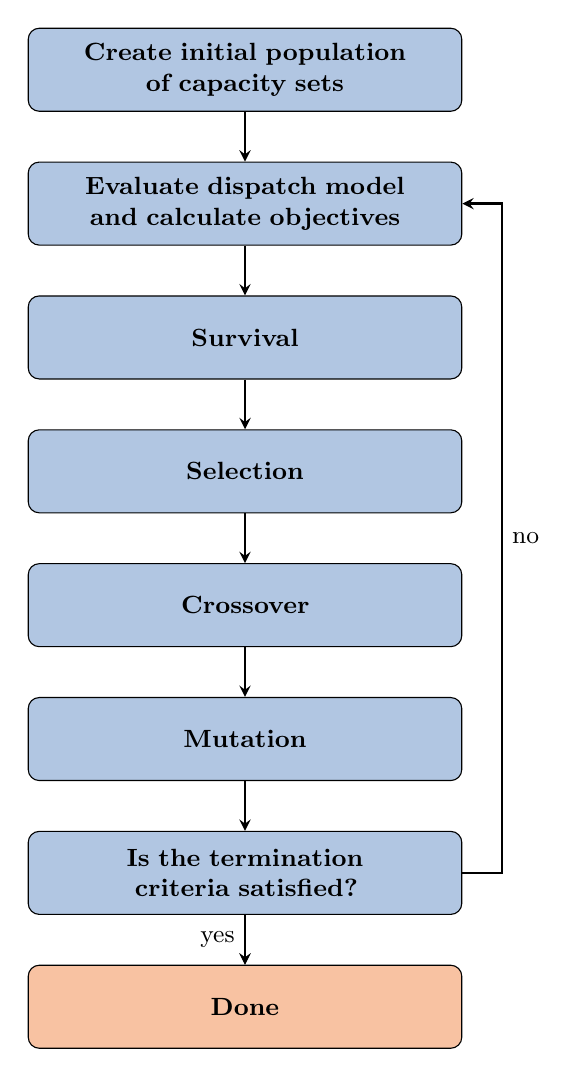
\begin{tikzpicture}[node distance=1.7cm]
                \tikzstyle{every node}=[font=\small]
                \node (1) [lbblock] {\textbf{Create initial population\\ of capacity sets}};
                \node (2) [lbblock, below of=1] {\textbf{Evaluate dispatch model and calculate objectives}};
                \node (3) [lbblock, below of=2] {\textbf{Survival}}; 
                \node (4) [lbblock, below of=3] {\textbf{Selection}};
                \node (5) [lbblock, below of=4] {\textbf{Crossover}};
                \node (6) [lbblock, below of=5] {\textbf{Mutation}};
                \node (7) [lbblock, below of=6] {\textbf{Is the termination \\ criteria satisfied?}};
                \node (8) [loblock, below of=7] {\textbf{Done}};
                \draw [arrow] (1) -- (2);
                \draw [arrow] (2) -- (3);
                \draw [arrow] (3) -- (4);
                \draw [arrow] (4) -- (5);
                \draw [arrow] (5) -- (6);
                \draw [arrow] (6) -- (7);
                \draw [arrow] (7) -- (8);
                \draw [arrow] (7) -- node[anchor=east] {yes} (8);
                \draw [arrow] (7) -- ([shift={(0.5cm,0cm)}]7.east)-- node[anchor=west] {no} ([shift={(0.5cm,0cm)}]2.east)--(2);
        \end{tikzpicture}
        \caption{The basic flow of the \ac{ga} used in this thesis.}
        \label{fig:genetic-alg}
\end{figure}

\subsection{Specific \Aclp{ga}}
The variety of \acp{ga} comes from different types of operators being applied to 
the selection, crossover, and mutation steps. Section \ref{section:moo-in-energy} 
showed that \ac{nsga2} is a popular genetic algorithm choice. However, this algorithm
performs poorly with greater than three objectives \cite{deb_fast_2002, seada_unified_2016}. In this thesis, I use a more modern algorithm, 
\ac{unsga3}. \ac{unsga3} builds on its predecessors \ac{nsga2} and \ac{nsga3} by unifying
efficient solutions of mono-, multi-, and many-objective problems in a single algorithm.


\ac{nsga2} improves on the basic \ac{ga} by introducing a more sophisticated mating and 
selection algorithms. Instead of random selection, the individuals are sorted by rank 
(i.e. fitness) and crowding distance in binary tournament mating selection. The crowding 
distance is simply the Manhattan distance between individuals. A greater crowding 
distance is desirable to preserve diversity and since the extreme points are maximally 
diverse they should always persist and are therefore assigned a crowding distance of 
infinity \cite{deb_fast_2002}.

The successor to \ac{nsga2}, \ac{nsga3}, enhances the many-objective capabilities of 
the former by introducing reference directions. Reference directions are used for 
initialization and the survival steps. In addition to fitness, individuals are chosen 
based on their proximity to a reference line, thus ensuring population diversity which
greatly important for many-objective problems. Since diversity is handled by reference
directions, individuals are selected randomly for mating. References directions are 
rays passing through uniformly spaced points on the unit simplex 
\cite{seada_unified_2016, blank_generating_2021}. In this thesis, I use the Riesz s-
Energy method described by Blank et al. to calculate these points for a problem with an 
arbitrary number of objectives \cite{blank_generating_2021}. Figure \ref{fig:ref-dirs} 
illustrates a set of initialized reference directions.

\begin{figure}[h]
  \centering
  \resizebox{0.6\columnwidth}{!}{%% Creator: Matplotlib, PGF backend
%%
%% To include the figure in your LaTeX document, write
%%   \input{<filename>.pgf}
%%
%% Make sure the required packages are loaded in your preamble
%%   \usepackage{pgf}
%%
%% Also ensure that all the required font packages are loaded; for instance,
%% the lmodern package is sometimes necessary when using math font.
%%   \usepackage{lmodern}
%%
%% Figures using additional raster images can only be included by \input if
%% they are in the same directory as the main LaTeX file. For loading figures
%% from other directories you can use the `import` package
%%   \usepackage{import}
%%
%% and then include the figures with
%%   \import{<path to file>}{<filename>.pgf}
%%
%% Matplotlib used the following preamble
%%   \usepackage{fontspec}
%%   \setmainfont{DejaVuSerif.ttf}[Path=\detokenize{C:/Users/samgd/anaconda3/Lib/site-packages/matplotlib/mpl-data/fonts/ttf/}]
%%   \setsansfont{DejaVuSans.ttf}[Path=\detokenize{C:/Users/samgd/anaconda3/Lib/site-packages/matplotlib/mpl-data/fonts/ttf/}]
%%   \setmonofont{DejaVuSansMono.ttf}[Path=\detokenize{C:/Users/samgd/anaconda3/Lib/site-packages/matplotlib/mpl-data/fonts/ttf/}]
%%
\begingroup%
\makeatletter%
\begin{pgfpicture}%
\pgfpathrectangle{\pgfpointorigin}{\pgfqpoint{6.594429in}{6.401491in}}%
\pgfusepath{use as bounding box, clip}%
\begin{pgfscope}%
\pgfsetbuttcap%
\pgfsetmiterjoin%
\definecolor{currentfill}{rgb}{1.000000,1.000000,1.000000}%
\pgfsetfillcolor{currentfill}%
\pgfsetlinewidth{0.000000pt}%
\definecolor{currentstroke}{rgb}{0.000000,0.000000,0.000000}%
\pgfsetstrokecolor{currentstroke}%
\pgfsetdash{}{0pt}%
\pgfpathmoveto{\pgfqpoint{0.000000in}{0.000000in}}%
\pgfpathlineto{\pgfqpoint{6.594429in}{0.000000in}}%
\pgfpathlineto{\pgfqpoint{6.594429in}{6.401491in}}%
\pgfpathlineto{\pgfqpoint{0.000000in}{6.401491in}}%
\pgfpathlineto{\pgfqpoint{0.000000in}{0.000000in}}%
\pgfpathclose%
\pgfusepath{fill}%
\end{pgfscope}%
\begin{pgfscope}%
\pgfsetbuttcap%
\pgfsetmiterjoin%
\definecolor{currentfill}{rgb}{1.000000,1.000000,1.000000}%
\pgfsetfillcolor{currentfill}%
\pgfsetlinewidth{0.000000pt}%
\definecolor{currentstroke}{rgb}{0.000000,0.000000,0.000000}%
\pgfsetstrokecolor{currentstroke}%
\pgfsetstrokeopacity{0.000000}%
\pgfsetdash{}{0pt}%
\pgfpathmoveto{\pgfqpoint{0.454429in}{0.261491in}}%
\pgfpathlineto{\pgfqpoint{6.494429in}{0.261491in}}%
\pgfpathlineto{\pgfqpoint{6.494429in}{6.301491in}}%
\pgfpathlineto{\pgfqpoint{0.454429in}{6.301491in}}%
\pgfpathlineto{\pgfqpoint{0.454429in}{0.261491in}}%
\pgfpathclose%
\pgfusepath{fill}%
\end{pgfscope}%
\begin{pgfscope}%
\pgfsetbuttcap%
\pgfsetmiterjoin%
\definecolor{currentfill}{rgb}{0.950000,0.950000,0.950000}%
\pgfsetfillcolor{currentfill}%
\pgfsetfillopacity{0.500000}%
\pgfsetlinewidth{1.003750pt}%
\definecolor{currentstroke}{rgb}{0.950000,0.950000,0.950000}%
\pgfsetstrokecolor{currentstroke}%
\pgfsetstrokeopacity{0.500000}%
\pgfsetdash{}{0pt}%
\pgfpathmoveto{\pgfqpoint{3.556051in}{4.199655in}}%
\pgfpathlineto{\pgfqpoint{6.220291in}{2.364023in}}%
\pgfpathlineto{\pgfqpoint{6.393980in}{4.427336in}}%
\pgfpathlineto{\pgfqpoint{3.556051in}{6.256232in}}%
\pgfusepath{stroke,fill}%
\end{pgfscope}%
\begin{pgfscope}%
\pgfsetbuttcap%
\pgfsetmiterjoin%
\definecolor{currentfill}{rgb}{0.900000,0.900000,0.900000}%
\pgfsetfillcolor{currentfill}%
\pgfsetfillopacity{0.500000}%
\pgfsetlinewidth{1.003750pt}%
\definecolor{currentstroke}{rgb}{0.900000,0.900000,0.900000}%
\pgfsetstrokecolor{currentstroke}%
\pgfsetstrokeopacity{0.500000}%
\pgfsetdash{}{0pt}%
\pgfpathmoveto{\pgfqpoint{3.556051in}{4.199655in}}%
\pgfpathlineto{\pgfqpoint{0.891811in}{2.364023in}}%
\pgfpathlineto{\pgfqpoint{0.718122in}{4.427336in}}%
\pgfpathlineto{\pgfqpoint{3.556051in}{6.256232in}}%
\pgfusepath{stroke,fill}%
\end{pgfscope}%
\begin{pgfscope}%
\pgfsetbuttcap%
\pgfsetmiterjoin%
\definecolor{currentfill}{rgb}{0.925000,0.925000,0.925000}%
\pgfsetfillcolor{currentfill}%
\pgfsetfillopacity{0.500000}%
\pgfsetlinewidth{1.003750pt}%
\definecolor{currentstroke}{rgb}{0.925000,0.925000,0.925000}%
\pgfsetstrokecolor{currentstroke}%
\pgfsetstrokeopacity{0.500000}%
\pgfsetdash{}{0pt}%
\pgfpathmoveto{\pgfqpoint{3.556051in}{4.199655in}}%
\pgfpathlineto{\pgfqpoint{0.891811in}{2.364023in}}%
\pgfpathlineto{\pgfqpoint{3.556051in}{0.303578in}}%
\pgfpathlineto{\pgfqpoint{6.220291in}{2.364023in}}%
\pgfusepath{stroke,fill}%
\end{pgfscope}%
\begin{pgfscope}%
\pgfsetrectcap%
\pgfsetroundjoin%
\pgfsetlinewidth{0.803000pt}%
\definecolor{currentstroke}{rgb}{0.000000,0.000000,0.000000}%
\pgfsetstrokecolor{currentstroke}%
\pgfsetdash{}{0pt}%
\pgfpathmoveto{\pgfqpoint{6.220291in}{2.364023in}}%
\pgfpathlineto{\pgfqpoint{3.556051in}{0.303578in}}%
\pgfusepath{stroke}%
\end{pgfscope}%
\begin{pgfscope}%
\definecolor{textcolor}{rgb}{0.000000,0.000000,0.000000}%
\pgfsetstrokecolor{textcolor}%
\pgfsetfillcolor{textcolor}%
\pgftext[x=5.194308in, y=0.828835in, left, base,rotate=37.717305]{\color{textcolor}\rmfamily\fontsize{14.000000}{16.800000}\selectfont \(\displaystyle f_1\)}%
\end{pgfscope}%
\begin{pgfscope}%
\pgfsetbuttcap%
\pgfsetroundjoin%
\pgfsetlinewidth{0.803000pt}%
\definecolor{currentstroke}{rgb}{0.690196,0.690196,0.690196}%
\pgfsetstrokecolor{currentstroke}%
\pgfsetdash{}{0pt}%
\pgfpathmoveto{\pgfqpoint{6.059943in}{2.240014in}}%
\pgfpathlineto{\pgfqpoint{3.395199in}{4.088829in}}%
\pgfpathlineto{\pgfqpoint{3.385284in}{6.146181in}}%
\pgfusepath{stroke}%
\end{pgfscope}%
\begin{pgfscope}%
\pgfsetbuttcap%
\pgfsetroundjoin%
\pgfsetlinewidth{0.803000pt}%
\definecolor{currentstroke}{rgb}{0.690196,0.690196,0.690196}%
\pgfsetstrokecolor{currentstroke}%
\pgfsetdash{}{0pt}%
\pgfpathmoveto{\pgfqpoint{5.614001in}{1.895136in}}%
\pgfpathlineto{\pgfqpoint{2.948198in}{3.780850in}}%
\pgfpathlineto{\pgfqpoint{2.910343in}{5.840107in}}%
\pgfusepath{stroke}%
\end{pgfscope}%
\begin{pgfscope}%
\pgfsetbuttcap%
\pgfsetroundjoin%
\pgfsetlinewidth{0.803000pt}%
\definecolor{currentstroke}{rgb}{0.690196,0.690196,0.690196}%
\pgfsetstrokecolor{currentstroke}%
\pgfsetdash{}{0pt}%
\pgfpathmoveto{\pgfqpoint{5.158858in}{1.543142in}}%
\pgfpathlineto{\pgfqpoint{2.492487in}{3.466871in}}%
\pgfpathlineto{\pgfqpoint{2.425567in}{5.527694in}}%
\pgfusepath{stroke}%
\end{pgfscope}%
\begin{pgfscope}%
\pgfsetbuttcap%
\pgfsetroundjoin%
\pgfsetlinewidth{0.803000pt}%
\definecolor{currentstroke}{rgb}{0.690196,0.690196,0.690196}%
\pgfsetstrokecolor{currentstroke}%
\pgfsetdash{}{0pt}%
\pgfpathmoveto{\pgfqpoint{4.694225in}{1.183808in}}%
\pgfpathlineto{\pgfqpoint{2.027811in}{3.146714in}}%
\pgfpathlineto{\pgfqpoint{1.930646in}{5.208744in}}%
\pgfusepath{stroke}%
\end{pgfscope}%
\begin{pgfscope}%
\pgfsetbuttcap%
\pgfsetroundjoin%
\pgfsetlinewidth{0.803000pt}%
\definecolor{currentstroke}{rgb}{0.690196,0.690196,0.690196}%
\pgfsetstrokecolor{currentstroke}%
\pgfsetdash{}{0pt}%
\pgfpathmoveto{\pgfqpoint{4.219802in}{0.816904in}}%
\pgfpathlineto{\pgfqpoint{1.553901in}{2.820196in}}%
\pgfpathlineto{\pgfqpoint{1.425259in}{4.883049in}}%
\pgfusepath{stroke}%
\end{pgfscope}%
\begin{pgfscope}%
\pgfsetbuttcap%
\pgfsetroundjoin%
\pgfsetlinewidth{0.803000pt}%
\definecolor{currentstroke}{rgb}{0.690196,0.690196,0.690196}%
\pgfsetstrokecolor{currentstroke}%
\pgfsetdash{}{0pt}%
\pgfpathmoveto{\pgfqpoint{3.735277in}{0.442186in}}%
\pgfpathlineto{\pgfqpoint{1.070480in}{2.487124in}}%
\pgfpathlineto{\pgfqpoint{0.909071in}{4.550392in}}%
\pgfusepath{stroke}%
\end{pgfscope}%
\begin{pgfscope}%
\pgfsetrectcap%
\pgfsetroundjoin%
\pgfsetlinewidth{0.803000pt}%
\definecolor{currentstroke}{rgb}{0.000000,0.000000,0.000000}%
\pgfsetstrokecolor{currentstroke}%
\pgfsetdash{}{0pt}%
\pgfpathmoveto{\pgfqpoint{6.037401in}{2.255654in}}%
\pgfpathlineto{\pgfqpoint{6.105090in}{2.208691in}}%
\pgfusepath{stroke}%
\end{pgfscope}%
\begin{pgfscope}%
\definecolor{textcolor}{rgb}{0.000000,0.000000,0.000000}%
\pgfsetstrokecolor{textcolor}%
\pgfsetfillcolor{textcolor}%
\pgftext[x=6.195241in,y=2.042420in,,top]{\color{textcolor}\rmfamily\fontsize{10.000000}{12.000000}\selectfont 0.0}%
\end{pgfscope}%
\begin{pgfscope}%
\pgfsetrectcap%
\pgfsetroundjoin%
\pgfsetlinewidth{0.803000pt}%
\definecolor{currentstroke}{rgb}{0.000000,0.000000,0.000000}%
\pgfsetstrokecolor{currentstroke}%
\pgfsetdash{}{0pt}%
\pgfpathmoveto{\pgfqpoint{5.591438in}{1.911097in}}%
\pgfpathlineto{\pgfqpoint{5.659192in}{1.863169in}}%
\pgfusepath{stroke}%
\end{pgfscope}%
\begin{pgfscope}%
\definecolor{textcolor}{rgb}{0.000000,0.000000,0.000000}%
\pgfsetstrokecolor{textcolor}%
\pgfsetfillcolor{textcolor}%
\pgftext[x=5.750761in,y=1.695586in,,top]{\color{textcolor}\rmfamily\fontsize{10.000000}{12.000000}\selectfont 0.2}%
\end{pgfscope}%
\begin{pgfscope}%
\pgfsetrectcap%
\pgfsetroundjoin%
\pgfsetlinewidth{0.803000pt}%
\definecolor{currentstroke}{rgb}{0.000000,0.000000,0.000000}%
\pgfsetstrokecolor{currentstroke}%
\pgfsetdash{}{0pt}%
\pgfpathmoveto{\pgfqpoint{5.136277in}{1.559433in}}%
\pgfpathlineto{\pgfqpoint{5.204084in}{1.510512in}}%
\pgfusepath{stroke}%
\end{pgfscope}%
\begin{pgfscope}%
\definecolor{textcolor}{rgb}{0.000000,0.000000,0.000000}%
\pgfsetstrokecolor{textcolor}%
\pgfsetfillcolor{textcolor}%
\pgftext[x=5.297112in,y=1.341597in,,top]{\color{textcolor}\rmfamily\fontsize{10.000000}{12.000000}\selectfont 0.4}%
\end{pgfscope}%
\begin{pgfscope}%
\pgfsetrectcap%
\pgfsetroundjoin%
\pgfsetlinewidth{0.803000pt}%
\definecolor{currentstroke}{rgb}{0.000000,0.000000,0.000000}%
\pgfsetstrokecolor{currentstroke}%
\pgfsetdash{}{0pt}%
\pgfpathmoveto{\pgfqpoint{4.671630in}{1.200441in}}%
\pgfpathlineto{\pgfqpoint{4.739479in}{1.150494in}}%
\pgfusepath{stroke}%
\end{pgfscope}%
\begin{pgfscope}%
\definecolor{textcolor}{rgb}{0.000000,0.000000,0.000000}%
\pgfsetstrokecolor{textcolor}%
\pgfsetfillcolor{textcolor}%
\pgftext[x=4.834005in,y=0.980229in,,top]{\color{textcolor}\rmfamily\fontsize{10.000000}{12.000000}\selectfont 0.6}%
\end{pgfscope}%
\begin{pgfscope}%
\pgfsetrectcap%
\pgfsetroundjoin%
\pgfsetlinewidth{0.803000pt}%
\definecolor{currentstroke}{rgb}{0.000000,0.000000,0.000000}%
\pgfsetstrokecolor{currentstroke}%
\pgfsetdash{}{0pt}%
\pgfpathmoveto{\pgfqpoint{4.197199in}{0.833889in}}%
\pgfpathlineto{\pgfqpoint{4.265075in}{0.782884in}}%
\pgfusepath{stroke}%
\end{pgfscope}%
\begin{pgfscope}%
\definecolor{textcolor}{rgb}{0.000000,0.000000,0.000000}%
\pgfsetstrokecolor{textcolor}%
\pgfsetfillcolor{textcolor}%
\pgftext[x=4.361143in,y=0.611249in,,top]{\color{textcolor}\rmfamily\fontsize{10.000000}{12.000000}\selectfont 0.8}%
\end{pgfscope}%
\begin{pgfscope}%
\pgfsetrectcap%
\pgfsetroundjoin%
\pgfsetlinewidth{0.803000pt}%
\definecolor{currentstroke}{rgb}{0.000000,0.000000,0.000000}%
\pgfsetstrokecolor{currentstroke}%
\pgfsetdash{}{0pt}%
\pgfpathmoveto{\pgfqpoint{3.712669in}{0.459535in}}%
\pgfpathlineto{\pgfqpoint{3.780559in}{0.407438in}}%
\pgfusepath{stroke}%
\end{pgfscope}%
\begin{pgfscope}%
\definecolor{textcolor}{rgb}{0.000000,0.000000,0.000000}%
\pgfsetstrokecolor{textcolor}%
\pgfsetfillcolor{textcolor}%
\pgftext[x=3.878213in,y=0.234413in,,top]{\color{textcolor}\rmfamily\fontsize{10.000000}{12.000000}\selectfont 1.0}%
\end{pgfscope}%
\begin{pgfscope}%
\pgfsetrectcap%
\pgfsetroundjoin%
\pgfsetlinewidth{0.803000pt}%
\definecolor{currentstroke}{rgb}{0.000000,0.000000,0.000000}%
\pgfsetstrokecolor{currentstroke}%
\pgfsetdash{}{0pt}%
\pgfpathmoveto{\pgfqpoint{0.891811in}{2.364023in}}%
\pgfpathlineto{\pgfqpoint{3.556051in}{0.303578in}}%
\pgfusepath{stroke}%
\end{pgfscope}%
\begin{pgfscope}%
\definecolor{textcolor}{rgb}{0.000000,0.000000,0.000000}%
\pgfsetstrokecolor{textcolor}%
\pgfsetfillcolor{textcolor}%
\pgftext[x=1.781011in, y=0.934619in, left, base,rotate=322.282695]{\color{textcolor}\rmfamily\fontsize{14.000000}{16.800000}\selectfont \(\displaystyle f_2\)}%
\end{pgfscope}%
\begin{pgfscope}%
\pgfsetbuttcap%
\pgfsetroundjoin%
\pgfsetlinewidth{0.803000pt}%
\definecolor{currentstroke}{rgb}{0.690196,0.690196,0.690196}%
\pgfsetstrokecolor{currentstroke}%
\pgfsetdash{}{0pt}%
\pgfpathmoveto{\pgfqpoint{3.726818in}{6.146181in}}%
\pgfpathlineto{\pgfqpoint{3.716903in}{4.088829in}}%
\pgfpathlineto{\pgfqpoint{1.052159in}{2.240014in}}%
\pgfusepath{stroke}%
\end{pgfscope}%
\begin{pgfscope}%
\pgfsetbuttcap%
\pgfsetroundjoin%
\pgfsetlinewidth{0.803000pt}%
\definecolor{currentstroke}{rgb}{0.690196,0.690196,0.690196}%
\pgfsetstrokecolor{currentstroke}%
\pgfsetdash{}{0pt}%
\pgfpathmoveto{\pgfqpoint{4.201759in}{5.840107in}}%
\pgfpathlineto{\pgfqpoint{4.163904in}{3.780850in}}%
\pgfpathlineto{\pgfqpoint{1.498101in}{1.895136in}}%
\pgfusepath{stroke}%
\end{pgfscope}%
\begin{pgfscope}%
\pgfsetbuttcap%
\pgfsetroundjoin%
\pgfsetlinewidth{0.803000pt}%
\definecolor{currentstroke}{rgb}{0.690196,0.690196,0.690196}%
\pgfsetstrokecolor{currentstroke}%
\pgfsetdash{}{0pt}%
\pgfpathmoveto{\pgfqpoint{4.686535in}{5.527694in}}%
\pgfpathlineto{\pgfqpoint{4.619615in}{3.466871in}}%
\pgfpathlineto{\pgfqpoint{1.953244in}{1.543142in}}%
\pgfusepath{stroke}%
\end{pgfscope}%
\begin{pgfscope}%
\pgfsetbuttcap%
\pgfsetroundjoin%
\pgfsetlinewidth{0.803000pt}%
\definecolor{currentstroke}{rgb}{0.690196,0.690196,0.690196}%
\pgfsetstrokecolor{currentstroke}%
\pgfsetdash{}{0pt}%
\pgfpathmoveto{\pgfqpoint{5.181456in}{5.208744in}}%
\pgfpathlineto{\pgfqpoint{5.084291in}{3.146714in}}%
\pgfpathlineto{\pgfqpoint{2.417877in}{1.183808in}}%
\pgfusepath{stroke}%
\end{pgfscope}%
\begin{pgfscope}%
\pgfsetbuttcap%
\pgfsetroundjoin%
\pgfsetlinewidth{0.803000pt}%
\definecolor{currentstroke}{rgb}{0.690196,0.690196,0.690196}%
\pgfsetstrokecolor{currentstroke}%
\pgfsetdash{}{0pt}%
\pgfpathmoveto{\pgfqpoint{5.686843in}{4.883049in}}%
\pgfpathlineto{\pgfqpoint{5.558201in}{2.820196in}}%
\pgfpathlineto{\pgfqpoint{2.892300in}{0.816904in}}%
\pgfusepath{stroke}%
\end{pgfscope}%
\begin{pgfscope}%
\pgfsetbuttcap%
\pgfsetroundjoin%
\pgfsetlinewidth{0.803000pt}%
\definecolor{currentstroke}{rgb}{0.690196,0.690196,0.690196}%
\pgfsetstrokecolor{currentstroke}%
\pgfsetdash{}{0pt}%
\pgfpathmoveto{\pgfqpoint{6.203031in}{4.550392in}}%
\pgfpathlineto{\pgfqpoint{6.041622in}{2.487124in}}%
\pgfpathlineto{\pgfqpoint{3.376825in}{0.442186in}}%
\pgfusepath{stroke}%
\end{pgfscope}%
\begin{pgfscope}%
\pgfsetrectcap%
\pgfsetroundjoin%
\pgfsetlinewidth{0.803000pt}%
\definecolor{currentstroke}{rgb}{0.000000,0.000000,0.000000}%
\pgfsetstrokecolor{currentstroke}%
\pgfsetdash{}{0pt}%
\pgfpathmoveto{\pgfqpoint{1.074701in}{2.255654in}}%
\pgfpathlineto{\pgfqpoint{1.007012in}{2.208691in}}%
\pgfusepath{stroke}%
\end{pgfscope}%
\begin{pgfscope}%
\definecolor{textcolor}{rgb}{0.000000,0.000000,0.000000}%
\pgfsetstrokecolor{textcolor}%
\pgfsetfillcolor{textcolor}%
\pgftext[x=0.916861in,y=2.042420in,,top]{\color{textcolor}\rmfamily\fontsize{10.000000}{12.000000}\selectfont 0.0}%
\end{pgfscope}%
\begin{pgfscope}%
\pgfsetrectcap%
\pgfsetroundjoin%
\pgfsetlinewidth{0.803000pt}%
\definecolor{currentstroke}{rgb}{0.000000,0.000000,0.000000}%
\pgfsetstrokecolor{currentstroke}%
\pgfsetdash{}{0pt}%
\pgfpathmoveto{\pgfqpoint{1.520664in}{1.911097in}}%
\pgfpathlineto{\pgfqpoint{1.452910in}{1.863169in}}%
\pgfusepath{stroke}%
\end{pgfscope}%
\begin{pgfscope}%
\definecolor{textcolor}{rgb}{0.000000,0.000000,0.000000}%
\pgfsetstrokecolor{textcolor}%
\pgfsetfillcolor{textcolor}%
\pgftext[x=1.361341in,y=1.695586in,,top]{\color{textcolor}\rmfamily\fontsize{10.000000}{12.000000}\selectfont 0.2}%
\end{pgfscope}%
\begin{pgfscope}%
\pgfsetrectcap%
\pgfsetroundjoin%
\pgfsetlinewidth{0.803000pt}%
\definecolor{currentstroke}{rgb}{0.000000,0.000000,0.000000}%
\pgfsetstrokecolor{currentstroke}%
\pgfsetdash{}{0pt}%
\pgfpathmoveto{\pgfqpoint{1.975825in}{1.559433in}}%
\pgfpathlineto{\pgfqpoint{1.908018in}{1.510512in}}%
\pgfusepath{stroke}%
\end{pgfscope}%
\begin{pgfscope}%
\definecolor{textcolor}{rgb}{0.000000,0.000000,0.000000}%
\pgfsetstrokecolor{textcolor}%
\pgfsetfillcolor{textcolor}%
\pgftext[x=1.814990in,y=1.341597in,,top]{\color{textcolor}\rmfamily\fontsize{10.000000}{12.000000}\selectfont 0.4}%
\end{pgfscope}%
\begin{pgfscope}%
\pgfsetrectcap%
\pgfsetroundjoin%
\pgfsetlinewidth{0.803000pt}%
\definecolor{currentstroke}{rgb}{0.000000,0.000000,0.000000}%
\pgfsetstrokecolor{currentstroke}%
\pgfsetdash{}{0pt}%
\pgfpathmoveto{\pgfqpoint{2.440472in}{1.200441in}}%
\pgfpathlineto{\pgfqpoint{2.372623in}{1.150494in}}%
\pgfusepath{stroke}%
\end{pgfscope}%
\begin{pgfscope}%
\definecolor{textcolor}{rgb}{0.000000,0.000000,0.000000}%
\pgfsetstrokecolor{textcolor}%
\pgfsetfillcolor{textcolor}%
\pgftext[x=2.278097in,y=0.980229in,,top]{\color{textcolor}\rmfamily\fontsize{10.000000}{12.000000}\selectfont 0.6}%
\end{pgfscope}%
\begin{pgfscope}%
\pgfsetrectcap%
\pgfsetroundjoin%
\pgfsetlinewidth{0.803000pt}%
\definecolor{currentstroke}{rgb}{0.000000,0.000000,0.000000}%
\pgfsetstrokecolor{currentstroke}%
\pgfsetdash{}{0pt}%
\pgfpathmoveto{\pgfqpoint{2.914903in}{0.833889in}}%
\pgfpathlineto{\pgfqpoint{2.847027in}{0.782884in}}%
\pgfusepath{stroke}%
\end{pgfscope}%
\begin{pgfscope}%
\definecolor{textcolor}{rgb}{0.000000,0.000000,0.000000}%
\pgfsetstrokecolor{textcolor}%
\pgfsetfillcolor{textcolor}%
\pgftext[x=2.750959in,y=0.611249in,,top]{\color{textcolor}\rmfamily\fontsize{10.000000}{12.000000}\selectfont 0.8}%
\end{pgfscope}%
\begin{pgfscope}%
\pgfsetrectcap%
\pgfsetroundjoin%
\pgfsetlinewidth{0.803000pt}%
\definecolor{currentstroke}{rgb}{0.000000,0.000000,0.000000}%
\pgfsetstrokecolor{currentstroke}%
\pgfsetdash{}{0pt}%
\pgfpathmoveto{\pgfqpoint{3.399432in}{0.459535in}}%
\pgfpathlineto{\pgfqpoint{3.331543in}{0.407438in}}%
\pgfusepath{stroke}%
\end{pgfscope}%
\begin{pgfscope}%
\definecolor{textcolor}{rgb}{0.000000,0.000000,0.000000}%
\pgfsetstrokecolor{textcolor}%
\pgfsetfillcolor{textcolor}%
\pgftext[x=3.233889in,y=0.234413in,,top]{\color{textcolor}\rmfamily\fontsize{10.000000}{12.000000}\selectfont 1.0}%
\end{pgfscope}%
\begin{pgfscope}%
\pgfsetrectcap%
\pgfsetroundjoin%
\pgfsetlinewidth{0.803000pt}%
\definecolor{currentstroke}{rgb}{0.000000,0.000000,0.000000}%
\pgfsetstrokecolor{currentstroke}%
\pgfsetdash{}{0pt}%
\pgfpathmoveto{\pgfqpoint{0.891811in}{2.364023in}}%
\pgfpathlineto{\pgfqpoint{0.718122in}{4.427336in}}%
\pgfusepath{stroke}%
\end{pgfscope}%
\begin{pgfscope}%
\definecolor{textcolor}{rgb}{0.000000,0.000000,0.000000}%
\pgfsetstrokecolor{textcolor}%
\pgfsetfillcolor{textcolor}%
\pgftext[x=0.140303in, y=3.444766in, left, base,rotate=274.811779]{\color{textcolor}\rmfamily\fontsize{14.000000}{16.800000}\selectfont \(\displaystyle f_3\)}%
\end{pgfscope}%
\begin{pgfscope}%
\pgfsetbuttcap%
\pgfsetroundjoin%
\pgfsetlinewidth{0.803000pt}%
\definecolor{currentstroke}{rgb}{0.690196,0.690196,0.690196}%
\pgfsetstrokecolor{currentstroke}%
\pgfsetdash{}{0pt}%
\pgfpathmoveto{\pgfqpoint{0.881394in}{2.487770in}}%
\pgfpathlineto{\pgfqpoint{3.556051in}{4.323411in}}%
\pgfpathlineto{\pgfqpoint{6.230708in}{2.487770in}}%
\pgfusepath{stroke}%
\end{pgfscope}%
\begin{pgfscope}%
\pgfsetbuttcap%
\pgfsetroundjoin%
\pgfsetlinewidth{0.803000pt}%
\definecolor{currentstroke}{rgb}{0.690196,0.690196,0.690196}%
\pgfsetstrokecolor{currentstroke}%
\pgfsetdash{}{0pt}%
\pgfpathmoveto{\pgfqpoint{0.852399in}{2.832214in}}%
\pgfpathlineto{\pgfqpoint{3.556051in}{4.667599in}}%
\pgfpathlineto{\pgfqpoint{6.259703in}{2.832214in}}%
\pgfusepath{stroke}%
\end{pgfscope}%
\begin{pgfscope}%
\pgfsetbuttcap%
\pgfsetroundjoin%
\pgfsetlinewidth{0.803000pt}%
\definecolor{currentstroke}{rgb}{0.690196,0.690196,0.690196}%
\pgfsetstrokecolor{currentstroke}%
\pgfsetdash{}{0pt}%
\pgfpathmoveto{\pgfqpoint{0.822768in}{3.184207in}}%
\pgfpathlineto{\pgfqpoint{3.556051in}{5.018910in}}%
\pgfpathlineto{\pgfqpoint{6.289334in}{3.184207in}}%
\pgfusepath{stroke}%
\end{pgfscope}%
\begin{pgfscope}%
\pgfsetbuttcap%
\pgfsetroundjoin%
\pgfsetlinewidth{0.803000pt}%
\definecolor{currentstroke}{rgb}{0.690196,0.690196,0.690196}%
\pgfsetstrokecolor{currentstroke}%
\pgfsetdash{}{0pt}%
\pgfpathmoveto{\pgfqpoint{0.792481in}{3.544001in}}%
\pgfpathlineto{\pgfqpoint{3.556051in}{5.377568in}}%
\pgfpathlineto{\pgfqpoint{6.319621in}{3.544001in}}%
\pgfusepath{stroke}%
\end{pgfscope}%
\begin{pgfscope}%
\pgfsetbuttcap%
\pgfsetroundjoin%
\pgfsetlinewidth{0.803000pt}%
\definecolor{currentstroke}{rgb}{0.690196,0.690196,0.690196}%
\pgfsetstrokecolor{currentstroke}%
\pgfsetdash{}{0pt}%
\pgfpathmoveto{\pgfqpoint{0.761515in}{3.911858in}}%
\pgfpathlineto{\pgfqpoint{3.556051in}{5.743804in}}%
\pgfpathlineto{\pgfqpoint{6.350587in}{3.911858in}}%
\pgfusepath{stroke}%
\end{pgfscope}%
\begin{pgfscope}%
\pgfsetbuttcap%
\pgfsetroundjoin%
\pgfsetlinewidth{0.803000pt}%
\definecolor{currentstroke}{rgb}{0.690196,0.690196,0.690196}%
\pgfsetstrokecolor{currentstroke}%
\pgfsetdash{}{0pt}%
\pgfpathmoveto{\pgfqpoint{0.729847in}{4.288052in}}%
\pgfpathlineto{\pgfqpoint{3.556051in}{6.117861in}}%
\pgfpathlineto{\pgfqpoint{6.382255in}{4.288052in}}%
\pgfusepath{stroke}%
\end{pgfscope}%
\begin{pgfscope}%
\pgfsetrectcap%
\pgfsetroundjoin%
\pgfsetlinewidth{0.803000pt}%
\definecolor{currentstroke}{rgb}{0.000000,0.000000,0.000000}%
\pgfsetstrokecolor{currentstroke}%
\pgfsetdash{}{0pt}%
\pgfpathmoveto{\pgfqpoint{0.904020in}{2.503299in}}%
\pgfpathlineto{\pgfqpoint{0.836078in}{2.456670in}}%
\pgfusepath{stroke}%
\end{pgfscope}%
\begin{pgfscope}%
\definecolor{textcolor}{rgb}{0.000000,0.000000,0.000000}%
\pgfsetstrokecolor{textcolor}%
\pgfsetfillcolor{textcolor}%
\pgftext[x=0.609795in,y=2.487770in,,top]{\color{textcolor}\rmfamily\fontsize{10.000000}{12.000000}\selectfont 0.0}%
\end{pgfscope}%
\begin{pgfscope}%
\pgfsetrectcap%
\pgfsetroundjoin%
\pgfsetlinewidth{0.803000pt}%
\definecolor{currentstroke}{rgb}{0.000000,0.000000,0.000000}%
\pgfsetstrokecolor{currentstroke}%
\pgfsetdash{}{0pt}%
\pgfpathmoveto{\pgfqpoint{0.875284in}{2.847749in}}%
\pgfpathlineto{\pgfqpoint{0.806564in}{2.801099in}}%
\pgfusepath{stroke}%
\end{pgfscope}%
\begin{pgfscope}%
\definecolor{textcolor}{rgb}{0.000000,0.000000,0.000000}%
\pgfsetstrokecolor{textcolor}%
\pgfsetfillcolor{textcolor}%
\pgftext[x=0.577856in,y=2.832214in,,top]{\color{textcolor}\rmfamily\fontsize{10.000000}{12.000000}\selectfont 0.2}%
\end{pgfscope}%
\begin{pgfscope}%
\pgfsetrectcap%
\pgfsetroundjoin%
\pgfsetlinewidth{0.803000pt}%
\definecolor{currentstroke}{rgb}{0.000000,0.000000,0.000000}%
\pgfsetstrokecolor{currentstroke}%
\pgfsetdash{}{0pt}%
\pgfpathmoveto{\pgfqpoint{0.845918in}{3.199746in}}%
\pgfpathlineto{\pgfqpoint{0.776403in}{3.153084in}}%
\pgfusepath{stroke}%
\end{pgfscope}%
\begin{pgfscope}%
\definecolor{textcolor}{rgb}{0.000000,0.000000,0.000000}%
\pgfsetstrokecolor{textcolor}%
\pgfsetfillcolor{textcolor}%
\pgftext[x=0.545216in,y=3.184207in,,top]{\color{textcolor}\rmfamily\fontsize{10.000000}{12.000000}\selectfont 0.4}%
\end{pgfscope}%
\begin{pgfscope}%
\pgfsetrectcap%
\pgfsetroundjoin%
\pgfsetlinewidth{0.803000pt}%
\definecolor{currentstroke}{rgb}{0.000000,0.000000,0.000000}%
\pgfsetstrokecolor{currentstroke}%
\pgfsetdash{}{0pt}%
\pgfpathmoveto{\pgfqpoint{0.815902in}{3.559540in}}%
\pgfpathlineto{\pgfqpoint{0.745572in}{3.512878in}}%
\pgfusepath{stroke}%
\end{pgfscope}%
\begin{pgfscope}%
\definecolor{textcolor}{rgb}{0.000000,0.000000,0.000000}%
\pgfsetstrokecolor{textcolor}%
\pgfsetfillcolor{textcolor}%
\pgftext[x=0.511854in,y=3.544001in,,top]{\color{textcolor}\rmfamily\fontsize{10.000000}{12.000000}\selectfont 0.6}%
\end{pgfscope}%
\begin{pgfscope}%
\pgfsetrectcap%
\pgfsetroundjoin%
\pgfsetlinewidth{0.803000pt}%
\definecolor{currentstroke}{rgb}{0.000000,0.000000,0.000000}%
\pgfsetstrokecolor{currentstroke}%
\pgfsetdash{}{0pt}%
\pgfpathmoveto{\pgfqpoint{0.785213in}{3.927393in}}%
\pgfpathlineto{\pgfqpoint{0.714050in}{3.880743in}}%
\pgfusepath{stroke}%
\end{pgfscope}%
\begin{pgfscope}%
\definecolor{textcolor}{rgb}{0.000000,0.000000,0.000000}%
\pgfsetstrokecolor{textcolor}%
\pgfsetfillcolor{textcolor}%
\pgftext[x=0.477743in,y=3.911858in,,top]{\color{textcolor}\rmfamily\fontsize{10.000000}{12.000000}\selectfont 0.8}%
\end{pgfscope}%
\begin{pgfscope}%
\pgfsetrectcap%
\pgfsetroundjoin%
\pgfsetlinewidth{0.803000pt}%
\definecolor{currentstroke}{rgb}{0.000000,0.000000,0.000000}%
\pgfsetstrokecolor{currentstroke}%
\pgfsetdash{}{0pt}%
\pgfpathmoveto{\pgfqpoint{0.753829in}{4.303579in}}%
\pgfpathlineto{\pgfqpoint{0.681813in}{4.256953in}}%
\pgfusepath{stroke}%
\end{pgfscope}%
\begin{pgfscope}%
\definecolor{textcolor}{rgb}{0.000000,0.000000,0.000000}%
\pgfsetstrokecolor{textcolor}%
\pgfsetfillcolor{textcolor}%
\pgftext[x=0.442860in,y=4.288052in,,top]{\color{textcolor}\rmfamily\fontsize{10.000000}{12.000000}\selectfont 1.0}%
\end{pgfscope}%
\begin{pgfscope}%
\pgfpathrectangle{\pgfqpoint{0.454429in}{0.261491in}}{\pgfqpoint{6.040000in}{6.040000in}}%
\pgfusepath{clip}%
\pgfsetbuttcap%
\pgfsetroundjoin%
\definecolor{currentfill}{rgb}{0.121569,0.466667,0.705882}%
\pgfsetfillcolor{currentfill}%
\pgfsetlinewidth{1.003750pt}%
\definecolor{currentstroke}{rgb}{0.121569,0.466667,0.705882}%
\pgfsetstrokecolor{currentstroke}%
\pgfsetdash{}{0pt}%
\pgfpathmoveto{\pgfqpoint{1.221805in}{2.438666in}}%
\pgfpathcurveto{\pgfqpoint{1.234827in}{2.438666in}}{\pgfqpoint{1.247318in}{2.443840in}}{\pgfqpoint{1.256527in}{2.453048in}}%
\pgfpathcurveto{\pgfqpoint{1.265735in}{2.462257in}}{\pgfqpoint{1.270909in}{2.474748in}}{\pgfqpoint{1.270909in}{2.487770in}}%
\pgfpathcurveto{\pgfqpoint{1.270909in}{2.500793in}}{\pgfqpoint{1.265735in}{2.513284in}}{\pgfqpoint{1.256527in}{2.522493in}}%
\pgfpathcurveto{\pgfqpoint{1.247318in}{2.531701in}}{\pgfqpoint{1.234827in}{2.536875in}}{\pgfqpoint{1.221805in}{2.536875in}}%
\pgfpathcurveto{\pgfqpoint{1.208782in}{2.536875in}}{\pgfqpoint{1.196291in}{2.531701in}}{\pgfqpoint{1.187082in}{2.522493in}}%
\pgfpathcurveto{\pgfqpoint{1.177874in}{2.513284in}}{\pgfqpoint{1.172700in}{2.500793in}}{\pgfqpoint{1.172700in}{2.487770in}}%
\pgfpathcurveto{\pgfqpoint{1.172700in}{2.474748in}}{\pgfqpoint{1.177874in}{2.462257in}}{\pgfqpoint{1.187082in}{2.453048in}}%
\pgfpathcurveto{\pgfqpoint{1.196291in}{2.443840in}}{\pgfqpoint{1.208782in}{2.438666in}}{\pgfqpoint{1.221805in}{2.438666in}}%
\pgfpathlineto{\pgfqpoint{1.221805in}{2.438666in}}%
\pgfpathclose%
\pgfusepath{stroke,fill}%
\end{pgfscope}%
\begin{pgfscope}%
\pgfpathrectangle{\pgfqpoint{0.454429in}{0.261491in}}{\pgfqpoint{6.040000in}{6.040000in}}%
\pgfusepath{clip}%
\pgfsetbuttcap%
\pgfsetroundjoin%
\definecolor{currentfill}{rgb}{0.121569,0.466667,0.705882}%
\pgfsetfillcolor{currentfill}%
\pgfsetlinewidth{1.003750pt}%
\definecolor{currentstroke}{rgb}{0.121569,0.466667,0.705882}%
\pgfsetstrokecolor{currentstroke}%
\pgfsetdash{}{0pt}%
\pgfpathmoveto{\pgfqpoint{2.417765in}{2.438666in}}%
\pgfpathcurveto{\pgfqpoint{2.430788in}{2.438666in}}{\pgfqpoint{2.443279in}{2.443840in}}{\pgfqpoint{2.452487in}{2.453048in}}%
\pgfpathcurveto{\pgfqpoint{2.461696in}{2.462257in}}{\pgfqpoint{2.466870in}{2.474748in}}{\pgfqpoint{2.466870in}{2.487770in}}%
\pgfpathcurveto{\pgfqpoint{2.466870in}{2.500793in}}{\pgfqpoint{2.461696in}{2.513284in}}{\pgfqpoint{2.452487in}{2.522493in}}%
\pgfpathcurveto{\pgfqpoint{2.443279in}{2.531701in}}{\pgfqpoint{2.430788in}{2.536875in}}{\pgfqpoint{2.417765in}{2.536875in}}%
\pgfpathcurveto{\pgfqpoint{2.404742in}{2.536875in}}{\pgfqpoint{2.392251in}{2.531701in}}{\pgfqpoint{2.383043in}{2.522493in}}%
\pgfpathcurveto{\pgfqpoint{2.373835in}{2.513284in}}{\pgfqpoint{2.368661in}{2.500793in}}{\pgfqpoint{2.368661in}{2.487770in}}%
\pgfpathcurveto{\pgfqpoint{2.368661in}{2.474748in}}{\pgfqpoint{2.373835in}{2.462257in}}{\pgfqpoint{2.383043in}{2.453048in}}%
\pgfpathcurveto{\pgfqpoint{2.392251in}{2.443840in}}{\pgfqpoint{2.404742in}{2.438666in}}{\pgfqpoint{2.417765in}{2.438666in}}%
\pgfpathlineto{\pgfqpoint{2.417765in}{2.438666in}}%
\pgfpathclose%
\pgfusepath{stroke,fill}%
\end{pgfscope}%
\begin{pgfscope}%
\pgfpathrectangle{\pgfqpoint{0.454429in}{0.261491in}}{\pgfqpoint{6.040000in}{6.040000in}}%
\pgfusepath{clip}%
\pgfsetbuttcap%
\pgfsetroundjoin%
\definecolor{currentfill}{rgb}{0.121569,0.466667,0.705882}%
\pgfsetfillcolor{currentfill}%
\pgfsetlinewidth{1.003750pt}%
\definecolor{currentstroke}{rgb}{0.121569,0.466667,0.705882}%
\pgfsetstrokecolor{currentstroke}%
\pgfsetdash{}{0pt}%
\pgfpathmoveto{\pgfqpoint{5.379798in}{2.438666in}}%
\pgfpathcurveto{\pgfqpoint{5.392821in}{2.438666in}}{\pgfqpoint{5.405312in}{2.443840in}}{\pgfqpoint{5.414520in}{2.453048in}}%
\pgfpathcurveto{\pgfqpoint{5.423729in}{2.462257in}}{\pgfqpoint{5.428903in}{2.474748in}}{\pgfqpoint{5.428903in}{2.487770in}}%
\pgfpathcurveto{\pgfqpoint{5.428903in}{2.500793in}}{\pgfqpoint{5.423729in}{2.513284in}}{\pgfqpoint{5.414520in}{2.522493in}}%
\pgfpathcurveto{\pgfqpoint{5.405312in}{2.531701in}}{\pgfqpoint{5.392821in}{2.536875in}}{\pgfqpoint{5.379798in}{2.536875in}}%
\pgfpathcurveto{\pgfqpoint{5.366776in}{2.536875in}}{\pgfqpoint{5.354284in}{2.531701in}}{\pgfqpoint{5.345076in}{2.522493in}}%
\pgfpathcurveto{\pgfqpoint{5.335868in}{2.513284in}}{\pgfqpoint{5.330694in}{2.500793in}}{\pgfqpoint{5.330694in}{2.487770in}}%
\pgfpathcurveto{\pgfqpoint{5.330694in}{2.474748in}}{\pgfqpoint{5.335868in}{2.462257in}}{\pgfqpoint{5.345076in}{2.453048in}}%
\pgfpathcurveto{\pgfqpoint{5.354284in}{2.443840in}}{\pgfqpoint{5.366776in}{2.438666in}}{\pgfqpoint{5.379798in}{2.438666in}}%
\pgfpathlineto{\pgfqpoint{5.379798in}{2.438666in}}%
\pgfpathclose%
\pgfusepath{stroke,fill}%
\end{pgfscope}%
\begin{pgfscope}%
\pgfpathrectangle{\pgfqpoint{0.454429in}{0.261491in}}{\pgfqpoint{6.040000in}{6.040000in}}%
\pgfusepath{clip}%
\pgfsetbuttcap%
\pgfsetroundjoin%
\definecolor{currentfill}{rgb}{0.121569,0.466667,0.705882}%
\pgfsetfillcolor{currentfill}%
\pgfsetlinewidth{1.003750pt}%
\definecolor{currentstroke}{rgb}{0.121569,0.466667,0.705882}%
\pgfsetstrokecolor{currentstroke}%
\pgfsetdash{}{0pt}%
\pgfpathmoveto{\pgfqpoint{2.815143in}{2.438666in}}%
\pgfpathcurveto{\pgfqpoint{2.828166in}{2.438666in}}{\pgfqpoint{2.840657in}{2.443840in}}{\pgfqpoint{2.849866in}{2.453048in}}%
\pgfpathcurveto{\pgfqpoint{2.859074in}{2.462257in}}{\pgfqpoint{2.864248in}{2.474748in}}{\pgfqpoint{2.864248in}{2.487770in}}%
\pgfpathcurveto{\pgfqpoint{2.864248in}{2.500793in}}{\pgfqpoint{2.859074in}{2.513284in}}{\pgfqpoint{2.849866in}{2.522493in}}%
\pgfpathcurveto{\pgfqpoint{2.840657in}{2.531701in}}{\pgfqpoint{2.828166in}{2.536875in}}{\pgfqpoint{2.815143in}{2.536875in}}%
\pgfpathcurveto{\pgfqpoint{2.802121in}{2.536875in}}{\pgfqpoint{2.789630in}{2.531701in}}{\pgfqpoint{2.780421in}{2.522493in}}%
\pgfpathcurveto{\pgfqpoint{2.771213in}{2.513284in}}{\pgfqpoint{2.766039in}{2.500793in}}{\pgfqpoint{2.766039in}{2.487770in}}%
\pgfpathcurveto{\pgfqpoint{2.766039in}{2.474748in}}{\pgfqpoint{2.771213in}{2.462257in}}{\pgfqpoint{2.780421in}{2.453048in}}%
\pgfpathcurveto{\pgfqpoint{2.789630in}{2.443840in}}{\pgfqpoint{2.802121in}{2.438666in}}{\pgfqpoint{2.815143in}{2.438666in}}%
\pgfpathlineto{\pgfqpoint{2.815143in}{2.438666in}}%
\pgfpathclose%
\pgfusepath{stroke,fill}%
\end{pgfscope}%
\begin{pgfscope}%
\pgfpathrectangle{\pgfqpoint{0.454429in}{0.261491in}}{\pgfqpoint{6.040000in}{6.040000in}}%
\pgfusepath{clip}%
\pgfsetbuttcap%
\pgfsetroundjoin%
\definecolor{currentfill}{rgb}{0.121569,0.466667,0.705882}%
\pgfsetfillcolor{currentfill}%
\pgfsetlinewidth{1.003750pt}%
\definecolor{currentstroke}{rgb}{0.121569,0.466667,0.705882}%
\pgfsetstrokecolor{currentstroke}%
\pgfsetdash{}{0pt}%
\pgfpathmoveto{\pgfqpoint{3.600801in}{2.438666in}}%
\pgfpathcurveto{\pgfqpoint{3.613824in}{2.438666in}}{\pgfqpoint{3.626315in}{2.443840in}}{\pgfqpoint{3.635523in}{2.453048in}}%
\pgfpathcurveto{\pgfqpoint{3.644732in}{2.462257in}}{\pgfqpoint{3.649906in}{2.474748in}}{\pgfqpoint{3.649906in}{2.487770in}}%
\pgfpathcurveto{\pgfqpoint{3.649906in}{2.500793in}}{\pgfqpoint{3.644732in}{2.513284in}}{\pgfqpoint{3.635523in}{2.522493in}}%
\pgfpathcurveto{\pgfqpoint{3.626315in}{2.531701in}}{\pgfqpoint{3.613824in}{2.536875in}}{\pgfqpoint{3.600801in}{2.536875in}}%
\pgfpathcurveto{\pgfqpoint{3.587778in}{2.536875in}}{\pgfqpoint{3.575287in}{2.531701in}}{\pgfqpoint{3.566079in}{2.522493in}}%
\pgfpathcurveto{\pgfqpoint{3.556870in}{2.513284in}}{\pgfqpoint{3.551696in}{2.500793in}}{\pgfqpoint{3.551696in}{2.487770in}}%
\pgfpathcurveto{\pgfqpoint{3.551696in}{2.474748in}}{\pgfqpoint{3.556870in}{2.462257in}}{\pgfqpoint{3.566079in}{2.453048in}}%
\pgfpathcurveto{\pgfqpoint{3.575287in}{2.443840in}}{\pgfqpoint{3.587778in}{2.438666in}}{\pgfqpoint{3.600801in}{2.438666in}}%
\pgfpathlineto{\pgfqpoint{3.600801in}{2.438666in}}%
\pgfpathclose%
\pgfusepath{stroke,fill}%
\end{pgfscope}%
\begin{pgfscope}%
\pgfpathrectangle{\pgfqpoint{0.454429in}{0.261491in}}{\pgfqpoint{6.040000in}{6.040000in}}%
\pgfusepath{clip}%
\pgfsetbuttcap%
\pgfsetroundjoin%
\definecolor{currentfill}{rgb}{0.121569,0.466667,0.705882}%
\pgfsetfillcolor{currentfill}%
\pgfsetlinewidth{1.003750pt}%
\definecolor{currentstroke}{rgb}{0.121569,0.466667,0.705882}%
\pgfsetstrokecolor{currentstroke}%
\pgfsetdash{}{0pt}%
\pgfpathmoveto{\pgfqpoint{1.629195in}{2.438666in}}%
\pgfpathcurveto{\pgfqpoint{1.642218in}{2.438666in}}{\pgfqpoint{1.654709in}{2.443840in}}{\pgfqpoint{1.663917in}{2.453048in}}%
\pgfpathcurveto{\pgfqpoint{1.673126in}{2.462257in}}{\pgfqpoint{1.678300in}{2.474748in}}{\pgfqpoint{1.678300in}{2.487770in}}%
\pgfpathcurveto{\pgfqpoint{1.678300in}{2.500793in}}{\pgfqpoint{1.673126in}{2.513284in}}{\pgfqpoint{1.663917in}{2.522493in}}%
\pgfpathcurveto{\pgfqpoint{1.654709in}{2.531701in}}{\pgfqpoint{1.642218in}{2.536875in}}{\pgfqpoint{1.629195in}{2.536875in}}%
\pgfpathcurveto{\pgfqpoint{1.616172in}{2.536875in}}{\pgfqpoint{1.603681in}{2.531701in}}{\pgfqpoint{1.594473in}{2.522493in}}%
\pgfpathcurveto{\pgfqpoint{1.585265in}{2.513284in}}{\pgfqpoint{1.580091in}{2.500793in}}{\pgfqpoint{1.580091in}{2.487770in}}%
\pgfpathcurveto{\pgfqpoint{1.580091in}{2.474748in}}{\pgfqpoint{1.585265in}{2.462257in}}{\pgfqpoint{1.594473in}{2.453048in}}%
\pgfpathcurveto{\pgfqpoint{1.603681in}{2.443840in}}{\pgfqpoint{1.616172in}{2.438666in}}{\pgfqpoint{1.629195in}{2.438666in}}%
\pgfpathlineto{\pgfqpoint{1.629195in}{2.438666in}}%
\pgfpathclose%
\pgfusepath{stroke,fill}%
\end{pgfscope}%
\begin{pgfscope}%
\pgfpathrectangle{\pgfqpoint{0.454429in}{0.261491in}}{\pgfqpoint{6.040000in}{6.040000in}}%
\pgfusepath{clip}%
\pgfsetbuttcap%
\pgfsetroundjoin%
\definecolor{currentfill}{rgb}{0.121569,0.466667,0.705882}%
\pgfsetfillcolor{currentfill}%
\pgfsetlinewidth{1.003750pt}%
\definecolor{currentstroke}{rgb}{0.121569,0.466667,0.705882}%
\pgfsetstrokecolor{currentstroke}%
\pgfsetdash{}{0pt}%
\pgfpathmoveto{\pgfqpoint{4.869614in}{2.438666in}}%
\pgfpathcurveto{\pgfqpoint{4.882637in}{2.438666in}}{\pgfqpoint{4.895128in}{2.443840in}}{\pgfqpoint{4.904336in}{2.453048in}}%
\pgfpathcurveto{\pgfqpoint{4.913544in}{2.462257in}}{\pgfqpoint{4.918718in}{2.474748in}}{\pgfqpoint{4.918718in}{2.487770in}}%
\pgfpathcurveto{\pgfqpoint{4.918718in}{2.500793in}}{\pgfqpoint{4.913544in}{2.513284in}}{\pgfqpoint{4.904336in}{2.522493in}}%
\pgfpathcurveto{\pgfqpoint{4.895128in}{2.531701in}}{\pgfqpoint{4.882637in}{2.536875in}}{\pgfqpoint{4.869614in}{2.536875in}}%
\pgfpathcurveto{\pgfqpoint{4.856591in}{2.536875in}}{\pgfqpoint{4.844100in}{2.531701in}}{\pgfqpoint{4.834892in}{2.522493in}}%
\pgfpathcurveto{\pgfqpoint{4.825683in}{2.513284in}}{\pgfqpoint{4.820509in}{2.500793in}}{\pgfqpoint{4.820509in}{2.487770in}}%
\pgfpathcurveto{\pgfqpoint{4.820509in}{2.474748in}}{\pgfqpoint{4.825683in}{2.462257in}}{\pgfqpoint{4.834892in}{2.453048in}}%
\pgfpathcurveto{\pgfqpoint{4.844100in}{2.443840in}}{\pgfqpoint{4.856591in}{2.438666in}}{\pgfqpoint{4.869614in}{2.438666in}}%
\pgfpathlineto{\pgfqpoint{4.869614in}{2.438666in}}%
\pgfpathclose%
\pgfusepath{stroke,fill}%
\end{pgfscope}%
\begin{pgfscope}%
\pgfpathrectangle{\pgfqpoint{0.454429in}{0.261491in}}{\pgfqpoint{6.040000in}{6.040000in}}%
\pgfusepath{clip}%
\pgfsetbuttcap%
\pgfsetroundjoin%
\definecolor{currentfill}{rgb}{0.121569,0.466667,0.705882}%
\pgfsetfillcolor{currentfill}%
\pgfsetlinewidth{1.003750pt}%
\definecolor{currentstroke}{rgb}{0.121569,0.466667,0.705882}%
\pgfsetstrokecolor{currentstroke}%
\pgfsetdash{}{0pt}%
\pgfpathmoveto{\pgfqpoint{5.890297in}{2.438666in}}%
\pgfpathcurveto{\pgfqpoint{5.903320in}{2.438666in}}{\pgfqpoint{5.915811in}{2.443840in}}{\pgfqpoint{5.925019in}{2.453048in}}%
\pgfpathcurveto{\pgfqpoint{5.934228in}{2.462257in}}{\pgfqpoint{5.939402in}{2.474748in}}{\pgfqpoint{5.939402in}{2.487770in}}%
\pgfpathcurveto{\pgfqpoint{5.939402in}{2.500793in}}{\pgfqpoint{5.934228in}{2.513284in}}{\pgfqpoint{5.925019in}{2.522493in}}%
\pgfpathcurveto{\pgfqpoint{5.915811in}{2.531701in}}{\pgfqpoint{5.903320in}{2.536875in}}{\pgfqpoint{5.890297in}{2.536875in}}%
\pgfpathcurveto{\pgfqpoint{5.877275in}{2.536875in}}{\pgfqpoint{5.864783in}{2.531701in}}{\pgfqpoint{5.855575in}{2.522493in}}%
\pgfpathcurveto{\pgfqpoint{5.846367in}{2.513284in}}{\pgfqpoint{5.841193in}{2.500793in}}{\pgfqpoint{5.841193in}{2.487770in}}%
\pgfpathcurveto{\pgfqpoint{5.841193in}{2.474748in}}{\pgfqpoint{5.846367in}{2.462257in}}{\pgfqpoint{5.855575in}{2.453048in}}%
\pgfpathcurveto{\pgfqpoint{5.864783in}{2.443840in}}{\pgfqpoint{5.877275in}{2.438666in}}{\pgfqpoint{5.890297in}{2.438666in}}%
\pgfpathlineto{\pgfqpoint{5.890297in}{2.438666in}}%
\pgfpathclose%
\pgfusepath{stroke,fill}%
\end{pgfscope}%
\begin{pgfscope}%
\pgfpathrectangle{\pgfqpoint{0.454429in}{0.261491in}}{\pgfqpoint{6.040000in}{6.040000in}}%
\pgfusepath{clip}%
\pgfsetbuttcap%
\pgfsetroundjoin%
\definecolor{currentfill}{rgb}{0.121569,0.466667,0.705882}%
\pgfsetfillcolor{currentfill}%
\pgfsetlinewidth{1.003750pt}%
\definecolor{currentstroke}{rgb}{0.121569,0.466667,0.705882}%
\pgfsetstrokecolor{currentstroke}%
\pgfsetdash{}{0pt}%
\pgfpathmoveto{\pgfqpoint{4.407715in}{2.438666in}}%
\pgfpathcurveto{\pgfqpoint{4.420737in}{2.438666in}}{\pgfqpoint{4.433229in}{2.443840in}}{\pgfqpoint{4.442437in}{2.453048in}}%
\pgfpathcurveto{\pgfqpoint{4.451645in}{2.462257in}}{\pgfqpoint{4.456819in}{2.474748in}}{\pgfqpoint{4.456819in}{2.487770in}}%
\pgfpathcurveto{\pgfqpoint{4.456819in}{2.500793in}}{\pgfqpoint{4.451645in}{2.513284in}}{\pgfqpoint{4.442437in}{2.522493in}}%
\pgfpathcurveto{\pgfqpoint{4.433229in}{2.531701in}}{\pgfqpoint{4.420737in}{2.536875in}}{\pgfqpoint{4.407715in}{2.536875in}}%
\pgfpathcurveto{\pgfqpoint{4.394692in}{2.536875in}}{\pgfqpoint{4.382201in}{2.531701in}}{\pgfqpoint{4.372993in}{2.522493in}}%
\pgfpathcurveto{\pgfqpoint{4.363784in}{2.513284in}}{\pgfqpoint{4.358610in}{2.500793in}}{\pgfqpoint{4.358610in}{2.487770in}}%
\pgfpathcurveto{\pgfqpoint{4.358610in}{2.474748in}}{\pgfqpoint{4.363784in}{2.462257in}}{\pgfqpoint{4.372993in}{2.453048in}}%
\pgfpathcurveto{\pgfqpoint{4.382201in}{2.443840in}}{\pgfqpoint{4.394692in}{2.438666in}}{\pgfqpoint{4.407715in}{2.438666in}}%
\pgfpathlineto{\pgfqpoint{4.407715in}{2.438666in}}%
\pgfpathclose%
\pgfusepath{stroke,fill}%
\end{pgfscope}%
\begin{pgfscope}%
\pgfpathrectangle{\pgfqpoint{0.454429in}{0.261491in}}{\pgfqpoint{6.040000in}{6.040000in}}%
\pgfusepath{clip}%
\pgfsetbuttcap%
\pgfsetroundjoin%
\definecolor{currentfill}{rgb}{0.121569,0.466667,0.705882}%
\pgfsetfillcolor{currentfill}%
\pgfsetlinewidth{1.003750pt}%
\definecolor{currentstroke}{rgb}{0.121569,0.466667,0.705882}%
\pgfsetstrokecolor{currentstroke}%
\pgfsetdash{}{0pt}%
\pgfpathmoveto{\pgfqpoint{2.036687in}{2.438666in}}%
\pgfpathcurveto{\pgfqpoint{2.049710in}{2.438666in}}{\pgfqpoint{2.062201in}{2.443840in}}{\pgfqpoint{2.071410in}{2.453048in}}%
\pgfpathcurveto{\pgfqpoint{2.080618in}{2.462257in}}{\pgfqpoint{2.085792in}{2.474748in}}{\pgfqpoint{2.085792in}{2.487770in}}%
\pgfpathcurveto{\pgfqpoint{2.085792in}{2.500793in}}{\pgfqpoint{2.080618in}{2.513284in}}{\pgfqpoint{2.071410in}{2.522493in}}%
\pgfpathcurveto{\pgfqpoint{2.062201in}{2.531701in}}{\pgfqpoint{2.049710in}{2.536875in}}{\pgfqpoint{2.036687in}{2.536875in}}%
\pgfpathcurveto{\pgfqpoint{2.023665in}{2.536875in}}{\pgfqpoint{2.011174in}{2.531701in}}{\pgfqpoint{2.001965in}{2.522493in}}%
\pgfpathcurveto{\pgfqpoint{1.992757in}{2.513284in}}{\pgfqpoint{1.987583in}{2.500793in}}{\pgfqpoint{1.987583in}{2.487770in}}%
\pgfpathcurveto{\pgfqpoint{1.987583in}{2.474748in}}{\pgfqpoint{1.992757in}{2.462257in}}{\pgfqpoint{2.001965in}{2.453048in}}%
\pgfpathcurveto{\pgfqpoint{2.011174in}{2.443840in}}{\pgfqpoint{2.023665in}{2.438666in}}{\pgfqpoint{2.036687in}{2.438666in}}%
\pgfpathlineto{\pgfqpoint{2.036687in}{2.438666in}}%
\pgfpathclose%
\pgfusepath{stroke,fill}%
\end{pgfscope}%
\begin{pgfscope}%
\pgfpathrectangle{\pgfqpoint{0.454429in}{0.261491in}}{\pgfqpoint{6.040000in}{6.040000in}}%
\pgfusepath{clip}%
\pgfsetbuttcap%
\pgfsetroundjoin%
\definecolor{currentfill}{rgb}{0.121569,0.466667,0.705882}%
\pgfsetfillcolor{currentfill}%
\pgfsetlinewidth{1.003750pt}%
\definecolor{currentstroke}{rgb}{0.121569,0.466667,0.705882}%
\pgfsetstrokecolor{currentstroke}%
\pgfsetdash{}{0pt}%
\pgfpathmoveto{\pgfqpoint{3.987193in}{2.438666in}}%
\pgfpathcurveto{\pgfqpoint{4.000215in}{2.438666in}}{\pgfqpoint{4.012706in}{2.443840in}}{\pgfqpoint{4.021915in}{2.453048in}}%
\pgfpathcurveto{\pgfqpoint{4.031123in}{2.462257in}}{\pgfqpoint{4.036297in}{2.474748in}}{\pgfqpoint{4.036297in}{2.487770in}}%
\pgfpathcurveto{\pgfqpoint{4.036297in}{2.500793in}}{\pgfqpoint{4.031123in}{2.513284in}}{\pgfqpoint{4.021915in}{2.522493in}}%
\pgfpathcurveto{\pgfqpoint{4.012706in}{2.531701in}}{\pgfqpoint{4.000215in}{2.536875in}}{\pgfqpoint{3.987193in}{2.536875in}}%
\pgfpathcurveto{\pgfqpoint{3.974170in}{2.536875in}}{\pgfqpoint{3.961679in}{2.531701in}}{\pgfqpoint{3.952470in}{2.522493in}}%
\pgfpathcurveto{\pgfqpoint{3.943262in}{2.513284in}}{\pgfqpoint{3.938088in}{2.500793in}}{\pgfqpoint{3.938088in}{2.487770in}}%
\pgfpathcurveto{\pgfqpoint{3.938088in}{2.474748in}}{\pgfqpoint{3.943262in}{2.462257in}}{\pgfqpoint{3.952470in}{2.453048in}}%
\pgfpathcurveto{\pgfqpoint{3.961679in}{2.443840in}}{\pgfqpoint{3.974170in}{2.438666in}}{\pgfqpoint{3.987193in}{2.438666in}}%
\pgfpathlineto{\pgfqpoint{3.987193in}{2.438666in}}%
\pgfpathclose%
\pgfusepath{stroke,fill}%
\end{pgfscope}%
\begin{pgfscope}%
\pgfpathrectangle{\pgfqpoint{0.454429in}{0.261491in}}{\pgfqpoint{6.040000in}{6.040000in}}%
\pgfusepath{clip}%
\pgfsetbuttcap%
\pgfsetroundjoin%
\definecolor{currentfill}{rgb}{0.121569,0.466667,0.705882}%
\pgfsetfillcolor{currentfill}%
\pgfsetlinewidth{1.003750pt}%
\definecolor{currentstroke}{rgb}{0.121569,0.466667,0.705882}%
\pgfsetstrokecolor{currentstroke}%
\pgfsetdash{}{0pt}%
\pgfpathmoveto{\pgfqpoint{3.222157in}{2.438666in}}%
\pgfpathcurveto{\pgfqpoint{3.235180in}{2.438666in}}{\pgfqpoint{3.247671in}{2.443840in}}{\pgfqpoint{3.256879in}{2.453048in}}%
\pgfpathcurveto{\pgfqpoint{3.266087in}{2.462257in}}{\pgfqpoint{3.271261in}{2.474748in}}{\pgfqpoint{3.271261in}{2.487770in}}%
\pgfpathcurveto{\pgfqpoint{3.271261in}{2.500793in}}{\pgfqpoint{3.266087in}{2.513284in}}{\pgfqpoint{3.256879in}{2.522493in}}%
\pgfpathcurveto{\pgfqpoint{3.247671in}{2.531701in}}{\pgfqpoint{3.235180in}{2.536875in}}{\pgfqpoint{3.222157in}{2.536875in}}%
\pgfpathcurveto{\pgfqpoint{3.209134in}{2.536875in}}{\pgfqpoint{3.196643in}{2.531701in}}{\pgfqpoint{3.187435in}{2.522493in}}%
\pgfpathcurveto{\pgfqpoint{3.178226in}{2.513284in}}{\pgfqpoint{3.173052in}{2.500793in}}{\pgfqpoint{3.173052in}{2.487770in}}%
\pgfpathcurveto{\pgfqpoint{3.173052in}{2.474748in}}{\pgfqpoint{3.178226in}{2.462257in}}{\pgfqpoint{3.187435in}{2.453048in}}%
\pgfpathcurveto{\pgfqpoint{3.196643in}{2.443840in}}{\pgfqpoint{3.209134in}{2.438666in}}{\pgfqpoint{3.222157in}{2.438666in}}%
\pgfpathlineto{\pgfqpoint{3.222157in}{2.438666in}}%
\pgfpathclose%
\pgfusepath{stroke,fill}%
\end{pgfscope}%
\begin{pgfscope}%
\pgfpathrectangle{\pgfqpoint{0.454429in}{0.261491in}}{\pgfqpoint{6.040000in}{6.040000in}}%
\pgfusepath{clip}%
\pgfsetbuttcap%
\pgfsetroundjoin%
\definecolor{currentfill}{rgb}{0.121569,0.466667,0.705882}%
\pgfsetfillcolor{currentfill}%
\pgfsetlinewidth{1.003750pt}%
\definecolor{currentstroke}{rgb}{0.121569,0.466667,0.705882}%
\pgfsetstrokecolor{currentstroke}%
\pgfsetdash{}{0pt}%
\pgfpathmoveto{\pgfqpoint{4.187779in}{2.713449in}}%
\pgfpathcurveto{\pgfqpoint{4.200802in}{2.713449in}}{\pgfqpoint{4.213293in}{2.718623in}}{\pgfqpoint{4.222502in}{2.727831in}}%
\pgfpathcurveto{\pgfqpoint{4.231710in}{2.737039in}}{\pgfqpoint{4.236884in}{2.749531in}}{\pgfqpoint{4.236884in}{2.762553in}}%
\pgfpathcurveto{\pgfqpoint{4.236884in}{2.775576in}}{\pgfqpoint{4.231710in}{2.788067in}}{\pgfqpoint{4.222502in}{2.797275in}}%
\pgfpathcurveto{\pgfqpoint{4.213293in}{2.806484in}}{\pgfqpoint{4.200802in}{2.811658in}}{\pgfqpoint{4.187779in}{2.811658in}}%
\pgfpathcurveto{\pgfqpoint{4.174757in}{2.811658in}}{\pgfqpoint{4.162266in}{2.806484in}}{\pgfqpoint{4.153057in}{2.797275in}}%
\pgfpathcurveto{\pgfqpoint{4.143849in}{2.788067in}}{\pgfqpoint{4.138675in}{2.775576in}}{\pgfqpoint{4.138675in}{2.762553in}}%
\pgfpathcurveto{\pgfqpoint{4.138675in}{2.749531in}}{\pgfqpoint{4.143849in}{2.737039in}}{\pgfqpoint{4.153057in}{2.727831in}}%
\pgfpathcurveto{\pgfqpoint{4.162266in}{2.718623in}}{\pgfqpoint{4.174757in}{2.713449in}}{\pgfqpoint{4.187779in}{2.713449in}}%
\pgfpathlineto{\pgfqpoint{4.187779in}{2.713449in}}%
\pgfpathclose%
\pgfusepath{stroke,fill}%
\end{pgfscope}%
\begin{pgfscope}%
\pgfpathrectangle{\pgfqpoint{0.454429in}{0.261491in}}{\pgfqpoint{6.040000in}{6.040000in}}%
\pgfusepath{clip}%
\pgfsetbuttcap%
\pgfsetroundjoin%
\definecolor{currentfill}{rgb}{0.121569,0.466667,0.705882}%
\pgfsetfillcolor{currentfill}%
\pgfsetlinewidth{1.003750pt}%
\definecolor{currentstroke}{rgb}{0.121569,0.466667,0.705882}%
\pgfsetstrokecolor{currentstroke}%
\pgfsetdash{}{0pt}%
\pgfpathmoveto{\pgfqpoint{4.584629in}{2.714360in}}%
\pgfpathcurveto{\pgfqpoint{4.597652in}{2.714360in}}{\pgfqpoint{4.610143in}{2.719534in}}{\pgfqpoint{4.619351in}{2.728743in}}%
\pgfpathcurveto{\pgfqpoint{4.628560in}{2.737951in}}{\pgfqpoint{4.633734in}{2.750442in}}{\pgfqpoint{4.633734in}{2.763465in}}%
\pgfpathcurveto{\pgfqpoint{4.633734in}{2.776488in}}{\pgfqpoint{4.628560in}{2.788979in}}{\pgfqpoint{4.619351in}{2.798187in}}%
\pgfpathcurveto{\pgfqpoint{4.610143in}{2.807396in}}{\pgfqpoint{4.597652in}{2.812570in}}{\pgfqpoint{4.584629in}{2.812570in}}%
\pgfpathcurveto{\pgfqpoint{4.571606in}{2.812570in}}{\pgfqpoint{4.559115in}{2.807396in}}{\pgfqpoint{4.549907in}{2.798187in}}%
\pgfpathcurveto{\pgfqpoint{4.540698in}{2.788979in}}{\pgfqpoint{4.535524in}{2.776488in}}{\pgfqpoint{4.535524in}{2.763465in}}%
\pgfpathcurveto{\pgfqpoint{4.535524in}{2.750442in}}{\pgfqpoint{4.540698in}{2.737951in}}{\pgfqpoint{4.549907in}{2.728743in}}%
\pgfpathcurveto{\pgfqpoint{4.559115in}{2.719534in}}{\pgfqpoint{4.571606in}{2.714360in}}{\pgfqpoint{4.584629in}{2.714360in}}%
\pgfpathlineto{\pgfqpoint{4.584629in}{2.714360in}}%
\pgfpathclose%
\pgfusepath{stroke,fill}%
\end{pgfscope}%
\begin{pgfscope}%
\pgfpathrectangle{\pgfqpoint{0.454429in}{0.261491in}}{\pgfqpoint{6.040000in}{6.040000in}}%
\pgfusepath{clip}%
\pgfsetbuttcap%
\pgfsetroundjoin%
\definecolor{currentfill}{rgb}{0.121569,0.466667,0.705882}%
\pgfsetfillcolor{currentfill}%
\pgfsetlinewidth{1.003750pt}%
\definecolor{currentstroke}{rgb}{0.121569,0.466667,0.705882}%
\pgfsetstrokecolor{currentstroke}%
\pgfsetdash{}{0pt}%
\pgfpathmoveto{\pgfqpoint{3.003501in}{2.714746in}}%
\pgfpathcurveto{\pgfqpoint{3.016523in}{2.714746in}}{\pgfqpoint{3.029014in}{2.719920in}}{\pgfqpoint{3.038223in}{2.729129in}}%
\pgfpathcurveto{\pgfqpoint{3.047431in}{2.738337in}}{\pgfqpoint{3.052605in}{2.750828in}}{\pgfqpoint{3.052605in}{2.763851in}}%
\pgfpathcurveto{\pgfqpoint{3.052605in}{2.776874in}}{\pgfqpoint{3.047431in}{2.789365in}}{\pgfqpoint{3.038223in}{2.798573in}}%
\pgfpathcurveto{\pgfqpoint{3.029014in}{2.807782in}}{\pgfqpoint{3.016523in}{2.812956in}}{\pgfqpoint{3.003501in}{2.812956in}}%
\pgfpathcurveto{\pgfqpoint{2.990478in}{2.812956in}}{\pgfqpoint{2.977987in}{2.807782in}}{\pgfqpoint{2.968778in}{2.798573in}}%
\pgfpathcurveto{\pgfqpoint{2.959570in}{2.789365in}}{\pgfqpoint{2.954396in}{2.776874in}}{\pgfqpoint{2.954396in}{2.763851in}}%
\pgfpathcurveto{\pgfqpoint{2.954396in}{2.750828in}}{\pgfqpoint{2.959570in}{2.738337in}}{\pgfqpoint{2.968778in}{2.729129in}}%
\pgfpathcurveto{\pgfqpoint{2.977987in}{2.719920in}}{\pgfqpoint{2.990478in}{2.714746in}}{\pgfqpoint{3.003501in}{2.714746in}}%
\pgfpathlineto{\pgfqpoint{3.003501in}{2.714746in}}%
\pgfpathclose%
\pgfusepath{stroke,fill}%
\end{pgfscope}%
\begin{pgfscope}%
\pgfpathrectangle{\pgfqpoint{0.454429in}{0.261491in}}{\pgfqpoint{6.040000in}{6.040000in}}%
\pgfusepath{clip}%
\pgfsetbuttcap%
\pgfsetroundjoin%
\definecolor{currentfill}{rgb}{0.121569,0.466667,0.705882}%
\pgfsetfillcolor{currentfill}%
\pgfsetlinewidth{1.003750pt}%
\definecolor{currentstroke}{rgb}{0.121569,0.466667,0.705882}%
\pgfsetstrokecolor{currentstroke}%
\pgfsetdash{}{0pt}%
\pgfpathmoveto{\pgfqpoint{2.606030in}{2.717087in}}%
\pgfpathcurveto{\pgfqpoint{2.619053in}{2.717087in}}{\pgfqpoint{2.631544in}{2.722261in}}{\pgfqpoint{2.640753in}{2.731469in}}%
\pgfpathcurveto{\pgfqpoint{2.649961in}{2.740678in}}{\pgfqpoint{2.655135in}{2.753169in}}{\pgfqpoint{2.655135in}{2.766192in}}%
\pgfpathcurveto{\pgfqpoint{2.655135in}{2.779214in}}{\pgfqpoint{2.649961in}{2.791705in}}{\pgfqpoint{2.640753in}{2.800914in}}%
\pgfpathcurveto{\pgfqpoint{2.631544in}{2.810122in}}{\pgfqpoint{2.619053in}{2.815296in}}{\pgfqpoint{2.606030in}{2.815296in}}%
\pgfpathcurveto{\pgfqpoint{2.593008in}{2.815296in}}{\pgfqpoint{2.580517in}{2.810122in}}{\pgfqpoint{2.571308in}{2.800914in}}%
\pgfpathcurveto{\pgfqpoint{2.562100in}{2.791705in}}{\pgfqpoint{2.556926in}{2.779214in}}{\pgfqpoint{2.556926in}{2.766192in}}%
\pgfpathcurveto{\pgfqpoint{2.556926in}{2.753169in}}{\pgfqpoint{2.562100in}{2.740678in}}{\pgfqpoint{2.571308in}{2.731469in}}%
\pgfpathcurveto{\pgfqpoint{2.580517in}{2.722261in}}{\pgfqpoint{2.593008in}{2.717087in}}{\pgfqpoint{2.606030in}{2.717087in}}%
\pgfpathlineto{\pgfqpoint{2.606030in}{2.717087in}}%
\pgfpathclose%
\pgfusepath{stroke,fill}%
\end{pgfscope}%
\begin{pgfscope}%
\pgfpathrectangle{\pgfqpoint{0.454429in}{0.261491in}}{\pgfqpoint{6.040000in}{6.040000in}}%
\pgfusepath{clip}%
\pgfsetbuttcap%
\pgfsetroundjoin%
\definecolor{currentfill}{rgb}{0.121569,0.466667,0.705882}%
\pgfsetfillcolor{currentfill}%
\pgfsetlinewidth{1.003750pt}%
\definecolor{currentstroke}{rgb}{0.121569,0.466667,0.705882}%
\pgfsetstrokecolor{currentstroke}%
\pgfsetdash{}{0pt}%
\pgfpathmoveto{\pgfqpoint{3.791102in}{2.719834in}}%
\pgfpathcurveto{\pgfqpoint{3.804125in}{2.719834in}}{\pgfqpoint{3.816616in}{2.725008in}}{\pgfqpoint{3.825824in}{2.734217in}}%
\pgfpathcurveto{\pgfqpoint{3.835033in}{2.743425in}}{\pgfqpoint{3.840207in}{2.755916in}}{\pgfqpoint{3.840207in}{2.768939in}}%
\pgfpathcurveto{\pgfqpoint{3.840207in}{2.781962in}}{\pgfqpoint{3.835033in}{2.794453in}}{\pgfqpoint{3.825824in}{2.803661in}}%
\pgfpathcurveto{\pgfqpoint{3.816616in}{2.812870in}}{\pgfqpoint{3.804125in}{2.818044in}}{\pgfqpoint{3.791102in}{2.818044in}}%
\pgfpathcurveto{\pgfqpoint{3.778079in}{2.818044in}}{\pgfqpoint{3.765588in}{2.812870in}}{\pgfqpoint{3.756380in}{2.803661in}}%
\pgfpathcurveto{\pgfqpoint{3.747171in}{2.794453in}}{\pgfqpoint{3.741997in}{2.781962in}}{\pgfqpoint{3.741997in}{2.768939in}}%
\pgfpathcurveto{\pgfqpoint{3.741997in}{2.755916in}}{\pgfqpoint{3.747171in}{2.743425in}}{\pgfqpoint{3.756380in}{2.734217in}}%
\pgfpathcurveto{\pgfqpoint{3.765588in}{2.725008in}}{\pgfqpoint{3.778079in}{2.719834in}}{\pgfqpoint{3.791102in}{2.719834in}}%
\pgfpathlineto{\pgfqpoint{3.791102in}{2.719834in}}%
\pgfpathclose%
\pgfusepath{stroke,fill}%
\end{pgfscope}%
\begin{pgfscope}%
\pgfpathrectangle{\pgfqpoint{0.454429in}{0.261491in}}{\pgfqpoint{6.040000in}{6.040000in}}%
\pgfusepath{clip}%
\pgfsetbuttcap%
\pgfsetroundjoin%
\definecolor{currentfill}{rgb}{0.121569,0.466667,0.705882}%
\pgfsetfillcolor{currentfill}%
\pgfsetlinewidth{1.003750pt}%
\definecolor{currentstroke}{rgb}{0.121569,0.466667,0.705882}%
\pgfsetstrokecolor{currentstroke}%
\pgfsetdash{}{0pt}%
\pgfpathmoveto{\pgfqpoint{3.398118in}{2.721078in}}%
\pgfpathcurveto{\pgfqpoint{3.411141in}{2.721078in}}{\pgfqpoint{3.423632in}{2.726252in}}{\pgfqpoint{3.432841in}{2.735461in}}%
\pgfpathcurveto{\pgfqpoint{3.442049in}{2.744669in}}{\pgfqpoint{3.447223in}{2.757160in}}{\pgfqpoint{3.447223in}{2.770183in}}%
\pgfpathcurveto{\pgfqpoint{3.447223in}{2.783206in}}{\pgfqpoint{3.442049in}{2.795697in}}{\pgfqpoint{3.432841in}{2.804905in}}%
\pgfpathcurveto{\pgfqpoint{3.423632in}{2.814114in}}{\pgfqpoint{3.411141in}{2.819288in}}{\pgfqpoint{3.398118in}{2.819288in}}%
\pgfpathcurveto{\pgfqpoint{3.385096in}{2.819288in}}{\pgfqpoint{3.372605in}{2.814114in}}{\pgfqpoint{3.363396in}{2.804905in}}%
\pgfpathcurveto{\pgfqpoint{3.354188in}{2.795697in}}{\pgfqpoint{3.349014in}{2.783206in}}{\pgfqpoint{3.349014in}{2.770183in}}%
\pgfpathcurveto{\pgfqpoint{3.349014in}{2.757160in}}{\pgfqpoint{3.354188in}{2.744669in}}{\pgfqpoint{3.363396in}{2.735461in}}%
\pgfpathcurveto{\pgfqpoint{3.372605in}{2.726252in}}{\pgfqpoint{3.385096in}{2.721078in}}{\pgfqpoint{3.398118in}{2.721078in}}%
\pgfpathlineto{\pgfqpoint{3.398118in}{2.721078in}}%
\pgfpathclose%
\pgfusepath{stroke,fill}%
\end{pgfscope}%
\begin{pgfscope}%
\pgfpathrectangle{\pgfqpoint{0.454429in}{0.261491in}}{\pgfqpoint{6.040000in}{6.040000in}}%
\pgfusepath{clip}%
\pgfsetbuttcap%
\pgfsetroundjoin%
\definecolor{currentfill}{rgb}{0.121569,0.466667,0.705882}%
\pgfsetfillcolor{currentfill}%
\pgfsetlinewidth{1.003750pt}%
\definecolor{currentstroke}{rgb}{0.121569,0.466667,0.705882}%
\pgfsetstrokecolor{currentstroke}%
\pgfsetdash{}{0pt}%
\pgfpathmoveto{\pgfqpoint{1.815791in}{2.721471in}}%
\pgfpathcurveto{\pgfqpoint{1.828814in}{2.721471in}}{\pgfqpoint{1.841305in}{2.726645in}}{\pgfqpoint{1.850513in}{2.735853in}}%
\pgfpathcurveto{\pgfqpoint{1.859722in}{2.745062in}}{\pgfqpoint{1.864896in}{2.757553in}}{\pgfqpoint{1.864896in}{2.770576in}}%
\pgfpathcurveto{\pgfqpoint{1.864896in}{2.783598in}}{\pgfqpoint{1.859722in}{2.796089in}}{\pgfqpoint{1.850513in}{2.805298in}}%
\pgfpathcurveto{\pgfqpoint{1.841305in}{2.814506in}}{\pgfqpoint{1.828814in}{2.819680in}}{\pgfqpoint{1.815791in}{2.819680in}}%
\pgfpathcurveto{\pgfqpoint{1.802768in}{2.819680in}}{\pgfqpoint{1.790277in}{2.814506in}}{\pgfqpoint{1.781069in}{2.805298in}}%
\pgfpathcurveto{\pgfqpoint{1.771861in}{2.796089in}}{\pgfqpoint{1.766687in}{2.783598in}}{\pgfqpoint{1.766687in}{2.770576in}}%
\pgfpathcurveto{\pgfqpoint{1.766687in}{2.757553in}}{\pgfqpoint{1.771861in}{2.745062in}}{\pgfqpoint{1.781069in}{2.735853in}}%
\pgfpathcurveto{\pgfqpoint{1.790277in}{2.726645in}}{\pgfqpoint{1.802768in}{2.721471in}}{\pgfqpoint{1.815791in}{2.721471in}}%
\pgfpathlineto{\pgfqpoint{1.815791in}{2.721471in}}%
\pgfpathclose%
\pgfusepath{stroke,fill}%
\end{pgfscope}%
\begin{pgfscope}%
\pgfpathrectangle{\pgfqpoint{0.454429in}{0.261491in}}{\pgfqpoint{6.040000in}{6.040000in}}%
\pgfusepath{clip}%
\pgfsetbuttcap%
\pgfsetroundjoin%
\definecolor{currentfill}{rgb}{0.121569,0.466667,0.705882}%
\pgfsetfillcolor{currentfill}%
\pgfsetlinewidth{1.003750pt}%
\definecolor{currentstroke}{rgb}{0.121569,0.466667,0.705882}%
\pgfsetstrokecolor{currentstroke}%
\pgfsetdash{}{0pt}%
\pgfpathmoveto{\pgfqpoint{2.210774in}{2.721879in}}%
\pgfpathcurveto{\pgfqpoint{2.223797in}{2.721879in}}{\pgfqpoint{2.236288in}{2.727053in}}{\pgfqpoint{2.245496in}{2.736262in}}%
\pgfpathcurveto{\pgfqpoint{2.254705in}{2.745470in}}{\pgfqpoint{2.259879in}{2.757961in}}{\pgfqpoint{2.259879in}{2.770984in}}%
\pgfpathcurveto{\pgfqpoint{2.259879in}{2.784006in}}{\pgfqpoint{2.254705in}{2.796498in}}{\pgfqpoint{2.245496in}{2.805706in}}%
\pgfpathcurveto{\pgfqpoint{2.236288in}{2.814914in}}{\pgfqpoint{2.223797in}{2.820088in}}{\pgfqpoint{2.210774in}{2.820088in}}%
\pgfpathcurveto{\pgfqpoint{2.197751in}{2.820088in}}{\pgfqpoint{2.185260in}{2.814914in}}{\pgfqpoint{2.176052in}{2.805706in}}%
\pgfpathcurveto{\pgfqpoint{2.166844in}{2.796498in}}{\pgfqpoint{2.161670in}{2.784006in}}{\pgfqpoint{2.161670in}{2.770984in}}%
\pgfpathcurveto{\pgfqpoint{2.161670in}{2.757961in}}{\pgfqpoint{2.166844in}{2.745470in}}{\pgfqpoint{2.176052in}{2.736262in}}%
\pgfpathcurveto{\pgfqpoint{2.185260in}{2.727053in}}{\pgfqpoint{2.197751in}{2.721879in}}{\pgfqpoint{2.210774in}{2.721879in}}%
\pgfpathlineto{\pgfqpoint{2.210774in}{2.721879in}}%
\pgfpathclose%
\pgfusepath{stroke,fill}%
\end{pgfscope}%
\begin{pgfscope}%
\pgfpathrectangle{\pgfqpoint{0.454429in}{0.261491in}}{\pgfqpoint{6.040000in}{6.040000in}}%
\pgfusepath{clip}%
\pgfsetbuttcap%
\pgfsetroundjoin%
\definecolor{currentfill}{rgb}{0.121569,0.466667,0.705882}%
\pgfsetfillcolor{currentfill}%
\pgfsetlinewidth{1.003750pt}%
\definecolor{currentstroke}{rgb}{0.121569,0.466667,0.705882}%
\pgfsetstrokecolor{currentstroke}%
\pgfsetdash{}{0pt}%
\pgfpathmoveto{\pgfqpoint{5.691078in}{2.729612in}}%
\pgfpathcurveto{\pgfqpoint{5.704101in}{2.729612in}}{\pgfqpoint{5.716592in}{2.734786in}}{\pgfqpoint{5.725800in}{2.743995in}}%
\pgfpathcurveto{\pgfqpoint{5.735009in}{2.753203in}}{\pgfqpoint{5.740183in}{2.765694in}}{\pgfqpoint{5.740183in}{2.778717in}}%
\pgfpathcurveto{\pgfqpoint{5.740183in}{2.791740in}}{\pgfqpoint{5.735009in}{2.804231in}}{\pgfqpoint{5.725800in}{2.813439in}}%
\pgfpathcurveto{\pgfqpoint{5.716592in}{2.822648in}}{\pgfqpoint{5.704101in}{2.827822in}}{\pgfqpoint{5.691078in}{2.827822in}}%
\pgfpathcurveto{\pgfqpoint{5.678055in}{2.827822in}}{\pgfqpoint{5.665564in}{2.822648in}}{\pgfqpoint{5.656356in}{2.813439in}}%
\pgfpathcurveto{\pgfqpoint{5.647147in}{2.804231in}}{\pgfqpoint{5.641973in}{2.791740in}}{\pgfqpoint{5.641973in}{2.778717in}}%
\pgfpathcurveto{\pgfqpoint{5.641973in}{2.765694in}}{\pgfqpoint{5.647147in}{2.753203in}}{\pgfqpoint{5.656356in}{2.743995in}}%
\pgfpathcurveto{\pgfqpoint{5.665564in}{2.734786in}}{\pgfqpoint{5.678055in}{2.729612in}}{\pgfqpoint{5.691078in}{2.729612in}}%
\pgfpathlineto{\pgfqpoint{5.691078in}{2.729612in}}%
\pgfpathclose%
\pgfusepath{stroke,fill}%
\end{pgfscope}%
\begin{pgfscope}%
\pgfpathrectangle{\pgfqpoint{0.454429in}{0.261491in}}{\pgfqpoint{6.040000in}{6.040000in}}%
\pgfusepath{clip}%
\pgfsetbuttcap%
\pgfsetroundjoin%
\definecolor{currentfill}{rgb}{0.121569,0.466667,0.705882}%
\pgfsetfillcolor{currentfill}%
\pgfsetlinewidth{1.003750pt}%
\definecolor{currentstroke}{rgb}{0.121569,0.466667,0.705882}%
\pgfsetstrokecolor{currentstroke}%
\pgfsetdash{}{0pt}%
\pgfpathmoveto{\pgfqpoint{4.961182in}{2.739370in}}%
\pgfpathcurveto{\pgfqpoint{4.974205in}{2.739370in}}{\pgfqpoint{4.986696in}{2.744544in}}{\pgfqpoint{4.995904in}{2.753753in}}%
\pgfpathcurveto{\pgfqpoint{5.005113in}{2.762961in}}{\pgfqpoint{5.010287in}{2.775452in}}{\pgfqpoint{5.010287in}{2.788475in}}%
\pgfpathcurveto{\pgfqpoint{5.010287in}{2.801498in}}{\pgfqpoint{5.005113in}{2.813989in}}{\pgfqpoint{4.995904in}{2.823197in}}%
\pgfpathcurveto{\pgfqpoint{4.986696in}{2.832406in}}{\pgfqpoint{4.974205in}{2.837580in}}{\pgfqpoint{4.961182in}{2.837580in}}%
\pgfpathcurveto{\pgfqpoint{4.948159in}{2.837580in}}{\pgfqpoint{4.935668in}{2.832406in}}{\pgfqpoint{4.926460in}{2.823197in}}%
\pgfpathcurveto{\pgfqpoint{4.917251in}{2.813989in}}{\pgfqpoint{4.912078in}{2.801498in}}{\pgfqpoint{4.912078in}{2.788475in}}%
\pgfpathcurveto{\pgfqpoint{4.912078in}{2.775452in}}{\pgfqpoint{4.917251in}{2.762961in}}{\pgfqpoint{4.926460in}{2.753753in}}%
\pgfpathcurveto{\pgfqpoint{4.935668in}{2.744544in}}{\pgfqpoint{4.948159in}{2.739370in}}{\pgfqpoint{4.961182in}{2.739370in}}%
\pgfpathlineto{\pgfqpoint{4.961182in}{2.739370in}}%
\pgfpathclose%
\pgfusepath{stroke,fill}%
\end{pgfscope}%
\begin{pgfscope}%
\pgfpathrectangle{\pgfqpoint{0.454429in}{0.261491in}}{\pgfqpoint{6.040000in}{6.040000in}}%
\pgfusepath{clip}%
\pgfsetbuttcap%
\pgfsetroundjoin%
\definecolor{currentfill}{rgb}{0.121569,0.466667,0.705882}%
\pgfsetfillcolor{currentfill}%
\pgfsetlinewidth{1.003750pt}%
\definecolor{currentstroke}{rgb}{0.121569,0.466667,0.705882}%
\pgfsetstrokecolor{currentstroke}%
\pgfsetdash{}{0pt}%
\pgfpathmoveto{\pgfqpoint{1.428012in}{2.739818in}}%
\pgfpathcurveto{\pgfqpoint{1.441034in}{2.739818in}}{\pgfqpoint{1.453526in}{2.744992in}}{\pgfqpoint{1.462734in}{2.754200in}}%
\pgfpathcurveto{\pgfqpoint{1.471942in}{2.763409in}}{\pgfqpoint{1.477116in}{2.775900in}}{\pgfqpoint{1.477116in}{2.788922in}}%
\pgfpathcurveto{\pgfqpoint{1.477116in}{2.801945in}}{\pgfqpoint{1.471942in}{2.814436in}}{\pgfqpoint{1.462734in}{2.823645in}}%
\pgfpathcurveto{\pgfqpoint{1.453526in}{2.832853in}}{\pgfqpoint{1.441034in}{2.838027in}}{\pgfqpoint{1.428012in}{2.838027in}}%
\pgfpathcurveto{\pgfqpoint{1.414989in}{2.838027in}}{\pgfqpoint{1.402498in}{2.832853in}}{\pgfqpoint{1.393290in}{2.823645in}}%
\pgfpathcurveto{\pgfqpoint{1.384081in}{2.814436in}}{\pgfqpoint{1.378907in}{2.801945in}}{\pgfqpoint{1.378907in}{2.788922in}}%
\pgfpathcurveto{\pgfqpoint{1.378907in}{2.775900in}}{\pgfqpoint{1.384081in}{2.763409in}}{\pgfqpoint{1.393290in}{2.754200in}}%
\pgfpathcurveto{\pgfqpoint{1.402498in}{2.744992in}}{\pgfqpoint{1.414989in}{2.739818in}}{\pgfqpoint{1.428012in}{2.739818in}}%
\pgfpathlineto{\pgfqpoint{1.428012in}{2.739818in}}%
\pgfpathclose%
\pgfusepath{stroke,fill}%
\end{pgfscope}%
\begin{pgfscope}%
\pgfpathrectangle{\pgfqpoint{0.454429in}{0.261491in}}{\pgfqpoint{6.040000in}{6.040000in}}%
\pgfusepath{clip}%
\pgfsetbuttcap%
\pgfsetroundjoin%
\definecolor{currentfill}{rgb}{0.121569,0.466667,0.705882}%
\pgfsetfillcolor{currentfill}%
\pgfsetlinewidth{1.003750pt}%
\definecolor{currentstroke}{rgb}{0.121569,0.466667,0.705882}%
\pgfsetstrokecolor{currentstroke}%
\pgfsetdash{}{0pt}%
\pgfpathmoveto{\pgfqpoint{5.323851in}{2.751864in}}%
\pgfpathcurveto{\pgfqpoint{5.336874in}{2.751864in}}{\pgfqpoint{5.349365in}{2.757038in}}{\pgfqpoint{5.358573in}{2.766247in}}%
\pgfpathcurveto{\pgfqpoint{5.367782in}{2.775455in}}{\pgfqpoint{5.372956in}{2.787946in}}{\pgfqpoint{5.372956in}{2.800969in}}%
\pgfpathcurveto{\pgfqpoint{5.372956in}{2.813992in}}{\pgfqpoint{5.367782in}{2.826483in}}{\pgfqpoint{5.358573in}{2.835691in}}%
\pgfpathcurveto{\pgfqpoint{5.349365in}{2.844900in}}{\pgfqpoint{5.336874in}{2.850074in}}{\pgfqpoint{5.323851in}{2.850074in}}%
\pgfpathcurveto{\pgfqpoint{5.310828in}{2.850074in}}{\pgfqpoint{5.298337in}{2.844900in}}{\pgfqpoint{5.289129in}{2.835691in}}%
\pgfpathcurveto{\pgfqpoint{5.279920in}{2.826483in}}{\pgfqpoint{5.274746in}{2.813992in}}{\pgfqpoint{5.274746in}{2.800969in}}%
\pgfpathcurveto{\pgfqpoint{5.274746in}{2.787946in}}{\pgfqpoint{5.279920in}{2.775455in}}{\pgfqpoint{5.289129in}{2.766247in}}%
\pgfpathcurveto{\pgfqpoint{5.298337in}{2.757038in}}{\pgfqpoint{5.310828in}{2.751864in}}{\pgfqpoint{5.323851in}{2.751864in}}%
\pgfpathlineto{\pgfqpoint{5.323851in}{2.751864in}}%
\pgfpathclose%
\pgfusepath{stroke,fill}%
\end{pgfscope}%
\begin{pgfscope}%
\pgfpathrectangle{\pgfqpoint{0.454429in}{0.261491in}}{\pgfqpoint{6.040000in}{6.040000in}}%
\pgfusepath{clip}%
\pgfsetbuttcap%
\pgfsetroundjoin%
\definecolor{currentfill}{rgb}{0.121569,0.466667,0.705882}%
\pgfsetfillcolor{currentfill}%
\pgfsetlinewidth{1.003750pt}%
\definecolor{currentstroke}{rgb}{0.121569,0.466667,0.705882}%
\pgfsetstrokecolor{currentstroke}%
\pgfsetdash{}{0pt}%
\pgfpathmoveto{\pgfqpoint{2.794486in}{2.996250in}}%
\pgfpathcurveto{\pgfqpoint{2.807508in}{2.996250in}}{\pgfqpoint{2.819999in}{3.001424in}}{\pgfqpoint{2.829208in}{3.010633in}}%
\pgfpathcurveto{\pgfqpoint{2.838416in}{3.019841in}}{\pgfqpoint{2.843590in}{3.032332in}}{\pgfqpoint{2.843590in}{3.045355in}}%
\pgfpathcurveto{\pgfqpoint{2.843590in}{3.058378in}}{\pgfqpoint{2.838416in}{3.070869in}}{\pgfqpoint{2.829208in}{3.080077in}}%
\pgfpathcurveto{\pgfqpoint{2.819999in}{3.089286in}}{\pgfqpoint{2.807508in}{3.094460in}}{\pgfqpoint{2.794486in}{3.094460in}}%
\pgfpathcurveto{\pgfqpoint{2.781463in}{3.094460in}}{\pgfqpoint{2.768972in}{3.089286in}}{\pgfqpoint{2.759763in}{3.080077in}}%
\pgfpathcurveto{\pgfqpoint{2.750555in}{3.070869in}}{\pgfqpoint{2.745381in}{3.058378in}}{\pgfqpoint{2.745381in}{3.045355in}}%
\pgfpathcurveto{\pgfqpoint{2.745381in}{3.032332in}}{\pgfqpoint{2.750555in}{3.019841in}}{\pgfqpoint{2.759763in}{3.010633in}}%
\pgfpathcurveto{\pgfqpoint{2.768972in}{3.001424in}}{\pgfqpoint{2.781463in}{2.996250in}}{\pgfqpoint{2.794486in}{2.996250in}}%
\pgfpathlineto{\pgfqpoint{2.794486in}{2.996250in}}%
\pgfpathclose%
\pgfusepath{stroke,fill}%
\end{pgfscope}%
\begin{pgfscope}%
\pgfpathrectangle{\pgfqpoint{0.454429in}{0.261491in}}{\pgfqpoint{6.040000in}{6.040000in}}%
\pgfusepath{clip}%
\pgfsetbuttcap%
\pgfsetroundjoin%
\definecolor{currentfill}{rgb}{0.121569,0.466667,0.705882}%
\pgfsetfillcolor{currentfill}%
\pgfsetlinewidth{1.003750pt}%
\definecolor{currentstroke}{rgb}{0.121569,0.466667,0.705882}%
\pgfsetstrokecolor{currentstroke}%
\pgfsetdash{}{0pt}%
\pgfpathmoveto{\pgfqpoint{3.187133in}{2.998088in}}%
\pgfpathcurveto{\pgfqpoint{3.200155in}{2.998088in}}{\pgfqpoint{3.212646in}{3.003262in}}{\pgfqpoint{3.221855in}{3.012471in}}%
\pgfpathcurveto{\pgfqpoint{3.231063in}{3.021679in}}{\pgfqpoint{3.236237in}{3.034170in}}{\pgfqpoint{3.236237in}{3.047193in}}%
\pgfpathcurveto{\pgfqpoint{3.236237in}{3.060215in}}{\pgfqpoint{3.231063in}{3.072707in}}{\pgfqpoint{3.221855in}{3.081915in}}%
\pgfpathcurveto{\pgfqpoint{3.212646in}{3.091123in}}{\pgfqpoint{3.200155in}{3.096297in}}{\pgfqpoint{3.187133in}{3.096297in}}%
\pgfpathcurveto{\pgfqpoint{3.174110in}{3.096297in}}{\pgfqpoint{3.161619in}{3.091123in}}{\pgfqpoint{3.152410in}{3.081915in}}%
\pgfpathcurveto{\pgfqpoint{3.143202in}{3.072707in}}{\pgfqpoint{3.138028in}{3.060215in}}{\pgfqpoint{3.138028in}{3.047193in}}%
\pgfpathcurveto{\pgfqpoint{3.138028in}{3.034170in}}{\pgfqpoint{3.143202in}{3.021679in}}{\pgfqpoint{3.152410in}{3.012471in}}%
\pgfpathcurveto{\pgfqpoint{3.161619in}{3.003262in}}{\pgfqpoint{3.174110in}{2.998088in}}{\pgfqpoint{3.187133in}{2.998088in}}%
\pgfpathlineto{\pgfqpoint{3.187133in}{2.998088in}}%
\pgfpathclose%
\pgfusepath{stroke,fill}%
\end{pgfscope}%
\begin{pgfscope}%
\pgfpathrectangle{\pgfqpoint{0.454429in}{0.261491in}}{\pgfqpoint{6.040000in}{6.040000in}}%
\pgfusepath{clip}%
\pgfsetbuttcap%
\pgfsetroundjoin%
\definecolor{currentfill}{rgb}{0.121569,0.466667,0.705882}%
\pgfsetfillcolor{currentfill}%
\pgfsetlinewidth{1.003750pt}%
\definecolor{currentstroke}{rgb}{0.121569,0.466667,0.705882}%
\pgfsetstrokecolor{currentstroke}%
\pgfsetdash{}{0pt}%
\pgfpathmoveto{\pgfqpoint{2.400556in}{3.000676in}}%
\pgfpathcurveto{\pgfqpoint{2.413579in}{3.000676in}}{\pgfqpoint{2.426070in}{3.005850in}}{\pgfqpoint{2.435279in}{3.015058in}}%
\pgfpathcurveto{\pgfqpoint{2.444487in}{3.024267in}}{\pgfqpoint{2.449661in}{3.036758in}}{\pgfqpoint{2.449661in}{3.049781in}}%
\pgfpathcurveto{\pgfqpoint{2.449661in}{3.062803in}}{\pgfqpoint{2.444487in}{3.075294in}}{\pgfqpoint{2.435279in}{3.084503in}}%
\pgfpathcurveto{\pgfqpoint{2.426070in}{3.093711in}}{\pgfqpoint{2.413579in}{3.098885in}}{\pgfqpoint{2.400556in}{3.098885in}}%
\pgfpathcurveto{\pgfqpoint{2.387534in}{3.098885in}}{\pgfqpoint{2.375043in}{3.093711in}}{\pgfqpoint{2.365834in}{3.084503in}}%
\pgfpathcurveto{\pgfqpoint{2.356626in}{3.075294in}}{\pgfqpoint{2.351452in}{3.062803in}}{\pgfqpoint{2.351452in}{3.049781in}}%
\pgfpathcurveto{\pgfqpoint{2.351452in}{3.036758in}}{\pgfqpoint{2.356626in}{3.024267in}}{\pgfqpoint{2.365834in}{3.015058in}}%
\pgfpathcurveto{\pgfqpoint{2.375043in}{3.005850in}}{\pgfqpoint{2.387534in}{3.000676in}}{\pgfqpoint{2.400556in}{3.000676in}}%
\pgfpathlineto{\pgfqpoint{2.400556in}{3.000676in}}%
\pgfpathclose%
\pgfusepath{stroke,fill}%
\end{pgfscope}%
\begin{pgfscope}%
\pgfpathrectangle{\pgfqpoint{0.454429in}{0.261491in}}{\pgfqpoint{6.040000in}{6.040000in}}%
\pgfusepath{clip}%
\pgfsetbuttcap%
\pgfsetroundjoin%
\definecolor{currentfill}{rgb}{0.121569,0.466667,0.705882}%
\pgfsetfillcolor{currentfill}%
\pgfsetlinewidth{1.003750pt}%
\definecolor{currentstroke}{rgb}{0.121569,0.466667,0.705882}%
\pgfsetstrokecolor{currentstroke}%
\pgfsetdash{}{0pt}%
\pgfpathmoveto{\pgfqpoint{3.971805in}{3.001238in}}%
\pgfpathcurveto{\pgfqpoint{3.984828in}{3.001238in}}{\pgfqpoint{3.997319in}{3.006412in}}{\pgfqpoint{4.006527in}{3.015620in}}%
\pgfpathcurveto{\pgfqpoint{4.015736in}{3.024829in}}{\pgfqpoint{4.020910in}{3.037320in}}{\pgfqpoint{4.020910in}{3.050342in}}%
\pgfpathcurveto{\pgfqpoint{4.020910in}{3.063365in}}{\pgfqpoint{4.015736in}{3.075856in}}{\pgfqpoint{4.006527in}{3.085065in}}%
\pgfpathcurveto{\pgfqpoint{3.997319in}{3.094273in}}{\pgfqpoint{3.984828in}{3.099447in}}{\pgfqpoint{3.971805in}{3.099447in}}%
\pgfpathcurveto{\pgfqpoint{3.958782in}{3.099447in}}{\pgfqpoint{3.946291in}{3.094273in}}{\pgfqpoint{3.937083in}{3.085065in}}%
\pgfpathcurveto{\pgfqpoint{3.927874in}{3.075856in}}{\pgfqpoint{3.922700in}{3.063365in}}{\pgfqpoint{3.922700in}{3.050342in}}%
\pgfpathcurveto{\pgfqpoint{3.922700in}{3.037320in}}{\pgfqpoint{3.927874in}{3.024829in}}{\pgfqpoint{3.937083in}{3.015620in}}%
\pgfpathcurveto{\pgfqpoint{3.946291in}{3.006412in}}{\pgfqpoint{3.958782in}{3.001238in}}{\pgfqpoint{3.971805in}{3.001238in}}%
\pgfpathlineto{\pgfqpoint{3.971805in}{3.001238in}}%
\pgfpathclose%
\pgfusepath{stroke,fill}%
\end{pgfscope}%
\begin{pgfscope}%
\pgfpathrectangle{\pgfqpoint{0.454429in}{0.261491in}}{\pgfqpoint{6.040000in}{6.040000in}}%
\pgfusepath{clip}%
\pgfsetbuttcap%
\pgfsetroundjoin%
\definecolor{currentfill}{rgb}{0.121569,0.466667,0.705882}%
\pgfsetfillcolor{currentfill}%
\pgfsetlinewidth{1.003750pt}%
\definecolor{currentstroke}{rgb}{0.121569,0.466667,0.705882}%
\pgfsetstrokecolor{currentstroke}%
\pgfsetdash{}{0pt}%
\pgfpathmoveto{\pgfqpoint{3.581246in}{3.001820in}}%
\pgfpathcurveto{\pgfqpoint{3.594269in}{3.001820in}}{\pgfqpoint{3.606760in}{3.006994in}}{\pgfqpoint{3.615968in}{3.016202in}}%
\pgfpathcurveto{\pgfqpoint{3.625177in}{3.025411in}}{\pgfqpoint{3.630351in}{3.037902in}}{\pgfqpoint{3.630351in}{3.050924in}}%
\pgfpathcurveto{\pgfqpoint{3.630351in}{3.063947in}}{\pgfqpoint{3.625177in}{3.076438in}}{\pgfqpoint{3.615968in}{3.085647in}}%
\pgfpathcurveto{\pgfqpoint{3.606760in}{3.094855in}}{\pgfqpoint{3.594269in}{3.100029in}}{\pgfqpoint{3.581246in}{3.100029in}}%
\pgfpathcurveto{\pgfqpoint{3.568223in}{3.100029in}}{\pgfqpoint{3.555732in}{3.094855in}}{\pgfqpoint{3.546524in}{3.085647in}}%
\pgfpathcurveto{\pgfqpoint{3.537315in}{3.076438in}}{\pgfqpoint{3.532141in}{3.063947in}}{\pgfqpoint{3.532141in}{3.050924in}}%
\pgfpathcurveto{\pgfqpoint{3.532141in}{3.037902in}}{\pgfqpoint{3.537315in}{3.025411in}}{\pgfqpoint{3.546524in}{3.016202in}}%
\pgfpathcurveto{\pgfqpoint{3.555732in}{3.006994in}}{\pgfqpoint{3.568223in}{3.001820in}}{\pgfqpoint{3.581246in}{3.001820in}}%
\pgfpathlineto{\pgfqpoint{3.581246in}{3.001820in}}%
\pgfpathclose%
\pgfusepath{stroke,fill}%
\end{pgfscope}%
\begin{pgfscope}%
\pgfpathrectangle{\pgfqpoint{0.454429in}{0.261491in}}{\pgfqpoint{6.040000in}{6.040000in}}%
\pgfusepath{clip}%
\pgfsetbuttcap%
\pgfsetroundjoin%
\definecolor{currentfill}{rgb}{0.121569,0.466667,0.705882}%
\pgfsetfillcolor{currentfill}%
\pgfsetlinewidth{1.003750pt}%
\definecolor{currentstroke}{rgb}{0.121569,0.466667,0.705882}%
\pgfsetstrokecolor{currentstroke}%
\pgfsetdash{}{0pt}%
\pgfpathmoveto{\pgfqpoint{4.355064in}{3.003907in}}%
\pgfpathcurveto{\pgfqpoint{4.368087in}{3.003907in}}{\pgfqpoint{4.380578in}{3.009081in}}{\pgfqpoint{4.389786in}{3.018289in}}%
\pgfpathcurveto{\pgfqpoint{4.398995in}{3.027497in}}{\pgfqpoint{4.404169in}{3.039989in}}{\pgfqpoint{4.404169in}{3.053011in}}%
\pgfpathcurveto{\pgfqpoint{4.404169in}{3.066034in}}{\pgfqpoint{4.398995in}{3.078525in}}{\pgfqpoint{4.389786in}{3.087733in}}%
\pgfpathcurveto{\pgfqpoint{4.380578in}{3.096942in}}{\pgfqpoint{4.368087in}{3.102116in}}{\pgfqpoint{4.355064in}{3.102116in}}%
\pgfpathcurveto{\pgfqpoint{4.342041in}{3.102116in}}{\pgfqpoint{4.329550in}{3.096942in}}{\pgfqpoint{4.320342in}{3.087733in}}%
\pgfpathcurveto{\pgfqpoint{4.311133in}{3.078525in}}{\pgfqpoint{4.305959in}{3.066034in}}{\pgfqpoint{4.305959in}{3.053011in}}%
\pgfpathcurveto{\pgfqpoint{4.305959in}{3.039989in}}{\pgfqpoint{4.311133in}{3.027497in}}{\pgfqpoint{4.320342in}{3.018289in}}%
\pgfpathcurveto{\pgfqpoint{4.329550in}{3.009081in}}{\pgfqpoint{4.342041in}{3.003907in}}{\pgfqpoint{4.355064in}{3.003907in}}%
\pgfpathlineto{\pgfqpoint{4.355064in}{3.003907in}}%
\pgfpathclose%
\pgfusepath{stroke,fill}%
\end{pgfscope}%
\begin{pgfscope}%
\pgfpathrectangle{\pgfqpoint{0.454429in}{0.261491in}}{\pgfqpoint{6.040000in}{6.040000in}}%
\pgfusepath{clip}%
\pgfsetbuttcap%
\pgfsetroundjoin%
\definecolor{currentfill}{rgb}{0.121569,0.466667,0.705882}%
\pgfsetfillcolor{currentfill}%
\pgfsetlinewidth{1.003750pt}%
\definecolor{currentstroke}{rgb}{0.121569,0.466667,0.705882}%
\pgfsetstrokecolor{currentstroke}%
\pgfsetdash{}{0pt}%
\pgfpathmoveto{\pgfqpoint{2.007501in}{3.004360in}}%
\pgfpathcurveto{\pgfqpoint{2.020524in}{3.004360in}}{\pgfqpoint{2.033015in}{3.009534in}}{\pgfqpoint{2.042223in}{3.018742in}}%
\pgfpathcurveto{\pgfqpoint{2.051432in}{3.027951in}}{\pgfqpoint{2.056606in}{3.040442in}}{\pgfqpoint{2.056606in}{3.053464in}}%
\pgfpathcurveto{\pgfqpoint{2.056606in}{3.066487in}}{\pgfqpoint{2.051432in}{3.078978in}}{\pgfqpoint{2.042223in}{3.088187in}}%
\pgfpathcurveto{\pgfqpoint{2.033015in}{3.097395in}}{\pgfqpoint{2.020524in}{3.102569in}}{\pgfqpoint{2.007501in}{3.102569in}}%
\pgfpathcurveto{\pgfqpoint{1.994478in}{3.102569in}}{\pgfqpoint{1.981987in}{3.097395in}}{\pgfqpoint{1.972779in}{3.088187in}}%
\pgfpathcurveto{\pgfqpoint{1.963571in}{3.078978in}}{\pgfqpoint{1.958397in}{3.066487in}}{\pgfqpoint{1.958397in}{3.053464in}}%
\pgfpathcurveto{\pgfqpoint{1.958397in}{3.040442in}}{\pgfqpoint{1.963571in}{3.027951in}}{\pgfqpoint{1.972779in}{3.018742in}}%
\pgfpathcurveto{\pgfqpoint{1.981987in}{3.009534in}}{\pgfqpoint{1.994478in}{3.004360in}}{\pgfqpoint{2.007501in}{3.004360in}}%
\pgfpathlineto{\pgfqpoint{2.007501in}{3.004360in}}%
\pgfpathclose%
\pgfusepath{stroke,fill}%
\end{pgfscope}%
\begin{pgfscope}%
\pgfpathrectangle{\pgfqpoint{0.454429in}{0.261491in}}{\pgfqpoint{6.040000in}{6.040000in}}%
\pgfusepath{clip}%
\pgfsetbuttcap%
\pgfsetroundjoin%
\definecolor{currentfill}{rgb}{0.121569,0.466667,0.705882}%
\pgfsetfillcolor{currentfill}%
\pgfsetlinewidth{1.003750pt}%
\definecolor{currentstroke}{rgb}{0.121569,0.466667,0.705882}%
\pgfsetstrokecolor{currentstroke}%
\pgfsetdash{}{0pt}%
\pgfpathmoveto{\pgfqpoint{4.730464in}{3.021171in}}%
\pgfpathcurveto{\pgfqpoint{4.743487in}{3.021171in}}{\pgfqpoint{4.755978in}{3.026345in}}{\pgfqpoint{4.765187in}{3.035553in}}%
\pgfpathcurveto{\pgfqpoint{4.774395in}{3.044761in}}{\pgfqpoint{4.779569in}{3.057253in}}{\pgfqpoint{4.779569in}{3.070275in}}%
\pgfpathcurveto{\pgfqpoint{4.779569in}{3.083298in}}{\pgfqpoint{4.774395in}{3.095789in}}{\pgfqpoint{4.765187in}{3.104997in}}%
\pgfpathcurveto{\pgfqpoint{4.755978in}{3.114206in}}{\pgfqpoint{4.743487in}{3.119380in}}{\pgfqpoint{4.730464in}{3.119380in}}%
\pgfpathcurveto{\pgfqpoint{4.717442in}{3.119380in}}{\pgfqpoint{4.704951in}{3.114206in}}{\pgfqpoint{4.695742in}{3.104997in}}%
\pgfpathcurveto{\pgfqpoint{4.686534in}{3.095789in}}{\pgfqpoint{4.681360in}{3.083298in}}{\pgfqpoint{4.681360in}{3.070275in}}%
\pgfpathcurveto{\pgfqpoint{4.681360in}{3.057253in}}{\pgfqpoint{4.686534in}{3.044761in}}{\pgfqpoint{4.695742in}{3.035553in}}%
\pgfpathcurveto{\pgfqpoint{4.704951in}{3.026345in}}{\pgfqpoint{4.717442in}{3.021171in}}{\pgfqpoint{4.730464in}{3.021171in}}%
\pgfpathlineto{\pgfqpoint{4.730464in}{3.021171in}}%
\pgfpathclose%
\pgfusepath{stroke,fill}%
\end{pgfscope}%
\begin{pgfscope}%
\pgfpathrectangle{\pgfqpoint{0.454429in}{0.261491in}}{\pgfqpoint{6.040000in}{6.040000in}}%
\pgfusepath{clip}%
\pgfsetbuttcap%
\pgfsetroundjoin%
\definecolor{currentfill}{rgb}{0.121569,0.466667,0.705882}%
\pgfsetfillcolor{currentfill}%
\pgfsetlinewidth{1.003750pt}%
\definecolor{currentstroke}{rgb}{0.121569,0.466667,0.705882}%
\pgfsetstrokecolor{currentstroke}%
\pgfsetdash{}{0pt}%
\pgfpathmoveto{\pgfqpoint{1.623002in}{3.024589in}}%
\pgfpathcurveto{\pgfqpoint{1.636025in}{3.024589in}}{\pgfqpoint{1.648516in}{3.029763in}}{\pgfqpoint{1.657725in}{3.038971in}}%
\pgfpathcurveto{\pgfqpoint{1.666933in}{3.048180in}}{\pgfqpoint{1.672107in}{3.060671in}}{\pgfqpoint{1.672107in}{3.073694in}}%
\pgfpathcurveto{\pgfqpoint{1.672107in}{3.086716in}}{\pgfqpoint{1.666933in}{3.099207in}}{\pgfqpoint{1.657725in}{3.108416in}}%
\pgfpathcurveto{\pgfqpoint{1.648516in}{3.117624in}}{\pgfqpoint{1.636025in}{3.122798in}}{\pgfqpoint{1.623002in}{3.122798in}}%
\pgfpathcurveto{\pgfqpoint{1.609980in}{3.122798in}}{\pgfqpoint{1.597489in}{3.117624in}}{\pgfqpoint{1.588280in}{3.108416in}}%
\pgfpathcurveto{\pgfqpoint{1.579072in}{3.099207in}}{\pgfqpoint{1.573898in}{3.086716in}}{\pgfqpoint{1.573898in}{3.073694in}}%
\pgfpathcurveto{\pgfqpoint{1.573898in}{3.060671in}}{\pgfqpoint{1.579072in}{3.048180in}}{\pgfqpoint{1.588280in}{3.038971in}}%
\pgfpathcurveto{\pgfqpoint{1.597489in}{3.029763in}}{\pgfqpoint{1.609980in}{3.024589in}}{\pgfqpoint{1.623002in}{3.024589in}}%
\pgfpathlineto{\pgfqpoint{1.623002in}{3.024589in}}%
\pgfpathclose%
\pgfusepath{stroke,fill}%
\end{pgfscope}%
\begin{pgfscope}%
\pgfpathrectangle{\pgfqpoint{0.454429in}{0.261491in}}{\pgfqpoint{6.040000in}{6.040000in}}%
\pgfusepath{clip}%
\pgfsetbuttcap%
\pgfsetroundjoin%
\definecolor{currentfill}{rgb}{0.121569,0.466667,0.705882}%
\pgfsetfillcolor{currentfill}%
\pgfsetlinewidth{1.003750pt}%
\definecolor{currentstroke}{rgb}{0.121569,0.466667,0.705882}%
\pgfsetstrokecolor{currentstroke}%
\pgfsetdash{}{0pt}%
\pgfpathmoveto{\pgfqpoint{5.101697in}{3.049958in}}%
\pgfpathcurveto{\pgfqpoint{5.114720in}{3.049958in}}{\pgfqpoint{5.127211in}{3.055132in}}{\pgfqpoint{5.136419in}{3.064340in}}%
\pgfpathcurveto{\pgfqpoint{5.145628in}{3.073549in}}{\pgfqpoint{5.150802in}{3.086040in}}{\pgfqpoint{5.150802in}{3.099062in}}%
\pgfpathcurveto{\pgfqpoint{5.150802in}{3.112085in}}{\pgfqpoint{5.145628in}{3.124576in}}{\pgfqpoint{5.136419in}{3.133785in}}%
\pgfpathcurveto{\pgfqpoint{5.127211in}{3.142993in}}{\pgfqpoint{5.114720in}{3.148167in}}{\pgfqpoint{5.101697in}{3.148167in}}%
\pgfpathcurveto{\pgfqpoint{5.088674in}{3.148167in}}{\pgfqpoint{5.076183in}{3.142993in}}{\pgfqpoint{5.066975in}{3.133785in}}%
\pgfpathcurveto{\pgfqpoint{5.057766in}{3.124576in}}{\pgfqpoint{5.052592in}{3.112085in}}{\pgfqpoint{5.052592in}{3.099062in}}%
\pgfpathcurveto{\pgfqpoint{5.052592in}{3.086040in}}{\pgfqpoint{5.057766in}{3.073549in}}{\pgfqpoint{5.066975in}{3.064340in}}%
\pgfpathcurveto{\pgfqpoint{5.076183in}{3.055132in}}{\pgfqpoint{5.088674in}{3.049958in}}{\pgfqpoint{5.101697in}{3.049958in}}%
\pgfpathlineto{\pgfqpoint{5.101697in}{3.049958in}}%
\pgfpathclose%
\pgfusepath{stroke,fill}%
\end{pgfscope}%
\begin{pgfscope}%
\pgfpathrectangle{\pgfqpoint{0.454429in}{0.261491in}}{\pgfqpoint{6.040000in}{6.040000in}}%
\pgfusepath{clip}%
\pgfsetbuttcap%
\pgfsetroundjoin%
\definecolor{currentfill}{rgb}{0.121569,0.466667,0.705882}%
\pgfsetfillcolor{currentfill}%
\pgfsetlinewidth{1.003750pt}%
\definecolor{currentstroke}{rgb}{0.121569,0.466667,0.705882}%
\pgfsetstrokecolor{currentstroke}%
\pgfsetdash{}{0pt}%
\pgfpathmoveto{\pgfqpoint{5.466723in}{3.057269in}}%
\pgfpathcurveto{\pgfqpoint{5.479746in}{3.057269in}}{\pgfqpoint{5.492237in}{3.062443in}}{\pgfqpoint{5.501445in}{3.071651in}}%
\pgfpathcurveto{\pgfqpoint{5.510653in}{3.080860in}}{\pgfqpoint{5.515827in}{3.093351in}}{\pgfqpoint{5.515827in}{3.106373in}}%
\pgfpathcurveto{\pgfqpoint{5.515827in}{3.119396in}}{\pgfqpoint{5.510653in}{3.131887in}}{\pgfqpoint{5.501445in}{3.141096in}}%
\pgfpathcurveto{\pgfqpoint{5.492237in}{3.150304in}}{\pgfqpoint{5.479746in}{3.155478in}}{\pgfqpoint{5.466723in}{3.155478in}}%
\pgfpathcurveto{\pgfqpoint{5.453700in}{3.155478in}}{\pgfqpoint{5.441209in}{3.150304in}}{\pgfqpoint{5.432001in}{3.141096in}}%
\pgfpathcurveto{\pgfqpoint{5.422792in}{3.131887in}}{\pgfqpoint{5.417618in}{3.119396in}}{\pgfqpoint{5.417618in}{3.106373in}}%
\pgfpathcurveto{\pgfqpoint{5.417618in}{3.093351in}}{\pgfqpoint{5.422792in}{3.080860in}}{\pgfqpoint{5.432001in}{3.071651in}}%
\pgfpathcurveto{\pgfqpoint{5.441209in}{3.062443in}}{\pgfqpoint{5.453700in}{3.057269in}}{\pgfqpoint{5.466723in}{3.057269in}}%
\pgfpathlineto{\pgfqpoint{5.466723in}{3.057269in}}%
\pgfpathclose%
\pgfusepath{stroke,fill}%
\end{pgfscope}%
\begin{pgfscope}%
\pgfpathrectangle{\pgfqpoint{0.454429in}{0.261491in}}{\pgfqpoint{6.040000in}{6.040000in}}%
\pgfusepath{clip}%
\pgfsetbuttcap%
\pgfsetroundjoin%
\definecolor{currentfill}{rgb}{0.121569,0.466667,0.705882}%
\pgfsetfillcolor{currentfill}%
\pgfsetlinewidth{1.003750pt}%
\definecolor{currentstroke}{rgb}{0.121569,0.466667,0.705882}%
\pgfsetstrokecolor{currentstroke}%
\pgfsetdash{}{0pt}%
\pgfpathmoveto{\pgfqpoint{2.980741in}{3.278238in}}%
\pgfpathcurveto{\pgfqpoint{2.993763in}{3.278238in}}{\pgfqpoint{3.006254in}{3.283412in}}{\pgfqpoint{3.015463in}{3.292620in}}%
\pgfpathcurveto{\pgfqpoint{3.024671in}{3.301829in}}{\pgfqpoint{3.029845in}{3.314320in}}{\pgfqpoint{3.029845in}{3.327343in}}%
\pgfpathcurveto{\pgfqpoint{3.029845in}{3.340365in}}{\pgfqpoint{3.024671in}{3.352856in}}{\pgfqpoint{3.015463in}{3.362065in}}%
\pgfpathcurveto{\pgfqpoint{3.006254in}{3.371273in}}{\pgfqpoint{2.993763in}{3.376447in}}{\pgfqpoint{2.980741in}{3.376447in}}%
\pgfpathcurveto{\pgfqpoint{2.967718in}{3.376447in}}{\pgfqpoint{2.955227in}{3.371273in}}{\pgfqpoint{2.946018in}{3.362065in}}%
\pgfpathcurveto{\pgfqpoint{2.936810in}{3.352856in}}{\pgfqpoint{2.931636in}{3.340365in}}{\pgfqpoint{2.931636in}{3.327343in}}%
\pgfpathcurveto{\pgfqpoint{2.931636in}{3.314320in}}{\pgfqpoint{2.936810in}{3.301829in}}{\pgfqpoint{2.946018in}{3.292620in}}%
\pgfpathcurveto{\pgfqpoint{2.955227in}{3.283412in}}{\pgfqpoint{2.967718in}{3.278238in}}{\pgfqpoint{2.980741in}{3.278238in}}%
\pgfpathlineto{\pgfqpoint{2.980741in}{3.278238in}}%
\pgfpathclose%
\pgfusepath{stroke,fill}%
\end{pgfscope}%
\begin{pgfscope}%
\pgfpathrectangle{\pgfqpoint{0.454429in}{0.261491in}}{\pgfqpoint{6.040000in}{6.040000in}}%
\pgfusepath{clip}%
\pgfsetbuttcap%
\pgfsetroundjoin%
\definecolor{currentfill}{rgb}{0.121569,0.466667,0.705882}%
\pgfsetfillcolor{currentfill}%
\pgfsetlinewidth{1.003750pt}%
\definecolor{currentstroke}{rgb}{0.121569,0.466667,0.705882}%
\pgfsetstrokecolor{currentstroke}%
\pgfsetdash{}{0pt}%
\pgfpathmoveto{\pgfqpoint{2.588700in}{3.279932in}}%
\pgfpathcurveto{\pgfqpoint{2.601723in}{3.279932in}}{\pgfqpoint{2.614214in}{3.285106in}}{\pgfqpoint{2.623423in}{3.294315in}}%
\pgfpathcurveto{\pgfqpoint{2.632631in}{3.303523in}}{\pgfqpoint{2.637805in}{3.316014in}}{\pgfqpoint{2.637805in}{3.329037in}}%
\pgfpathcurveto{\pgfqpoint{2.637805in}{3.342060in}}{\pgfqpoint{2.632631in}{3.354551in}}{\pgfqpoint{2.623423in}{3.363759in}}%
\pgfpathcurveto{\pgfqpoint{2.614214in}{3.372967in}}{\pgfqpoint{2.601723in}{3.378141in}}{\pgfqpoint{2.588700in}{3.378141in}}%
\pgfpathcurveto{\pgfqpoint{2.575678in}{3.378141in}}{\pgfqpoint{2.563187in}{3.372967in}}{\pgfqpoint{2.553978in}{3.363759in}}%
\pgfpathcurveto{\pgfqpoint{2.544770in}{3.354551in}}{\pgfqpoint{2.539596in}{3.342060in}}{\pgfqpoint{2.539596in}{3.329037in}}%
\pgfpathcurveto{\pgfqpoint{2.539596in}{3.316014in}}{\pgfqpoint{2.544770in}{3.303523in}}{\pgfqpoint{2.553978in}{3.294315in}}%
\pgfpathcurveto{\pgfqpoint{2.563187in}{3.285106in}}{\pgfqpoint{2.575678in}{3.279932in}}{\pgfqpoint{2.588700in}{3.279932in}}%
\pgfpathlineto{\pgfqpoint{2.588700in}{3.279932in}}%
\pgfpathclose%
\pgfusepath{stroke,fill}%
\end{pgfscope}%
\begin{pgfscope}%
\pgfpathrectangle{\pgfqpoint{0.454429in}{0.261491in}}{\pgfqpoint{6.040000in}{6.040000in}}%
\pgfusepath{clip}%
\pgfsetbuttcap%
\pgfsetroundjoin%
\definecolor{currentfill}{rgb}{0.121569,0.466667,0.705882}%
\pgfsetfillcolor{currentfill}%
\pgfsetlinewidth{1.003750pt}%
\definecolor{currentstroke}{rgb}{0.121569,0.466667,0.705882}%
\pgfsetstrokecolor{currentstroke}%
\pgfsetdash{}{0pt}%
\pgfpathmoveto{\pgfqpoint{3.372322in}{3.281233in}}%
\pgfpathcurveto{\pgfqpoint{3.385344in}{3.281233in}}{\pgfqpoint{3.397836in}{3.286407in}}{\pgfqpoint{3.407044in}{3.295616in}}%
\pgfpathcurveto{\pgfqpoint{3.416252in}{3.304824in}}{\pgfqpoint{3.421426in}{3.317315in}}{\pgfqpoint{3.421426in}{3.330338in}}%
\pgfpathcurveto{\pgfqpoint{3.421426in}{3.343361in}}{\pgfqpoint{3.416252in}{3.355852in}}{\pgfqpoint{3.407044in}{3.365060in}}%
\pgfpathcurveto{\pgfqpoint{3.397836in}{3.374269in}}{\pgfqpoint{3.385344in}{3.379442in}}{\pgfqpoint{3.372322in}{3.379442in}}%
\pgfpathcurveto{\pgfqpoint{3.359299in}{3.379442in}}{\pgfqpoint{3.346808in}{3.374269in}}{\pgfqpoint{3.337600in}{3.365060in}}%
\pgfpathcurveto{\pgfqpoint{3.328391in}{3.355852in}}{\pgfqpoint{3.323217in}{3.343361in}}{\pgfqpoint{3.323217in}{3.330338in}}%
\pgfpathcurveto{\pgfqpoint{3.323217in}{3.317315in}}{\pgfqpoint{3.328391in}{3.304824in}}{\pgfqpoint{3.337600in}{3.295616in}}%
\pgfpathcurveto{\pgfqpoint{3.346808in}{3.286407in}}{\pgfqpoint{3.359299in}{3.281233in}}{\pgfqpoint{3.372322in}{3.281233in}}%
\pgfpathlineto{\pgfqpoint{3.372322in}{3.281233in}}%
\pgfpathclose%
\pgfusepath{stroke,fill}%
\end{pgfscope}%
\begin{pgfscope}%
\pgfpathrectangle{\pgfqpoint{0.454429in}{0.261491in}}{\pgfqpoint{6.040000in}{6.040000in}}%
\pgfusepath{clip}%
\pgfsetbuttcap%
\pgfsetroundjoin%
\definecolor{currentfill}{rgb}{0.121569,0.466667,0.705882}%
\pgfsetfillcolor{currentfill}%
\pgfsetlinewidth{1.003750pt}%
\definecolor{currentstroke}{rgb}{0.121569,0.466667,0.705882}%
\pgfsetstrokecolor{currentstroke}%
\pgfsetdash{}{0pt}%
\pgfpathmoveto{\pgfqpoint{3.761146in}{3.286088in}}%
\pgfpathcurveto{\pgfqpoint{3.774169in}{3.286088in}}{\pgfqpoint{3.786660in}{3.291261in}}{\pgfqpoint{3.795868in}{3.300470in}}%
\pgfpathcurveto{\pgfqpoint{3.805077in}{3.309678in}}{\pgfqpoint{3.810251in}{3.322169in}}{\pgfqpoint{3.810251in}{3.335192in}}%
\pgfpathcurveto{\pgfqpoint{3.810251in}{3.348215in}}{\pgfqpoint{3.805077in}{3.360706in}}{\pgfqpoint{3.795868in}{3.369914in}}%
\pgfpathcurveto{\pgfqpoint{3.786660in}{3.379123in}}{\pgfqpoint{3.774169in}{3.384297in}}{\pgfqpoint{3.761146in}{3.384297in}}%
\pgfpathcurveto{\pgfqpoint{3.748124in}{3.384297in}}{\pgfqpoint{3.735632in}{3.379123in}}{\pgfqpoint{3.726424in}{3.369914in}}%
\pgfpathcurveto{\pgfqpoint{3.717216in}{3.360706in}}{\pgfqpoint{3.712042in}{3.348215in}}{\pgfqpoint{3.712042in}{3.335192in}}%
\pgfpathcurveto{\pgfqpoint{3.712042in}{3.322169in}}{\pgfqpoint{3.717216in}{3.309678in}}{\pgfqpoint{3.726424in}{3.300470in}}%
\pgfpathcurveto{\pgfqpoint{3.735632in}{3.291261in}}{\pgfqpoint{3.748124in}{3.286088in}}{\pgfqpoint{3.761146in}{3.286088in}}%
\pgfpathlineto{\pgfqpoint{3.761146in}{3.286088in}}%
\pgfpathclose%
\pgfusepath{stroke,fill}%
\end{pgfscope}%
\begin{pgfscope}%
\pgfpathrectangle{\pgfqpoint{0.454429in}{0.261491in}}{\pgfqpoint{6.040000in}{6.040000in}}%
\pgfusepath{clip}%
\pgfsetbuttcap%
\pgfsetroundjoin%
\definecolor{currentfill}{rgb}{0.121569,0.466667,0.705882}%
\pgfsetfillcolor{currentfill}%
\pgfsetlinewidth{1.003750pt}%
\definecolor{currentstroke}{rgb}{0.121569,0.466667,0.705882}%
\pgfsetstrokecolor{currentstroke}%
\pgfsetdash{}{0pt}%
\pgfpathmoveto{\pgfqpoint{2.196243in}{3.286137in}}%
\pgfpathcurveto{\pgfqpoint{2.209266in}{3.286137in}}{\pgfqpoint{2.221757in}{3.291311in}}{\pgfqpoint{2.230965in}{3.300519in}}%
\pgfpathcurveto{\pgfqpoint{2.240174in}{3.309728in}}{\pgfqpoint{2.245348in}{3.322219in}}{\pgfqpoint{2.245348in}{3.335242in}}%
\pgfpathcurveto{\pgfqpoint{2.245348in}{3.348264in}}{\pgfqpoint{2.240174in}{3.360755in}}{\pgfqpoint{2.230965in}{3.369964in}}%
\pgfpathcurveto{\pgfqpoint{2.221757in}{3.379172in}}{\pgfqpoint{2.209266in}{3.384346in}}{\pgfqpoint{2.196243in}{3.384346in}}%
\pgfpathcurveto{\pgfqpoint{2.183220in}{3.384346in}}{\pgfqpoint{2.170729in}{3.379172in}}{\pgfqpoint{2.161521in}{3.369964in}}%
\pgfpathcurveto{\pgfqpoint{2.152312in}{3.360755in}}{\pgfqpoint{2.147138in}{3.348264in}}{\pgfqpoint{2.147138in}{3.335242in}}%
\pgfpathcurveto{\pgfqpoint{2.147138in}{3.322219in}}{\pgfqpoint{2.152312in}{3.309728in}}{\pgfqpoint{2.161521in}{3.300519in}}%
\pgfpathcurveto{\pgfqpoint{2.170729in}{3.291311in}}{\pgfqpoint{2.183220in}{3.286137in}}{\pgfqpoint{2.196243in}{3.286137in}}%
\pgfpathlineto{\pgfqpoint{2.196243in}{3.286137in}}%
\pgfpathclose%
\pgfusepath{stroke,fill}%
\end{pgfscope}%
\begin{pgfscope}%
\pgfpathrectangle{\pgfqpoint{0.454429in}{0.261491in}}{\pgfqpoint{6.040000in}{6.040000in}}%
\pgfusepath{clip}%
\pgfsetbuttcap%
\pgfsetroundjoin%
\definecolor{currentfill}{rgb}{0.121569,0.466667,0.705882}%
\pgfsetfillcolor{currentfill}%
\pgfsetlinewidth{1.003750pt}%
\definecolor{currentstroke}{rgb}{0.121569,0.466667,0.705882}%
\pgfsetstrokecolor{currentstroke}%
\pgfsetdash{}{0pt}%
\pgfpathmoveto{\pgfqpoint{4.143655in}{3.292664in}}%
\pgfpathcurveto{\pgfqpoint{4.156678in}{3.292664in}}{\pgfqpoint{4.169169in}{3.297838in}}{\pgfqpoint{4.178377in}{3.307047in}}%
\pgfpathcurveto{\pgfqpoint{4.187586in}{3.316255in}}{\pgfqpoint{4.192760in}{3.328746in}}{\pgfqpoint{4.192760in}{3.341769in}}%
\pgfpathcurveto{\pgfqpoint{4.192760in}{3.354792in}}{\pgfqpoint{4.187586in}{3.367283in}}{\pgfqpoint{4.178377in}{3.376491in}}%
\pgfpathcurveto{\pgfqpoint{4.169169in}{3.385700in}}{\pgfqpoint{4.156678in}{3.390874in}}{\pgfqpoint{4.143655in}{3.390874in}}%
\pgfpathcurveto{\pgfqpoint{4.130632in}{3.390874in}}{\pgfqpoint{4.118141in}{3.385700in}}{\pgfqpoint{4.108933in}{3.376491in}}%
\pgfpathcurveto{\pgfqpoint{4.099724in}{3.367283in}}{\pgfqpoint{4.094550in}{3.354792in}}{\pgfqpoint{4.094550in}{3.341769in}}%
\pgfpathcurveto{\pgfqpoint{4.094550in}{3.328746in}}{\pgfqpoint{4.099724in}{3.316255in}}{\pgfqpoint{4.108933in}{3.307047in}}%
\pgfpathcurveto{\pgfqpoint{4.118141in}{3.297838in}}{\pgfqpoint{4.130632in}{3.292664in}}{\pgfqpoint{4.143655in}{3.292664in}}%
\pgfpathlineto{\pgfqpoint{4.143655in}{3.292664in}}%
\pgfpathclose%
\pgfusepath{stroke,fill}%
\end{pgfscope}%
\begin{pgfscope}%
\pgfpathrectangle{\pgfqpoint{0.454429in}{0.261491in}}{\pgfqpoint{6.040000in}{6.040000in}}%
\pgfusepath{clip}%
\pgfsetbuttcap%
\pgfsetroundjoin%
\definecolor{currentfill}{rgb}{0.121569,0.466667,0.705882}%
\pgfsetfillcolor{currentfill}%
\pgfsetlinewidth{1.003750pt}%
\definecolor{currentstroke}{rgb}{0.121569,0.466667,0.705882}%
\pgfsetstrokecolor{currentstroke}%
\pgfsetdash{}{0pt}%
\pgfpathmoveto{\pgfqpoint{1.809790in}{3.297381in}}%
\pgfpathcurveto{\pgfqpoint{1.822813in}{3.297381in}}{\pgfqpoint{1.835304in}{3.302555in}}{\pgfqpoint{1.844513in}{3.311763in}}%
\pgfpathcurveto{\pgfqpoint{1.853721in}{3.320972in}}{\pgfqpoint{1.858895in}{3.333463in}}{\pgfqpoint{1.858895in}{3.346486in}}%
\pgfpathcurveto{\pgfqpoint{1.858895in}{3.359508in}}{\pgfqpoint{1.853721in}{3.371999in}}{\pgfqpoint{1.844513in}{3.381208in}}%
\pgfpathcurveto{\pgfqpoint{1.835304in}{3.390416in}}{\pgfqpoint{1.822813in}{3.395590in}}{\pgfqpoint{1.809790in}{3.395590in}}%
\pgfpathcurveto{\pgfqpoint{1.796768in}{3.395590in}}{\pgfqpoint{1.784277in}{3.390416in}}{\pgfqpoint{1.775068in}{3.381208in}}%
\pgfpathcurveto{\pgfqpoint{1.765860in}{3.371999in}}{\pgfqpoint{1.760686in}{3.359508in}}{\pgfqpoint{1.760686in}{3.346486in}}%
\pgfpathcurveto{\pgfqpoint{1.760686in}{3.333463in}}{\pgfqpoint{1.765860in}{3.320972in}}{\pgfqpoint{1.775068in}{3.311763in}}%
\pgfpathcurveto{\pgfqpoint{1.784277in}{3.302555in}}{\pgfqpoint{1.796768in}{3.297381in}}{\pgfqpoint{1.809790in}{3.297381in}}%
\pgfpathlineto{\pgfqpoint{1.809790in}{3.297381in}}%
\pgfpathclose%
\pgfusepath{stroke,fill}%
\end{pgfscope}%
\begin{pgfscope}%
\pgfpathrectangle{\pgfqpoint{0.454429in}{0.261491in}}{\pgfqpoint{6.040000in}{6.040000in}}%
\pgfusepath{clip}%
\pgfsetbuttcap%
\pgfsetroundjoin%
\definecolor{currentfill}{rgb}{0.121569,0.466667,0.705882}%
\pgfsetfillcolor{currentfill}%
\pgfsetlinewidth{1.003750pt}%
\definecolor{currentstroke}{rgb}{0.121569,0.466667,0.705882}%
\pgfsetstrokecolor{currentstroke}%
\pgfsetdash{}{0pt}%
\pgfpathmoveto{\pgfqpoint{4.519812in}{3.306737in}}%
\pgfpathcurveto{\pgfqpoint{4.532835in}{3.306737in}}{\pgfqpoint{4.545326in}{3.311911in}}{\pgfqpoint{4.554534in}{3.321119in}}%
\pgfpathcurveto{\pgfqpoint{4.563743in}{3.330328in}}{\pgfqpoint{4.568916in}{3.342819in}}{\pgfqpoint{4.568916in}{3.355842in}}%
\pgfpathcurveto{\pgfqpoint{4.568916in}{3.368864in}}{\pgfqpoint{4.563743in}{3.381355in}}{\pgfqpoint{4.554534in}{3.390564in}}%
\pgfpathcurveto{\pgfqpoint{4.545326in}{3.399772in}}{\pgfqpoint{4.532835in}{3.404946in}}{\pgfqpoint{4.519812in}{3.404946in}}%
\pgfpathcurveto{\pgfqpoint{4.506789in}{3.404946in}}{\pgfqpoint{4.494298in}{3.399772in}}{\pgfqpoint{4.485090in}{3.390564in}}%
\pgfpathcurveto{\pgfqpoint{4.475881in}{3.381355in}}{\pgfqpoint{4.470707in}{3.368864in}}{\pgfqpoint{4.470707in}{3.355842in}}%
\pgfpathcurveto{\pgfqpoint{4.470707in}{3.342819in}}{\pgfqpoint{4.475881in}{3.330328in}}{\pgfqpoint{4.485090in}{3.321119in}}%
\pgfpathcurveto{\pgfqpoint{4.494298in}{3.311911in}}{\pgfqpoint{4.506789in}{3.306737in}}{\pgfqpoint{4.519812in}{3.306737in}}%
\pgfpathlineto{\pgfqpoint{4.519812in}{3.306737in}}%
\pgfpathclose%
\pgfusepath{stroke,fill}%
\end{pgfscope}%
\begin{pgfscope}%
\pgfpathrectangle{\pgfqpoint{0.454429in}{0.261491in}}{\pgfqpoint{6.040000in}{6.040000in}}%
\pgfusepath{clip}%
\pgfsetbuttcap%
\pgfsetroundjoin%
\definecolor{currentfill}{rgb}{0.121569,0.466667,0.705882}%
\pgfsetfillcolor{currentfill}%
\pgfsetlinewidth{1.003750pt}%
\definecolor{currentstroke}{rgb}{0.121569,0.466667,0.705882}%
\pgfsetstrokecolor{currentstroke}%
\pgfsetdash{}{0pt}%
\pgfpathmoveto{\pgfqpoint{4.890853in}{3.333506in}}%
\pgfpathcurveto{\pgfqpoint{4.903876in}{3.333506in}}{\pgfqpoint{4.916367in}{3.338680in}}{\pgfqpoint{4.925576in}{3.347888in}}%
\pgfpathcurveto{\pgfqpoint{4.934784in}{3.357096in}}{\pgfqpoint{4.939958in}{3.369587in}}{\pgfqpoint{4.939958in}{3.382610in}}%
\pgfpathcurveto{\pgfqpoint{4.939958in}{3.395633in}}{\pgfqpoint{4.934784in}{3.408124in}}{\pgfqpoint{4.925576in}{3.417332in}}%
\pgfpathcurveto{\pgfqpoint{4.916367in}{3.426541in}}{\pgfqpoint{4.903876in}{3.431715in}}{\pgfqpoint{4.890853in}{3.431715in}}%
\pgfpathcurveto{\pgfqpoint{4.877831in}{3.431715in}}{\pgfqpoint{4.865340in}{3.426541in}}{\pgfqpoint{4.856131in}{3.417332in}}%
\pgfpathcurveto{\pgfqpoint{4.846923in}{3.408124in}}{\pgfqpoint{4.841749in}{3.395633in}}{\pgfqpoint{4.841749in}{3.382610in}}%
\pgfpathcurveto{\pgfqpoint{4.841749in}{3.369587in}}{\pgfqpoint{4.846923in}{3.357096in}}{\pgfqpoint{4.856131in}{3.347888in}}%
\pgfpathcurveto{\pgfqpoint{4.865340in}{3.338680in}}{\pgfqpoint{4.877831in}{3.333506in}}{\pgfqpoint{4.890853in}{3.333506in}}%
\pgfpathlineto{\pgfqpoint{4.890853in}{3.333506in}}%
\pgfpathclose%
\pgfusepath{stroke,fill}%
\end{pgfscope}%
\begin{pgfscope}%
\pgfpathrectangle{\pgfqpoint{0.454429in}{0.261491in}}{\pgfqpoint{6.040000in}{6.040000in}}%
\pgfusepath{clip}%
\pgfsetbuttcap%
\pgfsetroundjoin%
\definecolor{currentfill}{rgb}{0.121569,0.466667,0.705882}%
\pgfsetfillcolor{currentfill}%
\pgfsetlinewidth{1.003750pt}%
\definecolor{currentstroke}{rgb}{0.121569,0.466667,0.705882}%
\pgfsetstrokecolor{currentstroke}%
\pgfsetdash{}{0pt}%
\pgfpathmoveto{\pgfqpoint{5.257462in}{3.362881in}}%
\pgfpathcurveto{\pgfqpoint{5.270485in}{3.362881in}}{\pgfqpoint{5.282976in}{3.368055in}}{\pgfqpoint{5.292184in}{3.377263in}}%
\pgfpathcurveto{\pgfqpoint{5.301393in}{3.386471in}}{\pgfqpoint{5.306567in}{3.398962in}}{\pgfqpoint{5.306567in}{3.411985in}}%
\pgfpathcurveto{\pgfqpoint{5.306567in}{3.425008in}}{\pgfqpoint{5.301393in}{3.437499in}}{\pgfqpoint{5.292184in}{3.446707in}}%
\pgfpathcurveto{\pgfqpoint{5.282976in}{3.455916in}}{\pgfqpoint{5.270485in}{3.461090in}}{\pgfqpoint{5.257462in}{3.461090in}}%
\pgfpathcurveto{\pgfqpoint{5.244439in}{3.461090in}}{\pgfqpoint{5.231948in}{3.455916in}}{\pgfqpoint{5.222740in}{3.446707in}}%
\pgfpathcurveto{\pgfqpoint{5.213531in}{3.437499in}}{\pgfqpoint{5.208357in}{3.425008in}}{\pgfqpoint{5.208357in}{3.411985in}}%
\pgfpathcurveto{\pgfqpoint{5.208357in}{3.398962in}}{\pgfqpoint{5.213531in}{3.386471in}}{\pgfqpoint{5.222740in}{3.377263in}}%
\pgfpathcurveto{\pgfqpoint{5.231948in}{3.368055in}}{\pgfqpoint{5.244439in}{3.362881in}}{\pgfqpoint{5.257462in}{3.362881in}}%
\pgfpathlineto{\pgfqpoint{5.257462in}{3.362881in}}%
\pgfpathclose%
\pgfusepath{stroke,fill}%
\end{pgfscope}%
\begin{pgfscope}%
\pgfpathrectangle{\pgfqpoint{0.454429in}{0.261491in}}{\pgfqpoint{6.040000in}{6.040000in}}%
\pgfusepath{clip}%
\pgfsetbuttcap%
\pgfsetroundjoin%
\definecolor{currentfill}{rgb}{0.121569,0.466667,0.705882}%
\pgfsetfillcolor{currentfill}%
\pgfsetlinewidth{1.003750pt}%
\definecolor{currentstroke}{rgb}{0.121569,0.466667,0.705882}%
\pgfsetstrokecolor{currentstroke}%
\pgfsetdash{}{0pt}%
\pgfpathmoveto{\pgfqpoint{2.778527in}{3.560087in}}%
\pgfpathcurveto{\pgfqpoint{2.791550in}{3.560087in}}{\pgfqpoint{2.804041in}{3.565261in}}{\pgfqpoint{2.813250in}{3.574469in}}%
\pgfpathcurveto{\pgfqpoint{2.822458in}{3.583678in}}{\pgfqpoint{2.827632in}{3.596169in}}{\pgfqpoint{2.827632in}{3.609192in}}%
\pgfpathcurveto{\pgfqpoint{2.827632in}{3.622214in}}{\pgfqpoint{2.822458in}{3.634705in}}{\pgfqpoint{2.813250in}{3.643914in}}%
\pgfpathcurveto{\pgfqpoint{2.804041in}{3.653122in}}{\pgfqpoint{2.791550in}{3.658296in}}{\pgfqpoint{2.778527in}{3.658296in}}%
\pgfpathcurveto{\pgfqpoint{2.765505in}{3.658296in}}{\pgfqpoint{2.753013in}{3.653122in}}{\pgfqpoint{2.743805in}{3.643914in}}%
\pgfpathcurveto{\pgfqpoint{2.734597in}{3.634705in}}{\pgfqpoint{2.729423in}{3.622214in}}{\pgfqpoint{2.729423in}{3.609192in}}%
\pgfpathcurveto{\pgfqpoint{2.729423in}{3.596169in}}{\pgfqpoint{2.734597in}{3.583678in}}{\pgfqpoint{2.743805in}{3.574469in}}%
\pgfpathcurveto{\pgfqpoint{2.753013in}{3.565261in}}{\pgfqpoint{2.765505in}{3.560087in}}{\pgfqpoint{2.778527in}{3.560087in}}%
\pgfpathlineto{\pgfqpoint{2.778527in}{3.560087in}}%
\pgfpathclose%
\pgfusepath{stroke,fill}%
\end{pgfscope}%
\begin{pgfscope}%
\pgfpathrectangle{\pgfqpoint{0.454429in}{0.261491in}}{\pgfqpoint{6.040000in}{6.040000in}}%
\pgfusepath{clip}%
\pgfsetbuttcap%
\pgfsetroundjoin%
\definecolor{currentfill}{rgb}{0.121569,0.466667,0.705882}%
\pgfsetfillcolor{currentfill}%
\pgfsetlinewidth{1.003750pt}%
\definecolor{currentstroke}{rgb}{0.121569,0.466667,0.705882}%
\pgfsetstrokecolor{currentstroke}%
\pgfsetdash{}{0pt}%
\pgfpathmoveto{\pgfqpoint{3.168219in}{3.561486in}}%
\pgfpathcurveto{\pgfqpoint{3.181242in}{3.561486in}}{\pgfqpoint{3.193733in}{3.566660in}}{\pgfqpoint{3.202942in}{3.575869in}}%
\pgfpathcurveto{\pgfqpoint{3.212150in}{3.585077in}}{\pgfqpoint{3.217324in}{3.597568in}}{\pgfqpoint{3.217324in}{3.610591in}}%
\pgfpathcurveto{\pgfqpoint{3.217324in}{3.623614in}}{\pgfqpoint{3.212150in}{3.636105in}}{\pgfqpoint{3.202942in}{3.645313in}}%
\pgfpathcurveto{\pgfqpoint{3.193733in}{3.654522in}}{\pgfqpoint{3.181242in}{3.659696in}}{\pgfqpoint{3.168219in}{3.659696in}}%
\pgfpathcurveto{\pgfqpoint{3.155197in}{3.659696in}}{\pgfqpoint{3.142706in}{3.654522in}}{\pgfqpoint{3.133497in}{3.645313in}}%
\pgfpathcurveto{\pgfqpoint{3.124289in}{3.636105in}}{\pgfqpoint{3.119115in}{3.623614in}}{\pgfqpoint{3.119115in}{3.610591in}}%
\pgfpathcurveto{\pgfqpoint{3.119115in}{3.597568in}}{\pgfqpoint{3.124289in}{3.585077in}}{\pgfqpoint{3.133497in}{3.575869in}}%
\pgfpathcurveto{\pgfqpoint{3.142706in}{3.566660in}}{\pgfqpoint{3.155197in}{3.561486in}}{\pgfqpoint{3.168219in}{3.561486in}}%
\pgfpathlineto{\pgfqpoint{3.168219in}{3.561486in}}%
\pgfpathclose%
\pgfusepath{stroke,fill}%
\end{pgfscope}%
\begin{pgfscope}%
\pgfpathrectangle{\pgfqpoint{0.454429in}{0.261491in}}{\pgfqpoint{6.040000in}{6.040000in}}%
\pgfusepath{clip}%
\pgfsetbuttcap%
\pgfsetroundjoin%
\definecolor{currentfill}{rgb}{0.121569,0.466667,0.705882}%
\pgfsetfillcolor{currentfill}%
\pgfsetlinewidth{1.003750pt}%
\definecolor{currentstroke}{rgb}{0.121569,0.466667,0.705882}%
\pgfsetstrokecolor{currentstroke}%
\pgfsetdash{}{0pt}%
\pgfpathmoveto{\pgfqpoint{2.387795in}{3.565206in}}%
\pgfpathcurveto{\pgfqpoint{2.400817in}{3.565206in}}{\pgfqpoint{2.413308in}{3.570380in}}{\pgfqpoint{2.422517in}{3.579589in}}%
\pgfpathcurveto{\pgfqpoint{2.431725in}{3.588797in}}{\pgfqpoint{2.436899in}{3.601288in}}{\pgfqpoint{2.436899in}{3.614311in}}%
\pgfpathcurveto{\pgfqpoint{2.436899in}{3.627334in}}{\pgfqpoint{2.431725in}{3.639825in}}{\pgfqpoint{2.422517in}{3.649033in}}%
\pgfpathcurveto{\pgfqpoint{2.413308in}{3.658242in}}{\pgfqpoint{2.400817in}{3.663416in}}{\pgfqpoint{2.387795in}{3.663416in}}%
\pgfpathcurveto{\pgfqpoint{2.374772in}{3.663416in}}{\pgfqpoint{2.362281in}{3.658242in}}{\pgfqpoint{2.353072in}{3.649033in}}%
\pgfpathcurveto{\pgfqpoint{2.343864in}{3.639825in}}{\pgfqpoint{2.338690in}{3.627334in}}{\pgfqpoint{2.338690in}{3.614311in}}%
\pgfpathcurveto{\pgfqpoint{2.338690in}{3.601288in}}{\pgfqpoint{2.343864in}{3.588797in}}{\pgfqpoint{2.353072in}{3.579589in}}%
\pgfpathcurveto{\pgfqpoint{2.362281in}{3.570380in}}{\pgfqpoint{2.374772in}{3.565206in}}{\pgfqpoint{2.387795in}{3.565206in}}%
\pgfpathlineto{\pgfqpoint{2.387795in}{3.565206in}}%
\pgfpathclose%
\pgfusepath{stroke,fill}%
\end{pgfscope}%
\begin{pgfscope}%
\pgfpathrectangle{\pgfqpoint{0.454429in}{0.261491in}}{\pgfqpoint{6.040000in}{6.040000in}}%
\pgfusepath{clip}%
\pgfsetbuttcap%
\pgfsetroundjoin%
\definecolor{currentfill}{rgb}{0.121569,0.466667,0.705882}%
\pgfsetfillcolor{currentfill}%
\pgfsetlinewidth{1.003750pt}%
\definecolor{currentstroke}{rgb}{0.121569,0.466667,0.705882}%
\pgfsetstrokecolor{currentstroke}%
\pgfsetdash{}{0pt}%
\pgfpathmoveto{\pgfqpoint{3.555728in}{3.567409in}}%
\pgfpathcurveto{\pgfqpoint{3.568751in}{3.567409in}}{\pgfqpoint{3.581242in}{3.572583in}}{\pgfqpoint{3.590451in}{3.581791in}}%
\pgfpathcurveto{\pgfqpoint{3.599659in}{3.591000in}}{\pgfqpoint{3.604833in}{3.603491in}}{\pgfqpoint{3.604833in}{3.616514in}}%
\pgfpathcurveto{\pgfqpoint{3.604833in}{3.629536in}}{\pgfqpoint{3.599659in}{3.642027in}}{\pgfqpoint{3.590451in}{3.651236in}}%
\pgfpathcurveto{\pgfqpoint{3.581242in}{3.660444in}}{\pgfqpoint{3.568751in}{3.665618in}}{\pgfqpoint{3.555728in}{3.665618in}}%
\pgfpathcurveto{\pgfqpoint{3.542706in}{3.665618in}}{\pgfqpoint{3.530215in}{3.660444in}}{\pgfqpoint{3.521006in}{3.651236in}}%
\pgfpathcurveto{\pgfqpoint{3.511798in}{3.642027in}}{\pgfqpoint{3.506624in}{3.629536in}}{\pgfqpoint{3.506624in}{3.616514in}}%
\pgfpathcurveto{\pgfqpoint{3.506624in}{3.603491in}}{\pgfqpoint{3.511798in}{3.591000in}}{\pgfqpoint{3.521006in}{3.581791in}}%
\pgfpathcurveto{\pgfqpoint{3.530215in}{3.572583in}}{\pgfqpoint{3.542706in}{3.567409in}}{\pgfqpoint{3.555728in}{3.567409in}}%
\pgfpathlineto{\pgfqpoint{3.555728in}{3.567409in}}%
\pgfpathclose%
\pgfusepath{stroke,fill}%
\end{pgfscope}%
\begin{pgfscope}%
\pgfpathrectangle{\pgfqpoint{0.454429in}{0.261491in}}{\pgfqpoint{6.040000in}{6.040000in}}%
\pgfusepath{clip}%
\pgfsetbuttcap%
\pgfsetroundjoin%
\definecolor{currentfill}{rgb}{0.121569,0.466667,0.705882}%
\pgfsetfillcolor{currentfill}%
\pgfsetlinewidth{1.003750pt}%
\definecolor{currentstroke}{rgb}{0.121569,0.466667,0.705882}%
\pgfsetstrokecolor{currentstroke}%
\pgfsetdash{}{0pt}%
\pgfpathmoveto{\pgfqpoint{3.939718in}{3.577078in}}%
\pgfpathcurveto{\pgfqpoint{3.952741in}{3.577078in}}{\pgfqpoint{3.965232in}{3.582252in}}{\pgfqpoint{3.974441in}{3.591460in}}%
\pgfpathcurveto{\pgfqpoint{3.983649in}{3.600669in}}{\pgfqpoint{3.988823in}{3.613160in}}{\pgfqpoint{3.988823in}{3.626182in}}%
\pgfpathcurveto{\pgfqpoint{3.988823in}{3.639205in}}{\pgfqpoint{3.983649in}{3.651696in}}{\pgfqpoint{3.974441in}{3.660905in}}%
\pgfpathcurveto{\pgfqpoint{3.965232in}{3.670113in}}{\pgfqpoint{3.952741in}{3.675287in}}{\pgfqpoint{3.939718in}{3.675287in}}%
\pgfpathcurveto{\pgfqpoint{3.926696in}{3.675287in}}{\pgfqpoint{3.914205in}{3.670113in}}{\pgfqpoint{3.904996in}{3.660905in}}%
\pgfpathcurveto{\pgfqpoint{3.895788in}{3.651696in}}{\pgfqpoint{3.890614in}{3.639205in}}{\pgfqpoint{3.890614in}{3.626182in}}%
\pgfpathcurveto{\pgfqpoint{3.890614in}{3.613160in}}{\pgfqpoint{3.895788in}{3.600669in}}{\pgfqpoint{3.904996in}{3.591460in}}%
\pgfpathcurveto{\pgfqpoint{3.914205in}{3.582252in}}{\pgfqpoint{3.926696in}{3.577078in}}{\pgfqpoint{3.939718in}{3.577078in}}%
\pgfpathlineto{\pgfqpoint{3.939718in}{3.577078in}}%
\pgfpathclose%
\pgfusepath{stroke,fill}%
\end{pgfscope}%
\begin{pgfscope}%
\pgfpathrectangle{\pgfqpoint{0.454429in}{0.261491in}}{\pgfqpoint{6.040000in}{6.040000in}}%
\pgfusepath{clip}%
\pgfsetbuttcap%
\pgfsetroundjoin%
\definecolor{currentfill}{rgb}{0.121569,0.466667,0.705882}%
\pgfsetfillcolor{currentfill}%
\pgfsetlinewidth{1.003750pt}%
\definecolor{currentstroke}{rgb}{0.121569,0.466667,0.705882}%
\pgfsetstrokecolor{currentstroke}%
\pgfsetdash{}{0pt}%
\pgfpathmoveto{\pgfqpoint{2.003048in}{3.579622in}}%
\pgfpathcurveto{\pgfqpoint{2.016071in}{3.579622in}}{\pgfqpoint{2.028562in}{3.584796in}}{\pgfqpoint{2.037771in}{3.594004in}}%
\pgfpathcurveto{\pgfqpoint{2.046979in}{3.603213in}}{\pgfqpoint{2.052153in}{3.615704in}}{\pgfqpoint{2.052153in}{3.628726in}}%
\pgfpathcurveto{\pgfqpoint{2.052153in}{3.641749in}}{\pgfqpoint{2.046979in}{3.654240in}}{\pgfqpoint{2.037771in}{3.663449in}}%
\pgfpathcurveto{\pgfqpoint{2.028562in}{3.672657in}}{\pgfqpoint{2.016071in}{3.677831in}}{\pgfqpoint{2.003048in}{3.677831in}}%
\pgfpathcurveto{\pgfqpoint{1.990026in}{3.677831in}}{\pgfqpoint{1.977535in}{3.672657in}}{\pgfqpoint{1.968326in}{3.663449in}}%
\pgfpathcurveto{\pgfqpoint{1.959118in}{3.654240in}}{\pgfqpoint{1.953944in}{3.641749in}}{\pgfqpoint{1.953944in}{3.628726in}}%
\pgfpathcurveto{\pgfqpoint{1.953944in}{3.615704in}}{\pgfqpoint{1.959118in}{3.603213in}}{\pgfqpoint{1.968326in}{3.594004in}}%
\pgfpathcurveto{\pgfqpoint{1.977535in}{3.584796in}}{\pgfqpoint{1.990026in}{3.579622in}}{\pgfqpoint{2.003048in}{3.579622in}}%
\pgfpathlineto{\pgfqpoint{2.003048in}{3.579622in}}%
\pgfpathclose%
\pgfusepath{stroke,fill}%
\end{pgfscope}%
\begin{pgfscope}%
\pgfpathrectangle{\pgfqpoint{0.454429in}{0.261491in}}{\pgfqpoint{6.040000in}{6.040000in}}%
\pgfusepath{clip}%
\pgfsetbuttcap%
\pgfsetroundjoin%
\definecolor{currentfill}{rgb}{0.121569,0.466667,0.705882}%
\pgfsetfillcolor{currentfill}%
\pgfsetlinewidth{1.003750pt}%
\definecolor{currentstroke}{rgb}{0.121569,0.466667,0.705882}%
\pgfsetstrokecolor{currentstroke}%
\pgfsetdash{}{0pt}%
\pgfpathmoveto{\pgfqpoint{4.318779in}{3.591626in}}%
\pgfpathcurveto{\pgfqpoint{4.331802in}{3.591626in}}{\pgfqpoint{4.344293in}{3.596800in}}{\pgfqpoint{4.353501in}{3.606008in}}%
\pgfpathcurveto{\pgfqpoint{4.362709in}{3.615217in}}{\pgfqpoint{4.367883in}{3.627708in}}{\pgfqpoint{4.367883in}{3.640731in}}%
\pgfpathcurveto{\pgfqpoint{4.367883in}{3.653753in}}{\pgfqpoint{4.362709in}{3.666244in}}{\pgfqpoint{4.353501in}{3.675453in}}%
\pgfpathcurveto{\pgfqpoint{4.344293in}{3.684661in}}{\pgfqpoint{4.331802in}{3.689835in}}{\pgfqpoint{4.318779in}{3.689835in}}%
\pgfpathcurveto{\pgfqpoint{4.305756in}{3.689835in}}{\pgfqpoint{4.293265in}{3.684661in}}{\pgfqpoint{4.284057in}{3.675453in}}%
\pgfpathcurveto{\pgfqpoint{4.274848in}{3.666244in}}{\pgfqpoint{4.269674in}{3.653753in}}{\pgfqpoint{4.269674in}{3.640731in}}%
\pgfpathcurveto{\pgfqpoint{4.269674in}{3.627708in}}{\pgfqpoint{4.274848in}{3.615217in}}{\pgfqpoint{4.284057in}{3.606008in}}%
\pgfpathcurveto{\pgfqpoint{4.293265in}{3.596800in}}{\pgfqpoint{4.305756in}{3.591626in}}{\pgfqpoint{4.318779in}{3.591626in}}%
\pgfpathlineto{\pgfqpoint{4.318779in}{3.591626in}}%
\pgfpathclose%
\pgfusepath{stroke,fill}%
\end{pgfscope}%
\begin{pgfscope}%
\pgfpathrectangle{\pgfqpoint{0.454429in}{0.261491in}}{\pgfqpoint{6.040000in}{6.040000in}}%
\pgfusepath{clip}%
\pgfsetbuttcap%
\pgfsetroundjoin%
\definecolor{currentfill}{rgb}{0.121569,0.466667,0.705882}%
\pgfsetfillcolor{currentfill}%
\pgfsetlinewidth{1.003750pt}%
\definecolor{currentstroke}{rgb}{0.121569,0.466667,0.705882}%
\pgfsetstrokecolor{currentstroke}%
\pgfsetdash{}{0pt}%
\pgfpathmoveto{\pgfqpoint{4.692412in}{3.617461in}}%
\pgfpathcurveto{\pgfqpoint{4.705435in}{3.617461in}}{\pgfqpoint{4.717926in}{3.622635in}}{\pgfqpoint{4.727134in}{3.631843in}}%
\pgfpathcurveto{\pgfqpoint{4.736342in}{3.641052in}}{\pgfqpoint{4.741516in}{3.653543in}}{\pgfqpoint{4.741516in}{3.666565in}}%
\pgfpathcurveto{\pgfqpoint{4.741516in}{3.679588in}}{\pgfqpoint{4.736342in}{3.692079in}}{\pgfqpoint{4.727134in}{3.701288in}}%
\pgfpathcurveto{\pgfqpoint{4.717926in}{3.710496in}}{\pgfqpoint{4.705435in}{3.715670in}}{\pgfqpoint{4.692412in}{3.715670in}}%
\pgfpathcurveto{\pgfqpoint{4.679389in}{3.715670in}}{\pgfqpoint{4.666898in}{3.710496in}}{\pgfqpoint{4.657690in}{3.701288in}}%
\pgfpathcurveto{\pgfqpoint{4.648481in}{3.692079in}}{\pgfqpoint{4.643307in}{3.679588in}}{\pgfqpoint{4.643307in}{3.666565in}}%
\pgfpathcurveto{\pgfqpoint{4.643307in}{3.653543in}}{\pgfqpoint{4.648481in}{3.641052in}}{\pgfqpoint{4.657690in}{3.631843in}}%
\pgfpathcurveto{\pgfqpoint{4.666898in}{3.622635in}}{\pgfqpoint{4.679389in}{3.617461in}}{\pgfqpoint{4.692412in}{3.617461in}}%
\pgfpathlineto{\pgfqpoint{4.692412in}{3.617461in}}%
\pgfpathclose%
\pgfusepath{stroke,fill}%
\end{pgfscope}%
\begin{pgfscope}%
\pgfpathrectangle{\pgfqpoint{0.454429in}{0.261491in}}{\pgfqpoint{6.040000in}{6.040000in}}%
\pgfusepath{clip}%
\pgfsetbuttcap%
\pgfsetroundjoin%
\definecolor{currentfill}{rgb}{0.121569,0.466667,0.705882}%
\pgfsetfillcolor{currentfill}%
\pgfsetlinewidth{1.003750pt}%
\definecolor{currentstroke}{rgb}{0.121569,0.466667,0.705882}%
\pgfsetstrokecolor{currentstroke}%
\pgfsetdash{}{0pt}%
\pgfpathmoveto{\pgfqpoint{5.060091in}{3.651128in}}%
\pgfpathcurveto{\pgfqpoint{5.073114in}{3.651128in}}{\pgfqpoint{5.085605in}{3.656302in}}{\pgfqpoint{5.094813in}{3.665511in}}%
\pgfpathcurveto{\pgfqpoint{5.104022in}{3.674719in}}{\pgfqpoint{5.109196in}{3.687210in}}{\pgfqpoint{5.109196in}{3.700233in}}%
\pgfpathcurveto{\pgfqpoint{5.109196in}{3.713256in}}{\pgfqpoint{5.104022in}{3.725747in}}{\pgfqpoint{5.094813in}{3.734955in}}%
\pgfpathcurveto{\pgfqpoint{5.085605in}{3.744163in}}{\pgfqpoint{5.073114in}{3.749337in}}{\pgfqpoint{5.060091in}{3.749337in}}%
\pgfpathcurveto{\pgfqpoint{5.047068in}{3.749337in}}{\pgfqpoint{5.034577in}{3.744163in}}{\pgfqpoint{5.025369in}{3.734955in}}%
\pgfpathcurveto{\pgfqpoint{5.016160in}{3.725747in}}{\pgfqpoint{5.010986in}{3.713256in}}{\pgfqpoint{5.010986in}{3.700233in}}%
\pgfpathcurveto{\pgfqpoint{5.010986in}{3.687210in}}{\pgfqpoint{5.016160in}{3.674719in}}{\pgfqpoint{5.025369in}{3.665511in}}%
\pgfpathcurveto{\pgfqpoint{5.034577in}{3.656302in}}{\pgfqpoint{5.047068in}{3.651128in}}{\pgfqpoint{5.060091in}{3.651128in}}%
\pgfpathlineto{\pgfqpoint{5.060091in}{3.651128in}}%
\pgfpathclose%
\pgfusepath{stroke,fill}%
\end{pgfscope}%
\begin{pgfscope}%
\pgfpathrectangle{\pgfqpoint{0.454429in}{0.261491in}}{\pgfqpoint{6.040000in}{6.040000in}}%
\pgfusepath{clip}%
\pgfsetbuttcap%
\pgfsetroundjoin%
\definecolor{currentfill}{rgb}{0.121569,0.466667,0.705882}%
\pgfsetfillcolor{currentfill}%
\pgfsetlinewidth{1.003750pt}%
\definecolor{currentstroke}{rgb}{0.121569,0.466667,0.705882}%
\pgfsetstrokecolor{currentstroke}%
\pgfsetdash{}{0pt}%
\pgfpathmoveto{\pgfqpoint{2.968728in}{3.842485in}}%
\pgfpathcurveto{\pgfqpoint{2.981751in}{3.842485in}}{\pgfqpoint{2.994242in}{3.847659in}}{\pgfqpoint{3.003451in}{3.856867in}}%
\pgfpathcurveto{\pgfqpoint{3.012659in}{3.866076in}}{\pgfqpoint{3.017833in}{3.878567in}}{\pgfqpoint{3.017833in}{3.891590in}}%
\pgfpathcurveto{\pgfqpoint{3.017833in}{3.904612in}}{\pgfqpoint{3.012659in}{3.917103in}}{\pgfqpoint{3.003451in}{3.926312in}}%
\pgfpathcurveto{\pgfqpoint{2.994242in}{3.935520in}}{\pgfqpoint{2.981751in}{3.940694in}}{\pgfqpoint{2.968728in}{3.940694in}}%
\pgfpathcurveto{\pgfqpoint{2.955706in}{3.940694in}}{\pgfqpoint{2.943215in}{3.935520in}}{\pgfqpoint{2.934006in}{3.926312in}}%
\pgfpathcurveto{\pgfqpoint{2.924798in}{3.917103in}}{\pgfqpoint{2.919624in}{3.904612in}}{\pgfqpoint{2.919624in}{3.891590in}}%
\pgfpathcurveto{\pgfqpoint{2.919624in}{3.878567in}}{\pgfqpoint{2.924798in}{3.866076in}}{\pgfqpoint{2.934006in}{3.856867in}}%
\pgfpathcurveto{\pgfqpoint{2.943215in}{3.847659in}}{\pgfqpoint{2.955706in}{3.842485in}}{\pgfqpoint{2.968728in}{3.842485in}}%
\pgfpathlineto{\pgfqpoint{2.968728in}{3.842485in}}%
\pgfpathclose%
\pgfusepath{stroke,fill}%
\end{pgfscope}%
\begin{pgfscope}%
\pgfpathrectangle{\pgfqpoint{0.454429in}{0.261491in}}{\pgfqpoint{6.040000in}{6.040000in}}%
\pgfusepath{clip}%
\pgfsetbuttcap%
\pgfsetroundjoin%
\definecolor{currentfill}{rgb}{0.121569,0.466667,0.705882}%
\pgfsetfillcolor{currentfill}%
\pgfsetlinewidth{1.003750pt}%
\definecolor{currentstroke}{rgb}{0.121569,0.466667,0.705882}%
\pgfsetstrokecolor{currentstroke}%
\pgfsetdash{}{0pt}%
\pgfpathmoveto{\pgfqpoint{2.579774in}{3.842867in}}%
\pgfpathcurveto{\pgfqpoint{2.592796in}{3.842867in}}{\pgfqpoint{2.605288in}{3.848041in}}{\pgfqpoint{2.614496in}{3.857249in}}%
\pgfpathcurveto{\pgfqpoint{2.623704in}{3.866458in}}{\pgfqpoint{2.628878in}{3.878949in}}{\pgfqpoint{2.628878in}{3.891971in}}%
\pgfpathcurveto{\pgfqpoint{2.628878in}{3.904994in}}{\pgfqpoint{2.623704in}{3.917485in}}{\pgfqpoint{2.614496in}{3.926694in}}%
\pgfpathcurveto{\pgfqpoint{2.605288in}{3.935902in}}{\pgfqpoint{2.592796in}{3.941076in}}{\pgfqpoint{2.579774in}{3.941076in}}%
\pgfpathcurveto{\pgfqpoint{2.566751in}{3.941076in}}{\pgfqpoint{2.554260in}{3.935902in}}{\pgfqpoint{2.545052in}{3.926694in}}%
\pgfpathcurveto{\pgfqpoint{2.535843in}{3.917485in}}{\pgfqpoint{2.530669in}{3.904994in}}{\pgfqpoint{2.530669in}{3.891971in}}%
\pgfpathcurveto{\pgfqpoint{2.530669in}{3.878949in}}{\pgfqpoint{2.535843in}{3.866458in}}{\pgfqpoint{2.545052in}{3.857249in}}%
\pgfpathcurveto{\pgfqpoint{2.554260in}{3.848041in}}{\pgfqpoint{2.566751in}{3.842867in}}{\pgfqpoint{2.579774in}{3.842867in}}%
\pgfpathlineto{\pgfqpoint{2.579774in}{3.842867in}}%
\pgfpathclose%
\pgfusepath{stroke,fill}%
\end{pgfscope}%
\begin{pgfscope}%
\pgfpathrectangle{\pgfqpoint{0.454429in}{0.261491in}}{\pgfqpoint{6.040000in}{6.040000in}}%
\pgfusepath{clip}%
\pgfsetbuttcap%
\pgfsetroundjoin%
\definecolor{currentfill}{rgb}{0.121569,0.466667,0.705882}%
\pgfsetfillcolor{currentfill}%
\pgfsetlinewidth{1.003750pt}%
\definecolor{currentstroke}{rgb}{0.121569,0.466667,0.705882}%
\pgfsetstrokecolor{currentstroke}%
\pgfsetdash{}{0pt}%
\pgfpathmoveto{\pgfqpoint{3.355599in}{3.848075in}}%
\pgfpathcurveto{\pgfqpoint{3.368622in}{3.848075in}}{\pgfqpoint{3.381113in}{3.853249in}}{\pgfqpoint{3.390321in}{3.862457in}}%
\pgfpathcurveto{\pgfqpoint{3.399530in}{3.871666in}}{\pgfqpoint{3.404704in}{3.884157in}}{\pgfqpoint{3.404704in}{3.897180in}}%
\pgfpathcurveto{\pgfqpoint{3.404704in}{3.910202in}}{\pgfqpoint{3.399530in}{3.922693in}}{\pgfqpoint{3.390321in}{3.931902in}}%
\pgfpathcurveto{\pgfqpoint{3.381113in}{3.941110in}}{\pgfqpoint{3.368622in}{3.946284in}}{\pgfqpoint{3.355599in}{3.946284in}}%
\pgfpathcurveto{\pgfqpoint{3.342576in}{3.946284in}}{\pgfqpoint{3.330085in}{3.941110in}}{\pgfqpoint{3.320877in}{3.931902in}}%
\pgfpathcurveto{\pgfqpoint{3.311668in}{3.922693in}}{\pgfqpoint{3.306494in}{3.910202in}}{\pgfqpoint{3.306494in}{3.897180in}}%
\pgfpathcurveto{\pgfqpoint{3.306494in}{3.884157in}}{\pgfqpoint{3.311668in}{3.871666in}}{\pgfqpoint{3.320877in}{3.862457in}}%
\pgfpathcurveto{\pgfqpoint{3.330085in}{3.853249in}}{\pgfqpoint{3.342576in}{3.848075in}}{\pgfqpoint{3.355599in}{3.848075in}}%
\pgfpathlineto{\pgfqpoint{3.355599in}{3.848075in}}%
\pgfpathclose%
\pgfusepath{stroke,fill}%
\end{pgfscope}%
\begin{pgfscope}%
\pgfpathrectangle{\pgfqpoint{0.454429in}{0.261491in}}{\pgfqpoint{6.040000in}{6.040000in}}%
\pgfusepath{clip}%
\pgfsetbuttcap%
\pgfsetroundjoin%
\definecolor{currentfill}{rgb}{0.121569,0.466667,0.705882}%
\pgfsetfillcolor{currentfill}%
\pgfsetlinewidth{1.003750pt}%
\definecolor{currentstroke}{rgb}{0.121569,0.466667,0.705882}%
\pgfsetstrokecolor{currentstroke}%
\pgfsetdash{}{0pt}%
\pgfpathmoveto{\pgfqpoint{2.193058in}{3.857119in}}%
\pgfpathcurveto{\pgfqpoint{2.206081in}{3.857119in}}{\pgfqpoint{2.218572in}{3.862293in}}{\pgfqpoint{2.227781in}{3.871501in}}%
\pgfpathcurveto{\pgfqpoint{2.236989in}{3.880710in}}{\pgfqpoint{2.242163in}{3.893201in}}{\pgfqpoint{2.242163in}{3.906224in}}%
\pgfpathcurveto{\pgfqpoint{2.242163in}{3.919246in}}{\pgfqpoint{2.236989in}{3.931737in}}{\pgfqpoint{2.227781in}{3.940946in}}%
\pgfpathcurveto{\pgfqpoint{2.218572in}{3.950154in}}{\pgfqpoint{2.206081in}{3.955328in}}{\pgfqpoint{2.193058in}{3.955328in}}%
\pgfpathcurveto{\pgfqpoint{2.180036in}{3.955328in}}{\pgfqpoint{2.167545in}{3.950154in}}{\pgfqpoint{2.158336in}{3.940946in}}%
\pgfpathcurveto{\pgfqpoint{2.149128in}{3.931737in}}{\pgfqpoint{2.143954in}{3.919246in}}{\pgfqpoint{2.143954in}{3.906224in}}%
\pgfpathcurveto{\pgfqpoint{2.143954in}{3.893201in}}{\pgfqpoint{2.149128in}{3.880710in}}{\pgfqpoint{2.158336in}{3.871501in}}%
\pgfpathcurveto{\pgfqpoint{2.167545in}{3.862293in}}{\pgfqpoint{2.180036in}{3.857119in}}{\pgfqpoint{2.193058in}{3.857119in}}%
\pgfpathlineto{\pgfqpoint{2.193058in}{3.857119in}}%
\pgfpathclose%
\pgfusepath{stroke,fill}%
\end{pgfscope}%
\begin{pgfscope}%
\pgfpathrectangle{\pgfqpoint{0.454429in}{0.261491in}}{\pgfqpoint{6.040000in}{6.040000in}}%
\pgfusepath{clip}%
\pgfsetbuttcap%
\pgfsetroundjoin%
\definecolor{currentfill}{rgb}{0.121569,0.466667,0.705882}%
\pgfsetfillcolor{currentfill}%
\pgfsetlinewidth{1.003750pt}%
\definecolor{currentstroke}{rgb}{0.121569,0.466667,0.705882}%
\pgfsetstrokecolor{currentstroke}%
\pgfsetdash{}{0pt}%
\pgfpathmoveto{\pgfqpoint{3.739727in}{3.858481in}}%
\pgfpathcurveto{\pgfqpoint{3.752749in}{3.858481in}}{\pgfqpoint{3.765241in}{3.863655in}}{\pgfqpoint{3.774449in}{3.872863in}}%
\pgfpathcurveto{\pgfqpoint{3.783657in}{3.882072in}}{\pgfqpoint{3.788831in}{3.894563in}}{\pgfqpoint{3.788831in}{3.907586in}}%
\pgfpathcurveto{\pgfqpoint{3.788831in}{3.920608in}}{\pgfqpoint{3.783657in}{3.933099in}}{\pgfqpoint{3.774449in}{3.942308in}}%
\pgfpathcurveto{\pgfqpoint{3.765241in}{3.951516in}}{\pgfqpoint{3.752749in}{3.956690in}}{\pgfqpoint{3.739727in}{3.956690in}}%
\pgfpathcurveto{\pgfqpoint{3.726704in}{3.956690in}}{\pgfqpoint{3.714213in}{3.951516in}}{\pgfqpoint{3.705005in}{3.942308in}}%
\pgfpathcurveto{\pgfqpoint{3.695796in}{3.933099in}}{\pgfqpoint{3.690622in}{3.920608in}}{\pgfqpoint{3.690622in}{3.907586in}}%
\pgfpathcurveto{\pgfqpoint{3.690622in}{3.894563in}}{\pgfqpoint{3.695796in}{3.882072in}}{\pgfqpoint{3.705005in}{3.872863in}}%
\pgfpathcurveto{\pgfqpoint{3.714213in}{3.863655in}}{\pgfqpoint{3.726704in}{3.858481in}}{\pgfqpoint{3.739727in}{3.858481in}}%
\pgfpathlineto{\pgfqpoint{3.739727in}{3.858481in}}%
\pgfpathclose%
\pgfusepath{stroke,fill}%
\end{pgfscope}%
\begin{pgfscope}%
\pgfpathrectangle{\pgfqpoint{0.454429in}{0.261491in}}{\pgfqpoint{6.040000in}{6.040000in}}%
\pgfusepath{clip}%
\pgfsetbuttcap%
\pgfsetroundjoin%
\definecolor{currentfill}{rgb}{0.121569,0.466667,0.705882}%
\pgfsetfillcolor{currentfill}%
\pgfsetlinewidth{1.003750pt}%
\definecolor{currentstroke}{rgb}{0.121569,0.466667,0.705882}%
\pgfsetstrokecolor{currentstroke}%
\pgfsetdash{}{0pt}%
\pgfpathmoveto{\pgfqpoint{4.120336in}{3.873810in}}%
\pgfpathcurveto{\pgfqpoint{4.133359in}{3.873810in}}{\pgfqpoint{4.145850in}{3.878984in}}{\pgfqpoint{4.155058in}{3.888192in}}%
\pgfpathcurveto{\pgfqpoint{4.164267in}{3.897401in}}{\pgfqpoint{4.169441in}{3.909892in}}{\pgfqpoint{4.169441in}{3.922915in}}%
\pgfpathcurveto{\pgfqpoint{4.169441in}{3.935937in}}{\pgfqpoint{4.164267in}{3.948428in}}{\pgfqpoint{4.155058in}{3.957637in}}%
\pgfpathcurveto{\pgfqpoint{4.145850in}{3.966845in}}{\pgfqpoint{4.133359in}{3.972019in}}{\pgfqpoint{4.120336in}{3.972019in}}%
\pgfpathcurveto{\pgfqpoint{4.107313in}{3.972019in}}{\pgfqpoint{4.094822in}{3.966845in}}{\pgfqpoint{4.085614in}{3.957637in}}%
\pgfpathcurveto{\pgfqpoint{4.076405in}{3.948428in}}{\pgfqpoint{4.071231in}{3.935937in}}{\pgfqpoint{4.071231in}{3.922915in}}%
\pgfpathcurveto{\pgfqpoint{4.071231in}{3.909892in}}{\pgfqpoint{4.076405in}{3.897401in}}{\pgfqpoint{4.085614in}{3.888192in}}%
\pgfpathcurveto{\pgfqpoint{4.094822in}{3.878984in}}{\pgfqpoint{4.107313in}{3.873810in}}{\pgfqpoint{4.120336in}{3.873810in}}%
\pgfpathlineto{\pgfqpoint{4.120336in}{3.873810in}}%
\pgfpathclose%
\pgfusepath{stroke,fill}%
\end{pgfscope}%
\begin{pgfscope}%
\pgfpathrectangle{\pgfqpoint{0.454429in}{0.261491in}}{\pgfqpoint{6.040000in}{6.040000in}}%
\pgfusepath{clip}%
\pgfsetbuttcap%
\pgfsetroundjoin%
\definecolor{currentfill}{rgb}{0.121569,0.466667,0.705882}%
\pgfsetfillcolor{currentfill}%
\pgfsetlinewidth{1.003750pt}%
\definecolor{currentstroke}{rgb}{0.121569,0.466667,0.705882}%
\pgfsetstrokecolor{currentstroke}%
\pgfsetdash{}{0pt}%
\pgfpathmoveto{\pgfqpoint{4.495982in}{3.898411in}}%
\pgfpathcurveto{\pgfqpoint{4.509005in}{3.898411in}}{\pgfqpoint{4.521496in}{3.903585in}}{\pgfqpoint{4.530704in}{3.912793in}}%
\pgfpathcurveto{\pgfqpoint{4.539913in}{3.922002in}}{\pgfqpoint{4.545087in}{3.934493in}}{\pgfqpoint{4.545087in}{3.947516in}}%
\pgfpathcurveto{\pgfqpoint{4.545087in}{3.960538in}}{\pgfqpoint{4.539913in}{3.973029in}}{\pgfqpoint{4.530704in}{3.982238in}}%
\pgfpathcurveto{\pgfqpoint{4.521496in}{3.991446in}}{\pgfqpoint{4.509005in}{3.996620in}}{\pgfqpoint{4.495982in}{3.996620in}}%
\pgfpathcurveto{\pgfqpoint{4.482959in}{3.996620in}}{\pgfqpoint{4.470468in}{3.991446in}}{\pgfqpoint{4.461260in}{3.982238in}}%
\pgfpathcurveto{\pgfqpoint{4.452051in}{3.973029in}}{\pgfqpoint{4.446877in}{3.960538in}}{\pgfqpoint{4.446877in}{3.947516in}}%
\pgfpathcurveto{\pgfqpoint{4.446877in}{3.934493in}}{\pgfqpoint{4.452051in}{3.922002in}}{\pgfqpoint{4.461260in}{3.912793in}}%
\pgfpathcurveto{\pgfqpoint{4.470468in}{3.903585in}}{\pgfqpoint{4.482959in}{3.898411in}}{\pgfqpoint{4.495982in}{3.898411in}}%
\pgfpathlineto{\pgfqpoint{4.495982in}{3.898411in}}%
\pgfpathclose%
\pgfusepath{stroke,fill}%
\end{pgfscope}%
\begin{pgfscope}%
\pgfpathrectangle{\pgfqpoint{0.454429in}{0.261491in}}{\pgfqpoint{6.040000in}{6.040000in}}%
\pgfusepath{clip}%
\pgfsetbuttcap%
\pgfsetroundjoin%
\definecolor{currentfill}{rgb}{0.121569,0.466667,0.705882}%
\pgfsetfillcolor{currentfill}%
\pgfsetlinewidth{1.003750pt}%
\definecolor{currentstroke}{rgb}{0.121569,0.466667,0.705882}%
\pgfsetstrokecolor{currentstroke}%
\pgfsetdash{}{0pt}%
\pgfpathmoveto{\pgfqpoint{4.864700in}{3.936484in}}%
\pgfpathcurveto{\pgfqpoint{4.877723in}{3.936484in}}{\pgfqpoint{4.890214in}{3.941658in}}{\pgfqpoint{4.899423in}{3.950866in}}%
\pgfpathcurveto{\pgfqpoint{4.908631in}{3.960075in}}{\pgfqpoint{4.913805in}{3.972566in}}{\pgfqpoint{4.913805in}{3.985588in}}%
\pgfpathcurveto{\pgfqpoint{4.913805in}{3.998611in}}{\pgfqpoint{4.908631in}{4.011102in}}{\pgfqpoint{4.899423in}{4.020311in}}%
\pgfpathcurveto{\pgfqpoint{4.890214in}{4.029519in}}{\pgfqpoint{4.877723in}{4.034693in}}{\pgfqpoint{4.864700in}{4.034693in}}%
\pgfpathcurveto{\pgfqpoint{4.851678in}{4.034693in}}{\pgfqpoint{4.839187in}{4.029519in}}{\pgfqpoint{4.829978in}{4.020311in}}%
\pgfpathcurveto{\pgfqpoint{4.820770in}{4.011102in}}{\pgfqpoint{4.815596in}{3.998611in}}{\pgfqpoint{4.815596in}{3.985588in}}%
\pgfpathcurveto{\pgfqpoint{4.815596in}{3.972566in}}{\pgfqpoint{4.820770in}{3.960075in}}{\pgfqpoint{4.829978in}{3.950866in}}%
\pgfpathcurveto{\pgfqpoint{4.839187in}{3.941658in}}{\pgfqpoint{4.851678in}{3.936484in}}{\pgfqpoint{4.864700in}{3.936484in}}%
\pgfpathlineto{\pgfqpoint{4.864700in}{3.936484in}}%
\pgfpathclose%
\pgfusepath{stroke,fill}%
\end{pgfscope}%
\begin{pgfscope}%
\pgfpathrectangle{\pgfqpoint{0.454429in}{0.261491in}}{\pgfqpoint{6.040000in}{6.040000in}}%
\pgfusepath{clip}%
\pgfsetbuttcap%
\pgfsetroundjoin%
\definecolor{currentfill}{rgb}{0.121569,0.466667,0.705882}%
\pgfsetfillcolor{currentfill}%
\pgfsetlinewidth{1.003750pt}%
\definecolor{currentstroke}{rgb}{0.121569,0.466667,0.705882}%
\pgfsetstrokecolor{currentstroke}%
\pgfsetdash{}{0pt}%
\pgfpathmoveto{\pgfqpoint{2.768067in}{4.122698in}}%
\pgfpathcurveto{\pgfqpoint{2.781090in}{4.122698in}}{\pgfqpoint{2.793581in}{4.127872in}}{\pgfqpoint{2.802789in}{4.137080in}}%
\pgfpathcurveto{\pgfqpoint{2.811997in}{4.146289in}}{\pgfqpoint{2.817171in}{4.158780in}}{\pgfqpoint{2.817171in}{4.171802in}}%
\pgfpathcurveto{\pgfqpoint{2.817171in}{4.184825in}}{\pgfqpoint{2.811997in}{4.197316in}}{\pgfqpoint{2.802789in}{4.206525in}}%
\pgfpathcurveto{\pgfqpoint{2.793581in}{4.215733in}}{\pgfqpoint{2.781090in}{4.220907in}}{\pgfqpoint{2.768067in}{4.220907in}}%
\pgfpathcurveto{\pgfqpoint{2.755044in}{4.220907in}}{\pgfqpoint{2.742553in}{4.215733in}}{\pgfqpoint{2.733345in}{4.206525in}}%
\pgfpathcurveto{\pgfqpoint{2.724136in}{4.197316in}}{\pgfqpoint{2.718962in}{4.184825in}}{\pgfqpoint{2.718962in}{4.171802in}}%
\pgfpathcurveto{\pgfqpoint{2.718962in}{4.158780in}}{\pgfqpoint{2.724136in}{4.146289in}}{\pgfqpoint{2.733345in}{4.137080in}}%
\pgfpathcurveto{\pgfqpoint{2.742553in}{4.127872in}}{\pgfqpoint{2.755044in}{4.122698in}}{\pgfqpoint{2.768067in}{4.122698in}}%
\pgfpathlineto{\pgfqpoint{2.768067in}{4.122698in}}%
\pgfpathclose%
\pgfusepath{stroke,fill}%
\end{pgfscope}%
\begin{pgfscope}%
\pgfpathrectangle{\pgfqpoint{0.454429in}{0.261491in}}{\pgfqpoint{6.040000in}{6.040000in}}%
\pgfusepath{clip}%
\pgfsetbuttcap%
\pgfsetroundjoin%
\definecolor{currentfill}{rgb}{0.121569,0.466667,0.705882}%
\pgfsetfillcolor{currentfill}%
\pgfsetlinewidth{1.003750pt}%
\definecolor{currentstroke}{rgb}{0.121569,0.466667,0.705882}%
\pgfsetstrokecolor{currentstroke}%
\pgfsetdash{}{0pt}%
\pgfpathmoveto{\pgfqpoint{2.377142in}{4.125961in}}%
\pgfpathcurveto{\pgfqpoint{2.390165in}{4.125961in}}{\pgfqpoint{2.402656in}{4.131135in}}{\pgfqpoint{2.411864in}{4.140344in}}%
\pgfpathcurveto{\pgfqpoint{2.421073in}{4.149552in}}{\pgfqpoint{2.426247in}{4.162043in}}{\pgfqpoint{2.426247in}{4.175066in}}%
\pgfpathcurveto{\pgfqpoint{2.426247in}{4.188089in}}{\pgfqpoint{2.421073in}{4.200580in}}{\pgfqpoint{2.411864in}{4.209788in}}%
\pgfpathcurveto{\pgfqpoint{2.402656in}{4.218997in}}{\pgfqpoint{2.390165in}{4.224171in}}{\pgfqpoint{2.377142in}{4.224171in}}%
\pgfpathcurveto{\pgfqpoint{2.364119in}{4.224171in}}{\pgfqpoint{2.351628in}{4.218997in}}{\pgfqpoint{2.342420in}{4.209788in}}%
\pgfpathcurveto{\pgfqpoint{2.333211in}{4.200580in}}{\pgfqpoint{2.328037in}{4.188089in}}{\pgfqpoint{2.328037in}{4.175066in}}%
\pgfpathcurveto{\pgfqpoint{2.328037in}{4.162043in}}{\pgfqpoint{2.333211in}{4.149552in}}{\pgfqpoint{2.342420in}{4.140344in}}%
\pgfpathcurveto{\pgfqpoint{2.351628in}{4.131135in}}{\pgfqpoint{2.364119in}{4.125961in}}{\pgfqpoint{2.377142in}{4.125961in}}%
\pgfpathlineto{\pgfqpoint{2.377142in}{4.125961in}}%
\pgfpathclose%
\pgfusepath{stroke,fill}%
\end{pgfscope}%
\begin{pgfscope}%
\pgfpathrectangle{\pgfqpoint{0.454429in}{0.261491in}}{\pgfqpoint{6.040000in}{6.040000in}}%
\pgfusepath{clip}%
\pgfsetbuttcap%
\pgfsetroundjoin%
\definecolor{currentfill}{rgb}{0.121569,0.466667,0.705882}%
\pgfsetfillcolor{currentfill}%
\pgfsetlinewidth{1.003750pt}%
\definecolor{currentstroke}{rgb}{0.121569,0.466667,0.705882}%
\pgfsetstrokecolor{currentstroke}%
\pgfsetdash{}{0pt}%
\pgfpathmoveto{\pgfqpoint{3.156680in}{4.127922in}}%
\pgfpathcurveto{\pgfqpoint{3.169703in}{4.127922in}}{\pgfqpoint{3.182194in}{4.133096in}}{\pgfqpoint{3.191403in}{4.142305in}}%
\pgfpathcurveto{\pgfqpoint{3.200611in}{4.151513in}}{\pgfqpoint{3.205785in}{4.164004in}}{\pgfqpoint{3.205785in}{4.177027in}}%
\pgfpathcurveto{\pgfqpoint{3.205785in}{4.190050in}}{\pgfqpoint{3.200611in}{4.202541in}}{\pgfqpoint{3.191403in}{4.211749in}}%
\pgfpathcurveto{\pgfqpoint{3.182194in}{4.220958in}}{\pgfqpoint{3.169703in}{4.226132in}}{\pgfqpoint{3.156680in}{4.226132in}}%
\pgfpathcurveto{\pgfqpoint{3.143658in}{4.226132in}}{\pgfqpoint{3.131167in}{4.220958in}}{\pgfqpoint{3.121958in}{4.211749in}}%
\pgfpathcurveto{\pgfqpoint{3.112750in}{4.202541in}}{\pgfqpoint{3.107576in}{4.190050in}}{\pgfqpoint{3.107576in}{4.177027in}}%
\pgfpathcurveto{\pgfqpoint{3.107576in}{4.164004in}}{\pgfqpoint{3.112750in}{4.151513in}}{\pgfqpoint{3.121958in}{4.142305in}}%
\pgfpathcurveto{\pgfqpoint{3.131167in}{4.133096in}}{\pgfqpoint{3.143658in}{4.127922in}}{\pgfqpoint{3.156680in}{4.127922in}}%
\pgfpathlineto{\pgfqpoint{3.156680in}{4.127922in}}%
\pgfpathclose%
\pgfusepath{stroke,fill}%
\end{pgfscope}%
\begin{pgfscope}%
\pgfpathrectangle{\pgfqpoint{0.454429in}{0.261491in}}{\pgfqpoint{6.040000in}{6.040000in}}%
\pgfusepath{clip}%
\pgfsetbuttcap%
\pgfsetroundjoin%
\definecolor{currentfill}{rgb}{0.121569,0.466667,0.705882}%
\pgfsetfillcolor{currentfill}%
\pgfsetlinewidth{1.003750pt}%
\definecolor{currentstroke}{rgb}{0.121569,0.466667,0.705882}%
\pgfsetstrokecolor{currentstroke}%
\pgfsetdash{}{0pt}%
\pgfpathmoveto{\pgfqpoint{3.541612in}{4.138380in}}%
\pgfpathcurveto{\pgfqpoint{3.554635in}{4.138380in}}{\pgfqpoint{3.567126in}{4.143554in}}{\pgfqpoint{3.576334in}{4.152763in}}%
\pgfpathcurveto{\pgfqpoint{3.585543in}{4.161971in}}{\pgfqpoint{3.590717in}{4.174462in}}{\pgfqpoint{3.590717in}{4.187485in}}%
\pgfpathcurveto{\pgfqpoint{3.590717in}{4.200508in}}{\pgfqpoint{3.585543in}{4.212999in}}{\pgfqpoint{3.576334in}{4.222207in}}%
\pgfpathcurveto{\pgfqpoint{3.567126in}{4.231416in}}{\pgfqpoint{3.554635in}{4.236590in}}{\pgfqpoint{3.541612in}{4.236590in}}%
\pgfpathcurveto{\pgfqpoint{3.528590in}{4.236590in}}{\pgfqpoint{3.516098in}{4.231416in}}{\pgfqpoint{3.506890in}{4.222207in}}%
\pgfpathcurveto{\pgfqpoint{3.497682in}{4.212999in}}{\pgfqpoint{3.492508in}{4.200508in}}{\pgfqpoint{3.492508in}{4.187485in}}%
\pgfpathcurveto{\pgfqpoint{3.492508in}{4.174462in}}{\pgfqpoint{3.497682in}{4.161971in}}{\pgfqpoint{3.506890in}{4.152763in}}%
\pgfpathcurveto{\pgfqpoint{3.516098in}{4.143554in}}{\pgfqpoint{3.528590in}{4.138380in}}{\pgfqpoint{3.541612in}{4.138380in}}%
\pgfpathlineto{\pgfqpoint{3.541612in}{4.138380in}}%
\pgfpathclose%
\pgfusepath{stroke,fill}%
\end{pgfscope}%
\begin{pgfscope}%
\pgfpathrectangle{\pgfqpoint{0.454429in}{0.261491in}}{\pgfqpoint{6.040000in}{6.040000in}}%
\pgfusepath{clip}%
\pgfsetbuttcap%
\pgfsetroundjoin%
\definecolor{currentfill}{rgb}{0.121569,0.466667,0.705882}%
\pgfsetfillcolor{currentfill}%
\pgfsetlinewidth{1.003750pt}%
\definecolor{currentstroke}{rgb}{0.121569,0.466667,0.705882}%
\pgfsetstrokecolor{currentstroke}%
\pgfsetdash{}{0pt}%
\pgfpathmoveto{\pgfqpoint{3.924415in}{4.153756in}}%
\pgfpathcurveto{\pgfqpoint{3.937437in}{4.153756in}}{\pgfqpoint{3.949928in}{4.158930in}}{\pgfqpoint{3.959137in}{4.168139in}}%
\pgfpathcurveto{\pgfqpoint{3.968345in}{4.177347in}}{\pgfqpoint{3.973519in}{4.189838in}}{\pgfqpoint{3.973519in}{4.202861in}}%
\pgfpathcurveto{\pgfqpoint{3.973519in}{4.215884in}}{\pgfqpoint{3.968345in}{4.228375in}}{\pgfqpoint{3.959137in}{4.237583in}}%
\pgfpathcurveto{\pgfqpoint{3.949928in}{4.246792in}}{\pgfqpoint{3.937437in}{4.251966in}}{\pgfqpoint{3.924415in}{4.251966in}}%
\pgfpathcurveto{\pgfqpoint{3.911392in}{4.251966in}}{\pgfqpoint{3.898901in}{4.246792in}}{\pgfqpoint{3.889692in}{4.237583in}}%
\pgfpathcurveto{\pgfqpoint{3.880484in}{4.228375in}}{\pgfqpoint{3.875310in}{4.215884in}}{\pgfqpoint{3.875310in}{4.202861in}}%
\pgfpathcurveto{\pgfqpoint{3.875310in}{4.189838in}}{\pgfqpoint{3.880484in}{4.177347in}}{\pgfqpoint{3.889692in}{4.168139in}}%
\pgfpathcurveto{\pgfqpoint{3.898901in}{4.158930in}}{\pgfqpoint{3.911392in}{4.153756in}}{\pgfqpoint{3.924415in}{4.153756in}}%
\pgfpathlineto{\pgfqpoint{3.924415in}{4.153756in}}%
\pgfpathclose%
\pgfusepath{stroke,fill}%
\end{pgfscope}%
\begin{pgfscope}%
\pgfpathrectangle{\pgfqpoint{0.454429in}{0.261491in}}{\pgfqpoint{6.040000in}{6.040000in}}%
\pgfusepath{clip}%
\pgfsetbuttcap%
\pgfsetroundjoin%
\definecolor{currentfill}{rgb}{0.121569,0.466667,0.705882}%
\pgfsetfillcolor{currentfill}%
\pgfsetlinewidth{1.003750pt}%
\definecolor{currentstroke}{rgb}{0.121569,0.466667,0.705882}%
\pgfsetstrokecolor{currentstroke}%
\pgfsetdash{}{0pt}%
\pgfpathmoveto{\pgfqpoint{4.302652in}{4.177310in}}%
\pgfpathcurveto{\pgfqpoint{4.315675in}{4.177310in}}{\pgfqpoint{4.328166in}{4.182484in}}{\pgfqpoint{4.337375in}{4.191693in}}%
\pgfpathcurveto{\pgfqpoint{4.346583in}{4.200901in}}{\pgfqpoint{4.351757in}{4.213392in}}{\pgfqpoint{4.351757in}{4.226415in}}%
\pgfpathcurveto{\pgfqpoint{4.351757in}{4.239438in}}{\pgfqpoint{4.346583in}{4.251929in}}{\pgfqpoint{4.337375in}{4.261137in}}%
\pgfpathcurveto{\pgfqpoint{4.328166in}{4.270346in}}{\pgfqpoint{4.315675in}{4.275520in}}{\pgfqpoint{4.302652in}{4.275520in}}%
\pgfpathcurveto{\pgfqpoint{4.289630in}{4.275520in}}{\pgfqpoint{4.277139in}{4.270346in}}{\pgfqpoint{4.267930in}{4.261137in}}%
\pgfpathcurveto{\pgfqpoint{4.258722in}{4.251929in}}{\pgfqpoint{4.253548in}{4.239438in}}{\pgfqpoint{4.253548in}{4.226415in}}%
\pgfpathcurveto{\pgfqpoint{4.253548in}{4.213392in}}{\pgfqpoint{4.258722in}{4.200901in}}{\pgfqpoint{4.267930in}{4.191693in}}%
\pgfpathcurveto{\pgfqpoint{4.277139in}{4.182484in}}{\pgfqpoint{4.289630in}{4.177310in}}{\pgfqpoint{4.302652in}{4.177310in}}%
\pgfpathlineto{\pgfqpoint{4.302652in}{4.177310in}}%
\pgfpathclose%
\pgfusepath{stroke,fill}%
\end{pgfscope}%
\begin{pgfscope}%
\pgfpathrectangle{\pgfqpoint{0.454429in}{0.261491in}}{\pgfqpoint{6.040000in}{6.040000in}}%
\pgfusepath{clip}%
\pgfsetbuttcap%
\pgfsetroundjoin%
\definecolor{currentfill}{rgb}{0.121569,0.466667,0.705882}%
\pgfsetfillcolor{currentfill}%
\pgfsetlinewidth{1.003750pt}%
\definecolor{currentstroke}{rgb}{0.121569,0.466667,0.705882}%
\pgfsetstrokecolor{currentstroke}%
\pgfsetdash{}{0pt}%
\pgfpathmoveto{\pgfqpoint{4.673342in}{4.215950in}}%
\pgfpathcurveto{\pgfqpoint{4.686365in}{4.215950in}}{\pgfqpoint{4.698856in}{4.221124in}}{\pgfqpoint{4.708064in}{4.230333in}}%
\pgfpathcurveto{\pgfqpoint{4.717273in}{4.239541in}}{\pgfqpoint{4.722447in}{4.252032in}}{\pgfqpoint{4.722447in}{4.265055in}}%
\pgfpathcurveto{\pgfqpoint{4.722447in}{4.278078in}}{\pgfqpoint{4.717273in}{4.290569in}}{\pgfqpoint{4.708064in}{4.299777in}}%
\pgfpathcurveto{\pgfqpoint{4.698856in}{4.308985in}}{\pgfqpoint{4.686365in}{4.314159in}}{\pgfqpoint{4.673342in}{4.314159in}}%
\pgfpathcurveto{\pgfqpoint{4.660319in}{4.314159in}}{\pgfqpoint{4.647828in}{4.308985in}}{\pgfqpoint{4.638620in}{4.299777in}}%
\pgfpathcurveto{\pgfqpoint{4.629411in}{4.290569in}}{\pgfqpoint{4.624237in}{4.278078in}}{\pgfqpoint{4.624237in}{4.265055in}}%
\pgfpathcurveto{\pgfqpoint{4.624237in}{4.252032in}}{\pgfqpoint{4.629411in}{4.239541in}}{\pgfqpoint{4.638620in}{4.230333in}}%
\pgfpathcurveto{\pgfqpoint{4.647828in}{4.221124in}}{\pgfqpoint{4.660319in}{4.215950in}}{\pgfqpoint{4.673342in}{4.215950in}}%
\pgfpathlineto{\pgfqpoint{4.673342in}{4.215950in}}%
\pgfpathclose%
\pgfusepath{stroke,fill}%
\end{pgfscope}%
\begin{pgfscope}%
\pgfpathrectangle{\pgfqpoint{0.454429in}{0.261491in}}{\pgfqpoint{6.040000in}{6.040000in}}%
\pgfusepath{clip}%
\pgfsetbuttcap%
\pgfsetroundjoin%
\definecolor{currentfill}{rgb}{0.121569,0.466667,0.705882}%
\pgfsetfillcolor{currentfill}%
\pgfsetlinewidth{1.003750pt}%
\definecolor{currentstroke}{rgb}{0.121569,0.466667,0.705882}%
\pgfsetstrokecolor{currentstroke}%
\pgfsetdash{}{0pt}%
\pgfpathmoveto{\pgfqpoint{2.563435in}{4.398031in}}%
\pgfpathcurveto{\pgfqpoint{2.576458in}{4.398031in}}{\pgfqpoint{2.588949in}{4.403205in}}{\pgfqpoint{2.598157in}{4.412413in}}%
\pgfpathcurveto{\pgfqpoint{2.607366in}{4.421621in}}{\pgfqpoint{2.612540in}{4.434112in}}{\pgfqpoint{2.612540in}{4.447135in}}%
\pgfpathcurveto{\pgfqpoint{2.612540in}{4.460158in}}{\pgfqpoint{2.607366in}{4.472649in}}{\pgfqpoint{2.598157in}{4.481857in}}%
\pgfpathcurveto{\pgfqpoint{2.588949in}{4.491066in}}{\pgfqpoint{2.576458in}{4.496240in}}{\pgfqpoint{2.563435in}{4.496240in}}%
\pgfpathcurveto{\pgfqpoint{2.550413in}{4.496240in}}{\pgfqpoint{2.537921in}{4.491066in}}{\pgfqpoint{2.528713in}{4.481857in}}%
\pgfpathcurveto{\pgfqpoint{2.519505in}{4.472649in}}{\pgfqpoint{2.514331in}{4.460158in}}{\pgfqpoint{2.514331in}{4.447135in}}%
\pgfpathcurveto{\pgfqpoint{2.514331in}{4.434112in}}{\pgfqpoint{2.519505in}{4.421621in}}{\pgfqpoint{2.528713in}{4.412413in}}%
\pgfpathcurveto{\pgfqpoint{2.537921in}{4.403205in}}{\pgfqpoint{2.550413in}{4.398031in}}{\pgfqpoint{2.563435in}{4.398031in}}%
\pgfpathlineto{\pgfqpoint{2.563435in}{4.398031in}}%
\pgfpathclose%
\pgfusepath{stroke,fill}%
\end{pgfscope}%
\begin{pgfscope}%
\pgfpathrectangle{\pgfqpoint{0.454429in}{0.261491in}}{\pgfqpoint{6.040000in}{6.040000in}}%
\pgfusepath{clip}%
\pgfsetbuttcap%
\pgfsetroundjoin%
\definecolor{currentfill}{rgb}{0.121569,0.466667,0.705882}%
\pgfsetfillcolor{currentfill}%
\pgfsetlinewidth{1.003750pt}%
\definecolor{currentstroke}{rgb}{0.121569,0.466667,0.705882}%
\pgfsetstrokecolor{currentstroke}%
\pgfsetdash{}{0pt}%
\pgfpathmoveto{\pgfqpoint{2.957401in}{4.404989in}}%
\pgfpathcurveto{\pgfqpoint{2.970424in}{4.404989in}}{\pgfqpoint{2.982915in}{4.410163in}}{\pgfqpoint{2.992124in}{4.419372in}}%
\pgfpathcurveto{\pgfqpoint{3.001332in}{4.428580in}}{\pgfqpoint{3.006506in}{4.441071in}}{\pgfqpoint{3.006506in}{4.454094in}}%
\pgfpathcurveto{\pgfqpoint{3.006506in}{4.467117in}}{\pgfqpoint{3.001332in}{4.479608in}}{\pgfqpoint{2.992124in}{4.488816in}}%
\pgfpathcurveto{\pgfqpoint{2.982915in}{4.498025in}}{\pgfqpoint{2.970424in}{4.503199in}}{\pgfqpoint{2.957401in}{4.503199in}}%
\pgfpathcurveto{\pgfqpoint{2.944379in}{4.503199in}}{\pgfqpoint{2.931888in}{4.498025in}}{\pgfqpoint{2.922679in}{4.488816in}}%
\pgfpathcurveto{\pgfqpoint{2.913471in}{4.479608in}}{\pgfqpoint{2.908297in}{4.467117in}}{\pgfqpoint{2.908297in}{4.454094in}}%
\pgfpathcurveto{\pgfqpoint{2.908297in}{4.441071in}}{\pgfqpoint{2.913471in}{4.428580in}}{\pgfqpoint{2.922679in}{4.419372in}}%
\pgfpathcurveto{\pgfqpoint{2.931888in}{4.410163in}}{\pgfqpoint{2.944379in}{4.404989in}}{\pgfqpoint{2.957401in}{4.404989in}}%
\pgfpathlineto{\pgfqpoint{2.957401in}{4.404989in}}%
\pgfpathclose%
\pgfusepath{stroke,fill}%
\end{pgfscope}%
\begin{pgfscope}%
\pgfpathrectangle{\pgfqpoint{0.454429in}{0.261491in}}{\pgfqpoint{6.040000in}{6.040000in}}%
\pgfusepath{clip}%
\pgfsetbuttcap%
\pgfsetroundjoin%
\definecolor{currentfill}{rgb}{0.121569,0.466667,0.705882}%
\pgfsetfillcolor{currentfill}%
\pgfsetlinewidth{1.003750pt}%
\definecolor{currentstroke}{rgb}{0.121569,0.466667,0.705882}%
\pgfsetstrokecolor{currentstroke}%
\pgfsetdash{}{0pt}%
\pgfpathmoveto{\pgfqpoint{3.344216in}{4.417272in}}%
\pgfpathcurveto{\pgfqpoint{3.357238in}{4.417272in}}{\pgfqpoint{3.369729in}{4.422446in}}{\pgfqpoint{3.378938in}{4.431655in}}%
\pgfpathcurveto{\pgfqpoint{3.388146in}{4.440863in}}{\pgfqpoint{3.393320in}{4.453354in}}{\pgfqpoint{3.393320in}{4.466377in}}%
\pgfpathcurveto{\pgfqpoint{3.393320in}{4.479400in}}{\pgfqpoint{3.388146in}{4.491891in}}{\pgfqpoint{3.378938in}{4.501099in}}%
\pgfpathcurveto{\pgfqpoint{3.369729in}{4.510308in}}{\pgfqpoint{3.357238in}{4.515482in}}{\pgfqpoint{3.344216in}{4.515482in}}%
\pgfpathcurveto{\pgfqpoint{3.331193in}{4.515482in}}{\pgfqpoint{3.318702in}{4.510308in}}{\pgfqpoint{3.309493in}{4.501099in}}%
\pgfpathcurveto{\pgfqpoint{3.300285in}{4.491891in}}{\pgfqpoint{3.295111in}{4.479400in}}{\pgfqpoint{3.295111in}{4.466377in}}%
\pgfpathcurveto{\pgfqpoint{3.295111in}{4.453354in}}{\pgfqpoint{3.300285in}{4.440863in}}{\pgfqpoint{3.309493in}{4.431655in}}%
\pgfpathcurveto{\pgfqpoint{3.318702in}{4.422446in}}{\pgfqpoint{3.331193in}{4.417272in}}{\pgfqpoint{3.344216in}{4.417272in}}%
\pgfpathlineto{\pgfqpoint{3.344216in}{4.417272in}}%
\pgfpathclose%
\pgfusepath{stroke,fill}%
\end{pgfscope}%
\begin{pgfscope}%
\pgfpathrectangle{\pgfqpoint{0.454429in}{0.261491in}}{\pgfqpoint{6.040000in}{6.040000in}}%
\pgfusepath{clip}%
\pgfsetbuttcap%
\pgfsetroundjoin%
\definecolor{currentfill}{rgb}{0.121569,0.466667,0.705882}%
\pgfsetfillcolor{currentfill}%
\pgfsetlinewidth{1.003750pt}%
\definecolor{currentstroke}{rgb}{0.121569,0.466667,0.705882}%
\pgfsetstrokecolor{currentstroke}%
\pgfsetdash{}{0pt}%
\pgfpathmoveto{\pgfqpoint{3.729204in}{4.431142in}}%
\pgfpathcurveto{\pgfqpoint{3.742227in}{4.431142in}}{\pgfqpoint{3.754718in}{4.436316in}}{\pgfqpoint{3.763927in}{4.445524in}}%
\pgfpathcurveto{\pgfqpoint{3.773135in}{4.454733in}}{\pgfqpoint{3.778309in}{4.467224in}}{\pgfqpoint{3.778309in}{4.480246in}}%
\pgfpathcurveto{\pgfqpoint{3.778309in}{4.493269in}}{\pgfqpoint{3.773135in}{4.505760in}}{\pgfqpoint{3.763927in}{4.514969in}}%
\pgfpathcurveto{\pgfqpoint{3.754718in}{4.524177in}}{\pgfqpoint{3.742227in}{4.529351in}}{\pgfqpoint{3.729204in}{4.529351in}}%
\pgfpathcurveto{\pgfqpoint{3.716182in}{4.529351in}}{\pgfqpoint{3.703691in}{4.524177in}}{\pgfqpoint{3.694482in}{4.514969in}}%
\pgfpathcurveto{\pgfqpoint{3.685274in}{4.505760in}}{\pgfqpoint{3.680100in}{4.493269in}}{\pgfqpoint{3.680100in}{4.480246in}}%
\pgfpathcurveto{\pgfqpoint{3.680100in}{4.467224in}}{\pgfqpoint{3.685274in}{4.454733in}}{\pgfqpoint{3.694482in}{4.445524in}}%
\pgfpathcurveto{\pgfqpoint{3.703691in}{4.436316in}}{\pgfqpoint{3.716182in}{4.431142in}}{\pgfqpoint{3.729204in}{4.431142in}}%
\pgfpathlineto{\pgfqpoint{3.729204in}{4.431142in}}%
\pgfpathclose%
\pgfusepath{stroke,fill}%
\end{pgfscope}%
\begin{pgfscope}%
\pgfpathrectangle{\pgfqpoint{0.454429in}{0.261491in}}{\pgfqpoint{6.040000in}{6.040000in}}%
\pgfusepath{clip}%
\pgfsetbuttcap%
\pgfsetroundjoin%
\definecolor{currentfill}{rgb}{0.121569,0.466667,0.705882}%
\pgfsetfillcolor{currentfill}%
\pgfsetlinewidth{1.003750pt}%
\definecolor{currentstroke}{rgb}{0.121569,0.466667,0.705882}%
\pgfsetstrokecolor{currentstroke}%
\pgfsetdash{}{0pt}%
\pgfpathmoveto{\pgfqpoint{4.111123in}{4.454319in}}%
\pgfpathcurveto{\pgfqpoint{4.124145in}{4.454319in}}{\pgfqpoint{4.136637in}{4.459493in}}{\pgfqpoint{4.145845in}{4.468701in}}%
\pgfpathcurveto{\pgfqpoint{4.155053in}{4.477910in}}{\pgfqpoint{4.160227in}{4.490401in}}{\pgfqpoint{4.160227in}{4.503424in}}%
\pgfpathcurveto{\pgfqpoint{4.160227in}{4.516446in}}{\pgfqpoint{4.155053in}{4.528937in}}{\pgfqpoint{4.145845in}{4.538146in}}%
\pgfpathcurveto{\pgfqpoint{4.136637in}{4.547354in}}{\pgfqpoint{4.124145in}{4.552528in}}{\pgfqpoint{4.111123in}{4.552528in}}%
\pgfpathcurveto{\pgfqpoint{4.098100in}{4.552528in}}{\pgfqpoint{4.085609in}{4.547354in}}{\pgfqpoint{4.076401in}{4.538146in}}%
\pgfpathcurveto{\pgfqpoint{4.067192in}{4.528937in}}{\pgfqpoint{4.062018in}{4.516446in}}{\pgfqpoint{4.062018in}{4.503424in}}%
\pgfpathcurveto{\pgfqpoint{4.062018in}{4.490401in}}{\pgfqpoint{4.067192in}{4.477910in}}{\pgfqpoint{4.076401in}{4.468701in}}%
\pgfpathcurveto{\pgfqpoint{4.085609in}{4.459493in}}{\pgfqpoint{4.098100in}{4.454319in}}{\pgfqpoint{4.111123in}{4.454319in}}%
\pgfpathlineto{\pgfqpoint{4.111123in}{4.454319in}}%
\pgfpathclose%
\pgfusepath{stroke,fill}%
\end{pgfscope}%
\begin{pgfscope}%
\pgfpathrectangle{\pgfqpoint{0.454429in}{0.261491in}}{\pgfqpoint{6.040000in}{6.040000in}}%
\pgfusepath{clip}%
\pgfsetbuttcap%
\pgfsetroundjoin%
\definecolor{currentfill}{rgb}{0.121569,0.466667,0.705882}%
\pgfsetfillcolor{currentfill}%
\pgfsetlinewidth{1.003750pt}%
\definecolor{currentstroke}{rgb}{0.121569,0.466667,0.705882}%
\pgfsetstrokecolor{currentstroke}%
\pgfsetdash{}{0pt}%
\pgfpathmoveto{\pgfqpoint{4.484696in}{4.491455in}}%
\pgfpathcurveto{\pgfqpoint{4.497719in}{4.491455in}}{\pgfqpoint{4.510210in}{4.496629in}}{\pgfqpoint{4.519418in}{4.505838in}}%
\pgfpathcurveto{\pgfqpoint{4.528627in}{4.515046in}}{\pgfqpoint{4.533801in}{4.527537in}}{\pgfqpoint{4.533801in}{4.540560in}}%
\pgfpathcurveto{\pgfqpoint{4.533801in}{4.553583in}}{\pgfqpoint{4.528627in}{4.566074in}}{\pgfqpoint{4.519418in}{4.575282in}}%
\pgfpathcurveto{\pgfqpoint{4.510210in}{4.584490in}}{\pgfqpoint{4.497719in}{4.589664in}}{\pgfqpoint{4.484696in}{4.589664in}}%
\pgfpathcurveto{\pgfqpoint{4.471674in}{4.589664in}}{\pgfqpoint{4.459182in}{4.584490in}}{\pgfqpoint{4.449974in}{4.575282in}}%
\pgfpathcurveto{\pgfqpoint{4.440766in}{4.566074in}}{\pgfqpoint{4.435592in}{4.553583in}}{\pgfqpoint{4.435592in}{4.540560in}}%
\pgfpathcurveto{\pgfqpoint{4.435592in}{4.527537in}}{\pgfqpoint{4.440766in}{4.515046in}}{\pgfqpoint{4.449974in}{4.505838in}}%
\pgfpathcurveto{\pgfqpoint{4.459182in}{4.496629in}}{\pgfqpoint{4.471674in}{4.491455in}}{\pgfqpoint{4.484696in}{4.491455in}}%
\pgfpathlineto{\pgfqpoint{4.484696in}{4.491455in}}%
\pgfpathclose%
\pgfusepath{stroke,fill}%
\end{pgfscope}%
\begin{pgfscope}%
\pgfpathrectangle{\pgfqpoint{0.454429in}{0.261491in}}{\pgfqpoint{6.040000in}{6.040000in}}%
\pgfusepath{clip}%
\pgfsetbuttcap%
\pgfsetroundjoin%
\definecolor{currentfill}{rgb}{0.121569,0.466667,0.705882}%
\pgfsetfillcolor{currentfill}%
\pgfsetlinewidth{1.003750pt}%
\definecolor{currentstroke}{rgb}{0.121569,0.466667,0.705882}%
\pgfsetstrokecolor{currentstroke}%
\pgfsetdash{}{0pt}%
\pgfpathmoveto{\pgfqpoint{2.751825in}{4.673162in}}%
\pgfpathcurveto{\pgfqpoint{2.764848in}{4.673162in}}{\pgfqpoint{2.777339in}{4.678336in}}{\pgfqpoint{2.786547in}{4.687544in}}%
\pgfpathcurveto{\pgfqpoint{2.795756in}{4.696753in}}{\pgfqpoint{2.800930in}{4.709244in}}{\pgfqpoint{2.800930in}{4.722266in}}%
\pgfpathcurveto{\pgfqpoint{2.800930in}{4.735289in}}{\pgfqpoint{2.795756in}{4.747780in}}{\pgfqpoint{2.786547in}{4.756989in}}%
\pgfpathcurveto{\pgfqpoint{2.777339in}{4.766197in}}{\pgfqpoint{2.764848in}{4.771371in}}{\pgfqpoint{2.751825in}{4.771371in}}%
\pgfpathcurveto{\pgfqpoint{2.738802in}{4.771371in}}{\pgfqpoint{2.726311in}{4.766197in}}{\pgfqpoint{2.717103in}{4.756989in}}%
\pgfpathcurveto{\pgfqpoint{2.707894in}{4.747780in}}{\pgfqpoint{2.702720in}{4.735289in}}{\pgfqpoint{2.702720in}{4.722266in}}%
\pgfpathcurveto{\pgfqpoint{2.702720in}{4.709244in}}{\pgfqpoint{2.707894in}{4.696753in}}{\pgfqpoint{2.717103in}{4.687544in}}%
\pgfpathcurveto{\pgfqpoint{2.726311in}{4.678336in}}{\pgfqpoint{2.738802in}{4.673162in}}{\pgfqpoint{2.751825in}{4.673162in}}%
\pgfpathlineto{\pgfqpoint{2.751825in}{4.673162in}}%
\pgfpathclose%
\pgfusepath{stroke,fill}%
\end{pgfscope}%
\begin{pgfscope}%
\pgfpathrectangle{\pgfqpoint{0.454429in}{0.261491in}}{\pgfqpoint{6.040000in}{6.040000in}}%
\pgfusepath{clip}%
\pgfsetbuttcap%
\pgfsetroundjoin%
\definecolor{currentfill}{rgb}{0.121569,0.466667,0.705882}%
\pgfsetfillcolor{currentfill}%
\pgfsetlinewidth{1.003750pt}%
\definecolor{currentstroke}{rgb}{0.121569,0.466667,0.705882}%
\pgfsetstrokecolor{currentstroke}%
\pgfsetdash{}{0pt}%
\pgfpathmoveto{\pgfqpoint{3.144478in}{4.693420in}}%
\pgfpathcurveto{\pgfqpoint{3.157500in}{4.693420in}}{\pgfqpoint{3.169991in}{4.698594in}}{\pgfqpoint{3.179200in}{4.707803in}}%
\pgfpathcurveto{\pgfqpoint{3.188408in}{4.717011in}}{\pgfqpoint{3.193582in}{4.729502in}}{\pgfqpoint{3.193582in}{4.742525in}}%
\pgfpathcurveto{\pgfqpoint{3.193582in}{4.755548in}}{\pgfqpoint{3.188408in}{4.768039in}}{\pgfqpoint{3.179200in}{4.777247in}}%
\pgfpathcurveto{\pgfqpoint{3.169991in}{4.786456in}}{\pgfqpoint{3.157500in}{4.791630in}}{\pgfqpoint{3.144478in}{4.791630in}}%
\pgfpathcurveto{\pgfqpoint{3.131455in}{4.791630in}}{\pgfqpoint{3.118964in}{4.786456in}}{\pgfqpoint{3.109755in}{4.777247in}}%
\pgfpathcurveto{\pgfqpoint{3.100547in}{4.768039in}}{\pgfqpoint{3.095373in}{4.755548in}}{\pgfqpoint{3.095373in}{4.742525in}}%
\pgfpathcurveto{\pgfqpoint{3.095373in}{4.729502in}}{\pgfqpoint{3.100547in}{4.717011in}}{\pgfqpoint{3.109755in}{4.707803in}}%
\pgfpathcurveto{\pgfqpoint{3.118964in}{4.698594in}}{\pgfqpoint{3.131455in}{4.693420in}}{\pgfqpoint{3.144478in}{4.693420in}}%
\pgfpathlineto{\pgfqpoint{3.144478in}{4.693420in}}%
\pgfpathclose%
\pgfusepath{stroke,fill}%
\end{pgfscope}%
\begin{pgfscope}%
\pgfpathrectangle{\pgfqpoint{0.454429in}{0.261491in}}{\pgfqpoint{6.040000in}{6.040000in}}%
\pgfusepath{clip}%
\pgfsetbuttcap%
\pgfsetroundjoin%
\definecolor{currentfill}{rgb}{0.121569,0.466667,0.705882}%
\pgfsetfillcolor{currentfill}%
\pgfsetlinewidth{1.003750pt}%
\definecolor{currentstroke}{rgb}{0.121569,0.466667,0.705882}%
\pgfsetstrokecolor{currentstroke}%
\pgfsetdash{}{0pt}%
\pgfpathmoveto{\pgfqpoint{3.534142in}{4.707301in}}%
\pgfpathcurveto{\pgfqpoint{3.547164in}{4.707301in}}{\pgfqpoint{3.559655in}{4.712475in}}{\pgfqpoint{3.568864in}{4.721683in}}%
\pgfpathcurveto{\pgfqpoint{3.578072in}{4.730892in}}{\pgfqpoint{3.583246in}{4.743383in}}{\pgfqpoint{3.583246in}{4.756405in}}%
\pgfpathcurveto{\pgfqpoint{3.583246in}{4.769428in}}{\pgfqpoint{3.578072in}{4.781919in}}{\pgfqpoint{3.568864in}{4.791128in}}%
\pgfpathcurveto{\pgfqpoint{3.559655in}{4.800336in}}{\pgfqpoint{3.547164in}{4.805510in}}{\pgfqpoint{3.534142in}{4.805510in}}%
\pgfpathcurveto{\pgfqpoint{3.521119in}{4.805510in}}{\pgfqpoint{3.508628in}{4.800336in}}{\pgfqpoint{3.499419in}{4.791128in}}%
\pgfpathcurveto{\pgfqpoint{3.490211in}{4.781919in}}{\pgfqpoint{3.485037in}{4.769428in}}{\pgfqpoint{3.485037in}{4.756405in}}%
\pgfpathcurveto{\pgfqpoint{3.485037in}{4.743383in}}{\pgfqpoint{3.490211in}{4.730892in}}{\pgfqpoint{3.499419in}{4.721683in}}%
\pgfpathcurveto{\pgfqpoint{3.508628in}{4.712475in}}{\pgfqpoint{3.521119in}{4.707301in}}{\pgfqpoint{3.534142in}{4.707301in}}%
\pgfpathlineto{\pgfqpoint{3.534142in}{4.707301in}}%
\pgfpathclose%
\pgfusepath{stroke,fill}%
\end{pgfscope}%
\begin{pgfscope}%
\pgfpathrectangle{\pgfqpoint{0.454429in}{0.261491in}}{\pgfqpoint{6.040000in}{6.040000in}}%
\pgfusepath{clip}%
\pgfsetbuttcap%
\pgfsetroundjoin%
\definecolor{currentfill}{rgb}{0.121569,0.466667,0.705882}%
\pgfsetfillcolor{currentfill}%
\pgfsetlinewidth{1.003750pt}%
\definecolor{currentstroke}{rgb}{0.121569,0.466667,0.705882}%
\pgfsetstrokecolor{currentstroke}%
\pgfsetdash{}{0pt}%
\pgfpathmoveto{\pgfqpoint{3.918050in}{4.727538in}}%
\pgfpathcurveto{\pgfqpoint{3.931073in}{4.727538in}}{\pgfqpoint{3.943564in}{4.732712in}}{\pgfqpoint{3.952772in}{4.741921in}}%
\pgfpathcurveto{\pgfqpoint{3.961981in}{4.751129in}}{\pgfqpoint{3.967155in}{4.763620in}}{\pgfqpoint{3.967155in}{4.776643in}}%
\pgfpathcurveto{\pgfqpoint{3.967155in}{4.789666in}}{\pgfqpoint{3.961981in}{4.802157in}}{\pgfqpoint{3.952772in}{4.811365in}}%
\pgfpathcurveto{\pgfqpoint{3.943564in}{4.820574in}}{\pgfqpoint{3.931073in}{4.825748in}}{\pgfqpoint{3.918050in}{4.825748in}}%
\pgfpathcurveto{\pgfqpoint{3.905028in}{4.825748in}}{\pgfqpoint{3.892536in}{4.820574in}}{\pgfqpoint{3.883328in}{4.811365in}}%
\pgfpathcurveto{\pgfqpoint{3.874120in}{4.802157in}}{\pgfqpoint{3.868946in}{4.789666in}}{\pgfqpoint{3.868946in}{4.776643in}}%
\pgfpathcurveto{\pgfqpoint{3.868946in}{4.763620in}}{\pgfqpoint{3.874120in}{4.751129in}}{\pgfqpoint{3.883328in}{4.741921in}}%
\pgfpathcurveto{\pgfqpoint{3.892536in}{4.732712in}}{\pgfqpoint{3.905028in}{4.727538in}}{\pgfqpoint{3.918050in}{4.727538in}}%
\pgfpathlineto{\pgfqpoint{3.918050in}{4.727538in}}%
\pgfpathclose%
\pgfusepath{stroke,fill}%
\end{pgfscope}%
\begin{pgfscope}%
\pgfpathrectangle{\pgfqpoint{0.454429in}{0.261491in}}{\pgfqpoint{6.040000in}{6.040000in}}%
\pgfusepath{clip}%
\pgfsetbuttcap%
\pgfsetroundjoin%
\definecolor{currentfill}{rgb}{0.121569,0.466667,0.705882}%
\pgfsetfillcolor{currentfill}%
\pgfsetlinewidth{1.003750pt}%
\definecolor{currentstroke}{rgb}{0.121569,0.466667,0.705882}%
\pgfsetstrokecolor{currentstroke}%
\pgfsetdash{}{0pt}%
\pgfpathmoveto{\pgfqpoint{4.297592in}{4.764709in}}%
\pgfpathcurveto{\pgfqpoint{4.310614in}{4.764709in}}{\pgfqpoint{4.323105in}{4.769883in}}{\pgfqpoint{4.332314in}{4.779092in}}%
\pgfpathcurveto{\pgfqpoint{4.341522in}{4.788300in}}{\pgfqpoint{4.346696in}{4.800791in}}{\pgfqpoint{4.346696in}{4.813814in}}%
\pgfpathcurveto{\pgfqpoint{4.346696in}{4.826837in}}{\pgfqpoint{4.341522in}{4.839328in}}{\pgfqpoint{4.332314in}{4.848536in}}%
\pgfpathcurveto{\pgfqpoint{4.323105in}{4.857745in}}{\pgfqpoint{4.310614in}{4.862919in}}{\pgfqpoint{4.297592in}{4.862919in}}%
\pgfpathcurveto{\pgfqpoint{4.284569in}{4.862919in}}{\pgfqpoint{4.272078in}{4.857745in}}{\pgfqpoint{4.262869in}{4.848536in}}%
\pgfpathcurveto{\pgfqpoint{4.253661in}{4.839328in}}{\pgfqpoint{4.248487in}{4.826837in}}{\pgfqpoint{4.248487in}{4.813814in}}%
\pgfpathcurveto{\pgfqpoint{4.248487in}{4.800791in}}{\pgfqpoint{4.253661in}{4.788300in}}{\pgfqpoint{4.262869in}{4.779092in}}%
\pgfpathcurveto{\pgfqpoint{4.272078in}{4.769883in}}{\pgfqpoint{4.284569in}{4.764709in}}{\pgfqpoint{4.297592in}{4.764709in}}%
\pgfpathlineto{\pgfqpoint{4.297592in}{4.764709in}}%
\pgfpathclose%
\pgfusepath{stroke,fill}%
\end{pgfscope}%
\begin{pgfscope}%
\pgfpathrectangle{\pgfqpoint{0.454429in}{0.261491in}}{\pgfqpoint{6.040000in}{6.040000in}}%
\pgfusepath{clip}%
\pgfsetbuttcap%
\pgfsetroundjoin%
\definecolor{currentfill}{rgb}{0.121569,0.466667,0.705882}%
\pgfsetfillcolor{currentfill}%
\pgfsetlinewidth{1.003750pt}%
\definecolor{currentstroke}{rgb}{0.121569,0.466667,0.705882}%
\pgfsetstrokecolor{currentstroke}%
\pgfsetdash{}{0pt}%
\pgfpathmoveto{\pgfqpoint{2.953127in}{4.967151in}}%
\pgfpathcurveto{\pgfqpoint{2.966150in}{4.967151in}}{\pgfqpoint{2.978641in}{4.972325in}}{\pgfqpoint{2.987850in}{4.981533in}}%
\pgfpathcurveto{\pgfqpoint{2.997058in}{4.990742in}}{\pgfqpoint{3.002232in}{5.003233in}}{\pgfqpoint{3.002232in}{5.016256in}}%
\pgfpathcurveto{\pgfqpoint{3.002232in}{5.029278in}}{\pgfqpoint{2.997058in}{5.041769in}}{\pgfqpoint{2.987850in}{5.050978in}}%
\pgfpathcurveto{\pgfqpoint{2.978641in}{5.060186in}}{\pgfqpoint{2.966150in}{5.065360in}}{\pgfqpoint{2.953127in}{5.065360in}}%
\pgfpathcurveto{\pgfqpoint{2.940105in}{5.065360in}}{\pgfqpoint{2.927614in}{5.060186in}}{\pgfqpoint{2.918405in}{5.050978in}}%
\pgfpathcurveto{\pgfqpoint{2.909197in}{5.041769in}}{\pgfqpoint{2.904023in}{5.029278in}}{\pgfqpoint{2.904023in}{5.016256in}}%
\pgfpathcurveto{\pgfqpoint{2.904023in}{5.003233in}}{\pgfqpoint{2.909197in}{4.990742in}}{\pgfqpoint{2.918405in}{4.981533in}}%
\pgfpathcurveto{\pgfqpoint{2.927614in}{4.972325in}}{\pgfqpoint{2.940105in}{4.967151in}}{\pgfqpoint{2.953127in}{4.967151in}}%
\pgfpathlineto{\pgfqpoint{2.953127in}{4.967151in}}%
\pgfpathclose%
\pgfusepath{stroke,fill}%
\end{pgfscope}%
\begin{pgfscope}%
\pgfpathrectangle{\pgfqpoint{0.454429in}{0.261491in}}{\pgfqpoint{6.040000in}{6.040000in}}%
\pgfusepath{clip}%
\pgfsetbuttcap%
\pgfsetroundjoin%
\definecolor{currentfill}{rgb}{0.121569,0.466667,0.705882}%
\pgfsetfillcolor{currentfill}%
\pgfsetlinewidth{1.003750pt}%
\definecolor{currentstroke}{rgb}{0.121569,0.466667,0.705882}%
\pgfsetstrokecolor{currentstroke}%
\pgfsetdash{}{0pt}%
\pgfpathmoveto{\pgfqpoint{3.344864in}{4.981730in}}%
\pgfpathcurveto{\pgfqpoint{3.357887in}{4.981730in}}{\pgfqpoint{3.370378in}{4.986904in}}{\pgfqpoint{3.379587in}{4.996112in}}%
\pgfpathcurveto{\pgfqpoint{3.388795in}{5.005321in}}{\pgfqpoint{3.393969in}{5.017812in}}{\pgfqpoint{3.393969in}{5.030834in}}%
\pgfpathcurveto{\pgfqpoint{3.393969in}{5.043857in}}{\pgfqpoint{3.388795in}{5.056348in}}{\pgfqpoint{3.379587in}{5.065557in}}%
\pgfpathcurveto{\pgfqpoint{3.370378in}{5.074765in}}{\pgfqpoint{3.357887in}{5.079939in}}{\pgfqpoint{3.344864in}{5.079939in}}%
\pgfpathcurveto{\pgfqpoint{3.331842in}{5.079939in}}{\pgfqpoint{3.319351in}{5.074765in}}{\pgfqpoint{3.310142in}{5.065557in}}%
\pgfpathcurveto{\pgfqpoint{3.300934in}{5.056348in}}{\pgfqpoint{3.295760in}{5.043857in}}{\pgfqpoint{3.295760in}{5.030834in}}%
\pgfpathcurveto{\pgfqpoint{3.295760in}{5.017812in}}{\pgfqpoint{3.300934in}{5.005321in}}{\pgfqpoint{3.310142in}{4.996112in}}%
\pgfpathcurveto{\pgfqpoint{3.319351in}{4.986904in}}{\pgfqpoint{3.331842in}{4.981730in}}{\pgfqpoint{3.344864in}{4.981730in}}%
\pgfpathlineto{\pgfqpoint{3.344864in}{4.981730in}}%
\pgfpathclose%
\pgfusepath{stroke,fill}%
\end{pgfscope}%
\begin{pgfscope}%
\pgfpathrectangle{\pgfqpoint{0.454429in}{0.261491in}}{\pgfqpoint{6.040000in}{6.040000in}}%
\pgfusepath{clip}%
\pgfsetbuttcap%
\pgfsetroundjoin%
\definecolor{currentfill}{rgb}{0.121569,0.466667,0.705882}%
\pgfsetfillcolor{currentfill}%
\pgfsetlinewidth{1.003750pt}%
\definecolor{currentstroke}{rgb}{0.121569,0.466667,0.705882}%
\pgfsetstrokecolor{currentstroke}%
\pgfsetdash{}{0pt}%
\pgfpathmoveto{\pgfqpoint{3.731397in}{5.002130in}}%
\pgfpathcurveto{\pgfqpoint{3.744420in}{5.002130in}}{\pgfqpoint{3.756911in}{5.007304in}}{\pgfqpoint{3.766119in}{5.016513in}}%
\pgfpathcurveto{\pgfqpoint{3.775328in}{5.025721in}}{\pgfqpoint{3.780502in}{5.038212in}}{\pgfqpoint{3.780502in}{5.051235in}}%
\pgfpathcurveto{\pgfqpoint{3.780502in}{5.064258in}}{\pgfqpoint{3.775328in}{5.076749in}}{\pgfqpoint{3.766119in}{5.085957in}}%
\pgfpathcurveto{\pgfqpoint{3.756911in}{5.095166in}}{\pgfqpoint{3.744420in}{5.100339in}}{\pgfqpoint{3.731397in}{5.100339in}}%
\pgfpathcurveto{\pgfqpoint{3.718374in}{5.100339in}}{\pgfqpoint{3.705883in}{5.095166in}}{\pgfqpoint{3.696675in}{5.085957in}}%
\pgfpathcurveto{\pgfqpoint{3.687466in}{5.076749in}}{\pgfqpoint{3.682292in}{5.064258in}}{\pgfqpoint{3.682292in}{5.051235in}}%
\pgfpathcurveto{\pgfqpoint{3.682292in}{5.038212in}}{\pgfqpoint{3.687466in}{5.025721in}}{\pgfqpoint{3.696675in}{5.016513in}}%
\pgfpathcurveto{\pgfqpoint{3.705883in}{5.007304in}}{\pgfqpoint{3.718374in}{5.002130in}}{\pgfqpoint{3.731397in}{5.002130in}}%
\pgfpathlineto{\pgfqpoint{3.731397in}{5.002130in}}%
\pgfpathclose%
\pgfusepath{stroke,fill}%
\end{pgfscope}%
\begin{pgfscope}%
\pgfpathrectangle{\pgfqpoint{0.454429in}{0.261491in}}{\pgfqpoint{6.040000in}{6.040000in}}%
\pgfusepath{clip}%
\pgfsetbuttcap%
\pgfsetroundjoin%
\definecolor{currentfill}{rgb}{0.121569,0.466667,0.705882}%
\pgfsetfillcolor{currentfill}%
\pgfsetlinewidth{1.003750pt}%
\definecolor{currentstroke}{rgb}{0.121569,0.466667,0.705882}%
\pgfsetstrokecolor{currentstroke}%
\pgfsetdash{}{0pt}%
\pgfpathmoveto{\pgfqpoint{4.119239in}{5.025182in}}%
\pgfpathcurveto{\pgfqpoint{4.132262in}{5.025182in}}{\pgfqpoint{4.144753in}{5.030356in}}{\pgfqpoint{4.153961in}{5.039564in}}%
\pgfpathcurveto{\pgfqpoint{4.163170in}{5.048772in}}{\pgfqpoint{4.168344in}{5.061263in}}{\pgfqpoint{4.168344in}{5.074286in}}%
\pgfpathcurveto{\pgfqpoint{4.168344in}{5.087309in}}{\pgfqpoint{4.163170in}{5.099800in}}{\pgfqpoint{4.153961in}{5.109008in}}%
\pgfpathcurveto{\pgfqpoint{4.144753in}{5.118217in}}{\pgfqpoint{4.132262in}{5.123391in}}{\pgfqpoint{4.119239in}{5.123391in}}%
\pgfpathcurveto{\pgfqpoint{4.106217in}{5.123391in}}{\pgfqpoint{4.093725in}{5.118217in}}{\pgfqpoint{4.084517in}{5.109008in}}%
\pgfpathcurveto{\pgfqpoint{4.075309in}{5.099800in}}{\pgfqpoint{4.070135in}{5.087309in}}{\pgfqpoint{4.070135in}{5.074286in}}%
\pgfpathcurveto{\pgfqpoint{4.070135in}{5.061263in}}{\pgfqpoint{4.075309in}{5.048772in}}{\pgfqpoint{4.084517in}{5.039564in}}%
\pgfpathcurveto{\pgfqpoint{4.093725in}{5.030356in}}{\pgfqpoint{4.106217in}{5.025182in}}{\pgfqpoint{4.119239in}{5.025182in}}%
\pgfpathlineto{\pgfqpoint{4.119239in}{5.025182in}}%
\pgfpathclose%
\pgfusepath{stroke,fill}%
\end{pgfscope}%
\begin{pgfscope}%
\pgfpathrectangle{\pgfqpoint{0.454429in}{0.261491in}}{\pgfqpoint{6.040000in}{6.040000in}}%
\pgfusepath{clip}%
\pgfsetbuttcap%
\pgfsetroundjoin%
\definecolor{currentfill}{rgb}{0.121569,0.466667,0.705882}%
\pgfsetfillcolor{currentfill}%
\pgfsetlinewidth{1.003750pt}%
\definecolor{currentstroke}{rgb}{0.121569,0.466667,0.705882}%
\pgfsetstrokecolor{currentstroke}%
\pgfsetdash{}{0pt}%
\pgfpathmoveto{\pgfqpoint{3.144993in}{5.247359in}}%
\pgfpathcurveto{\pgfqpoint{3.158016in}{5.247359in}}{\pgfqpoint{3.170507in}{5.252533in}}{\pgfqpoint{3.179716in}{5.261741in}}%
\pgfpathcurveto{\pgfqpoint{3.188924in}{5.270950in}}{\pgfqpoint{3.194098in}{5.283441in}}{\pgfqpoint{3.194098in}{5.296463in}}%
\pgfpathcurveto{\pgfqpoint{3.194098in}{5.309486in}}{\pgfqpoint{3.188924in}{5.321977in}}{\pgfqpoint{3.179716in}{5.331186in}}%
\pgfpathcurveto{\pgfqpoint{3.170507in}{5.340394in}}{\pgfqpoint{3.158016in}{5.345568in}}{\pgfqpoint{3.144993in}{5.345568in}}%
\pgfpathcurveto{\pgfqpoint{3.131971in}{5.345568in}}{\pgfqpoint{3.119480in}{5.340394in}}{\pgfqpoint{3.110271in}{5.331186in}}%
\pgfpathcurveto{\pgfqpoint{3.101063in}{5.321977in}}{\pgfqpoint{3.095889in}{5.309486in}}{\pgfqpoint{3.095889in}{5.296463in}}%
\pgfpathcurveto{\pgfqpoint{3.095889in}{5.283441in}}{\pgfqpoint{3.101063in}{5.270950in}}{\pgfqpoint{3.110271in}{5.261741in}}%
\pgfpathcurveto{\pgfqpoint{3.119480in}{5.252533in}}{\pgfqpoint{3.131971in}{5.247359in}}{\pgfqpoint{3.144993in}{5.247359in}}%
\pgfpathlineto{\pgfqpoint{3.144993in}{5.247359in}}%
\pgfpathclose%
\pgfusepath{stroke,fill}%
\end{pgfscope}%
\begin{pgfscope}%
\pgfpathrectangle{\pgfqpoint{0.454429in}{0.261491in}}{\pgfqpoint{6.040000in}{6.040000in}}%
\pgfusepath{clip}%
\pgfsetbuttcap%
\pgfsetroundjoin%
\definecolor{currentfill}{rgb}{0.121569,0.466667,0.705882}%
\pgfsetfillcolor{currentfill}%
\pgfsetlinewidth{1.003750pt}%
\definecolor{currentstroke}{rgb}{0.121569,0.466667,0.705882}%
\pgfsetstrokecolor{currentstroke}%
\pgfsetdash{}{0pt}%
\pgfpathmoveto{\pgfqpoint{3.541812in}{5.276227in}}%
\pgfpathcurveto{\pgfqpoint{3.554834in}{5.276227in}}{\pgfqpoint{3.567326in}{5.281401in}}{\pgfqpoint{3.576534in}{5.290609in}}%
\pgfpathcurveto{\pgfqpoint{3.585742in}{5.299817in}}{\pgfqpoint{3.590916in}{5.312308in}}{\pgfqpoint{3.590916in}{5.325331in}}%
\pgfpathcurveto{\pgfqpoint{3.590916in}{5.338354in}}{\pgfqpoint{3.585742in}{5.350845in}}{\pgfqpoint{3.576534in}{5.360053in}}%
\pgfpathcurveto{\pgfqpoint{3.567326in}{5.369262in}}{\pgfqpoint{3.554834in}{5.374436in}}{\pgfqpoint{3.541812in}{5.374436in}}%
\pgfpathcurveto{\pgfqpoint{3.528789in}{5.374436in}}{\pgfqpoint{3.516298in}{5.369262in}}{\pgfqpoint{3.507090in}{5.360053in}}%
\pgfpathcurveto{\pgfqpoint{3.497881in}{5.350845in}}{\pgfqpoint{3.492707in}{5.338354in}}{\pgfqpoint{3.492707in}{5.325331in}}%
\pgfpathcurveto{\pgfqpoint{3.492707in}{5.312308in}}{\pgfqpoint{3.497881in}{5.299817in}}{\pgfqpoint{3.507090in}{5.290609in}}%
\pgfpathcurveto{\pgfqpoint{3.516298in}{5.281401in}}{\pgfqpoint{3.528789in}{5.276227in}}{\pgfqpoint{3.541812in}{5.276227in}}%
\pgfpathlineto{\pgfqpoint{3.541812in}{5.276227in}}%
\pgfpathclose%
\pgfusepath{stroke,fill}%
\end{pgfscope}%
\begin{pgfscope}%
\pgfpathrectangle{\pgfqpoint{0.454429in}{0.261491in}}{\pgfqpoint{6.040000in}{6.040000in}}%
\pgfusepath{clip}%
\pgfsetbuttcap%
\pgfsetroundjoin%
\definecolor{currentfill}{rgb}{0.121569,0.466667,0.705882}%
\pgfsetfillcolor{currentfill}%
\pgfsetlinewidth{1.003750pt}%
\definecolor{currentstroke}{rgb}{0.121569,0.466667,0.705882}%
\pgfsetstrokecolor{currentstroke}%
\pgfsetdash{}{0pt}%
\pgfpathmoveto{\pgfqpoint{3.938851in}{5.288627in}}%
\pgfpathcurveto{\pgfqpoint{3.951874in}{5.288627in}}{\pgfqpoint{3.964365in}{5.293801in}}{\pgfqpoint{3.973573in}{5.303009in}}%
\pgfpathcurveto{\pgfqpoint{3.982782in}{5.312218in}}{\pgfqpoint{3.987956in}{5.324709in}}{\pgfqpoint{3.987956in}{5.337732in}}%
\pgfpathcurveto{\pgfqpoint{3.987956in}{5.350754in}}{\pgfqpoint{3.982782in}{5.363245in}}{\pgfqpoint{3.973573in}{5.372454in}}%
\pgfpathcurveto{\pgfqpoint{3.964365in}{5.381662in}}{\pgfqpoint{3.951874in}{5.386836in}}{\pgfqpoint{3.938851in}{5.386836in}}%
\pgfpathcurveto{\pgfqpoint{3.925828in}{5.386836in}}{\pgfqpoint{3.913337in}{5.381662in}}{\pgfqpoint{3.904129in}{5.372454in}}%
\pgfpathcurveto{\pgfqpoint{3.894920in}{5.363245in}}{\pgfqpoint{3.889746in}{5.350754in}}{\pgfqpoint{3.889746in}{5.337732in}}%
\pgfpathcurveto{\pgfqpoint{3.889746in}{5.324709in}}{\pgfqpoint{3.894920in}{5.312218in}}{\pgfqpoint{3.904129in}{5.303009in}}%
\pgfpathcurveto{\pgfqpoint{3.913337in}{5.293801in}}{\pgfqpoint{3.925828in}{5.288627in}}{\pgfqpoint{3.938851in}{5.288627in}}%
\pgfpathlineto{\pgfqpoint{3.938851in}{5.288627in}}%
\pgfpathclose%
\pgfusepath{stroke,fill}%
\end{pgfscope}%
\begin{pgfscope}%
\pgfpathrectangle{\pgfqpoint{0.454429in}{0.261491in}}{\pgfqpoint{6.040000in}{6.040000in}}%
\pgfusepath{clip}%
\pgfsetbuttcap%
\pgfsetroundjoin%
\definecolor{currentfill}{rgb}{0.121569,0.466667,0.705882}%
\pgfsetfillcolor{currentfill}%
\pgfsetlinewidth{1.003750pt}%
\definecolor{currentstroke}{rgb}{0.121569,0.466667,0.705882}%
\pgfsetstrokecolor{currentstroke}%
\pgfsetdash{}{0pt}%
\pgfpathmoveto{\pgfqpoint{3.349130in}{5.545487in}}%
\pgfpathcurveto{\pgfqpoint{3.362153in}{5.545487in}}{\pgfqpoint{3.374644in}{5.550661in}}{\pgfqpoint{3.383852in}{5.559869in}}%
\pgfpathcurveto{\pgfqpoint{3.393061in}{5.569078in}}{\pgfqpoint{3.398235in}{5.581569in}}{\pgfqpoint{3.398235in}{5.594592in}}%
\pgfpathcurveto{\pgfqpoint{3.398235in}{5.607614in}}{\pgfqpoint{3.393061in}{5.620105in}}{\pgfqpoint{3.383852in}{5.629314in}}%
\pgfpathcurveto{\pgfqpoint{3.374644in}{5.638522in}}{\pgfqpoint{3.362153in}{5.643696in}}{\pgfqpoint{3.349130in}{5.643696in}}%
\pgfpathcurveto{\pgfqpoint{3.336107in}{5.643696in}}{\pgfqpoint{3.323616in}{5.638522in}}{\pgfqpoint{3.314408in}{5.629314in}}%
\pgfpathcurveto{\pgfqpoint{3.305199in}{5.620105in}}{\pgfqpoint{3.300025in}{5.607614in}}{\pgfqpoint{3.300025in}{5.594592in}}%
\pgfpathcurveto{\pgfqpoint{3.300025in}{5.581569in}}{\pgfqpoint{3.305199in}{5.569078in}}{\pgfqpoint{3.314408in}{5.559869in}}%
\pgfpathcurveto{\pgfqpoint{3.323616in}{5.550661in}}{\pgfqpoint{3.336107in}{5.545487in}}{\pgfqpoint{3.349130in}{5.545487in}}%
\pgfpathlineto{\pgfqpoint{3.349130in}{5.545487in}}%
\pgfpathclose%
\pgfusepath{stroke,fill}%
\end{pgfscope}%
\begin{pgfscope}%
\pgfpathrectangle{\pgfqpoint{0.454429in}{0.261491in}}{\pgfqpoint{6.040000in}{6.040000in}}%
\pgfusepath{clip}%
\pgfsetbuttcap%
\pgfsetroundjoin%
\definecolor{currentfill}{rgb}{0.121569,0.466667,0.705882}%
\pgfsetfillcolor{currentfill}%
\pgfsetlinewidth{1.003750pt}%
\definecolor{currentstroke}{rgb}{0.121569,0.466667,0.705882}%
\pgfsetstrokecolor{currentstroke}%
\pgfsetdash{}{0pt}%
\pgfpathmoveto{\pgfqpoint{3.750730in}{5.563366in}}%
\pgfpathcurveto{\pgfqpoint{3.763752in}{5.563366in}}{\pgfqpoint{3.776244in}{5.568540in}}{\pgfqpoint{3.785452in}{5.577748in}}%
\pgfpathcurveto{\pgfqpoint{3.794660in}{5.586957in}}{\pgfqpoint{3.799834in}{5.599448in}}{\pgfqpoint{3.799834in}{5.612471in}}%
\pgfpathcurveto{\pgfqpoint{3.799834in}{5.625493in}}{\pgfqpoint{3.794660in}{5.637984in}}{\pgfqpoint{3.785452in}{5.647193in}}%
\pgfpathcurveto{\pgfqpoint{3.776244in}{5.656401in}}{\pgfqpoint{3.763752in}{5.661575in}}{\pgfqpoint{3.750730in}{5.661575in}}%
\pgfpathcurveto{\pgfqpoint{3.737707in}{5.661575in}}{\pgfqpoint{3.725216in}{5.656401in}}{\pgfqpoint{3.716008in}{5.647193in}}%
\pgfpathcurveto{\pgfqpoint{3.706799in}{5.637984in}}{\pgfqpoint{3.701625in}{5.625493in}}{\pgfqpoint{3.701625in}{5.612471in}}%
\pgfpathcurveto{\pgfqpoint{3.701625in}{5.599448in}}{\pgfqpoint{3.706799in}{5.586957in}}{\pgfqpoint{3.716008in}{5.577748in}}%
\pgfpathcurveto{\pgfqpoint{3.725216in}{5.568540in}}{\pgfqpoint{3.737707in}{5.563366in}}{\pgfqpoint{3.750730in}{5.563366in}}%
\pgfpathlineto{\pgfqpoint{3.750730in}{5.563366in}}%
\pgfpathclose%
\pgfusepath{stroke,fill}%
\end{pgfscope}%
\begin{pgfscope}%
\pgfpathrectangle{\pgfqpoint{0.454429in}{0.261491in}}{\pgfqpoint{6.040000in}{6.040000in}}%
\pgfusepath{clip}%
\pgfsetbuttcap%
\pgfsetroundjoin%
\definecolor{currentfill}{rgb}{0.121569,0.466667,0.705882}%
\pgfsetfillcolor{currentfill}%
\pgfsetlinewidth{1.003750pt}%
\definecolor{currentstroke}{rgb}{0.121569,0.466667,0.705882}%
\pgfsetstrokecolor{currentstroke}%
\pgfsetdash{}{0pt}%
\pgfpathmoveto{\pgfqpoint{3.556051in}{5.847682in}}%
\pgfpathcurveto{\pgfqpoint{3.569074in}{5.847682in}}{\pgfqpoint{3.581565in}{5.852856in}}{\pgfqpoint{3.590773in}{5.862064in}}%
\pgfpathcurveto{\pgfqpoint{3.599982in}{5.871273in}}{\pgfqpoint{3.605156in}{5.883764in}}{\pgfqpoint{3.605156in}{5.896786in}}%
\pgfpathcurveto{\pgfqpoint{3.605156in}{5.909809in}}{\pgfqpoint{3.599982in}{5.922300in}}{\pgfqpoint{3.590773in}{5.931509in}}%
\pgfpathcurveto{\pgfqpoint{3.581565in}{5.940717in}}{\pgfqpoint{3.569074in}{5.945891in}}{\pgfqpoint{3.556051in}{5.945891in}}%
\pgfpathcurveto{\pgfqpoint{3.543028in}{5.945891in}}{\pgfqpoint{3.530537in}{5.940717in}}{\pgfqpoint{3.521329in}{5.931509in}}%
\pgfpathcurveto{\pgfqpoint{3.512120in}{5.922300in}}{\pgfqpoint{3.506946in}{5.909809in}}{\pgfqpoint{3.506946in}{5.896786in}}%
\pgfpathcurveto{\pgfqpoint{3.506946in}{5.883764in}}{\pgfqpoint{3.512120in}{5.871273in}}{\pgfqpoint{3.521329in}{5.862064in}}%
\pgfpathcurveto{\pgfqpoint{3.530537in}{5.852856in}}{\pgfqpoint{3.543028in}{5.847682in}}{\pgfqpoint{3.556051in}{5.847682in}}%
\pgfpathlineto{\pgfqpoint{3.556051in}{5.847682in}}%
\pgfpathclose%
\pgfusepath{stroke,fill}%
\end{pgfscope}%
\end{pgfpicture}%
\makeatother%
\endgroup%
}
  \caption{A set of reference directions for a three-objective problem.}
  \label{fig:ref-dirs}
\end{figure}

\ac{nsga2} is useful for mono- and multi-objective functions while \ac{nsga3} is better
for many-objective problems. \ac{unsga3} can handle any number of objectives by 
introducing the binary tournament from \ac{nsga2} and reducing to the most efficient 
algorithm for the problem at hand \cite{seada_unified_2016}. This thesis uses \ac{unsga3} due to its flexibility and efficiency.

\subsection{Hyperparameter Tuning}
Similar to other machine learning models, \acp{ga} have several hyperparameters that
must be tuned for optimal behavior. These hyperparameters include probabilities for mutation, crossover, and selection, as well as the number of parents, number of offspring, and population size. Determining ideal hyperparameters is often 
performed using either a grid search or random sampling \cite{bergstra_random_2012}. 
This thesis adopts the approach from Blank and Deb \cite{blank_pymoo_2020} using
a genetic algorithm to identify the ideal hyperparameters. A problem is converted into a single objective problem using the desired algorithm, and a second genetic algorithm drives the problem where the decision variables are hyperparameters of the desired algorithm.

\subsection{\Acl{pymoo}}

The \ac{esom} framework developed in this thesis is built on top of \ac{pymoo}. 
\ac{pymoo} is an open-source library for \acp{ga} developed by the creators of 
\ac{nsga2} and \ac{unsga3} \cite{blank_pymoo_2020}. This package implements several 
\ac{ga} out-of-the-box and offers a set of visualization tools and hyperparameter 
tuning.





\section{\acs{temoa} and \acs{pygen}}
\label{section:temoa}

This thesis uses the tools \ac{temoa} and \ac{pygen} to establish benchmark
results for a typical \ac{esom}. \ac{temoa} is an open-source \ac{esom}
developed at North Carolina State University that uses \ac{milp} to develop
capacity-expansion scenarios \cite{decarolis_temoa_2010}. The key benefits of
\ac{temoa} are its open-source code, open data, and built-in uncertainty
analysis capabilities. These features address the need for greater transparency
in \ac{esom} modeling and robust assessment of future uncertainties
\cite{hunter_modeling_2013, fattahi_systemic_2020}. \ac{pygen} is another
open-source code that facilitates rapid development of \ac{temoa} models and
enables sensitivity analyses using a templated approach
\cite{dotson_influence_2022, dotson_python_2021}. These features of \ac{pygen}
reduce the learning curve and the cost of producing unique models in \ac{temoa}
\cite{dotson_influence_2022}.

A single \ac{temoa} run minimizes total system cost \cite{decarolis_temoa_2010},

\begin{align}
  C_{total} &= C_{loans} + C_{fixed} + C_{variable}
  \intertext{where}
  C_{loans} &= \text{the sum of all investment loan costs},\nonumber\\
  C_{fixed} &= \text{the sum of all fixed operating costs},\nonumber\\
  C_{variable} &= \text{the sum of all variable operating costs}.\nonumber
\end{align}

Each of these terms is amortized over the model time horizon. The decision
variables include the generation from each technology at time, $t$, and the
capacity of each technology in year, $y$. The dispatch model deviates slightly
from the model described in Section \ref{section:dispatch} by making the initial
storage level for energy storage technologies a decision variable, whereas the
dispatch model used in this thesis does not optimize initial storage and assumes
energy storage starts at zero. The detailed formulation of \ac{temoa}'s
constraints and equations are available online \cite{decarolis_temoa_2010}
(\textcolor{red}{maybe in an appendix?}). 

\subsection{\acl{mga}}
\label{section:mga}
\ac{temoa}'s built-in method for uncertainty analysis is the \ac{hsj}
formulation of \ac{mga}. This algorithm is designed to handle
\textit{structural} uncertainty, which presumes to account for unmodeled
objectives. The steps for \ac{hsj} are \cite{decarolis_using_2011,
dotson_influence_2022}:
\begin{enumerate}
  \item obtain an optimal solution by any method,
  \item add a user-specified amount of slack to the objective function value
  from the first step,
  \item use the adjusted objective function value as an upper bound constraint,
  \item generate a new objective function that minimizes the sum of all decision
  variables,
  \item iterate the procedure,
  \item stop the \ac{mga} when no significant changes are observed.
\end{enumerate}
The mathematical formulation of this algorithm is
\begin{align}
  \intertext{Minimize:}
  p &= \sum_{k\in K} x_k,
  \intertext{Subject to:}
  f_j\left(\vec{x}\right) &\leq T_j \quad\forall \quad j,\\
  \vec{x}&\in X,
  \intertext{where}
  p &= \text{the new objective function}\nonumber,\\
  x_k &= \text{the $k^{th}$ decision variable with a nonzero value in previous solutions}\nonumber,\\
  f_j\left(\vec{x}\right) &= \text{the $j^{th}$ original objective function},\nonumber\\
  T_j &= \text{the slack-adjusted target value},\nonumber\\
  X &= \text{the set of all feasible solutions}.\nonumber
\end{align}
This procedure results in a small set of maximally different solutions for
modelers to interpret. In this way, \ac{mga} efficiently proposes alternatives
that may capture unmodeled objectives, such as political expediency or social
acceptance. However, this method depends on a single objective function which
does not guarantee that these alternative solutions will be close to any other
measurable objective.


\chapter{Benchmark Results}
\label{chapter:benchmark-results}

This chapter shows that solutions calculated by \ac{osier} agree with a more
established \ac{esom}, \ac{temoa}, and demonstrates some \ac{osier}'s advanced
features, such as many-objective objective problems and combining \ac{moo} with
\ac{mga}.

\section{Exercise 1: Exploring objective space}
In the first benchmark exercise, I used \ac{temoa} to calculate the least-cost
solution. Then I generated 30 alternative solutions with \ac{mga} as described
in Section \ref{section:mga} with a 10\% slack variable added to \ac{temoa}'s
objective function. Figure \ref{fig:temoa-benchmark-01} shows the points from
\ac{temoa} in red and \ac{osier}'s Pareto-front for the same problem in blue.
The red- and blue-shaded regions are the sub-optimal spaces (i.e., within 10\%
of any objective) for \ac{temoa} and \ac{osier}, respectively.

\begin{figure}[h]
  \centering
  \resizebox{0.6\columnwidth}{!}{%% Creator: Matplotlib, PGF backend
%%
%% To include the figure in your LaTeX document, write
%%   \input{<filename>.pgf}
%%
%% Make sure the required packages are loaded in your preamble
%%   \usepackage{pgf}
%%
%% and, on pdftex
%%   \usepackage[utf8]{inputenc}\DeclareUnicodeCharacter{2212}{-}
%%
%% or, on luatex and xetex
%%   \usepackage{unicode-math}
%%
%% Figures using additional raster images can only be included by \input if
%% they are in the same directory as the main LaTeX file. For loading figures
%% from other directories you can use the `import` package
%%   \usepackage{import}
%%
%% and then include the figures with
%%   \import{<path to file>}{<filename>.pgf}
%%
%% Matplotlib used the following preamble
%%
\begingroup%
\makeatletter%
\begin{pgfpicture}%
\pgfpathrectangle{\pgfpointorigin}{\pgfqpoint{6.055556in}{4.437439in}}%
\pgfusepath{use as bounding box, clip}%
\begin{pgfscope}%
\pgfsetbuttcap%
\pgfsetmiterjoin%
\definecolor{currentfill}{rgb}{1.000000,1.000000,1.000000}%
\pgfsetfillcolor{currentfill}%
\pgfsetlinewidth{0.000000pt}%
\definecolor{currentstroke}{rgb}{1.000000,1.000000,1.000000}%
\pgfsetstrokecolor{currentstroke}%
\pgfsetdash{}{0pt}%
\pgfpathmoveto{\pgfqpoint{0.000000in}{0.000000in}}%
\pgfpathlineto{\pgfqpoint{6.055556in}{0.000000in}}%
\pgfpathlineto{\pgfqpoint{6.055556in}{4.437439in}}%
\pgfpathlineto{\pgfqpoint{0.000000in}{4.437439in}}%
\pgfpathclose%
\pgfusepath{fill}%
\end{pgfscope}%
\begin{pgfscope}%
\pgfsetbuttcap%
\pgfsetmiterjoin%
\definecolor{currentfill}{rgb}{1.000000,1.000000,1.000000}%
\pgfsetfillcolor{currentfill}%
\pgfsetlinewidth{0.000000pt}%
\definecolor{currentstroke}{rgb}{0.000000,0.000000,0.000000}%
\pgfsetstrokecolor{currentstroke}%
\pgfsetstrokeopacity{0.000000}%
\pgfsetdash{}{0pt}%
\pgfpathmoveto{\pgfqpoint{0.530556in}{0.515123in}}%
\pgfpathlineto{\pgfqpoint{5.955556in}{0.515123in}}%
\pgfpathlineto{\pgfqpoint{5.955556in}{4.290123in}}%
\pgfpathlineto{\pgfqpoint{0.530556in}{4.290123in}}%
\pgfpathclose%
\pgfusepath{fill}%
\end{pgfscope}%
\begin{pgfscope}%
\pgfpathrectangle{\pgfqpoint{0.530556in}{0.515123in}}{\pgfqpoint{5.425000in}{3.775000in}}%
\pgfusepath{clip}%
\pgfsetbuttcap%
\pgfsetroundjoin%
\pgfsetlinewidth{1.003750pt}%
\definecolor{currentstroke}{rgb}{1.000000,0.000000,0.000000}%
\pgfsetstrokecolor{currentstroke}%
\pgfsetdash{}{0pt}%
\pgfpathmoveto{\pgfqpoint{1.136162in}{3.905981in}}%
\pgfpathcurveto{\pgfqpoint{1.144398in}{3.905981in}}{\pgfqpoint{1.152298in}{3.909253in}}{\pgfqpoint{1.158122in}{3.915077in}}%
\pgfpathcurveto{\pgfqpoint{1.163946in}{3.920901in}}{\pgfqpoint{1.167218in}{3.928801in}}{\pgfqpoint{1.167218in}{3.937037in}}%
\pgfpathcurveto{\pgfqpoint{1.167218in}{3.945274in}}{\pgfqpoint{1.163946in}{3.953174in}}{\pgfqpoint{1.158122in}{3.958998in}}%
\pgfpathcurveto{\pgfqpoint{1.152298in}{3.964822in}}{\pgfqpoint{1.144398in}{3.968094in}}{\pgfqpoint{1.136162in}{3.968094in}}%
\pgfpathcurveto{\pgfqpoint{1.127925in}{3.968094in}}{\pgfqpoint{1.120025in}{3.964822in}}{\pgfqpoint{1.114201in}{3.958998in}}%
\pgfpathcurveto{\pgfqpoint{1.108377in}{3.953174in}}{\pgfqpoint{1.105105in}{3.945274in}}{\pgfqpoint{1.105105in}{3.937037in}}%
\pgfpathcurveto{\pgfqpoint{1.105105in}{3.928801in}}{\pgfqpoint{1.108377in}{3.920901in}}{\pgfqpoint{1.114201in}{3.915077in}}%
\pgfpathcurveto{\pgfqpoint{1.120025in}{3.909253in}}{\pgfqpoint{1.127925in}{3.905981in}}{\pgfqpoint{1.136162in}{3.905981in}}%
\pgfpathclose%
\pgfusepath{stroke}%
\end{pgfscope}%
\begin{pgfscope}%
\pgfpathrectangle{\pgfqpoint{0.530556in}{0.515123in}}{\pgfqpoint{5.425000in}{3.775000in}}%
\pgfusepath{clip}%
\pgfsetbuttcap%
\pgfsetroundjoin%
\pgfsetlinewidth{1.003750pt}%
\definecolor{currentstroke}{rgb}{1.000000,0.000000,0.000000}%
\pgfsetstrokecolor{currentstroke}%
\pgfsetdash{}{0pt}%
\pgfpathmoveto{\pgfqpoint{0.894193in}{1.791746in}}%
\pgfpathcurveto{\pgfqpoint{0.902429in}{1.791746in}}{\pgfqpoint{0.910329in}{1.795018in}}{\pgfqpoint{0.916153in}{1.800842in}}%
\pgfpathcurveto{\pgfqpoint{0.921977in}{1.806666in}}{\pgfqpoint{0.925249in}{1.814566in}}{\pgfqpoint{0.925249in}{1.822802in}}%
\pgfpathcurveto{\pgfqpoint{0.925249in}{1.831038in}}{\pgfqpoint{0.921977in}{1.838938in}}{\pgfqpoint{0.916153in}{1.844762in}}%
\pgfpathcurveto{\pgfqpoint{0.910329in}{1.850586in}}{\pgfqpoint{0.902429in}{1.853859in}}{\pgfqpoint{0.894193in}{1.853859in}}%
\pgfpathcurveto{\pgfqpoint{0.885956in}{1.853859in}}{\pgfqpoint{0.878056in}{1.850586in}}{\pgfqpoint{0.872232in}{1.844762in}}%
\pgfpathcurveto{\pgfqpoint{0.866408in}{1.838938in}}{\pgfqpoint{0.863136in}{1.831038in}}{\pgfqpoint{0.863136in}{1.822802in}}%
\pgfpathcurveto{\pgfqpoint{0.863136in}{1.814566in}}{\pgfqpoint{0.866408in}{1.806666in}}{\pgfqpoint{0.872232in}{1.800842in}}%
\pgfpathcurveto{\pgfqpoint{0.878056in}{1.795018in}}{\pgfqpoint{0.885956in}{1.791746in}}{\pgfqpoint{0.894193in}{1.791746in}}%
\pgfpathclose%
\pgfusepath{stroke}%
\end{pgfscope}%
\begin{pgfscope}%
\pgfpathrectangle{\pgfqpoint{0.530556in}{0.515123in}}{\pgfqpoint{5.425000in}{3.775000in}}%
\pgfusepath{clip}%
\pgfsetbuttcap%
\pgfsetroundjoin%
\pgfsetlinewidth{1.003750pt}%
\definecolor{currentstroke}{rgb}{1.000000,0.000000,0.000000}%
\pgfsetstrokecolor{currentstroke}%
\pgfsetdash{}{0pt}%
\pgfpathmoveto{\pgfqpoint{0.931397in}{1.849095in}}%
\pgfpathcurveto{\pgfqpoint{0.939633in}{1.849095in}}{\pgfqpoint{0.947533in}{1.852367in}}{\pgfqpoint{0.953357in}{1.858191in}}%
\pgfpathcurveto{\pgfqpoint{0.959181in}{1.864015in}}{\pgfqpoint{0.962453in}{1.871915in}}{\pgfqpoint{0.962453in}{1.880152in}}%
\pgfpathcurveto{\pgfqpoint{0.962453in}{1.888388in}}{\pgfqpoint{0.959181in}{1.896288in}}{\pgfqpoint{0.953357in}{1.902112in}}%
\pgfpathcurveto{\pgfqpoint{0.947533in}{1.907936in}}{\pgfqpoint{0.939633in}{1.911208in}}{\pgfqpoint{0.931397in}{1.911208in}}%
\pgfpathcurveto{\pgfqpoint{0.923160in}{1.911208in}}{\pgfqpoint{0.915260in}{1.907936in}}{\pgfqpoint{0.909436in}{1.902112in}}%
\pgfpathcurveto{\pgfqpoint{0.903612in}{1.896288in}}{\pgfqpoint{0.900340in}{1.888388in}}{\pgfqpoint{0.900340in}{1.880152in}}%
\pgfpathcurveto{\pgfqpoint{0.900340in}{1.871915in}}{\pgfqpoint{0.903612in}{1.864015in}}{\pgfqpoint{0.909436in}{1.858191in}}%
\pgfpathcurveto{\pgfqpoint{0.915260in}{1.852367in}}{\pgfqpoint{0.923160in}{1.849095in}}{\pgfqpoint{0.931397in}{1.849095in}}%
\pgfpathclose%
\pgfusepath{stroke}%
\end{pgfscope}%
\begin{pgfscope}%
\pgfpathrectangle{\pgfqpoint{0.530556in}{0.515123in}}{\pgfqpoint{5.425000in}{3.775000in}}%
\pgfusepath{clip}%
\pgfsetbuttcap%
\pgfsetroundjoin%
\pgfsetlinewidth{1.003750pt}%
\definecolor{currentstroke}{rgb}{1.000000,0.000000,0.000000}%
\pgfsetstrokecolor{currentstroke}%
\pgfsetdash{}{0pt}%
\pgfpathmoveto{\pgfqpoint{1.051864in}{1.871669in}}%
\pgfpathcurveto{\pgfqpoint{1.060100in}{1.871669in}}{\pgfqpoint{1.068000in}{1.874941in}}{\pgfqpoint{1.073824in}{1.880765in}}%
\pgfpathcurveto{\pgfqpoint{1.079648in}{1.886589in}}{\pgfqpoint{1.082920in}{1.894489in}}{\pgfqpoint{1.082920in}{1.902726in}}%
\pgfpathcurveto{\pgfqpoint{1.082920in}{1.910962in}}{\pgfqpoint{1.079648in}{1.918862in}}{\pgfqpoint{1.073824in}{1.924686in}}%
\pgfpathcurveto{\pgfqpoint{1.068000in}{1.930510in}}{\pgfqpoint{1.060100in}{1.933782in}}{\pgfqpoint{1.051864in}{1.933782in}}%
\pgfpathcurveto{\pgfqpoint{1.043627in}{1.933782in}}{\pgfqpoint{1.035727in}{1.930510in}}{\pgfqpoint{1.029903in}{1.924686in}}%
\pgfpathcurveto{\pgfqpoint{1.024079in}{1.918862in}}{\pgfqpoint{1.020807in}{1.910962in}}{\pgfqpoint{1.020807in}{1.902726in}}%
\pgfpathcurveto{\pgfqpoint{1.020807in}{1.894489in}}{\pgfqpoint{1.024079in}{1.886589in}}{\pgfqpoint{1.029903in}{1.880765in}}%
\pgfpathcurveto{\pgfqpoint{1.035727in}{1.874941in}}{\pgfqpoint{1.043627in}{1.871669in}}{\pgfqpoint{1.051864in}{1.871669in}}%
\pgfpathclose%
\pgfusepath{stroke}%
\end{pgfscope}%
\begin{pgfscope}%
\pgfpathrectangle{\pgfqpoint{0.530556in}{0.515123in}}{\pgfqpoint{5.425000in}{3.775000in}}%
\pgfusepath{clip}%
\pgfsetbuttcap%
\pgfsetroundjoin%
\pgfsetlinewidth{1.003750pt}%
\definecolor{currentstroke}{rgb}{1.000000,0.000000,0.000000}%
\pgfsetstrokecolor{currentstroke}%
\pgfsetdash{}{0pt}%
\pgfpathmoveto{\pgfqpoint{0.973177in}{1.971224in}}%
\pgfpathcurveto{\pgfqpoint{0.981413in}{1.971224in}}{\pgfqpoint{0.989313in}{1.974497in}}{\pgfqpoint{0.995137in}{1.980321in}}%
\pgfpathcurveto{\pgfqpoint{1.000961in}{1.986144in}}{\pgfqpoint{1.004234in}{1.994045in}}{\pgfqpoint{1.004234in}{2.002281in}}%
\pgfpathcurveto{\pgfqpoint{1.004234in}{2.010517in}}{\pgfqpoint{1.000961in}{2.018417in}}{\pgfqpoint{0.995137in}{2.024241in}}%
\pgfpathcurveto{\pgfqpoint{0.989313in}{2.030065in}}{\pgfqpoint{0.981413in}{2.033337in}}{\pgfqpoint{0.973177in}{2.033337in}}%
\pgfpathcurveto{\pgfqpoint{0.964941in}{2.033337in}}{\pgfqpoint{0.957041in}{2.030065in}}{\pgfqpoint{0.951217in}{2.024241in}}%
\pgfpathcurveto{\pgfqpoint{0.945393in}{2.018417in}}{\pgfqpoint{0.942121in}{2.010517in}}{\pgfqpoint{0.942121in}{2.002281in}}%
\pgfpathcurveto{\pgfqpoint{0.942121in}{1.994045in}}{\pgfqpoint{0.945393in}{1.986144in}}{\pgfqpoint{0.951217in}{1.980321in}}%
\pgfpathcurveto{\pgfqpoint{0.957041in}{1.974497in}}{\pgfqpoint{0.964941in}{1.971224in}}{\pgfqpoint{0.973177in}{1.971224in}}%
\pgfpathclose%
\pgfusepath{stroke}%
\end{pgfscope}%
\begin{pgfscope}%
\pgfpathrectangle{\pgfqpoint{0.530556in}{0.515123in}}{\pgfqpoint{5.425000in}{3.775000in}}%
\pgfusepath{clip}%
\pgfsetbuttcap%
\pgfsetroundjoin%
\pgfsetlinewidth{1.003750pt}%
\definecolor{currentstroke}{rgb}{1.000000,0.000000,0.000000}%
\pgfsetstrokecolor{currentstroke}%
\pgfsetdash{}{0pt}%
\pgfpathmoveto{\pgfqpoint{0.913775in}{1.628439in}}%
\pgfpathcurveto{\pgfqpoint{0.922011in}{1.628439in}}{\pgfqpoint{0.929911in}{1.631711in}}{\pgfqpoint{0.935735in}{1.637535in}}%
\pgfpathcurveto{\pgfqpoint{0.941559in}{1.643359in}}{\pgfqpoint{0.944831in}{1.651259in}}{\pgfqpoint{0.944831in}{1.659496in}}%
\pgfpathcurveto{\pgfqpoint{0.944831in}{1.667732in}}{\pgfqpoint{0.941559in}{1.675632in}}{\pgfqpoint{0.935735in}{1.681456in}}%
\pgfpathcurveto{\pgfqpoint{0.929911in}{1.687280in}}{\pgfqpoint{0.922011in}{1.690552in}}{\pgfqpoint{0.913775in}{1.690552in}}%
\pgfpathcurveto{\pgfqpoint{0.905539in}{1.690552in}}{\pgfqpoint{0.897639in}{1.687280in}}{\pgfqpoint{0.891815in}{1.681456in}}%
\pgfpathcurveto{\pgfqpoint{0.885991in}{1.675632in}}{\pgfqpoint{0.882718in}{1.667732in}}{\pgfqpoint{0.882718in}{1.659496in}}%
\pgfpathcurveto{\pgfqpoint{0.882718in}{1.651259in}}{\pgfqpoint{0.885991in}{1.643359in}}{\pgfqpoint{0.891815in}{1.637535in}}%
\pgfpathcurveto{\pgfqpoint{0.897639in}{1.631711in}}{\pgfqpoint{0.905539in}{1.628439in}}{\pgfqpoint{0.913775in}{1.628439in}}%
\pgfpathclose%
\pgfusepath{stroke}%
\end{pgfscope}%
\begin{pgfscope}%
\pgfpathrectangle{\pgfqpoint{0.530556in}{0.515123in}}{\pgfqpoint{5.425000in}{3.775000in}}%
\pgfusepath{clip}%
\pgfsetbuttcap%
\pgfsetroundjoin%
\pgfsetlinewidth{1.003750pt}%
\definecolor{currentstroke}{rgb}{1.000000,0.000000,0.000000}%
\pgfsetstrokecolor{currentstroke}%
\pgfsetdash{}{0pt}%
\pgfpathmoveto{\pgfqpoint{0.867949in}{1.380729in}}%
\pgfpathcurveto{\pgfqpoint{0.876185in}{1.380729in}}{\pgfqpoint{0.884085in}{1.384001in}}{\pgfqpoint{0.889909in}{1.389825in}}%
\pgfpathcurveto{\pgfqpoint{0.895733in}{1.395649in}}{\pgfqpoint{0.899005in}{1.403549in}}{\pgfqpoint{0.899005in}{1.411785in}}%
\pgfpathcurveto{\pgfqpoint{0.899005in}{1.420021in}}{\pgfqpoint{0.895733in}{1.427921in}}{\pgfqpoint{0.889909in}{1.433745in}}%
\pgfpathcurveto{\pgfqpoint{0.884085in}{1.439569in}}{\pgfqpoint{0.876185in}{1.442842in}}{\pgfqpoint{0.867949in}{1.442842in}}%
\pgfpathcurveto{\pgfqpoint{0.859713in}{1.442842in}}{\pgfqpoint{0.851813in}{1.439569in}}{\pgfqpoint{0.845989in}{1.433745in}}%
\pgfpathcurveto{\pgfqpoint{0.840165in}{1.427921in}}{\pgfqpoint{0.836892in}{1.420021in}}{\pgfqpoint{0.836892in}{1.411785in}}%
\pgfpathcurveto{\pgfqpoint{0.836892in}{1.403549in}}{\pgfqpoint{0.840165in}{1.395649in}}{\pgfqpoint{0.845989in}{1.389825in}}%
\pgfpathcurveto{\pgfqpoint{0.851813in}{1.384001in}}{\pgfqpoint{0.859713in}{1.380729in}}{\pgfqpoint{0.867949in}{1.380729in}}%
\pgfpathclose%
\pgfusepath{stroke}%
\end{pgfscope}%
\begin{pgfscope}%
\pgfpathrectangle{\pgfqpoint{0.530556in}{0.515123in}}{\pgfqpoint{5.425000in}{3.775000in}}%
\pgfusepath{clip}%
\pgfsetbuttcap%
\pgfsetroundjoin%
\pgfsetlinewidth{1.003750pt}%
\definecolor{currentstroke}{rgb}{1.000000,0.000000,0.000000}%
\pgfsetstrokecolor{currentstroke}%
\pgfsetdash{}{0pt}%
\pgfpathmoveto{\pgfqpoint{0.865820in}{1.370196in}}%
\pgfpathcurveto{\pgfqpoint{0.874056in}{1.370196in}}{\pgfqpoint{0.881956in}{1.373469in}}{\pgfqpoint{0.887780in}{1.379293in}}%
\pgfpathcurveto{\pgfqpoint{0.893604in}{1.385116in}}{\pgfqpoint{0.896876in}{1.393017in}}{\pgfqpoint{0.896876in}{1.401253in}}%
\pgfpathcurveto{\pgfqpoint{0.896876in}{1.409489in}}{\pgfqpoint{0.893604in}{1.417389in}}{\pgfqpoint{0.887780in}{1.423213in}}%
\pgfpathcurveto{\pgfqpoint{0.881956in}{1.429037in}}{\pgfqpoint{0.874056in}{1.432309in}}{\pgfqpoint{0.865820in}{1.432309in}}%
\pgfpathcurveto{\pgfqpoint{0.857583in}{1.432309in}}{\pgfqpoint{0.849683in}{1.429037in}}{\pgfqpoint{0.843859in}{1.423213in}}%
\pgfpathcurveto{\pgfqpoint{0.838035in}{1.417389in}}{\pgfqpoint{0.834763in}{1.409489in}}{\pgfqpoint{0.834763in}{1.401253in}}%
\pgfpathcurveto{\pgfqpoint{0.834763in}{1.393017in}}{\pgfqpoint{0.838035in}{1.385116in}}{\pgfqpoint{0.843859in}{1.379293in}}%
\pgfpathcurveto{\pgfqpoint{0.849683in}{1.373469in}}{\pgfqpoint{0.857583in}{1.370196in}}{\pgfqpoint{0.865820in}{1.370196in}}%
\pgfpathclose%
\pgfusepath{stroke}%
\end{pgfscope}%
\begin{pgfscope}%
\pgfpathrectangle{\pgfqpoint{0.530556in}{0.515123in}}{\pgfqpoint{5.425000in}{3.775000in}}%
\pgfusepath{clip}%
\pgfsetbuttcap%
\pgfsetroundjoin%
\pgfsetlinewidth{1.003750pt}%
\definecolor{currentstroke}{rgb}{1.000000,0.000000,0.000000}%
\pgfsetstrokecolor{currentstroke}%
\pgfsetdash{}{0pt}%
\pgfpathmoveto{\pgfqpoint{0.957946in}{1.749675in}}%
\pgfpathcurveto{\pgfqpoint{0.966183in}{1.749675in}}{\pgfqpoint{0.974083in}{1.752947in}}{\pgfqpoint{0.979907in}{1.758771in}}%
\pgfpathcurveto{\pgfqpoint{0.985730in}{1.764595in}}{\pgfqpoint{0.989003in}{1.772495in}}{\pgfqpoint{0.989003in}{1.780731in}}%
\pgfpathcurveto{\pgfqpoint{0.989003in}{1.788968in}}{\pgfqpoint{0.985730in}{1.796868in}}{\pgfqpoint{0.979907in}{1.802692in}}%
\pgfpathcurveto{\pgfqpoint{0.974083in}{1.808516in}}{\pgfqpoint{0.966183in}{1.811788in}}{\pgfqpoint{0.957946in}{1.811788in}}%
\pgfpathcurveto{\pgfqpoint{0.949710in}{1.811788in}}{\pgfqpoint{0.941810in}{1.808516in}}{\pgfqpoint{0.935986in}{1.802692in}}%
\pgfpathcurveto{\pgfqpoint{0.930162in}{1.796868in}}{\pgfqpoint{0.926890in}{1.788968in}}{\pgfqpoint{0.926890in}{1.780731in}}%
\pgfpathcurveto{\pgfqpoint{0.926890in}{1.772495in}}{\pgfqpoint{0.930162in}{1.764595in}}{\pgfqpoint{0.935986in}{1.758771in}}%
\pgfpathcurveto{\pgfqpoint{0.941810in}{1.752947in}}{\pgfqpoint{0.949710in}{1.749675in}}{\pgfqpoint{0.957946in}{1.749675in}}%
\pgfpathclose%
\pgfusepath{stroke}%
\end{pgfscope}%
\begin{pgfscope}%
\pgfpathrectangle{\pgfqpoint{0.530556in}{0.515123in}}{\pgfqpoint{5.425000in}{3.775000in}}%
\pgfusepath{clip}%
\pgfsetbuttcap%
\pgfsetroundjoin%
\pgfsetlinewidth{1.003750pt}%
\definecolor{currentstroke}{rgb}{1.000000,0.000000,0.000000}%
\pgfsetstrokecolor{currentstroke}%
\pgfsetdash{}{0pt}%
\pgfpathmoveto{\pgfqpoint{0.943620in}{1.546531in}}%
\pgfpathcurveto{\pgfqpoint{0.951856in}{1.546531in}}{\pgfqpoint{0.959756in}{1.549804in}}{\pgfqpoint{0.965580in}{1.555627in}}%
\pgfpathcurveto{\pgfqpoint{0.971404in}{1.561451in}}{\pgfqpoint{0.974677in}{1.569351in}}{\pgfqpoint{0.974677in}{1.577588in}}%
\pgfpathcurveto{\pgfqpoint{0.974677in}{1.585824in}}{\pgfqpoint{0.971404in}{1.593724in}}{\pgfqpoint{0.965580in}{1.599548in}}%
\pgfpathcurveto{\pgfqpoint{0.959756in}{1.605372in}}{\pgfqpoint{0.951856in}{1.608644in}}{\pgfqpoint{0.943620in}{1.608644in}}%
\pgfpathcurveto{\pgfqpoint{0.935384in}{1.608644in}}{\pgfqpoint{0.927484in}{1.605372in}}{\pgfqpoint{0.921660in}{1.599548in}}%
\pgfpathcurveto{\pgfqpoint{0.915836in}{1.593724in}}{\pgfqpoint{0.912564in}{1.585824in}}{\pgfqpoint{0.912564in}{1.577588in}}%
\pgfpathcurveto{\pgfqpoint{0.912564in}{1.569351in}}{\pgfqpoint{0.915836in}{1.561451in}}{\pgfqpoint{0.921660in}{1.555627in}}%
\pgfpathcurveto{\pgfqpoint{0.927484in}{1.549804in}}{\pgfqpoint{0.935384in}{1.546531in}}{\pgfqpoint{0.943620in}{1.546531in}}%
\pgfpathclose%
\pgfusepath{stroke}%
\end{pgfscope}%
\begin{pgfscope}%
\pgfpathrectangle{\pgfqpoint{0.530556in}{0.515123in}}{\pgfqpoint{5.425000in}{3.775000in}}%
\pgfusepath{clip}%
\pgfsetbuttcap%
\pgfsetroundjoin%
\pgfsetlinewidth{1.003750pt}%
\definecolor{currentstroke}{rgb}{1.000000,0.000000,0.000000}%
\pgfsetstrokecolor{currentstroke}%
\pgfsetdash{}{0pt}%
\pgfpathmoveto{\pgfqpoint{0.943435in}{1.543698in}}%
\pgfpathcurveto{\pgfqpoint{0.951671in}{1.543698in}}{\pgfqpoint{0.959571in}{1.546971in}}{\pgfqpoint{0.965395in}{1.552795in}}%
\pgfpathcurveto{\pgfqpoint{0.971219in}{1.558619in}}{\pgfqpoint{0.974491in}{1.566519in}}{\pgfqpoint{0.974491in}{1.574755in}}%
\pgfpathcurveto{\pgfqpoint{0.974491in}{1.582991in}}{\pgfqpoint{0.971219in}{1.590891in}}{\pgfqpoint{0.965395in}{1.596715in}}%
\pgfpathcurveto{\pgfqpoint{0.959571in}{1.602539in}}{\pgfqpoint{0.951671in}{1.605811in}}{\pgfqpoint{0.943435in}{1.605811in}}%
\pgfpathcurveto{\pgfqpoint{0.935198in}{1.605811in}}{\pgfqpoint{0.927298in}{1.602539in}}{\pgfqpoint{0.921474in}{1.596715in}}%
\pgfpathcurveto{\pgfqpoint{0.915650in}{1.590891in}}{\pgfqpoint{0.912378in}{1.582991in}}{\pgfqpoint{0.912378in}{1.574755in}}%
\pgfpathcurveto{\pgfqpoint{0.912378in}{1.566519in}}{\pgfqpoint{0.915650in}{1.558619in}}{\pgfqpoint{0.921474in}{1.552795in}}%
\pgfpathcurveto{\pgfqpoint{0.927298in}{1.546971in}}{\pgfqpoint{0.935198in}{1.543698in}}{\pgfqpoint{0.943435in}{1.543698in}}%
\pgfpathclose%
\pgfusepath{stroke}%
\end{pgfscope}%
\begin{pgfscope}%
\pgfpathrectangle{\pgfqpoint{0.530556in}{0.515123in}}{\pgfqpoint{5.425000in}{3.775000in}}%
\pgfusepath{clip}%
\pgfsetbuttcap%
\pgfsetroundjoin%
\pgfsetlinewidth{1.003750pt}%
\definecolor{currentstroke}{rgb}{1.000000,0.000000,0.000000}%
\pgfsetstrokecolor{currentstroke}%
\pgfsetdash{}{0pt}%
\pgfpathmoveto{\pgfqpoint{0.941627in}{1.277565in}}%
\pgfpathcurveto{\pgfqpoint{0.949863in}{1.277565in}}{\pgfqpoint{0.957763in}{1.280838in}}{\pgfqpoint{0.963587in}{1.286662in}}%
\pgfpathcurveto{\pgfqpoint{0.969411in}{1.292486in}}{\pgfqpoint{0.972683in}{1.300386in}}{\pgfqpoint{0.972683in}{1.308622in}}%
\pgfpathcurveto{\pgfqpoint{0.972683in}{1.316858in}}{\pgfqpoint{0.969411in}{1.324758in}}{\pgfqpoint{0.963587in}{1.330582in}}%
\pgfpathcurveto{\pgfqpoint{0.957763in}{1.336406in}}{\pgfqpoint{0.949863in}{1.339678in}}{\pgfqpoint{0.941627in}{1.339678in}}%
\pgfpathcurveto{\pgfqpoint{0.933390in}{1.339678in}}{\pgfqpoint{0.925490in}{1.336406in}}{\pgfqpoint{0.919666in}{1.330582in}}%
\pgfpathcurveto{\pgfqpoint{0.913842in}{1.324758in}}{\pgfqpoint{0.910570in}{1.316858in}}{\pgfqpoint{0.910570in}{1.308622in}}%
\pgfpathcurveto{\pgfqpoint{0.910570in}{1.300386in}}{\pgfqpoint{0.913842in}{1.292486in}}{\pgfqpoint{0.919666in}{1.286662in}}%
\pgfpathcurveto{\pgfqpoint{0.925490in}{1.280838in}}{\pgfqpoint{0.933390in}{1.277565in}}{\pgfqpoint{0.941627in}{1.277565in}}%
\pgfpathclose%
\pgfusepath{stroke}%
\end{pgfscope}%
\begin{pgfscope}%
\pgfpathrectangle{\pgfqpoint{0.530556in}{0.515123in}}{\pgfqpoint{5.425000in}{3.775000in}}%
\pgfusepath{clip}%
\pgfsetbuttcap%
\pgfsetroundjoin%
\pgfsetlinewidth{1.003750pt}%
\definecolor{currentstroke}{rgb}{1.000000,0.000000,0.000000}%
\pgfsetstrokecolor{currentstroke}%
\pgfsetdash{}{0pt}%
\pgfpathmoveto{\pgfqpoint{0.939712in}{1.279652in}}%
\pgfpathcurveto{\pgfqpoint{0.947948in}{1.279652in}}{\pgfqpoint{0.955848in}{1.282925in}}{\pgfqpoint{0.961672in}{1.288749in}}%
\pgfpathcurveto{\pgfqpoint{0.967496in}{1.294572in}}{\pgfqpoint{0.970768in}{1.302473in}}{\pgfqpoint{0.970768in}{1.310709in}}%
\pgfpathcurveto{\pgfqpoint{0.970768in}{1.318945in}}{\pgfqpoint{0.967496in}{1.326845in}}{\pgfqpoint{0.961672in}{1.332669in}}%
\pgfpathcurveto{\pgfqpoint{0.955848in}{1.338493in}}{\pgfqpoint{0.947948in}{1.341765in}}{\pgfqpoint{0.939712in}{1.341765in}}%
\pgfpathcurveto{\pgfqpoint{0.931476in}{1.341765in}}{\pgfqpoint{0.923576in}{1.338493in}}{\pgfqpoint{0.917752in}{1.332669in}}%
\pgfpathcurveto{\pgfqpoint{0.911928in}{1.326845in}}{\pgfqpoint{0.908655in}{1.318945in}}{\pgfqpoint{0.908655in}{1.310709in}}%
\pgfpathcurveto{\pgfqpoint{0.908655in}{1.302473in}}{\pgfqpoint{0.911928in}{1.294572in}}{\pgfqpoint{0.917752in}{1.288749in}}%
\pgfpathcurveto{\pgfqpoint{0.923576in}{1.282925in}}{\pgfqpoint{0.931476in}{1.279652in}}{\pgfqpoint{0.939712in}{1.279652in}}%
\pgfpathclose%
\pgfusepath{stroke}%
\end{pgfscope}%
\begin{pgfscope}%
\pgfpathrectangle{\pgfqpoint{0.530556in}{0.515123in}}{\pgfqpoint{5.425000in}{3.775000in}}%
\pgfusepath{clip}%
\pgfsetbuttcap%
\pgfsetroundjoin%
\pgfsetlinewidth{1.003750pt}%
\definecolor{currentstroke}{rgb}{1.000000,0.000000,0.000000}%
\pgfsetstrokecolor{currentstroke}%
\pgfsetdash{}{0pt}%
\pgfpathmoveto{\pgfqpoint{1.061817in}{1.510422in}}%
\pgfpathcurveto{\pgfqpoint{1.070053in}{1.510422in}}{\pgfqpoint{1.077953in}{1.513694in}}{\pgfqpoint{1.083777in}{1.519518in}}%
\pgfpathcurveto{\pgfqpoint{1.089601in}{1.525342in}}{\pgfqpoint{1.092873in}{1.533242in}}{\pgfqpoint{1.092873in}{1.541478in}}%
\pgfpathcurveto{\pgfqpoint{1.092873in}{1.549714in}}{\pgfqpoint{1.089601in}{1.557614in}}{\pgfqpoint{1.083777in}{1.563438in}}%
\pgfpathcurveto{\pgfqpoint{1.077953in}{1.569262in}}{\pgfqpoint{1.070053in}{1.572535in}}{\pgfqpoint{1.061817in}{1.572535in}}%
\pgfpathcurveto{\pgfqpoint{1.053581in}{1.572535in}}{\pgfqpoint{1.045681in}{1.569262in}}{\pgfqpoint{1.039857in}{1.563438in}}%
\pgfpathcurveto{\pgfqpoint{1.034033in}{1.557614in}}{\pgfqpoint{1.030760in}{1.549714in}}{\pgfqpoint{1.030760in}{1.541478in}}%
\pgfpathcurveto{\pgfqpoint{1.030760in}{1.533242in}}{\pgfqpoint{1.034033in}{1.525342in}}{\pgfqpoint{1.039857in}{1.519518in}}%
\pgfpathcurveto{\pgfqpoint{1.045681in}{1.513694in}}{\pgfqpoint{1.053581in}{1.510422in}}{\pgfqpoint{1.061817in}{1.510422in}}%
\pgfpathclose%
\pgfusepath{stroke}%
\end{pgfscope}%
\begin{pgfscope}%
\pgfpathrectangle{\pgfqpoint{0.530556in}{0.515123in}}{\pgfqpoint{5.425000in}{3.775000in}}%
\pgfusepath{clip}%
\pgfsetbuttcap%
\pgfsetroundjoin%
\pgfsetlinewidth{1.003750pt}%
\definecolor{currentstroke}{rgb}{1.000000,0.000000,0.000000}%
\pgfsetstrokecolor{currentstroke}%
\pgfsetdash{}{0pt}%
\pgfpathmoveto{\pgfqpoint{0.943857in}{1.265482in}}%
\pgfpathcurveto{\pgfqpoint{0.952093in}{1.265482in}}{\pgfqpoint{0.959993in}{1.268754in}}{\pgfqpoint{0.965817in}{1.274578in}}%
\pgfpathcurveto{\pgfqpoint{0.971641in}{1.280402in}}{\pgfqpoint{0.974913in}{1.288302in}}{\pgfqpoint{0.974913in}{1.296538in}}%
\pgfpathcurveto{\pgfqpoint{0.974913in}{1.304775in}}{\pgfqpoint{0.971641in}{1.312675in}}{\pgfqpoint{0.965817in}{1.318499in}}%
\pgfpathcurveto{\pgfqpoint{0.959993in}{1.324323in}}{\pgfqpoint{0.952093in}{1.327595in}}{\pgfqpoint{0.943857in}{1.327595in}}%
\pgfpathcurveto{\pgfqpoint{0.935621in}{1.327595in}}{\pgfqpoint{0.927721in}{1.324323in}}{\pgfqpoint{0.921897in}{1.318499in}}%
\pgfpathcurveto{\pgfqpoint{0.916073in}{1.312675in}}{\pgfqpoint{0.912800in}{1.304775in}}{\pgfqpoint{0.912800in}{1.296538in}}%
\pgfpathcurveto{\pgfqpoint{0.912800in}{1.288302in}}{\pgfqpoint{0.916073in}{1.280402in}}{\pgfqpoint{0.921897in}{1.274578in}}%
\pgfpathcurveto{\pgfqpoint{0.927721in}{1.268754in}}{\pgfqpoint{0.935621in}{1.265482in}}{\pgfqpoint{0.943857in}{1.265482in}}%
\pgfpathclose%
\pgfusepath{stroke}%
\end{pgfscope}%
\begin{pgfscope}%
\pgfpathrectangle{\pgfqpoint{0.530556in}{0.515123in}}{\pgfqpoint{5.425000in}{3.775000in}}%
\pgfusepath{clip}%
\pgfsetbuttcap%
\pgfsetroundjoin%
\pgfsetlinewidth{1.003750pt}%
\definecolor{currentstroke}{rgb}{1.000000,0.000000,0.000000}%
\pgfsetstrokecolor{currentstroke}%
\pgfsetdash{}{0pt}%
\pgfpathmoveto{\pgfqpoint{1.035763in}{1.343834in}}%
\pgfpathcurveto{\pgfqpoint{1.043999in}{1.343834in}}{\pgfqpoint{1.051899in}{1.347106in}}{\pgfqpoint{1.057723in}{1.352930in}}%
\pgfpathcurveto{\pgfqpoint{1.063547in}{1.358754in}}{\pgfqpoint{1.066819in}{1.366654in}}{\pgfqpoint{1.066819in}{1.374890in}}%
\pgfpathcurveto{\pgfqpoint{1.066819in}{1.383126in}}{\pgfqpoint{1.063547in}{1.391026in}}{\pgfqpoint{1.057723in}{1.396850in}}%
\pgfpathcurveto{\pgfqpoint{1.051899in}{1.402674in}}{\pgfqpoint{1.043999in}{1.405947in}}{\pgfqpoint{1.035763in}{1.405947in}}%
\pgfpathcurveto{\pgfqpoint{1.027527in}{1.405947in}}{\pgfqpoint{1.019627in}{1.402674in}}{\pgfqpoint{1.013803in}{1.396850in}}%
\pgfpathcurveto{\pgfqpoint{1.007979in}{1.391026in}}{\pgfqpoint{1.004706in}{1.383126in}}{\pgfqpoint{1.004706in}{1.374890in}}%
\pgfpathcurveto{\pgfqpoint{1.004706in}{1.366654in}}{\pgfqpoint{1.007979in}{1.358754in}}{\pgfqpoint{1.013803in}{1.352930in}}%
\pgfpathcurveto{\pgfqpoint{1.019627in}{1.347106in}}{\pgfqpoint{1.027527in}{1.343834in}}{\pgfqpoint{1.035763in}{1.343834in}}%
\pgfpathclose%
\pgfusepath{stroke}%
\end{pgfscope}%
\begin{pgfscope}%
\pgfpathrectangle{\pgfqpoint{0.530556in}{0.515123in}}{\pgfqpoint{5.425000in}{3.775000in}}%
\pgfusepath{clip}%
\pgfsetbuttcap%
\pgfsetroundjoin%
\pgfsetlinewidth{1.003750pt}%
\definecolor{currentstroke}{rgb}{1.000000,0.000000,0.000000}%
\pgfsetstrokecolor{currentstroke}%
\pgfsetdash{}{0pt}%
\pgfpathmoveto{\pgfqpoint{1.063900in}{1.299424in}}%
\pgfpathcurveto{\pgfqpoint{1.072136in}{1.299424in}}{\pgfqpoint{1.080036in}{1.302696in}}{\pgfqpoint{1.085860in}{1.308520in}}%
\pgfpathcurveto{\pgfqpoint{1.091684in}{1.314344in}}{\pgfqpoint{1.094957in}{1.322244in}}{\pgfqpoint{1.094957in}{1.330481in}}%
\pgfpathcurveto{\pgfqpoint{1.094957in}{1.338717in}}{\pgfqpoint{1.091684in}{1.346617in}}{\pgfqpoint{1.085860in}{1.352441in}}%
\pgfpathcurveto{\pgfqpoint{1.080036in}{1.358265in}}{\pgfqpoint{1.072136in}{1.361537in}}{\pgfqpoint{1.063900in}{1.361537in}}%
\pgfpathcurveto{\pgfqpoint{1.055664in}{1.361537in}}{\pgfqpoint{1.047764in}{1.358265in}}{\pgfqpoint{1.041940in}{1.352441in}}%
\pgfpathcurveto{\pgfqpoint{1.036116in}{1.346617in}}{\pgfqpoint{1.032844in}{1.338717in}}{\pgfqpoint{1.032844in}{1.330481in}}%
\pgfpathcurveto{\pgfqpoint{1.032844in}{1.322244in}}{\pgfqpoint{1.036116in}{1.314344in}}{\pgfqpoint{1.041940in}{1.308520in}}%
\pgfpathcurveto{\pgfqpoint{1.047764in}{1.302696in}}{\pgfqpoint{1.055664in}{1.299424in}}{\pgfqpoint{1.063900in}{1.299424in}}%
\pgfpathclose%
\pgfusepath{stroke}%
\end{pgfscope}%
\begin{pgfscope}%
\pgfpathrectangle{\pgfqpoint{0.530556in}{0.515123in}}{\pgfqpoint{5.425000in}{3.775000in}}%
\pgfusepath{clip}%
\pgfsetbuttcap%
\pgfsetroundjoin%
\pgfsetlinewidth{1.003750pt}%
\definecolor{currentstroke}{rgb}{1.000000,0.000000,0.000000}%
\pgfsetstrokecolor{currentstroke}%
\pgfsetdash{}{0pt}%
\pgfpathmoveto{\pgfqpoint{0.932169in}{1.379178in}}%
\pgfpathcurveto{\pgfqpoint{0.940406in}{1.379178in}}{\pgfqpoint{0.948306in}{1.382451in}}{\pgfqpoint{0.954130in}{1.388275in}}%
\pgfpathcurveto{\pgfqpoint{0.959954in}{1.394098in}}{\pgfqpoint{0.963226in}{1.401999in}}{\pgfqpoint{0.963226in}{1.410235in}}%
\pgfpathcurveto{\pgfqpoint{0.963226in}{1.418471in}}{\pgfqpoint{0.959954in}{1.426371in}}{\pgfqpoint{0.954130in}{1.432195in}}%
\pgfpathcurveto{\pgfqpoint{0.948306in}{1.438019in}}{\pgfqpoint{0.940406in}{1.441291in}}{\pgfqpoint{0.932169in}{1.441291in}}%
\pgfpathcurveto{\pgfqpoint{0.923933in}{1.441291in}}{\pgfqpoint{0.916033in}{1.438019in}}{\pgfqpoint{0.910209in}{1.432195in}}%
\pgfpathcurveto{\pgfqpoint{0.904385in}{1.426371in}}{\pgfqpoint{0.901113in}{1.418471in}}{\pgfqpoint{0.901113in}{1.410235in}}%
\pgfpathcurveto{\pgfqpoint{0.901113in}{1.401999in}}{\pgfqpoint{0.904385in}{1.394098in}}{\pgfqpoint{0.910209in}{1.388275in}}%
\pgfpathcurveto{\pgfqpoint{0.916033in}{1.382451in}}{\pgfqpoint{0.923933in}{1.379178in}}{\pgfqpoint{0.932169in}{1.379178in}}%
\pgfpathclose%
\pgfusepath{stroke}%
\end{pgfscope}%
\begin{pgfscope}%
\pgfpathrectangle{\pgfqpoint{0.530556in}{0.515123in}}{\pgfqpoint{5.425000in}{3.775000in}}%
\pgfusepath{clip}%
\pgfsetbuttcap%
\pgfsetroundjoin%
\pgfsetlinewidth{1.003750pt}%
\definecolor{currentstroke}{rgb}{1.000000,0.000000,0.000000}%
\pgfsetstrokecolor{currentstroke}%
\pgfsetdash{}{0pt}%
\pgfpathmoveto{\pgfqpoint{1.013474in}{1.228039in}}%
\pgfpathcurveto{\pgfqpoint{1.021710in}{1.228039in}}{\pgfqpoint{1.029610in}{1.231311in}}{\pgfqpoint{1.035434in}{1.237135in}}%
\pgfpathcurveto{\pgfqpoint{1.041258in}{1.242959in}}{\pgfqpoint{1.044530in}{1.250859in}}{\pgfqpoint{1.044530in}{1.259095in}}%
\pgfpathcurveto{\pgfqpoint{1.044530in}{1.267332in}}{\pgfqpoint{1.041258in}{1.275232in}}{\pgfqpoint{1.035434in}{1.281056in}}%
\pgfpathcurveto{\pgfqpoint{1.029610in}{1.286880in}}{\pgfqpoint{1.021710in}{1.290152in}}{\pgfqpoint{1.013474in}{1.290152in}}%
\pgfpathcurveto{\pgfqpoint{1.005237in}{1.290152in}}{\pgfqpoint{0.997337in}{1.286880in}}{\pgfqpoint{0.991513in}{1.281056in}}%
\pgfpathcurveto{\pgfqpoint{0.985689in}{1.275232in}}{\pgfqpoint{0.982417in}{1.267332in}}{\pgfqpoint{0.982417in}{1.259095in}}%
\pgfpathcurveto{\pgfqpoint{0.982417in}{1.250859in}}{\pgfqpoint{0.985689in}{1.242959in}}{\pgfqpoint{0.991513in}{1.237135in}}%
\pgfpathcurveto{\pgfqpoint{0.997337in}{1.231311in}}{\pgfqpoint{1.005237in}{1.228039in}}{\pgfqpoint{1.013474in}{1.228039in}}%
\pgfpathclose%
\pgfusepath{stroke}%
\end{pgfscope}%
\begin{pgfscope}%
\pgfpathrectangle{\pgfqpoint{0.530556in}{0.515123in}}{\pgfqpoint{5.425000in}{3.775000in}}%
\pgfusepath{clip}%
\pgfsetbuttcap%
\pgfsetroundjoin%
\pgfsetlinewidth{1.003750pt}%
\definecolor{currentstroke}{rgb}{1.000000,0.000000,0.000000}%
\pgfsetstrokecolor{currentstroke}%
\pgfsetdash{}{0pt}%
\pgfpathmoveto{\pgfqpoint{1.044028in}{1.166578in}}%
\pgfpathcurveto{\pgfqpoint{1.052264in}{1.166578in}}{\pgfqpoint{1.060164in}{1.169850in}}{\pgfqpoint{1.065988in}{1.175674in}}%
\pgfpathcurveto{\pgfqpoint{1.071812in}{1.181498in}}{\pgfqpoint{1.075084in}{1.189398in}}{\pgfqpoint{1.075084in}{1.197635in}}%
\pgfpathcurveto{\pgfqpoint{1.075084in}{1.205871in}}{\pgfqpoint{1.071812in}{1.213771in}}{\pgfqpoint{1.065988in}{1.219595in}}%
\pgfpathcurveto{\pgfqpoint{1.060164in}{1.225419in}}{\pgfqpoint{1.052264in}{1.228691in}}{\pgfqpoint{1.044028in}{1.228691in}}%
\pgfpathcurveto{\pgfqpoint{1.035792in}{1.228691in}}{\pgfqpoint{1.027892in}{1.225419in}}{\pgfqpoint{1.022068in}{1.219595in}}%
\pgfpathcurveto{\pgfqpoint{1.016244in}{1.213771in}}{\pgfqpoint{1.012971in}{1.205871in}}{\pgfqpoint{1.012971in}{1.197635in}}%
\pgfpathcurveto{\pgfqpoint{1.012971in}{1.189398in}}{\pgfqpoint{1.016244in}{1.181498in}}{\pgfqpoint{1.022068in}{1.175674in}}%
\pgfpathcurveto{\pgfqpoint{1.027892in}{1.169850in}}{\pgfqpoint{1.035792in}{1.166578in}}{\pgfqpoint{1.044028in}{1.166578in}}%
\pgfpathclose%
\pgfusepath{stroke}%
\end{pgfscope}%
\begin{pgfscope}%
\pgfpathrectangle{\pgfqpoint{0.530556in}{0.515123in}}{\pgfqpoint{5.425000in}{3.775000in}}%
\pgfusepath{clip}%
\pgfsetbuttcap%
\pgfsetroundjoin%
\pgfsetlinewidth{1.003750pt}%
\definecolor{currentstroke}{rgb}{1.000000,0.000000,0.000000}%
\pgfsetstrokecolor{currentstroke}%
\pgfsetdash{}{0pt}%
\pgfpathmoveto{\pgfqpoint{1.043199in}{1.192860in}}%
\pgfpathcurveto{\pgfqpoint{1.051436in}{1.192860in}}{\pgfqpoint{1.059336in}{1.196133in}}{\pgfqpoint{1.065160in}{1.201957in}}%
\pgfpathcurveto{\pgfqpoint{1.070983in}{1.207780in}}{\pgfqpoint{1.074256in}{1.215680in}}{\pgfqpoint{1.074256in}{1.223917in}}%
\pgfpathcurveto{\pgfqpoint{1.074256in}{1.232153in}}{\pgfqpoint{1.070983in}{1.240053in}}{\pgfqpoint{1.065160in}{1.245877in}}%
\pgfpathcurveto{\pgfqpoint{1.059336in}{1.251701in}}{\pgfqpoint{1.051436in}{1.254973in}}{\pgfqpoint{1.043199in}{1.254973in}}%
\pgfpathcurveto{\pgfqpoint{1.034963in}{1.254973in}}{\pgfqpoint{1.027063in}{1.251701in}}{\pgfqpoint{1.021239in}{1.245877in}}%
\pgfpathcurveto{\pgfqpoint{1.015415in}{1.240053in}}{\pgfqpoint{1.012143in}{1.232153in}}{\pgfqpoint{1.012143in}{1.223917in}}%
\pgfpathcurveto{\pgfqpoint{1.012143in}{1.215680in}}{\pgfqpoint{1.015415in}{1.207780in}}{\pgfqpoint{1.021239in}{1.201957in}}%
\pgfpathcurveto{\pgfqpoint{1.027063in}{1.196133in}}{\pgfqpoint{1.034963in}{1.192860in}}{\pgfqpoint{1.043199in}{1.192860in}}%
\pgfpathclose%
\pgfusepath{stroke}%
\end{pgfscope}%
\begin{pgfscope}%
\pgfpathrectangle{\pgfqpoint{0.530556in}{0.515123in}}{\pgfqpoint{5.425000in}{3.775000in}}%
\pgfusepath{clip}%
\pgfsetbuttcap%
\pgfsetroundjoin%
\pgfsetlinewidth{1.003750pt}%
\definecolor{currentstroke}{rgb}{1.000000,0.000000,0.000000}%
\pgfsetstrokecolor{currentstroke}%
\pgfsetdash{}{0pt}%
\pgfpathmoveto{\pgfqpoint{0.932485in}{1.369711in}}%
\pgfpathcurveto{\pgfqpoint{0.940721in}{1.369711in}}{\pgfqpoint{0.948621in}{1.372983in}}{\pgfqpoint{0.954445in}{1.378807in}}%
\pgfpathcurveto{\pgfqpoint{0.960269in}{1.384631in}}{\pgfqpoint{0.963541in}{1.392531in}}{\pgfqpoint{0.963541in}{1.400768in}}%
\pgfpathcurveto{\pgfqpoint{0.963541in}{1.409004in}}{\pgfqpoint{0.960269in}{1.416904in}}{\pgfqpoint{0.954445in}{1.422728in}}%
\pgfpathcurveto{\pgfqpoint{0.948621in}{1.428552in}}{\pgfqpoint{0.940721in}{1.431824in}}{\pgfqpoint{0.932485in}{1.431824in}}%
\pgfpathcurveto{\pgfqpoint{0.924248in}{1.431824in}}{\pgfqpoint{0.916348in}{1.428552in}}{\pgfqpoint{0.910524in}{1.422728in}}%
\pgfpathcurveto{\pgfqpoint{0.904700in}{1.416904in}}{\pgfqpoint{0.901428in}{1.409004in}}{\pgfqpoint{0.901428in}{1.400768in}}%
\pgfpathcurveto{\pgfqpoint{0.901428in}{1.392531in}}{\pgfqpoint{0.904700in}{1.384631in}}{\pgfqpoint{0.910524in}{1.378807in}}%
\pgfpathcurveto{\pgfqpoint{0.916348in}{1.372983in}}{\pgfqpoint{0.924248in}{1.369711in}}{\pgfqpoint{0.932485in}{1.369711in}}%
\pgfpathclose%
\pgfusepath{stroke}%
\end{pgfscope}%
\begin{pgfscope}%
\pgfpathrectangle{\pgfqpoint{0.530556in}{0.515123in}}{\pgfqpoint{5.425000in}{3.775000in}}%
\pgfusepath{clip}%
\pgfsetbuttcap%
\pgfsetroundjoin%
\pgfsetlinewidth{1.003750pt}%
\definecolor{currentstroke}{rgb}{1.000000,0.000000,0.000000}%
\pgfsetstrokecolor{currentstroke}%
\pgfsetdash{}{0pt}%
\pgfpathmoveto{\pgfqpoint{0.973979in}{1.510324in}}%
\pgfpathcurveto{\pgfqpoint{0.982215in}{1.510324in}}{\pgfqpoint{0.990115in}{1.513597in}}{\pgfqpoint{0.995939in}{1.519421in}}%
\pgfpathcurveto{\pgfqpoint{1.001763in}{1.525245in}}{\pgfqpoint{1.005035in}{1.533145in}}{\pgfqpoint{1.005035in}{1.541381in}}%
\pgfpathcurveto{\pgfqpoint{1.005035in}{1.549617in}}{\pgfqpoint{1.001763in}{1.557517in}}{\pgfqpoint{0.995939in}{1.563341in}}%
\pgfpathcurveto{\pgfqpoint{0.990115in}{1.569165in}}{\pgfqpoint{0.982215in}{1.572437in}}{\pgfqpoint{0.973979in}{1.572437in}}%
\pgfpathcurveto{\pgfqpoint{0.965742in}{1.572437in}}{\pgfqpoint{0.957842in}{1.569165in}}{\pgfqpoint{0.952018in}{1.563341in}}%
\pgfpathcurveto{\pgfqpoint{0.946194in}{1.557517in}}{\pgfqpoint{0.942922in}{1.549617in}}{\pgfqpoint{0.942922in}{1.541381in}}%
\pgfpathcurveto{\pgfqpoint{0.942922in}{1.533145in}}{\pgfqpoint{0.946194in}{1.525245in}}{\pgfqpoint{0.952018in}{1.519421in}}%
\pgfpathcurveto{\pgfqpoint{0.957842in}{1.513597in}}{\pgfqpoint{0.965742in}{1.510324in}}{\pgfqpoint{0.973979in}{1.510324in}}%
\pgfpathclose%
\pgfusepath{stroke}%
\end{pgfscope}%
\begin{pgfscope}%
\pgfpathrectangle{\pgfqpoint{0.530556in}{0.515123in}}{\pgfqpoint{5.425000in}{3.775000in}}%
\pgfusepath{clip}%
\pgfsetbuttcap%
\pgfsetroundjoin%
\pgfsetlinewidth{1.003750pt}%
\definecolor{currentstroke}{rgb}{1.000000,0.000000,0.000000}%
\pgfsetstrokecolor{currentstroke}%
\pgfsetdash{}{0pt}%
\pgfpathmoveto{\pgfqpoint{0.947569in}{1.519245in}}%
\pgfpathcurveto{\pgfqpoint{0.955806in}{1.519245in}}{\pgfqpoint{0.963706in}{1.522518in}}{\pgfqpoint{0.969530in}{1.528341in}}%
\pgfpathcurveto{\pgfqpoint{0.975354in}{1.534165in}}{\pgfqpoint{0.978626in}{1.542065in}}{\pgfqpoint{0.978626in}{1.550302in}}%
\pgfpathcurveto{\pgfqpoint{0.978626in}{1.558538in}}{\pgfqpoint{0.975354in}{1.566438in}}{\pgfqpoint{0.969530in}{1.572262in}}%
\pgfpathcurveto{\pgfqpoint{0.963706in}{1.578086in}}{\pgfqpoint{0.955806in}{1.581358in}}{\pgfqpoint{0.947569in}{1.581358in}}%
\pgfpathcurveto{\pgfqpoint{0.939333in}{1.581358in}}{\pgfqpoint{0.931433in}{1.578086in}}{\pgfqpoint{0.925609in}{1.572262in}}%
\pgfpathcurveto{\pgfqpoint{0.919785in}{1.566438in}}{\pgfqpoint{0.916513in}{1.558538in}}{\pgfqpoint{0.916513in}{1.550302in}}%
\pgfpathcurveto{\pgfqpoint{0.916513in}{1.542065in}}{\pgfqpoint{0.919785in}{1.534165in}}{\pgfqpoint{0.925609in}{1.528341in}}%
\pgfpathcurveto{\pgfqpoint{0.931433in}{1.522518in}}{\pgfqpoint{0.939333in}{1.519245in}}{\pgfqpoint{0.947569in}{1.519245in}}%
\pgfpathclose%
\pgfusepath{stroke}%
\end{pgfscope}%
\begin{pgfscope}%
\pgfpathrectangle{\pgfqpoint{0.530556in}{0.515123in}}{\pgfqpoint{5.425000in}{3.775000in}}%
\pgfusepath{clip}%
\pgfsetbuttcap%
\pgfsetroundjoin%
\pgfsetlinewidth{1.003750pt}%
\definecolor{currentstroke}{rgb}{1.000000,0.000000,0.000000}%
\pgfsetstrokecolor{currentstroke}%
\pgfsetdash{}{0pt}%
\pgfpathmoveto{\pgfqpoint{0.929300in}{1.376922in}}%
\pgfpathcurveto{\pgfqpoint{0.937536in}{1.376922in}}{\pgfqpoint{0.945436in}{1.380194in}}{\pgfqpoint{0.951260in}{1.386018in}}%
\pgfpathcurveto{\pgfqpoint{0.957084in}{1.391842in}}{\pgfqpoint{0.960357in}{1.399742in}}{\pgfqpoint{0.960357in}{1.407978in}}%
\pgfpathcurveto{\pgfqpoint{0.960357in}{1.416215in}}{\pgfqpoint{0.957084in}{1.424115in}}{\pgfqpoint{0.951260in}{1.429939in}}%
\pgfpathcurveto{\pgfqpoint{0.945436in}{1.435763in}}{\pgfqpoint{0.937536in}{1.439035in}}{\pgfqpoint{0.929300in}{1.439035in}}%
\pgfpathcurveto{\pgfqpoint{0.921064in}{1.439035in}}{\pgfqpoint{0.913164in}{1.435763in}}{\pgfqpoint{0.907340in}{1.429939in}}%
\pgfpathcurveto{\pgfqpoint{0.901516in}{1.424115in}}{\pgfqpoint{0.898244in}{1.416215in}}{\pgfqpoint{0.898244in}{1.407978in}}%
\pgfpathcurveto{\pgfqpoint{0.898244in}{1.399742in}}{\pgfqpoint{0.901516in}{1.391842in}}{\pgfqpoint{0.907340in}{1.386018in}}%
\pgfpathcurveto{\pgfqpoint{0.913164in}{1.380194in}}{\pgfqpoint{0.921064in}{1.376922in}}{\pgfqpoint{0.929300in}{1.376922in}}%
\pgfpathclose%
\pgfusepath{stroke}%
\end{pgfscope}%
\begin{pgfscope}%
\pgfpathrectangle{\pgfqpoint{0.530556in}{0.515123in}}{\pgfqpoint{5.425000in}{3.775000in}}%
\pgfusepath{clip}%
\pgfsetbuttcap%
\pgfsetroundjoin%
\pgfsetlinewidth{1.003750pt}%
\definecolor{currentstroke}{rgb}{1.000000,0.000000,0.000000}%
\pgfsetstrokecolor{currentstroke}%
\pgfsetdash{}{0pt}%
\pgfpathmoveto{\pgfqpoint{0.530556in}{0.963397in}}%
\pgfpathcurveto{\pgfqpoint{0.538792in}{0.963397in}}{\pgfqpoint{0.546692in}{0.966669in}}{\pgfqpoint{0.552516in}{0.972493in}}%
\pgfpathcurveto{\pgfqpoint{0.558340in}{0.978317in}}{\pgfqpoint{0.561612in}{0.986217in}}{\pgfqpoint{0.561612in}{0.994454in}}%
\pgfpathcurveto{\pgfqpoint{0.561612in}{1.002690in}}{\pgfqpoint{0.558340in}{1.010590in}}{\pgfqpoint{0.552516in}{1.016414in}}%
\pgfpathcurveto{\pgfqpoint{0.546692in}{1.022238in}}{\pgfqpoint{0.538792in}{1.025510in}}{\pgfqpoint{0.530556in}{1.025510in}}%
\pgfpathcurveto{\pgfqpoint{0.522320in}{1.025510in}}{\pgfqpoint{0.514420in}{1.022238in}}{\pgfqpoint{0.508596in}{1.016414in}}%
\pgfpathcurveto{\pgfqpoint{0.502772in}{1.010590in}}{\pgfqpoint{0.499499in}{1.002690in}}{\pgfqpoint{0.499499in}{0.994454in}}%
\pgfpathcurveto{\pgfqpoint{0.499499in}{0.986217in}}{\pgfqpoint{0.502772in}{0.978317in}}{\pgfqpoint{0.508596in}{0.972493in}}%
\pgfpathcurveto{\pgfqpoint{0.514420in}{0.966669in}}{\pgfqpoint{0.522320in}{0.963397in}}{\pgfqpoint{0.530556in}{0.963397in}}%
\pgfpathclose%
\pgfusepath{stroke}%
\end{pgfscope}%
\begin{pgfscope}%
\pgfpathrectangle{\pgfqpoint{0.530556in}{0.515123in}}{\pgfqpoint{5.425000in}{3.775000in}}%
\pgfusepath{clip}%
\pgfsetbuttcap%
\pgfsetmiterjoin%
\definecolor{currentfill}{rgb}{0.121569,0.466667,0.705882}%
\pgfsetfillcolor{currentfill}%
\pgfsetfillopacity{0.500000}%
\pgfsetlinewidth{1.003750pt}%
\definecolor{currentstroke}{rgb}{0.121569,0.466667,0.705882}%
\pgfsetstrokecolor{currentstroke}%
\pgfsetstrokeopacity{0.500000}%
\pgfsetdash{}{0pt}%
\pgfpathmoveto{\pgfqpoint{0.577135in}{1.093144in}}%
\pgfpathlineto{\pgfqpoint{0.592254in}{0.747910in}}%
\pgfpathlineto{\pgfqpoint{0.600561in}{0.682543in}}%
\pgfpathlineto{\pgfqpoint{0.606291in}{0.644750in}}%
\pgfpathlineto{\pgfqpoint{0.609351in}{0.639614in}}%
\pgfpathlineto{\pgfqpoint{0.612777in}{0.612745in}}%
\pgfpathlineto{\pgfqpoint{0.616590in}{0.604794in}}%
\pgfpathlineto{\pgfqpoint{0.621859in}{0.604193in}}%
\pgfpathlineto{\pgfqpoint{0.623723in}{0.586961in}}%
\pgfpathlineto{\pgfqpoint{0.628246in}{0.582773in}}%
\pgfpathlineto{\pgfqpoint{0.636587in}{0.581995in}}%
\pgfpathlineto{\pgfqpoint{0.639439in}{0.575455in}}%
\pgfpathlineto{\pgfqpoint{0.642364in}{0.574311in}}%
\pgfpathlineto{\pgfqpoint{0.648502in}{0.570963in}}%
\pgfpathlineto{\pgfqpoint{0.653610in}{0.568071in}}%
\pgfpathlineto{\pgfqpoint{0.653951in}{0.566749in}}%
\pgfpathlineto{\pgfqpoint{0.657302in}{0.564738in}}%
\pgfpathlineto{\pgfqpoint{0.670790in}{0.561037in}}%
\pgfpathlineto{\pgfqpoint{0.685135in}{0.555881in}}%
\pgfpathlineto{\pgfqpoint{0.704605in}{0.552202in}}%
\pgfpathlineto{\pgfqpoint{0.722433in}{0.550967in}}%
\pgfpathlineto{\pgfqpoint{0.723160in}{0.549335in}}%
\pgfpathlineto{\pgfqpoint{0.724212in}{0.546489in}}%
\pgfpathlineto{\pgfqpoint{0.727036in}{0.545475in}}%
\pgfpathlineto{\pgfqpoint{0.733774in}{0.545017in}}%
\pgfpathlineto{\pgfqpoint{0.738350in}{0.543803in}}%
\pgfpathlineto{\pgfqpoint{0.758678in}{0.541918in}}%
\pgfpathlineto{\pgfqpoint{0.761341in}{0.540918in}}%
\pgfpathlineto{\pgfqpoint{0.761419in}{0.539843in}}%
\pgfpathlineto{\pgfqpoint{0.765788in}{0.539665in}}%
\pgfpathlineto{\pgfqpoint{0.776113in}{0.537859in}}%
\pgfpathlineto{\pgfqpoint{0.780999in}{0.537675in}}%
\pgfpathlineto{\pgfqpoint{0.781754in}{0.537002in}}%
\pgfpathlineto{\pgfqpoint{0.822435in}{0.535270in}}%
\pgfpathlineto{\pgfqpoint{0.825620in}{0.531890in}}%
\pgfpathlineto{\pgfqpoint{0.827429in}{0.531629in}}%
\pgfpathlineto{\pgfqpoint{0.833871in}{0.531176in}}%
\pgfpathlineto{\pgfqpoint{0.846619in}{0.529453in}}%
\pgfpathlineto{\pgfqpoint{0.851263in}{0.529014in}}%
\pgfpathlineto{\pgfqpoint{0.855554in}{0.528466in}}%
\pgfpathlineto{\pgfqpoint{0.866512in}{0.527331in}}%
\pgfpathlineto{\pgfqpoint{0.884071in}{0.526788in}}%
\pgfpathlineto{\pgfqpoint{0.904196in}{0.526541in}}%
\pgfpathlineto{\pgfqpoint{0.918743in}{0.526508in}}%
\pgfpathlineto{\pgfqpoint{0.936938in}{0.526498in}}%
\pgfpathlineto{\pgfqpoint{1.023286in}{0.525848in}}%
\pgfpathlineto{\pgfqpoint{1.046180in}{0.525763in}}%
\pgfpathlineto{\pgfqpoint{1.078899in}{0.525514in}}%
\pgfpathlineto{\pgfqpoint{1.126485in}{0.525433in}}%
\pgfpathlineto{\pgfqpoint{1.152240in}{0.525051in}}%
\pgfpathlineto{\pgfqpoint{1.212759in}{0.524925in}}%
\pgfpathlineto{\pgfqpoint{1.290786in}{0.524555in}}%
\pgfpathlineto{\pgfqpoint{1.352225in}{0.523928in}}%
\pgfpathlineto{\pgfqpoint{1.448900in}{0.523572in}}%
\pgfpathlineto{\pgfqpoint{1.579545in}{0.522863in}}%
\pgfpathlineto{\pgfqpoint{1.711185in}{0.522222in}}%
\pgfpathlineto{\pgfqpoint{1.904443in}{0.521336in}}%
\pgfpathlineto{\pgfqpoint{2.226434in}{0.520208in}}%
\pgfpathlineto{\pgfqpoint{2.784200in}{0.518567in}}%
\pgfpathlineto{\pgfqpoint{4.585839in}{0.515123in}}%
\pgfpathlineto{\pgfqpoint{5.955556in}{0.526018in}}%
\pgfpathlineto{\pgfqpoint{3.973753in}{0.529806in}}%
\pgfpathlineto{\pgfqpoint{3.360211in}{0.531611in}}%
\pgfpathlineto{\pgfqpoint{3.006021in}{0.532852in}}%
\pgfpathlineto{\pgfqpoint{2.793436in}{0.533827in}}%
\pgfpathlineto{\pgfqpoint{2.648633in}{0.534532in}}%
\pgfpathlineto{\pgfqpoint{2.504924in}{0.535311in}}%
\pgfpathlineto{\pgfqpoint{2.398581in}{0.535703in}}%
\pgfpathlineto{\pgfqpoint{2.330998in}{0.536392in}}%
\pgfpathlineto{\pgfqpoint{2.245168in}{0.536800in}}%
\pgfpathlineto{\pgfqpoint{2.178597in}{0.536938in}}%
\pgfpathlineto{\pgfqpoint{2.150267in}{0.537359in}}%
\pgfpathlineto{\pgfqpoint{2.097923in}{0.537448in}}%
\pgfpathlineto{\pgfqpoint{2.061931in}{0.537721in}}%
\pgfpathlineto{\pgfqpoint{2.036748in}{0.537815in}}%
\pgfpathlineto{\pgfqpoint{1.941766in}{0.538530in}}%
\pgfpathlineto{\pgfqpoint{1.921751in}{0.538541in}}%
\pgfpathlineto{\pgfqpoint{1.905750in}{0.538577in}}%
\pgfpathlineto{\pgfqpoint{1.883611in}{0.538849in}}%
\pgfpathlineto{\pgfqpoint{1.864297in}{0.539446in}}%
\pgfpathlineto{\pgfqpoint{1.852242in}{0.540695in}}%
\pgfpathlineto{\pgfqpoint{1.847523in}{0.541298in}}%
\pgfpathlineto{\pgfqpoint{1.842414in}{0.541781in}}%
\pgfpathlineto{\pgfqpoint{1.828391in}{0.543676in}}%
\pgfpathlineto{\pgfqpoint{1.821305in}{0.544174in}}%
\pgfpathlineto{\pgfqpoint{1.819315in}{0.544461in}}%
\pgfpathlineto{\pgfqpoint{1.815812in}{0.548180in}}%
\pgfpathlineto{\pgfqpoint{1.771063in}{0.550084in}}%
\pgfpathlineto{\pgfqpoint{1.770232in}{0.550825in}}%
\pgfpathlineto{\pgfqpoint{1.764858in}{0.551027in}}%
\pgfpathlineto{\pgfqpoint{1.753501in}{0.553014in}}%
\pgfpathlineto{\pgfqpoint{1.748694in}{0.553209in}}%
\pgfpathlineto{\pgfqpoint{1.748608in}{0.554392in}}%
\pgfpathlineto{\pgfqpoint{1.745679in}{0.555493in}}%
\pgfpathlineto{\pgfqpoint{1.723318in}{0.557566in}}%
\pgfpathlineto{\pgfqpoint{1.718284in}{0.558901in}}%
\pgfpathlineto{\pgfqpoint{1.710873in}{0.559405in}}%
\pgfpathlineto{\pgfqpoint{1.707767in}{0.560521in}}%
\pgfpathlineto{\pgfqpoint{1.706609in}{0.563651in}}%
\pgfpathlineto{\pgfqpoint{1.705809in}{0.565445in}}%
\pgfpathlineto{\pgfqpoint{1.686198in}{0.566805in}}%
\pgfpathlineto{\pgfqpoint{1.664782in}{0.570851in}}%
\pgfpathlineto{\pgfqpoint{1.649003in}{0.576523in}}%
\pgfpathlineto{\pgfqpoint{1.634165in}{0.580594in}}%
\pgfpathlineto{\pgfqpoint{1.630479in}{0.582806in}}%
\pgfpathlineto{\pgfqpoint{1.630105in}{0.584260in}}%
\pgfpathlineto{\pgfqpoint{1.624486in}{0.587442in}}%
\pgfpathlineto{\pgfqpoint{1.617734in}{0.591125in}}%
\pgfpathlineto{\pgfqpoint{1.614516in}{0.592383in}}%
\pgfpathlineto{\pgfqpoint{1.611379in}{0.599577in}}%
\pgfpathlineto{\pgfqpoint{1.602204in}{0.600432in}}%
\pgfpathlineto{\pgfqpoint{1.597229in}{0.605040in}}%
\pgfpathlineto{\pgfqpoint{1.595178in}{0.623995in}}%
\pgfpathlineto{\pgfqpoint{1.589382in}{0.624656in}}%
\pgfpathlineto{\pgfqpoint{1.585189in}{0.633401in}}%
\pgfpathlineto{\pgfqpoint{1.581419in}{0.662957in}}%
\pgfpathlineto{\pgfqpoint{1.578053in}{0.668607in}}%
\pgfpathlineto{\pgfqpoint{1.571751in}{0.710179in}}%
\pgfpathlineto{\pgfqpoint{1.562612in}{0.782083in}}%
\pgfpathlineto{\pgfqpoint{1.545982in}{1.161840in}}%
\pgfpathclose%
\pgfusepath{stroke,fill}%
\end{pgfscope}%
\begin{pgfscope}%
\pgfpathrectangle{\pgfqpoint{0.530556in}{0.515123in}}{\pgfqpoint{5.425000in}{3.775000in}}%
\pgfusepath{clip}%
\pgfsetbuttcap%
\pgfsetmiterjoin%
\definecolor{currentfill}{rgb}{0.839216,0.152941,0.156863}%
\pgfsetfillcolor{currentfill}%
\pgfsetfillopacity{0.200000}%
\pgfsetlinewidth{1.003750pt}%
\definecolor{currentstroke}{rgb}{0.839216,0.152941,0.156863}%
\pgfsetstrokecolor{currentstroke}%
\pgfsetstrokeopacity{0.200000}%
\pgfsetdash{}{0pt}%
\pgfpathmoveto{\pgfqpoint{0.530556in}{0.515123in}}%
\pgfpathlineto{\pgfqpoint{0.530556in}{4.290123in}}%
\pgfpathlineto{\pgfqpoint{1.494745in}{4.290123in}}%
\pgfpathlineto{\pgfqpoint{1.494745in}{0.515123in}}%
\pgfpathclose%
\pgfusepath{stroke,fill}%
\end{pgfscope}%
\begin{pgfscope}%
\pgfsetbuttcap%
\pgfsetmiterjoin%
\definecolor{currentfill}{rgb}{0.839216,0.152941,0.156863}%
\pgfsetfillcolor{currentfill}%
\pgfsetfillopacity{0.200000}%
\pgfsetlinewidth{1.003750pt}%
\definecolor{currentstroke}{rgb}{0.839216,0.152941,0.156863}%
\pgfsetstrokecolor{currentstroke}%
\pgfsetstrokeopacity{0.200000}%
\pgfsetdash{}{0pt}%
\pgfpathrectangle{\pgfqpoint{0.530556in}{0.515123in}}{\pgfqpoint{5.425000in}{3.775000in}}%
\pgfusepath{clip}%
\pgfpathmoveto{\pgfqpoint{0.530556in}{0.515123in}}%
\pgfpathlineto{\pgfqpoint{0.530556in}{4.290123in}}%
\pgfpathlineto{\pgfqpoint{1.494745in}{4.290123in}}%
\pgfpathlineto{\pgfqpoint{1.494745in}{0.515123in}}%
\pgfpathclose%
\pgfusepath{clip}%
\pgfsys@defobject{currentpattern}{\pgfqpoint{0in}{0in}}{\pgfqpoint{1in}{1in}}{%
\begin{pgfscope}%
\pgfpathrectangle{\pgfqpoint{0in}{0in}}{\pgfqpoint{1in}{1in}}%
\pgfusepath{clip}%
\pgfpathmoveto{\pgfqpoint{-0.500000in}{0.500000in}}%
\pgfpathlineto{\pgfqpoint{0.500000in}{1.500000in}}%
\pgfpathmoveto{\pgfqpoint{-0.333333in}{0.333333in}}%
\pgfpathlineto{\pgfqpoint{0.666667in}{1.333333in}}%
\pgfpathmoveto{\pgfqpoint{-0.166667in}{0.166667in}}%
\pgfpathlineto{\pgfqpoint{0.833333in}{1.166667in}}%
\pgfpathmoveto{\pgfqpoint{0.000000in}{0.000000in}}%
\pgfpathlineto{\pgfqpoint{1.000000in}{1.000000in}}%
\pgfpathmoveto{\pgfqpoint{0.166667in}{-0.166667in}}%
\pgfpathlineto{\pgfqpoint{1.166667in}{0.833333in}}%
\pgfpathmoveto{\pgfqpoint{0.333333in}{-0.333333in}}%
\pgfpathlineto{\pgfqpoint{1.333333in}{0.666667in}}%
\pgfpathmoveto{\pgfqpoint{0.500000in}{-0.500000in}}%
\pgfpathlineto{\pgfqpoint{1.500000in}{0.500000in}}%
\pgfusepath{stroke}%
\end{pgfscope}%
}%
\pgfsys@transformshift{0.530556in}{0.515123in}%
\pgfsys@useobject{currentpattern}{}%
\pgfsys@transformshift{1in}{0in}%
\pgfsys@transformshift{-1in}{0in}%
\pgfsys@transformshift{0in}{1in}%
\pgfsys@useobject{currentpattern}{}%
\pgfsys@transformshift{1in}{0in}%
\pgfsys@transformshift{-1in}{0in}%
\pgfsys@transformshift{0in}{1in}%
\pgfsys@useobject{currentpattern}{}%
\pgfsys@transformshift{1in}{0in}%
\pgfsys@transformshift{-1in}{0in}%
\pgfsys@transformshift{0in}{1in}%
\pgfsys@useobject{currentpattern}{}%
\pgfsys@transformshift{1in}{0in}%
\pgfsys@transformshift{-1in}{0in}%
\pgfsys@transformshift{0in}{1in}%
\end{pgfscope}%
\begin{pgfscope}%
\pgfsetbuttcap%
\pgfsetroundjoin%
\definecolor{currentfill}{rgb}{0.000000,0.000000,0.000000}%
\pgfsetfillcolor{currentfill}%
\pgfsetlinewidth{0.803000pt}%
\definecolor{currentstroke}{rgb}{0.000000,0.000000,0.000000}%
\pgfsetstrokecolor{currentstroke}%
\pgfsetdash{}{0pt}%
\pgfsys@defobject{currentmarker}{\pgfqpoint{0.000000in}{-0.048611in}}{\pgfqpoint{0.000000in}{0.000000in}}{%
\pgfpathmoveto{\pgfqpoint{0.000000in}{0.000000in}}%
\pgfpathlineto{\pgfqpoint{0.000000in}{-0.048611in}}%
\pgfusepath{stroke,fill}%
}%
\begin{pgfscope}%
\pgfsys@transformshift{0.910553in}{0.515123in}%
\pgfsys@useobject{currentmarker}{}%
\end{pgfscope}%
\end{pgfscope}%
\begin{pgfscope}%
\definecolor{textcolor}{rgb}{0.000000,0.000000,0.000000}%
\pgfsetstrokecolor{textcolor}%
\pgfsetfillcolor{textcolor}%
\pgftext[x=0.910553in,y=0.417901in,,top]{\color{textcolor}\rmfamily\fontsize{10.000000}{12.000000}\selectfont \(\displaystyle {5500}\)}%
\end{pgfscope}%
\begin{pgfscope}%
\pgfsetbuttcap%
\pgfsetroundjoin%
\definecolor{currentfill}{rgb}{0.000000,0.000000,0.000000}%
\pgfsetfillcolor{currentfill}%
\pgfsetlinewidth{0.803000pt}%
\definecolor{currentstroke}{rgb}{0.000000,0.000000,0.000000}%
\pgfsetstrokecolor{currentstroke}%
\pgfsetdash{}{0pt}%
\pgfsys@defobject{currentmarker}{\pgfqpoint{0.000000in}{-0.048611in}}{\pgfqpoint{0.000000in}{0.000000in}}{%
\pgfpathmoveto{\pgfqpoint{0.000000in}{0.000000in}}%
\pgfpathlineto{\pgfqpoint{0.000000in}{-0.048611in}}%
\pgfusepath{stroke,fill}%
}%
\begin{pgfscope}%
\pgfsys@transformshift{1.821634in}{0.515123in}%
\pgfsys@useobject{currentmarker}{}%
\end{pgfscope}%
\end{pgfscope}%
\begin{pgfscope}%
\definecolor{textcolor}{rgb}{0.000000,0.000000,0.000000}%
\pgfsetstrokecolor{textcolor}%
\pgfsetfillcolor{textcolor}%
\pgftext[x=1.821634in,y=0.417901in,,top]{\color{textcolor}\rmfamily\fontsize{10.000000}{12.000000}\selectfont \(\displaystyle {6000}\)}%
\end{pgfscope}%
\begin{pgfscope}%
\pgfsetbuttcap%
\pgfsetroundjoin%
\definecolor{currentfill}{rgb}{0.000000,0.000000,0.000000}%
\pgfsetfillcolor{currentfill}%
\pgfsetlinewidth{0.803000pt}%
\definecolor{currentstroke}{rgb}{0.000000,0.000000,0.000000}%
\pgfsetstrokecolor{currentstroke}%
\pgfsetdash{}{0pt}%
\pgfsys@defobject{currentmarker}{\pgfqpoint{0.000000in}{-0.048611in}}{\pgfqpoint{0.000000in}{0.000000in}}{%
\pgfpathmoveto{\pgfqpoint{0.000000in}{0.000000in}}%
\pgfpathlineto{\pgfqpoint{0.000000in}{-0.048611in}}%
\pgfusepath{stroke,fill}%
}%
\begin{pgfscope}%
\pgfsys@transformshift{2.732714in}{0.515123in}%
\pgfsys@useobject{currentmarker}{}%
\end{pgfscope}%
\end{pgfscope}%
\begin{pgfscope}%
\definecolor{textcolor}{rgb}{0.000000,0.000000,0.000000}%
\pgfsetstrokecolor{textcolor}%
\pgfsetfillcolor{textcolor}%
\pgftext[x=2.732714in,y=0.417901in,,top]{\color{textcolor}\rmfamily\fontsize{10.000000}{12.000000}\selectfont \(\displaystyle {6500}\)}%
\end{pgfscope}%
\begin{pgfscope}%
\pgfsetbuttcap%
\pgfsetroundjoin%
\definecolor{currentfill}{rgb}{0.000000,0.000000,0.000000}%
\pgfsetfillcolor{currentfill}%
\pgfsetlinewidth{0.803000pt}%
\definecolor{currentstroke}{rgb}{0.000000,0.000000,0.000000}%
\pgfsetstrokecolor{currentstroke}%
\pgfsetdash{}{0pt}%
\pgfsys@defobject{currentmarker}{\pgfqpoint{0.000000in}{-0.048611in}}{\pgfqpoint{0.000000in}{0.000000in}}{%
\pgfpathmoveto{\pgfqpoint{0.000000in}{0.000000in}}%
\pgfpathlineto{\pgfqpoint{0.000000in}{-0.048611in}}%
\pgfusepath{stroke,fill}%
}%
\begin{pgfscope}%
\pgfsys@transformshift{3.643795in}{0.515123in}%
\pgfsys@useobject{currentmarker}{}%
\end{pgfscope}%
\end{pgfscope}%
\begin{pgfscope}%
\definecolor{textcolor}{rgb}{0.000000,0.000000,0.000000}%
\pgfsetstrokecolor{textcolor}%
\pgfsetfillcolor{textcolor}%
\pgftext[x=3.643795in,y=0.417901in,,top]{\color{textcolor}\rmfamily\fontsize{10.000000}{12.000000}\selectfont \(\displaystyle {7000}\)}%
\end{pgfscope}%
\begin{pgfscope}%
\pgfsetbuttcap%
\pgfsetroundjoin%
\definecolor{currentfill}{rgb}{0.000000,0.000000,0.000000}%
\pgfsetfillcolor{currentfill}%
\pgfsetlinewidth{0.803000pt}%
\definecolor{currentstroke}{rgb}{0.000000,0.000000,0.000000}%
\pgfsetstrokecolor{currentstroke}%
\pgfsetdash{}{0pt}%
\pgfsys@defobject{currentmarker}{\pgfqpoint{0.000000in}{-0.048611in}}{\pgfqpoint{0.000000in}{0.000000in}}{%
\pgfpathmoveto{\pgfqpoint{0.000000in}{0.000000in}}%
\pgfpathlineto{\pgfqpoint{0.000000in}{-0.048611in}}%
\pgfusepath{stroke,fill}%
}%
\begin{pgfscope}%
\pgfsys@transformshift{4.554876in}{0.515123in}%
\pgfsys@useobject{currentmarker}{}%
\end{pgfscope}%
\end{pgfscope}%
\begin{pgfscope}%
\definecolor{textcolor}{rgb}{0.000000,0.000000,0.000000}%
\pgfsetstrokecolor{textcolor}%
\pgfsetfillcolor{textcolor}%
\pgftext[x=4.554876in,y=0.417901in,,top]{\color{textcolor}\rmfamily\fontsize{10.000000}{12.000000}\selectfont \(\displaystyle {7500}\)}%
\end{pgfscope}%
\begin{pgfscope}%
\pgfsetbuttcap%
\pgfsetroundjoin%
\definecolor{currentfill}{rgb}{0.000000,0.000000,0.000000}%
\pgfsetfillcolor{currentfill}%
\pgfsetlinewidth{0.803000pt}%
\definecolor{currentstroke}{rgb}{0.000000,0.000000,0.000000}%
\pgfsetstrokecolor{currentstroke}%
\pgfsetdash{}{0pt}%
\pgfsys@defobject{currentmarker}{\pgfqpoint{0.000000in}{-0.048611in}}{\pgfqpoint{0.000000in}{0.000000in}}{%
\pgfpathmoveto{\pgfqpoint{0.000000in}{0.000000in}}%
\pgfpathlineto{\pgfqpoint{0.000000in}{-0.048611in}}%
\pgfusepath{stroke,fill}%
}%
\begin{pgfscope}%
\pgfsys@transformshift{5.465956in}{0.515123in}%
\pgfsys@useobject{currentmarker}{}%
\end{pgfscope}%
\end{pgfscope}%
\begin{pgfscope}%
\definecolor{textcolor}{rgb}{0.000000,0.000000,0.000000}%
\pgfsetstrokecolor{textcolor}%
\pgfsetfillcolor{textcolor}%
\pgftext[x=5.465956in,y=0.417901in,,top]{\color{textcolor}\rmfamily\fontsize{10.000000}{12.000000}\selectfont \(\displaystyle {8000}\)}%
\end{pgfscope}%
\begin{pgfscope}%
\definecolor{textcolor}{rgb}{0.000000,0.000000,0.000000}%
\pgfsetstrokecolor{textcolor}%
\pgfsetfillcolor{textcolor}%
\pgftext[x=3.243056in,y=0.238889in,,top]{\color{textcolor}\rmfamily\fontsize{10.000000}{12.000000}\selectfont Total Cost (M\$)}%
\end{pgfscope}%
\begin{pgfscope}%
\pgfsetbuttcap%
\pgfsetroundjoin%
\definecolor{currentfill}{rgb}{0.000000,0.000000,0.000000}%
\pgfsetfillcolor{currentfill}%
\pgfsetlinewidth{0.803000pt}%
\definecolor{currentstroke}{rgb}{0.000000,0.000000,0.000000}%
\pgfsetstrokecolor{currentstroke}%
\pgfsetdash{}{0pt}%
\pgfsys@defobject{currentmarker}{\pgfqpoint{-0.048611in}{0.000000in}}{\pgfqpoint{0.000000in}{0.000000in}}{%
\pgfpathmoveto{\pgfqpoint{0.000000in}{0.000000in}}%
\pgfpathlineto{\pgfqpoint{-0.048611in}{0.000000in}}%
\pgfusepath{stroke,fill}%
}%
\begin{pgfscope}%
\pgfsys@transformshift{0.530556in}{0.891557in}%
\pgfsys@useobject{currentmarker}{}%
\end{pgfscope}%
\end{pgfscope}%
\begin{pgfscope}%
\definecolor{textcolor}{rgb}{0.000000,0.000000,0.000000}%
\pgfsetstrokecolor{textcolor}%
\pgfsetfillcolor{textcolor}%
\pgftext[x=0.294444in, y=0.843332in, left, base]{\color{textcolor}\rmfamily\fontsize{10.000000}{12.000000}\selectfont \(\displaystyle {10}\)}%
\end{pgfscope}%
\begin{pgfscope}%
\pgfsetbuttcap%
\pgfsetroundjoin%
\definecolor{currentfill}{rgb}{0.000000,0.000000,0.000000}%
\pgfsetfillcolor{currentfill}%
\pgfsetlinewidth{0.803000pt}%
\definecolor{currentstroke}{rgb}{0.000000,0.000000,0.000000}%
\pgfsetstrokecolor{currentstroke}%
\pgfsetdash{}{0pt}%
\pgfsys@defobject{currentmarker}{\pgfqpoint{-0.048611in}{0.000000in}}{\pgfqpoint{0.000000in}{0.000000in}}{%
\pgfpathmoveto{\pgfqpoint{0.000000in}{0.000000in}}%
\pgfpathlineto{\pgfqpoint{-0.048611in}{0.000000in}}%
\pgfusepath{stroke,fill}%
}%
\begin{pgfscope}%
\pgfsys@transformshift{0.530556in}{1.376937in}%
\pgfsys@useobject{currentmarker}{}%
\end{pgfscope}%
\end{pgfscope}%
\begin{pgfscope}%
\definecolor{textcolor}{rgb}{0.000000,0.000000,0.000000}%
\pgfsetstrokecolor{textcolor}%
\pgfsetfillcolor{textcolor}%
\pgftext[x=0.294444in, y=1.328711in, left, base]{\color{textcolor}\rmfamily\fontsize{10.000000}{12.000000}\selectfont \(\displaystyle {20}\)}%
\end{pgfscope}%
\begin{pgfscope}%
\pgfsetbuttcap%
\pgfsetroundjoin%
\definecolor{currentfill}{rgb}{0.000000,0.000000,0.000000}%
\pgfsetfillcolor{currentfill}%
\pgfsetlinewidth{0.803000pt}%
\definecolor{currentstroke}{rgb}{0.000000,0.000000,0.000000}%
\pgfsetstrokecolor{currentstroke}%
\pgfsetdash{}{0pt}%
\pgfsys@defobject{currentmarker}{\pgfqpoint{-0.048611in}{0.000000in}}{\pgfqpoint{0.000000in}{0.000000in}}{%
\pgfpathmoveto{\pgfqpoint{0.000000in}{0.000000in}}%
\pgfpathlineto{\pgfqpoint{-0.048611in}{0.000000in}}%
\pgfusepath{stroke,fill}%
}%
\begin{pgfscope}%
\pgfsys@transformshift{0.530556in}{1.862316in}%
\pgfsys@useobject{currentmarker}{}%
\end{pgfscope}%
\end{pgfscope}%
\begin{pgfscope}%
\definecolor{textcolor}{rgb}{0.000000,0.000000,0.000000}%
\pgfsetstrokecolor{textcolor}%
\pgfsetfillcolor{textcolor}%
\pgftext[x=0.294444in, y=1.814091in, left, base]{\color{textcolor}\rmfamily\fontsize{10.000000}{12.000000}\selectfont \(\displaystyle {30}\)}%
\end{pgfscope}%
\begin{pgfscope}%
\pgfsetbuttcap%
\pgfsetroundjoin%
\definecolor{currentfill}{rgb}{0.000000,0.000000,0.000000}%
\pgfsetfillcolor{currentfill}%
\pgfsetlinewidth{0.803000pt}%
\definecolor{currentstroke}{rgb}{0.000000,0.000000,0.000000}%
\pgfsetstrokecolor{currentstroke}%
\pgfsetdash{}{0pt}%
\pgfsys@defobject{currentmarker}{\pgfqpoint{-0.048611in}{0.000000in}}{\pgfqpoint{0.000000in}{0.000000in}}{%
\pgfpathmoveto{\pgfqpoint{0.000000in}{0.000000in}}%
\pgfpathlineto{\pgfqpoint{-0.048611in}{0.000000in}}%
\pgfusepath{stroke,fill}%
}%
\begin{pgfscope}%
\pgfsys@transformshift{0.530556in}{2.347696in}%
\pgfsys@useobject{currentmarker}{}%
\end{pgfscope}%
\end{pgfscope}%
\begin{pgfscope}%
\definecolor{textcolor}{rgb}{0.000000,0.000000,0.000000}%
\pgfsetstrokecolor{textcolor}%
\pgfsetfillcolor{textcolor}%
\pgftext[x=0.294444in, y=2.299470in, left, base]{\color{textcolor}\rmfamily\fontsize{10.000000}{12.000000}\selectfont \(\displaystyle {40}\)}%
\end{pgfscope}%
\begin{pgfscope}%
\pgfsetbuttcap%
\pgfsetroundjoin%
\definecolor{currentfill}{rgb}{0.000000,0.000000,0.000000}%
\pgfsetfillcolor{currentfill}%
\pgfsetlinewidth{0.803000pt}%
\definecolor{currentstroke}{rgb}{0.000000,0.000000,0.000000}%
\pgfsetstrokecolor{currentstroke}%
\pgfsetdash{}{0pt}%
\pgfsys@defobject{currentmarker}{\pgfqpoint{-0.048611in}{0.000000in}}{\pgfqpoint{0.000000in}{0.000000in}}{%
\pgfpathmoveto{\pgfqpoint{0.000000in}{0.000000in}}%
\pgfpathlineto{\pgfqpoint{-0.048611in}{0.000000in}}%
\pgfusepath{stroke,fill}%
}%
\begin{pgfscope}%
\pgfsys@transformshift{0.530556in}{2.833075in}%
\pgfsys@useobject{currentmarker}{}%
\end{pgfscope}%
\end{pgfscope}%
\begin{pgfscope}%
\definecolor{textcolor}{rgb}{0.000000,0.000000,0.000000}%
\pgfsetstrokecolor{textcolor}%
\pgfsetfillcolor{textcolor}%
\pgftext[x=0.294444in, y=2.784850in, left, base]{\color{textcolor}\rmfamily\fontsize{10.000000}{12.000000}\selectfont \(\displaystyle {50}\)}%
\end{pgfscope}%
\begin{pgfscope}%
\pgfsetbuttcap%
\pgfsetroundjoin%
\definecolor{currentfill}{rgb}{0.000000,0.000000,0.000000}%
\pgfsetfillcolor{currentfill}%
\pgfsetlinewidth{0.803000pt}%
\definecolor{currentstroke}{rgb}{0.000000,0.000000,0.000000}%
\pgfsetstrokecolor{currentstroke}%
\pgfsetdash{}{0pt}%
\pgfsys@defobject{currentmarker}{\pgfqpoint{-0.048611in}{0.000000in}}{\pgfqpoint{0.000000in}{0.000000in}}{%
\pgfpathmoveto{\pgfqpoint{0.000000in}{0.000000in}}%
\pgfpathlineto{\pgfqpoint{-0.048611in}{0.000000in}}%
\pgfusepath{stroke,fill}%
}%
\begin{pgfscope}%
\pgfsys@transformshift{0.530556in}{3.318455in}%
\pgfsys@useobject{currentmarker}{}%
\end{pgfscope}%
\end{pgfscope}%
\begin{pgfscope}%
\definecolor{textcolor}{rgb}{0.000000,0.000000,0.000000}%
\pgfsetstrokecolor{textcolor}%
\pgfsetfillcolor{textcolor}%
\pgftext[x=0.294444in, y=3.270230in, left, base]{\color{textcolor}\rmfamily\fontsize{10.000000}{12.000000}\selectfont \(\displaystyle {60}\)}%
\end{pgfscope}%
\begin{pgfscope}%
\pgfsetbuttcap%
\pgfsetroundjoin%
\definecolor{currentfill}{rgb}{0.000000,0.000000,0.000000}%
\pgfsetfillcolor{currentfill}%
\pgfsetlinewidth{0.803000pt}%
\definecolor{currentstroke}{rgb}{0.000000,0.000000,0.000000}%
\pgfsetstrokecolor{currentstroke}%
\pgfsetdash{}{0pt}%
\pgfsys@defobject{currentmarker}{\pgfqpoint{-0.048611in}{0.000000in}}{\pgfqpoint{0.000000in}{0.000000in}}{%
\pgfpathmoveto{\pgfqpoint{0.000000in}{0.000000in}}%
\pgfpathlineto{\pgfqpoint{-0.048611in}{0.000000in}}%
\pgfusepath{stroke,fill}%
}%
\begin{pgfscope}%
\pgfsys@transformshift{0.530556in}{3.803834in}%
\pgfsys@useobject{currentmarker}{}%
\end{pgfscope}%
\end{pgfscope}%
\begin{pgfscope}%
\definecolor{textcolor}{rgb}{0.000000,0.000000,0.000000}%
\pgfsetstrokecolor{textcolor}%
\pgfsetfillcolor{textcolor}%
\pgftext[x=0.294444in, y=3.755609in, left, base]{\color{textcolor}\rmfamily\fontsize{10.000000}{12.000000}\selectfont \(\displaystyle {70}\)}%
\end{pgfscope}%
\begin{pgfscope}%
\pgfsetbuttcap%
\pgfsetroundjoin%
\definecolor{currentfill}{rgb}{0.000000,0.000000,0.000000}%
\pgfsetfillcolor{currentfill}%
\pgfsetlinewidth{0.803000pt}%
\definecolor{currentstroke}{rgb}{0.000000,0.000000,0.000000}%
\pgfsetstrokecolor{currentstroke}%
\pgfsetdash{}{0pt}%
\pgfsys@defobject{currentmarker}{\pgfqpoint{-0.048611in}{0.000000in}}{\pgfqpoint{0.000000in}{0.000000in}}{%
\pgfpathmoveto{\pgfqpoint{0.000000in}{0.000000in}}%
\pgfpathlineto{\pgfqpoint{-0.048611in}{0.000000in}}%
\pgfusepath{stroke,fill}%
}%
\begin{pgfscope}%
\pgfsys@transformshift{0.530556in}{4.289214in}%
\pgfsys@useobject{currentmarker}{}%
\end{pgfscope}%
\end{pgfscope}%
\begin{pgfscope}%
\definecolor{textcolor}{rgb}{0.000000,0.000000,0.000000}%
\pgfsetstrokecolor{textcolor}%
\pgfsetfillcolor{textcolor}%
\pgftext[x=0.294444in, y=4.240989in, left, base]{\color{textcolor}\rmfamily\fontsize{10.000000}{12.000000}\selectfont \(\displaystyle {80}\)}%
\end{pgfscope}%
\begin{pgfscope}%
\definecolor{textcolor}{rgb}{0.000000,0.000000,0.000000}%
\pgfsetstrokecolor{textcolor}%
\pgfsetfillcolor{textcolor}%
\pgftext[x=0.238889in,y=2.402623in,,bottom,rotate=90.000000]{\color{textcolor}\rmfamily\fontsize{10.000000}{12.000000}\selectfont CO2 emissions (MT CO2)}%
\end{pgfscope}%
\begin{pgfscope}%
\pgfpathrectangle{\pgfqpoint{0.530556in}{0.515123in}}{\pgfqpoint{5.425000in}{3.775000in}}%
\pgfusepath{clip}%
\pgfsetrectcap%
\pgfsetroundjoin%
\pgfsetlinewidth{1.505625pt}%
\definecolor{currentstroke}{rgb}{0.000000,0.000000,1.000000}%
\pgfsetstrokecolor{currentstroke}%
\pgfsetdash{}{0pt}%
\pgfpathmoveto{\pgfqpoint{0.577135in}{1.093144in}}%
\pgfpathlineto{\pgfqpoint{0.592254in}{0.747910in}}%
\pgfpathlineto{\pgfqpoint{0.600561in}{0.682543in}}%
\pgfpathlineto{\pgfqpoint{0.606291in}{0.644750in}}%
\pgfpathlineto{\pgfqpoint{0.609351in}{0.639614in}}%
\pgfpathlineto{\pgfqpoint{0.612777in}{0.612745in}}%
\pgfpathlineto{\pgfqpoint{0.616590in}{0.604794in}}%
\pgfpathlineto{\pgfqpoint{0.621859in}{0.604193in}}%
\pgfpathlineto{\pgfqpoint{0.623723in}{0.586961in}}%
\pgfpathlineto{\pgfqpoint{0.628246in}{0.582773in}}%
\pgfpathlineto{\pgfqpoint{0.636587in}{0.581995in}}%
\pgfpathlineto{\pgfqpoint{0.639439in}{0.575455in}}%
\pgfpathlineto{\pgfqpoint{0.642364in}{0.574311in}}%
\pgfpathlineto{\pgfqpoint{0.648502in}{0.570963in}}%
\pgfpathlineto{\pgfqpoint{0.653610in}{0.568071in}}%
\pgfpathlineto{\pgfqpoint{0.653951in}{0.566749in}}%
\pgfpathlineto{\pgfqpoint{0.657302in}{0.564738in}}%
\pgfpathlineto{\pgfqpoint{0.670790in}{0.561037in}}%
\pgfpathlineto{\pgfqpoint{0.685135in}{0.555881in}}%
\pgfpathlineto{\pgfqpoint{0.704605in}{0.552202in}}%
\pgfpathlineto{\pgfqpoint{0.722433in}{0.550967in}}%
\pgfpathlineto{\pgfqpoint{0.723160in}{0.549335in}}%
\pgfpathlineto{\pgfqpoint{0.724212in}{0.546489in}}%
\pgfpathlineto{\pgfqpoint{0.727036in}{0.545475in}}%
\pgfpathlineto{\pgfqpoint{0.733774in}{0.545017in}}%
\pgfpathlineto{\pgfqpoint{0.738350in}{0.543803in}}%
\pgfpathlineto{\pgfqpoint{0.758678in}{0.541918in}}%
\pgfpathlineto{\pgfqpoint{0.761341in}{0.540918in}}%
\pgfpathlineto{\pgfqpoint{0.761419in}{0.539843in}}%
\pgfpathlineto{\pgfqpoint{0.765788in}{0.539665in}}%
\pgfpathlineto{\pgfqpoint{0.776113in}{0.537859in}}%
\pgfpathlineto{\pgfqpoint{0.780999in}{0.537675in}}%
\pgfpathlineto{\pgfqpoint{0.781754in}{0.537002in}}%
\pgfpathlineto{\pgfqpoint{0.822435in}{0.535270in}}%
\pgfpathlineto{\pgfqpoint{0.825620in}{0.531890in}}%
\pgfpathlineto{\pgfqpoint{0.827429in}{0.531629in}}%
\pgfpathlineto{\pgfqpoint{0.833871in}{0.531176in}}%
\pgfpathlineto{\pgfqpoint{0.846619in}{0.529453in}}%
\pgfpathlineto{\pgfqpoint{0.851263in}{0.529014in}}%
\pgfpathlineto{\pgfqpoint{0.855554in}{0.528466in}}%
\pgfpathlineto{\pgfqpoint{0.866512in}{0.527331in}}%
\pgfpathlineto{\pgfqpoint{0.884071in}{0.526788in}}%
\pgfpathlineto{\pgfqpoint{0.904196in}{0.526541in}}%
\pgfpathlineto{\pgfqpoint{0.918743in}{0.526508in}}%
\pgfpathlineto{\pgfqpoint{0.936938in}{0.526498in}}%
\pgfpathlineto{\pgfqpoint{1.023286in}{0.525848in}}%
\pgfpathlineto{\pgfqpoint{1.046180in}{0.525763in}}%
\pgfpathlineto{\pgfqpoint{1.078899in}{0.525514in}}%
\pgfpathlineto{\pgfqpoint{1.126485in}{0.525433in}}%
\pgfpathlineto{\pgfqpoint{1.152240in}{0.525051in}}%
\pgfpathlineto{\pgfqpoint{1.212759in}{0.524925in}}%
\pgfpathlineto{\pgfqpoint{1.290786in}{0.524555in}}%
\pgfpathlineto{\pgfqpoint{1.352225in}{0.523928in}}%
\pgfpathlineto{\pgfqpoint{1.448900in}{0.523572in}}%
\pgfpathlineto{\pgfqpoint{1.579545in}{0.522863in}}%
\pgfpathlineto{\pgfqpoint{1.711185in}{0.522222in}}%
\pgfpathlineto{\pgfqpoint{1.904443in}{0.521336in}}%
\pgfpathlineto{\pgfqpoint{2.226434in}{0.520208in}}%
\pgfpathlineto{\pgfqpoint{2.784200in}{0.518567in}}%
\pgfpathlineto{\pgfqpoint{4.585839in}{0.515123in}}%
\pgfusepath{stroke}%
\end{pgfscope}%
\begin{pgfscope}%
\pgfpathrectangle{\pgfqpoint{0.530556in}{0.515123in}}{\pgfqpoint{5.425000in}{3.775000in}}%
\pgfusepath{clip}%
\pgfsetbuttcap%
\pgfsetroundjoin%
\definecolor{currentfill}{rgb}{0.000000,0.000000,1.000000}%
\pgfsetfillcolor{currentfill}%
\pgfsetlinewidth{1.003750pt}%
\definecolor{currentstroke}{rgb}{0.000000,0.000000,1.000000}%
\pgfsetstrokecolor{currentstroke}%
\pgfsetdash{}{0pt}%
\pgfsys@defobject{currentmarker}{\pgfqpoint{-0.006944in}{-0.006944in}}{\pgfqpoint{0.006944in}{0.006944in}}{%
\pgfpathmoveto{\pgfqpoint{0.000000in}{-0.006944in}}%
\pgfpathcurveto{\pgfqpoint{0.001842in}{-0.006944in}}{\pgfqpoint{0.003608in}{-0.006213in}}{\pgfqpoint{0.004910in}{-0.004910in}}%
\pgfpathcurveto{\pgfqpoint{0.006213in}{-0.003608in}}{\pgfqpoint{0.006944in}{-0.001842in}}{\pgfqpoint{0.006944in}{0.000000in}}%
\pgfpathcurveto{\pgfqpoint{0.006944in}{0.001842in}}{\pgfqpoint{0.006213in}{0.003608in}}{\pgfqpoint{0.004910in}{0.004910in}}%
\pgfpathcurveto{\pgfqpoint{0.003608in}{0.006213in}}{\pgfqpoint{0.001842in}{0.006944in}}{\pgfqpoint{0.000000in}{0.006944in}}%
\pgfpathcurveto{\pgfqpoint{-0.001842in}{0.006944in}}{\pgfqpoint{-0.003608in}{0.006213in}}{\pgfqpoint{-0.004910in}{0.004910in}}%
\pgfpathcurveto{\pgfqpoint{-0.006213in}{0.003608in}}{\pgfqpoint{-0.006944in}{0.001842in}}{\pgfqpoint{-0.006944in}{0.000000in}}%
\pgfpathcurveto{\pgfqpoint{-0.006944in}{-0.001842in}}{\pgfqpoint{-0.006213in}{-0.003608in}}{\pgfqpoint{-0.004910in}{-0.004910in}}%
\pgfpathcurveto{\pgfqpoint{-0.003608in}{-0.006213in}}{\pgfqpoint{-0.001842in}{-0.006944in}}{\pgfqpoint{0.000000in}{-0.006944in}}%
\pgfpathclose%
\pgfusepath{stroke,fill}%
}%
\begin{pgfscope}%
\pgfsys@transformshift{0.577135in}{1.093144in}%
\pgfsys@useobject{currentmarker}{}%
\end{pgfscope}%
\begin{pgfscope}%
\pgfsys@transformshift{0.592254in}{0.747910in}%
\pgfsys@useobject{currentmarker}{}%
\end{pgfscope}%
\begin{pgfscope}%
\pgfsys@transformshift{0.600561in}{0.682543in}%
\pgfsys@useobject{currentmarker}{}%
\end{pgfscope}%
\begin{pgfscope}%
\pgfsys@transformshift{0.606291in}{0.644750in}%
\pgfsys@useobject{currentmarker}{}%
\end{pgfscope}%
\begin{pgfscope}%
\pgfsys@transformshift{0.609351in}{0.639614in}%
\pgfsys@useobject{currentmarker}{}%
\end{pgfscope}%
\begin{pgfscope}%
\pgfsys@transformshift{0.612777in}{0.612745in}%
\pgfsys@useobject{currentmarker}{}%
\end{pgfscope}%
\begin{pgfscope}%
\pgfsys@transformshift{0.616590in}{0.604794in}%
\pgfsys@useobject{currentmarker}{}%
\end{pgfscope}%
\begin{pgfscope}%
\pgfsys@transformshift{0.621859in}{0.604193in}%
\pgfsys@useobject{currentmarker}{}%
\end{pgfscope}%
\begin{pgfscope}%
\pgfsys@transformshift{0.623723in}{0.586961in}%
\pgfsys@useobject{currentmarker}{}%
\end{pgfscope}%
\begin{pgfscope}%
\pgfsys@transformshift{0.628246in}{0.582773in}%
\pgfsys@useobject{currentmarker}{}%
\end{pgfscope}%
\begin{pgfscope}%
\pgfsys@transformshift{0.636587in}{0.581995in}%
\pgfsys@useobject{currentmarker}{}%
\end{pgfscope}%
\begin{pgfscope}%
\pgfsys@transformshift{0.639439in}{0.575455in}%
\pgfsys@useobject{currentmarker}{}%
\end{pgfscope}%
\begin{pgfscope}%
\pgfsys@transformshift{0.642364in}{0.574311in}%
\pgfsys@useobject{currentmarker}{}%
\end{pgfscope}%
\begin{pgfscope}%
\pgfsys@transformshift{0.648502in}{0.570963in}%
\pgfsys@useobject{currentmarker}{}%
\end{pgfscope}%
\begin{pgfscope}%
\pgfsys@transformshift{0.653610in}{0.568071in}%
\pgfsys@useobject{currentmarker}{}%
\end{pgfscope}%
\begin{pgfscope}%
\pgfsys@transformshift{0.653951in}{0.566749in}%
\pgfsys@useobject{currentmarker}{}%
\end{pgfscope}%
\begin{pgfscope}%
\pgfsys@transformshift{0.657302in}{0.564738in}%
\pgfsys@useobject{currentmarker}{}%
\end{pgfscope}%
\begin{pgfscope}%
\pgfsys@transformshift{0.670790in}{0.561037in}%
\pgfsys@useobject{currentmarker}{}%
\end{pgfscope}%
\begin{pgfscope}%
\pgfsys@transformshift{0.685135in}{0.555881in}%
\pgfsys@useobject{currentmarker}{}%
\end{pgfscope}%
\begin{pgfscope}%
\pgfsys@transformshift{0.704605in}{0.552202in}%
\pgfsys@useobject{currentmarker}{}%
\end{pgfscope}%
\begin{pgfscope}%
\pgfsys@transformshift{0.722433in}{0.550967in}%
\pgfsys@useobject{currentmarker}{}%
\end{pgfscope}%
\begin{pgfscope}%
\pgfsys@transformshift{0.723160in}{0.549335in}%
\pgfsys@useobject{currentmarker}{}%
\end{pgfscope}%
\begin{pgfscope}%
\pgfsys@transformshift{0.724212in}{0.546489in}%
\pgfsys@useobject{currentmarker}{}%
\end{pgfscope}%
\begin{pgfscope}%
\pgfsys@transformshift{0.727036in}{0.545475in}%
\pgfsys@useobject{currentmarker}{}%
\end{pgfscope}%
\begin{pgfscope}%
\pgfsys@transformshift{0.733774in}{0.545017in}%
\pgfsys@useobject{currentmarker}{}%
\end{pgfscope}%
\begin{pgfscope}%
\pgfsys@transformshift{0.738350in}{0.543803in}%
\pgfsys@useobject{currentmarker}{}%
\end{pgfscope}%
\begin{pgfscope}%
\pgfsys@transformshift{0.758678in}{0.541918in}%
\pgfsys@useobject{currentmarker}{}%
\end{pgfscope}%
\begin{pgfscope}%
\pgfsys@transformshift{0.761341in}{0.540918in}%
\pgfsys@useobject{currentmarker}{}%
\end{pgfscope}%
\begin{pgfscope}%
\pgfsys@transformshift{0.761419in}{0.539843in}%
\pgfsys@useobject{currentmarker}{}%
\end{pgfscope}%
\begin{pgfscope}%
\pgfsys@transformshift{0.765788in}{0.539665in}%
\pgfsys@useobject{currentmarker}{}%
\end{pgfscope}%
\begin{pgfscope}%
\pgfsys@transformshift{0.776113in}{0.537859in}%
\pgfsys@useobject{currentmarker}{}%
\end{pgfscope}%
\begin{pgfscope}%
\pgfsys@transformshift{0.780999in}{0.537675in}%
\pgfsys@useobject{currentmarker}{}%
\end{pgfscope}%
\begin{pgfscope}%
\pgfsys@transformshift{0.781754in}{0.537002in}%
\pgfsys@useobject{currentmarker}{}%
\end{pgfscope}%
\begin{pgfscope}%
\pgfsys@transformshift{0.822435in}{0.535270in}%
\pgfsys@useobject{currentmarker}{}%
\end{pgfscope}%
\begin{pgfscope}%
\pgfsys@transformshift{0.825620in}{0.531890in}%
\pgfsys@useobject{currentmarker}{}%
\end{pgfscope}%
\begin{pgfscope}%
\pgfsys@transformshift{0.827429in}{0.531629in}%
\pgfsys@useobject{currentmarker}{}%
\end{pgfscope}%
\begin{pgfscope}%
\pgfsys@transformshift{0.833871in}{0.531176in}%
\pgfsys@useobject{currentmarker}{}%
\end{pgfscope}%
\begin{pgfscope}%
\pgfsys@transformshift{0.846619in}{0.529453in}%
\pgfsys@useobject{currentmarker}{}%
\end{pgfscope}%
\begin{pgfscope}%
\pgfsys@transformshift{0.851263in}{0.529014in}%
\pgfsys@useobject{currentmarker}{}%
\end{pgfscope}%
\begin{pgfscope}%
\pgfsys@transformshift{0.855554in}{0.528466in}%
\pgfsys@useobject{currentmarker}{}%
\end{pgfscope}%
\begin{pgfscope}%
\pgfsys@transformshift{0.866512in}{0.527331in}%
\pgfsys@useobject{currentmarker}{}%
\end{pgfscope}%
\begin{pgfscope}%
\pgfsys@transformshift{0.884071in}{0.526788in}%
\pgfsys@useobject{currentmarker}{}%
\end{pgfscope}%
\begin{pgfscope}%
\pgfsys@transformshift{0.904196in}{0.526541in}%
\pgfsys@useobject{currentmarker}{}%
\end{pgfscope}%
\begin{pgfscope}%
\pgfsys@transformshift{0.918743in}{0.526508in}%
\pgfsys@useobject{currentmarker}{}%
\end{pgfscope}%
\begin{pgfscope}%
\pgfsys@transformshift{0.936938in}{0.526498in}%
\pgfsys@useobject{currentmarker}{}%
\end{pgfscope}%
\begin{pgfscope}%
\pgfsys@transformshift{1.023286in}{0.525848in}%
\pgfsys@useobject{currentmarker}{}%
\end{pgfscope}%
\begin{pgfscope}%
\pgfsys@transformshift{1.046180in}{0.525763in}%
\pgfsys@useobject{currentmarker}{}%
\end{pgfscope}%
\begin{pgfscope}%
\pgfsys@transformshift{1.078899in}{0.525514in}%
\pgfsys@useobject{currentmarker}{}%
\end{pgfscope}%
\begin{pgfscope}%
\pgfsys@transformshift{1.126485in}{0.525433in}%
\pgfsys@useobject{currentmarker}{}%
\end{pgfscope}%
\begin{pgfscope}%
\pgfsys@transformshift{1.152240in}{0.525051in}%
\pgfsys@useobject{currentmarker}{}%
\end{pgfscope}%
\begin{pgfscope}%
\pgfsys@transformshift{1.212759in}{0.524925in}%
\pgfsys@useobject{currentmarker}{}%
\end{pgfscope}%
\begin{pgfscope}%
\pgfsys@transformshift{1.290786in}{0.524555in}%
\pgfsys@useobject{currentmarker}{}%
\end{pgfscope}%
\begin{pgfscope}%
\pgfsys@transformshift{1.352225in}{0.523928in}%
\pgfsys@useobject{currentmarker}{}%
\end{pgfscope}%
\begin{pgfscope}%
\pgfsys@transformshift{1.448900in}{0.523572in}%
\pgfsys@useobject{currentmarker}{}%
\end{pgfscope}%
\begin{pgfscope}%
\pgfsys@transformshift{1.579545in}{0.522863in}%
\pgfsys@useobject{currentmarker}{}%
\end{pgfscope}%
\begin{pgfscope}%
\pgfsys@transformshift{1.711185in}{0.522222in}%
\pgfsys@useobject{currentmarker}{}%
\end{pgfscope}%
\begin{pgfscope}%
\pgfsys@transformshift{1.904443in}{0.521336in}%
\pgfsys@useobject{currentmarker}{}%
\end{pgfscope}%
\begin{pgfscope}%
\pgfsys@transformshift{2.226434in}{0.520208in}%
\pgfsys@useobject{currentmarker}{}%
\end{pgfscope}%
\begin{pgfscope}%
\pgfsys@transformshift{2.784200in}{0.518567in}%
\pgfsys@useobject{currentmarker}{}%
\end{pgfscope}%
\begin{pgfscope}%
\pgfsys@transformshift{4.585839in}{0.515123in}%
\pgfsys@useobject{currentmarker}{}%
\end{pgfscope}%
\end{pgfscope}%
\begin{pgfscope}%
\pgfpathrectangle{\pgfqpoint{0.530556in}{0.515123in}}{\pgfqpoint{5.425000in}{3.775000in}}%
\pgfusepath{clip}%
\pgfsetrectcap%
\pgfsetroundjoin%
\pgfsetlinewidth{1.505625pt}%
\definecolor{currentstroke}{rgb}{0.121569,0.466667,0.705882}%
\pgfsetstrokecolor{currentstroke}%
\pgfsetstrokeopacity{0.500000}%
\pgfsetdash{}{0pt}%
\pgfpathmoveto{\pgfqpoint{1.545982in}{1.161840in}}%
\pgfpathlineto{\pgfqpoint{1.562612in}{0.782083in}}%
\pgfpathlineto{\pgfqpoint{1.571751in}{0.710179in}}%
\pgfpathlineto{\pgfqpoint{1.578053in}{0.668607in}}%
\pgfpathlineto{\pgfqpoint{1.581419in}{0.662957in}}%
\pgfpathlineto{\pgfqpoint{1.585189in}{0.633401in}}%
\pgfpathlineto{\pgfqpoint{1.589382in}{0.624656in}}%
\pgfpathlineto{\pgfqpoint{1.595178in}{0.623995in}}%
\pgfpathlineto{\pgfqpoint{1.597229in}{0.605040in}}%
\pgfpathlineto{\pgfqpoint{1.602204in}{0.600432in}}%
\pgfpathlineto{\pgfqpoint{1.611379in}{0.599577in}}%
\pgfpathlineto{\pgfqpoint{1.614516in}{0.592383in}}%
\pgfpathlineto{\pgfqpoint{1.617734in}{0.591125in}}%
\pgfpathlineto{\pgfqpoint{1.624486in}{0.587442in}}%
\pgfpathlineto{\pgfqpoint{1.630105in}{0.584260in}}%
\pgfpathlineto{\pgfqpoint{1.630479in}{0.582806in}}%
\pgfpathlineto{\pgfqpoint{1.634165in}{0.580594in}}%
\pgfpathlineto{\pgfqpoint{1.649003in}{0.576523in}}%
\pgfpathlineto{\pgfqpoint{1.664782in}{0.570851in}}%
\pgfpathlineto{\pgfqpoint{1.686198in}{0.566805in}}%
\pgfpathlineto{\pgfqpoint{1.705809in}{0.565445in}}%
\pgfpathlineto{\pgfqpoint{1.706609in}{0.563651in}}%
\pgfpathlineto{\pgfqpoint{1.707767in}{0.560521in}}%
\pgfpathlineto{\pgfqpoint{1.710873in}{0.559405in}}%
\pgfpathlineto{\pgfqpoint{1.718284in}{0.558901in}}%
\pgfpathlineto{\pgfqpoint{1.723318in}{0.557566in}}%
\pgfpathlineto{\pgfqpoint{1.745679in}{0.555493in}}%
\pgfpathlineto{\pgfqpoint{1.748608in}{0.554392in}}%
\pgfpathlineto{\pgfqpoint{1.748694in}{0.553209in}}%
\pgfpathlineto{\pgfqpoint{1.753501in}{0.553014in}}%
\pgfpathlineto{\pgfqpoint{1.764858in}{0.551027in}}%
\pgfpathlineto{\pgfqpoint{1.770232in}{0.550825in}}%
\pgfpathlineto{\pgfqpoint{1.771063in}{0.550084in}}%
\pgfpathlineto{\pgfqpoint{1.815812in}{0.548180in}}%
\pgfpathlineto{\pgfqpoint{1.819315in}{0.544461in}}%
\pgfpathlineto{\pgfqpoint{1.821305in}{0.544174in}}%
\pgfpathlineto{\pgfqpoint{1.828391in}{0.543676in}}%
\pgfpathlineto{\pgfqpoint{1.842414in}{0.541781in}}%
\pgfpathlineto{\pgfqpoint{1.847523in}{0.541298in}}%
\pgfpathlineto{\pgfqpoint{1.852242in}{0.540695in}}%
\pgfpathlineto{\pgfqpoint{1.864297in}{0.539446in}}%
\pgfpathlineto{\pgfqpoint{1.883611in}{0.538849in}}%
\pgfpathlineto{\pgfqpoint{1.905750in}{0.538577in}}%
\pgfpathlineto{\pgfqpoint{1.921751in}{0.538541in}}%
\pgfpathlineto{\pgfqpoint{1.941766in}{0.538530in}}%
\pgfpathlineto{\pgfqpoint{2.036748in}{0.537815in}}%
\pgfpathlineto{\pgfqpoint{2.061931in}{0.537721in}}%
\pgfpathlineto{\pgfqpoint{2.097923in}{0.537448in}}%
\pgfpathlineto{\pgfqpoint{2.150267in}{0.537359in}}%
\pgfpathlineto{\pgfqpoint{2.178597in}{0.536938in}}%
\pgfpathlineto{\pgfqpoint{2.245168in}{0.536800in}}%
\pgfpathlineto{\pgfqpoint{2.330998in}{0.536392in}}%
\pgfpathlineto{\pgfqpoint{2.398581in}{0.535703in}}%
\pgfpathlineto{\pgfqpoint{2.504924in}{0.535311in}}%
\pgfpathlineto{\pgfqpoint{2.648633in}{0.534532in}}%
\pgfpathlineto{\pgfqpoint{2.793436in}{0.533827in}}%
\pgfpathlineto{\pgfqpoint{3.006021in}{0.532852in}}%
\pgfpathlineto{\pgfqpoint{3.360211in}{0.531611in}}%
\pgfpathlineto{\pgfqpoint{3.973753in}{0.529806in}}%
\pgfpathlineto{\pgfqpoint{5.955556in}{0.526018in}}%
\pgfusepath{stroke}%
\end{pgfscope}%
\begin{pgfscope}%
\pgfsetrectcap%
\pgfsetmiterjoin%
\pgfsetlinewidth{0.803000pt}%
\definecolor{currentstroke}{rgb}{0.000000,0.000000,0.000000}%
\pgfsetstrokecolor{currentstroke}%
\pgfsetdash{}{0pt}%
\pgfpathmoveto{\pgfqpoint{0.530556in}{0.515123in}}%
\pgfpathlineto{\pgfqpoint{0.530556in}{4.290123in}}%
\pgfusepath{stroke}%
\end{pgfscope}%
\begin{pgfscope}%
\pgfsetrectcap%
\pgfsetmiterjoin%
\pgfsetlinewidth{0.803000pt}%
\definecolor{currentstroke}{rgb}{0.000000,0.000000,0.000000}%
\pgfsetstrokecolor{currentstroke}%
\pgfsetdash{}{0pt}%
\pgfpathmoveto{\pgfqpoint{5.955556in}{0.515123in}}%
\pgfpathlineto{\pgfqpoint{5.955556in}{4.290123in}}%
\pgfusepath{stroke}%
\end{pgfscope}%
\begin{pgfscope}%
\pgfsetrectcap%
\pgfsetmiterjoin%
\pgfsetlinewidth{0.803000pt}%
\definecolor{currentstroke}{rgb}{0.000000,0.000000,0.000000}%
\pgfsetstrokecolor{currentstroke}%
\pgfsetdash{}{0pt}%
\pgfpathmoveto{\pgfqpoint{0.530556in}{0.515123in}}%
\pgfpathlineto{\pgfqpoint{5.955556in}{0.515123in}}%
\pgfusepath{stroke}%
\end{pgfscope}%
\begin{pgfscope}%
\pgfsetrectcap%
\pgfsetmiterjoin%
\pgfsetlinewidth{0.803000pt}%
\definecolor{currentstroke}{rgb}{0.000000,0.000000,0.000000}%
\pgfsetstrokecolor{currentstroke}%
\pgfsetdash{}{0pt}%
\pgfpathmoveto{\pgfqpoint{0.530556in}{4.290123in}}%
\pgfpathlineto{\pgfqpoint{5.955556in}{4.290123in}}%
\pgfusepath{stroke}%
\end{pgfscope}%
\begin{pgfscope}%
\pgfpathrectangle{\pgfqpoint{0.530556in}{0.515123in}}{\pgfqpoint{5.425000in}{3.775000in}}%
\pgfusepath{clip}%
\pgfsetbuttcap%
\pgfsetmiterjoin%
\pgfsetlinewidth{1.003750pt}%
\definecolor{currentstroke}{rgb}{0.000000,0.000000,0.000000}%
\pgfsetstrokecolor{currentstroke}%
\pgfsetstrokeopacity{0.500000}%
\pgfsetdash{}{0pt}%
\pgfpathmoveto{\pgfqpoint{0.494113in}{0.843019in}}%
\pgfpathlineto{\pgfqpoint{0.637229in}{0.843019in}}%
\pgfpathlineto{\pgfqpoint{0.637229in}{1.140067in}}%
\pgfpathlineto{\pgfqpoint{0.494113in}{1.140067in}}%
\pgfpathclose%
\pgfusepath{stroke}%
\end{pgfscope}%
\begin{pgfscope}%
\pgfsetroundcap%
\pgfsetroundjoin%
\pgfsetlinewidth{1.003750pt}%
\definecolor{currentstroke}{rgb}{0.000000,0.000000,0.000000}%
\pgfsetstrokecolor{currentstroke}%
\pgfsetstrokeopacity{0.500000}%
\pgfsetdash{}{0pt}%
\pgfpathmoveto{\pgfqpoint{3.243056in}{4.176873in}}%
\pgfpathquadraticcurveto{\pgfqpoint{1.868584in}{2.658470in}}{\pgfqpoint{0.494113in}{1.140067in}}%
\pgfusepath{stroke}%
\end{pgfscope}%
\begin{pgfscope}%
\pgfsetroundcap%
\pgfsetroundjoin%
\pgfsetlinewidth{1.003750pt}%
\definecolor{currentstroke}{rgb}{0.000000,0.000000,0.000000}%
\pgfsetstrokecolor{currentstroke}%
\pgfsetstrokeopacity{0.500000}%
\pgfsetdash{}{0pt}%
\pgfpathmoveto{\pgfqpoint{5.792806in}{2.402623in}}%
\pgfpathquadraticcurveto{\pgfqpoint{3.215017in}{1.622821in}}{\pgfqpoint{0.637229in}{0.843019in}}%
\pgfusepath{stroke}%
\end{pgfscope}%
\begin{pgfscope}%
\pgfsetbuttcap%
\pgfsetmiterjoin%
\definecolor{currentfill}{rgb}{1.000000,1.000000,1.000000}%
\pgfsetfillcolor{currentfill}%
\pgfsetlinewidth{0.000000pt}%
\definecolor{currentstroke}{rgb}{0.000000,0.000000,0.000000}%
\pgfsetstrokecolor{currentstroke}%
\pgfsetstrokeopacity{0.000000}%
\pgfsetdash{}{0pt}%
\pgfpathmoveto{\pgfqpoint{3.243056in}{2.402623in}}%
\pgfpathlineto{\pgfqpoint{5.792806in}{2.402623in}}%
\pgfpathlineto{\pgfqpoint{5.792806in}{4.176873in}}%
\pgfpathlineto{\pgfqpoint{3.243056in}{4.176873in}}%
\pgfpathclose%
\pgfusepath{fill}%
\end{pgfscope}%
\begin{pgfscope}%
\pgfpathrectangle{\pgfqpoint{3.243056in}{2.402623in}}{\pgfqpoint{2.549750in}{1.774250in}}%
\pgfusepath{clip}%
\pgfsetbuttcap%
\pgfsetroundjoin%
\pgfsetlinewidth{1.003750pt}%
\definecolor{currentstroke}{rgb}{1.000000,0.000000,0.000000}%
\pgfsetstrokecolor{currentstroke}%
\pgfsetdash{}{0pt}%
\pgfpathmoveto{\pgfqpoint{14.681766in}{20.851927in}}%
\pgfpathcurveto{\pgfqpoint{14.690003in}{20.851927in}}{\pgfqpoint{14.697903in}{20.855199in}}{\pgfqpoint{14.703727in}{20.861023in}}%
\pgfpathcurveto{\pgfqpoint{14.709551in}{20.866847in}}{\pgfqpoint{14.712823in}{20.874747in}}{\pgfqpoint{14.712823in}{20.882983in}}%
\pgfpathcurveto{\pgfqpoint{14.712823in}{20.891219in}}{\pgfqpoint{14.709551in}{20.899119in}}{\pgfqpoint{14.703727in}{20.904943in}}%
\pgfpathcurveto{\pgfqpoint{14.697903in}{20.910767in}}{\pgfqpoint{14.690003in}{20.914040in}}{\pgfqpoint{14.681766in}{20.914040in}}%
\pgfpathcurveto{\pgfqpoint{14.673530in}{20.914040in}}{\pgfqpoint{14.665630in}{20.910767in}}{\pgfqpoint{14.659806in}{20.904943in}}%
\pgfpathcurveto{\pgfqpoint{14.653982in}{20.899119in}}{\pgfqpoint{14.650710in}{20.891219in}}{\pgfqpoint{14.650710in}{20.882983in}}%
\pgfpathcurveto{\pgfqpoint{14.650710in}{20.874747in}}{\pgfqpoint{14.653982in}{20.866847in}}{\pgfqpoint{14.659806in}{20.861023in}}%
\pgfpathcurveto{\pgfqpoint{14.665630in}{20.855199in}}{\pgfqpoint{14.673530in}{20.851927in}}{\pgfqpoint{14.681766in}{20.851927in}}%
\pgfpathclose%
\pgfusepath{stroke}%
\end{pgfscope}%
\begin{pgfscope}%
\pgfpathrectangle{\pgfqpoint{3.243056in}{2.402623in}}{\pgfqpoint{2.549750in}{1.774250in}}%
\pgfusepath{clip}%
\pgfsetbuttcap%
\pgfsetroundjoin%
\pgfsetlinewidth{1.003750pt}%
\definecolor{currentstroke}{rgb}{1.000000,0.000000,0.000000}%
\pgfsetstrokecolor{currentstroke}%
\pgfsetdash{}{0pt}%
\pgfpathmoveto{\pgfqpoint{10.370860in}{8.223745in}}%
\pgfpathcurveto{\pgfqpoint{10.379096in}{8.223745in}}{\pgfqpoint{10.386996in}{8.227017in}}{\pgfqpoint{10.392820in}{8.232841in}}%
\pgfpathcurveto{\pgfqpoint{10.398644in}{8.238665in}}{\pgfqpoint{10.401916in}{8.246565in}}{\pgfqpoint{10.401916in}{8.254801in}}%
\pgfpathcurveto{\pgfqpoint{10.401916in}{8.263037in}}{\pgfqpoint{10.398644in}{8.270938in}}{\pgfqpoint{10.392820in}{8.276761in}}%
\pgfpathcurveto{\pgfqpoint{10.386996in}{8.282585in}}{\pgfqpoint{10.379096in}{8.285858in}}{\pgfqpoint{10.370860in}{8.285858in}}%
\pgfpathcurveto{\pgfqpoint{10.362623in}{8.285858in}}{\pgfqpoint{10.354723in}{8.282585in}}{\pgfqpoint{10.348899in}{8.276761in}}%
\pgfpathcurveto{\pgfqpoint{10.343075in}{8.270938in}}{\pgfqpoint{10.339803in}{8.263037in}}{\pgfqpoint{10.339803in}{8.254801in}}%
\pgfpathcurveto{\pgfqpoint{10.339803in}{8.246565in}}{\pgfqpoint{10.343075in}{8.238665in}}{\pgfqpoint{10.348899in}{8.232841in}}%
\pgfpathcurveto{\pgfqpoint{10.354723in}{8.227017in}}{\pgfqpoint{10.362623in}{8.223745in}}{\pgfqpoint{10.370860in}{8.223745in}}%
\pgfpathclose%
\pgfusepath{stroke}%
\end{pgfscope}%
\begin{pgfscope}%
\pgfpathrectangle{\pgfqpoint{3.243056in}{2.402623in}}{\pgfqpoint{2.549750in}{1.774250in}}%
\pgfusepath{clip}%
\pgfsetbuttcap%
\pgfsetroundjoin%
\pgfsetlinewidth{1.003750pt}%
\definecolor{currentstroke}{rgb}{1.000000,0.000000,0.000000}%
\pgfsetstrokecolor{currentstroke}%
\pgfsetdash{}{0pt}%
\pgfpathmoveto{\pgfqpoint{11.033684in}{8.566290in}}%
\pgfpathcurveto{\pgfqpoint{11.041921in}{8.566290in}}{\pgfqpoint{11.049821in}{8.569562in}}{\pgfqpoint{11.055645in}{8.575386in}}%
\pgfpathcurveto{\pgfqpoint{11.061468in}{8.581210in}}{\pgfqpoint{11.064741in}{8.589110in}}{\pgfqpoint{11.064741in}{8.597346in}}%
\pgfpathcurveto{\pgfqpoint{11.064741in}{8.605582in}}{\pgfqpoint{11.061468in}{8.613482in}}{\pgfqpoint{11.055645in}{8.619306in}}%
\pgfpathcurveto{\pgfqpoint{11.049821in}{8.625130in}}{\pgfqpoint{11.041921in}{8.628403in}}{\pgfqpoint{11.033684in}{8.628403in}}%
\pgfpathcurveto{\pgfqpoint{11.025448in}{8.628403in}}{\pgfqpoint{11.017548in}{8.625130in}}{\pgfqpoint{11.011724in}{8.619306in}}%
\pgfpathcurveto{\pgfqpoint{11.005900in}{8.613482in}}{\pgfqpoint{11.002628in}{8.605582in}}{\pgfqpoint{11.002628in}{8.597346in}}%
\pgfpathcurveto{\pgfqpoint{11.002628in}{8.589110in}}{\pgfqpoint{11.005900in}{8.581210in}}{\pgfqpoint{11.011724in}{8.575386in}}%
\pgfpathcurveto{\pgfqpoint{11.017548in}{8.569562in}}{\pgfqpoint{11.025448in}{8.566290in}}{\pgfqpoint{11.033684in}{8.566290in}}%
\pgfpathclose%
\pgfusepath{stroke}%
\end{pgfscope}%
\begin{pgfscope}%
\pgfpathrectangle{\pgfqpoint{3.243056in}{2.402623in}}{\pgfqpoint{2.549750in}{1.774250in}}%
\pgfusepath{clip}%
\pgfsetbuttcap%
\pgfsetroundjoin%
\pgfsetlinewidth{1.003750pt}%
\definecolor{currentstroke}{rgb}{1.000000,0.000000,0.000000}%
\pgfsetstrokecolor{currentstroke}%
\pgfsetdash{}{0pt}%
\pgfpathmoveto{\pgfqpoint{13.179917in}{8.701122in}}%
\pgfpathcurveto{\pgfqpoint{13.188153in}{8.701122in}}{\pgfqpoint{13.196054in}{8.704394in}}{\pgfqpoint{13.201877in}{8.710218in}}%
\pgfpathcurveto{\pgfqpoint{13.207701in}{8.716042in}}{\pgfqpoint{13.210974in}{8.723942in}}{\pgfqpoint{13.210974in}{8.732178in}}%
\pgfpathcurveto{\pgfqpoint{13.210974in}{8.740414in}}{\pgfqpoint{13.207701in}{8.748314in}}{\pgfqpoint{13.201877in}{8.754138in}}%
\pgfpathcurveto{\pgfqpoint{13.196054in}{8.759962in}}{\pgfqpoint{13.188153in}{8.763235in}}{\pgfqpoint{13.179917in}{8.763235in}}%
\pgfpathcurveto{\pgfqpoint{13.171681in}{8.763235in}}{\pgfqpoint{13.163781in}{8.759962in}}{\pgfqpoint{13.157957in}{8.754138in}}%
\pgfpathcurveto{\pgfqpoint{13.152133in}{8.748314in}}{\pgfqpoint{13.148861in}{8.740414in}}{\pgfqpoint{13.148861in}{8.732178in}}%
\pgfpathcurveto{\pgfqpoint{13.148861in}{8.723942in}}{\pgfqpoint{13.152133in}{8.716042in}}{\pgfqpoint{13.157957in}{8.710218in}}%
\pgfpathcurveto{\pgfqpoint{13.163781in}{8.704394in}}{\pgfqpoint{13.171681in}{8.701122in}}{\pgfqpoint{13.179917in}{8.701122in}}%
\pgfpathclose%
\pgfusepath{stroke}%
\end{pgfscope}%
\begin{pgfscope}%
\pgfpathrectangle{\pgfqpoint{3.243056in}{2.402623in}}{\pgfqpoint{2.549750in}{1.774250in}}%
\pgfusepath{clip}%
\pgfsetbuttcap%
\pgfsetroundjoin%
\pgfsetlinewidth{1.003750pt}%
\definecolor{currentstroke}{rgb}{1.000000,0.000000,0.000000}%
\pgfsetstrokecolor{currentstroke}%
\pgfsetdash{}{0pt}%
\pgfpathmoveto{\pgfqpoint{11.778043in}{9.295758in}}%
\pgfpathcurveto{\pgfqpoint{11.786280in}{9.295758in}}{\pgfqpoint{11.794180in}{9.299031in}}{\pgfqpoint{11.800004in}{9.304855in}}%
\pgfpathcurveto{\pgfqpoint{11.805828in}{9.310678in}}{\pgfqpoint{11.809100in}{9.318579in}}{\pgfqpoint{11.809100in}{9.326815in}}%
\pgfpathcurveto{\pgfqpoint{11.809100in}{9.335051in}}{\pgfqpoint{11.805828in}{9.342951in}}{\pgfqpoint{11.800004in}{9.348775in}}%
\pgfpathcurveto{\pgfqpoint{11.794180in}{9.354599in}}{\pgfqpoint{11.786280in}{9.357871in}}{\pgfqpoint{11.778043in}{9.357871in}}%
\pgfpathcurveto{\pgfqpoint{11.769807in}{9.357871in}}{\pgfqpoint{11.761907in}{9.354599in}}{\pgfqpoint{11.756083in}{9.348775in}}%
\pgfpathcurveto{\pgfqpoint{11.750259in}{9.342951in}}{\pgfqpoint{11.746987in}{9.335051in}}{\pgfqpoint{11.746987in}{9.326815in}}%
\pgfpathcurveto{\pgfqpoint{11.746987in}{9.318579in}}{\pgfqpoint{11.750259in}{9.310678in}}{\pgfqpoint{11.756083in}{9.304855in}}%
\pgfpathcurveto{\pgfqpoint{11.761907in}{9.299031in}}{\pgfqpoint{11.769807in}{9.295758in}}{\pgfqpoint{11.778043in}{9.295758in}}%
\pgfpathclose%
\pgfusepath{stroke}%
\end{pgfscope}%
\begin{pgfscope}%
\pgfpathrectangle{\pgfqpoint{3.243056in}{2.402623in}}{\pgfqpoint{2.549750in}{1.774250in}}%
\pgfusepath{clip}%
\pgfsetbuttcap%
\pgfsetroundjoin%
\pgfsetlinewidth{1.003750pt}%
\definecolor{currentstroke}{rgb}{1.000000,0.000000,0.000000}%
\pgfsetstrokecolor{currentstroke}%
\pgfsetdash{}{0pt}%
\pgfpathmoveto{\pgfqpoint{10.719735in}{7.248326in}}%
\pgfpathcurveto{\pgfqpoint{10.727972in}{7.248326in}}{\pgfqpoint{10.735872in}{7.251599in}}{\pgfqpoint{10.741696in}{7.257423in}}%
\pgfpathcurveto{\pgfqpoint{10.747520in}{7.263246in}}{\pgfqpoint{10.750792in}{7.271147in}}{\pgfqpoint{10.750792in}{7.279383in}}%
\pgfpathcurveto{\pgfqpoint{10.750792in}{7.287619in}}{\pgfqpoint{10.747520in}{7.295519in}}{\pgfqpoint{10.741696in}{7.301343in}}%
\pgfpathcurveto{\pgfqpoint{10.735872in}{7.307167in}}{\pgfqpoint{10.727972in}{7.310439in}}{\pgfqpoint{10.719735in}{7.310439in}}%
\pgfpathcurveto{\pgfqpoint{10.711499in}{7.310439in}}{\pgfqpoint{10.703599in}{7.307167in}}{\pgfqpoint{10.697775in}{7.301343in}}%
\pgfpathcurveto{\pgfqpoint{10.691951in}{7.295519in}}{\pgfqpoint{10.688679in}{7.287619in}}{\pgfqpoint{10.688679in}{7.279383in}}%
\pgfpathcurveto{\pgfqpoint{10.688679in}{7.271147in}}{\pgfqpoint{10.691951in}{7.263246in}}{\pgfqpoint{10.697775in}{7.257423in}}%
\pgfpathcurveto{\pgfqpoint{10.703599in}{7.251599in}}{\pgfqpoint{10.711499in}{7.248326in}}{\pgfqpoint{10.719735in}{7.248326in}}%
\pgfpathclose%
\pgfusepath{stroke}%
\end{pgfscope}%
\begin{pgfscope}%
\pgfpathrectangle{\pgfqpoint{3.243056in}{2.402623in}}{\pgfqpoint{2.549750in}{1.774250in}}%
\pgfusepath{clip}%
\pgfsetbuttcap%
\pgfsetroundjoin%
\pgfsetlinewidth{1.003750pt}%
\definecolor{currentstroke}{rgb}{1.000000,0.000000,0.000000}%
\pgfsetstrokecolor{currentstroke}%
\pgfsetdash{}{0pt}%
\pgfpathmoveto{\pgfqpoint{9.903303in}{5.768768in}}%
\pgfpathcurveto{\pgfqpoint{9.911539in}{5.768768in}}{\pgfqpoint{9.919439in}{5.772041in}}{\pgfqpoint{9.925263in}{5.777864in}}%
\pgfpathcurveto{\pgfqpoint{9.931087in}{5.783688in}}{\pgfqpoint{9.934359in}{5.791588in}}{\pgfqpoint{9.934359in}{5.799825in}}%
\pgfpathcurveto{\pgfqpoint{9.934359in}{5.808061in}}{\pgfqpoint{9.931087in}{5.815961in}}{\pgfqpoint{9.925263in}{5.821785in}}%
\pgfpathcurveto{\pgfqpoint{9.919439in}{5.827609in}}{\pgfqpoint{9.911539in}{5.830881in}}{\pgfqpoint{9.903303in}{5.830881in}}%
\pgfpathcurveto{\pgfqpoint{9.895067in}{5.830881in}}{\pgfqpoint{9.887167in}{5.827609in}}{\pgfqpoint{9.881343in}{5.821785in}}%
\pgfpathcurveto{\pgfqpoint{9.875519in}{5.815961in}}{\pgfqpoint{9.872246in}{5.808061in}}{\pgfqpoint{9.872246in}{5.799825in}}%
\pgfpathcurveto{\pgfqpoint{9.872246in}{5.791588in}}{\pgfqpoint{9.875519in}{5.783688in}}{\pgfqpoint{9.881343in}{5.777864in}}%
\pgfpathcurveto{\pgfqpoint{9.887167in}{5.772041in}}{\pgfqpoint{9.895067in}{5.768768in}}{\pgfqpoint{9.903303in}{5.768768in}}%
\pgfpathclose%
\pgfusepath{stroke}%
\end{pgfscope}%
\begin{pgfscope}%
\pgfpathrectangle{\pgfqpoint{3.243056in}{2.402623in}}{\pgfqpoint{2.549750in}{1.774250in}}%
\pgfusepath{clip}%
\pgfsetbuttcap%
\pgfsetroundjoin%
\pgfsetlinewidth{1.003750pt}%
\definecolor{currentstroke}{rgb}{1.000000,0.000000,0.000000}%
\pgfsetstrokecolor{currentstroke}%
\pgfsetdash{}{0pt}%
\pgfpathmoveto{\pgfqpoint{9.865369in}{5.705859in}}%
\pgfpathcurveto{\pgfqpoint{9.873605in}{5.705859in}}{\pgfqpoint{9.881505in}{5.709132in}}{\pgfqpoint{9.887329in}{5.714956in}}%
\pgfpathcurveto{\pgfqpoint{9.893153in}{5.720779in}}{\pgfqpoint{9.896425in}{5.728680in}}{\pgfqpoint{9.896425in}{5.736916in}}%
\pgfpathcurveto{\pgfqpoint{9.896425in}{5.745152in}}{\pgfqpoint{9.893153in}{5.753052in}}{\pgfqpoint{9.887329in}{5.758876in}}%
\pgfpathcurveto{\pgfqpoint{9.881505in}{5.764700in}}{\pgfqpoint{9.873605in}{5.767972in}}{\pgfqpoint{9.865369in}{5.767972in}}%
\pgfpathcurveto{\pgfqpoint{9.857132in}{5.767972in}}{\pgfqpoint{9.849232in}{5.764700in}}{\pgfqpoint{9.843408in}{5.758876in}}%
\pgfpathcurveto{\pgfqpoint{9.837584in}{5.753052in}}{\pgfqpoint{9.834312in}{5.745152in}}{\pgfqpoint{9.834312in}{5.736916in}}%
\pgfpathcurveto{\pgfqpoint{9.834312in}{5.728680in}}{\pgfqpoint{9.837584in}{5.720779in}}{\pgfqpoint{9.843408in}{5.714956in}}%
\pgfpathcurveto{\pgfqpoint{9.849232in}{5.709132in}}{\pgfqpoint{9.857132in}{5.705859in}}{\pgfqpoint{9.865369in}{5.705859in}}%
\pgfpathclose%
\pgfusepath{stroke}%
\end{pgfscope}%
\begin{pgfscope}%
\pgfpathrectangle{\pgfqpoint{3.243056in}{2.402623in}}{\pgfqpoint{2.549750in}{1.774250in}}%
\pgfusepath{clip}%
\pgfsetbuttcap%
\pgfsetroundjoin%
\pgfsetlinewidth{1.003750pt}%
\definecolor{currentstroke}{rgb}{1.000000,0.000000,0.000000}%
\pgfsetstrokecolor{currentstroke}%
\pgfsetdash{}{0pt}%
\pgfpathmoveto{\pgfqpoint{11.506691in}{7.972459in}}%
\pgfpathcurveto{\pgfqpoint{11.514927in}{7.972459in}}{\pgfqpoint{11.522827in}{7.975731in}}{\pgfqpoint{11.528651in}{7.981555in}}%
\pgfpathcurveto{\pgfqpoint{11.534475in}{7.987379in}}{\pgfqpoint{11.537748in}{7.995279in}}{\pgfqpoint{11.537748in}{8.003516in}}%
\pgfpathcurveto{\pgfqpoint{11.537748in}{8.011752in}}{\pgfqpoint{11.534475in}{8.019652in}}{\pgfqpoint{11.528651in}{8.025476in}}%
\pgfpathcurveto{\pgfqpoint{11.522827in}{8.031300in}}{\pgfqpoint{11.514927in}{8.034572in}}{\pgfqpoint{11.506691in}{8.034572in}}%
\pgfpathcurveto{\pgfqpoint{11.498455in}{8.034572in}}{\pgfqpoint{11.490555in}{8.031300in}}{\pgfqpoint{11.484731in}{8.025476in}}%
\pgfpathcurveto{\pgfqpoint{11.478907in}{8.019652in}}{\pgfqpoint{11.475635in}{8.011752in}}{\pgfqpoint{11.475635in}{8.003516in}}%
\pgfpathcurveto{\pgfqpoint{11.475635in}{7.995279in}}{\pgfqpoint{11.478907in}{7.987379in}}{\pgfqpoint{11.484731in}{7.981555in}}%
\pgfpathcurveto{\pgfqpoint{11.490555in}{7.975731in}}{\pgfqpoint{11.498455in}{7.972459in}}{\pgfqpoint{11.506691in}{7.972459in}}%
\pgfpathclose%
\pgfusepath{stroke}%
\end{pgfscope}%
\begin{pgfscope}%
\pgfpathrectangle{\pgfqpoint{3.243056in}{2.402623in}}{\pgfqpoint{2.549750in}{1.774250in}}%
\pgfusepath{clip}%
\pgfsetbuttcap%
\pgfsetroundjoin%
\pgfsetlinewidth{1.003750pt}%
\definecolor{currentstroke}{rgb}{1.000000,0.000000,0.000000}%
\pgfsetstrokecolor{currentstroke}%
\pgfsetdash{}{0pt}%
\pgfpathmoveto{\pgfqpoint{11.251458in}{6.759096in}}%
\pgfpathcurveto{\pgfqpoint{11.259695in}{6.759096in}}{\pgfqpoint{11.267595in}{6.762368in}}{\pgfqpoint{11.273419in}{6.768192in}}%
\pgfpathcurveto{\pgfqpoint{11.279243in}{6.774016in}}{\pgfqpoint{11.282515in}{6.781916in}}{\pgfqpoint{11.282515in}{6.790152in}}%
\pgfpathcurveto{\pgfqpoint{11.282515in}{6.798388in}}{\pgfqpoint{11.279243in}{6.806288in}}{\pgfqpoint{11.273419in}{6.812112in}}%
\pgfpathcurveto{\pgfqpoint{11.267595in}{6.817936in}}{\pgfqpoint{11.259695in}{6.821209in}}{\pgfqpoint{11.251458in}{6.821209in}}%
\pgfpathcurveto{\pgfqpoint{11.243222in}{6.821209in}}{\pgfqpoint{11.235322in}{6.817936in}}{\pgfqpoint{11.229498in}{6.812112in}}%
\pgfpathcurveto{\pgfqpoint{11.223674in}{6.806288in}}{\pgfqpoint{11.220402in}{6.798388in}}{\pgfqpoint{11.220402in}{6.790152in}}%
\pgfpathcurveto{\pgfqpoint{11.220402in}{6.781916in}}{\pgfqpoint{11.223674in}{6.774016in}}{\pgfqpoint{11.229498in}{6.768192in}}%
\pgfpathcurveto{\pgfqpoint{11.235322in}{6.762368in}}{\pgfqpoint{11.243222in}{6.759096in}}{\pgfqpoint{11.251458in}{6.759096in}}%
\pgfpathclose%
\pgfusepath{stroke}%
\end{pgfscope}%
\begin{pgfscope}%
\pgfpathrectangle{\pgfqpoint{3.243056in}{2.402623in}}{\pgfqpoint{2.549750in}{1.774250in}}%
\pgfusepath{clip}%
\pgfsetbuttcap%
\pgfsetroundjoin%
\pgfsetlinewidth{1.003750pt}%
\definecolor{currentstroke}{rgb}{1.000000,0.000000,0.000000}%
\pgfsetstrokecolor{currentstroke}%
\pgfsetdash{}{0pt}%
\pgfpathmoveto{\pgfqpoint{11.248152in}{6.742175in}}%
\pgfpathcurveto{\pgfqpoint{11.256389in}{6.742175in}}{\pgfqpoint{11.264289in}{6.745448in}}{\pgfqpoint{11.270113in}{6.751272in}}%
\pgfpathcurveto{\pgfqpoint{11.275936in}{6.757096in}}{\pgfqpoint{11.279209in}{6.764996in}}{\pgfqpoint{11.279209in}{6.773232in}}%
\pgfpathcurveto{\pgfqpoint{11.279209in}{6.781468in}}{\pgfqpoint{11.275936in}{6.789368in}}{\pgfqpoint{11.270113in}{6.795192in}}%
\pgfpathcurveto{\pgfqpoint{11.264289in}{6.801016in}}{\pgfqpoint{11.256389in}{6.804288in}}{\pgfqpoint{11.248152in}{6.804288in}}%
\pgfpathcurveto{\pgfqpoint{11.239916in}{6.804288in}}{\pgfqpoint{11.232016in}{6.801016in}}{\pgfqpoint{11.226192in}{6.795192in}}%
\pgfpathcurveto{\pgfqpoint{11.220368in}{6.789368in}}{\pgfqpoint{11.217096in}{6.781468in}}{\pgfqpoint{11.217096in}{6.773232in}}%
\pgfpathcurveto{\pgfqpoint{11.217096in}{6.764996in}}{\pgfqpoint{11.220368in}{6.757096in}}{\pgfqpoint{11.226192in}{6.751272in}}%
\pgfpathcurveto{\pgfqpoint{11.232016in}{6.745448in}}{\pgfqpoint{11.239916in}{6.742175in}}{\pgfqpoint{11.248152in}{6.742175in}}%
\pgfpathclose%
\pgfusepath{stroke}%
\end{pgfscope}%
\begin{pgfscope}%
\pgfpathrectangle{\pgfqpoint{3.243056in}{2.402623in}}{\pgfqpoint{2.549750in}{1.774250in}}%
\pgfusepath{clip}%
\pgfsetbuttcap%
\pgfsetroundjoin%
\pgfsetlinewidth{1.003750pt}%
\definecolor{currentstroke}{rgb}{1.000000,0.000000,0.000000}%
\pgfsetstrokecolor{currentstroke}%
\pgfsetdash{}{0pt}%
\pgfpathmoveto{\pgfqpoint{11.215941in}{5.152582in}}%
\pgfpathcurveto{\pgfqpoint{11.224177in}{5.152582in}}{\pgfqpoint{11.232077in}{5.155854in}}{\pgfqpoint{11.237901in}{5.161678in}}%
\pgfpathcurveto{\pgfqpoint{11.243725in}{5.167502in}}{\pgfqpoint{11.246997in}{5.175402in}}{\pgfqpoint{11.246997in}{5.183638in}}%
\pgfpathcurveto{\pgfqpoint{11.246997in}{5.191874in}}{\pgfqpoint{11.243725in}{5.199774in}}{\pgfqpoint{11.237901in}{5.205598in}}%
\pgfpathcurveto{\pgfqpoint{11.232077in}{5.211422in}}{\pgfqpoint{11.224177in}{5.214695in}}{\pgfqpoint{11.215941in}{5.214695in}}%
\pgfpathcurveto{\pgfqpoint{11.207704in}{5.214695in}}{\pgfqpoint{11.199804in}{5.211422in}}{\pgfqpoint{11.193980in}{5.205598in}}%
\pgfpathcurveto{\pgfqpoint{11.188156in}{5.199774in}}{\pgfqpoint{11.184884in}{5.191874in}}{\pgfqpoint{11.184884in}{5.183638in}}%
\pgfpathcurveto{\pgfqpoint{11.184884in}{5.175402in}}{\pgfqpoint{11.188156in}{5.167502in}}{\pgfqpoint{11.193980in}{5.161678in}}%
\pgfpathcurveto{\pgfqpoint{11.199804in}{5.155854in}}{\pgfqpoint{11.207704in}{5.152582in}}{\pgfqpoint{11.215941in}{5.152582in}}%
\pgfpathclose%
\pgfusepath{stroke}%
\end{pgfscope}%
\begin{pgfscope}%
\pgfpathrectangle{\pgfqpoint{3.243056in}{2.402623in}}{\pgfqpoint{2.549750in}{1.774250in}}%
\pgfusepath{clip}%
\pgfsetbuttcap%
\pgfsetroundjoin%
\pgfsetlinewidth{1.003750pt}%
\definecolor{currentstroke}{rgb}{1.000000,0.000000,0.000000}%
\pgfsetstrokecolor{currentstroke}%
\pgfsetdash{}{0pt}%
\pgfpathmoveto{\pgfqpoint{11.181829in}{5.165046in}}%
\pgfpathcurveto{\pgfqpoint{11.190065in}{5.165046in}}{\pgfqpoint{11.197965in}{5.168318in}}{\pgfqpoint{11.203789in}{5.174142in}}%
\pgfpathcurveto{\pgfqpoint{11.209613in}{5.179966in}}{\pgfqpoint{11.212885in}{5.187866in}}{\pgfqpoint{11.212885in}{5.196103in}}%
\pgfpathcurveto{\pgfqpoint{11.212885in}{5.204339in}}{\pgfqpoint{11.209613in}{5.212239in}}{\pgfqpoint{11.203789in}{5.218063in}}%
\pgfpathcurveto{\pgfqpoint{11.197965in}{5.223887in}}{\pgfqpoint{11.190065in}{5.227159in}}{\pgfqpoint{11.181829in}{5.227159in}}%
\pgfpathcurveto{\pgfqpoint{11.173592in}{5.227159in}}{\pgfqpoint{11.165692in}{5.223887in}}{\pgfqpoint{11.159868in}{5.218063in}}%
\pgfpathcurveto{\pgfqpoint{11.154045in}{5.212239in}}{\pgfqpoint{11.150772in}{5.204339in}}{\pgfqpoint{11.150772in}{5.196103in}}%
\pgfpathcurveto{\pgfqpoint{11.150772in}{5.187866in}}{\pgfqpoint{11.154045in}{5.179966in}}{\pgfqpoint{11.159868in}{5.174142in}}%
\pgfpathcurveto{\pgfqpoint{11.165692in}{5.168318in}}{\pgfqpoint{11.173592in}{5.165046in}}{\pgfqpoint{11.181829in}{5.165046in}}%
\pgfpathclose%
\pgfusepath{stroke}%
\end{pgfscope}%
\begin{pgfscope}%
\pgfpathrectangle{\pgfqpoint{3.243056in}{2.402623in}}{\pgfqpoint{2.549750in}{1.774250in}}%
\pgfusepath{clip}%
\pgfsetbuttcap%
\pgfsetroundjoin%
\pgfsetlinewidth{1.003750pt}%
\definecolor{currentstroke}{rgb}{1.000000,0.000000,0.000000}%
\pgfsetstrokecolor{currentstroke}%
\pgfsetdash{}{0pt}%
\pgfpathmoveto{\pgfqpoint{13.357246in}{6.543416in}}%
\pgfpathcurveto{\pgfqpoint{13.365483in}{6.543416in}}{\pgfqpoint{13.373383in}{6.546688in}}{\pgfqpoint{13.379207in}{6.552512in}}%
\pgfpathcurveto{\pgfqpoint{13.385030in}{6.558336in}}{\pgfqpoint{13.388303in}{6.566236in}}{\pgfqpoint{13.388303in}{6.574472in}}%
\pgfpathcurveto{\pgfqpoint{13.388303in}{6.582709in}}{\pgfqpoint{13.385030in}{6.590609in}}{\pgfqpoint{13.379207in}{6.596432in}}%
\pgfpathcurveto{\pgfqpoint{13.373383in}{6.602256in}}{\pgfqpoint{13.365483in}{6.605529in}}{\pgfqpoint{13.357246in}{6.605529in}}%
\pgfpathcurveto{\pgfqpoint{13.349010in}{6.605529in}}{\pgfqpoint{13.341110in}{6.602256in}}{\pgfqpoint{13.335286in}{6.596432in}}%
\pgfpathcurveto{\pgfqpoint{13.329462in}{6.590609in}}{\pgfqpoint{13.326190in}{6.582709in}}{\pgfqpoint{13.326190in}{6.574472in}}%
\pgfpathcurveto{\pgfqpoint{13.326190in}{6.566236in}}{\pgfqpoint{13.329462in}{6.558336in}}{\pgfqpoint{13.335286in}{6.552512in}}%
\pgfpathcurveto{\pgfqpoint{13.341110in}{6.546688in}}{\pgfqpoint{13.349010in}{6.543416in}}{\pgfqpoint{13.357246in}{6.543416in}}%
\pgfpathclose%
\pgfusepath{stroke}%
\end{pgfscope}%
\begin{pgfscope}%
\pgfpathrectangle{\pgfqpoint{3.243056in}{2.402623in}}{\pgfqpoint{2.549750in}{1.774250in}}%
\pgfusepath{clip}%
\pgfsetbuttcap%
\pgfsetroundjoin%
\pgfsetlinewidth{1.003750pt}%
\definecolor{currentstroke}{rgb}{1.000000,0.000000,0.000000}%
\pgfsetstrokecolor{currentstroke}%
\pgfsetdash{}{0pt}%
\pgfpathmoveto{\pgfqpoint{11.255676in}{5.080408in}}%
\pgfpathcurveto{\pgfqpoint{11.263913in}{5.080408in}}{\pgfqpoint{11.271813in}{5.083680in}}{\pgfqpoint{11.277637in}{5.089504in}}%
\pgfpathcurveto{\pgfqpoint{11.283461in}{5.095328in}}{\pgfqpoint{11.286733in}{5.103228in}}{\pgfqpoint{11.286733in}{5.111464in}}%
\pgfpathcurveto{\pgfqpoint{11.286733in}{5.119701in}}{\pgfqpoint{11.283461in}{5.127601in}}{\pgfqpoint{11.277637in}{5.133425in}}%
\pgfpathcurveto{\pgfqpoint{11.271813in}{5.139249in}}{\pgfqpoint{11.263913in}{5.142521in}}{\pgfqpoint{11.255676in}{5.142521in}}%
\pgfpathcurveto{\pgfqpoint{11.247440in}{5.142521in}}{\pgfqpoint{11.239540in}{5.139249in}}{\pgfqpoint{11.233716in}{5.133425in}}%
\pgfpathcurveto{\pgfqpoint{11.227892in}{5.127601in}}{\pgfqpoint{11.224620in}{5.119701in}}{\pgfqpoint{11.224620in}{5.111464in}}%
\pgfpathcurveto{\pgfqpoint{11.224620in}{5.103228in}}{\pgfqpoint{11.227892in}{5.095328in}}{\pgfqpoint{11.233716in}{5.089504in}}%
\pgfpathcurveto{\pgfqpoint{11.239540in}{5.083680in}}{\pgfqpoint{11.247440in}{5.080408in}}{\pgfqpoint{11.255676in}{5.080408in}}%
\pgfpathclose%
\pgfusepath{stroke}%
\end{pgfscope}%
\begin{pgfscope}%
\pgfpathrectangle{\pgfqpoint{3.243056in}{2.402623in}}{\pgfqpoint{2.549750in}{1.774250in}}%
\pgfusepath{clip}%
\pgfsetbuttcap%
\pgfsetroundjoin%
\pgfsetlinewidth{1.003750pt}%
\definecolor{currentstroke}{rgb}{1.000000,0.000000,0.000000}%
\pgfsetstrokecolor{currentstroke}%
\pgfsetdash{}{0pt}%
\pgfpathmoveto{\pgfqpoint{12.893070in}{5.548396in}}%
\pgfpathcurveto{\pgfqpoint{12.901307in}{5.548396in}}{\pgfqpoint{12.909207in}{5.551669in}}{\pgfqpoint{12.915031in}{5.557493in}}%
\pgfpathcurveto{\pgfqpoint{12.920855in}{5.563317in}}{\pgfqpoint{12.924127in}{5.571217in}}{\pgfqpoint{12.924127in}{5.579453in}}%
\pgfpathcurveto{\pgfqpoint{12.924127in}{5.587689in}}{\pgfqpoint{12.920855in}{5.595589in}}{\pgfqpoint{12.915031in}{5.601413in}}%
\pgfpathcurveto{\pgfqpoint{12.909207in}{5.607237in}}{\pgfqpoint{12.901307in}{5.610509in}}{\pgfqpoint{12.893070in}{5.610509in}}%
\pgfpathcurveto{\pgfqpoint{12.884834in}{5.610509in}}{\pgfqpoint{12.876934in}{5.607237in}}{\pgfqpoint{12.871110in}{5.601413in}}%
\pgfpathcurveto{\pgfqpoint{12.865286in}{5.595589in}}{\pgfqpoint{12.862014in}{5.587689in}}{\pgfqpoint{12.862014in}{5.579453in}}%
\pgfpathcurveto{\pgfqpoint{12.862014in}{5.571217in}}{\pgfqpoint{12.865286in}{5.563317in}}{\pgfqpoint{12.871110in}{5.557493in}}%
\pgfpathcurveto{\pgfqpoint{12.876934in}{5.551669in}}{\pgfqpoint{12.884834in}{5.548396in}}{\pgfqpoint{12.893070in}{5.548396in}}%
\pgfpathclose%
\pgfusepath{stroke}%
\end{pgfscope}%
\begin{pgfscope}%
\pgfpathrectangle{\pgfqpoint{3.243056in}{2.402623in}}{\pgfqpoint{2.549750in}{1.774250in}}%
\pgfusepath{clip}%
\pgfsetbuttcap%
\pgfsetroundjoin%
\pgfsetlinewidth{1.003750pt}%
\definecolor{currentstroke}{rgb}{1.000000,0.000000,0.000000}%
\pgfsetstrokecolor{currentstroke}%
\pgfsetdash{}{0pt}%
\pgfpathmoveto{\pgfqpoint{13.394359in}{5.283142in}}%
\pgfpathcurveto{\pgfqpoint{13.402596in}{5.283142in}}{\pgfqpoint{13.410496in}{5.286414in}}{\pgfqpoint{13.416320in}{5.292238in}}%
\pgfpathcurveto{\pgfqpoint{13.422143in}{5.298062in}}{\pgfqpoint{13.425416in}{5.305962in}}{\pgfqpoint{13.425416in}{5.314198in}}%
\pgfpathcurveto{\pgfqpoint{13.425416in}{5.322435in}}{\pgfqpoint{13.422143in}{5.330335in}}{\pgfqpoint{13.416320in}{5.336159in}}%
\pgfpathcurveto{\pgfqpoint{13.410496in}{5.341982in}}{\pgfqpoint{13.402596in}{5.345255in}}{\pgfqpoint{13.394359in}{5.345255in}}%
\pgfpathcurveto{\pgfqpoint{13.386123in}{5.345255in}}{\pgfqpoint{13.378223in}{5.341982in}}{\pgfqpoint{13.372399in}{5.336159in}}%
\pgfpathcurveto{\pgfqpoint{13.366575in}{5.330335in}}{\pgfqpoint{13.363303in}{5.322435in}}{\pgfqpoint{13.363303in}{5.314198in}}%
\pgfpathcurveto{\pgfqpoint{13.363303in}{5.305962in}}{\pgfqpoint{13.366575in}{5.298062in}}{\pgfqpoint{13.372399in}{5.292238in}}%
\pgfpathcurveto{\pgfqpoint{13.378223in}{5.286414in}}{\pgfqpoint{13.386123in}{5.283142in}}{\pgfqpoint{13.394359in}{5.283142in}}%
\pgfpathclose%
\pgfusepath{stroke}%
\end{pgfscope}%
\begin{pgfscope}%
\pgfpathrectangle{\pgfqpoint{3.243056in}{2.402623in}}{\pgfqpoint{2.549750in}{1.774250in}}%
\pgfusepath{clip}%
\pgfsetbuttcap%
\pgfsetroundjoin%
\pgfsetlinewidth{1.003750pt}%
\definecolor{currentstroke}{rgb}{1.000000,0.000000,0.000000}%
\pgfsetstrokecolor{currentstroke}%
\pgfsetdash{}{0pt}%
\pgfpathmoveto{\pgfqpoint{11.047452in}{5.759508in}}%
\pgfpathcurveto{\pgfqpoint{11.055688in}{5.759508in}}{\pgfqpoint{11.063588in}{5.762780in}}{\pgfqpoint{11.069412in}{5.768604in}}%
\pgfpathcurveto{\pgfqpoint{11.075236in}{5.774428in}}{\pgfqpoint{11.078508in}{5.782328in}}{\pgfqpoint{11.078508in}{5.790565in}}%
\pgfpathcurveto{\pgfqpoint{11.078508in}{5.798801in}}{\pgfqpoint{11.075236in}{5.806701in}}{\pgfqpoint{11.069412in}{5.812525in}}%
\pgfpathcurveto{\pgfqpoint{11.063588in}{5.818349in}}{\pgfqpoint{11.055688in}{5.821621in}}{\pgfqpoint{11.047452in}{5.821621in}}%
\pgfpathcurveto{\pgfqpoint{11.039215in}{5.821621in}}{\pgfqpoint{11.031315in}{5.818349in}}{\pgfqpoint{11.025491in}{5.812525in}}%
\pgfpathcurveto{\pgfqpoint{11.019668in}{5.806701in}}{\pgfqpoint{11.016395in}{5.798801in}}{\pgfqpoint{11.016395in}{5.790565in}}%
\pgfpathcurveto{\pgfqpoint{11.016395in}{5.782328in}}{\pgfqpoint{11.019668in}{5.774428in}}{\pgfqpoint{11.025491in}{5.768604in}}%
\pgfpathcurveto{\pgfqpoint{11.031315in}{5.762780in}}{\pgfqpoint{11.039215in}{5.759508in}}{\pgfqpoint{11.047452in}{5.759508in}}%
\pgfpathclose%
\pgfusepath{stroke}%
\end{pgfscope}%
\begin{pgfscope}%
\pgfpathrectangle{\pgfqpoint{3.243056in}{2.402623in}}{\pgfqpoint{2.549750in}{1.774250in}}%
\pgfusepath{clip}%
\pgfsetbuttcap%
\pgfsetroundjoin%
\pgfsetlinewidth{1.003750pt}%
\definecolor{currentstroke}{rgb}{1.000000,0.000000,0.000000}%
\pgfsetstrokecolor{currentstroke}%
\pgfsetdash{}{0pt}%
\pgfpathmoveto{\pgfqpoint{12.495962in}{4.856762in}}%
\pgfpathcurveto{\pgfqpoint{12.504199in}{4.856762in}}{\pgfqpoint{12.512099in}{4.860035in}}{\pgfqpoint{12.517923in}{4.865859in}}%
\pgfpathcurveto{\pgfqpoint{12.523747in}{4.871683in}}{\pgfqpoint{12.527019in}{4.879583in}}{\pgfqpoint{12.527019in}{4.887819in}}%
\pgfpathcurveto{\pgfqpoint{12.527019in}{4.896055in}}{\pgfqpoint{12.523747in}{4.903955in}}{\pgfqpoint{12.517923in}{4.909779in}}%
\pgfpathcurveto{\pgfqpoint{12.512099in}{4.915603in}}{\pgfqpoint{12.504199in}{4.918875in}}{\pgfqpoint{12.495962in}{4.918875in}}%
\pgfpathcurveto{\pgfqpoint{12.487726in}{4.918875in}}{\pgfqpoint{12.479826in}{4.915603in}}{\pgfqpoint{12.474002in}{4.909779in}}%
\pgfpathcurveto{\pgfqpoint{12.468178in}{4.903955in}}{\pgfqpoint{12.464906in}{4.896055in}}{\pgfqpoint{12.464906in}{4.887819in}}%
\pgfpathcurveto{\pgfqpoint{12.464906in}{4.879583in}}{\pgfqpoint{12.468178in}{4.871683in}}{\pgfqpoint{12.474002in}{4.865859in}}%
\pgfpathcurveto{\pgfqpoint{12.479826in}{4.860035in}}{\pgfqpoint{12.487726in}{4.856762in}}{\pgfqpoint{12.495962in}{4.856762in}}%
\pgfpathclose%
\pgfusepath{stroke}%
\end{pgfscope}%
\begin{pgfscope}%
\pgfpathrectangle{\pgfqpoint{3.243056in}{2.402623in}}{\pgfqpoint{2.549750in}{1.774250in}}%
\pgfusepath{clip}%
\pgfsetbuttcap%
\pgfsetroundjoin%
\pgfsetlinewidth{1.003750pt}%
\definecolor{currentstroke}{rgb}{1.000000,0.000000,0.000000}%
\pgfsetstrokecolor{currentstroke}%
\pgfsetdash{}{0pt}%
\pgfpathmoveto{\pgfqpoint{13.040317in}{4.489662in}}%
\pgfpathcurveto{\pgfqpoint{13.048553in}{4.489662in}}{\pgfqpoint{13.056453in}{4.492934in}}{\pgfqpoint{13.062277in}{4.498758in}}%
\pgfpathcurveto{\pgfqpoint{13.068101in}{4.504582in}}{\pgfqpoint{13.071373in}{4.512482in}}{\pgfqpoint{13.071373in}{4.520718in}}%
\pgfpathcurveto{\pgfqpoint{13.071373in}{4.528955in}}{\pgfqpoint{13.068101in}{4.536855in}}{\pgfqpoint{13.062277in}{4.542679in}}%
\pgfpathcurveto{\pgfqpoint{13.056453in}{4.548503in}}{\pgfqpoint{13.048553in}{4.551775in}}{\pgfqpoint{13.040317in}{4.551775in}}%
\pgfpathcurveto{\pgfqpoint{13.032081in}{4.551775in}}{\pgfqpoint{13.024181in}{4.548503in}}{\pgfqpoint{13.018357in}{4.542679in}}%
\pgfpathcurveto{\pgfqpoint{13.012533in}{4.536855in}}{\pgfqpoint{13.009260in}{4.528955in}}{\pgfqpoint{13.009260in}{4.520718in}}%
\pgfpathcurveto{\pgfqpoint{13.009260in}{4.512482in}}{\pgfqpoint{13.012533in}{4.504582in}}{\pgfqpoint{13.018357in}{4.498758in}}%
\pgfpathcurveto{\pgfqpoint{13.024181in}{4.492934in}}{\pgfqpoint{13.032081in}{4.489662in}}{\pgfqpoint{13.040317in}{4.489662in}}%
\pgfpathclose%
\pgfusepath{stroke}%
\end{pgfscope}%
\begin{pgfscope}%
\pgfpathrectangle{\pgfqpoint{3.243056in}{2.402623in}}{\pgfqpoint{2.549750in}{1.774250in}}%
\pgfusepath{clip}%
\pgfsetbuttcap%
\pgfsetroundjoin%
\pgfsetlinewidth{1.003750pt}%
\definecolor{currentstroke}{rgb}{1.000000,0.000000,0.000000}%
\pgfsetstrokecolor{currentstroke}%
\pgfsetdash{}{0pt}%
\pgfpathmoveto{\pgfqpoint{13.025554in}{4.646643in}}%
\pgfpathcurveto{\pgfqpoint{13.033791in}{4.646643in}}{\pgfqpoint{13.041691in}{4.649916in}}{\pgfqpoint{13.047515in}{4.655740in}}%
\pgfpathcurveto{\pgfqpoint{13.053339in}{4.661563in}}{\pgfqpoint{13.056611in}{4.669464in}}{\pgfqpoint{13.056611in}{4.677700in}}%
\pgfpathcurveto{\pgfqpoint{13.056611in}{4.685936in}}{\pgfqpoint{13.053339in}{4.693836in}}{\pgfqpoint{13.047515in}{4.699660in}}%
\pgfpathcurveto{\pgfqpoint{13.041691in}{4.705484in}}{\pgfqpoint{13.033791in}{4.708756in}}{\pgfqpoint{13.025554in}{4.708756in}}%
\pgfpathcurveto{\pgfqpoint{13.017318in}{4.708756in}}{\pgfqpoint{13.009418in}{4.705484in}}{\pgfqpoint{13.003594in}{4.699660in}}%
\pgfpathcurveto{\pgfqpoint{12.997770in}{4.693836in}}{\pgfqpoint{12.994498in}{4.685936in}}{\pgfqpoint{12.994498in}{4.677700in}}%
\pgfpathcurveto{\pgfqpoint{12.994498in}{4.669464in}}{\pgfqpoint{12.997770in}{4.661563in}}{\pgfqpoint{13.003594in}{4.655740in}}%
\pgfpathcurveto{\pgfqpoint{13.009418in}{4.649916in}}{\pgfqpoint{13.017318in}{4.646643in}}{\pgfqpoint{13.025554in}{4.646643in}}%
\pgfpathclose%
\pgfusepath{stroke}%
\end{pgfscope}%
\begin{pgfscope}%
\pgfpathrectangle{\pgfqpoint{3.243056in}{2.402623in}}{\pgfqpoint{2.549750in}{1.774250in}}%
\pgfusepath{clip}%
\pgfsetbuttcap%
\pgfsetroundjoin%
\pgfsetlinewidth{1.003750pt}%
\definecolor{currentstroke}{rgb}{1.000000,0.000000,0.000000}%
\pgfsetstrokecolor{currentstroke}%
\pgfsetdash{}{0pt}%
\pgfpathmoveto{\pgfqpoint{11.053066in}{5.702961in}}%
\pgfpathcurveto{\pgfqpoint{11.061302in}{5.702961in}}{\pgfqpoint{11.069202in}{5.706234in}}{\pgfqpoint{11.075026in}{5.712057in}}%
\pgfpathcurveto{\pgfqpoint{11.080850in}{5.717881in}}{\pgfqpoint{11.084122in}{5.725781in}}{\pgfqpoint{11.084122in}{5.734018in}}%
\pgfpathcurveto{\pgfqpoint{11.084122in}{5.742254in}}{\pgfqpoint{11.080850in}{5.750154in}}{\pgfqpoint{11.075026in}{5.755978in}}%
\pgfpathcurveto{\pgfqpoint{11.069202in}{5.761802in}}{\pgfqpoint{11.061302in}{5.765074in}}{\pgfqpoint{11.053066in}{5.765074in}}%
\pgfpathcurveto{\pgfqpoint{11.044830in}{5.765074in}}{\pgfqpoint{11.036930in}{5.761802in}}{\pgfqpoint{11.031106in}{5.755978in}}%
\pgfpathcurveto{\pgfqpoint{11.025282in}{5.750154in}}{\pgfqpoint{11.022009in}{5.742254in}}{\pgfqpoint{11.022009in}{5.734018in}}%
\pgfpathcurveto{\pgfqpoint{11.022009in}{5.725781in}}{\pgfqpoint{11.025282in}{5.717881in}}{\pgfqpoint{11.031106in}{5.712057in}}%
\pgfpathcurveto{\pgfqpoint{11.036930in}{5.706234in}}{\pgfqpoint{11.044830in}{5.702961in}}{\pgfqpoint{11.053066in}{5.702961in}}%
\pgfpathclose%
\pgfusepath{stroke}%
\end{pgfscope}%
\begin{pgfscope}%
\pgfpathrectangle{\pgfqpoint{3.243056in}{2.402623in}}{\pgfqpoint{2.549750in}{1.774250in}}%
\pgfusepath{clip}%
\pgfsetbuttcap%
\pgfsetroundjoin%
\pgfsetlinewidth{1.003750pt}%
\definecolor{currentstroke}{rgb}{1.000000,0.000000,0.000000}%
\pgfsetstrokecolor{currentstroke}%
\pgfsetdash{}{0pt}%
\pgfpathmoveto{\pgfqpoint{11.792324in}{6.542835in}}%
\pgfpathcurveto{\pgfqpoint{11.800561in}{6.542835in}}{\pgfqpoint{11.808461in}{6.546108in}}{\pgfqpoint{11.814285in}{6.551932in}}%
\pgfpathcurveto{\pgfqpoint{11.820109in}{6.557755in}}{\pgfqpoint{11.823381in}{6.565656in}}{\pgfqpoint{11.823381in}{6.573892in}}%
\pgfpathcurveto{\pgfqpoint{11.823381in}{6.582128in}}{\pgfqpoint{11.820109in}{6.590028in}}{\pgfqpoint{11.814285in}{6.595852in}}%
\pgfpathcurveto{\pgfqpoint{11.808461in}{6.601676in}}{\pgfqpoint{11.800561in}{6.604948in}}{\pgfqpoint{11.792324in}{6.604948in}}%
\pgfpathcurveto{\pgfqpoint{11.784088in}{6.604948in}}{\pgfqpoint{11.776188in}{6.601676in}}{\pgfqpoint{11.770364in}{6.595852in}}%
\pgfpathcurveto{\pgfqpoint{11.764540in}{6.590028in}}{\pgfqpoint{11.761268in}{6.582128in}}{\pgfqpoint{11.761268in}{6.573892in}}%
\pgfpathcurveto{\pgfqpoint{11.761268in}{6.565656in}}{\pgfqpoint{11.764540in}{6.557755in}}{\pgfqpoint{11.770364in}{6.551932in}}%
\pgfpathcurveto{\pgfqpoint{11.776188in}{6.546108in}}{\pgfqpoint{11.784088in}{6.542835in}}{\pgfqpoint{11.792324in}{6.542835in}}%
\pgfpathclose%
\pgfusepath{stroke}%
\end{pgfscope}%
\begin{pgfscope}%
\pgfpathrectangle{\pgfqpoint{3.243056in}{2.402623in}}{\pgfqpoint{2.549750in}{1.774250in}}%
\pgfusepath{clip}%
\pgfsetbuttcap%
\pgfsetroundjoin%
\pgfsetlinewidth{1.003750pt}%
\definecolor{currentstroke}{rgb}{1.000000,0.000000,0.000000}%
\pgfsetstrokecolor{currentstroke}%
\pgfsetdash{}{0pt}%
\pgfpathmoveto{\pgfqpoint{11.321817in}{6.596118in}}%
\pgfpathcurveto{\pgfqpoint{11.330053in}{6.596118in}}{\pgfqpoint{11.337953in}{6.599390in}}{\pgfqpoint{11.343777in}{6.605214in}}%
\pgfpathcurveto{\pgfqpoint{11.349601in}{6.611038in}}{\pgfqpoint{11.352873in}{6.618938in}}{\pgfqpoint{11.352873in}{6.627175in}}%
\pgfpathcurveto{\pgfqpoint{11.352873in}{6.635411in}}{\pgfqpoint{11.349601in}{6.643311in}}{\pgfqpoint{11.343777in}{6.649135in}}%
\pgfpathcurveto{\pgfqpoint{11.337953in}{6.654959in}}{\pgfqpoint{11.330053in}{6.658231in}}{\pgfqpoint{11.321817in}{6.658231in}}%
\pgfpathcurveto{\pgfqpoint{11.313580in}{6.658231in}}{\pgfqpoint{11.305680in}{6.654959in}}{\pgfqpoint{11.299856in}{6.649135in}}%
\pgfpathcurveto{\pgfqpoint{11.294033in}{6.643311in}}{\pgfqpoint{11.290760in}{6.635411in}}{\pgfqpoint{11.290760in}{6.627175in}}%
\pgfpathcurveto{\pgfqpoint{11.290760in}{6.618938in}}{\pgfqpoint{11.294033in}{6.611038in}}{\pgfqpoint{11.299856in}{6.605214in}}%
\pgfpathcurveto{\pgfqpoint{11.305680in}{6.599390in}}{\pgfqpoint{11.313580in}{6.596118in}}{\pgfqpoint{11.321817in}{6.596118in}}%
\pgfpathclose%
\pgfusepath{stroke}%
\end{pgfscope}%
\begin{pgfscope}%
\pgfpathrectangle{\pgfqpoint{3.243056in}{2.402623in}}{\pgfqpoint{2.549750in}{1.774250in}}%
\pgfusepath{clip}%
\pgfsetbuttcap%
\pgfsetroundjoin%
\pgfsetlinewidth{1.003750pt}%
\definecolor{currentstroke}{rgb}{1.000000,0.000000,0.000000}%
\pgfsetstrokecolor{currentstroke}%
\pgfsetdash{}{0pt}%
\pgfpathmoveto{\pgfqpoint{10.996333in}{5.746031in}}%
\pgfpathcurveto{\pgfqpoint{11.004569in}{5.746031in}}{\pgfqpoint{11.012469in}{5.749303in}}{\pgfqpoint{11.018293in}{5.755127in}}%
\pgfpathcurveto{\pgfqpoint{11.024117in}{5.760951in}}{\pgfqpoint{11.027389in}{5.768851in}}{\pgfqpoint{11.027389in}{5.777087in}}%
\pgfpathcurveto{\pgfqpoint{11.027389in}{5.785324in}}{\pgfqpoint{11.024117in}{5.793224in}}{\pgfqpoint{11.018293in}{5.799048in}}%
\pgfpathcurveto{\pgfqpoint{11.012469in}{5.804872in}}{\pgfqpoint{11.004569in}{5.808144in}}{\pgfqpoint{10.996333in}{5.808144in}}%
\pgfpathcurveto{\pgfqpoint{10.988097in}{5.808144in}}{\pgfqpoint{10.980197in}{5.804872in}}{\pgfqpoint{10.974373in}{5.799048in}}%
\pgfpathcurveto{\pgfqpoint{10.968549in}{5.793224in}}{\pgfqpoint{10.965276in}{5.785324in}}{\pgfqpoint{10.965276in}{5.777087in}}%
\pgfpathcurveto{\pgfqpoint{10.965276in}{5.768851in}}{\pgfqpoint{10.968549in}{5.760951in}}{\pgfqpoint{10.974373in}{5.755127in}}%
\pgfpathcurveto{\pgfqpoint{10.980197in}{5.749303in}}{\pgfqpoint{10.988097in}{5.746031in}}{\pgfqpoint{10.996333in}{5.746031in}}%
\pgfpathclose%
\pgfusepath{stroke}%
\end{pgfscope}%
\begin{pgfscope}%
\pgfpathrectangle{\pgfqpoint{3.243056in}{2.402623in}}{\pgfqpoint{2.549750in}{1.774250in}}%
\pgfusepath{clip}%
\pgfsetbuttcap%
\pgfsetroundjoin%
\pgfsetlinewidth{1.003750pt}%
\definecolor{currentstroke}{rgb}{1.000000,0.000000,0.000000}%
\pgfsetstrokecolor{currentstroke}%
\pgfsetdash{}{0pt}%
\pgfpathmoveto{\pgfqpoint{3.892327in}{3.276075in}}%
\pgfpathcurveto{\pgfqpoint{3.900563in}{3.276075in}}{\pgfqpoint{3.908463in}{3.279347in}}{\pgfqpoint{3.914287in}{3.285171in}}%
\pgfpathcurveto{\pgfqpoint{3.920111in}{3.290995in}}{\pgfqpoint{3.923383in}{3.298895in}}{\pgfqpoint{3.923383in}{3.307132in}}%
\pgfpathcurveto{\pgfqpoint{3.923383in}{3.315368in}}{\pgfqpoint{3.920111in}{3.323268in}}{\pgfqpoint{3.914287in}{3.329092in}}%
\pgfpathcurveto{\pgfqpoint{3.908463in}{3.334916in}}{\pgfqpoint{3.900563in}{3.338188in}}{\pgfqpoint{3.892327in}{3.338188in}}%
\pgfpathcurveto{\pgfqpoint{3.884090in}{3.338188in}}{\pgfqpoint{3.876190in}{3.334916in}}{\pgfqpoint{3.870366in}{3.329092in}}%
\pgfpathcurveto{\pgfqpoint{3.864543in}{3.323268in}}{\pgfqpoint{3.861270in}{3.315368in}}{\pgfqpoint{3.861270in}{3.307132in}}%
\pgfpathcurveto{\pgfqpoint{3.861270in}{3.298895in}}{\pgfqpoint{3.864543in}{3.290995in}}{\pgfqpoint{3.870366in}{3.285171in}}%
\pgfpathcurveto{\pgfqpoint{3.876190in}{3.279347in}}{\pgfqpoint{3.884090in}{3.276075in}}{\pgfqpoint{3.892327in}{3.276075in}}%
\pgfpathclose%
\pgfusepath{stroke}%
\end{pgfscope}%
\begin{pgfscope}%
\pgfpathrectangle{\pgfqpoint{3.243056in}{2.402623in}}{\pgfqpoint{2.549750in}{1.774250in}}%
\pgfusepath{clip}%
\pgfsetbuttcap%
\pgfsetmiterjoin%
\definecolor{currentfill}{rgb}{0.121569,0.466667,0.705882}%
\pgfsetfillcolor{currentfill}%
\pgfsetfillopacity{0.500000}%
\pgfsetlinewidth{1.003750pt}%
\definecolor{currentstroke}{rgb}{0.121569,0.466667,0.705882}%
\pgfsetstrokecolor{currentstroke}%
\pgfsetstrokeopacity{0.500000}%
\pgfsetdash{}{0pt}%
\pgfpathmoveto{\pgfqpoint{4.722183in}{3.896601in}}%
\pgfpathlineto{\pgfqpoint{4.991527in}{1.834542in}}%
\pgfpathlineto{\pgfqpoint{5.139540in}{1.444110in}}%
\pgfpathlineto{\pgfqpoint{5.241614in}{1.218377in}}%
\pgfpathlineto{\pgfqpoint{5.296129in}{1.187698in}}%
\pgfpathlineto{\pgfqpoint{5.357181in}{1.027211in}}%
\pgfpathlineto{\pgfqpoint{5.425101in}{0.979723in}}%
\pgfpathlineto{\pgfqpoint{5.518973in}{0.976134in}}%
\pgfpathlineto{\pgfqpoint{5.552189in}{0.873208in}}%
\pgfpathlineto{\pgfqpoint{5.632762in}{0.848191in}}%
\pgfpathlineto{\pgfqpoint{5.781372in}{0.843544in}}%
\pgfpathlineto{\pgfqpoint{5.832180in}{0.804484in}}%
\pgfpathlineto{\pgfqpoint{5.884295in}{0.797651in}}%
\pgfpathlineto{\pgfqpoint{5.993652in}{0.777652in}}%
\pgfpathlineto{\pgfqpoint{6.084655in}{0.760376in}}%
\pgfpathlineto{\pgfqpoint{6.090718in}{0.752479in}}%
\pgfpathlineto{\pgfqpoint{6.150423in}{0.740469in}}%
\pgfpathlineto{\pgfqpoint{6.390736in}{0.718366in}}%
\pgfpathlineto{\pgfqpoint{6.646308in}{0.687568in}}%
\pgfpathlineto{\pgfqpoint{6.993167in}{0.665594in}}%
\pgfpathlineto{\pgfqpoint{7.310795in}{0.658214in}}%
\pgfpathlineto{\pgfqpoint{7.323742in}{0.648470in}}%
\pgfpathlineto{\pgfqpoint{7.342500in}{0.631473in}}%
\pgfpathlineto{\pgfqpoint{7.392802in}{0.625415in}}%
\pgfpathlineto{\pgfqpoint{7.512841in}{0.622677in}}%
\pgfpathlineto{\pgfqpoint{7.594376in}{0.615429in}}%
\pgfpathlineto{\pgfqpoint{7.956542in}{0.604171in}}%
\pgfpathlineto{\pgfqpoint{8.003975in}{0.598196in}}%
\pgfpathlineto{\pgfqpoint{8.005369in}{0.591773in}}%
\pgfpathlineto{\pgfqpoint{8.083216in}{0.590712in}}%
\pgfpathlineto{\pgfqpoint{8.267163in}{0.579924in}}%
\pgfpathlineto{\pgfqpoint{8.354203in}{0.578827in}}%
\pgfpathlineto{\pgfqpoint{8.367665in}{0.574803in}}%
\pgfpathlineto{\pgfqpoint{9.092424in}{0.564462in}}%
\pgfpathlineto{\pgfqpoint{9.149168in}{0.544270in}}%
\pgfpathlineto{\pgfqpoint{9.181405in}{0.542713in}}%
\pgfpathlineto{\pgfqpoint{9.296165in}{0.540008in}}%
\pgfpathlineto{\pgfqpoint{9.523290in}{0.529717in}}%
\pgfpathlineto{\pgfqpoint{9.606036in}{0.527095in}}%
\pgfpathlineto{\pgfqpoint{9.682467in}{0.523820in}}%
\pgfpathlineto{\pgfqpoint{9.877703in}{0.517040in}}%
\pgfpathlineto{\pgfqpoint{10.190527in}{0.513796in}}%
\pgfpathlineto{\pgfqpoint{10.549088in}{0.512322in}}%
\pgfpathlineto{\pgfqpoint{10.808252in}{0.512125in}}%
\pgfpathlineto{\pgfqpoint{11.132415in}{0.512066in}}%
\pgfpathlineto{\pgfqpoint{12.670785in}{0.508182in}}%
\pgfpathlineto{\pgfqpoint{13.078652in}{0.507675in}}%
\pgfpathlineto{\pgfqpoint{13.661586in}{0.506189in}}%
\pgfpathlineto{\pgfqpoint{14.509368in}{0.505706in}}%
\pgfpathlineto{\pgfqpoint{14.968215in}{0.503422in}}%
\pgfpathlineto{\pgfqpoint{16.046418in}{0.502671in}}%
\pgfpathlineto{\pgfqpoint{17.436553in}{0.500457in}}%
\pgfpathlineto{\pgfqpoint{18.531151in}{0.496714in}}%
\pgfpathlineto{\pgfqpoint{20.253502in}{0.494588in}}%
\pgfpathlineto{\pgfqpoint{22.581062in}{0.490354in}}%
\pgfpathlineto{\pgfqpoint{24.926349in}{0.486527in}}%
\pgfpathlineto{\pgfqpoint{28.369433in}{0.481233in}}%
\pgfpathlineto{\pgfqpoint{34.106007in}{0.474495in}}%
\pgfpathlineto{\pgfqpoint{44.043135in}{0.464692in}}%
\pgfpathlineto{\pgfqpoint{76.141048in}{0.444125in}}%
\pgfpathlineto{\pgfqpoint{100.543865in}{0.509198in}}%
\pgfpathlineto{\pgfqpoint{65.236160in}{0.531822in}}%
\pgfpathlineto{\pgfqpoint{54.305319in}{0.542604in}}%
\pgfpathlineto{\pgfqpoint{47.995088in}{0.550017in}}%
\pgfpathlineto{\pgfqpoint{44.207695in}{0.555840in}}%
\pgfpathlineto{\pgfqpoint{41.627880in}{0.560050in}}%
\pgfpathlineto{\pgfqpoint{39.067564in}{0.564707in}}%
\pgfpathlineto{\pgfqpoint{37.172978in}{0.567045in}}%
\pgfpathlineto{\pgfqpoint{35.968921in}{0.571163in}}%
\pgfpathlineto{\pgfqpoint{34.439772in}{0.573598in}}%
\pgfpathlineto{\pgfqpoint{33.253748in}{0.574425in}}%
\pgfpathlineto{\pgfqpoint{32.749017in}{0.576936in}}%
\pgfpathlineto{\pgfqpoint{31.816457in}{0.577468in}}%
\pgfpathlineto{\pgfqpoint{31.175229in}{0.579102in}}%
\pgfpathlineto{\pgfqpoint{30.726576in}{0.579660in}}%
\pgfpathlineto{\pgfqpoint{29.034368in}{0.583933in}}%
\pgfpathlineto{\pgfqpoint{28.677789in}{0.583997in}}%
\pgfpathlineto{\pgfqpoint{28.392709in}{0.584214in}}%
\pgfpathlineto{\pgfqpoint{27.998292in}{0.585836in}}%
\pgfpathlineto{\pgfqpoint{27.654185in}{0.589404in}}%
\pgfpathlineto{\pgfqpoint{27.439426in}{0.596862in}}%
\pgfpathlineto{\pgfqpoint{27.355352in}{0.600465in}}%
\pgfpathlineto{\pgfqpoint{27.264331in}{0.603349in}}%
\pgfpathlineto{\pgfqpoint{27.014493in}{0.614669in}}%
\pgfpathlineto{\pgfqpoint{26.888257in}{0.617644in}}%
\pgfpathlineto{\pgfqpoint{26.852796in}{0.619357in}}%
\pgfpathlineto{\pgfqpoint{26.790379in}{0.641568in}}%
\pgfpathlineto{\pgfqpoint{25.993144in}{0.652943in}}%
\pgfpathlineto{\pgfqpoint{25.978335in}{0.657370in}}%
\pgfpathlineto{\pgfqpoint{25.882591in}{0.658577in}}%
\pgfpathlineto{\pgfqpoint{25.680250in}{0.670443in}}%
\pgfpathlineto{\pgfqpoint{25.594618in}{0.671611in}}%
\pgfpathlineto{\pgfqpoint{25.593084in}{0.678676in}}%
\pgfpathlineto{\pgfqpoint{25.540908in}{0.685248in}}%
\pgfpathlineto{\pgfqpoint{25.142526in}{0.697632in}}%
\pgfpathlineto{\pgfqpoint{25.052837in}{0.705605in}}%
\pgfpathlineto{\pgfqpoint{24.920794in}{0.708617in}}%
\pgfpathlineto{\pgfqpoint{24.865462in}{0.715280in}}%
\pgfpathlineto{\pgfqpoint{24.844828in}{0.733977in}}%
\pgfpathlineto{\pgfqpoint{24.830587in}{0.744696in}}%
\pgfpathlineto{\pgfqpoint{24.481196in}{0.752814in}}%
\pgfpathlineto{\pgfqpoint{24.099650in}{0.776984in}}%
\pgfpathlineto{\pgfqpoint{23.818522in}{0.810862in}}%
\pgfpathlineto{\pgfqpoint{23.554177in}{0.835176in}}%
\pgfpathlineto{\pgfqpoint{23.488502in}{0.848387in}}%
\pgfpathlineto{\pgfqpoint{23.481833in}{0.857073in}}%
\pgfpathlineto{\pgfqpoint{23.381730in}{0.876077in}}%
\pgfpathlineto{\pgfqpoint{23.261436in}{0.898076in}}%
\pgfpathlineto{\pgfqpoint{23.204109in}{0.905593in}}%
\pgfpathlineto{\pgfqpoint{23.148221in}{0.948559in}}%
\pgfpathlineto{\pgfqpoint{22.984751in}{0.953670in}}%
\pgfpathlineto{\pgfqpoint{22.896120in}{0.981189in}}%
\pgfpathlineto{\pgfqpoint{22.859582in}{1.094407in}}%
\pgfpathlineto{\pgfqpoint{22.756323in}{1.098355in}}%
\pgfpathlineto{\pgfqpoint{22.681611in}{1.150592in}}%
\pgfpathlineto{\pgfqpoint{22.614454in}{1.327128in}}%
\pgfpathlineto{\pgfqpoint{22.554487in}{1.360875in}}%
\pgfpathlineto{\pgfqpoint{22.442206in}{1.609181in}}%
\pgfpathlineto{\pgfqpoint{22.279392in}{2.038657in}}%
\pgfpathlineto{\pgfqpoint{21.983113in}{4.306921in}}%
\pgfpathclose%
\pgfusepath{stroke,fill}%
\end{pgfscope}%
\begin{pgfscope}%
\pgfpathrectangle{\pgfqpoint{3.243056in}{2.402623in}}{\pgfqpoint{2.549750in}{1.774250in}}%
\pgfusepath{clip}%
\pgfsetbuttcap%
\pgfsetmiterjoin%
\definecolor{currentfill}{rgb}{0.839216,0.152941,0.156863}%
\pgfsetfillcolor{currentfill}%
\pgfsetfillopacity{0.200000}%
\pgfsetlinewidth{1.003750pt}%
\definecolor{currentstroke}{rgb}{0.839216,0.152941,0.156863}%
\pgfsetstrokecolor{currentstroke}%
\pgfsetstrokeopacity{0.200000}%
\pgfsetdash{}{0pt}%
\pgfpathmoveto{\pgfqpoint{3.892327in}{2.402623in}}%
\pgfpathlineto{\pgfqpoint{3.892327in}{4.176873in}}%
\pgfpathlineto{\pgfqpoint{21.070271in}{4.176873in}}%
\pgfpathlineto{\pgfqpoint{21.070271in}{2.402623in}}%
\pgfpathclose%
\pgfusepath{stroke,fill}%
\end{pgfscope}%
\begin{pgfscope}%
\pgfsetbuttcap%
\pgfsetmiterjoin%
\definecolor{currentfill}{rgb}{0.839216,0.152941,0.156863}%
\pgfsetfillcolor{currentfill}%
\pgfsetfillopacity{0.200000}%
\pgfsetlinewidth{1.003750pt}%
\definecolor{currentstroke}{rgb}{0.839216,0.152941,0.156863}%
\pgfsetstrokecolor{currentstroke}%
\pgfsetstrokeopacity{0.200000}%
\pgfsetdash{}{0pt}%
\pgfpathrectangle{\pgfqpoint{3.243056in}{2.402623in}}{\pgfqpoint{2.549750in}{1.774250in}}%
\pgfusepath{clip}%
\pgfpathmoveto{\pgfqpoint{3.892327in}{2.402623in}}%
\pgfpathlineto{\pgfqpoint{3.892327in}{4.176873in}}%
\pgfpathlineto{\pgfqpoint{21.070271in}{4.176873in}}%
\pgfpathlineto{\pgfqpoint{21.070271in}{2.402623in}}%
\pgfpathclose%
\pgfusepath{clip}%
\pgfsys@defobject{currentpattern}{\pgfqpoint{0in}{0in}}{\pgfqpoint{1in}{1in}}{%
\begin{pgfscope}%
\pgfpathrectangle{\pgfqpoint{0in}{0in}}{\pgfqpoint{1in}{1in}}%
\pgfusepath{clip}%
\pgfpathmoveto{\pgfqpoint{-0.500000in}{0.500000in}}%
\pgfpathlineto{\pgfqpoint{0.500000in}{1.500000in}}%
\pgfpathmoveto{\pgfqpoint{-0.333333in}{0.333333in}}%
\pgfpathlineto{\pgfqpoint{0.666667in}{1.333333in}}%
\pgfpathmoveto{\pgfqpoint{-0.166667in}{0.166667in}}%
\pgfpathlineto{\pgfqpoint{0.833333in}{1.166667in}}%
\pgfpathmoveto{\pgfqpoint{0.000000in}{0.000000in}}%
\pgfpathlineto{\pgfqpoint{1.000000in}{1.000000in}}%
\pgfpathmoveto{\pgfqpoint{0.166667in}{-0.166667in}}%
\pgfpathlineto{\pgfqpoint{1.166667in}{0.833333in}}%
\pgfpathmoveto{\pgfqpoint{0.333333in}{-0.333333in}}%
\pgfpathlineto{\pgfqpoint{1.333333in}{0.666667in}}%
\pgfpathmoveto{\pgfqpoint{0.500000in}{-0.500000in}}%
\pgfpathlineto{\pgfqpoint{1.500000in}{0.500000in}}%
\pgfusepath{stroke}%
\end{pgfscope}%
}%
\pgfsys@transformshift{3.892327in}{2.402623in}%
\pgfsys@useobject{currentpattern}{}%
\pgfsys@transformshift{1in}{0in}%
\pgfsys@useobject{currentpattern}{}%
\pgfsys@transformshift{1in}{0in}%
\pgfsys@useobject{currentpattern}{}%
\pgfsys@transformshift{1in}{0in}%
\pgfsys@useobject{currentpattern}{}%
\pgfsys@transformshift{1in}{0in}%
\pgfsys@useobject{currentpattern}{}%
\pgfsys@transformshift{1in}{0in}%
\pgfsys@useobject{currentpattern}{}%
\pgfsys@transformshift{1in}{0in}%
\pgfsys@useobject{currentpattern}{}%
\pgfsys@transformshift{1in}{0in}%
\pgfsys@useobject{currentpattern}{}%
\pgfsys@transformshift{1in}{0in}%
\pgfsys@useobject{currentpattern}{}%
\pgfsys@transformshift{1in}{0in}%
\pgfsys@useobject{currentpattern}{}%
\pgfsys@transformshift{1in}{0in}%
\pgfsys@useobject{currentpattern}{}%
\pgfsys@transformshift{1in}{0in}%
\pgfsys@useobject{currentpattern}{}%
\pgfsys@transformshift{1in}{0in}%
\pgfsys@useobject{currentpattern}{}%
\pgfsys@transformshift{1in}{0in}%
\pgfsys@useobject{currentpattern}{}%
\pgfsys@transformshift{1in}{0in}%
\pgfsys@useobject{currentpattern}{}%
\pgfsys@transformshift{1in}{0in}%
\pgfsys@useobject{currentpattern}{}%
\pgfsys@transformshift{1in}{0in}%
\pgfsys@useobject{currentpattern}{}%
\pgfsys@transformshift{1in}{0in}%
\pgfsys@useobject{currentpattern}{}%
\pgfsys@transformshift{1in}{0in}%
\pgfsys@transformshift{-18in}{0in}%
\pgfsys@transformshift{0in}{1in}%
\pgfsys@useobject{currentpattern}{}%
\pgfsys@transformshift{1in}{0in}%
\pgfsys@useobject{currentpattern}{}%
\pgfsys@transformshift{1in}{0in}%
\pgfsys@useobject{currentpattern}{}%
\pgfsys@transformshift{1in}{0in}%
\pgfsys@useobject{currentpattern}{}%
\pgfsys@transformshift{1in}{0in}%
\pgfsys@useobject{currentpattern}{}%
\pgfsys@transformshift{1in}{0in}%
\pgfsys@useobject{currentpattern}{}%
\pgfsys@transformshift{1in}{0in}%
\pgfsys@useobject{currentpattern}{}%
\pgfsys@transformshift{1in}{0in}%
\pgfsys@useobject{currentpattern}{}%
\pgfsys@transformshift{1in}{0in}%
\pgfsys@useobject{currentpattern}{}%
\pgfsys@transformshift{1in}{0in}%
\pgfsys@useobject{currentpattern}{}%
\pgfsys@transformshift{1in}{0in}%
\pgfsys@useobject{currentpattern}{}%
\pgfsys@transformshift{1in}{0in}%
\pgfsys@useobject{currentpattern}{}%
\pgfsys@transformshift{1in}{0in}%
\pgfsys@useobject{currentpattern}{}%
\pgfsys@transformshift{1in}{0in}%
\pgfsys@useobject{currentpattern}{}%
\pgfsys@transformshift{1in}{0in}%
\pgfsys@useobject{currentpattern}{}%
\pgfsys@transformshift{1in}{0in}%
\pgfsys@useobject{currentpattern}{}%
\pgfsys@transformshift{1in}{0in}%
\pgfsys@useobject{currentpattern}{}%
\pgfsys@transformshift{1in}{0in}%
\pgfsys@useobject{currentpattern}{}%
\pgfsys@transformshift{1in}{0in}%
\pgfsys@transformshift{-18in}{0in}%
\pgfsys@transformshift{0in}{1in}%
\end{pgfscope}%
\begin{pgfscope}%
\pgfsetbuttcap%
\pgfsetroundjoin%
\definecolor{currentfill}{rgb}{0.000000,0.000000,0.000000}%
\pgfsetfillcolor{currentfill}%
\pgfsetlinewidth{0.803000pt}%
\definecolor{currentstroke}{rgb}{0.000000,0.000000,0.000000}%
\pgfsetstrokecolor{currentstroke}%
\pgfsetdash{}{0pt}%
\pgfsys@defobject{currentmarker}{\pgfqpoint{0.000000in}{-0.048611in}}{\pgfqpoint{0.000000in}{0.000000in}}{%
\pgfpathmoveto{\pgfqpoint{0.000000in}{0.000000in}}%
\pgfpathlineto{\pgfqpoint{0.000000in}{-0.048611in}}%
\pgfusepath{stroke,fill}%
}%
\begin{pgfscope}%
\pgfsys@transformshift{3.520358in}{2.402623in}%
\pgfsys@useobject{currentmarker}{}%
\end{pgfscope}%
\end{pgfscope}%
\begin{pgfscope}%
\definecolor{textcolor}{rgb}{0.000000,0.000000,0.000000}%
\pgfsetstrokecolor{textcolor}%
\pgfsetfillcolor{textcolor}%
\pgftext[x=3.520358in,y=2.305401in,,top]{\color{textcolor}\rmfamily\fontsize{10.000000}{12.000000}\selectfont \(\displaystyle {5280}\)}%
\end{pgfscope}%
\begin{pgfscope}%
\pgfsetbuttcap%
\pgfsetroundjoin%
\definecolor{currentfill}{rgb}{0.000000,0.000000,0.000000}%
\pgfsetfillcolor{currentfill}%
\pgfsetlinewidth{0.803000pt}%
\definecolor{currentstroke}{rgb}{0.000000,0.000000,0.000000}%
\pgfsetstrokecolor{currentstroke}%
\pgfsetdash{}{0pt}%
\pgfsys@defobject{currentmarker}{\pgfqpoint{0.000000in}{-0.048611in}}{\pgfqpoint{0.000000in}{0.000000in}}{%
\pgfpathmoveto{\pgfqpoint{0.000000in}{0.000000in}}%
\pgfpathlineto{\pgfqpoint{0.000000in}{-0.048611in}}%
\pgfusepath{stroke,fill}%
}%
\begin{pgfscope}%
\pgfsys@transformshift{4.169629in}{2.402623in}%
\pgfsys@useobject{currentmarker}{}%
\end{pgfscope}%
\end{pgfscope}%
\begin{pgfscope}%
\definecolor{textcolor}{rgb}{0.000000,0.000000,0.000000}%
\pgfsetstrokecolor{textcolor}%
\pgfsetfillcolor{textcolor}%
\pgftext[x=4.169629in,y=2.305401in,,top]{\color{textcolor}\rmfamily\fontsize{10.000000}{12.000000}\selectfont \(\displaystyle {5300}\)}%
\end{pgfscope}%
\begin{pgfscope}%
\pgfsetbuttcap%
\pgfsetroundjoin%
\definecolor{currentfill}{rgb}{0.000000,0.000000,0.000000}%
\pgfsetfillcolor{currentfill}%
\pgfsetlinewidth{0.803000pt}%
\definecolor{currentstroke}{rgb}{0.000000,0.000000,0.000000}%
\pgfsetstrokecolor{currentstroke}%
\pgfsetdash{}{0pt}%
\pgfsys@defobject{currentmarker}{\pgfqpoint{0.000000in}{-0.048611in}}{\pgfqpoint{0.000000in}{0.000000in}}{%
\pgfpathmoveto{\pgfqpoint{0.000000in}{0.000000in}}%
\pgfpathlineto{\pgfqpoint{0.000000in}{-0.048611in}}%
\pgfusepath{stroke,fill}%
}%
\begin{pgfscope}%
\pgfsys@transformshift{4.818900in}{2.402623in}%
\pgfsys@useobject{currentmarker}{}%
\end{pgfscope}%
\end{pgfscope}%
\begin{pgfscope}%
\definecolor{textcolor}{rgb}{0.000000,0.000000,0.000000}%
\pgfsetstrokecolor{textcolor}%
\pgfsetfillcolor{textcolor}%
\pgftext[x=4.818900in,y=2.305401in,,top]{\color{textcolor}\rmfamily\fontsize{10.000000}{12.000000}\selectfont \(\displaystyle {5320}\)}%
\end{pgfscope}%
\begin{pgfscope}%
\pgfsetbuttcap%
\pgfsetroundjoin%
\definecolor{currentfill}{rgb}{0.000000,0.000000,0.000000}%
\pgfsetfillcolor{currentfill}%
\pgfsetlinewidth{0.803000pt}%
\definecolor{currentstroke}{rgb}{0.000000,0.000000,0.000000}%
\pgfsetstrokecolor{currentstroke}%
\pgfsetdash{}{0pt}%
\pgfsys@defobject{currentmarker}{\pgfqpoint{0.000000in}{-0.048611in}}{\pgfqpoint{0.000000in}{0.000000in}}{%
\pgfpathmoveto{\pgfqpoint{0.000000in}{0.000000in}}%
\pgfpathlineto{\pgfqpoint{0.000000in}{-0.048611in}}%
\pgfusepath{stroke,fill}%
}%
\begin{pgfscope}%
\pgfsys@transformshift{5.468171in}{2.402623in}%
\pgfsys@useobject{currentmarker}{}%
\end{pgfscope}%
\end{pgfscope}%
\begin{pgfscope}%
\definecolor{textcolor}{rgb}{0.000000,0.000000,0.000000}%
\pgfsetstrokecolor{textcolor}%
\pgfsetfillcolor{textcolor}%
\pgftext[x=5.468171in,y=2.305401in,,top]{\color{textcolor}\rmfamily\fontsize{10.000000}{12.000000}\selectfont \(\displaystyle {5340}\)}%
\end{pgfscope}%
\begin{pgfscope}%
\pgfsetbuttcap%
\pgfsetroundjoin%
\definecolor{currentfill}{rgb}{0.000000,0.000000,0.000000}%
\pgfsetfillcolor{currentfill}%
\pgfsetlinewidth{0.803000pt}%
\definecolor{currentstroke}{rgb}{0.000000,0.000000,0.000000}%
\pgfsetstrokecolor{currentstroke}%
\pgfsetdash{}{0pt}%
\pgfsys@defobject{currentmarker}{\pgfqpoint{-0.048611in}{0.000000in}}{\pgfqpoint{0.000000in}{0.000000in}}{%
\pgfpathmoveto{\pgfqpoint{0.000000in}{0.000000in}}%
\pgfpathlineto{\pgfqpoint{-0.048611in}{0.000000in}}%
\pgfusepath{stroke,fill}%
}%
\begin{pgfscope}%
\pgfsys@transformshift{3.243056in}{2.692537in}%
\pgfsys@useobject{currentmarker}{}%
\end{pgfscope}%
\end{pgfscope}%
\begin{pgfscope}%
\definecolor{textcolor}{rgb}{0.000000,0.000000,0.000000}%
\pgfsetstrokecolor{textcolor}%
\pgfsetfillcolor{textcolor}%
\pgftext[x=3.006944in, y=2.644312in, left, base]{\color{textcolor}\rmfamily\fontsize{10.000000}{12.000000}\selectfont \(\displaystyle {10}\)}%
\end{pgfscope}%
\begin{pgfscope}%
\pgfsetbuttcap%
\pgfsetroundjoin%
\definecolor{currentfill}{rgb}{0.000000,0.000000,0.000000}%
\pgfsetfillcolor{currentfill}%
\pgfsetlinewidth{0.803000pt}%
\definecolor{currentstroke}{rgb}{0.000000,0.000000,0.000000}%
\pgfsetstrokecolor{currentstroke}%
\pgfsetdash{}{0pt}%
\pgfsys@defobject{currentmarker}{\pgfqpoint{-0.048611in}{0.000000in}}{\pgfqpoint{0.000000in}{0.000000in}}{%
\pgfpathmoveto{\pgfqpoint{0.000000in}{0.000000in}}%
\pgfpathlineto{\pgfqpoint{-0.048611in}{0.000000in}}%
\pgfusepath{stroke,fill}%
}%
\begin{pgfscope}%
\pgfsys@transformshift{3.243056in}{3.272365in}%
\pgfsys@useobject{currentmarker}{}%
\end{pgfscope}%
\end{pgfscope}%
\begin{pgfscope}%
\definecolor{textcolor}{rgb}{0.000000,0.000000,0.000000}%
\pgfsetstrokecolor{textcolor}%
\pgfsetfillcolor{textcolor}%
\pgftext[x=3.006944in, y=3.224140in, left, base]{\color{textcolor}\rmfamily\fontsize{10.000000}{12.000000}\selectfont \(\displaystyle {12}\)}%
\end{pgfscope}%
\begin{pgfscope}%
\pgfsetbuttcap%
\pgfsetroundjoin%
\definecolor{currentfill}{rgb}{0.000000,0.000000,0.000000}%
\pgfsetfillcolor{currentfill}%
\pgfsetlinewidth{0.803000pt}%
\definecolor{currentstroke}{rgb}{0.000000,0.000000,0.000000}%
\pgfsetstrokecolor{currentstroke}%
\pgfsetdash{}{0pt}%
\pgfsys@defobject{currentmarker}{\pgfqpoint{-0.048611in}{0.000000in}}{\pgfqpoint{0.000000in}{0.000000in}}{%
\pgfpathmoveto{\pgfqpoint{0.000000in}{0.000000in}}%
\pgfpathlineto{\pgfqpoint{-0.048611in}{0.000000in}}%
\pgfusepath{stroke,fill}%
}%
\begin{pgfscope}%
\pgfsys@transformshift{3.243056in}{3.852193in}%
\pgfsys@useobject{currentmarker}{}%
\end{pgfscope}%
\end{pgfscope}%
\begin{pgfscope}%
\definecolor{textcolor}{rgb}{0.000000,0.000000,0.000000}%
\pgfsetstrokecolor{textcolor}%
\pgfsetfillcolor{textcolor}%
\pgftext[x=3.006944in, y=3.803968in, left, base]{\color{textcolor}\rmfamily\fontsize{10.000000}{12.000000}\selectfont \(\displaystyle {14}\)}%
\end{pgfscope}%
\begin{pgfscope}%
\pgfpathrectangle{\pgfqpoint{3.243056in}{2.402623in}}{\pgfqpoint{2.549750in}{1.774250in}}%
\pgfusepath{clip}%
\pgfsetrectcap%
\pgfsetroundjoin%
\pgfsetlinewidth{1.505625pt}%
\definecolor{currentstroke}{rgb}{0.000000,0.000000,1.000000}%
\pgfsetstrokecolor{currentstroke}%
\pgfsetdash{}{0pt}%
\pgfpathmoveto{\pgfqpoint{4.722183in}{3.896601in}}%
\pgfpathlineto{\pgfqpoint{4.917651in}{2.400123in}}%
\pgfusepath{stroke}%
\end{pgfscope}%
\begin{pgfscope}%
\pgfpathrectangle{\pgfqpoint{3.243056in}{2.402623in}}{\pgfqpoint{2.549750in}{1.774250in}}%
\pgfusepath{clip}%
\pgfsetbuttcap%
\pgfsetroundjoin%
\definecolor{currentfill}{rgb}{0.000000,0.000000,1.000000}%
\pgfsetfillcolor{currentfill}%
\pgfsetlinewidth{1.003750pt}%
\definecolor{currentstroke}{rgb}{0.000000,0.000000,1.000000}%
\pgfsetstrokecolor{currentstroke}%
\pgfsetdash{}{0pt}%
\pgfsys@defobject{currentmarker}{\pgfqpoint{-0.041667in}{-0.041667in}}{\pgfqpoint{0.041667in}{0.041667in}}{%
\pgfpathmoveto{\pgfqpoint{0.000000in}{-0.041667in}}%
\pgfpathcurveto{\pgfqpoint{0.011050in}{-0.041667in}}{\pgfqpoint{0.021649in}{-0.037276in}}{\pgfqpoint{0.029463in}{-0.029463in}}%
\pgfpathcurveto{\pgfqpoint{0.037276in}{-0.021649in}}{\pgfqpoint{0.041667in}{-0.011050in}}{\pgfqpoint{0.041667in}{0.000000in}}%
\pgfpathcurveto{\pgfqpoint{0.041667in}{0.011050in}}{\pgfqpoint{0.037276in}{0.021649in}}{\pgfqpoint{0.029463in}{0.029463in}}%
\pgfpathcurveto{\pgfqpoint{0.021649in}{0.037276in}}{\pgfqpoint{0.011050in}{0.041667in}}{\pgfqpoint{0.000000in}{0.041667in}}%
\pgfpathcurveto{\pgfqpoint{-0.011050in}{0.041667in}}{\pgfqpoint{-0.021649in}{0.037276in}}{\pgfqpoint{-0.029463in}{0.029463in}}%
\pgfpathcurveto{\pgfqpoint{-0.037276in}{0.021649in}}{\pgfqpoint{-0.041667in}{0.011050in}}{\pgfqpoint{-0.041667in}{0.000000in}}%
\pgfpathcurveto{\pgfqpoint{-0.041667in}{-0.011050in}}{\pgfqpoint{-0.037276in}{-0.021649in}}{\pgfqpoint{-0.029463in}{-0.029463in}}%
\pgfpathcurveto{\pgfqpoint{-0.021649in}{-0.037276in}}{\pgfqpoint{-0.011050in}{-0.041667in}}{\pgfqpoint{0.000000in}{-0.041667in}}%
\pgfpathclose%
\pgfusepath{stroke,fill}%
}%
\begin{pgfscope}%
\pgfsys@transformshift{4.722183in}{3.896601in}%
\pgfsys@useobject{currentmarker}{}%
\end{pgfscope}%
\begin{pgfscope}%
\pgfsys@transformshift{4.991527in}{1.834542in}%
\pgfsys@useobject{currentmarker}{}%
\end{pgfscope}%
\begin{pgfscope}%
\pgfsys@transformshift{5.139540in}{1.444110in}%
\pgfsys@useobject{currentmarker}{}%
\end{pgfscope}%
\begin{pgfscope}%
\pgfsys@transformshift{5.241614in}{1.218377in}%
\pgfsys@useobject{currentmarker}{}%
\end{pgfscope}%
\begin{pgfscope}%
\pgfsys@transformshift{5.296129in}{1.187698in}%
\pgfsys@useobject{currentmarker}{}%
\end{pgfscope}%
\begin{pgfscope}%
\pgfsys@transformshift{5.357181in}{1.027211in}%
\pgfsys@useobject{currentmarker}{}%
\end{pgfscope}%
\begin{pgfscope}%
\pgfsys@transformshift{5.425101in}{0.979723in}%
\pgfsys@useobject{currentmarker}{}%
\end{pgfscope}%
\begin{pgfscope}%
\pgfsys@transformshift{5.518973in}{0.976134in}%
\pgfsys@useobject{currentmarker}{}%
\end{pgfscope}%
\begin{pgfscope}%
\pgfsys@transformshift{5.552189in}{0.873208in}%
\pgfsys@useobject{currentmarker}{}%
\end{pgfscope}%
\begin{pgfscope}%
\pgfsys@transformshift{5.632762in}{0.848191in}%
\pgfsys@useobject{currentmarker}{}%
\end{pgfscope}%
\begin{pgfscope}%
\pgfsys@transformshift{5.781372in}{0.843544in}%
\pgfsys@useobject{currentmarker}{}%
\end{pgfscope}%
\begin{pgfscope}%
\pgfsys@transformshift{5.832180in}{0.804484in}%
\pgfsys@useobject{currentmarker}{}%
\end{pgfscope}%
\begin{pgfscope}%
\pgfsys@transformshift{5.884295in}{0.797651in}%
\pgfsys@useobject{currentmarker}{}%
\end{pgfscope}%
\begin{pgfscope}%
\pgfsys@transformshift{5.993652in}{0.777652in}%
\pgfsys@useobject{currentmarker}{}%
\end{pgfscope}%
\begin{pgfscope}%
\pgfsys@transformshift{6.084655in}{0.760376in}%
\pgfsys@useobject{currentmarker}{}%
\end{pgfscope}%
\begin{pgfscope}%
\pgfsys@transformshift{6.090718in}{0.752479in}%
\pgfsys@useobject{currentmarker}{}%
\end{pgfscope}%
\begin{pgfscope}%
\pgfsys@transformshift{6.150423in}{0.740469in}%
\pgfsys@useobject{currentmarker}{}%
\end{pgfscope}%
\begin{pgfscope}%
\pgfsys@transformshift{6.390736in}{0.718366in}%
\pgfsys@useobject{currentmarker}{}%
\end{pgfscope}%
\begin{pgfscope}%
\pgfsys@transformshift{6.646308in}{0.687568in}%
\pgfsys@useobject{currentmarker}{}%
\end{pgfscope}%
\begin{pgfscope}%
\pgfsys@transformshift{6.993167in}{0.665594in}%
\pgfsys@useobject{currentmarker}{}%
\end{pgfscope}%
\begin{pgfscope}%
\pgfsys@transformshift{7.310795in}{0.658214in}%
\pgfsys@useobject{currentmarker}{}%
\end{pgfscope}%
\begin{pgfscope}%
\pgfsys@transformshift{7.323742in}{0.648470in}%
\pgfsys@useobject{currentmarker}{}%
\end{pgfscope}%
\begin{pgfscope}%
\pgfsys@transformshift{7.342500in}{0.631473in}%
\pgfsys@useobject{currentmarker}{}%
\end{pgfscope}%
\begin{pgfscope}%
\pgfsys@transformshift{7.392802in}{0.625415in}%
\pgfsys@useobject{currentmarker}{}%
\end{pgfscope}%
\begin{pgfscope}%
\pgfsys@transformshift{7.512841in}{0.622677in}%
\pgfsys@useobject{currentmarker}{}%
\end{pgfscope}%
\begin{pgfscope}%
\pgfsys@transformshift{7.594376in}{0.615429in}%
\pgfsys@useobject{currentmarker}{}%
\end{pgfscope}%
\begin{pgfscope}%
\pgfsys@transformshift{7.956542in}{0.604171in}%
\pgfsys@useobject{currentmarker}{}%
\end{pgfscope}%
\begin{pgfscope}%
\pgfsys@transformshift{8.003975in}{0.598196in}%
\pgfsys@useobject{currentmarker}{}%
\end{pgfscope}%
\begin{pgfscope}%
\pgfsys@transformshift{8.005369in}{0.591773in}%
\pgfsys@useobject{currentmarker}{}%
\end{pgfscope}%
\begin{pgfscope}%
\pgfsys@transformshift{8.083216in}{0.590712in}%
\pgfsys@useobject{currentmarker}{}%
\end{pgfscope}%
\begin{pgfscope}%
\pgfsys@transformshift{8.267163in}{0.579924in}%
\pgfsys@useobject{currentmarker}{}%
\end{pgfscope}%
\begin{pgfscope}%
\pgfsys@transformshift{8.354203in}{0.578827in}%
\pgfsys@useobject{currentmarker}{}%
\end{pgfscope}%
\begin{pgfscope}%
\pgfsys@transformshift{8.367665in}{0.574803in}%
\pgfsys@useobject{currentmarker}{}%
\end{pgfscope}%
\begin{pgfscope}%
\pgfsys@transformshift{9.092424in}{0.564462in}%
\pgfsys@useobject{currentmarker}{}%
\end{pgfscope}%
\begin{pgfscope}%
\pgfsys@transformshift{9.149168in}{0.544270in}%
\pgfsys@useobject{currentmarker}{}%
\end{pgfscope}%
\begin{pgfscope}%
\pgfsys@transformshift{9.181405in}{0.542713in}%
\pgfsys@useobject{currentmarker}{}%
\end{pgfscope}%
\begin{pgfscope}%
\pgfsys@transformshift{9.296165in}{0.540008in}%
\pgfsys@useobject{currentmarker}{}%
\end{pgfscope}%
\begin{pgfscope}%
\pgfsys@transformshift{9.523290in}{0.529717in}%
\pgfsys@useobject{currentmarker}{}%
\end{pgfscope}%
\begin{pgfscope}%
\pgfsys@transformshift{9.606036in}{0.527095in}%
\pgfsys@useobject{currentmarker}{}%
\end{pgfscope}%
\begin{pgfscope}%
\pgfsys@transformshift{9.682467in}{0.523820in}%
\pgfsys@useobject{currentmarker}{}%
\end{pgfscope}%
\begin{pgfscope}%
\pgfsys@transformshift{9.877703in}{0.517040in}%
\pgfsys@useobject{currentmarker}{}%
\end{pgfscope}%
\begin{pgfscope}%
\pgfsys@transformshift{10.190527in}{0.513796in}%
\pgfsys@useobject{currentmarker}{}%
\end{pgfscope}%
\begin{pgfscope}%
\pgfsys@transformshift{10.549088in}{0.512322in}%
\pgfsys@useobject{currentmarker}{}%
\end{pgfscope}%
\begin{pgfscope}%
\pgfsys@transformshift{10.808252in}{0.512125in}%
\pgfsys@useobject{currentmarker}{}%
\end{pgfscope}%
\begin{pgfscope}%
\pgfsys@transformshift{11.132415in}{0.512066in}%
\pgfsys@useobject{currentmarker}{}%
\end{pgfscope}%
\begin{pgfscope}%
\pgfsys@transformshift{12.670785in}{0.508182in}%
\pgfsys@useobject{currentmarker}{}%
\end{pgfscope}%
\begin{pgfscope}%
\pgfsys@transformshift{13.078652in}{0.507675in}%
\pgfsys@useobject{currentmarker}{}%
\end{pgfscope}%
\begin{pgfscope}%
\pgfsys@transformshift{13.661586in}{0.506189in}%
\pgfsys@useobject{currentmarker}{}%
\end{pgfscope}%
\begin{pgfscope}%
\pgfsys@transformshift{14.509368in}{0.505706in}%
\pgfsys@useobject{currentmarker}{}%
\end{pgfscope}%
\begin{pgfscope}%
\pgfsys@transformshift{14.968215in}{0.503422in}%
\pgfsys@useobject{currentmarker}{}%
\end{pgfscope}%
\begin{pgfscope}%
\pgfsys@transformshift{16.046418in}{0.502671in}%
\pgfsys@useobject{currentmarker}{}%
\end{pgfscope}%
\begin{pgfscope}%
\pgfsys@transformshift{17.436553in}{0.500457in}%
\pgfsys@useobject{currentmarker}{}%
\end{pgfscope}%
\begin{pgfscope}%
\pgfsys@transformshift{18.531151in}{0.496714in}%
\pgfsys@useobject{currentmarker}{}%
\end{pgfscope}%
\begin{pgfscope}%
\pgfsys@transformshift{20.253502in}{0.494588in}%
\pgfsys@useobject{currentmarker}{}%
\end{pgfscope}%
\begin{pgfscope}%
\pgfsys@transformshift{22.581062in}{0.490354in}%
\pgfsys@useobject{currentmarker}{}%
\end{pgfscope}%
\begin{pgfscope}%
\pgfsys@transformshift{24.926349in}{0.486527in}%
\pgfsys@useobject{currentmarker}{}%
\end{pgfscope}%
\begin{pgfscope}%
\pgfsys@transformshift{28.369433in}{0.481233in}%
\pgfsys@useobject{currentmarker}{}%
\end{pgfscope}%
\begin{pgfscope}%
\pgfsys@transformshift{34.106007in}{0.474495in}%
\pgfsys@useobject{currentmarker}{}%
\end{pgfscope}%
\begin{pgfscope}%
\pgfsys@transformshift{44.043135in}{0.464692in}%
\pgfsys@useobject{currentmarker}{}%
\end{pgfscope}%
\begin{pgfscope}%
\pgfsys@transformshift{76.141048in}{0.444125in}%
\pgfsys@useobject{currentmarker}{}%
\end{pgfscope}%
\end{pgfscope}%
\begin{pgfscope}%
\pgfpathrectangle{\pgfqpoint{3.243056in}{2.402623in}}{\pgfqpoint{2.549750in}{1.774250in}}%
\pgfusepath{clip}%
\pgfsetrectcap%
\pgfsetroundjoin%
\pgfsetlinewidth{1.505625pt}%
\definecolor{currentstroke}{rgb}{0.121569,0.466667,0.705882}%
\pgfsetstrokecolor{currentstroke}%
\pgfsetstrokeopacity{0.500000}%
\pgfsetdash{}{0pt}%
\pgfusepath{stroke}%
\end{pgfscope}%
\begin{pgfscope}%
\pgfsetrectcap%
\pgfsetmiterjoin%
\pgfsetlinewidth{0.803000pt}%
\definecolor{currentstroke}{rgb}{0.000000,0.000000,0.000000}%
\pgfsetstrokecolor{currentstroke}%
\pgfsetdash{}{0pt}%
\pgfpathmoveto{\pgfqpoint{3.243056in}{2.402623in}}%
\pgfpathlineto{\pgfqpoint{3.243056in}{4.176873in}}%
\pgfusepath{stroke}%
\end{pgfscope}%
\begin{pgfscope}%
\pgfsetrectcap%
\pgfsetmiterjoin%
\pgfsetlinewidth{0.803000pt}%
\definecolor{currentstroke}{rgb}{0.000000,0.000000,0.000000}%
\pgfsetstrokecolor{currentstroke}%
\pgfsetdash{}{0pt}%
\pgfpathmoveto{\pgfqpoint{5.792806in}{2.402623in}}%
\pgfpathlineto{\pgfqpoint{5.792806in}{4.176873in}}%
\pgfusepath{stroke}%
\end{pgfscope}%
\begin{pgfscope}%
\pgfsetrectcap%
\pgfsetmiterjoin%
\pgfsetlinewidth{0.803000pt}%
\definecolor{currentstroke}{rgb}{0.000000,0.000000,0.000000}%
\pgfsetstrokecolor{currentstroke}%
\pgfsetdash{}{0pt}%
\pgfpathmoveto{\pgfqpoint{3.243056in}{2.402623in}}%
\pgfpathlineto{\pgfqpoint{5.792806in}{2.402623in}}%
\pgfusepath{stroke}%
\end{pgfscope}%
\begin{pgfscope}%
\pgfsetrectcap%
\pgfsetmiterjoin%
\pgfsetlinewidth{0.803000pt}%
\definecolor{currentstroke}{rgb}{0.000000,0.000000,0.000000}%
\pgfsetstrokecolor{currentstroke}%
\pgfsetdash{}{0pt}%
\pgfpathmoveto{\pgfqpoint{3.243056in}{4.176873in}}%
\pgfpathlineto{\pgfqpoint{5.792806in}{4.176873in}}%
\pgfusepath{stroke}%
\end{pgfscope}%
\begin{pgfscope}%
\pgfsetbuttcap%
\pgfsetmiterjoin%
\definecolor{currentfill}{rgb}{1.000000,1.000000,1.000000}%
\pgfsetfillcolor{currentfill}%
\pgfsetfillopacity{0.800000}%
\pgfsetlinewidth{1.003750pt}%
\definecolor{currentstroke}{rgb}{0.800000,0.800000,0.800000}%
\pgfsetstrokecolor{currentstroke}%
\pgfsetstrokeopacity{0.800000}%
\pgfsetdash{}{0pt}%
\pgfpathmoveto{\pgfqpoint{3.711340in}{0.584568in}}%
\pgfpathlineto{\pgfqpoint{5.858334in}{0.584568in}}%
\pgfpathquadraticcurveto{\pgfqpoint{5.886112in}{0.584568in}}{\pgfqpoint{5.886112in}{0.612346in}}%
\pgfpathlineto{\pgfqpoint{5.886112in}{1.402469in}}%
\pgfpathquadraticcurveto{\pgfqpoint{5.886112in}{1.430247in}}{\pgfqpoint{5.858334in}{1.430247in}}%
\pgfpathlineto{\pgfqpoint{3.711340in}{1.430247in}}%
\pgfpathquadraticcurveto{\pgfqpoint{3.683562in}{1.430247in}}{\pgfqpoint{3.683562in}{1.402469in}}%
\pgfpathlineto{\pgfqpoint{3.683562in}{0.612346in}}%
\pgfpathquadraticcurveto{\pgfqpoint{3.683562in}{0.584568in}}{\pgfqpoint{3.711340in}{0.584568in}}%
\pgfpathclose%
\pgfusepath{stroke,fill}%
\end{pgfscope}%
\begin{pgfscope}%
\pgfsetrectcap%
\pgfsetroundjoin%
\pgfsetlinewidth{1.505625pt}%
\definecolor{currentstroke}{rgb}{0.000000,0.000000,1.000000}%
\pgfsetstrokecolor{currentstroke}%
\pgfsetdash{}{0pt}%
\pgfpathmoveto{\pgfqpoint{3.739118in}{1.326080in}}%
\pgfpathlineto{\pgfqpoint{4.016895in}{1.326080in}}%
\pgfusepath{stroke}%
\end{pgfscope}%
\begin{pgfscope}%
\pgfsetbuttcap%
\pgfsetroundjoin%
\definecolor{currentfill}{rgb}{0.000000,0.000000,1.000000}%
\pgfsetfillcolor{currentfill}%
\pgfsetlinewidth{1.003750pt}%
\definecolor{currentstroke}{rgb}{0.000000,0.000000,1.000000}%
\pgfsetstrokecolor{currentstroke}%
\pgfsetdash{}{0pt}%
\pgfsys@defobject{currentmarker}{\pgfqpoint{-0.006944in}{-0.006944in}}{\pgfqpoint{0.006944in}{0.006944in}}{%
\pgfpathmoveto{\pgfqpoint{0.000000in}{-0.006944in}}%
\pgfpathcurveto{\pgfqpoint{0.001842in}{-0.006944in}}{\pgfqpoint{0.003608in}{-0.006213in}}{\pgfqpoint{0.004910in}{-0.004910in}}%
\pgfpathcurveto{\pgfqpoint{0.006213in}{-0.003608in}}{\pgfqpoint{0.006944in}{-0.001842in}}{\pgfqpoint{0.006944in}{0.000000in}}%
\pgfpathcurveto{\pgfqpoint{0.006944in}{0.001842in}}{\pgfqpoint{0.006213in}{0.003608in}}{\pgfqpoint{0.004910in}{0.004910in}}%
\pgfpathcurveto{\pgfqpoint{0.003608in}{0.006213in}}{\pgfqpoint{0.001842in}{0.006944in}}{\pgfqpoint{0.000000in}{0.006944in}}%
\pgfpathcurveto{\pgfqpoint{-0.001842in}{0.006944in}}{\pgfqpoint{-0.003608in}{0.006213in}}{\pgfqpoint{-0.004910in}{0.004910in}}%
\pgfpathcurveto{\pgfqpoint{-0.006213in}{0.003608in}}{\pgfqpoint{-0.006944in}{0.001842in}}{\pgfqpoint{-0.006944in}{0.000000in}}%
\pgfpathcurveto{\pgfqpoint{-0.006944in}{-0.001842in}}{\pgfqpoint{-0.006213in}{-0.003608in}}{\pgfqpoint{-0.004910in}{-0.004910in}}%
\pgfpathcurveto{\pgfqpoint{-0.003608in}{-0.006213in}}{\pgfqpoint{-0.001842in}{-0.006944in}}{\pgfqpoint{0.000000in}{-0.006944in}}%
\pgfpathclose%
\pgfusepath{stroke,fill}%
}%
\begin{pgfscope}%
\pgfsys@transformshift{3.878007in}{1.326080in}%
\pgfsys@useobject{currentmarker}{}%
\end{pgfscope}%
\end{pgfscope}%
\begin{pgfscope}%
\definecolor{textcolor}{rgb}{0.000000,0.000000,0.000000}%
\pgfsetstrokecolor{textcolor}%
\pgfsetfillcolor{textcolor}%
\pgftext[x=4.128007in,y=1.277469in,left,base]{\color{textcolor}\rmfamily\fontsize{10.000000}{12.000000}\selectfont osier}%
\end{pgfscope}%
\begin{pgfscope}%
\pgfsetrectcap%
\pgfsetroundjoin%
\pgfsetlinewidth{1.505625pt}%
\definecolor{currentstroke}{rgb}{0.121569,0.466667,0.705882}%
\pgfsetstrokecolor{currentstroke}%
\pgfsetstrokeopacity{0.500000}%
\pgfsetdash{}{0pt}%
\pgfpathmoveto{\pgfqpoint{3.739118in}{1.125463in}}%
\pgfpathlineto{\pgfqpoint{4.016895in}{1.125463in}}%
\pgfusepath{stroke}%
\end{pgfscope}%
\begin{pgfscope}%
\definecolor{textcolor}{rgb}{0.000000,0.000000,0.000000}%
\pgfsetstrokecolor{textcolor}%
\pgfsetfillcolor{textcolor}%
\pgftext[x=4.128007in,y=1.076852in,left,base]{\color{textcolor}\rmfamily\fontsize{10.000000}{12.000000}\selectfont near-optimal space (osier)}%
\end{pgfscope}%
\begin{pgfscope}%
\pgfsetbuttcap%
\pgfsetmiterjoin%
\definecolor{currentfill}{rgb}{0.839216,0.152941,0.156863}%
\pgfsetfillcolor{currentfill}%
\pgfsetfillopacity{0.200000}%
\pgfsetlinewidth{1.003750pt}%
\definecolor{currentstroke}{rgb}{0.839216,0.152941,0.156863}%
\pgfsetstrokecolor{currentstroke}%
\pgfsetstrokeopacity{0.200000}%
\pgfsetdash{}{0pt}%
\pgfpathmoveto{\pgfqpoint{3.739118in}{0.868518in}}%
\pgfpathlineto{\pgfqpoint{4.016895in}{0.868518in}}%
\pgfpathlineto{\pgfqpoint{4.016895in}{0.965741in}}%
\pgfpathlineto{\pgfqpoint{3.739118in}{0.965741in}}%
\pgfpathclose%
\pgfusepath{stroke,fill}%
\end{pgfscope}%
\begin{pgfscope}%
\pgfsetbuttcap%
\pgfsetmiterjoin%
\definecolor{currentfill}{rgb}{0.839216,0.152941,0.156863}%
\pgfsetfillcolor{currentfill}%
\pgfsetfillopacity{0.200000}%
\pgfsetlinewidth{1.003750pt}%
\definecolor{currentstroke}{rgb}{0.839216,0.152941,0.156863}%
\pgfsetstrokecolor{currentstroke}%
\pgfsetstrokeopacity{0.200000}%
\pgfsetdash{}{0pt}%
\pgfpathmoveto{\pgfqpoint{3.739118in}{0.868518in}}%
\pgfpathlineto{\pgfqpoint{4.016895in}{0.868518in}}%
\pgfpathlineto{\pgfqpoint{4.016895in}{0.965741in}}%
\pgfpathlineto{\pgfqpoint{3.739118in}{0.965741in}}%
\pgfpathclose%
\pgfusepath{clip}%
\pgfsys@defobject{currentpattern}{\pgfqpoint{0in}{0in}}{\pgfqpoint{1in}{1in}}{%
\begin{pgfscope}%
\pgfpathrectangle{\pgfqpoint{0in}{0in}}{\pgfqpoint{1in}{1in}}%
\pgfusepath{clip}%
\pgfpathmoveto{\pgfqpoint{-0.500000in}{0.500000in}}%
\pgfpathlineto{\pgfqpoint{0.500000in}{1.500000in}}%
\pgfpathmoveto{\pgfqpoint{-0.333333in}{0.333333in}}%
\pgfpathlineto{\pgfqpoint{0.666667in}{1.333333in}}%
\pgfpathmoveto{\pgfqpoint{-0.166667in}{0.166667in}}%
\pgfpathlineto{\pgfqpoint{0.833333in}{1.166667in}}%
\pgfpathmoveto{\pgfqpoint{0.000000in}{0.000000in}}%
\pgfpathlineto{\pgfqpoint{1.000000in}{1.000000in}}%
\pgfpathmoveto{\pgfqpoint{0.166667in}{-0.166667in}}%
\pgfpathlineto{\pgfqpoint{1.166667in}{0.833333in}}%
\pgfpathmoveto{\pgfqpoint{0.333333in}{-0.333333in}}%
\pgfpathlineto{\pgfqpoint{1.333333in}{0.666667in}}%
\pgfpathmoveto{\pgfqpoint{0.500000in}{-0.500000in}}%
\pgfpathlineto{\pgfqpoint{1.500000in}{0.500000in}}%
\pgfusepath{stroke}%
\end{pgfscope}%
}%
\pgfsys@transformshift{3.739118in}{0.868518in}%
\pgfsys@useobject{currentpattern}{}%
\pgfsys@transformshift{1in}{0in}%
\pgfsys@transformshift{-1in}{0in}%
\pgfsys@transformshift{0in}{1in}%
\end{pgfscope}%
\begin{pgfscope}%
\definecolor{textcolor}{rgb}{0.000000,0.000000,0.000000}%
\pgfsetstrokecolor{textcolor}%
\pgfsetfillcolor{textcolor}%
\pgftext[x=4.128007in,y=0.868518in,left,base]{\color{textcolor}\rmfamily\fontsize{10.000000}{12.000000}\selectfont near-optimal space (Temoa)}%
\end{pgfscope}%
\begin{pgfscope}%
\pgfsetbuttcap%
\pgfsetroundjoin%
\pgfsetlinewidth{1.003750pt}%
\definecolor{currentstroke}{rgb}{1.000000,0.000000,0.000000}%
\pgfsetstrokecolor{currentstroke}%
\pgfsetdash{}{0pt}%
\pgfpathmoveto{\pgfqpoint{3.878007in}{0.672531in}}%
\pgfpathcurveto{\pgfqpoint{3.886243in}{0.672531in}}{\pgfqpoint{3.894143in}{0.675804in}}{\pgfqpoint{3.899967in}{0.681628in}}%
\pgfpathcurveto{\pgfqpoint{3.905791in}{0.687451in}}{\pgfqpoint{3.909063in}{0.695351in}}{\pgfqpoint{3.909063in}{0.703588in}}%
\pgfpathcurveto{\pgfqpoint{3.909063in}{0.711824in}}{\pgfqpoint{3.905791in}{0.719724in}}{\pgfqpoint{3.899967in}{0.725548in}}%
\pgfpathcurveto{\pgfqpoint{3.894143in}{0.731372in}}{\pgfqpoint{3.886243in}{0.734644in}}{\pgfqpoint{3.878007in}{0.734644in}}%
\pgfpathcurveto{\pgfqpoint{3.869770in}{0.734644in}}{\pgfqpoint{3.861870in}{0.731372in}}{\pgfqpoint{3.856046in}{0.725548in}}%
\pgfpathcurveto{\pgfqpoint{3.850222in}{0.719724in}}{\pgfqpoint{3.846950in}{0.711824in}}{\pgfqpoint{3.846950in}{0.703588in}}%
\pgfpathcurveto{\pgfqpoint{3.846950in}{0.695351in}}{\pgfqpoint{3.850222in}{0.687451in}}{\pgfqpoint{3.856046in}{0.681628in}}%
\pgfpathcurveto{\pgfqpoint{3.861870in}{0.675804in}}{\pgfqpoint{3.869770in}{0.672531in}}{\pgfqpoint{3.878007in}{0.672531in}}%
\pgfpathclose%
\pgfusepath{stroke}%
\end{pgfscope}%
\begin{pgfscope}%
\definecolor{textcolor}{rgb}{0.000000,0.000000,0.000000}%
\pgfsetstrokecolor{textcolor}%
\pgfsetfillcolor{textcolor}%
\pgftext[x=4.128007in,y=0.667129in,left,base]{\color{textcolor}\rmfamily\fontsize{10.000000}{12.000000}\selectfont temoa+mga}%
\end{pgfscope}%
\end{pgfpicture}%
\makeatother%
\endgroup%
}
  \caption{Compares the least-cost solutions between \acs{temoa}
  and \acs{osier} as well as their sub-optimal spaces. The least-cost solutions
  for \ac{osier} and \ac{temoa} are within 0.5\% of each other.}
  \label{fig:temoa-benchmark-01}
\end{figure}

First, \ac{temoa}'s least-cost solution is slightly better (within 0.5\%) than
\ac{osier}'s in terms of both cost and emissions. This happens because
\ac{temoa} optimizes energy dispatch slightly differently than \ac{osier}. In
particular, the initial storage value for energy storage technologies is a
decision variable in \ac{temoa} and not in \ac{osier}. A second reason for this
discrepancy has to do with convergence. \ac{osier}'s Pareto-front could likely
be improved with a lower convergence tolerance, but this would use additional
computational resources.

Next, the sub-optimal spaces partially overlap, indicating that \ac{temoa} could
find a solution with lower carbon emissions after sufficient iterations.
However, none of \ac{temoa}'s \ac{mga} solutions fall within \ac{osier}'s
sub-optimal space. This point highlights the necessity for \acl{moo}. The
objective of \ac{mga} is to produce a \textit{diverse subset} of points in the
sub-optimal region. \ac{mga} may capture appealing alternatives for some
unmodeled objective in the original problem, but it cannot guarantee that those
solutions will be an improvement along any other objective axis. This is
especially apparent here, where the least-cost solution happens also to be the
lowest carbon solution. Even though \ac{moo} reduces structural uncertainty, it
will always exist, as discussed in Section \ref{section:uncertainty}. Therefore,
identifying alternative solutions by sampling points in the inferior region is
still useful. Figure \ref{fig:temoa-benchmark-02} shows a set of solutions in
\ac{osier}'s inferior region and some randomly selected points.



\begin{figure}[h]
  \centering
  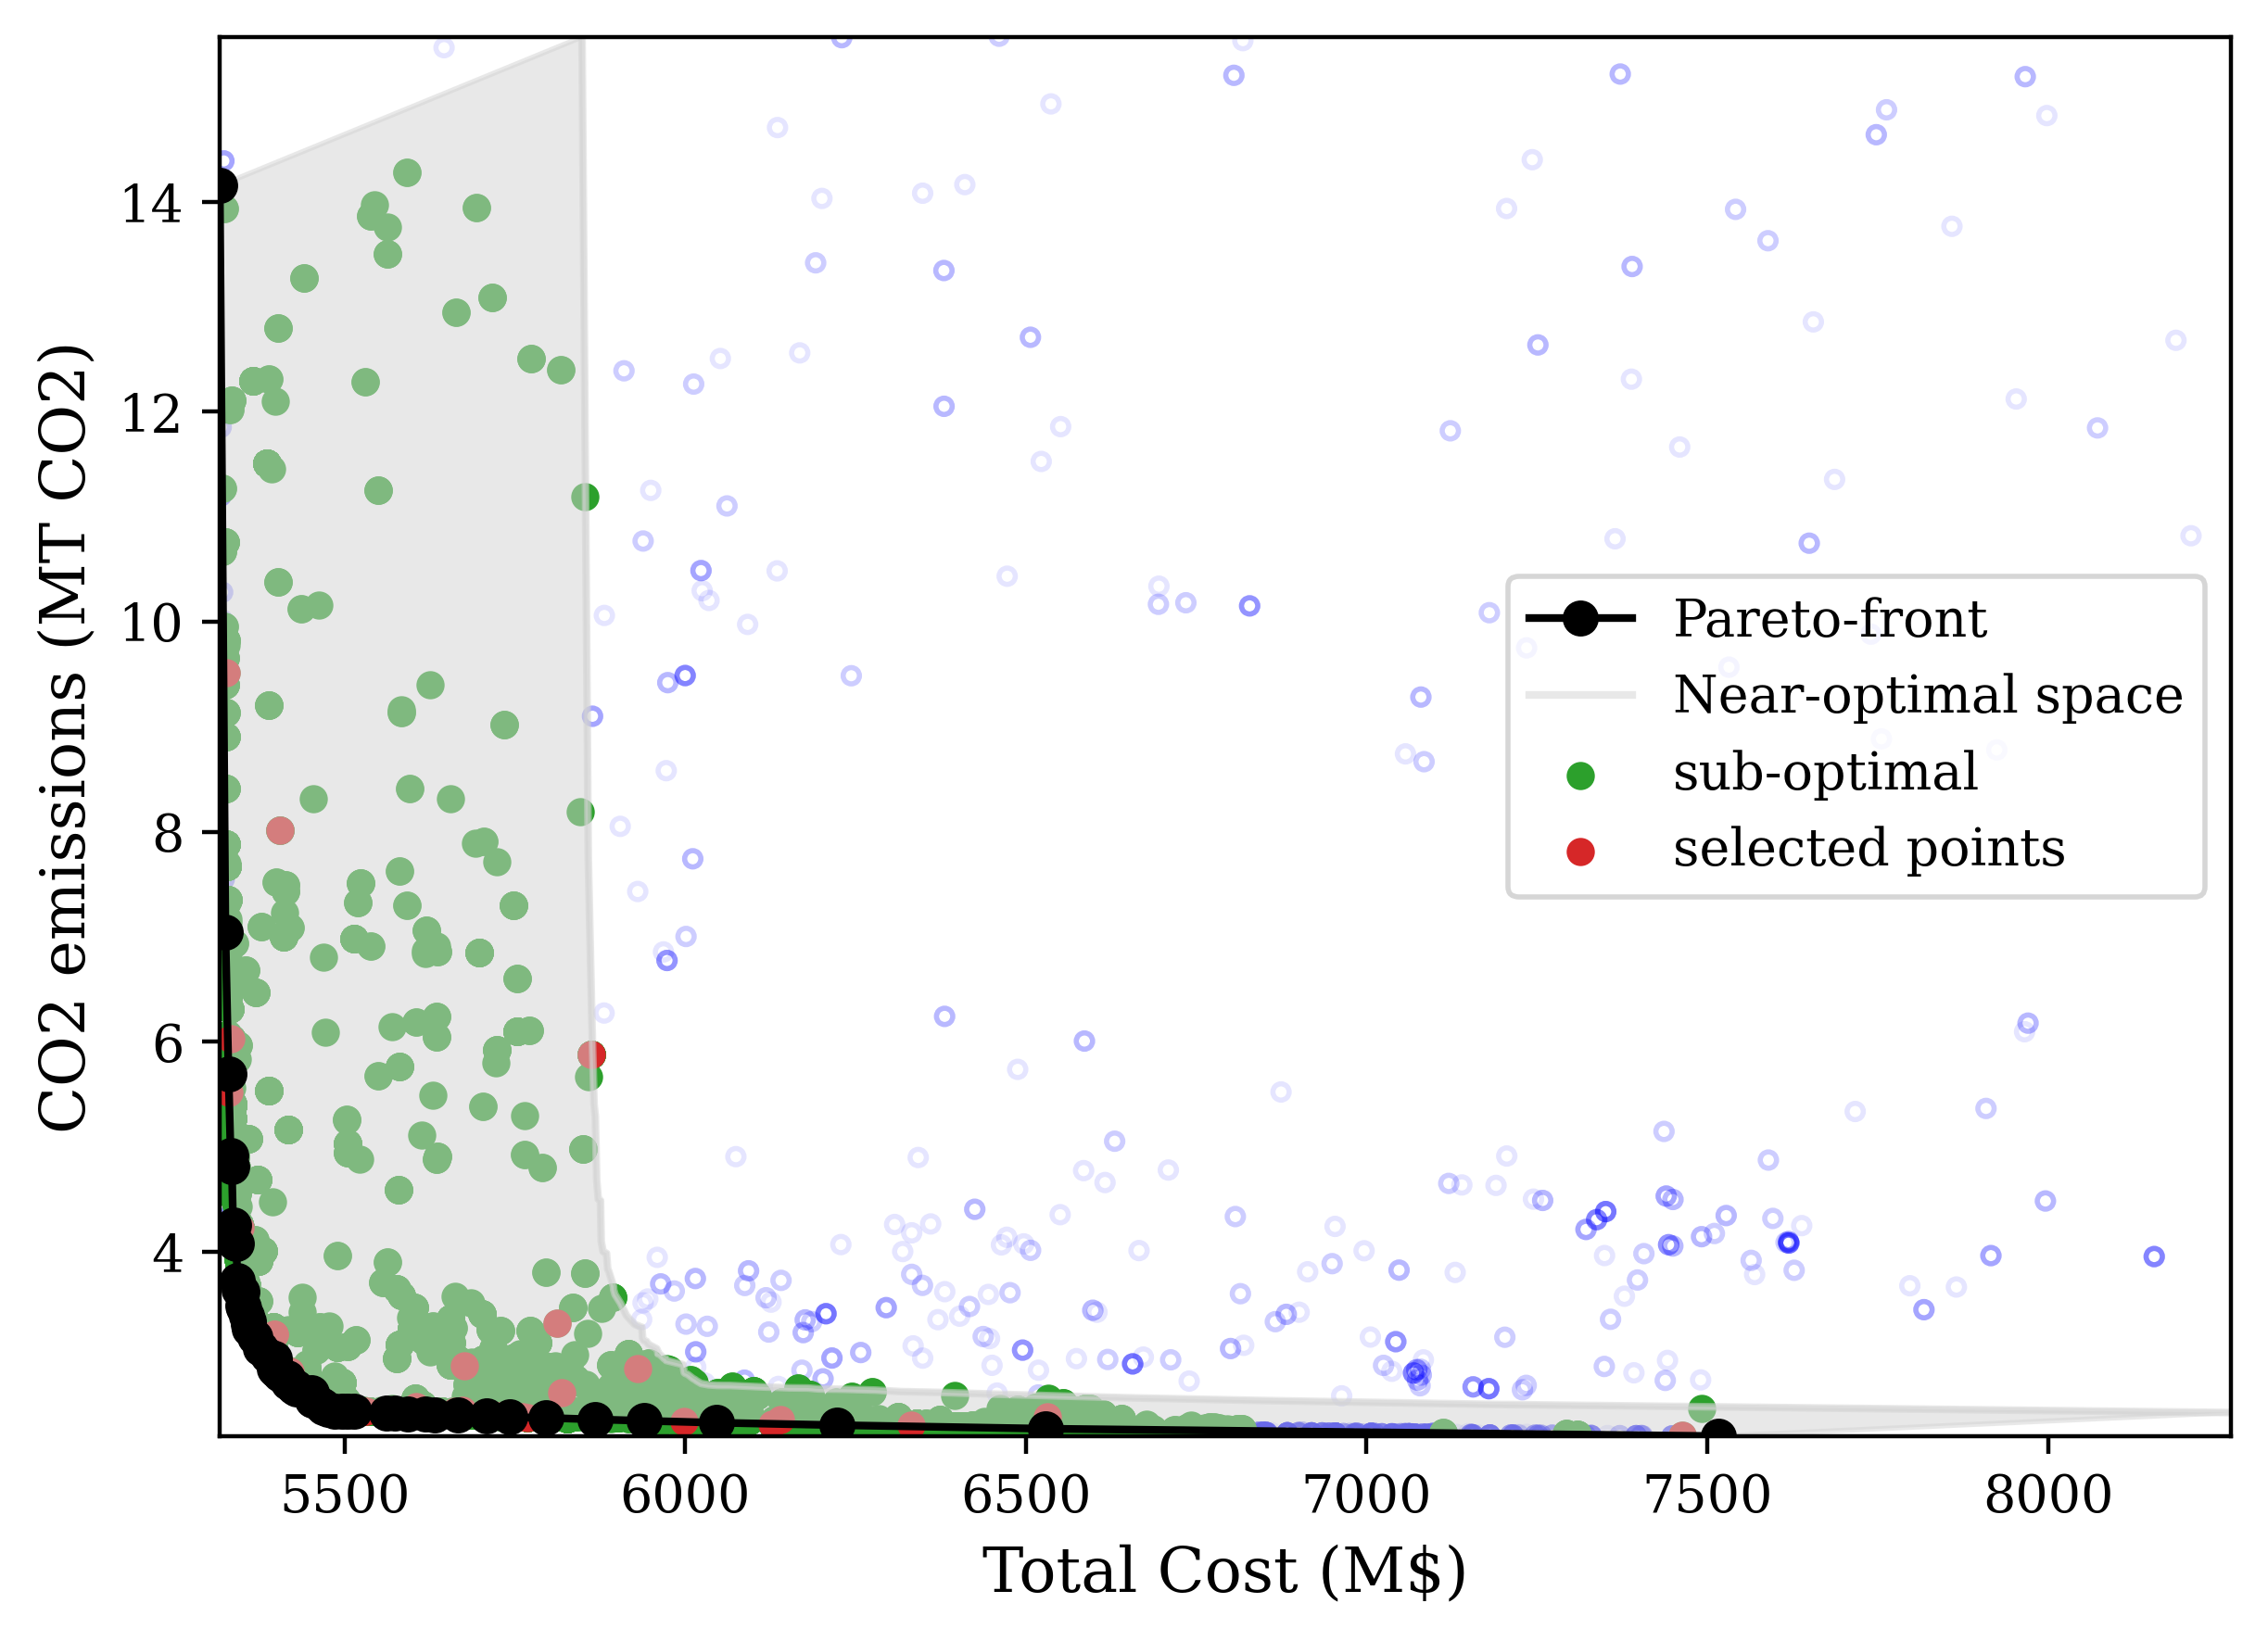
\includegraphics[width=0.6\columnwidth]{figures/results/osier_mga_subset_01.png}
  % \resizebox{0.6\columnwidth}{!}{%% Creator: Matplotlib, PGF backend
%%
%% To include the figure in your LaTeX document, write
%%   \input{<filename>.pgf}
%%
%% Make sure the required packages are loaded in your preamble
%%   \usepackage{pgf}
%%
%% Also ensure that all the required font packages are loaded; for instance,
%% the lmodern package is sometimes necessary when using math font.
%%   \usepackage{lmodern}
%%
%% Figures using additional raster images can only be included by \input if
%% they are in the same directory as the main LaTeX file. For loading figures
%% from other directories you can use the `import` package
%%   \usepackage{import}
%%
%% and then include the figures with
%%   \import{<path to file>}{<filename>.pgf}
%%
%% Matplotlib used the following preamble
%%   \def\mathdefault#1{#1}
%%   \everymath=\expandafter{\the\everymath\displaystyle}
%%   
%%   \makeatletter\@ifpackageloaded{underscore}{}{\usepackage[strings]{underscore}}\makeatother
%%
\begingroup%
\makeatletter%
\begin{pgfpicture}%
\pgfpathrectangle{\pgfpointorigin}{\pgfqpoint{7.900000in}{5.900000in}}%
\pgfusepath{use as bounding box, clip}%
\begin{pgfscope}%
\pgfsetbuttcap%
\pgfsetmiterjoin%
\definecolor{currentfill}{rgb}{0.827451,0.827451,0.827451}%
\pgfsetfillcolor{currentfill}%
\pgfsetlinewidth{0.000000pt}%
\definecolor{currentstroke}{rgb}{0.000000,0.000000,0.000000}%
\pgfsetstrokecolor{currentstroke}%
\pgfsetdash{}{0pt}%
\pgfpathmoveto{\pgfqpoint{0.000000in}{0.000000in}}%
\pgfpathlineto{\pgfqpoint{7.900000in}{0.000000in}}%
\pgfpathlineto{\pgfqpoint{7.900000in}{5.900000in}}%
\pgfpathlineto{\pgfqpoint{0.000000in}{5.900000in}}%
\pgfpathlineto{\pgfqpoint{0.000000in}{0.000000in}}%
\pgfpathclose%
\pgfusepath{fill}%
\end{pgfscope}%
\begin{pgfscope}%
\pgfsetbuttcap%
\pgfsetmiterjoin%
\definecolor{currentfill}{rgb}{1.000000,1.000000,1.000000}%
\pgfsetfillcolor{currentfill}%
\pgfsetlinewidth{0.000000pt}%
\definecolor{currentstroke}{rgb}{0.000000,0.000000,0.000000}%
\pgfsetstrokecolor{currentstroke}%
\pgfsetstrokeopacity{0.000000}%
\pgfsetdash{}{0pt}%
\pgfpathmoveto{\pgfqpoint{0.688192in}{0.670138in}}%
\pgfpathlineto{\pgfqpoint{7.800000in}{0.670138in}}%
\pgfpathlineto{\pgfqpoint{7.800000in}{5.800000in}}%
\pgfpathlineto{\pgfqpoint{0.688192in}{5.800000in}}%
\pgfpathlineto{\pgfqpoint{0.688192in}{0.670138in}}%
\pgfpathclose%
\pgfusepath{fill}%
\end{pgfscope}%
\begin{pgfscope}%
\pgfpathrectangle{\pgfqpoint{0.688192in}{0.670138in}}{\pgfqpoint{7.111808in}{5.129862in}}%
\pgfusepath{clip}%
\pgfsetbuttcap%
\pgfsetroundjoin%
\definecolor{currentfill}{rgb}{0.172549,0.627451,0.172549}%
\pgfsetfillcolor{currentfill}%
\pgfsetlinewidth{1.003750pt}%
\definecolor{currentstroke}{rgb}{0.172549,0.627451,0.172549}%
\pgfsetstrokecolor{currentstroke}%
\pgfsetdash{}{0pt}%
\pgfsys@defobject{currentmarker}{\pgfqpoint{-0.049105in}{-0.049105in}}{\pgfqpoint{0.049105in}{0.049105in}}{%
\pgfpathmoveto{\pgfqpoint{0.000000in}{-0.049105in}}%
\pgfpathcurveto{\pgfqpoint{0.013023in}{-0.049105in}}{\pgfqpoint{0.025514in}{-0.043931in}}{\pgfqpoint{0.034722in}{-0.034722in}}%
\pgfpathcurveto{\pgfqpoint{0.043931in}{-0.025514in}}{\pgfqpoint{0.049105in}{-0.013023in}}{\pgfqpoint{0.049105in}{0.000000in}}%
\pgfpathcurveto{\pgfqpoint{0.049105in}{0.013023in}}{\pgfqpoint{0.043931in}{0.025514in}}{\pgfqpoint{0.034722in}{0.034722in}}%
\pgfpathcurveto{\pgfqpoint{0.025514in}{0.043931in}}{\pgfqpoint{0.013023in}{0.049105in}}{\pgfqpoint{0.000000in}{0.049105in}}%
\pgfpathcurveto{\pgfqpoint{-0.013023in}{0.049105in}}{\pgfqpoint{-0.025514in}{0.043931in}}{\pgfqpoint{-0.034722in}{0.034722in}}%
\pgfpathcurveto{\pgfqpoint{-0.043931in}{0.025514in}}{\pgfqpoint{-0.049105in}{0.013023in}}{\pgfqpoint{-0.049105in}{0.000000in}}%
\pgfpathcurveto{\pgfqpoint{-0.049105in}{-0.013023in}}{\pgfqpoint{-0.043931in}{-0.025514in}}{\pgfqpoint{-0.034722in}{-0.034722in}}%
\pgfpathcurveto{\pgfqpoint{-0.025514in}{-0.043931in}}{\pgfqpoint{-0.013023in}{-0.049105in}}{\pgfqpoint{0.000000in}{-0.049105in}}%
\pgfpathlineto{\pgfqpoint{0.000000in}{-0.049105in}}%
\pgfpathclose%
\pgfusepath{stroke,fill}%
}%
\begin{pgfscope}%
\pgfsys@transformshift{2.002623in}{2.069732in}%
\pgfsys@useobject{currentmarker}{}%
\end{pgfscope}%
\begin{pgfscope}%
\pgfsys@transformshift{2.577113in}{0.834635in}%
\pgfsys@useobject{currentmarker}{}%
\end{pgfscope}%
\begin{pgfscope}%
\pgfsys@transformshift{2.133693in}{0.971398in}%
\pgfsys@useobject{currentmarker}{}%
\end{pgfscope}%
\begin{pgfscope}%
\pgfsys@transformshift{2.002623in}{2.069732in}%
\pgfsys@useobject{currentmarker}{}%
\end{pgfscope}%
\begin{pgfscope}%
\pgfsys@transformshift{2.002623in}{2.069732in}%
\pgfsys@useobject{currentmarker}{}%
\end{pgfscope}%
\begin{pgfscope}%
\pgfsys@transformshift{2.577113in}{0.834635in}%
\pgfsys@useobject{currentmarker}{}%
\end{pgfscope}%
\begin{pgfscope}%
\pgfsys@transformshift{2.133693in}{0.971398in}%
\pgfsys@useobject{currentmarker}{}%
\end{pgfscope}%
\begin{pgfscope}%
\pgfsys@transformshift{2.675907in}{0.794786in}%
\pgfsys@useobject{currentmarker}{}%
\end{pgfscope}%
\begin{pgfscope}%
\pgfsys@transformshift{1.604618in}{2.442321in}%
\pgfsys@useobject{currentmarker}{}%
\end{pgfscope}%
\begin{pgfscope}%
\pgfsys@transformshift{1.811007in}{1.014178in}%
\pgfsys@useobject{currentmarker}{}%
\end{pgfscope}%
\begin{pgfscope}%
\pgfsys@transformshift{2.137452in}{0.960682in}%
\pgfsys@useobject{currentmarker}{}%
\end{pgfscope}%
\begin{pgfscope}%
\pgfsys@transformshift{3.749415in}{0.772617in}%
\pgfsys@useobject{currentmarker}{}%
\end{pgfscope}%
\begin{pgfscope}%
\pgfsys@transformshift{1.740224in}{2.152752in}%
\pgfsys@useobject{currentmarker}{}%
\end{pgfscope}%
\begin{pgfscope}%
\pgfsys@transformshift{1.970906in}{1.724284in}%
\pgfsys@useobject{currentmarker}{}%
\end{pgfscope}%
\begin{pgfscope}%
\pgfsys@transformshift{2.002623in}{2.069732in}%
\pgfsys@useobject{currentmarker}{}%
\end{pgfscope}%
\begin{pgfscope}%
\pgfsys@transformshift{2.002623in}{2.069732in}%
\pgfsys@useobject{currentmarker}{}%
\end{pgfscope}%
\begin{pgfscope}%
\pgfsys@transformshift{2.675907in}{0.794786in}%
\pgfsys@useobject{currentmarker}{}%
\end{pgfscope}%
\begin{pgfscope}%
\pgfsys@transformshift{1.604618in}{2.442321in}%
\pgfsys@useobject{currentmarker}{}%
\end{pgfscope}%
\begin{pgfscope}%
\pgfsys@transformshift{1.811007in}{1.014178in}%
\pgfsys@useobject{currentmarker}{}%
\end{pgfscope}%
\begin{pgfscope}%
\pgfsys@transformshift{1.616200in}{1.119376in}%
\pgfsys@useobject{currentmarker}{}%
\end{pgfscope}%
\begin{pgfscope}%
\pgfsys@transformshift{1.861428in}{0.911984in}%
\pgfsys@useobject{currentmarker}{}%
\end{pgfscope}%
\begin{pgfscope}%
\pgfsys@transformshift{2.683832in}{0.767507in}%
\pgfsys@useobject{currentmarker}{}%
\end{pgfscope}%
\begin{pgfscope}%
\pgfsys@transformshift{2.342420in}{0.820679in}%
\pgfsys@useobject{currentmarker}{}%
\end{pgfscope}%
\begin{pgfscope}%
\pgfsys@transformshift{2.137256in}{0.859251in}%
\pgfsys@useobject{currentmarker}{}%
\end{pgfscope}%
\begin{pgfscope}%
\pgfsys@transformshift{3.712607in}{0.763798in}%
\pgfsys@useobject{currentmarker}{}%
\end{pgfscope}%
\begin{pgfscope}%
\pgfsys@transformshift{1.740224in}{2.152752in}%
\pgfsys@useobject{currentmarker}{}%
\end{pgfscope}%
\begin{pgfscope}%
\pgfsys@transformshift{1.935478in}{1.140459in}%
\pgfsys@useobject{currentmarker}{}%
\end{pgfscope}%
\begin{pgfscope}%
\pgfsys@transformshift{2.071820in}{0.929985in}%
\pgfsys@useobject{currentmarker}{}%
\end{pgfscope}%
\begin{pgfscope}%
\pgfsys@transformshift{2.577113in}{0.834635in}%
\pgfsys@useobject{currentmarker}{}%
\end{pgfscope}%
\begin{pgfscope}%
\pgfsys@transformshift{2.587886in}{0.820746in}%
\pgfsys@useobject{currentmarker}{}%
\end{pgfscope}%
\begin{pgfscope}%
\pgfsys@transformshift{2.167264in}{0.917009in}%
\pgfsys@useobject{currentmarker}{}%
\end{pgfscope}%
\begin{pgfscope}%
\pgfsys@transformshift{2.192481in}{0.875862in}%
\pgfsys@useobject{currentmarker}{}%
\end{pgfscope}%
\begin{pgfscope}%
\pgfsys@transformshift{3.749415in}{0.772617in}%
\pgfsys@useobject{currentmarker}{}%
\end{pgfscope}%
\begin{pgfscope}%
\pgfsys@transformshift{3.756237in}{0.768003in}%
\pgfsys@useobject{currentmarker}{}%
\end{pgfscope}%
\begin{pgfscope}%
\pgfsys@transformshift{1.787712in}{4.620613in}%
\pgfsys@useobject{currentmarker}{}%
\end{pgfscope}%
\begin{pgfscope}%
\pgfsys@transformshift{1.970906in}{1.724284in}%
\pgfsys@useobject{currentmarker}{}%
\end{pgfscope}%
\begin{pgfscope}%
\pgfsys@transformshift{2.133693in}{0.971398in}%
\pgfsys@useobject{currentmarker}{}%
\end{pgfscope}%
\begin{pgfscope}%
\pgfsys@transformshift{2.137452in}{0.960682in}%
\pgfsys@useobject{currentmarker}{}%
\end{pgfscope}%
\begin{pgfscope}%
\pgfsys@transformshift{2.075890in}{1.177972in}%
\pgfsys@useobject{currentmarker}{}%
\end{pgfscope}%
\begin{pgfscope}%
\pgfsys@transformshift{2.205888in}{0.937526in}%
\pgfsys@useobject{currentmarker}{}%
\end{pgfscope}%
\begin{pgfscope}%
\pgfsys@transformshift{2.002623in}{2.069732in}%
\pgfsys@useobject{currentmarker}{}%
\end{pgfscope}%
\begin{pgfscope}%
\pgfsys@transformshift{2.002623in}{2.069732in}%
\pgfsys@useobject{currentmarker}{}%
\end{pgfscope}%
\begin{pgfscope}%
\pgfsys@transformshift{2.675907in}{0.794786in}%
\pgfsys@useobject{currentmarker}{}%
\end{pgfscope}%
\begin{pgfscope}%
\pgfsys@transformshift{1.604618in}{2.442321in}%
\pgfsys@useobject{currentmarker}{}%
\end{pgfscope}%
\begin{pgfscope}%
\pgfsys@transformshift{1.811007in}{1.014178in}%
\pgfsys@useobject{currentmarker}{}%
\end{pgfscope}%
\begin{pgfscope}%
\pgfsys@transformshift{1.616200in}{1.119376in}%
\pgfsys@useobject{currentmarker}{}%
\end{pgfscope}%
\begin{pgfscope}%
\pgfsys@transformshift{1.861428in}{0.911984in}%
\pgfsys@useobject{currentmarker}{}%
\end{pgfscope}%
\begin{pgfscope}%
\pgfsys@transformshift{2.683832in}{0.767507in}%
\pgfsys@useobject{currentmarker}{}%
\end{pgfscope}%
\begin{pgfscope}%
\pgfsys@transformshift{2.342420in}{0.820679in}%
\pgfsys@useobject{currentmarker}{}%
\end{pgfscope}%
\begin{pgfscope}%
\pgfsys@transformshift{3.712607in}{0.763798in}%
\pgfsys@useobject{currentmarker}{}%
\end{pgfscope}%
\begin{pgfscope}%
\pgfsys@transformshift{2.015412in}{0.829361in}%
\pgfsys@useobject{currentmarker}{}%
\end{pgfscope}%
\begin{pgfscope}%
\pgfsys@transformshift{1.849559in}{0.924387in}%
\pgfsys@useobject{currentmarker}{}%
\end{pgfscope}%
\begin{pgfscope}%
\pgfsys@transformshift{1.784951in}{1.056501in}%
\pgfsys@useobject{currentmarker}{}%
\end{pgfscope}%
\begin{pgfscope}%
\pgfsys@transformshift{1.667281in}{2.086122in}%
\pgfsys@useobject{currentmarker}{}%
\end{pgfscope}%
\begin{pgfscope}%
\pgfsys@transformshift{3.510642in}{0.768394in}%
\pgfsys@useobject{currentmarker}{}%
\end{pgfscope}%
\begin{pgfscope}%
\pgfsys@transformshift{2.587886in}{0.820746in}%
\pgfsys@useobject{currentmarker}{}%
\end{pgfscope}%
\begin{pgfscope}%
\pgfsys@transformshift{2.446699in}{0.828993in}%
\pgfsys@useobject{currentmarker}{}%
\end{pgfscope}%
\begin{pgfscope}%
\pgfsys@transformshift{3.756237in}{0.768003in}%
\pgfsys@useobject{currentmarker}{}%
\end{pgfscope}%
\begin{pgfscope}%
\pgfsys@transformshift{2.137256in}{0.859251in}%
\pgfsys@useobject{currentmarker}{}%
\end{pgfscope}%
\begin{pgfscope}%
\pgfsys@transformshift{2.206416in}{0.850354in}%
\pgfsys@useobject{currentmarker}{}%
\end{pgfscope}%
\begin{pgfscope}%
\pgfsys@transformshift{2.273390in}{0.838871in}%
\pgfsys@useobject{currentmarker}{}%
\end{pgfscope}%
\begin{pgfscope}%
\pgfsys@transformshift{2.071820in}{0.929985in}%
\pgfsys@useobject{currentmarker}{}%
\end{pgfscope}%
\begin{pgfscope}%
\pgfsys@transformshift{1.935478in}{1.140459in}%
\pgfsys@useobject{currentmarker}{}%
\end{pgfscope}%
\begin{pgfscope}%
\pgfsys@transformshift{1.740224in}{2.152752in}%
\pgfsys@useobject{currentmarker}{}%
\end{pgfscope}%
\begin{pgfscope}%
\pgfsys@transformshift{1.740224in}{2.152752in}%
\pgfsys@useobject{currentmarker}{}%
\end{pgfscope}%
\begin{pgfscope}%
\pgfsys@transformshift{3.749415in}{0.772617in}%
\pgfsys@useobject{currentmarker}{}%
\end{pgfscope}%
\begin{pgfscope}%
\pgfsys@transformshift{3.669906in}{0.790604in}%
\pgfsys@useobject{currentmarker}{}%
\end{pgfscope}%
\begin{pgfscope}%
\pgfsys@transformshift{2.775958in}{0.823662in}%
\pgfsys@useobject{currentmarker}{}%
\end{pgfscope}%
\begin{pgfscope}%
\pgfsys@transformshift{2.467544in}{0.829862in}%
\pgfsys@useobject{currentmarker}{}%
\end{pgfscope}%
\begin{pgfscope}%
\pgfsys@transformshift{3.766705in}{0.770312in}%
\pgfsys@useobject{currentmarker}{}%
\end{pgfscope}%
\begin{pgfscope}%
\pgfsys@transformshift{2.167264in}{0.917009in}%
\pgfsys@useobject{currentmarker}{}%
\end{pgfscope}%
\begin{pgfscope}%
\pgfsys@transformshift{2.192481in}{0.875862in}%
\pgfsys@useobject{currentmarker}{}%
\end{pgfscope}%
\begin{pgfscope}%
\pgfsys@transformshift{2.366651in}{0.847901in}%
\pgfsys@useobject{currentmarker}{}%
\end{pgfscope}%
\begin{pgfscope}%
\pgfsys@transformshift{2.133693in}{0.971398in}%
\pgfsys@useobject{currentmarker}{}%
\end{pgfscope}%
\begin{pgfscope}%
\pgfsys@transformshift{2.137452in}{0.960682in}%
\pgfsys@useobject{currentmarker}{}%
\end{pgfscope}%
\begin{pgfscope}%
\pgfsys@transformshift{1.970906in}{1.724284in}%
\pgfsys@useobject{currentmarker}{}%
\end{pgfscope}%
\begin{pgfscope}%
\pgfsys@transformshift{2.075890in}{1.177972in}%
\pgfsys@useobject{currentmarker}{}%
\end{pgfscope}%
\begin{pgfscope}%
\pgfsys@transformshift{1.978908in}{1.268350in}%
\pgfsys@useobject{currentmarker}{}%
\end{pgfscope}%
\begin{pgfscope}%
\pgfsys@transformshift{1.787712in}{4.620613in}%
\pgfsys@useobject{currentmarker}{}%
\end{pgfscope}%
\begin{pgfscope}%
\pgfsys@transformshift{1.892499in}{4.580764in}%
\pgfsys@useobject{currentmarker}{}%
\end{pgfscope}%
\begin{pgfscope}%
\pgfsys@transformshift{2.577113in}{0.834635in}%
\pgfsys@useobject{currentmarker}{}%
\end{pgfscope}%
\begin{pgfscope}%
\pgfsys@transformshift{2.995479in}{0.832502in}%
\pgfsys@useobject{currentmarker}{}%
\end{pgfscope}%
\begin{pgfscope}%
\pgfsys@transformshift{2.181522in}{0.926521in}%
\pgfsys@useobject{currentmarker}{}%
\end{pgfscope}%
\begin{pgfscope}%
\pgfsys@transformshift{2.194737in}{0.876819in}%
\pgfsys@useobject{currentmarker}{}%
\end{pgfscope}%
\begin{pgfscope}%
\pgfsys@transformshift{2.501680in}{0.853425in}%
\pgfsys@useobject{currentmarker}{}%
\end{pgfscope}%
\begin{pgfscope}%
\pgfsys@transformshift{2.002623in}{2.069732in}%
\pgfsys@useobject{currentmarker}{}%
\end{pgfscope}%
\begin{pgfscope}%
\pgfsys@transformshift{2.733482in}{0.845260in}%
\pgfsys@useobject{currentmarker}{}%
\end{pgfscope}%
\begin{pgfscope}%
\pgfsys@transformshift{2.205888in}{0.937526in}%
\pgfsys@useobject{currentmarker}{}%
\end{pgfscope}%
\begin{pgfscope}%
\pgfsys@transformshift{2.249355in}{0.887340in}%
\pgfsys@useobject{currentmarker}{}%
\end{pgfscope}%
\begin{pgfscope}%
\pgfsys@transformshift{2.352434in}{0.877033in}%
\pgfsys@useobject{currentmarker}{}%
\end{pgfscope}%
\begin{pgfscope}%
\pgfsys@transformshift{2.002623in}{2.069732in}%
\pgfsys@useobject{currentmarker}{}%
\end{pgfscope}%
\begin{pgfscope}%
\pgfsys@transformshift{2.277300in}{0.915168in}%
\pgfsys@useobject{currentmarker}{}%
\end{pgfscope}%
\begin{pgfscope}%
\pgfsys@transformshift{2.267238in}{0.918308in}%
\pgfsys@useobject{currentmarker}{}%
\end{pgfscope}%
\begin{pgfscope}%
\pgfsys@transformshift{2.683832in}{0.767507in}%
\pgfsys@useobject{currentmarker}{}%
\end{pgfscope}%
\begin{pgfscope}%
\pgfsys@transformshift{2.015412in}{0.829361in}%
\pgfsys@useobject{currentmarker}{}%
\end{pgfscope}%
\begin{pgfscope}%
\pgfsys@transformshift{1.664089in}{0.873927in}%
\pgfsys@useobject{currentmarker}{}%
\end{pgfscope}%
\begin{pgfscope}%
\pgfsys@transformshift{2.255328in}{0.795472in}%
\pgfsys@useobject{currentmarker}{}%
\end{pgfscope}%
\begin{pgfscope}%
\pgfsys@transformshift{1.503539in}{1.099915in}%
\pgfsys@useobject{currentmarker}{}%
\end{pgfscope}%
\begin{pgfscope}%
\pgfsys@transformshift{2.297898in}{0.787808in}%
\pgfsys@useobject{currentmarker}{}%
\end{pgfscope}%
\begin{pgfscope}%
\pgfsys@transformshift{1.837877in}{0.855892in}%
\pgfsys@useobject{currentmarker}{}%
\end{pgfscope}%
\begin{pgfscope}%
\pgfsys@transformshift{2.189198in}{0.827103in}%
\pgfsys@useobject{currentmarker}{}%
\end{pgfscope}%
\begin{pgfscope}%
\pgfsys@transformshift{1.532482in}{0.938707in}%
\pgfsys@useobject{currentmarker}{}%
\end{pgfscope}%
\begin{pgfscope}%
\pgfsys@transformshift{2.927418in}{0.758622in}%
\pgfsys@useobject{currentmarker}{}%
\end{pgfscope}%
\begin{pgfscope}%
\pgfsys@transformshift{2.675907in}{0.794786in}%
\pgfsys@useobject{currentmarker}{}%
\end{pgfscope}%
\begin{pgfscope}%
\pgfsys@transformshift{2.342420in}{0.820679in}%
\pgfsys@useobject{currentmarker}{}%
\end{pgfscope}%
\begin{pgfscope}%
\pgfsys@transformshift{1.861428in}{0.911984in}%
\pgfsys@useobject{currentmarker}{}%
\end{pgfscope}%
\begin{pgfscope}%
\pgfsys@transformshift{1.849559in}{0.924387in}%
\pgfsys@useobject{currentmarker}{}%
\end{pgfscope}%
\begin{pgfscope}%
\pgfsys@transformshift{2.137256in}{0.859251in}%
\pgfsys@useobject{currentmarker}{}%
\end{pgfscope}%
\begin{pgfscope}%
\pgfsys@transformshift{2.099349in}{0.908918in}%
\pgfsys@useobject{currentmarker}{}%
\end{pgfscope}%
\begin{pgfscope}%
\pgfsys@transformshift{2.206416in}{0.850354in}%
\pgfsys@useobject{currentmarker}{}%
\end{pgfscope}%
\begin{pgfscope}%
\pgfsys@transformshift{2.284703in}{0.830771in}%
\pgfsys@useobject{currentmarker}{}%
\end{pgfscope}%
\begin{pgfscope}%
\pgfsys@transformshift{2.244732in}{0.834513in}%
\pgfsys@useobject{currentmarker}{}%
\end{pgfscope}%
\begin{pgfscope}%
\pgfsys@transformshift{1.604618in}{2.442321in}%
\pgfsys@useobject{currentmarker}{}%
\end{pgfscope}%
\begin{pgfscope}%
\pgfsys@transformshift{1.616200in}{1.119376in}%
\pgfsys@useobject{currentmarker}{}%
\end{pgfscope}%
\begin{pgfscope}%
\pgfsys@transformshift{1.784951in}{1.056501in}%
\pgfsys@useobject{currentmarker}{}%
\end{pgfscope}%
\begin{pgfscope}%
\pgfsys@transformshift{1.788645in}{0.939743in}%
\pgfsys@useobject{currentmarker}{}%
\end{pgfscope}%
\begin{pgfscope}%
\pgfsys@transformshift{3.712607in}{0.763798in}%
\pgfsys@useobject{currentmarker}{}%
\end{pgfscope}%
\begin{pgfscope}%
\pgfsys@transformshift{3.510642in}{0.768394in}%
\pgfsys@useobject{currentmarker}{}%
\end{pgfscope}%
\begin{pgfscope}%
\pgfsys@transformshift{2.922604in}{0.814960in}%
\pgfsys@useobject{currentmarker}{}%
\end{pgfscope}%
\begin{pgfscope}%
\pgfsys@transformshift{2.587886in}{0.820746in}%
\pgfsys@useobject{currentmarker}{}%
\end{pgfscope}%
\begin{pgfscope}%
\pgfsys@transformshift{2.446699in}{0.828993in}%
\pgfsys@useobject{currentmarker}{}%
\end{pgfscope}%
\begin{pgfscope}%
\pgfsys@transformshift{2.071820in}{0.929985in}%
\pgfsys@useobject{currentmarker}{}%
\end{pgfscope}%
\begin{pgfscope}%
\pgfsys@transformshift{2.192481in}{0.875862in}%
\pgfsys@useobject{currentmarker}{}%
\end{pgfscope}%
\begin{pgfscope}%
\pgfsys@transformshift{2.167264in}{0.917009in}%
\pgfsys@useobject{currentmarker}{}%
\end{pgfscope}%
\begin{pgfscope}%
\pgfsys@transformshift{2.273390in}{0.838871in}%
\pgfsys@useobject{currentmarker}{}%
\end{pgfscope}%
\begin{pgfscope}%
\pgfsys@transformshift{1.667281in}{2.086122in}%
\pgfsys@useobject{currentmarker}{}%
\end{pgfscope}%
\begin{pgfscope}%
\pgfsys@transformshift{1.811007in}{1.014178in}%
\pgfsys@useobject{currentmarker}{}%
\end{pgfscope}%
\begin{pgfscope}%
\pgfsys@transformshift{3.756237in}{0.768003in}%
\pgfsys@useobject{currentmarker}{}%
\end{pgfscope}%
\begin{pgfscope}%
\pgfsys@transformshift{3.749415in}{0.772617in}%
\pgfsys@useobject{currentmarker}{}%
\end{pgfscope}%
\begin{pgfscope}%
\pgfsys@transformshift{3.570530in}{0.775415in}%
\pgfsys@useobject{currentmarker}{}%
\end{pgfscope}%
\begin{pgfscope}%
\pgfsys@transformshift{2.775958in}{0.823662in}%
\pgfsys@useobject{currentmarker}{}%
\end{pgfscope}%
\begin{pgfscope}%
\pgfsys@transformshift{2.467544in}{0.829862in}%
\pgfsys@useobject{currentmarker}{}%
\end{pgfscope}%
\begin{pgfscope}%
\pgfsys@transformshift{2.133693in}{0.971398in}%
\pgfsys@useobject{currentmarker}{}%
\end{pgfscope}%
\begin{pgfscope}%
\pgfsys@transformshift{2.137452in}{0.960682in}%
\pgfsys@useobject{currentmarker}{}%
\end{pgfscope}%
\begin{pgfscope}%
\pgfsys@transformshift{2.194737in}{0.876819in}%
\pgfsys@useobject{currentmarker}{}%
\end{pgfscope}%
\begin{pgfscope}%
\pgfsys@transformshift{2.181522in}{0.926521in}%
\pgfsys@useobject{currentmarker}{}%
\end{pgfscope}%
\begin{pgfscope}%
\pgfsys@transformshift{2.366651in}{0.847901in}%
\pgfsys@useobject{currentmarker}{}%
\end{pgfscope}%
\begin{pgfscope}%
\pgfsys@transformshift{2.336380in}{0.863530in}%
\pgfsys@useobject{currentmarker}{}%
\end{pgfscope}%
\begin{pgfscope}%
\pgfsys@transformshift{1.740224in}{2.152752in}%
\pgfsys@useobject{currentmarker}{}%
\end{pgfscope}%
\begin{pgfscope}%
\pgfsys@transformshift{1.740224in}{2.152752in}%
\pgfsys@useobject{currentmarker}{}%
\end{pgfscope}%
\begin{pgfscope}%
\pgfsys@transformshift{1.738349in}{2.346587in}%
\pgfsys@useobject{currentmarker}{}%
\end{pgfscope}%
\begin{pgfscope}%
\pgfsys@transformshift{1.695335in}{3.279285in}%
\pgfsys@useobject{currentmarker}{}%
\end{pgfscope}%
\begin{pgfscope}%
\pgfsys@transformshift{1.725514in}{2.617826in}%
\pgfsys@useobject{currentmarker}{}%
\end{pgfscope}%
\begin{pgfscope}%
\pgfsys@transformshift{1.935478in}{1.140459in}%
\pgfsys@useobject{currentmarker}{}%
\end{pgfscope}%
\begin{pgfscope}%
\pgfsys@transformshift{1.827708in}{1.655651in}%
\pgfsys@useobject{currentmarker}{}%
\end{pgfscope}%
\begin{pgfscope}%
\pgfsys@transformshift{1.840030in}{1.269677in}%
\pgfsys@useobject{currentmarker}{}%
\end{pgfscope}%
\begin{pgfscope}%
\pgfsys@transformshift{2.037379in}{1.137810in}%
\pgfsys@useobject{currentmarker}{}%
\end{pgfscope}%
\begin{pgfscope}%
\pgfsys@transformshift{3.766705in}{0.770312in}%
\pgfsys@useobject{currentmarker}{}%
\end{pgfscope}%
\begin{pgfscope}%
\pgfsys@transformshift{3.669906in}{0.790604in}%
\pgfsys@useobject{currentmarker}{}%
\end{pgfscope}%
\begin{pgfscope}%
\pgfsys@transformshift{2.577113in}{0.834635in}%
\pgfsys@useobject{currentmarker}{}%
\end{pgfscope}%
\begin{pgfscope}%
\pgfsys@transformshift{2.995479in}{0.832502in}%
\pgfsys@useobject{currentmarker}{}%
\end{pgfscope}%
\begin{pgfscope}%
\pgfsys@transformshift{2.227778in}{0.878597in}%
\pgfsys@useobject{currentmarker}{}%
\end{pgfscope}%
\begin{pgfscope}%
\pgfsys@transformshift{2.217038in}{0.885537in}%
\pgfsys@useobject{currentmarker}{}%
\end{pgfscope}%
\begin{pgfscope}%
\pgfsys@transformshift{2.205888in}{0.937526in}%
\pgfsys@useobject{currentmarker}{}%
\end{pgfscope}%
\begin{pgfscope}%
\pgfsys@transformshift{2.501680in}{0.853425in}%
\pgfsys@useobject{currentmarker}{}%
\end{pgfscope}%
\begin{pgfscope}%
\pgfsys@transformshift{2.352434in}{0.877033in}%
\pgfsys@useobject{currentmarker}{}%
\end{pgfscope}%
\begin{pgfscope}%
\pgfsys@transformshift{2.365198in}{0.866975in}%
\pgfsys@useobject{currentmarker}{}%
\end{pgfscope}%
\begin{pgfscope}%
\pgfsys@transformshift{1.783431in}{2.158831in}%
\pgfsys@useobject{currentmarker}{}%
\end{pgfscope}%
\begin{pgfscope}%
\pgfsys@transformshift{1.978908in}{1.268350in}%
\pgfsys@useobject{currentmarker}{}%
\end{pgfscope}%
\begin{pgfscope}%
\pgfsys@transformshift{1.970906in}{1.724284in}%
\pgfsys@useobject{currentmarker}{}%
\end{pgfscope}%
\begin{pgfscope}%
\pgfsys@transformshift{2.075890in}{1.177972in}%
\pgfsys@useobject{currentmarker}{}%
\end{pgfscope}%
\begin{pgfscope}%
\pgfsys@transformshift{5.928879in}{0.773315in}%
\pgfsys@useobject{currentmarker}{}%
\end{pgfscope}%
\begin{pgfscope}%
\pgfsys@transformshift{2.733482in}{0.845260in}%
\pgfsys@useobject{currentmarker}{}%
\end{pgfscope}%
\begin{pgfscope}%
\pgfsys@transformshift{2.249355in}{0.887340in}%
\pgfsys@useobject{currentmarker}{}%
\end{pgfscope}%
\begin{pgfscope}%
\pgfsys@transformshift{1.787712in}{4.620613in}%
\pgfsys@useobject{currentmarker}{}%
\end{pgfscope}%
\begin{pgfscope}%
\pgfsys@transformshift{1.892499in}{4.580764in}%
\pgfsys@useobject{currentmarker}{}%
\end{pgfscope}%
\begin{pgfscope}%
\pgfsys@transformshift{1.963318in}{2.960990in}%
\pgfsys@useobject{currentmarker}{}%
\end{pgfscope}%
\begin{pgfscope}%
\pgfsys@transformshift{1.978908in}{1.268350in}%
\pgfsys@useobject{currentmarker}{}%
\end{pgfscope}%
\begin{pgfscope}%
\pgfsys@transformshift{1.979583in}{4.114096in}%
\pgfsys@useobject{currentmarker}{}%
\end{pgfscope}%
\begin{pgfscope}%
\pgfsys@transformshift{1.991849in}{1.987682in}%
\pgfsys@useobject{currentmarker}{}%
\end{pgfscope}%
\begin{pgfscope}%
\pgfsys@transformshift{2.015412in}{0.829361in}%
\pgfsys@useobject{currentmarker}{}%
\end{pgfscope}%
\begin{pgfscope}%
\pgfsys@transformshift{1.664089in}{0.873927in}%
\pgfsys@useobject{currentmarker}{}%
\end{pgfscope}%
\begin{pgfscope}%
\pgfsys@transformshift{1.503539in}{1.099915in}%
\pgfsys@useobject{currentmarker}{}%
\end{pgfscope}%
\begin{pgfscope}%
\pgfsys@transformshift{1.837877in}{0.855892in}%
\pgfsys@useobject{currentmarker}{}%
\end{pgfscope}%
\begin{pgfscope}%
\pgfsys@transformshift{1.532482in}{0.938707in}%
\pgfsys@useobject{currentmarker}{}%
\end{pgfscope}%
\begin{pgfscope}%
\pgfsys@transformshift{2.060920in}{0.809191in}%
\pgfsys@useobject{currentmarker}{}%
\end{pgfscope}%
\begin{pgfscope}%
\pgfsys@transformshift{3.085911in}{0.739993in}%
\pgfsys@useobject{currentmarker}{}%
\end{pgfscope}%
\begin{pgfscope}%
\pgfsys@transformshift{1.552132in}{0.929506in}%
\pgfsys@useobject{currentmarker}{}%
\end{pgfscope}%
\begin{pgfscope}%
\pgfsys@transformshift{2.140592in}{0.760749in}%
\pgfsys@useobject{currentmarker}{}%
\end{pgfscope}%
\begin{pgfscope}%
\pgfsys@transformshift{2.270983in}{0.744746in}%
\pgfsys@useobject{currentmarker}{}%
\end{pgfscope}%
\begin{pgfscope}%
\pgfsys@transformshift{1.720111in}{0.866854in}%
\pgfsys@useobject{currentmarker}{}%
\end{pgfscope}%
\begin{pgfscope}%
\pgfsys@transformshift{1.695009in}{0.869095in}%
\pgfsys@useobject{currentmarker}{}%
\end{pgfscope}%
\begin{pgfscope}%
\pgfsys@transformshift{2.109068in}{0.825245in}%
\pgfsys@useobject{currentmarker}{}%
\end{pgfscope}%
\begin{pgfscope}%
\pgfsys@transformshift{1.604618in}{2.442321in}%
\pgfsys@useobject{currentmarker}{}%
\end{pgfscope}%
\begin{pgfscope}%
\pgfsys@transformshift{1.616200in}{1.119376in}%
\pgfsys@useobject{currentmarker}{}%
\end{pgfscope}%
\begin{pgfscope}%
\pgfsys@transformshift{1.617522in}{0.952845in}%
\pgfsys@useobject{currentmarker}{}%
\end{pgfscope}%
\begin{pgfscope}%
\pgfsys@transformshift{2.255328in}{0.795472in}%
\pgfsys@useobject{currentmarker}{}%
\end{pgfscope}%
\begin{pgfscope}%
\pgfsys@transformshift{2.683832in}{0.767507in}%
\pgfsys@useobject{currentmarker}{}%
\end{pgfscope}%
\begin{pgfscope}%
\pgfsys@transformshift{2.297898in}{0.787808in}%
\pgfsys@useobject{currentmarker}{}%
\end{pgfscope}%
\begin{pgfscope}%
\pgfsys@transformshift{2.927418in}{0.758622in}%
\pgfsys@useobject{currentmarker}{}%
\end{pgfscope}%
\begin{pgfscope}%
\pgfsys@transformshift{1.788645in}{0.939743in}%
\pgfsys@useobject{currentmarker}{}%
\end{pgfscope}%
\begin{pgfscope}%
\pgfsys@transformshift{1.846036in}{0.880155in}%
\pgfsys@useobject{currentmarker}{}%
\end{pgfscope}%
\begin{pgfscope}%
\pgfsys@transformshift{1.910835in}{0.876791in}%
\pgfsys@useobject{currentmarker}{}%
\end{pgfscope}%
\begin{pgfscope}%
\pgfsys@transformshift{2.189198in}{0.827103in}%
\pgfsys@useobject{currentmarker}{}%
\end{pgfscope}%
\begin{pgfscope}%
\pgfsys@transformshift{2.137256in}{0.859251in}%
\pgfsys@useobject{currentmarker}{}%
\end{pgfscope}%
\begin{pgfscope}%
\pgfsys@transformshift{1.651967in}{4.844526in}%
\pgfsys@useobject{currentmarker}{}%
\end{pgfscope}%
\begin{pgfscope}%
\pgfsys@transformshift{1.655078in}{0.991609in}%
\pgfsys@useobject{currentmarker}{}%
\end{pgfscope}%
\begin{pgfscope}%
\pgfsys@transformshift{2.675907in}{0.794786in}%
\pgfsys@useobject{currentmarker}{}%
\end{pgfscope}%
\begin{pgfscope}%
\pgfsys@transformshift{2.342409in}{0.820679in}%
\pgfsys@useobject{currentmarker}{}%
\end{pgfscope}%
\begin{pgfscope}%
\pgfsys@transformshift{3.712607in}{0.763798in}%
\pgfsys@useobject{currentmarker}{}%
\end{pgfscope}%
\begin{pgfscope}%
\pgfsys@transformshift{3.510642in}{0.768394in}%
\pgfsys@useobject{currentmarker}{}%
\end{pgfscope}%
\begin{pgfscope}%
\pgfsys@transformshift{1.861428in}{0.911984in}%
\pgfsys@useobject{currentmarker}{}%
\end{pgfscope}%
\begin{pgfscope}%
\pgfsys@transformshift{1.849559in}{0.924387in}%
\pgfsys@useobject{currentmarker}{}%
\end{pgfscope}%
\begin{pgfscope}%
\pgfsys@transformshift{1.946479in}{0.880739in}%
\pgfsys@useobject{currentmarker}{}%
\end{pgfscope}%
\begin{pgfscope}%
\pgfsys@transformshift{2.206416in}{0.850354in}%
\pgfsys@useobject{currentmarker}{}%
\end{pgfscope}%
\begin{pgfscope}%
\pgfsys@transformshift{2.284703in}{0.830771in}%
\pgfsys@useobject{currentmarker}{}%
\end{pgfscope}%
\begin{pgfscope}%
\pgfsys@transformshift{2.244732in}{0.834513in}%
\pgfsys@useobject{currentmarker}{}%
\end{pgfscope}%
\begin{pgfscope}%
\pgfsys@transformshift{2.330531in}{0.827424in}%
\pgfsys@useobject{currentmarker}{}%
\end{pgfscope}%
\begin{pgfscope}%
\pgfsys@transformshift{2.158419in}{0.867076in}%
\pgfsys@useobject{currentmarker}{}%
\end{pgfscope}%
\begin{pgfscope}%
\pgfsys@transformshift{1.667281in}{2.086122in}%
\pgfsys@useobject{currentmarker}{}%
\end{pgfscope}%
\begin{pgfscope}%
\pgfsys@transformshift{1.811007in}{1.014178in}%
\pgfsys@useobject{currentmarker}{}%
\end{pgfscope}%
\begin{pgfscope}%
\pgfsys@transformshift{1.682128in}{1.056486in}%
\pgfsys@useobject{currentmarker}{}%
\end{pgfscope}%
\begin{pgfscope}%
\pgfsys@transformshift{2.922604in}{0.814960in}%
\pgfsys@useobject{currentmarker}{}%
\end{pgfscope}%
\begin{pgfscope}%
\pgfsys@transformshift{2.939814in}{0.806323in}%
\pgfsys@useobject{currentmarker}{}%
\end{pgfscope}%
\begin{pgfscope}%
\pgfsys@transformshift{2.342420in}{0.820679in}%
\pgfsys@useobject{currentmarker}{}%
\end{pgfscope}%
\begin{pgfscope}%
\pgfsys@transformshift{3.756237in}{0.768003in}%
\pgfsys@useobject{currentmarker}{}%
\end{pgfscope}%
\begin{pgfscope}%
\pgfsys@transformshift{3.749415in}{0.772617in}%
\pgfsys@useobject{currentmarker}{}%
\end{pgfscope}%
\begin{pgfscope}%
\pgfsys@transformshift{3.570530in}{0.775415in}%
\pgfsys@useobject{currentmarker}{}%
\end{pgfscope}%
\begin{pgfscope}%
\pgfsys@transformshift{1.943459in}{0.968599in}%
\pgfsys@useobject{currentmarker}{}%
\end{pgfscope}%
\begin{pgfscope}%
\pgfsys@transformshift{2.099349in}{0.908918in}%
\pgfsys@useobject{currentmarker}{}%
\end{pgfscope}%
\begin{pgfscope}%
\pgfsys@transformshift{2.071820in}{0.929985in}%
\pgfsys@useobject{currentmarker}{}%
\end{pgfscope}%
\begin{pgfscope}%
\pgfsys@transformshift{2.273390in}{0.838871in}%
\pgfsys@useobject{currentmarker}{}%
\end{pgfscope}%
\begin{pgfscope}%
\pgfsys@transformshift{2.255999in}{0.843211in}%
\pgfsys@useobject{currentmarker}{}%
\end{pgfscope}%
\begin{pgfscope}%
\pgfsys@transformshift{2.192481in}{0.875862in}%
\pgfsys@useobject{currentmarker}{}%
\end{pgfscope}%
\begin{pgfscope}%
\pgfsys@transformshift{1.784951in}{1.056501in}%
\pgfsys@useobject{currentmarker}{}%
\end{pgfscope}%
\begin{pgfscope}%
\pgfsys@transformshift{1.740224in}{2.152752in}%
\pgfsys@useobject{currentmarker}{}%
\end{pgfscope}%
\begin{pgfscope}%
\pgfsys@transformshift{1.740224in}{2.152752in}%
\pgfsys@useobject{currentmarker}{}%
\end{pgfscope}%
\begin{pgfscope}%
\pgfsys@transformshift{1.738349in}{2.346587in}%
\pgfsys@useobject{currentmarker}{}%
\end{pgfscope}%
\begin{pgfscope}%
\pgfsys@transformshift{1.695335in}{3.279285in}%
\pgfsys@useobject{currentmarker}{}%
\end{pgfscope}%
\begin{pgfscope}%
\pgfsys@transformshift{1.725514in}{2.617826in}%
\pgfsys@useobject{currentmarker}{}%
\end{pgfscope}%
\begin{pgfscope}%
\pgfsys@transformshift{1.767626in}{1.703387in}%
\pgfsys@useobject{currentmarker}{}%
\end{pgfscope}%
\begin{pgfscope}%
\pgfsys@transformshift{1.725514in}{2.617826in}%
\pgfsys@useobject{currentmarker}{}%
\end{pgfscope}%
\begin{pgfscope}%
\pgfsys@transformshift{3.286826in}{0.817718in}%
\pgfsys@useobject{currentmarker}{}%
\end{pgfscope}%
\begin{pgfscope}%
\pgfsys@transformshift{2.587886in}{0.820746in}%
\pgfsys@useobject{currentmarker}{}%
\end{pgfscope}%
\begin{pgfscope}%
\pgfsys@transformshift{2.446699in}{0.828993in}%
\pgfsys@useobject{currentmarker}{}%
\end{pgfscope}%
\begin{pgfscope}%
\pgfsys@transformshift{2.388018in}{0.829140in}%
\pgfsys@useobject{currentmarker}{}%
\end{pgfscope}%
\begin{pgfscope}%
\pgfsys@transformshift{3.766696in}{0.770312in}%
\pgfsys@useobject{currentmarker}{}%
\end{pgfscope}%
\begin{pgfscope}%
\pgfsys@transformshift{3.669906in}{0.790604in}%
\pgfsys@useobject{currentmarker}{}%
\end{pgfscope}%
\begin{pgfscope}%
\pgfsys@transformshift{3.617724in}{0.808912in}%
\pgfsys@useobject{currentmarker}{}%
\end{pgfscope}%
\begin{pgfscope}%
\pgfsys@transformshift{1.988388in}{1.047137in}%
\pgfsys@useobject{currentmarker}{}%
\end{pgfscope}%
\begin{pgfscope}%
\pgfsys@transformshift{2.167264in}{0.917009in}%
\pgfsys@useobject{currentmarker}{}%
\end{pgfscope}%
\begin{pgfscope}%
\pgfsys@transformshift{2.175748in}{0.913320in}%
\pgfsys@useobject{currentmarker}{}%
\end{pgfscope}%
\begin{pgfscope}%
\pgfsys@transformshift{2.100041in}{0.918554in}%
\pgfsys@useobject{currentmarker}{}%
\end{pgfscope}%
\begin{pgfscope}%
\pgfsys@transformshift{1.783431in}{2.158831in}%
\pgfsys@useobject{currentmarker}{}%
\end{pgfscope}%
\begin{pgfscope}%
\pgfsys@transformshift{1.827708in}{1.655651in}%
\pgfsys@useobject{currentmarker}{}%
\end{pgfscope}%
\begin{pgfscope}%
\pgfsys@transformshift{1.840030in}{1.269677in}%
\pgfsys@useobject{currentmarker}{}%
\end{pgfscope}%
\begin{pgfscope}%
\pgfsys@transformshift{1.881504in}{1.085658in}%
\pgfsys@useobject{currentmarker}{}%
\end{pgfscope}%
\begin{pgfscope}%
\pgfsys@transformshift{2.137452in}{0.960682in}%
\pgfsys@useobject{currentmarker}{}%
\end{pgfscope}%
\begin{pgfscope}%
\pgfsys@transformshift{2.133693in}{0.971398in}%
\pgfsys@useobject{currentmarker}{}%
\end{pgfscope}%
\begin{pgfscope}%
\pgfsys@transformshift{2.194737in}{0.876819in}%
\pgfsys@useobject{currentmarker}{}%
\end{pgfscope}%
\begin{pgfscope}%
\pgfsys@transformshift{2.280519in}{0.849267in}%
\pgfsys@useobject{currentmarker}{}%
\end{pgfscope}%
\begin{pgfscope}%
\pgfsys@transformshift{2.181522in}{0.926521in}%
\pgfsys@useobject{currentmarker}{}%
\end{pgfscope}%
\begin{pgfscope}%
\pgfsys@transformshift{3.766705in}{0.770312in}%
\pgfsys@useobject{currentmarker}{}%
\end{pgfscope}%
\begin{pgfscope}%
\pgfsys@transformshift{2.775958in}{0.823662in}%
\pgfsys@useobject{currentmarker}{}%
\end{pgfscope}%
\begin{pgfscope}%
\pgfsys@transformshift{2.728892in}{0.829347in}%
\pgfsys@useobject{currentmarker}{}%
\end{pgfscope}%
\begin{pgfscope}%
\pgfsys@transformshift{2.467544in}{0.829862in}%
\pgfsys@useobject{currentmarker}{}%
\end{pgfscope}%
\begin{pgfscope}%
\pgfsys@transformshift{2.287913in}{0.847018in}%
\pgfsys@useobject{currentmarker}{}%
\end{pgfscope}%
\begin{pgfscope}%
\pgfsys@transformshift{1.664089in}{0.873927in}%
\pgfsys@useobject{currentmarker}{}%
\end{pgfscope}%
\begin{pgfscope}%
\pgfsys@transformshift{1.532482in}{0.938707in}%
\pgfsys@useobject{currentmarker}{}%
\end{pgfscope}%
\begin{pgfscope}%
\pgfsys@transformshift{1.552132in}{0.929506in}%
\pgfsys@useobject{currentmarker}{}%
\end{pgfscope}%
\begin{pgfscope}%
\pgfsys@transformshift{2.270983in}{0.744746in}%
\pgfsys@useobject{currentmarker}{}%
\end{pgfscope}%
\begin{pgfscope}%
\pgfsys@transformshift{1.720111in}{0.866854in}%
\pgfsys@useobject{currentmarker}{}%
\end{pgfscope}%
\begin{pgfscope}%
\pgfsys@transformshift{1.695009in}{0.869095in}%
\pgfsys@useobject{currentmarker}{}%
\end{pgfscope}%
\begin{pgfscope}%
\pgfsys@transformshift{2.961132in}{0.737694in}%
\pgfsys@useobject{currentmarker}{}%
\end{pgfscope}%
\begin{pgfscope}%
\pgfsys@transformshift{2.124613in}{0.760739in}%
\pgfsys@useobject{currentmarker}{}%
\end{pgfscope}%
\begin{pgfscope}%
\pgfsys@transformshift{1.517354in}{0.946872in}%
\pgfsys@useobject{currentmarker}{}%
\end{pgfscope}%
\begin{pgfscope}%
\pgfsys@transformshift{1.499158in}{1.093120in}%
\pgfsys@useobject{currentmarker}{}%
\end{pgfscope}%
\begin{pgfscope}%
\pgfsys@transformshift{1.758242in}{0.778794in}%
\pgfsys@useobject{currentmarker}{}%
\end{pgfscope}%
\begin{pgfscope}%
\pgfsys@transformshift{2.262076in}{0.754203in}%
\pgfsys@useobject{currentmarker}{}%
\end{pgfscope}%
\begin{pgfscope}%
\pgfsys@transformshift{1.692340in}{0.886791in}%
\pgfsys@useobject{currentmarker}{}%
\end{pgfscope}%
\begin{pgfscope}%
\pgfsys@transformshift{1.629593in}{0.929750in}%
\pgfsys@useobject{currentmarker}{}%
\end{pgfscope}%
\begin{pgfscope}%
\pgfsys@transformshift{2.800523in}{0.748212in}%
\pgfsys@useobject{currentmarker}{}%
\end{pgfscope}%
\begin{pgfscope}%
\pgfsys@transformshift{3.085911in}{0.739993in}%
\pgfsys@useobject{currentmarker}{}%
\end{pgfscope}%
\begin{pgfscope}%
\pgfsys@transformshift{2.140592in}{0.760749in}%
\pgfsys@useobject{currentmarker}{}%
\end{pgfscope}%
\begin{pgfscope}%
\pgfsys@transformshift{2.140592in}{0.760749in}%
\pgfsys@useobject{currentmarker}{}%
\end{pgfscope}%
\begin{pgfscope}%
\pgfsys@transformshift{1.617522in}{0.952845in}%
\pgfsys@useobject{currentmarker}{}%
\end{pgfscope}%
\begin{pgfscope}%
\pgfsys@transformshift{1.503539in}{1.099915in}%
\pgfsys@useobject{currentmarker}{}%
\end{pgfscope}%
\begin{pgfscope}%
\pgfsys@transformshift{1.837877in}{0.855892in}%
\pgfsys@useobject{currentmarker}{}%
\end{pgfscope}%
\begin{pgfscope}%
\pgfsys@transformshift{2.060920in}{0.809191in}%
\pgfsys@useobject{currentmarker}{}%
\end{pgfscope}%
\begin{pgfscope}%
\pgfsys@transformshift{1.897616in}{0.829063in}%
\pgfsys@useobject{currentmarker}{}%
\end{pgfscope}%
\begin{pgfscope}%
\pgfsys@transformshift{1.797237in}{0.865306in}%
\pgfsys@useobject{currentmarker}{}%
\end{pgfscope}%
\begin{pgfscope}%
\pgfsys@transformshift{2.112024in}{0.782981in}%
\pgfsys@useobject{currentmarker}{}%
\end{pgfscope}%
\begin{pgfscope}%
\pgfsys@transformshift{2.517645in}{0.760248in}%
\pgfsys@useobject{currentmarker}{}%
\end{pgfscope}%
\begin{pgfscope}%
\pgfsys@transformshift{1.788645in}{0.939743in}%
\pgfsys@useobject{currentmarker}{}%
\end{pgfscope}%
\begin{pgfscope}%
\pgfsys@transformshift{2.927418in}{0.758622in}%
\pgfsys@useobject{currentmarker}{}%
\end{pgfscope}%
\begin{pgfscope}%
\pgfsys@transformshift{3.695237in}{0.756982in}%
\pgfsys@useobject{currentmarker}{}%
\end{pgfscope}%
\begin{pgfscope}%
\pgfsys@transformshift{3.811388in}{0.750642in}%
\pgfsys@useobject{currentmarker}{}%
\end{pgfscope}%
\begin{pgfscope}%
\pgfsys@transformshift{1.655078in}{0.991609in}%
\pgfsys@useobject{currentmarker}{}%
\end{pgfscope}%
\begin{pgfscope}%
\pgfsys@transformshift{1.645167in}{1.061311in}%
\pgfsys@useobject{currentmarker}{}%
\end{pgfscope}%
\begin{pgfscope}%
\pgfsys@transformshift{1.727289in}{0.959375in}%
\pgfsys@useobject{currentmarker}{}%
\end{pgfscope}%
\begin{pgfscope}%
\pgfsys@transformshift{1.604618in}{2.442321in}%
\pgfsys@useobject{currentmarker}{}%
\end{pgfscope}%
\begin{pgfscope}%
\pgfsys@transformshift{1.616200in}{1.119376in}%
\pgfsys@useobject{currentmarker}{}%
\end{pgfscope}%
\begin{pgfscope}%
\pgfsys@transformshift{1.594165in}{5.173601in}%
\pgfsys@useobject{currentmarker}{}%
\end{pgfscope}%
\begin{pgfscope}%
\pgfsys@transformshift{2.109068in}{0.825245in}%
\pgfsys@useobject{currentmarker}{}%
\end{pgfscope}%
\begin{pgfscope}%
\pgfsys@transformshift{2.015412in}{0.829361in}%
\pgfsys@useobject{currentmarker}{}%
\end{pgfscope}%
\begin{pgfscope}%
\pgfsys@transformshift{1.981719in}{0.860080in}%
\pgfsys@useobject{currentmarker}{}%
\end{pgfscope}%
\begin{pgfscope}%
\pgfsys@transformshift{1.846036in}{0.880155in}%
\pgfsys@useobject{currentmarker}{}%
\end{pgfscope}%
\begin{pgfscope}%
\pgfsys@transformshift{1.910835in}{0.876791in}%
\pgfsys@useobject{currentmarker}{}%
\end{pgfscope}%
\begin{pgfscope}%
\pgfsys@transformshift{1.942974in}{0.872299in}%
\pgfsys@useobject{currentmarker}{}%
\end{pgfscope}%
\begin{pgfscope}%
\pgfsys@transformshift{2.255328in}{0.795472in}%
\pgfsys@useobject{currentmarker}{}%
\end{pgfscope}%
\begin{pgfscope}%
\pgfsys@transformshift{2.297898in}{0.787808in}%
\pgfsys@useobject{currentmarker}{}%
\end{pgfscope}%
\begin{pgfscope}%
\pgfsys@transformshift{2.203924in}{0.815880in}%
\pgfsys@useobject{currentmarker}{}%
\end{pgfscope}%
\begin{pgfscope}%
\pgfsys@transformshift{2.157362in}{0.822947in}%
\pgfsys@useobject{currentmarker}{}%
\end{pgfscope}%
\begin{pgfscope}%
\pgfsys@transformshift{2.683832in}{0.767507in}%
\pgfsys@useobject{currentmarker}{}%
\end{pgfscope}%
\begin{pgfscope}%
\pgfsys@transformshift{2.560471in}{0.777847in}%
\pgfsys@useobject{currentmarker}{}%
\end{pgfscope}%
\begin{pgfscope}%
\pgfsys@transformshift{3.712607in}{0.763798in}%
\pgfsys@useobject{currentmarker}{}%
\end{pgfscope}%
\begin{pgfscope}%
\pgfsys@transformshift{1.682128in}{1.056486in}%
\pgfsys@useobject{currentmarker}{}%
\end{pgfscope}%
\begin{pgfscope}%
\pgfsys@transformshift{1.749304in}{0.973315in}%
\pgfsys@useobject{currentmarker}{}%
\end{pgfscope}%
\begin{pgfscope}%
\pgfsys@transformshift{1.667281in}{2.086122in}%
\pgfsys@useobject{currentmarker}{}%
\end{pgfscope}%
\begin{pgfscope}%
\pgfsys@transformshift{1.621914in}{2.849282in}%
\pgfsys@useobject{currentmarker}{}%
\end{pgfscope}%
\begin{pgfscope}%
\pgfsys@transformshift{2.069294in}{0.853687in}%
\pgfsys@useobject{currentmarker}{}%
\end{pgfscope}%
\begin{pgfscope}%
\pgfsys@transformshift{1.861428in}{0.911984in}%
\pgfsys@useobject{currentmarker}{}%
\end{pgfscope}%
\begin{pgfscope}%
\pgfsys@transformshift{1.849559in}{0.924387in}%
\pgfsys@useobject{currentmarker}{}%
\end{pgfscope}%
\begin{pgfscope}%
\pgfsys@transformshift{1.910835in}{0.876791in}%
\pgfsys@useobject{currentmarker}{}%
\end{pgfscope}%
\begin{pgfscope}%
\pgfsys@transformshift{2.263043in}{0.800003in}%
\pgfsys@useobject{currentmarker}{}%
\end{pgfscope}%
\begin{pgfscope}%
\pgfsys@transformshift{2.189198in}{0.827103in}%
\pgfsys@useobject{currentmarker}{}%
\end{pgfscope}%
\begin{pgfscope}%
\pgfsys@transformshift{2.183472in}{0.833074in}%
\pgfsys@useobject{currentmarker}{}%
\end{pgfscope}%
\begin{pgfscope}%
\pgfsys@transformshift{3.510642in}{0.768394in}%
\pgfsys@useobject{currentmarker}{}%
\end{pgfscope}%
\begin{pgfscope}%
\pgfsys@transformshift{3.446266in}{0.772074in}%
\pgfsys@useobject{currentmarker}{}%
\end{pgfscope}%
\begin{pgfscope}%
\pgfsys@transformshift{2.675907in}{0.794786in}%
\pgfsys@useobject{currentmarker}{}%
\end{pgfscope}%
\begin{pgfscope}%
\pgfsys@transformshift{2.867703in}{0.793955in}%
\pgfsys@useobject{currentmarker}{}%
\end{pgfscope}%
\begin{pgfscope}%
\pgfsys@transformshift{3.756237in}{0.768003in}%
\pgfsys@useobject{currentmarker}{}%
\end{pgfscope}%
\begin{pgfscope}%
\pgfsys@transformshift{1.811007in}{1.014178in}%
\pgfsys@useobject{currentmarker}{}%
\end{pgfscope}%
\begin{pgfscope}%
\pgfsys@transformshift{1.784951in}{1.056501in}%
\pgfsys@useobject{currentmarker}{}%
\end{pgfscope}%
\begin{pgfscope}%
\pgfsys@transformshift{1.767626in}{1.703387in}%
\pgfsys@useobject{currentmarker}{}%
\end{pgfscope}%
\begin{pgfscope}%
\pgfsys@transformshift{1.766551in}{1.845080in}%
\pgfsys@useobject{currentmarker}{}%
\end{pgfscope}%
\begin{pgfscope}%
\pgfsys@transformshift{1.740224in}{2.152752in}%
\pgfsys@useobject{currentmarker}{}%
\end{pgfscope}%
\begin{pgfscope}%
\pgfsys@transformshift{1.740224in}{2.152752in}%
\pgfsys@useobject{currentmarker}{}%
\end{pgfscope}%
\begin{pgfscope}%
\pgfsys@transformshift{1.738349in}{2.346587in}%
\pgfsys@useobject{currentmarker}{}%
\end{pgfscope}%
\begin{pgfscope}%
\pgfsys@transformshift{1.725514in}{2.617826in}%
\pgfsys@useobject{currentmarker}{}%
\end{pgfscope}%
\begin{pgfscope}%
\pgfsys@transformshift{1.725514in}{2.617826in}%
\pgfsys@useobject{currentmarker}{}%
\end{pgfscope}%
\begin{pgfscope}%
\pgfsys@transformshift{1.695335in}{3.279285in}%
\pgfsys@useobject{currentmarker}{}%
\end{pgfscope}%
\begin{pgfscope}%
\pgfsys@transformshift{1.651967in}{4.844526in}%
\pgfsys@useobject{currentmarker}{}%
\end{pgfscope}%
\begin{pgfscope}%
\pgfsys@transformshift{2.137256in}{0.859251in}%
\pgfsys@useobject{currentmarker}{}%
\end{pgfscope}%
\begin{pgfscope}%
\pgfsys@transformshift{2.131008in}{0.864968in}%
\pgfsys@useobject{currentmarker}{}%
\end{pgfscope}%
\begin{pgfscope}%
\pgfsys@transformshift{1.874659in}{0.927675in}%
\pgfsys@useobject{currentmarker}{}%
\end{pgfscope}%
\begin{pgfscope}%
\pgfsys@transformshift{1.946479in}{0.880739in}%
\pgfsys@useobject{currentmarker}{}%
\end{pgfscope}%
\begin{pgfscope}%
\pgfsys@transformshift{1.923467in}{0.927051in}%
\pgfsys@useobject{currentmarker}{}%
\end{pgfscope}%
\begin{pgfscope}%
\pgfsys@transformshift{1.926437in}{0.886999in}%
\pgfsys@useobject{currentmarker}{}%
\end{pgfscope}%
\begin{pgfscope}%
\pgfsys@transformshift{2.342409in}{0.820679in}%
\pgfsys@useobject{currentmarker}{}%
\end{pgfscope}%
\begin{pgfscope}%
\pgfsys@transformshift{2.554497in}{0.804258in}%
\pgfsys@useobject{currentmarker}{}%
\end{pgfscope}%
\begin{pgfscope}%
\pgfsys@transformshift{2.330531in}{0.827424in}%
\pgfsys@useobject{currentmarker}{}%
\end{pgfscope}%
\begin{pgfscope}%
\pgfsys@transformshift{2.218618in}{0.832498in}%
\pgfsys@useobject{currentmarker}{}%
\end{pgfscope}%
\begin{pgfscope}%
\pgfsys@transformshift{2.229538in}{0.829645in}%
\pgfsys@useobject{currentmarker}{}%
\end{pgfscope}%
\begin{pgfscope}%
\pgfsys@transformshift{2.206416in}{0.850354in}%
\pgfsys@useobject{currentmarker}{}%
\end{pgfscope}%
\begin{pgfscope}%
\pgfsys@transformshift{3.749415in}{0.772617in}%
\pgfsys@useobject{currentmarker}{}%
\end{pgfscope}%
\begin{pgfscope}%
\pgfsys@transformshift{3.570530in}{0.775415in}%
\pgfsys@useobject{currentmarker}{}%
\end{pgfscope}%
\begin{pgfscope}%
\pgfsys@transformshift{1.783431in}{2.158831in}%
\pgfsys@useobject{currentmarker}{}%
\end{pgfscope}%
\begin{pgfscope}%
\pgfsys@transformshift{1.532482in}{0.938707in}%
\pgfsys@useobject{currentmarker}{}%
\end{pgfscope}%
\begin{pgfscope}%
\pgfsys@transformshift{1.552132in}{0.929506in}%
\pgfsys@useobject{currentmarker}{}%
\end{pgfscope}%
\begin{pgfscope}%
\pgfsys@transformshift{2.270983in}{0.744746in}%
\pgfsys@useobject{currentmarker}{}%
\end{pgfscope}%
\begin{pgfscope}%
\pgfsys@transformshift{2.961132in}{0.737694in}%
\pgfsys@useobject{currentmarker}{}%
\end{pgfscope}%
\begin{pgfscope}%
\pgfsys@transformshift{2.124613in}{0.760739in}%
\pgfsys@useobject{currentmarker}{}%
\end{pgfscope}%
\begin{pgfscope}%
\pgfsys@transformshift{1.517354in}{0.946872in}%
\pgfsys@useobject{currentmarker}{}%
\end{pgfscope}%
\begin{pgfscope}%
\pgfsys@transformshift{1.499158in}{1.093120in}%
\pgfsys@useobject{currentmarker}{}%
\end{pgfscope}%
\begin{pgfscope}%
\pgfsys@transformshift{1.692065in}{0.776827in}%
\pgfsys@useobject{currentmarker}{}%
\end{pgfscope}%
\begin{pgfscope}%
\pgfsys@transformshift{1.655493in}{0.848984in}%
\pgfsys@useobject{currentmarker}{}%
\end{pgfscope}%
\begin{pgfscope}%
\pgfsys@transformshift{1.686007in}{0.828545in}%
\pgfsys@useobject{currentmarker}{}%
\end{pgfscope}%
\begin{pgfscope}%
\pgfsys@transformshift{1.164330in}{2.493998in}%
\pgfsys@useobject{currentmarker}{}%
\end{pgfscope}%
\begin{pgfscope}%
\pgfsys@transformshift{3.232918in}{0.731169in}%
\pgfsys@useobject{currentmarker}{}%
\end{pgfscope}%
\begin{pgfscope}%
\pgfsys@transformshift{2.142373in}{0.748218in}%
\pgfsys@useobject{currentmarker}{}%
\end{pgfscope}%
\begin{pgfscope}%
\pgfsys@transformshift{1.629593in}{0.929750in}%
\pgfsys@useobject{currentmarker}{}%
\end{pgfscope}%
\begin{pgfscope}%
\pgfsys@transformshift{2.800523in}{0.748212in}%
\pgfsys@useobject{currentmarker}{}%
\end{pgfscope}%
\begin{pgfscope}%
\pgfsys@transformshift{3.085911in}{0.739993in}%
\pgfsys@useobject{currentmarker}{}%
\end{pgfscope}%
\begin{pgfscope}%
\pgfsys@transformshift{2.140592in}{0.760749in}%
\pgfsys@useobject{currentmarker}{}%
\end{pgfscope}%
\begin{pgfscope}%
\pgfsys@transformshift{2.140592in}{0.760749in}%
\pgfsys@useobject{currentmarker}{}%
\end{pgfscope}%
\begin{pgfscope}%
\pgfsys@transformshift{1.530195in}{0.951425in}%
\pgfsys@useobject{currentmarker}{}%
\end{pgfscope}%
\begin{pgfscope}%
\pgfsys@transformshift{1.503539in}{1.099915in}%
\pgfsys@useobject{currentmarker}{}%
\end{pgfscope}%
\begin{pgfscope}%
\pgfsys@transformshift{1.758242in}{0.778794in}%
\pgfsys@useobject{currentmarker}{}%
\end{pgfscope}%
\begin{pgfscope}%
\pgfsys@transformshift{1.664089in}{0.873927in}%
\pgfsys@useobject{currentmarker}{}%
\end{pgfscope}%
\begin{pgfscope}%
\pgfsys@transformshift{1.656415in}{0.912514in}%
\pgfsys@useobject{currentmarker}{}%
\end{pgfscope}%
\begin{pgfscope}%
\pgfsys@transformshift{1.695009in}{0.869095in}%
\pgfsys@useobject{currentmarker}{}%
\end{pgfscope}%
\begin{pgfscope}%
\pgfsys@transformshift{1.705245in}{0.832399in}%
\pgfsys@useobject{currentmarker}{}%
\end{pgfscope}%
\begin{pgfscope}%
\pgfsys@transformshift{1.704944in}{0.836479in}%
\pgfsys@useobject{currentmarker}{}%
\end{pgfscope}%
\begin{pgfscope}%
\pgfsys@transformshift{1.418224in}{2.523706in}%
\pgfsys@useobject{currentmarker}{}%
\end{pgfscope}%
\begin{pgfscope}%
\pgfsys@transformshift{3.877349in}{0.733001in}%
\pgfsys@useobject{currentmarker}{}%
\end{pgfscope}%
\begin{pgfscope}%
\pgfsys@transformshift{2.262076in}{0.754203in}%
\pgfsys@useobject{currentmarker}{}%
\end{pgfscope}%
\begin{pgfscope}%
\pgfsys@transformshift{3.613289in}{0.740982in}%
\pgfsys@useobject{currentmarker}{}%
\end{pgfscope}%
\begin{pgfscope}%
\pgfsys@transformshift{2.202142in}{0.762267in}%
\pgfsys@useobject{currentmarker}{}%
\end{pgfscope}%
\begin{pgfscope}%
\pgfsys@transformshift{1.617522in}{0.952845in}%
\pgfsys@useobject{currentmarker}{}%
\end{pgfscope}%
\begin{pgfscope}%
\pgfsys@transformshift{1.604618in}{2.442321in}%
\pgfsys@useobject{currentmarker}{}%
\end{pgfscope}%
\begin{pgfscope}%
\pgfsys@transformshift{1.616200in}{1.119376in}%
\pgfsys@useobject{currentmarker}{}%
\end{pgfscope}%
\begin{pgfscope}%
\pgfsys@transformshift{2.112024in}{0.782981in}%
\pgfsys@useobject{currentmarker}{}%
\end{pgfscope}%
\begin{pgfscope}%
\pgfsys@transformshift{1.786256in}{0.808961in}%
\pgfsys@useobject{currentmarker}{}%
\end{pgfscope}%
\begin{pgfscope}%
\pgfsys@transformshift{2.112024in}{0.782981in}%
\pgfsys@useobject{currentmarker}{}%
\end{pgfscope}%
\begin{pgfscope}%
\pgfsys@transformshift{1.692340in}{0.886791in}%
\pgfsys@useobject{currentmarker}{}%
\end{pgfscope}%
\begin{pgfscope}%
\pgfsys@transformshift{1.720111in}{0.866854in}%
\pgfsys@useobject{currentmarker}{}%
\end{pgfscope}%
\begin{pgfscope}%
\pgfsys@transformshift{1.750298in}{0.865031in}%
\pgfsys@useobject{currentmarker}{}%
\end{pgfscope}%
\begin{pgfscope}%
\pgfsys@transformshift{1.590786in}{2.843134in}%
\pgfsys@useobject{currentmarker}{}%
\end{pgfscope}%
\begin{pgfscope}%
\pgfsys@transformshift{1.523544in}{4.790932in}%
\pgfsys@useobject{currentmarker}{}%
\end{pgfscope}%
\begin{pgfscope}%
\pgfsys@transformshift{2.895425in}{0.757664in}%
\pgfsys@useobject{currentmarker}{}%
\end{pgfscope}%
\begin{pgfscope}%
\pgfsys@transformshift{2.447740in}{0.758638in}%
\pgfsys@useobject{currentmarker}{}%
\end{pgfscope}%
\begin{pgfscope}%
\pgfsys@transformshift{2.300687in}{0.760315in}%
\pgfsys@useobject{currentmarker}{}%
\end{pgfscope}%
\begin{pgfscope}%
\pgfsys@transformshift{3.695237in}{0.756982in}%
\pgfsys@useobject{currentmarker}{}%
\end{pgfscope}%
\begin{pgfscope}%
\pgfsys@transformshift{3.811388in}{0.750642in}%
\pgfsys@useobject{currentmarker}{}%
\end{pgfscope}%
\begin{pgfscope}%
\pgfsys@transformshift{3.755727in}{0.751840in}%
\pgfsys@useobject{currentmarker}{}%
\end{pgfscope}%
\begin{pgfscope}%
\pgfsys@transformshift{1.655078in}{0.991609in}%
\pgfsys@useobject{currentmarker}{}%
\end{pgfscope}%
\begin{pgfscope}%
\pgfsys@transformshift{1.645167in}{1.061311in}%
\pgfsys@useobject{currentmarker}{}%
\end{pgfscope}%
\begin{pgfscope}%
\pgfsys@transformshift{1.655833in}{0.990553in}%
\pgfsys@useobject{currentmarker}{}%
\end{pgfscope}%
\begin{pgfscope}%
\pgfsys@transformshift{1.676509in}{0.958598in}%
\pgfsys@useobject{currentmarker}{}%
\end{pgfscope}%
\begin{pgfscope}%
\pgfsys@transformshift{1.618329in}{1.880186in}%
\pgfsys@useobject{currentmarker}{}%
\end{pgfscope}%
\begin{pgfscope}%
\pgfsys@transformshift{1.837877in}{0.855892in}%
\pgfsys@useobject{currentmarker}{}%
\end{pgfscope}%
\begin{pgfscope}%
\pgfsys@transformshift{2.060920in}{0.809191in}%
\pgfsys@useobject{currentmarker}{}%
\end{pgfscope}%
\begin{pgfscope}%
\pgfsys@transformshift{1.897616in}{0.829063in}%
\pgfsys@useobject{currentmarker}{}%
\end{pgfscope}%
\begin{pgfscope}%
\pgfsys@transformshift{2.035321in}{0.822388in}%
\pgfsys@useobject{currentmarker}{}%
\end{pgfscope}%
\begin{pgfscope}%
\pgfsys@transformshift{2.009060in}{0.824090in}%
\pgfsys@useobject{currentmarker}{}%
\end{pgfscope}%
\begin{pgfscope}%
\pgfsys@transformshift{1.788081in}{0.862958in}%
\pgfsys@useobject{currentmarker}{}%
\end{pgfscope}%
\begin{pgfscope}%
\pgfsys@transformshift{2.255328in}{0.795472in}%
\pgfsys@useobject{currentmarker}{}%
\end{pgfscope}%
\begin{pgfscope}%
\pgfsys@transformshift{2.293057in}{0.785866in}%
\pgfsys@useobject{currentmarker}{}%
\end{pgfscope}%
\begin{pgfscope}%
\pgfsys@transformshift{1.692475in}{0.887997in}%
\pgfsys@useobject{currentmarker}{}%
\end{pgfscope}%
\begin{pgfscope}%
\pgfsys@transformshift{1.735067in}{0.887705in}%
\pgfsys@useobject{currentmarker}{}%
\end{pgfscope}%
\begin{pgfscope}%
\pgfsys@transformshift{1.594165in}{5.173601in}%
\pgfsys@useobject{currentmarker}{}%
\end{pgfscope}%
\begin{pgfscope}%
\pgfsys@transformshift{2.927418in}{0.758622in}%
\pgfsys@useobject{currentmarker}{}%
\end{pgfscope}%
\begin{pgfscope}%
\pgfsys@transformshift{2.517645in}{0.760248in}%
\pgfsys@useobject{currentmarker}{}%
\end{pgfscope}%
\begin{pgfscope}%
\pgfsys@transformshift{2.439268in}{0.760318in}%
\pgfsys@useobject{currentmarker}{}%
\end{pgfscope}%
\begin{pgfscope}%
\pgfsys@transformshift{1.682128in}{1.056486in}%
\pgfsys@useobject{currentmarker}{}%
\end{pgfscope}%
\begin{pgfscope}%
\pgfsys@transformshift{1.621914in}{2.849282in}%
\pgfsys@useobject{currentmarker}{}%
\end{pgfscope}%
\begin{pgfscope}%
\pgfsys@transformshift{1.664718in}{2.040292in}%
\pgfsys@useobject{currentmarker}{}%
\end{pgfscope}%
\begin{pgfscope}%
\pgfsys@transformshift{2.203924in}{0.815880in}%
\pgfsys@useobject{currentmarker}{}%
\end{pgfscope}%
\begin{pgfscope}%
\pgfsys@transformshift{1.978941in}{0.855978in}%
\pgfsys@useobject{currentmarker}{}%
\end{pgfscope}%
\begin{pgfscope}%
\pgfsys@transformshift{2.157362in}{0.822947in}%
\pgfsys@useobject{currentmarker}{}%
\end{pgfscope}%
\begin{pgfscope}%
\pgfsys@transformshift{2.109068in}{0.825245in}%
\pgfsys@useobject{currentmarker}{}%
\end{pgfscope}%
\begin{pgfscope}%
\pgfsys@transformshift{2.015412in}{0.829361in}%
\pgfsys@useobject{currentmarker}{}%
\end{pgfscope}%
\begin{pgfscope}%
\pgfsys@transformshift{1.797237in}{0.865306in}%
\pgfsys@useobject{currentmarker}{}%
\end{pgfscope}%
\begin{pgfscope}%
\pgfsys@transformshift{2.263043in}{0.800003in}%
\pgfsys@useobject{currentmarker}{}%
\end{pgfscope}%
\begin{pgfscope}%
\pgfsys@transformshift{2.297898in}{0.787808in}%
\pgfsys@useobject{currentmarker}{}%
\end{pgfscope}%
\begin{pgfscope}%
\pgfsys@transformshift{1.699309in}{0.888503in}%
\pgfsys@useobject{currentmarker}{}%
\end{pgfscope}%
\begin{pgfscope}%
\pgfsys@transformshift{2.683832in}{0.767507in}%
\pgfsys@useobject{currentmarker}{}%
\end{pgfscope}%
\begin{pgfscope}%
\pgfsys@transformshift{2.560471in}{0.777847in}%
\pgfsys@useobject{currentmarker}{}%
\end{pgfscope}%
\begin{pgfscope}%
\pgfsys@transformshift{2.761865in}{0.761944in}%
\pgfsys@useobject{currentmarker}{}%
\end{pgfscope}%
\begin{pgfscope}%
\pgfsys@transformshift{1.651967in}{4.844526in}%
\pgfsys@useobject{currentmarker}{}%
\end{pgfscope}%
\begin{pgfscope}%
\pgfsys@transformshift{1.666529in}{2.776429in}%
\pgfsys@useobject{currentmarker}{}%
\end{pgfscope}%
\begin{pgfscope}%
\pgfsys@transformshift{1.667281in}{2.086122in}%
\pgfsys@useobject{currentmarker}{}%
\end{pgfscope}%
\begin{pgfscope}%
\pgfsys@transformshift{1.712564in}{0.891127in}%
\pgfsys@useobject{currentmarker}{}%
\end{pgfscope}%
\begin{pgfscope}%
\pgfsys@transformshift{1.552132in}{0.929506in}%
\pgfsys@useobject{currentmarker}{}%
\end{pgfscope}%
\begin{pgfscope}%
\pgfsys@transformshift{2.270983in}{0.744746in}%
\pgfsys@useobject{currentmarker}{}%
\end{pgfscope}%
\begin{pgfscope}%
\pgfsys@transformshift{2.961132in}{0.737694in}%
\pgfsys@useobject{currentmarker}{}%
\end{pgfscope}%
\begin{pgfscope}%
\pgfsys@transformshift{2.124613in}{0.760739in}%
\pgfsys@useobject{currentmarker}{}%
\end{pgfscope}%
\begin{pgfscope}%
\pgfsys@transformshift{1.499158in}{1.093120in}%
\pgfsys@useobject{currentmarker}{}%
\end{pgfscope}%
\begin{pgfscope}%
\pgfsys@transformshift{1.692065in}{0.776827in}%
\pgfsys@useobject{currentmarker}{}%
\end{pgfscope}%
\begin{pgfscope}%
\pgfsys@transformshift{1.655493in}{0.848984in}%
\pgfsys@useobject{currentmarker}{}%
\end{pgfscope}%
\begin{pgfscope}%
\pgfsys@transformshift{1.686007in}{0.828545in}%
\pgfsys@useobject{currentmarker}{}%
\end{pgfscope}%
\begin{pgfscope}%
\pgfsys@transformshift{1.164330in}{2.493998in}%
\pgfsys@useobject{currentmarker}{}%
\end{pgfscope}%
\begin{pgfscope}%
\pgfsys@transformshift{3.232918in}{0.731169in}%
\pgfsys@useobject{currentmarker}{}%
\end{pgfscope}%
\begin{pgfscope}%
\pgfsys@transformshift{2.142373in}{0.748218in}%
\pgfsys@useobject{currentmarker}{}%
\end{pgfscope}%
\begin{pgfscope}%
\pgfsys@transformshift{1.502211in}{0.930798in}%
\pgfsys@useobject{currentmarker}{}%
\end{pgfscope}%
\begin{pgfscope}%
\pgfsys@transformshift{1.605281in}{0.852221in}%
\pgfsys@useobject{currentmarker}{}%
\end{pgfscope}%
\begin{pgfscope}%
\pgfsys@transformshift{1.628638in}{0.851570in}%
\pgfsys@useobject{currentmarker}{}%
\end{pgfscope}%
\begin{pgfscope}%
\pgfsys@transformshift{1.453530in}{2.135612in}%
\pgfsys@useobject{currentmarker}{}%
\end{pgfscope}%
\begin{pgfscope}%
\pgfsys@transformshift{1.710741in}{0.768842in}%
\pgfsys@useobject{currentmarker}{}%
\end{pgfscope}%
\begin{pgfscope}%
\pgfsys@transformshift{2.187608in}{0.747228in}%
\pgfsys@useobject{currentmarker}{}%
\end{pgfscope}%
\begin{pgfscope}%
\pgfsys@transformshift{0.855425in}{4.235940in}%
\pgfsys@useobject{currentmarker}{}%
\end{pgfscope}%
\begin{pgfscope}%
\pgfsys@transformshift{1.458133in}{1.695918in}%
\pgfsys@useobject{currentmarker}{}%
\end{pgfscope}%
\begin{pgfscope}%
\pgfsys@transformshift{1.453244in}{2.207777in}%
\pgfsys@useobject{currentmarker}{}%
\end{pgfscope}%
\begin{pgfscope}%
\pgfsys@transformshift{1.691837in}{0.826259in}%
\pgfsys@useobject{currentmarker}{}%
\end{pgfscope}%
\begin{pgfscope}%
\pgfsys@transformshift{1.728425in}{0.761284in}%
\pgfsys@useobject{currentmarker}{}%
\end{pgfscope}%
\begin{pgfscope}%
\pgfsys@transformshift{3.085911in}{0.739993in}%
\pgfsys@useobject{currentmarker}{}%
\end{pgfscope}%
\begin{pgfscope}%
\pgfsys@transformshift{2.140592in}{0.760749in}%
\pgfsys@useobject{currentmarker}{}%
\end{pgfscope}%
\begin{pgfscope}%
\pgfsys@transformshift{2.140592in}{0.760749in}%
\pgfsys@useobject{currentmarker}{}%
\end{pgfscope}%
\begin{pgfscope}%
\pgfsys@transformshift{1.701504in}{0.809033in}%
\pgfsys@useobject{currentmarker}{}%
\end{pgfscope}%
\begin{pgfscope}%
\pgfsys@transformshift{1.667425in}{0.849318in}%
\pgfsys@useobject{currentmarker}{}%
\end{pgfscope}%
\begin{pgfscope}%
\pgfsys@transformshift{1.418224in}{2.523706in}%
\pgfsys@useobject{currentmarker}{}%
\end{pgfscope}%
\begin{pgfscope}%
\pgfsys@transformshift{3.877349in}{0.733001in}%
\pgfsys@useobject{currentmarker}{}%
\end{pgfscope}%
\begin{pgfscope}%
\pgfsys@transformshift{1.517354in}{0.946872in}%
\pgfsys@useobject{currentmarker}{}%
\end{pgfscope}%
\begin{pgfscope}%
\pgfsys@transformshift{1.503539in}{1.099915in}%
\pgfsys@useobject{currentmarker}{}%
\end{pgfscope}%
\begin{pgfscope}%
\pgfsys@transformshift{1.521160in}{0.936762in}%
\pgfsys@useobject{currentmarker}{}%
\end{pgfscope}%
\begin{pgfscope}%
\pgfsys@transformshift{1.606897in}{0.895152in}%
\pgfsys@useobject{currentmarker}{}%
\end{pgfscope}%
\begin{pgfscope}%
\pgfsys@transformshift{1.624763in}{0.886640in}%
\pgfsys@useobject{currentmarker}{}%
\end{pgfscope}%
\begin{pgfscope}%
\pgfsys@transformshift{1.647831in}{0.873933in}%
\pgfsys@useobject{currentmarker}{}%
\end{pgfscope}%
\begin{pgfscope}%
\pgfsys@transformshift{1.646747in}{0.876057in}%
\pgfsys@useobject{currentmarker}{}%
\end{pgfscope}%
\begin{pgfscope}%
\pgfsys@transformshift{1.659191in}{0.852467in}%
\pgfsys@useobject{currentmarker}{}%
\end{pgfscope}%
\begin{pgfscope}%
\pgfsys@transformshift{1.634871in}{0.880504in}%
\pgfsys@useobject{currentmarker}{}%
\end{pgfscope}%
\begin{pgfscope}%
\pgfsys@transformshift{2.800523in}{0.748212in}%
\pgfsys@useobject{currentmarker}{}%
\end{pgfscope}%
\begin{pgfscope}%
\pgfsys@transformshift{2.262076in}{0.754203in}%
\pgfsys@useobject{currentmarker}{}%
\end{pgfscope}%
\begin{pgfscope}%
\pgfsys@transformshift{1.282412in}{5.004304in}%
\pgfsys@useobject{currentmarker}{}%
\end{pgfscope}%
\begin{pgfscope}%
\pgfsys@transformshift{1.459500in}{2.447155in}%
\pgfsys@useobject{currentmarker}{}%
\end{pgfscope}%
\begin{pgfscope}%
\pgfsys@transformshift{2.117985in}{0.766159in}%
\pgfsys@useobject{currentmarker}{}%
\end{pgfscope}%
\begin{pgfscope}%
\pgfsys@transformshift{1.736052in}{0.777951in}%
\pgfsys@useobject{currentmarker}{}%
\end{pgfscope}%
\begin{pgfscope}%
\pgfsys@transformshift{3.613289in}{0.740982in}%
\pgfsys@useobject{currentmarker}{}%
\end{pgfscope}%
\begin{pgfscope}%
\pgfsys@transformshift{2.202142in}{0.762267in}%
\pgfsys@useobject{currentmarker}{}%
\end{pgfscope}%
\begin{pgfscope}%
\pgfsys@transformshift{1.705245in}{0.832399in}%
\pgfsys@useobject{currentmarker}{}%
\end{pgfscope}%
\begin{pgfscope}%
\pgfsys@transformshift{1.704944in}{0.836479in}%
\pgfsys@useobject{currentmarker}{}%
\end{pgfscope}%
\begin{pgfscope}%
\pgfsys@transformshift{1.676226in}{0.850144in}%
\pgfsys@useobject{currentmarker}{}%
\end{pgfscope}%
\begin{pgfscope}%
\pgfsys@transformshift{1.503539in}{1.099915in}%
\pgfsys@useobject{currentmarker}{}%
\end{pgfscope}%
\begin{pgfscope}%
\pgfsys@transformshift{1.532482in}{0.938707in}%
\pgfsys@useobject{currentmarker}{}%
\end{pgfscope}%
\begin{pgfscope}%
\pgfsys@transformshift{1.530195in}{0.951425in}%
\pgfsys@useobject{currentmarker}{}%
\end{pgfscope}%
\begin{pgfscope}%
\pgfsys@transformshift{1.629593in}{0.929750in}%
\pgfsys@useobject{currentmarker}{}%
\end{pgfscope}%
\begin{pgfscope}%
\pgfsys@transformshift{1.664089in}{0.873927in}%
\pgfsys@useobject{currentmarker}{}%
\end{pgfscope}%
\begin{pgfscope}%
\pgfsys@transformshift{1.656415in}{0.912514in}%
\pgfsys@useobject{currentmarker}{}%
\end{pgfscope}%
\begin{pgfscope}%
\pgfsys@transformshift{2.895425in}{0.757664in}%
\pgfsys@useobject{currentmarker}{}%
\end{pgfscope}%
\begin{pgfscope}%
\pgfsys@transformshift{2.447740in}{0.758638in}%
\pgfsys@useobject{currentmarker}{}%
\end{pgfscope}%
\begin{pgfscope}%
\pgfsys@transformshift{2.300687in}{0.760315in}%
\pgfsys@useobject{currentmarker}{}%
\end{pgfscope}%
\begin{pgfscope}%
\pgfsys@transformshift{2.449430in}{0.758634in}%
\pgfsys@useobject{currentmarker}{}%
\end{pgfscope}%
\begin{pgfscope}%
\pgfsys@transformshift{2.300687in}{0.760315in}%
\pgfsys@useobject{currentmarker}{}%
\end{pgfscope}%
\begin{pgfscope}%
\pgfsys@transformshift{1.350198in}{5.303139in}%
\pgfsys@useobject{currentmarker}{}%
\end{pgfscope}%
\begin{pgfscope}%
\pgfsys@transformshift{1.758242in}{0.778794in}%
\pgfsys@useobject{currentmarker}{}%
\end{pgfscope}%
\begin{pgfscope}%
\pgfsys@transformshift{3.695237in}{0.756982in}%
\pgfsys@useobject{currentmarker}{}%
\end{pgfscope}%
\begin{pgfscope}%
\pgfsys@transformshift{3.811388in}{0.750642in}%
\pgfsys@useobject{currentmarker}{}%
\end{pgfscope}%
\begin{pgfscope}%
\pgfsys@transformshift{3.755727in}{0.751840in}%
\pgfsys@useobject{currentmarker}{}%
\end{pgfscope}%
\begin{pgfscope}%
\pgfsys@transformshift{3.755727in}{0.751840in}%
\pgfsys@useobject{currentmarker}{}%
\end{pgfscope}%
\begin{pgfscope}%
\pgfsys@transformshift{1.695009in}{0.869095in}%
\pgfsys@useobject{currentmarker}{}%
\end{pgfscope}%
\begin{pgfscope}%
\pgfsys@transformshift{1.720111in}{0.866854in}%
\pgfsys@useobject{currentmarker}{}%
\end{pgfscope}%
\begin{pgfscope}%
\pgfsys@transformshift{1.750298in}{0.865031in}%
\pgfsys@useobject{currentmarker}{}%
\end{pgfscope}%
\begin{pgfscope}%
\pgfsys@transformshift{1.521082in}{1.181628in}%
\pgfsys@useobject{currentmarker}{}%
\end{pgfscope}%
\begin{pgfscope}%
\pgfsys@transformshift{1.505288in}{3.007886in}%
\pgfsys@useobject{currentmarker}{}%
\end{pgfscope}%
\begin{pgfscope}%
\pgfsys@transformshift{1.627313in}{0.939675in}%
\pgfsys@useobject{currentmarker}{}%
\end{pgfscope}%
\begin{pgfscope}%
\pgfsys@transformshift{1.617522in}{0.952845in}%
\pgfsys@useobject{currentmarker}{}%
\end{pgfscope}%
\begin{pgfscope}%
\pgfsys@transformshift{1.616200in}{1.119376in}%
\pgfsys@useobject{currentmarker}{}%
\end{pgfscope}%
\begin{pgfscope}%
\pgfsys@transformshift{1.576114in}{1.159187in}%
\pgfsys@useobject{currentmarker}{}%
\end{pgfscope}%
\begin{pgfscope}%
\pgfsys@transformshift{1.692340in}{0.886791in}%
\pgfsys@useobject{currentmarker}{}%
\end{pgfscope}%
\begin{pgfscope}%
\pgfsys@transformshift{1.688572in}{0.898820in}%
\pgfsys@useobject{currentmarker}{}%
\end{pgfscope}%
\begin{pgfscope}%
\pgfsys@transformshift{2.927418in}{0.758622in}%
\pgfsys@useobject{currentmarker}{}%
\end{pgfscope}%
\begin{pgfscope}%
\pgfsys@transformshift{2.517645in}{0.760248in}%
\pgfsys@useobject{currentmarker}{}%
\end{pgfscope}%
\begin{pgfscope}%
\pgfsys@transformshift{2.439268in}{0.760318in}%
\pgfsys@useobject{currentmarker}{}%
\end{pgfscope}%
\begin{pgfscope}%
\pgfsys@transformshift{2.373971in}{0.770351in}%
\pgfsys@useobject{currentmarker}{}%
\end{pgfscope}%
\begin{pgfscope}%
\pgfsys@transformshift{2.112024in}{0.782981in}%
\pgfsys@useobject{currentmarker}{}%
\end{pgfscope}%
\begin{pgfscope}%
\pgfsys@transformshift{1.786256in}{0.808961in}%
\pgfsys@useobject{currentmarker}{}%
\end{pgfscope}%
\begin{pgfscope}%
\pgfsys@transformshift{2.112024in}{0.782981in}%
\pgfsys@useobject{currentmarker}{}%
\end{pgfscope}%
\begin{pgfscope}%
\pgfsys@transformshift{1.881814in}{0.790413in}%
\pgfsys@useobject{currentmarker}{}%
\end{pgfscope}%
\begin{pgfscope}%
\pgfsys@transformshift{1.759480in}{0.835060in}%
\pgfsys@useobject{currentmarker}{}%
\end{pgfscope}%
\begin{pgfscope}%
\pgfsys@transformshift{1.774881in}{0.858971in}%
\pgfsys@useobject{currentmarker}{}%
\end{pgfscope}%
\begin{pgfscope}%
\pgfsys@transformshift{1.618329in}{1.880186in}%
\pgfsys@useobject{currentmarker}{}%
\end{pgfscope}%
\begin{pgfscope}%
\pgfsys@transformshift{1.645167in}{1.061311in}%
\pgfsys@useobject{currentmarker}{}%
\end{pgfscope}%
\begin{pgfscope}%
\pgfsys@transformshift{1.604618in}{2.442321in}%
\pgfsys@useobject{currentmarker}{}%
\end{pgfscope}%
\begin{pgfscope}%
\pgfsys@transformshift{2.293057in}{0.785866in}%
\pgfsys@useobject{currentmarker}{}%
\end{pgfscope}%
\begin{pgfscope}%
\pgfsys@transformshift{1.523544in}{4.790932in}%
\pgfsys@useobject{currentmarker}{}%
\end{pgfscope}%
\begin{pgfscope}%
\pgfsys@transformshift{1.552132in}{0.929506in}%
\pgfsys@useobject{currentmarker}{}%
\end{pgfscope}%
\begin{pgfscope}%
\pgfsys@transformshift{2.961132in}{0.737694in}%
\pgfsys@useobject{currentmarker}{}%
\end{pgfscope}%
\begin{pgfscope}%
\pgfsys@transformshift{2.124613in}{0.760739in}%
\pgfsys@useobject{currentmarker}{}%
\end{pgfscope}%
\begin{pgfscope}%
\pgfsys@transformshift{1.499158in}{1.093120in}%
\pgfsys@useobject{currentmarker}{}%
\end{pgfscope}%
\begin{pgfscope}%
\pgfsys@transformshift{1.692065in}{0.776827in}%
\pgfsys@useobject{currentmarker}{}%
\end{pgfscope}%
\begin{pgfscope}%
\pgfsys@transformshift{1.164330in}{2.493998in}%
\pgfsys@useobject{currentmarker}{}%
\end{pgfscope}%
\begin{pgfscope}%
\pgfsys@transformshift{2.142373in}{0.748218in}%
\pgfsys@useobject{currentmarker}{}%
\end{pgfscope}%
\begin{pgfscope}%
\pgfsys@transformshift{1.502211in}{0.930798in}%
\pgfsys@useobject{currentmarker}{}%
\end{pgfscope}%
\begin{pgfscope}%
\pgfsys@transformshift{1.605281in}{0.852221in}%
\pgfsys@useobject{currentmarker}{}%
\end{pgfscope}%
\begin{pgfscope}%
\pgfsys@transformshift{1.628638in}{0.851570in}%
\pgfsys@useobject{currentmarker}{}%
\end{pgfscope}%
\begin{pgfscope}%
\pgfsys@transformshift{1.710741in}{0.768842in}%
\pgfsys@useobject{currentmarker}{}%
\end{pgfscope}%
\begin{pgfscope}%
\pgfsys@transformshift{2.187608in}{0.747228in}%
\pgfsys@useobject{currentmarker}{}%
\end{pgfscope}%
\begin{pgfscope}%
\pgfsys@transformshift{1.728425in}{0.761284in}%
\pgfsys@useobject{currentmarker}{}%
\end{pgfscope}%
\begin{pgfscope}%
\pgfsys@transformshift{3.152914in}{0.716174in}%
\pgfsys@useobject{currentmarker}{}%
\end{pgfscope}%
\begin{pgfscope}%
\pgfsys@transformshift{1.603681in}{0.852343in}%
\pgfsys@useobject{currentmarker}{}%
\end{pgfscope}%
\begin{pgfscope}%
\pgfsys@transformshift{1.638089in}{0.802473in}%
\pgfsys@useobject{currentmarker}{}%
\end{pgfscope}%
\begin{pgfscope}%
\pgfsys@transformshift{2.961132in}{0.737694in}%
\pgfsys@useobject{currentmarker}{}%
\end{pgfscope}%
\begin{pgfscope}%
\pgfsys@transformshift{0.855425in}{4.235940in}%
\pgfsys@useobject{currentmarker}{}%
\end{pgfscope}%
\begin{pgfscope}%
\pgfsys@transformshift{2.270816in}{0.744689in}%
\pgfsys@useobject{currentmarker}{}%
\end{pgfscope}%
\begin{pgfscope}%
\pgfsys@transformshift{0.806050in}{4.540760in}%
\pgfsys@useobject{currentmarker}{}%
\end{pgfscope}%
\begin{pgfscope}%
\pgfsys@transformshift{1.837252in}{0.760809in}%
\pgfsys@useobject{currentmarker}{}%
\end{pgfscope}%
\begin{pgfscope}%
\pgfsys@transformshift{1.375497in}{1.141330in}%
\pgfsys@useobject{currentmarker}{}%
\end{pgfscope}%
\begin{pgfscope}%
\pgfsys@transformshift{2.140592in}{0.760749in}%
\pgfsys@useobject{currentmarker}{}%
\end{pgfscope}%
\begin{pgfscope}%
\pgfsys@transformshift{2.140592in}{0.760749in}%
\pgfsys@useobject{currentmarker}{}%
\end{pgfscope}%
\begin{pgfscope}%
\pgfsys@transformshift{2.140099in}{0.760749in}%
\pgfsys@useobject{currentmarker}{}%
\end{pgfscope}%
\begin{pgfscope}%
\pgfsys@transformshift{1.499158in}{1.093120in}%
\pgfsys@useobject{currentmarker}{}%
\end{pgfscope}%
\begin{pgfscope}%
\pgfsys@transformshift{1.710028in}{0.788729in}%
\pgfsys@useobject{currentmarker}{}%
\end{pgfscope}%
\begin{pgfscope}%
\pgfsys@transformshift{1.328683in}{3.322299in}%
\pgfsys@useobject{currentmarker}{}%
\end{pgfscope}%
\begin{pgfscope}%
\pgfsys@transformshift{1.358634in}{3.045153in}%
\pgfsys@useobject{currentmarker}{}%
\end{pgfscope}%
\begin{pgfscope}%
\pgfsys@transformshift{1.517354in}{0.946872in}%
\pgfsys@useobject{currentmarker}{}%
\end{pgfscope}%
\begin{pgfscope}%
\pgfsys@transformshift{1.521160in}{0.936762in}%
\pgfsys@useobject{currentmarker}{}%
\end{pgfscope}%
\begin{pgfscope}%
\pgfsys@transformshift{1.507021in}{1.013929in}%
\pgfsys@useobject{currentmarker}{}%
\end{pgfscope}%
\begin{pgfscope}%
\pgfsys@transformshift{2.262076in}{0.754203in}%
\pgfsys@useobject{currentmarker}{}%
\end{pgfscope}%
\begin{pgfscope}%
\pgfsys@transformshift{1.736052in}{0.777951in}%
\pgfsys@useobject{currentmarker}{}%
\end{pgfscope}%
\begin{pgfscope}%
\pgfsys@transformshift{1.812651in}{0.764280in}%
\pgfsys@useobject{currentmarker}{}%
\end{pgfscope}%
\begin{pgfscope}%
\pgfsys@transformshift{1.754459in}{0.764869in}%
\pgfsys@useobject{currentmarker}{}%
\end{pgfscope}%
\begin{pgfscope}%
\pgfsys@transformshift{3.232918in}{0.731169in}%
\pgfsys@useobject{currentmarker}{}%
\end{pgfscope}%
\begin{pgfscope}%
\pgfsys@transformshift{1.606897in}{0.895152in}%
\pgfsys@useobject{currentmarker}{}%
\end{pgfscope}%
\begin{pgfscope}%
\pgfsys@transformshift{1.624754in}{0.859508in}%
\pgfsys@useobject{currentmarker}{}%
\end{pgfscope}%
\begin{pgfscope}%
\pgfsys@transformshift{1.655493in}{0.848984in}%
\pgfsys@useobject{currentmarker}{}%
\end{pgfscope}%
\begin{pgfscope}%
\pgfsys@transformshift{1.686007in}{0.828545in}%
\pgfsys@useobject{currentmarker}{}%
\end{pgfscope}%
\begin{pgfscope}%
\pgfsys@transformshift{1.691837in}{0.826259in}%
\pgfsys@useobject{currentmarker}{}%
\end{pgfscope}%
\begin{pgfscope}%
\pgfsys@transformshift{1.701504in}{0.809033in}%
\pgfsys@useobject{currentmarker}{}%
\end{pgfscope}%
\begin{pgfscope}%
\pgfsys@transformshift{3.085911in}{0.739993in}%
\pgfsys@useobject{currentmarker}{}%
\end{pgfscope}%
\begin{pgfscope}%
\pgfsys@transformshift{0.855425in}{4.235940in}%
\pgfsys@useobject{currentmarker}{}%
\end{pgfscope}%
\begin{pgfscope}%
\pgfsys@transformshift{2.270983in}{0.744746in}%
\pgfsys@useobject{currentmarker}{}%
\end{pgfscope}%
\begin{pgfscope}%
\pgfsys@transformshift{1.453530in}{2.135612in}%
\pgfsys@useobject{currentmarker}{}%
\end{pgfscope}%
\begin{pgfscope}%
\pgfsys@transformshift{1.453244in}{2.207777in}%
\pgfsys@useobject{currentmarker}{}%
\end{pgfscope}%
\begin{pgfscope}%
\pgfsys@transformshift{1.418224in}{2.523706in}%
\pgfsys@useobject{currentmarker}{}%
\end{pgfscope}%
\begin{pgfscope}%
\pgfsys@transformshift{1.454807in}{1.684553in}%
\pgfsys@useobject{currentmarker}{}%
\end{pgfscope}%
\begin{pgfscope}%
\pgfsys@transformshift{2.140838in}{0.760749in}%
\pgfsys@useobject{currentmarker}{}%
\end{pgfscope}%
\begin{pgfscope}%
\pgfsys@transformshift{1.503539in}{1.099915in}%
\pgfsys@useobject{currentmarker}{}%
\end{pgfscope}%
\begin{pgfscope}%
\pgfsys@transformshift{1.724505in}{0.806842in}%
\pgfsys@useobject{currentmarker}{}%
\end{pgfscope}%
\begin{pgfscope}%
\pgfsys@transformshift{1.532482in}{0.938707in}%
\pgfsys@useobject{currentmarker}{}%
\end{pgfscope}%
\begin{pgfscope}%
\pgfsys@transformshift{1.530195in}{0.951425in}%
\pgfsys@useobject{currentmarker}{}%
\end{pgfscope}%
\begin{pgfscope}%
\pgfsys@transformshift{1.513300in}{1.068821in}%
\pgfsys@useobject{currentmarker}{}%
\end{pgfscope}%
\begin{pgfscope}%
\pgfsys@transformshift{2.117985in}{0.766159in}%
\pgfsys@useobject{currentmarker}{}%
\end{pgfscope}%
\begin{pgfscope}%
\pgfsys@transformshift{1.758242in}{0.778794in}%
\pgfsys@useobject{currentmarker}{}%
\end{pgfscope}%
\begin{pgfscope}%
\pgfsys@transformshift{3.877349in}{0.733001in}%
\pgfsys@useobject{currentmarker}{}%
\end{pgfscope}%
\begin{pgfscope}%
\pgfsys@transformshift{1.615177in}{0.937936in}%
\pgfsys@useobject{currentmarker}{}%
\end{pgfscope}%
\begin{pgfscope}%
\pgfsys@transformshift{1.624763in}{0.886640in}%
\pgfsys@useobject{currentmarker}{}%
\end{pgfscope}%
\begin{pgfscope}%
\pgfsys@transformshift{1.647831in}{0.873933in}%
\pgfsys@useobject{currentmarker}{}%
\end{pgfscope}%
\begin{pgfscope}%
\pgfsys@transformshift{1.646747in}{0.876057in}%
\pgfsys@useobject{currentmarker}{}%
\end{pgfscope}%
\begin{pgfscope}%
\pgfsys@transformshift{1.634871in}{0.880504in}%
\pgfsys@useobject{currentmarker}{}%
\end{pgfscope}%
\begin{pgfscope}%
\pgfsys@transformshift{1.636005in}{0.880232in}%
\pgfsys@useobject{currentmarker}{}%
\end{pgfscope}%
\begin{pgfscope}%
\pgfsys@transformshift{1.655493in}{0.848984in}%
\pgfsys@useobject{currentmarker}{}%
\end{pgfscope}%
\begin{pgfscope}%
\pgfsys@transformshift{1.705245in}{0.832399in}%
\pgfsys@useobject{currentmarker}{}%
\end{pgfscope}%
\begin{pgfscope}%
\pgfsys@transformshift{1.704944in}{0.836479in}%
\pgfsys@useobject{currentmarker}{}%
\end{pgfscope}%
\begin{pgfscope}%
\pgfsys@transformshift{3.613289in}{0.740982in}%
\pgfsys@useobject{currentmarker}{}%
\end{pgfscope}%
\begin{pgfscope}%
\pgfsys@transformshift{3.613289in}{0.740982in}%
\pgfsys@useobject{currentmarker}{}%
\end{pgfscope}%
\begin{pgfscope}%
\pgfsys@transformshift{1.282412in}{5.004304in}%
\pgfsys@useobject{currentmarker}{}%
\end{pgfscope}%
\begin{pgfscope}%
\pgfsys@transformshift{1.223341in}{5.145058in}%
\pgfsys@useobject{currentmarker}{}%
\end{pgfscope}%
\begin{pgfscope}%
\pgfsys@transformshift{2.800523in}{0.748212in}%
\pgfsys@useobject{currentmarker}{}%
\end{pgfscope}%
\begin{pgfscope}%
\pgfsys@transformshift{2.447740in}{0.758638in}%
\pgfsys@useobject{currentmarker}{}%
\end{pgfscope}%
\begin{pgfscope}%
\pgfsys@transformshift{2.300687in}{0.760315in}%
\pgfsys@useobject{currentmarker}{}%
\end{pgfscope}%
\begin{pgfscope}%
\pgfsys@transformshift{2.449430in}{0.758634in}%
\pgfsys@useobject{currentmarker}{}%
\end{pgfscope}%
\begin{pgfscope}%
\pgfsys@transformshift{2.300687in}{0.760315in}%
\pgfsys@useobject{currentmarker}{}%
\end{pgfscope}%
\begin{pgfscope}%
\pgfsys@transformshift{2.305225in}{0.760315in}%
\pgfsys@useobject{currentmarker}{}%
\end{pgfscope}%
\begin{pgfscope}%
\pgfsys@transformshift{1.431523in}{3.425771in}%
\pgfsys@useobject{currentmarker}{}%
\end{pgfscope}%
\begin{pgfscope}%
\pgfsys@transformshift{1.458133in}{1.695918in}%
\pgfsys@useobject{currentmarker}{}%
\end{pgfscope}%
\begin{pgfscope}%
\pgfsys@transformshift{1.455073in}{2.467371in}%
\pgfsys@useobject{currentmarker}{}%
\end{pgfscope}%
\begin{pgfscope}%
\pgfsys@transformshift{1.760888in}{0.804325in}%
\pgfsys@useobject{currentmarker}{}%
\end{pgfscope}%
\begin{pgfscope}%
\pgfsys@transformshift{1.629593in}{0.929750in}%
\pgfsys@useobject{currentmarker}{}%
\end{pgfscope}%
\begin{pgfscope}%
\pgfsys@transformshift{1.350198in}{5.303139in}%
\pgfsys@useobject{currentmarker}{}%
\end{pgfscope}%
\begin{pgfscope}%
\pgfsys@transformshift{1.578178in}{0.939952in}%
\pgfsys@useobject{currentmarker}{}%
\end{pgfscope}%
\begin{pgfscope}%
\pgfsys@transformshift{2.897084in}{0.756951in}%
\pgfsys@useobject{currentmarker}{}%
\end{pgfscope}%
\begin{pgfscope}%
\pgfsys@transformshift{1.459500in}{2.447155in}%
\pgfsys@useobject{currentmarker}{}%
\end{pgfscope}%
\begin{pgfscope}%
\pgfsys@transformshift{1.659191in}{0.852467in}%
\pgfsys@useobject{currentmarker}{}%
\end{pgfscope}%
\begin{pgfscope}%
\pgfsys@transformshift{1.656415in}{0.912514in}%
\pgfsys@useobject{currentmarker}{}%
\end{pgfscope}%
\begin{pgfscope}%
\pgfsys@transformshift{1.627313in}{0.939675in}%
\pgfsys@useobject{currentmarker}{}%
\end{pgfscope}%
\begin{pgfscope}%
\pgfsys@transformshift{2.112024in}{0.782981in}%
\pgfsys@useobject{currentmarker}{}%
\end{pgfscope}%
\begin{pgfscope}%
\pgfsys@transformshift{2.895425in}{0.757664in}%
\pgfsys@useobject{currentmarker}{}%
\end{pgfscope}%
\begin{pgfscope}%
\pgfsys@transformshift{1.667425in}{0.849318in}%
\pgfsys@useobject{currentmarker}{}%
\end{pgfscope}%
\begin{pgfscope}%
\pgfsys@transformshift{1.853469in}{0.788449in}%
\pgfsys@useobject{currentmarker}{}%
\end{pgfscope}%
\begin{pgfscope}%
\pgfsys@transformshift{1.503539in}{1.099915in}%
\pgfsys@useobject{currentmarker}{}%
\end{pgfscope}%
\begin{pgfscope}%
\pgfsys@transformshift{1.725899in}{0.831142in}%
\pgfsys@useobject{currentmarker}{}%
\end{pgfscope}%
\begin{pgfscope}%
\pgfsys@transformshift{2.961132in}{0.737694in}%
\pgfsys@useobject{currentmarker}{}%
\end{pgfscope}%
\begin{pgfscope}%
\pgfsys@transformshift{1.164330in}{2.493998in}%
\pgfsys@useobject{currentmarker}{}%
\end{pgfscope}%
\begin{pgfscope}%
\pgfsys@transformshift{3.152914in}{0.716174in}%
\pgfsys@useobject{currentmarker}{}%
\end{pgfscope}%
\begin{pgfscope}%
\pgfsys@transformshift{2.961132in}{0.737694in}%
\pgfsys@useobject{currentmarker}{}%
\end{pgfscope}%
\begin{pgfscope}%
\pgfsys@transformshift{0.855425in}{4.235940in}%
\pgfsys@useobject{currentmarker}{}%
\end{pgfscope}%
\begin{pgfscope}%
\pgfsys@transformshift{0.806050in}{4.540760in}%
\pgfsys@useobject{currentmarker}{}%
\end{pgfscope}%
\begin{pgfscope}%
\pgfsys@transformshift{2.935095in}{0.738614in}%
\pgfsys@useobject{currentmarker}{}%
\end{pgfscope}%
\begin{pgfscope}%
\pgfsys@transformshift{1.366484in}{1.065376in}%
\pgfsys@useobject{currentmarker}{}%
\end{pgfscope}%
\begin{pgfscope}%
\pgfsys@transformshift{1.716135in}{0.760511in}%
\pgfsys@useobject{currentmarker}{}%
\end{pgfscope}%
\begin{pgfscope}%
\pgfsys@transformshift{1.941094in}{0.742563in}%
\pgfsys@useobject{currentmarker}{}%
\end{pgfscope}%
\begin{pgfscope}%
\pgfsys@transformshift{1.456240in}{0.760647in}%
\pgfsys@useobject{currentmarker}{}%
\end{pgfscope}%
\begin{pgfscope}%
\pgfsys@transformshift{1.381388in}{0.778752in}%
\pgfsys@useobject{currentmarker}{}%
\end{pgfscope}%
\begin{pgfscope}%
\pgfsys@transformshift{1.328683in}{3.322299in}%
\pgfsys@useobject{currentmarker}{}%
\end{pgfscope}%
\begin{pgfscope}%
\pgfsys@transformshift{1.358634in}{3.045153in}%
\pgfsys@useobject{currentmarker}{}%
\end{pgfscope}%
\begin{pgfscope}%
\pgfsys@transformshift{1.247065in}{4.139937in}%
\pgfsys@useobject{currentmarker}{}%
\end{pgfscope}%
\begin{pgfscope}%
\pgfsys@transformshift{3.232918in}{0.731169in}%
\pgfsys@useobject{currentmarker}{}%
\end{pgfscope}%
\begin{pgfscope}%
\pgfsys@transformshift{3.788060in}{0.726555in}%
\pgfsys@useobject{currentmarker}{}%
\end{pgfscope}%
\begin{pgfscope}%
\pgfsys@transformshift{0.855425in}{4.235940in}%
\pgfsys@useobject{currentmarker}{}%
\end{pgfscope}%
\begin{pgfscope}%
\pgfsys@transformshift{3.085911in}{0.739993in}%
\pgfsys@useobject{currentmarker}{}%
\end{pgfscope}%
\begin{pgfscope}%
\pgfsys@transformshift{1.375497in}{1.141330in}%
\pgfsys@useobject{currentmarker}{}%
\end{pgfscope}%
\begin{pgfscope}%
\pgfsys@transformshift{2.142373in}{0.748218in}%
\pgfsys@useobject{currentmarker}{}%
\end{pgfscope}%
\begin{pgfscope}%
\pgfsys@transformshift{2.187608in}{0.747228in}%
\pgfsys@useobject{currentmarker}{}%
\end{pgfscope}%
\begin{pgfscope}%
\pgfsys@transformshift{2.270816in}{0.744689in}%
\pgfsys@useobject{currentmarker}{}%
\end{pgfscope}%
\begin{pgfscope}%
\pgfsys@transformshift{2.015825in}{0.760476in}%
\pgfsys@useobject{currentmarker}{}%
\end{pgfscope}%
\begin{pgfscope}%
\pgfsys@transformshift{1.692065in}{0.776827in}%
\pgfsys@useobject{currentmarker}{}%
\end{pgfscope}%
\begin{pgfscope}%
\pgfsys@transformshift{1.728425in}{0.761284in}%
\pgfsys@useobject{currentmarker}{}%
\end{pgfscope}%
\begin{pgfscope}%
\pgfsys@transformshift{1.837252in}{0.760809in}%
\pgfsys@useobject{currentmarker}{}%
\end{pgfscope}%
\begin{pgfscope}%
\pgfsys@transformshift{1.710336in}{0.768426in}%
\pgfsys@useobject{currentmarker}{}%
\end{pgfscope}%
\begin{pgfscope}%
\pgfsys@transformshift{1.736069in}{0.760934in}%
\pgfsys@useobject{currentmarker}{}%
\end{pgfscope}%
\begin{pgfscope}%
\pgfsys@transformshift{1.552132in}{0.929506in}%
\pgfsys@useobject{currentmarker}{}%
\end{pgfscope}%
\begin{pgfscope}%
\pgfsys@transformshift{1.502211in}{0.930798in}%
\pgfsys@useobject{currentmarker}{}%
\end{pgfscope}%
\begin{pgfscope}%
\pgfsys@transformshift{1.638089in}{0.802473in}%
\pgfsys@useobject{currentmarker}{}%
\end{pgfscope}%
\begin{pgfscope}%
\pgfsys@transformshift{1.619986in}{0.817703in}%
\pgfsys@useobject{currentmarker}{}%
\end{pgfscope}%
\begin{pgfscope}%
\pgfsys@transformshift{1.488234in}{1.059782in}%
\pgfsys@useobject{currentmarker}{}%
\end{pgfscope}%
\begin{pgfscope}%
\pgfsys@transformshift{1.561278in}{0.859087in}%
\pgfsys@useobject{currentmarker}{}%
\end{pgfscope}%
\begin{pgfscope}%
\pgfsys@transformshift{1.591048in}{0.849700in}%
\pgfsys@useobject{currentmarker}{}%
\end{pgfscope}%
\begin{pgfscope}%
\pgfsys@transformshift{1.330153in}{3.334094in}%
\pgfsys@useobject{currentmarker}{}%
\end{pgfscope}%
\begin{pgfscope}%
\pgfsys@transformshift{3.877349in}{0.733001in}%
\pgfsys@useobject{currentmarker}{}%
\end{pgfscope}%
\begin{pgfscope}%
\pgfsys@transformshift{1.282412in}{5.004304in}%
\pgfsys@useobject{currentmarker}{}%
\end{pgfscope}%
\begin{pgfscope}%
\pgfsys@transformshift{1.223341in}{5.145058in}%
\pgfsys@useobject{currentmarker}{}%
\end{pgfscope}%
\begin{pgfscope}%
\pgfsys@transformshift{1.281707in}{5.102503in}%
\pgfsys@useobject{currentmarker}{}%
\end{pgfscope}%
\begin{pgfscope}%
\pgfsys@transformshift{3.613289in}{0.740982in}%
\pgfsys@useobject{currentmarker}{}%
\end{pgfscope}%
\begin{pgfscope}%
\pgfsys@transformshift{3.613289in}{0.740982in}%
\pgfsys@useobject{currentmarker}{}%
\end{pgfscope}%
\begin{pgfscope}%
\pgfsys@transformshift{1.453530in}{2.135612in}%
\pgfsys@useobject{currentmarker}{}%
\end{pgfscope}%
\begin{pgfscope}%
\pgfsys@transformshift{1.454807in}{1.684553in}%
\pgfsys@useobject{currentmarker}{}%
\end{pgfscope}%
\begin{pgfscope}%
\pgfsys@transformshift{1.381216in}{2.187384in}%
\pgfsys@useobject{currentmarker}{}%
\end{pgfscope}%
\begin{pgfscope}%
\pgfsys@transformshift{2.262076in}{0.754203in}%
\pgfsys@useobject{currentmarker}{}%
\end{pgfscope}%
\begin{pgfscope}%
\pgfsys@transformshift{2.270983in}{0.744746in}%
\pgfsys@useobject{currentmarker}{}%
\end{pgfscope}%
\begin{pgfscope}%
\pgfsys@transformshift{2.124613in}{0.760739in}%
\pgfsys@useobject{currentmarker}{}%
\end{pgfscope}%
\begin{pgfscope}%
\pgfsys@transformshift{2.194335in}{0.760491in}%
\pgfsys@useobject{currentmarker}{}%
\end{pgfscope}%
\begin{pgfscope}%
\pgfsys@transformshift{1.692417in}{0.777223in}%
\pgfsys@useobject{currentmarker}{}%
\end{pgfscope}%
\begin{pgfscope}%
\pgfsys@transformshift{1.710741in}{0.768842in}%
\pgfsys@useobject{currentmarker}{}%
\end{pgfscope}%
\begin{pgfscope}%
\pgfsys@transformshift{1.812651in}{0.764280in}%
\pgfsys@useobject{currentmarker}{}%
\end{pgfscope}%
\begin{pgfscope}%
\pgfsys@transformshift{1.754459in}{0.764869in}%
\pgfsys@useobject{currentmarker}{}%
\end{pgfscope}%
\begin{pgfscope}%
\pgfsys@transformshift{1.897064in}{0.762405in}%
\pgfsys@useobject{currentmarker}{}%
\end{pgfscope}%
\begin{pgfscope}%
\pgfsys@transformshift{1.517354in}{0.946872in}%
\pgfsys@useobject{currentmarker}{}%
\end{pgfscope}%
\begin{pgfscope}%
\pgfsys@transformshift{1.521160in}{0.936762in}%
\pgfsys@useobject{currentmarker}{}%
\end{pgfscope}%
\begin{pgfscope}%
\pgfsys@transformshift{1.507021in}{1.013929in}%
\pgfsys@useobject{currentmarker}{}%
\end{pgfscope}%
\begin{pgfscope}%
\pgfsys@transformshift{1.654490in}{0.822655in}%
\pgfsys@useobject{currentmarker}{}%
\end{pgfscope}%
\begin{pgfscope}%
\pgfsys@transformshift{1.499158in}{1.093120in}%
\pgfsys@useobject{currentmarker}{}%
\end{pgfscope}%
\begin{pgfscope}%
\pgfsys@transformshift{1.582585in}{0.884303in}%
\pgfsys@useobject{currentmarker}{}%
\end{pgfscope}%
\begin{pgfscope}%
\pgfsys@transformshift{1.628638in}{0.851570in}%
\pgfsys@useobject{currentmarker}{}%
\end{pgfscope}%
\begin{pgfscope}%
\pgfsys@transformshift{1.593295in}{0.852063in}%
\pgfsys@useobject{currentmarker}{}%
\end{pgfscope}%
\begin{pgfscope}%
\pgfsys@transformshift{1.628638in}{0.851570in}%
\pgfsys@useobject{currentmarker}{}%
\end{pgfscope}%
\begin{pgfscope}%
\pgfsys@transformshift{1.235061in}{5.185253in}%
\pgfsys@useobject{currentmarker}{}%
\end{pgfscope}%
\begin{pgfscope}%
\pgfsys@transformshift{1.458133in}{1.695918in}%
\pgfsys@useobject{currentmarker}{}%
\end{pgfscope}%
\begin{pgfscope}%
\pgfsys@transformshift{1.453244in}{2.207777in}%
\pgfsys@useobject{currentmarker}{}%
\end{pgfscope}%
\begin{pgfscope}%
\pgfsys@transformshift{1.414276in}{2.451419in}%
\pgfsys@useobject{currentmarker}{}%
\end{pgfscope}%
\begin{pgfscope}%
\pgfsys@transformshift{2.800523in}{0.748212in}%
\pgfsys@useobject{currentmarker}{}%
\end{pgfscope}%
\begin{pgfscope}%
\pgfsys@transformshift{2.300687in}{0.760315in}%
\pgfsys@useobject{currentmarker}{}%
\end{pgfscope}%
\begin{pgfscope}%
\pgfsys@transformshift{2.300687in}{0.760315in}%
\pgfsys@useobject{currentmarker}{}%
\end{pgfscope}%
\begin{pgfscope}%
\pgfsys@transformshift{2.305225in}{0.760315in}%
\pgfsys@useobject{currentmarker}{}%
\end{pgfscope}%
\begin{pgfscope}%
\pgfsys@transformshift{2.353203in}{0.759353in}%
\pgfsys@useobject{currentmarker}{}%
\end{pgfscope}%
\begin{pgfscope}%
\pgfsys@transformshift{2.425962in}{0.758628in}%
\pgfsys@useobject{currentmarker}{}%
\end{pgfscope}%
\begin{pgfscope}%
\pgfsys@transformshift{2.140592in}{0.760749in}%
\pgfsys@useobject{currentmarker}{}%
\end{pgfscope}%
\begin{pgfscope}%
\pgfsys@transformshift{2.140592in}{0.760749in}%
\pgfsys@useobject{currentmarker}{}%
\end{pgfscope}%
\begin{pgfscope}%
\pgfsys@transformshift{2.140099in}{0.760749in}%
\pgfsys@useobject{currentmarker}{}%
\end{pgfscope}%
\begin{pgfscope}%
\pgfsys@transformshift{2.140099in}{0.760749in}%
\pgfsys@useobject{currentmarker}{}%
\end{pgfscope}%
\begin{pgfscope}%
\pgfsys@transformshift{1.710028in}{0.788729in}%
\pgfsys@useobject{currentmarker}{}%
\end{pgfscope}%
\begin{pgfscope}%
\pgfsys@transformshift{1.701504in}{0.809033in}%
\pgfsys@useobject{currentmarker}{}%
\end{pgfscope}%
\begin{pgfscope}%
\pgfsys@transformshift{1.736052in}{0.777951in}%
\pgfsys@useobject{currentmarker}{}%
\end{pgfscope}%
\begin{pgfscope}%
\pgfsys@transformshift{1.833642in}{0.764298in}%
\pgfsys@useobject{currentmarker}{}%
\end{pgfscope}%
\begin{pgfscope}%
\pgfsys@transformshift{1.924369in}{0.762537in}%
\pgfsys@useobject{currentmarker}{}%
\end{pgfscope}%
\begin{pgfscope}%
\pgfsys@transformshift{1.530195in}{0.951425in}%
\pgfsys@useobject{currentmarker}{}%
\end{pgfscope}%
\begin{pgfscope}%
\pgfsys@transformshift{1.531804in}{0.937313in}%
\pgfsys@useobject{currentmarker}{}%
\end{pgfscope}%
\begin{pgfscope}%
\pgfsys@transformshift{1.513300in}{1.068821in}%
\pgfsys@useobject{currentmarker}{}%
\end{pgfscope}%
\begin{pgfscope}%
\pgfsys@transformshift{1.655493in}{0.848984in}%
\pgfsys@useobject{currentmarker}{}%
\end{pgfscope}%
\begin{pgfscope}%
\pgfsys@transformshift{1.686007in}{0.828545in}%
\pgfsys@useobject{currentmarker}{}%
\end{pgfscope}%
\begin{pgfscope}%
\pgfsys@transformshift{1.691837in}{0.826259in}%
\pgfsys@useobject{currentmarker}{}%
\end{pgfscope}%
\begin{pgfscope}%
\pgfsys@transformshift{1.499158in}{1.093120in}%
\pgfsys@useobject{currentmarker}{}%
\end{pgfscope}%
\begin{pgfscope}%
\pgfsys@transformshift{1.605281in}{0.852221in}%
\pgfsys@useobject{currentmarker}{}%
\end{pgfscope}%
\begin{pgfscope}%
\pgfsys@transformshift{1.603681in}{0.852343in}%
\pgfsys@useobject{currentmarker}{}%
\end{pgfscope}%
\begin{pgfscope}%
\pgfsys@transformshift{1.704944in}{0.836479in}%
\pgfsys@useobject{currentmarker}{}%
\end{pgfscope}%
\begin{pgfscope}%
\pgfsys@transformshift{1.459500in}{2.447155in}%
\pgfsys@useobject{currentmarker}{}%
\end{pgfscope}%
\begin{pgfscope}%
\pgfsys@transformshift{3.152914in}{0.716174in}%
\pgfsys@useobject{currentmarker}{}%
\end{pgfscope}%
\begin{pgfscope}%
\pgfsys@transformshift{0.855425in}{4.235940in}%
\pgfsys@useobject{currentmarker}{}%
\end{pgfscope}%
\begin{pgfscope}%
\pgfsys@transformshift{0.806050in}{4.540760in}%
\pgfsys@useobject{currentmarker}{}%
\end{pgfscope}%
\begin{pgfscope}%
\pgfsys@transformshift{1.366484in}{1.065376in}%
\pgfsys@useobject{currentmarker}{}%
\end{pgfscope}%
\begin{pgfscope}%
\pgfsys@transformshift{1.716135in}{0.760511in}%
\pgfsys@useobject{currentmarker}{}%
\end{pgfscope}%
\begin{pgfscope}%
\pgfsys@transformshift{1.941094in}{0.742563in}%
\pgfsys@useobject{currentmarker}{}%
\end{pgfscope}%
\begin{pgfscope}%
\pgfsys@transformshift{1.456240in}{0.760647in}%
\pgfsys@useobject{currentmarker}{}%
\end{pgfscope}%
\begin{pgfscope}%
\pgfsys@transformshift{1.381388in}{0.778752in}%
\pgfsys@useobject{currentmarker}{}%
\end{pgfscope}%
\begin{pgfscope}%
\pgfsys@transformshift{1.321513in}{1.573984in}%
\pgfsys@useobject{currentmarker}{}%
\end{pgfscope}%
\begin{pgfscope}%
\pgfsys@transformshift{1.812598in}{0.760365in}%
\pgfsys@useobject{currentmarker}{}%
\end{pgfscope}%
\begin{pgfscope}%
\pgfsys@transformshift{1.140456in}{1.744378in}%
\pgfsys@useobject{currentmarker}{}%
\end{pgfscope}%
\begin{pgfscope}%
\pgfsys@transformshift{2.570547in}{0.734473in}%
\pgfsys@useobject{currentmarker}{}%
\end{pgfscope}%
\begin{pgfscope}%
\pgfsys@transformshift{2.912089in}{0.722754in}%
\pgfsys@useobject{currentmarker}{}%
\end{pgfscope}%
\begin{pgfscope}%
\pgfsys@transformshift{1.329451in}{1.187355in}%
\pgfsys@useobject{currentmarker}{}%
\end{pgfscope}%
\begin{pgfscope}%
\pgfsys@transformshift{3.152914in}{0.716174in}%
\pgfsys@useobject{currentmarker}{}%
\end{pgfscope}%
\begin{pgfscope}%
\pgfsys@transformshift{0.855425in}{4.235940in}%
\pgfsys@useobject{currentmarker}{}%
\end{pgfscope}%
\begin{pgfscope}%
\pgfsys@transformshift{1.375497in}{1.141330in}%
\pgfsys@useobject{currentmarker}{}%
\end{pgfscope}%
\begin{pgfscope}%
\pgfsys@transformshift{2.142373in}{0.748218in}%
\pgfsys@useobject{currentmarker}{}%
\end{pgfscope}%
\begin{pgfscope}%
\pgfsys@transformshift{2.187608in}{0.747228in}%
\pgfsys@useobject{currentmarker}{}%
\end{pgfscope}%
\begin{pgfscope}%
\pgfsys@transformshift{2.270816in}{0.744689in}%
\pgfsys@useobject{currentmarker}{}%
\end{pgfscope}%
\begin{pgfscope}%
\pgfsys@transformshift{1.692065in}{0.776827in}%
\pgfsys@useobject{currentmarker}{}%
\end{pgfscope}%
\begin{pgfscope}%
\pgfsys@transformshift{1.728425in}{0.761284in}%
\pgfsys@useobject{currentmarker}{}%
\end{pgfscope}%
\begin{pgfscope}%
\pgfsys@transformshift{1.710336in}{0.768426in}%
\pgfsys@useobject{currentmarker}{}%
\end{pgfscope}%
\begin{pgfscope}%
\pgfsys@transformshift{1.736069in}{0.760934in}%
\pgfsys@useobject{currentmarker}{}%
\end{pgfscope}%
\begin{pgfscope}%
\pgfsys@transformshift{1.639350in}{0.779761in}%
\pgfsys@useobject{currentmarker}{}%
\end{pgfscope}%
\begin{pgfscope}%
\pgfsys@transformshift{1.404562in}{0.786943in}%
\pgfsys@useobject{currentmarker}{}%
\end{pgfscope}%
\begin{pgfscope}%
\pgfsys@transformshift{4.171915in}{0.691592in}%
\pgfsys@useobject{currentmarker}{}%
\end{pgfscope}%
\begin{pgfscope}%
\pgfsys@transformshift{1.837252in}{0.760809in}%
\pgfsys@useobject{currentmarker}{}%
\end{pgfscope}%
\begin{pgfscope}%
\pgfsys@transformshift{2.107711in}{0.760365in}%
\pgfsys@useobject{currentmarker}{}%
\end{pgfscope}%
\begin{pgfscope}%
\pgfsys@transformshift{1.923385in}{0.760373in}%
\pgfsys@useobject{currentmarker}{}%
\end{pgfscope}%
\begin{pgfscope}%
\pgfsys@transformshift{1.164330in}{2.493998in}%
\pgfsys@useobject{currentmarker}{}%
\end{pgfscope}%
\begin{pgfscope}%
\pgfsys@transformshift{2.961132in}{0.737694in}%
\pgfsys@useobject{currentmarker}{}%
\end{pgfscope}%
\begin{pgfscope}%
\pgfsys@transformshift{2.961132in}{0.737694in}%
\pgfsys@useobject{currentmarker}{}%
\end{pgfscope}%
\begin{pgfscope}%
\pgfsys@transformshift{2.935095in}{0.738614in}%
\pgfsys@useobject{currentmarker}{}%
\end{pgfscope}%
\begin{pgfscope}%
\pgfsys@transformshift{3.184499in}{0.717898in}%
\pgfsys@useobject{currentmarker}{}%
\end{pgfscope}%
\begin{pgfscope}%
\pgfsys@transformshift{1.381216in}{2.187384in}%
\pgfsys@useobject{currentmarker}{}%
\end{pgfscope}%
\begin{pgfscope}%
\pgfsys@transformshift{1.401484in}{1.773192in}%
\pgfsys@useobject{currentmarker}{}%
\end{pgfscope}%
\begin{pgfscope}%
\pgfsys@transformshift{2.262076in}{0.754203in}%
\pgfsys@useobject{currentmarker}{}%
\end{pgfscope}%
\begin{pgfscope}%
\pgfsys@transformshift{2.270983in}{0.744746in}%
\pgfsys@useobject{currentmarker}{}%
\end{pgfscope}%
\begin{pgfscope}%
\pgfsys@transformshift{1.692417in}{0.777223in}%
\pgfsys@useobject{currentmarker}{}%
\end{pgfscope}%
\begin{pgfscope}%
\pgfsys@transformshift{1.710741in}{0.768842in}%
\pgfsys@useobject{currentmarker}{}%
\end{pgfscope}%
\begin{pgfscope}%
\pgfsys@transformshift{1.738464in}{0.760942in}%
\pgfsys@useobject{currentmarker}{}%
\end{pgfscope}%
\begin{pgfscope}%
\pgfsys@transformshift{1.552132in}{0.929506in}%
\pgfsys@useobject{currentmarker}{}%
\end{pgfscope}%
\begin{pgfscope}%
\pgfsys@transformshift{1.502211in}{0.930798in}%
\pgfsys@useobject{currentmarker}{}%
\end{pgfscope}%
\begin{pgfscope}%
\pgfsys@transformshift{1.638089in}{0.802473in}%
\pgfsys@useobject{currentmarker}{}%
\end{pgfscope}%
\begin{pgfscope}%
\pgfsys@transformshift{1.619986in}{0.817703in}%
\pgfsys@useobject{currentmarker}{}%
\end{pgfscope}%
\begin{pgfscope}%
\pgfsys@transformshift{1.561278in}{0.859087in}%
\pgfsys@useobject{currentmarker}{}%
\end{pgfscope}%
\begin{pgfscope}%
\pgfsys@transformshift{1.591048in}{0.849700in}%
\pgfsys@useobject{currentmarker}{}%
\end{pgfscope}%
\begin{pgfscope}%
\pgfsys@transformshift{1.671803in}{0.797671in}%
\pgfsys@useobject{currentmarker}{}%
\end{pgfscope}%
\begin{pgfscope}%
\pgfsys@transformshift{1.441746in}{1.075567in}%
\pgfsys@useobject{currentmarker}{}%
\end{pgfscope}%
\begin{pgfscope}%
\pgfsys@transformshift{1.477721in}{0.986750in}%
\pgfsys@useobject{currentmarker}{}%
\end{pgfscope}%
\begin{pgfscope}%
\pgfsys@transformshift{4.302261in}{0.696497in}%
\pgfsys@useobject{currentmarker}{}%
\end{pgfscope}%
\begin{pgfscope}%
\pgfsys@transformshift{4.205305in}{0.702275in}%
\pgfsys@useobject{currentmarker}{}%
\end{pgfscope}%
\begin{pgfscope}%
\pgfsys@transformshift{1.968481in}{0.760473in}%
\pgfsys@useobject{currentmarker}{}%
\end{pgfscope}%
\begin{pgfscope}%
\pgfsys@transformshift{1.185642in}{2.698592in}%
\pgfsys@useobject{currentmarker}{}%
\end{pgfscope}%
\begin{pgfscope}%
\pgfsys@transformshift{3.085911in}{0.739993in}%
\pgfsys@useobject{currentmarker}{}%
\end{pgfscope}%
\begin{pgfscope}%
\pgfsys@transformshift{3.232918in}{0.731169in}%
\pgfsys@useobject{currentmarker}{}%
\end{pgfscope}%
\begin{pgfscope}%
\pgfsys@transformshift{3.391600in}{0.725006in}%
\pgfsys@useobject{currentmarker}{}%
\end{pgfscope}%
\begin{pgfscope}%
\pgfsys@transformshift{1.413795in}{2.440659in}%
\pgfsys@useobject{currentmarker}{}%
\end{pgfscope}%
\begin{pgfscope}%
\pgfsys@transformshift{1.441660in}{1.919189in}%
\pgfsys@useobject{currentmarker}{}%
\end{pgfscope}%
\begin{pgfscope}%
\pgfsys@transformshift{2.800523in}{0.748212in}%
\pgfsys@useobject{currentmarker}{}%
\end{pgfscope}%
\begin{pgfscope}%
\pgfsys@transformshift{2.300687in}{0.760315in}%
\pgfsys@useobject{currentmarker}{}%
\end{pgfscope}%
\begin{pgfscope}%
\pgfsys@transformshift{2.300687in}{0.760315in}%
\pgfsys@useobject{currentmarker}{}%
\end{pgfscope}%
\begin{pgfscope}%
\pgfsys@transformshift{2.305225in}{0.760315in}%
\pgfsys@useobject{currentmarker}{}%
\end{pgfscope}%
\begin{pgfscope}%
\pgfsys@transformshift{2.353203in}{0.759353in}%
\pgfsys@useobject{currentmarker}{}%
\end{pgfscope}%
\begin{pgfscope}%
\pgfsys@transformshift{2.425962in}{0.758628in}%
\pgfsys@useobject{currentmarker}{}%
\end{pgfscope}%
\begin{pgfscope}%
\pgfsys@transformshift{2.294593in}{0.760365in}%
\pgfsys@useobject{currentmarker}{}%
\end{pgfscope}%
\begin{pgfscope}%
\pgfsys@transformshift{1.710028in}{0.788729in}%
\pgfsys@useobject{currentmarker}{}%
\end{pgfscope}%
\begin{pgfscope}%
\pgfsys@transformshift{1.736052in}{0.777951in}%
\pgfsys@useobject{currentmarker}{}%
\end{pgfscope}%
\begin{pgfscope}%
\pgfsys@transformshift{1.753833in}{0.761274in}%
\pgfsys@useobject{currentmarker}{}%
\end{pgfscope}%
\begin{pgfscope}%
\pgfsys@transformshift{1.517354in}{0.946872in}%
\pgfsys@useobject{currentmarker}{}%
\end{pgfscope}%
\begin{pgfscope}%
\pgfsys@transformshift{1.521160in}{0.936762in}%
\pgfsys@useobject{currentmarker}{}%
\end{pgfscope}%
\begin{pgfscope}%
\pgfsys@transformshift{1.638832in}{0.802918in}%
\pgfsys@useobject{currentmarker}{}%
\end{pgfscope}%
\begin{pgfscope}%
\pgfsys@transformshift{1.633953in}{0.828154in}%
\pgfsys@useobject{currentmarker}{}%
\end{pgfscope}%
\begin{pgfscope}%
\pgfsys@transformshift{1.635392in}{0.824412in}%
\pgfsys@useobject{currentmarker}{}%
\end{pgfscope}%
\begin{pgfscope}%
\pgfsys@transformshift{1.568445in}{0.866847in}%
\pgfsys@useobject{currentmarker}{}%
\end{pgfscope}%
\begin{pgfscope}%
\pgfsys@transformshift{1.628638in}{0.851570in}%
\pgfsys@useobject{currentmarker}{}%
\end{pgfscope}%
\begin{pgfscope}%
\pgfsys@transformshift{1.593295in}{0.852063in}%
\pgfsys@useobject{currentmarker}{}%
\end{pgfscope}%
\begin{pgfscope}%
\pgfsys@transformshift{1.628638in}{0.851570in}%
\pgfsys@useobject{currentmarker}{}%
\end{pgfscope}%
\begin{pgfscope}%
\pgfsys@transformshift{1.454807in}{1.684553in}%
\pgfsys@useobject{currentmarker}{}%
\end{pgfscope}%
\begin{pgfscope}%
\pgfsys@transformshift{1.488234in}{1.059782in}%
\pgfsys@useobject{currentmarker}{}%
\end{pgfscope}%
\begin{pgfscope}%
\pgfsys@transformshift{1.507021in}{1.013929in}%
\pgfsys@useobject{currentmarker}{}%
\end{pgfscope}%
\begin{pgfscope}%
\pgfsys@transformshift{2.015825in}{0.760476in}%
\pgfsys@useobject{currentmarker}{}%
\end{pgfscope}%
\begin{pgfscope}%
\pgfsys@transformshift{2.015550in}{0.761225in}%
\pgfsys@useobject{currentmarker}{}%
\end{pgfscope}%
\begin{pgfscope}%
\pgfsys@transformshift{1.247065in}{4.139937in}%
\pgfsys@useobject{currentmarker}{}%
\end{pgfscope}%
\begin{pgfscope}%
\pgfsys@transformshift{1.203653in}{4.536276in}%
\pgfsys@useobject{currentmarker}{}%
\end{pgfscope}%
\begin{pgfscope}%
\pgfsys@transformshift{1.322665in}{2.741489in}%
\pgfsys@useobject{currentmarker}{}%
\end{pgfscope}%
\begin{pgfscope}%
\pgfsys@transformshift{1.499158in}{1.093120in}%
\pgfsys@useobject{currentmarker}{}%
\end{pgfscope}%
\begin{pgfscope}%
\pgfsys@transformshift{1.531804in}{0.937313in}%
\pgfsys@useobject{currentmarker}{}%
\end{pgfscope}%
\begin{pgfscope}%
\pgfsys@transformshift{1.582505in}{0.920701in}%
\pgfsys@useobject{currentmarker}{}%
\end{pgfscope}%
\begin{pgfscope}%
\pgfsys@transformshift{1.582585in}{0.884303in}%
\pgfsys@useobject{currentmarker}{}%
\end{pgfscope}%
\begin{pgfscope}%
\pgfsys@transformshift{1.223341in}{5.145058in}%
\pgfsys@useobject{currentmarker}{}%
\end{pgfscope}%
\begin{pgfscope}%
\pgfsys@transformshift{0.855425in}{4.235940in}%
\pgfsys@useobject{currentmarker}{}%
\end{pgfscope}%
\begin{pgfscope}%
\pgfsys@transformshift{0.806050in}{4.540760in}%
\pgfsys@useobject{currentmarker}{}%
\end{pgfscope}%
\begin{pgfscope}%
\pgfsys@transformshift{1.716135in}{0.760511in}%
\pgfsys@useobject{currentmarker}{}%
\end{pgfscope}%
\begin{pgfscope}%
\pgfsys@transformshift{1.941094in}{0.742563in}%
\pgfsys@useobject{currentmarker}{}%
\end{pgfscope}%
\begin{pgfscope}%
\pgfsys@transformshift{1.456240in}{0.760647in}%
\pgfsys@useobject{currentmarker}{}%
\end{pgfscope}%
\begin{pgfscope}%
\pgfsys@transformshift{1.381388in}{0.778752in}%
\pgfsys@useobject{currentmarker}{}%
\end{pgfscope}%
\begin{pgfscope}%
\pgfsys@transformshift{1.321513in}{1.573984in}%
\pgfsys@useobject{currentmarker}{}%
\end{pgfscope}%
\begin{pgfscope}%
\pgfsys@transformshift{1.812598in}{0.760365in}%
\pgfsys@useobject{currentmarker}{}%
\end{pgfscope}%
\begin{pgfscope}%
\pgfsys@transformshift{1.140456in}{1.744378in}%
\pgfsys@useobject{currentmarker}{}%
\end{pgfscope}%
\begin{pgfscope}%
\pgfsys@transformshift{2.570547in}{0.734473in}%
\pgfsys@useobject{currentmarker}{}%
\end{pgfscope}%
\begin{pgfscope}%
\pgfsys@transformshift{2.912089in}{0.722754in}%
\pgfsys@useobject{currentmarker}{}%
\end{pgfscope}%
\begin{pgfscope}%
\pgfsys@transformshift{1.322153in}{1.007004in}%
\pgfsys@useobject{currentmarker}{}%
\end{pgfscope}%
\begin{pgfscope}%
\pgfsys@transformshift{3.065017in}{0.714262in}%
\pgfsys@useobject{currentmarker}{}%
\end{pgfscope}%
\begin{pgfscope}%
\pgfsys@transformshift{2.834176in}{0.728030in}%
\pgfsys@useobject{currentmarker}{}%
\end{pgfscope}%
\begin{pgfscope}%
\pgfsys@transformshift{0.855425in}{4.235940in}%
\pgfsys@useobject{currentmarker}{}%
\end{pgfscope}%
\begin{pgfscope}%
\pgfsys@transformshift{2.142373in}{0.748218in}%
\pgfsys@useobject{currentmarker}{}%
\end{pgfscope}%
\begin{pgfscope}%
\pgfsys@transformshift{2.187608in}{0.747228in}%
\pgfsys@useobject{currentmarker}{}%
\end{pgfscope}%
\begin{pgfscope}%
\pgfsys@transformshift{2.270816in}{0.744689in}%
\pgfsys@useobject{currentmarker}{}%
\end{pgfscope}%
\begin{pgfscope}%
\pgfsys@transformshift{1.736069in}{0.760934in}%
\pgfsys@useobject{currentmarker}{}%
\end{pgfscope}%
\begin{pgfscope}%
\pgfsys@transformshift{1.717019in}{0.762235in}%
\pgfsys@useobject{currentmarker}{}%
\end{pgfscope}%
\begin{pgfscope}%
\pgfsys@transformshift{1.728425in}{0.761284in}%
\pgfsys@useobject{currentmarker}{}%
\end{pgfscope}%
\begin{pgfscope}%
\pgfsys@transformshift{1.474418in}{0.762599in}%
\pgfsys@useobject{currentmarker}{}%
\end{pgfscope}%
\begin{pgfscope}%
\pgfsys@transformshift{1.404562in}{0.786943in}%
\pgfsys@useobject{currentmarker}{}%
\end{pgfscope}%
\begin{pgfscope}%
\pgfsys@transformshift{4.171915in}{0.691592in}%
\pgfsys@useobject{currentmarker}{}%
\end{pgfscope}%
\begin{pgfscope}%
\pgfsys@transformshift{1.837252in}{0.760809in}%
\pgfsys@useobject{currentmarker}{}%
\end{pgfscope}%
\begin{pgfscope}%
\pgfsys@transformshift{2.107711in}{0.760365in}%
\pgfsys@useobject{currentmarker}{}%
\end{pgfscope}%
\begin{pgfscope}%
\pgfsys@transformshift{1.923385in}{0.760373in}%
\pgfsys@useobject{currentmarker}{}%
\end{pgfscope}%
\begin{pgfscope}%
\pgfsys@transformshift{1.862433in}{0.760516in}%
\pgfsys@useobject{currentmarker}{}%
\end{pgfscope}%
\begin{pgfscope}%
\pgfsys@transformshift{1.919336in}{0.760502in}%
\pgfsys@useobject{currentmarker}{}%
\end{pgfscope}%
\begin{pgfscope}%
\pgfsys@transformshift{1.164330in}{2.493998in}%
\pgfsys@useobject{currentmarker}{}%
\end{pgfscope}%
\begin{pgfscope}%
\pgfsys@transformshift{1.329451in}{1.187355in}%
\pgfsys@useobject{currentmarker}{}%
\end{pgfscope}%
\begin{pgfscope}%
\pgfsys@transformshift{1.323983in}{2.025039in}%
\pgfsys@useobject{currentmarker}{}%
\end{pgfscope}%
\begin{pgfscope}%
\pgfsys@transformshift{1.366484in}{1.065376in}%
\pgfsys@useobject{currentmarker}{}%
\end{pgfscope}%
\begin{pgfscope}%
\pgfsys@transformshift{3.152914in}{0.716174in}%
\pgfsys@useobject{currentmarker}{}%
\end{pgfscope}%
\begin{pgfscope}%
\pgfsys@transformshift{2.884539in}{0.730679in}%
\pgfsys@useobject{currentmarker}{}%
\end{pgfscope}%
\begin{pgfscope}%
\pgfsys@transformshift{0.895562in}{4.733125in}%
\pgfsys@useobject{currentmarker}{}%
\end{pgfscope}%
\begin{pgfscope}%
\pgfsys@transformshift{2.262076in}{0.754203in}%
\pgfsys@useobject{currentmarker}{}%
\end{pgfscope}%
\begin{pgfscope}%
\pgfsys@transformshift{2.270983in}{0.744746in}%
\pgfsys@useobject{currentmarker}{}%
\end{pgfscope}%
\begin{pgfscope}%
\pgfsys@transformshift{1.738464in}{0.760942in}%
\pgfsys@useobject{currentmarker}{}%
\end{pgfscope}%
\begin{pgfscope}%
\pgfsys@transformshift{1.728425in}{0.761284in}%
\pgfsys@useobject{currentmarker}{}%
\end{pgfscope}%
\begin{pgfscope}%
\pgfsys@transformshift{1.629143in}{0.766369in}%
\pgfsys@useobject{currentmarker}{}%
\end{pgfscope}%
\begin{pgfscope}%
\pgfsys@transformshift{1.552132in}{0.929506in}%
\pgfsys@useobject{currentmarker}{}%
\end{pgfscope}%
\begin{pgfscope}%
\pgfsys@transformshift{1.502211in}{0.930798in}%
\pgfsys@useobject{currentmarker}{}%
\end{pgfscope}%
\begin{pgfscope}%
\pgfsys@transformshift{1.619986in}{0.817703in}%
\pgfsys@useobject{currentmarker}{}%
\end{pgfscope}%
\begin{pgfscope}%
\pgfsys@transformshift{1.477721in}{0.986750in}%
\pgfsys@useobject{currentmarker}{}%
\end{pgfscope}%
\begin{pgfscope}%
\pgfsys@transformshift{1.559740in}{0.820799in}%
\pgfsys@useobject{currentmarker}{}%
\end{pgfscope}%
\begin{pgfscope}%
\pgfsys@transformshift{4.287578in}{0.695796in}%
\pgfsys@useobject{currentmarker}{}%
\end{pgfscope}%
\begin{pgfscope}%
\pgfsys@transformshift{4.197802in}{0.697882in}%
\pgfsys@useobject{currentmarker}{}%
\end{pgfscope}%
\begin{pgfscope}%
\pgfsys@transformshift{4.188310in}{0.703577in}%
\pgfsys@useobject{currentmarker}{}%
\end{pgfscope}%
\begin{pgfscope}%
\pgfsys@transformshift{1.945682in}{0.760438in}%
\pgfsys@useobject{currentmarker}{}%
\end{pgfscope}%
\begin{pgfscope}%
\pgfsys@transformshift{1.185642in}{2.698592in}%
\pgfsys@useobject{currentmarker}{}%
\end{pgfscope}%
\begin{pgfscope}%
\pgfsys@transformshift{1.349376in}{2.616030in}%
\pgfsys@useobject{currentmarker}{}%
\end{pgfscope}%
\begin{pgfscope}%
\pgfsys@transformshift{1.366484in}{1.065376in}%
\pgfsys@useobject{currentmarker}{}%
\end{pgfscope}%
\begin{pgfscope}%
\pgfsys@transformshift{3.152914in}{0.716174in}%
\pgfsys@useobject{currentmarker}{}%
\end{pgfscope}%
\begin{pgfscope}%
\pgfsys@transformshift{3.019476in}{0.733444in}%
\pgfsys@useobject{currentmarker}{}%
\end{pgfscope}%
\begin{pgfscope}%
\pgfsys@transformshift{2.908250in}{0.733629in}%
\pgfsys@useobject{currentmarker}{}%
\end{pgfscope}%
\begin{pgfscope}%
\pgfsys@transformshift{1.322665in}{2.741489in}%
\pgfsys@useobject{currentmarker}{}%
\end{pgfscope}%
\begin{pgfscope}%
\pgfsys@transformshift{1.591048in}{0.849700in}%
\pgfsys@useobject{currentmarker}{}%
\end{pgfscope}%
\begin{pgfscope}%
\pgfsys@transformshift{2.800523in}{0.748212in}%
\pgfsys@useobject{currentmarker}{}%
\end{pgfscope}%
\begin{pgfscope}%
\pgfsys@transformshift{1.561278in}{0.859087in}%
\pgfsys@useobject{currentmarker}{}%
\end{pgfscope}%
\begin{pgfscope}%
\pgfsys@transformshift{1.507021in}{1.013929in}%
\pgfsys@useobject{currentmarker}{}%
\end{pgfscope}%
\begin{pgfscope}%
\pgfsys@transformshift{1.512580in}{0.931349in}%
\pgfsys@useobject{currentmarker}{}%
\end{pgfscope}%
\begin{pgfscope}%
\pgfsys@transformshift{0.986252in}{4.917088in}%
\pgfsys@useobject{currentmarker}{}%
\end{pgfscope}%
\begin{pgfscope}%
\pgfsys@transformshift{1.488234in}{1.059782in}%
\pgfsys@useobject{currentmarker}{}%
\end{pgfscope}%
\begin{pgfscope}%
\pgfsys@transformshift{1.492423in}{1.033122in}%
\pgfsys@useobject{currentmarker}{}%
\end{pgfscope}%
\begin{pgfscope}%
\pgfsys@transformshift{1.247065in}{4.139937in}%
\pgfsys@useobject{currentmarker}{}%
\end{pgfscope}%
\begin{pgfscope}%
\pgfsys@transformshift{1.639350in}{0.779761in}%
\pgfsys@useobject{currentmarker}{}%
\end{pgfscope}%
\begin{pgfscope}%
\pgfsys@transformshift{1.203653in}{4.536276in}%
\pgfsys@useobject{currentmarker}{}%
\end{pgfscope}%
\begin{pgfscope}%
\pgfsys@transformshift{1.638089in}{0.802473in}%
\pgfsys@useobject{currentmarker}{}%
\end{pgfscope}%
\begin{pgfscope}%
\pgfsys@transformshift{1.375497in}{1.141330in}%
\pgfsys@useobject{currentmarker}{}%
\end{pgfscope}%
\begin{pgfscope}%
\pgfsys@transformshift{1.441746in}{1.075567in}%
\pgfsys@useobject{currentmarker}{}%
\end{pgfscope}%
\begin{pgfscope}%
\pgfsys@transformshift{1.655472in}{0.766668in}%
\pgfsys@useobject{currentmarker}{}%
\end{pgfscope}%
\begin{pgfscope}%
\pgfsys@transformshift{1.635392in}{0.824412in}%
\pgfsys@useobject{currentmarker}{}%
\end{pgfscope}%
\begin{pgfscope}%
\pgfsys@transformshift{4.205305in}{0.702275in}%
\pgfsys@useobject{currentmarker}{}%
\end{pgfscope}%
\begin{pgfscope}%
\pgfsys@transformshift{1.633953in}{0.828154in}%
\pgfsys@useobject{currentmarker}{}%
\end{pgfscope}%
\begin{pgfscope}%
\pgfsys@transformshift{4.302261in}{0.696497in}%
\pgfsys@useobject{currentmarker}{}%
\end{pgfscope}%
\begin{pgfscope}%
\pgfsys@transformshift{1.968481in}{0.760473in}%
\pgfsys@useobject{currentmarker}{}%
\end{pgfscope}%
\begin{pgfscope}%
\pgfsys@transformshift{1.886240in}{0.761043in}%
\pgfsys@useobject{currentmarker}{}%
\end{pgfscope}%
\begin{pgfscope}%
\pgfsys@transformshift{4.221668in}{0.701383in}%
\pgfsys@useobject{currentmarker}{}%
\end{pgfscope}%
\begin{pgfscope}%
\pgfsys@transformshift{2.935095in}{0.738614in}%
\pgfsys@useobject{currentmarker}{}%
\end{pgfscope}%
\begin{pgfscope}%
\pgfsys@transformshift{3.184499in}{0.717898in}%
\pgfsys@useobject{currentmarker}{}%
\end{pgfscope}%
\begin{pgfscope}%
\pgfsys@transformshift{2.300687in}{0.760315in}%
\pgfsys@useobject{currentmarker}{}%
\end{pgfscope}%
\begin{pgfscope}%
\pgfsys@transformshift{2.961132in}{0.737694in}%
\pgfsys@useobject{currentmarker}{}%
\end{pgfscope}%
\begin{pgfscope}%
\pgfsys@transformshift{2.030755in}{0.760460in}%
\pgfsys@useobject{currentmarker}{}%
\end{pgfscope}%
\begin{pgfscope}%
\pgfsys@transformshift{1.786018in}{0.761272in}%
\pgfsys@useobject{currentmarker}{}%
\end{pgfscope}%
\begin{pgfscope}%
\pgfsys@transformshift{2.353203in}{0.759353in}%
\pgfsys@useobject{currentmarker}{}%
\end{pgfscope}%
\begin{pgfscope}%
\pgfsys@transformshift{2.961132in}{0.737694in}%
\pgfsys@useobject{currentmarker}{}%
\end{pgfscope}%
\begin{pgfscope}%
\pgfsys@transformshift{1.753833in}{0.761274in}%
\pgfsys@useobject{currentmarker}{}%
\end{pgfscope}%
\begin{pgfscope}%
\pgfsys@transformshift{2.425962in}{0.758628in}%
\pgfsys@useobject{currentmarker}{}%
\end{pgfscope}%
\begin{pgfscope}%
\pgfsys@transformshift{2.300687in}{0.760315in}%
\pgfsys@useobject{currentmarker}{}%
\end{pgfscope}%
\begin{pgfscope}%
\pgfsys@transformshift{2.305225in}{0.760315in}%
\pgfsys@useobject{currentmarker}{}%
\end{pgfscope}%
\begin{pgfscope}%
\pgfsys@transformshift{0.855425in}{4.235940in}%
\pgfsys@useobject{currentmarker}{}%
\end{pgfscope}%
\begin{pgfscope}%
\pgfsys@transformshift{0.806050in}{4.540760in}%
\pgfsys@useobject{currentmarker}{}%
\end{pgfscope}%
\begin{pgfscope}%
\pgfsys@transformshift{1.716135in}{0.760511in}%
\pgfsys@useobject{currentmarker}{}%
\end{pgfscope}%
\begin{pgfscope}%
\pgfsys@transformshift{1.941094in}{0.742563in}%
\pgfsys@useobject{currentmarker}{}%
\end{pgfscope}%
\begin{pgfscope}%
\pgfsys@transformshift{1.456240in}{0.760647in}%
\pgfsys@useobject{currentmarker}{}%
\end{pgfscope}%
\begin{pgfscope}%
\pgfsys@transformshift{1.381388in}{0.778752in}%
\pgfsys@useobject{currentmarker}{}%
\end{pgfscope}%
\begin{pgfscope}%
\pgfsys@transformshift{1.812598in}{0.760365in}%
\pgfsys@useobject{currentmarker}{}%
\end{pgfscope}%
\begin{pgfscope}%
\pgfsys@transformshift{1.140456in}{1.744378in}%
\pgfsys@useobject{currentmarker}{}%
\end{pgfscope}%
\begin{pgfscope}%
\pgfsys@transformshift{2.570547in}{0.734473in}%
\pgfsys@useobject{currentmarker}{}%
\end{pgfscope}%
\begin{pgfscope}%
\pgfsys@transformshift{2.912089in}{0.722754in}%
\pgfsys@useobject{currentmarker}{}%
\end{pgfscope}%
\begin{pgfscope}%
\pgfsys@transformshift{1.322153in}{1.007004in}%
\pgfsys@useobject{currentmarker}{}%
\end{pgfscope}%
\begin{pgfscope}%
\pgfsys@transformshift{3.065017in}{0.714262in}%
\pgfsys@useobject{currentmarker}{}%
\end{pgfscope}%
\begin{pgfscope}%
\pgfsys@transformshift{1.315197in}{1.209442in}%
\pgfsys@useobject{currentmarker}{}%
\end{pgfscope}%
\begin{pgfscope}%
\pgfsys@transformshift{3.139249in}{0.712508in}%
\pgfsys@useobject{currentmarker}{}%
\end{pgfscope}%
\begin{pgfscope}%
\pgfsys@transformshift{2.669024in}{0.729291in}%
\pgfsys@useobject{currentmarker}{}%
\end{pgfscope}%
\begin{pgfscope}%
\pgfsys@transformshift{3.718347in}{0.705834in}%
\pgfsys@useobject{currentmarker}{}%
\end{pgfscope}%
\begin{pgfscope}%
\pgfsys@transformshift{1.770335in}{0.760392in}%
\pgfsys@useobject{currentmarker}{}%
\end{pgfscope}%
\begin{pgfscope}%
\pgfsys@transformshift{1.896120in}{0.759175in}%
\pgfsys@useobject{currentmarker}{}%
\end{pgfscope}%
\begin{pgfscope}%
\pgfsys@transformshift{1.377720in}{0.810630in}%
\pgfsys@useobject{currentmarker}{}%
\end{pgfscope}%
\begin{pgfscope}%
\pgfsys@transformshift{0.915186in}{2.502347in}%
\pgfsys@useobject{currentmarker}{}%
\end{pgfscope}%
\begin{pgfscope}%
\pgfsys@transformshift{2.684618in}{0.727799in}%
\pgfsys@useobject{currentmarker}{}%
\end{pgfscope}%
\begin{pgfscope}%
\pgfsys@transformshift{0.855425in}{4.235940in}%
\pgfsys@useobject{currentmarker}{}%
\end{pgfscope}%
\begin{pgfscope}%
\pgfsys@transformshift{2.142373in}{0.748218in}%
\pgfsys@useobject{currentmarker}{}%
\end{pgfscope}%
\begin{pgfscope}%
\pgfsys@transformshift{2.187608in}{0.747228in}%
\pgfsys@useobject{currentmarker}{}%
\end{pgfscope}%
\begin{pgfscope}%
\pgfsys@transformshift{2.270816in}{0.744689in}%
\pgfsys@useobject{currentmarker}{}%
\end{pgfscope}%
\begin{pgfscope}%
\pgfsys@transformshift{2.377744in}{0.743336in}%
\pgfsys@useobject{currentmarker}{}%
\end{pgfscope}%
\begin{pgfscope}%
\pgfsys@transformshift{1.736069in}{0.760934in}%
\pgfsys@useobject{currentmarker}{}%
\end{pgfscope}%
\begin{pgfscope}%
\pgfsys@transformshift{1.717019in}{0.762235in}%
\pgfsys@useobject{currentmarker}{}%
\end{pgfscope}%
\begin{pgfscope}%
\pgfsys@transformshift{1.728425in}{0.761284in}%
\pgfsys@useobject{currentmarker}{}%
\end{pgfscope}%
\begin{pgfscope}%
\pgfsys@transformshift{1.474418in}{0.762599in}%
\pgfsys@useobject{currentmarker}{}%
\end{pgfscope}%
\begin{pgfscope}%
\pgfsys@transformshift{1.381821in}{0.778772in}%
\pgfsys@useobject{currentmarker}{}%
\end{pgfscope}%
\begin{pgfscope}%
\pgfsys@transformshift{4.171915in}{0.691592in}%
\pgfsys@useobject{currentmarker}{}%
\end{pgfscope}%
\begin{pgfscope}%
\pgfsys@transformshift{1.164330in}{2.493998in}%
\pgfsys@useobject{currentmarker}{}%
\end{pgfscope}%
\begin{pgfscope}%
\pgfsys@transformshift{2.935419in}{0.727542in}%
\pgfsys@useobject{currentmarker}{}%
\end{pgfscope}%
\begin{pgfscope}%
\pgfsys@transformshift{1.329451in}{1.187355in}%
\pgfsys@useobject{currentmarker}{}%
\end{pgfscope}%
\begin{pgfscope}%
\pgfsys@transformshift{1.366484in}{1.065376in}%
\pgfsys@useobject{currentmarker}{}%
\end{pgfscope}%
\begin{pgfscope}%
\pgfsys@transformshift{1.321513in}{1.573984in}%
\pgfsys@useobject{currentmarker}{}%
\end{pgfscope}%
\begin{pgfscope}%
\pgfsys@transformshift{3.152914in}{0.716174in}%
\pgfsys@useobject{currentmarker}{}%
\end{pgfscope}%
\begin{pgfscope}%
\pgfsys@transformshift{1.837252in}{0.760809in}%
\pgfsys@useobject{currentmarker}{}%
\end{pgfscope}%
\begin{pgfscope}%
\pgfsys@transformshift{1.838820in}{0.760401in}%
\pgfsys@useobject{currentmarker}{}%
\end{pgfscope}%
\begin{pgfscope}%
\pgfsys@transformshift{1.797506in}{0.760825in}%
\pgfsys@useobject{currentmarker}{}%
\end{pgfscope}%
\begin{pgfscope}%
\pgfsys@transformshift{2.107711in}{0.760365in}%
\pgfsys@useobject{currentmarker}{}%
\end{pgfscope}%
\begin{pgfscope}%
\pgfsys@transformshift{1.923385in}{0.760373in}%
\pgfsys@useobject{currentmarker}{}%
\end{pgfscope}%
\begin{pgfscope}%
\pgfsys@transformshift{0.920749in}{2.667901in}%
\pgfsys@useobject{currentmarker}{}%
\end{pgfscope}%
\begin{pgfscope}%
\pgfsys@transformshift{2.834176in}{0.728030in}%
\pgfsys@useobject{currentmarker}{}%
\end{pgfscope}%
\begin{pgfscope}%
\pgfsys@transformshift{2.724601in}{0.732946in}%
\pgfsys@useobject{currentmarker}{}%
\end{pgfscope}%
\begin{pgfscope}%
\pgfsys@transformshift{0.895562in}{4.733125in}%
\pgfsys@useobject{currentmarker}{}%
\end{pgfscope}%
\begin{pgfscope}%
\pgfsys@transformshift{2.262076in}{0.754203in}%
\pgfsys@useobject{currentmarker}{}%
\end{pgfscope}%
\begin{pgfscope}%
\pgfsys@transformshift{2.270983in}{0.744746in}%
\pgfsys@useobject{currentmarker}{}%
\end{pgfscope}%
\begin{pgfscope}%
\pgfsys@transformshift{1.738464in}{0.760942in}%
\pgfsys@useobject{currentmarker}{}%
\end{pgfscope}%
\begin{pgfscope}%
\pgfsys@transformshift{1.728425in}{0.761284in}%
\pgfsys@useobject{currentmarker}{}%
\end{pgfscope}%
\begin{pgfscope}%
\pgfsys@transformshift{1.629143in}{0.766369in}%
\pgfsys@useobject{currentmarker}{}%
\end{pgfscope}%
\begin{pgfscope}%
\pgfsys@transformshift{1.404562in}{0.786943in}%
\pgfsys@useobject{currentmarker}{}%
\end{pgfscope}%
\begin{pgfscope}%
\pgfsys@transformshift{4.287578in}{0.695796in}%
\pgfsys@useobject{currentmarker}{}%
\end{pgfscope}%
\begin{pgfscope}%
\pgfsys@transformshift{4.197802in}{0.697882in}%
\pgfsys@useobject{currentmarker}{}%
\end{pgfscope}%
\begin{pgfscope}%
\pgfsys@transformshift{4.188310in}{0.703577in}%
\pgfsys@useobject{currentmarker}{}%
\end{pgfscope}%
\begin{pgfscope}%
\pgfsys@transformshift{1.176558in}{2.626014in}%
\pgfsys@useobject{currentmarker}{}%
\end{pgfscope}%
\begin{pgfscope}%
\pgfsys@transformshift{1.366484in}{1.065376in}%
\pgfsys@useobject{currentmarker}{}%
\end{pgfscope}%
\begin{pgfscope}%
\pgfsys@transformshift{1.323983in}{2.025039in}%
\pgfsys@useobject{currentmarker}{}%
\end{pgfscope}%
\begin{pgfscope}%
\pgfsys@transformshift{1.323983in}{2.025039in}%
\pgfsys@useobject{currentmarker}{}%
\end{pgfscope}%
\begin{pgfscope}%
\pgfsys@transformshift{3.152914in}{0.716174in}%
\pgfsys@useobject{currentmarker}{}%
\end{pgfscope}%
\begin{pgfscope}%
\pgfsys@transformshift{1.919336in}{0.760502in}%
\pgfsys@useobject{currentmarker}{}%
\end{pgfscope}%
\begin{pgfscope}%
\pgfsys@transformshift{1.851383in}{0.760514in}%
\pgfsys@useobject{currentmarker}{}%
\end{pgfscope}%
\begin{pgfscope}%
\pgfsys@transformshift{1.945682in}{0.760438in}%
\pgfsys@useobject{currentmarker}{}%
\end{pgfscope}%
\begin{pgfscope}%
\pgfsys@transformshift{2.137806in}{0.760407in}%
\pgfsys@useobject{currentmarker}{}%
\end{pgfscope}%
\begin{pgfscope}%
\pgfsys@transformshift{1.950538in}{0.760408in}%
\pgfsys@useobject{currentmarker}{}%
\end{pgfscope}%
\begin{pgfscope}%
\pgfsys@transformshift{2.849150in}{0.729064in}%
\pgfsys@useobject{currentmarker}{}%
\end{pgfscope}%
\begin{pgfscope}%
\pgfsys@transformshift{2.750129in}{0.733223in}%
\pgfsys@useobject{currentmarker}{}%
\end{pgfscope}%
\begin{pgfscope}%
\pgfsys@transformshift{1.349376in}{2.616030in}%
\pgfsys@useobject{currentmarker}{}%
\end{pgfscope}%
\begin{pgfscope}%
\pgfsys@transformshift{0.986252in}{4.917088in}%
\pgfsys@useobject{currentmarker}{}%
\end{pgfscope}%
\begin{pgfscope}%
\pgfsys@transformshift{1.552132in}{0.929506in}%
\pgfsys@useobject{currentmarker}{}%
\end{pgfscope}%
\begin{pgfscope}%
\pgfsys@transformshift{1.477721in}{0.986750in}%
\pgfsys@useobject{currentmarker}{}%
\end{pgfscope}%
\begin{pgfscope}%
\pgfsys@transformshift{1.502211in}{0.930798in}%
\pgfsys@useobject{currentmarker}{}%
\end{pgfscope}%
\begin{pgfscope}%
\pgfsys@transformshift{1.638089in}{0.802473in}%
\pgfsys@useobject{currentmarker}{}%
\end{pgfscope}%
\begin{pgfscope}%
\pgfsys@transformshift{1.375497in}{1.141330in}%
\pgfsys@useobject{currentmarker}{}%
\end{pgfscope}%
\begin{pgfscope}%
\pgfsys@transformshift{1.409531in}{1.019656in}%
\pgfsys@useobject{currentmarker}{}%
\end{pgfscope}%
\begin{pgfscope}%
\pgfsys@transformshift{1.655472in}{0.766668in}%
\pgfsys@useobject{currentmarker}{}%
\end{pgfscope}%
\begin{pgfscope}%
\pgfsys@transformshift{1.559740in}{0.820799in}%
\pgfsys@useobject{currentmarker}{}%
\end{pgfscope}%
\begin{pgfscope}%
\pgfsys@transformshift{1.185642in}{2.698592in}%
\pgfsys@useobject{currentmarker}{}%
\end{pgfscope}%
\begin{pgfscope}%
\pgfsys@transformshift{1.639350in}{0.779761in}%
\pgfsys@useobject{currentmarker}{}%
\end{pgfscope}%
\begin{pgfscope}%
\pgfsys@transformshift{1.619986in}{0.817703in}%
\pgfsys@useobject{currentmarker}{}%
\end{pgfscope}%
\begin{pgfscope}%
\pgfsys@transformshift{2.051306in}{0.760421in}%
\pgfsys@useobject{currentmarker}{}%
\end{pgfscope}%
\begin{pgfscope}%
\pgfsys@transformshift{2.030755in}{0.760460in}%
\pgfsys@useobject{currentmarker}{}%
\end{pgfscope}%
\begin{pgfscope}%
\pgfsys@transformshift{2.273979in}{0.745756in}%
\pgfsys@useobject{currentmarker}{}%
\end{pgfscope}%
\begin{pgfscope}%
\pgfsys@transformshift{4.221668in}{0.701383in}%
\pgfsys@useobject{currentmarker}{}%
\end{pgfscope}%
\begin{pgfscope}%
\pgfsys@transformshift{2.884539in}{0.730679in}%
\pgfsys@useobject{currentmarker}{}%
\end{pgfscope}%
\begin{pgfscope}%
\pgfsys@transformshift{4.302261in}{0.696497in}%
\pgfsys@useobject{currentmarker}{}%
\end{pgfscope}%
\begin{pgfscope}%
\pgfsys@transformshift{1.857752in}{0.760898in}%
\pgfsys@useobject{currentmarker}{}%
\end{pgfscope}%
\begin{pgfscope}%
\pgfsys@transformshift{4.302261in}{0.696497in}%
\pgfsys@useobject{currentmarker}{}%
\end{pgfscope}%
\begin{pgfscope}%
\pgfsys@transformshift{1.968481in}{0.760473in}%
\pgfsys@useobject{currentmarker}{}%
\end{pgfscope}%
\begin{pgfscope}%
\pgfsys@transformshift{3.184499in}{0.717898in}%
\pgfsys@useobject{currentmarker}{}%
\end{pgfscope}%
\begin{pgfscope}%
\pgfsys@transformshift{0.855425in}{4.235940in}%
\pgfsys@useobject{currentmarker}{}%
\end{pgfscope}%
\begin{pgfscope}%
\pgfsys@transformshift{0.806050in}{4.540760in}%
\pgfsys@useobject{currentmarker}{}%
\end{pgfscope}%
\begin{pgfscope}%
\pgfsys@transformshift{1.941094in}{0.742563in}%
\pgfsys@useobject{currentmarker}{}%
\end{pgfscope}%
\begin{pgfscope}%
\pgfsys@transformshift{1.456240in}{0.760647in}%
\pgfsys@useobject{currentmarker}{}%
\end{pgfscope}%
\begin{pgfscope}%
\pgfsys@transformshift{1.381388in}{0.778752in}%
\pgfsys@useobject{currentmarker}{}%
\end{pgfscope}%
\begin{pgfscope}%
\pgfsys@transformshift{1.140456in}{1.744378in}%
\pgfsys@useobject{currentmarker}{}%
\end{pgfscope}%
\begin{pgfscope}%
\pgfsys@transformshift{2.570547in}{0.734473in}%
\pgfsys@useobject{currentmarker}{}%
\end{pgfscope}%
\begin{pgfscope}%
\pgfsys@transformshift{2.912089in}{0.722754in}%
\pgfsys@useobject{currentmarker}{}%
\end{pgfscope}%
\begin{pgfscope}%
\pgfsys@transformshift{3.065017in}{0.714262in}%
\pgfsys@useobject{currentmarker}{}%
\end{pgfscope}%
\begin{pgfscope}%
\pgfsys@transformshift{3.139249in}{0.712508in}%
\pgfsys@useobject{currentmarker}{}%
\end{pgfscope}%
\begin{pgfscope}%
\pgfsys@transformshift{2.669024in}{0.729291in}%
\pgfsys@useobject{currentmarker}{}%
\end{pgfscope}%
\begin{pgfscope}%
\pgfsys@transformshift{1.896120in}{0.759175in}%
\pgfsys@useobject{currentmarker}{}%
\end{pgfscope}%
\begin{pgfscope}%
\pgfsys@transformshift{1.377720in}{0.810630in}%
\pgfsys@useobject{currentmarker}{}%
\end{pgfscope}%
\begin{pgfscope}%
\pgfsys@transformshift{0.915186in}{2.502347in}%
\pgfsys@useobject{currentmarker}{}%
\end{pgfscope}%
\begin{pgfscope}%
\pgfsys@transformshift{2.684618in}{0.727799in}%
\pgfsys@useobject{currentmarker}{}%
\end{pgfscope}%
\begin{pgfscope}%
\pgfsys@transformshift{3.163510in}{0.711079in}%
\pgfsys@useobject{currentmarker}{}%
\end{pgfscope}%
\begin{pgfscope}%
\pgfsys@transformshift{1.279415in}{1.307021in}%
\pgfsys@useobject{currentmarker}{}%
\end{pgfscope}%
\begin{pgfscope}%
\pgfsys@transformshift{1.596709in}{0.760365in}%
\pgfsys@useobject{currentmarker}{}%
\end{pgfscope}%
\begin{pgfscope}%
\pgfsys@transformshift{3.601069in}{0.698686in}%
\pgfsys@useobject{currentmarker}{}%
\end{pgfscope}%
\begin{pgfscope}%
\pgfsys@transformshift{2.255002in}{0.738569in}%
\pgfsys@useobject{currentmarker}{}%
\end{pgfscope}%
\begin{pgfscope}%
\pgfsys@transformshift{1.315192in}{0.954092in}%
\pgfsys@useobject{currentmarker}{}%
\end{pgfscope}%
\begin{pgfscope}%
\pgfsys@transformshift{0.899971in}{2.890112in}%
\pgfsys@useobject{currentmarker}{}%
\end{pgfscope}%
\begin{pgfscope}%
\pgfsys@transformshift{0.855425in}{4.235940in}%
\pgfsys@useobject{currentmarker}{}%
\end{pgfscope}%
\begin{pgfscope}%
\pgfsys@transformshift{2.142373in}{0.748218in}%
\pgfsys@useobject{currentmarker}{}%
\end{pgfscope}%
\begin{pgfscope}%
\pgfsys@transformshift{2.187608in}{0.747228in}%
\pgfsys@useobject{currentmarker}{}%
\end{pgfscope}%
\begin{pgfscope}%
\pgfsys@transformshift{2.141630in}{0.748290in}%
\pgfsys@useobject{currentmarker}{}%
\end{pgfscope}%
\begin{pgfscope}%
\pgfsys@transformshift{1.474418in}{0.762599in}%
\pgfsys@useobject{currentmarker}{}%
\end{pgfscope}%
\begin{pgfscope}%
\pgfsys@transformshift{1.381821in}{0.778772in}%
\pgfsys@useobject{currentmarker}{}%
\end{pgfscope}%
\begin{pgfscope}%
\pgfsys@transformshift{1.164330in}{2.493998in}%
\pgfsys@useobject{currentmarker}{}%
\end{pgfscope}%
\begin{pgfscope}%
\pgfsys@transformshift{1.223553in}{2.467283in}%
\pgfsys@useobject{currentmarker}{}%
\end{pgfscope}%
\begin{pgfscope}%
\pgfsys@transformshift{1.249254in}{1.991853in}%
\pgfsys@useobject{currentmarker}{}%
\end{pgfscope}%
\begin{pgfscope}%
\pgfsys@transformshift{2.935419in}{0.727542in}%
\pgfsys@useobject{currentmarker}{}%
\end{pgfscope}%
\begin{pgfscope}%
\pgfsys@transformshift{3.152914in}{0.716174in}%
\pgfsys@useobject{currentmarker}{}%
\end{pgfscope}%
\begin{pgfscope}%
\pgfsys@transformshift{0.920749in}{2.667901in}%
\pgfsys@useobject{currentmarker}{}%
\end{pgfscope}%
\begin{pgfscope}%
\pgfsys@transformshift{0.920621in}{2.690734in}%
\pgfsys@useobject{currentmarker}{}%
\end{pgfscope}%
\begin{pgfscope}%
\pgfsys@transformshift{2.834176in}{0.728030in}%
\pgfsys@useobject{currentmarker}{}%
\end{pgfscope}%
\begin{pgfscope}%
\pgfsys@transformshift{2.724601in}{0.732946in}%
\pgfsys@useobject{currentmarker}{}%
\end{pgfscope}%
\begin{pgfscope}%
\pgfsys@transformshift{3.194389in}{0.713290in}%
\pgfsys@useobject{currentmarker}{}%
\end{pgfscope}%
\begin{pgfscope}%
\pgfsys@transformshift{1.812598in}{0.760365in}%
\pgfsys@useobject{currentmarker}{}%
\end{pgfscope}%
\begin{pgfscope}%
\pgfsys@transformshift{1.638671in}{0.760370in}%
\pgfsys@useobject{currentmarker}{}%
\end{pgfscope}%
\begin{pgfscope}%
\pgfsys@transformshift{4.171915in}{0.691592in}%
\pgfsys@useobject{currentmarker}{}%
\end{pgfscope}%
\begin{pgfscope}%
\pgfsys@transformshift{3.718347in}{0.705834in}%
\pgfsys@useobject{currentmarker}{}%
\end{pgfscope}%
\begin{pgfscope}%
\pgfsys@transformshift{4.108851in}{0.699079in}%
\pgfsys@useobject{currentmarker}{}%
\end{pgfscope}%
\begin{pgfscope}%
\pgfsys@transformshift{2.270816in}{0.744689in}%
\pgfsys@useobject{currentmarker}{}%
\end{pgfscope}%
\begin{pgfscope}%
\pgfsys@transformshift{2.377744in}{0.743336in}%
\pgfsys@useobject{currentmarker}{}%
\end{pgfscope}%
\begin{pgfscope}%
\pgfsys@transformshift{1.322153in}{1.007004in}%
\pgfsys@useobject{currentmarker}{}%
\end{pgfscope}%
\begin{pgfscope}%
\pgfsys@transformshift{1.315197in}{1.209442in}%
\pgfsys@useobject{currentmarker}{}%
\end{pgfscope}%
\begin{pgfscope}%
\pgfsys@transformshift{0.895562in}{4.733125in}%
\pgfsys@useobject{currentmarker}{}%
\end{pgfscope}%
\begin{pgfscope}%
\pgfsys@transformshift{2.262076in}{0.754203in}%
\pgfsys@useobject{currentmarker}{}%
\end{pgfscope}%
\begin{pgfscope}%
\pgfsys@transformshift{1.629143in}{0.766369in}%
\pgfsys@useobject{currentmarker}{}%
\end{pgfscope}%
\begin{pgfscope}%
\pgfsys@transformshift{1.404562in}{0.786943in}%
\pgfsys@useobject{currentmarker}{}%
\end{pgfscope}%
\begin{pgfscope}%
\pgfsys@transformshift{1.176558in}{2.626014in}%
\pgfsys@useobject{currentmarker}{}%
\end{pgfscope}%
\begin{pgfscope}%
\pgfsys@transformshift{3.152914in}{0.716174in}%
\pgfsys@useobject{currentmarker}{}%
\end{pgfscope}%
\begin{pgfscope}%
\pgfsys@transformshift{0.977100in}{3.705133in}%
\pgfsys@useobject{currentmarker}{}%
\end{pgfscope}%
\begin{pgfscope}%
\pgfsys@transformshift{2.849150in}{0.729064in}%
\pgfsys@useobject{currentmarker}{}%
\end{pgfscope}%
\begin{pgfscope}%
\pgfsys@transformshift{2.750129in}{0.733223in}%
\pgfsys@useobject{currentmarker}{}%
\end{pgfscope}%
\begin{pgfscope}%
\pgfsys@transformshift{2.725023in}{0.735014in}%
\pgfsys@useobject{currentmarker}{}%
\end{pgfscope}%
\begin{pgfscope}%
\pgfsys@transformshift{2.088125in}{0.760365in}%
\pgfsys@useobject{currentmarker}{}%
\end{pgfscope}%
\begin{pgfscope}%
\pgfsys@transformshift{1.716135in}{0.760511in}%
\pgfsys@useobject{currentmarker}{}%
\end{pgfscope}%
\begin{pgfscope}%
\pgfsys@transformshift{1.770335in}{0.760392in}%
\pgfsys@useobject{currentmarker}{}%
\end{pgfscope}%
\begin{pgfscope}%
\pgfsys@transformshift{1.923385in}{0.760373in}%
\pgfsys@useobject{currentmarker}{}%
\end{pgfscope}%
\begin{pgfscope}%
\pgfsys@transformshift{1.867319in}{0.760379in}%
\pgfsys@useobject{currentmarker}{}%
\end{pgfscope}%
\begin{pgfscope}%
\pgfsys@transformshift{1.644804in}{0.761589in}%
\pgfsys@useobject{currentmarker}{}%
\end{pgfscope}%
\begin{pgfscope}%
\pgfsys@transformshift{4.197802in}{0.697882in}%
\pgfsys@useobject{currentmarker}{}%
\end{pgfscope}%
\begin{pgfscope}%
\pgfsys@transformshift{3.964837in}{0.713240in}%
\pgfsys@useobject{currentmarker}{}%
\end{pgfscope}%
\begin{pgfscope}%
\pgfsys@transformshift{4.188310in}{0.703577in}%
\pgfsys@useobject{currentmarker}{}%
\end{pgfscope}%
\begin{pgfscope}%
\pgfsys@transformshift{4.121794in}{0.711387in}%
\pgfsys@useobject{currentmarker}{}%
\end{pgfscope}%
\begin{pgfscope}%
\pgfsys@transformshift{2.270983in}{0.744746in}%
\pgfsys@useobject{currentmarker}{}%
\end{pgfscope}%
\begin{pgfscope}%
\pgfsys@transformshift{1.329451in}{1.187355in}%
\pgfsys@useobject{currentmarker}{}%
\end{pgfscope}%
\begin{pgfscope}%
\pgfsys@transformshift{1.366484in}{1.065376in}%
\pgfsys@useobject{currentmarker}{}%
\end{pgfscope}%
\begin{pgfscope}%
\pgfsys@transformshift{1.321513in}{1.573984in}%
\pgfsys@useobject{currentmarker}{}%
\end{pgfscope}%
\begin{pgfscope}%
\pgfsys@transformshift{5.013182in}{0.682249in}%
\pgfsys@useobject{currentmarker}{}%
\end{pgfscope}%
\begin{pgfscope}%
\pgfsys@transformshift{4.287578in}{0.695796in}%
\pgfsys@useobject{currentmarker}{}%
\end{pgfscope}%
\begin{pgfscope}%
\pgfsys@transformshift{1.433104in}{0.977339in}%
\pgfsys@useobject{currentmarker}{}%
\end{pgfscope}%
\begin{pgfscope}%
\pgfsys@transformshift{1.323983in}{2.025039in}%
\pgfsys@useobject{currentmarker}{}%
\end{pgfscope}%
\begin{pgfscope}%
\pgfsys@transformshift{1.525496in}{0.928227in}%
\pgfsys@useobject{currentmarker}{}%
\end{pgfscope}%
\begin{pgfscope}%
\pgfsys@transformshift{1.502211in}{0.930798in}%
\pgfsys@useobject{currentmarker}{}%
\end{pgfscope}%
\begin{pgfscope}%
\pgfsys@transformshift{1.409531in}{1.019656in}%
\pgfsys@useobject{currentmarker}{}%
\end{pgfscope}%
\begin{pgfscope}%
\pgfsys@transformshift{1.638089in}{0.802473in}%
\pgfsys@useobject{currentmarker}{}%
\end{pgfscope}%
\begin{pgfscope}%
\pgfsys@transformshift{0.986252in}{4.917088in}%
\pgfsys@useobject{currentmarker}{}%
\end{pgfscope}%
\begin{pgfscope}%
\pgfsys@transformshift{1.323983in}{2.025039in}%
\pgfsys@useobject{currentmarker}{}%
\end{pgfscope}%
\begin{pgfscope}%
\pgfsys@transformshift{1.639350in}{0.779761in}%
\pgfsys@useobject{currentmarker}{}%
\end{pgfscope}%
\begin{pgfscope}%
\pgfsys@transformshift{1.185642in}{2.698592in}%
\pgfsys@useobject{currentmarker}{}%
\end{pgfscope}%
\begin{pgfscope}%
\pgfsys@transformshift{1.366484in}{1.065376in}%
\pgfsys@useobject{currentmarker}{}%
\end{pgfscope}%
\begin{pgfscope}%
\pgfsys@transformshift{1.555305in}{0.817400in}%
\pgfsys@useobject{currentmarker}{}%
\end{pgfscope}%
\begin{pgfscope}%
\pgfsys@transformshift{2.107711in}{0.760365in}%
\pgfsys@useobject{currentmarker}{}%
\end{pgfscope}%
\begin{pgfscope}%
\pgfsys@transformshift{1.655472in}{0.766668in}%
\pgfsys@useobject{currentmarker}{}%
\end{pgfscope}%
\begin{pgfscope}%
\pgfsys@transformshift{0.855425in}{4.235940in}%
\pgfsys@useobject{currentmarker}{}%
\end{pgfscope}%
\begin{pgfscope}%
\pgfsys@transformshift{0.806050in}{4.540760in}%
\pgfsys@useobject{currentmarker}{}%
\end{pgfscope}%
\begin{pgfscope}%
\pgfsys@transformshift{1.941094in}{0.742563in}%
\pgfsys@useobject{currentmarker}{}%
\end{pgfscope}%
\begin{pgfscope}%
\pgfsys@transformshift{1.456240in}{0.760647in}%
\pgfsys@useobject{currentmarker}{}%
\end{pgfscope}%
\begin{pgfscope}%
\pgfsys@transformshift{3.065017in}{0.714262in}%
\pgfsys@useobject{currentmarker}{}%
\end{pgfscope}%
\begin{pgfscope}%
\pgfsys@transformshift{2.669024in}{0.729291in}%
\pgfsys@useobject{currentmarker}{}%
\end{pgfscope}%
\begin{pgfscope}%
\pgfsys@transformshift{1.896120in}{0.759175in}%
\pgfsys@useobject{currentmarker}{}%
\end{pgfscope}%
\begin{pgfscope}%
\pgfsys@transformshift{0.915186in}{2.502347in}%
\pgfsys@useobject{currentmarker}{}%
\end{pgfscope}%
\begin{pgfscope}%
\pgfsys@transformshift{2.684618in}{0.727799in}%
\pgfsys@useobject{currentmarker}{}%
\end{pgfscope}%
\begin{pgfscope}%
\pgfsys@transformshift{3.163510in}{0.711079in}%
\pgfsys@useobject{currentmarker}{}%
\end{pgfscope}%
\begin{pgfscope}%
\pgfsys@transformshift{1.596709in}{0.760365in}%
\pgfsys@useobject{currentmarker}{}%
\end{pgfscope}%
\begin{pgfscope}%
\pgfsys@transformshift{3.601069in}{0.698686in}%
\pgfsys@useobject{currentmarker}{}%
\end{pgfscope}%
\begin{pgfscope}%
\pgfsys@transformshift{2.255002in}{0.738569in}%
\pgfsys@useobject{currentmarker}{}%
\end{pgfscope}%
\begin{pgfscope}%
\pgfsys@transformshift{0.899971in}{2.890112in}%
\pgfsys@useobject{currentmarker}{}%
\end{pgfscope}%
\begin{pgfscope}%
\pgfsys@transformshift{3.347584in}{0.709943in}%
\pgfsys@useobject{currentmarker}{}%
\end{pgfscope}%
\begin{pgfscope}%
\pgfsys@transformshift{3.122072in}{0.712849in}%
\pgfsys@useobject{currentmarker}{}%
\end{pgfscope}%
\begin{pgfscope}%
\pgfsys@transformshift{1.140369in}{1.708585in}%
\pgfsys@useobject{currentmarker}{}%
\end{pgfscope}%
\begin{pgfscope}%
\pgfsys@transformshift{1.747971in}{0.759574in}%
\pgfsys@useobject{currentmarker}{}%
\end{pgfscope}%
\begin{pgfscope}%
\pgfsys@transformshift{0.859978in}{3.351553in}%
\pgfsys@useobject{currentmarker}{}%
\end{pgfscope}%
\begin{pgfscope}%
\pgfsys@transformshift{3.199086in}{0.710195in}%
\pgfsys@useobject{currentmarker}{}%
\end{pgfscope}%
\begin{pgfscope}%
\pgfsys@transformshift{2.799509in}{0.722575in}%
\pgfsys@useobject{currentmarker}{}%
\end{pgfscope}%
\begin{pgfscope}%
\pgfsys@transformshift{3.134052in}{0.712059in}%
\pgfsys@useobject{currentmarker}{}%
\end{pgfscope}%
\begin{pgfscope}%
\pgfsys@transformshift{1.197643in}{0.760887in}%
\pgfsys@useobject{currentmarker}{}%
\end{pgfscope}%
\begin{pgfscope}%
\pgfsys@transformshift{2.471424in}{0.734248in}%
\pgfsys@useobject{currentmarker}{}%
\end{pgfscope}%
\begin{pgfscope}%
\pgfsys@transformshift{3.520337in}{0.701725in}%
\pgfsys@useobject{currentmarker}{}%
\end{pgfscope}%
\begin{pgfscope}%
\pgfsys@transformshift{0.855425in}{4.235940in}%
\pgfsys@useobject{currentmarker}{}%
\end{pgfscope}%
\begin{pgfscope}%
\pgfsys@transformshift{2.142373in}{0.748218in}%
\pgfsys@useobject{currentmarker}{}%
\end{pgfscope}%
\begin{pgfscope}%
\pgfsys@transformshift{2.187608in}{0.747228in}%
\pgfsys@useobject{currentmarker}{}%
\end{pgfscope}%
\begin{pgfscope}%
\pgfsys@transformshift{2.141630in}{0.748290in}%
\pgfsys@useobject{currentmarker}{}%
\end{pgfscope}%
\begin{pgfscope}%
\pgfsys@transformshift{3.086596in}{0.718189in}%
\pgfsys@useobject{currentmarker}{}%
\end{pgfscope}%
\begin{pgfscope}%
\pgfsys@transformshift{0.920749in}{2.667901in}%
\pgfsys@useobject{currentmarker}{}%
\end{pgfscope}%
\begin{pgfscope}%
\pgfsys@transformshift{0.920621in}{2.690734in}%
\pgfsys@useobject{currentmarker}{}%
\end{pgfscope}%
\begin{pgfscope}%
\pgfsys@transformshift{2.724601in}{0.732946in}%
\pgfsys@useobject{currentmarker}{}%
\end{pgfscope}%
\begin{pgfscope}%
\pgfsys@transformshift{1.638671in}{0.760370in}%
\pgfsys@useobject{currentmarker}{}%
\end{pgfscope}%
\begin{pgfscope}%
\pgfsys@transformshift{1.672893in}{0.760365in}%
\pgfsys@useobject{currentmarker}{}%
\end{pgfscope}%
\begin{pgfscope}%
\pgfsys@transformshift{4.171915in}{0.691592in}%
\pgfsys@useobject{currentmarker}{}%
\end{pgfscope}%
\begin{pgfscope}%
\pgfsys@transformshift{2.270816in}{0.744689in}%
\pgfsys@useobject{currentmarker}{}%
\end{pgfscope}%
\begin{pgfscope}%
\pgfsys@transformshift{2.377744in}{0.743336in}%
\pgfsys@useobject{currentmarker}{}%
\end{pgfscope}%
\begin{pgfscope}%
\pgfsys@transformshift{4.108851in}{0.699079in}%
\pgfsys@useobject{currentmarker}{}%
\end{pgfscope}%
\begin{pgfscope}%
\pgfsys@transformshift{1.140456in}{1.744378in}%
\pgfsys@useobject{currentmarker}{}%
\end{pgfscope}%
\begin{pgfscope}%
\pgfsys@transformshift{2.912089in}{0.722754in}%
\pgfsys@useobject{currentmarker}{}%
\end{pgfscope}%
\begin{pgfscope}%
\pgfsys@transformshift{2.834176in}{0.728030in}%
\pgfsys@useobject{currentmarker}{}%
\end{pgfscope}%
\begin{pgfscope}%
\pgfsys@transformshift{3.139249in}{0.712508in}%
\pgfsys@useobject{currentmarker}{}%
\end{pgfscope}%
\begin{pgfscope}%
\pgfsys@transformshift{1.315192in}{0.954092in}%
\pgfsys@useobject{currentmarker}{}%
\end{pgfscope}%
\begin{pgfscope}%
\pgfsys@transformshift{1.474418in}{0.762599in}%
\pgfsys@useobject{currentmarker}{}%
\end{pgfscope}%
\begin{pgfscope}%
\pgfsys@transformshift{1.265451in}{1.234613in}%
\pgfsys@useobject{currentmarker}{}%
\end{pgfscope}%
\begin{pgfscope}%
\pgfsys@transformshift{1.347037in}{0.769447in}%
\pgfsys@useobject{currentmarker}{}%
\end{pgfscope}%
\begin{pgfscope}%
\pgfsys@transformshift{2.570547in}{0.734473in}%
\pgfsys@useobject{currentmarker}{}%
\end{pgfscope}%
\begin{pgfscope}%
\pgfsys@transformshift{3.656201in}{0.703709in}%
\pgfsys@useobject{currentmarker}{}%
\end{pgfscope}%
\begin{pgfscope}%
\pgfsys@transformshift{3.662630in}{0.701879in}%
\pgfsys@useobject{currentmarker}{}%
\end{pgfscope}%
\begin{pgfscope}%
\pgfsys@transformshift{0.860233in}{4.546755in}%
\pgfsys@useobject{currentmarker}{}%
\end{pgfscope}%
\begin{pgfscope}%
\pgfsys@transformshift{2.262076in}{0.754203in}%
\pgfsys@useobject{currentmarker}{}%
\end{pgfscope}%
\begin{pgfscope}%
\pgfsys@transformshift{0.977100in}{3.705133in}%
\pgfsys@useobject{currentmarker}{}%
\end{pgfscope}%
\begin{pgfscope}%
\pgfsys@transformshift{1.019890in}{3.007344in}%
\pgfsys@useobject{currentmarker}{}%
\end{pgfscope}%
\begin{pgfscope}%
\pgfsys@transformshift{2.750129in}{0.733223in}%
\pgfsys@useobject{currentmarker}{}%
\end{pgfscope}%
\begin{pgfscope}%
\pgfsys@transformshift{1.644804in}{0.761589in}%
\pgfsys@useobject{currentmarker}{}%
\end{pgfscope}%
\begin{pgfscope}%
\pgfsys@transformshift{1.697392in}{0.760365in}%
\pgfsys@useobject{currentmarker}{}%
\end{pgfscope}%
\begin{pgfscope}%
\pgfsys@transformshift{1.690915in}{0.760456in}%
\pgfsys@useobject{currentmarker}{}%
\end{pgfscope}%
\begin{pgfscope}%
\pgfsys@transformshift{4.197802in}{0.697882in}%
\pgfsys@useobject{currentmarker}{}%
\end{pgfscope}%
\begin{pgfscope}%
\pgfsys@transformshift{2.270983in}{0.744746in}%
\pgfsys@useobject{currentmarker}{}%
\end{pgfscope}%
\begin{pgfscope}%
\pgfsys@transformshift{5.013182in}{0.682249in}%
\pgfsys@useobject{currentmarker}{}%
\end{pgfscope}%
\begin{pgfscope}%
\pgfsys@transformshift{5.013182in}{0.682249in}%
\pgfsys@useobject{currentmarker}{}%
\end{pgfscope}%
\begin{pgfscope}%
\pgfsys@transformshift{4.287578in}{0.695796in}%
\pgfsys@useobject{currentmarker}{}%
\end{pgfscope}%
\begin{pgfscope}%
\pgfsys@transformshift{4.170853in}{0.699814in}%
\pgfsys@useobject{currentmarker}{}%
\end{pgfscope}%
\begin{pgfscope}%
\pgfsys@transformshift{1.164330in}{2.493998in}%
\pgfsys@useobject{currentmarker}{}%
\end{pgfscope}%
\begin{pgfscope}%
\pgfsys@transformshift{1.223553in}{2.467283in}%
\pgfsys@useobject{currentmarker}{}%
\end{pgfscope}%
\begin{pgfscope}%
\pgfsys@transformshift{1.249254in}{1.991853in}%
\pgfsys@useobject{currentmarker}{}%
\end{pgfscope}%
\begin{pgfscope}%
\pgfsys@transformshift{2.935419in}{0.727542in}%
\pgfsys@useobject{currentmarker}{}%
\end{pgfscope}%
\begin{pgfscope}%
\pgfsys@transformshift{2.849150in}{0.729064in}%
\pgfsys@useobject{currentmarker}{}%
\end{pgfscope}%
\begin{pgfscope}%
\pgfsys@transformshift{3.152914in}{0.716174in}%
\pgfsys@useobject{currentmarker}{}%
\end{pgfscope}%
\begin{pgfscope}%
\pgfsys@transformshift{3.194389in}{0.713290in}%
\pgfsys@useobject{currentmarker}{}%
\end{pgfscope}%
\begin{pgfscope}%
\pgfsys@transformshift{1.322153in}{1.007004in}%
\pgfsys@useobject{currentmarker}{}%
\end{pgfscope}%
\begin{pgfscope}%
\pgfsys@transformshift{1.315197in}{1.209442in}%
\pgfsys@useobject{currentmarker}{}%
\end{pgfscope}%
\begin{pgfscope}%
\pgfsys@transformshift{1.629143in}{0.766369in}%
\pgfsys@useobject{currentmarker}{}%
\end{pgfscope}%
\begin{pgfscope}%
\pgfsys@transformshift{1.279415in}{1.307021in}%
\pgfsys@useobject{currentmarker}{}%
\end{pgfscope}%
\begin{pgfscope}%
\pgfsys@transformshift{1.381388in}{0.778752in}%
\pgfsys@useobject{currentmarker}{}%
\end{pgfscope}%
\begin{pgfscope}%
\pgfsys@transformshift{1.377720in}{0.810630in}%
\pgfsys@useobject{currentmarker}{}%
\end{pgfscope}%
\begin{pgfscope}%
\pgfsys@transformshift{2.725023in}{0.735014in}%
\pgfsys@useobject{currentmarker}{}%
\end{pgfscope}%
\begin{pgfscope}%
\pgfsys@transformshift{3.718347in}{0.705834in}%
\pgfsys@useobject{currentmarker}{}%
\end{pgfscope}%
\begin{pgfscope}%
\pgfsys@transformshift{1.037336in}{3.718638in}%
\pgfsys@useobject{currentmarker}{}%
\end{pgfscope}%
\begin{pgfscope}%
\pgfsys@transformshift{1.176558in}{2.626014in}%
\pgfsys@useobject{currentmarker}{}%
\end{pgfscope}%
\begin{pgfscope}%
\pgfsys@transformshift{1.362717in}{1.104240in}%
\pgfsys@useobject{currentmarker}{}%
\end{pgfscope}%
\begin{pgfscope}%
\pgfsys@transformshift{1.329451in}{1.187355in}%
\pgfsys@useobject{currentmarker}{}%
\end{pgfscope}%
\begin{pgfscope}%
\pgfsys@transformshift{1.366484in}{1.065376in}%
\pgfsys@useobject{currentmarker}{}%
\end{pgfscope}%
\begin{pgfscope}%
\pgfsys@transformshift{1.321513in}{1.573984in}%
\pgfsys@useobject{currentmarker}{}%
\end{pgfscope}%
\begin{pgfscope}%
\pgfsys@transformshift{1.298438in}{2.171431in}%
\pgfsys@useobject{currentmarker}{}%
\end{pgfscope}%
\begin{pgfscope}%
\pgfsys@transformshift{0.855425in}{4.235940in}%
\pgfsys@useobject{currentmarker}{}%
\end{pgfscope}%
\begin{pgfscope}%
\pgfsys@transformshift{0.806050in}{4.540760in}%
\pgfsys@useobject{currentmarker}{}%
\end{pgfscope}%
\begin{pgfscope}%
\pgfsys@transformshift{1.941094in}{0.742563in}%
\pgfsys@useobject{currentmarker}{}%
\end{pgfscope}%
\begin{pgfscope}%
\pgfsys@transformshift{1.456240in}{0.760647in}%
\pgfsys@useobject{currentmarker}{}%
\end{pgfscope}%
\begin{pgfscope}%
\pgfsys@transformshift{3.065017in}{0.714262in}%
\pgfsys@useobject{currentmarker}{}%
\end{pgfscope}%
\begin{pgfscope}%
\pgfsys@transformshift{2.669024in}{0.729291in}%
\pgfsys@useobject{currentmarker}{}%
\end{pgfscope}%
\begin{pgfscope}%
\pgfsys@transformshift{1.896120in}{0.759175in}%
\pgfsys@useobject{currentmarker}{}%
\end{pgfscope}%
\begin{pgfscope}%
\pgfsys@transformshift{0.915186in}{2.502347in}%
\pgfsys@useobject{currentmarker}{}%
\end{pgfscope}%
\begin{pgfscope}%
\pgfsys@transformshift{2.684618in}{0.727799in}%
\pgfsys@useobject{currentmarker}{}%
\end{pgfscope}%
\begin{pgfscope}%
\pgfsys@transformshift{3.163510in}{0.711079in}%
\pgfsys@useobject{currentmarker}{}%
\end{pgfscope}%
\begin{pgfscope}%
\pgfsys@transformshift{1.596709in}{0.760365in}%
\pgfsys@useobject{currentmarker}{}%
\end{pgfscope}%
\begin{pgfscope}%
\pgfsys@transformshift{3.601069in}{0.698686in}%
\pgfsys@useobject{currentmarker}{}%
\end{pgfscope}%
\begin{pgfscope}%
\pgfsys@transformshift{2.255002in}{0.738569in}%
\pgfsys@useobject{currentmarker}{}%
\end{pgfscope}%
\begin{pgfscope}%
\pgfsys@transformshift{0.899971in}{2.890112in}%
\pgfsys@useobject{currentmarker}{}%
\end{pgfscope}%
\begin{pgfscope}%
\pgfsys@transformshift{3.122072in}{0.712849in}%
\pgfsys@useobject{currentmarker}{}%
\end{pgfscope}%
\begin{pgfscope}%
\pgfsys@transformshift{1.747971in}{0.759574in}%
\pgfsys@useobject{currentmarker}{}%
\end{pgfscope}%
\begin{pgfscope}%
\pgfsys@transformshift{0.859978in}{3.351553in}%
\pgfsys@useobject{currentmarker}{}%
\end{pgfscope}%
\begin{pgfscope}%
\pgfsys@transformshift{3.199086in}{0.710195in}%
\pgfsys@useobject{currentmarker}{}%
\end{pgfscope}%
\begin{pgfscope}%
\pgfsys@transformshift{2.799509in}{0.722575in}%
\pgfsys@useobject{currentmarker}{}%
\end{pgfscope}%
\begin{pgfscope}%
\pgfsys@transformshift{3.134052in}{0.712059in}%
\pgfsys@useobject{currentmarker}{}%
\end{pgfscope}%
\begin{pgfscope}%
\pgfsys@transformshift{1.197643in}{0.760887in}%
\pgfsys@useobject{currentmarker}{}%
\end{pgfscope}%
\begin{pgfscope}%
\pgfsys@transformshift{2.471424in}{0.734248in}%
\pgfsys@useobject{currentmarker}{}%
\end{pgfscope}%
\begin{pgfscope}%
\pgfsys@transformshift{3.520337in}{0.701725in}%
\pgfsys@useobject{currentmarker}{}%
\end{pgfscope}%
\begin{pgfscope}%
\pgfsys@transformshift{0.915087in}{2.507359in}%
\pgfsys@useobject{currentmarker}{}%
\end{pgfscope}%
\begin{pgfscope}%
\pgfsys@transformshift{1.139205in}{0.998436in}%
\pgfsys@useobject{currentmarker}{}%
\end{pgfscope}%
\begin{pgfscope}%
\pgfsys@transformshift{2.669018in}{0.729297in}%
\pgfsys@useobject{currentmarker}{}%
\end{pgfscope}%
\begin{pgfscope}%
\pgfsys@transformshift{2.737098in}{0.726935in}%
\pgfsys@useobject{currentmarker}{}%
\end{pgfscope}%
\begin{pgfscope}%
\pgfsys@transformshift{2.882162in}{0.718089in}%
\pgfsys@useobject{currentmarker}{}%
\end{pgfscope}%
\begin{pgfscope}%
\pgfsys@transformshift{3.133061in}{0.712115in}%
\pgfsys@useobject{currentmarker}{}%
\end{pgfscope}%
\begin{pgfscope}%
\pgfsys@transformshift{3.221206in}{0.708911in}%
\pgfsys@useobject{currentmarker}{}%
\end{pgfscope}%
\begin{pgfscope}%
\pgfsys@transformshift{0.930726in}{1.793232in}%
\pgfsys@useobject{currentmarker}{}%
\end{pgfscope}%
\begin{pgfscope}%
\pgfsys@transformshift{3.122072in}{0.712849in}%
\pgfsys@useobject{currentmarker}{}%
\end{pgfscope}%
\begin{pgfscope}%
\pgfsys@transformshift{0.855425in}{4.235940in}%
\pgfsys@useobject{currentmarker}{}%
\end{pgfscope}%
\begin{pgfscope}%
\pgfsys@transformshift{2.142373in}{0.748218in}%
\pgfsys@useobject{currentmarker}{}%
\end{pgfscope}%
\begin{pgfscope}%
\pgfsys@transformshift{2.187608in}{0.747228in}%
\pgfsys@useobject{currentmarker}{}%
\end{pgfscope}%
\begin{pgfscope}%
\pgfsys@transformshift{2.141630in}{0.748290in}%
\pgfsys@useobject{currentmarker}{}%
\end{pgfscope}%
\begin{pgfscope}%
\pgfsys@transformshift{1.638671in}{0.760370in}%
\pgfsys@useobject{currentmarker}{}%
\end{pgfscope}%
\begin{pgfscope}%
\pgfsys@transformshift{1.643248in}{0.760365in}%
\pgfsys@useobject{currentmarker}{}%
\end{pgfscope}%
\begin{pgfscope}%
\pgfsys@transformshift{2.270816in}{0.744689in}%
\pgfsys@useobject{currentmarker}{}%
\end{pgfscope}%
\begin{pgfscope}%
\pgfsys@transformshift{2.377744in}{0.743336in}%
\pgfsys@useobject{currentmarker}{}%
\end{pgfscope}%
\begin{pgfscope}%
\pgfsys@transformshift{2.062047in}{0.760323in}%
\pgfsys@useobject{currentmarker}{}%
\end{pgfscope}%
\begin{pgfscope}%
\pgfsys@transformshift{0.871077in}{4.215304in}%
\pgfsys@useobject{currentmarker}{}%
\end{pgfscope}%
\begin{pgfscope}%
\pgfsys@transformshift{0.893687in}{3.800578in}%
\pgfsys@useobject{currentmarker}{}%
\end{pgfscope}%
\begin{pgfscope}%
\pgfsys@transformshift{2.854306in}{0.723106in}%
\pgfsys@useobject{currentmarker}{}%
\end{pgfscope}%
\begin{pgfscope}%
\pgfsys@transformshift{1.315192in}{0.954092in}%
\pgfsys@useobject{currentmarker}{}%
\end{pgfscope}%
\begin{pgfscope}%
\pgfsys@transformshift{1.474418in}{0.762599in}%
\pgfsys@useobject{currentmarker}{}%
\end{pgfscope}%
\begin{pgfscope}%
\pgfsys@transformshift{1.347037in}{0.769447in}%
\pgfsys@useobject{currentmarker}{}%
\end{pgfscope}%
\begin{pgfscope}%
\pgfsys@transformshift{1.519046in}{0.762396in}%
\pgfsys@useobject{currentmarker}{}%
\end{pgfscope}%
\begin{pgfscope}%
\pgfsys@transformshift{2.570547in}{0.734473in}%
\pgfsys@useobject{currentmarker}{}%
\end{pgfscope}%
\begin{pgfscope}%
\pgfsys@transformshift{3.656201in}{0.703709in}%
\pgfsys@useobject{currentmarker}{}%
\end{pgfscope}%
\begin{pgfscope}%
\pgfsys@transformshift{3.662630in}{0.701879in}%
\pgfsys@useobject{currentmarker}{}%
\end{pgfscope}%
\begin{pgfscope}%
\pgfsys@transformshift{0.917319in}{2.588728in}%
\pgfsys@useobject{currentmarker}{}%
\end{pgfscope}%
\begin{pgfscope}%
\pgfsys@transformshift{1.140369in}{1.708585in}%
\pgfsys@useobject{currentmarker}{}%
\end{pgfscope}%
\begin{pgfscope}%
\pgfsys@transformshift{1.168385in}{1.021684in}%
\pgfsys@useobject{currentmarker}{}%
\end{pgfscope}%
\begin{pgfscope}%
\pgfsys@transformshift{2.724601in}{0.732946in}%
\pgfsys@useobject{currentmarker}{}%
\end{pgfscope}%
\begin{pgfscope}%
\pgfsys@transformshift{4.108851in}{0.699079in}%
\pgfsys@useobject{currentmarker}{}%
\end{pgfscope}%
\begin{pgfscope}%
\pgfsys@transformshift{4.106087in}{0.700684in}%
\pgfsys@useobject{currentmarker}{}%
\end{pgfscope}%
\begin{pgfscope}%
\pgfsys@transformshift{2.834176in}{0.728030in}%
\pgfsys@useobject{currentmarker}{}%
\end{pgfscope}%
\begin{pgfscope}%
\pgfsys@transformshift{2.786525in}{0.732160in}%
\pgfsys@useobject{currentmarker}{}%
\end{pgfscope}%
\begin{pgfscope}%
\pgfsys@transformshift{4.171915in}{0.691592in}%
\pgfsys@useobject{currentmarker}{}%
\end{pgfscope}%
\begin{pgfscope}%
\pgfsys@transformshift{2.912089in}{0.722754in}%
\pgfsys@useobject{currentmarker}{}%
\end{pgfscope}%
\begin{pgfscope}%
\pgfsys@transformshift{2.916184in}{0.718127in}%
\pgfsys@useobject{currentmarker}{}%
\end{pgfscope}%
\begin{pgfscope}%
\pgfsys@transformshift{3.139249in}{0.712508in}%
\pgfsys@useobject{currentmarker}{}%
\end{pgfscope}%
\begin{pgfscope}%
\pgfsys@transformshift{3.347584in}{0.709943in}%
\pgfsys@useobject{currentmarker}{}%
\end{pgfscope}%
\begin{pgfscope}%
\pgfsys@transformshift{0.935878in}{2.536224in}%
\pgfsys@useobject{currentmarker}{}%
\end{pgfscope}%
\begin{pgfscope}%
\pgfsys@transformshift{1.315197in}{1.209442in}%
\pgfsys@useobject{currentmarker}{}%
\end{pgfscope}%
\begin{pgfscope}%
\pgfsys@transformshift{1.629143in}{0.766369in}%
\pgfsys@useobject{currentmarker}{}%
\end{pgfscope}%
\begin{pgfscope}%
\pgfsys@transformshift{1.322153in}{1.007004in}%
\pgfsys@useobject{currentmarker}{}%
\end{pgfscope}%
\begin{pgfscope}%
\pgfsys@transformshift{1.377720in}{0.810630in}%
\pgfsys@useobject{currentmarker}{}%
\end{pgfscope}%
\begin{pgfscope}%
\pgfsys@transformshift{1.381388in}{0.778752in}%
\pgfsys@useobject{currentmarker}{}%
\end{pgfscope}%
\begin{pgfscope}%
\pgfsys@transformshift{0.920621in}{2.690734in}%
\pgfsys@useobject{currentmarker}{}%
\end{pgfscope}%
\begin{pgfscope}%
\pgfsys@transformshift{1.265451in}{1.234613in}%
\pgfsys@useobject{currentmarker}{}%
\end{pgfscope}%
\begin{pgfscope}%
\pgfsys@transformshift{1.140456in}{1.744378in}%
\pgfsys@useobject{currentmarker}{}%
\end{pgfscope}%
\begin{pgfscope}%
\pgfsys@transformshift{2.179218in}{0.760341in}%
\pgfsys@useobject{currentmarker}{}%
\end{pgfscope}%
\begin{pgfscope}%
\pgfsys@transformshift{0.883964in}{4.463218in}%
\pgfsys@useobject{currentmarker}{}%
\end{pgfscope}%
\begin{pgfscope}%
\pgfsys@transformshift{2.262076in}{0.754203in}%
\pgfsys@useobject{currentmarker}{}%
\end{pgfscope}%
\begin{pgfscope}%
\pgfsys@transformshift{0.860233in}{4.546755in}%
\pgfsys@useobject{currentmarker}{}%
\end{pgfscope}%
\begin{pgfscope}%
\pgfsys@transformshift{2.725023in}{0.735014in}%
\pgfsys@useobject{currentmarker}{}%
\end{pgfscope}%
\begin{pgfscope}%
\pgfsys@transformshift{1.646514in}{0.761234in}%
\pgfsys@useobject{currentmarker}{}%
\end{pgfscope}%
\begin{pgfscope}%
\pgfsys@transformshift{2.270983in}{0.744746in}%
\pgfsys@useobject{currentmarker}{}%
\end{pgfscope}%
\begin{pgfscope}%
\pgfsys@transformshift{1.644804in}{0.761589in}%
\pgfsys@useobject{currentmarker}{}%
\end{pgfscope}%
\begin{pgfscope}%
\pgfsys@transformshift{0.855425in}{4.235940in}%
\pgfsys@useobject{currentmarker}{}%
\end{pgfscope}%
\begin{pgfscope}%
\pgfsys@transformshift{0.806050in}{4.540760in}%
\pgfsys@useobject{currentmarker}{}%
\end{pgfscope}%
\begin{pgfscope}%
\pgfsys@transformshift{1.941094in}{0.742563in}%
\pgfsys@useobject{currentmarker}{}%
\end{pgfscope}%
\begin{pgfscope}%
\pgfsys@transformshift{1.456240in}{0.760647in}%
\pgfsys@useobject{currentmarker}{}%
\end{pgfscope}%
\begin{pgfscope}%
\pgfsys@transformshift{3.065017in}{0.714262in}%
\pgfsys@useobject{currentmarker}{}%
\end{pgfscope}%
\begin{pgfscope}%
\pgfsys@transformshift{1.596709in}{0.760365in}%
\pgfsys@useobject{currentmarker}{}%
\end{pgfscope}%
\begin{pgfscope}%
\pgfsys@transformshift{3.601069in}{0.698686in}%
\pgfsys@useobject{currentmarker}{}%
\end{pgfscope}%
\begin{pgfscope}%
\pgfsys@transformshift{2.255002in}{0.738569in}%
\pgfsys@useobject{currentmarker}{}%
\end{pgfscope}%
\begin{pgfscope}%
\pgfsys@transformshift{3.122072in}{0.712849in}%
\pgfsys@useobject{currentmarker}{}%
\end{pgfscope}%
\begin{pgfscope}%
\pgfsys@transformshift{1.747971in}{0.759574in}%
\pgfsys@useobject{currentmarker}{}%
\end{pgfscope}%
\begin{pgfscope}%
\pgfsys@transformshift{3.199086in}{0.710195in}%
\pgfsys@useobject{currentmarker}{}%
\end{pgfscope}%
\begin{pgfscope}%
\pgfsys@transformshift{2.799509in}{0.722575in}%
\pgfsys@useobject{currentmarker}{}%
\end{pgfscope}%
\begin{pgfscope}%
\pgfsys@transformshift{3.134052in}{0.712059in}%
\pgfsys@useobject{currentmarker}{}%
\end{pgfscope}%
\begin{pgfscope}%
\pgfsys@transformshift{1.197643in}{0.760887in}%
\pgfsys@useobject{currentmarker}{}%
\end{pgfscope}%
\begin{pgfscope}%
\pgfsys@transformshift{3.520337in}{0.701725in}%
\pgfsys@useobject{currentmarker}{}%
\end{pgfscope}%
\begin{pgfscope}%
\pgfsys@transformshift{1.139205in}{0.998436in}%
\pgfsys@useobject{currentmarker}{}%
\end{pgfscope}%
\begin{pgfscope}%
\pgfsys@transformshift{2.882162in}{0.718089in}%
\pgfsys@useobject{currentmarker}{}%
\end{pgfscope}%
\begin{pgfscope}%
\pgfsys@transformshift{3.133061in}{0.712115in}%
\pgfsys@useobject{currentmarker}{}%
\end{pgfscope}%
\begin{pgfscope}%
\pgfsys@transformshift{3.221206in}{0.708911in}%
\pgfsys@useobject{currentmarker}{}%
\end{pgfscope}%
\begin{pgfscope}%
\pgfsys@transformshift{0.930726in}{1.793232in}%
\pgfsys@useobject{currentmarker}{}%
\end{pgfscope}%
\begin{pgfscope}%
\pgfsys@transformshift{3.122072in}{0.712849in}%
\pgfsys@useobject{currentmarker}{}%
\end{pgfscope}%
\begin{pgfscope}%
\pgfsys@transformshift{2.223726in}{0.741535in}%
\pgfsys@useobject{currentmarker}{}%
\end{pgfscope}%
\begin{pgfscope}%
\pgfsys@transformshift{1.596709in}{0.760365in}%
\pgfsys@useobject{currentmarker}{}%
\end{pgfscope}%
\begin{pgfscope}%
\pgfsys@transformshift{0.859907in}{1.935935in}%
\pgfsys@useobject{currentmarker}{}%
\end{pgfscope}%
\begin{pgfscope}%
\pgfsys@transformshift{2.796830in}{0.726185in}%
\pgfsys@useobject{currentmarker}{}%
\end{pgfscope}%
\begin{pgfscope}%
\pgfsys@transformshift{3.138439in}{0.710507in}%
\pgfsys@useobject{currentmarker}{}%
\end{pgfscope}%
\begin{pgfscope}%
\pgfsys@transformshift{1.842051in}{0.752182in}%
\pgfsys@useobject{currentmarker}{}%
\end{pgfscope}%
\begin{pgfscope}%
\pgfsys@transformshift{2.562660in}{0.726292in}%
\pgfsys@useobject{currentmarker}{}%
\end{pgfscope}%
\begin{pgfscope}%
\pgfsys@transformshift{2.405826in}{0.734147in}%
\pgfsys@useobject{currentmarker}{}%
\end{pgfscope}%
\begin{pgfscope}%
\pgfsys@transformshift{0.855425in}{4.235940in}%
\pgfsys@useobject{currentmarker}{}%
\end{pgfscope}%
\begin{pgfscope}%
\pgfsys@transformshift{2.142373in}{0.748218in}%
\pgfsys@useobject{currentmarker}{}%
\end{pgfscope}%
\begin{pgfscope}%
\pgfsys@transformshift{2.187608in}{0.747228in}%
\pgfsys@useobject{currentmarker}{}%
\end{pgfscope}%
\begin{pgfscope}%
\pgfsys@transformshift{2.141630in}{0.748290in}%
\pgfsys@useobject{currentmarker}{}%
\end{pgfscope}%
\begin{pgfscope}%
\pgfsys@transformshift{2.132403in}{0.750165in}%
\pgfsys@useobject{currentmarker}{}%
\end{pgfscope}%
\begin{pgfscope}%
\pgfsys@transformshift{2.854306in}{0.723106in}%
\pgfsys@useobject{currentmarker}{}%
\end{pgfscope}%
\begin{pgfscope}%
\pgfsys@transformshift{1.315192in}{0.954092in}%
\pgfsys@useobject{currentmarker}{}%
\end{pgfscope}%
\begin{pgfscope}%
\pgfsys@transformshift{1.474418in}{0.762599in}%
\pgfsys@useobject{currentmarker}{}%
\end{pgfscope}%
\begin{pgfscope}%
\pgfsys@transformshift{1.347037in}{0.769447in}%
\pgfsys@useobject{currentmarker}{}%
\end{pgfscope}%
\begin{pgfscope}%
\pgfsys@transformshift{1.519046in}{0.762396in}%
\pgfsys@useobject{currentmarker}{}%
\end{pgfscope}%
\begin{pgfscope}%
\pgfsys@transformshift{3.656201in}{0.703709in}%
\pgfsys@useobject{currentmarker}{}%
\end{pgfscope}%
\begin{pgfscope}%
\pgfsys@transformshift{3.662630in}{0.701879in}%
\pgfsys@useobject{currentmarker}{}%
\end{pgfscope}%
\begin{pgfscope}%
\pgfsys@transformshift{1.140369in}{1.708585in}%
\pgfsys@useobject{currentmarker}{}%
\end{pgfscope}%
\begin{pgfscope}%
\pgfsys@transformshift{1.168385in}{1.021684in}%
\pgfsys@useobject{currentmarker}{}%
\end{pgfscope}%
\begin{pgfscope}%
\pgfsys@transformshift{4.108851in}{0.699079in}%
\pgfsys@useobject{currentmarker}{}%
\end{pgfscope}%
\begin{pgfscope}%
\pgfsys@transformshift{3.743105in}{0.700268in}%
\pgfsys@useobject{currentmarker}{}%
\end{pgfscope}%
\begin{pgfscope}%
\pgfsys@transformshift{2.912089in}{0.722754in}%
\pgfsys@useobject{currentmarker}{}%
\end{pgfscope}%
\begin{pgfscope}%
\pgfsys@transformshift{2.916184in}{0.718127in}%
\pgfsys@useobject{currentmarker}{}%
\end{pgfscope}%
\begin{pgfscope}%
\pgfsys@transformshift{3.347584in}{0.709943in}%
\pgfsys@useobject{currentmarker}{}%
\end{pgfscope}%
\begin{pgfscope}%
\pgfsys@transformshift{3.642594in}{0.709425in}%
\pgfsys@useobject{currentmarker}{}%
\end{pgfscope}%
\begin{pgfscope}%
\pgfsys@transformshift{1.136062in}{1.831548in}%
\pgfsys@useobject{currentmarker}{}%
\end{pgfscope}%
\begin{pgfscope}%
\pgfsys@transformshift{2.270816in}{0.744689in}%
\pgfsys@useobject{currentmarker}{}%
\end{pgfscope}%
\begin{pgfscope}%
\pgfsys@transformshift{2.377744in}{0.743336in}%
\pgfsys@useobject{currentmarker}{}%
\end{pgfscope}%
\begin{pgfscope}%
\pgfsys@transformshift{1.643248in}{0.760365in}%
\pgfsys@useobject{currentmarker}{}%
\end{pgfscope}%
\begin{pgfscope}%
\pgfsys@transformshift{1.636679in}{0.760369in}%
\pgfsys@useobject{currentmarker}{}%
\end{pgfscope}%
\begin{pgfscope}%
\pgfsys@transformshift{0.915186in}{2.502347in}%
\pgfsys@useobject{currentmarker}{}%
\end{pgfscope}%
\begin{pgfscope}%
\pgfsys@transformshift{0.899971in}{2.890112in}%
\pgfsys@useobject{currentmarker}{}%
\end{pgfscope}%
\begin{pgfscope}%
\pgfsys@transformshift{0.859978in}{3.351553in}%
\pgfsys@useobject{currentmarker}{}%
\end{pgfscope}%
\begin{pgfscope}%
\pgfsys@transformshift{0.915087in}{2.507359in}%
\pgfsys@useobject{currentmarker}{}%
\end{pgfscope}%
\begin{pgfscope}%
\pgfsys@transformshift{3.163510in}{0.711079in}%
\pgfsys@useobject{currentmarker}{}%
\end{pgfscope}%
\begin{pgfscope}%
\pgfsys@transformshift{3.139249in}{0.712508in}%
\pgfsys@useobject{currentmarker}{}%
\end{pgfscope}%
\begin{pgfscope}%
\pgfsys@transformshift{1.886998in}{0.755603in}%
\pgfsys@useobject{currentmarker}{}%
\end{pgfscope}%
\begin{pgfscope}%
\pgfsys@transformshift{2.669024in}{0.729291in}%
\pgfsys@useobject{currentmarker}{}%
\end{pgfscope}%
\begin{pgfscope}%
\pgfsys@transformshift{2.684618in}{0.727799in}%
\pgfsys@useobject{currentmarker}{}%
\end{pgfscope}%
\begin{pgfscope}%
\pgfsys@transformshift{2.669018in}{0.729297in}%
\pgfsys@useobject{currentmarker}{}%
\end{pgfscope}%
\begin{pgfscope}%
\pgfsys@transformshift{2.737098in}{0.726935in}%
\pgfsys@useobject{currentmarker}{}%
\end{pgfscope}%
\begin{pgfscope}%
\pgfsys@transformshift{2.471424in}{0.734248in}%
\pgfsys@useobject{currentmarker}{}%
\end{pgfscope}%
\begin{pgfscope}%
\pgfsys@transformshift{1.315197in}{1.209442in}%
\pgfsys@useobject{currentmarker}{}%
\end{pgfscope}%
\begin{pgfscope}%
\pgfsys@transformshift{1.140456in}{1.744378in}%
\pgfsys@useobject{currentmarker}{}%
\end{pgfscope}%
\begin{pgfscope}%
\pgfsys@transformshift{1.265451in}{1.234613in}%
\pgfsys@useobject{currentmarker}{}%
\end{pgfscope}%
\begin{pgfscope}%
\pgfsys@transformshift{1.381388in}{0.778752in}%
\pgfsys@useobject{currentmarker}{}%
\end{pgfscope}%
\begin{pgfscope}%
\pgfsys@transformshift{1.182843in}{1.686948in}%
\pgfsys@useobject{currentmarker}{}%
\end{pgfscope}%
\begin{pgfscope}%
\pgfsys@transformshift{1.377720in}{0.810630in}%
\pgfsys@useobject{currentmarker}{}%
\end{pgfscope}%
\begin{pgfscope}%
\pgfsys@transformshift{1.322153in}{1.007004in}%
\pgfsys@useobject{currentmarker}{}%
\end{pgfscope}%
\begin{pgfscope}%
\pgfsys@transformshift{0.893687in}{3.800578in}%
\pgfsys@useobject{currentmarker}{}%
\end{pgfscope}%
\begin{pgfscope}%
\pgfsys@transformshift{1.545493in}{0.764438in}%
\pgfsys@useobject{currentmarker}{}%
\end{pgfscope}%
\begin{pgfscope}%
\pgfsys@transformshift{2.570547in}{0.734473in}%
\pgfsys@useobject{currentmarker}{}%
\end{pgfscope}%
\begin{pgfscope}%
\pgfsys@transformshift{0.935878in}{2.536224in}%
\pgfsys@useobject{currentmarker}{}%
\end{pgfscope}%
\begin{pgfscope}%
\pgfsys@transformshift{1.896120in}{0.759175in}%
\pgfsys@useobject{currentmarker}{}%
\end{pgfscope}%
\begin{pgfscope}%
\pgfsys@transformshift{0.806050in}{4.540760in}%
\pgfsys@useobject{currentmarker}{}%
\end{pgfscope}%
\begin{pgfscope}%
\pgfsys@transformshift{1.941094in}{0.742563in}%
\pgfsys@useobject{currentmarker}{}%
\end{pgfscope}%
\begin{pgfscope}%
\pgfsys@transformshift{1.456240in}{0.760647in}%
\pgfsys@useobject{currentmarker}{}%
\end{pgfscope}%
\begin{pgfscope}%
\pgfsys@transformshift{3.065017in}{0.714262in}%
\pgfsys@useobject{currentmarker}{}%
\end{pgfscope}%
\begin{pgfscope}%
\pgfsys@transformshift{3.601069in}{0.698686in}%
\pgfsys@useobject{currentmarker}{}%
\end{pgfscope}%
\begin{pgfscope}%
\pgfsys@transformshift{2.255002in}{0.738569in}%
\pgfsys@useobject{currentmarker}{}%
\end{pgfscope}%
\begin{pgfscope}%
\pgfsys@transformshift{3.122072in}{0.712849in}%
\pgfsys@useobject{currentmarker}{}%
\end{pgfscope}%
\begin{pgfscope}%
\pgfsys@transformshift{1.747971in}{0.759574in}%
\pgfsys@useobject{currentmarker}{}%
\end{pgfscope}%
\begin{pgfscope}%
\pgfsys@transformshift{3.199086in}{0.710195in}%
\pgfsys@useobject{currentmarker}{}%
\end{pgfscope}%
\begin{pgfscope}%
\pgfsys@transformshift{2.799509in}{0.722575in}%
\pgfsys@useobject{currentmarker}{}%
\end{pgfscope}%
\begin{pgfscope}%
\pgfsys@transformshift{3.134052in}{0.712059in}%
\pgfsys@useobject{currentmarker}{}%
\end{pgfscope}%
\begin{pgfscope}%
\pgfsys@transformshift{1.197643in}{0.760887in}%
\pgfsys@useobject{currentmarker}{}%
\end{pgfscope}%
\begin{pgfscope}%
\pgfsys@transformshift{3.520337in}{0.701725in}%
\pgfsys@useobject{currentmarker}{}%
\end{pgfscope}%
\begin{pgfscope}%
\pgfsys@transformshift{3.133061in}{0.712115in}%
\pgfsys@useobject{currentmarker}{}%
\end{pgfscope}%
\begin{pgfscope}%
\pgfsys@transformshift{3.221206in}{0.708911in}%
\pgfsys@useobject{currentmarker}{}%
\end{pgfscope}%
\begin{pgfscope}%
\pgfsys@transformshift{0.930726in}{1.793232in}%
\pgfsys@useobject{currentmarker}{}%
\end{pgfscope}%
\begin{pgfscope}%
\pgfsys@transformshift{3.122072in}{0.712849in}%
\pgfsys@useobject{currentmarker}{}%
\end{pgfscope}%
\begin{pgfscope}%
\pgfsys@transformshift{0.859907in}{1.935935in}%
\pgfsys@useobject{currentmarker}{}%
\end{pgfscope}%
\begin{pgfscope}%
\pgfsys@transformshift{2.796830in}{0.726185in}%
\pgfsys@useobject{currentmarker}{}%
\end{pgfscope}%
\begin{pgfscope}%
\pgfsys@transformshift{3.138439in}{0.710507in}%
\pgfsys@useobject{currentmarker}{}%
\end{pgfscope}%
\begin{pgfscope}%
\pgfsys@transformshift{1.842051in}{0.752182in}%
\pgfsys@useobject{currentmarker}{}%
\end{pgfscope}%
\begin{pgfscope}%
\pgfsys@transformshift{2.562660in}{0.726292in}%
\pgfsys@useobject{currentmarker}{}%
\end{pgfscope}%
\begin{pgfscope}%
\pgfsys@transformshift{2.405826in}{0.734147in}%
\pgfsys@useobject{currentmarker}{}%
\end{pgfscope}%
\begin{pgfscope}%
\pgfsys@transformshift{2.219147in}{0.740923in}%
\pgfsys@useobject{currentmarker}{}%
\end{pgfscope}%
\begin{pgfscope}%
\pgfsys@transformshift{1.138803in}{0.764032in}%
\pgfsys@useobject{currentmarker}{}%
\end{pgfscope}%
\begin{pgfscope}%
\pgfsys@transformshift{3.326095in}{0.708109in}%
\pgfsys@useobject{currentmarker}{}%
\end{pgfscope}%
\begin{pgfscope}%
\pgfsys@transformshift{1.543908in}{0.760365in}%
\pgfsys@useobject{currentmarker}{}%
\end{pgfscope}%
\begin{pgfscope}%
\pgfsys@transformshift{2.487437in}{0.727715in}%
\pgfsys@useobject{currentmarker}{}%
\end{pgfscope}%
\begin{pgfscope}%
\pgfsys@transformshift{2.256172in}{0.738485in}%
\pgfsys@useobject{currentmarker}{}%
\end{pgfscope}%
\begin{pgfscope}%
\pgfsys@transformshift{2.879949in}{0.716034in}%
\pgfsys@useobject{currentmarker}{}%
\end{pgfscope}%
\begin{pgfscope}%
\pgfsys@transformshift{2.252254in}{0.740105in}%
\pgfsys@useobject{currentmarker}{}%
\end{pgfscope}%
\begin{pgfscope}%
\pgfsys@transformshift{0.833732in}{2.539080in}%
\pgfsys@useobject{currentmarker}{}%
\end{pgfscope}%
\begin{pgfscope}%
\pgfsys@transformshift{2.142373in}{0.748218in}%
\pgfsys@useobject{currentmarker}{}%
\end{pgfscope}%
\begin{pgfscope}%
\pgfsys@transformshift{2.187608in}{0.747228in}%
\pgfsys@useobject{currentmarker}{}%
\end{pgfscope}%
\begin{pgfscope}%
\pgfsys@transformshift{2.141630in}{0.748290in}%
\pgfsys@useobject{currentmarker}{}%
\end{pgfscope}%
\begin{pgfscope}%
\pgfsys@transformshift{2.132403in}{0.750165in}%
\pgfsys@useobject{currentmarker}{}%
\end{pgfscope}%
\begin{pgfscope}%
\pgfsys@transformshift{2.132403in}{0.750165in}%
\pgfsys@useobject{currentmarker}{}%
\end{pgfscope}%
\begin{pgfscope}%
\pgfsys@transformshift{3.604200in}{0.700650in}%
\pgfsys@useobject{currentmarker}{}%
\end{pgfscope}%
\begin{pgfscope}%
\pgfsys@transformshift{4.068539in}{0.692512in}%
\pgfsys@useobject{currentmarker}{}%
\end{pgfscope}%
\begin{pgfscope}%
\pgfsys@transformshift{2.854306in}{0.723106in}%
\pgfsys@useobject{currentmarker}{}%
\end{pgfscope}%
\begin{pgfscope}%
\pgfsys@transformshift{1.474418in}{0.762599in}%
\pgfsys@useobject{currentmarker}{}%
\end{pgfscope}%
\begin{pgfscope}%
\pgfsys@transformshift{1.519046in}{0.762396in}%
\pgfsys@useobject{currentmarker}{}%
\end{pgfscope}%
\begin{pgfscope}%
\pgfsys@transformshift{3.559976in}{0.702263in}%
\pgfsys@useobject{currentmarker}{}%
\end{pgfscope}%
\begin{pgfscope}%
\pgfsys@transformshift{3.743105in}{0.700268in}%
\pgfsys@useobject{currentmarker}{}%
\end{pgfscope}%
\begin{pgfscope}%
\pgfsys@transformshift{1.136062in}{1.831548in}%
\pgfsys@useobject{currentmarker}{}%
\end{pgfscope}%
\begin{pgfscope}%
\pgfsys@transformshift{5.488746in}{0.676717in}%
\pgfsys@useobject{currentmarker}{}%
\end{pgfscope}%
\begin{pgfscope}%
\pgfsys@transformshift{0.915186in}{2.502347in}%
\pgfsys@useobject{currentmarker}{}%
\end{pgfscope}%
\begin{pgfscope}%
\pgfsys@transformshift{0.915087in}{2.507359in}%
\pgfsys@useobject{currentmarker}{}%
\end{pgfscope}%
\begin{pgfscope}%
\pgfsys@transformshift{3.163510in}{0.711079in}%
\pgfsys@useobject{currentmarker}{}%
\end{pgfscope}%
\begin{pgfscope}%
\pgfsys@transformshift{3.139249in}{0.712508in}%
\pgfsys@useobject{currentmarker}{}%
\end{pgfscope}%
\begin{pgfscope}%
\pgfsys@transformshift{1.886998in}{0.755603in}%
\pgfsys@useobject{currentmarker}{}%
\end{pgfscope}%
\begin{pgfscope}%
\pgfsys@transformshift{2.737098in}{0.726935in}%
\pgfsys@useobject{currentmarker}{}%
\end{pgfscope}%
\begin{pgfscope}%
\pgfsys@transformshift{2.471424in}{0.734248in}%
\pgfsys@useobject{currentmarker}{}%
\end{pgfscope}%
\begin{pgfscope}%
\pgfsys@transformshift{2.412561in}{0.736240in}%
\pgfsys@useobject{currentmarker}{}%
\end{pgfscope}%
\begin{pgfscope}%
\pgfsys@transformshift{2.223726in}{0.741535in}%
\pgfsys@useobject{currentmarker}{}%
\end{pgfscope}%
\begin{pgfscope}%
\pgfsys@transformshift{1.139205in}{0.998436in}%
\pgfsys@useobject{currentmarker}{}%
\end{pgfscope}%
\begin{pgfscope}%
\pgfsys@transformshift{1.315192in}{0.954092in}%
\pgfsys@useobject{currentmarker}{}%
\end{pgfscope}%
\begin{pgfscope}%
\pgfsys@transformshift{1.347037in}{0.769447in}%
\pgfsys@useobject{currentmarker}{}%
\end{pgfscope}%
\begin{pgfscope}%
\pgfsys@transformshift{3.347584in}{0.709943in}%
\pgfsys@useobject{currentmarker}{}%
\end{pgfscope}%
\begin{pgfscope}%
\pgfsys@transformshift{1.596709in}{0.760365in}%
\pgfsys@useobject{currentmarker}{}%
\end{pgfscope}%
\begin{pgfscope}%
\pgfsys@transformshift{1.596709in}{0.760365in}%
\pgfsys@useobject{currentmarker}{}%
\end{pgfscope}%
\begin{pgfscope}%
\pgfsys@transformshift{2.669024in}{0.729291in}%
\pgfsys@useobject{currentmarker}{}%
\end{pgfscope}%
\begin{pgfscope}%
\pgfsys@transformshift{2.684618in}{0.727799in}%
\pgfsys@useobject{currentmarker}{}%
\end{pgfscope}%
\begin{pgfscope}%
\pgfsys@transformshift{2.669018in}{0.729297in}%
\pgfsys@useobject{currentmarker}{}%
\end{pgfscope}%
\begin{pgfscope}%
\pgfsys@transformshift{2.882162in}{0.718089in}%
\pgfsys@useobject{currentmarker}{}%
\end{pgfscope}%
\begin{pgfscope}%
\pgfsys@transformshift{3.033137in}{0.716656in}%
\pgfsys@useobject{currentmarker}{}%
\end{pgfscope}%
\begin{pgfscope}%
\pgfsys@transformshift{0.855425in}{4.235940in}%
\pgfsys@useobject{currentmarker}{}%
\end{pgfscope}%
\begin{pgfscope}%
\pgfsys@transformshift{0.859978in}{3.351553in}%
\pgfsys@useobject{currentmarker}{}%
\end{pgfscope}%
\begin{pgfscope}%
\pgfsys@transformshift{0.889312in}{2.699977in}%
\pgfsys@useobject{currentmarker}{}%
\end{pgfscope}%
\begin{pgfscope}%
\pgfsys@transformshift{1.377720in}{0.810630in}%
\pgfsys@useobject{currentmarker}{}%
\end{pgfscope}%
\begin{pgfscope}%
\pgfsys@transformshift{1.140369in}{1.708585in}%
\pgfsys@useobject{currentmarker}{}%
\end{pgfscope}%
\begin{pgfscope}%
\pgfsys@transformshift{1.322153in}{1.007004in}%
\pgfsys@useobject{currentmarker}{}%
\end{pgfscope}%
\begin{pgfscope}%
\pgfsys@transformshift{1.381388in}{0.778752in}%
\pgfsys@useobject{currentmarker}{}%
\end{pgfscope}%
\begin{pgfscope}%
\pgfsys@transformshift{1.168385in}{1.021684in}%
\pgfsys@useobject{currentmarker}{}%
\end{pgfscope}%
\begin{pgfscope}%
\pgfsys@transformshift{0.893687in}{3.800578in}%
\pgfsys@useobject{currentmarker}{}%
\end{pgfscope}%
\begin{pgfscope}%
\pgfsys@transformshift{1.545493in}{0.764438in}%
\pgfsys@useobject{currentmarker}{}%
\end{pgfscope}%
\begin{pgfscope}%
\pgfsys@transformshift{0.806050in}{4.540760in}%
\pgfsys@useobject{currentmarker}{}%
\end{pgfscope}%
\begin{pgfscope}%
\pgfsys@transformshift{1.941094in}{0.742563in}%
\pgfsys@useobject{currentmarker}{}%
\end{pgfscope}%
\begin{pgfscope}%
\pgfsys@transformshift{1.456240in}{0.760647in}%
\pgfsys@useobject{currentmarker}{}%
\end{pgfscope}%
\begin{pgfscope}%
\pgfsys@transformshift{2.255002in}{0.738569in}%
\pgfsys@useobject{currentmarker}{}%
\end{pgfscope}%
\begin{pgfscope}%
\pgfsys@transformshift{3.122072in}{0.712849in}%
\pgfsys@useobject{currentmarker}{}%
\end{pgfscope}%
\begin{pgfscope}%
\pgfsys@transformshift{1.747971in}{0.759574in}%
\pgfsys@useobject{currentmarker}{}%
\end{pgfscope}%
\begin{pgfscope}%
\pgfsys@transformshift{3.199086in}{0.710195in}%
\pgfsys@useobject{currentmarker}{}%
\end{pgfscope}%
\begin{pgfscope}%
\pgfsys@transformshift{2.799509in}{0.722575in}%
\pgfsys@useobject{currentmarker}{}%
\end{pgfscope}%
\begin{pgfscope}%
\pgfsys@transformshift{3.134052in}{0.712059in}%
\pgfsys@useobject{currentmarker}{}%
\end{pgfscope}%
\begin{pgfscope}%
\pgfsys@transformshift{3.520337in}{0.701725in}%
\pgfsys@useobject{currentmarker}{}%
\end{pgfscope}%
\begin{pgfscope}%
\pgfsys@transformshift{3.133061in}{0.712115in}%
\pgfsys@useobject{currentmarker}{}%
\end{pgfscope}%
\begin{pgfscope}%
\pgfsys@transformshift{3.221206in}{0.708911in}%
\pgfsys@useobject{currentmarker}{}%
\end{pgfscope}%
\begin{pgfscope}%
\pgfsys@transformshift{0.930726in}{1.793232in}%
\pgfsys@useobject{currentmarker}{}%
\end{pgfscope}%
\begin{pgfscope}%
\pgfsys@transformshift{3.122072in}{0.712849in}%
\pgfsys@useobject{currentmarker}{}%
\end{pgfscope}%
\begin{pgfscope}%
\pgfsys@transformshift{0.859907in}{1.935935in}%
\pgfsys@useobject{currentmarker}{}%
\end{pgfscope}%
\begin{pgfscope}%
\pgfsys@transformshift{2.796830in}{0.726185in}%
\pgfsys@useobject{currentmarker}{}%
\end{pgfscope}%
\begin{pgfscope}%
\pgfsys@transformshift{3.138439in}{0.710507in}%
\pgfsys@useobject{currentmarker}{}%
\end{pgfscope}%
\begin{pgfscope}%
\pgfsys@transformshift{1.842051in}{0.752182in}%
\pgfsys@useobject{currentmarker}{}%
\end{pgfscope}%
\begin{pgfscope}%
\pgfsys@transformshift{2.562660in}{0.726292in}%
\pgfsys@useobject{currentmarker}{}%
\end{pgfscope}%
\begin{pgfscope}%
\pgfsys@transformshift{2.405826in}{0.734147in}%
\pgfsys@useobject{currentmarker}{}%
\end{pgfscope}%
\begin{pgfscope}%
\pgfsys@transformshift{2.219147in}{0.740923in}%
\pgfsys@useobject{currentmarker}{}%
\end{pgfscope}%
\begin{pgfscope}%
\pgfsys@transformshift{1.138803in}{0.764032in}%
\pgfsys@useobject{currentmarker}{}%
\end{pgfscope}%
\begin{pgfscope}%
\pgfsys@transformshift{3.326095in}{0.708109in}%
\pgfsys@useobject{currentmarker}{}%
\end{pgfscope}%
\begin{pgfscope}%
\pgfsys@transformshift{1.543908in}{0.760365in}%
\pgfsys@useobject{currentmarker}{}%
\end{pgfscope}%
\begin{pgfscope}%
\pgfsys@transformshift{2.487437in}{0.727715in}%
\pgfsys@useobject{currentmarker}{}%
\end{pgfscope}%
\begin{pgfscope}%
\pgfsys@transformshift{2.256172in}{0.738485in}%
\pgfsys@useobject{currentmarker}{}%
\end{pgfscope}%
\begin{pgfscope}%
\pgfsys@transformshift{2.879949in}{0.716034in}%
\pgfsys@useobject{currentmarker}{}%
\end{pgfscope}%
\begin{pgfscope}%
\pgfsys@transformshift{2.252254in}{0.740105in}%
\pgfsys@useobject{currentmarker}{}%
\end{pgfscope}%
\begin{pgfscope}%
\pgfsys@transformshift{0.833732in}{2.539080in}%
\pgfsys@useobject{currentmarker}{}%
\end{pgfscope}%
\begin{pgfscope}%
\pgfsys@transformshift{1.120809in}{0.825085in}%
\pgfsys@useobject{currentmarker}{}%
\end{pgfscope}%
\begin{pgfscope}%
\pgfsys@transformshift{1.912896in}{0.751539in}%
\pgfsys@useobject{currentmarker}{}%
\end{pgfscope}%
\begin{pgfscope}%
\pgfsys@transformshift{1.178355in}{0.760737in}%
\pgfsys@useobject{currentmarker}{}%
\end{pgfscope}%
\begin{pgfscope}%
\pgfsys@transformshift{2.169104in}{0.742433in}%
\pgfsys@useobject{currentmarker}{}%
\end{pgfscope}%
\begin{pgfscope}%
\pgfsys@transformshift{3.490967in}{0.704883in}%
\pgfsys@useobject{currentmarker}{}%
\end{pgfscope}%
\begin{pgfscope}%
\pgfsys@transformshift{3.052096in}{0.713679in}%
\pgfsys@useobject{currentmarker}{}%
\end{pgfscope}%
\begin{pgfscope}%
\pgfsys@transformshift{2.516127in}{0.726800in}%
\pgfsys@useobject{currentmarker}{}%
\end{pgfscope}%
\begin{pgfscope}%
\pgfsys@transformshift{3.326095in}{0.708109in}%
\pgfsys@useobject{currentmarker}{}%
\end{pgfscope}%
\begin{pgfscope}%
\pgfsys@transformshift{2.976458in}{0.714740in}%
\pgfsys@useobject{currentmarker}{}%
\end{pgfscope}%
\begin{pgfscope}%
\pgfsys@transformshift{1.105178in}{1.333261in}%
\pgfsys@useobject{currentmarker}{}%
\end{pgfscope}%
\begin{pgfscope}%
\pgfsys@transformshift{2.177804in}{0.741963in}%
\pgfsys@useobject{currentmarker}{}%
\end{pgfscope}%
\begin{pgfscope}%
\pgfsys@transformshift{1.135419in}{1.827875in}%
\pgfsys@useobject{currentmarker}{}%
\end{pgfscope}%
\begin{pgfscope}%
\pgfsys@transformshift{1.055716in}{2.424695in}%
\pgfsys@useobject{currentmarker}{}%
\end{pgfscope}%
\begin{pgfscope}%
\pgfsys@transformshift{1.197643in}{0.760887in}%
\pgfsys@useobject{currentmarker}{}%
\end{pgfscope}%
\begin{pgfscope}%
\pgfsys@transformshift{1.061686in}{2.152152in}%
\pgfsys@useobject{currentmarker}{}%
\end{pgfscope}%
\begin{pgfscope}%
\pgfsys@transformshift{0.915186in}{2.502347in}%
\pgfsys@useobject{currentmarker}{}%
\end{pgfscope}%
\begin{pgfscope}%
\pgfsys@transformshift{0.859978in}{3.351553in}%
\pgfsys@useobject{currentmarker}{}%
\end{pgfscope}%
\begin{pgfscope}%
\pgfsys@transformshift{1.139205in}{0.998436in}%
\pgfsys@useobject{currentmarker}{}%
\end{pgfscope}%
\begin{pgfscope}%
\pgfsys@transformshift{1.591285in}{0.760365in}%
\pgfsys@useobject{currentmarker}{}%
\end{pgfscope}%
\begin{pgfscope}%
\pgfsys@transformshift{0.889312in}{2.699977in}%
\pgfsys@useobject{currentmarker}{}%
\end{pgfscope}%
\begin{pgfscope}%
\pgfsys@transformshift{0.915087in}{2.507359in}%
\pgfsys@useobject{currentmarker}{}%
\end{pgfscope}%
\begin{pgfscope}%
\pgfsys@transformshift{0.855425in}{4.235940in}%
\pgfsys@useobject{currentmarker}{}%
\end{pgfscope}%
\begin{pgfscope}%
\pgfsys@transformshift{1.886998in}{0.755603in}%
\pgfsys@useobject{currentmarker}{}%
\end{pgfscope}%
\begin{pgfscope}%
\pgfsys@transformshift{2.134778in}{0.748489in}%
\pgfsys@useobject{currentmarker}{}%
\end{pgfscope}%
\begin{pgfscope}%
\pgfsys@transformshift{2.471424in}{0.734248in}%
\pgfsys@useobject{currentmarker}{}%
\end{pgfscope}%
\begin{pgfscope}%
\pgfsys@transformshift{2.132403in}{0.750165in}%
\pgfsys@useobject{currentmarker}{}%
\end{pgfscope}%
\begin{pgfscope}%
\pgfsys@transformshift{2.669024in}{0.729291in}%
\pgfsys@useobject{currentmarker}{}%
\end{pgfscope}%
\begin{pgfscope}%
\pgfsys@transformshift{2.412561in}{0.736240in}%
\pgfsys@useobject{currentmarker}{}%
\end{pgfscope}%
\begin{pgfscope}%
\pgfsys@transformshift{2.202349in}{0.742691in}%
\pgfsys@useobject{currentmarker}{}%
\end{pgfscope}%
\begin{pgfscope}%
\pgfsys@transformshift{2.684618in}{0.727799in}%
\pgfsys@useobject{currentmarker}{}%
\end{pgfscope}%
\begin{pgfscope}%
\pgfsys@transformshift{2.311552in}{0.738867in}%
\pgfsys@useobject{currentmarker}{}%
\end{pgfscope}%
\begin{pgfscope}%
\pgfsys@transformshift{2.737098in}{0.726935in}%
\pgfsys@useobject{currentmarker}{}%
\end{pgfscope}%
\begin{pgfscope}%
\pgfsys@transformshift{2.223726in}{0.741535in}%
\pgfsys@useobject{currentmarker}{}%
\end{pgfscope}%
\begin{pgfscope}%
\pgfsys@transformshift{2.132403in}{0.750165in}%
\pgfsys@useobject{currentmarker}{}%
\end{pgfscope}%
\begin{pgfscope}%
\pgfsys@transformshift{2.187608in}{0.747228in}%
\pgfsys@useobject{currentmarker}{}%
\end{pgfscope}%
\begin{pgfscope}%
\pgfsys@transformshift{2.854306in}{0.723106in}%
\pgfsys@useobject{currentmarker}{}%
\end{pgfscope}%
\begin{pgfscope}%
\pgfsys@transformshift{2.669018in}{0.729297in}%
\pgfsys@useobject{currentmarker}{}%
\end{pgfscope}%
\begin{pgfscope}%
\pgfsys@transformshift{2.142373in}{0.748218in}%
\pgfsys@useobject{currentmarker}{}%
\end{pgfscope}%
\begin{pgfscope}%
\pgfsys@transformshift{2.141630in}{0.748290in}%
\pgfsys@useobject{currentmarker}{}%
\end{pgfscope}%
\begin{pgfscope}%
\pgfsys@transformshift{3.559976in}{0.702263in}%
\pgfsys@useobject{currentmarker}{}%
\end{pgfscope}%
\begin{pgfscope}%
\pgfsys@transformshift{3.989386in}{0.695303in}%
\pgfsys@useobject{currentmarker}{}%
\end{pgfscope}%
\begin{pgfscope}%
\pgfsys@transformshift{3.601069in}{0.698686in}%
\pgfsys@useobject{currentmarker}{}%
\end{pgfscope}%
\begin{pgfscope}%
\pgfsys@transformshift{2.882162in}{0.718089in}%
\pgfsys@useobject{currentmarker}{}%
\end{pgfscope}%
\begin{pgfscope}%
\pgfsys@transformshift{3.033137in}{0.716656in}%
\pgfsys@useobject{currentmarker}{}%
\end{pgfscope}%
\begin{pgfscope}%
\pgfsys@transformshift{5.488746in}{0.676717in}%
\pgfsys@useobject{currentmarker}{}%
\end{pgfscope}%
\begin{pgfscope}%
\pgfsys@transformshift{3.139249in}{0.712508in}%
\pgfsys@useobject{currentmarker}{}%
\end{pgfscope}%
\begin{pgfscope}%
\pgfsys@transformshift{1.941094in}{0.742563in}%
\pgfsys@useobject{currentmarker}{}%
\end{pgfscope}%
\begin{pgfscope}%
\pgfsys@transformshift{1.456240in}{0.760647in}%
\pgfsys@useobject{currentmarker}{}%
\end{pgfscope}%
\begin{pgfscope}%
\pgfsys@transformshift{2.255002in}{0.738569in}%
\pgfsys@useobject{currentmarker}{}%
\end{pgfscope}%
\begin{pgfscope}%
\pgfsys@transformshift{1.747971in}{0.759574in}%
\pgfsys@useobject{currentmarker}{}%
\end{pgfscope}%
\begin{pgfscope}%
\pgfsys@transformshift{2.799509in}{0.722575in}%
\pgfsys@useobject{currentmarker}{}%
\end{pgfscope}%
\begin{pgfscope}%
\pgfsys@transformshift{3.520337in}{0.701725in}%
\pgfsys@useobject{currentmarker}{}%
\end{pgfscope}%
\begin{pgfscope}%
\pgfsys@transformshift{2.796830in}{0.726185in}%
\pgfsys@useobject{currentmarker}{}%
\end{pgfscope}%
\begin{pgfscope}%
\pgfsys@transformshift{3.138439in}{0.710507in}%
\pgfsys@useobject{currentmarker}{}%
\end{pgfscope}%
\begin{pgfscope}%
\pgfsys@transformshift{1.842051in}{0.752182in}%
\pgfsys@useobject{currentmarker}{}%
\end{pgfscope}%
\begin{pgfscope}%
\pgfsys@transformshift{2.562660in}{0.726292in}%
\pgfsys@useobject{currentmarker}{}%
\end{pgfscope}%
\begin{pgfscope}%
\pgfsys@transformshift{2.405826in}{0.734147in}%
\pgfsys@useobject{currentmarker}{}%
\end{pgfscope}%
\begin{pgfscope}%
\pgfsys@transformshift{2.219147in}{0.740923in}%
\pgfsys@useobject{currentmarker}{}%
\end{pgfscope}%
\begin{pgfscope}%
\pgfsys@transformshift{1.138803in}{0.764032in}%
\pgfsys@useobject{currentmarker}{}%
\end{pgfscope}%
\begin{pgfscope}%
\pgfsys@transformshift{1.543908in}{0.760365in}%
\pgfsys@useobject{currentmarker}{}%
\end{pgfscope}%
\begin{pgfscope}%
\pgfsys@transformshift{2.487437in}{0.727715in}%
\pgfsys@useobject{currentmarker}{}%
\end{pgfscope}%
\begin{pgfscope}%
\pgfsys@transformshift{2.256172in}{0.738485in}%
\pgfsys@useobject{currentmarker}{}%
\end{pgfscope}%
\begin{pgfscope}%
\pgfsys@transformshift{2.879949in}{0.716034in}%
\pgfsys@useobject{currentmarker}{}%
\end{pgfscope}%
\begin{pgfscope}%
\pgfsys@transformshift{1.912896in}{0.751539in}%
\pgfsys@useobject{currentmarker}{}%
\end{pgfscope}%
\begin{pgfscope}%
\pgfsys@transformshift{1.178355in}{0.760737in}%
\pgfsys@useobject{currentmarker}{}%
\end{pgfscope}%
\begin{pgfscope}%
\pgfsys@transformshift{2.169104in}{0.742433in}%
\pgfsys@useobject{currentmarker}{}%
\end{pgfscope}%
\begin{pgfscope}%
\pgfsys@transformshift{3.490967in}{0.704883in}%
\pgfsys@useobject{currentmarker}{}%
\end{pgfscope}%
\begin{pgfscope}%
\pgfsys@transformshift{3.052096in}{0.713679in}%
\pgfsys@useobject{currentmarker}{}%
\end{pgfscope}%
\begin{pgfscope}%
\pgfsys@transformshift{2.516127in}{0.726800in}%
\pgfsys@useobject{currentmarker}{}%
\end{pgfscope}%
\begin{pgfscope}%
\pgfsys@transformshift{2.976458in}{0.714740in}%
\pgfsys@useobject{currentmarker}{}%
\end{pgfscope}%
\begin{pgfscope}%
\pgfsys@transformshift{1.105178in}{1.333261in}%
\pgfsys@useobject{currentmarker}{}%
\end{pgfscope}%
\begin{pgfscope}%
\pgfsys@transformshift{2.177804in}{0.741963in}%
\pgfsys@useobject{currentmarker}{}%
\end{pgfscope}%
\begin{pgfscope}%
\pgfsys@transformshift{3.113620in}{0.711330in}%
\pgfsys@useobject{currentmarker}{}%
\end{pgfscope}%
\begin{pgfscope}%
\pgfsys@transformshift{1.138803in}{0.764032in}%
\pgfsys@useobject{currentmarker}{}%
\end{pgfscope}%
\begin{pgfscope}%
\pgfsys@transformshift{0.842921in}{1.350641in}%
\pgfsys@useobject{currentmarker}{}%
\end{pgfscope}%
\begin{pgfscope}%
\pgfsys@transformshift{2.250901in}{0.738948in}%
\pgfsys@useobject{currentmarker}{}%
\end{pgfscope}%
\begin{pgfscope}%
\pgfsys@transformshift{1.120809in}{0.825085in}%
\pgfsys@useobject{currentmarker}{}%
\end{pgfscope}%
\begin{pgfscope}%
\pgfsys@transformshift{2.276518in}{0.738105in}%
\pgfsys@useobject{currentmarker}{}%
\end{pgfscope}%
\begin{pgfscope}%
\pgfsys@transformshift{0.771168in}{2.360982in}%
\pgfsys@useobject{currentmarker}{}%
\end{pgfscope}%
\begin{pgfscope}%
\pgfsys@transformshift{3.186899in}{0.708705in}%
\pgfsys@useobject{currentmarker}{}%
\end{pgfscope}%
\begin{pgfscope}%
\pgfsys@transformshift{3.313201in}{0.707122in}%
\pgfsys@useobject{currentmarker}{}%
\end{pgfscope}%
\begin{pgfscope}%
\pgfsys@transformshift{1.105232in}{0.994898in}%
\pgfsys@useobject{currentmarker}{}%
\end{pgfscope}%
\begin{pgfscope}%
\pgfsys@transformshift{3.096474in}{0.711989in}%
\pgfsys@useobject{currentmarker}{}%
\end{pgfscope}%
\begin{pgfscope}%
\pgfsys@transformshift{0.859907in}{1.935935in}%
\pgfsys@useobject{currentmarker}{}%
\end{pgfscope}%
\begin{pgfscope}%
\pgfsys@transformshift{1.591285in}{0.760365in}%
\pgfsys@useobject{currentmarker}{}%
\end{pgfscope}%
\begin{pgfscope}%
\pgfsys@transformshift{2.075773in}{0.746894in}%
\pgfsys@useobject{currentmarker}{}%
\end{pgfscope}%
\begin{pgfscope}%
\pgfsys@transformshift{1.197643in}{0.760887in}%
\pgfsys@useobject{currentmarker}{}%
\end{pgfscope}%
\begin{pgfscope}%
\pgfsys@transformshift{0.930726in}{1.793232in}%
\pgfsys@useobject{currentmarker}{}%
\end{pgfscope}%
\begin{pgfscope}%
\pgfsys@transformshift{0.833732in}{2.539080in}%
\pgfsys@useobject{currentmarker}{}%
\end{pgfscope}%
\begin{pgfscope}%
\pgfsys@transformshift{2.311552in}{0.738867in}%
\pgfsys@useobject{currentmarker}{}%
\end{pgfscope}%
\begin{pgfscope}%
\pgfsys@transformshift{0.806050in}{4.540760in}%
\pgfsys@useobject{currentmarker}{}%
\end{pgfscope}%
\begin{pgfscope}%
\pgfsys@transformshift{2.471424in}{0.734248in}%
\pgfsys@useobject{currentmarker}{}%
\end{pgfscope}%
\begin{pgfscope}%
\pgfsys@transformshift{1.886998in}{0.755603in}%
\pgfsys@useobject{currentmarker}{}%
\end{pgfscope}%
\begin{pgfscope}%
\pgfsys@transformshift{1.120809in}{0.825085in}%
\pgfsys@useobject{currentmarker}{}%
\end{pgfscope}%
\begin{pgfscope}%
\pgfsys@transformshift{2.854306in}{0.723106in}%
\pgfsys@useobject{currentmarker}{}%
\end{pgfscope}%
\begin{pgfscope}%
\pgfsys@transformshift{2.202349in}{0.742691in}%
\pgfsys@useobject{currentmarker}{}%
\end{pgfscope}%
\begin{pgfscope}%
\pgfsys@transformshift{2.412561in}{0.736240in}%
\pgfsys@useobject{currentmarker}{}%
\end{pgfscope}%
\begin{pgfscope}%
\pgfsys@transformshift{2.826684in}{0.726095in}%
\pgfsys@useobject{currentmarker}{}%
\end{pgfscope}%
\begin{pgfscope}%
\pgfsys@transformshift{3.559976in}{0.702263in}%
\pgfsys@useobject{currentmarker}{}%
\end{pgfscope}%
\begin{pgfscope}%
\pgfsys@transformshift{2.647336in}{0.729936in}%
\pgfsys@useobject{currentmarker}{}%
\end{pgfscope}%
\begin{pgfscope}%
\pgfsys@transformshift{3.052096in}{0.713679in}%
\pgfsys@useobject{currentmarker}{}%
\end{pgfscope}%
\begin{pgfscope}%
\pgfsys@transformshift{2.669024in}{0.729291in}%
\pgfsys@useobject{currentmarker}{}%
\end{pgfscope}%
\begin{pgfscope}%
\pgfsys@transformshift{3.025226in}{0.717294in}%
\pgfsys@useobject{currentmarker}{}%
\end{pgfscope}%
\begin{pgfscope}%
\pgfsys@transformshift{2.669018in}{0.729297in}%
\pgfsys@useobject{currentmarker}{}%
\end{pgfscope}%
\begin{pgfscope}%
\pgfsys@transformshift{2.268250in}{0.739588in}%
\pgfsys@useobject{currentmarker}{}%
\end{pgfscope}%
\begin{pgfscope}%
\pgfsys@transformshift{2.684618in}{0.727799in}%
\pgfsys@useobject{currentmarker}{}%
\end{pgfscope}%
\begin{pgfscope}%
\pgfsys@transformshift{5.488746in}{0.676717in}%
\pgfsys@useobject{currentmarker}{}%
\end{pgfscope}%
\begin{pgfscope}%
\pgfsys@transformshift{3.122072in}{0.712849in}%
\pgfsys@useobject{currentmarker}{}%
\end{pgfscope}%
\begin{pgfscope}%
\pgfsys@transformshift{2.223726in}{0.741535in}%
\pgfsys@useobject{currentmarker}{}%
\end{pgfscope}%
\begin{pgfscope}%
\pgfsys@transformshift{3.942411in}{0.694768in}%
\pgfsys@useobject{currentmarker}{}%
\end{pgfscope}%
\begin{pgfscope}%
\pgfsys@transformshift{2.882162in}{0.718089in}%
\pgfsys@useobject{currentmarker}{}%
\end{pgfscope}%
\begin{pgfscope}%
\pgfsys@transformshift{3.578353in}{0.699157in}%
\pgfsys@useobject{currentmarker}{}%
\end{pgfscope}%
\begin{pgfscope}%
\pgfsys@transformshift{3.326095in}{0.708109in}%
\pgfsys@useobject{currentmarker}{}%
\end{pgfscope}%
\begin{pgfscope}%
\pgfsys@transformshift{2.252254in}{0.740105in}%
\pgfsys@useobject{currentmarker}{}%
\end{pgfscope}%
\begin{pgfscope}%
\pgfsys@transformshift{3.033137in}{0.716656in}%
\pgfsys@useobject{currentmarker}{}%
\end{pgfscope}%
\begin{pgfscope}%
\pgfsys@transformshift{2.737098in}{0.726935in}%
\pgfsys@useobject{currentmarker}{}%
\end{pgfscope}%
\begin{pgfscope}%
\pgfsys@transformshift{3.221206in}{0.708911in}%
\pgfsys@useobject{currentmarker}{}%
\end{pgfscope}%
\begin{pgfscope}%
\pgfsys@transformshift{3.857829in}{0.697034in}%
\pgfsys@useobject{currentmarker}{}%
\end{pgfscope}%
\begin{pgfscope}%
\pgfsys@transformshift{3.122072in}{0.712849in}%
\pgfsys@useobject{currentmarker}{}%
\end{pgfscope}%
\begin{pgfscope}%
\pgfsys@transformshift{3.601069in}{0.698686in}%
\pgfsys@useobject{currentmarker}{}%
\end{pgfscope}%
\begin{pgfscope}%
\pgfsys@transformshift{3.134052in}{0.712059in}%
\pgfsys@useobject{currentmarker}{}%
\end{pgfscope}%
\begin{pgfscope}%
\pgfsys@transformshift{3.199086in}{0.710195in}%
\pgfsys@useobject{currentmarker}{}%
\end{pgfscope}%
\begin{pgfscope}%
\pgfsys@transformshift{1.941094in}{0.742563in}%
\pgfsys@useobject{currentmarker}{}%
\end{pgfscope}%
\begin{pgfscope}%
\pgfsys@transformshift{1.456240in}{0.760647in}%
\pgfsys@useobject{currentmarker}{}%
\end{pgfscope}%
\begin{pgfscope}%
\pgfsys@transformshift{2.255002in}{0.738569in}%
\pgfsys@useobject{currentmarker}{}%
\end{pgfscope}%
\begin{pgfscope}%
\pgfsys@transformshift{2.799509in}{0.722575in}%
\pgfsys@useobject{currentmarker}{}%
\end{pgfscope}%
\begin{pgfscope}%
\pgfsys@transformshift{2.796830in}{0.726185in}%
\pgfsys@useobject{currentmarker}{}%
\end{pgfscope}%
\begin{pgfscope}%
\pgfsys@transformshift{3.138439in}{0.710507in}%
\pgfsys@useobject{currentmarker}{}%
\end{pgfscope}%
\begin{pgfscope}%
\pgfsys@transformshift{1.842051in}{0.752182in}%
\pgfsys@useobject{currentmarker}{}%
\end{pgfscope}%
\begin{pgfscope}%
\pgfsys@transformshift{2.562660in}{0.726292in}%
\pgfsys@useobject{currentmarker}{}%
\end{pgfscope}%
\begin{pgfscope}%
\pgfsys@transformshift{2.405826in}{0.734147in}%
\pgfsys@useobject{currentmarker}{}%
\end{pgfscope}%
\begin{pgfscope}%
\pgfsys@transformshift{1.138803in}{0.764032in}%
\pgfsys@useobject{currentmarker}{}%
\end{pgfscope}%
\begin{pgfscope}%
\pgfsys@transformshift{1.543908in}{0.760365in}%
\pgfsys@useobject{currentmarker}{}%
\end{pgfscope}%
\begin{pgfscope}%
\pgfsys@transformshift{2.487437in}{0.727715in}%
\pgfsys@useobject{currentmarker}{}%
\end{pgfscope}%
\begin{pgfscope}%
\pgfsys@transformshift{2.256172in}{0.738485in}%
\pgfsys@useobject{currentmarker}{}%
\end{pgfscope}%
\begin{pgfscope}%
\pgfsys@transformshift{2.879949in}{0.716034in}%
\pgfsys@useobject{currentmarker}{}%
\end{pgfscope}%
\begin{pgfscope}%
\pgfsys@transformshift{1.912896in}{0.751539in}%
\pgfsys@useobject{currentmarker}{}%
\end{pgfscope}%
\begin{pgfscope}%
\pgfsys@transformshift{1.178355in}{0.760737in}%
\pgfsys@useobject{currentmarker}{}%
\end{pgfscope}%
\begin{pgfscope}%
\pgfsys@transformshift{2.516127in}{0.726800in}%
\pgfsys@useobject{currentmarker}{}%
\end{pgfscope}%
\begin{pgfscope}%
\pgfsys@transformshift{2.976458in}{0.714740in}%
\pgfsys@useobject{currentmarker}{}%
\end{pgfscope}%
\begin{pgfscope}%
\pgfsys@transformshift{3.113620in}{0.711330in}%
\pgfsys@useobject{currentmarker}{}%
\end{pgfscope}%
\begin{pgfscope}%
\pgfsys@transformshift{1.138803in}{0.764032in}%
\pgfsys@useobject{currentmarker}{}%
\end{pgfscope}%
\begin{pgfscope}%
\pgfsys@transformshift{0.842921in}{1.350641in}%
\pgfsys@useobject{currentmarker}{}%
\end{pgfscope}%
\begin{pgfscope}%
\pgfsys@transformshift{2.250901in}{0.738948in}%
\pgfsys@useobject{currentmarker}{}%
\end{pgfscope}%
\begin{pgfscope}%
\pgfsys@transformshift{1.120809in}{0.825085in}%
\pgfsys@useobject{currentmarker}{}%
\end{pgfscope}%
\begin{pgfscope}%
\pgfsys@transformshift{2.276518in}{0.738105in}%
\pgfsys@useobject{currentmarker}{}%
\end{pgfscope}%
\begin{pgfscope}%
\pgfsys@transformshift{0.771168in}{2.360982in}%
\pgfsys@useobject{currentmarker}{}%
\end{pgfscope}%
\begin{pgfscope}%
\pgfsys@transformshift{3.186899in}{0.708705in}%
\pgfsys@useobject{currentmarker}{}%
\end{pgfscope}%
\begin{pgfscope}%
\pgfsys@transformshift{3.313201in}{0.707122in}%
\pgfsys@useobject{currentmarker}{}%
\end{pgfscope}%
\begin{pgfscope}%
\pgfsys@transformshift{3.096474in}{0.711989in}%
\pgfsys@useobject{currentmarker}{}%
\end{pgfscope}%
\begin{pgfscope}%
\pgfsys@transformshift{1.743557in}{0.759225in}%
\pgfsys@useobject{currentmarker}{}%
\end{pgfscope}%
\begin{pgfscope}%
\pgfsys@transformshift{3.512277in}{0.701194in}%
\pgfsys@useobject{currentmarker}{}%
\end{pgfscope}%
\begin{pgfscope}%
\pgfsys@transformshift{2.814998in}{0.719446in}%
\pgfsys@useobject{currentmarker}{}%
\end{pgfscope}%
\begin{pgfscope}%
\pgfsys@transformshift{2.010821in}{0.740200in}%
\pgfsys@useobject{currentmarker}{}%
\end{pgfscope}%
\begin{pgfscope}%
\pgfsys@transformshift{0.928308in}{0.908323in}%
\pgfsys@useobject{currentmarker}{}%
\end{pgfscope}%
\begin{pgfscope}%
\pgfsys@transformshift{3.361602in}{0.704425in}%
\pgfsys@useobject{currentmarker}{}%
\end{pgfscope}%
\begin{pgfscope}%
\pgfsys@transformshift{3.036057in}{0.712769in}%
\pgfsys@useobject{currentmarker}{}%
\end{pgfscope}%
\begin{pgfscope}%
\pgfsys@transformshift{1.105232in}{0.994898in}%
\pgfsys@useobject{currentmarker}{}%
\end{pgfscope}%
\begin{pgfscope}%
\pgfsys@transformshift{1.075531in}{1.074992in}%
\pgfsys@useobject{currentmarker}{}%
\end{pgfscope}%
\begin{pgfscope}%
\pgfsys@transformshift{1.591285in}{0.760365in}%
\pgfsys@useobject{currentmarker}{}%
\end{pgfscope}%
\begin{pgfscope}%
\pgfsys@transformshift{0.859907in}{1.935935in}%
\pgfsys@useobject{currentmarker}{}%
\end{pgfscope}%
\begin{pgfscope}%
\pgfsys@transformshift{1.465709in}{0.760654in}%
\pgfsys@useobject{currentmarker}{}%
\end{pgfscope}%
\begin{pgfscope}%
\pgfsys@transformshift{0.930726in}{1.793232in}%
\pgfsys@useobject{currentmarker}{}%
\end{pgfscope}%
\begin{pgfscope}%
\pgfsys@transformshift{1.196493in}{0.760878in}%
\pgfsys@useobject{currentmarker}{}%
\end{pgfscope}%
\begin{pgfscope}%
\pgfsys@transformshift{2.169104in}{0.742433in}%
\pgfsys@useobject{currentmarker}{}%
\end{pgfscope}%
\begin{pgfscope}%
\pgfsys@transformshift{2.178453in}{0.741902in}%
\pgfsys@useobject{currentmarker}{}%
\end{pgfscope}%
\begin{pgfscope}%
\pgfsys@transformshift{2.057231in}{0.745712in}%
\pgfsys@useobject{currentmarker}{}%
\end{pgfscope}%
\begin{pgfscope}%
\pgfsys@transformshift{1.120809in}{0.825085in}%
\pgfsys@useobject{currentmarker}{}%
\end{pgfscope}%
\begin{pgfscope}%
\pgfsys@transformshift{1.886998in}{0.755603in}%
\pgfsys@useobject{currentmarker}{}%
\end{pgfscope}%
\begin{pgfscope}%
\pgfsys@transformshift{2.471424in}{0.734248in}%
\pgfsys@useobject{currentmarker}{}%
\end{pgfscope}%
\begin{pgfscope}%
\pgfsys@transformshift{1.747971in}{0.759574in}%
\pgfsys@useobject{currentmarker}{}%
\end{pgfscope}%
\begin{pgfscope}%
\pgfsys@transformshift{0.777953in}{2.379642in}%
\pgfsys@useobject{currentmarker}{}%
\end{pgfscope}%
\begin{pgfscope}%
\pgfsys@transformshift{1.912896in}{0.751539in}%
\pgfsys@useobject{currentmarker}{}%
\end{pgfscope}%
\begin{pgfscope}%
\pgfsys@transformshift{2.177804in}{0.741963in}%
\pgfsys@useobject{currentmarker}{}%
\end{pgfscope}%
\begin{pgfscope}%
\pgfsys@transformshift{2.412561in}{0.736240in}%
\pgfsys@useobject{currentmarker}{}%
\end{pgfscope}%
\begin{pgfscope}%
\pgfsys@transformshift{2.854306in}{0.723106in}%
\pgfsys@useobject{currentmarker}{}%
\end{pgfscope}%
\begin{pgfscope}%
\pgfsys@transformshift{2.487557in}{0.727725in}%
\pgfsys@useobject{currentmarker}{}%
\end{pgfscope}%
\begin{pgfscope}%
\pgfsys@transformshift{3.490967in}{0.704883in}%
\pgfsys@useobject{currentmarker}{}%
\end{pgfscope}%
\begin{pgfscope}%
\pgfsys@transformshift{2.737098in}{0.726935in}%
\pgfsys@useobject{currentmarker}{}%
\end{pgfscope}%
\begin{pgfscope}%
\pgfsys@transformshift{3.033137in}{0.716656in}%
\pgfsys@useobject{currentmarker}{}%
\end{pgfscope}%
\begin{pgfscope}%
\pgfsys@transformshift{2.252254in}{0.740105in}%
\pgfsys@useobject{currentmarker}{}%
\end{pgfscope}%
\begin{pgfscope}%
\pgfsys@transformshift{2.826684in}{0.726095in}%
\pgfsys@useobject{currentmarker}{}%
\end{pgfscope}%
\begin{pgfscope}%
\pgfsys@transformshift{3.520337in}{0.701725in}%
\pgfsys@useobject{currentmarker}{}%
\end{pgfscope}%
\begin{pgfscope}%
\pgfsys@transformshift{2.219147in}{0.740923in}%
\pgfsys@useobject{currentmarker}{}%
\end{pgfscope}%
\begin{pgfscope}%
\pgfsys@transformshift{3.052096in}{0.713679in}%
\pgfsys@useobject{currentmarker}{}%
\end{pgfscope}%
\begin{pgfscope}%
\pgfsys@transformshift{2.258183in}{0.738751in}%
\pgfsys@useobject{currentmarker}{}%
\end{pgfscope}%
\begin{pgfscope}%
\pgfsys@transformshift{3.122072in}{0.712849in}%
\pgfsys@useobject{currentmarker}{}%
\end{pgfscope}%
\begin{pgfscope}%
\pgfsys@transformshift{3.025226in}{0.717294in}%
\pgfsys@useobject{currentmarker}{}%
\end{pgfscope}%
\begin{pgfscope}%
\pgfsys@transformshift{2.882162in}{0.718089in}%
\pgfsys@useobject{currentmarker}{}%
\end{pgfscope}%
\begin{pgfscope}%
\pgfsys@transformshift{3.134052in}{0.712059in}%
\pgfsys@useobject{currentmarker}{}%
\end{pgfscope}%
\begin{pgfscope}%
\pgfsys@transformshift{3.725407in}{0.696473in}%
\pgfsys@useobject{currentmarker}{}%
\end{pgfscope}%
\begin{pgfscope}%
\pgfsys@transformshift{5.488746in}{0.676717in}%
\pgfsys@useobject{currentmarker}{}%
\end{pgfscope}%
\begin{pgfscope}%
\pgfsys@transformshift{3.326095in}{0.708109in}%
\pgfsys@useobject{currentmarker}{}%
\end{pgfscope}%
\begin{pgfscope}%
\pgfsys@transformshift{3.578353in}{0.699157in}%
\pgfsys@useobject{currentmarker}{}%
\end{pgfscope}%
\begin{pgfscope}%
\pgfsys@transformshift{3.134053in}{0.712058in}%
\pgfsys@useobject{currentmarker}{}%
\end{pgfscope}%
\begin{pgfscope}%
\pgfsys@transformshift{1.941094in}{0.742563in}%
\pgfsys@useobject{currentmarker}{}%
\end{pgfscope}%
\begin{pgfscope}%
\pgfsys@transformshift{1.456240in}{0.760647in}%
\pgfsys@useobject{currentmarker}{}%
\end{pgfscope}%
\begin{pgfscope}%
\pgfsys@transformshift{2.255002in}{0.738569in}%
\pgfsys@useobject{currentmarker}{}%
\end{pgfscope}%
\begin{pgfscope}%
\pgfsys@transformshift{3.138439in}{0.710507in}%
\pgfsys@useobject{currentmarker}{}%
\end{pgfscope}%
\begin{pgfscope}%
\pgfsys@transformshift{1.842051in}{0.752182in}%
\pgfsys@useobject{currentmarker}{}%
\end{pgfscope}%
\begin{pgfscope}%
\pgfsys@transformshift{2.405826in}{0.734147in}%
\pgfsys@useobject{currentmarker}{}%
\end{pgfscope}%
\begin{pgfscope}%
\pgfsys@transformshift{1.138803in}{0.764032in}%
\pgfsys@useobject{currentmarker}{}%
\end{pgfscope}%
\begin{pgfscope}%
\pgfsys@transformshift{2.256172in}{0.738485in}%
\pgfsys@useobject{currentmarker}{}%
\end{pgfscope}%
\begin{pgfscope}%
\pgfsys@transformshift{2.879949in}{0.716034in}%
\pgfsys@useobject{currentmarker}{}%
\end{pgfscope}%
\begin{pgfscope}%
\pgfsys@transformshift{1.912896in}{0.751539in}%
\pgfsys@useobject{currentmarker}{}%
\end{pgfscope}%
\begin{pgfscope}%
\pgfsys@transformshift{1.178355in}{0.760737in}%
\pgfsys@useobject{currentmarker}{}%
\end{pgfscope}%
\begin{pgfscope}%
\pgfsys@transformshift{2.976458in}{0.714740in}%
\pgfsys@useobject{currentmarker}{}%
\end{pgfscope}%
\begin{pgfscope}%
\pgfsys@transformshift{3.113620in}{0.711330in}%
\pgfsys@useobject{currentmarker}{}%
\end{pgfscope}%
\begin{pgfscope}%
\pgfsys@transformshift{1.138803in}{0.764032in}%
\pgfsys@useobject{currentmarker}{}%
\end{pgfscope}%
\begin{pgfscope}%
\pgfsys@transformshift{0.842921in}{1.350641in}%
\pgfsys@useobject{currentmarker}{}%
\end{pgfscope}%
\begin{pgfscope}%
\pgfsys@transformshift{2.250901in}{0.738948in}%
\pgfsys@useobject{currentmarker}{}%
\end{pgfscope}%
\begin{pgfscope}%
\pgfsys@transformshift{1.120809in}{0.825085in}%
\pgfsys@useobject{currentmarker}{}%
\end{pgfscope}%
\begin{pgfscope}%
\pgfsys@transformshift{2.276518in}{0.738105in}%
\pgfsys@useobject{currentmarker}{}%
\end{pgfscope}%
\begin{pgfscope}%
\pgfsys@transformshift{0.771168in}{2.360982in}%
\pgfsys@useobject{currentmarker}{}%
\end{pgfscope}%
\begin{pgfscope}%
\pgfsys@transformshift{3.186899in}{0.708705in}%
\pgfsys@useobject{currentmarker}{}%
\end{pgfscope}%
\begin{pgfscope}%
\pgfsys@transformshift{3.313201in}{0.707122in}%
\pgfsys@useobject{currentmarker}{}%
\end{pgfscope}%
\begin{pgfscope}%
\pgfsys@transformshift{3.096474in}{0.711989in}%
\pgfsys@useobject{currentmarker}{}%
\end{pgfscope}%
\begin{pgfscope}%
\pgfsys@transformshift{1.743557in}{0.759225in}%
\pgfsys@useobject{currentmarker}{}%
\end{pgfscope}%
\begin{pgfscope}%
\pgfsys@transformshift{3.512277in}{0.701194in}%
\pgfsys@useobject{currentmarker}{}%
\end{pgfscope}%
\begin{pgfscope}%
\pgfsys@transformshift{2.814998in}{0.719446in}%
\pgfsys@useobject{currentmarker}{}%
\end{pgfscope}%
\begin{pgfscope}%
\pgfsys@transformshift{2.010821in}{0.740200in}%
\pgfsys@useobject{currentmarker}{}%
\end{pgfscope}%
\begin{pgfscope}%
\pgfsys@transformshift{0.928308in}{0.908323in}%
\pgfsys@useobject{currentmarker}{}%
\end{pgfscope}%
\begin{pgfscope}%
\pgfsys@transformshift{3.361602in}{0.704425in}%
\pgfsys@useobject{currentmarker}{}%
\end{pgfscope}%
\begin{pgfscope}%
\pgfsys@transformshift{3.036057in}{0.712769in}%
\pgfsys@useobject{currentmarker}{}%
\end{pgfscope}%
\begin{pgfscope}%
\pgfsys@transformshift{2.464724in}{0.729239in}%
\pgfsys@useobject{currentmarker}{}%
\end{pgfscope}%
\begin{pgfscope}%
\pgfsys@transformshift{2.256172in}{0.738485in}%
\pgfsys@useobject{currentmarker}{}%
\end{pgfscope}%
\begin{pgfscope}%
\pgfsys@transformshift{1.509516in}{0.760365in}%
\pgfsys@useobject{currentmarker}{}%
\end{pgfscope}%
\begin{pgfscope}%
\pgfsys@transformshift{3.289954in}{0.707382in}%
\pgfsys@useobject{currentmarker}{}%
\end{pgfscope}%
\begin{pgfscope}%
\pgfsys@transformshift{2.471994in}{0.721787in}%
\pgfsys@useobject{currentmarker}{}%
\end{pgfscope}%
\begin{pgfscope}%
\pgfsys@transformshift{1.196493in}{0.760878in}%
\pgfsys@useobject{currentmarker}{}%
\end{pgfscope}%
\begin{pgfscope}%
\pgfsys@transformshift{1.543908in}{0.760365in}%
\pgfsys@useobject{currentmarker}{}%
\end{pgfscope}%
\begin{pgfscope}%
\pgfsys@transformshift{0.859907in}{1.935935in}%
\pgfsys@useobject{currentmarker}{}%
\end{pgfscope}%
\begin{pgfscope}%
\pgfsys@transformshift{2.169104in}{0.742433in}%
\pgfsys@useobject{currentmarker}{}%
\end{pgfscope}%
\begin{pgfscope}%
\pgfsys@transformshift{1.465709in}{0.760654in}%
\pgfsys@useobject{currentmarker}{}%
\end{pgfscope}%
\begin{pgfscope}%
\pgfsys@transformshift{1.105232in}{0.994898in}%
\pgfsys@useobject{currentmarker}{}%
\end{pgfscope}%
\begin{pgfscope}%
\pgfsys@transformshift{0.930726in}{1.793232in}%
\pgfsys@useobject{currentmarker}{}%
\end{pgfscope}%
\begin{pgfscope}%
\pgfsys@transformshift{2.178453in}{0.741902in}%
\pgfsys@useobject{currentmarker}{}%
\end{pgfscope}%
\begin{pgfscope}%
\pgfsys@transformshift{1.195710in}{0.764490in}%
\pgfsys@useobject{currentmarker}{}%
\end{pgfscope}%
\begin{pgfscope}%
\pgfsys@transformshift{2.471424in}{0.734248in}%
\pgfsys@useobject{currentmarker}{}%
\end{pgfscope}%
\begin{pgfscope}%
\pgfsys@transformshift{1.886998in}{0.755603in}%
\pgfsys@useobject{currentmarker}{}%
\end{pgfscope}%
\begin{pgfscope}%
\pgfsys@transformshift{2.525123in}{0.726495in}%
\pgfsys@useobject{currentmarker}{}%
\end{pgfscope}%
\begin{pgfscope}%
\pgfsys@transformshift{0.777953in}{2.379642in}%
\pgfsys@useobject{currentmarker}{}%
\end{pgfscope}%
\begin{pgfscope}%
\pgfsys@transformshift{1.747971in}{0.759574in}%
\pgfsys@useobject{currentmarker}{}%
\end{pgfscope}%
\begin{pgfscope}%
\pgfsys@transformshift{2.796830in}{0.726185in}%
\pgfsys@useobject{currentmarker}{}%
\end{pgfscope}%
\begin{pgfscope}%
\pgfsys@transformshift{1.965773in}{0.743067in}%
\pgfsys@useobject{currentmarker}{}%
\end{pgfscope}%
\begin{pgfscope}%
\pgfsys@transformshift{2.799509in}{0.722575in}%
\pgfsys@useobject{currentmarker}{}%
\end{pgfscope}%
\begin{pgfscope}%
\pgfsys@transformshift{1.040670in}{1.071789in}%
\pgfsys@useobject{currentmarker}{}%
\end{pgfscope}%
\begin{pgfscope}%
\pgfsys@transformshift{1.912896in}{0.751539in}%
\pgfsys@useobject{currentmarker}{}%
\end{pgfscope}%
\begin{pgfscope}%
\pgfsys@transformshift{1.120809in}{0.825085in}%
\pgfsys@useobject{currentmarker}{}%
\end{pgfscope}%
\begin{pgfscope}%
\pgfsys@transformshift{2.487437in}{0.727715in}%
\pgfsys@useobject{currentmarker}{}%
\end{pgfscope}%
\begin{pgfscope}%
\pgfsys@transformshift{2.412561in}{0.736240in}%
\pgfsys@useobject{currentmarker}{}%
\end{pgfscope}%
\begin{pgfscope}%
\pgfsys@transformshift{2.562660in}{0.726292in}%
\pgfsys@useobject{currentmarker}{}%
\end{pgfscope}%
\begin{pgfscope}%
\pgfsys@transformshift{3.442008in}{0.707315in}%
\pgfsys@useobject{currentmarker}{}%
\end{pgfscope}%
\begin{pgfscope}%
\pgfsys@transformshift{2.177804in}{0.741963in}%
\pgfsys@useobject{currentmarker}{}%
\end{pgfscope}%
\begin{pgfscope}%
\pgfsys@transformshift{2.882162in}{0.718089in}%
\pgfsys@useobject{currentmarker}{}%
\end{pgfscope}%
\begin{pgfscope}%
\pgfsys@transformshift{2.516127in}{0.726800in}%
\pgfsys@useobject{currentmarker}{}%
\end{pgfscope}%
\begin{pgfscope}%
\pgfsys@transformshift{3.490967in}{0.704883in}%
\pgfsys@useobject{currentmarker}{}%
\end{pgfscope}%
\begin{pgfscope}%
\pgfsys@transformshift{3.025226in}{0.717294in}%
\pgfsys@useobject{currentmarker}{}%
\end{pgfscope}%
\begin{pgfscope}%
\pgfsys@transformshift{3.520337in}{0.701725in}%
\pgfsys@useobject{currentmarker}{}%
\end{pgfscope}%
\begin{pgfscope}%
\pgfsys@transformshift{2.219147in}{0.740923in}%
\pgfsys@useobject{currentmarker}{}%
\end{pgfscope}%
\begin{pgfscope}%
\pgfsys@transformshift{2.252254in}{0.740105in}%
\pgfsys@useobject{currentmarker}{}%
\end{pgfscope}%
\begin{pgfscope}%
\pgfsys@transformshift{3.052096in}{0.713679in}%
\pgfsys@useobject{currentmarker}{}%
\end{pgfscope}%
\begin{pgfscope}%
\pgfsys@transformshift{2.258183in}{0.738751in}%
\pgfsys@useobject{currentmarker}{}%
\end{pgfscope}%
\begin{pgfscope}%
\pgfsys@transformshift{3.163926in}{0.711474in}%
\pgfsys@useobject{currentmarker}{}%
\end{pgfscope}%
\begin{pgfscope}%
\pgfsys@transformshift{3.033137in}{0.716656in}%
\pgfsys@useobject{currentmarker}{}%
\end{pgfscope}%
\begin{pgfscope}%
\pgfsys@transformshift{3.134053in}{0.712058in}%
\pgfsys@useobject{currentmarker}{}%
\end{pgfscope}%
\begin{pgfscope}%
\pgfsys@transformshift{4.251185in}{0.695811in}%
\pgfsys@useobject{currentmarker}{}%
\end{pgfscope}%
\begin{pgfscope}%
\pgfsys@transformshift{1.941094in}{0.742563in}%
\pgfsys@useobject{currentmarker}{}%
\end{pgfscope}%
\begin{pgfscope}%
\pgfsys@transformshift{2.255002in}{0.738569in}%
\pgfsys@useobject{currentmarker}{}%
\end{pgfscope}%
\begin{pgfscope}%
\pgfsys@transformshift{3.138439in}{0.710507in}%
\pgfsys@useobject{currentmarker}{}%
\end{pgfscope}%
\begin{pgfscope}%
\pgfsys@transformshift{1.842051in}{0.752182in}%
\pgfsys@useobject{currentmarker}{}%
\end{pgfscope}%
\begin{pgfscope}%
\pgfsys@transformshift{2.405826in}{0.734147in}%
\pgfsys@useobject{currentmarker}{}%
\end{pgfscope}%
\begin{pgfscope}%
\pgfsys@transformshift{1.138803in}{0.764032in}%
\pgfsys@useobject{currentmarker}{}%
\end{pgfscope}%
\begin{pgfscope}%
\pgfsys@transformshift{2.256172in}{0.738485in}%
\pgfsys@useobject{currentmarker}{}%
\end{pgfscope}%
\begin{pgfscope}%
\pgfsys@transformshift{2.879949in}{0.716034in}%
\pgfsys@useobject{currentmarker}{}%
\end{pgfscope}%
\begin{pgfscope}%
\pgfsys@transformshift{1.912896in}{0.751539in}%
\pgfsys@useobject{currentmarker}{}%
\end{pgfscope}%
\begin{pgfscope}%
\pgfsys@transformshift{1.178355in}{0.760737in}%
\pgfsys@useobject{currentmarker}{}%
\end{pgfscope}%
\begin{pgfscope}%
\pgfsys@transformshift{2.976458in}{0.714740in}%
\pgfsys@useobject{currentmarker}{}%
\end{pgfscope}%
\begin{pgfscope}%
\pgfsys@transformshift{3.113620in}{0.711330in}%
\pgfsys@useobject{currentmarker}{}%
\end{pgfscope}%
\begin{pgfscope}%
\pgfsys@transformshift{1.138803in}{0.764032in}%
\pgfsys@useobject{currentmarker}{}%
\end{pgfscope}%
\begin{pgfscope}%
\pgfsys@transformshift{0.842921in}{1.350641in}%
\pgfsys@useobject{currentmarker}{}%
\end{pgfscope}%
\begin{pgfscope}%
\pgfsys@transformshift{2.250901in}{0.738948in}%
\pgfsys@useobject{currentmarker}{}%
\end{pgfscope}%
\begin{pgfscope}%
\pgfsys@transformshift{1.120809in}{0.825085in}%
\pgfsys@useobject{currentmarker}{}%
\end{pgfscope}%
\begin{pgfscope}%
\pgfsys@transformshift{2.276518in}{0.738105in}%
\pgfsys@useobject{currentmarker}{}%
\end{pgfscope}%
\begin{pgfscope}%
\pgfsys@transformshift{0.771168in}{2.360982in}%
\pgfsys@useobject{currentmarker}{}%
\end{pgfscope}%
\begin{pgfscope}%
\pgfsys@transformshift{3.186899in}{0.708705in}%
\pgfsys@useobject{currentmarker}{}%
\end{pgfscope}%
\begin{pgfscope}%
\pgfsys@transformshift{3.313201in}{0.707122in}%
\pgfsys@useobject{currentmarker}{}%
\end{pgfscope}%
\begin{pgfscope}%
\pgfsys@transformshift{3.096474in}{0.711989in}%
\pgfsys@useobject{currentmarker}{}%
\end{pgfscope}%
\begin{pgfscope}%
\pgfsys@transformshift{2.814998in}{0.719446in}%
\pgfsys@useobject{currentmarker}{}%
\end{pgfscope}%
\begin{pgfscope}%
\pgfsys@transformshift{2.010821in}{0.740200in}%
\pgfsys@useobject{currentmarker}{}%
\end{pgfscope}%
\begin{pgfscope}%
\pgfsys@transformshift{0.928308in}{0.908323in}%
\pgfsys@useobject{currentmarker}{}%
\end{pgfscope}%
\begin{pgfscope}%
\pgfsys@transformshift{3.361602in}{0.704425in}%
\pgfsys@useobject{currentmarker}{}%
\end{pgfscope}%
\begin{pgfscope}%
\pgfsys@transformshift{3.036057in}{0.712769in}%
\pgfsys@useobject{currentmarker}{}%
\end{pgfscope}%
\begin{pgfscope}%
\pgfsys@transformshift{2.464724in}{0.729239in}%
\pgfsys@useobject{currentmarker}{}%
\end{pgfscope}%
\begin{pgfscope}%
\pgfsys@transformshift{2.256172in}{0.738485in}%
\pgfsys@useobject{currentmarker}{}%
\end{pgfscope}%
\begin{pgfscope}%
\pgfsys@transformshift{3.289954in}{0.707382in}%
\pgfsys@useobject{currentmarker}{}%
\end{pgfscope}%
\begin{pgfscope}%
\pgfsys@transformshift{2.471994in}{0.721787in}%
\pgfsys@useobject{currentmarker}{}%
\end{pgfscope}%
\begin{pgfscope}%
\pgfsys@transformshift{1.372270in}{0.758133in}%
\pgfsys@useobject{currentmarker}{}%
\end{pgfscope}%
\begin{pgfscope}%
\pgfsys@transformshift{0.814313in}{2.295710in}%
\pgfsys@useobject{currentmarker}{}%
\end{pgfscope}%
\begin{pgfscope}%
\pgfsys@transformshift{1.998497in}{0.740627in}%
\pgfsys@useobject{currentmarker}{}%
\end{pgfscope}%
\begin{pgfscope}%
\pgfsys@transformshift{1.440390in}{0.757261in}%
\pgfsys@useobject{currentmarker}{}%
\end{pgfscope}%
\begin{pgfscope}%
\pgfsys@transformshift{1.188952in}{0.760521in}%
\pgfsys@useobject{currentmarker}{}%
\end{pgfscope}%
\begin{pgfscope}%
\pgfsys@transformshift{1.683153in}{0.758395in}%
\pgfsys@useobject{currentmarker}{}%
\end{pgfscope}%
\begin{pgfscope}%
\pgfsys@transformshift{1.456240in}{0.760647in}%
\pgfsys@useobject{currentmarker}{}%
\end{pgfscope}%
\begin{pgfscope}%
\pgfsys@transformshift{2.155861in}{0.742902in}%
\pgfsys@useobject{currentmarker}{}%
\end{pgfscope}%
\begin{pgfscope}%
\pgfsys@transformshift{0.930726in}{1.793232in}%
\pgfsys@useobject{currentmarker}{}%
\end{pgfscope}%
\begin{pgfscope}%
\pgfsys@transformshift{1.040670in}{1.071789in}%
\pgfsys@useobject{currentmarker}{}%
\end{pgfscope}%
\begin{pgfscope}%
\pgfsys@transformshift{1.105232in}{0.994898in}%
\pgfsys@useobject{currentmarker}{}%
\end{pgfscope}%
\begin{pgfscope}%
\pgfsys@transformshift{1.509516in}{0.760365in}%
\pgfsys@useobject{currentmarker}{}%
\end{pgfscope}%
\begin{pgfscope}%
\pgfsys@transformshift{0.859907in}{1.935935in}%
\pgfsys@useobject{currentmarker}{}%
\end{pgfscope}%
\begin{pgfscope}%
\pgfsys@transformshift{2.169104in}{0.742433in}%
\pgfsys@useobject{currentmarker}{}%
\end{pgfscope}%
\begin{pgfscope}%
\pgfsys@transformshift{1.965773in}{0.743067in}%
\pgfsys@useobject{currentmarker}{}%
\end{pgfscope}%
\begin{pgfscope}%
\pgfsys@transformshift{2.487437in}{0.727715in}%
\pgfsys@useobject{currentmarker}{}%
\end{pgfscope}%
\begin{pgfscope}%
\pgfsys@transformshift{1.196493in}{0.760878in}%
\pgfsys@useobject{currentmarker}{}%
\end{pgfscope}%
\begin{pgfscope}%
\pgfsys@transformshift{2.799509in}{0.722575in}%
\pgfsys@useobject{currentmarker}{}%
\end{pgfscope}%
\begin{pgfscope}%
\pgfsys@transformshift{2.471424in}{0.734248in}%
\pgfsys@useobject{currentmarker}{}%
\end{pgfscope}%
\begin{pgfscope}%
\pgfsys@transformshift{1.886998in}{0.755603in}%
\pgfsys@useobject{currentmarker}{}%
\end{pgfscope}%
\begin{pgfscope}%
\pgfsys@transformshift{1.120809in}{0.825085in}%
\pgfsys@useobject{currentmarker}{}%
\end{pgfscope}%
\begin{pgfscope}%
\pgfsys@transformshift{1.912896in}{0.751539in}%
\pgfsys@useobject{currentmarker}{}%
\end{pgfscope}%
\begin{pgfscope}%
\pgfsys@transformshift{2.503843in}{0.722619in}%
\pgfsys@useobject{currentmarker}{}%
\end{pgfscope}%
\begin{pgfscope}%
\pgfsys@transformshift{0.777953in}{2.379642in}%
\pgfsys@useobject{currentmarker}{}%
\end{pgfscope}%
\begin{pgfscope}%
\pgfsys@transformshift{1.195710in}{0.764490in}%
\pgfsys@useobject{currentmarker}{}%
\end{pgfscope}%
\begin{pgfscope}%
\pgfsys@transformshift{3.052096in}{0.713679in}%
\pgfsys@useobject{currentmarker}{}%
\end{pgfscope}%
\begin{pgfscope}%
\pgfsys@transformshift{2.178453in}{0.741902in}%
\pgfsys@useobject{currentmarker}{}%
\end{pgfscope}%
\begin{pgfscope}%
\pgfsys@transformshift{2.412561in}{0.736240in}%
\pgfsys@useobject{currentmarker}{}%
\end{pgfscope}%
\begin{pgfscope}%
\pgfsys@transformshift{3.442008in}{0.707315in}%
\pgfsys@useobject{currentmarker}{}%
\end{pgfscope}%
\begin{pgfscope}%
\pgfsys@transformshift{2.177804in}{0.741963in}%
\pgfsys@useobject{currentmarker}{}%
\end{pgfscope}%
\begin{pgfscope}%
\pgfsys@transformshift{2.882162in}{0.718089in}%
\pgfsys@useobject{currentmarker}{}%
\end{pgfscope}%
\begin{pgfscope}%
\pgfsys@transformshift{2.252254in}{0.740105in}%
\pgfsys@useobject{currentmarker}{}%
\end{pgfscope}%
\begin{pgfscope}%
\pgfsys@transformshift{3.490967in}{0.704883in}%
\pgfsys@useobject{currentmarker}{}%
\end{pgfscope}%
\begin{pgfscope}%
\pgfsys@transformshift{3.025226in}{0.717294in}%
\pgfsys@useobject{currentmarker}{}%
\end{pgfscope}%
\begin{pgfscope}%
\pgfsys@transformshift{3.033137in}{0.716656in}%
\pgfsys@useobject{currentmarker}{}%
\end{pgfscope}%
\begin{pgfscope}%
\pgfsys@transformshift{3.512277in}{0.701194in}%
\pgfsys@useobject{currentmarker}{}%
\end{pgfscope}%
\begin{pgfscope}%
\pgfsys@transformshift{2.258183in}{0.738751in}%
\pgfsys@useobject{currentmarker}{}%
\end{pgfscope}%
\begin{pgfscope}%
\pgfsys@transformshift{2.219147in}{0.740923in}%
\pgfsys@useobject{currentmarker}{}%
\end{pgfscope}%
\begin{pgfscope}%
\pgfsys@transformshift{3.253656in}{0.710746in}%
\pgfsys@useobject{currentmarker}{}%
\end{pgfscope}%
\begin{pgfscope}%
\pgfsys@transformshift{1.941094in}{0.742563in}%
\pgfsys@useobject{currentmarker}{}%
\end{pgfscope}%
\begin{pgfscope}%
\pgfsys@transformshift{3.138439in}{0.710507in}%
\pgfsys@useobject{currentmarker}{}%
\end{pgfscope}%
\begin{pgfscope}%
\pgfsys@transformshift{1.842051in}{0.752182in}%
\pgfsys@useobject{currentmarker}{}%
\end{pgfscope}%
\begin{pgfscope}%
\pgfsys@transformshift{2.405826in}{0.734147in}%
\pgfsys@useobject{currentmarker}{}%
\end{pgfscope}%
\begin{pgfscope}%
\pgfsys@transformshift{2.879949in}{0.716034in}%
\pgfsys@useobject{currentmarker}{}%
\end{pgfscope}%
\begin{pgfscope}%
\pgfsys@transformshift{1.912896in}{0.751539in}%
\pgfsys@useobject{currentmarker}{}%
\end{pgfscope}%
\begin{pgfscope}%
\pgfsys@transformshift{1.178355in}{0.760737in}%
\pgfsys@useobject{currentmarker}{}%
\end{pgfscope}%
\begin{pgfscope}%
\pgfsys@transformshift{3.113620in}{0.711330in}%
\pgfsys@useobject{currentmarker}{}%
\end{pgfscope}%
\begin{pgfscope}%
\pgfsys@transformshift{0.842921in}{1.350641in}%
\pgfsys@useobject{currentmarker}{}%
\end{pgfscope}%
\begin{pgfscope}%
\pgfsys@transformshift{1.120809in}{0.825085in}%
\pgfsys@useobject{currentmarker}{}%
\end{pgfscope}%
\begin{pgfscope}%
\pgfsys@transformshift{3.186899in}{0.708705in}%
\pgfsys@useobject{currentmarker}{}%
\end{pgfscope}%
\begin{pgfscope}%
\pgfsys@transformshift{3.313201in}{0.707122in}%
\pgfsys@useobject{currentmarker}{}%
\end{pgfscope}%
\begin{pgfscope}%
\pgfsys@transformshift{3.096474in}{0.711989in}%
\pgfsys@useobject{currentmarker}{}%
\end{pgfscope}%
\begin{pgfscope}%
\pgfsys@transformshift{2.814998in}{0.719446in}%
\pgfsys@useobject{currentmarker}{}%
\end{pgfscope}%
\begin{pgfscope}%
\pgfsys@transformshift{2.010821in}{0.740200in}%
\pgfsys@useobject{currentmarker}{}%
\end{pgfscope}%
\begin{pgfscope}%
\pgfsys@transformshift{0.928308in}{0.908323in}%
\pgfsys@useobject{currentmarker}{}%
\end{pgfscope}%
\begin{pgfscope}%
\pgfsys@transformshift{3.361602in}{0.704425in}%
\pgfsys@useobject{currentmarker}{}%
\end{pgfscope}%
\begin{pgfscope}%
\pgfsys@transformshift{3.036057in}{0.712769in}%
\pgfsys@useobject{currentmarker}{}%
\end{pgfscope}%
\begin{pgfscope}%
\pgfsys@transformshift{2.464724in}{0.729239in}%
\pgfsys@useobject{currentmarker}{}%
\end{pgfscope}%
\begin{pgfscope}%
\pgfsys@transformshift{3.289954in}{0.707382in}%
\pgfsys@useobject{currentmarker}{}%
\end{pgfscope}%
\begin{pgfscope}%
\pgfsys@transformshift{2.471994in}{0.721787in}%
\pgfsys@useobject{currentmarker}{}%
\end{pgfscope}%
\begin{pgfscope}%
\pgfsys@transformshift{1.998497in}{0.740627in}%
\pgfsys@useobject{currentmarker}{}%
\end{pgfscope}%
\begin{pgfscope}%
\pgfsys@transformshift{1.188952in}{0.760521in}%
\pgfsys@useobject{currentmarker}{}%
\end{pgfscope}%
\begin{pgfscope}%
\pgfsys@transformshift{1.381448in}{0.756360in}%
\pgfsys@useobject{currentmarker}{}%
\end{pgfscope}%
\begin{pgfscope}%
\pgfsys@transformshift{3.358572in}{0.705335in}%
\pgfsys@useobject{currentmarker}{}%
\end{pgfscope}%
\begin{pgfscope}%
\pgfsys@transformshift{2.095839in}{0.738050in}%
\pgfsys@useobject{currentmarker}{}%
\end{pgfscope}%
\begin{pgfscope}%
\pgfsys@transformshift{2.881181in}{0.713104in}%
\pgfsys@useobject{currentmarker}{}%
\end{pgfscope}%
\begin{pgfscope}%
\pgfsys@transformshift{1.372270in}{0.758133in}%
\pgfsys@useobject{currentmarker}{}%
\end{pgfscope}%
\begin{pgfscope}%
\pgfsys@transformshift{0.771089in}{2.337889in}%
\pgfsys@useobject{currentmarker}{}%
\end{pgfscope}%
\begin{pgfscope}%
\pgfsys@transformshift{1.129633in}{0.762169in}%
\pgfsys@useobject{currentmarker}{}%
\end{pgfscope}%
\begin{pgfscope}%
\pgfsys@transformshift{3.197520in}{0.708685in}%
\pgfsys@useobject{currentmarker}{}%
\end{pgfscope}%
\begin{pgfscope}%
\pgfsys@transformshift{0.886280in}{0.952894in}%
\pgfsys@useobject{currentmarker}{}%
\end{pgfscope}%
\begin{pgfscope}%
\pgfsys@transformshift{0.788167in}{1.760259in}%
\pgfsys@useobject{currentmarker}{}%
\end{pgfscope}%
\begin{pgfscope}%
\pgfsys@transformshift{2.250901in}{0.738948in}%
\pgfsys@useobject{currentmarker}{}%
\end{pgfscope}%
\begin{pgfscope}%
\pgfsys@transformshift{1.105232in}{0.994898in}%
\pgfsys@useobject{currentmarker}{}%
\end{pgfscope}%
\begin{pgfscope}%
\pgfsys@transformshift{0.979912in}{1.125513in}%
\pgfsys@useobject{currentmarker}{}%
\end{pgfscope}%
\begin{pgfscope}%
\pgfsys@transformshift{0.930726in}{1.793232in}%
\pgfsys@useobject{currentmarker}{}%
\end{pgfscope}%
\begin{pgfscope}%
\pgfsys@transformshift{1.440390in}{0.757261in}%
\pgfsys@useobject{currentmarker}{}%
\end{pgfscope}%
\begin{pgfscope}%
\pgfsys@transformshift{0.859907in}{1.935935in}%
\pgfsys@useobject{currentmarker}{}%
\end{pgfscope}%
\begin{pgfscope}%
\pgfsys@transformshift{1.965773in}{0.743067in}%
\pgfsys@useobject{currentmarker}{}%
\end{pgfscope}%
\begin{pgfscope}%
\pgfsys@transformshift{0.814313in}{2.295710in}%
\pgfsys@useobject{currentmarker}{}%
\end{pgfscope}%
\begin{pgfscope}%
\pgfsys@transformshift{1.886998in}{0.755603in}%
\pgfsys@useobject{currentmarker}{}%
\end{pgfscope}%
\begin{pgfscope}%
\pgfsys@transformshift{1.372270in}{0.758133in}%
\pgfsys@useobject{currentmarker}{}%
\end{pgfscope}%
\begin{pgfscope}%
\pgfsys@transformshift{2.487437in}{0.727715in}%
\pgfsys@useobject{currentmarker}{}%
\end{pgfscope}%
\begin{pgfscope}%
\pgfsys@transformshift{2.799509in}{0.722575in}%
\pgfsys@useobject{currentmarker}{}%
\end{pgfscope}%
\begin{pgfscope}%
\pgfsys@transformshift{1.899997in}{0.753475in}%
\pgfsys@useobject{currentmarker}{}%
\end{pgfscope}%
\begin{pgfscope}%
\pgfsys@transformshift{2.503843in}{0.722619in}%
\pgfsys@useobject{currentmarker}{}%
\end{pgfscope}%
\begin{pgfscope}%
\pgfsys@transformshift{2.256172in}{0.738485in}%
\pgfsys@useobject{currentmarker}{}%
\end{pgfscope}%
\begin{pgfscope}%
\pgfsys@transformshift{1.120809in}{0.825085in}%
\pgfsys@useobject{currentmarker}{}%
\end{pgfscope}%
\begin{pgfscope}%
\pgfsys@transformshift{1.196493in}{0.760878in}%
\pgfsys@useobject{currentmarker}{}%
\end{pgfscope}%
\begin{pgfscope}%
\pgfsys@transformshift{1.138803in}{0.764032in}%
\pgfsys@useobject{currentmarker}{}%
\end{pgfscope}%
\begin{pgfscope}%
\pgfsys@transformshift{0.771168in}{2.360982in}%
\pgfsys@useobject{currentmarker}{}%
\end{pgfscope}%
\begin{pgfscope}%
\pgfsys@transformshift{1.040670in}{1.071789in}%
\pgfsys@useobject{currentmarker}{}%
\end{pgfscope}%
\begin{pgfscope}%
\pgfsys@transformshift{2.169104in}{0.742433in}%
\pgfsys@useobject{currentmarker}{}%
\end{pgfscope}%
\begin{pgfscope}%
\pgfsys@transformshift{2.412561in}{0.736240in}%
\pgfsys@useobject{currentmarker}{}%
\end{pgfscope}%
\begin{pgfscope}%
\pgfsys@transformshift{2.255002in}{0.738569in}%
\pgfsys@useobject{currentmarker}{}%
\end{pgfscope}%
\begin{pgfscope}%
\pgfsys@transformshift{1.912896in}{0.751539in}%
\pgfsys@useobject{currentmarker}{}%
\end{pgfscope}%
\begin{pgfscope}%
\pgfsys@transformshift{1.191039in}{0.760884in}%
\pgfsys@useobject{currentmarker}{}%
\end{pgfscope}%
\begin{pgfscope}%
\pgfsys@transformshift{2.503843in}{0.722619in}%
\pgfsys@useobject{currentmarker}{}%
\end{pgfscope}%
\begin{pgfscope}%
\pgfsys@transformshift{2.471424in}{0.734248in}%
\pgfsys@useobject{currentmarker}{}%
\end{pgfscope}%
\begin{pgfscope}%
\pgfsys@transformshift{2.177804in}{0.741963in}%
\pgfsys@useobject{currentmarker}{}%
\end{pgfscope}%
\begin{pgfscope}%
\pgfsys@transformshift{1.138803in}{0.764032in}%
\pgfsys@useobject{currentmarker}{}%
\end{pgfscope}%
\begin{pgfscope}%
\pgfsys@transformshift{3.052096in}{0.713679in}%
\pgfsys@useobject{currentmarker}{}%
\end{pgfscope}%
\begin{pgfscope}%
\pgfsys@transformshift{2.155861in}{0.742902in}%
\pgfsys@useobject{currentmarker}{}%
\end{pgfscope}%
\begin{pgfscope}%
\pgfsys@transformshift{3.490967in}{0.704883in}%
\pgfsys@useobject{currentmarker}{}%
\end{pgfscope}%
\begin{pgfscope}%
\pgfsys@transformshift{2.256172in}{0.738485in}%
\pgfsys@useobject{currentmarker}{}%
\end{pgfscope}%
\begin{pgfscope}%
\pgfsys@transformshift{2.178453in}{0.741902in}%
\pgfsys@useobject{currentmarker}{}%
\end{pgfscope}%
\begin{pgfscope}%
\pgfsys@transformshift{1.941094in}{0.742563in}%
\pgfsys@useobject{currentmarker}{}%
\end{pgfscope}%
\begin{pgfscope}%
\pgfsys@transformshift{3.138439in}{0.710507in}%
\pgfsys@useobject{currentmarker}{}%
\end{pgfscope}%
\begin{pgfscope}%
\pgfsys@transformshift{1.842051in}{0.752182in}%
\pgfsys@useobject{currentmarker}{}%
\end{pgfscope}%
\begin{pgfscope}%
\pgfsys@transformshift{2.405826in}{0.734147in}%
\pgfsys@useobject{currentmarker}{}%
\end{pgfscope}%
\begin{pgfscope}%
\pgfsys@transformshift{2.879949in}{0.716034in}%
\pgfsys@useobject{currentmarker}{}%
\end{pgfscope}%
\begin{pgfscope}%
\pgfsys@transformshift{1.912896in}{0.751539in}%
\pgfsys@useobject{currentmarker}{}%
\end{pgfscope}%
\begin{pgfscope}%
\pgfsys@transformshift{3.113620in}{0.711330in}%
\pgfsys@useobject{currentmarker}{}%
\end{pgfscope}%
\begin{pgfscope}%
\pgfsys@transformshift{0.842921in}{1.350641in}%
\pgfsys@useobject{currentmarker}{}%
\end{pgfscope}%
\begin{pgfscope}%
\pgfsys@transformshift{1.120809in}{0.825085in}%
\pgfsys@useobject{currentmarker}{}%
\end{pgfscope}%
\begin{pgfscope}%
\pgfsys@transformshift{3.186899in}{0.708705in}%
\pgfsys@useobject{currentmarker}{}%
\end{pgfscope}%
\begin{pgfscope}%
\pgfsys@transformshift{3.313201in}{0.707122in}%
\pgfsys@useobject{currentmarker}{}%
\end{pgfscope}%
\begin{pgfscope}%
\pgfsys@transformshift{3.096474in}{0.711989in}%
\pgfsys@useobject{currentmarker}{}%
\end{pgfscope}%
\begin{pgfscope}%
\pgfsys@transformshift{2.814998in}{0.719446in}%
\pgfsys@useobject{currentmarker}{}%
\end{pgfscope}%
\begin{pgfscope}%
\pgfsys@transformshift{2.010821in}{0.740200in}%
\pgfsys@useobject{currentmarker}{}%
\end{pgfscope}%
\begin{pgfscope}%
\pgfsys@transformshift{0.928308in}{0.908323in}%
\pgfsys@useobject{currentmarker}{}%
\end{pgfscope}%
\begin{pgfscope}%
\pgfsys@transformshift{3.361602in}{0.704425in}%
\pgfsys@useobject{currentmarker}{}%
\end{pgfscope}%
\begin{pgfscope}%
\pgfsys@transformshift{3.036057in}{0.712769in}%
\pgfsys@useobject{currentmarker}{}%
\end{pgfscope}%
\begin{pgfscope}%
\pgfsys@transformshift{2.464724in}{0.729239in}%
\pgfsys@useobject{currentmarker}{}%
\end{pgfscope}%
\begin{pgfscope}%
\pgfsys@transformshift{3.289954in}{0.707382in}%
\pgfsys@useobject{currentmarker}{}%
\end{pgfscope}%
\begin{pgfscope}%
\pgfsys@transformshift{2.471994in}{0.721787in}%
\pgfsys@useobject{currentmarker}{}%
\end{pgfscope}%
\begin{pgfscope}%
\pgfsys@transformshift{1.998497in}{0.740627in}%
\pgfsys@useobject{currentmarker}{}%
\end{pgfscope}%
\begin{pgfscope}%
\pgfsys@transformshift{1.188952in}{0.760521in}%
\pgfsys@useobject{currentmarker}{}%
\end{pgfscope}%
\begin{pgfscope}%
\pgfsys@transformshift{1.381448in}{0.756360in}%
\pgfsys@useobject{currentmarker}{}%
\end{pgfscope}%
\begin{pgfscope}%
\pgfsys@transformshift{3.358572in}{0.705335in}%
\pgfsys@useobject{currentmarker}{}%
\end{pgfscope}%
\begin{pgfscope}%
\pgfsys@transformshift{2.095839in}{0.738050in}%
\pgfsys@useobject{currentmarker}{}%
\end{pgfscope}%
\begin{pgfscope}%
\pgfsys@transformshift{2.881181in}{0.713104in}%
\pgfsys@useobject{currentmarker}{}%
\end{pgfscope}%
\begin{pgfscope}%
\pgfsys@transformshift{1.372270in}{0.758133in}%
\pgfsys@useobject{currentmarker}{}%
\end{pgfscope}%
\begin{pgfscope}%
\pgfsys@transformshift{0.771089in}{2.337889in}%
\pgfsys@useobject{currentmarker}{}%
\end{pgfscope}%
\begin{pgfscope}%
\pgfsys@transformshift{1.129633in}{0.762169in}%
\pgfsys@useobject{currentmarker}{}%
\end{pgfscope}%
\begin{pgfscope}%
\pgfsys@transformshift{3.197520in}{0.708685in}%
\pgfsys@useobject{currentmarker}{}%
\end{pgfscope}%
\begin{pgfscope}%
\pgfsys@transformshift{0.886280in}{0.952894in}%
\pgfsys@useobject{currentmarker}{}%
\end{pgfscope}%
\begin{pgfscope}%
\pgfsys@transformshift{0.788167in}{1.760259in}%
\pgfsys@useobject{currentmarker}{}%
\end{pgfscope}%
\begin{pgfscope}%
\pgfsys@transformshift{3.817849in}{0.695246in}%
\pgfsys@useobject{currentmarker}{}%
\end{pgfscope}%
\begin{pgfscope}%
\pgfsys@transformshift{1.430673in}{0.755190in}%
\pgfsys@useobject{currentmarker}{}%
\end{pgfscope}%
\begin{pgfscope}%
\pgfsys@transformshift{0.771089in}{2.337889in}%
\pgfsys@useobject{currentmarker}{}%
\end{pgfscope}%
\begin{pgfscope}%
\pgfsys@transformshift{1.119491in}{0.867587in}%
\pgfsys@useobject{currentmarker}{}%
\end{pgfscope}%
\begin{pgfscope}%
\pgfsys@transformshift{2.083820in}{0.739906in}%
\pgfsys@useobject{currentmarker}{}%
\end{pgfscope}%
\begin{pgfscope}%
\pgfsys@transformshift{1.146250in}{0.760697in}%
\pgfsys@useobject{currentmarker}{}%
\end{pgfscope}%
\begin{pgfscope}%
\pgfsys@transformshift{3.358572in}{0.705335in}%
\pgfsys@useobject{currentmarker}{}%
\end{pgfscope}%
\begin{pgfscope}%
\pgfsys@transformshift{3.186899in}{0.708705in}%
\pgfsys@useobject{currentmarker}{}%
\end{pgfscope}%
\begin{pgfscope}%
\pgfsys@transformshift{0.930726in}{1.793232in}%
\pgfsys@useobject{currentmarker}{}%
\end{pgfscope}%
\begin{pgfscope}%
\pgfsys@transformshift{0.963545in}{1.051348in}%
\pgfsys@useobject{currentmarker}{}%
\end{pgfscope}%
\begin{pgfscope}%
\pgfsys@transformshift{1.105232in}{0.994898in}%
\pgfsys@useobject{currentmarker}{}%
\end{pgfscope}%
\begin{pgfscope}%
\pgfsys@transformshift{0.859907in}{1.935935in}%
\pgfsys@useobject{currentmarker}{}%
\end{pgfscope}%
\begin{pgfscope}%
\pgfsys@transformshift{2.250901in}{0.738948in}%
\pgfsys@useobject{currentmarker}{}%
\end{pgfscope}%
\begin{pgfscope}%
\pgfsys@transformshift{1.178355in}{0.760737in}%
\pgfsys@useobject{currentmarker}{}%
\end{pgfscope}%
\begin{pgfscope}%
\pgfsys@transformshift{2.256172in}{0.738485in}%
\pgfsys@useobject{currentmarker}{}%
\end{pgfscope}%
\begin{pgfscope}%
\pgfsys@transformshift{1.440390in}{0.757261in}%
\pgfsys@useobject{currentmarker}{}%
\end{pgfscope}%
\begin{pgfscope}%
\pgfsys@transformshift{1.897369in}{0.753938in}%
\pgfsys@useobject{currentmarker}{}%
\end{pgfscope}%
\begin{pgfscope}%
\pgfsys@transformshift{0.814313in}{2.295710in}%
\pgfsys@useobject{currentmarker}{}%
\end{pgfscope}%
\begin{pgfscope}%
\pgfsys@transformshift{2.487437in}{0.727715in}%
\pgfsys@useobject{currentmarker}{}%
\end{pgfscope}%
\begin{pgfscope}%
\pgfsys@transformshift{1.965773in}{0.743067in}%
\pgfsys@useobject{currentmarker}{}%
\end{pgfscope}%
\begin{pgfscope}%
\pgfsys@transformshift{1.138803in}{0.764032in}%
\pgfsys@useobject{currentmarker}{}%
\end{pgfscope}%
\begin{pgfscope}%
\pgfsys@transformshift{2.503843in}{0.722619in}%
\pgfsys@useobject{currentmarker}{}%
\end{pgfscope}%
\begin{pgfscope}%
\pgfsys@transformshift{2.471424in}{0.734248in}%
\pgfsys@useobject{currentmarker}{}%
\end{pgfscope}%
\begin{pgfscope}%
\pgfsys@transformshift{1.372270in}{0.758133in}%
\pgfsys@useobject{currentmarker}{}%
\end{pgfscope}%
\begin{pgfscope}%
\pgfsys@transformshift{1.886998in}{0.755603in}%
\pgfsys@useobject{currentmarker}{}%
\end{pgfscope}%
\begin{pgfscope}%
\pgfsys@transformshift{3.008571in}{0.721199in}%
\pgfsys@useobject{currentmarker}{}%
\end{pgfscope}%
\begin{pgfscope}%
\pgfsys@transformshift{1.120809in}{0.825085in}%
\pgfsys@useobject{currentmarker}{}%
\end{pgfscope}%
\begin{pgfscope}%
\pgfsys@transformshift{2.255002in}{0.738569in}%
\pgfsys@useobject{currentmarker}{}%
\end{pgfscope}%
\begin{pgfscope}%
\pgfsys@transformshift{2.503843in}{0.722619in}%
\pgfsys@useobject{currentmarker}{}%
\end{pgfscope}%
\begin{pgfscope}%
\pgfsys@transformshift{2.799509in}{0.722575in}%
\pgfsys@useobject{currentmarker}{}%
\end{pgfscope}%
\begin{pgfscope}%
\pgfsys@transformshift{1.899997in}{0.753475in}%
\pgfsys@useobject{currentmarker}{}%
\end{pgfscope}%
\begin{pgfscope}%
\pgfsys@transformshift{1.138803in}{0.764032in}%
\pgfsys@useobject{currentmarker}{}%
\end{pgfscope}%
\begin{pgfscope}%
\pgfsys@transformshift{1.941094in}{0.742563in}%
\pgfsys@useobject{currentmarker}{}%
\end{pgfscope}%
\begin{pgfscope}%
\pgfsys@transformshift{3.138439in}{0.710507in}%
\pgfsys@useobject{currentmarker}{}%
\end{pgfscope}%
\begin{pgfscope}%
\pgfsys@transformshift{1.842051in}{0.752182in}%
\pgfsys@useobject{currentmarker}{}%
\end{pgfscope}%
\begin{pgfscope}%
\pgfsys@transformshift{2.879949in}{0.716034in}%
\pgfsys@useobject{currentmarker}{}%
\end{pgfscope}%
\begin{pgfscope}%
\pgfsys@transformshift{1.912896in}{0.751539in}%
\pgfsys@useobject{currentmarker}{}%
\end{pgfscope}%
\begin{pgfscope}%
\pgfsys@transformshift{3.113620in}{0.711330in}%
\pgfsys@useobject{currentmarker}{}%
\end{pgfscope}%
\begin{pgfscope}%
\pgfsys@transformshift{0.842921in}{1.350641in}%
\pgfsys@useobject{currentmarker}{}%
\end{pgfscope}%
\begin{pgfscope}%
\pgfsys@transformshift{1.120809in}{0.825085in}%
\pgfsys@useobject{currentmarker}{}%
\end{pgfscope}%
\begin{pgfscope}%
\pgfsys@transformshift{3.186899in}{0.708705in}%
\pgfsys@useobject{currentmarker}{}%
\end{pgfscope}%
\begin{pgfscope}%
\pgfsys@transformshift{3.313201in}{0.707122in}%
\pgfsys@useobject{currentmarker}{}%
\end{pgfscope}%
\begin{pgfscope}%
\pgfsys@transformshift{3.096474in}{0.711989in}%
\pgfsys@useobject{currentmarker}{}%
\end{pgfscope}%
\begin{pgfscope}%
\pgfsys@transformshift{2.814998in}{0.719446in}%
\pgfsys@useobject{currentmarker}{}%
\end{pgfscope}%
\begin{pgfscope}%
\pgfsys@transformshift{2.010821in}{0.740200in}%
\pgfsys@useobject{currentmarker}{}%
\end{pgfscope}%
\begin{pgfscope}%
\pgfsys@transformshift{0.928308in}{0.908323in}%
\pgfsys@useobject{currentmarker}{}%
\end{pgfscope}%
\begin{pgfscope}%
\pgfsys@transformshift{3.361602in}{0.704425in}%
\pgfsys@useobject{currentmarker}{}%
\end{pgfscope}%
\begin{pgfscope}%
\pgfsys@transformshift{3.036057in}{0.712769in}%
\pgfsys@useobject{currentmarker}{}%
\end{pgfscope}%
\begin{pgfscope}%
\pgfsys@transformshift{3.289954in}{0.707382in}%
\pgfsys@useobject{currentmarker}{}%
\end{pgfscope}%
\begin{pgfscope}%
\pgfsys@transformshift{2.471994in}{0.721787in}%
\pgfsys@useobject{currentmarker}{}%
\end{pgfscope}%
\begin{pgfscope}%
\pgfsys@transformshift{1.998497in}{0.740627in}%
\pgfsys@useobject{currentmarker}{}%
\end{pgfscope}%
\begin{pgfscope}%
\pgfsys@transformshift{1.188952in}{0.760521in}%
\pgfsys@useobject{currentmarker}{}%
\end{pgfscope}%
\begin{pgfscope}%
\pgfsys@transformshift{1.381448in}{0.756360in}%
\pgfsys@useobject{currentmarker}{}%
\end{pgfscope}%
\begin{pgfscope}%
\pgfsys@transformshift{3.358572in}{0.705335in}%
\pgfsys@useobject{currentmarker}{}%
\end{pgfscope}%
\begin{pgfscope}%
\pgfsys@transformshift{2.095839in}{0.738050in}%
\pgfsys@useobject{currentmarker}{}%
\end{pgfscope}%
\begin{pgfscope}%
\pgfsys@transformshift{2.881181in}{0.713104in}%
\pgfsys@useobject{currentmarker}{}%
\end{pgfscope}%
\begin{pgfscope}%
\pgfsys@transformshift{0.771089in}{2.337889in}%
\pgfsys@useobject{currentmarker}{}%
\end{pgfscope}%
\begin{pgfscope}%
\pgfsys@transformshift{1.129633in}{0.762169in}%
\pgfsys@useobject{currentmarker}{}%
\end{pgfscope}%
\begin{pgfscope}%
\pgfsys@transformshift{3.197520in}{0.708685in}%
\pgfsys@useobject{currentmarker}{}%
\end{pgfscope}%
\begin{pgfscope}%
\pgfsys@transformshift{0.886280in}{0.952894in}%
\pgfsys@useobject{currentmarker}{}%
\end{pgfscope}%
\begin{pgfscope}%
\pgfsys@transformshift{0.788167in}{1.760259in}%
\pgfsys@useobject{currentmarker}{}%
\end{pgfscope}%
\begin{pgfscope}%
\pgfsys@transformshift{3.817849in}{0.695246in}%
\pgfsys@useobject{currentmarker}{}%
\end{pgfscope}%
\begin{pgfscope}%
\pgfsys@transformshift{0.771089in}{2.337889in}%
\pgfsys@useobject{currentmarker}{}%
\end{pgfscope}%
\begin{pgfscope}%
\pgfsys@transformshift{1.119491in}{0.867587in}%
\pgfsys@useobject{currentmarker}{}%
\end{pgfscope}%
\begin{pgfscope}%
\pgfsys@transformshift{2.083820in}{0.739906in}%
\pgfsys@useobject{currentmarker}{}%
\end{pgfscope}%
\begin{pgfscope}%
\pgfsys@transformshift{3.358572in}{0.705335in}%
\pgfsys@useobject{currentmarker}{}%
\end{pgfscope}%
\begin{pgfscope}%
\pgfsys@transformshift{3.186899in}{0.708705in}%
\pgfsys@useobject{currentmarker}{}%
\end{pgfscope}%
\begin{pgfscope}%
\pgfsys@transformshift{1.146250in}{0.760697in}%
\pgfsys@useobject{currentmarker}{}%
\end{pgfscope}%
\begin{pgfscope}%
\pgfsys@transformshift{1.389197in}{0.752350in}%
\pgfsys@useobject{currentmarker}{}%
\end{pgfscope}%
\begin{pgfscope}%
\pgfsys@transformshift{2.830161in}{0.718368in}%
\pgfsys@useobject{currentmarker}{}%
\end{pgfscope}%
\begin{pgfscope}%
\pgfsys@transformshift{1.372256in}{0.758131in}%
\pgfsys@useobject{currentmarker}{}%
\end{pgfscope}%
\begin{pgfscope}%
\pgfsys@transformshift{2.341631in}{0.734401in}%
\pgfsys@useobject{currentmarker}{}%
\end{pgfscope}%
\begin{pgfscope}%
\pgfsys@transformshift{2.351490in}{0.726265in}%
\pgfsys@useobject{currentmarker}{}%
\end{pgfscope}%
\begin{pgfscope}%
\pgfsys@transformshift{2.200099in}{0.735003in}%
\pgfsys@useobject{currentmarker}{}%
\end{pgfscope}%
\begin{pgfscope}%
\pgfsys@transformshift{0.821138in}{1.610371in}%
\pgfsys@useobject{currentmarker}{}%
\end{pgfscope}%
\begin{pgfscope}%
\pgfsys@transformshift{1.126935in}{0.793771in}%
\pgfsys@useobject{currentmarker}{}%
\end{pgfscope}%
\begin{pgfscope}%
\pgfsys@transformshift{1.105232in}{0.994898in}%
\pgfsys@useobject{currentmarker}{}%
\end{pgfscope}%
\begin{pgfscope}%
\pgfsys@transformshift{0.963545in}{1.051348in}%
\pgfsys@useobject{currentmarker}{}%
\end{pgfscope}%
\begin{pgfscope}%
\pgfsys@transformshift{0.930726in}{1.793232in}%
\pgfsys@useobject{currentmarker}{}%
\end{pgfscope}%
\begin{pgfscope}%
\pgfsys@transformshift{0.859907in}{1.935935in}%
\pgfsys@useobject{currentmarker}{}%
\end{pgfscope}%
\begin{pgfscope}%
\pgfsys@transformshift{1.430673in}{0.755190in}%
\pgfsys@useobject{currentmarker}{}%
\end{pgfscope}%
\begin{pgfscope}%
\pgfsys@transformshift{1.120809in}{0.825085in}%
\pgfsys@useobject{currentmarker}{}%
\end{pgfscope}%
\begin{pgfscope}%
\pgfsys@transformshift{0.814313in}{2.295710in}%
\pgfsys@useobject{currentmarker}{}%
\end{pgfscope}%
\begin{pgfscope}%
\pgfsys@transformshift{1.146250in}{0.760697in}%
\pgfsys@useobject{currentmarker}{}%
\end{pgfscope}%
\begin{pgfscope}%
\pgfsys@transformshift{1.899997in}{0.753475in}%
\pgfsys@useobject{currentmarker}{}%
\end{pgfscope}%
\begin{pgfscope}%
\pgfsys@transformshift{1.138803in}{0.764032in}%
\pgfsys@useobject{currentmarker}{}%
\end{pgfscope}%
\begin{pgfscope}%
\pgfsys@transformshift{1.897369in}{0.753938in}%
\pgfsys@useobject{currentmarker}{}%
\end{pgfscope}%
\begin{pgfscope}%
\pgfsys@transformshift{1.138803in}{0.764032in}%
\pgfsys@useobject{currentmarker}{}%
\end{pgfscope}%
\begin{pgfscope}%
\pgfsys@transformshift{1.372270in}{0.758133in}%
\pgfsys@useobject{currentmarker}{}%
\end{pgfscope}%
\begin{pgfscope}%
\pgfsys@transformshift{1.912896in}{0.751539in}%
\pgfsys@useobject{currentmarker}{}%
\end{pgfscope}%
\begin{pgfscope}%
\pgfsys@transformshift{1.965773in}{0.743067in}%
\pgfsys@useobject{currentmarker}{}%
\end{pgfscope}%
\begin{pgfscope}%
\pgfsys@transformshift{1.819412in}{0.755140in}%
\pgfsys@useobject{currentmarker}{}%
\end{pgfscope}%
\begin{pgfscope}%
\pgfsys@transformshift{2.487437in}{0.727715in}%
\pgfsys@useobject{currentmarker}{}%
\end{pgfscope}%
\begin{pgfscope}%
\pgfsys@transformshift{1.941094in}{0.742563in}%
\pgfsys@useobject{currentmarker}{}%
\end{pgfscope}%
\begin{pgfscope}%
\pgfsys@transformshift{3.138439in}{0.710507in}%
\pgfsys@useobject{currentmarker}{}%
\end{pgfscope}%
\begin{pgfscope}%
\pgfsys@transformshift{1.842051in}{0.752182in}%
\pgfsys@useobject{currentmarker}{}%
\end{pgfscope}%
\begin{pgfscope}%
\pgfsys@transformshift{2.879949in}{0.716034in}%
\pgfsys@useobject{currentmarker}{}%
\end{pgfscope}%
\begin{pgfscope}%
\pgfsys@transformshift{3.113620in}{0.711330in}%
\pgfsys@useobject{currentmarker}{}%
\end{pgfscope}%
\begin{pgfscope}%
\pgfsys@transformshift{1.120809in}{0.825085in}%
\pgfsys@useobject{currentmarker}{}%
\end{pgfscope}%
\begin{pgfscope}%
\pgfsys@transformshift{3.186899in}{0.708705in}%
\pgfsys@useobject{currentmarker}{}%
\end{pgfscope}%
\begin{pgfscope}%
\pgfsys@transformshift{3.313201in}{0.707122in}%
\pgfsys@useobject{currentmarker}{}%
\end{pgfscope}%
\begin{pgfscope}%
\pgfsys@transformshift{3.096474in}{0.711989in}%
\pgfsys@useobject{currentmarker}{}%
\end{pgfscope}%
\begin{pgfscope}%
\pgfsys@transformshift{2.814998in}{0.719446in}%
\pgfsys@useobject{currentmarker}{}%
\end{pgfscope}%
\begin{pgfscope}%
\pgfsys@transformshift{2.010821in}{0.740200in}%
\pgfsys@useobject{currentmarker}{}%
\end{pgfscope}%
\begin{pgfscope}%
\pgfsys@transformshift{0.928308in}{0.908323in}%
\pgfsys@useobject{currentmarker}{}%
\end{pgfscope}%
\begin{pgfscope}%
\pgfsys@transformshift{3.361602in}{0.704425in}%
\pgfsys@useobject{currentmarker}{}%
\end{pgfscope}%
\begin{pgfscope}%
\pgfsys@transformshift{3.036057in}{0.712769in}%
\pgfsys@useobject{currentmarker}{}%
\end{pgfscope}%
\begin{pgfscope}%
\pgfsys@transformshift{3.289954in}{0.707382in}%
\pgfsys@useobject{currentmarker}{}%
\end{pgfscope}%
\begin{pgfscope}%
\pgfsys@transformshift{2.471994in}{0.721787in}%
\pgfsys@useobject{currentmarker}{}%
\end{pgfscope}%
\begin{pgfscope}%
\pgfsys@transformshift{1.998497in}{0.740627in}%
\pgfsys@useobject{currentmarker}{}%
\end{pgfscope}%
\begin{pgfscope}%
\pgfsys@transformshift{1.188952in}{0.760521in}%
\pgfsys@useobject{currentmarker}{}%
\end{pgfscope}%
\begin{pgfscope}%
\pgfsys@transformshift{1.381448in}{0.756360in}%
\pgfsys@useobject{currentmarker}{}%
\end{pgfscope}%
\begin{pgfscope}%
\pgfsys@transformshift{3.358572in}{0.705335in}%
\pgfsys@useobject{currentmarker}{}%
\end{pgfscope}%
\begin{pgfscope}%
\pgfsys@transformshift{2.095839in}{0.738050in}%
\pgfsys@useobject{currentmarker}{}%
\end{pgfscope}%
\begin{pgfscope}%
\pgfsys@transformshift{2.881181in}{0.713104in}%
\pgfsys@useobject{currentmarker}{}%
\end{pgfscope}%
\begin{pgfscope}%
\pgfsys@transformshift{0.771089in}{2.337889in}%
\pgfsys@useobject{currentmarker}{}%
\end{pgfscope}%
\begin{pgfscope}%
\pgfsys@transformshift{1.129633in}{0.762169in}%
\pgfsys@useobject{currentmarker}{}%
\end{pgfscope}%
\begin{pgfscope}%
\pgfsys@transformshift{3.197520in}{0.708685in}%
\pgfsys@useobject{currentmarker}{}%
\end{pgfscope}%
\begin{pgfscope}%
\pgfsys@transformshift{0.886280in}{0.952894in}%
\pgfsys@useobject{currentmarker}{}%
\end{pgfscope}%
\begin{pgfscope}%
\pgfsys@transformshift{0.788167in}{1.760259in}%
\pgfsys@useobject{currentmarker}{}%
\end{pgfscope}%
\begin{pgfscope}%
\pgfsys@transformshift{3.817849in}{0.695246in}%
\pgfsys@useobject{currentmarker}{}%
\end{pgfscope}%
\begin{pgfscope}%
\pgfsys@transformshift{0.771089in}{2.337889in}%
\pgfsys@useobject{currentmarker}{}%
\end{pgfscope}%
\begin{pgfscope}%
\pgfsys@transformshift{1.119491in}{0.867587in}%
\pgfsys@useobject{currentmarker}{}%
\end{pgfscope}%
\begin{pgfscope}%
\pgfsys@transformshift{2.083820in}{0.739906in}%
\pgfsys@useobject{currentmarker}{}%
\end{pgfscope}%
\begin{pgfscope}%
\pgfsys@transformshift{3.358572in}{0.705335in}%
\pgfsys@useobject{currentmarker}{}%
\end{pgfscope}%
\begin{pgfscope}%
\pgfsys@transformshift{3.186899in}{0.708705in}%
\pgfsys@useobject{currentmarker}{}%
\end{pgfscope}%
\begin{pgfscope}%
\pgfsys@transformshift{1.146250in}{0.760697in}%
\pgfsys@useobject{currentmarker}{}%
\end{pgfscope}%
\begin{pgfscope}%
\pgfsys@transformshift{1.389197in}{0.752350in}%
\pgfsys@useobject{currentmarker}{}%
\end{pgfscope}%
\begin{pgfscope}%
\pgfsys@transformshift{2.830161in}{0.718368in}%
\pgfsys@useobject{currentmarker}{}%
\end{pgfscope}%
\begin{pgfscope}%
\pgfsys@transformshift{1.372256in}{0.758131in}%
\pgfsys@useobject{currentmarker}{}%
\end{pgfscope}%
\begin{pgfscope}%
\pgfsys@transformshift{2.351490in}{0.726265in}%
\pgfsys@useobject{currentmarker}{}%
\end{pgfscope}%
\begin{pgfscope}%
\pgfsys@transformshift{2.200099in}{0.735003in}%
\pgfsys@useobject{currentmarker}{}%
\end{pgfscope}%
\begin{pgfscope}%
\pgfsys@transformshift{0.821138in}{1.610371in}%
\pgfsys@useobject{currentmarker}{}%
\end{pgfscope}%
\begin{pgfscope}%
\pgfsys@transformshift{1.126935in}{0.793771in}%
\pgfsys@useobject{currentmarker}{}%
\end{pgfscope}%
\begin{pgfscope}%
\pgfsys@transformshift{2.830161in}{0.718368in}%
\pgfsys@useobject{currentmarker}{}%
\end{pgfscope}%
\begin{pgfscope}%
\pgfsys@transformshift{0.827060in}{1.312739in}%
\pgfsys@useobject{currentmarker}{}%
\end{pgfscope}%
\begin{pgfscope}%
\pgfsys@transformshift{1.902775in}{0.747794in}%
\pgfsys@useobject{currentmarker}{}%
\end{pgfscope}%
\begin{pgfscope}%
\pgfsys@transformshift{0.730075in}{4.466539in}%
\pgfsys@useobject{currentmarker}{}%
\end{pgfscope}%
\begin{pgfscope}%
\pgfsys@transformshift{2.317795in}{0.730772in}%
\pgfsys@useobject{currentmarker}{}%
\end{pgfscope}%
\begin{pgfscope}%
\pgfsys@transformshift{1.430673in}{0.755190in}%
\pgfsys@useobject{currentmarker}{}%
\end{pgfscope}%
\begin{pgfscope}%
\pgfsys@transformshift{0.963545in}{1.051348in}%
\pgfsys@useobject{currentmarker}{}%
\end{pgfscope}%
\begin{pgfscope}%
\pgfsys@transformshift{0.842921in}{1.350641in}%
\pgfsys@useobject{currentmarker}{}%
\end{pgfscope}%
\begin{pgfscope}%
\pgfsys@transformshift{1.029352in}{0.986899in}%
\pgfsys@useobject{currentmarker}{}%
\end{pgfscope}%
\begin{pgfscope}%
\pgfsys@transformshift{1.912896in}{0.751539in}%
\pgfsys@useobject{currentmarker}{}%
\end{pgfscope}%
\begin{pgfscope}%
\pgfsys@transformshift{1.138803in}{0.764032in}%
\pgfsys@useobject{currentmarker}{}%
\end{pgfscope}%
\begin{pgfscope}%
\pgfsys@transformshift{1.120809in}{0.825085in}%
\pgfsys@useobject{currentmarker}{}%
\end{pgfscope}%
\begin{pgfscope}%
\pgfsys@transformshift{1.372270in}{0.758133in}%
\pgfsys@useobject{currentmarker}{}%
\end{pgfscope}%
\begin{pgfscope}%
\pgfsys@transformshift{1.471674in}{0.753220in}%
\pgfsys@useobject{currentmarker}{}%
\end{pgfscope}%
\begin{pgfscope}%
\pgfsys@transformshift{0.814313in}{2.295710in}%
\pgfsys@useobject{currentmarker}{}%
\end{pgfscope}%
\begin{pgfscope}%
\pgfsys@transformshift{1.146250in}{0.760697in}%
\pgfsys@useobject{currentmarker}{}%
\end{pgfscope}%
\begin{pgfscope}%
\pgfsys@transformshift{1.941094in}{0.742563in}%
\pgfsys@useobject{currentmarker}{}%
\end{pgfscope}%
\begin{pgfscope}%
\pgfsys@transformshift{2.879949in}{0.716034in}%
\pgfsys@useobject{currentmarker}{}%
\end{pgfscope}%
\begin{pgfscope}%
\pgfsys@transformshift{3.186899in}{0.708705in}%
\pgfsys@useobject{currentmarker}{}%
\end{pgfscope}%
\begin{pgfscope}%
\pgfsys@transformshift{3.313201in}{0.707122in}%
\pgfsys@useobject{currentmarker}{}%
\end{pgfscope}%
\begin{pgfscope}%
\pgfsys@transformshift{2.814998in}{0.719446in}%
\pgfsys@useobject{currentmarker}{}%
\end{pgfscope}%
\begin{pgfscope}%
\pgfsys@transformshift{2.010821in}{0.740200in}%
\pgfsys@useobject{currentmarker}{}%
\end{pgfscope}%
\begin{pgfscope}%
\pgfsys@transformshift{0.928308in}{0.908323in}%
\pgfsys@useobject{currentmarker}{}%
\end{pgfscope}%
\begin{pgfscope}%
\pgfsys@transformshift{3.361602in}{0.704425in}%
\pgfsys@useobject{currentmarker}{}%
\end{pgfscope}%
\begin{pgfscope}%
\pgfsys@transformshift{3.036057in}{0.712769in}%
\pgfsys@useobject{currentmarker}{}%
\end{pgfscope}%
\begin{pgfscope}%
\pgfsys@transformshift{3.289954in}{0.707382in}%
\pgfsys@useobject{currentmarker}{}%
\end{pgfscope}%
\begin{pgfscope}%
\pgfsys@transformshift{2.471994in}{0.721787in}%
\pgfsys@useobject{currentmarker}{}%
\end{pgfscope}%
\begin{pgfscope}%
\pgfsys@transformshift{1.998497in}{0.740627in}%
\pgfsys@useobject{currentmarker}{}%
\end{pgfscope}%
\begin{pgfscope}%
\pgfsys@transformshift{1.188952in}{0.760521in}%
\pgfsys@useobject{currentmarker}{}%
\end{pgfscope}%
\begin{pgfscope}%
\pgfsys@transformshift{1.381448in}{0.756360in}%
\pgfsys@useobject{currentmarker}{}%
\end{pgfscope}%
\begin{pgfscope}%
\pgfsys@transformshift{3.358572in}{0.705335in}%
\pgfsys@useobject{currentmarker}{}%
\end{pgfscope}%
\begin{pgfscope}%
\pgfsys@transformshift{2.095839in}{0.738050in}%
\pgfsys@useobject{currentmarker}{}%
\end{pgfscope}%
\begin{pgfscope}%
\pgfsys@transformshift{2.881181in}{0.713104in}%
\pgfsys@useobject{currentmarker}{}%
\end{pgfscope}%
\begin{pgfscope}%
\pgfsys@transformshift{0.771089in}{2.337889in}%
\pgfsys@useobject{currentmarker}{}%
\end{pgfscope}%
\begin{pgfscope}%
\pgfsys@transformshift{3.197520in}{0.708685in}%
\pgfsys@useobject{currentmarker}{}%
\end{pgfscope}%
\begin{pgfscope}%
\pgfsys@transformshift{0.886280in}{0.952894in}%
\pgfsys@useobject{currentmarker}{}%
\end{pgfscope}%
\begin{pgfscope}%
\pgfsys@transformshift{0.788167in}{1.760259in}%
\pgfsys@useobject{currentmarker}{}%
\end{pgfscope}%
\begin{pgfscope}%
\pgfsys@transformshift{3.817849in}{0.695246in}%
\pgfsys@useobject{currentmarker}{}%
\end{pgfscope}%
\begin{pgfscope}%
\pgfsys@transformshift{0.771089in}{2.337889in}%
\pgfsys@useobject{currentmarker}{}%
\end{pgfscope}%
\begin{pgfscope}%
\pgfsys@transformshift{2.083820in}{0.739906in}%
\pgfsys@useobject{currentmarker}{}%
\end{pgfscope}%
\begin{pgfscope}%
\pgfsys@transformshift{3.358572in}{0.705335in}%
\pgfsys@useobject{currentmarker}{}%
\end{pgfscope}%
\begin{pgfscope}%
\pgfsys@transformshift{3.186899in}{0.708705in}%
\pgfsys@useobject{currentmarker}{}%
\end{pgfscope}%
\begin{pgfscope}%
\pgfsys@transformshift{1.146250in}{0.760697in}%
\pgfsys@useobject{currentmarker}{}%
\end{pgfscope}%
\begin{pgfscope}%
\pgfsys@transformshift{1.389197in}{0.752350in}%
\pgfsys@useobject{currentmarker}{}%
\end{pgfscope}%
\begin{pgfscope}%
\pgfsys@transformshift{2.830161in}{0.718368in}%
\pgfsys@useobject{currentmarker}{}%
\end{pgfscope}%
\begin{pgfscope}%
\pgfsys@transformshift{1.372256in}{0.758131in}%
\pgfsys@useobject{currentmarker}{}%
\end{pgfscope}%
\begin{pgfscope}%
\pgfsys@transformshift{2.351490in}{0.726265in}%
\pgfsys@useobject{currentmarker}{}%
\end{pgfscope}%
\begin{pgfscope}%
\pgfsys@transformshift{2.200099in}{0.735003in}%
\pgfsys@useobject{currentmarker}{}%
\end{pgfscope}%
\begin{pgfscope}%
\pgfsys@transformshift{0.821138in}{1.610371in}%
\pgfsys@useobject{currentmarker}{}%
\end{pgfscope}%
\begin{pgfscope}%
\pgfsys@transformshift{2.830161in}{0.718368in}%
\pgfsys@useobject{currentmarker}{}%
\end{pgfscope}%
\begin{pgfscope}%
\pgfsys@transformshift{0.827060in}{1.312739in}%
\pgfsys@useobject{currentmarker}{}%
\end{pgfscope}%
\begin{pgfscope}%
\pgfsys@transformshift{0.730075in}{4.466539in}%
\pgfsys@useobject{currentmarker}{}%
\end{pgfscope}%
\begin{pgfscope}%
\pgfsys@transformshift{2.317795in}{0.730772in}%
\pgfsys@useobject{currentmarker}{}%
\end{pgfscope}%
\begin{pgfscope}%
\pgfsys@transformshift{1.122272in}{0.760790in}%
\pgfsys@useobject{currentmarker}{}%
\end{pgfscope}%
\begin{pgfscope}%
\pgfsys@transformshift{1.050681in}{0.782877in}%
\pgfsys@useobject{currentmarker}{}%
\end{pgfscope}%
\begin{pgfscope}%
\pgfsys@transformshift{0.882145in}{1.044486in}%
\pgfsys@useobject{currentmarker}{}%
\end{pgfscope}%
\begin{pgfscope}%
\pgfsys@transformshift{3.817849in}{0.695246in}%
\pgfsys@useobject{currentmarker}{}%
\end{pgfscope}%
\begin{pgfscope}%
\pgfsys@transformshift{0.879112in}{1.071879in}%
\pgfsys@useobject{currentmarker}{}%
\end{pgfscope}%
\begin{pgfscope}%
\pgfsys@transformshift{1.779853in}{0.744154in}%
\pgfsys@useobject{currentmarker}{}%
\end{pgfscope}%
\begin{pgfscope}%
\pgfsys@transformshift{3.186899in}{0.708705in}%
\pgfsys@useobject{currentmarker}{}%
\end{pgfscope}%
\begin{pgfscope}%
\pgfsys@transformshift{3.045610in}{0.709972in}%
\pgfsys@useobject{currentmarker}{}%
\end{pgfscope}%
\begin{pgfscope}%
\pgfsys@transformshift{1.262185in}{0.760445in}%
\pgfsys@useobject{currentmarker}{}%
\end{pgfscope}%
\begin{pgfscope}%
\pgfsys@transformshift{1.126935in}{0.793771in}%
\pgfsys@useobject{currentmarker}{}%
\end{pgfscope}%
\begin{pgfscope}%
\pgfsys@transformshift{0.963545in}{1.051348in}%
\pgfsys@useobject{currentmarker}{}%
\end{pgfscope}%
\begin{pgfscope}%
\pgfsys@transformshift{1.902775in}{0.747794in}%
\pgfsys@useobject{currentmarker}{}%
\end{pgfscope}%
\begin{pgfscope}%
\pgfsys@transformshift{1.120809in}{0.825085in}%
\pgfsys@useobject{currentmarker}{}%
\end{pgfscope}%
\begin{pgfscope}%
\pgfsys@transformshift{1.432247in}{0.753095in}%
\pgfsys@useobject{currentmarker}{}%
\end{pgfscope}%
\begin{pgfscope}%
\pgfsys@transformshift{1.119491in}{0.867587in}%
\pgfsys@useobject{currentmarker}{}%
\end{pgfscope}%
\begin{pgfscope}%
\pgfsys@transformshift{0.842921in}{1.350641in}%
\pgfsys@useobject{currentmarker}{}%
\end{pgfscope}%
\begin{pgfscope}%
\pgfsys@transformshift{1.029352in}{0.986899in}%
\pgfsys@useobject{currentmarker}{}%
\end{pgfscope}%
\begin{pgfscope}%
\pgfsys@transformshift{1.126078in}{0.806133in}%
\pgfsys@useobject{currentmarker}{}%
\end{pgfscope}%
\begin{pgfscope}%
\pgfsys@transformshift{1.129633in}{0.762169in}%
\pgfsys@useobject{currentmarker}{}%
\end{pgfscope}%
\begin{pgfscope}%
\pgfsys@transformshift{1.941094in}{0.742563in}%
\pgfsys@useobject{currentmarker}{}%
\end{pgfscope}%
\begin{pgfscope}%
\pgfsys@transformshift{2.879949in}{0.716034in}%
\pgfsys@useobject{currentmarker}{}%
\end{pgfscope}%
\begin{pgfscope}%
\pgfsys@transformshift{3.186899in}{0.708705in}%
\pgfsys@useobject{currentmarker}{}%
\end{pgfscope}%
\begin{pgfscope}%
\pgfsys@transformshift{3.313201in}{0.707122in}%
\pgfsys@useobject{currentmarker}{}%
\end{pgfscope}%
\begin{pgfscope}%
\pgfsys@transformshift{2.814998in}{0.719446in}%
\pgfsys@useobject{currentmarker}{}%
\end{pgfscope}%
\begin{pgfscope}%
\pgfsys@transformshift{2.010821in}{0.740200in}%
\pgfsys@useobject{currentmarker}{}%
\end{pgfscope}%
\begin{pgfscope}%
\pgfsys@transformshift{0.928308in}{0.908323in}%
\pgfsys@useobject{currentmarker}{}%
\end{pgfscope}%
\begin{pgfscope}%
\pgfsys@transformshift{3.361602in}{0.704425in}%
\pgfsys@useobject{currentmarker}{}%
\end{pgfscope}%
\begin{pgfscope}%
\pgfsys@transformshift{3.036057in}{0.712769in}%
\pgfsys@useobject{currentmarker}{}%
\end{pgfscope}%
\begin{pgfscope}%
\pgfsys@transformshift{3.289954in}{0.707382in}%
\pgfsys@useobject{currentmarker}{}%
\end{pgfscope}%
\begin{pgfscope}%
\pgfsys@transformshift{2.471994in}{0.721787in}%
\pgfsys@useobject{currentmarker}{}%
\end{pgfscope}%
\begin{pgfscope}%
\pgfsys@transformshift{1.998497in}{0.740627in}%
\pgfsys@useobject{currentmarker}{}%
\end{pgfscope}%
\begin{pgfscope}%
\pgfsys@transformshift{1.188952in}{0.760521in}%
\pgfsys@useobject{currentmarker}{}%
\end{pgfscope}%
\begin{pgfscope}%
\pgfsys@transformshift{3.358572in}{0.705335in}%
\pgfsys@useobject{currentmarker}{}%
\end{pgfscope}%
\begin{pgfscope}%
\pgfsys@transformshift{2.095839in}{0.738050in}%
\pgfsys@useobject{currentmarker}{}%
\end{pgfscope}%
\begin{pgfscope}%
\pgfsys@transformshift{2.881181in}{0.713104in}%
\pgfsys@useobject{currentmarker}{}%
\end{pgfscope}%
\begin{pgfscope}%
\pgfsys@transformshift{3.197520in}{0.708685in}%
\pgfsys@useobject{currentmarker}{}%
\end{pgfscope}%
\begin{pgfscope}%
\pgfsys@transformshift{0.886280in}{0.952894in}%
\pgfsys@useobject{currentmarker}{}%
\end{pgfscope}%
\begin{pgfscope}%
\pgfsys@transformshift{3.817849in}{0.695246in}%
\pgfsys@useobject{currentmarker}{}%
\end{pgfscope}%
\begin{pgfscope}%
\pgfsys@transformshift{2.083820in}{0.739906in}%
\pgfsys@useobject{currentmarker}{}%
\end{pgfscope}%
\begin{pgfscope}%
\pgfsys@transformshift{3.358572in}{0.705335in}%
\pgfsys@useobject{currentmarker}{}%
\end{pgfscope}%
\begin{pgfscope}%
\pgfsys@transformshift{3.186899in}{0.708705in}%
\pgfsys@useobject{currentmarker}{}%
\end{pgfscope}%
\begin{pgfscope}%
\pgfsys@transformshift{1.146250in}{0.760697in}%
\pgfsys@useobject{currentmarker}{}%
\end{pgfscope}%
\begin{pgfscope}%
\pgfsys@transformshift{1.389197in}{0.752350in}%
\pgfsys@useobject{currentmarker}{}%
\end{pgfscope}%
\begin{pgfscope}%
\pgfsys@transformshift{2.830161in}{0.718368in}%
\pgfsys@useobject{currentmarker}{}%
\end{pgfscope}%
\begin{pgfscope}%
\pgfsys@transformshift{1.372256in}{0.758131in}%
\pgfsys@useobject{currentmarker}{}%
\end{pgfscope}%
\begin{pgfscope}%
\pgfsys@transformshift{2.351490in}{0.726265in}%
\pgfsys@useobject{currentmarker}{}%
\end{pgfscope}%
\begin{pgfscope}%
\pgfsys@transformshift{2.200099in}{0.735003in}%
\pgfsys@useobject{currentmarker}{}%
\end{pgfscope}%
\begin{pgfscope}%
\pgfsys@transformshift{2.830161in}{0.718368in}%
\pgfsys@useobject{currentmarker}{}%
\end{pgfscope}%
\begin{pgfscope}%
\pgfsys@transformshift{0.730075in}{4.466539in}%
\pgfsys@useobject{currentmarker}{}%
\end{pgfscope}%
\begin{pgfscope}%
\pgfsys@transformshift{2.317795in}{0.730772in}%
\pgfsys@useobject{currentmarker}{}%
\end{pgfscope}%
\begin{pgfscope}%
\pgfsys@transformshift{1.122272in}{0.760790in}%
\pgfsys@useobject{currentmarker}{}%
\end{pgfscope}%
\begin{pgfscope}%
\pgfsys@transformshift{1.050681in}{0.782877in}%
\pgfsys@useobject{currentmarker}{}%
\end{pgfscope}%
\begin{pgfscope}%
\pgfsys@transformshift{0.882145in}{1.044486in}%
\pgfsys@useobject{currentmarker}{}%
\end{pgfscope}%
\begin{pgfscope}%
\pgfsys@transformshift{3.817849in}{0.695246in}%
\pgfsys@useobject{currentmarker}{}%
\end{pgfscope}%
\begin{pgfscope}%
\pgfsys@transformshift{0.879112in}{1.071879in}%
\pgfsys@useobject{currentmarker}{}%
\end{pgfscope}%
\begin{pgfscope}%
\pgfsys@transformshift{1.779853in}{0.744154in}%
\pgfsys@useobject{currentmarker}{}%
\end{pgfscope}%
\begin{pgfscope}%
\pgfsys@transformshift{3.186899in}{0.708705in}%
\pgfsys@useobject{currentmarker}{}%
\end{pgfscope}%
\begin{pgfscope}%
\pgfsys@transformshift{3.045610in}{0.709972in}%
\pgfsys@useobject{currentmarker}{}%
\end{pgfscope}%
\begin{pgfscope}%
\pgfsys@transformshift{1.262185in}{0.760445in}%
\pgfsys@useobject{currentmarker}{}%
\end{pgfscope}%
\begin{pgfscope}%
\pgfsys@transformshift{0.760059in}{1.435212in}%
\pgfsys@useobject{currentmarker}{}%
\end{pgfscope}%
\begin{pgfscope}%
\pgfsys@transformshift{3.358336in}{0.705412in}%
\pgfsys@useobject{currentmarker}{}%
\end{pgfscope}%
\begin{pgfscope}%
\pgfsys@transformshift{0.739757in}{2.476260in}%
\pgfsys@useobject{currentmarker}{}%
\end{pgfscope}%
\begin{pgfscope}%
\pgfsys@transformshift{0.936031in}{0.906638in}%
\pgfsys@useobject{currentmarker}{}%
\end{pgfscope}%
\begin{pgfscope}%
\pgfsys@transformshift{0.827060in}{1.312739in}%
\pgfsys@useobject{currentmarker}{}%
\end{pgfscope}%
\begin{pgfscope}%
\pgfsys@transformshift{1.373750in}{0.754998in}%
\pgfsys@useobject{currentmarker}{}%
\end{pgfscope}%
\begin{pgfscope}%
\pgfsys@transformshift{3.332423in}{0.707000in}%
\pgfsys@useobject{currentmarker}{}%
\end{pgfscope}%
\begin{pgfscope}%
\pgfsys@transformshift{0.771089in}{2.337889in}%
\pgfsys@useobject{currentmarker}{}%
\end{pgfscope}%
\begin{pgfscope}%
\pgfsys@transformshift{0.963545in}{1.051348in}%
\pgfsys@useobject{currentmarker}{}%
\end{pgfscope}%
\begin{pgfscope}%
\pgfsys@transformshift{0.821138in}{1.610371in}%
\pgfsys@useobject{currentmarker}{}%
\end{pgfscope}%
\begin{pgfscope}%
\pgfsys@transformshift{1.902775in}{0.747794in}%
\pgfsys@useobject{currentmarker}{}%
\end{pgfscope}%
\begin{pgfscope}%
\pgfsys@transformshift{0.788167in}{1.760259in}%
\pgfsys@useobject{currentmarker}{}%
\end{pgfscope}%
\begin{pgfscope}%
\pgfsys@transformshift{1.126935in}{0.793771in}%
\pgfsys@useobject{currentmarker}{}%
\end{pgfscope}%
\begin{pgfscope}%
\pgfsys@transformshift{1.120809in}{0.825085in}%
\pgfsys@useobject{currentmarker}{}%
\end{pgfscope}%
\begin{pgfscope}%
\pgfsys@transformshift{1.119491in}{0.867587in}%
\pgfsys@useobject{currentmarker}{}%
\end{pgfscope}%
\begin{pgfscope}%
\pgfsys@transformshift{0.996072in}{0.919191in}%
\pgfsys@useobject{currentmarker}{}%
\end{pgfscope}%
\begin{pgfscope}%
\pgfsys@transformshift{1.432247in}{0.753095in}%
\pgfsys@useobject{currentmarker}{}%
\end{pgfscope}%
\begin{pgfscope}%
\pgfsys@transformshift{1.941094in}{0.742563in}%
\pgfsys@useobject{currentmarker}{}%
\end{pgfscope}%
\begin{pgfscope}%
\pgfsys@transformshift{2.879949in}{0.716034in}%
\pgfsys@useobject{currentmarker}{}%
\end{pgfscope}%
\begin{pgfscope}%
\pgfsys@transformshift{3.186899in}{0.708705in}%
\pgfsys@useobject{currentmarker}{}%
\end{pgfscope}%
\begin{pgfscope}%
\pgfsys@transformshift{3.313201in}{0.707122in}%
\pgfsys@useobject{currentmarker}{}%
\end{pgfscope}%
\begin{pgfscope}%
\pgfsys@transformshift{2.814998in}{0.719446in}%
\pgfsys@useobject{currentmarker}{}%
\end{pgfscope}%
\begin{pgfscope}%
\pgfsys@transformshift{2.010821in}{0.740200in}%
\pgfsys@useobject{currentmarker}{}%
\end{pgfscope}%
\begin{pgfscope}%
\pgfsys@transformshift{0.928308in}{0.908323in}%
\pgfsys@useobject{currentmarker}{}%
\end{pgfscope}%
\begin{pgfscope}%
\pgfsys@transformshift{3.361602in}{0.704425in}%
\pgfsys@useobject{currentmarker}{}%
\end{pgfscope}%
\begin{pgfscope}%
\pgfsys@transformshift{3.036057in}{0.712769in}%
\pgfsys@useobject{currentmarker}{}%
\end{pgfscope}%
\begin{pgfscope}%
\pgfsys@transformshift{3.289954in}{0.707382in}%
\pgfsys@useobject{currentmarker}{}%
\end{pgfscope}%
\begin{pgfscope}%
\pgfsys@transformshift{2.471994in}{0.721787in}%
\pgfsys@useobject{currentmarker}{}%
\end{pgfscope}%
\begin{pgfscope}%
\pgfsys@transformshift{1.998497in}{0.740627in}%
\pgfsys@useobject{currentmarker}{}%
\end{pgfscope}%
\begin{pgfscope}%
\pgfsys@transformshift{1.188952in}{0.760521in}%
\pgfsys@useobject{currentmarker}{}%
\end{pgfscope}%
\begin{pgfscope}%
\pgfsys@transformshift{3.358572in}{0.705335in}%
\pgfsys@useobject{currentmarker}{}%
\end{pgfscope}%
\begin{pgfscope}%
\pgfsys@transformshift{2.095839in}{0.738050in}%
\pgfsys@useobject{currentmarker}{}%
\end{pgfscope}%
\begin{pgfscope}%
\pgfsys@transformshift{2.881181in}{0.713104in}%
\pgfsys@useobject{currentmarker}{}%
\end{pgfscope}%
\begin{pgfscope}%
\pgfsys@transformshift{3.197520in}{0.708685in}%
\pgfsys@useobject{currentmarker}{}%
\end{pgfscope}%
\begin{pgfscope}%
\pgfsys@transformshift{0.886280in}{0.952894in}%
\pgfsys@useobject{currentmarker}{}%
\end{pgfscope}%
\begin{pgfscope}%
\pgfsys@transformshift{3.817849in}{0.695246in}%
\pgfsys@useobject{currentmarker}{}%
\end{pgfscope}%
\begin{pgfscope}%
\pgfsys@transformshift{2.083820in}{0.739906in}%
\pgfsys@useobject{currentmarker}{}%
\end{pgfscope}%
\begin{pgfscope}%
\pgfsys@transformshift{3.358572in}{0.705335in}%
\pgfsys@useobject{currentmarker}{}%
\end{pgfscope}%
\begin{pgfscope}%
\pgfsys@transformshift{3.186899in}{0.708705in}%
\pgfsys@useobject{currentmarker}{}%
\end{pgfscope}%
\begin{pgfscope}%
\pgfsys@transformshift{1.146250in}{0.760697in}%
\pgfsys@useobject{currentmarker}{}%
\end{pgfscope}%
\begin{pgfscope}%
\pgfsys@transformshift{1.389197in}{0.752350in}%
\pgfsys@useobject{currentmarker}{}%
\end{pgfscope}%
\begin{pgfscope}%
\pgfsys@transformshift{2.830161in}{0.718368in}%
\pgfsys@useobject{currentmarker}{}%
\end{pgfscope}%
\begin{pgfscope}%
\pgfsys@transformshift{1.372256in}{0.758131in}%
\pgfsys@useobject{currentmarker}{}%
\end{pgfscope}%
\begin{pgfscope}%
\pgfsys@transformshift{2.351490in}{0.726265in}%
\pgfsys@useobject{currentmarker}{}%
\end{pgfscope}%
\begin{pgfscope}%
\pgfsys@transformshift{2.200099in}{0.735003in}%
\pgfsys@useobject{currentmarker}{}%
\end{pgfscope}%
\begin{pgfscope}%
\pgfsys@transformshift{2.830161in}{0.718368in}%
\pgfsys@useobject{currentmarker}{}%
\end{pgfscope}%
\begin{pgfscope}%
\pgfsys@transformshift{0.730075in}{4.466539in}%
\pgfsys@useobject{currentmarker}{}%
\end{pgfscope}%
\begin{pgfscope}%
\pgfsys@transformshift{2.317795in}{0.730772in}%
\pgfsys@useobject{currentmarker}{}%
\end{pgfscope}%
\begin{pgfscope}%
\pgfsys@transformshift{1.122272in}{0.760790in}%
\pgfsys@useobject{currentmarker}{}%
\end{pgfscope}%
\begin{pgfscope}%
\pgfsys@transformshift{1.050681in}{0.782877in}%
\pgfsys@useobject{currentmarker}{}%
\end{pgfscope}%
\begin{pgfscope}%
\pgfsys@transformshift{0.882145in}{1.044486in}%
\pgfsys@useobject{currentmarker}{}%
\end{pgfscope}%
\begin{pgfscope}%
\pgfsys@transformshift{3.817849in}{0.695246in}%
\pgfsys@useobject{currentmarker}{}%
\end{pgfscope}%
\begin{pgfscope}%
\pgfsys@transformshift{0.879112in}{1.071879in}%
\pgfsys@useobject{currentmarker}{}%
\end{pgfscope}%
\begin{pgfscope}%
\pgfsys@transformshift{1.779853in}{0.744154in}%
\pgfsys@useobject{currentmarker}{}%
\end{pgfscope}%
\begin{pgfscope}%
\pgfsys@transformshift{3.186899in}{0.708705in}%
\pgfsys@useobject{currentmarker}{}%
\end{pgfscope}%
\begin{pgfscope}%
\pgfsys@transformshift{3.045610in}{0.709972in}%
\pgfsys@useobject{currentmarker}{}%
\end{pgfscope}%
\begin{pgfscope}%
\pgfsys@transformshift{1.262185in}{0.760445in}%
\pgfsys@useobject{currentmarker}{}%
\end{pgfscope}%
\begin{pgfscope}%
\pgfsys@transformshift{0.760059in}{1.435212in}%
\pgfsys@useobject{currentmarker}{}%
\end{pgfscope}%
\begin{pgfscope}%
\pgfsys@transformshift{3.358336in}{0.705412in}%
\pgfsys@useobject{currentmarker}{}%
\end{pgfscope}%
\begin{pgfscope}%
\pgfsys@transformshift{0.739757in}{2.476260in}%
\pgfsys@useobject{currentmarker}{}%
\end{pgfscope}%
\begin{pgfscope}%
\pgfsys@transformshift{0.936031in}{0.906638in}%
\pgfsys@useobject{currentmarker}{}%
\end{pgfscope}%
\begin{pgfscope}%
\pgfsys@transformshift{0.827060in}{1.312739in}%
\pgfsys@useobject{currentmarker}{}%
\end{pgfscope}%
\begin{pgfscope}%
\pgfsys@transformshift{1.373750in}{0.754998in}%
\pgfsys@useobject{currentmarker}{}%
\end{pgfscope}%
\begin{pgfscope}%
\pgfsys@transformshift{3.332423in}{0.707000in}%
\pgfsys@useobject{currentmarker}{}%
\end{pgfscope}%
\begin{pgfscope}%
\pgfsys@transformshift{0.749194in}{2.052763in}%
\pgfsys@useobject{currentmarker}{}%
\end{pgfscope}%
\begin{pgfscope}%
\pgfsys@transformshift{1.126935in}{0.793771in}%
\pgfsys@useobject{currentmarker}{}%
\end{pgfscope}%
\begin{pgfscope}%
\pgfsys@transformshift{1.120809in}{0.825085in}%
\pgfsys@useobject{currentmarker}{}%
\end{pgfscope}%
\begin{pgfscope}%
\pgfsys@transformshift{0.963545in}{1.051348in}%
\pgfsys@useobject{currentmarker}{}%
\end{pgfscope}%
\begin{pgfscope}%
\pgfsys@transformshift{0.996072in}{0.919191in}%
\pgfsys@useobject{currentmarker}{}%
\end{pgfscope}%
\begin{pgfscope}%
\pgfsys@transformshift{1.119491in}{0.867587in}%
\pgfsys@useobject{currentmarker}{}%
\end{pgfscope}%
\begin{pgfscope}%
\pgfsys@transformshift{0.821138in}{1.610371in}%
\pgfsys@useobject{currentmarker}{}%
\end{pgfscope}%
\begin{pgfscope}%
\pgfsys@transformshift{1.432247in}{0.753095in}%
\pgfsys@useobject{currentmarker}{}%
\end{pgfscope}%
\begin{pgfscope}%
\pgfsys@transformshift{1.941094in}{0.742563in}%
\pgfsys@useobject{currentmarker}{}%
\end{pgfscope}%
\begin{pgfscope}%
\pgfsys@transformshift{2.879949in}{0.716034in}%
\pgfsys@useobject{currentmarker}{}%
\end{pgfscope}%
\begin{pgfscope}%
\pgfsys@transformshift{3.186899in}{0.708705in}%
\pgfsys@useobject{currentmarker}{}%
\end{pgfscope}%
\begin{pgfscope}%
\pgfsys@transformshift{3.313201in}{0.707122in}%
\pgfsys@useobject{currentmarker}{}%
\end{pgfscope}%
\begin{pgfscope}%
\pgfsys@transformshift{2.814998in}{0.719446in}%
\pgfsys@useobject{currentmarker}{}%
\end{pgfscope}%
\begin{pgfscope}%
\pgfsys@transformshift{0.928308in}{0.908323in}%
\pgfsys@useobject{currentmarker}{}%
\end{pgfscope}%
\begin{pgfscope}%
\pgfsys@transformshift{3.361602in}{0.704425in}%
\pgfsys@useobject{currentmarker}{}%
\end{pgfscope}%
\begin{pgfscope}%
\pgfsys@transformshift{3.036057in}{0.712769in}%
\pgfsys@useobject{currentmarker}{}%
\end{pgfscope}%
\begin{pgfscope}%
\pgfsys@transformshift{3.289954in}{0.707382in}%
\pgfsys@useobject{currentmarker}{}%
\end{pgfscope}%
\begin{pgfscope}%
\pgfsys@transformshift{2.471994in}{0.721787in}%
\pgfsys@useobject{currentmarker}{}%
\end{pgfscope}%
\begin{pgfscope}%
\pgfsys@transformshift{1.188952in}{0.760521in}%
\pgfsys@useobject{currentmarker}{}%
\end{pgfscope}%
\begin{pgfscope}%
\pgfsys@transformshift{3.358572in}{0.705335in}%
\pgfsys@useobject{currentmarker}{}%
\end{pgfscope}%
\begin{pgfscope}%
\pgfsys@transformshift{2.095839in}{0.738050in}%
\pgfsys@useobject{currentmarker}{}%
\end{pgfscope}%
\begin{pgfscope}%
\pgfsys@transformshift{2.881181in}{0.713104in}%
\pgfsys@useobject{currentmarker}{}%
\end{pgfscope}%
\begin{pgfscope}%
\pgfsys@transformshift{3.197520in}{0.708685in}%
\pgfsys@useobject{currentmarker}{}%
\end{pgfscope}%
\begin{pgfscope}%
\pgfsys@transformshift{0.886280in}{0.952894in}%
\pgfsys@useobject{currentmarker}{}%
\end{pgfscope}%
\begin{pgfscope}%
\pgfsys@transformshift{3.358572in}{0.705335in}%
\pgfsys@useobject{currentmarker}{}%
\end{pgfscope}%
\begin{pgfscope}%
\pgfsys@transformshift{3.186899in}{0.708705in}%
\pgfsys@useobject{currentmarker}{}%
\end{pgfscope}%
\begin{pgfscope}%
\pgfsys@transformshift{1.146250in}{0.760697in}%
\pgfsys@useobject{currentmarker}{}%
\end{pgfscope}%
\begin{pgfscope}%
\pgfsys@transformshift{1.389197in}{0.752350in}%
\pgfsys@useobject{currentmarker}{}%
\end{pgfscope}%
\begin{pgfscope}%
\pgfsys@transformshift{2.830161in}{0.718368in}%
\pgfsys@useobject{currentmarker}{}%
\end{pgfscope}%
\begin{pgfscope}%
\pgfsys@transformshift{1.372256in}{0.758131in}%
\pgfsys@useobject{currentmarker}{}%
\end{pgfscope}%
\begin{pgfscope}%
\pgfsys@transformshift{2.351490in}{0.726265in}%
\pgfsys@useobject{currentmarker}{}%
\end{pgfscope}%
\begin{pgfscope}%
\pgfsys@transformshift{2.200099in}{0.735003in}%
\pgfsys@useobject{currentmarker}{}%
\end{pgfscope}%
\begin{pgfscope}%
\pgfsys@transformshift{2.830161in}{0.718368in}%
\pgfsys@useobject{currentmarker}{}%
\end{pgfscope}%
\begin{pgfscope}%
\pgfsys@transformshift{2.317795in}{0.730772in}%
\pgfsys@useobject{currentmarker}{}%
\end{pgfscope}%
\begin{pgfscope}%
\pgfsys@transformshift{1.122272in}{0.760790in}%
\pgfsys@useobject{currentmarker}{}%
\end{pgfscope}%
\begin{pgfscope}%
\pgfsys@transformshift{1.050681in}{0.782877in}%
\pgfsys@useobject{currentmarker}{}%
\end{pgfscope}%
\begin{pgfscope}%
\pgfsys@transformshift{0.882145in}{1.044486in}%
\pgfsys@useobject{currentmarker}{}%
\end{pgfscope}%
\begin{pgfscope}%
\pgfsys@transformshift{0.879112in}{1.071879in}%
\pgfsys@useobject{currentmarker}{}%
\end{pgfscope}%
\begin{pgfscope}%
\pgfsys@transformshift{1.779853in}{0.744154in}%
\pgfsys@useobject{currentmarker}{}%
\end{pgfscope}%
\begin{pgfscope}%
\pgfsys@transformshift{3.186899in}{0.708705in}%
\pgfsys@useobject{currentmarker}{}%
\end{pgfscope}%
\begin{pgfscope}%
\pgfsys@transformshift{3.045610in}{0.709972in}%
\pgfsys@useobject{currentmarker}{}%
\end{pgfscope}%
\begin{pgfscope}%
\pgfsys@transformshift{1.262185in}{0.760445in}%
\pgfsys@useobject{currentmarker}{}%
\end{pgfscope}%
\begin{pgfscope}%
\pgfsys@transformshift{0.760059in}{1.435212in}%
\pgfsys@useobject{currentmarker}{}%
\end{pgfscope}%
\begin{pgfscope}%
\pgfsys@transformshift{3.358336in}{0.705412in}%
\pgfsys@useobject{currentmarker}{}%
\end{pgfscope}%
\begin{pgfscope}%
\pgfsys@transformshift{0.936031in}{0.906638in}%
\pgfsys@useobject{currentmarker}{}%
\end{pgfscope}%
\begin{pgfscope}%
\pgfsys@transformshift{0.827060in}{1.312739in}%
\pgfsys@useobject{currentmarker}{}%
\end{pgfscope}%
\begin{pgfscope}%
\pgfsys@transformshift{3.332423in}{0.707000in}%
\pgfsys@useobject{currentmarker}{}%
\end{pgfscope}%
\begin{pgfscope}%
\pgfsys@transformshift{2.372108in}{0.725674in}%
\pgfsys@useobject{currentmarker}{}%
\end{pgfscope}%
\begin{pgfscope}%
\pgfsys@transformshift{2.855153in}{0.717526in}%
\pgfsys@useobject{currentmarker}{}%
\end{pgfscope}%
\begin{pgfscope}%
\pgfsys@transformshift{3.677116in}{0.698076in}%
\pgfsys@useobject{currentmarker}{}%
\end{pgfscope}%
\begin{pgfscope}%
\pgfsys@transformshift{1.373750in}{0.754998in}%
\pgfsys@useobject{currentmarker}{}%
\end{pgfscope}%
\begin{pgfscope}%
\pgfsys@transformshift{0.732997in}{1.881291in}%
\pgfsys@useobject{currentmarker}{}%
\end{pgfscope}%
\begin{pgfscope}%
\pgfsys@transformshift{0.723046in}{4.433103in}%
\pgfsys@useobject{currentmarker}{}%
\end{pgfscope}%
\begin{pgfscope}%
\pgfsys@transformshift{1.981638in}{0.739805in}%
\pgfsys@useobject{currentmarker}{}%
\end{pgfscope}%
\begin{pgfscope}%
\pgfsys@transformshift{1.295722in}{0.770137in}%
\pgfsys@useobject{currentmarker}{}%
\end{pgfscope}%
\begin{pgfscope}%
\pgfsys@transformshift{0.821138in}{1.610371in}%
\pgfsys@useobject{currentmarker}{}%
\end{pgfscope}%
\begin{pgfscope}%
\pgfsys@transformshift{1.119491in}{0.867587in}%
\pgfsys@useobject{currentmarker}{}%
\end{pgfscope}%
\begin{pgfscope}%
\pgfsys@transformshift{1.824146in}{0.748042in}%
\pgfsys@useobject{currentmarker}{}%
\end{pgfscope}%
\begin{pgfscope}%
\pgfsys@transformshift{1.432247in}{0.753095in}%
\pgfsys@useobject{currentmarker}{}%
\end{pgfscope}%
\begin{pgfscope}%
\pgfsys@transformshift{0.996072in}{0.919191in}%
\pgfsys@useobject{currentmarker}{}%
\end{pgfscope}%
\begin{pgfscope}%
\pgfsys@transformshift{3.186899in}{0.708705in}%
\pgfsys@useobject{currentmarker}{}%
\end{pgfscope}%
\begin{pgfscope}%
\pgfsys@transformshift{3.313201in}{0.707122in}%
\pgfsys@useobject{currentmarker}{}%
\end{pgfscope}%
\begin{pgfscope}%
\pgfsys@transformshift{0.928308in}{0.908323in}%
\pgfsys@useobject{currentmarker}{}%
\end{pgfscope}%
\begin{pgfscope}%
\pgfsys@transformshift{3.361602in}{0.704425in}%
\pgfsys@useobject{currentmarker}{}%
\end{pgfscope}%
\begin{pgfscope}%
\pgfsys@transformshift{3.289954in}{0.707382in}%
\pgfsys@useobject{currentmarker}{}%
\end{pgfscope}%
\begin{pgfscope}%
\pgfsys@transformshift{2.471994in}{0.721787in}%
\pgfsys@useobject{currentmarker}{}%
\end{pgfscope}%
\begin{pgfscope}%
\pgfsys@transformshift{1.188952in}{0.760521in}%
\pgfsys@useobject{currentmarker}{}%
\end{pgfscope}%
\begin{pgfscope}%
\pgfsys@transformshift{3.358572in}{0.705335in}%
\pgfsys@useobject{currentmarker}{}%
\end{pgfscope}%
\begin{pgfscope}%
\pgfsys@transformshift{2.881181in}{0.713104in}%
\pgfsys@useobject{currentmarker}{}%
\end{pgfscope}%
\begin{pgfscope}%
\pgfsys@transformshift{3.197520in}{0.708685in}%
\pgfsys@useobject{currentmarker}{}%
\end{pgfscope}%
\begin{pgfscope}%
\pgfsys@transformshift{0.886280in}{0.952894in}%
\pgfsys@useobject{currentmarker}{}%
\end{pgfscope}%
\begin{pgfscope}%
\pgfsys@transformshift{3.358572in}{0.705335in}%
\pgfsys@useobject{currentmarker}{}%
\end{pgfscope}%
\begin{pgfscope}%
\pgfsys@transformshift{3.186899in}{0.708705in}%
\pgfsys@useobject{currentmarker}{}%
\end{pgfscope}%
\begin{pgfscope}%
\pgfsys@transformshift{1.146250in}{0.760697in}%
\pgfsys@useobject{currentmarker}{}%
\end{pgfscope}%
\begin{pgfscope}%
\pgfsys@transformshift{1.389197in}{0.752350in}%
\pgfsys@useobject{currentmarker}{}%
\end{pgfscope}%
\begin{pgfscope}%
\pgfsys@transformshift{1.372256in}{0.758131in}%
\pgfsys@useobject{currentmarker}{}%
\end{pgfscope}%
\begin{pgfscope}%
\pgfsys@transformshift{2.351490in}{0.726265in}%
\pgfsys@useobject{currentmarker}{}%
\end{pgfscope}%
\begin{pgfscope}%
\pgfsys@transformshift{2.317795in}{0.730772in}%
\pgfsys@useobject{currentmarker}{}%
\end{pgfscope}%
\begin{pgfscope}%
\pgfsys@transformshift{1.122272in}{0.760790in}%
\pgfsys@useobject{currentmarker}{}%
\end{pgfscope}%
\begin{pgfscope}%
\pgfsys@transformshift{1.050681in}{0.782877in}%
\pgfsys@useobject{currentmarker}{}%
\end{pgfscope}%
\begin{pgfscope}%
\pgfsys@transformshift{0.882145in}{1.044486in}%
\pgfsys@useobject{currentmarker}{}%
\end{pgfscope}%
\begin{pgfscope}%
\pgfsys@transformshift{0.879112in}{1.071879in}%
\pgfsys@useobject{currentmarker}{}%
\end{pgfscope}%
\begin{pgfscope}%
\pgfsys@transformshift{1.779853in}{0.744154in}%
\pgfsys@useobject{currentmarker}{}%
\end{pgfscope}%
\begin{pgfscope}%
\pgfsys@transformshift{3.186899in}{0.708705in}%
\pgfsys@useobject{currentmarker}{}%
\end{pgfscope}%
\begin{pgfscope}%
\pgfsys@transformshift{3.045610in}{0.709972in}%
\pgfsys@useobject{currentmarker}{}%
\end{pgfscope}%
\begin{pgfscope}%
\pgfsys@transformshift{0.760059in}{1.435212in}%
\pgfsys@useobject{currentmarker}{}%
\end{pgfscope}%
\begin{pgfscope}%
\pgfsys@transformshift{3.358336in}{0.705412in}%
\pgfsys@useobject{currentmarker}{}%
\end{pgfscope}%
\begin{pgfscope}%
\pgfsys@transformshift{0.936031in}{0.906638in}%
\pgfsys@useobject{currentmarker}{}%
\end{pgfscope}%
\begin{pgfscope}%
\pgfsys@transformshift{0.827060in}{1.312739in}%
\pgfsys@useobject{currentmarker}{}%
\end{pgfscope}%
\begin{pgfscope}%
\pgfsys@transformshift{3.332423in}{0.707000in}%
\pgfsys@useobject{currentmarker}{}%
\end{pgfscope}%
\begin{pgfscope}%
\pgfsys@transformshift{2.372108in}{0.725674in}%
\pgfsys@useobject{currentmarker}{}%
\end{pgfscope}%
\begin{pgfscope}%
\pgfsys@transformshift{1.373750in}{0.754998in}%
\pgfsys@useobject{currentmarker}{}%
\end{pgfscope}%
\begin{pgfscope}%
\pgfsys@transformshift{0.732997in}{1.881291in}%
\pgfsys@useobject{currentmarker}{}%
\end{pgfscope}%
\begin{pgfscope}%
\pgfsys@transformshift{2.642292in}{0.715544in}%
\pgfsys@useobject{currentmarker}{}%
\end{pgfscope}%
\begin{pgfscope}%
\pgfsys@transformshift{3.382797in}{0.704340in}%
\pgfsys@useobject{currentmarker}{}%
\end{pgfscope}%
\begin{pgfscope}%
\pgfsys@transformshift{3.431585in}{0.702553in}%
\pgfsys@useobject{currentmarker}{}%
\end{pgfscope}%
\begin{pgfscope}%
\pgfsys@transformshift{1.373160in}{0.755067in}%
\pgfsys@useobject{currentmarker}{}%
\end{pgfscope}%
\begin{pgfscope}%
\pgfsys@transformshift{3.414019in}{0.704107in}%
\pgfsys@useobject{currentmarker}{}%
\end{pgfscope}%
\begin{pgfscope}%
\pgfsys@transformshift{0.721543in}{2.335608in}%
\pgfsys@useobject{currentmarker}{}%
\end{pgfscope}%
\begin{pgfscope}%
\pgfsys@transformshift{2.900952in}{0.710826in}%
\pgfsys@useobject{currentmarker}{}%
\end{pgfscope}%
\begin{pgfscope}%
\pgfsys@transformshift{2.354657in}{0.725828in}%
\pgfsys@useobject{currentmarker}{}%
\end{pgfscope}%
\begin{pgfscope}%
\pgfsys@transformshift{1.779853in}{0.744154in}%
\pgfsys@useobject{currentmarker}{}%
\end{pgfscope}%
\begin{pgfscope}%
\pgfsys@transformshift{3.668907in}{0.696774in}%
\pgfsys@useobject{currentmarker}{}%
\end{pgfscope}%
\begin{pgfscope}%
\pgfsys@transformshift{1.217302in}{0.760365in}%
\pgfsys@useobject{currentmarker}{}%
\end{pgfscope}%
\begin{pgfscope}%
\pgfsys@transformshift{2.200099in}{0.735003in}%
\pgfsys@useobject{currentmarker}{}%
\end{pgfscope}%
\begin{pgfscope}%
\pgfsys@transformshift{1.980309in}{0.739838in}%
\pgfsys@useobject{currentmarker}{}%
\end{pgfscope}%
\begin{pgfscope}%
\pgfsys@transformshift{0.996072in}{0.919191in}%
\pgfsys@useobject{currentmarker}{}%
\end{pgfscope}%
\begin{pgfscope}%
\pgfsys@transformshift{2.095839in}{0.738050in}%
\pgfsys@useobject{currentmarker}{}%
\end{pgfscope}%
\begin{pgfscope}%
\pgfsys@transformshift{1.824146in}{0.748042in}%
\pgfsys@useobject{currentmarker}{}%
\end{pgfscope}%
\begin{pgfscope}%
\pgfsys@transformshift{1.432247in}{0.753095in}%
\pgfsys@useobject{currentmarker}{}%
\end{pgfscope}%
\begin{pgfscope}%
\pgfsys@transformshift{1.119491in}{0.867587in}%
\pgfsys@useobject{currentmarker}{}%
\end{pgfscope}%
\begin{pgfscope}%
\pgfsys@transformshift{0.821138in}{1.610371in}%
\pgfsys@useobject{currentmarker}{}%
\end{pgfscope}%
\begin{pgfscope}%
\pgfsys@transformshift{1.262185in}{0.760445in}%
\pgfsys@useobject{currentmarker}{}%
\end{pgfscope}%
\begin{pgfscope}%
\pgfsys@transformshift{2.830161in}{0.718368in}%
\pgfsys@useobject{currentmarker}{}%
\end{pgfscope}%
\begin{pgfscope}%
\pgfsys@transformshift{1.432247in}{0.753095in}%
\pgfsys@useobject{currentmarker}{}%
\end{pgfscope}%
\begin{pgfscope}%
\pgfsys@transformshift{0.873958in}{1.529654in}%
\pgfsys@useobject{currentmarker}{}%
\end{pgfscope}%
\begin{pgfscope}%
\pgfsys@transformshift{1.941094in}{0.742563in}%
\pgfsys@useobject{currentmarker}{}%
\end{pgfscope}%
\begin{pgfscope}%
\pgfsys@transformshift{2.727274in}{0.728282in}%
\pgfsys@useobject{currentmarker}{}%
\end{pgfscope}%
\begin{pgfscope}%
\pgfsys@transformshift{2.879949in}{0.716034in}%
\pgfsys@useobject{currentmarker}{}%
\end{pgfscope}%
\begin{pgfscope}%
\pgfsys@transformshift{0.723046in}{4.433103in}%
\pgfsys@useobject{currentmarker}{}%
\end{pgfscope}%
\begin{pgfscope}%
\pgfsys@transformshift{1.981638in}{0.739805in}%
\pgfsys@useobject{currentmarker}{}%
\end{pgfscope}%
\begin{pgfscope}%
\pgfsys@transformshift{2.814998in}{0.719446in}%
\pgfsys@useobject{currentmarker}{}%
\end{pgfscope}%
\begin{pgfscope}%
\pgfsys@transformshift{2.830161in}{0.718368in}%
\pgfsys@useobject{currentmarker}{}%
\end{pgfscope}%
\begin{pgfscope}%
\pgfsys@transformshift{2.855153in}{0.717526in}%
\pgfsys@useobject{currentmarker}{}%
\end{pgfscope}%
\begin{pgfscope}%
\pgfsys@transformshift{3.186899in}{0.708705in}%
\pgfsys@useobject{currentmarker}{}%
\end{pgfscope}%
\begin{pgfscope}%
\pgfsys@transformshift{0.928308in}{0.908323in}%
\pgfsys@useobject{currentmarker}{}%
\end{pgfscope}%
\begin{pgfscope}%
\pgfsys@transformshift{3.361602in}{0.704425in}%
\pgfsys@useobject{currentmarker}{}%
\end{pgfscope}%
\begin{pgfscope}%
\pgfsys@transformshift{2.471994in}{0.721787in}%
\pgfsys@useobject{currentmarker}{}%
\end{pgfscope}%
\begin{pgfscope}%
\pgfsys@transformshift{1.188952in}{0.760521in}%
\pgfsys@useobject{currentmarker}{}%
\end{pgfscope}%
\begin{pgfscope}%
\pgfsys@transformshift{3.358572in}{0.705335in}%
\pgfsys@useobject{currentmarker}{}%
\end{pgfscope}%
\begin{pgfscope}%
\pgfsys@transformshift{2.881181in}{0.713104in}%
\pgfsys@useobject{currentmarker}{}%
\end{pgfscope}%
\begin{pgfscope}%
\pgfsys@transformshift{3.197520in}{0.708685in}%
\pgfsys@useobject{currentmarker}{}%
\end{pgfscope}%
\begin{pgfscope}%
\pgfsys@transformshift{0.886280in}{0.952894in}%
\pgfsys@useobject{currentmarker}{}%
\end{pgfscope}%
\begin{pgfscope}%
\pgfsys@transformshift{3.358572in}{0.705335in}%
\pgfsys@useobject{currentmarker}{}%
\end{pgfscope}%
\begin{pgfscope}%
\pgfsys@transformshift{3.186899in}{0.708705in}%
\pgfsys@useobject{currentmarker}{}%
\end{pgfscope}%
\begin{pgfscope}%
\pgfsys@transformshift{1.146250in}{0.760697in}%
\pgfsys@useobject{currentmarker}{}%
\end{pgfscope}%
\begin{pgfscope}%
\pgfsys@transformshift{1.389197in}{0.752350in}%
\pgfsys@useobject{currentmarker}{}%
\end{pgfscope}%
\begin{pgfscope}%
\pgfsys@transformshift{2.351490in}{0.726265in}%
\pgfsys@useobject{currentmarker}{}%
\end{pgfscope}%
\begin{pgfscope}%
\pgfsys@transformshift{2.317795in}{0.730772in}%
\pgfsys@useobject{currentmarker}{}%
\end{pgfscope}%
\begin{pgfscope}%
\pgfsys@transformshift{1.122272in}{0.760790in}%
\pgfsys@useobject{currentmarker}{}%
\end{pgfscope}%
\begin{pgfscope}%
\pgfsys@transformshift{1.050681in}{0.782877in}%
\pgfsys@useobject{currentmarker}{}%
\end{pgfscope}%
\begin{pgfscope}%
\pgfsys@transformshift{0.882145in}{1.044486in}%
\pgfsys@useobject{currentmarker}{}%
\end{pgfscope}%
\begin{pgfscope}%
\pgfsys@transformshift{0.879112in}{1.071879in}%
\pgfsys@useobject{currentmarker}{}%
\end{pgfscope}%
\begin{pgfscope}%
\pgfsys@transformshift{1.779853in}{0.744154in}%
\pgfsys@useobject{currentmarker}{}%
\end{pgfscope}%
\begin{pgfscope}%
\pgfsys@transformshift{3.186899in}{0.708705in}%
\pgfsys@useobject{currentmarker}{}%
\end{pgfscope}%
\begin{pgfscope}%
\pgfsys@transformshift{3.045610in}{0.709972in}%
\pgfsys@useobject{currentmarker}{}%
\end{pgfscope}%
\begin{pgfscope}%
\pgfsys@transformshift{0.760059in}{1.435212in}%
\pgfsys@useobject{currentmarker}{}%
\end{pgfscope}%
\begin{pgfscope}%
\pgfsys@transformshift{3.358336in}{0.705412in}%
\pgfsys@useobject{currentmarker}{}%
\end{pgfscope}%
\begin{pgfscope}%
\pgfsys@transformshift{0.936031in}{0.906638in}%
\pgfsys@useobject{currentmarker}{}%
\end{pgfscope}%
\begin{pgfscope}%
\pgfsys@transformshift{2.372108in}{0.725674in}%
\pgfsys@useobject{currentmarker}{}%
\end{pgfscope}%
\begin{pgfscope}%
\pgfsys@transformshift{1.373750in}{0.754998in}%
\pgfsys@useobject{currentmarker}{}%
\end{pgfscope}%
\begin{pgfscope}%
\pgfsys@transformshift{0.732997in}{1.881291in}%
\pgfsys@useobject{currentmarker}{}%
\end{pgfscope}%
\begin{pgfscope}%
\pgfsys@transformshift{2.642292in}{0.715544in}%
\pgfsys@useobject{currentmarker}{}%
\end{pgfscope}%
\begin{pgfscope}%
\pgfsys@transformshift{3.382797in}{0.704340in}%
\pgfsys@useobject{currentmarker}{}%
\end{pgfscope}%
\begin{pgfscope}%
\pgfsys@transformshift{1.373160in}{0.755067in}%
\pgfsys@useobject{currentmarker}{}%
\end{pgfscope}%
\begin{pgfscope}%
\pgfsys@transformshift{3.414019in}{0.704107in}%
\pgfsys@useobject{currentmarker}{}%
\end{pgfscope}%
\begin{pgfscope}%
\pgfsys@transformshift{0.721543in}{2.335608in}%
\pgfsys@useobject{currentmarker}{}%
\end{pgfscope}%
\begin{pgfscope}%
\pgfsys@transformshift{2.900952in}{0.710826in}%
\pgfsys@useobject{currentmarker}{}%
\end{pgfscope}%
\begin{pgfscope}%
\pgfsys@transformshift{2.354657in}{0.725828in}%
\pgfsys@useobject{currentmarker}{}%
\end{pgfscope}%
\begin{pgfscope}%
\pgfsys@transformshift{1.779853in}{0.744154in}%
\pgfsys@useobject{currentmarker}{}%
\end{pgfscope}%
\begin{pgfscope}%
\pgfsys@transformshift{3.668907in}{0.696774in}%
\pgfsys@useobject{currentmarker}{}%
\end{pgfscope}%
\begin{pgfscope}%
\pgfsys@transformshift{1.217302in}{0.760365in}%
\pgfsys@useobject{currentmarker}{}%
\end{pgfscope}%
\begin{pgfscope}%
\pgfsys@transformshift{1.283410in}{0.757460in}%
\pgfsys@useobject{currentmarker}{}%
\end{pgfscope}%
\begin{pgfscope}%
\pgfsys@transformshift{1.119344in}{0.769220in}%
\pgfsys@useobject{currentmarker}{}%
\end{pgfscope}%
\begin{pgfscope}%
\pgfsys@transformshift{1.382578in}{0.754118in}%
\pgfsys@useobject{currentmarker}{}%
\end{pgfscope}%
\begin{pgfscope}%
\pgfsys@transformshift{0.826230in}{1.166889in}%
\pgfsys@useobject{currentmarker}{}%
\end{pgfscope}%
\begin{pgfscope}%
\pgfsys@transformshift{3.257339in}{0.706534in}%
\pgfsys@useobject{currentmarker}{}%
\end{pgfscope}%
\begin{pgfscope}%
\pgfsys@transformshift{0.812485in}{1.389917in}%
\pgfsys@useobject{currentmarker}{}%
\end{pgfscope}%
\begin{pgfscope}%
\pgfsys@transformshift{0.760059in}{1.435212in}%
\pgfsys@useobject{currentmarker}{}%
\end{pgfscope}%
\begin{pgfscope}%
\pgfsys@transformshift{0.752123in}{2.101971in}%
\pgfsys@useobject{currentmarker}{}%
\end{pgfscope}%
\begin{pgfscope}%
\pgfsys@transformshift{0.978794in}{1.180277in}%
\pgfsys@useobject{currentmarker}{}%
\end{pgfscope}%
\begin{pgfscope}%
\pgfsys@transformshift{1.824146in}{0.748042in}%
\pgfsys@useobject{currentmarker}{}%
\end{pgfscope}%
\begin{pgfscope}%
\pgfsys@transformshift{0.996072in}{0.919191in}%
\pgfsys@useobject{currentmarker}{}%
\end{pgfscope}%
\begin{pgfscope}%
\pgfsys@transformshift{2.200099in}{0.735003in}%
\pgfsys@useobject{currentmarker}{}%
\end{pgfscope}%
\begin{pgfscope}%
\pgfsys@transformshift{1.262185in}{0.760445in}%
\pgfsys@useobject{currentmarker}{}%
\end{pgfscope}%
\begin{pgfscope}%
\pgfsys@transformshift{2.095839in}{0.738050in}%
\pgfsys@useobject{currentmarker}{}%
\end{pgfscope}%
\begin{pgfscope}%
\pgfsys@transformshift{1.432247in}{0.753095in}%
\pgfsys@useobject{currentmarker}{}%
\end{pgfscope}%
\begin{pgfscope}%
\pgfsys@transformshift{1.372256in}{0.758131in}%
\pgfsys@useobject{currentmarker}{}%
\end{pgfscope}%
\begin{pgfscope}%
\pgfsys@transformshift{1.119491in}{0.867587in}%
\pgfsys@useobject{currentmarker}{}%
\end{pgfscope}%
\begin{pgfscope}%
\pgfsys@transformshift{0.827060in}{1.312739in}%
\pgfsys@useobject{currentmarker}{}%
\end{pgfscope}%
\begin{pgfscope}%
\pgfsys@transformshift{1.980309in}{0.739838in}%
\pgfsys@useobject{currentmarker}{}%
\end{pgfscope}%
\begin{pgfscope}%
\pgfsys@transformshift{1.941094in}{0.742563in}%
\pgfsys@useobject{currentmarker}{}%
\end{pgfscope}%
\begin{pgfscope}%
\pgfsys@transformshift{0.821138in}{1.610371in}%
\pgfsys@useobject{currentmarker}{}%
\end{pgfscope}%
\begin{pgfscope}%
\pgfsys@transformshift{2.095788in}{0.738065in}%
\pgfsys@useobject{currentmarker}{}%
\end{pgfscope}%
\begin{pgfscope}%
\pgfsys@transformshift{2.053359in}{0.738550in}%
\pgfsys@useobject{currentmarker}{}%
\end{pgfscope}%
\begin{pgfscope}%
\pgfsys@transformshift{2.716671in}{0.727451in}%
\pgfsys@useobject{currentmarker}{}%
\end{pgfscope}%
\begin{pgfscope}%
\pgfsys@transformshift{3.186899in}{0.708705in}%
\pgfsys@useobject{currentmarker}{}%
\end{pgfscope}%
\begin{pgfscope}%
\pgfsys@transformshift{0.928308in}{0.908323in}%
\pgfsys@useobject{currentmarker}{}%
\end{pgfscope}%
\begin{pgfscope}%
\pgfsys@transformshift{3.361602in}{0.704425in}%
\pgfsys@useobject{currentmarker}{}%
\end{pgfscope}%
\begin{pgfscope}%
\pgfsys@transformshift{2.471994in}{0.721787in}%
\pgfsys@useobject{currentmarker}{}%
\end{pgfscope}%
\begin{pgfscope}%
\pgfsys@transformshift{1.188952in}{0.760521in}%
\pgfsys@useobject{currentmarker}{}%
\end{pgfscope}%
\begin{pgfscope}%
\pgfsys@transformshift{3.358572in}{0.705335in}%
\pgfsys@useobject{currentmarker}{}%
\end{pgfscope}%
\begin{pgfscope}%
\pgfsys@transformshift{2.881181in}{0.713104in}%
\pgfsys@useobject{currentmarker}{}%
\end{pgfscope}%
\begin{pgfscope}%
\pgfsys@transformshift{3.197520in}{0.708685in}%
\pgfsys@useobject{currentmarker}{}%
\end{pgfscope}%
\begin{pgfscope}%
\pgfsys@transformshift{0.886280in}{0.952894in}%
\pgfsys@useobject{currentmarker}{}%
\end{pgfscope}%
\begin{pgfscope}%
\pgfsys@transformshift{3.358572in}{0.705335in}%
\pgfsys@useobject{currentmarker}{}%
\end{pgfscope}%
\begin{pgfscope}%
\pgfsys@transformshift{3.186899in}{0.708705in}%
\pgfsys@useobject{currentmarker}{}%
\end{pgfscope}%
\begin{pgfscope}%
\pgfsys@transformshift{1.146250in}{0.760697in}%
\pgfsys@useobject{currentmarker}{}%
\end{pgfscope}%
\begin{pgfscope}%
\pgfsys@transformshift{1.389197in}{0.752350in}%
\pgfsys@useobject{currentmarker}{}%
\end{pgfscope}%
\begin{pgfscope}%
\pgfsys@transformshift{2.351490in}{0.726265in}%
\pgfsys@useobject{currentmarker}{}%
\end{pgfscope}%
\begin{pgfscope}%
\pgfsys@transformshift{2.317795in}{0.730772in}%
\pgfsys@useobject{currentmarker}{}%
\end{pgfscope}%
\begin{pgfscope}%
\pgfsys@transformshift{1.122272in}{0.760790in}%
\pgfsys@useobject{currentmarker}{}%
\end{pgfscope}%
\begin{pgfscope}%
\pgfsys@transformshift{1.050681in}{0.782877in}%
\pgfsys@useobject{currentmarker}{}%
\end{pgfscope}%
\begin{pgfscope}%
\pgfsys@transformshift{0.882145in}{1.044486in}%
\pgfsys@useobject{currentmarker}{}%
\end{pgfscope}%
\begin{pgfscope}%
\pgfsys@transformshift{0.879112in}{1.071879in}%
\pgfsys@useobject{currentmarker}{}%
\end{pgfscope}%
\begin{pgfscope}%
\pgfsys@transformshift{1.779853in}{0.744154in}%
\pgfsys@useobject{currentmarker}{}%
\end{pgfscope}%
\begin{pgfscope}%
\pgfsys@transformshift{3.186899in}{0.708705in}%
\pgfsys@useobject{currentmarker}{}%
\end{pgfscope}%
\begin{pgfscope}%
\pgfsys@transformshift{3.045610in}{0.709972in}%
\pgfsys@useobject{currentmarker}{}%
\end{pgfscope}%
\begin{pgfscope}%
\pgfsys@transformshift{0.760059in}{1.435212in}%
\pgfsys@useobject{currentmarker}{}%
\end{pgfscope}%
\begin{pgfscope}%
\pgfsys@transformshift{3.358336in}{0.705412in}%
\pgfsys@useobject{currentmarker}{}%
\end{pgfscope}%
\begin{pgfscope}%
\pgfsys@transformshift{0.936031in}{0.906638in}%
\pgfsys@useobject{currentmarker}{}%
\end{pgfscope}%
\begin{pgfscope}%
\pgfsys@transformshift{2.372108in}{0.725674in}%
\pgfsys@useobject{currentmarker}{}%
\end{pgfscope}%
\begin{pgfscope}%
\pgfsys@transformshift{1.373750in}{0.754998in}%
\pgfsys@useobject{currentmarker}{}%
\end{pgfscope}%
\begin{pgfscope}%
\pgfsys@transformshift{0.732997in}{1.881291in}%
\pgfsys@useobject{currentmarker}{}%
\end{pgfscope}%
\begin{pgfscope}%
\pgfsys@transformshift{2.642292in}{0.715544in}%
\pgfsys@useobject{currentmarker}{}%
\end{pgfscope}%
\begin{pgfscope}%
\pgfsys@transformshift{3.382797in}{0.704340in}%
\pgfsys@useobject{currentmarker}{}%
\end{pgfscope}%
\begin{pgfscope}%
\pgfsys@transformshift{1.373160in}{0.755067in}%
\pgfsys@useobject{currentmarker}{}%
\end{pgfscope}%
\begin{pgfscope}%
\pgfsys@transformshift{3.414019in}{0.704107in}%
\pgfsys@useobject{currentmarker}{}%
\end{pgfscope}%
\begin{pgfscope}%
\pgfsys@transformshift{0.721543in}{2.335608in}%
\pgfsys@useobject{currentmarker}{}%
\end{pgfscope}%
\begin{pgfscope}%
\pgfsys@transformshift{2.900952in}{0.710826in}%
\pgfsys@useobject{currentmarker}{}%
\end{pgfscope}%
\begin{pgfscope}%
\pgfsys@transformshift{2.354657in}{0.725828in}%
\pgfsys@useobject{currentmarker}{}%
\end{pgfscope}%
\begin{pgfscope}%
\pgfsys@transformshift{1.779853in}{0.744154in}%
\pgfsys@useobject{currentmarker}{}%
\end{pgfscope}%
\begin{pgfscope}%
\pgfsys@transformshift{3.668907in}{0.696774in}%
\pgfsys@useobject{currentmarker}{}%
\end{pgfscope}%
\begin{pgfscope}%
\pgfsys@transformshift{1.217302in}{0.760365in}%
\pgfsys@useobject{currentmarker}{}%
\end{pgfscope}%
\begin{pgfscope}%
\pgfsys@transformshift{1.283410in}{0.757460in}%
\pgfsys@useobject{currentmarker}{}%
\end{pgfscope}%
\begin{pgfscope}%
\pgfsys@transformshift{1.119344in}{0.769220in}%
\pgfsys@useobject{currentmarker}{}%
\end{pgfscope}%
\begin{pgfscope}%
\pgfsys@transformshift{1.382578in}{0.754118in}%
\pgfsys@useobject{currentmarker}{}%
\end{pgfscope}%
\begin{pgfscope}%
\pgfsys@transformshift{3.257339in}{0.706534in}%
\pgfsys@useobject{currentmarker}{}%
\end{pgfscope}%
\begin{pgfscope}%
\pgfsys@transformshift{0.760059in}{1.435212in}%
\pgfsys@useobject{currentmarker}{}%
\end{pgfscope}%
\begin{pgfscope}%
\pgfsys@transformshift{3.426509in}{0.701056in}%
\pgfsys@useobject{currentmarker}{}%
\end{pgfscope}%
\begin{pgfscope}%
\pgfsys@transformshift{3.259529in}{0.705792in}%
\pgfsys@useobject{currentmarker}{}%
\end{pgfscope}%
\begin{pgfscope}%
\pgfsys@transformshift{2.339813in}{0.728718in}%
\pgfsys@useobject{currentmarker}{}%
\end{pgfscope}%
\begin{pgfscope}%
\pgfsys@transformshift{1.328129in}{0.755826in}%
\pgfsys@useobject{currentmarker}{}%
\end{pgfscope}%
\begin{pgfscope}%
\pgfsys@transformshift{0.805773in}{1.133025in}%
\pgfsys@useobject{currentmarker}{}%
\end{pgfscope}%
\begin{pgfscope}%
\pgfsys@transformshift{1.258342in}{0.763373in}%
\pgfsys@useobject{currentmarker}{}%
\end{pgfscope}%
\begin{pgfscope}%
\pgfsys@transformshift{1.262185in}{0.760445in}%
\pgfsys@useobject{currentmarker}{}%
\end{pgfscope}%
\begin{pgfscope}%
\pgfsys@transformshift{2.070930in}{0.734183in}%
\pgfsys@useobject{currentmarker}{}%
\end{pgfscope}%
\begin{pgfscope}%
\pgfsys@transformshift{1.362869in}{0.756367in}%
\pgfsys@useobject{currentmarker}{}%
\end{pgfscope}%
\begin{pgfscope}%
\pgfsys@transformshift{1.432247in}{0.753095in}%
\pgfsys@useobject{currentmarker}{}%
\end{pgfscope}%
\begin{pgfscope}%
\pgfsys@transformshift{1.095131in}{0.801595in}%
\pgfsys@useobject{currentmarker}{}%
\end{pgfscope}%
\begin{pgfscope}%
\pgfsys@transformshift{1.092804in}{0.890399in}%
\pgfsys@useobject{currentmarker}{}%
\end{pgfscope}%
\begin{pgfscope}%
\pgfsys@transformshift{1.980309in}{0.739838in}%
\pgfsys@useobject{currentmarker}{}%
\end{pgfscope}%
\begin{pgfscope}%
\pgfsys@transformshift{0.752123in}{2.101971in}%
\pgfsys@useobject{currentmarker}{}%
\end{pgfscope}%
\begin{pgfscope}%
\pgfsys@transformshift{0.812485in}{1.389917in}%
\pgfsys@useobject{currentmarker}{}%
\end{pgfscope}%
\begin{pgfscope}%
\pgfsys@transformshift{0.826230in}{1.166889in}%
\pgfsys@useobject{currentmarker}{}%
\end{pgfscope}%
\begin{pgfscope}%
\pgfsys@transformshift{0.928308in}{0.908323in}%
\pgfsys@useobject{currentmarker}{}%
\end{pgfscope}%
\begin{pgfscope}%
\pgfsys@transformshift{3.361602in}{0.704425in}%
\pgfsys@useobject{currentmarker}{}%
\end{pgfscope}%
\begin{pgfscope}%
\pgfsys@transformshift{2.471994in}{0.721787in}%
\pgfsys@useobject{currentmarker}{}%
\end{pgfscope}%
\begin{pgfscope}%
\pgfsys@transformshift{1.188952in}{0.760521in}%
\pgfsys@useobject{currentmarker}{}%
\end{pgfscope}%
\begin{pgfscope}%
\pgfsys@transformshift{3.358572in}{0.705335in}%
\pgfsys@useobject{currentmarker}{}%
\end{pgfscope}%
\begin{pgfscope}%
\pgfsys@transformshift{2.881181in}{0.713104in}%
\pgfsys@useobject{currentmarker}{}%
\end{pgfscope}%
\begin{pgfscope}%
\pgfsys@transformshift{0.886280in}{0.952894in}%
\pgfsys@useobject{currentmarker}{}%
\end{pgfscope}%
\begin{pgfscope}%
\pgfsys@transformshift{3.358572in}{0.705335in}%
\pgfsys@useobject{currentmarker}{}%
\end{pgfscope}%
\begin{pgfscope}%
\pgfsys@transformshift{1.146250in}{0.760697in}%
\pgfsys@useobject{currentmarker}{}%
\end{pgfscope}%
\begin{pgfscope}%
\pgfsys@transformshift{1.389197in}{0.752350in}%
\pgfsys@useobject{currentmarker}{}%
\end{pgfscope}%
\begin{pgfscope}%
\pgfsys@transformshift{2.351490in}{0.726265in}%
\pgfsys@useobject{currentmarker}{}%
\end{pgfscope}%
\begin{pgfscope}%
\pgfsys@transformshift{2.317795in}{0.730772in}%
\pgfsys@useobject{currentmarker}{}%
\end{pgfscope}%
\begin{pgfscope}%
\pgfsys@transformshift{1.122272in}{0.760790in}%
\pgfsys@useobject{currentmarker}{}%
\end{pgfscope}%
\begin{pgfscope}%
\pgfsys@transformshift{1.050681in}{0.782877in}%
\pgfsys@useobject{currentmarker}{}%
\end{pgfscope}%
\begin{pgfscope}%
\pgfsys@transformshift{0.882145in}{1.044486in}%
\pgfsys@useobject{currentmarker}{}%
\end{pgfscope}%
\begin{pgfscope}%
\pgfsys@transformshift{0.879112in}{1.071879in}%
\pgfsys@useobject{currentmarker}{}%
\end{pgfscope}%
\begin{pgfscope}%
\pgfsys@transformshift{1.779853in}{0.744154in}%
\pgfsys@useobject{currentmarker}{}%
\end{pgfscope}%
\begin{pgfscope}%
\pgfsys@transformshift{0.760059in}{1.435212in}%
\pgfsys@useobject{currentmarker}{}%
\end{pgfscope}%
\begin{pgfscope}%
\pgfsys@transformshift{3.358336in}{0.705412in}%
\pgfsys@useobject{currentmarker}{}%
\end{pgfscope}%
\begin{pgfscope}%
\pgfsys@transformshift{0.936031in}{0.906638in}%
\pgfsys@useobject{currentmarker}{}%
\end{pgfscope}%
\begin{pgfscope}%
\pgfsys@transformshift{2.372108in}{0.725674in}%
\pgfsys@useobject{currentmarker}{}%
\end{pgfscope}%
\begin{pgfscope}%
\pgfsys@transformshift{1.373750in}{0.754998in}%
\pgfsys@useobject{currentmarker}{}%
\end{pgfscope}%
\begin{pgfscope}%
\pgfsys@transformshift{0.732997in}{1.881291in}%
\pgfsys@useobject{currentmarker}{}%
\end{pgfscope}%
\begin{pgfscope}%
\pgfsys@transformshift{2.642292in}{0.715544in}%
\pgfsys@useobject{currentmarker}{}%
\end{pgfscope}%
\begin{pgfscope}%
\pgfsys@transformshift{3.382797in}{0.704340in}%
\pgfsys@useobject{currentmarker}{}%
\end{pgfscope}%
\begin{pgfscope}%
\pgfsys@transformshift{1.373160in}{0.755067in}%
\pgfsys@useobject{currentmarker}{}%
\end{pgfscope}%
\begin{pgfscope}%
\pgfsys@transformshift{3.414019in}{0.704107in}%
\pgfsys@useobject{currentmarker}{}%
\end{pgfscope}%
\begin{pgfscope}%
\pgfsys@transformshift{0.721543in}{2.335608in}%
\pgfsys@useobject{currentmarker}{}%
\end{pgfscope}%
\begin{pgfscope}%
\pgfsys@transformshift{2.900952in}{0.710826in}%
\pgfsys@useobject{currentmarker}{}%
\end{pgfscope}%
\begin{pgfscope}%
\pgfsys@transformshift{2.354657in}{0.725828in}%
\pgfsys@useobject{currentmarker}{}%
\end{pgfscope}%
\begin{pgfscope}%
\pgfsys@transformshift{1.779853in}{0.744154in}%
\pgfsys@useobject{currentmarker}{}%
\end{pgfscope}%
\begin{pgfscope}%
\pgfsys@transformshift{1.217302in}{0.760365in}%
\pgfsys@useobject{currentmarker}{}%
\end{pgfscope}%
\begin{pgfscope}%
\pgfsys@transformshift{1.283410in}{0.757460in}%
\pgfsys@useobject{currentmarker}{}%
\end{pgfscope}%
\begin{pgfscope}%
\pgfsys@transformshift{1.119344in}{0.769220in}%
\pgfsys@useobject{currentmarker}{}%
\end{pgfscope}%
\begin{pgfscope}%
\pgfsys@transformshift{1.382578in}{0.754118in}%
\pgfsys@useobject{currentmarker}{}%
\end{pgfscope}%
\begin{pgfscope}%
\pgfsys@transformshift{3.257339in}{0.706534in}%
\pgfsys@useobject{currentmarker}{}%
\end{pgfscope}%
\begin{pgfscope}%
\pgfsys@transformshift{0.760059in}{1.435212in}%
\pgfsys@useobject{currentmarker}{}%
\end{pgfscope}%
\begin{pgfscope}%
\pgfsys@transformshift{3.426509in}{0.701056in}%
\pgfsys@useobject{currentmarker}{}%
\end{pgfscope}%
\begin{pgfscope}%
\pgfsys@transformshift{3.259529in}{0.705792in}%
\pgfsys@useobject{currentmarker}{}%
\end{pgfscope}%
\begin{pgfscope}%
\pgfsys@transformshift{2.339813in}{0.728718in}%
\pgfsys@useobject{currentmarker}{}%
\end{pgfscope}%
\begin{pgfscope}%
\pgfsys@transformshift{1.328129in}{0.755826in}%
\pgfsys@useobject{currentmarker}{}%
\end{pgfscope}%
\begin{pgfscope}%
\pgfsys@transformshift{0.805773in}{1.133025in}%
\pgfsys@useobject{currentmarker}{}%
\end{pgfscope}%
\begin{pgfscope}%
\pgfsys@transformshift{3.414966in}{0.702935in}%
\pgfsys@useobject{currentmarker}{}%
\end{pgfscope}%
\begin{pgfscope}%
\pgfsys@transformshift{1.333570in}{0.755420in}%
\pgfsys@useobject{currentmarker}{}%
\end{pgfscope}%
\begin{pgfscope}%
\pgfsys@transformshift{1.312416in}{0.757186in}%
\pgfsys@useobject{currentmarker}{}%
\end{pgfscope}%
\begin{pgfscope}%
\pgfsys@transformshift{2.324472in}{0.729307in}%
\pgfsys@useobject{currentmarker}{}%
\end{pgfscope}%
\begin{pgfscope}%
\pgfsys@transformshift{2.869189in}{0.713321in}%
\pgfsys@useobject{currentmarker}{}%
\end{pgfscope}%
\begin{pgfscope}%
\pgfsys@transformshift{0.731393in}{2.126749in}%
\pgfsys@useobject{currentmarker}{}%
\end{pgfscope}%
\begin{pgfscope}%
\pgfsys@transformshift{0.938053in}{0.903613in}%
\pgfsys@useobject{currentmarker}{}%
\end{pgfscope}%
\begin{pgfscope}%
\pgfsys@transformshift{1.666551in}{0.744594in}%
\pgfsys@useobject{currentmarker}{}%
\end{pgfscope}%
\begin{pgfscope}%
\pgfsys@transformshift{1.182438in}{0.760618in}%
\pgfsys@useobject{currentmarker}{}%
\end{pgfscope}%
\begin{pgfscope}%
\pgfsys@transformshift{0.930837in}{1.062002in}%
\pgfsys@useobject{currentmarker}{}%
\end{pgfscope}%
\begin{pgfscope}%
\pgfsys@transformshift{1.432247in}{0.753095in}%
\pgfsys@useobject{currentmarker}{}%
\end{pgfscope}%
\begin{pgfscope}%
\pgfsys@transformshift{0.752123in}{2.101971in}%
\pgfsys@useobject{currentmarker}{}%
\end{pgfscope}%
\begin{pgfscope}%
\pgfsys@transformshift{0.826230in}{1.166889in}%
\pgfsys@useobject{currentmarker}{}%
\end{pgfscope}%
\begin{pgfscope}%
\pgfsys@transformshift{0.812485in}{1.389917in}%
\pgfsys@useobject{currentmarker}{}%
\end{pgfscope}%
\begin{pgfscope}%
\pgfsys@transformshift{1.666551in}{0.744594in}%
\pgfsys@useobject{currentmarker}{}%
\end{pgfscope}%
\begin{pgfscope}%
\pgfsys@transformshift{2.372108in}{0.725674in}%
\pgfsys@useobject{currentmarker}{}%
\end{pgfscope}%
\begin{pgfscope}%
\pgfsys@transformshift{3.414966in}{0.702935in}%
\pgfsys@useobject{currentmarker}{}%
\end{pgfscope}%
\begin{pgfscope}%
\pgfsys@transformshift{1.382578in}{0.754118in}%
\pgfsys@useobject{currentmarker}{}%
\end{pgfscope}%
\begin{pgfscope}%
\pgfsys@transformshift{1.389197in}{0.752350in}%
\pgfsys@useobject{currentmarker}{}%
\end{pgfscope}%
\begin{pgfscope}%
\pgfsys@transformshift{0.882145in}{1.044486in}%
\pgfsys@useobject{currentmarker}{}%
\end{pgfscope}%
\begin{pgfscope}%
\pgfsys@transformshift{0.805773in}{1.133025in}%
\pgfsys@useobject{currentmarker}{}%
\end{pgfscope}%
\begin{pgfscope}%
\pgfsys@transformshift{2.869189in}{0.713321in}%
\pgfsys@useobject{currentmarker}{}%
\end{pgfscope}%
\begin{pgfscope}%
\pgfsys@transformshift{1.328129in}{0.755826in}%
\pgfsys@useobject{currentmarker}{}%
\end{pgfscope}%
\begin{pgfscope}%
\pgfsys@transformshift{1.182438in}{0.760618in}%
\pgfsys@useobject{currentmarker}{}%
\end{pgfscope}%
\begin{pgfscope}%
\pgfsys@transformshift{0.928308in}{0.908323in}%
\pgfsys@useobject{currentmarker}{}%
\end{pgfscope}%
\begin{pgfscope}%
\pgfsys@transformshift{0.721543in}{2.335608in}%
\pgfsys@useobject{currentmarker}{}%
\end{pgfscope}%
\begin{pgfscope}%
\pgfsys@transformshift{1.146250in}{0.760697in}%
\pgfsys@useobject{currentmarker}{}%
\end{pgfscope}%
\begin{pgfscope}%
\pgfsys@transformshift{1.050681in}{0.782877in}%
\pgfsys@useobject{currentmarker}{}%
\end{pgfscope}%
\begin{pgfscope}%
\pgfsys@transformshift{1.312416in}{0.757186in}%
\pgfsys@useobject{currentmarker}{}%
\end{pgfscope}%
\begin{pgfscope}%
\pgfsys@transformshift{0.760059in}{1.435212in}%
\pgfsys@useobject{currentmarker}{}%
\end{pgfscope}%
\begin{pgfscope}%
\pgfsys@transformshift{2.471994in}{0.721787in}%
\pgfsys@useobject{currentmarker}{}%
\end{pgfscope}%
\begin{pgfscope}%
\pgfsys@transformshift{2.642292in}{0.715544in}%
\pgfsys@useobject{currentmarker}{}%
\end{pgfscope}%
\begin{pgfscope}%
\pgfsys@transformshift{1.122272in}{0.760790in}%
\pgfsys@useobject{currentmarker}{}%
\end{pgfscope}%
\begin{pgfscope}%
\pgfsys@transformshift{1.779853in}{0.744154in}%
\pgfsys@useobject{currentmarker}{}%
\end{pgfscope}%
\begin{pgfscope}%
\pgfsys@transformshift{1.098507in}{0.762751in}%
\pgfsys@useobject{currentmarker}{}%
\end{pgfscope}%
\begin{pgfscope}%
\pgfsys@transformshift{2.317795in}{0.730772in}%
\pgfsys@useobject{currentmarker}{}%
\end{pgfscope}%
\begin{pgfscope}%
\pgfsys@transformshift{0.886280in}{0.952894in}%
\pgfsys@useobject{currentmarker}{}%
\end{pgfscope}%
\begin{pgfscope}%
\pgfsys@transformshift{0.938053in}{0.903613in}%
\pgfsys@useobject{currentmarker}{}%
\end{pgfscope}%
\begin{pgfscope}%
\pgfsys@transformshift{1.217302in}{0.760365in}%
\pgfsys@useobject{currentmarker}{}%
\end{pgfscope}%
\begin{pgfscope}%
\pgfsys@transformshift{1.373160in}{0.755067in}%
\pgfsys@useobject{currentmarker}{}%
\end{pgfscope}%
\begin{pgfscope}%
\pgfsys@transformshift{0.879112in}{1.071879in}%
\pgfsys@useobject{currentmarker}{}%
\end{pgfscope}%
\begin{pgfscope}%
\pgfsys@transformshift{1.283410in}{0.757460in}%
\pgfsys@useobject{currentmarker}{}%
\end{pgfscope}%
\begin{pgfscope}%
\pgfsys@transformshift{2.339813in}{0.728718in}%
\pgfsys@useobject{currentmarker}{}%
\end{pgfscope}%
\begin{pgfscope}%
\pgfsys@transformshift{0.936031in}{0.906638in}%
\pgfsys@useobject{currentmarker}{}%
\end{pgfscope}%
\begin{pgfscope}%
\pgfsys@transformshift{2.795879in}{0.714621in}%
\pgfsys@useobject{currentmarker}{}%
\end{pgfscope}%
\begin{pgfscope}%
\pgfsys@transformshift{1.779853in}{0.744154in}%
\pgfsys@useobject{currentmarker}{}%
\end{pgfscope}%
\begin{pgfscope}%
\pgfsys@transformshift{0.805773in}{1.133025in}%
\pgfsys@useobject{currentmarker}{}%
\end{pgfscope}%
\begin{pgfscope}%
\pgfsys@transformshift{1.188952in}{0.760521in}%
\pgfsys@useobject{currentmarker}{}%
\end{pgfscope}%
\begin{pgfscope}%
\pgfsys@transformshift{1.373750in}{0.754998in}%
\pgfsys@useobject{currentmarker}{}%
\end{pgfscope}%
\begin{pgfscope}%
\pgfsys@transformshift{0.760059in}{1.435212in}%
\pgfsys@useobject{currentmarker}{}%
\end{pgfscope}%
\begin{pgfscope}%
\pgfsys@transformshift{0.731393in}{2.126749in}%
\pgfsys@useobject{currentmarker}{}%
\end{pgfscope}%
\begin{pgfscope}%
\pgfsys@transformshift{1.333570in}{0.755420in}%
\pgfsys@useobject{currentmarker}{}%
\end{pgfscope}%
\begin{pgfscope}%
\pgfsys@transformshift{2.354657in}{0.725828in}%
\pgfsys@useobject{currentmarker}{}%
\end{pgfscope}%
\begin{pgfscope}%
\pgfsys@transformshift{0.732997in}{1.881291in}%
\pgfsys@useobject{currentmarker}{}%
\end{pgfscope}%
\begin{pgfscope}%
\pgfsys@transformshift{2.900952in}{0.710826in}%
\pgfsys@useobject{currentmarker}{}%
\end{pgfscope}%
\begin{pgfscope}%
\pgfsys@transformshift{2.351490in}{0.726265in}%
\pgfsys@useobject{currentmarker}{}%
\end{pgfscope}%
\begin{pgfscope}%
\pgfsys@transformshift{2.324472in}{0.729307in}%
\pgfsys@useobject{currentmarker}{}%
\end{pgfscope}%
\begin{pgfscope}%
\pgfsys@transformshift{2.385348in}{0.724281in}%
\pgfsys@useobject{currentmarker}{}%
\end{pgfscope}%
\begin{pgfscope}%
\pgfsys@transformshift{3.382797in}{0.704340in}%
\pgfsys@useobject{currentmarker}{}%
\end{pgfscope}%
\begin{pgfscope}%
\pgfsys@transformshift{2.881181in}{0.713104in}%
\pgfsys@useobject{currentmarker}{}%
\end{pgfscope}%
\begin{pgfscope}%
\pgfsys@transformshift{3.358336in}{0.705412in}%
\pgfsys@useobject{currentmarker}{}%
\end{pgfscope}%
\begin{pgfscope}%
\pgfsys@transformshift{3.257339in}{0.706534in}%
\pgfsys@useobject{currentmarker}{}%
\end{pgfscope}%
\begin{pgfscope}%
\pgfsys@transformshift{3.351815in}{0.705738in}%
\pgfsys@useobject{currentmarker}{}%
\end{pgfscope}%
\begin{pgfscope}%
\pgfsys@transformshift{3.361602in}{0.704425in}%
\pgfsys@useobject{currentmarker}{}%
\end{pgfscope}%
\begin{pgfscope}%
\pgfsys@transformshift{3.358572in}{0.705335in}%
\pgfsys@useobject{currentmarker}{}%
\end{pgfscope}%
\begin{pgfscope}%
\pgfsys@transformshift{3.259529in}{0.705792in}%
\pgfsys@useobject{currentmarker}{}%
\end{pgfscope}%
\begin{pgfscope}%
\pgfsys@transformshift{3.358572in}{0.705335in}%
\pgfsys@useobject{currentmarker}{}%
\end{pgfscope}%
\begin{pgfscope}%
\pgfsys@transformshift{3.414019in}{0.704107in}%
\pgfsys@useobject{currentmarker}{}%
\end{pgfscope}%
\begin{pgfscope}%
\pgfsys@transformshift{1.666551in}{0.744594in}%
\pgfsys@useobject{currentmarker}{}%
\end{pgfscope}%
\begin{pgfscope}%
\pgfsys@transformshift{2.372108in}{0.725674in}%
\pgfsys@useobject{currentmarker}{}%
\end{pgfscope}%
\begin{pgfscope}%
\pgfsys@transformshift{1.382578in}{0.754118in}%
\pgfsys@useobject{currentmarker}{}%
\end{pgfscope}%
\begin{pgfscope}%
\pgfsys@transformshift{1.389197in}{0.752350in}%
\pgfsys@useobject{currentmarker}{}%
\end{pgfscope}%
\begin{pgfscope}%
\pgfsys@transformshift{0.882145in}{1.044486in}%
\pgfsys@useobject{currentmarker}{}%
\end{pgfscope}%
\begin{pgfscope}%
\pgfsys@transformshift{0.805773in}{1.133025in}%
\pgfsys@useobject{currentmarker}{}%
\end{pgfscope}%
\begin{pgfscope}%
\pgfsys@transformshift{2.869189in}{0.713321in}%
\pgfsys@useobject{currentmarker}{}%
\end{pgfscope}%
\begin{pgfscope}%
\pgfsys@transformshift{1.328129in}{0.755826in}%
\pgfsys@useobject{currentmarker}{}%
\end{pgfscope}%
\begin{pgfscope}%
\pgfsys@transformshift{0.928308in}{0.908323in}%
\pgfsys@useobject{currentmarker}{}%
\end{pgfscope}%
\begin{pgfscope}%
\pgfsys@transformshift{0.721543in}{2.335608in}%
\pgfsys@useobject{currentmarker}{}%
\end{pgfscope}%
\begin{pgfscope}%
\pgfsys@transformshift{1.146250in}{0.760697in}%
\pgfsys@useobject{currentmarker}{}%
\end{pgfscope}%
\begin{pgfscope}%
\pgfsys@transformshift{1.050681in}{0.782877in}%
\pgfsys@useobject{currentmarker}{}%
\end{pgfscope}%
\begin{pgfscope}%
\pgfsys@transformshift{1.312416in}{0.757186in}%
\pgfsys@useobject{currentmarker}{}%
\end{pgfscope}%
\begin{pgfscope}%
\pgfsys@transformshift{0.760059in}{1.435212in}%
\pgfsys@useobject{currentmarker}{}%
\end{pgfscope}%
\begin{pgfscope}%
\pgfsys@transformshift{2.471994in}{0.721787in}%
\pgfsys@useobject{currentmarker}{}%
\end{pgfscope}%
\begin{pgfscope}%
\pgfsys@transformshift{2.642292in}{0.715544in}%
\pgfsys@useobject{currentmarker}{}%
\end{pgfscope}%
\begin{pgfscope}%
\pgfsys@transformshift{1.122272in}{0.760790in}%
\pgfsys@useobject{currentmarker}{}%
\end{pgfscope}%
\begin{pgfscope}%
\pgfsys@transformshift{1.779853in}{0.744154in}%
\pgfsys@useobject{currentmarker}{}%
\end{pgfscope}%
\begin{pgfscope}%
\pgfsys@transformshift{1.098507in}{0.762751in}%
\pgfsys@useobject{currentmarker}{}%
\end{pgfscope}%
\begin{pgfscope}%
\pgfsys@transformshift{2.317795in}{0.730772in}%
\pgfsys@useobject{currentmarker}{}%
\end{pgfscope}%
\begin{pgfscope}%
\pgfsys@transformshift{0.886280in}{0.952894in}%
\pgfsys@useobject{currentmarker}{}%
\end{pgfscope}%
\begin{pgfscope}%
\pgfsys@transformshift{0.938053in}{0.903613in}%
\pgfsys@useobject{currentmarker}{}%
\end{pgfscope}%
\begin{pgfscope}%
\pgfsys@transformshift{1.217302in}{0.760365in}%
\pgfsys@useobject{currentmarker}{}%
\end{pgfscope}%
\begin{pgfscope}%
\pgfsys@transformshift{1.373160in}{0.755067in}%
\pgfsys@useobject{currentmarker}{}%
\end{pgfscope}%
\begin{pgfscope}%
\pgfsys@transformshift{0.879112in}{1.071879in}%
\pgfsys@useobject{currentmarker}{}%
\end{pgfscope}%
\begin{pgfscope}%
\pgfsys@transformshift{1.283410in}{0.757460in}%
\pgfsys@useobject{currentmarker}{}%
\end{pgfscope}%
\begin{pgfscope}%
\pgfsys@transformshift{2.339813in}{0.728718in}%
\pgfsys@useobject{currentmarker}{}%
\end{pgfscope}%
\begin{pgfscope}%
\pgfsys@transformshift{0.936031in}{0.906638in}%
\pgfsys@useobject{currentmarker}{}%
\end{pgfscope}%
\begin{pgfscope}%
\pgfsys@transformshift{2.795879in}{0.714621in}%
\pgfsys@useobject{currentmarker}{}%
\end{pgfscope}%
\begin{pgfscope}%
\pgfsys@transformshift{1.779853in}{0.744154in}%
\pgfsys@useobject{currentmarker}{}%
\end{pgfscope}%
\begin{pgfscope}%
\pgfsys@transformshift{0.805773in}{1.133025in}%
\pgfsys@useobject{currentmarker}{}%
\end{pgfscope}%
\begin{pgfscope}%
\pgfsys@transformshift{1.373750in}{0.754998in}%
\pgfsys@useobject{currentmarker}{}%
\end{pgfscope}%
\begin{pgfscope}%
\pgfsys@transformshift{0.760059in}{1.435212in}%
\pgfsys@useobject{currentmarker}{}%
\end{pgfscope}%
\begin{pgfscope}%
\pgfsys@transformshift{0.731393in}{2.126749in}%
\pgfsys@useobject{currentmarker}{}%
\end{pgfscope}%
\begin{pgfscope}%
\pgfsys@transformshift{1.333570in}{0.755420in}%
\pgfsys@useobject{currentmarker}{}%
\end{pgfscope}%
\begin{pgfscope}%
\pgfsys@transformshift{2.354657in}{0.725828in}%
\pgfsys@useobject{currentmarker}{}%
\end{pgfscope}%
\begin{pgfscope}%
\pgfsys@transformshift{0.732997in}{1.881291in}%
\pgfsys@useobject{currentmarker}{}%
\end{pgfscope}%
\begin{pgfscope}%
\pgfsys@transformshift{2.900952in}{0.710826in}%
\pgfsys@useobject{currentmarker}{}%
\end{pgfscope}%
\begin{pgfscope}%
\pgfsys@transformshift{2.351490in}{0.726265in}%
\pgfsys@useobject{currentmarker}{}%
\end{pgfscope}%
\begin{pgfscope}%
\pgfsys@transformshift{2.385348in}{0.724281in}%
\pgfsys@useobject{currentmarker}{}%
\end{pgfscope}%
\begin{pgfscope}%
\pgfsys@transformshift{2.881181in}{0.713104in}%
\pgfsys@useobject{currentmarker}{}%
\end{pgfscope}%
\begin{pgfscope}%
\pgfsys@transformshift{3.257339in}{0.706534in}%
\pgfsys@useobject{currentmarker}{}%
\end{pgfscope}%
\begin{pgfscope}%
\pgfsys@transformshift{3.259529in}{0.705792in}%
\pgfsys@useobject{currentmarker}{}%
\end{pgfscope}%
\begin{pgfscope}%
\pgfsys@transformshift{2.324472in}{0.729307in}%
\pgfsys@useobject{currentmarker}{}%
\end{pgfscope}%
\begin{pgfscope}%
\pgfsys@transformshift{1.610058in}{0.746614in}%
\pgfsys@useobject{currentmarker}{}%
\end{pgfscope}%
\begin{pgfscope}%
\pgfsys@transformshift{0.811790in}{1.074213in}%
\pgfsys@useobject{currentmarker}{}%
\end{pgfscope}%
\begin{pgfscope}%
\pgfsys@transformshift{1.033734in}{0.803801in}%
\pgfsys@useobject{currentmarker}{}%
\end{pgfscope}%
\begin{pgfscope}%
\pgfsys@transformshift{1.153722in}{0.760516in}%
\pgfsys@useobject{currentmarker}{}%
\end{pgfscope}%
\begin{pgfscope}%
\pgfsys@transformshift{1.419139in}{0.751796in}%
\pgfsys@useobject{currentmarker}{}%
\end{pgfscope}%
\begin{pgfscope}%
\pgfsys@transformshift{4.062461in}{0.694741in}%
\pgfsys@useobject{currentmarker}{}%
\end{pgfscope}%
\begin{pgfscope}%
\pgfsys@transformshift{2.354657in}{0.725828in}%
\pgfsys@useobject{currentmarker}{}%
\end{pgfscope}%
\begin{pgfscope}%
\pgfsys@transformshift{0.886280in}{0.952894in}%
\pgfsys@useobject{currentmarker}{}%
\end{pgfscope}%
\begin{pgfscope}%
\pgfsys@transformshift{2.300667in}{0.727941in}%
\pgfsys@useobject{currentmarker}{}%
\end{pgfscope}%
\begin{pgfscope}%
\pgfsys@transformshift{1.419139in}{0.751796in}%
\pgfsys@useobject{currentmarker}{}%
\end{pgfscope}%
\begin{pgfscope}%
\pgfsys@transformshift{2.471994in}{0.721787in}%
\pgfsys@useobject{currentmarker}{}%
\end{pgfscope}%
\begin{pgfscope}%
\pgfsys@transformshift{1.389197in}{0.752350in}%
\pgfsys@useobject{currentmarker}{}%
\end{pgfscope}%
\begin{pgfscope}%
\pgfsys@transformshift{0.938053in}{0.903613in}%
\pgfsys@useobject{currentmarker}{}%
\end{pgfscope}%
\begin{pgfscope}%
\pgfsys@transformshift{0.882145in}{1.044486in}%
\pgfsys@useobject{currentmarker}{}%
\end{pgfscope}%
\begin{pgfscope}%
\pgfsys@transformshift{1.153722in}{0.760516in}%
\pgfsys@useobject{currentmarker}{}%
\end{pgfscope}%
\begin{pgfscope}%
\pgfsys@transformshift{1.217302in}{0.760365in}%
\pgfsys@useobject{currentmarker}{}%
\end{pgfscope}%
\begin{pgfscope}%
\pgfsys@transformshift{2.207921in}{0.733621in}%
\pgfsys@useobject{currentmarker}{}%
\end{pgfscope}%
\begin{pgfscope}%
\pgfsys@transformshift{0.837266in}{1.050945in}%
\pgfsys@useobject{currentmarker}{}%
\end{pgfscope}%
\begin{pgfscope}%
\pgfsys@transformshift{0.760059in}{1.435212in}%
\pgfsys@useobject{currentmarker}{}%
\end{pgfscope}%
\begin{pgfscope}%
\pgfsys@transformshift{0.886861in}{0.910810in}%
\pgfsys@useobject{currentmarker}{}%
\end{pgfscope}%
\begin{pgfscope}%
\pgfsys@transformshift{1.146250in}{0.760697in}%
\pgfsys@useobject{currentmarker}{}%
\end{pgfscope}%
\begin{pgfscope}%
\pgfsys@transformshift{1.779853in}{0.744154in}%
\pgfsys@useobject{currentmarker}{}%
\end{pgfscope}%
\begin{pgfscope}%
\pgfsys@transformshift{0.811790in}{1.074213in}%
\pgfsys@useobject{currentmarker}{}%
\end{pgfscope}%
\begin{pgfscope}%
\pgfsys@transformshift{1.122272in}{0.760790in}%
\pgfsys@useobject{currentmarker}{}%
\end{pgfscope}%
\begin{pgfscope}%
\pgfsys@transformshift{1.033734in}{0.803801in}%
\pgfsys@useobject{currentmarker}{}%
\end{pgfscope}%
\begin{pgfscope}%
\pgfsys@transformshift{2.869189in}{0.713321in}%
\pgfsys@useobject{currentmarker}{}%
\end{pgfscope}%
\begin{pgfscope}%
\pgfsys@transformshift{1.283410in}{0.757460in}%
\pgfsys@useobject{currentmarker}{}%
\end{pgfscope}%
\begin{pgfscope}%
\pgfsys@transformshift{1.328129in}{0.755826in}%
\pgfsys@useobject{currentmarker}{}%
\end{pgfscope}%
\begin{pgfscope}%
\pgfsys@transformshift{1.098507in}{0.762751in}%
\pgfsys@useobject{currentmarker}{}%
\end{pgfscope}%
\begin{pgfscope}%
\pgfsys@transformshift{1.610058in}{0.746614in}%
\pgfsys@useobject{currentmarker}{}%
\end{pgfscope}%
\begin{pgfscope}%
\pgfsys@transformshift{1.666551in}{0.744594in}%
\pgfsys@useobject{currentmarker}{}%
\end{pgfscope}%
\begin{pgfscope}%
\pgfsys@transformshift{0.928308in}{0.908323in}%
\pgfsys@useobject{currentmarker}{}%
\end{pgfscope}%
\begin{pgfscope}%
\pgfsys@transformshift{1.050681in}{0.782877in}%
\pgfsys@useobject{currentmarker}{}%
\end{pgfscope}%
\begin{pgfscope}%
\pgfsys@transformshift{1.312416in}{0.757186in}%
\pgfsys@useobject{currentmarker}{}%
\end{pgfscope}%
\begin{pgfscope}%
\pgfsys@transformshift{0.805773in}{1.133025in}%
\pgfsys@useobject{currentmarker}{}%
\end{pgfscope}%
\begin{pgfscope}%
\pgfsys@transformshift{0.721543in}{2.335608in}%
\pgfsys@useobject{currentmarker}{}%
\end{pgfscope}%
\begin{pgfscope}%
\pgfsys@transformshift{1.382578in}{0.754118in}%
\pgfsys@useobject{currentmarker}{}%
\end{pgfscope}%
\begin{pgfscope}%
\pgfsys@transformshift{2.795879in}{0.714621in}%
\pgfsys@useobject{currentmarker}{}%
\end{pgfscope}%
\begin{pgfscope}%
\pgfsys@transformshift{2.642292in}{0.715544in}%
\pgfsys@useobject{currentmarker}{}%
\end{pgfscope}%
\begin{pgfscope}%
\pgfsys@transformshift{1.333570in}{0.755420in}%
\pgfsys@useobject{currentmarker}{}%
\end{pgfscope}%
\begin{pgfscope}%
\pgfsys@transformshift{4.062461in}{0.694741in}%
\pgfsys@useobject{currentmarker}{}%
\end{pgfscope}%
\begin{pgfscope}%
\pgfsys@transformshift{0.731393in}{2.126749in}%
\pgfsys@useobject{currentmarker}{}%
\end{pgfscope}%
\begin{pgfscope}%
\pgfsys@transformshift{0.936031in}{0.906638in}%
\pgfsys@useobject{currentmarker}{}%
\end{pgfscope}%
\begin{pgfscope}%
\pgfsys@transformshift{0.805773in}{1.133025in}%
\pgfsys@useobject{currentmarker}{}%
\end{pgfscope}%
\begin{pgfscope}%
\pgfsys@transformshift{2.371871in}{0.722863in}%
\pgfsys@useobject{currentmarker}{}%
\end{pgfscope}%
\begin{pgfscope}%
\pgfsys@transformshift{1.779853in}{0.744154in}%
\pgfsys@useobject{currentmarker}{}%
\end{pgfscope}%
\begin{pgfscope}%
\pgfsys@transformshift{1.121077in}{0.761098in}%
\pgfsys@useobject{currentmarker}{}%
\end{pgfscope}%
\begin{pgfscope}%
\pgfsys@transformshift{0.760059in}{1.435212in}%
\pgfsys@useobject{currentmarker}{}%
\end{pgfscope}%
\begin{pgfscope}%
\pgfsys@transformshift{1.373750in}{0.754998in}%
\pgfsys@useobject{currentmarker}{}%
\end{pgfscope}%
\begin{pgfscope}%
\pgfsys@transformshift{2.237687in}{0.731067in}%
\pgfsys@useobject{currentmarker}{}%
\end{pgfscope}%
\begin{pgfscope}%
\pgfsys@transformshift{2.900952in}{0.710826in}%
\pgfsys@useobject{currentmarker}{}%
\end{pgfscope}%
\begin{pgfscope}%
\pgfsys@transformshift{0.732997in}{1.881291in}%
\pgfsys@useobject{currentmarker}{}%
\end{pgfscope}%
\begin{pgfscope}%
\pgfsys@transformshift{2.351490in}{0.726265in}%
\pgfsys@useobject{currentmarker}{}%
\end{pgfscope}%
\begin{pgfscope}%
\pgfsys@transformshift{1.377391in}{0.754587in}%
\pgfsys@useobject{currentmarker}{}%
\end{pgfscope}%
\begin{pgfscope}%
\pgfsys@transformshift{1.373160in}{0.755067in}%
\pgfsys@useobject{currentmarker}{}%
\end{pgfscope}%
\begin{pgfscope}%
\pgfsys@transformshift{3.259529in}{0.705792in}%
\pgfsys@useobject{currentmarker}{}%
\end{pgfscope}%
\begin{pgfscope}%
\pgfsys@transformshift{2.881181in}{0.713104in}%
\pgfsys@useobject{currentmarker}{}%
\end{pgfscope}%
\begin{pgfscope}%
\pgfsys@transformshift{3.257339in}{0.706534in}%
\pgfsys@useobject{currentmarker}{}%
\end{pgfscope}%
\begin{pgfscope}%
\pgfsys@transformshift{2.354657in}{0.725828in}%
\pgfsys@useobject{currentmarker}{}%
\end{pgfscope}%
\begin{pgfscope}%
\pgfsys@transformshift{0.886280in}{0.952894in}%
\pgfsys@useobject{currentmarker}{}%
\end{pgfscope}%
\begin{pgfscope}%
\pgfsys@transformshift{2.300667in}{0.727941in}%
\pgfsys@useobject{currentmarker}{}%
\end{pgfscope}%
\begin{pgfscope}%
\pgfsys@transformshift{1.419139in}{0.751796in}%
\pgfsys@useobject{currentmarker}{}%
\end{pgfscope}%
\begin{pgfscope}%
\pgfsys@transformshift{1.389197in}{0.752350in}%
\pgfsys@useobject{currentmarker}{}%
\end{pgfscope}%
\begin{pgfscope}%
\pgfsys@transformshift{0.938053in}{0.903613in}%
\pgfsys@useobject{currentmarker}{}%
\end{pgfscope}%
\begin{pgfscope}%
\pgfsys@transformshift{0.882145in}{1.044486in}%
\pgfsys@useobject{currentmarker}{}%
\end{pgfscope}%
\begin{pgfscope}%
\pgfsys@transformshift{1.153722in}{0.760516in}%
\pgfsys@useobject{currentmarker}{}%
\end{pgfscope}%
\begin{pgfscope}%
\pgfsys@transformshift{1.217302in}{0.760365in}%
\pgfsys@useobject{currentmarker}{}%
\end{pgfscope}%
\begin{pgfscope}%
\pgfsys@transformshift{2.207921in}{0.733621in}%
\pgfsys@useobject{currentmarker}{}%
\end{pgfscope}%
\begin{pgfscope}%
\pgfsys@transformshift{0.837266in}{1.050945in}%
\pgfsys@useobject{currentmarker}{}%
\end{pgfscope}%
\begin{pgfscope}%
\pgfsys@transformshift{0.760059in}{1.435212in}%
\pgfsys@useobject{currentmarker}{}%
\end{pgfscope}%
\begin{pgfscope}%
\pgfsys@transformshift{0.886861in}{0.910810in}%
\pgfsys@useobject{currentmarker}{}%
\end{pgfscope}%
\begin{pgfscope}%
\pgfsys@transformshift{1.146250in}{0.760697in}%
\pgfsys@useobject{currentmarker}{}%
\end{pgfscope}%
\begin{pgfscope}%
\pgfsys@transformshift{1.779853in}{0.744154in}%
\pgfsys@useobject{currentmarker}{}%
\end{pgfscope}%
\begin{pgfscope}%
\pgfsys@transformshift{0.811790in}{1.074213in}%
\pgfsys@useobject{currentmarker}{}%
\end{pgfscope}%
\begin{pgfscope}%
\pgfsys@transformshift{1.122272in}{0.760790in}%
\pgfsys@useobject{currentmarker}{}%
\end{pgfscope}%
\begin{pgfscope}%
\pgfsys@transformshift{1.033734in}{0.803801in}%
\pgfsys@useobject{currentmarker}{}%
\end{pgfscope}%
\begin{pgfscope}%
\pgfsys@transformshift{2.869189in}{0.713321in}%
\pgfsys@useobject{currentmarker}{}%
\end{pgfscope}%
\begin{pgfscope}%
\pgfsys@transformshift{1.283410in}{0.757460in}%
\pgfsys@useobject{currentmarker}{}%
\end{pgfscope}%
\begin{pgfscope}%
\pgfsys@transformshift{1.328129in}{0.755826in}%
\pgfsys@useobject{currentmarker}{}%
\end{pgfscope}%
\begin{pgfscope}%
\pgfsys@transformshift{1.098507in}{0.762751in}%
\pgfsys@useobject{currentmarker}{}%
\end{pgfscope}%
\begin{pgfscope}%
\pgfsys@transformshift{1.610058in}{0.746614in}%
\pgfsys@useobject{currentmarker}{}%
\end{pgfscope}%
\begin{pgfscope}%
\pgfsys@transformshift{1.666551in}{0.744594in}%
\pgfsys@useobject{currentmarker}{}%
\end{pgfscope}%
\begin{pgfscope}%
\pgfsys@transformshift{0.928308in}{0.908323in}%
\pgfsys@useobject{currentmarker}{}%
\end{pgfscope}%
\begin{pgfscope}%
\pgfsys@transformshift{1.050681in}{0.782877in}%
\pgfsys@useobject{currentmarker}{}%
\end{pgfscope}%
\begin{pgfscope}%
\pgfsys@transformshift{1.312416in}{0.757186in}%
\pgfsys@useobject{currentmarker}{}%
\end{pgfscope}%
\begin{pgfscope}%
\pgfsys@transformshift{0.805773in}{1.133025in}%
\pgfsys@useobject{currentmarker}{}%
\end{pgfscope}%
\begin{pgfscope}%
\pgfsys@transformshift{0.721543in}{2.335608in}%
\pgfsys@useobject{currentmarker}{}%
\end{pgfscope}%
\begin{pgfscope}%
\pgfsys@transformshift{2.795879in}{0.714621in}%
\pgfsys@useobject{currentmarker}{}%
\end{pgfscope}%
\begin{pgfscope}%
\pgfsys@transformshift{2.642292in}{0.715544in}%
\pgfsys@useobject{currentmarker}{}%
\end{pgfscope}%
\begin{pgfscope}%
\pgfsys@transformshift{1.333570in}{0.755420in}%
\pgfsys@useobject{currentmarker}{}%
\end{pgfscope}%
\begin{pgfscope}%
\pgfsys@transformshift{0.731393in}{2.126749in}%
\pgfsys@useobject{currentmarker}{}%
\end{pgfscope}%
\begin{pgfscope}%
\pgfsys@transformshift{0.936031in}{0.906638in}%
\pgfsys@useobject{currentmarker}{}%
\end{pgfscope}%
\begin{pgfscope}%
\pgfsys@transformshift{0.805773in}{1.133025in}%
\pgfsys@useobject{currentmarker}{}%
\end{pgfscope}%
\begin{pgfscope}%
\pgfsys@transformshift{2.371871in}{0.722863in}%
\pgfsys@useobject{currentmarker}{}%
\end{pgfscope}%
\begin{pgfscope}%
\pgfsys@transformshift{1.779853in}{0.744154in}%
\pgfsys@useobject{currentmarker}{}%
\end{pgfscope}%
\begin{pgfscope}%
\pgfsys@transformshift{1.121077in}{0.761098in}%
\pgfsys@useobject{currentmarker}{}%
\end{pgfscope}%
\begin{pgfscope}%
\pgfsys@transformshift{0.760059in}{1.435212in}%
\pgfsys@useobject{currentmarker}{}%
\end{pgfscope}%
\begin{pgfscope}%
\pgfsys@transformshift{2.237687in}{0.731067in}%
\pgfsys@useobject{currentmarker}{}%
\end{pgfscope}%
\begin{pgfscope}%
\pgfsys@transformshift{2.900952in}{0.710826in}%
\pgfsys@useobject{currentmarker}{}%
\end{pgfscope}%
\begin{pgfscope}%
\pgfsys@transformshift{0.732997in}{1.881291in}%
\pgfsys@useobject{currentmarker}{}%
\end{pgfscope}%
\begin{pgfscope}%
\pgfsys@transformshift{2.351490in}{0.726265in}%
\pgfsys@useobject{currentmarker}{}%
\end{pgfscope}%
\begin{pgfscope}%
\pgfsys@transformshift{2.881181in}{0.713104in}%
\pgfsys@useobject{currentmarker}{}%
\end{pgfscope}%
\begin{pgfscope}%
\pgfsys@transformshift{1.361052in}{0.753154in}%
\pgfsys@useobject{currentmarker}{}%
\end{pgfscope}%
\begin{pgfscope}%
\pgfsys@transformshift{3.251221in}{0.705446in}%
\pgfsys@useobject{currentmarker}{}%
\end{pgfscope}%
\begin{pgfscope}%
\pgfsys@transformshift{1.781575in}{0.742215in}%
\pgfsys@useobject{currentmarker}{}%
\end{pgfscope}%
\begin{pgfscope}%
\pgfsys@transformshift{2.416228in}{0.721021in}%
\pgfsys@useobject{currentmarker}{}%
\end{pgfscope}%
\begin{pgfscope}%
\pgfsys@transformshift{0.995536in}{0.934475in}%
\pgfsys@useobject{currentmarker}{}%
\end{pgfscope}%
\begin{pgfscope}%
\pgfsys@transformshift{0.864259in}{1.054629in}%
\pgfsys@useobject{currentmarker}{}%
\end{pgfscope}%
\begin{pgfscope}%
\pgfsys@transformshift{2.354657in}{0.725828in}%
\pgfsys@useobject{currentmarker}{}%
\end{pgfscope}%
\begin{pgfscope}%
\pgfsys@transformshift{2.300667in}{0.727941in}%
\pgfsys@useobject{currentmarker}{}%
\end{pgfscope}%
\begin{pgfscope}%
\pgfsys@transformshift{1.419139in}{0.751796in}%
\pgfsys@useobject{currentmarker}{}%
\end{pgfscope}%
\begin{pgfscope}%
\pgfsys@transformshift{1.389197in}{0.752350in}%
\pgfsys@useobject{currentmarker}{}%
\end{pgfscope}%
\begin{pgfscope}%
\pgfsys@transformshift{0.938053in}{0.903613in}%
\pgfsys@useobject{currentmarker}{}%
\end{pgfscope}%
\begin{pgfscope}%
\pgfsys@transformshift{1.153722in}{0.760516in}%
\pgfsys@useobject{currentmarker}{}%
\end{pgfscope}%
\begin{pgfscope}%
\pgfsys@transformshift{2.207921in}{0.733621in}%
\pgfsys@useobject{currentmarker}{}%
\end{pgfscope}%
\begin{pgfscope}%
\pgfsys@transformshift{0.837266in}{1.050945in}%
\pgfsys@useobject{currentmarker}{}%
\end{pgfscope}%
\begin{pgfscope}%
\pgfsys@transformshift{0.760059in}{1.435212in}%
\pgfsys@useobject{currentmarker}{}%
\end{pgfscope}%
\begin{pgfscope}%
\pgfsys@transformshift{0.886861in}{0.910810in}%
\pgfsys@useobject{currentmarker}{}%
\end{pgfscope}%
\begin{pgfscope}%
\pgfsys@transformshift{1.146250in}{0.760697in}%
\pgfsys@useobject{currentmarker}{}%
\end{pgfscope}%
\begin{pgfscope}%
\pgfsys@transformshift{1.779853in}{0.744154in}%
\pgfsys@useobject{currentmarker}{}%
\end{pgfscope}%
\begin{pgfscope}%
\pgfsys@transformshift{0.811790in}{1.074213in}%
\pgfsys@useobject{currentmarker}{}%
\end{pgfscope}%
\begin{pgfscope}%
\pgfsys@transformshift{1.122272in}{0.760790in}%
\pgfsys@useobject{currentmarker}{}%
\end{pgfscope}%
\begin{pgfscope}%
\pgfsys@transformshift{1.033734in}{0.803801in}%
\pgfsys@useobject{currentmarker}{}%
\end{pgfscope}%
\begin{pgfscope}%
\pgfsys@transformshift{2.869189in}{0.713321in}%
\pgfsys@useobject{currentmarker}{}%
\end{pgfscope}%
\begin{pgfscope}%
\pgfsys@transformshift{1.283410in}{0.757460in}%
\pgfsys@useobject{currentmarker}{}%
\end{pgfscope}%
\begin{pgfscope}%
\pgfsys@transformshift{1.098507in}{0.762751in}%
\pgfsys@useobject{currentmarker}{}%
\end{pgfscope}%
\begin{pgfscope}%
\pgfsys@transformshift{1.610058in}{0.746614in}%
\pgfsys@useobject{currentmarker}{}%
\end{pgfscope}%
\begin{pgfscope}%
\pgfsys@transformshift{1.666551in}{0.744594in}%
\pgfsys@useobject{currentmarker}{}%
\end{pgfscope}%
\begin{pgfscope}%
\pgfsys@transformshift{1.050681in}{0.782877in}%
\pgfsys@useobject{currentmarker}{}%
\end{pgfscope}%
\begin{pgfscope}%
\pgfsys@transformshift{0.805773in}{1.133025in}%
\pgfsys@useobject{currentmarker}{}%
\end{pgfscope}%
\begin{pgfscope}%
\pgfsys@transformshift{0.721543in}{2.335608in}%
\pgfsys@useobject{currentmarker}{}%
\end{pgfscope}%
\begin{pgfscope}%
\pgfsys@transformshift{2.795879in}{0.714621in}%
\pgfsys@useobject{currentmarker}{}%
\end{pgfscope}%
\begin{pgfscope}%
\pgfsys@transformshift{2.642292in}{0.715544in}%
\pgfsys@useobject{currentmarker}{}%
\end{pgfscope}%
\begin{pgfscope}%
\pgfsys@transformshift{0.731393in}{2.126749in}%
\pgfsys@useobject{currentmarker}{}%
\end{pgfscope}%
\begin{pgfscope}%
\pgfsys@transformshift{0.936031in}{0.906638in}%
\pgfsys@useobject{currentmarker}{}%
\end{pgfscope}%
\begin{pgfscope}%
\pgfsys@transformshift{0.805773in}{1.133025in}%
\pgfsys@useobject{currentmarker}{}%
\end{pgfscope}%
\begin{pgfscope}%
\pgfsys@transformshift{2.371871in}{0.722863in}%
\pgfsys@useobject{currentmarker}{}%
\end{pgfscope}%
\begin{pgfscope}%
\pgfsys@transformshift{1.779853in}{0.744154in}%
\pgfsys@useobject{currentmarker}{}%
\end{pgfscope}%
\begin{pgfscope}%
\pgfsys@transformshift{1.121077in}{0.761098in}%
\pgfsys@useobject{currentmarker}{}%
\end{pgfscope}%
\begin{pgfscope}%
\pgfsys@transformshift{0.760059in}{1.435212in}%
\pgfsys@useobject{currentmarker}{}%
\end{pgfscope}%
\begin{pgfscope}%
\pgfsys@transformshift{2.237687in}{0.731067in}%
\pgfsys@useobject{currentmarker}{}%
\end{pgfscope}%
\begin{pgfscope}%
\pgfsys@transformshift{2.900952in}{0.710826in}%
\pgfsys@useobject{currentmarker}{}%
\end{pgfscope}%
\begin{pgfscope}%
\pgfsys@transformshift{0.732997in}{1.881291in}%
\pgfsys@useobject{currentmarker}{}%
\end{pgfscope}%
\begin{pgfscope}%
\pgfsys@transformshift{2.351490in}{0.726265in}%
\pgfsys@useobject{currentmarker}{}%
\end{pgfscope}%
\begin{pgfscope}%
\pgfsys@transformshift{2.881181in}{0.713104in}%
\pgfsys@useobject{currentmarker}{}%
\end{pgfscope}%
\begin{pgfscope}%
\pgfsys@transformshift{1.361052in}{0.753154in}%
\pgfsys@useobject{currentmarker}{}%
\end{pgfscope}%
\begin{pgfscope}%
\pgfsys@transformshift{3.251221in}{0.705446in}%
\pgfsys@useobject{currentmarker}{}%
\end{pgfscope}%
\begin{pgfscope}%
\pgfsys@transformshift{1.781575in}{0.742215in}%
\pgfsys@useobject{currentmarker}{}%
\end{pgfscope}%
\begin{pgfscope}%
\pgfsys@transformshift{2.416228in}{0.721021in}%
\pgfsys@useobject{currentmarker}{}%
\end{pgfscope}%
\begin{pgfscope}%
\pgfsys@transformshift{2.905054in}{0.710626in}%
\pgfsys@useobject{currentmarker}{}%
\end{pgfscope}%
\begin{pgfscope}%
\pgfsys@transformshift{3.251221in}{0.705446in}%
\pgfsys@useobject{currentmarker}{}%
\end{pgfscope}%
\begin{pgfscope}%
\pgfsys@transformshift{1.307540in}{0.754621in}%
\pgfsys@useobject{currentmarker}{}%
\end{pgfscope}%
\begin{pgfscope}%
\pgfsys@transformshift{2.868522in}{0.714215in}%
\pgfsys@useobject{currentmarker}{}%
\end{pgfscope}%
\begin{pgfscope}%
\pgfsys@transformshift{1.170982in}{0.760497in}%
\pgfsys@useobject{currentmarker}{}%
\end{pgfscope}%
\begin{pgfscope}%
\pgfsys@transformshift{2.300667in}{0.727941in}%
\pgfsys@useobject{currentmarker}{}%
\end{pgfscope}%
\begin{pgfscope}%
\pgfsys@transformshift{1.204323in}{0.760365in}%
\pgfsys@useobject{currentmarker}{}%
\end{pgfscope}%
\begin{pgfscope}%
\pgfsys@transformshift{1.333570in}{0.755420in}%
\pgfsys@useobject{currentmarker}{}%
\end{pgfscope}%
\begin{pgfscope}%
\pgfsys@transformshift{1.957319in}{0.742293in}%
\pgfsys@useobject{currentmarker}{}%
\end{pgfscope}%
\begin{pgfscope}%
\pgfsys@transformshift{0.882145in}{1.044486in}%
\pgfsys@useobject{currentmarker}{}%
\end{pgfscope}%
\begin{pgfscope}%
\pgfsys@transformshift{0.864259in}{1.054629in}%
\pgfsys@useobject{currentmarker}{}%
\end{pgfscope}%
\begin{pgfscope}%
\pgfsys@transformshift{1.137094in}{0.801875in}%
\pgfsys@useobject{currentmarker}{}%
\end{pgfscope}%
\begin{pgfscope}%
\pgfsys@transformshift{1.699087in}{0.750586in}%
\pgfsys@useobject{currentmarker}{}%
\end{pgfscope}%
\begin{pgfscope}%
\pgfsys@transformshift{1.095304in}{0.883521in}%
\pgfsys@useobject{currentmarker}{}%
\end{pgfscope}%
\begin{pgfscope}%
\pgfsys@transformshift{0.928308in}{0.908323in}%
\pgfsys@useobject{currentmarker}{}%
\end{pgfscope}%
\begin{pgfscope}%
\pgfsys@transformshift{0.886280in}{0.952894in}%
\pgfsys@useobject{currentmarker}{}%
\end{pgfscope}%
\begin{pgfscope}%
\pgfsys@transformshift{1.217302in}{0.760365in}%
\pgfsys@useobject{currentmarker}{}%
\end{pgfscope}%
\begin{pgfscope}%
\pgfsys@transformshift{1.328129in}{0.755826in}%
\pgfsys@useobject{currentmarker}{}%
\end{pgfscope}%
\begin{pgfscope}%
\pgfsys@transformshift{2.354657in}{0.725828in}%
\pgfsys@useobject{currentmarker}{}%
\end{pgfscope}%
\begin{pgfscope}%
\pgfsys@transformshift{2.300667in}{0.727941in}%
\pgfsys@useobject{currentmarker}{}%
\end{pgfscope}%
\begin{pgfscope}%
\pgfsys@transformshift{1.419139in}{0.751796in}%
\pgfsys@useobject{currentmarker}{}%
\end{pgfscope}%
\begin{pgfscope}%
\pgfsys@transformshift{1.389197in}{0.752350in}%
\pgfsys@useobject{currentmarker}{}%
\end{pgfscope}%
\begin{pgfscope}%
\pgfsys@transformshift{0.938053in}{0.903613in}%
\pgfsys@useobject{currentmarker}{}%
\end{pgfscope}%
\begin{pgfscope}%
\pgfsys@transformshift{1.153722in}{0.760516in}%
\pgfsys@useobject{currentmarker}{}%
\end{pgfscope}%
\begin{pgfscope}%
\pgfsys@transformshift{2.207921in}{0.733621in}%
\pgfsys@useobject{currentmarker}{}%
\end{pgfscope}%
\begin{pgfscope}%
\pgfsys@transformshift{0.837266in}{1.050945in}%
\pgfsys@useobject{currentmarker}{}%
\end{pgfscope}%
\begin{pgfscope}%
\pgfsys@transformshift{0.760059in}{1.435212in}%
\pgfsys@useobject{currentmarker}{}%
\end{pgfscope}%
\begin{pgfscope}%
\pgfsys@transformshift{0.886861in}{0.910810in}%
\pgfsys@useobject{currentmarker}{}%
\end{pgfscope}%
\begin{pgfscope}%
\pgfsys@transformshift{1.146250in}{0.760697in}%
\pgfsys@useobject{currentmarker}{}%
\end{pgfscope}%
\begin{pgfscope}%
\pgfsys@transformshift{1.779853in}{0.744154in}%
\pgfsys@useobject{currentmarker}{}%
\end{pgfscope}%
\begin{pgfscope}%
\pgfsys@transformshift{0.811790in}{1.074213in}%
\pgfsys@useobject{currentmarker}{}%
\end{pgfscope}%
\begin{pgfscope}%
\pgfsys@transformshift{1.122272in}{0.760790in}%
\pgfsys@useobject{currentmarker}{}%
\end{pgfscope}%
\begin{pgfscope}%
\pgfsys@transformshift{1.033734in}{0.803801in}%
\pgfsys@useobject{currentmarker}{}%
\end{pgfscope}%
\begin{pgfscope}%
\pgfsys@transformshift{2.869189in}{0.713321in}%
\pgfsys@useobject{currentmarker}{}%
\end{pgfscope}%
\begin{pgfscope}%
\pgfsys@transformshift{1.283410in}{0.757460in}%
\pgfsys@useobject{currentmarker}{}%
\end{pgfscope}%
\begin{pgfscope}%
\pgfsys@transformshift{1.098507in}{0.762751in}%
\pgfsys@useobject{currentmarker}{}%
\end{pgfscope}%
\begin{pgfscope}%
\pgfsys@transformshift{1.610058in}{0.746614in}%
\pgfsys@useobject{currentmarker}{}%
\end{pgfscope}%
\begin{pgfscope}%
\pgfsys@transformshift{1.666551in}{0.744594in}%
\pgfsys@useobject{currentmarker}{}%
\end{pgfscope}%
\begin{pgfscope}%
\pgfsys@transformshift{1.050681in}{0.782877in}%
\pgfsys@useobject{currentmarker}{}%
\end{pgfscope}%
\begin{pgfscope}%
\pgfsys@transformshift{0.805773in}{1.133025in}%
\pgfsys@useobject{currentmarker}{}%
\end{pgfscope}%
\begin{pgfscope}%
\pgfsys@transformshift{0.721543in}{2.335608in}%
\pgfsys@useobject{currentmarker}{}%
\end{pgfscope}%
\begin{pgfscope}%
\pgfsys@transformshift{2.795879in}{0.714621in}%
\pgfsys@useobject{currentmarker}{}%
\end{pgfscope}%
\begin{pgfscope}%
\pgfsys@transformshift{2.642292in}{0.715544in}%
\pgfsys@useobject{currentmarker}{}%
\end{pgfscope}%
\begin{pgfscope}%
\pgfsys@transformshift{0.731393in}{2.126749in}%
\pgfsys@useobject{currentmarker}{}%
\end{pgfscope}%
\begin{pgfscope}%
\pgfsys@transformshift{0.936031in}{0.906638in}%
\pgfsys@useobject{currentmarker}{}%
\end{pgfscope}%
\begin{pgfscope}%
\pgfsys@transformshift{0.805773in}{1.133025in}%
\pgfsys@useobject{currentmarker}{}%
\end{pgfscope}%
\begin{pgfscope}%
\pgfsys@transformshift{2.371871in}{0.722863in}%
\pgfsys@useobject{currentmarker}{}%
\end{pgfscope}%
\begin{pgfscope}%
\pgfsys@transformshift{1.779853in}{0.744154in}%
\pgfsys@useobject{currentmarker}{}%
\end{pgfscope}%
\begin{pgfscope}%
\pgfsys@transformshift{1.121077in}{0.761098in}%
\pgfsys@useobject{currentmarker}{}%
\end{pgfscope}%
\begin{pgfscope}%
\pgfsys@transformshift{0.760059in}{1.435212in}%
\pgfsys@useobject{currentmarker}{}%
\end{pgfscope}%
\begin{pgfscope}%
\pgfsys@transformshift{2.237687in}{0.731067in}%
\pgfsys@useobject{currentmarker}{}%
\end{pgfscope}%
\begin{pgfscope}%
\pgfsys@transformshift{2.900952in}{0.710826in}%
\pgfsys@useobject{currentmarker}{}%
\end{pgfscope}%
\begin{pgfscope}%
\pgfsys@transformshift{0.732997in}{1.881291in}%
\pgfsys@useobject{currentmarker}{}%
\end{pgfscope}%
\begin{pgfscope}%
\pgfsys@transformshift{2.351490in}{0.726265in}%
\pgfsys@useobject{currentmarker}{}%
\end{pgfscope}%
\begin{pgfscope}%
\pgfsys@transformshift{2.881181in}{0.713104in}%
\pgfsys@useobject{currentmarker}{}%
\end{pgfscope}%
\begin{pgfscope}%
\pgfsys@transformshift{3.251221in}{0.705446in}%
\pgfsys@useobject{currentmarker}{}%
\end{pgfscope}%
\begin{pgfscope}%
\pgfsys@transformshift{1.781575in}{0.742215in}%
\pgfsys@useobject{currentmarker}{}%
\end{pgfscope}%
\begin{pgfscope}%
\pgfsys@transformshift{2.416228in}{0.721021in}%
\pgfsys@useobject{currentmarker}{}%
\end{pgfscope}%
\begin{pgfscope}%
\pgfsys@transformshift{2.905054in}{0.710626in}%
\pgfsys@useobject{currentmarker}{}%
\end{pgfscope}%
\begin{pgfscope}%
\pgfsys@transformshift{3.251221in}{0.705446in}%
\pgfsys@useobject{currentmarker}{}%
\end{pgfscope}%
\begin{pgfscope}%
\pgfsys@transformshift{1.307540in}{0.754621in}%
\pgfsys@useobject{currentmarker}{}%
\end{pgfscope}%
\begin{pgfscope}%
\pgfsys@transformshift{1.170982in}{0.760497in}%
\pgfsys@useobject{currentmarker}{}%
\end{pgfscope}%
\begin{pgfscope}%
\pgfsys@transformshift{2.300667in}{0.727941in}%
\pgfsys@useobject{currentmarker}{}%
\end{pgfscope}%
\begin{pgfscope}%
\pgfsys@transformshift{1.204323in}{0.760365in}%
\pgfsys@useobject{currentmarker}{}%
\end{pgfscope}%
\begin{pgfscope}%
\pgfsys@transformshift{1.823383in}{0.739501in}%
\pgfsys@useobject{currentmarker}{}%
\end{pgfscope}%
\begin{pgfscope}%
\pgfsys@transformshift{2.859938in}{0.713419in}%
\pgfsys@useobject{currentmarker}{}%
\end{pgfscope}%
\begin{pgfscope}%
\pgfsys@transformshift{2.261777in}{0.729497in}%
\pgfsys@useobject{currentmarker}{}%
\end{pgfscope}%
\begin{pgfscope}%
\pgfsys@transformshift{2.144108in}{0.740099in}%
\pgfsys@useobject{currentmarker}{}%
\end{pgfscope}%
\begin{pgfscope}%
\pgfsys@transformshift{1.957319in}{0.742293in}%
\pgfsys@useobject{currentmarker}{}%
\end{pgfscope}%
\begin{pgfscope}%
\pgfsys@transformshift{1.361052in}{0.753154in}%
\pgfsys@useobject{currentmarker}{}%
\end{pgfscope}%
\begin{pgfscope}%
\pgfsys@transformshift{0.864259in}{1.054629in}%
\pgfsys@useobject{currentmarker}{}%
\end{pgfscope}%
\begin{pgfscope}%
\pgfsys@transformshift{0.882145in}{1.044486in}%
\pgfsys@useobject{currentmarker}{}%
\end{pgfscope}%
\begin{pgfscope}%
\pgfsys@transformshift{0.887344in}{0.931771in}%
\pgfsys@useobject{currentmarker}{}%
\end{pgfscope}%
\begin{pgfscope}%
\pgfsys@transformshift{1.581199in}{0.749564in}%
\pgfsys@useobject{currentmarker}{}%
\end{pgfscope}%
\begin{pgfscope}%
\pgfsys@transformshift{2.354657in}{0.725828in}%
\pgfsys@useobject{currentmarker}{}%
\end{pgfscope}%
\begin{pgfscope}%
\pgfsys@transformshift{2.300667in}{0.727941in}%
\pgfsys@useobject{currentmarker}{}%
\end{pgfscope}%
\begin{pgfscope}%
\pgfsys@transformshift{1.419139in}{0.751796in}%
\pgfsys@useobject{currentmarker}{}%
\end{pgfscope}%
\begin{pgfscope}%
\pgfsys@transformshift{1.389197in}{0.752350in}%
\pgfsys@useobject{currentmarker}{}%
\end{pgfscope}%
\begin{pgfscope}%
\pgfsys@transformshift{1.153722in}{0.760516in}%
\pgfsys@useobject{currentmarker}{}%
\end{pgfscope}%
\begin{pgfscope}%
\pgfsys@transformshift{0.837266in}{1.050945in}%
\pgfsys@useobject{currentmarker}{}%
\end{pgfscope}%
\begin{pgfscope}%
\pgfsys@transformshift{0.760059in}{1.435212in}%
\pgfsys@useobject{currentmarker}{}%
\end{pgfscope}%
\begin{pgfscope}%
\pgfsys@transformshift{0.886861in}{0.910810in}%
\pgfsys@useobject{currentmarker}{}%
\end{pgfscope}%
\begin{pgfscope}%
\pgfsys@transformshift{1.146250in}{0.760697in}%
\pgfsys@useobject{currentmarker}{}%
\end{pgfscope}%
\begin{pgfscope}%
\pgfsys@transformshift{1.779853in}{0.744154in}%
\pgfsys@useobject{currentmarker}{}%
\end{pgfscope}%
\begin{pgfscope}%
\pgfsys@transformshift{0.811790in}{1.074213in}%
\pgfsys@useobject{currentmarker}{}%
\end{pgfscope}%
\begin{pgfscope}%
\pgfsys@transformshift{1.122272in}{0.760790in}%
\pgfsys@useobject{currentmarker}{}%
\end{pgfscope}%
\begin{pgfscope}%
\pgfsys@transformshift{1.033734in}{0.803801in}%
\pgfsys@useobject{currentmarker}{}%
\end{pgfscope}%
\begin{pgfscope}%
\pgfsys@transformshift{2.869189in}{0.713321in}%
\pgfsys@useobject{currentmarker}{}%
\end{pgfscope}%
\begin{pgfscope}%
\pgfsys@transformshift{1.283410in}{0.757460in}%
\pgfsys@useobject{currentmarker}{}%
\end{pgfscope}%
\begin{pgfscope}%
\pgfsys@transformshift{1.098507in}{0.762751in}%
\pgfsys@useobject{currentmarker}{}%
\end{pgfscope}%
\begin{pgfscope}%
\pgfsys@transformshift{1.610058in}{0.746614in}%
\pgfsys@useobject{currentmarker}{}%
\end{pgfscope}%
\begin{pgfscope}%
\pgfsys@transformshift{1.666551in}{0.744594in}%
\pgfsys@useobject{currentmarker}{}%
\end{pgfscope}%
\begin{pgfscope}%
\pgfsys@transformshift{1.050681in}{0.782877in}%
\pgfsys@useobject{currentmarker}{}%
\end{pgfscope}%
\begin{pgfscope}%
\pgfsys@transformshift{0.805773in}{1.133025in}%
\pgfsys@useobject{currentmarker}{}%
\end{pgfscope}%
\begin{pgfscope}%
\pgfsys@transformshift{0.721543in}{2.335608in}%
\pgfsys@useobject{currentmarker}{}%
\end{pgfscope}%
\begin{pgfscope}%
\pgfsys@transformshift{2.795879in}{0.714621in}%
\pgfsys@useobject{currentmarker}{}%
\end{pgfscope}%
\begin{pgfscope}%
\pgfsys@transformshift{2.642292in}{0.715544in}%
\pgfsys@useobject{currentmarker}{}%
\end{pgfscope}%
\begin{pgfscope}%
\pgfsys@transformshift{0.805773in}{1.133025in}%
\pgfsys@useobject{currentmarker}{}%
\end{pgfscope}%
\begin{pgfscope}%
\pgfsys@transformshift{2.371871in}{0.722863in}%
\pgfsys@useobject{currentmarker}{}%
\end{pgfscope}%
\begin{pgfscope}%
\pgfsys@transformshift{1.779853in}{0.744154in}%
\pgfsys@useobject{currentmarker}{}%
\end{pgfscope}%
\begin{pgfscope}%
\pgfsys@transformshift{1.121077in}{0.761098in}%
\pgfsys@useobject{currentmarker}{}%
\end{pgfscope}%
\begin{pgfscope}%
\pgfsys@transformshift{0.760059in}{1.435212in}%
\pgfsys@useobject{currentmarker}{}%
\end{pgfscope}%
\begin{pgfscope}%
\pgfsys@transformshift{2.900952in}{0.710826in}%
\pgfsys@useobject{currentmarker}{}%
\end{pgfscope}%
\begin{pgfscope}%
\pgfsys@transformshift{0.732997in}{1.881291in}%
\pgfsys@useobject{currentmarker}{}%
\end{pgfscope}%
\begin{pgfscope}%
\pgfsys@transformshift{2.351490in}{0.726265in}%
\pgfsys@useobject{currentmarker}{}%
\end{pgfscope}%
\begin{pgfscope}%
\pgfsys@transformshift{2.881181in}{0.713104in}%
\pgfsys@useobject{currentmarker}{}%
\end{pgfscope}%
\begin{pgfscope}%
\pgfsys@transformshift{3.251221in}{0.705446in}%
\pgfsys@useobject{currentmarker}{}%
\end{pgfscope}%
\begin{pgfscope}%
\pgfsys@transformshift{1.781575in}{0.742215in}%
\pgfsys@useobject{currentmarker}{}%
\end{pgfscope}%
\begin{pgfscope}%
\pgfsys@transformshift{2.416228in}{0.721021in}%
\pgfsys@useobject{currentmarker}{}%
\end{pgfscope}%
\begin{pgfscope}%
\pgfsys@transformshift{2.905054in}{0.710626in}%
\pgfsys@useobject{currentmarker}{}%
\end{pgfscope}%
\begin{pgfscope}%
\pgfsys@transformshift{3.251221in}{0.705446in}%
\pgfsys@useobject{currentmarker}{}%
\end{pgfscope}%
\begin{pgfscope}%
\pgfsys@transformshift{1.307540in}{0.754621in}%
\pgfsys@useobject{currentmarker}{}%
\end{pgfscope}%
\begin{pgfscope}%
\pgfsys@transformshift{1.170982in}{0.760497in}%
\pgfsys@useobject{currentmarker}{}%
\end{pgfscope}%
\begin{pgfscope}%
\pgfsys@transformshift{2.300667in}{0.727941in}%
\pgfsys@useobject{currentmarker}{}%
\end{pgfscope}%
\begin{pgfscope}%
\pgfsys@transformshift{1.204323in}{0.760365in}%
\pgfsys@useobject{currentmarker}{}%
\end{pgfscope}%
\begin{pgfscope}%
\pgfsys@transformshift{1.823383in}{0.739501in}%
\pgfsys@useobject{currentmarker}{}%
\end{pgfscope}%
\begin{pgfscope}%
\pgfsys@transformshift{2.859938in}{0.713419in}%
\pgfsys@useobject{currentmarker}{}%
\end{pgfscope}%
\begin{pgfscope}%
\pgfsys@transformshift{1.058140in}{0.776203in}%
\pgfsys@useobject{currentmarker}{}%
\end{pgfscope}%
\begin{pgfscope}%
\pgfsys@transformshift{1.699422in}{0.744529in}%
\pgfsys@useobject{currentmarker}{}%
\end{pgfscope}%
\begin{pgfscope}%
\pgfsys@transformshift{2.243656in}{0.728890in}%
\pgfsys@useobject{currentmarker}{}%
\end{pgfscope}%
\begin{pgfscope}%
\pgfsys@transformshift{0.726542in}{2.093137in}%
\pgfsys@useobject{currentmarker}{}%
\end{pgfscope}%
\begin{pgfscope}%
\pgfsys@transformshift{1.120003in}{0.761574in}%
\pgfsys@useobject{currentmarker}{}%
\end{pgfscope}%
\begin{pgfscope}%
\pgfsys@transformshift{0.886861in}{0.910810in}%
\pgfsys@useobject{currentmarker}{}%
\end{pgfscope}%
\begin{pgfscope}%
\pgfsys@transformshift{2.199954in}{0.730944in}%
\pgfsys@useobject{currentmarker}{}%
\end{pgfscope}%
\begin{pgfscope}%
\pgfsys@transformshift{0.882145in}{1.044486in}%
\pgfsys@useobject{currentmarker}{}%
\end{pgfscope}%
\begin{pgfscope}%
\pgfsys@transformshift{0.811790in}{1.074213in}%
\pgfsys@useobject{currentmarker}{}%
\end{pgfscope}%
\begin{pgfscope}%
\pgfsys@transformshift{2.875974in}{0.712689in}%
\pgfsys@useobject{currentmarker}{}%
\end{pgfscope}%
\begin{pgfscope}%
\pgfsys@transformshift{1.050681in}{0.782877in}%
\pgfsys@useobject{currentmarker}{}%
\end{pgfscope}%
\begin{pgfscope}%
\pgfsys@transformshift{1.058140in}{0.776203in}%
\pgfsys@useobject{currentmarker}{}%
\end{pgfscope}%
\begin{pgfscope}%
\pgfsys@transformshift{1.146250in}{0.760697in}%
\pgfsys@useobject{currentmarker}{}%
\end{pgfscope}%
\begin{pgfscope}%
\pgfsys@transformshift{0.721543in}{2.335608in}%
\pgfsys@useobject{currentmarker}{}%
\end{pgfscope}%
\begin{pgfscope}%
\pgfsys@transformshift{1.679564in}{0.743446in}%
\pgfsys@useobject{currentmarker}{}%
\end{pgfscope}%
\begin{pgfscope}%
\pgfsys@transformshift{1.419139in}{0.751796in}%
\pgfsys@useobject{currentmarker}{}%
\end{pgfscope}%
\begin{pgfscope}%
\pgfsys@transformshift{1.170982in}{0.760497in}%
\pgfsys@useobject{currentmarker}{}%
\end{pgfscope}%
\begin{pgfscope}%
\pgfsys@transformshift{1.204323in}{0.760365in}%
\pgfsys@useobject{currentmarker}{}%
\end{pgfscope}%
\begin{pgfscope}%
\pgfsys@transformshift{1.120003in}{0.761574in}%
\pgfsys@useobject{currentmarker}{}%
\end{pgfscope}%
\begin{pgfscope}%
\pgfsys@transformshift{0.837266in}{1.050945in}%
\pgfsys@useobject{currentmarker}{}%
\end{pgfscope}%
\begin{pgfscope}%
\pgfsys@transformshift{1.307540in}{0.754621in}%
\pgfsys@useobject{currentmarker}{}%
\end{pgfscope}%
\begin{pgfscope}%
\pgfsys@transformshift{2.371871in}{0.722863in}%
\pgfsys@useobject{currentmarker}{}%
\end{pgfscope}%
\begin{pgfscope}%
\pgfsys@transformshift{0.805773in}{1.133025in}%
\pgfsys@useobject{currentmarker}{}%
\end{pgfscope}%
\begin{pgfscope}%
\pgfsys@transformshift{1.610058in}{0.746614in}%
\pgfsys@useobject{currentmarker}{}%
\end{pgfscope}%
\begin{pgfscope}%
\pgfsys@transformshift{1.823383in}{0.739501in}%
\pgfsys@useobject{currentmarker}{}%
\end{pgfscope}%
\begin{pgfscope}%
\pgfsys@transformshift{1.389197in}{0.752350in}%
\pgfsys@useobject{currentmarker}{}%
\end{pgfscope}%
\begin{pgfscope}%
\pgfsys@transformshift{0.760059in}{1.435212in}%
\pgfsys@useobject{currentmarker}{}%
\end{pgfscope}%
\begin{pgfscope}%
\pgfsys@transformshift{1.098507in}{0.762751in}%
\pgfsys@useobject{currentmarker}{}%
\end{pgfscope}%
\begin{pgfscope}%
\pgfsys@transformshift{2.642292in}{0.715544in}%
\pgfsys@useobject{currentmarker}{}%
\end{pgfscope}%
\begin{pgfscope}%
\pgfsys@transformshift{1.666551in}{0.744594in}%
\pgfsys@useobject{currentmarker}{}%
\end{pgfscope}%
\begin{pgfscope}%
\pgfsys@transformshift{2.300667in}{0.727941in}%
\pgfsys@useobject{currentmarker}{}%
\end{pgfscope}%
\begin{pgfscope}%
\pgfsys@transformshift{1.781575in}{0.742215in}%
\pgfsys@useobject{currentmarker}{}%
\end{pgfscope}%
\begin{pgfscope}%
\pgfsys@transformshift{2.199954in}{0.730944in}%
\pgfsys@useobject{currentmarker}{}%
\end{pgfscope}%
\begin{pgfscope}%
\pgfsys@transformshift{0.886861in}{0.910810in}%
\pgfsys@useobject{currentmarker}{}%
\end{pgfscope}%
\begin{pgfscope}%
\pgfsys@transformshift{1.033734in}{0.803801in}%
\pgfsys@useobject{currentmarker}{}%
\end{pgfscope}%
\begin{pgfscope}%
\pgfsys@transformshift{1.283410in}{0.757460in}%
\pgfsys@useobject{currentmarker}{}%
\end{pgfscope}%
\begin{pgfscope}%
\pgfsys@transformshift{0.805773in}{1.133025in}%
\pgfsys@useobject{currentmarker}{}%
\end{pgfscope}%
\begin{pgfscope}%
\pgfsys@transformshift{2.300667in}{0.727941in}%
\pgfsys@useobject{currentmarker}{}%
\end{pgfscope}%
\begin{pgfscope}%
\pgfsys@transformshift{2.243656in}{0.728890in}%
\pgfsys@useobject{currentmarker}{}%
\end{pgfscope}%
\begin{pgfscope}%
\pgfsys@transformshift{1.122272in}{0.760790in}%
\pgfsys@useobject{currentmarker}{}%
\end{pgfscope}%
\begin{pgfscope}%
\pgfsys@transformshift{0.760059in}{1.435212in}%
\pgfsys@useobject{currentmarker}{}%
\end{pgfscope}%
\begin{pgfscope}%
\pgfsys@transformshift{0.886861in}{0.910810in}%
\pgfsys@useobject{currentmarker}{}%
\end{pgfscope}%
\begin{pgfscope}%
\pgfsys@transformshift{2.900952in}{0.710826in}%
\pgfsys@useobject{currentmarker}{}%
\end{pgfscope}%
\begin{pgfscope}%
\pgfsys@transformshift{2.365293in}{0.723451in}%
\pgfsys@useobject{currentmarker}{}%
\end{pgfscope}%
\begin{pgfscope}%
\pgfsys@transformshift{3.251221in}{0.705446in}%
\pgfsys@useobject{currentmarker}{}%
\end{pgfscope}%
\begin{pgfscope}%
\pgfsys@transformshift{0.723278in}{2.234686in}%
\pgfsys@useobject{currentmarker}{}%
\end{pgfscope}%
\begin{pgfscope}%
\pgfsys@transformshift{1.153722in}{0.760516in}%
\pgfsys@useobject{currentmarker}{}%
\end{pgfscope}%
\begin{pgfscope}%
\pgfsys@transformshift{2.795879in}{0.714621in}%
\pgfsys@useobject{currentmarker}{}%
\end{pgfscope}%
\begin{pgfscope}%
\pgfsys@transformshift{2.354657in}{0.725828in}%
\pgfsys@useobject{currentmarker}{}%
\end{pgfscope}%
\begin{pgfscope}%
\pgfsys@transformshift{0.732997in}{1.881291in}%
\pgfsys@useobject{currentmarker}{}%
\end{pgfscope}%
\begin{pgfscope}%
\pgfsys@transformshift{1.121077in}{0.761098in}%
\pgfsys@useobject{currentmarker}{}%
\end{pgfscope}%
\begin{pgfscope}%
\pgfsys@transformshift{2.905054in}{0.710626in}%
\pgfsys@useobject{currentmarker}{}%
\end{pgfscope}%
\begin{pgfscope}%
\pgfsys@transformshift{3.251221in}{0.705446in}%
\pgfsys@useobject{currentmarker}{}%
\end{pgfscope}%
\begin{pgfscope}%
\pgfsys@transformshift{0.726542in}{2.093137in}%
\pgfsys@useobject{currentmarker}{}%
\end{pgfscope}%
\begin{pgfscope}%
\pgfsys@transformshift{2.869189in}{0.713321in}%
\pgfsys@useobject{currentmarker}{}%
\end{pgfscope}%
\begin{pgfscope}%
\pgfsys@transformshift{2.351490in}{0.726265in}%
\pgfsys@useobject{currentmarker}{}%
\end{pgfscope}%
\begin{pgfscope}%
\pgfsys@transformshift{2.859938in}{0.713419in}%
\pgfsys@useobject{currentmarker}{}%
\end{pgfscope}%
\begin{pgfscope}%
\pgfsys@transformshift{2.253711in}{0.728381in}%
\pgfsys@useobject{currentmarker}{}%
\end{pgfscope}%
\begin{pgfscope}%
\pgfsys@transformshift{2.959661in}{0.709729in}%
\pgfsys@useobject{currentmarker}{}%
\end{pgfscope}%
\begin{pgfscope}%
\pgfsys@transformshift{1.146250in}{0.760697in}%
\pgfsys@useobject{currentmarker}{}%
\end{pgfscope}%
\begin{pgfscope}%
\pgfsys@transformshift{1.389197in}{0.752350in}%
\pgfsys@useobject{currentmarker}{}%
\end{pgfscope}%
\begin{pgfscope}%
\pgfsys@transformshift{1.307540in}{0.754621in}%
\pgfsys@useobject{currentmarker}{}%
\end{pgfscope}%
\begin{pgfscope}%
\pgfsys@transformshift{0.837266in}{1.050945in}%
\pgfsys@useobject{currentmarker}{}%
\end{pgfscope}%
\begin{pgfscope}%
\pgfsys@transformshift{1.283410in}{0.757460in}%
\pgfsys@useobject{currentmarker}{}%
\end{pgfscope}%
\begin{pgfscope}%
\pgfsys@transformshift{1.170982in}{0.760497in}%
\pgfsys@useobject{currentmarker}{}%
\end{pgfscope}%
\begin{pgfscope}%
\pgfsys@transformshift{0.721543in}{2.335608in}%
\pgfsys@useobject{currentmarker}{}%
\end{pgfscope}%
\begin{pgfscope}%
\pgfsys@transformshift{2.316257in}{0.726716in}%
\pgfsys@useobject{currentmarker}{}%
\end{pgfscope}%
\begin{pgfscope}%
\pgfsys@transformshift{1.666551in}{0.744594in}%
\pgfsys@useobject{currentmarker}{}%
\end{pgfscope}%
\begin{pgfscope}%
\pgfsys@transformshift{2.178291in}{0.733071in}%
\pgfsys@useobject{currentmarker}{}%
\end{pgfscope}%
\begin{pgfscope}%
\pgfsys@transformshift{1.204323in}{0.760365in}%
\pgfsys@useobject{currentmarker}{}%
\end{pgfscope}%
\begin{pgfscope}%
\pgfsys@transformshift{1.610058in}{0.746614in}%
\pgfsys@useobject{currentmarker}{}%
\end{pgfscope}%
\begin{pgfscope}%
\pgfsys@transformshift{2.371871in}{0.722863in}%
\pgfsys@useobject{currentmarker}{}%
\end{pgfscope}%
\begin{pgfscope}%
\pgfsys@transformshift{1.050681in}{0.782877in}%
\pgfsys@useobject{currentmarker}{}%
\end{pgfscope}%
\begin{pgfscope}%
\pgfsys@transformshift{1.419139in}{0.751796in}%
\pgfsys@useobject{currentmarker}{}%
\end{pgfscope}%
\begin{pgfscope}%
\pgfsys@transformshift{1.120003in}{0.761574in}%
\pgfsys@useobject{currentmarker}{}%
\end{pgfscope}%
\begin{pgfscope}%
\pgfsys@transformshift{1.781575in}{0.742215in}%
\pgfsys@useobject{currentmarker}{}%
\end{pgfscope}%
\begin{pgfscope}%
\pgfsys@transformshift{2.642292in}{0.715544in}%
\pgfsys@useobject{currentmarker}{}%
\end{pgfscope}%
\begin{pgfscope}%
\pgfsys@transformshift{2.199954in}{0.730944in}%
\pgfsys@useobject{currentmarker}{}%
\end{pgfscope}%
\begin{pgfscope}%
\pgfsys@transformshift{0.760059in}{1.435212in}%
\pgfsys@useobject{currentmarker}{}%
\end{pgfscope}%
\begin{pgfscope}%
\pgfsys@transformshift{1.679564in}{0.743446in}%
\pgfsys@useobject{currentmarker}{}%
\end{pgfscope}%
\begin{pgfscope}%
\pgfsys@transformshift{0.805773in}{1.133025in}%
\pgfsys@useobject{currentmarker}{}%
\end{pgfscope}%
\begin{pgfscope}%
\pgfsys@transformshift{1.823383in}{0.739501in}%
\pgfsys@useobject{currentmarker}{}%
\end{pgfscope}%
\begin{pgfscope}%
\pgfsys@transformshift{0.811790in}{1.074213in}%
\pgfsys@useobject{currentmarker}{}%
\end{pgfscope}%
\begin{pgfscope}%
\pgfsys@transformshift{1.033734in}{0.803801in}%
\pgfsys@useobject{currentmarker}{}%
\end{pgfscope}%
\begin{pgfscope}%
\pgfsys@transformshift{2.875974in}{0.712689in}%
\pgfsys@useobject{currentmarker}{}%
\end{pgfscope}%
\begin{pgfscope}%
\pgfsys@transformshift{1.098507in}{0.762751in}%
\pgfsys@useobject{currentmarker}{}%
\end{pgfscope}%
\begin{pgfscope}%
\pgfsys@transformshift{0.886861in}{0.910810in}%
\pgfsys@useobject{currentmarker}{}%
\end{pgfscope}%
\begin{pgfscope}%
\pgfsys@transformshift{1.058140in}{0.776203in}%
\pgfsys@useobject{currentmarker}{}%
\end{pgfscope}%
\begin{pgfscope}%
\pgfsys@transformshift{2.354657in}{0.725828in}%
\pgfsys@useobject{currentmarker}{}%
\end{pgfscope}%
\begin{pgfscope}%
\pgfsys@transformshift{2.243656in}{0.728890in}%
\pgfsys@useobject{currentmarker}{}%
\end{pgfscope}%
\begin{pgfscope}%
\pgfsys@transformshift{3.251221in}{0.705446in}%
\pgfsys@useobject{currentmarker}{}%
\end{pgfscope}%
\begin{pgfscope}%
\pgfsys@transformshift{1.153722in}{0.760516in}%
\pgfsys@useobject{currentmarker}{}%
\end{pgfscope}%
\begin{pgfscope}%
\pgfsys@transformshift{0.757701in}{1.444369in}%
\pgfsys@useobject{currentmarker}{}%
\end{pgfscope}%
\begin{pgfscope}%
\pgfsys@transformshift{0.805773in}{1.133025in}%
\pgfsys@useobject{currentmarker}{}%
\end{pgfscope}%
\begin{pgfscope}%
\pgfsys@transformshift{0.723278in}{2.234686in}%
\pgfsys@useobject{currentmarker}{}%
\end{pgfscope}%
\begin{pgfscope}%
\pgfsys@transformshift{1.831046in}{0.738746in}%
\pgfsys@useobject{currentmarker}{}%
\end{pgfscope}%
\begin{pgfscope}%
\pgfsys@transformshift{0.886861in}{0.910810in}%
\pgfsys@useobject{currentmarker}{}%
\end{pgfscope}%
\begin{pgfscope}%
\pgfsys@transformshift{2.795879in}{0.714621in}%
\pgfsys@useobject{currentmarker}{}%
\end{pgfscope}%
\begin{pgfscope}%
\pgfsys@transformshift{1.122272in}{0.760790in}%
\pgfsys@useobject{currentmarker}{}%
\end{pgfscope}%
\begin{pgfscope}%
\pgfsys@transformshift{2.900952in}{0.710826in}%
\pgfsys@useobject{currentmarker}{}%
\end{pgfscope}%
\begin{pgfscope}%
\pgfsys@transformshift{0.760059in}{1.435212in}%
\pgfsys@useobject{currentmarker}{}%
\end{pgfscope}%
\begin{pgfscope}%
\pgfsys@transformshift{2.859938in}{0.713419in}%
\pgfsys@useobject{currentmarker}{}%
\end{pgfscope}%
\begin{pgfscope}%
\pgfsys@transformshift{0.726542in}{2.093137in}%
\pgfsys@useobject{currentmarker}{}%
\end{pgfscope}%
\begin{pgfscope}%
\pgfsys@transformshift{2.365293in}{0.723451in}%
\pgfsys@useobject{currentmarker}{}%
\end{pgfscope}%
\begin{pgfscope}%
\pgfsys@transformshift{2.253711in}{0.728381in}%
\pgfsys@useobject{currentmarker}{}%
\end{pgfscope}%
\begin{pgfscope}%
\pgfsys@transformshift{1.121077in}{0.761098in}%
\pgfsys@useobject{currentmarker}{}%
\end{pgfscope}%
\begin{pgfscope}%
\pgfsys@transformshift{3.251221in}{0.705446in}%
\pgfsys@useobject{currentmarker}{}%
\end{pgfscope}%
\begin{pgfscope}%
\pgfsys@transformshift{0.729062in}{2.061187in}%
\pgfsys@useobject{currentmarker}{}%
\end{pgfscope}%
\begin{pgfscope}%
\pgfsys@transformshift{2.351490in}{0.726265in}%
\pgfsys@useobject{currentmarker}{}%
\end{pgfscope}%
\begin{pgfscope}%
\pgfsys@transformshift{2.869189in}{0.713321in}%
\pgfsys@useobject{currentmarker}{}%
\end{pgfscope}%
\begin{pgfscope}%
\pgfsys@transformshift{0.732997in}{1.881291in}%
\pgfsys@useobject{currentmarker}{}%
\end{pgfscope}%
\begin{pgfscope}%
\pgfsys@transformshift{2.846360in}{0.714468in}%
\pgfsys@useobject{currentmarker}{}%
\end{pgfscope}%
\begin{pgfscope}%
\pgfsys@transformshift{2.300667in}{0.727941in}%
\pgfsys@useobject{currentmarker}{}%
\end{pgfscope}%
\begin{pgfscope}%
\pgfsys@transformshift{2.959661in}{0.709729in}%
\pgfsys@useobject{currentmarker}{}%
\end{pgfscope}%
\begin{pgfscope}%
\pgfsys@transformshift{2.300667in}{0.727941in}%
\pgfsys@useobject{currentmarker}{}%
\end{pgfscope}%
\begin{pgfscope}%
\pgfsys@transformshift{2.905054in}{0.710626in}%
\pgfsys@useobject{currentmarker}{}%
\end{pgfscope}%
\begin{pgfscope}%
\pgfsys@transformshift{3.120443in}{0.707402in}%
\pgfsys@useobject{currentmarker}{}%
\end{pgfscope}%
\begin{pgfscope}%
\pgfsys@transformshift{2.371871in}{0.722863in}%
\pgfsys@useobject{currentmarker}{}%
\end{pgfscope}%
\begin{pgfscope}%
\pgfsys@transformshift{1.610058in}{0.746614in}%
\pgfsys@useobject{currentmarker}{}%
\end{pgfscope}%
\begin{pgfscope}%
\pgfsys@transformshift{5.859381in}{0.671999in}%
\pgfsys@useobject{currentmarker}{}%
\end{pgfscope}%
\begin{pgfscope}%
\pgfsys@transformshift{1.823383in}{0.739501in}%
\pgfsys@useobject{currentmarker}{}%
\end{pgfscope}%
\begin{pgfscope}%
\pgfsys@transformshift{1.307540in}{0.754621in}%
\pgfsys@useobject{currentmarker}{}%
\end{pgfscope}%
\begin{pgfscope}%
\pgfsys@transformshift{1.582315in}{0.749096in}%
\pgfsys@useobject{currentmarker}{}%
\end{pgfscope}%
\begin{pgfscope}%
\pgfsys@transformshift{0.805773in}{1.133025in}%
\pgfsys@useobject{currentmarker}{}%
\end{pgfscope}%
\begin{pgfscope}%
\pgfsys@transformshift{1.204323in}{0.760365in}%
\pgfsys@useobject{currentmarker}{}%
\end{pgfscope}%
\begin{pgfscope}%
\pgfsys@transformshift{2.178291in}{0.733071in}%
\pgfsys@useobject{currentmarker}{}%
\end{pgfscope}%
\begin{pgfscope}%
\pgfsys@transformshift{1.058140in}{0.776203in}%
\pgfsys@useobject{currentmarker}{}%
\end{pgfscope}%
\begin{pgfscope}%
\pgfsys@transformshift{1.120003in}{0.761574in}%
\pgfsys@useobject{currentmarker}{}%
\end{pgfscope}%
\begin{pgfscope}%
\pgfsys@transformshift{1.679564in}{0.743446in}%
\pgfsys@useobject{currentmarker}{}%
\end{pgfscope}%
\begin{pgfscope}%
\pgfsys@transformshift{1.283410in}{0.757460in}%
\pgfsys@useobject{currentmarker}{}%
\end{pgfscope}%
\begin{pgfscope}%
\pgfsys@transformshift{1.419139in}{0.751796in}%
\pgfsys@useobject{currentmarker}{}%
\end{pgfscope}%
\begin{pgfscope}%
\pgfsys@transformshift{2.316257in}{0.726716in}%
\pgfsys@useobject{currentmarker}{}%
\end{pgfscope}%
\begin{pgfscope}%
\pgfsys@transformshift{1.389197in}{0.752350in}%
\pgfsys@useobject{currentmarker}{}%
\end{pgfscope}%
\begin{pgfscope}%
\pgfsys@transformshift{0.811790in}{1.074213in}%
\pgfsys@useobject{currentmarker}{}%
\end{pgfscope}%
\begin{pgfscope}%
\pgfsys@transformshift{1.141797in}{0.760441in}%
\pgfsys@useobject{currentmarker}{}%
\end{pgfscope}%
\begin{pgfscope}%
\pgfsys@transformshift{1.033734in}{0.803801in}%
\pgfsys@useobject{currentmarker}{}%
\end{pgfscope}%
\begin{pgfscope}%
\pgfsys@transformshift{2.875974in}{0.712689in}%
\pgfsys@useobject{currentmarker}{}%
\end{pgfscope}%
\begin{pgfscope}%
\pgfsys@transformshift{1.050681in}{0.782877in}%
\pgfsys@useobject{currentmarker}{}%
\end{pgfscope}%
\begin{pgfscope}%
\pgfsys@transformshift{0.760059in}{1.435212in}%
\pgfsys@useobject{currentmarker}{}%
\end{pgfscope}%
\begin{pgfscope}%
\pgfsys@transformshift{2.199954in}{0.730944in}%
\pgfsys@useobject{currentmarker}{}%
\end{pgfscope}%
\begin{pgfscope}%
\pgfsys@transformshift{1.781575in}{0.742215in}%
\pgfsys@useobject{currentmarker}{}%
\end{pgfscope}%
\begin{pgfscope}%
\pgfsys@transformshift{0.721543in}{2.335608in}%
\pgfsys@useobject{currentmarker}{}%
\end{pgfscope}%
\begin{pgfscope}%
\pgfsys@transformshift{0.750732in}{1.600285in}%
\pgfsys@useobject{currentmarker}{}%
\end{pgfscope}%
\begin{pgfscope}%
\pgfsys@transformshift{0.870738in}{1.029103in}%
\pgfsys@useobject{currentmarker}{}%
\end{pgfscope}%
\begin{pgfscope}%
\pgfsys@transformshift{0.886861in}{0.910810in}%
\pgfsys@useobject{currentmarker}{}%
\end{pgfscope}%
\begin{pgfscope}%
\pgfsys@transformshift{0.837266in}{1.050945in}%
\pgfsys@useobject{currentmarker}{}%
\end{pgfscope}%
\begin{pgfscope}%
\pgfsys@transformshift{1.098507in}{0.762751in}%
\pgfsys@useobject{currentmarker}{}%
\end{pgfscope}%
\begin{pgfscope}%
\pgfsys@transformshift{1.666551in}{0.744594in}%
\pgfsys@useobject{currentmarker}{}%
\end{pgfscope}%
\begin{pgfscope}%
\pgfsys@transformshift{2.642292in}{0.715544in}%
\pgfsys@useobject{currentmarker}{}%
\end{pgfscope}%
\begin{pgfscope}%
\pgfsys@transformshift{0.805773in}{1.133025in}%
\pgfsys@useobject{currentmarker}{}%
\end{pgfscope}%
\begin{pgfscope}%
\pgfsys@transformshift{2.795879in}{0.714621in}%
\pgfsys@useobject{currentmarker}{}%
\end{pgfscope}%
\begin{pgfscope}%
\pgfsys@transformshift{2.365293in}{0.723451in}%
\pgfsys@useobject{currentmarker}{}%
\end{pgfscope}%
\begin{pgfscope}%
\pgfsys@transformshift{3.251221in}{0.705446in}%
\pgfsys@useobject{currentmarker}{}%
\end{pgfscope}%
\begin{pgfscope}%
\pgfsys@transformshift{2.199488in}{0.732818in}%
\pgfsys@useobject{currentmarker}{}%
\end{pgfscope}%
\begin{pgfscope}%
\pgfsys@transformshift{0.757701in}{1.444369in}%
\pgfsys@useobject{currentmarker}{}%
\end{pgfscope}%
\begin{pgfscope}%
\pgfsys@transformshift{1.122272in}{0.760790in}%
\pgfsys@useobject{currentmarker}{}%
\end{pgfscope}%
\begin{pgfscope}%
\pgfsys@transformshift{1.831046in}{0.738746in}%
\pgfsys@useobject{currentmarker}{}%
\end{pgfscope}%
\begin{pgfscope}%
\pgfsys@transformshift{2.900819in}{0.710792in}%
\pgfsys@useobject{currentmarker}{}%
\end{pgfscope}%
\begin{pgfscope}%
\pgfsys@transformshift{0.729062in}{2.061187in}%
\pgfsys@useobject{currentmarker}{}%
\end{pgfscope}%
\begin{pgfscope}%
\pgfsys@transformshift{2.300667in}{0.727941in}%
\pgfsys@useobject{currentmarker}{}%
\end{pgfscope}%
\begin{pgfscope}%
\pgfsys@transformshift{0.886861in}{0.910810in}%
\pgfsys@useobject{currentmarker}{}%
\end{pgfscope}%
\begin{pgfscope}%
\pgfsys@transformshift{0.726542in}{2.093137in}%
\pgfsys@useobject{currentmarker}{}%
\end{pgfscope}%
\begin{pgfscope}%
\pgfsys@transformshift{2.351490in}{0.726265in}%
\pgfsys@useobject{currentmarker}{}%
\end{pgfscope}%
\begin{pgfscope}%
\pgfsys@transformshift{3.251221in}{0.705446in}%
\pgfsys@useobject{currentmarker}{}%
\end{pgfscope}%
\begin{pgfscope}%
\pgfsys@transformshift{1.121077in}{0.761098in}%
\pgfsys@useobject{currentmarker}{}%
\end{pgfscope}%
\begin{pgfscope}%
\pgfsys@transformshift{2.243656in}{0.728890in}%
\pgfsys@useobject{currentmarker}{}%
\end{pgfscope}%
\begin{pgfscope}%
\pgfsys@transformshift{0.757652in}{1.446648in}%
\pgfsys@useobject{currentmarker}{}%
\end{pgfscope}%
\begin{pgfscope}%
\pgfsys@transformshift{2.905054in}{0.710626in}%
\pgfsys@useobject{currentmarker}{}%
\end{pgfscope}%
\begin{pgfscope}%
\pgfsys@transformshift{0.760059in}{1.435212in}%
\pgfsys@useobject{currentmarker}{}%
\end{pgfscope}%
\begin{pgfscope}%
\pgfsys@transformshift{2.253711in}{0.728381in}%
\pgfsys@useobject{currentmarker}{}%
\end{pgfscope}%
\begin{pgfscope}%
\pgfsys@transformshift{2.959661in}{0.709729in}%
\pgfsys@useobject{currentmarker}{}%
\end{pgfscope}%
\begin{pgfscope}%
\pgfsys@transformshift{0.732997in}{1.881291in}%
\pgfsys@useobject{currentmarker}{}%
\end{pgfscope}%
\begin{pgfscope}%
\pgfsys@transformshift{0.723278in}{2.234686in}%
\pgfsys@useobject{currentmarker}{}%
\end{pgfscope}%
\begin{pgfscope}%
\pgfsys@transformshift{2.354657in}{0.725828in}%
\pgfsys@useobject{currentmarker}{}%
\end{pgfscope}%
\begin{pgfscope}%
\pgfsys@transformshift{2.846360in}{0.714468in}%
\pgfsys@useobject{currentmarker}{}%
\end{pgfscope}%
\begin{pgfscope}%
\pgfsys@transformshift{2.859938in}{0.713419in}%
\pgfsys@useobject{currentmarker}{}%
\end{pgfscope}%
\begin{pgfscope}%
\pgfsys@transformshift{2.300667in}{0.727941in}%
\pgfsys@useobject{currentmarker}{}%
\end{pgfscope}%
\begin{pgfscope}%
\pgfsys@transformshift{2.869189in}{0.713321in}%
\pgfsys@useobject{currentmarker}{}%
\end{pgfscope}%
\begin{pgfscope}%
\pgfsys@transformshift{1.823383in}{0.739501in}%
\pgfsys@useobject{currentmarker}{}%
\end{pgfscope}%
\begin{pgfscope}%
\pgfsys@transformshift{2.875974in}{0.712689in}%
\pgfsys@useobject{currentmarker}{}%
\end{pgfscope}%
\begin{pgfscope}%
\pgfsys@transformshift{2.371871in}{0.722863in}%
\pgfsys@useobject{currentmarker}{}%
\end{pgfscope}%
\begin{pgfscope}%
\pgfsys@transformshift{1.204323in}{0.760365in}%
\pgfsys@useobject{currentmarker}{}%
\end{pgfscope}%
\begin{pgfscope}%
\pgfsys@transformshift{0.871713in}{1.029070in}%
\pgfsys@useobject{currentmarker}{}%
\end{pgfscope}%
\begin{pgfscope}%
\pgfsys@transformshift{2.199954in}{0.730944in}%
\pgfsys@useobject{currentmarker}{}%
\end{pgfscope}%
\begin{pgfscope}%
\pgfsys@transformshift{0.760059in}{1.435212in}%
\pgfsys@useobject{currentmarker}{}%
\end{pgfscope}%
\begin{pgfscope}%
\pgfsys@transformshift{0.721543in}{2.335608in}%
\pgfsys@useobject{currentmarker}{}%
\end{pgfscope}%
\begin{pgfscope}%
\pgfsys@transformshift{2.642292in}{0.715544in}%
\pgfsys@useobject{currentmarker}{}%
\end{pgfscope}%
\begin{pgfscope}%
\pgfsys@transformshift{2.316257in}{0.726716in}%
\pgfsys@useobject{currentmarker}{}%
\end{pgfscope}%
\begin{pgfscope}%
\pgfsys@transformshift{1.098507in}{0.762751in}%
\pgfsys@useobject{currentmarker}{}%
\end{pgfscope}%
\begin{pgfscope}%
\pgfsys@transformshift{1.666551in}{0.744594in}%
\pgfsys@useobject{currentmarker}{}%
\end{pgfscope}%
\begin{pgfscope}%
\pgfsys@transformshift{1.610058in}{0.746614in}%
\pgfsys@useobject{currentmarker}{}%
\end{pgfscope}%
\begin{pgfscope}%
\pgfsys@transformshift{1.419139in}{0.751796in}%
\pgfsys@useobject{currentmarker}{}%
\end{pgfscope}%
\begin{pgfscope}%
\pgfsys@transformshift{1.781575in}{0.742215in}%
\pgfsys@useobject{currentmarker}{}%
\end{pgfscope}%
\begin{pgfscope}%
\pgfsys@transformshift{1.141797in}{0.760441in}%
\pgfsys@useobject{currentmarker}{}%
\end{pgfscope}%
\begin{pgfscope}%
\pgfsys@transformshift{1.058140in}{0.776203in}%
\pgfsys@useobject{currentmarker}{}%
\end{pgfscope}%
\begin{pgfscope}%
\pgfsys@transformshift{1.679564in}{0.743446in}%
\pgfsys@useobject{currentmarker}{}%
\end{pgfscope}%
\begin{pgfscope}%
\pgfsys@transformshift{0.886861in}{0.910810in}%
\pgfsys@useobject{currentmarker}{}%
\end{pgfscope}%
\begin{pgfscope}%
\pgfsys@transformshift{0.837266in}{1.050945in}%
\pgfsys@useobject{currentmarker}{}%
\end{pgfscope}%
\begin{pgfscope}%
\pgfsys@transformshift{1.389197in}{0.752350in}%
\pgfsys@useobject{currentmarker}{}%
\end{pgfscope}%
\begin{pgfscope}%
\pgfsys@transformshift{1.307540in}{0.754621in}%
\pgfsys@useobject{currentmarker}{}%
\end{pgfscope}%
\begin{pgfscope}%
\pgfsys@transformshift{3.120443in}{0.707402in}%
\pgfsys@useobject{currentmarker}{}%
\end{pgfscope}%
\begin{pgfscope}%
\pgfsys@transformshift{0.774650in}{1.239856in}%
\pgfsys@useobject{currentmarker}{}%
\end{pgfscope}%
\begin{pgfscope}%
\pgfsys@transformshift{0.870738in}{1.029103in}%
\pgfsys@useobject{currentmarker}{}%
\end{pgfscope}%
\begin{pgfscope}%
\pgfsys@transformshift{1.033734in}{0.803801in}%
\pgfsys@useobject{currentmarker}{}%
\end{pgfscope}%
\begin{pgfscope}%
\pgfsys@transformshift{0.750732in}{1.600285in}%
\pgfsys@useobject{currentmarker}{}%
\end{pgfscope}%
\begin{pgfscope}%
\pgfsys@transformshift{0.811790in}{1.074213in}%
\pgfsys@useobject{currentmarker}{}%
\end{pgfscope}%
\begin{pgfscope}%
\pgfsys@transformshift{1.283410in}{0.757460in}%
\pgfsys@useobject{currentmarker}{}%
\end{pgfscope}%
\begin{pgfscope}%
\pgfsys@transformshift{1.050681in}{0.782877in}%
\pgfsys@useobject{currentmarker}{}%
\end{pgfscope}%
\begin{pgfscope}%
\pgfsys@transformshift{2.178291in}{0.733071in}%
\pgfsys@useobject{currentmarker}{}%
\end{pgfscope}%
\begin{pgfscope}%
\pgfsys@transformshift{1.582315in}{0.749096in}%
\pgfsys@useobject{currentmarker}{}%
\end{pgfscope}%
\begin{pgfscope}%
\pgfsys@transformshift{0.805773in}{1.133025in}%
\pgfsys@useobject{currentmarker}{}%
\end{pgfscope}%
\begin{pgfscope}%
\pgfsys@transformshift{1.120003in}{0.761574in}%
\pgfsys@useobject{currentmarker}{}%
\end{pgfscope}%
\begin{pgfscope}%
\pgfsys@transformshift{2.300667in}{0.727941in}%
\pgfsys@useobject{currentmarker}{}%
\end{pgfscope}%
\begin{pgfscope}%
\pgfsys@transformshift{3.251221in}{0.705446in}%
\pgfsys@useobject{currentmarker}{}%
\end{pgfscope}%
\begin{pgfscope}%
\pgfsys@transformshift{2.795879in}{0.714621in}%
\pgfsys@useobject{currentmarker}{}%
\end{pgfscope}%
\begin{pgfscope}%
\pgfsys@transformshift{2.243656in}{0.728890in}%
\pgfsys@useobject{currentmarker}{}%
\end{pgfscope}%
\begin{pgfscope}%
\pgfsys@transformshift{0.726542in}{2.093137in}%
\pgfsys@useobject{currentmarker}{}%
\end{pgfscope}%
\begin{pgfscope}%
\pgfsys@transformshift{0.805773in}{1.133025in}%
\pgfsys@useobject{currentmarker}{}%
\end{pgfscope}%
\begin{pgfscope}%
\pgfsys@transformshift{2.900819in}{0.710792in}%
\pgfsys@useobject{currentmarker}{}%
\end{pgfscope}%
\begin{pgfscope}%
\pgfsys@transformshift{1.121077in}{0.761098in}%
\pgfsys@useobject{currentmarker}{}%
\end{pgfscope}%
\begin{pgfscope}%
\pgfsys@transformshift{1.831046in}{0.738746in}%
\pgfsys@useobject{currentmarker}{}%
\end{pgfscope}%
\begin{pgfscope}%
\pgfsys@transformshift{0.886861in}{0.910810in}%
\pgfsys@useobject{currentmarker}{}%
\end{pgfscope}%
\begin{pgfscope}%
\pgfsys@transformshift{0.757701in}{1.444369in}%
\pgfsys@useobject{currentmarker}{}%
\end{pgfscope}%
\begin{pgfscope}%
\pgfsys@transformshift{2.959661in}{0.709729in}%
\pgfsys@useobject{currentmarker}{}%
\end{pgfscope}%
\begin{pgfscope}%
\pgfsys@transformshift{2.351490in}{0.726265in}%
\pgfsys@useobject{currentmarker}{}%
\end{pgfscope}%
\begin{pgfscope}%
\pgfsys@transformshift{2.365293in}{0.723451in}%
\pgfsys@useobject{currentmarker}{}%
\end{pgfscope}%
\begin{pgfscope}%
\pgfsys@transformshift{2.199488in}{0.732818in}%
\pgfsys@useobject{currentmarker}{}%
\end{pgfscope}%
\begin{pgfscope}%
\pgfsys@transformshift{0.729062in}{2.061187in}%
\pgfsys@useobject{currentmarker}{}%
\end{pgfscope}%
\begin{pgfscope}%
\pgfsys@transformshift{0.760059in}{1.435212in}%
\pgfsys@useobject{currentmarker}{}%
\end{pgfscope}%
\begin{pgfscope}%
\pgfsys@transformshift{1.122272in}{0.760790in}%
\pgfsys@useobject{currentmarker}{}%
\end{pgfscope}%
\begin{pgfscope}%
\pgfsys@transformshift{3.251221in}{0.705446in}%
\pgfsys@useobject{currentmarker}{}%
\end{pgfscope}%
\begin{pgfscope}%
\pgfsys@transformshift{1.114966in}{0.761591in}%
\pgfsys@useobject{currentmarker}{}%
\end{pgfscope}%
\begin{pgfscope}%
\pgfsys@transformshift{2.354657in}{0.725828in}%
\pgfsys@useobject{currentmarker}{}%
\end{pgfscope}%
\begin{pgfscope}%
\pgfsys@transformshift{0.732997in}{1.881291in}%
\pgfsys@useobject{currentmarker}{}%
\end{pgfscope}%
\begin{pgfscope}%
\pgfsys@transformshift{0.757462in}{1.448292in}%
\pgfsys@useobject{currentmarker}{}%
\end{pgfscope}%
\begin{pgfscope}%
\pgfsys@transformshift{2.905054in}{0.710626in}%
\pgfsys@useobject{currentmarker}{}%
\end{pgfscope}%
\begin{pgfscope}%
\pgfsys@transformshift{0.757652in}{1.446648in}%
\pgfsys@useobject{currentmarker}{}%
\end{pgfscope}%
\begin{pgfscope}%
\pgfsys@transformshift{2.253711in}{0.728381in}%
\pgfsys@useobject{currentmarker}{}%
\end{pgfscope}%
\begin{pgfscope}%
\pgfsys@transformshift{2.869189in}{0.713321in}%
\pgfsys@useobject{currentmarker}{}%
\end{pgfscope}%
\begin{pgfscope}%
\pgfsys@transformshift{0.723278in}{2.234686in}%
\pgfsys@useobject{currentmarker}{}%
\end{pgfscope}%
\begin{pgfscope}%
\pgfsys@transformshift{2.846360in}{0.714468in}%
\pgfsys@useobject{currentmarker}{}%
\end{pgfscope}%
\begin{pgfscope}%
\pgfsys@transformshift{2.300667in}{0.727941in}%
\pgfsys@useobject{currentmarker}{}%
\end{pgfscope}%
\begin{pgfscope}%
\pgfsys@transformshift{2.859938in}{0.713419in}%
\pgfsys@useobject{currentmarker}{}%
\end{pgfscope}%
\begin{pgfscope}%
\pgfsys@transformshift{0.805773in}{1.133025in}%
\pgfsys@useobject{currentmarker}{}%
\end{pgfscope}%
\begin{pgfscope}%
\pgfsys@transformshift{1.781575in}{0.742215in}%
\pgfsys@useobject{currentmarker}{}%
\end{pgfscope}%
\begin{pgfscope}%
\pgfsys@transformshift{1.204323in}{0.760365in}%
\pgfsys@useobject{currentmarker}{}%
\end{pgfscope}%
\begin{pgfscope}%
\pgfsys@transformshift{0.837266in}{1.050945in}%
\pgfsys@useobject{currentmarker}{}%
\end{pgfscope}%
\begin{pgfscope}%
\pgfsys@transformshift{2.199954in}{0.730944in}%
\pgfsys@useobject{currentmarker}{}%
\end{pgfscope}%
\begin{pgfscope}%
\pgfsys@transformshift{0.774504in}{1.382015in}%
\pgfsys@useobject{currentmarker}{}%
\end{pgfscope}%
\begin{pgfscope}%
\pgfsys@transformshift{3.251221in}{0.705446in}%
\pgfsys@useobject{currentmarker}{}%
\end{pgfscope}%
\begin{pgfscope}%
\pgfsys@transformshift{2.875974in}{0.712689in}%
\pgfsys@useobject{currentmarker}{}%
\end{pgfscope}%
\begin{pgfscope}%
\pgfsys@transformshift{0.774650in}{1.239856in}%
\pgfsys@useobject{currentmarker}{}%
\end{pgfscope}%
\begin{pgfscope}%
\pgfsys@transformshift{1.058140in}{0.776203in}%
\pgfsys@useobject{currentmarker}{}%
\end{pgfscope}%
\begin{pgfscope}%
\pgfsys@transformshift{1.050681in}{0.782877in}%
\pgfsys@useobject{currentmarker}{}%
\end{pgfscope}%
\begin{pgfscope}%
\pgfsys@transformshift{0.711064in}{3.586748in}%
\pgfsys@useobject{currentmarker}{}%
\end{pgfscope}%
\begin{pgfscope}%
\pgfsys@transformshift{2.354657in}{0.725828in}%
\pgfsys@useobject{currentmarker}{}%
\end{pgfscope}%
\begin{pgfscope}%
\pgfsys@transformshift{0.760059in}{1.435212in}%
\pgfsys@useobject{currentmarker}{}%
\end{pgfscope}%
\begin{pgfscope}%
\pgfsys@transformshift{0.732997in}{1.881291in}%
\pgfsys@useobject{currentmarker}{}%
\end{pgfscope}%
\begin{pgfscope}%
\pgfsys@transformshift{0.747618in}{1.656351in}%
\pgfsys@useobject{currentmarker}{}%
\end{pgfscope}%
\begin{pgfscope}%
\pgfsys@transformshift{1.283410in}{0.757460in}%
\pgfsys@useobject{currentmarker}{}%
\end{pgfscope}%
\begin{pgfscope}%
\pgfsys@transformshift{1.582315in}{0.749096in}%
\pgfsys@useobject{currentmarker}{}%
\end{pgfscope}%
\begin{pgfscope}%
\pgfsys@transformshift{1.307540in}{0.754621in}%
\pgfsys@useobject{currentmarker}{}%
\end{pgfscope}%
\begin{pgfscope}%
\pgfsys@transformshift{0.886861in}{0.910810in}%
\pgfsys@useobject{currentmarker}{}%
\end{pgfscope}%
\begin{pgfscope}%
\pgfsys@transformshift{0.811790in}{1.074213in}%
\pgfsys@useobject{currentmarker}{}%
\end{pgfscope}%
\begin{pgfscope}%
\pgfsys@transformshift{1.666551in}{0.744594in}%
\pgfsys@useobject{currentmarker}{}%
\end{pgfscope}%
\begin{pgfscope}%
\pgfsys@transformshift{1.389197in}{0.752350in}%
\pgfsys@useobject{currentmarker}{}%
\end{pgfscope}%
\begin{pgfscope}%
\pgfsys@transformshift{1.823383in}{0.739501in}%
\pgfsys@useobject{currentmarker}{}%
\end{pgfscope}%
\begin{pgfscope}%
\pgfsys@transformshift{1.121077in}{0.761098in}%
\pgfsys@useobject{currentmarker}{}%
\end{pgfscope}%
\begin{pgfscope}%
\pgfsys@transformshift{0.870738in}{1.029103in}%
\pgfsys@useobject{currentmarker}{}%
\end{pgfscope}%
\begin{pgfscope}%
\pgfsys@transformshift{0.757462in}{1.448292in}%
\pgfsys@useobject{currentmarker}{}%
\end{pgfscope}%
\begin{pgfscope}%
\pgfsys@transformshift{1.033734in}{0.803801in}%
\pgfsys@useobject{currentmarker}{}%
\end{pgfscope}%
\begin{pgfscope}%
\pgfsys@transformshift{1.610058in}{0.746614in}%
\pgfsys@useobject{currentmarker}{}%
\end{pgfscope}%
\begin{pgfscope}%
\pgfsys@transformshift{1.141797in}{0.760441in}%
\pgfsys@useobject{currentmarker}{}%
\end{pgfscope}%
\begin{pgfscope}%
\pgfsys@transformshift{1.098507in}{0.762751in}%
\pgfsys@useobject{currentmarker}{}%
\end{pgfscope}%
\begin{pgfscope}%
\pgfsys@transformshift{2.371871in}{0.722863in}%
\pgfsys@useobject{currentmarker}{}%
\end{pgfscope}%
\begin{pgfscope}%
\pgfsys@transformshift{0.721543in}{2.335608in}%
\pgfsys@useobject{currentmarker}{}%
\end{pgfscope}%
\begin{pgfscope}%
\pgfsys@transformshift{0.871713in}{1.029070in}%
\pgfsys@useobject{currentmarker}{}%
\end{pgfscope}%
\begin{pgfscope}%
\pgfsys@transformshift{0.805773in}{1.133025in}%
\pgfsys@useobject{currentmarker}{}%
\end{pgfscope}%
\begin{pgfscope}%
\pgfsys@transformshift{1.679564in}{0.743446in}%
\pgfsys@useobject{currentmarker}{}%
\end{pgfscope}%
\begin{pgfscope}%
\pgfsys@transformshift{0.750732in}{1.600285in}%
\pgfsys@useobject{currentmarker}{}%
\end{pgfscope}%
\begin{pgfscope}%
\pgfsys@transformshift{2.642292in}{0.715544in}%
\pgfsys@useobject{currentmarker}{}%
\end{pgfscope}%
\begin{pgfscope}%
\pgfsys@transformshift{0.886861in}{0.910810in}%
\pgfsys@useobject{currentmarker}{}%
\end{pgfscope}%
\begin{pgfscope}%
\pgfsys@transformshift{2.900819in}{0.710792in}%
\pgfsys@useobject{currentmarker}{}%
\end{pgfscope}%
\begin{pgfscope}%
\pgfsys@transformshift{2.178291in}{0.733071in}%
\pgfsys@useobject{currentmarker}{}%
\end{pgfscope}%
\begin{pgfscope}%
\pgfsys@transformshift{1.114966in}{0.761591in}%
\pgfsys@useobject{currentmarker}{}%
\end{pgfscope}%
\begin{pgfscope}%
\pgfsys@transformshift{0.757701in}{1.444369in}%
\pgfsys@useobject{currentmarker}{}%
\end{pgfscope}%
\begin{pgfscope}%
\pgfsys@transformshift{0.729062in}{2.061187in}%
\pgfsys@useobject{currentmarker}{}%
\end{pgfscope}%
\begin{pgfscope}%
\pgfsys@transformshift{1.419139in}{0.751796in}%
\pgfsys@useobject{currentmarker}{}%
\end{pgfscope}%
\begin{pgfscope}%
\pgfsys@transformshift{0.760059in}{1.435212in}%
\pgfsys@useobject{currentmarker}{}%
\end{pgfscope}%
\begin{pgfscope}%
\pgfsys@transformshift{1.831046in}{0.738746in}%
\pgfsys@useobject{currentmarker}{}%
\end{pgfscope}%
\begin{pgfscope}%
\pgfsys@transformshift{3.251221in}{0.705446in}%
\pgfsys@useobject{currentmarker}{}%
\end{pgfscope}%
\begin{pgfscope}%
\pgfsys@transformshift{2.795879in}{0.714621in}%
\pgfsys@useobject{currentmarker}{}%
\end{pgfscope}%
\begin{pgfscope}%
\pgfsys@transformshift{2.300667in}{0.727941in}%
\pgfsys@useobject{currentmarker}{}%
\end{pgfscope}%
\begin{pgfscope}%
\pgfsys@transformshift{2.199488in}{0.732818in}%
\pgfsys@useobject{currentmarker}{}%
\end{pgfscope}%
\begin{pgfscope}%
\pgfsys@transformshift{1.122272in}{0.760790in}%
\pgfsys@useobject{currentmarker}{}%
\end{pgfscope}%
\begin{pgfscope}%
\pgfsys@transformshift{0.723278in}{2.234686in}%
\pgfsys@useobject{currentmarker}{}%
\end{pgfscope}%
\begin{pgfscope}%
\pgfsys@transformshift{0.757652in}{1.446648in}%
\pgfsys@useobject{currentmarker}{}%
\end{pgfscope}%
\begin{pgfscope}%
\pgfsys@transformshift{0.726542in}{2.093137in}%
\pgfsys@useobject{currentmarker}{}%
\end{pgfscope}%
\begin{pgfscope}%
\pgfsys@transformshift{2.897206in}{0.712688in}%
\pgfsys@useobject{currentmarker}{}%
\end{pgfscope}%
\begin{pgfscope}%
\pgfsys@transformshift{2.220698in}{0.730122in}%
\pgfsys@useobject{currentmarker}{}%
\end{pgfscope}%
\begin{pgfscope}%
\pgfsys@transformshift{2.316257in}{0.726716in}%
\pgfsys@useobject{currentmarker}{}%
\end{pgfscope}%
\begin{pgfscope}%
\pgfsys@transformshift{1.120003in}{0.761574in}%
\pgfsys@useobject{currentmarker}{}%
\end{pgfscope}%
\begin{pgfscope}%
\pgfsys@transformshift{2.300667in}{0.727941in}%
\pgfsys@useobject{currentmarker}{}%
\end{pgfscope}%
\begin{pgfscope}%
\pgfsys@transformshift{2.959661in}{0.709729in}%
\pgfsys@useobject{currentmarker}{}%
\end{pgfscope}%
\begin{pgfscope}%
\pgfsys@transformshift{2.243656in}{0.728890in}%
\pgfsys@useobject{currentmarker}{}%
\end{pgfscope}%
\begin{pgfscope}%
\pgfsys@transformshift{2.814621in}{0.712998in}%
\pgfsys@useobject{currentmarker}{}%
\end{pgfscope}%
\begin{pgfscope}%
\pgfsys@transformshift{2.351490in}{0.726265in}%
\pgfsys@useobject{currentmarker}{}%
\end{pgfscope}%
\begin{pgfscope}%
\pgfsys@transformshift{3.120443in}{0.707402in}%
\pgfsys@useobject{currentmarker}{}%
\end{pgfscope}%
\begin{pgfscope}%
\pgfsys@transformshift{2.253711in}{0.728381in}%
\pgfsys@useobject{currentmarker}{}%
\end{pgfscope}%
\begin{pgfscope}%
\pgfsys@transformshift{2.905054in}{0.710626in}%
\pgfsys@useobject{currentmarker}{}%
\end{pgfscope}%
\begin{pgfscope}%
\pgfsys@transformshift{2.365293in}{0.723451in}%
\pgfsys@useobject{currentmarker}{}%
\end{pgfscope}%
\begin{pgfscope}%
\pgfsys@transformshift{1.419139in}{0.751796in}%
\pgfsys@useobject{currentmarker}{}%
\end{pgfscope}%
\begin{pgfscope}%
\pgfsys@transformshift{2.795879in}{0.714621in}%
\pgfsys@useobject{currentmarker}{}%
\end{pgfscope}%
\begin{pgfscope}%
\pgfsys@transformshift{0.774504in}{1.382015in}%
\pgfsys@useobject{currentmarker}{}%
\end{pgfscope}%
\begin{pgfscope}%
\pgfsys@transformshift{0.750732in}{1.600285in}%
\pgfsys@useobject{currentmarker}{}%
\end{pgfscope}%
\begin{pgfscope}%
\pgfsys@transformshift{1.033734in}{0.803801in}%
\pgfsys@useobject{currentmarker}{}%
\end{pgfscope}%
\begin{pgfscope}%
\pgfsys@transformshift{0.774650in}{1.239856in}%
\pgfsys@useobject{currentmarker}{}%
\end{pgfscope}%
\begin{pgfscope}%
\pgfsys@transformshift{1.582315in}{0.749096in}%
\pgfsys@useobject{currentmarker}{}%
\end{pgfscope}%
\begin{pgfscope}%
\pgfsys@transformshift{1.141797in}{0.760441in}%
\pgfsys@useobject{currentmarker}{}%
\end{pgfscope}%
\begin{pgfscope}%
\pgfsys@transformshift{0.886861in}{0.910810in}%
\pgfsys@useobject{currentmarker}{}%
\end{pgfscope}%
\begin{pgfscope}%
\pgfsys@transformshift{1.781575in}{0.742215in}%
\pgfsys@useobject{currentmarker}{}%
\end{pgfscope}%
\begin{pgfscope}%
\pgfsys@transformshift{2.253711in}{0.728381in}%
\pgfsys@useobject{currentmarker}{}%
\end{pgfscope}%
\begin{pgfscope}%
\pgfsys@transformshift{0.837266in}{1.050945in}%
\pgfsys@useobject{currentmarker}{}%
\end{pgfscope}%
\begin{pgfscope}%
\pgfsys@transformshift{1.823383in}{0.739501in}%
\pgfsys@useobject{currentmarker}{}%
\end{pgfscope}%
\begin{pgfscope}%
\pgfsys@transformshift{0.708512in}{3.949312in}%
\pgfsys@useobject{currentmarker}{}%
\end{pgfscope}%
\begin{pgfscope}%
\pgfsys@transformshift{2.178291in}{0.733071in}%
\pgfsys@useobject{currentmarker}{}%
\end{pgfscope}%
\begin{pgfscope}%
\pgfsys@transformshift{3.120443in}{0.707402in}%
\pgfsys@useobject{currentmarker}{}%
\end{pgfscope}%
\begin{pgfscope}%
\pgfsys@transformshift{1.050681in}{0.782877in}%
\pgfsys@useobject{currentmarker}{}%
\end{pgfscope}%
\begin{pgfscope}%
\pgfsys@transformshift{1.204323in}{0.760365in}%
\pgfsys@useobject{currentmarker}{}%
\end{pgfscope}%
\begin{pgfscope}%
\pgfsys@transformshift{0.805773in}{1.133025in}%
\pgfsys@useobject{currentmarker}{}%
\end{pgfscope}%
\begin{pgfscope}%
\pgfsys@transformshift{1.283410in}{0.757460in}%
\pgfsys@useobject{currentmarker}{}%
\end{pgfscope}%
\begin{pgfscope}%
\pgfsys@transformshift{1.120003in}{0.761574in}%
\pgfsys@useobject{currentmarker}{}%
\end{pgfscope}%
\begin{pgfscope}%
\pgfsys@transformshift{0.870738in}{1.029103in}%
\pgfsys@useobject{currentmarker}{}%
\end{pgfscope}%
\begin{pgfscope}%
\pgfsys@transformshift{0.811790in}{1.074213in}%
\pgfsys@useobject{currentmarker}{}%
\end{pgfscope}%
\begin{pgfscope}%
\pgfsys@transformshift{0.757462in}{1.448292in}%
\pgfsys@useobject{currentmarker}{}%
\end{pgfscope}%
\begin{pgfscope}%
\pgfsys@transformshift{1.666551in}{0.744594in}%
\pgfsys@useobject{currentmarker}{}%
\end{pgfscope}%
\begin{pgfscope}%
\pgfsys@transformshift{1.307540in}{0.754621in}%
\pgfsys@useobject{currentmarker}{}%
\end{pgfscope}%
\begin{pgfscope}%
\pgfsys@transformshift{1.098507in}{0.762751in}%
\pgfsys@useobject{currentmarker}{}%
\end{pgfscope}%
\begin{pgfscope}%
\pgfsys@transformshift{1.058140in}{0.776203in}%
\pgfsys@useobject{currentmarker}{}%
\end{pgfscope}%
\begin{pgfscope}%
\pgfsys@transformshift{1.050911in}{0.780778in}%
\pgfsys@useobject{currentmarker}{}%
\end{pgfscope}%
\begin{pgfscope}%
\pgfsys@transformshift{0.729062in}{2.061187in}%
\pgfsys@useobject{currentmarker}{}%
\end{pgfscope}%
\begin{pgfscope}%
\pgfsys@transformshift{1.389197in}{0.752350in}%
\pgfsys@useobject{currentmarker}{}%
\end{pgfscope}%
\begin{pgfscope}%
\pgfsys@transformshift{1.121077in}{0.761098in}%
\pgfsys@useobject{currentmarker}{}%
\end{pgfscope}%
\begin{pgfscope}%
\pgfsys@transformshift{0.711064in}{3.586748in}%
\pgfsys@useobject{currentmarker}{}%
\end{pgfscope}%
\begin{pgfscope}%
\pgfsys@transformshift{0.760059in}{1.435212in}%
\pgfsys@useobject{currentmarker}{}%
\end{pgfscope}%
\begin{pgfscope}%
\pgfsys@transformshift{2.371871in}{0.722863in}%
\pgfsys@useobject{currentmarker}{}%
\end{pgfscope}%
\begin{pgfscope}%
\pgfsys@transformshift{2.814621in}{0.712998in}%
\pgfsys@useobject{currentmarker}{}%
\end{pgfscope}%
\begin{pgfscope}%
\pgfsys@transformshift{0.747618in}{1.656351in}%
\pgfsys@useobject{currentmarker}{}%
\end{pgfscope}%
\begin{pgfscope}%
\pgfsys@transformshift{0.871713in}{1.029070in}%
\pgfsys@useobject{currentmarker}{}%
\end{pgfscope}%
\begin{pgfscope}%
\pgfsys@transformshift{1.610058in}{0.746614in}%
\pgfsys@useobject{currentmarker}{}%
\end{pgfscope}%
\begin{pgfscope}%
\pgfsys@transformshift{3.251221in}{0.705446in}%
\pgfsys@useobject{currentmarker}{}%
\end{pgfscope}%
\begin{pgfscope}%
\pgfsys@transformshift{0.886861in}{0.910810in}%
\pgfsys@useobject{currentmarker}{}%
\end{pgfscope}%
\begin{pgfscope}%
\pgfsys@transformshift{2.300667in}{0.727941in}%
\pgfsys@useobject{currentmarker}{}%
\end{pgfscope}%
\begin{pgfscope}%
\pgfsys@transformshift{2.199488in}{0.732818in}%
\pgfsys@useobject{currentmarker}{}%
\end{pgfscope}%
\begin{pgfscope}%
\pgfsys@transformshift{0.805773in}{1.133025in}%
\pgfsys@useobject{currentmarker}{}%
\end{pgfscope}%
\begin{pgfscope}%
\pgfsys@transformshift{1.679564in}{0.743446in}%
\pgfsys@useobject{currentmarker}{}%
\end{pgfscope}%
\begin{pgfscope}%
\pgfsys@transformshift{1.831046in}{0.738746in}%
\pgfsys@useobject{currentmarker}{}%
\end{pgfscope}%
\begin{pgfscope}%
\pgfsys@transformshift{0.726542in}{2.093137in}%
\pgfsys@useobject{currentmarker}{}%
\end{pgfscope}%
\begin{pgfscope}%
\pgfsys@transformshift{2.897206in}{0.712688in}%
\pgfsys@useobject{currentmarker}{}%
\end{pgfscope}%
\begin{pgfscope}%
\pgfsys@transformshift{0.757701in}{1.444369in}%
\pgfsys@useobject{currentmarker}{}%
\end{pgfscope}%
\begin{pgfscope}%
\pgfsys@transformshift{2.354657in}{0.725828in}%
\pgfsys@useobject{currentmarker}{}%
\end{pgfscope}%
\begin{pgfscope}%
\pgfsys@transformshift{0.732997in}{1.881291in}%
\pgfsys@useobject{currentmarker}{}%
\end{pgfscope}%
\begin{pgfscope}%
\pgfsys@transformshift{1.122272in}{0.760790in}%
\pgfsys@useobject{currentmarker}{}%
\end{pgfscope}%
\begin{pgfscope}%
\pgfsys@transformshift{2.900819in}{0.710792in}%
\pgfsys@useobject{currentmarker}{}%
\end{pgfscope}%
\begin{pgfscope}%
\pgfsys@transformshift{2.313887in}{0.726899in}%
\pgfsys@useobject{currentmarker}{}%
\end{pgfscope}%
\begin{pgfscope}%
\pgfsys@transformshift{0.723278in}{2.234686in}%
\pgfsys@useobject{currentmarker}{}%
\end{pgfscope}%
\begin{pgfscope}%
\pgfsys@transformshift{2.905054in}{0.710626in}%
\pgfsys@useobject{currentmarker}{}%
\end{pgfscope}%
\begin{pgfscope}%
\pgfsys@transformshift{1.114966in}{0.761591in}%
\pgfsys@useobject{currentmarker}{}%
\end{pgfscope}%
\begin{pgfscope}%
\pgfsys@transformshift{0.760059in}{1.435212in}%
\pgfsys@useobject{currentmarker}{}%
\end{pgfscope}%
\begin{pgfscope}%
\pgfsys@transformshift{2.220698in}{0.730122in}%
\pgfsys@useobject{currentmarker}{}%
\end{pgfscope}%
\begin{pgfscope}%
\pgfsys@transformshift{0.734643in}{1.835038in}%
\pgfsys@useobject{currentmarker}{}%
\end{pgfscope}%
\begin{pgfscope}%
\pgfsys@transformshift{0.757652in}{1.446648in}%
\pgfsys@useobject{currentmarker}{}%
\end{pgfscope}%
\begin{pgfscope}%
\pgfsys@transformshift{2.959661in}{0.709729in}%
\pgfsys@useobject{currentmarker}{}%
\end{pgfscope}%
\begin{pgfscope}%
\pgfsys@transformshift{3.251221in}{0.705446in}%
\pgfsys@useobject{currentmarker}{}%
\end{pgfscope}%
\begin{pgfscope}%
\pgfsys@transformshift{0.721543in}{2.335608in}%
\pgfsys@useobject{currentmarker}{}%
\end{pgfscope}%
\begin{pgfscope}%
\pgfsys@transformshift{2.642292in}{0.715544in}%
\pgfsys@useobject{currentmarker}{}%
\end{pgfscope}%
\begin{pgfscope}%
\pgfsys@transformshift{2.351490in}{0.726265in}%
\pgfsys@useobject{currentmarker}{}%
\end{pgfscope}%
\begin{pgfscope}%
\pgfsys@transformshift{2.875974in}{0.712689in}%
\pgfsys@useobject{currentmarker}{}%
\end{pgfscope}%
\begin{pgfscope}%
\pgfsys@transformshift{2.365293in}{0.723451in}%
\pgfsys@useobject{currentmarker}{}%
\end{pgfscope}%
\begin{pgfscope}%
\pgfsys@transformshift{2.316257in}{0.726716in}%
\pgfsys@useobject{currentmarker}{}%
\end{pgfscope}%
\begin{pgfscope}%
\pgfsys@transformshift{2.300667in}{0.727941in}%
\pgfsys@useobject{currentmarker}{}%
\end{pgfscope}%
\begin{pgfscope}%
\pgfsys@transformshift{2.243656in}{0.728890in}%
\pgfsys@useobject{currentmarker}{}%
\end{pgfscope}%
\begin{pgfscope}%
\pgfsys@transformshift{1.141797in}{0.760441in}%
\pgfsys@useobject{currentmarker}{}%
\end{pgfscope}%
\begin{pgfscope}%
\pgfsys@transformshift{2.178291in}{0.733071in}%
\pgfsys@useobject{currentmarker}{}%
\end{pgfscope}%
\begin{pgfscope}%
\pgfsys@transformshift{0.774650in}{1.239856in}%
\pgfsys@useobject{currentmarker}{}%
\end{pgfscope}%
\begin{pgfscope}%
\pgfsys@transformshift{1.000199in}{0.889293in}%
\pgfsys@useobject{currentmarker}{}%
\end{pgfscope}%
\begin{pgfscope}%
\pgfsys@transformshift{1.307540in}{0.754621in}%
\pgfsys@useobject{currentmarker}{}%
\end{pgfscope}%
\begin{pgfscope}%
\pgfsys@transformshift{0.837266in}{1.050945in}%
\pgfsys@useobject{currentmarker}{}%
\end{pgfscope}%
\begin{pgfscope}%
\pgfsys@transformshift{0.757462in}{1.448292in}%
\pgfsys@useobject{currentmarker}{}%
\end{pgfscope}%
\begin{pgfscope}%
\pgfsys@transformshift{1.120003in}{0.761574in}%
\pgfsys@useobject{currentmarker}{}%
\end{pgfscope}%
\begin{pgfscope}%
\pgfsys@transformshift{0.750732in}{1.600285in}%
\pgfsys@useobject{currentmarker}{}%
\end{pgfscope}%
\begin{pgfscope}%
\pgfsys@transformshift{0.708512in}{3.949312in}%
\pgfsys@useobject{currentmarker}{}%
\end{pgfscope}%
\begin{pgfscope}%
\pgfsys@transformshift{0.774504in}{1.382015in}%
\pgfsys@useobject{currentmarker}{}%
\end{pgfscope}%
\begin{pgfscope}%
\pgfsys@transformshift{1.666551in}{0.744594in}%
\pgfsys@useobject{currentmarker}{}%
\end{pgfscope}%
\begin{pgfscope}%
\pgfsys@transformshift{1.204323in}{0.760365in}%
\pgfsys@useobject{currentmarker}{}%
\end{pgfscope}%
\begin{pgfscope}%
\pgfsys@transformshift{1.823383in}{0.739501in}%
\pgfsys@useobject{currentmarker}{}%
\end{pgfscope}%
\begin{pgfscope}%
\pgfsys@transformshift{0.886861in}{0.910810in}%
\pgfsys@useobject{currentmarker}{}%
\end{pgfscope}%
\begin{pgfscope}%
\pgfsys@transformshift{2.253711in}{0.728381in}%
\pgfsys@useobject{currentmarker}{}%
\end{pgfscope}%
\begin{pgfscope}%
\pgfsys@transformshift{0.729062in}{2.061187in}%
\pgfsys@useobject{currentmarker}{}%
\end{pgfscope}%
\begin{pgfscope}%
\pgfsys@transformshift{1.582315in}{0.749096in}%
\pgfsys@useobject{currentmarker}{}%
\end{pgfscope}%
\begin{pgfscope}%
\pgfsys@transformshift{0.783599in}{1.171104in}%
\pgfsys@useobject{currentmarker}{}%
\end{pgfscope}%
\begin{pgfscope}%
\pgfsys@transformshift{3.120443in}{0.707402in}%
\pgfsys@useobject{currentmarker}{}%
\end{pgfscope}%
\begin{pgfscope}%
\pgfsys@transformshift{0.870738in}{1.029103in}%
\pgfsys@useobject{currentmarker}{}%
\end{pgfscope}%
\begin{pgfscope}%
\pgfsys@transformshift{1.098507in}{0.762751in}%
\pgfsys@useobject{currentmarker}{}%
\end{pgfscope}%
\begin{pgfscope}%
\pgfsys@transformshift{1.283410in}{0.757460in}%
\pgfsys@useobject{currentmarker}{}%
\end{pgfscope}%
\begin{pgfscope}%
\pgfsys@transformshift{1.033734in}{0.803801in}%
\pgfsys@useobject{currentmarker}{}%
\end{pgfscope}%
\begin{pgfscope}%
\pgfsys@transformshift{1.781575in}{0.742215in}%
\pgfsys@useobject{currentmarker}{}%
\end{pgfscope}%
\begin{pgfscope}%
\pgfsys@transformshift{1.050681in}{0.782877in}%
\pgfsys@useobject{currentmarker}{}%
\end{pgfscope}%
\begin{pgfscope}%
\pgfsys@transformshift{1.050911in}{0.780778in}%
\pgfsys@useobject{currentmarker}{}%
\end{pgfscope}%
\begin{pgfscope}%
\pgfsys@transformshift{1.419139in}{0.751796in}%
\pgfsys@useobject{currentmarker}{}%
\end{pgfscope}%
\begin{pgfscope}%
\pgfsys@transformshift{2.795879in}{0.714621in}%
\pgfsys@useobject{currentmarker}{}%
\end{pgfscope}%
\begin{pgfscope}%
\pgfsys@transformshift{0.811790in}{1.074213in}%
\pgfsys@useobject{currentmarker}{}%
\end{pgfscope}%
\begin{pgfscope}%
\pgfsys@transformshift{0.805773in}{1.133025in}%
\pgfsys@useobject{currentmarker}{}%
\end{pgfscope}%
\begin{pgfscope}%
\pgfsys@transformshift{1.058140in}{0.776203in}%
\pgfsys@useobject{currentmarker}{}%
\end{pgfscope}%
\begin{pgfscope}%
\pgfsys@transformshift{2.199488in}{0.732818in}%
\pgfsys@useobject{currentmarker}{}%
\end{pgfscope}%
\begin{pgfscope}%
\pgfsys@transformshift{0.723278in}{2.234686in}%
\pgfsys@useobject{currentmarker}{}%
\end{pgfscope}%
\begin{pgfscope}%
\pgfsys@transformshift{0.747618in}{1.656351in}%
\pgfsys@useobject{currentmarker}{}%
\end{pgfscope}%
\begin{pgfscope}%
\pgfsys@transformshift{1.098141in}{0.763527in}%
\pgfsys@useobject{currentmarker}{}%
\end{pgfscope}%
\begin{pgfscope}%
\pgfsys@transformshift{1.679564in}{0.743446in}%
\pgfsys@useobject{currentmarker}{}%
\end{pgfscope}%
\begin{pgfscope}%
\pgfsys@transformshift{1.610058in}{0.746614in}%
\pgfsys@useobject{currentmarker}{}%
\end{pgfscope}%
\begin{pgfscope}%
\pgfsys@transformshift{1.114966in}{0.761591in}%
\pgfsys@useobject{currentmarker}{}%
\end{pgfscope}%
\begin{pgfscope}%
\pgfsys@transformshift{0.711064in}{3.586748in}%
\pgfsys@useobject{currentmarker}{}%
\end{pgfscope}%
\begin{pgfscope}%
\pgfsys@transformshift{2.313887in}{0.726899in}%
\pgfsys@useobject{currentmarker}{}%
\end{pgfscope}%
\begin{pgfscope}%
\pgfsys@transformshift{0.805773in}{1.133025in}%
\pgfsys@useobject{currentmarker}{}%
\end{pgfscope}%
\begin{pgfscope}%
\pgfsys@transformshift{1.389197in}{0.752350in}%
\pgfsys@useobject{currentmarker}{}%
\end{pgfscope}%
\begin{pgfscope}%
\pgfsys@transformshift{0.871713in}{1.029070in}%
\pgfsys@useobject{currentmarker}{}%
\end{pgfscope}%
\begin{pgfscope}%
\pgfsys@transformshift{0.886861in}{0.910810in}%
\pgfsys@useobject{currentmarker}{}%
\end{pgfscope}%
\begin{pgfscope}%
\pgfsys@transformshift{1.794970in}{0.741995in}%
\pgfsys@useobject{currentmarker}{}%
\end{pgfscope}%
\begin{pgfscope}%
\pgfsys@transformshift{0.757652in}{1.446648in}%
\pgfsys@useobject{currentmarker}{}%
\end{pgfscope}%
\begin{pgfscope}%
\pgfsys@transformshift{2.365293in}{0.723451in}%
\pgfsys@useobject{currentmarker}{}%
\end{pgfscope}%
\begin{pgfscope}%
\pgfsys@transformshift{1.869152in}{0.737136in}%
\pgfsys@useobject{currentmarker}{}%
\end{pgfscope}%
\begin{pgfscope}%
\pgfsys@transformshift{1.831046in}{0.738746in}%
\pgfsys@useobject{currentmarker}{}%
\end{pgfscope}%
\begin{pgfscope}%
\pgfsys@transformshift{2.316257in}{0.726716in}%
\pgfsys@useobject{currentmarker}{}%
\end{pgfscope}%
\begin{pgfscope}%
\pgfsys@transformshift{2.178578in}{0.733058in}%
\pgfsys@useobject{currentmarker}{}%
\end{pgfscope}%
\begin{pgfscope}%
\pgfsys@transformshift{2.814621in}{0.712998in}%
\pgfsys@useobject{currentmarker}{}%
\end{pgfscope}%
\begin{pgfscope}%
\pgfsys@transformshift{0.721543in}{2.335608in}%
\pgfsys@useobject{currentmarker}{}%
\end{pgfscope}%
\begin{pgfscope}%
\pgfsys@transformshift{0.760059in}{1.435212in}%
\pgfsys@useobject{currentmarker}{}%
\end{pgfscope}%
\begin{pgfscope}%
\pgfsys@transformshift{2.300667in}{0.727941in}%
\pgfsys@useobject{currentmarker}{}%
\end{pgfscope}%
\begin{pgfscope}%
\pgfsys@transformshift{0.760059in}{1.435212in}%
\pgfsys@useobject{currentmarker}{}%
\end{pgfscope}%
\begin{pgfscope}%
\pgfsys@transformshift{0.725895in}{2.126939in}%
\pgfsys@useobject{currentmarker}{}%
\end{pgfscope}%
\begin{pgfscope}%
\pgfsys@transformshift{2.905054in}{0.710626in}%
\pgfsys@useobject{currentmarker}{}%
\end{pgfscope}%
\begin{pgfscope}%
\pgfsys@transformshift{2.875974in}{0.712689in}%
\pgfsys@useobject{currentmarker}{}%
\end{pgfscope}%
\begin{pgfscope}%
\pgfsys@transformshift{0.757701in}{1.444369in}%
\pgfsys@useobject{currentmarker}{}%
\end{pgfscope}%
\begin{pgfscope}%
\pgfsys@transformshift{0.734643in}{1.835038in}%
\pgfsys@useobject{currentmarker}{}%
\end{pgfscope}%
\begin{pgfscope}%
\pgfsys@transformshift{2.900819in}{0.710792in}%
\pgfsys@useobject{currentmarker}{}%
\end{pgfscope}%
\begin{pgfscope}%
\pgfsys@transformshift{3.212090in}{0.704793in}%
\pgfsys@useobject{currentmarker}{}%
\end{pgfscope}%
\begin{pgfscope}%
\pgfsys@transformshift{2.220698in}{0.730122in}%
\pgfsys@useobject{currentmarker}{}%
\end{pgfscope}%
\begin{pgfscope}%
\pgfsys@transformshift{0.732997in}{1.881291in}%
\pgfsys@useobject{currentmarker}{}%
\end{pgfscope}%
\begin{pgfscope}%
\pgfsys@transformshift{2.959661in}{0.709729in}%
\pgfsys@useobject{currentmarker}{}%
\end{pgfscope}%
\begin{pgfscope}%
\pgfsys@transformshift{2.371871in}{0.722863in}%
\pgfsys@useobject{currentmarker}{}%
\end{pgfscope}%
\begin{pgfscope}%
\pgfsys@transformshift{2.351490in}{0.726265in}%
\pgfsys@useobject{currentmarker}{}%
\end{pgfscope}%
\begin{pgfscope}%
\pgfsys@transformshift{2.897206in}{0.712688in}%
\pgfsys@useobject{currentmarker}{}%
\end{pgfscope}%
\begin{pgfscope}%
\pgfsys@transformshift{0.726542in}{2.093137in}%
\pgfsys@useobject{currentmarker}{}%
\end{pgfscope}%
\begin{pgfscope}%
\pgfsys@transformshift{2.642292in}{0.715544in}%
\pgfsys@useobject{currentmarker}{}%
\end{pgfscope}%
\begin{pgfscope}%
\pgfsys@transformshift{1.419139in}{0.751796in}%
\pgfsys@useobject{currentmarker}{}%
\end{pgfscope}%
\begin{pgfscope}%
\pgfsys@transformshift{0.721543in}{2.335608in}%
\pgfsys@useobject{currentmarker}{}%
\end{pgfscope}%
\begin{pgfscope}%
\pgfsys@transformshift{1.916797in}{0.734885in}%
\pgfsys@useobject{currentmarker}{}%
\end{pgfscope}%
\begin{pgfscope}%
\pgfsys@transformshift{0.757462in}{1.448292in}%
\pgfsys@useobject{currentmarker}{}%
\end{pgfscope}%
\begin{pgfscope}%
\pgfsys@transformshift{1.307540in}{0.754621in}%
\pgfsys@useobject{currentmarker}{}%
\end{pgfscope}%
\begin{pgfscope}%
\pgfsys@transformshift{0.805773in}{1.133025in}%
\pgfsys@useobject{currentmarker}{}%
\end{pgfscope}%
\begin{pgfscope}%
\pgfsys@transformshift{0.886861in}{0.910810in}%
\pgfsys@useobject{currentmarker}{}%
\end{pgfscope}%
\begin{pgfscope}%
\pgfsys@transformshift{0.750732in}{1.600285in}%
\pgfsys@useobject{currentmarker}{}%
\end{pgfscope}%
\begin{pgfscope}%
\pgfsys@transformshift{1.204323in}{0.760365in}%
\pgfsys@useobject{currentmarker}{}%
\end{pgfscope}%
\begin{pgfscope}%
\pgfsys@transformshift{0.729062in}{2.061187in}%
\pgfsys@useobject{currentmarker}{}%
\end{pgfscope}%
\begin{pgfscope}%
\pgfsys@transformshift{1.000199in}{0.889293in}%
\pgfsys@useobject{currentmarker}{}%
\end{pgfscope}%
\begin{pgfscope}%
\pgfsys@transformshift{0.837266in}{1.050945in}%
\pgfsys@useobject{currentmarker}{}%
\end{pgfscope}%
\begin{pgfscope}%
\pgfsys@transformshift{1.114966in}{0.761591in}%
\pgfsys@useobject{currentmarker}{}%
\end{pgfscope}%
\begin{pgfscope}%
\pgfsys@transformshift{0.870738in}{1.029103in}%
\pgfsys@useobject{currentmarker}{}%
\end{pgfscope}%
\begin{pgfscope}%
\pgfsys@transformshift{0.774650in}{1.239856in}%
\pgfsys@useobject{currentmarker}{}%
\end{pgfscope}%
\begin{pgfscope}%
\pgfsys@transformshift{1.141797in}{0.760441in}%
\pgfsys@useobject{currentmarker}{}%
\end{pgfscope}%
\begin{pgfscope}%
\pgfsys@transformshift{2.178578in}{0.733058in}%
\pgfsys@useobject{currentmarker}{}%
\end{pgfscope}%
\begin{pgfscope}%
\pgfsys@transformshift{0.783599in}{1.171104in}%
\pgfsys@useobject{currentmarker}{}%
\end{pgfscope}%
\begin{pgfscope}%
\pgfsys@transformshift{2.795879in}{0.714621in}%
\pgfsys@useobject{currentmarker}{}%
\end{pgfscope}%
\begin{pgfscope}%
\pgfsys@transformshift{1.283410in}{0.757460in}%
\pgfsys@useobject{currentmarker}{}%
\end{pgfscope}%
\begin{pgfscope}%
\pgfsys@transformshift{1.085895in}{0.773659in}%
\pgfsys@useobject{currentmarker}{}%
\end{pgfscope}%
\begin{pgfscope}%
\pgfsys@transformshift{0.760059in}{1.435212in}%
\pgfsys@useobject{currentmarker}{}%
\end{pgfscope}%
\begin{pgfscope}%
\pgfsys@transformshift{1.579966in}{0.748708in}%
\pgfsys@useobject{currentmarker}{}%
\end{pgfscope}%
\begin{pgfscope}%
\pgfsys@transformshift{1.033734in}{0.803801in}%
\pgfsys@useobject{currentmarker}{}%
\end{pgfscope}%
\begin{pgfscope}%
\pgfsys@transformshift{0.734643in}{1.835038in}%
\pgfsys@useobject{currentmarker}{}%
\end{pgfscope}%
\begin{pgfscope}%
\pgfsys@transformshift{1.794970in}{0.741995in}%
\pgfsys@useobject{currentmarker}{}%
\end{pgfscope}%
\begin{pgfscope}%
\pgfsys@transformshift{0.747618in}{1.656351in}%
\pgfsys@useobject{currentmarker}{}%
\end{pgfscope}%
\begin{pgfscope}%
\pgfsys@transformshift{1.098141in}{0.763527in}%
\pgfsys@useobject{currentmarker}{}%
\end{pgfscope}%
\begin{pgfscope}%
\pgfsys@transformshift{1.679156in}{0.743491in}%
\pgfsys@useobject{currentmarker}{}%
\end{pgfscope}%
\begin{pgfscope}%
\pgfsys@transformshift{1.050911in}{0.780778in}%
\pgfsys@useobject{currentmarker}{}%
\end{pgfscope}%
\begin{pgfscope}%
\pgfsys@transformshift{2.371871in}{0.722863in}%
\pgfsys@useobject{currentmarker}{}%
\end{pgfscope}%
\begin{pgfscope}%
\pgfsys@transformshift{1.058140in}{0.776203in}%
\pgfsys@useobject{currentmarker}{}%
\end{pgfscope}%
\begin{pgfscope}%
\pgfsys@transformshift{0.774504in}{1.382015in}%
\pgfsys@useobject{currentmarker}{}%
\end{pgfscope}%
\begin{pgfscope}%
\pgfsys@transformshift{0.811790in}{1.074213in}%
\pgfsys@useobject{currentmarker}{}%
\end{pgfscope}%
\begin{pgfscope}%
\pgfsys@transformshift{1.869152in}{0.737136in}%
\pgfsys@useobject{currentmarker}{}%
\end{pgfscope}%
\begin{pgfscope}%
\pgfsys@transformshift{0.871713in}{1.029070in}%
\pgfsys@useobject{currentmarker}{}%
\end{pgfscope}%
\begin{pgfscope}%
\pgfsys@transformshift{0.886861in}{0.910810in}%
\pgfsys@useobject{currentmarker}{}%
\end{pgfscope}%
\begin{pgfscope}%
\pgfsys@transformshift{1.831046in}{0.738746in}%
\pgfsys@useobject{currentmarker}{}%
\end{pgfscope}%
\begin{pgfscope}%
\pgfsys@transformshift{1.610058in}{0.746614in}%
\pgfsys@useobject{currentmarker}{}%
\end{pgfscope}%
\begin{pgfscope}%
\pgfsys@transformshift{1.666551in}{0.744594in}%
\pgfsys@useobject{currentmarker}{}%
\end{pgfscope}%
\begin{pgfscope}%
\pgfsys@transformshift{0.726542in}{2.093137in}%
\pgfsys@useobject{currentmarker}{}%
\end{pgfscope}%
\begin{pgfscope}%
\pgfsys@transformshift{0.805773in}{1.133025in}%
\pgfsys@useobject{currentmarker}{}%
\end{pgfscope}%
\begin{pgfscope}%
\pgfsys@transformshift{3.120443in}{0.707402in}%
\pgfsys@useobject{currentmarker}{}%
\end{pgfscope}%
\begin{pgfscope}%
\pgfsys@transformshift{0.725895in}{2.126939in}%
\pgfsys@useobject{currentmarker}{}%
\end{pgfscope}%
\begin{pgfscope}%
\pgfsys@transformshift{1.400715in}{0.752063in}%
\pgfsys@useobject{currentmarker}{}%
\end{pgfscope}%
\begin{pgfscope}%
\pgfsys@transformshift{0.760059in}{1.435212in}%
\pgfsys@useobject{currentmarker}{}%
\end{pgfscope}%
\begin{pgfscope}%
\pgfsys@transformshift{1.098507in}{0.762751in}%
\pgfsys@useobject{currentmarker}{}%
\end{pgfscope}%
\begin{pgfscope}%
\pgfsys@transformshift{0.708512in}{3.949312in}%
\pgfsys@useobject{currentmarker}{}%
\end{pgfscope}%
\begin{pgfscope}%
\pgfsys@transformshift{1.050681in}{0.782877in}%
\pgfsys@useobject{currentmarker}{}%
\end{pgfscope}%
\begin{pgfscope}%
\pgfsys@transformshift{2.313887in}{0.726899in}%
\pgfsys@useobject{currentmarker}{}%
\end{pgfscope}%
\begin{pgfscope}%
\pgfsys@transformshift{1.389197in}{0.752350in}%
\pgfsys@useobject{currentmarker}{}%
\end{pgfscope}%
\begin{pgfscope}%
\pgfsys@transformshift{1.120003in}{0.761574in}%
\pgfsys@useobject{currentmarker}{}%
\end{pgfscope}%
\begin{pgfscope}%
\pgfsys@transformshift{2.178291in}{0.733071in}%
\pgfsys@useobject{currentmarker}{}%
\end{pgfscope}%
\begin{pgfscope}%
\pgfsys@transformshift{0.757541in}{1.447062in}%
\pgfsys@useobject{currentmarker}{}%
\end{pgfscope}%
\begin{pgfscope}%
\pgfsys@transformshift{1.781575in}{0.742215in}%
\pgfsys@useobject{currentmarker}{}%
\end{pgfscope}%
\begin{pgfscope}%
\pgfsys@transformshift{0.757622in}{1.445599in}%
\pgfsys@useobject{currentmarker}{}%
\end{pgfscope}%
\begin{pgfscope}%
\pgfsys@transformshift{0.711064in}{3.586748in}%
\pgfsys@useobject{currentmarker}{}%
\end{pgfscope}%
\begin{pgfscope}%
\pgfsys@transformshift{0.732997in}{1.881291in}%
\pgfsys@useobject{currentmarker}{}%
\end{pgfscope}%
\begin{pgfscope}%
\pgfsys@transformshift{2.193898in}{0.730612in}%
\pgfsys@useobject{currentmarker}{}%
\end{pgfscope}%
\begin{pgfscope}%
\pgfsys@transformshift{0.723278in}{2.234686in}%
\pgfsys@useobject{currentmarker}{}%
\end{pgfscope}%
\begin{pgfscope}%
\pgfsys@transformshift{1.706461in}{0.743411in}%
\pgfsys@useobject{currentmarker}{}%
\end{pgfscope}%
\begin{pgfscope}%
\pgfsys@transformshift{0.711105in}{3.569623in}%
\pgfsys@useobject{currentmarker}{}%
\end{pgfscope}%
\begin{pgfscope}%
\pgfsys@transformshift{2.220698in}{0.730122in}%
\pgfsys@useobject{currentmarker}{}%
\end{pgfscope}%
\begin{pgfscope}%
\pgfsys@transformshift{2.959661in}{0.709729in}%
\pgfsys@useobject{currentmarker}{}%
\end{pgfscope}%
\begin{pgfscope}%
\pgfsys@transformshift{0.757701in}{1.444369in}%
\pgfsys@useobject{currentmarker}{}%
\end{pgfscope}%
\begin{pgfscope}%
\pgfsys@transformshift{1.679564in}{0.743446in}%
\pgfsys@useobject{currentmarker}{}%
\end{pgfscope}%
\begin{pgfscope}%
\pgfsys@transformshift{1.823383in}{0.739501in}%
\pgfsys@useobject{currentmarker}{}%
\end{pgfscope}%
\begin{pgfscope}%
\pgfsys@transformshift{2.131801in}{0.733311in}%
\pgfsys@useobject{currentmarker}{}%
\end{pgfscope}%
\begin{pgfscope}%
\pgfsys@transformshift{1.811959in}{0.739776in}%
\pgfsys@useobject{currentmarker}{}%
\end{pgfscope}%
\begin{pgfscope}%
\pgfsys@transformshift{2.351490in}{0.726265in}%
\pgfsys@useobject{currentmarker}{}%
\end{pgfscope}%
\begin{pgfscope}%
\pgfsys@transformshift{2.897206in}{0.712688in}%
\pgfsys@useobject{currentmarker}{}%
\end{pgfscope}%
\begin{pgfscope}%
\pgfsys@transformshift{2.814621in}{0.712998in}%
\pgfsys@useobject{currentmarker}{}%
\end{pgfscope}%
\begin{pgfscope}%
\pgfsys@transformshift{2.253711in}{0.728381in}%
\pgfsys@useobject{currentmarker}{}%
\end{pgfscope}%
\begin{pgfscope}%
\pgfsys@transformshift{1.035508in}{0.800095in}%
\pgfsys@useobject{currentmarker}{}%
\end{pgfscope}%
\begin{pgfscope}%
\pgfsys@transformshift{0.721543in}{2.335608in}%
\pgfsys@useobject{currentmarker}{}%
\end{pgfscope}%
\begin{pgfscope}%
\pgfsys@transformshift{2.372554in}{0.722665in}%
\pgfsys@useobject{currentmarker}{}%
\end{pgfscope}%
\begin{pgfscope}%
\pgfsys@transformshift{0.837266in}{1.050945in}%
\pgfsys@useobject{currentmarker}{}%
\end{pgfscope}%
\begin{pgfscope}%
\pgfsys@transformshift{0.886861in}{0.910810in}%
\pgfsys@useobject{currentmarker}{}%
\end{pgfscope}%
\begin{pgfscope}%
\pgfsys@transformshift{1.141797in}{0.760441in}%
\pgfsys@useobject{currentmarker}{}%
\end{pgfscope}%
\begin{pgfscope}%
\pgfsys@transformshift{1.307540in}{0.754621in}%
\pgfsys@useobject{currentmarker}{}%
\end{pgfscope}%
\begin{pgfscope}%
\pgfsys@transformshift{1.916797in}{0.734885in}%
\pgfsys@useobject{currentmarker}{}%
\end{pgfscope}%
\begin{pgfscope}%
\pgfsys@transformshift{1.679156in}{0.743491in}%
\pgfsys@useobject{currentmarker}{}%
\end{pgfscope}%
\begin{pgfscope}%
\pgfsys@transformshift{1.058140in}{0.776203in}%
\pgfsys@useobject{currentmarker}{}%
\end{pgfscope}%
\begin{pgfscope}%
\pgfsys@transformshift{1.775222in}{0.738819in}%
\pgfsys@useobject{currentmarker}{}%
\end{pgfscope}%
\begin{pgfscope}%
\pgfsys@transformshift{0.870738in}{1.029103in}%
\pgfsys@useobject{currentmarker}{}%
\end{pgfscope}%
\begin{pgfscope}%
\pgfsys@transformshift{0.760059in}{1.435212in}%
\pgfsys@useobject{currentmarker}{}%
\end{pgfscope}%
\begin{pgfscope}%
\pgfsys@transformshift{1.283410in}{0.757460in}%
\pgfsys@useobject{currentmarker}{}%
\end{pgfscope}%
\begin{pgfscope}%
\pgfsys@transformshift{0.757462in}{1.448292in}%
\pgfsys@useobject{currentmarker}{}%
\end{pgfscope}%
\begin{pgfscope}%
\pgfsys@transformshift{0.734643in}{1.835038in}%
\pgfsys@useobject{currentmarker}{}%
\end{pgfscope}%
\begin{pgfscope}%
\pgfsys@transformshift{0.774504in}{1.382015in}%
\pgfsys@useobject{currentmarker}{}%
\end{pgfscope}%
\begin{pgfscope}%
\pgfsys@transformshift{2.795879in}{0.714621in}%
\pgfsys@useobject{currentmarker}{}%
\end{pgfscope}%
\begin{pgfscope}%
\pgfsys@transformshift{0.774650in}{1.239856in}%
\pgfsys@useobject{currentmarker}{}%
\end{pgfscope}%
\begin{pgfscope}%
\pgfsys@transformshift{1.050911in}{0.780778in}%
\pgfsys@useobject{currentmarker}{}%
\end{pgfscope}%
\begin{pgfscope}%
\pgfsys@transformshift{0.747618in}{1.656351in}%
\pgfsys@useobject{currentmarker}{}%
\end{pgfscope}%
\begin{pgfscope}%
\pgfsys@transformshift{1.579966in}{0.748708in}%
\pgfsys@useobject{currentmarker}{}%
\end{pgfscope}%
\begin{pgfscope}%
\pgfsys@transformshift{0.729062in}{2.061187in}%
\pgfsys@useobject{currentmarker}{}%
\end{pgfscope}%
\begin{pgfscope}%
\pgfsys@transformshift{2.178578in}{0.733058in}%
\pgfsys@useobject{currentmarker}{}%
\end{pgfscope}%
\begin{pgfscope}%
\pgfsys@transformshift{0.805773in}{1.133025in}%
\pgfsys@useobject{currentmarker}{}%
\end{pgfscope}%
\begin{pgfscope}%
\pgfsys@transformshift{1.000199in}{0.889293in}%
\pgfsys@useobject{currentmarker}{}%
\end{pgfscope}%
\begin{pgfscope}%
\pgfsys@transformshift{1.098141in}{0.763527in}%
\pgfsys@useobject{currentmarker}{}%
\end{pgfscope}%
\begin{pgfscope}%
\pgfsys@transformshift{1.419139in}{0.751796in}%
\pgfsys@useobject{currentmarker}{}%
\end{pgfscope}%
\begin{pgfscope}%
\pgfsys@transformshift{0.750732in}{1.600285in}%
\pgfsys@useobject{currentmarker}{}%
\end{pgfscope}%
\begin{pgfscope}%
\pgfsys@transformshift{0.811790in}{1.074213in}%
\pgfsys@useobject{currentmarker}{}%
\end{pgfscope}%
\begin{pgfscope}%
\pgfsys@transformshift{1.114966in}{0.761591in}%
\pgfsys@useobject{currentmarker}{}%
\end{pgfscope}%
\begin{pgfscope}%
\pgfsys@transformshift{1.085895in}{0.773659in}%
\pgfsys@useobject{currentmarker}{}%
\end{pgfscope}%
\begin{pgfscope}%
\pgfsys@transformshift{1.018098in}{0.803363in}%
\pgfsys@useobject{currentmarker}{}%
\end{pgfscope}%
\begin{pgfscope}%
\pgfsys@transformshift{1.204323in}{0.760365in}%
\pgfsys@useobject{currentmarker}{}%
\end{pgfscope}%
\begin{pgfscope}%
\pgfsys@transformshift{0.783599in}{1.171104in}%
\pgfsys@useobject{currentmarker}{}%
\end{pgfscope}%
\begin{pgfscope}%
\pgfsys@transformshift{1.104345in}{0.762273in}%
\pgfsys@useobject{currentmarker}{}%
\end{pgfscope}%
\begin{pgfscope}%
\pgfsys@transformshift{2.220698in}{0.730122in}%
\pgfsys@useobject{currentmarker}{}%
\end{pgfscope}%
\begin{pgfscope}%
\pgfsys@transformshift{1.610058in}{0.746614in}%
\pgfsys@useobject{currentmarker}{}%
\end{pgfscope}%
\begin{pgfscope}%
\pgfsys@transformshift{0.726542in}{2.093137in}%
\pgfsys@useobject{currentmarker}{}%
\end{pgfscope}%
\begin{pgfscope}%
\pgfsys@transformshift{0.871713in}{1.029070in}%
\pgfsys@useobject{currentmarker}{}%
\end{pgfscope}%
\begin{pgfscope}%
\pgfsys@transformshift{1.331450in}{0.754282in}%
\pgfsys@useobject{currentmarker}{}%
\end{pgfscope}%
\begin{pgfscope}%
\pgfsys@transformshift{0.744591in}{1.695043in}%
\pgfsys@useobject{currentmarker}{}%
\end{pgfscope}%
\begin{pgfscope}%
\pgfsys@transformshift{1.050681in}{0.782877in}%
\pgfsys@useobject{currentmarker}{}%
\end{pgfscope}%
\begin{pgfscope}%
\pgfsys@transformshift{0.757701in}{1.444369in}%
\pgfsys@useobject{currentmarker}{}%
\end{pgfscope}%
\begin{pgfscope}%
\pgfsys@transformshift{0.710076in}{3.467627in}%
\pgfsys@useobject{currentmarker}{}%
\end{pgfscope}%
\begin{pgfscope}%
\pgfsys@transformshift{0.760059in}{1.435212in}%
\pgfsys@useobject{currentmarker}{}%
\end{pgfscope}%
\begin{pgfscope}%
\pgfsys@transformshift{1.400715in}{0.752063in}%
\pgfsys@useobject{currentmarker}{}%
\end{pgfscope}%
\begin{pgfscope}%
\pgfsys@transformshift{0.723278in}{2.234686in}%
\pgfsys@useobject{currentmarker}{}%
\end{pgfscope}%
\begin{pgfscope}%
\pgfsys@transformshift{1.842127in}{0.737834in}%
\pgfsys@useobject{currentmarker}{}%
\end{pgfscope}%
\begin{pgfscope}%
\pgfsys@transformshift{1.389197in}{0.752350in}%
\pgfsys@useobject{currentmarker}{}%
\end{pgfscope}%
\begin{pgfscope}%
\pgfsys@transformshift{2.313887in}{0.726899in}%
\pgfsys@useobject{currentmarker}{}%
\end{pgfscope}%
\begin{pgfscope}%
\pgfsys@transformshift{1.666551in}{0.744594in}%
\pgfsys@useobject{currentmarker}{}%
\end{pgfscope}%
\begin{pgfscope}%
\pgfsys@transformshift{0.805773in}{1.133025in}%
\pgfsys@useobject{currentmarker}{}%
\end{pgfscope}%
\begin{pgfscope}%
\pgfsys@transformshift{0.886861in}{0.910810in}%
\pgfsys@useobject{currentmarker}{}%
\end{pgfscope}%
\begin{pgfscope}%
\pgfsys@transformshift{0.759918in}{1.437523in}%
\pgfsys@useobject{currentmarker}{}%
\end{pgfscope}%
\begin{pgfscope}%
\pgfsys@transformshift{1.120003in}{0.761574in}%
\pgfsys@useobject{currentmarker}{}%
\end{pgfscope}%
\begin{pgfscope}%
\pgfsys@transformshift{0.708512in}{3.949312in}%
\pgfsys@useobject{currentmarker}{}%
\end{pgfscope}%
\begin{pgfscope}%
\pgfsys@transformshift{0.754110in}{1.510704in}%
\pgfsys@useobject{currentmarker}{}%
\end{pgfscope}%
\begin{pgfscope}%
\pgfsys@transformshift{2.178291in}{0.733071in}%
\pgfsys@useobject{currentmarker}{}%
\end{pgfscope}%
\begin{pgfscope}%
\pgfsys@transformshift{0.732997in}{1.881291in}%
\pgfsys@useobject{currentmarker}{}%
\end{pgfscope}%
\begin{pgfscope}%
\pgfsys@transformshift{1.831046in}{0.738746in}%
\pgfsys@useobject{currentmarker}{}%
\end{pgfscope}%
\begin{pgfscope}%
\pgfsys@transformshift{0.725895in}{2.126939in}%
\pgfsys@useobject{currentmarker}{}%
\end{pgfscope}%
\begin{pgfscope}%
\pgfsys@transformshift{1.706461in}{0.743411in}%
\pgfsys@useobject{currentmarker}{}%
\end{pgfscope}%
\begin{pgfscope}%
\pgfsys@transformshift{1.869152in}{0.737136in}%
\pgfsys@useobject{currentmarker}{}%
\end{pgfscope}%
\begin{pgfscope}%
\pgfsys@transformshift{1.098507in}{0.762751in}%
\pgfsys@useobject{currentmarker}{}%
\end{pgfscope}%
\begin{pgfscope}%
\pgfsys@transformshift{2.371871in}{0.722863in}%
\pgfsys@useobject{currentmarker}{}%
\end{pgfscope}%
\begin{pgfscope}%
\pgfsys@transformshift{0.757622in}{1.445599in}%
\pgfsys@useobject{currentmarker}{}%
\end{pgfscope}%
\begin{pgfscope}%
\pgfsys@transformshift{2.897206in}{0.712688in}%
\pgfsys@useobject{currentmarker}{}%
\end{pgfscope}%
\begin{pgfscope}%
\pgfsys@transformshift{1.679564in}{0.743446in}%
\pgfsys@useobject{currentmarker}{}%
\end{pgfscope}%
\begin{pgfscope}%
\pgfsys@transformshift{2.131801in}{0.733311in}%
\pgfsys@useobject{currentmarker}{}%
\end{pgfscope}%
\begin{pgfscope}%
\pgfsys@transformshift{0.715473in}{2.770625in}%
\pgfsys@useobject{currentmarker}{}%
\end{pgfscope}%
\begin{pgfscope}%
\pgfsys@transformshift{2.814621in}{0.712998in}%
\pgfsys@useobject{currentmarker}{}%
\end{pgfscope}%
\begin{pgfscope}%
\pgfsys@transformshift{0.757541in}{1.447062in}%
\pgfsys@useobject{currentmarker}{}%
\end{pgfscope}%
\begin{pgfscope}%
\pgfsys@transformshift{2.193898in}{0.730612in}%
\pgfsys@useobject{currentmarker}{}%
\end{pgfscope}%
\begin{pgfscope}%
\pgfsys@transformshift{2.253711in}{0.728381in}%
\pgfsys@useobject{currentmarker}{}%
\end{pgfscope}%
\begin{pgfscope}%
\pgfsys@transformshift{2.297934in}{0.727444in}%
\pgfsys@useobject{currentmarker}{}%
\end{pgfscope}%
\begin{pgfscope}%
\pgfsys@transformshift{0.811790in}{1.074213in}%
\pgfsys@useobject{currentmarker}{}%
\end{pgfscope}%
\begin{pgfscope}%
\pgfsys@transformshift{1.085895in}{0.773659in}%
\pgfsys@useobject{currentmarker}{}%
\end{pgfscope}%
\begin{pgfscope}%
\pgfsys@transformshift{0.795350in}{1.153728in}%
\pgfsys@useobject{currentmarker}{}%
\end{pgfscope}%
\begin{pgfscope}%
\pgfsys@transformshift{2.372554in}{0.722665in}%
\pgfsys@useobject{currentmarker}{}%
\end{pgfscope}%
\begin{pgfscope}%
\pgfsys@transformshift{0.774650in}{1.239856in}%
\pgfsys@useobject{currentmarker}{}%
\end{pgfscope}%
\begin{pgfscope}%
\pgfsys@transformshift{1.775222in}{0.738819in}%
\pgfsys@useobject{currentmarker}{}%
\end{pgfscope}%
\begin{pgfscope}%
\pgfsys@transformshift{0.870738in}{1.029103in}%
\pgfsys@useobject{currentmarker}{}%
\end{pgfscope}%
\begin{pgfscope}%
\pgfsys@transformshift{1.114966in}{0.761591in}%
\pgfsys@useobject{currentmarker}{}%
\end{pgfscope}%
\begin{pgfscope}%
\pgfsys@transformshift{1.018098in}{0.803363in}%
\pgfsys@useobject{currentmarker}{}%
\end{pgfscope}%
\begin{pgfscope}%
\pgfsys@transformshift{1.058140in}{0.776203in}%
\pgfsys@useobject{currentmarker}{}%
\end{pgfscope}%
\begin{pgfscope}%
\pgfsys@transformshift{0.766503in}{1.363338in}%
\pgfsys@useobject{currentmarker}{}%
\end{pgfscope}%
\begin{pgfscope}%
\pgfsys@transformshift{0.734643in}{1.835038in}%
\pgfsys@useobject{currentmarker}{}%
\end{pgfscope}%
\begin{pgfscope}%
\pgfsys@transformshift{0.731254in}{1.946189in}%
\pgfsys@useobject{currentmarker}{}%
\end{pgfscope}%
\begin{pgfscope}%
\pgfsys@transformshift{1.916797in}{0.734885in}%
\pgfsys@useobject{currentmarker}{}%
\end{pgfscope}%
\begin{pgfscope}%
\pgfsys@transformshift{1.098141in}{0.763527in}%
\pgfsys@useobject{currentmarker}{}%
\end{pgfscope}%
\begin{pgfscope}%
\pgfsys@transformshift{1.679156in}{0.743491in}%
\pgfsys@useobject{currentmarker}{}%
\end{pgfscope}%
\begin{pgfscope}%
\pgfsys@transformshift{0.760425in}{1.420282in}%
\pgfsys@useobject{currentmarker}{}%
\end{pgfscope}%
\begin{pgfscope}%
\pgfsys@transformshift{1.141797in}{0.760441in}%
\pgfsys@useobject{currentmarker}{}%
\end{pgfscope}%
\begin{pgfscope}%
\pgfsys@transformshift{1.465829in}{0.749310in}%
\pgfsys@useobject{currentmarker}{}%
\end{pgfscope}%
\begin{pgfscope}%
\pgfsys@transformshift{0.783599in}{1.171104in}%
\pgfsys@useobject{currentmarker}{}%
\end{pgfscope}%
\begin{pgfscope}%
\pgfsys@transformshift{0.841100in}{1.041658in}%
\pgfsys@useobject{currentmarker}{}%
\end{pgfscope}%
\begin{pgfscope}%
\pgfsys@transformshift{0.757462in}{1.448292in}%
\pgfsys@useobject{currentmarker}{}%
\end{pgfscope}%
\begin{pgfscope}%
\pgfsys@transformshift{1.579043in}{0.748572in}%
\pgfsys@useobject{currentmarker}{}%
\end{pgfscope}%
\begin{pgfscope}%
\pgfsys@transformshift{0.837266in}{1.050945in}%
\pgfsys@useobject{currentmarker}{}%
\end{pgfscope}%
\begin{pgfscope}%
\pgfsys@transformshift{2.178578in}{0.733058in}%
\pgfsys@useobject{currentmarker}{}%
\end{pgfscope}%
\begin{pgfscope}%
\pgfsys@transformshift{0.721543in}{2.335608in}%
\pgfsys@useobject{currentmarker}{}%
\end{pgfscope}%
\begin{pgfscope}%
\pgfsys@transformshift{1.035508in}{0.800095in}%
\pgfsys@useobject{currentmarker}{}%
\end{pgfscope}%
\begin{pgfscope}%
\pgfsys@transformshift{1.204323in}{0.760365in}%
\pgfsys@useobject{currentmarker}{}%
\end{pgfscope}%
\begin{pgfscope}%
\pgfsys@transformshift{1.419139in}{0.751796in}%
\pgfsys@useobject{currentmarker}{}%
\end{pgfscope}%
\begin{pgfscope}%
\pgfsys@transformshift{0.745609in}{1.595483in}%
\pgfsys@useobject{currentmarker}{}%
\end{pgfscope}%
\begin{pgfscope}%
\pgfsys@transformshift{0.886861in}{0.910810in}%
\pgfsys@useobject{currentmarker}{}%
\end{pgfscope}%
\begin{pgfscope}%
\pgfsys@transformshift{1.000199in}{0.889293in}%
\pgfsys@useobject{currentmarker}{}%
\end{pgfscope}%
\begin{pgfscope}%
\pgfsys@transformshift{2.795879in}{0.714621in}%
\pgfsys@useobject{currentmarker}{}%
\end{pgfscope}%
\begin{pgfscope}%
\pgfsys@transformshift{0.805773in}{1.133025in}%
\pgfsys@useobject{currentmarker}{}%
\end{pgfscope}%
\begin{pgfscope}%
\pgfsys@transformshift{1.283410in}{0.757460in}%
\pgfsys@useobject{currentmarker}{}%
\end{pgfscope}%
\begin{pgfscope}%
\pgfsys@transformshift{1.050911in}{0.780778in}%
\pgfsys@useobject{currentmarker}{}%
\end{pgfscope}%
\begin{pgfscope}%
\pgfsys@transformshift{2.313887in}{0.726899in}%
\pgfsys@useobject{currentmarker}{}%
\end{pgfscope}%
\begin{pgfscope}%
\pgfsys@transformshift{1.120003in}{0.761574in}%
\pgfsys@useobject{currentmarker}{}%
\end{pgfscope}%
\begin{pgfscope}%
\pgfsys@transformshift{0.760059in}{1.435212in}%
\pgfsys@useobject{currentmarker}{}%
\end{pgfscope}%
\begin{pgfscope}%
\pgfsys@transformshift{1.389197in}{0.752350in}%
\pgfsys@useobject{currentmarker}{}%
\end{pgfscope}%
\begin{pgfscope}%
\pgfsys@transformshift{1.400715in}{0.752063in}%
\pgfsys@useobject{currentmarker}{}%
\end{pgfscope}%
\begin{pgfscope}%
\pgfsys@transformshift{0.757622in}{1.445599in}%
\pgfsys@useobject{currentmarker}{}%
\end{pgfscope}%
\begin{pgfscope}%
\pgfsys@transformshift{1.685511in}{0.742202in}%
\pgfsys@useobject{currentmarker}{}%
\end{pgfscope}%
\begin{pgfscope}%
\pgfsys@transformshift{1.831046in}{0.738746in}%
\pgfsys@useobject{currentmarker}{}%
\end{pgfscope}%
\begin{pgfscope}%
\pgfsys@transformshift{0.715071in}{2.758869in}%
\pgfsys@useobject{currentmarker}{}%
\end{pgfscope}%
\begin{pgfscope}%
\pgfsys@transformshift{0.703027in}{5.172624in}%
\pgfsys@useobject{currentmarker}{}%
\end{pgfscope}%
\begin{pgfscope}%
\pgfsys@transformshift{1.331450in}{0.754282in}%
\pgfsys@useobject{currentmarker}{}%
\end{pgfscope}%
\begin{pgfscope}%
\pgfsys@transformshift{2.220698in}{0.730122in}%
\pgfsys@useobject{currentmarker}{}%
\end{pgfscope}%
\begin{pgfscope}%
\pgfsys@transformshift{1.610058in}{0.746614in}%
\pgfsys@useobject{currentmarker}{}%
\end{pgfscope}%
\begin{pgfscope}%
\pgfsys@transformshift{0.805773in}{1.133025in}%
\pgfsys@useobject{currentmarker}{}%
\end{pgfscope}%
\begin{pgfscope}%
\pgfsys@transformshift{0.886861in}{0.910810in}%
\pgfsys@useobject{currentmarker}{}%
\end{pgfscope}%
\begin{pgfscope}%
\pgfsys@transformshift{1.098507in}{0.762751in}%
\pgfsys@useobject{currentmarker}{}%
\end{pgfscope}%
\begin{pgfscope}%
\pgfsys@transformshift{1.050681in}{0.782877in}%
\pgfsys@useobject{currentmarker}{}%
\end{pgfscope}%
\begin{pgfscope}%
\pgfsys@transformshift{0.871713in}{1.029070in}%
\pgfsys@useobject{currentmarker}{}%
\end{pgfscope}%
\begin{pgfscope}%
\pgfsys@transformshift{0.729062in}{2.061187in}%
\pgfsys@useobject{currentmarker}{}%
\end{pgfscope}%
\begin{pgfscope}%
\pgfsys@transformshift{0.744591in}{1.695043in}%
\pgfsys@useobject{currentmarker}{}%
\end{pgfscope}%
\begin{pgfscope}%
\pgfsys@transformshift{1.104345in}{0.762273in}%
\pgfsys@useobject{currentmarker}{}%
\end{pgfscope}%
\begin{pgfscope}%
\pgfsys@transformshift{2.178291in}{0.733071in}%
\pgfsys@useobject{currentmarker}{}%
\end{pgfscope}%
\begin{pgfscope}%
\pgfsys@transformshift{1.666551in}{0.744594in}%
\pgfsys@useobject{currentmarker}{}%
\end{pgfscope}%
\begin{pgfscope}%
\pgfsys@transformshift{0.708512in}{3.949312in}%
\pgfsys@useobject{currentmarker}{}%
\end{pgfscope}%
\begin{pgfscope}%
\pgfsys@transformshift{1.869152in}{0.737136in}%
\pgfsys@useobject{currentmarker}{}%
\end{pgfscope}%
\begin{pgfscope}%
\pgfsys@transformshift{0.723278in}{2.234686in}%
\pgfsys@useobject{currentmarker}{}%
\end{pgfscope}%
\begin{pgfscope}%
\pgfsys@transformshift{0.757541in}{1.447062in}%
\pgfsys@useobject{currentmarker}{}%
\end{pgfscope}%
\begin{pgfscope}%
\pgfsys@transformshift{1.842127in}{0.737834in}%
\pgfsys@useobject{currentmarker}{}%
\end{pgfscope}%
\begin{pgfscope}%
\pgfsys@transformshift{0.743747in}{1.743507in}%
\pgfsys@useobject{currentmarker}{}%
\end{pgfscope}%
\begin{pgfscope}%
\pgfsys@transformshift{1.307540in}{0.754621in}%
\pgfsys@useobject{currentmarker}{}%
\end{pgfscope}%
\begin{pgfscope}%
\pgfsys@transformshift{0.732997in}{1.881291in}%
\pgfsys@useobject{currentmarker}{}%
\end{pgfscope}%
\begin{pgfscope}%
\pgfsys@transformshift{2.814621in}{0.712998in}%
\pgfsys@useobject{currentmarker}{}%
\end{pgfscope}%
\begin{pgfscope}%
\pgfsys@transformshift{0.760059in}{1.435212in}%
\pgfsys@useobject{currentmarker}{}%
\end{pgfscope}%
\begin{pgfscope}%
\pgfsys@transformshift{0.759918in}{1.437523in}%
\pgfsys@useobject{currentmarker}{}%
\end{pgfscope}%
\begin{pgfscope}%
\pgfsys@transformshift{0.725895in}{2.126939in}%
\pgfsys@useobject{currentmarker}{}%
\end{pgfscope}%
\begin{pgfscope}%
\pgfsys@transformshift{2.193898in}{0.730612in}%
\pgfsys@useobject{currentmarker}{}%
\end{pgfscope}%
\begin{pgfscope}%
\pgfsys@transformshift{0.757701in}{1.444369in}%
\pgfsys@useobject{currentmarker}{}%
\end{pgfscope}%
\begin{pgfscope}%
\pgfsys@transformshift{0.726542in}{2.093137in}%
\pgfsys@useobject{currentmarker}{}%
\end{pgfscope}%
\begin{pgfscope}%
\pgfsys@transformshift{1.679564in}{0.743446in}%
\pgfsys@useobject{currentmarker}{}%
\end{pgfscope}%
\begin{pgfscope}%
\pgfsys@transformshift{2.371871in}{0.722863in}%
\pgfsys@useobject{currentmarker}{}%
\end{pgfscope}%
\begin{pgfscope}%
\pgfsys@transformshift{0.709222in}{3.235282in}%
\pgfsys@useobject{currentmarker}{}%
\end{pgfscope}%
\begin{pgfscope}%
\pgfsys@transformshift{0.732410in}{1.890516in}%
\pgfsys@useobject{currentmarker}{}%
\end{pgfscope}%
\begin{pgfscope}%
\pgfsys@transformshift{0.745609in}{1.595483in}%
\pgfsys@useobject{currentmarker}{}%
\end{pgfscope}%
\begin{pgfscope}%
\pgfsys@transformshift{0.837266in}{1.050945in}%
\pgfsys@useobject{currentmarker}{}%
\end{pgfscope}%
\begin{pgfscope}%
\pgfsys@transformshift{0.750011in}{1.567536in}%
\pgfsys@useobject{currentmarker}{}%
\end{pgfscope}%
\begin{pgfscope}%
\pgfsys@transformshift{0.841100in}{1.041658in}%
\pgfsys@useobject{currentmarker}{}%
\end{pgfscope}%
\begin{pgfscope}%
\pgfsys@transformshift{0.783190in}{1.169845in}%
\pgfsys@useobject{currentmarker}{}%
\end{pgfscope}%
\begin{pgfscope}%
\pgfsys@transformshift{1.035508in}{0.800095in}%
\pgfsys@useobject{currentmarker}{}%
\end{pgfscope}%
\begin{pgfscope}%
\pgfsys@transformshift{2.795879in}{0.714621in}%
\pgfsys@useobject{currentmarker}{}%
\end{pgfscope}%
\begin{pgfscope}%
\pgfsys@transformshift{0.766503in}{1.363338in}%
\pgfsys@useobject{currentmarker}{}%
\end{pgfscope}%
\begin{pgfscope}%
\pgfsys@transformshift{1.018098in}{0.803363in}%
\pgfsys@useobject{currentmarker}{}%
\end{pgfscope}%
\begin{pgfscope}%
\pgfsys@transformshift{1.579043in}{0.748572in}%
\pgfsys@useobject{currentmarker}{}%
\end{pgfscope}%
\begin{pgfscope}%
\pgfsys@transformshift{0.739505in}{1.787144in}%
\pgfsys@useobject{currentmarker}{}%
\end{pgfscope}%
\begin{pgfscope}%
\pgfsys@transformshift{1.114966in}{0.761591in}%
\pgfsys@useobject{currentmarker}{}%
\end{pgfscope}%
\begin{pgfscope}%
\pgfsys@transformshift{1.916797in}{0.734885in}%
\pgfsys@useobject{currentmarker}{}%
\end{pgfscope}%
\begin{pgfscope}%
\pgfsys@transformshift{1.465829in}{0.749310in}%
\pgfsys@useobject{currentmarker}{}%
\end{pgfscope}%
\begin{pgfscope}%
\pgfsys@transformshift{0.721543in}{2.335608in}%
\pgfsys@useobject{currentmarker}{}%
\end{pgfscope}%
\begin{pgfscope}%
\pgfsys@transformshift{1.419139in}{0.751796in}%
\pgfsys@useobject{currentmarker}{}%
\end{pgfscope}%
\begin{pgfscope}%
\pgfsys@transformshift{0.752421in}{1.414683in}%
\pgfsys@useobject{currentmarker}{}%
\end{pgfscope}%
\begin{pgfscope}%
\pgfsys@transformshift{1.204323in}{0.760365in}%
\pgfsys@useobject{currentmarker}{}%
\end{pgfscope}%
\begin{pgfscope}%
\pgfsys@transformshift{1.058140in}{0.776203in}%
\pgfsys@useobject{currentmarker}{}%
\end{pgfscope}%
\begin{pgfscope}%
\pgfsys@transformshift{0.807546in}{1.083680in}%
\pgfsys@useobject{currentmarker}{}%
\end{pgfscope}%
\begin{pgfscope}%
\pgfsys@transformshift{1.283410in}{0.757460in}%
\pgfsys@useobject{currentmarker}{}%
\end{pgfscope}%
\begin{pgfscope}%
\pgfsys@transformshift{1.678503in}{0.743559in}%
\pgfsys@useobject{currentmarker}{}%
\end{pgfscope}%
\begin{pgfscope}%
\pgfsys@transformshift{0.727085in}{1.902374in}%
\pgfsys@useobject{currentmarker}{}%
\end{pgfscope}%
\begin{pgfscope}%
\pgfsys@transformshift{1.085895in}{0.773659in}%
\pgfsys@useobject{currentmarker}{}%
\end{pgfscope}%
\begin{pgfscope}%
\pgfsys@transformshift{1.775222in}{0.738819in}%
\pgfsys@useobject{currentmarker}{}%
\end{pgfscope}%
\begin{pgfscope}%
\pgfsys@transformshift{0.870738in}{1.029103in}%
\pgfsys@useobject{currentmarker}{}%
\end{pgfscope}%
\begin{pgfscope}%
\pgfsys@transformshift{1.098141in}{0.763527in}%
\pgfsys@useobject{currentmarker}{}%
\end{pgfscope}%
\begin{pgfscope}%
\pgfsys@transformshift{1.000199in}{0.889293in}%
\pgfsys@useobject{currentmarker}{}%
\end{pgfscope}%
\begin{pgfscope}%
\pgfsys@transformshift{0.774650in}{1.239856in}%
\pgfsys@useobject{currentmarker}{}%
\end{pgfscope}%
\begin{pgfscope}%
\pgfsys@transformshift{0.886861in}{0.910810in}%
\pgfsys@useobject{currentmarker}{}%
\end{pgfscope}%
\begin{pgfscope}%
\pgfsys@transformshift{2.372554in}{0.722665in}%
\pgfsys@useobject{currentmarker}{}%
\end{pgfscope}%
\begin{pgfscope}%
\pgfsys@transformshift{1.141797in}{0.760441in}%
\pgfsys@useobject{currentmarker}{}%
\end{pgfscope}%
\begin{pgfscope}%
\pgfsys@transformshift{0.811790in}{1.074213in}%
\pgfsys@useobject{currentmarker}{}%
\end{pgfscope}%
\begin{pgfscope}%
\pgfsys@transformshift{2.178578in}{0.733058in}%
\pgfsys@useobject{currentmarker}{}%
\end{pgfscope}%
\begin{pgfscope}%
\pgfsys@transformshift{2.331314in}{0.722875in}%
\pgfsys@useobject{currentmarker}{}%
\end{pgfscope}%
\begin{pgfscope}%
\pgfsys@transformshift{0.723003in}{2.114260in}%
\pgfsys@useobject{currentmarker}{}%
\end{pgfscope}%
\begin{pgfscope}%
\pgfsys@transformshift{1.842127in}{0.737834in}%
\pgfsys@useobject{currentmarker}{}%
\end{pgfscope}%
\begin{pgfscope}%
\pgfsys@transformshift{1.610058in}{0.746614in}%
\pgfsys@useobject{currentmarker}{}%
\end{pgfscope}%
\begin{pgfscope}%
\pgfsys@transformshift{1.869152in}{0.737136in}%
\pgfsys@useobject{currentmarker}{}%
\end{pgfscope}%
\begin{pgfscope}%
\pgfsys@transformshift{1.120003in}{0.761574in}%
\pgfsys@useobject{currentmarker}{}%
\end{pgfscope}%
\begin{pgfscope}%
\pgfsys@transformshift{1.098507in}{0.762751in}%
\pgfsys@useobject{currentmarker}{}%
\end{pgfscope}%
\begin{pgfscope}%
\pgfsys@transformshift{0.886861in}{0.910810in}%
\pgfsys@useobject{currentmarker}{}%
\end{pgfscope}%
\begin{pgfscope}%
\pgfsys@transformshift{1.389197in}{0.752350in}%
\pgfsys@useobject{currentmarker}{}%
\end{pgfscope}%
\begin{pgfscope}%
\pgfsys@transformshift{2.814621in}{0.712998in}%
\pgfsys@useobject{currentmarker}{}%
\end{pgfscope}%
\begin{pgfscope}%
\pgfsys@transformshift{0.744591in}{1.695043in}%
\pgfsys@useobject{currentmarker}{}%
\end{pgfscope}%
\begin{pgfscope}%
\pgfsys@transformshift{1.331450in}{0.754282in}%
\pgfsys@useobject{currentmarker}{}%
\end{pgfscope}%
\begin{pgfscope}%
\pgfsys@transformshift{0.732661in}{1.882602in}%
\pgfsys@useobject{currentmarker}{}%
\end{pgfscope}%
\begin{pgfscope}%
\pgfsys@transformshift{0.871713in}{1.029070in}%
\pgfsys@useobject{currentmarker}{}%
\end{pgfscope}%
\begin{pgfscope}%
\pgfsys@transformshift{2.233434in}{0.729073in}%
\pgfsys@useobject{currentmarker}{}%
\end{pgfscope}%
\begin{pgfscope}%
\pgfsys@transformshift{0.741455in}{1.772160in}%
\pgfsys@useobject{currentmarker}{}%
\end{pgfscope}%
\begin{pgfscope}%
\pgfsys@transformshift{0.709222in}{3.235282in}%
\pgfsys@useobject{currentmarker}{}%
\end{pgfscope}%
\begin{pgfscope}%
\pgfsys@transformshift{1.666551in}{0.744594in}%
\pgfsys@useobject{currentmarker}{}%
\end{pgfscope}%
\begin{pgfscope}%
\pgfsys@transformshift{1.679564in}{0.743446in}%
\pgfsys@useobject{currentmarker}{}%
\end{pgfscope}%
\begin{pgfscope}%
\pgfsys@transformshift{0.732410in}{1.890516in}%
\pgfsys@useobject{currentmarker}{}%
\end{pgfscope}%
\begin{pgfscope}%
\pgfsys@transformshift{1.400715in}{0.752063in}%
\pgfsys@useobject{currentmarker}{}%
\end{pgfscope}%
\begin{pgfscope}%
\pgfsys@transformshift{0.743747in}{1.743507in}%
\pgfsys@useobject{currentmarker}{}%
\end{pgfscope}%
\begin{pgfscope}%
\pgfsys@transformshift{1.332663in}{0.754165in}%
\pgfsys@useobject{currentmarker}{}%
\end{pgfscope}%
\begin{pgfscope}%
\pgfsys@transformshift{0.703027in}{5.172624in}%
\pgfsys@useobject{currentmarker}{}%
\end{pgfscope}%
\begin{pgfscope}%
\pgfsys@transformshift{1.104345in}{0.762273in}%
\pgfsys@useobject{currentmarker}{}%
\end{pgfscope}%
\begin{pgfscope}%
\pgfsys@transformshift{1.831046in}{0.738746in}%
\pgfsys@useobject{currentmarker}{}%
\end{pgfscope}%
\begin{pgfscope}%
\pgfsys@transformshift{2.193898in}{0.730612in}%
\pgfsys@useobject{currentmarker}{}%
\end{pgfscope}%
\begin{pgfscope}%
\pgfsys@transformshift{0.715071in}{2.758869in}%
\pgfsys@useobject{currentmarker}{}%
\end{pgfscope}%
\begin{pgfscope}%
\pgfsys@transformshift{0.734643in}{1.835038in}%
\pgfsys@useobject{currentmarker}{}%
\end{pgfscope}%
\begin{pgfscope}%
\pgfsys@transformshift{2.178291in}{0.733071in}%
\pgfsys@useobject{currentmarker}{}%
\end{pgfscope}%
\begin{pgfscope}%
\pgfsys@transformshift{1.307540in}{0.754621in}%
\pgfsys@useobject{currentmarker}{}%
\end{pgfscope}%
\begin{pgfscope}%
\pgfsys@transformshift{1.679156in}{0.743491in}%
\pgfsys@useobject{currentmarker}{}%
\end{pgfscope}%
\begin{pgfscope}%
\pgfsys@transformshift{0.708512in}{3.949312in}%
\pgfsys@useobject{currentmarker}{}%
\end{pgfscope}%
\begin{pgfscope}%
\pgfsys@transformshift{0.732997in}{1.881291in}%
\pgfsys@useobject{currentmarker}{}%
\end{pgfscope}%
\begin{pgfscope}%
\pgfsys@transformshift{2.313887in}{0.726899in}%
\pgfsys@useobject{currentmarker}{}%
\end{pgfscope}%
\begin{pgfscope}%
\pgfsys@transformshift{2.371871in}{0.722863in}%
\pgfsys@useobject{currentmarker}{}%
\end{pgfscope}%
\begin{pgfscope}%
\pgfsys@transformshift{2.220698in}{0.730122in}%
\pgfsys@useobject{currentmarker}{}%
\end{pgfscope}%
\begin{pgfscope}%
\pgfsys@transformshift{1.685511in}{0.742202in}%
\pgfsys@useobject{currentmarker}{}%
\end{pgfscope}%
\begin{pgfscope}%
\pgfsys@transformshift{0.726542in}{2.093137in}%
\pgfsys@useobject{currentmarker}{}%
\end{pgfscope}%
\begin{pgfscope}%
\pgfsys@transformshift{1.702822in}{0.741854in}%
\pgfsys@useobject{currentmarker}{}%
\end{pgfscope}%
\begin{pgfscope}%
\pgfsys@transformshift{1.141797in}{0.760441in}%
\pgfsys@useobject{currentmarker}{}%
\end{pgfscope}%
\begin{pgfscope}%
\pgfsys@transformshift{1.916797in}{0.734885in}%
\pgfsys@useobject{currentmarker}{}%
\end{pgfscope}%
\begin{pgfscope}%
\pgfsys@transformshift{1.666551in}{0.744594in}%
\pgfsys@useobject{currentmarker}{}%
\end{pgfscope}%
\begin{pgfscope}%
\pgfsys@transformshift{1.831046in}{0.738746in}%
\pgfsys@useobject{currentmarker}{}%
\end{pgfscope}%
\begin{pgfscope}%
\pgfsys@transformshift{1.419139in}{0.751796in}%
\pgfsys@useobject{currentmarker}{}%
\end{pgfscope}%
\begin{pgfscope}%
\pgfsys@transformshift{1.035508in}{0.800095in}%
\pgfsys@useobject{currentmarker}{}%
\end{pgfscope}%
\begin{pgfscope}%
\pgfsys@transformshift{0.698207in}{3.915342in}%
\pgfsys@useobject{currentmarker}{}%
\end{pgfscope}%
\begin{pgfscope}%
\pgfsys@transformshift{0.734643in}{1.835038in}%
\pgfsys@useobject{currentmarker}{}%
\end{pgfscope}%
\begin{pgfscope}%
\pgfsys@transformshift{1.114966in}{0.761591in}%
\pgfsys@useobject{currentmarker}{}%
\end{pgfscope}%
\begin{pgfscope}%
\pgfsys@transformshift{0.752345in}{1.350208in}%
\pgfsys@useobject{currentmarker}{}%
\end{pgfscope}%
\begin{pgfscope}%
\pgfsys@transformshift{1.465829in}{0.749310in}%
\pgfsys@useobject{currentmarker}{}%
\end{pgfscope}%
\begin{pgfscope}%
\pgfsys@transformshift{0.783190in}{1.169845in}%
\pgfsys@useobject{currentmarker}{}%
\end{pgfscope}%
\begin{pgfscope}%
\pgfsys@transformshift{0.750171in}{1.558245in}%
\pgfsys@useobject{currentmarker}{}%
\end{pgfscope}%
\begin{pgfscope}%
\pgfsys@transformshift{1.702822in}{0.741854in}%
\pgfsys@useobject{currentmarker}{}%
\end{pgfscope}%
\begin{pgfscope}%
\pgfsys@transformshift{1.058140in}{0.776203in}%
\pgfsys@useobject{currentmarker}{}%
\end{pgfscope}%
\begin{pgfscope}%
\pgfsys@transformshift{0.774650in}{1.239856in}%
\pgfsys@useobject{currentmarker}{}%
\end{pgfscope}%
\begin{pgfscope}%
\pgfsys@transformshift{1.018098in}{0.803363in}%
\pgfsys@useobject{currentmarker}{}%
\end{pgfscope}%
\begin{pgfscope}%
\pgfsys@transformshift{0.811790in}{1.074213in}%
\pgfsys@useobject{currentmarker}{}%
\end{pgfscope}%
\begin{pgfscope}%
\pgfsys@transformshift{0.721543in}{2.335608in}%
\pgfsys@useobject{currentmarker}{}%
\end{pgfscope}%
\begin{pgfscope}%
\pgfsys@transformshift{1.307540in}{0.754621in}%
\pgfsys@useobject{currentmarker}{}%
\end{pgfscope}%
\begin{pgfscope}%
\pgfsys@transformshift{0.886861in}{0.910810in}%
\pgfsys@useobject{currentmarker}{}%
\end{pgfscope}%
\begin{pgfscope}%
\pgfsys@transformshift{0.844482in}{0.999371in}%
\pgfsys@useobject{currentmarker}{}%
\end{pgfscope}%
\begin{pgfscope}%
\pgfsys@transformshift{1.000199in}{0.889293in}%
\pgfsys@useobject{currentmarker}{}%
\end{pgfscope}%
\begin{pgfscope}%
\pgfsys@transformshift{1.204323in}{0.760365in}%
\pgfsys@useobject{currentmarker}{}%
\end{pgfscope}%
\begin{pgfscope}%
\pgfsys@transformshift{0.877749in}{0.973866in}%
\pgfsys@useobject{currentmarker}{}%
\end{pgfscope}%
\begin{pgfscope}%
\pgfsys@transformshift{0.744591in}{1.695043in}%
\pgfsys@useobject{currentmarker}{}%
\end{pgfscope}%
\begin{pgfscope}%
\pgfsys@transformshift{2.233434in}{0.729073in}%
\pgfsys@useobject{currentmarker}{}%
\end{pgfscope}%
\begin{pgfscope}%
\pgfsys@transformshift{0.841100in}{1.041658in}%
\pgfsys@useobject{currentmarker}{}%
\end{pgfscope}%
\begin{pgfscope}%
\pgfsys@transformshift{0.807546in}{1.083680in}%
\pgfsys@useobject{currentmarker}{}%
\end{pgfscope}%
\begin{pgfscope}%
\pgfsys@transformshift{1.098507in}{0.762751in}%
\pgfsys@useobject{currentmarker}{}%
\end{pgfscope}%
\begin{pgfscope}%
\pgfsys@transformshift{1.085895in}{0.773659in}%
\pgfsys@useobject{currentmarker}{}%
\end{pgfscope}%
\begin{pgfscope}%
\pgfsys@transformshift{0.781838in}{1.219120in}%
\pgfsys@useobject{currentmarker}{}%
\end{pgfscope}%
\begin{pgfscope}%
\pgfsys@transformshift{1.331450in}{0.754282in}%
\pgfsys@useobject{currentmarker}{}%
\end{pgfscope}%
\begin{pgfscope}%
\pgfsys@transformshift{2.178291in}{0.733071in}%
\pgfsys@useobject{currentmarker}{}%
\end{pgfscope}%
\begin{pgfscope}%
\pgfsys@transformshift{1.610058in}{0.746614in}%
\pgfsys@useobject{currentmarker}{}%
\end{pgfscope}%
\begin{pgfscope}%
\pgfsys@transformshift{1.283410in}{0.757460in}%
\pgfsys@useobject{currentmarker}{}%
\end{pgfscope}%
\begin{pgfscope}%
\pgfsys@transformshift{1.679156in}{0.743491in}%
\pgfsys@useobject{currentmarker}{}%
\end{pgfscope}%
\begin{pgfscope}%
\pgfsys@transformshift{0.709222in}{3.235282in}%
\pgfsys@useobject{currentmarker}{}%
\end{pgfscope}%
\begin{pgfscope}%
\pgfsys@transformshift{1.389197in}{0.752350in}%
\pgfsys@useobject{currentmarker}{}%
\end{pgfscope}%
\begin{pgfscope}%
\pgfsys@transformshift{1.579043in}{0.748572in}%
\pgfsys@useobject{currentmarker}{}%
\end{pgfscope}%
\begin{pgfscope}%
\pgfsys@transformshift{1.332663in}{0.754165in}%
\pgfsys@useobject{currentmarker}{}%
\end{pgfscope}%
\begin{pgfscope}%
\pgfsys@transformshift{1.400715in}{0.752063in}%
\pgfsys@useobject{currentmarker}{}%
\end{pgfscope}%
\begin{pgfscope}%
\pgfsys@transformshift{1.685511in}{0.742202in}%
\pgfsys@useobject{currentmarker}{}%
\end{pgfscope}%
\begin{pgfscope}%
\pgfsys@transformshift{0.721159in}{2.355097in}%
\pgfsys@useobject{currentmarker}{}%
\end{pgfscope}%
\begin{pgfscope}%
\pgfsys@transformshift{0.732661in}{1.882602in}%
\pgfsys@useobject{currentmarker}{}%
\end{pgfscope}%
\begin{pgfscope}%
\pgfsys@transformshift{0.886861in}{0.910810in}%
\pgfsys@useobject{currentmarker}{}%
\end{pgfscope}%
\begin{pgfscope}%
\pgfsys@transformshift{0.837266in}{1.050945in}%
\pgfsys@useobject{currentmarker}{}%
\end{pgfscope}%
\begin{pgfscope}%
\pgfsys@transformshift{0.750011in}{1.567536in}%
\pgfsys@useobject{currentmarker}{}%
\end{pgfscope}%
\begin{pgfscope}%
\pgfsys@transformshift{2.178578in}{0.733058in}%
\pgfsys@useobject{currentmarker}{}%
\end{pgfscope}%
\begin{pgfscope}%
\pgfsys@transformshift{1.775222in}{0.738819in}%
\pgfsys@useobject{currentmarker}{}%
\end{pgfscope}%
\begin{pgfscope}%
\pgfsys@transformshift{2.313887in}{0.726899in}%
\pgfsys@useobject{currentmarker}{}%
\end{pgfscope}%
\begin{pgfscope}%
\pgfsys@transformshift{0.745609in}{1.595483in}%
\pgfsys@useobject{currentmarker}{}%
\end{pgfscope}%
\begin{pgfscope}%
\pgfsys@transformshift{1.104345in}{0.762273in}%
\pgfsys@useobject{currentmarker}{}%
\end{pgfscope}%
\begin{pgfscope}%
\pgfsys@transformshift{1.678976in}{0.743508in}%
\pgfsys@useobject{currentmarker}{}%
\end{pgfscope}%
\begin{pgfscope}%
\pgfsys@transformshift{0.715071in}{2.758869in}%
\pgfsys@useobject{currentmarker}{}%
\end{pgfscope}%
\begin{pgfscope}%
\pgfsys@transformshift{1.117508in}{0.761549in}%
\pgfsys@useobject{currentmarker}{}%
\end{pgfscope}%
\begin{pgfscope}%
\pgfsys@transformshift{2.331314in}{0.722875in}%
\pgfsys@useobject{currentmarker}{}%
\end{pgfscope}%
\begin{pgfscope}%
\pgfsys@transformshift{2.220698in}{0.730122in}%
\pgfsys@useobject{currentmarker}{}%
\end{pgfscope}%
\begin{pgfscope}%
\pgfsys@transformshift{1.098141in}{0.763527in}%
\pgfsys@useobject{currentmarker}{}%
\end{pgfscope}%
\begin{pgfscope}%
\pgfsys@transformshift{1.842127in}{0.737834in}%
\pgfsys@useobject{currentmarker}{}%
\end{pgfscope}%
\begin{pgfscope}%
\pgfsys@transformshift{0.732997in}{1.881291in}%
\pgfsys@useobject{currentmarker}{}%
\end{pgfscope}%
\begin{pgfscope}%
\pgfsys@transformshift{0.743747in}{1.743507in}%
\pgfsys@useobject{currentmarker}{}%
\end{pgfscope}%
\begin{pgfscope}%
\pgfsys@transformshift{1.331618in}{0.754264in}%
\pgfsys@useobject{currentmarker}{}%
\end{pgfscope}%
\begin{pgfscope}%
\pgfsys@transformshift{2.371871in}{0.722863in}%
\pgfsys@useobject{currentmarker}{}%
\end{pgfscope}%
\begin{pgfscope}%
\pgfsys@transformshift{0.719105in}{2.488469in}%
\pgfsys@useobject{currentmarker}{}%
\end{pgfscope}%
\begin{pgfscope}%
\pgfsys@transformshift{1.679564in}{0.743446in}%
\pgfsys@useobject{currentmarker}{}%
\end{pgfscope}%
\begin{pgfscope}%
\pgfsys@transformshift{2.193898in}{0.730612in}%
\pgfsys@useobject{currentmarker}{}%
\end{pgfscope}%
\begin{pgfscope}%
\pgfsys@transformshift{1.869152in}{0.737136in}%
\pgfsys@useobject{currentmarker}{}%
\end{pgfscope}%
\begin{pgfscope}%
\pgfsys@transformshift{0.741455in}{1.772160in}%
\pgfsys@useobject{currentmarker}{}%
\end{pgfscope}%
\begin{pgfscope}%
\pgfsys@transformshift{0.727085in}{1.902374in}%
\pgfsys@useobject{currentmarker}{}%
\end{pgfscope}%
\begin{pgfscope}%
\pgfsys@transformshift{0.723003in}{2.114260in}%
\pgfsys@useobject{currentmarker}{}%
\end{pgfscope}%
\begin{pgfscope}%
\pgfsys@transformshift{0.732410in}{1.890516in}%
\pgfsys@useobject{currentmarker}{}%
\end{pgfscope}%
\begin{pgfscope}%
\pgfsys@transformshift{2.372554in}{0.722665in}%
\pgfsys@useobject{currentmarker}{}%
\end{pgfscope}%
\begin{pgfscope}%
\pgfsys@transformshift{2.193898in}{0.730612in}%
\pgfsys@useobject{currentmarker}{}%
\end{pgfscope}%
\begin{pgfscope}%
\pgfsys@transformshift{1.035508in}{0.800095in}%
\pgfsys@useobject{currentmarker}{}%
\end{pgfscope}%
\begin{pgfscope}%
\pgfsys@transformshift{0.750011in}{1.567536in}%
\pgfsys@useobject{currentmarker}{}%
\end{pgfscope}%
\begin{pgfscope}%
\pgfsys@transformshift{1.419139in}{0.751796in}%
\pgfsys@useobject{currentmarker}{}%
\end{pgfscope}%
\begin{pgfscope}%
\pgfsys@transformshift{1.018098in}{0.803363in}%
\pgfsys@useobject{currentmarker}{}%
\end{pgfscope}%
\begin{pgfscope}%
\pgfsys@transformshift{0.715071in}{2.758869in}%
\pgfsys@useobject{currentmarker}{}%
\end{pgfscope}%
\begin{pgfscope}%
\pgfsys@transformshift{1.283410in}{0.757460in}%
\pgfsys@useobject{currentmarker}{}%
\end{pgfscope}%
\begin{pgfscope}%
\pgfsys@transformshift{1.071211in}{0.766943in}%
\pgfsys@useobject{currentmarker}{}%
\end{pgfscope}%
\begin{pgfscope}%
\pgfsys@transformshift{1.114966in}{0.761591in}%
\pgfsys@useobject{currentmarker}{}%
\end{pgfscope}%
\begin{pgfscope}%
\pgfsys@transformshift{0.783190in}{1.169845in}%
\pgfsys@useobject{currentmarker}{}%
\end{pgfscope}%
\begin{pgfscope}%
\pgfsys@transformshift{0.752345in}{1.350208in}%
\pgfsys@useobject{currentmarker}{}%
\end{pgfscope}%
\begin{pgfscope}%
\pgfsys@transformshift{0.774650in}{1.239856in}%
\pgfsys@useobject{currentmarker}{}%
\end{pgfscope}%
\begin{pgfscope}%
\pgfsys@transformshift{0.741455in}{1.772160in}%
\pgfsys@useobject{currentmarker}{}%
\end{pgfscope}%
\begin{pgfscope}%
\pgfsys@transformshift{0.837266in}{1.050945in}%
\pgfsys@useobject{currentmarker}{}%
\end{pgfscope}%
\begin{pgfscope}%
\pgfsys@transformshift{0.807546in}{1.083680in}%
\pgfsys@useobject{currentmarker}{}%
\end{pgfscope}%
\begin{pgfscope}%
\pgfsys@transformshift{1.775222in}{0.738819in}%
\pgfsys@useobject{currentmarker}{}%
\end{pgfscope}%
\begin{pgfscope}%
\pgfsys@transformshift{0.771866in}{1.335450in}%
\pgfsys@useobject{currentmarker}{}%
\end{pgfscope}%
\begin{pgfscope}%
\pgfsys@transformshift{0.930066in}{0.888254in}%
\pgfsys@useobject{currentmarker}{}%
\end{pgfscope}%
\begin{pgfscope}%
\pgfsys@transformshift{1.204323in}{0.760365in}%
\pgfsys@useobject{currentmarker}{}%
\end{pgfscope}%
\begin{pgfscope}%
\pgfsys@transformshift{0.781838in}{1.219120in}%
\pgfsys@useobject{currentmarker}{}%
\end{pgfscope}%
\begin{pgfscope}%
\pgfsys@transformshift{0.744591in}{1.695043in}%
\pgfsys@useobject{currentmarker}{}%
\end{pgfscope}%
\begin{pgfscope}%
\pgfsys@transformshift{0.877065in}{0.997446in}%
\pgfsys@useobject{currentmarker}{}%
\end{pgfscope}%
\begin{pgfscope}%
\pgfsys@transformshift{1.058140in}{0.776203in}%
\pgfsys@useobject{currentmarker}{}%
\end{pgfscope}%
\begin{pgfscope}%
\pgfsys@transformshift{1.098141in}{0.763527in}%
\pgfsys@useobject{currentmarker}{}%
\end{pgfscope}%
\begin{pgfscope}%
\pgfsys@transformshift{1.579043in}{0.748572in}%
\pgfsys@useobject{currentmarker}{}%
\end{pgfscope}%
\begin{pgfscope}%
\pgfsys@transformshift{1.678976in}{0.743508in}%
\pgfsys@useobject{currentmarker}{}%
\end{pgfscope}%
\begin{pgfscope}%
\pgfsys@transformshift{0.721543in}{2.335608in}%
\pgfsys@useobject{currentmarker}{}%
\end{pgfscope}%
\begin{pgfscope}%
\pgfsys@transformshift{0.844482in}{0.999371in}%
\pgfsys@useobject{currentmarker}{}%
\end{pgfscope}%
\begin{pgfscope}%
\pgfsys@transformshift{0.811790in}{1.074213in}%
\pgfsys@useobject{currentmarker}{}%
\end{pgfscope}%
\begin{pgfscope}%
\pgfsys@transformshift{0.886861in}{0.910810in}%
\pgfsys@useobject{currentmarker}{}%
\end{pgfscope}%
\begin{pgfscope}%
\pgfsys@transformshift{1.141797in}{0.760441in}%
\pgfsys@useobject{currentmarker}{}%
\end{pgfscope}%
\begin{pgfscope}%
\pgfsys@transformshift{1.465829in}{0.749310in}%
\pgfsys@useobject{currentmarker}{}%
\end{pgfscope}%
\begin{pgfscope}%
\pgfsys@transformshift{0.727085in}{1.902374in}%
\pgfsys@useobject{currentmarker}{}%
\end{pgfscope}%
\begin{pgfscope}%
\pgfsys@transformshift{0.877749in}{0.973866in}%
\pgfsys@useobject{currentmarker}{}%
\end{pgfscope}%
\begin{pgfscope}%
\pgfsys@transformshift{0.841100in}{1.041658in}%
\pgfsys@useobject{currentmarker}{}%
\end{pgfscope}%
\begin{pgfscope}%
\pgfsys@transformshift{1.610058in}{0.746614in}%
\pgfsys@useobject{currentmarker}{}%
\end{pgfscope}%
\begin{pgfscope}%
\pgfsys@transformshift{1.400715in}{0.752063in}%
\pgfsys@useobject{currentmarker}{}%
\end{pgfscope}%
\begin{pgfscope}%
\pgfsys@transformshift{0.781369in}{1.222616in}%
\pgfsys@useobject{currentmarker}{}%
\end{pgfscope}%
\begin{pgfscope}%
\pgfsys@transformshift{1.831046in}{0.738746in}%
\pgfsys@useobject{currentmarker}{}%
\end{pgfscope}%
\begin{pgfscope}%
\pgfsys@transformshift{0.734643in}{1.835038in}%
\pgfsys@useobject{currentmarker}{}%
\end{pgfscope}%
\begin{pgfscope}%
\pgfsys@transformshift{1.331450in}{0.754282in}%
\pgfsys@useobject{currentmarker}{}%
\end{pgfscope}%
\begin{pgfscope}%
\pgfsys@transformshift{2.331314in}{0.722875in}%
\pgfsys@useobject{currentmarker}{}%
\end{pgfscope}%
\begin{pgfscope}%
\pgfsys@transformshift{0.709222in}{3.235282in}%
\pgfsys@useobject{currentmarker}{}%
\end{pgfscope}%
\begin{pgfscope}%
\pgfsys@transformshift{1.389197in}{0.752350in}%
\pgfsys@useobject{currentmarker}{}%
\end{pgfscope}%
\begin{pgfscope}%
\pgfsys@transformshift{1.104345in}{0.762273in}%
\pgfsys@useobject{currentmarker}{}%
\end{pgfscope}%
\begin{pgfscope}%
\pgfsys@transformshift{1.098507in}{0.762751in}%
\pgfsys@useobject{currentmarker}{}%
\end{pgfscope}%
\begin{pgfscope}%
\pgfsys@transformshift{0.750171in}{1.558245in}%
\pgfsys@useobject{currentmarker}{}%
\end{pgfscope}%
\begin{pgfscope}%
\pgfsys@transformshift{0.698207in}{3.915342in}%
\pgfsys@useobject{currentmarker}{}%
\end{pgfscope}%
\begin{pgfscope}%
\pgfsys@transformshift{1.679564in}{0.743446in}%
\pgfsys@useobject{currentmarker}{}%
\end{pgfscope}%
\begin{pgfscope}%
\pgfsys@transformshift{0.745609in}{1.595483in}%
\pgfsys@useobject{currentmarker}{}%
\end{pgfscope}%
\begin{pgfscope}%
\pgfsys@transformshift{1.869152in}{0.737136in}%
\pgfsys@useobject{currentmarker}{}%
\end{pgfscope}%
\begin{pgfscope}%
\pgfsys@transformshift{0.886861in}{0.910810in}%
\pgfsys@useobject{currentmarker}{}%
\end{pgfscope}%
\begin{pgfscope}%
\pgfsys@transformshift{2.178291in}{0.733071in}%
\pgfsys@useobject{currentmarker}{}%
\end{pgfscope}%
\begin{pgfscope}%
\pgfsys@transformshift{0.721159in}{2.355097in}%
\pgfsys@useobject{currentmarker}{}%
\end{pgfscope}%
\begin{pgfscope}%
\pgfsys@transformshift{0.732410in}{1.890516in}%
\pgfsys@useobject{currentmarker}{}%
\end{pgfscope}%
\begin{pgfscope}%
\pgfsys@transformshift{1.332492in}{0.754183in}%
\pgfsys@useobject{currentmarker}{}%
\end{pgfscope}%
\begin{pgfscope}%
\pgfsys@transformshift{2.178578in}{0.733058in}%
\pgfsys@useobject{currentmarker}{}%
\end{pgfscope}%
\begin{pgfscope}%
\pgfsys@transformshift{1.685511in}{0.742202in}%
\pgfsys@useobject{currentmarker}{}%
\end{pgfscope}%
\begin{pgfscope}%
\pgfsys@transformshift{1.916797in}{0.734885in}%
\pgfsys@useobject{currentmarker}{}%
\end{pgfscope}%
\begin{pgfscope}%
\pgfsys@transformshift{0.732661in}{1.882602in}%
\pgfsys@useobject{currentmarker}{}%
\end{pgfscope}%
\begin{pgfscope}%
\pgfsys@transformshift{0.723003in}{2.114260in}%
\pgfsys@useobject{currentmarker}{}%
\end{pgfscope}%
\begin{pgfscope}%
\pgfsys@transformshift{1.842127in}{0.737834in}%
\pgfsys@useobject{currentmarker}{}%
\end{pgfscope}%
\begin{pgfscope}%
\pgfsys@transformshift{0.743747in}{1.743507in}%
\pgfsys@useobject{currentmarker}{}%
\end{pgfscope}%
\begin{pgfscope}%
\pgfsys@transformshift{1.331618in}{0.754264in}%
\pgfsys@useobject{currentmarker}{}%
\end{pgfscope}%
\begin{pgfscope}%
\pgfsys@transformshift{0.719105in}{2.488469in}%
\pgfsys@useobject{currentmarker}{}%
\end{pgfscope}%
\begin{pgfscope}%
\pgfsys@transformshift{1.666551in}{0.744594in}%
\pgfsys@useobject{currentmarker}{}%
\end{pgfscope}%
\begin{pgfscope}%
\pgfsys@transformshift{2.217170in}{0.725864in}%
\pgfsys@useobject{currentmarker}{}%
\end{pgfscope}%
\begin{pgfscope}%
\pgfsys@transformshift{1.117508in}{0.761549in}%
\pgfsys@useobject{currentmarker}{}%
\end{pgfscope}%
\begin{pgfscope}%
\pgfsys@transformshift{0.732997in}{1.881291in}%
\pgfsys@useobject{currentmarker}{}%
\end{pgfscope}%
\begin{pgfscope}%
\pgfsys@transformshift{1.702822in}{0.741854in}%
\pgfsys@useobject{currentmarker}{}%
\end{pgfscope}%
\begin{pgfscope}%
\pgfsys@transformshift{1.307540in}{0.754621in}%
\pgfsys@useobject{currentmarker}{}%
\end{pgfscope}%
\begin{pgfscope}%
\pgfsys@transformshift{0.734643in}{1.835038in}%
\pgfsys@useobject{currentmarker}{}%
\end{pgfscope}%
\begin{pgfscope}%
\pgfsys@transformshift{0.740035in}{1.631609in}%
\pgfsys@useobject{currentmarker}{}%
\end{pgfscope}%
\begin{pgfscope}%
\pgfsys@transformshift{0.783190in}{1.169845in}%
\pgfsys@useobject{currentmarker}{}%
\end{pgfscope}%
\begin{pgfscope}%
\pgfsys@transformshift{0.867031in}{0.998078in}%
\pgfsys@useobject{currentmarker}{}%
\end{pgfscope}%
\begin{pgfscope}%
\pgfsys@transformshift{0.752345in}{1.350208in}%
\pgfsys@useobject{currentmarker}{}%
\end{pgfscope}%
\begin{pgfscope}%
\pgfsys@transformshift{0.841100in}{1.041658in}%
\pgfsys@useobject{currentmarker}{}%
\end{pgfscope}%
\begin{pgfscope}%
\pgfsys@transformshift{1.141797in}{0.760441in}%
\pgfsys@useobject{currentmarker}{}%
\end{pgfscope}%
\begin{pgfscope}%
\pgfsys@transformshift{0.715071in}{2.758869in}%
\pgfsys@useobject{currentmarker}{}%
\end{pgfscope}%
\begin{pgfscope}%
\pgfsys@transformshift{1.016164in}{0.852402in}%
\pgfsys@useobject{currentmarker}{}%
\end{pgfscope}%
\begin{pgfscope}%
\pgfsys@transformshift{0.885952in}{0.914664in}%
\pgfsys@useobject{currentmarker}{}%
\end{pgfscope}%
\begin{pgfscope}%
\pgfsys@transformshift{1.419139in}{0.751796in}%
\pgfsys@useobject{currentmarker}{}%
\end{pgfscope}%
\begin{pgfscope}%
\pgfsys@transformshift{0.837266in}{1.050945in}%
\pgfsys@useobject{currentmarker}{}%
\end{pgfscope}%
\begin{pgfscope}%
\pgfsys@transformshift{0.774650in}{1.239856in}%
\pgfsys@useobject{currentmarker}{}%
\end{pgfscope}%
\begin{pgfscope}%
\pgfsys@transformshift{1.678976in}{0.743508in}%
\pgfsys@useobject{currentmarker}{}%
\end{pgfscope}%
\begin{pgfscope}%
\pgfsys@transformshift{1.465829in}{0.749310in}%
\pgfsys@useobject{currentmarker}{}%
\end{pgfscope}%
\begin{pgfscope}%
\pgfsys@transformshift{0.844482in}{0.999371in}%
\pgfsys@useobject{currentmarker}{}%
\end{pgfscope}%
\begin{pgfscope}%
\pgfsys@transformshift{0.877749in}{0.973866in}%
\pgfsys@useobject{currentmarker}{}%
\end{pgfscope}%
\begin{pgfscope}%
\pgfsys@transformshift{0.811790in}{1.074213in}%
\pgfsys@useobject{currentmarker}{}%
\end{pgfscope}%
\begin{pgfscope}%
\pgfsys@transformshift{2.193898in}{0.730612in}%
\pgfsys@useobject{currentmarker}{}%
\end{pgfscope}%
\begin{pgfscope}%
\pgfsys@transformshift{1.579043in}{0.748572in}%
\pgfsys@useobject{currentmarker}{}%
\end{pgfscope}%
\begin{pgfscope}%
\pgfsys@transformshift{1.035508in}{0.800095in}%
\pgfsys@useobject{currentmarker}{}%
\end{pgfscope}%
\begin{pgfscope}%
\pgfsys@transformshift{0.771866in}{1.335450in}%
\pgfsys@useobject{currentmarker}{}%
\end{pgfscope}%
\begin{pgfscope}%
\pgfsys@transformshift{0.750011in}{1.567536in}%
\pgfsys@useobject{currentmarker}{}%
\end{pgfscope}%
\begin{pgfscope}%
\pgfsys@transformshift{0.877065in}{0.997446in}%
\pgfsys@useobject{currentmarker}{}%
\end{pgfscope}%
\begin{pgfscope}%
\pgfsys@transformshift{0.781838in}{1.219120in}%
\pgfsys@useobject{currentmarker}{}%
\end{pgfscope}%
\begin{pgfscope}%
\pgfsys@transformshift{0.807546in}{1.083680in}%
\pgfsys@useobject{currentmarker}{}%
\end{pgfscope}%
\begin{pgfscope}%
\pgfsys@transformshift{0.930066in}{0.888254in}%
\pgfsys@useobject{currentmarker}{}%
\end{pgfscope}%
\begin{pgfscope}%
\pgfsys@transformshift{1.114966in}{0.761591in}%
\pgfsys@useobject{currentmarker}{}%
\end{pgfscope}%
\begin{pgfscope}%
\pgfsys@transformshift{1.018098in}{0.803363in}%
\pgfsys@useobject{currentmarker}{}%
\end{pgfscope}%
\begin{pgfscope}%
\pgfsys@transformshift{1.071211in}{0.766943in}%
\pgfsys@useobject{currentmarker}{}%
\end{pgfscope}%
\begin{pgfscope}%
\pgfsys@transformshift{1.283410in}{0.757460in}%
\pgfsys@useobject{currentmarker}{}%
\end{pgfscope}%
\begin{pgfscope}%
\pgfsys@transformshift{0.886861in}{0.910810in}%
\pgfsys@useobject{currentmarker}{}%
\end{pgfscope}%
\begin{pgfscope}%
\pgfsys@transformshift{1.058140in}{0.776203in}%
\pgfsys@useobject{currentmarker}{}%
\end{pgfscope}%
\begin{pgfscope}%
\pgfsys@transformshift{1.775222in}{0.738819in}%
\pgfsys@useobject{currentmarker}{}%
\end{pgfscope}%
\begin{pgfscope}%
\pgfsys@transformshift{0.721543in}{2.335608in}%
\pgfsys@useobject{currentmarker}{}%
\end{pgfscope}%
\begin{pgfscope}%
\pgfsys@transformshift{0.727085in}{1.902374in}%
\pgfsys@useobject{currentmarker}{}%
\end{pgfscope}%
\begin{pgfscope}%
\pgfsys@transformshift{1.098141in}{0.763527in}%
\pgfsys@useobject{currentmarker}{}%
\end{pgfscope}%
\begin{pgfscope}%
\pgfsys@transformshift{1.197886in}{0.760365in}%
\pgfsys@useobject{currentmarker}{}%
\end{pgfscope}%
\begin{pgfscope}%
\pgfsys@transformshift{1.104345in}{0.762273in}%
\pgfsys@useobject{currentmarker}{}%
\end{pgfscope}%
\begin{pgfscope}%
\pgfsys@transformshift{0.750171in}{1.558245in}%
\pgfsys@useobject{currentmarker}{}%
\end{pgfscope}%
\begin{pgfscope}%
\pgfsys@transformshift{2.178291in}{0.733071in}%
\pgfsys@useobject{currentmarker}{}%
\end{pgfscope}%
\begin{pgfscope}%
\pgfsys@transformshift{0.709222in}{3.235282in}%
\pgfsys@useobject{currentmarker}{}%
\end{pgfscope}%
\begin{pgfscope}%
\pgfsys@transformshift{1.389197in}{0.752350in}%
\pgfsys@useobject{currentmarker}{}%
\end{pgfscope}%
\begin{pgfscope}%
\pgfsys@transformshift{1.341785in}{0.753847in}%
\pgfsys@useobject{currentmarker}{}%
\end{pgfscope}%
\begin{pgfscope}%
\pgfsys@transformshift{1.916797in}{0.734885in}%
\pgfsys@useobject{currentmarker}{}%
\end{pgfscope}%
\begin{pgfscope}%
\pgfsys@transformshift{1.842127in}{0.737834in}%
\pgfsys@useobject{currentmarker}{}%
\end{pgfscope}%
\begin{pgfscope}%
\pgfsys@transformshift{0.745609in}{1.595483in}%
\pgfsys@useobject{currentmarker}{}%
\end{pgfscope}%
\begin{pgfscope}%
\pgfsys@transformshift{0.886861in}{0.910810in}%
\pgfsys@useobject{currentmarker}{}%
\end{pgfscope}%
\begin{pgfscope}%
\pgfsys@transformshift{0.719105in}{2.488469in}%
\pgfsys@useobject{currentmarker}{}%
\end{pgfscope}%
\begin{pgfscope}%
\pgfsys@transformshift{1.679564in}{0.743446in}%
\pgfsys@useobject{currentmarker}{}%
\end{pgfscope}%
\begin{pgfscope}%
\pgfsys@transformshift{0.732410in}{1.890516in}%
\pgfsys@useobject{currentmarker}{}%
\end{pgfscope}%
\begin{pgfscope}%
\pgfsys@transformshift{1.610058in}{0.746614in}%
\pgfsys@useobject{currentmarker}{}%
\end{pgfscope}%
\begin{pgfscope}%
\pgfsys@transformshift{1.098507in}{0.762751in}%
\pgfsys@useobject{currentmarker}{}%
\end{pgfscope}%
\begin{pgfscope}%
\pgfsys@transformshift{0.781369in}{1.222616in}%
\pgfsys@useobject{currentmarker}{}%
\end{pgfscope}%
\begin{pgfscope}%
\pgfsys@transformshift{1.685511in}{0.742202in}%
\pgfsys@useobject{currentmarker}{}%
\end{pgfscope}%
\begin{pgfscope}%
\pgfsys@transformshift{0.723003in}{2.114260in}%
\pgfsys@useobject{currentmarker}{}%
\end{pgfscope}%
\begin{pgfscope}%
\pgfsys@transformshift{0.732997in}{1.881291in}%
\pgfsys@useobject{currentmarker}{}%
\end{pgfscope}%
\begin{pgfscope}%
\pgfsys@transformshift{2.331314in}{0.722875in}%
\pgfsys@useobject{currentmarker}{}%
\end{pgfscope}%
\begin{pgfscope}%
\pgfsys@transformshift{2.178578in}{0.733058in}%
\pgfsys@useobject{currentmarker}{}%
\end{pgfscope}%
\begin{pgfscope}%
\pgfsys@transformshift{1.117032in}{0.761543in}%
\pgfsys@useobject{currentmarker}{}%
\end{pgfscope}%
\begin{pgfscope}%
\pgfsys@transformshift{1.831046in}{0.738746in}%
\pgfsys@useobject{currentmarker}{}%
\end{pgfscope}%
\begin{pgfscope}%
\pgfsys@transformshift{1.400715in}{0.752063in}%
\pgfsys@useobject{currentmarker}{}%
\end{pgfscope}%
\begin{pgfscope}%
\pgfsys@transformshift{0.698207in}{3.915342in}%
\pgfsys@useobject{currentmarker}{}%
\end{pgfscope}%
\begin{pgfscope}%
\pgfsys@transformshift{2.869035in}{0.710469in}%
\pgfsys@useobject{currentmarker}{}%
\end{pgfscope}%
\begin{pgfscope}%
\pgfsys@transformshift{1.869152in}{0.737136in}%
\pgfsys@useobject{currentmarker}{}%
\end{pgfscope}%
\begin{pgfscope}%
\pgfsys@transformshift{1.332492in}{0.754183in}%
\pgfsys@useobject{currentmarker}{}%
\end{pgfscope}%
\begin{pgfscope}%
\pgfsys@transformshift{0.732661in}{1.882602in}%
\pgfsys@useobject{currentmarker}{}%
\end{pgfscope}%
\begin{pgfscope}%
\pgfsys@transformshift{1.331618in}{0.754264in}%
\pgfsys@useobject{currentmarker}{}%
\end{pgfscope}%
\begin{pgfscope}%
\pgfsys@transformshift{1.702822in}{0.741854in}%
\pgfsys@useobject{currentmarker}{}%
\end{pgfscope}%
\begin{pgfscope}%
\pgfsys@transformshift{2.217170in}{0.725864in}%
\pgfsys@useobject{currentmarker}{}%
\end{pgfscope}%
\begin{pgfscope}%
\pgfsys@transformshift{0.721159in}{2.355097in}%
\pgfsys@useobject{currentmarker}{}%
\end{pgfscope}%
\begin{pgfscope}%
\pgfsys@transformshift{1.307540in}{0.754621in}%
\pgfsys@useobject{currentmarker}{}%
\end{pgfscope}%
\begin{pgfscope}%
\pgfsys@transformshift{1.018098in}{0.803363in}%
\pgfsys@useobject{currentmarker}{}%
\end{pgfscope}%
\begin{pgfscope}%
\pgfsys@transformshift{0.764486in}{1.266983in}%
\pgfsys@useobject{currentmarker}{}%
\end{pgfscope}%
\begin{pgfscope}%
\pgfsys@transformshift{0.774650in}{1.239856in}%
\pgfsys@useobject{currentmarker}{}%
\end{pgfscope}%
\begin{pgfscope}%
\pgfsys@transformshift{1.098141in}{0.763527in}%
\pgfsys@useobject{currentmarker}{}%
\end{pgfscope}%
\begin{pgfscope}%
\pgfsys@transformshift{1.283410in}{0.757460in}%
\pgfsys@useobject{currentmarker}{}%
\end{pgfscope}%
\begin{pgfscope}%
\pgfsys@transformshift{1.419139in}{0.751796in}%
\pgfsys@useobject{currentmarker}{}%
\end{pgfscope}%
\begin{pgfscope}%
\pgfsys@transformshift{1.114966in}{0.761591in}%
\pgfsys@useobject{currentmarker}{}%
\end{pgfscope}%
\begin{pgfscope}%
\pgfsys@transformshift{0.734643in}{1.835038in}%
\pgfsys@useobject{currentmarker}{}%
\end{pgfscope}%
\begin{pgfscope}%
\pgfsys@transformshift{1.678976in}{0.743508in}%
\pgfsys@useobject{currentmarker}{}%
\end{pgfscope}%
\begin{pgfscope}%
\pgfsys@transformshift{0.886861in}{0.910810in}%
\pgfsys@useobject{currentmarker}{}%
\end{pgfscope}%
\begin{pgfscope}%
\pgfsys@transformshift{0.841100in}{1.041658in}%
\pgfsys@useobject{currentmarker}{}%
\end{pgfscope}%
\begin{pgfscope}%
\pgfsys@transformshift{0.715071in}{2.758869in}%
\pgfsys@useobject{currentmarker}{}%
\end{pgfscope}%
\begin{pgfscope}%
\pgfsys@transformshift{0.750011in}{1.567536in}%
\pgfsys@useobject{currentmarker}{}%
\end{pgfscope}%
\begin{pgfscope}%
\pgfsys@transformshift{1.058140in}{0.776203in}%
\pgfsys@useobject{currentmarker}{}%
\end{pgfscope}%
\begin{pgfscope}%
\pgfsys@transformshift{0.721543in}{2.335608in}%
\pgfsys@useobject{currentmarker}{}%
\end{pgfscope}%
\begin{pgfscope}%
\pgfsys@transformshift{1.141797in}{0.760441in}%
\pgfsys@useobject{currentmarker}{}%
\end{pgfscope}%
\begin{pgfscope}%
\pgfsys@transformshift{1.775222in}{0.738819in}%
\pgfsys@useobject{currentmarker}{}%
\end{pgfscope}%
\begin{pgfscope}%
\pgfsys@transformshift{0.752345in}{1.350208in}%
\pgfsys@useobject{currentmarker}{}%
\end{pgfscope}%
\begin{pgfscope}%
\pgfsys@transformshift{1.579043in}{0.748572in}%
\pgfsys@useobject{currentmarker}{}%
\end{pgfscope}%
\begin{pgfscope}%
\pgfsys@transformshift{0.877065in}{0.997446in}%
\pgfsys@useobject{currentmarker}{}%
\end{pgfscope}%
\begin{pgfscope}%
\pgfsys@transformshift{0.783190in}{1.169845in}%
\pgfsys@useobject{currentmarker}{}%
\end{pgfscope}%
\begin{pgfscope}%
\pgfsys@transformshift{1.016164in}{0.852402in}%
\pgfsys@useobject{currentmarker}{}%
\end{pgfscope}%
\begin{pgfscope}%
\pgfsys@transformshift{0.740035in}{1.631609in}%
\pgfsys@useobject{currentmarker}{}%
\end{pgfscope}%
\begin{pgfscope}%
\pgfsys@transformshift{2.176728in}{0.728600in}%
\pgfsys@useobject{currentmarker}{}%
\end{pgfscope}%
\begin{pgfscope}%
\pgfsys@transformshift{0.811790in}{1.074213in}%
\pgfsys@useobject{currentmarker}{}%
\end{pgfscope}%
\begin{pgfscope}%
\pgfsys@transformshift{0.878473in}{0.973773in}%
\pgfsys@useobject{currentmarker}{}%
\end{pgfscope}%
\begin{pgfscope}%
\pgfsys@transformshift{0.885952in}{0.914664in}%
\pgfsys@useobject{currentmarker}{}%
\end{pgfscope}%
\begin{pgfscope}%
\pgfsys@transformshift{1.035508in}{0.800095in}%
\pgfsys@useobject{currentmarker}{}%
\end{pgfscope}%
\begin{pgfscope}%
\pgfsys@transformshift{0.807546in}{1.083680in}%
\pgfsys@useobject{currentmarker}{}%
\end{pgfscope}%
\begin{pgfscope}%
\pgfsys@transformshift{1.465829in}{0.749310in}%
\pgfsys@useobject{currentmarker}{}%
\end{pgfscope}%
\begin{pgfscope}%
\pgfsys@transformshift{0.837266in}{1.050945in}%
\pgfsys@useobject{currentmarker}{}%
\end{pgfscope}%
\begin{pgfscope}%
\pgfsys@transformshift{0.781838in}{1.219120in}%
\pgfsys@useobject{currentmarker}{}%
\end{pgfscope}%
\begin{pgfscope}%
\pgfsys@transformshift{0.844482in}{0.999371in}%
\pgfsys@useobject{currentmarker}{}%
\end{pgfscope}%
\begin{pgfscope}%
\pgfsys@transformshift{0.727085in}{1.902374in}%
\pgfsys@useobject{currentmarker}{}%
\end{pgfscope}%
\begin{pgfscope}%
\pgfsys@transformshift{0.867031in}{0.998078in}%
\pgfsys@useobject{currentmarker}{}%
\end{pgfscope}%
\begin{pgfscope}%
\pgfsys@transformshift{1.197886in}{0.760365in}%
\pgfsys@useobject{currentmarker}{}%
\end{pgfscope}%
\begin{pgfscope}%
\pgfsys@transformshift{1.071211in}{0.766943in}%
\pgfsys@useobject{currentmarker}{}%
\end{pgfscope}%
\begin{pgfscope}%
\pgfsys@transformshift{1.610058in}{0.746614in}%
\pgfsys@useobject{currentmarker}{}%
\end{pgfscope}%
\begin{pgfscope}%
\pgfsys@transformshift{0.697211in}{4.143571in}%
\pgfsys@useobject{currentmarker}{}%
\end{pgfscope}%
\begin{pgfscope}%
\pgfsys@transformshift{0.707681in}{3.425414in}%
\pgfsys@useobject{currentmarker}{}%
\end{pgfscope}%
\begin{pgfscope}%
\pgfsys@transformshift{0.745609in}{1.595483in}%
\pgfsys@useobject{currentmarker}{}%
\end{pgfscope}%
\begin{pgfscope}%
\pgfsys@transformshift{1.271885in}{0.758240in}%
\pgfsys@useobject{currentmarker}{}%
\end{pgfscope}%
\begin{pgfscope}%
\pgfsys@transformshift{1.916797in}{0.734885in}%
\pgfsys@useobject{currentmarker}{}%
\end{pgfscope}%
\begin{pgfscope}%
\pgfsys@transformshift{1.098507in}{0.762751in}%
\pgfsys@useobject{currentmarker}{}%
\end{pgfscope}%
\begin{pgfscope}%
\pgfsys@transformshift{0.886861in}{0.910810in}%
\pgfsys@useobject{currentmarker}{}%
\end{pgfscope}%
\begin{pgfscope}%
\pgfsys@transformshift{2.869035in}{0.710469in}%
\pgfsys@useobject{currentmarker}{}%
\end{pgfscope}%
\begin{pgfscope}%
\pgfsys@transformshift{0.723003in}{2.114260in}%
\pgfsys@useobject{currentmarker}{}%
\end{pgfscope}%
\begin{pgfscope}%
\pgfsys@transformshift{0.750171in}{1.558245in}%
\pgfsys@useobject{currentmarker}{}%
\end{pgfscope}%
\begin{pgfscope}%
\pgfsys@transformshift{1.831046in}{0.738746in}%
\pgfsys@useobject{currentmarker}{}%
\end{pgfscope}%
\begin{pgfscope}%
\pgfsys@transformshift{1.341138in}{0.753397in}%
\pgfsys@useobject{currentmarker}{}%
\end{pgfscope}%
\begin{pgfscope}%
\pgfsys@transformshift{1.685511in}{0.742202in}%
\pgfsys@useobject{currentmarker}{}%
\end{pgfscope}%
\begin{pgfscope}%
\pgfsys@transformshift{2.217170in}{0.725864in}%
\pgfsys@useobject{currentmarker}{}%
\end{pgfscope}%
\begin{pgfscope}%
\pgfsys@transformshift{1.400715in}{0.752063in}%
\pgfsys@useobject{currentmarker}{}%
\end{pgfscope}%
\begin{pgfscope}%
\pgfsys@transformshift{0.781369in}{1.222616in}%
\pgfsys@useobject{currentmarker}{}%
\end{pgfscope}%
\begin{pgfscope}%
\pgfsys@transformshift{1.197886in}{0.760365in}%
\pgfsys@useobject{currentmarker}{}%
\end{pgfscope}%
\begin{pgfscope}%
\pgfsys@transformshift{0.877749in}{0.973866in}%
\pgfsys@useobject{currentmarker}{}%
\end{pgfscope}%
\begin{pgfscope}%
\pgfsys@transformshift{1.331618in}{0.754264in}%
\pgfsys@useobject{currentmarker}{}%
\end{pgfscope}%
\begin{pgfscope}%
\pgfsys@transformshift{0.732997in}{1.881291in}%
\pgfsys@useobject{currentmarker}{}%
\end{pgfscope}%
\begin{pgfscope}%
\pgfsys@transformshift{1.702822in}{0.741854in}%
\pgfsys@useobject{currentmarker}{}%
\end{pgfscope}%
\begin{pgfscope}%
\pgfsys@transformshift{1.842127in}{0.737834in}%
\pgfsys@useobject{currentmarker}{}%
\end{pgfscope}%
\begin{pgfscope}%
\pgfsys@transformshift{1.389197in}{0.752350in}%
\pgfsys@useobject{currentmarker}{}%
\end{pgfscope}%
\begin{pgfscope}%
\pgfsys@transformshift{0.732661in}{1.882602in}%
\pgfsys@useobject{currentmarker}{}%
\end{pgfscope}%
\begin{pgfscope}%
\pgfsys@transformshift{1.332492in}{0.754183in}%
\pgfsys@useobject{currentmarker}{}%
\end{pgfscope}%
\begin{pgfscope}%
\pgfsys@transformshift{2.331314in}{0.722875in}%
\pgfsys@useobject{currentmarker}{}%
\end{pgfscope}%
\begin{pgfscope}%
\pgfsys@transformshift{0.707456in}{3.522902in}%
\pgfsys@useobject{currentmarker}{}%
\end{pgfscope}%
\begin{pgfscope}%
\pgfsys@transformshift{0.721159in}{2.355097in}%
\pgfsys@useobject{currentmarker}{}%
\end{pgfscope}%
\begin{pgfscope}%
\pgfsys@transformshift{1.869152in}{0.737136in}%
\pgfsys@useobject{currentmarker}{}%
\end{pgfscope}%
\begin{pgfscope}%
\pgfsys@transformshift{1.117032in}{0.761543in}%
\pgfsys@useobject{currentmarker}{}%
\end{pgfscope}%
\begin{pgfscope}%
\pgfsys@transformshift{3.691441in}{0.698225in}%
\pgfsys@useobject{currentmarker}{}%
\end{pgfscope}%
\begin{pgfscope}%
\pgfsys@transformshift{1.728224in}{0.740423in}%
\pgfsys@useobject{currentmarker}{}%
\end{pgfscope}%
\begin{pgfscope}%
\pgfsys@transformshift{0.732410in}{1.890516in}%
\pgfsys@useobject{currentmarker}{}%
\end{pgfscope}%
\begin{pgfscope}%
\pgfsys@transformshift{0.719105in}{2.488469in}%
\pgfsys@useobject{currentmarker}{}%
\end{pgfscope}%
\begin{pgfscope}%
\pgfsys@transformshift{0.709222in}{3.235282in}%
\pgfsys@useobject{currentmarker}{}%
\end{pgfscope}%
\begin{pgfscope}%
\pgfsys@transformshift{5.449399in}{0.678586in}%
\pgfsys@useobject{currentmarker}{}%
\end{pgfscope}%
\begin{pgfscope}%
\pgfsys@transformshift{1.579043in}{0.748572in}%
\pgfsys@useobject{currentmarker}{}%
\end{pgfscope}%
\begin{pgfscope}%
\pgfsys@transformshift{1.419139in}{0.751796in}%
\pgfsys@useobject{currentmarker}{}%
\end{pgfscope}%
\begin{pgfscope}%
\pgfsys@transformshift{0.764486in}{1.266983in}%
\pgfsys@useobject{currentmarker}{}%
\end{pgfscope}%
\begin{pgfscope}%
\pgfsys@transformshift{0.742517in}{1.541208in}%
\pgfsys@useobject{currentmarker}{}%
\end{pgfscope}%
\begin{pgfscope}%
\pgfsys@transformshift{0.734651in}{1.834867in}%
\pgfsys@useobject{currentmarker}{}%
\end{pgfscope}%
\begin{pgfscope}%
\pgfsys@transformshift{0.878473in}{0.973773in}%
\pgfsys@useobject{currentmarker}{}%
\end{pgfscope}%
\begin{pgfscope}%
\pgfsys@transformshift{0.792193in}{1.084317in}%
\pgfsys@useobject{currentmarker}{}%
\end{pgfscope}%
\begin{pgfscope}%
\pgfsys@transformshift{1.058140in}{0.776203in}%
\pgfsys@useobject{currentmarker}{}%
\end{pgfscope}%
\begin{pgfscope}%
\pgfsys@transformshift{0.727085in}{1.902374in}%
\pgfsys@useobject{currentmarker}{}%
\end{pgfscope}%
\begin{pgfscope}%
\pgfsys@transformshift{0.841100in}{1.041658in}%
\pgfsys@useobject{currentmarker}{}%
\end{pgfscope}%
\begin{pgfscope}%
\pgfsys@transformshift{0.752345in}{1.350208in}%
\pgfsys@useobject{currentmarker}{}%
\end{pgfscope}%
\begin{pgfscope}%
\pgfsys@transformshift{0.783190in}{1.169845in}%
\pgfsys@useobject{currentmarker}{}%
\end{pgfscope}%
\begin{pgfscope}%
\pgfsys@transformshift{1.465829in}{0.749310in}%
\pgfsys@useobject{currentmarker}{}%
\end{pgfscope}%
\begin{pgfscope}%
\pgfsys@transformshift{1.197886in}{0.760365in}%
\pgfsys@useobject{currentmarker}{}%
\end{pgfscope}%
\begin{pgfscope}%
\pgfsys@transformshift{0.721543in}{2.335608in}%
\pgfsys@useobject{currentmarker}{}%
\end{pgfscope}%
\begin{pgfscope}%
\pgfsys@transformshift{0.886861in}{0.910810in}%
\pgfsys@useobject{currentmarker}{}%
\end{pgfscope}%
\begin{pgfscope}%
\pgfsys@transformshift{0.877065in}{0.997446in}%
\pgfsys@useobject{currentmarker}{}%
\end{pgfscope}%
\begin{pgfscope}%
\pgfsys@transformshift{0.811790in}{1.074213in}%
\pgfsys@useobject{currentmarker}{}%
\end{pgfscope}%
\begin{pgfscope}%
\pgfsys@transformshift{1.035508in}{0.800095in}%
\pgfsys@useobject{currentmarker}{}%
\end{pgfscope}%
\begin{pgfscope}%
\pgfsys@transformshift{0.807546in}{1.083680in}%
\pgfsys@useobject{currentmarker}{}%
\end{pgfscope}%
\begin{pgfscope}%
\pgfsys@transformshift{0.781838in}{1.219120in}%
\pgfsys@useobject{currentmarker}{}%
\end{pgfscope}%
\begin{pgfscope}%
\pgfsys@transformshift{0.715071in}{2.758869in}%
\pgfsys@useobject{currentmarker}{}%
\end{pgfscope}%
\begin{pgfscope}%
\pgfsys@transformshift{1.141797in}{0.760441in}%
\pgfsys@useobject{currentmarker}{}%
\end{pgfscope}%
\begin{pgfscope}%
\pgfsys@transformshift{2.176728in}{0.728600in}%
\pgfsys@useobject{currentmarker}{}%
\end{pgfscope}%
\begin{pgfscope}%
\pgfsys@transformshift{0.885952in}{0.914664in}%
\pgfsys@useobject{currentmarker}{}%
\end{pgfscope}%
\begin{pgfscope}%
\pgfsys@transformshift{0.867031in}{0.998078in}%
\pgfsys@useobject{currentmarker}{}%
\end{pgfscope}%
\begin{pgfscope}%
\pgfsys@transformshift{1.098141in}{0.763527in}%
\pgfsys@useobject{currentmarker}{}%
\end{pgfscope}%
\begin{pgfscope}%
\pgfsys@transformshift{0.740035in}{1.631609in}%
\pgfsys@useobject{currentmarker}{}%
\end{pgfscope}%
\begin{pgfscope}%
\pgfsys@transformshift{1.071211in}{0.766943in}%
\pgfsys@useobject{currentmarker}{}%
\end{pgfscope}%
\begin{pgfscope}%
\pgfsys@transformshift{0.837266in}{1.050945in}%
\pgfsys@useobject{currentmarker}{}%
\end{pgfscope}%
\begin{pgfscope}%
\pgfsys@transformshift{1.283410in}{0.757460in}%
\pgfsys@useobject{currentmarker}{}%
\end{pgfscope}%
\begin{pgfscope}%
\pgfsys@transformshift{1.016164in}{0.852402in}%
\pgfsys@useobject{currentmarker}{}%
\end{pgfscope}%
\begin{pgfscope}%
\pgfsys@transformshift{0.774650in}{1.239856in}%
\pgfsys@useobject{currentmarker}{}%
\end{pgfscope}%
\begin{pgfscope}%
\pgfsys@transformshift{1.678976in}{0.743508in}%
\pgfsys@useobject{currentmarker}{}%
\end{pgfscope}%
\begin{pgfscope}%
\pgfsys@transformshift{0.844482in}{0.999371in}%
\pgfsys@useobject{currentmarker}{}%
\end{pgfscope}%
\begin{pgfscope}%
\pgfsys@transformshift{1.775222in}{0.738819in}%
\pgfsys@useobject{currentmarker}{}%
\end{pgfscope}%
\begin{pgfscope}%
\pgfsys@transformshift{1.610058in}{0.746614in}%
\pgfsys@useobject{currentmarker}{}%
\end{pgfscope}%
\begin{pgfscope}%
\pgfsys@transformshift{1.341138in}{0.753397in}%
\pgfsys@useobject{currentmarker}{}%
\end{pgfscope}%
\begin{pgfscope}%
\pgfsys@transformshift{0.781369in}{1.222616in}%
\pgfsys@useobject{currentmarker}{}%
\end{pgfscope}%
\begin{pgfscope}%
\pgfsys@transformshift{1.018098in}{0.803363in}%
\pgfsys@useobject{currentmarker}{}%
\end{pgfscope}%
\begin{pgfscope}%
\pgfsys@transformshift{0.707681in}{3.425414in}%
\pgfsys@useobject{currentmarker}{}%
\end{pgfscope}%
\begin{pgfscope}%
\pgfsys@transformshift{1.332492in}{0.754183in}%
\pgfsys@useobject{currentmarker}{}%
\end{pgfscope}%
\begin{pgfscope}%
\pgfsys@transformshift{1.702822in}{0.741854in}%
\pgfsys@useobject{currentmarker}{}%
\end{pgfscope}%
\begin{pgfscope}%
\pgfsys@transformshift{0.734643in}{1.835038in}%
\pgfsys@useobject{currentmarker}{}%
\end{pgfscope}%
\begin{pgfscope}%
\pgfsys@transformshift{0.732661in}{1.882602in}%
\pgfsys@useobject{currentmarker}{}%
\end{pgfscope}%
\begin{pgfscope}%
\pgfsys@transformshift{2.217170in}{0.725864in}%
\pgfsys@useobject{currentmarker}{}%
\end{pgfscope}%
\begin{pgfscope}%
\pgfsys@transformshift{3.691441in}{0.698225in}%
\pgfsys@useobject{currentmarker}{}%
\end{pgfscope}%
\begin{pgfscope}%
\pgfsys@transformshift{1.098507in}{0.762751in}%
\pgfsys@useobject{currentmarker}{}%
\end{pgfscope}%
\begin{pgfscope}%
\pgfsys@transformshift{0.721159in}{2.355097in}%
\pgfsys@useobject{currentmarker}{}%
\end{pgfscope}%
\begin{pgfscope}%
\pgfsys@transformshift{1.016164in}{0.852402in}%
\pgfsys@useobject{currentmarker}{}%
\end{pgfscope}%
\begin{pgfscope}%
\pgfsys@transformshift{1.197886in}{0.760365in}%
\pgfsys@useobject{currentmarker}{}%
\end{pgfscope}%
\begin{pgfscope}%
\pgfsys@transformshift{1.400715in}{0.752063in}%
\pgfsys@useobject{currentmarker}{}%
\end{pgfscope}%
\begin{pgfscope}%
\pgfsys@transformshift{1.869152in}{0.737136in}%
\pgfsys@useobject{currentmarker}{}%
\end{pgfscope}%
\begin{pgfscope}%
\pgfsys@transformshift{1.271885in}{0.758240in}%
\pgfsys@useobject{currentmarker}{}%
\end{pgfscope}%
\begin{pgfscope}%
\pgfsys@transformshift{0.886861in}{0.910810in}%
\pgfsys@useobject{currentmarker}{}%
\end{pgfscope}%
\begin{pgfscope}%
\pgfsys@transformshift{1.728224in}{0.740423in}%
\pgfsys@useobject{currentmarker}{}%
\end{pgfscope}%
\begin{pgfscope}%
\pgfsys@transformshift{0.877749in}{0.973866in}%
\pgfsys@useobject{currentmarker}{}%
\end{pgfscope}%
\begin{pgfscope}%
\pgfsys@transformshift{1.916797in}{0.734885in}%
\pgfsys@useobject{currentmarker}{}%
\end{pgfscope}%
\begin{pgfscope}%
\pgfsys@transformshift{0.732997in}{1.881291in}%
\pgfsys@useobject{currentmarker}{}%
\end{pgfscope}%
\begin{pgfscope}%
\pgfsys@transformshift{0.723003in}{2.114260in}%
\pgfsys@useobject{currentmarker}{}%
\end{pgfscope}%
\begin{pgfscope}%
\pgfsys@transformshift{0.697211in}{4.143571in}%
\pgfsys@useobject{currentmarker}{}%
\end{pgfscope}%
\begin{pgfscope}%
\pgfsys@transformshift{1.831046in}{0.738746in}%
\pgfsys@useobject{currentmarker}{}%
\end{pgfscope}%
\begin{pgfscope}%
\pgfsys@transformshift{0.709097in}{3.044923in}%
\pgfsys@useobject{currentmarker}{}%
\end{pgfscope}%
\begin{pgfscope}%
\pgfsys@transformshift{1.685511in}{0.742202in}%
\pgfsys@useobject{currentmarker}{}%
\end{pgfscope}%
\begin{pgfscope}%
\pgfsys@transformshift{2.331314in}{0.722875in}%
\pgfsys@useobject{currentmarker}{}%
\end{pgfscope}%
\begin{pgfscope}%
\pgfsys@transformshift{1.389197in}{0.752350in}%
\pgfsys@useobject{currentmarker}{}%
\end{pgfscope}%
\begin{pgfscope}%
\pgfsys@transformshift{1.331618in}{0.754264in}%
\pgfsys@useobject{currentmarker}{}%
\end{pgfscope}%
\begin{pgfscope}%
\pgfsys@transformshift{0.707456in}{3.522902in}%
\pgfsys@useobject{currentmarker}{}%
\end{pgfscope}%
\begin{pgfscope}%
\pgfsys@transformshift{1.842127in}{0.737834in}%
\pgfsys@useobject{currentmarker}{}%
\end{pgfscope}%
\begin{pgfscope}%
\pgfsys@transformshift{5.449399in}{0.678586in}%
\pgfsys@useobject{currentmarker}{}%
\end{pgfscope}%
\begin{pgfscope}%
\pgfsys@transformshift{1.579043in}{0.748572in}%
\pgfsys@useobject{currentmarker}{}%
\end{pgfscope}%
\begin{pgfscope}%
\pgfsys@transformshift{1.419139in}{0.751796in}%
\pgfsys@useobject{currentmarker}{}%
\end{pgfscope}%
\begin{pgfscope}%
\pgfsys@transformshift{0.764486in}{1.266983in}%
\pgfsys@useobject{currentmarker}{}%
\end{pgfscope}%
\begin{pgfscope}%
\pgfsys@transformshift{0.742517in}{1.541208in}%
\pgfsys@useobject{currentmarker}{}%
\end{pgfscope}%
\begin{pgfscope}%
\pgfsys@transformshift{0.878473in}{0.973773in}%
\pgfsys@useobject{currentmarker}{}%
\end{pgfscope}%
\begin{pgfscope}%
\pgfsys@transformshift{0.792193in}{1.084317in}%
\pgfsys@useobject{currentmarker}{}%
\end{pgfscope}%
\begin{pgfscope}%
\pgfsys@transformshift{1.058140in}{0.776203in}%
\pgfsys@useobject{currentmarker}{}%
\end{pgfscope}%
\begin{pgfscope}%
\pgfsys@transformshift{0.727085in}{1.902374in}%
\pgfsys@useobject{currentmarker}{}%
\end{pgfscope}%
\begin{pgfscope}%
\pgfsys@transformshift{0.841100in}{1.041658in}%
\pgfsys@useobject{currentmarker}{}%
\end{pgfscope}%
\begin{pgfscope}%
\pgfsys@transformshift{0.752345in}{1.350208in}%
\pgfsys@useobject{currentmarker}{}%
\end{pgfscope}%
\begin{pgfscope}%
\pgfsys@transformshift{0.783190in}{1.169845in}%
\pgfsys@useobject{currentmarker}{}%
\end{pgfscope}%
\begin{pgfscope}%
\pgfsys@transformshift{1.465829in}{0.749310in}%
\pgfsys@useobject{currentmarker}{}%
\end{pgfscope}%
\begin{pgfscope}%
\pgfsys@transformshift{0.886861in}{0.910810in}%
\pgfsys@useobject{currentmarker}{}%
\end{pgfscope}%
\begin{pgfscope}%
\pgfsys@transformshift{0.877065in}{0.997446in}%
\pgfsys@useobject{currentmarker}{}%
\end{pgfscope}%
\begin{pgfscope}%
\pgfsys@transformshift{0.811790in}{1.074213in}%
\pgfsys@useobject{currentmarker}{}%
\end{pgfscope}%
\begin{pgfscope}%
\pgfsys@transformshift{1.035508in}{0.800095in}%
\pgfsys@useobject{currentmarker}{}%
\end{pgfscope}%
\begin{pgfscope}%
\pgfsys@transformshift{0.807546in}{1.083680in}%
\pgfsys@useobject{currentmarker}{}%
\end{pgfscope}%
\begin{pgfscope}%
\pgfsys@transformshift{0.781838in}{1.219120in}%
\pgfsys@useobject{currentmarker}{}%
\end{pgfscope}%
\begin{pgfscope}%
\pgfsys@transformshift{0.715071in}{2.758869in}%
\pgfsys@useobject{currentmarker}{}%
\end{pgfscope}%
\begin{pgfscope}%
\pgfsys@transformshift{1.141797in}{0.760441in}%
\pgfsys@useobject{currentmarker}{}%
\end{pgfscope}%
\begin{pgfscope}%
\pgfsys@transformshift{2.176728in}{0.728600in}%
\pgfsys@useobject{currentmarker}{}%
\end{pgfscope}%
\begin{pgfscope}%
\pgfsys@transformshift{0.885952in}{0.914664in}%
\pgfsys@useobject{currentmarker}{}%
\end{pgfscope}%
\begin{pgfscope}%
\pgfsys@transformshift{0.867031in}{0.998078in}%
\pgfsys@useobject{currentmarker}{}%
\end{pgfscope}%
\begin{pgfscope}%
\pgfsys@transformshift{1.098141in}{0.763527in}%
\pgfsys@useobject{currentmarker}{}%
\end{pgfscope}%
\begin{pgfscope}%
\pgfsys@transformshift{0.740035in}{1.631609in}%
\pgfsys@useobject{currentmarker}{}%
\end{pgfscope}%
\begin{pgfscope}%
\pgfsys@transformshift{1.071211in}{0.766943in}%
\pgfsys@useobject{currentmarker}{}%
\end{pgfscope}%
\begin{pgfscope}%
\pgfsys@transformshift{0.837266in}{1.050945in}%
\pgfsys@useobject{currentmarker}{}%
\end{pgfscope}%
\begin{pgfscope}%
\pgfsys@transformshift{1.283410in}{0.757460in}%
\pgfsys@useobject{currentmarker}{}%
\end{pgfscope}%
\begin{pgfscope}%
\pgfsys@transformshift{1.016164in}{0.852402in}%
\pgfsys@useobject{currentmarker}{}%
\end{pgfscope}%
\begin{pgfscope}%
\pgfsys@transformshift{0.774650in}{1.239856in}%
\pgfsys@useobject{currentmarker}{}%
\end{pgfscope}%
\begin{pgfscope}%
\pgfsys@transformshift{1.678976in}{0.743508in}%
\pgfsys@useobject{currentmarker}{}%
\end{pgfscope}%
\begin{pgfscope}%
\pgfsys@transformshift{0.844482in}{0.999371in}%
\pgfsys@useobject{currentmarker}{}%
\end{pgfscope}%
\begin{pgfscope}%
\pgfsys@transformshift{1.775222in}{0.738819in}%
\pgfsys@useobject{currentmarker}{}%
\end{pgfscope}%
\begin{pgfscope}%
\pgfsys@transformshift{1.610058in}{0.746614in}%
\pgfsys@useobject{currentmarker}{}%
\end{pgfscope}%
\begin{pgfscope}%
\pgfsys@transformshift{1.341138in}{0.753397in}%
\pgfsys@useobject{currentmarker}{}%
\end{pgfscope}%
\begin{pgfscope}%
\pgfsys@transformshift{0.781369in}{1.222616in}%
\pgfsys@useobject{currentmarker}{}%
\end{pgfscope}%
\begin{pgfscope}%
\pgfsys@transformshift{1.018098in}{0.803363in}%
\pgfsys@useobject{currentmarker}{}%
\end{pgfscope}%
\begin{pgfscope}%
\pgfsys@transformshift{0.707681in}{3.425414in}%
\pgfsys@useobject{currentmarker}{}%
\end{pgfscope}%
\begin{pgfscope}%
\pgfsys@transformshift{1.332492in}{0.754183in}%
\pgfsys@useobject{currentmarker}{}%
\end{pgfscope}%
\begin{pgfscope}%
\pgfsys@transformshift{1.702822in}{0.741854in}%
\pgfsys@useobject{currentmarker}{}%
\end{pgfscope}%
\begin{pgfscope}%
\pgfsys@transformshift{2.217170in}{0.725864in}%
\pgfsys@useobject{currentmarker}{}%
\end{pgfscope}%
\begin{pgfscope}%
\pgfsys@transformshift{3.691441in}{0.698225in}%
\pgfsys@useobject{currentmarker}{}%
\end{pgfscope}%
\begin{pgfscope}%
\pgfsys@transformshift{1.098507in}{0.762751in}%
\pgfsys@useobject{currentmarker}{}%
\end{pgfscope}%
\begin{pgfscope}%
\pgfsys@transformshift{1.016164in}{0.852402in}%
\pgfsys@useobject{currentmarker}{}%
\end{pgfscope}%
\begin{pgfscope}%
\pgfsys@transformshift{1.400715in}{0.752063in}%
\pgfsys@useobject{currentmarker}{}%
\end{pgfscope}%
\begin{pgfscope}%
\pgfsys@transformshift{1.869152in}{0.737136in}%
\pgfsys@useobject{currentmarker}{}%
\end{pgfscope}%
\begin{pgfscope}%
\pgfsys@transformshift{1.271885in}{0.758240in}%
\pgfsys@useobject{currentmarker}{}%
\end{pgfscope}%
\begin{pgfscope}%
\pgfsys@transformshift{0.886861in}{0.910810in}%
\pgfsys@useobject{currentmarker}{}%
\end{pgfscope}%
\begin{pgfscope}%
\pgfsys@transformshift{0.877749in}{0.973866in}%
\pgfsys@useobject{currentmarker}{}%
\end{pgfscope}%
\begin{pgfscope}%
\pgfsys@transformshift{1.916797in}{0.734885in}%
\pgfsys@useobject{currentmarker}{}%
\end{pgfscope}%
\begin{pgfscope}%
\pgfsys@transformshift{0.723003in}{2.114260in}%
\pgfsys@useobject{currentmarker}{}%
\end{pgfscope}%
\begin{pgfscope}%
\pgfsys@transformshift{1.831046in}{0.738746in}%
\pgfsys@useobject{currentmarker}{}%
\end{pgfscope}%
\begin{pgfscope}%
\pgfsys@transformshift{0.709097in}{3.044923in}%
\pgfsys@useobject{currentmarker}{}%
\end{pgfscope}%
\begin{pgfscope}%
\pgfsys@transformshift{1.685511in}{0.742202in}%
\pgfsys@useobject{currentmarker}{}%
\end{pgfscope}%
\begin{pgfscope}%
\pgfsys@transformshift{2.331314in}{0.722875in}%
\pgfsys@useobject{currentmarker}{}%
\end{pgfscope}%
\begin{pgfscope}%
\pgfsys@transformshift{1.389197in}{0.752350in}%
\pgfsys@useobject{currentmarker}{}%
\end{pgfscope}%
\begin{pgfscope}%
\pgfsys@transformshift{1.331618in}{0.754264in}%
\pgfsys@useobject{currentmarker}{}%
\end{pgfscope}%
\begin{pgfscope}%
\pgfsys@transformshift{0.707456in}{3.522902in}%
\pgfsys@useobject{currentmarker}{}%
\end{pgfscope}%
\begin{pgfscope}%
\pgfsys@transformshift{5.449399in}{0.678586in}%
\pgfsys@useobject{currentmarker}{}%
\end{pgfscope}%
\begin{pgfscope}%
\pgfsys@transformshift{0.718884in}{2.307843in}%
\pgfsys@useobject{currentmarker}{}%
\end{pgfscope}%
\begin{pgfscope}%
\pgfsys@transformshift{0.841046in}{1.042660in}%
\pgfsys@useobject{currentmarker}{}%
\end{pgfscope}%
\begin{pgfscope}%
\pgfsys@transformshift{0.730100in}{1.803435in}%
\pgfsys@useobject{currentmarker}{}%
\end{pgfscope}%
\begin{pgfscope}%
\pgfsys@transformshift{1.188504in}{0.760365in}%
\pgfsys@useobject{currentmarker}{}%
\end{pgfscope}%
\begin{pgfscope}%
\pgfsys@transformshift{0.763926in}{1.272758in}%
\pgfsys@useobject{currentmarker}{}%
\end{pgfscope}%
\begin{pgfscope}%
\pgfsys@transformshift{1.707667in}{0.740400in}%
\pgfsys@useobject{currentmarker}{}%
\end{pgfscope}%
\begin{pgfscope}%
\pgfsys@transformshift{0.811698in}{1.083530in}%
\pgfsys@useobject{currentmarker}{}%
\end{pgfscope}%
\begin{pgfscope}%
\pgfsys@transformshift{1.419462in}{0.751760in}%
\pgfsys@useobject{currentmarker}{}%
\end{pgfscope}%
\begin{pgfscope}%
\pgfsys@transformshift{1.018098in}{0.803363in}%
\pgfsys@useobject{currentmarker}{}%
\end{pgfscope}%
\begin{pgfscope}%
\pgfsys@transformshift{0.781369in}{1.222616in}%
\pgfsys@useobject{currentmarker}{}%
\end{pgfscope}%
\begin{pgfscope}%
\pgfsys@transformshift{1.098141in}{0.763527in}%
\pgfsys@useobject{currentmarker}{}%
\end{pgfscope}%
\begin{pgfscope}%
\pgfsys@transformshift{0.715071in}{2.758869in}%
\pgfsys@useobject{currentmarker}{}%
\end{pgfscope}%
\begin{pgfscope}%
\pgfsys@transformshift{1.141797in}{0.760441in}%
\pgfsys@useobject{currentmarker}{}%
\end{pgfscope}%
\begin{pgfscope}%
\pgfsys@transformshift{0.807546in}{1.083680in}%
\pgfsys@useobject{currentmarker}{}%
\end{pgfscope}%
\begin{pgfscope}%
\pgfsys@transformshift{0.877065in}{0.997446in}%
\pgfsys@useobject{currentmarker}{}%
\end{pgfscope}%
\begin{pgfscope}%
\pgfsys@transformshift{0.844482in}{0.999371in}%
\pgfsys@useobject{currentmarker}{}%
\end{pgfscope}%
\begin{pgfscope}%
\pgfsys@transformshift{1.016164in}{0.852402in}%
\pgfsys@useobject{currentmarker}{}%
\end{pgfscope}%
\begin{pgfscope}%
\pgfsys@transformshift{1.579043in}{0.748572in}%
\pgfsys@useobject{currentmarker}{}%
\end{pgfscope}%
\begin{pgfscope}%
\pgfsys@transformshift{0.752345in}{1.350208in}%
\pgfsys@useobject{currentmarker}{}%
\end{pgfscope}%
\begin{pgfscope}%
\pgfsys@transformshift{0.829996in}{1.038066in}%
\pgfsys@useobject{currentmarker}{}%
\end{pgfscope}%
\begin{pgfscope}%
\pgfsys@transformshift{0.878473in}{0.973773in}%
\pgfsys@useobject{currentmarker}{}%
\end{pgfscope}%
\begin{pgfscope}%
\pgfsys@transformshift{0.763926in}{1.272758in}%
\pgfsys@useobject{currentmarker}{}%
\end{pgfscope}%
\begin{pgfscope}%
\pgfsys@transformshift{1.707667in}{0.740400in}%
\pgfsys@useobject{currentmarker}{}%
\end{pgfscope}%
\begin{pgfscope}%
\pgfsys@transformshift{3.691441in}{0.698225in}%
\pgfsys@useobject{currentmarker}{}%
\end{pgfscope}%
\begin{pgfscope}%
\pgfsys@transformshift{2.176728in}{0.728600in}%
\pgfsys@useobject{currentmarker}{}%
\end{pgfscope}%
\begin{pgfscope}%
\pgfsys@transformshift{0.723003in}{2.114260in}%
\pgfsys@useobject{currentmarker}{}%
\end{pgfscope}%
\begin{pgfscope}%
\pgfsys@transformshift{1.035508in}{0.800095in}%
\pgfsys@useobject{currentmarker}{}%
\end{pgfscope}%
\begin{pgfscope}%
\pgfsys@transformshift{1.058140in}{0.776203in}%
\pgfsys@useobject{currentmarker}{}%
\end{pgfscope}%
\begin{pgfscope}%
\pgfsys@transformshift{0.792193in}{1.084317in}%
\pgfsys@useobject{currentmarker}{}%
\end{pgfscope}%
\begin{pgfscope}%
\pgfsys@transformshift{1.610058in}{0.746614in}%
\pgfsys@useobject{currentmarker}{}%
\end{pgfscope}%
\begin{pgfscope}%
\pgfsys@transformshift{1.071211in}{0.766943in}%
\pgfsys@useobject{currentmarker}{}%
\end{pgfscope}%
\begin{pgfscope}%
\pgfsys@transformshift{1.271885in}{0.758240in}%
\pgfsys@useobject{currentmarker}{}%
\end{pgfscope}%
\begin{pgfscope}%
\pgfsys@transformshift{1.419139in}{0.751796in}%
\pgfsys@useobject{currentmarker}{}%
\end{pgfscope}%
\begin{pgfscope}%
\pgfsys@transformshift{0.867031in}{0.998078in}%
\pgfsys@useobject{currentmarker}{}%
\end{pgfscope}%
\begin{pgfscope}%
\pgfsys@transformshift{0.811790in}{1.074213in}%
\pgfsys@useobject{currentmarker}{}%
\end{pgfscope}%
\begin{pgfscope}%
\pgfsys@transformshift{0.730100in}{1.803435in}%
\pgfsys@useobject{currentmarker}{}%
\end{pgfscope}%
\begin{pgfscope}%
\pgfsys@transformshift{0.740747in}{1.573135in}%
\pgfsys@useobject{currentmarker}{}%
\end{pgfscope}%
\begin{pgfscope}%
\pgfsys@transformshift{0.783190in}{1.169845in}%
\pgfsys@useobject{currentmarker}{}%
\end{pgfscope}%
\begin{pgfscope}%
\pgfsys@transformshift{0.774650in}{1.239856in}%
\pgfsys@useobject{currentmarker}{}%
\end{pgfscope}%
\begin{pgfscope}%
\pgfsys@transformshift{1.188504in}{0.760365in}%
\pgfsys@useobject{currentmarker}{}%
\end{pgfscope}%
\begin{pgfscope}%
\pgfsys@transformshift{1.389197in}{0.752350in}%
\pgfsys@useobject{currentmarker}{}%
\end{pgfscope}%
\begin{pgfscope}%
\pgfsys@transformshift{1.016164in}{0.852402in}%
\pgfsys@useobject{currentmarker}{}%
\end{pgfscope}%
\begin{pgfscope}%
\pgfsys@transformshift{0.778642in}{1.235540in}%
\pgfsys@useobject{currentmarker}{}%
\end{pgfscope}%
\begin{pgfscope}%
\pgfsys@transformshift{0.885952in}{0.914664in}%
\pgfsys@useobject{currentmarker}{}%
\end{pgfscope}%
\begin{pgfscope}%
\pgfsys@transformshift{0.740035in}{1.631609in}%
\pgfsys@useobject{currentmarker}{}%
\end{pgfscope}%
\begin{pgfscope}%
\pgfsys@transformshift{1.098507in}{0.762751in}%
\pgfsys@useobject{currentmarker}{}%
\end{pgfscope}%
\begin{pgfscope}%
\pgfsys@transformshift{2.486053in}{0.718875in}%
\pgfsys@useobject{currentmarker}{}%
\end{pgfscope}%
\begin{pgfscope}%
\pgfsys@transformshift{0.807836in}{1.080891in}%
\pgfsys@useobject{currentmarker}{}%
\end{pgfscope}%
\begin{pgfscope}%
\pgfsys@transformshift{1.831046in}{0.738746in}%
\pgfsys@useobject{currentmarker}{}%
\end{pgfscope}%
\begin{pgfscope}%
\pgfsys@transformshift{0.764486in}{1.266983in}%
\pgfsys@useobject{currentmarker}{}%
\end{pgfscope}%
\begin{pgfscope}%
\pgfsys@transformshift{1.283410in}{0.757460in}%
\pgfsys@useobject{currentmarker}{}%
\end{pgfscope}%
\begin{pgfscope}%
\pgfsys@transformshift{0.727085in}{1.902374in}%
\pgfsys@useobject{currentmarker}{}%
\end{pgfscope}%
\begin{pgfscope}%
\pgfsys@transformshift{0.781838in}{1.219120in}%
\pgfsys@useobject{currentmarker}{}%
\end{pgfscope}%
\begin{pgfscope}%
\pgfsys@transformshift{0.709097in}{3.044923in}%
\pgfsys@useobject{currentmarker}{}%
\end{pgfscope}%
\begin{pgfscope}%
\pgfsys@transformshift{1.761629in}{0.739916in}%
\pgfsys@useobject{currentmarker}{}%
\end{pgfscope}%
\begin{pgfscope}%
\pgfsys@transformshift{1.916797in}{0.734885in}%
\pgfsys@useobject{currentmarker}{}%
\end{pgfscope}%
\begin{pgfscope}%
\pgfsys@transformshift{2.217170in}{0.725864in}%
\pgfsys@useobject{currentmarker}{}%
\end{pgfscope}%
\begin{pgfscope}%
\pgfsys@transformshift{0.877749in}{0.973866in}%
\pgfsys@useobject{currentmarker}{}%
\end{pgfscope}%
\begin{pgfscope}%
\pgfsys@transformshift{1.332492in}{0.754183in}%
\pgfsys@useobject{currentmarker}{}%
\end{pgfscope}%
\begin{pgfscope}%
\pgfsys@transformshift{0.718884in}{2.307843in}%
\pgfsys@useobject{currentmarker}{}%
\end{pgfscope}%
\begin{pgfscope}%
\pgfsys@transformshift{1.678976in}{0.743508in}%
\pgfsys@useobject{currentmarker}{}%
\end{pgfscope}%
\begin{pgfscope}%
\pgfsys@transformshift{0.730718in}{1.787783in}%
\pgfsys@useobject{currentmarker}{}%
\end{pgfscope}%
\begin{pgfscope}%
\pgfsys@transformshift{1.869152in}{0.737136in}%
\pgfsys@useobject{currentmarker}{}%
\end{pgfscope}%
\begin{pgfscope}%
\pgfsys@transformshift{0.742517in}{1.541208in}%
\pgfsys@useobject{currentmarker}{}%
\end{pgfscope}%
\begin{pgfscope}%
\pgfsys@transformshift{1.419462in}{0.751760in}%
\pgfsys@useobject{currentmarker}{}%
\end{pgfscope}%
\begin{pgfscope}%
\pgfsys@transformshift{0.886861in}{0.910810in}%
\pgfsys@useobject{currentmarker}{}%
\end{pgfscope}%
\begin{pgfscope}%
\pgfsys@transformshift{2.331314in}{0.722875in}%
\pgfsys@useobject{currentmarker}{}%
\end{pgfscope}%
\begin{pgfscope}%
\pgfsys@transformshift{1.331618in}{0.754264in}%
\pgfsys@useobject{currentmarker}{}%
\end{pgfscope}%
\begin{pgfscope}%
\pgfsys@transformshift{0.707456in}{3.522902in}%
\pgfsys@useobject{currentmarker}{}%
\end{pgfscope}%
\begin{pgfscope}%
\pgfsys@transformshift{0.707681in}{3.425414in}%
\pgfsys@useobject{currentmarker}{}%
\end{pgfscope}%
\begin{pgfscope}%
\pgfsys@transformshift{1.421141in}{0.751622in}%
\pgfsys@useobject{currentmarker}{}%
\end{pgfscope}%
\begin{pgfscope}%
\pgfsys@transformshift{1.341138in}{0.753397in}%
\pgfsys@useobject{currentmarker}{}%
\end{pgfscope}%
\begin{pgfscope}%
\pgfsys@transformshift{0.740123in}{1.629871in}%
\pgfsys@useobject{currentmarker}{}%
\end{pgfscope}%
\begin{pgfscope}%
\pgfsys@transformshift{0.886861in}{0.910810in}%
\pgfsys@useobject{currentmarker}{}%
\end{pgfscope}%
\begin{pgfscope}%
\pgfsys@transformshift{1.775222in}{0.738819in}%
\pgfsys@useobject{currentmarker}{}%
\end{pgfscope}%
\begin{pgfscope}%
\pgfsys@transformshift{0.752345in}{1.350208in}%
\pgfsys@useobject{currentmarker}{}%
\end{pgfscope}%
\begin{pgfscope}%
\pgfsys@transformshift{1.098141in}{0.763527in}%
\pgfsys@useobject{currentmarker}{}%
\end{pgfscope}%
\begin{pgfscope}%
\pgfsys@transformshift{0.878473in}{0.973773in}%
\pgfsys@useobject{currentmarker}{}%
\end{pgfscope}%
\begin{pgfscope}%
\pgfsys@transformshift{0.774650in}{1.239856in}%
\pgfsys@useobject{currentmarker}{}%
\end{pgfscope}%
\begin{pgfscope}%
\pgfsys@transformshift{1.419139in}{0.751796in}%
\pgfsys@useobject{currentmarker}{}%
\end{pgfscope}%
\begin{pgfscope}%
\pgfsys@transformshift{0.809594in}{1.075017in}%
\pgfsys@useobject{currentmarker}{}%
\end{pgfscope}%
\begin{pgfscope}%
\pgfsys@transformshift{1.707667in}{0.740400in}%
\pgfsys@useobject{currentmarker}{}%
\end{pgfscope}%
\begin{pgfscope}%
\pgfsys@transformshift{0.781369in}{1.222616in}%
\pgfsys@useobject{currentmarker}{}%
\end{pgfscope}%
\begin{pgfscope}%
\pgfsys@transformshift{0.832252in}{1.037367in}%
\pgfsys@useobject{currentmarker}{}%
\end{pgfscope}%
\begin{pgfscope}%
\pgfsys@transformshift{1.188504in}{0.760365in}%
\pgfsys@useobject{currentmarker}{}%
\end{pgfscope}%
\begin{pgfscope}%
\pgfsys@transformshift{0.829996in}{1.038066in}%
\pgfsys@useobject{currentmarker}{}%
\end{pgfscope}%
\begin{pgfscope}%
\pgfsys@transformshift{1.141797in}{0.760441in}%
\pgfsys@useobject{currentmarker}{}%
\end{pgfscope}%
\begin{pgfscope}%
\pgfsys@transformshift{1.579043in}{0.748572in}%
\pgfsys@useobject{currentmarker}{}%
\end{pgfscope}%
\begin{pgfscope}%
\pgfsys@transformshift{1.018098in}{0.803363in}%
\pgfsys@useobject{currentmarker}{}%
\end{pgfscope}%
\begin{pgfscope}%
\pgfsys@transformshift{1.058140in}{0.776203in}%
\pgfsys@useobject{currentmarker}{}%
\end{pgfscope}%
\begin{pgfscope}%
\pgfsys@transformshift{0.792193in}{1.084317in}%
\pgfsys@useobject{currentmarker}{}%
\end{pgfscope}%
\begin{pgfscope}%
\pgfsys@transformshift{0.869014in}{0.980635in}%
\pgfsys@useobject{currentmarker}{}%
\end{pgfscope}%
\begin{pgfscope}%
\pgfsys@transformshift{0.723003in}{2.114260in}%
\pgfsys@useobject{currentmarker}{}%
\end{pgfscope}%
\begin{pgfscope}%
\pgfsys@transformshift{1.610058in}{0.746614in}%
\pgfsys@useobject{currentmarker}{}%
\end{pgfscope}%
\begin{pgfscope}%
\pgfsys@transformshift{1.160820in}{0.760431in}%
\pgfsys@useobject{currentmarker}{}%
\end{pgfscope}%
\begin{pgfscope}%
\pgfsys@transformshift{0.844482in}{0.999371in}%
\pgfsys@useobject{currentmarker}{}%
\end{pgfscope}%
\begin{pgfscope}%
\pgfsys@transformshift{0.782005in}{1.139153in}%
\pgfsys@useobject{currentmarker}{}%
\end{pgfscope}%
\begin{pgfscope}%
\pgfsys@transformshift{1.271885in}{0.758240in}%
\pgfsys@useobject{currentmarker}{}%
\end{pgfscope}%
\begin{pgfscope}%
\pgfsys@transformshift{1.016164in}{0.852402in}%
\pgfsys@useobject{currentmarker}{}%
\end{pgfscope}%
\begin{pgfscope}%
\pgfsys@transformshift{1.035508in}{0.800095in}%
\pgfsys@useobject{currentmarker}{}%
\end{pgfscope}%
\begin{pgfscope}%
\pgfsys@transformshift{1.071211in}{0.766943in}%
\pgfsys@useobject{currentmarker}{}%
\end{pgfscope}%
\begin{pgfscope}%
\pgfsys@transformshift{0.745393in}{1.514732in}%
\pgfsys@useobject{currentmarker}{}%
\end{pgfscope}%
\begin{pgfscope}%
\pgfsys@transformshift{0.763926in}{1.272758in}%
\pgfsys@useobject{currentmarker}{}%
\end{pgfscope}%
\begin{pgfscope}%
\pgfsys@transformshift{2.176728in}{0.728600in}%
\pgfsys@useobject{currentmarker}{}%
\end{pgfscope}%
\begin{pgfscope}%
\pgfsys@transformshift{3.691441in}{0.698225in}%
\pgfsys@useobject{currentmarker}{}%
\end{pgfscope}%
\begin{pgfscope}%
\pgfsys@transformshift{0.740747in}{1.573135in}%
\pgfsys@useobject{currentmarker}{}%
\end{pgfscope}%
\begin{pgfscope}%
\pgfsys@transformshift{0.715071in}{2.758869in}%
\pgfsys@useobject{currentmarker}{}%
\end{pgfscope}%
\begin{pgfscope}%
\pgfsys@transformshift{0.807474in}{1.083664in}%
\pgfsys@useobject{currentmarker}{}%
\end{pgfscope}%
\begin{pgfscope}%
\pgfsys@transformshift{0.730100in}{1.803435in}%
\pgfsys@useobject{currentmarker}{}%
\end{pgfscope}%
\begin{pgfscope}%
\pgfsys@transformshift{0.867031in}{0.998078in}%
\pgfsys@useobject{currentmarker}{}%
\end{pgfscope}%
\begin{pgfscope}%
\pgfsys@transformshift{1.421141in}{0.751622in}%
\pgfsys@useobject{currentmarker}{}%
\end{pgfscope}%
\begin{pgfscope}%
\pgfsys@transformshift{0.778642in}{1.235540in}%
\pgfsys@useobject{currentmarker}{}%
\end{pgfscope}%
\begin{pgfscope}%
\pgfsys@transformshift{0.764486in}{1.266983in}%
\pgfsys@useobject{currentmarker}{}%
\end{pgfscope}%
\begin{pgfscope}%
\pgfsys@transformshift{0.886861in}{0.910810in}%
\pgfsys@useobject{currentmarker}{}%
\end{pgfscope}%
\begin{pgfscope}%
\pgfsys@transformshift{1.916797in}{0.734885in}%
\pgfsys@useobject{currentmarker}{}%
\end{pgfscope}%
\begin{pgfscope}%
\pgfsys@transformshift{0.740035in}{1.631609in}%
\pgfsys@useobject{currentmarker}{}%
\end{pgfscope}%
\begin{pgfscope}%
\pgfsys@transformshift{1.761629in}{0.739916in}%
\pgfsys@useobject{currentmarker}{}%
\end{pgfscope}%
\begin{pgfscope}%
\pgfsys@transformshift{0.781838in}{1.219120in}%
\pgfsys@useobject{currentmarker}{}%
\end{pgfscope}%
\begin{pgfscope}%
\pgfsys@transformshift{2.331314in}{0.722875in}%
\pgfsys@useobject{currentmarker}{}%
\end{pgfscope}%
\begin{pgfscope}%
\pgfsys@transformshift{0.877749in}{0.973866in}%
\pgfsys@useobject{currentmarker}{}%
\end{pgfscope}%
\begin{pgfscope}%
\pgfsys@transformshift{1.016164in}{0.852402in}%
\pgfsys@useobject{currentmarker}{}%
\end{pgfscope}%
\begin{pgfscope}%
\pgfsys@transformshift{1.283410in}{0.757460in}%
\pgfsys@useobject{currentmarker}{}%
\end{pgfscope}%
\begin{pgfscope}%
\pgfsys@transformshift{0.811790in}{1.074213in}%
\pgfsys@useobject{currentmarker}{}%
\end{pgfscope}%
\begin{pgfscope}%
\pgfsys@transformshift{2.217170in}{0.725864in}%
\pgfsys@useobject{currentmarker}{}%
\end{pgfscope}%
\begin{pgfscope}%
\pgfsys@transformshift{1.098507in}{0.762751in}%
\pgfsys@useobject{currentmarker}{}%
\end{pgfscope}%
\begin{pgfscope}%
\pgfsys@transformshift{0.807836in}{1.080891in}%
\pgfsys@useobject{currentmarker}{}%
\end{pgfscope}%
\begin{pgfscope}%
\pgfsys@transformshift{0.718884in}{2.307843in}%
\pgfsys@useobject{currentmarker}{}%
\end{pgfscope}%
\begin{pgfscope}%
\pgfsys@transformshift{1.331618in}{0.754264in}%
\pgfsys@useobject{currentmarker}{}%
\end{pgfscope}%
\begin{pgfscope}%
\pgfsys@transformshift{0.709097in}{3.044923in}%
\pgfsys@useobject{currentmarker}{}%
\end{pgfscope}%
\begin{pgfscope}%
\pgfsys@transformshift{0.730718in}{1.787783in}%
\pgfsys@useobject{currentmarker}{}%
\end{pgfscope}%
\begin{pgfscope}%
\pgfsys@transformshift{0.740123in}{1.629871in}%
\pgfsys@useobject{currentmarker}{}%
\end{pgfscope}%
\begin{pgfscope}%
\pgfsys@transformshift{0.718884in}{2.307843in}%
\pgfsys@useobject{currentmarker}{}%
\end{pgfscope}%
\begin{pgfscope}%
\pgfsys@transformshift{1.775222in}{0.738819in}%
\pgfsys@useobject{currentmarker}{}%
\end{pgfscope}%
\begin{pgfscope}%
\pgfsys@transformshift{2.486053in}{0.718875in}%
\pgfsys@useobject{currentmarker}{}%
\end{pgfscope}%
\begin{pgfscope}%
\pgfsys@transformshift{1.763752in}{0.739729in}%
\pgfsys@useobject{currentmarker}{}%
\end{pgfscope}%
\begin{pgfscope}%
\pgfsys@transformshift{1.389197in}{0.752350in}%
\pgfsys@useobject{currentmarker}{}%
\end{pgfscope}%
\begin{pgfscope}%
\pgfsys@transformshift{0.727085in}{1.902374in}%
\pgfsys@useobject{currentmarker}{}%
\end{pgfscope}%
\begin{pgfscope}%
\pgfsys@transformshift{1.341138in}{0.753397in}%
\pgfsys@useobject{currentmarker}{}%
\end{pgfscope}%
\begin{pgfscope}%
\pgfsys@transformshift{0.885952in}{0.914664in}%
\pgfsys@useobject{currentmarker}{}%
\end{pgfscope}%
\begin{pgfscope}%
\pgfsys@transformshift{0.707681in}{3.425414in}%
\pgfsys@useobject{currentmarker}{}%
\end{pgfscope}%
\begin{pgfscope}%
\pgfsys@transformshift{0.715397in}{2.625368in}%
\pgfsys@useobject{currentmarker}{}%
\end{pgfscope}%
\begin{pgfscope}%
\pgfsys@transformshift{2.016064in}{0.731737in}%
\pgfsys@useobject{currentmarker}{}%
\end{pgfscope}%
\begin{pgfscope}%
\pgfsys@transformshift{1.035508in}{0.800095in}%
\pgfsys@useobject{currentmarker}{}%
\end{pgfscope}%
\begin{pgfscope}%
\pgfsys@transformshift{0.867031in}{0.998078in}%
\pgfsys@useobject{currentmarker}{}%
\end{pgfscope}%
\begin{pgfscope}%
\pgfsys@transformshift{0.712353in}{2.840169in}%
\pgfsys@useobject{currentmarker}{}%
\end{pgfscope}%
\begin{pgfscope}%
\pgfsys@transformshift{1.271885in}{0.758240in}%
\pgfsys@useobject{currentmarker}{}%
\end{pgfscope}%
\begin{pgfscope}%
\pgfsys@transformshift{0.745393in}{1.514732in}%
\pgfsys@useobject{currentmarker}{}%
\end{pgfscope}%
\begin{pgfscope}%
\pgfsys@transformshift{1.071211in}{0.766943in}%
\pgfsys@useobject{currentmarker}{}%
\end{pgfscope}%
\begin{pgfscope}%
\pgfsys@transformshift{1.058140in}{0.776203in}%
\pgfsys@useobject{currentmarker}{}%
\end{pgfscope}%
\begin{pgfscope}%
\pgfsys@transformshift{0.723003in}{2.114260in}%
\pgfsys@useobject{currentmarker}{}%
\end{pgfscope}%
\begin{pgfscope}%
\pgfsys@transformshift{0.878473in}{0.973773in}%
\pgfsys@useobject{currentmarker}{}%
\end{pgfscope}%
\begin{pgfscope}%
\pgfsys@transformshift{0.752345in}{1.350208in}%
\pgfsys@useobject{currentmarker}{}%
\end{pgfscope}%
\begin{pgfscope}%
\pgfsys@transformshift{0.773376in}{1.210624in}%
\pgfsys@useobject{currentmarker}{}%
\end{pgfscope}%
\begin{pgfscope}%
\pgfsys@transformshift{0.763926in}{1.272758in}%
\pgfsys@useobject{currentmarker}{}%
\end{pgfscope}%
\begin{pgfscope}%
\pgfsys@transformshift{1.707667in}{0.740400in}%
\pgfsys@useobject{currentmarker}{}%
\end{pgfscope}%
\begin{pgfscope}%
\pgfsys@transformshift{1.610058in}{0.746614in}%
\pgfsys@useobject{currentmarker}{}%
\end{pgfscope}%
\begin{pgfscope}%
\pgfsys@transformshift{1.188504in}{0.760365in}%
\pgfsys@useobject{currentmarker}{}%
\end{pgfscope}%
\begin{pgfscope}%
\pgfsys@transformshift{1.098141in}{0.763527in}%
\pgfsys@useobject{currentmarker}{}%
\end{pgfscope}%
\begin{pgfscope}%
\pgfsys@transformshift{1.418191in}{0.752115in}%
\pgfsys@useobject{currentmarker}{}%
\end{pgfscope}%
\begin{pgfscope}%
\pgfsys@transformshift{3.691441in}{0.698225in}%
\pgfsys@useobject{currentmarker}{}%
\end{pgfscope}%
\begin{pgfscope}%
\pgfsys@transformshift{0.740747in}{1.573135in}%
\pgfsys@useobject{currentmarker}{}%
\end{pgfscope}%
\begin{pgfscope}%
\pgfsys@transformshift{0.869014in}{0.980635in}%
\pgfsys@useobject{currentmarker}{}%
\end{pgfscope}%
\begin{pgfscope}%
\pgfsys@transformshift{0.730100in}{1.803435in}%
\pgfsys@useobject{currentmarker}{}%
\end{pgfscope}%
\begin{pgfscope}%
\pgfsys@transformshift{0.832252in}{1.037367in}%
\pgfsys@useobject{currentmarker}{}%
\end{pgfscope}%
\begin{pgfscope}%
\pgfsys@transformshift{1.579043in}{0.748572in}%
\pgfsys@useobject{currentmarker}{}%
\end{pgfscope}%
\begin{pgfscope}%
\pgfsys@transformshift{1.018098in}{0.803363in}%
\pgfsys@useobject{currentmarker}{}%
\end{pgfscope}%
\begin{pgfscope}%
\pgfsys@transformshift{1.160820in}{0.760431in}%
\pgfsys@useobject{currentmarker}{}%
\end{pgfscope}%
\begin{pgfscope}%
\pgfsys@transformshift{2.176728in}{0.728600in}%
\pgfsys@useobject{currentmarker}{}%
\end{pgfscope}%
\begin{pgfscope}%
\pgfsys@transformshift{0.746592in}{1.394000in}%
\pgfsys@useobject{currentmarker}{}%
\end{pgfscope}%
\begin{pgfscope}%
\pgfsys@transformshift{0.782005in}{1.139153in}%
\pgfsys@useobject{currentmarker}{}%
\end{pgfscope}%
\begin{pgfscope}%
\pgfsys@transformshift{0.829996in}{1.038066in}%
\pgfsys@useobject{currentmarker}{}%
\end{pgfscope}%
\begin{pgfscope}%
\pgfsys@transformshift{1.141797in}{0.760441in}%
\pgfsys@useobject{currentmarker}{}%
\end{pgfscope}%
\begin{pgfscope}%
\pgfsys@transformshift{1.016164in}{0.852402in}%
\pgfsys@useobject{currentmarker}{}%
\end{pgfscope}%
\begin{pgfscope}%
\pgfsys@transformshift{0.844482in}{0.999371in}%
\pgfsys@useobject{currentmarker}{}%
\end{pgfscope}%
\begin{pgfscope}%
\pgfsys@transformshift{1.916797in}{0.734885in}%
\pgfsys@useobject{currentmarker}{}%
\end{pgfscope}%
\begin{pgfscope}%
\pgfsys@transformshift{1.341138in}{0.753397in}%
\pgfsys@useobject{currentmarker}{}%
\end{pgfscope}%
\begin{pgfscope}%
\pgfsys@transformshift{1.763752in}{0.739729in}%
\pgfsys@useobject{currentmarker}{}%
\end{pgfscope}%
\begin{pgfscope}%
\pgfsys@transformshift{0.718884in}{2.307843in}%
\pgfsys@useobject{currentmarker}{}%
\end{pgfscope}%
\begin{pgfscope}%
\pgfsys@transformshift{0.764486in}{1.266983in}%
\pgfsys@useobject{currentmarker}{}%
\end{pgfscope}%
\begin{pgfscope}%
\pgfsys@transformshift{0.740123in}{1.629871in}%
\pgfsys@useobject{currentmarker}{}%
\end{pgfscope}%
\begin{pgfscope}%
\pgfsys@transformshift{1.283410in}{0.757460in}%
\pgfsys@useobject{currentmarker}{}%
\end{pgfscope}%
\begin{pgfscope}%
\pgfsys@transformshift{0.886861in}{0.910810in}%
\pgfsys@useobject{currentmarker}{}%
\end{pgfscope}%
\begin{pgfscope}%
\pgfsys@transformshift{1.098507in}{0.762751in}%
\pgfsys@useobject{currentmarker}{}%
\end{pgfscope}%
\begin{pgfscope}%
\pgfsys@transformshift{1.421141in}{0.751622in}%
\pgfsys@useobject{currentmarker}{}%
\end{pgfscope}%
\begin{pgfscope}%
\pgfsys@transformshift{0.701345in}{3.558576in}%
\pgfsys@useobject{currentmarker}{}%
\end{pgfscope}%
\begin{pgfscope}%
\pgfsys@transformshift{0.707681in}{3.425414in}%
\pgfsys@useobject{currentmarker}{}%
\end{pgfscope}%
\begin{pgfscope}%
\pgfsys@transformshift{0.727085in}{1.902374in}%
\pgfsys@useobject{currentmarker}{}%
\end{pgfscope}%
\begin{pgfscope}%
\pgfsys@transformshift{2.217170in}{0.725864in}%
\pgfsys@useobject{currentmarker}{}%
\end{pgfscope}%
\begin{pgfscope}%
\pgfsys@transformshift{0.877749in}{0.973866in}%
\pgfsys@useobject{currentmarker}{}%
\end{pgfscope}%
\begin{pgfscope}%
\pgfsys@transformshift{1.016164in}{0.852402in}%
\pgfsys@useobject{currentmarker}{}%
\end{pgfscope}%
\begin{pgfscope}%
\pgfsys@transformshift{1.775222in}{0.738819in}%
\pgfsys@useobject{currentmarker}{}%
\end{pgfscope}%
\begin{pgfscope}%
\pgfsys@transformshift{1.016164in}{0.852402in}%
\pgfsys@useobject{currentmarker}{}%
\end{pgfscope}%
\begin{pgfscope}%
\pgfsys@transformshift{1.288095in}{0.756782in}%
\pgfsys@useobject{currentmarker}{}%
\end{pgfscope}%
\begin{pgfscope}%
\pgfsys@transformshift{2.331314in}{0.722875in}%
\pgfsys@useobject{currentmarker}{}%
\end{pgfscope}%
\begin{pgfscope}%
\pgfsys@transformshift{1.761629in}{0.739916in}%
\pgfsys@useobject{currentmarker}{}%
\end{pgfscope}%
\begin{pgfscope}%
\pgfsys@transformshift{1.331618in}{0.754264in}%
\pgfsys@useobject{currentmarker}{}%
\end{pgfscope}%
\begin{pgfscope}%
\pgfsys@transformshift{1.389197in}{0.752350in}%
\pgfsys@useobject{currentmarker}{}%
\end{pgfscope}%
\begin{pgfscope}%
\pgfsys@transformshift{0.740008in}{1.632327in}%
\pgfsys@useobject{currentmarker}{}%
\end{pgfscope}%
\begin{pgfscope}%
\pgfsys@transformshift{0.715071in}{2.758869in}%
\pgfsys@useobject{currentmarker}{}%
\end{pgfscope}%
\begin{pgfscope}%
\pgfsys@transformshift{0.718884in}{2.307843in}%
\pgfsys@useobject{currentmarker}{}%
\end{pgfscope}%
\begin{pgfscope}%
\pgfsys@transformshift{0.885952in}{0.914664in}%
\pgfsys@useobject{currentmarker}{}%
\end{pgfscope}%
\begin{pgfscope}%
\pgfsys@transformshift{0.730718in}{1.787783in}%
\pgfsys@useobject{currentmarker}{}%
\end{pgfscope}%
\begin{pgfscope}%
\pgfsys@transformshift{0.742140in}{1.550546in}%
\pgfsys@useobject{currentmarker}{}%
\end{pgfscope}%
\begin{pgfscope}%
\pgfsys@transformshift{0.709097in}{3.044923in}%
\pgfsys@useobject{currentmarker}{}%
\end{pgfscope}%
\begin{pgfscope}%
\pgfsys@transformshift{2.486053in}{0.718875in}%
\pgfsys@useobject{currentmarker}{}%
\end{pgfscope}%
\begin{pgfscope}%
\pgfsys@transformshift{1.419139in}{0.751796in}%
\pgfsys@useobject{currentmarker}{}%
\end{pgfscope}%
\begin{pgfscope}%
\pgfsys@transformshift{0.744933in}{1.420451in}%
\pgfsys@useobject{currentmarker}{}%
\end{pgfscope}%
\begin{pgfscope}%
\pgfsys@transformshift{0.805424in}{1.070407in}%
\pgfsys@useobject{currentmarker}{}%
\end{pgfscope}%
\begin{pgfscope}%
\pgfsys@transformshift{1.071211in}{0.766943in}%
\pgfsys@useobject{currentmarker}{}%
\end{pgfscope}%
\begin{pgfscope}%
\pgfsys@transformshift{1.610058in}{0.746614in}%
\pgfsys@useobject{currentmarker}{}%
\end{pgfscope}%
\begin{pgfscope}%
\pgfsys@transformshift{1.160820in}{0.760431in}%
\pgfsys@useobject{currentmarker}{}%
\end{pgfscope}%
\begin{pgfscope}%
\pgfsys@transformshift{0.869014in}{0.980635in}%
\pgfsys@useobject{currentmarker}{}%
\end{pgfscope}%
\begin{pgfscope}%
\pgfsys@transformshift{0.878473in}{0.973773in}%
\pgfsys@useobject{currentmarker}{}%
\end{pgfscope}%
\begin{pgfscope}%
\pgfsys@transformshift{0.746592in}{1.394000in}%
\pgfsys@useobject{currentmarker}{}%
\end{pgfscope}%
\begin{pgfscope}%
\pgfsys@transformshift{1.035508in}{0.800095in}%
\pgfsys@useobject{currentmarker}{}%
\end{pgfscope}%
\begin{pgfscope}%
\pgfsys@transformshift{1.058140in}{0.776203in}%
\pgfsys@useobject{currentmarker}{}%
\end{pgfscope}%
\begin{pgfscope}%
\pgfsys@transformshift{0.782005in}{1.139153in}%
\pgfsys@useobject{currentmarker}{}%
\end{pgfscope}%
\begin{pgfscope}%
\pgfsys@transformshift{1.016164in}{0.852402in}%
\pgfsys@useobject{currentmarker}{}%
\end{pgfscope}%
\begin{pgfscope}%
\pgfsys@transformshift{0.723003in}{2.114260in}%
\pgfsys@useobject{currentmarker}{}%
\end{pgfscope}%
\begin{pgfscope}%
\pgfsys@transformshift{0.740747in}{1.573135in}%
\pgfsys@useobject{currentmarker}{}%
\end{pgfscope}%
\begin{pgfscope}%
\pgfsys@transformshift{0.844482in}{0.999371in}%
\pgfsys@useobject{currentmarker}{}%
\end{pgfscope}%
\begin{pgfscope}%
\pgfsys@transformshift{0.730100in}{1.803435in}%
\pgfsys@useobject{currentmarker}{}%
\end{pgfscope}%
\begin{pgfscope}%
\pgfsys@transformshift{1.707667in}{0.740400in}%
\pgfsys@useobject{currentmarker}{}%
\end{pgfscope}%
\begin{pgfscope}%
\pgfsys@transformshift{0.752345in}{1.350208in}%
\pgfsys@useobject{currentmarker}{}%
\end{pgfscope}%
\begin{pgfscope}%
\pgfsys@transformshift{0.867031in}{0.998078in}%
\pgfsys@useobject{currentmarker}{}%
\end{pgfscope}%
\begin{pgfscope}%
\pgfsys@transformshift{0.832252in}{1.037367in}%
\pgfsys@useobject{currentmarker}{}%
\end{pgfscope}%
\begin{pgfscope}%
\pgfsys@transformshift{0.773376in}{1.210624in}%
\pgfsys@useobject{currentmarker}{}%
\end{pgfscope}%
\begin{pgfscope}%
\pgfsys@transformshift{1.141797in}{0.760441in}%
\pgfsys@useobject{currentmarker}{}%
\end{pgfscope}%
\begin{pgfscope}%
\pgfsys@transformshift{1.091394in}{0.763336in}%
\pgfsys@useobject{currentmarker}{}%
\end{pgfscope}%
\begin{pgfscope}%
\pgfsys@transformshift{1.188504in}{0.760365in}%
\pgfsys@useobject{currentmarker}{}%
\end{pgfscope}%
\begin{pgfscope}%
\pgfsys@transformshift{1.271885in}{0.758240in}%
\pgfsys@useobject{currentmarker}{}%
\end{pgfscope}%
\begin{pgfscope}%
\pgfsys@transformshift{1.418191in}{0.752115in}%
\pgfsys@useobject{currentmarker}{}%
\end{pgfscope}%
\begin{pgfscope}%
\pgfsys@transformshift{3.691441in}{0.698225in}%
\pgfsys@useobject{currentmarker}{}%
\end{pgfscope}%
\begin{pgfscope}%
\pgfsys@transformshift{0.829996in}{1.038066in}%
\pgfsys@useobject{currentmarker}{}%
\end{pgfscope}%
\begin{pgfscope}%
\pgfsys@transformshift{2.016064in}{0.731737in}%
\pgfsys@useobject{currentmarker}{}%
\end{pgfscope}%
\begin{pgfscope}%
\pgfsys@transformshift{0.712353in}{2.840169in}%
\pgfsys@useobject{currentmarker}{}%
\end{pgfscope}%
\begin{pgfscope}%
\pgfsys@transformshift{2.176728in}{0.728600in}%
\pgfsys@useobject{currentmarker}{}%
\end{pgfscope}%
\begin{pgfscope}%
\pgfsys@transformshift{0.735486in}{1.652783in}%
\pgfsys@useobject{currentmarker}{}%
\end{pgfscope}%
\begin{pgfscope}%
\pgfsys@transformshift{1.018098in}{0.803363in}%
\pgfsys@useobject{currentmarker}{}%
\end{pgfscope}%
\begin{pgfscope}%
\pgfsys@transformshift{0.763926in}{1.272758in}%
\pgfsys@useobject{currentmarker}{}%
\end{pgfscope}%
\begin{pgfscope}%
\pgfsys@transformshift{1.579043in}{0.748572in}%
\pgfsys@useobject{currentmarker}{}%
\end{pgfscope}%
\begin{pgfscope}%
\pgfsys@transformshift{0.764486in}{1.266983in}%
\pgfsys@useobject{currentmarker}{}%
\end{pgfscope}%
\begin{pgfscope}%
\pgfsys@transformshift{1.098507in}{0.762751in}%
\pgfsys@useobject{currentmarker}{}%
\end{pgfscope}%
\begin{pgfscope}%
\pgfsys@transformshift{1.331618in}{0.754264in}%
\pgfsys@useobject{currentmarker}{}%
\end{pgfscope}%
\begin{pgfscope}%
\pgfsys@transformshift{2.217170in}{0.725864in}%
\pgfsys@useobject{currentmarker}{}%
\end{pgfscope}%
\begin{pgfscope}%
\pgfsys@transformshift{0.886861in}{0.910810in}%
\pgfsys@useobject{currentmarker}{}%
\end{pgfscope}%
\begin{pgfscope}%
\pgfsys@transformshift{0.739994in}{1.588559in}%
\pgfsys@useobject{currentmarker}{}%
\end{pgfscope}%
\begin{pgfscope}%
\pgfsys@transformshift{1.421141in}{0.751622in}%
\pgfsys@useobject{currentmarker}{}%
\end{pgfscope}%
\begin{pgfscope}%
\pgfsys@transformshift{0.715071in}{2.758869in}%
\pgfsys@useobject{currentmarker}{}%
\end{pgfscope}%
\begin{pgfscope}%
\pgfsys@transformshift{0.730718in}{1.787783in}%
\pgfsys@useobject{currentmarker}{}%
\end{pgfscope}%
\begin{pgfscope}%
\pgfsys@transformshift{1.288095in}{0.756782in}%
\pgfsys@useobject{currentmarker}{}%
\end{pgfscope}%
\begin{pgfscope}%
\pgfsys@transformshift{1.016164in}{0.852402in}%
\pgfsys@useobject{currentmarker}{}%
\end{pgfscope}%
\begin{pgfscope}%
\pgfsys@transformshift{2.331314in}{0.722875in}%
\pgfsys@useobject{currentmarker}{}%
\end{pgfscope}%
\begin{pgfscope}%
\pgfsys@transformshift{1.775222in}{0.738819in}%
\pgfsys@useobject{currentmarker}{}%
\end{pgfscope}%
\begin{pgfscope}%
\pgfsys@transformshift{0.718884in}{2.307843in}%
\pgfsys@useobject{currentmarker}{}%
\end{pgfscope}%
\begin{pgfscope}%
\pgfsys@transformshift{1.761629in}{0.739916in}%
\pgfsys@useobject{currentmarker}{}%
\end{pgfscope}%
\begin{pgfscope}%
\pgfsys@transformshift{0.877749in}{0.973866in}%
\pgfsys@useobject{currentmarker}{}%
\end{pgfscope}%
\begin{pgfscope}%
\pgfsys@transformshift{0.885952in}{0.914664in}%
\pgfsys@useobject{currentmarker}{}%
\end{pgfscope}%
\begin{pgfscope}%
\pgfsys@transformshift{1.419139in}{0.751796in}%
\pgfsys@useobject{currentmarker}{}%
\end{pgfscope}%
\begin{pgfscope}%
\pgfsys@transformshift{0.701345in}{3.558576in}%
\pgfsys@useobject{currentmarker}{}%
\end{pgfscope}%
\begin{pgfscope}%
\pgfsys@transformshift{1.016164in}{0.852402in}%
\pgfsys@useobject{currentmarker}{}%
\end{pgfscope}%
\begin{pgfscope}%
\pgfsys@transformshift{1.916797in}{0.734885in}%
\pgfsys@useobject{currentmarker}{}%
\end{pgfscope}%
\begin{pgfscope}%
\pgfsys@transformshift{1.283410in}{0.757460in}%
\pgfsys@useobject{currentmarker}{}%
\end{pgfscope}%
\begin{pgfscope}%
\pgfsys@transformshift{0.718884in}{2.307843in}%
\pgfsys@useobject{currentmarker}{}%
\end{pgfscope}%
\begin{pgfscope}%
\pgfsys@transformshift{1.763752in}{0.739729in}%
\pgfsys@useobject{currentmarker}{}%
\end{pgfscope}%
\begin{pgfscope}%
\pgfsys@transformshift{0.727085in}{1.902374in}%
\pgfsys@useobject{currentmarker}{}%
\end{pgfscope}%
\begin{pgfscope}%
\pgfsys@transformshift{0.742140in}{1.550546in}%
\pgfsys@useobject{currentmarker}{}%
\end{pgfscope}%
\begin{pgfscope}%
\pgfsys@transformshift{1.341138in}{0.753397in}%
\pgfsys@useobject{currentmarker}{}%
\end{pgfscope}%
\begin{pgfscope}%
\pgfsys@transformshift{0.717795in}{2.637385in}%
\pgfsys@useobject{currentmarker}{}%
\end{pgfscope}%
\begin{pgfscope}%
\pgfsys@transformshift{2.486053in}{0.718875in}%
\pgfsys@useobject{currentmarker}{}%
\end{pgfscope}%
\begin{pgfscope}%
\pgfsys@transformshift{0.744933in}{1.420451in}%
\pgfsys@useobject{currentmarker}{}%
\end{pgfscope}%
\begin{pgfscope}%
\pgfsys@transformshift{0.740747in}{1.573135in}%
\pgfsys@useobject{currentmarker}{}%
\end{pgfscope}%
\begin{pgfscope}%
\pgfsys@transformshift{1.016164in}{0.852402in}%
\pgfsys@useobject{currentmarker}{}%
\end{pgfscope}%
\begin{pgfscope}%
\pgfsys@transformshift{0.832011in}{0.993452in}%
\pgfsys@useobject{currentmarker}{}%
\end{pgfscope}%
\begin{pgfscope}%
\pgfsys@transformshift{3.691441in}{0.698225in}%
\pgfsys@useobject{currentmarker}{}%
\end{pgfscope}%
\begin{pgfscope}%
\pgfsys@transformshift{0.869014in}{0.980635in}%
\pgfsys@useobject{currentmarker}{}%
\end{pgfscope}%
\begin{pgfscope}%
\pgfsys@transformshift{1.069116in}{0.770892in}%
\pgfsys@useobject{currentmarker}{}%
\end{pgfscope}%
\begin{pgfscope}%
\pgfsys@transformshift{0.829996in}{1.038066in}%
\pgfsys@useobject{currentmarker}{}%
\end{pgfscope}%
\begin{pgfscope}%
\pgfsys@transformshift{1.188504in}{0.760365in}%
\pgfsys@useobject{currentmarker}{}%
\end{pgfscope}%
\begin{pgfscope}%
\pgfsys@transformshift{2.016064in}{0.731737in}%
\pgfsys@useobject{currentmarker}{}%
\end{pgfscope}%
\begin{pgfscope}%
\pgfsys@transformshift{0.752345in}{1.350208in}%
\pgfsys@useobject{currentmarker}{}%
\end{pgfscope}%
\begin{pgfscope}%
\pgfsys@transformshift{0.782005in}{1.139153in}%
\pgfsys@useobject{currentmarker}{}%
\end{pgfscope}%
\begin{pgfscope}%
\pgfsys@transformshift{0.878473in}{0.973773in}%
\pgfsys@useobject{currentmarker}{}%
\end{pgfscope}%
\begin{pgfscope}%
\pgfsys@transformshift{0.773376in}{1.210624in}%
\pgfsys@useobject{currentmarker}{}%
\end{pgfscope}%
\begin{pgfscope}%
\pgfsys@transformshift{1.271885in}{0.758240in}%
\pgfsys@useobject{currentmarker}{}%
\end{pgfscope}%
\begin{pgfscope}%
\pgfsys@transformshift{0.805424in}{1.070407in}%
\pgfsys@useobject{currentmarker}{}%
\end{pgfscope}%
\begin{pgfscope}%
\pgfsys@transformshift{2.176728in}{0.728600in}%
\pgfsys@useobject{currentmarker}{}%
\end{pgfscope}%
\begin{pgfscope}%
\pgfsys@transformshift{0.746592in}{1.394000in}%
\pgfsys@useobject{currentmarker}{}%
\end{pgfscope}%
\begin{pgfscope}%
\pgfsys@transformshift{0.763926in}{1.272758in}%
\pgfsys@useobject{currentmarker}{}%
\end{pgfscope}%
\begin{pgfscope}%
\pgfsys@transformshift{1.707667in}{0.740400in}%
\pgfsys@useobject{currentmarker}{}%
\end{pgfscope}%
\begin{pgfscope}%
\pgfsys@transformshift{1.091394in}{0.763336in}%
\pgfsys@useobject{currentmarker}{}%
\end{pgfscope}%
\begin{pgfscope}%
\pgfsys@transformshift{0.723003in}{2.114260in}%
\pgfsys@useobject{currentmarker}{}%
\end{pgfscope}%
\begin{pgfscope}%
\pgfsys@transformshift{1.058140in}{0.776203in}%
\pgfsys@useobject{currentmarker}{}%
\end{pgfscope}%
\begin{pgfscope}%
\pgfsys@transformshift{1.610058in}{0.746614in}%
\pgfsys@useobject{currentmarker}{}%
\end{pgfscope}%
\begin{pgfscope}%
\pgfsys@transformshift{0.712353in}{2.840169in}%
\pgfsys@useobject{currentmarker}{}%
\end{pgfscope}%
\begin{pgfscope}%
\pgfsys@transformshift{0.730100in}{1.803435in}%
\pgfsys@useobject{currentmarker}{}%
\end{pgfscope}%
\begin{pgfscope}%
\pgfsys@transformshift{1.018098in}{0.803363in}%
\pgfsys@useobject{currentmarker}{}%
\end{pgfscope}%
\begin{pgfscope}%
\pgfsys@transformshift{1.035508in}{0.800095in}%
\pgfsys@useobject{currentmarker}{}%
\end{pgfscope}%
\begin{pgfscope}%
\pgfsys@transformshift{1.160820in}{0.760431in}%
\pgfsys@useobject{currentmarker}{}%
\end{pgfscope}%
\begin{pgfscope}%
\pgfsys@transformshift{0.885524in}{0.921106in}%
\pgfsys@useobject{currentmarker}{}%
\end{pgfscope}%
\begin{pgfscope}%
\pgfsys@transformshift{0.734965in}{1.657799in}%
\pgfsys@useobject{currentmarker}{}%
\end{pgfscope}%
\begin{pgfscope}%
\pgfsys@transformshift{1.141797in}{0.760441in}%
\pgfsys@useobject{currentmarker}{}%
\end{pgfscope}%
\begin{pgfscope}%
\pgfsys@transformshift{1.579043in}{0.748572in}%
\pgfsys@useobject{currentmarker}{}%
\end{pgfscope}%
\begin{pgfscope}%
\pgfsys@transformshift{0.740126in}{1.588036in}%
\pgfsys@useobject{currentmarker}{}%
\end{pgfscope}%
\begin{pgfscope}%
\pgfsys@transformshift{1.098507in}{0.762751in}%
\pgfsys@useobject{currentmarker}{}%
\end{pgfscope}%
\begin{pgfscope}%
\pgfsys@transformshift{0.735486in}{1.652783in}%
\pgfsys@useobject{currentmarker}{}%
\end{pgfscope}%
\begin{pgfscope}%
\pgfsys@transformshift{3.695036in}{0.698033in}%
\pgfsys@useobject{currentmarker}{}%
\end{pgfscope}%
\begin{pgfscope}%
\pgfsys@transformshift{0.730718in}{1.787783in}%
\pgfsys@useobject{currentmarker}{}%
\end{pgfscope}%
\begin{pgfscope}%
\pgfsys@transformshift{1.283410in}{0.757460in}%
\pgfsys@useobject{currentmarker}{}%
\end{pgfscope}%
\begin{pgfscope}%
\pgfsys@transformshift{0.764859in}{1.263004in}%
\pgfsys@useobject{currentmarker}{}%
\end{pgfscope}%
\begin{pgfscope}%
\pgfsys@transformshift{1.761629in}{0.739916in}%
\pgfsys@useobject{currentmarker}{}%
\end{pgfscope}%
\begin{pgfscope}%
\pgfsys@transformshift{1.016164in}{0.852402in}%
\pgfsys@useobject{currentmarker}{}%
\end{pgfscope}%
\begin{pgfscope}%
\pgfsys@transformshift{1.418761in}{0.751837in}%
\pgfsys@useobject{currentmarker}{}%
\end{pgfscope}%
\begin{pgfscope}%
\pgfsys@transformshift{0.877749in}{0.973866in}%
\pgfsys@useobject{currentmarker}{}%
\end{pgfscope}%
\begin{pgfscope}%
\pgfsys@transformshift{1.916797in}{0.734885in}%
\pgfsys@useobject{currentmarker}{}%
\end{pgfscope}%
\begin{pgfscope}%
\pgfsys@transformshift{0.718884in}{2.307843in}%
\pgfsys@useobject{currentmarker}{}%
\end{pgfscope}%
\begin{pgfscope}%
\pgfsys@transformshift{2.217170in}{0.725864in}%
\pgfsys@useobject{currentmarker}{}%
\end{pgfscope}%
\begin{pgfscope}%
\pgfsys@transformshift{0.885952in}{0.914664in}%
\pgfsys@useobject{currentmarker}{}%
\end{pgfscope}%
\begin{pgfscope}%
\pgfsys@transformshift{0.715071in}{2.758869in}%
\pgfsys@useobject{currentmarker}{}%
\end{pgfscope}%
\begin{pgfscope}%
\pgfsys@transformshift{2.423695in}{0.721311in}%
\pgfsys@useobject{currentmarker}{}%
\end{pgfscope}%
\begin{pgfscope}%
\pgfsys@transformshift{1.071211in}{0.766943in}%
\pgfsys@useobject{currentmarker}{}%
\end{pgfscope}%
\begin{pgfscope}%
\pgfsys@transformshift{0.701345in}{3.558576in}%
\pgfsys@useobject{currentmarker}{}%
\end{pgfscope}%
\begin{pgfscope}%
\pgfsys@transformshift{1.341138in}{0.753397in}%
\pgfsys@useobject{currentmarker}{}%
\end{pgfscope}%
\begin{pgfscope}%
\pgfsys@transformshift{1.016164in}{0.852402in}%
\pgfsys@useobject{currentmarker}{}%
\end{pgfscope}%
\begin{pgfscope}%
\pgfsys@transformshift{1.419139in}{0.751796in}%
\pgfsys@useobject{currentmarker}{}%
\end{pgfscope}%
\begin{pgfscope}%
\pgfsys@transformshift{0.742140in}{1.550546in}%
\pgfsys@useobject{currentmarker}{}%
\end{pgfscope}%
\begin{pgfscope}%
\pgfsys@transformshift{0.886861in}{0.910810in}%
\pgfsys@useobject{currentmarker}{}%
\end{pgfscope}%
\begin{pgfscope}%
\pgfsys@transformshift{1.763752in}{0.739729in}%
\pgfsys@useobject{currentmarker}{}%
\end{pgfscope}%
\begin{pgfscope}%
\pgfsys@transformshift{0.764486in}{1.266983in}%
\pgfsys@useobject{currentmarker}{}%
\end{pgfscope}%
\begin{pgfscope}%
\pgfsys@transformshift{1.331618in}{0.754264in}%
\pgfsys@useobject{currentmarker}{}%
\end{pgfscope}%
\begin{pgfscope}%
\pgfsys@transformshift{3.448449in}{0.701321in}%
\pgfsys@useobject{currentmarker}{}%
\end{pgfscope}%
\begin{pgfscope}%
\pgfsys@transformshift{0.718884in}{2.307843in}%
\pgfsys@useobject{currentmarker}{}%
\end{pgfscope}%
\begin{pgfscope}%
\pgfsys@transformshift{1.288095in}{0.756782in}%
\pgfsys@useobject{currentmarker}{}%
\end{pgfscope}%
\begin{pgfscope}%
\pgfsys@transformshift{0.727085in}{1.902374in}%
\pgfsys@useobject{currentmarker}{}%
\end{pgfscope}%
\begin{pgfscope}%
\pgfsys@transformshift{0.717795in}{2.637385in}%
\pgfsys@useobject{currentmarker}{}%
\end{pgfscope}%
\begin{pgfscope}%
\pgfsys@transformshift{1.141797in}{0.760441in}%
\pgfsys@useobject{currentmarker}{}%
\end{pgfscope}%
\begin{pgfscope}%
\pgfsys@transformshift{1.188504in}{0.760365in}%
\pgfsys@useobject{currentmarker}{}%
\end{pgfscope}%
\begin{pgfscope}%
\pgfsys@transformshift{0.769210in}{1.220963in}%
\pgfsys@useobject{currentmarker}{}%
\end{pgfscope}%
\begin{pgfscope}%
\pgfsys@transformshift{0.763926in}{1.272758in}%
\pgfsys@useobject{currentmarker}{}%
\end{pgfscope}%
\begin{pgfscope}%
\pgfsys@transformshift{0.885524in}{0.921106in}%
\pgfsys@useobject{currentmarker}{}%
\end{pgfscope}%
\begin{pgfscope}%
\pgfsys@transformshift{0.734965in}{1.657799in}%
\pgfsys@useobject{currentmarker}{}%
\end{pgfscope}%
\begin{pgfscope}%
\pgfsys@transformshift{0.712353in}{2.840169in}%
\pgfsys@useobject{currentmarker}{}%
\end{pgfscope}%
\begin{pgfscope}%
\pgfsys@transformshift{1.035508in}{0.800095in}%
\pgfsys@useobject{currentmarker}{}%
\end{pgfscope}%
\begin{pgfscope}%
\pgfsys@transformshift{0.746592in}{1.394000in}%
\pgfsys@useobject{currentmarker}{}%
\end{pgfscope}%
\begin{pgfscope}%
\pgfsys@transformshift{0.730100in}{1.803435in}%
\pgfsys@useobject{currentmarker}{}%
\end{pgfscope}%
\begin{pgfscope}%
\pgfsys@transformshift{0.772737in}{1.163625in}%
\pgfsys@useobject{currentmarker}{}%
\end{pgfscope}%
\begin{pgfscope}%
\pgfsys@transformshift{0.723003in}{2.114260in}%
\pgfsys@useobject{currentmarker}{}%
\end{pgfscope}%
\begin{pgfscope}%
\pgfsys@transformshift{0.740747in}{1.573135in}%
\pgfsys@useobject{currentmarker}{}%
\end{pgfscope}%
\begin{pgfscope}%
\pgfsys@transformshift{0.744933in}{1.420451in}%
\pgfsys@useobject{currentmarker}{}%
\end{pgfscope}%
\begin{pgfscope}%
\pgfsys@transformshift{0.832011in}{0.993452in}%
\pgfsys@useobject{currentmarker}{}%
\end{pgfscope}%
\begin{pgfscope}%
\pgfsys@transformshift{0.869014in}{0.980635in}%
\pgfsys@useobject{currentmarker}{}%
\end{pgfscope}%
\begin{pgfscope}%
\pgfsys@transformshift{1.091394in}{0.763336in}%
\pgfsys@useobject{currentmarker}{}%
\end{pgfscope}%
\begin{pgfscope}%
\pgfsys@transformshift{1.160820in}{0.760431in}%
\pgfsys@useobject{currentmarker}{}%
\end{pgfscope}%
\begin{pgfscope}%
\pgfsys@transformshift{1.271885in}{0.758240in}%
\pgfsys@useobject{currentmarker}{}%
\end{pgfscope}%
\begin{pgfscope}%
\pgfsys@transformshift{1.016164in}{0.852402in}%
\pgfsys@useobject{currentmarker}{}%
\end{pgfscope}%
\begin{pgfscope}%
\pgfsys@transformshift{0.960727in}{0.854022in}%
\pgfsys@useobject{currentmarker}{}%
\end{pgfscope}%
\begin{pgfscope}%
\pgfsys@transformshift{1.579043in}{0.748572in}%
\pgfsys@useobject{currentmarker}{}%
\end{pgfscope}%
\begin{pgfscope}%
\pgfsys@transformshift{0.782559in}{1.113067in}%
\pgfsys@useobject{currentmarker}{}%
\end{pgfscope}%
\begin{pgfscope}%
\pgfsys@transformshift{1.707667in}{0.740400in}%
\pgfsys@useobject{currentmarker}{}%
\end{pgfscope}%
\begin{pgfscope}%
\pgfsys@transformshift{3.691441in}{0.698225in}%
\pgfsys@useobject{currentmarker}{}%
\end{pgfscope}%
\begin{pgfscope}%
\pgfsys@transformshift{0.752345in}{1.350208in}%
\pgfsys@useobject{currentmarker}{}%
\end{pgfscope}%
\begin{pgfscope}%
\pgfsys@transformshift{1.058140in}{0.776203in}%
\pgfsys@useobject{currentmarker}{}%
\end{pgfscope}%
\begin{pgfscope}%
\pgfsys@transformshift{1.610058in}{0.746614in}%
\pgfsys@useobject{currentmarker}{}%
\end{pgfscope}%
\begin{pgfscope}%
\pgfsys@transformshift{2.176728in}{0.728600in}%
\pgfsys@useobject{currentmarker}{}%
\end{pgfscope}%
\begin{pgfscope}%
\pgfsys@transformshift{0.782005in}{1.139153in}%
\pgfsys@useobject{currentmarker}{}%
\end{pgfscope}%
\begin{pgfscope}%
\pgfsys@transformshift{0.829996in}{1.038066in}%
\pgfsys@useobject{currentmarker}{}%
\end{pgfscope}%
\begin{pgfscope}%
\pgfsys@transformshift{2.016064in}{0.731737in}%
\pgfsys@useobject{currentmarker}{}%
\end{pgfscope}%
\begin{pgfscope}%
\pgfsys@transformshift{0.805424in}{1.070407in}%
\pgfsys@useobject{currentmarker}{}%
\end{pgfscope}%
\begin{pgfscope}%
\pgfsys@transformshift{1.018098in}{0.803363in}%
\pgfsys@useobject{currentmarker}{}%
\end{pgfscope}%
\begin{pgfscope}%
\pgfsys@transformshift{1.069116in}{0.770892in}%
\pgfsys@useobject{currentmarker}{}%
\end{pgfscope}%
\begin{pgfscope}%
\pgfsys@transformshift{0.878473in}{0.973773in}%
\pgfsys@useobject{currentmarker}{}%
\end{pgfscope}%
\begin{pgfscope}%
\pgfsys@transformshift{0.886861in}{0.910810in}%
\pgfsys@useobject{currentmarker}{}%
\end{pgfscope}%
\begin{pgfscope}%
\pgfsys@transformshift{0.740120in}{1.578168in}%
\pgfsys@useobject{currentmarker}{}%
\end{pgfscope}%
\begin{pgfscope}%
\pgfsys@transformshift{1.761629in}{0.739916in}%
\pgfsys@useobject{currentmarker}{}%
\end{pgfscope}%
\begin{pgfscope}%
\pgfsys@transformshift{1.098507in}{0.762751in}%
\pgfsys@useobject{currentmarker}{}%
\end{pgfscope}%
\begin{pgfscope}%
\pgfsys@transformshift{1.016164in}{0.852402in}%
\pgfsys@useobject{currentmarker}{}%
\end{pgfscope}%
\begin{pgfscope}%
\pgfsys@transformshift{3.695036in}{0.698033in}%
\pgfsys@useobject{currentmarker}{}%
\end{pgfscope}%
\begin{pgfscope}%
\pgfsys@transformshift{0.764486in}{1.266983in}%
\pgfsys@useobject{currentmarker}{}%
\end{pgfscope}%
\begin{pgfscope}%
\pgfsys@transformshift{0.877749in}{0.973866in}%
\pgfsys@useobject{currentmarker}{}%
\end{pgfscope}%
\begin{pgfscope}%
\pgfsys@transformshift{1.018163in}{0.803247in}%
\pgfsys@useobject{currentmarker}{}%
\end{pgfscope}%
\begin{pgfscope}%
\pgfsys@transformshift{1.071211in}{0.766943in}%
\pgfsys@useobject{currentmarker}{}%
\end{pgfscope}%
\begin{pgfscope}%
\pgfsys@transformshift{0.737495in}{1.636902in}%
\pgfsys@useobject{currentmarker}{}%
\end{pgfscope}%
\begin{pgfscope}%
\pgfsys@transformshift{1.331618in}{0.754264in}%
\pgfsys@useobject{currentmarker}{}%
\end{pgfscope}%
\begin{pgfscope}%
\pgfsys@transformshift{2.423695in}{0.721311in}%
\pgfsys@useobject{currentmarker}{}%
\end{pgfscope}%
\begin{pgfscope}%
\pgfsys@transformshift{0.718891in}{2.307604in}%
\pgfsys@useobject{currentmarker}{}%
\end{pgfscope}%
\begin{pgfscope}%
\pgfsys@transformshift{0.727085in}{1.902374in}%
\pgfsys@useobject{currentmarker}{}%
\end{pgfscope}%
\begin{pgfscope}%
\pgfsys@transformshift{0.717795in}{2.637385in}%
\pgfsys@useobject{currentmarker}{}%
\end{pgfscope}%
\begin{pgfscope}%
\pgfsys@transformshift{0.751698in}{1.359672in}%
\pgfsys@useobject{currentmarker}{}%
\end{pgfscope}%
\begin{pgfscope}%
\pgfsys@transformshift{1.419139in}{0.751796in}%
\pgfsys@useobject{currentmarker}{}%
\end{pgfscope}%
\begin{pgfscope}%
\pgfsys@transformshift{2.217170in}{0.725864in}%
\pgfsys@useobject{currentmarker}{}%
\end{pgfscope}%
\begin{pgfscope}%
\pgfsys@transformshift{1.341138in}{0.753397in}%
\pgfsys@useobject{currentmarker}{}%
\end{pgfscope}%
\begin{pgfscope}%
\pgfsys@transformshift{1.418761in}{0.751837in}%
\pgfsys@useobject{currentmarker}{}%
\end{pgfscope}%
\begin{pgfscope}%
\pgfsys@transformshift{1.763752in}{0.739729in}%
\pgfsys@useobject{currentmarker}{}%
\end{pgfscope}%
\begin{pgfscope}%
\pgfsys@transformshift{0.715071in}{2.758869in}%
\pgfsys@useobject{currentmarker}{}%
\end{pgfscope}%
\begin{pgfscope}%
\pgfsys@transformshift{1.016164in}{0.852402in}%
\pgfsys@useobject{currentmarker}{}%
\end{pgfscope}%
\begin{pgfscope}%
\pgfsys@transformshift{0.730718in}{1.787783in}%
\pgfsys@useobject{currentmarker}{}%
\end{pgfscope}%
\begin{pgfscope}%
\pgfsys@transformshift{1.916797in}{0.734885in}%
\pgfsys@useobject{currentmarker}{}%
\end{pgfscope}%
\begin{pgfscope}%
\pgfsys@transformshift{0.718884in}{2.307843in}%
\pgfsys@useobject{currentmarker}{}%
\end{pgfscope}%
\begin{pgfscope}%
\pgfsys@transformshift{1.035508in}{0.800095in}%
\pgfsys@useobject{currentmarker}{}%
\end{pgfscope}%
\begin{pgfscope}%
\pgfsys@transformshift{0.772737in}{1.163625in}%
\pgfsys@useobject{currentmarker}{}%
\end{pgfscope}%
\begin{pgfscope}%
\pgfsys@transformshift{0.744933in}{1.420451in}%
\pgfsys@useobject{currentmarker}{}%
\end{pgfscope}%
\begin{pgfscope}%
\pgfsys@transformshift{0.752565in}{1.347576in}%
\pgfsys@useobject{currentmarker}{}%
\end{pgfscope}%
\begin{pgfscope}%
\pgfsys@transformshift{1.579043in}{0.748572in}%
\pgfsys@useobject{currentmarker}{}%
\end{pgfscope}%
\begin{pgfscope}%
\pgfsys@transformshift{2.176728in}{0.728600in}%
\pgfsys@useobject{currentmarker}{}%
\end{pgfscope}%
\begin{pgfscope}%
\pgfsys@transformshift{0.782005in}{1.139153in}%
\pgfsys@useobject{currentmarker}{}%
\end{pgfscope}%
\begin{pgfscope}%
\pgfsys@transformshift{1.058140in}{0.776203in}%
\pgfsys@useobject{currentmarker}{}%
\end{pgfscope}%
\begin{pgfscope}%
\pgfsys@transformshift{1.091394in}{0.763336in}%
\pgfsys@useobject{currentmarker}{}%
\end{pgfscope}%
\begin{pgfscope}%
\pgfsys@transformshift{0.869014in}{0.980635in}%
\pgfsys@useobject{currentmarker}{}%
\end{pgfscope}%
\begin{pgfscope}%
\pgfsys@transformshift{1.610058in}{0.746614in}%
\pgfsys@useobject{currentmarker}{}%
\end{pgfscope}%
\begin{pgfscope}%
\pgfsys@transformshift{0.721104in}{1.962980in}%
\pgfsys@useobject{currentmarker}{}%
\end{pgfscope}%
\begin{pgfscope}%
\pgfsys@transformshift{0.746592in}{1.394000in}%
\pgfsys@useobject{currentmarker}{}%
\end{pgfscope}%
\begin{pgfscope}%
\pgfsys@transformshift{0.712353in}{2.840169in}%
\pgfsys@useobject{currentmarker}{}%
\end{pgfscope}%
\begin{pgfscope}%
\pgfsys@transformshift{1.707667in}{0.740400in}%
\pgfsys@useobject{currentmarker}{}%
\end{pgfscope}%
\begin{pgfscope}%
\pgfsys@transformshift{1.069116in}{0.770892in}%
\pgfsys@useobject{currentmarker}{}%
\end{pgfscope}%
\begin{pgfscope}%
\pgfsys@transformshift{0.799897in}{1.065955in}%
\pgfsys@useobject{currentmarker}{}%
\end{pgfscope}%
\begin{pgfscope}%
\pgfsys@transformshift{0.869749in}{0.972392in}%
\pgfsys@useobject{currentmarker}{}%
\end{pgfscope}%
\begin{pgfscope}%
\pgfsys@transformshift{1.018098in}{0.803363in}%
\pgfsys@useobject{currentmarker}{}%
\end{pgfscope}%
\begin{pgfscope}%
\pgfsys@transformshift{0.976203in}{0.852287in}%
\pgfsys@useobject{currentmarker}{}%
\end{pgfscope}%
\begin{pgfscope}%
\pgfsys@transformshift{1.271885in}{0.758240in}%
\pgfsys@useobject{currentmarker}{}%
\end{pgfscope}%
\begin{pgfscope}%
\pgfsys@transformshift{0.832011in}{0.993452in}%
\pgfsys@useobject{currentmarker}{}%
\end{pgfscope}%
\begin{pgfscope}%
\pgfsys@transformshift{2.016064in}{0.731737in}%
\pgfsys@useobject{currentmarker}{}%
\end{pgfscope}%
\begin{pgfscope}%
\pgfsys@transformshift{0.769210in}{1.220963in}%
\pgfsys@useobject{currentmarker}{}%
\end{pgfscope}%
\begin{pgfscope}%
\pgfsys@transformshift{3.691441in}{0.698225in}%
\pgfsys@useobject{currentmarker}{}%
\end{pgfscope}%
\begin{pgfscope}%
\pgfsys@transformshift{1.188504in}{0.760365in}%
\pgfsys@useobject{currentmarker}{}%
\end{pgfscope}%
\begin{pgfscope}%
\pgfsys@transformshift{0.829996in}{1.038066in}%
\pgfsys@useobject{currentmarker}{}%
\end{pgfscope}%
\begin{pgfscope}%
\pgfsys@transformshift{0.734965in}{1.657799in}%
\pgfsys@useobject{currentmarker}{}%
\end{pgfscope}%
\begin{pgfscope}%
\pgfsys@transformshift{1.141797in}{0.760441in}%
\pgfsys@useobject{currentmarker}{}%
\end{pgfscope}%
\begin{pgfscope}%
\pgfsys@transformshift{0.730067in}{1.803444in}%
\pgfsys@useobject{currentmarker}{}%
\end{pgfscope}%
\begin{pgfscope}%
\pgfsys@transformshift{0.740747in}{1.573135in}%
\pgfsys@useobject{currentmarker}{}%
\end{pgfscope}%
\begin{pgfscope}%
\pgfsys@transformshift{0.960727in}{0.854022in}%
\pgfsys@useobject{currentmarker}{}%
\end{pgfscope}%
\begin{pgfscope}%
\pgfsys@transformshift{0.763926in}{1.272758in}%
\pgfsys@useobject{currentmarker}{}%
\end{pgfscope}%
\begin{pgfscope}%
\pgfsys@transformshift{0.885524in}{0.921106in}%
\pgfsys@useobject{currentmarker}{}%
\end{pgfscope}%
\begin{pgfscope}%
\pgfsys@transformshift{1.160820in}{0.760431in}%
\pgfsys@useobject{currentmarker}{}%
\end{pgfscope}%
\begin{pgfscope}%
\pgfsys@transformshift{2.217170in}{0.725864in}%
\pgfsys@useobject{currentmarker}{}%
\end{pgfscope}%
\begin{pgfscope}%
\pgfsys@transformshift{3.237089in}{0.706760in}%
\pgfsys@useobject{currentmarker}{}%
\end{pgfscope}%
\begin{pgfscope}%
\pgfsys@transformshift{0.734104in}{1.703731in}%
\pgfsys@useobject{currentmarker}{}%
\end{pgfscope}%
\begin{pgfscope}%
\pgfsys@transformshift{0.727085in}{1.902374in}%
\pgfsys@useobject{currentmarker}{}%
\end{pgfscope}%
\begin{pgfscope}%
\pgfsys@transformshift{1.071211in}{0.766943in}%
\pgfsys@useobject{currentmarker}{}%
\end{pgfscope}%
\begin{pgfscope}%
\pgfsys@transformshift{0.886861in}{0.910810in}%
\pgfsys@useobject{currentmarker}{}%
\end{pgfscope}%
\begin{pgfscope}%
\pgfsys@transformshift{0.763777in}{1.274304in}%
\pgfsys@useobject{currentmarker}{}%
\end{pgfscope}%
\begin{pgfscope}%
\pgfsys@transformshift{1.418761in}{0.751837in}%
\pgfsys@useobject{currentmarker}{}%
\end{pgfscope}%
\begin{pgfscope}%
\pgfsys@transformshift{0.740120in}{1.578168in}%
\pgfsys@useobject{currentmarker}{}%
\end{pgfscope}%
\begin{pgfscope}%
\pgfsys@transformshift{0.715071in}{2.758869in}%
\pgfsys@useobject{currentmarker}{}%
\end{pgfscope}%
\begin{pgfscope}%
\pgfsys@transformshift{1.331618in}{0.754264in}%
\pgfsys@useobject{currentmarker}{}%
\end{pgfscope}%
\begin{pgfscope}%
\pgfsys@transformshift{0.751698in}{1.359672in}%
\pgfsys@useobject{currentmarker}{}%
\end{pgfscope}%
\begin{pgfscope}%
\pgfsys@transformshift{1.098507in}{0.762751in}%
\pgfsys@useobject{currentmarker}{}%
\end{pgfscope}%
\begin{pgfscope}%
\pgfsys@transformshift{1.186083in}{0.760404in}%
\pgfsys@useobject{currentmarker}{}%
\end{pgfscope}%
\begin{pgfscope}%
\pgfsys@transformshift{1.763752in}{0.739729in}%
\pgfsys@useobject{currentmarker}{}%
\end{pgfscope}%
\begin{pgfscope}%
\pgfsys@transformshift{1.018163in}{0.803247in}%
\pgfsys@useobject{currentmarker}{}%
\end{pgfscope}%
\begin{pgfscope}%
\pgfsys@transformshift{3.695036in}{0.698033in}%
\pgfsys@useobject{currentmarker}{}%
\end{pgfscope}%
\begin{pgfscope}%
\pgfsys@transformshift{2.423695in}{0.721311in}%
\pgfsys@useobject{currentmarker}{}%
\end{pgfscope}%
\begin{pgfscope}%
\pgfsys@transformshift{0.718891in}{2.307604in}%
\pgfsys@useobject{currentmarker}{}%
\end{pgfscope}%
\begin{pgfscope}%
\pgfsys@transformshift{1.916797in}{0.734885in}%
\pgfsys@useobject{currentmarker}{}%
\end{pgfscope}%
\begin{pgfscope}%
\pgfsys@transformshift{1.761629in}{0.739916in}%
\pgfsys@useobject{currentmarker}{}%
\end{pgfscope}%
\begin{pgfscope}%
\pgfsys@transformshift{0.718884in}{2.307843in}%
\pgfsys@useobject{currentmarker}{}%
\end{pgfscope}%
\begin{pgfscope}%
\pgfsys@transformshift{0.717795in}{2.637385in}%
\pgfsys@useobject{currentmarker}{}%
\end{pgfscope}%
\begin{pgfscope}%
\pgfsys@transformshift{1.341138in}{0.753397in}%
\pgfsys@useobject{currentmarker}{}%
\end{pgfscope}%
\begin{pgfscope}%
\pgfsys@transformshift{0.764486in}{1.266983in}%
\pgfsys@useobject{currentmarker}{}%
\end{pgfscope}%
\begin{pgfscope}%
\pgfsys@transformshift{0.752345in}{1.350208in}%
\pgfsys@useobject{currentmarker}{}%
\end{pgfscope}%
\begin{pgfscope}%
\pgfsys@transformshift{1.419139in}{0.751796in}%
\pgfsys@useobject{currentmarker}{}%
\end{pgfscope}%
\begin{pgfscope}%
\pgfsys@transformshift{0.746592in}{1.394000in}%
\pgfsys@useobject{currentmarker}{}%
\end{pgfscope}%
\begin{pgfscope}%
\pgfsys@transformshift{0.734965in}{1.657799in}%
\pgfsys@useobject{currentmarker}{}%
\end{pgfscope}%
\begin{pgfscope}%
\pgfsys@transformshift{1.069116in}{0.770892in}%
\pgfsys@useobject{currentmarker}{}%
\end{pgfscope}%
\begin{pgfscope}%
\pgfsys@transformshift{0.712353in}{2.840169in}%
\pgfsys@useobject{currentmarker}{}%
\end{pgfscope}%
\begin{pgfscope}%
\pgfsys@transformshift{1.579043in}{0.748572in}%
\pgfsys@useobject{currentmarker}{}%
\end{pgfscope}%
\begin{pgfscope}%
\pgfsys@transformshift{0.832011in}{0.993452in}%
\pgfsys@useobject{currentmarker}{}%
\end{pgfscope}%
\begin{pgfscope}%
\pgfsys@transformshift{1.035508in}{0.800095in}%
\pgfsys@useobject{currentmarker}{}%
\end{pgfscope}%
\begin{pgfscope}%
\pgfsys@transformshift{0.769210in}{1.220963in}%
\pgfsys@useobject{currentmarker}{}%
\end{pgfscope}%
\begin{pgfscope}%
\pgfsys@transformshift{0.772737in}{1.163625in}%
\pgfsys@useobject{currentmarker}{}%
\end{pgfscope}%
\begin{pgfscope}%
\pgfsys@transformshift{2.016064in}{0.731737in}%
\pgfsys@useobject{currentmarker}{}%
\end{pgfscope}%
\begin{pgfscope}%
\pgfsys@transformshift{0.976203in}{0.852287in}%
\pgfsys@useobject{currentmarker}{}%
\end{pgfscope}%
\begin{pgfscope}%
\pgfsys@transformshift{1.188504in}{0.760365in}%
\pgfsys@useobject{currentmarker}{}%
\end{pgfscope}%
\begin{pgfscope}%
\pgfsys@transformshift{1.058140in}{0.776203in}%
\pgfsys@useobject{currentmarker}{}%
\end{pgfscope}%
\begin{pgfscope}%
\pgfsys@transformshift{0.829996in}{1.038066in}%
\pgfsys@useobject{currentmarker}{}%
\end{pgfscope}%
\begin{pgfscope}%
\pgfsys@transformshift{0.763926in}{1.272758in}%
\pgfsys@useobject{currentmarker}{}%
\end{pgfscope}%
\begin{pgfscope}%
\pgfsys@transformshift{1.018098in}{0.803363in}%
\pgfsys@useobject{currentmarker}{}%
\end{pgfscope}%
\begin{pgfscope}%
\pgfsys@transformshift{0.799897in}{1.065955in}%
\pgfsys@useobject{currentmarker}{}%
\end{pgfscope}%
\begin{pgfscope}%
\pgfsys@transformshift{1.160820in}{0.760431in}%
\pgfsys@useobject{currentmarker}{}%
\end{pgfscope}%
\begin{pgfscope}%
\pgfsys@transformshift{0.869749in}{0.972392in}%
\pgfsys@useobject{currentmarker}{}%
\end{pgfscope}%
\begin{pgfscope}%
\pgfsys@transformshift{0.744933in}{1.420451in}%
\pgfsys@useobject{currentmarker}{}%
\end{pgfscope}%
\begin{pgfscope}%
\pgfsys@transformshift{0.752565in}{1.347576in}%
\pgfsys@useobject{currentmarker}{}%
\end{pgfscope}%
\begin{pgfscope}%
\pgfsys@transformshift{1.610058in}{0.746614in}%
\pgfsys@useobject{currentmarker}{}%
\end{pgfscope}%
\begin{pgfscope}%
\pgfsys@transformshift{0.721104in}{1.962980in}%
\pgfsys@useobject{currentmarker}{}%
\end{pgfscope}%
\begin{pgfscope}%
\pgfsys@transformshift{1.707667in}{0.740400in}%
\pgfsys@useobject{currentmarker}{}%
\end{pgfscope}%
\begin{pgfscope}%
\pgfsys@transformshift{1.090088in}{0.766654in}%
\pgfsys@useobject{currentmarker}{}%
\end{pgfscope}%
\begin{pgfscope}%
\pgfsys@transformshift{2.176728in}{0.728600in}%
\pgfsys@useobject{currentmarker}{}%
\end{pgfscope}%
\begin{pgfscope}%
\pgfsys@transformshift{0.960727in}{0.854022in}%
\pgfsys@useobject{currentmarker}{}%
\end{pgfscope}%
\begin{pgfscope}%
\pgfsys@transformshift{0.794429in}{1.069044in}%
\pgfsys@useobject{currentmarker}{}%
\end{pgfscope}%
\begin{pgfscope}%
\pgfsys@transformshift{1.271885in}{0.758240in}%
\pgfsys@useobject{currentmarker}{}%
\end{pgfscope}%
\begin{pgfscope}%
\pgfsys@transformshift{0.727085in}{1.902374in}%
\pgfsys@useobject{currentmarker}{}%
\end{pgfscope}%
\begin{pgfscope}%
\pgfsys@transformshift{0.782005in}{1.139153in}%
\pgfsys@useobject{currentmarker}{}%
\end{pgfscope}%
\begin{pgfscope}%
\pgfsys@transformshift{0.740747in}{1.573135in}%
\pgfsys@useobject{currentmarker}{}%
\end{pgfscope}%
\begin{pgfscope}%
\pgfsys@transformshift{1.091394in}{0.763336in}%
\pgfsys@useobject{currentmarker}{}%
\end{pgfscope}%
\begin{pgfscope}%
\pgfsys@transformshift{1.141797in}{0.760441in}%
\pgfsys@useobject{currentmarker}{}%
\end{pgfscope}%
\begin{pgfscope}%
\pgfsys@transformshift{3.691441in}{0.698225in}%
\pgfsys@useobject{currentmarker}{}%
\end{pgfscope}%
\begin{pgfscope}%
\pgfsys@transformshift{0.885524in}{0.921106in}%
\pgfsys@useobject{currentmarker}{}%
\end{pgfscope}%
\begin{pgfscope}%
\pgfsys@transformshift{0.869014in}{0.980635in}%
\pgfsys@useobject{currentmarker}{}%
\end{pgfscope}%
\begin{pgfscope}%
\pgfsys@transformshift{0.740120in}{1.578168in}%
\pgfsys@useobject{currentmarker}{}%
\end{pgfscope}%
\begin{pgfscope}%
\pgfsys@transformshift{0.718891in}{2.307604in}%
\pgfsys@useobject{currentmarker}{}%
\end{pgfscope}%
\begin{pgfscope}%
\pgfsys@transformshift{1.331618in}{0.754264in}%
\pgfsys@useobject{currentmarker}{}%
\end{pgfscope}%
\begin{pgfscope}%
\pgfsys@transformshift{0.734104in}{1.703731in}%
\pgfsys@useobject{currentmarker}{}%
\end{pgfscope}%
\begin{pgfscope}%
\pgfsys@transformshift{0.886861in}{0.910810in}%
\pgfsys@useobject{currentmarker}{}%
\end{pgfscope}%
\begin{pgfscope}%
\pgfsys@transformshift{0.717795in}{2.637385in}%
\pgfsys@useobject{currentmarker}{}%
\end{pgfscope}%
\begin{pgfscope}%
\pgfsys@transformshift{0.764486in}{1.266983in}%
\pgfsys@useobject{currentmarker}{}%
\end{pgfscope}%
\begin{pgfscope}%
\pgfsys@transformshift{1.071211in}{0.766943in}%
\pgfsys@useobject{currentmarker}{}%
\end{pgfscope}%
\begin{pgfscope}%
\pgfsys@transformshift{1.098507in}{0.762751in}%
\pgfsys@useobject{currentmarker}{}%
\end{pgfscope}%
\begin{pgfscope}%
\pgfsys@transformshift{2.202944in}{0.726283in}%
\pgfsys@useobject{currentmarker}{}%
\end{pgfscope}%
\begin{pgfscope}%
\pgfsys@transformshift{0.752345in}{1.350208in}%
\pgfsys@useobject{currentmarker}{}%
\end{pgfscope}%
\begin{pgfscope}%
\pgfsys@transformshift{1.186083in}{0.760404in}%
\pgfsys@useobject{currentmarker}{}%
\end{pgfscope}%
\begin{pgfscope}%
\pgfsys@transformshift{1.418761in}{0.751837in}%
\pgfsys@useobject{currentmarker}{}%
\end{pgfscope}%
\begin{pgfscope}%
\pgfsys@transformshift{3.237089in}{0.706760in}%
\pgfsys@useobject{currentmarker}{}%
\end{pgfscope}%
\begin{pgfscope}%
\pgfsys@transformshift{1.606745in}{0.746981in}%
\pgfsys@useobject{currentmarker}{}%
\end{pgfscope}%
\begin{pgfscope}%
\pgfsys@transformshift{1.761629in}{0.739916in}%
\pgfsys@useobject{currentmarker}{}%
\end{pgfscope}%
\begin{pgfscope}%
\pgfsys@transformshift{0.729875in}{1.721374in}%
\pgfsys@useobject{currentmarker}{}%
\end{pgfscope}%
\begin{pgfscope}%
\pgfsys@transformshift{1.018163in}{0.803247in}%
\pgfsys@useobject{currentmarker}{}%
\end{pgfscope}%
\begin{pgfscope}%
\pgfsys@transformshift{0.751698in}{1.359672in}%
\pgfsys@useobject{currentmarker}{}%
\end{pgfscope}%
\begin{pgfscope}%
\pgfsys@transformshift{0.763777in}{1.274304in}%
\pgfsys@useobject{currentmarker}{}%
\end{pgfscope}%
\begin{pgfscope}%
\pgfsys@transformshift{0.717795in}{2.637385in}%
\pgfsys@useobject{currentmarker}{}%
\end{pgfscope}%
\begin{pgfscope}%
\pgfsys@transformshift{0.718884in}{2.307843in}%
\pgfsys@useobject{currentmarker}{}%
\end{pgfscope}%
\begin{pgfscope}%
\pgfsys@transformshift{1.916797in}{0.734885in}%
\pgfsys@useobject{currentmarker}{}%
\end{pgfscope}%
\begin{pgfscope}%
\pgfsys@transformshift{2.423695in}{0.721311in}%
\pgfsys@useobject{currentmarker}{}%
\end{pgfscope}%
\begin{pgfscope}%
\pgfsys@transformshift{1.344495in}{0.753033in}%
\pgfsys@useobject{currentmarker}{}%
\end{pgfscope}%
\begin{pgfscope}%
\pgfsys@transformshift{1.419139in}{0.751796in}%
\pgfsys@useobject{currentmarker}{}%
\end{pgfscope}%
\begin{pgfscope}%
\pgfsys@transformshift{0.829996in}{1.038066in}%
\pgfsys@useobject{currentmarker}{}%
\end{pgfscope}%
\begin{pgfscope}%
\pgfsys@transformshift{2.176728in}{0.728600in}%
\pgfsys@useobject{currentmarker}{}%
\end{pgfscope}%
\begin{pgfscope}%
\pgfsys@transformshift{1.069116in}{0.770892in}%
\pgfsys@useobject{currentmarker}{}%
\end{pgfscope}%
\begin{pgfscope}%
\pgfsys@transformshift{0.885524in}{0.921106in}%
\pgfsys@useobject{currentmarker}{}%
\end{pgfscope}%
\begin{pgfscope}%
\pgfsys@transformshift{0.721104in}{1.962980in}%
\pgfsys@useobject{currentmarker}{}%
\end{pgfscope}%
\begin{pgfscope}%
\pgfsys@transformshift{1.707667in}{0.740400in}%
\pgfsys@useobject{currentmarker}{}%
\end{pgfscope}%
\begin{pgfscope}%
\pgfsys@transformshift{3.691441in}{0.698225in}%
\pgfsys@useobject{currentmarker}{}%
\end{pgfscope}%
\begin{pgfscope}%
\pgfsys@transformshift{0.772737in}{1.163625in}%
\pgfsys@useobject{currentmarker}{}%
\end{pgfscope}%
\begin{pgfscope}%
\pgfsys@transformshift{1.018098in}{0.803363in}%
\pgfsys@useobject{currentmarker}{}%
\end{pgfscope}%
\begin{pgfscope}%
\pgfsys@transformshift{1.579043in}{0.748572in}%
\pgfsys@useobject{currentmarker}{}%
\end{pgfscope}%
\begin{pgfscope}%
\pgfsys@transformshift{0.740747in}{1.573135in}%
\pgfsys@useobject{currentmarker}{}%
\end{pgfscope}%
\begin{pgfscope}%
\pgfsys@transformshift{0.869749in}{0.972392in}%
\pgfsys@useobject{currentmarker}{}%
\end{pgfscope}%
\begin{pgfscope}%
\pgfsys@transformshift{0.767264in}{1.216158in}%
\pgfsys@useobject{currentmarker}{}%
\end{pgfscope}%
\begin{pgfscope}%
\pgfsys@transformshift{0.763926in}{1.272758in}%
\pgfsys@useobject{currentmarker}{}%
\end{pgfscope}%
\begin{pgfscope}%
\pgfsys@transformshift{1.058140in}{0.776203in}%
\pgfsys@useobject{currentmarker}{}%
\end{pgfscope}%
\begin{pgfscope}%
\pgfsys@transformshift{1.091394in}{0.763336in}%
\pgfsys@useobject{currentmarker}{}%
\end{pgfscope}%
\begin{pgfscope}%
\pgfsys@transformshift{0.869014in}{0.980635in}%
\pgfsys@useobject{currentmarker}{}%
\end{pgfscope}%
\begin{pgfscope}%
\pgfsys@transformshift{0.744933in}{1.420451in}%
\pgfsys@useobject{currentmarker}{}%
\end{pgfscope}%
\begin{pgfscope}%
\pgfsys@transformshift{0.832011in}{0.993452in}%
\pgfsys@useobject{currentmarker}{}%
\end{pgfscope}%
\begin{pgfscope}%
\pgfsys@transformshift{0.752565in}{1.347576in}%
\pgfsys@useobject{currentmarker}{}%
\end{pgfscope}%
\begin{pgfscope}%
\pgfsys@transformshift{1.188504in}{0.760365in}%
\pgfsys@useobject{currentmarker}{}%
\end{pgfscope}%
\begin{pgfscope}%
\pgfsys@transformshift{1.271885in}{0.758240in}%
\pgfsys@useobject{currentmarker}{}%
\end{pgfscope}%
\begin{pgfscope}%
\pgfsys@transformshift{0.746592in}{1.394000in}%
\pgfsys@useobject{currentmarker}{}%
\end{pgfscope}%
\begin{pgfscope}%
\pgfsys@transformshift{0.782005in}{1.139153in}%
\pgfsys@useobject{currentmarker}{}%
\end{pgfscope}%
\begin{pgfscope}%
\pgfsys@transformshift{0.734965in}{1.657799in}%
\pgfsys@useobject{currentmarker}{}%
\end{pgfscope}%
\begin{pgfscope}%
\pgfsys@transformshift{1.035508in}{0.800095in}%
\pgfsys@useobject{currentmarker}{}%
\end{pgfscope}%
\begin{pgfscope}%
\pgfsys@transformshift{0.767383in}{1.202379in}%
\pgfsys@useobject{currentmarker}{}%
\end{pgfscope}%
\begin{pgfscope}%
\pgfsys@transformshift{2.016064in}{0.731737in}%
\pgfsys@useobject{currentmarker}{}%
\end{pgfscope}%
\begin{pgfscope}%
\pgfsys@transformshift{1.160820in}{0.760431in}%
\pgfsys@useobject{currentmarker}{}%
\end{pgfscope}%
\begin{pgfscope}%
\pgfsys@transformshift{1.141797in}{0.760441in}%
\pgfsys@useobject{currentmarker}{}%
\end{pgfscope}%
\begin{pgfscope}%
\pgfsys@transformshift{0.727085in}{1.902374in}%
\pgfsys@useobject{currentmarker}{}%
\end{pgfscope}%
\begin{pgfscope}%
\pgfsys@transformshift{1.090088in}{0.766654in}%
\pgfsys@useobject{currentmarker}{}%
\end{pgfscope}%
\begin{pgfscope}%
\pgfsys@transformshift{1.628853in}{0.745202in}%
\pgfsys@useobject{currentmarker}{}%
\end{pgfscope}%
\begin{pgfscope}%
\pgfsys@transformshift{0.712353in}{2.840169in}%
\pgfsys@useobject{currentmarker}{}%
\end{pgfscope}%
\begin{pgfscope}%
\pgfsys@transformshift{0.717795in}{2.637385in}%
\pgfsys@useobject{currentmarker}{}%
\end{pgfscope}%
\begin{pgfscope}%
\pgfsys@transformshift{0.740120in}{1.578168in}%
\pgfsys@useobject{currentmarker}{}%
\end{pgfscope}%
\begin{pgfscope}%
\pgfsys@transformshift{2.202944in}{0.726283in}%
\pgfsys@useobject{currentmarker}{}%
\end{pgfscope}%
\begin{pgfscope}%
\pgfsys@transformshift{1.606745in}{0.746981in}%
\pgfsys@useobject{currentmarker}{}%
\end{pgfscope}%
\begin{pgfscope}%
\pgfsys@transformshift{3.237089in}{0.706760in}%
\pgfsys@useobject{currentmarker}{}%
\end{pgfscope}%
\begin{pgfscope}%
\pgfsys@transformshift{1.186083in}{0.760404in}%
\pgfsys@useobject{currentmarker}{}%
\end{pgfscope}%
\begin{pgfscope}%
\pgfsys@transformshift{0.734104in}{1.703731in}%
\pgfsys@useobject{currentmarker}{}%
\end{pgfscope}%
\begin{pgfscope}%
\pgfsys@transformshift{0.886861in}{0.910810in}%
\pgfsys@useobject{currentmarker}{}%
\end{pgfscope}%
\begin{pgfscope}%
\pgfsys@transformshift{0.752345in}{1.350208in}%
\pgfsys@useobject{currentmarker}{}%
\end{pgfscope}%
\begin{pgfscope}%
\pgfsys@transformshift{0.718891in}{2.307604in}%
\pgfsys@useobject{currentmarker}{}%
\end{pgfscope}%
\begin{pgfscope}%
\pgfsys@transformshift{0.763777in}{1.274304in}%
\pgfsys@useobject{currentmarker}{}%
\end{pgfscope}%
\begin{pgfscope}%
\pgfsys@transformshift{1.344495in}{0.753033in}%
\pgfsys@useobject{currentmarker}{}%
\end{pgfscope}%
\begin{pgfscope}%
\pgfsys@transformshift{0.704059in}{3.640385in}%
\pgfsys@useobject{currentmarker}{}%
\end{pgfscope}%
\begin{pgfscope}%
\pgfsys@transformshift{0.729875in}{1.721374in}%
\pgfsys@useobject{currentmarker}{}%
\end{pgfscope}%
\begin{pgfscope}%
\pgfsys@transformshift{1.418761in}{0.751837in}%
\pgfsys@useobject{currentmarker}{}%
\end{pgfscope}%
\begin{pgfscope}%
\pgfsys@transformshift{1.759569in}{0.739880in}%
\pgfsys@useobject{currentmarker}{}%
\end{pgfscope}%
\begin{pgfscope}%
\pgfsys@transformshift{0.745963in}{1.403981in}%
\pgfsys@useobject{currentmarker}{}%
\end{pgfscope}%
\begin{pgfscope}%
\pgfsys@transformshift{1.018163in}{0.803247in}%
\pgfsys@useobject{currentmarker}{}%
\end{pgfscope}%
\begin{pgfscope}%
\pgfsys@transformshift{1.098507in}{0.762751in}%
\pgfsys@useobject{currentmarker}{}%
\end{pgfscope}%
\begin{pgfscope}%
\pgfsys@transformshift{1.331618in}{0.754264in}%
\pgfsys@useobject{currentmarker}{}%
\end{pgfscope}%
\begin{pgfscope}%
\pgfsys@transformshift{2.423695in}{0.721311in}%
\pgfsys@useobject{currentmarker}{}%
\end{pgfscope}%
\begin{pgfscope}%
\pgfsys@transformshift{1.417824in}{0.751904in}%
\pgfsys@useobject{currentmarker}{}%
\end{pgfscope}%
\begin{pgfscope}%
\pgfsys@transformshift{0.718884in}{2.307843in}%
\pgfsys@useobject{currentmarker}{}%
\end{pgfscope}%
\begin{pgfscope}%
\pgfsys@transformshift{1.708990in}{0.740247in}%
\pgfsys@useobject{currentmarker}{}%
\end{pgfscope}%
\begin{pgfscope}%
\pgfsys@transformshift{0.764486in}{1.266983in}%
\pgfsys@useobject{currentmarker}{}%
\end{pgfscope}%
\begin{pgfscope}%
\pgfsys@transformshift{1.071211in}{0.766943in}%
\pgfsys@useobject{currentmarker}{}%
\end{pgfscope}%
\begin{pgfscope}%
\pgfsys@transformshift{1.035508in}{0.800095in}%
\pgfsys@useobject{currentmarker}{}%
\end{pgfscope}%
\begin{pgfscope}%
\pgfsys@transformshift{0.721104in}{1.962980in}%
\pgfsys@useobject{currentmarker}{}%
\end{pgfscope}%
\begin{pgfscope}%
\pgfsys@transformshift{1.628853in}{0.745202in}%
\pgfsys@useobject{currentmarker}{}%
\end{pgfscope}%
\begin{pgfscope}%
\pgfsys@transformshift{0.885524in}{0.921106in}%
\pgfsys@useobject{currentmarker}{}%
\end{pgfscope}%
\begin{pgfscope}%
\pgfsys@transformshift{2.202944in}{0.726283in}%
\pgfsys@useobject{currentmarker}{}%
\end{pgfscope}%
\begin{pgfscope}%
\pgfsys@transformshift{2.016064in}{0.731737in}%
\pgfsys@useobject{currentmarker}{}%
\end{pgfscope}%
\begin{pgfscope}%
\pgfsys@transformshift{0.772666in}{1.163577in}%
\pgfsys@useobject{currentmarker}{}%
\end{pgfscope}%
\begin{pgfscope}%
\pgfsys@transformshift{0.829996in}{1.038066in}%
\pgfsys@useobject{currentmarker}{}%
\end{pgfscope}%
\begin{pgfscope}%
\pgfsys@transformshift{1.271885in}{0.758240in}%
\pgfsys@useobject{currentmarker}{}%
\end{pgfscope}%
\begin{pgfscope}%
\pgfsys@transformshift{0.832011in}{0.993452in}%
\pgfsys@useobject{currentmarker}{}%
\end{pgfscope}%
\begin{pgfscope}%
\pgfsys@transformshift{1.098507in}{0.762751in}%
\pgfsys@useobject{currentmarker}{}%
\end{pgfscope}%
\begin{pgfscope}%
\pgfsys@transformshift{0.752565in}{1.347576in}%
\pgfsys@useobject{currentmarker}{}%
\end{pgfscope}%
\begin{pgfscope}%
\pgfsys@transformshift{1.708990in}{0.740247in}%
\pgfsys@useobject{currentmarker}{}%
\end{pgfscope}%
\begin{pgfscope}%
\pgfsys@transformshift{0.712353in}{2.840169in}%
\pgfsys@useobject{currentmarker}{}%
\end{pgfscope}%
\begin{pgfscope}%
\pgfsys@transformshift{1.579043in}{0.748572in}%
\pgfsys@useobject{currentmarker}{}%
\end{pgfscope}%
\begin{pgfscope}%
\pgfsys@transformshift{1.058140in}{0.776203in}%
\pgfsys@useobject{currentmarker}{}%
\end{pgfscope}%
\begin{pgfscope}%
\pgfsys@transformshift{0.869014in}{0.980635in}%
\pgfsys@useobject{currentmarker}{}%
\end{pgfscope}%
\begin{pgfscope}%
\pgfsys@transformshift{0.734965in}{1.657799in}%
\pgfsys@useobject{currentmarker}{}%
\end{pgfscope}%
\begin{pgfscope}%
\pgfsys@transformshift{0.740747in}{1.573135in}%
\pgfsys@useobject{currentmarker}{}%
\end{pgfscope}%
\begin{pgfscope}%
\pgfsys@transformshift{0.869749in}{0.972392in}%
\pgfsys@useobject{currentmarker}{}%
\end{pgfscope}%
\begin{pgfscope}%
\pgfsys@transformshift{0.755119in}{1.302275in}%
\pgfsys@useobject{currentmarker}{}%
\end{pgfscope}%
\begin{pgfscope}%
\pgfsys@transformshift{1.018098in}{0.803363in}%
\pgfsys@useobject{currentmarker}{}%
\end{pgfscope}%
\begin{pgfscope}%
\pgfsys@transformshift{1.090088in}{0.766654in}%
\pgfsys@useobject{currentmarker}{}%
\end{pgfscope}%
\begin{pgfscope}%
\pgfsys@transformshift{0.767383in}{1.202379in}%
\pgfsys@useobject{currentmarker}{}%
\end{pgfscope}%
\begin{pgfscope}%
\pgfsys@transformshift{0.767264in}{1.216158in}%
\pgfsys@useobject{currentmarker}{}%
\end{pgfscope}%
\begin{pgfscope}%
\pgfsys@transformshift{0.744933in}{1.420451in}%
\pgfsys@useobject{currentmarker}{}%
\end{pgfscope}%
\begin{pgfscope}%
\pgfsys@transformshift{0.763926in}{1.272758in}%
\pgfsys@useobject{currentmarker}{}%
\end{pgfscope}%
\begin{pgfscope}%
\pgfsys@transformshift{1.141797in}{0.760441in}%
\pgfsys@useobject{currentmarker}{}%
\end{pgfscope}%
\begin{pgfscope}%
\pgfsys@transformshift{3.691441in}{0.698225in}%
\pgfsys@useobject{currentmarker}{}%
\end{pgfscope}%
\begin{pgfscope}%
\pgfsys@transformshift{0.728286in}{1.815927in}%
\pgfsys@useobject{currentmarker}{}%
\end{pgfscope}%
\begin{pgfscope}%
\pgfsys@transformshift{0.782005in}{1.139153in}%
\pgfsys@useobject{currentmarker}{}%
\end{pgfscope}%
\begin{pgfscope}%
\pgfsys@transformshift{0.747500in}{1.381361in}%
\pgfsys@useobject{currentmarker}{}%
\end{pgfscope}%
\begin{pgfscope}%
\pgfsys@transformshift{1.160820in}{0.760431in}%
\pgfsys@useobject{currentmarker}{}%
\end{pgfscope}%
\begin{pgfscope}%
\pgfsys@transformshift{3.237089in}{0.706760in}%
\pgfsys@useobject{currentmarker}{}%
\end{pgfscope}%
\begin{pgfscope}%
\pgfsys@transformshift{1.418761in}{0.751837in}%
\pgfsys@useobject{currentmarker}{}%
\end{pgfscope}%
\begin{pgfscope}%
\pgfsys@transformshift{0.717725in}{2.564130in}%
\pgfsys@useobject{currentmarker}{}%
\end{pgfscope}%
\begin{pgfscope}%
\pgfsys@transformshift{1.018163in}{0.803247in}%
\pgfsys@useobject{currentmarker}{}%
\end{pgfscope}%
\begin{pgfscope}%
\pgfsys@transformshift{0.764486in}{1.266983in}%
\pgfsys@useobject{currentmarker}{}%
\end{pgfscope}%
\begin{pgfscope}%
\pgfsys@transformshift{1.606745in}{0.746981in}%
\pgfsys@useobject{currentmarker}{}%
\end{pgfscope}%
\begin{pgfscope}%
\pgfsys@transformshift{0.746592in}{1.394000in}%
\pgfsys@useobject{currentmarker}{}%
\end{pgfscope}%
\begin{pgfscope}%
\pgfsys@transformshift{1.331618in}{0.754264in}%
\pgfsys@useobject{currentmarker}{}%
\end{pgfscope}%
\begin{pgfscope}%
\pgfsys@transformshift{0.740120in}{1.578168in}%
\pgfsys@useobject{currentmarker}{}%
\end{pgfscope}%
\begin{pgfscope}%
\pgfsys@transformshift{0.718891in}{2.307604in}%
\pgfsys@useobject{currentmarker}{}%
\end{pgfscope}%
\begin{pgfscope}%
\pgfsys@transformshift{0.704059in}{3.640385in}%
\pgfsys@useobject{currentmarker}{}%
\end{pgfscope}%
\begin{pgfscope}%
\pgfsys@transformshift{1.186083in}{0.760404in}%
\pgfsys@useobject{currentmarker}{}%
\end{pgfscope}%
\begin{pgfscope}%
\pgfsys@transformshift{0.729875in}{1.721374in}%
\pgfsys@useobject{currentmarker}{}%
\end{pgfscope}%
\begin{pgfscope}%
\pgfsys@transformshift{2.423695in}{0.721311in}%
\pgfsys@useobject{currentmarker}{}%
\end{pgfscope}%
\begin{pgfscope}%
\pgfsys@transformshift{0.745963in}{1.403981in}%
\pgfsys@useobject{currentmarker}{}%
\end{pgfscope}%
\begin{pgfscope}%
\pgfsys@transformshift{1.759569in}{0.739880in}%
\pgfsys@useobject{currentmarker}{}%
\end{pgfscope}%
\begin{pgfscope}%
\pgfsys@transformshift{0.734104in}{1.703731in}%
\pgfsys@useobject{currentmarker}{}%
\end{pgfscope}%
\begin{pgfscope}%
\pgfsys@transformshift{1.071211in}{0.766943in}%
\pgfsys@useobject{currentmarker}{}%
\end{pgfscope}%
\begin{pgfscope}%
\pgfsys@transformshift{2.176728in}{0.728600in}%
\pgfsys@useobject{currentmarker}{}%
\end{pgfscope}%
\begin{pgfscope}%
\pgfsys@transformshift{0.886861in}{0.910810in}%
\pgfsys@useobject{currentmarker}{}%
\end{pgfscope}%
\begin{pgfscope}%
\pgfsys@transformshift{1.344495in}{0.753033in}%
\pgfsys@useobject{currentmarker}{}%
\end{pgfscope}%
\begin{pgfscope}%
\pgfsys@transformshift{0.752345in}{1.350208in}%
\pgfsys@useobject{currentmarker}{}%
\end{pgfscope}%
\begin{pgfscope}%
\pgfsys@transformshift{0.727085in}{1.902374in}%
\pgfsys@useobject{currentmarker}{}%
\end{pgfscope}%
\begin{pgfscope}%
\pgfsys@transformshift{1.707667in}{0.740400in}%
\pgfsys@useobject{currentmarker}{}%
\end{pgfscope}%
\begin{pgfscope}%
\pgfsys@transformshift{1.069116in}{0.770892in}%
\pgfsys@useobject{currentmarker}{}%
\end{pgfscope}%
\begin{pgfscope}%
\pgfsys@transformshift{0.763777in}{1.274304in}%
\pgfsys@useobject{currentmarker}{}%
\end{pgfscope}%
\begin{pgfscope}%
\pgfsys@transformshift{0.718884in}{2.307843in}%
\pgfsys@useobject{currentmarker}{}%
\end{pgfscope}%
\begin{pgfscope}%
\pgfsys@transformshift{0.740008in}{1.584655in}%
\pgfsys@useobject{currentmarker}{}%
\end{pgfscope}%
\begin{pgfscope}%
\pgfsys@transformshift{1.091394in}{0.763336in}%
\pgfsys@useobject{currentmarker}{}%
\end{pgfscope}%
\begin{pgfscope}%
\pgfsys@transformshift{1.417824in}{0.751904in}%
\pgfsys@useobject{currentmarker}{}%
\end{pgfscope}%
\begin{pgfscope}%
\pgfsys@transformshift{1.188504in}{0.760365in}%
\pgfsys@useobject{currentmarker}{}%
\end{pgfscope}%
\begin{pgfscope}%
\pgfsys@transformshift{0.782005in}{1.139153in}%
\pgfsys@useobject{currentmarker}{}%
\end{pgfscope}%
\begin{pgfscope}%
\pgfsys@transformshift{3.691063in}{0.698193in}%
\pgfsys@useobject{currentmarker}{}%
\end{pgfscope}%
\begin{pgfscope}%
\pgfsys@transformshift{2.016064in}{0.731737in}%
\pgfsys@useobject{currentmarker}{}%
\end{pgfscope}%
\begin{pgfscope}%
\pgfsys@transformshift{1.271885in}{0.758240in}%
\pgfsys@useobject{currentmarker}{}%
\end{pgfscope}%
\begin{pgfscope}%
\pgfsys@transformshift{0.832011in}{0.993452in}%
\pgfsys@useobject{currentmarker}{}%
\end{pgfscope}%
\begin{pgfscope}%
\pgfsys@transformshift{1.097731in}{0.762742in}%
\pgfsys@useobject{currentmarker}{}%
\end{pgfscope}%
\begin{pgfscope}%
\pgfsys@transformshift{1.579043in}{0.748572in}%
\pgfsys@useobject{currentmarker}{}%
\end{pgfscope}%
\begin{pgfscope}%
\pgfsys@transformshift{0.885524in}{0.921106in}%
\pgfsys@useobject{currentmarker}{}%
\end{pgfscope}%
\begin{pgfscope}%
\pgfsys@transformshift{0.772666in}{1.163577in}%
\pgfsys@useobject{currentmarker}{}%
\end{pgfscope}%
\begin{pgfscope}%
\pgfsys@transformshift{0.747500in}{1.381361in}%
\pgfsys@useobject{currentmarker}{}%
\end{pgfscope}%
\begin{pgfscope}%
\pgfsys@transformshift{1.035508in}{0.800095in}%
\pgfsys@useobject{currentmarker}{}%
\end{pgfscope}%
\begin{pgfscope}%
\pgfsys@transformshift{0.829996in}{1.038066in}%
\pgfsys@useobject{currentmarker}{}%
\end{pgfscope}%
\begin{pgfscope}%
\pgfsys@transformshift{1.090088in}{0.766654in}%
\pgfsys@useobject{currentmarker}{}%
\end{pgfscope}%
\begin{pgfscope}%
\pgfsys@transformshift{0.869749in}{0.972392in}%
\pgfsys@useobject{currentmarker}{}%
\end{pgfscope}%
\begin{pgfscope}%
\pgfsys@transformshift{0.728286in}{1.815927in}%
\pgfsys@useobject{currentmarker}{}%
\end{pgfscope}%
\begin{pgfscope}%
\pgfsys@transformshift{1.058140in}{0.776203in}%
\pgfsys@useobject{currentmarker}{}%
\end{pgfscope}%
\begin{pgfscope}%
\pgfsys@transformshift{0.767264in}{1.216158in}%
\pgfsys@useobject{currentmarker}{}%
\end{pgfscope}%
\begin{pgfscope}%
\pgfsys@transformshift{0.763926in}{1.272758in}%
\pgfsys@useobject{currentmarker}{}%
\end{pgfscope}%
\begin{pgfscope}%
\pgfsys@transformshift{0.740797in}{1.572352in}%
\pgfsys@useobject{currentmarker}{}%
\end{pgfscope}%
\begin{pgfscope}%
\pgfsys@transformshift{0.767383in}{1.202379in}%
\pgfsys@useobject{currentmarker}{}%
\end{pgfscope}%
\begin{pgfscope}%
\pgfsys@transformshift{1.708990in}{0.740247in}%
\pgfsys@useobject{currentmarker}{}%
\end{pgfscope}%
\begin{pgfscope}%
\pgfsys@transformshift{1.141797in}{0.760441in}%
\pgfsys@useobject{currentmarker}{}%
\end{pgfscope}%
\begin{pgfscope}%
\pgfsys@transformshift{2.202944in}{0.726283in}%
\pgfsys@useobject{currentmarker}{}%
\end{pgfscope}%
\begin{pgfscope}%
\pgfsys@transformshift{1.628853in}{0.745202in}%
\pgfsys@useobject{currentmarker}{}%
\end{pgfscope}%
\begin{pgfscope}%
\pgfsys@transformshift{0.752565in}{1.347576in}%
\pgfsys@useobject{currentmarker}{}%
\end{pgfscope}%
\begin{pgfscope}%
\pgfsys@transformshift{1.160820in}{0.760431in}%
\pgfsys@useobject{currentmarker}{}%
\end{pgfscope}%
\begin{pgfscope}%
\pgfsys@transformshift{0.744933in}{1.420451in}%
\pgfsys@useobject{currentmarker}{}%
\end{pgfscope}%
\begin{pgfscope}%
\pgfsys@transformshift{0.734965in}{1.657799in}%
\pgfsys@useobject{currentmarker}{}%
\end{pgfscope}%
\begin{pgfscope}%
\pgfsys@transformshift{0.712353in}{2.840169in}%
\pgfsys@useobject{currentmarker}{}%
\end{pgfscope}%
\begin{pgfscope}%
\pgfsys@transformshift{0.858076in}{0.976844in}%
\pgfsys@useobject{currentmarker}{}%
\end{pgfscope}%
\begin{pgfscope}%
\pgfsys@transformshift{0.721104in}{1.962980in}%
\pgfsys@useobject{currentmarker}{}%
\end{pgfscope}%
\begin{pgfscope}%
\pgfsys@transformshift{1.018098in}{0.803363in}%
\pgfsys@useobject{currentmarker}{}%
\end{pgfscope}%
\begin{pgfscope}%
\pgfsys@transformshift{0.755119in}{1.302275in}%
\pgfsys@useobject{currentmarker}{}%
\end{pgfscope}%
\begin{pgfscope}%
\pgfsys@transformshift{1.331618in}{0.754264in}%
\pgfsys@useobject{currentmarker}{}%
\end{pgfscope}%
\begin{pgfscope}%
\pgfsys@transformshift{0.734104in}{1.703731in}%
\pgfsys@useobject{currentmarker}{}%
\end{pgfscope}%
\begin{pgfscope}%
\pgfsys@transformshift{1.018163in}{0.803247in}%
\pgfsys@useobject{currentmarker}{}%
\end{pgfscope}%
\begin{pgfscope}%
\pgfsys@transformshift{2.423695in}{0.721311in}%
\pgfsys@useobject{currentmarker}{}%
\end{pgfscope}%
\begin{pgfscope}%
\pgfsys@transformshift{0.763777in}{1.274304in}%
\pgfsys@useobject{currentmarker}{}%
\end{pgfscope}%
\begin{pgfscope}%
\pgfsys@transformshift{0.746592in}{1.394000in}%
\pgfsys@useobject{currentmarker}{}%
\end{pgfscope}%
\begin{pgfscope}%
\pgfsys@transformshift{0.717721in}{2.552563in}%
\pgfsys@useobject{currentmarker}{}%
\end{pgfscope}%
\begin{pgfscope}%
\pgfsys@transformshift{3.237089in}{0.706760in}%
\pgfsys@useobject{currentmarker}{}%
\end{pgfscope}%
\begin{pgfscope}%
\pgfsys@transformshift{2.176728in}{0.728600in}%
\pgfsys@useobject{currentmarker}{}%
\end{pgfscope}%
\begin{pgfscope}%
\pgfsys@transformshift{0.886861in}{0.910810in}%
\pgfsys@useobject{currentmarker}{}%
\end{pgfscope}%
\begin{pgfscope}%
\pgfsys@transformshift{0.745963in}{1.403981in}%
\pgfsys@useobject{currentmarker}{}%
\end{pgfscope}%
\begin{pgfscope}%
\pgfsys@transformshift{1.417824in}{0.751904in}%
\pgfsys@useobject{currentmarker}{}%
\end{pgfscope}%
\begin{pgfscope}%
\pgfsys@transformshift{1.606745in}{0.746981in}%
\pgfsys@useobject{currentmarker}{}%
\end{pgfscope}%
\begin{pgfscope}%
\pgfsys@transformshift{1.707667in}{0.740400in}%
\pgfsys@useobject{currentmarker}{}%
\end{pgfscope}%
\begin{pgfscope}%
\pgfsys@transformshift{0.740008in}{1.584655in}%
\pgfsys@useobject{currentmarker}{}%
\end{pgfscope}%
\begin{pgfscope}%
\pgfsys@transformshift{0.703669in}{3.580375in}%
\pgfsys@useobject{currentmarker}{}%
\end{pgfscope}%
\begin{pgfscope}%
\pgfsys@transformshift{0.752345in}{1.350208in}%
\pgfsys@useobject{currentmarker}{}%
\end{pgfscope}%
\begin{pgfscope}%
\pgfsys@transformshift{0.729875in}{1.721374in}%
\pgfsys@useobject{currentmarker}{}%
\end{pgfscope}%
\begin{pgfscope}%
\pgfsys@transformshift{1.344495in}{0.753033in}%
\pgfsys@useobject{currentmarker}{}%
\end{pgfscope}%
\begin{pgfscope}%
\pgfsys@transformshift{1.188504in}{0.760365in}%
\pgfsys@useobject{currentmarker}{}%
\end{pgfscope}%
\begin{pgfscope}%
\pgfsys@transformshift{1.071142in}{0.766933in}%
\pgfsys@useobject{currentmarker}{}%
\end{pgfscope}%
\begin{pgfscope}%
\pgfsys@transformshift{0.718712in}{2.318612in}%
\pgfsys@useobject{currentmarker}{}%
\end{pgfscope}%
\begin{pgfscope}%
\pgfsys@transformshift{0.718891in}{2.307604in}%
\pgfsys@useobject{currentmarker}{}%
\end{pgfscope}%
\begin{pgfscope}%
\pgfsys@transformshift{1.759569in}{0.739880in}%
\pgfsys@useobject{currentmarker}{}%
\end{pgfscope}%
\begin{pgfscope}%
\pgfsys@transformshift{1.091394in}{0.763336in}%
\pgfsys@useobject{currentmarker}{}%
\end{pgfscope}%
\begin{pgfscope}%
\pgfsys@transformshift{0.740747in}{1.573135in}%
\pgfsys@useobject{currentmarker}{}%
\end{pgfscope}%
\begin{pgfscope}%
\pgfsys@transformshift{0.761956in}{1.275794in}%
\pgfsys@useobject{currentmarker}{}%
\end{pgfscope}%
\begin{pgfscope}%
\pgfsys@transformshift{1.186083in}{0.760404in}%
\pgfsys@useobject{currentmarker}{}%
\end{pgfscope}%
\begin{pgfscope}%
\pgfsys@transformshift{1.069116in}{0.770892in}%
\pgfsys@useobject{currentmarker}{}%
\end{pgfscope}%
\begin{pgfscope}%
\pgfsys@transformshift{0.829996in}{1.038066in}%
\pgfsys@useobject{currentmarker}{}%
\end{pgfscope}%
\begin{pgfscope}%
\pgfsys@transformshift{1.577338in}{0.748397in}%
\pgfsys@useobject{currentmarker}{}%
\end{pgfscope}%
\begin{pgfscope}%
\pgfsys@transformshift{2.016064in}{0.731737in}%
\pgfsys@useobject{currentmarker}{}%
\end{pgfscope}%
\begin{pgfscope}%
\pgfsys@transformshift{1.018098in}{0.803363in}%
\pgfsys@useobject{currentmarker}{}%
\end{pgfscope}%
\begin{pgfscope}%
\pgfsys@transformshift{0.752565in}{1.347576in}%
\pgfsys@useobject{currentmarker}{}%
\end{pgfscope}%
\begin{pgfscope}%
\pgfsys@transformshift{0.767264in}{1.216158in}%
\pgfsys@useobject{currentmarker}{}%
\end{pgfscope}%
\begin{pgfscope}%
\pgfsys@transformshift{0.869749in}{0.972392in}%
\pgfsys@useobject{currentmarker}{}%
\end{pgfscope}%
\begin{pgfscope}%
\pgfsys@transformshift{1.141797in}{0.760441in}%
\pgfsys@useobject{currentmarker}{}%
\end{pgfscope}%
\begin{pgfscope}%
\pgfsys@transformshift{1.708990in}{0.740247in}%
\pgfsys@useobject{currentmarker}{}%
\end{pgfscope}%
\begin{pgfscope}%
\pgfsys@transformshift{0.772666in}{1.163577in}%
\pgfsys@useobject{currentmarker}{}%
\end{pgfscope}%
\begin{pgfscope}%
\pgfsys@transformshift{0.829378in}{1.058593in}%
\pgfsys@useobject{currentmarker}{}%
\end{pgfscope}%
\begin{pgfscope}%
\pgfsys@transformshift{0.858076in}{0.976844in}%
\pgfsys@useobject{currentmarker}{}%
\end{pgfscope}%
\begin{pgfscope}%
\pgfsys@transformshift{1.628853in}{0.745202in}%
\pgfsys@useobject{currentmarker}{}%
\end{pgfscope}%
\begin{pgfscope}%
\pgfsys@transformshift{2.202944in}{0.726283in}%
\pgfsys@useobject{currentmarker}{}%
\end{pgfscope}%
\begin{pgfscope}%
\pgfsys@transformshift{1.058140in}{0.776203in}%
\pgfsys@useobject{currentmarker}{}%
\end{pgfscope}%
\begin{pgfscope}%
\pgfsys@transformshift{0.782005in}{1.139153in}%
\pgfsys@useobject{currentmarker}{}%
\end{pgfscope}%
\begin{pgfscope}%
\pgfsys@transformshift{1.160820in}{0.760431in}%
\pgfsys@useobject{currentmarker}{}%
\end{pgfscope}%
\begin{pgfscope}%
\pgfsys@transformshift{1.090088in}{0.766654in}%
\pgfsys@useobject{currentmarker}{}%
\end{pgfscope}%
\begin{pgfscope}%
\pgfsys@transformshift{0.832011in}{0.993452in}%
\pgfsys@useobject{currentmarker}{}%
\end{pgfscope}%
\begin{pgfscope}%
\pgfsys@transformshift{1.271885in}{0.758240in}%
\pgfsys@useobject{currentmarker}{}%
\end{pgfscope}%
\begin{pgfscope}%
\pgfsys@transformshift{0.763926in}{1.272758in}%
\pgfsys@useobject{currentmarker}{}%
\end{pgfscope}%
\begin{pgfscope}%
\pgfsys@transformshift{0.734965in}{1.657799in}%
\pgfsys@useobject{currentmarker}{}%
\end{pgfscope}%
\begin{pgfscope}%
\pgfsys@transformshift{1.097731in}{0.762742in}%
\pgfsys@useobject{currentmarker}{}%
\end{pgfscope}%
\begin{pgfscope}%
\pgfsys@transformshift{0.760939in}{1.292936in}%
\pgfsys@useobject{currentmarker}{}%
\end{pgfscope}%
\begin{pgfscope}%
\pgfsys@transformshift{1.035508in}{0.800095in}%
\pgfsys@useobject{currentmarker}{}%
\end{pgfscope}%
\begin{pgfscope}%
\pgfsys@transformshift{0.747500in}{1.381361in}%
\pgfsys@useobject{currentmarker}{}%
\end{pgfscope}%
\begin{pgfscope}%
\pgfsys@transformshift{0.721104in}{1.962980in}%
\pgfsys@useobject{currentmarker}{}%
\end{pgfscope}%
\begin{pgfscope}%
\pgfsys@transformshift{0.712353in}{2.840169in}%
\pgfsys@useobject{currentmarker}{}%
\end{pgfscope}%
\begin{pgfscope}%
\pgfsys@transformshift{0.744933in}{1.420451in}%
\pgfsys@useobject{currentmarker}{}%
\end{pgfscope}%
\begin{pgfscope}%
\pgfsys@transformshift{0.728286in}{1.815927in}%
\pgfsys@useobject{currentmarker}{}%
\end{pgfscope}%
\begin{pgfscope}%
\pgfsys@transformshift{0.767383in}{1.202379in}%
\pgfsys@useobject{currentmarker}{}%
\end{pgfscope}%
\begin{pgfscope}%
\pgfsys@transformshift{0.740797in}{1.572352in}%
\pgfsys@useobject{currentmarker}{}%
\end{pgfscope}%
\begin{pgfscope}%
\pgfsys@transformshift{3.691063in}{0.698193in}%
\pgfsys@useobject{currentmarker}{}%
\end{pgfscope}%
\begin{pgfscope}%
\pgfsys@transformshift{1.186083in}{0.760404in}%
\pgfsys@useobject{currentmarker}{}%
\end{pgfscope}%
\begin{pgfscope}%
\pgfsys@transformshift{1.069116in}{0.770892in}%
\pgfsys@useobject{currentmarker}{}%
\end{pgfscope}%
\begin{pgfscope}%
\pgfsys@transformshift{2.176728in}{0.728600in}%
\pgfsys@useobject{currentmarker}{}%
\end{pgfscope}%
\begin{pgfscope}%
\pgfsys@transformshift{1.606745in}{0.746981in}%
\pgfsys@useobject{currentmarker}{}%
\end{pgfscope}%
\begin{pgfscope}%
\pgfsys@transformshift{1.018163in}{0.803247in}%
\pgfsys@useobject{currentmarker}{}%
\end{pgfscope}%
\begin{pgfscope}%
\pgfsys@transformshift{1.091394in}{0.763336in}%
\pgfsys@useobject{currentmarker}{}%
\end{pgfscope}%
\begin{pgfscope}%
\pgfsys@transformshift{0.740747in}{1.573135in}%
\pgfsys@useobject{currentmarker}{}%
\end{pgfscope}%
\begin{pgfscope}%
\pgfsys@transformshift{1.344495in}{0.753033in}%
\pgfsys@useobject{currentmarker}{}%
\end{pgfscope}%
\begin{pgfscope}%
\pgfsys@transformshift{0.733582in}{1.692556in}%
\pgfsys@useobject{currentmarker}{}%
\end{pgfscope}%
\begin{pgfscope}%
\pgfsys@transformshift{0.782443in}{1.113980in}%
\pgfsys@useobject{currentmarker}{}%
\end{pgfscope}%
\begin{pgfscope}%
\pgfsys@transformshift{1.331618in}{0.754264in}%
\pgfsys@useobject{currentmarker}{}%
\end{pgfscope}%
\begin{pgfscope}%
\pgfsys@transformshift{1.417824in}{0.751904in}%
\pgfsys@useobject{currentmarker}{}%
\end{pgfscope}%
\begin{pgfscope}%
\pgfsys@transformshift{0.770952in}{1.165703in}%
\pgfsys@useobject{currentmarker}{}%
\end{pgfscope}%
\begin{pgfscope}%
\pgfsys@transformshift{0.755119in}{1.302275in}%
\pgfsys@useobject{currentmarker}{}%
\end{pgfscope}%
\begin{pgfscope}%
\pgfsys@transformshift{0.729875in}{1.721374in}%
\pgfsys@useobject{currentmarker}{}%
\end{pgfscope}%
\begin{pgfscope}%
\pgfsys@transformshift{3.237089in}{0.706760in}%
\pgfsys@useobject{currentmarker}{}%
\end{pgfscope}%
\begin{pgfscope}%
\pgfsys@transformshift{0.752345in}{1.350208in}%
\pgfsys@useobject{currentmarker}{}%
\end{pgfscope}%
\begin{pgfscope}%
\pgfsys@transformshift{0.886861in}{0.910810in}%
\pgfsys@useobject{currentmarker}{}%
\end{pgfscope}%
\begin{pgfscope}%
\pgfsys@transformshift{0.715926in}{2.277179in}%
\pgfsys@useobject{currentmarker}{}%
\end{pgfscope}%
\begin{pgfscope}%
\pgfsys@transformshift{0.745963in}{1.403981in}%
\pgfsys@useobject{currentmarker}{}%
\end{pgfscope}%
\begin{pgfscope}%
\pgfsys@transformshift{0.746592in}{1.394000in}%
\pgfsys@useobject{currentmarker}{}%
\end{pgfscope}%
\begin{pgfscope}%
\pgfsys@transformshift{2.423695in}{0.721311in}%
\pgfsys@useobject{currentmarker}{}%
\end{pgfscope}%
\begin{pgfscope}%
\pgfsys@transformshift{0.763777in}{1.274304in}%
\pgfsys@useobject{currentmarker}{}%
\end{pgfscope}%
\begin{pgfscope}%
\pgfsys@transformshift{0.703669in}{3.580375in}%
\pgfsys@useobject{currentmarker}{}%
\end{pgfscope}%
\begin{pgfscope}%
\pgfsys@transformshift{1.050628in}{0.780895in}%
\pgfsys@useobject{currentmarker}{}%
\end{pgfscope}%
\begin{pgfscope}%
\pgfsys@transformshift{1.707667in}{0.740400in}%
\pgfsys@useobject{currentmarker}{}%
\end{pgfscope}%
\begin{pgfscope}%
\pgfsys@transformshift{1.071092in}{0.766931in}%
\pgfsys@useobject{currentmarker}{}%
\end{pgfscope}%
\begin{pgfscope}%
\pgfsys@transformshift{1.188504in}{0.760365in}%
\pgfsys@useobject{currentmarker}{}%
\end{pgfscope}%
\begin{pgfscope}%
\pgfsys@transformshift{1.759569in}{0.739880in}%
\pgfsys@useobject{currentmarker}{}%
\end{pgfscope}%
\begin{pgfscope}%
\pgfsys@transformshift{0.829378in}{1.058593in}%
\pgfsys@useobject{currentmarker}{}%
\end{pgfscope}%
\begin{pgfscope}%
\pgfsys@transformshift{1.271885in}{0.758240in}%
\pgfsys@useobject{currentmarker}{}%
\end{pgfscope}%
\begin{pgfscope}%
\pgfsys@transformshift{0.767383in}{1.202379in}%
\pgfsys@useobject{currentmarker}{}%
\end{pgfscope}%
\begin{pgfscope}%
\pgfsys@transformshift{0.738103in}{1.566063in}%
\pgfsys@useobject{currentmarker}{}%
\end{pgfscope}%
\begin{pgfscope}%
\pgfsys@transformshift{0.728286in}{1.815927in}%
\pgfsys@useobject{currentmarker}{}%
\end{pgfscope}%
\begin{pgfscope}%
\pgfsys@transformshift{1.018098in}{0.803363in}%
\pgfsys@useobject{currentmarker}{}%
\end{pgfscope}%
\begin{pgfscope}%
\pgfsys@transformshift{1.097731in}{0.762742in}%
\pgfsys@useobject{currentmarker}{}%
\end{pgfscope}%
\begin{pgfscope}%
\pgfsys@transformshift{0.757516in}{1.286210in}%
\pgfsys@useobject{currentmarker}{}%
\end{pgfscope}%
\begin{pgfscope}%
\pgfsys@transformshift{0.829996in}{1.038066in}%
\pgfsys@useobject{currentmarker}{}%
\end{pgfscope}%
\begin{pgfscope}%
\pgfsys@transformshift{1.708990in}{0.740247in}%
\pgfsys@useobject{currentmarker}{}%
\end{pgfscope}%
\begin{pgfscope}%
\pgfsys@transformshift{0.772666in}{1.163577in}%
\pgfsys@useobject{currentmarker}{}%
\end{pgfscope}%
\begin{pgfscope}%
\pgfsys@transformshift{1.160820in}{0.760431in}%
\pgfsys@useobject{currentmarker}{}%
\end{pgfscope}%
\begin{pgfscope}%
\pgfsys@transformshift{0.858076in}{0.976844in}%
\pgfsys@useobject{currentmarker}{}%
\end{pgfscope}%
\begin{pgfscope}%
\pgfsys@transformshift{1.058140in}{0.776203in}%
\pgfsys@useobject{currentmarker}{}%
\end{pgfscope}%
\begin{pgfscope}%
\pgfsys@transformshift{1.141797in}{0.760441in}%
\pgfsys@useobject{currentmarker}{}%
\end{pgfscope}%
\begin{pgfscope}%
\pgfsys@transformshift{0.763926in}{1.272758in}%
\pgfsys@useobject{currentmarker}{}%
\end{pgfscope}%
\begin{pgfscope}%
\pgfsys@transformshift{0.712353in}{2.840169in}%
\pgfsys@useobject{currentmarker}{}%
\end{pgfscope}%
\begin{pgfscope}%
\pgfsys@transformshift{0.721104in}{1.962980in}%
\pgfsys@useobject{currentmarker}{}%
\end{pgfscope}%
\begin{pgfscope}%
\pgfsys@transformshift{1.628853in}{0.745202in}%
\pgfsys@useobject{currentmarker}{}%
\end{pgfscope}%
\begin{pgfscope}%
\pgfsys@transformshift{2.016064in}{0.731737in}%
\pgfsys@useobject{currentmarker}{}%
\end{pgfscope}%
\begin{pgfscope}%
\pgfsys@transformshift{0.764491in}{1.230864in}%
\pgfsys@useobject{currentmarker}{}%
\end{pgfscope}%
\begin{pgfscope}%
\pgfsys@transformshift{2.202944in}{0.726283in}%
\pgfsys@useobject{currentmarker}{}%
\end{pgfscope}%
\begin{pgfscope}%
\pgfsys@transformshift{0.747500in}{1.381361in}%
\pgfsys@useobject{currentmarker}{}%
\end{pgfscope}%
\begin{pgfscope}%
\pgfsys@transformshift{0.782005in}{1.139153in}%
\pgfsys@useobject{currentmarker}{}%
\end{pgfscope}%
\begin{pgfscope}%
\pgfsys@transformshift{3.691063in}{0.698193in}%
\pgfsys@useobject{currentmarker}{}%
\end{pgfscope}%
\begin{pgfscope}%
\pgfsys@transformshift{1.035508in}{0.800095in}%
\pgfsys@useobject{currentmarker}{}%
\end{pgfscope}%
\begin{pgfscope}%
\pgfsys@transformshift{0.744933in}{1.420451in}%
\pgfsys@useobject{currentmarker}{}%
\end{pgfscope}%
\begin{pgfscope}%
\pgfsys@transformshift{0.734965in}{1.657799in}%
\pgfsys@useobject{currentmarker}{}%
\end{pgfscope}%
\begin{pgfscope}%
\pgfsys@transformshift{0.752565in}{1.347576in}%
\pgfsys@useobject{currentmarker}{}%
\end{pgfscope}%
\begin{pgfscope}%
\pgfsys@transformshift{0.869749in}{0.972392in}%
\pgfsys@useobject{currentmarker}{}%
\end{pgfscope}%
\begin{pgfscope}%
\pgfsys@transformshift{0.832011in}{0.993452in}%
\pgfsys@useobject{currentmarker}{}%
\end{pgfscope}%
\begin{pgfscope}%
\pgfsys@transformshift{1.577338in}{0.748397in}%
\pgfsys@useobject{currentmarker}{}%
\end{pgfscope}%
\begin{pgfscope}%
\pgfsys@transformshift{1.417824in}{0.751904in}%
\pgfsys@useobject{currentmarker}{}%
\end{pgfscope}%
\begin{pgfscope}%
\pgfsys@transformshift{0.745963in}{1.403981in}%
\pgfsys@useobject{currentmarker}{}%
\end{pgfscope}%
\begin{pgfscope}%
\pgfsys@transformshift{2.176728in}{0.728600in}%
\pgfsys@useobject{currentmarker}{}%
\end{pgfscope}%
\begin{pgfscope}%
\pgfsys@transformshift{0.746592in}{1.394000in}%
\pgfsys@useobject{currentmarker}{}%
\end{pgfscope}%
\begin{pgfscope}%
\pgfsys@transformshift{1.188504in}{0.760365in}%
\pgfsys@useobject{currentmarker}{}%
\end{pgfscope}%
\begin{pgfscope}%
\pgfsys@transformshift{0.763777in}{1.274304in}%
\pgfsys@useobject{currentmarker}{}%
\end{pgfscope}%
\begin{pgfscope}%
\pgfsys@transformshift{0.729875in}{1.721374in}%
\pgfsys@useobject{currentmarker}{}%
\end{pgfscope}%
\begin{pgfscope}%
\pgfsys@transformshift{1.344495in}{0.753033in}%
\pgfsys@useobject{currentmarker}{}%
\end{pgfscope}%
\begin{pgfscope}%
\pgfsys@transformshift{0.782443in}{1.113980in}%
\pgfsys@useobject{currentmarker}{}%
\end{pgfscope}%
\begin{pgfscope}%
\pgfsys@transformshift{0.770952in}{1.165703in}%
\pgfsys@useobject{currentmarker}{}%
\end{pgfscope}%
\begin{pgfscope}%
\pgfsys@transformshift{1.091394in}{0.763336in}%
\pgfsys@useobject{currentmarker}{}%
\end{pgfscope}%
\begin{pgfscope}%
\pgfsys@transformshift{1.069116in}{0.770892in}%
\pgfsys@useobject{currentmarker}{}%
\end{pgfscope}%
\begin{pgfscope}%
\pgfsys@transformshift{0.755119in}{1.302275in}%
\pgfsys@useobject{currentmarker}{}%
\end{pgfscope}%
\begin{pgfscope}%
\pgfsys@transformshift{0.715926in}{2.277179in}%
\pgfsys@useobject{currentmarker}{}%
\end{pgfscope}%
\begin{pgfscope}%
\pgfsys@transformshift{0.703669in}{3.580375in}%
\pgfsys@useobject{currentmarker}{}%
\end{pgfscope}%
\begin{pgfscope}%
\pgfsys@transformshift{0.733582in}{1.692556in}%
\pgfsys@useobject{currentmarker}{}%
\end{pgfscope}%
\begin{pgfscope}%
\pgfsys@transformshift{0.886861in}{0.910810in}%
\pgfsys@useobject{currentmarker}{}%
\end{pgfscope}%
\begin{pgfscope}%
\pgfsys@transformshift{3.237089in}{0.706760in}%
\pgfsys@useobject{currentmarker}{}%
\end{pgfscope}%
\begin{pgfscope}%
\pgfsys@transformshift{1.050628in}{0.780895in}%
\pgfsys@useobject{currentmarker}{}%
\end{pgfscope}%
\begin{pgfscope}%
\pgfsys@transformshift{1.606745in}{0.746981in}%
\pgfsys@useobject{currentmarker}{}%
\end{pgfscope}%
\begin{pgfscope}%
\pgfsys@transformshift{0.767264in}{1.216158in}%
\pgfsys@useobject{currentmarker}{}%
\end{pgfscope}%
\begin{pgfscope}%
\pgfsys@transformshift{0.752345in}{1.350208in}%
\pgfsys@useobject{currentmarker}{}%
\end{pgfscope}%
\begin{pgfscope}%
\pgfsys@transformshift{2.423695in}{0.721311in}%
\pgfsys@useobject{currentmarker}{}%
\end{pgfscope}%
\begin{pgfscope}%
\pgfsys@transformshift{1.018163in}{0.803247in}%
\pgfsys@useobject{currentmarker}{}%
\end{pgfscope}%
\begin{pgfscope}%
\pgfsys@transformshift{1.707667in}{0.740400in}%
\pgfsys@useobject{currentmarker}{}%
\end{pgfscope}%
\begin{pgfscope}%
\pgfsys@transformshift{1.322880in}{0.754149in}%
\pgfsys@useobject{currentmarker}{}%
\end{pgfscope}%
\begin{pgfscope}%
\pgfsys@transformshift{1.186083in}{0.760404in}%
\pgfsys@useobject{currentmarker}{}%
\end{pgfscope}%
\begin{pgfscope}%
\pgfsys@transformshift{1.071092in}{0.766931in}%
\pgfsys@useobject{currentmarker}{}%
\end{pgfscope}%
\begin{pgfscope}%
\pgfsys@transformshift{1.759569in}{0.739880in}%
\pgfsys@useobject{currentmarker}{}%
\end{pgfscope}%
\begin{pgfscope}%
\pgfsys@transformshift{3.637762in}{0.701293in}%
\pgfsys@useobject{currentmarker}{}%
\end{pgfscope}%
\begin{pgfscope}%
\pgfsys@transformshift{2.016064in}{0.731737in}%
\pgfsys@useobject{currentmarker}{}%
\end{pgfscope}%
\begin{pgfscope}%
\pgfsys@transformshift{0.816587in}{1.061960in}%
\pgfsys@useobject{currentmarker}{}%
\end{pgfscope}%
\begin{pgfscope}%
\pgfsys@transformshift{1.035508in}{0.800095in}%
\pgfsys@useobject{currentmarker}{}%
\end{pgfscope}%
\begin{pgfscope}%
\pgfsys@transformshift{0.747500in}{1.381361in}%
\pgfsys@useobject{currentmarker}{}%
\end{pgfscope}%
\begin{pgfscope}%
\pgfsys@transformshift{0.829378in}{1.058593in}%
\pgfsys@useobject{currentmarker}{}%
\end{pgfscope}%
\begin{pgfscope}%
\pgfsys@transformshift{3.691063in}{0.698193in}%
\pgfsys@useobject{currentmarker}{}%
\end{pgfscope}%
\begin{pgfscope}%
\pgfsys@transformshift{1.708990in}{0.740247in}%
\pgfsys@useobject{currentmarker}{}%
\end{pgfscope}%
\begin{pgfscope}%
\pgfsys@transformshift{1.141797in}{0.760441in}%
\pgfsys@useobject{currentmarker}{}%
\end{pgfscope}%
\begin{pgfscope}%
\pgfsys@transformshift{1.271885in}{0.758240in}%
\pgfsys@useobject{currentmarker}{}%
\end{pgfscope}%
\begin{pgfscope}%
\pgfsys@transformshift{0.757516in}{1.286210in}%
\pgfsys@useobject{currentmarker}{}%
\end{pgfscope}%
\begin{pgfscope}%
\pgfsys@transformshift{0.869749in}{0.972392in}%
\pgfsys@useobject{currentmarker}{}%
\end{pgfscope}%
\begin{pgfscope}%
\pgfsys@transformshift{0.767383in}{1.202379in}%
\pgfsys@useobject{currentmarker}{}%
\end{pgfscope}%
\begin{pgfscope}%
\pgfsys@transformshift{0.752565in}{1.347576in}%
\pgfsys@useobject{currentmarker}{}%
\end{pgfscope}%
\begin{pgfscope}%
\pgfsys@transformshift{0.712353in}{2.840169in}%
\pgfsys@useobject{currentmarker}{}%
\end{pgfscope}%
\begin{pgfscope}%
\pgfsys@transformshift{0.721104in}{1.962980in}%
\pgfsys@useobject{currentmarker}{}%
\end{pgfscope}%
\begin{pgfscope}%
\pgfsys@transformshift{1.058140in}{0.776203in}%
\pgfsys@useobject{currentmarker}{}%
\end{pgfscope}%
\begin{pgfscope}%
\pgfsys@transformshift{0.772666in}{1.163577in}%
\pgfsys@useobject{currentmarker}{}%
\end{pgfscope}%
\begin{pgfscope}%
\pgfsys@transformshift{0.764491in}{1.230864in}%
\pgfsys@useobject{currentmarker}{}%
\end{pgfscope}%
\begin{pgfscope}%
\pgfsys@transformshift{0.831546in}{0.995642in}%
\pgfsys@useobject{currentmarker}{}%
\end{pgfscope}%
\begin{pgfscope}%
\pgfsys@transformshift{1.018098in}{0.803363in}%
\pgfsys@useobject{currentmarker}{}%
\end{pgfscope}%
\begin{pgfscope}%
\pgfsys@transformshift{1.158312in}{0.760421in}%
\pgfsys@useobject{currentmarker}{}%
\end{pgfscope}%
\begin{pgfscope}%
\pgfsys@transformshift{1.577338in}{0.748397in}%
\pgfsys@useobject{currentmarker}{}%
\end{pgfscope}%
\begin{pgfscope}%
\pgfsys@transformshift{0.728286in}{1.815927in}%
\pgfsys@useobject{currentmarker}{}%
\end{pgfscope}%
\begin{pgfscope}%
\pgfsys@transformshift{0.829996in}{1.038066in}%
\pgfsys@useobject{currentmarker}{}%
\end{pgfscope}%
\begin{pgfscope}%
\pgfsys@transformshift{0.858076in}{0.976844in}%
\pgfsys@useobject{currentmarker}{}%
\end{pgfscope}%
\begin{pgfscope}%
\pgfsys@transformshift{0.782005in}{1.139153in}%
\pgfsys@useobject{currentmarker}{}%
\end{pgfscope}%
\begin{pgfscope}%
\pgfsys@transformshift{0.734965in}{1.657799in}%
\pgfsys@useobject{currentmarker}{}%
\end{pgfscope}%
\begin{pgfscope}%
\pgfsys@transformshift{0.738103in}{1.566063in}%
\pgfsys@useobject{currentmarker}{}%
\end{pgfscope}%
\begin{pgfscope}%
\pgfsys@transformshift{0.744933in}{1.420451in}%
\pgfsys@useobject{currentmarker}{}%
\end{pgfscope}%
\begin{pgfscope}%
\pgfsys@transformshift{2.202944in}{0.726283in}%
\pgfsys@useobject{currentmarker}{}%
\end{pgfscope}%
\begin{pgfscope}%
\pgfsys@transformshift{1.097731in}{0.762742in}%
\pgfsys@useobject{currentmarker}{}%
\end{pgfscope}%
\begin{pgfscope}%
\pgfsys@transformshift{0.703669in}{3.580375in}%
\pgfsys@useobject{currentmarker}{}%
\end{pgfscope}%
\begin{pgfscope}%
\pgfsys@transformshift{0.755119in}{1.302275in}%
\pgfsys@useobject{currentmarker}{}%
\end{pgfscope}%
\begin{pgfscope}%
\pgfsys@transformshift{1.417824in}{0.751904in}%
\pgfsys@useobject{currentmarker}{}%
\end{pgfscope}%
\begin{pgfscope}%
\pgfsys@transformshift{1.628853in}{0.745202in}%
\pgfsys@useobject{currentmarker}{}%
\end{pgfscope}%
\begin{pgfscope}%
\pgfsys@transformshift{0.724158in}{1.873168in}%
\pgfsys@useobject{currentmarker}{}%
\end{pgfscope}%
\begin{pgfscope}%
\pgfsys@transformshift{0.746004in}{1.403857in}%
\pgfsys@useobject{currentmarker}{}%
\end{pgfscope}%
\begin{pgfscope}%
\pgfsys@transformshift{1.071092in}{0.766931in}%
\pgfsys@useobject{currentmarker}{}%
\end{pgfscope}%
\begin{pgfscope}%
\pgfsys@transformshift{2.176728in}{0.728600in}%
\pgfsys@useobject{currentmarker}{}%
\end{pgfscope}%
\begin{pgfscope}%
\pgfsys@transformshift{2.423695in}{0.721311in}%
\pgfsys@useobject{currentmarker}{}%
\end{pgfscope}%
\begin{pgfscope}%
\pgfsys@transformshift{1.322880in}{0.754149in}%
\pgfsys@useobject{currentmarker}{}%
\end{pgfscope}%
\begin{pgfscope}%
\pgfsys@transformshift{1.050628in}{0.780895in}%
\pgfsys@useobject{currentmarker}{}%
\end{pgfscope}%
\begin{pgfscope}%
\pgfsys@transformshift{0.752345in}{1.350208in}%
\pgfsys@useobject{currentmarker}{}%
\end{pgfscope}%
\begin{pgfscope}%
\pgfsys@transformshift{0.782443in}{1.113980in}%
\pgfsys@useobject{currentmarker}{}%
\end{pgfscope}%
\begin{pgfscope}%
\pgfsys@transformshift{1.018163in}{0.803247in}%
\pgfsys@useobject{currentmarker}{}%
\end{pgfscope}%
\begin{pgfscope}%
\pgfsys@transformshift{0.715926in}{2.277179in}%
\pgfsys@useobject{currentmarker}{}%
\end{pgfscope}%
\begin{pgfscope}%
\pgfsys@transformshift{3.237089in}{0.706760in}%
\pgfsys@useobject{currentmarker}{}%
\end{pgfscope}%
\begin{pgfscope}%
\pgfsys@transformshift{0.763584in}{1.235519in}%
\pgfsys@useobject{currentmarker}{}%
\end{pgfscope}%
\begin{pgfscope}%
\pgfsys@transformshift{1.344495in}{0.753033in}%
\pgfsys@useobject{currentmarker}{}%
\end{pgfscope}%
\begin{pgfscope}%
\pgfsys@transformshift{1.759569in}{0.739880in}%
\pgfsys@useobject{currentmarker}{}%
\end{pgfscope}%
\begin{pgfscope}%
\pgfsys@transformshift{0.733582in}{1.692556in}%
\pgfsys@useobject{currentmarker}{}%
\end{pgfscope}%
\begin{pgfscope}%
\pgfsys@transformshift{0.886861in}{0.910810in}%
\pgfsys@useobject{currentmarker}{}%
\end{pgfscope}%
\begin{pgfscope}%
\pgfsys@transformshift{0.832011in}{0.993452in}%
\pgfsys@useobject{currentmarker}{}%
\end{pgfscope}%
\begin{pgfscope}%
\pgfsys@transformshift{1.091394in}{0.763336in}%
\pgfsys@useobject{currentmarker}{}%
\end{pgfscope}%
\begin{pgfscope}%
\pgfsys@transformshift{0.746592in}{1.394000in}%
\pgfsys@useobject{currentmarker}{}%
\end{pgfscope}%
\begin{pgfscope}%
\pgfsys@transformshift{0.770952in}{1.165703in}%
\pgfsys@useobject{currentmarker}{}%
\end{pgfscope}%
\begin{pgfscope}%
\pgfsys@transformshift{1.188504in}{0.760365in}%
\pgfsys@useobject{currentmarker}{}%
\end{pgfscope}%
\begin{pgfscope}%
\pgfsys@transformshift{0.745963in}{1.403981in}%
\pgfsys@useobject{currentmarker}{}%
\end{pgfscope}%
\begin{pgfscope}%
\pgfsys@transformshift{0.746552in}{1.394128in}%
\pgfsys@useobject{currentmarker}{}%
\end{pgfscope}%
\begin{pgfscope}%
\pgfsys@transformshift{1.422574in}{0.751405in}%
\pgfsys@useobject{currentmarker}{}%
\end{pgfscope}%
\begin{pgfscope}%
\pgfsys@transformshift{1.186083in}{0.760404in}%
\pgfsys@useobject{currentmarker}{}%
\end{pgfscope}%
\begin{pgfscope}%
\pgfsys@transformshift{1.577338in}{0.748397in}%
\pgfsys@useobject{currentmarker}{}%
\end{pgfscope}%
\begin{pgfscope}%
\pgfsys@transformshift{0.767383in}{1.202379in}%
\pgfsys@useobject{currentmarker}{}%
\end{pgfscope}%
\begin{pgfscope}%
\pgfsys@transformshift{1.018098in}{0.803363in}%
\pgfsys@useobject{currentmarker}{}%
\end{pgfscope}%
\begin{pgfscope}%
\pgfsys@transformshift{0.734965in}{1.657799in}%
\pgfsys@useobject{currentmarker}{}%
\end{pgfscope}%
\begin{pgfscope}%
\pgfsys@transformshift{0.858076in}{0.976844in}%
\pgfsys@useobject{currentmarker}{}%
\end{pgfscope}%
\begin{pgfscope}%
\pgfsys@transformshift{0.761177in}{1.264476in}%
\pgfsys@useobject{currentmarker}{}%
\end{pgfscope}%
\begin{pgfscope}%
\pgfsys@transformshift{0.779454in}{1.138820in}%
\pgfsys@useobject{currentmarker}{}%
\end{pgfscope}%
\begin{pgfscope}%
\pgfsys@transformshift{2.202944in}{0.726283in}%
\pgfsys@useobject{currentmarker}{}%
\end{pgfscope}%
\begin{pgfscope}%
\pgfsys@transformshift{0.712353in}{2.840169in}%
\pgfsys@useobject{currentmarker}{}%
\end{pgfscope}%
\begin{pgfscope}%
\pgfsys@transformshift{2.016064in}{0.731737in}%
\pgfsys@useobject{currentmarker}{}%
\end{pgfscope}%
\begin{pgfscope}%
\pgfsys@transformshift{1.035508in}{0.800095in}%
\pgfsys@useobject{currentmarker}{}%
\end{pgfscope}%
\begin{pgfscope}%
\pgfsys@transformshift{0.869749in}{0.972392in}%
\pgfsys@useobject{currentmarker}{}%
\end{pgfscope}%
\begin{pgfscope}%
\pgfsys@transformshift{0.765536in}{1.212186in}%
\pgfsys@useobject{currentmarker}{}%
\end{pgfscope}%
\begin{pgfscope}%
\pgfsys@transformshift{0.757516in}{1.286210in}%
\pgfsys@useobject{currentmarker}{}%
\end{pgfscope}%
\begin{pgfscope}%
\pgfsys@transformshift{0.770575in}{1.148701in}%
\pgfsys@useobject{currentmarker}{}%
\end{pgfscope}%
\begin{pgfscope}%
\pgfsys@transformshift{0.721104in}{1.962980in}%
\pgfsys@useobject{currentmarker}{}%
\end{pgfscope}%
\begin{pgfscope}%
\pgfsys@transformshift{0.740471in}{1.540765in}%
\pgfsys@useobject{currentmarker}{}%
\end{pgfscope}%
\begin{pgfscope}%
\pgfsys@transformshift{1.708990in}{0.740247in}%
\pgfsys@useobject{currentmarker}{}%
\end{pgfscope}%
\begin{pgfscope}%
\pgfsys@transformshift{1.097731in}{0.762742in}%
\pgfsys@useobject{currentmarker}{}%
\end{pgfscope}%
\begin{pgfscope}%
\pgfsys@transformshift{1.158312in}{0.760421in}%
\pgfsys@useobject{currentmarker}{}%
\end{pgfscope}%
\begin{pgfscope}%
\pgfsys@transformshift{0.728286in}{1.815927in}%
\pgfsys@useobject{currentmarker}{}%
\end{pgfscope}%
\begin{pgfscope}%
\pgfsys@transformshift{1.141797in}{0.760441in}%
\pgfsys@useobject{currentmarker}{}%
\end{pgfscope}%
\begin{pgfscope}%
\pgfsys@transformshift{3.691063in}{0.698193in}%
\pgfsys@useobject{currentmarker}{}%
\end{pgfscope}%
\begin{pgfscope}%
\pgfsys@transformshift{1.058140in}{0.776203in}%
\pgfsys@useobject{currentmarker}{}%
\end{pgfscope}%
\begin{pgfscope}%
\pgfsys@transformshift{1.271885in}{0.758240in}%
\pgfsys@useobject{currentmarker}{}%
\end{pgfscope}%
\begin{pgfscope}%
\pgfsys@transformshift{0.752565in}{1.347576in}%
\pgfsys@useobject{currentmarker}{}%
\end{pgfscope}%
\begin{pgfscope}%
\pgfsys@transformshift{0.742644in}{1.390871in}%
\pgfsys@useobject{currentmarker}{}%
\end{pgfscope}%
\begin{pgfscope}%
\pgfsys@transformshift{0.747500in}{1.381361in}%
\pgfsys@useobject{currentmarker}{}%
\end{pgfscope}%
\begin{pgfscope}%
\pgfsys@transformshift{0.831546in}{0.995642in}%
\pgfsys@useobject{currentmarker}{}%
\end{pgfscope}%
\begin{pgfscope}%
\pgfsys@transformshift{0.886861in}{0.910810in}%
\pgfsys@useobject{currentmarker}{}%
\end{pgfscope}%
\begin{pgfscope}%
\pgfsys@transformshift{0.755402in}{1.299389in}%
\pgfsys@useobject{currentmarker}{}%
\end{pgfscope}%
\begin{pgfscope}%
\pgfsys@transformshift{1.091394in}{0.763336in}%
\pgfsys@useobject{currentmarker}{}%
\end{pgfscope}%
\begin{pgfscope}%
\pgfsys@transformshift{1.186083in}{0.760404in}%
\pgfsys@useobject{currentmarker}{}%
\end{pgfscope}%
\begin{pgfscope}%
\pgfsys@transformshift{1.050628in}{0.780895in}%
\pgfsys@useobject{currentmarker}{}%
\end{pgfscope}%
\begin{pgfscope}%
\pgfsys@transformshift{2.176728in}{0.728600in}%
\pgfsys@useobject{currentmarker}{}%
\end{pgfscope}%
\begin{pgfscope}%
\pgfsys@transformshift{2.423695in}{0.721311in}%
\pgfsys@useobject{currentmarker}{}%
\end{pgfscope}%
\begin{pgfscope}%
\pgfsys@transformshift{3.236450in}{0.706811in}%
\pgfsys@useobject{currentmarker}{}%
\end{pgfscope}%
\begin{pgfscope}%
\pgfsys@transformshift{1.071092in}{0.766931in}%
\pgfsys@useobject{currentmarker}{}%
\end{pgfscope}%
\begin{pgfscope}%
\pgfsys@transformshift{1.058884in}{0.775846in}%
\pgfsys@useobject{currentmarker}{}%
\end{pgfscope}%
\begin{pgfscope}%
\pgfsys@transformshift{1.422574in}{0.751405in}%
\pgfsys@useobject{currentmarker}{}%
\end{pgfscope}%
\begin{pgfscope}%
\pgfsys@transformshift{1.628853in}{0.745202in}%
\pgfsys@useobject{currentmarker}{}%
\end{pgfscope}%
\begin{pgfscope}%
\pgfsys@transformshift{1.018163in}{0.803247in}%
\pgfsys@useobject{currentmarker}{}%
\end{pgfscope}%
\begin{pgfscope}%
\pgfsys@transformshift{1.759569in}{0.739880in}%
\pgfsys@useobject{currentmarker}{}%
\end{pgfscope}%
\begin{pgfscope}%
\pgfsys@transformshift{1.344495in}{0.753033in}%
\pgfsys@useobject{currentmarker}{}%
\end{pgfscope}%
\begin{pgfscope}%
\pgfsys@transformshift{0.703669in}{3.580375in}%
\pgfsys@useobject{currentmarker}{}%
\end{pgfscope}%
\begin{pgfscope}%
\pgfsys@transformshift{0.752345in}{1.350208in}%
\pgfsys@useobject{currentmarker}{}%
\end{pgfscope}%
\begin{pgfscope}%
\pgfsys@transformshift{0.731615in}{1.718057in}%
\pgfsys@useobject{currentmarker}{}%
\end{pgfscope}%
\begin{pgfscope}%
\pgfsys@transformshift{0.832011in}{0.993452in}%
\pgfsys@useobject{currentmarker}{}%
\end{pgfscope}%
\begin{pgfscope}%
\pgfsys@transformshift{0.715926in}{2.277179in}%
\pgfsys@useobject{currentmarker}{}%
\end{pgfscope}%
\begin{pgfscope}%
\pgfsys@transformshift{0.724158in}{1.873168in}%
\pgfsys@useobject{currentmarker}{}%
\end{pgfscope}%
\begin{pgfscope}%
\pgfsys@transformshift{0.782053in}{1.114816in}%
\pgfsys@useobject{currentmarker}{}%
\end{pgfscope}%
\begin{pgfscope}%
\pgfsys@transformshift{0.763584in}{1.235519in}%
\pgfsys@useobject{currentmarker}{}%
\end{pgfscope}%
\begin{pgfscope}%
\pgfsys@transformshift{0.750721in}{1.377509in}%
\pgfsys@useobject{currentmarker}{}%
\end{pgfscope}%
\begin{pgfscope}%
\pgfsys@transformshift{0.738103in}{1.566063in}%
\pgfsys@useobject{currentmarker}{}%
\end{pgfscope}%
\begin{pgfscope}%
\pgfsys@transformshift{0.764491in}{1.230864in}%
\pgfsys@useobject{currentmarker}{}%
\end{pgfscope}%
\begin{pgfscope}%
\pgfsys@transformshift{3.237089in}{0.706760in}%
\pgfsys@useobject{currentmarker}{}%
\end{pgfscope}%
\begin{pgfscope}%
\pgfsys@transformshift{1.188504in}{0.760365in}%
\pgfsys@useobject{currentmarker}{}%
\end{pgfscope}%
\begin{pgfscope}%
\pgfsys@transformshift{1.577338in}{0.748397in}%
\pgfsys@useobject{currentmarker}{}%
\end{pgfscope}%
\begin{pgfscope}%
\pgfsys@transformshift{0.858076in}{0.976844in}%
\pgfsys@useobject{currentmarker}{}%
\end{pgfscope}%
\begin{pgfscope}%
\pgfsys@transformshift{0.712353in}{2.840169in}%
\pgfsys@useobject{currentmarker}{}%
\end{pgfscope}%
\begin{pgfscope}%
\pgfsys@transformshift{0.719947in}{2.056985in}%
\pgfsys@useobject{currentmarker}{}%
\end{pgfscope}%
\begin{pgfscope}%
\pgfsys@transformshift{0.869749in}{0.972392in}%
\pgfsys@useobject{currentmarker}{}%
\end{pgfscope}%
\begin{pgfscope}%
\pgfsys@transformshift{1.271885in}{0.758240in}%
\pgfsys@useobject{currentmarker}{}%
\end{pgfscope}%
\begin{pgfscope}%
\pgfsys@transformshift{0.752565in}{1.347576in}%
\pgfsys@useobject{currentmarker}{}%
\end{pgfscope}%
\begin{pgfscope}%
\pgfsys@transformshift{0.740471in}{1.540765in}%
\pgfsys@useobject{currentmarker}{}%
\end{pgfscope}%
\begin{pgfscope}%
\pgfsys@transformshift{0.831546in}{0.995642in}%
\pgfsys@useobject{currentmarker}{}%
\end{pgfscope}%
\begin{pgfscope}%
\pgfsys@transformshift{0.757516in}{1.286210in}%
\pgfsys@useobject{currentmarker}{}%
\end{pgfscope}%
\begin{pgfscope}%
\pgfsys@transformshift{2.202944in}{0.726283in}%
\pgfsys@useobject{currentmarker}{}%
\end{pgfscope}%
\begin{pgfscope}%
\pgfsys@transformshift{0.761177in}{1.264476in}%
\pgfsys@useobject{currentmarker}{}%
\end{pgfscope}%
\begin{pgfscope}%
\pgfsys@transformshift{0.747500in}{1.381361in}%
\pgfsys@useobject{currentmarker}{}%
\end{pgfscope}%
\begin{pgfscope}%
\pgfsys@transformshift{0.770575in}{1.148701in}%
\pgfsys@useobject{currentmarker}{}%
\end{pgfscope}%
\begin{pgfscope}%
\pgfsys@transformshift{0.728286in}{1.815927in}%
\pgfsys@useobject{currentmarker}{}%
\end{pgfscope}%
\begin{pgfscope}%
\pgfsys@transformshift{1.708990in}{0.740247in}%
\pgfsys@useobject{currentmarker}{}%
\end{pgfscope}%
\begin{pgfscope}%
\pgfsys@transformshift{0.767383in}{1.202379in}%
\pgfsys@useobject{currentmarker}{}%
\end{pgfscope}%
\begin{pgfscope}%
\pgfsys@transformshift{1.035508in}{0.800095in}%
\pgfsys@useobject{currentmarker}{}%
\end{pgfscope}%
\begin{pgfscope}%
\pgfsys@transformshift{0.779454in}{1.138820in}%
\pgfsys@useobject{currentmarker}{}%
\end{pgfscope}%
\begin{pgfscope}%
\pgfsys@transformshift{2.016064in}{0.731737in}%
\pgfsys@useobject{currentmarker}{}%
\end{pgfscope}%
\begin{pgfscope}%
\pgfsys@transformshift{3.691063in}{0.698193in}%
\pgfsys@useobject{currentmarker}{}%
\end{pgfscope}%
\begin{pgfscope}%
\pgfsys@transformshift{1.097731in}{0.762742in}%
\pgfsys@useobject{currentmarker}{}%
\end{pgfscope}%
\begin{pgfscope}%
\pgfsys@transformshift{0.742644in}{1.390871in}%
\pgfsys@useobject{currentmarker}{}%
\end{pgfscope}%
\begin{pgfscope}%
\pgfsys@transformshift{0.765536in}{1.212186in}%
\pgfsys@useobject{currentmarker}{}%
\end{pgfscope}%
\begin{pgfscope}%
\pgfsys@transformshift{1.058140in}{0.776203in}%
\pgfsys@useobject{currentmarker}{}%
\end{pgfscope}%
\begin{pgfscope}%
\pgfsys@transformshift{1.141797in}{0.760441in}%
\pgfsys@useobject{currentmarker}{}%
\end{pgfscope}%
\begin{pgfscope}%
\pgfsys@transformshift{0.734965in}{1.657799in}%
\pgfsys@useobject{currentmarker}{}%
\end{pgfscope}%
\begin{pgfscope}%
\pgfsys@transformshift{1.018098in}{0.803363in}%
\pgfsys@useobject{currentmarker}{}%
\end{pgfscope}%
\begin{pgfscope}%
\pgfsys@transformshift{1.170708in}{0.760365in}%
\pgfsys@useobject{currentmarker}{}%
\end{pgfscope}%
\begin{pgfscope}%
\pgfsys@transformshift{1.071092in}{0.766931in}%
\pgfsys@useobject{currentmarker}{}%
\end{pgfscope}%
\begin{pgfscope}%
\pgfsys@transformshift{1.422574in}{0.751405in}%
\pgfsys@useobject{currentmarker}{}%
\end{pgfscope}%
\begin{pgfscope}%
\pgfsys@transformshift{0.724158in}{1.873168in}%
\pgfsys@useobject{currentmarker}{}%
\end{pgfscope}%
\begin{pgfscope}%
\pgfsys@transformshift{0.731615in}{1.718057in}%
\pgfsys@useobject{currentmarker}{}%
\end{pgfscope}%
\begin{pgfscope}%
\pgfsys@transformshift{1.018163in}{0.803247in}%
\pgfsys@useobject{currentmarker}{}%
\end{pgfscope}%
\begin{pgfscope}%
\pgfsys@transformshift{0.738103in}{1.566063in}%
\pgfsys@useobject{currentmarker}{}%
\end{pgfscope}%
\begin{pgfscope}%
\pgfsys@transformshift{1.058884in}{0.775846in}%
\pgfsys@useobject{currentmarker}{}%
\end{pgfscope}%
\begin{pgfscope}%
\pgfsys@transformshift{2.176728in}{0.728600in}%
\pgfsys@useobject{currentmarker}{}%
\end{pgfscope}%
\begin{pgfscope}%
\pgfsys@transformshift{3.236450in}{0.706811in}%
\pgfsys@useobject{currentmarker}{}%
\end{pgfscope}%
\begin{pgfscope}%
\pgfsys@transformshift{0.715926in}{2.277179in}%
\pgfsys@useobject{currentmarker}{}%
\end{pgfscope}%
\begin{pgfscope}%
\pgfsys@transformshift{0.886861in}{0.910810in}%
\pgfsys@useobject{currentmarker}{}%
\end{pgfscope}%
\begin{pgfscope}%
\pgfsys@transformshift{0.782053in}{1.114816in}%
\pgfsys@useobject{currentmarker}{}%
\end{pgfscope}%
\begin{pgfscope}%
\pgfsys@transformshift{0.750721in}{1.377509in}%
\pgfsys@useobject{currentmarker}{}%
\end{pgfscope}%
\begin{pgfscope}%
\pgfsys@transformshift{2.423695in}{0.721311in}%
\pgfsys@useobject{currentmarker}{}%
\end{pgfscope}%
\begin{pgfscope}%
\pgfsys@transformshift{1.091394in}{0.763336in}%
\pgfsys@useobject{currentmarker}{}%
\end{pgfscope}%
\begin{pgfscope}%
\pgfsys@transformshift{1.344495in}{0.753033in}%
\pgfsys@useobject{currentmarker}{}%
\end{pgfscope}%
\begin{pgfscope}%
\pgfsys@transformshift{0.764491in}{1.230864in}%
\pgfsys@useobject{currentmarker}{}%
\end{pgfscope}%
\begin{pgfscope}%
\pgfsys@transformshift{0.752345in}{1.350208in}%
\pgfsys@useobject{currentmarker}{}%
\end{pgfscope}%
\begin{pgfscope}%
\pgfsys@transformshift{0.832011in}{0.993452in}%
\pgfsys@useobject{currentmarker}{}%
\end{pgfscope}%
\begin{pgfscope}%
\pgfsys@transformshift{1.628853in}{0.745202in}%
\pgfsys@useobject{currentmarker}{}%
\end{pgfscope}%
\begin{pgfscope}%
\pgfsys@transformshift{1.050628in}{0.780895in}%
\pgfsys@useobject{currentmarker}{}%
\end{pgfscope}%
\begin{pgfscope}%
\pgfsys@transformshift{0.721104in}{1.962980in}%
\pgfsys@useobject{currentmarker}{}%
\end{pgfscope}%
\begin{pgfscope}%
\pgfsys@transformshift{0.703669in}{3.580375in}%
\pgfsys@useobject{currentmarker}{}%
\end{pgfscope}%
\begin{pgfscope}%
\pgfsys@transformshift{0.755402in}{1.299389in}%
\pgfsys@useobject{currentmarker}{}%
\end{pgfscope}%
\begin{pgfscope}%
\pgfsys@transformshift{1.759569in}{0.739880in}%
\pgfsys@useobject{currentmarker}{}%
\end{pgfscope}%
\begin{pgfscope}%
\pgfsys@transformshift{0.709224in}{3.321499in}%
\pgfsys@useobject{currentmarker}{}%
\end{pgfscope}%
\begin{pgfscope}%
\pgfsys@transformshift{3.237089in}{0.706760in}%
\pgfsys@useobject{currentmarker}{}%
\end{pgfscope}%
\begin{pgfscope}%
\pgfsys@transformshift{0.742644in}{1.390871in}%
\pgfsys@useobject{currentmarker}{}%
\end{pgfscope}%
\begin{pgfscope}%
\pgfsys@transformshift{0.767383in}{1.202379in}%
\pgfsys@useobject{currentmarker}{}%
\end{pgfscope}%
\begin{pgfscope}%
\pgfsys@transformshift{0.712353in}{2.840169in}%
\pgfsys@useobject{currentmarker}{}%
\end{pgfscope}%
\begin{pgfscope}%
\pgfsys@transformshift{1.577338in}{0.748397in}%
\pgfsys@useobject{currentmarker}{}%
\end{pgfscope}%
\begin{pgfscope}%
\pgfsys@transformshift{0.770575in}{1.148701in}%
\pgfsys@useobject{currentmarker}{}%
\end{pgfscope}%
\begin{pgfscope}%
\pgfsys@transformshift{1.018098in}{0.803363in}%
\pgfsys@useobject{currentmarker}{}%
\end{pgfscope}%
\begin{pgfscope}%
\pgfsys@transformshift{1.097731in}{0.762742in}%
\pgfsys@useobject{currentmarker}{}%
\end{pgfscope}%
\begin{pgfscope}%
\pgfsys@transformshift{0.734965in}{1.657799in}%
\pgfsys@useobject{currentmarker}{}%
\end{pgfscope}%
\begin{pgfscope}%
\pgfsys@transformshift{0.740471in}{1.540765in}%
\pgfsys@useobject{currentmarker}{}%
\end{pgfscope}%
\begin{pgfscope}%
\pgfsys@transformshift{0.752565in}{1.347576in}%
\pgfsys@useobject{currentmarker}{}%
\end{pgfscope}%
\begin{pgfscope}%
\pgfsys@transformshift{0.757516in}{1.286210in}%
\pgfsys@useobject{currentmarker}{}%
\end{pgfscope}%
\begin{pgfscope}%
\pgfsys@transformshift{0.765536in}{1.212186in}%
\pgfsys@useobject{currentmarker}{}%
\end{pgfscope}%
\begin{pgfscope}%
\pgfsys@transformshift{1.058140in}{0.776203in}%
\pgfsys@useobject{currentmarker}{}%
\end{pgfscope}%
\begin{pgfscope}%
\pgfsys@transformshift{3.691063in}{0.698193in}%
\pgfsys@useobject{currentmarker}{}%
\end{pgfscope}%
\begin{pgfscope}%
\pgfsys@transformshift{0.719947in}{2.056985in}%
\pgfsys@useobject{currentmarker}{}%
\end{pgfscope}%
\begin{pgfscope}%
\pgfsys@transformshift{1.170708in}{0.760365in}%
\pgfsys@useobject{currentmarker}{}%
\end{pgfscope}%
\begin{pgfscope}%
\pgfsys@transformshift{0.728286in}{1.815927in}%
\pgfsys@useobject{currentmarker}{}%
\end{pgfscope}%
\begin{pgfscope}%
\pgfsys@transformshift{0.869749in}{0.972392in}%
\pgfsys@useobject{currentmarker}{}%
\end{pgfscope}%
\begin{pgfscope}%
\pgfsys@transformshift{1.035508in}{0.800095in}%
\pgfsys@useobject{currentmarker}{}%
\end{pgfscope}%
\begin{pgfscope}%
\pgfsys@transformshift{0.747500in}{1.381361in}%
\pgfsys@useobject{currentmarker}{}%
\end{pgfscope}%
\begin{pgfscope}%
\pgfsys@transformshift{1.141797in}{0.760441in}%
\pgfsys@useobject{currentmarker}{}%
\end{pgfscope}%
\begin{pgfscope}%
\pgfsys@transformshift{0.858076in}{0.976844in}%
\pgfsys@useobject{currentmarker}{}%
\end{pgfscope}%
\begin{pgfscope}%
\pgfsys@transformshift{1.271885in}{0.758240in}%
\pgfsys@useobject{currentmarker}{}%
\end{pgfscope}%
\begin{pgfscope}%
\pgfsys@transformshift{0.761177in}{1.264476in}%
\pgfsys@useobject{currentmarker}{}%
\end{pgfscope}%
\begin{pgfscope}%
\pgfsys@transformshift{2.202944in}{0.726283in}%
\pgfsys@useobject{currentmarker}{}%
\end{pgfscope}%
\begin{pgfscope}%
\pgfsys@transformshift{0.779454in}{1.138820in}%
\pgfsys@useobject{currentmarker}{}%
\end{pgfscope}%
\begin{pgfscope}%
\pgfsys@transformshift{2.016064in}{0.731737in}%
\pgfsys@useobject{currentmarker}{}%
\end{pgfscope}%
\begin{pgfscope}%
\pgfsys@transformshift{2.176728in}{0.728600in}%
\pgfsys@useobject{currentmarker}{}%
\end{pgfscope}%
\begin{pgfscope}%
\pgfsys@transformshift{1.018163in}{0.803247in}%
\pgfsys@useobject{currentmarker}{}%
\end{pgfscope}%
\begin{pgfscope}%
\pgfsys@transformshift{0.740515in}{1.540129in}%
\pgfsys@useobject{currentmarker}{}%
\end{pgfscope}%
\begin{pgfscope}%
\pgfsys@transformshift{1.091394in}{0.763336in}%
\pgfsys@useobject{currentmarker}{}%
\end{pgfscope}%
\begin{pgfscope}%
\pgfsys@transformshift{1.422574in}{0.751405in}%
\pgfsys@useobject{currentmarker}{}%
\end{pgfscope}%
\begin{pgfscope}%
\pgfsys@transformshift{0.755402in}{1.299389in}%
\pgfsys@useobject{currentmarker}{}%
\end{pgfscope}%
\begin{pgfscope}%
\pgfsys@transformshift{1.071092in}{0.766931in}%
\pgfsys@useobject{currentmarker}{}%
\end{pgfscope}%
\begin{pgfscope}%
\pgfsys@transformshift{0.709224in}{3.321499in}%
\pgfsys@useobject{currentmarker}{}%
\end{pgfscope}%
\begin{pgfscope}%
\pgfsys@transformshift{0.782053in}{1.114816in}%
\pgfsys@useobject{currentmarker}{}%
\end{pgfscope}%
\begin{pgfscope}%
\pgfsys@transformshift{3.237089in}{0.706760in}%
\pgfsys@useobject{currentmarker}{}%
\end{pgfscope}%
\begin{pgfscope}%
\pgfsys@transformshift{1.058884in}{0.775846in}%
\pgfsys@useobject{currentmarker}{}%
\end{pgfscope}%
\begin{pgfscope}%
\pgfsys@transformshift{0.731615in}{1.718057in}%
\pgfsys@useobject{currentmarker}{}%
\end{pgfscope}%
\begin{pgfscope}%
\pgfsys@transformshift{0.730038in}{1.775867in}%
\pgfsys@useobject{currentmarker}{}%
\end{pgfscope}%
\begin{pgfscope}%
\pgfsys@transformshift{0.752345in}{1.350208in}%
\pgfsys@useobject{currentmarker}{}%
\end{pgfscope}%
\begin{pgfscope}%
\pgfsys@transformshift{0.764491in}{1.230864in}%
\pgfsys@useobject{currentmarker}{}%
\end{pgfscope}%
\begin{pgfscope}%
\pgfsys@transformshift{0.721104in}{1.962980in}%
\pgfsys@useobject{currentmarker}{}%
\end{pgfscope}%
\begin{pgfscope}%
\pgfsys@transformshift{1.050628in}{0.780895in}%
\pgfsys@useobject{currentmarker}{}%
\end{pgfscope}%
\begin{pgfscope}%
\pgfsys@transformshift{1.625190in}{0.745498in}%
\pgfsys@useobject{currentmarker}{}%
\end{pgfscope}%
\begin{pgfscope}%
\pgfsys@transformshift{0.886861in}{0.910810in}%
\pgfsys@useobject{currentmarker}{}%
\end{pgfscope}%
\begin{pgfscope}%
\pgfsys@transformshift{1.344495in}{0.753033in}%
\pgfsys@useobject{currentmarker}{}%
\end{pgfscope}%
\begin{pgfscope}%
\pgfsys@transformshift{0.703669in}{3.580375in}%
\pgfsys@useobject{currentmarker}{}%
\end{pgfscope}%
\begin{pgfscope}%
\pgfsys@transformshift{0.750721in}{1.377509in}%
\pgfsys@useobject{currentmarker}{}%
\end{pgfscope}%
\begin{pgfscope}%
\pgfsys@transformshift{1.708990in}{0.740247in}%
\pgfsys@useobject{currentmarker}{}%
\end{pgfscope}%
\begin{pgfscope}%
\pgfsys@transformshift{0.738103in}{1.566063in}%
\pgfsys@useobject{currentmarker}{}%
\end{pgfscope}%
\begin{pgfscope}%
\pgfsys@transformshift{1.759569in}{0.739880in}%
\pgfsys@useobject{currentmarker}{}%
\end{pgfscope}%
\begin{pgfscope}%
\pgfsys@transformshift{1.096837in}{0.762701in}%
\pgfsys@useobject{currentmarker}{}%
\end{pgfscope}%
\begin{pgfscope}%
\pgfsys@transformshift{1.141797in}{0.760441in}%
\pgfsys@useobject{currentmarker}{}%
\end{pgfscope}%
\begin{pgfscope}%
\pgfsys@transformshift{0.767383in}{1.202379in}%
\pgfsys@useobject{currentmarker}{}%
\end{pgfscope}%
\begin{pgfscope}%
\pgfsys@transformshift{0.779454in}{1.138820in}%
\pgfsys@useobject{currentmarker}{}%
\end{pgfscope}%
\begin{pgfscope}%
\pgfsys@transformshift{0.741102in}{1.405068in}%
\pgfsys@useobject{currentmarker}{}%
\end{pgfscope}%
\begin{pgfscope}%
\pgfsys@transformshift{1.170708in}{0.760365in}%
\pgfsys@useobject{currentmarker}{}%
\end{pgfscope}%
\begin{pgfscope}%
\pgfsys@transformshift{0.752565in}{1.347576in}%
\pgfsys@useobject{currentmarker}{}%
\end{pgfscope}%
\begin{pgfscope}%
\pgfsys@transformshift{0.761177in}{1.264476in}%
\pgfsys@useobject{currentmarker}{}%
\end{pgfscope}%
\begin{pgfscope}%
\pgfsys@transformshift{1.035508in}{0.800095in}%
\pgfsys@useobject{currentmarker}{}%
\end{pgfscope}%
\begin{pgfscope}%
\pgfsys@transformshift{0.757516in}{1.286210in}%
\pgfsys@useobject{currentmarker}{}%
\end{pgfscope}%
\begin{pgfscope}%
\pgfsys@transformshift{1.271885in}{0.758240in}%
\pgfsys@useobject{currentmarker}{}%
\end{pgfscope}%
\begin{pgfscope}%
\pgfsys@transformshift{1.058140in}{0.776203in}%
\pgfsys@useobject{currentmarker}{}%
\end{pgfscope}%
\begin{pgfscope}%
\pgfsys@transformshift{0.740471in}{1.540765in}%
\pgfsys@useobject{currentmarker}{}%
\end{pgfscope}%
\begin{pgfscope}%
\pgfsys@transformshift{3.691063in}{0.698193in}%
\pgfsys@useobject{currentmarker}{}%
\end{pgfscope}%
\begin{pgfscope}%
\pgfsys@transformshift{1.018098in}{0.803363in}%
\pgfsys@useobject{currentmarker}{}%
\end{pgfscope}%
\begin{pgfscope}%
\pgfsys@transformshift{2.016064in}{0.731737in}%
\pgfsys@useobject{currentmarker}{}%
\end{pgfscope}%
\begin{pgfscope}%
\pgfsys@transformshift{0.747500in}{1.381361in}%
\pgfsys@useobject{currentmarker}{}%
\end{pgfscope}%
\begin{pgfscope}%
\pgfsys@transformshift{0.728286in}{1.815927in}%
\pgfsys@useobject{currentmarker}{}%
\end{pgfscope}%
\begin{pgfscope}%
\pgfsys@transformshift{2.202944in}{0.726283in}%
\pgfsys@useobject{currentmarker}{}%
\end{pgfscope}%
\begin{pgfscope}%
\pgfsys@transformshift{0.770575in}{1.148701in}%
\pgfsys@useobject{currentmarker}{}%
\end{pgfscope}%
\begin{pgfscope}%
\pgfsys@transformshift{0.719947in}{2.056985in}%
\pgfsys@useobject{currentmarker}{}%
\end{pgfscope}%
\begin{pgfscope}%
\pgfsys@transformshift{0.734965in}{1.657799in}%
\pgfsys@useobject{currentmarker}{}%
\end{pgfscope}%
\begin{pgfscope}%
\pgfsys@transformshift{1.577338in}{0.748397in}%
\pgfsys@useobject{currentmarker}{}%
\end{pgfscope}%
\begin{pgfscope}%
\pgfsys@transformshift{0.710424in}{2.515490in}%
\pgfsys@useobject{currentmarker}{}%
\end{pgfscope}%
\begin{pgfscope}%
\pgfsys@transformshift{0.765536in}{1.212186in}%
\pgfsys@useobject{currentmarker}{}%
\end{pgfscope}%
\begin{pgfscope}%
\pgfsys@transformshift{0.709224in}{3.321499in}%
\pgfsys@useobject{currentmarker}{}%
\end{pgfscope}%
\begin{pgfscope}%
\pgfsys@transformshift{1.050628in}{0.780895in}%
\pgfsys@useobject{currentmarker}{}%
\end{pgfscope}%
\begin{pgfscope}%
\pgfsys@transformshift{0.730038in}{1.775867in}%
\pgfsys@useobject{currentmarker}{}%
\end{pgfscope}%
\begin{pgfscope}%
\pgfsys@transformshift{0.750721in}{1.377509in}%
\pgfsys@useobject{currentmarker}{}%
\end{pgfscope}%
\begin{pgfscope}%
\pgfsys@transformshift{0.782053in}{1.114816in}%
\pgfsys@useobject{currentmarker}{}%
\end{pgfscope}%
\begin{pgfscope}%
\pgfsys@transformshift{2.376069in}{0.721870in}%
\pgfsys@useobject{currentmarker}{}%
\end{pgfscope}%
\begin{pgfscope}%
\pgfsys@transformshift{0.742644in}{1.390871in}%
\pgfsys@useobject{currentmarker}{}%
\end{pgfscope}%
\begin{pgfscope}%
\pgfsys@transformshift{1.018163in}{0.803247in}%
\pgfsys@useobject{currentmarker}{}%
\end{pgfscope}%
\begin{pgfscope}%
\pgfsys@transformshift{1.091394in}{0.763336in}%
\pgfsys@useobject{currentmarker}{}%
\end{pgfscope}%
\begin{pgfscope}%
\pgfsys@transformshift{0.886861in}{0.910810in}%
\pgfsys@useobject{currentmarker}{}%
\end{pgfscope}%
\begin{pgfscope}%
\pgfsys@transformshift{0.764491in}{1.230864in}%
\pgfsys@useobject{currentmarker}{}%
\end{pgfscope}%
\begin{pgfscope}%
\pgfsys@transformshift{0.735574in}{1.634971in}%
\pgfsys@useobject{currentmarker}{}%
\end{pgfscope}%
\begin{pgfscope}%
\pgfsys@transformshift{0.760043in}{1.278793in}%
\pgfsys@useobject{currentmarker}{}%
\end{pgfscope}%
\begin{pgfscope}%
\pgfsys@transformshift{1.071092in}{0.766931in}%
\pgfsys@useobject{currentmarker}{}%
\end{pgfscope}%
\begin{pgfscope}%
\pgfsys@transformshift{0.754784in}{1.317117in}%
\pgfsys@useobject{currentmarker}{}%
\end{pgfscope}%
\begin{pgfscope}%
\pgfsys@transformshift{0.703669in}{3.580375in}%
\pgfsys@useobject{currentmarker}{}%
\end{pgfscope}%
\begin{pgfscope}%
\pgfsys@transformshift{0.740515in}{1.540129in}%
\pgfsys@useobject{currentmarker}{}%
\end{pgfscope}%
\begin{pgfscope}%
\pgfsys@transformshift{3.237089in}{0.706760in}%
\pgfsys@useobject{currentmarker}{}%
\end{pgfscope}%
\begin{pgfscope}%
\pgfsys@transformshift{1.759569in}{0.739880in}%
\pgfsys@useobject{currentmarker}{}%
\end{pgfscope}%
\begin{pgfscope}%
\pgfsys@transformshift{1.058884in}{0.775846in}%
\pgfsys@useobject{currentmarker}{}%
\end{pgfscope}%
\begin{pgfscope}%
\pgfsys@transformshift{1.422574in}{0.751405in}%
\pgfsys@useobject{currentmarker}{}%
\end{pgfscope}%
\begin{pgfscope}%
\pgfsys@transformshift{2.176728in}{0.728600in}%
\pgfsys@useobject{currentmarker}{}%
\end{pgfscope}%
\begin{pgfscope}%
\pgfsys@transformshift{1.625190in}{0.745498in}%
\pgfsys@useobject{currentmarker}{}%
\end{pgfscope}%
\begin{pgfscope}%
\pgfsys@transformshift{0.722141in}{1.928466in}%
\pgfsys@useobject{currentmarker}{}%
\end{pgfscope}%
\begin{pgfscope}%
\pgfsys@transformshift{1.344495in}{0.753033in}%
\pgfsys@useobject{currentmarker}{}%
\end{pgfscope}%
\begin{pgfscope}%
\pgfsys@transformshift{0.730179in}{1.772193in}%
\pgfsys@useobject{currentmarker}{}%
\end{pgfscope}%
\begin{pgfscope}%
\pgfsys@transformshift{0.767383in}{1.202379in}%
\pgfsys@useobject{currentmarker}{}%
\end{pgfscope}%
\begin{pgfscope}%
\pgfsys@transformshift{2.016064in}{0.731737in}%
\pgfsys@useobject{currentmarker}{}%
\end{pgfscope}%
\begin{pgfscope}%
\pgfsys@transformshift{0.757516in}{1.286210in}%
\pgfsys@useobject{currentmarker}{}%
\end{pgfscope}%
\begin{pgfscope}%
\pgfsys@transformshift{2.195614in}{0.726305in}%
\pgfsys@useobject{currentmarker}{}%
\end{pgfscope}%
\begin{pgfscope}%
\pgfsys@transformshift{0.747500in}{1.381361in}%
\pgfsys@useobject{currentmarker}{}%
\end{pgfscope}%
\begin{pgfscope}%
\pgfsys@transformshift{1.058140in}{0.776203in}%
\pgfsys@useobject{currentmarker}{}%
\end{pgfscope}%
\begin{pgfscope}%
\pgfsys@transformshift{0.770575in}{1.148701in}%
\pgfsys@useobject{currentmarker}{}%
\end{pgfscope}%
\begin{pgfscope}%
\pgfsys@transformshift{0.710424in}{2.515490in}%
\pgfsys@useobject{currentmarker}{}%
\end{pgfscope}%
\begin{pgfscope}%
\pgfsys@transformshift{0.761177in}{1.264476in}%
\pgfsys@useobject{currentmarker}{}%
\end{pgfscope}%
\begin{pgfscope}%
\pgfsys@transformshift{0.765536in}{1.212186in}%
\pgfsys@useobject{currentmarker}{}%
\end{pgfscope}%
\begin{pgfscope}%
\pgfsys@transformshift{0.728286in}{1.815927in}%
\pgfsys@useobject{currentmarker}{}%
\end{pgfscope}%
\begin{pgfscope}%
\pgfsys@transformshift{1.577338in}{0.748397in}%
\pgfsys@useobject{currentmarker}{}%
\end{pgfscope}%
\begin{pgfscope}%
\pgfsys@transformshift{0.779454in}{1.138820in}%
\pgfsys@useobject{currentmarker}{}%
\end{pgfscope}%
\begin{pgfscope}%
\pgfsys@transformshift{3.691063in}{0.698193in}%
\pgfsys@useobject{currentmarker}{}%
\end{pgfscope}%
\begin{pgfscope}%
\pgfsys@transformshift{1.170708in}{0.760365in}%
\pgfsys@useobject{currentmarker}{}%
\end{pgfscope}%
\begin{pgfscope}%
\pgfsys@transformshift{1.035508in}{0.800095in}%
\pgfsys@useobject{currentmarker}{}%
\end{pgfscope}%
\begin{pgfscope}%
\pgfsys@transformshift{0.740471in}{1.540765in}%
\pgfsys@useobject{currentmarker}{}%
\end{pgfscope}%
\begin{pgfscope}%
\pgfsys@transformshift{1.141797in}{0.760441in}%
\pgfsys@useobject{currentmarker}{}%
\end{pgfscope}%
\begin{pgfscope}%
\pgfsys@transformshift{1.018091in}{0.803361in}%
\pgfsys@useobject{currentmarker}{}%
\end{pgfscope}%
\begin{pgfscope}%
\pgfsys@transformshift{0.719947in}{2.056985in}%
\pgfsys@useobject{currentmarker}{}%
\end{pgfscope}%
\begin{pgfscope}%
\pgfsys@transformshift{0.741102in}{1.405068in}%
\pgfsys@useobject{currentmarker}{}%
\end{pgfscope}%
\begin{pgfscope}%
\pgfsys@transformshift{1.096837in}{0.762701in}%
\pgfsys@useobject{currentmarker}{}%
\end{pgfscope}%
\begin{pgfscope}%
\pgfsys@transformshift{0.752565in}{1.347576in}%
\pgfsys@useobject{currentmarker}{}%
\end{pgfscope}%
\begin{pgfscope}%
\pgfsys@transformshift{1.271885in}{0.758240in}%
\pgfsys@useobject{currentmarker}{}%
\end{pgfscope}%
\begin{pgfscope}%
\pgfsys@transformshift{0.734965in}{1.657799in}%
\pgfsys@useobject{currentmarker}{}%
\end{pgfscope}%
\begin{pgfscope}%
\pgfsys@transformshift{1.625190in}{0.745498in}%
\pgfsys@useobject{currentmarker}{}%
\end{pgfscope}%
\begin{pgfscope}%
\pgfsys@transformshift{0.735574in}{1.634971in}%
\pgfsys@useobject{currentmarker}{}%
\end{pgfscope}%
\begin{pgfscope}%
\pgfsys@transformshift{0.722141in}{1.928466in}%
\pgfsys@useobject{currentmarker}{}%
\end{pgfscope}%
\begin{pgfscope}%
\pgfsys@transformshift{0.703669in}{3.580375in}%
\pgfsys@useobject{currentmarker}{}%
\end{pgfscope}%
\begin{pgfscope}%
\pgfsys@transformshift{1.344495in}{0.753033in}%
\pgfsys@useobject{currentmarker}{}%
\end{pgfscope}%
\begin{pgfscope}%
\pgfsys@transformshift{2.203012in}{0.726277in}%
\pgfsys@useobject{currentmarker}{}%
\end{pgfscope}%
\begin{pgfscope}%
\pgfsys@transformshift{0.742644in}{1.390871in}%
\pgfsys@useobject{currentmarker}{}%
\end{pgfscope}%
\begin{pgfscope}%
\pgfsys@transformshift{0.740515in}{1.540129in}%
\pgfsys@useobject{currentmarker}{}%
\end{pgfscope}%
\begin{pgfscope}%
\pgfsys@transformshift{1.422574in}{0.751405in}%
\pgfsys@useobject{currentmarker}{}%
\end{pgfscope}%
\begin{pgfscope}%
\pgfsys@transformshift{0.763855in}{1.240586in}%
\pgfsys@useobject{currentmarker}{}%
\end{pgfscope}%
\begin{pgfscope}%
\pgfsys@transformshift{0.782053in}{1.114816in}%
\pgfsys@useobject{currentmarker}{}%
\end{pgfscope}%
\begin{pgfscope}%
\pgfsys@transformshift{1.091394in}{0.763336in}%
\pgfsys@useobject{currentmarker}{}%
\end{pgfscope}%
\begin{pgfscope}%
\pgfsys@transformshift{0.764491in}{1.230864in}%
\pgfsys@useobject{currentmarker}{}%
\end{pgfscope}%
\begin{pgfscope}%
\pgfsys@transformshift{1.050628in}{0.780895in}%
\pgfsys@useobject{currentmarker}{}%
\end{pgfscope}%
\begin{pgfscope}%
\pgfsys@transformshift{0.886861in}{0.910810in}%
\pgfsys@useobject{currentmarker}{}%
\end{pgfscope}%
\begin{pgfscope}%
\pgfsys@transformshift{1.071092in}{0.766931in}%
\pgfsys@useobject{currentmarker}{}%
\end{pgfscope}%
\begin{pgfscope}%
\pgfsys@transformshift{0.750721in}{1.377509in}%
\pgfsys@useobject{currentmarker}{}%
\end{pgfscope}%
\begin{pgfscope}%
\pgfsys@transformshift{1.759569in}{0.739880in}%
\pgfsys@useobject{currentmarker}{}%
\end{pgfscope}%
\begin{pgfscope}%
\pgfsys@transformshift{0.709224in}{3.321499in}%
\pgfsys@useobject{currentmarker}{}%
\end{pgfscope}%
\begin{pgfscope}%
\pgfsys@transformshift{2.376069in}{0.721870in}%
\pgfsys@useobject{currentmarker}{}%
\end{pgfscope}%
\begin{pgfscope}%
\pgfsys@transformshift{1.018163in}{0.803247in}%
\pgfsys@useobject{currentmarker}{}%
\end{pgfscope}%
\begin{pgfscope}%
\pgfsys@transformshift{0.730038in}{1.775867in}%
\pgfsys@useobject{currentmarker}{}%
\end{pgfscope}%
\begin{pgfscope}%
\pgfsys@transformshift{0.754784in}{1.317117in}%
\pgfsys@useobject{currentmarker}{}%
\end{pgfscope}%
\begin{pgfscope}%
\pgfsys@transformshift{1.058884in}{0.775846in}%
\pgfsys@useobject{currentmarker}{}%
\end{pgfscope}%
\begin{pgfscope}%
\pgfsys@transformshift{0.760043in}{1.278793in}%
\pgfsys@useobject{currentmarker}{}%
\end{pgfscope}%
\begin{pgfscope}%
\pgfsys@transformshift{3.237089in}{0.706760in}%
\pgfsys@useobject{currentmarker}{}%
\end{pgfscope}%
\begin{pgfscope}%
\pgfsys@transformshift{1.163954in}{0.760365in}%
\pgfsys@useobject{currentmarker}{}%
\end{pgfscope}%
\begin{pgfscope}%
\pgfsys@transformshift{0.766842in}{1.200623in}%
\pgfsys@useobject{currentmarker}{}%
\end{pgfscope}%
\begin{pgfscope}%
\pgfsys@transformshift{0.708182in}{2.516637in}%
\pgfsys@useobject{currentmarker}{}%
\end{pgfscope}%
\begin{pgfscope}%
\pgfsys@transformshift{1.141797in}{0.760441in}%
\pgfsys@useobject{currentmarker}{}%
\end{pgfscope}%
\begin{pgfscope}%
\pgfsys@transformshift{0.757516in}{1.286210in}%
\pgfsys@useobject{currentmarker}{}%
\end{pgfscope}%
\begin{pgfscope}%
\pgfsys@transformshift{0.741102in}{1.405068in}%
\pgfsys@useobject{currentmarker}{}%
\end{pgfscope}%
\begin{pgfscope}%
\pgfsys@transformshift{1.058140in}{0.776203in}%
\pgfsys@useobject{currentmarker}{}%
\end{pgfscope}%
\begin{pgfscope}%
\pgfsys@transformshift{1.577338in}{0.748397in}%
\pgfsys@useobject{currentmarker}{}%
\end{pgfscope}%
\begin{pgfscope}%
\pgfsys@transformshift{0.719947in}{2.056985in}%
\pgfsys@useobject{currentmarker}{}%
\end{pgfscope}%
\begin{pgfscope}%
\pgfsys@transformshift{1.096837in}{0.762701in}%
\pgfsys@useobject{currentmarker}{}%
\end{pgfscope}%
\begin{pgfscope}%
\pgfsys@transformshift{0.752565in}{1.347576in}%
\pgfsys@useobject{currentmarker}{}%
\end{pgfscope}%
\begin{pgfscope}%
\pgfsys@transformshift{0.770575in}{1.148701in}%
\pgfsys@useobject{currentmarker}{}%
\end{pgfscope}%
\begin{pgfscope}%
\pgfsys@transformshift{0.764690in}{1.221460in}%
\pgfsys@useobject{currentmarker}{}%
\end{pgfscope}%
\begin{pgfscope}%
\pgfsys@transformshift{0.779454in}{1.138820in}%
\pgfsys@useobject{currentmarker}{}%
\end{pgfscope}%
\begin{pgfscope}%
\pgfsys@transformshift{0.734965in}{1.657799in}%
\pgfsys@useobject{currentmarker}{}%
\end{pgfscope}%
\begin{pgfscope}%
\pgfsys@transformshift{0.761177in}{1.264476in}%
\pgfsys@useobject{currentmarker}{}%
\end{pgfscope}%
\begin{pgfscope}%
\pgfsys@transformshift{1.018091in}{0.803361in}%
\pgfsys@useobject{currentmarker}{}%
\end{pgfscope}%
\begin{pgfscope}%
\pgfsys@transformshift{0.747500in}{1.381361in}%
\pgfsys@useobject{currentmarker}{}%
\end{pgfscope}%
\begin{pgfscope}%
\pgfsys@transformshift{2.016064in}{0.731737in}%
\pgfsys@useobject{currentmarker}{}%
\end{pgfscope}%
\begin{pgfscope}%
\pgfsys@transformshift{0.728286in}{1.815927in}%
\pgfsys@useobject{currentmarker}{}%
\end{pgfscope}%
\begin{pgfscope}%
\pgfsys@transformshift{0.740471in}{1.540765in}%
\pgfsys@useobject{currentmarker}{}%
\end{pgfscope}%
\begin{pgfscope}%
\pgfsys@transformshift{3.691063in}{0.698193in}%
\pgfsys@useobject{currentmarker}{}%
\end{pgfscope}%
\begin{pgfscope}%
\pgfsys@transformshift{1.035508in}{0.800095in}%
\pgfsys@useobject{currentmarker}{}%
\end{pgfscope}%
\begin{pgfscope}%
\pgfsys@transformshift{1.271885in}{0.758240in}%
\pgfsys@useobject{currentmarker}{}%
\end{pgfscope}%
\begin{pgfscope}%
\pgfsys@transformshift{1.759569in}{0.739880in}%
\pgfsys@useobject{currentmarker}{}%
\end{pgfscope}%
\begin{pgfscope}%
\pgfsys@transformshift{0.750721in}{1.377509in}%
\pgfsys@useobject{currentmarker}{}%
\end{pgfscope}%
\begin{pgfscope}%
\pgfsys@transformshift{0.886861in}{0.910810in}%
\pgfsys@useobject{currentmarker}{}%
\end{pgfscope}%
\begin{pgfscope}%
\pgfsys@transformshift{0.742644in}{1.390871in}%
\pgfsys@useobject{currentmarker}{}%
\end{pgfscope}%
\begin{pgfscope}%
\pgfsys@transformshift{1.422574in}{0.751405in}%
\pgfsys@useobject{currentmarker}{}%
\end{pgfscope}%
\begin{pgfscope}%
\pgfsys@transformshift{0.760043in}{1.278793in}%
\pgfsys@useobject{currentmarker}{}%
\end{pgfscope}%
\begin{pgfscope}%
\pgfsys@transformshift{0.740515in}{1.540129in}%
\pgfsys@useobject{currentmarker}{}%
\end{pgfscope}%
\begin{pgfscope}%
\pgfsys@transformshift{0.782053in}{1.114816in}%
\pgfsys@useobject{currentmarker}{}%
\end{pgfscope}%
\begin{pgfscope}%
\pgfsys@transformshift{1.018163in}{0.803247in}%
\pgfsys@useobject{currentmarker}{}%
\end{pgfscope}%
\begin{pgfscope}%
\pgfsys@transformshift{1.058884in}{0.775846in}%
\pgfsys@useobject{currentmarker}{}%
\end{pgfscope}%
\begin{pgfscope}%
\pgfsys@transformshift{0.763855in}{1.240586in}%
\pgfsys@useobject{currentmarker}{}%
\end{pgfscope}%
\begin{pgfscope}%
\pgfsys@transformshift{3.233861in}{0.706148in}%
\pgfsys@useobject{currentmarker}{}%
\end{pgfscope}%
\begin{pgfscope}%
\pgfsys@transformshift{1.625190in}{0.745498in}%
\pgfsys@useobject{currentmarker}{}%
\end{pgfscope}%
\begin{pgfscope}%
\pgfsys@transformshift{1.071092in}{0.766931in}%
\pgfsys@useobject{currentmarker}{}%
\end{pgfscope}%
\begin{pgfscope}%
\pgfsys@transformshift{1.344495in}{0.753033in}%
\pgfsys@useobject{currentmarker}{}%
\end{pgfscope}%
\begin{pgfscope}%
\pgfsys@transformshift{0.703669in}{3.580375in}%
\pgfsys@useobject{currentmarker}{}%
\end{pgfscope}%
\begin{pgfscope}%
\pgfsys@transformshift{2.195614in}{0.726305in}%
\pgfsys@useobject{currentmarker}{}%
\end{pgfscope}%
\begin{pgfscope}%
\pgfsys@transformshift{0.765536in}{1.212186in}%
\pgfsys@useobject{currentmarker}{}%
\end{pgfscope}%
\begin{pgfscope}%
\pgfsys@transformshift{0.722141in}{1.928466in}%
\pgfsys@useobject{currentmarker}{}%
\end{pgfscope}%
\begin{pgfscope}%
\pgfsys@transformshift{0.735574in}{1.634971in}%
\pgfsys@useobject{currentmarker}{}%
\end{pgfscope}%
\begin{pgfscope}%
\pgfsys@transformshift{1.091394in}{0.763336in}%
\pgfsys@useobject{currentmarker}{}%
\end{pgfscope}%
\begin{pgfscope}%
\pgfsys@transformshift{0.754784in}{1.317117in}%
\pgfsys@useobject{currentmarker}{}%
\end{pgfscope}%
\begin{pgfscope}%
\pgfsys@transformshift{2.376069in}{0.721870in}%
\pgfsys@useobject{currentmarker}{}%
\end{pgfscope}%
\begin{pgfscope}%
\pgfsys@transformshift{0.710424in}{2.515490in}%
\pgfsys@useobject{currentmarker}{}%
\end{pgfscope}%
\begin{pgfscope}%
\pgfsys@transformshift{1.050628in}{0.780895in}%
\pgfsys@useobject{currentmarker}{}%
\end{pgfscope}%
\begin{pgfscope}%
\pgfsys@transformshift{0.729305in}{1.709215in}%
\pgfsys@useobject{currentmarker}{}%
\end{pgfscope}%
\begin{pgfscope}%
\pgfsys@transformshift{0.740471in}{1.540765in}%
\pgfsys@useobject{currentmarker}{}%
\end{pgfscope}%
\begin{pgfscope}%
\pgfsys@transformshift{0.766842in}{1.200623in}%
\pgfsys@useobject{currentmarker}{}%
\end{pgfscope}%
\begin{pgfscope}%
\pgfsys@transformshift{1.577338in}{0.748397in}%
\pgfsys@useobject{currentmarker}{}%
\end{pgfscope}%
\begin{pgfscope}%
\pgfsys@transformshift{1.141797in}{0.760441in}%
\pgfsys@useobject{currentmarker}{}%
\end{pgfscope}%
\begin{pgfscope}%
\pgfsys@transformshift{0.708182in}{2.516637in}%
\pgfsys@useobject{currentmarker}{}%
\end{pgfscope}%
\begin{pgfscope}%
\pgfsys@transformshift{0.734965in}{1.657799in}%
\pgfsys@useobject{currentmarker}{}%
\end{pgfscope}%
\begin{pgfscope}%
\pgfsys@transformshift{0.752565in}{1.347576in}%
\pgfsys@useobject{currentmarker}{}%
\end{pgfscope}%
\begin{pgfscope}%
\pgfsys@transformshift{0.741102in}{1.405068in}%
\pgfsys@useobject{currentmarker}{}%
\end{pgfscope}%
\begin{pgfscope}%
\pgfsys@transformshift{0.719947in}{2.056985in}%
\pgfsys@useobject{currentmarker}{}%
\end{pgfscope}%
\begin{pgfscope}%
\pgfsys@transformshift{0.770575in}{1.148701in}%
\pgfsys@useobject{currentmarker}{}%
\end{pgfscope}%
\begin{pgfscope}%
\pgfsys@transformshift{1.035508in}{0.800095in}%
\pgfsys@useobject{currentmarker}{}%
\end{pgfscope}%
\begin{pgfscope}%
\pgfsys@transformshift{1.058140in}{0.776203in}%
\pgfsys@useobject{currentmarker}{}%
\end{pgfscope}%
\begin{pgfscope}%
\pgfsys@transformshift{1.271885in}{0.758240in}%
\pgfsys@useobject{currentmarker}{}%
\end{pgfscope}%
\begin{pgfscope}%
\pgfsys@transformshift{0.779454in}{1.138820in}%
\pgfsys@useobject{currentmarker}{}%
\end{pgfscope}%
\begin{pgfscope}%
\pgfsys@transformshift{0.747500in}{1.381361in}%
\pgfsys@useobject{currentmarker}{}%
\end{pgfscope}%
\begin{pgfscope}%
\pgfsys@transformshift{3.691063in}{0.698193in}%
\pgfsys@useobject{currentmarker}{}%
\end{pgfscope}%
\begin{pgfscope}%
\pgfsys@transformshift{1.625190in}{0.745498in}%
\pgfsys@useobject{currentmarker}{}%
\end{pgfscope}%
\begin{pgfscope}%
\pgfsys@transformshift{2.195614in}{0.726305in}%
\pgfsys@useobject{currentmarker}{}%
\end{pgfscope}%
\begin{pgfscope}%
\pgfsys@transformshift{1.058884in}{0.775846in}%
\pgfsys@useobject{currentmarker}{}%
\end{pgfscope}%
\begin{pgfscope}%
\pgfsys@transformshift{1.344495in}{0.753033in}%
\pgfsys@useobject{currentmarker}{}%
\end{pgfscope}%
\begin{pgfscope}%
\pgfsys@transformshift{1.759569in}{0.739880in}%
\pgfsys@useobject{currentmarker}{}%
\end{pgfscope}%
\begin{pgfscope}%
\pgfsys@transformshift{0.722141in}{1.928466in}%
\pgfsys@useobject{currentmarker}{}%
\end{pgfscope}%
\begin{pgfscope}%
\pgfsys@transformshift{0.750721in}{1.377509in}%
\pgfsys@useobject{currentmarker}{}%
\end{pgfscope}%
\begin{pgfscope}%
\pgfsys@transformshift{3.233861in}{0.706148in}%
\pgfsys@useobject{currentmarker}{}%
\end{pgfscope}%
\begin{pgfscope}%
\pgfsys@transformshift{0.754784in}{1.317117in}%
\pgfsys@useobject{currentmarker}{}%
\end{pgfscope}%
\begin{pgfscope}%
\pgfsys@transformshift{1.071092in}{0.766931in}%
\pgfsys@useobject{currentmarker}{}%
\end{pgfscope}%
\begin{pgfscope}%
\pgfsys@transformshift{0.782053in}{1.114816in}%
\pgfsys@useobject{currentmarker}{}%
\end{pgfscope}%
\begin{pgfscope}%
\pgfsys@transformshift{0.886861in}{0.910810in}%
\pgfsys@useobject{currentmarker}{}%
\end{pgfscope}%
\begin{pgfscope}%
\pgfsys@transformshift{0.740515in}{1.540129in}%
\pgfsys@useobject{currentmarker}{}%
\end{pgfscope}%
\begin{pgfscope}%
\pgfsys@transformshift{0.742644in}{1.390871in}%
\pgfsys@useobject{currentmarker}{}%
\end{pgfscope}%
\begin{pgfscope}%
\pgfsys@transformshift{0.735880in}{1.634812in}%
\pgfsys@useobject{currentmarker}{}%
\end{pgfscope}%
\begin{pgfscope}%
\pgfsys@transformshift{1.091394in}{0.763336in}%
\pgfsys@useobject{currentmarker}{}%
\end{pgfscope}%
\begin{pgfscope}%
\pgfsys@transformshift{0.729305in}{1.709215in}%
\pgfsys@useobject{currentmarker}{}%
\end{pgfscope}%
\begin{pgfscope}%
\pgfsys@transformshift{1.050628in}{0.780895in}%
\pgfsys@useobject{currentmarker}{}%
\end{pgfscope}%
\begin{pgfscope}%
\pgfsys@transformshift{1.422574in}{0.751405in}%
\pgfsys@useobject{currentmarker}{}%
\end{pgfscope}%
\begin{pgfscope}%
\pgfsys@transformshift{0.710424in}{2.515490in}%
\pgfsys@useobject{currentmarker}{}%
\end{pgfscope}%
\begin{pgfscope}%
\pgfsys@transformshift{2.376069in}{0.721870in}%
\pgfsys@useobject{currentmarker}{}%
\end{pgfscope}%
\begin{pgfscope}%
\pgfsys@transformshift{0.703669in}{3.580375in}%
\pgfsys@useobject{currentmarker}{}%
\end{pgfscope}%
\begin{pgfscope}%
\pgfsys@transformshift{0.735574in}{1.634971in}%
\pgfsys@useobject{currentmarker}{}%
\end{pgfscope}%
\begin{pgfscope}%
\pgfsys@transformshift{0.717159in}{2.440212in}%
\pgfsys@useobject{currentmarker}{}%
\end{pgfscope}%
\begin{pgfscope}%
\pgfsys@transformshift{3.729259in}{0.696128in}%
\pgfsys@useobject{currentmarker}{}%
\end{pgfscope}%
\begin{pgfscope}%
\pgfsys@transformshift{0.770575in}{1.148701in}%
\pgfsys@useobject{currentmarker}{}%
\end{pgfscope}%
\begin{pgfscope}%
\pgfsys@transformshift{0.708182in}{2.516637in}%
\pgfsys@useobject{currentmarker}{}%
\end{pgfscope}%
\begin{pgfscope}%
\pgfsys@transformshift{0.747500in}{1.381361in}%
\pgfsys@useobject{currentmarker}{}%
\end{pgfscope}%
\begin{pgfscope}%
\pgfsys@transformshift{0.752565in}{1.347576in}%
\pgfsys@useobject{currentmarker}{}%
\end{pgfscope}%
\begin{pgfscope}%
\pgfsys@transformshift{0.766842in}{1.200623in}%
\pgfsys@useobject{currentmarker}{}%
\end{pgfscope}%
\begin{pgfscope}%
\pgfsys@transformshift{0.741102in}{1.405068in}%
\pgfsys@useobject{currentmarker}{}%
\end{pgfscope}%
\begin{pgfscope}%
\pgfsys@transformshift{0.779454in}{1.138820in}%
\pgfsys@useobject{currentmarker}{}%
\end{pgfscope}%
\begin{pgfscope}%
\pgfsys@transformshift{1.141797in}{0.760441in}%
\pgfsys@useobject{currentmarker}{}%
\end{pgfscope}%
\begin{pgfscope}%
\pgfsys@transformshift{1.058140in}{0.776203in}%
\pgfsys@useobject{currentmarker}{}%
\end{pgfscope}%
\begin{pgfscope}%
\pgfsys@transformshift{1.271885in}{0.758240in}%
\pgfsys@useobject{currentmarker}{}%
\end{pgfscope}%
\begin{pgfscope}%
\pgfsys@transformshift{1.344495in}{0.753033in}%
\pgfsys@useobject{currentmarker}{}%
\end{pgfscope}%
\begin{pgfscope}%
\pgfsys@transformshift{1.625190in}{0.745498in}%
\pgfsys@useobject{currentmarker}{}%
\end{pgfscope}%
\begin{pgfscope}%
\pgfsys@transformshift{0.754748in}{1.317542in}%
\pgfsys@useobject{currentmarker}{}%
\end{pgfscope}%
\begin{pgfscope}%
\pgfsys@transformshift{0.742644in}{1.390871in}%
\pgfsys@useobject{currentmarker}{}%
\end{pgfscope}%
\begin{pgfscope}%
\pgfsys@transformshift{2.195614in}{0.726305in}%
\pgfsys@useobject{currentmarker}{}%
\end{pgfscope}%
\begin{pgfscope}%
\pgfsys@transformshift{3.233861in}{0.706148in}%
\pgfsys@useobject{currentmarker}{}%
\end{pgfscope}%
\begin{pgfscope}%
\pgfsys@transformshift{1.091394in}{0.763336in}%
\pgfsys@useobject{currentmarker}{}%
\end{pgfscope}%
\begin{pgfscope}%
\pgfsys@transformshift{1.050628in}{0.780895in}%
\pgfsys@useobject{currentmarker}{}%
\end{pgfscope}%
\begin{pgfscope}%
\pgfsys@transformshift{1.759569in}{0.739880in}%
\pgfsys@useobject{currentmarker}{}%
\end{pgfscope}%
\begin{pgfscope}%
\pgfsys@transformshift{1.071092in}{0.766931in}%
\pgfsys@useobject{currentmarker}{}%
\end{pgfscope}%
\begin{pgfscope}%
\pgfsys@transformshift{2.376069in}{0.721870in}%
\pgfsys@useobject{currentmarker}{}%
\end{pgfscope}%
\begin{pgfscope}%
\pgfsys@transformshift{0.747497in}{1.381404in}%
\pgfsys@useobject{currentmarker}{}%
\end{pgfscope}%
\begin{pgfscope}%
\pgfsys@transformshift{0.886861in}{0.910810in}%
\pgfsys@useobject{currentmarker}{}%
\end{pgfscope}%
\begin{pgfscope}%
\pgfsys@transformshift{1.422574in}{0.751405in}%
\pgfsys@useobject{currentmarker}{}%
\end{pgfscope}%
\begin{pgfscope}%
\pgfsys@transformshift{0.729305in}{1.709215in}%
\pgfsys@useobject{currentmarker}{}%
\end{pgfscope}%
\begin{pgfscope}%
\pgfsys@transformshift{0.716194in}{2.143247in}%
\pgfsys@useobject{currentmarker}{}%
\end{pgfscope}%
\begin{pgfscope}%
\pgfsys@transformshift{1.058884in}{0.775846in}%
\pgfsys@useobject{currentmarker}{}%
\end{pgfscope}%
\begin{pgfscope}%
\pgfsys@transformshift{0.782053in}{1.114816in}%
\pgfsys@useobject{currentmarker}{}%
\end{pgfscope}%
\begin{pgfscope}%
\pgfsys@transformshift{0.703669in}{3.580375in}%
\pgfsys@useobject{currentmarker}{}%
\end{pgfscope}%
\begin{pgfscope}%
\pgfsys@transformshift{3.729259in}{0.696128in}%
\pgfsys@useobject{currentmarker}{}%
\end{pgfscope}%
\begin{pgfscope}%
\pgfsys@transformshift{0.722141in}{1.928466in}%
\pgfsys@useobject{currentmarker}{}%
\end{pgfscope}%
\begin{pgfscope}%
\pgfsys@transformshift{0.750721in}{1.377509in}%
\pgfsys@useobject{currentmarker}{}%
\end{pgfscope}%
\begin{pgfscope}%
\pgfsys@transformshift{0.754784in}{1.317117in}%
\pgfsys@useobject{currentmarker}{}%
\end{pgfscope}%
\begin{pgfscope}%
\pgfsys@transformshift{2.196830in}{0.726204in}%
\pgfsys@useobject{currentmarker}{}%
\end{pgfscope}%
\begin{pgfscope}%
\pgfsys@transformshift{0.747500in}{1.381361in}%
\pgfsys@useobject{currentmarker}{}%
\end{pgfscope}%
\begin{pgfscope}%
\pgfsys@transformshift{0.752565in}{1.347576in}%
\pgfsys@useobject{currentmarker}{}%
\end{pgfscope}%
\begin{pgfscope}%
\pgfsys@transformshift{0.741102in}{1.405068in}%
\pgfsys@useobject{currentmarker}{}%
\end{pgfscope}%
\begin{pgfscope}%
\pgfsys@transformshift{0.779454in}{1.138820in}%
\pgfsys@useobject{currentmarker}{}%
\end{pgfscope}%
\begin{pgfscope}%
\pgfsys@transformshift{0.742644in}{1.390871in}%
\pgfsys@useobject{currentmarker}{}%
\end{pgfscope}%
\begin{pgfscope}%
\pgfsys@transformshift{0.782053in}{1.114816in}%
\pgfsys@useobject{currentmarker}{}%
\end{pgfscope}%
\begin{pgfscope}%
\pgfsys@transformshift{1.259457in}{0.757136in}%
\pgfsys@useobject{currentmarker}{}%
\end{pgfscope}%
\begin{pgfscope}%
\pgfsys@transformshift{1.605641in}{0.747867in}%
\pgfsys@useobject{currentmarker}{}%
\end{pgfscope}%
\begin{pgfscope}%
\pgfsys@transformshift{1.759569in}{0.739880in}%
\pgfsys@useobject{currentmarker}{}%
\end{pgfscope}%
\begin{pgfscope}%
\pgfsys@transformshift{0.886861in}{0.910810in}%
\pgfsys@useobject{currentmarker}{}%
\end{pgfscope}%
\begin{pgfscope}%
\pgfsys@transformshift{1.091394in}{0.763336in}%
\pgfsys@useobject{currentmarker}{}%
\end{pgfscope}%
\begin{pgfscope}%
\pgfsys@transformshift{1.422574in}{0.751405in}%
\pgfsys@useobject{currentmarker}{}%
\end{pgfscope}%
\begin{pgfscope}%
\pgfsys@transformshift{2.196830in}{0.726204in}%
\pgfsys@useobject{currentmarker}{}%
\end{pgfscope}%
\begin{pgfscope}%
\pgfsys@transformshift{1.050628in}{0.780895in}%
\pgfsys@useobject{currentmarker}{}%
\end{pgfscope}%
\begin{pgfscope}%
\pgfsys@transformshift{0.729305in}{1.709215in}%
\pgfsys@useobject{currentmarker}{}%
\end{pgfscope}%
\begin{pgfscope}%
\pgfsys@transformshift{0.747497in}{1.381404in}%
\pgfsys@useobject{currentmarker}{}%
\end{pgfscope}%
\begin{pgfscope}%
\pgfsys@transformshift{1.625190in}{0.745498in}%
\pgfsys@useobject{currentmarker}{}%
\end{pgfscope}%
\begin{pgfscope}%
\pgfsys@transformshift{0.703669in}{3.580375in}%
\pgfsys@useobject{currentmarker}{}%
\end{pgfscope}%
\begin{pgfscope}%
\pgfsys@transformshift{0.722061in}{1.931704in}%
\pgfsys@useobject{currentmarker}{}%
\end{pgfscope}%
\begin{pgfscope}%
\pgfsys@transformshift{1.071092in}{0.766931in}%
\pgfsys@useobject{currentmarker}{}%
\end{pgfscope}%
\begin{pgfscope}%
\pgfsys@transformshift{2.376069in}{0.721870in}%
\pgfsys@useobject{currentmarker}{}%
\end{pgfscope}%
\begin{pgfscope}%
\pgfsys@transformshift{1.344495in}{0.753033in}%
\pgfsys@useobject{currentmarker}{}%
\end{pgfscope}%
\begin{pgfscope}%
\pgfsys@transformshift{0.754784in}{1.317117in}%
\pgfsys@useobject{currentmarker}{}%
\end{pgfscope}%
\begin{pgfscope}%
\pgfsys@transformshift{1.141797in}{0.760441in}%
\pgfsys@useobject{currentmarker}{}%
\end{pgfscope}%
\begin{pgfscope}%
\pgfsys@transformshift{3.592753in}{0.700818in}%
\pgfsys@useobject{currentmarker}{}%
\end{pgfscope}%
\begin{pgfscope}%
\pgfsys@transformshift{0.754748in}{1.317542in}%
\pgfsys@useobject{currentmarker}{}%
\end{pgfscope}%
\begin{pgfscope}%
\pgfsys@transformshift{2.195614in}{0.726305in}%
\pgfsys@useobject{currentmarker}{}%
\end{pgfscope}%
\begin{pgfscope}%
\pgfsys@transformshift{0.726743in}{1.698359in}%
\pgfsys@useobject{currentmarker}{}%
\end{pgfscope}%
\begin{pgfscope}%
\pgfsys@transformshift{0.779454in}{1.138820in}%
\pgfsys@useobject{currentmarker}{}%
\end{pgfscope}%
\begin{pgfscope}%
\pgfsys@transformshift{0.741102in}{1.405068in}%
\pgfsys@useobject{currentmarker}{}%
\end{pgfscope}%
\begin{pgfscope}%
\pgfsys@transformshift{0.747500in}{1.381361in}%
\pgfsys@useobject{currentmarker}{}%
\end{pgfscope}%
\begin{pgfscope}%
\pgfsys@transformshift{0.722061in}{1.931704in}%
\pgfsys@useobject{currentmarker}{}%
\end{pgfscope}%
\begin{pgfscope}%
\pgfsys@transformshift{0.742644in}{1.390871in}%
\pgfsys@useobject{currentmarker}{}%
\end{pgfscope}%
\begin{pgfscope}%
\pgfsys@transformshift{1.344495in}{0.753033in}%
\pgfsys@useobject{currentmarker}{}%
\end{pgfscope}%
\begin{pgfscope}%
\pgfsys@transformshift{2.376069in}{0.721870in}%
\pgfsys@useobject{currentmarker}{}%
\end{pgfscope}%
\begin{pgfscope}%
\pgfsys@transformshift{0.782053in}{1.114816in}%
\pgfsys@useobject{currentmarker}{}%
\end{pgfscope}%
\begin{pgfscope}%
\pgfsys@transformshift{1.422574in}{0.751405in}%
\pgfsys@useobject{currentmarker}{}%
\end{pgfscope}%
\begin{pgfscope}%
\pgfsys@transformshift{1.759569in}{0.739880in}%
\pgfsys@useobject{currentmarker}{}%
\end{pgfscope}%
\begin{pgfscope}%
\pgfsys@transformshift{1.071092in}{0.766931in}%
\pgfsys@useobject{currentmarker}{}%
\end{pgfscope}%
\begin{pgfscope}%
\pgfsys@transformshift{0.747497in}{1.381404in}%
\pgfsys@useobject{currentmarker}{}%
\end{pgfscope}%
\begin{pgfscope}%
\pgfsys@transformshift{1.091394in}{0.763336in}%
\pgfsys@useobject{currentmarker}{}%
\end{pgfscope}%
\begin{pgfscope}%
\pgfsys@transformshift{2.196830in}{0.726204in}%
\pgfsys@useobject{currentmarker}{}%
\end{pgfscope}%
\begin{pgfscope}%
\pgfsys@transformshift{1.625190in}{0.745498in}%
\pgfsys@useobject{currentmarker}{}%
\end{pgfscope}%
\begin{pgfscope}%
\pgfsys@transformshift{1.605641in}{0.747867in}%
\pgfsys@useobject{currentmarker}{}%
\end{pgfscope}%
\begin{pgfscope}%
\pgfsys@transformshift{1.259457in}{0.757136in}%
\pgfsys@useobject{currentmarker}{}%
\end{pgfscope}%
\begin{pgfscope}%
\pgfsys@transformshift{3.592753in}{0.700818in}%
\pgfsys@useobject{currentmarker}{}%
\end{pgfscope}%
\begin{pgfscope}%
\pgfsys@transformshift{0.886861in}{0.910810in}%
\pgfsys@useobject{currentmarker}{}%
\end{pgfscope}%
\begin{pgfscope}%
\pgfsys@transformshift{1.141797in}{0.760441in}%
\pgfsys@useobject{currentmarker}{}%
\end{pgfscope}%
\begin{pgfscope}%
\pgfsys@transformshift{1.050628in}{0.780895in}%
\pgfsys@useobject{currentmarker}{}%
\end{pgfscope}%
\begin{pgfscope}%
\pgfsys@transformshift{1.759569in}{0.739880in}%
\pgfsys@useobject{currentmarker}{}%
\end{pgfscope}%
\begin{pgfscope}%
\pgfsys@transformshift{1.622014in}{0.746220in}%
\pgfsys@useobject{currentmarker}{}%
\end{pgfscope}%
\begin{pgfscope}%
\pgfsys@transformshift{2.196830in}{0.726204in}%
\pgfsys@useobject{currentmarker}{}%
\end{pgfscope}%
\begin{pgfscope}%
\pgfsys@transformshift{0.777060in}{1.132809in}%
\pgfsys@useobject{currentmarker}{}%
\end{pgfscope}%
\begin{pgfscope}%
\pgfsys@transformshift{0.886861in}{0.910810in}%
\pgfsys@useobject{currentmarker}{}%
\end{pgfscope}%
\begin{pgfscope}%
\pgfsys@transformshift{2.376069in}{0.721870in}%
\pgfsys@useobject{currentmarker}{}%
\end{pgfscope}%
\begin{pgfscope}%
\pgfsys@transformshift{1.050628in}{0.780895in}%
\pgfsys@useobject{currentmarker}{}%
\end{pgfscope}%
\begin{pgfscope}%
\pgfsys@transformshift{1.141797in}{0.760441in}%
\pgfsys@useobject{currentmarker}{}%
\end{pgfscope}%
\begin{pgfscope}%
\pgfsys@transformshift{0.782053in}{1.114816in}%
\pgfsys@useobject{currentmarker}{}%
\end{pgfscope}%
\begin{pgfscope}%
\pgfsys@transformshift{1.605641in}{0.747867in}%
\pgfsys@useobject{currentmarker}{}%
\end{pgfscope}%
\begin{pgfscope}%
\pgfsys@transformshift{0.722061in}{1.931704in}%
\pgfsys@useobject{currentmarker}{}%
\end{pgfscope}%
\begin{pgfscope}%
\pgfsys@transformshift{1.259457in}{0.757136in}%
\pgfsys@useobject{currentmarker}{}%
\end{pgfscope}%
\begin{pgfscope}%
\pgfsys@transformshift{1.422574in}{0.751405in}%
\pgfsys@useobject{currentmarker}{}%
\end{pgfscope}%
\begin{pgfscope}%
\pgfsys@transformshift{1.091394in}{0.763336in}%
\pgfsys@useobject{currentmarker}{}%
\end{pgfscope}%
\begin{pgfscope}%
\pgfsys@transformshift{1.071092in}{0.766931in}%
\pgfsys@useobject{currentmarker}{}%
\end{pgfscope}%
\begin{pgfscope}%
\pgfsys@transformshift{1.344495in}{0.753033in}%
\pgfsys@useobject{currentmarker}{}%
\end{pgfscope}%
\begin{pgfscope}%
\pgfsys@transformshift{1.026002in}{0.799177in}%
\pgfsys@useobject{currentmarker}{}%
\end{pgfscope}%
\begin{pgfscope}%
\pgfsys@transformshift{1.625190in}{0.745498in}%
\pgfsys@useobject{currentmarker}{}%
\end{pgfscope}%
\end{pgfscope}%
\begin{pgfscope}%
\pgfpathrectangle{\pgfqpoint{0.688192in}{0.670138in}}{\pgfqpoint{7.111808in}{5.129862in}}%
\pgfusepath{clip}%
\pgfsetbuttcap%
\pgfsetroundjoin%
\definecolor{currentfill}{rgb}{0.839216,0.152941,0.156863}%
\pgfsetfillcolor{currentfill}%
\pgfsetlinewidth{1.003750pt}%
\definecolor{currentstroke}{rgb}{0.839216,0.152941,0.156863}%
\pgfsetstrokecolor{currentstroke}%
\pgfsetdash{}{0pt}%
\pgfsys@defobject{currentmarker}{\pgfqpoint{-0.049105in}{-0.049105in}}{\pgfqpoint{0.049105in}{0.049105in}}{%
\pgfpathmoveto{\pgfqpoint{0.000000in}{-0.049105in}}%
\pgfpathcurveto{\pgfqpoint{0.013023in}{-0.049105in}}{\pgfqpoint{0.025514in}{-0.043931in}}{\pgfqpoint{0.034722in}{-0.034722in}}%
\pgfpathcurveto{\pgfqpoint{0.043931in}{-0.025514in}}{\pgfqpoint{0.049105in}{-0.013023in}}{\pgfqpoint{0.049105in}{0.000000in}}%
\pgfpathcurveto{\pgfqpoint{0.049105in}{0.013023in}}{\pgfqpoint{0.043931in}{0.025514in}}{\pgfqpoint{0.034722in}{0.034722in}}%
\pgfpathcurveto{\pgfqpoint{0.025514in}{0.043931in}}{\pgfqpoint{0.013023in}{0.049105in}}{\pgfqpoint{0.000000in}{0.049105in}}%
\pgfpathcurveto{\pgfqpoint{-0.013023in}{0.049105in}}{\pgfqpoint{-0.025514in}{0.043931in}}{\pgfqpoint{-0.034722in}{0.034722in}}%
\pgfpathcurveto{\pgfqpoint{-0.043931in}{0.025514in}}{\pgfqpoint{-0.049105in}{0.013023in}}{\pgfqpoint{-0.049105in}{0.000000in}}%
\pgfpathcurveto{\pgfqpoint{-0.049105in}{-0.013023in}}{\pgfqpoint{-0.043931in}{-0.025514in}}{\pgfqpoint{-0.034722in}{-0.034722in}}%
\pgfpathcurveto{\pgfqpoint{-0.025514in}{-0.043931in}}{\pgfqpoint{-0.013023in}{-0.049105in}}{\pgfqpoint{0.000000in}{-0.049105in}}%
\pgfpathlineto{\pgfqpoint{0.000000in}{-0.049105in}}%
\pgfpathclose%
\pgfusepath{stroke,fill}%
}%
\begin{pgfscope}%
\pgfsys@transformshift{0.760059in}{1.435212in}%
\pgfsys@useobject{currentmarker}{}%
\end{pgfscope}%
\end{pgfscope}%
\begin{pgfscope}%
\pgfpathrectangle{\pgfqpoint{0.688192in}{0.670138in}}{\pgfqpoint{7.111808in}{5.129862in}}%
\pgfusepath{clip}%
\pgfsetbuttcap%
\pgfsetroundjoin%
\definecolor{currentfill}{rgb}{0.839216,0.152941,0.156863}%
\pgfsetfillcolor{currentfill}%
\pgfsetlinewidth{1.003750pt}%
\definecolor{currentstroke}{rgb}{0.839216,0.152941,0.156863}%
\pgfsetstrokecolor{currentstroke}%
\pgfsetdash{}{0pt}%
\pgfsys@defobject{currentmarker}{\pgfqpoint{-0.049105in}{-0.049105in}}{\pgfqpoint{0.049105in}{0.049105in}}{%
\pgfpathmoveto{\pgfqpoint{0.000000in}{-0.049105in}}%
\pgfpathcurveto{\pgfqpoint{0.013023in}{-0.049105in}}{\pgfqpoint{0.025514in}{-0.043931in}}{\pgfqpoint{0.034722in}{-0.034722in}}%
\pgfpathcurveto{\pgfqpoint{0.043931in}{-0.025514in}}{\pgfqpoint{0.049105in}{-0.013023in}}{\pgfqpoint{0.049105in}{0.000000in}}%
\pgfpathcurveto{\pgfqpoint{0.049105in}{0.013023in}}{\pgfqpoint{0.043931in}{0.025514in}}{\pgfqpoint{0.034722in}{0.034722in}}%
\pgfpathcurveto{\pgfqpoint{0.025514in}{0.043931in}}{\pgfqpoint{0.013023in}{0.049105in}}{\pgfqpoint{0.000000in}{0.049105in}}%
\pgfpathcurveto{\pgfqpoint{-0.013023in}{0.049105in}}{\pgfqpoint{-0.025514in}{0.043931in}}{\pgfqpoint{-0.034722in}{0.034722in}}%
\pgfpathcurveto{\pgfqpoint{-0.043931in}{0.025514in}}{\pgfqpoint{-0.049105in}{0.013023in}}{\pgfqpoint{-0.049105in}{0.000000in}}%
\pgfpathcurveto{\pgfqpoint{-0.049105in}{-0.013023in}}{\pgfqpoint{-0.043931in}{-0.025514in}}{\pgfqpoint{-0.034722in}{-0.034722in}}%
\pgfpathcurveto{\pgfqpoint{-0.025514in}{-0.043931in}}{\pgfqpoint{-0.013023in}{-0.049105in}}{\pgfqpoint{0.000000in}{-0.049105in}}%
\pgfpathlineto{\pgfqpoint{0.000000in}{-0.049105in}}%
\pgfpathclose%
\pgfusepath{stroke,fill}%
}%
\begin{pgfscope}%
\pgfsys@transformshift{1.381388in}{0.778752in}%
\pgfsys@useobject{currentmarker}{}%
\end{pgfscope}%
\end{pgfscope}%
\begin{pgfscope}%
\pgfpathrectangle{\pgfqpoint{0.688192in}{0.670138in}}{\pgfqpoint{7.111808in}{5.129862in}}%
\pgfusepath{clip}%
\pgfsetbuttcap%
\pgfsetroundjoin%
\definecolor{currentfill}{rgb}{0.839216,0.152941,0.156863}%
\pgfsetfillcolor{currentfill}%
\pgfsetlinewidth{1.003750pt}%
\definecolor{currentstroke}{rgb}{0.839216,0.152941,0.156863}%
\pgfsetstrokecolor{currentstroke}%
\pgfsetdash{}{0pt}%
\pgfsys@defobject{currentmarker}{\pgfqpoint{-0.049105in}{-0.049105in}}{\pgfqpoint{0.049105in}{0.049105in}}{%
\pgfpathmoveto{\pgfqpoint{0.000000in}{-0.049105in}}%
\pgfpathcurveto{\pgfqpoint{0.013023in}{-0.049105in}}{\pgfqpoint{0.025514in}{-0.043931in}}{\pgfqpoint{0.034722in}{-0.034722in}}%
\pgfpathcurveto{\pgfqpoint{0.043931in}{-0.025514in}}{\pgfqpoint{0.049105in}{-0.013023in}}{\pgfqpoint{0.049105in}{0.000000in}}%
\pgfpathcurveto{\pgfqpoint{0.049105in}{0.013023in}}{\pgfqpoint{0.043931in}{0.025514in}}{\pgfqpoint{0.034722in}{0.034722in}}%
\pgfpathcurveto{\pgfqpoint{0.025514in}{0.043931in}}{\pgfqpoint{0.013023in}{0.049105in}}{\pgfqpoint{0.000000in}{0.049105in}}%
\pgfpathcurveto{\pgfqpoint{-0.013023in}{0.049105in}}{\pgfqpoint{-0.025514in}{0.043931in}}{\pgfqpoint{-0.034722in}{0.034722in}}%
\pgfpathcurveto{\pgfqpoint{-0.043931in}{0.025514in}}{\pgfqpoint{-0.049105in}{0.013023in}}{\pgfqpoint{-0.049105in}{0.000000in}}%
\pgfpathcurveto{\pgfqpoint{-0.049105in}{-0.013023in}}{\pgfqpoint{-0.043931in}{-0.025514in}}{\pgfqpoint{-0.034722in}{-0.034722in}}%
\pgfpathcurveto{\pgfqpoint{-0.025514in}{-0.043931in}}{\pgfqpoint{-0.013023in}{-0.049105in}}{\pgfqpoint{0.000000in}{-0.049105in}}%
\pgfpathlineto{\pgfqpoint{0.000000in}{-0.049105in}}%
\pgfpathclose%
\pgfusepath{stroke,fill}%
}%
\begin{pgfscope}%
\pgfsys@transformshift{1.545493in}{0.764438in}%
\pgfsys@useobject{currentmarker}{}%
\end{pgfscope}%
\end{pgfscope}%
\begin{pgfscope}%
\pgfpathrectangle{\pgfqpoint{0.688192in}{0.670138in}}{\pgfqpoint{7.111808in}{5.129862in}}%
\pgfusepath{clip}%
\pgfsetbuttcap%
\pgfsetroundjoin%
\definecolor{currentfill}{rgb}{0.839216,0.152941,0.156863}%
\pgfsetfillcolor{currentfill}%
\pgfsetlinewidth{1.003750pt}%
\definecolor{currentstroke}{rgb}{0.839216,0.152941,0.156863}%
\pgfsetstrokecolor{currentstroke}%
\pgfsetdash{}{0pt}%
\pgfsys@defobject{currentmarker}{\pgfqpoint{-0.049105in}{-0.049105in}}{\pgfqpoint{0.049105in}{0.049105in}}{%
\pgfpathmoveto{\pgfqpoint{0.000000in}{-0.049105in}}%
\pgfpathcurveto{\pgfqpoint{0.013023in}{-0.049105in}}{\pgfqpoint{0.025514in}{-0.043931in}}{\pgfqpoint{0.034722in}{-0.034722in}}%
\pgfpathcurveto{\pgfqpoint{0.043931in}{-0.025514in}}{\pgfqpoint{0.049105in}{-0.013023in}}{\pgfqpoint{0.049105in}{0.000000in}}%
\pgfpathcurveto{\pgfqpoint{0.049105in}{0.013023in}}{\pgfqpoint{0.043931in}{0.025514in}}{\pgfqpoint{0.034722in}{0.034722in}}%
\pgfpathcurveto{\pgfqpoint{0.025514in}{0.043931in}}{\pgfqpoint{0.013023in}{0.049105in}}{\pgfqpoint{0.000000in}{0.049105in}}%
\pgfpathcurveto{\pgfqpoint{-0.013023in}{0.049105in}}{\pgfqpoint{-0.025514in}{0.043931in}}{\pgfqpoint{-0.034722in}{0.034722in}}%
\pgfpathcurveto{\pgfqpoint{-0.043931in}{0.025514in}}{\pgfqpoint{-0.049105in}{0.013023in}}{\pgfqpoint{-0.049105in}{0.000000in}}%
\pgfpathcurveto{\pgfqpoint{-0.049105in}{-0.013023in}}{\pgfqpoint{-0.043931in}{-0.025514in}}{\pgfqpoint{-0.034722in}{-0.034722in}}%
\pgfpathcurveto{\pgfqpoint{-0.025514in}{-0.043931in}}{\pgfqpoint{-0.013023in}{-0.049105in}}{\pgfqpoint{0.000000in}{-0.049105in}}%
\pgfpathlineto{\pgfqpoint{0.000000in}{-0.049105in}}%
\pgfpathclose%
\pgfusepath{stroke,fill}%
}%
\begin{pgfscope}%
\pgfsys@transformshift{0.725895in}{2.126939in}%
\pgfsys@useobject{currentmarker}{}%
\end{pgfscope}%
\end{pgfscope}%
\begin{pgfscope}%
\pgfpathrectangle{\pgfqpoint{0.688192in}{0.670138in}}{\pgfqpoint{7.111808in}{5.129862in}}%
\pgfusepath{clip}%
\pgfsetbuttcap%
\pgfsetroundjoin%
\definecolor{currentfill}{rgb}{0.839216,0.152941,0.156863}%
\pgfsetfillcolor{currentfill}%
\pgfsetlinewidth{1.003750pt}%
\definecolor{currentstroke}{rgb}{0.839216,0.152941,0.156863}%
\pgfsetstrokecolor{currentstroke}%
\pgfsetdash{}{0pt}%
\pgfsys@defobject{currentmarker}{\pgfqpoint{-0.049105in}{-0.049105in}}{\pgfqpoint{0.049105in}{0.049105in}}{%
\pgfpathmoveto{\pgfqpoint{0.000000in}{-0.049105in}}%
\pgfpathcurveto{\pgfqpoint{0.013023in}{-0.049105in}}{\pgfqpoint{0.025514in}{-0.043931in}}{\pgfqpoint{0.034722in}{-0.034722in}}%
\pgfpathcurveto{\pgfqpoint{0.043931in}{-0.025514in}}{\pgfqpoint{0.049105in}{-0.013023in}}{\pgfqpoint{0.049105in}{0.000000in}}%
\pgfpathcurveto{\pgfqpoint{0.049105in}{0.013023in}}{\pgfqpoint{0.043931in}{0.025514in}}{\pgfqpoint{0.034722in}{0.034722in}}%
\pgfpathcurveto{\pgfqpoint{0.025514in}{0.043931in}}{\pgfqpoint{0.013023in}{0.049105in}}{\pgfqpoint{0.000000in}{0.049105in}}%
\pgfpathcurveto{\pgfqpoint{-0.013023in}{0.049105in}}{\pgfqpoint{-0.025514in}{0.043931in}}{\pgfqpoint{-0.034722in}{0.034722in}}%
\pgfpathcurveto{\pgfqpoint{-0.043931in}{0.025514in}}{\pgfqpoint{-0.049105in}{0.013023in}}{\pgfqpoint{-0.049105in}{0.000000in}}%
\pgfpathcurveto{\pgfqpoint{-0.049105in}{-0.013023in}}{\pgfqpoint{-0.043931in}{-0.025514in}}{\pgfqpoint{-0.034722in}{-0.034722in}}%
\pgfpathcurveto{\pgfqpoint{-0.025514in}{-0.043931in}}{\pgfqpoint{-0.013023in}{-0.049105in}}{\pgfqpoint{0.000000in}{-0.049105in}}%
\pgfpathlineto{\pgfqpoint{0.000000in}{-0.049105in}}%
\pgfpathclose%
\pgfusepath{stroke,fill}%
}%
\begin{pgfscope}%
\pgfsys@transformshift{3.613289in}{0.740982in}%
\pgfsys@useobject{currentmarker}{}%
\end{pgfscope}%
\end{pgfscope}%
\begin{pgfscope}%
\pgfpathrectangle{\pgfqpoint{0.688192in}{0.670138in}}{\pgfqpoint{7.111808in}{5.129862in}}%
\pgfusepath{clip}%
\pgfsetbuttcap%
\pgfsetroundjoin%
\definecolor{currentfill}{rgb}{0.839216,0.152941,0.156863}%
\pgfsetfillcolor{currentfill}%
\pgfsetlinewidth{1.003750pt}%
\definecolor{currentstroke}{rgb}{0.839216,0.152941,0.156863}%
\pgfsetstrokecolor{currentstroke}%
\pgfsetdash{}{0pt}%
\pgfsys@defobject{currentmarker}{\pgfqpoint{-0.049105in}{-0.049105in}}{\pgfqpoint{0.049105in}{0.049105in}}{%
\pgfpathmoveto{\pgfqpoint{0.000000in}{-0.049105in}}%
\pgfpathcurveto{\pgfqpoint{0.013023in}{-0.049105in}}{\pgfqpoint{0.025514in}{-0.043931in}}{\pgfqpoint{0.034722in}{-0.034722in}}%
\pgfpathcurveto{\pgfqpoint{0.043931in}{-0.025514in}}{\pgfqpoint{0.049105in}{-0.013023in}}{\pgfqpoint{0.049105in}{0.000000in}}%
\pgfpathcurveto{\pgfqpoint{0.049105in}{0.013023in}}{\pgfqpoint{0.043931in}{0.025514in}}{\pgfqpoint{0.034722in}{0.034722in}}%
\pgfpathcurveto{\pgfqpoint{0.025514in}{0.043931in}}{\pgfqpoint{0.013023in}{0.049105in}}{\pgfqpoint{0.000000in}{0.049105in}}%
\pgfpathcurveto{\pgfqpoint{-0.013023in}{0.049105in}}{\pgfqpoint{-0.025514in}{0.043931in}}{\pgfqpoint{-0.034722in}{0.034722in}}%
\pgfpathcurveto{\pgfqpoint{-0.043931in}{0.025514in}}{\pgfqpoint{-0.049105in}{0.013023in}}{\pgfqpoint{-0.049105in}{0.000000in}}%
\pgfpathcurveto{\pgfqpoint{-0.049105in}{-0.013023in}}{\pgfqpoint{-0.043931in}{-0.025514in}}{\pgfqpoint{-0.034722in}{-0.034722in}}%
\pgfpathcurveto{\pgfqpoint{-0.025514in}{-0.043931in}}{\pgfqpoint{-0.013023in}{-0.049105in}}{\pgfqpoint{0.000000in}{-0.049105in}}%
\pgfpathlineto{\pgfqpoint{0.000000in}{-0.049105in}}%
\pgfpathclose%
\pgfusepath{stroke,fill}%
}%
\begin{pgfscope}%
\pgfsys@transformshift{1.897616in}{0.829063in}%
\pgfsys@useobject{currentmarker}{}%
\end{pgfscope}%
\end{pgfscope}%
\begin{pgfscope}%
\pgfpathrectangle{\pgfqpoint{0.688192in}{0.670138in}}{\pgfqpoint{7.111808in}{5.129862in}}%
\pgfusepath{clip}%
\pgfsetbuttcap%
\pgfsetroundjoin%
\definecolor{currentfill}{rgb}{0.839216,0.152941,0.156863}%
\pgfsetfillcolor{currentfill}%
\pgfsetlinewidth{1.003750pt}%
\definecolor{currentstroke}{rgb}{0.839216,0.152941,0.156863}%
\pgfsetstrokecolor{currentstroke}%
\pgfsetdash{}{0pt}%
\pgfsys@defobject{currentmarker}{\pgfqpoint{-0.049105in}{-0.049105in}}{\pgfqpoint{0.049105in}{0.049105in}}{%
\pgfpathmoveto{\pgfqpoint{0.000000in}{-0.049105in}}%
\pgfpathcurveto{\pgfqpoint{0.013023in}{-0.049105in}}{\pgfqpoint{0.025514in}{-0.043931in}}{\pgfqpoint{0.034722in}{-0.034722in}}%
\pgfpathcurveto{\pgfqpoint{0.043931in}{-0.025514in}}{\pgfqpoint{0.049105in}{-0.013023in}}{\pgfqpoint{0.049105in}{0.000000in}}%
\pgfpathcurveto{\pgfqpoint{0.049105in}{0.013023in}}{\pgfqpoint{0.043931in}{0.025514in}}{\pgfqpoint{0.034722in}{0.034722in}}%
\pgfpathcurveto{\pgfqpoint{0.025514in}{0.043931in}}{\pgfqpoint{0.013023in}{0.049105in}}{\pgfqpoint{0.000000in}{0.049105in}}%
\pgfpathcurveto{\pgfqpoint{-0.013023in}{0.049105in}}{\pgfqpoint{-0.025514in}{0.043931in}}{\pgfqpoint{-0.034722in}{0.034722in}}%
\pgfpathcurveto{\pgfqpoint{-0.043931in}{0.025514in}}{\pgfqpoint{-0.049105in}{0.013023in}}{\pgfqpoint{-0.049105in}{0.000000in}}%
\pgfpathcurveto{\pgfqpoint{-0.049105in}{-0.013023in}}{\pgfqpoint{-0.043931in}{-0.025514in}}{\pgfqpoint{-0.034722in}{-0.034722in}}%
\pgfpathcurveto{\pgfqpoint{-0.025514in}{-0.043931in}}{\pgfqpoint{-0.013023in}{-0.049105in}}{\pgfqpoint{0.000000in}{-0.049105in}}%
\pgfpathlineto{\pgfqpoint{0.000000in}{-0.049105in}}%
\pgfpathclose%
\pgfusepath{stroke,fill}%
}%
\begin{pgfscope}%
\pgfsys@transformshift{1.197643in}{0.760887in}%
\pgfsys@useobject{currentmarker}{}%
\end{pgfscope}%
\end{pgfscope}%
\begin{pgfscope}%
\pgfpathrectangle{\pgfqpoint{0.688192in}{0.670138in}}{\pgfqpoint{7.111808in}{5.129862in}}%
\pgfusepath{clip}%
\pgfsetbuttcap%
\pgfsetroundjoin%
\definecolor{currentfill}{rgb}{0.839216,0.152941,0.156863}%
\pgfsetfillcolor{currentfill}%
\pgfsetlinewidth{1.003750pt}%
\definecolor{currentstroke}{rgb}{0.839216,0.152941,0.156863}%
\pgfsetstrokecolor{currentstroke}%
\pgfsetdash{}{0pt}%
\pgfsys@defobject{currentmarker}{\pgfqpoint{-0.049105in}{-0.049105in}}{\pgfqpoint{0.049105in}{0.049105in}}{%
\pgfpathmoveto{\pgfqpoint{0.000000in}{-0.049105in}}%
\pgfpathcurveto{\pgfqpoint{0.013023in}{-0.049105in}}{\pgfqpoint{0.025514in}{-0.043931in}}{\pgfqpoint{0.034722in}{-0.034722in}}%
\pgfpathcurveto{\pgfqpoint{0.043931in}{-0.025514in}}{\pgfqpoint{0.049105in}{-0.013023in}}{\pgfqpoint{0.049105in}{0.000000in}}%
\pgfpathcurveto{\pgfqpoint{0.049105in}{0.013023in}}{\pgfqpoint{0.043931in}{0.025514in}}{\pgfqpoint{0.034722in}{0.034722in}}%
\pgfpathcurveto{\pgfqpoint{0.025514in}{0.043931in}}{\pgfqpoint{0.013023in}{0.049105in}}{\pgfqpoint{0.000000in}{0.049105in}}%
\pgfpathcurveto{\pgfqpoint{-0.013023in}{0.049105in}}{\pgfqpoint{-0.025514in}{0.043931in}}{\pgfqpoint{-0.034722in}{0.034722in}}%
\pgfpathcurveto{\pgfqpoint{-0.043931in}{0.025514in}}{\pgfqpoint{-0.049105in}{0.013023in}}{\pgfqpoint{-0.049105in}{0.000000in}}%
\pgfpathcurveto{\pgfqpoint{-0.049105in}{-0.013023in}}{\pgfqpoint{-0.043931in}{-0.025514in}}{\pgfqpoint{-0.034722in}{-0.034722in}}%
\pgfpathcurveto{\pgfqpoint{-0.025514in}{-0.043931in}}{\pgfqpoint{-0.013023in}{-0.049105in}}{\pgfqpoint{0.000000in}{-0.049105in}}%
\pgfpathlineto{\pgfqpoint{0.000000in}{-0.049105in}}%
\pgfpathclose%
\pgfusepath{stroke,fill}%
}%
\begin{pgfscope}%
\pgfsys@transformshift{2.167264in}{0.917009in}%
\pgfsys@useobject{currentmarker}{}%
\end{pgfscope}%
\end{pgfscope}%
\begin{pgfscope}%
\pgfpathrectangle{\pgfqpoint{0.688192in}{0.670138in}}{\pgfqpoint{7.111808in}{5.129862in}}%
\pgfusepath{clip}%
\pgfsetbuttcap%
\pgfsetroundjoin%
\definecolor{currentfill}{rgb}{0.839216,0.152941,0.156863}%
\pgfsetfillcolor{currentfill}%
\pgfsetlinewidth{1.003750pt}%
\definecolor{currentstroke}{rgb}{0.839216,0.152941,0.156863}%
\pgfsetstrokecolor{currentstroke}%
\pgfsetdash{}{0pt}%
\pgfsys@defobject{currentmarker}{\pgfqpoint{-0.049105in}{-0.049105in}}{\pgfqpoint{0.049105in}{0.049105in}}{%
\pgfpathmoveto{\pgfqpoint{0.000000in}{-0.049105in}}%
\pgfpathcurveto{\pgfqpoint{0.013023in}{-0.049105in}}{\pgfqpoint{0.025514in}{-0.043931in}}{\pgfqpoint{0.034722in}{-0.034722in}}%
\pgfpathcurveto{\pgfqpoint{0.043931in}{-0.025514in}}{\pgfqpoint{0.049105in}{-0.013023in}}{\pgfqpoint{0.049105in}{0.000000in}}%
\pgfpathcurveto{\pgfqpoint{0.049105in}{0.013023in}}{\pgfqpoint{0.043931in}{0.025514in}}{\pgfqpoint{0.034722in}{0.034722in}}%
\pgfpathcurveto{\pgfqpoint{0.025514in}{0.043931in}}{\pgfqpoint{0.013023in}{0.049105in}}{\pgfqpoint{0.000000in}{0.049105in}}%
\pgfpathcurveto{\pgfqpoint{-0.013023in}{0.049105in}}{\pgfqpoint{-0.025514in}{0.043931in}}{\pgfqpoint{-0.034722in}{0.034722in}}%
\pgfpathcurveto{\pgfqpoint{-0.043931in}{0.025514in}}{\pgfqpoint{-0.049105in}{0.013023in}}{\pgfqpoint{-0.049105in}{0.000000in}}%
\pgfpathcurveto{\pgfqpoint{-0.049105in}{-0.013023in}}{\pgfqpoint{-0.043931in}{-0.025514in}}{\pgfqpoint{-0.034722in}{-0.034722in}}%
\pgfpathcurveto{\pgfqpoint{-0.025514in}{-0.043931in}}{\pgfqpoint{-0.013023in}{-0.049105in}}{\pgfqpoint{0.000000in}{-0.049105in}}%
\pgfpathlineto{\pgfqpoint{0.000000in}{-0.049105in}}%
\pgfpathclose%
\pgfusepath{stroke,fill}%
}%
\begin{pgfscope}%
\pgfsys@transformshift{3.134052in}{0.712059in}%
\pgfsys@useobject{currentmarker}{}%
\end{pgfscope}%
\end{pgfscope}%
\begin{pgfscope}%
\pgfpathrectangle{\pgfqpoint{0.688192in}{0.670138in}}{\pgfqpoint{7.111808in}{5.129862in}}%
\pgfusepath{clip}%
\pgfsetbuttcap%
\pgfsetroundjoin%
\definecolor{currentfill}{rgb}{0.839216,0.152941,0.156863}%
\pgfsetfillcolor{currentfill}%
\pgfsetlinewidth{1.003750pt}%
\definecolor{currentstroke}{rgb}{0.839216,0.152941,0.156863}%
\pgfsetstrokecolor{currentstroke}%
\pgfsetdash{}{0pt}%
\pgfsys@defobject{currentmarker}{\pgfqpoint{-0.049105in}{-0.049105in}}{\pgfqpoint{0.049105in}{0.049105in}}{%
\pgfpathmoveto{\pgfqpoint{0.000000in}{-0.049105in}}%
\pgfpathcurveto{\pgfqpoint{0.013023in}{-0.049105in}}{\pgfqpoint{0.025514in}{-0.043931in}}{\pgfqpoint{0.034722in}{-0.034722in}}%
\pgfpathcurveto{\pgfqpoint{0.043931in}{-0.025514in}}{\pgfqpoint{0.049105in}{-0.013023in}}{\pgfqpoint{0.049105in}{0.000000in}}%
\pgfpathcurveto{\pgfqpoint{0.049105in}{0.013023in}}{\pgfqpoint{0.043931in}{0.025514in}}{\pgfqpoint{0.034722in}{0.034722in}}%
\pgfpathcurveto{\pgfqpoint{0.025514in}{0.043931in}}{\pgfqpoint{0.013023in}{0.049105in}}{\pgfqpoint{0.000000in}{0.049105in}}%
\pgfpathcurveto{\pgfqpoint{-0.013023in}{0.049105in}}{\pgfqpoint{-0.025514in}{0.043931in}}{\pgfqpoint{-0.034722in}{0.034722in}}%
\pgfpathcurveto{\pgfqpoint{-0.043931in}{0.025514in}}{\pgfqpoint{-0.049105in}{0.013023in}}{\pgfqpoint{-0.049105in}{0.000000in}}%
\pgfpathcurveto{\pgfqpoint{-0.049105in}{-0.013023in}}{\pgfqpoint{-0.043931in}{-0.025514in}}{\pgfqpoint{-0.034722in}{-0.034722in}}%
\pgfpathcurveto{\pgfqpoint{-0.025514in}{-0.043931in}}{\pgfqpoint{-0.013023in}{-0.049105in}}{\pgfqpoint{0.000000in}{-0.049105in}}%
\pgfpathlineto{\pgfqpoint{0.000000in}{-0.049105in}}%
\pgfpathclose%
\pgfusepath{stroke,fill}%
}%
\begin{pgfscope}%
\pgfsys@transformshift{2.642292in}{0.715544in}%
\pgfsys@useobject{currentmarker}{}%
\end{pgfscope}%
\end{pgfscope}%
\begin{pgfscope}%
\pgfpathrectangle{\pgfqpoint{0.688192in}{0.670138in}}{\pgfqpoint{7.111808in}{5.129862in}}%
\pgfusepath{clip}%
\pgfsetbuttcap%
\pgfsetroundjoin%
\definecolor{currentfill}{rgb}{0.839216,0.152941,0.156863}%
\pgfsetfillcolor{currentfill}%
\pgfsetlinewidth{1.003750pt}%
\definecolor{currentstroke}{rgb}{0.839216,0.152941,0.156863}%
\pgfsetstrokecolor{currentstroke}%
\pgfsetdash{}{0pt}%
\pgfsys@defobject{currentmarker}{\pgfqpoint{-0.049105in}{-0.049105in}}{\pgfqpoint{0.049105in}{0.049105in}}{%
\pgfpathmoveto{\pgfqpoint{0.000000in}{-0.049105in}}%
\pgfpathcurveto{\pgfqpoint{0.013023in}{-0.049105in}}{\pgfqpoint{0.025514in}{-0.043931in}}{\pgfqpoint{0.034722in}{-0.034722in}}%
\pgfpathcurveto{\pgfqpoint{0.043931in}{-0.025514in}}{\pgfqpoint{0.049105in}{-0.013023in}}{\pgfqpoint{0.049105in}{0.000000in}}%
\pgfpathcurveto{\pgfqpoint{0.049105in}{0.013023in}}{\pgfqpoint{0.043931in}{0.025514in}}{\pgfqpoint{0.034722in}{0.034722in}}%
\pgfpathcurveto{\pgfqpoint{0.025514in}{0.043931in}}{\pgfqpoint{0.013023in}{0.049105in}}{\pgfqpoint{0.000000in}{0.049105in}}%
\pgfpathcurveto{\pgfqpoint{-0.013023in}{0.049105in}}{\pgfqpoint{-0.025514in}{0.043931in}}{\pgfqpoint{-0.034722in}{0.034722in}}%
\pgfpathcurveto{\pgfqpoint{-0.043931in}{0.025514in}}{\pgfqpoint{-0.049105in}{0.013023in}}{\pgfqpoint{-0.049105in}{0.000000in}}%
\pgfpathcurveto{\pgfqpoint{-0.049105in}{-0.013023in}}{\pgfqpoint{-0.043931in}{-0.025514in}}{\pgfqpoint{-0.034722in}{-0.034722in}}%
\pgfpathcurveto{\pgfqpoint{-0.025514in}{-0.043931in}}{\pgfqpoint{-0.013023in}{-0.049105in}}{\pgfqpoint{0.000000in}{-0.049105in}}%
\pgfpathlineto{\pgfqpoint{0.000000in}{-0.049105in}}%
\pgfpathclose%
\pgfusepath{stroke,fill}%
}%
\begin{pgfscope}%
\pgfsys@transformshift{0.936031in}{0.906638in}%
\pgfsys@useobject{currentmarker}{}%
\end{pgfscope}%
\end{pgfscope}%
\begin{pgfscope}%
\pgfpathrectangle{\pgfqpoint{0.688192in}{0.670138in}}{\pgfqpoint{7.111808in}{5.129862in}}%
\pgfusepath{clip}%
\pgfsetbuttcap%
\pgfsetroundjoin%
\definecolor{currentfill}{rgb}{0.839216,0.152941,0.156863}%
\pgfsetfillcolor{currentfill}%
\pgfsetlinewidth{1.003750pt}%
\definecolor{currentstroke}{rgb}{0.839216,0.152941,0.156863}%
\pgfsetstrokecolor{currentstroke}%
\pgfsetdash{}{0pt}%
\pgfsys@defobject{currentmarker}{\pgfqpoint{-0.049105in}{-0.049105in}}{\pgfqpoint{0.049105in}{0.049105in}}{%
\pgfpathmoveto{\pgfqpoint{0.000000in}{-0.049105in}}%
\pgfpathcurveto{\pgfqpoint{0.013023in}{-0.049105in}}{\pgfqpoint{0.025514in}{-0.043931in}}{\pgfqpoint{0.034722in}{-0.034722in}}%
\pgfpathcurveto{\pgfqpoint{0.043931in}{-0.025514in}}{\pgfqpoint{0.049105in}{-0.013023in}}{\pgfqpoint{0.049105in}{0.000000in}}%
\pgfpathcurveto{\pgfqpoint{0.049105in}{0.013023in}}{\pgfqpoint{0.043931in}{0.025514in}}{\pgfqpoint{0.034722in}{0.034722in}}%
\pgfpathcurveto{\pgfqpoint{0.025514in}{0.043931in}}{\pgfqpoint{0.013023in}{0.049105in}}{\pgfqpoint{0.000000in}{0.049105in}}%
\pgfpathcurveto{\pgfqpoint{-0.013023in}{0.049105in}}{\pgfqpoint{-0.025514in}{0.043931in}}{\pgfqpoint{-0.034722in}{0.034722in}}%
\pgfpathcurveto{\pgfqpoint{-0.043931in}{0.025514in}}{\pgfqpoint{-0.049105in}{0.013023in}}{\pgfqpoint{-0.049105in}{0.000000in}}%
\pgfpathcurveto{\pgfqpoint{-0.049105in}{-0.013023in}}{\pgfqpoint{-0.043931in}{-0.025514in}}{\pgfqpoint{-0.034722in}{-0.034722in}}%
\pgfpathcurveto{\pgfqpoint{-0.025514in}{-0.043931in}}{\pgfqpoint{-0.013023in}{-0.049105in}}{\pgfqpoint{0.000000in}{-0.049105in}}%
\pgfpathlineto{\pgfqpoint{0.000000in}{-0.049105in}}%
\pgfpathclose%
\pgfusepath{stroke,fill}%
}%
\begin{pgfscope}%
\pgfsys@transformshift{1.204323in}{0.760365in}%
\pgfsys@useobject{currentmarker}{}%
\end{pgfscope}%
\end{pgfscope}%
\begin{pgfscope}%
\pgfpathrectangle{\pgfqpoint{0.688192in}{0.670138in}}{\pgfqpoint{7.111808in}{5.129862in}}%
\pgfusepath{clip}%
\pgfsetbuttcap%
\pgfsetroundjoin%
\definecolor{currentfill}{rgb}{0.839216,0.152941,0.156863}%
\pgfsetfillcolor{currentfill}%
\pgfsetlinewidth{1.003750pt}%
\definecolor{currentstroke}{rgb}{0.839216,0.152941,0.156863}%
\pgfsetstrokecolor{currentstroke}%
\pgfsetdash{}{0pt}%
\pgfsys@defobject{currentmarker}{\pgfqpoint{-0.049105in}{-0.049105in}}{\pgfqpoint{0.049105in}{0.049105in}}{%
\pgfpathmoveto{\pgfqpoint{0.000000in}{-0.049105in}}%
\pgfpathcurveto{\pgfqpoint{0.013023in}{-0.049105in}}{\pgfqpoint{0.025514in}{-0.043931in}}{\pgfqpoint{0.034722in}{-0.034722in}}%
\pgfpathcurveto{\pgfqpoint{0.043931in}{-0.025514in}}{\pgfqpoint{0.049105in}{-0.013023in}}{\pgfqpoint{0.049105in}{0.000000in}}%
\pgfpathcurveto{\pgfqpoint{0.049105in}{0.013023in}}{\pgfqpoint{0.043931in}{0.025514in}}{\pgfqpoint{0.034722in}{0.034722in}}%
\pgfpathcurveto{\pgfqpoint{0.025514in}{0.043931in}}{\pgfqpoint{0.013023in}{0.049105in}}{\pgfqpoint{0.000000in}{0.049105in}}%
\pgfpathcurveto{\pgfqpoint{-0.013023in}{0.049105in}}{\pgfqpoint{-0.025514in}{0.043931in}}{\pgfqpoint{-0.034722in}{0.034722in}}%
\pgfpathcurveto{\pgfqpoint{-0.043931in}{0.025514in}}{\pgfqpoint{-0.049105in}{0.013023in}}{\pgfqpoint{-0.049105in}{0.000000in}}%
\pgfpathcurveto{\pgfqpoint{-0.049105in}{-0.013023in}}{\pgfqpoint{-0.043931in}{-0.025514in}}{\pgfqpoint{-0.034722in}{-0.034722in}}%
\pgfpathcurveto{\pgfqpoint{-0.025514in}{-0.043931in}}{\pgfqpoint{-0.013023in}{-0.049105in}}{\pgfqpoint{0.000000in}{-0.049105in}}%
\pgfpathlineto{\pgfqpoint{0.000000in}{-0.049105in}}%
\pgfpathclose%
\pgfusepath{stroke,fill}%
}%
\begin{pgfscope}%
\pgfsys@transformshift{0.710076in}{3.467627in}%
\pgfsys@useobject{currentmarker}{}%
\end{pgfscope}%
\end{pgfscope}%
\begin{pgfscope}%
\pgfpathrectangle{\pgfqpoint{0.688192in}{0.670138in}}{\pgfqpoint{7.111808in}{5.129862in}}%
\pgfusepath{clip}%
\pgfsetbuttcap%
\pgfsetroundjoin%
\definecolor{currentfill}{rgb}{0.839216,0.152941,0.156863}%
\pgfsetfillcolor{currentfill}%
\pgfsetlinewidth{1.003750pt}%
\definecolor{currentstroke}{rgb}{0.839216,0.152941,0.156863}%
\pgfsetstrokecolor{currentstroke}%
\pgfsetdash{}{0pt}%
\pgfsys@defobject{currentmarker}{\pgfqpoint{-0.049105in}{-0.049105in}}{\pgfqpoint{0.049105in}{0.049105in}}{%
\pgfpathmoveto{\pgfqpoint{0.000000in}{-0.049105in}}%
\pgfpathcurveto{\pgfqpoint{0.013023in}{-0.049105in}}{\pgfqpoint{0.025514in}{-0.043931in}}{\pgfqpoint{0.034722in}{-0.034722in}}%
\pgfpathcurveto{\pgfqpoint{0.043931in}{-0.025514in}}{\pgfqpoint{0.049105in}{-0.013023in}}{\pgfqpoint{0.049105in}{0.000000in}}%
\pgfpathcurveto{\pgfqpoint{0.049105in}{0.013023in}}{\pgfqpoint{0.043931in}{0.025514in}}{\pgfqpoint{0.034722in}{0.034722in}}%
\pgfpathcurveto{\pgfqpoint{0.025514in}{0.043931in}}{\pgfqpoint{0.013023in}{0.049105in}}{\pgfqpoint{0.000000in}{0.049105in}}%
\pgfpathcurveto{\pgfqpoint{-0.013023in}{0.049105in}}{\pgfqpoint{-0.025514in}{0.043931in}}{\pgfqpoint{-0.034722in}{0.034722in}}%
\pgfpathcurveto{\pgfqpoint{-0.043931in}{0.025514in}}{\pgfqpoint{-0.049105in}{0.013023in}}{\pgfqpoint{-0.049105in}{0.000000in}}%
\pgfpathcurveto{\pgfqpoint{-0.049105in}{-0.013023in}}{\pgfqpoint{-0.043931in}{-0.025514in}}{\pgfqpoint{-0.034722in}{-0.034722in}}%
\pgfpathcurveto{\pgfqpoint{-0.025514in}{-0.043931in}}{\pgfqpoint{-0.013023in}{-0.049105in}}{\pgfqpoint{0.000000in}{-0.049105in}}%
\pgfpathlineto{\pgfqpoint{0.000000in}{-0.049105in}}%
\pgfpathclose%
\pgfusepath{stroke,fill}%
}%
\begin{pgfscope}%
\pgfsys@transformshift{1.552132in}{0.929506in}%
\pgfsys@useobject{currentmarker}{}%
\end{pgfscope}%
\end{pgfscope}%
\begin{pgfscope}%
\pgfpathrectangle{\pgfqpoint{0.688192in}{0.670138in}}{\pgfqpoint{7.111808in}{5.129862in}}%
\pgfusepath{clip}%
\pgfsetbuttcap%
\pgfsetroundjoin%
\definecolor{currentfill}{rgb}{0.839216,0.152941,0.156863}%
\pgfsetfillcolor{currentfill}%
\pgfsetlinewidth{1.003750pt}%
\definecolor{currentstroke}{rgb}{0.839216,0.152941,0.156863}%
\pgfsetstrokecolor{currentstroke}%
\pgfsetdash{}{0pt}%
\pgfsys@defobject{currentmarker}{\pgfqpoint{-0.049105in}{-0.049105in}}{\pgfqpoint{0.049105in}{0.049105in}}{%
\pgfpathmoveto{\pgfqpoint{0.000000in}{-0.049105in}}%
\pgfpathcurveto{\pgfqpoint{0.013023in}{-0.049105in}}{\pgfqpoint{0.025514in}{-0.043931in}}{\pgfqpoint{0.034722in}{-0.034722in}}%
\pgfpathcurveto{\pgfqpoint{0.043931in}{-0.025514in}}{\pgfqpoint{0.049105in}{-0.013023in}}{\pgfqpoint{0.049105in}{0.000000in}}%
\pgfpathcurveto{\pgfqpoint{0.049105in}{0.013023in}}{\pgfqpoint{0.043931in}{0.025514in}}{\pgfqpoint{0.034722in}{0.034722in}}%
\pgfpathcurveto{\pgfqpoint{0.025514in}{0.043931in}}{\pgfqpoint{0.013023in}{0.049105in}}{\pgfqpoint{0.000000in}{0.049105in}}%
\pgfpathcurveto{\pgfqpoint{-0.013023in}{0.049105in}}{\pgfqpoint{-0.025514in}{0.043931in}}{\pgfqpoint{-0.034722in}{0.034722in}}%
\pgfpathcurveto{\pgfqpoint{-0.043931in}{0.025514in}}{\pgfqpoint{-0.049105in}{0.013023in}}{\pgfqpoint{-0.049105in}{0.000000in}}%
\pgfpathcurveto{\pgfqpoint{-0.049105in}{-0.013023in}}{\pgfqpoint{-0.043931in}{-0.025514in}}{\pgfqpoint{-0.034722in}{-0.034722in}}%
\pgfpathcurveto{\pgfqpoint{-0.025514in}{-0.043931in}}{\pgfqpoint{-0.013023in}{-0.049105in}}{\pgfqpoint{0.000000in}{-0.049105in}}%
\pgfpathlineto{\pgfqpoint{0.000000in}{-0.049105in}}%
\pgfpathclose%
\pgfusepath{stroke,fill}%
}%
\begin{pgfscope}%
\pgfsys@transformshift{0.882145in}{1.044486in}%
\pgfsys@useobject{currentmarker}{}%
\end{pgfscope}%
\end{pgfscope}%
\begin{pgfscope}%
\pgfpathrectangle{\pgfqpoint{0.688192in}{0.670138in}}{\pgfqpoint{7.111808in}{5.129862in}}%
\pgfusepath{clip}%
\pgfsetbuttcap%
\pgfsetroundjoin%
\definecolor{currentfill}{rgb}{0.839216,0.152941,0.156863}%
\pgfsetfillcolor{currentfill}%
\pgfsetlinewidth{1.003750pt}%
\definecolor{currentstroke}{rgb}{0.839216,0.152941,0.156863}%
\pgfsetstrokecolor{currentstroke}%
\pgfsetdash{}{0pt}%
\pgfsys@defobject{currentmarker}{\pgfqpoint{-0.049105in}{-0.049105in}}{\pgfqpoint{0.049105in}{0.049105in}}{%
\pgfpathmoveto{\pgfqpoint{0.000000in}{-0.049105in}}%
\pgfpathcurveto{\pgfqpoint{0.013023in}{-0.049105in}}{\pgfqpoint{0.025514in}{-0.043931in}}{\pgfqpoint{0.034722in}{-0.034722in}}%
\pgfpathcurveto{\pgfqpoint{0.043931in}{-0.025514in}}{\pgfqpoint{0.049105in}{-0.013023in}}{\pgfqpoint{0.049105in}{0.000000in}}%
\pgfpathcurveto{\pgfqpoint{0.049105in}{0.013023in}}{\pgfqpoint{0.043931in}{0.025514in}}{\pgfqpoint{0.034722in}{0.034722in}}%
\pgfpathcurveto{\pgfqpoint{0.025514in}{0.043931in}}{\pgfqpoint{0.013023in}{0.049105in}}{\pgfqpoint{0.000000in}{0.049105in}}%
\pgfpathcurveto{\pgfqpoint{-0.013023in}{0.049105in}}{\pgfqpoint{-0.025514in}{0.043931in}}{\pgfqpoint{-0.034722in}{0.034722in}}%
\pgfpathcurveto{\pgfqpoint{-0.043931in}{0.025514in}}{\pgfqpoint{-0.049105in}{0.013023in}}{\pgfqpoint{-0.049105in}{0.000000in}}%
\pgfpathcurveto{\pgfqpoint{-0.049105in}{-0.013023in}}{\pgfqpoint{-0.043931in}{-0.025514in}}{\pgfqpoint{-0.034722in}{-0.034722in}}%
\pgfpathcurveto{\pgfqpoint{-0.025514in}{-0.043931in}}{\pgfqpoint{-0.013023in}{-0.049105in}}{\pgfqpoint{0.000000in}{-0.049105in}}%
\pgfpathlineto{\pgfqpoint{0.000000in}{-0.049105in}}%
\pgfpathclose%
\pgfusepath{stroke,fill}%
}%
\begin{pgfscope}%
\pgfsys@transformshift{1.881504in}{1.085658in}%
\pgfsys@useobject{currentmarker}{}%
\end{pgfscope}%
\end{pgfscope}%
\begin{pgfscope}%
\pgfpathrectangle{\pgfqpoint{0.688192in}{0.670138in}}{\pgfqpoint{7.111808in}{5.129862in}}%
\pgfusepath{clip}%
\pgfsetbuttcap%
\pgfsetroundjoin%
\definecolor{currentfill}{rgb}{0.839216,0.152941,0.156863}%
\pgfsetfillcolor{currentfill}%
\pgfsetlinewidth{1.003750pt}%
\definecolor{currentstroke}{rgb}{0.839216,0.152941,0.156863}%
\pgfsetstrokecolor{currentstroke}%
\pgfsetdash{}{0pt}%
\pgfsys@defobject{currentmarker}{\pgfqpoint{-0.049105in}{-0.049105in}}{\pgfqpoint{0.049105in}{0.049105in}}{%
\pgfpathmoveto{\pgfqpoint{0.000000in}{-0.049105in}}%
\pgfpathcurveto{\pgfqpoint{0.013023in}{-0.049105in}}{\pgfqpoint{0.025514in}{-0.043931in}}{\pgfqpoint{0.034722in}{-0.034722in}}%
\pgfpathcurveto{\pgfqpoint{0.043931in}{-0.025514in}}{\pgfqpoint{0.049105in}{-0.013023in}}{\pgfqpoint{0.049105in}{0.000000in}}%
\pgfpathcurveto{\pgfqpoint{0.049105in}{0.013023in}}{\pgfqpoint{0.043931in}{0.025514in}}{\pgfqpoint{0.034722in}{0.034722in}}%
\pgfpathcurveto{\pgfqpoint{0.025514in}{0.043931in}}{\pgfqpoint{0.013023in}{0.049105in}}{\pgfqpoint{0.000000in}{0.049105in}}%
\pgfpathcurveto{\pgfqpoint{-0.013023in}{0.049105in}}{\pgfqpoint{-0.025514in}{0.043931in}}{\pgfqpoint{-0.034722in}{0.034722in}}%
\pgfpathcurveto{\pgfqpoint{-0.043931in}{0.025514in}}{\pgfqpoint{-0.049105in}{0.013023in}}{\pgfqpoint{-0.049105in}{0.000000in}}%
\pgfpathcurveto{\pgfqpoint{-0.049105in}{-0.013023in}}{\pgfqpoint{-0.043931in}{-0.025514in}}{\pgfqpoint{-0.034722in}{-0.034722in}}%
\pgfpathcurveto{\pgfqpoint{-0.025514in}{-0.043931in}}{\pgfqpoint{-0.013023in}{-0.049105in}}{\pgfqpoint{0.000000in}{-0.049105in}}%
\pgfpathlineto{\pgfqpoint{0.000000in}{-0.049105in}}%
\pgfpathclose%
\pgfusepath{stroke,fill}%
}%
\begin{pgfscope}%
\pgfsys@transformshift{1.373750in}{0.754998in}%
\pgfsys@useobject{currentmarker}{}%
\end{pgfscope}%
\end{pgfscope}%
\begin{pgfscope}%
\pgfpathrectangle{\pgfqpoint{0.688192in}{0.670138in}}{\pgfqpoint{7.111808in}{5.129862in}}%
\pgfusepath{clip}%
\pgfsetbuttcap%
\pgfsetroundjoin%
\definecolor{currentfill}{rgb}{0.839216,0.152941,0.156863}%
\pgfsetfillcolor{currentfill}%
\pgfsetlinewidth{1.003750pt}%
\definecolor{currentstroke}{rgb}{0.839216,0.152941,0.156863}%
\pgfsetstrokecolor{currentstroke}%
\pgfsetdash{}{0pt}%
\pgfsys@defobject{currentmarker}{\pgfqpoint{-0.049105in}{-0.049105in}}{\pgfqpoint{0.049105in}{0.049105in}}{%
\pgfpathmoveto{\pgfqpoint{0.000000in}{-0.049105in}}%
\pgfpathcurveto{\pgfqpoint{0.013023in}{-0.049105in}}{\pgfqpoint{0.025514in}{-0.043931in}}{\pgfqpoint{0.034722in}{-0.034722in}}%
\pgfpathcurveto{\pgfqpoint{0.043931in}{-0.025514in}}{\pgfqpoint{0.049105in}{-0.013023in}}{\pgfqpoint{0.049105in}{0.000000in}}%
\pgfpathcurveto{\pgfqpoint{0.049105in}{0.013023in}}{\pgfqpoint{0.043931in}{0.025514in}}{\pgfqpoint{0.034722in}{0.034722in}}%
\pgfpathcurveto{\pgfqpoint{0.025514in}{0.043931in}}{\pgfqpoint{0.013023in}{0.049105in}}{\pgfqpoint{0.000000in}{0.049105in}}%
\pgfpathcurveto{\pgfqpoint{-0.013023in}{0.049105in}}{\pgfqpoint{-0.025514in}{0.043931in}}{\pgfqpoint{-0.034722in}{0.034722in}}%
\pgfpathcurveto{\pgfqpoint{-0.043931in}{0.025514in}}{\pgfqpoint{-0.049105in}{0.013023in}}{\pgfqpoint{-0.049105in}{0.000000in}}%
\pgfpathcurveto{\pgfqpoint{-0.049105in}{-0.013023in}}{\pgfqpoint{-0.043931in}{-0.025514in}}{\pgfqpoint{-0.034722in}{-0.034722in}}%
\pgfpathcurveto{\pgfqpoint{-0.025514in}{-0.043931in}}{\pgfqpoint{-0.013023in}{-0.049105in}}{\pgfqpoint{0.000000in}{-0.049105in}}%
\pgfpathlineto{\pgfqpoint{0.000000in}{-0.049105in}}%
\pgfpathclose%
\pgfusepath{stroke,fill}%
}%
\begin{pgfscope}%
\pgfsys@transformshift{1.842127in}{0.737834in}%
\pgfsys@useobject{currentmarker}{}%
\end{pgfscope}%
\end{pgfscope}%
\begin{pgfscope}%
\pgfpathrectangle{\pgfqpoint{0.688192in}{0.670138in}}{\pgfqpoint{7.111808in}{5.129862in}}%
\pgfusepath{clip}%
\pgfsetbuttcap%
\pgfsetroundjoin%
\definecolor{currentfill}{rgb}{0.839216,0.152941,0.156863}%
\pgfsetfillcolor{currentfill}%
\pgfsetlinewidth{1.003750pt}%
\definecolor{currentstroke}{rgb}{0.839216,0.152941,0.156863}%
\pgfsetstrokecolor{currentstroke}%
\pgfsetdash{}{0pt}%
\pgfsys@defobject{currentmarker}{\pgfqpoint{-0.049105in}{-0.049105in}}{\pgfqpoint{0.049105in}{0.049105in}}{%
\pgfpathmoveto{\pgfqpoint{0.000000in}{-0.049105in}}%
\pgfpathcurveto{\pgfqpoint{0.013023in}{-0.049105in}}{\pgfqpoint{0.025514in}{-0.043931in}}{\pgfqpoint{0.034722in}{-0.034722in}}%
\pgfpathcurveto{\pgfqpoint{0.043931in}{-0.025514in}}{\pgfqpoint{0.049105in}{-0.013023in}}{\pgfqpoint{0.049105in}{0.000000in}}%
\pgfpathcurveto{\pgfqpoint{0.049105in}{0.013023in}}{\pgfqpoint{0.043931in}{0.025514in}}{\pgfqpoint{0.034722in}{0.034722in}}%
\pgfpathcurveto{\pgfqpoint{0.025514in}{0.043931in}}{\pgfqpoint{0.013023in}{0.049105in}}{\pgfqpoint{0.000000in}{0.049105in}}%
\pgfpathcurveto{\pgfqpoint{-0.013023in}{0.049105in}}{\pgfqpoint{-0.025514in}{0.043931in}}{\pgfqpoint{-0.034722in}{0.034722in}}%
\pgfpathcurveto{\pgfqpoint{-0.043931in}{0.025514in}}{\pgfqpoint{-0.049105in}{0.013023in}}{\pgfqpoint{-0.049105in}{0.000000in}}%
\pgfpathcurveto{\pgfqpoint{-0.049105in}{-0.013023in}}{\pgfqpoint{-0.043931in}{-0.025514in}}{\pgfqpoint{-0.034722in}{-0.034722in}}%
\pgfpathcurveto{\pgfqpoint{-0.025514in}{-0.043931in}}{\pgfqpoint{-0.013023in}{-0.049105in}}{\pgfqpoint{0.000000in}{-0.049105in}}%
\pgfpathlineto{\pgfqpoint{0.000000in}{-0.049105in}}%
\pgfpathclose%
\pgfusepath{stroke,fill}%
}%
\begin{pgfscope}%
\pgfsys@transformshift{1.775222in}{0.738819in}%
\pgfsys@useobject{currentmarker}{}%
\end{pgfscope}%
\end{pgfscope}%
\begin{pgfscope}%
\pgfpathrectangle{\pgfqpoint{0.688192in}{0.670138in}}{\pgfqpoint{7.111808in}{5.129862in}}%
\pgfusepath{clip}%
\pgfsetbuttcap%
\pgfsetroundjoin%
\definecolor{currentfill}{rgb}{0.839216,0.152941,0.156863}%
\pgfsetfillcolor{currentfill}%
\pgfsetlinewidth{1.003750pt}%
\definecolor{currentstroke}{rgb}{0.839216,0.152941,0.156863}%
\pgfsetstrokecolor{currentstroke}%
\pgfsetdash{}{0pt}%
\pgfsys@defobject{currentmarker}{\pgfqpoint{-0.049105in}{-0.049105in}}{\pgfqpoint{0.049105in}{0.049105in}}{%
\pgfpathmoveto{\pgfqpoint{0.000000in}{-0.049105in}}%
\pgfpathcurveto{\pgfqpoint{0.013023in}{-0.049105in}}{\pgfqpoint{0.025514in}{-0.043931in}}{\pgfqpoint{0.034722in}{-0.034722in}}%
\pgfpathcurveto{\pgfqpoint{0.043931in}{-0.025514in}}{\pgfqpoint{0.049105in}{-0.013023in}}{\pgfqpoint{0.049105in}{0.000000in}}%
\pgfpathcurveto{\pgfqpoint{0.049105in}{0.013023in}}{\pgfqpoint{0.043931in}{0.025514in}}{\pgfqpoint{0.034722in}{0.034722in}}%
\pgfpathcurveto{\pgfqpoint{0.025514in}{0.043931in}}{\pgfqpoint{0.013023in}{0.049105in}}{\pgfqpoint{0.000000in}{0.049105in}}%
\pgfpathcurveto{\pgfqpoint{-0.013023in}{0.049105in}}{\pgfqpoint{-0.025514in}{0.043931in}}{\pgfqpoint{-0.034722in}{0.034722in}}%
\pgfpathcurveto{\pgfqpoint{-0.043931in}{0.025514in}}{\pgfqpoint{-0.049105in}{0.013023in}}{\pgfqpoint{-0.049105in}{0.000000in}}%
\pgfpathcurveto{\pgfqpoint{-0.049105in}{-0.013023in}}{\pgfqpoint{-0.043931in}{-0.025514in}}{\pgfqpoint{-0.034722in}{-0.034722in}}%
\pgfpathcurveto{\pgfqpoint{-0.025514in}{-0.043931in}}{\pgfqpoint{-0.013023in}{-0.049105in}}{\pgfqpoint{0.000000in}{-0.049105in}}%
\pgfpathlineto{\pgfqpoint{0.000000in}{-0.049105in}}%
\pgfpathclose%
\pgfusepath{stroke,fill}%
}%
\begin{pgfscope}%
\pgfsys@transformshift{1.759569in}{0.739880in}%
\pgfsys@useobject{currentmarker}{}%
\end{pgfscope}%
\end{pgfscope}%
\begin{pgfscope}%
\pgfpathrectangle{\pgfqpoint{0.688192in}{0.670138in}}{\pgfqpoint{7.111808in}{5.129862in}}%
\pgfusepath{clip}%
\pgfsetbuttcap%
\pgfsetroundjoin%
\definecolor{currentfill}{rgb}{0.839216,0.152941,0.156863}%
\pgfsetfillcolor{currentfill}%
\pgfsetlinewidth{1.003750pt}%
\definecolor{currentstroke}{rgb}{0.839216,0.152941,0.156863}%
\pgfsetstrokecolor{currentstroke}%
\pgfsetdash{}{0pt}%
\pgfsys@defobject{currentmarker}{\pgfqpoint{-0.049105in}{-0.049105in}}{\pgfqpoint{0.049105in}{0.049105in}}{%
\pgfpathmoveto{\pgfqpoint{0.000000in}{-0.049105in}}%
\pgfpathcurveto{\pgfqpoint{0.013023in}{-0.049105in}}{\pgfqpoint{0.025514in}{-0.043931in}}{\pgfqpoint{0.034722in}{-0.034722in}}%
\pgfpathcurveto{\pgfqpoint{0.043931in}{-0.025514in}}{\pgfqpoint{0.049105in}{-0.013023in}}{\pgfqpoint{0.049105in}{0.000000in}}%
\pgfpathcurveto{\pgfqpoint{0.049105in}{0.013023in}}{\pgfqpoint{0.043931in}{0.025514in}}{\pgfqpoint{0.034722in}{0.034722in}}%
\pgfpathcurveto{\pgfqpoint{0.025514in}{0.043931in}}{\pgfqpoint{0.013023in}{0.049105in}}{\pgfqpoint{0.000000in}{0.049105in}}%
\pgfpathcurveto{\pgfqpoint{-0.013023in}{0.049105in}}{\pgfqpoint{-0.025514in}{0.043931in}}{\pgfqpoint{-0.034722in}{0.034722in}}%
\pgfpathcurveto{\pgfqpoint{-0.043931in}{0.025514in}}{\pgfqpoint{-0.049105in}{0.013023in}}{\pgfqpoint{-0.049105in}{0.000000in}}%
\pgfpathcurveto{\pgfqpoint{-0.049105in}{-0.013023in}}{\pgfqpoint{-0.043931in}{-0.025514in}}{\pgfqpoint{-0.034722in}{-0.034722in}}%
\pgfpathcurveto{\pgfqpoint{-0.025514in}{-0.043931in}}{\pgfqpoint{-0.013023in}{-0.049105in}}{\pgfqpoint{0.000000in}{-0.049105in}}%
\pgfpathlineto{\pgfqpoint{0.000000in}{-0.049105in}}%
\pgfpathclose%
\pgfusepath{stroke,fill}%
}%
\begin{pgfscope}%
\pgfsys@transformshift{2.331314in}{0.722875in}%
\pgfsys@useobject{currentmarker}{}%
\end{pgfscope}%
\end{pgfscope}%
\begin{pgfscope}%
\pgfpathrectangle{\pgfqpoint{0.688192in}{0.670138in}}{\pgfqpoint{7.111808in}{5.129862in}}%
\pgfusepath{clip}%
\pgfsetbuttcap%
\pgfsetroundjoin%
\definecolor{currentfill}{rgb}{0.839216,0.152941,0.156863}%
\pgfsetfillcolor{currentfill}%
\pgfsetlinewidth{1.003750pt}%
\definecolor{currentstroke}{rgb}{0.839216,0.152941,0.156863}%
\pgfsetstrokecolor{currentstroke}%
\pgfsetdash{}{0pt}%
\pgfsys@defobject{currentmarker}{\pgfqpoint{-0.049105in}{-0.049105in}}{\pgfqpoint{0.049105in}{0.049105in}}{%
\pgfpathmoveto{\pgfqpoint{0.000000in}{-0.049105in}}%
\pgfpathcurveto{\pgfqpoint{0.013023in}{-0.049105in}}{\pgfqpoint{0.025514in}{-0.043931in}}{\pgfqpoint{0.034722in}{-0.034722in}}%
\pgfpathcurveto{\pgfqpoint{0.043931in}{-0.025514in}}{\pgfqpoint{0.049105in}{-0.013023in}}{\pgfqpoint{0.049105in}{0.000000in}}%
\pgfpathcurveto{\pgfqpoint{0.049105in}{0.013023in}}{\pgfqpoint{0.043931in}{0.025514in}}{\pgfqpoint{0.034722in}{0.034722in}}%
\pgfpathcurveto{\pgfqpoint{0.025514in}{0.043931in}}{\pgfqpoint{0.013023in}{0.049105in}}{\pgfqpoint{0.000000in}{0.049105in}}%
\pgfpathcurveto{\pgfqpoint{-0.013023in}{0.049105in}}{\pgfqpoint{-0.025514in}{0.043931in}}{\pgfqpoint{-0.034722in}{0.034722in}}%
\pgfpathcurveto{\pgfqpoint{-0.043931in}{0.025514in}}{\pgfqpoint{-0.049105in}{0.013023in}}{\pgfqpoint{-0.049105in}{0.000000in}}%
\pgfpathcurveto{\pgfqpoint{-0.049105in}{-0.013023in}}{\pgfqpoint{-0.043931in}{-0.025514in}}{\pgfqpoint{-0.034722in}{-0.034722in}}%
\pgfpathcurveto{\pgfqpoint{-0.025514in}{-0.043931in}}{\pgfqpoint{-0.013023in}{-0.049105in}}{\pgfqpoint{0.000000in}{-0.049105in}}%
\pgfpathlineto{\pgfqpoint{0.000000in}{-0.049105in}}%
\pgfpathclose%
\pgfusepath{stroke,fill}%
}%
\begin{pgfscope}%
\pgfsys@transformshift{2.669018in}{0.729297in}%
\pgfsys@useobject{currentmarker}{}%
\end{pgfscope}%
\end{pgfscope}%
\begin{pgfscope}%
\pgfpathrectangle{\pgfqpoint{0.688192in}{0.670138in}}{\pgfqpoint{7.111808in}{5.129862in}}%
\pgfusepath{clip}%
\pgfsetbuttcap%
\pgfsetroundjoin%
\definecolor{currentfill}{rgb}{0.839216,0.152941,0.156863}%
\pgfsetfillcolor{currentfill}%
\pgfsetlinewidth{1.003750pt}%
\definecolor{currentstroke}{rgb}{0.839216,0.152941,0.156863}%
\pgfsetstrokecolor{currentstroke}%
\pgfsetdash{}{0pt}%
\pgfsys@defobject{currentmarker}{\pgfqpoint{-0.049105in}{-0.049105in}}{\pgfqpoint{0.049105in}{0.049105in}}{%
\pgfpathmoveto{\pgfqpoint{0.000000in}{-0.049105in}}%
\pgfpathcurveto{\pgfqpoint{0.013023in}{-0.049105in}}{\pgfqpoint{0.025514in}{-0.043931in}}{\pgfqpoint{0.034722in}{-0.034722in}}%
\pgfpathcurveto{\pgfqpoint{0.043931in}{-0.025514in}}{\pgfqpoint{0.049105in}{-0.013023in}}{\pgfqpoint{0.049105in}{0.000000in}}%
\pgfpathcurveto{\pgfqpoint{0.049105in}{0.013023in}}{\pgfqpoint{0.043931in}{0.025514in}}{\pgfqpoint{0.034722in}{0.034722in}}%
\pgfpathcurveto{\pgfqpoint{0.025514in}{0.043931in}}{\pgfqpoint{0.013023in}{0.049105in}}{\pgfqpoint{0.000000in}{0.049105in}}%
\pgfpathcurveto{\pgfqpoint{-0.013023in}{0.049105in}}{\pgfqpoint{-0.025514in}{0.043931in}}{\pgfqpoint{-0.034722in}{0.034722in}}%
\pgfpathcurveto{\pgfqpoint{-0.043931in}{0.025514in}}{\pgfqpoint{-0.049105in}{0.013023in}}{\pgfqpoint{-0.049105in}{0.000000in}}%
\pgfpathcurveto{\pgfqpoint{-0.049105in}{-0.013023in}}{\pgfqpoint{-0.043931in}{-0.025514in}}{\pgfqpoint{-0.034722in}{-0.034722in}}%
\pgfpathcurveto{\pgfqpoint{-0.025514in}{-0.043931in}}{\pgfqpoint{-0.013023in}{-0.049105in}}{\pgfqpoint{0.000000in}{-0.049105in}}%
\pgfpathlineto{\pgfqpoint{0.000000in}{-0.049105in}}%
\pgfpathclose%
\pgfusepath{stroke,fill}%
}%
\begin{pgfscope}%
\pgfsys@transformshift{0.722061in}{1.931704in}%
\pgfsys@useobject{currentmarker}{}%
\end{pgfscope}%
\end{pgfscope}%
\begin{pgfscope}%
\pgfpathrectangle{\pgfqpoint{0.688192in}{0.670138in}}{\pgfqpoint{7.111808in}{5.129862in}}%
\pgfusepath{clip}%
\pgfsetbuttcap%
\pgfsetroundjoin%
\definecolor{currentfill}{rgb}{0.839216,0.152941,0.156863}%
\pgfsetfillcolor{currentfill}%
\pgfsetlinewidth{1.003750pt}%
\definecolor{currentstroke}{rgb}{0.839216,0.152941,0.156863}%
\pgfsetstrokecolor{currentstroke}%
\pgfsetdash{}{0pt}%
\pgfsys@defobject{currentmarker}{\pgfqpoint{-0.049105in}{-0.049105in}}{\pgfqpoint{0.049105in}{0.049105in}}{%
\pgfpathmoveto{\pgfqpoint{0.000000in}{-0.049105in}}%
\pgfpathcurveto{\pgfqpoint{0.013023in}{-0.049105in}}{\pgfqpoint{0.025514in}{-0.043931in}}{\pgfqpoint{0.034722in}{-0.034722in}}%
\pgfpathcurveto{\pgfqpoint{0.043931in}{-0.025514in}}{\pgfqpoint{0.049105in}{-0.013023in}}{\pgfqpoint{0.049105in}{0.000000in}}%
\pgfpathcurveto{\pgfqpoint{0.049105in}{0.013023in}}{\pgfqpoint{0.043931in}{0.025514in}}{\pgfqpoint{0.034722in}{0.034722in}}%
\pgfpathcurveto{\pgfqpoint{0.025514in}{0.043931in}}{\pgfqpoint{0.013023in}{0.049105in}}{\pgfqpoint{0.000000in}{0.049105in}}%
\pgfpathcurveto{\pgfqpoint{-0.013023in}{0.049105in}}{\pgfqpoint{-0.025514in}{0.043931in}}{\pgfqpoint{-0.034722in}{0.034722in}}%
\pgfpathcurveto{\pgfqpoint{-0.043931in}{0.025514in}}{\pgfqpoint{-0.049105in}{0.013023in}}{\pgfqpoint{-0.049105in}{0.000000in}}%
\pgfpathcurveto{\pgfqpoint{-0.049105in}{-0.013023in}}{\pgfqpoint{-0.043931in}{-0.025514in}}{\pgfqpoint{-0.034722in}{-0.034722in}}%
\pgfpathcurveto{\pgfqpoint{-0.025514in}{-0.043931in}}{\pgfqpoint{-0.013023in}{-0.049105in}}{\pgfqpoint{0.000000in}{-0.049105in}}%
\pgfpathlineto{\pgfqpoint{0.000000in}{-0.049105in}}%
\pgfpathclose%
\pgfusepath{stroke,fill}%
}%
\begin{pgfscope}%
\pgfsys@transformshift{0.882145in}{1.044486in}%
\pgfsys@useobject{currentmarker}{}%
\end{pgfscope}%
\end{pgfscope}%
\begin{pgfscope}%
\pgfpathrectangle{\pgfqpoint{0.688192in}{0.670138in}}{\pgfqpoint{7.111808in}{5.129862in}}%
\pgfusepath{clip}%
\pgfsetbuttcap%
\pgfsetroundjoin%
\definecolor{currentfill}{rgb}{0.839216,0.152941,0.156863}%
\pgfsetfillcolor{currentfill}%
\pgfsetlinewidth{1.003750pt}%
\definecolor{currentstroke}{rgb}{0.839216,0.152941,0.156863}%
\pgfsetstrokecolor{currentstroke}%
\pgfsetdash{}{0pt}%
\pgfsys@defobject{currentmarker}{\pgfqpoint{-0.049105in}{-0.049105in}}{\pgfqpoint{0.049105in}{0.049105in}}{%
\pgfpathmoveto{\pgfqpoint{0.000000in}{-0.049105in}}%
\pgfpathcurveto{\pgfqpoint{0.013023in}{-0.049105in}}{\pgfqpoint{0.025514in}{-0.043931in}}{\pgfqpoint{0.034722in}{-0.034722in}}%
\pgfpathcurveto{\pgfqpoint{0.043931in}{-0.025514in}}{\pgfqpoint{0.049105in}{-0.013023in}}{\pgfqpoint{0.049105in}{0.000000in}}%
\pgfpathcurveto{\pgfqpoint{0.049105in}{0.013023in}}{\pgfqpoint{0.043931in}{0.025514in}}{\pgfqpoint{0.034722in}{0.034722in}}%
\pgfpathcurveto{\pgfqpoint{0.025514in}{0.043931in}}{\pgfqpoint{0.013023in}{0.049105in}}{\pgfqpoint{0.000000in}{0.049105in}}%
\pgfpathcurveto{\pgfqpoint{-0.013023in}{0.049105in}}{\pgfqpoint{-0.025514in}{0.043931in}}{\pgfqpoint{-0.034722in}{0.034722in}}%
\pgfpathcurveto{\pgfqpoint{-0.043931in}{0.025514in}}{\pgfqpoint{-0.049105in}{0.013023in}}{\pgfqpoint{-0.049105in}{0.000000in}}%
\pgfpathcurveto{\pgfqpoint{-0.049105in}{-0.013023in}}{\pgfqpoint{-0.043931in}{-0.025514in}}{\pgfqpoint{-0.034722in}{-0.034722in}}%
\pgfpathcurveto{\pgfqpoint{-0.025514in}{-0.043931in}}{\pgfqpoint{-0.013023in}{-0.049105in}}{\pgfqpoint{0.000000in}{-0.049105in}}%
\pgfpathlineto{\pgfqpoint{0.000000in}{-0.049105in}}%
\pgfpathclose%
\pgfusepath{stroke,fill}%
}%
\begin{pgfscope}%
\pgfsys@transformshift{1.071092in}{0.766931in}%
\pgfsys@useobject{currentmarker}{}%
\end{pgfscope}%
\end{pgfscope}%
\begin{pgfscope}%
\pgfpathrectangle{\pgfqpoint{0.688192in}{0.670138in}}{\pgfqpoint{7.111808in}{5.129862in}}%
\pgfusepath{clip}%
\pgfsetbuttcap%
\pgfsetroundjoin%
\definecolor{currentfill}{rgb}{0.839216,0.152941,0.156863}%
\pgfsetfillcolor{currentfill}%
\pgfsetlinewidth{1.003750pt}%
\definecolor{currentstroke}{rgb}{0.839216,0.152941,0.156863}%
\pgfsetstrokecolor{currentstroke}%
\pgfsetdash{}{0pt}%
\pgfsys@defobject{currentmarker}{\pgfqpoint{-0.049105in}{-0.049105in}}{\pgfqpoint{0.049105in}{0.049105in}}{%
\pgfpathmoveto{\pgfqpoint{0.000000in}{-0.049105in}}%
\pgfpathcurveto{\pgfqpoint{0.013023in}{-0.049105in}}{\pgfqpoint{0.025514in}{-0.043931in}}{\pgfqpoint{0.034722in}{-0.034722in}}%
\pgfpathcurveto{\pgfqpoint{0.043931in}{-0.025514in}}{\pgfqpoint{0.049105in}{-0.013023in}}{\pgfqpoint{0.049105in}{0.000000in}}%
\pgfpathcurveto{\pgfqpoint{0.049105in}{0.013023in}}{\pgfqpoint{0.043931in}{0.025514in}}{\pgfqpoint{0.034722in}{0.034722in}}%
\pgfpathcurveto{\pgfqpoint{0.025514in}{0.043931in}}{\pgfqpoint{0.013023in}{0.049105in}}{\pgfqpoint{0.000000in}{0.049105in}}%
\pgfpathcurveto{\pgfqpoint{-0.013023in}{0.049105in}}{\pgfqpoint{-0.025514in}{0.043931in}}{\pgfqpoint{-0.034722in}{0.034722in}}%
\pgfpathcurveto{\pgfqpoint{-0.043931in}{0.025514in}}{\pgfqpoint{-0.049105in}{0.013023in}}{\pgfqpoint{-0.049105in}{0.000000in}}%
\pgfpathcurveto{\pgfqpoint{-0.049105in}{-0.013023in}}{\pgfqpoint{-0.043931in}{-0.025514in}}{\pgfqpoint{-0.034722in}{-0.034722in}}%
\pgfpathcurveto{\pgfqpoint{-0.025514in}{-0.043931in}}{\pgfqpoint{-0.013023in}{-0.049105in}}{\pgfqpoint{0.000000in}{-0.049105in}}%
\pgfpathlineto{\pgfqpoint{0.000000in}{-0.049105in}}%
\pgfpathclose%
\pgfusepath{stroke,fill}%
}%
\begin{pgfscope}%
\pgfsys@transformshift{1.678976in}{0.743508in}%
\pgfsys@useobject{currentmarker}{}%
\end{pgfscope}%
\end{pgfscope}%
\begin{pgfscope}%
\pgfpathrectangle{\pgfqpoint{0.688192in}{0.670138in}}{\pgfqpoint{7.111808in}{5.129862in}}%
\pgfusepath{clip}%
\pgfsetbuttcap%
\pgfsetroundjoin%
\definecolor{currentfill}{rgb}{0.839216,0.152941,0.156863}%
\pgfsetfillcolor{currentfill}%
\pgfsetlinewidth{1.003750pt}%
\definecolor{currentstroke}{rgb}{0.839216,0.152941,0.156863}%
\pgfsetstrokecolor{currentstroke}%
\pgfsetdash{}{0pt}%
\pgfsys@defobject{currentmarker}{\pgfqpoint{-0.049105in}{-0.049105in}}{\pgfqpoint{0.049105in}{0.049105in}}{%
\pgfpathmoveto{\pgfqpoint{0.000000in}{-0.049105in}}%
\pgfpathcurveto{\pgfqpoint{0.013023in}{-0.049105in}}{\pgfqpoint{0.025514in}{-0.043931in}}{\pgfqpoint{0.034722in}{-0.034722in}}%
\pgfpathcurveto{\pgfqpoint{0.043931in}{-0.025514in}}{\pgfqpoint{0.049105in}{-0.013023in}}{\pgfqpoint{0.049105in}{0.000000in}}%
\pgfpathcurveto{\pgfqpoint{0.049105in}{0.013023in}}{\pgfqpoint{0.043931in}{0.025514in}}{\pgfqpoint{0.034722in}{0.034722in}}%
\pgfpathcurveto{\pgfqpoint{0.025514in}{0.043931in}}{\pgfqpoint{0.013023in}{0.049105in}}{\pgfqpoint{0.000000in}{0.049105in}}%
\pgfpathcurveto{\pgfqpoint{-0.013023in}{0.049105in}}{\pgfqpoint{-0.025514in}{0.043931in}}{\pgfqpoint{-0.034722in}{0.034722in}}%
\pgfpathcurveto{\pgfqpoint{-0.043931in}{0.025514in}}{\pgfqpoint{-0.049105in}{0.013023in}}{\pgfqpoint{-0.049105in}{0.000000in}}%
\pgfpathcurveto{\pgfqpoint{-0.049105in}{-0.013023in}}{\pgfqpoint{-0.043931in}{-0.025514in}}{\pgfqpoint{-0.034722in}{-0.034722in}}%
\pgfpathcurveto{\pgfqpoint{-0.025514in}{-0.043931in}}{\pgfqpoint{-0.013023in}{-0.049105in}}{\pgfqpoint{0.000000in}{-0.049105in}}%
\pgfpathlineto{\pgfqpoint{0.000000in}{-0.049105in}}%
\pgfpathclose%
\pgfusepath{stroke,fill}%
}%
\begin{pgfscope}%
\pgfsys@transformshift{1.373750in}{0.754998in}%
\pgfsys@useobject{currentmarker}{}%
\end{pgfscope}%
\end{pgfscope}%
\begin{pgfscope}%
\pgfpathrectangle{\pgfqpoint{0.688192in}{0.670138in}}{\pgfqpoint{7.111808in}{5.129862in}}%
\pgfusepath{clip}%
\pgfsetbuttcap%
\pgfsetroundjoin%
\definecolor{currentfill}{rgb}{0.839216,0.152941,0.156863}%
\pgfsetfillcolor{currentfill}%
\pgfsetlinewidth{1.003750pt}%
\definecolor{currentstroke}{rgb}{0.839216,0.152941,0.156863}%
\pgfsetstrokecolor{currentstroke}%
\pgfsetdash{}{0pt}%
\pgfsys@defobject{currentmarker}{\pgfqpoint{-0.049105in}{-0.049105in}}{\pgfqpoint{0.049105in}{0.049105in}}{%
\pgfpathmoveto{\pgfqpoint{0.000000in}{-0.049105in}}%
\pgfpathcurveto{\pgfqpoint{0.013023in}{-0.049105in}}{\pgfqpoint{0.025514in}{-0.043931in}}{\pgfqpoint{0.034722in}{-0.034722in}}%
\pgfpathcurveto{\pgfqpoint{0.043931in}{-0.025514in}}{\pgfqpoint{0.049105in}{-0.013023in}}{\pgfqpoint{0.049105in}{0.000000in}}%
\pgfpathcurveto{\pgfqpoint{0.049105in}{0.013023in}}{\pgfqpoint{0.043931in}{0.025514in}}{\pgfqpoint{0.034722in}{0.034722in}}%
\pgfpathcurveto{\pgfqpoint{0.025514in}{0.043931in}}{\pgfqpoint{0.013023in}{0.049105in}}{\pgfqpoint{0.000000in}{0.049105in}}%
\pgfpathcurveto{\pgfqpoint{-0.013023in}{0.049105in}}{\pgfqpoint{-0.025514in}{0.043931in}}{\pgfqpoint{-0.034722in}{0.034722in}}%
\pgfpathcurveto{\pgfqpoint{-0.043931in}{0.025514in}}{\pgfqpoint{-0.049105in}{0.013023in}}{\pgfqpoint{-0.049105in}{0.000000in}}%
\pgfpathcurveto{\pgfqpoint{-0.049105in}{-0.013023in}}{\pgfqpoint{-0.043931in}{-0.025514in}}{\pgfqpoint{-0.034722in}{-0.034722in}}%
\pgfpathcurveto{\pgfqpoint{-0.025514in}{-0.043931in}}{\pgfqpoint{-0.013023in}{-0.049105in}}{\pgfqpoint{0.000000in}{-0.049105in}}%
\pgfpathlineto{\pgfqpoint{0.000000in}{-0.049105in}}%
\pgfpathclose%
\pgfusepath{stroke,fill}%
}%
\begin{pgfscope}%
\pgfsys@transformshift{2.002623in}{2.069732in}%
\pgfsys@useobject{currentmarker}{}%
\end{pgfscope}%
\end{pgfscope}%
\begin{pgfscope}%
\pgfpathrectangle{\pgfqpoint{0.688192in}{0.670138in}}{\pgfqpoint{7.111808in}{5.129862in}}%
\pgfusepath{clip}%
\pgfsetbuttcap%
\pgfsetroundjoin%
\definecolor{currentfill}{rgb}{0.839216,0.152941,0.156863}%
\pgfsetfillcolor{currentfill}%
\pgfsetlinewidth{1.003750pt}%
\definecolor{currentstroke}{rgb}{0.839216,0.152941,0.156863}%
\pgfsetstrokecolor{currentstroke}%
\pgfsetdash{}{0pt}%
\pgfsys@defobject{currentmarker}{\pgfqpoint{-0.049105in}{-0.049105in}}{\pgfqpoint{0.049105in}{0.049105in}}{%
\pgfpathmoveto{\pgfqpoint{0.000000in}{-0.049105in}}%
\pgfpathcurveto{\pgfqpoint{0.013023in}{-0.049105in}}{\pgfqpoint{0.025514in}{-0.043931in}}{\pgfqpoint{0.034722in}{-0.034722in}}%
\pgfpathcurveto{\pgfqpoint{0.043931in}{-0.025514in}}{\pgfqpoint{0.049105in}{-0.013023in}}{\pgfqpoint{0.049105in}{0.000000in}}%
\pgfpathcurveto{\pgfqpoint{0.049105in}{0.013023in}}{\pgfqpoint{0.043931in}{0.025514in}}{\pgfqpoint{0.034722in}{0.034722in}}%
\pgfpathcurveto{\pgfqpoint{0.025514in}{0.043931in}}{\pgfqpoint{0.013023in}{0.049105in}}{\pgfqpoint{0.000000in}{0.049105in}}%
\pgfpathcurveto{\pgfqpoint{-0.013023in}{0.049105in}}{\pgfqpoint{-0.025514in}{0.043931in}}{\pgfqpoint{-0.034722in}{0.034722in}}%
\pgfpathcurveto{\pgfqpoint{-0.043931in}{0.025514in}}{\pgfqpoint{-0.049105in}{0.013023in}}{\pgfqpoint{-0.049105in}{0.000000in}}%
\pgfpathcurveto{\pgfqpoint{-0.049105in}{-0.013023in}}{\pgfqpoint{-0.043931in}{-0.025514in}}{\pgfqpoint{-0.034722in}{-0.034722in}}%
\pgfpathcurveto{\pgfqpoint{-0.025514in}{-0.043931in}}{\pgfqpoint{-0.013023in}{-0.049105in}}{\pgfqpoint{0.000000in}{-0.049105in}}%
\pgfpathlineto{\pgfqpoint{0.000000in}{-0.049105in}}%
\pgfpathclose%
\pgfusepath{stroke,fill}%
}%
\begin{pgfscope}%
\pgfsys@transformshift{1.519046in}{0.762396in}%
\pgfsys@useobject{currentmarker}{}%
\end{pgfscope}%
\end{pgfscope}%
\begin{pgfscope}%
\pgfpathrectangle{\pgfqpoint{0.688192in}{0.670138in}}{\pgfqpoint{7.111808in}{5.129862in}}%
\pgfusepath{clip}%
\pgfsetbuttcap%
\pgfsetroundjoin%
\definecolor{currentfill}{rgb}{0.839216,0.152941,0.156863}%
\pgfsetfillcolor{currentfill}%
\pgfsetlinewidth{1.003750pt}%
\definecolor{currentstroke}{rgb}{0.839216,0.152941,0.156863}%
\pgfsetstrokecolor{currentstroke}%
\pgfsetdash{}{0pt}%
\pgfsys@defobject{currentmarker}{\pgfqpoint{-0.049105in}{-0.049105in}}{\pgfqpoint{0.049105in}{0.049105in}}{%
\pgfpathmoveto{\pgfqpoint{0.000000in}{-0.049105in}}%
\pgfpathcurveto{\pgfqpoint{0.013023in}{-0.049105in}}{\pgfqpoint{0.025514in}{-0.043931in}}{\pgfqpoint{0.034722in}{-0.034722in}}%
\pgfpathcurveto{\pgfqpoint{0.043931in}{-0.025514in}}{\pgfqpoint{0.049105in}{-0.013023in}}{\pgfqpoint{0.049105in}{0.000000in}}%
\pgfpathcurveto{\pgfqpoint{0.049105in}{0.013023in}}{\pgfqpoint{0.043931in}{0.025514in}}{\pgfqpoint{0.034722in}{0.034722in}}%
\pgfpathcurveto{\pgfqpoint{0.025514in}{0.043931in}}{\pgfqpoint{0.013023in}{0.049105in}}{\pgfqpoint{0.000000in}{0.049105in}}%
\pgfpathcurveto{\pgfqpoint{-0.013023in}{0.049105in}}{\pgfqpoint{-0.025514in}{0.043931in}}{\pgfqpoint{-0.034722in}{0.034722in}}%
\pgfpathcurveto{\pgfqpoint{-0.043931in}{0.025514in}}{\pgfqpoint{-0.049105in}{0.013023in}}{\pgfqpoint{-0.049105in}{0.000000in}}%
\pgfpathcurveto{\pgfqpoint{-0.049105in}{-0.013023in}}{\pgfqpoint{-0.043931in}{-0.025514in}}{\pgfqpoint{-0.034722in}{-0.034722in}}%
\pgfpathcurveto{\pgfqpoint{-0.025514in}{-0.043931in}}{\pgfqpoint{-0.013023in}{-0.049105in}}{\pgfqpoint{0.000000in}{-0.049105in}}%
\pgfpathlineto{\pgfqpoint{0.000000in}{-0.049105in}}%
\pgfpathclose%
\pgfusepath{stroke,fill}%
}%
\begin{pgfscope}%
\pgfsys@transformshift{0.899971in}{2.890112in}%
\pgfsys@useobject{currentmarker}{}%
\end{pgfscope}%
\end{pgfscope}%
\begin{pgfscope}%
\pgfpathrectangle{\pgfqpoint{0.688192in}{0.670138in}}{\pgfqpoint{7.111808in}{5.129862in}}%
\pgfusepath{clip}%
\pgfsetbuttcap%
\pgfsetroundjoin%
\definecolor{currentfill}{rgb}{0.839216,0.152941,0.156863}%
\pgfsetfillcolor{currentfill}%
\pgfsetlinewidth{1.003750pt}%
\definecolor{currentstroke}{rgb}{0.839216,0.152941,0.156863}%
\pgfsetstrokecolor{currentstroke}%
\pgfsetdash{}{0pt}%
\pgfsys@defobject{currentmarker}{\pgfqpoint{-0.049105in}{-0.049105in}}{\pgfqpoint{0.049105in}{0.049105in}}{%
\pgfpathmoveto{\pgfqpoint{0.000000in}{-0.049105in}}%
\pgfpathcurveto{\pgfqpoint{0.013023in}{-0.049105in}}{\pgfqpoint{0.025514in}{-0.043931in}}{\pgfqpoint{0.034722in}{-0.034722in}}%
\pgfpathcurveto{\pgfqpoint{0.043931in}{-0.025514in}}{\pgfqpoint{0.049105in}{-0.013023in}}{\pgfqpoint{0.049105in}{0.000000in}}%
\pgfpathcurveto{\pgfqpoint{0.049105in}{0.013023in}}{\pgfqpoint{0.043931in}{0.025514in}}{\pgfqpoint{0.034722in}{0.034722in}}%
\pgfpathcurveto{\pgfqpoint{0.025514in}{0.043931in}}{\pgfqpoint{0.013023in}{0.049105in}}{\pgfqpoint{0.000000in}{0.049105in}}%
\pgfpathcurveto{\pgfqpoint{-0.013023in}{0.049105in}}{\pgfqpoint{-0.025514in}{0.043931in}}{\pgfqpoint{-0.034722in}{0.034722in}}%
\pgfpathcurveto{\pgfqpoint{-0.043931in}{0.025514in}}{\pgfqpoint{-0.049105in}{0.013023in}}{\pgfqpoint{-0.049105in}{0.000000in}}%
\pgfpathcurveto{\pgfqpoint{-0.049105in}{-0.013023in}}{\pgfqpoint{-0.043931in}{-0.025514in}}{\pgfqpoint{-0.034722in}{-0.034722in}}%
\pgfpathcurveto{\pgfqpoint{-0.025514in}{-0.043931in}}{\pgfqpoint{-0.013023in}{-0.049105in}}{\pgfqpoint{0.000000in}{-0.049105in}}%
\pgfpathlineto{\pgfqpoint{0.000000in}{-0.049105in}}%
\pgfpathclose%
\pgfusepath{stroke,fill}%
}%
\begin{pgfscope}%
\pgfsys@transformshift{5.859381in}{0.671999in}%
\pgfsys@useobject{currentmarker}{}%
\end{pgfscope}%
\end{pgfscope}%
\begin{pgfscope}%
\pgfpathrectangle{\pgfqpoint{0.688192in}{0.670138in}}{\pgfqpoint{7.111808in}{5.129862in}}%
\pgfusepath{clip}%
\pgfsetbuttcap%
\pgfsetmiterjoin%
\definecolor{currentfill}{rgb}{0.827451,0.827451,0.827451}%
\pgfsetfillcolor{currentfill}%
\pgfsetfillopacity{0.500000}%
\pgfsetlinewidth{1.003750pt}%
\definecolor{currentstroke}{rgb}{0.827451,0.827451,0.827451}%
\pgfsetstrokecolor{currentstroke}%
\pgfsetstrokeopacity{0.500000}%
\pgfsetdash{}{0pt}%
\pgfpathmoveto{\pgfqpoint{0.688192in}{5.255087in}}%
\pgfpathlineto{\pgfqpoint{0.708182in}{2.516637in}}%
\pgfpathlineto{\pgfqpoint{0.719167in}{1.998136in}}%
\pgfpathlineto{\pgfqpoint{0.726743in}{1.698359in}}%
\pgfpathlineto{\pgfqpoint{0.730789in}{1.657616in}}%
\pgfpathlineto{\pgfqpoint{0.735321in}{1.444486in}}%
\pgfpathlineto{\pgfqpoint{0.740362in}{1.381421in}}%
\pgfpathlineto{\pgfqpoint{0.747329in}{1.376655in}}%
\pgfpathlineto{\pgfqpoint{0.749794in}{1.239967in}}%
\pgfpathlineto{\pgfqpoint{0.755774in}{1.206744in}}%
\pgfpathlineto{\pgfqpoint{0.766804in}{1.200574in}}%
\pgfpathlineto{\pgfqpoint{0.770575in}{1.148701in}}%
\pgfpathlineto{\pgfqpoint{0.774443in}{1.139626in}}%
\pgfpathlineto{\pgfqpoint{0.782559in}{1.113067in}}%
\pgfpathlineto{\pgfqpoint{0.789313in}{1.090124in}}%
\pgfpathlineto{\pgfqpoint{0.789763in}{1.079638in}}%
\pgfpathlineto{\pgfqpoint{0.794194in}{1.063688in}}%
\pgfpathlineto{\pgfqpoint{0.812030in}{1.034334in}}%
\pgfpathlineto{\pgfqpoint{0.830999in}{0.993434in}}%
\pgfpathlineto{\pgfqpoint{0.856742in}{0.964253in}}%
\pgfpathlineto{\pgfqpoint{0.880316in}{0.954452in}}%
\pgfpathlineto{\pgfqpoint{0.881277in}{0.941511in}}%
\pgfpathlineto{\pgfqpoint{0.882669in}{0.918939in}}%
\pgfpathlineto{\pgfqpoint{0.886403in}{0.910894in}}%
\pgfpathlineto{\pgfqpoint{0.895312in}{0.907258in}}%
\pgfpathlineto{\pgfqpoint{0.901363in}{0.897632in}}%
\pgfpathlineto{\pgfqpoint{0.928243in}{0.882681in}}%
\pgfpathlineto{\pgfqpoint{0.931763in}{0.874747in}}%
\pgfpathlineto{\pgfqpoint{0.931867in}{0.866217in}}%
\pgfpathlineto{\pgfqpoint{0.937645in}{0.864808in}}%
\pgfpathlineto{\pgfqpoint{0.951297in}{0.850481in}}%
\pgfpathlineto{\pgfqpoint{0.957757in}{0.849024in}}%
\pgfpathlineto{\pgfqpoint{0.958756in}{0.843680in}}%
\pgfpathlineto{\pgfqpoint{1.012547in}{0.829947in}}%
\pgfpathlineto{\pgfqpoint{1.016759in}{0.803132in}}%
\pgfpathlineto{\pgfqpoint{1.019151in}{0.801064in}}%
\pgfpathlineto{\pgfqpoint{1.027669in}{0.797472in}}%
\pgfpathlineto{\pgfqpoint{1.044526in}{0.783805in}}%
\pgfpathlineto{\pgfqpoint{1.050667in}{0.780323in}}%
\pgfpathlineto{\pgfqpoint{1.056340in}{0.775974in}}%
\pgfpathlineto{\pgfqpoint{1.070830in}{0.766970in}}%
\pgfpathlineto{\pgfqpoint{1.094048in}{0.762662in}}%
\pgfpathlineto{\pgfqpoint{1.120660in}{0.760704in}}%
\pgfpathlineto{\pgfqpoint{1.139895in}{0.760442in}}%
\pgfpathlineto{\pgfqpoint{1.163954in}{0.760365in}}%
\pgfpathlineto{\pgfqpoint{1.278130in}{0.755206in}}%
\pgfpathlineto{\pgfqpoint{1.308402in}{0.754533in}}%
\pgfpathlineto{\pgfqpoint{1.351667in}{0.752560in}}%
\pgfpathlineto{\pgfqpoint{1.414589in}{0.751918in}}%
\pgfpathlineto{\pgfqpoint{1.448644in}{0.748886in}}%
\pgfpathlineto{\pgfqpoint{1.528667in}{0.747888in}}%
\pgfpathlineto{\pgfqpoint{1.631842in}{0.744948in}}%
\pgfpathlineto{\pgfqpoint{1.713082in}{0.739976in}}%
\pgfpathlineto{\pgfqpoint{1.840914in}{0.737153in}}%
\pgfpathlineto{\pgfqpoint{2.013663in}{0.731531in}}%
\pgfpathlineto{\pgfqpoint{2.187729in}{0.726449in}}%
\pgfpathlineto{\pgfqpoint{2.443271in}{0.719418in}}%
\pgfpathlineto{\pgfqpoint{2.869035in}{0.710469in}}%
\pgfpathlineto{\pgfqpoint{3.606561in}{0.697452in}}%
\pgfpathlineto{\pgfqpoint{5.988842in}{0.670138in}}%
\pgfpathlineto{\pgfqpoint{7.800000in}{0.756556in}}%
\pgfpathlineto{\pgfqpoint{5.179490in}{0.786601in}}%
\pgfpathlineto{\pgfqpoint{4.368212in}{0.800920in}}%
\pgfpathlineto{\pgfqpoint{3.899872in}{0.810764in}}%
\pgfpathlineto{\pgfqpoint{3.618775in}{0.818497in}}%
\pgfpathlineto{\pgfqpoint{3.427303in}{0.824088in}}%
\pgfpathlineto{\pgfqpoint{3.237278in}{0.830273in}}%
\pgfpathlineto{\pgfqpoint{3.096664in}{0.833378in}}%
\pgfpathlineto{\pgfqpoint{3.007299in}{0.838846in}}%
\pgfpathlineto{\pgfqpoint{2.893807in}{0.842080in}}%
\pgfpathlineto{\pgfqpoint{2.805781in}{0.843178in}}%
\pgfpathlineto{\pgfqpoint{2.768321in}{0.846514in}}%
\pgfpathlineto{\pgfqpoint{2.699107in}{0.847220in}}%
\pgfpathlineto{\pgfqpoint{2.651515in}{0.849390in}}%
\pgfpathlineto{\pgfqpoint{2.618217in}{0.850131in}}%
\pgfpathlineto{\pgfqpoint{2.492622in}{0.855806in}}%
\pgfpathlineto{\pgfqpoint{2.466157in}{0.855891in}}%
\pgfpathlineto{\pgfqpoint{2.444999in}{0.856179in}}%
\pgfpathlineto{\pgfqpoint{2.415726in}{0.858332in}}%
\pgfpathlineto{\pgfqpoint{2.390186in}{0.863071in}}%
\pgfpathlineto{\pgfqpoint{2.374247in}{0.872975in}}%
\pgfpathlineto{\pgfqpoint{2.368007in}{0.877760in}}%
\pgfpathlineto{\pgfqpoint{2.361252in}{0.881589in}}%
\pgfpathlineto{\pgfqpoint{2.342709in}{0.896623in}}%
\pgfpathlineto{\pgfqpoint{2.333340in}{0.900575in}}%
\pgfpathlineto{\pgfqpoint{2.330708in}{0.902849in}}%
\pgfpathlineto{\pgfqpoint{2.326075in}{0.932346in}}%
\pgfpathlineto{\pgfqpoint{2.266905in}{0.947452in}}%
\pgfpathlineto{\pgfqpoint{2.265806in}{0.953331in}}%
\pgfpathlineto{\pgfqpoint{2.258700in}{0.954933in}}%
\pgfpathlineto{\pgfqpoint{2.243682in}{0.970693in}}%
\pgfpathlineto{\pgfqpoint{2.237327in}{0.972243in}}%
\pgfpathlineto{\pgfqpoint{2.237213in}{0.981626in}}%
\pgfpathlineto{\pgfqpoint{2.233341in}{0.990353in}}%
\pgfpathlineto{\pgfqpoint{2.203773in}{1.006799in}}%
\pgfpathlineto{\pgfqpoint{2.197116in}{1.017387in}}%
\pgfpathlineto{\pgfqpoint{2.187316in}{1.021388in}}%
\pgfpathlineto{\pgfqpoint{2.183210in}{1.030237in}}%
\pgfpathlineto{\pgfqpoint{2.181678in}{1.055066in}}%
\pgfpathlineto{\pgfqpoint{2.180621in}{1.069301in}}%
\pgfpathlineto{\pgfqpoint{2.154690in}{1.080082in}}%
\pgfpathlineto{\pgfqpoint{2.126372in}{1.112181in}}%
\pgfpathlineto{\pgfqpoint{2.105507in}{1.157172in}}%
\pgfpathlineto{\pgfqpoint{2.085887in}{1.189461in}}%
\pgfpathlineto{\pgfqpoint{2.081013in}{1.207005in}}%
\pgfpathlineto{\pgfqpoint{2.080518in}{1.218540in}}%
\pgfpathlineto{\pgfqpoint{2.073088in}{1.243778in}}%
\pgfpathlineto{\pgfqpoint{2.064160in}{1.272993in}}%
\pgfpathlineto{\pgfqpoint{2.059905in}{1.282975in}}%
\pgfpathlineto{\pgfqpoint{2.055757in}{1.340035in}}%
\pgfpathlineto{\pgfqpoint{2.043625in}{1.346822in}}%
\pgfpathlineto{\pgfqpoint{2.037047in}{1.383368in}}%
\pgfpathlineto{\pgfqpoint{2.034335in}{1.533724in}}%
\pgfpathlineto{\pgfqpoint{2.026671in}{1.538967in}}%
\pgfpathlineto{\pgfqpoint{2.021126in}{1.608339in}}%
\pgfpathlineto{\pgfqpoint{2.016142in}{1.842782in}}%
\pgfpathlineto{\pgfqpoint{2.011691in}{1.887598in}}%
\pgfpathlineto{\pgfqpoint{2.003357in}{2.217353in}}%
\pgfpathlineto{\pgfqpoint{1.991273in}{2.787704in}}%
\pgfpathlineto{\pgfqpoint{1.969284in}{5.800000in}}%
\pgfpathlineto{\pgfqpoint{0.688192in}{5.255087in}}%
\pgfpathclose%
\pgfusepath{stroke,fill}%
\end{pgfscope}%
\begin{pgfscope}%
\pgfpathrectangle{\pgfqpoint{0.688192in}{0.670138in}}{\pgfqpoint{7.111808in}{5.129862in}}%
\pgfusepath{clip}%
\pgfsetrectcap%
\pgfsetroundjoin%
\pgfsetlinewidth{0.803000pt}%
\definecolor{currentstroke}{rgb}{0.690196,0.690196,0.690196}%
\pgfsetstrokecolor{currentstroke}%
\pgfsetstrokeopacity{0.300000}%
\pgfsetdash{}{0pt}%
\pgfpathmoveto{\pgfqpoint{1.129065in}{0.670138in}}%
\pgfpathlineto{\pgfqpoint{1.129065in}{5.800000in}}%
\pgfusepath{stroke}%
\end{pgfscope}%
\begin{pgfscope}%
\pgfsetbuttcap%
\pgfsetroundjoin%
\definecolor{currentfill}{rgb}{0.000000,0.000000,0.000000}%
\pgfsetfillcolor{currentfill}%
\pgfsetlinewidth{0.803000pt}%
\definecolor{currentstroke}{rgb}{0.000000,0.000000,0.000000}%
\pgfsetstrokecolor{currentstroke}%
\pgfsetdash{}{0pt}%
\pgfsys@defobject{currentmarker}{\pgfqpoint{0.000000in}{-0.048611in}}{\pgfqpoint{0.000000in}{0.000000in}}{%
\pgfpathmoveto{\pgfqpoint{0.000000in}{0.000000in}}%
\pgfpathlineto{\pgfqpoint{0.000000in}{-0.048611in}}%
\pgfusepath{stroke,fill}%
}%
\begin{pgfscope}%
\pgfsys@transformshift{1.129065in}{0.670138in}%
\pgfsys@useobject{currentmarker}{}%
\end{pgfscope}%
\end{pgfscope}%
\begin{pgfscope}%
\definecolor{textcolor}{rgb}{0.000000,0.000000,0.000000}%
\pgfsetstrokecolor{textcolor}%
\pgfsetfillcolor{textcolor}%
\pgftext[x=1.129065in,y=0.572916in,,top]{\color{textcolor}{\rmfamily\fontsize{14.000000}{16.800000}\selectfont\catcode`\^=\active\def^{\ifmmode\sp\else\^{}\fi}\catcode`\%=\active\def%{\%}$\mathdefault{5500}$}}%
\end{pgfscope}%
\begin{pgfscope}%
\pgfpathrectangle{\pgfqpoint{0.688192in}{0.670138in}}{\pgfqpoint{7.111808in}{5.129862in}}%
\pgfusepath{clip}%
\pgfsetrectcap%
\pgfsetroundjoin%
\pgfsetlinewidth{0.803000pt}%
\definecolor{currentstroke}{rgb}{0.690196,0.690196,0.690196}%
\pgfsetstrokecolor{currentstroke}%
\pgfsetstrokeopacity{0.300000}%
\pgfsetdash{}{0pt}%
\pgfpathmoveto{\pgfqpoint{2.333774in}{0.670138in}}%
\pgfpathlineto{\pgfqpoint{2.333774in}{5.800000in}}%
\pgfusepath{stroke}%
\end{pgfscope}%
\begin{pgfscope}%
\pgfsetbuttcap%
\pgfsetroundjoin%
\definecolor{currentfill}{rgb}{0.000000,0.000000,0.000000}%
\pgfsetfillcolor{currentfill}%
\pgfsetlinewidth{0.803000pt}%
\definecolor{currentstroke}{rgb}{0.000000,0.000000,0.000000}%
\pgfsetstrokecolor{currentstroke}%
\pgfsetdash{}{0pt}%
\pgfsys@defobject{currentmarker}{\pgfqpoint{0.000000in}{-0.048611in}}{\pgfqpoint{0.000000in}{0.000000in}}{%
\pgfpathmoveto{\pgfqpoint{0.000000in}{0.000000in}}%
\pgfpathlineto{\pgfqpoint{0.000000in}{-0.048611in}}%
\pgfusepath{stroke,fill}%
}%
\begin{pgfscope}%
\pgfsys@transformshift{2.333774in}{0.670138in}%
\pgfsys@useobject{currentmarker}{}%
\end{pgfscope}%
\end{pgfscope}%
\begin{pgfscope}%
\definecolor{textcolor}{rgb}{0.000000,0.000000,0.000000}%
\pgfsetstrokecolor{textcolor}%
\pgfsetfillcolor{textcolor}%
\pgftext[x=2.333774in,y=0.572916in,,top]{\color{textcolor}{\rmfamily\fontsize{14.000000}{16.800000}\selectfont\catcode`\^=\active\def^{\ifmmode\sp\else\^{}\fi}\catcode`\%=\active\def%{\%}$\mathdefault{6000}$}}%
\end{pgfscope}%
\begin{pgfscope}%
\pgfpathrectangle{\pgfqpoint{0.688192in}{0.670138in}}{\pgfqpoint{7.111808in}{5.129862in}}%
\pgfusepath{clip}%
\pgfsetrectcap%
\pgfsetroundjoin%
\pgfsetlinewidth{0.803000pt}%
\definecolor{currentstroke}{rgb}{0.690196,0.690196,0.690196}%
\pgfsetstrokecolor{currentstroke}%
\pgfsetstrokeopacity{0.300000}%
\pgfsetdash{}{0pt}%
\pgfpathmoveto{\pgfqpoint{3.538483in}{0.670138in}}%
\pgfpathlineto{\pgfqpoint{3.538483in}{5.800000in}}%
\pgfusepath{stroke}%
\end{pgfscope}%
\begin{pgfscope}%
\pgfsetbuttcap%
\pgfsetroundjoin%
\definecolor{currentfill}{rgb}{0.000000,0.000000,0.000000}%
\pgfsetfillcolor{currentfill}%
\pgfsetlinewidth{0.803000pt}%
\definecolor{currentstroke}{rgb}{0.000000,0.000000,0.000000}%
\pgfsetstrokecolor{currentstroke}%
\pgfsetdash{}{0pt}%
\pgfsys@defobject{currentmarker}{\pgfqpoint{0.000000in}{-0.048611in}}{\pgfqpoint{0.000000in}{0.000000in}}{%
\pgfpathmoveto{\pgfqpoint{0.000000in}{0.000000in}}%
\pgfpathlineto{\pgfqpoint{0.000000in}{-0.048611in}}%
\pgfusepath{stroke,fill}%
}%
\begin{pgfscope}%
\pgfsys@transformshift{3.538483in}{0.670138in}%
\pgfsys@useobject{currentmarker}{}%
\end{pgfscope}%
\end{pgfscope}%
\begin{pgfscope}%
\definecolor{textcolor}{rgb}{0.000000,0.000000,0.000000}%
\pgfsetstrokecolor{textcolor}%
\pgfsetfillcolor{textcolor}%
\pgftext[x=3.538483in,y=0.572916in,,top]{\color{textcolor}{\rmfamily\fontsize{14.000000}{16.800000}\selectfont\catcode`\^=\active\def^{\ifmmode\sp\else\^{}\fi}\catcode`\%=\active\def%{\%}$\mathdefault{6500}$}}%
\end{pgfscope}%
\begin{pgfscope}%
\pgfpathrectangle{\pgfqpoint{0.688192in}{0.670138in}}{\pgfqpoint{7.111808in}{5.129862in}}%
\pgfusepath{clip}%
\pgfsetrectcap%
\pgfsetroundjoin%
\pgfsetlinewidth{0.803000pt}%
\definecolor{currentstroke}{rgb}{0.690196,0.690196,0.690196}%
\pgfsetstrokecolor{currentstroke}%
\pgfsetstrokeopacity{0.300000}%
\pgfsetdash{}{0pt}%
\pgfpathmoveto{\pgfqpoint{4.743192in}{0.670138in}}%
\pgfpathlineto{\pgfqpoint{4.743192in}{5.800000in}}%
\pgfusepath{stroke}%
\end{pgfscope}%
\begin{pgfscope}%
\pgfsetbuttcap%
\pgfsetroundjoin%
\definecolor{currentfill}{rgb}{0.000000,0.000000,0.000000}%
\pgfsetfillcolor{currentfill}%
\pgfsetlinewidth{0.803000pt}%
\definecolor{currentstroke}{rgb}{0.000000,0.000000,0.000000}%
\pgfsetstrokecolor{currentstroke}%
\pgfsetdash{}{0pt}%
\pgfsys@defobject{currentmarker}{\pgfqpoint{0.000000in}{-0.048611in}}{\pgfqpoint{0.000000in}{0.000000in}}{%
\pgfpathmoveto{\pgfqpoint{0.000000in}{0.000000in}}%
\pgfpathlineto{\pgfqpoint{0.000000in}{-0.048611in}}%
\pgfusepath{stroke,fill}%
}%
\begin{pgfscope}%
\pgfsys@transformshift{4.743192in}{0.670138in}%
\pgfsys@useobject{currentmarker}{}%
\end{pgfscope}%
\end{pgfscope}%
\begin{pgfscope}%
\definecolor{textcolor}{rgb}{0.000000,0.000000,0.000000}%
\pgfsetstrokecolor{textcolor}%
\pgfsetfillcolor{textcolor}%
\pgftext[x=4.743192in,y=0.572916in,,top]{\color{textcolor}{\rmfamily\fontsize{14.000000}{16.800000}\selectfont\catcode`\^=\active\def^{\ifmmode\sp\else\^{}\fi}\catcode`\%=\active\def%{\%}$\mathdefault{7000}$}}%
\end{pgfscope}%
\begin{pgfscope}%
\pgfpathrectangle{\pgfqpoint{0.688192in}{0.670138in}}{\pgfqpoint{7.111808in}{5.129862in}}%
\pgfusepath{clip}%
\pgfsetrectcap%
\pgfsetroundjoin%
\pgfsetlinewidth{0.803000pt}%
\definecolor{currentstroke}{rgb}{0.690196,0.690196,0.690196}%
\pgfsetstrokecolor{currentstroke}%
\pgfsetstrokeopacity{0.300000}%
\pgfsetdash{}{0pt}%
\pgfpathmoveto{\pgfqpoint{5.947900in}{0.670138in}}%
\pgfpathlineto{\pgfqpoint{5.947900in}{5.800000in}}%
\pgfusepath{stroke}%
\end{pgfscope}%
\begin{pgfscope}%
\pgfsetbuttcap%
\pgfsetroundjoin%
\definecolor{currentfill}{rgb}{0.000000,0.000000,0.000000}%
\pgfsetfillcolor{currentfill}%
\pgfsetlinewidth{0.803000pt}%
\definecolor{currentstroke}{rgb}{0.000000,0.000000,0.000000}%
\pgfsetstrokecolor{currentstroke}%
\pgfsetdash{}{0pt}%
\pgfsys@defobject{currentmarker}{\pgfqpoint{0.000000in}{-0.048611in}}{\pgfqpoint{0.000000in}{0.000000in}}{%
\pgfpathmoveto{\pgfqpoint{0.000000in}{0.000000in}}%
\pgfpathlineto{\pgfqpoint{0.000000in}{-0.048611in}}%
\pgfusepath{stroke,fill}%
}%
\begin{pgfscope}%
\pgfsys@transformshift{5.947900in}{0.670138in}%
\pgfsys@useobject{currentmarker}{}%
\end{pgfscope}%
\end{pgfscope}%
\begin{pgfscope}%
\definecolor{textcolor}{rgb}{0.000000,0.000000,0.000000}%
\pgfsetstrokecolor{textcolor}%
\pgfsetfillcolor{textcolor}%
\pgftext[x=5.947900in,y=0.572916in,,top]{\color{textcolor}{\rmfamily\fontsize{14.000000}{16.800000}\selectfont\catcode`\^=\active\def^{\ifmmode\sp\else\^{}\fi}\catcode`\%=\active\def%{\%}$\mathdefault{7500}$}}%
\end{pgfscope}%
\begin{pgfscope}%
\pgfpathrectangle{\pgfqpoint{0.688192in}{0.670138in}}{\pgfqpoint{7.111808in}{5.129862in}}%
\pgfusepath{clip}%
\pgfsetrectcap%
\pgfsetroundjoin%
\pgfsetlinewidth{0.803000pt}%
\definecolor{currentstroke}{rgb}{0.690196,0.690196,0.690196}%
\pgfsetstrokecolor{currentstroke}%
\pgfsetstrokeopacity{0.300000}%
\pgfsetdash{}{0pt}%
\pgfpathmoveto{\pgfqpoint{7.152609in}{0.670138in}}%
\pgfpathlineto{\pgfqpoint{7.152609in}{5.800000in}}%
\pgfusepath{stroke}%
\end{pgfscope}%
\begin{pgfscope}%
\pgfsetbuttcap%
\pgfsetroundjoin%
\definecolor{currentfill}{rgb}{0.000000,0.000000,0.000000}%
\pgfsetfillcolor{currentfill}%
\pgfsetlinewidth{0.803000pt}%
\definecolor{currentstroke}{rgb}{0.000000,0.000000,0.000000}%
\pgfsetstrokecolor{currentstroke}%
\pgfsetdash{}{0pt}%
\pgfsys@defobject{currentmarker}{\pgfqpoint{0.000000in}{-0.048611in}}{\pgfqpoint{0.000000in}{0.000000in}}{%
\pgfpathmoveto{\pgfqpoint{0.000000in}{0.000000in}}%
\pgfpathlineto{\pgfqpoint{0.000000in}{-0.048611in}}%
\pgfusepath{stroke,fill}%
}%
\begin{pgfscope}%
\pgfsys@transformshift{7.152609in}{0.670138in}%
\pgfsys@useobject{currentmarker}{}%
\end{pgfscope}%
\end{pgfscope}%
\begin{pgfscope}%
\definecolor{textcolor}{rgb}{0.000000,0.000000,0.000000}%
\pgfsetstrokecolor{textcolor}%
\pgfsetfillcolor{textcolor}%
\pgftext[x=7.152609in,y=0.572916in,,top]{\color{textcolor}{\rmfamily\fontsize{14.000000}{16.800000}\selectfont\catcode`\^=\active\def^{\ifmmode\sp\else\^{}\fi}\catcode`\%=\active\def%{\%}$\mathdefault{8000}$}}%
\end{pgfscope}%
\begin{pgfscope}%
\definecolor{textcolor}{rgb}{0.000000,0.000000,0.000000}%
\pgfsetstrokecolor{textcolor}%
\pgfsetfillcolor{textcolor}%
\pgftext[x=4.244096in,y=0.339583in,,top]{\color{textcolor}{\rmfamily\fontsize{18.000000}{21.600000}\selectfont\catcode`\^=\active\def^{\ifmmode\sp\else\^{}\fi}\catcode`\%=\active\def%{\%}Total Cost [M\$]}}%
\end{pgfscope}%
\begin{pgfscope}%
\pgfpathrectangle{\pgfqpoint{0.688192in}{0.670138in}}{\pgfqpoint{7.111808in}{5.129862in}}%
\pgfusepath{clip}%
\pgfsetrectcap%
\pgfsetroundjoin%
\pgfsetlinewidth{0.803000pt}%
\definecolor{currentstroke}{rgb}{0.690196,0.690196,0.690196}%
\pgfsetstrokecolor{currentstroke}%
\pgfsetstrokeopacity{0.300000}%
\pgfsetdash{}{0pt}%
\pgfpathmoveto{\pgfqpoint{0.688192in}{1.346004in}}%
\pgfpathlineto{\pgfqpoint{7.800000in}{1.346004in}}%
\pgfusepath{stroke}%
\end{pgfscope}%
\begin{pgfscope}%
\pgfsetbuttcap%
\pgfsetroundjoin%
\definecolor{currentfill}{rgb}{0.000000,0.000000,0.000000}%
\pgfsetfillcolor{currentfill}%
\pgfsetlinewidth{0.803000pt}%
\definecolor{currentstroke}{rgb}{0.000000,0.000000,0.000000}%
\pgfsetstrokecolor{currentstroke}%
\pgfsetdash{}{0pt}%
\pgfsys@defobject{currentmarker}{\pgfqpoint{-0.048611in}{0.000000in}}{\pgfqpoint{-0.000000in}{0.000000in}}{%
\pgfpathmoveto{\pgfqpoint{-0.000000in}{0.000000in}}%
\pgfpathlineto{\pgfqpoint{-0.048611in}{0.000000in}}%
\pgfusepath{stroke,fill}%
}%
\begin{pgfscope}%
\pgfsys@transformshift{0.688192in}{1.346004in}%
\pgfsys@useobject{currentmarker}{}%
\end{pgfscope}%
\end{pgfscope}%
\begin{pgfscope}%
\definecolor{textcolor}{rgb}{0.000000,0.000000,0.000000}%
\pgfsetstrokecolor{textcolor}%
\pgfsetfillcolor{textcolor}%
\pgftext[x=0.493054in, y=1.276560in, left, base]{\color{textcolor}{\rmfamily\fontsize{14.000000}{16.800000}\selectfont\catcode`\^=\active\def^{\ifmmode\sp\else\^{}\fi}\catcode`\%=\active\def%{\%}$\mathdefault{4}$}}%
\end{pgfscope}%
\begin{pgfscope}%
\pgfpathrectangle{\pgfqpoint{0.688192in}{0.670138in}}{\pgfqpoint{7.111808in}{5.129862in}}%
\pgfusepath{clip}%
\pgfsetrectcap%
\pgfsetroundjoin%
\pgfsetlinewidth{0.803000pt}%
\definecolor{currentstroke}{rgb}{0.690196,0.690196,0.690196}%
\pgfsetstrokecolor{currentstroke}%
\pgfsetstrokeopacity{0.300000}%
\pgfsetdash{}{0pt}%
\pgfpathmoveto{\pgfqpoint{0.688192in}{2.116026in}}%
\pgfpathlineto{\pgfqpoint{7.800000in}{2.116026in}}%
\pgfusepath{stroke}%
\end{pgfscope}%
\begin{pgfscope}%
\pgfsetbuttcap%
\pgfsetroundjoin%
\definecolor{currentfill}{rgb}{0.000000,0.000000,0.000000}%
\pgfsetfillcolor{currentfill}%
\pgfsetlinewidth{0.803000pt}%
\definecolor{currentstroke}{rgb}{0.000000,0.000000,0.000000}%
\pgfsetstrokecolor{currentstroke}%
\pgfsetdash{}{0pt}%
\pgfsys@defobject{currentmarker}{\pgfqpoint{-0.048611in}{0.000000in}}{\pgfqpoint{-0.000000in}{0.000000in}}{%
\pgfpathmoveto{\pgfqpoint{-0.000000in}{0.000000in}}%
\pgfpathlineto{\pgfqpoint{-0.048611in}{0.000000in}}%
\pgfusepath{stroke,fill}%
}%
\begin{pgfscope}%
\pgfsys@transformshift{0.688192in}{2.116026in}%
\pgfsys@useobject{currentmarker}{}%
\end{pgfscope}%
\end{pgfscope}%
\begin{pgfscope}%
\definecolor{textcolor}{rgb}{0.000000,0.000000,0.000000}%
\pgfsetstrokecolor{textcolor}%
\pgfsetfillcolor{textcolor}%
\pgftext[x=0.493054in, y=2.046582in, left, base]{\color{textcolor}{\rmfamily\fontsize{14.000000}{16.800000}\selectfont\catcode`\^=\active\def^{\ifmmode\sp\else\^{}\fi}\catcode`\%=\active\def%{\%}$\mathdefault{6}$}}%
\end{pgfscope}%
\begin{pgfscope}%
\pgfpathrectangle{\pgfqpoint{0.688192in}{0.670138in}}{\pgfqpoint{7.111808in}{5.129862in}}%
\pgfusepath{clip}%
\pgfsetrectcap%
\pgfsetroundjoin%
\pgfsetlinewidth{0.803000pt}%
\definecolor{currentstroke}{rgb}{0.690196,0.690196,0.690196}%
\pgfsetstrokecolor{currentstroke}%
\pgfsetstrokeopacity{0.300000}%
\pgfsetdash{}{0pt}%
\pgfpathmoveto{\pgfqpoint{0.688192in}{2.886048in}}%
\pgfpathlineto{\pgfqpoint{7.800000in}{2.886048in}}%
\pgfusepath{stroke}%
\end{pgfscope}%
\begin{pgfscope}%
\pgfsetbuttcap%
\pgfsetroundjoin%
\definecolor{currentfill}{rgb}{0.000000,0.000000,0.000000}%
\pgfsetfillcolor{currentfill}%
\pgfsetlinewidth{0.803000pt}%
\definecolor{currentstroke}{rgb}{0.000000,0.000000,0.000000}%
\pgfsetstrokecolor{currentstroke}%
\pgfsetdash{}{0pt}%
\pgfsys@defobject{currentmarker}{\pgfqpoint{-0.048611in}{0.000000in}}{\pgfqpoint{-0.000000in}{0.000000in}}{%
\pgfpathmoveto{\pgfqpoint{-0.000000in}{0.000000in}}%
\pgfpathlineto{\pgfqpoint{-0.048611in}{0.000000in}}%
\pgfusepath{stroke,fill}%
}%
\begin{pgfscope}%
\pgfsys@transformshift{0.688192in}{2.886048in}%
\pgfsys@useobject{currentmarker}{}%
\end{pgfscope}%
\end{pgfscope}%
\begin{pgfscope}%
\definecolor{textcolor}{rgb}{0.000000,0.000000,0.000000}%
\pgfsetstrokecolor{textcolor}%
\pgfsetfillcolor{textcolor}%
\pgftext[x=0.493054in, y=2.816603in, left, base]{\color{textcolor}{\rmfamily\fontsize{14.000000}{16.800000}\selectfont\catcode`\^=\active\def^{\ifmmode\sp\else\^{}\fi}\catcode`\%=\active\def%{\%}$\mathdefault{8}$}}%
\end{pgfscope}%
\begin{pgfscope}%
\pgfpathrectangle{\pgfqpoint{0.688192in}{0.670138in}}{\pgfqpoint{7.111808in}{5.129862in}}%
\pgfusepath{clip}%
\pgfsetrectcap%
\pgfsetroundjoin%
\pgfsetlinewidth{0.803000pt}%
\definecolor{currentstroke}{rgb}{0.690196,0.690196,0.690196}%
\pgfsetstrokecolor{currentstroke}%
\pgfsetstrokeopacity{0.300000}%
\pgfsetdash{}{0pt}%
\pgfpathmoveto{\pgfqpoint{0.688192in}{3.656070in}}%
\pgfpathlineto{\pgfqpoint{7.800000in}{3.656070in}}%
\pgfusepath{stroke}%
\end{pgfscope}%
\begin{pgfscope}%
\pgfsetbuttcap%
\pgfsetroundjoin%
\definecolor{currentfill}{rgb}{0.000000,0.000000,0.000000}%
\pgfsetfillcolor{currentfill}%
\pgfsetlinewidth{0.803000pt}%
\definecolor{currentstroke}{rgb}{0.000000,0.000000,0.000000}%
\pgfsetstrokecolor{currentstroke}%
\pgfsetdash{}{0pt}%
\pgfsys@defobject{currentmarker}{\pgfqpoint{-0.048611in}{0.000000in}}{\pgfqpoint{-0.000000in}{0.000000in}}{%
\pgfpathmoveto{\pgfqpoint{-0.000000in}{0.000000in}}%
\pgfpathlineto{\pgfqpoint{-0.048611in}{0.000000in}}%
\pgfusepath{stroke,fill}%
}%
\begin{pgfscope}%
\pgfsys@transformshift{0.688192in}{3.656070in}%
\pgfsys@useobject{currentmarker}{}%
\end{pgfscope}%
\end{pgfscope}%
\begin{pgfscope}%
\definecolor{textcolor}{rgb}{0.000000,0.000000,0.000000}%
\pgfsetstrokecolor{textcolor}%
\pgfsetfillcolor{textcolor}%
\pgftext[x=0.395138in, y=3.586625in, left, base]{\color{textcolor}{\rmfamily\fontsize{14.000000}{16.800000}\selectfont\catcode`\^=\active\def^{\ifmmode\sp\else\^{}\fi}\catcode`\%=\active\def%{\%}$\mathdefault{10}$}}%
\end{pgfscope}%
\begin{pgfscope}%
\pgfpathrectangle{\pgfqpoint{0.688192in}{0.670138in}}{\pgfqpoint{7.111808in}{5.129862in}}%
\pgfusepath{clip}%
\pgfsetrectcap%
\pgfsetroundjoin%
\pgfsetlinewidth{0.803000pt}%
\definecolor{currentstroke}{rgb}{0.690196,0.690196,0.690196}%
\pgfsetstrokecolor{currentstroke}%
\pgfsetstrokeopacity{0.300000}%
\pgfsetdash{}{0pt}%
\pgfpathmoveto{\pgfqpoint{0.688192in}{4.426091in}}%
\pgfpathlineto{\pgfqpoint{7.800000in}{4.426091in}}%
\pgfusepath{stroke}%
\end{pgfscope}%
\begin{pgfscope}%
\pgfsetbuttcap%
\pgfsetroundjoin%
\definecolor{currentfill}{rgb}{0.000000,0.000000,0.000000}%
\pgfsetfillcolor{currentfill}%
\pgfsetlinewidth{0.803000pt}%
\definecolor{currentstroke}{rgb}{0.000000,0.000000,0.000000}%
\pgfsetstrokecolor{currentstroke}%
\pgfsetdash{}{0pt}%
\pgfsys@defobject{currentmarker}{\pgfqpoint{-0.048611in}{0.000000in}}{\pgfqpoint{-0.000000in}{0.000000in}}{%
\pgfpathmoveto{\pgfqpoint{-0.000000in}{0.000000in}}%
\pgfpathlineto{\pgfqpoint{-0.048611in}{0.000000in}}%
\pgfusepath{stroke,fill}%
}%
\begin{pgfscope}%
\pgfsys@transformshift{0.688192in}{4.426091in}%
\pgfsys@useobject{currentmarker}{}%
\end{pgfscope}%
\end{pgfscope}%
\begin{pgfscope}%
\definecolor{textcolor}{rgb}{0.000000,0.000000,0.000000}%
\pgfsetstrokecolor{textcolor}%
\pgfsetfillcolor{textcolor}%
\pgftext[x=0.395138in, y=4.356647in, left, base]{\color{textcolor}{\rmfamily\fontsize{14.000000}{16.800000}\selectfont\catcode`\^=\active\def^{\ifmmode\sp\else\^{}\fi}\catcode`\%=\active\def%{\%}$\mathdefault{12}$}}%
\end{pgfscope}%
\begin{pgfscope}%
\pgfpathrectangle{\pgfqpoint{0.688192in}{0.670138in}}{\pgfqpoint{7.111808in}{5.129862in}}%
\pgfusepath{clip}%
\pgfsetrectcap%
\pgfsetroundjoin%
\pgfsetlinewidth{0.803000pt}%
\definecolor{currentstroke}{rgb}{0.690196,0.690196,0.690196}%
\pgfsetstrokecolor{currentstroke}%
\pgfsetstrokeopacity{0.300000}%
\pgfsetdash{}{0pt}%
\pgfpathmoveto{\pgfqpoint{0.688192in}{5.196113in}}%
\pgfpathlineto{\pgfqpoint{7.800000in}{5.196113in}}%
\pgfusepath{stroke}%
\end{pgfscope}%
\begin{pgfscope}%
\pgfsetbuttcap%
\pgfsetroundjoin%
\definecolor{currentfill}{rgb}{0.000000,0.000000,0.000000}%
\pgfsetfillcolor{currentfill}%
\pgfsetlinewidth{0.803000pt}%
\definecolor{currentstroke}{rgb}{0.000000,0.000000,0.000000}%
\pgfsetstrokecolor{currentstroke}%
\pgfsetdash{}{0pt}%
\pgfsys@defobject{currentmarker}{\pgfqpoint{-0.048611in}{0.000000in}}{\pgfqpoint{-0.000000in}{0.000000in}}{%
\pgfpathmoveto{\pgfqpoint{-0.000000in}{0.000000in}}%
\pgfpathlineto{\pgfqpoint{-0.048611in}{0.000000in}}%
\pgfusepath{stroke,fill}%
}%
\begin{pgfscope}%
\pgfsys@transformshift{0.688192in}{5.196113in}%
\pgfsys@useobject{currentmarker}{}%
\end{pgfscope}%
\end{pgfscope}%
\begin{pgfscope}%
\definecolor{textcolor}{rgb}{0.000000,0.000000,0.000000}%
\pgfsetstrokecolor{textcolor}%
\pgfsetfillcolor{textcolor}%
\pgftext[x=0.395138in, y=5.126669in, left, base]{\color{textcolor}{\rmfamily\fontsize{14.000000}{16.800000}\selectfont\catcode`\^=\active\def^{\ifmmode\sp\else\^{}\fi}\catcode`\%=\active\def%{\%}$\mathdefault{14}$}}%
\end{pgfscope}%
\begin{pgfscope}%
\definecolor{textcolor}{rgb}{0.000000,0.000000,0.000000}%
\pgfsetstrokecolor{textcolor}%
\pgfsetfillcolor{textcolor}%
\pgftext[x=0.339583in,y=3.235069in,,bottom,rotate=90.000000]{\color{textcolor}{\rmfamily\fontsize{18.000000}{21.600000}\selectfont\catcode`\^=\active\def^{\ifmmode\sp\else\^{}\fi}\catcode`\%=\active\def%{\%}Emissions [MT CO2eq]}}%
\end{pgfscope}%
\begin{pgfscope}%
\pgfpathrectangle{\pgfqpoint{0.688192in}{0.670138in}}{\pgfqpoint{7.111808in}{5.129862in}}%
\pgfusepath{clip}%
\pgfsetrectcap%
\pgfsetroundjoin%
\pgfsetlinewidth{1.505625pt}%
\definecolor{currentstroke}{rgb}{0.000000,0.000000,0.000000}%
\pgfsetstrokecolor{currentstroke}%
\pgfsetdash{}{0pt}%
\pgfpathmoveto{\pgfqpoint{0.688192in}{5.255087in}}%
\pgfpathlineto{\pgfqpoint{0.708182in}{2.516637in}}%
\pgfpathlineto{\pgfqpoint{0.719167in}{1.998136in}}%
\pgfpathlineto{\pgfqpoint{0.726743in}{1.698359in}}%
\pgfpathlineto{\pgfqpoint{0.730789in}{1.657616in}}%
\pgfpathlineto{\pgfqpoint{0.735321in}{1.444486in}}%
\pgfpathlineto{\pgfqpoint{0.740362in}{1.381421in}}%
\pgfpathlineto{\pgfqpoint{0.747329in}{1.376655in}}%
\pgfpathlineto{\pgfqpoint{0.749794in}{1.239967in}}%
\pgfpathlineto{\pgfqpoint{0.755774in}{1.206744in}}%
\pgfpathlineto{\pgfqpoint{0.766804in}{1.200574in}}%
\pgfpathlineto{\pgfqpoint{0.770575in}{1.148701in}}%
\pgfpathlineto{\pgfqpoint{0.774443in}{1.139626in}}%
\pgfpathlineto{\pgfqpoint{0.782559in}{1.113067in}}%
\pgfpathlineto{\pgfqpoint{0.789313in}{1.090124in}}%
\pgfpathlineto{\pgfqpoint{0.789763in}{1.079638in}}%
\pgfpathlineto{\pgfqpoint{0.794194in}{1.063688in}}%
\pgfpathlineto{\pgfqpoint{0.812030in}{1.034334in}}%
\pgfpathlineto{\pgfqpoint{0.830999in}{0.993434in}}%
\pgfpathlineto{\pgfqpoint{0.856742in}{0.964253in}}%
\pgfpathlineto{\pgfqpoint{0.880316in}{0.954452in}}%
\pgfpathlineto{\pgfqpoint{0.881277in}{0.941511in}}%
\pgfpathlineto{\pgfqpoint{0.882669in}{0.918939in}}%
\pgfpathlineto{\pgfqpoint{0.886403in}{0.910894in}}%
\pgfpathlineto{\pgfqpoint{0.895312in}{0.907258in}}%
\pgfpathlineto{\pgfqpoint{0.901363in}{0.897632in}}%
\pgfpathlineto{\pgfqpoint{0.928243in}{0.882681in}}%
\pgfpathlineto{\pgfqpoint{0.931763in}{0.874747in}}%
\pgfpathlineto{\pgfqpoint{0.931867in}{0.866217in}}%
\pgfpathlineto{\pgfqpoint{0.937645in}{0.864808in}}%
\pgfpathlineto{\pgfqpoint{0.951297in}{0.850481in}}%
\pgfpathlineto{\pgfqpoint{0.957757in}{0.849024in}}%
\pgfpathlineto{\pgfqpoint{0.958756in}{0.843680in}}%
\pgfpathlineto{\pgfqpoint{1.012547in}{0.829947in}}%
\pgfpathlineto{\pgfqpoint{1.016759in}{0.803132in}}%
\pgfpathlineto{\pgfqpoint{1.019151in}{0.801064in}}%
\pgfpathlineto{\pgfqpoint{1.027669in}{0.797472in}}%
\pgfpathlineto{\pgfqpoint{1.044526in}{0.783805in}}%
\pgfpathlineto{\pgfqpoint{1.050667in}{0.780323in}}%
\pgfpathlineto{\pgfqpoint{1.056340in}{0.775974in}}%
\pgfpathlineto{\pgfqpoint{1.070830in}{0.766970in}}%
\pgfpathlineto{\pgfqpoint{1.094048in}{0.762662in}}%
\pgfpathlineto{\pgfqpoint{1.120660in}{0.760704in}}%
\pgfpathlineto{\pgfqpoint{1.139895in}{0.760442in}}%
\pgfpathlineto{\pgfqpoint{1.163954in}{0.760365in}}%
\pgfpathlineto{\pgfqpoint{1.278130in}{0.755206in}}%
\pgfpathlineto{\pgfqpoint{1.308402in}{0.754533in}}%
\pgfpathlineto{\pgfqpoint{1.351667in}{0.752560in}}%
\pgfpathlineto{\pgfqpoint{1.414589in}{0.751918in}}%
\pgfpathlineto{\pgfqpoint{1.448644in}{0.748886in}}%
\pgfpathlineto{\pgfqpoint{1.528667in}{0.747888in}}%
\pgfpathlineto{\pgfqpoint{1.631842in}{0.744948in}}%
\pgfpathlineto{\pgfqpoint{1.713082in}{0.739976in}}%
\pgfpathlineto{\pgfqpoint{1.840914in}{0.737153in}}%
\pgfpathlineto{\pgfqpoint{2.013663in}{0.731531in}}%
\pgfpathlineto{\pgfqpoint{2.187729in}{0.726449in}}%
\pgfpathlineto{\pgfqpoint{2.443271in}{0.719418in}}%
\pgfpathlineto{\pgfqpoint{2.869035in}{0.710469in}}%
\pgfpathlineto{\pgfqpoint{3.606561in}{0.697452in}}%
\pgfpathlineto{\pgfqpoint{5.988842in}{0.670138in}}%
\pgfusepath{stroke}%
\end{pgfscope}%
\begin{pgfscope}%
\pgfpathrectangle{\pgfqpoint{0.688192in}{0.670138in}}{\pgfqpoint{7.111808in}{5.129862in}}%
\pgfusepath{clip}%
\pgfsetbuttcap%
\pgfsetroundjoin%
\definecolor{currentfill}{rgb}{0.000000,0.000000,0.000000}%
\pgfsetfillcolor{currentfill}%
\pgfsetlinewidth{1.003750pt}%
\definecolor{currentstroke}{rgb}{0.000000,0.000000,0.000000}%
\pgfsetstrokecolor{currentstroke}%
\pgfsetdash{}{0pt}%
\pgfsys@defobject{currentmarker}{\pgfqpoint{-0.041667in}{-0.041667in}}{\pgfqpoint{0.041667in}{0.041667in}}{%
\pgfpathmoveto{\pgfqpoint{0.000000in}{-0.041667in}}%
\pgfpathcurveto{\pgfqpoint{0.011050in}{-0.041667in}}{\pgfqpoint{0.021649in}{-0.037276in}}{\pgfqpoint{0.029463in}{-0.029463in}}%
\pgfpathcurveto{\pgfqpoint{0.037276in}{-0.021649in}}{\pgfqpoint{0.041667in}{-0.011050in}}{\pgfqpoint{0.041667in}{0.000000in}}%
\pgfpathcurveto{\pgfqpoint{0.041667in}{0.011050in}}{\pgfqpoint{0.037276in}{0.021649in}}{\pgfqpoint{0.029463in}{0.029463in}}%
\pgfpathcurveto{\pgfqpoint{0.021649in}{0.037276in}}{\pgfqpoint{0.011050in}{0.041667in}}{\pgfqpoint{0.000000in}{0.041667in}}%
\pgfpathcurveto{\pgfqpoint{-0.011050in}{0.041667in}}{\pgfqpoint{-0.021649in}{0.037276in}}{\pgfqpoint{-0.029463in}{0.029463in}}%
\pgfpathcurveto{\pgfqpoint{-0.037276in}{0.021649in}}{\pgfqpoint{-0.041667in}{0.011050in}}{\pgfqpoint{-0.041667in}{0.000000in}}%
\pgfpathcurveto{\pgfqpoint{-0.041667in}{-0.011050in}}{\pgfqpoint{-0.037276in}{-0.021649in}}{\pgfqpoint{-0.029463in}{-0.029463in}}%
\pgfpathcurveto{\pgfqpoint{-0.021649in}{-0.037276in}}{\pgfqpoint{-0.011050in}{-0.041667in}}{\pgfqpoint{0.000000in}{-0.041667in}}%
\pgfpathlineto{\pgfqpoint{0.000000in}{-0.041667in}}%
\pgfpathclose%
\pgfusepath{stroke,fill}%
}%
\begin{pgfscope}%
\pgfsys@transformshift{0.688192in}{5.255087in}%
\pgfsys@useobject{currentmarker}{}%
\end{pgfscope}%
\begin{pgfscope}%
\pgfsys@transformshift{0.708182in}{2.516637in}%
\pgfsys@useobject{currentmarker}{}%
\end{pgfscope}%
\begin{pgfscope}%
\pgfsys@transformshift{0.719167in}{1.998136in}%
\pgfsys@useobject{currentmarker}{}%
\end{pgfscope}%
\begin{pgfscope}%
\pgfsys@transformshift{0.726743in}{1.698359in}%
\pgfsys@useobject{currentmarker}{}%
\end{pgfscope}%
\begin{pgfscope}%
\pgfsys@transformshift{0.730789in}{1.657616in}%
\pgfsys@useobject{currentmarker}{}%
\end{pgfscope}%
\begin{pgfscope}%
\pgfsys@transformshift{0.735321in}{1.444486in}%
\pgfsys@useobject{currentmarker}{}%
\end{pgfscope}%
\begin{pgfscope}%
\pgfsys@transformshift{0.740362in}{1.381421in}%
\pgfsys@useobject{currentmarker}{}%
\end{pgfscope}%
\begin{pgfscope}%
\pgfsys@transformshift{0.747329in}{1.376655in}%
\pgfsys@useobject{currentmarker}{}%
\end{pgfscope}%
\begin{pgfscope}%
\pgfsys@transformshift{0.749794in}{1.239967in}%
\pgfsys@useobject{currentmarker}{}%
\end{pgfscope}%
\begin{pgfscope}%
\pgfsys@transformshift{0.755774in}{1.206744in}%
\pgfsys@useobject{currentmarker}{}%
\end{pgfscope}%
\begin{pgfscope}%
\pgfsys@transformshift{0.766804in}{1.200574in}%
\pgfsys@useobject{currentmarker}{}%
\end{pgfscope}%
\begin{pgfscope}%
\pgfsys@transformshift{0.770575in}{1.148701in}%
\pgfsys@useobject{currentmarker}{}%
\end{pgfscope}%
\begin{pgfscope}%
\pgfsys@transformshift{0.774443in}{1.139626in}%
\pgfsys@useobject{currentmarker}{}%
\end{pgfscope}%
\begin{pgfscope}%
\pgfsys@transformshift{0.782559in}{1.113067in}%
\pgfsys@useobject{currentmarker}{}%
\end{pgfscope}%
\begin{pgfscope}%
\pgfsys@transformshift{0.789313in}{1.090124in}%
\pgfsys@useobject{currentmarker}{}%
\end{pgfscope}%
\begin{pgfscope}%
\pgfsys@transformshift{0.789763in}{1.079638in}%
\pgfsys@useobject{currentmarker}{}%
\end{pgfscope}%
\begin{pgfscope}%
\pgfsys@transformshift{0.794194in}{1.063688in}%
\pgfsys@useobject{currentmarker}{}%
\end{pgfscope}%
\begin{pgfscope}%
\pgfsys@transformshift{0.812030in}{1.034334in}%
\pgfsys@useobject{currentmarker}{}%
\end{pgfscope}%
\begin{pgfscope}%
\pgfsys@transformshift{0.830999in}{0.993434in}%
\pgfsys@useobject{currentmarker}{}%
\end{pgfscope}%
\begin{pgfscope}%
\pgfsys@transformshift{0.856742in}{0.964253in}%
\pgfsys@useobject{currentmarker}{}%
\end{pgfscope}%
\begin{pgfscope}%
\pgfsys@transformshift{0.880316in}{0.954452in}%
\pgfsys@useobject{currentmarker}{}%
\end{pgfscope}%
\begin{pgfscope}%
\pgfsys@transformshift{0.881277in}{0.941511in}%
\pgfsys@useobject{currentmarker}{}%
\end{pgfscope}%
\begin{pgfscope}%
\pgfsys@transformshift{0.882669in}{0.918939in}%
\pgfsys@useobject{currentmarker}{}%
\end{pgfscope}%
\begin{pgfscope}%
\pgfsys@transformshift{0.886403in}{0.910894in}%
\pgfsys@useobject{currentmarker}{}%
\end{pgfscope}%
\begin{pgfscope}%
\pgfsys@transformshift{0.895312in}{0.907258in}%
\pgfsys@useobject{currentmarker}{}%
\end{pgfscope}%
\begin{pgfscope}%
\pgfsys@transformshift{0.901363in}{0.897632in}%
\pgfsys@useobject{currentmarker}{}%
\end{pgfscope}%
\begin{pgfscope}%
\pgfsys@transformshift{0.928243in}{0.882681in}%
\pgfsys@useobject{currentmarker}{}%
\end{pgfscope}%
\begin{pgfscope}%
\pgfsys@transformshift{0.931763in}{0.874747in}%
\pgfsys@useobject{currentmarker}{}%
\end{pgfscope}%
\begin{pgfscope}%
\pgfsys@transformshift{0.931867in}{0.866217in}%
\pgfsys@useobject{currentmarker}{}%
\end{pgfscope}%
\begin{pgfscope}%
\pgfsys@transformshift{0.937645in}{0.864808in}%
\pgfsys@useobject{currentmarker}{}%
\end{pgfscope}%
\begin{pgfscope}%
\pgfsys@transformshift{0.951297in}{0.850481in}%
\pgfsys@useobject{currentmarker}{}%
\end{pgfscope}%
\begin{pgfscope}%
\pgfsys@transformshift{0.957757in}{0.849024in}%
\pgfsys@useobject{currentmarker}{}%
\end{pgfscope}%
\begin{pgfscope}%
\pgfsys@transformshift{0.958756in}{0.843680in}%
\pgfsys@useobject{currentmarker}{}%
\end{pgfscope}%
\begin{pgfscope}%
\pgfsys@transformshift{1.012547in}{0.829947in}%
\pgfsys@useobject{currentmarker}{}%
\end{pgfscope}%
\begin{pgfscope}%
\pgfsys@transformshift{1.016759in}{0.803132in}%
\pgfsys@useobject{currentmarker}{}%
\end{pgfscope}%
\begin{pgfscope}%
\pgfsys@transformshift{1.019151in}{0.801064in}%
\pgfsys@useobject{currentmarker}{}%
\end{pgfscope}%
\begin{pgfscope}%
\pgfsys@transformshift{1.027669in}{0.797472in}%
\pgfsys@useobject{currentmarker}{}%
\end{pgfscope}%
\begin{pgfscope}%
\pgfsys@transformshift{1.044526in}{0.783805in}%
\pgfsys@useobject{currentmarker}{}%
\end{pgfscope}%
\begin{pgfscope}%
\pgfsys@transformshift{1.050667in}{0.780323in}%
\pgfsys@useobject{currentmarker}{}%
\end{pgfscope}%
\begin{pgfscope}%
\pgfsys@transformshift{1.056340in}{0.775974in}%
\pgfsys@useobject{currentmarker}{}%
\end{pgfscope}%
\begin{pgfscope}%
\pgfsys@transformshift{1.070830in}{0.766970in}%
\pgfsys@useobject{currentmarker}{}%
\end{pgfscope}%
\begin{pgfscope}%
\pgfsys@transformshift{1.094048in}{0.762662in}%
\pgfsys@useobject{currentmarker}{}%
\end{pgfscope}%
\begin{pgfscope}%
\pgfsys@transformshift{1.120660in}{0.760704in}%
\pgfsys@useobject{currentmarker}{}%
\end{pgfscope}%
\begin{pgfscope}%
\pgfsys@transformshift{1.139895in}{0.760442in}%
\pgfsys@useobject{currentmarker}{}%
\end{pgfscope}%
\begin{pgfscope}%
\pgfsys@transformshift{1.163954in}{0.760365in}%
\pgfsys@useobject{currentmarker}{}%
\end{pgfscope}%
\begin{pgfscope}%
\pgfsys@transformshift{1.278130in}{0.755206in}%
\pgfsys@useobject{currentmarker}{}%
\end{pgfscope}%
\begin{pgfscope}%
\pgfsys@transformshift{1.308402in}{0.754533in}%
\pgfsys@useobject{currentmarker}{}%
\end{pgfscope}%
\begin{pgfscope}%
\pgfsys@transformshift{1.351667in}{0.752560in}%
\pgfsys@useobject{currentmarker}{}%
\end{pgfscope}%
\begin{pgfscope}%
\pgfsys@transformshift{1.414589in}{0.751918in}%
\pgfsys@useobject{currentmarker}{}%
\end{pgfscope}%
\begin{pgfscope}%
\pgfsys@transformshift{1.448644in}{0.748886in}%
\pgfsys@useobject{currentmarker}{}%
\end{pgfscope}%
\begin{pgfscope}%
\pgfsys@transformshift{1.528667in}{0.747888in}%
\pgfsys@useobject{currentmarker}{}%
\end{pgfscope}%
\begin{pgfscope}%
\pgfsys@transformshift{1.631842in}{0.744948in}%
\pgfsys@useobject{currentmarker}{}%
\end{pgfscope}%
\begin{pgfscope}%
\pgfsys@transformshift{1.713082in}{0.739976in}%
\pgfsys@useobject{currentmarker}{}%
\end{pgfscope}%
\begin{pgfscope}%
\pgfsys@transformshift{1.840914in}{0.737153in}%
\pgfsys@useobject{currentmarker}{}%
\end{pgfscope}%
\begin{pgfscope}%
\pgfsys@transformshift{2.013663in}{0.731531in}%
\pgfsys@useobject{currentmarker}{}%
\end{pgfscope}%
\begin{pgfscope}%
\pgfsys@transformshift{2.187729in}{0.726449in}%
\pgfsys@useobject{currentmarker}{}%
\end{pgfscope}%
\begin{pgfscope}%
\pgfsys@transformshift{2.443271in}{0.719418in}%
\pgfsys@useobject{currentmarker}{}%
\end{pgfscope}%
\begin{pgfscope}%
\pgfsys@transformshift{2.869035in}{0.710469in}%
\pgfsys@useobject{currentmarker}{}%
\end{pgfscope}%
\begin{pgfscope}%
\pgfsys@transformshift{3.606561in}{0.697452in}%
\pgfsys@useobject{currentmarker}{}%
\end{pgfscope}%
\begin{pgfscope}%
\pgfsys@transformshift{5.988842in}{0.670138in}%
\pgfsys@useobject{currentmarker}{}%
\end{pgfscope}%
\end{pgfscope}%
\begin{pgfscope}%
\pgfpathrectangle{\pgfqpoint{0.688192in}{0.670138in}}{\pgfqpoint{7.111808in}{5.129862in}}%
\pgfusepath{clip}%
\pgfsetrectcap%
\pgfsetroundjoin%
\pgfsetlinewidth{1.505625pt}%
\definecolor{currentstroke}{rgb}{0.827451,0.827451,0.827451}%
\pgfsetstrokecolor{currentstroke}%
\pgfsetstrokeopacity{0.500000}%
\pgfsetdash{}{0pt}%
\pgfpathmoveto{\pgfqpoint{1.969284in}{5.800000in}}%
\pgfpathlineto{\pgfqpoint{1.991273in}{2.787704in}}%
\pgfpathlineto{\pgfqpoint{2.003357in}{2.217353in}}%
\pgfpathlineto{\pgfqpoint{2.011691in}{1.887598in}}%
\pgfpathlineto{\pgfqpoint{2.016142in}{1.842782in}}%
\pgfpathlineto{\pgfqpoint{2.021126in}{1.608339in}}%
\pgfpathlineto{\pgfqpoint{2.026671in}{1.538967in}}%
\pgfpathlineto{\pgfqpoint{2.034335in}{1.533724in}}%
\pgfpathlineto{\pgfqpoint{2.037047in}{1.383368in}}%
\pgfpathlineto{\pgfqpoint{2.043625in}{1.346822in}}%
\pgfpathlineto{\pgfqpoint{2.055757in}{1.340035in}}%
\pgfpathlineto{\pgfqpoint{2.059905in}{1.282975in}}%
\pgfpathlineto{\pgfqpoint{2.064160in}{1.272993in}}%
\pgfpathlineto{\pgfqpoint{2.073088in}{1.243778in}}%
\pgfpathlineto{\pgfqpoint{2.080518in}{1.218540in}}%
\pgfpathlineto{\pgfqpoint{2.081013in}{1.207005in}}%
\pgfpathlineto{\pgfqpoint{2.085887in}{1.189461in}}%
\pgfpathlineto{\pgfqpoint{2.105507in}{1.157172in}}%
\pgfpathlineto{\pgfqpoint{2.126372in}{1.112181in}}%
\pgfpathlineto{\pgfqpoint{2.154690in}{1.080082in}}%
\pgfpathlineto{\pgfqpoint{2.180621in}{1.069301in}}%
\pgfpathlineto{\pgfqpoint{2.181678in}{1.055066in}}%
\pgfpathlineto{\pgfqpoint{2.183210in}{1.030237in}}%
\pgfpathlineto{\pgfqpoint{2.187316in}{1.021388in}}%
\pgfpathlineto{\pgfqpoint{2.197116in}{1.017387in}}%
\pgfpathlineto{\pgfqpoint{2.203773in}{1.006799in}}%
\pgfpathlineto{\pgfqpoint{2.233341in}{0.990353in}}%
\pgfpathlineto{\pgfqpoint{2.237213in}{0.981626in}}%
\pgfpathlineto{\pgfqpoint{2.237327in}{0.972243in}}%
\pgfpathlineto{\pgfqpoint{2.243682in}{0.970693in}}%
\pgfpathlineto{\pgfqpoint{2.258700in}{0.954933in}}%
\pgfpathlineto{\pgfqpoint{2.265806in}{0.953331in}}%
\pgfpathlineto{\pgfqpoint{2.266905in}{0.947452in}}%
\pgfpathlineto{\pgfqpoint{2.326075in}{0.932346in}}%
\pgfpathlineto{\pgfqpoint{2.330708in}{0.902849in}}%
\pgfpathlineto{\pgfqpoint{2.333340in}{0.900575in}}%
\pgfpathlineto{\pgfqpoint{2.342709in}{0.896623in}}%
\pgfpathlineto{\pgfqpoint{2.361252in}{0.881589in}}%
\pgfpathlineto{\pgfqpoint{2.368007in}{0.877760in}}%
\pgfpathlineto{\pgfqpoint{2.374247in}{0.872975in}}%
\pgfpathlineto{\pgfqpoint{2.390186in}{0.863071in}}%
\pgfpathlineto{\pgfqpoint{2.415726in}{0.858332in}}%
\pgfpathlineto{\pgfqpoint{2.444999in}{0.856179in}}%
\pgfpathlineto{\pgfqpoint{2.466157in}{0.855891in}}%
\pgfpathlineto{\pgfqpoint{2.492622in}{0.855806in}}%
\pgfpathlineto{\pgfqpoint{2.618217in}{0.850131in}}%
\pgfpathlineto{\pgfqpoint{2.651515in}{0.849390in}}%
\pgfpathlineto{\pgfqpoint{2.699107in}{0.847220in}}%
\pgfpathlineto{\pgfqpoint{2.768321in}{0.846514in}}%
\pgfpathlineto{\pgfqpoint{2.805781in}{0.843178in}}%
\pgfpathlineto{\pgfqpoint{2.893807in}{0.842080in}}%
\pgfpathlineto{\pgfqpoint{3.007299in}{0.838846in}}%
\pgfpathlineto{\pgfqpoint{3.096664in}{0.833378in}}%
\pgfpathlineto{\pgfqpoint{3.237278in}{0.830273in}}%
\pgfpathlineto{\pgfqpoint{3.427303in}{0.824088in}}%
\pgfpathlineto{\pgfqpoint{3.618775in}{0.818497in}}%
\pgfpathlineto{\pgfqpoint{3.899872in}{0.810764in}}%
\pgfpathlineto{\pgfqpoint{4.368212in}{0.800920in}}%
\pgfpathlineto{\pgfqpoint{5.179490in}{0.786601in}}%
\pgfpathlineto{\pgfqpoint{7.800000in}{0.756556in}}%
\pgfusepath{stroke}%
\end{pgfscope}%
\begin{pgfscope}%
\pgfsetrectcap%
\pgfsetmiterjoin%
\pgfsetlinewidth{0.803000pt}%
\definecolor{currentstroke}{rgb}{0.000000,0.000000,0.000000}%
\pgfsetstrokecolor{currentstroke}%
\pgfsetdash{}{0pt}%
\pgfpathmoveto{\pgfqpoint{0.688192in}{0.670138in}}%
\pgfpathlineto{\pgfqpoint{0.688192in}{5.800000in}}%
\pgfusepath{stroke}%
\end{pgfscope}%
\begin{pgfscope}%
\pgfsetrectcap%
\pgfsetmiterjoin%
\pgfsetlinewidth{0.803000pt}%
\definecolor{currentstroke}{rgb}{0.000000,0.000000,0.000000}%
\pgfsetstrokecolor{currentstroke}%
\pgfsetdash{}{0pt}%
\pgfpathmoveto{\pgfqpoint{7.800000in}{0.670138in}}%
\pgfpathlineto{\pgfqpoint{7.800000in}{5.800000in}}%
\pgfusepath{stroke}%
\end{pgfscope}%
\begin{pgfscope}%
\pgfsetrectcap%
\pgfsetmiterjoin%
\pgfsetlinewidth{0.803000pt}%
\definecolor{currentstroke}{rgb}{0.000000,0.000000,0.000000}%
\pgfsetstrokecolor{currentstroke}%
\pgfsetdash{}{0pt}%
\pgfpathmoveto{\pgfqpoint{0.688192in}{0.670138in}}%
\pgfpathlineto{\pgfqpoint{7.800000in}{0.670138in}}%
\pgfusepath{stroke}%
\end{pgfscope}%
\begin{pgfscope}%
\pgfsetrectcap%
\pgfsetmiterjoin%
\pgfsetlinewidth{0.803000pt}%
\definecolor{currentstroke}{rgb}{0.000000,0.000000,0.000000}%
\pgfsetstrokecolor{currentstroke}%
\pgfsetdash{}{0pt}%
\pgfpathmoveto{\pgfqpoint{0.688192in}{5.800000in}}%
\pgfpathlineto{\pgfqpoint{7.800000in}{5.800000in}}%
\pgfusepath{stroke}%
\end{pgfscope}%
\begin{pgfscope}%
\pgfsetbuttcap%
\pgfsetmiterjoin%
\definecolor{currentfill}{rgb}{1.000000,1.000000,1.000000}%
\pgfsetfillcolor{currentfill}%
\pgfsetfillopacity{0.800000}%
\pgfsetlinewidth{1.003750pt}%
\definecolor{currentstroke}{rgb}{0.800000,0.800000,0.800000}%
\pgfsetstrokecolor{currentstroke}%
\pgfsetstrokeopacity{0.800000}%
\pgfsetdash{}{0pt}%
\pgfpathmoveto{\pgfqpoint{5.082600in}{4.324383in}}%
\pgfpathlineto{\pgfqpoint{7.644444in}{4.324383in}}%
\pgfpathquadraticcurveto{\pgfqpoint{7.688889in}{4.324383in}}{\pgfqpoint{7.688889in}{4.368828in}}%
\pgfpathlineto{\pgfqpoint{7.688889in}{5.644444in}}%
\pgfpathquadraticcurveto{\pgfqpoint{7.688889in}{5.688889in}}{\pgfqpoint{7.644444in}{5.688889in}}%
\pgfpathlineto{\pgfqpoint{5.082600in}{5.688889in}}%
\pgfpathquadraticcurveto{\pgfqpoint{5.038156in}{5.688889in}}{\pgfqpoint{5.038156in}{5.644444in}}%
\pgfpathlineto{\pgfqpoint{5.038156in}{4.368828in}}%
\pgfpathquadraticcurveto{\pgfqpoint{5.038156in}{4.324383in}}{\pgfqpoint{5.082600in}{4.324383in}}%
\pgfpathlineto{\pgfqpoint{5.082600in}{4.324383in}}%
\pgfpathclose%
\pgfusepath{stroke,fill}%
\end{pgfscope}%
\begin{pgfscope}%
\pgfsetbuttcap%
\pgfsetroundjoin%
\definecolor{currentfill}{rgb}{0.172549,0.627451,0.172549}%
\pgfsetfillcolor{currentfill}%
\pgfsetlinewidth{1.003750pt}%
\definecolor{currentstroke}{rgb}{0.172549,0.627451,0.172549}%
\pgfsetstrokecolor{currentstroke}%
\pgfsetdash{}{0pt}%
\pgfsys@defobject{currentmarker}{\pgfqpoint{-0.049105in}{-0.049105in}}{\pgfqpoint{0.049105in}{0.049105in}}{%
\pgfpathmoveto{\pgfqpoint{0.000000in}{-0.049105in}}%
\pgfpathcurveto{\pgfqpoint{0.013023in}{-0.049105in}}{\pgfqpoint{0.025514in}{-0.043931in}}{\pgfqpoint{0.034722in}{-0.034722in}}%
\pgfpathcurveto{\pgfqpoint{0.043931in}{-0.025514in}}{\pgfqpoint{0.049105in}{-0.013023in}}{\pgfqpoint{0.049105in}{0.000000in}}%
\pgfpathcurveto{\pgfqpoint{0.049105in}{0.013023in}}{\pgfqpoint{0.043931in}{0.025514in}}{\pgfqpoint{0.034722in}{0.034722in}}%
\pgfpathcurveto{\pgfqpoint{0.025514in}{0.043931in}}{\pgfqpoint{0.013023in}{0.049105in}}{\pgfqpoint{0.000000in}{0.049105in}}%
\pgfpathcurveto{\pgfqpoint{-0.013023in}{0.049105in}}{\pgfqpoint{-0.025514in}{0.043931in}}{\pgfqpoint{-0.034722in}{0.034722in}}%
\pgfpathcurveto{\pgfqpoint{-0.043931in}{0.025514in}}{\pgfqpoint{-0.049105in}{0.013023in}}{\pgfqpoint{-0.049105in}{0.000000in}}%
\pgfpathcurveto{\pgfqpoint{-0.049105in}{-0.013023in}}{\pgfqpoint{-0.043931in}{-0.025514in}}{\pgfqpoint{-0.034722in}{-0.034722in}}%
\pgfpathcurveto{\pgfqpoint{-0.025514in}{-0.043931in}}{\pgfqpoint{-0.013023in}{-0.049105in}}{\pgfqpoint{0.000000in}{-0.049105in}}%
\pgfpathlineto{\pgfqpoint{0.000000in}{-0.049105in}}%
\pgfpathclose%
\pgfusepath{stroke,fill}%
}%
\begin{pgfscope}%
\pgfsys@transformshift{5.349267in}{5.491667in}%
\pgfsys@useobject{currentmarker}{}%
\end{pgfscope}%
\end{pgfscope}%
\begin{pgfscope}%
\definecolor{textcolor}{rgb}{0.000000,0.000000,0.000000}%
\pgfsetstrokecolor{textcolor}%
\pgfsetfillcolor{textcolor}%
\pgftext[x=5.749267in,y=5.433333in,left,base]{\color{textcolor}{\rmfamily\fontsize{16.000000}{19.200000}\selectfont\catcode`\^=\active\def^{\ifmmode\sp\else\^{}\fi}\catcode`\%=\active\def%{\%}sub-optimal}}%
\end{pgfscope}%
\begin{pgfscope}%
\pgfsetbuttcap%
\pgfsetroundjoin%
\definecolor{currentfill}{rgb}{0.839216,0.152941,0.156863}%
\pgfsetfillcolor{currentfill}%
\pgfsetlinewidth{1.003750pt}%
\definecolor{currentstroke}{rgb}{0.839216,0.152941,0.156863}%
\pgfsetstrokecolor{currentstroke}%
\pgfsetdash{}{0pt}%
\pgfsys@defobject{currentmarker}{\pgfqpoint{-0.049105in}{-0.049105in}}{\pgfqpoint{0.049105in}{0.049105in}}{%
\pgfpathmoveto{\pgfqpoint{0.000000in}{-0.049105in}}%
\pgfpathcurveto{\pgfqpoint{0.013023in}{-0.049105in}}{\pgfqpoint{0.025514in}{-0.043931in}}{\pgfqpoint{0.034722in}{-0.034722in}}%
\pgfpathcurveto{\pgfqpoint{0.043931in}{-0.025514in}}{\pgfqpoint{0.049105in}{-0.013023in}}{\pgfqpoint{0.049105in}{0.000000in}}%
\pgfpathcurveto{\pgfqpoint{0.049105in}{0.013023in}}{\pgfqpoint{0.043931in}{0.025514in}}{\pgfqpoint{0.034722in}{0.034722in}}%
\pgfpathcurveto{\pgfqpoint{0.025514in}{0.043931in}}{\pgfqpoint{0.013023in}{0.049105in}}{\pgfqpoint{0.000000in}{0.049105in}}%
\pgfpathcurveto{\pgfqpoint{-0.013023in}{0.049105in}}{\pgfqpoint{-0.025514in}{0.043931in}}{\pgfqpoint{-0.034722in}{0.034722in}}%
\pgfpathcurveto{\pgfqpoint{-0.043931in}{0.025514in}}{\pgfqpoint{-0.049105in}{0.013023in}}{\pgfqpoint{-0.049105in}{0.000000in}}%
\pgfpathcurveto{\pgfqpoint{-0.049105in}{-0.013023in}}{\pgfqpoint{-0.043931in}{-0.025514in}}{\pgfqpoint{-0.034722in}{-0.034722in}}%
\pgfpathcurveto{\pgfqpoint{-0.025514in}{-0.043931in}}{\pgfqpoint{-0.013023in}{-0.049105in}}{\pgfqpoint{0.000000in}{-0.049105in}}%
\pgfpathlineto{\pgfqpoint{0.000000in}{-0.049105in}}%
\pgfpathclose%
\pgfusepath{stroke,fill}%
}%
\begin{pgfscope}%
\pgfsys@transformshift{5.349267in}{5.167207in}%
\pgfsys@useobject{currentmarker}{}%
\end{pgfscope}%
\end{pgfscope}%
\begin{pgfscope}%
\definecolor{textcolor}{rgb}{0.000000,0.000000,0.000000}%
\pgfsetstrokecolor{textcolor}%
\pgfsetfillcolor{textcolor}%
\pgftext[x=5.749267in,y=5.108874in,left,base]{\color{textcolor}{\rmfamily\fontsize{16.000000}{19.200000}\selectfont\catcode`\^=\active\def^{\ifmmode\sp\else\^{}\fi}\catcode`\%=\active\def%{\%}selected points}}%
\end{pgfscope}%
\begin{pgfscope}%
\pgfsetrectcap%
\pgfsetroundjoin%
\pgfsetlinewidth{1.505625pt}%
\definecolor{currentstroke}{rgb}{0.000000,0.000000,0.000000}%
\pgfsetstrokecolor{currentstroke}%
\pgfsetdash{}{0pt}%
\pgfpathmoveto{\pgfqpoint{5.127045in}{4.862192in}}%
\pgfpathlineto{\pgfqpoint{5.349267in}{4.862192in}}%
\pgfpathlineto{\pgfqpoint{5.571489in}{4.862192in}}%
\pgfusepath{stroke}%
\end{pgfscope}%
\begin{pgfscope}%
\pgfsetbuttcap%
\pgfsetroundjoin%
\definecolor{currentfill}{rgb}{0.000000,0.000000,0.000000}%
\pgfsetfillcolor{currentfill}%
\pgfsetlinewidth{1.003750pt}%
\definecolor{currentstroke}{rgb}{0.000000,0.000000,0.000000}%
\pgfsetstrokecolor{currentstroke}%
\pgfsetdash{}{0pt}%
\pgfsys@defobject{currentmarker}{\pgfqpoint{-0.041667in}{-0.041667in}}{\pgfqpoint{0.041667in}{0.041667in}}{%
\pgfpathmoveto{\pgfqpoint{0.000000in}{-0.041667in}}%
\pgfpathcurveto{\pgfqpoint{0.011050in}{-0.041667in}}{\pgfqpoint{0.021649in}{-0.037276in}}{\pgfqpoint{0.029463in}{-0.029463in}}%
\pgfpathcurveto{\pgfqpoint{0.037276in}{-0.021649in}}{\pgfqpoint{0.041667in}{-0.011050in}}{\pgfqpoint{0.041667in}{0.000000in}}%
\pgfpathcurveto{\pgfqpoint{0.041667in}{0.011050in}}{\pgfqpoint{0.037276in}{0.021649in}}{\pgfqpoint{0.029463in}{0.029463in}}%
\pgfpathcurveto{\pgfqpoint{0.021649in}{0.037276in}}{\pgfqpoint{0.011050in}{0.041667in}}{\pgfqpoint{0.000000in}{0.041667in}}%
\pgfpathcurveto{\pgfqpoint{-0.011050in}{0.041667in}}{\pgfqpoint{-0.021649in}{0.037276in}}{\pgfqpoint{-0.029463in}{0.029463in}}%
\pgfpathcurveto{\pgfqpoint{-0.037276in}{0.021649in}}{\pgfqpoint{-0.041667in}{0.011050in}}{\pgfqpoint{-0.041667in}{0.000000in}}%
\pgfpathcurveto{\pgfqpoint{-0.041667in}{-0.011050in}}{\pgfqpoint{-0.037276in}{-0.021649in}}{\pgfqpoint{-0.029463in}{-0.029463in}}%
\pgfpathcurveto{\pgfqpoint{-0.021649in}{-0.037276in}}{\pgfqpoint{-0.011050in}{-0.041667in}}{\pgfqpoint{0.000000in}{-0.041667in}}%
\pgfpathlineto{\pgfqpoint{0.000000in}{-0.041667in}}%
\pgfpathclose%
\pgfusepath{stroke,fill}%
}%
\begin{pgfscope}%
\pgfsys@transformshift{5.349267in}{4.862192in}%
\pgfsys@useobject{currentmarker}{}%
\end{pgfscope}%
\end{pgfscope}%
\begin{pgfscope}%
\definecolor{textcolor}{rgb}{0.000000,0.000000,0.000000}%
\pgfsetstrokecolor{textcolor}%
\pgfsetfillcolor{textcolor}%
\pgftext[x=5.749267in,y=4.784414in,left,base]{\color{textcolor}{\rmfamily\fontsize{16.000000}{19.200000}\selectfont\catcode`\^=\active\def^{\ifmmode\sp\else\^{}\fi}\catcode`\%=\active\def%{\%}Pareto-front}}%
\end{pgfscope}%
\begin{pgfscope}%
\pgfsetrectcap%
\pgfsetroundjoin%
\pgfsetlinewidth{1.505625pt}%
\definecolor{currentstroke}{rgb}{0.827451,0.827451,0.827451}%
\pgfsetstrokecolor{currentstroke}%
\pgfsetstrokeopacity{0.500000}%
\pgfsetdash{}{0pt}%
\pgfpathmoveto{\pgfqpoint{5.127045in}{4.537732in}}%
\pgfpathlineto{\pgfqpoint{5.349267in}{4.537732in}}%
\pgfpathlineto{\pgfqpoint{5.571489in}{4.537732in}}%
\pgfusepath{stroke}%
\end{pgfscope}%
\begin{pgfscope}%
\definecolor{textcolor}{rgb}{0.000000,0.000000,0.000000}%
\pgfsetstrokecolor{textcolor}%
\pgfsetfillcolor{textcolor}%
\pgftext[x=5.749267in,y=4.459954in,left,base]{\color{textcolor}{\rmfamily\fontsize{16.000000}{19.200000}\selectfont\catcode`\^=\active\def^{\ifmmode\sp\else\^{}\fi}\catcode`\%=\active\def%{\%}Near-optimal space}}%
\end{pgfscope}%
\end{pgfpicture}%
\makeatother%
\endgroup%
}
  \caption{Points within \ac{osier}'s sub-optimal space.}
  \label{fig:temoa-benchmark-02}
\end{figure}


\begin{figure}[h]
  \centering
  \resizebox{\columnwidth}{!}{%% Creator: Matplotlib, PGF backend
%%
%% To include the figure in your LaTeX document, write
%%   \input{<filename>.pgf}
%%
%% Make sure the required packages are loaded in your preamble
%%   \usepackage{pgf}
%%
%% and, on pdftex
%%   \usepackage[utf8]{inputenc}\DeclareUnicodeCharacter{2212}{-}
%%
%% or, on luatex and xetex
%%   \usepackage{unicode-math}
%%
%% Figures using additional raster images can only be included by \input if
%% they are in the same directory as the main LaTeX file. For loading figures
%% from other directories you can use the `import` package
%%   \usepackage{import}
%%
%% and then include the figures with
%%   \import{<path to file>}{<filename>.pgf}
%%
%% Matplotlib used the following preamble
%%
\begingroup%
\makeatletter%
\begin{pgfpicture}%
\pgfpathrectangle{\pgfpointorigin}{\pgfqpoint{11.884299in}{13.900000in}}%
\pgfusepath{use as bounding box, clip}%
\begin{pgfscope}%
\pgfsetbuttcap%
\pgfsetmiterjoin%
\definecolor{currentfill}{rgb}{1.000000,1.000000,1.000000}%
\pgfsetfillcolor{currentfill}%
\pgfsetlinewidth{0.000000pt}%
\definecolor{currentstroke}{rgb}{1.000000,1.000000,1.000000}%
\pgfsetstrokecolor{currentstroke}%
\pgfsetdash{}{0pt}%
\pgfpathmoveto{\pgfqpoint{0.000000in}{0.000000in}}%
\pgfpathlineto{\pgfqpoint{11.884299in}{0.000000in}}%
\pgfpathlineto{\pgfqpoint{11.884299in}{13.900000in}}%
\pgfpathlineto{\pgfqpoint{0.000000in}{13.900000in}}%
\pgfpathclose%
\pgfusepath{fill}%
\end{pgfscope}%
\begin{pgfscope}%
\pgfsetbuttcap%
\pgfsetmiterjoin%
\definecolor{currentfill}{rgb}{1.000000,1.000000,1.000000}%
\pgfsetfillcolor{currentfill}%
\pgfsetlinewidth{0.000000pt}%
\definecolor{currentstroke}{rgb}{0.000000,0.000000,0.000000}%
\pgfsetstrokecolor{currentstroke}%
\pgfsetstrokeopacity{0.000000}%
\pgfsetdash{}{0pt}%
\pgfpathmoveto{\pgfqpoint{0.591667in}{9.554502in}}%
\pgfpathlineto{\pgfqpoint{11.784299in}{9.554502in}}%
\pgfpathlineto{\pgfqpoint{11.784299in}{13.751775in}}%
\pgfpathlineto{\pgfqpoint{0.591667in}{13.751775in}}%
\pgfpathclose%
\pgfusepath{fill}%
\end{pgfscope}%
\begin{pgfscope}%
\pgfpathrectangle{\pgfqpoint{0.591667in}{9.554502in}}{\pgfqpoint{11.192633in}{4.197273in}}%
\pgfusepath{clip}%
\pgfsetbuttcap%
\pgfsetroundjoin%
\definecolor{currentfill}{rgb}{0.196078,0.454902,0.631373}%
\pgfsetfillcolor{currentfill}%
\pgfsetlinewidth{1.003750pt}%
\definecolor{currentstroke}{rgb}{0.196078,0.454902,0.631373}%
\pgfsetstrokecolor{currentstroke}%
\pgfsetdash{}{0pt}%
\pgfsys@defobject{currentmarker}{\pgfqpoint{-0.035355in}{-0.058926in}}{\pgfqpoint{0.035355in}{0.058926in}}{%
\pgfpathmoveto{\pgfqpoint{-0.000000in}{-0.058926in}}%
\pgfpathlineto{\pgfqpoint{0.035355in}{0.000000in}}%
\pgfpathlineto{\pgfqpoint{0.000000in}{0.058926in}}%
\pgfpathlineto{\pgfqpoint{-0.035355in}{0.000000in}}%
\pgfpathclose%
\pgfusepath{stroke,fill}%
}%
\begin{pgfscope}%
\pgfsys@transformshift{1.151298in}{12.242787in}%
\pgfsys@useobject{currentmarker}{}%
\end{pgfscope}%
\begin{pgfscope}%
\pgfsys@transformshift{1.151298in}{13.219855in}%
\pgfsys@useobject{currentmarker}{}%
\end{pgfscope}%
\end{pgfscope}%
\begin{pgfscope}%
\pgfpathrectangle{\pgfqpoint{0.591667in}{9.554502in}}{\pgfqpoint{11.192633in}{4.197273in}}%
\pgfusepath{clip}%
\pgfsetbuttcap%
\pgfsetroundjoin%
\definecolor{currentfill}{rgb}{1.000000,1.000000,1.000000}%
\pgfsetfillcolor{currentfill}%
\pgfsetlinewidth{0.000000pt}%
\definecolor{currentstroke}{rgb}{0.000000,0.000000,0.000000}%
\pgfsetstrokecolor{currentstroke}%
\pgfsetdash{}{0pt}%
\pgfpathmoveto{\pgfqpoint{1.147801in}{12.259256in}}%
\pgfpathlineto{\pgfqpoint{1.154796in}{12.259256in}}%
\pgfpathlineto{\pgfqpoint{1.154796in}{13.218962in}}%
\pgfpathlineto{\pgfqpoint{1.147801in}{13.218962in}}%
\pgfpathclose%
\pgfusepath{fill}%
\end{pgfscope}%
\begin{pgfscope}%
\pgfpathrectangle{\pgfqpoint{0.591667in}{9.554502in}}{\pgfqpoint{11.192633in}{4.197273in}}%
\pgfusepath{clip}%
\pgfsetbuttcap%
\pgfsetroundjoin%
\definecolor{currentfill}{rgb}{0.886505,0.923045,0.947958}%
\pgfsetfillcolor{currentfill}%
\pgfsetlinewidth{0.000000pt}%
\definecolor{currentstroke}{rgb}{0.000000,0.000000,0.000000}%
\pgfsetstrokecolor{currentstroke}%
\pgfsetdash{}{0pt}%
\pgfpathmoveto{\pgfqpoint{1.144303in}{12.275726in}}%
\pgfpathlineto{\pgfqpoint{1.158294in}{12.275726in}}%
\pgfpathlineto{\pgfqpoint{1.158294in}{13.218068in}}%
\pgfpathlineto{\pgfqpoint{1.144303in}{13.218068in}}%
\pgfpathclose%
\pgfusepath{fill}%
\end{pgfscope}%
\begin{pgfscope}%
\pgfpathrectangle{\pgfqpoint{0.591667in}{9.554502in}}{\pgfqpoint{11.192633in}{4.197273in}}%
\pgfusepath{clip}%
\pgfsetbuttcap%
\pgfsetroundjoin%
\definecolor{currentfill}{rgb}{0.769858,0.843952,0.894471}%
\pgfsetfillcolor{currentfill}%
\pgfsetlinewidth{0.000000pt}%
\definecolor{currentstroke}{rgb}{0.000000,0.000000,0.000000}%
\pgfsetstrokecolor{currentstroke}%
\pgfsetdash{}{0pt}%
\pgfpathmoveto{\pgfqpoint{1.137308in}{12.308664in}}%
\pgfpathlineto{\pgfqpoint{1.165289in}{12.308664in}}%
\pgfpathlineto{\pgfqpoint{1.165289in}{13.216281in}}%
\pgfpathlineto{\pgfqpoint{1.137308in}{13.216281in}}%
\pgfpathclose%
\pgfusepath{fill}%
\end{pgfscope}%
\begin{pgfscope}%
\pgfpathrectangle{\pgfqpoint{0.591667in}{9.554502in}}{\pgfqpoint{11.192633in}{4.197273in}}%
\pgfusepath{clip}%
\pgfsetbuttcap%
\pgfsetroundjoin%
\definecolor{currentfill}{rgb}{0.656363,0.766997,0.842430}%
\pgfsetfillcolor{currentfill}%
\pgfsetlinewidth{0.000000pt}%
\definecolor{currentstroke}{rgb}{0.000000,0.000000,0.000000}%
\pgfsetstrokecolor{currentstroke}%
\pgfsetdash{}{0pt}%
\pgfpathmoveto{\pgfqpoint{1.123317in}{12.374542in}}%
\pgfpathlineto{\pgfqpoint{1.179280in}{12.374542in}}%
\pgfpathlineto{\pgfqpoint{1.179280in}{13.212707in}}%
\pgfpathlineto{\pgfqpoint{1.123317in}{13.212707in}}%
\pgfpathclose%
\pgfusepath{fill}%
\end{pgfscope}%
\begin{pgfscope}%
\pgfpathrectangle{\pgfqpoint{0.591667in}{9.554502in}}{\pgfqpoint{11.192633in}{4.197273in}}%
\pgfusepath{clip}%
\pgfsetbuttcap%
\pgfsetroundjoin%
\definecolor{currentfill}{rgb}{0.539715,0.687905,0.788943}%
\pgfsetfillcolor{currentfill}%
\pgfsetlinewidth{0.000000pt}%
\definecolor{currentstroke}{rgb}{0.000000,0.000000,0.000000}%
\pgfsetstrokecolor{currentstroke}%
\pgfsetdash{}{0pt}%
\pgfpathmoveto{\pgfqpoint{1.095335in}{12.473016in}}%
\pgfpathlineto{\pgfqpoint{1.207262in}{12.473016in}}%
\pgfpathlineto{\pgfqpoint{1.207262in}{13.211388in}}%
\pgfpathlineto{\pgfqpoint{1.095335in}{13.211388in}}%
\pgfpathclose%
\pgfusepath{fill}%
\end{pgfscope}%
\begin{pgfscope}%
\pgfpathrectangle{\pgfqpoint{0.591667in}{9.554502in}}{\pgfqpoint{11.192633in}{4.197273in}}%
\pgfusepath{clip}%
\pgfsetbuttcap%
\pgfsetroundjoin%
\definecolor{currentfill}{rgb}{0.426221,0.610950,0.736901}%
\pgfsetfillcolor{currentfill}%
\pgfsetlinewidth{0.000000pt}%
\definecolor{currentstroke}{rgb}{0.000000,0.000000,0.000000}%
\pgfsetstrokecolor{currentstroke}%
\pgfsetdash{}{0pt}%
\pgfpathmoveto{\pgfqpoint{1.039372in}{12.620697in}}%
\pgfpathlineto{\pgfqpoint{1.263225in}{12.620697in}}%
\pgfpathlineto{\pgfqpoint{1.263225in}{13.208251in}}%
\pgfpathlineto{\pgfqpoint{1.039372in}{13.208251in}}%
\pgfpathclose%
\pgfusepath{fill}%
\end{pgfscope}%
\begin{pgfscope}%
\pgfpathrectangle{\pgfqpoint{0.591667in}{9.554502in}}{\pgfqpoint{11.192633in}{4.197273in}}%
\pgfusepath{clip}%
\pgfsetbuttcap%
\pgfsetroundjoin%
\definecolor{currentfill}{rgb}{0.309573,0.531857,0.683414}%
\pgfsetfillcolor{currentfill}%
\pgfsetlinewidth{0.000000pt}%
\definecolor{currentstroke}{rgb}{0.000000,0.000000,0.000000}%
\pgfsetstrokecolor{currentstroke}%
\pgfsetdash{}{0pt}%
\pgfpathmoveto{\pgfqpoint{0.927446in}{12.668925in}}%
\pgfpathlineto{\pgfqpoint{1.375151in}{12.668925in}}%
\pgfpathlineto{\pgfqpoint{1.375151in}{13.185627in}}%
\pgfpathlineto{\pgfqpoint{0.927446in}{13.185627in}}%
\pgfpathclose%
\pgfusepath{fill}%
\end{pgfscope}%
\begin{pgfscope}%
\pgfpathrectangle{\pgfqpoint{0.591667in}{9.554502in}}{\pgfqpoint{11.192633in}{4.197273in}}%
\pgfusepath{clip}%
\pgfsetbuttcap%
\pgfsetroundjoin%
\definecolor{currentfill}{rgb}{0.196078,0.454902,0.631373}%
\pgfsetfillcolor{currentfill}%
\pgfsetlinewidth{0.000000pt}%
\definecolor{currentstroke}{rgb}{0.000000,0.000000,0.000000}%
\pgfsetstrokecolor{currentstroke}%
\pgfsetdash{}{0pt}%
\pgfpathmoveto{\pgfqpoint{0.703593in}{12.793518in}}%
\pgfpathlineto{\pgfqpoint{1.599004in}{12.793518in}}%
\pgfpathlineto{\pgfqpoint{1.599004in}{13.150493in}}%
\pgfpathlineto{\pgfqpoint{0.703593in}{13.150493in}}%
\pgfpathclose%
\pgfusepath{fill}%
\end{pgfscope}%
\begin{pgfscope}%
\pgfpathrectangle{\pgfqpoint{0.591667in}{9.554502in}}{\pgfqpoint{11.192633in}{4.197273in}}%
\pgfusepath{clip}%
\pgfsetbuttcap%
\pgfsetroundjoin%
\definecolor{currentfill}{rgb}{0.882353,0.505882,0.172549}%
\pgfsetfillcolor{currentfill}%
\pgfsetlinewidth{1.003750pt}%
\definecolor{currentstroke}{rgb}{0.882353,0.505882,0.172549}%
\pgfsetstrokecolor{currentstroke}%
\pgfsetdash{}{0pt}%
\pgfsys@defobject{currentmarker}{\pgfqpoint{-0.035355in}{-0.058926in}}{\pgfqpoint{0.035355in}{0.058926in}}{%
\pgfpathmoveto{\pgfqpoint{-0.000000in}{-0.058926in}}%
\pgfpathlineto{\pgfqpoint{0.035355in}{0.000000in}}%
\pgfpathlineto{\pgfqpoint{0.000000in}{0.058926in}}%
\pgfpathlineto{\pgfqpoint{-0.035355in}{0.000000in}}%
\pgfpathclose%
\pgfusepath{stroke,fill}%
}%
\begin{pgfscope}%
\pgfsys@transformshift{2.270562in}{11.163740in}%
\pgfsys@useobject{currentmarker}{}%
\end{pgfscope}%
\end{pgfscope}%
\begin{pgfscope}%
\pgfpathrectangle{\pgfqpoint{0.591667in}{9.554502in}}{\pgfqpoint{11.192633in}{4.197273in}}%
\pgfusepath{clip}%
\pgfsetbuttcap%
\pgfsetroundjoin%
\definecolor{currentfill}{rgb}{1.000000,1.000000,1.000000}%
\pgfsetfillcolor{currentfill}%
\pgfsetlinewidth{0.000000pt}%
\definecolor{currentstroke}{rgb}{0.000000,0.000000,0.000000}%
\pgfsetstrokecolor{currentstroke}%
\pgfsetdash{}{0pt}%
\pgfpathmoveto{\pgfqpoint{2.267064in}{9.554502in}}%
\pgfpathlineto{\pgfqpoint{2.274059in}{9.554502in}}%
\pgfpathlineto{\pgfqpoint{2.274059in}{11.074888in}}%
\pgfpathlineto{\pgfqpoint{2.267064in}{11.074888in}}%
\pgfpathclose%
\pgfusepath{fill}%
\end{pgfscope}%
\begin{pgfscope}%
\pgfpathrectangle{\pgfqpoint{0.591667in}{9.554502in}}{\pgfqpoint{11.192633in}{4.197273in}}%
\pgfusepath{clip}%
\pgfsetbuttcap%
\pgfsetroundjoin%
\definecolor{currentfill}{rgb}{0.983391,0.930242,0.883183}%
\pgfsetfillcolor{currentfill}%
\pgfsetlinewidth{0.000000pt}%
\definecolor{currentstroke}{rgb}{0.000000,0.000000,0.000000}%
\pgfsetstrokecolor{currentstroke}%
\pgfsetdash{}{0pt}%
\pgfpathmoveto{\pgfqpoint{2.263566in}{9.554502in}}%
\pgfpathlineto{\pgfqpoint{2.277557in}{9.554502in}}%
\pgfpathlineto{\pgfqpoint{2.277557in}{10.986036in}}%
\pgfpathlineto{\pgfqpoint{2.263566in}{10.986036in}}%
\pgfpathclose%
\pgfusepath{fill}%
\end{pgfscope}%
\begin{pgfscope}%
\pgfpathrectangle{\pgfqpoint{0.591667in}{9.554502in}}{\pgfqpoint{11.192633in}{4.197273in}}%
\pgfusepath{clip}%
\pgfsetbuttcap%
\pgfsetroundjoin%
\definecolor{currentfill}{rgb}{0.966321,0.858547,0.763122}%
\pgfsetfillcolor{currentfill}%
\pgfsetlinewidth{0.000000pt}%
\definecolor{currentstroke}{rgb}{0.000000,0.000000,0.000000}%
\pgfsetstrokecolor{currentstroke}%
\pgfsetdash{}{0pt}%
\pgfpathmoveto{\pgfqpoint{2.256571in}{9.554502in}}%
\pgfpathlineto{\pgfqpoint{2.284552in}{9.554502in}}%
\pgfpathlineto{\pgfqpoint{2.284552in}{10.808331in}}%
\pgfpathlineto{\pgfqpoint{2.256571in}{10.808331in}}%
\pgfpathclose%
\pgfusepath{fill}%
\end{pgfscope}%
\begin{pgfscope}%
\pgfpathrectangle{\pgfqpoint{0.591667in}{9.554502in}}{\pgfqpoint{11.192633in}{4.197273in}}%
\pgfusepath{clip}%
\pgfsetbuttcap%
\pgfsetroundjoin%
\definecolor{currentfill}{rgb}{0.949712,0.788789,0.646305}%
\pgfsetfillcolor{currentfill}%
\pgfsetlinewidth{0.000000pt}%
\definecolor{currentstroke}{rgb}{0.000000,0.000000,0.000000}%
\pgfsetstrokecolor{currentstroke}%
\pgfsetdash{}{0pt}%
\pgfpathmoveto{\pgfqpoint{2.242580in}{9.554502in}}%
\pgfpathlineto{\pgfqpoint{2.298543in}{9.554502in}}%
\pgfpathlineto{\pgfqpoint{2.298543in}{10.452923in}}%
\pgfpathlineto{\pgfqpoint{2.242580in}{10.452923in}}%
\pgfpathclose%
\pgfusepath{fill}%
\end{pgfscope}%
\begin{pgfscope}%
\pgfpathrectangle{\pgfqpoint{0.591667in}{9.554502in}}{\pgfqpoint{11.192633in}{4.197273in}}%
\pgfusepath{clip}%
\pgfsetbuttcap%
\pgfsetroundjoin%
\definecolor{currentfill}{rgb}{0.932641,0.717093,0.526244}%
\pgfsetfillcolor{currentfill}%
\pgfsetlinewidth{0.000000pt}%
\definecolor{currentstroke}{rgb}{0.000000,0.000000,0.000000}%
\pgfsetstrokecolor{currentstroke}%
\pgfsetdash{}{0pt}%
\pgfpathmoveto{\pgfqpoint{2.214599in}{9.554502in}}%
\pgfpathlineto{\pgfqpoint{2.326525in}{9.554502in}}%
\pgfpathlineto{\pgfqpoint{2.326525in}{10.187800in}}%
\pgfpathlineto{\pgfqpoint{2.214599in}{10.187800in}}%
\pgfpathclose%
\pgfusepath{fill}%
\end{pgfscope}%
\begin{pgfscope}%
\pgfpathrectangle{\pgfqpoint{0.591667in}{9.554502in}}{\pgfqpoint{11.192633in}{4.197273in}}%
\pgfusepath{clip}%
\pgfsetbuttcap%
\pgfsetroundjoin%
\definecolor{currentfill}{rgb}{0.916032,0.647336,0.409427}%
\pgfsetfillcolor{currentfill}%
\pgfsetlinewidth{0.000000pt}%
\definecolor{currentstroke}{rgb}{0.000000,0.000000,0.000000}%
\pgfsetstrokecolor{currentstroke}%
\pgfsetdash{}{0pt}%
\pgfpathmoveto{\pgfqpoint{2.158635in}{9.554502in}}%
\pgfpathlineto{\pgfqpoint{2.382488in}{9.554502in}}%
\pgfpathlineto{\pgfqpoint{2.382488in}{9.959300in}}%
\pgfpathlineto{\pgfqpoint{2.158635in}{9.959300in}}%
\pgfpathclose%
\pgfusepath{fill}%
\end{pgfscope}%
\begin{pgfscope}%
\pgfpathrectangle{\pgfqpoint{0.591667in}{9.554502in}}{\pgfqpoint{11.192633in}{4.197273in}}%
\pgfusepath{clip}%
\pgfsetbuttcap%
\pgfsetroundjoin%
\definecolor{currentfill}{rgb}{0.898962,0.575640,0.289366}%
\pgfsetfillcolor{currentfill}%
\pgfsetlinewidth{0.000000pt}%
\definecolor{currentstroke}{rgb}{0.000000,0.000000,0.000000}%
\pgfsetstrokecolor{currentstroke}%
\pgfsetdash{}{0pt}%
\pgfpathmoveto{\pgfqpoint{2.046709in}{9.554502in}}%
\pgfpathlineto{\pgfqpoint{2.494414in}{9.554502in}}%
\pgfpathlineto{\pgfqpoint{2.494414in}{9.763624in}}%
\pgfpathlineto{\pgfqpoint{2.046709in}{9.763624in}}%
\pgfpathclose%
\pgfusepath{fill}%
\end{pgfscope}%
\begin{pgfscope}%
\pgfpathrectangle{\pgfqpoint{0.591667in}{9.554502in}}{\pgfqpoint{11.192633in}{4.197273in}}%
\pgfusepath{clip}%
\pgfsetbuttcap%
\pgfsetroundjoin%
\definecolor{currentfill}{rgb}{0.882353,0.505882,0.172549}%
\pgfsetfillcolor{currentfill}%
\pgfsetlinewidth{0.000000pt}%
\definecolor{currentstroke}{rgb}{0.000000,0.000000,0.000000}%
\pgfsetstrokecolor{currentstroke}%
\pgfsetdash{}{0pt}%
\pgfpathmoveto{\pgfqpoint{1.822856in}{9.554502in}}%
\pgfpathlineto{\pgfqpoint{2.718267in}{9.554502in}}%
\pgfpathlineto{\pgfqpoint{2.718267in}{9.570735in}}%
\pgfpathlineto{\pgfqpoint{1.822856in}{9.570735in}}%
\pgfpathclose%
\pgfusepath{fill}%
\end{pgfscope}%
\begin{pgfscope}%
\pgfpathrectangle{\pgfqpoint{0.591667in}{9.554502in}}{\pgfqpoint{11.192633in}{4.197273in}}%
\pgfusepath{clip}%
\pgfsetbuttcap%
\pgfsetroundjoin%
\definecolor{currentfill}{rgb}{0.227451,0.572549,0.227451}%
\pgfsetfillcolor{currentfill}%
\pgfsetlinewidth{1.003750pt}%
\definecolor{currentstroke}{rgb}{0.227451,0.572549,0.227451}%
\pgfsetstrokecolor{currentstroke}%
\pgfsetdash{}{0pt}%
\pgfsys@defobject{currentmarker}{\pgfqpoint{-0.035355in}{-0.058926in}}{\pgfqpoint{0.035355in}{0.058926in}}{%
\pgfpathmoveto{\pgfqpoint{-0.000000in}{-0.058926in}}%
\pgfpathlineto{\pgfqpoint{0.035355in}{0.000000in}}%
\pgfpathlineto{\pgfqpoint{0.000000in}{0.058926in}}%
\pgfpathlineto{\pgfqpoint{-0.035355in}{0.000000in}}%
\pgfpathclose%
\pgfusepath{stroke,fill}%
}%
\begin{pgfscope}%
\pgfsys@transformshift{3.389825in}{9.617721in}%
\pgfsys@useobject{currentmarker}{}%
\end{pgfscope}%
\begin{pgfscope}%
\pgfsys@transformshift{3.389825in}{10.913120in}%
\pgfsys@useobject{currentmarker}{}%
\end{pgfscope}%
\end{pgfscope}%
\begin{pgfscope}%
\pgfpathrectangle{\pgfqpoint{0.591667in}{9.554502in}}{\pgfqpoint{11.192633in}{4.197273in}}%
\pgfusepath{clip}%
\pgfsetbuttcap%
\pgfsetroundjoin%
\definecolor{currentfill}{rgb}{1.000000,1.000000,1.000000}%
\pgfsetfillcolor{currentfill}%
\pgfsetlinewidth{0.000000pt}%
\definecolor{currentstroke}{rgb}{0.000000,0.000000,0.000000}%
\pgfsetstrokecolor{currentstroke}%
\pgfsetdash{}{0pt}%
\pgfpathmoveto{\pgfqpoint{3.386327in}{9.663502in}}%
\pgfpathlineto{\pgfqpoint{3.393323in}{9.663502in}}%
\pgfpathlineto{\pgfqpoint{3.393323in}{10.857830in}}%
\pgfpathlineto{\pgfqpoint{3.386327in}{10.857830in}}%
\pgfpathclose%
\pgfusepath{fill}%
\end{pgfscope}%
\begin{pgfscope}%
\pgfpathrectangle{\pgfqpoint{0.591667in}{9.554502in}}{\pgfqpoint{11.192633in}{4.197273in}}%
\pgfusepath{clip}%
\pgfsetbuttcap%
\pgfsetroundjoin%
\definecolor{currentfill}{rgb}{0.890934,0.939654,0.890934}%
\pgfsetfillcolor{currentfill}%
\pgfsetlinewidth{0.000000pt}%
\definecolor{currentstroke}{rgb}{0.000000,0.000000,0.000000}%
\pgfsetstrokecolor{currentstroke}%
\pgfsetdash{}{0pt}%
\pgfpathmoveto{\pgfqpoint{3.382830in}{9.709282in}}%
\pgfpathlineto{\pgfqpoint{3.396820in}{9.709282in}}%
\pgfpathlineto{\pgfqpoint{3.396820in}{10.802539in}}%
\pgfpathlineto{\pgfqpoint{3.382830in}{10.802539in}}%
\pgfpathclose%
\pgfusepath{fill}%
\end{pgfscope}%
\begin{pgfscope}%
\pgfpathrectangle{\pgfqpoint{0.591667in}{9.554502in}}{\pgfqpoint{11.192633in}{4.197273in}}%
\pgfusepath{clip}%
\pgfsetbuttcap%
\pgfsetroundjoin%
\definecolor{currentfill}{rgb}{0.778839,0.877632,0.778839}%
\pgfsetfillcolor{currentfill}%
\pgfsetlinewidth{0.000000pt}%
\definecolor{currentstroke}{rgb}{0.000000,0.000000,0.000000}%
\pgfsetstrokecolor{currentstroke}%
\pgfsetdash{}{0pt}%
\pgfpathmoveto{\pgfqpoint{3.375834in}{9.800844in}}%
\pgfpathlineto{\pgfqpoint{3.403816in}{9.800844in}}%
\pgfpathlineto{\pgfqpoint{3.403816in}{10.691959in}}%
\pgfpathlineto{\pgfqpoint{3.375834in}{10.691959in}}%
\pgfpathclose%
\pgfusepath{fill}%
\end{pgfscope}%
\begin{pgfscope}%
\pgfpathrectangle{\pgfqpoint{0.591667in}{9.554502in}}{\pgfqpoint{11.192633in}{4.197273in}}%
\pgfusepath{clip}%
\pgfsetbuttcap%
\pgfsetroundjoin%
\definecolor{currentfill}{rgb}{0.669773,0.817286,0.669773}%
\pgfsetfillcolor{currentfill}%
\pgfsetlinewidth{0.000000pt}%
\definecolor{currentstroke}{rgb}{0.000000,0.000000,0.000000}%
\pgfsetstrokecolor{currentstroke}%
\pgfsetdash{}{0pt}%
\pgfpathmoveto{\pgfqpoint{3.361843in}{9.983966in}}%
\pgfpathlineto{\pgfqpoint{3.417807in}{9.983966in}}%
\pgfpathlineto{\pgfqpoint{3.417807in}{10.470798in}}%
\pgfpathlineto{\pgfqpoint{3.361843in}{10.470798in}}%
\pgfpathclose%
\pgfusepath{fill}%
\end{pgfscope}%
\begin{pgfscope}%
\pgfpathrectangle{\pgfqpoint{0.591667in}{9.554502in}}{\pgfqpoint{11.192633in}{4.197273in}}%
\pgfusepath{clip}%
\pgfsetbuttcap%
\pgfsetroundjoin%
\definecolor{currentfill}{rgb}{0.557678,0.755263,0.557678}%
\pgfsetfillcolor{currentfill}%
\pgfsetlinewidth{0.000000pt}%
\definecolor{currentstroke}{rgb}{0.000000,0.000000,0.000000}%
\pgfsetstrokecolor{currentstroke}%
\pgfsetdash{}{0pt}%
\pgfpathmoveto{\pgfqpoint{3.333862in}{10.046505in}}%
\pgfpathlineto{\pgfqpoint{3.445788in}{10.046505in}}%
\pgfpathlineto{\pgfqpoint{3.445788in}{10.416874in}}%
\pgfpathlineto{\pgfqpoint{3.333862in}{10.416874in}}%
\pgfpathclose%
\pgfusepath{fill}%
\end{pgfscope}%
\begin{pgfscope}%
\pgfpathrectangle{\pgfqpoint{0.591667in}{9.554502in}}{\pgfqpoint{11.192633in}{4.197273in}}%
\pgfusepath{clip}%
\pgfsetbuttcap%
\pgfsetroundjoin%
\definecolor{currentfill}{rgb}{0.448612,0.694917,0.448612}%
\pgfsetfillcolor{currentfill}%
\pgfsetlinewidth{0.000000pt}%
\definecolor{currentstroke}{rgb}{0.000000,0.000000,0.000000}%
\pgfsetstrokecolor{currentstroke}%
\pgfsetdash{}{0pt}%
\pgfpathmoveto{\pgfqpoint{3.277899in}{10.100555in}}%
\pgfpathlineto{\pgfqpoint{3.501751in}{10.100555in}}%
\pgfpathlineto{\pgfqpoint{3.501751in}{10.412620in}}%
\pgfpathlineto{\pgfqpoint{3.277899in}{10.412620in}}%
\pgfpathclose%
\pgfusepath{fill}%
\end{pgfscope}%
\begin{pgfscope}%
\pgfpathrectangle{\pgfqpoint{0.591667in}{9.554502in}}{\pgfqpoint{11.192633in}{4.197273in}}%
\pgfusepath{clip}%
\pgfsetbuttcap%
\pgfsetroundjoin%
\definecolor{currentfill}{rgb}{0.336517,0.632895,0.336517}%
\pgfsetfillcolor{currentfill}%
\pgfsetlinewidth{0.000000pt}%
\definecolor{currentstroke}{rgb}{0.000000,0.000000,0.000000}%
\pgfsetstrokecolor{currentstroke}%
\pgfsetdash{}{0pt}%
\pgfpathmoveto{\pgfqpoint{3.165972in}{10.168231in}}%
\pgfpathlineto{\pgfqpoint{3.613678in}{10.168231in}}%
\pgfpathlineto{\pgfqpoint{3.613678in}{10.402575in}}%
\pgfpathlineto{\pgfqpoint{3.165972in}{10.402575in}}%
\pgfpathclose%
\pgfusepath{fill}%
\end{pgfscope}%
\begin{pgfscope}%
\pgfpathrectangle{\pgfqpoint{0.591667in}{9.554502in}}{\pgfqpoint{11.192633in}{4.197273in}}%
\pgfusepath{clip}%
\pgfsetbuttcap%
\pgfsetroundjoin%
\definecolor{currentfill}{rgb}{0.227451,0.572549,0.227451}%
\pgfsetfillcolor{currentfill}%
\pgfsetlinewidth{0.000000pt}%
\definecolor{currentstroke}{rgb}{0.000000,0.000000,0.000000}%
\pgfsetstrokecolor{currentstroke}%
\pgfsetdash{}{0pt}%
\pgfpathmoveto{\pgfqpoint{2.942120in}{10.232461in}}%
\pgfpathlineto{\pgfqpoint{3.837530in}{10.232461in}}%
\pgfpathlineto{\pgfqpoint{3.837530in}{10.392242in}}%
\pgfpathlineto{\pgfqpoint{2.942120in}{10.392242in}}%
\pgfpathclose%
\pgfusepath{fill}%
\end{pgfscope}%
\begin{pgfscope}%
\pgfpathrectangle{\pgfqpoint{0.591667in}{9.554502in}}{\pgfqpoint{11.192633in}{4.197273in}}%
\pgfusepath{clip}%
\pgfsetbuttcap%
\pgfsetroundjoin%
\definecolor{currentfill}{rgb}{0.752941,0.239216,0.243137}%
\pgfsetfillcolor{currentfill}%
\pgfsetlinewidth{1.003750pt}%
\definecolor{currentstroke}{rgb}{0.752941,0.239216,0.243137}%
\pgfsetstrokecolor{currentstroke}%
\pgfsetdash{}{0pt}%
\pgfsys@defobject{currentmarker}{\pgfqpoint{-0.035355in}{-0.058926in}}{\pgfqpoint{0.035355in}{0.058926in}}{%
\pgfpathmoveto{\pgfqpoint{-0.000000in}{-0.058926in}}%
\pgfpathlineto{\pgfqpoint{0.035355in}{0.000000in}}%
\pgfpathlineto{\pgfqpoint{0.000000in}{0.058926in}}%
\pgfpathlineto{\pgfqpoint{-0.035355in}{0.000000in}}%
\pgfpathclose%
\pgfusepath{stroke,fill}%
}%
\end{pgfscope}%
\begin{pgfscope}%
\pgfpathrectangle{\pgfqpoint{0.591667in}{9.554502in}}{\pgfqpoint{11.192633in}{4.197273in}}%
\pgfusepath{clip}%
\pgfsetbuttcap%
\pgfsetroundjoin%
\definecolor{currentfill}{rgb}{1.000000,1.000000,1.000000}%
\pgfsetfillcolor{currentfill}%
\pgfsetlinewidth{0.000000pt}%
\definecolor{currentstroke}{rgb}{0.000000,0.000000,0.000000}%
\pgfsetstrokecolor{currentstroke}%
\pgfsetdash{}{0pt}%
\pgfpathmoveto{\pgfqpoint{4.505591in}{9.554502in}}%
\pgfpathlineto{\pgfqpoint{4.512586in}{9.554502in}}%
\pgfpathlineto{\pgfqpoint{4.512586in}{9.554502in}}%
\pgfpathlineto{\pgfqpoint{4.505591in}{9.554502in}}%
\pgfpathclose%
\pgfusepath{fill}%
\end{pgfscope}%
\begin{pgfscope}%
\pgfpathrectangle{\pgfqpoint{0.591667in}{9.554502in}}{\pgfqpoint{11.192633in}{4.197273in}}%
\pgfusepath{clip}%
\pgfsetbuttcap%
\pgfsetroundjoin%
\definecolor{currentfill}{rgb}{0.965121,0.892595,0.893149}%
\pgfsetfillcolor{currentfill}%
\pgfsetlinewidth{0.000000pt}%
\definecolor{currentstroke}{rgb}{0.000000,0.000000,0.000000}%
\pgfsetstrokecolor{currentstroke}%
\pgfsetdash{}{0pt}%
\pgfpathmoveto{\pgfqpoint{4.502093in}{9.554502in}}%
\pgfpathlineto{\pgfqpoint{4.516084in}{9.554502in}}%
\pgfpathlineto{\pgfqpoint{4.516084in}{9.554502in}}%
\pgfpathlineto{\pgfqpoint{4.502093in}{9.554502in}}%
\pgfpathclose%
\pgfusepath{fill}%
\end{pgfscope}%
\begin{pgfscope}%
\pgfpathrectangle{\pgfqpoint{0.591667in}{9.554502in}}{\pgfqpoint{11.192633in}{4.197273in}}%
\pgfusepath{clip}%
\pgfsetbuttcap%
\pgfsetroundjoin%
\definecolor{currentfill}{rgb}{0.929273,0.782207,0.783329}%
\pgfsetfillcolor{currentfill}%
\pgfsetlinewidth{0.000000pt}%
\definecolor{currentstroke}{rgb}{0.000000,0.000000,0.000000}%
\pgfsetstrokecolor{currentstroke}%
\pgfsetdash{}{0pt}%
\pgfpathmoveto{\pgfqpoint{4.495097in}{9.554502in}}%
\pgfpathlineto{\pgfqpoint{4.523079in}{9.554502in}}%
\pgfpathlineto{\pgfqpoint{4.523079in}{9.554502in}}%
\pgfpathlineto{\pgfqpoint{4.495097in}{9.554502in}}%
\pgfpathclose%
\pgfusepath{fill}%
\end{pgfscope}%
\begin{pgfscope}%
\pgfpathrectangle{\pgfqpoint{0.591667in}{9.554502in}}{\pgfqpoint{11.192633in}{4.197273in}}%
\pgfusepath{clip}%
\pgfsetbuttcap%
\pgfsetroundjoin%
\definecolor{currentfill}{rgb}{0.894394,0.674802,0.676478}%
\pgfsetfillcolor{currentfill}%
\pgfsetlinewidth{0.000000pt}%
\definecolor{currentstroke}{rgb}{0.000000,0.000000,0.000000}%
\pgfsetstrokecolor{currentstroke}%
\pgfsetdash{}{0pt}%
\pgfpathmoveto{\pgfqpoint{4.481107in}{9.554502in}}%
\pgfpathlineto{\pgfqpoint{4.537070in}{9.554502in}}%
\pgfpathlineto{\pgfqpoint{4.537070in}{9.554502in}}%
\pgfpathlineto{\pgfqpoint{4.481107in}{9.554502in}}%
\pgfpathclose%
\pgfusepath{fill}%
\end{pgfscope}%
\begin{pgfscope}%
\pgfpathrectangle{\pgfqpoint{0.591667in}{9.554502in}}{\pgfqpoint{11.192633in}{4.197273in}}%
\pgfusepath{clip}%
\pgfsetbuttcap%
\pgfsetroundjoin%
\definecolor{currentfill}{rgb}{0.858547,0.564414,0.566659}%
\pgfsetfillcolor{currentfill}%
\pgfsetlinewidth{0.000000pt}%
\definecolor{currentstroke}{rgb}{0.000000,0.000000,0.000000}%
\pgfsetstrokecolor{currentstroke}%
\pgfsetdash{}{0pt}%
\pgfpathmoveto{\pgfqpoint{4.453125in}{9.554502in}}%
\pgfpathlineto{\pgfqpoint{4.565051in}{9.554502in}}%
\pgfpathlineto{\pgfqpoint{4.565051in}{9.554502in}}%
\pgfpathlineto{\pgfqpoint{4.453125in}{9.554502in}}%
\pgfpathclose%
\pgfusepath{fill}%
\end{pgfscope}%
\begin{pgfscope}%
\pgfpathrectangle{\pgfqpoint{0.591667in}{9.554502in}}{\pgfqpoint{11.192633in}{4.197273in}}%
\pgfusepath{clip}%
\pgfsetbuttcap%
\pgfsetroundjoin%
\definecolor{currentfill}{rgb}{0.823668,0.457009,0.459808}%
\pgfsetfillcolor{currentfill}%
\pgfsetlinewidth{0.000000pt}%
\definecolor{currentstroke}{rgb}{0.000000,0.000000,0.000000}%
\pgfsetstrokecolor{currentstroke}%
\pgfsetdash{}{0pt}%
\pgfpathmoveto{\pgfqpoint{4.397162in}{9.554502in}}%
\pgfpathlineto{\pgfqpoint{4.621015in}{9.554502in}}%
\pgfpathlineto{\pgfqpoint{4.621015in}{9.554502in}}%
\pgfpathlineto{\pgfqpoint{4.397162in}{9.554502in}}%
\pgfpathclose%
\pgfusepath{fill}%
\end{pgfscope}%
\begin{pgfscope}%
\pgfpathrectangle{\pgfqpoint{0.591667in}{9.554502in}}{\pgfqpoint{11.192633in}{4.197273in}}%
\pgfusepath{clip}%
\pgfsetbuttcap%
\pgfsetroundjoin%
\definecolor{currentfill}{rgb}{0.787820,0.346621,0.349988}%
\pgfsetfillcolor{currentfill}%
\pgfsetlinewidth{0.000000pt}%
\definecolor{currentstroke}{rgb}{0.000000,0.000000,0.000000}%
\pgfsetstrokecolor{currentstroke}%
\pgfsetdash{}{0pt}%
\pgfpathmoveto{\pgfqpoint{4.285236in}{9.554502in}}%
\pgfpathlineto{\pgfqpoint{4.732941in}{9.554502in}}%
\pgfpathlineto{\pgfqpoint{4.732941in}{9.554502in}}%
\pgfpathlineto{\pgfqpoint{4.285236in}{9.554502in}}%
\pgfpathclose%
\pgfusepath{fill}%
\end{pgfscope}%
\begin{pgfscope}%
\pgfpathrectangle{\pgfqpoint{0.591667in}{9.554502in}}{\pgfqpoint{11.192633in}{4.197273in}}%
\pgfusepath{clip}%
\pgfsetbuttcap%
\pgfsetroundjoin%
\definecolor{currentfill}{rgb}{0.752941,0.239216,0.243137}%
\pgfsetfillcolor{currentfill}%
\pgfsetlinewidth{0.000000pt}%
\definecolor{currentstroke}{rgb}{0.000000,0.000000,0.000000}%
\pgfsetstrokecolor{currentstroke}%
\pgfsetdash{}{0pt}%
\pgfpathmoveto{\pgfqpoint{4.061383in}{9.554502in}}%
\pgfpathlineto{\pgfqpoint{4.956794in}{9.554502in}}%
\pgfpathlineto{\pgfqpoint{4.956794in}{9.554502in}}%
\pgfpathlineto{\pgfqpoint{4.061383in}{9.554502in}}%
\pgfpathclose%
\pgfusepath{fill}%
\end{pgfscope}%
\begin{pgfscope}%
\pgfpathrectangle{\pgfqpoint{0.591667in}{9.554502in}}{\pgfqpoint{11.192633in}{4.197273in}}%
\pgfusepath{clip}%
\pgfsetbuttcap%
\pgfsetroundjoin%
\definecolor{currentfill}{rgb}{0.576471,0.447059,0.698039}%
\pgfsetfillcolor{currentfill}%
\pgfsetlinewidth{1.003750pt}%
\definecolor{currentstroke}{rgb}{0.576471,0.447059,0.698039}%
\pgfsetstrokecolor{currentstroke}%
\pgfsetdash{}{0pt}%
\pgfsys@defobject{currentmarker}{\pgfqpoint{-0.035355in}{-0.058926in}}{\pgfqpoint{0.035355in}{0.058926in}}{%
\pgfpathmoveto{\pgfqpoint{-0.000000in}{-0.058926in}}%
\pgfpathlineto{\pgfqpoint{0.035355in}{0.000000in}}%
\pgfpathlineto{\pgfqpoint{0.000000in}{0.058926in}}%
\pgfpathlineto{\pgfqpoint{-0.035355in}{0.000000in}}%
\pgfpathclose%
\pgfusepath{stroke,fill}%
}%
\end{pgfscope}%
\begin{pgfscope}%
\pgfpathrectangle{\pgfqpoint{0.591667in}{9.554502in}}{\pgfqpoint{11.192633in}{4.197273in}}%
\pgfusepath{clip}%
\pgfsetbuttcap%
\pgfsetroundjoin%
\definecolor{currentfill}{rgb}{1.000000,1.000000,1.000000}%
\pgfsetfillcolor{currentfill}%
\pgfsetlinewidth{0.000000pt}%
\definecolor{currentstroke}{rgb}{0.000000,0.000000,0.000000}%
\pgfsetstrokecolor{currentstroke}%
\pgfsetdash{}{0pt}%
\pgfpathmoveto{\pgfqpoint{5.624854in}{9.554502in}}%
\pgfpathlineto{\pgfqpoint{5.631849in}{9.554502in}}%
\pgfpathlineto{\pgfqpoint{5.631849in}{9.554502in}}%
\pgfpathlineto{\pgfqpoint{5.624854in}{9.554502in}}%
\pgfpathclose%
\pgfusepath{fill}%
\end{pgfscope}%
\begin{pgfscope}%
\pgfpathrectangle{\pgfqpoint{0.591667in}{9.554502in}}{\pgfqpoint{11.192633in}{4.197273in}}%
\pgfusepath{clip}%
\pgfsetbuttcap%
\pgfsetroundjoin%
\definecolor{currentfill}{rgb}{0.940208,0.921938,0.957370}%
\pgfsetfillcolor{currentfill}%
\pgfsetlinewidth{0.000000pt}%
\definecolor{currentstroke}{rgb}{0.000000,0.000000,0.000000}%
\pgfsetstrokecolor{currentstroke}%
\pgfsetdash{}{0pt}%
\pgfpathmoveto{\pgfqpoint{5.621356in}{9.554502in}}%
\pgfpathlineto{\pgfqpoint{5.635347in}{9.554502in}}%
\pgfpathlineto{\pgfqpoint{5.635347in}{9.554502in}}%
\pgfpathlineto{\pgfqpoint{5.621356in}{9.554502in}}%
\pgfpathclose%
\pgfusepath{fill}%
\end{pgfscope}%
\begin{pgfscope}%
\pgfpathrectangle{\pgfqpoint{0.591667in}{9.554502in}}{\pgfqpoint{11.192633in}{4.197273in}}%
\pgfusepath{clip}%
\pgfsetbuttcap%
\pgfsetroundjoin%
\definecolor{currentfill}{rgb}{0.878754,0.841707,0.913556}%
\pgfsetfillcolor{currentfill}%
\pgfsetlinewidth{0.000000pt}%
\definecolor{currentstroke}{rgb}{0.000000,0.000000,0.000000}%
\pgfsetstrokecolor{currentstroke}%
\pgfsetdash{}{0pt}%
\pgfpathmoveto{\pgfqpoint{5.614361in}{9.554502in}}%
\pgfpathlineto{\pgfqpoint{5.642342in}{9.554502in}}%
\pgfpathlineto{\pgfqpoint{5.642342in}{9.554502in}}%
\pgfpathlineto{\pgfqpoint{5.614361in}{9.554502in}}%
\pgfpathclose%
\pgfusepath{fill}%
\end{pgfscope}%
\begin{pgfscope}%
\pgfpathrectangle{\pgfqpoint{0.591667in}{9.554502in}}{\pgfqpoint{11.192633in}{4.197273in}}%
\pgfusepath{clip}%
\pgfsetbuttcap%
\pgfsetroundjoin%
\definecolor{currentfill}{rgb}{0.818962,0.763645,0.870927}%
\pgfsetfillcolor{currentfill}%
\pgfsetlinewidth{0.000000pt}%
\definecolor{currentstroke}{rgb}{0.000000,0.000000,0.000000}%
\pgfsetstrokecolor{currentstroke}%
\pgfsetdash{}{0pt}%
\pgfpathmoveto{\pgfqpoint{5.600370in}{9.554502in}}%
\pgfpathlineto{\pgfqpoint{5.656333in}{9.554502in}}%
\pgfpathlineto{\pgfqpoint{5.656333in}{9.554502in}}%
\pgfpathlineto{\pgfqpoint{5.600370in}{9.554502in}}%
\pgfpathclose%
\pgfusepath{fill}%
\end{pgfscope}%
\begin{pgfscope}%
\pgfpathrectangle{\pgfqpoint{0.591667in}{9.554502in}}{\pgfqpoint{11.192633in}{4.197273in}}%
\pgfusepath{clip}%
\pgfsetbuttcap%
\pgfsetroundjoin%
\definecolor{currentfill}{rgb}{0.757509,0.683414,0.827113}%
\pgfsetfillcolor{currentfill}%
\pgfsetlinewidth{0.000000pt}%
\definecolor{currentstroke}{rgb}{0.000000,0.000000,0.000000}%
\pgfsetstrokecolor{currentstroke}%
\pgfsetdash{}{0pt}%
\pgfpathmoveto{\pgfqpoint{5.572388in}{9.554502in}}%
\pgfpathlineto{\pgfqpoint{5.684315in}{9.554502in}}%
\pgfpathlineto{\pgfqpoint{5.684315in}{9.554502in}}%
\pgfpathlineto{\pgfqpoint{5.572388in}{9.554502in}}%
\pgfpathclose%
\pgfusepath{fill}%
\end{pgfscope}%
\begin{pgfscope}%
\pgfpathrectangle{\pgfqpoint{0.591667in}{9.554502in}}{\pgfqpoint{11.192633in}{4.197273in}}%
\pgfusepath{clip}%
\pgfsetbuttcap%
\pgfsetroundjoin%
\definecolor{currentfill}{rgb}{0.697716,0.605352,0.784483}%
\pgfsetfillcolor{currentfill}%
\pgfsetlinewidth{0.000000pt}%
\definecolor{currentstroke}{rgb}{0.000000,0.000000,0.000000}%
\pgfsetstrokecolor{currentstroke}%
\pgfsetdash{}{0pt}%
\pgfpathmoveto{\pgfqpoint{5.516425in}{9.554502in}}%
\pgfpathlineto{\pgfqpoint{5.740278in}{9.554502in}}%
\pgfpathlineto{\pgfqpoint{5.740278in}{9.554502in}}%
\pgfpathlineto{\pgfqpoint{5.516425in}{9.554502in}}%
\pgfpathclose%
\pgfusepath{fill}%
\end{pgfscope}%
\begin{pgfscope}%
\pgfpathrectangle{\pgfqpoint{0.591667in}{9.554502in}}{\pgfqpoint{11.192633in}{4.197273in}}%
\pgfusepath{clip}%
\pgfsetbuttcap%
\pgfsetroundjoin%
\definecolor{currentfill}{rgb}{0.636263,0.525121,0.740669}%
\pgfsetfillcolor{currentfill}%
\pgfsetlinewidth{0.000000pt}%
\definecolor{currentstroke}{rgb}{0.000000,0.000000,0.000000}%
\pgfsetstrokecolor{currentstroke}%
\pgfsetdash{}{0pt}%
\pgfpathmoveto{\pgfqpoint{5.404499in}{9.554502in}}%
\pgfpathlineto{\pgfqpoint{5.852204in}{9.554502in}}%
\pgfpathlineto{\pgfqpoint{5.852204in}{9.554502in}}%
\pgfpathlineto{\pgfqpoint{5.404499in}{9.554502in}}%
\pgfpathclose%
\pgfusepath{fill}%
\end{pgfscope}%
\begin{pgfscope}%
\pgfpathrectangle{\pgfqpoint{0.591667in}{9.554502in}}{\pgfqpoint{11.192633in}{4.197273in}}%
\pgfusepath{clip}%
\pgfsetbuttcap%
\pgfsetroundjoin%
\definecolor{currentfill}{rgb}{0.576471,0.447059,0.698039}%
\pgfsetfillcolor{currentfill}%
\pgfsetlinewidth{0.000000pt}%
\definecolor{currentstroke}{rgb}{0.000000,0.000000,0.000000}%
\pgfsetstrokecolor{currentstroke}%
\pgfsetdash{}{0pt}%
\pgfpathmoveto{\pgfqpoint{5.180646in}{9.554502in}}%
\pgfpathlineto{\pgfqpoint{6.076057in}{9.554502in}}%
\pgfpathlineto{\pgfqpoint{6.076057in}{9.554502in}}%
\pgfpathlineto{\pgfqpoint{5.180646in}{9.554502in}}%
\pgfpathclose%
\pgfusepath{fill}%
\end{pgfscope}%
\begin{pgfscope}%
\pgfpathrectangle{\pgfqpoint{0.591667in}{9.554502in}}{\pgfqpoint{11.192633in}{4.197273in}}%
\pgfusepath{clip}%
\pgfsetbuttcap%
\pgfsetroundjoin%
\definecolor{currentfill}{rgb}{0.517647,0.356863,0.325490}%
\pgfsetfillcolor{currentfill}%
\pgfsetlinewidth{1.003750pt}%
\definecolor{currentstroke}{rgb}{0.517647,0.356863,0.325490}%
\pgfsetstrokecolor{currentstroke}%
\pgfsetdash{}{0pt}%
\pgfsys@defobject{currentmarker}{\pgfqpoint{-0.035355in}{-0.058926in}}{\pgfqpoint{0.035355in}{0.058926in}}{%
\pgfpathmoveto{\pgfqpoint{-0.000000in}{-0.058926in}}%
\pgfpathlineto{\pgfqpoint{0.035355in}{0.000000in}}%
\pgfpathlineto{\pgfqpoint{0.000000in}{0.058926in}}%
\pgfpathlineto{\pgfqpoint{-0.035355in}{0.000000in}}%
\pgfpathclose%
\pgfusepath{stroke,fill}%
}%
\end{pgfscope}%
\begin{pgfscope}%
\pgfpathrectangle{\pgfqpoint{0.591667in}{9.554502in}}{\pgfqpoint{11.192633in}{4.197273in}}%
\pgfusepath{clip}%
\pgfsetbuttcap%
\pgfsetroundjoin%
\definecolor{currentfill}{rgb}{1.000000,1.000000,1.000000}%
\pgfsetfillcolor{currentfill}%
\pgfsetlinewidth{0.000000pt}%
\definecolor{currentstroke}{rgb}{0.000000,0.000000,0.000000}%
\pgfsetstrokecolor{currentstroke}%
\pgfsetdash{}{0pt}%
\pgfpathmoveto{\pgfqpoint{6.744117in}{9.554502in}}%
\pgfpathlineto{\pgfqpoint{6.751112in}{9.554502in}}%
\pgfpathlineto{\pgfqpoint{6.751112in}{9.554502in}}%
\pgfpathlineto{\pgfqpoint{6.744117in}{9.554502in}}%
\pgfpathclose%
\pgfusepath{fill}%
\end{pgfscope}%
\begin{pgfscope}%
\pgfpathrectangle{\pgfqpoint{0.591667in}{9.554502in}}{\pgfqpoint{11.192633in}{4.197273in}}%
\pgfusepath{clip}%
\pgfsetbuttcap%
\pgfsetroundjoin%
\definecolor{currentfill}{rgb}{0.931903,0.909204,0.904775}%
\pgfsetfillcolor{currentfill}%
\pgfsetlinewidth{0.000000pt}%
\definecolor{currentstroke}{rgb}{0.000000,0.000000,0.000000}%
\pgfsetstrokecolor{currentstroke}%
\pgfsetdash{}{0pt}%
\pgfpathmoveto{\pgfqpoint{6.740619in}{9.554502in}}%
\pgfpathlineto{\pgfqpoint{6.754610in}{9.554502in}}%
\pgfpathlineto{\pgfqpoint{6.754610in}{9.554502in}}%
\pgfpathlineto{\pgfqpoint{6.740619in}{9.554502in}}%
\pgfpathclose%
\pgfusepath{fill}%
\end{pgfscope}%
\begin{pgfscope}%
\pgfpathrectangle{\pgfqpoint{0.591667in}{9.554502in}}{\pgfqpoint{11.192633in}{4.197273in}}%
\pgfusepath{clip}%
\pgfsetbuttcap%
\pgfsetroundjoin%
\definecolor{currentfill}{rgb}{0.861915,0.815886,0.806905}%
\pgfsetfillcolor{currentfill}%
\pgfsetlinewidth{0.000000pt}%
\definecolor{currentstroke}{rgb}{0.000000,0.000000,0.000000}%
\pgfsetstrokecolor{currentstroke}%
\pgfsetdash{}{0pt}%
\pgfpathmoveto{\pgfqpoint{6.733624in}{9.554502in}}%
\pgfpathlineto{\pgfqpoint{6.761606in}{9.554502in}}%
\pgfpathlineto{\pgfqpoint{6.761606in}{9.554502in}}%
\pgfpathlineto{\pgfqpoint{6.733624in}{9.554502in}}%
\pgfpathclose%
\pgfusepath{fill}%
\end{pgfscope}%
\begin{pgfscope}%
\pgfpathrectangle{\pgfqpoint{0.591667in}{9.554502in}}{\pgfqpoint{11.192633in}{4.197273in}}%
\pgfusepath{clip}%
\pgfsetbuttcap%
\pgfsetroundjoin%
\definecolor{currentfill}{rgb}{0.793818,0.725090,0.711680}%
\pgfsetfillcolor{currentfill}%
\pgfsetlinewidth{0.000000pt}%
\definecolor{currentstroke}{rgb}{0.000000,0.000000,0.000000}%
\pgfsetstrokecolor{currentstroke}%
\pgfsetdash{}{0pt}%
\pgfpathmoveto{\pgfqpoint{6.719633in}{9.554502in}}%
\pgfpathlineto{\pgfqpoint{6.775596in}{9.554502in}}%
\pgfpathlineto{\pgfqpoint{6.775596in}{9.554502in}}%
\pgfpathlineto{\pgfqpoint{6.719633in}{9.554502in}}%
\pgfpathclose%
\pgfusepath{fill}%
\end{pgfscope}%
\begin{pgfscope}%
\pgfpathrectangle{\pgfqpoint{0.591667in}{9.554502in}}{\pgfqpoint{11.192633in}{4.197273in}}%
\pgfusepath{clip}%
\pgfsetbuttcap%
\pgfsetroundjoin%
\definecolor{currentfill}{rgb}{0.723829,0.631772,0.613810}%
\pgfsetfillcolor{currentfill}%
\pgfsetlinewidth{0.000000pt}%
\definecolor{currentstroke}{rgb}{0.000000,0.000000,0.000000}%
\pgfsetstrokecolor{currentstroke}%
\pgfsetdash{}{0pt}%
\pgfpathmoveto{\pgfqpoint{6.691652in}{9.554502in}}%
\pgfpathlineto{\pgfqpoint{6.803578in}{9.554502in}}%
\pgfpathlineto{\pgfqpoint{6.803578in}{9.554502in}}%
\pgfpathlineto{\pgfqpoint{6.691652in}{9.554502in}}%
\pgfpathclose%
\pgfusepath{fill}%
\end{pgfscope}%
\begin{pgfscope}%
\pgfpathrectangle{\pgfqpoint{0.591667in}{9.554502in}}{\pgfqpoint{11.192633in}{4.197273in}}%
\pgfusepath{clip}%
\pgfsetbuttcap%
\pgfsetroundjoin%
\definecolor{currentfill}{rgb}{0.655732,0.540977,0.518585}%
\pgfsetfillcolor{currentfill}%
\pgfsetlinewidth{0.000000pt}%
\definecolor{currentstroke}{rgb}{0.000000,0.000000,0.000000}%
\pgfsetstrokecolor{currentstroke}%
\pgfsetdash{}{0pt}%
\pgfpathmoveto{\pgfqpoint{6.635688in}{9.554502in}}%
\pgfpathlineto{\pgfqpoint{6.859541in}{9.554502in}}%
\pgfpathlineto{\pgfqpoint{6.859541in}{9.554502in}}%
\pgfpathlineto{\pgfqpoint{6.635688in}{9.554502in}}%
\pgfpathclose%
\pgfusepath{fill}%
\end{pgfscope}%
\begin{pgfscope}%
\pgfpathrectangle{\pgfqpoint{0.591667in}{9.554502in}}{\pgfqpoint{11.192633in}{4.197273in}}%
\pgfusepath{clip}%
\pgfsetbuttcap%
\pgfsetroundjoin%
\definecolor{currentfill}{rgb}{0.585744,0.447659,0.420715}%
\pgfsetfillcolor{currentfill}%
\pgfsetlinewidth{0.000000pt}%
\definecolor{currentstroke}{rgb}{0.000000,0.000000,0.000000}%
\pgfsetstrokecolor{currentstroke}%
\pgfsetdash{}{0pt}%
\pgfpathmoveto{\pgfqpoint{6.523762in}{9.554502in}}%
\pgfpathlineto{\pgfqpoint{6.971467in}{9.554502in}}%
\pgfpathlineto{\pgfqpoint{6.971467in}{9.554502in}}%
\pgfpathlineto{\pgfqpoint{6.523762in}{9.554502in}}%
\pgfpathclose%
\pgfusepath{fill}%
\end{pgfscope}%
\begin{pgfscope}%
\pgfpathrectangle{\pgfqpoint{0.591667in}{9.554502in}}{\pgfqpoint{11.192633in}{4.197273in}}%
\pgfusepath{clip}%
\pgfsetbuttcap%
\pgfsetroundjoin%
\definecolor{currentfill}{rgb}{0.517647,0.356863,0.325490}%
\pgfsetfillcolor{currentfill}%
\pgfsetlinewidth{0.000000pt}%
\definecolor{currentstroke}{rgb}{0.000000,0.000000,0.000000}%
\pgfsetstrokecolor{currentstroke}%
\pgfsetdash{}{0pt}%
\pgfpathmoveto{\pgfqpoint{6.299909in}{9.554502in}}%
\pgfpathlineto{\pgfqpoint{7.195320in}{9.554502in}}%
\pgfpathlineto{\pgfqpoint{7.195320in}{9.554502in}}%
\pgfpathlineto{\pgfqpoint{6.299909in}{9.554502in}}%
\pgfpathclose%
\pgfusepath{fill}%
\end{pgfscope}%
\begin{pgfscope}%
\pgfpathrectangle{\pgfqpoint{0.591667in}{9.554502in}}{\pgfqpoint{11.192633in}{4.197273in}}%
\pgfusepath{clip}%
\pgfsetbuttcap%
\pgfsetroundjoin%
\definecolor{currentfill}{rgb}{0.839216,0.517647,0.741176}%
\pgfsetfillcolor{currentfill}%
\pgfsetlinewidth{1.003750pt}%
\definecolor{currentstroke}{rgb}{0.839216,0.517647,0.741176}%
\pgfsetstrokecolor{currentstroke}%
\pgfsetdash{}{0pt}%
\pgfsys@defobject{currentmarker}{\pgfqpoint{-0.035355in}{-0.058926in}}{\pgfqpoint{0.035355in}{0.058926in}}{%
\pgfpathmoveto{\pgfqpoint{-0.000000in}{-0.058926in}}%
\pgfpathlineto{\pgfqpoint{0.035355in}{0.000000in}}%
\pgfpathlineto{\pgfqpoint{0.000000in}{0.058926in}}%
\pgfpathlineto{\pgfqpoint{-0.035355in}{0.000000in}}%
\pgfpathclose%
\pgfusepath{stroke,fill}%
}%
\end{pgfscope}%
\begin{pgfscope}%
\pgfpathrectangle{\pgfqpoint{0.591667in}{9.554502in}}{\pgfqpoint{11.192633in}{4.197273in}}%
\pgfusepath{clip}%
\pgfsetbuttcap%
\pgfsetroundjoin%
\definecolor{currentfill}{rgb}{1.000000,1.000000,1.000000}%
\pgfsetfillcolor{currentfill}%
\pgfsetlinewidth{0.000000pt}%
\definecolor{currentstroke}{rgb}{0.000000,0.000000,0.000000}%
\pgfsetstrokecolor{currentstroke}%
\pgfsetdash{}{0pt}%
\pgfpathmoveto{\pgfqpoint{7.863380in}{9.554502in}}%
\pgfpathlineto{\pgfqpoint{7.870376in}{9.554502in}}%
\pgfpathlineto{\pgfqpoint{7.870376in}{9.554502in}}%
\pgfpathlineto{\pgfqpoint{7.863380in}{9.554502in}}%
\pgfpathclose%
\pgfusepath{fill}%
\end{pgfscope}%
\begin{pgfscope}%
\pgfpathrectangle{\pgfqpoint{0.591667in}{9.554502in}}{\pgfqpoint{11.192633in}{4.197273in}}%
\pgfusepath{clip}%
\pgfsetbuttcap%
\pgfsetroundjoin%
\definecolor{currentfill}{rgb}{0.977301,0.931903,0.963460}%
\pgfsetfillcolor{currentfill}%
\pgfsetlinewidth{0.000000pt}%
\definecolor{currentstroke}{rgb}{0.000000,0.000000,0.000000}%
\pgfsetstrokecolor{currentstroke}%
\pgfsetdash{}{0pt}%
\pgfpathmoveto{\pgfqpoint{7.859883in}{9.554502in}}%
\pgfpathlineto{\pgfqpoint{7.873873in}{9.554502in}}%
\pgfpathlineto{\pgfqpoint{7.873873in}{9.554502in}}%
\pgfpathlineto{\pgfqpoint{7.859883in}{9.554502in}}%
\pgfpathclose%
\pgfusepath{fill}%
\end{pgfscope}%
\begin{pgfscope}%
\pgfpathrectangle{\pgfqpoint{0.591667in}{9.554502in}}{\pgfqpoint{11.192633in}{4.197273in}}%
\pgfusepath{clip}%
\pgfsetbuttcap%
\pgfsetroundjoin%
\definecolor{currentfill}{rgb}{0.953972,0.861915,0.925905}%
\pgfsetfillcolor{currentfill}%
\pgfsetlinewidth{0.000000pt}%
\definecolor{currentstroke}{rgb}{0.000000,0.000000,0.000000}%
\pgfsetstrokecolor{currentstroke}%
\pgfsetdash{}{0pt}%
\pgfpathmoveto{\pgfqpoint{7.852887in}{9.554502in}}%
\pgfpathlineto{\pgfqpoint{7.880869in}{9.554502in}}%
\pgfpathlineto{\pgfqpoint{7.880869in}{9.554502in}}%
\pgfpathlineto{\pgfqpoint{7.852887in}{9.554502in}}%
\pgfpathclose%
\pgfusepath{fill}%
\end{pgfscope}%
\begin{pgfscope}%
\pgfpathrectangle{\pgfqpoint{0.591667in}{9.554502in}}{\pgfqpoint{11.192633in}{4.197273in}}%
\pgfusepath{clip}%
\pgfsetbuttcap%
\pgfsetroundjoin%
\definecolor{currentfill}{rgb}{0.931273,0.793818,0.889366}%
\pgfsetfillcolor{currentfill}%
\pgfsetlinewidth{0.000000pt}%
\definecolor{currentstroke}{rgb}{0.000000,0.000000,0.000000}%
\pgfsetstrokecolor{currentstroke}%
\pgfsetdash{}{0pt}%
\pgfpathmoveto{\pgfqpoint{7.838896in}{9.554502in}}%
\pgfpathlineto{\pgfqpoint{7.894860in}{9.554502in}}%
\pgfpathlineto{\pgfqpoint{7.894860in}{9.554502in}}%
\pgfpathlineto{\pgfqpoint{7.838896in}{9.554502in}}%
\pgfpathclose%
\pgfusepath{fill}%
\end{pgfscope}%
\begin{pgfscope}%
\pgfpathrectangle{\pgfqpoint{0.591667in}{9.554502in}}{\pgfqpoint{11.192633in}{4.197273in}}%
\pgfusepath{clip}%
\pgfsetbuttcap%
\pgfsetroundjoin%
\definecolor{currentfill}{rgb}{0.907943,0.723829,0.851811}%
\pgfsetfillcolor{currentfill}%
\pgfsetlinewidth{0.000000pt}%
\definecolor{currentstroke}{rgb}{0.000000,0.000000,0.000000}%
\pgfsetstrokecolor{currentstroke}%
\pgfsetdash{}{0pt}%
\pgfpathmoveto{\pgfqpoint{7.810915in}{9.554502in}}%
\pgfpathlineto{\pgfqpoint{7.922841in}{9.554502in}}%
\pgfpathlineto{\pgfqpoint{7.922841in}{9.554502in}}%
\pgfpathlineto{\pgfqpoint{7.810915in}{9.554502in}}%
\pgfpathclose%
\pgfusepath{fill}%
\end{pgfscope}%
\begin{pgfscope}%
\pgfpathrectangle{\pgfqpoint{0.591667in}{9.554502in}}{\pgfqpoint{11.192633in}{4.197273in}}%
\pgfusepath{clip}%
\pgfsetbuttcap%
\pgfsetroundjoin%
\definecolor{currentfill}{rgb}{0.885244,0.655732,0.815271}%
\pgfsetfillcolor{currentfill}%
\pgfsetlinewidth{0.000000pt}%
\definecolor{currentstroke}{rgb}{0.000000,0.000000,0.000000}%
\pgfsetstrokecolor{currentstroke}%
\pgfsetdash{}{0pt}%
\pgfpathmoveto{\pgfqpoint{7.754952in}{9.554502in}}%
\pgfpathlineto{\pgfqpoint{7.978804in}{9.554502in}}%
\pgfpathlineto{\pgfqpoint{7.978804in}{9.554502in}}%
\pgfpathlineto{\pgfqpoint{7.754952in}{9.554502in}}%
\pgfpathclose%
\pgfusepath{fill}%
\end{pgfscope}%
\begin{pgfscope}%
\pgfpathrectangle{\pgfqpoint{0.591667in}{9.554502in}}{\pgfqpoint{11.192633in}{4.197273in}}%
\pgfusepath{clip}%
\pgfsetbuttcap%
\pgfsetroundjoin%
\definecolor{currentfill}{rgb}{0.861915,0.585744,0.777716}%
\pgfsetfillcolor{currentfill}%
\pgfsetlinewidth{0.000000pt}%
\definecolor{currentstroke}{rgb}{0.000000,0.000000,0.000000}%
\pgfsetstrokecolor{currentstroke}%
\pgfsetdash{}{0pt}%
\pgfpathmoveto{\pgfqpoint{7.643025in}{9.554502in}}%
\pgfpathlineto{\pgfqpoint{8.090731in}{9.554502in}}%
\pgfpathlineto{\pgfqpoint{8.090731in}{9.554502in}}%
\pgfpathlineto{\pgfqpoint{7.643025in}{9.554502in}}%
\pgfpathclose%
\pgfusepath{fill}%
\end{pgfscope}%
\begin{pgfscope}%
\pgfpathrectangle{\pgfqpoint{0.591667in}{9.554502in}}{\pgfqpoint{11.192633in}{4.197273in}}%
\pgfusepath{clip}%
\pgfsetbuttcap%
\pgfsetroundjoin%
\definecolor{currentfill}{rgb}{0.839216,0.517647,0.741176}%
\pgfsetfillcolor{currentfill}%
\pgfsetlinewidth{0.000000pt}%
\definecolor{currentstroke}{rgb}{0.000000,0.000000,0.000000}%
\pgfsetstrokecolor{currentstroke}%
\pgfsetdash{}{0pt}%
\pgfpathmoveto{\pgfqpoint{7.419173in}{9.554502in}}%
\pgfpathlineto{\pgfqpoint{8.314583in}{9.554502in}}%
\pgfpathlineto{\pgfqpoint{8.314583in}{9.554502in}}%
\pgfpathlineto{\pgfqpoint{7.419173in}{9.554502in}}%
\pgfpathclose%
\pgfusepath{fill}%
\end{pgfscope}%
\begin{pgfscope}%
\pgfpathrectangle{\pgfqpoint{0.591667in}{9.554502in}}{\pgfqpoint{11.192633in}{4.197273in}}%
\pgfusepath{clip}%
\pgfsetbuttcap%
\pgfsetroundjoin%
\definecolor{currentfill}{rgb}{0.498039,0.498039,0.498039}%
\pgfsetfillcolor{currentfill}%
\pgfsetlinewidth{1.003750pt}%
\definecolor{currentstroke}{rgb}{0.498039,0.498039,0.498039}%
\pgfsetstrokecolor{currentstroke}%
\pgfsetdash{}{0pt}%
\pgfsys@defobject{currentmarker}{\pgfqpoint{-0.035355in}{-0.058926in}}{\pgfqpoint{0.035355in}{0.058926in}}{%
\pgfpathmoveto{\pgfqpoint{-0.000000in}{-0.058926in}}%
\pgfpathlineto{\pgfqpoint{0.035355in}{0.000000in}}%
\pgfpathlineto{\pgfqpoint{0.000000in}{0.058926in}}%
\pgfpathlineto{\pgfqpoint{-0.035355in}{0.000000in}}%
\pgfpathclose%
\pgfusepath{stroke,fill}%
}%
\begin{pgfscope}%
\pgfsys@transformshift{8.986141in}{10.215459in}%
\pgfsys@useobject{currentmarker}{}%
\end{pgfscope}%
\begin{pgfscope}%
\pgfsys@transformshift{8.986141in}{10.879786in}%
\pgfsys@useobject{currentmarker}{}%
\end{pgfscope}%
\end{pgfscope}%
\begin{pgfscope}%
\pgfpathrectangle{\pgfqpoint{0.591667in}{9.554502in}}{\pgfqpoint{11.192633in}{4.197273in}}%
\pgfusepath{clip}%
\pgfsetbuttcap%
\pgfsetroundjoin%
\definecolor{currentfill}{rgb}{1.000000,1.000000,1.000000}%
\pgfsetfillcolor{currentfill}%
\pgfsetlinewidth{0.000000pt}%
\definecolor{currentstroke}{rgb}{0.000000,0.000000,0.000000}%
\pgfsetstrokecolor{currentstroke}%
\pgfsetdash{}{0pt}%
\pgfpathmoveto{\pgfqpoint{8.982644in}{10.217169in}}%
\pgfpathlineto{\pgfqpoint{8.989639in}{10.217169in}}%
\pgfpathlineto{\pgfqpoint{8.989639in}{10.872666in}}%
\pgfpathlineto{\pgfqpoint{8.982644in}{10.872666in}}%
\pgfpathclose%
\pgfusepath{fill}%
\end{pgfscope}%
\begin{pgfscope}%
\pgfpathrectangle{\pgfqpoint{0.591667in}{9.554502in}}{\pgfqpoint{11.192633in}{4.197273in}}%
\pgfusepath{clip}%
\pgfsetbuttcap%
\pgfsetroundjoin%
\definecolor{currentfill}{rgb}{0.929135,0.929135,0.929135}%
\pgfsetfillcolor{currentfill}%
\pgfsetlinewidth{0.000000pt}%
\definecolor{currentstroke}{rgb}{0.000000,0.000000,0.000000}%
\pgfsetstrokecolor{currentstroke}%
\pgfsetdash{}{0pt}%
\pgfpathmoveto{\pgfqpoint{8.979146in}{10.218879in}}%
\pgfpathlineto{\pgfqpoint{8.993137in}{10.218879in}}%
\pgfpathlineto{\pgfqpoint{8.993137in}{10.865547in}}%
\pgfpathlineto{\pgfqpoint{8.979146in}{10.865547in}}%
\pgfpathclose%
\pgfusepath{fill}%
\end{pgfscope}%
\begin{pgfscope}%
\pgfpathrectangle{\pgfqpoint{0.591667in}{9.554502in}}{\pgfqpoint{11.192633in}{4.197273in}}%
\pgfusepath{clip}%
\pgfsetbuttcap%
\pgfsetroundjoin%
\definecolor{currentfill}{rgb}{0.856301,0.856301,0.856301}%
\pgfsetfillcolor{currentfill}%
\pgfsetlinewidth{0.000000pt}%
\definecolor{currentstroke}{rgb}{0.000000,0.000000,0.000000}%
\pgfsetstrokecolor{currentstroke}%
\pgfsetdash{}{0pt}%
\pgfpathmoveto{\pgfqpoint{8.972151in}{10.222299in}}%
\pgfpathlineto{\pgfqpoint{9.000132in}{10.222299in}}%
\pgfpathlineto{\pgfqpoint{9.000132in}{10.851308in}}%
\pgfpathlineto{\pgfqpoint{8.972151in}{10.851308in}}%
\pgfpathclose%
\pgfusepath{fill}%
\end{pgfscope}%
\begin{pgfscope}%
\pgfpathrectangle{\pgfqpoint{0.591667in}{9.554502in}}{\pgfqpoint{11.192633in}{4.197273in}}%
\pgfusepath{clip}%
\pgfsetbuttcap%
\pgfsetroundjoin%
\definecolor{currentfill}{rgb}{0.785436,0.785436,0.785436}%
\pgfsetfillcolor{currentfill}%
\pgfsetlinewidth{0.000000pt}%
\definecolor{currentstroke}{rgb}{0.000000,0.000000,0.000000}%
\pgfsetstrokecolor{currentstroke}%
\pgfsetdash{}{0pt}%
\pgfpathmoveto{\pgfqpoint{8.958160in}{10.229138in}}%
\pgfpathlineto{\pgfqpoint{9.014123in}{10.229138in}}%
\pgfpathlineto{\pgfqpoint{9.014123in}{10.822829in}}%
\pgfpathlineto{\pgfqpoint{8.958160in}{10.822829in}}%
\pgfpathclose%
\pgfusepath{fill}%
\end{pgfscope}%
\begin{pgfscope}%
\pgfpathrectangle{\pgfqpoint{0.591667in}{9.554502in}}{\pgfqpoint{11.192633in}{4.197273in}}%
\pgfusepath{clip}%
\pgfsetbuttcap%
\pgfsetroundjoin%
\definecolor{currentfill}{rgb}{0.712603,0.712603,0.712603}%
\pgfsetfillcolor{currentfill}%
\pgfsetlinewidth{0.000000pt}%
\definecolor{currentstroke}{rgb}{0.000000,0.000000,0.000000}%
\pgfsetstrokecolor{currentstroke}%
\pgfsetdash{}{0pt}%
\pgfpathmoveto{\pgfqpoint{8.930178in}{10.314318in}}%
\pgfpathlineto{\pgfqpoint{9.042104in}{10.314318in}}%
\pgfpathlineto{\pgfqpoint{9.042104in}{10.780544in}}%
\pgfpathlineto{\pgfqpoint{8.930178in}{10.780544in}}%
\pgfpathclose%
\pgfusepath{fill}%
\end{pgfscope}%
\begin{pgfscope}%
\pgfpathrectangle{\pgfqpoint{0.591667in}{9.554502in}}{\pgfqpoint{11.192633in}{4.197273in}}%
\pgfusepath{clip}%
\pgfsetbuttcap%
\pgfsetroundjoin%
\definecolor{currentfill}{rgb}{0.641738,0.641738,0.641738}%
\pgfsetfillcolor{currentfill}%
\pgfsetlinewidth{0.000000pt}%
\definecolor{currentstroke}{rgb}{0.000000,0.000000,0.000000}%
\pgfsetstrokecolor{currentstroke}%
\pgfsetdash{}{0pt}%
\pgfpathmoveto{\pgfqpoint{8.874215in}{10.389584in}}%
\pgfpathlineto{\pgfqpoint{9.098068in}{10.389584in}}%
\pgfpathlineto{\pgfqpoint{9.098068in}{10.728018in}}%
\pgfpathlineto{\pgfqpoint{8.874215in}{10.728018in}}%
\pgfpathclose%
\pgfusepath{fill}%
\end{pgfscope}%
\begin{pgfscope}%
\pgfpathrectangle{\pgfqpoint{0.591667in}{9.554502in}}{\pgfqpoint{11.192633in}{4.197273in}}%
\pgfusepath{clip}%
\pgfsetbuttcap%
\pgfsetroundjoin%
\definecolor{currentfill}{rgb}{0.568904,0.568904,0.568904}%
\pgfsetfillcolor{currentfill}%
\pgfsetlinewidth{0.000000pt}%
\definecolor{currentstroke}{rgb}{0.000000,0.000000,0.000000}%
\pgfsetstrokecolor{currentstroke}%
\pgfsetdash{}{0pt}%
\pgfpathmoveto{\pgfqpoint{8.762289in}{10.399862in}}%
\pgfpathlineto{\pgfqpoint{9.209994in}{10.399862in}}%
\pgfpathlineto{\pgfqpoint{9.209994in}{10.650361in}}%
\pgfpathlineto{\pgfqpoint{8.762289in}{10.650361in}}%
\pgfpathclose%
\pgfusepath{fill}%
\end{pgfscope}%
\begin{pgfscope}%
\pgfpathrectangle{\pgfqpoint{0.591667in}{9.554502in}}{\pgfqpoint{11.192633in}{4.197273in}}%
\pgfusepath{clip}%
\pgfsetbuttcap%
\pgfsetroundjoin%
\definecolor{currentfill}{rgb}{0.498039,0.498039,0.498039}%
\pgfsetfillcolor{currentfill}%
\pgfsetlinewidth{0.000000pt}%
\definecolor{currentstroke}{rgb}{0.000000,0.000000,0.000000}%
\pgfsetstrokecolor{currentstroke}%
\pgfsetdash{}{0pt}%
\pgfpathmoveto{\pgfqpoint{8.538436in}{10.409714in}}%
\pgfpathlineto{\pgfqpoint{9.433847in}{10.409714in}}%
\pgfpathlineto{\pgfqpoint{9.433847in}{10.607272in}}%
\pgfpathlineto{\pgfqpoint{8.538436in}{10.607272in}}%
\pgfpathclose%
\pgfusepath{fill}%
\end{pgfscope}%
\begin{pgfscope}%
\pgfpathrectangle{\pgfqpoint{0.591667in}{9.554502in}}{\pgfqpoint{11.192633in}{4.197273in}}%
\pgfusepath{clip}%
\pgfsetbuttcap%
\pgfsetroundjoin%
\definecolor{currentfill}{rgb}{0.662745,0.666667,0.207843}%
\pgfsetfillcolor{currentfill}%
\pgfsetlinewidth{1.003750pt}%
\definecolor{currentstroke}{rgb}{0.662745,0.666667,0.207843}%
\pgfsetstrokecolor{currentstroke}%
\pgfsetdash{}{0pt}%
\pgfsys@defobject{currentmarker}{\pgfqpoint{-0.035355in}{-0.058926in}}{\pgfqpoint{0.035355in}{0.058926in}}{%
\pgfpathmoveto{\pgfqpoint{-0.000000in}{-0.058926in}}%
\pgfpathlineto{\pgfqpoint{0.035355in}{0.000000in}}%
\pgfpathlineto{\pgfqpoint{0.000000in}{0.058926in}}%
\pgfpathlineto{\pgfqpoint{-0.035355in}{0.000000in}}%
\pgfpathclose%
\pgfusepath{stroke,fill}%
}%
\begin{pgfscope}%
\pgfsys@transformshift{10.105405in}{12.471203in}%
\pgfsys@useobject{currentmarker}{}%
\end{pgfscope}%
\end{pgfscope}%
\begin{pgfscope}%
\pgfpathrectangle{\pgfqpoint{0.591667in}{9.554502in}}{\pgfqpoint{11.192633in}{4.197273in}}%
\pgfusepath{clip}%
\pgfsetbuttcap%
\pgfsetroundjoin%
\definecolor{currentfill}{rgb}{1.000000,1.000000,1.000000}%
\pgfsetfillcolor{currentfill}%
\pgfsetlinewidth{0.000000pt}%
\definecolor{currentstroke}{rgb}{0.000000,0.000000,0.000000}%
\pgfsetstrokecolor{currentstroke}%
\pgfsetdash{}{0pt}%
\pgfpathmoveto{\pgfqpoint{10.101907in}{9.554502in}}%
\pgfpathlineto{\pgfqpoint{10.108902in}{9.554502in}}%
\pgfpathlineto{\pgfqpoint{10.108902in}{12.457744in}}%
\pgfpathlineto{\pgfqpoint{10.101907in}{12.457744in}}%
\pgfpathclose%
\pgfusepath{fill}%
\end{pgfscope}%
\begin{pgfscope}%
\pgfpathrectangle{\pgfqpoint{0.591667in}{9.554502in}}{\pgfqpoint{11.192633in}{4.197273in}}%
\pgfusepath{clip}%
\pgfsetbuttcap%
\pgfsetroundjoin%
\definecolor{currentfill}{rgb}{0.952388,0.952941,0.888166}%
\pgfsetfillcolor{currentfill}%
\pgfsetlinewidth{0.000000pt}%
\definecolor{currentstroke}{rgb}{0.000000,0.000000,0.000000}%
\pgfsetstrokecolor{currentstroke}%
\pgfsetdash{}{0pt}%
\pgfpathmoveto{\pgfqpoint{10.098409in}{9.554502in}}%
\pgfpathlineto{\pgfqpoint{10.112400in}{9.554502in}}%
\pgfpathlineto{\pgfqpoint{10.112400in}{12.444284in}}%
\pgfpathlineto{\pgfqpoint{10.098409in}{12.444284in}}%
\pgfpathclose%
\pgfusepath{fill}%
\end{pgfscope}%
\begin{pgfscope}%
\pgfpathrectangle{\pgfqpoint{0.591667in}{9.554502in}}{\pgfqpoint{11.192633in}{4.197273in}}%
\pgfusepath{clip}%
\pgfsetbuttcap%
\pgfsetroundjoin%
\definecolor{currentfill}{rgb}{0.903453,0.904575,0.773226}%
\pgfsetfillcolor{currentfill}%
\pgfsetlinewidth{0.000000pt}%
\definecolor{currentstroke}{rgb}{0.000000,0.000000,0.000000}%
\pgfsetstrokecolor{currentstroke}%
\pgfsetdash{}{0pt}%
\pgfpathmoveto{\pgfqpoint{10.091414in}{9.554502in}}%
\pgfpathlineto{\pgfqpoint{10.119395in}{9.554502in}}%
\pgfpathlineto{\pgfqpoint{10.119395in}{12.417365in}}%
\pgfpathlineto{\pgfqpoint{10.091414in}{12.417365in}}%
\pgfpathclose%
\pgfusepath{fill}%
\end{pgfscope}%
\begin{pgfscope}%
\pgfpathrectangle{\pgfqpoint{0.591667in}{9.554502in}}{\pgfqpoint{11.192633in}{4.197273in}}%
\pgfusepath{clip}%
\pgfsetbuttcap%
\pgfsetroundjoin%
\definecolor{currentfill}{rgb}{0.855840,0.857516,0.661392}%
\pgfsetfillcolor{currentfill}%
\pgfsetlinewidth{0.000000pt}%
\definecolor{currentstroke}{rgb}{0.000000,0.000000,0.000000}%
\pgfsetstrokecolor{currentstroke}%
\pgfsetdash{}{0pt}%
\pgfpathmoveto{\pgfqpoint{10.077423in}{9.554502in}}%
\pgfpathlineto{\pgfqpoint{10.133386in}{9.554502in}}%
\pgfpathlineto{\pgfqpoint{10.133386in}{12.363527in}}%
\pgfpathlineto{\pgfqpoint{10.077423in}{12.363527in}}%
\pgfpathclose%
\pgfusepath{fill}%
\end{pgfscope}%
\begin{pgfscope}%
\pgfpathrectangle{\pgfqpoint{0.591667in}{9.554502in}}{\pgfqpoint{11.192633in}{4.197273in}}%
\pgfusepath{clip}%
\pgfsetbuttcap%
\pgfsetroundjoin%
\definecolor{currentfill}{rgb}{0.806905,0.809150,0.546451}%
\pgfsetfillcolor{currentfill}%
\pgfsetlinewidth{0.000000pt}%
\definecolor{currentstroke}{rgb}{0.000000,0.000000,0.000000}%
\pgfsetstrokecolor{currentstroke}%
\pgfsetdash{}{0pt}%
\pgfpathmoveto{\pgfqpoint{10.049441in}{9.554502in}}%
\pgfpathlineto{\pgfqpoint{10.161368in}{9.554502in}}%
\pgfpathlineto{\pgfqpoint{10.161368in}{12.353297in}}%
\pgfpathlineto{\pgfqpoint{10.049441in}{12.353297in}}%
\pgfpathclose%
\pgfusepath{fill}%
\end{pgfscope}%
\begin{pgfscope}%
\pgfpathrectangle{\pgfqpoint{0.591667in}{9.554502in}}{\pgfqpoint{11.192633in}{4.197273in}}%
\pgfusepath{clip}%
\pgfsetbuttcap%
\pgfsetroundjoin%
\definecolor{currentfill}{rgb}{0.759293,0.762092,0.434617}%
\pgfsetfillcolor{currentfill}%
\pgfsetlinewidth{0.000000pt}%
\definecolor{currentstroke}{rgb}{0.000000,0.000000,0.000000}%
\pgfsetstrokecolor{currentstroke}%
\pgfsetdash{}{0pt}%
\pgfpathmoveto{\pgfqpoint{9.993478in}{9.554502in}}%
\pgfpathlineto{\pgfqpoint{10.217331in}{9.554502in}}%
\pgfpathlineto{\pgfqpoint{10.217331in}{12.247627in}}%
\pgfpathlineto{\pgfqpoint{9.993478in}{12.247627in}}%
\pgfpathclose%
\pgfusepath{fill}%
\end{pgfscope}%
\begin{pgfscope}%
\pgfpathrectangle{\pgfqpoint{0.591667in}{9.554502in}}{\pgfqpoint{11.192633in}{4.197273in}}%
\pgfusepath{clip}%
\pgfsetbuttcap%
\pgfsetroundjoin%
\definecolor{currentfill}{rgb}{0.710358,0.713725,0.319677}%
\pgfsetfillcolor{currentfill}%
\pgfsetlinewidth{0.000000pt}%
\definecolor{currentstroke}{rgb}{0.000000,0.000000,0.000000}%
\pgfsetstrokecolor{currentstroke}%
\pgfsetdash{}{0pt}%
\pgfpathmoveto{\pgfqpoint{9.881552in}{9.554502in}}%
\pgfpathlineto{\pgfqpoint{10.329257in}{9.554502in}}%
\pgfpathlineto{\pgfqpoint{10.329257in}{12.094463in}}%
\pgfpathlineto{\pgfqpoint{9.881552in}{12.094463in}}%
\pgfpathclose%
\pgfusepath{fill}%
\end{pgfscope}%
\begin{pgfscope}%
\pgfpathrectangle{\pgfqpoint{0.591667in}{9.554502in}}{\pgfqpoint{11.192633in}{4.197273in}}%
\pgfusepath{clip}%
\pgfsetbuttcap%
\pgfsetroundjoin%
\definecolor{currentfill}{rgb}{0.662745,0.666667,0.207843}%
\pgfsetfillcolor{currentfill}%
\pgfsetlinewidth{0.000000pt}%
\definecolor{currentstroke}{rgb}{0.000000,0.000000,0.000000}%
\pgfsetstrokecolor{currentstroke}%
\pgfsetdash{}{0pt}%
\pgfpathmoveto{\pgfqpoint{9.657699in}{9.554502in}}%
\pgfpathlineto{\pgfqpoint{10.553110in}{9.554502in}}%
\pgfpathlineto{\pgfqpoint{10.553110in}{11.609978in}}%
\pgfpathlineto{\pgfqpoint{9.657699in}{11.609978in}}%
\pgfpathclose%
\pgfusepath{fill}%
\end{pgfscope}%
\begin{pgfscope}%
\pgfpathrectangle{\pgfqpoint{0.591667in}{9.554502in}}{\pgfqpoint{11.192633in}{4.197273in}}%
\pgfusepath{clip}%
\pgfsetbuttcap%
\pgfsetroundjoin%
\definecolor{currentfill}{rgb}{0.180392,0.670588,0.721569}%
\pgfsetfillcolor{currentfill}%
\pgfsetlinewidth{1.003750pt}%
\definecolor{currentstroke}{rgb}{0.180392,0.670588,0.721569}%
\pgfsetstrokecolor{currentstroke}%
\pgfsetdash{}{0pt}%
\pgfsys@defobject{currentmarker}{\pgfqpoint{-0.035355in}{-0.058926in}}{\pgfqpoint{0.035355in}{0.058926in}}{%
\pgfpathmoveto{\pgfqpoint{-0.000000in}{-0.058926in}}%
\pgfpathlineto{\pgfqpoint{0.035355in}{0.000000in}}%
\pgfpathlineto{\pgfqpoint{0.000000in}{0.058926in}}%
\pgfpathlineto{\pgfqpoint{-0.035355in}{0.000000in}}%
\pgfpathclose%
\pgfusepath{stroke,fill}%
}%
\begin{pgfscope}%
\pgfsys@transformshift{11.224668in}{9.753000in}%
\pgfsys@useobject{currentmarker}{}%
\end{pgfscope}%
\end{pgfscope}%
\begin{pgfscope}%
\pgfpathrectangle{\pgfqpoint{0.591667in}{9.554502in}}{\pgfqpoint{11.192633in}{4.197273in}}%
\pgfusepath{clip}%
\pgfsetbuttcap%
\pgfsetroundjoin%
\definecolor{currentfill}{rgb}{1.000000,1.000000,1.000000}%
\pgfsetfillcolor{currentfill}%
\pgfsetlinewidth{0.000000pt}%
\definecolor{currentstroke}{rgb}{0.000000,0.000000,0.000000}%
\pgfsetstrokecolor{currentstroke}%
\pgfsetdash{}{0pt}%
\pgfpathmoveto{\pgfqpoint{11.221170in}{9.554502in}}%
\pgfpathlineto{\pgfqpoint{11.228166in}{9.554502in}}%
\pgfpathlineto{\pgfqpoint{11.228166in}{9.749043in}}%
\pgfpathlineto{\pgfqpoint{11.221170in}{9.749043in}}%
\pgfpathclose%
\pgfusepath{fill}%
\end{pgfscope}%
\begin{pgfscope}%
\pgfpathrectangle{\pgfqpoint{0.591667in}{9.554502in}}{\pgfqpoint{11.192633in}{4.197273in}}%
\pgfusepath{clip}%
\pgfsetbuttcap%
\pgfsetroundjoin%
\definecolor{currentfill}{rgb}{0.884291,0.953495,0.960692}%
\pgfsetfillcolor{currentfill}%
\pgfsetlinewidth{0.000000pt}%
\definecolor{currentstroke}{rgb}{0.000000,0.000000,0.000000}%
\pgfsetstrokecolor{currentstroke}%
\pgfsetdash{}{0pt}%
\pgfpathmoveto{\pgfqpoint{11.217672in}{9.554502in}}%
\pgfpathlineto{\pgfqpoint{11.231663in}{9.554502in}}%
\pgfpathlineto{\pgfqpoint{11.231663in}{9.745085in}}%
\pgfpathlineto{\pgfqpoint{11.217672in}{9.745085in}}%
\pgfpathclose%
\pgfusepath{fill}%
\end{pgfscope}%
\begin{pgfscope}%
\pgfpathrectangle{\pgfqpoint{0.591667in}{9.554502in}}{\pgfqpoint{11.192633in}{4.197273in}}%
\pgfusepath{clip}%
\pgfsetbuttcap%
\pgfsetroundjoin%
\definecolor{currentfill}{rgb}{0.765367,0.905698,0.920292}%
\pgfsetfillcolor{currentfill}%
\pgfsetlinewidth{0.000000pt}%
\definecolor{currentstroke}{rgb}{0.000000,0.000000,0.000000}%
\pgfsetstrokecolor{currentstroke}%
\pgfsetdash{}{0pt}%
\pgfpathmoveto{\pgfqpoint{11.210677in}{9.554502in}}%
\pgfpathlineto{\pgfqpoint{11.238659in}{9.554502in}}%
\pgfpathlineto{\pgfqpoint{11.238659in}{9.737170in}}%
\pgfpathlineto{\pgfqpoint{11.210677in}{9.737170in}}%
\pgfpathclose%
\pgfusepath{fill}%
\end{pgfscope}%
\begin{pgfscope}%
\pgfpathrectangle{\pgfqpoint{0.591667in}{9.554502in}}{\pgfqpoint{11.192633in}{4.197273in}}%
\pgfusepath{clip}%
\pgfsetbuttcap%
\pgfsetroundjoin%
\definecolor{currentfill}{rgb}{0.649658,0.859193,0.880984}%
\pgfsetfillcolor{currentfill}%
\pgfsetlinewidth{0.000000pt}%
\definecolor{currentstroke}{rgb}{0.000000,0.000000,0.000000}%
\pgfsetstrokecolor{currentstroke}%
\pgfsetdash{}{0pt}%
\pgfpathmoveto{\pgfqpoint{11.196686in}{9.554502in}}%
\pgfpathlineto{\pgfqpoint{11.252649in}{9.554502in}}%
\pgfpathlineto{\pgfqpoint{11.252649in}{9.721340in}}%
\pgfpathlineto{\pgfqpoint{11.196686in}{9.721340in}}%
\pgfpathclose%
\pgfusepath{fill}%
\end{pgfscope}%
\begin{pgfscope}%
\pgfpathrectangle{\pgfqpoint{0.591667in}{9.554502in}}{\pgfqpoint{11.192633in}{4.197273in}}%
\pgfusepath{clip}%
\pgfsetbuttcap%
\pgfsetroundjoin%
\definecolor{currentfill}{rgb}{0.530734,0.811396,0.840584}%
\pgfsetfillcolor{currentfill}%
\pgfsetlinewidth{0.000000pt}%
\definecolor{currentstroke}{rgb}{0.000000,0.000000,0.000000}%
\pgfsetstrokecolor{currentstroke}%
\pgfsetdash{}{0pt}%
\pgfpathmoveto{\pgfqpoint{11.168705in}{9.554502in}}%
\pgfpathlineto{\pgfqpoint{11.280631in}{9.554502in}}%
\pgfpathlineto{\pgfqpoint{11.280631in}{9.580151in}}%
\pgfpathlineto{\pgfqpoint{11.168705in}{9.580151in}}%
\pgfpathclose%
\pgfusepath{fill}%
\end{pgfscope}%
\begin{pgfscope}%
\pgfpathrectangle{\pgfqpoint{0.591667in}{9.554502in}}{\pgfqpoint{11.192633in}{4.197273in}}%
\pgfusepath{clip}%
\pgfsetbuttcap%
\pgfsetroundjoin%
\definecolor{currentfill}{rgb}{0.415025,0.764890,0.801276}%
\pgfsetfillcolor{currentfill}%
\pgfsetlinewidth{0.000000pt}%
\definecolor{currentstroke}{rgb}{0.000000,0.000000,0.000000}%
\pgfsetstrokecolor{currentstroke}%
\pgfsetdash{}{0pt}%
\pgfpathmoveto{\pgfqpoint{11.112742in}{9.554502in}}%
\pgfpathlineto{\pgfqpoint{11.336594in}{9.554502in}}%
\pgfpathlineto{\pgfqpoint{11.336594in}{9.554502in}}%
\pgfpathlineto{\pgfqpoint{11.112742in}{9.554502in}}%
\pgfpathclose%
\pgfusepath{fill}%
\end{pgfscope}%
\begin{pgfscope}%
\pgfpathrectangle{\pgfqpoint{0.591667in}{9.554502in}}{\pgfqpoint{11.192633in}{4.197273in}}%
\pgfusepath{clip}%
\pgfsetbuttcap%
\pgfsetroundjoin%
\definecolor{currentfill}{rgb}{0.296101,0.717093,0.760877}%
\pgfsetfillcolor{currentfill}%
\pgfsetlinewidth{0.000000pt}%
\definecolor{currentstroke}{rgb}{0.000000,0.000000,0.000000}%
\pgfsetstrokecolor{currentstroke}%
\pgfsetdash{}{0pt}%
\pgfpathmoveto{\pgfqpoint{11.000815in}{9.554502in}}%
\pgfpathlineto{\pgfqpoint{11.448521in}{9.554502in}}%
\pgfpathlineto{\pgfqpoint{11.448521in}{9.554502in}}%
\pgfpathlineto{\pgfqpoint{11.000815in}{9.554502in}}%
\pgfpathclose%
\pgfusepath{fill}%
\end{pgfscope}%
\begin{pgfscope}%
\pgfpathrectangle{\pgfqpoint{0.591667in}{9.554502in}}{\pgfqpoint{11.192633in}{4.197273in}}%
\pgfusepath{clip}%
\pgfsetbuttcap%
\pgfsetroundjoin%
\definecolor{currentfill}{rgb}{0.180392,0.670588,0.721569}%
\pgfsetfillcolor{currentfill}%
\pgfsetlinewidth{0.000000pt}%
\definecolor{currentstroke}{rgb}{0.000000,0.000000,0.000000}%
\pgfsetstrokecolor{currentstroke}%
\pgfsetdash{}{0pt}%
\pgfpathmoveto{\pgfqpoint{10.776963in}{9.554502in}}%
\pgfpathlineto{\pgfqpoint{11.672373in}{9.554502in}}%
\pgfpathlineto{\pgfqpoint{11.672373in}{9.554502in}}%
\pgfpathlineto{\pgfqpoint{10.776963in}{9.554502in}}%
\pgfpathclose%
\pgfusepath{fill}%
\end{pgfscope}%
\begin{pgfscope}%
\pgfpathrectangle{\pgfqpoint{0.591667in}{9.554502in}}{\pgfqpoint{11.192633in}{4.197273in}}%
\pgfusepath{clip}%
\pgfsetrectcap%
\pgfsetroundjoin%
\pgfsetlinewidth{0.803000pt}%
\definecolor{currentstroke}{rgb}{0.690196,0.690196,0.690196}%
\pgfsetstrokecolor{currentstroke}%
\pgfsetstrokeopacity{0.200000}%
\pgfsetdash{}{0pt}%
\pgfpathmoveto{\pgfqpoint{1.151298in}{9.554502in}}%
\pgfpathlineto{\pgfqpoint{1.151298in}{13.751775in}}%
\pgfusepath{stroke}%
\end{pgfscope}%
\begin{pgfscope}%
\pgfsetbuttcap%
\pgfsetroundjoin%
\definecolor{currentfill}{rgb}{0.000000,0.000000,0.000000}%
\pgfsetfillcolor{currentfill}%
\pgfsetlinewidth{0.803000pt}%
\definecolor{currentstroke}{rgb}{0.000000,0.000000,0.000000}%
\pgfsetstrokecolor{currentstroke}%
\pgfsetdash{}{0pt}%
\pgfsys@defobject{currentmarker}{\pgfqpoint{0.000000in}{-0.048611in}}{\pgfqpoint{0.000000in}{0.000000in}}{%
\pgfpathmoveto{\pgfqpoint{0.000000in}{0.000000in}}%
\pgfpathlineto{\pgfqpoint{0.000000in}{-0.048611in}}%
\pgfusepath{stroke,fill}%
}%
\begin{pgfscope}%
\pgfsys@transformshift{1.151298in}{9.554502in}%
\pgfsys@useobject{currentmarker}{}%
\end{pgfscope}%
\end{pgfscope}%
\begin{pgfscope}%
\pgfpathrectangle{\pgfqpoint{0.591667in}{9.554502in}}{\pgfqpoint{11.192633in}{4.197273in}}%
\pgfusepath{clip}%
\pgfsetrectcap%
\pgfsetroundjoin%
\pgfsetlinewidth{0.803000pt}%
\definecolor{currentstroke}{rgb}{0.690196,0.690196,0.690196}%
\pgfsetstrokecolor{currentstroke}%
\pgfsetstrokeopacity{0.200000}%
\pgfsetdash{}{0pt}%
\pgfpathmoveto{\pgfqpoint{2.270562in}{9.554502in}}%
\pgfpathlineto{\pgfqpoint{2.270562in}{13.751775in}}%
\pgfusepath{stroke}%
\end{pgfscope}%
\begin{pgfscope}%
\pgfsetbuttcap%
\pgfsetroundjoin%
\definecolor{currentfill}{rgb}{0.000000,0.000000,0.000000}%
\pgfsetfillcolor{currentfill}%
\pgfsetlinewidth{0.803000pt}%
\definecolor{currentstroke}{rgb}{0.000000,0.000000,0.000000}%
\pgfsetstrokecolor{currentstroke}%
\pgfsetdash{}{0pt}%
\pgfsys@defobject{currentmarker}{\pgfqpoint{0.000000in}{-0.048611in}}{\pgfqpoint{0.000000in}{0.000000in}}{%
\pgfpathmoveto{\pgfqpoint{0.000000in}{0.000000in}}%
\pgfpathlineto{\pgfqpoint{0.000000in}{-0.048611in}}%
\pgfusepath{stroke,fill}%
}%
\begin{pgfscope}%
\pgfsys@transformshift{2.270562in}{9.554502in}%
\pgfsys@useobject{currentmarker}{}%
\end{pgfscope}%
\end{pgfscope}%
\begin{pgfscope}%
\pgfpathrectangle{\pgfqpoint{0.591667in}{9.554502in}}{\pgfqpoint{11.192633in}{4.197273in}}%
\pgfusepath{clip}%
\pgfsetrectcap%
\pgfsetroundjoin%
\pgfsetlinewidth{0.803000pt}%
\definecolor{currentstroke}{rgb}{0.690196,0.690196,0.690196}%
\pgfsetstrokecolor{currentstroke}%
\pgfsetstrokeopacity{0.200000}%
\pgfsetdash{}{0pt}%
\pgfpathmoveto{\pgfqpoint{3.389825in}{9.554502in}}%
\pgfpathlineto{\pgfqpoint{3.389825in}{13.751775in}}%
\pgfusepath{stroke}%
\end{pgfscope}%
\begin{pgfscope}%
\pgfsetbuttcap%
\pgfsetroundjoin%
\definecolor{currentfill}{rgb}{0.000000,0.000000,0.000000}%
\pgfsetfillcolor{currentfill}%
\pgfsetlinewidth{0.803000pt}%
\definecolor{currentstroke}{rgb}{0.000000,0.000000,0.000000}%
\pgfsetstrokecolor{currentstroke}%
\pgfsetdash{}{0pt}%
\pgfsys@defobject{currentmarker}{\pgfqpoint{0.000000in}{-0.048611in}}{\pgfqpoint{0.000000in}{0.000000in}}{%
\pgfpathmoveto{\pgfqpoint{0.000000in}{0.000000in}}%
\pgfpathlineto{\pgfqpoint{0.000000in}{-0.048611in}}%
\pgfusepath{stroke,fill}%
}%
\begin{pgfscope}%
\pgfsys@transformshift{3.389825in}{9.554502in}%
\pgfsys@useobject{currentmarker}{}%
\end{pgfscope}%
\end{pgfscope}%
\begin{pgfscope}%
\pgfpathrectangle{\pgfqpoint{0.591667in}{9.554502in}}{\pgfqpoint{11.192633in}{4.197273in}}%
\pgfusepath{clip}%
\pgfsetrectcap%
\pgfsetroundjoin%
\pgfsetlinewidth{0.803000pt}%
\definecolor{currentstroke}{rgb}{0.690196,0.690196,0.690196}%
\pgfsetstrokecolor{currentstroke}%
\pgfsetstrokeopacity{0.200000}%
\pgfsetdash{}{0pt}%
\pgfpathmoveto{\pgfqpoint{4.509088in}{9.554502in}}%
\pgfpathlineto{\pgfqpoint{4.509088in}{13.751775in}}%
\pgfusepath{stroke}%
\end{pgfscope}%
\begin{pgfscope}%
\pgfsetbuttcap%
\pgfsetroundjoin%
\definecolor{currentfill}{rgb}{0.000000,0.000000,0.000000}%
\pgfsetfillcolor{currentfill}%
\pgfsetlinewidth{0.803000pt}%
\definecolor{currentstroke}{rgb}{0.000000,0.000000,0.000000}%
\pgfsetstrokecolor{currentstroke}%
\pgfsetdash{}{0pt}%
\pgfsys@defobject{currentmarker}{\pgfqpoint{0.000000in}{-0.048611in}}{\pgfqpoint{0.000000in}{0.000000in}}{%
\pgfpathmoveto{\pgfqpoint{0.000000in}{0.000000in}}%
\pgfpathlineto{\pgfqpoint{0.000000in}{-0.048611in}}%
\pgfusepath{stroke,fill}%
}%
\begin{pgfscope}%
\pgfsys@transformshift{4.509088in}{9.554502in}%
\pgfsys@useobject{currentmarker}{}%
\end{pgfscope}%
\end{pgfscope}%
\begin{pgfscope}%
\pgfpathrectangle{\pgfqpoint{0.591667in}{9.554502in}}{\pgfqpoint{11.192633in}{4.197273in}}%
\pgfusepath{clip}%
\pgfsetrectcap%
\pgfsetroundjoin%
\pgfsetlinewidth{0.803000pt}%
\definecolor{currentstroke}{rgb}{0.690196,0.690196,0.690196}%
\pgfsetstrokecolor{currentstroke}%
\pgfsetstrokeopacity{0.200000}%
\pgfsetdash{}{0pt}%
\pgfpathmoveto{\pgfqpoint{5.628352in}{9.554502in}}%
\pgfpathlineto{\pgfqpoint{5.628352in}{13.751775in}}%
\pgfusepath{stroke}%
\end{pgfscope}%
\begin{pgfscope}%
\pgfsetbuttcap%
\pgfsetroundjoin%
\definecolor{currentfill}{rgb}{0.000000,0.000000,0.000000}%
\pgfsetfillcolor{currentfill}%
\pgfsetlinewidth{0.803000pt}%
\definecolor{currentstroke}{rgb}{0.000000,0.000000,0.000000}%
\pgfsetstrokecolor{currentstroke}%
\pgfsetdash{}{0pt}%
\pgfsys@defobject{currentmarker}{\pgfqpoint{0.000000in}{-0.048611in}}{\pgfqpoint{0.000000in}{0.000000in}}{%
\pgfpathmoveto{\pgfqpoint{0.000000in}{0.000000in}}%
\pgfpathlineto{\pgfqpoint{0.000000in}{-0.048611in}}%
\pgfusepath{stroke,fill}%
}%
\begin{pgfscope}%
\pgfsys@transformshift{5.628352in}{9.554502in}%
\pgfsys@useobject{currentmarker}{}%
\end{pgfscope}%
\end{pgfscope}%
\begin{pgfscope}%
\pgfpathrectangle{\pgfqpoint{0.591667in}{9.554502in}}{\pgfqpoint{11.192633in}{4.197273in}}%
\pgfusepath{clip}%
\pgfsetrectcap%
\pgfsetroundjoin%
\pgfsetlinewidth{0.803000pt}%
\definecolor{currentstroke}{rgb}{0.690196,0.690196,0.690196}%
\pgfsetstrokecolor{currentstroke}%
\pgfsetstrokeopacity{0.200000}%
\pgfsetdash{}{0pt}%
\pgfpathmoveto{\pgfqpoint{6.747615in}{9.554502in}}%
\pgfpathlineto{\pgfqpoint{6.747615in}{13.751775in}}%
\pgfusepath{stroke}%
\end{pgfscope}%
\begin{pgfscope}%
\pgfsetbuttcap%
\pgfsetroundjoin%
\definecolor{currentfill}{rgb}{0.000000,0.000000,0.000000}%
\pgfsetfillcolor{currentfill}%
\pgfsetlinewidth{0.803000pt}%
\definecolor{currentstroke}{rgb}{0.000000,0.000000,0.000000}%
\pgfsetstrokecolor{currentstroke}%
\pgfsetdash{}{0pt}%
\pgfsys@defobject{currentmarker}{\pgfqpoint{0.000000in}{-0.048611in}}{\pgfqpoint{0.000000in}{0.000000in}}{%
\pgfpathmoveto{\pgfqpoint{0.000000in}{0.000000in}}%
\pgfpathlineto{\pgfqpoint{0.000000in}{-0.048611in}}%
\pgfusepath{stroke,fill}%
}%
\begin{pgfscope}%
\pgfsys@transformshift{6.747615in}{9.554502in}%
\pgfsys@useobject{currentmarker}{}%
\end{pgfscope}%
\end{pgfscope}%
\begin{pgfscope}%
\pgfpathrectangle{\pgfqpoint{0.591667in}{9.554502in}}{\pgfqpoint{11.192633in}{4.197273in}}%
\pgfusepath{clip}%
\pgfsetrectcap%
\pgfsetroundjoin%
\pgfsetlinewidth{0.803000pt}%
\definecolor{currentstroke}{rgb}{0.690196,0.690196,0.690196}%
\pgfsetstrokecolor{currentstroke}%
\pgfsetstrokeopacity{0.200000}%
\pgfsetdash{}{0pt}%
\pgfpathmoveto{\pgfqpoint{7.866878in}{9.554502in}}%
\pgfpathlineto{\pgfqpoint{7.866878in}{13.751775in}}%
\pgfusepath{stroke}%
\end{pgfscope}%
\begin{pgfscope}%
\pgfsetbuttcap%
\pgfsetroundjoin%
\definecolor{currentfill}{rgb}{0.000000,0.000000,0.000000}%
\pgfsetfillcolor{currentfill}%
\pgfsetlinewidth{0.803000pt}%
\definecolor{currentstroke}{rgb}{0.000000,0.000000,0.000000}%
\pgfsetstrokecolor{currentstroke}%
\pgfsetdash{}{0pt}%
\pgfsys@defobject{currentmarker}{\pgfqpoint{0.000000in}{-0.048611in}}{\pgfqpoint{0.000000in}{0.000000in}}{%
\pgfpathmoveto{\pgfqpoint{0.000000in}{0.000000in}}%
\pgfpathlineto{\pgfqpoint{0.000000in}{-0.048611in}}%
\pgfusepath{stroke,fill}%
}%
\begin{pgfscope}%
\pgfsys@transformshift{7.866878in}{9.554502in}%
\pgfsys@useobject{currentmarker}{}%
\end{pgfscope}%
\end{pgfscope}%
\begin{pgfscope}%
\pgfpathrectangle{\pgfqpoint{0.591667in}{9.554502in}}{\pgfqpoint{11.192633in}{4.197273in}}%
\pgfusepath{clip}%
\pgfsetrectcap%
\pgfsetroundjoin%
\pgfsetlinewidth{0.803000pt}%
\definecolor{currentstroke}{rgb}{0.690196,0.690196,0.690196}%
\pgfsetstrokecolor{currentstroke}%
\pgfsetstrokeopacity{0.200000}%
\pgfsetdash{}{0pt}%
\pgfpathmoveto{\pgfqpoint{8.986141in}{9.554502in}}%
\pgfpathlineto{\pgfqpoint{8.986141in}{13.751775in}}%
\pgfusepath{stroke}%
\end{pgfscope}%
\begin{pgfscope}%
\pgfsetbuttcap%
\pgfsetroundjoin%
\definecolor{currentfill}{rgb}{0.000000,0.000000,0.000000}%
\pgfsetfillcolor{currentfill}%
\pgfsetlinewidth{0.803000pt}%
\definecolor{currentstroke}{rgb}{0.000000,0.000000,0.000000}%
\pgfsetstrokecolor{currentstroke}%
\pgfsetdash{}{0pt}%
\pgfsys@defobject{currentmarker}{\pgfqpoint{0.000000in}{-0.048611in}}{\pgfqpoint{0.000000in}{0.000000in}}{%
\pgfpathmoveto{\pgfqpoint{0.000000in}{0.000000in}}%
\pgfpathlineto{\pgfqpoint{0.000000in}{-0.048611in}}%
\pgfusepath{stroke,fill}%
}%
\begin{pgfscope}%
\pgfsys@transformshift{8.986141in}{9.554502in}%
\pgfsys@useobject{currentmarker}{}%
\end{pgfscope}%
\end{pgfscope}%
\begin{pgfscope}%
\pgfpathrectangle{\pgfqpoint{0.591667in}{9.554502in}}{\pgfqpoint{11.192633in}{4.197273in}}%
\pgfusepath{clip}%
\pgfsetrectcap%
\pgfsetroundjoin%
\pgfsetlinewidth{0.803000pt}%
\definecolor{currentstroke}{rgb}{0.690196,0.690196,0.690196}%
\pgfsetstrokecolor{currentstroke}%
\pgfsetstrokeopacity{0.200000}%
\pgfsetdash{}{0pt}%
\pgfpathmoveto{\pgfqpoint{10.105405in}{9.554502in}}%
\pgfpathlineto{\pgfqpoint{10.105405in}{13.751775in}}%
\pgfusepath{stroke}%
\end{pgfscope}%
\begin{pgfscope}%
\pgfsetbuttcap%
\pgfsetroundjoin%
\definecolor{currentfill}{rgb}{0.000000,0.000000,0.000000}%
\pgfsetfillcolor{currentfill}%
\pgfsetlinewidth{0.803000pt}%
\definecolor{currentstroke}{rgb}{0.000000,0.000000,0.000000}%
\pgfsetstrokecolor{currentstroke}%
\pgfsetdash{}{0pt}%
\pgfsys@defobject{currentmarker}{\pgfqpoint{0.000000in}{-0.048611in}}{\pgfqpoint{0.000000in}{0.000000in}}{%
\pgfpathmoveto{\pgfqpoint{0.000000in}{0.000000in}}%
\pgfpathlineto{\pgfqpoint{0.000000in}{-0.048611in}}%
\pgfusepath{stroke,fill}%
}%
\begin{pgfscope}%
\pgfsys@transformshift{10.105405in}{9.554502in}%
\pgfsys@useobject{currentmarker}{}%
\end{pgfscope}%
\end{pgfscope}%
\begin{pgfscope}%
\pgfpathrectangle{\pgfqpoint{0.591667in}{9.554502in}}{\pgfqpoint{11.192633in}{4.197273in}}%
\pgfusepath{clip}%
\pgfsetrectcap%
\pgfsetroundjoin%
\pgfsetlinewidth{0.803000pt}%
\definecolor{currentstroke}{rgb}{0.690196,0.690196,0.690196}%
\pgfsetstrokecolor{currentstroke}%
\pgfsetstrokeopacity{0.200000}%
\pgfsetdash{}{0pt}%
\pgfpathmoveto{\pgfqpoint{11.224668in}{9.554502in}}%
\pgfpathlineto{\pgfqpoint{11.224668in}{13.751775in}}%
\pgfusepath{stroke}%
\end{pgfscope}%
\begin{pgfscope}%
\pgfsetbuttcap%
\pgfsetroundjoin%
\definecolor{currentfill}{rgb}{0.000000,0.000000,0.000000}%
\pgfsetfillcolor{currentfill}%
\pgfsetlinewidth{0.803000pt}%
\definecolor{currentstroke}{rgb}{0.000000,0.000000,0.000000}%
\pgfsetstrokecolor{currentstroke}%
\pgfsetdash{}{0pt}%
\pgfsys@defobject{currentmarker}{\pgfqpoint{0.000000in}{-0.048611in}}{\pgfqpoint{0.000000in}{0.000000in}}{%
\pgfpathmoveto{\pgfqpoint{0.000000in}{0.000000in}}%
\pgfpathlineto{\pgfqpoint{0.000000in}{-0.048611in}}%
\pgfusepath{stroke,fill}%
}%
\begin{pgfscope}%
\pgfsys@transformshift{11.224668in}{9.554502in}%
\pgfsys@useobject{currentmarker}{}%
\end{pgfscope}%
\end{pgfscope}%
\begin{pgfscope}%
\pgfpathrectangle{\pgfqpoint{0.591667in}{9.554502in}}{\pgfqpoint{11.192633in}{4.197273in}}%
\pgfusepath{clip}%
\pgfsetrectcap%
\pgfsetroundjoin%
\pgfsetlinewidth{0.803000pt}%
\definecolor{currentstroke}{rgb}{0.690196,0.690196,0.690196}%
\pgfsetstrokecolor{currentstroke}%
\pgfsetstrokeopacity{0.050000}%
\pgfsetdash{}{0pt}%
\pgfpathmoveto{\pgfqpoint{0.703593in}{9.554502in}}%
\pgfpathlineto{\pgfqpoint{0.703593in}{13.751775in}}%
\pgfusepath{stroke}%
\end{pgfscope}%
\begin{pgfscope}%
\pgfsetbuttcap%
\pgfsetroundjoin%
\definecolor{currentfill}{rgb}{0.000000,0.000000,0.000000}%
\pgfsetfillcolor{currentfill}%
\pgfsetlinewidth{0.602250pt}%
\definecolor{currentstroke}{rgb}{0.000000,0.000000,0.000000}%
\pgfsetstrokecolor{currentstroke}%
\pgfsetdash{}{0pt}%
\pgfsys@defobject{currentmarker}{\pgfqpoint{0.000000in}{-0.027778in}}{\pgfqpoint{0.000000in}{0.000000in}}{%
\pgfpathmoveto{\pgfqpoint{0.000000in}{0.000000in}}%
\pgfpathlineto{\pgfqpoint{0.000000in}{-0.027778in}}%
\pgfusepath{stroke,fill}%
}%
\begin{pgfscope}%
\pgfsys@transformshift{0.703593in}{9.554502in}%
\pgfsys@useobject{currentmarker}{}%
\end{pgfscope}%
\end{pgfscope}%
\begin{pgfscope}%
\pgfpathrectangle{\pgfqpoint{0.591667in}{9.554502in}}{\pgfqpoint{11.192633in}{4.197273in}}%
\pgfusepath{clip}%
\pgfsetrectcap%
\pgfsetroundjoin%
\pgfsetlinewidth{0.803000pt}%
\definecolor{currentstroke}{rgb}{0.690196,0.690196,0.690196}%
\pgfsetstrokecolor{currentstroke}%
\pgfsetstrokeopacity{0.050000}%
\pgfsetdash{}{0pt}%
\pgfpathmoveto{\pgfqpoint{0.927446in}{9.554502in}}%
\pgfpathlineto{\pgfqpoint{0.927446in}{13.751775in}}%
\pgfusepath{stroke}%
\end{pgfscope}%
\begin{pgfscope}%
\pgfsetbuttcap%
\pgfsetroundjoin%
\definecolor{currentfill}{rgb}{0.000000,0.000000,0.000000}%
\pgfsetfillcolor{currentfill}%
\pgfsetlinewidth{0.602250pt}%
\definecolor{currentstroke}{rgb}{0.000000,0.000000,0.000000}%
\pgfsetstrokecolor{currentstroke}%
\pgfsetdash{}{0pt}%
\pgfsys@defobject{currentmarker}{\pgfqpoint{0.000000in}{-0.027778in}}{\pgfqpoint{0.000000in}{0.000000in}}{%
\pgfpathmoveto{\pgfqpoint{0.000000in}{0.000000in}}%
\pgfpathlineto{\pgfqpoint{0.000000in}{-0.027778in}}%
\pgfusepath{stroke,fill}%
}%
\begin{pgfscope}%
\pgfsys@transformshift{0.927446in}{9.554502in}%
\pgfsys@useobject{currentmarker}{}%
\end{pgfscope}%
\end{pgfscope}%
\begin{pgfscope}%
\pgfpathrectangle{\pgfqpoint{0.591667in}{9.554502in}}{\pgfqpoint{11.192633in}{4.197273in}}%
\pgfusepath{clip}%
\pgfsetrectcap%
\pgfsetroundjoin%
\pgfsetlinewidth{0.803000pt}%
\definecolor{currentstroke}{rgb}{0.690196,0.690196,0.690196}%
\pgfsetstrokecolor{currentstroke}%
\pgfsetstrokeopacity{0.050000}%
\pgfsetdash{}{0pt}%
\pgfpathmoveto{\pgfqpoint{1.375151in}{9.554502in}}%
\pgfpathlineto{\pgfqpoint{1.375151in}{13.751775in}}%
\pgfusepath{stroke}%
\end{pgfscope}%
\begin{pgfscope}%
\pgfsetbuttcap%
\pgfsetroundjoin%
\definecolor{currentfill}{rgb}{0.000000,0.000000,0.000000}%
\pgfsetfillcolor{currentfill}%
\pgfsetlinewidth{0.602250pt}%
\definecolor{currentstroke}{rgb}{0.000000,0.000000,0.000000}%
\pgfsetstrokecolor{currentstroke}%
\pgfsetdash{}{0pt}%
\pgfsys@defobject{currentmarker}{\pgfqpoint{0.000000in}{-0.027778in}}{\pgfqpoint{0.000000in}{0.000000in}}{%
\pgfpathmoveto{\pgfqpoint{0.000000in}{0.000000in}}%
\pgfpathlineto{\pgfqpoint{0.000000in}{-0.027778in}}%
\pgfusepath{stroke,fill}%
}%
\begin{pgfscope}%
\pgfsys@transformshift{1.375151in}{9.554502in}%
\pgfsys@useobject{currentmarker}{}%
\end{pgfscope}%
\end{pgfscope}%
\begin{pgfscope}%
\pgfpathrectangle{\pgfqpoint{0.591667in}{9.554502in}}{\pgfqpoint{11.192633in}{4.197273in}}%
\pgfusepath{clip}%
\pgfsetrectcap%
\pgfsetroundjoin%
\pgfsetlinewidth{0.803000pt}%
\definecolor{currentstroke}{rgb}{0.690196,0.690196,0.690196}%
\pgfsetstrokecolor{currentstroke}%
\pgfsetstrokeopacity{0.050000}%
\pgfsetdash{}{0pt}%
\pgfpathmoveto{\pgfqpoint{1.599004in}{9.554502in}}%
\pgfpathlineto{\pgfqpoint{1.599004in}{13.751775in}}%
\pgfusepath{stroke}%
\end{pgfscope}%
\begin{pgfscope}%
\pgfsetbuttcap%
\pgfsetroundjoin%
\definecolor{currentfill}{rgb}{0.000000,0.000000,0.000000}%
\pgfsetfillcolor{currentfill}%
\pgfsetlinewidth{0.602250pt}%
\definecolor{currentstroke}{rgb}{0.000000,0.000000,0.000000}%
\pgfsetstrokecolor{currentstroke}%
\pgfsetdash{}{0pt}%
\pgfsys@defobject{currentmarker}{\pgfqpoint{0.000000in}{-0.027778in}}{\pgfqpoint{0.000000in}{0.000000in}}{%
\pgfpathmoveto{\pgfqpoint{0.000000in}{0.000000in}}%
\pgfpathlineto{\pgfqpoint{0.000000in}{-0.027778in}}%
\pgfusepath{stroke,fill}%
}%
\begin{pgfscope}%
\pgfsys@transformshift{1.599004in}{9.554502in}%
\pgfsys@useobject{currentmarker}{}%
\end{pgfscope}%
\end{pgfscope}%
\begin{pgfscope}%
\pgfpathrectangle{\pgfqpoint{0.591667in}{9.554502in}}{\pgfqpoint{11.192633in}{4.197273in}}%
\pgfusepath{clip}%
\pgfsetrectcap%
\pgfsetroundjoin%
\pgfsetlinewidth{0.803000pt}%
\definecolor{currentstroke}{rgb}{0.690196,0.690196,0.690196}%
\pgfsetstrokecolor{currentstroke}%
\pgfsetstrokeopacity{0.050000}%
\pgfsetdash{}{0pt}%
\pgfpathmoveto{\pgfqpoint{1.822856in}{9.554502in}}%
\pgfpathlineto{\pgfqpoint{1.822856in}{13.751775in}}%
\pgfusepath{stroke}%
\end{pgfscope}%
\begin{pgfscope}%
\pgfsetbuttcap%
\pgfsetroundjoin%
\definecolor{currentfill}{rgb}{0.000000,0.000000,0.000000}%
\pgfsetfillcolor{currentfill}%
\pgfsetlinewidth{0.602250pt}%
\definecolor{currentstroke}{rgb}{0.000000,0.000000,0.000000}%
\pgfsetstrokecolor{currentstroke}%
\pgfsetdash{}{0pt}%
\pgfsys@defobject{currentmarker}{\pgfqpoint{0.000000in}{-0.027778in}}{\pgfqpoint{0.000000in}{0.000000in}}{%
\pgfpathmoveto{\pgfqpoint{0.000000in}{0.000000in}}%
\pgfpathlineto{\pgfqpoint{0.000000in}{-0.027778in}}%
\pgfusepath{stroke,fill}%
}%
\begin{pgfscope}%
\pgfsys@transformshift{1.822856in}{9.554502in}%
\pgfsys@useobject{currentmarker}{}%
\end{pgfscope}%
\end{pgfscope}%
\begin{pgfscope}%
\pgfpathrectangle{\pgfqpoint{0.591667in}{9.554502in}}{\pgfqpoint{11.192633in}{4.197273in}}%
\pgfusepath{clip}%
\pgfsetrectcap%
\pgfsetroundjoin%
\pgfsetlinewidth{0.803000pt}%
\definecolor{currentstroke}{rgb}{0.690196,0.690196,0.690196}%
\pgfsetstrokecolor{currentstroke}%
\pgfsetstrokeopacity{0.050000}%
\pgfsetdash{}{0pt}%
\pgfpathmoveto{\pgfqpoint{2.046709in}{9.554502in}}%
\pgfpathlineto{\pgfqpoint{2.046709in}{13.751775in}}%
\pgfusepath{stroke}%
\end{pgfscope}%
\begin{pgfscope}%
\pgfsetbuttcap%
\pgfsetroundjoin%
\definecolor{currentfill}{rgb}{0.000000,0.000000,0.000000}%
\pgfsetfillcolor{currentfill}%
\pgfsetlinewidth{0.602250pt}%
\definecolor{currentstroke}{rgb}{0.000000,0.000000,0.000000}%
\pgfsetstrokecolor{currentstroke}%
\pgfsetdash{}{0pt}%
\pgfsys@defobject{currentmarker}{\pgfqpoint{0.000000in}{-0.027778in}}{\pgfqpoint{0.000000in}{0.000000in}}{%
\pgfpathmoveto{\pgfqpoint{0.000000in}{0.000000in}}%
\pgfpathlineto{\pgfqpoint{0.000000in}{-0.027778in}}%
\pgfusepath{stroke,fill}%
}%
\begin{pgfscope}%
\pgfsys@transformshift{2.046709in}{9.554502in}%
\pgfsys@useobject{currentmarker}{}%
\end{pgfscope}%
\end{pgfscope}%
\begin{pgfscope}%
\pgfpathrectangle{\pgfqpoint{0.591667in}{9.554502in}}{\pgfqpoint{11.192633in}{4.197273in}}%
\pgfusepath{clip}%
\pgfsetrectcap%
\pgfsetroundjoin%
\pgfsetlinewidth{0.803000pt}%
\definecolor{currentstroke}{rgb}{0.690196,0.690196,0.690196}%
\pgfsetstrokecolor{currentstroke}%
\pgfsetstrokeopacity{0.050000}%
\pgfsetdash{}{0pt}%
\pgfpathmoveto{\pgfqpoint{2.494414in}{9.554502in}}%
\pgfpathlineto{\pgfqpoint{2.494414in}{13.751775in}}%
\pgfusepath{stroke}%
\end{pgfscope}%
\begin{pgfscope}%
\pgfsetbuttcap%
\pgfsetroundjoin%
\definecolor{currentfill}{rgb}{0.000000,0.000000,0.000000}%
\pgfsetfillcolor{currentfill}%
\pgfsetlinewidth{0.602250pt}%
\definecolor{currentstroke}{rgb}{0.000000,0.000000,0.000000}%
\pgfsetstrokecolor{currentstroke}%
\pgfsetdash{}{0pt}%
\pgfsys@defobject{currentmarker}{\pgfqpoint{0.000000in}{-0.027778in}}{\pgfqpoint{0.000000in}{0.000000in}}{%
\pgfpathmoveto{\pgfqpoint{0.000000in}{0.000000in}}%
\pgfpathlineto{\pgfqpoint{0.000000in}{-0.027778in}}%
\pgfusepath{stroke,fill}%
}%
\begin{pgfscope}%
\pgfsys@transformshift{2.494414in}{9.554502in}%
\pgfsys@useobject{currentmarker}{}%
\end{pgfscope}%
\end{pgfscope}%
\begin{pgfscope}%
\pgfpathrectangle{\pgfqpoint{0.591667in}{9.554502in}}{\pgfqpoint{11.192633in}{4.197273in}}%
\pgfusepath{clip}%
\pgfsetrectcap%
\pgfsetroundjoin%
\pgfsetlinewidth{0.803000pt}%
\definecolor{currentstroke}{rgb}{0.690196,0.690196,0.690196}%
\pgfsetstrokecolor{currentstroke}%
\pgfsetstrokeopacity{0.050000}%
\pgfsetdash{}{0pt}%
\pgfpathmoveto{\pgfqpoint{2.718267in}{9.554502in}}%
\pgfpathlineto{\pgfqpoint{2.718267in}{13.751775in}}%
\pgfusepath{stroke}%
\end{pgfscope}%
\begin{pgfscope}%
\pgfsetbuttcap%
\pgfsetroundjoin%
\definecolor{currentfill}{rgb}{0.000000,0.000000,0.000000}%
\pgfsetfillcolor{currentfill}%
\pgfsetlinewidth{0.602250pt}%
\definecolor{currentstroke}{rgb}{0.000000,0.000000,0.000000}%
\pgfsetstrokecolor{currentstroke}%
\pgfsetdash{}{0pt}%
\pgfsys@defobject{currentmarker}{\pgfqpoint{0.000000in}{-0.027778in}}{\pgfqpoint{0.000000in}{0.000000in}}{%
\pgfpathmoveto{\pgfqpoint{0.000000in}{0.000000in}}%
\pgfpathlineto{\pgfqpoint{0.000000in}{-0.027778in}}%
\pgfusepath{stroke,fill}%
}%
\begin{pgfscope}%
\pgfsys@transformshift{2.718267in}{9.554502in}%
\pgfsys@useobject{currentmarker}{}%
\end{pgfscope}%
\end{pgfscope}%
\begin{pgfscope}%
\pgfpathrectangle{\pgfqpoint{0.591667in}{9.554502in}}{\pgfqpoint{11.192633in}{4.197273in}}%
\pgfusepath{clip}%
\pgfsetrectcap%
\pgfsetroundjoin%
\pgfsetlinewidth{0.803000pt}%
\definecolor{currentstroke}{rgb}{0.690196,0.690196,0.690196}%
\pgfsetstrokecolor{currentstroke}%
\pgfsetstrokeopacity{0.050000}%
\pgfsetdash{}{0pt}%
\pgfpathmoveto{\pgfqpoint{2.942120in}{9.554502in}}%
\pgfpathlineto{\pgfqpoint{2.942120in}{13.751775in}}%
\pgfusepath{stroke}%
\end{pgfscope}%
\begin{pgfscope}%
\pgfsetbuttcap%
\pgfsetroundjoin%
\definecolor{currentfill}{rgb}{0.000000,0.000000,0.000000}%
\pgfsetfillcolor{currentfill}%
\pgfsetlinewidth{0.602250pt}%
\definecolor{currentstroke}{rgb}{0.000000,0.000000,0.000000}%
\pgfsetstrokecolor{currentstroke}%
\pgfsetdash{}{0pt}%
\pgfsys@defobject{currentmarker}{\pgfqpoint{0.000000in}{-0.027778in}}{\pgfqpoint{0.000000in}{0.000000in}}{%
\pgfpathmoveto{\pgfqpoint{0.000000in}{0.000000in}}%
\pgfpathlineto{\pgfqpoint{0.000000in}{-0.027778in}}%
\pgfusepath{stroke,fill}%
}%
\begin{pgfscope}%
\pgfsys@transformshift{2.942120in}{9.554502in}%
\pgfsys@useobject{currentmarker}{}%
\end{pgfscope}%
\end{pgfscope}%
\begin{pgfscope}%
\pgfpathrectangle{\pgfqpoint{0.591667in}{9.554502in}}{\pgfqpoint{11.192633in}{4.197273in}}%
\pgfusepath{clip}%
\pgfsetrectcap%
\pgfsetroundjoin%
\pgfsetlinewidth{0.803000pt}%
\definecolor{currentstroke}{rgb}{0.690196,0.690196,0.690196}%
\pgfsetstrokecolor{currentstroke}%
\pgfsetstrokeopacity{0.050000}%
\pgfsetdash{}{0pt}%
\pgfpathmoveto{\pgfqpoint{3.165972in}{9.554502in}}%
\pgfpathlineto{\pgfqpoint{3.165972in}{13.751775in}}%
\pgfusepath{stroke}%
\end{pgfscope}%
\begin{pgfscope}%
\pgfsetbuttcap%
\pgfsetroundjoin%
\definecolor{currentfill}{rgb}{0.000000,0.000000,0.000000}%
\pgfsetfillcolor{currentfill}%
\pgfsetlinewidth{0.602250pt}%
\definecolor{currentstroke}{rgb}{0.000000,0.000000,0.000000}%
\pgfsetstrokecolor{currentstroke}%
\pgfsetdash{}{0pt}%
\pgfsys@defobject{currentmarker}{\pgfqpoint{0.000000in}{-0.027778in}}{\pgfqpoint{0.000000in}{0.000000in}}{%
\pgfpathmoveto{\pgfqpoint{0.000000in}{0.000000in}}%
\pgfpathlineto{\pgfqpoint{0.000000in}{-0.027778in}}%
\pgfusepath{stroke,fill}%
}%
\begin{pgfscope}%
\pgfsys@transformshift{3.165972in}{9.554502in}%
\pgfsys@useobject{currentmarker}{}%
\end{pgfscope}%
\end{pgfscope}%
\begin{pgfscope}%
\pgfpathrectangle{\pgfqpoint{0.591667in}{9.554502in}}{\pgfqpoint{11.192633in}{4.197273in}}%
\pgfusepath{clip}%
\pgfsetrectcap%
\pgfsetroundjoin%
\pgfsetlinewidth{0.803000pt}%
\definecolor{currentstroke}{rgb}{0.690196,0.690196,0.690196}%
\pgfsetstrokecolor{currentstroke}%
\pgfsetstrokeopacity{0.050000}%
\pgfsetdash{}{0pt}%
\pgfpathmoveto{\pgfqpoint{3.613678in}{9.554502in}}%
\pgfpathlineto{\pgfqpoint{3.613678in}{13.751775in}}%
\pgfusepath{stroke}%
\end{pgfscope}%
\begin{pgfscope}%
\pgfsetbuttcap%
\pgfsetroundjoin%
\definecolor{currentfill}{rgb}{0.000000,0.000000,0.000000}%
\pgfsetfillcolor{currentfill}%
\pgfsetlinewidth{0.602250pt}%
\definecolor{currentstroke}{rgb}{0.000000,0.000000,0.000000}%
\pgfsetstrokecolor{currentstroke}%
\pgfsetdash{}{0pt}%
\pgfsys@defobject{currentmarker}{\pgfqpoint{0.000000in}{-0.027778in}}{\pgfqpoint{0.000000in}{0.000000in}}{%
\pgfpathmoveto{\pgfqpoint{0.000000in}{0.000000in}}%
\pgfpathlineto{\pgfqpoint{0.000000in}{-0.027778in}}%
\pgfusepath{stroke,fill}%
}%
\begin{pgfscope}%
\pgfsys@transformshift{3.613678in}{9.554502in}%
\pgfsys@useobject{currentmarker}{}%
\end{pgfscope}%
\end{pgfscope}%
\begin{pgfscope}%
\pgfpathrectangle{\pgfqpoint{0.591667in}{9.554502in}}{\pgfqpoint{11.192633in}{4.197273in}}%
\pgfusepath{clip}%
\pgfsetrectcap%
\pgfsetroundjoin%
\pgfsetlinewidth{0.803000pt}%
\definecolor{currentstroke}{rgb}{0.690196,0.690196,0.690196}%
\pgfsetstrokecolor{currentstroke}%
\pgfsetstrokeopacity{0.050000}%
\pgfsetdash{}{0pt}%
\pgfpathmoveto{\pgfqpoint{3.837530in}{9.554502in}}%
\pgfpathlineto{\pgfqpoint{3.837530in}{13.751775in}}%
\pgfusepath{stroke}%
\end{pgfscope}%
\begin{pgfscope}%
\pgfsetbuttcap%
\pgfsetroundjoin%
\definecolor{currentfill}{rgb}{0.000000,0.000000,0.000000}%
\pgfsetfillcolor{currentfill}%
\pgfsetlinewidth{0.602250pt}%
\definecolor{currentstroke}{rgb}{0.000000,0.000000,0.000000}%
\pgfsetstrokecolor{currentstroke}%
\pgfsetdash{}{0pt}%
\pgfsys@defobject{currentmarker}{\pgfqpoint{0.000000in}{-0.027778in}}{\pgfqpoint{0.000000in}{0.000000in}}{%
\pgfpathmoveto{\pgfqpoint{0.000000in}{0.000000in}}%
\pgfpathlineto{\pgfqpoint{0.000000in}{-0.027778in}}%
\pgfusepath{stroke,fill}%
}%
\begin{pgfscope}%
\pgfsys@transformshift{3.837530in}{9.554502in}%
\pgfsys@useobject{currentmarker}{}%
\end{pgfscope}%
\end{pgfscope}%
\begin{pgfscope}%
\pgfpathrectangle{\pgfqpoint{0.591667in}{9.554502in}}{\pgfqpoint{11.192633in}{4.197273in}}%
\pgfusepath{clip}%
\pgfsetrectcap%
\pgfsetroundjoin%
\pgfsetlinewidth{0.803000pt}%
\definecolor{currentstroke}{rgb}{0.690196,0.690196,0.690196}%
\pgfsetstrokecolor{currentstroke}%
\pgfsetstrokeopacity{0.050000}%
\pgfsetdash{}{0pt}%
\pgfpathmoveto{\pgfqpoint{4.061383in}{9.554502in}}%
\pgfpathlineto{\pgfqpoint{4.061383in}{13.751775in}}%
\pgfusepath{stroke}%
\end{pgfscope}%
\begin{pgfscope}%
\pgfsetbuttcap%
\pgfsetroundjoin%
\definecolor{currentfill}{rgb}{0.000000,0.000000,0.000000}%
\pgfsetfillcolor{currentfill}%
\pgfsetlinewidth{0.602250pt}%
\definecolor{currentstroke}{rgb}{0.000000,0.000000,0.000000}%
\pgfsetstrokecolor{currentstroke}%
\pgfsetdash{}{0pt}%
\pgfsys@defobject{currentmarker}{\pgfqpoint{0.000000in}{-0.027778in}}{\pgfqpoint{0.000000in}{0.000000in}}{%
\pgfpathmoveto{\pgfqpoint{0.000000in}{0.000000in}}%
\pgfpathlineto{\pgfqpoint{0.000000in}{-0.027778in}}%
\pgfusepath{stroke,fill}%
}%
\begin{pgfscope}%
\pgfsys@transformshift{4.061383in}{9.554502in}%
\pgfsys@useobject{currentmarker}{}%
\end{pgfscope}%
\end{pgfscope}%
\begin{pgfscope}%
\pgfpathrectangle{\pgfqpoint{0.591667in}{9.554502in}}{\pgfqpoint{11.192633in}{4.197273in}}%
\pgfusepath{clip}%
\pgfsetrectcap%
\pgfsetroundjoin%
\pgfsetlinewidth{0.803000pt}%
\definecolor{currentstroke}{rgb}{0.690196,0.690196,0.690196}%
\pgfsetstrokecolor{currentstroke}%
\pgfsetstrokeopacity{0.050000}%
\pgfsetdash{}{0pt}%
\pgfpathmoveto{\pgfqpoint{4.285236in}{9.554502in}}%
\pgfpathlineto{\pgfqpoint{4.285236in}{13.751775in}}%
\pgfusepath{stroke}%
\end{pgfscope}%
\begin{pgfscope}%
\pgfsetbuttcap%
\pgfsetroundjoin%
\definecolor{currentfill}{rgb}{0.000000,0.000000,0.000000}%
\pgfsetfillcolor{currentfill}%
\pgfsetlinewidth{0.602250pt}%
\definecolor{currentstroke}{rgb}{0.000000,0.000000,0.000000}%
\pgfsetstrokecolor{currentstroke}%
\pgfsetdash{}{0pt}%
\pgfsys@defobject{currentmarker}{\pgfqpoint{0.000000in}{-0.027778in}}{\pgfqpoint{0.000000in}{0.000000in}}{%
\pgfpathmoveto{\pgfqpoint{0.000000in}{0.000000in}}%
\pgfpathlineto{\pgfqpoint{0.000000in}{-0.027778in}}%
\pgfusepath{stroke,fill}%
}%
\begin{pgfscope}%
\pgfsys@transformshift{4.285236in}{9.554502in}%
\pgfsys@useobject{currentmarker}{}%
\end{pgfscope}%
\end{pgfscope}%
\begin{pgfscope}%
\pgfpathrectangle{\pgfqpoint{0.591667in}{9.554502in}}{\pgfqpoint{11.192633in}{4.197273in}}%
\pgfusepath{clip}%
\pgfsetrectcap%
\pgfsetroundjoin%
\pgfsetlinewidth{0.803000pt}%
\definecolor{currentstroke}{rgb}{0.690196,0.690196,0.690196}%
\pgfsetstrokecolor{currentstroke}%
\pgfsetstrokeopacity{0.050000}%
\pgfsetdash{}{0pt}%
\pgfpathmoveto{\pgfqpoint{4.732941in}{9.554502in}}%
\pgfpathlineto{\pgfqpoint{4.732941in}{13.751775in}}%
\pgfusepath{stroke}%
\end{pgfscope}%
\begin{pgfscope}%
\pgfsetbuttcap%
\pgfsetroundjoin%
\definecolor{currentfill}{rgb}{0.000000,0.000000,0.000000}%
\pgfsetfillcolor{currentfill}%
\pgfsetlinewidth{0.602250pt}%
\definecolor{currentstroke}{rgb}{0.000000,0.000000,0.000000}%
\pgfsetstrokecolor{currentstroke}%
\pgfsetdash{}{0pt}%
\pgfsys@defobject{currentmarker}{\pgfqpoint{0.000000in}{-0.027778in}}{\pgfqpoint{0.000000in}{0.000000in}}{%
\pgfpathmoveto{\pgfqpoint{0.000000in}{0.000000in}}%
\pgfpathlineto{\pgfqpoint{0.000000in}{-0.027778in}}%
\pgfusepath{stroke,fill}%
}%
\begin{pgfscope}%
\pgfsys@transformshift{4.732941in}{9.554502in}%
\pgfsys@useobject{currentmarker}{}%
\end{pgfscope}%
\end{pgfscope}%
\begin{pgfscope}%
\pgfpathrectangle{\pgfqpoint{0.591667in}{9.554502in}}{\pgfqpoint{11.192633in}{4.197273in}}%
\pgfusepath{clip}%
\pgfsetrectcap%
\pgfsetroundjoin%
\pgfsetlinewidth{0.803000pt}%
\definecolor{currentstroke}{rgb}{0.690196,0.690196,0.690196}%
\pgfsetstrokecolor{currentstroke}%
\pgfsetstrokeopacity{0.050000}%
\pgfsetdash{}{0pt}%
\pgfpathmoveto{\pgfqpoint{4.956794in}{9.554502in}}%
\pgfpathlineto{\pgfqpoint{4.956794in}{13.751775in}}%
\pgfusepath{stroke}%
\end{pgfscope}%
\begin{pgfscope}%
\pgfsetbuttcap%
\pgfsetroundjoin%
\definecolor{currentfill}{rgb}{0.000000,0.000000,0.000000}%
\pgfsetfillcolor{currentfill}%
\pgfsetlinewidth{0.602250pt}%
\definecolor{currentstroke}{rgb}{0.000000,0.000000,0.000000}%
\pgfsetstrokecolor{currentstroke}%
\pgfsetdash{}{0pt}%
\pgfsys@defobject{currentmarker}{\pgfqpoint{0.000000in}{-0.027778in}}{\pgfqpoint{0.000000in}{0.000000in}}{%
\pgfpathmoveto{\pgfqpoint{0.000000in}{0.000000in}}%
\pgfpathlineto{\pgfqpoint{0.000000in}{-0.027778in}}%
\pgfusepath{stroke,fill}%
}%
\begin{pgfscope}%
\pgfsys@transformshift{4.956794in}{9.554502in}%
\pgfsys@useobject{currentmarker}{}%
\end{pgfscope}%
\end{pgfscope}%
\begin{pgfscope}%
\pgfpathrectangle{\pgfqpoint{0.591667in}{9.554502in}}{\pgfqpoint{11.192633in}{4.197273in}}%
\pgfusepath{clip}%
\pgfsetrectcap%
\pgfsetroundjoin%
\pgfsetlinewidth{0.803000pt}%
\definecolor{currentstroke}{rgb}{0.690196,0.690196,0.690196}%
\pgfsetstrokecolor{currentstroke}%
\pgfsetstrokeopacity{0.050000}%
\pgfsetdash{}{0pt}%
\pgfpathmoveto{\pgfqpoint{5.180646in}{9.554502in}}%
\pgfpathlineto{\pgfqpoint{5.180646in}{13.751775in}}%
\pgfusepath{stroke}%
\end{pgfscope}%
\begin{pgfscope}%
\pgfsetbuttcap%
\pgfsetroundjoin%
\definecolor{currentfill}{rgb}{0.000000,0.000000,0.000000}%
\pgfsetfillcolor{currentfill}%
\pgfsetlinewidth{0.602250pt}%
\definecolor{currentstroke}{rgb}{0.000000,0.000000,0.000000}%
\pgfsetstrokecolor{currentstroke}%
\pgfsetdash{}{0pt}%
\pgfsys@defobject{currentmarker}{\pgfqpoint{0.000000in}{-0.027778in}}{\pgfqpoint{0.000000in}{0.000000in}}{%
\pgfpathmoveto{\pgfqpoint{0.000000in}{0.000000in}}%
\pgfpathlineto{\pgfqpoint{0.000000in}{-0.027778in}}%
\pgfusepath{stroke,fill}%
}%
\begin{pgfscope}%
\pgfsys@transformshift{5.180646in}{9.554502in}%
\pgfsys@useobject{currentmarker}{}%
\end{pgfscope}%
\end{pgfscope}%
\begin{pgfscope}%
\pgfpathrectangle{\pgfqpoint{0.591667in}{9.554502in}}{\pgfqpoint{11.192633in}{4.197273in}}%
\pgfusepath{clip}%
\pgfsetrectcap%
\pgfsetroundjoin%
\pgfsetlinewidth{0.803000pt}%
\definecolor{currentstroke}{rgb}{0.690196,0.690196,0.690196}%
\pgfsetstrokecolor{currentstroke}%
\pgfsetstrokeopacity{0.050000}%
\pgfsetdash{}{0pt}%
\pgfpathmoveto{\pgfqpoint{5.404499in}{9.554502in}}%
\pgfpathlineto{\pgfqpoint{5.404499in}{13.751775in}}%
\pgfusepath{stroke}%
\end{pgfscope}%
\begin{pgfscope}%
\pgfsetbuttcap%
\pgfsetroundjoin%
\definecolor{currentfill}{rgb}{0.000000,0.000000,0.000000}%
\pgfsetfillcolor{currentfill}%
\pgfsetlinewidth{0.602250pt}%
\definecolor{currentstroke}{rgb}{0.000000,0.000000,0.000000}%
\pgfsetstrokecolor{currentstroke}%
\pgfsetdash{}{0pt}%
\pgfsys@defobject{currentmarker}{\pgfqpoint{0.000000in}{-0.027778in}}{\pgfqpoint{0.000000in}{0.000000in}}{%
\pgfpathmoveto{\pgfqpoint{0.000000in}{0.000000in}}%
\pgfpathlineto{\pgfqpoint{0.000000in}{-0.027778in}}%
\pgfusepath{stroke,fill}%
}%
\begin{pgfscope}%
\pgfsys@transformshift{5.404499in}{9.554502in}%
\pgfsys@useobject{currentmarker}{}%
\end{pgfscope}%
\end{pgfscope}%
\begin{pgfscope}%
\pgfpathrectangle{\pgfqpoint{0.591667in}{9.554502in}}{\pgfqpoint{11.192633in}{4.197273in}}%
\pgfusepath{clip}%
\pgfsetrectcap%
\pgfsetroundjoin%
\pgfsetlinewidth{0.803000pt}%
\definecolor{currentstroke}{rgb}{0.690196,0.690196,0.690196}%
\pgfsetstrokecolor{currentstroke}%
\pgfsetstrokeopacity{0.050000}%
\pgfsetdash{}{0pt}%
\pgfpathmoveto{\pgfqpoint{5.852204in}{9.554502in}}%
\pgfpathlineto{\pgfqpoint{5.852204in}{13.751775in}}%
\pgfusepath{stroke}%
\end{pgfscope}%
\begin{pgfscope}%
\pgfsetbuttcap%
\pgfsetroundjoin%
\definecolor{currentfill}{rgb}{0.000000,0.000000,0.000000}%
\pgfsetfillcolor{currentfill}%
\pgfsetlinewidth{0.602250pt}%
\definecolor{currentstroke}{rgb}{0.000000,0.000000,0.000000}%
\pgfsetstrokecolor{currentstroke}%
\pgfsetdash{}{0pt}%
\pgfsys@defobject{currentmarker}{\pgfqpoint{0.000000in}{-0.027778in}}{\pgfqpoint{0.000000in}{0.000000in}}{%
\pgfpathmoveto{\pgfqpoint{0.000000in}{0.000000in}}%
\pgfpathlineto{\pgfqpoint{0.000000in}{-0.027778in}}%
\pgfusepath{stroke,fill}%
}%
\begin{pgfscope}%
\pgfsys@transformshift{5.852204in}{9.554502in}%
\pgfsys@useobject{currentmarker}{}%
\end{pgfscope}%
\end{pgfscope}%
\begin{pgfscope}%
\pgfpathrectangle{\pgfqpoint{0.591667in}{9.554502in}}{\pgfqpoint{11.192633in}{4.197273in}}%
\pgfusepath{clip}%
\pgfsetrectcap%
\pgfsetroundjoin%
\pgfsetlinewidth{0.803000pt}%
\definecolor{currentstroke}{rgb}{0.690196,0.690196,0.690196}%
\pgfsetstrokecolor{currentstroke}%
\pgfsetstrokeopacity{0.050000}%
\pgfsetdash{}{0pt}%
\pgfpathmoveto{\pgfqpoint{6.076057in}{9.554502in}}%
\pgfpathlineto{\pgfqpoint{6.076057in}{13.751775in}}%
\pgfusepath{stroke}%
\end{pgfscope}%
\begin{pgfscope}%
\pgfsetbuttcap%
\pgfsetroundjoin%
\definecolor{currentfill}{rgb}{0.000000,0.000000,0.000000}%
\pgfsetfillcolor{currentfill}%
\pgfsetlinewidth{0.602250pt}%
\definecolor{currentstroke}{rgb}{0.000000,0.000000,0.000000}%
\pgfsetstrokecolor{currentstroke}%
\pgfsetdash{}{0pt}%
\pgfsys@defobject{currentmarker}{\pgfqpoint{0.000000in}{-0.027778in}}{\pgfqpoint{0.000000in}{0.000000in}}{%
\pgfpathmoveto{\pgfqpoint{0.000000in}{0.000000in}}%
\pgfpathlineto{\pgfqpoint{0.000000in}{-0.027778in}}%
\pgfusepath{stroke,fill}%
}%
\begin{pgfscope}%
\pgfsys@transformshift{6.076057in}{9.554502in}%
\pgfsys@useobject{currentmarker}{}%
\end{pgfscope}%
\end{pgfscope}%
\begin{pgfscope}%
\pgfpathrectangle{\pgfqpoint{0.591667in}{9.554502in}}{\pgfqpoint{11.192633in}{4.197273in}}%
\pgfusepath{clip}%
\pgfsetrectcap%
\pgfsetroundjoin%
\pgfsetlinewidth{0.803000pt}%
\definecolor{currentstroke}{rgb}{0.690196,0.690196,0.690196}%
\pgfsetstrokecolor{currentstroke}%
\pgfsetstrokeopacity{0.050000}%
\pgfsetdash{}{0pt}%
\pgfpathmoveto{\pgfqpoint{6.299909in}{9.554502in}}%
\pgfpathlineto{\pgfqpoint{6.299909in}{13.751775in}}%
\pgfusepath{stroke}%
\end{pgfscope}%
\begin{pgfscope}%
\pgfsetbuttcap%
\pgfsetroundjoin%
\definecolor{currentfill}{rgb}{0.000000,0.000000,0.000000}%
\pgfsetfillcolor{currentfill}%
\pgfsetlinewidth{0.602250pt}%
\definecolor{currentstroke}{rgb}{0.000000,0.000000,0.000000}%
\pgfsetstrokecolor{currentstroke}%
\pgfsetdash{}{0pt}%
\pgfsys@defobject{currentmarker}{\pgfqpoint{0.000000in}{-0.027778in}}{\pgfqpoint{0.000000in}{0.000000in}}{%
\pgfpathmoveto{\pgfqpoint{0.000000in}{0.000000in}}%
\pgfpathlineto{\pgfqpoint{0.000000in}{-0.027778in}}%
\pgfusepath{stroke,fill}%
}%
\begin{pgfscope}%
\pgfsys@transformshift{6.299909in}{9.554502in}%
\pgfsys@useobject{currentmarker}{}%
\end{pgfscope}%
\end{pgfscope}%
\begin{pgfscope}%
\pgfpathrectangle{\pgfqpoint{0.591667in}{9.554502in}}{\pgfqpoint{11.192633in}{4.197273in}}%
\pgfusepath{clip}%
\pgfsetrectcap%
\pgfsetroundjoin%
\pgfsetlinewidth{0.803000pt}%
\definecolor{currentstroke}{rgb}{0.690196,0.690196,0.690196}%
\pgfsetstrokecolor{currentstroke}%
\pgfsetstrokeopacity{0.050000}%
\pgfsetdash{}{0pt}%
\pgfpathmoveto{\pgfqpoint{6.523762in}{9.554502in}}%
\pgfpathlineto{\pgfqpoint{6.523762in}{13.751775in}}%
\pgfusepath{stroke}%
\end{pgfscope}%
\begin{pgfscope}%
\pgfsetbuttcap%
\pgfsetroundjoin%
\definecolor{currentfill}{rgb}{0.000000,0.000000,0.000000}%
\pgfsetfillcolor{currentfill}%
\pgfsetlinewidth{0.602250pt}%
\definecolor{currentstroke}{rgb}{0.000000,0.000000,0.000000}%
\pgfsetstrokecolor{currentstroke}%
\pgfsetdash{}{0pt}%
\pgfsys@defobject{currentmarker}{\pgfqpoint{0.000000in}{-0.027778in}}{\pgfqpoint{0.000000in}{0.000000in}}{%
\pgfpathmoveto{\pgfqpoint{0.000000in}{0.000000in}}%
\pgfpathlineto{\pgfqpoint{0.000000in}{-0.027778in}}%
\pgfusepath{stroke,fill}%
}%
\begin{pgfscope}%
\pgfsys@transformshift{6.523762in}{9.554502in}%
\pgfsys@useobject{currentmarker}{}%
\end{pgfscope}%
\end{pgfscope}%
\begin{pgfscope}%
\pgfpathrectangle{\pgfqpoint{0.591667in}{9.554502in}}{\pgfqpoint{11.192633in}{4.197273in}}%
\pgfusepath{clip}%
\pgfsetrectcap%
\pgfsetroundjoin%
\pgfsetlinewidth{0.803000pt}%
\definecolor{currentstroke}{rgb}{0.690196,0.690196,0.690196}%
\pgfsetstrokecolor{currentstroke}%
\pgfsetstrokeopacity{0.050000}%
\pgfsetdash{}{0pt}%
\pgfpathmoveto{\pgfqpoint{6.971467in}{9.554502in}}%
\pgfpathlineto{\pgfqpoint{6.971467in}{13.751775in}}%
\pgfusepath{stroke}%
\end{pgfscope}%
\begin{pgfscope}%
\pgfsetbuttcap%
\pgfsetroundjoin%
\definecolor{currentfill}{rgb}{0.000000,0.000000,0.000000}%
\pgfsetfillcolor{currentfill}%
\pgfsetlinewidth{0.602250pt}%
\definecolor{currentstroke}{rgb}{0.000000,0.000000,0.000000}%
\pgfsetstrokecolor{currentstroke}%
\pgfsetdash{}{0pt}%
\pgfsys@defobject{currentmarker}{\pgfqpoint{0.000000in}{-0.027778in}}{\pgfqpoint{0.000000in}{0.000000in}}{%
\pgfpathmoveto{\pgfqpoint{0.000000in}{0.000000in}}%
\pgfpathlineto{\pgfqpoint{0.000000in}{-0.027778in}}%
\pgfusepath{stroke,fill}%
}%
\begin{pgfscope}%
\pgfsys@transformshift{6.971467in}{9.554502in}%
\pgfsys@useobject{currentmarker}{}%
\end{pgfscope}%
\end{pgfscope}%
\begin{pgfscope}%
\pgfpathrectangle{\pgfqpoint{0.591667in}{9.554502in}}{\pgfqpoint{11.192633in}{4.197273in}}%
\pgfusepath{clip}%
\pgfsetrectcap%
\pgfsetroundjoin%
\pgfsetlinewidth{0.803000pt}%
\definecolor{currentstroke}{rgb}{0.690196,0.690196,0.690196}%
\pgfsetstrokecolor{currentstroke}%
\pgfsetstrokeopacity{0.050000}%
\pgfsetdash{}{0pt}%
\pgfpathmoveto{\pgfqpoint{7.195320in}{9.554502in}}%
\pgfpathlineto{\pgfqpoint{7.195320in}{13.751775in}}%
\pgfusepath{stroke}%
\end{pgfscope}%
\begin{pgfscope}%
\pgfsetbuttcap%
\pgfsetroundjoin%
\definecolor{currentfill}{rgb}{0.000000,0.000000,0.000000}%
\pgfsetfillcolor{currentfill}%
\pgfsetlinewidth{0.602250pt}%
\definecolor{currentstroke}{rgb}{0.000000,0.000000,0.000000}%
\pgfsetstrokecolor{currentstroke}%
\pgfsetdash{}{0pt}%
\pgfsys@defobject{currentmarker}{\pgfqpoint{0.000000in}{-0.027778in}}{\pgfqpoint{0.000000in}{0.000000in}}{%
\pgfpathmoveto{\pgfqpoint{0.000000in}{0.000000in}}%
\pgfpathlineto{\pgfqpoint{0.000000in}{-0.027778in}}%
\pgfusepath{stroke,fill}%
}%
\begin{pgfscope}%
\pgfsys@transformshift{7.195320in}{9.554502in}%
\pgfsys@useobject{currentmarker}{}%
\end{pgfscope}%
\end{pgfscope}%
\begin{pgfscope}%
\pgfpathrectangle{\pgfqpoint{0.591667in}{9.554502in}}{\pgfqpoint{11.192633in}{4.197273in}}%
\pgfusepath{clip}%
\pgfsetrectcap%
\pgfsetroundjoin%
\pgfsetlinewidth{0.803000pt}%
\definecolor{currentstroke}{rgb}{0.690196,0.690196,0.690196}%
\pgfsetstrokecolor{currentstroke}%
\pgfsetstrokeopacity{0.050000}%
\pgfsetdash{}{0pt}%
\pgfpathmoveto{\pgfqpoint{7.419173in}{9.554502in}}%
\pgfpathlineto{\pgfqpoint{7.419173in}{13.751775in}}%
\pgfusepath{stroke}%
\end{pgfscope}%
\begin{pgfscope}%
\pgfsetbuttcap%
\pgfsetroundjoin%
\definecolor{currentfill}{rgb}{0.000000,0.000000,0.000000}%
\pgfsetfillcolor{currentfill}%
\pgfsetlinewidth{0.602250pt}%
\definecolor{currentstroke}{rgb}{0.000000,0.000000,0.000000}%
\pgfsetstrokecolor{currentstroke}%
\pgfsetdash{}{0pt}%
\pgfsys@defobject{currentmarker}{\pgfqpoint{0.000000in}{-0.027778in}}{\pgfqpoint{0.000000in}{0.000000in}}{%
\pgfpathmoveto{\pgfqpoint{0.000000in}{0.000000in}}%
\pgfpathlineto{\pgfqpoint{0.000000in}{-0.027778in}}%
\pgfusepath{stroke,fill}%
}%
\begin{pgfscope}%
\pgfsys@transformshift{7.419173in}{9.554502in}%
\pgfsys@useobject{currentmarker}{}%
\end{pgfscope}%
\end{pgfscope}%
\begin{pgfscope}%
\pgfpathrectangle{\pgfqpoint{0.591667in}{9.554502in}}{\pgfqpoint{11.192633in}{4.197273in}}%
\pgfusepath{clip}%
\pgfsetrectcap%
\pgfsetroundjoin%
\pgfsetlinewidth{0.803000pt}%
\definecolor{currentstroke}{rgb}{0.690196,0.690196,0.690196}%
\pgfsetstrokecolor{currentstroke}%
\pgfsetstrokeopacity{0.050000}%
\pgfsetdash{}{0pt}%
\pgfpathmoveto{\pgfqpoint{7.643025in}{9.554502in}}%
\pgfpathlineto{\pgfqpoint{7.643025in}{13.751775in}}%
\pgfusepath{stroke}%
\end{pgfscope}%
\begin{pgfscope}%
\pgfsetbuttcap%
\pgfsetroundjoin%
\definecolor{currentfill}{rgb}{0.000000,0.000000,0.000000}%
\pgfsetfillcolor{currentfill}%
\pgfsetlinewidth{0.602250pt}%
\definecolor{currentstroke}{rgb}{0.000000,0.000000,0.000000}%
\pgfsetstrokecolor{currentstroke}%
\pgfsetdash{}{0pt}%
\pgfsys@defobject{currentmarker}{\pgfqpoint{0.000000in}{-0.027778in}}{\pgfqpoint{0.000000in}{0.000000in}}{%
\pgfpathmoveto{\pgfqpoint{0.000000in}{0.000000in}}%
\pgfpathlineto{\pgfqpoint{0.000000in}{-0.027778in}}%
\pgfusepath{stroke,fill}%
}%
\begin{pgfscope}%
\pgfsys@transformshift{7.643025in}{9.554502in}%
\pgfsys@useobject{currentmarker}{}%
\end{pgfscope}%
\end{pgfscope}%
\begin{pgfscope}%
\pgfpathrectangle{\pgfqpoint{0.591667in}{9.554502in}}{\pgfqpoint{11.192633in}{4.197273in}}%
\pgfusepath{clip}%
\pgfsetrectcap%
\pgfsetroundjoin%
\pgfsetlinewidth{0.803000pt}%
\definecolor{currentstroke}{rgb}{0.690196,0.690196,0.690196}%
\pgfsetstrokecolor{currentstroke}%
\pgfsetstrokeopacity{0.050000}%
\pgfsetdash{}{0pt}%
\pgfpathmoveto{\pgfqpoint{8.090731in}{9.554502in}}%
\pgfpathlineto{\pgfqpoint{8.090731in}{13.751775in}}%
\pgfusepath{stroke}%
\end{pgfscope}%
\begin{pgfscope}%
\pgfsetbuttcap%
\pgfsetroundjoin%
\definecolor{currentfill}{rgb}{0.000000,0.000000,0.000000}%
\pgfsetfillcolor{currentfill}%
\pgfsetlinewidth{0.602250pt}%
\definecolor{currentstroke}{rgb}{0.000000,0.000000,0.000000}%
\pgfsetstrokecolor{currentstroke}%
\pgfsetdash{}{0pt}%
\pgfsys@defobject{currentmarker}{\pgfqpoint{0.000000in}{-0.027778in}}{\pgfqpoint{0.000000in}{0.000000in}}{%
\pgfpathmoveto{\pgfqpoint{0.000000in}{0.000000in}}%
\pgfpathlineto{\pgfqpoint{0.000000in}{-0.027778in}}%
\pgfusepath{stroke,fill}%
}%
\begin{pgfscope}%
\pgfsys@transformshift{8.090731in}{9.554502in}%
\pgfsys@useobject{currentmarker}{}%
\end{pgfscope}%
\end{pgfscope}%
\begin{pgfscope}%
\pgfpathrectangle{\pgfqpoint{0.591667in}{9.554502in}}{\pgfqpoint{11.192633in}{4.197273in}}%
\pgfusepath{clip}%
\pgfsetrectcap%
\pgfsetroundjoin%
\pgfsetlinewidth{0.803000pt}%
\definecolor{currentstroke}{rgb}{0.690196,0.690196,0.690196}%
\pgfsetstrokecolor{currentstroke}%
\pgfsetstrokeopacity{0.050000}%
\pgfsetdash{}{0pt}%
\pgfpathmoveto{\pgfqpoint{8.314583in}{9.554502in}}%
\pgfpathlineto{\pgfqpoint{8.314583in}{13.751775in}}%
\pgfusepath{stroke}%
\end{pgfscope}%
\begin{pgfscope}%
\pgfsetbuttcap%
\pgfsetroundjoin%
\definecolor{currentfill}{rgb}{0.000000,0.000000,0.000000}%
\pgfsetfillcolor{currentfill}%
\pgfsetlinewidth{0.602250pt}%
\definecolor{currentstroke}{rgb}{0.000000,0.000000,0.000000}%
\pgfsetstrokecolor{currentstroke}%
\pgfsetdash{}{0pt}%
\pgfsys@defobject{currentmarker}{\pgfqpoint{0.000000in}{-0.027778in}}{\pgfqpoint{0.000000in}{0.000000in}}{%
\pgfpathmoveto{\pgfqpoint{0.000000in}{0.000000in}}%
\pgfpathlineto{\pgfqpoint{0.000000in}{-0.027778in}}%
\pgfusepath{stroke,fill}%
}%
\begin{pgfscope}%
\pgfsys@transformshift{8.314583in}{9.554502in}%
\pgfsys@useobject{currentmarker}{}%
\end{pgfscope}%
\end{pgfscope}%
\begin{pgfscope}%
\pgfpathrectangle{\pgfqpoint{0.591667in}{9.554502in}}{\pgfqpoint{11.192633in}{4.197273in}}%
\pgfusepath{clip}%
\pgfsetrectcap%
\pgfsetroundjoin%
\pgfsetlinewidth{0.803000pt}%
\definecolor{currentstroke}{rgb}{0.690196,0.690196,0.690196}%
\pgfsetstrokecolor{currentstroke}%
\pgfsetstrokeopacity{0.050000}%
\pgfsetdash{}{0pt}%
\pgfpathmoveto{\pgfqpoint{8.538436in}{9.554502in}}%
\pgfpathlineto{\pgfqpoint{8.538436in}{13.751775in}}%
\pgfusepath{stroke}%
\end{pgfscope}%
\begin{pgfscope}%
\pgfsetbuttcap%
\pgfsetroundjoin%
\definecolor{currentfill}{rgb}{0.000000,0.000000,0.000000}%
\pgfsetfillcolor{currentfill}%
\pgfsetlinewidth{0.602250pt}%
\definecolor{currentstroke}{rgb}{0.000000,0.000000,0.000000}%
\pgfsetstrokecolor{currentstroke}%
\pgfsetdash{}{0pt}%
\pgfsys@defobject{currentmarker}{\pgfqpoint{0.000000in}{-0.027778in}}{\pgfqpoint{0.000000in}{0.000000in}}{%
\pgfpathmoveto{\pgfqpoint{0.000000in}{0.000000in}}%
\pgfpathlineto{\pgfqpoint{0.000000in}{-0.027778in}}%
\pgfusepath{stroke,fill}%
}%
\begin{pgfscope}%
\pgfsys@transformshift{8.538436in}{9.554502in}%
\pgfsys@useobject{currentmarker}{}%
\end{pgfscope}%
\end{pgfscope}%
\begin{pgfscope}%
\pgfpathrectangle{\pgfqpoint{0.591667in}{9.554502in}}{\pgfqpoint{11.192633in}{4.197273in}}%
\pgfusepath{clip}%
\pgfsetrectcap%
\pgfsetroundjoin%
\pgfsetlinewidth{0.803000pt}%
\definecolor{currentstroke}{rgb}{0.690196,0.690196,0.690196}%
\pgfsetstrokecolor{currentstroke}%
\pgfsetstrokeopacity{0.050000}%
\pgfsetdash{}{0pt}%
\pgfpathmoveto{\pgfqpoint{8.762289in}{9.554502in}}%
\pgfpathlineto{\pgfqpoint{8.762289in}{13.751775in}}%
\pgfusepath{stroke}%
\end{pgfscope}%
\begin{pgfscope}%
\pgfsetbuttcap%
\pgfsetroundjoin%
\definecolor{currentfill}{rgb}{0.000000,0.000000,0.000000}%
\pgfsetfillcolor{currentfill}%
\pgfsetlinewidth{0.602250pt}%
\definecolor{currentstroke}{rgb}{0.000000,0.000000,0.000000}%
\pgfsetstrokecolor{currentstroke}%
\pgfsetdash{}{0pt}%
\pgfsys@defobject{currentmarker}{\pgfqpoint{0.000000in}{-0.027778in}}{\pgfqpoint{0.000000in}{0.000000in}}{%
\pgfpathmoveto{\pgfqpoint{0.000000in}{0.000000in}}%
\pgfpathlineto{\pgfqpoint{0.000000in}{-0.027778in}}%
\pgfusepath{stroke,fill}%
}%
\begin{pgfscope}%
\pgfsys@transformshift{8.762289in}{9.554502in}%
\pgfsys@useobject{currentmarker}{}%
\end{pgfscope}%
\end{pgfscope}%
\begin{pgfscope}%
\pgfpathrectangle{\pgfqpoint{0.591667in}{9.554502in}}{\pgfqpoint{11.192633in}{4.197273in}}%
\pgfusepath{clip}%
\pgfsetrectcap%
\pgfsetroundjoin%
\pgfsetlinewidth{0.803000pt}%
\definecolor{currentstroke}{rgb}{0.690196,0.690196,0.690196}%
\pgfsetstrokecolor{currentstroke}%
\pgfsetstrokeopacity{0.050000}%
\pgfsetdash{}{0pt}%
\pgfpathmoveto{\pgfqpoint{9.209994in}{9.554502in}}%
\pgfpathlineto{\pgfqpoint{9.209994in}{13.751775in}}%
\pgfusepath{stroke}%
\end{pgfscope}%
\begin{pgfscope}%
\pgfsetbuttcap%
\pgfsetroundjoin%
\definecolor{currentfill}{rgb}{0.000000,0.000000,0.000000}%
\pgfsetfillcolor{currentfill}%
\pgfsetlinewidth{0.602250pt}%
\definecolor{currentstroke}{rgb}{0.000000,0.000000,0.000000}%
\pgfsetstrokecolor{currentstroke}%
\pgfsetdash{}{0pt}%
\pgfsys@defobject{currentmarker}{\pgfqpoint{0.000000in}{-0.027778in}}{\pgfqpoint{0.000000in}{0.000000in}}{%
\pgfpathmoveto{\pgfqpoint{0.000000in}{0.000000in}}%
\pgfpathlineto{\pgfqpoint{0.000000in}{-0.027778in}}%
\pgfusepath{stroke,fill}%
}%
\begin{pgfscope}%
\pgfsys@transformshift{9.209994in}{9.554502in}%
\pgfsys@useobject{currentmarker}{}%
\end{pgfscope}%
\end{pgfscope}%
\begin{pgfscope}%
\pgfpathrectangle{\pgfqpoint{0.591667in}{9.554502in}}{\pgfqpoint{11.192633in}{4.197273in}}%
\pgfusepath{clip}%
\pgfsetrectcap%
\pgfsetroundjoin%
\pgfsetlinewidth{0.803000pt}%
\definecolor{currentstroke}{rgb}{0.690196,0.690196,0.690196}%
\pgfsetstrokecolor{currentstroke}%
\pgfsetstrokeopacity{0.050000}%
\pgfsetdash{}{0pt}%
\pgfpathmoveto{\pgfqpoint{9.433847in}{9.554502in}}%
\pgfpathlineto{\pgfqpoint{9.433847in}{13.751775in}}%
\pgfusepath{stroke}%
\end{pgfscope}%
\begin{pgfscope}%
\pgfsetbuttcap%
\pgfsetroundjoin%
\definecolor{currentfill}{rgb}{0.000000,0.000000,0.000000}%
\pgfsetfillcolor{currentfill}%
\pgfsetlinewidth{0.602250pt}%
\definecolor{currentstroke}{rgb}{0.000000,0.000000,0.000000}%
\pgfsetstrokecolor{currentstroke}%
\pgfsetdash{}{0pt}%
\pgfsys@defobject{currentmarker}{\pgfqpoint{0.000000in}{-0.027778in}}{\pgfqpoint{0.000000in}{0.000000in}}{%
\pgfpathmoveto{\pgfqpoint{0.000000in}{0.000000in}}%
\pgfpathlineto{\pgfqpoint{0.000000in}{-0.027778in}}%
\pgfusepath{stroke,fill}%
}%
\begin{pgfscope}%
\pgfsys@transformshift{9.433847in}{9.554502in}%
\pgfsys@useobject{currentmarker}{}%
\end{pgfscope}%
\end{pgfscope}%
\begin{pgfscope}%
\pgfpathrectangle{\pgfqpoint{0.591667in}{9.554502in}}{\pgfqpoint{11.192633in}{4.197273in}}%
\pgfusepath{clip}%
\pgfsetrectcap%
\pgfsetroundjoin%
\pgfsetlinewidth{0.803000pt}%
\definecolor{currentstroke}{rgb}{0.690196,0.690196,0.690196}%
\pgfsetstrokecolor{currentstroke}%
\pgfsetstrokeopacity{0.050000}%
\pgfsetdash{}{0pt}%
\pgfpathmoveto{\pgfqpoint{9.657699in}{9.554502in}}%
\pgfpathlineto{\pgfqpoint{9.657699in}{13.751775in}}%
\pgfusepath{stroke}%
\end{pgfscope}%
\begin{pgfscope}%
\pgfsetbuttcap%
\pgfsetroundjoin%
\definecolor{currentfill}{rgb}{0.000000,0.000000,0.000000}%
\pgfsetfillcolor{currentfill}%
\pgfsetlinewidth{0.602250pt}%
\definecolor{currentstroke}{rgb}{0.000000,0.000000,0.000000}%
\pgfsetstrokecolor{currentstroke}%
\pgfsetdash{}{0pt}%
\pgfsys@defobject{currentmarker}{\pgfqpoint{0.000000in}{-0.027778in}}{\pgfqpoint{0.000000in}{0.000000in}}{%
\pgfpathmoveto{\pgfqpoint{0.000000in}{0.000000in}}%
\pgfpathlineto{\pgfqpoint{0.000000in}{-0.027778in}}%
\pgfusepath{stroke,fill}%
}%
\begin{pgfscope}%
\pgfsys@transformshift{9.657699in}{9.554502in}%
\pgfsys@useobject{currentmarker}{}%
\end{pgfscope}%
\end{pgfscope}%
\begin{pgfscope}%
\pgfpathrectangle{\pgfqpoint{0.591667in}{9.554502in}}{\pgfqpoint{11.192633in}{4.197273in}}%
\pgfusepath{clip}%
\pgfsetrectcap%
\pgfsetroundjoin%
\pgfsetlinewidth{0.803000pt}%
\definecolor{currentstroke}{rgb}{0.690196,0.690196,0.690196}%
\pgfsetstrokecolor{currentstroke}%
\pgfsetstrokeopacity{0.050000}%
\pgfsetdash{}{0pt}%
\pgfpathmoveto{\pgfqpoint{9.881552in}{9.554502in}}%
\pgfpathlineto{\pgfqpoint{9.881552in}{13.751775in}}%
\pgfusepath{stroke}%
\end{pgfscope}%
\begin{pgfscope}%
\pgfsetbuttcap%
\pgfsetroundjoin%
\definecolor{currentfill}{rgb}{0.000000,0.000000,0.000000}%
\pgfsetfillcolor{currentfill}%
\pgfsetlinewidth{0.602250pt}%
\definecolor{currentstroke}{rgb}{0.000000,0.000000,0.000000}%
\pgfsetstrokecolor{currentstroke}%
\pgfsetdash{}{0pt}%
\pgfsys@defobject{currentmarker}{\pgfqpoint{0.000000in}{-0.027778in}}{\pgfqpoint{0.000000in}{0.000000in}}{%
\pgfpathmoveto{\pgfqpoint{0.000000in}{0.000000in}}%
\pgfpathlineto{\pgfqpoint{0.000000in}{-0.027778in}}%
\pgfusepath{stroke,fill}%
}%
\begin{pgfscope}%
\pgfsys@transformshift{9.881552in}{9.554502in}%
\pgfsys@useobject{currentmarker}{}%
\end{pgfscope}%
\end{pgfscope}%
\begin{pgfscope}%
\pgfpathrectangle{\pgfqpoint{0.591667in}{9.554502in}}{\pgfqpoint{11.192633in}{4.197273in}}%
\pgfusepath{clip}%
\pgfsetrectcap%
\pgfsetroundjoin%
\pgfsetlinewidth{0.803000pt}%
\definecolor{currentstroke}{rgb}{0.690196,0.690196,0.690196}%
\pgfsetstrokecolor{currentstroke}%
\pgfsetstrokeopacity{0.050000}%
\pgfsetdash{}{0pt}%
\pgfpathmoveto{\pgfqpoint{10.329257in}{9.554502in}}%
\pgfpathlineto{\pgfqpoint{10.329257in}{13.751775in}}%
\pgfusepath{stroke}%
\end{pgfscope}%
\begin{pgfscope}%
\pgfsetbuttcap%
\pgfsetroundjoin%
\definecolor{currentfill}{rgb}{0.000000,0.000000,0.000000}%
\pgfsetfillcolor{currentfill}%
\pgfsetlinewidth{0.602250pt}%
\definecolor{currentstroke}{rgb}{0.000000,0.000000,0.000000}%
\pgfsetstrokecolor{currentstroke}%
\pgfsetdash{}{0pt}%
\pgfsys@defobject{currentmarker}{\pgfqpoint{0.000000in}{-0.027778in}}{\pgfqpoint{0.000000in}{0.000000in}}{%
\pgfpathmoveto{\pgfqpoint{0.000000in}{0.000000in}}%
\pgfpathlineto{\pgfqpoint{0.000000in}{-0.027778in}}%
\pgfusepath{stroke,fill}%
}%
\begin{pgfscope}%
\pgfsys@transformshift{10.329257in}{9.554502in}%
\pgfsys@useobject{currentmarker}{}%
\end{pgfscope}%
\end{pgfscope}%
\begin{pgfscope}%
\pgfpathrectangle{\pgfqpoint{0.591667in}{9.554502in}}{\pgfqpoint{11.192633in}{4.197273in}}%
\pgfusepath{clip}%
\pgfsetrectcap%
\pgfsetroundjoin%
\pgfsetlinewidth{0.803000pt}%
\definecolor{currentstroke}{rgb}{0.690196,0.690196,0.690196}%
\pgfsetstrokecolor{currentstroke}%
\pgfsetstrokeopacity{0.050000}%
\pgfsetdash{}{0pt}%
\pgfpathmoveto{\pgfqpoint{10.553110in}{9.554502in}}%
\pgfpathlineto{\pgfqpoint{10.553110in}{13.751775in}}%
\pgfusepath{stroke}%
\end{pgfscope}%
\begin{pgfscope}%
\pgfsetbuttcap%
\pgfsetroundjoin%
\definecolor{currentfill}{rgb}{0.000000,0.000000,0.000000}%
\pgfsetfillcolor{currentfill}%
\pgfsetlinewidth{0.602250pt}%
\definecolor{currentstroke}{rgb}{0.000000,0.000000,0.000000}%
\pgfsetstrokecolor{currentstroke}%
\pgfsetdash{}{0pt}%
\pgfsys@defobject{currentmarker}{\pgfqpoint{0.000000in}{-0.027778in}}{\pgfqpoint{0.000000in}{0.000000in}}{%
\pgfpathmoveto{\pgfqpoint{0.000000in}{0.000000in}}%
\pgfpathlineto{\pgfqpoint{0.000000in}{-0.027778in}}%
\pgfusepath{stroke,fill}%
}%
\begin{pgfscope}%
\pgfsys@transformshift{10.553110in}{9.554502in}%
\pgfsys@useobject{currentmarker}{}%
\end{pgfscope}%
\end{pgfscope}%
\begin{pgfscope}%
\pgfpathrectangle{\pgfqpoint{0.591667in}{9.554502in}}{\pgfqpoint{11.192633in}{4.197273in}}%
\pgfusepath{clip}%
\pgfsetrectcap%
\pgfsetroundjoin%
\pgfsetlinewidth{0.803000pt}%
\definecolor{currentstroke}{rgb}{0.690196,0.690196,0.690196}%
\pgfsetstrokecolor{currentstroke}%
\pgfsetstrokeopacity{0.050000}%
\pgfsetdash{}{0pt}%
\pgfpathmoveto{\pgfqpoint{10.776963in}{9.554502in}}%
\pgfpathlineto{\pgfqpoint{10.776963in}{13.751775in}}%
\pgfusepath{stroke}%
\end{pgfscope}%
\begin{pgfscope}%
\pgfsetbuttcap%
\pgfsetroundjoin%
\definecolor{currentfill}{rgb}{0.000000,0.000000,0.000000}%
\pgfsetfillcolor{currentfill}%
\pgfsetlinewidth{0.602250pt}%
\definecolor{currentstroke}{rgb}{0.000000,0.000000,0.000000}%
\pgfsetstrokecolor{currentstroke}%
\pgfsetdash{}{0pt}%
\pgfsys@defobject{currentmarker}{\pgfqpoint{0.000000in}{-0.027778in}}{\pgfqpoint{0.000000in}{0.000000in}}{%
\pgfpathmoveto{\pgfqpoint{0.000000in}{0.000000in}}%
\pgfpathlineto{\pgfqpoint{0.000000in}{-0.027778in}}%
\pgfusepath{stroke,fill}%
}%
\begin{pgfscope}%
\pgfsys@transformshift{10.776963in}{9.554502in}%
\pgfsys@useobject{currentmarker}{}%
\end{pgfscope}%
\end{pgfscope}%
\begin{pgfscope}%
\pgfpathrectangle{\pgfqpoint{0.591667in}{9.554502in}}{\pgfqpoint{11.192633in}{4.197273in}}%
\pgfusepath{clip}%
\pgfsetrectcap%
\pgfsetroundjoin%
\pgfsetlinewidth{0.803000pt}%
\definecolor{currentstroke}{rgb}{0.690196,0.690196,0.690196}%
\pgfsetstrokecolor{currentstroke}%
\pgfsetstrokeopacity{0.050000}%
\pgfsetdash{}{0pt}%
\pgfpathmoveto{\pgfqpoint{11.000815in}{9.554502in}}%
\pgfpathlineto{\pgfqpoint{11.000815in}{13.751775in}}%
\pgfusepath{stroke}%
\end{pgfscope}%
\begin{pgfscope}%
\pgfsetbuttcap%
\pgfsetroundjoin%
\definecolor{currentfill}{rgb}{0.000000,0.000000,0.000000}%
\pgfsetfillcolor{currentfill}%
\pgfsetlinewidth{0.602250pt}%
\definecolor{currentstroke}{rgb}{0.000000,0.000000,0.000000}%
\pgfsetstrokecolor{currentstroke}%
\pgfsetdash{}{0pt}%
\pgfsys@defobject{currentmarker}{\pgfqpoint{0.000000in}{-0.027778in}}{\pgfqpoint{0.000000in}{0.000000in}}{%
\pgfpathmoveto{\pgfqpoint{0.000000in}{0.000000in}}%
\pgfpathlineto{\pgfqpoint{0.000000in}{-0.027778in}}%
\pgfusepath{stroke,fill}%
}%
\begin{pgfscope}%
\pgfsys@transformshift{11.000815in}{9.554502in}%
\pgfsys@useobject{currentmarker}{}%
\end{pgfscope}%
\end{pgfscope}%
\begin{pgfscope}%
\pgfpathrectangle{\pgfqpoint{0.591667in}{9.554502in}}{\pgfqpoint{11.192633in}{4.197273in}}%
\pgfusepath{clip}%
\pgfsetrectcap%
\pgfsetroundjoin%
\pgfsetlinewidth{0.803000pt}%
\definecolor{currentstroke}{rgb}{0.690196,0.690196,0.690196}%
\pgfsetstrokecolor{currentstroke}%
\pgfsetstrokeopacity{0.050000}%
\pgfsetdash{}{0pt}%
\pgfpathmoveto{\pgfqpoint{11.448521in}{9.554502in}}%
\pgfpathlineto{\pgfqpoint{11.448521in}{13.751775in}}%
\pgfusepath{stroke}%
\end{pgfscope}%
\begin{pgfscope}%
\pgfsetbuttcap%
\pgfsetroundjoin%
\definecolor{currentfill}{rgb}{0.000000,0.000000,0.000000}%
\pgfsetfillcolor{currentfill}%
\pgfsetlinewidth{0.602250pt}%
\definecolor{currentstroke}{rgb}{0.000000,0.000000,0.000000}%
\pgfsetstrokecolor{currentstroke}%
\pgfsetdash{}{0pt}%
\pgfsys@defobject{currentmarker}{\pgfqpoint{0.000000in}{-0.027778in}}{\pgfqpoint{0.000000in}{0.000000in}}{%
\pgfpathmoveto{\pgfqpoint{0.000000in}{0.000000in}}%
\pgfpathlineto{\pgfqpoint{0.000000in}{-0.027778in}}%
\pgfusepath{stroke,fill}%
}%
\begin{pgfscope}%
\pgfsys@transformshift{11.448521in}{9.554502in}%
\pgfsys@useobject{currentmarker}{}%
\end{pgfscope}%
\end{pgfscope}%
\begin{pgfscope}%
\pgfpathrectangle{\pgfqpoint{0.591667in}{9.554502in}}{\pgfqpoint{11.192633in}{4.197273in}}%
\pgfusepath{clip}%
\pgfsetrectcap%
\pgfsetroundjoin%
\pgfsetlinewidth{0.803000pt}%
\definecolor{currentstroke}{rgb}{0.690196,0.690196,0.690196}%
\pgfsetstrokecolor{currentstroke}%
\pgfsetstrokeopacity{0.050000}%
\pgfsetdash{}{0pt}%
\pgfpathmoveto{\pgfqpoint{11.672373in}{9.554502in}}%
\pgfpathlineto{\pgfqpoint{11.672373in}{13.751775in}}%
\pgfusepath{stroke}%
\end{pgfscope}%
\begin{pgfscope}%
\pgfsetbuttcap%
\pgfsetroundjoin%
\definecolor{currentfill}{rgb}{0.000000,0.000000,0.000000}%
\pgfsetfillcolor{currentfill}%
\pgfsetlinewidth{0.602250pt}%
\definecolor{currentstroke}{rgb}{0.000000,0.000000,0.000000}%
\pgfsetstrokecolor{currentstroke}%
\pgfsetdash{}{0pt}%
\pgfsys@defobject{currentmarker}{\pgfqpoint{0.000000in}{-0.027778in}}{\pgfqpoint{0.000000in}{0.000000in}}{%
\pgfpathmoveto{\pgfqpoint{0.000000in}{0.000000in}}%
\pgfpathlineto{\pgfqpoint{0.000000in}{-0.027778in}}%
\pgfusepath{stroke,fill}%
}%
\begin{pgfscope}%
\pgfsys@transformshift{11.672373in}{9.554502in}%
\pgfsys@useobject{currentmarker}{}%
\end{pgfscope}%
\end{pgfscope}%
\begin{pgfscope}%
\pgfpathrectangle{\pgfqpoint{0.591667in}{9.554502in}}{\pgfqpoint{11.192633in}{4.197273in}}%
\pgfusepath{clip}%
\pgfsetrectcap%
\pgfsetroundjoin%
\pgfsetlinewidth{0.803000pt}%
\definecolor{currentstroke}{rgb}{0.690196,0.690196,0.690196}%
\pgfsetstrokecolor{currentstroke}%
\pgfsetstrokeopacity{0.200000}%
\pgfsetdash{}{0pt}%
\pgfpathmoveto{\pgfqpoint{0.591667in}{9.554502in}}%
\pgfpathlineto{\pgfqpoint{11.784299in}{9.554502in}}%
\pgfusepath{stroke}%
\end{pgfscope}%
\begin{pgfscope}%
\pgfsetbuttcap%
\pgfsetroundjoin%
\definecolor{currentfill}{rgb}{0.000000,0.000000,0.000000}%
\pgfsetfillcolor{currentfill}%
\pgfsetlinewidth{0.803000pt}%
\definecolor{currentstroke}{rgb}{0.000000,0.000000,0.000000}%
\pgfsetstrokecolor{currentstroke}%
\pgfsetdash{}{0pt}%
\pgfsys@defobject{currentmarker}{\pgfqpoint{-0.048611in}{0.000000in}}{\pgfqpoint{0.000000in}{0.000000in}}{%
\pgfpathmoveto{\pgfqpoint{0.000000in}{0.000000in}}%
\pgfpathlineto{\pgfqpoint{-0.048611in}{0.000000in}}%
\pgfusepath{stroke,fill}%
}%
\begin{pgfscope}%
\pgfsys@transformshift{0.591667in}{9.554502in}%
\pgfsys@useobject{currentmarker}{}%
\end{pgfscope}%
\end{pgfscope}%
\begin{pgfscope}%
\definecolor{textcolor}{rgb}{0.000000,0.000000,0.000000}%
\pgfsetstrokecolor{textcolor}%
\pgfsetfillcolor{textcolor}%
\pgftext[x=0.425000in, y=9.506276in, left, base]{\color{textcolor}\rmfamily\fontsize{10.000000}{12.000000}\selectfont \(\displaystyle {0}\)}%
\end{pgfscope}%
\begin{pgfscope}%
\pgfpathrectangle{\pgfqpoint{0.591667in}{9.554502in}}{\pgfqpoint{11.192633in}{4.197273in}}%
\pgfusepath{clip}%
\pgfsetrectcap%
\pgfsetroundjoin%
\pgfsetlinewidth{0.803000pt}%
\definecolor{currentstroke}{rgb}{0.690196,0.690196,0.690196}%
\pgfsetstrokecolor{currentstroke}%
\pgfsetstrokeopacity{0.200000}%
\pgfsetdash{}{0pt}%
\pgfpathmoveto{\pgfqpoint{0.591667in}{10.393956in}}%
\pgfpathlineto{\pgfqpoint{11.784299in}{10.393956in}}%
\pgfusepath{stroke}%
\end{pgfscope}%
\begin{pgfscope}%
\pgfsetbuttcap%
\pgfsetroundjoin%
\definecolor{currentfill}{rgb}{0.000000,0.000000,0.000000}%
\pgfsetfillcolor{currentfill}%
\pgfsetlinewidth{0.803000pt}%
\definecolor{currentstroke}{rgb}{0.000000,0.000000,0.000000}%
\pgfsetstrokecolor{currentstroke}%
\pgfsetdash{}{0pt}%
\pgfsys@defobject{currentmarker}{\pgfqpoint{-0.048611in}{0.000000in}}{\pgfqpoint{0.000000in}{0.000000in}}{%
\pgfpathmoveto{\pgfqpoint{0.000000in}{0.000000in}}%
\pgfpathlineto{\pgfqpoint{-0.048611in}{0.000000in}}%
\pgfusepath{stroke,fill}%
}%
\begin{pgfscope}%
\pgfsys@transformshift{0.591667in}{10.393956in}%
\pgfsys@useobject{currentmarker}{}%
\end{pgfscope}%
\end{pgfscope}%
\begin{pgfscope}%
\definecolor{textcolor}{rgb}{0.000000,0.000000,0.000000}%
\pgfsetstrokecolor{textcolor}%
\pgfsetfillcolor{textcolor}%
\pgftext[x=0.425000in, y=10.345731in, left, base]{\color{textcolor}\rmfamily\fontsize{10.000000}{12.000000}\selectfont \(\displaystyle {5}\)}%
\end{pgfscope}%
\begin{pgfscope}%
\pgfpathrectangle{\pgfqpoint{0.591667in}{9.554502in}}{\pgfqpoint{11.192633in}{4.197273in}}%
\pgfusepath{clip}%
\pgfsetrectcap%
\pgfsetroundjoin%
\pgfsetlinewidth{0.803000pt}%
\definecolor{currentstroke}{rgb}{0.690196,0.690196,0.690196}%
\pgfsetstrokecolor{currentstroke}%
\pgfsetstrokeopacity{0.200000}%
\pgfsetdash{}{0pt}%
\pgfpathmoveto{\pgfqpoint{0.591667in}{11.233411in}}%
\pgfpathlineto{\pgfqpoint{11.784299in}{11.233411in}}%
\pgfusepath{stroke}%
\end{pgfscope}%
\begin{pgfscope}%
\pgfsetbuttcap%
\pgfsetroundjoin%
\definecolor{currentfill}{rgb}{0.000000,0.000000,0.000000}%
\pgfsetfillcolor{currentfill}%
\pgfsetlinewidth{0.803000pt}%
\definecolor{currentstroke}{rgb}{0.000000,0.000000,0.000000}%
\pgfsetstrokecolor{currentstroke}%
\pgfsetdash{}{0pt}%
\pgfsys@defobject{currentmarker}{\pgfqpoint{-0.048611in}{0.000000in}}{\pgfqpoint{0.000000in}{0.000000in}}{%
\pgfpathmoveto{\pgfqpoint{0.000000in}{0.000000in}}%
\pgfpathlineto{\pgfqpoint{-0.048611in}{0.000000in}}%
\pgfusepath{stroke,fill}%
}%
\begin{pgfscope}%
\pgfsys@transformshift{0.591667in}{11.233411in}%
\pgfsys@useobject{currentmarker}{}%
\end{pgfscope}%
\end{pgfscope}%
\begin{pgfscope}%
\definecolor{textcolor}{rgb}{0.000000,0.000000,0.000000}%
\pgfsetstrokecolor{textcolor}%
\pgfsetfillcolor{textcolor}%
\pgftext[x=0.355555in, y=11.185186in, left, base]{\color{textcolor}\rmfamily\fontsize{10.000000}{12.000000}\selectfont \(\displaystyle {10}\)}%
\end{pgfscope}%
\begin{pgfscope}%
\pgfpathrectangle{\pgfqpoint{0.591667in}{9.554502in}}{\pgfqpoint{11.192633in}{4.197273in}}%
\pgfusepath{clip}%
\pgfsetrectcap%
\pgfsetroundjoin%
\pgfsetlinewidth{0.803000pt}%
\definecolor{currentstroke}{rgb}{0.690196,0.690196,0.690196}%
\pgfsetstrokecolor{currentstroke}%
\pgfsetstrokeopacity{0.200000}%
\pgfsetdash{}{0pt}%
\pgfpathmoveto{\pgfqpoint{0.591667in}{12.072865in}}%
\pgfpathlineto{\pgfqpoint{11.784299in}{12.072865in}}%
\pgfusepath{stroke}%
\end{pgfscope}%
\begin{pgfscope}%
\pgfsetbuttcap%
\pgfsetroundjoin%
\definecolor{currentfill}{rgb}{0.000000,0.000000,0.000000}%
\pgfsetfillcolor{currentfill}%
\pgfsetlinewidth{0.803000pt}%
\definecolor{currentstroke}{rgb}{0.000000,0.000000,0.000000}%
\pgfsetstrokecolor{currentstroke}%
\pgfsetdash{}{0pt}%
\pgfsys@defobject{currentmarker}{\pgfqpoint{-0.048611in}{0.000000in}}{\pgfqpoint{0.000000in}{0.000000in}}{%
\pgfpathmoveto{\pgfqpoint{0.000000in}{0.000000in}}%
\pgfpathlineto{\pgfqpoint{-0.048611in}{0.000000in}}%
\pgfusepath{stroke,fill}%
}%
\begin{pgfscope}%
\pgfsys@transformshift{0.591667in}{12.072865in}%
\pgfsys@useobject{currentmarker}{}%
\end{pgfscope}%
\end{pgfscope}%
\begin{pgfscope}%
\definecolor{textcolor}{rgb}{0.000000,0.000000,0.000000}%
\pgfsetstrokecolor{textcolor}%
\pgfsetfillcolor{textcolor}%
\pgftext[x=0.355555in, y=12.024640in, left, base]{\color{textcolor}\rmfamily\fontsize{10.000000}{12.000000}\selectfont \(\displaystyle {15}\)}%
\end{pgfscope}%
\begin{pgfscope}%
\pgfpathrectangle{\pgfqpoint{0.591667in}{9.554502in}}{\pgfqpoint{11.192633in}{4.197273in}}%
\pgfusepath{clip}%
\pgfsetrectcap%
\pgfsetroundjoin%
\pgfsetlinewidth{0.803000pt}%
\definecolor{currentstroke}{rgb}{0.690196,0.690196,0.690196}%
\pgfsetstrokecolor{currentstroke}%
\pgfsetstrokeopacity{0.200000}%
\pgfsetdash{}{0pt}%
\pgfpathmoveto{\pgfqpoint{0.591667in}{12.912320in}}%
\pgfpathlineto{\pgfqpoint{11.784299in}{12.912320in}}%
\pgfusepath{stroke}%
\end{pgfscope}%
\begin{pgfscope}%
\pgfsetbuttcap%
\pgfsetroundjoin%
\definecolor{currentfill}{rgb}{0.000000,0.000000,0.000000}%
\pgfsetfillcolor{currentfill}%
\pgfsetlinewidth{0.803000pt}%
\definecolor{currentstroke}{rgb}{0.000000,0.000000,0.000000}%
\pgfsetstrokecolor{currentstroke}%
\pgfsetdash{}{0pt}%
\pgfsys@defobject{currentmarker}{\pgfqpoint{-0.048611in}{0.000000in}}{\pgfqpoint{0.000000in}{0.000000in}}{%
\pgfpathmoveto{\pgfqpoint{0.000000in}{0.000000in}}%
\pgfpathlineto{\pgfqpoint{-0.048611in}{0.000000in}}%
\pgfusepath{stroke,fill}%
}%
\begin{pgfscope}%
\pgfsys@transformshift{0.591667in}{12.912320in}%
\pgfsys@useobject{currentmarker}{}%
\end{pgfscope}%
\end{pgfscope}%
\begin{pgfscope}%
\definecolor{textcolor}{rgb}{0.000000,0.000000,0.000000}%
\pgfsetstrokecolor{textcolor}%
\pgfsetfillcolor{textcolor}%
\pgftext[x=0.355555in, y=12.864095in, left, base]{\color{textcolor}\rmfamily\fontsize{10.000000}{12.000000}\selectfont \(\displaystyle {20}\)}%
\end{pgfscope}%
\begin{pgfscope}%
\pgfpathrectangle{\pgfqpoint{0.591667in}{9.554502in}}{\pgfqpoint{11.192633in}{4.197273in}}%
\pgfusepath{clip}%
\pgfsetrectcap%
\pgfsetroundjoin%
\pgfsetlinewidth{0.803000pt}%
\definecolor{currentstroke}{rgb}{0.690196,0.690196,0.690196}%
\pgfsetstrokecolor{currentstroke}%
\pgfsetstrokeopacity{0.200000}%
\pgfsetdash{}{0pt}%
\pgfpathmoveto{\pgfqpoint{0.591667in}{13.751775in}}%
\pgfpathlineto{\pgfqpoint{11.784299in}{13.751775in}}%
\pgfusepath{stroke}%
\end{pgfscope}%
\begin{pgfscope}%
\pgfsetbuttcap%
\pgfsetroundjoin%
\definecolor{currentfill}{rgb}{0.000000,0.000000,0.000000}%
\pgfsetfillcolor{currentfill}%
\pgfsetlinewidth{0.803000pt}%
\definecolor{currentstroke}{rgb}{0.000000,0.000000,0.000000}%
\pgfsetstrokecolor{currentstroke}%
\pgfsetdash{}{0pt}%
\pgfsys@defobject{currentmarker}{\pgfqpoint{-0.048611in}{0.000000in}}{\pgfqpoint{0.000000in}{0.000000in}}{%
\pgfpathmoveto{\pgfqpoint{0.000000in}{0.000000in}}%
\pgfpathlineto{\pgfqpoint{-0.048611in}{0.000000in}}%
\pgfusepath{stroke,fill}%
}%
\begin{pgfscope}%
\pgfsys@transformshift{0.591667in}{13.751775in}%
\pgfsys@useobject{currentmarker}{}%
\end{pgfscope}%
\end{pgfscope}%
\begin{pgfscope}%
\definecolor{textcolor}{rgb}{0.000000,0.000000,0.000000}%
\pgfsetstrokecolor{textcolor}%
\pgfsetfillcolor{textcolor}%
\pgftext[x=0.355555in, y=13.703549in, left, base]{\color{textcolor}\rmfamily\fontsize{10.000000}{12.000000}\selectfont \(\displaystyle {25}\)}%
\end{pgfscope}%
\begin{pgfscope}%
\pgfpathrectangle{\pgfqpoint{0.591667in}{9.554502in}}{\pgfqpoint{11.192633in}{4.197273in}}%
\pgfusepath{clip}%
\pgfsetrectcap%
\pgfsetroundjoin%
\pgfsetlinewidth{0.803000pt}%
\definecolor{currentstroke}{rgb}{0.690196,0.690196,0.690196}%
\pgfsetstrokecolor{currentstroke}%
\pgfsetstrokeopacity{0.050000}%
\pgfsetdash{}{0pt}%
\pgfpathmoveto{\pgfqpoint{0.591667in}{9.722392in}}%
\pgfpathlineto{\pgfqpoint{11.784299in}{9.722392in}}%
\pgfusepath{stroke}%
\end{pgfscope}%
\begin{pgfscope}%
\pgfsetbuttcap%
\pgfsetroundjoin%
\definecolor{currentfill}{rgb}{0.000000,0.000000,0.000000}%
\pgfsetfillcolor{currentfill}%
\pgfsetlinewidth{0.602250pt}%
\definecolor{currentstroke}{rgb}{0.000000,0.000000,0.000000}%
\pgfsetstrokecolor{currentstroke}%
\pgfsetdash{}{0pt}%
\pgfsys@defobject{currentmarker}{\pgfqpoint{-0.027778in}{0.000000in}}{\pgfqpoint{0.000000in}{0.000000in}}{%
\pgfpathmoveto{\pgfqpoint{0.000000in}{0.000000in}}%
\pgfpathlineto{\pgfqpoint{-0.027778in}{0.000000in}}%
\pgfusepath{stroke,fill}%
}%
\begin{pgfscope}%
\pgfsys@transformshift{0.591667in}{9.722392in}%
\pgfsys@useobject{currentmarker}{}%
\end{pgfscope}%
\end{pgfscope}%
\begin{pgfscope}%
\pgfpathrectangle{\pgfqpoint{0.591667in}{9.554502in}}{\pgfqpoint{11.192633in}{4.197273in}}%
\pgfusepath{clip}%
\pgfsetrectcap%
\pgfsetroundjoin%
\pgfsetlinewidth{0.803000pt}%
\definecolor{currentstroke}{rgb}{0.690196,0.690196,0.690196}%
\pgfsetstrokecolor{currentstroke}%
\pgfsetstrokeopacity{0.050000}%
\pgfsetdash{}{0pt}%
\pgfpathmoveto{\pgfqpoint{0.591667in}{9.890283in}}%
\pgfpathlineto{\pgfqpoint{11.784299in}{9.890283in}}%
\pgfusepath{stroke}%
\end{pgfscope}%
\begin{pgfscope}%
\pgfsetbuttcap%
\pgfsetroundjoin%
\definecolor{currentfill}{rgb}{0.000000,0.000000,0.000000}%
\pgfsetfillcolor{currentfill}%
\pgfsetlinewidth{0.602250pt}%
\definecolor{currentstroke}{rgb}{0.000000,0.000000,0.000000}%
\pgfsetstrokecolor{currentstroke}%
\pgfsetdash{}{0pt}%
\pgfsys@defobject{currentmarker}{\pgfqpoint{-0.027778in}{0.000000in}}{\pgfqpoint{0.000000in}{0.000000in}}{%
\pgfpathmoveto{\pgfqpoint{0.000000in}{0.000000in}}%
\pgfpathlineto{\pgfqpoint{-0.027778in}{0.000000in}}%
\pgfusepath{stroke,fill}%
}%
\begin{pgfscope}%
\pgfsys@transformshift{0.591667in}{9.890283in}%
\pgfsys@useobject{currentmarker}{}%
\end{pgfscope}%
\end{pgfscope}%
\begin{pgfscope}%
\pgfpathrectangle{\pgfqpoint{0.591667in}{9.554502in}}{\pgfqpoint{11.192633in}{4.197273in}}%
\pgfusepath{clip}%
\pgfsetrectcap%
\pgfsetroundjoin%
\pgfsetlinewidth{0.803000pt}%
\definecolor{currentstroke}{rgb}{0.690196,0.690196,0.690196}%
\pgfsetstrokecolor{currentstroke}%
\pgfsetstrokeopacity{0.050000}%
\pgfsetdash{}{0pt}%
\pgfpathmoveto{\pgfqpoint{0.591667in}{10.058174in}}%
\pgfpathlineto{\pgfqpoint{11.784299in}{10.058174in}}%
\pgfusepath{stroke}%
\end{pgfscope}%
\begin{pgfscope}%
\pgfsetbuttcap%
\pgfsetroundjoin%
\definecolor{currentfill}{rgb}{0.000000,0.000000,0.000000}%
\pgfsetfillcolor{currentfill}%
\pgfsetlinewidth{0.602250pt}%
\definecolor{currentstroke}{rgb}{0.000000,0.000000,0.000000}%
\pgfsetstrokecolor{currentstroke}%
\pgfsetdash{}{0pt}%
\pgfsys@defobject{currentmarker}{\pgfqpoint{-0.027778in}{0.000000in}}{\pgfqpoint{0.000000in}{0.000000in}}{%
\pgfpathmoveto{\pgfqpoint{0.000000in}{0.000000in}}%
\pgfpathlineto{\pgfqpoint{-0.027778in}{0.000000in}}%
\pgfusepath{stroke,fill}%
}%
\begin{pgfscope}%
\pgfsys@transformshift{0.591667in}{10.058174in}%
\pgfsys@useobject{currentmarker}{}%
\end{pgfscope}%
\end{pgfscope}%
\begin{pgfscope}%
\pgfpathrectangle{\pgfqpoint{0.591667in}{9.554502in}}{\pgfqpoint{11.192633in}{4.197273in}}%
\pgfusepath{clip}%
\pgfsetrectcap%
\pgfsetroundjoin%
\pgfsetlinewidth{0.803000pt}%
\definecolor{currentstroke}{rgb}{0.690196,0.690196,0.690196}%
\pgfsetstrokecolor{currentstroke}%
\pgfsetstrokeopacity{0.050000}%
\pgfsetdash{}{0pt}%
\pgfpathmoveto{\pgfqpoint{0.591667in}{10.226065in}}%
\pgfpathlineto{\pgfqpoint{11.784299in}{10.226065in}}%
\pgfusepath{stroke}%
\end{pgfscope}%
\begin{pgfscope}%
\pgfsetbuttcap%
\pgfsetroundjoin%
\definecolor{currentfill}{rgb}{0.000000,0.000000,0.000000}%
\pgfsetfillcolor{currentfill}%
\pgfsetlinewidth{0.602250pt}%
\definecolor{currentstroke}{rgb}{0.000000,0.000000,0.000000}%
\pgfsetstrokecolor{currentstroke}%
\pgfsetdash{}{0pt}%
\pgfsys@defobject{currentmarker}{\pgfqpoint{-0.027778in}{0.000000in}}{\pgfqpoint{0.000000in}{0.000000in}}{%
\pgfpathmoveto{\pgfqpoint{0.000000in}{0.000000in}}%
\pgfpathlineto{\pgfqpoint{-0.027778in}{0.000000in}}%
\pgfusepath{stroke,fill}%
}%
\begin{pgfscope}%
\pgfsys@transformshift{0.591667in}{10.226065in}%
\pgfsys@useobject{currentmarker}{}%
\end{pgfscope}%
\end{pgfscope}%
\begin{pgfscope}%
\pgfpathrectangle{\pgfqpoint{0.591667in}{9.554502in}}{\pgfqpoint{11.192633in}{4.197273in}}%
\pgfusepath{clip}%
\pgfsetrectcap%
\pgfsetroundjoin%
\pgfsetlinewidth{0.803000pt}%
\definecolor{currentstroke}{rgb}{0.690196,0.690196,0.690196}%
\pgfsetstrokecolor{currentstroke}%
\pgfsetstrokeopacity{0.050000}%
\pgfsetdash{}{0pt}%
\pgfpathmoveto{\pgfqpoint{0.591667in}{10.561847in}}%
\pgfpathlineto{\pgfqpoint{11.784299in}{10.561847in}}%
\pgfusepath{stroke}%
\end{pgfscope}%
\begin{pgfscope}%
\pgfsetbuttcap%
\pgfsetroundjoin%
\definecolor{currentfill}{rgb}{0.000000,0.000000,0.000000}%
\pgfsetfillcolor{currentfill}%
\pgfsetlinewidth{0.602250pt}%
\definecolor{currentstroke}{rgb}{0.000000,0.000000,0.000000}%
\pgfsetstrokecolor{currentstroke}%
\pgfsetdash{}{0pt}%
\pgfsys@defobject{currentmarker}{\pgfqpoint{-0.027778in}{0.000000in}}{\pgfqpoint{0.000000in}{0.000000in}}{%
\pgfpathmoveto{\pgfqpoint{0.000000in}{0.000000in}}%
\pgfpathlineto{\pgfqpoint{-0.027778in}{0.000000in}}%
\pgfusepath{stroke,fill}%
}%
\begin{pgfscope}%
\pgfsys@transformshift{0.591667in}{10.561847in}%
\pgfsys@useobject{currentmarker}{}%
\end{pgfscope}%
\end{pgfscope}%
\begin{pgfscope}%
\pgfpathrectangle{\pgfqpoint{0.591667in}{9.554502in}}{\pgfqpoint{11.192633in}{4.197273in}}%
\pgfusepath{clip}%
\pgfsetrectcap%
\pgfsetroundjoin%
\pgfsetlinewidth{0.803000pt}%
\definecolor{currentstroke}{rgb}{0.690196,0.690196,0.690196}%
\pgfsetstrokecolor{currentstroke}%
\pgfsetstrokeopacity{0.050000}%
\pgfsetdash{}{0pt}%
\pgfpathmoveto{\pgfqpoint{0.591667in}{10.729738in}}%
\pgfpathlineto{\pgfqpoint{11.784299in}{10.729738in}}%
\pgfusepath{stroke}%
\end{pgfscope}%
\begin{pgfscope}%
\pgfsetbuttcap%
\pgfsetroundjoin%
\definecolor{currentfill}{rgb}{0.000000,0.000000,0.000000}%
\pgfsetfillcolor{currentfill}%
\pgfsetlinewidth{0.602250pt}%
\definecolor{currentstroke}{rgb}{0.000000,0.000000,0.000000}%
\pgfsetstrokecolor{currentstroke}%
\pgfsetdash{}{0pt}%
\pgfsys@defobject{currentmarker}{\pgfqpoint{-0.027778in}{0.000000in}}{\pgfqpoint{0.000000in}{0.000000in}}{%
\pgfpathmoveto{\pgfqpoint{0.000000in}{0.000000in}}%
\pgfpathlineto{\pgfqpoint{-0.027778in}{0.000000in}}%
\pgfusepath{stroke,fill}%
}%
\begin{pgfscope}%
\pgfsys@transformshift{0.591667in}{10.729738in}%
\pgfsys@useobject{currentmarker}{}%
\end{pgfscope}%
\end{pgfscope}%
\begin{pgfscope}%
\pgfpathrectangle{\pgfqpoint{0.591667in}{9.554502in}}{\pgfqpoint{11.192633in}{4.197273in}}%
\pgfusepath{clip}%
\pgfsetrectcap%
\pgfsetroundjoin%
\pgfsetlinewidth{0.803000pt}%
\definecolor{currentstroke}{rgb}{0.690196,0.690196,0.690196}%
\pgfsetstrokecolor{currentstroke}%
\pgfsetstrokeopacity{0.050000}%
\pgfsetdash{}{0pt}%
\pgfpathmoveto{\pgfqpoint{0.591667in}{10.897629in}}%
\pgfpathlineto{\pgfqpoint{11.784299in}{10.897629in}}%
\pgfusepath{stroke}%
\end{pgfscope}%
\begin{pgfscope}%
\pgfsetbuttcap%
\pgfsetroundjoin%
\definecolor{currentfill}{rgb}{0.000000,0.000000,0.000000}%
\pgfsetfillcolor{currentfill}%
\pgfsetlinewidth{0.602250pt}%
\definecolor{currentstroke}{rgb}{0.000000,0.000000,0.000000}%
\pgfsetstrokecolor{currentstroke}%
\pgfsetdash{}{0pt}%
\pgfsys@defobject{currentmarker}{\pgfqpoint{-0.027778in}{0.000000in}}{\pgfqpoint{0.000000in}{0.000000in}}{%
\pgfpathmoveto{\pgfqpoint{0.000000in}{0.000000in}}%
\pgfpathlineto{\pgfqpoint{-0.027778in}{0.000000in}}%
\pgfusepath{stroke,fill}%
}%
\begin{pgfscope}%
\pgfsys@transformshift{0.591667in}{10.897629in}%
\pgfsys@useobject{currentmarker}{}%
\end{pgfscope}%
\end{pgfscope}%
\begin{pgfscope}%
\pgfpathrectangle{\pgfqpoint{0.591667in}{9.554502in}}{\pgfqpoint{11.192633in}{4.197273in}}%
\pgfusepath{clip}%
\pgfsetrectcap%
\pgfsetroundjoin%
\pgfsetlinewidth{0.803000pt}%
\definecolor{currentstroke}{rgb}{0.690196,0.690196,0.690196}%
\pgfsetstrokecolor{currentstroke}%
\pgfsetstrokeopacity{0.050000}%
\pgfsetdash{}{0pt}%
\pgfpathmoveto{\pgfqpoint{0.591667in}{11.065520in}}%
\pgfpathlineto{\pgfqpoint{11.784299in}{11.065520in}}%
\pgfusepath{stroke}%
\end{pgfscope}%
\begin{pgfscope}%
\pgfsetbuttcap%
\pgfsetroundjoin%
\definecolor{currentfill}{rgb}{0.000000,0.000000,0.000000}%
\pgfsetfillcolor{currentfill}%
\pgfsetlinewidth{0.602250pt}%
\definecolor{currentstroke}{rgb}{0.000000,0.000000,0.000000}%
\pgfsetstrokecolor{currentstroke}%
\pgfsetdash{}{0pt}%
\pgfsys@defobject{currentmarker}{\pgfqpoint{-0.027778in}{0.000000in}}{\pgfqpoint{0.000000in}{0.000000in}}{%
\pgfpathmoveto{\pgfqpoint{0.000000in}{0.000000in}}%
\pgfpathlineto{\pgfqpoint{-0.027778in}{0.000000in}}%
\pgfusepath{stroke,fill}%
}%
\begin{pgfscope}%
\pgfsys@transformshift{0.591667in}{11.065520in}%
\pgfsys@useobject{currentmarker}{}%
\end{pgfscope}%
\end{pgfscope}%
\begin{pgfscope}%
\pgfpathrectangle{\pgfqpoint{0.591667in}{9.554502in}}{\pgfqpoint{11.192633in}{4.197273in}}%
\pgfusepath{clip}%
\pgfsetrectcap%
\pgfsetroundjoin%
\pgfsetlinewidth{0.803000pt}%
\definecolor{currentstroke}{rgb}{0.690196,0.690196,0.690196}%
\pgfsetstrokecolor{currentstroke}%
\pgfsetstrokeopacity{0.050000}%
\pgfsetdash{}{0pt}%
\pgfpathmoveto{\pgfqpoint{0.591667in}{11.401302in}}%
\pgfpathlineto{\pgfqpoint{11.784299in}{11.401302in}}%
\pgfusepath{stroke}%
\end{pgfscope}%
\begin{pgfscope}%
\pgfsetbuttcap%
\pgfsetroundjoin%
\definecolor{currentfill}{rgb}{0.000000,0.000000,0.000000}%
\pgfsetfillcolor{currentfill}%
\pgfsetlinewidth{0.602250pt}%
\definecolor{currentstroke}{rgb}{0.000000,0.000000,0.000000}%
\pgfsetstrokecolor{currentstroke}%
\pgfsetdash{}{0pt}%
\pgfsys@defobject{currentmarker}{\pgfqpoint{-0.027778in}{0.000000in}}{\pgfqpoint{0.000000in}{0.000000in}}{%
\pgfpathmoveto{\pgfqpoint{0.000000in}{0.000000in}}%
\pgfpathlineto{\pgfqpoint{-0.027778in}{0.000000in}}%
\pgfusepath{stroke,fill}%
}%
\begin{pgfscope}%
\pgfsys@transformshift{0.591667in}{11.401302in}%
\pgfsys@useobject{currentmarker}{}%
\end{pgfscope}%
\end{pgfscope}%
\begin{pgfscope}%
\pgfpathrectangle{\pgfqpoint{0.591667in}{9.554502in}}{\pgfqpoint{11.192633in}{4.197273in}}%
\pgfusepath{clip}%
\pgfsetrectcap%
\pgfsetroundjoin%
\pgfsetlinewidth{0.803000pt}%
\definecolor{currentstroke}{rgb}{0.690196,0.690196,0.690196}%
\pgfsetstrokecolor{currentstroke}%
\pgfsetstrokeopacity{0.050000}%
\pgfsetdash{}{0pt}%
\pgfpathmoveto{\pgfqpoint{0.591667in}{11.569193in}}%
\pgfpathlineto{\pgfqpoint{11.784299in}{11.569193in}}%
\pgfusepath{stroke}%
\end{pgfscope}%
\begin{pgfscope}%
\pgfsetbuttcap%
\pgfsetroundjoin%
\definecolor{currentfill}{rgb}{0.000000,0.000000,0.000000}%
\pgfsetfillcolor{currentfill}%
\pgfsetlinewidth{0.602250pt}%
\definecolor{currentstroke}{rgb}{0.000000,0.000000,0.000000}%
\pgfsetstrokecolor{currentstroke}%
\pgfsetdash{}{0pt}%
\pgfsys@defobject{currentmarker}{\pgfqpoint{-0.027778in}{0.000000in}}{\pgfqpoint{0.000000in}{0.000000in}}{%
\pgfpathmoveto{\pgfqpoint{0.000000in}{0.000000in}}%
\pgfpathlineto{\pgfqpoint{-0.027778in}{0.000000in}}%
\pgfusepath{stroke,fill}%
}%
\begin{pgfscope}%
\pgfsys@transformshift{0.591667in}{11.569193in}%
\pgfsys@useobject{currentmarker}{}%
\end{pgfscope}%
\end{pgfscope}%
\begin{pgfscope}%
\pgfpathrectangle{\pgfqpoint{0.591667in}{9.554502in}}{\pgfqpoint{11.192633in}{4.197273in}}%
\pgfusepath{clip}%
\pgfsetrectcap%
\pgfsetroundjoin%
\pgfsetlinewidth{0.803000pt}%
\definecolor{currentstroke}{rgb}{0.690196,0.690196,0.690196}%
\pgfsetstrokecolor{currentstroke}%
\pgfsetstrokeopacity{0.050000}%
\pgfsetdash{}{0pt}%
\pgfpathmoveto{\pgfqpoint{0.591667in}{11.737084in}}%
\pgfpathlineto{\pgfqpoint{11.784299in}{11.737084in}}%
\pgfusepath{stroke}%
\end{pgfscope}%
\begin{pgfscope}%
\pgfsetbuttcap%
\pgfsetroundjoin%
\definecolor{currentfill}{rgb}{0.000000,0.000000,0.000000}%
\pgfsetfillcolor{currentfill}%
\pgfsetlinewidth{0.602250pt}%
\definecolor{currentstroke}{rgb}{0.000000,0.000000,0.000000}%
\pgfsetstrokecolor{currentstroke}%
\pgfsetdash{}{0pt}%
\pgfsys@defobject{currentmarker}{\pgfqpoint{-0.027778in}{0.000000in}}{\pgfqpoint{0.000000in}{0.000000in}}{%
\pgfpathmoveto{\pgfqpoint{0.000000in}{0.000000in}}%
\pgfpathlineto{\pgfqpoint{-0.027778in}{0.000000in}}%
\pgfusepath{stroke,fill}%
}%
\begin{pgfscope}%
\pgfsys@transformshift{0.591667in}{11.737084in}%
\pgfsys@useobject{currentmarker}{}%
\end{pgfscope}%
\end{pgfscope}%
\begin{pgfscope}%
\pgfpathrectangle{\pgfqpoint{0.591667in}{9.554502in}}{\pgfqpoint{11.192633in}{4.197273in}}%
\pgfusepath{clip}%
\pgfsetrectcap%
\pgfsetroundjoin%
\pgfsetlinewidth{0.803000pt}%
\definecolor{currentstroke}{rgb}{0.690196,0.690196,0.690196}%
\pgfsetstrokecolor{currentstroke}%
\pgfsetstrokeopacity{0.050000}%
\pgfsetdash{}{0pt}%
\pgfpathmoveto{\pgfqpoint{0.591667in}{11.904975in}}%
\pgfpathlineto{\pgfqpoint{11.784299in}{11.904975in}}%
\pgfusepath{stroke}%
\end{pgfscope}%
\begin{pgfscope}%
\pgfsetbuttcap%
\pgfsetroundjoin%
\definecolor{currentfill}{rgb}{0.000000,0.000000,0.000000}%
\pgfsetfillcolor{currentfill}%
\pgfsetlinewidth{0.602250pt}%
\definecolor{currentstroke}{rgb}{0.000000,0.000000,0.000000}%
\pgfsetstrokecolor{currentstroke}%
\pgfsetdash{}{0pt}%
\pgfsys@defobject{currentmarker}{\pgfqpoint{-0.027778in}{0.000000in}}{\pgfqpoint{0.000000in}{0.000000in}}{%
\pgfpathmoveto{\pgfqpoint{0.000000in}{0.000000in}}%
\pgfpathlineto{\pgfqpoint{-0.027778in}{0.000000in}}%
\pgfusepath{stroke,fill}%
}%
\begin{pgfscope}%
\pgfsys@transformshift{0.591667in}{11.904975in}%
\pgfsys@useobject{currentmarker}{}%
\end{pgfscope}%
\end{pgfscope}%
\begin{pgfscope}%
\pgfpathrectangle{\pgfqpoint{0.591667in}{9.554502in}}{\pgfqpoint{11.192633in}{4.197273in}}%
\pgfusepath{clip}%
\pgfsetrectcap%
\pgfsetroundjoin%
\pgfsetlinewidth{0.803000pt}%
\definecolor{currentstroke}{rgb}{0.690196,0.690196,0.690196}%
\pgfsetstrokecolor{currentstroke}%
\pgfsetstrokeopacity{0.050000}%
\pgfsetdash{}{0pt}%
\pgfpathmoveto{\pgfqpoint{0.591667in}{12.240756in}}%
\pgfpathlineto{\pgfqpoint{11.784299in}{12.240756in}}%
\pgfusepath{stroke}%
\end{pgfscope}%
\begin{pgfscope}%
\pgfsetbuttcap%
\pgfsetroundjoin%
\definecolor{currentfill}{rgb}{0.000000,0.000000,0.000000}%
\pgfsetfillcolor{currentfill}%
\pgfsetlinewidth{0.602250pt}%
\definecolor{currentstroke}{rgb}{0.000000,0.000000,0.000000}%
\pgfsetstrokecolor{currentstroke}%
\pgfsetdash{}{0pt}%
\pgfsys@defobject{currentmarker}{\pgfqpoint{-0.027778in}{0.000000in}}{\pgfqpoint{0.000000in}{0.000000in}}{%
\pgfpathmoveto{\pgfqpoint{0.000000in}{0.000000in}}%
\pgfpathlineto{\pgfqpoint{-0.027778in}{0.000000in}}%
\pgfusepath{stroke,fill}%
}%
\begin{pgfscope}%
\pgfsys@transformshift{0.591667in}{12.240756in}%
\pgfsys@useobject{currentmarker}{}%
\end{pgfscope}%
\end{pgfscope}%
\begin{pgfscope}%
\pgfpathrectangle{\pgfqpoint{0.591667in}{9.554502in}}{\pgfqpoint{11.192633in}{4.197273in}}%
\pgfusepath{clip}%
\pgfsetrectcap%
\pgfsetroundjoin%
\pgfsetlinewidth{0.803000pt}%
\definecolor{currentstroke}{rgb}{0.690196,0.690196,0.690196}%
\pgfsetstrokecolor{currentstroke}%
\pgfsetstrokeopacity{0.050000}%
\pgfsetdash{}{0pt}%
\pgfpathmoveto{\pgfqpoint{0.591667in}{12.408647in}}%
\pgfpathlineto{\pgfqpoint{11.784299in}{12.408647in}}%
\pgfusepath{stroke}%
\end{pgfscope}%
\begin{pgfscope}%
\pgfsetbuttcap%
\pgfsetroundjoin%
\definecolor{currentfill}{rgb}{0.000000,0.000000,0.000000}%
\pgfsetfillcolor{currentfill}%
\pgfsetlinewidth{0.602250pt}%
\definecolor{currentstroke}{rgb}{0.000000,0.000000,0.000000}%
\pgfsetstrokecolor{currentstroke}%
\pgfsetdash{}{0pt}%
\pgfsys@defobject{currentmarker}{\pgfqpoint{-0.027778in}{0.000000in}}{\pgfqpoint{0.000000in}{0.000000in}}{%
\pgfpathmoveto{\pgfqpoint{0.000000in}{0.000000in}}%
\pgfpathlineto{\pgfqpoint{-0.027778in}{0.000000in}}%
\pgfusepath{stroke,fill}%
}%
\begin{pgfscope}%
\pgfsys@transformshift{0.591667in}{12.408647in}%
\pgfsys@useobject{currentmarker}{}%
\end{pgfscope}%
\end{pgfscope}%
\begin{pgfscope}%
\pgfpathrectangle{\pgfqpoint{0.591667in}{9.554502in}}{\pgfqpoint{11.192633in}{4.197273in}}%
\pgfusepath{clip}%
\pgfsetrectcap%
\pgfsetroundjoin%
\pgfsetlinewidth{0.803000pt}%
\definecolor{currentstroke}{rgb}{0.690196,0.690196,0.690196}%
\pgfsetstrokecolor{currentstroke}%
\pgfsetstrokeopacity{0.050000}%
\pgfsetdash{}{0pt}%
\pgfpathmoveto{\pgfqpoint{0.591667in}{12.576538in}}%
\pgfpathlineto{\pgfqpoint{11.784299in}{12.576538in}}%
\pgfusepath{stroke}%
\end{pgfscope}%
\begin{pgfscope}%
\pgfsetbuttcap%
\pgfsetroundjoin%
\definecolor{currentfill}{rgb}{0.000000,0.000000,0.000000}%
\pgfsetfillcolor{currentfill}%
\pgfsetlinewidth{0.602250pt}%
\definecolor{currentstroke}{rgb}{0.000000,0.000000,0.000000}%
\pgfsetstrokecolor{currentstroke}%
\pgfsetdash{}{0pt}%
\pgfsys@defobject{currentmarker}{\pgfqpoint{-0.027778in}{0.000000in}}{\pgfqpoint{0.000000in}{0.000000in}}{%
\pgfpathmoveto{\pgfqpoint{0.000000in}{0.000000in}}%
\pgfpathlineto{\pgfqpoint{-0.027778in}{0.000000in}}%
\pgfusepath{stroke,fill}%
}%
\begin{pgfscope}%
\pgfsys@transformshift{0.591667in}{12.576538in}%
\pgfsys@useobject{currentmarker}{}%
\end{pgfscope}%
\end{pgfscope}%
\begin{pgfscope}%
\pgfpathrectangle{\pgfqpoint{0.591667in}{9.554502in}}{\pgfqpoint{11.192633in}{4.197273in}}%
\pgfusepath{clip}%
\pgfsetrectcap%
\pgfsetroundjoin%
\pgfsetlinewidth{0.803000pt}%
\definecolor{currentstroke}{rgb}{0.690196,0.690196,0.690196}%
\pgfsetstrokecolor{currentstroke}%
\pgfsetstrokeopacity{0.050000}%
\pgfsetdash{}{0pt}%
\pgfpathmoveto{\pgfqpoint{0.591667in}{12.744429in}}%
\pgfpathlineto{\pgfqpoint{11.784299in}{12.744429in}}%
\pgfusepath{stroke}%
\end{pgfscope}%
\begin{pgfscope}%
\pgfsetbuttcap%
\pgfsetroundjoin%
\definecolor{currentfill}{rgb}{0.000000,0.000000,0.000000}%
\pgfsetfillcolor{currentfill}%
\pgfsetlinewidth{0.602250pt}%
\definecolor{currentstroke}{rgb}{0.000000,0.000000,0.000000}%
\pgfsetstrokecolor{currentstroke}%
\pgfsetdash{}{0pt}%
\pgfsys@defobject{currentmarker}{\pgfqpoint{-0.027778in}{0.000000in}}{\pgfqpoint{0.000000in}{0.000000in}}{%
\pgfpathmoveto{\pgfqpoint{0.000000in}{0.000000in}}%
\pgfpathlineto{\pgfqpoint{-0.027778in}{0.000000in}}%
\pgfusepath{stroke,fill}%
}%
\begin{pgfscope}%
\pgfsys@transformshift{0.591667in}{12.744429in}%
\pgfsys@useobject{currentmarker}{}%
\end{pgfscope}%
\end{pgfscope}%
\begin{pgfscope}%
\pgfpathrectangle{\pgfqpoint{0.591667in}{9.554502in}}{\pgfqpoint{11.192633in}{4.197273in}}%
\pgfusepath{clip}%
\pgfsetrectcap%
\pgfsetroundjoin%
\pgfsetlinewidth{0.803000pt}%
\definecolor{currentstroke}{rgb}{0.690196,0.690196,0.690196}%
\pgfsetstrokecolor{currentstroke}%
\pgfsetstrokeopacity{0.050000}%
\pgfsetdash{}{0pt}%
\pgfpathmoveto{\pgfqpoint{0.591667in}{13.080211in}}%
\pgfpathlineto{\pgfqpoint{11.784299in}{13.080211in}}%
\pgfusepath{stroke}%
\end{pgfscope}%
\begin{pgfscope}%
\pgfsetbuttcap%
\pgfsetroundjoin%
\definecolor{currentfill}{rgb}{0.000000,0.000000,0.000000}%
\pgfsetfillcolor{currentfill}%
\pgfsetlinewidth{0.602250pt}%
\definecolor{currentstroke}{rgb}{0.000000,0.000000,0.000000}%
\pgfsetstrokecolor{currentstroke}%
\pgfsetdash{}{0pt}%
\pgfsys@defobject{currentmarker}{\pgfqpoint{-0.027778in}{0.000000in}}{\pgfqpoint{0.000000in}{0.000000in}}{%
\pgfpathmoveto{\pgfqpoint{0.000000in}{0.000000in}}%
\pgfpathlineto{\pgfqpoint{-0.027778in}{0.000000in}}%
\pgfusepath{stroke,fill}%
}%
\begin{pgfscope}%
\pgfsys@transformshift{0.591667in}{13.080211in}%
\pgfsys@useobject{currentmarker}{}%
\end{pgfscope}%
\end{pgfscope}%
\begin{pgfscope}%
\pgfpathrectangle{\pgfqpoint{0.591667in}{9.554502in}}{\pgfqpoint{11.192633in}{4.197273in}}%
\pgfusepath{clip}%
\pgfsetrectcap%
\pgfsetroundjoin%
\pgfsetlinewidth{0.803000pt}%
\definecolor{currentstroke}{rgb}{0.690196,0.690196,0.690196}%
\pgfsetstrokecolor{currentstroke}%
\pgfsetstrokeopacity{0.050000}%
\pgfsetdash{}{0pt}%
\pgfpathmoveto{\pgfqpoint{0.591667in}{13.248102in}}%
\pgfpathlineto{\pgfqpoint{11.784299in}{13.248102in}}%
\pgfusepath{stroke}%
\end{pgfscope}%
\begin{pgfscope}%
\pgfsetbuttcap%
\pgfsetroundjoin%
\definecolor{currentfill}{rgb}{0.000000,0.000000,0.000000}%
\pgfsetfillcolor{currentfill}%
\pgfsetlinewidth{0.602250pt}%
\definecolor{currentstroke}{rgb}{0.000000,0.000000,0.000000}%
\pgfsetstrokecolor{currentstroke}%
\pgfsetdash{}{0pt}%
\pgfsys@defobject{currentmarker}{\pgfqpoint{-0.027778in}{0.000000in}}{\pgfqpoint{0.000000in}{0.000000in}}{%
\pgfpathmoveto{\pgfqpoint{0.000000in}{0.000000in}}%
\pgfpathlineto{\pgfqpoint{-0.027778in}{0.000000in}}%
\pgfusepath{stroke,fill}%
}%
\begin{pgfscope}%
\pgfsys@transformshift{0.591667in}{13.248102in}%
\pgfsys@useobject{currentmarker}{}%
\end{pgfscope}%
\end{pgfscope}%
\begin{pgfscope}%
\pgfpathrectangle{\pgfqpoint{0.591667in}{9.554502in}}{\pgfqpoint{11.192633in}{4.197273in}}%
\pgfusepath{clip}%
\pgfsetrectcap%
\pgfsetroundjoin%
\pgfsetlinewidth{0.803000pt}%
\definecolor{currentstroke}{rgb}{0.690196,0.690196,0.690196}%
\pgfsetstrokecolor{currentstroke}%
\pgfsetstrokeopacity{0.050000}%
\pgfsetdash{}{0pt}%
\pgfpathmoveto{\pgfqpoint{0.591667in}{13.415993in}}%
\pgfpathlineto{\pgfqpoint{11.784299in}{13.415993in}}%
\pgfusepath{stroke}%
\end{pgfscope}%
\begin{pgfscope}%
\pgfsetbuttcap%
\pgfsetroundjoin%
\definecolor{currentfill}{rgb}{0.000000,0.000000,0.000000}%
\pgfsetfillcolor{currentfill}%
\pgfsetlinewidth{0.602250pt}%
\definecolor{currentstroke}{rgb}{0.000000,0.000000,0.000000}%
\pgfsetstrokecolor{currentstroke}%
\pgfsetdash{}{0pt}%
\pgfsys@defobject{currentmarker}{\pgfqpoint{-0.027778in}{0.000000in}}{\pgfqpoint{0.000000in}{0.000000in}}{%
\pgfpathmoveto{\pgfqpoint{0.000000in}{0.000000in}}%
\pgfpathlineto{\pgfqpoint{-0.027778in}{0.000000in}}%
\pgfusepath{stroke,fill}%
}%
\begin{pgfscope}%
\pgfsys@transformshift{0.591667in}{13.415993in}%
\pgfsys@useobject{currentmarker}{}%
\end{pgfscope}%
\end{pgfscope}%
\begin{pgfscope}%
\pgfpathrectangle{\pgfqpoint{0.591667in}{9.554502in}}{\pgfqpoint{11.192633in}{4.197273in}}%
\pgfusepath{clip}%
\pgfsetrectcap%
\pgfsetroundjoin%
\pgfsetlinewidth{0.803000pt}%
\definecolor{currentstroke}{rgb}{0.690196,0.690196,0.690196}%
\pgfsetstrokecolor{currentstroke}%
\pgfsetstrokeopacity{0.050000}%
\pgfsetdash{}{0pt}%
\pgfpathmoveto{\pgfqpoint{0.591667in}{13.583884in}}%
\pgfpathlineto{\pgfqpoint{11.784299in}{13.583884in}}%
\pgfusepath{stroke}%
\end{pgfscope}%
\begin{pgfscope}%
\pgfsetbuttcap%
\pgfsetroundjoin%
\definecolor{currentfill}{rgb}{0.000000,0.000000,0.000000}%
\pgfsetfillcolor{currentfill}%
\pgfsetlinewidth{0.602250pt}%
\definecolor{currentstroke}{rgb}{0.000000,0.000000,0.000000}%
\pgfsetstrokecolor{currentstroke}%
\pgfsetdash{}{0pt}%
\pgfsys@defobject{currentmarker}{\pgfqpoint{-0.027778in}{0.000000in}}{\pgfqpoint{0.000000in}{0.000000in}}{%
\pgfpathmoveto{\pgfqpoint{0.000000in}{0.000000in}}%
\pgfpathlineto{\pgfqpoint{-0.027778in}{0.000000in}}%
\pgfusepath{stroke,fill}%
}%
\begin{pgfscope}%
\pgfsys@transformshift{0.591667in}{13.583884in}%
\pgfsys@useobject{currentmarker}{}%
\end{pgfscope}%
\end{pgfscope}%
\begin{pgfscope}%
\definecolor{textcolor}{rgb}{0.000000,0.000000,0.000000}%
\pgfsetstrokecolor{textcolor}%
\pgfsetfillcolor{textcolor}%
\pgftext[x=0.300000in,y=11.653138in,,bottom,rotate=90.000000]{\color{textcolor}\rmfamily\fontsize{14.000000}{16.800000}\selectfont Osier Capacity (GW)}%
\end{pgfscope}%
\begin{pgfscope}%
\pgfpathrectangle{\pgfqpoint{0.591667in}{9.554502in}}{\pgfqpoint{11.192633in}{4.197273in}}%
\pgfusepath{clip}%
\pgfsetrectcap%
\pgfsetroundjoin%
\pgfsetlinewidth{1.505625pt}%
\definecolor{currentstroke}{rgb}{0.150000,0.150000,0.150000}%
\pgfsetstrokecolor{currentstroke}%
\pgfsetstrokeopacity{0.450000}%
\pgfsetdash{}{0pt}%
\pgfpathmoveto{\pgfqpoint{0.703593in}{13.004955in}}%
\pgfpathlineto{\pgfqpoint{1.599004in}{13.004955in}}%
\pgfusepath{stroke}%
\end{pgfscope}%
\begin{pgfscope}%
\pgfpathrectangle{\pgfqpoint{0.591667in}{9.554502in}}{\pgfqpoint{11.192633in}{4.197273in}}%
\pgfusepath{clip}%
\pgfsetrectcap%
\pgfsetroundjoin%
\pgfsetlinewidth{1.505625pt}%
\definecolor{currentstroke}{rgb}{0.150000,0.150000,0.150000}%
\pgfsetstrokecolor{currentstroke}%
\pgfsetstrokeopacity{0.450000}%
\pgfsetdash{}{0pt}%
\pgfpathmoveto{\pgfqpoint{1.822856in}{9.554502in}}%
\pgfpathlineto{\pgfqpoint{2.718267in}{9.554502in}}%
\pgfusepath{stroke}%
\end{pgfscope}%
\begin{pgfscope}%
\pgfpathrectangle{\pgfqpoint{0.591667in}{9.554502in}}{\pgfqpoint{11.192633in}{4.197273in}}%
\pgfusepath{clip}%
\pgfsetrectcap%
\pgfsetroundjoin%
\pgfsetlinewidth{1.505625pt}%
\definecolor{currentstroke}{rgb}{0.150000,0.150000,0.150000}%
\pgfsetstrokecolor{currentstroke}%
\pgfsetstrokeopacity{0.450000}%
\pgfsetdash{}{0pt}%
\pgfpathmoveto{\pgfqpoint{2.942120in}{10.363105in}}%
\pgfpathlineto{\pgfqpoint{3.837530in}{10.363105in}}%
\pgfusepath{stroke}%
\end{pgfscope}%
\begin{pgfscope}%
\pgfpathrectangle{\pgfqpoint{0.591667in}{9.554502in}}{\pgfqpoint{11.192633in}{4.197273in}}%
\pgfusepath{clip}%
\pgfsetrectcap%
\pgfsetroundjoin%
\pgfsetlinewidth{1.505625pt}%
\definecolor{currentstroke}{rgb}{0.150000,0.150000,0.150000}%
\pgfsetstrokecolor{currentstroke}%
\pgfsetstrokeopacity{0.450000}%
\pgfsetdash{}{0pt}%
\pgfpathmoveto{\pgfqpoint{4.061383in}{9.554502in}}%
\pgfpathlineto{\pgfqpoint{4.956794in}{9.554502in}}%
\pgfusepath{stroke}%
\end{pgfscope}%
\begin{pgfscope}%
\pgfpathrectangle{\pgfqpoint{0.591667in}{9.554502in}}{\pgfqpoint{11.192633in}{4.197273in}}%
\pgfusepath{clip}%
\pgfsetrectcap%
\pgfsetroundjoin%
\pgfsetlinewidth{1.505625pt}%
\definecolor{currentstroke}{rgb}{0.150000,0.150000,0.150000}%
\pgfsetstrokecolor{currentstroke}%
\pgfsetstrokeopacity{0.450000}%
\pgfsetdash{}{0pt}%
\pgfpathmoveto{\pgfqpoint{5.180646in}{9.554502in}}%
\pgfpathlineto{\pgfqpoint{6.076057in}{9.554502in}}%
\pgfusepath{stroke}%
\end{pgfscope}%
\begin{pgfscope}%
\pgfpathrectangle{\pgfqpoint{0.591667in}{9.554502in}}{\pgfqpoint{11.192633in}{4.197273in}}%
\pgfusepath{clip}%
\pgfsetrectcap%
\pgfsetroundjoin%
\pgfsetlinewidth{1.505625pt}%
\definecolor{currentstroke}{rgb}{0.150000,0.150000,0.150000}%
\pgfsetstrokecolor{currentstroke}%
\pgfsetstrokeopacity{0.450000}%
\pgfsetdash{}{0pt}%
\pgfpathmoveto{\pgfqpoint{6.299909in}{9.554502in}}%
\pgfpathlineto{\pgfqpoint{7.195320in}{9.554502in}}%
\pgfusepath{stroke}%
\end{pgfscope}%
\begin{pgfscope}%
\pgfpathrectangle{\pgfqpoint{0.591667in}{9.554502in}}{\pgfqpoint{11.192633in}{4.197273in}}%
\pgfusepath{clip}%
\pgfsetrectcap%
\pgfsetroundjoin%
\pgfsetlinewidth{1.505625pt}%
\definecolor{currentstroke}{rgb}{0.150000,0.150000,0.150000}%
\pgfsetstrokecolor{currentstroke}%
\pgfsetstrokeopacity{0.450000}%
\pgfsetdash{}{0pt}%
\pgfpathmoveto{\pgfqpoint{7.419173in}{9.554502in}}%
\pgfpathlineto{\pgfqpoint{8.314583in}{9.554502in}}%
\pgfusepath{stroke}%
\end{pgfscope}%
\begin{pgfscope}%
\pgfpathrectangle{\pgfqpoint{0.591667in}{9.554502in}}{\pgfqpoint{11.192633in}{4.197273in}}%
\pgfusepath{clip}%
\pgfsetrectcap%
\pgfsetroundjoin%
\pgfsetlinewidth{1.505625pt}%
\definecolor{currentstroke}{rgb}{0.150000,0.150000,0.150000}%
\pgfsetstrokecolor{currentstroke}%
\pgfsetstrokeopacity{0.450000}%
\pgfsetdash{}{0pt}%
\pgfpathmoveto{\pgfqpoint{8.538436in}{10.479212in}}%
\pgfpathlineto{\pgfqpoint{9.433847in}{10.479212in}}%
\pgfusepath{stroke}%
\end{pgfscope}%
\begin{pgfscope}%
\pgfpathrectangle{\pgfqpoint{0.591667in}{9.554502in}}{\pgfqpoint{11.192633in}{4.197273in}}%
\pgfusepath{clip}%
\pgfsetrectcap%
\pgfsetroundjoin%
\pgfsetlinewidth{1.505625pt}%
\definecolor{currentstroke}{rgb}{0.150000,0.150000,0.150000}%
\pgfsetstrokecolor{currentstroke}%
\pgfsetstrokeopacity{0.450000}%
\pgfsetdash{}{0pt}%
\pgfpathmoveto{\pgfqpoint{9.657699in}{10.252111in}}%
\pgfpathlineto{\pgfqpoint{10.553110in}{10.252111in}}%
\pgfusepath{stroke}%
\end{pgfscope}%
\begin{pgfscope}%
\pgfpathrectangle{\pgfqpoint{0.591667in}{9.554502in}}{\pgfqpoint{11.192633in}{4.197273in}}%
\pgfusepath{clip}%
\pgfsetrectcap%
\pgfsetroundjoin%
\pgfsetlinewidth{1.505625pt}%
\definecolor{currentstroke}{rgb}{0.150000,0.150000,0.150000}%
\pgfsetstrokecolor{currentstroke}%
\pgfsetstrokeopacity{0.450000}%
\pgfsetdash{}{0pt}%
\pgfpathmoveto{\pgfqpoint{10.776963in}{9.554502in}}%
\pgfpathlineto{\pgfqpoint{11.672373in}{9.554502in}}%
\pgfusepath{stroke}%
\end{pgfscope}%
\begin{pgfscope}%
\pgfsetrectcap%
\pgfsetmiterjoin%
\pgfsetlinewidth{0.803000pt}%
\definecolor{currentstroke}{rgb}{0.000000,0.000000,0.000000}%
\pgfsetstrokecolor{currentstroke}%
\pgfsetdash{}{0pt}%
\pgfpathmoveto{\pgfqpoint{0.591667in}{9.554502in}}%
\pgfpathlineto{\pgfqpoint{0.591667in}{13.751775in}}%
\pgfusepath{stroke}%
\end{pgfscope}%
\begin{pgfscope}%
\pgfsetrectcap%
\pgfsetmiterjoin%
\pgfsetlinewidth{0.803000pt}%
\definecolor{currentstroke}{rgb}{0.000000,0.000000,0.000000}%
\pgfsetstrokecolor{currentstroke}%
\pgfsetdash{}{0pt}%
\pgfpathmoveto{\pgfqpoint{11.784299in}{9.554502in}}%
\pgfpathlineto{\pgfqpoint{11.784299in}{13.751775in}}%
\pgfusepath{stroke}%
\end{pgfscope}%
\begin{pgfscope}%
\pgfsetrectcap%
\pgfsetmiterjoin%
\pgfsetlinewidth{0.803000pt}%
\definecolor{currentstroke}{rgb}{0.000000,0.000000,0.000000}%
\pgfsetstrokecolor{currentstroke}%
\pgfsetdash{}{0pt}%
\pgfpathmoveto{\pgfqpoint{0.591667in}{9.554502in}}%
\pgfpathlineto{\pgfqpoint{11.784299in}{9.554502in}}%
\pgfusepath{stroke}%
\end{pgfscope}%
\begin{pgfscope}%
\pgfsetrectcap%
\pgfsetmiterjoin%
\pgfsetlinewidth{0.803000pt}%
\definecolor{currentstroke}{rgb}{0.000000,0.000000,0.000000}%
\pgfsetstrokecolor{currentstroke}%
\pgfsetdash{}{0pt}%
\pgfpathmoveto{\pgfqpoint{0.591667in}{13.751775in}}%
\pgfpathlineto{\pgfqpoint{11.784299in}{13.751775in}}%
\pgfusepath{stroke}%
\end{pgfscope}%
\begin{pgfscope}%
\pgfsetbuttcap%
\pgfsetmiterjoin%
\definecolor{currentfill}{rgb}{1.000000,1.000000,1.000000}%
\pgfsetfillcolor{currentfill}%
\pgfsetlinewidth{1.003750pt}%
\definecolor{currentstroke}{rgb}{0.000000,0.000000,0.000000}%
\pgfsetstrokecolor{currentstroke}%
\pgfsetdash{}{0pt}%
\pgfpathmoveto{\pgfqpoint{0.747938in}{13.301210in}}%
\pgfpathlineto{\pgfqpoint{1.034788in}{13.301210in}}%
\pgfpathlineto{\pgfqpoint{1.034788in}{13.613987in}}%
\pgfpathlineto{\pgfqpoint{0.747938in}{13.613987in}}%
\pgfpathclose%
\pgfusepath{stroke,fill}%
\end{pgfscope}%
\begin{pgfscope}%
\definecolor{textcolor}{rgb}{0.000000,0.000000,0.000000}%
\pgfsetstrokecolor{textcolor}%
\pgfsetfillcolor{textcolor}%
\pgftext[x=0.804327in,y=13.407598in,left,base]{\color{textcolor}\rmfamily\fontsize{14.000000}{16.800000}\selectfont a)}%
\end{pgfscope}%
\begin{pgfscope}%
\pgfsetbuttcap%
\pgfsetmiterjoin%
\definecolor{currentfill}{rgb}{1.000000,1.000000,1.000000}%
\pgfsetfillcolor{currentfill}%
\pgfsetfillopacity{0.800000}%
\pgfsetlinewidth{1.003750pt}%
\definecolor{currentstroke}{rgb}{0.800000,0.800000,0.800000}%
\pgfsetstrokecolor{currentstroke}%
\pgfsetstrokeopacity{0.800000}%
\pgfsetdash{}{0pt}%
\pgfpathmoveto{\pgfqpoint{7.387805in}{12.673071in}}%
\pgfpathlineto{\pgfqpoint{11.687077in}{12.673071in}}%
\pgfpathquadraticcurveto{\pgfqpoint{11.714855in}{12.673071in}}{\pgfqpoint{11.714855in}{12.700849in}}%
\pgfpathlineto{\pgfqpoint{11.714855in}{13.654552in}}%
\pgfpathquadraticcurveto{\pgfqpoint{11.714855in}{13.682330in}}{\pgfqpoint{11.687077in}{13.682330in}}%
\pgfpathlineto{\pgfqpoint{7.387805in}{13.682330in}}%
\pgfpathquadraticcurveto{\pgfqpoint{7.360027in}{13.682330in}}{\pgfqpoint{7.360027in}{13.654552in}}%
\pgfpathlineto{\pgfqpoint{7.360027in}{12.700849in}}%
\pgfpathquadraticcurveto{\pgfqpoint{7.360027in}{12.673071in}}{\pgfqpoint{7.387805in}{12.673071in}}%
\pgfpathclose%
\pgfusepath{stroke,fill}%
\end{pgfscope}%
\begin{pgfscope}%
\definecolor{textcolor}{rgb}{0.000000,0.000000,0.000000}%
\pgfsetstrokecolor{textcolor}%
\pgfsetfillcolor{textcolor}%
\pgftext[x=9.155110in,y=13.530324in,left,base]{\color{textcolor}\rmfamily\fontsize{10.000000}{12.000000}\selectfont Technologies}%
\end{pgfscope}%
\begin{pgfscope}%
\pgfsetbuttcap%
\pgfsetmiterjoin%
\definecolor{currentfill}{rgb}{0.121569,0.466667,0.705882}%
\pgfsetfillcolor{currentfill}%
\pgfsetlinewidth{1.003750pt}%
\definecolor{currentstroke}{rgb}{0.121569,0.466667,0.705882}%
\pgfsetstrokecolor{currentstroke}%
\pgfsetdash{}{0pt}%
\pgfpathmoveto{\pgfqpoint{7.415583in}{13.336651in}}%
\pgfpathlineto{\pgfqpoint{7.693360in}{13.336651in}}%
\pgfpathlineto{\pgfqpoint{7.693360in}{13.433874in}}%
\pgfpathlineto{\pgfqpoint{7.415583in}{13.433874in}}%
\pgfpathclose%
\pgfusepath{stroke,fill}%
\end{pgfscope}%
\begin{pgfscope}%
\definecolor{textcolor}{rgb}{0.000000,0.000000,0.000000}%
\pgfsetstrokecolor{textcolor}%
\pgfsetfillcolor{textcolor}%
\pgftext[x=7.804471in,y=13.336651in,left,base]{\color{textcolor}\rmfamily\fontsize{10.000000}{12.000000}\selectfont Nuclear}%
\end{pgfscope}%
\begin{pgfscope}%
\pgfsetbuttcap%
\pgfsetmiterjoin%
\definecolor{currentfill}{rgb}{1.000000,0.498039,0.054902}%
\pgfsetfillcolor{currentfill}%
\pgfsetlinewidth{1.003750pt}%
\definecolor{currentstroke}{rgb}{1.000000,0.498039,0.054902}%
\pgfsetstrokecolor{currentstroke}%
\pgfsetdash{}{0pt}%
\pgfpathmoveto{\pgfqpoint{7.415583in}{13.142979in}}%
\pgfpathlineto{\pgfqpoint{7.693360in}{13.142979in}}%
\pgfpathlineto{\pgfqpoint{7.693360in}{13.240201in}}%
\pgfpathlineto{\pgfqpoint{7.415583in}{13.240201in}}%
\pgfpathclose%
\pgfusepath{stroke,fill}%
\end{pgfscope}%
\begin{pgfscope}%
\definecolor{textcolor}{rgb}{0.000000,0.000000,0.000000}%
\pgfsetstrokecolor{textcolor}%
\pgfsetfillcolor{textcolor}%
\pgftext[x=7.804471in,y=13.142979in,left,base]{\color{textcolor}\rmfamily\fontsize{10.000000}{12.000000}\selectfont Nuclear\_Adv}%
\end{pgfscope}%
\begin{pgfscope}%
\pgfsetbuttcap%
\pgfsetmiterjoin%
\definecolor{currentfill}{rgb}{0.172549,0.627451,0.172549}%
\pgfsetfillcolor{currentfill}%
\pgfsetlinewidth{1.003750pt}%
\definecolor{currentstroke}{rgb}{0.172549,0.627451,0.172549}%
\pgfsetstrokecolor{currentstroke}%
\pgfsetdash{}{0pt}%
\pgfpathmoveto{\pgfqpoint{7.415583in}{12.949306in}}%
\pgfpathlineto{\pgfqpoint{7.693360in}{12.949306in}}%
\pgfpathlineto{\pgfqpoint{7.693360in}{13.046528in}}%
\pgfpathlineto{\pgfqpoint{7.415583in}{13.046528in}}%
\pgfpathclose%
\pgfusepath{stroke,fill}%
\end{pgfscope}%
\begin{pgfscope}%
\definecolor{textcolor}{rgb}{0.000000,0.000000,0.000000}%
\pgfsetstrokecolor{textcolor}%
\pgfsetfillcolor{textcolor}%
\pgftext[x=7.804471in,y=12.949306in,left,base]{\color{textcolor}\rmfamily\fontsize{10.000000}{12.000000}\selectfont NaturalGas\_Conv}%
\end{pgfscope}%
\begin{pgfscope}%
\pgfsetbuttcap%
\pgfsetmiterjoin%
\definecolor{currentfill}{rgb}{0.839216,0.152941,0.156863}%
\pgfsetfillcolor{currentfill}%
\pgfsetlinewidth{1.003750pt}%
\definecolor{currentstroke}{rgb}{0.839216,0.152941,0.156863}%
\pgfsetstrokecolor{currentstroke}%
\pgfsetdash{}{0pt}%
\pgfpathmoveto{\pgfqpoint{7.415583in}{12.755633in}}%
\pgfpathlineto{\pgfqpoint{7.693360in}{12.755633in}}%
\pgfpathlineto{\pgfqpoint{7.693360in}{12.852855in}}%
\pgfpathlineto{\pgfqpoint{7.415583in}{12.852855in}}%
\pgfpathclose%
\pgfusepath{stroke,fill}%
\end{pgfscope}%
\begin{pgfscope}%
\definecolor{textcolor}{rgb}{0.000000,0.000000,0.000000}%
\pgfsetstrokecolor{textcolor}%
\pgfsetfillcolor{textcolor}%
\pgftext[x=7.804471in,y=12.755633in,left,base]{\color{textcolor}\rmfamily\fontsize{10.000000}{12.000000}\selectfont NaturalGas\_Adv}%
\end{pgfscope}%
\begin{pgfscope}%
\pgfsetbuttcap%
\pgfsetmiterjoin%
\definecolor{currentfill}{rgb}{0.580392,0.403922,0.741176}%
\pgfsetfillcolor{currentfill}%
\pgfsetlinewidth{1.003750pt}%
\definecolor{currentstroke}{rgb}{0.580392,0.403922,0.741176}%
\pgfsetstrokecolor{currentstroke}%
\pgfsetdash{}{0pt}%
\pgfpathmoveto{\pgfqpoint{9.149034in}{13.336651in}}%
\pgfpathlineto{\pgfqpoint{9.426812in}{13.336651in}}%
\pgfpathlineto{\pgfqpoint{9.426812in}{13.433874in}}%
\pgfpathlineto{\pgfqpoint{9.149034in}{13.433874in}}%
\pgfpathclose%
\pgfusepath{stroke,fill}%
\end{pgfscope}%
\begin{pgfscope}%
\definecolor{textcolor}{rgb}{0.000000,0.000000,0.000000}%
\pgfsetstrokecolor{textcolor}%
\pgfsetfillcolor{textcolor}%
\pgftext[x=9.537923in,y=13.336651in,left,base]{\color{textcolor}\rmfamily\fontsize{10.000000}{12.000000}\selectfont Coal\_Conv}%
\end{pgfscope}%
\begin{pgfscope}%
\pgfsetbuttcap%
\pgfsetmiterjoin%
\definecolor{currentfill}{rgb}{0.549020,0.337255,0.294118}%
\pgfsetfillcolor{currentfill}%
\pgfsetlinewidth{1.003750pt}%
\definecolor{currentstroke}{rgb}{0.549020,0.337255,0.294118}%
\pgfsetstrokecolor{currentstroke}%
\pgfsetdash{}{0pt}%
\pgfpathmoveto{\pgfqpoint{9.149034in}{13.142979in}}%
\pgfpathlineto{\pgfqpoint{9.426812in}{13.142979in}}%
\pgfpathlineto{\pgfqpoint{9.426812in}{13.240201in}}%
\pgfpathlineto{\pgfqpoint{9.149034in}{13.240201in}}%
\pgfpathclose%
\pgfusepath{stroke,fill}%
\end{pgfscope}%
\begin{pgfscope}%
\definecolor{textcolor}{rgb}{0.000000,0.000000,0.000000}%
\pgfsetstrokecolor{textcolor}%
\pgfsetfillcolor{textcolor}%
\pgftext[x=9.537923in,y=13.142979in,left,base]{\color{textcolor}\rmfamily\fontsize{10.000000}{12.000000}\selectfont Coal\_Adv}%
\end{pgfscope}%
\begin{pgfscope}%
\pgfsetbuttcap%
\pgfsetmiterjoin%
\definecolor{currentfill}{rgb}{0.890196,0.466667,0.760784}%
\pgfsetfillcolor{currentfill}%
\pgfsetlinewidth{1.003750pt}%
\definecolor{currentstroke}{rgb}{0.890196,0.466667,0.760784}%
\pgfsetstrokecolor{currentstroke}%
\pgfsetdash{}{0pt}%
\pgfpathmoveto{\pgfqpoint{9.149034in}{12.949306in}}%
\pgfpathlineto{\pgfqpoint{9.426812in}{12.949306in}}%
\pgfpathlineto{\pgfqpoint{9.426812in}{13.046528in}}%
\pgfpathlineto{\pgfqpoint{9.149034in}{13.046528in}}%
\pgfpathclose%
\pgfusepath{stroke,fill}%
\end{pgfscope}%
\begin{pgfscope}%
\definecolor{textcolor}{rgb}{0.000000,0.000000,0.000000}%
\pgfsetstrokecolor{textcolor}%
\pgfsetfillcolor{textcolor}%
\pgftext[x=9.537923in,y=12.949306in,left,base]{\color{textcolor}\rmfamily\fontsize{10.000000}{12.000000}\selectfont Biomass}%
\end{pgfscope}%
\begin{pgfscope}%
\pgfsetbuttcap%
\pgfsetmiterjoin%
\definecolor{currentfill}{rgb}{0.498039,0.498039,0.498039}%
\pgfsetfillcolor{currentfill}%
\pgfsetlinewidth{1.003750pt}%
\definecolor{currentstroke}{rgb}{0.498039,0.498039,0.498039}%
\pgfsetstrokecolor{currentstroke}%
\pgfsetdash{}{0pt}%
\pgfpathmoveto{\pgfqpoint{10.459838in}{13.336651in}}%
\pgfpathlineto{\pgfqpoint{10.737616in}{13.336651in}}%
\pgfpathlineto{\pgfqpoint{10.737616in}{13.433874in}}%
\pgfpathlineto{\pgfqpoint{10.459838in}{13.433874in}}%
\pgfpathclose%
\pgfusepath{stroke,fill}%
\end{pgfscope}%
\begin{pgfscope}%
\definecolor{textcolor}{rgb}{0.000000,0.000000,0.000000}%
\pgfsetstrokecolor{textcolor}%
\pgfsetfillcolor{textcolor}%
\pgftext[x=10.848727in,y=13.336651in,left,base]{\color{textcolor}\rmfamily\fontsize{10.000000}{12.000000}\selectfont Battery}%
\end{pgfscope}%
\begin{pgfscope}%
\pgfsetbuttcap%
\pgfsetmiterjoin%
\definecolor{currentfill}{rgb}{0.737255,0.741176,0.133333}%
\pgfsetfillcolor{currentfill}%
\pgfsetlinewidth{1.003750pt}%
\definecolor{currentstroke}{rgb}{0.737255,0.741176,0.133333}%
\pgfsetstrokecolor{currentstroke}%
\pgfsetdash{}{0pt}%
\pgfpathmoveto{\pgfqpoint{10.459838in}{13.142979in}}%
\pgfpathlineto{\pgfqpoint{10.737616in}{13.142979in}}%
\pgfpathlineto{\pgfqpoint{10.737616in}{13.240201in}}%
\pgfpathlineto{\pgfqpoint{10.459838in}{13.240201in}}%
\pgfpathclose%
\pgfusepath{stroke,fill}%
\end{pgfscope}%
\begin{pgfscope}%
\definecolor{textcolor}{rgb}{0.000000,0.000000,0.000000}%
\pgfsetstrokecolor{textcolor}%
\pgfsetfillcolor{textcolor}%
\pgftext[x=10.848727in,y=13.142979in,left,base]{\color{textcolor}\rmfamily\fontsize{10.000000}{12.000000}\selectfont SolarPanel}%
\end{pgfscope}%
\begin{pgfscope}%
\pgfsetbuttcap%
\pgfsetmiterjoin%
\definecolor{currentfill}{rgb}{0.090196,0.745098,0.811765}%
\pgfsetfillcolor{currentfill}%
\pgfsetlinewidth{1.003750pt}%
\definecolor{currentstroke}{rgb}{0.090196,0.745098,0.811765}%
\pgfsetstrokecolor{currentstroke}%
\pgfsetdash{}{0pt}%
\pgfpathmoveto{\pgfqpoint{10.459838in}{12.949306in}}%
\pgfpathlineto{\pgfqpoint{10.737616in}{12.949306in}}%
\pgfpathlineto{\pgfqpoint{10.737616in}{13.046528in}}%
\pgfpathlineto{\pgfqpoint{10.459838in}{13.046528in}}%
\pgfpathclose%
\pgfusepath{stroke,fill}%
\end{pgfscope}%
\begin{pgfscope}%
\definecolor{textcolor}{rgb}{0.000000,0.000000,0.000000}%
\pgfsetstrokecolor{textcolor}%
\pgfsetfillcolor{textcolor}%
\pgftext[x=10.848727in,y=12.949306in,left,base]{\color{textcolor}\rmfamily\fontsize{10.000000}{12.000000}\selectfont WindTurbine}%
\end{pgfscope}%
\begin{pgfscope}%
\pgfsetbuttcap%
\pgfsetmiterjoin%
\definecolor{currentfill}{rgb}{1.000000,1.000000,1.000000}%
\pgfsetfillcolor{currentfill}%
\pgfsetlinewidth{0.000000pt}%
\definecolor{currentstroke}{rgb}{0.000000,0.000000,0.000000}%
\pgfsetstrokecolor{currentstroke}%
\pgfsetstrokeopacity{0.000000}%
\pgfsetdash{}{0pt}%
\pgfpathmoveto{\pgfqpoint{0.591667in}{5.083772in}}%
\pgfpathlineto{\pgfqpoint{11.784299in}{5.083772in}}%
\pgfpathlineto{\pgfqpoint{11.784299in}{9.281045in}}%
\pgfpathlineto{\pgfqpoint{0.591667in}{9.281045in}}%
\pgfpathclose%
\pgfusepath{fill}%
\end{pgfscope}%
\begin{pgfscope}%
\pgfpathrectangle{\pgfqpoint{0.591667in}{5.083772in}}{\pgfqpoint{11.192633in}{4.197273in}}%
\pgfusepath{clip}%
\pgfsetbuttcap%
\pgfsetroundjoin%
\definecolor{currentfill}{rgb}{0.196078,0.454902,0.631373}%
\pgfsetfillcolor{currentfill}%
\pgfsetlinewidth{1.003750pt}%
\definecolor{currentstroke}{rgb}{0.196078,0.454902,0.631373}%
\pgfsetstrokecolor{currentstroke}%
\pgfsetdash{}{0pt}%
\pgfsys@defobject{currentmarker}{\pgfqpoint{-0.035355in}{-0.058926in}}{\pgfqpoint{0.035355in}{0.058926in}}{%
\pgfpathmoveto{\pgfqpoint{-0.000000in}{-0.058926in}}%
\pgfpathlineto{\pgfqpoint{0.035355in}{0.000000in}}%
\pgfpathlineto{\pgfqpoint{0.000000in}{0.058926in}}%
\pgfpathlineto{\pgfqpoint{-0.035355in}{0.000000in}}%
\pgfpathclose%
\pgfusepath{stroke,fill}%
}%
\begin{pgfscope}%
\pgfsys@transformshift{1.151298in}{8.025074in}%
\pgfsys@useobject{currentmarker}{}%
\end{pgfscope}%
\begin{pgfscope}%
\pgfsys@transformshift{1.151298in}{8.819532in}%
\pgfsys@useobject{currentmarker}{}%
\end{pgfscope}%
\end{pgfscope}%
\begin{pgfscope}%
\pgfpathrectangle{\pgfqpoint{0.591667in}{5.083772in}}{\pgfqpoint{11.192633in}{4.197273in}}%
\pgfusepath{clip}%
\pgfsetbuttcap%
\pgfsetroundjoin%
\definecolor{currentfill}{rgb}{1.000000,1.000000,1.000000}%
\pgfsetfillcolor{currentfill}%
\pgfsetlinewidth{0.000000pt}%
\definecolor{currentstroke}{rgb}{0.000000,0.000000,0.000000}%
\pgfsetstrokecolor{currentstroke}%
\pgfsetdash{}{0pt}%
\pgfpathmoveto{\pgfqpoint{1.147801in}{8.026223in}}%
\pgfpathlineto{\pgfqpoint{1.154796in}{8.026223in}}%
\pgfpathlineto{\pgfqpoint{1.154796in}{8.817339in}}%
\pgfpathlineto{\pgfqpoint{1.147801in}{8.817339in}}%
\pgfpathclose%
\pgfusepath{fill}%
\end{pgfscope}%
\begin{pgfscope}%
\pgfpathrectangle{\pgfqpoint{0.591667in}{5.083772in}}{\pgfqpoint{11.192633in}{4.197273in}}%
\pgfusepath{clip}%
\pgfsetbuttcap%
\pgfsetroundjoin%
\definecolor{currentfill}{rgb}{0.886505,0.923045,0.947958}%
\pgfsetfillcolor{currentfill}%
\pgfsetlinewidth{0.000000pt}%
\definecolor{currentstroke}{rgb}{0.000000,0.000000,0.000000}%
\pgfsetstrokecolor{currentstroke}%
\pgfsetdash{}{0pt}%
\pgfpathmoveto{\pgfqpoint{1.144303in}{8.027373in}}%
\pgfpathlineto{\pgfqpoint{1.158294in}{8.027373in}}%
\pgfpathlineto{\pgfqpoint{1.158294in}{8.815146in}}%
\pgfpathlineto{\pgfqpoint{1.144303in}{8.815146in}}%
\pgfpathclose%
\pgfusepath{fill}%
\end{pgfscope}%
\begin{pgfscope}%
\pgfpathrectangle{\pgfqpoint{0.591667in}{5.083772in}}{\pgfqpoint{11.192633in}{4.197273in}}%
\pgfusepath{clip}%
\pgfsetbuttcap%
\pgfsetroundjoin%
\definecolor{currentfill}{rgb}{0.769858,0.843952,0.894471}%
\pgfsetfillcolor{currentfill}%
\pgfsetlinewidth{0.000000pt}%
\definecolor{currentstroke}{rgb}{0.000000,0.000000,0.000000}%
\pgfsetstrokecolor{currentstroke}%
\pgfsetdash{}{0pt}%
\pgfpathmoveto{\pgfqpoint{1.137308in}{8.029672in}}%
\pgfpathlineto{\pgfqpoint{1.165289in}{8.029672in}}%
\pgfpathlineto{\pgfqpoint{1.165289in}{8.810760in}}%
\pgfpathlineto{\pgfqpoint{1.137308in}{8.810760in}}%
\pgfpathclose%
\pgfusepath{fill}%
\end{pgfscope}%
\begin{pgfscope}%
\pgfpathrectangle{\pgfqpoint{0.591667in}{5.083772in}}{\pgfqpoint{11.192633in}{4.197273in}}%
\pgfusepath{clip}%
\pgfsetbuttcap%
\pgfsetroundjoin%
\definecolor{currentfill}{rgb}{0.656363,0.766997,0.842430}%
\pgfsetfillcolor{currentfill}%
\pgfsetlinewidth{0.000000pt}%
\definecolor{currentstroke}{rgb}{0.000000,0.000000,0.000000}%
\pgfsetstrokecolor{currentstroke}%
\pgfsetdash{}{0pt}%
\pgfpathmoveto{\pgfqpoint{1.123317in}{8.034270in}}%
\pgfpathlineto{\pgfqpoint{1.179280in}{8.034270in}}%
\pgfpathlineto{\pgfqpoint{1.179280in}{8.801989in}}%
\pgfpathlineto{\pgfqpoint{1.123317in}{8.801989in}}%
\pgfpathclose%
\pgfusepath{fill}%
\end{pgfscope}%
\begin{pgfscope}%
\pgfpathrectangle{\pgfqpoint{0.591667in}{5.083772in}}{\pgfqpoint{11.192633in}{4.197273in}}%
\pgfusepath{clip}%
\pgfsetbuttcap%
\pgfsetroundjoin%
\definecolor{currentfill}{rgb}{0.539715,0.687905,0.788943}%
\pgfsetfillcolor{currentfill}%
\pgfsetlinewidth{0.000000pt}%
\definecolor{currentstroke}{rgb}{0.000000,0.000000,0.000000}%
\pgfsetstrokecolor{currentstroke}%
\pgfsetdash{}{0pt}%
\pgfpathmoveto{\pgfqpoint{1.095335in}{8.043465in}}%
\pgfpathlineto{\pgfqpoint{1.207262in}{8.043465in}}%
\pgfpathlineto{\pgfqpoint{1.207262in}{8.784446in}}%
\pgfpathlineto{\pgfqpoint{1.095335in}{8.784446in}}%
\pgfpathclose%
\pgfusepath{fill}%
\end{pgfscope}%
\begin{pgfscope}%
\pgfpathrectangle{\pgfqpoint{0.591667in}{5.083772in}}{\pgfqpoint{11.192633in}{4.197273in}}%
\pgfusepath{clip}%
\pgfsetbuttcap%
\pgfsetroundjoin%
\definecolor{currentfill}{rgb}{0.426221,0.610950,0.736901}%
\pgfsetfillcolor{currentfill}%
\pgfsetlinewidth{0.000000pt}%
\definecolor{currentstroke}{rgb}{0.000000,0.000000,0.000000}%
\pgfsetstrokecolor{currentstroke}%
\pgfsetdash{}{0pt}%
\pgfpathmoveto{\pgfqpoint{1.039372in}{8.113236in}}%
\pgfpathlineto{\pgfqpoint{1.263225in}{8.113236in}}%
\pgfpathlineto{\pgfqpoint{1.263225in}{8.773836in}}%
\pgfpathlineto{\pgfqpoint{1.039372in}{8.773836in}}%
\pgfpathclose%
\pgfusepath{fill}%
\end{pgfscope}%
\begin{pgfscope}%
\pgfpathrectangle{\pgfqpoint{0.591667in}{5.083772in}}{\pgfqpoint{11.192633in}{4.197273in}}%
\pgfusepath{clip}%
\pgfsetbuttcap%
\pgfsetroundjoin%
\definecolor{currentfill}{rgb}{0.309573,0.531857,0.683414}%
\pgfsetfillcolor{currentfill}%
\pgfsetlinewidth{0.000000pt}%
\definecolor{currentstroke}{rgb}{0.000000,0.000000,0.000000}%
\pgfsetstrokecolor{currentstroke}%
\pgfsetdash{}{0pt}%
\pgfpathmoveto{\pgfqpoint{0.927446in}{8.139924in}}%
\pgfpathlineto{\pgfqpoint{1.375151in}{8.139924in}}%
\pgfpathlineto{\pgfqpoint{1.375151in}{8.764162in}}%
\pgfpathlineto{\pgfqpoint{0.927446in}{8.764162in}}%
\pgfpathclose%
\pgfusepath{fill}%
\end{pgfscope}%
\begin{pgfscope}%
\pgfpathrectangle{\pgfqpoint{0.591667in}{5.083772in}}{\pgfqpoint{11.192633in}{4.197273in}}%
\pgfusepath{clip}%
\pgfsetbuttcap%
\pgfsetroundjoin%
\definecolor{currentfill}{rgb}{0.196078,0.454902,0.631373}%
\pgfsetfillcolor{currentfill}%
\pgfsetlinewidth{0.000000pt}%
\definecolor{currentstroke}{rgb}{0.000000,0.000000,0.000000}%
\pgfsetstrokecolor{currentstroke}%
\pgfsetdash{}{0pt}%
\pgfpathmoveto{\pgfqpoint{0.703593in}{8.183970in}}%
\pgfpathlineto{\pgfqpoint{1.599004in}{8.183970in}}%
\pgfpathlineto{\pgfqpoint{1.599004in}{8.641541in}}%
\pgfpathlineto{\pgfqpoint{0.703593in}{8.641541in}}%
\pgfpathclose%
\pgfusepath{fill}%
\end{pgfscope}%
\begin{pgfscope}%
\pgfpathrectangle{\pgfqpoint{0.591667in}{5.083772in}}{\pgfqpoint{11.192633in}{4.197273in}}%
\pgfusepath{clip}%
\pgfsetbuttcap%
\pgfsetroundjoin%
\definecolor{currentfill}{rgb}{0.882353,0.505882,0.172549}%
\pgfsetfillcolor{currentfill}%
\pgfsetlinewidth{1.003750pt}%
\definecolor{currentstroke}{rgb}{0.882353,0.505882,0.172549}%
\pgfsetstrokecolor{currentstroke}%
\pgfsetdash{}{0pt}%
\pgfsys@defobject{currentmarker}{\pgfqpoint{-0.035355in}{-0.058926in}}{\pgfqpoint{0.035355in}{0.058926in}}{%
\pgfpathmoveto{\pgfqpoint{-0.000000in}{-0.058926in}}%
\pgfpathlineto{\pgfqpoint{0.035355in}{0.000000in}}%
\pgfpathlineto{\pgfqpoint{0.000000in}{0.058926in}}%
\pgfpathlineto{\pgfqpoint{-0.035355in}{0.000000in}}%
\pgfpathclose%
\pgfusepath{stroke,fill}%
}%
\begin{pgfscope}%
\pgfsys@transformshift{2.270562in}{6.651540in}%
\pgfsys@useobject{currentmarker}{}%
\end{pgfscope}%
\end{pgfscope}%
\begin{pgfscope}%
\pgfpathrectangle{\pgfqpoint{0.591667in}{5.083772in}}{\pgfqpoint{11.192633in}{4.197273in}}%
\pgfusepath{clip}%
\pgfsetbuttcap%
\pgfsetroundjoin%
\definecolor{currentfill}{rgb}{1.000000,1.000000,1.000000}%
\pgfsetfillcolor{currentfill}%
\pgfsetlinewidth{0.000000pt}%
\definecolor{currentstroke}{rgb}{0.000000,0.000000,0.000000}%
\pgfsetstrokecolor{currentstroke}%
\pgfsetdash{}{0pt}%
\pgfpathmoveto{\pgfqpoint{2.267064in}{5.083772in}}%
\pgfpathlineto{\pgfqpoint{2.274059in}{5.083772in}}%
\pgfpathlineto{\pgfqpoint{2.274059in}{6.605245in}}%
\pgfpathlineto{\pgfqpoint{2.267064in}{6.605245in}}%
\pgfpathclose%
\pgfusepath{fill}%
\end{pgfscope}%
\begin{pgfscope}%
\pgfpathrectangle{\pgfqpoint{0.591667in}{5.083772in}}{\pgfqpoint{11.192633in}{4.197273in}}%
\pgfusepath{clip}%
\pgfsetbuttcap%
\pgfsetroundjoin%
\definecolor{currentfill}{rgb}{0.983391,0.930242,0.883183}%
\pgfsetfillcolor{currentfill}%
\pgfsetlinewidth{0.000000pt}%
\definecolor{currentstroke}{rgb}{0.000000,0.000000,0.000000}%
\pgfsetstrokecolor{currentstroke}%
\pgfsetdash{}{0pt}%
\pgfpathmoveto{\pgfqpoint{2.263566in}{5.083772in}}%
\pgfpathlineto{\pgfqpoint{2.277557in}{5.083772in}}%
\pgfpathlineto{\pgfqpoint{2.277557in}{6.558951in}}%
\pgfpathlineto{\pgfqpoint{2.263566in}{6.558951in}}%
\pgfpathclose%
\pgfusepath{fill}%
\end{pgfscope}%
\begin{pgfscope}%
\pgfpathrectangle{\pgfqpoint{0.591667in}{5.083772in}}{\pgfqpoint{11.192633in}{4.197273in}}%
\pgfusepath{clip}%
\pgfsetbuttcap%
\pgfsetroundjoin%
\definecolor{currentfill}{rgb}{0.966321,0.858547,0.763122}%
\pgfsetfillcolor{currentfill}%
\pgfsetlinewidth{0.000000pt}%
\definecolor{currentstroke}{rgb}{0.000000,0.000000,0.000000}%
\pgfsetstrokecolor{currentstroke}%
\pgfsetdash{}{0pt}%
\pgfpathmoveto{\pgfqpoint{2.256571in}{5.083772in}}%
\pgfpathlineto{\pgfqpoint{2.284552in}{5.083772in}}%
\pgfpathlineto{\pgfqpoint{2.284552in}{6.466362in}}%
\pgfpathlineto{\pgfqpoint{2.256571in}{6.466362in}}%
\pgfpathclose%
\pgfusepath{fill}%
\end{pgfscope}%
\begin{pgfscope}%
\pgfpathrectangle{\pgfqpoint{0.591667in}{5.083772in}}{\pgfqpoint{11.192633in}{4.197273in}}%
\pgfusepath{clip}%
\pgfsetbuttcap%
\pgfsetroundjoin%
\definecolor{currentfill}{rgb}{0.949712,0.788789,0.646305}%
\pgfsetfillcolor{currentfill}%
\pgfsetlinewidth{0.000000pt}%
\definecolor{currentstroke}{rgb}{0.000000,0.000000,0.000000}%
\pgfsetstrokecolor{currentstroke}%
\pgfsetdash{}{0pt}%
\pgfpathmoveto{\pgfqpoint{2.242580in}{5.083772in}}%
\pgfpathlineto{\pgfqpoint{2.298543in}{5.083772in}}%
\pgfpathlineto{\pgfqpoint{2.298543in}{6.281183in}}%
\pgfpathlineto{\pgfqpoint{2.242580in}{6.281183in}}%
\pgfpathclose%
\pgfusepath{fill}%
\end{pgfscope}%
\begin{pgfscope}%
\pgfpathrectangle{\pgfqpoint{0.591667in}{5.083772in}}{\pgfqpoint{11.192633in}{4.197273in}}%
\pgfusepath{clip}%
\pgfsetbuttcap%
\pgfsetroundjoin%
\definecolor{currentfill}{rgb}{0.932641,0.717093,0.526244}%
\pgfsetfillcolor{currentfill}%
\pgfsetlinewidth{0.000000pt}%
\definecolor{currentstroke}{rgb}{0.000000,0.000000,0.000000}%
\pgfsetstrokecolor{currentstroke}%
\pgfsetdash{}{0pt}%
\pgfpathmoveto{\pgfqpoint{2.214599in}{5.083772in}}%
\pgfpathlineto{\pgfqpoint{2.326525in}{5.083772in}}%
\pgfpathlineto{\pgfqpoint{2.326525in}{5.910827in}}%
\pgfpathlineto{\pgfqpoint{2.214599in}{5.910827in}}%
\pgfpathclose%
\pgfusepath{fill}%
\end{pgfscope}%
\begin{pgfscope}%
\pgfpathrectangle{\pgfqpoint{0.591667in}{5.083772in}}{\pgfqpoint{11.192633in}{4.197273in}}%
\pgfusepath{clip}%
\pgfsetbuttcap%
\pgfsetroundjoin%
\definecolor{currentfill}{rgb}{0.916032,0.647336,0.409427}%
\pgfsetfillcolor{currentfill}%
\pgfsetlinewidth{0.000000pt}%
\definecolor{currentstroke}{rgb}{0.000000,0.000000,0.000000}%
\pgfsetstrokecolor{currentstroke}%
\pgfsetdash{}{0pt}%
\pgfpathmoveto{\pgfqpoint{2.158635in}{5.083772in}}%
\pgfpathlineto{\pgfqpoint{2.382488in}{5.083772in}}%
\pgfpathlineto{\pgfqpoint{2.382488in}{5.658844in}}%
\pgfpathlineto{\pgfqpoint{2.158635in}{5.658844in}}%
\pgfpathclose%
\pgfusepath{fill}%
\end{pgfscope}%
\begin{pgfscope}%
\pgfpathrectangle{\pgfqpoint{0.591667in}{5.083772in}}{\pgfqpoint{11.192633in}{4.197273in}}%
\pgfusepath{clip}%
\pgfsetbuttcap%
\pgfsetroundjoin%
\definecolor{currentfill}{rgb}{0.898962,0.575640,0.289366}%
\pgfsetfillcolor{currentfill}%
\pgfsetlinewidth{0.000000pt}%
\definecolor{currentstroke}{rgb}{0.000000,0.000000,0.000000}%
\pgfsetstrokecolor{currentstroke}%
\pgfsetdash{}{0pt}%
\pgfpathmoveto{\pgfqpoint{2.046709in}{5.083772in}}%
\pgfpathlineto{\pgfqpoint{2.494414in}{5.083772in}}%
\pgfpathlineto{\pgfqpoint{2.494414in}{5.552743in}}%
\pgfpathlineto{\pgfqpoint{2.046709in}{5.552743in}}%
\pgfpathclose%
\pgfusepath{fill}%
\end{pgfscope}%
\begin{pgfscope}%
\pgfpathrectangle{\pgfqpoint{0.591667in}{5.083772in}}{\pgfqpoint{11.192633in}{4.197273in}}%
\pgfusepath{clip}%
\pgfsetbuttcap%
\pgfsetroundjoin%
\definecolor{currentfill}{rgb}{0.882353,0.505882,0.172549}%
\pgfsetfillcolor{currentfill}%
\pgfsetlinewidth{0.000000pt}%
\definecolor{currentstroke}{rgb}{0.000000,0.000000,0.000000}%
\pgfsetstrokecolor{currentstroke}%
\pgfsetdash{}{0pt}%
\pgfpathmoveto{\pgfqpoint{1.822856in}{5.083772in}}%
\pgfpathlineto{\pgfqpoint{2.718267in}{5.083772in}}%
\pgfpathlineto{\pgfqpoint{2.718267in}{5.324969in}}%
\pgfpathlineto{\pgfqpoint{1.822856in}{5.324969in}}%
\pgfpathclose%
\pgfusepath{fill}%
\end{pgfscope}%
\begin{pgfscope}%
\pgfpathrectangle{\pgfqpoint{0.591667in}{5.083772in}}{\pgfqpoint{11.192633in}{4.197273in}}%
\pgfusepath{clip}%
\pgfsetbuttcap%
\pgfsetroundjoin%
\definecolor{currentfill}{rgb}{0.227451,0.572549,0.227451}%
\pgfsetfillcolor{currentfill}%
\pgfsetlinewidth{1.003750pt}%
\definecolor{currentstroke}{rgb}{0.227451,0.572549,0.227451}%
\pgfsetstrokecolor{currentstroke}%
\pgfsetdash{}{0pt}%
\pgfsys@defobject{currentmarker}{\pgfqpoint{-0.035355in}{-0.058926in}}{\pgfqpoint{0.035355in}{0.058926in}}{%
\pgfpathmoveto{\pgfqpoint{-0.000000in}{-0.058926in}}%
\pgfpathlineto{\pgfqpoint{0.035355in}{0.000000in}}%
\pgfpathlineto{\pgfqpoint{0.000000in}{0.058926in}}%
\pgfpathlineto{\pgfqpoint{-0.035355in}{0.000000in}}%
\pgfpathclose%
\pgfusepath{stroke,fill}%
}%
\begin{pgfscope}%
\pgfsys@transformshift{3.389825in}{6.281804in}%
\pgfsys@useobject{currentmarker}{}%
\end{pgfscope}%
\end{pgfscope}%
\begin{pgfscope}%
\pgfpathrectangle{\pgfqpoint{0.591667in}{5.083772in}}{\pgfqpoint{11.192633in}{4.197273in}}%
\pgfusepath{clip}%
\pgfsetbuttcap%
\pgfsetroundjoin%
\definecolor{currentfill}{rgb}{1.000000,1.000000,1.000000}%
\pgfsetfillcolor{currentfill}%
\pgfsetlinewidth{0.000000pt}%
\definecolor{currentstroke}{rgb}{0.000000,0.000000,0.000000}%
\pgfsetstrokecolor{currentstroke}%
\pgfsetdash{}{0pt}%
\pgfpathmoveto{\pgfqpoint{3.386327in}{5.083772in}}%
\pgfpathlineto{\pgfqpoint{3.393323in}{5.083772in}}%
\pgfpathlineto{\pgfqpoint{3.393323in}{6.271964in}}%
\pgfpathlineto{\pgfqpoint{3.386327in}{6.271964in}}%
\pgfpathclose%
\pgfusepath{fill}%
\end{pgfscope}%
\begin{pgfscope}%
\pgfpathrectangle{\pgfqpoint{0.591667in}{5.083772in}}{\pgfqpoint{11.192633in}{4.197273in}}%
\pgfusepath{clip}%
\pgfsetbuttcap%
\pgfsetroundjoin%
\definecolor{currentfill}{rgb}{0.890934,0.939654,0.890934}%
\pgfsetfillcolor{currentfill}%
\pgfsetlinewidth{0.000000pt}%
\definecolor{currentstroke}{rgb}{0.000000,0.000000,0.000000}%
\pgfsetstrokecolor{currentstroke}%
\pgfsetdash{}{0pt}%
\pgfpathmoveto{\pgfqpoint{3.382830in}{5.083772in}}%
\pgfpathlineto{\pgfqpoint{3.396820in}{5.083772in}}%
\pgfpathlineto{\pgfqpoint{3.396820in}{6.262124in}}%
\pgfpathlineto{\pgfqpoint{3.382830in}{6.262124in}}%
\pgfpathclose%
\pgfusepath{fill}%
\end{pgfscope}%
\begin{pgfscope}%
\pgfpathrectangle{\pgfqpoint{0.591667in}{5.083772in}}{\pgfqpoint{11.192633in}{4.197273in}}%
\pgfusepath{clip}%
\pgfsetbuttcap%
\pgfsetroundjoin%
\definecolor{currentfill}{rgb}{0.778839,0.877632,0.778839}%
\pgfsetfillcolor{currentfill}%
\pgfsetlinewidth{0.000000pt}%
\definecolor{currentstroke}{rgb}{0.000000,0.000000,0.000000}%
\pgfsetstrokecolor{currentstroke}%
\pgfsetdash{}{0pt}%
\pgfpathmoveto{\pgfqpoint{3.375834in}{5.083772in}}%
\pgfpathlineto{\pgfqpoint{3.403816in}{5.083772in}}%
\pgfpathlineto{\pgfqpoint{3.403816in}{6.242444in}}%
\pgfpathlineto{\pgfqpoint{3.375834in}{6.242444in}}%
\pgfpathclose%
\pgfusepath{fill}%
\end{pgfscope}%
\begin{pgfscope}%
\pgfpathrectangle{\pgfqpoint{0.591667in}{5.083772in}}{\pgfqpoint{11.192633in}{4.197273in}}%
\pgfusepath{clip}%
\pgfsetbuttcap%
\pgfsetroundjoin%
\definecolor{currentfill}{rgb}{0.669773,0.817286,0.669773}%
\pgfsetfillcolor{currentfill}%
\pgfsetlinewidth{0.000000pt}%
\definecolor{currentstroke}{rgb}{0.000000,0.000000,0.000000}%
\pgfsetstrokecolor{currentstroke}%
\pgfsetdash{}{0pt}%
\pgfpathmoveto{\pgfqpoint{3.361843in}{5.083772in}}%
\pgfpathlineto{\pgfqpoint{3.417807in}{5.083772in}}%
\pgfpathlineto{\pgfqpoint{3.417807in}{6.203084in}}%
\pgfpathlineto{\pgfqpoint{3.361843in}{6.203084in}}%
\pgfpathclose%
\pgfusepath{fill}%
\end{pgfscope}%
\begin{pgfscope}%
\pgfpathrectangle{\pgfqpoint{0.591667in}{5.083772in}}{\pgfqpoint{11.192633in}{4.197273in}}%
\pgfusepath{clip}%
\pgfsetbuttcap%
\pgfsetroundjoin%
\definecolor{currentfill}{rgb}{0.557678,0.755263,0.557678}%
\pgfsetfillcolor{currentfill}%
\pgfsetlinewidth{0.000000pt}%
\definecolor{currentstroke}{rgb}{0.000000,0.000000,0.000000}%
\pgfsetstrokecolor{currentstroke}%
\pgfsetdash{}{0pt}%
\pgfpathmoveto{\pgfqpoint{3.333862in}{5.083772in}}%
\pgfpathlineto{\pgfqpoint{3.445788in}{5.083772in}}%
\pgfpathlineto{\pgfqpoint{3.445788in}{6.124364in}}%
\pgfpathlineto{\pgfqpoint{3.333862in}{6.124364in}}%
\pgfpathclose%
\pgfusepath{fill}%
\end{pgfscope}%
\begin{pgfscope}%
\pgfpathrectangle{\pgfqpoint{0.591667in}{5.083772in}}{\pgfqpoint{11.192633in}{4.197273in}}%
\pgfusepath{clip}%
\pgfsetbuttcap%
\pgfsetroundjoin%
\definecolor{currentfill}{rgb}{0.448612,0.694917,0.448612}%
\pgfsetfillcolor{currentfill}%
\pgfsetlinewidth{0.000000pt}%
\definecolor{currentstroke}{rgb}{0.000000,0.000000,0.000000}%
\pgfsetstrokecolor{currentstroke}%
\pgfsetdash{}{0pt}%
\pgfpathmoveto{\pgfqpoint{3.277899in}{5.083772in}}%
\pgfpathlineto{\pgfqpoint{3.501751in}{5.083772in}}%
\pgfpathlineto{\pgfqpoint{3.501751in}{6.068385in}}%
\pgfpathlineto{\pgfqpoint{3.277899in}{6.068385in}}%
\pgfpathclose%
\pgfusepath{fill}%
\end{pgfscope}%
\begin{pgfscope}%
\pgfpathrectangle{\pgfqpoint{0.591667in}{5.083772in}}{\pgfqpoint{11.192633in}{4.197273in}}%
\pgfusepath{clip}%
\pgfsetbuttcap%
\pgfsetroundjoin%
\definecolor{currentfill}{rgb}{0.336517,0.632895,0.336517}%
\pgfsetfillcolor{currentfill}%
\pgfsetlinewidth{0.000000pt}%
\definecolor{currentstroke}{rgb}{0.000000,0.000000,0.000000}%
\pgfsetstrokecolor{currentstroke}%
\pgfsetdash{}{0pt}%
\pgfpathmoveto{\pgfqpoint{3.165972in}{5.083772in}}%
\pgfpathlineto{\pgfqpoint{3.613678in}{5.083772in}}%
\pgfpathlineto{\pgfqpoint{3.613678in}{6.047618in}}%
\pgfpathlineto{\pgfqpoint{3.165972in}{6.047618in}}%
\pgfpathclose%
\pgfusepath{fill}%
\end{pgfscope}%
\begin{pgfscope}%
\pgfpathrectangle{\pgfqpoint{0.591667in}{5.083772in}}{\pgfqpoint{11.192633in}{4.197273in}}%
\pgfusepath{clip}%
\pgfsetbuttcap%
\pgfsetroundjoin%
\definecolor{currentfill}{rgb}{0.227451,0.572549,0.227451}%
\pgfsetfillcolor{currentfill}%
\pgfsetlinewidth{0.000000pt}%
\definecolor{currentstroke}{rgb}{0.000000,0.000000,0.000000}%
\pgfsetstrokecolor{currentstroke}%
\pgfsetdash{}{0pt}%
\pgfpathmoveto{\pgfqpoint{2.942120in}{5.274928in}}%
\pgfpathlineto{\pgfqpoint{3.837530in}{5.274928in}}%
\pgfpathlineto{\pgfqpoint{3.837530in}{5.898530in}}%
\pgfpathlineto{\pgfqpoint{2.942120in}{5.898530in}}%
\pgfpathclose%
\pgfusepath{fill}%
\end{pgfscope}%
\begin{pgfscope}%
\pgfpathrectangle{\pgfqpoint{0.591667in}{5.083772in}}{\pgfqpoint{11.192633in}{4.197273in}}%
\pgfusepath{clip}%
\pgfsetbuttcap%
\pgfsetroundjoin%
\definecolor{currentfill}{rgb}{0.752941,0.239216,0.243137}%
\pgfsetfillcolor{currentfill}%
\pgfsetlinewidth{1.003750pt}%
\definecolor{currentstroke}{rgb}{0.752941,0.239216,0.243137}%
\pgfsetstrokecolor{currentstroke}%
\pgfsetdash{}{0pt}%
\pgfsys@defobject{currentmarker}{\pgfqpoint{-0.035355in}{-0.058926in}}{\pgfqpoint{0.035355in}{0.058926in}}{%
\pgfpathmoveto{\pgfqpoint{-0.000000in}{-0.058926in}}%
\pgfpathlineto{\pgfqpoint{0.035355in}{0.000000in}}%
\pgfpathlineto{\pgfqpoint{0.000000in}{0.058926in}}%
\pgfpathlineto{\pgfqpoint{-0.035355in}{0.000000in}}%
\pgfpathclose%
\pgfusepath{stroke,fill}%
}%
\begin{pgfscope}%
\pgfsys@transformshift{4.509088in}{6.195640in}%
\pgfsys@useobject{currentmarker}{}%
\end{pgfscope}%
\end{pgfscope}%
\begin{pgfscope}%
\pgfpathrectangle{\pgfqpoint{0.591667in}{5.083772in}}{\pgfqpoint{11.192633in}{4.197273in}}%
\pgfusepath{clip}%
\pgfsetbuttcap%
\pgfsetroundjoin%
\definecolor{currentfill}{rgb}{1.000000,1.000000,1.000000}%
\pgfsetfillcolor{currentfill}%
\pgfsetlinewidth{0.000000pt}%
\definecolor{currentstroke}{rgb}{0.000000,0.000000,0.000000}%
\pgfsetstrokecolor{currentstroke}%
\pgfsetdash{}{0pt}%
\pgfpathmoveto{\pgfqpoint{4.505591in}{5.083772in}}%
\pgfpathlineto{\pgfqpoint{4.512586in}{5.083772in}}%
\pgfpathlineto{\pgfqpoint{4.512586in}{6.186034in}}%
\pgfpathlineto{\pgfqpoint{4.505591in}{6.186034in}}%
\pgfpathclose%
\pgfusepath{fill}%
\end{pgfscope}%
\begin{pgfscope}%
\pgfpathrectangle{\pgfqpoint{0.591667in}{5.083772in}}{\pgfqpoint{11.192633in}{4.197273in}}%
\pgfusepath{clip}%
\pgfsetbuttcap%
\pgfsetroundjoin%
\definecolor{currentfill}{rgb}{0.965121,0.892595,0.893149}%
\pgfsetfillcolor{currentfill}%
\pgfsetlinewidth{0.000000pt}%
\definecolor{currentstroke}{rgb}{0.000000,0.000000,0.000000}%
\pgfsetstrokecolor{currentstroke}%
\pgfsetdash{}{0pt}%
\pgfpathmoveto{\pgfqpoint{4.502093in}{5.083772in}}%
\pgfpathlineto{\pgfqpoint{4.516084in}{5.083772in}}%
\pgfpathlineto{\pgfqpoint{4.516084in}{6.176427in}}%
\pgfpathlineto{\pgfqpoint{4.502093in}{6.176427in}}%
\pgfpathclose%
\pgfusepath{fill}%
\end{pgfscope}%
\begin{pgfscope}%
\pgfpathrectangle{\pgfqpoint{0.591667in}{5.083772in}}{\pgfqpoint{11.192633in}{4.197273in}}%
\pgfusepath{clip}%
\pgfsetbuttcap%
\pgfsetroundjoin%
\definecolor{currentfill}{rgb}{0.929273,0.782207,0.783329}%
\pgfsetfillcolor{currentfill}%
\pgfsetlinewidth{0.000000pt}%
\definecolor{currentstroke}{rgb}{0.000000,0.000000,0.000000}%
\pgfsetstrokecolor{currentstroke}%
\pgfsetdash{}{0pt}%
\pgfpathmoveto{\pgfqpoint{4.495097in}{5.083772in}}%
\pgfpathlineto{\pgfqpoint{4.523079in}{5.083772in}}%
\pgfpathlineto{\pgfqpoint{4.523079in}{6.157214in}}%
\pgfpathlineto{\pgfqpoint{4.495097in}{6.157214in}}%
\pgfpathclose%
\pgfusepath{fill}%
\end{pgfscope}%
\begin{pgfscope}%
\pgfpathrectangle{\pgfqpoint{0.591667in}{5.083772in}}{\pgfqpoint{11.192633in}{4.197273in}}%
\pgfusepath{clip}%
\pgfsetbuttcap%
\pgfsetroundjoin%
\definecolor{currentfill}{rgb}{0.894394,0.674802,0.676478}%
\pgfsetfillcolor{currentfill}%
\pgfsetlinewidth{0.000000pt}%
\definecolor{currentstroke}{rgb}{0.000000,0.000000,0.000000}%
\pgfsetstrokecolor{currentstroke}%
\pgfsetdash{}{0pt}%
\pgfpathmoveto{\pgfqpoint{4.481107in}{5.083772in}}%
\pgfpathlineto{\pgfqpoint{4.537070in}{5.083772in}}%
\pgfpathlineto{\pgfqpoint{4.537070in}{6.118788in}}%
\pgfpathlineto{\pgfqpoint{4.481107in}{6.118788in}}%
\pgfpathclose%
\pgfusepath{fill}%
\end{pgfscope}%
\begin{pgfscope}%
\pgfpathrectangle{\pgfqpoint{0.591667in}{5.083772in}}{\pgfqpoint{11.192633in}{4.197273in}}%
\pgfusepath{clip}%
\pgfsetbuttcap%
\pgfsetroundjoin%
\definecolor{currentfill}{rgb}{0.858547,0.564414,0.566659}%
\pgfsetfillcolor{currentfill}%
\pgfsetlinewidth{0.000000pt}%
\definecolor{currentstroke}{rgb}{0.000000,0.000000,0.000000}%
\pgfsetstrokecolor{currentstroke}%
\pgfsetdash{}{0pt}%
\pgfpathmoveto{\pgfqpoint{4.453125in}{5.083772in}}%
\pgfpathlineto{\pgfqpoint{4.565051in}{5.083772in}}%
\pgfpathlineto{\pgfqpoint{4.565051in}{6.041935in}}%
\pgfpathlineto{\pgfqpoint{4.453125in}{6.041935in}}%
\pgfpathclose%
\pgfusepath{fill}%
\end{pgfscope}%
\begin{pgfscope}%
\pgfpathrectangle{\pgfqpoint{0.591667in}{5.083772in}}{\pgfqpoint{11.192633in}{4.197273in}}%
\pgfusepath{clip}%
\pgfsetbuttcap%
\pgfsetroundjoin%
\definecolor{currentfill}{rgb}{0.823668,0.457009,0.459808}%
\pgfsetfillcolor{currentfill}%
\pgfsetlinewidth{0.000000pt}%
\definecolor{currentstroke}{rgb}{0.000000,0.000000,0.000000}%
\pgfsetstrokecolor{currentstroke}%
\pgfsetdash{}{0pt}%
\pgfpathmoveto{\pgfqpoint{4.397162in}{5.083772in}}%
\pgfpathlineto{\pgfqpoint{4.621015in}{5.083772in}}%
\pgfpathlineto{\pgfqpoint{4.621015in}{6.020535in}}%
\pgfpathlineto{\pgfqpoint{4.397162in}{6.020535in}}%
\pgfpathclose%
\pgfusepath{fill}%
\end{pgfscope}%
\begin{pgfscope}%
\pgfpathrectangle{\pgfqpoint{0.591667in}{5.083772in}}{\pgfqpoint{11.192633in}{4.197273in}}%
\pgfusepath{clip}%
\pgfsetbuttcap%
\pgfsetroundjoin%
\definecolor{currentfill}{rgb}{0.787820,0.346621,0.349988}%
\pgfsetfillcolor{currentfill}%
\pgfsetlinewidth{0.000000pt}%
\definecolor{currentstroke}{rgb}{0.000000,0.000000,0.000000}%
\pgfsetstrokecolor{currentstroke}%
\pgfsetdash{}{0pt}%
\pgfpathmoveto{\pgfqpoint{4.285236in}{5.083772in}}%
\pgfpathlineto{\pgfqpoint{4.732941in}{5.083772in}}%
\pgfpathlineto{\pgfqpoint{4.732941in}{5.856774in}}%
\pgfpathlineto{\pgfqpoint{4.285236in}{5.856774in}}%
\pgfpathclose%
\pgfusepath{fill}%
\end{pgfscope}%
\begin{pgfscope}%
\pgfpathrectangle{\pgfqpoint{0.591667in}{5.083772in}}{\pgfqpoint{11.192633in}{4.197273in}}%
\pgfusepath{clip}%
\pgfsetbuttcap%
\pgfsetroundjoin%
\definecolor{currentfill}{rgb}{0.752941,0.239216,0.243137}%
\pgfsetfillcolor{currentfill}%
\pgfsetlinewidth{0.000000pt}%
\definecolor{currentstroke}{rgb}{0.000000,0.000000,0.000000}%
\pgfsetstrokecolor{currentstroke}%
\pgfsetdash{}{0pt}%
\pgfpathmoveto{\pgfqpoint{4.061383in}{5.083772in}}%
\pgfpathlineto{\pgfqpoint{4.956794in}{5.083772in}}%
\pgfpathlineto{\pgfqpoint{4.956794in}{5.593322in}}%
\pgfpathlineto{\pgfqpoint{4.061383in}{5.593322in}}%
\pgfpathclose%
\pgfusepath{fill}%
\end{pgfscope}%
\begin{pgfscope}%
\pgfpathrectangle{\pgfqpoint{0.591667in}{5.083772in}}{\pgfqpoint{11.192633in}{4.197273in}}%
\pgfusepath{clip}%
\pgfsetbuttcap%
\pgfsetroundjoin%
\definecolor{currentfill}{rgb}{0.576471,0.447059,0.698039}%
\pgfsetfillcolor{currentfill}%
\pgfsetlinewidth{1.003750pt}%
\definecolor{currentstroke}{rgb}{0.576471,0.447059,0.698039}%
\pgfsetstrokecolor{currentstroke}%
\pgfsetdash{}{0pt}%
\pgfsys@defobject{currentmarker}{\pgfqpoint{-0.035355in}{-0.058926in}}{\pgfqpoint{0.035355in}{0.058926in}}{%
\pgfpathmoveto{\pgfqpoint{-0.000000in}{-0.058926in}}%
\pgfpathlineto{\pgfqpoint{0.035355in}{0.000000in}}%
\pgfpathlineto{\pgfqpoint{0.000000in}{0.058926in}}%
\pgfpathlineto{\pgfqpoint{-0.035355in}{0.000000in}}%
\pgfpathclose%
\pgfusepath{stroke,fill}%
}%
\end{pgfscope}%
\begin{pgfscope}%
\pgfpathrectangle{\pgfqpoint{0.591667in}{5.083772in}}{\pgfqpoint{11.192633in}{4.197273in}}%
\pgfusepath{clip}%
\pgfsetbuttcap%
\pgfsetroundjoin%
\definecolor{currentfill}{rgb}{1.000000,1.000000,1.000000}%
\pgfsetfillcolor{currentfill}%
\pgfsetlinewidth{0.000000pt}%
\definecolor{currentstroke}{rgb}{0.000000,0.000000,0.000000}%
\pgfsetstrokecolor{currentstroke}%
\pgfsetdash{}{0pt}%
\pgfpathmoveto{\pgfqpoint{5.624854in}{5.083772in}}%
\pgfpathlineto{\pgfqpoint{5.631849in}{5.083772in}}%
\pgfpathlineto{\pgfqpoint{5.631849in}{5.083772in}}%
\pgfpathlineto{\pgfqpoint{5.624854in}{5.083772in}}%
\pgfpathclose%
\pgfusepath{fill}%
\end{pgfscope}%
\begin{pgfscope}%
\pgfpathrectangle{\pgfqpoint{0.591667in}{5.083772in}}{\pgfqpoint{11.192633in}{4.197273in}}%
\pgfusepath{clip}%
\pgfsetbuttcap%
\pgfsetroundjoin%
\definecolor{currentfill}{rgb}{0.940208,0.921938,0.957370}%
\pgfsetfillcolor{currentfill}%
\pgfsetlinewidth{0.000000pt}%
\definecolor{currentstroke}{rgb}{0.000000,0.000000,0.000000}%
\pgfsetstrokecolor{currentstroke}%
\pgfsetdash{}{0pt}%
\pgfpathmoveto{\pgfqpoint{5.621356in}{5.083772in}}%
\pgfpathlineto{\pgfqpoint{5.635347in}{5.083772in}}%
\pgfpathlineto{\pgfqpoint{5.635347in}{5.083772in}}%
\pgfpathlineto{\pgfqpoint{5.621356in}{5.083772in}}%
\pgfpathclose%
\pgfusepath{fill}%
\end{pgfscope}%
\begin{pgfscope}%
\pgfpathrectangle{\pgfqpoint{0.591667in}{5.083772in}}{\pgfqpoint{11.192633in}{4.197273in}}%
\pgfusepath{clip}%
\pgfsetbuttcap%
\pgfsetroundjoin%
\definecolor{currentfill}{rgb}{0.878754,0.841707,0.913556}%
\pgfsetfillcolor{currentfill}%
\pgfsetlinewidth{0.000000pt}%
\definecolor{currentstroke}{rgb}{0.000000,0.000000,0.000000}%
\pgfsetstrokecolor{currentstroke}%
\pgfsetdash{}{0pt}%
\pgfpathmoveto{\pgfqpoint{5.614361in}{5.083772in}}%
\pgfpathlineto{\pgfqpoint{5.642342in}{5.083772in}}%
\pgfpathlineto{\pgfqpoint{5.642342in}{5.083772in}}%
\pgfpathlineto{\pgfqpoint{5.614361in}{5.083772in}}%
\pgfpathclose%
\pgfusepath{fill}%
\end{pgfscope}%
\begin{pgfscope}%
\pgfpathrectangle{\pgfqpoint{0.591667in}{5.083772in}}{\pgfqpoint{11.192633in}{4.197273in}}%
\pgfusepath{clip}%
\pgfsetbuttcap%
\pgfsetroundjoin%
\definecolor{currentfill}{rgb}{0.818962,0.763645,0.870927}%
\pgfsetfillcolor{currentfill}%
\pgfsetlinewidth{0.000000pt}%
\definecolor{currentstroke}{rgb}{0.000000,0.000000,0.000000}%
\pgfsetstrokecolor{currentstroke}%
\pgfsetdash{}{0pt}%
\pgfpathmoveto{\pgfqpoint{5.600370in}{5.083772in}}%
\pgfpathlineto{\pgfqpoint{5.656333in}{5.083772in}}%
\pgfpathlineto{\pgfqpoint{5.656333in}{5.083772in}}%
\pgfpathlineto{\pgfqpoint{5.600370in}{5.083772in}}%
\pgfpathclose%
\pgfusepath{fill}%
\end{pgfscope}%
\begin{pgfscope}%
\pgfpathrectangle{\pgfqpoint{0.591667in}{5.083772in}}{\pgfqpoint{11.192633in}{4.197273in}}%
\pgfusepath{clip}%
\pgfsetbuttcap%
\pgfsetroundjoin%
\definecolor{currentfill}{rgb}{0.757509,0.683414,0.827113}%
\pgfsetfillcolor{currentfill}%
\pgfsetlinewidth{0.000000pt}%
\definecolor{currentstroke}{rgb}{0.000000,0.000000,0.000000}%
\pgfsetstrokecolor{currentstroke}%
\pgfsetdash{}{0pt}%
\pgfpathmoveto{\pgfqpoint{5.572388in}{5.083772in}}%
\pgfpathlineto{\pgfqpoint{5.684315in}{5.083772in}}%
\pgfpathlineto{\pgfqpoint{5.684315in}{5.083772in}}%
\pgfpathlineto{\pgfqpoint{5.572388in}{5.083772in}}%
\pgfpathclose%
\pgfusepath{fill}%
\end{pgfscope}%
\begin{pgfscope}%
\pgfpathrectangle{\pgfqpoint{0.591667in}{5.083772in}}{\pgfqpoint{11.192633in}{4.197273in}}%
\pgfusepath{clip}%
\pgfsetbuttcap%
\pgfsetroundjoin%
\definecolor{currentfill}{rgb}{0.697716,0.605352,0.784483}%
\pgfsetfillcolor{currentfill}%
\pgfsetlinewidth{0.000000pt}%
\definecolor{currentstroke}{rgb}{0.000000,0.000000,0.000000}%
\pgfsetstrokecolor{currentstroke}%
\pgfsetdash{}{0pt}%
\pgfpathmoveto{\pgfqpoint{5.516425in}{5.083772in}}%
\pgfpathlineto{\pgfqpoint{5.740278in}{5.083772in}}%
\pgfpathlineto{\pgfqpoint{5.740278in}{5.083772in}}%
\pgfpathlineto{\pgfqpoint{5.516425in}{5.083772in}}%
\pgfpathclose%
\pgfusepath{fill}%
\end{pgfscope}%
\begin{pgfscope}%
\pgfpathrectangle{\pgfqpoint{0.591667in}{5.083772in}}{\pgfqpoint{11.192633in}{4.197273in}}%
\pgfusepath{clip}%
\pgfsetbuttcap%
\pgfsetroundjoin%
\definecolor{currentfill}{rgb}{0.636263,0.525121,0.740669}%
\pgfsetfillcolor{currentfill}%
\pgfsetlinewidth{0.000000pt}%
\definecolor{currentstroke}{rgb}{0.000000,0.000000,0.000000}%
\pgfsetstrokecolor{currentstroke}%
\pgfsetdash{}{0pt}%
\pgfpathmoveto{\pgfqpoint{5.404499in}{5.083772in}}%
\pgfpathlineto{\pgfqpoint{5.852204in}{5.083772in}}%
\pgfpathlineto{\pgfqpoint{5.852204in}{5.083772in}}%
\pgfpathlineto{\pgfqpoint{5.404499in}{5.083772in}}%
\pgfpathclose%
\pgfusepath{fill}%
\end{pgfscope}%
\begin{pgfscope}%
\pgfpathrectangle{\pgfqpoint{0.591667in}{5.083772in}}{\pgfqpoint{11.192633in}{4.197273in}}%
\pgfusepath{clip}%
\pgfsetbuttcap%
\pgfsetroundjoin%
\definecolor{currentfill}{rgb}{0.576471,0.447059,0.698039}%
\pgfsetfillcolor{currentfill}%
\pgfsetlinewidth{0.000000pt}%
\definecolor{currentstroke}{rgb}{0.000000,0.000000,0.000000}%
\pgfsetstrokecolor{currentstroke}%
\pgfsetdash{}{0pt}%
\pgfpathmoveto{\pgfqpoint{5.180646in}{5.083772in}}%
\pgfpathlineto{\pgfqpoint{6.076057in}{5.083772in}}%
\pgfpathlineto{\pgfqpoint{6.076057in}{5.083772in}}%
\pgfpathlineto{\pgfqpoint{5.180646in}{5.083772in}}%
\pgfpathclose%
\pgfusepath{fill}%
\end{pgfscope}%
\begin{pgfscope}%
\pgfpathrectangle{\pgfqpoint{0.591667in}{5.083772in}}{\pgfqpoint{11.192633in}{4.197273in}}%
\pgfusepath{clip}%
\pgfsetbuttcap%
\pgfsetroundjoin%
\definecolor{currentfill}{rgb}{0.517647,0.356863,0.325490}%
\pgfsetfillcolor{currentfill}%
\pgfsetlinewidth{1.003750pt}%
\definecolor{currentstroke}{rgb}{0.517647,0.356863,0.325490}%
\pgfsetstrokecolor{currentstroke}%
\pgfsetdash{}{0pt}%
\pgfsys@defobject{currentmarker}{\pgfqpoint{-0.035355in}{-0.058926in}}{\pgfqpoint{0.035355in}{0.058926in}}{%
\pgfpathmoveto{\pgfqpoint{-0.000000in}{-0.058926in}}%
\pgfpathlineto{\pgfqpoint{0.035355in}{0.000000in}}%
\pgfpathlineto{\pgfqpoint{0.000000in}{0.058926in}}%
\pgfpathlineto{\pgfqpoint{-0.035355in}{0.000000in}}%
\pgfpathclose%
\pgfusepath{stroke,fill}%
}%
\end{pgfscope}%
\begin{pgfscope}%
\pgfpathrectangle{\pgfqpoint{0.591667in}{5.083772in}}{\pgfqpoint{11.192633in}{4.197273in}}%
\pgfusepath{clip}%
\pgfsetbuttcap%
\pgfsetroundjoin%
\definecolor{currentfill}{rgb}{1.000000,1.000000,1.000000}%
\pgfsetfillcolor{currentfill}%
\pgfsetlinewidth{0.000000pt}%
\definecolor{currentstroke}{rgb}{0.000000,0.000000,0.000000}%
\pgfsetstrokecolor{currentstroke}%
\pgfsetdash{}{0pt}%
\pgfpathmoveto{\pgfqpoint{6.744117in}{5.083772in}}%
\pgfpathlineto{\pgfqpoint{6.751112in}{5.083772in}}%
\pgfpathlineto{\pgfqpoint{6.751112in}{5.083772in}}%
\pgfpathlineto{\pgfqpoint{6.744117in}{5.083772in}}%
\pgfpathclose%
\pgfusepath{fill}%
\end{pgfscope}%
\begin{pgfscope}%
\pgfpathrectangle{\pgfqpoint{0.591667in}{5.083772in}}{\pgfqpoint{11.192633in}{4.197273in}}%
\pgfusepath{clip}%
\pgfsetbuttcap%
\pgfsetroundjoin%
\definecolor{currentfill}{rgb}{0.931903,0.909204,0.904775}%
\pgfsetfillcolor{currentfill}%
\pgfsetlinewidth{0.000000pt}%
\definecolor{currentstroke}{rgb}{0.000000,0.000000,0.000000}%
\pgfsetstrokecolor{currentstroke}%
\pgfsetdash{}{0pt}%
\pgfpathmoveto{\pgfqpoint{6.740619in}{5.083772in}}%
\pgfpathlineto{\pgfqpoint{6.754610in}{5.083772in}}%
\pgfpathlineto{\pgfqpoint{6.754610in}{5.083772in}}%
\pgfpathlineto{\pgfqpoint{6.740619in}{5.083772in}}%
\pgfpathclose%
\pgfusepath{fill}%
\end{pgfscope}%
\begin{pgfscope}%
\pgfpathrectangle{\pgfqpoint{0.591667in}{5.083772in}}{\pgfqpoint{11.192633in}{4.197273in}}%
\pgfusepath{clip}%
\pgfsetbuttcap%
\pgfsetroundjoin%
\definecolor{currentfill}{rgb}{0.861915,0.815886,0.806905}%
\pgfsetfillcolor{currentfill}%
\pgfsetlinewidth{0.000000pt}%
\definecolor{currentstroke}{rgb}{0.000000,0.000000,0.000000}%
\pgfsetstrokecolor{currentstroke}%
\pgfsetdash{}{0pt}%
\pgfpathmoveto{\pgfqpoint{6.733624in}{5.083772in}}%
\pgfpathlineto{\pgfqpoint{6.761606in}{5.083772in}}%
\pgfpathlineto{\pgfqpoint{6.761606in}{5.083772in}}%
\pgfpathlineto{\pgfqpoint{6.733624in}{5.083772in}}%
\pgfpathclose%
\pgfusepath{fill}%
\end{pgfscope}%
\begin{pgfscope}%
\pgfpathrectangle{\pgfqpoint{0.591667in}{5.083772in}}{\pgfqpoint{11.192633in}{4.197273in}}%
\pgfusepath{clip}%
\pgfsetbuttcap%
\pgfsetroundjoin%
\definecolor{currentfill}{rgb}{0.793818,0.725090,0.711680}%
\pgfsetfillcolor{currentfill}%
\pgfsetlinewidth{0.000000pt}%
\definecolor{currentstroke}{rgb}{0.000000,0.000000,0.000000}%
\pgfsetstrokecolor{currentstroke}%
\pgfsetdash{}{0pt}%
\pgfpathmoveto{\pgfqpoint{6.719633in}{5.083772in}}%
\pgfpathlineto{\pgfqpoint{6.775596in}{5.083772in}}%
\pgfpathlineto{\pgfqpoint{6.775596in}{5.083772in}}%
\pgfpathlineto{\pgfqpoint{6.719633in}{5.083772in}}%
\pgfpathclose%
\pgfusepath{fill}%
\end{pgfscope}%
\begin{pgfscope}%
\pgfpathrectangle{\pgfqpoint{0.591667in}{5.083772in}}{\pgfqpoint{11.192633in}{4.197273in}}%
\pgfusepath{clip}%
\pgfsetbuttcap%
\pgfsetroundjoin%
\definecolor{currentfill}{rgb}{0.723829,0.631772,0.613810}%
\pgfsetfillcolor{currentfill}%
\pgfsetlinewidth{0.000000pt}%
\definecolor{currentstroke}{rgb}{0.000000,0.000000,0.000000}%
\pgfsetstrokecolor{currentstroke}%
\pgfsetdash{}{0pt}%
\pgfpathmoveto{\pgfqpoint{6.691652in}{5.083772in}}%
\pgfpathlineto{\pgfqpoint{6.803578in}{5.083772in}}%
\pgfpathlineto{\pgfqpoint{6.803578in}{5.083772in}}%
\pgfpathlineto{\pgfqpoint{6.691652in}{5.083772in}}%
\pgfpathclose%
\pgfusepath{fill}%
\end{pgfscope}%
\begin{pgfscope}%
\pgfpathrectangle{\pgfqpoint{0.591667in}{5.083772in}}{\pgfqpoint{11.192633in}{4.197273in}}%
\pgfusepath{clip}%
\pgfsetbuttcap%
\pgfsetroundjoin%
\definecolor{currentfill}{rgb}{0.655732,0.540977,0.518585}%
\pgfsetfillcolor{currentfill}%
\pgfsetlinewidth{0.000000pt}%
\definecolor{currentstroke}{rgb}{0.000000,0.000000,0.000000}%
\pgfsetstrokecolor{currentstroke}%
\pgfsetdash{}{0pt}%
\pgfpathmoveto{\pgfqpoint{6.635688in}{5.083772in}}%
\pgfpathlineto{\pgfqpoint{6.859541in}{5.083772in}}%
\pgfpathlineto{\pgfqpoint{6.859541in}{5.083772in}}%
\pgfpathlineto{\pgfqpoint{6.635688in}{5.083772in}}%
\pgfpathclose%
\pgfusepath{fill}%
\end{pgfscope}%
\begin{pgfscope}%
\pgfpathrectangle{\pgfqpoint{0.591667in}{5.083772in}}{\pgfqpoint{11.192633in}{4.197273in}}%
\pgfusepath{clip}%
\pgfsetbuttcap%
\pgfsetroundjoin%
\definecolor{currentfill}{rgb}{0.585744,0.447659,0.420715}%
\pgfsetfillcolor{currentfill}%
\pgfsetlinewidth{0.000000pt}%
\definecolor{currentstroke}{rgb}{0.000000,0.000000,0.000000}%
\pgfsetstrokecolor{currentstroke}%
\pgfsetdash{}{0pt}%
\pgfpathmoveto{\pgfqpoint{6.523762in}{5.083772in}}%
\pgfpathlineto{\pgfqpoint{6.971467in}{5.083772in}}%
\pgfpathlineto{\pgfqpoint{6.971467in}{5.083772in}}%
\pgfpathlineto{\pgfqpoint{6.523762in}{5.083772in}}%
\pgfpathclose%
\pgfusepath{fill}%
\end{pgfscope}%
\begin{pgfscope}%
\pgfpathrectangle{\pgfqpoint{0.591667in}{5.083772in}}{\pgfqpoint{11.192633in}{4.197273in}}%
\pgfusepath{clip}%
\pgfsetbuttcap%
\pgfsetroundjoin%
\definecolor{currentfill}{rgb}{0.517647,0.356863,0.325490}%
\pgfsetfillcolor{currentfill}%
\pgfsetlinewidth{0.000000pt}%
\definecolor{currentstroke}{rgb}{0.000000,0.000000,0.000000}%
\pgfsetstrokecolor{currentstroke}%
\pgfsetdash{}{0pt}%
\pgfpathmoveto{\pgfqpoint{6.299909in}{5.083772in}}%
\pgfpathlineto{\pgfqpoint{7.195320in}{5.083772in}}%
\pgfpathlineto{\pgfqpoint{7.195320in}{5.083772in}}%
\pgfpathlineto{\pgfqpoint{6.299909in}{5.083772in}}%
\pgfpathclose%
\pgfusepath{fill}%
\end{pgfscope}%
\begin{pgfscope}%
\pgfpathrectangle{\pgfqpoint{0.591667in}{5.083772in}}{\pgfqpoint{11.192633in}{4.197273in}}%
\pgfusepath{clip}%
\pgfsetbuttcap%
\pgfsetroundjoin%
\definecolor{currentfill}{rgb}{0.839216,0.517647,0.741176}%
\pgfsetfillcolor{currentfill}%
\pgfsetlinewidth{1.003750pt}%
\definecolor{currentstroke}{rgb}{0.839216,0.517647,0.741176}%
\pgfsetstrokecolor{currentstroke}%
\pgfsetdash{}{0pt}%
\pgfsys@defobject{currentmarker}{\pgfqpoint{-0.035355in}{-0.058926in}}{\pgfqpoint{0.035355in}{0.058926in}}{%
\pgfpathmoveto{\pgfqpoint{-0.000000in}{-0.058926in}}%
\pgfpathlineto{\pgfqpoint{0.035355in}{0.000000in}}%
\pgfpathlineto{\pgfqpoint{0.000000in}{0.058926in}}%
\pgfpathlineto{\pgfqpoint{-0.035355in}{0.000000in}}%
\pgfpathclose%
\pgfusepath{stroke,fill}%
}%
\end{pgfscope}%
\begin{pgfscope}%
\pgfpathrectangle{\pgfqpoint{0.591667in}{5.083772in}}{\pgfqpoint{11.192633in}{4.197273in}}%
\pgfusepath{clip}%
\pgfsetbuttcap%
\pgfsetroundjoin%
\definecolor{currentfill}{rgb}{1.000000,1.000000,1.000000}%
\pgfsetfillcolor{currentfill}%
\pgfsetlinewidth{0.000000pt}%
\definecolor{currentstroke}{rgb}{0.000000,0.000000,0.000000}%
\pgfsetstrokecolor{currentstroke}%
\pgfsetdash{}{0pt}%
\pgfpathmoveto{\pgfqpoint{7.863380in}{5.083772in}}%
\pgfpathlineto{\pgfqpoint{7.870376in}{5.083772in}}%
\pgfpathlineto{\pgfqpoint{7.870376in}{5.083772in}}%
\pgfpathlineto{\pgfqpoint{7.863380in}{5.083772in}}%
\pgfpathclose%
\pgfusepath{fill}%
\end{pgfscope}%
\begin{pgfscope}%
\pgfpathrectangle{\pgfqpoint{0.591667in}{5.083772in}}{\pgfqpoint{11.192633in}{4.197273in}}%
\pgfusepath{clip}%
\pgfsetbuttcap%
\pgfsetroundjoin%
\definecolor{currentfill}{rgb}{0.977301,0.931903,0.963460}%
\pgfsetfillcolor{currentfill}%
\pgfsetlinewidth{0.000000pt}%
\definecolor{currentstroke}{rgb}{0.000000,0.000000,0.000000}%
\pgfsetstrokecolor{currentstroke}%
\pgfsetdash{}{0pt}%
\pgfpathmoveto{\pgfqpoint{7.859883in}{5.083772in}}%
\pgfpathlineto{\pgfqpoint{7.873873in}{5.083772in}}%
\pgfpathlineto{\pgfqpoint{7.873873in}{5.083772in}}%
\pgfpathlineto{\pgfqpoint{7.859883in}{5.083772in}}%
\pgfpathclose%
\pgfusepath{fill}%
\end{pgfscope}%
\begin{pgfscope}%
\pgfpathrectangle{\pgfqpoint{0.591667in}{5.083772in}}{\pgfqpoint{11.192633in}{4.197273in}}%
\pgfusepath{clip}%
\pgfsetbuttcap%
\pgfsetroundjoin%
\definecolor{currentfill}{rgb}{0.953972,0.861915,0.925905}%
\pgfsetfillcolor{currentfill}%
\pgfsetlinewidth{0.000000pt}%
\definecolor{currentstroke}{rgb}{0.000000,0.000000,0.000000}%
\pgfsetstrokecolor{currentstroke}%
\pgfsetdash{}{0pt}%
\pgfpathmoveto{\pgfqpoint{7.852887in}{5.083772in}}%
\pgfpathlineto{\pgfqpoint{7.880869in}{5.083772in}}%
\pgfpathlineto{\pgfqpoint{7.880869in}{5.083772in}}%
\pgfpathlineto{\pgfqpoint{7.852887in}{5.083772in}}%
\pgfpathclose%
\pgfusepath{fill}%
\end{pgfscope}%
\begin{pgfscope}%
\pgfpathrectangle{\pgfqpoint{0.591667in}{5.083772in}}{\pgfqpoint{11.192633in}{4.197273in}}%
\pgfusepath{clip}%
\pgfsetbuttcap%
\pgfsetroundjoin%
\definecolor{currentfill}{rgb}{0.931273,0.793818,0.889366}%
\pgfsetfillcolor{currentfill}%
\pgfsetlinewidth{0.000000pt}%
\definecolor{currentstroke}{rgb}{0.000000,0.000000,0.000000}%
\pgfsetstrokecolor{currentstroke}%
\pgfsetdash{}{0pt}%
\pgfpathmoveto{\pgfqpoint{7.838896in}{5.083772in}}%
\pgfpathlineto{\pgfqpoint{7.894860in}{5.083772in}}%
\pgfpathlineto{\pgfqpoint{7.894860in}{5.083772in}}%
\pgfpathlineto{\pgfqpoint{7.838896in}{5.083772in}}%
\pgfpathclose%
\pgfusepath{fill}%
\end{pgfscope}%
\begin{pgfscope}%
\pgfpathrectangle{\pgfqpoint{0.591667in}{5.083772in}}{\pgfqpoint{11.192633in}{4.197273in}}%
\pgfusepath{clip}%
\pgfsetbuttcap%
\pgfsetroundjoin%
\definecolor{currentfill}{rgb}{0.907943,0.723829,0.851811}%
\pgfsetfillcolor{currentfill}%
\pgfsetlinewidth{0.000000pt}%
\definecolor{currentstroke}{rgb}{0.000000,0.000000,0.000000}%
\pgfsetstrokecolor{currentstroke}%
\pgfsetdash{}{0pt}%
\pgfpathmoveto{\pgfqpoint{7.810915in}{5.083772in}}%
\pgfpathlineto{\pgfqpoint{7.922841in}{5.083772in}}%
\pgfpathlineto{\pgfqpoint{7.922841in}{5.083772in}}%
\pgfpathlineto{\pgfqpoint{7.810915in}{5.083772in}}%
\pgfpathclose%
\pgfusepath{fill}%
\end{pgfscope}%
\begin{pgfscope}%
\pgfpathrectangle{\pgfqpoint{0.591667in}{5.083772in}}{\pgfqpoint{11.192633in}{4.197273in}}%
\pgfusepath{clip}%
\pgfsetbuttcap%
\pgfsetroundjoin%
\definecolor{currentfill}{rgb}{0.885244,0.655732,0.815271}%
\pgfsetfillcolor{currentfill}%
\pgfsetlinewidth{0.000000pt}%
\definecolor{currentstroke}{rgb}{0.000000,0.000000,0.000000}%
\pgfsetstrokecolor{currentstroke}%
\pgfsetdash{}{0pt}%
\pgfpathmoveto{\pgfqpoint{7.754952in}{5.083772in}}%
\pgfpathlineto{\pgfqpoint{7.978804in}{5.083772in}}%
\pgfpathlineto{\pgfqpoint{7.978804in}{5.083772in}}%
\pgfpathlineto{\pgfqpoint{7.754952in}{5.083772in}}%
\pgfpathclose%
\pgfusepath{fill}%
\end{pgfscope}%
\begin{pgfscope}%
\pgfpathrectangle{\pgfqpoint{0.591667in}{5.083772in}}{\pgfqpoint{11.192633in}{4.197273in}}%
\pgfusepath{clip}%
\pgfsetbuttcap%
\pgfsetroundjoin%
\definecolor{currentfill}{rgb}{0.861915,0.585744,0.777716}%
\pgfsetfillcolor{currentfill}%
\pgfsetlinewidth{0.000000pt}%
\definecolor{currentstroke}{rgb}{0.000000,0.000000,0.000000}%
\pgfsetstrokecolor{currentstroke}%
\pgfsetdash{}{0pt}%
\pgfpathmoveto{\pgfqpoint{7.643025in}{5.083772in}}%
\pgfpathlineto{\pgfqpoint{8.090731in}{5.083772in}}%
\pgfpathlineto{\pgfqpoint{8.090731in}{5.083772in}}%
\pgfpathlineto{\pgfqpoint{7.643025in}{5.083772in}}%
\pgfpathclose%
\pgfusepath{fill}%
\end{pgfscope}%
\begin{pgfscope}%
\pgfpathrectangle{\pgfqpoint{0.591667in}{5.083772in}}{\pgfqpoint{11.192633in}{4.197273in}}%
\pgfusepath{clip}%
\pgfsetbuttcap%
\pgfsetroundjoin%
\definecolor{currentfill}{rgb}{0.839216,0.517647,0.741176}%
\pgfsetfillcolor{currentfill}%
\pgfsetlinewidth{0.000000pt}%
\definecolor{currentstroke}{rgb}{0.000000,0.000000,0.000000}%
\pgfsetstrokecolor{currentstroke}%
\pgfsetdash{}{0pt}%
\pgfpathmoveto{\pgfqpoint{7.419173in}{5.083772in}}%
\pgfpathlineto{\pgfqpoint{8.314583in}{5.083772in}}%
\pgfpathlineto{\pgfqpoint{8.314583in}{5.083772in}}%
\pgfpathlineto{\pgfqpoint{7.419173in}{5.083772in}}%
\pgfpathclose%
\pgfusepath{fill}%
\end{pgfscope}%
\begin{pgfscope}%
\pgfpathrectangle{\pgfqpoint{0.591667in}{5.083772in}}{\pgfqpoint{11.192633in}{4.197273in}}%
\pgfusepath{clip}%
\pgfsetbuttcap%
\pgfsetroundjoin%
\definecolor{currentfill}{rgb}{0.498039,0.498039,0.498039}%
\pgfsetfillcolor{currentfill}%
\pgfsetlinewidth{1.003750pt}%
\definecolor{currentstroke}{rgb}{0.498039,0.498039,0.498039}%
\pgfsetstrokecolor{currentstroke}%
\pgfsetdash{}{0pt}%
\pgfsys@defobject{currentmarker}{\pgfqpoint{-0.035355in}{-0.058926in}}{\pgfqpoint{0.035355in}{0.058926in}}{%
\pgfpathmoveto{\pgfqpoint{-0.000000in}{-0.058926in}}%
\pgfpathlineto{\pgfqpoint{0.035355in}{0.000000in}}%
\pgfpathlineto{\pgfqpoint{0.000000in}{0.058926in}}%
\pgfpathlineto{\pgfqpoint{-0.035355in}{0.000000in}}%
\pgfpathclose%
\pgfusepath{stroke,fill}%
}%
\begin{pgfscope}%
\pgfsys@transformshift{8.986141in}{5.391812in}%
\pgfsys@useobject{currentmarker}{}%
\end{pgfscope}%
\begin{pgfscope}%
\pgfsys@transformshift{8.986141in}{6.517939in}%
\pgfsys@useobject{currentmarker}{}%
\end{pgfscope}%
\end{pgfscope}%
\begin{pgfscope}%
\pgfpathrectangle{\pgfqpoint{0.591667in}{5.083772in}}{\pgfqpoint{11.192633in}{4.197273in}}%
\pgfusepath{clip}%
\pgfsetbuttcap%
\pgfsetroundjoin%
\definecolor{currentfill}{rgb}{1.000000,1.000000,1.000000}%
\pgfsetfillcolor{currentfill}%
\pgfsetlinewidth{0.000000pt}%
\definecolor{currentstroke}{rgb}{0.000000,0.000000,0.000000}%
\pgfsetstrokecolor{currentstroke}%
\pgfsetdash{}{0pt}%
\pgfpathmoveto{\pgfqpoint{8.982644in}{5.405661in}}%
\pgfpathlineto{\pgfqpoint{8.989639in}{5.405661in}}%
\pgfpathlineto{\pgfqpoint{8.989639in}{6.511543in}}%
\pgfpathlineto{\pgfqpoint{8.982644in}{6.511543in}}%
\pgfpathclose%
\pgfusepath{fill}%
\end{pgfscope}%
\begin{pgfscope}%
\pgfpathrectangle{\pgfqpoint{0.591667in}{5.083772in}}{\pgfqpoint{11.192633in}{4.197273in}}%
\pgfusepath{clip}%
\pgfsetbuttcap%
\pgfsetroundjoin%
\definecolor{currentfill}{rgb}{0.929135,0.929135,0.929135}%
\pgfsetfillcolor{currentfill}%
\pgfsetlinewidth{0.000000pt}%
\definecolor{currentstroke}{rgb}{0.000000,0.000000,0.000000}%
\pgfsetstrokecolor{currentstroke}%
\pgfsetdash{}{0pt}%
\pgfpathmoveto{\pgfqpoint{8.979146in}{5.419511in}}%
\pgfpathlineto{\pgfqpoint{8.993137in}{5.419511in}}%
\pgfpathlineto{\pgfqpoint{8.993137in}{6.505148in}}%
\pgfpathlineto{\pgfqpoint{8.979146in}{6.505148in}}%
\pgfpathclose%
\pgfusepath{fill}%
\end{pgfscope}%
\begin{pgfscope}%
\pgfpathrectangle{\pgfqpoint{0.591667in}{5.083772in}}{\pgfqpoint{11.192633in}{4.197273in}}%
\pgfusepath{clip}%
\pgfsetbuttcap%
\pgfsetroundjoin%
\definecolor{currentfill}{rgb}{0.856301,0.856301,0.856301}%
\pgfsetfillcolor{currentfill}%
\pgfsetlinewidth{0.000000pt}%
\definecolor{currentstroke}{rgb}{0.000000,0.000000,0.000000}%
\pgfsetstrokecolor{currentstroke}%
\pgfsetdash{}{0pt}%
\pgfpathmoveto{\pgfqpoint{8.972151in}{5.447211in}}%
\pgfpathlineto{\pgfqpoint{9.000132in}{5.447211in}}%
\pgfpathlineto{\pgfqpoint{9.000132in}{6.492357in}}%
\pgfpathlineto{\pgfqpoint{8.972151in}{6.492357in}}%
\pgfpathclose%
\pgfusepath{fill}%
\end{pgfscope}%
\begin{pgfscope}%
\pgfpathrectangle{\pgfqpoint{0.591667in}{5.083772in}}{\pgfqpoint{11.192633in}{4.197273in}}%
\pgfusepath{clip}%
\pgfsetbuttcap%
\pgfsetroundjoin%
\definecolor{currentfill}{rgb}{0.785436,0.785436,0.785436}%
\pgfsetfillcolor{currentfill}%
\pgfsetlinewidth{0.000000pt}%
\definecolor{currentstroke}{rgb}{0.000000,0.000000,0.000000}%
\pgfsetstrokecolor{currentstroke}%
\pgfsetdash{}{0pt}%
\pgfpathmoveto{\pgfqpoint{8.958160in}{5.502610in}}%
\pgfpathlineto{\pgfqpoint{9.014123in}{5.502610in}}%
\pgfpathlineto{\pgfqpoint{9.014123in}{6.466775in}}%
\pgfpathlineto{\pgfqpoint{8.958160in}{6.466775in}}%
\pgfpathclose%
\pgfusepath{fill}%
\end{pgfscope}%
\begin{pgfscope}%
\pgfpathrectangle{\pgfqpoint{0.591667in}{5.083772in}}{\pgfqpoint{11.192633in}{4.197273in}}%
\pgfusepath{clip}%
\pgfsetbuttcap%
\pgfsetroundjoin%
\definecolor{currentfill}{rgb}{0.712603,0.712603,0.712603}%
\pgfsetfillcolor{currentfill}%
\pgfsetlinewidth{0.000000pt}%
\definecolor{currentstroke}{rgb}{0.000000,0.000000,0.000000}%
\pgfsetstrokecolor{currentstroke}%
\pgfsetdash{}{0pt}%
\pgfpathmoveto{\pgfqpoint{8.930178in}{5.613408in}}%
\pgfpathlineto{\pgfqpoint{9.042104in}{5.613408in}}%
\pgfpathlineto{\pgfqpoint{9.042104in}{6.415612in}}%
\pgfpathlineto{\pgfqpoint{8.930178in}{6.415612in}}%
\pgfpathclose%
\pgfusepath{fill}%
\end{pgfscope}%
\begin{pgfscope}%
\pgfpathrectangle{\pgfqpoint{0.591667in}{5.083772in}}{\pgfqpoint{11.192633in}{4.197273in}}%
\pgfusepath{clip}%
\pgfsetbuttcap%
\pgfsetroundjoin%
\definecolor{currentfill}{rgb}{0.641738,0.641738,0.641738}%
\pgfsetfillcolor{currentfill}%
\pgfsetlinewidth{0.000000pt}%
\definecolor{currentstroke}{rgb}{0.000000,0.000000,0.000000}%
\pgfsetstrokecolor{currentstroke}%
\pgfsetdash{}{0pt}%
\pgfpathmoveto{\pgfqpoint{8.874215in}{5.664385in}}%
\pgfpathlineto{\pgfqpoint{9.098068in}{5.664385in}}%
\pgfpathlineto{\pgfqpoint{9.098068in}{6.267126in}}%
\pgfpathlineto{\pgfqpoint{8.874215in}{6.267126in}}%
\pgfpathclose%
\pgfusepath{fill}%
\end{pgfscope}%
\begin{pgfscope}%
\pgfpathrectangle{\pgfqpoint{0.591667in}{5.083772in}}{\pgfqpoint{11.192633in}{4.197273in}}%
\pgfusepath{clip}%
\pgfsetbuttcap%
\pgfsetroundjoin%
\definecolor{currentfill}{rgb}{0.568904,0.568904,0.568904}%
\pgfsetfillcolor{currentfill}%
\pgfsetlinewidth{0.000000pt}%
\definecolor{currentstroke}{rgb}{0.000000,0.000000,0.000000}%
\pgfsetstrokecolor{currentstroke}%
\pgfsetdash{}{0pt}%
\pgfpathmoveto{\pgfqpoint{8.762289in}{5.672594in}}%
\pgfpathlineto{\pgfqpoint{9.209994in}{5.672594in}}%
\pgfpathlineto{\pgfqpoint{9.209994in}{6.224868in}}%
\pgfpathlineto{\pgfqpoint{8.762289in}{6.224868in}}%
\pgfpathclose%
\pgfusepath{fill}%
\end{pgfscope}%
\begin{pgfscope}%
\pgfpathrectangle{\pgfqpoint{0.591667in}{5.083772in}}{\pgfqpoint{11.192633in}{4.197273in}}%
\pgfusepath{clip}%
\pgfsetbuttcap%
\pgfsetroundjoin%
\definecolor{currentfill}{rgb}{0.498039,0.498039,0.498039}%
\pgfsetfillcolor{currentfill}%
\pgfsetlinewidth{0.000000pt}%
\definecolor{currentstroke}{rgb}{0.000000,0.000000,0.000000}%
\pgfsetstrokecolor{currentstroke}%
\pgfsetdash{}{0pt}%
\pgfpathmoveto{\pgfqpoint{8.538436in}{5.813843in}}%
\pgfpathlineto{\pgfqpoint{9.433847in}{5.813843in}}%
\pgfpathlineto{\pgfqpoint{9.433847in}{6.128679in}}%
\pgfpathlineto{\pgfqpoint{8.538436in}{6.128679in}}%
\pgfpathclose%
\pgfusepath{fill}%
\end{pgfscope}%
\begin{pgfscope}%
\pgfpathrectangle{\pgfqpoint{0.591667in}{5.083772in}}{\pgfqpoint{11.192633in}{4.197273in}}%
\pgfusepath{clip}%
\pgfsetbuttcap%
\pgfsetroundjoin%
\definecolor{currentfill}{rgb}{0.662745,0.666667,0.207843}%
\pgfsetfillcolor{currentfill}%
\pgfsetlinewidth{1.003750pt}%
\definecolor{currentstroke}{rgb}{0.662745,0.666667,0.207843}%
\pgfsetstrokecolor{currentstroke}%
\pgfsetdash{}{0pt}%
\pgfsys@defobject{currentmarker}{\pgfqpoint{-0.035355in}{-0.058926in}}{\pgfqpoint{0.035355in}{0.058926in}}{%
\pgfpathmoveto{\pgfqpoint{-0.000000in}{-0.058926in}}%
\pgfpathlineto{\pgfqpoint{0.035355in}{0.000000in}}%
\pgfpathlineto{\pgfqpoint{0.000000in}{0.058926in}}%
\pgfpathlineto{\pgfqpoint{-0.035355in}{0.000000in}}%
\pgfpathclose%
\pgfusepath{stroke,fill}%
}%
\begin{pgfscope}%
\pgfsys@transformshift{10.105405in}{7.601739in}%
\pgfsys@useobject{currentmarker}{}%
\end{pgfscope}%
\end{pgfscope}%
\begin{pgfscope}%
\pgfpathrectangle{\pgfqpoint{0.591667in}{5.083772in}}{\pgfqpoint{11.192633in}{4.197273in}}%
\pgfusepath{clip}%
\pgfsetbuttcap%
\pgfsetroundjoin%
\definecolor{currentfill}{rgb}{1.000000,1.000000,1.000000}%
\pgfsetfillcolor{currentfill}%
\pgfsetlinewidth{0.000000pt}%
\definecolor{currentstroke}{rgb}{0.000000,0.000000,0.000000}%
\pgfsetstrokecolor{currentstroke}%
\pgfsetdash{}{0pt}%
\pgfpathmoveto{\pgfqpoint{10.101907in}{5.083772in}}%
\pgfpathlineto{\pgfqpoint{10.108902in}{5.083772in}}%
\pgfpathlineto{\pgfqpoint{10.108902in}{7.578584in}}%
\pgfpathlineto{\pgfqpoint{10.101907in}{7.578584in}}%
\pgfpathclose%
\pgfusepath{fill}%
\end{pgfscope}%
\begin{pgfscope}%
\pgfpathrectangle{\pgfqpoint{0.591667in}{5.083772in}}{\pgfqpoint{11.192633in}{4.197273in}}%
\pgfusepath{clip}%
\pgfsetbuttcap%
\pgfsetroundjoin%
\definecolor{currentfill}{rgb}{0.952388,0.952941,0.888166}%
\pgfsetfillcolor{currentfill}%
\pgfsetlinewidth{0.000000pt}%
\definecolor{currentstroke}{rgb}{0.000000,0.000000,0.000000}%
\pgfsetstrokecolor{currentstroke}%
\pgfsetdash{}{0pt}%
\pgfpathmoveto{\pgfqpoint{10.098409in}{5.083772in}}%
\pgfpathlineto{\pgfqpoint{10.112400in}{5.083772in}}%
\pgfpathlineto{\pgfqpoint{10.112400in}{7.555430in}}%
\pgfpathlineto{\pgfqpoint{10.098409in}{7.555430in}}%
\pgfpathclose%
\pgfusepath{fill}%
\end{pgfscope}%
\begin{pgfscope}%
\pgfpathrectangle{\pgfqpoint{0.591667in}{5.083772in}}{\pgfqpoint{11.192633in}{4.197273in}}%
\pgfusepath{clip}%
\pgfsetbuttcap%
\pgfsetroundjoin%
\definecolor{currentfill}{rgb}{0.903453,0.904575,0.773226}%
\pgfsetfillcolor{currentfill}%
\pgfsetlinewidth{0.000000pt}%
\definecolor{currentstroke}{rgb}{0.000000,0.000000,0.000000}%
\pgfsetstrokecolor{currentstroke}%
\pgfsetdash{}{0pt}%
\pgfpathmoveto{\pgfqpoint{10.091414in}{5.083772in}}%
\pgfpathlineto{\pgfqpoint{10.119395in}{5.083772in}}%
\pgfpathlineto{\pgfqpoint{10.119395in}{7.509120in}}%
\pgfpathlineto{\pgfqpoint{10.091414in}{7.509120in}}%
\pgfpathclose%
\pgfusepath{fill}%
\end{pgfscope}%
\begin{pgfscope}%
\pgfpathrectangle{\pgfqpoint{0.591667in}{5.083772in}}{\pgfqpoint{11.192633in}{4.197273in}}%
\pgfusepath{clip}%
\pgfsetbuttcap%
\pgfsetroundjoin%
\definecolor{currentfill}{rgb}{0.855840,0.857516,0.661392}%
\pgfsetfillcolor{currentfill}%
\pgfsetlinewidth{0.000000pt}%
\definecolor{currentstroke}{rgb}{0.000000,0.000000,0.000000}%
\pgfsetstrokecolor{currentstroke}%
\pgfsetdash{}{0pt}%
\pgfpathmoveto{\pgfqpoint{10.077423in}{5.083772in}}%
\pgfpathlineto{\pgfqpoint{10.133386in}{5.083772in}}%
\pgfpathlineto{\pgfqpoint{10.133386in}{7.416502in}}%
\pgfpathlineto{\pgfqpoint{10.077423in}{7.416502in}}%
\pgfpathclose%
\pgfusepath{fill}%
\end{pgfscope}%
\begin{pgfscope}%
\pgfpathrectangle{\pgfqpoint{0.591667in}{5.083772in}}{\pgfqpoint{11.192633in}{4.197273in}}%
\pgfusepath{clip}%
\pgfsetbuttcap%
\pgfsetroundjoin%
\definecolor{currentfill}{rgb}{0.806905,0.809150,0.546451}%
\pgfsetfillcolor{currentfill}%
\pgfsetlinewidth{0.000000pt}%
\definecolor{currentstroke}{rgb}{0.000000,0.000000,0.000000}%
\pgfsetstrokecolor{currentstroke}%
\pgfsetdash{}{0pt}%
\pgfpathmoveto{\pgfqpoint{10.049441in}{5.083772in}}%
\pgfpathlineto{\pgfqpoint{10.161368in}{5.083772in}}%
\pgfpathlineto{\pgfqpoint{10.161368in}{7.231265in}}%
\pgfpathlineto{\pgfqpoint{10.049441in}{7.231265in}}%
\pgfpathclose%
\pgfusepath{fill}%
\end{pgfscope}%
\begin{pgfscope}%
\pgfpathrectangle{\pgfqpoint{0.591667in}{5.083772in}}{\pgfqpoint{11.192633in}{4.197273in}}%
\pgfusepath{clip}%
\pgfsetbuttcap%
\pgfsetroundjoin%
\definecolor{currentfill}{rgb}{0.759293,0.762092,0.434617}%
\pgfsetfillcolor{currentfill}%
\pgfsetlinewidth{0.000000pt}%
\definecolor{currentstroke}{rgb}{0.000000,0.000000,0.000000}%
\pgfsetstrokecolor{currentstroke}%
\pgfsetdash{}{0pt}%
\pgfpathmoveto{\pgfqpoint{9.993478in}{5.083772in}}%
\pgfpathlineto{\pgfqpoint{10.217331in}{5.083772in}}%
\pgfpathlineto{\pgfqpoint{10.217331in}{7.165162in}}%
\pgfpathlineto{\pgfqpoint{9.993478in}{7.165162in}}%
\pgfpathclose%
\pgfusepath{fill}%
\end{pgfscope}%
\begin{pgfscope}%
\pgfpathrectangle{\pgfqpoint{0.591667in}{5.083772in}}{\pgfqpoint{11.192633in}{4.197273in}}%
\pgfusepath{clip}%
\pgfsetbuttcap%
\pgfsetroundjoin%
\definecolor{currentfill}{rgb}{0.710358,0.713725,0.319677}%
\pgfsetfillcolor{currentfill}%
\pgfsetlinewidth{0.000000pt}%
\definecolor{currentstroke}{rgb}{0.000000,0.000000,0.000000}%
\pgfsetstrokecolor{currentstroke}%
\pgfsetdash{}{0pt}%
\pgfpathmoveto{\pgfqpoint{9.881552in}{5.083772in}}%
\pgfpathlineto{\pgfqpoint{10.329257in}{5.083772in}}%
\pgfpathlineto{\pgfqpoint{10.329257in}{6.514721in}}%
\pgfpathlineto{\pgfqpoint{9.881552in}{6.514721in}}%
\pgfpathclose%
\pgfusepath{fill}%
\end{pgfscope}%
\begin{pgfscope}%
\pgfpathrectangle{\pgfqpoint{0.591667in}{5.083772in}}{\pgfqpoint{11.192633in}{4.197273in}}%
\pgfusepath{clip}%
\pgfsetbuttcap%
\pgfsetroundjoin%
\definecolor{currentfill}{rgb}{0.662745,0.666667,0.207843}%
\pgfsetfillcolor{currentfill}%
\pgfsetlinewidth{0.000000pt}%
\definecolor{currentstroke}{rgb}{0.000000,0.000000,0.000000}%
\pgfsetstrokecolor{currentstroke}%
\pgfsetdash{}{0pt}%
\pgfpathmoveto{\pgfqpoint{9.657699in}{5.083772in}}%
\pgfpathlineto{\pgfqpoint{10.553110in}{5.083772in}}%
\pgfpathlineto{\pgfqpoint{10.553110in}{6.120333in}}%
\pgfpathlineto{\pgfqpoint{9.657699in}{6.120333in}}%
\pgfpathclose%
\pgfusepath{fill}%
\end{pgfscope}%
\begin{pgfscope}%
\pgfpathrectangle{\pgfqpoint{0.591667in}{5.083772in}}{\pgfqpoint{11.192633in}{4.197273in}}%
\pgfusepath{clip}%
\pgfsetbuttcap%
\pgfsetroundjoin%
\definecolor{currentfill}{rgb}{0.180392,0.670588,0.721569}%
\pgfsetfillcolor{currentfill}%
\pgfsetlinewidth{1.003750pt}%
\definecolor{currentstroke}{rgb}{0.180392,0.670588,0.721569}%
\pgfsetstrokecolor{currentstroke}%
\pgfsetdash{}{0pt}%
\pgfsys@defobject{currentmarker}{\pgfqpoint{-0.035355in}{-0.058926in}}{\pgfqpoint{0.035355in}{0.058926in}}{%
\pgfpathmoveto{\pgfqpoint{-0.000000in}{-0.058926in}}%
\pgfpathlineto{\pgfqpoint{0.035355in}{0.000000in}}%
\pgfpathlineto{\pgfqpoint{0.000000in}{0.058926in}}%
\pgfpathlineto{\pgfqpoint{-0.035355in}{0.000000in}}%
\pgfpathclose%
\pgfusepath{stroke,fill}%
}%
\begin{pgfscope}%
\pgfsys@transformshift{11.224668in}{5.515078in}%
\pgfsys@useobject{currentmarker}{}%
\end{pgfscope}%
\end{pgfscope}%
\begin{pgfscope}%
\pgfpathrectangle{\pgfqpoint{0.591667in}{5.083772in}}{\pgfqpoint{11.192633in}{4.197273in}}%
\pgfusepath{clip}%
\pgfsetbuttcap%
\pgfsetroundjoin%
\definecolor{currentfill}{rgb}{1.000000,1.000000,1.000000}%
\pgfsetfillcolor{currentfill}%
\pgfsetlinewidth{0.000000pt}%
\definecolor{currentstroke}{rgb}{0.000000,0.000000,0.000000}%
\pgfsetstrokecolor{currentstroke}%
\pgfsetdash{}{0pt}%
\pgfpathmoveto{\pgfqpoint{11.221170in}{5.083772in}}%
\pgfpathlineto{\pgfqpoint{11.228166in}{5.083772in}}%
\pgfpathlineto{\pgfqpoint{11.228166in}{5.501939in}}%
\pgfpathlineto{\pgfqpoint{11.221170in}{5.501939in}}%
\pgfpathclose%
\pgfusepath{fill}%
\end{pgfscope}%
\begin{pgfscope}%
\pgfpathrectangle{\pgfqpoint{0.591667in}{5.083772in}}{\pgfqpoint{11.192633in}{4.197273in}}%
\pgfusepath{clip}%
\pgfsetbuttcap%
\pgfsetroundjoin%
\definecolor{currentfill}{rgb}{0.884291,0.953495,0.960692}%
\pgfsetfillcolor{currentfill}%
\pgfsetlinewidth{0.000000pt}%
\definecolor{currentstroke}{rgb}{0.000000,0.000000,0.000000}%
\pgfsetstrokecolor{currentstroke}%
\pgfsetdash{}{0pt}%
\pgfpathmoveto{\pgfqpoint{11.217672in}{5.083772in}}%
\pgfpathlineto{\pgfqpoint{11.231663in}{5.083772in}}%
\pgfpathlineto{\pgfqpoint{11.231663in}{5.488800in}}%
\pgfpathlineto{\pgfqpoint{11.217672in}{5.488800in}}%
\pgfpathclose%
\pgfusepath{fill}%
\end{pgfscope}%
\begin{pgfscope}%
\pgfpathrectangle{\pgfqpoint{0.591667in}{5.083772in}}{\pgfqpoint{11.192633in}{4.197273in}}%
\pgfusepath{clip}%
\pgfsetbuttcap%
\pgfsetroundjoin%
\definecolor{currentfill}{rgb}{0.765367,0.905698,0.920292}%
\pgfsetfillcolor{currentfill}%
\pgfsetlinewidth{0.000000pt}%
\definecolor{currentstroke}{rgb}{0.000000,0.000000,0.000000}%
\pgfsetstrokecolor{currentstroke}%
\pgfsetdash{}{0pt}%
\pgfpathmoveto{\pgfqpoint{11.210677in}{5.083772in}}%
\pgfpathlineto{\pgfqpoint{11.238659in}{5.083772in}}%
\pgfpathlineto{\pgfqpoint{11.238659in}{5.462522in}}%
\pgfpathlineto{\pgfqpoint{11.210677in}{5.462522in}}%
\pgfpathclose%
\pgfusepath{fill}%
\end{pgfscope}%
\begin{pgfscope}%
\pgfpathrectangle{\pgfqpoint{0.591667in}{5.083772in}}{\pgfqpoint{11.192633in}{4.197273in}}%
\pgfusepath{clip}%
\pgfsetbuttcap%
\pgfsetroundjoin%
\definecolor{currentfill}{rgb}{0.649658,0.859193,0.880984}%
\pgfsetfillcolor{currentfill}%
\pgfsetlinewidth{0.000000pt}%
\definecolor{currentstroke}{rgb}{0.000000,0.000000,0.000000}%
\pgfsetstrokecolor{currentstroke}%
\pgfsetdash{}{0pt}%
\pgfpathmoveto{\pgfqpoint{11.196686in}{5.083772in}}%
\pgfpathlineto{\pgfqpoint{11.252649in}{5.083772in}}%
\pgfpathlineto{\pgfqpoint{11.252649in}{5.409966in}}%
\pgfpathlineto{\pgfqpoint{11.196686in}{5.409966in}}%
\pgfpathclose%
\pgfusepath{fill}%
\end{pgfscope}%
\begin{pgfscope}%
\pgfpathrectangle{\pgfqpoint{0.591667in}{5.083772in}}{\pgfqpoint{11.192633in}{4.197273in}}%
\pgfusepath{clip}%
\pgfsetbuttcap%
\pgfsetroundjoin%
\definecolor{currentfill}{rgb}{0.530734,0.811396,0.840584}%
\pgfsetfillcolor{currentfill}%
\pgfsetlinewidth{0.000000pt}%
\definecolor{currentstroke}{rgb}{0.000000,0.000000,0.000000}%
\pgfsetstrokecolor{currentstroke}%
\pgfsetdash{}{0pt}%
\pgfpathmoveto{\pgfqpoint{11.168705in}{5.083772in}}%
\pgfpathlineto{\pgfqpoint{11.280631in}{5.083772in}}%
\pgfpathlineto{\pgfqpoint{11.280631in}{5.304853in}}%
\pgfpathlineto{\pgfqpoint{11.168705in}{5.304853in}}%
\pgfpathclose%
\pgfusepath{fill}%
\end{pgfscope}%
\begin{pgfscope}%
\pgfpathrectangle{\pgfqpoint{0.591667in}{5.083772in}}{\pgfqpoint{11.192633in}{4.197273in}}%
\pgfusepath{clip}%
\pgfsetbuttcap%
\pgfsetroundjoin%
\definecolor{currentfill}{rgb}{0.415025,0.764890,0.801276}%
\pgfsetfillcolor{currentfill}%
\pgfsetlinewidth{0.000000pt}%
\definecolor{currentstroke}{rgb}{0.000000,0.000000,0.000000}%
\pgfsetstrokecolor{currentstroke}%
\pgfsetdash{}{0pt}%
\pgfpathmoveto{\pgfqpoint{11.112742in}{5.083772in}}%
\pgfpathlineto{\pgfqpoint{11.336594in}{5.083772in}}%
\pgfpathlineto{\pgfqpoint{11.336594in}{5.289434in}}%
\pgfpathlineto{\pgfqpoint{11.112742in}{5.289434in}}%
\pgfpathclose%
\pgfusepath{fill}%
\end{pgfscope}%
\begin{pgfscope}%
\pgfpathrectangle{\pgfqpoint{0.591667in}{5.083772in}}{\pgfqpoint{11.192633in}{4.197273in}}%
\pgfusepath{clip}%
\pgfsetbuttcap%
\pgfsetroundjoin%
\definecolor{currentfill}{rgb}{0.296101,0.717093,0.760877}%
\pgfsetfillcolor{currentfill}%
\pgfsetlinewidth{0.000000pt}%
\definecolor{currentstroke}{rgb}{0.000000,0.000000,0.000000}%
\pgfsetstrokecolor{currentstroke}%
\pgfsetdash{}{0pt}%
\pgfpathmoveto{\pgfqpoint{11.000815in}{5.083772in}}%
\pgfpathlineto{\pgfqpoint{11.448521in}{5.083772in}}%
\pgfpathlineto{\pgfqpoint{11.448521in}{5.108138in}}%
\pgfpathlineto{\pgfqpoint{11.000815in}{5.108138in}}%
\pgfpathclose%
\pgfusepath{fill}%
\end{pgfscope}%
\begin{pgfscope}%
\pgfpathrectangle{\pgfqpoint{0.591667in}{5.083772in}}{\pgfqpoint{11.192633in}{4.197273in}}%
\pgfusepath{clip}%
\pgfsetbuttcap%
\pgfsetroundjoin%
\definecolor{currentfill}{rgb}{0.180392,0.670588,0.721569}%
\pgfsetfillcolor{currentfill}%
\pgfsetlinewidth{0.000000pt}%
\definecolor{currentstroke}{rgb}{0.000000,0.000000,0.000000}%
\pgfsetstrokecolor{currentstroke}%
\pgfsetdash{}{0pt}%
\pgfpathmoveto{\pgfqpoint{10.776963in}{5.083772in}}%
\pgfpathlineto{\pgfqpoint{11.672373in}{5.083772in}}%
\pgfpathlineto{\pgfqpoint{11.672373in}{5.083772in}}%
\pgfpathlineto{\pgfqpoint{10.776963in}{5.083772in}}%
\pgfpathclose%
\pgfusepath{fill}%
\end{pgfscope}%
\begin{pgfscope}%
\pgfpathrectangle{\pgfqpoint{0.591667in}{5.083772in}}{\pgfqpoint{11.192633in}{4.197273in}}%
\pgfusepath{clip}%
\pgfsetrectcap%
\pgfsetroundjoin%
\pgfsetlinewidth{0.803000pt}%
\definecolor{currentstroke}{rgb}{0.690196,0.690196,0.690196}%
\pgfsetstrokecolor{currentstroke}%
\pgfsetstrokeopacity{0.200000}%
\pgfsetdash{}{0pt}%
\pgfpathmoveto{\pgfqpoint{1.151298in}{5.083772in}}%
\pgfpathlineto{\pgfqpoint{1.151298in}{9.281045in}}%
\pgfusepath{stroke}%
\end{pgfscope}%
\begin{pgfscope}%
\pgfsetbuttcap%
\pgfsetroundjoin%
\definecolor{currentfill}{rgb}{0.000000,0.000000,0.000000}%
\pgfsetfillcolor{currentfill}%
\pgfsetlinewidth{0.803000pt}%
\definecolor{currentstroke}{rgb}{0.000000,0.000000,0.000000}%
\pgfsetstrokecolor{currentstroke}%
\pgfsetdash{}{0pt}%
\pgfsys@defobject{currentmarker}{\pgfqpoint{0.000000in}{-0.048611in}}{\pgfqpoint{0.000000in}{0.000000in}}{%
\pgfpathmoveto{\pgfqpoint{0.000000in}{0.000000in}}%
\pgfpathlineto{\pgfqpoint{0.000000in}{-0.048611in}}%
\pgfusepath{stroke,fill}%
}%
\begin{pgfscope}%
\pgfsys@transformshift{1.151298in}{5.083772in}%
\pgfsys@useobject{currentmarker}{}%
\end{pgfscope}%
\end{pgfscope}%
\begin{pgfscope}%
\pgfpathrectangle{\pgfqpoint{0.591667in}{5.083772in}}{\pgfqpoint{11.192633in}{4.197273in}}%
\pgfusepath{clip}%
\pgfsetrectcap%
\pgfsetroundjoin%
\pgfsetlinewidth{0.803000pt}%
\definecolor{currentstroke}{rgb}{0.690196,0.690196,0.690196}%
\pgfsetstrokecolor{currentstroke}%
\pgfsetstrokeopacity{0.200000}%
\pgfsetdash{}{0pt}%
\pgfpathmoveto{\pgfqpoint{2.270562in}{5.083772in}}%
\pgfpathlineto{\pgfqpoint{2.270562in}{9.281045in}}%
\pgfusepath{stroke}%
\end{pgfscope}%
\begin{pgfscope}%
\pgfsetbuttcap%
\pgfsetroundjoin%
\definecolor{currentfill}{rgb}{0.000000,0.000000,0.000000}%
\pgfsetfillcolor{currentfill}%
\pgfsetlinewidth{0.803000pt}%
\definecolor{currentstroke}{rgb}{0.000000,0.000000,0.000000}%
\pgfsetstrokecolor{currentstroke}%
\pgfsetdash{}{0pt}%
\pgfsys@defobject{currentmarker}{\pgfqpoint{0.000000in}{-0.048611in}}{\pgfqpoint{0.000000in}{0.000000in}}{%
\pgfpathmoveto{\pgfqpoint{0.000000in}{0.000000in}}%
\pgfpathlineto{\pgfqpoint{0.000000in}{-0.048611in}}%
\pgfusepath{stroke,fill}%
}%
\begin{pgfscope}%
\pgfsys@transformshift{2.270562in}{5.083772in}%
\pgfsys@useobject{currentmarker}{}%
\end{pgfscope}%
\end{pgfscope}%
\begin{pgfscope}%
\pgfpathrectangle{\pgfqpoint{0.591667in}{5.083772in}}{\pgfqpoint{11.192633in}{4.197273in}}%
\pgfusepath{clip}%
\pgfsetrectcap%
\pgfsetroundjoin%
\pgfsetlinewidth{0.803000pt}%
\definecolor{currentstroke}{rgb}{0.690196,0.690196,0.690196}%
\pgfsetstrokecolor{currentstroke}%
\pgfsetstrokeopacity{0.200000}%
\pgfsetdash{}{0pt}%
\pgfpathmoveto{\pgfqpoint{3.389825in}{5.083772in}}%
\pgfpathlineto{\pgfqpoint{3.389825in}{9.281045in}}%
\pgfusepath{stroke}%
\end{pgfscope}%
\begin{pgfscope}%
\pgfsetbuttcap%
\pgfsetroundjoin%
\definecolor{currentfill}{rgb}{0.000000,0.000000,0.000000}%
\pgfsetfillcolor{currentfill}%
\pgfsetlinewidth{0.803000pt}%
\definecolor{currentstroke}{rgb}{0.000000,0.000000,0.000000}%
\pgfsetstrokecolor{currentstroke}%
\pgfsetdash{}{0pt}%
\pgfsys@defobject{currentmarker}{\pgfqpoint{0.000000in}{-0.048611in}}{\pgfqpoint{0.000000in}{0.000000in}}{%
\pgfpathmoveto{\pgfqpoint{0.000000in}{0.000000in}}%
\pgfpathlineto{\pgfqpoint{0.000000in}{-0.048611in}}%
\pgfusepath{stroke,fill}%
}%
\begin{pgfscope}%
\pgfsys@transformshift{3.389825in}{5.083772in}%
\pgfsys@useobject{currentmarker}{}%
\end{pgfscope}%
\end{pgfscope}%
\begin{pgfscope}%
\pgfpathrectangle{\pgfqpoint{0.591667in}{5.083772in}}{\pgfqpoint{11.192633in}{4.197273in}}%
\pgfusepath{clip}%
\pgfsetrectcap%
\pgfsetroundjoin%
\pgfsetlinewidth{0.803000pt}%
\definecolor{currentstroke}{rgb}{0.690196,0.690196,0.690196}%
\pgfsetstrokecolor{currentstroke}%
\pgfsetstrokeopacity{0.200000}%
\pgfsetdash{}{0pt}%
\pgfpathmoveto{\pgfqpoint{4.509088in}{5.083772in}}%
\pgfpathlineto{\pgfqpoint{4.509088in}{9.281045in}}%
\pgfusepath{stroke}%
\end{pgfscope}%
\begin{pgfscope}%
\pgfsetbuttcap%
\pgfsetroundjoin%
\definecolor{currentfill}{rgb}{0.000000,0.000000,0.000000}%
\pgfsetfillcolor{currentfill}%
\pgfsetlinewidth{0.803000pt}%
\definecolor{currentstroke}{rgb}{0.000000,0.000000,0.000000}%
\pgfsetstrokecolor{currentstroke}%
\pgfsetdash{}{0pt}%
\pgfsys@defobject{currentmarker}{\pgfqpoint{0.000000in}{-0.048611in}}{\pgfqpoint{0.000000in}{0.000000in}}{%
\pgfpathmoveto{\pgfqpoint{0.000000in}{0.000000in}}%
\pgfpathlineto{\pgfqpoint{0.000000in}{-0.048611in}}%
\pgfusepath{stroke,fill}%
}%
\begin{pgfscope}%
\pgfsys@transformshift{4.509088in}{5.083772in}%
\pgfsys@useobject{currentmarker}{}%
\end{pgfscope}%
\end{pgfscope}%
\begin{pgfscope}%
\pgfpathrectangle{\pgfqpoint{0.591667in}{5.083772in}}{\pgfqpoint{11.192633in}{4.197273in}}%
\pgfusepath{clip}%
\pgfsetrectcap%
\pgfsetroundjoin%
\pgfsetlinewidth{0.803000pt}%
\definecolor{currentstroke}{rgb}{0.690196,0.690196,0.690196}%
\pgfsetstrokecolor{currentstroke}%
\pgfsetstrokeopacity{0.200000}%
\pgfsetdash{}{0pt}%
\pgfpathmoveto{\pgfqpoint{5.628352in}{5.083772in}}%
\pgfpathlineto{\pgfqpoint{5.628352in}{9.281045in}}%
\pgfusepath{stroke}%
\end{pgfscope}%
\begin{pgfscope}%
\pgfsetbuttcap%
\pgfsetroundjoin%
\definecolor{currentfill}{rgb}{0.000000,0.000000,0.000000}%
\pgfsetfillcolor{currentfill}%
\pgfsetlinewidth{0.803000pt}%
\definecolor{currentstroke}{rgb}{0.000000,0.000000,0.000000}%
\pgfsetstrokecolor{currentstroke}%
\pgfsetdash{}{0pt}%
\pgfsys@defobject{currentmarker}{\pgfqpoint{0.000000in}{-0.048611in}}{\pgfqpoint{0.000000in}{0.000000in}}{%
\pgfpathmoveto{\pgfqpoint{0.000000in}{0.000000in}}%
\pgfpathlineto{\pgfqpoint{0.000000in}{-0.048611in}}%
\pgfusepath{stroke,fill}%
}%
\begin{pgfscope}%
\pgfsys@transformshift{5.628352in}{5.083772in}%
\pgfsys@useobject{currentmarker}{}%
\end{pgfscope}%
\end{pgfscope}%
\begin{pgfscope}%
\pgfpathrectangle{\pgfqpoint{0.591667in}{5.083772in}}{\pgfqpoint{11.192633in}{4.197273in}}%
\pgfusepath{clip}%
\pgfsetrectcap%
\pgfsetroundjoin%
\pgfsetlinewidth{0.803000pt}%
\definecolor{currentstroke}{rgb}{0.690196,0.690196,0.690196}%
\pgfsetstrokecolor{currentstroke}%
\pgfsetstrokeopacity{0.200000}%
\pgfsetdash{}{0pt}%
\pgfpathmoveto{\pgfqpoint{6.747615in}{5.083772in}}%
\pgfpathlineto{\pgfqpoint{6.747615in}{9.281045in}}%
\pgfusepath{stroke}%
\end{pgfscope}%
\begin{pgfscope}%
\pgfsetbuttcap%
\pgfsetroundjoin%
\definecolor{currentfill}{rgb}{0.000000,0.000000,0.000000}%
\pgfsetfillcolor{currentfill}%
\pgfsetlinewidth{0.803000pt}%
\definecolor{currentstroke}{rgb}{0.000000,0.000000,0.000000}%
\pgfsetstrokecolor{currentstroke}%
\pgfsetdash{}{0pt}%
\pgfsys@defobject{currentmarker}{\pgfqpoint{0.000000in}{-0.048611in}}{\pgfqpoint{0.000000in}{0.000000in}}{%
\pgfpathmoveto{\pgfqpoint{0.000000in}{0.000000in}}%
\pgfpathlineto{\pgfqpoint{0.000000in}{-0.048611in}}%
\pgfusepath{stroke,fill}%
}%
\begin{pgfscope}%
\pgfsys@transformshift{6.747615in}{5.083772in}%
\pgfsys@useobject{currentmarker}{}%
\end{pgfscope}%
\end{pgfscope}%
\begin{pgfscope}%
\pgfpathrectangle{\pgfqpoint{0.591667in}{5.083772in}}{\pgfqpoint{11.192633in}{4.197273in}}%
\pgfusepath{clip}%
\pgfsetrectcap%
\pgfsetroundjoin%
\pgfsetlinewidth{0.803000pt}%
\definecolor{currentstroke}{rgb}{0.690196,0.690196,0.690196}%
\pgfsetstrokecolor{currentstroke}%
\pgfsetstrokeopacity{0.200000}%
\pgfsetdash{}{0pt}%
\pgfpathmoveto{\pgfqpoint{7.866878in}{5.083772in}}%
\pgfpathlineto{\pgfqpoint{7.866878in}{9.281045in}}%
\pgfusepath{stroke}%
\end{pgfscope}%
\begin{pgfscope}%
\pgfsetbuttcap%
\pgfsetroundjoin%
\definecolor{currentfill}{rgb}{0.000000,0.000000,0.000000}%
\pgfsetfillcolor{currentfill}%
\pgfsetlinewidth{0.803000pt}%
\definecolor{currentstroke}{rgb}{0.000000,0.000000,0.000000}%
\pgfsetstrokecolor{currentstroke}%
\pgfsetdash{}{0pt}%
\pgfsys@defobject{currentmarker}{\pgfqpoint{0.000000in}{-0.048611in}}{\pgfqpoint{0.000000in}{0.000000in}}{%
\pgfpathmoveto{\pgfqpoint{0.000000in}{0.000000in}}%
\pgfpathlineto{\pgfqpoint{0.000000in}{-0.048611in}}%
\pgfusepath{stroke,fill}%
}%
\begin{pgfscope}%
\pgfsys@transformshift{7.866878in}{5.083772in}%
\pgfsys@useobject{currentmarker}{}%
\end{pgfscope}%
\end{pgfscope}%
\begin{pgfscope}%
\pgfpathrectangle{\pgfqpoint{0.591667in}{5.083772in}}{\pgfqpoint{11.192633in}{4.197273in}}%
\pgfusepath{clip}%
\pgfsetrectcap%
\pgfsetroundjoin%
\pgfsetlinewidth{0.803000pt}%
\definecolor{currentstroke}{rgb}{0.690196,0.690196,0.690196}%
\pgfsetstrokecolor{currentstroke}%
\pgfsetstrokeopacity{0.200000}%
\pgfsetdash{}{0pt}%
\pgfpathmoveto{\pgfqpoint{8.986141in}{5.083772in}}%
\pgfpathlineto{\pgfqpoint{8.986141in}{9.281045in}}%
\pgfusepath{stroke}%
\end{pgfscope}%
\begin{pgfscope}%
\pgfsetbuttcap%
\pgfsetroundjoin%
\definecolor{currentfill}{rgb}{0.000000,0.000000,0.000000}%
\pgfsetfillcolor{currentfill}%
\pgfsetlinewidth{0.803000pt}%
\definecolor{currentstroke}{rgb}{0.000000,0.000000,0.000000}%
\pgfsetstrokecolor{currentstroke}%
\pgfsetdash{}{0pt}%
\pgfsys@defobject{currentmarker}{\pgfqpoint{0.000000in}{-0.048611in}}{\pgfqpoint{0.000000in}{0.000000in}}{%
\pgfpathmoveto{\pgfqpoint{0.000000in}{0.000000in}}%
\pgfpathlineto{\pgfqpoint{0.000000in}{-0.048611in}}%
\pgfusepath{stroke,fill}%
}%
\begin{pgfscope}%
\pgfsys@transformshift{8.986141in}{5.083772in}%
\pgfsys@useobject{currentmarker}{}%
\end{pgfscope}%
\end{pgfscope}%
\begin{pgfscope}%
\pgfpathrectangle{\pgfqpoint{0.591667in}{5.083772in}}{\pgfqpoint{11.192633in}{4.197273in}}%
\pgfusepath{clip}%
\pgfsetrectcap%
\pgfsetroundjoin%
\pgfsetlinewidth{0.803000pt}%
\definecolor{currentstroke}{rgb}{0.690196,0.690196,0.690196}%
\pgfsetstrokecolor{currentstroke}%
\pgfsetstrokeopacity{0.200000}%
\pgfsetdash{}{0pt}%
\pgfpathmoveto{\pgfqpoint{10.105405in}{5.083772in}}%
\pgfpathlineto{\pgfqpoint{10.105405in}{9.281045in}}%
\pgfusepath{stroke}%
\end{pgfscope}%
\begin{pgfscope}%
\pgfsetbuttcap%
\pgfsetroundjoin%
\definecolor{currentfill}{rgb}{0.000000,0.000000,0.000000}%
\pgfsetfillcolor{currentfill}%
\pgfsetlinewidth{0.803000pt}%
\definecolor{currentstroke}{rgb}{0.000000,0.000000,0.000000}%
\pgfsetstrokecolor{currentstroke}%
\pgfsetdash{}{0pt}%
\pgfsys@defobject{currentmarker}{\pgfqpoint{0.000000in}{-0.048611in}}{\pgfqpoint{0.000000in}{0.000000in}}{%
\pgfpathmoveto{\pgfqpoint{0.000000in}{0.000000in}}%
\pgfpathlineto{\pgfqpoint{0.000000in}{-0.048611in}}%
\pgfusepath{stroke,fill}%
}%
\begin{pgfscope}%
\pgfsys@transformshift{10.105405in}{5.083772in}%
\pgfsys@useobject{currentmarker}{}%
\end{pgfscope}%
\end{pgfscope}%
\begin{pgfscope}%
\pgfpathrectangle{\pgfqpoint{0.591667in}{5.083772in}}{\pgfqpoint{11.192633in}{4.197273in}}%
\pgfusepath{clip}%
\pgfsetrectcap%
\pgfsetroundjoin%
\pgfsetlinewidth{0.803000pt}%
\definecolor{currentstroke}{rgb}{0.690196,0.690196,0.690196}%
\pgfsetstrokecolor{currentstroke}%
\pgfsetstrokeopacity{0.200000}%
\pgfsetdash{}{0pt}%
\pgfpathmoveto{\pgfqpoint{11.224668in}{5.083772in}}%
\pgfpathlineto{\pgfqpoint{11.224668in}{9.281045in}}%
\pgfusepath{stroke}%
\end{pgfscope}%
\begin{pgfscope}%
\pgfsetbuttcap%
\pgfsetroundjoin%
\definecolor{currentfill}{rgb}{0.000000,0.000000,0.000000}%
\pgfsetfillcolor{currentfill}%
\pgfsetlinewidth{0.803000pt}%
\definecolor{currentstroke}{rgb}{0.000000,0.000000,0.000000}%
\pgfsetstrokecolor{currentstroke}%
\pgfsetdash{}{0pt}%
\pgfsys@defobject{currentmarker}{\pgfqpoint{0.000000in}{-0.048611in}}{\pgfqpoint{0.000000in}{0.000000in}}{%
\pgfpathmoveto{\pgfqpoint{0.000000in}{0.000000in}}%
\pgfpathlineto{\pgfqpoint{0.000000in}{-0.048611in}}%
\pgfusepath{stroke,fill}%
}%
\begin{pgfscope}%
\pgfsys@transformshift{11.224668in}{5.083772in}%
\pgfsys@useobject{currentmarker}{}%
\end{pgfscope}%
\end{pgfscope}%
\begin{pgfscope}%
\pgfpathrectangle{\pgfqpoint{0.591667in}{5.083772in}}{\pgfqpoint{11.192633in}{4.197273in}}%
\pgfusepath{clip}%
\pgfsetrectcap%
\pgfsetroundjoin%
\pgfsetlinewidth{0.803000pt}%
\definecolor{currentstroke}{rgb}{0.690196,0.690196,0.690196}%
\pgfsetstrokecolor{currentstroke}%
\pgfsetstrokeopacity{0.050000}%
\pgfsetdash{}{0pt}%
\pgfpathmoveto{\pgfqpoint{0.703593in}{5.083772in}}%
\pgfpathlineto{\pgfqpoint{0.703593in}{9.281045in}}%
\pgfusepath{stroke}%
\end{pgfscope}%
\begin{pgfscope}%
\pgfsetbuttcap%
\pgfsetroundjoin%
\definecolor{currentfill}{rgb}{0.000000,0.000000,0.000000}%
\pgfsetfillcolor{currentfill}%
\pgfsetlinewidth{0.602250pt}%
\definecolor{currentstroke}{rgb}{0.000000,0.000000,0.000000}%
\pgfsetstrokecolor{currentstroke}%
\pgfsetdash{}{0pt}%
\pgfsys@defobject{currentmarker}{\pgfqpoint{0.000000in}{-0.027778in}}{\pgfqpoint{0.000000in}{0.000000in}}{%
\pgfpathmoveto{\pgfqpoint{0.000000in}{0.000000in}}%
\pgfpathlineto{\pgfqpoint{0.000000in}{-0.027778in}}%
\pgfusepath{stroke,fill}%
}%
\begin{pgfscope}%
\pgfsys@transformshift{0.703593in}{5.083772in}%
\pgfsys@useobject{currentmarker}{}%
\end{pgfscope}%
\end{pgfscope}%
\begin{pgfscope}%
\pgfpathrectangle{\pgfqpoint{0.591667in}{5.083772in}}{\pgfqpoint{11.192633in}{4.197273in}}%
\pgfusepath{clip}%
\pgfsetrectcap%
\pgfsetroundjoin%
\pgfsetlinewidth{0.803000pt}%
\definecolor{currentstroke}{rgb}{0.690196,0.690196,0.690196}%
\pgfsetstrokecolor{currentstroke}%
\pgfsetstrokeopacity{0.050000}%
\pgfsetdash{}{0pt}%
\pgfpathmoveto{\pgfqpoint{0.927446in}{5.083772in}}%
\pgfpathlineto{\pgfqpoint{0.927446in}{9.281045in}}%
\pgfusepath{stroke}%
\end{pgfscope}%
\begin{pgfscope}%
\pgfsetbuttcap%
\pgfsetroundjoin%
\definecolor{currentfill}{rgb}{0.000000,0.000000,0.000000}%
\pgfsetfillcolor{currentfill}%
\pgfsetlinewidth{0.602250pt}%
\definecolor{currentstroke}{rgb}{0.000000,0.000000,0.000000}%
\pgfsetstrokecolor{currentstroke}%
\pgfsetdash{}{0pt}%
\pgfsys@defobject{currentmarker}{\pgfqpoint{0.000000in}{-0.027778in}}{\pgfqpoint{0.000000in}{0.000000in}}{%
\pgfpathmoveto{\pgfqpoint{0.000000in}{0.000000in}}%
\pgfpathlineto{\pgfqpoint{0.000000in}{-0.027778in}}%
\pgfusepath{stroke,fill}%
}%
\begin{pgfscope}%
\pgfsys@transformshift{0.927446in}{5.083772in}%
\pgfsys@useobject{currentmarker}{}%
\end{pgfscope}%
\end{pgfscope}%
\begin{pgfscope}%
\pgfpathrectangle{\pgfqpoint{0.591667in}{5.083772in}}{\pgfqpoint{11.192633in}{4.197273in}}%
\pgfusepath{clip}%
\pgfsetrectcap%
\pgfsetroundjoin%
\pgfsetlinewidth{0.803000pt}%
\definecolor{currentstroke}{rgb}{0.690196,0.690196,0.690196}%
\pgfsetstrokecolor{currentstroke}%
\pgfsetstrokeopacity{0.050000}%
\pgfsetdash{}{0pt}%
\pgfpathmoveto{\pgfqpoint{1.375151in}{5.083772in}}%
\pgfpathlineto{\pgfqpoint{1.375151in}{9.281045in}}%
\pgfusepath{stroke}%
\end{pgfscope}%
\begin{pgfscope}%
\pgfsetbuttcap%
\pgfsetroundjoin%
\definecolor{currentfill}{rgb}{0.000000,0.000000,0.000000}%
\pgfsetfillcolor{currentfill}%
\pgfsetlinewidth{0.602250pt}%
\definecolor{currentstroke}{rgb}{0.000000,0.000000,0.000000}%
\pgfsetstrokecolor{currentstroke}%
\pgfsetdash{}{0pt}%
\pgfsys@defobject{currentmarker}{\pgfqpoint{0.000000in}{-0.027778in}}{\pgfqpoint{0.000000in}{0.000000in}}{%
\pgfpathmoveto{\pgfqpoint{0.000000in}{0.000000in}}%
\pgfpathlineto{\pgfqpoint{0.000000in}{-0.027778in}}%
\pgfusepath{stroke,fill}%
}%
\begin{pgfscope}%
\pgfsys@transformshift{1.375151in}{5.083772in}%
\pgfsys@useobject{currentmarker}{}%
\end{pgfscope}%
\end{pgfscope}%
\begin{pgfscope}%
\pgfpathrectangle{\pgfqpoint{0.591667in}{5.083772in}}{\pgfqpoint{11.192633in}{4.197273in}}%
\pgfusepath{clip}%
\pgfsetrectcap%
\pgfsetroundjoin%
\pgfsetlinewidth{0.803000pt}%
\definecolor{currentstroke}{rgb}{0.690196,0.690196,0.690196}%
\pgfsetstrokecolor{currentstroke}%
\pgfsetstrokeopacity{0.050000}%
\pgfsetdash{}{0pt}%
\pgfpathmoveto{\pgfqpoint{1.599004in}{5.083772in}}%
\pgfpathlineto{\pgfqpoint{1.599004in}{9.281045in}}%
\pgfusepath{stroke}%
\end{pgfscope}%
\begin{pgfscope}%
\pgfsetbuttcap%
\pgfsetroundjoin%
\definecolor{currentfill}{rgb}{0.000000,0.000000,0.000000}%
\pgfsetfillcolor{currentfill}%
\pgfsetlinewidth{0.602250pt}%
\definecolor{currentstroke}{rgb}{0.000000,0.000000,0.000000}%
\pgfsetstrokecolor{currentstroke}%
\pgfsetdash{}{0pt}%
\pgfsys@defobject{currentmarker}{\pgfqpoint{0.000000in}{-0.027778in}}{\pgfqpoint{0.000000in}{0.000000in}}{%
\pgfpathmoveto{\pgfqpoint{0.000000in}{0.000000in}}%
\pgfpathlineto{\pgfqpoint{0.000000in}{-0.027778in}}%
\pgfusepath{stroke,fill}%
}%
\begin{pgfscope}%
\pgfsys@transformshift{1.599004in}{5.083772in}%
\pgfsys@useobject{currentmarker}{}%
\end{pgfscope}%
\end{pgfscope}%
\begin{pgfscope}%
\pgfpathrectangle{\pgfqpoint{0.591667in}{5.083772in}}{\pgfqpoint{11.192633in}{4.197273in}}%
\pgfusepath{clip}%
\pgfsetrectcap%
\pgfsetroundjoin%
\pgfsetlinewidth{0.803000pt}%
\definecolor{currentstroke}{rgb}{0.690196,0.690196,0.690196}%
\pgfsetstrokecolor{currentstroke}%
\pgfsetstrokeopacity{0.050000}%
\pgfsetdash{}{0pt}%
\pgfpathmoveto{\pgfqpoint{1.822856in}{5.083772in}}%
\pgfpathlineto{\pgfqpoint{1.822856in}{9.281045in}}%
\pgfusepath{stroke}%
\end{pgfscope}%
\begin{pgfscope}%
\pgfsetbuttcap%
\pgfsetroundjoin%
\definecolor{currentfill}{rgb}{0.000000,0.000000,0.000000}%
\pgfsetfillcolor{currentfill}%
\pgfsetlinewidth{0.602250pt}%
\definecolor{currentstroke}{rgb}{0.000000,0.000000,0.000000}%
\pgfsetstrokecolor{currentstroke}%
\pgfsetdash{}{0pt}%
\pgfsys@defobject{currentmarker}{\pgfqpoint{0.000000in}{-0.027778in}}{\pgfqpoint{0.000000in}{0.000000in}}{%
\pgfpathmoveto{\pgfqpoint{0.000000in}{0.000000in}}%
\pgfpathlineto{\pgfqpoint{0.000000in}{-0.027778in}}%
\pgfusepath{stroke,fill}%
}%
\begin{pgfscope}%
\pgfsys@transformshift{1.822856in}{5.083772in}%
\pgfsys@useobject{currentmarker}{}%
\end{pgfscope}%
\end{pgfscope}%
\begin{pgfscope}%
\pgfpathrectangle{\pgfqpoint{0.591667in}{5.083772in}}{\pgfqpoint{11.192633in}{4.197273in}}%
\pgfusepath{clip}%
\pgfsetrectcap%
\pgfsetroundjoin%
\pgfsetlinewidth{0.803000pt}%
\definecolor{currentstroke}{rgb}{0.690196,0.690196,0.690196}%
\pgfsetstrokecolor{currentstroke}%
\pgfsetstrokeopacity{0.050000}%
\pgfsetdash{}{0pt}%
\pgfpathmoveto{\pgfqpoint{2.046709in}{5.083772in}}%
\pgfpathlineto{\pgfqpoint{2.046709in}{9.281045in}}%
\pgfusepath{stroke}%
\end{pgfscope}%
\begin{pgfscope}%
\pgfsetbuttcap%
\pgfsetroundjoin%
\definecolor{currentfill}{rgb}{0.000000,0.000000,0.000000}%
\pgfsetfillcolor{currentfill}%
\pgfsetlinewidth{0.602250pt}%
\definecolor{currentstroke}{rgb}{0.000000,0.000000,0.000000}%
\pgfsetstrokecolor{currentstroke}%
\pgfsetdash{}{0pt}%
\pgfsys@defobject{currentmarker}{\pgfqpoint{0.000000in}{-0.027778in}}{\pgfqpoint{0.000000in}{0.000000in}}{%
\pgfpathmoveto{\pgfqpoint{0.000000in}{0.000000in}}%
\pgfpathlineto{\pgfqpoint{0.000000in}{-0.027778in}}%
\pgfusepath{stroke,fill}%
}%
\begin{pgfscope}%
\pgfsys@transformshift{2.046709in}{5.083772in}%
\pgfsys@useobject{currentmarker}{}%
\end{pgfscope}%
\end{pgfscope}%
\begin{pgfscope}%
\pgfpathrectangle{\pgfqpoint{0.591667in}{5.083772in}}{\pgfqpoint{11.192633in}{4.197273in}}%
\pgfusepath{clip}%
\pgfsetrectcap%
\pgfsetroundjoin%
\pgfsetlinewidth{0.803000pt}%
\definecolor{currentstroke}{rgb}{0.690196,0.690196,0.690196}%
\pgfsetstrokecolor{currentstroke}%
\pgfsetstrokeopacity{0.050000}%
\pgfsetdash{}{0pt}%
\pgfpathmoveto{\pgfqpoint{2.494414in}{5.083772in}}%
\pgfpathlineto{\pgfqpoint{2.494414in}{9.281045in}}%
\pgfusepath{stroke}%
\end{pgfscope}%
\begin{pgfscope}%
\pgfsetbuttcap%
\pgfsetroundjoin%
\definecolor{currentfill}{rgb}{0.000000,0.000000,0.000000}%
\pgfsetfillcolor{currentfill}%
\pgfsetlinewidth{0.602250pt}%
\definecolor{currentstroke}{rgb}{0.000000,0.000000,0.000000}%
\pgfsetstrokecolor{currentstroke}%
\pgfsetdash{}{0pt}%
\pgfsys@defobject{currentmarker}{\pgfqpoint{0.000000in}{-0.027778in}}{\pgfqpoint{0.000000in}{0.000000in}}{%
\pgfpathmoveto{\pgfqpoint{0.000000in}{0.000000in}}%
\pgfpathlineto{\pgfqpoint{0.000000in}{-0.027778in}}%
\pgfusepath{stroke,fill}%
}%
\begin{pgfscope}%
\pgfsys@transformshift{2.494414in}{5.083772in}%
\pgfsys@useobject{currentmarker}{}%
\end{pgfscope}%
\end{pgfscope}%
\begin{pgfscope}%
\pgfpathrectangle{\pgfqpoint{0.591667in}{5.083772in}}{\pgfqpoint{11.192633in}{4.197273in}}%
\pgfusepath{clip}%
\pgfsetrectcap%
\pgfsetroundjoin%
\pgfsetlinewidth{0.803000pt}%
\definecolor{currentstroke}{rgb}{0.690196,0.690196,0.690196}%
\pgfsetstrokecolor{currentstroke}%
\pgfsetstrokeopacity{0.050000}%
\pgfsetdash{}{0pt}%
\pgfpathmoveto{\pgfqpoint{2.718267in}{5.083772in}}%
\pgfpathlineto{\pgfqpoint{2.718267in}{9.281045in}}%
\pgfusepath{stroke}%
\end{pgfscope}%
\begin{pgfscope}%
\pgfsetbuttcap%
\pgfsetroundjoin%
\definecolor{currentfill}{rgb}{0.000000,0.000000,0.000000}%
\pgfsetfillcolor{currentfill}%
\pgfsetlinewidth{0.602250pt}%
\definecolor{currentstroke}{rgb}{0.000000,0.000000,0.000000}%
\pgfsetstrokecolor{currentstroke}%
\pgfsetdash{}{0pt}%
\pgfsys@defobject{currentmarker}{\pgfqpoint{0.000000in}{-0.027778in}}{\pgfqpoint{0.000000in}{0.000000in}}{%
\pgfpathmoveto{\pgfqpoint{0.000000in}{0.000000in}}%
\pgfpathlineto{\pgfqpoint{0.000000in}{-0.027778in}}%
\pgfusepath{stroke,fill}%
}%
\begin{pgfscope}%
\pgfsys@transformshift{2.718267in}{5.083772in}%
\pgfsys@useobject{currentmarker}{}%
\end{pgfscope}%
\end{pgfscope}%
\begin{pgfscope}%
\pgfpathrectangle{\pgfqpoint{0.591667in}{5.083772in}}{\pgfqpoint{11.192633in}{4.197273in}}%
\pgfusepath{clip}%
\pgfsetrectcap%
\pgfsetroundjoin%
\pgfsetlinewidth{0.803000pt}%
\definecolor{currentstroke}{rgb}{0.690196,0.690196,0.690196}%
\pgfsetstrokecolor{currentstroke}%
\pgfsetstrokeopacity{0.050000}%
\pgfsetdash{}{0pt}%
\pgfpathmoveto{\pgfqpoint{2.942120in}{5.083772in}}%
\pgfpathlineto{\pgfqpoint{2.942120in}{9.281045in}}%
\pgfusepath{stroke}%
\end{pgfscope}%
\begin{pgfscope}%
\pgfsetbuttcap%
\pgfsetroundjoin%
\definecolor{currentfill}{rgb}{0.000000,0.000000,0.000000}%
\pgfsetfillcolor{currentfill}%
\pgfsetlinewidth{0.602250pt}%
\definecolor{currentstroke}{rgb}{0.000000,0.000000,0.000000}%
\pgfsetstrokecolor{currentstroke}%
\pgfsetdash{}{0pt}%
\pgfsys@defobject{currentmarker}{\pgfqpoint{0.000000in}{-0.027778in}}{\pgfqpoint{0.000000in}{0.000000in}}{%
\pgfpathmoveto{\pgfqpoint{0.000000in}{0.000000in}}%
\pgfpathlineto{\pgfqpoint{0.000000in}{-0.027778in}}%
\pgfusepath{stroke,fill}%
}%
\begin{pgfscope}%
\pgfsys@transformshift{2.942120in}{5.083772in}%
\pgfsys@useobject{currentmarker}{}%
\end{pgfscope}%
\end{pgfscope}%
\begin{pgfscope}%
\pgfpathrectangle{\pgfqpoint{0.591667in}{5.083772in}}{\pgfqpoint{11.192633in}{4.197273in}}%
\pgfusepath{clip}%
\pgfsetrectcap%
\pgfsetroundjoin%
\pgfsetlinewidth{0.803000pt}%
\definecolor{currentstroke}{rgb}{0.690196,0.690196,0.690196}%
\pgfsetstrokecolor{currentstroke}%
\pgfsetstrokeopacity{0.050000}%
\pgfsetdash{}{0pt}%
\pgfpathmoveto{\pgfqpoint{3.165972in}{5.083772in}}%
\pgfpathlineto{\pgfqpoint{3.165972in}{9.281045in}}%
\pgfusepath{stroke}%
\end{pgfscope}%
\begin{pgfscope}%
\pgfsetbuttcap%
\pgfsetroundjoin%
\definecolor{currentfill}{rgb}{0.000000,0.000000,0.000000}%
\pgfsetfillcolor{currentfill}%
\pgfsetlinewidth{0.602250pt}%
\definecolor{currentstroke}{rgb}{0.000000,0.000000,0.000000}%
\pgfsetstrokecolor{currentstroke}%
\pgfsetdash{}{0pt}%
\pgfsys@defobject{currentmarker}{\pgfqpoint{0.000000in}{-0.027778in}}{\pgfqpoint{0.000000in}{0.000000in}}{%
\pgfpathmoveto{\pgfqpoint{0.000000in}{0.000000in}}%
\pgfpathlineto{\pgfqpoint{0.000000in}{-0.027778in}}%
\pgfusepath{stroke,fill}%
}%
\begin{pgfscope}%
\pgfsys@transformshift{3.165972in}{5.083772in}%
\pgfsys@useobject{currentmarker}{}%
\end{pgfscope}%
\end{pgfscope}%
\begin{pgfscope}%
\pgfpathrectangle{\pgfqpoint{0.591667in}{5.083772in}}{\pgfqpoint{11.192633in}{4.197273in}}%
\pgfusepath{clip}%
\pgfsetrectcap%
\pgfsetroundjoin%
\pgfsetlinewidth{0.803000pt}%
\definecolor{currentstroke}{rgb}{0.690196,0.690196,0.690196}%
\pgfsetstrokecolor{currentstroke}%
\pgfsetstrokeopacity{0.050000}%
\pgfsetdash{}{0pt}%
\pgfpathmoveto{\pgfqpoint{3.613678in}{5.083772in}}%
\pgfpathlineto{\pgfqpoint{3.613678in}{9.281045in}}%
\pgfusepath{stroke}%
\end{pgfscope}%
\begin{pgfscope}%
\pgfsetbuttcap%
\pgfsetroundjoin%
\definecolor{currentfill}{rgb}{0.000000,0.000000,0.000000}%
\pgfsetfillcolor{currentfill}%
\pgfsetlinewidth{0.602250pt}%
\definecolor{currentstroke}{rgb}{0.000000,0.000000,0.000000}%
\pgfsetstrokecolor{currentstroke}%
\pgfsetdash{}{0pt}%
\pgfsys@defobject{currentmarker}{\pgfqpoint{0.000000in}{-0.027778in}}{\pgfqpoint{0.000000in}{0.000000in}}{%
\pgfpathmoveto{\pgfqpoint{0.000000in}{0.000000in}}%
\pgfpathlineto{\pgfqpoint{0.000000in}{-0.027778in}}%
\pgfusepath{stroke,fill}%
}%
\begin{pgfscope}%
\pgfsys@transformshift{3.613678in}{5.083772in}%
\pgfsys@useobject{currentmarker}{}%
\end{pgfscope}%
\end{pgfscope}%
\begin{pgfscope}%
\pgfpathrectangle{\pgfqpoint{0.591667in}{5.083772in}}{\pgfqpoint{11.192633in}{4.197273in}}%
\pgfusepath{clip}%
\pgfsetrectcap%
\pgfsetroundjoin%
\pgfsetlinewidth{0.803000pt}%
\definecolor{currentstroke}{rgb}{0.690196,0.690196,0.690196}%
\pgfsetstrokecolor{currentstroke}%
\pgfsetstrokeopacity{0.050000}%
\pgfsetdash{}{0pt}%
\pgfpathmoveto{\pgfqpoint{3.837530in}{5.083772in}}%
\pgfpathlineto{\pgfqpoint{3.837530in}{9.281045in}}%
\pgfusepath{stroke}%
\end{pgfscope}%
\begin{pgfscope}%
\pgfsetbuttcap%
\pgfsetroundjoin%
\definecolor{currentfill}{rgb}{0.000000,0.000000,0.000000}%
\pgfsetfillcolor{currentfill}%
\pgfsetlinewidth{0.602250pt}%
\definecolor{currentstroke}{rgb}{0.000000,0.000000,0.000000}%
\pgfsetstrokecolor{currentstroke}%
\pgfsetdash{}{0pt}%
\pgfsys@defobject{currentmarker}{\pgfqpoint{0.000000in}{-0.027778in}}{\pgfqpoint{0.000000in}{0.000000in}}{%
\pgfpathmoveto{\pgfqpoint{0.000000in}{0.000000in}}%
\pgfpathlineto{\pgfqpoint{0.000000in}{-0.027778in}}%
\pgfusepath{stroke,fill}%
}%
\begin{pgfscope}%
\pgfsys@transformshift{3.837530in}{5.083772in}%
\pgfsys@useobject{currentmarker}{}%
\end{pgfscope}%
\end{pgfscope}%
\begin{pgfscope}%
\pgfpathrectangle{\pgfqpoint{0.591667in}{5.083772in}}{\pgfqpoint{11.192633in}{4.197273in}}%
\pgfusepath{clip}%
\pgfsetrectcap%
\pgfsetroundjoin%
\pgfsetlinewidth{0.803000pt}%
\definecolor{currentstroke}{rgb}{0.690196,0.690196,0.690196}%
\pgfsetstrokecolor{currentstroke}%
\pgfsetstrokeopacity{0.050000}%
\pgfsetdash{}{0pt}%
\pgfpathmoveto{\pgfqpoint{4.061383in}{5.083772in}}%
\pgfpathlineto{\pgfqpoint{4.061383in}{9.281045in}}%
\pgfusepath{stroke}%
\end{pgfscope}%
\begin{pgfscope}%
\pgfsetbuttcap%
\pgfsetroundjoin%
\definecolor{currentfill}{rgb}{0.000000,0.000000,0.000000}%
\pgfsetfillcolor{currentfill}%
\pgfsetlinewidth{0.602250pt}%
\definecolor{currentstroke}{rgb}{0.000000,0.000000,0.000000}%
\pgfsetstrokecolor{currentstroke}%
\pgfsetdash{}{0pt}%
\pgfsys@defobject{currentmarker}{\pgfqpoint{0.000000in}{-0.027778in}}{\pgfqpoint{0.000000in}{0.000000in}}{%
\pgfpathmoveto{\pgfqpoint{0.000000in}{0.000000in}}%
\pgfpathlineto{\pgfqpoint{0.000000in}{-0.027778in}}%
\pgfusepath{stroke,fill}%
}%
\begin{pgfscope}%
\pgfsys@transformshift{4.061383in}{5.083772in}%
\pgfsys@useobject{currentmarker}{}%
\end{pgfscope}%
\end{pgfscope}%
\begin{pgfscope}%
\pgfpathrectangle{\pgfqpoint{0.591667in}{5.083772in}}{\pgfqpoint{11.192633in}{4.197273in}}%
\pgfusepath{clip}%
\pgfsetrectcap%
\pgfsetroundjoin%
\pgfsetlinewidth{0.803000pt}%
\definecolor{currentstroke}{rgb}{0.690196,0.690196,0.690196}%
\pgfsetstrokecolor{currentstroke}%
\pgfsetstrokeopacity{0.050000}%
\pgfsetdash{}{0pt}%
\pgfpathmoveto{\pgfqpoint{4.285236in}{5.083772in}}%
\pgfpathlineto{\pgfqpoint{4.285236in}{9.281045in}}%
\pgfusepath{stroke}%
\end{pgfscope}%
\begin{pgfscope}%
\pgfsetbuttcap%
\pgfsetroundjoin%
\definecolor{currentfill}{rgb}{0.000000,0.000000,0.000000}%
\pgfsetfillcolor{currentfill}%
\pgfsetlinewidth{0.602250pt}%
\definecolor{currentstroke}{rgb}{0.000000,0.000000,0.000000}%
\pgfsetstrokecolor{currentstroke}%
\pgfsetdash{}{0pt}%
\pgfsys@defobject{currentmarker}{\pgfqpoint{0.000000in}{-0.027778in}}{\pgfqpoint{0.000000in}{0.000000in}}{%
\pgfpathmoveto{\pgfqpoint{0.000000in}{0.000000in}}%
\pgfpathlineto{\pgfqpoint{0.000000in}{-0.027778in}}%
\pgfusepath{stroke,fill}%
}%
\begin{pgfscope}%
\pgfsys@transformshift{4.285236in}{5.083772in}%
\pgfsys@useobject{currentmarker}{}%
\end{pgfscope}%
\end{pgfscope}%
\begin{pgfscope}%
\pgfpathrectangle{\pgfqpoint{0.591667in}{5.083772in}}{\pgfqpoint{11.192633in}{4.197273in}}%
\pgfusepath{clip}%
\pgfsetrectcap%
\pgfsetroundjoin%
\pgfsetlinewidth{0.803000pt}%
\definecolor{currentstroke}{rgb}{0.690196,0.690196,0.690196}%
\pgfsetstrokecolor{currentstroke}%
\pgfsetstrokeopacity{0.050000}%
\pgfsetdash{}{0pt}%
\pgfpathmoveto{\pgfqpoint{4.732941in}{5.083772in}}%
\pgfpathlineto{\pgfqpoint{4.732941in}{9.281045in}}%
\pgfusepath{stroke}%
\end{pgfscope}%
\begin{pgfscope}%
\pgfsetbuttcap%
\pgfsetroundjoin%
\definecolor{currentfill}{rgb}{0.000000,0.000000,0.000000}%
\pgfsetfillcolor{currentfill}%
\pgfsetlinewidth{0.602250pt}%
\definecolor{currentstroke}{rgb}{0.000000,0.000000,0.000000}%
\pgfsetstrokecolor{currentstroke}%
\pgfsetdash{}{0pt}%
\pgfsys@defobject{currentmarker}{\pgfqpoint{0.000000in}{-0.027778in}}{\pgfqpoint{0.000000in}{0.000000in}}{%
\pgfpathmoveto{\pgfqpoint{0.000000in}{0.000000in}}%
\pgfpathlineto{\pgfqpoint{0.000000in}{-0.027778in}}%
\pgfusepath{stroke,fill}%
}%
\begin{pgfscope}%
\pgfsys@transformshift{4.732941in}{5.083772in}%
\pgfsys@useobject{currentmarker}{}%
\end{pgfscope}%
\end{pgfscope}%
\begin{pgfscope}%
\pgfpathrectangle{\pgfqpoint{0.591667in}{5.083772in}}{\pgfqpoint{11.192633in}{4.197273in}}%
\pgfusepath{clip}%
\pgfsetrectcap%
\pgfsetroundjoin%
\pgfsetlinewidth{0.803000pt}%
\definecolor{currentstroke}{rgb}{0.690196,0.690196,0.690196}%
\pgfsetstrokecolor{currentstroke}%
\pgfsetstrokeopacity{0.050000}%
\pgfsetdash{}{0pt}%
\pgfpathmoveto{\pgfqpoint{4.956794in}{5.083772in}}%
\pgfpathlineto{\pgfqpoint{4.956794in}{9.281045in}}%
\pgfusepath{stroke}%
\end{pgfscope}%
\begin{pgfscope}%
\pgfsetbuttcap%
\pgfsetroundjoin%
\definecolor{currentfill}{rgb}{0.000000,0.000000,0.000000}%
\pgfsetfillcolor{currentfill}%
\pgfsetlinewidth{0.602250pt}%
\definecolor{currentstroke}{rgb}{0.000000,0.000000,0.000000}%
\pgfsetstrokecolor{currentstroke}%
\pgfsetdash{}{0pt}%
\pgfsys@defobject{currentmarker}{\pgfqpoint{0.000000in}{-0.027778in}}{\pgfqpoint{0.000000in}{0.000000in}}{%
\pgfpathmoveto{\pgfqpoint{0.000000in}{0.000000in}}%
\pgfpathlineto{\pgfqpoint{0.000000in}{-0.027778in}}%
\pgfusepath{stroke,fill}%
}%
\begin{pgfscope}%
\pgfsys@transformshift{4.956794in}{5.083772in}%
\pgfsys@useobject{currentmarker}{}%
\end{pgfscope}%
\end{pgfscope}%
\begin{pgfscope}%
\pgfpathrectangle{\pgfqpoint{0.591667in}{5.083772in}}{\pgfqpoint{11.192633in}{4.197273in}}%
\pgfusepath{clip}%
\pgfsetrectcap%
\pgfsetroundjoin%
\pgfsetlinewidth{0.803000pt}%
\definecolor{currentstroke}{rgb}{0.690196,0.690196,0.690196}%
\pgfsetstrokecolor{currentstroke}%
\pgfsetstrokeopacity{0.050000}%
\pgfsetdash{}{0pt}%
\pgfpathmoveto{\pgfqpoint{5.180646in}{5.083772in}}%
\pgfpathlineto{\pgfqpoint{5.180646in}{9.281045in}}%
\pgfusepath{stroke}%
\end{pgfscope}%
\begin{pgfscope}%
\pgfsetbuttcap%
\pgfsetroundjoin%
\definecolor{currentfill}{rgb}{0.000000,0.000000,0.000000}%
\pgfsetfillcolor{currentfill}%
\pgfsetlinewidth{0.602250pt}%
\definecolor{currentstroke}{rgb}{0.000000,0.000000,0.000000}%
\pgfsetstrokecolor{currentstroke}%
\pgfsetdash{}{0pt}%
\pgfsys@defobject{currentmarker}{\pgfqpoint{0.000000in}{-0.027778in}}{\pgfqpoint{0.000000in}{0.000000in}}{%
\pgfpathmoveto{\pgfqpoint{0.000000in}{0.000000in}}%
\pgfpathlineto{\pgfqpoint{0.000000in}{-0.027778in}}%
\pgfusepath{stroke,fill}%
}%
\begin{pgfscope}%
\pgfsys@transformshift{5.180646in}{5.083772in}%
\pgfsys@useobject{currentmarker}{}%
\end{pgfscope}%
\end{pgfscope}%
\begin{pgfscope}%
\pgfpathrectangle{\pgfqpoint{0.591667in}{5.083772in}}{\pgfqpoint{11.192633in}{4.197273in}}%
\pgfusepath{clip}%
\pgfsetrectcap%
\pgfsetroundjoin%
\pgfsetlinewidth{0.803000pt}%
\definecolor{currentstroke}{rgb}{0.690196,0.690196,0.690196}%
\pgfsetstrokecolor{currentstroke}%
\pgfsetstrokeopacity{0.050000}%
\pgfsetdash{}{0pt}%
\pgfpathmoveto{\pgfqpoint{5.404499in}{5.083772in}}%
\pgfpathlineto{\pgfqpoint{5.404499in}{9.281045in}}%
\pgfusepath{stroke}%
\end{pgfscope}%
\begin{pgfscope}%
\pgfsetbuttcap%
\pgfsetroundjoin%
\definecolor{currentfill}{rgb}{0.000000,0.000000,0.000000}%
\pgfsetfillcolor{currentfill}%
\pgfsetlinewidth{0.602250pt}%
\definecolor{currentstroke}{rgb}{0.000000,0.000000,0.000000}%
\pgfsetstrokecolor{currentstroke}%
\pgfsetdash{}{0pt}%
\pgfsys@defobject{currentmarker}{\pgfqpoint{0.000000in}{-0.027778in}}{\pgfqpoint{0.000000in}{0.000000in}}{%
\pgfpathmoveto{\pgfqpoint{0.000000in}{0.000000in}}%
\pgfpathlineto{\pgfqpoint{0.000000in}{-0.027778in}}%
\pgfusepath{stroke,fill}%
}%
\begin{pgfscope}%
\pgfsys@transformshift{5.404499in}{5.083772in}%
\pgfsys@useobject{currentmarker}{}%
\end{pgfscope}%
\end{pgfscope}%
\begin{pgfscope}%
\pgfpathrectangle{\pgfqpoint{0.591667in}{5.083772in}}{\pgfqpoint{11.192633in}{4.197273in}}%
\pgfusepath{clip}%
\pgfsetrectcap%
\pgfsetroundjoin%
\pgfsetlinewidth{0.803000pt}%
\definecolor{currentstroke}{rgb}{0.690196,0.690196,0.690196}%
\pgfsetstrokecolor{currentstroke}%
\pgfsetstrokeopacity{0.050000}%
\pgfsetdash{}{0pt}%
\pgfpathmoveto{\pgfqpoint{5.852204in}{5.083772in}}%
\pgfpathlineto{\pgfqpoint{5.852204in}{9.281045in}}%
\pgfusepath{stroke}%
\end{pgfscope}%
\begin{pgfscope}%
\pgfsetbuttcap%
\pgfsetroundjoin%
\definecolor{currentfill}{rgb}{0.000000,0.000000,0.000000}%
\pgfsetfillcolor{currentfill}%
\pgfsetlinewidth{0.602250pt}%
\definecolor{currentstroke}{rgb}{0.000000,0.000000,0.000000}%
\pgfsetstrokecolor{currentstroke}%
\pgfsetdash{}{0pt}%
\pgfsys@defobject{currentmarker}{\pgfqpoint{0.000000in}{-0.027778in}}{\pgfqpoint{0.000000in}{0.000000in}}{%
\pgfpathmoveto{\pgfqpoint{0.000000in}{0.000000in}}%
\pgfpathlineto{\pgfqpoint{0.000000in}{-0.027778in}}%
\pgfusepath{stroke,fill}%
}%
\begin{pgfscope}%
\pgfsys@transformshift{5.852204in}{5.083772in}%
\pgfsys@useobject{currentmarker}{}%
\end{pgfscope}%
\end{pgfscope}%
\begin{pgfscope}%
\pgfpathrectangle{\pgfqpoint{0.591667in}{5.083772in}}{\pgfqpoint{11.192633in}{4.197273in}}%
\pgfusepath{clip}%
\pgfsetrectcap%
\pgfsetroundjoin%
\pgfsetlinewidth{0.803000pt}%
\definecolor{currentstroke}{rgb}{0.690196,0.690196,0.690196}%
\pgfsetstrokecolor{currentstroke}%
\pgfsetstrokeopacity{0.050000}%
\pgfsetdash{}{0pt}%
\pgfpathmoveto{\pgfqpoint{6.076057in}{5.083772in}}%
\pgfpathlineto{\pgfqpoint{6.076057in}{9.281045in}}%
\pgfusepath{stroke}%
\end{pgfscope}%
\begin{pgfscope}%
\pgfsetbuttcap%
\pgfsetroundjoin%
\definecolor{currentfill}{rgb}{0.000000,0.000000,0.000000}%
\pgfsetfillcolor{currentfill}%
\pgfsetlinewidth{0.602250pt}%
\definecolor{currentstroke}{rgb}{0.000000,0.000000,0.000000}%
\pgfsetstrokecolor{currentstroke}%
\pgfsetdash{}{0pt}%
\pgfsys@defobject{currentmarker}{\pgfqpoint{0.000000in}{-0.027778in}}{\pgfqpoint{0.000000in}{0.000000in}}{%
\pgfpathmoveto{\pgfqpoint{0.000000in}{0.000000in}}%
\pgfpathlineto{\pgfqpoint{0.000000in}{-0.027778in}}%
\pgfusepath{stroke,fill}%
}%
\begin{pgfscope}%
\pgfsys@transformshift{6.076057in}{5.083772in}%
\pgfsys@useobject{currentmarker}{}%
\end{pgfscope}%
\end{pgfscope}%
\begin{pgfscope}%
\pgfpathrectangle{\pgfqpoint{0.591667in}{5.083772in}}{\pgfqpoint{11.192633in}{4.197273in}}%
\pgfusepath{clip}%
\pgfsetrectcap%
\pgfsetroundjoin%
\pgfsetlinewidth{0.803000pt}%
\definecolor{currentstroke}{rgb}{0.690196,0.690196,0.690196}%
\pgfsetstrokecolor{currentstroke}%
\pgfsetstrokeopacity{0.050000}%
\pgfsetdash{}{0pt}%
\pgfpathmoveto{\pgfqpoint{6.299909in}{5.083772in}}%
\pgfpathlineto{\pgfqpoint{6.299909in}{9.281045in}}%
\pgfusepath{stroke}%
\end{pgfscope}%
\begin{pgfscope}%
\pgfsetbuttcap%
\pgfsetroundjoin%
\definecolor{currentfill}{rgb}{0.000000,0.000000,0.000000}%
\pgfsetfillcolor{currentfill}%
\pgfsetlinewidth{0.602250pt}%
\definecolor{currentstroke}{rgb}{0.000000,0.000000,0.000000}%
\pgfsetstrokecolor{currentstroke}%
\pgfsetdash{}{0pt}%
\pgfsys@defobject{currentmarker}{\pgfqpoint{0.000000in}{-0.027778in}}{\pgfqpoint{0.000000in}{0.000000in}}{%
\pgfpathmoveto{\pgfqpoint{0.000000in}{0.000000in}}%
\pgfpathlineto{\pgfqpoint{0.000000in}{-0.027778in}}%
\pgfusepath{stroke,fill}%
}%
\begin{pgfscope}%
\pgfsys@transformshift{6.299909in}{5.083772in}%
\pgfsys@useobject{currentmarker}{}%
\end{pgfscope}%
\end{pgfscope}%
\begin{pgfscope}%
\pgfpathrectangle{\pgfqpoint{0.591667in}{5.083772in}}{\pgfqpoint{11.192633in}{4.197273in}}%
\pgfusepath{clip}%
\pgfsetrectcap%
\pgfsetroundjoin%
\pgfsetlinewidth{0.803000pt}%
\definecolor{currentstroke}{rgb}{0.690196,0.690196,0.690196}%
\pgfsetstrokecolor{currentstroke}%
\pgfsetstrokeopacity{0.050000}%
\pgfsetdash{}{0pt}%
\pgfpathmoveto{\pgfqpoint{6.523762in}{5.083772in}}%
\pgfpathlineto{\pgfqpoint{6.523762in}{9.281045in}}%
\pgfusepath{stroke}%
\end{pgfscope}%
\begin{pgfscope}%
\pgfsetbuttcap%
\pgfsetroundjoin%
\definecolor{currentfill}{rgb}{0.000000,0.000000,0.000000}%
\pgfsetfillcolor{currentfill}%
\pgfsetlinewidth{0.602250pt}%
\definecolor{currentstroke}{rgb}{0.000000,0.000000,0.000000}%
\pgfsetstrokecolor{currentstroke}%
\pgfsetdash{}{0pt}%
\pgfsys@defobject{currentmarker}{\pgfqpoint{0.000000in}{-0.027778in}}{\pgfqpoint{0.000000in}{0.000000in}}{%
\pgfpathmoveto{\pgfqpoint{0.000000in}{0.000000in}}%
\pgfpathlineto{\pgfqpoint{0.000000in}{-0.027778in}}%
\pgfusepath{stroke,fill}%
}%
\begin{pgfscope}%
\pgfsys@transformshift{6.523762in}{5.083772in}%
\pgfsys@useobject{currentmarker}{}%
\end{pgfscope}%
\end{pgfscope}%
\begin{pgfscope}%
\pgfpathrectangle{\pgfqpoint{0.591667in}{5.083772in}}{\pgfqpoint{11.192633in}{4.197273in}}%
\pgfusepath{clip}%
\pgfsetrectcap%
\pgfsetroundjoin%
\pgfsetlinewidth{0.803000pt}%
\definecolor{currentstroke}{rgb}{0.690196,0.690196,0.690196}%
\pgfsetstrokecolor{currentstroke}%
\pgfsetstrokeopacity{0.050000}%
\pgfsetdash{}{0pt}%
\pgfpathmoveto{\pgfqpoint{6.971467in}{5.083772in}}%
\pgfpathlineto{\pgfqpoint{6.971467in}{9.281045in}}%
\pgfusepath{stroke}%
\end{pgfscope}%
\begin{pgfscope}%
\pgfsetbuttcap%
\pgfsetroundjoin%
\definecolor{currentfill}{rgb}{0.000000,0.000000,0.000000}%
\pgfsetfillcolor{currentfill}%
\pgfsetlinewidth{0.602250pt}%
\definecolor{currentstroke}{rgb}{0.000000,0.000000,0.000000}%
\pgfsetstrokecolor{currentstroke}%
\pgfsetdash{}{0pt}%
\pgfsys@defobject{currentmarker}{\pgfqpoint{0.000000in}{-0.027778in}}{\pgfqpoint{0.000000in}{0.000000in}}{%
\pgfpathmoveto{\pgfqpoint{0.000000in}{0.000000in}}%
\pgfpathlineto{\pgfqpoint{0.000000in}{-0.027778in}}%
\pgfusepath{stroke,fill}%
}%
\begin{pgfscope}%
\pgfsys@transformshift{6.971467in}{5.083772in}%
\pgfsys@useobject{currentmarker}{}%
\end{pgfscope}%
\end{pgfscope}%
\begin{pgfscope}%
\pgfpathrectangle{\pgfqpoint{0.591667in}{5.083772in}}{\pgfqpoint{11.192633in}{4.197273in}}%
\pgfusepath{clip}%
\pgfsetrectcap%
\pgfsetroundjoin%
\pgfsetlinewidth{0.803000pt}%
\definecolor{currentstroke}{rgb}{0.690196,0.690196,0.690196}%
\pgfsetstrokecolor{currentstroke}%
\pgfsetstrokeopacity{0.050000}%
\pgfsetdash{}{0pt}%
\pgfpathmoveto{\pgfqpoint{7.195320in}{5.083772in}}%
\pgfpathlineto{\pgfqpoint{7.195320in}{9.281045in}}%
\pgfusepath{stroke}%
\end{pgfscope}%
\begin{pgfscope}%
\pgfsetbuttcap%
\pgfsetroundjoin%
\definecolor{currentfill}{rgb}{0.000000,0.000000,0.000000}%
\pgfsetfillcolor{currentfill}%
\pgfsetlinewidth{0.602250pt}%
\definecolor{currentstroke}{rgb}{0.000000,0.000000,0.000000}%
\pgfsetstrokecolor{currentstroke}%
\pgfsetdash{}{0pt}%
\pgfsys@defobject{currentmarker}{\pgfqpoint{0.000000in}{-0.027778in}}{\pgfqpoint{0.000000in}{0.000000in}}{%
\pgfpathmoveto{\pgfqpoint{0.000000in}{0.000000in}}%
\pgfpathlineto{\pgfqpoint{0.000000in}{-0.027778in}}%
\pgfusepath{stroke,fill}%
}%
\begin{pgfscope}%
\pgfsys@transformshift{7.195320in}{5.083772in}%
\pgfsys@useobject{currentmarker}{}%
\end{pgfscope}%
\end{pgfscope}%
\begin{pgfscope}%
\pgfpathrectangle{\pgfqpoint{0.591667in}{5.083772in}}{\pgfqpoint{11.192633in}{4.197273in}}%
\pgfusepath{clip}%
\pgfsetrectcap%
\pgfsetroundjoin%
\pgfsetlinewidth{0.803000pt}%
\definecolor{currentstroke}{rgb}{0.690196,0.690196,0.690196}%
\pgfsetstrokecolor{currentstroke}%
\pgfsetstrokeopacity{0.050000}%
\pgfsetdash{}{0pt}%
\pgfpathmoveto{\pgfqpoint{7.419173in}{5.083772in}}%
\pgfpathlineto{\pgfqpoint{7.419173in}{9.281045in}}%
\pgfusepath{stroke}%
\end{pgfscope}%
\begin{pgfscope}%
\pgfsetbuttcap%
\pgfsetroundjoin%
\definecolor{currentfill}{rgb}{0.000000,0.000000,0.000000}%
\pgfsetfillcolor{currentfill}%
\pgfsetlinewidth{0.602250pt}%
\definecolor{currentstroke}{rgb}{0.000000,0.000000,0.000000}%
\pgfsetstrokecolor{currentstroke}%
\pgfsetdash{}{0pt}%
\pgfsys@defobject{currentmarker}{\pgfqpoint{0.000000in}{-0.027778in}}{\pgfqpoint{0.000000in}{0.000000in}}{%
\pgfpathmoveto{\pgfqpoint{0.000000in}{0.000000in}}%
\pgfpathlineto{\pgfqpoint{0.000000in}{-0.027778in}}%
\pgfusepath{stroke,fill}%
}%
\begin{pgfscope}%
\pgfsys@transformshift{7.419173in}{5.083772in}%
\pgfsys@useobject{currentmarker}{}%
\end{pgfscope}%
\end{pgfscope}%
\begin{pgfscope}%
\pgfpathrectangle{\pgfqpoint{0.591667in}{5.083772in}}{\pgfqpoint{11.192633in}{4.197273in}}%
\pgfusepath{clip}%
\pgfsetrectcap%
\pgfsetroundjoin%
\pgfsetlinewidth{0.803000pt}%
\definecolor{currentstroke}{rgb}{0.690196,0.690196,0.690196}%
\pgfsetstrokecolor{currentstroke}%
\pgfsetstrokeopacity{0.050000}%
\pgfsetdash{}{0pt}%
\pgfpathmoveto{\pgfqpoint{7.643025in}{5.083772in}}%
\pgfpathlineto{\pgfqpoint{7.643025in}{9.281045in}}%
\pgfusepath{stroke}%
\end{pgfscope}%
\begin{pgfscope}%
\pgfsetbuttcap%
\pgfsetroundjoin%
\definecolor{currentfill}{rgb}{0.000000,0.000000,0.000000}%
\pgfsetfillcolor{currentfill}%
\pgfsetlinewidth{0.602250pt}%
\definecolor{currentstroke}{rgb}{0.000000,0.000000,0.000000}%
\pgfsetstrokecolor{currentstroke}%
\pgfsetdash{}{0pt}%
\pgfsys@defobject{currentmarker}{\pgfqpoint{0.000000in}{-0.027778in}}{\pgfqpoint{0.000000in}{0.000000in}}{%
\pgfpathmoveto{\pgfqpoint{0.000000in}{0.000000in}}%
\pgfpathlineto{\pgfqpoint{0.000000in}{-0.027778in}}%
\pgfusepath{stroke,fill}%
}%
\begin{pgfscope}%
\pgfsys@transformshift{7.643025in}{5.083772in}%
\pgfsys@useobject{currentmarker}{}%
\end{pgfscope}%
\end{pgfscope}%
\begin{pgfscope}%
\pgfpathrectangle{\pgfqpoint{0.591667in}{5.083772in}}{\pgfqpoint{11.192633in}{4.197273in}}%
\pgfusepath{clip}%
\pgfsetrectcap%
\pgfsetroundjoin%
\pgfsetlinewidth{0.803000pt}%
\definecolor{currentstroke}{rgb}{0.690196,0.690196,0.690196}%
\pgfsetstrokecolor{currentstroke}%
\pgfsetstrokeopacity{0.050000}%
\pgfsetdash{}{0pt}%
\pgfpathmoveto{\pgfqpoint{8.090731in}{5.083772in}}%
\pgfpathlineto{\pgfqpoint{8.090731in}{9.281045in}}%
\pgfusepath{stroke}%
\end{pgfscope}%
\begin{pgfscope}%
\pgfsetbuttcap%
\pgfsetroundjoin%
\definecolor{currentfill}{rgb}{0.000000,0.000000,0.000000}%
\pgfsetfillcolor{currentfill}%
\pgfsetlinewidth{0.602250pt}%
\definecolor{currentstroke}{rgb}{0.000000,0.000000,0.000000}%
\pgfsetstrokecolor{currentstroke}%
\pgfsetdash{}{0pt}%
\pgfsys@defobject{currentmarker}{\pgfqpoint{0.000000in}{-0.027778in}}{\pgfqpoint{0.000000in}{0.000000in}}{%
\pgfpathmoveto{\pgfqpoint{0.000000in}{0.000000in}}%
\pgfpathlineto{\pgfqpoint{0.000000in}{-0.027778in}}%
\pgfusepath{stroke,fill}%
}%
\begin{pgfscope}%
\pgfsys@transformshift{8.090731in}{5.083772in}%
\pgfsys@useobject{currentmarker}{}%
\end{pgfscope}%
\end{pgfscope}%
\begin{pgfscope}%
\pgfpathrectangle{\pgfqpoint{0.591667in}{5.083772in}}{\pgfqpoint{11.192633in}{4.197273in}}%
\pgfusepath{clip}%
\pgfsetrectcap%
\pgfsetroundjoin%
\pgfsetlinewidth{0.803000pt}%
\definecolor{currentstroke}{rgb}{0.690196,0.690196,0.690196}%
\pgfsetstrokecolor{currentstroke}%
\pgfsetstrokeopacity{0.050000}%
\pgfsetdash{}{0pt}%
\pgfpathmoveto{\pgfqpoint{8.314583in}{5.083772in}}%
\pgfpathlineto{\pgfqpoint{8.314583in}{9.281045in}}%
\pgfusepath{stroke}%
\end{pgfscope}%
\begin{pgfscope}%
\pgfsetbuttcap%
\pgfsetroundjoin%
\definecolor{currentfill}{rgb}{0.000000,0.000000,0.000000}%
\pgfsetfillcolor{currentfill}%
\pgfsetlinewidth{0.602250pt}%
\definecolor{currentstroke}{rgb}{0.000000,0.000000,0.000000}%
\pgfsetstrokecolor{currentstroke}%
\pgfsetdash{}{0pt}%
\pgfsys@defobject{currentmarker}{\pgfqpoint{0.000000in}{-0.027778in}}{\pgfqpoint{0.000000in}{0.000000in}}{%
\pgfpathmoveto{\pgfqpoint{0.000000in}{0.000000in}}%
\pgfpathlineto{\pgfqpoint{0.000000in}{-0.027778in}}%
\pgfusepath{stroke,fill}%
}%
\begin{pgfscope}%
\pgfsys@transformshift{8.314583in}{5.083772in}%
\pgfsys@useobject{currentmarker}{}%
\end{pgfscope}%
\end{pgfscope}%
\begin{pgfscope}%
\pgfpathrectangle{\pgfqpoint{0.591667in}{5.083772in}}{\pgfqpoint{11.192633in}{4.197273in}}%
\pgfusepath{clip}%
\pgfsetrectcap%
\pgfsetroundjoin%
\pgfsetlinewidth{0.803000pt}%
\definecolor{currentstroke}{rgb}{0.690196,0.690196,0.690196}%
\pgfsetstrokecolor{currentstroke}%
\pgfsetstrokeopacity{0.050000}%
\pgfsetdash{}{0pt}%
\pgfpathmoveto{\pgfqpoint{8.538436in}{5.083772in}}%
\pgfpathlineto{\pgfqpoint{8.538436in}{9.281045in}}%
\pgfusepath{stroke}%
\end{pgfscope}%
\begin{pgfscope}%
\pgfsetbuttcap%
\pgfsetroundjoin%
\definecolor{currentfill}{rgb}{0.000000,0.000000,0.000000}%
\pgfsetfillcolor{currentfill}%
\pgfsetlinewidth{0.602250pt}%
\definecolor{currentstroke}{rgb}{0.000000,0.000000,0.000000}%
\pgfsetstrokecolor{currentstroke}%
\pgfsetdash{}{0pt}%
\pgfsys@defobject{currentmarker}{\pgfqpoint{0.000000in}{-0.027778in}}{\pgfqpoint{0.000000in}{0.000000in}}{%
\pgfpathmoveto{\pgfqpoint{0.000000in}{0.000000in}}%
\pgfpathlineto{\pgfqpoint{0.000000in}{-0.027778in}}%
\pgfusepath{stroke,fill}%
}%
\begin{pgfscope}%
\pgfsys@transformshift{8.538436in}{5.083772in}%
\pgfsys@useobject{currentmarker}{}%
\end{pgfscope}%
\end{pgfscope}%
\begin{pgfscope}%
\pgfpathrectangle{\pgfqpoint{0.591667in}{5.083772in}}{\pgfqpoint{11.192633in}{4.197273in}}%
\pgfusepath{clip}%
\pgfsetrectcap%
\pgfsetroundjoin%
\pgfsetlinewidth{0.803000pt}%
\definecolor{currentstroke}{rgb}{0.690196,0.690196,0.690196}%
\pgfsetstrokecolor{currentstroke}%
\pgfsetstrokeopacity{0.050000}%
\pgfsetdash{}{0pt}%
\pgfpathmoveto{\pgfqpoint{8.762289in}{5.083772in}}%
\pgfpathlineto{\pgfqpoint{8.762289in}{9.281045in}}%
\pgfusepath{stroke}%
\end{pgfscope}%
\begin{pgfscope}%
\pgfsetbuttcap%
\pgfsetroundjoin%
\definecolor{currentfill}{rgb}{0.000000,0.000000,0.000000}%
\pgfsetfillcolor{currentfill}%
\pgfsetlinewidth{0.602250pt}%
\definecolor{currentstroke}{rgb}{0.000000,0.000000,0.000000}%
\pgfsetstrokecolor{currentstroke}%
\pgfsetdash{}{0pt}%
\pgfsys@defobject{currentmarker}{\pgfqpoint{0.000000in}{-0.027778in}}{\pgfqpoint{0.000000in}{0.000000in}}{%
\pgfpathmoveto{\pgfqpoint{0.000000in}{0.000000in}}%
\pgfpathlineto{\pgfqpoint{0.000000in}{-0.027778in}}%
\pgfusepath{stroke,fill}%
}%
\begin{pgfscope}%
\pgfsys@transformshift{8.762289in}{5.083772in}%
\pgfsys@useobject{currentmarker}{}%
\end{pgfscope}%
\end{pgfscope}%
\begin{pgfscope}%
\pgfpathrectangle{\pgfqpoint{0.591667in}{5.083772in}}{\pgfqpoint{11.192633in}{4.197273in}}%
\pgfusepath{clip}%
\pgfsetrectcap%
\pgfsetroundjoin%
\pgfsetlinewidth{0.803000pt}%
\definecolor{currentstroke}{rgb}{0.690196,0.690196,0.690196}%
\pgfsetstrokecolor{currentstroke}%
\pgfsetstrokeopacity{0.050000}%
\pgfsetdash{}{0pt}%
\pgfpathmoveto{\pgfqpoint{9.209994in}{5.083772in}}%
\pgfpathlineto{\pgfqpoint{9.209994in}{9.281045in}}%
\pgfusepath{stroke}%
\end{pgfscope}%
\begin{pgfscope}%
\pgfsetbuttcap%
\pgfsetroundjoin%
\definecolor{currentfill}{rgb}{0.000000,0.000000,0.000000}%
\pgfsetfillcolor{currentfill}%
\pgfsetlinewidth{0.602250pt}%
\definecolor{currentstroke}{rgb}{0.000000,0.000000,0.000000}%
\pgfsetstrokecolor{currentstroke}%
\pgfsetdash{}{0pt}%
\pgfsys@defobject{currentmarker}{\pgfqpoint{0.000000in}{-0.027778in}}{\pgfqpoint{0.000000in}{0.000000in}}{%
\pgfpathmoveto{\pgfqpoint{0.000000in}{0.000000in}}%
\pgfpathlineto{\pgfqpoint{0.000000in}{-0.027778in}}%
\pgfusepath{stroke,fill}%
}%
\begin{pgfscope}%
\pgfsys@transformshift{9.209994in}{5.083772in}%
\pgfsys@useobject{currentmarker}{}%
\end{pgfscope}%
\end{pgfscope}%
\begin{pgfscope}%
\pgfpathrectangle{\pgfqpoint{0.591667in}{5.083772in}}{\pgfqpoint{11.192633in}{4.197273in}}%
\pgfusepath{clip}%
\pgfsetrectcap%
\pgfsetroundjoin%
\pgfsetlinewidth{0.803000pt}%
\definecolor{currentstroke}{rgb}{0.690196,0.690196,0.690196}%
\pgfsetstrokecolor{currentstroke}%
\pgfsetstrokeopacity{0.050000}%
\pgfsetdash{}{0pt}%
\pgfpathmoveto{\pgfqpoint{9.433847in}{5.083772in}}%
\pgfpathlineto{\pgfqpoint{9.433847in}{9.281045in}}%
\pgfusepath{stroke}%
\end{pgfscope}%
\begin{pgfscope}%
\pgfsetbuttcap%
\pgfsetroundjoin%
\definecolor{currentfill}{rgb}{0.000000,0.000000,0.000000}%
\pgfsetfillcolor{currentfill}%
\pgfsetlinewidth{0.602250pt}%
\definecolor{currentstroke}{rgb}{0.000000,0.000000,0.000000}%
\pgfsetstrokecolor{currentstroke}%
\pgfsetdash{}{0pt}%
\pgfsys@defobject{currentmarker}{\pgfqpoint{0.000000in}{-0.027778in}}{\pgfqpoint{0.000000in}{0.000000in}}{%
\pgfpathmoveto{\pgfqpoint{0.000000in}{0.000000in}}%
\pgfpathlineto{\pgfqpoint{0.000000in}{-0.027778in}}%
\pgfusepath{stroke,fill}%
}%
\begin{pgfscope}%
\pgfsys@transformshift{9.433847in}{5.083772in}%
\pgfsys@useobject{currentmarker}{}%
\end{pgfscope}%
\end{pgfscope}%
\begin{pgfscope}%
\pgfpathrectangle{\pgfqpoint{0.591667in}{5.083772in}}{\pgfqpoint{11.192633in}{4.197273in}}%
\pgfusepath{clip}%
\pgfsetrectcap%
\pgfsetroundjoin%
\pgfsetlinewidth{0.803000pt}%
\definecolor{currentstroke}{rgb}{0.690196,0.690196,0.690196}%
\pgfsetstrokecolor{currentstroke}%
\pgfsetstrokeopacity{0.050000}%
\pgfsetdash{}{0pt}%
\pgfpathmoveto{\pgfqpoint{9.657699in}{5.083772in}}%
\pgfpathlineto{\pgfqpoint{9.657699in}{9.281045in}}%
\pgfusepath{stroke}%
\end{pgfscope}%
\begin{pgfscope}%
\pgfsetbuttcap%
\pgfsetroundjoin%
\definecolor{currentfill}{rgb}{0.000000,0.000000,0.000000}%
\pgfsetfillcolor{currentfill}%
\pgfsetlinewidth{0.602250pt}%
\definecolor{currentstroke}{rgb}{0.000000,0.000000,0.000000}%
\pgfsetstrokecolor{currentstroke}%
\pgfsetdash{}{0pt}%
\pgfsys@defobject{currentmarker}{\pgfqpoint{0.000000in}{-0.027778in}}{\pgfqpoint{0.000000in}{0.000000in}}{%
\pgfpathmoveto{\pgfqpoint{0.000000in}{0.000000in}}%
\pgfpathlineto{\pgfqpoint{0.000000in}{-0.027778in}}%
\pgfusepath{stroke,fill}%
}%
\begin{pgfscope}%
\pgfsys@transformshift{9.657699in}{5.083772in}%
\pgfsys@useobject{currentmarker}{}%
\end{pgfscope}%
\end{pgfscope}%
\begin{pgfscope}%
\pgfpathrectangle{\pgfqpoint{0.591667in}{5.083772in}}{\pgfqpoint{11.192633in}{4.197273in}}%
\pgfusepath{clip}%
\pgfsetrectcap%
\pgfsetroundjoin%
\pgfsetlinewidth{0.803000pt}%
\definecolor{currentstroke}{rgb}{0.690196,0.690196,0.690196}%
\pgfsetstrokecolor{currentstroke}%
\pgfsetstrokeopacity{0.050000}%
\pgfsetdash{}{0pt}%
\pgfpathmoveto{\pgfqpoint{9.881552in}{5.083772in}}%
\pgfpathlineto{\pgfqpoint{9.881552in}{9.281045in}}%
\pgfusepath{stroke}%
\end{pgfscope}%
\begin{pgfscope}%
\pgfsetbuttcap%
\pgfsetroundjoin%
\definecolor{currentfill}{rgb}{0.000000,0.000000,0.000000}%
\pgfsetfillcolor{currentfill}%
\pgfsetlinewidth{0.602250pt}%
\definecolor{currentstroke}{rgb}{0.000000,0.000000,0.000000}%
\pgfsetstrokecolor{currentstroke}%
\pgfsetdash{}{0pt}%
\pgfsys@defobject{currentmarker}{\pgfqpoint{0.000000in}{-0.027778in}}{\pgfqpoint{0.000000in}{0.000000in}}{%
\pgfpathmoveto{\pgfqpoint{0.000000in}{0.000000in}}%
\pgfpathlineto{\pgfqpoint{0.000000in}{-0.027778in}}%
\pgfusepath{stroke,fill}%
}%
\begin{pgfscope}%
\pgfsys@transformshift{9.881552in}{5.083772in}%
\pgfsys@useobject{currentmarker}{}%
\end{pgfscope}%
\end{pgfscope}%
\begin{pgfscope}%
\pgfpathrectangle{\pgfqpoint{0.591667in}{5.083772in}}{\pgfqpoint{11.192633in}{4.197273in}}%
\pgfusepath{clip}%
\pgfsetrectcap%
\pgfsetroundjoin%
\pgfsetlinewidth{0.803000pt}%
\definecolor{currentstroke}{rgb}{0.690196,0.690196,0.690196}%
\pgfsetstrokecolor{currentstroke}%
\pgfsetstrokeopacity{0.050000}%
\pgfsetdash{}{0pt}%
\pgfpathmoveto{\pgfqpoint{10.329257in}{5.083772in}}%
\pgfpathlineto{\pgfqpoint{10.329257in}{9.281045in}}%
\pgfusepath{stroke}%
\end{pgfscope}%
\begin{pgfscope}%
\pgfsetbuttcap%
\pgfsetroundjoin%
\definecolor{currentfill}{rgb}{0.000000,0.000000,0.000000}%
\pgfsetfillcolor{currentfill}%
\pgfsetlinewidth{0.602250pt}%
\definecolor{currentstroke}{rgb}{0.000000,0.000000,0.000000}%
\pgfsetstrokecolor{currentstroke}%
\pgfsetdash{}{0pt}%
\pgfsys@defobject{currentmarker}{\pgfqpoint{0.000000in}{-0.027778in}}{\pgfqpoint{0.000000in}{0.000000in}}{%
\pgfpathmoveto{\pgfqpoint{0.000000in}{0.000000in}}%
\pgfpathlineto{\pgfqpoint{0.000000in}{-0.027778in}}%
\pgfusepath{stroke,fill}%
}%
\begin{pgfscope}%
\pgfsys@transformshift{10.329257in}{5.083772in}%
\pgfsys@useobject{currentmarker}{}%
\end{pgfscope}%
\end{pgfscope}%
\begin{pgfscope}%
\pgfpathrectangle{\pgfqpoint{0.591667in}{5.083772in}}{\pgfqpoint{11.192633in}{4.197273in}}%
\pgfusepath{clip}%
\pgfsetrectcap%
\pgfsetroundjoin%
\pgfsetlinewidth{0.803000pt}%
\definecolor{currentstroke}{rgb}{0.690196,0.690196,0.690196}%
\pgfsetstrokecolor{currentstroke}%
\pgfsetstrokeopacity{0.050000}%
\pgfsetdash{}{0pt}%
\pgfpathmoveto{\pgfqpoint{10.553110in}{5.083772in}}%
\pgfpathlineto{\pgfqpoint{10.553110in}{9.281045in}}%
\pgfusepath{stroke}%
\end{pgfscope}%
\begin{pgfscope}%
\pgfsetbuttcap%
\pgfsetroundjoin%
\definecolor{currentfill}{rgb}{0.000000,0.000000,0.000000}%
\pgfsetfillcolor{currentfill}%
\pgfsetlinewidth{0.602250pt}%
\definecolor{currentstroke}{rgb}{0.000000,0.000000,0.000000}%
\pgfsetstrokecolor{currentstroke}%
\pgfsetdash{}{0pt}%
\pgfsys@defobject{currentmarker}{\pgfqpoint{0.000000in}{-0.027778in}}{\pgfqpoint{0.000000in}{0.000000in}}{%
\pgfpathmoveto{\pgfqpoint{0.000000in}{0.000000in}}%
\pgfpathlineto{\pgfqpoint{0.000000in}{-0.027778in}}%
\pgfusepath{stroke,fill}%
}%
\begin{pgfscope}%
\pgfsys@transformshift{10.553110in}{5.083772in}%
\pgfsys@useobject{currentmarker}{}%
\end{pgfscope}%
\end{pgfscope}%
\begin{pgfscope}%
\pgfpathrectangle{\pgfqpoint{0.591667in}{5.083772in}}{\pgfqpoint{11.192633in}{4.197273in}}%
\pgfusepath{clip}%
\pgfsetrectcap%
\pgfsetroundjoin%
\pgfsetlinewidth{0.803000pt}%
\definecolor{currentstroke}{rgb}{0.690196,0.690196,0.690196}%
\pgfsetstrokecolor{currentstroke}%
\pgfsetstrokeopacity{0.050000}%
\pgfsetdash{}{0pt}%
\pgfpathmoveto{\pgfqpoint{10.776963in}{5.083772in}}%
\pgfpathlineto{\pgfqpoint{10.776963in}{9.281045in}}%
\pgfusepath{stroke}%
\end{pgfscope}%
\begin{pgfscope}%
\pgfsetbuttcap%
\pgfsetroundjoin%
\definecolor{currentfill}{rgb}{0.000000,0.000000,0.000000}%
\pgfsetfillcolor{currentfill}%
\pgfsetlinewidth{0.602250pt}%
\definecolor{currentstroke}{rgb}{0.000000,0.000000,0.000000}%
\pgfsetstrokecolor{currentstroke}%
\pgfsetdash{}{0pt}%
\pgfsys@defobject{currentmarker}{\pgfqpoint{0.000000in}{-0.027778in}}{\pgfqpoint{0.000000in}{0.000000in}}{%
\pgfpathmoveto{\pgfqpoint{0.000000in}{0.000000in}}%
\pgfpathlineto{\pgfqpoint{0.000000in}{-0.027778in}}%
\pgfusepath{stroke,fill}%
}%
\begin{pgfscope}%
\pgfsys@transformshift{10.776963in}{5.083772in}%
\pgfsys@useobject{currentmarker}{}%
\end{pgfscope}%
\end{pgfscope}%
\begin{pgfscope}%
\pgfpathrectangle{\pgfqpoint{0.591667in}{5.083772in}}{\pgfqpoint{11.192633in}{4.197273in}}%
\pgfusepath{clip}%
\pgfsetrectcap%
\pgfsetroundjoin%
\pgfsetlinewidth{0.803000pt}%
\definecolor{currentstroke}{rgb}{0.690196,0.690196,0.690196}%
\pgfsetstrokecolor{currentstroke}%
\pgfsetstrokeopacity{0.050000}%
\pgfsetdash{}{0pt}%
\pgfpathmoveto{\pgfqpoint{11.000815in}{5.083772in}}%
\pgfpathlineto{\pgfqpoint{11.000815in}{9.281045in}}%
\pgfusepath{stroke}%
\end{pgfscope}%
\begin{pgfscope}%
\pgfsetbuttcap%
\pgfsetroundjoin%
\definecolor{currentfill}{rgb}{0.000000,0.000000,0.000000}%
\pgfsetfillcolor{currentfill}%
\pgfsetlinewidth{0.602250pt}%
\definecolor{currentstroke}{rgb}{0.000000,0.000000,0.000000}%
\pgfsetstrokecolor{currentstroke}%
\pgfsetdash{}{0pt}%
\pgfsys@defobject{currentmarker}{\pgfqpoint{0.000000in}{-0.027778in}}{\pgfqpoint{0.000000in}{0.000000in}}{%
\pgfpathmoveto{\pgfqpoint{0.000000in}{0.000000in}}%
\pgfpathlineto{\pgfqpoint{0.000000in}{-0.027778in}}%
\pgfusepath{stroke,fill}%
}%
\begin{pgfscope}%
\pgfsys@transformshift{11.000815in}{5.083772in}%
\pgfsys@useobject{currentmarker}{}%
\end{pgfscope}%
\end{pgfscope}%
\begin{pgfscope}%
\pgfpathrectangle{\pgfqpoint{0.591667in}{5.083772in}}{\pgfqpoint{11.192633in}{4.197273in}}%
\pgfusepath{clip}%
\pgfsetrectcap%
\pgfsetroundjoin%
\pgfsetlinewidth{0.803000pt}%
\definecolor{currentstroke}{rgb}{0.690196,0.690196,0.690196}%
\pgfsetstrokecolor{currentstroke}%
\pgfsetstrokeopacity{0.050000}%
\pgfsetdash{}{0pt}%
\pgfpathmoveto{\pgfqpoint{11.448521in}{5.083772in}}%
\pgfpathlineto{\pgfqpoint{11.448521in}{9.281045in}}%
\pgfusepath{stroke}%
\end{pgfscope}%
\begin{pgfscope}%
\pgfsetbuttcap%
\pgfsetroundjoin%
\definecolor{currentfill}{rgb}{0.000000,0.000000,0.000000}%
\pgfsetfillcolor{currentfill}%
\pgfsetlinewidth{0.602250pt}%
\definecolor{currentstroke}{rgb}{0.000000,0.000000,0.000000}%
\pgfsetstrokecolor{currentstroke}%
\pgfsetdash{}{0pt}%
\pgfsys@defobject{currentmarker}{\pgfqpoint{0.000000in}{-0.027778in}}{\pgfqpoint{0.000000in}{0.000000in}}{%
\pgfpathmoveto{\pgfqpoint{0.000000in}{0.000000in}}%
\pgfpathlineto{\pgfqpoint{0.000000in}{-0.027778in}}%
\pgfusepath{stroke,fill}%
}%
\begin{pgfscope}%
\pgfsys@transformshift{11.448521in}{5.083772in}%
\pgfsys@useobject{currentmarker}{}%
\end{pgfscope}%
\end{pgfscope}%
\begin{pgfscope}%
\pgfpathrectangle{\pgfqpoint{0.591667in}{5.083772in}}{\pgfqpoint{11.192633in}{4.197273in}}%
\pgfusepath{clip}%
\pgfsetrectcap%
\pgfsetroundjoin%
\pgfsetlinewidth{0.803000pt}%
\definecolor{currentstroke}{rgb}{0.690196,0.690196,0.690196}%
\pgfsetstrokecolor{currentstroke}%
\pgfsetstrokeopacity{0.050000}%
\pgfsetdash{}{0pt}%
\pgfpathmoveto{\pgfqpoint{11.672373in}{5.083772in}}%
\pgfpathlineto{\pgfqpoint{11.672373in}{9.281045in}}%
\pgfusepath{stroke}%
\end{pgfscope}%
\begin{pgfscope}%
\pgfsetbuttcap%
\pgfsetroundjoin%
\definecolor{currentfill}{rgb}{0.000000,0.000000,0.000000}%
\pgfsetfillcolor{currentfill}%
\pgfsetlinewidth{0.602250pt}%
\definecolor{currentstroke}{rgb}{0.000000,0.000000,0.000000}%
\pgfsetstrokecolor{currentstroke}%
\pgfsetdash{}{0pt}%
\pgfsys@defobject{currentmarker}{\pgfqpoint{0.000000in}{-0.027778in}}{\pgfqpoint{0.000000in}{0.000000in}}{%
\pgfpathmoveto{\pgfqpoint{0.000000in}{0.000000in}}%
\pgfpathlineto{\pgfqpoint{0.000000in}{-0.027778in}}%
\pgfusepath{stroke,fill}%
}%
\begin{pgfscope}%
\pgfsys@transformshift{11.672373in}{5.083772in}%
\pgfsys@useobject{currentmarker}{}%
\end{pgfscope}%
\end{pgfscope}%
\begin{pgfscope}%
\pgfpathrectangle{\pgfqpoint{0.591667in}{5.083772in}}{\pgfqpoint{11.192633in}{4.197273in}}%
\pgfusepath{clip}%
\pgfsetrectcap%
\pgfsetroundjoin%
\pgfsetlinewidth{0.803000pt}%
\definecolor{currentstroke}{rgb}{0.690196,0.690196,0.690196}%
\pgfsetstrokecolor{currentstroke}%
\pgfsetstrokeopacity{0.200000}%
\pgfsetdash{}{0pt}%
\pgfpathmoveto{\pgfqpoint{0.591667in}{5.083772in}}%
\pgfpathlineto{\pgfqpoint{11.784299in}{5.083772in}}%
\pgfusepath{stroke}%
\end{pgfscope}%
\begin{pgfscope}%
\pgfsetbuttcap%
\pgfsetroundjoin%
\definecolor{currentfill}{rgb}{0.000000,0.000000,0.000000}%
\pgfsetfillcolor{currentfill}%
\pgfsetlinewidth{0.803000pt}%
\definecolor{currentstroke}{rgb}{0.000000,0.000000,0.000000}%
\pgfsetstrokecolor{currentstroke}%
\pgfsetdash{}{0pt}%
\pgfsys@defobject{currentmarker}{\pgfqpoint{-0.048611in}{0.000000in}}{\pgfqpoint{0.000000in}{0.000000in}}{%
\pgfpathmoveto{\pgfqpoint{0.000000in}{0.000000in}}%
\pgfpathlineto{\pgfqpoint{-0.048611in}{0.000000in}}%
\pgfusepath{stroke,fill}%
}%
\begin{pgfscope}%
\pgfsys@transformshift{0.591667in}{5.083772in}%
\pgfsys@useobject{currentmarker}{}%
\end{pgfscope}%
\end{pgfscope}%
\begin{pgfscope}%
\definecolor{textcolor}{rgb}{0.000000,0.000000,0.000000}%
\pgfsetstrokecolor{textcolor}%
\pgfsetfillcolor{textcolor}%
\pgftext[x=0.425000in, y=5.035546in, left, base]{\color{textcolor}\rmfamily\fontsize{10.000000}{12.000000}\selectfont \(\displaystyle {0}\)}%
\end{pgfscope}%
\begin{pgfscope}%
\pgfpathrectangle{\pgfqpoint{0.591667in}{5.083772in}}{\pgfqpoint{11.192633in}{4.197273in}}%
\pgfusepath{clip}%
\pgfsetrectcap%
\pgfsetroundjoin%
\pgfsetlinewidth{0.803000pt}%
\definecolor{currentstroke}{rgb}{0.690196,0.690196,0.690196}%
\pgfsetstrokecolor{currentstroke}%
\pgfsetstrokeopacity{0.200000}%
\pgfsetdash{}{0pt}%
\pgfpathmoveto{\pgfqpoint{0.591667in}{5.923226in}}%
\pgfpathlineto{\pgfqpoint{11.784299in}{5.923226in}}%
\pgfusepath{stroke}%
\end{pgfscope}%
\begin{pgfscope}%
\pgfsetbuttcap%
\pgfsetroundjoin%
\definecolor{currentfill}{rgb}{0.000000,0.000000,0.000000}%
\pgfsetfillcolor{currentfill}%
\pgfsetlinewidth{0.803000pt}%
\definecolor{currentstroke}{rgb}{0.000000,0.000000,0.000000}%
\pgfsetstrokecolor{currentstroke}%
\pgfsetdash{}{0pt}%
\pgfsys@defobject{currentmarker}{\pgfqpoint{-0.048611in}{0.000000in}}{\pgfqpoint{0.000000in}{0.000000in}}{%
\pgfpathmoveto{\pgfqpoint{0.000000in}{0.000000in}}%
\pgfpathlineto{\pgfqpoint{-0.048611in}{0.000000in}}%
\pgfusepath{stroke,fill}%
}%
\begin{pgfscope}%
\pgfsys@transformshift{0.591667in}{5.923226in}%
\pgfsys@useobject{currentmarker}{}%
\end{pgfscope}%
\end{pgfscope}%
\begin{pgfscope}%
\definecolor{textcolor}{rgb}{0.000000,0.000000,0.000000}%
\pgfsetstrokecolor{textcolor}%
\pgfsetfillcolor{textcolor}%
\pgftext[x=0.425000in, y=5.875001in, left, base]{\color{textcolor}\rmfamily\fontsize{10.000000}{12.000000}\selectfont \(\displaystyle {5}\)}%
\end{pgfscope}%
\begin{pgfscope}%
\pgfpathrectangle{\pgfqpoint{0.591667in}{5.083772in}}{\pgfqpoint{11.192633in}{4.197273in}}%
\pgfusepath{clip}%
\pgfsetrectcap%
\pgfsetroundjoin%
\pgfsetlinewidth{0.803000pt}%
\definecolor{currentstroke}{rgb}{0.690196,0.690196,0.690196}%
\pgfsetstrokecolor{currentstroke}%
\pgfsetstrokeopacity{0.200000}%
\pgfsetdash{}{0pt}%
\pgfpathmoveto{\pgfqpoint{0.591667in}{6.762681in}}%
\pgfpathlineto{\pgfqpoint{11.784299in}{6.762681in}}%
\pgfusepath{stroke}%
\end{pgfscope}%
\begin{pgfscope}%
\pgfsetbuttcap%
\pgfsetroundjoin%
\definecolor{currentfill}{rgb}{0.000000,0.000000,0.000000}%
\pgfsetfillcolor{currentfill}%
\pgfsetlinewidth{0.803000pt}%
\definecolor{currentstroke}{rgb}{0.000000,0.000000,0.000000}%
\pgfsetstrokecolor{currentstroke}%
\pgfsetdash{}{0pt}%
\pgfsys@defobject{currentmarker}{\pgfqpoint{-0.048611in}{0.000000in}}{\pgfqpoint{0.000000in}{0.000000in}}{%
\pgfpathmoveto{\pgfqpoint{0.000000in}{0.000000in}}%
\pgfpathlineto{\pgfqpoint{-0.048611in}{0.000000in}}%
\pgfusepath{stroke,fill}%
}%
\begin{pgfscope}%
\pgfsys@transformshift{0.591667in}{6.762681in}%
\pgfsys@useobject{currentmarker}{}%
\end{pgfscope}%
\end{pgfscope}%
\begin{pgfscope}%
\definecolor{textcolor}{rgb}{0.000000,0.000000,0.000000}%
\pgfsetstrokecolor{textcolor}%
\pgfsetfillcolor{textcolor}%
\pgftext[x=0.355555in, y=6.714456in, left, base]{\color{textcolor}\rmfamily\fontsize{10.000000}{12.000000}\selectfont \(\displaystyle {10}\)}%
\end{pgfscope}%
\begin{pgfscope}%
\pgfpathrectangle{\pgfqpoint{0.591667in}{5.083772in}}{\pgfqpoint{11.192633in}{4.197273in}}%
\pgfusepath{clip}%
\pgfsetrectcap%
\pgfsetroundjoin%
\pgfsetlinewidth{0.803000pt}%
\definecolor{currentstroke}{rgb}{0.690196,0.690196,0.690196}%
\pgfsetstrokecolor{currentstroke}%
\pgfsetstrokeopacity{0.200000}%
\pgfsetdash{}{0pt}%
\pgfpathmoveto{\pgfqpoint{0.591667in}{7.602136in}}%
\pgfpathlineto{\pgfqpoint{11.784299in}{7.602136in}}%
\pgfusepath{stroke}%
\end{pgfscope}%
\begin{pgfscope}%
\pgfsetbuttcap%
\pgfsetroundjoin%
\definecolor{currentfill}{rgb}{0.000000,0.000000,0.000000}%
\pgfsetfillcolor{currentfill}%
\pgfsetlinewidth{0.803000pt}%
\definecolor{currentstroke}{rgb}{0.000000,0.000000,0.000000}%
\pgfsetstrokecolor{currentstroke}%
\pgfsetdash{}{0pt}%
\pgfsys@defobject{currentmarker}{\pgfqpoint{-0.048611in}{0.000000in}}{\pgfqpoint{0.000000in}{0.000000in}}{%
\pgfpathmoveto{\pgfqpoint{0.000000in}{0.000000in}}%
\pgfpathlineto{\pgfqpoint{-0.048611in}{0.000000in}}%
\pgfusepath{stroke,fill}%
}%
\begin{pgfscope}%
\pgfsys@transformshift{0.591667in}{7.602136in}%
\pgfsys@useobject{currentmarker}{}%
\end{pgfscope}%
\end{pgfscope}%
\begin{pgfscope}%
\definecolor{textcolor}{rgb}{0.000000,0.000000,0.000000}%
\pgfsetstrokecolor{textcolor}%
\pgfsetfillcolor{textcolor}%
\pgftext[x=0.355555in, y=7.553910in, left, base]{\color{textcolor}\rmfamily\fontsize{10.000000}{12.000000}\selectfont \(\displaystyle {15}\)}%
\end{pgfscope}%
\begin{pgfscope}%
\pgfpathrectangle{\pgfqpoint{0.591667in}{5.083772in}}{\pgfqpoint{11.192633in}{4.197273in}}%
\pgfusepath{clip}%
\pgfsetrectcap%
\pgfsetroundjoin%
\pgfsetlinewidth{0.803000pt}%
\definecolor{currentstroke}{rgb}{0.690196,0.690196,0.690196}%
\pgfsetstrokecolor{currentstroke}%
\pgfsetstrokeopacity{0.200000}%
\pgfsetdash{}{0pt}%
\pgfpathmoveto{\pgfqpoint{0.591667in}{8.441590in}}%
\pgfpathlineto{\pgfqpoint{11.784299in}{8.441590in}}%
\pgfusepath{stroke}%
\end{pgfscope}%
\begin{pgfscope}%
\pgfsetbuttcap%
\pgfsetroundjoin%
\definecolor{currentfill}{rgb}{0.000000,0.000000,0.000000}%
\pgfsetfillcolor{currentfill}%
\pgfsetlinewidth{0.803000pt}%
\definecolor{currentstroke}{rgb}{0.000000,0.000000,0.000000}%
\pgfsetstrokecolor{currentstroke}%
\pgfsetdash{}{0pt}%
\pgfsys@defobject{currentmarker}{\pgfqpoint{-0.048611in}{0.000000in}}{\pgfqpoint{0.000000in}{0.000000in}}{%
\pgfpathmoveto{\pgfqpoint{0.000000in}{0.000000in}}%
\pgfpathlineto{\pgfqpoint{-0.048611in}{0.000000in}}%
\pgfusepath{stroke,fill}%
}%
\begin{pgfscope}%
\pgfsys@transformshift{0.591667in}{8.441590in}%
\pgfsys@useobject{currentmarker}{}%
\end{pgfscope}%
\end{pgfscope}%
\begin{pgfscope}%
\definecolor{textcolor}{rgb}{0.000000,0.000000,0.000000}%
\pgfsetstrokecolor{textcolor}%
\pgfsetfillcolor{textcolor}%
\pgftext[x=0.355555in, y=8.393365in, left, base]{\color{textcolor}\rmfamily\fontsize{10.000000}{12.000000}\selectfont \(\displaystyle {20}\)}%
\end{pgfscope}%
\begin{pgfscope}%
\pgfpathrectangle{\pgfqpoint{0.591667in}{5.083772in}}{\pgfqpoint{11.192633in}{4.197273in}}%
\pgfusepath{clip}%
\pgfsetrectcap%
\pgfsetroundjoin%
\pgfsetlinewidth{0.803000pt}%
\definecolor{currentstroke}{rgb}{0.690196,0.690196,0.690196}%
\pgfsetstrokecolor{currentstroke}%
\pgfsetstrokeopacity{0.200000}%
\pgfsetdash{}{0pt}%
\pgfpathmoveto{\pgfqpoint{0.591667in}{9.281045in}}%
\pgfpathlineto{\pgfqpoint{11.784299in}{9.281045in}}%
\pgfusepath{stroke}%
\end{pgfscope}%
\begin{pgfscope}%
\pgfsetbuttcap%
\pgfsetroundjoin%
\definecolor{currentfill}{rgb}{0.000000,0.000000,0.000000}%
\pgfsetfillcolor{currentfill}%
\pgfsetlinewidth{0.803000pt}%
\definecolor{currentstroke}{rgb}{0.000000,0.000000,0.000000}%
\pgfsetstrokecolor{currentstroke}%
\pgfsetdash{}{0pt}%
\pgfsys@defobject{currentmarker}{\pgfqpoint{-0.048611in}{0.000000in}}{\pgfqpoint{0.000000in}{0.000000in}}{%
\pgfpathmoveto{\pgfqpoint{0.000000in}{0.000000in}}%
\pgfpathlineto{\pgfqpoint{-0.048611in}{0.000000in}}%
\pgfusepath{stroke,fill}%
}%
\begin{pgfscope}%
\pgfsys@transformshift{0.591667in}{9.281045in}%
\pgfsys@useobject{currentmarker}{}%
\end{pgfscope}%
\end{pgfscope}%
\begin{pgfscope}%
\definecolor{textcolor}{rgb}{0.000000,0.000000,0.000000}%
\pgfsetstrokecolor{textcolor}%
\pgfsetfillcolor{textcolor}%
\pgftext[x=0.355555in, y=9.232820in, left, base]{\color{textcolor}\rmfamily\fontsize{10.000000}{12.000000}\selectfont \(\displaystyle {25}\)}%
\end{pgfscope}%
\begin{pgfscope}%
\pgfpathrectangle{\pgfqpoint{0.591667in}{5.083772in}}{\pgfqpoint{11.192633in}{4.197273in}}%
\pgfusepath{clip}%
\pgfsetrectcap%
\pgfsetroundjoin%
\pgfsetlinewidth{0.803000pt}%
\definecolor{currentstroke}{rgb}{0.690196,0.690196,0.690196}%
\pgfsetstrokecolor{currentstroke}%
\pgfsetstrokeopacity{0.050000}%
\pgfsetdash{}{0pt}%
\pgfpathmoveto{\pgfqpoint{0.591667in}{5.251663in}}%
\pgfpathlineto{\pgfqpoint{11.784299in}{5.251663in}}%
\pgfusepath{stroke}%
\end{pgfscope}%
\begin{pgfscope}%
\pgfsetbuttcap%
\pgfsetroundjoin%
\definecolor{currentfill}{rgb}{0.000000,0.000000,0.000000}%
\pgfsetfillcolor{currentfill}%
\pgfsetlinewidth{0.602250pt}%
\definecolor{currentstroke}{rgb}{0.000000,0.000000,0.000000}%
\pgfsetstrokecolor{currentstroke}%
\pgfsetdash{}{0pt}%
\pgfsys@defobject{currentmarker}{\pgfqpoint{-0.027778in}{0.000000in}}{\pgfqpoint{0.000000in}{0.000000in}}{%
\pgfpathmoveto{\pgfqpoint{0.000000in}{0.000000in}}%
\pgfpathlineto{\pgfqpoint{-0.027778in}{0.000000in}}%
\pgfusepath{stroke,fill}%
}%
\begin{pgfscope}%
\pgfsys@transformshift{0.591667in}{5.251663in}%
\pgfsys@useobject{currentmarker}{}%
\end{pgfscope}%
\end{pgfscope}%
\begin{pgfscope}%
\pgfpathrectangle{\pgfqpoint{0.591667in}{5.083772in}}{\pgfqpoint{11.192633in}{4.197273in}}%
\pgfusepath{clip}%
\pgfsetrectcap%
\pgfsetroundjoin%
\pgfsetlinewidth{0.803000pt}%
\definecolor{currentstroke}{rgb}{0.690196,0.690196,0.690196}%
\pgfsetstrokecolor{currentstroke}%
\pgfsetstrokeopacity{0.050000}%
\pgfsetdash{}{0pt}%
\pgfpathmoveto{\pgfqpoint{0.591667in}{5.419554in}}%
\pgfpathlineto{\pgfqpoint{11.784299in}{5.419554in}}%
\pgfusepath{stroke}%
\end{pgfscope}%
\begin{pgfscope}%
\pgfsetbuttcap%
\pgfsetroundjoin%
\definecolor{currentfill}{rgb}{0.000000,0.000000,0.000000}%
\pgfsetfillcolor{currentfill}%
\pgfsetlinewidth{0.602250pt}%
\definecolor{currentstroke}{rgb}{0.000000,0.000000,0.000000}%
\pgfsetstrokecolor{currentstroke}%
\pgfsetdash{}{0pt}%
\pgfsys@defobject{currentmarker}{\pgfqpoint{-0.027778in}{0.000000in}}{\pgfqpoint{0.000000in}{0.000000in}}{%
\pgfpathmoveto{\pgfqpoint{0.000000in}{0.000000in}}%
\pgfpathlineto{\pgfqpoint{-0.027778in}{0.000000in}}%
\pgfusepath{stroke,fill}%
}%
\begin{pgfscope}%
\pgfsys@transformshift{0.591667in}{5.419554in}%
\pgfsys@useobject{currentmarker}{}%
\end{pgfscope}%
\end{pgfscope}%
\begin{pgfscope}%
\pgfpathrectangle{\pgfqpoint{0.591667in}{5.083772in}}{\pgfqpoint{11.192633in}{4.197273in}}%
\pgfusepath{clip}%
\pgfsetrectcap%
\pgfsetroundjoin%
\pgfsetlinewidth{0.803000pt}%
\definecolor{currentstroke}{rgb}{0.690196,0.690196,0.690196}%
\pgfsetstrokecolor{currentstroke}%
\pgfsetstrokeopacity{0.050000}%
\pgfsetdash{}{0pt}%
\pgfpathmoveto{\pgfqpoint{0.591667in}{5.587444in}}%
\pgfpathlineto{\pgfqpoint{11.784299in}{5.587444in}}%
\pgfusepath{stroke}%
\end{pgfscope}%
\begin{pgfscope}%
\pgfsetbuttcap%
\pgfsetroundjoin%
\definecolor{currentfill}{rgb}{0.000000,0.000000,0.000000}%
\pgfsetfillcolor{currentfill}%
\pgfsetlinewidth{0.602250pt}%
\definecolor{currentstroke}{rgb}{0.000000,0.000000,0.000000}%
\pgfsetstrokecolor{currentstroke}%
\pgfsetdash{}{0pt}%
\pgfsys@defobject{currentmarker}{\pgfqpoint{-0.027778in}{0.000000in}}{\pgfqpoint{0.000000in}{0.000000in}}{%
\pgfpathmoveto{\pgfqpoint{0.000000in}{0.000000in}}%
\pgfpathlineto{\pgfqpoint{-0.027778in}{0.000000in}}%
\pgfusepath{stroke,fill}%
}%
\begin{pgfscope}%
\pgfsys@transformshift{0.591667in}{5.587444in}%
\pgfsys@useobject{currentmarker}{}%
\end{pgfscope}%
\end{pgfscope}%
\begin{pgfscope}%
\pgfpathrectangle{\pgfqpoint{0.591667in}{5.083772in}}{\pgfqpoint{11.192633in}{4.197273in}}%
\pgfusepath{clip}%
\pgfsetrectcap%
\pgfsetroundjoin%
\pgfsetlinewidth{0.803000pt}%
\definecolor{currentstroke}{rgb}{0.690196,0.690196,0.690196}%
\pgfsetstrokecolor{currentstroke}%
\pgfsetstrokeopacity{0.050000}%
\pgfsetdash{}{0pt}%
\pgfpathmoveto{\pgfqpoint{0.591667in}{5.755335in}}%
\pgfpathlineto{\pgfqpoint{11.784299in}{5.755335in}}%
\pgfusepath{stroke}%
\end{pgfscope}%
\begin{pgfscope}%
\pgfsetbuttcap%
\pgfsetroundjoin%
\definecolor{currentfill}{rgb}{0.000000,0.000000,0.000000}%
\pgfsetfillcolor{currentfill}%
\pgfsetlinewidth{0.602250pt}%
\definecolor{currentstroke}{rgb}{0.000000,0.000000,0.000000}%
\pgfsetstrokecolor{currentstroke}%
\pgfsetdash{}{0pt}%
\pgfsys@defobject{currentmarker}{\pgfqpoint{-0.027778in}{0.000000in}}{\pgfqpoint{0.000000in}{0.000000in}}{%
\pgfpathmoveto{\pgfqpoint{0.000000in}{0.000000in}}%
\pgfpathlineto{\pgfqpoint{-0.027778in}{0.000000in}}%
\pgfusepath{stroke,fill}%
}%
\begin{pgfscope}%
\pgfsys@transformshift{0.591667in}{5.755335in}%
\pgfsys@useobject{currentmarker}{}%
\end{pgfscope}%
\end{pgfscope}%
\begin{pgfscope}%
\pgfpathrectangle{\pgfqpoint{0.591667in}{5.083772in}}{\pgfqpoint{11.192633in}{4.197273in}}%
\pgfusepath{clip}%
\pgfsetrectcap%
\pgfsetroundjoin%
\pgfsetlinewidth{0.803000pt}%
\definecolor{currentstroke}{rgb}{0.690196,0.690196,0.690196}%
\pgfsetstrokecolor{currentstroke}%
\pgfsetstrokeopacity{0.050000}%
\pgfsetdash{}{0pt}%
\pgfpathmoveto{\pgfqpoint{0.591667in}{6.091117in}}%
\pgfpathlineto{\pgfqpoint{11.784299in}{6.091117in}}%
\pgfusepath{stroke}%
\end{pgfscope}%
\begin{pgfscope}%
\pgfsetbuttcap%
\pgfsetroundjoin%
\definecolor{currentfill}{rgb}{0.000000,0.000000,0.000000}%
\pgfsetfillcolor{currentfill}%
\pgfsetlinewidth{0.602250pt}%
\definecolor{currentstroke}{rgb}{0.000000,0.000000,0.000000}%
\pgfsetstrokecolor{currentstroke}%
\pgfsetdash{}{0pt}%
\pgfsys@defobject{currentmarker}{\pgfqpoint{-0.027778in}{0.000000in}}{\pgfqpoint{0.000000in}{0.000000in}}{%
\pgfpathmoveto{\pgfqpoint{0.000000in}{0.000000in}}%
\pgfpathlineto{\pgfqpoint{-0.027778in}{0.000000in}}%
\pgfusepath{stroke,fill}%
}%
\begin{pgfscope}%
\pgfsys@transformshift{0.591667in}{6.091117in}%
\pgfsys@useobject{currentmarker}{}%
\end{pgfscope}%
\end{pgfscope}%
\begin{pgfscope}%
\pgfpathrectangle{\pgfqpoint{0.591667in}{5.083772in}}{\pgfqpoint{11.192633in}{4.197273in}}%
\pgfusepath{clip}%
\pgfsetrectcap%
\pgfsetroundjoin%
\pgfsetlinewidth{0.803000pt}%
\definecolor{currentstroke}{rgb}{0.690196,0.690196,0.690196}%
\pgfsetstrokecolor{currentstroke}%
\pgfsetstrokeopacity{0.050000}%
\pgfsetdash{}{0pt}%
\pgfpathmoveto{\pgfqpoint{0.591667in}{6.259008in}}%
\pgfpathlineto{\pgfqpoint{11.784299in}{6.259008in}}%
\pgfusepath{stroke}%
\end{pgfscope}%
\begin{pgfscope}%
\pgfsetbuttcap%
\pgfsetroundjoin%
\definecolor{currentfill}{rgb}{0.000000,0.000000,0.000000}%
\pgfsetfillcolor{currentfill}%
\pgfsetlinewidth{0.602250pt}%
\definecolor{currentstroke}{rgb}{0.000000,0.000000,0.000000}%
\pgfsetstrokecolor{currentstroke}%
\pgfsetdash{}{0pt}%
\pgfsys@defobject{currentmarker}{\pgfqpoint{-0.027778in}{0.000000in}}{\pgfqpoint{0.000000in}{0.000000in}}{%
\pgfpathmoveto{\pgfqpoint{0.000000in}{0.000000in}}%
\pgfpathlineto{\pgfqpoint{-0.027778in}{0.000000in}}%
\pgfusepath{stroke,fill}%
}%
\begin{pgfscope}%
\pgfsys@transformshift{0.591667in}{6.259008in}%
\pgfsys@useobject{currentmarker}{}%
\end{pgfscope}%
\end{pgfscope}%
\begin{pgfscope}%
\pgfpathrectangle{\pgfqpoint{0.591667in}{5.083772in}}{\pgfqpoint{11.192633in}{4.197273in}}%
\pgfusepath{clip}%
\pgfsetrectcap%
\pgfsetroundjoin%
\pgfsetlinewidth{0.803000pt}%
\definecolor{currentstroke}{rgb}{0.690196,0.690196,0.690196}%
\pgfsetstrokecolor{currentstroke}%
\pgfsetstrokeopacity{0.050000}%
\pgfsetdash{}{0pt}%
\pgfpathmoveto{\pgfqpoint{0.591667in}{6.426899in}}%
\pgfpathlineto{\pgfqpoint{11.784299in}{6.426899in}}%
\pgfusepath{stroke}%
\end{pgfscope}%
\begin{pgfscope}%
\pgfsetbuttcap%
\pgfsetroundjoin%
\definecolor{currentfill}{rgb}{0.000000,0.000000,0.000000}%
\pgfsetfillcolor{currentfill}%
\pgfsetlinewidth{0.602250pt}%
\definecolor{currentstroke}{rgb}{0.000000,0.000000,0.000000}%
\pgfsetstrokecolor{currentstroke}%
\pgfsetdash{}{0pt}%
\pgfsys@defobject{currentmarker}{\pgfqpoint{-0.027778in}{0.000000in}}{\pgfqpoint{0.000000in}{0.000000in}}{%
\pgfpathmoveto{\pgfqpoint{0.000000in}{0.000000in}}%
\pgfpathlineto{\pgfqpoint{-0.027778in}{0.000000in}}%
\pgfusepath{stroke,fill}%
}%
\begin{pgfscope}%
\pgfsys@transformshift{0.591667in}{6.426899in}%
\pgfsys@useobject{currentmarker}{}%
\end{pgfscope}%
\end{pgfscope}%
\begin{pgfscope}%
\pgfpathrectangle{\pgfqpoint{0.591667in}{5.083772in}}{\pgfqpoint{11.192633in}{4.197273in}}%
\pgfusepath{clip}%
\pgfsetrectcap%
\pgfsetroundjoin%
\pgfsetlinewidth{0.803000pt}%
\definecolor{currentstroke}{rgb}{0.690196,0.690196,0.690196}%
\pgfsetstrokecolor{currentstroke}%
\pgfsetstrokeopacity{0.050000}%
\pgfsetdash{}{0pt}%
\pgfpathmoveto{\pgfqpoint{0.591667in}{6.594790in}}%
\pgfpathlineto{\pgfqpoint{11.784299in}{6.594790in}}%
\pgfusepath{stroke}%
\end{pgfscope}%
\begin{pgfscope}%
\pgfsetbuttcap%
\pgfsetroundjoin%
\definecolor{currentfill}{rgb}{0.000000,0.000000,0.000000}%
\pgfsetfillcolor{currentfill}%
\pgfsetlinewidth{0.602250pt}%
\definecolor{currentstroke}{rgb}{0.000000,0.000000,0.000000}%
\pgfsetstrokecolor{currentstroke}%
\pgfsetdash{}{0pt}%
\pgfsys@defobject{currentmarker}{\pgfqpoint{-0.027778in}{0.000000in}}{\pgfqpoint{0.000000in}{0.000000in}}{%
\pgfpathmoveto{\pgfqpoint{0.000000in}{0.000000in}}%
\pgfpathlineto{\pgfqpoint{-0.027778in}{0.000000in}}%
\pgfusepath{stroke,fill}%
}%
\begin{pgfscope}%
\pgfsys@transformshift{0.591667in}{6.594790in}%
\pgfsys@useobject{currentmarker}{}%
\end{pgfscope}%
\end{pgfscope}%
\begin{pgfscope}%
\pgfpathrectangle{\pgfqpoint{0.591667in}{5.083772in}}{\pgfqpoint{11.192633in}{4.197273in}}%
\pgfusepath{clip}%
\pgfsetrectcap%
\pgfsetroundjoin%
\pgfsetlinewidth{0.803000pt}%
\definecolor{currentstroke}{rgb}{0.690196,0.690196,0.690196}%
\pgfsetstrokecolor{currentstroke}%
\pgfsetstrokeopacity{0.050000}%
\pgfsetdash{}{0pt}%
\pgfpathmoveto{\pgfqpoint{0.591667in}{6.930572in}}%
\pgfpathlineto{\pgfqpoint{11.784299in}{6.930572in}}%
\pgfusepath{stroke}%
\end{pgfscope}%
\begin{pgfscope}%
\pgfsetbuttcap%
\pgfsetroundjoin%
\definecolor{currentfill}{rgb}{0.000000,0.000000,0.000000}%
\pgfsetfillcolor{currentfill}%
\pgfsetlinewidth{0.602250pt}%
\definecolor{currentstroke}{rgb}{0.000000,0.000000,0.000000}%
\pgfsetstrokecolor{currentstroke}%
\pgfsetdash{}{0pt}%
\pgfsys@defobject{currentmarker}{\pgfqpoint{-0.027778in}{0.000000in}}{\pgfqpoint{0.000000in}{0.000000in}}{%
\pgfpathmoveto{\pgfqpoint{0.000000in}{0.000000in}}%
\pgfpathlineto{\pgfqpoint{-0.027778in}{0.000000in}}%
\pgfusepath{stroke,fill}%
}%
\begin{pgfscope}%
\pgfsys@transformshift{0.591667in}{6.930572in}%
\pgfsys@useobject{currentmarker}{}%
\end{pgfscope}%
\end{pgfscope}%
\begin{pgfscope}%
\pgfpathrectangle{\pgfqpoint{0.591667in}{5.083772in}}{\pgfqpoint{11.192633in}{4.197273in}}%
\pgfusepath{clip}%
\pgfsetrectcap%
\pgfsetroundjoin%
\pgfsetlinewidth{0.803000pt}%
\definecolor{currentstroke}{rgb}{0.690196,0.690196,0.690196}%
\pgfsetstrokecolor{currentstroke}%
\pgfsetstrokeopacity{0.050000}%
\pgfsetdash{}{0pt}%
\pgfpathmoveto{\pgfqpoint{0.591667in}{7.098463in}}%
\pgfpathlineto{\pgfqpoint{11.784299in}{7.098463in}}%
\pgfusepath{stroke}%
\end{pgfscope}%
\begin{pgfscope}%
\pgfsetbuttcap%
\pgfsetroundjoin%
\definecolor{currentfill}{rgb}{0.000000,0.000000,0.000000}%
\pgfsetfillcolor{currentfill}%
\pgfsetlinewidth{0.602250pt}%
\definecolor{currentstroke}{rgb}{0.000000,0.000000,0.000000}%
\pgfsetstrokecolor{currentstroke}%
\pgfsetdash{}{0pt}%
\pgfsys@defobject{currentmarker}{\pgfqpoint{-0.027778in}{0.000000in}}{\pgfqpoint{0.000000in}{0.000000in}}{%
\pgfpathmoveto{\pgfqpoint{0.000000in}{0.000000in}}%
\pgfpathlineto{\pgfqpoint{-0.027778in}{0.000000in}}%
\pgfusepath{stroke,fill}%
}%
\begin{pgfscope}%
\pgfsys@transformshift{0.591667in}{7.098463in}%
\pgfsys@useobject{currentmarker}{}%
\end{pgfscope}%
\end{pgfscope}%
\begin{pgfscope}%
\pgfpathrectangle{\pgfqpoint{0.591667in}{5.083772in}}{\pgfqpoint{11.192633in}{4.197273in}}%
\pgfusepath{clip}%
\pgfsetrectcap%
\pgfsetroundjoin%
\pgfsetlinewidth{0.803000pt}%
\definecolor{currentstroke}{rgb}{0.690196,0.690196,0.690196}%
\pgfsetstrokecolor{currentstroke}%
\pgfsetstrokeopacity{0.050000}%
\pgfsetdash{}{0pt}%
\pgfpathmoveto{\pgfqpoint{0.591667in}{7.266354in}}%
\pgfpathlineto{\pgfqpoint{11.784299in}{7.266354in}}%
\pgfusepath{stroke}%
\end{pgfscope}%
\begin{pgfscope}%
\pgfsetbuttcap%
\pgfsetroundjoin%
\definecolor{currentfill}{rgb}{0.000000,0.000000,0.000000}%
\pgfsetfillcolor{currentfill}%
\pgfsetlinewidth{0.602250pt}%
\definecolor{currentstroke}{rgb}{0.000000,0.000000,0.000000}%
\pgfsetstrokecolor{currentstroke}%
\pgfsetdash{}{0pt}%
\pgfsys@defobject{currentmarker}{\pgfqpoint{-0.027778in}{0.000000in}}{\pgfqpoint{0.000000in}{0.000000in}}{%
\pgfpathmoveto{\pgfqpoint{0.000000in}{0.000000in}}%
\pgfpathlineto{\pgfqpoint{-0.027778in}{0.000000in}}%
\pgfusepath{stroke,fill}%
}%
\begin{pgfscope}%
\pgfsys@transformshift{0.591667in}{7.266354in}%
\pgfsys@useobject{currentmarker}{}%
\end{pgfscope}%
\end{pgfscope}%
\begin{pgfscope}%
\pgfpathrectangle{\pgfqpoint{0.591667in}{5.083772in}}{\pgfqpoint{11.192633in}{4.197273in}}%
\pgfusepath{clip}%
\pgfsetrectcap%
\pgfsetroundjoin%
\pgfsetlinewidth{0.803000pt}%
\definecolor{currentstroke}{rgb}{0.690196,0.690196,0.690196}%
\pgfsetstrokecolor{currentstroke}%
\pgfsetstrokeopacity{0.050000}%
\pgfsetdash{}{0pt}%
\pgfpathmoveto{\pgfqpoint{0.591667in}{7.434245in}}%
\pgfpathlineto{\pgfqpoint{11.784299in}{7.434245in}}%
\pgfusepath{stroke}%
\end{pgfscope}%
\begin{pgfscope}%
\pgfsetbuttcap%
\pgfsetroundjoin%
\definecolor{currentfill}{rgb}{0.000000,0.000000,0.000000}%
\pgfsetfillcolor{currentfill}%
\pgfsetlinewidth{0.602250pt}%
\definecolor{currentstroke}{rgb}{0.000000,0.000000,0.000000}%
\pgfsetstrokecolor{currentstroke}%
\pgfsetdash{}{0pt}%
\pgfsys@defobject{currentmarker}{\pgfqpoint{-0.027778in}{0.000000in}}{\pgfqpoint{0.000000in}{0.000000in}}{%
\pgfpathmoveto{\pgfqpoint{0.000000in}{0.000000in}}%
\pgfpathlineto{\pgfqpoint{-0.027778in}{0.000000in}}%
\pgfusepath{stroke,fill}%
}%
\begin{pgfscope}%
\pgfsys@transformshift{0.591667in}{7.434245in}%
\pgfsys@useobject{currentmarker}{}%
\end{pgfscope}%
\end{pgfscope}%
\begin{pgfscope}%
\pgfpathrectangle{\pgfqpoint{0.591667in}{5.083772in}}{\pgfqpoint{11.192633in}{4.197273in}}%
\pgfusepath{clip}%
\pgfsetrectcap%
\pgfsetroundjoin%
\pgfsetlinewidth{0.803000pt}%
\definecolor{currentstroke}{rgb}{0.690196,0.690196,0.690196}%
\pgfsetstrokecolor{currentstroke}%
\pgfsetstrokeopacity{0.050000}%
\pgfsetdash{}{0pt}%
\pgfpathmoveto{\pgfqpoint{0.591667in}{7.770027in}}%
\pgfpathlineto{\pgfqpoint{11.784299in}{7.770027in}}%
\pgfusepath{stroke}%
\end{pgfscope}%
\begin{pgfscope}%
\pgfsetbuttcap%
\pgfsetroundjoin%
\definecolor{currentfill}{rgb}{0.000000,0.000000,0.000000}%
\pgfsetfillcolor{currentfill}%
\pgfsetlinewidth{0.602250pt}%
\definecolor{currentstroke}{rgb}{0.000000,0.000000,0.000000}%
\pgfsetstrokecolor{currentstroke}%
\pgfsetdash{}{0pt}%
\pgfsys@defobject{currentmarker}{\pgfqpoint{-0.027778in}{0.000000in}}{\pgfqpoint{0.000000in}{0.000000in}}{%
\pgfpathmoveto{\pgfqpoint{0.000000in}{0.000000in}}%
\pgfpathlineto{\pgfqpoint{-0.027778in}{0.000000in}}%
\pgfusepath{stroke,fill}%
}%
\begin{pgfscope}%
\pgfsys@transformshift{0.591667in}{7.770027in}%
\pgfsys@useobject{currentmarker}{}%
\end{pgfscope}%
\end{pgfscope}%
\begin{pgfscope}%
\pgfpathrectangle{\pgfqpoint{0.591667in}{5.083772in}}{\pgfqpoint{11.192633in}{4.197273in}}%
\pgfusepath{clip}%
\pgfsetrectcap%
\pgfsetroundjoin%
\pgfsetlinewidth{0.803000pt}%
\definecolor{currentstroke}{rgb}{0.690196,0.690196,0.690196}%
\pgfsetstrokecolor{currentstroke}%
\pgfsetstrokeopacity{0.050000}%
\pgfsetdash{}{0pt}%
\pgfpathmoveto{\pgfqpoint{0.591667in}{7.937917in}}%
\pgfpathlineto{\pgfqpoint{11.784299in}{7.937917in}}%
\pgfusepath{stroke}%
\end{pgfscope}%
\begin{pgfscope}%
\pgfsetbuttcap%
\pgfsetroundjoin%
\definecolor{currentfill}{rgb}{0.000000,0.000000,0.000000}%
\pgfsetfillcolor{currentfill}%
\pgfsetlinewidth{0.602250pt}%
\definecolor{currentstroke}{rgb}{0.000000,0.000000,0.000000}%
\pgfsetstrokecolor{currentstroke}%
\pgfsetdash{}{0pt}%
\pgfsys@defobject{currentmarker}{\pgfqpoint{-0.027778in}{0.000000in}}{\pgfqpoint{0.000000in}{0.000000in}}{%
\pgfpathmoveto{\pgfqpoint{0.000000in}{0.000000in}}%
\pgfpathlineto{\pgfqpoint{-0.027778in}{0.000000in}}%
\pgfusepath{stroke,fill}%
}%
\begin{pgfscope}%
\pgfsys@transformshift{0.591667in}{7.937917in}%
\pgfsys@useobject{currentmarker}{}%
\end{pgfscope}%
\end{pgfscope}%
\begin{pgfscope}%
\pgfpathrectangle{\pgfqpoint{0.591667in}{5.083772in}}{\pgfqpoint{11.192633in}{4.197273in}}%
\pgfusepath{clip}%
\pgfsetrectcap%
\pgfsetroundjoin%
\pgfsetlinewidth{0.803000pt}%
\definecolor{currentstroke}{rgb}{0.690196,0.690196,0.690196}%
\pgfsetstrokecolor{currentstroke}%
\pgfsetstrokeopacity{0.050000}%
\pgfsetdash{}{0pt}%
\pgfpathmoveto{\pgfqpoint{0.591667in}{8.105808in}}%
\pgfpathlineto{\pgfqpoint{11.784299in}{8.105808in}}%
\pgfusepath{stroke}%
\end{pgfscope}%
\begin{pgfscope}%
\pgfsetbuttcap%
\pgfsetroundjoin%
\definecolor{currentfill}{rgb}{0.000000,0.000000,0.000000}%
\pgfsetfillcolor{currentfill}%
\pgfsetlinewidth{0.602250pt}%
\definecolor{currentstroke}{rgb}{0.000000,0.000000,0.000000}%
\pgfsetstrokecolor{currentstroke}%
\pgfsetdash{}{0pt}%
\pgfsys@defobject{currentmarker}{\pgfqpoint{-0.027778in}{0.000000in}}{\pgfqpoint{0.000000in}{0.000000in}}{%
\pgfpathmoveto{\pgfqpoint{0.000000in}{0.000000in}}%
\pgfpathlineto{\pgfqpoint{-0.027778in}{0.000000in}}%
\pgfusepath{stroke,fill}%
}%
\begin{pgfscope}%
\pgfsys@transformshift{0.591667in}{8.105808in}%
\pgfsys@useobject{currentmarker}{}%
\end{pgfscope}%
\end{pgfscope}%
\begin{pgfscope}%
\pgfpathrectangle{\pgfqpoint{0.591667in}{5.083772in}}{\pgfqpoint{11.192633in}{4.197273in}}%
\pgfusepath{clip}%
\pgfsetrectcap%
\pgfsetroundjoin%
\pgfsetlinewidth{0.803000pt}%
\definecolor{currentstroke}{rgb}{0.690196,0.690196,0.690196}%
\pgfsetstrokecolor{currentstroke}%
\pgfsetstrokeopacity{0.050000}%
\pgfsetdash{}{0pt}%
\pgfpathmoveto{\pgfqpoint{0.591667in}{8.273699in}}%
\pgfpathlineto{\pgfqpoint{11.784299in}{8.273699in}}%
\pgfusepath{stroke}%
\end{pgfscope}%
\begin{pgfscope}%
\pgfsetbuttcap%
\pgfsetroundjoin%
\definecolor{currentfill}{rgb}{0.000000,0.000000,0.000000}%
\pgfsetfillcolor{currentfill}%
\pgfsetlinewidth{0.602250pt}%
\definecolor{currentstroke}{rgb}{0.000000,0.000000,0.000000}%
\pgfsetstrokecolor{currentstroke}%
\pgfsetdash{}{0pt}%
\pgfsys@defobject{currentmarker}{\pgfqpoint{-0.027778in}{0.000000in}}{\pgfqpoint{0.000000in}{0.000000in}}{%
\pgfpathmoveto{\pgfqpoint{0.000000in}{0.000000in}}%
\pgfpathlineto{\pgfqpoint{-0.027778in}{0.000000in}}%
\pgfusepath{stroke,fill}%
}%
\begin{pgfscope}%
\pgfsys@transformshift{0.591667in}{8.273699in}%
\pgfsys@useobject{currentmarker}{}%
\end{pgfscope}%
\end{pgfscope}%
\begin{pgfscope}%
\pgfpathrectangle{\pgfqpoint{0.591667in}{5.083772in}}{\pgfqpoint{11.192633in}{4.197273in}}%
\pgfusepath{clip}%
\pgfsetrectcap%
\pgfsetroundjoin%
\pgfsetlinewidth{0.803000pt}%
\definecolor{currentstroke}{rgb}{0.690196,0.690196,0.690196}%
\pgfsetstrokecolor{currentstroke}%
\pgfsetstrokeopacity{0.050000}%
\pgfsetdash{}{0pt}%
\pgfpathmoveto{\pgfqpoint{0.591667in}{8.609481in}}%
\pgfpathlineto{\pgfqpoint{11.784299in}{8.609481in}}%
\pgfusepath{stroke}%
\end{pgfscope}%
\begin{pgfscope}%
\pgfsetbuttcap%
\pgfsetroundjoin%
\definecolor{currentfill}{rgb}{0.000000,0.000000,0.000000}%
\pgfsetfillcolor{currentfill}%
\pgfsetlinewidth{0.602250pt}%
\definecolor{currentstroke}{rgb}{0.000000,0.000000,0.000000}%
\pgfsetstrokecolor{currentstroke}%
\pgfsetdash{}{0pt}%
\pgfsys@defobject{currentmarker}{\pgfqpoint{-0.027778in}{0.000000in}}{\pgfqpoint{0.000000in}{0.000000in}}{%
\pgfpathmoveto{\pgfqpoint{0.000000in}{0.000000in}}%
\pgfpathlineto{\pgfqpoint{-0.027778in}{0.000000in}}%
\pgfusepath{stroke,fill}%
}%
\begin{pgfscope}%
\pgfsys@transformshift{0.591667in}{8.609481in}%
\pgfsys@useobject{currentmarker}{}%
\end{pgfscope}%
\end{pgfscope}%
\begin{pgfscope}%
\pgfpathrectangle{\pgfqpoint{0.591667in}{5.083772in}}{\pgfqpoint{11.192633in}{4.197273in}}%
\pgfusepath{clip}%
\pgfsetrectcap%
\pgfsetroundjoin%
\pgfsetlinewidth{0.803000pt}%
\definecolor{currentstroke}{rgb}{0.690196,0.690196,0.690196}%
\pgfsetstrokecolor{currentstroke}%
\pgfsetstrokeopacity{0.050000}%
\pgfsetdash{}{0pt}%
\pgfpathmoveto{\pgfqpoint{0.591667in}{8.777372in}}%
\pgfpathlineto{\pgfqpoint{11.784299in}{8.777372in}}%
\pgfusepath{stroke}%
\end{pgfscope}%
\begin{pgfscope}%
\pgfsetbuttcap%
\pgfsetroundjoin%
\definecolor{currentfill}{rgb}{0.000000,0.000000,0.000000}%
\pgfsetfillcolor{currentfill}%
\pgfsetlinewidth{0.602250pt}%
\definecolor{currentstroke}{rgb}{0.000000,0.000000,0.000000}%
\pgfsetstrokecolor{currentstroke}%
\pgfsetdash{}{0pt}%
\pgfsys@defobject{currentmarker}{\pgfqpoint{-0.027778in}{0.000000in}}{\pgfqpoint{0.000000in}{0.000000in}}{%
\pgfpathmoveto{\pgfqpoint{0.000000in}{0.000000in}}%
\pgfpathlineto{\pgfqpoint{-0.027778in}{0.000000in}}%
\pgfusepath{stroke,fill}%
}%
\begin{pgfscope}%
\pgfsys@transformshift{0.591667in}{8.777372in}%
\pgfsys@useobject{currentmarker}{}%
\end{pgfscope}%
\end{pgfscope}%
\begin{pgfscope}%
\pgfpathrectangle{\pgfqpoint{0.591667in}{5.083772in}}{\pgfqpoint{11.192633in}{4.197273in}}%
\pgfusepath{clip}%
\pgfsetrectcap%
\pgfsetroundjoin%
\pgfsetlinewidth{0.803000pt}%
\definecolor{currentstroke}{rgb}{0.690196,0.690196,0.690196}%
\pgfsetstrokecolor{currentstroke}%
\pgfsetstrokeopacity{0.050000}%
\pgfsetdash{}{0pt}%
\pgfpathmoveto{\pgfqpoint{0.591667in}{8.945263in}}%
\pgfpathlineto{\pgfqpoint{11.784299in}{8.945263in}}%
\pgfusepath{stroke}%
\end{pgfscope}%
\begin{pgfscope}%
\pgfsetbuttcap%
\pgfsetroundjoin%
\definecolor{currentfill}{rgb}{0.000000,0.000000,0.000000}%
\pgfsetfillcolor{currentfill}%
\pgfsetlinewidth{0.602250pt}%
\definecolor{currentstroke}{rgb}{0.000000,0.000000,0.000000}%
\pgfsetstrokecolor{currentstroke}%
\pgfsetdash{}{0pt}%
\pgfsys@defobject{currentmarker}{\pgfqpoint{-0.027778in}{0.000000in}}{\pgfqpoint{0.000000in}{0.000000in}}{%
\pgfpathmoveto{\pgfqpoint{0.000000in}{0.000000in}}%
\pgfpathlineto{\pgfqpoint{-0.027778in}{0.000000in}}%
\pgfusepath{stroke,fill}%
}%
\begin{pgfscope}%
\pgfsys@transformshift{0.591667in}{8.945263in}%
\pgfsys@useobject{currentmarker}{}%
\end{pgfscope}%
\end{pgfscope}%
\begin{pgfscope}%
\pgfpathrectangle{\pgfqpoint{0.591667in}{5.083772in}}{\pgfqpoint{11.192633in}{4.197273in}}%
\pgfusepath{clip}%
\pgfsetrectcap%
\pgfsetroundjoin%
\pgfsetlinewidth{0.803000pt}%
\definecolor{currentstroke}{rgb}{0.690196,0.690196,0.690196}%
\pgfsetstrokecolor{currentstroke}%
\pgfsetstrokeopacity{0.050000}%
\pgfsetdash{}{0pt}%
\pgfpathmoveto{\pgfqpoint{0.591667in}{9.113154in}}%
\pgfpathlineto{\pgfqpoint{11.784299in}{9.113154in}}%
\pgfusepath{stroke}%
\end{pgfscope}%
\begin{pgfscope}%
\pgfsetbuttcap%
\pgfsetroundjoin%
\definecolor{currentfill}{rgb}{0.000000,0.000000,0.000000}%
\pgfsetfillcolor{currentfill}%
\pgfsetlinewidth{0.602250pt}%
\definecolor{currentstroke}{rgb}{0.000000,0.000000,0.000000}%
\pgfsetstrokecolor{currentstroke}%
\pgfsetdash{}{0pt}%
\pgfsys@defobject{currentmarker}{\pgfqpoint{-0.027778in}{0.000000in}}{\pgfqpoint{0.000000in}{0.000000in}}{%
\pgfpathmoveto{\pgfqpoint{0.000000in}{0.000000in}}%
\pgfpathlineto{\pgfqpoint{-0.027778in}{0.000000in}}%
\pgfusepath{stroke,fill}%
}%
\begin{pgfscope}%
\pgfsys@transformshift{0.591667in}{9.113154in}%
\pgfsys@useobject{currentmarker}{}%
\end{pgfscope}%
\end{pgfscope}%
\begin{pgfscope}%
\definecolor{textcolor}{rgb}{0.000000,0.000000,0.000000}%
\pgfsetstrokecolor{textcolor}%
\pgfsetfillcolor{textcolor}%
\pgftext[x=0.300000in,y=7.182408in,,bottom,rotate=90.000000]{\color{textcolor}\rmfamily\fontsize{14.000000}{16.800000}\selectfont Osier MGA Capacity (GW)}%
\end{pgfscope}%
\begin{pgfscope}%
\pgfpathrectangle{\pgfqpoint{0.591667in}{5.083772in}}{\pgfqpoint{11.192633in}{4.197273in}}%
\pgfusepath{clip}%
\pgfsetrectcap%
\pgfsetroundjoin%
\pgfsetlinewidth{1.505625pt}%
\definecolor{currentstroke}{rgb}{0.150000,0.150000,0.150000}%
\pgfsetstrokecolor{currentstroke}%
\pgfsetstrokeopacity{0.450000}%
\pgfsetdash{}{0pt}%
\pgfpathmoveto{\pgfqpoint{0.703593in}{8.522107in}}%
\pgfpathlineto{\pgfqpoint{1.599004in}{8.522107in}}%
\pgfusepath{stroke}%
\end{pgfscope}%
\begin{pgfscope}%
\pgfpathrectangle{\pgfqpoint{0.591667in}{5.083772in}}{\pgfqpoint{11.192633in}{4.197273in}}%
\pgfusepath{clip}%
\pgfsetrectcap%
\pgfsetroundjoin%
\pgfsetlinewidth{1.505625pt}%
\definecolor{currentstroke}{rgb}{0.150000,0.150000,0.150000}%
\pgfsetstrokecolor{currentstroke}%
\pgfsetstrokeopacity{0.450000}%
\pgfsetdash{}{0pt}%
\pgfpathmoveto{\pgfqpoint{1.822856in}{5.083772in}}%
\pgfpathlineto{\pgfqpoint{2.718267in}{5.083772in}}%
\pgfusepath{stroke}%
\end{pgfscope}%
\begin{pgfscope}%
\pgfpathrectangle{\pgfqpoint{0.591667in}{5.083772in}}{\pgfqpoint{11.192633in}{4.197273in}}%
\pgfusepath{clip}%
\pgfsetrectcap%
\pgfsetroundjoin%
\pgfsetlinewidth{1.505625pt}%
\definecolor{currentstroke}{rgb}{0.150000,0.150000,0.150000}%
\pgfsetstrokecolor{currentstroke}%
\pgfsetstrokeopacity{0.450000}%
\pgfsetdash{}{0pt}%
\pgfpathmoveto{\pgfqpoint{2.942120in}{5.729039in}}%
\pgfpathlineto{\pgfqpoint{3.837530in}{5.729039in}}%
\pgfusepath{stroke}%
\end{pgfscope}%
\begin{pgfscope}%
\pgfpathrectangle{\pgfqpoint{0.591667in}{5.083772in}}{\pgfqpoint{11.192633in}{4.197273in}}%
\pgfusepath{clip}%
\pgfsetrectcap%
\pgfsetroundjoin%
\pgfsetlinewidth{1.505625pt}%
\definecolor{currentstroke}{rgb}{0.150000,0.150000,0.150000}%
\pgfsetstrokecolor{currentstroke}%
\pgfsetstrokeopacity{0.450000}%
\pgfsetdash{}{0pt}%
\pgfpathmoveto{\pgfqpoint{4.061383in}{5.083772in}}%
\pgfpathlineto{\pgfqpoint{4.956794in}{5.083772in}}%
\pgfusepath{stroke}%
\end{pgfscope}%
\begin{pgfscope}%
\pgfpathrectangle{\pgfqpoint{0.591667in}{5.083772in}}{\pgfqpoint{11.192633in}{4.197273in}}%
\pgfusepath{clip}%
\pgfsetrectcap%
\pgfsetroundjoin%
\pgfsetlinewidth{1.505625pt}%
\definecolor{currentstroke}{rgb}{0.150000,0.150000,0.150000}%
\pgfsetstrokecolor{currentstroke}%
\pgfsetstrokeopacity{0.450000}%
\pgfsetdash{}{0pt}%
\pgfpathmoveto{\pgfqpoint{5.180646in}{5.083772in}}%
\pgfpathlineto{\pgfqpoint{6.076057in}{5.083772in}}%
\pgfusepath{stroke}%
\end{pgfscope}%
\begin{pgfscope}%
\pgfpathrectangle{\pgfqpoint{0.591667in}{5.083772in}}{\pgfqpoint{11.192633in}{4.197273in}}%
\pgfusepath{clip}%
\pgfsetrectcap%
\pgfsetroundjoin%
\pgfsetlinewidth{1.505625pt}%
\definecolor{currentstroke}{rgb}{0.150000,0.150000,0.150000}%
\pgfsetstrokecolor{currentstroke}%
\pgfsetstrokeopacity{0.450000}%
\pgfsetdash{}{0pt}%
\pgfpathmoveto{\pgfqpoint{6.299909in}{5.083772in}}%
\pgfpathlineto{\pgfqpoint{7.195320in}{5.083772in}}%
\pgfusepath{stroke}%
\end{pgfscope}%
\begin{pgfscope}%
\pgfpathrectangle{\pgfqpoint{0.591667in}{5.083772in}}{\pgfqpoint{11.192633in}{4.197273in}}%
\pgfusepath{clip}%
\pgfsetrectcap%
\pgfsetroundjoin%
\pgfsetlinewidth{1.505625pt}%
\definecolor{currentstroke}{rgb}{0.150000,0.150000,0.150000}%
\pgfsetstrokecolor{currentstroke}%
\pgfsetstrokeopacity{0.450000}%
\pgfsetdash{}{0pt}%
\pgfpathmoveto{\pgfqpoint{7.419173in}{5.083772in}}%
\pgfpathlineto{\pgfqpoint{8.314583in}{5.083772in}}%
\pgfusepath{stroke}%
\end{pgfscope}%
\begin{pgfscope}%
\pgfpathrectangle{\pgfqpoint{0.591667in}{5.083772in}}{\pgfqpoint{11.192633in}{4.197273in}}%
\pgfusepath{clip}%
\pgfsetrectcap%
\pgfsetroundjoin%
\pgfsetlinewidth{1.505625pt}%
\definecolor{currentstroke}{rgb}{0.150000,0.150000,0.150000}%
\pgfsetstrokecolor{currentstroke}%
\pgfsetstrokeopacity{0.450000}%
\pgfsetdash{}{0pt}%
\pgfpathmoveto{\pgfqpoint{8.538436in}{5.983366in}}%
\pgfpathlineto{\pgfqpoint{9.433847in}{5.983366in}}%
\pgfusepath{stroke}%
\end{pgfscope}%
\begin{pgfscope}%
\pgfpathrectangle{\pgfqpoint{0.591667in}{5.083772in}}{\pgfqpoint{11.192633in}{4.197273in}}%
\pgfusepath{clip}%
\pgfsetrectcap%
\pgfsetroundjoin%
\pgfsetlinewidth{1.505625pt}%
\definecolor{currentstroke}{rgb}{0.150000,0.150000,0.150000}%
\pgfsetstrokecolor{currentstroke}%
\pgfsetstrokeopacity{0.450000}%
\pgfsetdash{}{0pt}%
\pgfpathmoveto{\pgfqpoint{9.657699in}{5.083772in}}%
\pgfpathlineto{\pgfqpoint{10.553110in}{5.083772in}}%
\pgfusepath{stroke}%
\end{pgfscope}%
\begin{pgfscope}%
\pgfpathrectangle{\pgfqpoint{0.591667in}{5.083772in}}{\pgfqpoint{11.192633in}{4.197273in}}%
\pgfusepath{clip}%
\pgfsetrectcap%
\pgfsetroundjoin%
\pgfsetlinewidth{1.505625pt}%
\definecolor{currentstroke}{rgb}{0.150000,0.150000,0.150000}%
\pgfsetstrokecolor{currentstroke}%
\pgfsetstrokeopacity{0.450000}%
\pgfsetdash{}{0pt}%
\pgfpathmoveto{\pgfqpoint{10.776963in}{5.083772in}}%
\pgfpathlineto{\pgfqpoint{11.672373in}{5.083772in}}%
\pgfusepath{stroke}%
\end{pgfscope}%
\begin{pgfscope}%
\pgfsetrectcap%
\pgfsetmiterjoin%
\pgfsetlinewidth{0.803000pt}%
\definecolor{currentstroke}{rgb}{0.000000,0.000000,0.000000}%
\pgfsetstrokecolor{currentstroke}%
\pgfsetdash{}{0pt}%
\pgfpathmoveto{\pgfqpoint{0.591667in}{5.083772in}}%
\pgfpathlineto{\pgfqpoint{0.591667in}{9.281045in}}%
\pgfusepath{stroke}%
\end{pgfscope}%
\begin{pgfscope}%
\pgfsetrectcap%
\pgfsetmiterjoin%
\pgfsetlinewidth{0.803000pt}%
\definecolor{currentstroke}{rgb}{0.000000,0.000000,0.000000}%
\pgfsetstrokecolor{currentstroke}%
\pgfsetdash{}{0pt}%
\pgfpathmoveto{\pgfqpoint{11.784299in}{5.083772in}}%
\pgfpathlineto{\pgfqpoint{11.784299in}{9.281045in}}%
\pgfusepath{stroke}%
\end{pgfscope}%
\begin{pgfscope}%
\pgfsetrectcap%
\pgfsetmiterjoin%
\pgfsetlinewidth{0.803000pt}%
\definecolor{currentstroke}{rgb}{0.000000,0.000000,0.000000}%
\pgfsetstrokecolor{currentstroke}%
\pgfsetdash{}{0pt}%
\pgfpathmoveto{\pgfqpoint{0.591667in}{5.083772in}}%
\pgfpathlineto{\pgfqpoint{11.784299in}{5.083772in}}%
\pgfusepath{stroke}%
\end{pgfscope}%
\begin{pgfscope}%
\pgfsetrectcap%
\pgfsetmiterjoin%
\pgfsetlinewidth{0.803000pt}%
\definecolor{currentstroke}{rgb}{0.000000,0.000000,0.000000}%
\pgfsetstrokecolor{currentstroke}%
\pgfsetdash{}{0pt}%
\pgfpathmoveto{\pgfqpoint{0.591667in}{9.281045in}}%
\pgfpathlineto{\pgfqpoint{11.784299in}{9.281045in}}%
\pgfusepath{stroke}%
\end{pgfscope}%
\begin{pgfscope}%
\pgfsetbuttcap%
\pgfsetmiterjoin%
\definecolor{currentfill}{rgb}{1.000000,1.000000,1.000000}%
\pgfsetfillcolor{currentfill}%
\pgfsetlinewidth{1.003750pt}%
\definecolor{currentstroke}{rgb}{0.000000,0.000000,0.000000}%
\pgfsetstrokecolor{currentstroke}%
\pgfsetdash{}{0pt}%
\pgfpathmoveto{\pgfqpoint{0.747938in}{8.830480in}}%
\pgfpathlineto{\pgfqpoint{1.045667in}{8.830480in}}%
\pgfpathlineto{\pgfqpoint{1.045667in}{9.143257in}}%
\pgfpathlineto{\pgfqpoint{0.747938in}{9.143257in}}%
\pgfpathclose%
\pgfusepath{stroke,fill}%
\end{pgfscope}%
\begin{pgfscope}%
\definecolor{textcolor}{rgb}{0.000000,0.000000,0.000000}%
\pgfsetstrokecolor{textcolor}%
\pgfsetfillcolor{textcolor}%
\pgftext[x=0.804327in,y=8.936868in,left,base]{\color{textcolor}\rmfamily\fontsize{14.000000}{16.800000}\selectfont b)}%
\end{pgfscope}%
\begin{pgfscope}%
\pgfsetbuttcap%
\pgfsetmiterjoin%
\definecolor{currentfill}{rgb}{1.000000,1.000000,1.000000}%
\pgfsetfillcolor{currentfill}%
\pgfsetlinewidth{0.000000pt}%
\definecolor{currentstroke}{rgb}{0.000000,0.000000,0.000000}%
\pgfsetstrokecolor{currentstroke}%
\pgfsetstrokeopacity{0.000000}%
\pgfsetdash{}{0pt}%
\pgfpathmoveto{\pgfqpoint{0.591667in}{0.613042in}}%
\pgfpathlineto{\pgfqpoint{11.784299in}{0.613042in}}%
\pgfpathlineto{\pgfqpoint{11.784299in}{4.810315in}}%
\pgfpathlineto{\pgfqpoint{0.591667in}{4.810315in}}%
\pgfpathclose%
\pgfusepath{fill}%
\end{pgfscope}%
\begin{pgfscope}%
\pgfpathrectangle{\pgfqpoint{0.591667in}{0.613042in}}{\pgfqpoint{11.192633in}{4.197273in}}%
\pgfusepath{clip}%
\pgfsetbuttcap%
\pgfsetroundjoin%
\definecolor{currentfill}{rgb}{0.196078,0.454902,0.631373}%
\pgfsetfillcolor{currentfill}%
\pgfsetlinewidth{1.003750pt}%
\definecolor{currentstroke}{rgb}{0.196078,0.454902,0.631373}%
\pgfsetstrokecolor{currentstroke}%
\pgfsetdash{}{0pt}%
\pgfsys@defobject{currentmarker}{\pgfqpoint{-0.035355in}{-0.058926in}}{\pgfqpoint{0.035355in}{0.058926in}}{%
\pgfpathmoveto{\pgfqpoint{-0.000000in}{-0.058926in}}%
\pgfpathlineto{\pgfqpoint{0.035355in}{0.000000in}}%
\pgfpathlineto{\pgfqpoint{0.000000in}{0.058926in}}%
\pgfpathlineto{\pgfqpoint{-0.035355in}{0.000000in}}%
\pgfpathclose%
\pgfusepath{stroke,fill}%
}%
\begin{pgfscope}%
\pgfsys@transformshift{1.151298in}{3.737392in}%
\pgfsys@useobject{currentmarker}{}%
\end{pgfscope}%
\end{pgfscope}%
\begin{pgfscope}%
\pgfpathrectangle{\pgfqpoint{0.591667in}{0.613042in}}{\pgfqpoint{11.192633in}{4.197273in}}%
\pgfusepath{clip}%
\pgfsetbuttcap%
\pgfsetroundjoin%
\definecolor{currentfill}{rgb}{1.000000,1.000000,1.000000}%
\pgfsetfillcolor{currentfill}%
\pgfsetlinewidth{0.000000pt}%
\definecolor{currentstroke}{rgb}{0.000000,0.000000,0.000000}%
\pgfsetstrokecolor{currentstroke}%
\pgfsetdash{}{0pt}%
\pgfpathmoveto{\pgfqpoint{1.147801in}{2.375286in}}%
\pgfpathlineto{\pgfqpoint{1.154796in}{2.375286in}}%
\pgfpathlineto{\pgfqpoint{1.154796in}{3.718855in}}%
\pgfpathlineto{\pgfqpoint{1.147801in}{3.718855in}}%
\pgfpathclose%
\pgfusepath{fill}%
\end{pgfscope}%
\begin{pgfscope}%
\pgfpathrectangle{\pgfqpoint{0.591667in}{0.613042in}}{\pgfqpoint{11.192633in}{4.197273in}}%
\pgfusepath{clip}%
\pgfsetbuttcap%
\pgfsetroundjoin%
\definecolor{currentfill}{rgb}{0.886505,0.923045,0.947958}%
\pgfsetfillcolor{currentfill}%
\pgfsetlinewidth{0.000000pt}%
\definecolor{currentstroke}{rgb}{0.000000,0.000000,0.000000}%
\pgfsetstrokecolor{currentstroke}%
\pgfsetdash{}{0pt}%
\pgfpathmoveto{\pgfqpoint{1.144303in}{2.375286in}}%
\pgfpathlineto{\pgfqpoint{1.158294in}{2.375286in}}%
\pgfpathlineto{\pgfqpoint{1.158294in}{3.700319in}}%
\pgfpathlineto{\pgfqpoint{1.144303in}{3.700319in}}%
\pgfpathclose%
\pgfusepath{fill}%
\end{pgfscope}%
\begin{pgfscope}%
\pgfpathrectangle{\pgfqpoint{0.591667in}{0.613042in}}{\pgfqpoint{11.192633in}{4.197273in}}%
\pgfusepath{clip}%
\pgfsetbuttcap%
\pgfsetroundjoin%
\definecolor{currentfill}{rgb}{0.769858,0.843952,0.894471}%
\pgfsetfillcolor{currentfill}%
\pgfsetlinewidth{0.000000pt}%
\definecolor{currentstroke}{rgb}{0.000000,0.000000,0.000000}%
\pgfsetstrokecolor{currentstroke}%
\pgfsetdash{}{0pt}%
\pgfpathmoveto{\pgfqpoint{1.137308in}{2.375286in}}%
\pgfpathlineto{\pgfqpoint{1.165289in}{2.375286in}}%
\pgfpathlineto{\pgfqpoint{1.165289in}{3.663246in}}%
\pgfpathlineto{\pgfqpoint{1.137308in}{3.663246in}}%
\pgfpathclose%
\pgfusepath{fill}%
\end{pgfscope}%
\begin{pgfscope}%
\pgfpathrectangle{\pgfqpoint{0.591667in}{0.613042in}}{\pgfqpoint{11.192633in}{4.197273in}}%
\pgfusepath{clip}%
\pgfsetbuttcap%
\pgfsetroundjoin%
\definecolor{currentfill}{rgb}{0.656363,0.766997,0.842430}%
\pgfsetfillcolor{currentfill}%
\pgfsetlinewidth{0.000000pt}%
\definecolor{currentstroke}{rgb}{0.000000,0.000000,0.000000}%
\pgfsetstrokecolor{currentstroke}%
\pgfsetdash{}{0pt}%
\pgfpathmoveto{\pgfqpoint{1.123317in}{2.375286in}}%
\pgfpathlineto{\pgfqpoint{1.179280in}{2.375286in}}%
\pgfpathlineto{\pgfqpoint{1.179280in}{3.589099in}}%
\pgfpathlineto{\pgfqpoint{1.123317in}{3.589099in}}%
\pgfpathclose%
\pgfusepath{fill}%
\end{pgfscope}%
\begin{pgfscope}%
\pgfpathrectangle{\pgfqpoint{0.591667in}{0.613042in}}{\pgfqpoint{11.192633in}{4.197273in}}%
\pgfusepath{clip}%
\pgfsetbuttcap%
\pgfsetroundjoin%
\definecolor{currentfill}{rgb}{0.539715,0.687905,0.788943}%
\pgfsetfillcolor{currentfill}%
\pgfsetlinewidth{0.000000pt}%
\definecolor{currentstroke}{rgb}{0.000000,0.000000,0.000000}%
\pgfsetstrokecolor{currentstroke}%
\pgfsetdash{}{0pt}%
\pgfpathmoveto{\pgfqpoint{1.095335in}{2.375286in}}%
\pgfpathlineto{\pgfqpoint{1.207262in}{2.375286in}}%
\pgfpathlineto{\pgfqpoint{1.207262in}{3.440806in}}%
\pgfpathlineto{\pgfqpoint{1.095335in}{3.440806in}}%
\pgfpathclose%
\pgfusepath{fill}%
\end{pgfscope}%
\begin{pgfscope}%
\pgfpathrectangle{\pgfqpoint{0.591667in}{0.613042in}}{\pgfqpoint{11.192633in}{4.197273in}}%
\pgfusepath{clip}%
\pgfsetbuttcap%
\pgfsetroundjoin%
\definecolor{currentfill}{rgb}{0.426221,0.610950,0.736901}%
\pgfsetfillcolor{currentfill}%
\pgfsetlinewidth{0.000000pt}%
\definecolor{currentstroke}{rgb}{0.000000,0.000000,0.000000}%
\pgfsetstrokecolor{currentstroke}%
\pgfsetdash{}{0pt}%
\pgfpathmoveto{\pgfqpoint{1.039372in}{2.921156in}}%
\pgfpathlineto{\pgfqpoint{1.263225in}{2.921156in}}%
\pgfpathlineto{\pgfqpoint{1.263225in}{3.418783in}}%
\pgfpathlineto{\pgfqpoint{1.039372in}{3.418783in}}%
\pgfpathclose%
\pgfusepath{fill}%
\end{pgfscope}%
\begin{pgfscope}%
\pgfpathrectangle{\pgfqpoint{0.591667in}{0.613042in}}{\pgfqpoint{11.192633in}{4.197273in}}%
\pgfusepath{clip}%
\pgfsetbuttcap%
\pgfsetroundjoin%
\definecolor{currentfill}{rgb}{0.309573,0.531857,0.683414}%
\pgfsetfillcolor{currentfill}%
\pgfsetlinewidth{0.000000pt}%
\definecolor{currentstroke}{rgb}{0.000000,0.000000,0.000000}%
\pgfsetstrokecolor{currentstroke}%
\pgfsetdash{}{0pt}%
\pgfpathmoveto{\pgfqpoint{0.927446in}{3.112979in}}%
\pgfpathlineto{\pgfqpoint{1.375151in}{3.112979in}}%
\pgfpathlineto{\pgfqpoint{1.375151in}{3.401735in}}%
\pgfpathlineto{\pgfqpoint{0.927446in}{3.401735in}}%
\pgfpathclose%
\pgfusepath{fill}%
\end{pgfscope}%
\begin{pgfscope}%
\pgfpathrectangle{\pgfqpoint{0.591667in}{0.613042in}}{\pgfqpoint{11.192633in}{4.197273in}}%
\pgfusepath{clip}%
\pgfsetbuttcap%
\pgfsetroundjoin%
\definecolor{currentfill}{rgb}{0.196078,0.454902,0.631373}%
\pgfsetfillcolor{currentfill}%
\pgfsetlinewidth{0.000000pt}%
\definecolor{currentstroke}{rgb}{0.000000,0.000000,0.000000}%
\pgfsetstrokecolor{currentstroke}%
\pgfsetdash{}{0pt}%
\pgfpathmoveto{\pgfqpoint{0.703593in}{3.162573in}}%
\pgfpathlineto{\pgfqpoint{1.599004in}{3.162573in}}%
\pgfpathlineto{\pgfqpoint{1.599004in}{3.340715in}}%
\pgfpathlineto{\pgfqpoint{0.703593in}{3.340715in}}%
\pgfpathclose%
\pgfusepath{fill}%
\end{pgfscope}%
\begin{pgfscope}%
\pgfpathrectangle{\pgfqpoint{0.591667in}{0.613042in}}{\pgfqpoint{11.192633in}{4.197273in}}%
\pgfusepath{clip}%
\pgfsetbuttcap%
\pgfsetroundjoin%
\definecolor{currentfill}{rgb}{0.882353,0.505882,0.172549}%
\pgfsetfillcolor{currentfill}%
\pgfsetlinewidth{1.003750pt}%
\definecolor{currentstroke}{rgb}{0.882353,0.505882,0.172549}%
\pgfsetstrokecolor{currentstroke}%
\pgfsetdash{}{0pt}%
\pgfsys@defobject{currentmarker}{\pgfqpoint{-0.035355in}{-0.058926in}}{\pgfqpoint{0.035355in}{0.058926in}}{%
\pgfpathmoveto{\pgfqpoint{-0.000000in}{-0.058926in}}%
\pgfpathlineto{\pgfqpoint{0.035355in}{0.000000in}}%
\pgfpathlineto{\pgfqpoint{0.000000in}{0.058926in}}%
\pgfpathlineto{\pgfqpoint{-0.035355in}{0.000000in}}%
\pgfpathclose%
\pgfusepath{stroke,fill}%
}%
\begin{pgfscope}%
\pgfsys@transformshift{2.270562in}{0.893223in}%
\pgfsys@useobject{currentmarker}{}%
\end{pgfscope}%
\end{pgfscope}%
\begin{pgfscope}%
\pgfpathrectangle{\pgfqpoint{0.591667in}{0.613042in}}{\pgfqpoint{11.192633in}{4.197273in}}%
\pgfusepath{clip}%
\pgfsetbuttcap%
\pgfsetroundjoin%
\definecolor{currentfill}{rgb}{1.000000,1.000000,1.000000}%
\pgfsetfillcolor{currentfill}%
\pgfsetlinewidth{0.000000pt}%
\definecolor{currentstroke}{rgb}{0.000000,0.000000,0.000000}%
\pgfsetstrokecolor{currentstroke}%
\pgfsetdash{}{0pt}%
\pgfpathmoveto{\pgfqpoint{2.267064in}{0.613042in}}%
\pgfpathlineto{\pgfqpoint{2.274059in}{0.613042in}}%
\pgfpathlineto{\pgfqpoint{2.274059in}{0.892717in}}%
\pgfpathlineto{\pgfqpoint{2.267064in}{0.892717in}}%
\pgfpathclose%
\pgfusepath{fill}%
\end{pgfscope}%
\begin{pgfscope}%
\pgfpathrectangle{\pgfqpoint{0.591667in}{0.613042in}}{\pgfqpoint{11.192633in}{4.197273in}}%
\pgfusepath{clip}%
\pgfsetbuttcap%
\pgfsetroundjoin%
\definecolor{currentfill}{rgb}{0.983391,0.930242,0.883183}%
\pgfsetfillcolor{currentfill}%
\pgfsetlinewidth{0.000000pt}%
\definecolor{currentstroke}{rgb}{0.000000,0.000000,0.000000}%
\pgfsetstrokecolor{currentstroke}%
\pgfsetdash{}{0pt}%
\pgfpathmoveto{\pgfqpoint{2.263566in}{0.613042in}}%
\pgfpathlineto{\pgfqpoint{2.277557in}{0.613042in}}%
\pgfpathlineto{\pgfqpoint{2.277557in}{0.892211in}}%
\pgfpathlineto{\pgfqpoint{2.263566in}{0.892211in}}%
\pgfpathclose%
\pgfusepath{fill}%
\end{pgfscope}%
\begin{pgfscope}%
\pgfpathrectangle{\pgfqpoint{0.591667in}{0.613042in}}{\pgfqpoint{11.192633in}{4.197273in}}%
\pgfusepath{clip}%
\pgfsetbuttcap%
\pgfsetroundjoin%
\definecolor{currentfill}{rgb}{0.966321,0.858547,0.763122}%
\pgfsetfillcolor{currentfill}%
\pgfsetlinewidth{0.000000pt}%
\definecolor{currentstroke}{rgb}{0.000000,0.000000,0.000000}%
\pgfsetstrokecolor{currentstroke}%
\pgfsetdash{}{0pt}%
\pgfpathmoveto{\pgfqpoint{2.256571in}{0.613042in}}%
\pgfpathlineto{\pgfqpoint{2.284552in}{0.613042in}}%
\pgfpathlineto{\pgfqpoint{2.284552in}{0.891199in}}%
\pgfpathlineto{\pgfqpoint{2.256571in}{0.891199in}}%
\pgfpathclose%
\pgfusepath{fill}%
\end{pgfscope}%
\begin{pgfscope}%
\pgfpathrectangle{\pgfqpoint{0.591667in}{0.613042in}}{\pgfqpoint{11.192633in}{4.197273in}}%
\pgfusepath{clip}%
\pgfsetbuttcap%
\pgfsetroundjoin%
\definecolor{currentfill}{rgb}{0.949712,0.788789,0.646305}%
\pgfsetfillcolor{currentfill}%
\pgfsetlinewidth{0.000000pt}%
\definecolor{currentstroke}{rgb}{0.000000,0.000000,0.000000}%
\pgfsetstrokecolor{currentstroke}%
\pgfsetdash{}{0pt}%
\pgfpathmoveto{\pgfqpoint{2.242580in}{0.613042in}}%
\pgfpathlineto{\pgfqpoint{2.298543in}{0.613042in}}%
\pgfpathlineto{\pgfqpoint{2.298543in}{0.889175in}}%
\pgfpathlineto{\pgfqpoint{2.242580in}{0.889175in}}%
\pgfpathclose%
\pgfusepath{fill}%
\end{pgfscope}%
\begin{pgfscope}%
\pgfpathrectangle{\pgfqpoint{0.591667in}{0.613042in}}{\pgfqpoint{11.192633in}{4.197273in}}%
\pgfusepath{clip}%
\pgfsetbuttcap%
\pgfsetroundjoin%
\definecolor{currentfill}{rgb}{0.932641,0.717093,0.526244}%
\pgfsetfillcolor{currentfill}%
\pgfsetlinewidth{0.000000pt}%
\definecolor{currentstroke}{rgb}{0.000000,0.000000,0.000000}%
\pgfsetstrokecolor{currentstroke}%
\pgfsetdash{}{0pt}%
\pgfpathmoveto{\pgfqpoint{2.214599in}{0.613042in}}%
\pgfpathlineto{\pgfqpoint{2.326525in}{0.613042in}}%
\pgfpathlineto{\pgfqpoint{2.326525in}{0.885126in}}%
\pgfpathlineto{\pgfqpoint{2.214599in}{0.885126in}}%
\pgfpathclose%
\pgfusepath{fill}%
\end{pgfscope}%
\begin{pgfscope}%
\pgfpathrectangle{\pgfqpoint{0.591667in}{0.613042in}}{\pgfqpoint{11.192633in}{4.197273in}}%
\pgfusepath{clip}%
\pgfsetbuttcap%
\pgfsetroundjoin%
\definecolor{currentfill}{rgb}{0.916032,0.647336,0.409427}%
\pgfsetfillcolor{currentfill}%
\pgfsetlinewidth{0.000000pt}%
\definecolor{currentstroke}{rgb}{0.000000,0.000000,0.000000}%
\pgfsetstrokecolor{currentstroke}%
\pgfsetdash{}{0pt}%
\pgfpathmoveto{\pgfqpoint{2.158635in}{0.613042in}}%
\pgfpathlineto{\pgfqpoint{2.382488in}{0.613042in}}%
\pgfpathlineto{\pgfqpoint{2.382488in}{0.878598in}}%
\pgfpathlineto{\pgfqpoint{2.158635in}{0.878598in}}%
\pgfpathclose%
\pgfusepath{fill}%
\end{pgfscope}%
\begin{pgfscope}%
\pgfpathrectangle{\pgfqpoint{0.591667in}{0.613042in}}{\pgfqpoint{11.192633in}{4.197273in}}%
\pgfusepath{clip}%
\pgfsetbuttcap%
\pgfsetroundjoin%
\definecolor{currentfill}{rgb}{0.898962,0.575640,0.289366}%
\pgfsetfillcolor{currentfill}%
\pgfsetlinewidth{0.000000pt}%
\definecolor{currentstroke}{rgb}{0.000000,0.000000,0.000000}%
\pgfsetstrokecolor{currentstroke}%
\pgfsetdash{}{0pt}%
\pgfpathmoveto{\pgfqpoint{2.046709in}{0.613042in}}%
\pgfpathlineto{\pgfqpoint{2.494414in}{0.613042in}}%
\pgfpathlineto{\pgfqpoint{2.494414in}{0.834258in}}%
\pgfpathlineto{\pgfqpoint{2.046709in}{0.834258in}}%
\pgfpathclose%
\pgfusepath{fill}%
\end{pgfscope}%
\begin{pgfscope}%
\pgfpathrectangle{\pgfqpoint{0.591667in}{0.613042in}}{\pgfqpoint{11.192633in}{4.197273in}}%
\pgfusepath{clip}%
\pgfsetbuttcap%
\pgfsetroundjoin%
\definecolor{currentfill}{rgb}{0.882353,0.505882,0.172549}%
\pgfsetfillcolor{currentfill}%
\pgfsetlinewidth{0.000000pt}%
\definecolor{currentstroke}{rgb}{0.000000,0.000000,0.000000}%
\pgfsetstrokecolor{currentstroke}%
\pgfsetdash{}{0pt}%
\pgfpathmoveto{\pgfqpoint{1.822856in}{0.613042in}}%
\pgfpathlineto{\pgfqpoint{2.718267in}{0.613042in}}%
\pgfpathlineto{\pgfqpoint{2.718267in}{0.737925in}}%
\pgfpathlineto{\pgfqpoint{1.822856in}{0.737925in}}%
\pgfpathclose%
\pgfusepath{fill}%
\end{pgfscope}%
\begin{pgfscope}%
\pgfpathrectangle{\pgfqpoint{0.591667in}{0.613042in}}{\pgfqpoint{11.192633in}{4.197273in}}%
\pgfusepath{clip}%
\pgfsetbuttcap%
\pgfsetroundjoin%
\definecolor{currentfill}{rgb}{0.227451,0.572549,0.227451}%
\pgfsetfillcolor{currentfill}%
\pgfsetlinewidth{1.003750pt}%
\definecolor{currentstroke}{rgb}{0.227451,0.572549,0.227451}%
\pgfsetstrokecolor{currentstroke}%
\pgfsetdash{}{0pt}%
\pgfsys@defobject{currentmarker}{\pgfqpoint{-0.035355in}{-0.058926in}}{\pgfqpoint{0.035355in}{0.058926in}}{%
\pgfpathmoveto{\pgfqpoint{-0.000000in}{-0.058926in}}%
\pgfpathlineto{\pgfqpoint{0.035355in}{0.000000in}}%
\pgfpathlineto{\pgfqpoint{0.000000in}{0.058926in}}%
\pgfpathlineto{\pgfqpoint{-0.035355in}{0.000000in}}%
\pgfpathclose%
\pgfusepath{stroke,fill}%
}%
\begin{pgfscope}%
\pgfsys@transformshift{3.389825in}{2.022627in}%
\pgfsys@useobject{currentmarker}{}%
\end{pgfscope}%
\end{pgfscope}%
\begin{pgfscope}%
\pgfpathrectangle{\pgfqpoint{0.591667in}{0.613042in}}{\pgfqpoint{11.192633in}{4.197273in}}%
\pgfusepath{clip}%
\pgfsetbuttcap%
\pgfsetroundjoin%
\definecolor{currentfill}{rgb}{1.000000,1.000000,1.000000}%
\pgfsetfillcolor{currentfill}%
\pgfsetlinewidth{0.000000pt}%
\definecolor{currentstroke}{rgb}{0.000000,0.000000,0.000000}%
\pgfsetstrokecolor{currentstroke}%
\pgfsetdash{}{0pt}%
\pgfpathmoveto{\pgfqpoint{3.386327in}{1.596605in}}%
\pgfpathlineto{\pgfqpoint{3.393323in}{1.596605in}}%
\pgfpathlineto{\pgfqpoint{3.393323in}{2.022423in}}%
\pgfpathlineto{\pgfqpoint{3.386327in}{2.022423in}}%
\pgfpathclose%
\pgfusepath{fill}%
\end{pgfscope}%
\begin{pgfscope}%
\pgfpathrectangle{\pgfqpoint{0.591667in}{0.613042in}}{\pgfqpoint{11.192633in}{4.197273in}}%
\pgfusepath{clip}%
\pgfsetbuttcap%
\pgfsetroundjoin%
\definecolor{currentfill}{rgb}{0.890934,0.939654,0.890934}%
\pgfsetfillcolor{currentfill}%
\pgfsetlinewidth{0.000000pt}%
\definecolor{currentstroke}{rgb}{0.000000,0.000000,0.000000}%
\pgfsetstrokecolor{currentstroke}%
\pgfsetdash{}{0pt}%
\pgfpathmoveto{\pgfqpoint{3.382830in}{1.596605in}}%
\pgfpathlineto{\pgfqpoint{3.396820in}{1.596605in}}%
\pgfpathlineto{\pgfqpoint{3.396820in}{2.022220in}}%
\pgfpathlineto{\pgfqpoint{3.382830in}{2.022220in}}%
\pgfpathclose%
\pgfusepath{fill}%
\end{pgfscope}%
\begin{pgfscope}%
\pgfpathrectangle{\pgfqpoint{0.591667in}{0.613042in}}{\pgfqpoint{11.192633in}{4.197273in}}%
\pgfusepath{clip}%
\pgfsetbuttcap%
\pgfsetroundjoin%
\definecolor{currentfill}{rgb}{0.778839,0.877632,0.778839}%
\pgfsetfillcolor{currentfill}%
\pgfsetlinewidth{0.000000pt}%
\definecolor{currentstroke}{rgb}{0.000000,0.000000,0.000000}%
\pgfsetstrokecolor{currentstroke}%
\pgfsetdash{}{0pt}%
\pgfpathmoveto{\pgfqpoint{3.375834in}{1.596605in}}%
\pgfpathlineto{\pgfqpoint{3.403816in}{1.596605in}}%
\pgfpathlineto{\pgfqpoint{3.403816in}{2.021812in}}%
\pgfpathlineto{\pgfqpoint{3.375834in}{2.021812in}}%
\pgfpathclose%
\pgfusepath{fill}%
\end{pgfscope}%
\begin{pgfscope}%
\pgfpathrectangle{\pgfqpoint{0.591667in}{0.613042in}}{\pgfqpoint{11.192633in}{4.197273in}}%
\pgfusepath{clip}%
\pgfsetbuttcap%
\pgfsetroundjoin%
\definecolor{currentfill}{rgb}{0.669773,0.817286,0.669773}%
\pgfsetfillcolor{currentfill}%
\pgfsetlinewidth{0.000000pt}%
\definecolor{currentstroke}{rgb}{0.000000,0.000000,0.000000}%
\pgfsetstrokecolor{currentstroke}%
\pgfsetdash{}{0pt}%
\pgfpathmoveto{\pgfqpoint{3.361843in}{1.596605in}}%
\pgfpathlineto{\pgfqpoint{3.417807in}{1.596605in}}%
\pgfpathlineto{\pgfqpoint{3.417807in}{2.020998in}}%
\pgfpathlineto{\pgfqpoint{3.361843in}{2.020998in}}%
\pgfpathclose%
\pgfusepath{fill}%
\end{pgfscope}%
\begin{pgfscope}%
\pgfpathrectangle{\pgfqpoint{0.591667in}{0.613042in}}{\pgfqpoint{11.192633in}{4.197273in}}%
\pgfusepath{clip}%
\pgfsetbuttcap%
\pgfsetroundjoin%
\definecolor{currentfill}{rgb}{0.557678,0.755263,0.557678}%
\pgfsetfillcolor{currentfill}%
\pgfsetlinewidth{0.000000pt}%
\definecolor{currentstroke}{rgb}{0.000000,0.000000,0.000000}%
\pgfsetstrokecolor{currentstroke}%
\pgfsetdash{}{0pt}%
\pgfpathmoveto{\pgfqpoint{3.333862in}{1.596605in}}%
\pgfpathlineto{\pgfqpoint{3.445788in}{1.596605in}}%
\pgfpathlineto{\pgfqpoint{3.445788in}{2.019368in}}%
\pgfpathlineto{\pgfqpoint{3.333862in}{2.019368in}}%
\pgfpathclose%
\pgfusepath{fill}%
\end{pgfscope}%
\begin{pgfscope}%
\pgfpathrectangle{\pgfqpoint{0.591667in}{0.613042in}}{\pgfqpoint{11.192633in}{4.197273in}}%
\pgfusepath{clip}%
\pgfsetbuttcap%
\pgfsetroundjoin%
\definecolor{currentfill}{rgb}{0.448612,0.694917,0.448612}%
\pgfsetfillcolor{currentfill}%
\pgfsetlinewidth{0.000000pt}%
\definecolor{currentstroke}{rgb}{0.000000,0.000000,0.000000}%
\pgfsetstrokecolor{currentstroke}%
\pgfsetdash{}{0pt}%
\pgfpathmoveto{\pgfqpoint{3.277899in}{1.636555in}}%
\pgfpathlineto{\pgfqpoint{3.501751in}{1.636555in}}%
\pgfpathlineto{\pgfqpoint{3.501751in}{2.017163in}}%
\pgfpathlineto{\pgfqpoint{3.277899in}{2.017163in}}%
\pgfpathclose%
\pgfusepath{fill}%
\end{pgfscope}%
\begin{pgfscope}%
\pgfpathrectangle{\pgfqpoint{0.591667in}{0.613042in}}{\pgfqpoint{11.192633in}{4.197273in}}%
\pgfusepath{clip}%
\pgfsetbuttcap%
\pgfsetroundjoin%
\definecolor{currentfill}{rgb}{0.336517,0.632895,0.336517}%
\pgfsetfillcolor{currentfill}%
\pgfsetlinewidth{0.000000pt}%
\definecolor{currentstroke}{rgb}{0.000000,0.000000,0.000000}%
\pgfsetstrokecolor{currentstroke}%
\pgfsetdash{}{0pt}%
\pgfpathmoveto{\pgfqpoint{3.165972in}{1.690499in}}%
\pgfpathlineto{\pgfqpoint{3.613678in}{1.690499in}}%
\pgfpathlineto{\pgfqpoint{3.613678in}{1.962722in}}%
\pgfpathlineto{\pgfqpoint{3.165972in}{1.962722in}}%
\pgfpathclose%
\pgfusepath{fill}%
\end{pgfscope}%
\begin{pgfscope}%
\pgfpathrectangle{\pgfqpoint{0.591667in}{0.613042in}}{\pgfqpoint{11.192633in}{4.197273in}}%
\pgfusepath{clip}%
\pgfsetbuttcap%
\pgfsetroundjoin%
\definecolor{currentfill}{rgb}{0.227451,0.572549,0.227451}%
\pgfsetfillcolor{currentfill}%
\pgfsetlinewidth{0.000000pt}%
\definecolor{currentstroke}{rgb}{0.000000,0.000000,0.000000}%
\pgfsetstrokecolor{currentstroke}%
\pgfsetdash{}{0pt}%
\pgfpathmoveto{\pgfqpoint{2.942120in}{1.803928in}}%
\pgfpathlineto{\pgfqpoint{3.837530in}{1.803928in}}%
\pgfpathlineto{\pgfqpoint{3.837530in}{1.960216in}}%
\pgfpathlineto{\pgfqpoint{2.942120in}{1.960216in}}%
\pgfpathclose%
\pgfusepath{fill}%
\end{pgfscope}%
\begin{pgfscope}%
\pgfpathrectangle{\pgfqpoint{0.591667in}{0.613042in}}{\pgfqpoint{11.192633in}{4.197273in}}%
\pgfusepath{clip}%
\pgfsetbuttcap%
\pgfsetroundjoin%
\definecolor{currentfill}{rgb}{0.752941,0.239216,0.243137}%
\pgfsetfillcolor{currentfill}%
\pgfsetlinewidth{1.003750pt}%
\definecolor{currentstroke}{rgb}{0.752941,0.239216,0.243137}%
\pgfsetstrokecolor{currentstroke}%
\pgfsetdash{}{0pt}%
\pgfsys@defobject{currentmarker}{\pgfqpoint{-0.035355in}{-0.058926in}}{\pgfqpoint{0.035355in}{0.058926in}}{%
\pgfpathmoveto{\pgfqpoint{-0.000000in}{-0.058926in}}%
\pgfpathlineto{\pgfqpoint{0.035355in}{0.000000in}}%
\pgfpathlineto{\pgfqpoint{0.000000in}{0.058926in}}%
\pgfpathlineto{\pgfqpoint{-0.035355in}{0.000000in}}%
\pgfpathclose%
\pgfusepath{stroke,fill}%
}%
\begin{pgfscope}%
\pgfsys@transformshift{4.509088in}{0.613042in}%
\pgfsys@useobject{currentmarker}{}%
\end{pgfscope}%
\begin{pgfscope}%
\pgfsys@transformshift{4.509088in}{1.263258in}%
\pgfsys@useobject{currentmarker}{}%
\end{pgfscope}%
\end{pgfscope}%
\begin{pgfscope}%
\pgfpathrectangle{\pgfqpoint{0.591667in}{0.613042in}}{\pgfqpoint{11.192633in}{4.197273in}}%
\pgfusepath{clip}%
\pgfsetbuttcap%
\pgfsetroundjoin%
\definecolor{currentfill}{rgb}{1.000000,1.000000,1.000000}%
\pgfsetfillcolor{currentfill}%
\pgfsetlinewidth{0.000000pt}%
\definecolor{currentstroke}{rgb}{0.000000,0.000000,0.000000}%
\pgfsetstrokecolor{currentstroke}%
\pgfsetdash{}{0pt}%
\pgfpathmoveto{\pgfqpoint{4.505591in}{0.613042in}}%
\pgfpathlineto{\pgfqpoint{4.512586in}{0.613042in}}%
\pgfpathlineto{\pgfqpoint{4.512586in}{1.263210in}}%
\pgfpathlineto{\pgfqpoint{4.505591in}{1.263210in}}%
\pgfpathclose%
\pgfusepath{fill}%
\end{pgfscope}%
\begin{pgfscope}%
\pgfpathrectangle{\pgfqpoint{0.591667in}{0.613042in}}{\pgfqpoint{11.192633in}{4.197273in}}%
\pgfusepath{clip}%
\pgfsetbuttcap%
\pgfsetroundjoin%
\definecolor{currentfill}{rgb}{0.965121,0.892595,0.893149}%
\pgfsetfillcolor{currentfill}%
\pgfsetlinewidth{0.000000pt}%
\definecolor{currentstroke}{rgb}{0.000000,0.000000,0.000000}%
\pgfsetstrokecolor{currentstroke}%
\pgfsetdash{}{0pt}%
\pgfpathmoveto{\pgfqpoint{4.502093in}{0.613042in}}%
\pgfpathlineto{\pgfqpoint{4.516084in}{0.613042in}}%
\pgfpathlineto{\pgfqpoint{4.516084in}{1.263162in}}%
\pgfpathlineto{\pgfqpoint{4.502093in}{1.263162in}}%
\pgfpathclose%
\pgfusepath{fill}%
\end{pgfscope}%
\begin{pgfscope}%
\pgfpathrectangle{\pgfqpoint{0.591667in}{0.613042in}}{\pgfqpoint{11.192633in}{4.197273in}}%
\pgfusepath{clip}%
\pgfsetbuttcap%
\pgfsetroundjoin%
\definecolor{currentfill}{rgb}{0.929273,0.782207,0.783329}%
\pgfsetfillcolor{currentfill}%
\pgfsetlinewidth{0.000000pt}%
\definecolor{currentstroke}{rgb}{0.000000,0.000000,0.000000}%
\pgfsetstrokecolor{currentstroke}%
\pgfsetdash{}{0pt}%
\pgfpathmoveto{\pgfqpoint{4.495097in}{0.613042in}}%
\pgfpathlineto{\pgfqpoint{4.523079in}{0.613042in}}%
\pgfpathlineto{\pgfqpoint{4.523079in}{1.263065in}}%
\pgfpathlineto{\pgfqpoint{4.495097in}{1.263065in}}%
\pgfpathclose%
\pgfusepath{fill}%
\end{pgfscope}%
\begin{pgfscope}%
\pgfpathrectangle{\pgfqpoint{0.591667in}{0.613042in}}{\pgfqpoint{11.192633in}{4.197273in}}%
\pgfusepath{clip}%
\pgfsetbuttcap%
\pgfsetroundjoin%
\definecolor{currentfill}{rgb}{0.894394,0.674802,0.676478}%
\pgfsetfillcolor{currentfill}%
\pgfsetlinewidth{0.000000pt}%
\definecolor{currentstroke}{rgb}{0.000000,0.000000,0.000000}%
\pgfsetstrokecolor{currentstroke}%
\pgfsetdash{}{0pt}%
\pgfpathmoveto{\pgfqpoint{4.481107in}{0.613042in}}%
\pgfpathlineto{\pgfqpoint{4.537070in}{0.613042in}}%
\pgfpathlineto{\pgfqpoint{4.537070in}{1.262871in}}%
\pgfpathlineto{\pgfqpoint{4.481107in}{1.262871in}}%
\pgfpathclose%
\pgfusepath{fill}%
\end{pgfscope}%
\begin{pgfscope}%
\pgfpathrectangle{\pgfqpoint{0.591667in}{0.613042in}}{\pgfqpoint{11.192633in}{4.197273in}}%
\pgfusepath{clip}%
\pgfsetbuttcap%
\pgfsetroundjoin%
\definecolor{currentfill}{rgb}{0.858547,0.564414,0.566659}%
\pgfsetfillcolor{currentfill}%
\pgfsetlinewidth{0.000000pt}%
\definecolor{currentstroke}{rgb}{0.000000,0.000000,0.000000}%
\pgfsetstrokecolor{currentstroke}%
\pgfsetdash{}{0pt}%
\pgfpathmoveto{\pgfqpoint{4.453125in}{0.613042in}}%
\pgfpathlineto{\pgfqpoint{4.565051in}{0.613042in}}%
\pgfpathlineto{\pgfqpoint{4.565051in}{1.262485in}}%
\pgfpathlineto{\pgfqpoint{4.453125in}{1.262485in}}%
\pgfpathclose%
\pgfusepath{fill}%
\end{pgfscope}%
\begin{pgfscope}%
\pgfpathrectangle{\pgfqpoint{0.591667in}{0.613042in}}{\pgfqpoint{11.192633in}{4.197273in}}%
\pgfusepath{clip}%
\pgfsetbuttcap%
\pgfsetroundjoin%
\definecolor{currentfill}{rgb}{0.823668,0.457009,0.459808}%
\pgfsetfillcolor{currentfill}%
\pgfsetlinewidth{0.000000pt}%
\definecolor{currentstroke}{rgb}{0.000000,0.000000,0.000000}%
\pgfsetstrokecolor{currentstroke}%
\pgfsetdash{}{0pt}%
\pgfpathmoveto{\pgfqpoint{4.397162in}{0.613042in}}%
\pgfpathlineto{\pgfqpoint{4.621015in}{0.613042in}}%
\pgfpathlineto{\pgfqpoint{4.621015in}{1.211171in}}%
\pgfpathlineto{\pgfqpoint{4.397162in}{1.211171in}}%
\pgfpathclose%
\pgfusepath{fill}%
\end{pgfscope}%
\begin{pgfscope}%
\pgfpathrectangle{\pgfqpoint{0.591667in}{0.613042in}}{\pgfqpoint{11.192633in}{4.197273in}}%
\pgfusepath{clip}%
\pgfsetbuttcap%
\pgfsetroundjoin%
\definecolor{currentfill}{rgb}{0.787820,0.346621,0.349988}%
\pgfsetfillcolor{currentfill}%
\pgfsetlinewidth{0.000000pt}%
\definecolor{currentstroke}{rgb}{0.000000,0.000000,0.000000}%
\pgfsetstrokecolor{currentstroke}%
\pgfsetdash{}{0pt}%
\pgfpathmoveto{\pgfqpoint{4.285236in}{0.613042in}}%
\pgfpathlineto{\pgfqpoint{4.732941in}{0.613042in}}%
\pgfpathlineto{\pgfqpoint{4.732941in}{1.139827in}}%
\pgfpathlineto{\pgfqpoint{4.285236in}{1.139827in}}%
\pgfpathclose%
\pgfusepath{fill}%
\end{pgfscope}%
\begin{pgfscope}%
\pgfpathrectangle{\pgfqpoint{0.591667in}{0.613042in}}{\pgfqpoint{11.192633in}{4.197273in}}%
\pgfusepath{clip}%
\pgfsetbuttcap%
\pgfsetroundjoin%
\definecolor{currentfill}{rgb}{0.752941,0.239216,0.243137}%
\pgfsetfillcolor{currentfill}%
\pgfsetlinewidth{0.000000pt}%
\definecolor{currentstroke}{rgb}{0.000000,0.000000,0.000000}%
\pgfsetstrokecolor{currentstroke}%
\pgfsetdash{}{0pt}%
\pgfpathmoveto{\pgfqpoint{4.061383in}{0.637219in}}%
\pgfpathlineto{\pgfqpoint{4.956794in}{0.637219in}}%
\pgfpathlineto{\pgfqpoint{4.956794in}{0.961349in}}%
\pgfpathlineto{\pgfqpoint{4.061383in}{0.961349in}}%
\pgfpathclose%
\pgfusepath{fill}%
\end{pgfscope}%
\begin{pgfscope}%
\pgfpathrectangle{\pgfqpoint{0.591667in}{0.613042in}}{\pgfqpoint{11.192633in}{4.197273in}}%
\pgfusepath{clip}%
\pgfsetbuttcap%
\pgfsetroundjoin%
\definecolor{currentfill}{rgb}{0.576471,0.447059,0.698039}%
\pgfsetfillcolor{currentfill}%
\pgfsetlinewidth{1.003750pt}%
\definecolor{currentstroke}{rgb}{0.576471,0.447059,0.698039}%
\pgfsetstrokecolor{currentstroke}%
\pgfsetdash{}{0pt}%
\pgfsys@defobject{currentmarker}{\pgfqpoint{-0.035355in}{-0.058926in}}{\pgfqpoint{0.035355in}{0.058926in}}{%
\pgfpathmoveto{\pgfqpoint{-0.000000in}{-0.058926in}}%
\pgfpathlineto{\pgfqpoint{0.035355in}{0.000000in}}%
\pgfpathlineto{\pgfqpoint{0.000000in}{0.058926in}}%
\pgfpathlineto{\pgfqpoint{-0.035355in}{0.000000in}}%
\pgfpathclose%
\pgfusepath{stroke,fill}%
}%
\end{pgfscope}%
\begin{pgfscope}%
\pgfpathrectangle{\pgfqpoint{0.591667in}{0.613042in}}{\pgfqpoint{11.192633in}{4.197273in}}%
\pgfusepath{clip}%
\pgfsetbuttcap%
\pgfsetroundjoin%
\definecolor{currentfill}{rgb}{1.000000,1.000000,1.000000}%
\pgfsetfillcolor{currentfill}%
\pgfsetlinewidth{0.000000pt}%
\definecolor{currentstroke}{rgb}{0.000000,0.000000,0.000000}%
\pgfsetstrokecolor{currentstroke}%
\pgfsetdash{}{0pt}%
\pgfpathmoveto{\pgfqpoint{5.624854in}{0.613042in}}%
\pgfpathlineto{\pgfqpoint{5.631849in}{0.613042in}}%
\pgfpathlineto{\pgfqpoint{5.631849in}{2.390755in}}%
\pgfpathlineto{\pgfqpoint{5.624854in}{2.390755in}}%
\pgfpathclose%
\pgfusepath{fill}%
\end{pgfscope}%
\begin{pgfscope}%
\pgfpathrectangle{\pgfqpoint{0.591667in}{0.613042in}}{\pgfqpoint{11.192633in}{4.197273in}}%
\pgfusepath{clip}%
\pgfsetbuttcap%
\pgfsetroundjoin%
\definecolor{currentfill}{rgb}{0.940208,0.921938,0.957370}%
\pgfsetfillcolor{currentfill}%
\pgfsetlinewidth{0.000000pt}%
\definecolor{currentstroke}{rgb}{0.000000,0.000000,0.000000}%
\pgfsetstrokecolor{currentstroke}%
\pgfsetdash{}{0pt}%
\pgfpathmoveto{\pgfqpoint{5.621356in}{0.613042in}}%
\pgfpathlineto{\pgfqpoint{5.635347in}{0.613042in}}%
\pgfpathlineto{\pgfqpoint{5.635347in}{2.390755in}}%
\pgfpathlineto{\pgfqpoint{5.621356in}{2.390755in}}%
\pgfpathclose%
\pgfusepath{fill}%
\end{pgfscope}%
\begin{pgfscope}%
\pgfpathrectangle{\pgfqpoint{0.591667in}{0.613042in}}{\pgfqpoint{11.192633in}{4.197273in}}%
\pgfusepath{clip}%
\pgfsetbuttcap%
\pgfsetroundjoin%
\definecolor{currentfill}{rgb}{0.878754,0.841707,0.913556}%
\pgfsetfillcolor{currentfill}%
\pgfsetlinewidth{0.000000pt}%
\definecolor{currentstroke}{rgb}{0.000000,0.000000,0.000000}%
\pgfsetstrokecolor{currentstroke}%
\pgfsetdash{}{0pt}%
\pgfpathmoveto{\pgfqpoint{5.614361in}{0.613042in}}%
\pgfpathlineto{\pgfqpoint{5.642342in}{0.613042in}}%
\pgfpathlineto{\pgfqpoint{5.642342in}{2.390755in}}%
\pgfpathlineto{\pgfqpoint{5.614361in}{2.390755in}}%
\pgfpathclose%
\pgfusepath{fill}%
\end{pgfscope}%
\begin{pgfscope}%
\pgfpathrectangle{\pgfqpoint{0.591667in}{0.613042in}}{\pgfqpoint{11.192633in}{4.197273in}}%
\pgfusepath{clip}%
\pgfsetbuttcap%
\pgfsetroundjoin%
\definecolor{currentfill}{rgb}{0.818962,0.763645,0.870927}%
\pgfsetfillcolor{currentfill}%
\pgfsetlinewidth{0.000000pt}%
\definecolor{currentstroke}{rgb}{0.000000,0.000000,0.000000}%
\pgfsetstrokecolor{currentstroke}%
\pgfsetdash{}{0pt}%
\pgfpathmoveto{\pgfqpoint{5.600370in}{0.613042in}}%
\pgfpathlineto{\pgfqpoint{5.656333in}{0.613042in}}%
\pgfpathlineto{\pgfqpoint{5.656333in}{2.390755in}}%
\pgfpathlineto{\pgfqpoint{5.600370in}{2.390755in}}%
\pgfpathclose%
\pgfusepath{fill}%
\end{pgfscope}%
\begin{pgfscope}%
\pgfpathrectangle{\pgfqpoint{0.591667in}{0.613042in}}{\pgfqpoint{11.192633in}{4.197273in}}%
\pgfusepath{clip}%
\pgfsetbuttcap%
\pgfsetroundjoin%
\definecolor{currentfill}{rgb}{0.757509,0.683414,0.827113}%
\pgfsetfillcolor{currentfill}%
\pgfsetlinewidth{0.000000pt}%
\definecolor{currentstroke}{rgb}{0.000000,0.000000,0.000000}%
\pgfsetstrokecolor{currentstroke}%
\pgfsetdash{}{0pt}%
\pgfpathmoveto{\pgfqpoint{5.572388in}{0.613042in}}%
\pgfpathlineto{\pgfqpoint{5.684315in}{0.613042in}}%
\pgfpathlineto{\pgfqpoint{5.684315in}{2.390755in}}%
\pgfpathlineto{\pgfqpoint{5.572388in}{2.390755in}}%
\pgfpathclose%
\pgfusepath{fill}%
\end{pgfscope}%
\begin{pgfscope}%
\pgfpathrectangle{\pgfqpoint{0.591667in}{0.613042in}}{\pgfqpoint{11.192633in}{4.197273in}}%
\pgfusepath{clip}%
\pgfsetbuttcap%
\pgfsetroundjoin%
\definecolor{currentfill}{rgb}{0.697716,0.605352,0.784483}%
\pgfsetfillcolor{currentfill}%
\pgfsetlinewidth{0.000000pt}%
\definecolor{currentstroke}{rgb}{0.000000,0.000000,0.000000}%
\pgfsetstrokecolor{currentstroke}%
\pgfsetdash{}{0pt}%
\pgfpathmoveto{\pgfqpoint{5.516425in}{0.615490in}}%
\pgfpathlineto{\pgfqpoint{5.740278in}{0.615490in}}%
\pgfpathlineto{\pgfqpoint{5.740278in}{1.498200in}}%
\pgfpathlineto{\pgfqpoint{5.516425in}{1.498200in}}%
\pgfpathclose%
\pgfusepath{fill}%
\end{pgfscope}%
\begin{pgfscope}%
\pgfpathrectangle{\pgfqpoint{0.591667in}{0.613042in}}{\pgfqpoint{11.192633in}{4.197273in}}%
\pgfusepath{clip}%
\pgfsetbuttcap%
\pgfsetroundjoin%
\definecolor{currentfill}{rgb}{0.636263,0.525121,0.740669}%
\pgfsetfillcolor{currentfill}%
\pgfsetlinewidth{0.000000pt}%
\definecolor{currentstroke}{rgb}{0.000000,0.000000,0.000000}%
\pgfsetstrokecolor{currentstroke}%
\pgfsetdash{}{0pt}%
\pgfpathmoveto{\pgfqpoint{5.404499in}{0.670283in}}%
\pgfpathlineto{\pgfqpoint{5.852204in}{0.670283in}}%
\pgfpathlineto{\pgfqpoint{5.852204in}{1.131045in}}%
\pgfpathlineto{\pgfqpoint{5.404499in}{1.131045in}}%
\pgfpathclose%
\pgfusepath{fill}%
\end{pgfscope}%
\begin{pgfscope}%
\pgfpathrectangle{\pgfqpoint{0.591667in}{0.613042in}}{\pgfqpoint{11.192633in}{4.197273in}}%
\pgfusepath{clip}%
\pgfsetbuttcap%
\pgfsetroundjoin%
\definecolor{currentfill}{rgb}{0.576471,0.447059,0.698039}%
\pgfsetfillcolor{currentfill}%
\pgfsetlinewidth{0.000000pt}%
\definecolor{currentstroke}{rgb}{0.000000,0.000000,0.000000}%
\pgfsetstrokecolor{currentstroke}%
\pgfsetdash{}{0pt}%
\pgfpathmoveto{\pgfqpoint{5.180646in}{0.714291in}}%
\pgfpathlineto{\pgfqpoint{6.076057in}{0.714291in}}%
\pgfpathlineto{\pgfqpoint{6.076057in}{0.959352in}}%
\pgfpathlineto{\pgfqpoint{5.180646in}{0.959352in}}%
\pgfpathclose%
\pgfusepath{fill}%
\end{pgfscope}%
\begin{pgfscope}%
\pgfpathrectangle{\pgfqpoint{0.591667in}{0.613042in}}{\pgfqpoint{11.192633in}{4.197273in}}%
\pgfusepath{clip}%
\pgfsetbuttcap%
\pgfsetroundjoin%
\definecolor{currentfill}{rgb}{0.517647,0.356863,0.325490}%
\pgfsetfillcolor{currentfill}%
\pgfsetlinewidth{1.003750pt}%
\definecolor{currentstroke}{rgb}{0.517647,0.356863,0.325490}%
\pgfsetstrokecolor{currentstroke}%
\pgfsetdash{}{0pt}%
\pgfsys@defobject{currentmarker}{\pgfqpoint{-0.035355in}{-0.058926in}}{\pgfqpoint{0.035355in}{0.058926in}}{%
\pgfpathmoveto{\pgfqpoint{-0.000000in}{-0.058926in}}%
\pgfpathlineto{\pgfqpoint{0.035355in}{0.000000in}}%
\pgfpathlineto{\pgfqpoint{0.000000in}{0.058926in}}%
\pgfpathlineto{\pgfqpoint{-0.035355in}{0.000000in}}%
\pgfpathclose%
\pgfusepath{stroke,fill}%
}%
\end{pgfscope}%
\begin{pgfscope}%
\pgfpathrectangle{\pgfqpoint{0.591667in}{0.613042in}}{\pgfqpoint{11.192633in}{4.197273in}}%
\pgfusepath{clip}%
\pgfsetbuttcap%
\pgfsetroundjoin%
\definecolor{currentfill}{rgb}{1.000000,1.000000,1.000000}%
\pgfsetfillcolor{currentfill}%
\pgfsetlinewidth{0.000000pt}%
\definecolor{currentstroke}{rgb}{0.000000,0.000000,0.000000}%
\pgfsetstrokecolor{currentstroke}%
\pgfsetdash{}{0pt}%
\pgfpathmoveto{\pgfqpoint{6.744117in}{0.613042in}}%
\pgfpathlineto{\pgfqpoint{6.751112in}{0.613042in}}%
\pgfpathlineto{\pgfqpoint{6.751112in}{0.752857in}}%
\pgfpathlineto{\pgfqpoint{6.744117in}{0.752857in}}%
\pgfpathclose%
\pgfusepath{fill}%
\end{pgfscope}%
\begin{pgfscope}%
\pgfpathrectangle{\pgfqpoint{0.591667in}{0.613042in}}{\pgfqpoint{11.192633in}{4.197273in}}%
\pgfusepath{clip}%
\pgfsetbuttcap%
\pgfsetroundjoin%
\definecolor{currentfill}{rgb}{0.931903,0.909204,0.904775}%
\pgfsetfillcolor{currentfill}%
\pgfsetlinewidth{0.000000pt}%
\definecolor{currentstroke}{rgb}{0.000000,0.000000,0.000000}%
\pgfsetstrokecolor{currentstroke}%
\pgfsetdash{}{0pt}%
\pgfpathmoveto{\pgfqpoint{6.740619in}{0.613042in}}%
\pgfpathlineto{\pgfqpoint{6.754610in}{0.613042in}}%
\pgfpathlineto{\pgfqpoint{6.754610in}{0.752857in}}%
\pgfpathlineto{\pgfqpoint{6.740619in}{0.752857in}}%
\pgfpathclose%
\pgfusepath{fill}%
\end{pgfscope}%
\begin{pgfscope}%
\pgfpathrectangle{\pgfqpoint{0.591667in}{0.613042in}}{\pgfqpoint{11.192633in}{4.197273in}}%
\pgfusepath{clip}%
\pgfsetbuttcap%
\pgfsetroundjoin%
\definecolor{currentfill}{rgb}{0.861915,0.815886,0.806905}%
\pgfsetfillcolor{currentfill}%
\pgfsetlinewidth{0.000000pt}%
\definecolor{currentstroke}{rgb}{0.000000,0.000000,0.000000}%
\pgfsetstrokecolor{currentstroke}%
\pgfsetdash{}{0pt}%
\pgfpathmoveto{\pgfqpoint{6.733624in}{0.613042in}}%
\pgfpathlineto{\pgfqpoint{6.761606in}{0.613042in}}%
\pgfpathlineto{\pgfqpoint{6.761606in}{0.752857in}}%
\pgfpathlineto{\pgfqpoint{6.733624in}{0.752857in}}%
\pgfpathclose%
\pgfusepath{fill}%
\end{pgfscope}%
\begin{pgfscope}%
\pgfpathrectangle{\pgfqpoint{0.591667in}{0.613042in}}{\pgfqpoint{11.192633in}{4.197273in}}%
\pgfusepath{clip}%
\pgfsetbuttcap%
\pgfsetroundjoin%
\definecolor{currentfill}{rgb}{0.793818,0.725090,0.711680}%
\pgfsetfillcolor{currentfill}%
\pgfsetlinewidth{0.000000pt}%
\definecolor{currentstroke}{rgb}{0.000000,0.000000,0.000000}%
\pgfsetstrokecolor{currentstroke}%
\pgfsetdash{}{0pt}%
\pgfpathmoveto{\pgfqpoint{6.719633in}{0.613042in}}%
\pgfpathlineto{\pgfqpoint{6.775596in}{0.613042in}}%
\pgfpathlineto{\pgfqpoint{6.775596in}{0.752857in}}%
\pgfpathlineto{\pgfqpoint{6.719633in}{0.752857in}}%
\pgfpathclose%
\pgfusepath{fill}%
\end{pgfscope}%
\begin{pgfscope}%
\pgfpathrectangle{\pgfqpoint{0.591667in}{0.613042in}}{\pgfqpoint{11.192633in}{4.197273in}}%
\pgfusepath{clip}%
\pgfsetbuttcap%
\pgfsetroundjoin%
\definecolor{currentfill}{rgb}{0.723829,0.631772,0.613810}%
\pgfsetfillcolor{currentfill}%
\pgfsetlinewidth{0.000000pt}%
\definecolor{currentstroke}{rgb}{0.000000,0.000000,0.000000}%
\pgfsetstrokecolor{currentstroke}%
\pgfsetdash{}{0pt}%
\pgfpathmoveto{\pgfqpoint{6.691652in}{0.613042in}}%
\pgfpathlineto{\pgfqpoint{6.803578in}{0.613042in}}%
\pgfpathlineto{\pgfqpoint{6.803578in}{0.752857in}}%
\pgfpathlineto{\pgfqpoint{6.691652in}{0.752857in}}%
\pgfpathclose%
\pgfusepath{fill}%
\end{pgfscope}%
\begin{pgfscope}%
\pgfpathrectangle{\pgfqpoint{0.591667in}{0.613042in}}{\pgfqpoint{11.192633in}{4.197273in}}%
\pgfusepath{clip}%
\pgfsetbuttcap%
\pgfsetroundjoin%
\definecolor{currentfill}{rgb}{0.655732,0.540977,0.518585}%
\pgfsetfillcolor{currentfill}%
\pgfsetlinewidth{0.000000pt}%
\definecolor{currentstroke}{rgb}{0.000000,0.000000,0.000000}%
\pgfsetstrokecolor{currentstroke}%
\pgfsetdash{}{0pt}%
\pgfpathmoveto{\pgfqpoint{6.635688in}{0.613042in}}%
\pgfpathlineto{\pgfqpoint{6.859541in}{0.613042in}}%
\pgfpathlineto{\pgfqpoint{6.859541in}{0.742494in}}%
\pgfpathlineto{\pgfqpoint{6.635688in}{0.742494in}}%
\pgfpathclose%
\pgfusepath{fill}%
\end{pgfscope}%
\begin{pgfscope}%
\pgfpathrectangle{\pgfqpoint{0.591667in}{0.613042in}}{\pgfqpoint{11.192633in}{4.197273in}}%
\pgfusepath{clip}%
\pgfsetbuttcap%
\pgfsetroundjoin%
\definecolor{currentfill}{rgb}{0.585744,0.447659,0.420715}%
\pgfsetfillcolor{currentfill}%
\pgfsetlinewidth{0.000000pt}%
\definecolor{currentstroke}{rgb}{0.000000,0.000000,0.000000}%
\pgfsetstrokecolor{currentstroke}%
\pgfsetdash{}{0pt}%
\pgfpathmoveto{\pgfqpoint{6.523762in}{0.613042in}}%
\pgfpathlineto{\pgfqpoint{6.971467in}{0.613042in}}%
\pgfpathlineto{\pgfqpoint{6.971467in}{0.631985in}}%
\pgfpathlineto{\pgfqpoint{6.523762in}{0.631985in}}%
\pgfpathclose%
\pgfusepath{fill}%
\end{pgfscope}%
\begin{pgfscope}%
\pgfpathrectangle{\pgfqpoint{0.591667in}{0.613042in}}{\pgfqpoint{11.192633in}{4.197273in}}%
\pgfusepath{clip}%
\pgfsetbuttcap%
\pgfsetroundjoin%
\definecolor{currentfill}{rgb}{0.517647,0.356863,0.325490}%
\pgfsetfillcolor{currentfill}%
\pgfsetlinewidth{0.000000pt}%
\definecolor{currentstroke}{rgb}{0.000000,0.000000,0.000000}%
\pgfsetstrokecolor{currentstroke}%
\pgfsetdash{}{0pt}%
\pgfpathmoveto{\pgfqpoint{6.299909in}{0.613042in}}%
\pgfpathlineto{\pgfqpoint{7.195320in}{0.613042in}}%
\pgfpathlineto{\pgfqpoint{7.195320in}{0.613042in}}%
\pgfpathlineto{\pgfqpoint{6.299909in}{0.613042in}}%
\pgfpathclose%
\pgfusepath{fill}%
\end{pgfscope}%
\begin{pgfscope}%
\pgfpathrectangle{\pgfqpoint{0.591667in}{0.613042in}}{\pgfqpoint{11.192633in}{4.197273in}}%
\pgfusepath{clip}%
\pgfsetbuttcap%
\pgfsetroundjoin%
\definecolor{currentfill}{rgb}{0.839216,0.517647,0.741176}%
\pgfsetfillcolor{currentfill}%
\pgfsetlinewidth{1.003750pt}%
\definecolor{currentstroke}{rgb}{0.839216,0.517647,0.741176}%
\pgfsetstrokecolor{currentstroke}%
\pgfsetdash{}{0pt}%
\pgfsys@defobject{currentmarker}{\pgfqpoint{-0.035355in}{-0.058926in}}{\pgfqpoint{0.035355in}{0.058926in}}{%
\pgfpathmoveto{\pgfqpoint{-0.000000in}{-0.058926in}}%
\pgfpathlineto{\pgfqpoint{0.035355in}{0.000000in}}%
\pgfpathlineto{\pgfqpoint{0.000000in}{0.058926in}}%
\pgfpathlineto{\pgfqpoint{-0.035355in}{0.000000in}}%
\pgfpathclose%
\pgfusepath{stroke,fill}%
}%
\begin{pgfscope}%
\pgfsys@transformshift{7.866878in}{0.753845in}%
\pgfsys@useobject{currentmarker}{}%
\end{pgfscope}%
\end{pgfscope}%
\begin{pgfscope}%
\pgfpathrectangle{\pgfqpoint{0.591667in}{0.613042in}}{\pgfqpoint{11.192633in}{4.197273in}}%
\pgfusepath{clip}%
\pgfsetbuttcap%
\pgfsetroundjoin%
\definecolor{currentfill}{rgb}{1.000000,1.000000,1.000000}%
\pgfsetfillcolor{currentfill}%
\pgfsetlinewidth{0.000000pt}%
\definecolor{currentstroke}{rgb}{0.000000,0.000000,0.000000}%
\pgfsetstrokecolor{currentstroke}%
\pgfsetdash{}{0pt}%
\pgfpathmoveto{\pgfqpoint{7.863380in}{0.613042in}}%
\pgfpathlineto{\pgfqpoint{7.870376in}{0.613042in}}%
\pgfpathlineto{\pgfqpoint{7.870376in}{0.752660in}}%
\pgfpathlineto{\pgfqpoint{7.863380in}{0.752660in}}%
\pgfpathclose%
\pgfusepath{fill}%
\end{pgfscope}%
\begin{pgfscope}%
\pgfpathrectangle{\pgfqpoint{0.591667in}{0.613042in}}{\pgfqpoint{11.192633in}{4.197273in}}%
\pgfusepath{clip}%
\pgfsetbuttcap%
\pgfsetroundjoin%
\definecolor{currentfill}{rgb}{0.977301,0.931903,0.963460}%
\pgfsetfillcolor{currentfill}%
\pgfsetlinewidth{0.000000pt}%
\definecolor{currentstroke}{rgb}{0.000000,0.000000,0.000000}%
\pgfsetstrokecolor{currentstroke}%
\pgfsetdash{}{0pt}%
\pgfpathmoveto{\pgfqpoint{7.859883in}{0.613042in}}%
\pgfpathlineto{\pgfqpoint{7.873873in}{0.613042in}}%
\pgfpathlineto{\pgfqpoint{7.873873in}{0.751476in}}%
\pgfpathlineto{\pgfqpoint{7.859883in}{0.751476in}}%
\pgfpathclose%
\pgfusepath{fill}%
\end{pgfscope}%
\begin{pgfscope}%
\pgfpathrectangle{\pgfqpoint{0.591667in}{0.613042in}}{\pgfqpoint{11.192633in}{4.197273in}}%
\pgfusepath{clip}%
\pgfsetbuttcap%
\pgfsetroundjoin%
\definecolor{currentfill}{rgb}{0.953972,0.861915,0.925905}%
\pgfsetfillcolor{currentfill}%
\pgfsetlinewidth{0.000000pt}%
\definecolor{currentstroke}{rgb}{0.000000,0.000000,0.000000}%
\pgfsetstrokecolor{currentstroke}%
\pgfsetdash{}{0pt}%
\pgfpathmoveto{\pgfqpoint{7.852887in}{0.613042in}}%
\pgfpathlineto{\pgfqpoint{7.880869in}{0.613042in}}%
\pgfpathlineto{\pgfqpoint{7.880869in}{0.749106in}}%
\pgfpathlineto{\pgfqpoint{7.852887in}{0.749106in}}%
\pgfpathclose%
\pgfusepath{fill}%
\end{pgfscope}%
\begin{pgfscope}%
\pgfpathrectangle{\pgfqpoint{0.591667in}{0.613042in}}{\pgfqpoint{11.192633in}{4.197273in}}%
\pgfusepath{clip}%
\pgfsetbuttcap%
\pgfsetroundjoin%
\definecolor{currentfill}{rgb}{0.931273,0.793818,0.889366}%
\pgfsetfillcolor{currentfill}%
\pgfsetlinewidth{0.000000pt}%
\definecolor{currentstroke}{rgb}{0.000000,0.000000,0.000000}%
\pgfsetstrokecolor{currentstroke}%
\pgfsetdash{}{0pt}%
\pgfpathmoveto{\pgfqpoint{7.838896in}{0.613042in}}%
\pgfpathlineto{\pgfqpoint{7.894860in}{0.613042in}}%
\pgfpathlineto{\pgfqpoint{7.894860in}{0.744366in}}%
\pgfpathlineto{\pgfqpoint{7.838896in}{0.744366in}}%
\pgfpathclose%
\pgfusepath{fill}%
\end{pgfscope}%
\begin{pgfscope}%
\pgfpathrectangle{\pgfqpoint{0.591667in}{0.613042in}}{\pgfqpoint{11.192633in}{4.197273in}}%
\pgfusepath{clip}%
\pgfsetbuttcap%
\pgfsetroundjoin%
\definecolor{currentfill}{rgb}{0.907943,0.723829,0.851811}%
\pgfsetfillcolor{currentfill}%
\pgfsetlinewidth{0.000000pt}%
\definecolor{currentstroke}{rgb}{0.000000,0.000000,0.000000}%
\pgfsetstrokecolor{currentstroke}%
\pgfsetdash{}{0pt}%
\pgfpathmoveto{\pgfqpoint{7.810915in}{0.613042in}}%
\pgfpathlineto{\pgfqpoint{7.922841in}{0.613042in}}%
\pgfpathlineto{\pgfqpoint{7.922841in}{0.734887in}}%
\pgfpathlineto{\pgfqpoint{7.810915in}{0.734887in}}%
\pgfpathclose%
\pgfusepath{fill}%
\end{pgfscope}%
\begin{pgfscope}%
\pgfpathrectangle{\pgfqpoint{0.591667in}{0.613042in}}{\pgfqpoint{11.192633in}{4.197273in}}%
\pgfusepath{clip}%
\pgfsetbuttcap%
\pgfsetroundjoin%
\definecolor{currentfill}{rgb}{0.885244,0.655732,0.815271}%
\pgfsetfillcolor{currentfill}%
\pgfsetlinewidth{0.000000pt}%
\definecolor{currentstroke}{rgb}{0.000000,0.000000,0.000000}%
\pgfsetstrokecolor{currentstroke}%
\pgfsetdash{}{0pt}%
\pgfpathmoveto{\pgfqpoint{7.754952in}{0.613042in}}%
\pgfpathlineto{\pgfqpoint{7.978804in}{0.613042in}}%
\pgfpathlineto{\pgfqpoint{7.978804in}{0.628114in}}%
\pgfpathlineto{\pgfqpoint{7.754952in}{0.628114in}}%
\pgfpathclose%
\pgfusepath{fill}%
\end{pgfscope}%
\begin{pgfscope}%
\pgfpathrectangle{\pgfqpoint{0.591667in}{0.613042in}}{\pgfqpoint{11.192633in}{4.197273in}}%
\pgfusepath{clip}%
\pgfsetbuttcap%
\pgfsetroundjoin%
\definecolor{currentfill}{rgb}{0.861915,0.585744,0.777716}%
\pgfsetfillcolor{currentfill}%
\pgfsetlinewidth{0.000000pt}%
\definecolor{currentstroke}{rgb}{0.000000,0.000000,0.000000}%
\pgfsetstrokecolor{currentstroke}%
\pgfsetdash{}{0pt}%
\pgfpathmoveto{\pgfqpoint{7.643025in}{0.613042in}}%
\pgfpathlineto{\pgfqpoint{8.090731in}{0.613042in}}%
\pgfpathlineto{\pgfqpoint{8.090731in}{0.613042in}}%
\pgfpathlineto{\pgfqpoint{7.643025in}{0.613042in}}%
\pgfpathclose%
\pgfusepath{fill}%
\end{pgfscope}%
\begin{pgfscope}%
\pgfpathrectangle{\pgfqpoint{0.591667in}{0.613042in}}{\pgfqpoint{11.192633in}{4.197273in}}%
\pgfusepath{clip}%
\pgfsetbuttcap%
\pgfsetroundjoin%
\definecolor{currentfill}{rgb}{0.839216,0.517647,0.741176}%
\pgfsetfillcolor{currentfill}%
\pgfsetlinewidth{0.000000pt}%
\definecolor{currentstroke}{rgb}{0.000000,0.000000,0.000000}%
\pgfsetstrokecolor{currentstroke}%
\pgfsetdash{}{0pt}%
\pgfpathmoveto{\pgfqpoint{7.419173in}{0.613042in}}%
\pgfpathlineto{\pgfqpoint{8.314583in}{0.613042in}}%
\pgfpathlineto{\pgfqpoint{8.314583in}{0.613042in}}%
\pgfpathlineto{\pgfqpoint{7.419173in}{0.613042in}}%
\pgfpathclose%
\pgfusepath{fill}%
\end{pgfscope}%
\begin{pgfscope}%
\pgfpathrectangle{\pgfqpoint{0.591667in}{0.613042in}}{\pgfqpoint{11.192633in}{4.197273in}}%
\pgfusepath{clip}%
\pgfsetbuttcap%
\pgfsetroundjoin%
\definecolor{currentfill}{rgb}{0.498039,0.498039,0.498039}%
\pgfsetfillcolor{currentfill}%
\pgfsetlinewidth{1.003750pt}%
\definecolor{currentstroke}{rgb}{0.498039,0.498039,0.498039}%
\pgfsetstrokecolor{currentstroke}%
\pgfsetdash{}{0pt}%
\pgfsys@defobject{currentmarker}{\pgfqpoint{-0.035355in}{-0.058926in}}{\pgfqpoint{0.035355in}{0.058926in}}{%
\pgfpathmoveto{\pgfqpoint{-0.000000in}{-0.058926in}}%
\pgfpathlineto{\pgfqpoint{0.035355in}{0.000000in}}%
\pgfpathlineto{\pgfqpoint{0.000000in}{0.058926in}}%
\pgfpathlineto{\pgfqpoint{-0.035355in}{0.000000in}}%
\pgfpathclose%
\pgfusepath{stroke,fill}%
}%
\begin{pgfscope}%
\pgfsys@transformshift{8.986141in}{0.840281in}%
\pgfsys@useobject{currentmarker}{}%
\end{pgfscope}%
\end{pgfscope}%
\begin{pgfscope}%
\pgfpathrectangle{\pgfqpoint{0.591667in}{0.613042in}}{\pgfqpoint{11.192633in}{4.197273in}}%
\pgfusepath{clip}%
\pgfsetbuttcap%
\pgfsetroundjoin%
\definecolor{currentfill}{rgb}{1.000000,1.000000,1.000000}%
\pgfsetfillcolor{currentfill}%
\pgfsetlinewidth{0.000000pt}%
\definecolor{currentstroke}{rgb}{0.000000,0.000000,0.000000}%
\pgfsetstrokecolor{currentstroke}%
\pgfsetdash{}{0pt}%
\pgfpathmoveto{\pgfqpoint{8.982644in}{0.702980in}}%
\pgfpathlineto{\pgfqpoint{8.989639in}{0.702980in}}%
\pgfpathlineto{\pgfqpoint{8.989639in}{0.838602in}}%
\pgfpathlineto{\pgfqpoint{8.982644in}{0.838602in}}%
\pgfpathclose%
\pgfusepath{fill}%
\end{pgfscope}%
\begin{pgfscope}%
\pgfpathrectangle{\pgfqpoint{0.591667in}{0.613042in}}{\pgfqpoint{11.192633in}{4.197273in}}%
\pgfusepath{clip}%
\pgfsetbuttcap%
\pgfsetroundjoin%
\definecolor{currentfill}{rgb}{0.929135,0.929135,0.929135}%
\pgfsetfillcolor{currentfill}%
\pgfsetlinewidth{0.000000pt}%
\definecolor{currentstroke}{rgb}{0.000000,0.000000,0.000000}%
\pgfsetstrokecolor{currentstroke}%
\pgfsetdash{}{0pt}%
\pgfpathmoveto{\pgfqpoint{8.979146in}{0.702980in}}%
\pgfpathlineto{\pgfqpoint{8.993137in}{0.702980in}}%
\pgfpathlineto{\pgfqpoint{8.993137in}{0.836924in}}%
\pgfpathlineto{\pgfqpoint{8.979146in}{0.836924in}}%
\pgfpathclose%
\pgfusepath{fill}%
\end{pgfscope}%
\begin{pgfscope}%
\pgfpathrectangle{\pgfqpoint{0.591667in}{0.613042in}}{\pgfqpoint{11.192633in}{4.197273in}}%
\pgfusepath{clip}%
\pgfsetbuttcap%
\pgfsetroundjoin%
\definecolor{currentfill}{rgb}{0.856301,0.856301,0.856301}%
\pgfsetfillcolor{currentfill}%
\pgfsetlinewidth{0.000000pt}%
\definecolor{currentstroke}{rgb}{0.000000,0.000000,0.000000}%
\pgfsetstrokecolor{currentstroke}%
\pgfsetdash{}{0pt}%
\pgfpathmoveto{\pgfqpoint{8.972151in}{0.702980in}}%
\pgfpathlineto{\pgfqpoint{9.000132in}{0.702980in}}%
\pgfpathlineto{\pgfqpoint{9.000132in}{0.833566in}}%
\pgfpathlineto{\pgfqpoint{8.972151in}{0.833566in}}%
\pgfpathclose%
\pgfusepath{fill}%
\end{pgfscope}%
\begin{pgfscope}%
\pgfpathrectangle{\pgfqpoint{0.591667in}{0.613042in}}{\pgfqpoint{11.192633in}{4.197273in}}%
\pgfusepath{clip}%
\pgfsetbuttcap%
\pgfsetroundjoin%
\definecolor{currentfill}{rgb}{0.785436,0.785436,0.785436}%
\pgfsetfillcolor{currentfill}%
\pgfsetlinewidth{0.000000pt}%
\definecolor{currentstroke}{rgb}{0.000000,0.000000,0.000000}%
\pgfsetstrokecolor{currentstroke}%
\pgfsetdash{}{0pt}%
\pgfpathmoveto{\pgfqpoint{8.958160in}{0.702980in}}%
\pgfpathlineto{\pgfqpoint{9.014123in}{0.702980in}}%
\pgfpathlineto{\pgfqpoint{9.014123in}{0.826852in}}%
\pgfpathlineto{\pgfqpoint{8.958160in}{0.826852in}}%
\pgfpathclose%
\pgfusepath{fill}%
\end{pgfscope}%
\begin{pgfscope}%
\pgfpathrectangle{\pgfqpoint{0.591667in}{0.613042in}}{\pgfqpoint{11.192633in}{4.197273in}}%
\pgfusepath{clip}%
\pgfsetbuttcap%
\pgfsetroundjoin%
\definecolor{currentfill}{rgb}{0.712603,0.712603,0.712603}%
\pgfsetfillcolor{currentfill}%
\pgfsetlinewidth{0.000000pt}%
\definecolor{currentstroke}{rgb}{0.000000,0.000000,0.000000}%
\pgfsetstrokecolor{currentstroke}%
\pgfsetdash{}{0pt}%
\pgfpathmoveto{\pgfqpoint{8.930178in}{0.702980in}}%
\pgfpathlineto{\pgfqpoint{9.042104in}{0.702980in}}%
\pgfpathlineto{\pgfqpoint{9.042104in}{0.813424in}}%
\pgfpathlineto{\pgfqpoint{8.930178in}{0.813424in}}%
\pgfpathclose%
\pgfusepath{fill}%
\end{pgfscope}%
\begin{pgfscope}%
\pgfpathrectangle{\pgfqpoint{0.591667in}{0.613042in}}{\pgfqpoint{11.192633in}{4.197273in}}%
\pgfusepath{clip}%
\pgfsetbuttcap%
\pgfsetroundjoin%
\definecolor{currentfill}{rgb}{0.641738,0.641738,0.641738}%
\pgfsetfillcolor{currentfill}%
\pgfsetlinewidth{0.000000pt}%
\definecolor{currentstroke}{rgb}{0.000000,0.000000,0.000000}%
\pgfsetstrokecolor{currentstroke}%
\pgfsetdash{}{0pt}%
\pgfpathmoveto{\pgfqpoint{8.874215in}{0.702980in}}%
\pgfpathlineto{\pgfqpoint{9.098068in}{0.702980in}}%
\pgfpathlineto{\pgfqpoint{9.098068in}{0.809770in}}%
\pgfpathlineto{\pgfqpoint{8.874215in}{0.809770in}}%
\pgfpathclose%
\pgfusepath{fill}%
\end{pgfscope}%
\begin{pgfscope}%
\pgfpathrectangle{\pgfqpoint{0.591667in}{0.613042in}}{\pgfqpoint{11.192633in}{4.197273in}}%
\pgfusepath{clip}%
\pgfsetbuttcap%
\pgfsetroundjoin%
\definecolor{currentfill}{rgb}{0.568904,0.568904,0.568904}%
\pgfsetfillcolor{currentfill}%
\pgfsetlinewidth{0.000000pt}%
\definecolor{currentstroke}{rgb}{0.000000,0.000000,0.000000}%
\pgfsetstrokecolor{currentstroke}%
\pgfsetdash{}{0pt}%
\pgfpathmoveto{\pgfqpoint{8.762289in}{0.702980in}}%
\pgfpathlineto{\pgfqpoint{9.209994in}{0.702980in}}%
\pgfpathlineto{\pgfqpoint{9.209994in}{0.784655in}}%
\pgfpathlineto{\pgfqpoint{8.762289in}{0.784655in}}%
\pgfpathclose%
\pgfusepath{fill}%
\end{pgfscope}%
\begin{pgfscope}%
\pgfpathrectangle{\pgfqpoint{0.591667in}{0.613042in}}{\pgfqpoint{11.192633in}{4.197273in}}%
\pgfusepath{clip}%
\pgfsetbuttcap%
\pgfsetroundjoin%
\definecolor{currentfill}{rgb}{0.498039,0.498039,0.498039}%
\pgfsetfillcolor{currentfill}%
\pgfsetlinewidth{0.000000pt}%
\definecolor{currentstroke}{rgb}{0.000000,0.000000,0.000000}%
\pgfsetstrokecolor{currentstroke}%
\pgfsetdash{}{0pt}%
\pgfpathmoveto{\pgfqpoint{8.538436in}{0.702980in}}%
\pgfpathlineto{\pgfqpoint{9.433847in}{0.702980in}}%
\pgfpathlineto{\pgfqpoint{9.433847in}{0.783586in}}%
\pgfpathlineto{\pgfqpoint{8.538436in}{0.783586in}}%
\pgfpathclose%
\pgfusepath{fill}%
\end{pgfscope}%
\begin{pgfscope}%
\pgfpathrectangle{\pgfqpoint{0.591667in}{0.613042in}}{\pgfqpoint{11.192633in}{4.197273in}}%
\pgfusepath{clip}%
\pgfsetbuttcap%
\pgfsetroundjoin%
\definecolor{currentfill}{rgb}{0.662745,0.666667,0.207843}%
\pgfsetfillcolor{currentfill}%
\pgfsetlinewidth{1.003750pt}%
\definecolor{currentstroke}{rgb}{0.662745,0.666667,0.207843}%
\pgfsetstrokecolor{currentstroke}%
\pgfsetdash{}{0pt}%
\pgfsys@defobject{currentmarker}{\pgfqpoint{-0.035355in}{-0.058926in}}{\pgfqpoint{0.035355in}{0.058926in}}{%
\pgfpathmoveto{\pgfqpoint{-0.000000in}{-0.058926in}}%
\pgfpathlineto{\pgfqpoint{0.035355in}{0.000000in}}%
\pgfpathlineto{\pgfqpoint{0.000000in}{0.058926in}}%
\pgfpathlineto{\pgfqpoint{-0.035355in}{0.000000in}}%
\pgfpathclose%
\pgfusepath{stroke,fill}%
}%
\begin{pgfscope}%
\pgfsys@transformshift{10.105405in}{1.051672in}%
\pgfsys@useobject{currentmarker}{}%
\end{pgfscope}%
\end{pgfscope}%
\begin{pgfscope}%
\pgfpathrectangle{\pgfqpoint{0.591667in}{0.613042in}}{\pgfqpoint{11.192633in}{4.197273in}}%
\pgfusepath{clip}%
\pgfsetbuttcap%
\pgfsetroundjoin%
\definecolor{currentfill}{rgb}{1.000000,1.000000,1.000000}%
\pgfsetfillcolor{currentfill}%
\pgfsetlinewidth{0.000000pt}%
\definecolor{currentstroke}{rgb}{0.000000,0.000000,0.000000}%
\pgfsetstrokecolor{currentstroke}%
\pgfsetdash{}{0pt}%
\pgfpathmoveto{\pgfqpoint{10.101907in}{1.053617in}}%
\pgfpathlineto{\pgfqpoint{10.108902in}{1.053617in}}%
\pgfpathlineto{\pgfqpoint{10.108902in}{1.198902in}}%
\pgfpathlineto{\pgfqpoint{10.101907in}{1.198902in}}%
\pgfpathclose%
\pgfusepath{fill}%
\end{pgfscope}%
\begin{pgfscope}%
\pgfpathrectangle{\pgfqpoint{0.591667in}{0.613042in}}{\pgfqpoint{11.192633in}{4.197273in}}%
\pgfusepath{clip}%
\pgfsetbuttcap%
\pgfsetroundjoin%
\definecolor{currentfill}{rgb}{0.952388,0.952941,0.888166}%
\pgfsetfillcolor{currentfill}%
\pgfsetlinewidth{0.000000pt}%
\definecolor{currentstroke}{rgb}{0.000000,0.000000,0.000000}%
\pgfsetstrokecolor{currentstroke}%
\pgfsetdash{}{0pt}%
\pgfpathmoveto{\pgfqpoint{10.098409in}{1.055562in}}%
\pgfpathlineto{\pgfqpoint{10.112400in}{1.055562in}}%
\pgfpathlineto{\pgfqpoint{10.112400in}{1.198902in}}%
\pgfpathlineto{\pgfqpoint{10.098409in}{1.198902in}}%
\pgfpathclose%
\pgfusepath{fill}%
\end{pgfscope}%
\begin{pgfscope}%
\pgfpathrectangle{\pgfqpoint{0.591667in}{0.613042in}}{\pgfqpoint{11.192633in}{4.197273in}}%
\pgfusepath{clip}%
\pgfsetbuttcap%
\pgfsetroundjoin%
\definecolor{currentfill}{rgb}{0.903453,0.904575,0.773226}%
\pgfsetfillcolor{currentfill}%
\pgfsetlinewidth{0.000000pt}%
\definecolor{currentstroke}{rgb}{0.000000,0.000000,0.000000}%
\pgfsetstrokecolor{currentstroke}%
\pgfsetdash{}{0pt}%
\pgfpathmoveto{\pgfqpoint{10.091414in}{1.059452in}}%
\pgfpathlineto{\pgfqpoint{10.119395in}{1.059452in}}%
\pgfpathlineto{\pgfqpoint{10.119395in}{1.198902in}}%
\pgfpathlineto{\pgfqpoint{10.091414in}{1.198902in}}%
\pgfpathclose%
\pgfusepath{fill}%
\end{pgfscope}%
\begin{pgfscope}%
\pgfpathrectangle{\pgfqpoint{0.591667in}{0.613042in}}{\pgfqpoint{11.192633in}{4.197273in}}%
\pgfusepath{clip}%
\pgfsetbuttcap%
\pgfsetroundjoin%
\definecolor{currentfill}{rgb}{0.855840,0.857516,0.661392}%
\pgfsetfillcolor{currentfill}%
\pgfsetlinewidth{0.000000pt}%
\definecolor{currentstroke}{rgb}{0.000000,0.000000,0.000000}%
\pgfsetstrokecolor{currentstroke}%
\pgfsetdash{}{0pt}%
\pgfpathmoveto{\pgfqpoint{10.077423in}{1.067232in}}%
\pgfpathlineto{\pgfqpoint{10.133386in}{1.067232in}}%
\pgfpathlineto{\pgfqpoint{10.133386in}{1.198902in}}%
\pgfpathlineto{\pgfqpoint{10.077423in}{1.198902in}}%
\pgfpathclose%
\pgfusepath{fill}%
\end{pgfscope}%
\begin{pgfscope}%
\pgfpathrectangle{\pgfqpoint{0.591667in}{0.613042in}}{\pgfqpoint{11.192633in}{4.197273in}}%
\pgfusepath{clip}%
\pgfsetbuttcap%
\pgfsetroundjoin%
\definecolor{currentfill}{rgb}{0.806905,0.809150,0.546451}%
\pgfsetfillcolor{currentfill}%
\pgfsetlinewidth{0.000000pt}%
\definecolor{currentstroke}{rgb}{0.000000,0.000000,0.000000}%
\pgfsetstrokecolor{currentstroke}%
\pgfsetdash{}{0pt}%
\pgfpathmoveto{\pgfqpoint{10.049441in}{1.082791in}}%
\pgfpathlineto{\pgfqpoint{10.161368in}{1.082791in}}%
\pgfpathlineto{\pgfqpoint{10.161368in}{1.198902in}}%
\pgfpathlineto{\pgfqpoint{10.049441in}{1.198902in}}%
\pgfpathclose%
\pgfusepath{fill}%
\end{pgfscope}%
\begin{pgfscope}%
\pgfpathrectangle{\pgfqpoint{0.591667in}{0.613042in}}{\pgfqpoint{11.192633in}{4.197273in}}%
\pgfusepath{clip}%
\pgfsetbuttcap%
\pgfsetroundjoin%
\definecolor{currentfill}{rgb}{0.759293,0.762092,0.434617}%
\pgfsetfillcolor{currentfill}%
\pgfsetlinewidth{0.000000pt}%
\definecolor{currentstroke}{rgb}{0.000000,0.000000,0.000000}%
\pgfsetstrokecolor{currentstroke}%
\pgfsetdash{}{0pt}%
\pgfpathmoveto{\pgfqpoint{9.993478in}{1.103167in}}%
\pgfpathlineto{\pgfqpoint{10.217331in}{1.103167in}}%
\pgfpathlineto{\pgfqpoint{10.217331in}{1.198902in}}%
\pgfpathlineto{\pgfqpoint{9.993478in}{1.198902in}}%
\pgfpathclose%
\pgfusepath{fill}%
\end{pgfscope}%
\begin{pgfscope}%
\pgfpathrectangle{\pgfqpoint{0.591667in}{0.613042in}}{\pgfqpoint{11.192633in}{4.197273in}}%
\pgfusepath{clip}%
\pgfsetbuttcap%
\pgfsetroundjoin%
\definecolor{currentfill}{rgb}{0.710358,0.713725,0.319677}%
\pgfsetfillcolor{currentfill}%
\pgfsetlinewidth{0.000000pt}%
\definecolor{currentstroke}{rgb}{0.000000,0.000000,0.000000}%
\pgfsetstrokecolor{currentstroke}%
\pgfsetdash{}{0pt}%
\pgfpathmoveto{\pgfqpoint{9.881552in}{1.134235in}}%
\pgfpathlineto{\pgfqpoint{10.329257in}{1.134235in}}%
\pgfpathlineto{\pgfqpoint{10.329257in}{1.198902in}}%
\pgfpathlineto{\pgfqpoint{9.881552in}{1.198902in}}%
\pgfpathclose%
\pgfusepath{fill}%
\end{pgfscope}%
\begin{pgfscope}%
\pgfpathrectangle{\pgfqpoint{0.591667in}{0.613042in}}{\pgfqpoint{11.192633in}{4.197273in}}%
\pgfusepath{clip}%
\pgfsetbuttcap%
\pgfsetroundjoin%
\definecolor{currentfill}{rgb}{0.662745,0.666667,0.207843}%
\pgfsetfillcolor{currentfill}%
\pgfsetlinewidth{0.000000pt}%
\definecolor{currentstroke}{rgb}{0.000000,0.000000,0.000000}%
\pgfsetstrokecolor{currentstroke}%
\pgfsetdash{}{0pt}%
\pgfpathmoveto{\pgfqpoint{9.657699in}{1.147580in}}%
\pgfpathlineto{\pgfqpoint{10.553110in}{1.147580in}}%
\pgfpathlineto{\pgfqpoint{10.553110in}{1.195004in}}%
\pgfpathlineto{\pgfqpoint{9.657699in}{1.195004in}}%
\pgfpathclose%
\pgfusepath{fill}%
\end{pgfscope}%
\begin{pgfscope}%
\pgfpathrectangle{\pgfqpoint{0.591667in}{0.613042in}}{\pgfqpoint{11.192633in}{4.197273in}}%
\pgfusepath{clip}%
\pgfsetbuttcap%
\pgfsetroundjoin%
\definecolor{currentfill}{rgb}{0.180392,0.670588,0.721569}%
\pgfsetfillcolor{currentfill}%
\pgfsetlinewidth{1.003750pt}%
\definecolor{currentstroke}{rgb}{0.180392,0.670588,0.721569}%
\pgfsetstrokecolor{currentstroke}%
\pgfsetdash{}{0pt}%
\pgfsys@defobject{currentmarker}{\pgfqpoint{-0.035355in}{-0.058926in}}{\pgfqpoint{0.035355in}{0.058926in}}{%
\pgfpathmoveto{\pgfqpoint{-0.000000in}{-0.058926in}}%
\pgfpathlineto{\pgfqpoint{0.035355in}{0.000000in}}%
\pgfpathlineto{\pgfqpoint{0.000000in}{0.058926in}}%
\pgfpathlineto{\pgfqpoint{-0.035355in}{0.000000in}}%
\pgfpathclose%
\pgfusepath{stroke,fill}%
}%
\begin{pgfscope}%
\pgfsys@transformshift{11.224668in}{1.793300in}%
\pgfsys@useobject{currentmarker}{}%
\end{pgfscope}%
\end{pgfscope}%
\begin{pgfscope}%
\pgfpathrectangle{\pgfqpoint{0.591667in}{0.613042in}}{\pgfqpoint{11.192633in}{4.197273in}}%
\pgfusepath{clip}%
\pgfsetbuttcap%
\pgfsetroundjoin%
\definecolor{currentfill}{rgb}{1.000000,1.000000,1.000000}%
\pgfsetfillcolor{currentfill}%
\pgfsetlinewidth{0.000000pt}%
\definecolor{currentstroke}{rgb}{0.000000,0.000000,0.000000}%
\pgfsetstrokecolor{currentstroke}%
\pgfsetdash{}{0pt}%
\pgfpathmoveto{\pgfqpoint{11.221170in}{0.613042in}}%
\pgfpathlineto{\pgfqpoint{11.228166in}{0.613042in}}%
\pgfpathlineto{\pgfqpoint{11.228166in}{1.768479in}}%
\pgfpathlineto{\pgfqpoint{11.221170in}{1.768479in}}%
\pgfpathclose%
\pgfusepath{fill}%
\end{pgfscope}%
\begin{pgfscope}%
\pgfpathrectangle{\pgfqpoint{0.591667in}{0.613042in}}{\pgfqpoint{11.192633in}{4.197273in}}%
\pgfusepath{clip}%
\pgfsetbuttcap%
\pgfsetroundjoin%
\definecolor{currentfill}{rgb}{0.884291,0.953495,0.960692}%
\pgfsetfillcolor{currentfill}%
\pgfsetlinewidth{0.000000pt}%
\definecolor{currentstroke}{rgb}{0.000000,0.000000,0.000000}%
\pgfsetstrokecolor{currentstroke}%
\pgfsetdash{}{0pt}%
\pgfpathmoveto{\pgfqpoint{11.217672in}{0.613042in}}%
\pgfpathlineto{\pgfqpoint{11.231663in}{0.613042in}}%
\pgfpathlineto{\pgfqpoint{11.231663in}{1.743659in}}%
\pgfpathlineto{\pgfqpoint{11.217672in}{1.743659in}}%
\pgfpathclose%
\pgfusepath{fill}%
\end{pgfscope}%
\begin{pgfscope}%
\pgfpathrectangle{\pgfqpoint{0.591667in}{0.613042in}}{\pgfqpoint{11.192633in}{4.197273in}}%
\pgfusepath{clip}%
\pgfsetbuttcap%
\pgfsetroundjoin%
\definecolor{currentfill}{rgb}{0.765367,0.905698,0.920292}%
\pgfsetfillcolor{currentfill}%
\pgfsetlinewidth{0.000000pt}%
\definecolor{currentstroke}{rgb}{0.000000,0.000000,0.000000}%
\pgfsetstrokecolor{currentstroke}%
\pgfsetdash{}{0pt}%
\pgfpathmoveto{\pgfqpoint{11.210677in}{0.613042in}}%
\pgfpathlineto{\pgfqpoint{11.238659in}{0.613042in}}%
\pgfpathlineto{\pgfqpoint{11.238659in}{1.694017in}}%
\pgfpathlineto{\pgfqpoint{11.210677in}{1.694017in}}%
\pgfpathclose%
\pgfusepath{fill}%
\end{pgfscope}%
\begin{pgfscope}%
\pgfpathrectangle{\pgfqpoint{0.591667in}{0.613042in}}{\pgfqpoint{11.192633in}{4.197273in}}%
\pgfusepath{clip}%
\pgfsetbuttcap%
\pgfsetroundjoin%
\definecolor{currentfill}{rgb}{0.649658,0.859193,0.880984}%
\pgfsetfillcolor{currentfill}%
\pgfsetlinewidth{0.000000pt}%
\definecolor{currentstroke}{rgb}{0.000000,0.000000,0.000000}%
\pgfsetstrokecolor{currentstroke}%
\pgfsetdash{}{0pt}%
\pgfpathmoveto{\pgfqpoint{11.196686in}{0.613042in}}%
\pgfpathlineto{\pgfqpoint{11.252649in}{0.613042in}}%
\pgfpathlineto{\pgfqpoint{11.252649in}{1.594735in}}%
\pgfpathlineto{\pgfqpoint{11.196686in}{1.594735in}}%
\pgfpathclose%
\pgfusepath{fill}%
\end{pgfscope}%
\begin{pgfscope}%
\pgfpathrectangle{\pgfqpoint{0.591667in}{0.613042in}}{\pgfqpoint{11.192633in}{4.197273in}}%
\pgfusepath{clip}%
\pgfsetbuttcap%
\pgfsetroundjoin%
\definecolor{currentfill}{rgb}{0.530734,0.811396,0.840584}%
\pgfsetfillcolor{currentfill}%
\pgfsetlinewidth{0.000000pt}%
\definecolor{currentstroke}{rgb}{0.000000,0.000000,0.000000}%
\pgfsetstrokecolor{currentstroke}%
\pgfsetdash{}{0pt}%
\pgfpathmoveto{\pgfqpoint{11.168705in}{0.613042in}}%
\pgfpathlineto{\pgfqpoint{11.280631in}{0.613042in}}%
\pgfpathlineto{\pgfqpoint{11.280631in}{1.396170in}}%
\pgfpathlineto{\pgfqpoint{11.168705in}{1.396170in}}%
\pgfpathclose%
\pgfusepath{fill}%
\end{pgfscope}%
\begin{pgfscope}%
\pgfpathrectangle{\pgfqpoint{0.591667in}{0.613042in}}{\pgfqpoint{11.192633in}{4.197273in}}%
\pgfusepath{clip}%
\pgfsetbuttcap%
\pgfsetroundjoin%
\definecolor{currentfill}{rgb}{0.415025,0.764890,0.801276}%
\pgfsetfillcolor{currentfill}%
\pgfsetlinewidth{0.000000pt}%
\definecolor{currentstroke}{rgb}{0.000000,0.000000,0.000000}%
\pgfsetstrokecolor{currentstroke}%
\pgfsetdash{}{0pt}%
\pgfpathmoveto{\pgfqpoint{11.112742in}{0.613042in}}%
\pgfpathlineto{\pgfqpoint{11.336594in}{0.613042in}}%
\pgfpathlineto{\pgfqpoint{11.336594in}{1.347070in}}%
\pgfpathlineto{\pgfqpoint{11.112742in}{1.347070in}}%
\pgfpathclose%
\pgfusepath{fill}%
\end{pgfscope}%
\begin{pgfscope}%
\pgfpathrectangle{\pgfqpoint{0.591667in}{0.613042in}}{\pgfqpoint{11.192633in}{4.197273in}}%
\pgfusepath{clip}%
\pgfsetbuttcap%
\pgfsetroundjoin%
\definecolor{currentfill}{rgb}{0.296101,0.717093,0.760877}%
\pgfsetfillcolor{currentfill}%
\pgfsetlinewidth{0.000000pt}%
\definecolor{currentstroke}{rgb}{0.000000,0.000000,0.000000}%
\pgfsetstrokecolor{currentstroke}%
\pgfsetdash{}{0pt}%
\pgfpathmoveto{\pgfqpoint{11.000815in}{0.613042in}}%
\pgfpathlineto{\pgfqpoint{11.448521in}{0.613042in}}%
\pgfpathlineto{\pgfqpoint{11.448521in}{1.052182in}}%
\pgfpathlineto{\pgfqpoint{11.000815in}{1.052182in}}%
\pgfpathclose%
\pgfusepath{fill}%
\end{pgfscope}%
\begin{pgfscope}%
\pgfpathrectangle{\pgfqpoint{0.591667in}{0.613042in}}{\pgfqpoint{11.192633in}{4.197273in}}%
\pgfusepath{clip}%
\pgfsetbuttcap%
\pgfsetroundjoin%
\definecolor{currentfill}{rgb}{0.180392,0.670588,0.721569}%
\pgfsetfillcolor{currentfill}%
\pgfsetlinewidth{0.000000pt}%
\definecolor{currentstroke}{rgb}{0.000000,0.000000,0.000000}%
\pgfsetstrokecolor{currentstroke}%
\pgfsetdash{}{0pt}%
\pgfpathmoveto{\pgfqpoint{10.776963in}{0.613042in}}%
\pgfpathlineto{\pgfqpoint{11.672373in}{0.613042in}}%
\pgfpathlineto{\pgfqpoint{11.672373in}{1.042471in}}%
\pgfpathlineto{\pgfqpoint{10.776963in}{1.042471in}}%
\pgfpathclose%
\pgfusepath{fill}%
\end{pgfscope}%
\begin{pgfscope}%
\pgfpathrectangle{\pgfqpoint{0.591667in}{0.613042in}}{\pgfqpoint{11.192633in}{4.197273in}}%
\pgfusepath{clip}%
\pgfsetrectcap%
\pgfsetroundjoin%
\pgfsetlinewidth{0.803000pt}%
\definecolor{currentstroke}{rgb}{0.690196,0.690196,0.690196}%
\pgfsetstrokecolor{currentstroke}%
\pgfsetstrokeopacity{0.200000}%
\pgfsetdash{}{0pt}%
\pgfpathmoveto{\pgfqpoint{1.151298in}{0.613042in}}%
\pgfpathlineto{\pgfqpoint{1.151298in}{4.810315in}}%
\pgfusepath{stroke}%
\end{pgfscope}%
\begin{pgfscope}%
\pgfsetbuttcap%
\pgfsetroundjoin%
\definecolor{currentfill}{rgb}{0.000000,0.000000,0.000000}%
\pgfsetfillcolor{currentfill}%
\pgfsetlinewidth{0.803000pt}%
\definecolor{currentstroke}{rgb}{0.000000,0.000000,0.000000}%
\pgfsetstrokecolor{currentstroke}%
\pgfsetdash{}{0pt}%
\pgfsys@defobject{currentmarker}{\pgfqpoint{0.000000in}{-0.048611in}}{\pgfqpoint{0.000000in}{0.000000in}}{%
\pgfpathmoveto{\pgfqpoint{0.000000in}{0.000000in}}%
\pgfpathlineto{\pgfqpoint{0.000000in}{-0.048611in}}%
\pgfusepath{stroke,fill}%
}%
\begin{pgfscope}%
\pgfsys@transformshift{1.151298in}{0.613042in}%
\pgfsys@useobject{currentmarker}{}%
\end{pgfscope}%
\end{pgfscope}%
\begin{pgfscope}%
\definecolor{textcolor}{rgb}{0.000000,0.000000,0.000000}%
\pgfsetstrokecolor{textcolor}%
\pgfsetfillcolor{textcolor}%
\pgftext[x=0.892591in, y=0.284116in, left, base,rotate=12.500000]{\color{textcolor}\rmfamily\fontsize{12.000000}{14.400000}\selectfont Nuclear}%
\end{pgfscope}%
\begin{pgfscope}%
\pgfpathrectangle{\pgfqpoint{0.591667in}{0.613042in}}{\pgfqpoint{11.192633in}{4.197273in}}%
\pgfusepath{clip}%
\pgfsetrectcap%
\pgfsetroundjoin%
\pgfsetlinewidth{0.803000pt}%
\definecolor{currentstroke}{rgb}{0.690196,0.690196,0.690196}%
\pgfsetstrokecolor{currentstroke}%
\pgfsetstrokeopacity{0.200000}%
\pgfsetdash{}{0pt}%
\pgfpathmoveto{\pgfqpoint{2.270562in}{0.613042in}}%
\pgfpathlineto{\pgfqpoint{2.270562in}{4.810315in}}%
\pgfusepath{stroke}%
\end{pgfscope}%
\begin{pgfscope}%
\pgfsetbuttcap%
\pgfsetroundjoin%
\definecolor{currentfill}{rgb}{0.000000,0.000000,0.000000}%
\pgfsetfillcolor{currentfill}%
\pgfsetlinewidth{0.803000pt}%
\definecolor{currentstroke}{rgb}{0.000000,0.000000,0.000000}%
\pgfsetstrokecolor{currentstroke}%
\pgfsetdash{}{0pt}%
\pgfsys@defobject{currentmarker}{\pgfqpoint{0.000000in}{-0.048611in}}{\pgfqpoint{0.000000in}{0.000000in}}{%
\pgfpathmoveto{\pgfqpoint{0.000000in}{0.000000in}}%
\pgfpathlineto{\pgfqpoint{0.000000in}{-0.048611in}}%
\pgfusepath{stroke,fill}%
}%
\begin{pgfscope}%
\pgfsys@transformshift{2.270562in}{0.613042in}%
\pgfsys@useobject{currentmarker}{}%
\end{pgfscope}%
\end{pgfscope}%
\begin{pgfscope}%
\definecolor{textcolor}{rgb}{0.000000,0.000000,0.000000}%
\pgfsetstrokecolor{textcolor}%
\pgfsetfillcolor{textcolor}%
\pgftext[x=1.837157in, y=0.206657in, left, base,rotate=12.500000]{\color{textcolor}\rmfamily\fontsize{12.000000}{14.400000}\selectfont Nuclear\_Adv}%
\end{pgfscope}%
\begin{pgfscope}%
\pgfpathrectangle{\pgfqpoint{0.591667in}{0.613042in}}{\pgfqpoint{11.192633in}{4.197273in}}%
\pgfusepath{clip}%
\pgfsetrectcap%
\pgfsetroundjoin%
\pgfsetlinewidth{0.803000pt}%
\definecolor{currentstroke}{rgb}{0.690196,0.690196,0.690196}%
\pgfsetstrokecolor{currentstroke}%
\pgfsetstrokeopacity{0.200000}%
\pgfsetdash{}{0pt}%
\pgfpathmoveto{\pgfqpoint{3.389825in}{0.613042in}}%
\pgfpathlineto{\pgfqpoint{3.389825in}{4.810315in}}%
\pgfusepath{stroke}%
\end{pgfscope}%
\begin{pgfscope}%
\pgfsetbuttcap%
\pgfsetroundjoin%
\definecolor{currentfill}{rgb}{0.000000,0.000000,0.000000}%
\pgfsetfillcolor{currentfill}%
\pgfsetlinewidth{0.803000pt}%
\definecolor{currentstroke}{rgb}{0.000000,0.000000,0.000000}%
\pgfsetstrokecolor{currentstroke}%
\pgfsetdash{}{0pt}%
\pgfsys@defobject{currentmarker}{\pgfqpoint{0.000000in}{-0.048611in}}{\pgfqpoint{0.000000in}{0.000000in}}{%
\pgfpathmoveto{\pgfqpoint{0.000000in}{0.000000in}}%
\pgfpathlineto{\pgfqpoint{0.000000in}{-0.048611in}}%
\pgfusepath{stroke,fill}%
}%
\begin{pgfscope}%
\pgfsys@transformshift{3.389825in}{0.613042in}%
\pgfsys@useobject{currentmarker}{}%
\end{pgfscope}%
\end{pgfscope}%
\begin{pgfscope}%
\definecolor{textcolor}{rgb}{0.000000,0.000000,0.000000}%
\pgfsetstrokecolor{textcolor}%
\pgfsetfillcolor{textcolor}%
\pgftext[x=2.787228in, y=0.131639in, left, base,rotate=12.500000]{\color{textcolor}\rmfamily\fontsize{12.000000}{14.400000}\selectfont NaturalGas\_Conv}%
\end{pgfscope}%
\begin{pgfscope}%
\pgfpathrectangle{\pgfqpoint{0.591667in}{0.613042in}}{\pgfqpoint{11.192633in}{4.197273in}}%
\pgfusepath{clip}%
\pgfsetrectcap%
\pgfsetroundjoin%
\pgfsetlinewidth{0.803000pt}%
\definecolor{currentstroke}{rgb}{0.690196,0.690196,0.690196}%
\pgfsetstrokecolor{currentstroke}%
\pgfsetstrokeopacity{0.200000}%
\pgfsetdash{}{0pt}%
\pgfpathmoveto{\pgfqpoint{4.509088in}{0.613042in}}%
\pgfpathlineto{\pgfqpoint{4.509088in}{4.810315in}}%
\pgfusepath{stroke}%
\end{pgfscope}%
\begin{pgfscope}%
\pgfsetbuttcap%
\pgfsetroundjoin%
\definecolor{currentfill}{rgb}{0.000000,0.000000,0.000000}%
\pgfsetfillcolor{currentfill}%
\pgfsetlinewidth{0.803000pt}%
\definecolor{currentstroke}{rgb}{0.000000,0.000000,0.000000}%
\pgfsetstrokecolor{currentstroke}%
\pgfsetdash{}{0pt}%
\pgfsys@defobject{currentmarker}{\pgfqpoint{0.000000in}{-0.048611in}}{\pgfqpoint{0.000000in}{0.000000in}}{%
\pgfpathmoveto{\pgfqpoint{0.000000in}{0.000000in}}%
\pgfpathlineto{\pgfqpoint{0.000000in}{-0.048611in}}%
\pgfusepath{stroke,fill}%
}%
\begin{pgfscope}%
\pgfsys@transformshift{4.509088in}{0.613042in}%
\pgfsys@useobject{currentmarker}{}%
\end{pgfscope}%
\end{pgfscope}%
\begin{pgfscope}%
\definecolor{textcolor}{rgb}{0.000000,0.000000,0.000000}%
\pgfsetstrokecolor{textcolor}%
\pgfsetfillcolor{textcolor}%
\pgftext[x=3.941925in, y=0.147350in, left, base,rotate=12.500000]{\color{textcolor}\rmfamily\fontsize{12.000000}{14.400000}\selectfont NaturalGas\_Adv}%
\end{pgfscope}%
\begin{pgfscope}%
\pgfpathrectangle{\pgfqpoint{0.591667in}{0.613042in}}{\pgfqpoint{11.192633in}{4.197273in}}%
\pgfusepath{clip}%
\pgfsetrectcap%
\pgfsetroundjoin%
\pgfsetlinewidth{0.803000pt}%
\definecolor{currentstroke}{rgb}{0.690196,0.690196,0.690196}%
\pgfsetstrokecolor{currentstroke}%
\pgfsetstrokeopacity{0.200000}%
\pgfsetdash{}{0pt}%
\pgfpathmoveto{\pgfqpoint{5.628352in}{0.613042in}}%
\pgfpathlineto{\pgfqpoint{5.628352in}{4.810315in}}%
\pgfusepath{stroke}%
\end{pgfscope}%
\begin{pgfscope}%
\pgfsetbuttcap%
\pgfsetroundjoin%
\definecolor{currentfill}{rgb}{0.000000,0.000000,0.000000}%
\pgfsetfillcolor{currentfill}%
\pgfsetlinewidth{0.803000pt}%
\definecolor{currentstroke}{rgb}{0.000000,0.000000,0.000000}%
\pgfsetstrokecolor{currentstroke}%
\pgfsetdash{}{0pt}%
\pgfsys@defobject{currentmarker}{\pgfqpoint{0.000000in}{-0.048611in}}{\pgfqpoint{0.000000in}{0.000000in}}{%
\pgfpathmoveto{\pgfqpoint{0.000000in}{0.000000in}}%
\pgfpathlineto{\pgfqpoint{0.000000in}{-0.048611in}}%
\pgfusepath{stroke,fill}%
}%
\begin{pgfscope}%
\pgfsys@transformshift{5.628352in}{0.613042in}%
\pgfsys@useobject{currentmarker}{}%
\end{pgfscope}%
\end{pgfscope}%
\begin{pgfscope}%
\definecolor{textcolor}{rgb}{0.000000,0.000000,0.000000}%
\pgfsetstrokecolor{textcolor}%
\pgfsetfillcolor{textcolor}%
\pgftext[x=5.267914in, y=0.239010in, left, base,rotate=12.500000]{\color{textcolor}\rmfamily\fontsize{12.000000}{14.400000}\selectfont Coal\_Conv}%
\end{pgfscope}%
\begin{pgfscope}%
\pgfpathrectangle{\pgfqpoint{0.591667in}{0.613042in}}{\pgfqpoint{11.192633in}{4.197273in}}%
\pgfusepath{clip}%
\pgfsetrectcap%
\pgfsetroundjoin%
\pgfsetlinewidth{0.803000pt}%
\definecolor{currentstroke}{rgb}{0.690196,0.690196,0.690196}%
\pgfsetstrokecolor{currentstroke}%
\pgfsetstrokeopacity{0.200000}%
\pgfsetdash{}{0pt}%
\pgfpathmoveto{\pgfqpoint{6.747615in}{0.613042in}}%
\pgfpathlineto{\pgfqpoint{6.747615in}{4.810315in}}%
\pgfusepath{stroke}%
\end{pgfscope}%
\begin{pgfscope}%
\pgfsetbuttcap%
\pgfsetroundjoin%
\definecolor{currentfill}{rgb}{0.000000,0.000000,0.000000}%
\pgfsetfillcolor{currentfill}%
\pgfsetlinewidth{0.803000pt}%
\definecolor{currentstroke}{rgb}{0.000000,0.000000,0.000000}%
\pgfsetstrokecolor{currentstroke}%
\pgfsetdash{}{0pt}%
\pgfsys@defobject{currentmarker}{\pgfqpoint{0.000000in}{-0.048611in}}{\pgfqpoint{0.000000in}{0.000000in}}{%
\pgfpathmoveto{\pgfqpoint{0.000000in}{0.000000in}}%
\pgfpathlineto{\pgfqpoint{0.000000in}{-0.048611in}}%
\pgfusepath{stroke,fill}%
}%
\begin{pgfscope}%
\pgfsys@transformshift{6.747615in}{0.613042in}%
\pgfsys@useobject{currentmarker}{}%
\end{pgfscope}%
\end{pgfscope}%
\begin{pgfscope}%
\definecolor{textcolor}{rgb}{0.000000,0.000000,0.000000}%
\pgfsetstrokecolor{textcolor}%
\pgfsetfillcolor{textcolor}%
\pgftext[x=6.422611in, y=0.254721in, left, base,rotate=12.500000]{\color{textcolor}\rmfamily\fontsize{12.000000}{14.400000}\selectfont Coal\_Adv}%
\end{pgfscope}%
\begin{pgfscope}%
\pgfpathrectangle{\pgfqpoint{0.591667in}{0.613042in}}{\pgfqpoint{11.192633in}{4.197273in}}%
\pgfusepath{clip}%
\pgfsetrectcap%
\pgfsetroundjoin%
\pgfsetlinewidth{0.803000pt}%
\definecolor{currentstroke}{rgb}{0.690196,0.690196,0.690196}%
\pgfsetstrokecolor{currentstroke}%
\pgfsetstrokeopacity{0.200000}%
\pgfsetdash{}{0pt}%
\pgfpathmoveto{\pgfqpoint{7.866878in}{0.613042in}}%
\pgfpathlineto{\pgfqpoint{7.866878in}{4.810315in}}%
\pgfusepath{stroke}%
\end{pgfscope}%
\begin{pgfscope}%
\pgfsetbuttcap%
\pgfsetroundjoin%
\definecolor{currentfill}{rgb}{0.000000,0.000000,0.000000}%
\pgfsetfillcolor{currentfill}%
\pgfsetlinewidth{0.803000pt}%
\definecolor{currentstroke}{rgb}{0.000000,0.000000,0.000000}%
\pgfsetstrokecolor{currentstroke}%
\pgfsetdash{}{0pt}%
\pgfsys@defobject{currentmarker}{\pgfqpoint{0.000000in}{-0.048611in}}{\pgfqpoint{0.000000in}{0.000000in}}{%
\pgfpathmoveto{\pgfqpoint{0.000000in}{0.000000in}}%
\pgfpathlineto{\pgfqpoint{0.000000in}{-0.048611in}}%
\pgfusepath{stroke,fill}%
}%
\begin{pgfscope}%
\pgfsys@transformshift{7.866878in}{0.613042in}%
\pgfsys@useobject{currentmarker}{}%
\end{pgfscope}%
\end{pgfscope}%
\begin{pgfscope}%
\definecolor{textcolor}{rgb}{0.000000,0.000000,0.000000}%
\pgfsetstrokecolor{textcolor}%
\pgfsetfillcolor{textcolor}%
\pgftext[x=7.588463in, y=0.275378in, left, base,rotate=12.500000]{\color{textcolor}\rmfamily\fontsize{12.000000}{14.400000}\selectfont Biomass}%
\end{pgfscope}%
\begin{pgfscope}%
\pgfpathrectangle{\pgfqpoint{0.591667in}{0.613042in}}{\pgfqpoint{11.192633in}{4.197273in}}%
\pgfusepath{clip}%
\pgfsetrectcap%
\pgfsetroundjoin%
\pgfsetlinewidth{0.803000pt}%
\definecolor{currentstroke}{rgb}{0.690196,0.690196,0.690196}%
\pgfsetstrokecolor{currentstroke}%
\pgfsetstrokeopacity{0.200000}%
\pgfsetdash{}{0pt}%
\pgfpathmoveto{\pgfqpoint{8.986141in}{0.613042in}}%
\pgfpathlineto{\pgfqpoint{8.986141in}{4.810315in}}%
\pgfusepath{stroke}%
\end{pgfscope}%
\begin{pgfscope}%
\pgfsetbuttcap%
\pgfsetroundjoin%
\definecolor{currentfill}{rgb}{0.000000,0.000000,0.000000}%
\pgfsetfillcolor{currentfill}%
\pgfsetlinewidth{0.803000pt}%
\definecolor{currentstroke}{rgb}{0.000000,0.000000,0.000000}%
\pgfsetstrokecolor{currentstroke}%
\pgfsetdash{}{0pt}%
\pgfsys@defobject{currentmarker}{\pgfqpoint{0.000000in}{-0.048611in}}{\pgfqpoint{0.000000in}{0.000000in}}{%
\pgfpathmoveto{\pgfqpoint{0.000000in}{0.000000in}}%
\pgfpathlineto{\pgfqpoint{0.000000in}{-0.048611in}}%
\pgfusepath{stroke,fill}%
}%
\begin{pgfscope}%
\pgfsys@transformshift{8.986141in}{0.613042in}%
\pgfsys@useobject{currentmarker}{}%
\end{pgfscope}%
\end{pgfscope}%
\begin{pgfscope}%
\definecolor{textcolor}{rgb}{0.000000,0.000000,0.000000}%
\pgfsetstrokecolor{textcolor}%
\pgfsetfillcolor{textcolor}%
\pgftext[x=8.728527in, y=0.284600in, left, base,rotate=12.500000]{\color{textcolor}\rmfamily\fontsize{12.000000}{14.400000}\selectfont Battery}%
\end{pgfscope}%
\begin{pgfscope}%
\pgfpathrectangle{\pgfqpoint{0.591667in}{0.613042in}}{\pgfqpoint{11.192633in}{4.197273in}}%
\pgfusepath{clip}%
\pgfsetrectcap%
\pgfsetroundjoin%
\pgfsetlinewidth{0.803000pt}%
\definecolor{currentstroke}{rgb}{0.690196,0.690196,0.690196}%
\pgfsetstrokecolor{currentstroke}%
\pgfsetstrokeopacity{0.200000}%
\pgfsetdash{}{0pt}%
\pgfpathmoveto{\pgfqpoint{10.105405in}{0.613042in}}%
\pgfpathlineto{\pgfqpoint{10.105405in}{4.810315in}}%
\pgfusepath{stroke}%
\end{pgfscope}%
\begin{pgfscope}%
\pgfsetbuttcap%
\pgfsetroundjoin%
\definecolor{currentfill}{rgb}{0.000000,0.000000,0.000000}%
\pgfsetfillcolor{currentfill}%
\pgfsetlinewidth{0.803000pt}%
\definecolor{currentstroke}{rgb}{0.000000,0.000000,0.000000}%
\pgfsetstrokecolor{currentstroke}%
\pgfsetdash{}{0pt}%
\pgfsys@defobject{currentmarker}{\pgfqpoint{0.000000in}{-0.048611in}}{\pgfqpoint{0.000000in}{0.000000in}}{%
\pgfpathmoveto{\pgfqpoint{0.000000in}{0.000000in}}%
\pgfpathlineto{\pgfqpoint{0.000000in}{-0.048611in}}%
\pgfusepath{stroke,fill}%
}%
\begin{pgfscope}%
\pgfsys@transformshift{10.105405in}{0.613042in}%
\pgfsys@useobject{currentmarker}{}%
\end{pgfscope}%
\end{pgfscope}%
\begin{pgfscope}%
\definecolor{textcolor}{rgb}{0.000000,0.000000,0.000000}%
\pgfsetstrokecolor{textcolor}%
\pgfsetfillcolor{textcolor}%
\pgftext[x=9.743786in, y=0.238486in, left, base,rotate=12.500000]{\color{textcolor}\rmfamily\fontsize{12.000000}{14.400000}\selectfont SolarPanel}%
\end{pgfscope}%
\begin{pgfscope}%
\pgfpathrectangle{\pgfqpoint{0.591667in}{0.613042in}}{\pgfqpoint{11.192633in}{4.197273in}}%
\pgfusepath{clip}%
\pgfsetrectcap%
\pgfsetroundjoin%
\pgfsetlinewidth{0.803000pt}%
\definecolor{currentstroke}{rgb}{0.690196,0.690196,0.690196}%
\pgfsetstrokecolor{currentstroke}%
\pgfsetstrokeopacity{0.200000}%
\pgfsetdash{}{0pt}%
\pgfpathmoveto{\pgfqpoint{11.224668in}{0.613042in}}%
\pgfpathlineto{\pgfqpoint{11.224668in}{4.810315in}}%
\pgfusepath{stroke}%
\end{pgfscope}%
\begin{pgfscope}%
\pgfsetbuttcap%
\pgfsetroundjoin%
\definecolor{currentfill}{rgb}{0.000000,0.000000,0.000000}%
\pgfsetfillcolor{currentfill}%
\pgfsetlinewidth{0.803000pt}%
\definecolor{currentstroke}{rgb}{0.000000,0.000000,0.000000}%
\pgfsetstrokecolor{currentstroke}%
\pgfsetdash{}{0pt}%
\pgfsys@defobject{currentmarker}{\pgfqpoint{0.000000in}{-0.048611in}}{\pgfqpoint{0.000000in}{0.000000in}}{%
\pgfpathmoveto{\pgfqpoint{0.000000in}{0.000000in}}%
\pgfpathlineto{\pgfqpoint{0.000000in}{-0.048611in}}%
\pgfusepath{stroke,fill}%
}%
\begin{pgfscope}%
\pgfsys@transformshift{11.224668in}{0.613042in}%
\pgfsys@useobject{currentmarker}{}%
\end{pgfscope}%
\end{pgfscope}%
\begin{pgfscope}%
\definecolor{textcolor}{rgb}{0.000000,0.000000,0.000000}%
\pgfsetstrokecolor{textcolor}%
\pgfsetfillcolor{textcolor}%
\pgftext[x=10.769018in, y=0.196794in, left, base,rotate=12.500000]{\color{textcolor}\rmfamily\fontsize{12.000000}{14.400000}\selectfont WindTurbine}%
\end{pgfscope}%
\begin{pgfscope}%
\pgfpathrectangle{\pgfqpoint{0.591667in}{0.613042in}}{\pgfqpoint{11.192633in}{4.197273in}}%
\pgfusepath{clip}%
\pgfsetrectcap%
\pgfsetroundjoin%
\pgfsetlinewidth{0.803000pt}%
\definecolor{currentstroke}{rgb}{0.690196,0.690196,0.690196}%
\pgfsetstrokecolor{currentstroke}%
\pgfsetstrokeopacity{0.050000}%
\pgfsetdash{}{0pt}%
\pgfpathmoveto{\pgfqpoint{0.703593in}{0.613042in}}%
\pgfpathlineto{\pgfqpoint{0.703593in}{4.810315in}}%
\pgfusepath{stroke}%
\end{pgfscope}%
\begin{pgfscope}%
\pgfsetbuttcap%
\pgfsetroundjoin%
\definecolor{currentfill}{rgb}{0.000000,0.000000,0.000000}%
\pgfsetfillcolor{currentfill}%
\pgfsetlinewidth{0.602250pt}%
\definecolor{currentstroke}{rgb}{0.000000,0.000000,0.000000}%
\pgfsetstrokecolor{currentstroke}%
\pgfsetdash{}{0pt}%
\pgfsys@defobject{currentmarker}{\pgfqpoint{0.000000in}{-0.027778in}}{\pgfqpoint{0.000000in}{0.000000in}}{%
\pgfpathmoveto{\pgfqpoint{0.000000in}{0.000000in}}%
\pgfpathlineto{\pgfqpoint{0.000000in}{-0.027778in}}%
\pgfusepath{stroke,fill}%
}%
\begin{pgfscope}%
\pgfsys@transformshift{0.703593in}{0.613042in}%
\pgfsys@useobject{currentmarker}{}%
\end{pgfscope}%
\end{pgfscope}%
\begin{pgfscope}%
\pgfpathrectangle{\pgfqpoint{0.591667in}{0.613042in}}{\pgfqpoint{11.192633in}{4.197273in}}%
\pgfusepath{clip}%
\pgfsetrectcap%
\pgfsetroundjoin%
\pgfsetlinewidth{0.803000pt}%
\definecolor{currentstroke}{rgb}{0.690196,0.690196,0.690196}%
\pgfsetstrokecolor{currentstroke}%
\pgfsetstrokeopacity{0.050000}%
\pgfsetdash{}{0pt}%
\pgfpathmoveto{\pgfqpoint{0.927446in}{0.613042in}}%
\pgfpathlineto{\pgfqpoint{0.927446in}{4.810315in}}%
\pgfusepath{stroke}%
\end{pgfscope}%
\begin{pgfscope}%
\pgfsetbuttcap%
\pgfsetroundjoin%
\definecolor{currentfill}{rgb}{0.000000,0.000000,0.000000}%
\pgfsetfillcolor{currentfill}%
\pgfsetlinewidth{0.602250pt}%
\definecolor{currentstroke}{rgb}{0.000000,0.000000,0.000000}%
\pgfsetstrokecolor{currentstroke}%
\pgfsetdash{}{0pt}%
\pgfsys@defobject{currentmarker}{\pgfqpoint{0.000000in}{-0.027778in}}{\pgfqpoint{0.000000in}{0.000000in}}{%
\pgfpathmoveto{\pgfqpoint{0.000000in}{0.000000in}}%
\pgfpathlineto{\pgfqpoint{0.000000in}{-0.027778in}}%
\pgfusepath{stroke,fill}%
}%
\begin{pgfscope}%
\pgfsys@transformshift{0.927446in}{0.613042in}%
\pgfsys@useobject{currentmarker}{}%
\end{pgfscope}%
\end{pgfscope}%
\begin{pgfscope}%
\pgfpathrectangle{\pgfqpoint{0.591667in}{0.613042in}}{\pgfqpoint{11.192633in}{4.197273in}}%
\pgfusepath{clip}%
\pgfsetrectcap%
\pgfsetroundjoin%
\pgfsetlinewidth{0.803000pt}%
\definecolor{currentstroke}{rgb}{0.690196,0.690196,0.690196}%
\pgfsetstrokecolor{currentstroke}%
\pgfsetstrokeopacity{0.050000}%
\pgfsetdash{}{0pt}%
\pgfpathmoveto{\pgfqpoint{1.375151in}{0.613042in}}%
\pgfpathlineto{\pgfqpoint{1.375151in}{4.810315in}}%
\pgfusepath{stroke}%
\end{pgfscope}%
\begin{pgfscope}%
\pgfsetbuttcap%
\pgfsetroundjoin%
\definecolor{currentfill}{rgb}{0.000000,0.000000,0.000000}%
\pgfsetfillcolor{currentfill}%
\pgfsetlinewidth{0.602250pt}%
\definecolor{currentstroke}{rgb}{0.000000,0.000000,0.000000}%
\pgfsetstrokecolor{currentstroke}%
\pgfsetdash{}{0pt}%
\pgfsys@defobject{currentmarker}{\pgfqpoint{0.000000in}{-0.027778in}}{\pgfqpoint{0.000000in}{0.000000in}}{%
\pgfpathmoveto{\pgfqpoint{0.000000in}{0.000000in}}%
\pgfpathlineto{\pgfqpoint{0.000000in}{-0.027778in}}%
\pgfusepath{stroke,fill}%
}%
\begin{pgfscope}%
\pgfsys@transformshift{1.375151in}{0.613042in}%
\pgfsys@useobject{currentmarker}{}%
\end{pgfscope}%
\end{pgfscope}%
\begin{pgfscope}%
\pgfpathrectangle{\pgfqpoint{0.591667in}{0.613042in}}{\pgfqpoint{11.192633in}{4.197273in}}%
\pgfusepath{clip}%
\pgfsetrectcap%
\pgfsetroundjoin%
\pgfsetlinewidth{0.803000pt}%
\definecolor{currentstroke}{rgb}{0.690196,0.690196,0.690196}%
\pgfsetstrokecolor{currentstroke}%
\pgfsetstrokeopacity{0.050000}%
\pgfsetdash{}{0pt}%
\pgfpathmoveto{\pgfqpoint{1.599004in}{0.613042in}}%
\pgfpathlineto{\pgfqpoint{1.599004in}{4.810315in}}%
\pgfusepath{stroke}%
\end{pgfscope}%
\begin{pgfscope}%
\pgfsetbuttcap%
\pgfsetroundjoin%
\definecolor{currentfill}{rgb}{0.000000,0.000000,0.000000}%
\pgfsetfillcolor{currentfill}%
\pgfsetlinewidth{0.602250pt}%
\definecolor{currentstroke}{rgb}{0.000000,0.000000,0.000000}%
\pgfsetstrokecolor{currentstroke}%
\pgfsetdash{}{0pt}%
\pgfsys@defobject{currentmarker}{\pgfqpoint{0.000000in}{-0.027778in}}{\pgfqpoint{0.000000in}{0.000000in}}{%
\pgfpathmoveto{\pgfqpoint{0.000000in}{0.000000in}}%
\pgfpathlineto{\pgfqpoint{0.000000in}{-0.027778in}}%
\pgfusepath{stroke,fill}%
}%
\begin{pgfscope}%
\pgfsys@transformshift{1.599004in}{0.613042in}%
\pgfsys@useobject{currentmarker}{}%
\end{pgfscope}%
\end{pgfscope}%
\begin{pgfscope}%
\pgfpathrectangle{\pgfqpoint{0.591667in}{0.613042in}}{\pgfqpoint{11.192633in}{4.197273in}}%
\pgfusepath{clip}%
\pgfsetrectcap%
\pgfsetroundjoin%
\pgfsetlinewidth{0.803000pt}%
\definecolor{currentstroke}{rgb}{0.690196,0.690196,0.690196}%
\pgfsetstrokecolor{currentstroke}%
\pgfsetstrokeopacity{0.050000}%
\pgfsetdash{}{0pt}%
\pgfpathmoveto{\pgfqpoint{1.822856in}{0.613042in}}%
\pgfpathlineto{\pgfqpoint{1.822856in}{4.810315in}}%
\pgfusepath{stroke}%
\end{pgfscope}%
\begin{pgfscope}%
\pgfsetbuttcap%
\pgfsetroundjoin%
\definecolor{currentfill}{rgb}{0.000000,0.000000,0.000000}%
\pgfsetfillcolor{currentfill}%
\pgfsetlinewidth{0.602250pt}%
\definecolor{currentstroke}{rgb}{0.000000,0.000000,0.000000}%
\pgfsetstrokecolor{currentstroke}%
\pgfsetdash{}{0pt}%
\pgfsys@defobject{currentmarker}{\pgfqpoint{0.000000in}{-0.027778in}}{\pgfqpoint{0.000000in}{0.000000in}}{%
\pgfpathmoveto{\pgfqpoint{0.000000in}{0.000000in}}%
\pgfpathlineto{\pgfqpoint{0.000000in}{-0.027778in}}%
\pgfusepath{stroke,fill}%
}%
\begin{pgfscope}%
\pgfsys@transformshift{1.822856in}{0.613042in}%
\pgfsys@useobject{currentmarker}{}%
\end{pgfscope}%
\end{pgfscope}%
\begin{pgfscope}%
\pgfpathrectangle{\pgfqpoint{0.591667in}{0.613042in}}{\pgfqpoint{11.192633in}{4.197273in}}%
\pgfusepath{clip}%
\pgfsetrectcap%
\pgfsetroundjoin%
\pgfsetlinewidth{0.803000pt}%
\definecolor{currentstroke}{rgb}{0.690196,0.690196,0.690196}%
\pgfsetstrokecolor{currentstroke}%
\pgfsetstrokeopacity{0.050000}%
\pgfsetdash{}{0pt}%
\pgfpathmoveto{\pgfqpoint{2.046709in}{0.613042in}}%
\pgfpathlineto{\pgfqpoint{2.046709in}{4.810315in}}%
\pgfusepath{stroke}%
\end{pgfscope}%
\begin{pgfscope}%
\pgfsetbuttcap%
\pgfsetroundjoin%
\definecolor{currentfill}{rgb}{0.000000,0.000000,0.000000}%
\pgfsetfillcolor{currentfill}%
\pgfsetlinewidth{0.602250pt}%
\definecolor{currentstroke}{rgb}{0.000000,0.000000,0.000000}%
\pgfsetstrokecolor{currentstroke}%
\pgfsetdash{}{0pt}%
\pgfsys@defobject{currentmarker}{\pgfqpoint{0.000000in}{-0.027778in}}{\pgfqpoint{0.000000in}{0.000000in}}{%
\pgfpathmoveto{\pgfqpoint{0.000000in}{0.000000in}}%
\pgfpathlineto{\pgfqpoint{0.000000in}{-0.027778in}}%
\pgfusepath{stroke,fill}%
}%
\begin{pgfscope}%
\pgfsys@transformshift{2.046709in}{0.613042in}%
\pgfsys@useobject{currentmarker}{}%
\end{pgfscope}%
\end{pgfscope}%
\begin{pgfscope}%
\pgfpathrectangle{\pgfqpoint{0.591667in}{0.613042in}}{\pgfqpoint{11.192633in}{4.197273in}}%
\pgfusepath{clip}%
\pgfsetrectcap%
\pgfsetroundjoin%
\pgfsetlinewidth{0.803000pt}%
\definecolor{currentstroke}{rgb}{0.690196,0.690196,0.690196}%
\pgfsetstrokecolor{currentstroke}%
\pgfsetstrokeopacity{0.050000}%
\pgfsetdash{}{0pt}%
\pgfpathmoveto{\pgfqpoint{2.494414in}{0.613042in}}%
\pgfpathlineto{\pgfqpoint{2.494414in}{4.810315in}}%
\pgfusepath{stroke}%
\end{pgfscope}%
\begin{pgfscope}%
\pgfsetbuttcap%
\pgfsetroundjoin%
\definecolor{currentfill}{rgb}{0.000000,0.000000,0.000000}%
\pgfsetfillcolor{currentfill}%
\pgfsetlinewidth{0.602250pt}%
\definecolor{currentstroke}{rgb}{0.000000,0.000000,0.000000}%
\pgfsetstrokecolor{currentstroke}%
\pgfsetdash{}{0pt}%
\pgfsys@defobject{currentmarker}{\pgfqpoint{0.000000in}{-0.027778in}}{\pgfqpoint{0.000000in}{0.000000in}}{%
\pgfpathmoveto{\pgfqpoint{0.000000in}{0.000000in}}%
\pgfpathlineto{\pgfqpoint{0.000000in}{-0.027778in}}%
\pgfusepath{stroke,fill}%
}%
\begin{pgfscope}%
\pgfsys@transformshift{2.494414in}{0.613042in}%
\pgfsys@useobject{currentmarker}{}%
\end{pgfscope}%
\end{pgfscope}%
\begin{pgfscope}%
\pgfpathrectangle{\pgfqpoint{0.591667in}{0.613042in}}{\pgfqpoint{11.192633in}{4.197273in}}%
\pgfusepath{clip}%
\pgfsetrectcap%
\pgfsetroundjoin%
\pgfsetlinewidth{0.803000pt}%
\definecolor{currentstroke}{rgb}{0.690196,0.690196,0.690196}%
\pgfsetstrokecolor{currentstroke}%
\pgfsetstrokeopacity{0.050000}%
\pgfsetdash{}{0pt}%
\pgfpathmoveto{\pgfqpoint{2.718267in}{0.613042in}}%
\pgfpathlineto{\pgfqpoint{2.718267in}{4.810315in}}%
\pgfusepath{stroke}%
\end{pgfscope}%
\begin{pgfscope}%
\pgfsetbuttcap%
\pgfsetroundjoin%
\definecolor{currentfill}{rgb}{0.000000,0.000000,0.000000}%
\pgfsetfillcolor{currentfill}%
\pgfsetlinewidth{0.602250pt}%
\definecolor{currentstroke}{rgb}{0.000000,0.000000,0.000000}%
\pgfsetstrokecolor{currentstroke}%
\pgfsetdash{}{0pt}%
\pgfsys@defobject{currentmarker}{\pgfqpoint{0.000000in}{-0.027778in}}{\pgfqpoint{0.000000in}{0.000000in}}{%
\pgfpathmoveto{\pgfqpoint{0.000000in}{0.000000in}}%
\pgfpathlineto{\pgfqpoint{0.000000in}{-0.027778in}}%
\pgfusepath{stroke,fill}%
}%
\begin{pgfscope}%
\pgfsys@transformshift{2.718267in}{0.613042in}%
\pgfsys@useobject{currentmarker}{}%
\end{pgfscope}%
\end{pgfscope}%
\begin{pgfscope}%
\pgfpathrectangle{\pgfqpoint{0.591667in}{0.613042in}}{\pgfqpoint{11.192633in}{4.197273in}}%
\pgfusepath{clip}%
\pgfsetrectcap%
\pgfsetroundjoin%
\pgfsetlinewidth{0.803000pt}%
\definecolor{currentstroke}{rgb}{0.690196,0.690196,0.690196}%
\pgfsetstrokecolor{currentstroke}%
\pgfsetstrokeopacity{0.050000}%
\pgfsetdash{}{0pt}%
\pgfpathmoveto{\pgfqpoint{2.942120in}{0.613042in}}%
\pgfpathlineto{\pgfqpoint{2.942120in}{4.810315in}}%
\pgfusepath{stroke}%
\end{pgfscope}%
\begin{pgfscope}%
\pgfsetbuttcap%
\pgfsetroundjoin%
\definecolor{currentfill}{rgb}{0.000000,0.000000,0.000000}%
\pgfsetfillcolor{currentfill}%
\pgfsetlinewidth{0.602250pt}%
\definecolor{currentstroke}{rgb}{0.000000,0.000000,0.000000}%
\pgfsetstrokecolor{currentstroke}%
\pgfsetdash{}{0pt}%
\pgfsys@defobject{currentmarker}{\pgfqpoint{0.000000in}{-0.027778in}}{\pgfqpoint{0.000000in}{0.000000in}}{%
\pgfpathmoveto{\pgfqpoint{0.000000in}{0.000000in}}%
\pgfpathlineto{\pgfqpoint{0.000000in}{-0.027778in}}%
\pgfusepath{stroke,fill}%
}%
\begin{pgfscope}%
\pgfsys@transformshift{2.942120in}{0.613042in}%
\pgfsys@useobject{currentmarker}{}%
\end{pgfscope}%
\end{pgfscope}%
\begin{pgfscope}%
\pgfpathrectangle{\pgfqpoint{0.591667in}{0.613042in}}{\pgfqpoint{11.192633in}{4.197273in}}%
\pgfusepath{clip}%
\pgfsetrectcap%
\pgfsetroundjoin%
\pgfsetlinewidth{0.803000pt}%
\definecolor{currentstroke}{rgb}{0.690196,0.690196,0.690196}%
\pgfsetstrokecolor{currentstroke}%
\pgfsetstrokeopacity{0.050000}%
\pgfsetdash{}{0pt}%
\pgfpathmoveto{\pgfqpoint{3.165972in}{0.613042in}}%
\pgfpathlineto{\pgfqpoint{3.165972in}{4.810315in}}%
\pgfusepath{stroke}%
\end{pgfscope}%
\begin{pgfscope}%
\pgfsetbuttcap%
\pgfsetroundjoin%
\definecolor{currentfill}{rgb}{0.000000,0.000000,0.000000}%
\pgfsetfillcolor{currentfill}%
\pgfsetlinewidth{0.602250pt}%
\definecolor{currentstroke}{rgb}{0.000000,0.000000,0.000000}%
\pgfsetstrokecolor{currentstroke}%
\pgfsetdash{}{0pt}%
\pgfsys@defobject{currentmarker}{\pgfqpoint{0.000000in}{-0.027778in}}{\pgfqpoint{0.000000in}{0.000000in}}{%
\pgfpathmoveto{\pgfqpoint{0.000000in}{0.000000in}}%
\pgfpathlineto{\pgfqpoint{0.000000in}{-0.027778in}}%
\pgfusepath{stroke,fill}%
}%
\begin{pgfscope}%
\pgfsys@transformshift{3.165972in}{0.613042in}%
\pgfsys@useobject{currentmarker}{}%
\end{pgfscope}%
\end{pgfscope}%
\begin{pgfscope}%
\pgfpathrectangle{\pgfqpoint{0.591667in}{0.613042in}}{\pgfqpoint{11.192633in}{4.197273in}}%
\pgfusepath{clip}%
\pgfsetrectcap%
\pgfsetroundjoin%
\pgfsetlinewidth{0.803000pt}%
\definecolor{currentstroke}{rgb}{0.690196,0.690196,0.690196}%
\pgfsetstrokecolor{currentstroke}%
\pgfsetstrokeopacity{0.050000}%
\pgfsetdash{}{0pt}%
\pgfpathmoveto{\pgfqpoint{3.613678in}{0.613042in}}%
\pgfpathlineto{\pgfqpoint{3.613678in}{4.810315in}}%
\pgfusepath{stroke}%
\end{pgfscope}%
\begin{pgfscope}%
\pgfsetbuttcap%
\pgfsetroundjoin%
\definecolor{currentfill}{rgb}{0.000000,0.000000,0.000000}%
\pgfsetfillcolor{currentfill}%
\pgfsetlinewidth{0.602250pt}%
\definecolor{currentstroke}{rgb}{0.000000,0.000000,0.000000}%
\pgfsetstrokecolor{currentstroke}%
\pgfsetdash{}{0pt}%
\pgfsys@defobject{currentmarker}{\pgfqpoint{0.000000in}{-0.027778in}}{\pgfqpoint{0.000000in}{0.000000in}}{%
\pgfpathmoveto{\pgfqpoint{0.000000in}{0.000000in}}%
\pgfpathlineto{\pgfqpoint{0.000000in}{-0.027778in}}%
\pgfusepath{stroke,fill}%
}%
\begin{pgfscope}%
\pgfsys@transformshift{3.613678in}{0.613042in}%
\pgfsys@useobject{currentmarker}{}%
\end{pgfscope}%
\end{pgfscope}%
\begin{pgfscope}%
\pgfpathrectangle{\pgfqpoint{0.591667in}{0.613042in}}{\pgfqpoint{11.192633in}{4.197273in}}%
\pgfusepath{clip}%
\pgfsetrectcap%
\pgfsetroundjoin%
\pgfsetlinewidth{0.803000pt}%
\definecolor{currentstroke}{rgb}{0.690196,0.690196,0.690196}%
\pgfsetstrokecolor{currentstroke}%
\pgfsetstrokeopacity{0.050000}%
\pgfsetdash{}{0pt}%
\pgfpathmoveto{\pgfqpoint{3.837530in}{0.613042in}}%
\pgfpathlineto{\pgfqpoint{3.837530in}{4.810315in}}%
\pgfusepath{stroke}%
\end{pgfscope}%
\begin{pgfscope}%
\pgfsetbuttcap%
\pgfsetroundjoin%
\definecolor{currentfill}{rgb}{0.000000,0.000000,0.000000}%
\pgfsetfillcolor{currentfill}%
\pgfsetlinewidth{0.602250pt}%
\definecolor{currentstroke}{rgb}{0.000000,0.000000,0.000000}%
\pgfsetstrokecolor{currentstroke}%
\pgfsetdash{}{0pt}%
\pgfsys@defobject{currentmarker}{\pgfqpoint{0.000000in}{-0.027778in}}{\pgfqpoint{0.000000in}{0.000000in}}{%
\pgfpathmoveto{\pgfqpoint{0.000000in}{0.000000in}}%
\pgfpathlineto{\pgfqpoint{0.000000in}{-0.027778in}}%
\pgfusepath{stroke,fill}%
}%
\begin{pgfscope}%
\pgfsys@transformshift{3.837530in}{0.613042in}%
\pgfsys@useobject{currentmarker}{}%
\end{pgfscope}%
\end{pgfscope}%
\begin{pgfscope}%
\pgfpathrectangle{\pgfqpoint{0.591667in}{0.613042in}}{\pgfqpoint{11.192633in}{4.197273in}}%
\pgfusepath{clip}%
\pgfsetrectcap%
\pgfsetroundjoin%
\pgfsetlinewidth{0.803000pt}%
\definecolor{currentstroke}{rgb}{0.690196,0.690196,0.690196}%
\pgfsetstrokecolor{currentstroke}%
\pgfsetstrokeopacity{0.050000}%
\pgfsetdash{}{0pt}%
\pgfpathmoveto{\pgfqpoint{4.061383in}{0.613042in}}%
\pgfpathlineto{\pgfqpoint{4.061383in}{4.810315in}}%
\pgfusepath{stroke}%
\end{pgfscope}%
\begin{pgfscope}%
\pgfsetbuttcap%
\pgfsetroundjoin%
\definecolor{currentfill}{rgb}{0.000000,0.000000,0.000000}%
\pgfsetfillcolor{currentfill}%
\pgfsetlinewidth{0.602250pt}%
\definecolor{currentstroke}{rgb}{0.000000,0.000000,0.000000}%
\pgfsetstrokecolor{currentstroke}%
\pgfsetdash{}{0pt}%
\pgfsys@defobject{currentmarker}{\pgfqpoint{0.000000in}{-0.027778in}}{\pgfqpoint{0.000000in}{0.000000in}}{%
\pgfpathmoveto{\pgfqpoint{0.000000in}{0.000000in}}%
\pgfpathlineto{\pgfqpoint{0.000000in}{-0.027778in}}%
\pgfusepath{stroke,fill}%
}%
\begin{pgfscope}%
\pgfsys@transformshift{4.061383in}{0.613042in}%
\pgfsys@useobject{currentmarker}{}%
\end{pgfscope}%
\end{pgfscope}%
\begin{pgfscope}%
\pgfpathrectangle{\pgfqpoint{0.591667in}{0.613042in}}{\pgfqpoint{11.192633in}{4.197273in}}%
\pgfusepath{clip}%
\pgfsetrectcap%
\pgfsetroundjoin%
\pgfsetlinewidth{0.803000pt}%
\definecolor{currentstroke}{rgb}{0.690196,0.690196,0.690196}%
\pgfsetstrokecolor{currentstroke}%
\pgfsetstrokeopacity{0.050000}%
\pgfsetdash{}{0pt}%
\pgfpathmoveto{\pgfqpoint{4.285236in}{0.613042in}}%
\pgfpathlineto{\pgfqpoint{4.285236in}{4.810315in}}%
\pgfusepath{stroke}%
\end{pgfscope}%
\begin{pgfscope}%
\pgfsetbuttcap%
\pgfsetroundjoin%
\definecolor{currentfill}{rgb}{0.000000,0.000000,0.000000}%
\pgfsetfillcolor{currentfill}%
\pgfsetlinewidth{0.602250pt}%
\definecolor{currentstroke}{rgb}{0.000000,0.000000,0.000000}%
\pgfsetstrokecolor{currentstroke}%
\pgfsetdash{}{0pt}%
\pgfsys@defobject{currentmarker}{\pgfqpoint{0.000000in}{-0.027778in}}{\pgfqpoint{0.000000in}{0.000000in}}{%
\pgfpathmoveto{\pgfqpoint{0.000000in}{0.000000in}}%
\pgfpathlineto{\pgfqpoint{0.000000in}{-0.027778in}}%
\pgfusepath{stroke,fill}%
}%
\begin{pgfscope}%
\pgfsys@transformshift{4.285236in}{0.613042in}%
\pgfsys@useobject{currentmarker}{}%
\end{pgfscope}%
\end{pgfscope}%
\begin{pgfscope}%
\pgfpathrectangle{\pgfqpoint{0.591667in}{0.613042in}}{\pgfqpoint{11.192633in}{4.197273in}}%
\pgfusepath{clip}%
\pgfsetrectcap%
\pgfsetroundjoin%
\pgfsetlinewidth{0.803000pt}%
\definecolor{currentstroke}{rgb}{0.690196,0.690196,0.690196}%
\pgfsetstrokecolor{currentstroke}%
\pgfsetstrokeopacity{0.050000}%
\pgfsetdash{}{0pt}%
\pgfpathmoveto{\pgfqpoint{4.732941in}{0.613042in}}%
\pgfpathlineto{\pgfqpoint{4.732941in}{4.810315in}}%
\pgfusepath{stroke}%
\end{pgfscope}%
\begin{pgfscope}%
\pgfsetbuttcap%
\pgfsetroundjoin%
\definecolor{currentfill}{rgb}{0.000000,0.000000,0.000000}%
\pgfsetfillcolor{currentfill}%
\pgfsetlinewidth{0.602250pt}%
\definecolor{currentstroke}{rgb}{0.000000,0.000000,0.000000}%
\pgfsetstrokecolor{currentstroke}%
\pgfsetdash{}{0pt}%
\pgfsys@defobject{currentmarker}{\pgfqpoint{0.000000in}{-0.027778in}}{\pgfqpoint{0.000000in}{0.000000in}}{%
\pgfpathmoveto{\pgfqpoint{0.000000in}{0.000000in}}%
\pgfpathlineto{\pgfqpoint{0.000000in}{-0.027778in}}%
\pgfusepath{stroke,fill}%
}%
\begin{pgfscope}%
\pgfsys@transformshift{4.732941in}{0.613042in}%
\pgfsys@useobject{currentmarker}{}%
\end{pgfscope}%
\end{pgfscope}%
\begin{pgfscope}%
\pgfpathrectangle{\pgfqpoint{0.591667in}{0.613042in}}{\pgfqpoint{11.192633in}{4.197273in}}%
\pgfusepath{clip}%
\pgfsetrectcap%
\pgfsetroundjoin%
\pgfsetlinewidth{0.803000pt}%
\definecolor{currentstroke}{rgb}{0.690196,0.690196,0.690196}%
\pgfsetstrokecolor{currentstroke}%
\pgfsetstrokeopacity{0.050000}%
\pgfsetdash{}{0pt}%
\pgfpathmoveto{\pgfqpoint{4.956794in}{0.613042in}}%
\pgfpathlineto{\pgfqpoint{4.956794in}{4.810315in}}%
\pgfusepath{stroke}%
\end{pgfscope}%
\begin{pgfscope}%
\pgfsetbuttcap%
\pgfsetroundjoin%
\definecolor{currentfill}{rgb}{0.000000,0.000000,0.000000}%
\pgfsetfillcolor{currentfill}%
\pgfsetlinewidth{0.602250pt}%
\definecolor{currentstroke}{rgb}{0.000000,0.000000,0.000000}%
\pgfsetstrokecolor{currentstroke}%
\pgfsetdash{}{0pt}%
\pgfsys@defobject{currentmarker}{\pgfqpoint{0.000000in}{-0.027778in}}{\pgfqpoint{0.000000in}{0.000000in}}{%
\pgfpathmoveto{\pgfqpoint{0.000000in}{0.000000in}}%
\pgfpathlineto{\pgfqpoint{0.000000in}{-0.027778in}}%
\pgfusepath{stroke,fill}%
}%
\begin{pgfscope}%
\pgfsys@transformshift{4.956794in}{0.613042in}%
\pgfsys@useobject{currentmarker}{}%
\end{pgfscope}%
\end{pgfscope}%
\begin{pgfscope}%
\pgfpathrectangle{\pgfqpoint{0.591667in}{0.613042in}}{\pgfqpoint{11.192633in}{4.197273in}}%
\pgfusepath{clip}%
\pgfsetrectcap%
\pgfsetroundjoin%
\pgfsetlinewidth{0.803000pt}%
\definecolor{currentstroke}{rgb}{0.690196,0.690196,0.690196}%
\pgfsetstrokecolor{currentstroke}%
\pgfsetstrokeopacity{0.050000}%
\pgfsetdash{}{0pt}%
\pgfpathmoveto{\pgfqpoint{5.180646in}{0.613042in}}%
\pgfpathlineto{\pgfqpoint{5.180646in}{4.810315in}}%
\pgfusepath{stroke}%
\end{pgfscope}%
\begin{pgfscope}%
\pgfsetbuttcap%
\pgfsetroundjoin%
\definecolor{currentfill}{rgb}{0.000000,0.000000,0.000000}%
\pgfsetfillcolor{currentfill}%
\pgfsetlinewidth{0.602250pt}%
\definecolor{currentstroke}{rgb}{0.000000,0.000000,0.000000}%
\pgfsetstrokecolor{currentstroke}%
\pgfsetdash{}{0pt}%
\pgfsys@defobject{currentmarker}{\pgfqpoint{0.000000in}{-0.027778in}}{\pgfqpoint{0.000000in}{0.000000in}}{%
\pgfpathmoveto{\pgfqpoint{0.000000in}{0.000000in}}%
\pgfpathlineto{\pgfqpoint{0.000000in}{-0.027778in}}%
\pgfusepath{stroke,fill}%
}%
\begin{pgfscope}%
\pgfsys@transformshift{5.180646in}{0.613042in}%
\pgfsys@useobject{currentmarker}{}%
\end{pgfscope}%
\end{pgfscope}%
\begin{pgfscope}%
\pgfpathrectangle{\pgfqpoint{0.591667in}{0.613042in}}{\pgfqpoint{11.192633in}{4.197273in}}%
\pgfusepath{clip}%
\pgfsetrectcap%
\pgfsetroundjoin%
\pgfsetlinewidth{0.803000pt}%
\definecolor{currentstroke}{rgb}{0.690196,0.690196,0.690196}%
\pgfsetstrokecolor{currentstroke}%
\pgfsetstrokeopacity{0.050000}%
\pgfsetdash{}{0pt}%
\pgfpathmoveto{\pgfqpoint{5.404499in}{0.613042in}}%
\pgfpathlineto{\pgfqpoint{5.404499in}{4.810315in}}%
\pgfusepath{stroke}%
\end{pgfscope}%
\begin{pgfscope}%
\pgfsetbuttcap%
\pgfsetroundjoin%
\definecolor{currentfill}{rgb}{0.000000,0.000000,0.000000}%
\pgfsetfillcolor{currentfill}%
\pgfsetlinewidth{0.602250pt}%
\definecolor{currentstroke}{rgb}{0.000000,0.000000,0.000000}%
\pgfsetstrokecolor{currentstroke}%
\pgfsetdash{}{0pt}%
\pgfsys@defobject{currentmarker}{\pgfqpoint{0.000000in}{-0.027778in}}{\pgfqpoint{0.000000in}{0.000000in}}{%
\pgfpathmoveto{\pgfqpoint{0.000000in}{0.000000in}}%
\pgfpathlineto{\pgfqpoint{0.000000in}{-0.027778in}}%
\pgfusepath{stroke,fill}%
}%
\begin{pgfscope}%
\pgfsys@transformshift{5.404499in}{0.613042in}%
\pgfsys@useobject{currentmarker}{}%
\end{pgfscope}%
\end{pgfscope}%
\begin{pgfscope}%
\pgfpathrectangle{\pgfqpoint{0.591667in}{0.613042in}}{\pgfqpoint{11.192633in}{4.197273in}}%
\pgfusepath{clip}%
\pgfsetrectcap%
\pgfsetroundjoin%
\pgfsetlinewidth{0.803000pt}%
\definecolor{currentstroke}{rgb}{0.690196,0.690196,0.690196}%
\pgfsetstrokecolor{currentstroke}%
\pgfsetstrokeopacity{0.050000}%
\pgfsetdash{}{0pt}%
\pgfpathmoveto{\pgfqpoint{5.852204in}{0.613042in}}%
\pgfpathlineto{\pgfqpoint{5.852204in}{4.810315in}}%
\pgfusepath{stroke}%
\end{pgfscope}%
\begin{pgfscope}%
\pgfsetbuttcap%
\pgfsetroundjoin%
\definecolor{currentfill}{rgb}{0.000000,0.000000,0.000000}%
\pgfsetfillcolor{currentfill}%
\pgfsetlinewidth{0.602250pt}%
\definecolor{currentstroke}{rgb}{0.000000,0.000000,0.000000}%
\pgfsetstrokecolor{currentstroke}%
\pgfsetdash{}{0pt}%
\pgfsys@defobject{currentmarker}{\pgfqpoint{0.000000in}{-0.027778in}}{\pgfqpoint{0.000000in}{0.000000in}}{%
\pgfpathmoveto{\pgfqpoint{0.000000in}{0.000000in}}%
\pgfpathlineto{\pgfqpoint{0.000000in}{-0.027778in}}%
\pgfusepath{stroke,fill}%
}%
\begin{pgfscope}%
\pgfsys@transformshift{5.852204in}{0.613042in}%
\pgfsys@useobject{currentmarker}{}%
\end{pgfscope}%
\end{pgfscope}%
\begin{pgfscope}%
\pgfpathrectangle{\pgfqpoint{0.591667in}{0.613042in}}{\pgfqpoint{11.192633in}{4.197273in}}%
\pgfusepath{clip}%
\pgfsetrectcap%
\pgfsetroundjoin%
\pgfsetlinewidth{0.803000pt}%
\definecolor{currentstroke}{rgb}{0.690196,0.690196,0.690196}%
\pgfsetstrokecolor{currentstroke}%
\pgfsetstrokeopacity{0.050000}%
\pgfsetdash{}{0pt}%
\pgfpathmoveto{\pgfqpoint{6.076057in}{0.613042in}}%
\pgfpathlineto{\pgfqpoint{6.076057in}{4.810315in}}%
\pgfusepath{stroke}%
\end{pgfscope}%
\begin{pgfscope}%
\pgfsetbuttcap%
\pgfsetroundjoin%
\definecolor{currentfill}{rgb}{0.000000,0.000000,0.000000}%
\pgfsetfillcolor{currentfill}%
\pgfsetlinewidth{0.602250pt}%
\definecolor{currentstroke}{rgb}{0.000000,0.000000,0.000000}%
\pgfsetstrokecolor{currentstroke}%
\pgfsetdash{}{0pt}%
\pgfsys@defobject{currentmarker}{\pgfqpoint{0.000000in}{-0.027778in}}{\pgfqpoint{0.000000in}{0.000000in}}{%
\pgfpathmoveto{\pgfqpoint{0.000000in}{0.000000in}}%
\pgfpathlineto{\pgfqpoint{0.000000in}{-0.027778in}}%
\pgfusepath{stroke,fill}%
}%
\begin{pgfscope}%
\pgfsys@transformshift{6.076057in}{0.613042in}%
\pgfsys@useobject{currentmarker}{}%
\end{pgfscope}%
\end{pgfscope}%
\begin{pgfscope}%
\pgfpathrectangle{\pgfqpoint{0.591667in}{0.613042in}}{\pgfqpoint{11.192633in}{4.197273in}}%
\pgfusepath{clip}%
\pgfsetrectcap%
\pgfsetroundjoin%
\pgfsetlinewidth{0.803000pt}%
\definecolor{currentstroke}{rgb}{0.690196,0.690196,0.690196}%
\pgfsetstrokecolor{currentstroke}%
\pgfsetstrokeopacity{0.050000}%
\pgfsetdash{}{0pt}%
\pgfpathmoveto{\pgfqpoint{6.299909in}{0.613042in}}%
\pgfpathlineto{\pgfqpoint{6.299909in}{4.810315in}}%
\pgfusepath{stroke}%
\end{pgfscope}%
\begin{pgfscope}%
\pgfsetbuttcap%
\pgfsetroundjoin%
\definecolor{currentfill}{rgb}{0.000000,0.000000,0.000000}%
\pgfsetfillcolor{currentfill}%
\pgfsetlinewidth{0.602250pt}%
\definecolor{currentstroke}{rgb}{0.000000,0.000000,0.000000}%
\pgfsetstrokecolor{currentstroke}%
\pgfsetdash{}{0pt}%
\pgfsys@defobject{currentmarker}{\pgfqpoint{0.000000in}{-0.027778in}}{\pgfqpoint{0.000000in}{0.000000in}}{%
\pgfpathmoveto{\pgfqpoint{0.000000in}{0.000000in}}%
\pgfpathlineto{\pgfqpoint{0.000000in}{-0.027778in}}%
\pgfusepath{stroke,fill}%
}%
\begin{pgfscope}%
\pgfsys@transformshift{6.299909in}{0.613042in}%
\pgfsys@useobject{currentmarker}{}%
\end{pgfscope}%
\end{pgfscope}%
\begin{pgfscope}%
\pgfpathrectangle{\pgfqpoint{0.591667in}{0.613042in}}{\pgfqpoint{11.192633in}{4.197273in}}%
\pgfusepath{clip}%
\pgfsetrectcap%
\pgfsetroundjoin%
\pgfsetlinewidth{0.803000pt}%
\definecolor{currentstroke}{rgb}{0.690196,0.690196,0.690196}%
\pgfsetstrokecolor{currentstroke}%
\pgfsetstrokeopacity{0.050000}%
\pgfsetdash{}{0pt}%
\pgfpathmoveto{\pgfqpoint{6.523762in}{0.613042in}}%
\pgfpathlineto{\pgfqpoint{6.523762in}{4.810315in}}%
\pgfusepath{stroke}%
\end{pgfscope}%
\begin{pgfscope}%
\pgfsetbuttcap%
\pgfsetroundjoin%
\definecolor{currentfill}{rgb}{0.000000,0.000000,0.000000}%
\pgfsetfillcolor{currentfill}%
\pgfsetlinewidth{0.602250pt}%
\definecolor{currentstroke}{rgb}{0.000000,0.000000,0.000000}%
\pgfsetstrokecolor{currentstroke}%
\pgfsetdash{}{0pt}%
\pgfsys@defobject{currentmarker}{\pgfqpoint{0.000000in}{-0.027778in}}{\pgfqpoint{0.000000in}{0.000000in}}{%
\pgfpathmoveto{\pgfqpoint{0.000000in}{0.000000in}}%
\pgfpathlineto{\pgfqpoint{0.000000in}{-0.027778in}}%
\pgfusepath{stroke,fill}%
}%
\begin{pgfscope}%
\pgfsys@transformshift{6.523762in}{0.613042in}%
\pgfsys@useobject{currentmarker}{}%
\end{pgfscope}%
\end{pgfscope}%
\begin{pgfscope}%
\pgfpathrectangle{\pgfqpoint{0.591667in}{0.613042in}}{\pgfqpoint{11.192633in}{4.197273in}}%
\pgfusepath{clip}%
\pgfsetrectcap%
\pgfsetroundjoin%
\pgfsetlinewidth{0.803000pt}%
\definecolor{currentstroke}{rgb}{0.690196,0.690196,0.690196}%
\pgfsetstrokecolor{currentstroke}%
\pgfsetstrokeopacity{0.050000}%
\pgfsetdash{}{0pt}%
\pgfpathmoveto{\pgfqpoint{6.971467in}{0.613042in}}%
\pgfpathlineto{\pgfqpoint{6.971467in}{4.810315in}}%
\pgfusepath{stroke}%
\end{pgfscope}%
\begin{pgfscope}%
\pgfsetbuttcap%
\pgfsetroundjoin%
\definecolor{currentfill}{rgb}{0.000000,0.000000,0.000000}%
\pgfsetfillcolor{currentfill}%
\pgfsetlinewidth{0.602250pt}%
\definecolor{currentstroke}{rgb}{0.000000,0.000000,0.000000}%
\pgfsetstrokecolor{currentstroke}%
\pgfsetdash{}{0pt}%
\pgfsys@defobject{currentmarker}{\pgfqpoint{0.000000in}{-0.027778in}}{\pgfqpoint{0.000000in}{0.000000in}}{%
\pgfpathmoveto{\pgfqpoint{0.000000in}{0.000000in}}%
\pgfpathlineto{\pgfqpoint{0.000000in}{-0.027778in}}%
\pgfusepath{stroke,fill}%
}%
\begin{pgfscope}%
\pgfsys@transformshift{6.971467in}{0.613042in}%
\pgfsys@useobject{currentmarker}{}%
\end{pgfscope}%
\end{pgfscope}%
\begin{pgfscope}%
\pgfpathrectangle{\pgfqpoint{0.591667in}{0.613042in}}{\pgfqpoint{11.192633in}{4.197273in}}%
\pgfusepath{clip}%
\pgfsetrectcap%
\pgfsetroundjoin%
\pgfsetlinewidth{0.803000pt}%
\definecolor{currentstroke}{rgb}{0.690196,0.690196,0.690196}%
\pgfsetstrokecolor{currentstroke}%
\pgfsetstrokeopacity{0.050000}%
\pgfsetdash{}{0pt}%
\pgfpathmoveto{\pgfqpoint{7.195320in}{0.613042in}}%
\pgfpathlineto{\pgfqpoint{7.195320in}{4.810315in}}%
\pgfusepath{stroke}%
\end{pgfscope}%
\begin{pgfscope}%
\pgfsetbuttcap%
\pgfsetroundjoin%
\definecolor{currentfill}{rgb}{0.000000,0.000000,0.000000}%
\pgfsetfillcolor{currentfill}%
\pgfsetlinewidth{0.602250pt}%
\definecolor{currentstroke}{rgb}{0.000000,0.000000,0.000000}%
\pgfsetstrokecolor{currentstroke}%
\pgfsetdash{}{0pt}%
\pgfsys@defobject{currentmarker}{\pgfqpoint{0.000000in}{-0.027778in}}{\pgfqpoint{0.000000in}{0.000000in}}{%
\pgfpathmoveto{\pgfqpoint{0.000000in}{0.000000in}}%
\pgfpathlineto{\pgfqpoint{0.000000in}{-0.027778in}}%
\pgfusepath{stroke,fill}%
}%
\begin{pgfscope}%
\pgfsys@transformshift{7.195320in}{0.613042in}%
\pgfsys@useobject{currentmarker}{}%
\end{pgfscope}%
\end{pgfscope}%
\begin{pgfscope}%
\pgfpathrectangle{\pgfqpoint{0.591667in}{0.613042in}}{\pgfqpoint{11.192633in}{4.197273in}}%
\pgfusepath{clip}%
\pgfsetrectcap%
\pgfsetroundjoin%
\pgfsetlinewidth{0.803000pt}%
\definecolor{currentstroke}{rgb}{0.690196,0.690196,0.690196}%
\pgfsetstrokecolor{currentstroke}%
\pgfsetstrokeopacity{0.050000}%
\pgfsetdash{}{0pt}%
\pgfpathmoveto{\pgfqpoint{7.419173in}{0.613042in}}%
\pgfpathlineto{\pgfqpoint{7.419173in}{4.810315in}}%
\pgfusepath{stroke}%
\end{pgfscope}%
\begin{pgfscope}%
\pgfsetbuttcap%
\pgfsetroundjoin%
\definecolor{currentfill}{rgb}{0.000000,0.000000,0.000000}%
\pgfsetfillcolor{currentfill}%
\pgfsetlinewidth{0.602250pt}%
\definecolor{currentstroke}{rgb}{0.000000,0.000000,0.000000}%
\pgfsetstrokecolor{currentstroke}%
\pgfsetdash{}{0pt}%
\pgfsys@defobject{currentmarker}{\pgfqpoint{0.000000in}{-0.027778in}}{\pgfqpoint{0.000000in}{0.000000in}}{%
\pgfpathmoveto{\pgfqpoint{0.000000in}{0.000000in}}%
\pgfpathlineto{\pgfqpoint{0.000000in}{-0.027778in}}%
\pgfusepath{stroke,fill}%
}%
\begin{pgfscope}%
\pgfsys@transformshift{7.419173in}{0.613042in}%
\pgfsys@useobject{currentmarker}{}%
\end{pgfscope}%
\end{pgfscope}%
\begin{pgfscope}%
\pgfpathrectangle{\pgfqpoint{0.591667in}{0.613042in}}{\pgfqpoint{11.192633in}{4.197273in}}%
\pgfusepath{clip}%
\pgfsetrectcap%
\pgfsetroundjoin%
\pgfsetlinewidth{0.803000pt}%
\definecolor{currentstroke}{rgb}{0.690196,0.690196,0.690196}%
\pgfsetstrokecolor{currentstroke}%
\pgfsetstrokeopacity{0.050000}%
\pgfsetdash{}{0pt}%
\pgfpathmoveto{\pgfqpoint{7.643025in}{0.613042in}}%
\pgfpathlineto{\pgfqpoint{7.643025in}{4.810315in}}%
\pgfusepath{stroke}%
\end{pgfscope}%
\begin{pgfscope}%
\pgfsetbuttcap%
\pgfsetroundjoin%
\definecolor{currentfill}{rgb}{0.000000,0.000000,0.000000}%
\pgfsetfillcolor{currentfill}%
\pgfsetlinewidth{0.602250pt}%
\definecolor{currentstroke}{rgb}{0.000000,0.000000,0.000000}%
\pgfsetstrokecolor{currentstroke}%
\pgfsetdash{}{0pt}%
\pgfsys@defobject{currentmarker}{\pgfqpoint{0.000000in}{-0.027778in}}{\pgfqpoint{0.000000in}{0.000000in}}{%
\pgfpathmoveto{\pgfqpoint{0.000000in}{0.000000in}}%
\pgfpathlineto{\pgfqpoint{0.000000in}{-0.027778in}}%
\pgfusepath{stroke,fill}%
}%
\begin{pgfscope}%
\pgfsys@transformshift{7.643025in}{0.613042in}%
\pgfsys@useobject{currentmarker}{}%
\end{pgfscope}%
\end{pgfscope}%
\begin{pgfscope}%
\pgfpathrectangle{\pgfqpoint{0.591667in}{0.613042in}}{\pgfqpoint{11.192633in}{4.197273in}}%
\pgfusepath{clip}%
\pgfsetrectcap%
\pgfsetroundjoin%
\pgfsetlinewidth{0.803000pt}%
\definecolor{currentstroke}{rgb}{0.690196,0.690196,0.690196}%
\pgfsetstrokecolor{currentstroke}%
\pgfsetstrokeopacity{0.050000}%
\pgfsetdash{}{0pt}%
\pgfpathmoveto{\pgfqpoint{8.090731in}{0.613042in}}%
\pgfpathlineto{\pgfqpoint{8.090731in}{4.810315in}}%
\pgfusepath{stroke}%
\end{pgfscope}%
\begin{pgfscope}%
\pgfsetbuttcap%
\pgfsetroundjoin%
\definecolor{currentfill}{rgb}{0.000000,0.000000,0.000000}%
\pgfsetfillcolor{currentfill}%
\pgfsetlinewidth{0.602250pt}%
\definecolor{currentstroke}{rgb}{0.000000,0.000000,0.000000}%
\pgfsetstrokecolor{currentstroke}%
\pgfsetdash{}{0pt}%
\pgfsys@defobject{currentmarker}{\pgfqpoint{0.000000in}{-0.027778in}}{\pgfqpoint{0.000000in}{0.000000in}}{%
\pgfpathmoveto{\pgfqpoint{0.000000in}{0.000000in}}%
\pgfpathlineto{\pgfqpoint{0.000000in}{-0.027778in}}%
\pgfusepath{stroke,fill}%
}%
\begin{pgfscope}%
\pgfsys@transformshift{8.090731in}{0.613042in}%
\pgfsys@useobject{currentmarker}{}%
\end{pgfscope}%
\end{pgfscope}%
\begin{pgfscope}%
\pgfpathrectangle{\pgfqpoint{0.591667in}{0.613042in}}{\pgfqpoint{11.192633in}{4.197273in}}%
\pgfusepath{clip}%
\pgfsetrectcap%
\pgfsetroundjoin%
\pgfsetlinewidth{0.803000pt}%
\definecolor{currentstroke}{rgb}{0.690196,0.690196,0.690196}%
\pgfsetstrokecolor{currentstroke}%
\pgfsetstrokeopacity{0.050000}%
\pgfsetdash{}{0pt}%
\pgfpathmoveto{\pgfqpoint{8.314583in}{0.613042in}}%
\pgfpathlineto{\pgfqpoint{8.314583in}{4.810315in}}%
\pgfusepath{stroke}%
\end{pgfscope}%
\begin{pgfscope}%
\pgfsetbuttcap%
\pgfsetroundjoin%
\definecolor{currentfill}{rgb}{0.000000,0.000000,0.000000}%
\pgfsetfillcolor{currentfill}%
\pgfsetlinewidth{0.602250pt}%
\definecolor{currentstroke}{rgb}{0.000000,0.000000,0.000000}%
\pgfsetstrokecolor{currentstroke}%
\pgfsetdash{}{0pt}%
\pgfsys@defobject{currentmarker}{\pgfqpoint{0.000000in}{-0.027778in}}{\pgfqpoint{0.000000in}{0.000000in}}{%
\pgfpathmoveto{\pgfqpoint{0.000000in}{0.000000in}}%
\pgfpathlineto{\pgfqpoint{0.000000in}{-0.027778in}}%
\pgfusepath{stroke,fill}%
}%
\begin{pgfscope}%
\pgfsys@transformshift{8.314583in}{0.613042in}%
\pgfsys@useobject{currentmarker}{}%
\end{pgfscope}%
\end{pgfscope}%
\begin{pgfscope}%
\pgfpathrectangle{\pgfqpoint{0.591667in}{0.613042in}}{\pgfqpoint{11.192633in}{4.197273in}}%
\pgfusepath{clip}%
\pgfsetrectcap%
\pgfsetroundjoin%
\pgfsetlinewidth{0.803000pt}%
\definecolor{currentstroke}{rgb}{0.690196,0.690196,0.690196}%
\pgfsetstrokecolor{currentstroke}%
\pgfsetstrokeopacity{0.050000}%
\pgfsetdash{}{0pt}%
\pgfpathmoveto{\pgfqpoint{8.538436in}{0.613042in}}%
\pgfpathlineto{\pgfqpoint{8.538436in}{4.810315in}}%
\pgfusepath{stroke}%
\end{pgfscope}%
\begin{pgfscope}%
\pgfsetbuttcap%
\pgfsetroundjoin%
\definecolor{currentfill}{rgb}{0.000000,0.000000,0.000000}%
\pgfsetfillcolor{currentfill}%
\pgfsetlinewidth{0.602250pt}%
\definecolor{currentstroke}{rgb}{0.000000,0.000000,0.000000}%
\pgfsetstrokecolor{currentstroke}%
\pgfsetdash{}{0pt}%
\pgfsys@defobject{currentmarker}{\pgfqpoint{0.000000in}{-0.027778in}}{\pgfqpoint{0.000000in}{0.000000in}}{%
\pgfpathmoveto{\pgfqpoint{0.000000in}{0.000000in}}%
\pgfpathlineto{\pgfqpoint{0.000000in}{-0.027778in}}%
\pgfusepath{stroke,fill}%
}%
\begin{pgfscope}%
\pgfsys@transformshift{8.538436in}{0.613042in}%
\pgfsys@useobject{currentmarker}{}%
\end{pgfscope}%
\end{pgfscope}%
\begin{pgfscope}%
\pgfpathrectangle{\pgfqpoint{0.591667in}{0.613042in}}{\pgfqpoint{11.192633in}{4.197273in}}%
\pgfusepath{clip}%
\pgfsetrectcap%
\pgfsetroundjoin%
\pgfsetlinewidth{0.803000pt}%
\definecolor{currentstroke}{rgb}{0.690196,0.690196,0.690196}%
\pgfsetstrokecolor{currentstroke}%
\pgfsetstrokeopacity{0.050000}%
\pgfsetdash{}{0pt}%
\pgfpathmoveto{\pgfqpoint{8.762289in}{0.613042in}}%
\pgfpathlineto{\pgfqpoint{8.762289in}{4.810315in}}%
\pgfusepath{stroke}%
\end{pgfscope}%
\begin{pgfscope}%
\pgfsetbuttcap%
\pgfsetroundjoin%
\definecolor{currentfill}{rgb}{0.000000,0.000000,0.000000}%
\pgfsetfillcolor{currentfill}%
\pgfsetlinewidth{0.602250pt}%
\definecolor{currentstroke}{rgb}{0.000000,0.000000,0.000000}%
\pgfsetstrokecolor{currentstroke}%
\pgfsetdash{}{0pt}%
\pgfsys@defobject{currentmarker}{\pgfqpoint{0.000000in}{-0.027778in}}{\pgfqpoint{0.000000in}{0.000000in}}{%
\pgfpathmoveto{\pgfqpoint{0.000000in}{0.000000in}}%
\pgfpathlineto{\pgfqpoint{0.000000in}{-0.027778in}}%
\pgfusepath{stroke,fill}%
}%
\begin{pgfscope}%
\pgfsys@transformshift{8.762289in}{0.613042in}%
\pgfsys@useobject{currentmarker}{}%
\end{pgfscope}%
\end{pgfscope}%
\begin{pgfscope}%
\pgfpathrectangle{\pgfqpoint{0.591667in}{0.613042in}}{\pgfqpoint{11.192633in}{4.197273in}}%
\pgfusepath{clip}%
\pgfsetrectcap%
\pgfsetroundjoin%
\pgfsetlinewidth{0.803000pt}%
\definecolor{currentstroke}{rgb}{0.690196,0.690196,0.690196}%
\pgfsetstrokecolor{currentstroke}%
\pgfsetstrokeopacity{0.050000}%
\pgfsetdash{}{0pt}%
\pgfpathmoveto{\pgfqpoint{9.209994in}{0.613042in}}%
\pgfpathlineto{\pgfqpoint{9.209994in}{4.810315in}}%
\pgfusepath{stroke}%
\end{pgfscope}%
\begin{pgfscope}%
\pgfsetbuttcap%
\pgfsetroundjoin%
\definecolor{currentfill}{rgb}{0.000000,0.000000,0.000000}%
\pgfsetfillcolor{currentfill}%
\pgfsetlinewidth{0.602250pt}%
\definecolor{currentstroke}{rgb}{0.000000,0.000000,0.000000}%
\pgfsetstrokecolor{currentstroke}%
\pgfsetdash{}{0pt}%
\pgfsys@defobject{currentmarker}{\pgfqpoint{0.000000in}{-0.027778in}}{\pgfqpoint{0.000000in}{0.000000in}}{%
\pgfpathmoveto{\pgfqpoint{0.000000in}{0.000000in}}%
\pgfpathlineto{\pgfqpoint{0.000000in}{-0.027778in}}%
\pgfusepath{stroke,fill}%
}%
\begin{pgfscope}%
\pgfsys@transformshift{9.209994in}{0.613042in}%
\pgfsys@useobject{currentmarker}{}%
\end{pgfscope}%
\end{pgfscope}%
\begin{pgfscope}%
\pgfpathrectangle{\pgfqpoint{0.591667in}{0.613042in}}{\pgfqpoint{11.192633in}{4.197273in}}%
\pgfusepath{clip}%
\pgfsetrectcap%
\pgfsetroundjoin%
\pgfsetlinewidth{0.803000pt}%
\definecolor{currentstroke}{rgb}{0.690196,0.690196,0.690196}%
\pgfsetstrokecolor{currentstroke}%
\pgfsetstrokeopacity{0.050000}%
\pgfsetdash{}{0pt}%
\pgfpathmoveto{\pgfqpoint{9.433847in}{0.613042in}}%
\pgfpathlineto{\pgfqpoint{9.433847in}{4.810315in}}%
\pgfusepath{stroke}%
\end{pgfscope}%
\begin{pgfscope}%
\pgfsetbuttcap%
\pgfsetroundjoin%
\definecolor{currentfill}{rgb}{0.000000,0.000000,0.000000}%
\pgfsetfillcolor{currentfill}%
\pgfsetlinewidth{0.602250pt}%
\definecolor{currentstroke}{rgb}{0.000000,0.000000,0.000000}%
\pgfsetstrokecolor{currentstroke}%
\pgfsetdash{}{0pt}%
\pgfsys@defobject{currentmarker}{\pgfqpoint{0.000000in}{-0.027778in}}{\pgfqpoint{0.000000in}{0.000000in}}{%
\pgfpathmoveto{\pgfqpoint{0.000000in}{0.000000in}}%
\pgfpathlineto{\pgfqpoint{0.000000in}{-0.027778in}}%
\pgfusepath{stroke,fill}%
}%
\begin{pgfscope}%
\pgfsys@transformshift{9.433847in}{0.613042in}%
\pgfsys@useobject{currentmarker}{}%
\end{pgfscope}%
\end{pgfscope}%
\begin{pgfscope}%
\pgfpathrectangle{\pgfqpoint{0.591667in}{0.613042in}}{\pgfqpoint{11.192633in}{4.197273in}}%
\pgfusepath{clip}%
\pgfsetrectcap%
\pgfsetroundjoin%
\pgfsetlinewidth{0.803000pt}%
\definecolor{currentstroke}{rgb}{0.690196,0.690196,0.690196}%
\pgfsetstrokecolor{currentstroke}%
\pgfsetstrokeopacity{0.050000}%
\pgfsetdash{}{0pt}%
\pgfpathmoveto{\pgfqpoint{9.657699in}{0.613042in}}%
\pgfpathlineto{\pgfqpoint{9.657699in}{4.810315in}}%
\pgfusepath{stroke}%
\end{pgfscope}%
\begin{pgfscope}%
\pgfsetbuttcap%
\pgfsetroundjoin%
\definecolor{currentfill}{rgb}{0.000000,0.000000,0.000000}%
\pgfsetfillcolor{currentfill}%
\pgfsetlinewidth{0.602250pt}%
\definecolor{currentstroke}{rgb}{0.000000,0.000000,0.000000}%
\pgfsetstrokecolor{currentstroke}%
\pgfsetdash{}{0pt}%
\pgfsys@defobject{currentmarker}{\pgfqpoint{0.000000in}{-0.027778in}}{\pgfqpoint{0.000000in}{0.000000in}}{%
\pgfpathmoveto{\pgfqpoint{0.000000in}{0.000000in}}%
\pgfpathlineto{\pgfqpoint{0.000000in}{-0.027778in}}%
\pgfusepath{stroke,fill}%
}%
\begin{pgfscope}%
\pgfsys@transformshift{9.657699in}{0.613042in}%
\pgfsys@useobject{currentmarker}{}%
\end{pgfscope}%
\end{pgfscope}%
\begin{pgfscope}%
\pgfpathrectangle{\pgfqpoint{0.591667in}{0.613042in}}{\pgfqpoint{11.192633in}{4.197273in}}%
\pgfusepath{clip}%
\pgfsetrectcap%
\pgfsetroundjoin%
\pgfsetlinewidth{0.803000pt}%
\definecolor{currentstroke}{rgb}{0.690196,0.690196,0.690196}%
\pgfsetstrokecolor{currentstroke}%
\pgfsetstrokeopacity{0.050000}%
\pgfsetdash{}{0pt}%
\pgfpathmoveto{\pgfqpoint{9.881552in}{0.613042in}}%
\pgfpathlineto{\pgfqpoint{9.881552in}{4.810315in}}%
\pgfusepath{stroke}%
\end{pgfscope}%
\begin{pgfscope}%
\pgfsetbuttcap%
\pgfsetroundjoin%
\definecolor{currentfill}{rgb}{0.000000,0.000000,0.000000}%
\pgfsetfillcolor{currentfill}%
\pgfsetlinewidth{0.602250pt}%
\definecolor{currentstroke}{rgb}{0.000000,0.000000,0.000000}%
\pgfsetstrokecolor{currentstroke}%
\pgfsetdash{}{0pt}%
\pgfsys@defobject{currentmarker}{\pgfqpoint{0.000000in}{-0.027778in}}{\pgfqpoint{0.000000in}{0.000000in}}{%
\pgfpathmoveto{\pgfqpoint{0.000000in}{0.000000in}}%
\pgfpathlineto{\pgfqpoint{0.000000in}{-0.027778in}}%
\pgfusepath{stroke,fill}%
}%
\begin{pgfscope}%
\pgfsys@transformshift{9.881552in}{0.613042in}%
\pgfsys@useobject{currentmarker}{}%
\end{pgfscope}%
\end{pgfscope}%
\begin{pgfscope}%
\pgfpathrectangle{\pgfqpoint{0.591667in}{0.613042in}}{\pgfqpoint{11.192633in}{4.197273in}}%
\pgfusepath{clip}%
\pgfsetrectcap%
\pgfsetroundjoin%
\pgfsetlinewidth{0.803000pt}%
\definecolor{currentstroke}{rgb}{0.690196,0.690196,0.690196}%
\pgfsetstrokecolor{currentstroke}%
\pgfsetstrokeopacity{0.050000}%
\pgfsetdash{}{0pt}%
\pgfpathmoveto{\pgfqpoint{10.329257in}{0.613042in}}%
\pgfpathlineto{\pgfqpoint{10.329257in}{4.810315in}}%
\pgfusepath{stroke}%
\end{pgfscope}%
\begin{pgfscope}%
\pgfsetbuttcap%
\pgfsetroundjoin%
\definecolor{currentfill}{rgb}{0.000000,0.000000,0.000000}%
\pgfsetfillcolor{currentfill}%
\pgfsetlinewidth{0.602250pt}%
\definecolor{currentstroke}{rgb}{0.000000,0.000000,0.000000}%
\pgfsetstrokecolor{currentstroke}%
\pgfsetdash{}{0pt}%
\pgfsys@defobject{currentmarker}{\pgfqpoint{0.000000in}{-0.027778in}}{\pgfqpoint{0.000000in}{0.000000in}}{%
\pgfpathmoveto{\pgfqpoint{0.000000in}{0.000000in}}%
\pgfpathlineto{\pgfqpoint{0.000000in}{-0.027778in}}%
\pgfusepath{stroke,fill}%
}%
\begin{pgfscope}%
\pgfsys@transformshift{10.329257in}{0.613042in}%
\pgfsys@useobject{currentmarker}{}%
\end{pgfscope}%
\end{pgfscope}%
\begin{pgfscope}%
\pgfpathrectangle{\pgfqpoint{0.591667in}{0.613042in}}{\pgfqpoint{11.192633in}{4.197273in}}%
\pgfusepath{clip}%
\pgfsetrectcap%
\pgfsetroundjoin%
\pgfsetlinewidth{0.803000pt}%
\definecolor{currentstroke}{rgb}{0.690196,0.690196,0.690196}%
\pgfsetstrokecolor{currentstroke}%
\pgfsetstrokeopacity{0.050000}%
\pgfsetdash{}{0pt}%
\pgfpathmoveto{\pgfqpoint{10.553110in}{0.613042in}}%
\pgfpathlineto{\pgfqpoint{10.553110in}{4.810315in}}%
\pgfusepath{stroke}%
\end{pgfscope}%
\begin{pgfscope}%
\pgfsetbuttcap%
\pgfsetroundjoin%
\definecolor{currentfill}{rgb}{0.000000,0.000000,0.000000}%
\pgfsetfillcolor{currentfill}%
\pgfsetlinewidth{0.602250pt}%
\definecolor{currentstroke}{rgb}{0.000000,0.000000,0.000000}%
\pgfsetstrokecolor{currentstroke}%
\pgfsetdash{}{0pt}%
\pgfsys@defobject{currentmarker}{\pgfqpoint{0.000000in}{-0.027778in}}{\pgfqpoint{0.000000in}{0.000000in}}{%
\pgfpathmoveto{\pgfqpoint{0.000000in}{0.000000in}}%
\pgfpathlineto{\pgfqpoint{0.000000in}{-0.027778in}}%
\pgfusepath{stroke,fill}%
}%
\begin{pgfscope}%
\pgfsys@transformshift{10.553110in}{0.613042in}%
\pgfsys@useobject{currentmarker}{}%
\end{pgfscope}%
\end{pgfscope}%
\begin{pgfscope}%
\pgfpathrectangle{\pgfqpoint{0.591667in}{0.613042in}}{\pgfqpoint{11.192633in}{4.197273in}}%
\pgfusepath{clip}%
\pgfsetrectcap%
\pgfsetroundjoin%
\pgfsetlinewidth{0.803000pt}%
\definecolor{currentstroke}{rgb}{0.690196,0.690196,0.690196}%
\pgfsetstrokecolor{currentstroke}%
\pgfsetstrokeopacity{0.050000}%
\pgfsetdash{}{0pt}%
\pgfpathmoveto{\pgfqpoint{10.776963in}{0.613042in}}%
\pgfpathlineto{\pgfqpoint{10.776963in}{4.810315in}}%
\pgfusepath{stroke}%
\end{pgfscope}%
\begin{pgfscope}%
\pgfsetbuttcap%
\pgfsetroundjoin%
\definecolor{currentfill}{rgb}{0.000000,0.000000,0.000000}%
\pgfsetfillcolor{currentfill}%
\pgfsetlinewidth{0.602250pt}%
\definecolor{currentstroke}{rgb}{0.000000,0.000000,0.000000}%
\pgfsetstrokecolor{currentstroke}%
\pgfsetdash{}{0pt}%
\pgfsys@defobject{currentmarker}{\pgfqpoint{0.000000in}{-0.027778in}}{\pgfqpoint{0.000000in}{0.000000in}}{%
\pgfpathmoveto{\pgfqpoint{0.000000in}{0.000000in}}%
\pgfpathlineto{\pgfqpoint{0.000000in}{-0.027778in}}%
\pgfusepath{stroke,fill}%
}%
\begin{pgfscope}%
\pgfsys@transformshift{10.776963in}{0.613042in}%
\pgfsys@useobject{currentmarker}{}%
\end{pgfscope}%
\end{pgfscope}%
\begin{pgfscope}%
\pgfpathrectangle{\pgfqpoint{0.591667in}{0.613042in}}{\pgfqpoint{11.192633in}{4.197273in}}%
\pgfusepath{clip}%
\pgfsetrectcap%
\pgfsetroundjoin%
\pgfsetlinewidth{0.803000pt}%
\definecolor{currentstroke}{rgb}{0.690196,0.690196,0.690196}%
\pgfsetstrokecolor{currentstroke}%
\pgfsetstrokeopacity{0.050000}%
\pgfsetdash{}{0pt}%
\pgfpathmoveto{\pgfqpoint{11.000815in}{0.613042in}}%
\pgfpathlineto{\pgfqpoint{11.000815in}{4.810315in}}%
\pgfusepath{stroke}%
\end{pgfscope}%
\begin{pgfscope}%
\pgfsetbuttcap%
\pgfsetroundjoin%
\definecolor{currentfill}{rgb}{0.000000,0.000000,0.000000}%
\pgfsetfillcolor{currentfill}%
\pgfsetlinewidth{0.602250pt}%
\definecolor{currentstroke}{rgb}{0.000000,0.000000,0.000000}%
\pgfsetstrokecolor{currentstroke}%
\pgfsetdash{}{0pt}%
\pgfsys@defobject{currentmarker}{\pgfqpoint{0.000000in}{-0.027778in}}{\pgfqpoint{0.000000in}{0.000000in}}{%
\pgfpathmoveto{\pgfqpoint{0.000000in}{0.000000in}}%
\pgfpathlineto{\pgfqpoint{0.000000in}{-0.027778in}}%
\pgfusepath{stroke,fill}%
}%
\begin{pgfscope}%
\pgfsys@transformshift{11.000815in}{0.613042in}%
\pgfsys@useobject{currentmarker}{}%
\end{pgfscope}%
\end{pgfscope}%
\begin{pgfscope}%
\pgfpathrectangle{\pgfqpoint{0.591667in}{0.613042in}}{\pgfqpoint{11.192633in}{4.197273in}}%
\pgfusepath{clip}%
\pgfsetrectcap%
\pgfsetroundjoin%
\pgfsetlinewidth{0.803000pt}%
\definecolor{currentstroke}{rgb}{0.690196,0.690196,0.690196}%
\pgfsetstrokecolor{currentstroke}%
\pgfsetstrokeopacity{0.050000}%
\pgfsetdash{}{0pt}%
\pgfpathmoveto{\pgfqpoint{11.448521in}{0.613042in}}%
\pgfpathlineto{\pgfqpoint{11.448521in}{4.810315in}}%
\pgfusepath{stroke}%
\end{pgfscope}%
\begin{pgfscope}%
\pgfsetbuttcap%
\pgfsetroundjoin%
\definecolor{currentfill}{rgb}{0.000000,0.000000,0.000000}%
\pgfsetfillcolor{currentfill}%
\pgfsetlinewidth{0.602250pt}%
\definecolor{currentstroke}{rgb}{0.000000,0.000000,0.000000}%
\pgfsetstrokecolor{currentstroke}%
\pgfsetdash{}{0pt}%
\pgfsys@defobject{currentmarker}{\pgfqpoint{0.000000in}{-0.027778in}}{\pgfqpoint{0.000000in}{0.000000in}}{%
\pgfpathmoveto{\pgfqpoint{0.000000in}{0.000000in}}%
\pgfpathlineto{\pgfqpoint{0.000000in}{-0.027778in}}%
\pgfusepath{stroke,fill}%
}%
\begin{pgfscope}%
\pgfsys@transformshift{11.448521in}{0.613042in}%
\pgfsys@useobject{currentmarker}{}%
\end{pgfscope}%
\end{pgfscope}%
\begin{pgfscope}%
\pgfpathrectangle{\pgfqpoint{0.591667in}{0.613042in}}{\pgfqpoint{11.192633in}{4.197273in}}%
\pgfusepath{clip}%
\pgfsetrectcap%
\pgfsetroundjoin%
\pgfsetlinewidth{0.803000pt}%
\definecolor{currentstroke}{rgb}{0.690196,0.690196,0.690196}%
\pgfsetstrokecolor{currentstroke}%
\pgfsetstrokeopacity{0.050000}%
\pgfsetdash{}{0pt}%
\pgfpathmoveto{\pgfqpoint{11.672373in}{0.613042in}}%
\pgfpathlineto{\pgfqpoint{11.672373in}{4.810315in}}%
\pgfusepath{stroke}%
\end{pgfscope}%
\begin{pgfscope}%
\pgfsetbuttcap%
\pgfsetroundjoin%
\definecolor{currentfill}{rgb}{0.000000,0.000000,0.000000}%
\pgfsetfillcolor{currentfill}%
\pgfsetlinewidth{0.602250pt}%
\definecolor{currentstroke}{rgb}{0.000000,0.000000,0.000000}%
\pgfsetstrokecolor{currentstroke}%
\pgfsetdash{}{0pt}%
\pgfsys@defobject{currentmarker}{\pgfqpoint{0.000000in}{-0.027778in}}{\pgfqpoint{0.000000in}{0.000000in}}{%
\pgfpathmoveto{\pgfqpoint{0.000000in}{0.000000in}}%
\pgfpathlineto{\pgfqpoint{0.000000in}{-0.027778in}}%
\pgfusepath{stroke,fill}%
}%
\begin{pgfscope}%
\pgfsys@transformshift{11.672373in}{0.613042in}%
\pgfsys@useobject{currentmarker}{}%
\end{pgfscope}%
\end{pgfscope}%
\begin{pgfscope}%
\pgfpathrectangle{\pgfqpoint{0.591667in}{0.613042in}}{\pgfqpoint{11.192633in}{4.197273in}}%
\pgfusepath{clip}%
\pgfsetrectcap%
\pgfsetroundjoin%
\pgfsetlinewidth{0.803000pt}%
\definecolor{currentstroke}{rgb}{0.690196,0.690196,0.690196}%
\pgfsetstrokecolor{currentstroke}%
\pgfsetstrokeopacity{0.200000}%
\pgfsetdash{}{0pt}%
\pgfpathmoveto{\pgfqpoint{0.591667in}{0.613042in}}%
\pgfpathlineto{\pgfqpoint{11.784299in}{0.613042in}}%
\pgfusepath{stroke}%
\end{pgfscope}%
\begin{pgfscope}%
\pgfsetbuttcap%
\pgfsetroundjoin%
\definecolor{currentfill}{rgb}{0.000000,0.000000,0.000000}%
\pgfsetfillcolor{currentfill}%
\pgfsetlinewidth{0.803000pt}%
\definecolor{currentstroke}{rgb}{0.000000,0.000000,0.000000}%
\pgfsetstrokecolor{currentstroke}%
\pgfsetdash{}{0pt}%
\pgfsys@defobject{currentmarker}{\pgfqpoint{-0.048611in}{0.000000in}}{\pgfqpoint{0.000000in}{0.000000in}}{%
\pgfpathmoveto{\pgfqpoint{0.000000in}{0.000000in}}%
\pgfpathlineto{\pgfqpoint{-0.048611in}{0.000000in}}%
\pgfusepath{stroke,fill}%
}%
\begin{pgfscope}%
\pgfsys@transformshift{0.591667in}{0.613042in}%
\pgfsys@useobject{currentmarker}{}%
\end{pgfscope}%
\end{pgfscope}%
\begin{pgfscope}%
\definecolor{textcolor}{rgb}{0.000000,0.000000,0.000000}%
\pgfsetstrokecolor{textcolor}%
\pgfsetfillcolor{textcolor}%
\pgftext[x=0.425000in, y=0.564817in, left, base]{\color{textcolor}\rmfamily\fontsize{10.000000}{12.000000}\selectfont \(\displaystyle {0}\)}%
\end{pgfscope}%
\begin{pgfscope}%
\pgfpathrectangle{\pgfqpoint{0.591667in}{0.613042in}}{\pgfqpoint{11.192633in}{4.197273in}}%
\pgfusepath{clip}%
\pgfsetrectcap%
\pgfsetroundjoin%
\pgfsetlinewidth{0.803000pt}%
\definecolor{currentstroke}{rgb}{0.690196,0.690196,0.690196}%
\pgfsetstrokecolor{currentstroke}%
\pgfsetstrokeopacity{0.200000}%
\pgfsetdash{}{0pt}%
\pgfpathmoveto{\pgfqpoint{0.591667in}{1.452497in}}%
\pgfpathlineto{\pgfqpoint{11.784299in}{1.452497in}}%
\pgfusepath{stroke}%
\end{pgfscope}%
\begin{pgfscope}%
\pgfsetbuttcap%
\pgfsetroundjoin%
\definecolor{currentfill}{rgb}{0.000000,0.000000,0.000000}%
\pgfsetfillcolor{currentfill}%
\pgfsetlinewidth{0.803000pt}%
\definecolor{currentstroke}{rgb}{0.000000,0.000000,0.000000}%
\pgfsetstrokecolor{currentstroke}%
\pgfsetdash{}{0pt}%
\pgfsys@defobject{currentmarker}{\pgfqpoint{-0.048611in}{0.000000in}}{\pgfqpoint{0.000000in}{0.000000in}}{%
\pgfpathmoveto{\pgfqpoint{0.000000in}{0.000000in}}%
\pgfpathlineto{\pgfqpoint{-0.048611in}{0.000000in}}%
\pgfusepath{stroke,fill}%
}%
\begin{pgfscope}%
\pgfsys@transformshift{0.591667in}{1.452497in}%
\pgfsys@useobject{currentmarker}{}%
\end{pgfscope}%
\end{pgfscope}%
\begin{pgfscope}%
\definecolor{textcolor}{rgb}{0.000000,0.000000,0.000000}%
\pgfsetstrokecolor{textcolor}%
\pgfsetfillcolor{textcolor}%
\pgftext[x=0.425000in, y=1.404271in, left, base]{\color{textcolor}\rmfamily\fontsize{10.000000}{12.000000}\selectfont \(\displaystyle {5}\)}%
\end{pgfscope}%
\begin{pgfscope}%
\pgfpathrectangle{\pgfqpoint{0.591667in}{0.613042in}}{\pgfqpoint{11.192633in}{4.197273in}}%
\pgfusepath{clip}%
\pgfsetrectcap%
\pgfsetroundjoin%
\pgfsetlinewidth{0.803000pt}%
\definecolor{currentstroke}{rgb}{0.690196,0.690196,0.690196}%
\pgfsetstrokecolor{currentstroke}%
\pgfsetstrokeopacity{0.200000}%
\pgfsetdash{}{0pt}%
\pgfpathmoveto{\pgfqpoint{0.591667in}{2.291951in}}%
\pgfpathlineto{\pgfqpoint{11.784299in}{2.291951in}}%
\pgfusepath{stroke}%
\end{pgfscope}%
\begin{pgfscope}%
\pgfsetbuttcap%
\pgfsetroundjoin%
\definecolor{currentfill}{rgb}{0.000000,0.000000,0.000000}%
\pgfsetfillcolor{currentfill}%
\pgfsetlinewidth{0.803000pt}%
\definecolor{currentstroke}{rgb}{0.000000,0.000000,0.000000}%
\pgfsetstrokecolor{currentstroke}%
\pgfsetdash{}{0pt}%
\pgfsys@defobject{currentmarker}{\pgfqpoint{-0.048611in}{0.000000in}}{\pgfqpoint{0.000000in}{0.000000in}}{%
\pgfpathmoveto{\pgfqpoint{0.000000in}{0.000000in}}%
\pgfpathlineto{\pgfqpoint{-0.048611in}{0.000000in}}%
\pgfusepath{stroke,fill}%
}%
\begin{pgfscope}%
\pgfsys@transformshift{0.591667in}{2.291951in}%
\pgfsys@useobject{currentmarker}{}%
\end{pgfscope}%
\end{pgfscope}%
\begin{pgfscope}%
\definecolor{textcolor}{rgb}{0.000000,0.000000,0.000000}%
\pgfsetstrokecolor{textcolor}%
\pgfsetfillcolor{textcolor}%
\pgftext[x=0.355555in, y=2.243726in, left, base]{\color{textcolor}\rmfamily\fontsize{10.000000}{12.000000}\selectfont \(\displaystyle {10}\)}%
\end{pgfscope}%
\begin{pgfscope}%
\pgfpathrectangle{\pgfqpoint{0.591667in}{0.613042in}}{\pgfqpoint{11.192633in}{4.197273in}}%
\pgfusepath{clip}%
\pgfsetrectcap%
\pgfsetroundjoin%
\pgfsetlinewidth{0.803000pt}%
\definecolor{currentstroke}{rgb}{0.690196,0.690196,0.690196}%
\pgfsetstrokecolor{currentstroke}%
\pgfsetstrokeopacity{0.200000}%
\pgfsetdash{}{0pt}%
\pgfpathmoveto{\pgfqpoint{0.591667in}{3.131406in}}%
\pgfpathlineto{\pgfqpoint{11.784299in}{3.131406in}}%
\pgfusepath{stroke}%
\end{pgfscope}%
\begin{pgfscope}%
\pgfsetbuttcap%
\pgfsetroundjoin%
\definecolor{currentfill}{rgb}{0.000000,0.000000,0.000000}%
\pgfsetfillcolor{currentfill}%
\pgfsetlinewidth{0.803000pt}%
\definecolor{currentstroke}{rgb}{0.000000,0.000000,0.000000}%
\pgfsetstrokecolor{currentstroke}%
\pgfsetdash{}{0pt}%
\pgfsys@defobject{currentmarker}{\pgfqpoint{-0.048611in}{0.000000in}}{\pgfqpoint{0.000000in}{0.000000in}}{%
\pgfpathmoveto{\pgfqpoint{0.000000in}{0.000000in}}%
\pgfpathlineto{\pgfqpoint{-0.048611in}{0.000000in}}%
\pgfusepath{stroke,fill}%
}%
\begin{pgfscope}%
\pgfsys@transformshift{0.591667in}{3.131406in}%
\pgfsys@useobject{currentmarker}{}%
\end{pgfscope}%
\end{pgfscope}%
\begin{pgfscope}%
\definecolor{textcolor}{rgb}{0.000000,0.000000,0.000000}%
\pgfsetstrokecolor{textcolor}%
\pgfsetfillcolor{textcolor}%
\pgftext[x=0.355555in, y=3.083180in, left, base]{\color{textcolor}\rmfamily\fontsize{10.000000}{12.000000}\selectfont \(\displaystyle {15}\)}%
\end{pgfscope}%
\begin{pgfscope}%
\pgfpathrectangle{\pgfqpoint{0.591667in}{0.613042in}}{\pgfqpoint{11.192633in}{4.197273in}}%
\pgfusepath{clip}%
\pgfsetrectcap%
\pgfsetroundjoin%
\pgfsetlinewidth{0.803000pt}%
\definecolor{currentstroke}{rgb}{0.690196,0.690196,0.690196}%
\pgfsetstrokecolor{currentstroke}%
\pgfsetstrokeopacity{0.200000}%
\pgfsetdash{}{0pt}%
\pgfpathmoveto{\pgfqpoint{0.591667in}{3.970860in}}%
\pgfpathlineto{\pgfqpoint{11.784299in}{3.970860in}}%
\pgfusepath{stroke}%
\end{pgfscope}%
\begin{pgfscope}%
\pgfsetbuttcap%
\pgfsetroundjoin%
\definecolor{currentfill}{rgb}{0.000000,0.000000,0.000000}%
\pgfsetfillcolor{currentfill}%
\pgfsetlinewidth{0.803000pt}%
\definecolor{currentstroke}{rgb}{0.000000,0.000000,0.000000}%
\pgfsetstrokecolor{currentstroke}%
\pgfsetdash{}{0pt}%
\pgfsys@defobject{currentmarker}{\pgfqpoint{-0.048611in}{0.000000in}}{\pgfqpoint{0.000000in}{0.000000in}}{%
\pgfpathmoveto{\pgfqpoint{0.000000in}{0.000000in}}%
\pgfpathlineto{\pgfqpoint{-0.048611in}{0.000000in}}%
\pgfusepath{stroke,fill}%
}%
\begin{pgfscope}%
\pgfsys@transformshift{0.591667in}{3.970860in}%
\pgfsys@useobject{currentmarker}{}%
\end{pgfscope}%
\end{pgfscope}%
\begin{pgfscope}%
\definecolor{textcolor}{rgb}{0.000000,0.000000,0.000000}%
\pgfsetstrokecolor{textcolor}%
\pgfsetfillcolor{textcolor}%
\pgftext[x=0.355555in, y=3.922635in, left, base]{\color{textcolor}\rmfamily\fontsize{10.000000}{12.000000}\selectfont \(\displaystyle {20}\)}%
\end{pgfscope}%
\begin{pgfscope}%
\pgfpathrectangle{\pgfqpoint{0.591667in}{0.613042in}}{\pgfqpoint{11.192633in}{4.197273in}}%
\pgfusepath{clip}%
\pgfsetrectcap%
\pgfsetroundjoin%
\pgfsetlinewidth{0.803000pt}%
\definecolor{currentstroke}{rgb}{0.690196,0.690196,0.690196}%
\pgfsetstrokecolor{currentstroke}%
\pgfsetstrokeopacity{0.200000}%
\pgfsetdash{}{0pt}%
\pgfpathmoveto{\pgfqpoint{0.591667in}{4.810315in}}%
\pgfpathlineto{\pgfqpoint{11.784299in}{4.810315in}}%
\pgfusepath{stroke}%
\end{pgfscope}%
\begin{pgfscope}%
\pgfsetbuttcap%
\pgfsetroundjoin%
\definecolor{currentfill}{rgb}{0.000000,0.000000,0.000000}%
\pgfsetfillcolor{currentfill}%
\pgfsetlinewidth{0.803000pt}%
\definecolor{currentstroke}{rgb}{0.000000,0.000000,0.000000}%
\pgfsetstrokecolor{currentstroke}%
\pgfsetdash{}{0pt}%
\pgfsys@defobject{currentmarker}{\pgfqpoint{-0.048611in}{0.000000in}}{\pgfqpoint{0.000000in}{0.000000in}}{%
\pgfpathmoveto{\pgfqpoint{0.000000in}{0.000000in}}%
\pgfpathlineto{\pgfqpoint{-0.048611in}{0.000000in}}%
\pgfusepath{stroke,fill}%
}%
\begin{pgfscope}%
\pgfsys@transformshift{0.591667in}{4.810315in}%
\pgfsys@useobject{currentmarker}{}%
\end{pgfscope}%
\end{pgfscope}%
\begin{pgfscope}%
\definecolor{textcolor}{rgb}{0.000000,0.000000,0.000000}%
\pgfsetstrokecolor{textcolor}%
\pgfsetfillcolor{textcolor}%
\pgftext[x=0.355555in, y=4.762090in, left, base]{\color{textcolor}\rmfamily\fontsize{10.000000}{12.000000}\selectfont \(\displaystyle {25}\)}%
\end{pgfscope}%
\begin{pgfscope}%
\pgfpathrectangle{\pgfqpoint{0.591667in}{0.613042in}}{\pgfqpoint{11.192633in}{4.197273in}}%
\pgfusepath{clip}%
\pgfsetrectcap%
\pgfsetroundjoin%
\pgfsetlinewidth{0.803000pt}%
\definecolor{currentstroke}{rgb}{0.690196,0.690196,0.690196}%
\pgfsetstrokecolor{currentstroke}%
\pgfsetstrokeopacity{0.050000}%
\pgfsetdash{}{0pt}%
\pgfpathmoveto{\pgfqpoint{0.591667in}{0.780933in}}%
\pgfpathlineto{\pgfqpoint{11.784299in}{0.780933in}}%
\pgfusepath{stroke}%
\end{pgfscope}%
\begin{pgfscope}%
\pgfsetbuttcap%
\pgfsetroundjoin%
\definecolor{currentfill}{rgb}{0.000000,0.000000,0.000000}%
\pgfsetfillcolor{currentfill}%
\pgfsetlinewidth{0.602250pt}%
\definecolor{currentstroke}{rgb}{0.000000,0.000000,0.000000}%
\pgfsetstrokecolor{currentstroke}%
\pgfsetdash{}{0pt}%
\pgfsys@defobject{currentmarker}{\pgfqpoint{-0.027778in}{0.000000in}}{\pgfqpoint{0.000000in}{0.000000in}}{%
\pgfpathmoveto{\pgfqpoint{0.000000in}{0.000000in}}%
\pgfpathlineto{\pgfqpoint{-0.027778in}{0.000000in}}%
\pgfusepath{stroke,fill}%
}%
\begin{pgfscope}%
\pgfsys@transformshift{0.591667in}{0.780933in}%
\pgfsys@useobject{currentmarker}{}%
\end{pgfscope}%
\end{pgfscope}%
\begin{pgfscope}%
\pgfpathrectangle{\pgfqpoint{0.591667in}{0.613042in}}{\pgfqpoint{11.192633in}{4.197273in}}%
\pgfusepath{clip}%
\pgfsetrectcap%
\pgfsetroundjoin%
\pgfsetlinewidth{0.803000pt}%
\definecolor{currentstroke}{rgb}{0.690196,0.690196,0.690196}%
\pgfsetstrokecolor{currentstroke}%
\pgfsetstrokeopacity{0.050000}%
\pgfsetdash{}{0pt}%
\pgfpathmoveto{\pgfqpoint{0.591667in}{0.948824in}}%
\pgfpathlineto{\pgfqpoint{11.784299in}{0.948824in}}%
\pgfusepath{stroke}%
\end{pgfscope}%
\begin{pgfscope}%
\pgfsetbuttcap%
\pgfsetroundjoin%
\definecolor{currentfill}{rgb}{0.000000,0.000000,0.000000}%
\pgfsetfillcolor{currentfill}%
\pgfsetlinewidth{0.602250pt}%
\definecolor{currentstroke}{rgb}{0.000000,0.000000,0.000000}%
\pgfsetstrokecolor{currentstroke}%
\pgfsetdash{}{0pt}%
\pgfsys@defobject{currentmarker}{\pgfqpoint{-0.027778in}{0.000000in}}{\pgfqpoint{0.000000in}{0.000000in}}{%
\pgfpathmoveto{\pgfqpoint{0.000000in}{0.000000in}}%
\pgfpathlineto{\pgfqpoint{-0.027778in}{0.000000in}}%
\pgfusepath{stroke,fill}%
}%
\begin{pgfscope}%
\pgfsys@transformshift{0.591667in}{0.948824in}%
\pgfsys@useobject{currentmarker}{}%
\end{pgfscope}%
\end{pgfscope}%
\begin{pgfscope}%
\pgfpathrectangle{\pgfqpoint{0.591667in}{0.613042in}}{\pgfqpoint{11.192633in}{4.197273in}}%
\pgfusepath{clip}%
\pgfsetrectcap%
\pgfsetroundjoin%
\pgfsetlinewidth{0.803000pt}%
\definecolor{currentstroke}{rgb}{0.690196,0.690196,0.690196}%
\pgfsetstrokecolor{currentstroke}%
\pgfsetstrokeopacity{0.050000}%
\pgfsetdash{}{0pt}%
\pgfpathmoveto{\pgfqpoint{0.591667in}{1.116715in}}%
\pgfpathlineto{\pgfqpoint{11.784299in}{1.116715in}}%
\pgfusepath{stroke}%
\end{pgfscope}%
\begin{pgfscope}%
\pgfsetbuttcap%
\pgfsetroundjoin%
\definecolor{currentfill}{rgb}{0.000000,0.000000,0.000000}%
\pgfsetfillcolor{currentfill}%
\pgfsetlinewidth{0.602250pt}%
\definecolor{currentstroke}{rgb}{0.000000,0.000000,0.000000}%
\pgfsetstrokecolor{currentstroke}%
\pgfsetdash{}{0pt}%
\pgfsys@defobject{currentmarker}{\pgfqpoint{-0.027778in}{0.000000in}}{\pgfqpoint{0.000000in}{0.000000in}}{%
\pgfpathmoveto{\pgfqpoint{0.000000in}{0.000000in}}%
\pgfpathlineto{\pgfqpoint{-0.027778in}{0.000000in}}%
\pgfusepath{stroke,fill}%
}%
\begin{pgfscope}%
\pgfsys@transformshift{0.591667in}{1.116715in}%
\pgfsys@useobject{currentmarker}{}%
\end{pgfscope}%
\end{pgfscope}%
\begin{pgfscope}%
\pgfpathrectangle{\pgfqpoint{0.591667in}{0.613042in}}{\pgfqpoint{11.192633in}{4.197273in}}%
\pgfusepath{clip}%
\pgfsetrectcap%
\pgfsetroundjoin%
\pgfsetlinewidth{0.803000pt}%
\definecolor{currentstroke}{rgb}{0.690196,0.690196,0.690196}%
\pgfsetstrokecolor{currentstroke}%
\pgfsetstrokeopacity{0.050000}%
\pgfsetdash{}{0pt}%
\pgfpathmoveto{\pgfqpoint{0.591667in}{1.284606in}}%
\pgfpathlineto{\pgfqpoint{11.784299in}{1.284606in}}%
\pgfusepath{stroke}%
\end{pgfscope}%
\begin{pgfscope}%
\pgfsetbuttcap%
\pgfsetroundjoin%
\definecolor{currentfill}{rgb}{0.000000,0.000000,0.000000}%
\pgfsetfillcolor{currentfill}%
\pgfsetlinewidth{0.602250pt}%
\definecolor{currentstroke}{rgb}{0.000000,0.000000,0.000000}%
\pgfsetstrokecolor{currentstroke}%
\pgfsetdash{}{0pt}%
\pgfsys@defobject{currentmarker}{\pgfqpoint{-0.027778in}{0.000000in}}{\pgfqpoint{0.000000in}{0.000000in}}{%
\pgfpathmoveto{\pgfqpoint{0.000000in}{0.000000in}}%
\pgfpathlineto{\pgfqpoint{-0.027778in}{0.000000in}}%
\pgfusepath{stroke,fill}%
}%
\begin{pgfscope}%
\pgfsys@transformshift{0.591667in}{1.284606in}%
\pgfsys@useobject{currentmarker}{}%
\end{pgfscope}%
\end{pgfscope}%
\begin{pgfscope}%
\pgfpathrectangle{\pgfqpoint{0.591667in}{0.613042in}}{\pgfqpoint{11.192633in}{4.197273in}}%
\pgfusepath{clip}%
\pgfsetrectcap%
\pgfsetroundjoin%
\pgfsetlinewidth{0.803000pt}%
\definecolor{currentstroke}{rgb}{0.690196,0.690196,0.690196}%
\pgfsetstrokecolor{currentstroke}%
\pgfsetstrokeopacity{0.050000}%
\pgfsetdash{}{0pt}%
\pgfpathmoveto{\pgfqpoint{0.591667in}{1.620387in}}%
\pgfpathlineto{\pgfqpoint{11.784299in}{1.620387in}}%
\pgfusepath{stroke}%
\end{pgfscope}%
\begin{pgfscope}%
\pgfsetbuttcap%
\pgfsetroundjoin%
\definecolor{currentfill}{rgb}{0.000000,0.000000,0.000000}%
\pgfsetfillcolor{currentfill}%
\pgfsetlinewidth{0.602250pt}%
\definecolor{currentstroke}{rgb}{0.000000,0.000000,0.000000}%
\pgfsetstrokecolor{currentstroke}%
\pgfsetdash{}{0pt}%
\pgfsys@defobject{currentmarker}{\pgfqpoint{-0.027778in}{0.000000in}}{\pgfqpoint{0.000000in}{0.000000in}}{%
\pgfpathmoveto{\pgfqpoint{0.000000in}{0.000000in}}%
\pgfpathlineto{\pgfqpoint{-0.027778in}{0.000000in}}%
\pgfusepath{stroke,fill}%
}%
\begin{pgfscope}%
\pgfsys@transformshift{0.591667in}{1.620387in}%
\pgfsys@useobject{currentmarker}{}%
\end{pgfscope}%
\end{pgfscope}%
\begin{pgfscope}%
\pgfpathrectangle{\pgfqpoint{0.591667in}{0.613042in}}{\pgfqpoint{11.192633in}{4.197273in}}%
\pgfusepath{clip}%
\pgfsetrectcap%
\pgfsetroundjoin%
\pgfsetlinewidth{0.803000pt}%
\definecolor{currentstroke}{rgb}{0.690196,0.690196,0.690196}%
\pgfsetstrokecolor{currentstroke}%
\pgfsetstrokeopacity{0.050000}%
\pgfsetdash{}{0pt}%
\pgfpathmoveto{\pgfqpoint{0.591667in}{1.788278in}}%
\pgfpathlineto{\pgfqpoint{11.784299in}{1.788278in}}%
\pgfusepath{stroke}%
\end{pgfscope}%
\begin{pgfscope}%
\pgfsetbuttcap%
\pgfsetroundjoin%
\definecolor{currentfill}{rgb}{0.000000,0.000000,0.000000}%
\pgfsetfillcolor{currentfill}%
\pgfsetlinewidth{0.602250pt}%
\definecolor{currentstroke}{rgb}{0.000000,0.000000,0.000000}%
\pgfsetstrokecolor{currentstroke}%
\pgfsetdash{}{0pt}%
\pgfsys@defobject{currentmarker}{\pgfqpoint{-0.027778in}{0.000000in}}{\pgfqpoint{0.000000in}{0.000000in}}{%
\pgfpathmoveto{\pgfqpoint{0.000000in}{0.000000in}}%
\pgfpathlineto{\pgfqpoint{-0.027778in}{0.000000in}}%
\pgfusepath{stroke,fill}%
}%
\begin{pgfscope}%
\pgfsys@transformshift{0.591667in}{1.788278in}%
\pgfsys@useobject{currentmarker}{}%
\end{pgfscope}%
\end{pgfscope}%
\begin{pgfscope}%
\pgfpathrectangle{\pgfqpoint{0.591667in}{0.613042in}}{\pgfqpoint{11.192633in}{4.197273in}}%
\pgfusepath{clip}%
\pgfsetrectcap%
\pgfsetroundjoin%
\pgfsetlinewidth{0.803000pt}%
\definecolor{currentstroke}{rgb}{0.690196,0.690196,0.690196}%
\pgfsetstrokecolor{currentstroke}%
\pgfsetstrokeopacity{0.050000}%
\pgfsetdash{}{0pt}%
\pgfpathmoveto{\pgfqpoint{0.591667in}{1.956169in}}%
\pgfpathlineto{\pgfqpoint{11.784299in}{1.956169in}}%
\pgfusepath{stroke}%
\end{pgfscope}%
\begin{pgfscope}%
\pgfsetbuttcap%
\pgfsetroundjoin%
\definecolor{currentfill}{rgb}{0.000000,0.000000,0.000000}%
\pgfsetfillcolor{currentfill}%
\pgfsetlinewidth{0.602250pt}%
\definecolor{currentstroke}{rgb}{0.000000,0.000000,0.000000}%
\pgfsetstrokecolor{currentstroke}%
\pgfsetdash{}{0pt}%
\pgfsys@defobject{currentmarker}{\pgfqpoint{-0.027778in}{0.000000in}}{\pgfqpoint{0.000000in}{0.000000in}}{%
\pgfpathmoveto{\pgfqpoint{0.000000in}{0.000000in}}%
\pgfpathlineto{\pgfqpoint{-0.027778in}{0.000000in}}%
\pgfusepath{stroke,fill}%
}%
\begin{pgfscope}%
\pgfsys@transformshift{0.591667in}{1.956169in}%
\pgfsys@useobject{currentmarker}{}%
\end{pgfscope}%
\end{pgfscope}%
\begin{pgfscope}%
\pgfpathrectangle{\pgfqpoint{0.591667in}{0.613042in}}{\pgfqpoint{11.192633in}{4.197273in}}%
\pgfusepath{clip}%
\pgfsetrectcap%
\pgfsetroundjoin%
\pgfsetlinewidth{0.803000pt}%
\definecolor{currentstroke}{rgb}{0.690196,0.690196,0.690196}%
\pgfsetstrokecolor{currentstroke}%
\pgfsetstrokeopacity{0.050000}%
\pgfsetdash{}{0pt}%
\pgfpathmoveto{\pgfqpoint{0.591667in}{2.124060in}}%
\pgfpathlineto{\pgfqpoint{11.784299in}{2.124060in}}%
\pgfusepath{stroke}%
\end{pgfscope}%
\begin{pgfscope}%
\pgfsetbuttcap%
\pgfsetroundjoin%
\definecolor{currentfill}{rgb}{0.000000,0.000000,0.000000}%
\pgfsetfillcolor{currentfill}%
\pgfsetlinewidth{0.602250pt}%
\definecolor{currentstroke}{rgb}{0.000000,0.000000,0.000000}%
\pgfsetstrokecolor{currentstroke}%
\pgfsetdash{}{0pt}%
\pgfsys@defobject{currentmarker}{\pgfqpoint{-0.027778in}{0.000000in}}{\pgfqpoint{0.000000in}{0.000000in}}{%
\pgfpathmoveto{\pgfqpoint{0.000000in}{0.000000in}}%
\pgfpathlineto{\pgfqpoint{-0.027778in}{0.000000in}}%
\pgfusepath{stroke,fill}%
}%
\begin{pgfscope}%
\pgfsys@transformshift{0.591667in}{2.124060in}%
\pgfsys@useobject{currentmarker}{}%
\end{pgfscope}%
\end{pgfscope}%
\begin{pgfscope}%
\pgfpathrectangle{\pgfqpoint{0.591667in}{0.613042in}}{\pgfqpoint{11.192633in}{4.197273in}}%
\pgfusepath{clip}%
\pgfsetrectcap%
\pgfsetroundjoin%
\pgfsetlinewidth{0.803000pt}%
\definecolor{currentstroke}{rgb}{0.690196,0.690196,0.690196}%
\pgfsetstrokecolor{currentstroke}%
\pgfsetstrokeopacity{0.050000}%
\pgfsetdash{}{0pt}%
\pgfpathmoveto{\pgfqpoint{0.591667in}{2.459842in}}%
\pgfpathlineto{\pgfqpoint{11.784299in}{2.459842in}}%
\pgfusepath{stroke}%
\end{pgfscope}%
\begin{pgfscope}%
\pgfsetbuttcap%
\pgfsetroundjoin%
\definecolor{currentfill}{rgb}{0.000000,0.000000,0.000000}%
\pgfsetfillcolor{currentfill}%
\pgfsetlinewidth{0.602250pt}%
\definecolor{currentstroke}{rgb}{0.000000,0.000000,0.000000}%
\pgfsetstrokecolor{currentstroke}%
\pgfsetdash{}{0pt}%
\pgfsys@defobject{currentmarker}{\pgfqpoint{-0.027778in}{0.000000in}}{\pgfqpoint{0.000000in}{0.000000in}}{%
\pgfpathmoveto{\pgfqpoint{0.000000in}{0.000000in}}%
\pgfpathlineto{\pgfqpoint{-0.027778in}{0.000000in}}%
\pgfusepath{stroke,fill}%
}%
\begin{pgfscope}%
\pgfsys@transformshift{0.591667in}{2.459842in}%
\pgfsys@useobject{currentmarker}{}%
\end{pgfscope}%
\end{pgfscope}%
\begin{pgfscope}%
\pgfpathrectangle{\pgfqpoint{0.591667in}{0.613042in}}{\pgfqpoint{11.192633in}{4.197273in}}%
\pgfusepath{clip}%
\pgfsetrectcap%
\pgfsetroundjoin%
\pgfsetlinewidth{0.803000pt}%
\definecolor{currentstroke}{rgb}{0.690196,0.690196,0.690196}%
\pgfsetstrokecolor{currentstroke}%
\pgfsetstrokeopacity{0.050000}%
\pgfsetdash{}{0pt}%
\pgfpathmoveto{\pgfqpoint{0.591667in}{2.627733in}}%
\pgfpathlineto{\pgfqpoint{11.784299in}{2.627733in}}%
\pgfusepath{stroke}%
\end{pgfscope}%
\begin{pgfscope}%
\pgfsetbuttcap%
\pgfsetroundjoin%
\definecolor{currentfill}{rgb}{0.000000,0.000000,0.000000}%
\pgfsetfillcolor{currentfill}%
\pgfsetlinewidth{0.602250pt}%
\definecolor{currentstroke}{rgb}{0.000000,0.000000,0.000000}%
\pgfsetstrokecolor{currentstroke}%
\pgfsetdash{}{0pt}%
\pgfsys@defobject{currentmarker}{\pgfqpoint{-0.027778in}{0.000000in}}{\pgfqpoint{0.000000in}{0.000000in}}{%
\pgfpathmoveto{\pgfqpoint{0.000000in}{0.000000in}}%
\pgfpathlineto{\pgfqpoint{-0.027778in}{0.000000in}}%
\pgfusepath{stroke,fill}%
}%
\begin{pgfscope}%
\pgfsys@transformshift{0.591667in}{2.627733in}%
\pgfsys@useobject{currentmarker}{}%
\end{pgfscope}%
\end{pgfscope}%
\begin{pgfscope}%
\pgfpathrectangle{\pgfqpoint{0.591667in}{0.613042in}}{\pgfqpoint{11.192633in}{4.197273in}}%
\pgfusepath{clip}%
\pgfsetrectcap%
\pgfsetroundjoin%
\pgfsetlinewidth{0.803000pt}%
\definecolor{currentstroke}{rgb}{0.690196,0.690196,0.690196}%
\pgfsetstrokecolor{currentstroke}%
\pgfsetstrokeopacity{0.050000}%
\pgfsetdash{}{0pt}%
\pgfpathmoveto{\pgfqpoint{0.591667in}{2.795624in}}%
\pgfpathlineto{\pgfqpoint{11.784299in}{2.795624in}}%
\pgfusepath{stroke}%
\end{pgfscope}%
\begin{pgfscope}%
\pgfsetbuttcap%
\pgfsetroundjoin%
\definecolor{currentfill}{rgb}{0.000000,0.000000,0.000000}%
\pgfsetfillcolor{currentfill}%
\pgfsetlinewidth{0.602250pt}%
\definecolor{currentstroke}{rgb}{0.000000,0.000000,0.000000}%
\pgfsetstrokecolor{currentstroke}%
\pgfsetdash{}{0pt}%
\pgfsys@defobject{currentmarker}{\pgfqpoint{-0.027778in}{0.000000in}}{\pgfqpoint{0.000000in}{0.000000in}}{%
\pgfpathmoveto{\pgfqpoint{0.000000in}{0.000000in}}%
\pgfpathlineto{\pgfqpoint{-0.027778in}{0.000000in}}%
\pgfusepath{stroke,fill}%
}%
\begin{pgfscope}%
\pgfsys@transformshift{0.591667in}{2.795624in}%
\pgfsys@useobject{currentmarker}{}%
\end{pgfscope}%
\end{pgfscope}%
\begin{pgfscope}%
\pgfpathrectangle{\pgfqpoint{0.591667in}{0.613042in}}{\pgfqpoint{11.192633in}{4.197273in}}%
\pgfusepath{clip}%
\pgfsetrectcap%
\pgfsetroundjoin%
\pgfsetlinewidth{0.803000pt}%
\definecolor{currentstroke}{rgb}{0.690196,0.690196,0.690196}%
\pgfsetstrokecolor{currentstroke}%
\pgfsetstrokeopacity{0.050000}%
\pgfsetdash{}{0pt}%
\pgfpathmoveto{\pgfqpoint{0.591667in}{2.963515in}}%
\pgfpathlineto{\pgfqpoint{11.784299in}{2.963515in}}%
\pgfusepath{stroke}%
\end{pgfscope}%
\begin{pgfscope}%
\pgfsetbuttcap%
\pgfsetroundjoin%
\definecolor{currentfill}{rgb}{0.000000,0.000000,0.000000}%
\pgfsetfillcolor{currentfill}%
\pgfsetlinewidth{0.602250pt}%
\definecolor{currentstroke}{rgb}{0.000000,0.000000,0.000000}%
\pgfsetstrokecolor{currentstroke}%
\pgfsetdash{}{0pt}%
\pgfsys@defobject{currentmarker}{\pgfqpoint{-0.027778in}{0.000000in}}{\pgfqpoint{0.000000in}{0.000000in}}{%
\pgfpathmoveto{\pgfqpoint{0.000000in}{0.000000in}}%
\pgfpathlineto{\pgfqpoint{-0.027778in}{0.000000in}}%
\pgfusepath{stroke,fill}%
}%
\begin{pgfscope}%
\pgfsys@transformshift{0.591667in}{2.963515in}%
\pgfsys@useobject{currentmarker}{}%
\end{pgfscope}%
\end{pgfscope}%
\begin{pgfscope}%
\pgfpathrectangle{\pgfqpoint{0.591667in}{0.613042in}}{\pgfqpoint{11.192633in}{4.197273in}}%
\pgfusepath{clip}%
\pgfsetrectcap%
\pgfsetroundjoin%
\pgfsetlinewidth{0.803000pt}%
\definecolor{currentstroke}{rgb}{0.690196,0.690196,0.690196}%
\pgfsetstrokecolor{currentstroke}%
\pgfsetstrokeopacity{0.050000}%
\pgfsetdash{}{0pt}%
\pgfpathmoveto{\pgfqpoint{0.591667in}{3.299297in}}%
\pgfpathlineto{\pgfqpoint{11.784299in}{3.299297in}}%
\pgfusepath{stroke}%
\end{pgfscope}%
\begin{pgfscope}%
\pgfsetbuttcap%
\pgfsetroundjoin%
\definecolor{currentfill}{rgb}{0.000000,0.000000,0.000000}%
\pgfsetfillcolor{currentfill}%
\pgfsetlinewidth{0.602250pt}%
\definecolor{currentstroke}{rgb}{0.000000,0.000000,0.000000}%
\pgfsetstrokecolor{currentstroke}%
\pgfsetdash{}{0pt}%
\pgfsys@defobject{currentmarker}{\pgfqpoint{-0.027778in}{0.000000in}}{\pgfqpoint{0.000000in}{0.000000in}}{%
\pgfpathmoveto{\pgfqpoint{0.000000in}{0.000000in}}%
\pgfpathlineto{\pgfqpoint{-0.027778in}{0.000000in}}%
\pgfusepath{stroke,fill}%
}%
\begin{pgfscope}%
\pgfsys@transformshift{0.591667in}{3.299297in}%
\pgfsys@useobject{currentmarker}{}%
\end{pgfscope}%
\end{pgfscope}%
\begin{pgfscope}%
\pgfpathrectangle{\pgfqpoint{0.591667in}{0.613042in}}{\pgfqpoint{11.192633in}{4.197273in}}%
\pgfusepath{clip}%
\pgfsetrectcap%
\pgfsetroundjoin%
\pgfsetlinewidth{0.803000pt}%
\definecolor{currentstroke}{rgb}{0.690196,0.690196,0.690196}%
\pgfsetstrokecolor{currentstroke}%
\pgfsetstrokeopacity{0.050000}%
\pgfsetdash{}{0pt}%
\pgfpathmoveto{\pgfqpoint{0.591667in}{3.467188in}}%
\pgfpathlineto{\pgfqpoint{11.784299in}{3.467188in}}%
\pgfusepath{stroke}%
\end{pgfscope}%
\begin{pgfscope}%
\pgfsetbuttcap%
\pgfsetroundjoin%
\definecolor{currentfill}{rgb}{0.000000,0.000000,0.000000}%
\pgfsetfillcolor{currentfill}%
\pgfsetlinewidth{0.602250pt}%
\definecolor{currentstroke}{rgb}{0.000000,0.000000,0.000000}%
\pgfsetstrokecolor{currentstroke}%
\pgfsetdash{}{0pt}%
\pgfsys@defobject{currentmarker}{\pgfqpoint{-0.027778in}{0.000000in}}{\pgfqpoint{0.000000in}{0.000000in}}{%
\pgfpathmoveto{\pgfqpoint{0.000000in}{0.000000in}}%
\pgfpathlineto{\pgfqpoint{-0.027778in}{0.000000in}}%
\pgfusepath{stroke,fill}%
}%
\begin{pgfscope}%
\pgfsys@transformshift{0.591667in}{3.467188in}%
\pgfsys@useobject{currentmarker}{}%
\end{pgfscope}%
\end{pgfscope}%
\begin{pgfscope}%
\pgfpathrectangle{\pgfqpoint{0.591667in}{0.613042in}}{\pgfqpoint{11.192633in}{4.197273in}}%
\pgfusepath{clip}%
\pgfsetrectcap%
\pgfsetroundjoin%
\pgfsetlinewidth{0.803000pt}%
\definecolor{currentstroke}{rgb}{0.690196,0.690196,0.690196}%
\pgfsetstrokecolor{currentstroke}%
\pgfsetstrokeopacity{0.050000}%
\pgfsetdash{}{0pt}%
\pgfpathmoveto{\pgfqpoint{0.591667in}{3.635079in}}%
\pgfpathlineto{\pgfqpoint{11.784299in}{3.635079in}}%
\pgfusepath{stroke}%
\end{pgfscope}%
\begin{pgfscope}%
\pgfsetbuttcap%
\pgfsetroundjoin%
\definecolor{currentfill}{rgb}{0.000000,0.000000,0.000000}%
\pgfsetfillcolor{currentfill}%
\pgfsetlinewidth{0.602250pt}%
\definecolor{currentstroke}{rgb}{0.000000,0.000000,0.000000}%
\pgfsetstrokecolor{currentstroke}%
\pgfsetdash{}{0pt}%
\pgfsys@defobject{currentmarker}{\pgfqpoint{-0.027778in}{0.000000in}}{\pgfqpoint{0.000000in}{0.000000in}}{%
\pgfpathmoveto{\pgfqpoint{0.000000in}{0.000000in}}%
\pgfpathlineto{\pgfqpoint{-0.027778in}{0.000000in}}%
\pgfusepath{stroke,fill}%
}%
\begin{pgfscope}%
\pgfsys@transformshift{0.591667in}{3.635079in}%
\pgfsys@useobject{currentmarker}{}%
\end{pgfscope}%
\end{pgfscope}%
\begin{pgfscope}%
\pgfpathrectangle{\pgfqpoint{0.591667in}{0.613042in}}{\pgfqpoint{11.192633in}{4.197273in}}%
\pgfusepath{clip}%
\pgfsetrectcap%
\pgfsetroundjoin%
\pgfsetlinewidth{0.803000pt}%
\definecolor{currentstroke}{rgb}{0.690196,0.690196,0.690196}%
\pgfsetstrokecolor{currentstroke}%
\pgfsetstrokeopacity{0.050000}%
\pgfsetdash{}{0pt}%
\pgfpathmoveto{\pgfqpoint{0.591667in}{3.802969in}}%
\pgfpathlineto{\pgfqpoint{11.784299in}{3.802969in}}%
\pgfusepath{stroke}%
\end{pgfscope}%
\begin{pgfscope}%
\pgfsetbuttcap%
\pgfsetroundjoin%
\definecolor{currentfill}{rgb}{0.000000,0.000000,0.000000}%
\pgfsetfillcolor{currentfill}%
\pgfsetlinewidth{0.602250pt}%
\definecolor{currentstroke}{rgb}{0.000000,0.000000,0.000000}%
\pgfsetstrokecolor{currentstroke}%
\pgfsetdash{}{0pt}%
\pgfsys@defobject{currentmarker}{\pgfqpoint{-0.027778in}{0.000000in}}{\pgfqpoint{0.000000in}{0.000000in}}{%
\pgfpathmoveto{\pgfqpoint{0.000000in}{0.000000in}}%
\pgfpathlineto{\pgfqpoint{-0.027778in}{0.000000in}}%
\pgfusepath{stroke,fill}%
}%
\begin{pgfscope}%
\pgfsys@transformshift{0.591667in}{3.802969in}%
\pgfsys@useobject{currentmarker}{}%
\end{pgfscope}%
\end{pgfscope}%
\begin{pgfscope}%
\pgfpathrectangle{\pgfqpoint{0.591667in}{0.613042in}}{\pgfqpoint{11.192633in}{4.197273in}}%
\pgfusepath{clip}%
\pgfsetrectcap%
\pgfsetroundjoin%
\pgfsetlinewidth{0.803000pt}%
\definecolor{currentstroke}{rgb}{0.690196,0.690196,0.690196}%
\pgfsetstrokecolor{currentstroke}%
\pgfsetstrokeopacity{0.050000}%
\pgfsetdash{}{0pt}%
\pgfpathmoveto{\pgfqpoint{0.591667in}{4.138751in}}%
\pgfpathlineto{\pgfqpoint{11.784299in}{4.138751in}}%
\pgfusepath{stroke}%
\end{pgfscope}%
\begin{pgfscope}%
\pgfsetbuttcap%
\pgfsetroundjoin%
\definecolor{currentfill}{rgb}{0.000000,0.000000,0.000000}%
\pgfsetfillcolor{currentfill}%
\pgfsetlinewidth{0.602250pt}%
\definecolor{currentstroke}{rgb}{0.000000,0.000000,0.000000}%
\pgfsetstrokecolor{currentstroke}%
\pgfsetdash{}{0pt}%
\pgfsys@defobject{currentmarker}{\pgfqpoint{-0.027778in}{0.000000in}}{\pgfqpoint{0.000000in}{0.000000in}}{%
\pgfpathmoveto{\pgfqpoint{0.000000in}{0.000000in}}%
\pgfpathlineto{\pgfqpoint{-0.027778in}{0.000000in}}%
\pgfusepath{stroke,fill}%
}%
\begin{pgfscope}%
\pgfsys@transformshift{0.591667in}{4.138751in}%
\pgfsys@useobject{currentmarker}{}%
\end{pgfscope}%
\end{pgfscope}%
\begin{pgfscope}%
\pgfpathrectangle{\pgfqpoint{0.591667in}{0.613042in}}{\pgfqpoint{11.192633in}{4.197273in}}%
\pgfusepath{clip}%
\pgfsetrectcap%
\pgfsetroundjoin%
\pgfsetlinewidth{0.803000pt}%
\definecolor{currentstroke}{rgb}{0.690196,0.690196,0.690196}%
\pgfsetstrokecolor{currentstroke}%
\pgfsetstrokeopacity{0.050000}%
\pgfsetdash{}{0pt}%
\pgfpathmoveto{\pgfqpoint{0.591667in}{4.306642in}}%
\pgfpathlineto{\pgfqpoint{11.784299in}{4.306642in}}%
\pgfusepath{stroke}%
\end{pgfscope}%
\begin{pgfscope}%
\pgfsetbuttcap%
\pgfsetroundjoin%
\definecolor{currentfill}{rgb}{0.000000,0.000000,0.000000}%
\pgfsetfillcolor{currentfill}%
\pgfsetlinewidth{0.602250pt}%
\definecolor{currentstroke}{rgb}{0.000000,0.000000,0.000000}%
\pgfsetstrokecolor{currentstroke}%
\pgfsetdash{}{0pt}%
\pgfsys@defobject{currentmarker}{\pgfqpoint{-0.027778in}{0.000000in}}{\pgfqpoint{0.000000in}{0.000000in}}{%
\pgfpathmoveto{\pgfqpoint{0.000000in}{0.000000in}}%
\pgfpathlineto{\pgfqpoint{-0.027778in}{0.000000in}}%
\pgfusepath{stroke,fill}%
}%
\begin{pgfscope}%
\pgfsys@transformshift{0.591667in}{4.306642in}%
\pgfsys@useobject{currentmarker}{}%
\end{pgfscope}%
\end{pgfscope}%
\begin{pgfscope}%
\pgfpathrectangle{\pgfqpoint{0.591667in}{0.613042in}}{\pgfqpoint{11.192633in}{4.197273in}}%
\pgfusepath{clip}%
\pgfsetrectcap%
\pgfsetroundjoin%
\pgfsetlinewidth{0.803000pt}%
\definecolor{currentstroke}{rgb}{0.690196,0.690196,0.690196}%
\pgfsetstrokecolor{currentstroke}%
\pgfsetstrokeopacity{0.050000}%
\pgfsetdash{}{0pt}%
\pgfpathmoveto{\pgfqpoint{0.591667in}{4.474533in}}%
\pgfpathlineto{\pgfqpoint{11.784299in}{4.474533in}}%
\pgfusepath{stroke}%
\end{pgfscope}%
\begin{pgfscope}%
\pgfsetbuttcap%
\pgfsetroundjoin%
\definecolor{currentfill}{rgb}{0.000000,0.000000,0.000000}%
\pgfsetfillcolor{currentfill}%
\pgfsetlinewidth{0.602250pt}%
\definecolor{currentstroke}{rgb}{0.000000,0.000000,0.000000}%
\pgfsetstrokecolor{currentstroke}%
\pgfsetdash{}{0pt}%
\pgfsys@defobject{currentmarker}{\pgfqpoint{-0.027778in}{0.000000in}}{\pgfqpoint{0.000000in}{0.000000in}}{%
\pgfpathmoveto{\pgfqpoint{0.000000in}{0.000000in}}%
\pgfpathlineto{\pgfqpoint{-0.027778in}{0.000000in}}%
\pgfusepath{stroke,fill}%
}%
\begin{pgfscope}%
\pgfsys@transformshift{0.591667in}{4.474533in}%
\pgfsys@useobject{currentmarker}{}%
\end{pgfscope}%
\end{pgfscope}%
\begin{pgfscope}%
\pgfpathrectangle{\pgfqpoint{0.591667in}{0.613042in}}{\pgfqpoint{11.192633in}{4.197273in}}%
\pgfusepath{clip}%
\pgfsetrectcap%
\pgfsetroundjoin%
\pgfsetlinewidth{0.803000pt}%
\definecolor{currentstroke}{rgb}{0.690196,0.690196,0.690196}%
\pgfsetstrokecolor{currentstroke}%
\pgfsetstrokeopacity{0.050000}%
\pgfsetdash{}{0pt}%
\pgfpathmoveto{\pgfqpoint{0.591667in}{4.642424in}}%
\pgfpathlineto{\pgfqpoint{11.784299in}{4.642424in}}%
\pgfusepath{stroke}%
\end{pgfscope}%
\begin{pgfscope}%
\pgfsetbuttcap%
\pgfsetroundjoin%
\definecolor{currentfill}{rgb}{0.000000,0.000000,0.000000}%
\pgfsetfillcolor{currentfill}%
\pgfsetlinewidth{0.602250pt}%
\definecolor{currentstroke}{rgb}{0.000000,0.000000,0.000000}%
\pgfsetstrokecolor{currentstroke}%
\pgfsetdash{}{0pt}%
\pgfsys@defobject{currentmarker}{\pgfqpoint{-0.027778in}{0.000000in}}{\pgfqpoint{0.000000in}{0.000000in}}{%
\pgfpathmoveto{\pgfqpoint{0.000000in}{0.000000in}}%
\pgfpathlineto{\pgfqpoint{-0.027778in}{0.000000in}}%
\pgfusepath{stroke,fill}%
}%
\begin{pgfscope}%
\pgfsys@transformshift{0.591667in}{4.642424in}%
\pgfsys@useobject{currentmarker}{}%
\end{pgfscope}%
\end{pgfscope}%
\begin{pgfscope}%
\definecolor{textcolor}{rgb}{0.000000,0.000000,0.000000}%
\pgfsetstrokecolor{textcolor}%
\pgfsetfillcolor{textcolor}%
\pgftext[x=0.300000in,y=2.711678in,,bottom,rotate=90.000000]{\color{textcolor}\rmfamily\fontsize{14.000000}{16.800000}\selectfont Temoa MGA Capacity (GW)}%
\end{pgfscope}%
\begin{pgfscope}%
\pgfpathrectangle{\pgfqpoint{0.591667in}{0.613042in}}{\pgfqpoint{11.192633in}{4.197273in}}%
\pgfusepath{clip}%
\pgfsetrectcap%
\pgfsetroundjoin%
\pgfsetlinewidth{1.505625pt}%
\definecolor{currentstroke}{rgb}{0.150000,0.150000,0.150000}%
\pgfsetstrokecolor{currentstroke}%
\pgfsetstrokeopacity{0.450000}%
\pgfsetdash{}{0pt}%
\pgfpathmoveto{\pgfqpoint{0.703593in}{3.252304in}}%
\pgfpathlineto{\pgfqpoint{1.599004in}{3.252304in}}%
\pgfusepath{stroke}%
\end{pgfscope}%
\begin{pgfscope}%
\pgfpathrectangle{\pgfqpoint{0.591667in}{0.613042in}}{\pgfqpoint{11.192633in}{4.197273in}}%
\pgfusepath{clip}%
\pgfsetrectcap%
\pgfsetroundjoin%
\pgfsetlinewidth{1.505625pt}%
\definecolor{currentstroke}{rgb}{0.150000,0.150000,0.150000}%
\pgfsetstrokecolor{currentstroke}%
\pgfsetstrokeopacity{0.450000}%
\pgfsetdash{}{0pt}%
\pgfpathmoveto{\pgfqpoint{1.822856in}{0.613042in}}%
\pgfpathlineto{\pgfqpoint{2.718267in}{0.613042in}}%
\pgfusepath{stroke}%
\end{pgfscope}%
\begin{pgfscope}%
\pgfpathrectangle{\pgfqpoint{0.591667in}{0.613042in}}{\pgfqpoint{11.192633in}{4.197273in}}%
\pgfusepath{clip}%
\pgfsetrectcap%
\pgfsetroundjoin%
\pgfsetlinewidth{1.505625pt}%
\definecolor{currentstroke}{rgb}{0.150000,0.150000,0.150000}%
\pgfsetstrokecolor{currentstroke}%
\pgfsetstrokeopacity{0.450000}%
\pgfsetdash{}{0pt}%
\pgfpathmoveto{\pgfqpoint{2.942120in}{1.902936in}}%
\pgfpathlineto{\pgfqpoint{3.837530in}{1.902936in}}%
\pgfusepath{stroke}%
\end{pgfscope}%
\begin{pgfscope}%
\pgfpathrectangle{\pgfqpoint{0.591667in}{0.613042in}}{\pgfqpoint{11.192633in}{4.197273in}}%
\pgfusepath{clip}%
\pgfsetrectcap%
\pgfsetroundjoin%
\pgfsetlinewidth{1.505625pt}%
\definecolor{currentstroke}{rgb}{0.150000,0.150000,0.150000}%
\pgfsetstrokecolor{currentstroke}%
\pgfsetstrokeopacity{0.450000}%
\pgfsetdash{}{0pt}%
\pgfpathmoveto{\pgfqpoint{4.061383in}{0.809248in}}%
\pgfpathlineto{\pgfqpoint{4.956794in}{0.809248in}}%
\pgfusepath{stroke}%
\end{pgfscope}%
\begin{pgfscope}%
\pgfpathrectangle{\pgfqpoint{0.591667in}{0.613042in}}{\pgfqpoint{11.192633in}{4.197273in}}%
\pgfusepath{clip}%
\pgfsetrectcap%
\pgfsetroundjoin%
\pgfsetlinewidth{1.505625pt}%
\definecolor{currentstroke}{rgb}{0.150000,0.150000,0.150000}%
\pgfsetstrokecolor{currentstroke}%
\pgfsetstrokeopacity{0.450000}%
\pgfsetdash{}{0pt}%
\pgfpathmoveto{\pgfqpoint{5.180646in}{0.770281in}}%
\pgfpathlineto{\pgfqpoint{6.076057in}{0.770281in}}%
\pgfusepath{stroke}%
\end{pgfscope}%
\begin{pgfscope}%
\pgfpathrectangle{\pgfqpoint{0.591667in}{0.613042in}}{\pgfqpoint{11.192633in}{4.197273in}}%
\pgfusepath{clip}%
\pgfsetrectcap%
\pgfsetroundjoin%
\pgfsetlinewidth{1.505625pt}%
\definecolor{currentstroke}{rgb}{0.150000,0.150000,0.150000}%
\pgfsetstrokecolor{currentstroke}%
\pgfsetstrokeopacity{0.450000}%
\pgfsetdash{}{0pt}%
\pgfpathmoveto{\pgfqpoint{6.299909in}{0.613042in}}%
\pgfpathlineto{\pgfqpoint{7.195320in}{0.613042in}}%
\pgfusepath{stroke}%
\end{pgfscope}%
\begin{pgfscope}%
\pgfpathrectangle{\pgfqpoint{0.591667in}{0.613042in}}{\pgfqpoint{11.192633in}{4.197273in}}%
\pgfusepath{clip}%
\pgfsetrectcap%
\pgfsetroundjoin%
\pgfsetlinewidth{1.505625pt}%
\definecolor{currentstroke}{rgb}{0.150000,0.150000,0.150000}%
\pgfsetstrokecolor{currentstroke}%
\pgfsetstrokeopacity{0.450000}%
\pgfsetdash{}{0pt}%
\pgfpathmoveto{\pgfqpoint{7.419173in}{0.613042in}}%
\pgfpathlineto{\pgfqpoint{8.314583in}{0.613042in}}%
\pgfusepath{stroke}%
\end{pgfscope}%
\begin{pgfscope}%
\pgfpathrectangle{\pgfqpoint{0.591667in}{0.613042in}}{\pgfqpoint{11.192633in}{4.197273in}}%
\pgfusepath{clip}%
\pgfsetrectcap%
\pgfsetroundjoin%
\pgfsetlinewidth{1.505625pt}%
\definecolor{currentstroke}{rgb}{0.150000,0.150000,0.150000}%
\pgfsetstrokecolor{currentstroke}%
\pgfsetstrokeopacity{0.450000}%
\pgfsetdash{}{0pt}%
\pgfpathmoveto{\pgfqpoint{8.538436in}{0.705830in}}%
\pgfpathlineto{\pgfqpoint{9.433847in}{0.705830in}}%
\pgfusepath{stroke}%
\end{pgfscope}%
\begin{pgfscope}%
\pgfpathrectangle{\pgfqpoint{0.591667in}{0.613042in}}{\pgfqpoint{11.192633in}{4.197273in}}%
\pgfusepath{clip}%
\pgfsetrectcap%
\pgfsetroundjoin%
\pgfsetlinewidth{1.505625pt}%
\definecolor{currentstroke}{rgb}{0.150000,0.150000,0.150000}%
\pgfsetstrokecolor{currentstroke}%
\pgfsetstrokeopacity{0.450000}%
\pgfsetdash{}{0pt}%
\pgfpathmoveto{\pgfqpoint{9.657699in}{1.195004in}}%
\pgfpathlineto{\pgfqpoint{10.553110in}{1.195004in}}%
\pgfusepath{stroke}%
\end{pgfscope}%
\begin{pgfscope}%
\pgfpathrectangle{\pgfqpoint{0.591667in}{0.613042in}}{\pgfqpoint{11.192633in}{4.197273in}}%
\pgfusepath{clip}%
\pgfsetrectcap%
\pgfsetroundjoin%
\pgfsetlinewidth{1.505625pt}%
\definecolor{currentstroke}{rgb}{0.150000,0.150000,0.150000}%
\pgfsetstrokecolor{currentstroke}%
\pgfsetstrokeopacity{0.450000}%
\pgfsetdash{}{0pt}%
\pgfpathmoveto{\pgfqpoint{10.776963in}{0.640692in}}%
\pgfpathlineto{\pgfqpoint{11.672373in}{0.640692in}}%
\pgfusepath{stroke}%
\end{pgfscope}%
\begin{pgfscope}%
\pgfsetrectcap%
\pgfsetmiterjoin%
\pgfsetlinewidth{0.803000pt}%
\definecolor{currentstroke}{rgb}{0.000000,0.000000,0.000000}%
\pgfsetstrokecolor{currentstroke}%
\pgfsetdash{}{0pt}%
\pgfpathmoveto{\pgfqpoint{0.591667in}{0.613042in}}%
\pgfpathlineto{\pgfqpoint{0.591667in}{4.810315in}}%
\pgfusepath{stroke}%
\end{pgfscope}%
\begin{pgfscope}%
\pgfsetrectcap%
\pgfsetmiterjoin%
\pgfsetlinewidth{0.803000pt}%
\definecolor{currentstroke}{rgb}{0.000000,0.000000,0.000000}%
\pgfsetstrokecolor{currentstroke}%
\pgfsetdash{}{0pt}%
\pgfpathmoveto{\pgfqpoint{11.784299in}{0.613042in}}%
\pgfpathlineto{\pgfqpoint{11.784299in}{4.810315in}}%
\pgfusepath{stroke}%
\end{pgfscope}%
\begin{pgfscope}%
\pgfsetrectcap%
\pgfsetmiterjoin%
\pgfsetlinewidth{0.803000pt}%
\definecolor{currentstroke}{rgb}{0.000000,0.000000,0.000000}%
\pgfsetstrokecolor{currentstroke}%
\pgfsetdash{}{0pt}%
\pgfpathmoveto{\pgfqpoint{0.591667in}{0.613042in}}%
\pgfpathlineto{\pgfqpoint{11.784299in}{0.613042in}}%
\pgfusepath{stroke}%
\end{pgfscope}%
\begin{pgfscope}%
\pgfsetrectcap%
\pgfsetmiterjoin%
\pgfsetlinewidth{0.803000pt}%
\definecolor{currentstroke}{rgb}{0.000000,0.000000,0.000000}%
\pgfsetstrokecolor{currentstroke}%
\pgfsetdash{}{0pt}%
\pgfpathmoveto{\pgfqpoint{0.591667in}{4.810315in}}%
\pgfpathlineto{\pgfqpoint{11.784299in}{4.810315in}}%
\pgfusepath{stroke}%
\end{pgfscope}%
\begin{pgfscope}%
\pgfsetbuttcap%
\pgfsetmiterjoin%
\definecolor{currentfill}{rgb}{1.000000,1.000000,1.000000}%
\pgfsetfillcolor{currentfill}%
\pgfsetlinewidth{1.003750pt}%
\definecolor{currentstroke}{rgb}{0.000000,0.000000,0.000000}%
\pgfsetstrokecolor{currentstroke}%
\pgfsetdash{}{0pt}%
\pgfpathmoveto{\pgfqpoint{0.747938in}{4.359750in}}%
\pgfpathlineto{\pgfqpoint{1.023908in}{4.359750in}}%
\pgfpathlineto{\pgfqpoint{1.023908in}{4.672527in}}%
\pgfpathlineto{\pgfqpoint{0.747938in}{4.672527in}}%
\pgfpathclose%
\pgfusepath{stroke,fill}%
\end{pgfscope}%
\begin{pgfscope}%
\definecolor{textcolor}{rgb}{0.000000,0.000000,0.000000}%
\pgfsetstrokecolor{textcolor}%
\pgfsetfillcolor{textcolor}%
\pgftext[x=0.804327in,y=4.466139in,left,base]{\color{textcolor}\rmfamily\fontsize{14.000000}{16.800000}\selectfont c)}%
\end{pgfscope}%
\end{pgfpicture}%
\makeatother%
\endgroup%
}
  \caption{The design spaces for a) points on the Pareto-front in Figure
  \ref{fig:temoa-benchmark-01}, b) selected points in \ac{osier}'s sub-optimal
  space, identified in Figure \ref{fig:temoa-benchmark-02}, and c) points
  generated by \ac{temoa}'s \ac{mga} algorithm shown in Figure
  \ref{fig:temoa-benchmark-01}.}
  \label{fig:temoa-benchmark-03}
\end{figure}

Natural gas with \ac{ccs} shows up in the randomly selected points in
\ac{osier}'s sub-optimal region. A geo-political locus for energy
infrastructure, described in Section \ref{section:energy-system-boundaries}
offers one possible explanation for this technology since states with
significant natural gas resources might seek to maintain their influence by
developing low-carbon technology that still uses natural gas.






\section{Exercise 2: Four Simultaneous Objectives}
This exercise optimized four objectives simultaneously.

\begin{figure}[h]
  \centering
  \resizebox{\columnwidth}{!}{%% Creator: Matplotlib, PGF backend
%%
%% To include the figure in your LaTeX document, write
%%   \input{<filename>.pgf}
%%
%% Make sure the required packages are loaded in your preamble
%%   \usepackage{pgf}
%%
%% Also ensure that all the required font packages are loaded; for instance,
%% the lmodern package is sometimes necessary when using math font.
%%   \usepackage{lmodern}
%%
%% Figures using additional raster images can only be included by \input if
%% they are in the same directory as the main LaTeX file. For loading figures
%% from other directories you can use the `import` package
%%   \usepackage{import}
%%
%% and then include the figures with
%%   \import{<path to file>}{<filename>.pgf}
%%
%% Matplotlib used the following preamble
%%   \def\mathdefault#1{#1}
%%   \everymath=\expandafter{\the\everymath\displaystyle}
%%   
%%   \makeatletter\@ifpackageloaded{underscore}{}{\usepackage[strings]{underscore}}\makeatother
%%
\begingroup%
\makeatletter%
\begin{pgfpicture}%
\pgfpathrectangle{\pgfpointorigin}{\pgfqpoint{11.807277in}{5.900000in}}%
\pgfusepath{use as bounding box, clip}%
\begin{pgfscope}%
\pgfsetbuttcap%
\pgfsetmiterjoin%
\definecolor{currentfill}{rgb}{0.827451,0.827451,0.827451}%
\pgfsetfillcolor{currentfill}%
\pgfsetlinewidth{0.000000pt}%
\definecolor{currentstroke}{rgb}{0.000000,0.000000,0.000000}%
\pgfsetstrokecolor{currentstroke}%
\pgfsetdash{}{0pt}%
\pgfpathmoveto{\pgfqpoint{0.000000in}{0.000000in}}%
\pgfpathlineto{\pgfqpoint{11.807277in}{0.000000in}}%
\pgfpathlineto{\pgfqpoint{11.807277in}{5.900000in}}%
\pgfpathlineto{\pgfqpoint{0.000000in}{5.900000in}}%
\pgfpathlineto{\pgfqpoint{0.000000in}{0.000000in}}%
\pgfpathclose%
\pgfusepath{fill}%
\end{pgfscope}%
\begin{pgfscope}%
\pgfsetbuttcap%
\pgfsetmiterjoin%
\definecolor{currentfill}{rgb}{1.000000,1.000000,1.000000}%
\pgfsetfillcolor{currentfill}%
\pgfsetlinewidth{0.000000pt}%
\definecolor{currentstroke}{rgb}{0.000000,0.000000,0.000000}%
\pgfsetstrokecolor{currentstroke}%
\pgfsetstrokeopacity{0.000000}%
\pgfsetdash{}{0pt}%
\pgfpathmoveto{\pgfqpoint{0.100000in}{0.879166in}}%
\pgfpathlineto{\pgfqpoint{11.707277in}{0.879166in}}%
\pgfpathlineto{\pgfqpoint{11.707277in}{5.183295in}}%
\pgfpathlineto{\pgfqpoint{0.100000in}{5.183295in}}%
\pgfpathlineto{\pgfqpoint{0.100000in}{0.879166in}}%
\pgfpathclose%
\pgfusepath{fill}%
\end{pgfscope}%
\begin{pgfscope}%
\pgfsetbuttcap%
\pgfsetroundjoin%
\definecolor{currentfill}{rgb}{0.000000,0.000000,0.000000}%
\pgfsetfillcolor{currentfill}%
\pgfsetlinewidth{0.803000pt}%
\definecolor{currentstroke}{rgb}{0.000000,0.000000,0.000000}%
\pgfsetstrokecolor{currentstroke}%
\pgfsetdash{}{0pt}%
\pgfsys@defobject{currentmarker}{\pgfqpoint{0.000000in}{-0.048611in}}{\pgfqpoint{0.000000in}{0.000000in}}{%
\pgfpathmoveto{\pgfqpoint{0.000000in}{0.000000in}}%
\pgfpathlineto{\pgfqpoint{0.000000in}{-0.048611in}}%
\pgfusepath{stroke,fill}%
}%
\begin{pgfscope}%
\pgfsys@transformshift{0.731055in}{0.879166in}%
\pgfsys@useobject{currentmarker}{}%
\end{pgfscope}%
\end{pgfscope}%
\begin{pgfscope}%
\definecolor{textcolor}{rgb}{0.000000,0.000000,0.000000}%
\pgfsetstrokecolor{textcolor}%
\pgfsetfillcolor{textcolor}%
\pgftext[x=0.731055in,y=0.483332in,,top]{\color{textcolor}{\rmfamily\fontsize{14.000000}{16.800000}\selectfont\catcode`\^=\active\def^{\ifmmode\sp\else\^{}\fi}\catcode`\%=\active\def%{\%}Total Cost}}%
\end{pgfscope}%
\begin{pgfscope}%
\pgfsetbuttcap%
\pgfsetroundjoin%
\definecolor{currentfill}{rgb}{0.000000,0.000000,0.000000}%
\pgfsetfillcolor{currentfill}%
\pgfsetlinewidth{0.803000pt}%
\definecolor{currentstroke}{rgb}{0.000000,0.000000,0.000000}%
\pgfsetstrokecolor{currentstroke}%
\pgfsetdash{}{0pt}%
\pgfsys@defobject{currentmarker}{\pgfqpoint{0.000000in}{-0.048611in}}{\pgfqpoint{0.000000in}{0.000000in}}{%
\pgfpathmoveto{\pgfqpoint{0.000000in}{0.000000in}}%
\pgfpathlineto{\pgfqpoint{0.000000in}{-0.048611in}}%
\pgfusepath{stroke,fill}%
}%
\begin{pgfscope}%
\pgfsys@transformshift{4.179444in}{0.879166in}%
\pgfsys@useobject{currentmarker}{}%
\end{pgfscope}%
\end{pgfscope}%
\begin{pgfscope}%
\definecolor{textcolor}{rgb}{0.000000,0.000000,0.000000}%
\pgfsetstrokecolor{textcolor}%
\pgfsetfillcolor{textcolor}%
\pgftext[x=4.179444in,y=0.483332in,,top]{\color{textcolor}{\rmfamily\fontsize{14.000000}{16.800000}\selectfont\catcode`\^=\active\def^{\ifmmode\sp\else\^{}\fi}\catcode`\%=\active\def%{\%}CO2eq}}%
\end{pgfscope}%
\begin{pgfscope}%
\pgfsetbuttcap%
\pgfsetroundjoin%
\definecolor{currentfill}{rgb}{0.000000,0.000000,0.000000}%
\pgfsetfillcolor{currentfill}%
\pgfsetlinewidth{0.803000pt}%
\definecolor{currentstroke}{rgb}{0.000000,0.000000,0.000000}%
\pgfsetstrokecolor{currentstroke}%
\pgfsetdash{}{0pt}%
\pgfsys@defobject{currentmarker}{\pgfqpoint{0.000000in}{-0.048611in}}{\pgfqpoint{0.000000in}{0.000000in}}{%
\pgfpathmoveto{\pgfqpoint{0.000000in}{0.000000in}}%
\pgfpathlineto{\pgfqpoint{0.000000in}{-0.048611in}}%
\pgfusepath{stroke,fill}%
}%
\begin{pgfscope}%
\pgfsys@transformshift{7.627833in}{0.879166in}%
\pgfsys@useobject{currentmarker}{}%
\end{pgfscope}%
\end{pgfscope}%
\begin{pgfscope}%
\definecolor{textcolor}{rgb}{0.000000,0.000000,0.000000}%
\pgfsetstrokecolor{textcolor}%
\pgfsetfillcolor{textcolor}%
\pgftext[x=7.627833in,y=0.483332in,,top]{\color{textcolor}{\rmfamily\fontsize{14.000000}{16.800000}\selectfont\catcode`\^=\active\def^{\ifmmode\sp\else\^{}\fi}\catcode`\%=\active\def%{\%}Land Use}}%
\end{pgfscope}%
\begin{pgfscope}%
\pgfsetbuttcap%
\pgfsetroundjoin%
\definecolor{currentfill}{rgb}{0.000000,0.000000,0.000000}%
\pgfsetfillcolor{currentfill}%
\pgfsetlinewidth{0.803000pt}%
\definecolor{currentstroke}{rgb}{0.000000,0.000000,0.000000}%
\pgfsetstrokecolor{currentstroke}%
\pgfsetdash{}{0pt}%
\pgfsys@defobject{currentmarker}{\pgfqpoint{0.000000in}{-0.048611in}}{\pgfqpoint{0.000000in}{0.000000in}}{%
\pgfpathmoveto{\pgfqpoint{0.000000in}{0.000000in}}%
\pgfpathlineto{\pgfqpoint{0.000000in}{-0.048611in}}%
\pgfusepath{stroke,fill}%
}%
\begin{pgfscope}%
\pgfsys@transformshift{11.076222in}{0.879166in}%
\pgfsys@useobject{currentmarker}{}%
\end{pgfscope}%
\end{pgfscope}%
\begin{pgfscope}%
\definecolor{textcolor}{rgb}{0.000000,0.000000,0.000000}%
\pgfsetstrokecolor{textcolor}%
\pgfsetfillcolor{textcolor}%
\pgftext[x=10.721296in, y=0.344444in, left, base]{\color{textcolor}{\rmfamily\fontsize{14.000000}{16.800000}\selectfont\catcode`\^=\active\def^{\ifmmode\sp\else\^{}\fi}\catcode`\%=\active\def%{\%}Percent }}%
\end{pgfscope}%
\begin{pgfscope}%
\definecolor{textcolor}{rgb}{0.000000,0.000000,0.000000}%
\pgfsetstrokecolor{textcolor}%
\pgfsetfillcolor{textcolor}%
\pgftext[x=10.477885in, y=0.138889in, left, base]{\color{textcolor}{\rmfamily\fontsize{14.000000}{16.800000}\selectfont\catcode`\^=\active\def^{\ifmmode\sp\else\^{}\fi}\catcode`\%=\active\def%{\%}Nonrenewable}}%
\end{pgfscope}%
\begin{pgfscope}%
\pgfpathrectangle{\pgfqpoint{0.100000in}{0.879166in}}{\pgfqpoint{11.607277in}{4.304129in}}%
\pgfusepath{clip}%
\pgfsetrectcap%
\pgfsetroundjoin%
\pgfsetlinewidth{1.505625pt}%
\definecolor{currentstroke}{rgb}{0.501961,0.501961,0.501961}%
\pgfsetstrokecolor{currentstroke}%
\pgfsetstrokeopacity{0.300000}%
\pgfsetdash{}{0pt}%
\pgfpathmoveto{\pgfqpoint{0.731055in}{2.422817in}}%
\pgfpathlineto{\pgfqpoint{4.179444in}{1.074808in}}%
\pgfpathlineto{\pgfqpoint{7.627833in}{1.101446in}}%
\pgfpathlineto{\pgfqpoint{11.076222in}{4.941417in}}%
\pgfusepath{stroke}%
\end{pgfscope}%
\begin{pgfscope}%
\pgfpathrectangle{\pgfqpoint{0.100000in}{0.879166in}}{\pgfqpoint{11.607277in}{4.304129in}}%
\pgfusepath{clip}%
\pgfsetrectcap%
\pgfsetroundjoin%
\pgfsetlinewidth{1.505625pt}%
\definecolor{currentstroke}{rgb}{0.501961,0.501961,0.501961}%
\pgfsetstrokecolor{currentstroke}%
\pgfsetstrokeopacity{0.300000}%
\pgfsetdash{}{0pt}%
\pgfpathmoveto{\pgfqpoint{0.731055in}{1.303767in}}%
\pgfpathlineto{\pgfqpoint{4.179444in}{2.150975in}}%
\pgfpathlineto{\pgfqpoint{7.627833in}{1.085378in}}%
\pgfpathlineto{\pgfqpoint{11.076222in}{4.838441in}}%
\pgfusepath{stroke}%
\end{pgfscope}%
\begin{pgfscope}%
\pgfpathrectangle{\pgfqpoint{0.100000in}{0.879166in}}{\pgfqpoint{11.607277in}{4.304129in}}%
\pgfusepath{clip}%
\pgfsetrectcap%
\pgfsetroundjoin%
\pgfsetlinewidth{1.505625pt}%
\definecolor{currentstroke}{rgb}{0.501961,0.501961,0.501961}%
\pgfsetstrokecolor{currentstroke}%
\pgfsetstrokeopacity{0.300000}%
\pgfsetdash{}{0pt}%
\pgfpathmoveto{\pgfqpoint{0.731055in}{1.255892in}}%
\pgfpathlineto{\pgfqpoint{4.179444in}{3.342470in}}%
\pgfpathlineto{\pgfqpoint{7.627833in}{1.371618in}}%
\pgfpathlineto{\pgfqpoint{11.076222in}{4.474084in}}%
\pgfusepath{stroke}%
\end{pgfscope}%
\begin{pgfscope}%
\pgfpathrectangle{\pgfqpoint{0.100000in}{0.879166in}}{\pgfqpoint{11.607277in}{4.304129in}}%
\pgfusepath{clip}%
\pgfsetrectcap%
\pgfsetroundjoin%
\pgfsetlinewidth{1.505625pt}%
\definecolor{currentstroke}{rgb}{0.501961,0.501961,0.501961}%
\pgfsetstrokecolor{currentstroke}%
\pgfsetstrokeopacity{0.300000}%
\pgfsetdash{}{0pt}%
\pgfpathmoveto{\pgfqpoint{0.731055in}{1.074808in}}%
\pgfpathlineto{\pgfqpoint{4.179444in}{3.684276in}}%
\pgfpathlineto{\pgfqpoint{7.627833in}{1.205530in}}%
\pgfpathlineto{\pgfqpoint{11.076222in}{4.736655in}}%
\pgfusepath{stroke}%
\end{pgfscope}%
\begin{pgfscope}%
\pgfpathrectangle{\pgfqpoint{0.100000in}{0.879166in}}{\pgfqpoint{11.607277in}{4.304129in}}%
\pgfusepath{clip}%
\pgfsetrectcap%
\pgfsetroundjoin%
\pgfsetlinewidth{1.505625pt}%
\definecolor{currentstroke}{rgb}{0.501961,0.501961,0.501961}%
\pgfsetstrokecolor{currentstroke}%
\pgfsetstrokeopacity{0.300000}%
\pgfsetdash{}{0pt}%
\pgfpathmoveto{\pgfqpoint{0.731055in}{4.987653in}}%
\pgfpathlineto{\pgfqpoint{4.179444in}{4.987653in}}%
\pgfpathlineto{\pgfqpoint{7.627833in}{1.089494in}}%
\pgfpathlineto{\pgfqpoint{11.076222in}{2.313794in}}%
\pgfusepath{stroke}%
\end{pgfscope}%
\begin{pgfscope}%
\pgfpathrectangle{\pgfqpoint{0.100000in}{0.879166in}}{\pgfqpoint{11.607277in}{4.304129in}}%
\pgfusepath{clip}%
\pgfsetrectcap%
\pgfsetroundjoin%
\pgfsetlinewidth{1.505625pt}%
\definecolor{currentstroke}{rgb}{0.501961,0.501961,0.501961}%
\pgfsetstrokecolor{currentstroke}%
\pgfsetstrokeopacity{0.300000}%
\pgfsetdash{}{0pt}%
\pgfpathmoveto{\pgfqpoint{0.731055in}{1.654798in}}%
\pgfpathlineto{\pgfqpoint{4.179444in}{2.320654in}}%
\pgfpathlineto{\pgfqpoint{7.627833in}{1.074808in}}%
\pgfpathlineto{\pgfqpoint{11.076222in}{4.987653in}}%
\pgfusepath{stroke}%
\end{pgfscope}%
\begin{pgfscope}%
\pgfpathrectangle{\pgfqpoint{0.100000in}{0.879166in}}{\pgfqpoint{11.607277in}{4.304129in}}%
\pgfusepath{clip}%
\pgfsetrectcap%
\pgfsetroundjoin%
\pgfsetlinewidth{1.505625pt}%
\definecolor{currentstroke}{rgb}{0.501961,0.501961,0.501961}%
\pgfsetstrokecolor{currentstroke}%
\pgfsetstrokeopacity{0.300000}%
\pgfsetdash{}{0pt}%
\pgfpathmoveto{\pgfqpoint{0.731055in}{1.350012in}}%
\pgfpathlineto{\pgfqpoint{4.179444in}{2.178137in}}%
\pgfpathlineto{\pgfqpoint{7.627833in}{1.142025in}}%
\pgfpathlineto{\pgfqpoint{11.076222in}{4.737807in}}%
\pgfusepath{stroke}%
\end{pgfscope}%
\begin{pgfscope}%
\pgfpathrectangle{\pgfqpoint{0.100000in}{0.879166in}}{\pgfqpoint{11.607277in}{4.304129in}}%
\pgfusepath{clip}%
\pgfsetrectcap%
\pgfsetroundjoin%
\pgfsetlinewidth{1.505625pt}%
\definecolor{currentstroke}{rgb}{0.501961,0.501961,0.501961}%
\pgfsetstrokecolor{currentstroke}%
\pgfsetstrokeopacity{0.300000}%
\pgfsetdash{}{0pt}%
\pgfpathmoveto{\pgfqpoint{0.731055in}{2.119050in}}%
\pgfpathlineto{\pgfqpoint{4.179444in}{1.194182in}}%
\pgfpathlineto{\pgfqpoint{7.627833in}{4.987653in}}%
\pgfpathlineto{\pgfqpoint{11.076222in}{1.074808in}}%
\pgfusepath{stroke}%
\end{pgfscope}%
\begin{pgfscope}%
\pgfpathrectangle{\pgfqpoint{0.100000in}{0.879166in}}{\pgfqpoint{11.607277in}{4.304129in}}%
\pgfusepath{clip}%
\pgfsetrectcap%
\pgfsetroundjoin%
\pgfsetlinewidth{5.018750pt}%
\definecolor{currentstroke}{rgb}{0.172549,0.627451,0.172549}%
\pgfsetstrokecolor{currentstroke}%
\pgfsetdash{}{0pt}%
\pgfpathmoveto{\pgfqpoint{0.731055in}{2.422817in}}%
\pgfpathlineto{\pgfqpoint{4.179444in}{1.074808in}}%
\pgfpathlineto{\pgfqpoint{7.627833in}{1.101446in}}%
\pgfpathlineto{\pgfqpoint{11.076222in}{4.941417in}}%
\pgfusepath{stroke}%
\end{pgfscope}%
\begin{pgfscope}%
\pgfpathrectangle{\pgfqpoint{0.100000in}{0.879166in}}{\pgfqpoint{11.607277in}{4.304129in}}%
\pgfusepath{clip}%
\pgfsetrectcap%
\pgfsetroundjoin%
\pgfsetlinewidth{5.018750pt}%
\definecolor{currentstroke}{rgb}{0.839216,0.152941,0.156863}%
\pgfsetstrokecolor{currentstroke}%
\pgfsetdash{}{0pt}%
\pgfpathmoveto{\pgfqpoint{0.731055in}{1.074808in}}%
\pgfpathlineto{\pgfqpoint{4.179444in}{3.684276in}}%
\pgfpathlineto{\pgfqpoint{7.627833in}{1.205530in}}%
\pgfpathlineto{\pgfqpoint{11.076222in}{4.736655in}}%
\pgfusepath{stroke}%
\end{pgfscope}%
\begin{pgfscope}%
\pgfpathrectangle{\pgfqpoint{0.100000in}{0.879166in}}{\pgfqpoint{11.607277in}{4.304129in}}%
\pgfusepath{clip}%
\pgfsetrectcap%
\pgfsetroundjoin%
\pgfsetlinewidth{5.018750pt}%
\definecolor{currentstroke}{rgb}{1.000000,0.498039,0.054902}%
\pgfsetstrokecolor{currentstroke}%
\pgfsetdash{}{0pt}%
\pgfpathmoveto{\pgfqpoint{0.731055in}{1.654798in}}%
\pgfpathlineto{\pgfqpoint{4.179444in}{2.320654in}}%
\pgfpathlineto{\pgfqpoint{7.627833in}{1.074808in}}%
\pgfpathlineto{\pgfqpoint{11.076222in}{4.987653in}}%
\pgfusepath{stroke}%
\end{pgfscope}%
\begin{pgfscope}%
\pgfpathrectangle{\pgfqpoint{0.100000in}{0.879166in}}{\pgfqpoint{11.607277in}{4.304129in}}%
\pgfusepath{clip}%
\pgfsetrectcap%
\pgfsetroundjoin%
\pgfsetlinewidth{5.018750pt}%
\definecolor{currentstroke}{rgb}{0.121569,0.466667,0.705882}%
\pgfsetstrokecolor{currentstroke}%
\pgfsetdash{}{0pt}%
\pgfpathmoveto{\pgfqpoint{0.731055in}{2.119050in}}%
\pgfpathlineto{\pgfqpoint{4.179444in}{1.194182in}}%
\pgfpathlineto{\pgfqpoint{7.627833in}{4.987653in}}%
\pgfpathlineto{\pgfqpoint{11.076222in}{1.074808in}}%
\pgfusepath{stroke}%
\end{pgfscope}%
\begin{pgfscope}%
\pgfpathrectangle{\pgfqpoint{0.100000in}{0.879166in}}{\pgfqpoint{11.607277in}{4.304129in}}%
\pgfusepath{clip}%
\pgfsetrectcap%
\pgfsetroundjoin%
\pgfsetlinewidth{2.007500pt}%
\definecolor{currentstroke}{rgb}{0.501961,0.501961,0.501961}%
\pgfsetstrokecolor{currentstroke}%
\pgfsetstrokeopacity{0.500000}%
\pgfsetdash{}{0pt}%
\pgfpathmoveto{\pgfqpoint{0.731055in}{0.879166in}}%
\pgfpathlineto{\pgfqpoint{0.731055in}{5.183295in}}%
\pgfusepath{stroke}%
\end{pgfscope}%
\begin{pgfscope}%
\pgfpathrectangle{\pgfqpoint{0.100000in}{0.879166in}}{\pgfqpoint{11.607277in}{4.304129in}}%
\pgfusepath{clip}%
\pgfsetbuttcap%
\pgfsetroundjoin%
\pgfsetlinewidth{2.007500pt}%
\definecolor{currentstroke}{rgb}{0.501961,0.501961,0.501961}%
\pgfsetstrokecolor{currentstroke}%
\pgfsetstrokeopacity{0.500000}%
\pgfsetdash{}{0pt}%
\pgfpathmoveto{\pgfqpoint{0.627604in}{1.074808in}}%
\pgfpathlineto{\pgfqpoint{0.834507in}{1.074808in}}%
\pgfusepath{stroke}%
\end{pgfscope}%
\begin{pgfscope}%
\pgfpathrectangle{\pgfqpoint{0.100000in}{0.879166in}}{\pgfqpoint{11.607277in}{4.304129in}}%
\pgfusepath{clip}%
\pgfsetbuttcap%
\pgfsetroundjoin%
\pgfsetlinewidth{2.007500pt}%
\definecolor{currentstroke}{rgb}{0.501961,0.501961,0.501961}%
\pgfsetstrokecolor{currentstroke}%
\pgfsetstrokeopacity{0.500000}%
\pgfsetdash{}{0pt}%
\pgfpathmoveto{\pgfqpoint{0.627604in}{1.509569in}}%
\pgfpathlineto{\pgfqpoint{0.834507in}{1.509569in}}%
\pgfusepath{stroke}%
\end{pgfscope}%
\begin{pgfscope}%
\pgfpathrectangle{\pgfqpoint{0.100000in}{0.879166in}}{\pgfqpoint{11.607277in}{4.304129in}}%
\pgfusepath{clip}%
\pgfsetbuttcap%
\pgfsetroundjoin%
\pgfsetlinewidth{2.007500pt}%
\definecolor{currentstroke}{rgb}{0.501961,0.501961,0.501961}%
\pgfsetstrokecolor{currentstroke}%
\pgfsetstrokeopacity{0.500000}%
\pgfsetdash{}{0pt}%
\pgfpathmoveto{\pgfqpoint{0.627604in}{1.944329in}}%
\pgfpathlineto{\pgfqpoint{0.834507in}{1.944329in}}%
\pgfusepath{stroke}%
\end{pgfscope}%
\begin{pgfscope}%
\pgfpathrectangle{\pgfqpoint{0.100000in}{0.879166in}}{\pgfqpoint{11.607277in}{4.304129in}}%
\pgfusepath{clip}%
\pgfsetbuttcap%
\pgfsetroundjoin%
\pgfsetlinewidth{2.007500pt}%
\definecolor{currentstroke}{rgb}{0.501961,0.501961,0.501961}%
\pgfsetstrokecolor{currentstroke}%
\pgfsetstrokeopacity{0.500000}%
\pgfsetdash{}{0pt}%
\pgfpathmoveto{\pgfqpoint{0.627604in}{2.379090in}}%
\pgfpathlineto{\pgfqpoint{0.834507in}{2.379090in}}%
\pgfusepath{stroke}%
\end{pgfscope}%
\begin{pgfscope}%
\pgfpathrectangle{\pgfqpoint{0.100000in}{0.879166in}}{\pgfqpoint{11.607277in}{4.304129in}}%
\pgfusepath{clip}%
\pgfsetbuttcap%
\pgfsetroundjoin%
\pgfsetlinewidth{2.007500pt}%
\definecolor{currentstroke}{rgb}{0.501961,0.501961,0.501961}%
\pgfsetstrokecolor{currentstroke}%
\pgfsetstrokeopacity{0.500000}%
\pgfsetdash{}{0pt}%
\pgfpathmoveto{\pgfqpoint{0.627604in}{2.813850in}}%
\pgfpathlineto{\pgfqpoint{0.834507in}{2.813850in}}%
\pgfusepath{stroke}%
\end{pgfscope}%
\begin{pgfscope}%
\pgfpathrectangle{\pgfqpoint{0.100000in}{0.879166in}}{\pgfqpoint{11.607277in}{4.304129in}}%
\pgfusepath{clip}%
\pgfsetbuttcap%
\pgfsetroundjoin%
\pgfsetlinewidth{2.007500pt}%
\definecolor{currentstroke}{rgb}{0.501961,0.501961,0.501961}%
\pgfsetstrokecolor{currentstroke}%
\pgfsetstrokeopacity{0.500000}%
\pgfsetdash{}{0pt}%
\pgfpathmoveto{\pgfqpoint{0.627604in}{3.248611in}}%
\pgfpathlineto{\pgfqpoint{0.834507in}{3.248611in}}%
\pgfusepath{stroke}%
\end{pgfscope}%
\begin{pgfscope}%
\pgfpathrectangle{\pgfqpoint{0.100000in}{0.879166in}}{\pgfqpoint{11.607277in}{4.304129in}}%
\pgfusepath{clip}%
\pgfsetbuttcap%
\pgfsetroundjoin%
\pgfsetlinewidth{2.007500pt}%
\definecolor{currentstroke}{rgb}{0.501961,0.501961,0.501961}%
\pgfsetstrokecolor{currentstroke}%
\pgfsetstrokeopacity{0.500000}%
\pgfsetdash{}{0pt}%
\pgfpathmoveto{\pgfqpoint{0.627604in}{3.683371in}}%
\pgfpathlineto{\pgfqpoint{0.834507in}{3.683371in}}%
\pgfusepath{stroke}%
\end{pgfscope}%
\begin{pgfscope}%
\pgfpathrectangle{\pgfqpoint{0.100000in}{0.879166in}}{\pgfqpoint{11.607277in}{4.304129in}}%
\pgfusepath{clip}%
\pgfsetbuttcap%
\pgfsetroundjoin%
\pgfsetlinewidth{2.007500pt}%
\definecolor{currentstroke}{rgb}{0.501961,0.501961,0.501961}%
\pgfsetstrokecolor{currentstroke}%
\pgfsetstrokeopacity{0.500000}%
\pgfsetdash{}{0pt}%
\pgfpathmoveto{\pgfqpoint{0.627604in}{4.118132in}}%
\pgfpathlineto{\pgfqpoint{0.834507in}{4.118132in}}%
\pgfusepath{stroke}%
\end{pgfscope}%
\begin{pgfscope}%
\pgfpathrectangle{\pgfqpoint{0.100000in}{0.879166in}}{\pgfqpoint{11.607277in}{4.304129in}}%
\pgfusepath{clip}%
\pgfsetbuttcap%
\pgfsetroundjoin%
\pgfsetlinewidth{2.007500pt}%
\definecolor{currentstroke}{rgb}{0.501961,0.501961,0.501961}%
\pgfsetstrokecolor{currentstroke}%
\pgfsetstrokeopacity{0.500000}%
\pgfsetdash{}{0pt}%
\pgfpathmoveto{\pgfqpoint{0.627604in}{4.552892in}}%
\pgfpathlineto{\pgfqpoint{0.834507in}{4.552892in}}%
\pgfusepath{stroke}%
\end{pgfscope}%
\begin{pgfscope}%
\pgfpathrectangle{\pgfqpoint{0.100000in}{0.879166in}}{\pgfqpoint{11.607277in}{4.304129in}}%
\pgfusepath{clip}%
\pgfsetbuttcap%
\pgfsetroundjoin%
\pgfsetlinewidth{2.007500pt}%
\definecolor{currentstroke}{rgb}{0.501961,0.501961,0.501961}%
\pgfsetstrokecolor{currentstroke}%
\pgfsetstrokeopacity{0.500000}%
\pgfsetdash{}{0pt}%
\pgfpathmoveto{\pgfqpoint{0.627604in}{4.987653in}}%
\pgfpathlineto{\pgfqpoint{0.834507in}{4.987653in}}%
\pgfusepath{stroke}%
\end{pgfscope}%
\begin{pgfscope}%
\pgfpathrectangle{\pgfqpoint{0.100000in}{0.879166in}}{\pgfqpoint{11.607277in}{4.304129in}}%
\pgfusepath{clip}%
\pgfsetrectcap%
\pgfsetroundjoin%
\pgfsetlinewidth{2.007500pt}%
\definecolor{currentstroke}{rgb}{0.501961,0.501961,0.501961}%
\pgfsetstrokecolor{currentstroke}%
\pgfsetstrokeopacity{0.500000}%
\pgfsetdash{}{0pt}%
\pgfpathmoveto{\pgfqpoint{4.179444in}{0.879166in}}%
\pgfpathlineto{\pgfqpoint{4.179444in}{5.183295in}}%
\pgfusepath{stroke}%
\end{pgfscope}%
\begin{pgfscope}%
\pgfpathrectangle{\pgfqpoint{0.100000in}{0.879166in}}{\pgfqpoint{11.607277in}{4.304129in}}%
\pgfusepath{clip}%
\pgfsetbuttcap%
\pgfsetroundjoin%
\pgfsetlinewidth{2.007500pt}%
\definecolor{currentstroke}{rgb}{0.501961,0.501961,0.501961}%
\pgfsetstrokecolor{currentstroke}%
\pgfsetstrokeopacity{0.500000}%
\pgfsetdash{}{0pt}%
\pgfpathmoveto{\pgfqpoint{4.075993in}{1.074808in}}%
\pgfpathlineto{\pgfqpoint{4.282896in}{1.074808in}}%
\pgfusepath{stroke}%
\end{pgfscope}%
\begin{pgfscope}%
\pgfpathrectangle{\pgfqpoint{0.100000in}{0.879166in}}{\pgfqpoint{11.607277in}{4.304129in}}%
\pgfusepath{clip}%
\pgfsetbuttcap%
\pgfsetroundjoin%
\pgfsetlinewidth{2.007500pt}%
\definecolor{currentstroke}{rgb}{0.501961,0.501961,0.501961}%
\pgfsetstrokecolor{currentstroke}%
\pgfsetstrokeopacity{0.500000}%
\pgfsetdash{}{0pt}%
\pgfpathmoveto{\pgfqpoint{4.075993in}{1.509569in}}%
\pgfpathlineto{\pgfqpoint{4.282896in}{1.509569in}}%
\pgfusepath{stroke}%
\end{pgfscope}%
\begin{pgfscope}%
\pgfpathrectangle{\pgfqpoint{0.100000in}{0.879166in}}{\pgfqpoint{11.607277in}{4.304129in}}%
\pgfusepath{clip}%
\pgfsetbuttcap%
\pgfsetroundjoin%
\pgfsetlinewidth{2.007500pt}%
\definecolor{currentstroke}{rgb}{0.501961,0.501961,0.501961}%
\pgfsetstrokecolor{currentstroke}%
\pgfsetstrokeopacity{0.500000}%
\pgfsetdash{}{0pt}%
\pgfpathmoveto{\pgfqpoint{4.075993in}{1.944329in}}%
\pgfpathlineto{\pgfqpoint{4.282896in}{1.944329in}}%
\pgfusepath{stroke}%
\end{pgfscope}%
\begin{pgfscope}%
\pgfpathrectangle{\pgfqpoint{0.100000in}{0.879166in}}{\pgfqpoint{11.607277in}{4.304129in}}%
\pgfusepath{clip}%
\pgfsetbuttcap%
\pgfsetroundjoin%
\pgfsetlinewidth{2.007500pt}%
\definecolor{currentstroke}{rgb}{0.501961,0.501961,0.501961}%
\pgfsetstrokecolor{currentstroke}%
\pgfsetstrokeopacity{0.500000}%
\pgfsetdash{}{0pt}%
\pgfpathmoveto{\pgfqpoint{4.075993in}{2.379090in}}%
\pgfpathlineto{\pgfqpoint{4.282896in}{2.379090in}}%
\pgfusepath{stroke}%
\end{pgfscope}%
\begin{pgfscope}%
\pgfpathrectangle{\pgfqpoint{0.100000in}{0.879166in}}{\pgfqpoint{11.607277in}{4.304129in}}%
\pgfusepath{clip}%
\pgfsetbuttcap%
\pgfsetroundjoin%
\pgfsetlinewidth{2.007500pt}%
\definecolor{currentstroke}{rgb}{0.501961,0.501961,0.501961}%
\pgfsetstrokecolor{currentstroke}%
\pgfsetstrokeopacity{0.500000}%
\pgfsetdash{}{0pt}%
\pgfpathmoveto{\pgfqpoint{4.075993in}{2.813850in}}%
\pgfpathlineto{\pgfqpoint{4.282896in}{2.813850in}}%
\pgfusepath{stroke}%
\end{pgfscope}%
\begin{pgfscope}%
\pgfpathrectangle{\pgfqpoint{0.100000in}{0.879166in}}{\pgfqpoint{11.607277in}{4.304129in}}%
\pgfusepath{clip}%
\pgfsetbuttcap%
\pgfsetroundjoin%
\pgfsetlinewidth{2.007500pt}%
\definecolor{currentstroke}{rgb}{0.501961,0.501961,0.501961}%
\pgfsetstrokecolor{currentstroke}%
\pgfsetstrokeopacity{0.500000}%
\pgfsetdash{}{0pt}%
\pgfpathmoveto{\pgfqpoint{4.075993in}{3.248611in}}%
\pgfpathlineto{\pgfqpoint{4.282896in}{3.248611in}}%
\pgfusepath{stroke}%
\end{pgfscope}%
\begin{pgfscope}%
\pgfpathrectangle{\pgfqpoint{0.100000in}{0.879166in}}{\pgfqpoint{11.607277in}{4.304129in}}%
\pgfusepath{clip}%
\pgfsetbuttcap%
\pgfsetroundjoin%
\pgfsetlinewidth{2.007500pt}%
\definecolor{currentstroke}{rgb}{0.501961,0.501961,0.501961}%
\pgfsetstrokecolor{currentstroke}%
\pgfsetstrokeopacity{0.500000}%
\pgfsetdash{}{0pt}%
\pgfpathmoveto{\pgfqpoint{4.075993in}{3.683371in}}%
\pgfpathlineto{\pgfqpoint{4.282896in}{3.683371in}}%
\pgfusepath{stroke}%
\end{pgfscope}%
\begin{pgfscope}%
\pgfpathrectangle{\pgfqpoint{0.100000in}{0.879166in}}{\pgfqpoint{11.607277in}{4.304129in}}%
\pgfusepath{clip}%
\pgfsetbuttcap%
\pgfsetroundjoin%
\pgfsetlinewidth{2.007500pt}%
\definecolor{currentstroke}{rgb}{0.501961,0.501961,0.501961}%
\pgfsetstrokecolor{currentstroke}%
\pgfsetstrokeopacity{0.500000}%
\pgfsetdash{}{0pt}%
\pgfpathmoveto{\pgfqpoint{4.075993in}{4.118132in}}%
\pgfpathlineto{\pgfqpoint{4.282896in}{4.118132in}}%
\pgfusepath{stroke}%
\end{pgfscope}%
\begin{pgfscope}%
\pgfpathrectangle{\pgfqpoint{0.100000in}{0.879166in}}{\pgfqpoint{11.607277in}{4.304129in}}%
\pgfusepath{clip}%
\pgfsetbuttcap%
\pgfsetroundjoin%
\pgfsetlinewidth{2.007500pt}%
\definecolor{currentstroke}{rgb}{0.501961,0.501961,0.501961}%
\pgfsetstrokecolor{currentstroke}%
\pgfsetstrokeopacity{0.500000}%
\pgfsetdash{}{0pt}%
\pgfpathmoveto{\pgfqpoint{4.075993in}{4.552892in}}%
\pgfpathlineto{\pgfqpoint{4.282896in}{4.552892in}}%
\pgfusepath{stroke}%
\end{pgfscope}%
\begin{pgfscope}%
\pgfpathrectangle{\pgfqpoint{0.100000in}{0.879166in}}{\pgfqpoint{11.607277in}{4.304129in}}%
\pgfusepath{clip}%
\pgfsetbuttcap%
\pgfsetroundjoin%
\pgfsetlinewidth{2.007500pt}%
\definecolor{currentstroke}{rgb}{0.501961,0.501961,0.501961}%
\pgfsetstrokecolor{currentstroke}%
\pgfsetstrokeopacity{0.500000}%
\pgfsetdash{}{0pt}%
\pgfpathmoveto{\pgfqpoint{4.075993in}{4.987653in}}%
\pgfpathlineto{\pgfqpoint{4.282896in}{4.987653in}}%
\pgfusepath{stroke}%
\end{pgfscope}%
\begin{pgfscope}%
\pgfpathrectangle{\pgfqpoint{0.100000in}{0.879166in}}{\pgfqpoint{11.607277in}{4.304129in}}%
\pgfusepath{clip}%
\pgfsetrectcap%
\pgfsetroundjoin%
\pgfsetlinewidth{2.007500pt}%
\definecolor{currentstroke}{rgb}{0.501961,0.501961,0.501961}%
\pgfsetstrokecolor{currentstroke}%
\pgfsetstrokeopacity{0.500000}%
\pgfsetdash{}{0pt}%
\pgfpathmoveto{\pgfqpoint{7.627833in}{0.879166in}}%
\pgfpathlineto{\pgfqpoint{7.627833in}{5.183295in}}%
\pgfusepath{stroke}%
\end{pgfscope}%
\begin{pgfscope}%
\pgfpathrectangle{\pgfqpoint{0.100000in}{0.879166in}}{\pgfqpoint{11.607277in}{4.304129in}}%
\pgfusepath{clip}%
\pgfsetbuttcap%
\pgfsetroundjoin%
\pgfsetlinewidth{2.007500pt}%
\definecolor{currentstroke}{rgb}{0.501961,0.501961,0.501961}%
\pgfsetstrokecolor{currentstroke}%
\pgfsetstrokeopacity{0.500000}%
\pgfsetdash{}{0pt}%
\pgfpathmoveto{\pgfqpoint{7.524382in}{1.074808in}}%
\pgfpathlineto{\pgfqpoint{7.731285in}{1.074808in}}%
\pgfusepath{stroke}%
\end{pgfscope}%
\begin{pgfscope}%
\pgfpathrectangle{\pgfqpoint{0.100000in}{0.879166in}}{\pgfqpoint{11.607277in}{4.304129in}}%
\pgfusepath{clip}%
\pgfsetbuttcap%
\pgfsetroundjoin%
\pgfsetlinewidth{2.007500pt}%
\definecolor{currentstroke}{rgb}{0.501961,0.501961,0.501961}%
\pgfsetstrokecolor{currentstroke}%
\pgfsetstrokeopacity{0.500000}%
\pgfsetdash{}{0pt}%
\pgfpathmoveto{\pgfqpoint{7.524382in}{1.509569in}}%
\pgfpathlineto{\pgfqpoint{7.731285in}{1.509569in}}%
\pgfusepath{stroke}%
\end{pgfscope}%
\begin{pgfscope}%
\pgfpathrectangle{\pgfqpoint{0.100000in}{0.879166in}}{\pgfqpoint{11.607277in}{4.304129in}}%
\pgfusepath{clip}%
\pgfsetbuttcap%
\pgfsetroundjoin%
\pgfsetlinewidth{2.007500pt}%
\definecolor{currentstroke}{rgb}{0.501961,0.501961,0.501961}%
\pgfsetstrokecolor{currentstroke}%
\pgfsetstrokeopacity{0.500000}%
\pgfsetdash{}{0pt}%
\pgfpathmoveto{\pgfqpoint{7.524382in}{1.944329in}}%
\pgfpathlineto{\pgfqpoint{7.731285in}{1.944329in}}%
\pgfusepath{stroke}%
\end{pgfscope}%
\begin{pgfscope}%
\pgfpathrectangle{\pgfqpoint{0.100000in}{0.879166in}}{\pgfqpoint{11.607277in}{4.304129in}}%
\pgfusepath{clip}%
\pgfsetbuttcap%
\pgfsetroundjoin%
\pgfsetlinewidth{2.007500pt}%
\definecolor{currentstroke}{rgb}{0.501961,0.501961,0.501961}%
\pgfsetstrokecolor{currentstroke}%
\pgfsetstrokeopacity{0.500000}%
\pgfsetdash{}{0pt}%
\pgfpathmoveto{\pgfqpoint{7.524382in}{2.379090in}}%
\pgfpathlineto{\pgfqpoint{7.731285in}{2.379090in}}%
\pgfusepath{stroke}%
\end{pgfscope}%
\begin{pgfscope}%
\pgfpathrectangle{\pgfqpoint{0.100000in}{0.879166in}}{\pgfqpoint{11.607277in}{4.304129in}}%
\pgfusepath{clip}%
\pgfsetbuttcap%
\pgfsetroundjoin%
\pgfsetlinewidth{2.007500pt}%
\definecolor{currentstroke}{rgb}{0.501961,0.501961,0.501961}%
\pgfsetstrokecolor{currentstroke}%
\pgfsetstrokeopacity{0.500000}%
\pgfsetdash{}{0pt}%
\pgfpathmoveto{\pgfqpoint{7.524382in}{2.813850in}}%
\pgfpathlineto{\pgfqpoint{7.731285in}{2.813850in}}%
\pgfusepath{stroke}%
\end{pgfscope}%
\begin{pgfscope}%
\pgfpathrectangle{\pgfqpoint{0.100000in}{0.879166in}}{\pgfqpoint{11.607277in}{4.304129in}}%
\pgfusepath{clip}%
\pgfsetbuttcap%
\pgfsetroundjoin%
\pgfsetlinewidth{2.007500pt}%
\definecolor{currentstroke}{rgb}{0.501961,0.501961,0.501961}%
\pgfsetstrokecolor{currentstroke}%
\pgfsetstrokeopacity{0.500000}%
\pgfsetdash{}{0pt}%
\pgfpathmoveto{\pgfqpoint{7.524382in}{3.248611in}}%
\pgfpathlineto{\pgfqpoint{7.731285in}{3.248611in}}%
\pgfusepath{stroke}%
\end{pgfscope}%
\begin{pgfscope}%
\pgfpathrectangle{\pgfqpoint{0.100000in}{0.879166in}}{\pgfqpoint{11.607277in}{4.304129in}}%
\pgfusepath{clip}%
\pgfsetbuttcap%
\pgfsetroundjoin%
\pgfsetlinewidth{2.007500pt}%
\definecolor{currentstroke}{rgb}{0.501961,0.501961,0.501961}%
\pgfsetstrokecolor{currentstroke}%
\pgfsetstrokeopacity{0.500000}%
\pgfsetdash{}{0pt}%
\pgfpathmoveto{\pgfqpoint{7.524382in}{3.683371in}}%
\pgfpathlineto{\pgfqpoint{7.731285in}{3.683371in}}%
\pgfusepath{stroke}%
\end{pgfscope}%
\begin{pgfscope}%
\pgfpathrectangle{\pgfqpoint{0.100000in}{0.879166in}}{\pgfqpoint{11.607277in}{4.304129in}}%
\pgfusepath{clip}%
\pgfsetbuttcap%
\pgfsetroundjoin%
\pgfsetlinewidth{2.007500pt}%
\definecolor{currentstroke}{rgb}{0.501961,0.501961,0.501961}%
\pgfsetstrokecolor{currentstroke}%
\pgfsetstrokeopacity{0.500000}%
\pgfsetdash{}{0pt}%
\pgfpathmoveto{\pgfqpoint{7.524382in}{4.118132in}}%
\pgfpathlineto{\pgfqpoint{7.731285in}{4.118132in}}%
\pgfusepath{stroke}%
\end{pgfscope}%
\begin{pgfscope}%
\pgfpathrectangle{\pgfqpoint{0.100000in}{0.879166in}}{\pgfqpoint{11.607277in}{4.304129in}}%
\pgfusepath{clip}%
\pgfsetbuttcap%
\pgfsetroundjoin%
\pgfsetlinewidth{2.007500pt}%
\definecolor{currentstroke}{rgb}{0.501961,0.501961,0.501961}%
\pgfsetstrokecolor{currentstroke}%
\pgfsetstrokeopacity{0.500000}%
\pgfsetdash{}{0pt}%
\pgfpathmoveto{\pgfqpoint{7.524382in}{4.552892in}}%
\pgfpathlineto{\pgfqpoint{7.731285in}{4.552892in}}%
\pgfusepath{stroke}%
\end{pgfscope}%
\begin{pgfscope}%
\pgfpathrectangle{\pgfqpoint{0.100000in}{0.879166in}}{\pgfqpoint{11.607277in}{4.304129in}}%
\pgfusepath{clip}%
\pgfsetbuttcap%
\pgfsetroundjoin%
\pgfsetlinewidth{2.007500pt}%
\definecolor{currentstroke}{rgb}{0.501961,0.501961,0.501961}%
\pgfsetstrokecolor{currentstroke}%
\pgfsetstrokeopacity{0.500000}%
\pgfsetdash{}{0pt}%
\pgfpathmoveto{\pgfqpoint{7.524382in}{4.987653in}}%
\pgfpathlineto{\pgfqpoint{7.731285in}{4.987653in}}%
\pgfusepath{stroke}%
\end{pgfscope}%
\begin{pgfscope}%
\pgfpathrectangle{\pgfqpoint{0.100000in}{0.879166in}}{\pgfqpoint{11.607277in}{4.304129in}}%
\pgfusepath{clip}%
\pgfsetrectcap%
\pgfsetroundjoin%
\pgfsetlinewidth{2.007500pt}%
\definecolor{currentstroke}{rgb}{0.501961,0.501961,0.501961}%
\pgfsetstrokecolor{currentstroke}%
\pgfsetstrokeopacity{0.500000}%
\pgfsetdash{}{0pt}%
\pgfpathmoveto{\pgfqpoint{11.076222in}{0.879166in}}%
\pgfpathlineto{\pgfqpoint{11.076222in}{5.183295in}}%
\pgfusepath{stroke}%
\end{pgfscope}%
\begin{pgfscope}%
\pgfpathrectangle{\pgfqpoint{0.100000in}{0.879166in}}{\pgfqpoint{11.607277in}{4.304129in}}%
\pgfusepath{clip}%
\pgfsetbuttcap%
\pgfsetroundjoin%
\pgfsetlinewidth{2.007500pt}%
\definecolor{currentstroke}{rgb}{0.501961,0.501961,0.501961}%
\pgfsetstrokecolor{currentstroke}%
\pgfsetstrokeopacity{0.500000}%
\pgfsetdash{}{0pt}%
\pgfpathmoveto{\pgfqpoint{10.972771in}{1.074808in}}%
\pgfpathlineto{\pgfqpoint{11.179674in}{1.074808in}}%
\pgfusepath{stroke}%
\end{pgfscope}%
\begin{pgfscope}%
\pgfpathrectangle{\pgfqpoint{0.100000in}{0.879166in}}{\pgfqpoint{11.607277in}{4.304129in}}%
\pgfusepath{clip}%
\pgfsetbuttcap%
\pgfsetroundjoin%
\pgfsetlinewidth{2.007500pt}%
\definecolor{currentstroke}{rgb}{0.501961,0.501961,0.501961}%
\pgfsetstrokecolor{currentstroke}%
\pgfsetstrokeopacity{0.500000}%
\pgfsetdash{}{0pt}%
\pgfpathmoveto{\pgfqpoint{10.972771in}{1.509569in}}%
\pgfpathlineto{\pgfqpoint{11.179674in}{1.509569in}}%
\pgfusepath{stroke}%
\end{pgfscope}%
\begin{pgfscope}%
\pgfpathrectangle{\pgfqpoint{0.100000in}{0.879166in}}{\pgfqpoint{11.607277in}{4.304129in}}%
\pgfusepath{clip}%
\pgfsetbuttcap%
\pgfsetroundjoin%
\pgfsetlinewidth{2.007500pt}%
\definecolor{currentstroke}{rgb}{0.501961,0.501961,0.501961}%
\pgfsetstrokecolor{currentstroke}%
\pgfsetstrokeopacity{0.500000}%
\pgfsetdash{}{0pt}%
\pgfpathmoveto{\pgfqpoint{10.972771in}{1.944329in}}%
\pgfpathlineto{\pgfqpoint{11.179674in}{1.944329in}}%
\pgfusepath{stroke}%
\end{pgfscope}%
\begin{pgfscope}%
\pgfpathrectangle{\pgfqpoint{0.100000in}{0.879166in}}{\pgfqpoint{11.607277in}{4.304129in}}%
\pgfusepath{clip}%
\pgfsetbuttcap%
\pgfsetroundjoin%
\pgfsetlinewidth{2.007500pt}%
\definecolor{currentstroke}{rgb}{0.501961,0.501961,0.501961}%
\pgfsetstrokecolor{currentstroke}%
\pgfsetstrokeopacity{0.500000}%
\pgfsetdash{}{0pt}%
\pgfpathmoveto{\pgfqpoint{10.972771in}{2.379090in}}%
\pgfpathlineto{\pgfqpoint{11.179674in}{2.379090in}}%
\pgfusepath{stroke}%
\end{pgfscope}%
\begin{pgfscope}%
\pgfpathrectangle{\pgfqpoint{0.100000in}{0.879166in}}{\pgfqpoint{11.607277in}{4.304129in}}%
\pgfusepath{clip}%
\pgfsetbuttcap%
\pgfsetroundjoin%
\pgfsetlinewidth{2.007500pt}%
\definecolor{currentstroke}{rgb}{0.501961,0.501961,0.501961}%
\pgfsetstrokecolor{currentstroke}%
\pgfsetstrokeopacity{0.500000}%
\pgfsetdash{}{0pt}%
\pgfpathmoveto{\pgfqpoint{10.972771in}{2.813850in}}%
\pgfpathlineto{\pgfqpoint{11.179674in}{2.813850in}}%
\pgfusepath{stroke}%
\end{pgfscope}%
\begin{pgfscope}%
\pgfpathrectangle{\pgfqpoint{0.100000in}{0.879166in}}{\pgfqpoint{11.607277in}{4.304129in}}%
\pgfusepath{clip}%
\pgfsetbuttcap%
\pgfsetroundjoin%
\pgfsetlinewidth{2.007500pt}%
\definecolor{currentstroke}{rgb}{0.501961,0.501961,0.501961}%
\pgfsetstrokecolor{currentstroke}%
\pgfsetstrokeopacity{0.500000}%
\pgfsetdash{}{0pt}%
\pgfpathmoveto{\pgfqpoint{10.972771in}{3.248611in}}%
\pgfpathlineto{\pgfqpoint{11.179674in}{3.248611in}}%
\pgfusepath{stroke}%
\end{pgfscope}%
\begin{pgfscope}%
\pgfpathrectangle{\pgfqpoint{0.100000in}{0.879166in}}{\pgfqpoint{11.607277in}{4.304129in}}%
\pgfusepath{clip}%
\pgfsetbuttcap%
\pgfsetroundjoin%
\pgfsetlinewidth{2.007500pt}%
\definecolor{currentstroke}{rgb}{0.501961,0.501961,0.501961}%
\pgfsetstrokecolor{currentstroke}%
\pgfsetstrokeopacity{0.500000}%
\pgfsetdash{}{0pt}%
\pgfpathmoveto{\pgfqpoint{10.972771in}{3.683371in}}%
\pgfpathlineto{\pgfqpoint{11.179674in}{3.683371in}}%
\pgfusepath{stroke}%
\end{pgfscope}%
\begin{pgfscope}%
\pgfpathrectangle{\pgfqpoint{0.100000in}{0.879166in}}{\pgfqpoint{11.607277in}{4.304129in}}%
\pgfusepath{clip}%
\pgfsetbuttcap%
\pgfsetroundjoin%
\pgfsetlinewidth{2.007500pt}%
\definecolor{currentstroke}{rgb}{0.501961,0.501961,0.501961}%
\pgfsetstrokecolor{currentstroke}%
\pgfsetstrokeopacity{0.500000}%
\pgfsetdash{}{0pt}%
\pgfpathmoveto{\pgfqpoint{10.972771in}{4.118132in}}%
\pgfpathlineto{\pgfqpoint{11.179674in}{4.118132in}}%
\pgfusepath{stroke}%
\end{pgfscope}%
\begin{pgfscope}%
\pgfpathrectangle{\pgfqpoint{0.100000in}{0.879166in}}{\pgfqpoint{11.607277in}{4.304129in}}%
\pgfusepath{clip}%
\pgfsetbuttcap%
\pgfsetroundjoin%
\pgfsetlinewidth{2.007500pt}%
\definecolor{currentstroke}{rgb}{0.501961,0.501961,0.501961}%
\pgfsetstrokecolor{currentstroke}%
\pgfsetstrokeopacity{0.500000}%
\pgfsetdash{}{0pt}%
\pgfpathmoveto{\pgfqpoint{10.972771in}{4.552892in}}%
\pgfpathlineto{\pgfqpoint{11.179674in}{4.552892in}}%
\pgfusepath{stroke}%
\end{pgfscope}%
\begin{pgfscope}%
\pgfpathrectangle{\pgfqpoint{0.100000in}{0.879166in}}{\pgfqpoint{11.607277in}{4.304129in}}%
\pgfusepath{clip}%
\pgfsetbuttcap%
\pgfsetroundjoin%
\pgfsetlinewidth{2.007500pt}%
\definecolor{currentstroke}{rgb}{0.501961,0.501961,0.501961}%
\pgfsetstrokecolor{currentstroke}%
\pgfsetstrokeopacity{0.500000}%
\pgfsetdash{}{0pt}%
\pgfpathmoveto{\pgfqpoint{10.972771in}{4.987653in}}%
\pgfpathlineto{\pgfqpoint{11.179674in}{4.987653in}}%
\pgfusepath{stroke}%
\end{pgfscope}%
\begin{pgfscope}%
\pgfsetrectcap%
\pgfsetmiterjoin%
\pgfsetlinewidth{0.803000pt}%
\definecolor{currentstroke}{rgb}{0.000000,0.000000,0.000000}%
\pgfsetstrokecolor{currentstroke}%
\pgfsetdash{}{0pt}%
\pgfpathmoveto{\pgfqpoint{0.100000in}{0.879166in}}%
\pgfpathlineto{\pgfqpoint{11.707277in}{0.879166in}}%
\pgfusepath{stroke}%
\end{pgfscope}%
\begin{pgfscope}%
\pgfsetrectcap%
\pgfsetmiterjoin%
\pgfsetlinewidth{0.803000pt}%
\definecolor{currentstroke}{rgb}{0.000000,0.000000,0.000000}%
\pgfsetstrokecolor{currentstroke}%
\pgfsetdash{}{0pt}%
\pgfpathmoveto{\pgfqpoint{0.100000in}{5.183295in}}%
\pgfpathlineto{\pgfqpoint{11.707277in}{5.183295in}}%
\pgfusepath{stroke}%
\end{pgfscope}%
\begin{pgfscope}%
\definecolor{textcolor}{rgb}{0.000000,0.000000,0.000000}%
\pgfsetstrokecolor{textcolor}%
\pgfsetfillcolor{textcolor}%
\pgftext[x=0.455184in,y=0.683524in,left,base]{\color{textcolor}{\rmfamily\fontsize{10.000000}{12.000000}\selectfont\catcode`\^=\active\def^{\ifmmode\sp\else\^{}\fi}\catcode`\%=\active\def%{\%}5.43e+03}}%
\end{pgfscope}%
\begin{pgfscope}%
\definecolor{textcolor}{rgb}{0.000000,0.000000,0.000000}%
\pgfsetstrokecolor{textcolor}%
\pgfsetfillcolor{textcolor}%
\pgftext[x=0.455184in,y=5.281116in,left,base]{\color{textcolor}{\rmfamily\fontsize{10.000000}{12.000000}\selectfont\catcode`\^=\active\def^{\ifmmode\sp\else\^{}\fi}\catcode`\%=\active\def%{\%}1.37e+04}}%
\end{pgfscope}%
\begin{pgfscope}%
\definecolor{textcolor}{rgb}{0.000000,0.000000,0.000000}%
\pgfsetstrokecolor{textcolor}%
\pgfsetfillcolor{textcolor}%
\pgftext[x=3.903573in,y=0.683524in,left,base]{\color{textcolor}{\rmfamily\fontsize{10.000000}{12.000000}\selectfont\catcode`\^=\active\def^{\ifmmode\sp\else\^{}\fi}\catcode`\%=\active\def%{\%}2.35}}%
\end{pgfscope}%
\begin{pgfscope}%
\definecolor{textcolor}{rgb}{0.000000,0.000000,0.000000}%
\pgfsetstrokecolor{textcolor}%
\pgfsetfillcolor{textcolor}%
\pgftext[x=3.903573in,y=5.281116in,left,base]{\color{textcolor}{\rmfamily\fontsize{10.000000}{12.000000}\selectfont\catcode`\^=\active\def^{\ifmmode\sp\else\^{}\fi}\catcode`\%=\active\def%{\%}40.56}}%
\end{pgfscope}%
\begin{pgfscope}%
\definecolor{textcolor}{rgb}{0.000000,0.000000,0.000000}%
\pgfsetstrokecolor{textcolor}%
\pgfsetfillcolor{textcolor}%
\pgftext[x=7.351962in,y=0.683524in,left,base]{\color{textcolor}{\rmfamily\fontsize{10.000000}{12.000000}\selectfont\catcode`\^=\active\def^{\ifmmode\sp\else\^{}\fi}\catcode`\%=\active\def%{\%}143.98}}%
\end{pgfscope}%
\begin{pgfscope}%
\definecolor{textcolor}{rgb}{0.000000,0.000000,0.000000}%
\pgfsetstrokecolor{textcolor}%
\pgfsetfillcolor{textcolor}%
\pgftext[x=7.351962in,y=5.281116in,left,base]{\color{textcolor}{\rmfamily\fontsize{10.000000}{12.000000}\selectfont\catcode`\^=\active\def^{\ifmmode\sp\else\^{}\fi}\catcode`\%=\active\def%{\%}8.73e+05}}%
\end{pgfscope}%
\begin{pgfscope}%
\definecolor{textcolor}{rgb}{0.000000,0.000000,0.000000}%
\pgfsetstrokecolor{textcolor}%
\pgfsetfillcolor{textcolor}%
\pgftext[x=10.800351in,y=0.683524in,left,base]{\color{textcolor}{\rmfamily\fontsize{10.000000}{12.000000}\selectfont\catcode`\^=\active\def^{\ifmmode\sp\else\^{}\fi}\catcode`\%=\active\def%{\%}0.00}}%
\end{pgfscope}%
\begin{pgfscope}%
\definecolor{textcolor}{rgb}{0.000000,0.000000,0.000000}%
\pgfsetstrokecolor{textcolor}%
\pgfsetfillcolor{textcolor}%
\pgftext[x=10.800351in,y=5.281116in,left,base]{\color{textcolor}{\rmfamily\fontsize{10.000000}{12.000000}\selectfont\catcode`\^=\active\def^{\ifmmode\sp\else\^{}\fi}\catcode`\%=\active\def%{\%}1.00}}%
\end{pgfscope}%
\begin{pgfscope}%
\definecolor{textcolor}{rgb}{0.000000,0.000000,0.000000}%
\pgfsetstrokecolor{textcolor}%
\pgfsetfillcolor{textcolor}%
\pgftext[x=5.903639in,y=5.599962in,,base]{\color{textcolor}{\rmfamily\fontsize{20.000000}{24.000000}\selectfont\catcode`\^=\active\def^{\ifmmode\sp\else\^{}\fi}\catcode`\%=\active\def%{\%}Objective Space}}%
\end{pgfscope}%
\begin{pgfscope}%
\pgfsetbuttcap%
\pgfsetmiterjoin%
\definecolor{currentfill}{rgb}{0.300000,0.300000,0.300000}%
\pgfsetfillcolor{currentfill}%
\pgfsetfillopacity{0.500000}%
\pgfsetlinewidth{1.003750pt}%
\definecolor{currentstroke}{rgb}{0.300000,0.300000,0.300000}%
\pgfsetstrokecolor{currentstroke}%
\pgfsetstrokeopacity{0.500000}%
\pgfsetdash{}{0pt}%
\pgfpathmoveto{\pgfqpoint{0.283333in}{3.679900in}}%
\pgfpathlineto{\pgfqpoint{2.819696in}{3.679900in}}%
\pgfpathquadraticcurveto{\pgfqpoint{2.864141in}{3.679900in}}{\pgfqpoint{2.864141in}{3.724345in}}%
\pgfpathlineto{\pgfqpoint{2.864141in}{4.999962in}}%
\pgfpathquadraticcurveto{\pgfqpoint{2.864141in}{5.044406in}}{\pgfqpoint{2.819696in}{5.044406in}}%
\pgfpathlineto{\pgfqpoint{0.283333in}{5.044406in}}%
\pgfpathquadraticcurveto{\pgfqpoint{0.238889in}{5.044406in}}{\pgfqpoint{0.238889in}{4.999962in}}%
\pgfpathlineto{\pgfqpoint{0.238889in}{3.724345in}}%
\pgfpathquadraticcurveto{\pgfqpoint{0.238889in}{3.679900in}}{\pgfqpoint{0.283333in}{3.679900in}}%
\pgfpathlineto{\pgfqpoint{0.283333in}{3.679900in}}%
\pgfpathclose%
\pgfusepath{stroke,fill}%
\end{pgfscope}%
\begin{pgfscope}%
\pgfsetbuttcap%
\pgfsetmiterjoin%
\definecolor{currentfill}{rgb}{1.000000,1.000000,1.000000}%
\pgfsetfillcolor{currentfill}%
\pgfsetfillopacity{0.800000}%
\pgfsetlinewidth{1.003750pt}%
\definecolor{currentstroke}{rgb}{0.800000,0.800000,0.800000}%
\pgfsetstrokecolor{currentstroke}%
\pgfsetstrokeopacity{0.800000}%
\pgfsetdash{}{0pt}%
\pgfpathmoveto{\pgfqpoint{0.255556in}{3.707678in}}%
\pgfpathlineto{\pgfqpoint{2.791918in}{3.707678in}}%
\pgfpathquadraticcurveto{\pgfqpoint{2.836363in}{3.707678in}}{\pgfqpoint{2.836363in}{3.752123in}}%
\pgfpathlineto{\pgfqpoint{2.836363in}{5.027739in}}%
\pgfpathquadraticcurveto{\pgfqpoint{2.836363in}{5.072184in}}{\pgfqpoint{2.791918in}{5.072184in}}%
\pgfpathlineto{\pgfqpoint{0.255556in}{5.072184in}}%
\pgfpathquadraticcurveto{\pgfqpoint{0.211111in}{5.072184in}}{\pgfqpoint{0.211111in}{5.027739in}}%
\pgfpathlineto{\pgfqpoint{0.211111in}{3.752123in}}%
\pgfpathquadraticcurveto{\pgfqpoint{0.211111in}{3.707678in}}{\pgfqpoint{0.255556in}{3.707678in}}%
\pgfpathlineto{\pgfqpoint{0.255556in}{3.707678in}}%
\pgfpathclose%
\pgfusepath{stroke,fill}%
\end{pgfscope}%
\begin{pgfscope}%
\pgfsetrectcap%
\pgfsetroundjoin%
\pgfsetlinewidth{5.018750pt}%
\definecolor{currentstroke}{rgb}{0.172549,0.627451,0.172549}%
\pgfsetstrokecolor{currentstroke}%
\pgfsetdash{}{0pt}%
\pgfpathmoveto{\pgfqpoint{0.300000in}{4.894406in}}%
\pgfpathlineto{\pgfqpoint{0.522222in}{4.894406in}}%
\pgfpathlineto{\pgfqpoint{0.744444in}{4.894406in}}%
\pgfusepath{stroke}%
\end{pgfscope}%
\begin{pgfscope}%
\definecolor{textcolor}{rgb}{0.000000,0.000000,0.000000}%
\pgfsetstrokecolor{textcolor}%
\pgfsetfillcolor{textcolor}%
\pgftext[x=0.922222in,y=4.816628in,left,base]{\color{textcolor}{\rmfamily\fontsize{16.000000}{19.200000}\selectfont\catcode`\^=\active\def^{\ifmmode\sp\else\^{}\fi}\catcode`\%=\active\def%{\%}Least CO$_2$}}%
\end{pgfscope}%
\begin{pgfscope}%
\pgfsetrectcap%
\pgfsetroundjoin%
\pgfsetlinewidth{5.018750pt}%
\definecolor{currentstroke}{rgb}{0.839216,0.152941,0.156863}%
\pgfsetstrokecolor{currentstroke}%
\pgfsetdash{}{0pt}%
\pgfpathmoveto{\pgfqpoint{0.300000in}{4.569946in}}%
\pgfpathlineto{\pgfqpoint{0.522222in}{4.569946in}}%
\pgfpathlineto{\pgfqpoint{0.744444in}{4.569946in}}%
\pgfusepath{stroke}%
\end{pgfscope}%
\begin{pgfscope}%
\definecolor{textcolor}{rgb}{0.000000,0.000000,0.000000}%
\pgfsetstrokecolor{textcolor}%
\pgfsetfillcolor{textcolor}%
\pgftext[x=0.922222in,y=4.492168in,left,base]{\color{textcolor}{\rmfamily\fontsize{16.000000}{19.200000}\selectfont\catcode`\^=\active\def^{\ifmmode\sp\else\^{}\fi}\catcode`\%=\active\def%{\%}Least Cost}}%
\end{pgfscope}%
\begin{pgfscope}%
\pgfsetrectcap%
\pgfsetroundjoin%
\pgfsetlinewidth{5.018750pt}%
\definecolor{currentstroke}{rgb}{1.000000,0.498039,0.054902}%
\pgfsetstrokecolor{currentstroke}%
\pgfsetdash{}{0pt}%
\pgfpathmoveto{\pgfqpoint{0.300000in}{4.245487in}}%
\pgfpathlineto{\pgfqpoint{0.522222in}{4.245487in}}%
\pgfpathlineto{\pgfqpoint{0.744444in}{4.245487in}}%
\pgfusepath{stroke}%
\end{pgfscope}%
\begin{pgfscope}%
\definecolor{textcolor}{rgb}{0.000000,0.000000,0.000000}%
\pgfsetstrokecolor{textcolor}%
\pgfsetfillcolor{textcolor}%
\pgftext[x=0.922222in,y=4.167709in,left,base]{\color{textcolor}{\rmfamily\fontsize{16.000000}{19.200000}\selectfont\catcode`\^=\active\def^{\ifmmode\sp\else\^{}\fi}\catcode`\%=\active\def%{\%}Least Land Use}}%
\end{pgfscope}%
\begin{pgfscope}%
\pgfsetrectcap%
\pgfsetroundjoin%
\pgfsetlinewidth{5.018750pt}%
\definecolor{currentstroke}{rgb}{0.121569,0.466667,0.705882}%
\pgfsetstrokecolor{currentstroke}%
\pgfsetdash{}{0pt}%
\pgfpathmoveto{\pgfqpoint{0.300000in}{3.921027in}}%
\pgfpathlineto{\pgfqpoint{0.522222in}{3.921027in}}%
\pgfpathlineto{\pgfqpoint{0.744444in}{3.921027in}}%
\pgfusepath{stroke}%
\end{pgfscope}%
\begin{pgfscope}%
\definecolor{textcolor}{rgb}{0.000000,0.000000,0.000000}%
\pgfsetstrokecolor{textcolor}%
\pgfsetfillcolor{textcolor}%
\pgftext[x=0.922222in,y=3.843249in,left,base]{\color{textcolor}{\rmfamily\fontsize{16.000000}{19.200000}\selectfont\catcode`\^=\active\def^{\ifmmode\sp\else\^{}\fi}\catcode`\%=\active\def%{\%}Highest Renewable}}%
\end{pgfscope}%
\end{pgfpicture}%
\makeatother%
\endgroup%
}
  \caption{The objective space for a four objective problem.}
  \label{fig:4-obj-design}
\end{figure}



\begin{figure}[h]
  \centering
  \resizebox{\columnwidth}{!}{%% Creator: Matplotlib, PGF backend
%%
%% To include the figure in your LaTeX document, write
%%   \input{<filename>.pgf}
%%
%% Make sure the required packages are loaded in your preamble
%%   \usepackage{pgf}
%%
%% Also ensure that all the required font packages are loaded; for instance,
%% the lmodern package is sometimes necessary when using math font.
%%   \usepackage{lmodern}
%%
%% Figures using additional raster images can only be included by \input if
%% they are in the same directory as the main LaTeX file. For loading figures
%% from other directories you can use the `import` package
%%   \usepackage{import}
%%
%% and then include the figures with
%%   \import{<path to file>}{<filename>.pgf}
%%
%% Matplotlib used the following preamble
%%   \def\mathdefault#1{#1}
%%   \everymath=\expandafter{\the\everymath\displaystyle}
%%   
%%   \makeatletter\@ifpackageloaded{underscore}{}{\usepackage[strings]{underscore}}\makeatother
%%
\begingroup%
\makeatletter%
\begin{pgfpicture}%
\pgfpathrectangle{\pgfpointorigin}{\pgfqpoint{10.802245in}{5.900000in}}%
\pgfusepath{use as bounding box, clip}%
\begin{pgfscope}%
\pgfsetbuttcap%
\pgfsetmiterjoin%
\definecolor{currentfill}{rgb}{0.827451,0.827451,0.827451}%
\pgfsetfillcolor{currentfill}%
\pgfsetlinewidth{0.000000pt}%
\definecolor{currentstroke}{rgb}{0.000000,0.000000,0.000000}%
\pgfsetstrokecolor{currentstroke}%
\pgfsetdash{}{0pt}%
\pgfpathmoveto{\pgfqpoint{0.000000in}{0.000000in}}%
\pgfpathlineto{\pgfqpoint{10.802245in}{0.000000in}}%
\pgfpathlineto{\pgfqpoint{10.802245in}{5.900000in}}%
\pgfpathlineto{\pgfqpoint{0.000000in}{5.900000in}}%
\pgfpathlineto{\pgfqpoint{0.000000in}{0.000000in}}%
\pgfpathclose%
\pgfusepath{fill}%
\end{pgfscope}%
\begin{pgfscope}%
\pgfsetbuttcap%
\pgfsetmiterjoin%
\definecolor{currentfill}{rgb}{1.000000,1.000000,1.000000}%
\pgfsetfillcolor{currentfill}%
\pgfsetlinewidth{0.000000pt}%
\definecolor{currentstroke}{rgb}{0.000000,0.000000,0.000000}%
\pgfsetstrokecolor{currentstroke}%
\pgfsetstrokeopacity{0.000000}%
\pgfsetdash{}{0pt}%
\pgfpathmoveto{\pgfqpoint{0.100000in}{0.673611in}}%
\pgfpathlineto{\pgfqpoint{10.642023in}{0.673611in}}%
\pgfpathlineto{\pgfqpoint{10.642023in}{5.183295in}}%
\pgfpathlineto{\pgfqpoint{0.100000in}{5.183295in}}%
\pgfpathlineto{\pgfqpoint{0.100000in}{0.673611in}}%
\pgfpathclose%
\pgfusepath{fill}%
\end{pgfscope}%
\begin{pgfscope}%
\pgfsetbuttcap%
\pgfsetroundjoin%
\definecolor{currentfill}{rgb}{0.000000,0.000000,0.000000}%
\pgfsetfillcolor{currentfill}%
\pgfsetlinewidth{0.803000pt}%
\definecolor{currentstroke}{rgb}{0.000000,0.000000,0.000000}%
\pgfsetstrokecolor{currentstroke}%
\pgfsetdash{}{0pt}%
\pgfsys@defobject{currentmarker}{\pgfqpoint{0.000000in}{-0.048611in}}{\pgfqpoint{0.000000in}{0.000000in}}{%
\pgfpathmoveto{\pgfqpoint{0.000000in}{0.000000in}}%
\pgfpathlineto{\pgfqpoint{0.000000in}{-0.048611in}}%
\pgfusepath{stroke,fill}%
}%
\begin{pgfscope}%
\pgfsys@transformshift{0.610917in}{0.673611in}%
\pgfsys@useobject{currentmarker}{}%
\end{pgfscope}%
\end{pgfscope}%
\begin{pgfscope}%
\definecolor{textcolor}{rgb}{0.000000,0.000000,0.000000}%
\pgfsetstrokecolor{textcolor}%
\pgfsetfillcolor{textcolor}%
\pgftext[x=0.610917in,y=0.277777in,,top]{\color{textcolor}{\rmfamily\fontsize{14.000000}{16.800000}\selectfont\catcode`\^=\active\def^{\ifmmode\sp\else\^{}\fi}\catcode`\%=\active\def%{\%}Battery}}%
\end{pgfscope}%
\begin{pgfscope}%
\pgfsetbuttcap%
\pgfsetroundjoin%
\definecolor{currentfill}{rgb}{0.000000,0.000000,0.000000}%
\pgfsetfillcolor{currentfill}%
\pgfsetlinewidth{0.803000pt}%
\definecolor{currentstroke}{rgb}{0.000000,0.000000,0.000000}%
\pgfsetstrokecolor{currentstroke}%
\pgfsetdash{}{0pt}%
\pgfsys@defobject{currentmarker}{\pgfqpoint{0.000000in}{-0.048611in}}{\pgfqpoint{0.000000in}{0.000000in}}{%
\pgfpathmoveto{\pgfqpoint{0.000000in}{0.000000in}}%
\pgfpathlineto{\pgfqpoint{0.000000in}{-0.048611in}}%
\pgfusepath{stroke,fill}%
}%
\begin{pgfscope}%
\pgfsys@transformshift{1.668716in}{0.673611in}%
\pgfsys@useobject{currentmarker}{}%
\end{pgfscope}%
\end{pgfscope}%
\begin{pgfscope}%
\definecolor{textcolor}{rgb}{0.000000,0.000000,0.000000}%
\pgfsetstrokecolor{textcolor}%
\pgfsetfillcolor{textcolor}%
\pgftext[x=1.668716in,y=0.277777in,,top]{\color{textcolor}{\rmfamily\fontsize{14.000000}{16.800000}\selectfont\catcode`\^=\active\def^{\ifmmode\sp\else\^{}\fi}\catcode`\%=\active\def%{\%}Biomass}}%
\end{pgfscope}%
\begin{pgfscope}%
\pgfsetbuttcap%
\pgfsetroundjoin%
\definecolor{currentfill}{rgb}{0.000000,0.000000,0.000000}%
\pgfsetfillcolor{currentfill}%
\pgfsetlinewidth{0.803000pt}%
\definecolor{currentstroke}{rgb}{0.000000,0.000000,0.000000}%
\pgfsetstrokecolor{currentstroke}%
\pgfsetdash{}{0pt}%
\pgfsys@defobject{currentmarker}{\pgfqpoint{0.000000in}{-0.048611in}}{\pgfqpoint{0.000000in}{0.000000in}}{%
\pgfpathmoveto{\pgfqpoint{0.000000in}{0.000000in}}%
\pgfpathlineto{\pgfqpoint{0.000000in}{-0.048611in}}%
\pgfusepath{stroke,fill}%
}%
\begin{pgfscope}%
\pgfsys@transformshift{2.726515in}{0.673611in}%
\pgfsys@useobject{currentmarker}{}%
\end{pgfscope}%
\end{pgfscope}%
\begin{pgfscope}%
\definecolor{textcolor}{rgb}{0.000000,0.000000,0.000000}%
\pgfsetstrokecolor{textcolor}%
\pgfsetfillcolor{textcolor}%
\pgftext[x=2.726515in,y=0.277777in,,top]{\color{textcolor}{\rmfamily\fontsize{14.000000}{16.800000}\selectfont\catcode`\^=\active\def^{\ifmmode\sp\else\^{}\fi}\catcode`\%=\active\def%{\%}CoalConv}}%
\end{pgfscope}%
\begin{pgfscope}%
\pgfsetbuttcap%
\pgfsetroundjoin%
\definecolor{currentfill}{rgb}{0.000000,0.000000,0.000000}%
\pgfsetfillcolor{currentfill}%
\pgfsetlinewidth{0.803000pt}%
\definecolor{currentstroke}{rgb}{0.000000,0.000000,0.000000}%
\pgfsetstrokecolor{currentstroke}%
\pgfsetdash{}{0pt}%
\pgfsys@defobject{currentmarker}{\pgfqpoint{0.000000in}{-0.048611in}}{\pgfqpoint{0.000000in}{0.000000in}}{%
\pgfpathmoveto{\pgfqpoint{0.000000in}{0.000000in}}%
\pgfpathlineto{\pgfqpoint{0.000000in}{-0.048611in}}%
\pgfusepath{stroke,fill}%
}%
\begin{pgfscope}%
\pgfsys@transformshift{3.784313in}{0.673611in}%
\pgfsys@useobject{currentmarker}{}%
\end{pgfscope}%
\end{pgfscope}%
\begin{pgfscope}%
\definecolor{textcolor}{rgb}{0.000000,0.000000,0.000000}%
\pgfsetstrokecolor{textcolor}%
\pgfsetfillcolor{textcolor}%
\pgftext[x=3.784313in,y=0.277777in,,top]{\color{textcolor}{\rmfamily\fontsize{14.000000}{16.800000}\selectfont\catcode`\^=\active\def^{\ifmmode\sp\else\^{}\fi}\catcode`\%=\active\def%{\%}CoalAdv}}%
\end{pgfscope}%
\begin{pgfscope}%
\pgfsetbuttcap%
\pgfsetroundjoin%
\definecolor{currentfill}{rgb}{0.000000,0.000000,0.000000}%
\pgfsetfillcolor{currentfill}%
\pgfsetlinewidth{0.803000pt}%
\definecolor{currentstroke}{rgb}{0.000000,0.000000,0.000000}%
\pgfsetstrokecolor{currentstroke}%
\pgfsetdash{}{0pt}%
\pgfsys@defobject{currentmarker}{\pgfqpoint{0.000000in}{-0.048611in}}{\pgfqpoint{0.000000in}{0.000000in}}{%
\pgfpathmoveto{\pgfqpoint{0.000000in}{0.000000in}}%
\pgfpathlineto{\pgfqpoint{0.000000in}{-0.048611in}}%
\pgfusepath{stroke,fill}%
}%
\begin{pgfscope}%
\pgfsys@transformshift{4.842112in}{0.673611in}%
\pgfsys@useobject{currentmarker}{}%
\end{pgfscope}%
\end{pgfscope}%
\begin{pgfscope}%
\definecolor{textcolor}{rgb}{0.000000,0.000000,0.000000}%
\pgfsetstrokecolor{textcolor}%
\pgfsetfillcolor{textcolor}%
\pgftext[x=4.842112in,y=0.277777in,,top]{\color{textcolor}{\rmfamily\fontsize{14.000000}{16.800000}\selectfont\catcode`\^=\active\def^{\ifmmode\sp\else\^{}\fi}\catcode`\%=\active\def%{\%}NaturalGasConv}}%
\end{pgfscope}%
\begin{pgfscope}%
\pgfsetbuttcap%
\pgfsetroundjoin%
\definecolor{currentfill}{rgb}{0.000000,0.000000,0.000000}%
\pgfsetfillcolor{currentfill}%
\pgfsetlinewidth{0.803000pt}%
\definecolor{currentstroke}{rgb}{0.000000,0.000000,0.000000}%
\pgfsetstrokecolor{currentstroke}%
\pgfsetdash{}{0pt}%
\pgfsys@defobject{currentmarker}{\pgfqpoint{0.000000in}{-0.048611in}}{\pgfqpoint{0.000000in}{0.000000in}}{%
\pgfpathmoveto{\pgfqpoint{0.000000in}{0.000000in}}%
\pgfpathlineto{\pgfqpoint{0.000000in}{-0.048611in}}%
\pgfusepath{stroke,fill}%
}%
\begin{pgfscope}%
\pgfsys@transformshift{5.899911in}{0.673611in}%
\pgfsys@useobject{currentmarker}{}%
\end{pgfscope}%
\end{pgfscope}%
\begin{pgfscope}%
\definecolor{textcolor}{rgb}{0.000000,0.000000,0.000000}%
\pgfsetstrokecolor{textcolor}%
\pgfsetfillcolor{textcolor}%
\pgftext[x=5.899911in,y=0.277777in,,top]{\color{textcolor}{\rmfamily\fontsize{14.000000}{16.800000}\selectfont\catcode`\^=\active\def^{\ifmmode\sp\else\^{}\fi}\catcode`\%=\active\def%{\%}NaturalGasAdv}}%
\end{pgfscope}%
\begin{pgfscope}%
\pgfsetbuttcap%
\pgfsetroundjoin%
\definecolor{currentfill}{rgb}{0.000000,0.000000,0.000000}%
\pgfsetfillcolor{currentfill}%
\pgfsetlinewidth{0.803000pt}%
\definecolor{currentstroke}{rgb}{0.000000,0.000000,0.000000}%
\pgfsetstrokecolor{currentstroke}%
\pgfsetdash{}{0pt}%
\pgfsys@defobject{currentmarker}{\pgfqpoint{0.000000in}{-0.048611in}}{\pgfqpoint{0.000000in}{0.000000in}}{%
\pgfpathmoveto{\pgfqpoint{0.000000in}{0.000000in}}%
\pgfpathlineto{\pgfqpoint{0.000000in}{-0.048611in}}%
\pgfusepath{stroke,fill}%
}%
\begin{pgfscope}%
\pgfsys@transformshift{6.957710in}{0.673611in}%
\pgfsys@useobject{currentmarker}{}%
\end{pgfscope}%
\end{pgfscope}%
\begin{pgfscope}%
\definecolor{textcolor}{rgb}{0.000000,0.000000,0.000000}%
\pgfsetstrokecolor{textcolor}%
\pgfsetfillcolor{textcolor}%
\pgftext[x=6.957710in,y=0.277777in,,top]{\color{textcolor}{\rmfamily\fontsize{14.000000}{16.800000}\selectfont\catcode`\^=\active\def^{\ifmmode\sp\else\^{}\fi}\catcode`\%=\active\def%{\%}Nuclear}}%
\end{pgfscope}%
\begin{pgfscope}%
\pgfsetbuttcap%
\pgfsetroundjoin%
\definecolor{currentfill}{rgb}{0.000000,0.000000,0.000000}%
\pgfsetfillcolor{currentfill}%
\pgfsetlinewidth{0.803000pt}%
\definecolor{currentstroke}{rgb}{0.000000,0.000000,0.000000}%
\pgfsetstrokecolor{currentstroke}%
\pgfsetdash{}{0pt}%
\pgfsys@defobject{currentmarker}{\pgfqpoint{0.000000in}{-0.048611in}}{\pgfqpoint{0.000000in}{0.000000in}}{%
\pgfpathmoveto{\pgfqpoint{0.000000in}{0.000000in}}%
\pgfpathlineto{\pgfqpoint{0.000000in}{-0.048611in}}%
\pgfusepath{stroke,fill}%
}%
\begin{pgfscope}%
\pgfsys@transformshift{8.015509in}{0.673611in}%
\pgfsys@useobject{currentmarker}{}%
\end{pgfscope}%
\end{pgfscope}%
\begin{pgfscope}%
\definecolor{textcolor}{rgb}{0.000000,0.000000,0.000000}%
\pgfsetstrokecolor{textcolor}%
\pgfsetfillcolor{textcolor}%
\pgftext[x=8.015509in,y=0.277777in,,top]{\color{textcolor}{\rmfamily\fontsize{14.000000}{16.800000}\selectfont\catcode`\^=\active\def^{\ifmmode\sp\else\^{}\fi}\catcode`\%=\active\def%{\%}NuclearAdv}}%
\end{pgfscope}%
\begin{pgfscope}%
\pgfsetbuttcap%
\pgfsetroundjoin%
\definecolor{currentfill}{rgb}{0.000000,0.000000,0.000000}%
\pgfsetfillcolor{currentfill}%
\pgfsetlinewidth{0.803000pt}%
\definecolor{currentstroke}{rgb}{0.000000,0.000000,0.000000}%
\pgfsetstrokecolor{currentstroke}%
\pgfsetdash{}{0pt}%
\pgfsys@defobject{currentmarker}{\pgfqpoint{0.000000in}{-0.048611in}}{\pgfqpoint{0.000000in}{0.000000in}}{%
\pgfpathmoveto{\pgfqpoint{0.000000in}{0.000000in}}%
\pgfpathlineto{\pgfqpoint{0.000000in}{-0.048611in}}%
\pgfusepath{stroke,fill}%
}%
\begin{pgfscope}%
\pgfsys@transformshift{9.073308in}{0.673611in}%
\pgfsys@useobject{currentmarker}{}%
\end{pgfscope}%
\end{pgfscope}%
\begin{pgfscope}%
\definecolor{textcolor}{rgb}{0.000000,0.000000,0.000000}%
\pgfsetstrokecolor{textcolor}%
\pgfsetfillcolor{textcolor}%
\pgftext[x=9.073308in,y=0.277777in,,top]{\color{textcolor}{\rmfamily\fontsize{14.000000}{16.800000}\selectfont\catcode`\^=\active\def^{\ifmmode\sp\else\^{}\fi}\catcode`\%=\active\def%{\%}SolarPanel}}%
\end{pgfscope}%
\begin{pgfscope}%
\pgfsetbuttcap%
\pgfsetroundjoin%
\definecolor{currentfill}{rgb}{0.000000,0.000000,0.000000}%
\pgfsetfillcolor{currentfill}%
\pgfsetlinewidth{0.803000pt}%
\definecolor{currentstroke}{rgb}{0.000000,0.000000,0.000000}%
\pgfsetstrokecolor{currentstroke}%
\pgfsetdash{}{0pt}%
\pgfsys@defobject{currentmarker}{\pgfqpoint{0.000000in}{-0.048611in}}{\pgfqpoint{0.000000in}{0.000000in}}{%
\pgfpathmoveto{\pgfqpoint{0.000000in}{0.000000in}}%
\pgfpathlineto{\pgfqpoint{0.000000in}{-0.048611in}}%
\pgfusepath{stroke,fill}%
}%
\begin{pgfscope}%
\pgfsys@transformshift{10.131107in}{0.673611in}%
\pgfsys@useobject{currentmarker}{}%
\end{pgfscope}%
\end{pgfscope}%
\begin{pgfscope}%
\definecolor{textcolor}{rgb}{0.000000,0.000000,0.000000}%
\pgfsetstrokecolor{textcolor}%
\pgfsetfillcolor{textcolor}%
\pgftext[x=10.131107in,y=0.277777in,,top]{\color{textcolor}{\rmfamily\fontsize{14.000000}{16.800000}\selectfont\catcode`\^=\active\def^{\ifmmode\sp\else\^{}\fi}\catcode`\%=\active\def%{\%}WindTurbine}}%
\end{pgfscope}%
\begin{pgfscope}%
\pgfpathrectangle{\pgfqpoint{0.100000in}{0.673611in}}{\pgfqpoint{10.542023in}{4.509684in}}%
\pgfusepath{clip}%
\pgfsetrectcap%
\pgfsetroundjoin%
\pgfsetlinewidth{1.505625pt}%
\definecolor{currentstroke}{rgb}{0.501961,0.501961,0.501961}%
\pgfsetstrokecolor{currentstroke}%
\pgfsetstrokeopacity{0.300000}%
\pgfsetdash{}{0pt}%
\pgfpathmoveto{\pgfqpoint{0.610917in}{1.056292in}}%
\pgfpathlineto{\pgfqpoint{1.668716in}{0.885879in}}%
\pgfpathlineto{\pgfqpoint{2.726515in}{2.274801in}}%
\pgfpathlineto{\pgfqpoint{3.784313in}{0.963612in}}%
\pgfpathlineto{\pgfqpoint{4.842112in}{1.721779in}}%
\pgfpathlineto{\pgfqpoint{5.899911in}{0.994335in}}%
\pgfpathlineto{\pgfqpoint{6.957710in}{4.156220in}}%
\pgfpathlineto{\pgfqpoint{8.015509in}{4.978309in}}%
\pgfpathlineto{\pgfqpoint{9.073308in}{1.252062in}}%
\pgfpathlineto{\pgfqpoint{10.131107in}{0.878961in}}%
\pgfusepath{stroke}%
\end{pgfscope}%
\begin{pgfscope}%
\pgfpathrectangle{\pgfqpoint{0.100000in}{0.673611in}}{\pgfqpoint{10.542023in}{4.509684in}}%
\pgfusepath{clip}%
\pgfsetrectcap%
\pgfsetroundjoin%
\pgfsetlinewidth{1.505625pt}%
\definecolor{currentstroke}{rgb}{0.501961,0.501961,0.501961}%
\pgfsetstrokecolor{currentstroke}%
\pgfsetstrokeopacity{0.300000}%
\pgfsetdash{}{0pt}%
\pgfpathmoveto{\pgfqpoint{0.610917in}{2.433096in}}%
\pgfpathlineto{\pgfqpoint{1.668716in}{0.999404in}}%
\pgfpathlineto{\pgfqpoint{2.726515in}{2.462043in}}%
\pgfpathlineto{\pgfqpoint{3.784313in}{1.201087in}}%
\pgfpathlineto{\pgfqpoint{4.842112in}{0.878596in}}%
\pgfpathlineto{\pgfqpoint{5.899911in}{0.878750in}}%
\pgfpathlineto{\pgfqpoint{6.957710in}{4.978309in}}%
\pgfpathlineto{\pgfqpoint{8.015509in}{1.807034in}}%
\pgfpathlineto{\pgfqpoint{9.073308in}{1.025105in}}%
\pgfpathlineto{\pgfqpoint{10.131107in}{0.878733in}}%
\pgfusepath{stroke}%
\end{pgfscope}%
\begin{pgfscope}%
\pgfpathrectangle{\pgfqpoint{0.100000in}{0.673611in}}{\pgfqpoint{10.542023in}{4.509684in}}%
\pgfusepath{clip}%
\pgfsetrectcap%
\pgfsetroundjoin%
\pgfsetlinewidth{1.505625pt}%
\definecolor{currentstroke}{rgb}{0.501961,0.501961,0.501961}%
\pgfsetstrokecolor{currentstroke}%
\pgfsetstrokeopacity{0.300000}%
\pgfsetdash{}{0pt}%
\pgfpathmoveto{\pgfqpoint{0.610917in}{1.944419in}}%
\pgfpathlineto{\pgfqpoint{1.668716in}{0.879385in}}%
\pgfpathlineto{\pgfqpoint{2.726515in}{3.250131in}}%
\pgfpathlineto{\pgfqpoint{3.784313in}{1.114288in}}%
\pgfpathlineto{\pgfqpoint{4.842112in}{2.783813in}}%
\pgfpathlineto{\pgfqpoint{5.899911in}{1.560170in}}%
\pgfpathlineto{\pgfqpoint{6.957710in}{4.650693in}}%
\pgfpathlineto{\pgfqpoint{8.015509in}{1.297565in}}%
\pgfpathlineto{\pgfqpoint{9.073308in}{4.978309in}}%
\pgfpathlineto{\pgfqpoint{10.131107in}{0.888288in}}%
\pgfusepath{stroke}%
\end{pgfscope}%
\begin{pgfscope}%
\pgfpathrectangle{\pgfqpoint{0.100000in}{0.673611in}}{\pgfqpoint{10.542023in}{4.509684in}}%
\pgfusepath{clip}%
\pgfsetrectcap%
\pgfsetroundjoin%
\pgfsetlinewidth{1.505625pt}%
\definecolor{currentstroke}{rgb}{0.501961,0.501961,0.501961}%
\pgfsetstrokecolor{currentstroke}%
\pgfsetstrokeopacity{0.300000}%
\pgfsetdash{}{0pt}%
\pgfpathmoveto{\pgfqpoint{0.610917in}{2.486923in}}%
\pgfpathlineto{\pgfqpoint{1.668716in}{0.878824in}}%
\pgfpathlineto{\pgfqpoint{2.726515in}{4.978309in}}%
\pgfpathlineto{\pgfqpoint{3.784313in}{0.975430in}}%
\pgfpathlineto{\pgfqpoint{4.842112in}{1.576799in}}%
\pgfpathlineto{\pgfqpoint{5.899911in}{1.566902in}}%
\pgfpathlineto{\pgfqpoint{6.957710in}{3.575605in}}%
\pgfpathlineto{\pgfqpoint{8.015509in}{1.303983in}}%
\pgfpathlineto{\pgfqpoint{9.073308in}{2.607692in}}%
\pgfpathlineto{\pgfqpoint{10.131107in}{0.888419in}}%
\pgfusepath{stroke}%
\end{pgfscope}%
\begin{pgfscope}%
\pgfpathrectangle{\pgfqpoint{0.100000in}{0.673611in}}{\pgfqpoint{10.542023in}{4.509684in}}%
\pgfusepath{clip}%
\pgfsetrectcap%
\pgfsetroundjoin%
\pgfsetlinewidth{1.505625pt}%
\definecolor{currentstroke}{rgb}{0.501961,0.501961,0.501961}%
\pgfsetstrokecolor{currentstroke}%
\pgfsetstrokeopacity{0.300000}%
\pgfsetdash{}{0pt}%
\pgfpathmoveto{\pgfqpoint{0.610917in}{0.878596in}}%
\pgfpathlineto{\pgfqpoint{1.668716in}{4.978309in}}%
\pgfpathlineto{\pgfqpoint{2.726515in}{2.387092in}}%
\pgfpathlineto{\pgfqpoint{3.784313in}{0.987431in}}%
\pgfpathlineto{\pgfqpoint{4.842112in}{1.060311in}}%
\pgfpathlineto{\pgfqpoint{5.899911in}{0.942450in}}%
\pgfpathlineto{\pgfqpoint{6.957710in}{1.622239in}}%
\pgfpathlineto{\pgfqpoint{8.015509in}{1.363792in}}%
\pgfpathlineto{\pgfqpoint{9.073308in}{0.981800in}}%
\pgfpathlineto{\pgfqpoint{10.131107in}{0.886162in}}%
\pgfusepath{stroke}%
\end{pgfscope}%
\begin{pgfscope}%
\pgfpathrectangle{\pgfqpoint{0.100000in}{0.673611in}}{\pgfqpoint{10.542023in}{4.509684in}}%
\pgfusepath{clip}%
\pgfsetrectcap%
\pgfsetroundjoin%
\pgfsetlinewidth{1.505625pt}%
\definecolor{currentstroke}{rgb}{0.501961,0.501961,0.501961}%
\pgfsetstrokecolor{currentstroke}%
\pgfsetstrokeopacity{0.300000}%
\pgfsetdash{}{0pt}%
\pgfpathmoveto{\pgfqpoint{0.610917in}{0.980036in}}%
\pgfpathlineto{\pgfqpoint{1.668716in}{0.899046in}}%
\pgfpathlineto{\pgfqpoint{2.726515in}{1.697356in}}%
\pgfpathlineto{\pgfqpoint{3.784313in}{0.878596in}}%
\pgfpathlineto{\pgfqpoint{4.842112in}{1.231396in}}%
\pgfpathlineto{\pgfqpoint{5.899911in}{4.978309in}}%
\pgfpathlineto{\pgfqpoint{6.957710in}{4.229988in}}%
\pgfpathlineto{\pgfqpoint{8.015509in}{0.878596in}}%
\pgfpathlineto{\pgfqpoint{9.073308in}{0.878596in}}%
\pgfpathlineto{\pgfqpoint{10.131107in}{0.878596in}}%
\pgfusepath{stroke}%
\end{pgfscope}%
\begin{pgfscope}%
\pgfpathrectangle{\pgfqpoint{0.100000in}{0.673611in}}{\pgfqpoint{10.542023in}{4.509684in}}%
\pgfusepath{clip}%
\pgfsetrectcap%
\pgfsetroundjoin%
\pgfsetlinewidth{1.505625pt}%
\definecolor{currentstroke}{rgb}{0.501961,0.501961,0.501961}%
\pgfsetstrokecolor{currentstroke}%
\pgfsetstrokeopacity{0.300000}%
\pgfsetdash{}{0pt}%
\pgfpathmoveto{\pgfqpoint{0.610917in}{2.433096in}}%
\pgfpathlineto{\pgfqpoint{1.668716in}{0.999404in}}%
\pgfpathlineto{\pgfqpoint{2.726515in}{2.462043in}}%
\pgfpathlineto{\pgfqpoint{3.784313in}{1.201087in}}%
\pgfpathlineto{\pgfqpoint{4.842112in}{0.878596in}}%
\pgfpathlineto{\pgfqpoint{5.899911in}{0.878750in}}%
\pgfpathlineto{\pgfqpoint{6.957710in}{4.978309in}}%
\pgfpathlineto{\pgfqpoint{8.015509in}{1.807034in}}%
\pgfpathlineto{\pgfqpoint{9.073308in}{1.833027in}}%
\pgfpathlineto{\pgfqpoint{10.131107in}{0.878733in}}%
\pgfusepath{stroke}%
\end{pgfscope}%
\begin{pgfscope}%
\pgfpathrectangle{\pgfqpoint{0.100000in}{0.673611in}}{\pgfqpoint{10.542023in}{4.509684in}}%
\pgfusepath{clip}%
\pgfsetrectcap%
\pgfsetroundjoin%
\pgfsetlinewidth{1.505625pt}%
\definecolor{currentstroke}{rgb}{0.501961,0.501961,0.501961}%
\pgfsetstrokecolor{currentstroke}%
\pgfsetstrokeopacity{0.300000}%
\pgfsetdash{}{0pt}%
\pgfpathmoveto{\pgfqpoint{0.610917in}{4.978309in}}%
\pgfpathlineto{\pgfqpoint{1.668716in}{0.878596in}}%
\pgfpathlineto{\pgfqpoint{2.726515in}{0.878596in}}%
\pgfpathlineto{\pgfqpoint{3.784313in}{4.978309in}}%
\pgfpathlineto{\pgfqpoint{4.842112in}{4.978309in}}%
\pgfpathlineto{\pgfqpoint{5.899911in}{0.878596in}}%
\pgfpathlineto{\pgfqpoint{6.957710in}{0.878596in}}%
\pgfpathlineto{\pgfqpoint{8.015509in}{0.878630in}}%
\pgfpathlineto{\pgfqpoint{9.073308in}{0.883259in}}%
\pgfpathlineto{\pgfqpoint{10.131107in}{4.978309in}}%
\pgfusepath{stroke}%
\end{pgfscope}%
\begin{pgfscope}%
\pgfpathrectangle{\pgfqpoint{0.100000in}{0.673611in}}{\pgfqpoint{10.542023in}{4.509684in}}%
\pgfusepath{clip}%
\pgfsetrectcap%
\pgfsetroundjoin%
\pgfsetlinewidth{5.018750pt}%
\definecolor{currentstroke}{rgb}{0.172549,0.627451,0.172549}%
\pgfsetstrokecolor{currentstroke}%
\pgfsetdash{}{0pt}%
\pgfpathmoveto{\pgfqpoint{0.610917in}{1.056292in}}%
\pgfpathlineto{\pgfqpoint{1.668716in}{0.885879in}}%
\pgfpathlineto{\pgfqpoint{2.726515in}{2.274801in}}%
\pgfpathlineto{\pgfqpoint{3.784313in}{0.963612in}}%
\pgfpathlineto{\pgfqpoint{4.842112in}{1.721779in}}%
\pgfpathlineto{\pgfqpoint{5.899911in}{0.994335in}}%
\pgfpathlineto{\pgfqpoint{6.957710in}{4.156220in}}%
\pgfpathlineto{\pgfqpoint{8.015509in}{4.978309in}}%
\pgfpathlineto{\pgfqpoint{9.073308in}{1.252062in}}%
\pgfpathlineto{\pgfqpoint{10.131107in}{0.878961in}}%
\pgfusepath{stroke}%
\end{pgfscope}%
\begin{pgfscope}%
\pgfpathrectangle{\pgfqpoint{0.100000in}{0.673611in}}{\pgfqpoint{10.542023in}{4.509684in}}%
\pgfusepath{clip}%
\pgfsetrectcap%
\pgfsetroundjoin%
\pgfsetlinewidth{5.018750pt}%
\definecolor{currentstroke}{rgb}{0.839216,0.152941,0.156863}%
\pgfsetstrokecolor{currentstroke}%
\pgfsetdash{}{0pt}%
\pgfpathmoveto{\pgfqpoint{0.610917in}{2.486923in}}%
\pgfpathlineto{\pgfqpoint{1.668716in}{0.878824in}}%
\pgfpathlineto{\pgfqpoint{2.726515in}{4.978309in}}%
\pgfpathlineto{\pgfqpoint{3.784313in}{0.975430in}}%
\pgfpathlineto{\pgfqpoint{4.842112in}{1.576799in}}%
\pgfpathlineto{\pgfqpoint{5.899911in}{1.566902in}}%
\pgfpathlineto{\pgfqpoint{6.957710in}{3.575605in}}%
\pgfpathlineto{\pgfqpoint{8.015509in}{1.303983in}}%
\pgfpathlineto{\pgfqpoint{9.073308in}{2.607692in}}%
\pgfpathlineto{\pgfqpoint{10.131107in}{0.888419in}}%
\pgfusepath{stroke}%
\end{pgfscope}%
\begin{pgfscope}%
\pgfpathrectangle{\pgfqpoint{0.100000in}{0.673611in}}{\pgfqpoint{10.542023in}{4.509684in}}%
\pgfusepath{clip}%
\pgfsetrectcap%
\pgfsetroundjoin%
\pgfsetlinewidth{5.018750pt}%
\definecolor{currentstroke}{rgb}{1.000000,0.498039,0.054902}%
\pgfsetstrokecolor{currentstroke}%
\pgfsetdash{}{0pt}%
\pgfpathmoveto{\pgfqpoint{0.610917in}{0.980036in}}%
\pgfpathlineto{\pgfqpoint{1.668716in}{0.899046in}}%
\pgfpathlineto{\pgfqpoint{2.726515in}{1.697356in}}%
\pgfpathlineto{\pgfqpoint{3.784313in}{0.878596in}}%
\pgfpathlineto{\pgfqpoint{4.842112in}{1.231396in}}%
\pgfpathlineto{\pgfqpoint{5.899911in}{4.978309in}}%
\pgfpathlineto{\pgfqpoint{6.957710in}{4.229988in}}%
\pgfpathlineto{\pgfqpoint{8.015509in}{0.878596in}}%
\pgfpathlineto{\pgfqpoint{9.073308in}{0.878596in}}%
\pgfpathlineto{\pgfqpoint{10.131107in}{0.878596in}}%
\pgfusepath{stroke}%
\end{pgfscope}%
\begin{pgfscope}%
\pgfpathrectangle{\pgfqpoint{0.100000in}{0.673611in}}{\pgfqpoint{10.542023in}{4.509684in}}%
\pgfusepath{clip}%
\pgfsetrectcap%
\pgfsetroundjoin%
\pgfsetlinewidth{5.018750pt}%
\definecolor{currentstroke}{rgb}{0.121569,0.466667,0.705882}%
\pgfsetstrokecolor{currentstroke}%
\pgfsetdash{}{0pt}%
\pgfpathmoveto{\pgfqpoint{0.610917in}{4.978309in}}%
\pgfpathlineto{\pgfqpoint{1.668716in}{0.878596in}}%
\pgfpathlineto{\pgfqpoint{2.726515in}{0.878596in}}%
\pgfpathlineto{\pgfqpoint{3.784313in}{4.978309in}}%
\pgfpathlineto{\pgfqpoint{4.842112in}{4.978309in}}%
\pgfpathlineto{\pgfqpoint{5.899911in}{0.878596in}}%
\pgfpathlineto{\pgfqpoint{6.957710in}{0.878596in}}%
\pgfpathlineto{\pgfqpoint{8.015509in}{0.878630in}}%
\pgfpathlineto{\pgfqpoint{9.073308in}{0.883259in}}%
\pgfpathlineto{\pgfqpoint{10.131107in}{4.978309in}}%
\pgfusepath{stroke}%
\end{pgfscope}%
\begin{pgfscope}%
\pgfpathrectangle{\pgfqpoint{0.100000in}{0.673611in}}{\pgfqpoint{10.542023in}{4.509684in}}%
\pgfusepath{clip}%
\pgfsetrectcap%
\pgfsetroundjoin%
\pgfsetlinewidth{2.007500pt}%
\definecolor{currentstroke}{rgb}{0.501961,0.501961,0.501961}%
\pgfsetstrokecolor{currentstroke}%
\pgfsetstrokeopacity{0.500000}%
\pgfsetdash{}{0pt}%
\pgfpathmoveto{\pgfqpoint{0.610917in}{0.673611in}}%
\pgfpathlineto{\pgfqpoint{0.610917in}{5.183295in}}%
\pgfusepath{stroke}%
\end{pgfscope}%
\begin{pgfscope}%
\pgfpathrectangle{\pgfqpoint{0.100000in}{0.673611in}}{\pgfqpoint{10.542023in}{4.509684in}}%
\pgfusepath{clip}%
\pgfsetbuttcap%
\pgfsetroundjoin%
\pgfsetlinewidth{2.007500pt}%
\definecolor{currentstroke}{rgb}{0.501961,0.501961,0.501961}%
\pgfsetstrokecolor{currentstroke}%
\pgfsetstrokeopacity{0.500000}%
\pgfsetdash{}{0pt}%
\pgfpathmoveto{\pgfqpoint{0.579183in}{0.878596in}}%
\pgfpathlineto{\pgfqpoint{0.642651in}{0.878596in}}%
\pgfusepath{stroke}%
\end{pgfscope}%
\begin{pgfscope}%
\pgfpathrectangle{\pgfqpoint{0.100000in}{0.673611in}}{\pgfqpoint{10.542023in}{4.509684in}}%
\pgfusepath{clip}%
\pgfsetbuttcap%
\pgfsetroundjoin%
\pgfsetlinewidth{2.007500pt}%
\definecolor{currentstroke}{rgb}{0.501961,0.501961,0.501961}%
\pgfsetstrokecolor{currentstroke}%
\pgfsetstrokeopacity{0.500000}%
\pgfsetdash{}{0pt}%
\pgfpathmoveto{\pgfqpoint{0.579183in}{1.334120in}}%
\pgfpathlineto{\pgfqpoint{0.642651in}{1.334120in}}%
\pgfusepath{stroke}%
\end{pgfscope}%
\begin{pgfscope}%
\pgfpathrectangle{\pgfqpoint{0.100000in}{0.673611in}}{\pgfqpoint{10.542023in}{4.509684in}}%
\pgfusepath{clip}%
\pgfsetbuttcap%
\pgfsetroundjoin%
\pgfsetlinewidth{2.007500pt}%
\definecolor{currentstroke}{rgb}{0.501961,0.501961,0.501961}%
\pgfsetstrokecolor{currentstroke}%
\pgfsetstrokeopacity{0.500000}%
\pgfsetdash{}{0pt}%
\pgfpathmoveto{\pgfqpoint{0.579183in}{1.789644in}}%
\pgfpathlineto{\pgfqpoint{0.642651in}{1.789644in}}%
\pgfusepath{stroke}%
\end{pgfscope}%
\begin{pgfscope}%
\pgfpathrectangle{\pgfqpoint{0.100000in}{0.673611in}}{\pgfqpoint{10.542023in}{4.509684in}}%
\pgfusepath{clip}%
\pgfsetbuttcap%
\pgfsetroundjoin%
\pgfsetlinewidth{2.007500pt}%
\definecolor{currentstroke}{rgb}{0.501961,0.501961,0.501961}%
\pgfsetstrokecolor{currentstroke}%
\pgfsetstrokeopacity{0.500000}%
\pgfsetdash{}{0pt}%
\pgfpathmoveto{\pgfqpoint{0.579183in}{2.245167in}}%
\pgfpathlineto{\pgfqpoint{0.642651in}{2.245167in}}%
\pgfusepath{stroke}%
\end{pgfscope}%
\begin{pgfscope}%
\pgfpathrectangle{\pgfqpoint{0.100000in}{0.673611in}}{\pgfqpoint{10.542023in}{4.509684in}}%
\pgfusepath{clip}%
\pgfsetbuttcap%
\pgfsetroundjoin%
\pgfsetlinewidth{2.007500pt}%
\definecolor{currentstroke}{rgb}{0.501961,0.501961,0.501961}%
\pgfsetstrokecolor{currentstroke}%
\pgfsetstrokeopacity{0.500000}%
\pgfsetdash{}{0pt}%
\pgfpathmoveto{\pgfqpoint{0.579183in}{2.700691in}}%
\pgfpathlineto{\pgfqpoint{0.642651in}{2.700691in}}%
\pgfusepath{stroke}%
\end{pgfscope}%
\begin{pgfscope}%
\pgfpathrectangle{\pgfqpoint{0.100000in}{0.673611in}}{\pgfqpoint{10.542023in}{4.509684in}}%
\pgfusepath{clip}%
\pgfsetbuttcap%
\pgfsetroundjoin%
\pgfsetlinewidth{2.007500pt}%
\definecolor{currentstroke}{rgb}{0.501961,0.501961,0.501961}%
\pgfsetstrokecolor{currentstroke}%
\pgfsetstrokeopacity{0.500000}%
\pgfsetdash{}{0pt}%
\pgfpathmoveto{\pgfqpoint{0.579183in}{3.156215in}}%
\pgfpathlineto{\pgfqpoint{0.642651in}{3.156215in}}%
\pgfusepath{stroke}%
\end{pgfscope}%
\begin{pgfscope}%
\pgfpathrectangle{\pgfqpoint{0.100000in}{0.673611in}}{\pgfqpoint{10.542023in}{4.509684in}}%
\pgfusepath{clip}%
\pgfsetbuttcap%
\pgfsetroundjoin%
\pgfsetlinewidth{2.007500pt}%
\definecolor{currentstroke}{rgb}{0.501961,0.501961,0.501961}%
\pgfsetstrokecolor{currentstroke}%
\pgfsetstrokeopacity{0.500000}%
\pgfsetdash{}{0pt}%
\pgfpathmoveto{\pgfqpoint{0.579183in}{3.611738in}}%
\pgfpathlineto{\pgfqpoint{0.642651in}{3.611738in}}%
\pgfusepath{stroke}%
\end{pgfscope}%
\begin{pgfscope}%
\pgfpathrectangle{\pgfqpoint{0.100000in}{0.673611in}}{\pgfqpoint{10.542023in}{4.509684in}}%
\pgfusepath{clip}%
\pgfsetbuttcap%
\pgfsetroundjoin%
\pgfsetlinewidth{2.007500pt}%
\definecolor{currentstroke}{rgb}{0.501961,0.501961,0.501961}%
\pgfsetstrokecolor{currentstroke}%
\pgfsetstrokeopacity{0.500000}%
\pgfsetdash{}{0pt}%
\pgfpathmoveto{\pgfqpoint{0.579183in}{4.067262in}}%
\pgfpathlineto{\pgfqpoint{0.642651in}{4.067262in}}%
\pgfusepath{stroke}%
\end{pgfscope}%
\begin{pgfscope}%
\pgfpathrectangle{\pgfqpoint{0.100000in}{0.673611in}}{\pgfqpoint{10.542023in}{4.509684in}}%
\pgfusepath{clip}%
\pgfsetbuttcap%
\pgfsetroundjoin%
\pgfsetlinewidth{2.007500pt}%
\definecolor{currentstroke}{rgb}{0.501961,0.501961,0.501961}%
\pgfsetstrokecolor{currentstroke}%
\pgfsetstrokeopacity{0.500000}%
\pgfsetdash{}{0pt}%
\pgfpathmoveto{\pgfqpoint{0.579183in}{4.522786in}}%
\pgfpathlineto{\pgfqpoint{0.642651in}{4.522786in}}%
\pgfusepath{stroke}%
\end{pgfscope}%
\begin{pgfscope}%
\pgfpathrectangle{\pgfqpoint{0.100000in}{0.673611in}}{\pgfqpoint{10.542023in}{4.509684in}}%
\pgfusepath{clip}%
\pgfsetbuttcap%
\pgfsetroundjoin%
\pgfsetlinewidth{2.007500pt}%
\definecolor{currentstroke}{rgb}{0.501961,0.501961,0.501961}%
\pgfsetstrokecolor{currentstroke}%
\pgfsetstrokeopacity{0.500000}%
\pgfsetdash{}{0pt}%
\pgfpathmoveto{\pgfqpoint{0.579183in}{4.978309in}}%
\pgfpathlineto{\pgfqpoint{0.642651in}{4.978309in}}%
\pgfusepath{stroke}%
\end{pgfscope}%
\begin{pgfscope}%
\pgfpathrectangle{\pgfqpoint{0.100000in}{0.673611in}}{\pgfqpoint{10.542023in}{4.509684in}}%
\pgfusepath{clip}%
\pgfsetrectcap%
\pgfsetroundjoin%
\pgfsetlinewidth{2.007500pt}%
\definecolor{currentstroke}{rgb}{0.501961,0.501961,0.501961}%
\pgfsetstrokecolor{currentstroke}%
\pgfsetstrokeopacity{0.500000}%
\pgfsetdash{}{0pt}%
\pgfpathmoveto{\pgfqpoint{1.668716in}{0.673611in}}%
\pgfpathlineto{\pgfqpoint{1.668716in}{5.183295in}}%
\pgfusepath{stroke}%
\end{pgfscope}%
\begin{pgfscope}%
\pgfpathrectangle{\pgfqpoint{0.100000in}{0.673611in}}{\pgfqpoint{10.542023in}{4.509684in}}%
\pgfusepath{clip}%
\pgfsetbuttcap%
\pgfsetroundjoin%
\pgfsetlinewidth{2.007500pt}%
\definecolor{currentstroke}{rgb}{0.501961,0.501961,0.501961}%
\pgfsetstrokecolor{currentstroke}%
\pgfsetstrokeopacity{0.500000}%
\pgfsetdash{}{0pt}%
\pgfpathmoveto{\pgfqpoint{1.636982in}{0.878596in}}%
\pgfpathlineto{\pgfqpoint{1.700450in}{0.878596in}}%
\pgfusepath{stroke}%
\end{pgfscope}%
\begin{pgfscope}%
\pgfpathrectangle{\pgfqpoint{0.100000in}{0.673611in}}{\pgfqpoint{10.542023in}{4.509684in}}%
\pgfusepath{clip}%
\pgfsetbuttcap%
\pgfsetroundjoin%
\pgfsetlinewidth{2.007500pt}%
\definecolor{currentstroke}{rgb}{0.501961,0.501961,0.501961}%
\pgfsetstrokecolor{currentstroke}%
\pgfsetstrokeopacity{0.500000}%
\pgfsetdash{}{0pt}%
\pgfpathmoveto{\pgfqpoint{1.636982in}{1.334120in}}%
\pgfpathlineto{\pgfqpoint{1.700450in}{1.334120in}}%
\pgfusepath{stroke}%
\end{pgfscope}%
\begin{pgfscope}%
\pgfpathrectangle{\pgfqpoint{0.100000in}{0.673611in}}{\pgfqpoint{10.542023in}{4.509684in}}%
\pgfusepath{clip}%
\pgfsetbuttcap%
\pgfsetroundjoin%
\pgfsetlinewidth{2.007500pt}%
\definecolor{currentstroke}{rgb}{0.501961,0.501961,0.501961}%
\pgfsetstrokecolor{currentstroke}%
\pgfsetstrokeopacity{0.500000}%
\pgfsetdash{}{0pt}%
\pgfpathmoveto{\pgfqpoint{1.636982in}{1.789644in}}%
\pgfpathlineto{\pgfqpoint{1.700450in}{1.789644in}}%
\pgfusepath{stroke}%
\end{pgfscope}%
\begin{pgfscope}%
\pgfpathrectangle{\pgfqpoint{0.100000in}{0.673611in}}{\pgfqpoint{10.542023in}{4.509684in}}%
\pgfusepath{clip}%
\pgfsetbuttcap%
\pgfsetroundjoin%
\pgfsetlinewidth{2.007500pt}%
\definecolor{currentstroke}{rgb}{0.501961,0.501961,0.501961}%
\pgfsetstrokecolor{currentstroke}%
\pgfsetstrokeopacity{0.500000}%
\pgfsetdash{}{0pt}%
\pgfpathmoveto{\pgfqpoint{1.636982in}{2.245167in}}%
\pgfpathlineto{\pgfqpoint{1.700450in}{2.245167in}}%
\pgfusepath{stroke}%
\end{pgfscope}%
\begin{pgfscope}%
\pgfpathrectangle{\pgfqpoint{0.100000in}{0.673611in}}{\pgfqpoint{10.542023in}{4.509684in}}%
\pgfusepath{clip}%
\pgfsetbuttcap%
\pgfsetroundjoin%
\pgfsetlinewidth{2.007500pt}%
\definecolor{currentstroke}{rgb}{0.501961,0.501961,0.501961}%
\pgfsetstrokecolor{currentstroke}%
\pgfsetstrokeopacity{0.500000}%
\pgfsetdash{}{0pt}%
\pgfpathmoveto{\pgfqpoint{1.636982in}{2.700691in}}%
\pgfpathlineto{\pgfqpoint{1.700450in}{2.700691in}}%
\pgfusepath{stroke}%
\end{pgfscope}%
\begin{pgfscope}%
\pgfpathrectangle{\pgfqpoint{0.100000in}{0.673611in}}{\pgfqpoint{10.542023in}{4.509684in}}%
\pgfusepath{clip}%
\pgfsetbuttcap%
\pgfsetroundjoin%
\pgfsetlinewidth{2.007500pt}%
\definecolor{currentstroke}{rgb}{0.501961,0.501961,0.501961}%
\pgfsetstrokecolor{currentstroke}%
\pgfsetstrokeopacity{0.500000}%
\pgfsetdash{}{0pt}%
\pgfpathmoveto{\pgfqpoint{1.636982in}{3.156215in}}%
\pgfpathlineto{\pgfqpoint{1.700450in}{3.156215in}}%
\pgfusepath{stroke}%
\end{pgfscope}%
\begin{pgfscope}%
\pgfpathrectangle{\pgfqpoint{0.100000in}{0.673611in}}{\pgfqpoint{10.542023in}{4.509684in}}%
\pgfusepath{clip}%
\pgfsetbuttcap%
\pgfsetroundjoin%
\pgfsetlinewidth{2.007500pt}%
\definecolor{currentstroke}{rgb}{0.501961,0.501961,0.501961}%
\pgfsetstrokecolor{currentstroke}%
\pgfsetstrokeopacity{0.500000}%
\pgfsetdash{}{0pt}%
\pgfpathmoveto{\pgfqpoint{1.636982in}{3.611738in}}%
\pgfpathlineto{\pgfqpoint{1.700450in}{3.611738in}}%
\pgfusepath{stroke}%
\end{pgfscope}%
\begin{pgfscope}%
\pgfpathrectangle{\pgfqpoint{0.100000in}{0.673611in}}{\pgfqpoint{10.542023in}{4.509684in}}%
\pgfusepath{clip}%
\pgfsetbuttcap%
\pgfsetroundjoin%
\pgfsetlinewidth{2.007500pt}%
\definecolor{currentstroke}{rgb}{0.501961,0.501961,0.501961}%
\pgfsetstrokecolor{currentstroke}%
\pgfsetstrokeopacity{0.500000}%
\pgfsetdash{}{0pt}%
\pgfpathmoveto{\pgfqpoint{1.636982in}{4.067262in}}%
\pgfpathlineto{\pgfqpoint{1.700450in}{4.067262in}}%
\pgfusepath{stroke}%
\end{pgfscope}%
\begin{pgfscope}%
\pgfpathrectangle{\pgfqpoint{0.100000in}{0.673611in}}{\pgfqpoint{10.542023in}{4.509684in}}%
\pgfusepath{clip}%
\pgfsetbuttcap%
\pgfsetroundjoin%
\pgfsetlinewidth{2.007500pt}%
\definecolor{currentstroke}{rgb}{0.501961,0.501961,0.501961}%
\pgfsetstrokecolor{currentstroke}%
\pgfsetstrokeopacity{0.500000}%
\pgfsetdash{}{0pt}%
\pgfpathmoveto{\pgfqpoint{1.636982in}{4.522786in}}%
\pgfpathlineto{\pgfqpoint{1.700450in}{4.522786in}}%
\pgfusepath{stroke}%
\end{pgfscope}%
\begin{pgfscope}%
\pgfpathrectangle{\pgfqpoint{0.100000in}{0.673611in}}{\pgfqpoint{10.542023in}{4.509684in}}%
\pgfusepath{clip}%
\pgfsetbuttcap%
\pgfsetroundjoin%
\pgfsetlinewidth{2.007500pt}%
\definecolor{currentstroke}{rgb}{0.501961,0.501961,0.501961}%
\pgfsetstrokecolor{currentstroke}%
\pgfsetstrokeopacity{0.500000}%
\pgfsetdash{}{0pt}%
\pgfpathmoveto{\pgfqpoint{1.636982in}{4.978309in}}%
\pgfpathlineto{\pgfqpoint{1.700450in}{4.978309in}}%
\pgfusepath{stroke}%
\end{pgfscope}%
\begin{pgfscope}%
\pgfpathrectangle{\pgfqpoint{0.100000in}{0.673611in}}{\pgfqpoint{10.542023in}{4.509684in}}%
\pgfusepath{clip}%
\pgfsetrectcap%
\pgfsetroundjoin%
\pgfsetlinewidth{2.007500pt}%
\definecolor{currentstroke}{rgb}{0.501961,0.501961,0.501961}%
\pgfsetstrokecolor{currentstroke}%
\pgfsetstrokeopacity{0.500000}%
\pgfsetdash{}{0pt}%
\pgfpathmoveto{\pgfqpoint{2.726515in}{0.673611in}}%
\pgfpathlineto{\pgfqpoint{2.726515in}{5.183295in}}%
\pgfusepath{stroke}%
\end{pgfscope}%
\begin{pgfscope}%
\pgfpathrectangle{\pgfqpoint{0.100000in}{0.673611in}}{\pgfqpoint{10.542023in}{4.509684in}}%
\pgfusepath{clip}%
\pgfsetbuttcap%
\pgfsetroundjoin%
\pgfsetlinewidth{2.007500pt}%
\definecolor{currentstroke}{rgb}{0.501961,0.501961,0.501961}%
\pgfsetstrokecolor{currentstroke}%
\pgfsetstrokeopacity{0.500000}%
\pgfsetdash{}{0pt}%
\pgfpathmoveto{\pgfqpoint{2.694781in}{0.878596in}}%
\pgfpathlineto{\pgfqpoint{2.758249in}{0.878596in}}%
\pgfusepath{stroke}%
\end{pgfscope}%
\begin{pgfscope}%
\pgfpathrectangle{\pgfqpoint{0.100000in}{0.673611in}}{\pgfqpoint{10.542023in}{4.509684in}}%
\pgfusepath{clip}%
\pgfsetbuttcap%
\pgfsetroundjoin%
\pgfsetlinewidth{2.007500pt}%
\definecolor{currentstroke}{rgb}{0.501961,0.501961,0.501961}%
\pgfsetstrokecolor{currentstroke}%
\pgfsetstrokeopacity{0.500000}%
\pgfsetdash{}{0pt}%
\pgfpathmoveto{\pgfqpoint{2.694781in}{1.334120in}}%
\pgfpathlineto{\pgfqpoint{2.758249in}{1.334120in}}%
\pgfusepath{stroke}%
\end{pgfscope}%
\begin{pgfscope}%
\pgfpathrectangle{\pgfqpoint{0.100000in}{0.673611in}}{\pgfqpoint{10.542023in}{4.509684in}}%
\pgfusepath{clip}%
\pgfsetbuttcap%
\pgfsetroundjoin%
\pgfsetlinewidth{2.007500pt}%
\definecolor{currentstroke}{rgb}{0.501961,0.501961,0.501961}%
\pgfsetstrokecolor{currentstroke}%
\pgfsetstrokeopacity{0.500000}%
\pgfsetdash{}{0pt}%
\pgfpathmoveto{\pgfqpoint{2.694781in}{1.789644in}}%
\pgfpathlineto{\pgfqpoint{2.758249in}{1.789644in}}%
\pgfusepath{stroke}%
\end{pgfscope}%
\begin{pgfscope}%
\pgfpathrectangle{\pgfqpoint{0.100000in}{0.673611in}}{\pgfqpoint{10.542023in}{4.509684in}}%
\pgfusepath{clip}%
\pgfsetbuttcap%
\pgfsetroundjoin%
\pgfsetlinewidth{2.007500pt}%
\definecolor{currentstroke}{rgb}{0.501961,0.501961,0.501961}%
\pgfsetstrokecolor{currentstroke}%
\pgfsetstrokeopacity{0.500000}%
\pgfsetdash{}{0pt}%
\pgfpathmoveto{\pgfqpoint{2.694781in}{2.245167in}}%
\pgfpathlineto{\pgfqpoint{2.758249in}{2.245167in}}%
\pgfusepath{stroke}%
\end{pgfscope}%
\begin{pgfscope}%
\pgfpathrectangle{\pgfqpoint{0.100000in}{0.673611in}}{\pgfqpoint{10.542023in}{4.509684in}}%
\pgfusepath{clip}%
\pgfsetbuttcap%
\pgfsetroundjoin%
\pgfsetlinewidth{2.007500pt}%
\definecolor{currentstroke}{rgb}{0.501961,0.501961,0.501961}%
\pgfsetstrokecolor{currentstroke}%
\pgfsetstrokeopacity{0.500000}%
\pgfsetdash{}{0pt}%
\pgfpathmoveto{\pgfqpoint{2.694781in}{2.700691in}}%
\pgfpathlineto{\pgfqpoint{2.758249in}{2.700691in}}%
\pgfusepath{stroke}%
\end{pgfscope}%
\begin{pgfscope}%
\pgfpathrectangle{\pgfqpoint{0.100000in}{0.673611in}}{\pgfqpoint{10.542023in}{4.509684in}}%
\pgfusepath{clip}%
\pgfsetbuttcap%
\pgfsetroundjoin%
\pgfsetlinewidth{2.007500pt}%
\definecolor{currentstroke}{rgb}{0.501961,0.501961,0.501961}%
\pgfsetstrokecolor{currentstroke}%
\pgfsetstrokeopacity{0.500000}%
\pgfsetdash{}{0pt}%
\pgfpathmoveto{\pgfqpoint{2.694781in}{3.156215in}}%
\pgfpathlineto{\pgfqpoint{2.758249in}{3.156215in}}%
\pgfusepath{stroke}%
\end{pgfscope}%
\begin{pgfscope}%
\pgfpathrectangle{\pgfqpoint{0.100000in}{0.673611in}}{\pgfqpoint{10.542023in}{4.509684in}}%
\pgfusepath{clip}%
\pgfsetbuttcap%
\pgfsetroundjoin%
\pgfsetlinewidth{2.007500pt}%
\definecolor{currentstroke}{rgb}{0.501961,0.501961,0.501961}%
\pgfsetstrokecolor{currentstroke}%
\pgfsetstrokeopacity{0.500000}%
\pgfsetdash{}{0pt}%
\pgfpathmoveto{\pgfqpoint{2.694781in}{3.611738in}}%
\pgfpathlineto{\pgfqpoint{2.758249in}{3.611738in}}%
\pgfusepath{stroke}%
\end{pgfscope}%
\begin{pgfscope}%
\pgfpathrectangle{\pgfqpoint{0.100000in}{0.673611in}}{\pgfqpoint{10.542023in}{4.509684in}}%
\pgfusepath{clip}%
\pgfsetbuttcap%
\pgfsetroundjoin%
\pgfsetlinewidth{2.007500pt}%
\definecolor{currentstroke}{rgb}{0.501961,0.501961,0.501961}%
\pgfsetstrokecolor{currentstroke}%
\pgfsetstrokeopacity{0.500000}%
\pgfsetdash{}{0pt}%
\pgfpathmoveto{\pgfqpoint{2.694781in}{4.067262in}}%
\pgfpathlineto{\pgfqpoint{2.758249in}{4.067262in}}%
\pgfusepath{stroke}%
\end{pgfscope}%
\begin{pgfscope}%
\pgfpathrectangle{\pgfqpoint{0.100000in}{0.673611in}}{\pgfqpoint{10.542023in}{4.509684in}}%
\pgfusepath{clip}%
\pgfsetbuttcap%
\pgfsetroundjoin%
\pgfsetlinewidth{2.007500pt}%
\definecolor{currentstroke}{rgb}{0.501961,0.501961,0.501961}%
\pgfsetstrokecolor{currentstroke}%
\pgfsetstrokeopacity{0.500000}%
\pgfsetdash{}{0pt}%
\pgfpathmoveto{\pgfqpoint{2.694781in}{4.522786in}}%
\pgfpathlineto{\pgfqpoint{2.758249in}{4.522786in}}%
\pgfusepath{stroke}%
\end{pgfscope}%
\begin{pgfscope}%
\pgfpathrectangle{\pgfqpoint{0.100000in}{0.673611in}}{\pgfqpoint{10.542023in}{4.509684in}}%
\pgfusepath{clip}%
\pgfsetbuttcap%
\pgfsetroundjoin%
\pgfsetlinewidth{2.007500pt}%
\definecolor{currentstroke}{rgb}{0.501961,0.501961,0.501961}%
\pgfsetstrokecolor{currentstroke}%
\pgfsetstrokeopacity{0.500000}%
\pgfsetdash{}{0pt}%
\pgfpathmoveto{\pgfqpoint{2.694781in}{4.978309in}}%
\pgfpathlineto{\pgfqpoint{2.758249in}{4.978309in}}%
\pgfusepath{stroke}%
\end{pgfscope}%
\begin{pgfscope}%
\pgfpathrectangle{\pgfqpoint{0.100000in}{0.673611in}}{\pgfqpoint{10.542023in}{4.509684in}}%
\pgfusepath{clip}%
\pgfsetrectcap%
\pgfsetroundjoin%
\pgfsetlinewidth{2.007500pt}%
\definecolor{currentstroke}{rgb}{0.501961,0.501961,0.501961}%
\pgfsetstrokecolor{currentstroke}%
\pgfsetstrokeopacity{0.500000}%
\pgfsetdash{}{0pt}%
\pgfpathmoveto{\pgfqpoint{3.784313in}{0.673611in}}%
\pgfpathlineto{\pgfqpoint{3.784313in}{5.183295in}}%
\pgfusepath{stroke}%
\end{pgfscope}%
\begin{pgfscope}%
\pgfpathrectangle{\pgfqpoint{0.100000in}{0.673611in}}{\pgfqpoint{10.542023in}{4.509684in}}%
\pgfusepath{clip}%
\pgfsetbuttcap%
\pgfsetroundjoin%
\pgfsetlinewidth{2.007500pt}%
\definecolor{currentstroke}{rgb}{0.501961,0.501961,0.501961}%
\pgfsetstrokecolor{currentstroke}%
\pgfsetstrokeopacity{0.500000}%
\pgfsetdash{}{0pt}%
\pgfpathmoveto{\pgfqpoint{3.752579in}{0.878596in}}%
\pgfpathlineto{\pgfqpoint{3.816047in}{0.878596in}}%
\pgfusepath{stroke}%
\end{pgfscope}%
\begin{pgfscope}%
\pgfpathrectangle{\pgfqpoint{0.100000in}{0.673611in}}{\pgfqpoint{10.542023in}{4.509684in}}%
\pgfusepath{clip}%
\pgfsetbuttcap%
\pgfsetroundjoin%
\pgfsetlinewidth{2.007500pt}%
\definecolor{currentstroke}{rgb}{0.501961,0.501961,0.501961}%
\pgfsetstrokecolor{currentstroke}%
\pgfsetstrokeopacity{0.500000}%
\pgfsetdash{}{0pt}%
\pgfpathmoveto{\pgfqpoint{3.752579in}{1.334120in}}%
\pgfpathlineto{\pgfqpoint{3.816047in}{1.334120in}}%
\pgfusepath{stroke}%
\end{pgfscope}%
\begin{pgfscope}%
\pgfpathrectangle{\pgfqpoint{0.100000in}{0.673611in}}{\pgfqpoint{10.542023in}{4.509684in}}%
\pgfusepath{clip}%
\pgfsetbuttcap%
\pgfsetroundjoin%
\pgfsetlinewidth{2.007500pt}%
\definecolor{currentstroke}{rgb}{0.501961,0.501961,0.501961}%
\pgfsetstrokecolor{currentstroke}%
\pgfsetstrokeopacity{0.500000}%
\pgfsetdash{}{0pt}%
\pgfpathmoveto{\pgfqpoint{3.752579in}{1.789644in}}%
\pgfpathlineto{\pgfqpoint{3.816047in}{1.789644in}}%
\pgfusepath{stroke}%
\end{pgfscope}%
\begin{pgfscope}%
\pgfpathrectangle{\pgfqpoint{0.100000in}{0.673611in}}{\pgfqpoint{10.542023in}{4.509684in}}%
\pgfusepath{clip}%
\pgfsetbuttcap%
\pgfsetroundjoin%
\pgfsetlinewidth{2.007500pt}%
\definecolor{currentstroke}{rgb}{0.501961,0.501961,0.501961}%
\pgfsetstrokecolor{currentstroke}%
\pgfsetstrokeopacity{0.500000}%
\pgfsetdash{}{0pt}%
\pgfpathmoveto{\pgfqpoint{3.752579in}{2.245167in}}%
\pgfpathlineto{\pgfqpoint{3.816047in}{2.245167in}}%
\pgfusepath{stroke}%
\end{pgfscope}%
\begin{pgfscope}%
\pgfpathrectangle{\pgfqpoint{0.100000in}{0.673611in}}{\pgfqpoint{10.542023in}{4.509684in}}%
\pgfusepath{clip}%
\pgfsetbuttcap%
\pgfsetroundjoin%
\pgfsetlinewidth{2.007500pt}%
\definecolor{currentstroke}{rgb}{0.501961,0.501961,0.501961}%
\pgfsetstrokecolor{currentstroke}%
\pgfsetstrokeopacity{0.500000}%
\pgfsetdash{}{0pt}%
\pgfpathmoveto{\pgfqpoint{3.752579in}{2.700691in}}%
\pgfpathlineto{\pgfqpoint{3.816047in}{2.700691in}}%
\pgfusepath{stroke}%
\end{pgfscope}%
\begin{pgfscope}%
\pgfpathrectangle{\pgfqpoint{0.100000in}{0.673611in}}{\pgfqpoint{10.542023in}{4.509684in}}%
\pgfusepath{clip}%
\pgfsetbuttcap%
\pgfsetroundjoin%
\pgfsetlinewidth{2.007500pt}%
\definecolor{currentstroke}{rgb}{0.501961,0.501961,0.501961}%
\pgfsetstrokecolor{currentstroke}%
\pgfsetstrokeopacity{0.500000}%
\pgfsetdash{}{0pt}%
\pgfpathmoveto{\pgfqpoint{3.752579in}{3.156215in}}%
\pgfpathlineto{\pgfqpoint{3.816047in}{3.156215in}}%
\pgfusepath{stroke}%
\end{pgfscope}%
\begin{pgfscope}%
\pgfpathrectangle{\pgfqpoint{0.100000in}{0.673611in}}{\pgfqpoint{10.542023in}{4.509684in}}%
\pgfusepath{clip}%
\pgfsetbuttcap%
\pgfsetroundjoin%
\pgfsetlinewidth{2.007500pt}%
\definecolor{currentstroke}{rgb}{0.501961,0.501961,0.501961}%
\pgfsetstrokecolor{currentstroke}%
\pgfsetstrokeopacity{0.500000}%
\pgfsetdash{}{0pt}%
\pgfpathmoveto{\pgfqpoint{3.752579in}{3.611738in}}%
\pgfpathlineto{\pgfqpoint{3.816047in}{3.611738in}}%
\pgfusepath{stroke}%
\end{pgfscope}%
\begin{pgfscope}%
\pgfpathrectangle{\pgfqpoint{0.100000in}{0.673611in}}{\pgfqpoint{10.542023in}{4.509684in}}%
\pgfusepath{clip}%
\pgfsetbuttcap%
\pgfsetroundjoin%
\pgfsetlinewidth{2.007500pt}%
\definecolor{currentstroke}{rgb}{0.501961,0.501961,0.501961}%
\pgfsetstrokecolor{currentstroke}%
\pgfsetstrokeopacity{0.500000}%
\pgfsetdash{}{0pt}%
\pgfpathmoveto{\pgfqpoint{3.752579in}{4.067262in}}%
\pgfpathlineto{\pgfqpoint{3.816047in}{4.067262in}}%
\pgfusepath{stroke}%
\end{pgfscope}%
\begin{pgfscope}%
\pgfpathrectangle{\pgfqpoint{0.100000in}{0.673611in}}{\pgfqpoint{10.542023in}{4.509684in}}%
\pgfusepath{clip}%
\pgfsetbuttcap%
\pgfsetroundjoin%
\pgfsetlinewidth{2.007500pt}%
\definecolor{currentstroke}{rgb}{0.501961,0.501961,0.501961}%
\pgfsetstrokecolor{currentstroke}%
\pgfsetstrokeopacity{0.500000}%
\pgfsetdash{}{0pt}%
\pgfpathmoveto{\pgfqpoint{3.752579in}{4.522786in}}%
\pgfpathlineto{\pgfqpoint{3.816047in}{4.522786in}}%
\pgfusepath{stroke}%
\end{pgfscope}%
\begin{pgfscope}%
\pgfpathrectangle{\pgfqpoint{0.100000in}{0.673611in}}{\pgfqpoint{10.542023in}{4.509684in}}%
\pgfusepath{clip}%
\pgfsetbuttcap%
\pgfsetroundjoin%
\pgfsetlinewidth{2.007500pt}%
\definecolor{currentstroke}{rgb}{0.501961,0.501961,0.501961}%
\pgfsetstrokecolor{currentstroke}%
\pgfsetstrokeopacity{0.500000}%
\pgfsetdash{}{0pt}%
\pgfpathmoveto{\pgfqpoint{3.752579in}{4.978309in}}%
\pgfpathlineto{\pgfqpoint{3.816047in}{4.978309in}}%
\pgfusepath{stroke}%
\end{pgfscope}%
\begin{pgfscope}%
\pgfpathrectangle{\pgfqpoint{0.100000in}{0.673611in}}{\pgfqpoint{10.542023in}{4.509684in}}%
\pgfusepath{clip}%
\pgfsetrectcap%
\pgfsetroundjoin%
\pgfsetlinewidth{2.007500pt}%
\definecolor{currentstroke}{rgb}{0.501961,0.501961,0.501961}%
\pgfsetstrokecolor{currentstroke}%
\pgfsetstrokeopacity{0.500000}%
\pgfsetdash{}{0pt}%
\pgfpathmoveto{\pgfqpoint{4.842112in}{0.673611in}}%
\pgfpathlineto{\pgfqpoint{4.842112in}{5.183295in}}%
\pgfusepath{stroke}%
\end{pgfscope}%
\begin{pgfscope}%
\pgfpathrectangle{\pgfqpoint{0.100000in}{0.673611in}}{\pgfqpoint{10.542023in}{4.509684in}}%
\pgfusepath{clip}%
\pgfsetbuttcap%
\pgfsetroundjoin%
\pgfsetlinewidth{2.007500pt}%
\definecolor{currentstroke}{rgb}{0.501961,0.501961,0.501961}%
\pgfsetstrokecolor{currentstroke}%
\pgfsetstrokeopacity{0.500000}%
\pgfsetdash{}{0pt}%
\pgfpathmoveto{\pgfqpoint{4.810378in}{0.878596in}}%
\pgfpathlineto{\pgfqpoint{4.873846in}{0.878596in}}%
\pgfusepath{stroke}%
\end{pgfscope}%
\begin{pgfscope}%
\pgfpathrectangle{\pgfqpoint{0.100000in}{0.673611in}}{\pgfqpoint{10.542023in}{4.509684in}}%
\pgfusepath{clip}%
\pgfsetbuttcap%
\pgfsetroundjoin%
\pgfsetlinewidth{2.007500pt}%
\definecolor{currentstroke}{rgb}{0.501961,0.501961,0.501961}%
\pgfsetstrokecolor{currentstroke}%
\pgfsetstrokeopacity{0.500000}%
\pgfsetdash{}{0pt}%
\pgfpathmoveto{\pgfqpoint{4.810378in}{1.334120in}}%
\pgfpathlineto{\pgfqpoint{4.873846in}{1.334120in}}%
\pgfusepath{stroke}%
\end{pgfscope}%
\begin{pgfscope}%
\pgfpathrectangle{\pgfqpoint{0.100000in}{0.673611in}}{\pgfqpoint{10.542023in}{4.509684in}}%
\pgfusepath{clip}%
\pgfsetbuttcap%
\pgfsetroundjoin%
\pgfsetlinewidth{2.007500pt}%
\definecolor{currentstroke}{rgb}{0.501961,0.501961,0.501961}%
\pgfsetstrokecolor{currentstroke}%
\pgfsetstrokeopacity{0.500000}%
\pgfsetdash{}{0pt}%
\pgfpathmoveto{\pgfqpoint{4.810378in}{1.789644in}}%
\pgfpathlineto{\pgfqpoint{4.873846in}{1.789644in}}%
\pgfusepath{stroke}%
\end{pgfscope}%
\begin{pgfscope}%
\pgfpathrectangle{\pgfqpoint{0.100000in}{0.673611in}}{\pgfqpoint{10.542023in}{4.509684in}}%
\pgfusepath{clip}%
\pgfsetbuttcap%
\pgfsetroundjoin%
\pgfsetlinewidth{2.007500pt}%
\definecolor{currentstroke}{rgb}{0.501961,0.501961,0.501961}%
\pgfsetstrokecolor{currentstroke}%
\pgfsetstrokeopacity{0.500000}%
\pgfsetdash{}{0pt}%
\pgfpathmoveto{\pgfqpoint{4.810378in}{2.245167in}}%
\pgfpathlineto{\pgfqpoint{4.873846in}{2.245167in}}%
\pgfusepath{stroke}%
\end{pgfscope}%
\begin{pgfscope}%
\pgfpathrectangle{\pgfqpoint{0.100000in}{0.673611in}}{\pgfqpoint{10.542023in}{4.509684in}}%
\pgfusepath{clip}%
\pgfsetbuttcap%
\pgfsetroundjoin%
\pgfsetlinewidth{2.007500pt}%
\definecolor{currentstroke}{rgb}{0.501961,0.501961,0.501961}%
\pgfsetstrokecolor{currentstroke}%
\pgfsetstrokeopacity{0.500000}%
\pgfsetdash{}{0pt}%
\pgfpathmoveto{\pgfqpoint{4.810378in}{2.700691in}}%
\pgfpathlineto{\pgfqpoint{4.873846in}{2.700691in}}%
\pgfusepath{stroke}%
\end{pgfscope}%
\begin{pgfscope}%
\pgfpathrectangle{\pgfqpoint{0.100000in}{0.673611in}}{\pgfqpoint{10.542023in}{4.509684in}}%
\pgfusepath{clip}%
\pgfsetbuttcap%
\pgfsetroundjoin%
\pgfsetlinewidth{2.007500pt}%
\definecolor{currentstroke}{rgb}{0.501961,0.501961,0.501961}%
\pgfsetstrokecolor{currentstroke}%
\pgfsetstrokeopacity{0.500000}%
\pgfsetdash{}{0pt}%
\pgfpathmoveto{\pgfqpoint{4.810378in}{3.156215in}}%
\pgfpathlineto{\pgfqpoint{4.873846in}{3.156215in}}%
\pgfusepath{stroke}%
\end{pgfscope}%
\begin{pgfscope}%
\pgfpathrectangle{\pgfqpoint{0.100000in}{0.673611in}}{\pgfqpoint{10.542023in}{4.509684in}}%
\pgfusepath{clip}%
\pgfsetbuttcap%
\pgfsetroundjoin%
\pgfsetlinewidth{2.007500pt}%
\definecolor{currentstroke}{rgb}{0.501961,0.501961,0.501961}%
\pgfsetstrokecolor{currentstroke}%
\pgfsetstrokeopacity{0.500000}%
\pgfsetdash{}{0pt}%
\pgfpathmoveto{\pgfqpoint{4.810378in}{3.611738in}}%
\pgfpathlineto{\pgfqpoint{4.873846in}{3.611738in}}%
\pgfusepath{stroke}%
\end{pgfscope}%
\begin{pgfscope}%
\pgfpathrectangle{\pgfqpoint{0.100000in}{0.673611in}}{\pgfqpoint{10.542023in}{4.509684in}}%
\pgfusepath{clip}%
\pgfsetbuttcap%
\pgfsetroundjoin%
\pgfsetlinewidth{2.007500pt}%
\definecolor{currentstroke}{rgb}{0.501961,0.501961,0.501961}%
\pgfsetstrokecolor{currentstroke}%
\pgfsetstrokeopacity{0.500000}%
\pgfsetdash{}{0pt}%
\pgfpathmoveto{\pgfqpoint{4.810378in}{4.067262in}}%
\pgfpathlineto{\pgfqpoint{4.873846in}{4.067262in}}%
\pgfusepath{stroke}%
\end{pgfscope}%
\begin{pgfscope}%
\pgfpathrectangle{\pgfqpoint{0.100000in}{0.673611in}}{\pgfqpoint{10.542023in}{4.509684in}}%
\pgfusepath{clip}%
\pgfsetbuttcap%
\pgfsetroundjoin%
\pgfsetlinewidth{2.007500pt}%
\definecolor{currentstroke}{rgb}{0.501961,0.501961,0.501961}%
\pgfsetstrokecolor{currentstroke}%
\pgfsetstrokeopacity{0.500000}%
\pgfsetdash{}{0pt}%
\pgfpathmoveto{\pgfqpoint{4.810378in}{4.522786in}}%
\pgfpathlineto{\pgfqpoint{4.873846in}{4.522786in}}%
\pgfusepath{stroke}%
\end{pgfscope}%
\begin{pgfscope}%
\pgfpathrectangle{\pgfqpoint{0.100000in}{0.673611in}}{\pgfqpoint{10.542023in}{4.509684in}}%
\pgfusepath{clip}%
\pgfsetbuttcap%
\pgfsetroundjoin%
\pgfsetlinewidth{2.007500pt}%
\definecolor{currentstroke}{rgb}{0.501961,0.501961,0.501961}%
\pgfsetstrokecolor{currentstroke}%
\pgfsetstrokeopacity{0.500000}%
\pgfsetdash{}{0pt}%
\pgfpathmoveto{\pgfqpoint{4.810378in}{4.978309in}}%
\pgfpathlineto{\pgfqpoint{4.873846in}{4.978309in}}%
\pgfusepath{stroke}%
\end{pgfscope}%
\begin{pgfscope}%
\pgfpathrectangle{\pgfqpoint{0.100000in}{0.673611in}}{\pgfqpoint{10.542023in}{4.509684in}}%
\pgfusepath{clip}%
\pgfsetrectcap%
\pgfsetroundjoin%
\pgfsetlinewidth{2.007500pt}%
\definecolor{currentstroke}{rgb}{0.501961,0.501961,0.501961}%
\pgfsetstrokecolor{currentstroke}%
\pgfsetstrokeopacity{0.500000}%
\pgfsetdash{}{0pt}%
\pgfpathmoveto{\pgfqpoint{5.899911in}{0.673611in}}%
\pgfpathlineto{\pgfqpoint{5.899911in}{5.183295in}}%
\pgfusepath{stroke}%
\end{pgfscope}%
\begin{pgfscope}%
\pgfpathrectangle{\pgfqpoint{0.100000in}{0.673611in}}{\pgfqpoint{10.542023in}{4.509684in}}%
\pgfusepath{clip}%
\pgfsetbuttcap%
\pgfsetroundjoin%
\pgfsetlinewidth{2.007500pt}%
\definecolor{currentstroke}{rgb}{0.501961,0.501961,0.501961}%
\pgfsetstrokecolor{currentstroke}%
\pgfsetstrokeopacity{0.500000}%
\pgfsetdash{}{0pt}%
\pgfpathmoveto{\pgfqpoint{5.868177in}{0.878596in}}%
\pgfpathlineto{\pgfqpoint{5.931645in}{0.878596in}}%
\pgfusepath{stroke}%
\end{pgfscope}%
\begin{pgfscope}%
\pgfpathrectangle{\pgfqpoint{0.100000in}{0.673611in}}{\pgfqpoint{10.542023in}{4.509684in}}%
\pgfusepath{clip}%
\pgfsetbuttcap%
\pgfsetroundjoin%
\pgfsetlinewidth{2.007500pt}%
\definecolor{currentstroke}{rgb}{0.501961,0.501961,0.501961}%
\pgfsetstrokecolor{currentstroke}%
\pgfsetstrokeopacity{0.500000}%
\pgfsetdash{}{0pt}%
\pgfpathmoveto{\pgfqpoint{5.868177in}{1.334120in}}%
\pgfpathlineto{\pgfqpoint{5.931645in}{1.334120in}}%
\pgfusepath{stroke}%
\end{pgfscope}%
\begin{pgfscope}%
\pgfpathrectangle{\pgfqpoint{0.100000in}{0.673611in}}{\pgfqpoint{10.542023in}{4.509684in}}%
\pgfusepath{clip}%
\pgfsetbuttcap%
\pgfsetroundjoin%
\pgfsetlinewidth{2.007500pt}%
\definecolor{currentstroke}{rgb}{0.501961,0.501961,0.501961}%
\pgfsetstrokecolor{currentstroke}%
\pgfsetstrokeopacity{0.500000}%
\pgfsetdash{}{0pt}%
\pgfpathmoveto{\pgfqpoint{5.868177in}{1.789644in}}%
\pgfpathlineto{\pgfqpoint{5.931645in}{1.789644in}}%
\pgfusepath{stroke}%
\end{pgfscope}%
\begin{pgfscope}%
\pgfpathrectangle{\pgfqpoint{0.100000in}{0.673611in}}{\pgfqpoint{10.542023in}{4.509684in}}%
\pgfusepath{clip}%
\pgfsetbuttcap%
\pgfsetroundjoin%
\pgfsetlinewidth{2.007500pt}%
\definecolor{currentstroke}{rgb}{0.501961,0.501961,0.501961}%
\pgfsetstrokecolor{currentstroke}%
\pgfsetstrokeopacity{0.500000}%
\pgfsetdash{}{0pt}%
\pgfpathmoveto{\pgfqpoint{5.868177in}{2.245167in}}%
\pgfpathlineto{\pgfqpoint{5.931645in}{2.245167in}}%
\pgfusepath{stroke}%
\end{pgfscope}%
\begin{pgfscope}%
\pgfpathrectangle{\pgfqpoint{0.100000in}{0.673611in}}{\pgfqpoint{10.542023in}{4.509684in}}%
\pgfusepath{clip}%
\pgfsetbuttcap%
\pgfsetroundjoin%
\pgfsetlinewidth{2.007500pt}%
\definecolor{currentstroke}{rgb}{0.501961,0.501961,0.501961}%
\pgfsetstrokecolor{currentstroke}%
\pgfsetstrokeopacity{0.500000}%
\pgfsetdash{}{0pt}%
\pgfpathmoveto{\pgfqpoint{5.868177in}{2.700691in}}%
\pgfpathlineto{\pgfqpoint{5.931645in}{2.700691in}}%
\pgfusepath{stroke}%
\end{pgfscope}%
\begin{pgfscope}%
\pgfpathrectangle{\pgfqpoint{0.100000in}{0.673611in}}{\pgfqpoint{10.542023in}{4.509684in}}%
\pgfusepath{clip}%
\pgfsetbuttcap%
\pgfsetroundjoin%
\pgfsetlinewidth{2.007500pt}%
\definecolor{currentstroke}{rgb}{0.501961,0.501961,0.501961}%
\pgfsetstrokecolor{currentstroke}%
\pgfsetstrokeopacity{0.500000}%
\pgfsetdash{}{0pt}%
\pgfpathmoveto{\pgfqpoint{5.868177in}{3.156215in}}%
\pgfpathlineto{\pgfqpoint{5.931645in}{3.156215in}}%
\pgfusepath{stroke}%
\end{pgfscope}%
\begin{pgfscope}%
\pgfpathrectangle{\pgfqpoint{0.100000in}{0.673611in}}{\pgfqpoint{10.542023in}{4.509684in}}%
\pgfusepath{clip}%
\pgfsetbuttcap%
\pgfsetroundjoin%
\pgfsetlinewidth{2.007500pt}%
\definecolor{currentstroke}{rgb}{0.501961,0.501961,0.501961}%
\pgfsetstrokecolor{currentstroke}%
\pgfsetstrokeopacity{0.500000}%
\pgfsetdash{}{0pt}%
\pgfpathmoveto{\pgfqpoint{5.868177in}{3.611738in}}%
\pgfpathlineto{\pgfqpoint{5.931645in}{3.611738in}}%
\pgfusepath{stroke}%
\end{pgfscope}%
\begin{pgfscope}%
\pgfpathrectangle{\pgfqpoint{0.100000in}{0.673611in}}{\pgfqpoint{10.542023in}{4.509684in}}%
\pgfusepath{clip}%
\pgfsetbuttcap%
\pgfsetroundjoin%
\pgfsetlinewidth{2.007500pt}%
\definecolor{currentstroke}{rgb}{0.501961,0.501961,0.501961}%
\pgfsetstrokecolor{currentstroke}%
\pgfsetstrokeopacity{0.500000}%
\pgfsetdash{}{0pt}%
\pgfpathmoveto{\pgfqpoint{5.868177in}{4.067262in}}%
\pgfpathlineto{\pgfqpoint{5.931645in}{4.067262in}}%
\pgfusepath{stroke}%
\end{pgfscope}%
\begin{pgfscope}%
\pgfpathrectangle{\pgfqpoint{0.100000in}{0.673611in}}{\pgfqpoint{10.542023in}{4.509684in}}%
\pgfusepath{clip}%
\pgfsetbuttcap%
\pgfsetroundjoin%
\pgfsetlinewidth{2.007500pt}%
\definecolor{currentstroke}{rgb}{0.501961,0.501961,0.501961}%
\pgfsetstrokecolor{currentstroke}%
\pgfsetstrokeopacity{0.500000}%
\pgfsetdash{}{0pt}%
\pgfpathmoveto{\pgfqpoint{5.868177in}{4.522786in}}%
\pgfpathlineto{\pgfqpoint{5.931645in}{4.522786in}}%
\pgfusepath{stroke}%
\end{pgfscope}%
\begin{pgfscope}%
\pgfpathrectangle{\pgfqpoint{0.100000in}{0.673611in}}{\pgfqpoint{10.542023in}{4.509684in}}%
\pgfusepath{clip}%
\pgfsetbuttcap%
\pgfsetroundjoin%
\pgfsetlinewidth{2.007500pt}%
\definecolor{currentstroke}{rgb}{0.501961,0.501961,0.501961}%
\pgfsetstrokecolor{currentstroke}%
\pgfsetstrokeopacity{0.500000}%
\pgfsetdash{}{0pt}%
\pgfpathmoveto{\pgfqpoint{5.868177in}{4.978309in}}%
\pgfpathlineto{\pgfqpoint{5.931645in}{4.978309in}}%
\pgfusepath{stroke}%
\end{pgfscope}%
\begin{pgfscope}%
\pgfpathrectangle{\pgfqpoint{0.100000in}{0.673611in}}{\pgfqpoint{10.542023in}{4.509684in}}%
\pgfusepath{clip}%
\pgfsetrectcap%
\pgfsetroundjoin%
\pgfsetlinewidth{2.007500pt}%
\definecolor{currentstroke}{rgb}{0.501961,0.501961,0.501961}%
\pgfsetstrokecolor{currentstroke}%
\pgfsetstrokeopacity{0.500000}%
\pgfsetdash{}{0pt}%
\pgfpathmoveto{\pgfqpoint{6.957710in}{0.673611in}}%
\pgfpathlineto{\pgfqpoint{6.957710in}{5.183295in}}%
\pgfusepath{stroke}%
\end{pgfscope}%
\begin{pgfscope}%
\pgfpathrectangle{\pgfqpoint{0.100000in}{0.673611in}}{\pgfqpoint{10.542023in}{4.509684in}}%
\pgfusepath{clip}%
\pgfsetbuttcap%
\pgfsetroundjoin%
\pgfsetlinewidth{2.007500pt}%
\definecolor{currentstroke}{rgb}{0.501961,0.501961,0.501961}%
\pgfsetstrokecolor{currentstroke}%
\pgfsetstrokeopacity{0.500000}%
\pgfsetdash{}{0pt}%
\pgfpathmoveto{\pgfqpoint{6.925976in}{0.878596in}}%
\pgfpathlineto{\pgfqpoint{6.989444in}{0.878596in}}%
\pgfusepath{stroke}%
\end{pgfscope}%
\begin{pgfscope}%
\pgfpathrectangle{\pgfqpoint{0.100000in}{0.673611in}}{\pgfqpoint{10.542023in}{4.509684in}}%
\pgfusepath{clip}%
\pgfsetbuttcap%
\pgfsetroundjoin%
\pgfsetlinewidth{2.007500pt}%
\definecolor{currentstroke}{rgb}{0.501961,0.501961,0.501961}%
\pgfsetstrokecolor{currentstroke}%
\pgfsetstrokeopacity{0.500000}%
\pgfsetdash{}{0pt}%
\pgfpathmoveto{\pgfqpoint{6.925976in}{1.334120in}}%
\pgfpathlineto{\pgfqpoint{6.989444in}{1.334120in}}%
\pgfusepath{stroke}%
\end{pgfscope}%
\begin{pgfscope}%
\pgfpathrectangle{\pgfqpoint{0.100000in}{0.673611in}}{\pgfqpoint{10.542023in}{4.509684in}}%
\pgfusepath{clip}%
\pgfsetbuttcap%
\pgfsetroundjoin%
\pgfsetlinewidth{2.007500pt}%
\definecolor{currentstroke}{rgb}{0.501961,0.501961,0.501961}%
\pgfsetstrokecolor{currentstroke}%
\pgfsetstrokeopacity{0.500000}%
\pgfsetdash{}{0pt}%
\pgfpathmoveto{\pgfqpoint{6.925976in}{1.789644in}}%
\pgfpathlineto{\pgfqpoint{6.989444in}{1.789644in}}%
\pgfusepath{stroke}%
\end{pgfscope}%
\begin{pgfscope}%
\pgfpathrectangle{\pgfqpoint{0.100000in}{0.673611in}}{\pgfqpoint{10.542023in}{4.509684in}}%
\pgfusepath{clip}%
\pgfsetbuttcap%
\pgfsetroundjoin%
\pgfsetlinewidth{2.007500pt}%
\definecolor{currentstroke}{rgb}{0.501961,0.501961,0.501961}%
\pgfsetstrokecolor{currentstroke}%
\pgfsetstrokeopacity{0.500000}%
\pgfsetdash{}{0pt}%
\pgfpathmoveto{\pgfqpoint{6.925976in}{2.245167in}}%
\pgfpathlineto{\pgfqpoint{6.989444in}{2.245167in}}%
\pgfusepath{stroke}%
\end{pgfscope}%
\begin{pgfscope}%
\pgfpathrectangle{\pgfqpoint{0.100000in}{0.673611in}}{\pgfqpoint{10.542023in}{4.509684in}}%
\pgfusepath{clip}%
\pgfsetbuttcap%
\pgfsetroundjoin%
\pgfsetlinewidth{2.007500pt}%
\definecolor{currentstroke}{rgb}{0.501961,0.501961,0.501961}%
\pgfsetstrokecolor{currentstroke}%
\pgfsetstrokeopacity{0.500000}%
\pgfsetdash{}{0pt}%
\pgfpathmoveto{\pgfqpoint{6.925976in}{2.700691in}}%
\pgfpathlineto{\pgfqpoint{6.989444in}{2.700691in}}%
\pgfusepath{stroke}%
\end{pgfscope}%
\begin{pgfscope}%
\pgfpathrectangle{\pgfqpoint{0.100000in}{0.673611in}}{\pgfqpoint{10.542023in}{4.509684in}}%
\pgfusepath{clip}%
\pgfsetbuttcap%
\pgfsetroundjoin%
\pgfsetlinewidth{2.007500pt}%
\definecolor{currentstroke}{rgb}{0.501961,0.501961,0.501961}%
\pgfsetstrokecolor{currentstroke}%
\pgfsetstrokeopacity{0.500000}%
\pgfsetdash{}{0pt}%
\pgfpathmoveto{\pgfqpoint{6.925976in}{3.156215in}}%
\pgfpathlineto{\pgfqpoint{6.989444in}{3.156215in}}%
\pgfusepath{stroke}%
\end{pgfscope}%
\begin{pgfscope}%
\pgfpathrectangle{\pgfqpoint{0.100000in}{0.673611in}}{\pgfqpoint{10.542023in}{4.509684in}}%
\pgfusepath{clip}%
\pgfsetbuttcap%
\pgfsetroundjoin%
\pgfsetlinewidth{2.007500pt}%
\definecolor{currentstroke}{rgb}{0.501961,0.501961,0.501961}%
\pgfsetstrokecolor{currentstroke}%
\pgfsetstrokeopacity{0.500000}%
\pgfsetdash{}{0pt}%
\pgfpathmoveto{\pgfqpoint{6.925976in}{3.611738in}}%
\pgfpathlineto{\pgfqpoint{6.989444in}{3.611738in}}%
\pgfusepath{stroke}%
\end{pgfscope}%
\begin{pgfscope}%
\pgfpathrectangle{\pgfqpoint{0.100000in}{0.673611in}}{\pgfqpoint{10.542023in}{4.509684in}}%
\pgfusepath{clip}%
\pgfsetbuttcap%
\pgfsetroundjoin%
\pgfsetlinewidth{2.007500pt}%
\definecolor{currentstroke}{rgb}{0.501961,0.501961,0.501961}%
\pgfsetstrokecolor{currentstroke}%
\pgfsetstrokeopacity{0.500000}%
\pgfsetdash{}{0pt}%
\pgfpathmoveto{\pgfqpoint{6.925976in}{4.067262in}}%
\pgfpathlineto{\pgfqpoint{6.989444in}{4.067262in}}%
\pgfusepath{stroke}%
\end{pgfscope}%
\begin{pgfscope}%
\pgfpathrectangle{\pgfqpoint{0.100000in}{0.673611in}}{\pgfqpoint{10.542023in}{4.509684in}}%
\pgfusepath{clip}%
\pgfsetbuttcap%
\pgfsetroundjoin%
\pgfsetlinewidth{2.007500pt}%
\definecolor{currentstroke}{rgb}{0.501961,0.501961,0.501961}%
\pgfsetstrokecolor{currentstroke}%
\pgfsetstrokeopacity{0.500000}%
\pgfsetdash{}{0pt}%
\pgfpathmoveto{\pgfqpoint{6.925976in}{4.522786in}}%
\pgfpathlineto{\pgfqpoint{6.989444in}{4.522786in}}%
\pgfusepath{stroke}%
\end{pgfscope}%
\begin{pgfscope}%
\pgfpathrectangle{\pgfqpoint{0.100000in}{0.673611in}}{\pgfqpoint{10.542023in}{4.509684in}}%
\pgfusepath{clip}%
\pgfsetbuttcap%
\pgfsetroundjoin%
\pgfsetlinewidth{2.007500pt}%
\definecolor{currentstroke}{rgb}{0.501961,0.501961,0.501961}%
\pgfsetstrokecolor{currentstroke}%
\pgfsetstrokeopacity{0.500000}%
\pgfsetdash{}{0pt}%
\pgfpathmoveto{\pgfqpoint{6.925976in}{4.978309in}}%
\pgfpathlineto{\pgfqpoint{6.989444in}{4.978309in}}%
\pgfusepath{stroke}%
\end{pgfscope}%
\begin{pgfscope}%
\pgfpathrectangle{\pgfqpoint{0.100000in}{0.673611in}}{\pgfqpoint{10.542023in}{4.509684in}}%
\pgfusepath{clip}%
\pgfsetrectcap%
\pgfsetroundjoin%
\pgfsetlinewidth{2.007500pt}%
\definecolor{currentstroke}{rgb}{0.501961,0.501961,0.501961}%
\pgfsetstrokecolor{currentstroke}%
\pgfsetstrokeopacity{0.500000}%
\pgfsetdash{}{0pt}%
\pgfpathmoveto{\pgfqpoint{8.015509in}{0.673611in}}%
\pgfpathlineto{\pgfqpoint{8.015509in}{5.183295in}}%
\pgfusepath{stroke}%
\end{pgfscope}%
\begin{pgfscope}%
\pgfpathrectangle{\pgfqpoint{0.100000in}{0.673611in}}{\pgfqpoint{10.542023in}{4.509684in}}%
\pgfusepath{clip}%
\pgfsetbuttcap%
\pgfsetroundjoin%
\pgfsetlinewidth{2.007500pt}%
\definecolor{currentstroke}{rgb}{0.501961,0.501961,0.501961}%
\pgfsetstrokecolor{currentstroke}%
\pgfsetstrokeopacity{0.500000}%
\pgfsetdash{}{0pt}%
\pgfpathmoveto{\pgfqpoint{7.983775in}{0.878596in}}%
\pgfpathlineto{\pgfqpoint{8.047243in}{0.878596in}}%
\pgfusepath{stroke}%
\end{pgfscope}%
\begin{pgfscope}%
\pgfpathrectangle{\pgfqpoint{0.100000in}{0.673611in}}{\pgfqpoint{10.542023in}{4.509684in}}%
\pgfusepath{clip}%
\pgfsetbuttcap%
\pgfsetroundjoin%
\pgfsetlinewidth{2.007500pt}%
\definecolor{currentstroke}{rgb}{0.501961,0.501961,0.501961}%
\pgfsetstrokecolor{currentstroke}%
\pgfsetstrokeopacity{0.500000}%
\pgfsetdash{}{0pt}%
\pgfpathmoveto{\pgfqpoint{7.983775in}{1.334120in}}%
\pgfpathlineto{\pgfqpoint{8.047243in}{1.334120in}}%
\pgfusepath{stroke}%
\end{pgfscope}%
\begin{pgfscope}%
\pgfpathrectangle{\pgfqpoint{0.100000in}{0.673611in}}{\pgfqpoint{10.542023in}{4.509684in}}%
\pgfusepath{clip}%
\pgfsetbuttcap%
\pgfsetroundjoin%
\pgfsetlinewidth{2.007500pt}%
\definecolor{currentstroke}{rgb}{0.501961,0.501961,0.501961}%
\pgfsetstrokecolor{currentstroke}%
\pgfsetstrokeopacity{0.500000}%
\pgfsetdash{}{0pt}%
\pgfpathmoveto{\pgfqpoint{7.983775in}{1.789644in}}%
\pgfpathlineto{\pgfqpoint{8.047243in}{1.789644in}}%
\pgfusepath{stroke}%
\end{pgfscope}%
\begin{pgfscope}%
\pgfpathrectangle{\pgfqpoint{0.100000in}{0.673611in}}{\pgfqpoint{10.542023in}{4.509684in}}%
\pgfusepath{clip}%
\pgfsetbuttcap%
\pgfsetroundjoin%
\pgfsetlinewidth{2.007500pt}%
\definecolor{currentstroke}{rgb}{0.501961,0.501961,0.501961}%
\pgfsetstrokecolor{currentstroke}%
\pgfsetstrokeopacity{0.500000}%
\pgfsetdash{}{0pt}%
\pgfpathmoveto{\pgfqpoint{7.983775in}{2.245167in}}%
\pgfpathlineto{\pgfqpoint{8.047243in}{2.245167in}}%
\pgfusepath{stroke}%
\end{pgfscope}%
\begin{pgfscope}%
\pgfpathrectangle{\pgfqpoint{0.100000in}{0.673611in}}{\pgfqpoint{10.542023in}{4.509684in}}%
\pgfusepath{clip}%
\pgfsetbuttcap%
\pgfsetroundjoin%
\pgfsetlinewidth{2.007500pt}%
\definecolor{currentstroke}{rgb}{0.501961,0.501961,0.501961}%
\pgfsetstrokecolor{currentstroke}%
\pgfsetstrokeopacity{0.500000}%
\pgfsetdash{}{0pt}%
\pgfpathmoveto{\pgfqpoint{7.983775in}{2.700691in}}%
\pgfpathlineto{\pgfqpoint{8.047243in}{2.700691in}}%
\pgfusepath{stroke}%
\end{pgfscope}%
\begin{pgfscope}%
\pgfpathrectangle{\pgfqpoint{0.100000in}{0.673611in}}{\pgfqpoint{10.542023in}{4.509684in}}%
\pgfusepath{clip}%
\pgfsetbuttcap%
\pgfsetroundjoin%
\pgfsetlinewidth{2.007500pt}%
\definecolor{currentstroke}{rgb}{0.501961,0.501961,0.501961}%
\pgfsetstrokecolor{currentstroke}%
\pgfsetstrokeopacity{0.500000}%
\pgfsetdash{}{0pt}%
\pgfpathmoveto{\pgfqpoint{7.983775in}{3.156215in}}%
\pgfpathlineto{\pgfqpoint{8.047243in}{3.156215in}}%
\pgfusepath{stroke}%
\end{pgfscope}%
\begin{pgfscope}%
\pgfpathrectangle{\pgfqpoint{0.100000in}{0.673611in}}{\pgfqpoint{10.542023in}{4.509684in}}%
\pgfusepath{clip}%
\pgfsetbuttcap%
\pgfsetroundjoin%
\pgfsetlinewidth{2.007500pt}%
\definecolor{currentstroke}{rgb}{0.501961,0.501961,0.501961}%
\pgfsetstrokecolor{currentstroke}%
\pgfsetstrokeopacity{0.500000}%
\pgfsetdash{}{0pt}%
\pgfpathmoveto{\pgfqpoint{7.983775in}{3.611738in}}%
\pgfpathlineto{\pgfqpoint{8.047243in}{3.611738in}}%
\pgfusepath{stroke}%
\end{pgfscope}%
\begin{pgfscope}%
\pgfpathrectangle{\pgfqpoint{0.100000in}{0.673611in}}{\pgfqpoint{10.542023in}{4.509684in}}%
\pgfusepath{clip}%
\pgfsetbuttcap%
\pgfsetroundjoin%
\pgfsetlinewidth{2.007500pt}%
\definecolor{currentstroke}{rgb}{0.501961,0.501961,0.501961}%
\pgfsetstrokecolor{currentstroke}%
\pgfsetstrokeopacity{0.500000}%
\pgfsetdash{}{0pt}%
\pgfpathmoveto{\pgfqpoint{7.983775in}{4.067262in}}%
\pgfpathlineto{\pgfqpoint{8.047243in}{4.067262in}}%
\pgfusepath{stroke}%
\end{pgfscope}%
\begin{pgfscope}%
\pgfpathrectangle{\pgfqpoint{0.100000in}{0.673611in}}{\pgfqpoint{10.542023in}{4.509684in}}%
\pgfusepath{clip}%
\pgfsetbuttcap%
\pgfsetroundjoin%
\pgfsetlinewidth{2.007500pt}%
\definecolor{currentstroke}{rgb}{0.501961,0.501961,0.501961}%
\pgfsetstrokecolor{currentstroke}%
\pgfsetstrokeopacity{0.500000}%
\pgfsetdash{}{0pt}%
\pgfpathmoveto{\pgfqpoint{7.983775in}{4.522786in}}%
\pgfpathlineto{\pgfqpoint{8.047243in}{4.522786in}}%
\pgfusepath{stroke}%
\end{pgfscope}%
\begin{pgfscope}%
\pgfpathrectangle{\pgfqpoint{0.100000in}{0.673611in}}{\pgfqpoint{10.542023in}{4.509684in}}%
\pgfusepath{clip}%
\pgfsetbuttcap%
\pgfsetroundjoin%
\pgfsetlinewidth{2.007500pt}%
\definecolor{currentstroke}{rgb}{0.501961,0.501961,0.501961}%
\pgfsetstrokecolor{currentstroke}%
\pgfsetstrokeopacity{0.500000}%
\pgfsetdash{}{0pt}%
\pgfpathmoveto{\pgfqpoint{7.983775in}{4.978309in}}%
\pgfpathlineto{\pgfqpoint{8.047243in}{4.978309in}}%
\pgfusepath{stroke}%
\end{pgfscope}%
\begin{pgfscope}%
\pgfpathrectangle{\pgfqpoint{0.100000in}{0.673611in}}{\pgfqpoint{10.542023in}{4.509684in}}%
\pgfusepath{clip}%
\pgfsetrectcap%
\pgfsetroundjoin%
\pgfsetlinewidth{2.007500pt}%
\definecolor{currentstroke}{rgb}{0.501961,0.501961,0.501961}%
\pgfsetstrokecolor{currentstroke}%
\pgfsetstrokeopacity{0.500000}%
\pgfsetdash{}{0pt}%
\pgfpathmoveto{\pgfqpoint{9.073308in}{0.673611in}}%
\pgfpathlineto{\pgfqpoint{9.073308in}{5.183295in}}%
\pgfusepath{stroke}%
\end{pgfscope}%
\begin{pgfscope}%
\pgfpathrectangle{\pgfqpoint{0.100000in}{0.673611in}}{\pgfqpoint{10.542023in}{4.509684in}}%
\pgfusepath{clip}%
\pgfsetbuttcap%
\pgfsetroundjoin%
\pgfsetlinewidth{2.007500pt}%
\definecolor{currentstroke}{rgb}{0.501961,0.501961,0.501961}%
\pgfsetstrokecolor{currentstroke}%
\pgfsetstrokeopacity{0.500000}%
\pgfsetdash{}{0pt}%
\pgfpathmoveto{\pgfqpoint{9.041574in}{0.878596in}}%
\pgfpathlineto{\pgfqpoint{9.105042in}{0.878596in}}%
\pgfusepath{stroke}%
\end{pgfscope}%
\begin{pgfscope}%
\pgfpathrectangle{\pgfqpoint{0.100000in}{0.673611in}}{\pgfqpoint{10.542023in}{4.509684in}}%
\pgfusepath{clip}%
\pgfsetbuttcap%
\pgfsetroundjoin%
\pgfsetlinewidth{2.007500pt}%
\definecolor{currentstroke}{rgb}{0.501961,0.501961,0.501961}%
\pgfsetstrokecolor{currentstroke}%
\pgfsetstrokeopacity{0.500000}%
\pgfsetdash{}{0pt}%
\pgfpathmoveto{\pgfqpoint{9.041574in}{1.334120in}}%
\pgfpathlineto{\pgfqpoint{9.105042in}{1.334120in}}%
\pgfusepath{stroke}%
\end{pgfscope}%
\begin{pgfscope}%
\pgfpathrectangle{\pgfqpoint{0.100000in}{0.673611in}}{\pgfqpoint{10.542023in}{4.509684in}}%
\pgfusepath{clip}%
\pgfsetbuttcap%
\pgfsetroundjoin%
\pgfsetlinewidth{2.007500pt}%
\definecolor{currentstroke}{rgb}{0.501961,0.501961,0.501961}%
\pgfsetstrokecolor{currentstroke}%
\pgfsetstrokeopacity{0.500000}%
\pgfsetdash{}{0pt}%
\pgfpathmoveto{\pgfqpoint{9.041574in}{1.789644in}}%
\pgfpathlineto{\pgfqpoint{9.105042in}{1.789644in}}%
\pgfusepath{stroke}%
\end{pgfscope}%
\begin{pgfscope}%
\pgfpathrectangle{\pgfqpoint{0.100000in}{0.673611in}}{\pgfqpoint{10.542023in}{4.509684in}}%
\pgfusepath{clip}%
\pgfsetbuttcap%
\pgfsetroundjoin%
\pgfsetlinewidth{2.007500pt}%
\definecolor{currentstroke}{rgb}{0.501961,0.501961,0.501961}%
\pgfsetstrokecolor{currentstroke}%
\pgfsetstrokeopacity{0.500000}%
\pgfsetdash{}{0pt}%
\pgfpathmoveto{\pgfqpoint{9.041574in}{2.245167in}}%
\pgfpathlineto{\pgfqpoint{9.105042in}{2.245167in}}%
\pgfusepath{stroke}%
\end{pgfscope}%
\begin{pgfscope}%
\pgfpathrectangle{\pgfqpoint{0.100000in}{0.673611in}}{\pgfqpoint{10.542023in}{4.509684in}}%
\pgfusepath{clip}%
\pgfsetbuttcap%
\pgfsetroundjoin%
\pgfsetlinewidth{2.007500pt}%
\definecolor{currentstroke}{rgb}{0.501961,0.501961,0.501961}%
\pgfsetstrokecolor{currentstroke}%
\pgfsetstrokeopacity{0.500000}%
\pgfsetdash{}{0pt}%
\pgfpathmoveto{\pgfqpoint{9.041574in}{2.700691in}}%
\pgfpathlineto{\pgfqpoint{9.105042in}{2.700691in}}%
\pgfusepath{stroke}%
\end{pgfscope}%
\begin{pgfscope}%
\pgfpathrectangle{\pgfqpoint{0.100000in}{0.673611in}}{\pgfqpoint{10.542023in}{4.509684in}}%
\pgfusepath{clip}%
\pgfsetbuttcap%
\pgfsetroundjoin%
\pgfsetlinewidth{2.007500pt}%
\definecolor{currentstroke}{rgb}{0.501961,0.501961,0.501961}%
\pgfsetstrokecolor{currentstroke}%
\pgfsetstrokeopacity{0.500000}%
\pgfsetdash{}{0pt}%
\pgfpathmoveto{\pgfqpoint{9.041574in}{3.156215in}}%
\pgfpathlineto{\pgfqpoint{9.105042in}{3.156215in}}%
\pgfusepath{stroke}%
\end{pgfscope}%
\begin{pgfscope}%
\pgfpathrectangle{\pgfqpoint{0.100000in}{0.673611in}}{\pgfqpoint{10.542023in}{4.509684in}}%
\pgfusepath{clip}%
\pgfsetbuttcap%
\pgfsetroundjoin%
\pgfsetlinewidth{2.007500pt}%
\definecolor{currentstroke}{rgb}{0.501961,0.501961,0.501961}%
\pgfsetstrokecolor{currentstroke}%
\pgfsetstrokeopacity{0.500000}%
\pgfsetdash{}{0pt}%
\pgfpathmoveto{\pgfqpoint{9.041574in}{3.611738in}}%
\pgfpathlineto{\pgfqpoint{9.105042in}{3.611738in}}%
\pgfusepath{stroke}%
\end{pgfscope}%
\begin{pgfscope}%
\pgfpathrectangle{\pgfqpoint{0.100000in}{0.673611in}}{\pgfqpoint{10.542023in}{4.509684in}}%
\pgfusepath{clip}%
\pgfsetbuttcap%
\pgfsetroundjoin%
\pgfsetlinewidth{2.007500pt}%
\definecolor{currentstroke}{rgb}{0.501961,0.501961,0.501961}%
\pgfsetstrokecolor{currentstroke}%
\pgfsetstrokeopacity{0.500000}%
\pgfsetdash{}{0pt}%
\pgfpathmoveto{\pgfqpoint{9.041574in}{4.067262in}}%
\pgfpathlineto{\pgfqpoint{9.105042in}{4.067262in}}%
\pgfusepath{stroke}%
\end{pgfscope}%
\begin{pgfscope}%
\pgfpathrectangle{\pgfqpoint{0.100000in}{0.673611in}}{\pgfqpoint{10.542023in}{4.509684in}}%
\pgfusepath{clip}%
\pgfsetbuttcap%
\pgfsetroundjoin%
\pgfsetlinewidth{2.007500pt}%
\definecolor{currentstroke}{rgb}{0.501961,0.501961,0.501961}%
\pgfsetstrokecolor{currentstroke}%
\pgfsetstrokeopacity{0.500000}%
\pgfsetdash{}{0pt}%
\pgfpathmoveto{\pgfqpoint{9.041574in}{4.522786in}}%
\pgfpathlineto{\pgfqpoint{9.105042in}{4.522786in}}%
\pgfusepath{stroke}%
\end{pgfscope}%
\begin{pgfscope}%
\pgfpathrectangle{\pgfqpoint{0.100000in}{0.673611in}}{\pgfqpoint{10.542023in}{4.509684in}}%
\pgfusepath{clip}%
\pgfsetbuttcap%
\pgfsetroundjoin%
\pgfsetlinewidth{2.007500pt}%
\definecolor{currentstroke}{rgb}{0.501961,0.501961,0.501961}%
\pgfsetstrokecolor{currentstroke}%
\pgfsetstrokeopacity{0.500000}%
\pgfsetdash{}{0pt}%
\pgfpathmoveto{\pgfqpoint{9.041574in}{4.978309in}}%
\pgfpathlineto{\pgfqpoint{9.105042in}{4.978309in}}%
\pgfusepath{stroke}%
\end{pgfscope}%
\begin{pgfscope}%
\pgfpathrectangle{\pgfqpoint{0.100000in}{0.673611in}}{\pgfqpoint{10.542023in}{4.509684in}}%
\pgfusepath{clip}%
\pgfsetrectcap%
\pgfsetroundjoin%
\pgfsetlinewidth{2.007500pt}%
\definecolor{currentstroke}{rgb}{0.501961,0.501961,0.501961}%
\pgfsetstrokecolor{currentstroke}%
\pgfsetstrokeopacity{0.500000}%
\pgfsetdash{}{0pt}%
\pgfpathmoveto{\pgfqpoint{10.131107in}{0.673611in}}%
\pgfpathlineto{\pgfqpoint{10.131107in}{5.183295in}}%
\pgfusepath{stroke}%
\end{pgfscope}%
\begin{pgfscope}%
\pgfpathrectangle{\pgfqpoint{0.100000in}{0.673611in}}{\pgfqpoint{10.542023in}{4.509684in}}%
\pgfusepath{clip}%
\pgfsetbuttcap%
\pgfsetroundjoin%
\pgfsetlinewidth{2.007500pt}%
\definecolor{currentstroke}{rgb}{0.501961,0.501961,0.501961}%
\pgfsetstrokecolor{currentstroke}%
\pgfsetstrokeopacity{0.500000}%
\pgfsetdash{}{0pt}%
\pgfpathmoveto{\pgfqpoint{10.099373in}{0.878596in}}%
\pgfpathlineto{\pgfqpoint{10.162841in}{0.878596in}}%
\pgfusepath{stroke}%
\end{pgfscope}%
\begin{pgfscope}%
\pgfpathrectangle{\pgfqpoint{0.100000in}{0.673611in}}{\pgfqpoint{10.542023in}{4.509684in}}%
\pgfusepath{clip}%
\pgfsetbuttcap%
\pgfsetroundjoin%
\pgfsetlinewidth{2.007500pt}%
\definecolor{currentstroke}{rgb}{0.501961,0.501961,0.501961}%
\pgfsetstrokecolor{currentstroke}%
\pgfsetstrokeopacity{0.500000}%
\pgfsetdash{}{0pt}%
\pgfpathmoveto{\pgfqpoint{10.099373in}{1.334120in}}%
\pgfpathlineto{\pgfqpoint{10.162841in}{1.334120in}}%
\pgfusepath{stroke}%
\end{pgfscope}%
\begin{pgfscope}%
\pgfpathrectangle{\pgfqpoint{0.100000in}{0.673611in}}{\pgfqpoint{10.542023in}{4.509684in}}%
\pgfusepath{clip}%
\pgfsetbuttcap%
\pgfsetroundjoin%
\pgfsetlinewidth{2.007500pt}%
\definecolor{currentstroke}{rgb}{0.501961,0.501961,0.501961}%
\pgfsetstrokecolor{currentstroke}%
\pgfsetstrokeopacity{0.500000}%
\pgfsetdash{}{0pt}%
\pgfpathmoveto{\pgfqpoint{10.099373in}{1.789644in}}%
\pgfpathlineto{\pgfqpoint{10.162841in}{1.789644in}}%
\pgfusepath{stroke}%
\end{pgfscope}%
\begin{pgfscope}%
\pgfpathrectangle{\pgfqpoint{0.100000in}{0.673611in}}{\pgfqpoint{10.542023in}{4.509684in}}%
\pgfusepath{clip}%
\pgfsetbuttcap%
\pgfsetroundjoin%
\pgfsetlinewidth{2.007500pt}%
\definecolor{currentstroke}{rgb}{0.501961,0.501961,0.501961}%
\pgfsetstrokecolor{currentstroke}%
\pgfsetstrokeopacity{0.500000}%
\pgfsetdash{}{0pt}%
\pgfpathmoveto{\pgfqpoint{10.099373in}{2.245167in}}%
\pgfpathlineto{\pgfqpoint{10.162841in}{2.245167in}}%
\pgfusepath{stroke}%
\end{pgfscope}%
\begin{pgfscope}%
\pgfpathrectangle{\pgfqpoint{0.100000in}{0.673611in}}{\pgfqpoint{10.542023in}{4.509684in}}%
\pgfusepath{clip}%
\pgfsetbuttcap%
\pgfsetroundjoin%
\pgfsetlinewidth{2.007500pt}%
\definecolor{currentstroke}{rgb}{0.501961,0.501961,0.501961}%
\pgfsetstrokecolor{currentstroke}%
\pgfsetstrokeopacity{0.500000}%
\pgfsetdash{}{0pt}%
\pgfpathmoveto{\pgfqpoint{10.099373in}{2.700691in}}%
\pgfpathlineto{\pgfqpoint{10.162841in}{2.700691in}}%
\pgfusepath{stroke}%
\end{pgfscope}%
\begin{pgfscope}%
\pgfpathrectangle{\pgfqpoint{0.100000in}{0.673611in}}{\pgfqpoint{10.542023in}{4.509684in}}%
\pgfusepath{clip}%
\pgfsetbuttcap%
\pgfsetroundjoin%
\pgfsetlinewidth{2.007500pt}%
\definecolor{currentstroke}{rgb}{0.501961,0.501961,0.501961}%
\pgfsetstrokecolor{currentstroke}%
\pgfsetstrokeopacity{0.500000}%
\pgfsetdash{}{0pt}%
\pgfpathmoveto{\pgfqpoint{10.099373in}{3.156215in}}%
\pgfpathlineto{\pgfqpoint{10.162841in}{3.156215in}}%
\pgfusepath{stroke}%
\end{pgfscope}%
\begin{pgfscope}%
\pgfpathrectangle{\pgfqpoint{0.100000in}{0.673611in}}{\pgfqpoint{10.542023in}{4.509684in}}%
\pgfusepath{clip}%
\pgfsetbuttcap%
\pgfsetroundjoin%
\pgfsetlinewidth{2.007500pt}%
\definecolor{currentstroke}{rgb}{0.501961,0.501961,0.501961}%
\pgfsetstrokecolor{currentstroke}%
\pgfsetstrokeopacity{0.500000}%
\pgfsetdash{}{0pt}%
\pgfpathmoveto{\pgfqpoint{10.099373in}{3.611738in}}%
\pgfpathlineto{\pgfqpoint{10.162841in}{3.611738in}}%
\pgfusepath{stroke}%
\end{pgfscope}%
\begin{pgfscope}%
\pgfpathrectangle{\pgfqpoint{0.100000in}{0.673611in}}{\pgfqpoint{10.542023in}{4.509684in}}%
\pgfusepath{clip}%
\pgfsetbuttcap%
\pgfsetroundjoin%
\pgfsetlinewidth{2.007500pt}%
\definecolor{currentstroke}{rgb}{0.501961,0.501961,0.501961}%
\pgfsetstrokecolor{currentstroke}%
\pgfsetstrokeopacity{0.500000}%
\pgfsetdash{}{0pt}%
\pgfpathmoveto{\pgfqpoint{10.099373in}{4.067262in}}%
\pgfpathlineto{\pgfqpoint{10.162841in}{4.067262in}}%
\pgfusepath{stroke}%
\end{pgfscope}%
\begin{pgfscope}%
\pgfpathrectangle{\pgfqpoint{0.100000in}{0.673611in}}{\pgfqpoint{10.542023in}{4.509684in}}%
\pgfusepath{clip}%
\pgfsetbuttcap%
\pgfsetroundjoin%
\pgfsetlinewidth{2.007500pt}%
\definecolor{currentstroke}{rgb}{0.501961,0.501961,0.501961}%
\pgfsetstrokecolor{currentstroke}%
\pgfsetstrokeopacity{0.500000}%
\pgfsetdash{}{0pt}%
\pgfpathmoveto{\pgfqpoint{10.099373in}{4.522786in}}%
\pgfpathlineto{\pgfqpoint{10.162841in}{4.522786in}}%
\pgfusepath{stroke}%
\end{pgfscope}%
\begin{pgfscope}%
\pgfpathrectangle{\pgfqpoint{0.100000in}{0.673611in}}{\pgfqpoint{10.542023in}{4.509684in}}%
\pgfusepath{clip}%
\pgfsetbuttcap%
\pgfsetroundjoin%
\pgfsetlinewidth{2.007500pt}%
\definecolor{currentstroke}{rgb}{0.501961,0.501961,0.501961}%
\pgfsetstrokecolor{currentstroke}%
\pgfsetstrokeopacity{0.500000}%
\pgfsetdash{}{0pt}%
\pgfpathmoveto{\pgfqpoint{10.099373in}{4.978309in}}%
\pgfpathlineto{\pgfqpoint{10.162841in}{4.978309in}}%
\pgfusepath{stroke}%
\end{pgfscope}%
\begin{pgfscope}%
\pgfsetrectcap%
\pgfsetmiterjoin%
\pgfsetlinewidth{0.803000pt}%
\definecolor{currentstroke}{rgb}{0.000000,0.000000,0.000000}%
\pgfsetstrokecolor{currentstroke}%
\pgfsetdash{}{0pt}%
\pgfpathmoveto{\pgfqpoint{0.100000in}{0.673611in}}%
\pgfpathlineto{\pgfqpoint{10.642023in}{0.673611in}}%
\pgfusepath{stroke}%
\end{pgfscope}%
\begin{pgfscope}%
\pgfsetrectcap%
\pgfsetmiterjoin%
\pgfsetlinewidth{0.803000pt}%
\definecolor{currentstroke}{rgb}{0.000000,0.000000,0.000000}%
\pgfsetstrokecolor{currentstroke}%
\pgfsetdash{}{0pt}%
\pgfpathmoveto{\pgfqpoint{0.100000in}{5.183295in}}%
\pgfpathlineto{\pgfqpoint{10.642023in}{5.183295in}}%
\pgfusepath{stroke}%
\end{pgfscope}%
\begin{pgfscope}%
\definecolor{textcolor}{rgb}{0.000000,0.000000,0.000000}%
\pgfsetstrokecolor{textcolor}%
\pgfsetfillcolor{textcolor}%
\pgftext[x=0.526293in,y=0.468625in,left,base]{\color{textcolor}{\rmfamily\fontsize{10.000000}{12.000000}\selectfont\catcode`\^=\active\def^{\ifmmode\sp\else\^{}\fi}\catcode`\%=\active\def%{\%}0.00}}%
\end{pgfscope}%
\begin{pgfscope}%
\definecolor{textcolor}{rgb}{0.000000,0.000000,0.000000}%
\pgfsetstrokecolor{textcolor}%
\pgfsetfillcolor{textcolor}%
\pgftext[x=0.526293in,y=5.285788in,left,base]{\color{textcolor}{\rmfamily\fontsize{10.000000}{12.000000}\selectfont\catcode`\^=\active\def^{\ifmmode\sp\else\^{}\fi}\catcode`\%=\active\def%{\%}0.90}}%
\end{pgfscope}%
\begin{pgfscope}%
\definecolor{textcolor}{rgb}{0.000000,0.000000,0.000000}%
\pgfsetstrokecolor{textcolor}%
\pgfsetfillcolor{textcolor}%
\pgftext[x=1.584092in,y=0.468625in,left,base]{\color{textcolor}{\rmfamily\fontsize{10.000000}{12.000000}\selectfont\catcode`\^=\active\def^{\ifmmode\sp\else\^{}\fi}\catcode`\%=\active\def%{\%}0.00}}%
\end{pgfscope}%
\begin{pgfscope}%
\definecolor{textcolor}{rgb}{0.000000,0.000000,0.000000}%
\pgfsetstrokecolor{textcolor}%
\pgfsetfillcolor{textcolor}%
\pgftext[x=1.584092in,y=5.285788in,left,base]{\color{textcolor}{\rmfamily\fontsize{10.000000}{12.000000}\selectfont\catcode`\^=\active\def^{\ifmmode\sp\else\^{}\fi}\catcode`\%=\active\def%{\%}0.76}}%
\end{pgfscope}%
\begin{pgfscope}%
\definecolor{textcolor}{rgb}{0.000000,0.000000,0.000000}%
\pgfsetstrokecolor{textcolor}%
\pgfsetfillcolor{textcolor}%
\pgftext[x=2.641891in,y=0.468625in,left,base]{\color{textcolor}{\rmfamily\fontsize{10.000000}{12.000000}\selectfont\catcode`\^=\active\def^{\ifmmode\sp\else\^{}\fi}\catcode`\%=\active\def%{\%}0.00}}%
\end{pgfscope}%
\begin{pgfscope}%
\definecolor{textcolor}{rgb}{0.000000,0.000000,0.000000}%
\pgfsetstrokecolor{textcolor}%
\pgfsetfillcolor{textcolor}%
\pgftext[x=2.641891in,y=5.285788in,left,base]{\color{textcolor}{\rmfamily\fontsize{10.000000}{12.000000}\selectfont\catcode`\^=\active\def^{\ifmmode\sp\else\^{}\fi}\catcode`\%=\active\def%{\%}0.07}}%
\end{pgfscope}%
\begin{pgfscope}%
\definecolor{textcolor}{rgb}{0.000000,0.000000,0.000000}%
\pgfsetstrokecolor{textcolor}%
\pgfsetfillcolor{textcolor}%
\pgftext[x=3.699690in,y=0.468625in,left,base]{\color{textcolor}{\rmfamily\fontsize{10.000000}{12.000000}\selectfont\catcode`\^=\active\def^{\ifmmode\sp\else\^{}\fi}\catcode`\%=\active\def%{\%}0.00}}%
\end{pgfscope}%
\begin{pgfscope}%
\definecolor{textcolor}{rgb}{0.000000,0.000000,0.000000}%
\pgfsetstrokecolor{textcolor}%
\pgfsetfillcolor{textcolor}%
\pgftext[x=3.699690in,y=5.285788in,left,base]{\color{textcolor}{\rmfamily\fontsize{10.000000}{12.000000}\selectfont\catcode`\^=\active\def^{\ifmmode\sp\else\^{}\fi}\catcode`\%=\active\def%{\%}0.04}}%
\end{pgfscope}%
\begin{pgfscope}%
\definecolor{textcolor}{rgb}{0.000000,0.000000,0.000000}%
\pgfsetstrokecolor{textcolor}%
\pgfsetfillcolor{textcolor}%
\pgftext[x=4.757488in,y=0.468625in,left,base]{\color{textcolor}{\rmfamily\fontsize{10.000000}{12.000000}\selectfont\catcode`\^=\active\def^{\ifmmode\sp\else\^{}\fi}\catcode`\%=\active\def%{\%}0.03}}%
\end{pgfscope}%
\begin{pgfscope}%
\definecolor{textcolor}{rgb}{0.000000,0.000000,0.000000}%
\pgfsetstrokecolor{textcolor}%
\pgfsetfillcolor{textcolor}%
\pgftext[x=4.757488in,y=5.285788in,left,base]{\color{textcolor}{\rmfamily\fontsize{10.000000}{12.000000}\selectfont\catcode`\^=\active\def^{\ifmmode\sp\else\^{}\fi}\catcode`\%=\active\def%{\%}0.33}}%
\end{pgfscope}%
\begin{pgfscope}%
\definecolor{textcolor}{rgb}{0.000000,0.000000,0.000000}%
\pgfsetstrokecolor{textcolor}%
\pgfsetfillcolor{textcolor}%
\pgftext[x=5.815287in,y=0.468625in,left,base]{\color{textcolor}{\rmfamily\fontsize{10.000000}{12.000000}\selectfont\catcode`\^=\active\def^{\ifmmode\sp\else\^{}\fi}\catcode`\%=\active\def%{\%}0.01}}%
\end{pgfscope}%
\begin{pgfscope}%
\definecolor{textcolor}{rgb}{0.000000,0.000000,0.000000}%
\pgfsetstrokecolor{textcolor}%
\pgfsetfillcolor{textcolor}%
\pgftext[x=5.815287in,y=5.285788in,left,base]{\color{textcolor}{\rmfamily\fontsize{10.000000}{12.000000}\selectfont\catcode`\^=\active\def^{\ifmmode\sp\else\^{}\fi}\catcode`\%=\active\def%{\%}0.52}}%
\end{pgfscope}%
\begin{pgfscope}%
\definecolor{textcolor}{rgb}{0.000000,0.000000,0.000000}%
\pgfsetstrokecolor{textcolor}%
\pgfsetfillcolor{textcolor}%
\pgftext[x=6.873086in,y=0.468625in,left,base]{\color{textcolor}{\rmfamily\fontsize{10.000000}{12.000000}\selectfont\catcode`\^=\active\def^{\ifmmode\sp\else\^{}\fi}\catcode`\%=\active\def%{\%}0.00}}%
\end{pgfscope}%
\begin{pgfscope}%
\definecolor{textcolor}{rgb}{0.000000,0.000000,0.000000}%
\pgfsetstrokecolor{textcolor}%
\pgfsetfillcolor{textcolor}%
\pgftext[x=6.873086in,y=5.285788in,left,base]{\color{textcolor}{\rmfamily\fontsize{10.000000}{12.000000}\selectfont\catcode`\^=\active\def^{\ifmmode\sp\else\^{}\fi}\catcode`\%=\active\def%{\%}0.47}}%
\end{pgfscope}%
\begin{pgfscope}%
\definecolor{textcolor}{rgb}{0.000000,0.000000,0.000000}%
\pgfsetstrokecolor{textcolor}%
\pgfsetfillcolor{textcolor}%
\pgftext[x=7.930885in,y=0.468625in,left,base]{\color{textcolor}{\rmfamily\fontsize{10.000000}{12.000000}\selectfont\catcode`\^=\active\def^{\ifmmode\sp\else\^{}\fi}\catcode`\%=\active\def%{\%}0.00}}%
\end{pgfscope}%
\begin{pgfscope}%
\definecolor{textcolor}{rgb}{0.000000,0.000000,0.000000}%
\pgfsetstrokecolor{textcolor}%
\pgfsetfillcolor{textcolor}%
\pgftext[x=7.930885in,y=5.285788in,left,base]{\color{textcolor}{\rmfamily\fontsize{10.000000}{12.000000}\selectfont\catcode`\^=\active\def^{\ifmmode\sp\else\^{}\fi}\catcode`\%=\active\def%{\%}0.49}}%
\end{pgfscope}%
\begin{pgfscope}%
\definecolor{textcolor}{rgb}{0.000000,0.000000,0.000000}%
\pgfsetstrokecolor{textcolor}%
\pgfsetfillcolor{textcolor}%
\pgftext[x=8.988684in,y=0.468625in,left,base]{\color{textcolor}{\rmfamily\fontsize{10.000000}{12.000000}\selectfont\catcode`\^=\active\def^{\ifmmode\sp\else\^{}\fi}\catcode`\%=\active\def%{\%}0.00}}%
\end{pgfscope}%
\begin{pgfscope}%
\definecolor{textcolor}{rgb}{0.000000,0.000000,0.000000}%
\pgfsetstrokecolor{textcolor}%
\pgfsetfillcolor{textcolor}%
\pgftext[x=8.988684in,y=5.285788in,left,base]{\color{textcolor}{\rmfamily\fontsize{10.000000}{12.000000}\selectfont\catcode`\^=\active\def^{\ifmmode\sp\else\^{}\fi}\catcode`\%=\active\def%{\%}0.50}}%
\end{pgfscope}%
\begin{pgfscope}%
\definecolor{textcolor}{rgb}{0.000000,0.000000,0.000000}%
\pgfsetstrokecolor{textcolor}%
\pgfsetfillcolor{textcolor}%
\pgftext[x=10.046483in,y=0.468625in,left,base]{\color{textcolor}{\rmfamily\fontsize{10.000000}{12.000000}\selectfont\catcode`\^=\active\def^{\ifmmode\sp\else\^{}\fi}\catcode`\%=\active\def%{\%}0.00}}%
\end{pgfscope}%
\begin{pgfscope}%
\definecolor{textcolor}{rgb}{0.000000,0.000000,0.000000}%
\pgfsetstrokecolor{textcolor}%
\pgfsetfillcolor{textcolor}%
\pgftext[x=10.046483in,y=5.285788in,left,base]{\color{textcolor}{\rmfamily\fontsize{10.000000}{12.000000}\selectfont\catcode`\^=\active\def^{\ifmmode\sp\else\^{}\fi}\catcode`\%=\active\def%{\%}2.42}}%
\end{pgfscope}%
\begin{pgfscope}%
\definecolor{textcolor}{rgb}{0.000000,0.000000,0.000000}%
\pgfsetstrokecolor{textcolor}%
\pgfsetfillcolor{textcolor}%
\pgftext[x=5.371012in,y=5.599962in,,base]{\color{textcolor}{\rmfamily\fontsize{20.000000}{24.000000}\selectfont\catcode`\^=\active\def^{\ifmmode\sp\else\^{}\fi}\catcode`\%=\active\def%{\%}Design Space}}%
\end{pgfscope}%
\begin{pgfscope}%
\pgfsetbuttcap%
\pgfsetmiterjoin%
\definecolor{currentfill}{rgb}{0.300000,0.300000,0.300000}%
\pgfsetfillcolor{currentfill}%
\pgfsetfillopacity{0.500000}%
\pgfsetlinewidth{1.003750pt}%
\definecolor{currentstroke}{rgb}{0.300000,0.300000,0.300000}%
\pgfsetstrokecolor{currentstroke}%
\pgfsetstrokeopacity{0.500000}%
\pgfsetdash{}{0pt}%
\pgfpathmoveto{\pgfqpoint{0.283333in}{3.679900in}}%
\pgfpathlineto{\pgfqpoint{2.819696in}{3.679900in}}%
\pgfpathquadraticcurveto{\pgfqpoint{2.864141in}{3.679900in}}{\pgfqpoint{2.864141in}{3.724345in}}%
\pgfpathlineto{\pgfqpoint{2.864141in}{4.999962in}}%
\pgfpathquadraticcurveto{\pgfqpoint{2.864141in}{5.044406in}}{\pgfqpoint{2.819696in}{5.044406in}}%
\pgfpathlineto{\pgfqpoint{0.283333in}{5.044406in}}%
\pgfpathquadraticcurveto{\pgfqpoint{0.238889in}{5.044406in}}{\pgfqpoint{0.238889in}{4.999962in}}%
\pgfpathlineto{\pgfqpoint{0.238889in}{3.724345in}}%
\pgfpathquadraticcurveto{\pgfqpoint{0.238889in}{3.679900in}}{\pgfqpoint{0.283333in}{3.679900in}}%
\pgfpathlineto{\pgfqpoint{0.283333in}{3.679900in}}%
\pgfpathclose%
\pgfusepath{stroke,fill}%
\end{pgfscope}%
\begin{pgfscope}%
\pgfsetbuttcap%
\pgfsetmiterjoin%
\definecolor{currentfill}{rgb}{1.000000,1.000000,1.000000}%
\pgfsetfillcolor{currentfill}%
\pgfsetfillopacity{0.800000}%
\pgfsetlinewidth{1.003750pt}%
\definecolor{currentstroke}{rgb}{0.800000,0.800000,0.800000}%
\pgfsetstrokecolor{currentstroke}%
\pgfsetstrokeopacity{0.800000}%
\pgfsetdash{}{0pt}%
\pgfpathmoveto{\pgfqpoint{0.255556in}{3.707678in}}%
\pgfpathlineto{\pgfqpoint{2.791918in}{3.707678in}}%
\pgfpathquadraticcurveto{\pgfqpoint{2.836363in}{3.707678in}}{\pgfqpoint{2.836363in}{3.752123in}}%
\pgfpathlineto{\pgfqpoint{2.836363in}{5.027739in}}%
\pgfpathquadraticcurveto{\pgfqpoint{2.836363in}{5.072184in}}{\pgfqpoint{2.791918in}{5.072184in}}%
\pgfpathlineto{\pgfqpoint{0.255556in}{5.072184in}}%
\pgfpathquadraticcurveto{\pgfqpoint{0.211111in}{5.072184in}}{\pgfqpoint{0.211111in}{5.027739in}}%
\pgfpathlineto{\pgfqpoint{0.211111in}{3.752123in}}%
\pgfpathquadraticcurveto{\pgfqpoint{0.211111in}{3.707678in}}{\pgfqpoint{0.255556in}{3.707678in}}%
\pgfpathlineto{\pgfqpoint{0.255556in}{3.707678in}}%
\pgfpathclose%
\pgfusepath{stroke,fill}%
\end{pgfscope}%
\begin{pgfscope}%
\pgfsetrectcap%
\pgfsetroundjoin%
\pgfsetlinewidth{5.018750pt}%
\definecolor{currentstroke}{rgb}{0.172549,0.627451,0.172549}%
\pgfsetstrokecolor{currentstroke}%
\pgfsetdash{}{0pt}%
\pgfpathmoveto{\pgfqpoint{0.300000in}{4.894406in}}%
\pgfpathlineto{\pgfqpoint{0.522222in}{4.894406in}}%
\pgfpathlineto{\pgfqpoint{0.744444in}{4.894406in}}%
\pgfusepath{stroke}%
\end{pgfscope}%
\begin{pgfscope}%
\definecolor{textcolor}{rgb}{0.000000,0.000000,0.000000}%
\pgfsetstrokecolor{textcolor}%
\pgfsetfillcolor{textcolor}%
\pgftext[x=0.922222in,y=4.816628in,left,base]{\color{textcolor}{\rmfamily\fontsize{16.000000}{19.200000}\selectfont\catcode`\^=\active\def^{\ifmmode\sp\else\^{}\fi}\catcode`\%=\active\def%{\%}Least CO$_2$}}%
\end{pgfscope}%
\begin{pgfscope}%
\pgfsetrectcap%
\pgfsetroundjoin%
\pgfsetlinewidth{5.018750pt}%
\definecolor{currentstroke}{rgb}{0.839216,0.152941,0.156863}%
\pgfsetstrokecolor{currentstroke}%
\pgfsetdash{}{0pt}%
\pgfpathmoveto{\pgfqpoint{0.300000in}{4.569946in}}%
\pgfpathlineto{\pgfqpoint{0.522222in}{4.569946in}}%
\pgfpathlineto{\pgfqpoint{0.744444in}{4.569946in}}%
\pgfusepath{stroke}%
\end{pgfscope}%
\begin{pgfscope}%
\definecolor{textcolor}{rgb}{0.000000,0.000000,0.000000}%
\pgfsetstrokecolor{textcolor}%
\pgfsetfillcolor{textcolor}%
\pgftext[x=0.922222in,y=4.492168in,left,base]{\color{textcolor}{\rmfamily\fontsize{16.000000}{19.200000}\selectfont\catcode`\^=\active\def^{\ifmmode\sp\else\^{}\fi}\catcode`\%=\active\def%{\%}Least Cost}}%
\end{pgfscope}%
\begin{pgfscope}%
\pgfsetrectcap%
\pgfsetroundjoin%
\pgfsetlinewidth{5.018750pt}%
\definecolor{currentstroke}{rgb}{1.000000,0.498039,0.054902}%
\pgfsetstrokecolor{currentstroke}%
\pgfsetdash{}{0pt}%
\pgfpathmoveto{\pgfqpoint{0.300000in}{4.245487in}}%
\pgfpathlineto{\pgfqpoint{0.522222in}{4.245487in}}%
\pgfpathlineto{\pgfqpoint{0.744444in}{4.245487in}}%
\pgfusepath{stroke}%
\end{pgfscope}%
\begin{pgfscope}%
\definecolor{textcolor}{rgb}{0.000000,0.000000,0.000000}%
\pgfsetstrokecolor{textcolor}%
\pgfsetfillcolor{textcolor}%
\pgftext[x=0.922222in,y=4.167709in,left,base]{\color{textcolor}{\rmfamily\fontsize{16.000000}{19.200000}\selectfont\catcode`\^=\active\def^{\ifmmode\sp\else\^{}\fi}\catcode`\%=\active\def%{\%}Least Land Use}}%
\end{pgfscope}%
\begin{pgfscope}%
\pgfsetrectcap%
\pgfsetroundjoin%
\pgfsetlinewidth{5.018750pt}%
\definecolor{currentstroke}{rgb}{0.121569,0.466667,0.705882}%
\pgfsetstrokecolor{currentstroke}%
\pgfsetdash{}{0pt}%
\pgfpathmoveto{\pgfqpoint{0.300000in}{3.921027in}}%
\pgfpathlineto{\pgfqpoint{0.522222in}{3.921027in}}%
\pgfpathlineto{\pgfqpoint{0.744444in}{3.921027in}}%
\pgfusepath{stroke}%
\end{pgfscope}%
\begin{pgfscope}%
\definecolor{textcolor}{rgb}{0.000000,0.000000,0.000000}%
\pgfsetstrokecolor{textcolor}%
\pgfsetfillcolor{textcolor}%
\pgftext[x=0.922222in,y=3.843249in,left,base]{\color{textcolor}{\rmfamily\fontsize{16.000000}{19.200000}\selectfont\catcode`\^=\active\def^{\ifmmode\sp\else\^{}\fi}\catcode`\%=\active\def%{\%}Highest Renewable}}%
\end{pgfscope}%
\end{pgfpicture}%
\makeatother%
\endgroup%
}
  \caption{The design space for a four objective problem.}
  \label{fig:4-obj-design}
\end{figure}


\begin{figure}[h]
  \centering
  \resizebox{\columnwidth}{!}{%% Creator: Matplotlib, PGF backend
%%
%% To include the figure in your LaTeX document, write
%%   \input{<filename>.pgf}
%%
%% Make sure the required packages are loaded in your preamble
%%   \usepackage{pgf}
%%
%% Also ensure that all the required font packages are loaded; for instance,
%% the lmodern package is sometimes necessary when using math font.
%%   \usepackage{lmodern}
%%
%% Figures using additional raster images can only be included by \input if
%% they are in the same directory as the main LaTeX file. For loading figures
%% from other directories you can use the `import` package
%%   \usepackage{import}
%%
%% and then include the figures with
%%   \import{<path to file>}{<filename>.pgf}
%%
%% Matplotlib used the following preamble
%%
\begingroup%
\makeatletter%
\begin{pgfpicture}%
\pgfpathrectangle{\pgfpointorigin}{\pgfqpoint{11.801460in}{5.900000in}}%
\pgfusepath{use as bounding box, clip}%
\begin{pgfscope}%
\pgfsetbuttcap%
\pgfsetmiterjoin%
\definecolor{currentfill}{rgb}{1.000000,1.000000,1.000000}%
\pgfsetfillcolor{currentfill}%
\pgfsetlinewidth{0.000000pt}%
\definecolor{currentstroke}{rgb}{0.000000,0.000000,0.000000}%
\pgfsetstrokecolor{currentstroke}%
\pgfsetdash{}{0pt}%
\pgfpathmoveto{\pgfqpoint{0.000000in}{0.000000in}}%
\pgfpathlineto{\pgfqpoint{11.801460in}{0.000000in}}%
\pgfpathlineto{\pgfqpoint{11.801460in}{5.900000in}}%
\pgfpathlineto{\pgfqpoint{0.000000in}{5.900000in}}%
\pgfpathlineto{\pgfqpoint{0.000000in}{0.000000in}}%
\pgfpathclose%
\pgfusepath{fill}%
\end{pgfscope}%
\begin{pgfscope}%
\pgfsetbuttcap%
\pgfsetmiterjoin%
\definecolor{currentfill}{rgb}{1.000000,1.000000,1.000000}%
\pgfsetfillcolor{currentfill}%
\pgfsetlinewidth{0.000000pt}%
\definecolor{currentstroke}{rgb}{0.000000,0.000000,0.000000}%
\pgfsetstrokecolor{currentstroke}%
\pgfsetstrokeopacity{0.000000}%
\pgfsetdash{}{0pt}%
\pgfpathmoveto{\pgfqpoint{0.417359in}{0.696206in}}%
\pgfpathlineto{\pgfqpoint{11.688160in}{0.696206in}}%
\pgfpathlineto{\pgfqpoint{11.688160in}{5.536883in}}%
\pgfpathlineto{\pgfqpoint{0.417359in}{5.536883in}}%
\pgfpathlineto{\pgfqpoint{0.417359in}{0.696206in}}%
\pgfpathclose%
\pgfusepath{fill}%
\end{pgfscope}%
\begin{pgfscope}%
\pgfpathrectangle{\pgfqpoint{0.417359in}{0.696206in}}{\pgfqpoint{11.270802in}{4.840677in}}%
\pgfusepath{clip}%
\pgfsetroundcap%
\pgfsetroundjoin%
\pgfsetlinewidth{0.803000pt}%
\definecolor{currentstroke}{rgb}{0.800000,0.800000,0.800000}%
\pgfsetstrokecolor{currentstroke}%
\pgfsetstrokeopacity{0.200000}%
\pgfsetdash{}{0pt}%
\pgfpathmoveto{\pgfqpoint{0.980899in}{0.696206in}}%
\pgfpathlineto{\pgfqpoint{0.980899in}{5.536883in}}%
\pgfusepath{stroke}%
\end{pgfscope}%
\begin{pgfscope}%
\definecolor{textcolor}{rgb}{0.150000,0.150000,0.150000}%
\pgfsetstrokecolor{textcolor}%
\pgfsetfillcolor{textcolor}%
\pgftext[x=0.671762in, y=0.321521in, left, base,rotate=12.500000]{\color{textcolor}\rmfamily\fontsize{14.000000}{16.800000}\selectfont Battery}%
\end{pgfscope}%
\begin{pgfscope}%
\pgfpathrectangle{\pgfqpoint{0.417359in}{0.696206in}}{\pgfqpoint{11.270802in}{4.840677in}}%
\pgfusepath{clip}%
\pgfsetroundcap%
\pgfsetroundjoin%
\pgfsetlinewidth{0.803000pt}%
\definecolor{currentstroke}{rgb}{0.800000,0.800000,0.800000}%
\pgfsetstrokecolor{currentstroke}%
\pgfsetstrokeopacity{0.200000}%
\pgfsetdash{}{0pt}%
\pgfpathmoveto{\pgfqpoint{2.107979in}{0.696206in}}%
\pgfpathlineto{\pgfqpoint{2.107979in}{5.536883in}}%
\pgfusepath{stroke}%
\end{pgfscope}%
\begin{pgfscope}%
\definecolor{textcolor}{rgb}{0.150000,0.150000,0.150000}%
\pgfsetstrokecolor{textcolor}%
\pgfsetfillcolor{textcolor}%
\pgftext[x=1.773881in, y=0.310453in, left, base,rotate=12.500000]{\color{textcolor}\rmfamily\fontsize{14.000000}{16.800000}\selectfont Biomass}%
\end{pgfscope}%
\begin{pgfscope}%
\pgfpathrectangle{\pgfqpoint{0.417359in}{0.696206in}}{\pgfqpoint{11.270802in}{4.840677in}}%
\pgfusepath{clip}%
\pgfsetroundcap%
\pgfsetroundjoin%
\pgfsetlinewidth{0.803000pt}%
\definecolor{currentstroke}{rgb}{0.800000,0.800000,0.800000}%
\pgfsetstrokecolor{currentstroke}%
\pgfsetstrokeopacity{0.200000}%
\pgfsetdash{}{0pt}%
\pgfpathmoveto{\pgfqpoint{3.235059in}{0.696206in}}%
\pgfpathlineto{\pgfqpoint{3.235059in}{5.536883in}}%
\pgfusepath{stroke}%
\end{pgfscope}%
\begin{pgfscope}%
\definecolor{textcolor}{rgb}{0.150000,0.150000,0.150000}%
\pgfsetstrokecolor{textcolor}%
\pgfsetfillcolor{textcolor}%
\pgftext[x=2.802535in, y=0.266812in, left, base,rotate=12.500000]{\color{textcolor}\rmfamily\fontsize{14.000000}{16.800000}\selectfont Coal\_Conv}%
\end{pgfscope}%
\begin{pgfscope}%
\pgfpathrectangle{\pgfqpoint{0.417359in}{0.696206in}}{\pgfqpoint{11.270802in}{4.840677in}}%
\pgfusepath{clip}%
\pgfsetroundcap%
\pgfsetroundjoin%
\pgfsetlinewidth{0.803000pt}%
\definecolor{currentstroke}{rgb}{0.800000,0.800000,0.800000}%
\pgfsetstrokecolor{currentstroke}%
\pgfsetstrokeopacity{0.200000}%
\pgfsetdash{}{0pt}%
\pgfpathmoveto{\pgfqpoint{4.362139in}{0.696206in}}%
\pgfpathlineto{\pgfqpoint{4.362139in}{5.536883in}}%
\pgfusepath{stroke}%
\end{pgfscope}%
\begin{pgfscope}%
\definecolor{textcolor}{rgb}{0.150000,0.150000,0.150000}%
\pgfsetstrokecolor{textcolor}%
\pgfsetfillcolor{textcolor}%
\pgftext[x=3.972135in, y=0.285665in, left, base,rotate=12.500000]{\color{textcolor}\rmfamily\fontsize{14.000000}{16.800000}\selectfont Coal\_Adv}%
\end{pgfscope}%
\begin{pgfscope}%
\pgfpathrectangle{\pgfqpoint{0.417359in}{0.696206in}}{\pgfqpoint{11.270802in}{4.840677in}}%
\pgfusepath{clip}%
\pgfsetroundcap%
\pgfsetroundjoin%
\pgfsetlinewidth{0.803000pt}%
\definecolor{currentstroke}{rgb}{0.800000,0.800000,0.800000}%
\pgfsetstrokecolor{currentstroke}%
\pgfsetstrokeopacity{0.200000}%
\pgfsetdash{}{0pt}%
\pgfpathmoveto{\pgfqpoint{5.489219in}{0.696206in}}%
\pgfpathlineto{\pgfqpoint{5.489219in}{5.536883in}}%
\pgfusepath{stroke}%
\end{pgfscope}%
\begin{pgfscope}%
\definecolor{textcolor}{rgb}{0.150000,0.150000,0.150000}%
\pgfsetstrokecolor{textcolor}%
\pgfsetfillcolor{textcolor}%
\pgftext[x=4.766104in, y=0.137967in, left, base,rotate=12.500000]{\color{textcolor}\rmfamily\fontsize{14.000000}{16.800000}\selectfont NaturalGas\_Conv}%
\end{pgfscope}%
\begin{pgfscope}%
\pgfpathrectangle{\pgfqpoint{0.417359in}{0.696206in}}{\pgfqpoint{11.270802in}{4.840677in}}%
\pgfusepath{clip}%
\pgfsetroundcap%
\pgfsetroundjoin%
\pgfsetlinewidth{0.803000pt}%
\definecolor{currentstroke}{rgb}{0.800000,0.800000,0.800000}%
\pgfsetstrokecolor{currentstroke}%
\pgfsetstrokeopacity{0.200000}%
\pgfsetdash{}{0pt}%
\pgfpathmoveto{\pgfqpoint{6.616300in}{0.696206in}}%
\pgfpathlineto{\pgfqpoint{6.616300in}{5.536883in}}%
\pgfusepath{stroke}%
\end{pgfscope}%
\begin{pgfscope}%
\definecolor{textcolor}{rgb}{0.150000,0.150000,0.150000}%
\pgfsetstrokecolor{textcolor}%
\pgfsetfillcolor{textcolor}%
\pgftext[x=5.935704in, y=0.156820in, left, base,rotate=12.500000]{\color{textcolor}\rmfamily\fontsize{14.000000}{16.800000}\selectfont NaturalGas\_Adv}%
\end{pgfscope}%
\begin{pgfscope}%
\pgfpathrectangle{\pgfqpoint{0.417359in}{0.696206in}}{\pgfqpoint{11.270802in}{4.840677in}}%
\pgfusepath{clip}%
\pgfsetroundcap%
\pgfsetroundjoin%
\pgfsetlinewidth{0.803000pt}%
\definecolor{currentstroke}{rgb}{0.800000,0.800000,0.800000}%
\pgfsetstrokecolor{currentstroke}%
\pgfsetstrokeopacity{0.200000}%
\pgfsetdash{}{0pt}%
\pgfpathmoveto{\pgfqpoint{7.743380in}{0.696206in}}%
\pgfpathlineto{\pgfqpoint{7.743380in}{5.536883in}}%
\pgfusepath{stroke}%
\end{pgfscope}%
\begin{pgfscope}%
\definecolor{textcolor}{rgb}{0.150000,0.150000,0.150000}%
\pgfsetstrokecolor{textcolor}%
\pgfsetfillcolor{textcolor}%
\pgftext[x=7.432932in, y=0.320939in, left, base,rotate=12.500000]{\color{textcolor}\rmfamily\fontsize{14.000000}{16.800000}\selectfont Nuclear}%
\end{pgfscope}%
\begin{pgfscope}%
\pgfpathrectangle{\pgfqpoint{0.417359in}{0.696206in}}{\pgfqpoint{11.270802in}{4.840677in}}%
\pgfusepath{clip}%
\pgfsetroundcap%
\pgfsetroundjoin%
\pgfsetlinewidth{0.803000pt}%
\definecolor{currentstroke}{rgb}{0.800000,0.800000,0.800000}%
\pgfsetstrokecolor{currentstroke}%
\pgfsetstrokeopacity{0.200000}%
\pgfsetdash{}{0pt}%
\pgfpathmoveto{\pgfqpoint{8.870460in}{0.696206in}}%
\pgfpathlineto{\pgfqpoint{8.870460in}{5.536883in}}%
\pgfusepath{stroke}%
\end{pgfscope}%
\begin{pgfscope}%
\definecolor{textcolor}{rgb}{0.150000,0.150000,0.150000}%
\pgfsetstrokecolor{textcolor}%
\pgfsetfillcolor{textcolor}%
\pgftext[x=8.350375in, y=0.227989in, left, base,rotate=12.500000]{\color{textcolor}\rmfamily\fontsize{14.000000}{16.800000}\selectfont Nuclear\_Adv}%
\end{pgfscope}%
\begin{pgfscope}%
\pgfpathrectangle{\pgfqpoint{0.417359in}{0.696206in}}{\pgfqpoint{11.270802in}{4.840677in}}%
\pgfusepath{clip}%
\pgfsetroundcap%
\pgfsetroundjoin%
\pgfsetlinewidth{0.803000pt}%
\definecolor{currentstroke}{rgb}{0.800000,0.800000,0.800000}%
\pgfsetstrokecolor{currentstroke}%
\pgfsetstrokeopacity{0.200000}%
\pgfsetdash{}{0pt}%
\pgfpathmoveto{\pgfqpoint{9.997540in}{0.696206in}}%
\pgfpathlineto{\pgfqpoint{9.997540in}{5.536883in}}%
\pgfusepath{stroke}%
\end{pgfscope}%
\begin{pgfscope}%
\definecolor{textcolor}{rgb}{0.150000,0.150000,0.150000}%
\pgfsetstrokecolor{textcolor}%
\pgfsetfillcolor{textcolor}%
\pgftext[x=9.563599in, y=0.266184in, left, base,rotate=12.500000]{\color{textcolor}\rmfamily\fontsize{14.000000}{16.800000}\selectfont SolarPanel}%
\end{pgfscope}%
\begin{pgfscope}%
\pgfpathrectangle{\pgfqpoint{0.417359in}{0.696206in}}{\pgfqpoint{11.270802in}{4.840677in}}%
\pgfusepath{clip}%
\pgfsetroundcap%
\pgfsetroundjoin%
\pgfsetlinewidth{0.803000pt}%
\definecolor{currentstroke}{rgb}{0.800000,0.800000,0.800000}%
\pgfsetstrokecolor{currentstroke}%
\pgfsetstrokeopacity{0.200000}%
\pgfsetdash{}{0pt}%
\pgfpathmoveto{\pgfqpoint{11.124620in}{0.696206in}}%
\pgfpathlineto{\pgfqpoint{11.124620in}{5.536883in}}%
\pgfusepath{stroke}%
\end{pgfscope}%
\begin{pgfscope}%
\definecolor{textcolor}{rgb}{0.150000,0.150000,0.150000}%
\pgfsetstrokecolor{textcolor}%
\pgfsetfillcolor{textcolor}%
\pgftext[x=10.577842in, y=0.216153in, left, base,rotate=12.500000]{\color{textcolor}\rmfamily\fontsize{14.000000}{16.800000}\selectfont WindTurbine}%
\end{pgfscope}%
\begin{pgfscope}%
\pgfpathrectangle{\pgfqpoint{0.417359in}{0.696206in}}{\pgfqpoint{11.270802in}{4.840677in}}%
\pgfusepath{clip}%
\pgfsetroundcap%
\pgfsetroundjoin%
\pgfsetlinewidth{0.803000pt}%
\definecolor{currentstroke}{rgb}{0.800000,0.800000,0.800000}%
\pgfsetstrokecolor{currentstroke}%
\pgfsetstrokeopacity{0.200000}%
\pgfsetdash{}{0pt}%
\pgfpathmoveto{\pgfqpoint{0.417359in}{0.696206in}}%
\pgfpathlineto{\pgfqpoint{11.688160in}{0.696206in}}%
\pgfusepath{stroke}%
\end{pgfscope}%
\begin{pgfscope}%
\definecolor{textcolor}{rgb}{0.150000,0.150000,0.150000}%
\pgfsetstrokecolor{textcolor}%
\pgfsetfillcolor{textcolor}%
\pgftext[x=0.210068in, y=0.612872in, left, base]{\color{textcolor}\rmfamily\fontsize{16.000000}{19.200000}\selectfont \(\displaystyle {0}\)}%
\end{pgfscope}%
\begin{pgfscope}%
\pgfpathrectangle{\pgfqpoint{0.417359in}{0.696206in}}{\pgfqpoint{11.270802in}{4.840677in}}%
\pgfusepath{clip}%
\pgfsetroundcap%
\pgfsetroundjoin%
\pgfsetlinewidth{0.803000pt}%
\definecolor{currentstroke}{rgb}{0.800000,0.800000,0.800000}%
\pgfsetstrokecolor{currentstroke}%
\pgfsetstrokeopacity{0.200000}%
\pgfsetdash{}{0pt}%
\pgfpathmoveto{\pgfqpoint{0.417359in}{1.341629in}}%
\pgfpathlineto{\pgfqpoint{11.688160in}{1.341629in}}%
\pgfusepath{stroke}%
\end{pgfscope}%
\begin{pgfscope}%
\definecolor{textcolor}{rgb}{0.150000,0.150000,0.150000}%
\pgfsetstrokecolor{textcolor}%
\pgfsetfillcolor{textcolor}%
\pgftext[x=0.100000in, y=1.258296in, left, base]{\color{textcolor}\rmfamily\fontsize{16.000000}{19.200000}\selectfont \(\displaystyle {10}\)}%
\end{pgfscope}%
\begin{pgfscope}%
\pgfpathrectangle{\pgfqpoint{0.417359in}{0.696206in}}{\pgfqpoint{11.270802in}{4.840677in}}%
\pgfusepath{clip}%
\pgfsetroundcap%
\pgfsetroundjoin%
\pgfsetlinewidth{0.803000pt}%
\definecolor{currentstroke}{rgb}{0.800000,0.800000,0.800000}%
\pgfsetstrokecolor{currentstroke}%
\pgfsetstrokeopacity{0.200000}%
\pgfsetdash{}{0pt}%
\pgfpathmoveto{\pgfqpoint{0.417359in}{1.987053in}}%
\pgfpathlineto{\pgfqpoint{11.688160in}{1.987053in}}%
\pgfusepath{stroke}%
\end{pgfscope}%
\begin{pgfscope}%
\definecolor{textcolor}{rgb}{0.150000,0.150000,0.150000}%
\pgfsetstrokecolor{textcolor}%
\pgfsetfillcolor{textcolor}%
\pgftext[x=0.100000in, y=1.903720in, left, base]{\color{textcolor}\rmfamily\fontsize{16.000000}{19.200000}\selectfont \(\displaystyle {20}\)}%
\end{pgfscope}%
\begin{pgfscope}%
\pgfpathrectangle{\pgfqpoint{0.417359in}{0.696206in}}{\pgfqpoint{11.270802in}{4.840677in}}%
\pgfusepath{clip}%
\pgfsetroundcap%
\pgfsetroundjoin%
\pgfsetlinewidth{0.803000pt}%
\definecolor{currentstroke}{rgb}{0.800000,0.800000,0.800000}%
\pgfsetstrokecolor{currentstroke}%
\pgfsetstrokeopacity{0.200000}%
\pgfsetdash{}{0pt}%
\pgfpathmoveto{\pgfqpoint{0.417359in}{2.632477in}}%
\pgfpathlineto{\pgfqpoint{11.688160in}{2.632477in}}%
\pgfusepath{stroke}%
\end{pgfscope}%
\begin{pgfscope}%
\definecolor{textcolor}{rgb}{0.150000,0.150000,0.150000}%
\pgfsetstrokecolor{textcolor}%
\pgfsetfillcolor{textcolor}%
\pgftext[x=0.100000in, y=2.549143in, left, base]{\color{textcolor}\rmfamily\fontsize{16.000000}{19.200000}\selectfont \(\displaystyle {30}\)}%
\end{pgfscope}%
\begin{pgfscope}%
\pgfpathrectangle{\pgfqpoint{0.417359in}{0.696206in}}{\pgfqpoint{11.270802in}{4.840677in}}%
\pgfusepath{clip}%
\pgfsetroundcap%
\pgfsetroundjoin%
\pgfsetlinewidth{0.803000pt}%
\definecolor{currentstroke}{rgb}{0.800000,0.800000,0.800000}%
\pgfsetstrokecolor{currentstroke}%
\pgfsetstrokeopacity{0.200000}%
\pgfsetdash{}{0pt}%
\pgfpathmoveto{\pgfqpoint{0.417359in}{3.277900in}}%
\pgfpathlineto{\pgfqpoint{11.688160in}{3.277900in}}%
\pgfusepath{stroke}%
\end{pgfscope}%
\begin{pgfscope}%
\definecolor{textcolor}{rgb}{0.150000,0.150000,0.150000}%
\pgfsetstrokecolor{textcolor}%
\pgfsetfillcolor{textcolor}%
\pgftext[x=0.100000in, y=3.194567in, left, base]{\color{textcolor}\rmfamily\fontsize{16.000000}{19.200000}\selectfont \(\displaystyle {40}\)}%
\end{pgfscope}%
\begin{pgfscope}%
\pgfpathrectangle{\pgfqpoint{0.417359in}{0.696206in}}{\pgfqpoint{11.270802in}{4.840677in}}%
\pgfusepath{clip}%
\pgfsetroundcap%
\pgfsetroundjoin%
\pgfsetlinewidth{0.803000pt}%
\definecolor{currentstroke}{rgb}{0.800000,0.800000,0.800000}%
\pgfsetstrokecolor{currentstroke}%
\pgfsetstrokeopacity{0.200000}%
\pgfsetdash{}{0pt}%
\pgfpathmoveto{\pgfqpoint{0.417359in}{3.923324in}}%
\pgfpathlineto{\pgfqpoint{11.688160in}{3.923324in}}%
\pgfusepath{stroke}%
\end{pgfscope}%
\begin{pgfscope}%
\definecolor{textcolor}{rgb}{0.150000,0.150000,0.150000}%
\pgfsetstrokecolor{textcolor}%
\pgfsetfillcolor{textcolor}%
\pgftext[x=0.100000in, y=3.839990in, left, base]{\color{textcolor}\rmfamily\fontsize{16.000000}{19.200000}\selectfont \(\displaystyle {50}\)}%
\end{pgfscope}%
\begin{pgfscope}%
\pgfpathrectangle{\pgfqpoint{0.417359in}{0.696206in}}{\pgfqpoint{11.270802in}{4.840677in}}%
\pgfusepath{clip}%
\pgfsetroundcap%
\pgfsetroundjoin%
\pgfsetlinewidth{0.803000pt}%
\definecolor{currentstroke}{rgb}{0.800000,0.800000,0.800000}%
\pgfsetstrokecolor{currentstroke}%
\pgfsetstrokeopacity{0.200000}%
\pgfsetdash{}{0pt}%
\pgfpathmoveto{\pgfqpoint{0.417359in}{4.568747in}}%
\pgfpathlineto{\pgfqpoint{11.688160in}{4.568747in}}%
\pgfusepath{stroke}%
\end{pgfscope}%
\begin{pgfscope}%
\definecolor{textcolor}{rgb}{0.150000,0.150000,0.150000}%
\pgfsetstrokecolor{textcolor}%
\pgfsetfillcolor{textcolor}%
\pgftext[x=0.100000in, y=4.485414in, left, base]{\color{textcolor}\rmfamily\fontsize{16.000000}{19.200000}\selectfont \(\displaystyle {60}\)}%
\end{pgfscope}%
\begin{pgfscope}%
\pgfpathrectangle{\pgfqpoint{0.417359in}{0.696206in}}{\pgfqpoint{11.270802in}{4.840677in}}%
\pgfusepath{clip}%
\pgfsetroundcap%
\pgfsetroundjoin%
\pgfsetlinewidth{0.803000pt}%
\definecolor{currentstroke}{rgb}{0.800000,0.800000,0.800000}%
\pgfsetstrokecolor{currentstroke}%
\pgfsetstrokeopacity{0.200000}%
\pgfsetdash{}{0pt}%
\pgfpathmoveto{\pgfqpoint{0.417359in}{5.214171in}}%
\pgfpathlineto{\pgfqpoint{11.688160in}{5.214171in}}%
\pgfusepath{stroke}%
\end{pgfscope}%
\begin{pgfscope}%
\definecolor{textcolor}{rgb}{0.150000,0.150000,0.150000}%
\pgfsetstrokecolor{textcolor}%
\pgfsetfillcolor{textcolor}%
\pgftext[x=0.100000in, y=5.130838in, left, base]{\color{textcolor}\rmfamily\fontsize{16.000000}{19.200000}\selectfont \(\displaystyle {70}\)}%
\end{pgfscope}%
\begin{pgfscope}%
\pgfpathrectangle{\pgfqpoint{0.417359in}{0.696206in}}{\pgfqpoint{11.270802in}{4.840677in}}%
\pgfusepath{clip}%
\pgfsetbuttcap%
\pgfsetroundjoin%
\definecolor{currentfill}{rgb}{0.239216,0.239216,0.239216}%
\pgfsetfillcolor{currentfill}%
\pgfsetlinewidth{1.003750pt}%
\definecolor{currentstroke}{rgb}{0.239216,0.239216,0.239216}%
\pgfsetstrokecolor{currentstroke}%
\pgfsetdash{}{0pt}%
\pgfsys@defobject{currentmarker}{\pgfqpoint{-0.035355in}{-0.058926in}}{\pgfqpoint{0.035355in}{0.058926in}}{%
\pgfpathmoveto{\pgfqpoint{0.000000in}{-0.058926in}}%
\pgfpathlineto{\pgfqpoint{0.035355in}{0.000000in}}%
\pgfpathlineto{\pgfqpoint{0.000000in}{0.058926in}}%
\pgfpathlineto{\pgfqpoint{-0.035355in}{0.000000in}}%
\pgfpathlineto{\pgfqpoint{0.000000in}{-0.058926in}}%
\pgfpathclose%
\pgfusepath{stroke,fill}%
}%
\begin{pgfscope}%
\pgfsys@transformshift{0.980899in}{0.722057in}%
\pgfsys@useobject{currentmarker}{}%
\end{pgfscope}%
\begin{pgfscope}%
\pgfsys@transformshift{0.980899in}{1.178558in}%
\pgfsys@useobject{currentmarker}{}%
\end{pgfscope}%
\begin{pgfscope}%
\pgfsys@transformshift{0.980899in}{1.170442in}%
\pgfsys@useobject{currentmarker}{}%
\end{pgfscope}%
\begin{pgfscope}%
\pgfsys@transformshift{0.980899in}{0.770263in}%
\pgfsys@useobject{currentmarker}{}%
\end{pgfscope}%
\begin{pgfscope}%
\pgfsys@transformshift{0.980899in}{1.139524in}%
\pgfsys@useobject{currentmarker}{}%
\end{pgfscope}%
\begin{pgfscope}%
\pgfsys@transformshift{0.980899in}{0.696382in}%
\pgfsys@useobject{currentmarker}{}%
\end{pgfscope}%
\begin{pgfscope}%
\pgfsys@transformshift{0.980899in}{0.738558in}%
\pgfsys@useobject{currentmarker}{}%
\end{pgfscope}%
\begin{pgfscope}%
\pgfsys@transformshift{0.980899in}{2.096239in}%
\pgfsys@useobject{currentmarker}{}%
\end{pgfscope}%
\begin{pgfscope}%
\pgfsys@transformshift{0.980899in}{2.096239in}%
\pgfsys@useobject{currentmarker}{}%
\end{pgfscope}%
\begin{pgfscope}%
\pgfsys@transformshift{0.980899in}{2.138772in}%
\pgfsys@useobject{currentmarker}{}%
\end{pgfscope}%
\begin{pgfscope}%
\pgfsys@transformshift{0.980899in}{1.397127in}%
\pgfsys@useobject{currentmarker}{}%
\end{pgfscope}%
\begin{pgfscope}%
\pgfsys@transformshift{0.980899in}{1.397127in}%
\pgfsys@useobject{currentmarker}{}%
\end{pgfscope}%
\begin{pgfscope}%
\pgfsys@transformshift{0.980899in}{1.943244in}%
\pgfsys@useobject{currentmarker}{}%
\end{pgfscope}%
\begin{pgfscope}%
\pgfsys@transformshift{0.980899in}{2.400940in}%
\pgfsys@useobject{currentmarker}{}%
\end{pgfscope}%
\end{pgfscope}%
\begin{pgfscope}%
\pgfpathrectangle{\pgfqpoint{0.417359in}{0.696206in}}{\pgfqpoint{11.270802in}{4.840677in}}%
\pgfusepath{clip}%
\pgfsetbuttcap%
\pgfsetroundjoin%
\definecolor{currentfill}{rgb}{0.196078,0.454902,0.631373}%
\pgfsetfillcolor{currentfill}%
\pgfsetlinewidth{1.505625pt}%
\definecolor{currentstroke}{rgb}{0.239216,0.239216,0.239216}%
\pgfsetstrokecolor{currentstroke}%
\pgfsetdash{}{0pt}%
\pgfsys@defobject{currentmarker}{\pgfqpoint{0.530067in}{1.189983in}}{\pgfqpoint{1.431731in}{1.390723in}}{%
\pgfpathmoveto{\pgfqpoint{0.530067in}{1.189983in}}%
\pgfpathlineto{\pgfqpoint{1.431731in}{1.189983in}}%
\pgfpathlineto{\pgfqpoint{1.431731in}{1.390723in}}%
\pgfpathlineto{\pgfqpoint{0.530067in}{1.390723in}}%
\pgfpathlineto{\pgfqpoint{0.530067in}{1.189983in}}%
\pgfpathclose%
\pgfusepath{stroke,fill}%
}%
\begin{pgfscope}%
\pgfsys@transformshift{0.000000in}{0.000000in}%
\pgfsys@useobject{currentmarker}{}%
\end{pgfscope}%
\end{pgfscope}%
\begin{pgfscope}%
\pgfpathrectangle{\pgfqpoint{0.417359in}{0.696206in}}{\pgfqpoint{11.270802in}{4.840677in}}%
\pgfusepath{clip}%
\pgfsetbuttcap%
\pgfsetroundjoin%
\definecolor{currentfill}{rgb}{0.239216,0.239216,0.239216}%
\pgfsetfillcolor{currentfill}%
\pgfsetlinewidth{1.003750pt}%
\definecolor{currentstroke}{rgb}{0.239216,0.239216,0.239216}%
\pgfsetstrokecolor{currentstroke}%
\pgfsetdash{}{0pt}%
\pgfsys@defobject{currentmarker}{\pgfqpoint{-0.035355in}{-0.058926in}}{\pgfqpoint{0.035355in}{0.058926in}}{%
\pgfpathmoveto{\pgfqpoint{0.000000in}{-0.058926in}}%
\pgfpathlineto{\pgfqpoint{0.035355in}{0.000000in}}%
\pgfpathlineto{\pgfqpoint{0.000000in}{0.058926in}}%
\pgfpathlineto{\pgfqpoint{-0.035355in}{0.000000in}}%
\pgfpathlineto{\pgfqpoint{0.000000in}{-0.058926in}}%
\pgfpathclose%
\pgfusepath{stroke,fill}%
}%
\begin{pgfscope}%
\pgfsys@transformshift{2.107979in}{0.696716in}%
\pgfsys@useobject{currentmarker}{}%
\end{pgfscope}%
\begin{pgfscope}%
\pgfsys@transformshift{2.107979in}{0.696329in}%
\pgfsys@useobject{currentmarker}{}%
\end{pgfscope}%
\begin{pgfscope}%
\pgfsys@transformshift{2.107979in}{0.696918in}%
\pgfsys@useobject{currentmarker}{}%
\end{pgfscope}%
\begin{pgfscope}%
\pgfsys@transformshift{2.107979in}{0.697324in}%
\pgfsys@useobject{currentmarker}{}%
\end{pgfscope}%
\begin{pgfscope}%
\pgfsys@transformshift{2.107979in}{0.696482in}%
\pgfsys@useobject{currentmarker}{}%
\end{pgfscope}%
\begin{pgfscope}%
\pgfsys@transformshift{2.107979in}{0.696285in}%
\pgfsys@useobject{currentmarker}{}%
\end{pgfscope}%
\begin{pgfscope}%
\pgfsys@transformshift{2.107979in}{0.696206in}%
\pgfsys@useobject{currentmarker}{}%
\end{pgfscope}%
\begin{pgfscope}%
\pgfsys@transformshift{2.107979in}{0.763130in}%
\pgfsys@useobject{currentmarker}{}%
\end{pgfscope}%
\begin{pgfscope}%
\pgfsys@transformshift{2.107979in}{0.763130in}%
\pgfsys@useobject{currentmarker}{}%
\end{pgfscope}%
\begin{pgfscope}%
\pgfsys@transformshift{2.107979in}{0.762167in}%
\pgfsys@useobject{currentmarker}{}%
\end{pgfscope}%
\begin{pgfscope}%
\pgfsys@transformshift{2.107979in}{0.762167in}%
\pgfsys@useobject{currentmarker}{}%
\end{pgfscope}%
\begin{pgfscope}%
\pgfsys@transformshift{2.107979in}{0.762167in}%
\pgfsys@useobject{currentmarker}{}%
\end{pgfscope}%
\begin{pgfscope}%
\pgfsys@transformshift{2.107979in}{0.762167in}%
\pgfsys@useobject{currentmarker}{}%
\end{pgfscope}%
\begin{pgfscope}%
\pgfsys@transformshift{2.107979in}{2.131209in}%
\pgfsys@useobject{currentmarker}{}%
\end{pgfscope}%
\end{pgfscope}%
\begin{pgfscope}%
\pgfpathrectangle{\pgfqpoint{0.417359in}{0.696206in}}{\pgfqpoint{11.270802in}{4.840677in}}%
\pgfusepath{clip}%
\pgfsetbuttcap%
\pgfsetroundjoin%
\definecolor{currentfill}{rgb}{0.882353,0.505882,0.172549}%
\pgfsetfillcolor{currentfill}%
\pgfsetlinewidth{1.505625pt}%
\definecolor{currentstroke}{rgb}{0.239216,0.239216,0.239216}%
\pgfsetstrokecolor{currentstroke}%
\pgfsetdash{}{0pt}%
\pgfsys@defobject{currentmarker}{\pgfqpoint{1.657147in}{0.697682in}}{\pgfqpoint{2.558811in}{0.756249in}}{%
\pgfpathmoveto{\pgfqpoint{1.657147in}{0.697682in}}%
\pgfpathlineto{\pgfqpoint{2.558811in}{0.697682in}}%
\pgfpathlineto{\pgfqpoint{2.558811in}{0.756249in}}%
\pgfpathlineto{\pgfqpoint{1.657147in}{0.756249in}}%
\pgfpathlineto{\pgfqpoint{1.657147in}{0.697682in}}%
\pgfpathclose%
\pgfusepath{stroke,fill}%
}%
\begin{pgfscope}%
\pgfsys@transformshift{0.000000in}{0.000000in}%
\pgfsys@useobject{currentmarker}{}%
\end{pgfscope}%
\end{pgfscope}%
\begin{pgfscope}%
\pgfpathrectangle{\pgfqpoint{0.417359in}{0.696206in}}{\pgfqpoint{11.270802in}{4.840677in}}%
\pgfusepath{clip}%
\pgfsetbuttcap%
\pgfsetroundjoin%
\definecolor{currentfill}{rgb}{0.239216,0.239216,0.239216}%
\pgfsetfillcolor{currentfill}%
\pgfsetlinewidth{1.003750pt}%
\definecolor{currentstroke}{rgb}{0.239216,0.239216,0.239216}%
\pgfsetstrokecolor{currentstroke}%
\pgfsetdash{}{0pt}%
\pgfsys@defobject{currentmarker}{\pgfqpoint{-0.035355in}{-0.058926in}}{\pgfqpoint{0.035355in}{0.058926in}}{%
\pgfpathmoveto{\pgfqpoint{0.000000in}{-0.058926in}}%
\pgfpathlineto{\pgfqpoint{0.035355in}{0.000000in}}%
\pgfpathlineto{\pgfqpoint{0.000000in}{0.058926in}}%
\pgfpathlineto{\pgfqpoint{-0.035355in}{0.000000in}}%
\pgfpathlineto{\pgfqpoint{0.000000in}{-0.058926in}}%
\pgfpathclose%
\pgfusepath{stroke,fill}%
}%
\begin{pgfscope}%
\pgfsys@transformshift{3.235059in}{0.716395in}%
\pgfsys@useobject{currentmarker}{}%
\end{pgfscope}%
\begin{pgfscope}%
\pgfsys@transformshift{3.235059in}{0.699691in}%
\pgfsys@useobject{currentmarker}{}%
\end{pgfscope}%
\begin{pgfscope}%
\pgfsys@transformshift{3.235059in}{0.741340in}%
\pgfsys@useobject{currentmarker}{}%
\end{pgfscope}%
\begin{pgfscope}%
\pgfsys@transformshift{3.235059in}{0.715132in}%
\pgfsys@useobject{currentmarker}{}%
\end{pgfscope}%
\begin{pgfscope}%
\pgfsys@transformshift{3.235059in}{0.715024in}%
\pgfsys@useobject{currentmarker}{}%
\end{pgfscope}%
\begin{pgfscope}%
\pgfsys@transformshift{3.235059in}{0.726869in}%
\pgfsys@useobject{currentmarker}{}%
\end{pgfscope}%
\begin{pgfscope}%
\pgfsys@transformshift{3.235059in}{0.701625in}%
\pgfsys@useobject{currentmarker}{}%
\end{pgfscope}%
\begin{pgfscope}%
\pgfsys@transformshift{3.235059in}{1.679547in}%
\pgfsys@useobject{currentmarker}{}%
\end{pgfscope}%
\begin{pgfscope}%
\pgfsys@transformshift{3.235059in}{1.626394in}%
\pgfsys@useobject{currentmarker}{}%
\end{pgfscope}%
\begin{pgfscope}%
\pgfsys@transformshift{3.235059in}{0.828025in}%
\pgfsys@useobject{currentmarker}{}%
\end{pgfscope}%
\begin{pgfscope}%
\pgfsys@transformshift{3.235059in}{0.832673in}%
\pgfsys@useobject{currentmarker}{}%
\end{pgfscope}%
\begin{pgfscope}%
\pgfsys@transformshift{3.235059in}{0.828025in}%
\pgfsys@useobject{currentmarker}{}%
\end{pgfscope}%
\begin{pgfscope}%
\pgfsys@transformshift{3.235059in}{0.828025in}%
\pgfsys@useobject{currentmarker}{}%
\end{pgfscope}%
\begin{pgfscope}%
\pgfsys@transformshift{3.235059in}{0.828025in}%
\pgfsys@useobject{currentmarker}{}%
\end{pgfscope}%
\end{pgfscope}%
\begin{pgfscope}%
\pgfpathrectangle{\pgfqpoint{0.417359in}{0.696206in}}{\pgfqpoint{11.270802in}{4.840677in}}%
\pgfusepath{clip}%
\pgfsetbuttcap%
\pgfsetroundjoin%
\definecolor{currentfill}{rgb}{0.227451,0.572549,0.227451}%
\pgfsetfillcolor{currentfill}%
\pgfsetlinewidth{1.505625pt}%
\definecolor{currentstroke}{rgb}{0.239216,0.239216,0.239216}%
\pgfsetstrokecolor{currentstroke}%
\pgfsetdash{}{0pt}%
\pgfsys@defobject{currentmarker}{\pgfqpoint{2.784227in}{0.742173in}}{\pgfqpoint{3.685891in}{0.827377in}}{%
\pgfpathmoveto{\pgfqpoint{2.784227in}{0.742173in}}%
\pgfpathlineto{\pgfqpoint{3.685891in}{0.742173in}}%
\pgfpathlineto{\pgfqpoint{3.685891in}{0.827377in}}%
\pgfpathlineto{\pgfqpoint{2.784227in}{0.827377in}}%
\pgfpathlineto{\pgfqpoint{2.784227in}{0.742173in}}%
\pgfpathclose%
\pgfusepath{stroke,fill}%
}%
\begin{pgfscope}%
\pgfsys@transformshift{0.000000in}{0.000000in}%
\pgfsys@useobject{currentmarker}{}%
\end{pgfscope}%
\end{pgfscope}%
\begin{pgfscope}%
\pgfpathrectangle{\pgfqpoint{0.417359in}{0.696206in}}{\pgfqpoint{11.270802in}{4.840677in}}%
\pgfusepath{clip}%
\pgfsetbuttcap%
\pgfsetroundjoin%
\definecolor{currentfill}{rgb}{0.239216,0.239216,0.239216}%
\pgfsetfillcolor{currentfill}%
\pgfsetlinewidth{1.003750pt}%
\definecolor{currentstroke}{rgb}{0.239216,0.239216,0.239216}%
\pgfsetstrokecolor{currentstroke}%
\pgfsetdash{}{0pt}%
\pgfsys@defobject{currentmarker}{\pgfqpoint{-0.035355in}{-0.058926in}}{\pgfqpoint{0.035355in}{0.058926in}}{%
\pgfpathmoveto{\pgfqpoint{0.000000in}{-0.058926in}}%
\pgfpathlineto{\pgfqpoint{0.035355in}{0.000000in}}%
\pgfpathlineto{\pgfqpoint{0.000000in}{0.058926in}}%
\pgfpathlineto{\pgfqpoint{-0.035355in}{0.000000in}}%
\pgfpathlineto{\pgfqpoint{0.000000in}{-0.058926in}}%
\pgfpathclose%
\pgfusepath{stroke,fill}%
}%
\begin{pgfscope}%
\pgfsys@transformshift{4.362139in}{0.698477in}%
\pgfsys@useobject{currentmarker}{}%
\end{pgfscope}%
\begin{pgfscope}%
\pgfsys@transformshift{4.362139in}{0.698066in}%
\pgfsys@useobject{currentmarker}{}%
\end{pgfscope}%
\begin{pgfscope}%
\pgfsys@transformshift{4.362139in}{0.698309in}%
\pgfsys@useobject{currentmarker}{}%
\end{pgfscope}%
\begin{pgfscope}%
\pgfsys@transformshift{4.362139in}{0.698556in}%
\pgfsys@useobject{currentmarker}{}%
\end{pgfscope}%
\begin{pgfscope}%
\pgfsys@transformshift{4.362139in}{0.696317in}%
\pgfsys@useobject{currentmarker}{}%
\end{pgfscope}%
\begin{pgfscope}%
\pgfsys@transformshift{4.362139in}{0.772738in}%
\pgfsys@useobject{currentmarker}{}%
\end{pgfscope}%
\begin{pgfscope}%
\pgfsys@transformshift{4.362139in}{0.772738in}%
\pgfsys@useobject{currentmarker}{}%
\end{pgfscope}%
\begin{pgfscope}%
\pgfsys@transformshift{4.362139in}{0.768137in}%
\pgfsys@useobject{currentmarker}{}%
\end{pgfscope}%
\begin{pgfscope}%
\pgfsys@transformshift{4.362139in}{0.739199in}%
\pgfsys@useobject{currentmarker}{}%
\end{pgfscope}%
\begin{pgfscope}%
\pgfsys@transformshift{4.362139in}{0.717283in}%
\pgfsys@useobject{currentmarker}{}%
\end{pgfscope}%
\begin{pgfscope}%
\pgfsys@transformshift{4.362139in}{0.731902in}%
\pgfsys@useobject{currentmarker}{}%
\end{pgfscope}%
\begin{pgfscope}%
\pgfsys@transformshift{4.362139in}{0.780651in}%
\pgfsys@useobject{currentmarker}{}%
\end{pgfscope}%
\end{pgfscope}%
\begin{pgfscope}%
\pgfpathrectangle{\pgfqpoint{0.417359in}{0.696206in}}{\pgfqpoint{11.270802in}{4.840677in}}%
\pgfusepath{clip}%
\pgfsetbuttcap%
\pgfsetroundjoin%
\definecolor{currentfill}{rgb}{0.752941,0.239216,0.243137}%
\pgfsetfillcolor{currentfill}%
\pgfsetlinewidth{1.505625pt}%
\definecolor{currentstroke}{rgb}{0.239216,0.239216,0.239216}%
\pgfsetstrokecolor{currentstroke}%
\pgfsetdash{}{0pt}%
\pgfsys@defobject{currentmarker}{\pgfqpoint{3.911307in}{0.698568in}}{\pgfqpoint{4.812971in}{0.716277in}}{%
\pgfpathmoveto{\pgfqpoint{3.911307in}{0.698568in}}%
\pgfpathlineto{\pgfqpoint{4.812971in}{0.698568in}}%
\pgfpathlineto{\pgfqpoint{4.812971in}{0.716277in}}%
\pgfpathlineto{\pgfqpoint{3.911307in}{0.716277in}}%
\pgfpathlineto{\pgfqpoint{3.911307in}{0.698568in}}%
\pgfpathclose%
\pgfusepath{stroke,fill}%
}%
\begin{pgfscope}%
\pgfsys@transformshift{0.000000in}{0.000000in}%
\pgfsys@useobject{currentmarker}{}%
\end{pgfscope}%
\end{pgfscope}%
\begin{pgfscope}%
\pgfpathrectangle{\pgfqpoint{0.417359in}{0.696206in}}{\pgfqpoint{11.270802in}{4.840677in}}%
\pgfusepath{clip}%
\pgfsetbuttcap%
\pgfsetroundjoin%
\definecolor{currentfill}{rgb}{0.239216,0.239216,0.239216}%
\pgfsetfillcolor{currentfill}%
\pgfsetlinewidth{1.003750pt}%
\definecolor{currentstroke}{rgb}{0.239216,0.239216,0.239216}%
\pgfsetstrokecolor{currentstroke}%
\pgfsetdash{}{0pt}%
\pgfsys@defobject{currentmarker}{\pgfqpoint{-0.035355in}{-0.058926in}}{\pgfqpoint{0.035355in}{0.058926in}}{%
\pgfpathmoveto{\pgfqpoint{0.000000in}{-0.058926in}}%
\pgfpathlineto{\pgfqpoint{0.035355in}{0.000000in}}%
\pgfpathlineto{\pgfqpoint{0.000000in}{0.058926in}}%
\pgfpathlineto{\pgfqpoint{-0.035355in}{0.000000in}}%
\pgfpathlineto{\pgfqpoint{0.000000in}{-0.058926in}}%
\pgfpathclose%
\pgfusepath{stroke,fill}%
}%
\begin{pgfscope}%
\pgfsys@transformshift{5.489219in}{0.747914in}%
\pgfsys@useobject{currentmarker}{}%
\end{pgfscope}%
\begin{pgfscope}%
\pgfsys@transformshift{5.489219in}{0.741678in}%
\pgfsys@useobject{currentmarker}{}%
\end{pgfscope}%
\begin{pgfscope}%
\pgfsys@transformshift{5.489219in}{0.744387in}%
\pgfsys@useobject{currentmarker}{}%
\end{pgfscope}%
\begin{pgfscope}%
\pgfsys@transformshift{5.489219in}{0.744387in}%
\pgfsys@useobject{currentmarker}{}%
\end{pgfscope}%
\begin{pgfscope}%
\pgfsys@transformshift{5.489219in}{0.769897in}%
\pgfsys@useobject{currentmarker}{}%
\end{pgfscope}%
\begin{pgfscope}%
\pgfsys@transformshift{5.489219in}{0.793914in}%
\pgfsys@useobject{currentmarker}{}%
\end{pgfscope}%
\begin{pgfscope}%
\pgfsys@transformshift{5.489219in}{0.744387in}%
\pgfsys@useobject{currentmarker}{}%
\end{pgfscope}%
\begin{pgfscope}%
\pgfsys@transformshift{5.489219in}{1.765475in}%
\pgfsys@useobject{currentmarker}{}%
\end{pgfscope}%
\begin{pgfscope}%
\pgfsys@transformshift{5.489219in}{1.421405in}%
\pgfsys@useobject{currentmarker}{}%
\end{pgfscope}%
\begin{pgfscope}%
\pgfsys@transformshift{5.489219in}{0.908353in}%
\pgfsys@useobject{currentmarker}{}%
\end{pgfscope}%
\begin{pgfscope}%
\pgfsys@transformshift{5.489219in}{0.907102in}%
\pgfsys@useobject{currentmarker}{}%
\end{pgfscope}%
\begin{pgfscope}%
\pgfsys@transformshift{5.489219in}{0.907102in}%
\pgfsys@useobject{currentmarker}{}%
\end{pgfscope}%
\begin{pgfscope}%
\pgfsys@transformshift{5.489219in}{1.011848in}%
\pgfsys@useobject{currentmarker}{}%
\end{pgfscope}%
\begin{pgfscope}%
\pgfsys@transformshift{5.489219in}{1.319919in}%
\pgfsys@useobject{currentmarker}{}%
\end{pgfscope}%
\end{pgfscope}%
\begin{pgfscope}%
\pgfpathrectangle{\pgfqpoint{0.417359in}{0.696206in}}{\pgfqpoint{11.270802in}{4.840677in}}%
\pgfusepath{clip}%
\pgfsetbuttcap%
\pgfsetroundjoin%
\definecolor{currentfill}{rgb}{0.576471,0.447059,0.698039}%
\pgfsetfillcolor{currentfill}%
\pgfsetlinewidth{1.505625pt}%
\definecolor{currentstroke}{rgb}{0.239216,0.239216,0.239216}%
\pgfsetstrokecolor{currentstroke}%
\pgfsetdash{}{0pt}%
\pgfsys@defobject{currentmarker}{\pgfqpoint{5.038387in}{0.795785in}}{\pgfqpoint{5.940051in}{0.906703in}}{%
\pgfpathmoveto{\pgfqpoint{5.038387in}{0.795785in}}%
\pgfpathlineto{\pgfqpoint{5.940051in}{0.795785in}}%
\pgfpathlineto{\pgfqpoint{5.940051in}{0.906703in}}%
\pgfpathlineto{\pgfqpoint{5.038387in}{0.906703in}}%
\pgfpathlineto{\pgfqpoint{5.038387in}{0.795785in}}%
\pgfpathclose%
\pgfusepath{stroke,fill}%
}%
\begin{pgfscope}%
\pgfsys@transformshift{0.000000in}{0.000000in}%
\pgfsys@useobject{currentmarker}{}%
\end{pgfscope}%
\end{pgfscope}%
\begin{pgfscope}%
\pgfpathrectangle{\pgfqpoint{0.417359in}{0.696206in}}{\pgfqpoint{11.270802in}{4.840677in}}%
\pgfusepath{clip}%
\pgfsetbuttcap%
\pgfsetroundjoin%
\definecolor{currentfill}{rgb}{0.239216,0.239216,0.239216}%
\pgfsetfillcolor{currentfill}%
\pgfsetlinewidth{1.003750pt}%
\definecolor{currentstroke}{rgb}{0.239216,0.239216,0.239216}%
\pgfsetstrokecolor{currentstroke}%
\pgfsetdash{}{0pt}%
\pgfsys@defobject{currentmarker}{\pgfqpoint{-0.035355in}{-0.058926in}}{\pgfqpoint{0.035355in}{0.058926in}}{%
\pgfpathmoveto{\pgfqpoint{0.000000in}{-0.058926in}}%
\pgfpathlineto{\pgfqpoint{0.035355in}{0.000000in}}%
\pgfpathlineto{\pgfqpoint{0.000000in}{0.058926in}}%
\pgfpathlineto{\pgfqpoint{-0.035355in}{0.000000in}}%
\pgfpathlineto{\pgfqpoint{0.000000in}{-0.058926in}}%
\pgfpathclose%
\pgfusepath{stroke,fill}%
}%
\begin{pgfscope}%
\pgfsys@transformshift{6.616300in}{0.725191in}%
\pgfsys@useobject{currentmarker}{}%
\end{pgfscope}%
\begin{pgfscope}%
\pgfsys@transformshift{6.616300in}{0.725191in}%
\pgfsys@useobject{currentmarker}{}%
\end{pgfscope}%
\begin{pgfscope}%
\pgfsys@transformshift{6.616300in}{0.710058in}%
\pgfsys@useobject{currentmarker}{}%
\end{pgfscope}%
\begin{pgfscope}%
\pgfsys@transformshift{6.616300in}{0.724963in}%
\pgfsys@useobject{currentmarker}{}%
\end{pgfscope}%
\begin{pgfscope}%
\pgfsys@transformshift{6.616300in}{0.710058in}%
\pgfsys@useobject{currentmarker}{}%
\end{pgfscope}%
\begin{pgfscope}%
\pgfsys@transformshift{6.616300in}{0.710022in}%
\pgfsys@useobject{currentmarker}{}%
\end{pgfscope}%
\begin{pgfscope}%
\pgfsys@transformshift{6.616300in}{1.076633in}%
\pgfsys@useobject{currentmarker}{}%
\end{pgfscope}%
\begin{pgfscope}%
\pgfsys@transformshift{6.616300in}{1.076633in}%
\pgfsys@useobject{currentmarker}{}%
\end{pgfscope}%
\begin{pgfscope}%
\pgfsys@transformshift{6.616300in}{0.995237in}%
\pgfsys@useobject{currentmarker}{}%
\end{pgfscope}%
\begin{pgfscope}%
\pgfsys@transformshift{6.616300in}{0.881901in}%
\pgfsys@useobject{currentmarker}{}%
\end{pgfscope}%
\begin{pgfscope}%
\pgfsys@transformshift{6.616300in}{0.881901in}%
\pgfsys@useobject{currentmarker}{}%
\end{pgfscope}%
\begin{pgfscope}%
\pgfsys@transformshift{6.616300in}{0.871310in}%
\pgfsys@useobject{currentmarker}{}%
\end{pgfscope}%
\begin{pgfscope}%
\pgfsys@transformshift{6.616300in}{1.669324in}%
\pgfsys@useobject{currentmarker}{}%
\end{pgfscope}%
\end{pgfscope}%
\begin{pgfscope}%
\pgfpathrectangle{\pgfqpoint{0.417359in}{0.696206in}}{\pgfqpoint{11.270802in}{4.840677in}}%
\pgfusepath{clip}%
\pgfsetbuttcap%
\pgfsetroundjoin%
\definecolor{currentfill}{rgb}{0.517647,0.356863,0.325490}%
\pgfsetfillcolor{currentfill}%
\pgfsetlinewidth{1.505625pt}%
\definecolor{currentstroke}{rgb}{0.239216,0.239216,0.239216}%
\pgfsetstrokecolor{currentstroke}%
\pgfsetdash{}{0pt}%
\pgfsys@defobject{currentmarker}{\pgfqpoint{6.165468in}{0.725322in}}{\pgfqpoint{7.067132in}{0.871253in}}{%
\pgfpathmoveto{\pgfqpoint{6.165468in}{0.725322in}}%
\pgfpathlineto{\pgfqpoint{7.067132in}{0.725322in}}%
\pgfpathlineto{\pgfqpoint{7.067132in}{0.871253in}}%
\pgfpathlineto{\pgfqpoint{6.165468in}{0.871253in}}%
\pgfpathlineto{\pgfqpoint{6.165468in}{0.725322in}}%
\pgfpathclose%
\pgfusepath{stroke,fill}%
}%
\begin{pgfscope}%
\pgfsys@transformshift{0.000000in}{0.000000in}%
\pgfsys@useobject{currentmarker}{}%
\end{pgfscope}%
\end{pgfscope}%
\begin{pgfscope}%
\pgfpathrectangle{\pgfqpoint{0.417359in}{0.696206in}}{\pgfqpoint{11.270802in}{4.840677in}}%
\pgfusepath{clip}%
\pgfsetbuttcap%
\pgfsetroundjoin%
\definecolor{currentfill}{rgb}{0.239216,0.239216,0.239216}%
\pgfsetfillcolor{currentfill}%
\pgfsetlinewidth{1.003750pt}%
\definecolor{currentstroke}{rgb}{0.239216,0.239216,0.239216}%
\pgfsetstrokecolor{currentstroke}%
\pgfsetdash{}{0pt}%
\pgfsys@defobject{currentmarker}{\pgfqpoint{-0.035355in}{-0.058926in}}{\pgfqpoint{0.035355in}{0.058926in}}{%
\pgfpathmoveto{\pgfqpoint{0.000000in}{-0.058926in}}%
\pgfpathlineto{\pgfqpoint{0.035355in}{0.000000in}}%
\pgfpathlineto{\pgfqpoint{0.000000in}{0.058926in}}%
\pgfpathlineto{\pgfqpoint{-0.035355in}{0.000000in}}%
\pgfpathlineto{\pgfqpoint{0.000000in}{-0.058926in}}%
\pgfpathclose%
\pgfusepath{stroke,fill}%
}%
\begin{pgfscope}%
\pgfsys@transformshift{7.743380in}{1.106113in}%
\pgfsys@useobject{currentmarker}{}%
\end{pgfscope}%
\begin{pgfscope}%
\pgfsys@transformshift{7.743380in}{1.106113in}%
\pgfsys@useobject{currentmarker}{}%
\end{pgfscope}%
\begin{pgfscope}%
\pgfsys@transformshift{7.743380in}{1.285668in}%
\pgfsys@useobject{currentmarker}{}%
\end{pgfscope}%
\begin{pgfscope}%
\pgfsys@transformshift{7.743380in}{1.285668in}%
\pgfsys@useobject{currentmarker}{}%
\end{pgfscope}%
\begin{pgfscope}%
\pgfsys@transformshift{7.743380in}{1.285668in}%
\pgfsys@useobject{currentmarker}{}%
\end{pgfscope}%
\begin{pgfscope}%
\pgfsys@transformshift{7.743380in}{0.861164in}%
\pgfsys@useobject{currentmarker}{}%
\end{pgfscope}%
\begin{pgfscope}%
\pgfsys@transformshift{7.743380in}{0.699556in}%
\pgfsys@useobject{currentmarker}{}%
\end{pgfscope}%
\begin{pgfscope}%
\pgfsys@transformshift{7.743380in}{1.780387in}%
\pgfsys@useobject{currentmarker}{}%
\end{pgfscope}%
\begin{pgfscope}%
\pgfsys@transformshift{7.743380in}{1.617975in}%
\pgfsys@useobject{currentmarker}{}%
\end{pgfscope}%
\begin{pgfscope}%
\pgfsys@transformshift{7.743380in}{2.222744in}%
\pgfsys@useobject{currentmarker}{}%
\end{pgfscope}%
\begin{pgfscope}%
\pgfsys@transformshift{7.743380in}{1.977359in}%
\pgfsys@useobject{currentmarker}{}%
\end{pgfscope}%
\begin{pgfscope}%
\pgfsys@transformshift{7.743380in}{1.621619in}%
\pgfsys@useobject{currentmarker}{}%
\end{pgfscope}%
\begin{pgfscope}%
\pgfsys@transformshift{7.743380in}{1.628010in}%
\pgfsys@useobject{currentmarker}{}%
\end{pgfscope}%
\begin{pgfscope}%
\pgfsys@transformshift{7.743380in}{1.628010in}%
\pgfsys@useobject{currentmarker}{}%
\end{pgfscope}%
\end{pgfscope}%
\begin{pgfscope}%
\pgfpathrectangle{\pgfqpoint{0.417359in}{0.696206in}}{\pgfqpoint{11.270802in}{4.840677in}}%
\pgfusepath{clip}%
\pgfsetbuttcap%
\pgfsetroundjoin%
\definecolor{currentfill}{rgb}{0.839216,0.517647,0.741176}%
\pgfsetfillcolor{currentfill}%
\pgfsetlinewidth{1.505625pt}%
\definecolor{currentstroke}{rgb}{0.239216,0.239216,0.239216}%
\pgfsetstrokecolor{currentstroke}%
\pgfsetdash{}{0pt}%
\pgfsys@defobject{currentmarker}{\pgfqpoint{7.292548in}{1.317213in}}{\pgfqpoint{8.194212in}{1.616865in}}{%
\pgfpathmoveto{\pgfqpoint{7.292548in}{1.317213in}}%
\pgfpathlineto{\pgfqpoint{8.194212in}{1.317213in}}%
\pgfpathlineto{\pgfqpoint{8.194212in}{1.616865in}}%
\pgfpathlineto{\pgfqpoint{7.292548in}{1.616865in}}%
\pgfpathlineto{\pgfqpoint{7.292548in}{1.317213in}}%
\pgfpathclose%
\pgfusepath{stroke,fill}%
}%
\begin{pgfscope}%
\pgfsys@transformshift{0.000000in}{0.000000in}%
\pgfsys@useobject{currentmarker}{}%
\end{pgfscope}%
\end{pgfscope}%
\begin{pgfscope}%
\pgfpathrectangle{\pgfqpoint{0.417359in}{0.696206in}}{\pgfqpoint{11.270802in}{4.840677in}}%
\pgfusepath{clip}%
\pgfsetbuttcap%
\pgfsetroundjoin%
\definecolor{currentfill}{rgb}{0.239216,0.239216,0.239216}%
\pgfsetfillcolor{currentfill}%
\pgfsetlinewidth{1.003750pt}%
\definecolor{currentstroke}{rgb}{0.239216,0.239216,0.239216}%
\pgfsetstrokecolor{currentstroke}%
\pgfsetdash{}{0pt}%
\pgfsys@defobject{currentmarker}{\pgfqpoint{-0.035355in}{-0.058926in}}{\pgfqpoint{0.035355in}{0.058926in}}{%
\pgfpathmoveto{\pgfqpoint{0.000000in}{-0.058926in}}%
\pgfpathlineto{\pgfqpoint{0.035355in}{0.000000in}}%
\pgfpathlineto{\pgfqpoint{0.000000in}{0.058926in}}%
\pgfpathlineto{\pgfqpoint{-0.035355in}{0.000000in}}%
\pgfpathlineto{\pgfqpoint{0.000000in}{-0.058926in}}%
\pgfpathclose%
\pgfusepath{stroke,fill}%
}%
\begin{pgfscope}%
\pgfsys@transformshift{8.870460in}{0.739305in}%
\pgfsys@useobject{currentmarker}{}%
\end{pgfscope}%
\begin{pgfscope}%
\pgfsys@transformshift{8.870460in}{0.739305in}%
\pgfsys@useobject{currentmarker}{}%
\end{pgfscope}%
\begin{pgfscope}%
\pgfsys@transformshift{8.870460in}{0.702140in}%
\pgfsys@useobject{currentmarker}{}%
\end{pgfscope}%
\begin{pgfscope}%
\pgfsys@transformshift{8.870460in}{0.797034in}%
\pgfsys@useobject{currentmarker}{}%
\end{pgfscope}%
\begin{pgfscope}%
\pgfsys@transformshift{8.870460in}{0.702210in}%
\pgfsys@useobject{currentmarker}{}%
\end{pgfscope}%
\begin{pgfscope}%
\pgfsys@transformshift{8.870460in}{0.702217in}%
\pgfsys@useobject{currentmarker}{}%
\end{pgfscope}%
\begin{pgfscope}%
\pgfsys@transformshift{8.870460in}{1.200086in}%
\pgfsys@useobject{currentmarker}{}%
\end{pgfscope}%
\begin{pgfscope}%
\pgfsys@transformshift{8.870460in}{0.964511in}%
\pgfsys@useobject{currentmarker}{}%
\end{pgfscope}%
\begin{pgfscope}%
\pgfsys@transformshift{8.870460in}{0.999606in}%
\pgfsys@useobject{currentmarker}{}%
\end{pgfscope}%
\begin{pgfscope}%
\pgfsys@transformshift{8.870460in}{0.956143in}%
\pgfsys@useobject{currentmarker}{}%
\end{pgfscope}%
\begin{pgfscope}%
\pgfsys@transformshift{8.870460in}{1.630084in}%
\pgfsys@useobject{currentmarker}{}%
\end{pgfscope}%
\end{pgfscope}%
\begin{pgfscope}%
\pgfpathrectangle{\pgfqpoint{0.417359in}{0.696206in}}{\pgfqpoint{11.270802in}{4.840677in}}%
\pgfusepath{clip}%
\pgfsetbuttcap%
\pgfsetroundjoin%
\definecolor{currentfill}{rgb}{0.498039,0.498039,0.498039}%
\pgfsetfillcolor{currentfill}%
\pgfsetlinewidth{1.505625pt}%
\definecolor{currentstroke}{rgb}{0.239216,0.239216,0.239216}%
\pgfsetstrokecolor{currentstroke}%
\pgfsetdash{}{0pt}%
\pgfsys@defobject{currentmarker}{\pgfqpoint{8.419628in}{0.798486in}}{\pgfqpoint{9.321292in}{0.912340in}}{%
\pgfpathmoveto{\pgfqpoint{8.419628in}{0.798486in}}%
\pgfpathlineto{\pgfqpoint{9.321292in}{0.798486in}}%
\pgfpathlineto{\pgfqpoint{9.321292in}{0.912340in}}%
\pgfpathlineto{\pgfqpoint{8.419628in}{0.912340in}}%
\pgfpathlineto{\pgfqpoint{8.419628in}{0.798486in}}%
\pgfpathclose%
\pgfusepath{stroke,fill}%
}%
\begin{pgfscope}%
\pgfsys@transformshift{0.000000in}{0.000000in}%
\pgfsys@useobject{currentmarker}{}%
\end{pgfscope}%
\end{pgfscope}%
\begin{pgfscope}%
\pgfpathrectangle{\pgfqpoint{0.417359in}{0.696206in}}{\pgfqpoint{11.270802in}{4.840677in}}%
\pgfusepath{clip}%
\pgfsetbuttcap%
\pgfsetroundjoin%
\definecolor{currentfill}{rgb}{0.239216,0.239216,0.239216}%
\pgfsetfillcolor{currentfill}%
\pgfsetlinewidth{1.003750pt}%
\definecolor{currentstroke}{rgb}{0.239216,0.239216,0.239216}%
\pgfsetstrokecolor{currentstroke}%
\pgfsetdash{}{0pt}%
\pgfsys@defobject{currentmarker}{\pgfqpoint{-0.035355in}{-0.058926in}}{\pgfqpoint{0.035355in}{0.058926in}}{%
\pgfpathmoveto{\pgfqpoint{0.000000in}{-0.058926in}}%
\pgfpathlineto{\pgfqpoint{0.035355in}{0.000000in}}%
\pgfpathlineto{\pgfqpoint{0.000000in}{0.058926in}}%
\pgfpathlineto{\pgfqpoint{-0.035355in}{0.000000in}}%
\pgfpathlineto{\pgfqpoint{0.000000in}{-0.058926in}}%
\pgfpathclose%
\pgfusepath{stroke,fill}%
}%
\begin{pgfscope}%
\pgfsys@transformshift{9.997540in}{0.715152in}%
\pgfsys@useobject{currentmarker}{}%
\end{pgfscope}%
\begin{pgfscope}%
\pgfsys@transformshift{9.997540in}{0.701684in}%
\pgfsys@useobject{currentmarker}{}%
\end{pgfscope}%
\begin{pgfscope}%
\pgfsys@transformshift{9.997540in}{0.717941in}%
\pgfsys@useobject{currentmarker}{}%
\end{pgfscope}%
\begin{pgfscope}%
\pgfsys@transformshift{9.997540in}{0.720108in}%
\pgfsys@useobject{currentmarker}{}%
\end{pgfscope}%
\begin{pgfscope}%
\pgfsys@transformshift{9.997540in}{0.696438in}%
\pgfsys@useobject{currentmarker}{}%
\end{pgfscope}%
\begin{pgfscope}%
\pgfsys@transformshift{9.997540in}{0.697507in}%
\pgfsys@useobject{currentmarker}{}%
\end{pgfscope}%
\begin{pgfscope}%
\pgfsys@transformshift{9.997540in}{1.093014in}%
\pgfsys@useobject{currentmarker}{}%
\end{pgfscope}%
\begin{pgfscope}%
\pgfsys@transformshift{9.997540in}{1.093014in}%
\pgfsys@useobject{currentmarker}{}%
\end{pgfscope}%
\begin{pgfscope}%
\pgfsys@transformshift{9.997540in}{1.091649in}%
\pgfsys@useobject{currentmarker}{}%
\end{pgfscope}%
\begin{pgfscope}%
\pgfsys@transformshift{9.997540in}{1.112546in}%
\pgfsys@useobject{currentmarker}{}%
\end{pgfscope}%
\begin{pgfscope}%
\pgfsys@transformshift{9.997540in}{1.093014in}%
\pgfsys@useobject{currentmarker}{}%
\end{pgfscope}%
\begin{pgfscope}%
\pgfsys@transformshift{9.997540in}{1.636727in}%
\pgfsys@useobject{currentmarker}{}%
\end{pgfscope}%
\begin{pgfscope}%
\pgfsys@transformshift{9.997540in}{1.093014in}%
\pgfsys@useobject{currentmarker}{}%
\end{pgfscope}%
\end{pgfscope}%
\begin{pgfscope}%
\pgfpathrectangle{\pgfqpoint{0.417359in}{0.696206in}}{\pgfqpoint{11.270802in}{4.840677in}}%
\pgfusepath{clip}%
\pgfsetbuttcap%
\pgfsetroundjoin%
\definecolor{currentfill}{rgb}{0.662745,0.666667,0.207843}%
\pgfsetfillcolor{currentfill}%
\pgfsetlinewidth{1.505625pt}%
\definecolor{currentstroke}{rgb}{0.239216,0.239216,0.239216}%
\pgfsetstrokecolor{currentstroke}%
\pgfsetdash{}{0pt}%
\pgfsys@defobject{currentmarker}{\pgfqpoint{9.546708in}{0.730041in}}{\pgfqpoint{10.448372in}{1.091122in}}{%
\pgfpathmoveto{\pgfqpoint{9.546708in}{0.730041in}}%
\pgfpathlineto{\pgfqpoint{10.448372in}{0.730041in}}%
\pgfpathlineto{\pgfqpoint{10.448372in}{1.091122in}}%
\pgfpathlineto{\pgfqpoint{9.546708in}{1.091122in}}%
\pgfpathlineto{\pgfqpoint{9.546708in}{0.730041in}}%
\pgfpathclose%
\pgfusepath{stroke,fill}%
}%
\begin{pgfscope}%
\pgfsys@transformshift{0.000000in}{0.000000in}%
\pgfsys@useobject{currentmarker}{}%
\end{pgfscope}%
\end{pgfscope}%
\begin{pgfscope}%
\pgfpathrectangle{\pgfqpoint{0.417359in}{0.696206in}}{\pgfqpoint{11.270802in}{4.840677in}}%
\pgfusepath{clip}%
\pgfsetbuttcap%
\pgfsetroundjoin%
\definecolor{currentfill}{rgb}{0.239216,0.239216,0.239216}%
\pgfsetfillcolor{currentfill}%
\pgfsetlinewidth{1.003750pt}%
\definecolor{currentstroke}{rgb}{0.239216,0.239216,0.239216}%
\pgfsetstrokecolor{currentstroke}%
\pgfsetdash{}{0pt}%
\pgfsys@defobject{currentmarker}{\pgfqpoint{-0.035355in}{-0.058926in}}{\pgfqpoint{0.035355in}{0.058926in}}{%
\pgfpathmoveto{\pgfqpoint{0.000000in}{-0.058926in}}%
\pgfpathlineto{\pgfqpoint{0.035355in}{0.000000in}}%
\pgfpathlineto{\pgfqpoint{0.000000in}{0.058926in}}%
\pgfpathlineto{\pgfqpoint{-0.035355in}{0.000000in}}%
\pgfpathlineto{\pgfqpoint{0.000000in}{-0.058926in}}%
\pgfpathclose%
\pgfusepath{stroke,fill}%
}%
\begin{pgfscope}%
\pgfsys@transformshift{11.124620in}{0.696777in}%
\pgfsys@useobject{currentmarker}{}%
\end{pgfscope}%
\begin{pgfscope}%
\pgfsys@transformshift{11.124620in}{0.696415in}%
\pgfsys@useobject{currentmarker}{}%
\end{pgfscope}%
\begin{pgfscope}%
\pgfsys@transformshift{11.124620in}{0.696451in}%
\pgfsys@useobject{currentmarker}{}%
\end{pgfscope}%
\begin{pgfscope}%
\pgfsys@transformshift{11.124620in}{0.696705in}%
\pgfsys@useobject{currentmarker}{}%
\end{pgfscope}%
\begin{pgfscope}%
\pgfsys@transformshift{11.124620in}{0.696451in}%
\pgfsys@useobject{currentmarker}{}%
\end{pgfscope}%
\begin{pgfscope}%
\pgfsys@transformshift{11.124620in}{0.696299in}%
\pgfsys@useobject{currentmarker}{}%
\end{pgfscope}%
\begin{pgfscope}%
\pgfsys@transformshift{11.124620in}{0.696451in}%
\pgfsys@useobject{currentmarker}{}%
\end{pgfscope}%
\begin{pgfscope}%
\pgfsys@transformshift{11.124620in}{0.779969in}%
\pgfsys@useobject{currentmarker}{}%
\end{pgfscope}%
\begin{pgfscope}%
\pgfsys@transformshift{11.124620in}{0.779969in}%
\pgfsys@useobject{currentmarker}{}%
\end{pgfscope}%
\begin{pgfscope}%
\pgfsys@transformshift{11.124620in}{0.769597in}%
\pgfsys@useobject{currentmarker}{}%
\end{pgfscope}%
\begin{pgfscope}%
\pgfsys@transformshift{11.124620in}{0.725609in}%
\pgfsys@useobject{currentmarker}{}%
\end{pgfscope}%
\begin{pgfscope}%
\pgfsys@transformshift{11.124620in}{0.716547in}%
\pgfsys@useobject{currentmarker}{}%
\end{pgfscope}%
\begin{pgfscope}%
\pgfsys@transformshift{11.124620in}{5.274098in}%
\pgfsys@useobject{currentmarker}{}%
\end{pgfscope}%
\end{pgfscope}%
\begin{pgfscope}%
\pgfpathrectangle{\pgfqpoint{0.417359in}{0.696206in}}{\pgfqpoint{11.270802in}{4.840677in}}%
\pgfusepath{clip}%
\pgfsetbuttcap%
\pgfsetroundjoin%
\definecolor{currentfill}{rgb}{0.180392,0.670588,0.721569}%
\pgfsetfillcolor{currentfill}%
\pgfsetlinewidth{1.505625pt}%
\definecolor{currentstroke}{rgb}{0.239216,0.239216,0.239216}%
\pgfsetstrokecolor{currentstroke}%
\pgfsetdash{}{0pt}%
\pgfsys@defobject{currentmarker}{\pgfqpoint{10.673788in}{0.696819in}}{\pgfqpoint{11.575452in}{0.707559in}}{%
\pgfpathmoveto{\pgfqpoint{10.673788in}{0.696819in}}%
\pgfpathlineto{\pgfqpoint{11.575452in}{0.696819in}}%
\pgfpathlineto{\pgfqpoint{11.575452in}{0.707559in}}%
\pgfpathlineto{\pgfqpoint{10.673788in}{0.707559in}}%
\pgfpathlineto{\pgfqpoint{10.673788in}{0.696819in}}%
\pgfpathclose%
\pgfusepath{stroke,fill}%
}%
\begin{pgfscope}%
\pgfsys@transformshift{0.000000in}{0.000000in}%
\pgfsys@useobject{currentmarker}{}%
\end{pgfscope}%
\end{pgfscope}%
\begin{pgfscope}%
\pgfpathrectangle{\pgfqpoint{0.417359in}{0.696206in}}{\pgfqpoint{11.270802in}{4.840677in}}%
\pgfusepath{clip}%
\pgfsetbuttcap%
\pgfsetroundjoin%
\pgfsetlinewidth{1.505625pt}%
\definecolor{currentstroke}{rgb}{0.150000,0.150000,0.150000}%
\pgfsetstrokecolor{currentstroke}%
\pgfsetstrokeopacity{0.450000}%
\pgfsetdash{}{0pt}%
\pgfpathmoveto{\pgfqpoint{0.530067in}{1.353894in}}%
\pgfpathlineto{\pgfqpoint{1.431731in}{1.353894in}}%
\pgfusepath{stroke}%
\end{pgfscope}%
\begin{pgfscope}%
\pgfpathrectangle{\pgfqpoint{0.417359in}{0.696206in}}{\pgfqpoint{11.270802in}{4.840677in}}%
\pgfusepath{clip}%
\pgfsetbuttcap%
\pgfsetroundjoin%
\pgfsetlinewidth{1.505625pt}%
\definecolor{currentstroke}{rgb}{0.150000,0.150000,0.150000}%
\pgfsetstrokecolor{currentstroke}%
\pgfsetstrokeopacity{0.450000}%
\pgfsetdash{}{0pt}%
\pgfpathmoveto{\pgfqpoint{1.657147in}{0.709097in}}%
\pgfpathlineto{\pgfqpoint{2.558811in}{0.709097in}}%
\pgfusepath{stroke}%
\end{pgfscope}%
\begin{pgfscope}%
\pgfpathrectangle{\pgfqpoint{0.417359in}{0.696206in}}{\pgfqpoint{11.270802in}{4.840677in}}%
\pgfusepath{clip}%
\pgfsetbuttcap%
\pgfsetroundjoin%
\pgfsetlinewidth{1.505625pt}%
\definecolor{currentstroke}{rgb}{0.150000,0.150000,0.150000}%
\pgfsetstrokecolor{currentstroke}%
\pgfsetstrokeopacity{0.450000}%
\pgfsetdash{}{0pt}%
\pgfpathmoveto{\pgfqpoint{2.784227in}{0.750445in}}%
\pgfpathlineto{\pgfqpoint{3.685891in}{0.750445in}}%
\pgfusepath{stroke}%
\end{pgfscope}%
\begin{pgfscope}%
\pgfpathrectangle{\pgfqpoint{0.417359in}{0.696206in}}{\pgfqpoint{11.270802in}{4.840677in}}%
\pgfusepath{clip}%
\pgfsetbuttcap%
\pgfsetroundjoin%
\pgfsetlinewidth{1.505625pt}%
\definecolor{currentstroke}{rgb}{0.150000,0.150000,0.150000}%
\pgfsetstrokecolor{currentstroke}%
\pgfsetstrokeopacity{0.450000}%
\pgfsetdash{}{0pt}%
\pgfpathmoveto{\pgfqpoint{3.911307in}{0.702058in}}%
\pgfpathlineto{\pgfqpoint{4.812971in}{0.702058in}}%
\pgfusepath{stroke}%
\end{pgfscope}%
\begin{pgfscope}%
\pgfpathrectangle{\pgfqpoint{0.417359in}{0.696206in}}{\pgfqpoint{11.270802in}{4.840677in}}%
\pgfusepath{clip}%
\pgfsetbuttcap%
\pgfsetroundjoin%
\pgfsetlinewidth{1.505625pt}%
\definecolor{currentstroke}{rgb}{0.150000,0.150000,0.150000}%
\pgfsetstrokecolor{currentstroke}%
\pgfsetstrokeopacity{0.450000}%
\pgfsetdash{}{0pt}%
\pgfpathmoveto{\pgfqpoint{5.038387in}{0.839302in}}%
\pgfpathlineto{\pgfqpoint{5.940051in}{0.839302in}}%
\pgfusepath{stroke}%
\end{pgfscope}%
\begin{pgfscope}%
\pgfpathrectangle{\pgfqpoint{0.417359in}{0.696206in}}{\pgfqpoint{11.270802in}{4.840677in}}%
\pgfusepath{clip}%
\pgfsetbuttcap%
\pgfsetroundjoin%
\pgfsetlinewidth{1.505625pt}%
\definecolor{currentstroke}{rgb}{0.150000,0.150000,0.150000}%
\pgfsetstrokecolor{currentstroke}%
\pgfsetstrokeopacity{0.450000}%
\pgfsetdash{}{0pt}%
\pgfpathmoveto{\pgfqpoint{6.165468in}{0.766042in}}%
\pgfpathlineto{\pgfqpoint{7.067132in}{0.766042in}}%
\pgfusepath{stroke}%
\end{pgfscope}%
\begin{pgfscope}%
\pgfpathrectangle{\pgfqpoint{0.417359in}{0.696206in}}{\pgfqpoint{11.270802in}{4.840677in}}%
\pgfusepath{clip}%
\pgfsetbuttcap%
\pgfsetroundjoin%
\pgfsetlinewidth{1.505625pt}%
\definecolor{currentstroke}{rgb}{0.150000,0.150000,0.150000}%
\pgfsetstrokecolor{currentstroke}%
\pgfsetstrokeopacity{0.450000}%
\pgfsetdash{}{0pt}%
\pgfpathmoveto{\pgfqpoint{7.292548in}{1.590502in}}%
\pgfpathlineto{\pgfqpoint{8.194212in}{1.590502in}}%
\pgfusepath{stroke}%
\end{pgfscope}%
\begin{pgfscope}%
\pgfpathrectangle{\pgfqpoint{0.417359in}{0.696206in}}{\pgfqpoint{11.270802in}{4.840677in}}%
\pgfusepath{clip}%
\pgfsetbuttcap%
\pgfsetroundjoin%
\pgfsetlinewidth{1.505625pt}%
\definecolor{currentstroke}{rgb}{0.150000,0.150000,0.150000}%
\pgfsetstrokecolor{currentstroke}%
\pgfsetstrokeopacity{0.450000}%
\pgfsetdash{}{0pt}%
\pgfpathmoveto{\pgfqpoint{8.419628in}{0.798486in}}%
\pgfpathlineto{\pgfqpoint{9.321292in}{0.798486in}}%
\pgfusepath{stroke}%
\end{pgfscope}%
\begin{pgfscope}%
\pgfpathrectangle{\pgfqpoint{0.417359in}{0.696206in}}{\pgfqpoint{11.270802in}{4.840677in}}%
\pgfusepath{clip}%
\pgfsetbuttcap%
\pgfsetroundjoin%
\pgfsetlinewidth{1.505625pt}%
\definecolor{currentstroke}{rgb}{0.150000,0.150000,0.150000}%
\pgfsetstrokecolor{currentstroke}%
\pgfsetstrokeopacity{0.450000}%
\pgfsetdash{}{0pt}%
\pgfpathmoveto{\pgfqpoint{9.546708in}{0.774624in}}%
\pgfpathlineto{\pgfqpoint{10.448372in}{0.774624in}}%
\pgfusepath{stroke}%
\end{pgfscope}%
\begin{pgfscope}%
\pgfpathrectangle{\pgfqpoint{0.417359in}{0.696206in}}{\pgfqpoint{11.270802in}{4.840677in}}%
\pgfusepath{clip}%
\pgfsetbuttcap%
\pgfsetroundjoin%
\pgfsetlinewidth{1.505625pt}%
\definecolor{currentstroke}{rgb}{0.150000,0.150000,0.150000}%
\pgfsetstrokecolor{currentstroke}%
\pgfsetstrokeopacity{0.450000}%
\pgfsetdash{}{0pt}%
\pgfpathmoveto{\pgfqpoint{10.673788in}{0.707266in}}%
\pgfpathlineto{\pgfqpoint{11.575452in}{0.707266in}}%
\pgfusepath{stroke}%
\end{pgfscope}%
\begin{pgfscope}%
\pgfsetrectcap%
\pgfsetmiterjoin%
\pgfsetlinewidth{0.803000pt}%
\definecolor{currentstroke}{rgb}{0.150000,0.150000,0.150000}%
\pgfsetstrokecolor{currentstroke}%
\pgfsetdash{}{0pt}%
\pgfpathmoveto{\pgfqpoint{0.417359in}{0.696206in}}%
\pgfpathlineto{\pgfqpoint{0.417359in}{5.536883in}}%
\pgfusepath{stroke}%
\end{pgfscope}%
\begin{pgfscope}%
\pgfsetrectcap%
\pgfsetmiterjoin%
\pgfsetlinewidth{0.803000pt}%
\definecolor{currentstroke}{rgb}{0.150000,0.150000,0.150000}%
\pgfsetstrokecolor{currentstroke}%
\pgfsetdash{}{0pt}%
\pgfpathmoveto{\pgfqpoint{11.688160in}{0.696206in}}%
\pgfpathlineto{\pgfqpoint{11.688160in}{5.536883in}}%
\pgfusepath{stroke}%
\end{pgfscope}%
\begin{pgfscope}%
\pgfsetrectcap%
\pgfsetmiterjoin%
\pgfsetlinewidth{0.803000pt}%
\definecolor{currentstroke}{rgb}{0.150000,0.150000,0.150000}%
\pgfsetstrokecolor{currentstroke}%
\pgfsetdash{}{0pt}%
\pgfpathmoveto{\pgfqpoint{0.417359in}{0.696206in}}%
\pgfpathlineto{\pgfqpoint{11.688160in}{0.696206in}}%
\pgfusepath{stroke}%
\end{pgfscope}%
\begin{pgfscope}%
\pgfsetrectcap%
\pgfsetmiterjoin%
\pgfsetlinewidth{0.803000pt}%
\definecolor{currentstroke}{rgb}{0.150000,0.150000,0.150000}%
\pgfsetstrokecolor{currentstroke}%
\pgfsetdash{}{0pt}%
\pgfpathmoveto{\pgfqpoint{0.417359in}{5.536883in}}%
\pgfpathlineto{\pgfqpoint{11.688160in}{5.536883in}}%
\pgfusepath{stroke}%
\end{pgfscope}%
\begin{pgfscope}%
\definecolor{textcolor}{rgb}{0.150000,0.150000,0.150000}%
\pgfsetstrokecolor{textcolor}%
\pgfsetfillcolor{textcolor}%
\pgftext[x=6.052760in,y=5.620216in,,base]{\color{textcolor}\rmfamily\fontsize{16.000000}{19.200000}\selectfont Design Space (MGA)}%
\end{pgfscope}%
\end{pgfpicture}%
\makeatother%
\endgroup%
}
  \caption{The design space for a four objective problem including alternative solutions suggested by MGA.}
  \label{fig:4-obj-design}
\end{figure}
\chapter{Proposed Work}


\begin{enumerate}
    \item How will I expand the theoretical basis of this work? Or, rather, what
    theoretical areas will my dissertation explore and expand?
    \begin{itemize}
        \item Provide a detailed outline of the nuclear energy debate.
        \item Give a case study on the ways traditional decision making
        processes in nuclear energy (e.g., Yucca Mountain) led to poor outcomes,
        and show positive examples of inclusive processes (i.e., consent-based
        siting) producing superior outcomes.
        \item Provide a detailed outline for the challenges associated with
        solar and wind.
        \item How does the literature answer the question of ``what drives
        opposition to new energy projects?'' (It's not \ac{nimybism}).
        \item Social movement theory and democratic processes
        \item \textcolor{red}{Constructing a ``normative premise'' that situates
        and clearly articulates the usefulness of this work.}
    \end{itemize}
    \item What technical features have yet to be implemented into \ac{osier}?
    \begin{itemize}
        \item Issue: The current code is unacceptably slow for many-objective
        problems. The four objective model took 26.5 days to run.
        \textbf{Solution}: More work needs to be done on investigating the
        parallelizability of \texttt{CPLEX}. Alternatively, rather than using a
        \ac{milp} model to operate dispatch, using hiearchical model (i.e., a
        ``rules'' based model) to dispatch energy could enable multiple
        processes, reducing the computational cost of the problem. Additionally,
        this type of model is conceptually simpler than \ac{milp} and would make
        \ac{osier} more accessible.
        \item Issue: Data transparency and quality assurance. \textbf{Solution}:
        Quality data is essential to generating trustworthy results. The
        \ac{atb} produced by \ac{nrel} is considered the gold standard for cost
        projections for electricity generating technologies. \ac{osier} will
        directly integrate data from the \ac{atb}.
        \item \textcolor{red}{Note: You should emphasize the novelty of your MGA
        algorithm during your prelim.}
    \end{itemize}
    \item What will I do to ``validate'' framework I created (\ac{osier})?
    \begin{itemize}
        \item One use of \ac{osier} is to develop an energy future for a given
        community. 
        \item I propose validating \ac{osier}'s usefulness with a counterfactual
        case study of the energy visioning processes of three municipalities:
        Urbana, Champaign, and the \ac{uiuc}.
        \item The questions of interest are:
        \begin{itemize}
            \item Would these municipalities use this tool?
            \item What are the energy priorities of these municipalities?
            \item How would employing this tool differ from existing visioning
            strategies or processes?
            \item What are the existing planning practices?
            \item Should there be more collective planning among
        \end{itemize}
        \item The results of this analysis could take the form of:
        \begin{itemize}
            \item ``These are the stated energy goals of this municipality.''
            \item ``This is how the results from \ac{osier} would change the
            results.'' (Results in this case includes the ``optimal'' solutions
            for an energy future \textit{and} the ways the process itself would
            change.)
        \end{itemize}
        \item The methodology for this study includes:
        \begin{itemize}
            \item Interviewing public facing figures at each municipality
            involved in the respective planning processes. These subjects could
            include:
            \begin{itemize}
                \item director of energy planning and public engagement
                \item organizations such as \ac{isee}, SECS, and SSC. 
            \end{itemize}
            \item Reviewing published documents related to their energy visions.
            Such as \ac{uiuc}'s \ac{icap}.
        \end{itemize}
        
    \end{itemize}
\end{enumerate}

% \chapter{Conclusions}

% We conclude that graduate students like coffee.

% per Graduate College preference, place the \appendix and the appendices content before the
% bibliography (here) only if the appendices contain references.

\backmatter

\printbibliography[heading=bibintoc,title={References}]

% the below lines are only needed if bibliography precedes appendices
% uses https://tex.stackexchange.com/a/440212 to continue page numbering
% \clearpage
% \setcounter{counterforappendices}{\value{page}}
% \mainmatter
% \setcounter{page}{\value{counterforappendices}}

% \appendix

% \chapter{An appendix}

% \lipsum[1-5]

% \input{Appendix.tex}

\end{document}
